\documentclass[twoside]{book}

% Packages required by doxygen
\usepackage{fixltx2e}
\usepackage{calc}
\usepackage{doxygen}
\usepackage[export]{adjustbox} % also loads graphicx
\usepackage{graphicx}
\usepackage[utf8]{inputenc}
\usepackage{makeidx}
\usepackage{multicol}
\usepackage{multirow}
\PassOptionsToPackage{warn}{textcomp}
\usepackage{textcomp}
\usepackage[nointegrals]{wasysym}
\usepackage[table]{xcolor}

% Font selection
\usepackage[T1]{fontenc}
\usepackage[scaled=.90]{helvet}
\usepackage{courier}
\usepackage{amssymb}
\usepackage{sectsty}
\renewcommand{\familydefault}{\sfdefault}
\allsectionsfont{%
  \fontseries{bc}\selectfont%
  \color{darkgray}%
}
\renewcommand{\DoxyLabelFont}{%
  \fontseries{bc}\selectfont%
  \color{darkgray}%
}
\newcommand{\+}{\discretionary{\mbox{\scriptsize$\hookleftarrow$}}{}{}}

% Page & text layout
\usepackage{geometry}
\geometry{%
  a4paper,%
  top=2.5cm,%
  bottom=2.5cm,%
  left=2.5cm,%
  right=2.5cm%
}
\tolerance=750
\hfuzz=15pt
\hbadness=750
\setlength{\emergencystretch}{15pt}
\setlength{\parindent}{0cm}
\setlength{\parskip}{3ex plus 2ex minus 2ex}
\makeatletter
\renewcommand{\paragraph}{%
  \@startsection{paragraph}{4}{0ex}{-1.0ex}{1.0ex}{%
    \normalfont\normalsize\bfseries\SS@parafont%
  }%
}
\renewcommand{\subparagraph}{%
  \@startsection{subparagraph}{5}{0ex}{-1.0ex}{1.0ex}{%
    \normalfont\normalsize\bfseries\SS@subparafont%
  }%
}
\makeatother

% Headers & footers
\usepackage{fancyhdr}
\pagestyle{fancyplain}
\fancyhead[LE]{\fancyplain{}{\bfseries\thepage}}
\fancyhead[CE]{\fancyplain{}{}}
\fancyhead[RE]{\fancyplain{}{\bfseries\leftmark}}
\fancyhead[LO]{\fancyplain{}{\bfseries\rightmark}}
\fancyhead[CO]{\fancyplain{}{}}
\fancyhead[RO]{\fancyplain{}{\bfseries\thepage}}
\fancyfoot[LE]{\fancyplain{}{}}
\fancyfoot[CE]{\fancyplain{}{}}
\fancyfoot[RE]{\fancyplain{}{\bfseries\scriptsize Generated by Doxygen }}
\fancyfoot[LO]{\fancyplain{}{\bfseries\scriptsize Generated by Doxygen }}
\fancyfoot[CO]{\fancyplain{}{}}
\fancyfoot[RO]{\fancyplain{}{}}
\renewcommand{\footrulewidth}{0.4pt}
\renewcommand{\chaptermark}[1]{%
  \markboth{#1}{}%
}
\renewcommand{\sectionmark}[1]{%
  \markright{\thesection\ #1}%
}

% Indices & bibliography
\usepackage{natbib}
\usepackage[titles]{tocloft}
\setcounter{tocdepth}{3}
\setcounter{secnumdepth}{5}
\makeindex

% Hyperlinks (required, but should be loaded last)
\usepackage{ifpdf}
\ifpdf
  \usepackage[pdftex,pagebackref=true]{hyperref}
\else
  \usepackage[ps2pdf,pagebackref=true]{hyperref}
\fi
\hypersetup{%
  colorlinks=true,%
  linkcolor=blue,%
  citecolor=blue,%
  unicode%
}

% Custom commands
\newcommand{\clearemptydoublepage}{%
  \newpage{\pagestyle{empty}\cleardoublepage}%
}

\usepackage{caption}
\captionsetup{labelsep=space,justification=centering,font={bf},singlelinecheck=off,skip=4pt,position=top}

%===== C O N T E N T S =====

\begin{document}

% Titlepage & ToC
\hypersetup{pageanchor=false,
             bookmarksnumbered=true,
             pdfencoding=unicode
            }
\pagenumbering{alph}
\begin{titlepage}
\vspace*{7cm}
\begin{center}%
{\Large General\+Purpose\+Fortran }\\
\vspace*{1cm}
{\large Generated by Doxygen 1.8.13}\\
\end{center}
\end{titlepage}
\clearemptydoublepage
\pagenumbering{roman}
\tableofcontents
\clearemptydoublepage
\pagenumbering{arabic}
\hypersetup{pageanchor=true}

%--- Begin generated contents ---
\chapter{C\+LI Fortran Library}
\label{index}\hypertarget{index}{}    

    \hypertarget{index_Introduction}{}\section{Introduction}\label{index_Introduction}
      This is a collection of Fortran modules and procedures used to maintain and produce code with command line interfaces.

      
\chapter{Modules Index}
\section{Modules List}
Here is a list of all modules with brief descriptions\+:\begin{DoxyCompactList}
\item\contentsline{section}{\hyperlink{namespacem__anyscalar}{m\+\_\+anyscalar} }{\pageref{namespacem__anyscalar}}{}
\item\contentsline{section}{\hyperlink{namespacem__journal}{m\+\_\+journal} }{\pageref{namespacem__journal}}{}
\end{DoxyCompactList}

\chapter{Data Type Index}
\section{Data Types List}
Here are the data types with brief descriptions\+:\begin{DoxyCompactList}
\item\contentsline{section}{\hyperlink{structm__display__util_1_1boxlist}{m\+\_\+display\+\_\+util\+::boxlist} }{\pageref{structm__display__util_1_1boxlist}}{}
\item\contentsline{section}{\hyperlink{structm__display__util_1_1boxnode}{m\+\_\+display\+\_\+util\+::boxnode} }{\pageref{structm__display__util_1_1boxnode}}{}
\item\contentsline{section}{\hyperlink{interfacem__system_1_1c__flush}{m\+\_\+system\+::c\+\_\+flush} }{\pageref{interfacem__system_1_1c__flush}}{}
\item\contentsline{section}{\hyperlink{structm__stopwatch_1_1clocks}{m\+\_\+stopwatch\+::clocks} }{\pageref{structm__stopwatch_1_1clocks}}{}
\item\contentsline{section}{\hyperlink{interfacem__compare__float__numbers_1_1compare__float}{m\+\_\+compare\+\_\+float\+\_\+numbers\+::compare\+\_\+float} }{\pageref{interfacem__compare__float__numbers_1_1compare__float}}{}
\item\contentsline{section}{\hyperlink{interfacem__stopwatch_1_1create__watch}{m\+\_\+stopwatch\+::create\+\_\+watch} }{\pageref{interfacem__stopwatch_1_1create__watch}}{}
\item\contentsline{section}{\hyperlink{interfacem__stopwatch_1_1create__watchgroup}{m\+\_\+stopwatch\+::create\+\_\+watchgroup} }{\pageref{interfacem__stopwatch_1_1create__watchgroup}}{}
\item\contentsline{section}{\hyperlink{structm__time__oop_1_1date__time}{m\+\_\+time\+\_\+oop\+::date\+\_\+time} }{\pageref{structm__time__oop_1_1date__time}}{}
\item\contentsline{section}{\hyperlink{interfacem__stopwatch_1_1destroy__watch}{m\+\_\+stopwatch\+::destroy\+\_\+watch} }{\pageref{interfacem__stopwatch_1_1destroy__watch}}{}
\item\contentsline{section}{\hyperlink{structm__system_1_1dirent__cygwin}{m\+\_\+system\+::dirent\+\_\+cygwin} }{\pageref{structm__system_1_1dirent__cygwin}}{}
\item\contentsline{section}{\hyperlink{structm__system_1_1dirent__systema}{m\+\_\+system\+::dirent\+\_\+systema} }{\pageref{structm__system_1_1dirent__systema}}{}
\item\contentsline{section}{\hyperlink{interfacem__display_1_1disp}{m\+\_\+display\+::disp} \\*\subsubsection*{N\+A\+ME}

disp(3f) -\/ \mbox{[}M\+\_\+display\mbox{]} pretty-\/print a matrix }{\pageref{interfacem__display_1_1disp}}{}
\item\contentsline{section}{\hyperlink{interfacem__display_1_1disp__set}{m\+\_\+display\+::disp\+\_\+set} }{\pageref{interfacem__display_1_1disp__set}}{}
\item\contentsline{section}{\hyperlink{structm__display__util_1_1disp__settings}{m\+\_\+display\+\_\+util\+::disp\+\_\+settings} }{\pageref{structm__display__util_1_1disp__settings}}{}
\item\contentsline{section}{\hyperlink{interfacem__stopwatch_1_1end__pause__watch}{m\+\_\+stopwatch\+::end\+\_\+pause\+\_\+watch} }{\pageref{interfacem__stopwatch_1_1end__pause__watch}}{}
\item\contentsline{section}{\hyperlink{interfacem__process_1_1fflush}{m\+\_\+process\+::fflush} \\*\subsubsection*{N\+A\+ME}

fflush(3fp) -\/ flush buffered file output \subsubsection*{S\+Y\+N\+O\+P\+S\+IS}}{\pageref{interfacem__process_1_1fflush}}{}
\item\contentsline{section}{\hyperlink{structm__fpp_1_1file__stack}{m\+\_\+fpp\+::file\+\_\+stack} }{\pageref{structm__fpp_1_1file__stack}}{}
\item\contentsline{section}{\hyperlink{interfacem__readline_1_1Freadline}{m\+\_\+readline\+::\+Freadline} }{\pageref{interfacem__readline_1_1Freadline}}{}
\item\contentsline{section}{\hyperlink{structm__getopt__long_1_1getopt__option__type}{m\+\_\+getopt\+\_\+long\+::getopt\+\_\+option\+\_\+type} }{\pageref{structm__getopt__long_1_1getopt__option__type}}{}
\item\contentsline{section}{\hyperlink{structm__getopt__long_1_1getopt__string__type}{m\+\_\+getopt\+\_\+long\+::getopt\+\_\+string\+\_\+type} }{\pageref{structm__getopt__long_1_1getopt__string__type}}{}
\item\contentsline{section}{\hyperlink{structm__getopt__long_1_1getopt__type}{m\+\_\+getopt\+\_\+long\+::getopt\+\_\+type} }{\pageref{structm__getopt__long_1_1getopt__type}}{}
\item\contentsline{section}{\hyperlink{structm__readgif_1_1gif89__type}{m\+\_\+readgif\+::gif89\+\_\+type} }{\pageref{structm__readgif_1_1gif89__type}}{}
\item\contentsline{section}{\hyperlink{structm__readgif_1_1gif__screen__type}{m\+\_\+readgif\+::gif\+\_\+screen\+\_\+type} }{\pageref{structm__readgif_1_1gif__screen__type}}{}
\item\contentsline{section}{\hyperlink{interfacem__factor_1_1greatest__common__divisor}{m\+\_\+factor\+::greatest\+\_\+common\+\_\+divisor} }{\pageref{interfacem__factor_1_1greatest__common__divisor}}{}
\item\contentsline{section}{\hyperlink{interfacem__math_1_1invert__2x2}{m\+\_\+math\+::invert\+\_\+2x2} \\*\subsubsection*{N\+A\+ME}

invert\+\_\+2x2(3f) -\/ \mbox{[}M\+\_\+math\mbox{]} directly invert 2x2 matrix }{\pageref{interfacem__math_1_1invert__2x2}}{}
\item\contentsline{section}{\hyperlink{interfacem__math_1_1invert__3x3}{m\+\_\+math\+::invert\+\_\+3x3} \\*\subsubsection*{N\+A\+ME}}{\pageref{interfacem__math_1_1invert__3x3}}{}
\item\contentsline{section}{\hyperlink{interfacem__math_1_1invert__4x4}{m\+\_\+math\+::invert\+\_\+4x4} \\*\subsubsection*{N\+A\+ME}

invert\+\_\+4x4(3f) -\/ \mbox{[}M\+\_\+math\mbox{]} directly invert 4x4 matrix }{\pageref{interfacem__math_1_1invert__4x4}}{}
\item\contentsline{section}{\hyperlink{interfacem__stopwatch_1_1join__watchgroup}{m\+\_\+stopwatch\+::join\+\_\+watchgroup} }{\pageref{interfacem__stopwatch_1_1join__watchgroup}}{}
\item\contentsline{section}{\hyperlink{interfacem__journal_1_1journal}{m\+\_\+journal\+::journal} \\*\subsubsection*{N\+A\+ME}

journal(3f) -\/ \mbox{[}M\+\_\+journal\mbox{]} provides public message routine, no paging or graphic mode change" \subsubsection*{S\+Y\+N\+O\+P\+S\+IS}}{\pageref{interfacem__journal_1_1journal}}{}
\item\contentsline{section}{\hyperlink{interfacem__factor_1_1least__common__multiple}{m\+\_\+factor\+::least\+\_\+common\+\_\+multiple} }{\pageref{interfacem__factor_1_1least__common__multiple}}{}
\item\contentsline{section}{\hyperlink{interfacem__stopwatch_1_1leave__watchgroup}{m\+\_\+stopwatch\+::leave\+\_\+watchgroup} }{\pageref{interfacem__stopwatch_1_1leave__watchgroup}}{}
\item\contentsline{section}{\hyperlink{structm__treesort_1_1node}{m\+\_\+treesort\+::node} }{\pageref{structm__treesort_1_1node}}{}
\item\contentsline{section}{\hyperlink{interfacem__compare__float__numbers_1_1operator_07_8equalto_8_08}{m\+\_\+compare\+\_\+float\+\_\+numbers\+::operator(.\+equalto.)} }{\pageref{interfacem__compare__float__numbers_1_1operator_07_8equalto_8_08}}{}
\item\contentsline{section}{\hyperlink{interfacem__compare__float__numbers_1_1operator_07_8greaterthan_8_08}{m\+\_\+compare\+\_\+float\+\_\+numbers\+::operator(.\+greaterthan.)} }{\pageref{interfacem__compare__float__numbers_1_1operator_07_8greaterthan_8_08}}{}
\item\contentsline{section}{\hyperlink{interfacem__compare__float__numbers_1_1operator_07_8lessthan_8_08}{m\+\_\+compare\+\_\+float\+\_\+numbers\+::operator(.\+lessthan.)} }{\pageref{interfacem__compare__float__numbers_1_1operator_07_8lessthan_8_08}}{}
\item\contentsline{section}{\hyperlink{structm__getopt_1_1option__s}{m\+\_\+getopt\+::option\+\_\+s} }{\pageref{structm__getopt_1_1option__s}}{}
\item\contentsline{section}{\hyperlink{interfacem__stopwatch_1_1option__stopwatch}{m\+\_\+stopwatch\+::option\+\_\+stopwatch} }{\pageref{interfacem__stopwatch_1_1option__stopwatch}}{}
\item\contentsline{section}{\hyperlink{interfacem__stopwatch_1_1pause__watch}{m\+\_\+stopwatch\+::pause\+\_\+watch} }{\pageref{interfacem__stopwatch_1_1pause__watch}}{}
\item\contentsline{section}{\hyperlink{interfacem__stopwatch_1_1print__watch}{m\+\_\+stopwatch\+::print\+\_\+watch} }{\pageref{interfacem__stopwatch_1_1print__watch}}{}
\item\contentsline{section}{\hyperlink{interfacem__process_1_1process__writeline}{m\+\_\+process\+::process\+\_\+writeline} }{\pageref{interfacem__process_1_1process__writeline}}{}
\item\contentsline{section}{\hyperlink{interfacem__stopwatch_1_1read__watch}{m\+\_\+stopwatch\+::read\+\_\+watch} }{\pageref{interfacem__stopwatch_1_1read__watch}}{}
\item\contentsline{section}{\hyperlink{structm__regex_1_1regex__type}{m\+\_\+regex\+::regex\+\_\+type} }{\pageref{structm__regex_1_1regex__type}}{}
\item\contentsline{section}{\hyperlink{interfacem__stopwatch_1_1reset__watch}{m\+\_\+stopwatch\+::reset\+\_\+watch} }{\pageref{interfacem__stopwatch_1_1reset__watch}}{}
\item\contentsline{section}{\hyperlink{structm__display__util_1_1settings}{m\+\_\+display\+\_\+util\+::settings} }{\pageref{structm__display__util_1_1settings}}{}
\item\contentsline{section}{\hyperlink{interfacem__sort_1_1sort__shell}{m\+\_\+sort\+::sort\+\_\+shell} }{\pageref{interfacem__sort_1_1sort__shell}}{}
\item\contentsline{section}{\hyperlink{interfacem__stopwatch_1_1start__watch}{m\+\_\+stopwatch\+::start\+\_\+watch} }{\pageref{interfacem__stopwatch_1_1start__watch}}{}
\item\contentsline{section}{\hyperlink{structm__stopwatch_1_1status__type}{m\+\_\+stopwatch\+::status\+\_\+type} }{\pageref{structm__stopwatch_1_1status__type}}{}
\item\contentsline{section}{\hyperlink{interfacem__stopwatch_1_1stop__watch}{m\+\_\+stopwatch\+::stop\+\_\+watch} }{\pageref{interfacem__stopwatch_1_1stop__watch}}{}
\item\contentsline{section}{\hyperlink{structm__process_1_1streampointer}{m\+\_\+process\+::streampointer} }{\pageref{structm__process_1_1streampointer}}{}
\item\contentsline{section}{\hyperlink{structm__strings__oop_1_1string}{m\+\_\+strings\+\_\+oop\+::string} }{\pageref{structm__strings__oop_1_1string}}{}
\item\contentsline{section}{\hyperlink{interfacem__strings_1_1string__to__value}{m\+\_\+strings\+::string\+\_\+to\+\_\+value} }{\pageref{interfacem__strings_1_1string__to__value}}{}
\item\contentsline{section}{\hyperlink{interfacem__calculator_1_1stuff}{m\+\_\+calculator\+::stuff} \\*\subsubsection*{N\+A\+ME}

stuff(3f) -\/ \mbox{[}M\+\_\+calculator\mbox{]} directly store value into calculator directory for efficiency }{\pageref{interfacem__calculator_1_1stuff}}{}
\item\contentsline{section}{\hyperlink{interfacem__swap_1_1swap}{m\+\_\+swap\+::swap} }{\pageref{interfacem__swap_1_1swap}}{}
\item\contentsline{section}{\hyperlink{interfacem__strings_1_1switch}{m\+\_\+strings\+::switch} }{\pageref{interfacem__strings_1_1switch}}{}
\item\contentsline{section}{\hyperlink{interfacem__system_1_1system__errno}{m\+\_\+system\+::system\+\_\+errno} }{\pageref{interfacem__system_1_1system__errno}}{}
\item\contentsline{section}{\hyperlink{interfacem__process_1_1system__fgets}{m\+\_\+process\+::system\+\_\+fgets} \\*\subsubsection*{N\+A\+ME}

fgets(3fp) -\/ get character string from a file or stream by calling fgets(3c) \subsubsection*{S\+Y\+N\+O\+P\+S\+IS}}{\pageref{interfacem__process_1_1system__fgets}}{}
\item\contentsline{section}{\hyperlink{interfacem__process_1_1system__fputs}{m\+\_\+process\+::system\+\_\+fputs} \\*\subsubsection*{N\+A\+ME}

fputs(3fp) -\/ write a character string in a file or stream \subsubsection*{S\+Y\+N\+O\+P\+S\+IS}}{\pageref{interfacem__process_1_1system__fputs}}{}
\item\contentsline{section}{\hyperlink{interfacem__system_1_1system__getegid}{m\+\_\+system\+::system\+\_\+getegid} }{\pageref{interfacem__system_1_1system__getegid}}{}
\item\contentsline{section}{\hyperlink{interfacem__system_1_1system__geteuid}{m\+\_\+system\+::system\+\_\+geteuid} }{\pageref{interfacem__system_1_1system__geteuid}}{}
\item\contentsline{section}{\hyperlink{interfacem__system_1_1system__getgid}{m\+\_\+system\+::system\+\_\+getgid} }{\pageref{interfacem__system_1_1system__getgid}}{}
\item\contentsline{section}{\hyperlink{interfacem__getkey_1_1system__getkey}{m\+\_\+getkey\+::system\+\_\+getkey} }{\pageref{interfacem__getkey_1_1system__getkey}}{}
\item\contentsline{section}{\hyperlink{interfacem__system_1_1system__getpid}{m\+\_\+system\+::system\+\_\+getpid} }{\pageref{interfacem__system_1_1system__getpid}}{}
\item\contentsline{section}{\hyperlink{interfacem__system_1_1system__getppid}{m\+\_\+system\+::system\+\_\+getppid} }{\pageref{interfacem__system_1_1system__getppid}}{}
\item\contentsline{section}{\hyperlink{interfacem__system_1_1system__getsid}{m\+\_\+system\+::system\+\_\+getsid} }{\pageref{interfacem__system_1_1system__getsid}}{}
\item\contentsline{section}{\hyperlink{interfacem__system_1_1system__getuid}{m\+\_\+system\+::system\+\_\+getuid} }{\pageref{interfacem__system_1_1system__getuid}}{}
\item\contentsline{section}{\hyperlink{interfacem__system_1_1system__initenv}{m\+\_\+system\+::system\+\_\+initenv} }{\pageref{interfacem__system_1_1system__initenv}}{}
\item\contentsline{section}{\hyperlink{interfacem__system_1_1system__kill}{m\+\_\+system\+::system\+\_\+kill} }{\pageref{interfacem__system_1_1system__kill}}{}
\item\contentsline{section}{\hyperlink{interfacem__process_1_1system__pclose}{m\+\_\+process\+::system\+\_\+pclose} }{\pageref{interfacem__process_1_1system__pclose}}{}
\item\contentsline{section}{\hyperlink{interfacem__process_1_1system__popen}{m\+\_\+process\+::system\+\_\+popen} }{\pageref{interfacem__process_1_1system__popen}}{}
\item\contentsline{section}{\hyperlink{interfacem__system_1_1system__rand}{m\+\_\+system\+::system\+\_\+rand} }{\pageref{interfacem__system_1_1system__rand}}{}
\item\contentsline{section}{\hyperlink{interfacem__system_1_1system__srand}{m\+\_\+system\+::system\+\_\+srand} }{\pageref{interfacem__system_1_1system__srand}}{}
\item\contentsline{section}{\hyperlink{interfacem__system_1_1system__umask}{m\+\_\+system\+::system\+\_\+umask} }{\pageref{interfacem__system_1_1system__umask}}{}
\item\contentsline{section}{\hyperlink{interfacem__display_1_1tostring}{m\+\_\+display\+::tostring} }{\pageref{interfacem__display_1_1tostring}}{}
\item\contentsline{section}{\hyperlink{structm__display__util_1_1tostring__settings}{m\+\_\+display\+\_\+util\+::tostring\+\_\+settings} }{\pageref{structm__display__util_1_1tostring__settings}}{}
\item\contentsline{section}{\hyperlink{interfacem__sort_1_1unique}{m\+\_\+sort\+::unique} }{\pageref{interfacem__sort_1_1unique}}{}
\item\contentsline{section}{\hyperlink{interfacem__strings_1_1v2s}{m\+\_\+strings\+::v2s} }{\pageref{interfacem__strings_1_1v2s}}{}
\item\contentsline{section}{\hyperlink{interfacem__getopt__long_1_1warn}{m\+\_\+getopt\+\_\+long\+::warn} }{\pageref{interfacem__getopt__long_1_1warn}}{}
\item\contentsline{section}{\hyperlink{structm__stopwatch_1_1watch__actual}{m\+\_\+stopwatch\+::watch\+\_\+actual} }{\pageref{structm__stopwatch_1_1watch__actual}}{}
\item\contentsline{section}{\hyperlink{structm__stopwatch_1_1watch__list}{m\+\_\+stopwatch\+::watch\+\_\+list} }{\pageref{structm__stopwatch_1_1watch__list}}{}
\item\contentsline{section}{\hyperlink{structm__stopwatch_1_1watch__pointer}{m\+\_\+stopwatch\+::watch\+\_\+pointer} }{\pageref{structm__stopwatch_1_1watch__pointer}}{}
\item\contentsline{section}{\hyperlink{structm__stopwatch_1_1watchgroup}{m\+\_\+stopwatch\+::watchgroup} }{\pageref{structm__stopwatch_1_1watchgroup}}{}
\item\contentsline{section}{\hyperlink{structm__stopwatch_1_1watchtype}{m\+\_\+stopwatch\+::watchtype} }{\pageref{structm__stopwatch_1_1watchtype}}{}
\item\contentsline{section}{\hyperlink{interfacem__stopwatch_1_1which__clocks}{m\+\_\+stopwatch\+::which\+\_\+clocks} }{\pageref{interfacem__stopwatch_1_1which__clocks}}{}
\end{DoxyCompactList}

\chapter{File Index}
\section{File List}
Here is a list of all files with brief descriptions\+:\begin{DoxyCompactList}
\item\contentsline{section}{L\+I\+B\+R\+A\+R\+Y/lib\+G\+P\+F/download/tmp/\hyperlink{C-gauss_8c}{C-\/gauss.\+c} }{\pageref{C-gauss_8c}}{}
\item\contentsline{section}{L\+I\+B\+R\+A\+R\+Y/lib\+G\+P\+F/download/tmp/\hyperlink{C-hlsrgb_8c}{C-\/hlsrgb.\+c} }{\pageref{C-hlsrgb_8c}}{}
\item\contentsline{section}{L\+I\+B\+R\+A\+R\+Y/lib\+G\+P\+F/download/tmp/\hyperlink{C-hvsrgb_8c}{C-\/hvsrgb.\+c} }{\pageref{C-hvsrgb_8c}}{}
\item\contentsline{section}{L\+I\+B\+R\+A\+R\+Y/lib\+G\+P\+F/download/tmp/\hyperlink{C-jubiglet_8c}{C-\/jubiglet.\+c} }{\pageref{C-jubiglet_8c}}{}
\item\contentsline{section}{L\+I\+B\+R\+A\+R\+Y/lib\+G\+P\+F/download/tmp/\hyperlink{C-jucolor_8c}{C-\/jucolor.\+c} }{\pageref{C-jucolor_8c}}{}
\item\contentsline{section}{L\+I\+B\+R\+A\+R\+Y/lib\+G\+P\+F/download/tmp/\hyperlink{C-M__getkey_8c}{C-\/\+M\+\_\+getkey.\+c} }{\pageref{C-M__getkey_8c}}{}
\item\contentsline{section}{L\+I\+B\+R\+A\+R\+Y/lib\+G\+P\+F/download/tmp/\hyperlink{C-M__readline_8c}{C-\/\+M\+\_\+readline.\+c} }{\pageref{C-M__readline_8c}}{}
\item\contentsline{section}{L\+I\+B\+R\+A\+R\+Y/lib\+G\+P\+F/download/tmp/\hyperlink{C-M__regex_8c}{C-\/\+M\+\_\+regex.\+c} }{\pageref{C-M__regex_8c}}{}
\item\contentsline{section}{L\+I\+B\+R\+A\+R\+Y/lib\+G\+P\+F/download/tmp/\hyperlink{C-M__system_8c}{C-\/\+M\+\_\+system.\+c} }{\pageref{C-M__system_8c}}{}
\item\contentsline{section}{L\+I\+B\+R\+A\+R\+Y/lib\+G\+P\+F/download/tmp/\hyperlink{C-M__units_8c}{C-\/\+M\+\_\+units.\+c} }{\pageref{C-M__units_8c}}{}
\item\contentsline{section}{L\+I\+B\+R\+A\+R\+Y/lib\+G\+P\+F/download/tmp/\hyperlink{C-macros_8c}{C-\/macros.\+c} }{\pageref{C-macros_8c}}{}
\item\contentsline{section}{L\+I\+B\+R\+A\+R\+Y/lib\+G\+P\+F/download/tmp/\hyperlink{C-read__line_8c}{C-\/read\+\_\+line.\+c} }{\pageref{C-read__line_8c}}{}
\item\contentsline{section}{L\+I\+B\+R\+A\+R\+Y/lib\+G\+P\+F/download/tmp/\hyperlink{C-rgbhls_8c}{C-\/rgbhls.\+c} }{\pageref{C-rgbhls_8c}}{}
\item\contentsline{section}{L\+I\+B\+R\+A\+R\+Y/lib\+G\+P\+F/download/tmp/\hyperlink{C-rgbhvs_8c}{C-\/rgbhvs.\+c} }{\pageref{C-rgbhvs_8c}}{}
\item\contentsline{section}{L\+I\+B\+R\+A\+R\+Y/lib\+G\+P\+F/download/tmp/\hyperlink{C-rgbmono_8c}{C-\/rgbmono.\+c} }{\pageref{C-rgbmono_8c}}{}
\item\contentsline{section}{L\+I\+B\+R\+A\+R\+Y/lib\+G\+P\+F/download/tmp/\hyperlink{C-rgbval_8c}{C-\/rgbval.\+c} }{\pageref{C-rgbval_8c}}{}
\item\contentsline{section}{L\+I\+B\+R\+A\+R\+Y/lib\+G\+P\+F/download/tmp/\hyperlink{c_8f90}{c.\+f90} }{\pageref{c_8f90}}{}
\item\contentsline{section}{L\+I\+B\+R\+A\+R\+Y/lib\+G\+P\+F/download/tmp/\hyperlink{calc__NC_8f90}{calc\+\_\+\+N\+C.\+f90} }{\pageref{calc__NC_8f90}}{}
\item\contentsline{section}{L\+I\+B\+R\+A\+R\+Y/lib\+G\+P\+F/download/tmp/\hyperlink{dparanoia_8f90}{dparanoia.\+f90} }{\pageref{dparanoia_8f90}}{}
\item\contentsline{section}{L\+I\+B\+R\+A\+R\+Y/lib\+G\+P\+F/download/tmp/\hyperlink{init__random__seed_8f90}{init\+\_\+random\+\_\+seed.\+f90} }{\pageref{init__random__seed_8f90}}{}
\item\contentsline{section}{L\+I\+B\+R\+A\+R\+Y/lib\+G\+P\+F/download/tmp/\hyperlink{juown1_8f90}{juown1.\+f90} }{\pageref{juown1_8f90}}{}
\item\contentsline{section}{L\+I\+B\+R\+A\+R\+Y/lib\+G\+P\+F/download/tmp/\hyperlink{kiss64_8f90}{kiss64.\+f90} }{\pageref{kiss64_8f90}}{}
\item\contentsline{section}{L\+I\+B\+R\+A\+R\+Y/lib\+G\+P\+F/download/tmp/\hyperlink{M__anyscalar_8f90}{M\+\_\+anyscalar.\+f90} }{\pageref{M__anyscalar_8f90}}{}
\item\contentsline{section}{L\+I\+B\+R\+A\+R\+Y/lib\+G\+P\+F/download/tmp/\hyperlink{M__calculator_8f90}{M\+\_\+calculator.\+f90} }{\pageref{M__calculator_8f90}}{}
\item\contentsline{section}{L\+I\+B\+R\+A\+R\+Y/lib\+G\+P\+F/download/tmp/\hyperlink{M__calculator__plus_8f90}{M\+\_\+calculator\+\_\+plus.\+f90} }{\pageref{M__calculator__plus_8f90}}{}
\item\contentsline{section}{L\+I\+B\+R\+A\+R\+Y/lib\+G\+P\+F/download/tmp/\hyperlink{M__color_8f90}{M\+\_\+color.\+f90} }{\pageref{M__color_8f90}}{}
\item\contentsline{section}{L\+I\+B\+R\+A\+R\+Y/lib\+G\+P\+F/download/tmp/\hyperlink{M__Compare__Float__Numbers_8f90}{M\+\_\+\+Compare\+\_\+\+Float\+\_\+\+Numbers.\+f90} }{\pageref{M__Compare__Float__Numbers_8f90}}{}
\item\contentsline{section}{L\+I\+B\+R\+A\+R\+Y/lib\+G\+P\+F/download/tmp/\hyperlink{M__constants_8f90}{M\+\_\+constants.\+f90} }{\pageref{M__constants_8f90}}{}
\item\contentsline{section}{L\+I\+B\+R\+A\+R\+Y/lib\+G\+P\+F/download/tmp/\hyperlink{M__debug_8f90}{M\+\_\+debug.\+f90} }{\pageref{M__debug_8f90}}{}
\item\contentsline{section}{L\+I\+B\+R\+A\+R\+Y/lib\+G\+P\+F/download/tmp/\hyperlink{M__display_8f90}{M\+\_\+display.\+f90} }{\pageref{M__display_8f90}}{}
\item\contentsline{section}{L\+I\+B\+R\+A\+R\+Y/lib\+G\+P\+F/download/tmp/\hyperlink{M__factor_8f90}{M\+\_\+factor.\+f90} }{\pageref{M__factor_8f90}}{}
\item\contentsline{section}{L\+I\+B\+R\+A\+R\+Y/lib\+G\+P\+F/download/tmp/\hyperlink{M__getkey_8f90}{M\+\_\+getkey.\+f90} }{\pageref{M__getkey_8f90}}{}
\item\contentsline{section}{L\+I\+B\+R\+A\+R\+Y/lib\+G\+P\+F/download/tmp/\hyperlink{M__getopt_8f90}{M\+\_\+getopt.\+f90} }{\pageref{M__getopt_8f90}}{}
\item\contentsline{section}{L\+I\+B\+R\+A\+R\+Y/lib\+G\+P\+F/download/tmp/\hyperlink{M__getopt__long_8f90}{M\+\_\+getopt\+\_\+long.\+f90} }{\pageref{M__getopt__long_8f90}}{}
\item\contentsline{section}{L\+I\+B\+R\+A\+R\+Y/lib\+G\+P\+F/download/tmp/\hyperlink{M__history_8f90}{M\+\_\+history.\+f90} }{\pageref{M__history_8f90}}{}
\item\contentsline{section}{L\+I\+B\+R\+A\+R\+Y/lib\+G\+P\+F/download/tmp/\hyperlink{M__html_8f90}{M\+\_\+html.\+f90} }{\pageref{M__html_8f90}}{}
\item\contentsline{section}{L\+I\+B\+R\+A\+R\+Y/lib\+G\+P\+F/download/tmp/\hyperlink{M__io_8f90}{M\+\_\+io.\+f90} }{\pageref{M__io_8f90}}{}
\item\contentsline{section}{L\+I\+B\+R\+A\+R\+Y/lib\+G\+P\+F/download/tmp/\hyperlink{M__journal_8f90}{M\+\_\+journal.\+f90} }{\pageref{M__journal_8f90}}{}
\item\contentsline{section}{L\+I\+B\+R\+A\+R\+Y/lib\+G\+P\+F/download/tmp/\hyperlink{M__kracken_8f90}{M\+\_\+kracken.\+f90} }{\pageref{M__kracken_8f90}}{}
\item\contentsline{section}{L\+I\+B\+R\+A\+R\+Y/lib\+G\+P\+F/download/tmp/\hyperlink{M__logic_8f90}{M\+\_\+logic.\+f90} }{\pageref{M__logic_8f90}}{}
\item\contentsline{section}{L\+I\+B\+R\+A\+R\+Y/lib\+G\+P\+F/download/tmp/\hyperlink{M__math_8f90}{M\+\_\+math.\+f90} }{\pageref{M__math_8f90}}{}
\item\contentsline{section}{L\+I\+B\+R\+A\+R\+Y/lib\+G\+P\+F/download/tmp/\hyperlink{M__messages_8f90}{M\+\_\+messages.\+f90} }{\pageref{M__messages_8f90}}{}
\item\contentsline{section}{L\+I\+B\+R\+A\+R\+Y/lib\+G\+P\+F/download/tmp/\hyperlink{M__pixel_8f90}{M\+\_\+pixel.\+f90} }{\pageref{M__pixel_8f90}}{}
\item\contentsline{section}{L\+I\+B\+R\+A\+R\+Y/lib\+G\+P\+F/download/tmp/\hyperlink{M__pixel__slices_8f90}{M\+\_\+pixel\+\_\+slices.\+f90} }{\pageref{M__pixel__slices_8f90}}{}
\item\contentsline{section}{L\+I\+B\+R\+A\+R\+Y/lib\+G\+P\+F/download/tmp/\hyperlink{M__process_8f90}{M\+\_\+process.\+f90} }{\pageref{M__process_8f90}}{}
\item\contentsline{section}{L\+I\+B\+R\+A\+R\+Y/lib\+G\+P\+F/download/tmp/\hyperlink{M__random_8f90}{M\+\_\+random.\+f90} }{\pageref{M__random_8f90}}{}
\item\contentsline{section}{L\+I\+B\+R\+A\+R\+Y/lib\+G\+P\+F/download/tmp/\hyperlink{M__readgif_8f90}{M\+\_\+readgif.\+f90} }{\pageref{M__readgif_8f90}}{}
\item\contentsline{section}{L\+I\+B\+R\+A\+R\+Y/lib\+G\+P\+F/download/tmp/\hyperlink{M__readline_8f90}{M\+\_\+readline.\+f90} }{\pageref{M__readline_8f90}}{}
\item\contentsline{section}{L\+I\+B\+R\+A\+R\+Y/lib\+G\+P\+F/download/tmp/\hyperlink{M__regex_8f90}{M\+\_\+regex.\+f90} }{\pageref{M__regex_8f90}}{}
\item\contentsline{section}{L\+I\+B\+R\+A\+R\+Y/lib\+G\+P\+F/download/tmp/\hyperlink{M__sort_8f90}{M\+\_\+sort.\+f90} }{\pageref{M__sort_8f90}}{}
\item\contentsline{section}{L\+I\+B\+R\+A\+R\+Y/lib\+G\+P\+F/download/tmp/\hyperlink{M__stopwatch_8f90}{M\+\_\+stopwatch.\+f90} }{\pageref{M__stopwatch_8f90}}{}
\item\contentsline{section}{L\+I\+B\+R\+A\+R\+Y/lib\+G\+P\+F/download/tmp/\hyperlink{M__strings_8f90}{M\+\_\+strings.\+f90} }{\pageref{M__strings_8f90}}{}
\item\contentsline{section}{L\+I\+B\+R\+A\+R\+Y/lib\+G\+P\+F/download/tmp/\hyperlink{M__swap_8f90}{M\+\_\+swap.\+f90} }{\pageref{M__swap_8f90}}{}
\item\contentsline{section}{L\+I\+B\+R\+A\+R\+Y/lib\+G\+P\+F/download/tmp/\hyperlink{M__system_8f90}{M\+\_\+system.\+f90} }{\pageref{M__system_8f90}}{}
\item\contentsline{section}{L\+I\+B\+R\+A\+R\+Y/lib\+G\+P\+F/download/tmp/\hyperlink{M__time_8f90}{M\+\_\+time.\+f90} }{\pageref{M__time_8f90}}{}
\item\contentsline{section}{L\+I\+B\+R\+A\+R\+Y/lib\+G\+P\+F/download/tmp/\hyperlink{M__treesort_8f90}{M\+\_\+treesort.\+f90} }{\pageref{M__treesort_8f90}}{}
\item\contentsline{section}{L\+I\+B\+R\+A\+R\+Y/lib\+G\+P\+F/download/tmp/\hyperlink{M__units_8f90}{M\+\_\+units.\+f90} }{\pageref{M__units_8f90}}{}
\item\contentsline{section}{L\+I\+B\+R\+A\+R\+Y/lib\+G\+P\+F/download/tmp/\hyperlink{M__writegif_8f90}{M\+\_\+writegif.\+f90} }{\pageref{M__writegif_8f90}}{}
\item\contentsline{section}{L\+I\+B\+R\+A\+R\+Y/lib\+G\+P\+F/download/tmp/\hyperlink{M__writegif__animated_8f90}{M\+\_\+writegif\+\_\+animated.\+f90} }{\pageref{M__writegif__animated_8f90}}{}
\item\contentsline{section}{L\+I\+B\+R\+A\+R\+Y/lib\+G\+P\+F/download/tmp/\hyperlink{nc__errmessage_8f90}{nc\+\_\+errmessage.\+f90} }{\pageref{nc__errmessage_8f90}}{}
\item\contentsline{section}{L\+I\+B\+R\+A\+R\+Y/lib\+G\+P\+F/download/tmp/\hyperlink{nc__notabs_8f90}{nc\+\_\+notabs.\+f90} }{\pageref{nc__notabs_8f90}}{}
\item\contentsline{section}{L\+I\+B\+R\+A\+R\+Y/lib\+G\+P\+F/download/tmp/\hyperlink{nc__printescape_8f90}{nc\+\_\+printescape.\+f90} }{\pageref{nc__printescape_8f90}}{}
\item\contentsline{section}{L\+I\+B\+R\+A\+R\+Y/lib\+G\+P\+F/download/tmp/\hyperlink{nc__printhtml_8f90}{nc\+\_\+printhtml.\+f90} }{\pageref{nc__printhtml_8f90}}{}
\item\contentsline{section}{L\+I\+B\+R\+A\+R\+Y/lib\+G\+P\+F/download/tmp/\hyperlink{nc__printplain_8f90}{nc\+\_\+printplain.\+f90} }{\pageref{nc__printplain_8f90}}{}
\item\contentsline{section}{L\+I\+B\+R\+A\+R\+Y/lib\+G\+P\+F/download/tmp/\hyperlink{nc__printunicode_8f90}{nc\+\_\+printunicode.\+f90} }{\pageref{nc__printunicode_8f90}}{}
\item\contentsline{section}{L\+I\+B\+R\+A\+R\+Y/lib\+G\+P\+F/download/tmp/\hyperlink{nc__uniqname_8f90}{nc\+\_\+uniqname.\+f90} }{\pageref{nc__uniqname_8f90}}{}
\item\contentsline{section}{L\+I\+B\+R\+A\+R\+Y/lib\+G\+P\+F/download/tmp/\hyperlink{paranoia_8f90}{paranoia.\+f90} }{\pageref{paranoia_8f90}}{}
\item\contentsline{section}{L\+I\+B\+R\+A\+R\+Y/lib\+G\+P\+F/download/tmp/\hyperlink{pixel__slice_8f90}{pixel\+\_\+slice.\+f90} }{\pageref{pixel__slice_8f90}}{}
\item\contentsline{section}{L\+I\+B\+R\+A\+R\+Y/lib\+G\+P\+F/download/tmp/\hyperlink{ran__mod_8f90}{ran\+\_\+mod.\+f90} }{\pageref{ran__mod_8f90}}{}
\item\contentsline{section}{L\+I\+B\+R\+A\+R\+Y/lib\+G\+P\+F/download/tmp/\hyperlink{sparanoia_8f90}{sparanoia.\+f90} }{\pageref{sparanoia_8f90}}{}
\item\contentsline{section}{L\+I\+B\+R\+A\+R\+Y/lib\+G\+P\+F/download/tmp/\hyperlink{strgar3_8f90}{strgar3.\+f90} }{\pageref{strgar3_8f90}}{}
\item\contentsline{section}{L\+I\+B\+R\+A\+R\+Y/lib\+G\+P\+F/download/tmp/\+P\+R\+O\+G\+R\+A\+M\+S/\hyperlink{__cmp_8f90}{\+\_\+cmp.\+f90} }{\pageref{__cmp_8f90}}{}
\item\contentsline{section}{L\+I\+B\+R\+A\+R\+Y/lib\+G\+P\+F/download/tmp/\+P\+R\+O\+G\+R\+A\+M\+S/\hyperlink{__dirname_8f90}{\+\_\+dirname.\+f90} }{\pageref{__dirname_8f90}}{}
\item\contentsline{section}{L\+I\+B\+R\+A\+R\+Y/lib\+G\+P\+F/download/tmp/\+P\+R\+O\+G\+R\+A\+M\+S/\hyperlink{__echo_8f90}{\+\_\+echo.\+f90} }{\pageref{__echo_8f90}}{}
\item\contentsline{section}{L\+I\+B\+R\+A\+R\+Y/lib\+G\+P\+F/download/tmp/\+P\+R\+O\+G\+R\+A\+M\+S/\hyperlink{__false_8f90}{\+\_\+false.\+f90} }{\pageref{__false_8f90}}{}
\item\contentsline{section}{L\+I\+B\+R\+A\+R\+Y/lib\+G\+P\+F/download/tmp/\+P\+R\+O\+G\+R\+A\+M\+S/\hyperlink{__hostname_8f90}{\+\_\+hostname.\+f90} }{\pageref{__hostname_8f90}}{}
\item\contentsline{section}{L\+I\+B\+R\+A\+R\+Y/lib\+G\+P\+F/download/tmp/\+P\+R\+O\+G\+R\+A\+M\+S/\hyperlink{__kill_8f90}{\+\_\+kill.\+f90} }{\pageref{__kill_8f90}}{}
\item\contentsline{section}{L\+I\+B\+R\+A\+R\+Y/lib\+G\+P\+F/download/tmp/\+P\+R\+O\+G\+R\+A\+M\+S/\hyperlink{__ln_8f90}{\+\_\+ln.\+f90} }{\pageref{__ln_8f90}}{}
\item\contentsline{section}{L\+I\+B\+R\+A\+R\+Y/lib\+G\+P\+F/download/tmp/\+P\+R\+O\+G\+R\+A\+M\+S/\hyperlink{__logname_8f90}{\+\_\+logname.\+f90} }{\pageref{__logname_8f90}}{}
\item\contentsline{section}{L\+I\+B\+R\+A\+R\+Y/lib\+G\+P\+F/download/tmp/\+P\+R\+O\+G\+R\+A\+M\+S/\hyperlink{__ls_8f90}{\+\_\+ls.\+f90} }{\pageref{__ls_8f90}}{}
\item\contentsline{section}{L\+I\+B\+R\+A\+R\+Y/lib\+G\+P\+F/download/tmp/\+P\+R\+O\+G\+R\+A\+M\+S/\hyperlink{__mkdir_8f90}{\+\_\+mkdir.\+f90} }{\pageref{__mkdir_8f90}}{}
\item\contentsline{section}{L\+I\+B\+R\+A\+R\+Y/lib\+G\+P\+F/download/tmp/\+P\+R\+O\+G\+R\+A\+M\+S/\hyperlink{__mkfifo_8f90}{\+\_\+mkfifo.\+f90} }{\pageref{__mkfifo_8f90}}{}
\item\contentsline{section}{L\+I\+B\+R\+A\+R\+Y/lib\+G\+P\+F/download/tmp/\+P\+R\+O\+G\+R\+A\+M\+S/\hyperlink{__mv_8f90}{\+\_\+mv.\+f90} }{\pageref{__mv_8f90}}{}
\item\contentsline{section}{L\+I\+B\+R\+A\+R\+Y/lib\+G\+P\+F/download/tmp/\+P\+R\+O\+G\+R\+A\+M\+S/\hyperlink{__pwd_8f90}{\+\_\+pwd.\+f90} }{\pageref{__pwd_8f90}}{}
\item\contentsline{section}{L\+I\+B\+R\+A\+R\+Y/lib\+G\+P\+F/download/tmp/\+P\+R\+O\+G\+R\+A\+M\+S/\hyperlink{__rm_8f90}{\+\_\+rm.\+f90} }{\pageref{__rm_8f90}}{}
\item\contentsline{section}{L\+I\+B\+R\+A\+R\+Y/lib\+G\+P\+F/download/tmp/\+P\+R\+O\+G\+R\+A\+M\+S/\hyperlink{__rmdir_8f90}{\+\_\+rmdir.\+f90} }{\pageref{__rmdir_8f90}}{}
\item\contentsline{section}{L\+I\+B\+R\+A\+R\+Y/lib\+G\+P\+F/download/tmp/\+P\+R\+O\+G\+R\+A\+M\+S/\hyperlink{__showumask_8f90}{\+\_\+showumask.\+f90} }{\pageref{__showumask_8f90}}{}
\item\contentsline{section}{L\+I\+B\+R\+A\+R\+Y/lib\+G\+P\+F/download/tmp/\+P\+R\+O\+G\+R\+A\+M\+S/\hyperlink{__sleep_8f90}{\+\_\+sleep.\+f90} }{\pageref{__sleep_8f90}}{}
\item\contentsline{section}{L\+I\+B\+R\+A\+R\+Y/lib\+G\+P\+F/download/tmp/\+P\+R\+O\+G\+R\+A\+M\+S/\hyperlink{__stat_8f90}{\+\_\+stat.\+f90} }{\pageref{__stat_8f90}}{}
\item\contentsline{section}{L\+I\+B\+R\+A\+R\+Y/lib\+G\+P\+F/download/tmp/\+P\+R\+O\+G\+R\+A\+M\+S/\hyperlink{__true_8f90}{\+\_\+true.\+f90} }{\pageref{__true_8f90}}{}
\item\contentsline{section}{L\+I\+B\+R\+A\+R\+Y/lib\+G\+P\+F/download/tmp/\+P\+R\+O\+G\+R\+A\+M\+S/\hyperlink{__tty_8f90}{\+\_\+tty.\+f90} }{\pageref{__tty_8f90}}{}
\item\contentsline{section}{L\+I\+B\+R\+A\+R\+Y/lib\+G\+P\+F/download/tmp/\+P\+R\+O\+G\+R\+A\+M\+S/\hyperlink{__uname_8f90}{\+\_\+uname.\+f90} }{\pageref{__uname_8f90}}{}
\item\contentsline{section}{L\+I\+B\+R\+A\+R\+Y/lib\+G\+P\+F/download/tmp/\+P\+R\+O\+G\+R\+A\+M\+S/\hyperlink{__unlink_8f90}{\+\_\+unlink.\+f90} }{\pageref{__unlink_8f90}}{}
\item\contentsline{section}{L\+I\+B\+R\+A\+R\+Y/lib\+G\+P\+F/download/tmp/\+P\+R\+O\+G\+R\+A\+M\+S/\hyperlink{__which_8f90}{\+\_\+which.\+f90} }{\pageref{__which_8f90}}{}
\item\contentsline{section}{L\+I\+B\+R\+A\+R\+Y/lib\+G\+P\+F/download/tmp/\+P\+R\+O\+G\+R\+A\+M\+S/\hyperlink{__yes_8f90}{\+\_\+yes.\+f90} }{\pageref{__yes_8f90}}{}
\item\contentsline{section}{L\+I\+B\+R\+A\+R\+Y/lib\+G\+P\+F/download/tmp/\+P\+R\+O\+G\+R\+A\+M\+S/\hyperlink{alphabet_8f90}{alphabet.\+f90} }{\pageref{alphabet_8f90}}{}
\item\contentsline{section}{L\+I\+B\+R\+A\+R\+Y/lib\+G\+P\+F/download/tmp/\+P\+R\+O\+G\+R\+A\+M\+S/\hyperlink{asa2pdf_8f90}{asa2pdf.\+f90} }{\pageref{asa2pdf_8f90}}{}
\item\contentsline{section}{L\+I\+B\+R\+A\+R\+Y/lib\+G\+P\+F/download/tmp/\+P\+R\+O\+G\+R\+A\+M\+S/\hyperlink{base_8f90}{base.\+f90} }{\pageref{base_8f90}}{}
\item\contentsline{section}{L\+I\+B\+R\+A\+R\+Y/lib\+G\+P\+F/download/tmp/\+P\+R\+O\+G\+R\+A\+M\+S/\hyperlink{change_8f90}{change.\+f90} }{\pageref{change_8f90}}{}
\item\contentsline{section}{L\+I\+B\+R\+A\+R\+Y/lib\+G\+P\+F/download/tmp/\+P\+R\+O\+G\+R\+A\+M\+S/\hyperlink{colors_8f90}{colors.\+f90} }{\pageref{colors_8f90}}{}
\item\contentsline{section}{L\+I\+B\+R\+A\+R\+Y/lib\+G\+P\+F/download/tmp/\+P\+R\+O\+G\+R\+A\+M\+S/\hyperlink{compute_8f90}{compute.\+f90} }{\pageref{compute_8f90}}{}
\item\contentsline{section}{L\+I\+B\+R\+A\+R\+Y/lib\+G\+P\+F/download/tmp/\+P\+R\+O\+G\+R\+A\+M\+S/\hyperlink{cprint_8f90}{cprint.\+f90} }{\pageref{cprint_8f90}}{}
\item\contentsline{section}{L\+I\+B\+R\+A\+R\+Y/lib\+G\+P\+F/download/tmp/\+P\+R\+O\+G\+R\+A\+M\+S/\hyperlink{days2sec_8f90}{days2sec.\+f90} }{\pageref{days2sec_8f90}}{}
\item\contentsline{section}{L\+I\+B\+R\+A\+R\+Y/lib\+G\+P\+F/download/tmp/\+P\+R\+O\+G\+R\+A\+M\+S/\hyperlink{dtu_8f90}{dtu.\+f90} }{\pageref{dtu_8f90}}{}
\item\contentsline{section}{L\+I\+B\+R\+A\+R\+Y/lib\+G\+P\+F/download/tmp/\+P\+R\+O\+G\+R\+A\+M\+S/\hyperlink{easter_8f90}{easter.\+f90} }{\pageref{easter_8f90}}{}
\item\contentsline{section}{L\+I\+B\+R\+A\+R\+Y/lib\+G\+P\+F/download/tmp/\+P\+R\+O\+G\+R\+A\+M\+S/\hyperlink{exchange_8f90}{exchange.\+f90} }{\pageref{exchange_8f90}}{}
\item\contentsline{section}{L\+I\+B\+R\+A\+R\+Y/lib\+G\+P\+F/download/tmp/\+P\+R\+O\+G\+R\+A\+M\+S/\hyperlink{factors_8f90}{factors.\+f90} }{\pageref{factors_8f90}}{}
\item\contentsline{section}{L\+I\+B\+R\+A\+R\+Y/lib\+G\+P\+F/download/tmp/\+P\+R\+O\+G\+R\+A\+M\+S/\hyperlink{findll_8f90}{findll.\+f90} }{\pageref{findll_8f90}}{}
\item\contentsline{section}{L\+I\+B\+R\+A\+R\+Y/lib\+G\+P\+F/download/tmp/\+P\+R\+O\+G\+R\+A\+M\+S/\hyperlink{fixedform_8f90}{fixedform.\+f90} }{\pageref{fixedform_8f90}}{}
\item\contentsline{section}{L\+I\+B\+R\+A\+R\+Y/lib\+G\+P\+F/download/tmp/\+P\+R\+O\+G\+R\+A\+M\+S/\hyperlink{fseq_8f90}{fseq.\+f90} }{\pageref{fseq_8f90}}{}
\item\contentsline{section}{L\+I\+B\+R\+A\+R\+Y/lib\+G\+P\+F/download/tmp/\+P\+R\+O\+G\+R\+A\+M\+S/\hyperlink{gcd_8f90}{gcd.\+f90} }{\pageref{gcd_8f90}}{}
\item\contentsline{section}{L\+I\+B\+R\+A\+R\+Y/lib\+G\+P\+F/download/tmp/\+P\+R\+O\+G\+R\+A\+M\+S/\hyperlink{huegif_8f90}{huegif.\+f90} }{\pageref{huegif_8f90}}{}
\item\contentsline{section}{L\+I\+B\+R\+A\+R\+Y/lib\+G\+P\+F/download/tmp/\+P\+R\+O\+G\+R\+A\+M\+S/\hyperlink{intrinsics_8f90}{intrinsics.\+f90} }{\pageref{intrinsics_8f90}}{}
\item\contentsline{section}{L\+I\+B\+R\+A\+R\+Y/lib\+G\+P\+F/download/tmp/\+P\+R\+O\+G\+R\+A\+M\+S/\hyperlink{lcm_8f90}{lcm.\+f90} }{\pageref{lcm_8f90}}{}
\item\contentsline{section}{L\+I\+B\+R\+A\+R\+Y/lib\+G\+P\+F/download/tmp/\+P\+R\+O\+G\+R\+A\+M\+S/\hyperlink{lsup_8f90}{lsup.\+f90} }{\pageref{lsup_8f90}}{}
\item\contentsline{section}{L\+I\+B\+R\+A\+R\+Y/lib\+G\+P\+F/download/tmp/\+P\+R\+O\+G\+R\+A\+M\+S/\hyperlink{makeout_8f90}{makeout.\+f90} }{\pageref{makeout_8f90}}{}
\item\contentsline{section}{L\+I\+B\+R\+A\+R\+Y/lib\+G\+P\+F/download/tmp/\+P\+R\+O\+G\+R\+A\+M\+S/\hyperlink{manup_8f90}{manup.\+f90} }{\pageref{manup_8f90}}{}
\item\contentsline{section}{L\+I\+B\+R\+A\+R\+Y/lib\+G\+P\+F/download/tmp/\+P\+R\+O\+G\+R\+A\+M\+S/\hyperlink{month_8f90}{month.\+f90} }{\pageref{month_8f90}}{}
\item\contentsline{section}{L\+I\+B\+R\+A\+R\+Y/lib\+G\+P\+F/download/tmp/\+P\+R\+O\+G\+R\+A\+M\+S/\hyperlink{notabs_8f90}{notabs.\+f90} }{\pageref{notabs_8f90}}{}
\item\contentsline{section}{L\+I\+B\+R\+A\+R\+Y/lib\+G\+P\+F/download/tmp/\+P\+R\+O\+G\+R\+A\+M\+S/\hyperlink{note_8f90}{note.\+f90} }{\pageref{note_8f90}}{}
\item\contentsline{section}{L\+I\+B\+R\+A\+R\+Y/lib\+G\+P\+F/download/tmp/\+P\+R\+O\+G\+R\+A\+M\+S/\hyperlink{now_8f90}{now.\+f90} }{\pageref{now_8f90}}{}
\item\contentsline{section}{L\+I\+B\+R\+A\+R\+Y/lib\+G\+P\+F/download/tmp/\+P\+R\+O\+G\+R\+A\+M\+S/\hyperlink{numdiff_8f90}{numdiff.\+f90} }{\pageref{numdiff_8f90}}{}
\item\contentsline{section}{L\+I\+B\+R\+A\+R\+Y/lib\+G\+P\+F/download/tmp/\+P\+R\+O\+G\+R\+A\+M\+S/\hyperlink{paranoid_8f90}{paranoid.\+f90} }{\pageref{paranoid_8f90}}{}
\item\contentsline{section}{L\+I\+B\+R\+A\+R\+Y/lib\+G\+P\+F/download/tmp/\+P\+R\+O\+G\+R\+A\+M\+S/\hyperlink{paws_8f90}{paws.\+f90} }{\pageref{paws_8f90}}{}
\item\contentsline{section}{L\+I\+B\+R\+A\+R\+Y/lib\+G\+P\+F/download/tmp/\+P\+R\+O\+G\+R\+A\+M\+S/\hyperlink{pendulum_8f90}{pendulum.\+f90} }{\pageref{pendulum_8f90}}{}
\item\contentsline{section}{L\+I\+B\+R\+A\+R\+Y/lib\+G\+P\+F/download/tmp/\+P\+R\+O\+G\+R\+A\+M\+S/\hyperlink{penv_8f90}{penv.\+f90} }{\pageref{penv_8f90}}{}
\item\contentsline{section}{L\+I\+B\+R\+A\+R\+Y/lib\+G\+P\+F/download/tmp/\+P\+R\+O\+G\+R\+A\+M\+S/\hyperlink{planets_8f90}{planets.\+f90} }{\pageref{planets_8f90}}{}
\item\contentsline{section}{L\+I\+B\+R\+A\+R\+Y/lib\+G\+P\+F/download/tmp/\+P\+R\+O\+G\+R\+A\+M\+S/\hyperlink{quadratic_8f90}{quadratic.\+f90} }{\pageref{quadratic_8f90}}{}
\item\contentsline{section}{L\+I\+B\+R\+A\+R\+Y/lib\+G\+P\+F/download/tmp/\+P\+R\+O\+G\+R\+A\+M\+S/\hyperlink{redo_8f90}{redo.\+f90} }{\pageref{redo_8f90}}{}
\item\contentsline{section}{L\+I\+B\+R\+A\+R\+Y/lib\+G\+P\+F/download/tmp/\+P\+R\+O\+G\+R\+A\+M\+S/\hyperlink{rep_8f90}{rep.\+f90} }{\pageref{rep_8f90}}{}
\item\contentsline{section}{L\+I\+B\+R\+A\+R\+Y/lib\+G\+P\+F/download/tmp/\+P\+R\+O\+G\+R\+A\+M\+S/\hyperlink{rever_8f90}{rever.\+f90} }{\pageref{rever_8f90}}{}
\item\contentsline{section}{L\+I\+B\+R\+A\+R\+Y/lib\+G\+P\+F/download/tmp/\+P\+R\+O\+G\+R\+A\+M\+S/\hyperlink{sec2days_8f90}{sec2days.\+f90} }{\pageref{sec2days_8f90}}{}
\item\contentsline{section}{L\+I\+B\+R\+A\+R\+Y/lib\+G\+P\+F/download/tmp/\+P\+R\+O\+G\+R\+A\+M\+S/\hyperlink{shell_8f90}{shell.\+f90} }{\pageref{shell_8f90}}{}
\item\contentsline{section}{L\+I\+B\+R\+A\+R\+Y/lib\+G\+P\+F/download/tmp/\+P\+R\+O\+G\+R\+A\+M\+S/\hyperlink{splitname_8f90}{splitname.\+f90} }{\pageref{splitname_8f90}}{}
\item\contentsline{section}{L\+I\+B\+R\+A\+R\+Y/lib\+G\+P\+F/download/tmp/\+P\+R\+O\+G\+R\+A\+M\+S/\hyperlink{t2m_8f90}{t2m.\+f90} }{\pageref{t2m_8f90}}{}
\item\contentsline{section}{L\+I\+B\+R\+A\+R\+Y/lib\+G\+P\+F/download/tmp/\+P\+R\+O\+G\+R\+A\+M\+S/\hyperlink{table2html_8f90}{table2html.\+f90} }{\pageref{table2html_8f90}}{}
\item\contentsline{section}{L\+I\+B\+R\+A\+R\+Y/lib\+G\+P\+F/download/tmp/\+P\+R\+O\+G\+R\+A\+M\+S/\hyperlink{tabulate_8f90}{tabulate.\+f90} }{\pageref{tabulate_8f90}}{}
\item\contentsline{section}{L\+I\+B\+R\+A\+R\+Y/lib\+G\+P\+F/download/tmp/\+P\+R\+O\+G\+R\+A\+M\+S/\hyperlink{temp_8f90}{temp.\+f90} }{\pageref{temp_8f90}}{}
\item\contentsline{section}{L\+I\+B\+R\+A\+R\+Y/lib\+G\+P\+F/download/tmp/\+P\+R\+O\+G\+R\+A\+M\+S/\hyperlink{today_8f90}{today.\+f90} }{\pageref{today_8f90}}{}
\item\contentsline{section}{L\+I\+B\+R\+A\+R\+Y/lib\+G\+P\+F/download/tmp/\+P\+R\+O\+G\+R\+A\+M\+S/\hyperlink{ttee_8f90}{ttee.\+f90} }{\pageref{ttee_8f90}}{}
\item\contentsline{section}{L\+I\+B\+R\+A\+R\+Y/lib\+G\+P\+F/download/tmp/\+P\+R\+O\+G\+R\+A\+M\+S/\hyperlink{ufpp_8f90}{ufpp.\+f90} }{\pageref{ufpp_8f90}}{}
\item\contentsline{section}{L\+I\+B\+R\+A\+R\+Y/lib\+G\+P\+F/download/tmp/\+P\+R\+O\+G\+R\+A\+M\+S/\hyperlink{xauth__key_8f90}{xauth\+\_\+key.\+f90} }{\pageref{xauth__key_8f90}}{}
\end{DoxyCompactList}

\chapter{Module Documentation}
\hypertarget{namespacem__anyscalar}{}\section{m\+\_\+anyscalar Module Reference}
\label{namespacem__anyscalar}\index{m\+\_\+anyscalar@{m\+\_\+anyscalar}}
\subsection*{Functions/\+Subroutines}
\begin{DoxyCompactItemize}
\item 
pure doubleprecision function, \hyperlink{M__stopwatch_83_8txt_a2f74811300c361e53b430611a7d1769f}{public} \hyperlink{namespacem__anyscalar_a6173dbc57e7c5a96f5961d9e83e6e15e}{anyscalar\+\_\+to\+\_\+double} (valuein)
\begin{DoxyCompactList}\small\item\em \subsubsection*{N\+A\+ME}

anyscalar\+\_\+to\+\_\+double(3f) -\/ \mbox{[}M\+\_\+anyscalar\mbox{]} convert integer or real parameter of any kind to doubleprecision \end{DoxyCompactList}\item 
pure \hyperlink{read__watch_83_8txt_abdb62bde002f38ef75f810d3a905a823}{real} function, \hyperlink{M__stopwatch_83_8txt_a2f74811300c361e53b430611a7d1769f}{public} \hyperlink{namespacem__anyscalar_a39cd9a778fff85974fa1a822b92555fd}{anyscalar\+\_\+to\+\_\+real} (valuein)
\begin{DoxyCompactList}\small\item\em \subsubsection*{N\+A\+ME}

anyscalar\+\_\+to\+\_\+real(3f) -\/ \mbox{[}M\+\_\+anyscalar\mbox{]} convert integer or real parameter of any kind to real \end{DoxyCompactList}\item 
elemental integer(kind=\hyperlink{namespacem__anyscalar_a53057899b7d17505b79d9b8f5e6092a2}{int128}) function, \hyperlink{M__stopwatch_83_8txt_a2f74811300c361e53b430611a7d1769f}{public} \hyperlink{namespacem__anyscalar_a513beeccb5c821157cbd2eea8a1d9842}{anyinteger\+\_\+to\+\_\+128bit} (intin)
\begin{DoxyCompactList}\small\item\em \subsubsection*{N\+A\+ME}\end{DoxyCompactList}\end{DoxyCompactItemize}
\subsection*{Variables}
\begin{DoxyCompactItemize}
\item 
integer, dimension(38), parameter \hyperlink{namespacem__anyscalar_a099da1dd8639cdce3d0f5bb3cb8fbd03}{k} =\mbox{[}(selected\+\_\+int\+\_\+kind(\hyperlink{intro__blas1_83_8txt_a8ba82a50c0c2c12d5f6a77f7e4651c0b}{i}),\hyperlink{intro__blas1_83_8txt_a8ba82a50c0c2c12d5f6a77f7e4651c0b}{i}=1,38)\mbox{]}
\item 
integer, parameter, \hyperlink{M__stopwatch_83_8txt_a2f74811300c361e53b430611a7d1769f}{public} \hyperlink{namespacem__anyscalar_a53057899b7d17505b79d9b8f5e6092a2}{int128} =\hyperlink{namespacem__anyscalar_a099da1dd8639cdce3d0f5bb3cb8fbd03}{k}(38)
\item 
integer, dimension(34), parameter \hyperlink{namespacem__anyscalar_af515907c09cc2ac286a4523cc73f5f52}{r} =\mbox{[}(selected\+\_\+int\+\_\+kind(\hyperlink{intro__blas1_83_8txt_a8ba82a50c0c2c12d5f6a77f7e4651c0b}{i}),\hyperlink{intro__blas1_83_8txt_a8ba82a50c0c2c12d5f6a77f7e4651c0b}{i}=1,34)\mbox{]}
\item 
integer, parameter, \hyperlink{M__stopwatch_83_8txt_a2f74811300c361e53b430611a7d1769f}{public} \hyperlink{namespacem__anyscalar_a6d3ef2bc1698c91d737dbd8824a9eb0b}{real256} =\hyperlink{namespacem__anyscalar_af515907c09cc2ac286a4523cc73f5f52}{r}(34)
\end{DoxyCompactItemize}


\subsection{Function/\+Subroutine Documentation}
\mbox{\Hypertarget{namespacem__anyscalar_a513beeccb5c821157cbd2eea8a1d9842}\label{namespacem__anyscalar_a513beeccb5c821157cbd2eea8a1d9842}} 
\index{m\+\_\+anyscalar@{m\+\_\+anyscalar}!anyinteger\+\_\+to\+\_\+128bit@{anyinteger\+\_\+to\+\_\+128bit}}
\index{anyinteger\+\_\+to\+\_\+128bit@{anyinteger\+\_\+to\+\_\+128bit}!m\+\_\+anyscalar@{m\+\_\+anyscalar}}
\subsubsection{\texorpdfstring{anyinteger\+\_\+to\+\_\+128bit()}{anyinteger\_to\_128bit()}}
{\footnotesize\ttfamily elemental integer(kind=\hyperlink{namespacem__anyscalar_a53057899b7d17505b79d9b8f5e6092a2}{int128}) function, \hyperlink{M__stopwatch_83_8txt_a2f74811300c361e53b430611a7d1769f}{public} m\+\_\+anyscalar\+::anyinteger\+\_\+to\+\_\+128bit (\begin{DoxyParamCaption}\item[{class($\ast$), intent(\hyperlink{M__journal_83_8txt_afce72651d1eed785a2132bee863b2f38}{in})}]{intin }\end{DoxyParamCaption})}



\subsubsection*{N\+A\+ME}

anyinteger\+\_\+to\+\_\+128bit(3f) -\/ \mbox{[}M\+\_\+anyscalar\mbox{]} convert integer any kind to integer(kind=128)

\subsubsection*{S\+Y\+N\+O\+P\+S\+IS}

\begin{DoxyVerb}elemental function anyinteger_to_128bit(intin) result(ii38)

 integer(kind=int128) function anyinteger_to_128bit(value)
 class(*),intent(in)     :: intin
 integer(kind=int8|int16|int32|int64|int128) :: value
\end{DoxyVerb}


\subsubsection*{D\+E\+S\+C\+R\+I\+P\+T\+I\+ON}

\begin{DoxyVerb}This function uses polymorphism to allow arguments of different types
generically. It is used to create other procedures that can take
many scalar arguments as input options, equivalent to  passing the
parameter VALUE as int(VALUE,0_int128).
\end{DoxyVerb}


\subsubsection*{O\+P\+T\+I\+O\+NS}

\begin{DoxyVerb}VALUEIN  input argument of a procedure to convert to type REAL(KIND=128).
         May be of KIND kind=int8, kind=int16, kind=int32, kind=int64,
         kind=int128, kind=real32, kind=real64, kind=real128,
         or kind=real256
\end{DoxyVerb}
 \subsubsection*{R\+E\+S\+U\+L\+TS}

The returned value is of kind R\+E\+AL(K\+I\+ND=R\+E\+A\+L128) and is the value of V\+A\+L\+U\+IN converted to real(K\+I\+ND=R\+E\+A\+L128). \subsubsection*{E\+X\+A\+M\+P\+LE}

\begin{DoxyVerb}Sample program

 program scalars
 use M_anyscalar,     only : int128
 use iso_fortran_env, only : int8, int16, int32, int64
 implicit none
    ! call same function with many scalar input types
    write(*,*)squarei(2_int8)
    write(*,*)squarei(2_int16)
    write(*,*)squarei(2_int32)
    write(*,*)squarei(2_int64)
    write(*,*)squarei(2_int128)
 contains

 function squarei(invalue)
 use M_anyscalar, only : anyinteger_to_128bit, int128
 implicit none
 class(*),intent(in)  :: invalue
 real                 :: invalue_local
 integer(kind=int128) :: squarei
    invalue_local=anyinteger_to_128bit(invalue)
    dvalue=invalue_local*invalue_local
 end function squarei

 end program scalars \end{DoxyVerb}
 

References int128.

\mbox{\Hypertarget{namespacem__anyscalar_a6173dbc57e7c5a96f5961d9e83e6e15e}\label{namespacem__anyscalar_a6173dbc57e7c5a96f5961d9e83e6e15e}} 
\index{m\+\_\+anyscalar@{m\+\_\+anyscalar}!anyscalar\+\_\+to\+\_\+double@{anyscalar\+\_\+to\+\_\+double}}
\index{anyscalar\+\_\+to\+\_\+double@{anyscalar\+\_\+to\+\_\+double}!m\+\_\+anyscalar@{m\+\_\+anyscalar}}
\subsubsection{\texorpdfstring{anyscalar\+\_\+to\+\_\+double()}{anyscalar\_to\_double()}}
{\footnotesize\ttfamily pure doubleprecision function, \hyperlink{M__stopwatch_83_8txt_a2f74811300c361e53b430611a7d1769f}{public} m\+\_\+anyscalar\+::anyscalar\+\_\+to\+\_\+double (\begin{DoxyParamCaption}\item[{class($\ast$), intent(\hyperlink{M__journal_83_8txt_afce72651d1eed785a2132bee863b2f38}{in})}]{valuein }\end{DoxyParamCaption})}



\subsubsection*{N\+A\+ME}

anyscalar\+\_\+to\+\_\+double(3f) -\/ \mbox{[}M\+\_\+anyscalar\mbox{]} convert integer or real parameter of any kind to doubleprecision 

\subsubsection*{S\+Y\+N\+O\+P\+S\+IS}

\begin{DoxyVerb}pure function anyscalar_to_double(valuein) result(d_out)

 class(*),intent(in)  :: valuein
 doubleprecision      :: d_out
\end{DoxyVerb}


\subsubsection*{D\+E\+S\+C\+R\+I\+P\+T\+I\+ON}

\begin{DoxyVerb}This function uses polymorphism to allow arguments of different types
generically. It is used to create other procedures that can take
many scalar arguments as input options.
\end{DoxyVerb}


\subsubsection*{O\+P\+T\+I\+O\+NS}

\begin{DoxyVerb}VALUEIN  input argument of a procedure to convert to type DOUBLEPRECISION.
         May be of KIND kind=int8, kind=int16, kind=int32, kind=int64,
         kind=int128, kind=real32, kind=real64, kind=real128,
         or kind=real256
\end{DoxyVerb}
 \subsubsection*{R\+E\+S\+U\+L\+TS}

The returned value is of kind D\+O\+U\+B\+L\+E\+P\+R\+E\+C\+I\+S\+I\+ON and is the value of V\+A\+L\+U\+IN converted to doubleprecision (assuming it is actually in the range of type D\+O\+U\+B\+L\+E\+P\+R\+E\+C\+I\+S\+I\+ON).

\subsubsection*{E\+X\+A\+M\+P\+LE}

Sample program

program scalars use M\+\_\+anyscalar, only \+: int128, real256 use iso\+\_\+fortran\+\_\+env, only \+: int8, int16, int32, int64 use iso\+\_\+fortran\+\_\+env, only \+: real32, real64, real128 implicit none ! call same function with many scalar input types write($\ast$,$\ast$)squarei(2\+\_\+int8) write($\ast$,$\ast$)squarei(2\+\_\+int16) write($\ast$,$\ast$)squarei(2\+\_\+int32) write($\ast$,$\ast$)squarei(2\+\_\+int64) write($\ast$,$\ast$)squarei(2\+\_\+int128) write($\ast$,$\ast$)squarei(2\+\_\+real32) write($\ast$,$\ast$)squarei(2\+\_\+real64) write($\ast$,$\ast$)squarei(2\+\_\+real128) write($\ast$,$\ast$)squarei(2\+\_\+real256) contains

function squarei(invalue) result (dvalue) use M\+\_\+anyscalar, only \+: anyscalar\+\_\+to\+\_\+double implicit none class($\ast$),intent(in) \+:\+: invalue doubleprecision \+:\+: invalue\+\_\+local doubleprecision \+:\+: dvalue invalue\+\_\+local=anyscalar\+\_\+to\+\_\+double(invalue) dvalue=invalue\+\_\+local$\ast$invalue\+\_\+local end function squarei

end program scalars \mbox{\Hypertarget{namespacem__anyscalar_a39cd9a778fff85974fa1a822b92555fd}\label{namespacem__anyscalar_a39cd9a778fff85974fa1a822b92555fd}} 
\index{m\+\_\+anyscalar@{m\+\_\+anyscalar}!anyscalar\+\_\+to\+\_\+real@{anyscalar\+\_\+to\+\_\+real}}
\index{anyscalar\+\_\+to\+\_\+real@{anyscalar\+\_\+to\+\_\+real}!m\+\_\+anyscalar@{m\+\_\+anyscalar}}
\subsubsection{\texorpdfstring{anyscalar\+\_\+to\+\_\+real()}{anyscalar\_to\_real()}}
{\footnotesize\ttfamily pure \hyperlink{read__watch_83_8txt_abdb62bde002f38ef75f810d3a905a823}{real} function, \hyperlink{M__stopwatch_83_8txt_a2f74811300c361e53b430611a7d1769f}{public} m\+\_\+anyscalar\+::anyscalar\+\_\+to\+\_\+real (\begin{DoxyParamCaption}\item[{class($\ast$), intent(\hyperlink{M__journal_83_8txt_afce72651d1eed785a2132bee863b2f38}{in})}]{valuein }\end{DoxyParamCaption})}



\subsubsection*{N\+A\+ME}

anyscalar\+\_\+to\+\_\+real(3f) -\/ \mbox{[}M\+\_\+anyscalar\mbox{]} convert integer or real parameter of any kind to real 

\subsubsection*{S\+Y\+N\+O\+P\+S\+IS}

\begin{DoxyVerb}pure function anyscalar_to_real(valuein) result(r_out)

 class(*),intent(in)  :: valuein
 real                 :: r_out
\end{DoxyVerb}


\subsubsection*{D\+E\+S\+C\+R\+I\+P\+T\+I\+ON}

\begin{DoxyVerb}This function uses polymorphism to allow arguments of different types
generically. It is used to create other procedures that can take
many scalar arguments as input options.
\end{DoxyVerb}


\subsubsection*{O\+P\+T\+I\+O\+NS}

\begin{DoxyVerb}VALUEIN  input argument of a procedure to convert to type REAL.
         May be of KIND kind=int8, kind=int16, kind=int32, kind=int64,
         kind=int128, kind=real32, kind=real64, kind=real128,
         or kind=real256
\end{DoxyVerb}
 \subsubsection*{R\+E\+S\+U\+L\+TS}

The returned value is of kind R\+E\+AL and is the value of V\+A\+L\+U\+IN converted to real (assuming it is actually in the range of type R\+E\+AL).

\subsubsection*{E\+X\+A\+M\+P\+LE}

Sample program

program scalars use M\+\_\+anyscalar, only \+: int128, real256 use iso\+\_\+fortran\+\_\+env, only \+: int8, int16, int32, int64 use iso\+\_\+fortran\+\_\+env, only \+: real32, real64, real128 implicit none ! call same function with many scalar input types write($\ast$,$\ast$)squarei(2\+\_\+int8) write($\ast$,$\ast$)squarei(2\+\_\+int16) write($\ast$,$\ast$)squarei(2\+\_\+int32) write($\ast$,$\ast$)squarei(2\+\_\+int64) write($\ast$,$\ast$)squarei(2\+\_\+int128) write($\ast$,$\ast$)squarei(2\+\_\+real32) write($\ast$,$\ast$)squarei(2\+\_\+real64) !!write($\ast$,$\ast$)squarei(2\+\_\+real128) write($\ast$,$\ast$)squarei(2\+\_\+real256) contains

function squarei(invalue) result (dvalue) use M\+\_\+anyscalar, only \+: anyscalar\+\_\+to\+\_\+real implicit none class($\ast$),intent(in) \+:\+: invalue real \+:\+: invalue\+\_\+local real \+:\+: dvalue invalue\+\_\+local=anyscalar\+\_\+to\+\_\+real(invalue) dvalue=invalue\+\_\+local$\ast$invalue\+\_\+local end function squarei

end program scalars 

\subsection{Variable Documentation}
\mbox{\Hypertarget{namespacem__anyscalar_a53057899b7d17505b79d9b8f5e6092a2}\label{namespacem__anyscalar_a53057899b7d17505b79d9b8f5e6092a2}} 
\index{m\+\_\+anyscalar@{m\+\_\+anyscalar}!int128@{int128}}
\index{int128@{int128}!m\+\_\+anyscalar@{m\+\_\+anyscalar}}
\subsubsection{\texorpdfstring{int128}{int128}}
{\footnotesize\ttfamily integer, parameter, \hyperlink{M__stopwatch_83_8txt_a2f74811300c361e53b430611a7d1769f}{public} m\+\_\+anyscalar\+::int128 =\hyperlink{namespacem__anyscalar_a099da1dd8639cdce3d0f5bb3cb8fbd03}{k}(38)}

\mbox{\Hypertarget{namespacem__anyscalar_a099da1dd8639cdce3d0f5bb3cb8fbd03}\label{namespacem__anyscalar_a099da1dd8639cdce3d0f5bb3cb8fbd03}} 
\index{m\+\_\+anyscalar@{m\+\_\+anyscalar}!k@{k}}
\index{k@{k}!m\+\_\+anyscalar@{m\+\_\+anyscalar}}
\subsubsection{\texorpdfstring{k}{k}}
{\footnotesize\ttfamily integer, dimension(38), parameter m\+\_\+anyscalar\+::k =\mbox{[}(selected\+\_\+int\+\_\+kind(\hyperlink{intro__blas1_83_8txt_a8ba82a50c0c2c12d5f6a77f7e4651c0b}{i}),\hyperlink{intro__blas1_83_8txt_a8ba82a50c0c2c12d5f6a77f7e4651c0b}{i}=1,38)\mbox{]}\hspace{0.3cm}{\ttfamily [private]}}

\mbox{\Hypertarget{namespacem__anyscalar_af515907c09cc2ac286a4523cc73f5f52}\label{namespacem__anyscalar_af515907c09cc2ac286a4523cc73f5f52}} 
\index{m\+\_\+anyscalar@{m\+\_\+anyscalar}!r@{r}}
\index{r@{r}!m\+\_\+anyscalar@{m\+\_\+anyscalar}}
\subsubsection{\texorpdfstring{r}{r}}
{\footnotesize\ttfamily integer, dimension(34), parameter m\+\_\+anyscalar\+::r =\mbox{[}(selected\+\_\+int\+\_\+kind(\hyperlink{intro__blas1_83_8txt_a8ba82a50c0c2c12d5f6a77f7e4651c0b}{i}),\hyperlink{intro__blas1_83_8txt_a8ba82a50c0c2c12d5f6a77f7e4651c0b}{i}=1,34)\mbox{]}\hspace{0.3cm}{\ttfamily [private]}}

\mbox{\Hypertarget{namespacem__anyscalar_a6d3ef2bc1698c91d737dbd8824a9eb0b}\label{namespacem__anyscalar_a6d3ef2bc1698c91d737dbd8824a9eb0b}} 
\index{m\+\_\+anyscalar@{m\+\_\+anyscalar}!real256@{real256}}
\index{real256@{real256}!m\+\_\+anyscalar@{m\+\_\+anyscalar}}
\subsubsection{\texorpdfstring{real256}{real256}}
{\footnotesize\ttfamily integer, parameter, \hyperlink{M__stopwatch_83_8txt_a2f74811300c361e53b430611a7d1769f}{public} m\+\_\+anyscalar\+::real256 =\hyperlink{namespacem__anyscalar_af515907c09cc2ac286a4523cc73f5f52}{r}(34)}


\hypertarget{namespacem__journal}{}\section{m\+\_\+journal Module Reference}
\label{namespacem__journal}\index{m\+\_\+journal@{m\+\_\+journal}}
\subsection*{Data Types}
\begin{DoxyCompactItemize}
\item 
interface \hyperlink{interfacem__journal_1_1journal}{journal}
\begin{DoxyCompactList}\small\item\em \subsubsection*{N\+A\+ME}

journal(3f) -\/ \mbox{[}M\+\_\+journal\mbox{]} provides public message routine, no paging or graphic mode change" \subsubsection*{S\+Y\+N\+O\+P\+S\+IS}\end{DoxyCompactList}\end{DoxyCompactItemize}
\subsection*{Functions/\+Subroutines}
\begin{DoxyCompactItemize}
\item 
\hyperlink{M__stopwatch_83_8txt_acfbcff50169d691ff02d4a123ed70482}{subroutine} \hyperlink{namespacem__journal_a98698c251ec1883612ae40c5f2443fd9}{write\+\_\+msg} (where, msg)
\item 
\hyperlink{M__stopwatch_83_8txt_acfbcff50169d691ff02d4a123ed70482}{subroutine} \hyperlink{namespacem__journal_a0f2ac99f3da62381d2466c150830b9e0}{set\+\_\+stdout} (iounit)
\item 
\hyperlink{M__stopwatch_83_8txt_acfbcff50169d691ff02d4a123ed70482}{subroutine} \hyperlink{namespacem__journal_a358c4bd99444e0e946b3aaba5f278698}{change\+\_\+model} (value, mode)
\item 
\hyperlink{M__stopwatch_83_8txt_acfbcff50169d691ff02d4a123ed70482}{subroutine} \hyperlink{namespacem__journal_a98479e5ace98340f7519470b96d3197d}{wm} (\hyperlink{M__stopwatch_83_8txt_aa4313e9a55405841f95e6550cd87fc3b}{message})
\item 
\hyperlink{M__stopwatch_83_8txt_acfbcff50169d691ff02d4a123ed70482}{subroutine} \hyperlink{namespacem__journal_ad22893c3621042df7d66b9f3864aa457}{wm\+\_\+r} (where, \hyperlink{M__stopwatch_83_8txt_aa4313e9a55405841f95e6550cd87fc3b}{message}, value)
\item 
\hyperlink{M__stopwatch_83_8txt_acfbcff50169d691ff02d4a123ed70482}{subroutine} \hyperlink{namespacem__journal_a3229165c77bc7f39fbf88fbcfbdb401e}{wm\+\_\+l} (where, \hyperlink{M__stopwatch_83_8txt_aa4313e9a55405841f95e6550cd87fc3b}{message}, truefalse)
\item 
\hyperlink{M__stopwatch_83_8txt_acfbcff50169d691ff02d4a123ed70482}{subroutine} \hyperlink{namespacem__journal_ae4e688044197dd70bd47b4d7c0bb7306}{wm\+\_\+d} (where, \hyperlink{M__stopwatch_83_8txt_aa4313e9a55405841f95e6550cd87fc3b}{message}, dvalue)
\item 
\hyperlink{M__stopwatch_83_8txt_acfbcff50169d691ff02d4a123ed70482}{subroutine} \hyperlink{namespacem__journal_a931487b48fc9268afb0c286c3c3892ad}{wm\+\_\+i} (where, \hyperlink{M__stopwatch_83_8txt_aa4313e9a55405841f95e6550cd87fc3b}{message}, ival)
\end{DoxyCompactItemize}
\subsection*{Variables}
\begin{DoxyCompactItemize}
\item 
\hyperlink{option__stopwatch_83_8txt_abd4b21fbbd175834027b5224bfe97e66}{character}(len= $\ast$), parameter \hyperlink{namespacem__journal_a4e2131bb2d66050e0a9a37632579c9fc}{ident} =\char`\"{}@(\#)M\+\_\+journal\+::journal(3fg)\+: provides public message routine, no paging or graphic mode change\char`\"{}
\item 
integer, save, private \hyperlink{namespacem__journal_a664cf3fd85385b776d30ea589606ad1c}{stdout} =O\+U\+T\+P\+U\+T\+\_\+\+U\+N\+IT
\item 
logical, save \hyperlink{namespacem__journal_a6184fbcebdfa06f0a45ce4c699189b53}{debug} =.false.
\item 
integer, save \hyperlink{namespacem__journal_a47e8e34dc4072b04101027394d688519}{last\+\_\+int} =0
\end{DoxyCompactItemize}


\subsection{Function/\+Subroutine Documentation}
\mbox{\Hypertarget{namespacem__journal_a358c4bd99444e0e946b3aaba5f278698}\label{namespacem__journal_a358c4bd99444e0e946b3aaba5f278698}} 
\index{m\+\_\+journal@{m\+\_\+journal}!change\+\_\+model@{change\+\_\+model}}
\index{change\+\_\+model@{change\+\_\+model}!m\+\_\+journal@{m\+\_\+journal}}
\subsubsection{\texorpdfstring{change\+\_\+model()}{change\_model()}}
{\footnotesize\ttfamily \hyperlink{M__stopwatch_83_8txt_acfbcff50169d691ff02d4a123ed70482}{subroutine} m\+\_\+journal\+::change\+\_\+model (\begin{DoxyParamCaption}\item[{logical, intent(\hyperlink{M__journal_83_8txt_afce72651d1eed785a2132bee863b2f38}{in})}]{value,  }\item[{\hyperlink{option__stopwatch_83_8txt_abd4b21fbbd175834027b5224bfe97e66}{character}(len=$\ast$), intent(\hyperlink{M__journal_83_8txt_afce72651d1eed785a2132bee863b2f38}{in})}]{mode }\end{DoxyParamCaption})\hspace{0.3cm}{\ttfamily [private]}}



References debug, and write\+\_\+msg().

\mbox{\Hypertarget{namespacem__journal_a0f2ac99f3da62381d2466c150830b9e0}\label{namespacem__journal_a0f2ac99f3da62381d2466c150830b9e0}} 
\index{m\+\_\+journal@{m\+\_\+journal}!set\+\_\+stdout@{set\+\_\+stdout}}
\index{set\+\_\+stdout@{set\+\_\+stdout}!m\+\_\+journal@{m\+\_\+journal}}
\subsubsection{\texorpdfstring{set\+\_\+stdout()}{set\_stdout()}}
{\footnotesize\ttfamily \hyperlink{M__stopwatch_83_8txt_acfbcff50169d691ff02d4a123ed70482}{subroutine} m\+\_\+journal\+::set\+\_\+stdout (\begin{DoxyParamCaption}\item[{integer, intent(\hyperlink{M__journal_83_8txt_afce72651d1eed785a2132bee863b2f38}{in})}]{iounit }\end{DoxyParamCaption})\hspace{0.3cm}{\ttfamily [private]}}



References stdout.

\mbox{\Hypertarget{namespacem__journal_a98479e5ace98340f7519470b96d3197d}\label{namespacem__journal_a98479e5ace98340f7519470b96d3197d}} 
\index{m\+\_\+journal@{m\+\_\+journal}!wm@{wm}}
\index{wm@{wm}!m\+\_\+journal@{m\+\_\+journal}}
\subsubsection{\texorpdfstring{wm()}{wm()}}
{\footnotesize\ttfamily \hyperlink{M__stopwatch_83_8txt_acfbcff50169d691ff02d4a123ed70482}{subroutine} m\+\_\+journal\+::wm (\begin{DoxyParamCaption}\item[{\hyperlink{option__stopwatch_83_8txt_abd4b21fbbd175834027b5224bfe97e66}{character}(len=$\ast$), intent(\hyperlink{M__journal_83_8txt_afce72651d1eed785a2132bee863b2f38}{in})}]{message }\end{DoxyParamCaption})\hspace{0.3cm}{\ttfamily [private]}}



References write\+\_\+msg().

\mbox{\Hypertarget{namespacem__journal_ae4e688044197dd70bd47b4d7c0bb7306}\label{namespacem__journal_ae4e688044197dd70bd47b4d7c0bb7306}} 
\index{m\+\_\+journal@{m\+\_\+journal}!wm\+\_\+d@{wm\+\_\+d}}
\index{wm\+\_\+d@{wm\+\_\+d}!m\+\_\+journal@{m\+\_\+journal}}
\subsubsection{\texorpdfstring{wm\+\_\+d()}{wm\_d()}}
{\footnotesize\ttfamily \hyperlink{M__stopwatch_83_8txt_acfbcff50169d691ff02d4a123ed70482}{subroutine} m\+\_\+journal\+::wm\+\_\+d (\begin{DoxyParamCaption}\item[{\hyperlink{option__stopwatch_83_8txt_abd4b21fbbd175834027b5224bfe97e66}{character}(len=$\ast$), intent(\hyperlink{M__journal_83_8txt_afce72651d1eed785a2132bee863b2f38}{in})}]{where,  }\item[{\hyperlink{option__stopwatch_83_8txt_abd4b21fbbd175834027b5224bfe97e66}{character}(len=$\ast$), intent(\hyperlink{M__journal_83_8txt_afce72651d1eed785a2132bee863b2f38}{in})}]{message,  }\item[{doubleprecision, intent(\hyperlink{M__journal_83_8txt_afce72651d1eed785a2132bee863b2f38}{in})}]{dvalue }\end{DoxyParamCaption})\hspace{0.3cm}{\ttfamily [private]}}



References write\+\_\+msg().

\mbox{\Hypertarget{namespacem__journal_a931487b48fc9268afb0c286c3c3892ad}\label{namespacem__journal_a931487b48fc9268afb0c286c3c3892ad}} 
\index{m\+\_\+journal@{m\+\_\+journal}!wm\+\_\+i@{wm\+\_\+i}}
\index{wm\+\_\+i@{wm\+\_\+i}!m\+\_\+journal@{m\+\_\+journal}}
\subsubsection{\texorpdfstring{wm\+\_\+i()}{wm\_i()}}
{\footnotesize\ttfamily \hyperlink{M__stopwatch_83_8txt_acfbcff50169d691ff02d4a123ed70482}{subroutine} m\+\_\+journal\+::wm\+\_\+i (\begin{DoxyParamCaption}\item[{\hyperlink{option__stopwatch_83_8txt_abd4b21fbbd175834027b5224bfe97e66}{character}(len=$\ast$), intent(\hyperlink{M__journal_83_8txt_afce72651d1eed785a2132bee863b2f38}{in})}]{where,  }\item[{\hyperlink{option__stopwatch_83_8txt_abd4b21fbbd175834027b5224bfe97e66}{character}(len=$\ast$), intent(\hyperlink{M__journal_83_8txt_afce72651d1eed785a2132bee863b2f38}{in})}]{message,  }\item[{integer, intent(\hyperlink{M__journal_83_8txt_afce72651d1eed785a2132bee863b2f38}{in})}]{ival }\end{DoxyParamCaption})\hspace{0.3cm}{\ttfamily [private]}}



References last\+\_\+int, and write\+\_\+msg().

\mbox{\Hypertarget{namespacem__journal_a3229165c77bc7f39fbf88fbcfbdb401e}\label{namespacem__journal_a3229165c77bc7f39fbf88fbcfbdb401e}} 
\index{m\+\_\+journal@{m\+\_\+journal}!wm\+\_\+l@{wm\+\_\+l}}
\index{wm\+\_\+l@{wm\+\_\+l}!m\+\_\+journal@{m\+\_\+journal}}
\subsubsection{\texorpdfstring{wm\+\_\+l()}{wm\_l()}}
{\footnotesize\ttfamily \hyperlink{M__stopwatch_83_8txt_acfbcff50169d691ff02d4a123ed70482}{subroutine} m\+\_\+journal\+::wm\+\_\+l (\begin{DoxyParamCaption}\item[{\hyperlink{option__stopwatch_83_8txt_abd4b21fbbd175834027b5224bfe97e66}{character}(len=$\ast$), intent(\hyperlink{M__journal_83_8txt_afce72651d1eed785a2132bee863b2f38}{in})}]{where,  }\item[{\hyperlink{option__stopwatch_83_8txt_abd4b21fbbd175834027b5224bfe97e66}{character}(len=$\ast$), intent(\hyperlink{M__journal_83_8txt_afce72651d1eed785a2132bee863b2f38}{in})}]{message,  }\item[{logical, intent(\hyperlink{M__journal_83_8txt_afce72651d1eed785a2132bee863b2f38}{in})}]{truefalse }\end{DoxyParamCaption})\hspace{0.3cm}{\ttfamily [private]}}



References write\+\_\+msg().

\mbox{\Hypertarget{namespacem__journal_ad22893c3621042df7d66b9f3864aa457}\label{namespacem__journal_ad22893c3621042df7d66b9f3864aa457}} 
\index{m\+\_\+journal@{m\+\_\+journal}!wm\+\_\+r@{wm\+\_\+r}}
\index{wm\+\_\+r@{wm\+\_\+r}!m\+\_\+journal@{m\+\_\+journal}}
\subsubsection{\texorpdfstring{wm\+\_\+r()}{wm\_r()}}
{\footnotesize\ttfamily \hyperlink{M__stopwatch_83_8txt_acfbcff50169d691ff02d4a123ed70482}{subroutine} m\+\_\+journal\+::wm\+\_\+r (\begin{DoxyParamCaption}\item[{\hyperlink{option__stopwatch_83_8txt_abd4b21fbbd175834027b5224bfe97e66}{character}(len=$\ast$), intent(\hyperlink{M__journal_83_8txt_afce72651d1eed785a2132bee863b2f38}{in})}]{where,  }\item[{\hyperlink{option__stopwatch_83_8txt_abd4b21fbbd175834027b5224bfe97e66}{character}(len=$\ast$), intent(\hyperlink{M__journal_83_8txt_afce72651d1eed785a2132bee863b2f38}{in})}]{message,  }\item[{\hyperlink{read__watch_83_8txt_abdb62bde002f38ef75f810d3a905a823}{real}, intent(\hyperlink{M__journal_83_8txt_afce72651d1eed785a2132bee863b2f38}{in})}]{value }\end{DoxyParamCaption})\hspace{0.3cm}{\ttfamily [private]}}



References write\+\_\+msg().

\mbox{\Hypertarget{namespacem__journal_a98698c251ec1883612ae40c5f2443fd9}\label{namespacem__journal_a98698c251ec1883612ae40c5f2443fd9}} 
\index{m\+\_\+journal@{m\+\_\+journal}!write\+\_\+msg@{write\+\_\+msg}}
\index{write\+\_\+msg@{write\+\_\+msg}!m\+\_\+journal@{m\+\_\+journal}}
\subsubsection{\texorpdfstring{write\+\_\+msg()}{write\_msg()}}
{\footnotesize\ttfamily \hyperlink{M__stopwatch_83_8txt_acfbcff50169d691ff02d4a123ed70482}{subroutine} m\+\_\+journal\+::write\+\_\+msg (\begin{DoxyParamCaption}\item[{\hyperlink{option__stopwatch_83_8txt_abd4b21fbbd175834027b5224bfe97e66}{character}(len=$\ast$), intent(\hyperlink{M__journal_83_8txt_afce72651d1eed785a2132bee863b2f38}{in})}]{where,  }\item[{\hyperlink{option__stopwatch_83_8txt_abd4b21fbbd175834027b5224bfe97e66}{character}(len=$\ast$), intent(\hyperlink{M__journal_83_8txt_afce72651d1eed785a2132bee863b2f38}{in})}]{msg }\end{DoxyParamCaption})\hspace{0.3cm}{\ttfamily [private]}}



References debug, false(), file(), form, last\+\_\+int, now\+\_\+ex(), stdout, true(), and unit().



\subsection{Variable Documentation}
\mbox{\Hypertarget{namespacem__journal_a6184fbcebdfa06f0a45ce4c699189b53}\label{namespacem__journal_a6184fbcebdfa06f0a45ce4c699189b53}} 
\index{m\+\_\+journal@{m\+\_\+journal}!debug@{debug}}
\index{debug@{debug}!m\+\_\+journal@{m\+\_\+journal}}
\subsubsection{\texorpdfstring{debug}{debug}}
{\footnotesize\ttfamily logical, save m\+\_\+journal\+::debug =.false.\hspace{0.3cm}{\ttfamily [private]}}

\mbox{\Hypertarget{namespacem__journal_a4e2131bb2d66050e0a9a37632579c9fc}\label{namespacem__journal_a4e2131bb2d66050e0a9a37632579c9fc}} 
\index{m\+\_\+journal@{m\+\_\+journal}!ident@{ident}}
\index{ident@{ident}!m\+\_\+journal@{m\+\_\+journal}}
\subsubsection{\texorpdfstring{ident}{ident}}
{\footnotesize\ttfamily \hyperlink{option__stopwatch_83_8txt_abd4b21fbbd175834027b5224bfe97e66}{character}(len=$\ast$), parameter m\+\_\+journal\+::ident =\char`\"{}@(\#)M\+\_\+journal\+::journal(3fg)\+: provides public message routine, no paging or graphic mode change\char`\"{}\hspace{0.3cm}{\ttfamily [private]}}

\mbox{\Hypertarget{namespacem__journal_a47e8e34dc4072b04101027394d688519}\label{namespacem__journal_a47e8e34dc4072b04101027394d688519}} 
\index{m\+\_\+journal@{m\+\_\+journal}!last\+\_\+int@{last\+\_\+int}}
\index{last\+\_\+int@{last\+\_\+int}!m\+\_\+journal@{m\+\_\+journal}}
\subsubsection{\texorpdfstring{last\+\_\+int}{last\_int}}
{\footnotesize\ttfamily integer, save m\+\_\+journal\+::last\+\_\+int =0\hspace{0.3cm}{\ttfamily [private]}}

\mbox{\Hypertarget{namespacem__journal_a664cf3fd85385b776d30ea589606ad1c}\label{namespacem__journal_a664cf3fd85385b776d30ea589606ad1c}} 
\index{m\+\_\+journal@{m\+\_\+journal}!stdout@{stdout}}
\index{stdout@{stdout}!m\+\_\+journal@{m\+\_\+journal}}
\subsubsection{\texorpdfstring{stdout}{stdout}}
{\footnotesize\ttfamily integer, save, private m\+\_\+journal\+::stdout =O\+U\+T\+P\+U\+T\+\_\+\+U\+N\+IT\hspace{0.3cm}{\ttfamily [private]}}


\chapter{Data Type Documentation}
\hypertarget{interfacem__journal_1_1journal}{}\section{m\+\_\+journal\+:\+:journal Interface Reference}
\label{interfacem__journal_1_1journal}\index{m\+\_\+journal\+::journal@{m\+\_\+journal\+::journal}}


\subsubsection*{N\+A\+ME}

journal(3f) -\/ \mbox{[}M\+\_\+journal\mbox{]} provides public message routine, no paging or graphic mode change" \subsubsection*{S\+Y\+N\+O\+P\+S\+IS} 


\subsection*{Private Member Functions}
\begin{DoxyCompactItemize}
\item 
\hyperlink{M__stopwatch_83_8txt_acfbcff50169d691ff02d4a123ed70482}{subroutine} \hyperlink{interfacem__journal_1_1journal_aa275808b96de510b44676e53faba3566}{write\+\_\+msg} (where, msg)
\item 
\hyperlink{M__stopwatch_83_8txt_acfbcff50169d691ff02d4a123ed70482}{subroutine} \hyperlink{interfacem__journal_1_1journal_a1d3160c8b7e0f8273fde1ac71b6b4dc7}{wm\+\_\+i} (where, \hyperlink{M__stopwatch_83_8txt_aa4313e9a55405841f95e6550cd87fc3b}{message}, ival)
\item 
\hyperlink{M__stopwatch_83_8txt_acfbcff50169d691ff02d4a123ed70482}{subroutine} \hyperlink{interfacem__journal_1_1journal_a09564db3ada040acc04f1fd79a9eb731}{wm\+\_\+r} (where, \hyperlink{M__stopwatch_83_8txt_aa4313e9a55405841f95e6550cd87fc3b}{message}, value)
\item 
\hyperlink{M__stopwatch_83_8txt_acfbcff50169d691ff02d4a123ed70482}{subroutine} \hyperlink{interfacem__journal_1_1journal_a88c7dc90a1611f8ff74dcc76a7596d0f}{wm\+\_\+l} (where, \hyperlink{M__stopwatch_83_8txt_aa4313e9a55405841f95e6550cd87fc3b}{message}, truefalse)
\item 
\hyperlink{M__stopwatch_83_8txt_acfbcff50169d691ff02d4a123ed70482}{subroutine} \hyperlink{interfacem__journal_1_1journal_a9a977858d9fde59867ceae2beecd6957}{wm\+\_\+d} (where, \hyperlink{M__stopwatch_83_8txt_aa4313e9a55405841f95e6550cd87fc3b}{message}, dvalue)
\item 
\hyperlink{M__stopwatch_83_8txt_acfbcff50169d691ff02d4a123ed70482}{subroutine} \hyperlink{interfacem__journal_1_1journal_ae9fcc7d13b5f423e200acaf60ab50975}{wm} (\hyperlink{M__stopwatch_83_8txt_aa4313e9a55405841f95e6550cd87fc3b}{message})
\item 
\hyperlink{M__stopwatch_83_8txt_acfbcff50169d691ff02d4a123ed70482}{subroutine} \hyperlink{interfacem__journal_1_1journal_ab65b84f73ebce1cbac5bbcb047693b87}{set\+\_\+stdout} (iounit)
\item 
\hyperlink{M__stopwatch_83_8txt_acfbcff50169d691ff02d4a123ed70482}{subroutine} \hyperlink{interfacem__journal_1_1journal_a653c8f2c31a3cc3bd8b95e3d2e4c290f}{change\+\_\+model} (value, mode)
\end{DoxyCompactItemize}


\subsection{Detailed Description}
\subsubsection*{N\+A\+ME}

journal(3f) -\/ \mbox{[}M\+\_\+journal\mbox{]} provides public message routine, no paging or graphic mode change" \subsubsection*{S\+Y\+N\+O\+P\+S\+IS}

subroutine journal(\mbox{[}where,\mbox{]}message,\mbox{[}\+V\+A\+L\+U\+E\mbox{]}) character(len=$\ast$),intent(in) \+:\+: where character(len=$\ast$),intent(in) \+:\+: msg

write messages

call journal(where,message,\mbox{[}\+V\+A\+L\+U\+E\mbox{]}) call journal(message) ! shortcut for \char`\"{}call journal(\textquotesingle{}sc\textquotesingle{},message)\char`\"{}

open or close trail file

call journal(\textquotesingle{}O\textquotesingle{},\mbox{[}trailfile\+\_\+name$\vert$\textquotesingle{}\textquotesingle{}\mbox{]}) ! open a trail file, or close trail if filename is blank

set output time prefix

call journal(\textquotesingle{}\textquotesingle{},time\+\_\+stamp\+\_\+prefix\+\_\+specification) ! see the N\+O\+W(3f) function

modes

call journal(\mbox{[}.true.$\vert$.false.\mbox{]},\textquotesingle{}debug\textquotesingle{}) ! Turn on/off writing D\+E\+B\+UG messages to trail file

assign stdout to an alternate file

call journal(iunit,filename) ! change stdout to iunit and open filename; or close unit and go back to stdout if filename=\textquotesingle{}\textquotesingle{} call journal(iunit) ! change stdout to iunit to use a file already open

\subsubsection*{D\+E\+S\+C\+R\+I\+P\+T\+I\+ON}

\subsubsection*{O\+P\+T\+I\+O\+NS}

W\+H\+E\+RE indicates where messages are written. A combination of the following characters can be used

Usually one of these to write to the standard output file ...

S write to stdout or iounit set with journal(unit) or journal(unit,filename) E write to stderr

And one of these to write to trail file (ignore if no trail file defined) ...

C write to trail file as a comment (if file is open) Writing output \char`\"{}as a comment\char`\"{} means it is preceded by a pound(\#) character. T write to trail file (if file is open)

Usually used by itself

D write to trail file as a comment with D\+E\+B\+UG\+: prefix in front of message (if file is open) if debug mode is on

Modifier for S\+E\+C\+TD


\begin{DoxyItemize}
\item subsequent writes for this call are written with advance=\textquotesingle{}no\textquotesingle{}
\end{DoxyItemize}

Mode changing options used by themselves\+:

$>$ turn off debug messages $<$ turn on debug messages O open trail file \char`\"{}msg\char`\"{} or close trail file if blank filename \% set prefix to run thru now(3f) to generate time prefix strings

M\+E\+S\+S\+A\+GE message to write to stdout, stderr, and the trail file when writing message. F\+I\+L\+E\+N\+A\+ME when W\+H\+E\+RE=\char`\"{}\+O\char`\"{} to turn the trail file on or off, the message is the filename of a trail to open. T\+F\+O\+R\+M\+AT when W\+H\+E\+RE=\char`\"{}\%\char`\"{} the message is treated as a time format specification as described under now(3f).

V\+A\+L\+UE a numeric value to optionally be appended to the message

\subsubsection*{R\+E\+T\+U\+R\+NS}

\subsubsection*{E\+X\+A\+M\+P\+LE}

\subsection{Member Function/\+Subroutine Documentation}
\mbox{\Hypertarget{interfacem__journal_1_1journal_a653c8f2c31a3cc3bd8b95e3d2e4c290f}\label{interfacem__journal_1_1journal_a653c8f2c31a3cc3bd8b95e3d2e4c290f}} 
\index{m\+\_\+journal\+::journal@{m\+\_\+journal\+::journal}!change\+\_\+model@{change\+\_\+model}}
\index{change\+\_\+model@{change\+\_\+model}!m\+\_\+journal\+::journal@{m\+\_\+journal\+::journal}}
\subsubsection{\texorpdfstring{change\+\_\+model()}{change\_model()}}
{\footnotesize\ttfamily \hyperlink{M__stopwatch_83_8txt_acfbcff50169d691ff02d4a123ed70482}{subroutine} m\+\_\+journal\+::journal\+::change\+\_\+model (\begin{DoxyParamCaption}\item[{logical, intent(\hyperlink{M__journal_83_8txt_afce72651d1eed785a2132bee863b2f38}{in})}]{value,  }\item[{\hyperlink{option__stopwatch_83_8txt_abd4b21fbbd175834027b5224bfe97e66}{character}(len=$\ast$), intent(\hyperlink{M__journal_83_8txt_afce72651d1eed785a2132bee863b2f38}{in})}]{mode }\end{DoxyParamCaption})\hspace{0.3cm}{\ttfamily [private]}}

\mbox{\Hypertarget{interfacem__journal_1_1journal_ab65b84f73ebce1cbac5bbcb047693b87}\label{interfacem__journal_1_1journal_ab65b84f73ebce1cbac5bbcb047693b87}} 
\index{m\+\_\+journal\+::journal@{m\+\_\+journal\+::journal}!set\+\_\+stdout@{set\+\_\+stdout}}
\index{set\+\_\+stdout@{set\+\_\+stdout}!m\+\_\+journal\+::journal@{m\+\_\+journal\+::journal}}
\subsubsection{\texorpdfstring{set\+\_\+stdout()}{set\_stdout()}}
{\footnotesize\ttfamily \hyperlink{M__stopwatch_83_8txt_acfbcff50169d691ff02d4a123ed70482}{subroutine} m\+\_\+journal\+::journal\+::set\+\_\+stdout (\begin{DoxyParamCaption}\item[{integer, intent(\hyperlink{M__journal_83_8txt_afce72651d1eed785a2132bee863b2f38}{in})}]{iounit }\end{DoxyParamCaption})\hspace{0.3cm}{\ttfamily [private]}}

\mbox{\Hypertarget{interfacem__journal_1_1journal_ae9fcc7d13b5f423e200acaf60ab50975}\label{interfacem__journal_1_1journal_ae9fcc7d13b5f423e200acaf60ab50975}} 
\index{m\+\_\+journal\+::journal@{m\+\_\+journal\+::journal}!wm@{wm}}
\index{wm@{wm}!m\+\_\+journal\+::journal@{m\+\_\+journal\+::journal}}
\subsubsection{\texorpdfstring{wm()}{wm()}}
{\footnotesize\ttfamily \hyperlink{M__stopwatch_83_8txt_acfbcff50169d691ff02d4a123ed70482}{subroutine} m\+\_\+journal\+::journal\+::wm (\begin{DoxyParamCaption}\item[{\hyperlink{option__stopwatch_83_8txt_abd4b21fbbd175834027b5224bfe97e66}{character}(len=$\ast$), intent(\hyperlink{M__journal_83_8txt_afce72651d1eed785a2132bee863b2f38}{in})}]{message }\end{DoxyParamCaption})\hspace{0.3cm}{\ttfamily [private]}}

\mbox{\Hypertarget{interfacem__journal_1_1journal_a9a977858d9fde59867ceae2beecd6957}\label{interfacem__journal_1_1journal_a9a977858d9fde59867ceae2beecd6957}} 
\index{m\+\_\+journal\+::journal@{m\+\_\+journal\+::journal}!wm\+\_\+d@{wm\+\_\+d}}
\index{wm\+\_\+d@{wm\+\_\+d}!m\+\_\+journal\+::journal@{m\+\_\+journal\+::journal}}
\subsubsection{\texorpdfstring{wm\+\_\+d()}{wm\_d()}}
{\footnotesize\ttfamily \hyperlink{M__stopwatch_83_8txt_acfbcff50169d691ff02d4a123ed70482}{subroutine} m\+\_\+journal\+::journal\+::wm\+\_\+d (\begin{DoxyParamCaption}\item[{\hyperlink{option__stopwatch_83_8txt_abd4b21fbbd175834027b5224bfe97e66}{character}(len=$\ast$), intent(\hyperlink{M__journal_83_8txt_afce72651d1eed785a2132bee863b2f38}{in})}]{where,  }\item[{\hyperlink{option__stopwatch_83_8txt_abd4b21fbbd175834027b5224bfe97e66}{character}(len=$\ast$), intent(\hyperlink{M__journal_83_8txt_afce72651d1eed785a2132bee863b2f38}{in})}]{message,  }\item[{doubleprecision, intent(\hyperlink{M__journal_83_8txt_afce72651d1eed785a2132bee863b2f38}{in})}]{dvalue }\end{DoxyParamCaption})\hspace{0.3cm}{\ttfamily [private]}}

\mbox{\Hypertarget{interfacem__journal_1_1journal_a1d3160c8b7e0f8273fde1ac71b6b4dc7}\label{interfacem__journal_1_1journal_a1d3160c8b7e0f8273fde1ac71b6b4dc7}} 
\index{m\+\_\+journal\+::journal@{m\+\_\+journal\+::journal}!wm\+\_\+i@{wm\+\_\+i}}
\index{wm\+\_\+i@{wm\+\_\+i}!m\+\_\+journal\+::journal@{m\+\_\+journal\+::journal}}
\subsubsection{\texorpdfstring{wm\+\_\+i()}{wm\_i()}}
{\footnotesize\ttfamily \hyperlink{M__stopwatch_83_8txt_acfbcff50169d691ff02d4a123ed70482}{subroutine} m\+\_\+journal\+::journal\+::wm\+\_\+i (\begin{DoxyParamCaption}\item[{\hyperlink{option__stopwatch_83_8txt_abd4b21fbbd175834027b5224bfe97e66}{character}(len=$\ast$), intent(\hyperlink{M__journal_83_8txt_afce72651d1eed785a2132bee863b2f38}{in})}]{where,  }\item[{\hyperlink{option__stopwatch_83_8txt_abd4b21fbbd175834027b5224bfe97e66}{character}(len=$\ast$), intent(\hyperlink{M__journal_83_8txt_afce72651d1eed785a2132bee863b2f38}{in})}]{message,  }\item[{integer, intent(\hyperlink{M__journal_83_8txt_afce72651d1eed785a2132bee863b2f38}{in})}]{ival }\end{DoxyParamCaption})\hspace{0.3cm}{\ttfamily [private]}}

\mbox{\Hypertarget{interfacem__journal_1_1journal_a88c7dc90a1611f8ff74dcc76a7596d0f}\label{interfacem__journal_1_1journal_a88c7dc90a1611f8ff74dcc76a7596d0f}} 
\index{m\+\_\+journal\+::journal@{m\+\_\+journal\+::journal}!wm\+\_\+l@{wm\+\_\+l}}
\index{wm\+\_\+l@{wm\+\_\+l}!m\+\_\+journal\+::journal@{m\+\_\+journal\+::journal}}
\subsubsection{\texorpdfstring{wm\+\_\+l()}{wm\_l()}}
{\footnotesize\ttfamily \hyperlink{M__stopwatch_83_8txt_acfbcff50169d691ff02d4a123ed70482}{subroutine} m\+\_\+journal\+::journal\+::wm\+\_\+l (\begin{DoxyParamCaption}\item[{\hyperlink{option__stopwatch_83_8txt_abd4b21fbbd175834027b5224bfe97e66}{character}(len=$\ast$), intent(\hyperlink{M__journal_83_8txt_afce72651d1eed785a2132bee863b2f38}{in})}]{where,  }\item[{\hyperlink{option__stopwatch_83_8txt_abd4b21fbbd175834027b5224bfe97e66}{character}(len=$\ast$), intent(\hyperlink{M__journal_83_8txt_afce72651d1eed785a2132bee863b2f38}{in})}]{message,  }\item[{logical, intent(\hyperlink{M__journal_83_8txt_afce72651d1eed785a2132bee863b2f38}{in})}]{truefalse }\end{DoxyParamCaption})\hspace{0.3cm}{\ttfamily [private]}}

\mbox{\Hypertarget{interfacem__journal_1_1journal_a09564db3ada040acc04f1fd79a9eb731}\label{interfacem__journal_1_1journal_a09564db3ada040acc04f1fd79a9eb731}} 
\index{m\+\_\+journal\+::journal@{m\+\_\+journal\+::journal}!wm\+\_\+r@{wm\+\_\+r}}
\index{wm\+\_\+r@{wm\+\_\+r}!m\+\_\+journal\+::journal@{m\+\_\+journal\+::journal}}
\subsubsection{\texorpdfstring{wm\+\_\+r()}{wm\_r()}}
{\footnotesize\ttfamily \hyperlink{M__stopwatch_83_8txt_acfbcff50169d691ff02d4a123ed70482}{subroutine} m\+\_\+journal\+::journal\+::wm\+\_\+r (\begin{DoxyParamCaption}\item[{\hyperlink{option__stopwatch_83_8txt_abd4b21fbbd175834027b5224bfe97e66}{character}(len=$\ast$), intent(\hyperlink{M__journal_83_8txt_afce72651d1eed785a2132bee863b2f38}{in})}]{where,  }\item[{\hyperlink{option__stopwatch_83_8txt_abd4b21fbbd175834027b5224bfe97e66}{character}(len=$\ast$), intent(\hyperlink{M__journal_83_8txt_afce72651d1eed785a2132bee863b2f38}{in})}]{message,  }\item[{\hyperlink{read__watch_83_8txt_abdb62bde002f38ef75f810d3a905a823}{real}, intent(\hyperlink{M__journal_83_8txt_afce72651d1eed785a2132bee863b2f38}{in})}]{value }\end{DoxyParamCaption})\hspace{0.3cm}{\ttfamily [private]}}

\mbox{\Hypertarget{interfacem__journal_1_1journal_aa275808b96de510b44676e53faba3566}\label{interfacem__journal_1_1journal_aa275808b96de510b44676e53faba3566}} 
\index{m\+\_\+journal\+::journal@{m\+\_\+journal\+::journal}!write\+\_\+msg@{write\+\_\+msg}}
\index{write\+\_\+msg@{write\+\_\+msg}!m\+\_\+journal\+::journal@{m\+\_\+journal\+::journal}}
\subsubsection{\texorpdfstring{write\+\_\+msg()}{write\_msg()}}
{\footnotesize\ttfamily \hyperlink{M__stopwatch_83_8txt_acfbcff50169d691ff02d4a123ed70482}{subroutine} m\+\_\+journal\+::journal\+::write\+\_\+msg (\begin{DoxyParamCaption}\item[{\hyperlink{option__stopwatch_83_8txt_abd4b21fbbd175834027b5224bfe97e66}{character}(len=$\ast$), intent(\hyperlink{M__journal_83_8txt_afce72651d1eed785a2132bee863b2f38}{in})}]{where,  }\item[{\hyperlink{option__stopwatch_83_8txt_abd4b21fbbd175834027b5224bfe97e66}{character}(len=$\ast$), intent(\hyperlink{M__journal_83_8txt_afce72651d1eed785a2132bee863b2f38}{in})}]{msg }\end{DoxyParamCaption})\hspace{0.3cm}{\ttfamily [private]}}



The documentation for this interface was generated from the following file\+:\begin{DoxyCompactItemize}
\item 
L\+I\+B\+R\+A\+R\+Y/lib\+G\+P\+F/download/tmp/\hyperlink{M__journal_8f90}{M\+\_\+journal.\+f90}\end{DoxyCompactItemize}

\chapter{File Documentation}
\hypertarget{C-gauss_8c}{}\section{L\+I\+B\+R\+A\+R\+Y/lib\+G\+P\+F/download/tmp/\+C-\/gauss.c File Reference}
\label{C-gauss_8c}\index{L\+I\+B\+R\+A\+R\+Y/lib\+G\+P\+F/download/tmp/\+C-\/gauss.\+c@{L\+I\+B\+R\+A\+R\+Y/lib\+G\+P\+F/download/tmp/\+C-\/gauss.\+c}}
{\ttfamily \#include $<$stdlib.\+h$>$}\newline
\subsection*{Macros}
\begin{DoxyCompactItemize}
\item 
\#define \hyperlink{C-gauss_8c_a64407a0bc863a5b26b13d92cc62a70a2}{M\+A\+X\+\_\+\+R\+A\+N\+D\+O\+M\+\_\+\+N\+UM}~0x7fffffff
\end{DoxyCompactItemize}
\subsection*{Functions}
\begin{DoxyCompactItemize}
\item 
double \hyperlink{C-gauss_8c_accc1ca68e89030f8370eaa5093381e70}{gauss} (double min, double max, unsigned int tightness)
\end{DoxyCompactItemize}


\subsection{Macro Definition Documentation}
\mbox{\Hypertarget{C-gauss_8c_a64407a0bc863a5b26b13d92cc62a70a2}\label{C-gauss_8c_a64407a0bc863a5b26b13d92cc62a70a2}} 
\index{C-\/gauss.\+c@{C-\/gauss.\+c}!M\+A\+X\+\_\+\+R\+A\+N\+D\+O\+M\+\_\+\+N\+UM@{M\+A\+X\+\_\+\+R\+A\+N\+D\+O\+M\+\_\+\+N\+UM}}
\index{M\+A\+X\+\_\+\+R\+A\+N\+D\+O\+M\+\_\+\+N\+UM@{M\+A\+X\+\_\+\+R\+A\+N\+D\+O\+M\+\_\+\+N\+UM}!C-\/gauss.\+c@{C-\/gauss.\+c}}
\subsubsection{\texorpdfstring{M\+A\+X\+\_\+\+R\+A\+N\+D\+O\+M\+\_\+\+N\+UM}{MAX\_RANDOM\_NUM}}
{\footnotesize\ttfamily \#define M\+A\+X\+\_\+\+R\+A\+N\+D\+O\+M\+\_\+\+N\+UM~0x7fffffff}



\subsection{Function Documentation}
\mbox{\Hypertarget{C-gauss_8c_accc1ca68e89030f8370eaa5093381e70}\label{C-gauss_8c_accc1ca68e89030f8370eaa5093381e70}} 
\index{C-\/gauss.\+c@{C-\/gauss.\+c}!gauss@{gauss}}
\index{gauss@{gauss}!C-\/gauss.\+c@{C-\/gauss.\+c}}
\subsubsection{\texorpdfstring{gauss()}{gauss()}}
{\footnotesize\ttfamily double gauss (\begin{DoxyParamCaption}\item[{double}]{min,  }\item[{double}]{max,  }\item[{unsigned int}]{tightness }\end{DoxyParamCaption})}



References M\+A\+X\+\_\+\+R\+A\+N\+D\+O\+M\+\_\+\+N\+UM.


\hypertarget{C-hlsrgb_8c}{}\section{L\+I\+B\+R\+A\+R\+Y/lib\+G\+P\+F/download/tmp/\+C-\/hlsrgb.c File Reference}
\label{C-hlsrgb_8c}\index{L\+I\+B\+R\+A\+R\+Y/lib\+G\+P\+F/download/tmp/\+C-\/hlsrgb.\+c@{L\+I\+B\+R\+A\+R\+Y/lib\+G\+P\+F/download/tmp/\+C-\/hlsrgb.\+c}}
{\ttfamily \#include $<$stdio.\+h$>$}\newline
{\ttfamily \#include $<$stdlib.\+h$>$}\newline
{\ttfamily \#include $<$math.\+h$>$}\newline
{\ttfamily \#include $<$strings.\+h$>$}\newline
Include dependency graph for C-\/hlsrgb.c\+:
\nopagebreak
\begin{figure}[H]
\begin{center}
\leavevmode
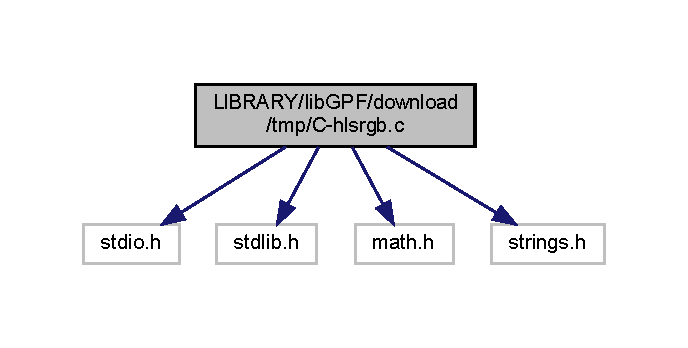
\includegraphics[width=330pt]{C-hlsrgb_8c__incl}
\end{center}
\end{figure}
\subsection*{Functions}
\begin{DoxyCompactItemize}
\item 
void \hyperlink{C-hlsrgb_8c_ad9e23862110e6afd4136221b830b29e7}{hlsrgb} (float hue, float lightness, float saturation, float $\ast$red, float $\ast$green, float $\ast$blue)
\end{DoxyCompactItemize}


\subsection{Function Documentation}
\mbox{\Hypertarget{C-hlsrgb_8c_ad9e23862110e6afd4136221b830b29e7}\label{C-hlsrgb_8c_ad9e23862110e6afd4136221b830b29e7}} 
\index{C-\/hlsrgb.\+c@{C-\/hlsrgb.\+c}!hlsrgb@{hlsrgb}}
\index{hlsrgb@{hlsrgb}!C-\/hlsrgb.\+c@{C-\/hlsrgb.\+c}}
\subsubsection{\texorpdfstring{hlsrgb()}{hlsrgb()}}
{\footnotesize\ttfamily void hlsrgb (\begin{DoxyParamCaption}\item[{float}]{hue,  }\item[{float}]{lightness,  }\item[{float}]{saturation,  }\item[{float $\ast$}]{red,  }\item[{float $\ast$}]{green,  }\item[{float $\ast$}]{blue }\end{DoxyParamCaption})}



References rgbval().

Here is the call graph for this function\+:
\nopagebreak
\begin{figure}[H]
\begin{center}
\leavevmode
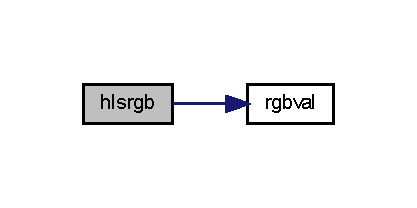
\includegraphics[width=200pt]{C-hlsrgb_8c_ad9e23862110e6afd4136221b830b29e7_cgraph}
\end{center}
\end{figure}
Here is the caller graph for this function\+:
\nopagebreak
\begin{figure}[H]
\begin{center}
\leavevmode
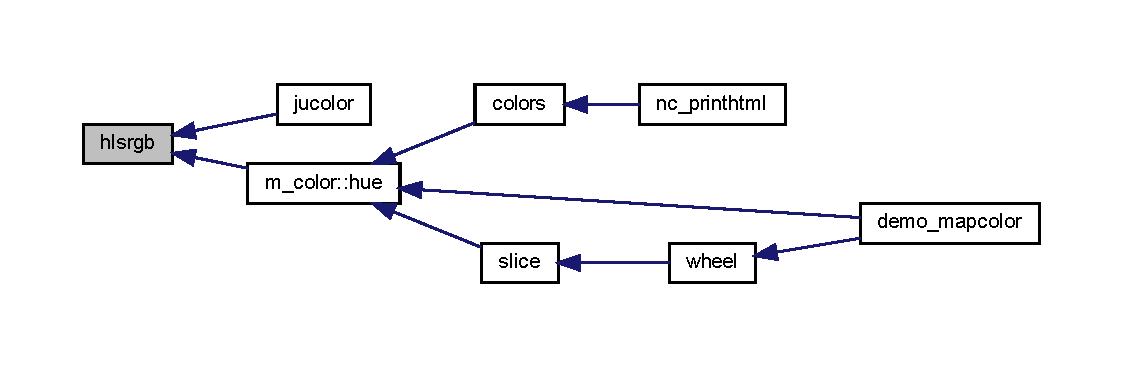
\includegraphics[width=350pt]{C-hlsrgb_8c_ad9e23862110e6afd4136221b830b29e7_icgraph}
\end{center}
\end{figure}

\hypertarget{C-hvsrgb_8c}{}\section{L\+I\+B\+R\+A\+R\+Y/lib\+G\+P\+F/download/tmp/\+C-\/hvsrgb.c File Reference}
\label{C-hvsrgb_8c}\index{L\+I\+B\+R\+A\+R\+Y/lib\+G\+P\+F/download/tmp/\+C-\/hvsrgb.\+c@{L\+I\+B\+R\+A\+R\+Y/lib\+G\+P\+F/download/tmp/\+C-\/hvsrgb.\+c}}
{\ttfamily \#include $<$stdio.\+h$>$}\newline
{\ttfamily \#include $<$stdlib.\+h$>$}\newline
{\ttfamily \#include $<$math.\+h$>$}\newline
{\ttfamily \#include $<$strings.\+h$>$}\newline
\subsection*{Functions}
\begin{DoxyCompactItemize}
\item 
void \hyperlink{C-hvsrgb_8c_a3e696875abb711e0bda0e666bf6828e3}{hvsrgb} (float h, float v, float s, float $\ast$r, float $\ast$g, float $\ast$b)
\end{DoxyCompactItemize}


\subsection{Function Documentation}
\mbox{\Hypertarget{C-hvsrgb_8c_a3e696875abb711e0bda0e666bf6828e3}\label{C-hvsrgb_8c_a3e696875abb711e0bda0e666bf6828e3}} 
\index{C-\/hvsrgb.\+c@{C-\/hvsrgb.\+c}!hvsrgb@{hvsrgb}}
\index{hvsrgb@{hvsrgb}!C-\/hvsrgb.\+c@{C-\/hvsrgb.\+c}}
\subsubsection{\texorpdfstring{hvsrgb()}{hvsrgb()}}
{\footnotesize\ttfamily void hvsrgb (\begin{DoxyParamCaption}\item[{float}]{h,  }\item[{float}]{v,  }\item[{float}]{s,  }\item[{float $\ast$}]{r,  }\item[{float $\ast$}]{g,  }\item[{float $\ast$}]{b }\end{DoxyParamCaption})}


\hypertarget{C-jubiglet_8c}{}\section{L\+I\+B\+R\+A\+R\+Y/lib\+G\+P\+F/download/tmp/\+C-\/jubiglet.c File Reference}
\label{C-jubiglet_8c}\index{L\+I\+B\+R\+A\+R\+Y/lib\+G\+P\+F/download/tmp/\+C-\/jubiglet.\+c@{L\+I\+B\+R\+A\+R\+Y/lib\+G\+P\+F/download/tmp/\+C-\/jubiglet.\+c}}
{\ttfamily \#include $<$stdio.\+h$>$}\newline
{\ttfamily \#include $<$stdlib.\+h$>$}\newline
{\ttfamily \#include $<$string.\+h$>$}\newline
\subsection*{Macros}
\begin{DoxyCompactItemize}
\item 
\#define \hyperlink{C-jubiglet_8c_ac6f18a9e1d00b4637522b1b469a92021}{R\+OW}~97
\item 
\#define \hyperlink{C-jubiglet_8c_aeca034f67218340ecb2261a22c2f3dcd}{B\+U\+F\+S\+I\+ZE}~256
\end{DoxyCompactItemize}
\subsection*{Functions}
\begin{DoxyCompactItemize}
\item 
void \hyperlink{C-jubiglet_8c_adc484767e979a59ef703547d98fab384}{jubiglet} (char $\ast$chars)
\item 
void \hyperlink{C-jubiglet_8c_a6a4a6c766aa968996649c44415282c91}{jubiglet\+\_\+} (char $\ast$s, int len)
\end{DoxyCompactItemize}


\subsection{Macro Definition Documentation}
\mbox{\Hypertarget{C-jubiglet_8c_aeca034f67218340ecb2261a22c2f3dcd}\label{C-jubiglet_8c_aeca034f67218340ecb2261a22c2f3dcd}} 
\index{C-\/jubiglet.\+c@{C-\/jubiglet.\+c}!B\+U\+F\+S\+I\+ZE@{B\+U\+F\+S\+I\+ZE}}
\index{B\+U\+F\+S\+I\+ZE@{B\+U\+F\+S\+I\+ZE}!C-\/jubiglet.\+c@{C-\/jubiglet.\+c}}
\subsubsection{\texorpdfstring{B\+U\+F\+S\+I\+ZE}{BUFSIZE}}
{\footnotesize\ttfamily \#define B\+U\+F\+S\+I\+ZE~256}

\mbox{\Hypertarget{C-jubiglet_8c_ac6f18a9e1d00b4637522b1b469a92021}\label{C-jubiglet_8c_ac6f18a9e1d00b4637522b1b469a92021}} 
\index{C-\/jubiglet.\+c@{C-\/jubiglet.\+c}!R\+OW@{R\+OW}}
\index{R\+OW@{R\+OW}!C-\/jubiglet.\+c@{C-\/jubiglet.\+c}}
\subsubsection{\texorpdfstring{R\+OW}{ROW}}
{\footnotesize\ttfamily \#define R\+OW~97}



\subsection{Function Documentation}
\mbox{\Hypertarget{C-jubiglet_8c_adc484767e979a59ef703547d98fab384}\label{C-jubiglet_8c_adc484767e979a59ef703547d98fab384}} 
\index{C-\/jubiglet.\+c@{C-\/jubiglet.\+c}!jubiglet@{jubiglet}}
\index{jubiglet@{jubiglet}!C-\/jubiglet.\+c@{C-\/jubiglet.\+c}}
\subsubsection{\texorpdfstring{jubiglet()}{jubiglet()}}
{\footnotesize\ttfamily void jubiglet (\begin{DoxyParamCaption}\item[{char $\ast$}]{chars }\end{DoxyParamCaption})}



References m\+\_\+journal\+::ident, and R\+OW.

\mbox{\Hypertarget{C-jubiglet_8c_a6a4a6c766aa968996649c44415282c91}\label{C-jubiglet_8c_a6a4a6c766aa968996649c44415282c91}} 
\index{C-\/jubiglet.\+c@{C-\/jubiglet.\+c}!jubiglet\+\_\+@{jubiglet\+\_\+}}
\index{jubiglet\+\_\+@{jubiglet\+\_\+}!C-\/jubiglet.\+c@{C-\/jubiglet.\+c}}
\subsubsection{\texorpdfstring{jubiglet\+\_\+()}{jubiglet\_()}}
{\footnotesize\ttfamily void jubiglet\+\_\+ (\begin{DoxyParamCaption}\item[{char $\ast$}]{s,  }\item[{int}]{len }\end{DoxyParamCaption})}



References m\+\_\+writegif\+::buf, jubiglet(), and m\+\_\+writegif\+::p.


\hypertarget{C-jucolor_8c}{}\section{L\+I\+B\+R\+A\+R\+Y/lib\+G\+P\+F/download/tmp/\+C-\/jucolor.c File Reference}
\label{C-jucolor_8c}\index{L\+I\+B\+R\+A\+R\+Y/lib\+G\+P\+F/download/tmp/\+C-\/jucolor.\+c@{L\+I\+B\+R\+A\+R\+Y/lib\+G\+P\+F/download/tmp/\+C-\/jucolor.\+c}}
{\ttfamily \#include $<$stdio.\+h$>$}\newline
{\ttfamily \#include $<$string.\+h$>$}\newline
Include dependency graph for C-\/jucolor.c\+:
\nopagebreak
\begin{figure}[H]
\begin{center}
\leavevmode
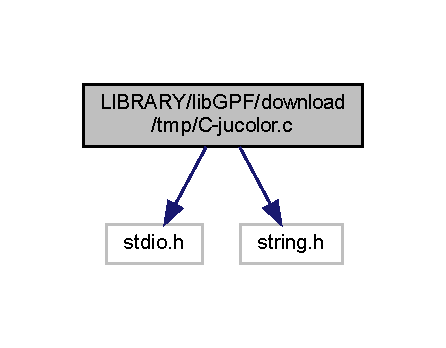
\includegraphics[width=214pt]{C-jucolor_8c__incl}
\end{center}
\end{figure}
\subsection*{Functions}
\begin{DoxyCompactItemize}
\item 
void \hyperlink{C-jucolor_8c_ab1a7b686c79343455799a5c44294194b}{jucolor} (modei, float clr1i, float clr2i, float clr3i, char $\ast$modei $\ast$modeo, float $\ast$clr1o, float $\ast$clr2o, float $\ast$clr3o, int $\ast$status)
\end{DoxyCompactItemize}


\subsection{Function Documentation}
\mbox{\Hypertarget{C-jucolor_8c_ab1a7b686c79343455799a5c44294194b}\label{C-jucolor_8c_ab1a7b686c79343455799a5c44294194b}} 
\index{C-\/jucolor.\+c@{C-\/jucolor.\+c}!jucolor@{jucolor}}
\index{jucolor@{jucolor}!C-\/jucolor.\+c@{C-\/jucolor.\+c}}
\subsubsection{\texorpdfstring{jucolor()}{jucolor()}}
{\footnotesize\ttfamily void jucolor (\begin{DoxyParamCaption}\item[{modei}]{,  }\item[{float}]{clr1i,  }\item[{float}]{clr2i,  }\item[{float}]{clr3i,  }\item[{char $\ast$modei$\ast$}]{modeo,  }\item[{float $\ast$}]{clr1o,  }\item[{float$\ast$}]{clr2o,  }\item[{float$\ast$}]{clr3o,  }\item[{int $\ast$}]{status }\end{DoxyParamCaption})}



References hlsrgb(), hvsrgb(), m\+\_\+journal\+::ident, m\+\_\+anyscalar\+::r, rgbhls(), and rgbhvs().

Here is the call graph for this function\+:
\nopagebreak
\begin{figure}[H]
\begin{center}
\leavevmode
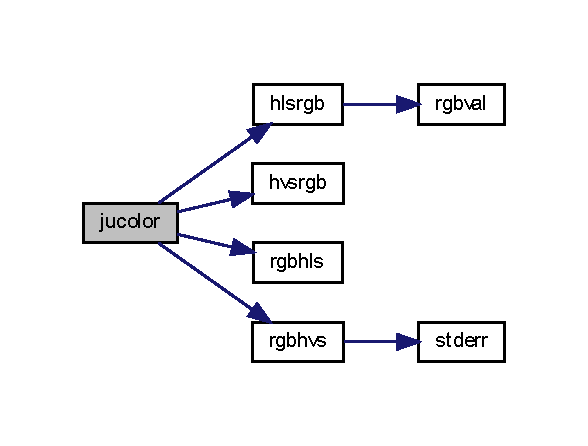
\includegraphics[width=282pt]{C-jucolor_8c_ab1a7b686c79343455799a5c44294194b_cgraph}
\end{center}
\end{figure}

\hypertarget{C-M__getkey_8c}{}\section{L\+I\+B\+R\+A\+R\+Y/lib\+G\+P\+F/download/tmp/\+C-\/\+M\+\_\+getkey.c File Reference}
\label{C-M__getkey_8c}\index{L\+I\+B\+R\+A\+R\+Y/lib\+G\+P\+F/download/tmp/\+C-\/\+M\+\_\+getkey.\+c@{L\+I\+B\+R\+A\+R\+Y/lib\+G\+P\+F/download/tmp/\+C-\/\+M\+\_\+getkey.\+c}}
{\ttfamily \#include $<$stdlib.\+h$>$}\newline
{\ttfamily \#include $<$unistd.\+h$>$}\newline
{\ttfamily \#include $<$stdio.\+h$>$}\newline
{\ttfamily \#include $<$string.\+h$>$}\newline
{\ttfamily \#include $<$sys/ioctl.\+h$>$}\newline
{\ttfamily \#include $<$termio.\+h$>$}\newline
{\ttfamily \#include $<$signal.\+h$>$}\newline
Include dependency graph for C-\/\+M\+\_\+getkey.c\+:
\nopagebreak
\begin{figure}[H]
\begin{center}
\leavevmode
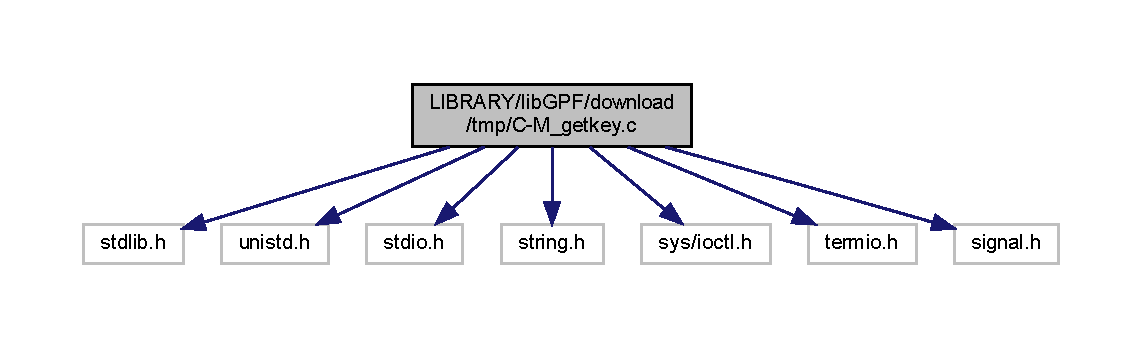
\includegraphics[width=350pt]{C-M__getkey_8c__incl}
\end{center}
\end{figure}
\subsection*{Macros}
\begin{DoxyCompactItemize}
\item 
\#define \hyperlink{C-M__getkey_8c_a157a956e14c5c44b3f73ef23a4776f64}{L\+I\+N\+UX}
\end{DoxyCompactItemize}
\subsection*{Functions}
\begin{DoxyCompactItemize}
\item 
char \hyperlink{C-M__getkey_8c_a257d1f3a5480d15d83e0bf1d43647afc}{Fgetkey} (void)
\end{DoxyCompactItemize}


\subsection{Macro Definition Documentation}
\mbox{\Hypertarget{C-M__getkey_8c_a157a956e14c5c44b3f73ef23a4776f64}\label{C-M__getkey_8c_a157a956e14c5c44b3f73ef23a4776f64}} 
\index{C-\/\+M\+\_\+getkey.\+c@{C-\/\+M\+\_\+getkey.\+c}!L\+I\+N\+UX@{L\+I\+N\+UX}}
\index{L\+I\+N\+UX@{L\+I\+N\+UX}!C-\/\+M\+\_\+getkey.\+c@{C-\/\+M\+\_\+getkey.\+c}}
\subsubsection{\texorpdfstring{L\+I\+N\+UX}{LINUX}}
{\footnotesize\ttfamily \#define L\+I\+N\+UX}



\subsection{Function Documentation}
\mbox{\Hypertarget{C-M__getkey_8c_a257d1f3a5480d15d83e0bf1d43647afc}\label{C-M__getkey_8c_a257d1f3a5480d15d83e0bf1d43647afc}} 
\index{C-\/\+M\+\_\+getkey.\+c@{C-\/\+M\+\_\+getkey.\+c}!Fgetkey@{Fgetkey}}
\index{Fgetkey@{Fgetkey}!C-\/\+M\+\_\+getkey.\+c@{C-\/\+M\+\_\+getkey.\+c}}
\subsubsection{\texorpdfstring{Fgetkey()}{Fgetkey()}}
{\footnotesize\ttfamily char Fgetkey (\begin{DoxyParamCaption}\item[{void}]{ }\end{DoxyParamCaption})}



References c().

Here is the call graph for this function\+:
\nopagebreak
\begin{figure}[H]
\begin{center}
\leavevmode
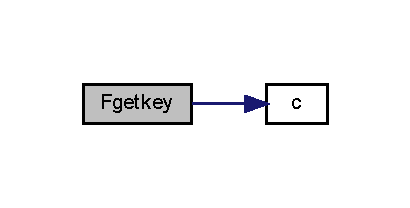
\includegraphics[width=197pt]{C-M__getkey_8c_a257d1f3a5480d15d83e0bf1d43647afc_cgraph}
\end{center}
\end{figure}

\hypertarget{C-M__readline_8c}{}\section{L\+I\+B\+R\+A\+R\+Y/lib\+G\+P\+F/download/tmp/\+C-\/\+M\+\_\+readline.c File Reference}
\label{C-M__readline_8c}\index{L\+I\+B\+R\+A\+R\+Y/lib\+G\+P\+F/download/tmp/\+C-\/\+M\+\_\+readline.\+c@{L\+I\+B\+R\+A\+R\+Y/lib\+G\+P\+F/download/tmp/\+C-\/\+M\+\_\+readline.\+c}}
{\ttfamily \#include $<$stdlib.\+h$>$}\newline
{\ttfamily \#include $<$unistd.\+h$>$}\newline
{\ttfamily \#include $<$stdio.\+h$>$}\newline
{\ttfamily \#include $<$string.\+h$>$}\newline
{\ttfamily \#include $<$readline/readline.\+h$>$}\newline
{\ttfamily \#include $<$readline/history.\+h$>$}\newline
\subsection*{Functions}
\begin{DoxyCompactItemize}
\item 
void \hyperlink{C-M__readline_8c_a80269900528c2ee04bf7cacb3a07ff40}{show\+\_\+history\+\_\+list} ()
\item 
void \hyperlink{C-M__readline_8c_a146edc06a54e833494378446131c6bcd}{F\+Creadline} (int len, char $\ast$myline, char prompt\mbox{[}$\,$\mbox{]})
\end{DoxyCompactItemize}


\subsection{Function Documentation}
\mbox{\Hypertarget{C-M__readline_8c_a146edc06a54e833494378446131c6bcd}\label{C-M__readline_8c_a146edc06a54e833494378446131c6bcd}} 
\index{C-\/\+M\+\_\+readline.\+c@{C-\/\+M\+\_\+readline.\+c}!F\+Creadline@{F\+Creadline}}
\index{F\+Creadline@{F\+Creadline}!C-\/\+M\+\_\+readline.\+c@{C-\/\+M\+\_\+readline.\+c}}
\subsubsection{\texorpdfstring{F\+Creadline()}{FCreadline()}}
{\footnotesize\ttfamily void F\+Creadline (\begin{DoxyParamCaption}\item[{int}]{len,  }\item[{char $\ast$}]{myline,  }\item[{char}]{prompt\mbox{[}$\,$\mbox{]} }\end{DoxyParamCaption})}



References show\+\_\+history\+\_\+list().

\mbox{\Hypertarget{C-M__readline_8c_a80269900528c2ee04bf7cacb3a07ff40}\label{C-M__readline_8c_a80269900528c2ee04bf7cacb3a07ff40}} 
\index{C-\/\+M\+\_\+readline.\+c@{C-\/\+M\+\_\+readline.\+c}!show\+\_\+history\+\_\+list@{show\+\_\+history\+\_\+list}}
\index{show\+\_\+history\+\_\+list@{show\+\_\+history\+\_\+list}!C-\/\+M\+\_\+readline.\+c@{C-\/\+M\+\_\+readline.\+c}}
\subsubsection{\texorpdfstring{show\+\_\+history\+\_\+list()}{show\_history\_list()}}
{\footnotesize\ttfamily void show\+\_\+history\+\_\+list (\begin{DoxyParamCaption}{ }\end{DoxyParamCaption})}



References state().


\hypertarget{C-M__regex_8c}{}\section{L\+I\+B\+R\+A\+R\+Y/lib\+G\+P\+F/download/tmp/\+C-\/\+M\+\_\+regex.c File Reference}
\label{C-M__regex_8c}\index{L\+I\+B\+R\+A\+R\+Y/lib\+G\+P\+F/download/tmp/\+C-\/\+M\+\_\+regex.\+c@{L\+I\+B\+R\+A\+R\+Y/lib\+G\+P\+F/download/tmp/\+C-\/\+M\+\_\+regex.\+c}}
{\ttfamily \#include $<$sys/types.\+h$>$}\newline
{\ttfamily \#include $<$regex.\+h$>$}\newline
{\ttfamily \#include $<$string.\+h$>$}\newline
{\ttfamily \#include $<$stdlib.\+h$>$}\newline
\subsection*{Functions}
\begin{DoxyCompactItemize}
\item 
void \hyperlink{C-M__regex_8c_a749eb5df717b312d898ea0a3b279e7ca}{C\+\_\+regalloc} (regex\+\_\+t $\ast$$\ast$preg\+\_\+return)
\item 
void \hyperlink{C-M__regex_8c_a3fcdbec663d5285a401e73c4cdca37be}{C\+\_\+regcomp} (regex\+\_\+t $\ast$preg, const char $\ast$pattern, const char $\ast$flags, int $\ast$status\+\_\+return)
\item 
void \hyperlink{C-M__regex_8c_ad4d383ae55d866605fb7ff11e8cf99d8}{C\+\_\+regexec} (const regex\+\_\+t $\ast$preg, const char $\ast$\hyperlink{what__overview_81_8txt_a7d189cc480786c3c65688ced463aedcb}{string}, int nmatch, int matches\mbox{[}nmatch\mbox{]}\mbox{[}2\mbox{]}, const char $\ast$flags, int $\ast$status\+\_\+return)
\end{DoxyCompactItemize}


\subsection{Function Documentation}
\mbox{\Hypertarget{C-M__regex_8c_a749eb5df717b312d898ea0a3b279e7ca}\label{C-M__regex_8c_a749eb5df717b312d898ea0a3b279e7ca}} 
\index{C-\/\+M\+\_\+regex.\+c@{C-\/\+M\+\_\+regex.\+c}!C\+\_\+regalloc@{C\+\_\+regalloc}}
\index{C\+\_\+regalloc@{C\+\_\+regalloc}!C-\/\+M\+\_\+regex.\+c@{C-\/\+M\+\_\+regex.\+c}}
\subsubsection{\texorpdfstring{C\+\_\+regalloc()}{C\_regalloc()}}
{\footnotesize\ttfamily void C\+\_\+regalloc (\begin{DoxyParamCaption}\item[{regex\+\_\+t $\ast$$\ast$}]{preg\+\_\+return }\end{DoxyParamCaption})}

\mbox{\Hypertarget{C-M__regex_8c_a3fcdbec663d5285a401e73c4cdca37be}\label{C-M__regex_8c_a3fcdbec663d5285a401e73c4cdca37be}} 
\index{C-\/\+M\+\_\+regex.\+c@{C-\/\+M\+\_\+regex.\+c}!C\+\_\+regcomp@{C\+\_\+regcomp}}
\index{C\+\_\+regcomp@{C\+\_\+regcomp}!C-\/\+M\+\_\+regex.\+c@{C-\/\+M\+\_\+regex.\+c}}
\subsubsection{\texorpdfstring{C\+\_\+regcomp()}{C\_regcomp()}}
{\footnotesize\ttfamily void C\+\_\+regcomp (\begin{DoxyParamCaption}\item[{regex\+\_\+t $\ast$}]{preg,  }\item[{const char $\ast$}]{pattern,  }\item[{const char $\ast$}]{flags,  }\item[{int $\ast$}]{status\+\_\+return }\end{DoxyParamCaption})}

\mbox{\Hypertarget{C-M__regex_8c_ad4d383ae55d866605fb7ff11e8cf99d8}\label{C-M__regex_8c_ad4d383ae55d866605fb7ff11e8cf99d8}} 
\index{C-\/\+M\+\_\+regex.\+c@{C-\/\+M\+\_\+regex.\+c}!C\+\_\+regexec@{C\+\_\+regexec}}
\index{C\+\_\+regexec@{C\+\_\+regexec}!C-\/\+M\+\_\+regex.\+c@{C-\/\+M\+\_\+regex.\+c}}
\subsubsection{\texorpdfstring{C\+\_\+regexec()}{C\_regexec()}}
{\footnotesize\ttfamily void C\+\_\+regexec (\begin{DoxyParamCaption}\item[{const regex\+\_\+t $\ast$}]{preg,  }\item[{const char $\ast$}]{string,  }\item[{int}]{nmatch,  }\item[{int}]{matches\mbox{[}nmatch\mbox{]}\mbox{[}2\mbox{]},  }\item[{const char $\ast$}]{flags,  }\item[{int $\ast$}]{status\+\_\+return }\end{DoxyParamCaption})}



References j, and string.


\hypertarget{C-M__system_8c}{}\section{L\+I\+B\+R\+A\+R\+Y/lib\+G\+P\+F/download/tmp/\+C-\/\+M\+\_\+system.c File Reference}
\label{C-M__system_8c}\index{L\+I\+B\+R\+A\+R\+Y/lib\+G\+P\+F/download/tmp/\+C-\/\+M\+\_\+system.\+c@{L\+I\+B\+R\+A\+R\+Y/lib\+G\+P\+F/download/tmp/\+C-\/\+M\+\_\+system.\+c}}
{\ttfamily \#include $<$stdio.\+h$>$}\newline
{\ttfamily \#include $<$stdlib.\+h$>$}\newline
{\ttfamily \#include $<$string.\+h$>$}\newline
{\ttfamily \#include $<$sys/types.\+h$>$}\newline
{\ttfamily \#include $<$sys/utsname.\+h$>$}\newline
{\ttfamily \#include $<$dirent.\+h$>$}\newline
{\ttfamily \#include $<$errno.\+h$>$}\newline
{\ttfamily \#include $<$unistd.\+h$>$}\newline
{\ttfamily \#include $<$fcntl.\+h$>$}\newline
{\ttfamily \#include $<$sys/stat.\+h$>$}\newline
{\ttfamily \#include $<$strings.\+h$>$}\newline
{\ttfamily \#include $<$pwd.\+h$>$}\newline
{\ttfamily \#include $<$grp.\+h$>$}\newline
{\ttfamily \#include $<$sys/times.\+h$>$}\newline
{\ttfamily \#include $<$sys/param.\+h$>$}\newline
{\ttfamily \#include $<$time.\+h$>$}\newline
{\ttfamily \#include $<$locale.\+h$>$}\newline
{\ttfamily \#include $<$langinfo.\+h$>$}\newline
{\ttfamily \#include $<$stdint.\+h$>$}\newline
\subsection*{Macros}
\begin{DoxyCompactItemize}
\item 
\#define \hyperlink{C-M__system_8c_a74e75242132eaabbc1c512488a135926}{M\+IN}(x,  y)~((x) $<$ (y) ? (x) \+: (y))
\end{DoxyCompactItemize}
\subsection*{Functions}
\begin{DoxyCompactItemize}
\item 
int \hyperlink{C-M__system_8c_acfa12de4342c03519fc35d7892db94b2}{my\+\_\+chown} (char $\ast$filename, long long int uid, long long int gid)
\item 
void \hyperlink{C-M__system_8c_a56eb1f4025386fefa96810c8846a75ca}{my\+\_\+readdir} (D\+IR $\ast$dirp, char $\ast$filename, int $\ast$err)
\item 
void \hyperlink{C-M__system_8c_aaf9088f4cc3498dcf1abec624adabe76}{my\+\_\+flush} (void)
\item 
void \hyperlink{C-M__system_8c_ab5188f2ca99719a14c77a1acae06f93a}{my\+\_\+initenv} ()
\item 
void \hyperlink{C-M__system_8c_a0114eece06797ba0c5e6f5948841501a}{my\+\_\+readenv} (char $\ast$\hyperlink{M__stopwatch_83_8txt_a2fa76741434e14a1b61bcbd4629b9cec}{variable})
\item 
int \hyperlink{C-M__system_8c_a13b282e9de0dc0bb29bec1d76aaf6cf0}{my\+\_\+getgrgid} (long long int id, char $\ast$groupname)
\item 
int \hyperlink{C-M__system_8c_a0feb597a044e16699952e0056390f3d6}{my\+\_\+getpwuid} (long long int id, char $\ast$username)
\item 
int \hyperlink{C-M__system_8c_ad9bbaffdef223d18bb59a22c3c599201}{my\+\_\+errno} ()
\item 
void \hyperlink{C-M__system_8c_ab955d6c562df08b9e465fe3cea24d83d}{system\+\_\+unbuffer} ()
\item 
void \hyperlink{C-M__system_8c_ab341d42a9117c4bd188dcdcbff69fe9a}{my\+\_\+uname} (char $\ast$which, char $\ast$\hyperlink{what__overview_81_8txt_a7d189cc480786c3c65688ced463aedcb}{string}, int $\ast$stringlen)
\item 
void \hyperlink{C-M__system_8c_aae18c27a21f7c4aed7328460a7edb34c}{my\+\_\+cpu\+\_\+time} (float $\ast$\hyperlink{c_8f90_aeb1f4e639be0213b4cbd07f2583a5b1f}{c}, float $\ast$u, float $\ast$s)
\item 
int \hyperlink{C-M__system_8c_a4d9118bb9590e12ac1956789cd08e09b}{my\+\_\+isdir} (const char $\ast$path)
\item 
int \hyperlink{C-M__system_8c_afec6872f4aa34aba9e71a18324d53bce}{my\+\_\+isreg} (const char $\ast$path)
\item 
int \hyperlink{C-M__system_8c_ad07b549d969a0670b0b8f7c6bef83e92}{my\+\_\+isblk} (const char $\ast$path)
\item 
int \hyperlink{C-M__system_8c_ae59ec13b3517e84ddd30a0cd5352a01d}{my\+\_\+ischr} (const char $\ast$path)
\item 
int \hyperlink{C-M__system_8c_ac4f0c51cc048efce7cc88a80c6ce50a4}{my\+\_\+isfifo} (const char $\ast$path)
\item 
int \hyperlink{C-M__system_8c_a090bd041de7e5661c0cb3dea61517283}{my\+\_\+issock} (const char $\ast$path)
\item 
int \hyperlink{C-M__system_8c_a5d15b99bbdd2c6d3e07c92b4bdebb732}{my\+\_\+islnk} (const char $\ast$fname)
\item 
int \hyperlink{C-M__system_8c_afc05a3ec2be734d741c384e752f96b90}{my\+\_\+file\+\_\+exists} (const char $\ast$fname)
\item 
void \hyperlink{C-M__system_8c_a93aa717690d60568cf019988f6434ba5}{my\+\_\+stat} (char $\ast$\hyperlink{what__overview_81_8txt_a447b56c526e8da30e0dc94673727ee25}{file}, long int $\ast$values, int $\ast$ierr, int debug)
\item 
const char $\ast$ \hyperlink{C-M__system_8c_a1ef2ab1c7375f6b130cee762e770a29a}{my\+\_\+get\+\_\+perm} (long int imode)
\end{DoxyCompactItemize}
\subsection*{Variables}
\begin{DoxyCompactItemize}
\item 
char $\ast$$\ast$ \hyperlink{C-M__system_8c_aa006daaf11f1e2e45a6ababaf463212b}{environ}
\item 
int \hyperlink{C-M__system_8c_a55fec1e650e6037d352db493bea1716f}{F\+H\+O\+S\+T\+\_\+\+N\+A\+M\+E\+\_\+\+M\+AX} =H\+O\+S\+T\+\_\+\+N\+A\+M\+E\+\_\+\+M\+AX
\item 
mode\+\_\+t \hyperlink{C-M__system_8c_a9e37e108fa1a58b85031aed8634f65d0}{F\+S\+\_\+\+I\+R\+G\+RP} =S\+\_\+\+I\+R\+G\+RP
\item 
mode\+\_\+t \hyperlink{C-M__system_8c_a310094a449c3371ef9cf8b0776213835}{F\+S\+\_\+\+I\+R\+O\+TH} =S\+\_\+\+I\+R\+O\+TH
\item 
mode\+\_\+t \hyperlink{C-M__system_8c_a03e3496451f60edd6c69c3802e11db67}{F\+S\+\_\+\+I\+R\+U\+SR} =S\+\_\+\+I\+R\+U\+SR
\item 
mode\+\_\+t \hyperlink{C-M__system_8c_ab4e744ca243de9628a7e9651695d7a97}{F\+S\+\_\+\+I\+R\+W\+XG} =S\+\_\+\+I\+R\+W\+XG
\item 
mode\+\_\+t \hyperlink{C-M__system_8c_a612adf3e64ccb1734ab64ef6d73fa87b}{F\+S\+\_\+\+I\+R\+W\+XO} =S\+\_\+\+I\+R\+W\+XO
\item 
mode\+\_\+t \hyperlink{C-M__system_8c_acb420eb45e494ab53bbfd018c2262ff2}{F\+S\+\_\+\+I\+R\+W\+XU} =S\+\_\+\+I\+R\+W\+XU
\item 
mode\+\_\+t \hyperlink{C-M__system_8c_a739522a271fd37727d6f266197ded32b}{F\+S\+\_\+\+I\+W\+G\+RP} =S\+\_\+\+I\+W\+G\+RP
\item 
mode\+\_\+t \hyperlink{C-M__system_8c_a1ed0df6f1e0108d07c0fe7880402f8c0}{F\+S\+\_\+\+I\+W\+O\+TH} =S\+\_\+\+I\+W\+O\+TH
\item 
mode\+\_\+t \hyperlink{C-M__system_8c_ade549697e7611d5c3755b1befcd796b8}{F\+S\+\_\+\+I\+W\+U\+SR} =S\+\_\+\+I\+W\+U\+SR
\item 
mode\+\_\+t \hyperlink{C-M__system_8c_ac01832589f29b7d987cb90be63cc3dc8}{F\+S\+\_\+\+I\+X\+G\+RP} =S\+\_\+\+I\+X\+G\+RP
\item 
mode\+\_\+t \hyperlink{C-M__system_8c_aafbcf1020ef1a8f3999526f88f349fe3}{F\+S\+\_\+\+I\+X\+O\+TH} =S\+\_\+\+I\+X\+O\+TH
\item 
mode\+\_\+t \hyperlink{C-M__system_8c_acc949c15ea63678fc34579213919906f}{F\+S\+\_\+\+I\+X\+U\+SR} =S\+\_\+\+I\+X\+U\+SR
\item 
mode\+\_\+t \hyperlink{C-M__system_8c_a4ec9ddefca39a5f2bc0aa0cb9cc8a760}{F\+D\+E\+F\+F\+I\+L\+E\+M\+O\+DE} =D\+E\+F\+F\+I\+L\+E\+M\+O\+DE
\item 
mode\+\_\+t \hyperlink{C-M__system_8c_a2d221d0dde92c4e100c2bc959832f1df}{F\+A\+C\+C\+E\+S\+S\+P\+E\+R\+MS} =A\+C\+C\+E\+S\+S\+P\+E\+R\+MS
\item 
char $\ast$$\ast$ \hyperlink{C-M__system_8c_a8f6f268f0282f4a41c1569e80963f328}{ep}
\item 
long int \hyperlink{C-M__system_8c_ad45ba6068349b626136d161ff72dea21}{longest\+\_\+env\+\_\+variable} =0L
\end{DoxyCompactItemize}


\subsection{Macro Definition Documentation}
\mbox{\Hypertarget{C-M__system_8c_a74e75242132eaabbc1c512488a135926}\label{C-M__system_8c_a74e75242132eaabbc1c512488a135926}} 
\index{C-\/\+M\+\_\+system.\+c@{C-\/\+M\+\_\+system.\+c}!M\+IN@{M\+IN}}
\index{M\+IN@{M\+IN}!C-\/\+M\+\_\+system.\+c@{C-\/\+M\+\_\+system.\+c}}
\subsubsection{\texorpdfstring{M\+IN}{MIN}}
{\footnotesize\ttfamily \#define M\+IN(\begin{DoxyParamCaption}\item[{}]{x,  }\item[{}]{y }\end{DoxyParamCaption})~((x) $<$ (y) ? (x) \+: (y))}



\subsection{Function Documentation}
\mbox{\Hypertarget{C-M__system_8c_acfa12de4342c03519fc35d7892db94b2}\label{C-M__system_8c_acfa12de4342c03519fc35d7892db94b2}} 
\index{C-\/\+M\+\_\+system.\+c@{C-\/\+M\+\_\+system.\+c}!my\+\_\+chown@{my\+\_\+chown}}
\index{my\+\_\+chown@{my\+\_\+chown}!C-\/\+M\+\_\+system.\+c@{C-\/\+M\+\_\+system.\+c}}
\subsubsection{\texorpdfstring{my\+\_\+chown()}{my\_chown()}}
{\footnotesize\ttfamily int my\+\_\+chown (\begin{DoxyParamCaption}\item[{char $\ast$}]{filename,  }\item[{long long int}]{uid,  }\item[{long long int}]{gid }\end{DoxyParamCaption})}

\mbox{\Hypertarget{C-M__system_8c_aae18c27a21f7c4aed7328460a7edb34c}\label{C-M__system_8c_aae18c27a21f7c4aed7328460a7edb34c}} 
\index{C-\/\+M\+\_\+system.\+c@{C-\/\+M\+\_\+system.\+c}!my\+\_\+cpu\+\_\+time@{my\+\_\+cpu\+\_\+time}}
\index{my\+\_\+cpu\+\_\+time@{my\+\_\+cpu\+\_\+time}!C-\/\+M\+\_\+system.\+c@{C-\/\+M\+\_\+system.\+c}}
\subsubsection{\texorpdfstring{my\+\_\+cpu\+\_\+time()}{my\_cpu\_time()}}
{\footnotesize\ttfamily void my\+\_\+cpu\+\_\+time (\begin{DoxyParamCaption}\item[{float $\ast$}]{c,  }\item[{float $\ast$}]{u,  }\item[{float $\ast$}]{s }\end{DoxyParamCaption})}

\mbox{\Hypertarget{C-M__system_8c_ad9bbaffdef223d18bb59a22c3c599201}\label{C-M__system_8c_ad9bbaffdef223d18bb59a22c3c599201}} 
\index{C-\/\+M\+\_\+system.\+c@{C-\/\+M\+\_\+system.\+c}!my\+\_\+errno@{my\+\_\+errno}}
\index{my\+\_\+errno@{my\+\_\+errno}!C-\/\+M\+\_\+system.\+c@{C-\/\+M\+\_\+system.\+c}}
\subsubsection{\texorpdfstring{my\+\_\+errno()}{my\_errno()}}
{\footnotesize\ttfamily int my\+\_\+errno (\begin{DoxyParamCaption}{ }\end{DoxyParamCaption})}

\mbox{\Hypertarget{C-M__system_8c_afc05a3ec2be734d741c384e752f96b90}\label{C-M__system_8c_afc05a3ec2be734d741c384e752f96b90}} 
\index{C-\/\+M\+\_\+system.\+c@{C-\/\+M\+\_\+system.\+c}!my\+\_\+file\+\_\+exists@{my\+\_\+file\+\_\+exists}}
\index{my\+\_\+file\+\_\+exists@{my\+\_\+file\+\_\+exists}!C-\/\+M\+\_\+system.\+c@{C-\/\+M\+\_\+system.\+c}}
\subsubsection{\texorpdfstring{my\+\_\+file\+\_\+exists()}{my\_file\_exists()}}
{\footnotesize\ttfamily int my\+\_\+file\+\_\+exists (\begin{DoxyParamCaption}\item[{const char $\ast$}]{fname }\end{DoxyParamCaption})}

\mbox{\Hypertarget{C-M__system_8c_aaf9088f4cc3498dcf1abec624adabe76}\label{C-M__system_8c_aaf9088f4cc3498dcf1abec624adabe76}} 
\index{C-\/\+M\+\_\+system.\+c@{C-\/\+M\+\_\+system.\+c}!my\+\_\+flush@{my\+\_\+flush}}
\index{my\+\_\+flush@{my\+\_\+flush}!C-\/\+M\+\_\+system.\+c@{C-\/\+M\+\_\+system.\+c}}
\subsubsection{\texorpdfstring{my\+\_\+flush()}{my\_flush()}}
{\footnotesize\ttfamily void my\+\_\+flush (\begin{DoxyParamCaption}\item[{void}]{ }\end{DoxyParamCaption})}



References m\+\_\+journal\+::stdout.

\mbox{\Hypertarget{C-M__system_8c_a1ef2ab1c7375f6b130cee762e770a29a}\label{C-M__system_8c_a1ef2ab1c7375f6b130cee762e770a29a}} 
\index{C-\/\+M\+\_\+system.\+c@{C-\/\+M\+\_\+system.\+c}!my\+\_\+get\+\_\+perm@{my\+\_\+get\+\_\+perm}}
\index{my\+\_\+get\+\_\+perm@{my\+\_\+get\+\_\+perm}!C-\/\+M\+\_\+system.\+c@{C-\/\+M\+\_\+system.\+c}}
\subsubsection{\texorpdfstring{my\+\_\+get\+\_\+perm()}{my\_get\_perm()}}
{\footnotesize\ttfamily const char$\ast$ my\+\_\+get\+\_\+perm (\begin{DoxyParamCaption}\item[{long int}]{imode }\end{DoxyParamCaption})}

\mbox{\Hypertarget{C-M__system_8c_a13b282e9de0dc0bb29bec1d76aaf6cf0}\label{C-M__system_8c_a13b282e9de0dc0bb29bec1d76aaf6cf0}} 
\index{C-\/\+M\+\_\+system.\+c@{C-\/\+M\+\_\+system.\+c}!my\+\_\+getgrgid@{my\+\_\+getgrgid}}
\index{my\+\_\+getgrgid@{my\+\_\+getgrgid}!C-\/\+M\+\_\+system.\+c@{C-\/\+M\+\_\+system.\+c}}
\subsubsection{\texorpdfstring{my\+\_\+getgrgid()}{my\_getgrgid()}}
{\footnotesize\ttfamily int my\+\_\+getgrgid (\begin{DoxyParamCaption}\item[{long long int}]{id,  }\item[{char $\ast$}]{groupname }\end{DoxyParamCaption})}



References group().

\mbox{\Hypertarget{C-M__system_8c_a0feb597a044e16699952e0056390f3d6}\label{C-M__system_8c_a0feb597a044e16699952e0056390f3d6}} 
\index{C-\/\+M\+\_\+system.\+c@{C-\/\+M\+\_\+system.\+c}!my\+\_\+getpwuid@{my\+\_\+getpwuid}}
\index{my\+\_\+getpwuid@{my\+\_\+getpwuid}!C-\/\+M\+\_\+system.\+c@{C-\/\+M\+\_\+system.\+c}}
\subsubsection{\texorpdfstring{my\+\_\+getpwuid()}{my\_getpwuid()}}
{\footnotesize\ttfamily int my\+\_\+getpwuid (\begin{DoxyParamCaption}\item[{long long int}]{id,  }\item[{char $\ast$}]{username }\end{DoxyParamCaption})}

\mbox{\Hypertarget{C-M__system_8c_ab5188f2ca99719a14c77a1acae06f93a}\label{C-M__system_8c_ab5188f2ca99719a14c77a1acae06f93a}} 
\index{C-\/\+M\+\_\+system.\+c@{C-\/\+M\+\_\+system.\+c}!my\+\_\+initenv@{my\+\_\+initenv}}
\index{my\+\_\+initenv@{my\+\_\+initenv}!C-\/\+M\+\_\+system.\+c@{C-\/\+M\+\_\+system.\+c}}
\subsubsection{\texorpdfstring{my\+\_\+initenv()}{my\_initenv()}}
{\footnotesize\ttfamily void my\+\_\+initenv (\begin{DoxyParamCaption}{ }\end{DoxyParamCaption})}



References environ, ep, and longest\+\_\+env\+\_\+variable.

\mbox{\Hypertarget{C-M__system_8c_ad07b549d969a0670b0b8f7c6bef83e92}\label{C-M__system_8c_ad07b549d969a0670b0b8f7c6bef83e92}} 
\index{C-\/\+M\+\_\+system.\+c@{C-\/\+M\+\_\+system.\+c}!my\+\_\+isblk@{my\+\_\+isblk}}
\index{my\+\_\+isblk@{my\+\_\+isblk}!C-\/\+M\+\_\+system.\+c@{C-\/\+M\+\_\+system.\+c}}
\subsubsection{\texorpdfstring{my\+\_\+isblk()}{my\_isblk()}}
{\footnotesize\ttfamily int my\+\_\+isblk (\begin{DoxyParamCaption}\item[{const char $\ast$}]{path }\end{DoxyParamCaption})}

\mbox{\Hypertarget{C-M__system_8c_ae59ec13b3517e84ddd30a0cd5352a01d}\label{C-M__system_8c_ae59ec13b3517e84ddd30a0cd5352a01d}} 
\index{C-\/\+M\+\_\+system.\+c@{C-\/\+M\+\_\+system.\+c}!my\+\_\+ischr@{my\+\_\+ischr}}
\index{my\+\_\+ischr@{my\+\_\+ischr}!C-\/\+M\+\_\+system.\+c@{C-\/\+M\+\_\+system.\+c}}
\subsubsection{\texorpdfstring{my\+\_\+ischr()}{my\_ischr()}}
{\footnotesize\ttfamily int my\+\_\+ischr (\begin{DoxyParamCaption}\item[{const char $\ast$}]{path }\end{DoxyParamCaption})}

\mbox{\Hypertarget{C-M__system_8c_a4d9118bb9590e12ac1956789cd08e09b}\label{C-M__system_8c_a4d9118bb9590e12ac1956789cd08e09b}} 
\index{C-\/\+M\+\_\+system.\+c@{C-\/\+M\+\_\+system.\+c}!my\+\_\+isdir@{my\+\_\+isdir}}
\index{my\+\_\+isdir@{my\+\_\+isdir}!C-\/\+M\+\_\+system.\+c@{C-\/\+M\+\_\+system.\+c}}
\subsubsection{\texorpdfstring{my\+\_\+isdir()}{my\_isdir()}}
{\footnotesize\ttfamily int my\+\_\+isdir (\begin{DoxyParamCaption}\item[{const char $\ast$}]{path }\end{DoxyParamCaption})}

\mbox{\Hypertarget{C-M__system_8c_ac4f0c51cc048efce7cc88a80c6ce50a4}\label{C-M__system_8c_ac4f0c51cc048efce7cc88a80c6ce50a4}} 
\index{C-\/\+M\+\_\+system.\+c@{C-\/\+M\+\_\+system.\+c}!my\+\_\+isfifo@{my\+\_\+isfifo}}
\index{my\+\_\+isfifo@{my\+\_\+isfifo}!C-\/\+M\+\_\+system.\+c@{C-\/\+M\+\_\+system.\+c}}
\subsubsection{\texorpdfstring{my\+\_\+isfifo()}{my\_isfifo()}}
{\footnotesize\ttfamily int my\+\_\+isfifo (\begin{DoxyParamCaption}\item[{const char $\ast$}]{path }\end{DoxyParamCaption})}

\mbox{\Hypertarget{C-M__system_8c_a5d15b99bbdd2c6d3e07c92b4bdebb732}\label{C-M__system_8c_a5d15b99bbdd2c6d3e07c92b4bdebb732}} 
\index{C-\/\+M\+\_\+system.\+c@{C-\/\+M\+\_\+system.\+c}!my\+\_\+islnk@{my\+\_\+islnk}}
\index{my\+\_\+islnk@{my\+\_\+islnk}!C-\/\+M\+\_\+system.\+c@{C-\/\+M\+\_\+system.\+c}}
\subsubsection{\texorpdfstring{my\+\_\+islnk()}{my\_islnk()}}
{\footnotesize\ttfamily int my\+\_\+islnk (\begin{DoxyParamCaption}\item[{const char $\ast$}]{fname }\end{DoxyParamCaption})}

\mbox{\Hypertarget{C-M__system_8c_afec6872f4aa34aba9e71a18324d53bce}\label{C-M__system_8c_afec6872f4aa34aba9e71a18324d53bce}} 
\index{C-\/\+M\+\_\+system.\+c@{C-\/\+M\+\_\+system.\+c}!my\+\_\+isreg@{my\+\_\+isreg}}
\index{my\+\_\+isreg@{my\+\_\+isreg}!C-\/\+M\+\_\+system.\+c@{C-\/\+M\+\_\+system.\+c}}
\subsubsection{\texorpdfstring{my\+\_\+isreg()}{my\_isreg()}}
{\footnotesize\ttfamily int my\+\_\+isreg (\begin{DoxyParamCaption}\item[{const char $\ast$}]{path }\end{DoxyParamCaption})}

\mbox{\Hypertarget{C-M__system_8c_a090bd041de7e5661c0cb3dea61517283}\label{C-M__system_8c_a090bd041de7e5661c0cb3dea61517283}} 
\index{C-\/\+M\+\_\+system.\+c@{C-\/\+M\+\_\+system.\+c}!my\+\_\+issock@{my\+\_\+issock}}
\index{my\+\_\+issock@{my\+\_\+issock}!C-\/\+M\+\_\+system.\+c@{C-\/\+M\+\_\+system.\+c}}
\subsubsection{\texorpdfstring{my\+\_\+issock()}{my\_issock()}}
{\footnotesize\ttfamily int my\+\_\+issock (\begin{DoxyParamCaption}\item[{const char $\ast$}]{path }\end{DoxyParamCaption})}

\mbox{\Hypertarget{C-M__system_8c_a56eb1f4025386fefa96810c8846a75ca}\label{C-M__system_8c_a56eb1f4025386fefa96810c8846a75ca}} 
\index{C-\/\+M\+\_\+system.\+c@{C-\/\+M\+\_\+system.\+c}!my\+\_\+readdir@{my\+\_\+readdir}}
\index{my\+\_\+readdir@{my\+\_\+readdir}!C-\/\+M\+\_\+system.\+c@{C-\/\+M\+\_\+system.\+c}}
\subsubsection{\texorpdfstring{my\+\_\+readdir()}{my\_readdir()}}
{\footnotesize\ttfamily void my\+\_\+readdir (\begin{DoxyParamCaption}\item[{D\+IR $\ast$}]{dirp,  }\item[{char $\ast$}]{filename,  }\item[{int $\ast$}]{err }\end{DoxyParamCaption})}



References length().

\mbox{\Hypertarget{C-M__system_8c_a0114eece06797ba0c5e6f5948841501a}\label{C-M__system_8c_a0114eece06797ba0c5e6f5948841501a}} 
\index{C-\/\+M\+\_\+system.\+c@{C-\/\+M\+\_\+system.\+c}!my\+\_\+readenv@{my\+\_\+readenv}}
\index{my\+\_\+readenv@{my\+\_\+readenv}!C-\/\+M\+\_\+system.\+c@{C-\/\+M\+\_\+system.\+c}}
\subsubsection{\texorpdfstring{my\+\_\+readenv()}{my\_readenv()}}
{\footnotesize\ttfamily void my\+\_\+readenv (\begin{DoxyParamCaption}\item[{char $\ast$}]{variable }\end{DoxyParamCaption})}



References ep, M\+IN, and my\+\_\+initenv().

\mbox{\Hypertarget{C-M__system_8c_a93aa717690d60568cf019988f6434ba5}\label{C-M__system_8c_a93aa717690d60568cf019988f6434ba5}} 
\index{C-\/\+M\+\_\+system.\+c@{C-\/\+M\+\_\+system.\+c}!my\+\_\+stat@{my\+\_\+stat}}
\index{my\+\_\+stat@{my\+\_\+stat}!C-\/\+M\+\_\+system.\+c@{C-\/\+M\+\_\+system.\+c}}
\subsubsection{\texorpdfstring{my\+\_\+stat()}{my\_stat()}}
{\footnotesize\ttfamily void my\+\_\+stat (\begin{DoxyParamCaption}\item[{char $\ast$}]{file,  }\item[{long int $\ast$}]{values,  }\item[{int $\ast$}]{ierr,  }\item[{int}]{debug }\end{DoxyParamCaption})}



References group(), and size().

\mbox{\Hypertarget{C-M__system_8c_ab341d42a9117c4bd188dcdcbff69fe9a}\label{C-M__system_8c_ab341d42a9117c4bd188dcdcbff69fe9a}} 
\index{C-\/\+M\+\_\+system.\+c@{C-\/\+M\+\_\+system.\+c}!my\+\_\+uname@{my\+\_\+uname}}
\index{my\+\_\+uname@{my\+\_\+uname}!C-\/\+M\+\_\+system.\+c@{C-\/\+M\+\_\+system.\+c}}
\subsubsection{\texorpdfstring{my\+\_\+uname()}{my\_uname()}}
{\footnotesize\ttfamily void my\+\_\+uname (\begin{DoxyParamCaption}\item[{char $\ast$}]{which,  }\item[{char $\ast$}]{string,  }\item[{int $\ast$}]{stringlen }\end{DoxyParamCaption})}



References j.

\mbox{\Hypertarget{C-M__system_8c_ab955d6c562df08b9e465fe3cea24d83d}\label{C-M__system_8c_ab955d6c562df08b9e465fe3cea24d83d}} 
\index{C-\/\+M\+\_\+system.\+c@{C-\/\+M\+\_\+system.\+c}!system\+\_\+unbuffer@{system\+\_\+unbuffer}}
\index{system\+\_\+unbuffer@{system\+\_\+unbuffer}!C-\/\+M\+\_\+system.\+c@{C-\/\+M\+\_\+system.\+c}}
\subsubsection{\texorpdfstring{system\+\_\+unbuffer()}{system\_unbuffer()}}
{\footnotesize\ttfamily void system\+\_\+unbuffer (\begin{DoxyParamCaption}{ }\end{DoxyParamCaption})}



References m\+\_\+journal\+::ident, and m\+\_\+journal\+::stdout.



\subsection{Variable Documentation}
\mbox{\Hypertarget{C-M__system_8c_aa006daaf11f1e2e45a6ababaf463212b}\label{C-M__system_8c_aa006daaf11f1e2e45a6ababaf463212b}} 
\index{C-\/\+M\+\_\+system.\+c@{C-\/\+M\+\_\+system.\+c}!environ@{environ}}
\index{environ@{environ}!C-\/\+M\+\_\+system.\+c@{C-\/\+M\+\_\+system.\+c}}
\subsubsection{\texorpdfstring{environ}{environ}}
{\footnotesize\ttfamily char$\ast$$\ast$ environ}

\mbox{\Hypertarget{C-M__system_8c_a8f6f268f0282f4a41c1569e80963f328}\label{C-M__system_8c_a8f6f268f0282f4a41c1569e80963f328}} 
\index{C-\/\+M\+\_\+system.\+c@{C-\/\+M\+\_\+system.\+c}!ep@{ep}}
\index{ep@{ep}!C-\/\+M\+\_\+system.\+c@{C-\/\+M\+\_\+system.\+c}}
\subsubsection{\texorpdfstring{ep}{ep}}
{\footnotesize\ttfamily char$\ast$$\ast$ ep}

\mbox{\Hypertarget{C-M__system_8c_a2d221d0dde92c4e100c2bc959832f1df}\label{C-M__system_8c_a2d221d0dde92c4e100c2bc959832f1df}} 
\index{C-\/\+M\+\_\+system.\+c@{C-\/\+M\+\_\+system.\+c}!F\+A\+C\+C\+E\+S\+S\+P\+E\+R\+MS@{F\+A\+C\+C\+E\+S\+S\+P\+E\+R\+MS}}
\index{F\+A\+C\+C\+E\+S\+S\+P\+E\+R\+MS@{F\+A\+C\+C\+E\+S\+S\+P\+E\+R\+MS}!C-\/\+M\+\_\+system.\+c@{C-\/\+M\+\_\+system.\+c}}
\subsubsection{\texorpdfstring{F\+A\+C\+C\+E\+S\+S\+P\+E\+R\+MS}{FACCESSPERMS}}
{\footnotesize\ttfamily mode\+\_\+t F\+A\+C\+C\+E\+S\+S\+P\+E\+R\+MS =A\+C\+C\+E\+S\+S\+P\+E\+R\+MS}

\mbox{\Hypertarget{C-M__system_8c_a4ec9ddefca39a5f2bc0aa0cb9cc8a760}\label{C-M__system_8c_a4ec9ddefca39a5f2bc0aa0cb9cc8a760}} 
\index{C-\/\+M\+\_\+system.\+c@{C-\/\+M\+\_\+system.\+c}!F\+D\+E\+F\+F\+I\+L\+E\+M\+O\+DE@{F\+D\+E\+F\+F\+I\+L\+E\+M\+O\+DE}}
\index{F\+D\+E\+F\+F\+I\+L\+E\+M\+O\+DE@{F\+D\+E\+F\+F\+I\+L\+E\+M\+O\+DE}!C-\/\+M\+\_\+system.\+c@{C-\/\+M\+\_\+system.\+c}}
\subsubsection{\texorpdfstring{F\+D\+E\+F\+F\+I\+L\+E\+M\+O\+DE}{FDEFFILEMODE}}
{\footnotesize\ttfamily mode\+\_\+t F\+D\+E\+F\+F\+I\+L\+E\+M\+O\+DE =D\+E\+F\+F\+I\+L\+E\+M\+O\+DE}

\mbox{\Hypertarget{C-M__system_8c_a55fec1e650e6037d352db493bea1716f}\label{C-M__system_8c_a55fec1e650e6037d352db493bea1716f}} 
\index{C-\/\+M\+\_\+system.\+c@{C-\/\+M\+\_\+system.\+c}!F\+H\+O\+S\+T\+\_\+\+N\+A\+M\+E\+\_\+\+M\+AX@{F\+H\+O\+S\+T\+\_\+\+N\+A\+M\+E\+\_\+\+M\+AX}}
\index{F\+H\+O\+S\+T\+\_\+\+N\+A\+M\+E\+\_\+\+M\+AX@{F\+H\+O\+S\+T\+\_\+\+N\+A\+M\+E\+\_\+\+M\+AX}!C-\/\+M\+\_\+system.\+c@{C-\/\+M\+\_\+system.\+c}}
\subsubsection{\texorpdfstring{F\+H\+O\+S\+T\+\_\+\+N\+A\+M\+E\+\_\+\+M\+AX}{FHOST\_NAME\_MAX}}
{\footnotesize\ttfamily int F\+H\+O\+S\+T\+\_\+\+N\+A\+M\+E\+\_\+\+M\+AX =H\+O\+S\+T\+\_\+\+N\+A\+M\+E\+\_\+\+M\+AX}

\mbox{\Hypertarget{C-M__system_8c_a9e37e108fa1a58b85031aed8634f65d0}\label{C-M__system_8c_a9e37e108fa1a58b85031aed8634f65d0}} 
\index{C-\/\+M\+\_\+system.\+c@{C-\/\+M\+\_\+system.\+c}!F\+S\+\_\+\+I\+R\+G\+RP@{F\+S\+\_\+\+I\+R\+G\+RP}}
\index{F\+S\+\_\+\+I\+R\+G\+RP@{F\+S\+\_\+\+I\+R\+G\+RP}!C-\/\+M\+\_\+system.\+c@{C-\/\+M\+\_\+system.\+c}}
\subsubsection{\texorpdfstring{F\+S\+\_\+\+I\+R\+G\+RP}{FS\_IRGRP}}
{\footnotesize\ttfamily mode\+\_\+t F\+S\+\_\+\+I\+R\+G\+RP =S\+\_\+\+I\+R\+G\+RP}

\mbox{\Hypertarget{C-M__system_8c_a310094a449c3371ef9cf8b0776213835}\label{C-M__system_8c_a310094a449c3371ef9cf8b0776213835}} 
\index{C-\/\+M\+\_\+system.\+c@{C-\/\+M\+\_\+system.\+c}!F\+S\+\_\+\+I\+R\+O\+TH@{F\+S\+\_\+\+I\+R\+O\+TH}}
\index{F\+S\+\_\+\+I\+R\+O\+TH@{F\+S\+\_\+\+I\+R\+O\+TH}!C-\/\+M\+\_\+system.\+c@{C-\/\+M\+\_\+system.\+c}}
\subsubsection{\texorpdfstring{F\+S\+\_\+\+I\+R\+O\+TH}{FS\_IROTH}}
{\footnotesize\ttfamily mode\+\_\+t F\+S\+\_\+\+I\+R\+O\+TH =S\+\_\+\+I\+R\+O\+TH}

\mbox{\Hypertarget{C-M__system_8c_a03e3496451f60edd6c69c3802e11db67}\label{C-M__system_8c_a03e3496451f60edd6c69c3802e11db67}} 
\index{C-\/\+M\+\_\+system.\+c@{C-\/\+M\+\_\+system.\+c}!F\+S\+\_\+\+I\+R\+U\+SR@{F\+S\+\_\+\+I\+R\+U\+SR}}
\index{F\+S\+\_\+\+I\+R\+U\+SR@{F\+S\+\_\+\+I\+R\+U\+SR}!C-\/\+M\+\_\+system.\+c@{C-\/\+M\+\_\+system.\+c}}
\subsubsection{\texorpdfstring{F\+S\+\_\+\+I\+R\+U\+SR}{FS\_IRUSR}}
{\footnotesize\ttfamily mode\+\_\+t F\+S\+\_\+\+I\+R\+U\+SR =S\+\_\+\+I\+R\+U\+SR}

\mbox{\Hypertarget{C-M__system_8c_ab4e744ca243de9628a7e9651695d7a97}\label{C-M__system_8c_ab4e744ca243de9628a7e9651695d7a97}} 
\index{C-\/\+M\+\_\+system.\+c@{C-\/\+M\+\_\+system.\+c}!F\+S\+\_\+\+I\+R\+W\+XG@{F\+S\+\_\+\+I\+R\+W\+XG}}
\index{F\+S\+\_\+\+I\+R\+W\+XG@{F\+S\+\_\+\+I\+R\+W\+XG}!C-\/\+M\+\_\+system.\+c@{C-\/\+M\+\_\+system.\+c}}
\subsubsection{\texorpdfstring{F\+S\+\_\+\+I\+R\+W\+XG}{FS\_IRWXG}}
{\footnotesize\ttfamily mode\+\_\+t F\+S\+\_\+\+I\+R\+W\+XG =S\+\_\+\+I\+R\+W\+XG}

\mbox{\Hypertarget{C-M__system_8c_a612adf3e64ccb1734ab64ef6d73fa87b}\label{C-M__system_8c_a612adf3e64ccb1734ab64ef6d73fa87b}} 
\index{C-\/\+M\+\_\+system.\+c@{C-\/\+M\+\_\+system.\+c}!F\+S\+\_\+\+I\+R\+W\+XO@{F\+S\+\_\+\+I\+R\+W\+XO}}
\index{F\+S\+\_\+\+I\+R\+W\+XO@{F\+S\+\_\+\+I\+R\+W\+XO}!C-\/\+M\+\_\+system.\+c@{C-\/\+M\+\_\+system.\+c}}
\subsubsection{\texorpdfstring{F\+S\+\_\+\+I\+R\+W\+XO}{FS\_IRWXO}}
{\footnotesize\ttfamily mode\+\_\+t F\+S\+\_\+\+I\+R\+W\+XO =S\+\_\+\+I\+R\+W\+XO}

\mbox{\Hypertarget{C-M__system_8c_acb420eb45e494ab53bbfd018c2262ff2}\label{C-M__system_8c_acb420eb45e494ab53bbfd018c2262ff2}} 
\index{C-\/\+M\+\_\+system.\+c@{C-\/\+M\+\_\+system.\+c}!F\+S\+\_\+\+I\+R\+W\+XU@{F\+S\+\_\+\+I\+R\+W\+XU}}
\index{F\+S\+\_\+\+I\+R\+W\+XU@{F\+S\+\_\+\+I\+R\+W\+XU}!C-\/\+M\+\_\+system.\+c@{C-\/\+M\+\_\+system.\+c}}
\subsubsection{\texorpdfstring{F\+S\+\_\+\+I\+R\+W\+XU}{FS\_IRWXU}}
{\footnotesize\ttfamily mode\+\_\+t F\+S\+\_\+\+I\+R\+W\+XU =S\+\_\+\+I\+R\+W\+XU}

\mbox{\Hypertarget{C-M__system_8c_a739522a271fd37727d6f266197ded32b}\label{C-M__system_8c_a739522a271fd37727d6f266197ded32b}} 
\index{C-\/\+M\+\_\+system.\+c@{C-\/\+M\+\_\+system.\+c}!F\+S\+\_\+\+I\+W\+G\+RP@{F\+S\+\_\+\+I\+W\+G\+RP}}
\index{F\+S\+\_\+\+I\+W\+G\+RP@{F\+S\+\_\+\+I\+W\+G\+RP}!C-\/\+M\+\_\+system.\+c@{C-\/\+M\+\_\+system.\+c}}
\subsubsection{\texorpdfstring{F\+S\+\_\+\+I\+W\+G\+RP}{FS\_IWGRP}}
{\footnotesize\ttfamily mode\+\_\+t F\+S\+\_\+\+I\+W\+G\+RP =S\+\_\+\+I\+W\+G\+RP}

\mbox{\Hypertarget{C-M__system_8c_a1ed0df6f1e0108d07c0fe7880402f8c0}\label{C-M__system_8c_a1ed0df6f1e0108d07c0fe7880402f8c0}} 
\index{C-\/\+M\+\_\+system.\+c@{C-\/\+M\+\_\+system.\+c}!F\+S\+\_\+\+I\+W\+O\+TH@{F\+S\+\_\+\+I\+W\+O\+TH}}
\index{F\+S\+\_\+\+I\+W\+O\+TH@{F\+S\+\_\+\+I\+W\+O\+TH}!C-\/\+M\+\_\+system.\+c@{C-\/\+M\+\_\+system.\+c}}
\subsubsection{\texorpdfstring{F\+S\+\_\+\+I\+W\+O\+TH}{FS\_IWOTH}}
{\footnotesize\ttfamily mode\+\_\+t F\+S\+\_\+\+I\+W\+O\+TH =S\+\_\+\+I\+W\+O\+TH}

\mbox{\Hypertarget{C-M__system_8c_ade549697e7611d5c3755b1befcd796b8}\label{C-M__system_8c_ade549697e7611d5c3755b1befcd796b8}} 
\index{C-\/\+M\+\_\+system.\+c@{C-\/\+M\+\_\+system.\+c}!F\+S\+\_\+\+I\+W\+U\+SR@{F\+S\+\_\+\+I\+W\+U\+SR}}
\index{F\+S\+\_\+\+I\+W\+U\+SR@{F\+S\+\_\+\+I\+W\+U\+SR}!C-\/\+M\+\_\+system.\+c@{C-\/\+M\+\_\+system.\+c}}
\subsubsection{\texorpdfstring{F\+S\+\_\+\+I\+W\+U\+SR}{FS\_IWUSR}}
{\footnotesize\ttfamily mode\+\_\+t F\+S\+\_\+\+I\+W\+U\+SR =S\+\_\+\+I\+W\+U\+SR}

\mbox{\Hypertarget{C-M__system_8c_ac01832589f29b7d987cb90be63cc3dc8}\label{C-M__system_8c_ac01832589f29b7d987cb90be63cc3dc8}} 
\index{C-\/\+M\+\_\+system.\+c@{C-\/\+M\+\_\+system.\+c}!F\+S\+\_\+\+I\+X\+G\+RP@{F\+S\+\_\+\+I\+X\+G\+RP}}
\index{F\+S\+\_\+\+I\+X\+G\+RP@{F\+S\+\_\+\+I\+X\+G\+RP}!C-\/\+M\+\_\+system.\+c@{C-\/\+M\+\_\+system.\+c}}
\subsubsection{\texorpdfstring{F\+S\+\_\+\+I\+X\+G\+RP}{FS\_IXGRP}}
{\footnotesize\ttfamily mode\+\_\+t F\+S\+\_\+\+I\+X\+G\+RP =S\+\_\+\+I\+X\+G\+RP}

\mbox{\Hypertarget{C-M__system_8c_aafbcf1020ef1a8f3999526f88f349fe3}\label{C-M__system_8c_aafbcf1020ef1a8f3999526f88f349fe3}} 
\index{C-\/\+M\+\_\+system.\+c@{C-\/\+M\+\_\+system.\+c}!F\+S\+\_\+\+I\+X\+O\+TH@{F\+S\+\_\+\+I\+X\+O\+TH}}
\index{F\+S\+\_\+\+I\+X\+O\+TH@{F\+S\+\_\+\+I\+X\+O\+TH}!C-\/\+M\+\_\+system.\+c@{C-\/\+M\+\_\+system.\+c}}
\subsubsection{\texorpdfstring{F\+S\+\_\+\+I\+X\+O\+TH}{FS\_IXOTH}}
{\footnotesize\ttfamily mode\+\_\+t F\+S\+\_\+\+I\+X\+O\+TH =S\+\_\+\+I\+X\+O\+TH}

\mbox{\Hypertarget{C-M__system_8c_acc949c15ea63678fc34579213919906f}\label{C-M__system_8c_acc949c15ea63678fc34579213919906f}} 
\index{C-\/\+M\+\_\+system.\+c@{C-\/\+M\+\_\+system.\+c}!F\+S\+\_\+\+I\+X\+U\+SR@{F\+S\+\_\+\+I\+X\+U\+SR}}
\index{F\+S\+\_\+\+I\+X\+U\+SR@{F\+S\+\_\+\+I\+X\+U\+SR}!C-\/\+M\+\_\+system.\+c@{C-\/\+M\+\_\+system.\+c}}
\subsubsection{\texorpdfstring{F\+S\+\_\+\+I\+X\+U\+SR}{FS\_IXUSR}}
{\footnotesize\ttfamily mode\+\_\+t F\+S\+\_\+\+I\+X\+U\+SR =S\+\_\+\+I\+X\+U\+SR}

\mbox{\Hypertarget{C-M__system_8c_ad45ba6068349b626136d161ff72dea21}\label{C-M__system_8c_ad45ba6068349b626136d161ff72dea21}} 
\index{C-\/\+M\+\_\+system.\+c@{C-\/\+M\+\_\+system.\+c}!longest\+\_\+env\+\_\+variable@{longest\+\_\+env\+\_\+variable}}
\index{longest\+\_\+env\+\_\+variable@{longest\+\_\+env\+\_\+variable}!C-\/\+M\+\_\+system.\+c@{C-\/\+M\+\_\+system.\+c}}
\subsubsection{\texorpdfstring{longest\+\_\+env\+\_\+variable}{longest\_env\_variable}}
{\footnotesize\ttfamily long int longest\+\_\+env\+\_\+variable =0L}


\hypertarget{C-M__units_8c}{}\section{L\+I\+B\+R\+A\+R\+Y/lib\+G\+P\+F/download/tmp/\+C-\/\+M\+\_\+units.c File Reference}
\label{C-M__units_8c}\index{L\+I\+B\+R\+A\+R\+Y/lib\+G\+P\+F/download/tmp/\+C-\/\+M\+\_\+units.\+c@{L\+I\+B\+R\+A\+R\+Y/lib\+G\+P\+F/download/tmp/\+C-\/\+M\+\_\+units.\+c}}
{\ttfamily \#include $<$math.\+h$>$}\newline
\subsection*{Functions}
\begin{DoxyCompactItemize}
\item 
float \hyperlink{C-M__units_8c_a4f769afe985b27d98f3114c2cb458221}{d2r} (float degrees)
\item 
float \hyperlink{C-M__units_8c_ac021a3c865860684d655b69f1a1735e8}{r2d} (float radians)
\end{DoxyCompactItemize}


\subsection{Function Documentation}
\mbox{\Hypertarget{C-M__units_8c_a4f769afe985b27d98f3114c2cb458221}\label{C-M__units_8c_a4f769afe985b27d98f3114c2cb458221}} 
\index{C-\/\+M\+\_\+units.\+c@{C-\/\+M\+\_\+units.\+c}!d2r@{d2r}}
\index{d2r@{d2r}!C-\/\+M\+\_\+units.\+c@{C-\/\+M\+\_\+units.\+c}}
\subsubsection{\texorpdfstring{d2r()}{d2r()}}
{\footnotesize\ttfamily float d2r (\begin{DoxyParamCaption}\item[{float}]{degrees }\end{DoxyParamCaption})}

\mbox{\Hypertarget{C-M__units_8c_ac021a3c865860684d655b69f1a1735e8}\label{C-M__units_8c_ac021a3c865860684d655b69f1a1735e8}} 
\index{C-\/\+M\+\_\+units.\+c@{C-\/\+M\+\_\+units.\+c}!r2d@{r2d}}
\index{r2d@{r2d}!C-\/\+M\+\_\+units.\+c@{C-\/\+M\+\_\+units.\+c}}
\subsubsection{\texorpdfstring{r2d()}{r2d()}}
{\footnotesize\ttfamily float r2d (\begin{DoxyParamCaption}\item[{float}]{radians }\end{DoxyParamCaption})}


\hypertarget{C-macros_8c}{}\section{L\+I\+B\+R\+A\+R\+Y/lib\+G\+P\+F/download/tmp/\+C-\/macros.c File Reference}
\label{C-macros_8c}\index{L\+I\+B\+R\+A\+R\+Y/lib\+G\+P\+F/download/tmp/\+C-\/macros.\+c@{L\+I\+B\+R\+A\+R\+Y/lib\+G\+P\+F/download/tmp/\+C-\/macros.\+c}}
{\ttfamily \#include $<$ncurses.\+h$>$}\newline
{\ttfamily \#include $<$stdio.\+h$>$}\newline
\subsection*{Functions}
\begin{DoxyCompactItemize}
\item 
void \hyperlink{C-macros_8c_aec4c991cd5e4f77a97522b629ce9a35d}{macro\+\_\+getyx} (W\+I\+N\+D\+OW $\ast$win, int $\ast$y, int $\ast$x)
\item 
void \hyperlink{C-macros_8c_a43e5c2d50865008298609d40c6d6d77f}{macro\+\_\+getparyx} (W\+I\+N\+D\+OW $\ast$win, int $\ast$y, int $\ast$x)
\item 
void \hyperlink{C-macros_8c_a8e5be14f91272f8f12e72fc95b62f388}{macro\+\_\+getbegyx} (W\+I\+N\+D\+OW $\ast$win, int $\ast$y, int $\ast$x)
\item 
void \hyperlink{C-macros_8c_a649e67968f7580eb7f457eaf81344a17}{macro\+\_\+getmaxyx} (W\+I\+N\+D\+OW $\ast$win, int $\ast$y, int $\ast$x)
\item 
void \hyperlink{C-macros_8c_a7a25008dbdb05482d687f2fba917dd6a}{macro\+\_\+getcolor} (int $\ast$C\+U\+R\+S\+E\+S\+\_\+\+C\+O\+L\+O\+RS, int $\ast$C\+U\+R\+S\+E\+S\+\_\+\+C\+O\+L\+O\+R\+\_\+\+P\+A\+I\+RS)
\item 
int \hyperlink{C-macros_8c_a1529eee133fecd25ee186b9636362642}{macro\+\_\+\+P\+A\+I\+R\+\_\+\+N\+U\+M\+B\+ER} (attr\+\_\+t attrs)
\item 
W\+I\+N\+D\+OW $\ast$ \hyperlink{C-macros_8c_a764ca4a6d51c7f4ba2572e356e2c091a}{returnstd} (void)
\item 
W\+I\+N\+D\+OW $\ast$ \hyperlink{C-macros_8c_ae1f7c686646a074ab666139875a438de}{returncur} (void)
\item 
W\+I\+N\+D\+OW $\ast$ \hyperlink{C-macros_8c_ae709af03751af4c18a67fce4f7bb9549}{macro\+\_\+getwin} (const char $\ast$filename)
\item 
int \hyperlink{C-macros_8c_ab0c3eeebd7100e8c614384e42efadcd6}{macro\+\_\+putwin} (W\+I\+N\+D\+OW $\ast$win, const char $\ast$filename)
\item 
int \hyperlink{C-macros_8c_ad39de37428ca946dfb31dbcf70b74b74}{macro\+\_\+debug} (W\+I\+N\+D\+OW $\ast$win, const char $\ast$filename)
\item 
int \hyperlink{C-macros_8c_a49f96e50b927c6cc42f2f7b3c4e25a2a}{i\+\_\+printw} (const char $\ast$fmt, int \hyperlink{intro__blas1_83_8txt_a8ba82a50c0c2c12d5f6a77f7e4651c0b}{i})
\item 
int \hyperlink{C-macros_8c_a8e0a315d5abc4f7b87f2b272c20d866d}{i\+\_\+wprintw} (W\+I\+N\+D\+OW $\ast$win, const char $\ast$fmt, int \hyperlink{intro__blas1_83_8txt_a8ba82a50c0c2c12d5f6a77f7e4651c0b}{i})
\item 
int \hyperlink{C-macros_8c_aeb5fc07bdb9b6670a11c4d74fd32ccf8}{i\+\_\+mvprintw} (int y, int x, const char $\ast$fmt, int \hyperlink{intro__blas1_83_8txt_a8ba82a50c0c2c12d5f6a77f7e4651c0b}{i})
\item 
int \hyperlink{C-macros_8c_a67cef3b1074a38caaa2f8db9b2f953b5}{i\+\_\+mvwprintw} (W\+I\+N\+D\+OW $\ast$win, int y, int x, const char $\ast$fmt, int \hyperlink{intro__blas1_83_8txt_a8ba82a50c0c2c12d5f6a77f7e4651c0b}{i})
\item 
int \hyperlink{C-macros_8c_a438f19725af6b5016916144895acf478}{l\+\_\+printw} (const char $\ast$fmt, long \hyperlink{intro__blas1_83_8txt_a8ba82a50c0c2c12d5f6a77f7e4651c0b}{i})
\item 
int \hyperlink{C-macros_8c_af6c94cd0fe4d153ee0b562bc2140c84a}{l\+\_\+wprintw} (W\+I\+N\+D\+OW $\ast$win, const char $\ast$fmt, long \hyperlink{intro__blas1_83_8txt_a8ba82a50c0c2c12d5f6a77f7e4651c0b}{i})
\item 
int \hyperlink{C-macros_8c_a958fd7e4d13c3ae6f4a8c249309d6b10}{l\+\_\+mvprintw} (int y, int x, const char $\ast$fmt, long \hyperlink{intro__blas1_83_8txt_a8ba82a50c0c2c12d5f6a77f7e4651c0b}{i})
\item 
int \hyperlink{C-macros_8c_a5daab34ebd2f1b9e9c30e70f68b9f634}{l\+\_\+mvwprintw} (W\+I\+N\+D\+OW $\ast$win, int y, int x, const char $\ast$fmt, long \hyperlink{intro__blas1_83_8txt_a8ba82a50c0c2c12d5f6a77f7e4651c0b}{i})
\item 
int \hyperlink{C-macros_8c_af9bd28267a2b2f23bc7f8e1a3c9a88f7}{i2\+\_\+printw} (const char $\ast$fmt, short \hyperlink{intro__blas1_83_8txt_a8ba82a50c0c2c12d5f6a77f7e4651c0b}{i})
\item 
int \hyperlink{C-macros_8c_acc4cfd26a85fbdf72a2f2f70c54aff7e}{i2\+\_\+wprintw} (W\+I\+N\+D\+OW $\ast$win, const char $\ast$fmt, short \hyperlink{intro__blas1_83_8txt_a8ba82a50c0c2c12d5f6a77f7e4651c0b}{i})
\item 
int \hyperlink{C-macros_8c_a32e22b11dad68fa76c882dc89f0997f1}{i2\+\_\+mvprintw} (int y, int x, const char $\ast$fmt, short \hyperlink{intro__blas1_83_8txt_a8ba82a50c0c2c12d5f6a77f7e4651c0b}{i})
\item 
int \hyperlink{C-macros_8c_a880d70f3a8db453d86b23072715762cc}{i2\+\_\+mvwprintw} (W\+I\+N\+D\+OW $\ast$win, int y, int x, const char $\ast$fmt, short \hyperlink{intro__blas1_83_8txt_a8ba82a50c0c2c12d5f6a77f7e4651c0b}{i})
\item 
int \hyperlink{C-macros_8c_a11be0961dcb0e1af9a31aacb25f54116}{n\+\_\+printw} (const char $\ast$fmt)
\item 
int \hyperlink{C-macros_8c_aba52f28e4d247225cd79e21121b88655}{n\+\_\+wprintw} (W\+I\+N\+D\+OW $\ast$win, const char $\ast$fmt)
\item 
int \hyperlink{C-macros_8c_a46f0d46efcc85de74c517a5a30d5bf8c}{n\+\_\+mvprintw} (int y, int x, const char $\ast$fmt)
\item 
int \hyperlink{C-macros_8c_a84bbf8649db5247fc4d8f2d7fe3d22a0}{n\+\_\+mvwprintw} (W\+I\+N\+D\+OW $\ast$win, int y, int x, const char $\ast$fmt)
\item 
int \hyperlink{C-macros_8c_af5706198a4ac8d519c30824899cd04eb}{r\+\_\+printw} (const char $\ast$fmt, float r)
\item 
int \hyperlink{C-macros_8c_a6eb29a28c7477bd1f35254a66f43a4c7}{r\+\_\+wprintw} (W\+I\+N\+D\+OW $\ast$win, const char $\ast$fmt, float r)
\item 
int \hyperlink{C-macros_8c_ad0708b8c6acaba96f40a85f691012abf}{r\+\_\+mvprintw} (int y, int x, const char $\ast$fmt, float r)
\item 
int \hyperlink{C-macros_8c_aee7cd6844203dd1d2b386c1a42fb97bb}{r\+\_\+mvwprintw} (W\+I\+N\+D\+OW $\ast$win, int y, int x, const char $\ast$fmt, float r)
\item 
int \hyperlink{C-macros_8c_a952575ee46d2e04849c57062c2cb769e}{s\+\_\+printw} (const char $\ast$fmt, char $\ast$\hyperlink{what__overview_81_8txt_a7d189cc480786c3c65688ced463aedcb}{string})
\item 
int \hyperlink{C-macros_8c_a90e6df6fa68a7a58b21a763fc85a21ff}{s\+\_\+wprintw} (W\+I\+N\+D\+OW $\ast$win, const char $\ast$fmt, char $\ast$\hyperlink{what__overview_81_8txt_a7d189cc480786c3c65688ced463aedcb}{string})
\item 
int \hyperlink{C-macros_8c_a9b49cfc267a4953f8983e6e50aa43aaa}{s\+\_\+mvprintw} (int y, int x, const char $\ast$fmt, char $\ast$\hyperlink{what__overview_81_8txt_a7d189cc480786c3c65688ced463aedcb}{string})
\item 
int \hyperlink{C-macros_8c_a34a56ec22fc3813b4971c20eb6d699ff}{s\+\_\+mvwprintw} (W\+I\+N\+D\+OW $\ast$win, int y, int x, const char $\ast$fmt, char $\ast$\hyperlink{what__overview_81_8txt_a7d189cc480786c3c65688ced463aedcb}{string})
\item 
int \hyperlink{C-macros_8c_a485ef33f3e0fb3900f69d4b869b619f1}{ii\+\_\+printw} (const char $\ast$fmt, int \hyperlink{intro__blas1_83_8txt_a8ba82a50c0c2c12d5f6a77f7e4651c0b}{i}, int \hyperlink{exit_87_8txt_a8921ef29c441e427867c54bd3b2462ba}{j})
\item 
int \hyperlink{C-macros_8c_ab8f1d3103aca01f9fdbbf7017ecf968b}{ii\+\_\+wprintw} (W\+I\+N\+D\+OW $\ast$win, const char $\ast$fmt, int \hyperlink{intro__blas1_83_8txt_a8ba82a50c0c2c12d5f6a77f7e4651c0b}{i}, int \hyperlink{exit_87_8txt_a8921ef29c441e427867c54bd3b2462ba}{j})
\item 
int \hyperlink{C-macros_8c_ada22ee1895688f4926d3109021e89e33}{ii\+\_\+mvprintw} (int y, int x, const char $\ast$fmt, int \hyperlink{intro__blas1_83_8txt_a8ba82a50c0c2c12d5f6a77f7e4651c0b}{i}, int \hyperlink{exit_87_8txt_a8921ef29c441e427867c54bd3b2462ba}{j})
\item 
int \hyperlink{C-macros_8c_aba1dee7f00e339e2bcd867896705bbf0}{ii\+\_\+mvwprintw} (W\+I\+N\+D\+OW $\ast$win, int y, int x, const char $\ast$fmt, int \hyperlink{intro__blas1_83_8txt_a8ba82a50c0c2c12d5f6a77f7e4651c0b}{i}, int \hyperlink{exit_87_8txt_a8921ef29c441e427867c54bd3b2462ba}{j})
\item 
int \hyperlink{C-macros_8c_a753154950200b717bb172493ec09eca0}{i\+\_\+scanw} (char $\ast$fmt, int $\ast$\hyperlink{intro__blas1_83_8txt_a8ba82a50c0c2c12d5f6a77f7e4651c0b}{i})
\item 
int \hyperlink{C-macros_8c_a3fcdb7ea0752fda8505aa52f2306619f}{i\+\_\+wscanw} (W\+I\+N\+D\+OW $\ast$win, char $\ast$fmt, int $\ast$\hyperlink{intro__blas1_83_8txt_a8ba82a50c0c2c12d5f6a77f7e4651c0b}{i})
\item 
int \hyperlink{C-macros_8c_a31b17f5fa08e8b64e9b314300f548c33}{i\+\_\+mvscanw} (int y, int x, char $\ast$fmt, int $\ast$\hyperlink{intro__blas1_83_8txt_a8ba82a50c0c2c12d5f6a77f7e4651c0b}{i})
\item 
int \hyperlink{C-macros_8c_ac0518e313ddc0b8e826cfb049c36e257}{i\+\_\+mvwscanw} (W\+I\+N\+D\+OW $\ast$win, int y, int x, char $\ast$fmt, int $\ast$\hyperlink{intro__blas1_83_8txt_a8ba82a50c0c2c12d5f6a77f7e4651c0b}{i})
\item 
int \hyperlink{C-macros_8c_ac941da9228821610096cdf7a8dc6af56}{l\+\_\+scanw} (char $\ast$fmt, long $\ast$\hyperlink{intro__blas1_83_8txt_a8ba82a50c0c2c12d5f6a77f7e4651c0b}{i})
\item 
int \hyperlink{C-macros_8c_ae2aa5264dfbd2042fa25e8e70bb445fe}{l\+\_\+wscanw} (W\+I\+N\+D\+OW $\ast$win, char $\ast$fmt, long $\ast$\hyperlink{intro__blas1_83_8txt_a8ba82a50c0c2c12d5f6a77f7e4651c0b}{i})
\item 
int \hyperlink{C-macros_8c_a27ab41c1f51bd6ad8029350446a577ea}{l\+\_\+mvscanw} (int y, int x, char $\ast$fmt, long $\ast$\hyperlink{intro__blas1_83_8txt_a8ba82a50c0c2c12d5f6a77f7e4651c0b}{i})
\item 
int \hyperlink{C-macros_8c_afd4ce2c83673e3073a46a6c0e05b235b}{l\+\_\+mvwscanw} (W\+I\+N\+D\+OW $\ast$win, int y, int x, char $\ast$fmt, long $\ast$\hyperlink{intro__blas1_83_8txt_a8ba82a50c0c2c12d5f6a77f7e4651c0b}{i})
\item 
int \hyperlink{C-macros_8c_ad51e0ab478b4039b3191e38e31ee0676}{i2\+\_\+scanw} (char $\ast$fmt, short $\ast$\hyperlink{intro__blas1_83_8txt_a8ba82a50c0c2c12d5f6a77f7e4651c0b}{i})
\item 
int \hyperlink{C-macros_8c_a44593e3cd853674d1c25ad8295a5e7d2}{i2\+\_\+wscanw} (W\+I\+N\+D\+OW $\ast$win, char $\ast$fmt, short $\ast$\hyperlink{intro__blas1_83_8txt_a8ba82a50c0c2c12d5f6a77f7e4651c0b}{i})
\item 
int \hyperlink{C-macros_8c_ac3ddc9a07837b44a0d66ef085f764609}{i2\+\_\+mvscanw} (int y, int x, char $\ast$fmt, short $\ast$\hyperlink{intro__blas1_83_8txt_a8ba82a50c0c2c12d5f6a77f7e4651c0b}{i})
\item 
int \hyperlink{C-macros_8c_aa6f3d74bf85893265213c40cb5b732e6}{i2\+\_\+mvwscanw} (W\+I\+N\+D\+OW $\ast$win, int y, int x, char $\ast$fmt, short $\ast$\hyperlink{intro__blas1_83_8txt_a8ba82a50c0c2c12d5f6a77f7e4651c0b}{i})
\item 
int \hyperlink{C-macros_8c_ae894ccf3428f2f98a5a10a654b34180a}{r\+\_\+scanw} (char $\ast$fmt, float $\ast$r)
\item 
int \hyperlink{C-macros_8c_a8e85ec34aaf96f801923ac941e9435c4}{r\+\_\+wscanw} (W\+I\+N\+D\+OW $\ast$win, char $\ast$fmt, float $\ast$r)
\item 
int \hyperlink{C-macros_8c_a63197ac5eb05fa04cb88458e24ba8b98}{r\+\_\+mvscanw} (int y, int x, char $\ast$fmt, float $\ast$r)
\item 
int \hyperlink{C-macros_8c_a7db28527589679384ae2e79c665eddb4}{r\+\_\+mvwscanw} (W\+I\+N\+D\+OW $\ast$win, int y, int x, char $\ast$fmt, float $\ast$r)
\item 
int \hyperlink{C-macros_8c_a1e1dafd3d6cad8ea2d5f8609c242066e}{s\+\_\+scanw} (char $\ast$fmt, char $\ast$\hyperlink{what__overview_81_8txt_a7d189cc480786c3c65688ced463aedcb}{string})
\item 
int \hyperlink{C-macros_8c_a261b2a08296fc9699afe31cc2c578410}{s\+\_\+wscanw} (W\+I\+N\+D\+OW $\ast$win, char $\ast$fmt, char $\ast$\hyperlink{what__overview_81_8txt_a7d189cc480786c3c65688ced463aedcb}{string})
\item 
int \hyperlink{C-macros_8c_aadefc5909b2feb200bb34f11b0dd18d1}{s\+\_\+mvscanw} (int y, int x, char $\ast$fmt, char $\ast$\hyperlink{what__overview_81_8txt_a7d189cc480786c3c65688ced463aedcb}{string})
\item 
int \hyperlink{C-macros_8c_ad40ae826be88925237db3a46518ca603}{s\+\_\+mvwscanw} (W\+I\+N\+D\+OW $\ast$win, int y, int x, char $\ast$fmt, char $\ast$\hyperlink{what__overview_81_8txt_a7d189cc480786c3c65688ced463aedcb}{string})
\item 
int \hyperlink{C-macros_8c_a13c589c66da48838bef7ced902997126}{ii\+\_\+scanw} (char $\ast$fmt, int $\ast$\hyperlink{intro__blas1_83_8txt_a8ba82a50c0c2c12d5f6a77f7e4651c0b}{i}, int $\ast$\hyperlink{exit_87_8txt_a8921ef29c441e427867c54bd3b2462ba}{j})
\item 
int \hyperlink{C-macros_8c_a4cca36c361fd3bcc48fdb5d0b723d765}{ii\+\_\+wscanw} (W\+I\+N\+D\+OW $\ast$win, char $\ast$fmt, int $\ast$\hyperlink{intro__blas1_83_8txt_a8ba82a50c0c2c12d5f6a77f7e4651c0b}{i}, int $\ast$\hyperlink{exit_87_8txt_a8921ef29c441e427867c54bd3b2462ba}{j})
\item 
int \hyperlink{C-macros_8c_a620ec84aba8d1a5fadbba5724f1e01b8}{ii\+\_\+mvscanw} (int y, int x, char $\ast$fmt, int $\ast$\hyperlink{intro__blas1_83_8txt_a8ba82a50c0c2c12d5f6a77f7e4651c0b}{i}, int $\ast$\hyperlink{exit_87_8txt_a8921ef29c441e427867c54bd3b2462ba}{j})
\item 
int \hyperlink{C-macros_8c_a5116eef3b9a53d8f12436984bfec0717}{ii\+\_\+mvwscanw} (W\+I\+N\+D\+OW $\ast$win, int y, int x, char $\ast$fmt, int $\ast$\hyperlink{intro__blas1_83_8txt_a8ba82a50c0c2c12d5f6a77f7e4651c0b}{i}, int $\ast$\hyperlink{exit_87_8txt_a8921ef29c441e427867c54bd3b2462ba}{j})
\end{DoxyCompactItemize}


\subsection{Function Documentation}
\mbox{\Hypertarget{C-macros_8c_a32e22b11dad68fa76c882dc89f0997f1}\label{C-macros_8c_a32e22b11dad68fa76c882dc89f0997f1}} 
\index{C-\/macros.\+c@{C-\/macros.\+c}!i2\+\_\+mvprintw@{i2\+\_\+mvprintw}}
\index{i2\+\_\+mvprintw@{i2\+\_\+mvprintw}!C-\/macros.\+c@{C-\/macros.\+c}}
\subsubsection{\texorpdfstring{i2\+\_\+mvprintw()}{i2\_mvprintw()}}
{\footnotesize\ttfamily int i2\+\_\+mvprintw (\begin{DoxyParamCaption}\item[{int}]{y,  }\item[{int}]{x,  }\item[{const char $\ast$}]{fmt,  }\item[{short}]{i }\end{DoxyParamCaption})}

\mbox{\Hypertarget{C-macros_8c_ac3ddc9a07837b44a0d66ef085f764609}\label{C-macros_8c_ac3ddc9a07837b44a0d66ef085f764609}} 
\index{C-\/macros.\+c@{C-\/macros.\+c}!i2\+\_\+mvscanw@{i2\+\_\+mvscanw}}
\index{i2\+\_\+mvscanw@{i2\+\_\+mvscanw}!C-\/macros.\+c@{C-\/macros.\+c}}
\subsubsection{\texorpdfstring{i2\+\_\+mvscanw()}{i2\_mvscanw()}}
{\footnotesize\ttfamily int i2\+\_\+mvscanw (\begin{DoxyParamCaption}\item[{int}]{y,  }\item[{int}]{x,  }\item[{char $\ast$}]{fmt,  }\item[{short $\ast$}]{i }\end{DoxyParamCaption})}

\mbox{\Hypertarget{C-macros_8c_a880d70f3a8db453d86b23072715762cc}\label{C-macros_8c_a880d70f3a8db453d86b23072715762cc}} 
\index{C-\/macros.\+c@{C-\/macros.\+c}!i2\+\_\+mvwprintw@{i2\+\_\+mvwprintw}}
\index{i2\+\_\+mvwprintw@{i2\+\_\+mvwprintw}!C-\/macros.\+c@{C-\/macros.\+c}}
\subsubsection{\texorpdfstring{i2\+\_\+mvwprintw()}{i2\_mvwprintw()}}
{\footnotesize\ttfamily int i2\+\_\+mvwprintw (\begin{DoxyParamCaption}\item[{W\+I\+N\+D\+OW $\ast$}]{win,  }\item[{int}]{y,  }\item[{int}]{x,  }\item[{const char $\ast$}]{fmt,  }\item[{short}]{i }\end{DoxyParamCaption})}

\mbox{\Hypertarget{C-macros_8c_aa6f3d74bf85893265213c40cb5b732e6}\label{C-macros_8c_aa6f3d74bf85893265213c40cb5b732e6}} 
\index{C-\/macros.\+c@{C-\/macros.\+c}!i2\+\_\+mvwscanw@{i2\+\_\+mvwscanw}}
\index{i2\+\_\+mvwscanw@{i2\+\_\+mvwscanw}!C-\/macros.\+c@{C-\/macros.\+c}}
\subsubsection{\texorpdfstring{i2\+\_\+mvwscanw()}{i2\_mvwscanw()}}
{\footnotesize\ttfamily int i2\+\_\+mvwscanw (\begin{DoxyParamCaption}\item[{W\+I\+N\+D\+OW $\ast$}]{win,  }\item[{int}]{y,  }\item[{int}]{x,  }\item[{char $\ast$}]{fmt,  }\item[{short $\ast$}]{i }\end{DoxyParamCaption})}

\mbox{\Hypertarget{C-macros_8c_af9bd28267a2b2f23bc7f8e1a3c9a88f7}\label{C-macros_8c_af9bd28267a2b2f23bc7f8e1a3c9a88f7}} 
\index{C-\/macros.\+c@{C-\/macros.\+c}!i2\+\_\+printw@{i2\+\_\+printw}}
\index{i2\+\_\+printw@{i2\+\_\+printw}!C-\/macros.\+c@{C-\/macros.\+c}}
\subsubsection{\texorpdfstring{i2\+\_\+printw()}{i2\_printw()}}
{\footnotesize\ttfamily int i2\+\_\+printw (\begin{DoxyParamCaption}\item[{const char $\ast$}]{fmt,  }\item[{short}]{i }\end{DoxyParamCaption})}

\mbox{\Hypertarget{C-macros_8c_ad51e0ab478b4039b3191e38e31ee0676}\label{C-macros_8c_ad51e0ab478b4039b3191e38e31ee0676}} 
\index{C-\/macros.\+c@{C-\/macros.\+c}!i2\+\_\+scanw@{i2\+\_\+scanw}}
\index{i2\+\_\+scanw@{i2\+\_\+scanw}!C-\/macros.\+c@{C-\/macros.\+c}}
\subsubsection{\texorpdfstring{i2\+\_\+scanw()}{i2\_scanw()}}
{\footnotesize\ttfamily int i2\+\_\+scanw (\begin{DoxyParamCaption}\item[{char $\ast$}]{fmt,  }\item[{short $\ast$}]{i }\end{DoxyParamCaption})}

\mbox{\Hypertarget{C-macros_8c_acc4cfd26a85fbdf72a2f2f70c54aff7e}\label{C-macros_8c_acc4cfd26a85fbdf72a2f2f70c54aff7e}} 
\index{C-\/macros.\+c@{C-\/macros.\+c}!i2\+\_\+wprintw@{i2\+\_\+wprintw}}
\index{i2\+\_\+wprintw@{i2\+\_\+wprintw}!C-\/macros.\+c@{C-\/macros.\+c}}
\subsubsection{\texorpdfstring{i2\+\_\+wprintw()}{i2\_wprintw()}}
{\footnotesize\ttfamily int i2\+\_\+wprintw (\begin{DoxyParamCaption}\item[{W\+I\+N\+D\+OW $\ast$}]{win,  }\item[{const char $\ast$}]{fmt,  }\item[{short}]{i }\end{DoxyParamCaption})}

\mbox{\Hypertarget{C-macros_8c_a44593e3cd853674d1c25ad8295a5e7d2}\label{C-macros_8c_a44593e3cd853674d1c25ad8295a5e7d2}} 
\index{C-\/macros.\+c@{C-\/macros.\+c}!i2\+\_\+wscanw@{i2\+\_\+wscanw}}
\index{i2\+\_\+wscanw@{i2\+\_\+wscanw}!C-\/macros.\+c@{C-\/macros.\+c}}
\subsubsection{\texorpdfstring{i2\+\_\+wscanw()}{i2\_wscanw()}}
{\footnotesize\ttfamily int i2\+\_\+wscanw (\begin{DoxyParamCaption}\item[{W\+I\+N\+D\+OW $\ast$}]{win,  }\item[{char $\ast$}]{fmt,  }\item[{short $\ast$}]{i }\end{DoxyParamCaption})}

\mbox{\Hypertarget{C-macros_8c_aeb5fc07bdb9b6670a11c4d74fd32ccf8}\label{C-macros_8c_aeb5fc07bdb9b6670a11c4d74fd32ccf8}} 
\index{C-\/macros.\+c@{C-\/macros.\+c}!i\+\_\+mvprintw@{i\+\_\+mvprintw}}
\index{i\+\_\+mvprintw@{i\+\_\+mvprintw}!C-\/macros.\+c@{C-\/macros.\+c}}
\subsubsection{\texorpdfstring{i\+\_\+mvprintw()}{i\_mvprintw()}}
{\footnotesize\ttfamily int i\+\_\+mvprintw (\begin{DoxyParamCaption}\item[{int}]{y,  }\item[{int}]{x,  }\item[{const char $\ast$}]{fmt,  }\item[{int}]{i }\end{DoxyParamCaption})}

\mbox{\Hypertarget{C-macros_8c_a31b17f5fa08e8b64e9b314300f548c33}\label{C-macros_8c_a31b17f5fa08e8b64e9b314300f548c33}} 
\index{C-\/macros.\+c@{C-\/macros.\+c}!i\+\_\+mvscanw@{i\+\_\+mvscanw}}
\index{i\+\_\+mvscanw@{i\+\_\+mvscanw}!C-\/macros.\+c@{C-\/macros.\+c}}
\subsubsection{\texorpdfstring{i\+\_\+mvscanw()}{i\_mvscanw()}}
{\footnotesize\ttfamily int i\+\_\+mvscanw (\begin{DoxyParamCaption}\item[{int}]{y,  }\item[{int}]{x,  }\item[{char $\ast$}]{fmt,  }\item[{int $\ast$}]{i }\end{DoxyParamCaption})}

\mbox{\Hypertarget{C-macros_8c_a67cef3b1074a38caaa2f8db9b2f953b5}\label{C-macros_8c_a67cef3b1074a38caaa2f8db9b2f953b5}} 
\index{C-\/macros.\+c@{C-\/macros.\+c}!i\+\_\+mvwprintw@{i\+\_\+mvwprintw}}
\index{i\+\_\+mvwprintw@{i\+\_\+mvwprintw}!C-\/macros.\+c@{C-\/macros.\+c}}
\subsubsection{\texorpdfstring{i\+\_\+mvwprintw()}{i\_mvwprintw()}}
{\footnotesize\ttfamily int i\+\_\+mvwprintw (\begin{DoxyParamCaption}\item[{W\+I\+N\+D\+OW $\ast$}]{win,  }\item[{int}]{y,  }\item[{int}]{x,  }\item[{const char $\ast$}]{fmt,  }\item[{int}]{i }\end{DoxyParamCaption})}

\mbox{\Hypertarget{C-macros_8c_ac0518e313ddc0b8e826cfb049c36e257}\label{C-macros_8c_ac0518e313ddc0b8e826cfb049c36e257}} 
\index{C-\/macros.\+c@{C-\/macros.\+c}!i\+\_\+mvwscanw@{i\+\_\+mvwscanw}}
\index{i\+\_\+mvwscanw@{i\+\_\+mvwscanw}!C-\/macros.\+c@{C-\/macros.\+c}}
\subsubsection{\texorpdfstring{i\+\_\+mvwscanw()}{i\_mvwscanw()}}
{\footnotesize\ttfamily int i\+\_\+mvwscanw (\begin{DoxyParamCaption}\item[{W\+I\+N\+D\+OW $\ast$}]{win,  }\item[{int}]{y,  }\item[{int}]{x,  }\item[{char $\ast$}]{fmt,  }\item[{int $\ast$}]{i }\end{DoxyParamCaption})}

\mbox{\Hypertarget{C-macros_8c_a49f96e50b927c6cc42f2f7b3c4e25a2a}\label{C-macros_8c_a49f96e50b927c6cc42f2f7b3c4e25a2a}} 
\index{C-\/macros.\+c@{C-\/macros.\+c}!i\+\_\+printw@{i\+\_\+printw}}
\index{i\+\_\+printw@{i\+\_\+printw}!C-\/macros.\+c@{C-\/macros.\+c}}
\subsubsection{\texorpdfstring{i\+\_\+printw()}{i\_printw()}}
{\footnotesize\ttfamily int i\+\_\+printw (\begin{DoxyParamCaption}\item[{const char $\ast$}]{fmt,  }\item[{int}]{i }\end{DoxyParamCaption})}

\mbox{\Hypertarget{C-macros_8c_a753154950200b717bb172493ec09eca0}\label{C-macros_8c_a753154950200b717bb172493ec09eca0}} 
\index{C-\/macros.\+c@{C-\/macros.\+c}!i\+\_\+scanw@{i\+\_\+scanw}}
\index{i\+\_\+scanw@{i\+\_\+scanw}!C-\/macros.\+c@{C-\/macros.\+c}}
\subsubsection{\texorpdfstring{i\+\_\+scanw()}{i\_scanw()}}
{\footnotesize\ttfamily int i\+\_\+scanw (\begin{DoxyParamCaption}\item[{char $\ast$}]{fmt,  }\item[{int $\ast$}]{i }\end{DoxyParamCaption})}

\mbox{\Hypertarget{C-macros_8c_a8e0a315d5abc4f7b87f2b272c20d866d}\label{C-macros_8c_a8e0a315d5abc4f7b87f2b272c20d866d}} 
\index{C-\/macros.\+c@{C-\/macros.\+c}!i\+\_\+wprintw@{i\+\_\+wprintw}}
\index{i\+\_\+wprintw@{i\+\_\+wprintw}!C-\/macros.\+c@{C-\/macros.\+c}}
\subsubsection{\texorpdfstring{i\+\_\+wprintw()}{i\_wprintw()}}
{\footnotesize\ttfamily int i\+\_\+wprintw (\begin{DoxyParamCaption}\item[{W\+I\+N\+D\+OW $\ast$}]{win,  }\item[{const char $\ast$}]{fmt,  }\item[{int}]{i }\end{DoxyParamCaption})}

\mbox{\Hypertarget{C-macros_8c_a3fcdb7ea0752fda8505aa52f2306619f}\label{C-macros_8c_a3fcdb7ea0752fda8505aa52f2306619f}} 
\index{C-\/macros.\+c@{C-\/macros.\+c}!i\+\_\+wscanw@{i\+\_\+wscanw}}
\index{i\+\_\+wscanw@{i\+\_\+wscanw}!C-\/macros.\+c@{C-\/macros.\+c}}
\subsubsection{\texorpdfstring{i\+\_\+wscanw()}{i\_wscanw()}}
{\footnotesize\ttfamily int i\+\_\+wscanw (\begin{DoxyParamCaption}\item[{W\+I\+N\+D\+OW $\ast$}]{win,  }\item[{char $\ast$}]{fmt,  }\item[{int $\ast$}]{i }\end{DoxyParamCaption})}

\mbox{\Hypertarget{C-macros_8c_ada22ee1895688f4926d3109021e89e33}\label{C-macros_8c_ada22ee1895688f4926d3109021e89e33}} 
\index{C-\/macros.\+c@{C-\/macros.\+c}!ii\+\_\+mvprintw@{ii\+\_\+mvprintw}}
\index{ii\+\_\+mvprintw@{ii\+\_\+mvprintw}!C-\/macros.\+c@{C-\/macros.\+c}}
\subsubsection{\texorpdfstring{ii\+\_\+mvprintw()}{ii\_mvprintw()}}
{\footnotesize\ttfamily int ii\+\_\+mvprintw (\begin{DoxyParamCaption}\item[{int}]{y,  }\item[{int}]{x,  }\item[{const char $\ast$}]{fmt,  }\item[{int}]{i,  }\item[{int}]{j }\end{DoxyParamCaption})}

\mbox{\Hypertarget{C-macros_8c_a620ec84aba8d1a5fadbba5724f1e01b8}\label{C-macros_8c_a620ec84aba8d1a5fadbba5724f1e01b8}} 
\index{C-\/macros.\+c@{C-\/macros.\+c}!ii\+\_\+mvscanw@{ii\+\_\+mvscanw}}
\index{ii\+\_\+mvscanw@{ii\+\_\+mvscanw}!C-\/macros.\+c@{C-\/macros.\+c}}
\subsubsection{\texorpdfstring{ii\+\_\+mvscanw()}{ii\_mvscanw()}}
{\footnotesize\ttfamily int ii\+\_\+mvscanw (\begin{DoxyParamCaption}\item[{int}]{y,  }\item[{int}]{x,  }\item[{char $\ast$}]{fmt,  }\item[{int $\ast$}]{i,  }\item[{int $\ast$}]{j }\end{DoxyParamCaption})}

\mbox{\Hypertarget{C-macros_8c_aba1dee7f00e339e2bcd867896705bbf0}\label{C-macros_8c_aba1dee7f00e339e2bcd867896705bbf0}} 
\index{C-\/macros.\+c@{C-\/macros.\+c}!ii\+\_\+mvwprintw@{ii\+\_\+mvwprintw}}
\index{ii\+\_\+mvwprintw@{ii\+\_\+mvwprintw}!C-\/macros.\+c@{C-\/macros.\+c}}
\subsubsection{\texorpdfstring{ii\+\_\+mvwprintw()}{ii\_mvwprintw()}}
{\footnotesize\ttfamily int ii\+\_\+mvwprintw (\begin{DoxyParamCaption}\item[{W\+I\+N\+D\+OW $\ast$}]{win,  }\item[{int}]{y,  }\item[{int}]{x,  }\item[{const char $\ast$}]{fmt,  }\item[{int}]{i,  }\item[{int}]{j }\end{DoxyParamCaption})}

\mbox{\Hypertarget{C-macros_8c_a5116eef3b9a53d8f12436984bfec0717}\label{C-macros_8c_a5116eef3b9a53d8f12436984bfec0717}} 
\index{C-\/macros.\+c@{C-\/macros.\+c}!ii\+\_\+mvwscanw@{ii\+\_\+mvwscanw}}
\index{ii\+\_\+mvwscanw@{ii\+\_\+mvwscanw}!C-\/macros.\+c@{C-\/macros.\+c}}
\subsubsection{\texorpdfstring{ii\+\_\+mvwscanw()}{ii\_mvwscanw()}}
{\footnotesize\ttfamily int ii\+\_\+mvwscanw (\begin{DoxyParamCaption}\item[{W\+I\+N\+D\+OW $\ast$}]{win,  }\item[{int}]{y,  }\item[{int}]{x,  }\item[{char $\ast$}]{fmt,  }\item[{int $\ast$}]{i,  }\item[{int $\ast$}]{j }\end{DoxyParamCaption})}

\mbox{\Hypertarget{C-macros_8c_a485ef33f3e0fb3900f69d4b869b619f1}\label{C-macros_8c_a485ef33f3e0fb3900f69d4b869b619f1}} 
\index{C-\/macros.\+c@{C-\/macros.\+c}!ii\+\_\+printw@{ii\+\_\+printw}}
\index{ii\+\_\+printw@{ii\+\_\+printw}!C-\/macros.\+c@{C-\/macros.\+c}}
\subsubsection{\texorpdfstring{ii\+\_\+printw()}{ii\_printw()}}
{\footnotesize\ttfamily int ii\+\_\+printw (\begin{DoxyParamCaption}\item[{const char $\ast$}]{fmt,  }\item[{int}]{i,  }\item[{int}]{j }\end{DoxyParamCaption})}

\mbox{\Hypertarget{C-macros_8c_a13c589c66da48838bef7ced902997126}\label{C-macros_8c_a13c589c66da48838bef7ced902997126}} 
\index{C-\/macros.\+c@{C-\/macros.\+c}!ii\+\_\+scanw@{ii\+\_\+scanw}}
\index{ii\+\_\+scanw@{ii\+\_\+scanw}!C-\/macros.\+c@{C-\/macros.\+c}}
\subsubsection{\texorpdfstring{ii\+\_\+scanw()}{ii\_scanw()}}
{\footnotesize\ttfamily int ii\+\_\+scanw (\begin{DoxyParamCaption}\item[{char $\ast$}]{fmt,  }\item[{int $\ast$}]{i,  }\item[{int $\ast$}]{j }\end{DoxyParamCaption})}

\mbox{\Hypertarget{C-macros_8c_ab8f1d3103aca01f9fdbbf7017ecf968b}\label{C-macros_8c_ab8f1d3103aca01f9fdbbf7017ecf968b}} 
\index{C-\/macros.\+c@{C-\/macros.\+c}!ii\+\_\+wprintw@{ii\+\_\+wprintw}}
\index{ii\+\_\+wprintw@{ii\+\_\+wprintw}!C-\/macros.\+c@{C-\/macros.\+c}}
\subsubsection{\texorpdfstring{ii\+\_\+wprintw()}{ii\_wprintw()}}
{\footnotesize\ttfamily int ii\+\_\+wprintw (\begin{DoxyParamCaption}\item[{W\+I\+N\+D\+OW $\ast$}]{win,  }\item[{const char $\ast$}]{fmt,  }\item[{int}]{i,  }\item[{int}]{j }\end{DoxyParamCaption})}

\mbox{\Hypertarget{C-macros_8c_a4cca36c361fd3bcc48fdb5d0b723d765}\label{C-macros_8c_a4cca36c361fd3bcc48fdb5d0b723d765}} 
\index{C-\/macros.\+c@{C-\/macros.\+c}!ii\+\_\+wscanw@{ii\+\_\+wscanw}}
\index{ii\+\_\+wscanw@{ii\+\_\+wscanw}!C-\/macros.\+c@{C-\/macros.\+c}}
\subsubsection{\texorpdfstring{ii\+\_\+wscanw()}{ii\_wscanw()}}
{\footnotesize\ttfamily int ii\+\_\+wscanw (\begin{DoxyParamCaption}\item[{W\+I\+N\+D\+OW $\ast$}]{win,  }\item[{char $\ast$}]{fmt,  }\item[{int $\ast$}]{i,  }\item[{int $\ast$}]{j }\end{DoxyParamCaption})}

\mbox{\Hypertarget{C-macros_8c_a958fd7e4d13c3ae6f4a8c249309d6b10}\label{C-macros_8c_a958fd7e4d13c3ae6f4a8c249309d6b10}} 
\index{C-\/macros.\+c@{C-\/macros.\+c}!l\+\_\+mvprintw@{l\+\_\+mvprintw}}
\index{l\+\_\+mvprintw@{l\+\_\+mvprintw}!C-\/macros.\+c@{C-\/macros.\+c}}
\subsubsection{\texorpdfstring{l\+\_\+mvprintw()}{l\_mvprintw()}}
{\footnotesize\ttfamily int l\+\_\+mvprintw (\begin{DoxyParamCaption}\item[{int}]{y,  }\item[{int}]{x,  }\item[{const char $\ast$}]{fmt,  }\item[{long}]{i }\end{DoxyParamCaption})}

\mbox{\Hypertarget{C-macros_8c_a27ab41c1f51bd6ad8029350446a577ea}\label{C-macros_8c_a27ab41c1f51bd6ad8029350446a577ea}} 
\index{C-\/macros.\+c@{C-\/macros.\+c}!l\+\_\+mvscanw@{l\+\_\+mvscanw}}
\index{l\+\_\+mvscanw@{l\+\_\+mvscanw}!C-\/macros.\+c@{C-\/macros.\+c}}
\subsubsection{\texorpdfstring{l\+\_\+mvscanw()}{l\_mvscanw()}}
{\footnotesize\ttfamily int l\+\_\+mvscanw (\begin{DoxyParamCaption}\item[{int}]{y,  }\item[{int}]{x,  }\item[{char $\ast$}]{fmt,  }\item[{long $\ast$}]{i }\end{DoxyParamCaption})}

\mbox{\Hypertarget{C-macros_8c_a5daab34ebd2f1b9e9c30e70f68b9f634}\label{C-macros_8c_a5daab34ebd2f1b9e9c30e70f68b9f634}} 
\index{C-\/macros.\+c@{C-\/macros.\+c}!l\+\_\+mvwprintw@{l\+\_\+mvwprintw}}
\index{l\+\_\+mvwprintw@{l\+\_\+mvwprintw}!C-\/macros.\+c@{C-\/macros.\+c}}
\subsubsection{\texorpdfstring{l\+\_\+mvwprintw()}{l\_mvwprintw()}}
{\footnotesize\ttfamily int l\+\_\+mvwprintw (\begin{DoxyParamCaption}\item[{W\+I\+N\+D\+OW $\ast$}]{win,  }\item[{int}]{y,  }\item[{int}]{x,  }\item[{const char $\ast$}]{fmt,  }\item[{long}]{i }\end{DoxyParamCaption})}

\mbox{\Hypertarget{C-macros_8c_afd4ce2c83673e3073a46a6c0e05b235b}\label{C-macros_8c_afd4ce2c83673e3073a46a6c0e05b235b}} 
\index{C-\/macros.\+c@{C-\/macros.\+c}!l\+\_\+mvwscanw@{l\+\_\+mvwscanw}}
\index{l\+\_\+mvwscanw@{l\+\_\+mvwscanw}!C-\/macros.\+c@{C-\/macros.\+c}}
\subsubsection{\texorpdfstring{l\+\_\+mvwscanw()}{l\_mvwscanw()}}
{\footnotesize\ttfamily int l\+\_\+mvwscanw (\begin{DoxyParamCaption}\item[{W\+I\+N\+D\+OW $\ast$}]{win,  }\item[{int}]{y,  }\item[{int}]{x,  }\item[{char $\ast$}]{fmt,  }\item[{long $\ast$}]{i }\end{DoxyParamCaption})}

\mbox{\Hypertarget{C-macros_8c_a438f19725af6b5016916144895acf478}\label{C-macros_8c_a438f19725af6b5016916144895acf478}} 
\index{C-\/macros.\+c@{C-\/macros.\+c}!l\+\_\+printw@{l\+\_\+printw}}
\index{l\+\_\+printw@{l\+\_\+printw}!C-\/macros.\+c@{C-\/macros.\+c}}
\subsubsection{\texorpdfstring{l\+\_\+printw()}{l\_printw()}}
{\footnotesize\ttfamily int l\+\_\+printw (\begin{DoxyParamCaption}\item[{const char $\ast$}]{fmt,  }\item[{long}]{i }\end{DoxyParamCaption})}

\mbox{\Hypertarget{C-macros_8c_ac941da9228821610096cdf7a8dc6af56}\label{C-macros_8c_ac941da9228821610096cdf7a8dc6af56}} 
\index{C-\/macros.\+c@{C-\/macros.\+c}!l\+\_\+scanw@{l\+\_\+scanw}}
\index{l\+\_\+scanw@{l\+\_\+scanw}!C-\/macros.\+c@{C-\/macros.\+c}}
\subsubsection{\texorpdfstring{l\+\_\+scanw()}{l\_scanw()}}
{\footnotesize\ttfamily int l\+\_\+scanw (\begin{DoxyParamCaption}\item[{char $\ast$}]{fmt,  }\item[{long $\ast$}]{i }\end{DoxyParamCaption})}

\mbox{\Hypertarget{C-macros_8c_af6c94cd0fe4d153ee0b562bc2140c84a}\label{C-macros_8c_af6c94cd0fe4d153ee0b562bc2140c84a}} 
\index{C-\/macros.\+c@{C-\/macros.\+c}!l\+\_\+wprintw@{l\+\_\+wprintw}}
\index{l\+\_\+wprintw@{l\+\_\+wprintw}!C-\/macros.\+c@{C-\/macros.\+c}}
\subsubsection{\texorpdfstring{l\+\_\+wprintw()}{l\_wprintw()}}
{\footnotesize\ttfamily int l\+\_\+wprintw (\begin{DoxyParamCaption}\item[{W\+I\+N\+D\+OW $\ast$}]{win,  }\item[{const char $\ast$}]{fmt,  }\item[{long}]{i }\end{DoxyParamCaption})}

\mbox{\Hypertarget{C-macros_8c_ae2aa5264dfbd2042fa25e8e70bb445fe}\label{C-macros_8c_ae2aa5264dfbd2042fa25e8e70bb445fe}} 
\index{C-\/macros.\+c@{C-\/macros.\+c}!l\+\_\+wscanw@{l\+\_\+wscanw}}
\index{l\+\_\+wscanw@{l\+\_\+wscanw}!C-\/macros.\+c@{C-\/macros.\+c}}
\subsubsection{\texorpdfstring{l\+\_\+wscanw()}{l\_wscanw()}}
{\footnotesize\ttfamily int l\+\_\+wscanw (\begin{DoxyParamCaption}\item[{W\+I\+N\+D\+OW $\ast$}]{win,  }\item[{char $\ast$}]{fmt,  }\item[{long $\ast$}]{i }\end{DoxyParamCaption})}

\mbox{\Hypertarget{C-macros_8c_ad39de37428ca946dfb31dbcf70b74b74}\label{C-macros_8c_ad39de37428ca946dfb31dbcf70b74b74}} 
\index{C-\/macros.\+c@{C-\/macros.\+c}!macro\+\_\+debug@{macro\+\_\+debug}}
\index{macro\+\_\+debug@{macro\+\_\+debug}!C-\/macros.\+c@{C-\/macros.\+c}}
\subsubsection{\texorpdfstring{macro\+\_\+debug()}{macro\_debug()}}
{\footnotesize\ttfamily int macro\+\_\+debug (\begin{DoxyParamCaption}\item[{W\+I\+N\+D\+OW $\ast$}]{win,  }\item[{const char $\ast$}]{filename }\end{DoxyParamCaption})}

\mbox{\Hypertarget{C-macros_8c_a8e5be14f91272f8f12e72fc95b62f388}\label{C-macros_8c_a8e5be14f91272f8f12e72fc95b62f388}} 
\index{C-\/macros.\+c@{C-\/macros.\+c}!macro\+\_\+getbegyx@{macro\+\_\+getbegyx}}
\index{macro\+\_\+getbegyx@{macro\+\_\+getbegyx}!C-\/macros.\+c@{C-\/macros.\+c}}
\subsubsection{\texorpdfstring{macro\+\_\+getbegyx()}{macro\_getbegyx()}}
{\footnotesize\ttfamily void macro\+\_\+getbegyx (\begin{DoxyParamCaption}\item[{W\+I\+N\+D\+OW $\ast$}]{win,  }\item[{int $\ast$}]{y,  }\item[{int $\ast$}]{x }\end{DoxyParamCaption})}

\mbox{\Hypertarget{C-macros_8c_a7a25008dbdb05482d687f2fba917dd6a}\label{C-macros_8c_a7a25008dbdb05482d687f2fba917dd6a}} 
\index{C-\/macros.\+c@{C-\/macros.\+c}!macro\+\_\+getcolor@{macro\+\_\+getcolor}}
\index{macro\+\_\+getcolor@{macro\+\_\+getcolor}!C-\/macros.\+c@{C-\/macros.\+c}}
\subsubsection{\texorpdfstring{macro\+\_\+getcolor()}{macro\_getcolor()}}
{\footnotesize\ttfamily void macro\+\_\+getcolor (\begin{DoxyParamCaption}\item[{int $\ast$}]{C\+U\+R\+S\+E\+S\+\_\+\+C\+O\+L\+O\+RS,  }\item[{int $\ast$}]{C\+U\+R\+S\+E\+S\+\_\+\+C\+O\+L\+O\+R\+\_\+\+P\+A\+I\+RS }\end{DoxyParamCaption})}

\mbox{\Hypertarget{C-macros_8c_a649e67968f7580eb7f457eaf81344a17}\label{C-macros_8c_a649e67968f7580eb7f457eaf81344a17}} 
\index{C-\/macros.\+c@{C-\/macros.\+c}!macro\+\_\+getmaxyx@{macro\+\_\+getmaxyx}}
\index{macro\+\_\+getmaxyx@{macro\+\_\+getmaxyx}!C-\/macros.\+c@{C-\/macros.\+c}}
\subsubsection{\texorpdfstring{macro\+\_\+getmaxyx()}{macro\_getmaxyx()}}
{\footnotesize\ttfamily void macro\+\_\+getmaxyx (\begin{DoxyParamCaption}\item[{W\+I\+N\+D\+OW $\ast$}]{win,  }\item[{int $\ast$}]{y,  }\item[{int $\ast$}]{x }\end{DoxyParamCaption})}

\mbox{\Hypertarget{C-macros_8c_a43e5c2d50865008298609d40c6d6d77f}\label{C-macros_8c_a43e5c2d50865008298609d40c6d6d77f}} 
\index{C-\/macros.\+c@{C-\/macros.\+c}!macro\+\_\+getparyx@{macro\+\_\+getparyx}}
\index{macro\+\_\+getparyx@{macro\+\_\+getparyx}!C-\/macros.\+c@{C-\/macros.\+c}}
\subsubsection{\texorpdfstring{macro\+\_\+getparyx()}{macro\_getparyx()}}
{\footnotesize\ttfamily void macro\+\_\+getparyx (\begin{DoxyParamCaption}\item[{W\+I\+N\+D\+OW $\ast$}]{win,  }\item[{int $\ast$}]{y,  }\item[{int $\ast$}]{x }\end{DoxyParamCaption})}

\mbox{\Hypertarget{C-macros_8c_ae709af03751af4c18a67fce4f7bb9549}\label{C-macros_8c_ae709af03751af4c18a67fce4f7bb9549}} 
\index{C-\/macros.\+c@{C-\/macros.\+c}!macro\+\_\+getwin@{macro\+\_\+getwin}}
\index{macro\+\_\+getwin@{macro\+\_\+getwin}!C-\/macros.\+c@{C-\/macros.\+c}}
\subsubsection{\texorpdfstring{macro\+\_\+getwin()}{macro\_getwin()}}
{\footnotesize\ttfamily W\+I\+N\+D\+OW$\ast$ macro\+\_\+getwin (\begin{DoxyParamCaption}\item[{const char $\ast$}]{filename }\end{DoxyParamCaption})}

\mbox{\Hypertarget{C-macros_8c_aec4c991cd5e4f77a97522b629ce9a35d}\label{C-macros_8c_aec4c991cd5e4f77a97522b629ce9a35d}} 
\index{C-\/macros.\+c@{C-\/macros.\+c}!macro\+\_\+getyx@{macro\+\_\+getyx}}
\index{macro\+\_\+getyx@{macro\+\_\+getyx}!C-\/macros.\+c@{C-\/macros.\+c}}
\subsubsection{\texorpdfstring{macro\+\_\+getyx()}{macro\_getyx()}}
{\footnotesize\ttfamily void macro\+\_\+getyx (\begin{DoxyParamCaption}\item[{W\+I\+N\+D\+OW $\ast$}]{win,  }\item[{int $\ast$}]{y,  }\item[{int $\ast$}]{x }\end{DoxyParamCaption})}

\mbox{\Hypertarget{C-macros_8c_a1529eee133fecd25ee186b9636362642}\label{C-macros_8c_a1529eee133fecd25ee186b9636362642}} 
\index{C-\/macros.\+c@{C-\/macros.\+c}!macro\+\_\+\+P\+A\+I\+R\+\_\+\+N\+U\+M\+B\+ER@{macro\+\_\+\+P\+A\+I\+R\+\_\+\+N\+U\+M\+B\+ER}}
\index{macro\+\_\+\+P\+A\+I\+R\+\_\+\+N\+U\+M\+B\+ER@{macro\+\_\+\+P\+A\+I\+R\+\_\+\+N\+U\+M\+B\+ER}!C-\/macros.\+c@{C-\/macros.\+c}}
\subsubsection{\texorpdfstring{macro\+\_\+\+P\+A\+I\+R\+\_\+\+N\+U\+M\+B\+E\+R()}{macro\_PAIR\_NUMBER()}}
{\footnotesize\ttfamily int macro\+\_\+\+P\+A\+I\+R\+\_\+\+N\+U\+M\+B\+ER (\begin{DoxyParamCaption}\item[{attr\+\_\+t}]{attrs }\end{DoxyParamCaption})}

\mbox{\Hypertarget{C-macros_8c_ab0c3eeebd7100e8c614384e42efadcd6}\label{C-macros_8c_ab0c3eeebd7100e8c614384e42efadcd6}} 
\index{C-\/macros.\+c@{C-\/macros.\+c}!macro\+\_\+putwin@{macro\+\_\+putwin}}
\index{macro\+\_\+putwin@{macro\+\_\+putwin}!C-\/macros.\+c@{C-\/macros.\+c}}
\subsubsection{\texorpdfstring{macro\+\_\+putwin()}{macro\_putwin()}}
{\footnotesize\ttfamily int macro\+\_\+putwin (\begin{DoxyParamCaption}\item[{W\+I\+N\+D\+OW $\ast$}]{win,  }\item[{const char $\ast$}]{filename }\end{DoxyParamCaption})}

\mbox{\Hypertarget{C-macros_8c_a46f0d46efcc85de74c517a5a30d5bf8c}\label{C-macros_8c_a46f0d46efcc85de74c517a5a30d5bf8c}} 
\index{C-\/macros.\+c@{C-\/macros.\+c}!n\+\_\+mvprintw@{n\+\_\+mvprintw}}
\index{n\+\_\+mvprintw@{n\+\_\+mvprintw}!C-\/macros.\+c@{C-\/macros.\+c}}
\subsubsection{\texorpdfstring{n\+\_\+mvprintw()}{n\_mvprintw()}}
{\footnotesize\ttfamily int n\+\_\+mvprintw (\begin{DoxyParamCaption}\item[{int}]{y,  }\item[{int}]{x,  }\item[{const char $\ast$}]{fmt }\end{DoxyParamCaption})}

\mbox{\Hypertarget{C-macros_8c_a84bbf8649db5247fc4d8f2d7fe3d22a0}\label{C-macros_8c_a84bbf8649db5247fc4d8f2d7fe3d22a0}} 
\index{C-\/macros.\+c@{C-\/macros.\+c}!n\+\_\+mvwprintw@{n\+\_\+mvwprintw}}
\index{n\+\_\+mvwprintw@{n\+\_\+mvwprintw}!C-\/macros.\+c@{C-\/macros.\+c}}
\subsubsection{\texorpdfstring{n\+\_\+mvwprintw()}{n\_mvwprintw()}}
{\footnotesize\ttfamily int n\+\_\+mvwprintw (\begin{DoxyParamCaption}\item[{W\+I\+N\+D\+OW $\ast$}]{win,  }\item[{int}]{y,  }\item[{int}]{x,  }\item[{const char $\ast$}]{fmt }\end{DoxyParamCaption})}

\mbox{\Hypertarget{C-macros_8c_a11be0961dcb0e1af9a31aacb25f54116}\label{C-macros_8c_a11be0961dcb0e1af9a31aacb25f54116}} 
\index{C-\/macros.\+c@{C-\/macros.\+c}!n\+\_\+printw@{n\+\_\+printw}}
\index{n\+\_\+printw@{n\+\_\+printw}!C-\/macros.\+c@{C-\/macros.\+c}}
\subsubsection{\texorpdfstring{n\+\_\+printw()}{n\_printw()}}
{\footnotesize\ttfamily int n\+\_\+printw (\begin{DoxyParamCaption}\item[{const char $\ast$}]{fmt }\end{DoxyParamCaption})}

\mbox{\Hypertarget{C-macros_8c_aba52f28e4d247225cd79e21121b88655}\label{C-macros_8c_aba52f28e4d247225cd79e21121b88655}} 
\index{C-\/macros.\+c@{C-\/macros.\+c}!n\+\_\+wprintw@{n\+\_\+wprintw}}
\index{n\+\_\+wprintw@{n\+\_\+wprintw}!C-\/macros.\+c@{C-\/macros.\+c}}
\subsubsection{\texorpdfstring{n\+\_\+wprintw()}{n\_wprintw()}}
{\footnotesize\ttfamily int n\+\_\+wprintw (\begin{DoxyParamCaption}\item[{W\+I\+N\+D\+OW $\ast$}]{win,  }\item[{const char $\ast$}]{fmt }\end{DoxyParamCaption})}

\mbox{\Hypertarget{C-macros_8c_ad0708b8c6acaba96f40a85f691012abf}\label{C-macros_8c_ad0708b8c6acaba96f40a85f691012abf}} 
\index{C-\/macros.\+c@{C-\/macros.\+c}!r\+\_\+mvprintw@{r\+\_\+mvprintw}}
\index{r\+\_\+mvprintw@{r\+\_\+mvprintw}!C-\/macros.\+c@{C-\/macros.\+c}}
\subsubsection{\texorpdfstring{r\+\_\+mvprintw()}{r\_mvprintw()}}
{\footnotesize\ttfamily int r\+\_\+mvprintw (\begin{DoxyParamCaption}\item[{int}]{y,  }\item[{int}]{x,  }\item[{const char $\ast$}]{fmt,  }\item[{float}]{r }\end{DoxyParamCaption})}

\mbox{\Hypertarget{C-macros_8c_a63197ac5eb05fa04cb88458e24ba8b98}\label{C-macros_8c_a63197ac5eb05fa04cb88458e24ba8b98}} 
\index{C-\/macros.\+c@{C-\/macros.\+c}!r\+\_\+mvscanw@{r\+\_\+mvscanw}}
\index{r\+\_\+mvscanw@{r\+\_\+mvscanw}!C-\/macros.\+c@{C-\/macros.\+c}}
\subsubsection{\texorpdfstring{r\+\_\+mvscanw()}{r\_mvscanw()}}
{\footnotesize\ttfamily int r\+\_\+mvscanw (\begin{DoxyParamCaption}\item[{int}]{y,  }\item[{int}]{x,  }\item[{char $\ast$}]{fmt,  }\item[{float $\ast$}]{r }\end{DoxyParamCaption})}

\mbox{\Hypertarget{C-macros_8c_aee7cd6844203dd1d2b386c1a42fb97bb}\label{C-macros_8c_aee7cd6844203dd1d2b386c1a42fb97bb}} 
\index{C-\/macros.\+c@{C-\/macros.\+c}!r\+\_\+mvwprintw@{r\+\_\+mvwprintw}}
\index{r\+\_\+mvwprintw@{r\+\_\+mvwprintw}!C-\/macros.\+c@{C-\/macros.\+c}}
\subsubsection{\texorpdfstring{r\+\_\+mvwprintw()}{r\_mvwprintw()}}
{\footnotesize\ttfamily int r\+\_\+mvwprintw (\begin{DoxyParamCaption}\item[{W\+I\+N\+D\+OW $\ast$}]{win,  }\item[{int}]{y,  }\item[{int}]{x,  }\item[{const char $\ast$}]{fmt,  }\item[{float}]{r }\end{DoxyParamCaption})}

\mbox{\Hypertarget{C-macros_8c_a7db28527589679384ae2e79c665eddb4}\label{C-macros_8c_a7db28527589679384ae2e79c665eddb4}} 
\index{C-\/macros.\+c@{C-\/macros.\+c}!r\+\_\+mvwscanw@{r\+\_\+mvwscanw}}
\index{r\+\_\+mvwscanw@{r\+\_\+mvwscanw}!C-\/macros.\+c@{C-\/macros.\+c}}
\subsubsection{\texorpdfstring{r\+\_\+mvwscanw()}{r\_mvwscanw()}}
{\footnotesize\ttfamily int r\+\_\+mvwscanw (\begin{DoxyParamCaption}\item[{W\+I\+N\+D\+OW $\ast$}]{win,  }\item[{int}]{y,  }\item[{int}]{x,  }\item[{char $\ast$}]{fmt,  }\item[{float $\ast$}]{r }\end{DoxyParamCaption})}

\mbox{\Hypertarget{C-macros_8c_af5706198a4ac8d519c30824899cd04eb}\label{C-macros_8c_af5706198a4ac8d519c30824899cd04eb}} 
\index{C-\/macros.\+c@{C-\/macros.\+c}!r\+\_\+printw@{r\+\_\+printw}}
\index{r\+\_\+printw@{r\+\_\+printw}!C-\/macros.\+c@{C-\/macros.\+c}}
\subsubsection{\texorpdfstring{r\+\_\+printw()}{r\_printw()}}
{\footnotesize\ttfamily int r\+\_\+printw (\begin{DoxyParamCaption}\item[{const char $\ast$}]{fmt,  }\item[{float}]{r }\end{DoxyParamCaption})}

\mbox{\Hypertarget{C-macros_8c_ae894ccf3428f2f98a5a10a654b34180a}\label{C-macros_8c_ae894ccf3428f2f98a5a10a654b34180a}} 
\index{C-\/macros.\+c@{C-\/macros.\+c}!r\+\_\+scanw@{r\+\_\+scanw}}
\index{r\+\_\+scanw@{r\+\_\+scanw}!C-\/macros.\+c@{C-\/macros.\+c}}
\subsubsection{\texorpdfstring{r\+\_\+scanw()}{r\_scanw()}}
{\footnotesize\ttfamily int r\+\_\+scanw (\begin{DoxyParamCaption}\item[{char $\ast$}]{fmt,  }\item[{float $\ast$}]{r }\end{DoxyParamCaption})}

\mbox{\Hypertarget{C-macros_8c_a6eb29a28c7477bd1f35254a66f43a4c7}\label{C-macros_8c_a6eb29a28c7477bd1f35254a66f43a4c7}} 
\index{C-\/macros.\+c@{C-\/macros.\+c}!r\+\_\+wprintw@{r\+\_\+wprintw}}
\index{r\+\_\+wprintw@{r\+\_\+wprintw}!C-\/macros.\+c@{C-\/macros.\+c}}
\subsubsection{\texorpdfstring{r\+\_\+wprintw()}{r\_wprintw()}}
{\footnotesize\ttfamily int r\+\_\+wprintw (\begin{DoxyParamCaption}\item[{W\+I\+N\+D\+OW $\ast$}]{win,  }\item[{const char $\ast$}]{fmt,  }\item[{float}]{r }\end{DoxyParamCaption})}

\mbox{\Hypertarget{C-macros_8c_a8e85ec34aaf96f801923ac941e9435c4}\label{C-macros_8c_a8e85ec34aaf96f801923ac941e9435c4}} 
\index{C-\/macros.\+c@{C-\/macros.\+c}!r\+\_\+wscanw@{r\+\_\+wscanw}}
\index{r\+\_\+wscanw@{r\+\_\+wscanw}!C-\/macros.\+c@{C-\/macros.\+c}}
\subsubsection{\texorpdfstring{r\+\_\+wscanw()}{r\_wscanw()}}
{\footnotesize\ttfamily int r\+\_\+wscanw (\begin{DoxyParamCaption}\item[{W\+I\+N\+D\+OW $\ast$}]{win,  }\item[{char $\ast$}]{fmt,  }\item[{float $\ast$}]{r }\end{DoxyParamCaption})}

\mbox{\Hypertarget{C-macros_8c_ae1f7c686646a074ab666139875a438de}\label{C-macros_8c_ae1f7c686646a074ab666139875a438de}} 
\index{C-\/macros.\+c@{C-\/macros.\+c}!returncur@{returncur}}
\index{returncur@{returncur}!C-\/macros.\+c@{C-\/macros.\+c}}
\subsubsection{\texorpdfstring{returncur()}{returncur()}}
{\footnotesize\ttfamily W\+I\+N\+D\+OW$\ast$ returncur (\begin{DoxyParamCaption}\item[{void}]{ }\end{DoxyParamCaption})}

\mbox{\Hypertarget{C-macros_8c_a764ca4a6d51c7f4ba2572e356e2c091a}\label{C-macros_8c_a764ca4a6d51c7f4ba2572e356e2c091a}} 
\index{C-\/macros.\+c@{C-\/macros.\+c}!returnstd@{returnstd}}
\index{returnstd@{returnstd}!C-\/macros.\+c@{C-\/macros.\+c}}
\subsubsection{\texorpdfstring{returnstd()}{returnstd()}}
{\footnotesize\ttfamily W\+I\+N\+D\+OW$\ast$ returnstd (\begin{DoxyParamCaption}\item[{void}]{ }\end{DoxyParamCaption})}

\mbox{\Hypertarget{C-macros_8c_a9b49cfc267a4953f8983e6e50aa43aaa}\label{C-macros_8c_a9b49cfc267a4953f8983e6e50aa43aaa}} 
\index{C-\/macros.\+c@{C-\/macros.\+c}!s\+\_\+mvprintw@{s\+\_\+mvprintw}}
\index{s\+\_\+mvprintw@{s\+\_\+mvprintw}!C-\/macros.\+c@{C-\/macros.\+c}}
\subsubsection{\texorpdfstring{s\+\_\+mvprintw()}{s\_mvprintw()}}
{\footnotesize\ttfamily int s\+\_\+mvprintw (\begin{DoxyParamCaption}\item[{int}]{y,  }\item[{int}]{x,  }\item[{const char $\ast$}]{fmt,  }\item[{char $\ast$}]{string }\end{DoxyParamCaption})}

\mbox{\Hypertarget{C-macros_8c_aadefc5909b2feb200bb34f11b0dd18d1}\label{C-macros_8c_aadefc5909b2feb200bb34f11b0dd18d1}} 
\index{C-\/macros.\+c@{C-\/macros.\+c}!s\+\_\+mvscanw@{s\+\_\+mvscanw}}
\index{s\+\_\+mvscanw@{s\+\_\+mvscanw}!C-\/macros.\+c@{C-\/macros.\+c}}
\subsubsection{\texorpdfstring{s\+\_\+mvscanw()}{s\_mvscanw()}}
{\footnotesize\ttfamily int s\+\_\+mvscanw (\begin{DoxyParamCaption}\item[{int}]{y,  }\item[{int}]{x,  }\item[{char $\ast$}]{fmt,  }\item[{char $\ast$}]{string }\end{DoxyParamCaption})}

\mbox{\Hypertarget{C-macros_8c_a34a56ec22fc3813b4971c20eb6d699ff}\label{C-macros_8c_a34a56ec22fc3813b4971c20eb6d699ff}} 
\index{C-\/macros.\+c@{C-\/macros.\+c}!s\+\_\+mvwprintw@{s\+\_\+mvwprintw}}
\index{s\+\_\+mvwprintw@{s\+\_\+mvwprintw}!C-\/macros.\+c@{C-\/macros.\+c}}
\subsubsection{\texorpdfstring{s\+\_\+mvwprintw()}{s\_mvwprintw()}}
{\footnotesize\ttfamily int s\+\_\+mvwprintw (\begin{DoxyParamCaption}\item[{W\+I\+N\+D\+OW $\ast$}]{win,  }\item[{int}]{y,  }\item[{int}]{x,  }\item[{const char $\ast$}]{fmt,  }\item[{char $\ast$}]{string }\end{DoxyParamCaption})}

\mbox{\Hypertarget{C-macros_8c_ad40ae826be88925237db3a46518ca603}\label{C-macros_8c_ad40ae826be88925237db3a46518ca603}} 
\index{C-\/macros.\+c@{C-\/macros.\+c}!s\+\_\+mvwscanw@{s\+\_\+mvwscanw}}
\index{s\+\_\+mvwscanw@{s\+\_\+mvwscanw}!C-\/macros.\+c@{C-\/macros.\+c}}
\subsubsection{\texorpdfstring{s\+\_\+mvwscanw()}{s\_mvwscanw()}}
{\footnotesize\ttfamily int s\+\_\+mvwscanw (\begin{DoxyParamCaption}\item[{W\+I\+N\+D\+OW $\ast$}]{win,  }\item[{int}]{y,  }\item[{int}]{x,  }\item[{char $\ast$}]{fmt,  }\item[{char $\ast$}]{string }\end{DoxyParamCaption})}

\mbox{\Hypertarget{C-macros_8c_a952575ee46d2e04849c57062c2cb769e}\label{C-macros_8c_a952575ee46d2e04849c57062c2cb769e}} 
\index{C-\/macros.\+c@{C-\/macros.\+c}!s\+\_\+printw@{s\+\_\+printw}}
\index{s\+\_\+printw@{s\+\_\+printw}!C-\/macros.\+c@{C-\/macros.\+c}}
\subsubsection{\texorpdfstring{s\+\_\+printw()}{s\_printw()}}
{\footnotesize\ttfamily int s\+\_\+printw (\begin{DoxyParamCaption}\item[{const char $\ast$}]{fmt,  }\item[{char $\ast$}]{string }\end{DoxyParamCaption})}

\mbox{\Hypertarget{C-macros_8c_a1e1dafd3d6cad8ea2d5f8609c242066e}\label{C-macros_8c_a1e1dafd3d6cad8ea2d5f8609c242066e}} 
\index{C-\/macros.\+c@{C-\/macros.\+c}!s\+\_\+scanw@{s\+\_\+scanw}}
\index{s\+\_\+scanw@{s\+\_\+scanw}!C-\/macros.\+c@{C-\/macros.\+c}}
\subsubsection{\texorpdfstring{s\+\_\+scanw()}{s\_scanw()}}
{\footnotesize\ttfamily int s\+\_\+scanw (\begin{DoxyParamCaption}\item[{char $\ast$}]{fmt,  }\item[{char $\ast$}]{string }\end{DoxyParamCaption})}

\mbox{\Hypertarget{C-macros_8c_a90e6df6fa68a7a58b21a763fc85a21ff}\label{C-macros_8c_a90e6df6fa68a7a58b21a763fc85a21ff}} 
\index{C-\/macros.\+c@{C-\/macros.\+c}!s\+\_\+wprintw@{s\+\_\+wprintw}}
\index{s\+\_\+wprintw@{s\+\_\+wprintw}!C-\/macros.\+c@{C-\/macros.\+c}}
\subsubsection{\texorpdfstring{s\+\_\+wprintw()}{s\_wprintw()}}
{\footnotesize\ttfamily int s\+\_\+wprintw (\begin{DoxyParamCaption}\item[{W\+I\+N\+D\+OW $\ast$}]{win,  }\item[{const char $\ast$}]{fmt,  }\item[{char $\ast$}]{string }\end{DoxyParamCaption})}

\mbox{\Hypertarget{C-macros_8c_a261b2a08296fc9699afe31cc2c578410}\label{C-macros_8c_a261b2a08296fc9699afe31cc2c578410}} 
\index{C-\/macros.\+c@{C-\/macros.\+c}!s\+\_\+wscanw@{s\+\_\+wscanw}}
\index{s\+\_\+wscanw@{s\+\_\+wscanw}!C-\/macros.\+c@{C-\/macros.\+c}}
\subsubsection{\texorpdfstring{s\+\_\+wscanw()}{s\_wscanw()}}
{\footnotesize\ttfamily int s\+\_\+wscanw (\begin{DoxyParamCaption}\item[{W\+I\+N\+D\+OW $\ast$}]{win,  }\item[{char $\ast$}]{fmt,  }\item[{char $\ast$}]{string }\end{DoxyParamCaption})}


\hypertarget{C-read__line_8c}{}\section{L\+I\+B\+R\+A\+R\+Y/lib\+G\+P\+F/download/tmp/\+C-\/read\+\_\+line.c File Reference}
\label{C-read__line_8c}\index{L\+I\+B\+R\+A\+R\+Y/lib\+G\+P\+F/download/tmp/\+C-\/read\+\_\+line.\+c@{L\+I\+B\+R\+A\+R\+Y/lib\+G\+P\+F/download/tmp/\+C-\/read\+\_\+line.\+c}}
{\ttfamily \#include $<$stdio.\+h$>$}\newline
{\ttfamily \#include $<$stdlib.\+h$>$}\newline
\subsection*{Functions}
\begin{DoxyCompactItemize}
\item 
int \hyperlink{C-read__line_8c_aa70fff09f4f198b81612596f3c466af1}{read\+\_\+line} (char buffer\mbox{[}$\,$\mbox{]}, int buffsize)
\end{DoxyCompactItemize}


\subsection{Function Documentation}
\mbox{\Hypertarget{C-read__line_8c_aa70fff09f4f198b81612596f3c466af1}\label{C-read__line_8c_aa70fff09f4f198b81612596f3c466af1}} 
\index{C-\/read\+\_\+line.\+c@{C-\/read\+\_\+line.\+c}!read\+\_\+line@{read\+\_\+line}}
\index{read\+\_\+line@{read\+\_\+line}!C-\/read\+\_\+line.\+c@{C-\/read\+\_\+line.\+c}}
\subsubsection{\texorpdfstring{read\+\_\+line()}{read\_line()}}
{\footnotesize\ttfamily int read\+\_\+line (\begin{DoxyParamCaption}\item[{char}]{buffer\mbox{[}$\,$\mbox{]},  }\item[{int}]{buffsize }\end{DoxyParamCaption})}



References m\+\_\+journal\+::ident.


\hypertarget{C-rgbhls_8c}{}\section{L\+I\+B\+R\+A\+R\+Y/lib\+G\+P\+F/download/tmp/\+C-\/rgbhls.c File Reference}
\label{C-rgbhls_8c}\index{L\+I\+B\+R\+A\+R\+Y/lib\+G\+P\+F/download/tmp/\+C-\/rgbhls.\+c@{L\+I\+B\+R\+A\+R\+Y/lib\+G\+P\+F/download/tmp/\+C-\/rgbhls.\+c}}
{\ttfamily \#include $<$stdio.\+h$>$}\newline
{\ttfamily \#include $<$stdlib.\+h$>$}\newline
{\ttfamily \#include $<$math.\+h$>$}\newline
{\ttfamily \#include $<$strings.\+h$>$}\newline
\subsection*{Functions}
\begin{DoxyCompactItemize}
\item 
void \hyperlink{C-rgbhls_8c_abf59942f8e2e56ebf4efafcef62b2813}{rgbhls} (float r, float g, float b, float $\ast$h, float $\ast$l, float $\ast$s)
\end{DoxyCompactItemize}


\subsection{Function Documentation}
\mbox{\Hypertarget{C-rgbhls_8c_abf59942f8e2e56ebf4efafcef62b2813}\label{C-rgbhls_8c_abf59942f8e2e56ebf4efafcef62b2813}} 
\index{C-\/rgbhls.\+c@{C-\/rgbhls.\+c}!rgbhls@{rgbhls}}
\index{rgbhls@{rgbhls}!C-\/rgbhls.\+c@{C-\/rgbhls.\+c}}
\subsubsection{\texorpdfstring{rgbhls()}{rgbhls()}}
{\footnotesize\ttfamily void rgbhls (\begin{DoxyParamCaption}\item[{float}]{r,  }\item[{float}]{g,  }\item[{float}]{b,  }\item[{float $\ast$}]{h,  }\item[{float $\ast$}]{l,  }\item[{float $\ast$}]{s }\end{DoxyParamCaption})}



References m\+\_\+anyscalar\+::r.


\hypertarget{C-rgbhvs_8c}{}\section{L\+I\+B\+R\+A\+R\+Y/lib\+G\+P\+F/download/tmp/\+C-\/rgbhvs.c File Reference}
\label{C-rgbhvs_8c}\index{L\+I\+B\+R\+A\+R\+Y/lib\+G\+P\+F/download/tmp/\+C-\/rgbhvs.\+c@{L\+I\+B\+R\+A\+R\+Y/lib\+G\+P\+F/download/tmp/\+C-\/rgbhvs.\+c}}
{\ttfamily \#include $<$stdio.\+h$>$}\newline
{\ttfamily \#include $<$stdlib.\+h$>$}\newline
{\ttfamily \#include $<$math.\+h$>$}\newline
{\ttfamily \#include $<$strings.\+h$>$}\newline
Include dependency graph for C-\/rgbhvs.c\+:
\nopagebreak
\begin{figure}[H]
\begin{center}
\leavevmode
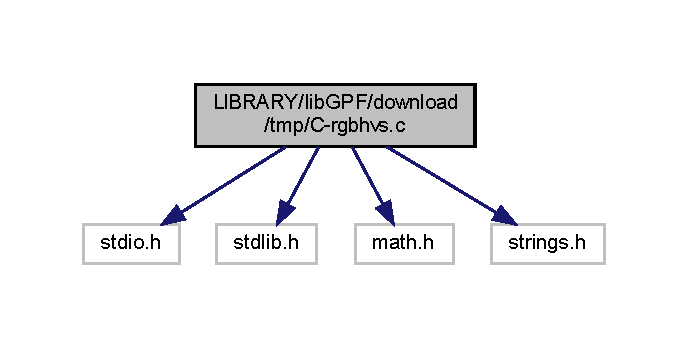
\includegraphics[width=330pt]{C-rgbhvs_8c__incl}
\end{center}
\end{figure}
\subsection*{Functions}
\begin{DoxyCompactItemize}
\item 
void \hyperlink{C-rgbhvs_8c_a4110202639bfb2a997338ea37775dca8}{rgbhvs} (float red, float green, float blue, float $\ast$hue, float $\ast$value, float $\ast$saturation)
\end{DoxyCompactItemize}


\subsection{Function Documentation}
\mbox{\Hypertarget{C-rgbhvs_8c_a4110202639bfb2a997338ea37775dca8}\label{C-rgbhvs_8c_a4110202639bfb2a997338ea37775dca8}} 
\index{C-\/rgbhvs.\+c@{C-\/rgbhvs.\+c}!rgbhvs@{rgbhvs}}
\index{rgbhvs@{rgbhvs}!C-\/rgbhvs.\+c@{C-\/rgbhvs.\+c}}
\subsubsection{\texorpdfstring{rgbhvs()}{rgbhvs()}}
{\footnotesize\ttfamily void rgbhvs (\begin{DoxyParamCaption}\item[{float}]{red,  }\item[{float}]{green,  }\item[{float}]{blue,  }\item[{float $\ast$}]{hue,  }\item[{float $\ast$}]{value,  }\item[{float $\ast$}]{saturation }\end{DoxyParamCaption})}



References stderr().

Here is the call graph for this function\+:
\nopagebreak
\begin{figure}[H]
\begin{center}
\leavevmode
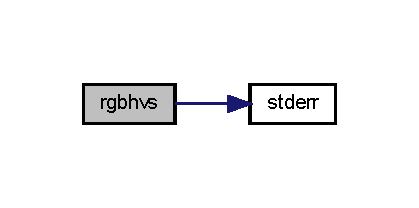
\includegraphics[width=201pt]{C-rgbhvs_8c_a4110202639bfb2a997338ea37775dca8_cgraph}
\end{center}
\end{figure}
Here is the caller graph for this function\+:
\nopagebreak
\begin{figure}[H]
\begin{center}
\leavevmode
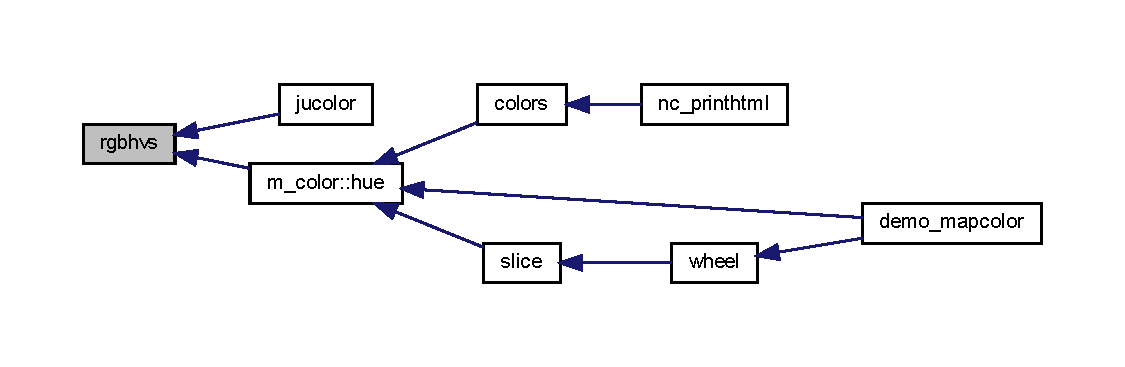
\includegraphics[width=350pt]{C-rgbhvs_8c_a4110202639bfb2a997338ea37775dca8_icgraph}
\end{center}
\end{figure}

\hypertarget{C-rgbmono_8c}{}\section{L\+I\+B\+R\+A\+R\+Y/lib\+G\+P\+F/download/tmp/\+C-\/rgbmono.c File Reference}
\label{C-rgbmono_8c}\index{L\+I\+B\+R\+A\+R\+Y/lib\+G\+P\+F/download/tmp/\+C-\/rgbmono.\+c@{L\+I\+B\+R\+A\+R\+Y/lib\+G\+P\+F/download/tmp/\+C-\/rgbmono.\+c}}
\subsection*{Functions}
\begin{DoxyCompactItemize}
\item 
float \hyperlink{C-rgbmono_8c_a22b27fb2e3d8d0451aec4fa812dd267a}{rgbmono} (float red\+\_\+component, float green\+\_\+component, float blue\+\_\+component)
\end{DoxyCompactItemize}


\subsection{Function Documentation}
\mbox{\Hypertarget{C-rgbmono_8c_a22b27fb2e3d8d0451aec4fa812dd267a}\label{C-rgbmono_8c_a22b27fb2e3d8d0451aec4fa812dd267a}} 
\index{C-\/rgbmono.\+c@{C-\/rgbmono.\+c}!rgbmono@{rgbmono}}
\index{rgbmono@{rgbmono}!C-\/rgbmono.\+c@{C-\/rgbmono.\+c}}
\subsubsection{\texorpdfstring{rgbmono()}{rgbmono()}}
{\footnotesize\ttfamily float rgbmono (\begin{DoxyParamCaption}\item[{float}]{red\+\_\+component,  }\item[{float}]{green\+\_\+component,  }\item[{float}]{blue\+\_\+component }\end{DoxyParamCaption})}


\hypertarget{C-rgbval_8c}{}\section{L\+I\+B\+R\+A\+R\+Y/lib\+G\+P\+F/download/tmp/\+C-\/rgbval.c File Reference}
\label{C-rgbval_8c}\index{L\+I\+B\+R\+A\+R\+Y/lib\+G\+P\+F/download/tmp/\+C-\/rgbval.\+c@{L\+I\+B\+R\+A\+R\+Y/lib\+G\+P\+F/download/tmp/\+C-\/rgbval.\+c}}
\subsection*{Functions}
\begin{DoxyCompactItemize}
\item 
float \hyperlink{C-rgbval_8c_a44944ef0b70e4ce364fa785ff6750eac}{rgbval} (float color1, float color2, float h)
\end{DoxyCompactItemize}


\subsection{Function Documentation}
\mbox{\Hypertarget{C-rgbval_8c_a44944ef0b70e4ce364fa785ff6750eac}\label{C-rgbval_8c_a44944ef0b70e4ce364fa785ff6750eac}} 
\index{C-\/rgbval.\+c@{C-\/rgbval.\+c}!rgbval@{rgbval}}
\index{rgbval@{rgbval}!C-\/rgbval.\+c@{C-\/rgbval.\+c}}
\subsubsection{\texorpdfstring{rgbval()}{rgbval()}}
{\footnotesize\ttfamily float rgbval (\begin{DoxyParamCaption}\item[{float}]{color1,  }\item[{float}]{color2,  }\item[{float}]{h }\end{DoxyParamCaption})}


\hypertarget{c_8f90}{}\section{L\+I\+B\+R\+A\+R\+Y/lib\+G\+P\+F/download/tmp/c.f90 File Reference}
\label{c_8f90}\index{L\+I\+B\+R\+A\+R\+Y/lib\+G\+P\+F/download/tmp/c.\+f90@{L\+I\+B\+R\+A\+R\+Y/lib\+G\+P\+F/download/tmp/c.\+f90}}
\subsection*{Functions/\+Subroutines}
\begin{DoxyCompactItemize}
\item 
\hyperlink{read__watch_83_8txt_abdb62bde002f38ef75f810d3a905a823}{real} function \hyperlink{c_8f90_aeb1f4e639be0213b4cbd07f2583a5b1f}{c} (fval, n)
\end{DoxyCompactItemize}


\subsection{Function/\+Subroutine Documentation}
\mbox{\Hypertarget{c_8f90_aeb1f4e639be0213b4cbd07f2583a5b1f}\label{c_8f90_aeb1f4e639be0213b4cbd07f2583a5b1f}} 
\index{c.\+f90@{c.\+f90}!c@{c}}
\index{c@{c}!c.\+f90@{c.\+f90}}
\subsubsection{\texorpdfstring{c()}{c()}}
{\footnotesize\ttfamily \hyperlink{read__watch_83_8txt_abdb62bde002f38ef75f810d3a905a823}{real} function c (\begin{DoxyParamCaption}\item[{}]{fval,  }\item[{}]{n }\end{DoxyParamCaption})}

Here is the caller graph for this function\+:
\nopagebreak
\begin{figure}[H]
\begin{center}
\leavevmode
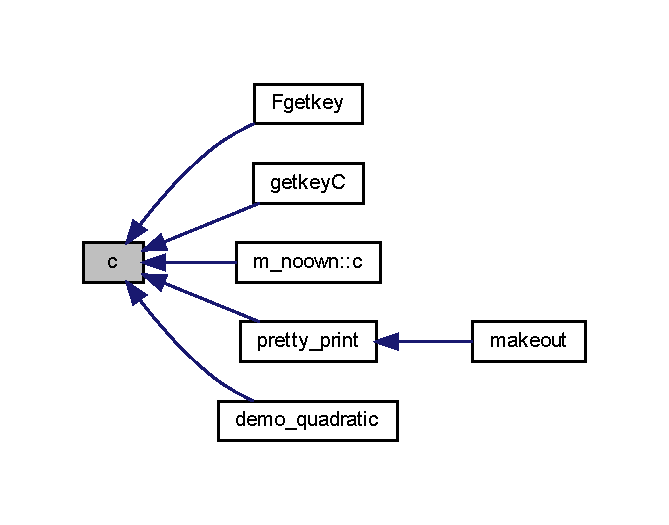
\includegraphics[width=321pt]{c_8f90_aeb1f4e639be0213b4cbd07f2583a5b1f_icgraph}
\end{center}
\end{figure}

\hypertarget{block_87_8txt}{}\section{L\+I\+B\+R\+A\+R\+Y/lib\+G\+P\+F/download/tmp/doc/block.7.txt File Reference}
\label{block_87_8txt}\index{L\+I\+B\+R\+A\+R\+Y/lib\+G\+P\+F/download/tmp/doc/block.\+7.\+txt@{L\+I\+B\+R\+A\+R\+Y/lib\+G\+P\+F/download/tmp/doc/block.\+7.\+txt}}

\hypertarget{cond_83_8txt}{}\section{L\+I\+B\+R\+A\+R\+Y/lib\+G\+P\+F/download/tmp/doc/cond.3.txt File Reference}
\label{cond_83_8txt}\index{L\+I\+B\+R\+A\+R\+Y/lib\+G\+P\+F/download/tmp/doc/cond.\+3.\+txt@{L\+I\+B\+R\+A\+R\+Y/lib\+G\+P\+F/download/tmp/doc/cond.\+3.\+txt}}

\hypertarget{continue_87_8txt}{}\section{L\+I\+B\+R\+A\+R\+Y/lib\+G\+P\+F/download/tmp/doc/continue.7.txt File Reference}
\label{continue_87_8txt}\index{L\+I\+B\+R\+A\+R\+Y/lib\+G\+P\+F/download/tmp/doc/continue.\+7.\+txt@{L\+I\+B\+R\+A\+R\+Y/lib\+G\+P\+F/download/tmp/doc/continue.\+7.\+txt}}
\subsection*{Variables}
\begin{DoxyCompactItemize}
\item 
Specification of Fortran TH C\+O\+N\+T\+I\+N\+UE January Fortran Language Specification SH N\+A\+ME C\+O\+N\+T\+I\+N\+UE(7f) -\/ \mbox{[}\+F\+O\+R\+T\+R\+A\+N a C\+O\+N\+T\+I\+N\+U\+E statement eliminates the ambiguities that arise in jumping to an executable line Preferably no target of a transfer should be an executable \hyperlink{continue_87_8txt_ab499dad98bb4e44fe84dabd1bf0fa987}{statement}
\item 
Specification of Fortran TH C\+O\+N\+T\+I\+N\+UE January Fortran Language Specification SH N\+A\+ME C\+O\+N\+T\+I\+N\+UE(7f) -\/ \mbox{[}\+F\+O\+R\+T\+R\+A\+N a C\+O\+N\+T\+I\+N\+U\+E statement eliminates the ambiguities that arise in jumping to an executable line Preferably no target of a transfer should be an executable but should be a statement like E\+N\+D\+D\+O or C\+O\+N\+T\+I\+N\+U\+E C\+O\+N\+T\+I\+N\+U\+E was very frequently used as the end of a DO \hyperlink{continue_87_8txt_a5094e6a64d1227c84a0bf4db8f6c3788}{loop}
\item 
E\+N\+D\+DO \hyperlink{intro__blas1_83_8txt_a42a91df93f840595de3019ceb5d1df23}{is} now \hyperlink{M__stopwatch_83_8txt_a0f266597de2e57eb3aa964927bb30e14}{the} proper way \hyperlink{M__stopwatch_83_8txt_a97209fd3e34ef701c0a9734280779cbb}{to} end a DO \hyperlink{continue_87_8txt_a5094e6a64d1227c84a0bf4db8f6c3788}{loop} fi SH E\+X\+A\+M\+P\+LE nf program demo\+\_\+continue \hyperlink{continue_87_8txt_ae7b8826453d28f1bdb2fba7e889eb23b}{I}
\end{DoxyCompactItemize}


\subsection{Variable Documentation}
\mbox{\Hypertarget{continue_87_8txt_ae7b8826453d28f1bdb2fba7e889eb23b}\label{continue_87_8txt_ae7b8826453d28f1bdb2fba7e889eb23b}} 
\index{continue.\+7.\+txt@{continue.\+7.\+txt}!I@{I}}
\index{I@{I}!continue.\+7.\+txt@{continue.\+7.\+txt}}
\subsubsection{\texorpdfstring{I}{I}}
{\footnotesize\ttfamily E\+N\+D\+DO \hyperlink{intro__blas1_83_8txt_a42a91df93f840595de3019ceb5d1df23}{is} now \hyperlink{M__stopwatch_83_8txt_a0f266597de2e57eb3aa964927bb30e14}{the} proper way \hyperlink{M__stopwatch_83_8txt_a97209fd3e34ef701c0a9734280779cbb}{to} end a DO \hyperlink{continue_87_8txt_a5094e6a64d1227c84a0bf4db8f6c3788}{loop} fi SH E\+X\+A\+M\+P\+LE nf program demo\+\_\+continue I}

{\bfseries Initial value\+:}
\begin{DoxyCode}
=10
         J=5
         \textcolor{keywordflow}{if}(\hyperlink{continue_87_8txt_ae7b8826453d28f1bdb2fba7e889eb23b}{I}.lt.5)\textcolor{keywordflow}{goto} 100
         J=3
   100   \textcolor{keywordflow}{continue}
         write(*,*)\textcolor{stringliteral}{'J='}
\end{DoxyCode}
\mbox{\Hypertarget{continue_87_8txt_a5094e6a64d1227c84a0bf4db8f6c3788}\label{continue_87_8txt_a5094e6a64d1227c84a0bf4db8f6c3788}} 
\index{continue.\+7.\+txt@{continue.\+7.\+txt}!loop@{loop}}
\index{loop@{loop}!continue.\+7.\+txt@{continue.\+7.\+txt}}
\subsubsection{\texorpdfstring{loop}{loop}}
{\footnotesize\ttfamily Specification of Fortran TH C\+O\+N\+T\+I\+N\+UE January Fortran Language Specification SH N\+A\+ME C\+O\+N\+T\+I\+N\+UE (7f) -\/ \mbox{[}\+F\+O\+R\+T\+R\+A\+N a C\+O\+N\+T\+I\+N\+U\+E statement eliminates the ambiguities that arise in jumping to an executable line Preferably no target of a transfer should be an executable but should be a statement like E\+N\+D\+D\+O or C\+O\+N\+T\+I\+N\+U\+E C\+O\+N\+T\+I\+N\+U\+E was very frequently used as the end of a D\+O loop}

\mbox{\Hypertarget{continue_87_8txt_ab499dad98bb4e44fe84dabd1bf0fa987}\label{continue_87_8txt_ab499dad98bb4e44fe84dabd1bf0fa987}} 
\index{continue.\+7.\+txt@{continue.\+7.\+txt}!statement@{statement}}
\index{statement@{statement}!continue.\+7.\+txt@{continue.\+7.\+txt}}
\subsubsection{\texorpdfstring{statement}{statement}}
{\footnotesize\ttfamily Specification of Fortran TH C\+O\+N\+T\+I\+N\+UE January Fortran Language Specification SH N\+A\+ME C\+O\+N\+T\+I\+N\+UE (7f) -\/ \mbox{[}\+F\+O\+R\+T\+R\+A\+N a C\+O\+N\+T\+I\+N\+U\+E statement eliminates the ambiguities that arise in jumping to an executable line Preferably no target of a transfer should be an executable statement}


\hypertarget{create__watch_83_8txt}{}\section{L\+I\+B\+R\+A\+R\+Y/lib\+G\+P\+F/download/tmp/doc/create\+\_\+watch.3.txt File Reference}
\label{create__watch_83_8txt}\index{L\+I\+B\+R\+A\+R\+Y/lib\+G\+P\+F/download/tmp/doc/create\+\_\+watch.\+3.\+txt@{L\+I\+B\+R\+A\+R\+Y/lib\+G\+P\+F/download/tmp/doc/create\+\_\+watch.\+3.\+txt}}
\subsection*{Functions}
\begin{DoxyCompactItemize}
\item 
TH C\+R\+E\+A\+T\+E\+\_\+\+W\+A\+T\+CH \hyperlink{option__stopwatch_83_8txt_aa2011fc45a5e502e87ee50996a8a9305}{M\+\_\+\+Stop\+Watch} M\+\_\+\+S\+T\+O\+P\+W\+A\+T\+CH P\+R\+O\+C\+E\+D\+U\+R\+ES \hyperlink{what__overview_81_8txt_a85f26da5a4481fbdb0d9c79f2b94de3e}{PD} SH N\+A\+ME \hyperlink{create__watch_83_8txt_a6deb35ddebb447c9dceca30690d1581d}{create\+\_\+watch} (3f) -\/ \mbox{[}\+M\+\_\+stopwatch\mbox{]} creates and initializes a M\+\_\+\+Stop\+Watch watch .\+S\+H S\+Y\+N\+O\+P\+S\+I\+S subroutine .\+B\+I \char`\"{}create\+\_\+watch\char`\"{} \char`\"{}(watch
\item 
TH C\+R\+E\+A\+T\+E\+\_\+\+W\+A\+T\+CH \hyperlink{option__stopwatch_83_8txt_aa2011fc45a5e502e87ee50996a8a9305}{M\+\_\+\+Stop\+Watch} M\+\_\+\+S\+T\+O\+P\+W\+A\+T\+CH P\+R\+O\+C\+E\+D\+U\+R\+ES \hyperlink{what__overview_81_8txt_a85f26da5a4481fbdb0d9c79f2b94de3e}{PD} SH N\+A\+ME err IP \hyperlink{create__watch_83_8txt_a6036c8b9d18bd95ef0feb888982faa0b}{type} (watchtype)
\end{DoxyCompactItemize}
\subsection*{Variables}
\begin{DoxyCompactItemize}
\item 
TH C\+R\+E\+A\+T\+E\+\_\+\+W\+A\+T\+CH \hyperlink{create__watch_83_8txt_a3f52c4f0a971d6aad8d5872fab85fac6}{September}
\item 
TH C\+R\+E\+A\+T\+E\+\_\+\+W\+A\+T\+CH \hyperlink{option__stopwatch_83_8txt_aa2011fc45a5e502e87ee50996a8a9305}{M\+\_\+\+Stop\+Watch} M\+\_\+\+S\+T\+O\+P\+W\+A\+T\+CH P\+R\+O\+C\+E\+D\+U\+R\+ES \hyperlink{what__overview_81_8txt_a85f26da5a4481fbdb0d9c79f2b94de3e}{PD} SH N\+A\+ME \hyperlink{create__watch_83_8txt_ae5a722940632dbef0e5f6b03622fbf1c}{clock}
\item 
TH C\+R\+E\+A\+T\+E\+\_\+\+W\+A\+T\+CH \hyperlink{option__stopwatch_83_8txt_aa2011fc45a5e502e87ee50996a8a9305}{M\+\_\+\+Stop\+Watch} M\+\_\+\+S\+T\+O\+P\+W\+A\+T\+CH P\+R\+O\+C\+E\+D\+U\+R\+ES \hyperlink{what__overview_81_8txt_a85f26da5a4481fbdb0d9c79f2b94de3e}{PD} SH N\+A\+ME \hyperlink{create__watch_83_8txt_a7952910b2b90c60662fb5b4a4e85427c}{name}
\end{DoxyCompactItemize}


\subsection{Function Documentation}
\mbox{\Hypertarget{create__watch_83_8txt_a6deb35ddebb447c9dceca30690d1581d}\label{create__watch_83_8txt_a6deb35ddebb447c9dceca30690d1581d}} 
\index{create\+\_\+watch.\+3.\+txt@{create\+\_\+watch.\+3.\+txt}!create\+\_\+watch@{create\+\_\+watch}}
\index{create\+\_\+watch@{create\+\_\+watch}!create\+\_\+watch.\+3.\+txt@{create\+\_\+watch.\+3.\+txt}}
\subsubsection{\texorpdfstring{create\+\_\+watch()}{create\_watch()}}
{\footnotesize\ttfamily TH C\+R\+E\+A\+T\+E\+\_\+\+W\+A\+T\+CH \hyperlink{option__stopwatch_83_8txt_aa2011fc45a5e502e87ee50996a8a9305}{M\+\_\+\+Stop\+Watch} M\+\_\+\+S\+T\+O\+P\+W\+A\+T\+CH P\+R\+O\+C\+E\+D\+U\+R\+ES \hyperlink{what__overview_81_8txt_a85f26da5a4481fbdb0d9c79f2b94de3e}{PD} SH N\+A\+ME create\+\_\+watch (\begin{DoxyParamCaption}\item[{3f}]{ }\end{DoxyParamCaption})}

\mbox{\Hypertarget{create__watch_83_8txt_a6036c8b9d18bd95ef0feb888982faa0b}\label{create__watch_83_8txt_a6036c8b9d18bd95ef0feb888982faa0b}} 
\index{create\+\_\+watch.\+3.\+txt@{create\+\_\+watch.\+3.\+txt}!type@{type}}
\index{type@{type}!create\+\_\+watch.\+3.\+txt@{create\+\_\+watch.\+3.\+txt}}
\subsubsection{\texorpdfstring{type()}{type()}}
{\footnotesize\ttfamily TH C\+R\+E\+A\+T\+E\+\_\+\+W\+A\+T\+CH \hyperlink{option__stopwatch_83_8txt_aa2011fc45a5e502e87ee50996a8a9305}{M\+\_\+\+Stop\+Watch} M\+\_\+\+S\+T\+O\+P\+W\+A\+T\+CH P\+R\+O\+C\+E\+D\+U\+R\+ES \hyperlink{what__overview_81_8txt_a85f26da5a4481fbdb0d9c79f2b94de3e}{PD} SH N\+A\+ME err IP type (\begin{DoxyParamCaption}\item[{watchtype}]{ }\end{DoxyParamCaption})}



\subsection{Variable Documentation}
\mbox{\Hypertarget{create__watch_83_8txt_ae5a722940632dbef0e5f6b03622fbf1c}\label{create__watch_83_8txt_ae5a722940632dbef0e5f6b03622fbf1c}} 
\index{create\+\_\+watch.\+3.\+txt@{create\+\_\+watch.\+3.\+txt}!clock@{clock}}
\index{clock@{clock}!create\+\_\+watch.\+3.\+txt@{create\+\_\+watch.\+3.\+txt}}
\subsubsection{\texorpdfstring{clock}{clock}}
{\footnotesize\ttfamily TH M\+\_\+\+S\+T\+O\+P\+W\+A\+T\+CH \hyperlink{option__stopwatch_83_8txt_aa2011fc45a5e502e87ee50996a8a9305}{M\+\_\+\+Stop\+Watch} M\+\_\+\+S\+T\+O\+P\+W\+A\+T\+CH O\+V\+E\+R\+V\+I\+EW \hyperlink{what__overview_81_8txt_a85f26da5a4481fbdb0d9c79f2b94de3e}{PD} SH N\+A\+ME easy \hyperlink{M__stopwatch_83_8txt_a97209fd3e34ef701c0a9734280779cbb}{to} \hyperlink{intro__blas1_83_8txt_a04fa2694d85f67a675bb3f45f7241f48}{use} means of measuring execution \hyperlink{M__stopwatch_83_8txt_a1091fdf3a4e66042d1571c7e4ade98dd}{time} It supports \hyperlink{M__stopwatch_83_8txt_a0f266597de2e57eb3aa964927bb30e14}{the} \hyperlink{M__stopwatch_83_8txt_a78df39f546d66b02c203502a4025b0f4}{wall} C\+PU clock}

\mbox{\Hypertarget{create__watch_83_8txt_a7952910b2b90c60662fb5b4a4e85427c}\label{create__watch_83_8txt_a7952910b2b90c60662fb5b4a4e85427c}} 
\index{create\+\_\+watch.\+3.\+txt@{create\+\_\+watch.\+3.\+txt}!name@{name}}
\index{name@{name}!create\+\_\+watch.\+3.\+txt@{create\+\_\+watch.\+3.\+txt}}
\subsubsection{\texorpdfstring{name}{name}}
{\footnotesize\ttfamily TH C\+R\+E\+A\+T\+E\+\_\+\+W\+A\+T\+CH \hyperlink{option__stopwatch_83_8txt_aa2011fc45a5e502e87ee50996a8a9305}{M\+\_\+\+Stop\+Watch} M\+\_\+\+S\+T\+O\+P\+W\+A\+T\+CH P\+R\+O\+C\+E\+D\+U\+R\+ES \hyperlink{what__overview_81_8txt_a85f26da5a4481fbdb0d9c79f2b94de3e}{PD} SH N\+A\+ME name}

\mbox{\Hypertarget{create__watch_83_8txt_a3f52c4f0a971d6aad8d5872fab85fac6}\label{create__watch_83_8txt_a3f52c4f0a971d6aad8d5872fab85fac6}} 
\index{create\+\_\+watch.\+3.\+txt@{create\+\_\+watch.\+3.\+txt}!September@{September}}
\index{September@{September}!create\+\_\+watch.\+3.\+txt@{create\+\_\+watch.\+3.\+txt}}
\subsubsection{\texorpdfstring{September}{September}}
{\footnotesize\ttfamily TH C\+R\+E\+A\+T\+E\+\_\+\+W\+A\+T\+CH September}


\hypertarget{create__watchgroup_83_8txt}{}\section{L\+I\+B\+R\+A\+R\+Y/lib\+G\+P\+F/download/tmp/doc/create\+\_\+watchgroup.3.txt File Reference}
\label{create__watchgroup_83_8txt}\index{L\+I\+B\+R\+A\+R\+Y/lib\+G\+P\+F/download/tmp/doc/create\+\_\+watchgroup.\+3.\+txt@{L\+I\+B\+R\+A\+R\+Y/lib\+G\+P\+F/download/tmp/doc/create\+\_\+watchgroup.\+3.\+txt}}
\subsection*{Functions}
\begin{DoxyCompactItemize}
\item 
TH C\+R\+E\+A\+T\+E\+\_\+\+W\+A\+T\+C\+H\+G\+R\+O\+UP \hyperlink{option__stopwatch_83_8txt_aa2011fc45a5e502e87ee50996a8a9305}{M\+\_\+\+Stop\+Watch} M\+\_\+\+S\+T\+O\+P\+W\+A\+T\+CH P\+R\+O\+C\+E\+D\+U\+R\+ES \hyperlink{what__overview_81_8txt_a85f26da5a4481fbdb0d9c79f2b94de3e}{PD} SH N\+A\+ME \hyperlink{create__watchgroup_83_8txt_a7e1fab3a0b16096cc31b6750b1a1fa6f}{create\+\_\+watchgroup} (3f) -\/ \mbox{[}\+M\+\_\+stopwatch\mbox{]} creates a M\+\_\+\+Stop\+Watch watch group .\+S\+H S\+Y\+N\+O\+P\+S\+I\+S subroutine .\+B\+I \char`\"{}create\+\_\+watchgroup\char`\"{} \char`\"{}(watch
\item 
TH C\+R\+E\+A\+T\+E\+\_\+\+W\+A\+T\+C\+H\+G\+R\+O\+UP \hyperlink{option__stopwatch_83_8txt_aa2011fc45a5e502e87ee50996a8a9305}{M\+\_\+\+Stop\+Watch} M\+\_\+\+S\+T\+O\+P\+W\+A\+T\+CH P\+R\+O\+C\+E\+D\+U\+R\+ES \hyperlink{what__overview_81_8txt_a85f26da5a4481fbdb0d9c79f2b94de3e}{PD} SH N\+A\+ME err IP \hyperlink{create__watchgroup_83_8txt_adc4024c3b4c8e8b4c2f17a2937352e5d}{type} (watchtype)
\end{DoxyCompactItemize}
\subsection*{Variables}
\begin{DoxyCompactItemize}
\item 
TH C\+R\+E\+A\+T\+E\+\_\+\+W\+A\+T\+C\+H\+G\+R\+O\+UP \hyperlink{create__watchgroup_83_8txt_a2fe56ee2e395403bb06376136f40e45c}{September}
\item 
TH C\+R\+E\+A\+T\+E\+\_\+\+W\+A\+T\+C\+H\+G\+R\+O\+UP \hyperlink{option__stopwatch_83_8txt_aa2011fc45a5e502e87ee50996a8a9305}{M\+\_\+\+Stop\+Watch} M\+\_\+\+S\+T\+O\+P\+W\+A\+T\+CH P\+R\+O\+C\+E\+D\+U\+R\+ES \hyperlink{what__overview_81_8txt_a85f26da5a4481fbdb0d9c79f2b94de3e}{PD} SH N\+A\+ME \hyperlink{create__watchgroup_83_8txt_a5f82c33d958a5267f1648fdea2152853}{handle}
\end{DoxyCompactItemize}


\subsection{Function Documentation}
\mbox{\Hypertarget{create__watchgroup_83_8txt_a7e1fab3a0b16096cc31b6750b1a1fa6f}\label{create__watchgroup_83_8txt_a7e1fab3a0b16096cc31b6750b1a1fa6f}} 
\index{create\+\_\+watchgroup.\+3.\+txt@{create\+\_\+watchgroup.\+3.\+txt}!create\+\_\+watchgroup@{create\+\_\+watchgroup}}
\index{create\+\_\+watchgroup@{create\+\_\+watchgroup}!create\+\_\+watchgroup.\+3.\+txt@{create\+\_\+watchgroup.\+3.\+txt}}
\subsubsection{\texorpdfstring{create\+\_\+watchgroup()}{create\_watchgroup()}}
{\footnotesize\ttfamily TH C\+R\+E\+A\+T\+E\+\_\+\+W\+A\+T\+C\+H\+G\+R\+O\+UP \hyperlink{option__stopwatch_83_8txt_aa2011fc45a5e502e87ee50996a8a9305}{M\+\_\+\+Stop\+Watch} M\+\_\+\+S\+T\+O\+P\+W\+A\+T\+CH P\+R\+O\+C\+E\+D\+U\+R\+ES \hyperlink{what__overview_81_8txt_a85f26da5a4481fbdb0d9c79f2b94de3e}{PD} SH N\+A\+ME create\+\_\+watchgroup (\begin{DoxyParamCaption}\item[{3f}]{ }\end{DoxyParamCaption})}

\mbox{\Hypertarget{create__watchgroup_83_8txt_adc4024c3b4c8e8b4c2f17a2937352e5d}\label{create__watchgroup_83_8txt_adc4024c3b4c8e8b4c2f17a2937352e5d}} 
\index{create\+\_\+watchgroup.\+3.\+txt@{create\+\_\+watchgroup.\+3.\+txt}!type@{type}}
\index{type@{type}!create\+\_\+watchgroup.\+3.\+txt@{create\+\_\+watchgroup.\+3.\+txt}}
\subsubsection{\texorpdfstring{type()}{type()}}
{\footnotesize\ttfamily TH C\+R\+E\+A\+T\+E\+\_\+\+W\+A\+T\+C\+H\+G\+R\+O\+UP \hyperlink{option__stopwatch_83_8txt_aa2011fc45a5e502e87ee50996a8a9305}{M\+\_\+\+Stop\+Watch} M\+\_\+\+S\+T\+O\+P\+W\+A\+T\+CH P\+R\+O\+C\+E\+D\+U\+R\+ES \hyperlink{what__overview_81_8txt_a85f26da5a4481fbdb0d9c79f2b94de3e}{PD} SH N\+A\+ME err IP type (\begin{DoxyParamCaption}\item[{watchtype}]{ }\end{DoxyParamCaption})}



\subsection{Variable Documentation}
\mbox{\Hypertarget{create__watchgroup_83_8txt_a5f82c33d958a5267f1648fdea2152853}\label{create__watchgroup_83_8txt_a5f82c33d958a5267f1648fdea2152853}} 
\index{create\+\_\+watchgroup.\+3.\+txt@{create\+\_\+watchgroup.\+3.\+txt}!handle@{handle}}
\index{handle@{handle}!create\+\_\+watchgroup.\+3.\+txt@{create\+\_\+watchgroup.\+3.\+txt}}
\subsubsection{\texorpdfstring{handle}{handle}}
{\footnotesize\ttfamily TH C\+R\+E\+A\+T\+E\+\_\+\+W\+A\+T\+C\+H\+G\+R\+O\+UP \hyperlink{option__stopwatch_83_8txt_aa2011fc45a5e502e87ee50996a8a9305}{M\+\_\+\+Stop\+Watch} M\+\_\+\+S\+T\+O\+P\+W\+A\+T\+CH P\+R\+O\+C\+E\+D\+U\+R\+ES \hyperlink{what__overview_81_8txt_a85f26da5a4481fbdb0d9c79f2b94de3e}{PD} SH N\+A\+ME handle}

\mbox{\Hypertarget{create__watchgroup_83_8txt_a2fe56ee2e395403bb06376136f40e45c}\label{create__watchgroup_83_8txt_a2fe56ee2e395403bb06376136f40e45c}} 
\index{create\+\_\+watchgroup.\+3.\+txt@{create\+\_\+watchgroup.\+3.\+txt}!September@{September}}
\index{September@{September}!create\+\_\+watchgroup.\+3.\+txt@{create\+\_\+watchgroup.\+3.\+txt}}
\subsubsection{\texorpdfstring{September}{September}}
{\footnotesize\ttfamily TH C\+R\+E\+A\+T\+E\+\_\+\+W\+A\+T\+C\+H\+G\+R\+O\+UP September}


\hypertarget{cycle_87_8txt}{}\section{L\+I\+B\+R\+A\+R\+Y/lib\+G\+P\+F/download/tmp/doc/cycle.7.txt File Reference}
\label{cycle_87_8txt}\index{L\+I\+B\+R\+A\+R\+Y/lib\+G\+P\+F/download/tmp/doc/cycle.\+7.\+txt@{L\+I\+B\+R\+A\+R\+Y/lib\+G\+P\+F/download/tmp/doc/cycle.\+7.\+txt}}

\hypertarget{destroy__watch_83_8txt}{}\section{L\+I\+B\+R\+A\+R\+Y/lib\+G\+P\+F/download/tmp/doc/destroy\+\_\+watch.3.txt File Reference}
\label{destroy__watch_83_8txt}\index{L\+I\+B\+R\+A\+R\+Y/lib\+G\+P\+F/download/tmp/doc/destroy\+\_\+watch.\+3.\+txt@{L\+I\+B\+R\+A\+R\+Y/lib\+G\+P\+F/download/tmp/doc/destroy\+\_\+watch.\+3.\+txt}}
\subsection*{Functions}
\begin{DoxyCompactItemize}
\item 
TH D\+E\+S\+T\+R\+O\+Y\+\_\+\+W\+A\+T\+CH \hyperlink{option__stopwatch_83_8txt_aa2011fc45a5e502e87ee50996a8a9305}{M\+\_\+\+Stop\+Watch} M\+\_\+\+S\+T\+O\+P\+W\+A\+T\+CH P\+R\+O\+C\+E\+D\+U\+R\+ES PD SH N\+A\+ME \hyperlink{destroy__watch_83_8txt_aeb23b46d3b50996f7af1c0c77c7fe713}{destroy\+\_\+watch} (3f) -\/ \mbox{[}\+M\+\_\+stopwatch\mbox{]} destroys a M\+\_\+\+Stop\+Watch watch .\+S\+H S\+Y\+N\+O\+P\+S\+I\+S subroutine .\+B\+I \char`\"{}destroy\+\_\+watch\char`\"{} \char`\"{}(watch
\item 
TH D\+E\+S\+T\+R\+O\+Y\+\_\+\+W\+A\+T\+CH \hyperlink{option__stopwatch_83_8txt_aa2011fc45a5e502e87ee50996a8a9305}{M\+\_\+\+Stop\+Watch} M\+\_\+\+S\+T\+O\+P\+W\+A\+T\+CH P\+R\+O\+C\+E\+D\+U\+R\+ES PD SH N\+A\+ME err IP \hyperlink{destroy__watch_83_8txt_a7bc32e4b0bf5a4206ac0c208a77e9d4b}{type} (watchtype)
\end{DoxyCompactItemize}
\subsection*{Variables}
\begin{DoxyCompactItemize}
\item 
TH D\+E\+S\+T\+R\+O\+Y\+\_\+\+W\+A\+T\+CH \hyperlink{destroy__watch_83_8txt_acabdf4ce798cad6afe1d3f1796bf4814}{September}
\item 
TH D\+E\+S\+T\+R\+O\+Y\+\_\+\+W\+A\+T\+CH \hyperlink{option__stopwatch_83_8txt_aa2011fc45a5e502e87ee50996a8a9305}{M\+\_\+\+Stop\+Watch} M\+\_\+\+S\+T\+O\+P\+W\+A\+T\+CH P\+R\+O\+C\+E\+D\+U\+R\+ES PD SH N\+A\+ME \hyperlink{destroy__watch_83_8txt_ac1453e74487611128ccb9ee120e5c70d}{clock}
\end{DoxyCompactItemize}


\subsection{Function Documentation}
\mbox{\Hypertarget{destroy__watch_83_8txt_aeb23b46d3b50996f7af1c0c77c7fe713}\label{destroy__watch_83_8txt_aeb23b46d3b50996f7af1c0c77c7fe713}} 
\index{destroy\+\_\+watch.\+3.\+txt@{destroy\+\_\+watch.\+3.\+txt}!destroy\+\_\+watch@{destroy\+\_\+watch}}
\index{destroy\+\_\+watch@{destroy\+\_\+watch}!destroy\+\_\+watch.\+3.\+txt@{destroy\+\_\+watch.\+3.\+txt}}
\subsubsection{\texorpdfstring{destroy\+\_\+watch()}{destroy\_watch()}}
{\footnotesize\ttfamily TH D\+E\+S\+T\+R\+O\+Y\+\_\+\+W\+A\+T\+CH \hyperlink{option__stopwatch_83_8txt_aa2011fc45a5e502e87ee50996a8a9305}{M\+\_\+\+Stop\+Watch} M\+\_\+\+S\+T\+O\+P\+W\+A\+T\+CH P\+R\+O\+C\+E\+D\+U\+R\+ES PD SH N\+A\+ME destroy\+\_\+watch (\begin{DoxyParamCaption}\item[{3f}]{ }\end{DoxyParamCaption})}

\mbox{\Hypertarget{destroy__watch_83_8txt_a7bc32e4b0bf5a4206ac0c208a77e9d4b}\label{destroy__watch_83_8txt_a7bc32e4b0bf5a4206ac0c208a77e9d4b}} 
\index{destroy\+\_\+watch.\+3.\+txt@{destroy\+\_\+watch.\+3.\+txt}!type@{type}}
\index{type@{type}!destroy\+\_\+watch.\+3.\+txt@{destroy\+\_\+watch.\+3.\+txt}}
\subsubsection{\texorpdfstring{type()}{type()}}
{\footnotesize\ttfamily TH D\+E\+S\+T\+R\+O\+Y\+\_\+\+W\+A\+T\+CH \hyperlink{option__stopwatch_83_8txt_aa2011fc45a5e502e87ee50996a8a9305}{M\+\_\+\+Stop\+Watch} M\+\_\+\+S\+T\+O\+P\+W\+A\+T\+CH P\+R\+O\+C\+E\+D\+U\+R\+ES PD SH N\+A\+ME err IP type (\begin{DoxyParamCaption}\item[{watchtype}]{ }\end{DoxyParamCaption})}



\subsection{Variable Documentation}
\mbox{\Hypertarget{destroy__watch_83_8txt_ac1453e74487611128ccb9ee120e5c70d}\label{destroy__watch_83_8txt_ac1453e74487611128ccb9ee120e5c70d}} 
\index{destroy\+\_\+watch.\+3.\+txt@{destroy\+\_\+watch.\+3.\+txt}!clock@{clock}}
\index{clock@{clock}!destroy\+\_\+watch.\+3.\+txt@{destroy\+\_\+watch.\+3.\+txt}}
\subsubsection{\texorpdfstring{clock}{clock}}
{\footnotesize\ttfamily TH D\+E\+S\+T\+R\+O\+Y\+\_\+\+W\+A\+T\+CH \hyperlink{option__stopwatch_83_8txt_aa2011fc45a5e502e87ee50996a8a9305}{M\+\_\+\+Stop\+Watch} M\+\_\+\+S\+T\+O\+P\+W\+A\+T\+CH P\+R\+O\+C\+E\+D\+U\+R\+ES PD SH N\+A\+ME clock}

\mbox{\Hypertarget{destroy__watch_83_8txt_acabdf4ce798cad6afe1d3f1796bf4814}\label{destroy__watch_83_8txt_acabdf4ce798cad6afe1d3f1796bf4814}} 
\index{destroy\+\_\+watch.\+3.\+txt@{destroy\+\_\+watch.\+3.\+txt}!September@{September}}
\index{September@{September}!destroy\+\_\+watch.\+3.\+txt@{destroy\+\_\+watch.\+3.\+txt}}
\subsubsection{\texorpdfstring{September}{September}}
{\footnotesize\ttfamily TH D\+E\+S\+T\+R\+O\+Y\+\_\+\+W\+A\+T\+CH September}


\hypertarget{destroy__watchgroup_83_8txt}{}\section{L\+I\+B\+R\+A\+R\+Y/lib\+G\+P\+F/download/tmp/doc/destroy\+\_\+watchgroup.3.txt File Reference}
\label{destroy__watchgroup_83_8txt}\index{L\+I\+B\+R\+A\+R\+Y/lib\+G\+P\+F/download/tmp/doc/destroy\+\_\+watchgroup.\+3.\+txt@{L\+I\+B\+R\+A\+R\+Y/lib\+G\+P\+F/download/tmp/doc/destroy\+\_\+watchgroup.\+3.\+txt}}
\subsection*{Functions}
\begin{DoxyCompactItemize}
\item 
TH D\+E\+S\+T\+R\+O\+Y\+\_\+\+W\+A\+T\+C\+H\+G\+R\+O\+UP \hyperlink{option__stopwatch_83_8txt_aa2011fc45a5e502e87ee50996a8a9305}{M\+\_\+\+Stop\+Watch} M\+\_\+\+S\+T\+O\+P\+W\+A\+T\+CH P\+R\+O\+C\+E\+D\+U\+R\+ES \hyperlink{what__overview_81_8txt_a85f26da5a4481fbdb0d9c79f2b94de3e}{PD} SH N\+A\+ME \hyperlink{destroy__watchgroup_83_8txt_a9d6e4dae97c8ce07a61d89382e7692e0}{destroy\+\_\+watchgroup} (3f) -\/ \mbox{[}\+M\+\_\+stopwatch\mbox{]} destroys a M\+\_\+\+Stop\+Watch watch group .\+S\+H S\+Y\+N\+O\+P\+S\+I\+S subroutine .\+B\+I \char`\"{}destroy\+\_\+watchgroup\char`\"{} \char`\"{}(handle
\item 
TH D\+E\+S\+T\+R\+O\+Y\+\_\+\+W\+A\+T\+C\+H\+G\+R\+O\+UP \hyperlink{option__stopwatch_83_8txt_aa2011fc45a5e502e87ee50996a8a9305}{M\+\_\+\+Stop\+Watch} M\+\_\+\+S\+T\+O\+P\+W\+A\+T\+CH P\+R\+O\+C\+E\+D\+U\+R\+ES \hyperlink{what__overview_81_8txt_a85f26da5a4481fbdb0d9c79f2b94de3e}{PD} SH N\+A\+ME err IP \hyperlink{destroy__watchgroup_83_8txt_ab623f536d615ff3d6357e73f12566b46}{type} (watchgroup)
\item 
TH D\+E\+S\+T\+R\+O\+Y\+\_\+\+W\+A\+T\+C\+H\+G\+R\+O\+UP \hyperlink{option__stopwatch_83_8txt_aa2011fc45a5e502e87ee50996a8a9305}{M\+\_\+\+Stop\+Watch} M\+\_\+\+S\+T\+O\+P\+W\+A\+T\+CH P\+R\+O\+C\+E\+D\+U\+R\+ES \hyperlink{what__overview_81_8txt_a85f26da5a4481fbdb0d9c79f2b94de3e}{PD} SH N\+A\+ME err IP intent(\hyperlink{M__stopwatch_83_8txt_aac11c70dd588f9c3fe71e95dbe89902f}{I\+N\+O\+UT}) execution successful IP Error occurred while deallocating memory This \hyperlink{M__stopwatch_83_8txt_ac4611edff506351be87ddb9adfc62315}{error} occurs \hyperlink{exit_87_8txt_a77395982f8d25581c808c40f3b634d90}{if} \hyperlink{M__stopwatch_83_8txt_a0f266597de2e57eb3aa964927bb30e14}{the} Fortran \hyperlink{intro__blas1_83_8txt_a5f157716d3fd55e7b7e08312dc859b58}{B} deallocate \hyperlink{M__stopwatch_83_8txt_a43758526aa61bbaa49faf1e287658350}{statement} \hyperlink{M__stopwatch_83_8txt_aee54cdd5349bf498aa96e7f9426a0717}{returns} a nonzero status while deallocating memory used for \hyperlink{M__stopwatch_83_8txt_a0f266597de2e57eb3aa964927bb30e14}{the} \hyperlink{M__stopwatch_83_8txt_a80fa32a76a22835e3c85462b2803875c}{group} The \hyperlink{M__stopwatch_83_8txt_a80fa32a76a22835e3c85462b2803875c}{group} \hyperlink{intro__blas1_83_8txt_a42a91df93f840595de3019ceb5d1df23}{is} but be aware that other problems could develop as a result of \hyperlink{M__stopwatch_83_8txt_a0f266597de2e57eb3aa964927bb30e14}{the} deallocate \hyperlink{M__stopwatch_83_8txt_ac4611edff506351be87ddb9adfc62315}{error} LP SH E\+X\+A\+M\+P\+L\+ES g2 br integer errcode call \hyperlink{destroy__watchgroup_83_8txt_abf3141ab5cad3784399faea5f2934f2a}{destroy\+\_\+watchgroup} (g1) .br call destroy\+\_\+watchgroup(g2
\item 
TH D\+E\+S\+T\+R\+O\+Y\+\_\+\+W\+A\+T\+C\+H\+G\+R\+O\+UP \hyperlink{option__stopwatch_83_8txt_aa2011fc45a5e502e87ee50996a8a9305}{M\+\_\+\+Stop\+Watch} M\+\_\+\+S\+T\+O\+P\+W\+A\+T\+CH P\+R\+O\+C\+E\+D\+U\+R\+ES \hyperlink{what__overview_81_8txt_a85f26da5a4481fbdb0d9c79f2b94de3e}{PD} SH N\+A\+ME err IP intent(\hyperlink{M__stopwatch_83_8txt_aac11c70dd588f9c3fe71e95dbe89902f}{I\+N\+O\+UT}) execution successful IP Error occurred while deallocating memory This \hyperlink{M__stopwatch_83_8txt_ac4611edff506351be87ddb9adfc62315}{error} occurs \hyperlink{exit_87_8txt_a77395982f8d25581c808c40f3b634d90}{if} \hyperlink{M__stopwatch_83_8txt_a0f266597de2e57eb3aa964927bb30e14}{the} Fortran \hyperlink{intro__blas1_83_8txt_a5f157716d3fd55e7b7e08312dc859b58}{B} deallocate \hyperlink{M__stopwatch_83_8txt_a43758526aa61bbaa49faf1e287658350}{statement} \hyperlink{M__stopwatch_83_8txt_aee54cdd5349bf498aa96e7f9426a0717}{returns} a nonzero status while deallocating memory used for \hyperlink{M__stopwatch_83_8txt_a0f266597de2e57eb3aa964927bb30e14}{the} \hyperlink{M__stopwatch_83_8txt_a80fa32a76a22835e3c85462b2803875c}{group} The \hyperlink{M__stopwatch_83_8txt_a80fa32a76a22835e3c85462b2803875c}{group} \hyperlink{intro__blas1_83_8txt_a42a91df93f840595de3019ceb5d1df23}{is} but be aware that other problems could develop as a result of \hyperlink{M__stopwatch_83_8txt_a0f266597de2e57eb3aa964927bb30e14}{the} deallocate \hyperlink{M__stopwatch_83_8txt_ac4611edff506351be87ddb9adfc62315}{error} LP SH E\+X\+A\+M\+P\+L\+ES g2 br integer errcode call errcode The first call destroys \hyperlink{M__stopwatch_83_8txt_a0f266597de2e57eb3aa964927bb30e14}{the} \hyperlink{M__stopwatch_83_8txt_a80fa32a76a22835e3c85462b2803875c}{group} \hyperlink{continue_87_8txt_ae7b8826453d28f1bdb2fba7e889eb23b}{I} g1 The second call destroys \hyperlink{M__stopwatch_83_8txt_a0f266597de2e57eb3aa964927bb30e14}{the} \hyperlink{M__stopwatch_83_8txt_a80fa32a76a22835e3c85462b2803875c}{group} \hyperlink{continue_87_8txt_ae7b8826453d28f1bdb2fba7e889eb23b}{I} g2 and \hyperlink{M__stopwatch_83_8txt_aee54cdd5349bf498aa96e7f9426a0717}{returns} a status \hyperlink{ufpp__overview_81_8txt_a74a0615f2d9c4a398d9126096f8092f8}{code} SH B\+U\+GS None known SH A\+U\+T\+H\+OR William F william mitchell nist gov br National Institute of Standards and Technology SH S\+EE A\+L\+SO \hyperlink{destroy__watchgroup_83_8txt_a266504af17a0eae1212628c6baa82518}{M\+\_\+stopwatch} (3)
\item 
TH D\+E\+S\+T\+R\+O\+Y\+\_\+\+W\+A\+T\+C\+H\+G\+R\+O\+UP \hyperlink{option__stopwatch_83_8txt_aa2011fc45a5e502e87ee50996a8a9305}{M\+\_\+\+Stop\+Watch} M\+\_\+\+S\+T\+O\+P\+W\+A\+T\+CH P\+R\+O\+C\+E\+D\+U\+R\+ES \hyperlink{what__overview_81_8txt_a85f26da5a4481fbdb0d9c79f2b94de3e}{PD} SH N\+A\+ME err IP intent(\hyperlink{M__stopwatch_83_8txt_aac11c70dd588f9c3fe71e95dbe89902f}{I\+N\+O\+UT}) execution successful IP Error occurred while deallocating memory This \hyperlink{M__stopwatch_83_8txt_ac4611edff506351be87ddb9adfc62315}{error} occurs \hyperlink{exit_87_8txt_a77395982f8d25581c808c40f3b634d90}{if} \hyperlink{M__stopwatch_83_8txt_a0f266597de2e57eb3aa964927bb30e14}{the} Fortran \hyperlink{intro__blas1_83_8txt_a5f157716d3fd55e7b7e08312dc859b58}{B} deallocate \hyperlink{M__stopwatch_83_8txt_a43758526aa61bbaa49faf1e287658350}{statement} \hyperlink{M__stopwatch_83_8txt_aee54cdd5349bf498aa96e7f9426a0717}{returns} a nonzero status while deallocating memory used for \hyperlink{M__stopwatch_83_8txt_a0f266597de2e57eb3aa964927bb30e14}{the} \hyperlink{M__stopwatch_83_8txt_a80fa32a76a22835e3c85462b2803875c}{group} The \hyperlink{M__stopwatch_83_8txt_a80fa32a76a22835e3c85462b2803875c}{group} \hyperlink{intro__blas1_83_8txt_a42a91df93f840595de3019ceb5d1df23}{is} but be aware that other problems could develop as a result of \hyperlink{M__stopwatch_83_8txt_a0f266597de2e57eb3aa964927bb30e14}{the} deallocate \hyperlink{M__stopwatch_83_8txt_ac4611edff506351be87ddb9adfc62315}{error} LP SH E\+X\+A\+M\+P\+L\+ES g2 br integer errcode call errcode The first call destroys \hyperlink{M__stopwatch_83_8txt_a0f266597de2e57eb3aa964927bb30e14}{the} \hyperlink{M__stopwatch_83_8txt_a80fa32a76a22835e3c85462b2803875c}{group} \hyperlink{continue_87_8txt_ae7b8826453d28f1bdb2fba7e889eb23b}{I} g1 The second call destroys \hyperlink{M__stopwatch_83_8txt_a0f266597de2e57eb3aa964927bb30e14}{the} \hyperlink{M__stopwatch_83_8txt_a80fa32a76a22835e3c85462b2803875c}{group} \hyperlink{continue_87_8txt_ae7b8826453d28f1bdb2fba7e889eb23b}{I} g2 and \hyperlink{M__stopwatch_83_8txt_aee54cdd5349bf498aa96e7f9426a0717}{returns} a status \hyperlink{ufpp__overview_81_8txt_a74a0615f2d9c4a398d9126096f8092f8}{code} SH B\+U\+GS None known SH A\+U\+T\+H\+OR William F william mitchell nist gov br National Institute of Standards and Technology SH S\+EE A\+L\+SO \hyperlink{destroy__watchgroup_83_8txt_abf487a79cc3898423ecf7043969678a2}{create\+\_\+watch} (3)
\item 
TH D\+E\+S\+T\+R\+O\+Y\+\_\+\+W\+A\+T\+C\+H\+G\+R\+O\+UP \hyperlink{option__stopwatch_83_8txt_aa2011fc45a5e502e87ee50996a8a9305}{M\+\_\+\+Stop\+Watch} M\+\_\+\+S\+T\+O\+P\+W\+A\+T\+CH P\+R\+O\+C\+E\+D\+U\+R\+ES \hyperlink{what__overview_81_8txt_a85f26da5a4481fbdb0d9c79f2b94de3e}{PD} SH N\+A\+ME err IP intent(\hyperlink{M__stopwatch_83_8txt_aac11c70dd588f9c3fe71e95dbe89902f}{I\+N\+O\+UT}) execution successful IP Error occurred while deallocating memory This \hyperlink{M__stopwatch_83_8txt_ac4611edff506351be87ddb9adfc62315}{error} occurs \hyperlink{exit_87_8txt_a77395982f8d25581c808c40f3b634d90}{if} \hyperlink{M__stopwatch_83_8txt_a0f266597de2e57eb3aa964927bb30e14}{the} Fortran \hyperlink{intro__blas1_83_8txt_a5f157716d3fd55e7b7e08312dc859b58}{B} deallocate \hyperlink{M__stopwatch_83_8txt_a43758526aa61bbaa49faf1e287658350}{statement} \hyperlink{M__stopwatch_83_8txt_aee54cdd5349bf498aa96e7f9426a0717}{returns} a nonzero status while deallocating memory used for \hyperlink{M__stopwatch_83_8txt_a0f266597de2e57eb3aa964927bb30e14}{the} \hyperlink{M__stopwatch_83_8txt_a80fa32a76a22835e3c85462b2803875c}{group} The \hyperlink{M__stopwatch_83_8txt_a80fa32a76a22835e3c85462b2803875c}{group} \hyperlink{intro__blas1_83_8txt_a42a91df93f840595de3019ceb5d1df23}{is} but be aware that other problems could develop as a result of \hyperlink{M__stopwatch_83_8txt_a0f266597de2e57eb3aa964927bb30e14}{the} deallocate \hyperlink{M__stopwatch_83_8txt_ac4611edff506351be87ddb9adfc62315}{error} LP SH E\+X\+A\+M\+P\+L\+ES g2 br integer errcode call errcode The first call destroys \hyperlink{M__stopwatch_83_8txt_a0f266597de2e57eb3aa964927bb30e14}{the} \hyperlink{M__stopwatch_83_8txt_a80fa32a76a22835e3c85462b2803875c}{group} \hyperlink{continue_87_8txt_ae7b8826453d28f1bdb2fba7e889eb23b}{I} g1 The second call destroys \hyperlink{M__stopwatch_83_8txt_a0f266597de2e57eb3aa964927bb30e14}{the} \hyperlink{M__stopwatch_83_8txt_a80fa32a76a22835e3c85462b2803875c}{group} \hyperlink{continue_87_8txt_ae7b8826453d28f1bdb2fba7e889eb23b}{I} g2 and \hyperlink{M__stopwatch_83_8txt_aee54cdd5349bf498aa96e7f9426a0717}{returns} a status \hyperlink{ufpp__overview_81_8txt_a74a0615f2d9c4a398d9126096f8092f8}{code} SH B\+U\+GS None known SH A\+U\+T\+H\+OR William F william mitchell nist gov br National Institute of Standards and Technology SH S\+EE A\+L\+SO \hyperlink{destroy__watchgroup_83_8txt_ac47b56be52541a678ea6bc6bac940183}{destroy\+\_\+watch} (3)
\item 
TH D\+E\+S\+T\+R\+O\+Y\+\_\+\+W\+A\+T\+C\+H\+G\+R\+O\+UP \hyperlink{option__stopwatch_83_8txt_aa2011fc45a5e502e87ee50996a8a9305}{M\+\_\+\+Stop\+Watch} M\+\_\+\+S\+T\+O\+P\+W\+A\+T\+CH P\+R\+O\+C\+E\+D\+U\+R\+ES \hyperlink{what__overview_81_8txt_a85f26da5a4481fbdb0d9c79f2b94de3e}{PD} SH N\+A\+ME err IP intent(\hyperlink{M__stopwatch_83_8txt_aac11c70dd588f9c3fe71e95dbe89902f}{I\+N\+O\+UT}) execution successful IP Error occurred while deallocating memory This \hyperlink{M__stopwatch_83_8txt_ac4611edff506351be87ddb9adfc62315}{error} occurs \hyperlink{exit_87_8txt_a77395982f8d25581c808c40f3b634d90}{if} \hyperlink{M__stopwatch_83_8txt_a0f266597de2e57eb3aa964927bb30e14}{the} Fortran \hyperlink{intro__blas1_83_8txt_a5f157716d3fd55e7b7e08312dc859b58}{B} deallocate \hyperlink{M__stopwatch_83_8txt_a43758526aa61bbaa49faf1e287658350}{statement} \hyperlink{M__stopwatch_83_8txt_aee54cdd5349bf498aa96e7f9426a0717}{returns} a nonzero status while deallocating memory used for \hyperlink{M__stopwatch_83_8txt_a0f266597de2e57eb3aa964927bb30e14}{the} \hyperlink{M__stopwatch_83_8txt_a80fa32a76a22835e3c85462b2803875c}{group} The \hyperlink{M__stopwatch_83_8txt_a80fa32a76a22835e3c85462b2803875c}{group} \hyperlink{intro__blas1_83_8txt_a42a91df93f840595de3019ceb5d1df23}{is} but be aware that other problems could develop as a result of \hyperlink{M__stopwatch_83_8txt_a0f266597de2e57eb3aa964927bb30e14}{the} deallocate \hyperlink{M__stopwatch_83_8txt_ac4611edff506351be87ddb9adfc62315}{error} LP SH E\+X\+A\+M\+P\+L\+ES g2 br integer errcode call errcode The first call destroys \hyperlink{M__stopwatch_83_8txt_a0f266597de2e57eb3aa964927bb30e14}{the} \hyperlink{M__stopwatch_83_8txt_a80fa32a76a22835e3c85462b2803875c}{group} \hyperlink{continue_87_8txt_ae7b8826453d28f1bdb2fba7e889eb23b}{I} g1 The second call destroys \hyperlink{M__stopwatch_83_8txt_a0f266597de2e57eb3aa964927bb30e14}{the} \hyperlink{M__stopwatch_83_8txt_a80fa32a76a22835e3c85462b2803875c}{group} \hyperlink{continue_87_8txt_ae7b8826453d28f1bdb2fba7e889eb23b}{I} g2 and \hyperlink{M__stopwatch_83_8txt_aee54cdd5349bf498aa96e7f9426a0717}{returns} a status \hyperlink{ufpp__overview_81_8txt_a74a0615f2d9c4a398d9126096f8092f8}{code} SH B\+U\+GS None known SH A\+U\+T\+H\+OR William F william mitchell nist gov br National Institute of Standards and Technology SH S\+EE A\+L\+SO \hyperlink{destroy__watchgroup_83_8txt_afebe2ecc33b5b50e6b6382da3deb8387}{end\+\_\+pause\+\_\+watch} (3)
\item 
TH D\+E\+S\+T\+R\+O\+Y\+\_\+\+W\+A\+T\+C\+H\+G\+R\+O\+UP \hyperlink{option__stopwatch_83_8txt_aa2011fc45a5e502e87ee50996a8a9305}{M\+\_\+\+Stop\+Watch} M\+\_\+\+S\+T\+O\+P\+W\+A\+T\+CH P\+R\+O\+C\+E\+D\+U\+R\+ES \hyperlink{what__overview_81_8txt_a85f26da5a4481fbdb0d9c79f2b94de3e}{PD} SH N\+A\+ME err IP intent(\hyperlink{M__stopwatch_83_8txt_aac11c70dd588f9c3fe71e95dbe89902f}{I\+N\+O\+UT}) execution successful IP Error occurred while deallocating memory This \hyperlink{M__stopwatch_83_8txt_ac4611edff506351be87ddb9adfc62315}{error} occurs \hyperlink{exit_87_8txt_a77395982f8d25581c808c40f3b634d90}{if} \hyperlink{M__stopwatch_83_8txt_a0f266597de2e57eb3aa964927bb30e14}{the} Fortran \hyperlink{intro__blas1_83_8txt_a5f157716d3fd55e7b7e08312dc859b58}{B} deallocate \hyperlink{M__stopwatch_83_8txt_a43758526aa61bbaa49faf1e287658350}{statement} \hyperlink{M__stopwatch_83_8txt_aee54cdd5349bf498aa96e7f9426a0717}{returns} a nonzero status while deallocating memory used for \hyperlink{M__stopwatch_83_8txt_a0f266597de2e57eb3aa964927bb30e14}{the} \hyperlink{M__stopwatch_83_8txt_a80fa32a76a22835e3c85462b2803875c}{group} The \hyperlink{M__stopwatch_83_8txt_a80fa32a76a22835e3c85462b2803875c}{group} \hyperlink{intro__blas1_83_8txt_a42a91df93f840595de3019ceb5d1df23}{is} but be aware that other problems could develop as a result of \hyperlink{M__stopwatch_83_8txt_a0f266597de2e57eb3aa964927bb30e14}{the} deallocate \hyperlink{M__stopwatch_83_8txt_ac4611edff506351be87ddb9adfc62315}{error} LP SH E\+X\+A\+M\+P\+L\+ES g2 br integer errcode call errcode The first call destroys \hyperlink{M__stopwatch_83_8txt_a0f266597de2e57eb3aa964927bb30e14}{the} \hyperlink{M__stopwatch_83_8txt_a80fa32a76a22835e3c85462b2803875c}{group} \hyperlink{continue_87_8txt_ae7b8826453d28f1bdb2fba7e889eb23b}{I} g1 The second call destroys \hyperlink{M__stopwatch_83_8txt_a0f266597de2e57eb3aa964927bb30e14}{the} \hyperlink{M__stopwatch_83_8txt_a80fa32a76a22835e3c85462b2803875c}{group} \hyperlink{continue_87_8txt_ae7b8826453d28f1bdb2fba7e889eb23b}{I} g2 and \hyperlink{M__stopwatch_83_8txt_aee54cdd5349bf498aa96e7f9426a0717}{returns} a status \hyperlink{ufpp__overview_81_8txt_a74a0615f2d9c4a398d9126096f8092f8}{code} SH B\+U\+GS None known SH A\+U\+T\+H\+OR William F william mitchell nist gov br National Institute of Standards and Technology SH S\+EE A\+L\+SO \hyperlink{destroy__watchgroup_83_8txt_a756cb7f7ab45b62d3543a2b274be7868}{inquiry\+\_\+stopwatch} (3)
\item 
TH D\+E\+S\+T\+R\+O\+Y\+\_\+\+W\+A\+T\+C\+H\+G\+R\+O\+UP \hyperlink{option__stopwatch_83_8txt_aa2011fc45a5e502e87ee50996a8a9305}{M\+\_\+\+Stop\+Watch} M\+\_\+\+S\+T\+O\+P\+W\+A\+T\+CH P\+R\+O\+C\+E\+D\+U\+R\+ES \hyperlink{what__overview_81_8txt_a85f26da5a4481fbdb0d9c79f2b94de3e}{PD} SH N\+A\+ME err IP intent(\hyperlink{M__stopwatch_83_8txt_aac11c70dd588f9c3fe71e95dbe89902f}{I\+N\+O\+UT}) execution successful IP Error occurred while deallocating memory This \hyperlink{M__stopwatch_83_8txt_ac4611edff506351be87ddb9adfc62315}{error} occurs \hyperlink{exit_87_8txt_a77395982f8d25581c808c40f3b634d90}{if} \hyperlink{M__stopwatch_83_8txt_a0f266597de2e57eb3aa964927bb30e14}{the} Fortran \hyperlink{intro__blas1_83_8txt_a5f157716d3fd55e7b7e08312dc859b58}{B} deallocate \hyperlink{M__stopwatch_83_8txt_a43758526aa61bbaa49faf1e287658350}{statement} \hyperlink{M__stopwatch_83_8txt_aee54cdd5349bf498aa96e7f9426a0717}{returns} a nonzero status while deallocating memory used for \hyperlink{M__stopwatch_83_8txt_a0f266597de2e57eb3aa964927bb30e14}{the} \hyperlink{M__stopwatch_83_8txt_a80fa32a76a22835e3c85462b2803875c}{group} The \hyperlink{M__stopwatch_83_8txt_a80fa32a76a22835e3c85462b2803875c}{group} \hyperlink{intro__blas1_83_8txt_a42a91df93f840595de3019ceb5d1df23}{is} but be aware that other problems could develop as a result of \hyperlink{M__stopwatch_83_8txt_a0f266597de2e57eb3aa964927bb30e14}{the} deallocate \hyperlink{M__stopwatch_83_8txt_ac4611edff506351be87ddb9adfc62315}{error} LP SH E\+X\+A\+M\+P\+L\+ES g2 br integer errcode call errcode The first call destroys \hyperlink{M__stopwatch_83_8txt_a0f266597de2e57eb3aa964927bb30e14}{the} \hyperlink{M__stopwatch_83_8txt_a80fa32a76a22835e3c85462b2803875c}{group} \hyperlink{continue_87_8txt_ae7b8826453d28f1bdb2fba7e889eb23b}{I} g1 The second call destroys \hyperlink{M__stopwatch_83_8txt_a0f266597de2e57eb3aa964927bb30e14}{the} \hyperlink{M__stopwatch_83_8txt_a80fa32a76a22835e3c85462b2803875c}{group} \hyperlink{continue_87_8txt_ae7b8826453d28f1bdb2fba7e889eb23b}{I} g2 and \hyperlink{M__stopwatch_83_8txt_aee54cdd5349bf498aa96e7f9426a0717}{returns} a status \hyperlink{ufpp__overview_81_8txt_a74a0615f2d9c4a398d9126096f8092f8}{code} SH B\+U\+GS None known SH A\+U\+T\+H\+OR William F william mitchell nist gov br National Institute of Standards and Technology SH S\+EE A\+L\+SO \hyperlink{destroy__watchgroup_83_8txt_aa5a5fb99842c4365817816405f96a2bb}{join\+\_\+watchgroup} (3)
\item 
TH D\+E\+S\+T\+R\+O\+Y\+\_\+\+W\+A\+T\+C\+H\+G\+R\+O\+UP \hyperlink{option__stopwatch_83_8txt_aa2011fc45a5e502e87ee50996a8a9305}{M\+\_\+\+Stop\+Watch} M\+\_\+\+S\+T\+O\+P\+W\+A\+T\+CH P\+R\+O\+C\+E\+D\+U\+R\+ES \hyperlink{what__overview_81_8txt_a85f26da5a4481fbdb0d9c79f2b94de3e}{PD} SH N\+A\+ME err IP intent(\hyperlink{M__stopwatch_83_8txt_aac11c70dd588f9c3fe71e95dbe89902f}{I\+N\+O\+UT}) execution successful IP Error occurred while deallocating memory This \hyperlink{M__stopwatch_83_8txt_ac4611edff506351be87ddb9adfc62315}{error} occurs \hyperlink{exit_87_8txt_a77395982f8d25581c808c40f3b634d90}{if} \hyperlink{M__stopwatch_83_8txt_a0f266597de2e57eb3aa964927bb30e14}{the} Fortran \hyperlink{intro__blas1_83_8txt_a5f157716d3fd55e7b7e08312dc859b58}{B} deallocate \hyperlink{M__stopwatch_83_8txt_a43758526aa61bbaa49faf1e287658350}{statement} \hyperlink{M__stopwatch_83_8txt_aee54cdd5349bf498aa96e7f9426a0717}{returns} a nonzero status while deallocating memory used for \hyperlink{M__stopwatch_83_8txt_a0f266597de2e57eb3aa964927bb30e14}{the} \hyperlink{M__stopwatch_83_8txt_a80fa32a76a22835e3c85462b2803875c}{group} The \hyperlink{M__stopwatch_83_8txt_a80fa32a76a22835e3c85462b2803875c}{group} \hyperlink{intro__blas1_83_8txt_a42a91df93f840595de3019ceb5d1df23}{is} but be aware that other problems could develop as a result of \hyperlink{M__stopwatch_83_8txt_a0f266597de2e57eb3aa964927bb30e14}{the} deallocate \hyperlink{M__stopwatch_83_8txt_ac4611edff506351be87ddb9adfc62315}{error} LP SH E\+X\+A\+M\+P\+L\+ES g2 br integer errcode call errcode The first call destroys \hyperlink{M__stopwatch_83_8txt_a0f266597de2e57eb3aa964927bb30e14}{the} \hyperlink{M__stopwatch_83_8txt_a80fa32a76a22835e3c85462b2803875c}{group} \hyperlink{continue_87_8txt_ae7b8826453d28f1bdb2fba7e889eb23b}{I} g1 The second call destroys \hyperlink{M__stopwatch_83_8txt_a0f266597de2e57eb3aa964927bb30e14}{the} \hyperlink{M__stopwatch_83_8txt_a80fa32a76a22835e3c85462b2803875c}{group} \hyperlink{continue_87_8txt_ae7b8826453d28f1bdb2fba7e889eb23b}{I} g2 and \hyperlink{M__stopwatch_83_8txt_aee54cdd5349bf498aa96e7f9426a0717}{returns} a status \hyperlink{ufpp__overview_81_8txt_a74a0615f2d9c4a398d9126096f8092f8}{code} SH B\+U\+GS None known SH A\+U\+T\+H\+OR William F william mitchell nist gov br National Institute of Standards and Technology SH S\+EE A\+L\+SO \hyperlink{destroy__watchgroup_83_8txt_a70c20333dea6c3b4a66cbb84d6183a63}{leave\+\_\+watchgroup} (3)
\item 
TH D\+E\+S\+T\+R\+O\+Y\+\_\+\+W\+A\+T\+C\+H\+G\+R\+O\+UP \hyperlink{option__stopwatch_83_8txt_aa2011fc45a5e502e87ee50996a8a9305}{M\+\_\+\+Stop\+Watch} M\+\_\+\+S\+T\+O\+P\+W\+A\+T\+CH P\+R\+O\+C\+E\+D\+U\+R\+ES \hyperlink{what__overview_81_8txt_a85f26da5a4481fbdb0d9c79f2b94de3e}{PD} SH N\+A\+ME err IP intent(\hyperlink{M__stopwatch_83_8txt_aac11c70dd588f9c3fe71e95dbe89902f}{I\+N\+O\+UT}) execution successful IP Error occurred while deallocating memory This \hyperlink{M__stopwatch_83_8txt_ac4611edff506351be87ddb9adfc62315}{error} occurs \hyperlink{exit_87_8txt_a77395982f8d25581c808c40f3b634d90}{if} \hyperlink{M__stopwatch_83_8txt_a0f266597de2e57eb3aa964927bb30e14}{the} Fortran \hyperlink{intro__blas1_83_8txt_a5f157716d3fd55e7b7e08312dc859b58}{B} deallocate \hyperlink{M__stopwatch_83_8txt_a43758526aa61bbaa49faf1e287658350}{statement} \hyperlink{M__stopwatch_83_8txt_aee54cdd5349bf498aa96e7f9426a0717}{returns} a nonzero status while deallocating memory used for \hyperlink{M__stopwatch_83_8txt_a0f266597de2e57eb3aa964927bb30e14}{the} \hyperlink{M__stopwatch_83_8txt_a80fa32a76a22835e3c85462b2803875c}{group} The \hyperlink{M__stopwatch_83_8txt_a80fa32a76a22835e3c85462b2803875c}{group} \hyperlink{intro__blas1_83_8txt_a42a91df93f840595de3019ceb5d1df23}{is} but be aware that other problems could develop as a result of \hyperlink{M__stopwatch_83_8txt_a0f266597de2e57eb3aa964927bb30e14}{the} deallocate \hyperlink{M__stopwatch_83_8txt_ac4611edff506351be87ddb9adfc62315}{error} LP SH E\+X\+A\+M\+P\+L\+ES g2 br integer errcode call errcode The first call destroys \hyperlink{M__stopwatch_83_8txt_a0f266597de2e57eb3aa964927bb30e14}{the} \hyperlink{M__stopwatch_83_8txt_a80fa32a76a22835e3c85462b2803875c}{group} \hyperlink{continue_87_8txt_ae7b8826453d28f1bdb2fba7e889eb23b}{I} g1 The second call destroys \hyperlink{M__stopwatch_83_8txt_a0f266597de2e57eb3aa964927bb30e14}{the} \hyperlink{M__stopwatch_83_8txt_a80fa32a76a22835e3c85462b2803875c}{group} \hyperlink{continue_87_8txt_ae7b8826453d28f1bdb2fba7e889eb23b}{I} g2 and \hyperlink{M__stopwatch_83_8txt_aee54cdd5349bf498aa96e7f9426a0717}{returns} a status \hyperlink{ufpp__overview_81_8txt_a74a0615f2d9c4a398d9126096f8092f8}{code} SH B\+U\+GS None known SH A\+U\+T\+H\+OR William F william mitchell nist gov br National Institute of Standards and Technology SH S\+EE A\+L\+SO \hyperlink{destroy__watchgroup_83_8txt_a083526e71023b802d246e6df238714b4}{option\+\_\+stopwatch} (3)
\item 
TH D\+E\+S\+T\+R\+O\+Y\+\_\+\+W\+A\+T\+C\+H\+G\+R\+O\+UP \hyperlink{option__stopwatch_83_8txt_aa2011fc45a5e502e87ee50996a8a9305}{M\+\_\+\+Stop\+Watch} M\+\_\+\+S\+T\+O\+P\+W\+A\+T\+CH P\+R\+O\+C\+E\+D\+U\+R\+ES \hyperlink{what__overview_81_8txt_a85f26da5a4481fbdb0d9c79f2b94de3e}{PD} SH N\+A\+ME err IP intent(\hyperlink{M__stopwatch_83_8txt_aac11c70dd588f9c3fe71e95dbe89902f}{I\+N\+O\+UT}) execution successful IP Error occurred while deallocating memory This \hyperlink{M__stopwatch_83_8txt_ac4611edff506351be87ddb9adfc62315}{error} occurs \hyperlink{exit_87_8txt_a77395982f8d25581c808c40f3b634d90}{if} \hyperlink{M__stopwatch_83_8txt_a0f266597de2e57eb3aa964927bb30e14}{the} Fortran \hyperlink{intro__blas1_83_8txt_a5f157716d3fd55e7b7e08312dc859b58}{B} deallocate \hyperlink{M__stopwatch_83_8txt_a43758526aa61bbaa49faf1e287658350}{statement} \hyperlink{M__stopwatch_83_8txt_aee54cdd5349bf498aa96e7f9426a0717}{returns} a nonzero status while deallocating memory used for \hyperlink{M__stopwatch_83_8txt_a0f266597de2e57eb3aa964927bb30e14}{the} \hyperlink{M__stopwatch_83_8txt_a80fa32a76a22835e3c85462b2803875c}{group} The \hyperlink{M__stopwatch_83_8txt_a80fa32a76a22835e3c85462b2803875c}{group} \hyperlink{intro__blas1_83_8txt_a42a91df93f840595de3019ceb5d1df23}{is} but be aware that other problems could develop as a result of \hyperlink{M__stopwatch_83_8txt_a0f266597de2e57eb3aa964927bb30e14}{the} deallocate \hyperlink{M__stopwatch_83_8txt_ac4611edff506351be87ddb9adfc62315}{error} LP SH E\+X\+A\+M\+P\+L\+ES g2 br integer errcode call errcode The first call destroys \hyperlink{M__stopwatch_83_8txt_a0f266597de2e57eb3aa964927bb30e14}{the} \hyperlink{M__stopwatch_83_8txt_a80fa32a76a22835e3c85462b2803875c}{group} \hyperlink{continue_87_8txt_ae7b8826453d28f1bdb2fba7e889eb23b}{I} g1 The second call destroys \hyperlink{M__stopwatch_83_8txt_a0f266597de2e57eb3aa964927bb30e14}{the} \hyperlink{M__stopwatch_83_8txt_a80fa32a76a22835e3c85462b2803875c}{group} \hyperlink{continue_87_8txt_ae7b8826453d28f1bdb2fba7e889eb23b}{I} g2 and \hyperlink{M__stopwatch_83_8txt_aee54cdd5349bf498aa96e7f9426a0717}{returns} a status \hyperlink{ufpp__overview_81_8txt_a74a0615f2d9c4a398d9126096f8092f8}{code} SH B\+U\+GS None known SH A\+U\+T\+H\+OR William F william mitchell nist gov br National Institute of Standards and Technology SH S\+EE A\+L\+SO \hyperlink{destroy__watchgroup_83_8txt_ada26e8ab4610a467eb909472f68744ba}{pause\+\_\+watch} (3)
\item 
TH D\+E\+S\+T\+R\+O\+Y\+\_\+\+W\+A\+T\+C\+H\+G\+R\+O\+UP \hyperlink{option__stopwatch_83_8txt_aa2011fc45a5e502e87ee50996a8a9305}{M\+\_\+\+Stop\+Watch} M\+\_\+\+S\+T\+O\+P\+W\+A\+T\+CH P\+R\+O\+C\+E\+D\+U\+R\+ES \hyperlink{what__overview_81_8txt_a85f26da5a4481fbdb0d9c79f2b94de3e}{PD} SH N\+A\+ME err IP intent(\hyperlink{M__stopwatch_83_8txt_aac11c70dd588f9c3fe71e95dbe89902f}{I\+N\+O\+UT}) execution successful IP Error occurred while deallocating memory This \hyperlink{M__stopwatch_83_8txt_ac4611edff506351be87ddb9adfc62315}{error} occurs \hyperlink{exit_87_8txt_a77395982f8d25581c808c40f3b634d90}{if} \hyperlink{M__stopwatch_83_8txt_a0f266597de2e57eb3aa964927bb30e14}{the} Fortran \hyperlink{intro__blas1_83_8txt_a5f157716d3fd55e7b7e08312dc859b58}{B} deallocate \hyperlink{M__stopwatch_83_8txt_a43758526aa61bbaa49faf1e287658350}{statement} \hyperlink{M__stopwatch_83_8txt_aee54cdd5349bf498aa96e7f9426a0717}{returns} a nonzero status while deallocating memory used for \hyperlink{M__stopwatch_83_8txt_a0f266597de2e57eb3aa964927bb30e14}{the} \hyperlink{M__stopwatch_83_8txt_a80fa32a76a22835e3c85462b2803875c}{group} The \hyperlink{M__stopwatch_83_8txt_a80fa32a76a22835e3c85462b2803875c}{group} \hyperlink{intro__blas1_83_8txt_a42a91df93f840595de3019ceb5d1df23}{is} but be aware that other problems could develop as a result of \hyperlink{M__stopwatch_83_8txt_a0f266597de2e57eb3aa964927bb30e14}{the} deallocate \hyperlink{M__stopwatch_83_8txt_ac4611edff506351be87ddb9adfc62315}{error} LP SH E\+X\+A\+M\+P\+L\+ES g2 br integer errcode call errcode The first call destroys \hyperlink{M__stopwatch_83_8txt_a0f266597de2e57eb3aa964927bb30e14}{the} \hyperlink{M__stopwatch_83_8txt_a80fa32a76a22835e3c85462b2803875c}{group} \hyperlink{continue_87_8txt_ae7b8826453d28f1bdb2fba7e889eb23b}{I} g1 The second call destroys \hyperlink{M__stopwatch_83_8txt_a0f266597de2e57eb3aa964927bb30e14}{the} \hyperlink{M__stopwatch_83_8txt_a80fa32a76a22835e3c85462b2803875c}{group} \hyperlink{continue_87_8txt_ae7b8826453d28f1bdb2fba7e889eb23b}{I} g2 and \hyperlink{M__stopwatch_83_8txt_aee54cdd5349bf498aa96e7f9426a0717}{returns} a status \hyperlink{ufpp__overview_81_8txt_a74a0615f2d9c4a398d9126096f8092f8}{code} SH B\+U\+GS None known SH A\+U\+T\+H\+OR William F william mitchell nist gov br National Institute of Standards and Technology SH S\+EE A\+L\+SO \hyperlink{destroy__watchgroup_83_8txt_a1b8c9d323cc4faa5899285779e70c47c}{print\+\_\+watch} (3)
\item 
TH D\+E\+S\+T\+R\+O\+Y\+\_\+\+W\+A\+T\+C\+H\+G\+R\+O\+UP \hyperlink{option__stopwatch_83_8txt_aa2011fc45a5e502e87ee50996a8a9305}{M\+\_\+\+Stop\+Watch} M\+\_\+\+S\+T\+O\+P\+W\+A\+T\+CH P\+R\+O\+C\+E\+D\+U\+R\+ES \hyperlink{what__overview_81_8txt_a85f26da5a4481fbdb0d9c79f2b94de3e}{PD} SH N\+A\+ME err IP intent(\hyperlink{M__stopwatch_83_8txt_aac11c70dd588f9c3fe71e95dbe89902f}{I\+N\+O\+UT}) execution successful IP Error occurred while deallocating memory This \hyperlink{M__stopwatch_83_8txt_ac4611edff506351be87ddb9adfc62315}{error} occurs \hyperlink{exit_87_8txt_a77395982f8d25581c808c40f3b634d90}{if} \hyperlink{M__stopwatch_83_8txt_a0f266597de2e57eb3aa964927bb30e14}{the} Fortran \hyperlink{intro__blas1_83_8txt_a5f157716d3fd55e7b7e08312dc859b58}{B} deallocate \hyperlink{M__stopwatch_83_8txt_a43758526aa61bbaa49faf1e287658350}{statement} \hyperlink{M__stopwatch_83_8txt_aee54cdd5349bf498aa96e7f9426a0717}{returns} a nonzero status while deallocating memory used for \hyperlink{M__stopwatch_83_8txt_a0f266597de2e57eb3aa964927bb30e14}{the} \hyperlink{M__stopwatch_83_8txt_a80fa32a76a22835e3c85462b2803875c}{group} The \hyperlink{M__stopwatch_83_8txt_a80fa32a76a22835e3c85462b2803875c}{group} \hyperlink{intro__blas1_83_8txt_a42a91df93f840595de3019ceb5d1df23}{is} but be aware that other problems could develop as a result of \hyperlink{M__stopwatch_83_8txt_a0f266597de2e57eb3aa964927bb30e14}{the} deallocate \hyperlink{M__stopwatch_83_8txt_ac4611edff506351be87ddb9adfc62315}{error} LP SH E\+X\+A\+M\+P\+L\+ES g2 br integer errcode call errcode The first call destroys \hyperlink{M__stopwatch_83_8txt_a0f266597de2e57eb3aa964927bb30e14}{the} \hyperlink{M__stopwatch_83_8txt_a80fa32a76a22835e3c85462b2803875c}{group} \hyperlink{continue_87_8txt_ae7b8826453d28f1bdb2fba7e889eb23b}{I} g1 The second call destroys \hyperlink{M__stopwatch_83_8txt_a0f266597de2e57eb3aa964927bb30e14}{the} \hyperlink{M__stopwatch_83_8txt_a80fa32a76a22835e3c85462b2803875c}{group} \hyperlink{continue_87_8txt_ae7b8826453d28f1bdb2fba7e889eb23b}{I} g2 and \hyperlink{M__stopwatch_83_8txt_aee54cdd5349bf498aa96e7f9426a0717}{returns} a status \hyperlink{ufpp__overview_81_8txt_a74a0615f2d9c4a398d9126096f8092f8}{code} SH B\+U\+GS None known SH A\+U\+T\+H\+OR William F william mitchell nist gov br National Institute of Standards and Technology SH S\+EE A\+L\+SO \hyperlink{destroy__watchgroup_83_8txt_a5431cf9792a6a1bb9048469debb6470e}{read\+\_\+watch} (3)
\item 
TH D\+E\+S\+T\+R\+O\+Y\+\_\+\+W\+A\+T\+C\+H\+G\+R\+O\+UP \hyperlink{option__stopwatch_83_8txt_aa2011fc45a5e502e87ee50996a8a9305}{M\+\_\+\+Stop\+Watch} M\+\_\+\+S\+T\+O\+P\+W\+A\+T\+CH P\+R\+O\+C\+E\+D\+U\+R\+ES \hyperlink{what__overview_81_8txt_a85f26da5a4481fbdb0d9c79f2b94de3e}{PD} SH N\+A\+ME err IP intent(\hyperlink{M__stopwatch_83_8txt_aac11c70dd588f9c3fe71e95dbe89902f}{I\+N\+O\+UT}) execution successful IP Error occurred while deallocating memory This \hyperlink{M__stopwatch_83_8txt_ac4611edff506351be87ddb9adfc62315}{error} occurs \hyperlink{exit_87_8txt_a77395982f8d25581c808c40f3b634d90}{if} \hyperlink{M__stopwatch_83_8txt_a0f266597de2e57eb3aa964927bb30e14}{the} Fortran \hyperlink{intro__blas1_83_8txt_a5f157716d3fd55e7b7e08312dc859b58}{B} deallocate \hyperlink{M__stopwatch_83_8txt_a43758526aa61bbaa49faf1e287658350}{statement} \hyperlink{M__stopwatch_83_8txt_aee54cdd5349bf498aa96e7f9426a0717}{returns} a nonzero status while deallocating memory used for \hyperlink{M__stopwatch_83_8txt_a0f266597de2e57eb3aa964927bb30e14}{the} \hyperlink{M__stopwatch_83_8txt_a80fa32a76a22835e3c85462b2803875c}{group} The \hyperlink{M__stopwatch_83_8txt_a80fa32a76a22835e3c85462b2803875c}{group} \hyperlink{intro__blas1_83_8txt_a42a91df93f840595de3019ceb5d1df23}{is} but be aware that other problems could develop as a result of \hyperlink{M__stopwatch_83_8txt_a0f266597de2e57eb3aa964927bb30e14}{the} deallocate \hyperlink{M__stopwatch_83_8txt_ac4611edff506351be87ddb9adfc62315}{error} LP SH E\+X\+A\+M\+P\+L\+ES g2 br integer errcode call errcode The first call destroys \hyperlink{M__stopwatch_83_8txt_a0f266597de2e57eb3aa964927bb30e14}{the} \hyperlink{M__stopwatch_83_8txt_a80fa32a76a22835e3c85462b2803875c}{group} \hyperlink{continue_87_8txt_ae7b8826453d28f1bdb2fba7e889eb23b}{I} g1 The second call destroys \hyperlink{M__stopwatch_83_8txt_a0f266597de2e57eb3aa964927bb30e14}{the} \hyperlink{M__stopwatch_83_8txt_a80fa32a76a22835e3c85462b2803875c}{group} \hyperlink{continue_87_8txt_ae7b8826453d28f1bdb2fba7e889eb23b}{I} g2 and \hyperlink{M__stopwatch_83_8txt_aee54cdd5349bf498aa96e7f9426a0717}{returns} a status \hyperlink{ufpp__overview_81_8txt_a74a0615f2d9c4a398d9126096f8092f8}{code} SH B\+U\+GS None known SH A\+U\+T\+H\+OR William F william mitchell nist gov br National Institute of Standards and Technology SH S\+EE A\+L\+SO \hyperlink{destroy__watchgroup_83_8txt_abe03ab623d07ce6863d0aa78aa6af9d8}{reset\+\_\+watch} (3)
\item 
TH D\+E\+S\+T\+R\+O\+Y\+\_\+\+W\+A\+T\+C\+H\+G\+R\+O\+UP \hyperlink{option__stopwatch_83_8txt_aa2011fc45a5e502e87ee50996a8a9305}{M\+\_\+\+Stop\+Watch} M\+\_\+\+S\+T\+O\+P\+W\+A\+T\+CH P\+R\+O\+C\+E\+D\+U\+R\+ES \hyperlink{what__overview_81_8txt_a85f26da5a4481fbdb0d9c79f2b94de3e}{PD} SH N\+A\+ME err IP intent(\hyperlink{M__stopwatch_83_8txt_aac11c70dd588f9c3fe71e95dbe89902f}{I\+N\+O\+UT}) execution successful IP Error occurred while deallocating memory This \hyperlink{M__stopwatch_83_8txt_ac4611edff506351be87ddb9adfc62315}{error} occurs \hyperlink{exit_87_8txt_a77395982f8d25581c808c40f3b634d90}{if} \hyperlink{M__stopwatch_83_8txt_a0f266597de2e57eb3aa964927bb30e14}{the} Fortran \hyperlink{intro__blas1_83_8txt_a5f157716d3fd55e7b7e08312dc859b58}{B} deallocate \hyperlink{M__stopwatch_83_8txt_a43758526aa61bbaa49faf1e287658350}{statement} \hyperlink{M__stopwatch_83_8txt_aee54cdd5349bf498aa96e7f9426a0717}{returns} a nonzero status while deallocating memory used for \hyperlink{M__stopwatch_83_8txt_a0f266597de2e57eb3aa964927bb30e14}{the} \hyperlink{M__stopwatch_83_8txt_a80fa32a76a22835e3c85462b2803875c}{group} The \hyperlink{M__stopwatch_83_8txt_a80fa32a76a22835e3c85462b2803875c}{group} \hyperlink{intro__blas1_83_8txt_a42a91df93f840595de3019ceb5d1df23}{is} but be aware that other problems could develop as a result of \hyperlink{M__stopwatch_83_8txt_a0f266597de2e57eb3aa964927bb30e14}{the} deallocate \hyperlink{M__stopwatch_83_8txt_ac4611edff506351be87ddb9adfc62315}{error} LP SH E\+X\+A\+M\+P\+L\+ES g2 br integer errcode call errcode The first call destroys \hyperlink{M__stopwatch_83_8txt_a0f266597de2e57eb3aa964927bb30e14}{the} \hyperlink{M__stopwatch_83_8txt_a80fa32a76a22835e3c85462b2803875c}{group} \hyperlink{continue_87_8txt_ae7b8826453d28f1bdb2fba7e889eb23b}{I} g1 The second call destroys \hyperlink{M__stopwatch_83_8txt_a0f266597de2e57eb3aa964927bb30e14}{the} \hyperlink{M__stopwatch_83_8txt_a80fa32a76a22835e3c85462b2803875c}{group} \hyperlink{continue_87_8txt_ae7b8826453d28f1bdb2fba7e889eb23b}{I} g2 and \hyperlink{M__stopwatch_83_8txt_aee54cdd5349bf498aa96e7f9426a0717}{returns} a status \hyperlink{ufpp__overview_81_8txt_a74a0615f2d9c4a398d9126096f8092f8}{code} SH B\+U\+GS None known SH A\+U\+T\+H\+OR William F william mitchell nist gov br National Institute of Standards and Technology SH S\+EE A\+L\+SO \hyperlink{destroy__watchgroup_83_8txt_a2caab0149614b1e4a9fda6ddb916dae4}{start\+\_\+watch} (3)
\end{DoxyCompactItemize}
\subsection*{Variables}
\begin{DoxyCompactItemize}
\item 
TH D\+E\+S\+T\+R\+O\+Y\+\_\+\+W\+A\+T\+C\+H\+G\+R\+O\+UP \hyperlink{destroy__watchgroup_83_8txt_a9282988e24ecf276c933cacbd14ff53b}{September}
\item 
TH D\+E\+S\+T\+R\+O\+Y\+\_\+\+W\+A\+T\+C\+H\+G\+R\+O\+UP \hyperlink{option__stopwatch_83_8txt_aa2011fc45a5e502e87ee50996a8a9305}{M\+\_\+\+Stop\+Watch} M\+\_\+\+S\+T\+O\+P\+W\+A\+T\+CH P\+R\+O\+C\+E\+D\+U\+R\+ES \hyperlink{what__overview_81_8txt_a85f26da5a4481fbdb0d9c79f2b94de3e}{PD} SH N\+A\+ME err IP intent(\hyperlink{M__stopwatch_83_8txt_aac11c70dd588f9c3fe71e95dbe89902f}{I\+N\+O\+UT}) execution successful IP Error occurred while deallocating memory This \hyperlink{M__stopwatch_83_8txt_ac4611edff506351be87ddb9adfc62315}{error} occurs \hyperlink{exit_87_8txt_a77395982f8d25581c808c40f3b634d90}{if} \hyperlink{M__stopwatch_83_8txt_a0f266597de2e57eb3aa964927bb30e14}{the} Fortran \hyperlink{intro__blas1_83_8txt_a5f157716d3fd55e7b7e08312dc859b58}{B} deallocate \hyperlink{M__stopwatch_83_8txt_a43758526aa61bbaa49faf1e287658350}{statement} \hyperlink{M__stopwatch_83_8txt_aee54cdd5349bf498aa96e7f9426a0717}{returns} a nonzero status while deallocating memory used for \hyperlink{M__stopwatch_83_8txt_a0f266597de2e57eb3aa964927bb30e14}{the} \hyperlink{M__stopwatch_83_8txt_a80fa32a76a22835e3c85462b2803875c}{group} The \hyperlink{M__stopwatch_83_8txt_a80fa32a76a22835e3c85462b2803875c}{group} \hyperlink{intro__blas1_83_8txt_a42a91df93f840595de3019ceb5d1df23}{is} \hyperlink{destroy__watchgroup_83_8txt_aa8895bfb33bae6c686314ee89dc98fa2}{destroyed}
\item 
TH D\+E\+S\+T\+R\+O\+Y\+\_\+\+W\+A\+T\+C\+H\+G\+R\+O\+UP \hyperlink{option__stopwatch_83_8txt_aa2011fc45a5e502e87ee50996a8a9305}{M\+\_\+\+Stop\+Watch} M\+\_\+\+S\+T\+O\+P\+W\+A\+T\+CH P\+R\+O\+C\+E\+D\+U\+R\+ES \hyperlink{what__overview_81_8txt_a85f26da5a4481fbdb0d9c79f2b94de3e}{PD} SH N\+A\+ME err IP intent(\hyperlink{M__stopwatch_83_8txt_aac11c70dd588f9c3fe71e95dbe89902f}{I\+N\+O\+UT}) execution successful IP Error occurred while deallocating memory This \hyperlink{M__stopwatch_83_8txt_ac4611edff506351be87ddb9adfc62315}{error} occurs \hyperlink{exit_87_8txt_a77395982f8d25581c808c40f3b634d90}{if} \hyperlink{M__stopwatch_83_8txt_a0f266597de2e57eb3aa964927bb30e14}{the} Fortran \hyperlink{intro__blas1_83_8txt_a5f157716d3fd55e7b7e08312dc859b58}{B} deallocate \hyperlink{M__stopwatch_83_8txt_a43758526aa61bbaa49faf1e287658350}{statement} \hyperlink{M__stopwatch_83_8txt_aee54cdd5349bf498aa96e7f9426a0717}{returns} a nonzero status while deallocating memory used for \hyperlink{M__stopwatch_83_8txt_a0f266597de2e57eb3aa964927bb30e14}{the} \hyperlink{M__stopwatch_83_8txt_a80fa32a76a22835e3c85462b2803875c}{group} The \hyperlink{M__stopwatch_83_8txt_a80fa32a76a22835e3c85462b2803875c}{group} \hyperlink{intro__blas1_83_8txt_a42a91df93f840595de3019ceb5d1df23}{is} but be aware that other problems could develop as a result of \hyperlink{M__stopwatch_83_8txt_a0f266597de2e57eb3aa964927bb30e14}{the} deallocate \hyperlink{M__stopwatch_83_8txt_ac4611edff506351be87ddb9adfc62315}{error} LP SH E\+X\+A\+M\+P\+L\+ES g2 br integer errcode call errcode The first call destroys \hyperlink{M__stopwatch_83_8txt_a0f266597de2e57eb3aa964927bb30e14}{the} \hyperlink{M__stopwatch_83_8txt_a80fa32a76a22835e3c85462b2803875c}{group} \hyperlink{continue_87_8txt_ae7b8826453d28f1bdb2fba7e889eb23b}{I} g1 The second call destroys \hyperlink{M__stopwatch_83_8txt_a0f266597de2e57eb3aa964927bb30e14}{the} \hyperlink{M__stopwatch_83_8txt_a80fa32a76a22835e3c85462b2803875c}{group} \hyperlink{continue_87_8txt_ae7b8826453d28f1bdb2fba7e889eb23b}{I} g2 and \hyperlink{M__stopwatch_83_8txt_aee54cdd5349bf498aa96e7f9426a0717}{returns} a status \hyperlink{ufpp__overview_81_8txt_a74a0615f2d9c4a398d9126096f8092f8}{code} SH B\+U\+GS None known SH A\+U\+T\+H\+OR William F \hyperlink{destroy__watchgroup_83_8txt_a7a652af32e3ae004100d03d862b72c2b}{Mitchell}
\end{DoxyCompactItemize}


\subsection{Function Documentation}
\mbox{\Hypertarget{destroy__watchgroup_83_8txt_abf487a79cc3898423ecf7043969678a2}\label{destroy__watchgroup_83_8txt_abf487a79cc3898423ecf7043969678a2}} 
\index{destroy\+\_\+watchgroup.\+3.\+txt@{destroy\+\_\+watchgroup.\+3.\+txt}!create\+\_\+watch@{create\+\_\+watch}}
\index{create\+\_\+watch@{create\+\_\+watch}!destroy\+\_\+watchgroup.\+3.\+txt@{destroy\+\_\+watchgroup.\+3.\+txt}}
\subsubsection{\texorpdfstring{create\+\_\+watch()}{create\_watch()}}
{\footnotesize\ttfamily TH D\+E\+S\+T\+R\+O\+Y\+\_\+\+W\+A\+T\+C\+H\+G\+R\+O\+UP \hyperlink{option__stopwatch_83_8txt_aa2011fc45a5e502e87ee50996a8a9305}{M\+\_\+\+Stop\+Watch} M\+\_\+\+S\+T\+O\+P\+W\+A\+T\+CH P\+R\+O\+C\+E\+D\+U\+R\+ES \hyperlink{what__overview_81_8txt_a85f26da5a4481fbdb0d9c79f2b94de3e}{PD} SH N\+A\+ME err IP intent (\hyperlink{M__stopwatch_83_8txt_aac11c70dd588f9c3fe71e95dbe89902f}{I\+N\+O\+UT}) execution successful IP Error occurred while deallocating memory This \hyperlink{M__stopwatch_83_8txt_ac4611edff506351be87ddb9adfc62315}{error} occurs \hyperlink{exit_87_8txt_a77395982f8d25581c808c40f3b634d90}{if} \hyperlink{M__stopwatch_83_8txt_a0f266597de2e57eb3aa964927bb30e14}{the} Fortran \hyperlink{intro__blas1_83_8txt_a5f157716d3fd55e7b7e08312dc859b58}{B} deallocate \hyperlink{M__stopwatch_83_8txt_a43758526aa61bbaa49faf1e287658350}{statement} \hyperlink{M__stopwatch_83_8txt_aee54cdd5349bf498aa96e7f9426a0717}{returns} a nonzero status while deallocating memory used for \hyperlink{M__stopwatch_83_8txt_a0f266597de2e57eb3aa964927bb30e14}{the} \hyperlink{M__stopwatch_83_8txt_a80fa32a76a22835e3c85462b2803875c}{group} The \hyperlink{M__stopwatch_83_8txt_a80fa32a76a22835e3c85462b2803875c}{group} \hyperlink{intro__blas1_83_8txt_a42a91df93f840595de3019ceb5d1df23}{is} but be aware that other problems could develop as a result of \hyperlink{M__stopwatch_83_8txt_a0f266597de2e57eb3aa964927bb30e14}{the} deallocate \hyperlink{M__stopwatch_83_8txt_ac4611edff506351be87ddb9adfc62315}{error} LP SH E\+X\+A\+M\+P\+L\+ES g2 br integer errcode call errcode The first call destroys \hyperlink{M__stopwatch_83_8txt_a0f266597de2e57eb3aa964927bb30e14}{the} \hyperlink{M__stopwatch_83_8txt_a80fa32a76a22835e3c85462b2803875c}{group} \hyperlink{continue_87_8txt_ae7b8826453d28f1bdb2fba7e889eb23b}{I} g1 The second call destroys \hyperlink{M__stopwatch_83_8txt_a0f266597de2e57eb3aa964927bb30e14}{the} \hyperlink{M__stopwatch_83_8txt_a80fa32a76a22835e3c85462b2803875c}{group} \hyperlink{continue_87_8txt_ae7b8826453d28f1bdb2fba7e889eb23b}{I} g2 and \hyperlink{M__stopwatch_83_8txt_aee54cdd5349bf498aa96e7f9426a0717}{returns} a status \hyperlink{ufpp__overview_81_8txt_a74a0615f2d9c4a398d9126096f8092f8}{code} SH B\+U\+GS None known SH A\+U\+T\+H\+OR William F william mitchell nist gov br National Institute of Standards and Technology SH S\+EE A\+L\+SO create\+\_\+watch (\begin{DoxyParamCaption}\item[{3}]{ }\end{DoxyParamCaption})}

\mbox{\Hypertarget{destroy__watchgroup_83_8txt_ac47b56be52541a678ea6bc6bac940183}\label{destroy__watchgroup_83_8txt_ac47b56be52541a678ea6bc6bac940183}} 
\index{destroy\+\_\+watchgroup.\+3.\+txt@{destroy\+\_\+watchgroup.\+3.\+txt}!destroy\+\_\+watch@{destroy\+\_\+watch}}
\index{destroy\+\_\+watch@{destroy\+\_\+watch}!destroy\+\_\+watchgroup.\+3.\+txt@{destroy\+\_\+watchgroup.\+3.\+txt}}
\subsubsection{\texorpdfstring{destroy\+\_\+watch()}{destroy\_watch()}}
{\footnotesize\ttfamily TH D\+E\+S\+T\+R\+O\+Y\+\_\+\+W\+A\+T\+C\+H\+G\+R\+O\+UP \hyperlink{option__stopwatch_83_8txt_aa2011fc45a5e502e87ee50996a8a9305}{M\+\_\+\+Stop\+Watch} M\+\_\+\+S\+T\+O\+P\+W\+A\+T\+CH P\+R\+O\+C\+E\+D\+U\+R\+ES \hyperlink{what__overview_81_8txt_a85f26da5a4481fbdb0d9c79f2b94de3e}{PD} SH N\+A\+ME err IP intent (\hyperlink{M__stopwatch_83_8txt_aac11c70dd588f9c3fe71e95dbe89902f}{I\+N\+O\+UT}) execution successful IP Error occurred while deallocating memory This \hyperlink{M__stopwatch_83_8txt_ac4611edff506351be87ddb9adfc62315}{error} occurs \hyperlink{exit_87_8txt_a77395982f8d25581c808c40f3b634d90}{if} \hyperlink{M__stopwatch_83_8txt_a0f266597de2e57eb3aa964927bb30e14}{the} Fortran \hyperlink{intro__blas1_83_8txt_a5f157716d3fd55e7b7e08312dc859b58}{B} deallocate \hyperlink{M__stopwatch_83_8txt_a43758526aa61bbaa49faf1e287658350}{statement} \hyperlink{M__stopwatch_83_8txt_aee54cdd5349bf498aa96e7f9426a0717}{returns} a nonzero status while deallocating memory used for \hyperlink{M__stopwatch_83_8txt_a0f266597de2e57eb3aa964927bb30e14}{the} \hyperlink{M__stopwatch_83_8txt_a80fa32a76a22835e3c85462b2803875c}{group} The \hyperlink{M__stopwatch_83_8txt_a80fa32a76a22835e3c85462b2803875c}{group} \hyperlink{intro__blas1_83_8txt_a42a91df93f840595de3019ceb5d1df23}{is} but be aware that other problems could develop as a result of \hyperlink{M__stopwatch_83_8txt_a0f266597de2e57eb3aa964927bb30e14}{the} deallocate \hyperlink{M__stopwatch_83_8txt_ac4611edff506351be87ddb9adfc62315}{error} LP SH E\+X\+A\+M\+P\+L\+ES g2 br integer errcode call errcode The first call destroys \hyperlink{M__stopwatch_83_8txt_a0f266597de2e57eb3aa964927bb30e14}{the} \hyperlink{M__stopwatch_83_8txt_a80fa32a76a22835e3c85462b2803875c}{group} \hyperlink{continue_87_8txt_ae7b8826453d28f1bdb2fba7e889eb23b}{I} g1 The second call destroys \hyperlink{M__stopwatch_83_8txt_a0f266597de2e57eb3aa964927bb30e14}{the} \hyperlink{M__stopwatch_83_8txt_a80fa32a76a22835e3c85462b2803875c}{group} \hyperlink{continue_87_8txt_ae7b8826453d28f1bdb2fba7e889eb23b}{I} g2 and \hyperlink{M__stopwatch_83_8txt_aee54cdd5349bf498aa96e7f9426a0717}{returns} a status \hyperlink{ufpp__overview_81_8txt_a74a0615f2d9c4a398d9126096f8092f8}{code} SH B\+U\+GS None known SH A\+U\+T\+H\+OR William F william mitchell nist gov br National Institute of Standards and Technology SH S\+EE A\+L\+SO destroy\+\_\+watch (\begin{DoxyParamCaption}\item[{3}]{ }\end{DoxyParamCaption})}

\mbox{\Hypertarget{destroy__watchgroup_83_8txt_a9d6e4dae97c8ce07a61d89382e7692e0}\label{destroy__watchgroup_83_8txt_a9d6e4dae97c8ce07a61d89382e7692e0}} 
\index{destroy\+\_\+watchgroup.\+3.\+txt@{destroy\+\_\+watchgroup.\+3.\+txt}!destroy\+\_\+watchgroup@{destroy\+\_\+watchgroup}}
\index{destroy\+\_\+watchgroup@{destroy\+\_\+watchgroup}!destroy\+\_\+watchgroup.\+3.\+txt@{destroy\+\_\+watchgroup.\+3.\+txt}}
\subsubsection{\texorpdfstring{destroy\+\_\+watchgroup()}{destroy\_watchgroup()}\hspace{0.1cm}{\footnotesize\ttfamily [1/2]}}
{\footnotesize\ttfamily TH D\+E\+S\+T\+R\+O\+Y\+\_\+\+W\+A\+T\+C\+H\+G\+R\+O\+UP \hyperlink{option__stopwatch_83_8txt_aa2011fc45a5e502e87ee50996a8a9305}{M\+\_\+\+Stop\+Watch} M\+\_\+\+S\+T\+O\+P\+W\+A\+T\+CH P\+R\+O\+C\+E\+D\+U\+R\+ES \hyperlink{what__overview_81_8txt_a85f26da5a4481fbdb0d9c79f2b94de3e}{PD} SH N\+A\+ME destroy\+\_\+watchgroup (\begin{DoxyParamCaption}\item[{3f}]{ }\end{DoxyParamCaption})}

\mbox{\Hypertarget{destroy__watchgroup_83_8txt_abf3141ab5cad3784399faea5f2934f2a}\label{destroy__watchgroup_83_8txt_abf3141ab5cad3784399faea5f2934f2a}} 
\index{destroy\+\_\+watchgroup.\+3.\+txt@{destroy\+\_\+watchgroup.\+3.\+txt}!destroy\+\_\+watchgroup@{destroy\+\_\+watchgroup}}
\index{destroy\+\_\+watchgroup@{destroy\+\_\+watchgroup}!destroy\+\_\+watchgroup.\+3.\+txt@{destroy\+\_\+watchgroup.\+3.\+txt}}
\subsubsection{\texorpdfstring{destroy\+\_\+watchgroup()}{destroy\_watchgroup()}\hspace{0.1cm}{\footnotesize\ttfamily [2/2]}}
{\footnotesize\ttfamily TH D\+E\+S\+T\+R\+O\+Y\+\_\+\+W\+A\+T\+C\+H\+G\+R\+O\+UP \hyperlink{option__stopwatch_83_8txt_aa2011fc45a5e502e87ee50996a8a9305}{M\+\_\+\+Stop\+Watch} M\+\_\+\+S\+T\+O\+P\+W\+A\+T\+CH P\+R\+O\+C\+E\+D\+U\+R\+ES \hyperlink{what__overview_81_8txt_a85f26da5a4481fbdb0d9c79f2b94de3e}{PD} SH N\+A\+ME err IP intent (\hyperlink{M__stopwatch_83_8txt_aac11c70dd588f9c3fe71e95dbe89902f}{I\+N\+O\+UT}) execution successful IP Error occurred while deallocating memory This \hyperlink{M__stopwatch_83_8txt_ac4611edff506351be87ddb9adfc62315}{error} occurs \hyperlink{exit_87_8txt_a77395982f8d25581c808c40f3b634d90}{if} \hyperlink{M__stopwatch_83_8txt_a0f266597de2e57eb3aa964927bb30e14}{the} Fortran \hyperlink{intro__blas1_83_8txt_a5f157716d3fd55e7b7e08312dc859b58}{B} deallocate \hyperlink{M__stopwatch_83_8txt_a43758526aa61bbaa49faf1e287658350}{statement} \hyperlink{M__stopwatch_83_8txt_aee54cdd5349bf498aa96e7f9426a0717}{returns} a nonzero status while deallocating memory used for \hyperlink{M__stopwatch_83_8txt_a0f266597de2e57eb3aa964927bb30e14}{the} \hyperlink{M__stopwatch_83_8txt_a80fa32a76a22835e3c85462b2803875c}{group} The \hyperlink{M__stopwatch_83_8txt_a80fa32a76a22835e3c85462b2803875c}{group} \hyperlink{intro__blas1_83_8txt_a42a91df93f840595de3019ceb5d1df23}{is} but be aware that other problems could develop as a result of \hyperlink{M__stopwatch_83_8txt_a0f266597de2e57eb3aa964927bb30e14}{the} deallocate \hyperlink{M__stopwatch_83_8txt_ac4611edff506351be87ddb9adfc62315}{error} LP SH E\+X\+A\+M\+P\+L\+ES g2 br integer errcode call destroy\+\_\+watchgroup (\begin{DoxyParamCaption}\item[{g1}]{ }\end{DoxyParamCaption})}

\mbox{\Hypertarget{destroy__watchgroup_83_8txt_afebe2ecc33b5b50e6b6382da3deb8387}\label{destroy__watchgroup_83_8txt_afebe2ecc33b5b50e6b6382da3deb8387}} 
\index{destroy\+\_\+watchgroup.\+3.\+txt@{destroy\+\_\+watchgroup.\+3.\+txt}!end\+\_\+pause\+\_\+watch@{end\+\_\+pause\+\_\+watch}}
\index{end\+\_\+pause\+\_\+watch@{end\+\_\+pause\+\_\+watch}!destroy\+\_\+watchgroup.\+3.\+txt@{destroy\+\_\+watchgroup.\+3.\+txt}}
\subsubsection{\texorpdfstring{end\+\_\+pause\+\_\+watch()}{end\_pause\_watch()}}
{\footnotesize\ttfamily TH D\+E\+S\+T\+R\+O\+Y\+\_\+\+W\+A\+T\+C\+H\+G\+R\+O\+UP \hyperlink{option__stopwatch_83_8txt_aa2011fc45a5e502e87ee50996a8a9305}{M\+\_\+\+Stop\+Watch} M\+\_\+\+S\+T\+O\+P\+W\+A\+T\+CH P\+R\+O\+C\+E\+D\+U\+R\+ES \hyperlink{what__overview_81_8txt_a85f26da5a4481fbdb0d9c79f2b94de3e}{PD} SH N\+A\+ME err IP intent (\hyperlink{M__stopwatch_83_8txt_aac11c70dd588f9c3fe71e95dbe89902f}{I\+N\+O\+UT}) execution successful IP Error occurred while deallocating memory This \hyperlink{M__stopwatch_83_8txt_ac4611edff506351be87ddb9adfc62315}{error} occurs \hyperlink{exit_87_8txt_a77395982f8d25581c808c40f3b634d90}{if} \hyperlink{M__stopwatch_83_8txt_a0f266597de2e57eb3aa964927bb30e14}{the} Fortran \hyperlink{intro__blas1_83_8txt_a5f157716d3fd55e7b7e08312dc859b58}{B} deallocate \hyperlink{M__stopwatch_83_8txt_a43758526aa61bbaa49faf1e287658350}{statement} \hyperlink{M__stopwatch_83_8txt_aee54cdd5349bf498aa96e7f9426a0717}{returns} a nonzero status while deallocating memory used for \hyperlink{M__stopwatch_83_8txt_a0f266597de2e57eb3aa964927bb30e14}{the} \hyperlink{M__stopwatch_83_8txt_a80fa32a76a22835e3c85462b2803875c}{group} The \hyperlink{M__stopwatch_83_8txt_a80fa32a76a22835e3c85462b2803875c}{group} \hyperlink{intro__blas1_83_8txt_a42a91df93f840595de3019ceb5d1df23}{is} but be aware that other problems could develop as a result of \hyperlink{M__stopwatch_83_8txt_a0f266597de2e57eb3aa964927bb30e14}{the} deallocate \hyperlink{M__stopwatch_83_8txt_ac4611edff506351be87ddb9adfc62315}{error} LP SH E\+X\+A\+M\+P\+L\+ES g2 br integer errcode call errcode The first call destroys \hyperlink{M__stopwatch_83_8txt_a0f266597de2e57eb3aa964927bb30e14}{the} \hyperlink{M__stopwatch_83_8txt_a80fa32a76a22835e3c85462b2803875c}{group} \hyperlink{continue_87_8txt_ae7b8826453d28f1bdb2fba7e889eb23b}{I} g1 The second call destroys \hyperlink{M__stopwatch_83_8txt_a0f266597de2e57eb3aa964927bb30e14}{the} \hyperlink{M__stopwatch_83_8txt_a80fa32a76a22835e3c85462b2803875c}{group} \hyperlink{continue_87_8txt_ae7b8826453d28f1bdb2fba7e889eb23b}{I} g2 and \hyperlink{M__stopwatch_83_8txt_aee54cdd5349bf498aa96e7f9426a0717}{returns} a status \hyperlink{ufpp__overview_81_8txt_a74a0615f2d9c4a398d9126096f8092f8}{code} SH B\+U\+GS None known SH A\+U\+T\+H\+OR William F william mitchell nist gov br National Institute of Standards and Technology SH S\+EE A\+L\+SO end\+\_\+pause\+\_\+watch (\begin{DoxyParamCaption}\item[{3}]{ }\end{DoxyParamCaption})}

\mbox{\Hypertarget{destroy__watchgroup_83_8txt_a756cb7f7ab45b62d3543a2b274be7868}\label{destroy__watchgroup_83_8txt_a756cb7f7ab45b62d3543a2b274be7868}} 
\index{destroy\+\_\+watchgroup.\+3.\+txt@{destroy\+\_\+watchgroup.\+3.\+txt}!inquiry\+\_\+stopwatch@{inquiry\+\_\+stopwatch}}
\index{inquiry\+\_\+stopwatch@{inquiry\+\_\+stopwatch}!destroy\+\_\+watchgroup.\+3.\+txt@{destroy\+\_\+watchgroup.\+3.\+txt}}
\subsubsection{\texorpdfstring{inquiry\+\_\+stopwatch()}{inquiry\_stopwatch()}}
{\footnotesize\ttfamily TH D\+E\+S\+T\+R\+O\+Y\+\_\+\+W\+A\+T\+C\+H\+G\+R\+O\+UP \hyperlink{option__stopwatch_83_8txt_aa2011fc45a5e502e87ee50996a8a9305}{M\+\_\+\+Stop\+Watch} M\+\_\+\+S\+T\+O\+P\+W\+A\+T\+CH P\+R\+O\+C\+E\+D\+U\+R\+ES \hyperlink{what__overview_81_8txt_a85f26da5a4481fbdb0d9c79f2b94de3e}{PD} SH N\+A\+ME err IP intent (\hyperlink{M__stopwatch_83_8txt_aac11c70dd588f9c3fe71e95dbe89902f}{I\+N\+O\+UT}) execution successful IP Error occurred while deallocating memory This \hyperlink{M__stopwatch_83_8txt_ac4611edff506351be87ddb9adfc62315}{error} occurs \hyperlink{exit_87_8txt_a77395982f8d25581c808c40f3b634d90}{if} \hyperlink{M__stopwatch_83_8txt_a0f266597de2e57eb3aa964927bb30e14}{the} Fortran \hyperlink{intro__blas1_83_8txt_a5f157716d3fd55e7b7e08312dc859b58}{B} deallocate \hyperlink{M__stopwatch_83_8txt_a43758526aa61bbaa49faf1e287658350}{statement} \hyperlink{M__stopwatch_83_8txt_aee54cdd5349bf498aa96e7f9426a0717}{returns} a nonzero status while deallocating memory used for \hyperlink{M__stopwatch_83_8txt_a0f266597de2e57eb3aa964927bb30e14}{the} \hyperlink{M__stopwatch_83_8txt_a80fa32a76a22835e3c85462b2803875c}{group} The \hyperlink{M__stopwatch_83_8txt_a80fa32a76a22835e3c85462b2803875c}{group} \hyperlink{intro__blas1_83_8txt_a42a91df93f840595de3019ceb5d1df23}{is} but be aware that other problems could develop as a result of \hyperlink{M__stopwatch_83_8txt_a0f266597de2e57eb3aa964927bb30e14}{the} deallocate \hyperlink{M__stopwatch_83_8txt_ac4611edff506351be87ddb9adfc62315}{error} LP SH E\+X\+A\+M\+P\+L\+ES g2 br integer errcode call errcode The first call destroys \hyperlink{M__stopwatch_83_8txt_a0f266597de2e57eb3aa964927bb30e14}{the} \hyperlink{M__stopwatch_83_8txt_a80fa32a76a22835e3c85462b2803875c}{group} \hyperlink{continue_87_8txt_ae7b8826453d28f1bdb2fba7e889eb23b}{I} g1 The second call destroys \hyperlink{M__stopwatch_83_8txt_a0f266597de2e57eb3aa964927bb30e14}{the} \hyperlink{M__stopwatch_83_8txt_a80fa32a76a22835e3c85462b2803875c}{group} \hyperlink{continue_87_8txt_ae7b8826453d28f1bdb2fba7e889eb23b}{I} g2 and \hyperlink{M__stopwatch_83_8txt_aee54cdd5349bf498aa96e7f9426a0717}{returns} a status \hyperlink{ufpp__overview_81_8txt_a74a0615f2d9c4a398d9126096f8092f8}{code} SH B\+U\+GS None known SH A\+U\+T\+H\+OR William F william mitchell nist gov br National Institute of Standards and Technology SH S\+EE A\+L\+SO inquiry\+\_\+stopwatch (\begin{DoxyParamCaption}\item[{3}]{ }\end{DoxyParamCaption})}

\mbox{\Hypertarget{destroy__watchgroup_83_8txt_aa5a5fb99842c4365817816405f96a2bb}\label{destroy__watchgroup_83_8txt_aa5a5fb99842c4365817816405f96a2bb}} 
\index{destroy\+\_\+watchgroup.\+3.\+txt@{destroy\+\_\+watchgroup.\+3.\+txt}!join\+\_\+watchgroup@{join\+\_\+watchgroup}}
\index{join\+\_\+watchgroup@{join\+\_\+watchgroup}!destroy\+\_\+watchgroup.\+3.\+txt@{destroy\+\_\+watchgroup.\+3.\+txt}}
\subsubsection{\texorpdfstring{join\+\_\+watchgroup()}{join\_watchgroup()}}
{\footnotesize\ttfamily TH D\+E\+S\+T\+R\+O\+Y\+\_\+\+W\+A\+T\+C\+H\+G\+R\+O\+UP \hyperlink{option__stopwatch_83_8txt_aa2011fc45a5e502e87ee50996a8a9305}{M\+\_\+\+Stop\+Watch} M\+\_\+\+S\+T\+O\+P\+W\+A\+T\+CH P\+R\+O\+C\+E\+D\+U\+R\+ES \hyperlink{what__overview_81_8txt_a85f26da5a4481fbdb0d9c79f2b94de3e}{PD} SH N\+A\+ME err IP intent (\hyperlink{M__stopwatch_83_8txt_aac11c70dd588f9c3fe71e95dbe89902f}{I\+N\+O\+UT}) execution successful IP Error occurred while deallocating memory This \hyperlink{M__stopwatch_83_8txt_ac4611edff506351be87ddb9adfc62315}{error} occurs \hyperlink{exit_87_8txt_a77395982f8d25581c808c40f3b634d90}{if} \hyperlink{M__stopwatch_83_8txt_a0f266597de2e57eb3aa964927bb30e14}{the} Fortran \hyperlink{intro__blas1_83_8txt_a5f157716d3fd55e7b7e08312dc859b58}{B} deallocate \hyperlink{M__stopwatch_83_8txt_a43758526aa61bbaa49faf1e287658350}{statement} \hyperlink{M__stopwatch_83_8txt_aee54cdd5349bf498aa96e7f9426a0717}{returns} a nonzero status while deallocating memory used for \hyperlink{M__stopwatch_83_8txt_a0f266597de2e57eb3aa964927bb30e14}{the} \hyperlink{M__stopwatch_83_8txt_a80fa32a76a22835e3c85462b2803875c}{group} The \hyperlink{M__stopwatch_83_8txt_a80fa32a76a22835e3c85462b2803875c}{group} \hyperlink{intro__blas1_83_8txt_a42a91df93f840595de3019ceb5d1df23}{is} but be aware that other problems could develop as a result of \hyperlink{M__stopwatch_83_8txt_a0f266597de2e57eb3aa964927bb30e14}{the} deallocate \hyperlink{M__stopwatch_83_8txt_ac4611edff506351be87ddb9adfc62315}{error} LP SH E\+X\+A\+M\+P\+L\+ES g2 br integer errcode call errcode The first call destroys \hyperlink{M__stopwatch_83_8txt_a0f266597de2e57eb3aa964927bb30e14}{the} \hyperlink{M__stopwatch_83_8txt_a80fa32a76a22835e3c85462b2803875c}{group} \hyperlink{continue_87_8txt_ae7b8826453d28f1bdb2fba7e889eb23b}{I} g1 The second call destroys \hyperlink{M__stopwatch_83_8txt_a0f266597de2e57eb3aa964927bb30e14}{the} \hyperlink{M__stopwatch_83_8txt_a80fa32a76a22835e3c85462b2803875c}{group} \hyperlink{continue_87_8txt_ae7b8826453d28f1bdb2fba7e889eb23b}{I} g2 and \hyperlink{M__stopwatch_83_8txt_aee54cdd5349bf498aa96e7f9426a0717}{returns} a status \hyperlink{ufpp__overview_81_8txt_a74a0615f2d9c4a398d9126096f8092f8}{code} SH B\+U\+GS None known SH A\+U\+T\+H\+OR William F william mitchell nist gov br National Institute of Standards and Technology SH S\+EE A\+L\+SO join\+\_\+watchgroup (\begin{DoxyParamCaption}\item[{3}]{ }\end{DoxyParamCaption})}

\mbox{\Hypertarget{destroy__watchgroup_83_8txt_a70c20333dea6c3b4a66cbb84d6183a63}\label{destroy__watchgroup_83_8txt_a70c20333dea6c3b4a66cbb84d6183a63}} 
\index{destroy\+\_\+watchgroup.\+3.\+txt@{destroy\+\_\+watchgroup.\+3.\+txt}!leave\+\_\+watchgroup@{leave\+\_\+watchgroup}}
\index{leave\+\_\+watchgroup@{leave\+\_\+watchgroup}!destroy\+\_\+watchgroup.\+3.\+txt@{destroy\+\_\+watchgroup.\+3.\+txt}}
\subsubsection{\texorpdfstring{leave\+\_\+watchgroup()}{leave\_watchgroup()}}
{\footnotesize\ttfamily TH D\+E\+S\+T\+R\+O\+Y\+\_\+\+W\+A\+T\+C\+H\+G\+R\+O\+UP \hyperlink{option__stopwatch_83_8txt_aa2011fc45a5e502e87ee50996a8a9305}{M\+\_\+\+Stop\+Watch} M\+\_\+\+S\+T\+O\+P\+W\+A\+T\+CH P\+R\+O\+C\+E\+D\+U\+R\+ES \hyperlink{what__overview_81_8txt_a85f26da5a4481fbdb0d9c79f2b94de3e}{PD} SH N\+A\+ME err IP intent (\hyperlink{M__stopwatch_83_8txt_aac11c70dd588f9c3fe71e95dbe89902f}{I\+N\+O\+UT}) execution successful IP Error occurred while deallocating memory This \hyperlink{M__stopwatch_83_8txt_ac4611edff506351be87ddb9adfc62315}{error} occurs \hyperlink{exit_87_8txt_a77395982f8d25581c808c40f3b634d90}{if} \hyperlink{M__stopwatch_83_8txt_a0f266597de2e57eb3aa964927bb30e14}{the} Fortran \hyperlink{intro__blas1_83_8txt_a5f157716d3fd55e7b7e08312dc859b58}{B} deallocate \hyperlink{M__stopwatch_83_8txt_a43758526aa61bbaa49faf1e287658350}{statement} \hyperlink{M__stopwatch_83_8txt_aee54cdd5349bf498aa96e7f9426a0717}{returns} a nonzero status while deallocating memory used for \hyperlink{M__stopwatch_83_8txt_a0f266597de2e57eb3aa964927bb30e14}{the} \hyperlink{M__stopwatch_83_8txt_a80fa32a76a22835e3c85462b2803875c}{group} The \hyperlink{M__stopwatch_83_8txt_a80fa32a76a22835e3c85462b2803875c}{group} \hyperlink{intro__blas1_83_8txt_a42a91df93f840595de3019ceb5d1df23}{is} but be aware that other problems could develop as a result of \hyperlink{M__stopwatch_83_8txt_a0f266597de2e57eb3aa964927bb30e14}{the} deallocate \hyperlink{M__stopwatch_83_8txt_ac4611edff506351be87ddb9adfc62315}{error} LP SH E\+X\+A\+M\+P\+L\+ES g2 br integer errcode call errcode The first call destroys \hyperlink{M__stopwatch_83_8txt_a0f266597de2e57eb3aa964927bb30e14}{the} \hyperlink{M__stopwatch_83_8txt_a80fa32a76a22835e3c85462b2803875c}{group} \hyperlink{continue_87_8txt_ae7b8826453d28f1bdb2fba7e889eb23b}{I} g1 The second call destroys \hyperlink{M__stopwatch_83_8txt_a0f266597de2e57eb3aa964927bb30e14}{the} \hyperlink{M__stopwatch_83_8txt_a80fa32a76a22835e3c85462b2803875c}{group} \hyperlink{continue_87_8txt_ae7b8826453d28f1bdb2fba7e889eb23b}{I} g2 and \hyperlink{M__stopwatch_83_8txt_aee54cdd5349bf498aa96e7f9426a0717}{returns} a status \hyperlink{ufpp__overview_81_8txt_a74a0615f2d9c4a398d9126096f8092f8}{code} SH B\+U\+GS None known SH A\+U\+T\+H\+OR William F william mitchell nist gov br National Institute of Standards and Technology SH S\+EE A\+L\+SO leave\+\_\+watchgroup (\begin{DoxyParamCaption}\item[{3}]{ }\end{DoxyParamCaption})}

\mbox{\Hypertarget{destroy__watchgroup_83_8txt_a266504af17a0eae1212628c6baa82518}\label{destroy__watchgroup_83_8txt_a266504af17a0eae1212628c6baa82518}} 
\index{destroy\+\_\+watchgroup.\+3.\+txt@{destroy\+\_\+watchgroup.\+3.\+txt}!M\+\_\+stopwatch@{M\+\_\+stopwatch}}
\index{M\+\_\+stopwatch@{M\+\_\+stopwatch}!destroy\+\_\+watchgroup.\+3.\+txt@{destroy\+\_\+watchgroup.\+3.\+txt}}
\subsubsection{\texorpdfstring{M\+\_\+stopwatch()}{M\_stopwatch()}}
{\footnotesize\ttfamily TH D\+E\+S\+T\+R\+O\+Y\+\_\+\+W\+A\+T\+C\+H\+G\+R\+O\+UP \hyperlink{option__stopwatch_83_8txt_aa2011fc45a5e502e87ee50996a8a9305}{M\+\_\+\+Stop\+Watch} M\+\_\+\+S\+T\+O\+P\+W\+A\+T\+CH P\+R\+O\+C\+E\+D\+U\+R\+ES \hyperlink{what__overview_81_8txt_a85f26da5a4481fbdb0d9c79f2b94de3e}{PD} SH N\+A\+ME err IP intent (\hyperlink{M__stopwatch_83_8txt_aac11c70dd588f9c3fe71e95dbe89902f}{I\+N\+O\+UT}) execution successful IP Error occurred while deallocating memory This \hyperlink{M__stopwatch_83_8txt_ac4611edff506351be87ddb9adfc62315}{error} occurs \hyperlink{exit_87_8txt_a77395982f8d25581c808c40f3b634d90}{if} \hyperlink{M__stopwatch_83_8txt_a0f266597de2e57eb3aa964927bb30e14}{the} Fortran \hyperlink{intro__blas1_83_8txt_a5f157716d3fd55e7b7e08312dc859b58}{B} deallocate \hyperlink{M__stopwatch_83_8txt_a43758526aa61bbaa49faf1e287658350}{statement} \hyperlink{M__stopwatch_83_8txt_aee54cdd5349bf498aa96e7f9426a0717}{returns} a nonzero status while deallocating memory used for \hyperlink{M__stopwatch_83_8txt_a0f266597de2e57eb3aa964927bb30e14}{the} \hyperlink{M__stopwatch_83_8txt_a80fa32a76a22835e3c85462b2803875c}{group} The \hyperlink{M__stopwatch_83_8txt_a80fa32a76a22835e3c85462b2803875c}{group} \hyperlink{intro__blas1_83_8txt_a42a91df93f840595de3019ceb5d1df23}{is} but be aware that other problems could develop as a result of \hyperlink{M__stopwatch_83_8txt_a0f266597de2e57eb3aa964927bb30e14}{the} deallocate \hyperlink{M__stopwatch_83_8txt_ac4611edff506351be87ddb9adfc62315}{error} LP SH E\+X\+A\+M\+P\+L\+ES g2 br integer errcode call errcode The first call destroys \hyperlink{M__stopwatch_83_8txt_a0f266597de2e57eb3aa964927bb30e14}{the} \hyperlink{M__stopwatch_83_8txt_a80fa32a76a22835e3c85462b2803875c}{group} \hyperlink{continue_87_8txt_ae7b8826453d28f1bdb2fba7e889eb23b}{I} g1 The second call destroys \hyperlink{M__stopwatch_83_8txt_a0f266597de2e57eb3aa964927bb30e14}{the} \hyperlink{M__stopwatch_83_8txt_a80fa32a76a22835e3c85462b2803875c}{group} \hyperlink{continue_87_8txt_ae7b8826453d28f1bdb2fba7e889eb23b}{I} g2 and \hyperlink{M__stopwatch_83_8txt_aee54cdd5349bf498aa96e7f9426a0717}{returns} a status \hyperlink{ufpp__overview_81_8txt_a74a0615f2d9c4a398d9126096f8092f8}{code} SH B\+U\+GS None known SH A\+U\+T\+H\+OR William F william mitchell nist gov br National Institute of Standards and Technology SH S\+EE A\+L\+SO M\+\_\+stopwatch (\begin{DoxyParamCaption}\item[{3}]{ }\end{DoxyParamCaption})}

\mbox{\Hypertarget{destroy__watchgroup_83_8txt_a083526e71023b802d246e6df238714b4}\label{destroy__watchgroup_83_8txt_a083526e71023b802d246e6df238714b4}} 
\index{destroy\+\_\+watchgroup.\+3.\+txt@{destroy\+\_\+watchgroup.\+3.\+txt}!option\+\_\+stopwatch@{option\+\_\+stopwatch}}
\index{option\+\_\+stopwatch@{option\+\_\+stopwatch}!destroy\+\_\+watchgroup.\+3.\+txt@{destroy\+\_\+watchgroup.\+3.\+txt}}
\subsubsection{\texorpdfstring{option\+\_\+stopwatch()}{option\_stopwatch()}}
{\footnotesize\ttfamily TH M\+\_\+\+S\+T\+O\+P\+W\+A\+T\+CH \hyperlink{option__stopwatch_83_8txt_aa2011fc45a5e502e87ee50996a8a9305}{M\+\_\+\+Stop\+Watch} M\+\_\+\+S\+T\+O\+P\+W\+A\+T\+CH O\+V\+E\+R\+V\+I\+EW \hyperlink{what__overview_81_8txt_a85f26da5a4481fbdb0d9c79f2b94de3e}{PD} SH N\+A\+ME easy \hyperlink{M__stopwatch_83_8txt_a97209fd3e34ef701c0a9734280779cbb}{to} \hyperlink{intro__blas1_83_8txt_a04fa2694d85f67a675bb3f45f7241f48}{use} means of measuring execution \hyperlink{M__stopwatch_83_8txt_a1091fdf3a4e66042d1571c7e4ade98dd}{time} It supports \hyperlink{M__stopwatch_83_8txt_a0f266597de2e57eb3aa964927bb30e14}{the} \hyperlink{M__stopwatch_83_8txt_a78df39f546d66b02c203502a4025b0f4}{wall} C\+PU and a breakdown of \hyperlink{M__stopwatch_83_8txt_a0f266597de2e57eb3aa964927bb30e14}{the} C\+PU \hyperlink{stop__watch_83_8txt_a148c035b430d6edf5413dbd2704facfb}{clock} into \hyperlink{M__stopwatch_83_8txt_ae5f4c36a1ae7eba7900823c418223f72}{user} and system times It \hyperlink{M__stopwatch_83_8txt_aee54cdd5349bf498aa96e7f9426a0717}{returns} all times \hyperlink{M__journal_83_8txt_afce72651d1eed785a2132bee863b2f38}{in} seconds It provides a simple means of determining which \hyperlink{M__stopwatch_83_8txt_af479b767de6a989a1d9a5ef48ada9552}{clocks} \hyperlink{M__stopwatch_83_8txt_a5040be02b832eba08820289c8a1f81c4}{are} and \hyperlink{M__stopwatch_83_8txt_a0f266597de2e57eb3aa964927bb30e14}{the} precision of those \hyperlink{M__stopwatch_83_8txt_af479b767de6a989a1d9a5ef48ada9552}{clocks} \hyperlink{option__stopwatch_83_8txt_aa2011fc45a5e502e87ee50996a8a9305}{M\+\_\+\+Stop\+Watch} \hyperlink{intro__blas1_83_8txt_a42a91df93f840595de3019ceb5d1df23}{is} used by instrumenting your \hyperlink{ufpp__overview_81_8txt_a74a0615f2d9c4a398d9126096f8092f8}{code} with \hyperlink{M__stopwatch_83_8txt_acfbcff50169d691ff02d4a123ed70482}{subroutine} calls that mimic \hyperlink{M__stopwatch_83_8txt_a0f266597de2e57eb3aa964927bb30e14}{the} \hyperlink{intro__blas1_83_8txt_ab36b6e433d47e7e6e85358660cdd1a01}{operation} of a stop \hyperlink{read__watch_83_8txt_ad2129669fa47b8899641309620add095}{watch} The primary \hyperlink{intro__blas1_83_8txt_a8b1c4881a5e8817563c90b375b187ae1}{routines} \hyperlink{M__stopwatch_83_8txt_a5040be02b832eba08820289c8a1f81c4}{are} \hyperlink{intro__blas1_83_8txt_a5f157716d3fd55e7b7e08312dc859b58}{B} and \hyperlink{intro__blas1_83_8txt_a5f157716d3fd55e7b7e08312dc859b58}{B} \hyperlink{print__watch_83_8txt_a8615f1e2afa77ade01fc099f7805625e}{print\+\_\+watch} \hyperlink{option__stopwatch_83_8txt_aa2011fc45a5e502e87ee50996a8a9305}{M\+\_\+\+Stop\+Watch} supports multiple and provides \hyperlink{M__stopwatch_83_8txt_a0f266597de2e57eb3aa964927bb30e14}{the} concept of \hyperlink{read__watch_83_8txt_ad2129669fa47b8899641309620add095}{watch} groups \hyperlink{M__stopwatch_83_8txt_a97209fd3e34ef701c0a9734280779cbb}{to} allow functions \hyperlink{M__stopwatch_83_8txt_a97209fd3e34ef701c0a9734280779cbb}{to} operate on multiple \hyperlink{M__stopwatch_83_8txt_a21c5980264dbe8d8a18083e2dd1ffaa9}{watches} simultaneously SH D\+E\+S\+C\+R\+I\+P\+T\+I\+ON The entities \hyperlink{M__journal_83_8txt_afce72651d1eed785a2132bee863b2f38}{in} \hyperlink{option__stopwatch_83_8txt_aa2011fc45a5e502e87ee50996a8a9305}{M\+\_\+\+Stop\+Watch} that have \hyperlink{M__stopwatch_83_8txt_a2f74811300c361e53b430611a7d1769f}{public} accessibility \hyperlink{M__stopwatch_83_8txt_a5040be02b832eba08820289c8a1f81c4}{are} two derived types and fifteen \hyperlink{intro__blas1_83_8txt_a8ba82a50c0c2c12d5f6a77f7e4651c0b}{i} must contain \hyperlink{M__stopwatch_83_8txt_a0f266597de2e57eb3aa964927bb30e14}{the} \hyperlink{M__stopwatch_83_8txt_a43758526aa61bbaa49faf1e287658350}{statement} \hyperlink{intro__blas1_83_8txt_a04fa2694d85f67a675bb3f45f7241f48}{use} \hyperlink{M__stopwatch_83_8txt_a9d2e6fdaecf32c996d43107ae9fb2c83}{M\+\_\+stopwatch} The derived types but \hyperlink{M__stopwatch_83_8txt_a0f266597de2e57eb3aa964927bb30e14}{the} internals of \hyperlink{M__stopwatch_83_8txt_a0f266597de2e57eb3aa964927bb30e14}{the} \hyperlink{stop__watch_83_8txt_a70f0ead91c32e25323c03265aa302c1c}{type} \hyperlink{M__stopwatch_83_8txt_a5040be02b832eba08820289c8a1f81c4}{are} private Any \hyperlink{ufpp__overview_81_8txt_acc0f1fb4c8f484f4433c4e896cb04db7}{operations} \hyperlink{M__stopwatch_83_8txt_a533fde56388c6e1bd526aa796b6e0159}{performed} on a \hyperlink{M__stopwatch_83_8txt_a2fa76741434e14a1b61bcbd4629b9cec}{variable} of \hyperlink{M__stopwatch_83_8txt_aff7b067dcc41169a210cb1c0de45a496}{one} of these types must be \hyperlink{M__stopwatch_83_8txt_a533fde56388c6e1bd526aa796b6e0159}{performed} by \hyperlink{M__stopwatch_83_8txt_aff7b067dcc41169a210cb1c0de45a496}{one} of \hyperlink{M__stopwatch_83_8txt_a0f266597de2e57eb3aa964927bb30e14}{the} \hyperlink{option__stopwatch_83_8txt_aa2011fc45a5e502e87ee50996a8a9305}{M\+\_\+\+Stop\+Watch} \hyperlink{M__stopwatch_83_8txt_a8812141f3f5212d270ff3fd9f183d08f}{subroutines} This man page \hyperlink{M__journal_83_8txt_afce72651d1eed785a2132bee863b2f38}{in} general \hyperlink{M__stopwatch_83_8txt_a0f266597de2e57eb3aa964927bb30e14}{the} \hyperlink{ufpp__overview_81_8txt_acc0f1fb4c8f484f4433c4e896cb04db7}{operations} that can be \hyperlink{M__stopwatch_83_8txt_a533fde56388c6e1bd526aa796b6e0159}{performed} by \hyperlink{M__stopwatch_83_8txt_a0f266597de2e57eb3aa964927bb30e14}{the} \hyperlink{option__stopwatch_83_8txt_aa2011fc45a5e502e87ee50996a8a9305}{M\+\_\+\+Stop\+Watch} \hyperlink{M__stopwatch_83_8txt_a8812141f3f5212d270ff3fd9f183d08f}{subroutines} The formal interfaces and detailed descriptions of \hyperlink{M__stopwatch_83_8txt_a0f266597de2e57eb3aa964927bb30e14}{the} \hyperlink{intro__blas1_83_8txt_a8b1c4881a5e8817563c90b375b187ae1}{routines} can be \hyperlink{what__overview_81_8txt_a4a5cd559ce9a19bdc777ce034bc845d1}{found} \hyperlink{M__journal_83_8txt_afce72651d1eed785a2132bee863b2f38}{in} \hyperlink{M__stopwatch_83_8txt_a0f266597de2e57eb3aa964927bb30e14}{the} individual man pages \hyperlink{ufpp__overview_81_8txt_a316dd9734f0d687136b27cb10311ed5d}{A} \hyperlink{read__watch_83_8txt_ad2129669fa47b8899641309620add095}{watch} \hyperlink{intro__blas1_83_8txt_a42a91df93f840595de3019ceb5d1df23}{is} a \hyperlink{M__stopwatch_83_8txt_a2fa76741434e14a1b61bcbd4629b9cec}{variable} declared \hyperlink{M__stopwatch_83_8txt_a97209fd3e34ef701c0a9734280779cbb}{to} be of \hyperlink{stop__watch_83_8txt_a70f0ead91c32e25323c03265aa302c1c}{type} \hyperlink{continue_87_8txt_ae7b8826453d28f1bdb2fba7e889eb23b}{I} watchtype It can be passed \hyperlink{M__stopwatch_83_8txt_a97209fd3e34ef701c0a9734280779cbb}{to} \hyperlink{M__stopwatch_83_8txt_a8812141f3f5212d270ff3fd9f183d08f}{subroutines} as an actual \hyperlink{intro__blas1_83_8txt_a6df51245852d942593bdac3b33466728}{argument} \hyperlink{what__overview_81_8txt_a08ee81dca94cf4ba88d4a64051e232d5}{or} through modules like any Fortran but can \hyperlink{M__time_83_8txt_a944d4b6c63c2e981d8b0d36199afdfdd}{only} be operated on by \hyperlink{M__stopwatch_83_8txt_a0f266597de2e57eb3aa964927bb30e14}{the} \hyperlink{option__stopwatch_83_8txt_aa2011fc45a5e502e87ee50996a8a9305}{M\+\_\+\+Stop\+Watch} \hyperlink{M__stopwatch_83_8txt_a8812141f3f5212d270ff3fd9f183d08f}{subroutines} Watches must be created by \hyperlink{M__stopwatch_83_8txt_acfbcff50169d691ff02d4a123ed70482}{subroutine} \hyperlink{intro__blas1_83_8txt_a5f157716d3fd55e7b7e08312dc859b58}{B} \hyperlink{destroy__watchgroup_83_8txt_abf487a79cc3898423ecf7043969678a2}{create\+\_\+watch} before they \hyperlink{M__stopwatch_83_8txt_a5040be02b832eba08820289c8a1f81c4}{are} used Attempting \hyperlink{M__stopwatch_83_8txt_a97209fd3e34ef701c0a9734280779cbb}{to} \hyperlink{intro__blas1_83_8txt_a04fa2694d85f67a675bb3f45f7241f48}{use} a \hyperlink{read__watch_83_8txt_ad2129669fa47b8899641309620add095}{watch} that has not been created will generate a Fortran from attempting \hyperlink{M__stopwatch_83_8txt_a97209fd3e34ef701c0a9734280779cbb}{to} pass a pointer with undefined association status \hyperlink{M__stopwatch_83_8txt_a97209fd3e34ef701c0a9734280779cbb}{to} \hyperlink{M__stopwatch_83_8txt_a0f266597de2e57eb3aa964927bb30e14}{the} Fortran intrinsic function \hyperlink{intro__blas1_83_8txt_a5f157716d3fd55e7b7e08312dc859b58}{B} associated Watches must be \hyperlink{M__stopwatch_83_8txt_a90e7b630a1e2d8642cbfb52007dbc4d0}{destroyed} when no longer useful For consider a local \hyperlink{M__stopwatch_83_8txt_a2fa76741434e14a1b61bcbd4629b9cec}{variable} of \hyperlink{stop__watch_83_8txt_a70f0ead91c32e25323c03265aa302c1c}{type} \hyperlink{continue_87_8txt_ae7b8826453d28f1bdb2fba7e889eb23b}{I} watchtype \hyperlink{M__journal_83_8txt_afce72651d1eed785a2132bee863b2f38}{in} a \hyperlink{M__stopwatch_83_8txt_acfbcff50169d691ff02d4a123ed70482}{subroutine} Since \hyperlink{M__stopwatch_83_8txt_a0f266597de2e57eb3aa964927bb30e14}{the} contents of a local \hyperlink{M__stopwatch_83_8txt_a2fa76741434e14a1b61bcbd4629b9cec}{variable} \hyperlink{M__stopwatch_83_8txt_a5040be02b832eba08820289c8a1f81c4}{are} lost when \hyperlink{M__stopwatch_83_8txt_a0f266597de2e57eb3aa964927bb30e14}{the} \hyperlink{M__stopwatch_83_8txt_acfbcff50169d691ff02d4a123ed70482}{subroutine} \hyperlink{M__stopwatch_83_8txt_a0f266597de2e57eb3aa964927bb30e14}{the} \hyperlink{read__watch_83_8txt_ad2129669fa47b8899641309620add095}{watch} should be \hyperlink{M__stopwatch_83_8txt_a90e7b630a1e2d8642cbfb52007dbc4d0}{destroyed} before returning \hyperlink{M__stopwatch_83_8txt_a97209fd3e34ef701c0a9734280779cbb}{to} \hyperlink{M__stopwatch_83_8txt_a0f266597de2e57eb3aa964927bb30e14}{the} calling program Failure \hyperlink{M__stopwatch_83_8txt_a97209fd3e34ef701c0a9734280779cbb}{to} destroy \hyperlink{M__stopwatch_83_8txt_a21c5980264dbe8d8a18083e2dd1ffaa9}{watches} can lead \hyperlink{M__stopwatch_83_8txt_a97209fd3e34ef701c0a9734280779cbb}{to} a memory leak IP o \hyperlink{intro__blas1_83_8txt_a5f157716d3fd55e7b7e08312dc859b58}{B} \hyperlink{destroy__watchgroup_83_8txt_abf487a79cc3898423ecf7043969678a2}{create\+\_\+watch} creates a \hyperlink{read__watch_83_8txt_ad2129669fa47b8899641309620add095}{watch} IP o \hyperlink{intro__blas1_83_8txt_a5f157716d3fd55e7b7e08312dc859b58}{B} \hyperlink{destroy__watchgroup_83_8txt_ac47b56be52541a678ea6bc6bac940183}{destroy\+\_\+watch} destroys a \hyperlink{read__watch_83_8txt_ad2129669fa47b8899641309620add095}{watch} LP Watches can optionally be given a \hyperlink{continue_87_8txt_ae7b8826453d28f1bdb2fba7e889eb23b}{I} \hyperlink{M__journal_83_8txt_afce72651d1eed785a2132bee863b2f38}{in} \hyperlink{intro__blas1_83_8txt_a5f157716d3fd55e7b7e08312dc859b58}{B} \hyperlink{destroy__watchgroup_83_8txt_abf487a79cc3898423ecf7043969678a2}{create\+\_\+watch} This \hyperlink{M__stopwatch_83_8txt_a3f508a893ae4c3b397b4383e33b9bcae}{name} \hyperlink{intro__blas1_83_8txt_a42a91df93f840595de3019ceb5d1df23}{is} used \hyperlink{M__journal_83_8txt_afce72651d1eed785a2132bee863b2f38}{in} \hyperlink{M__stopwatch_83_8txt_ac4611edff506351be87ddb9adfc62315}{error} \hyperlink{M__journal_83_8txt_a5eba9a740074bb5543b282f824b639f7}{messages} and \hyperlink{intro__blas1_83_8txt_a5f157716d3fd55e7b7e08312dc859b58}{B} \hyperlink{print__watch_83_8txt_a8615f1e2afa77ade01fc099f7805625e}{print\+\_\+watch} \hyperlink{M__stopwatch_83_8txt_a97209fd3e34ef701c0a9734280779cbb}{to} identify \hyperlink{M__stopwatch_83_8txt_a0f266597de2e57eb3aa964927bb30e14}{the} \hyperlink{read__watch_83_8txt_ad2129669fa47b8899641309620add095}{watch} \hyperlink{M__journal_83_8txt_afce72651d1eed785a2132bee863b2f38}{in} \hyperlink{M__stopwatch_83_8txt_a0f266597de2e57eb3aa964927bb30e14}{the} printed output Different applications demand different definitions of \hyperlink{M__stopwatch_83_8txt_a1091fdf3a4e66042d1571c7e4ade98dd}{time} \hyperlink{option__stopwatch_83_8txt_aa2011fc45a5e502e87ee50996a8a9305}{M\+\_\+\+Stop\+Watch} supports four \hyperlink{M__stopwatch_83_8txt_af479b767de6a989a1d9a5ef48ada9552}{clocks} \hyperlink{M__journal_83_8txt_afce72651d1eed785a2132bee863b2f38}{in} each with each \hyperlink{stop__watch_83_8txt_a148c035b430d6edf5413dbd2704facfb}{clock} measuring a different concept of \hyperlink{M__stopwatch_83_8txt_a1091fdf3a4e66042d1571c7e4ade98dd}{time} All of \hyperlink{M__stopwatch_83_8txt_a6adffb046b2f6ccccc6b40a509392721}{them} measure \hyperlink{M__stopwatch_83_8txt_a1091fdf3a4e66042d1571c7e4ade98dd}{time} \hyperlink{M__journal_83_8txt_afce72651d1eed785a2132bee863b2f38}{in} seconds IP o \hyperlink{M__stopwatch_83_8txt_ae5f4c36a1ae7eba7900823c418223f72}{user} \hyperlink{M__stopwatch_83_8txt_a0f266597de2e57eb3aa964927bb30e14}{the} amount of C\+PU \hyperlink{M__stopwatch_83_8txt_a1091fdf3a4e66042d1571c7e4ade98dd}{time} used by \hyperlink{M__stopwatch_83_8txt_a0f266597de2e57eb3aa964927bb30e14}{the} \hyperlink{M__stopwatch_83_8txt_ae5f4c36a1ae7eba7900823c418223f72}{user} s program IP o \hyperlink{M__stopwatch_83_8txt_ab81bdc04fd0c834a4c1375ec622e2a10}{sys} \hyperlink{M__stopwatch_83_8txt_a0f266597de2e57eb3aa964927bb30e14}{the} amount of C\+PU \hyperlink{M__stopwatch_83_8txt_a1091fdf3a4e66042d1571c7e4ade98dd}{time} used by \hyperlink{M__stopwatch_83_8txt_a0f266597de2e57eb3aa964927bb30e14}{the} system \hyperlink{M__journal_83_8txt_afce72651d1eed785a2132bee863b2f38}{in} support of \hyperlink{M__stopwatch_83_8txt_a0f266597de2e57eb3aa964927bb30e14}{the} \hyperlink{M__stopwatch_83_8txt_ae5f4c36a1ae7eba7900823c418223f72}{user} s program IP o \hyperlink{M__stopwatch_83_8txt_a4dc5c84ae9dcb494bad77b7ddc81d7be}{cpu} \hyperlink{M__stopwatch_83_8txt_a0f266597de2e57eb3aa964927bb30e14}{the} total C\+PU \hyperlink{intro__blas1_83_8txt_a8ba82a50c0c2c12d5f6a77f7e4651c0b}{i} \hyperlink{M__stopwatch_83_8txt_ae5f4c36a1ae7eba7900823c418223f72}{user} \hyperlink{M__stopwatch_83_8txt_ab81bdc04fd0c834a4c1375ec622e2a10}{sys} IP o \hyperlink{M__stopwatch_83_8txt_a78df39f546d66b02c203502a4025b0f4}{wall} \hyperlink{M__stopwatch_83_8txt_a0f266597de2e57eb3aa964927bb30e14}{the} \hyperlink{M__stopwatch_83_8txt_a78df39f546d66b02c203502a4025b0f4}{wall} \hyperlink{stop__watch_83_8txt_a148c035b430d6edf5413dbd2704facfb}{clock} \hyperlink{intro__blas1_83_8txt_a8ba82a50c0c2c12d5f6a77f7e4651c0b}{i} elapsed \hyperlink{read__watch_83_8txt_abdb62bde002f38ef75f810d3a905a823}{real} \hyperlink{M__stopwatch_83_8txt_a1091fdf3a4e66042d1571c7e4ade98dd}{time} LP It \hyperlink{intro__blas1_83_8txt_a42a91df93f840595de3019ceb5d1df23}{is} not required that all \hyperlink{M__stopwatch_83_8txt_af479b767de6a989a1d9a5ef48ada9552}{clocks} be used \hyperlink{ufpp__overview_81_8txt_a316dd9734f0d687136b27cb10311ed5d}{A} \hyperlink{read__watch_83_8txt_ad2129669fa47b8899641309620add095}{watch} can be created with any combination of \hyperlink{M__stopwatch_83_8txt_a0f266597de2e57eb3aa964927bb30e14}{the} four \hyperlink{M__stopwatch_83_8txt_af479b767de6a989a1d9a5ef48ada9552}{clocks} You can also specify a set of \hyperlink{continue_87_8txt_ae7b8826453d28f1bdb2fba7e889eb23b}{I} default \hyperlink{M__stopwatch_83_8txt_af479b767de6a989a1d9a5ef48ada9552}{clocks} \hyperlink{M__stopwatch_83_8txt_a97209fd3e34ef701c0a9734280779cbb}{to} be used \hyperlink{do_87_8txt_a810fd937840b16353708346232656a5f}{whenever} \hyperlink{M__stopwatch_83_8txt_a0f266597de2e57eb3aa964927bb30e14}{the} \hyperlink{M__stopwatch_83_8txt_af479b767de6a989a1d9a5ef48ada9552}{clocks} \hyperlink{M__stopwatch_83_8txt_a5040be02b832eba08820289c8a1f81c4}{are} not explicitly determined Since Fortran does not contain an intrinsic function for C\+PU \hyperlink{M__stopwatch_83_8txt_a0f266597de2e57eb3aa964927bb30e14}{the} implementation of \hyperlink{M__stopwatch_83_8txt_a0f266597de2e57eb3aa964927bb30e14}{the} \hyperlink{M__stopwatch_83_8txt_ab81bdc04fd0c834a4c1375ec622e2a10}{sys} and \hyperlink{M__stopwatch_83_8txt_ae5f4c36a1ae7eba7900823c418223f72}{user} \hyperlink{M__stopwatch_83_8txt_af479b767de6a989a1d9a5ef48ada9552}{clocks} \hyperlink{intro__blas1_83_8txt_a42a91df93f840595de3019ceb5d1df23}{is} system dependent Some implementations may support \hyperlink{M__time_83_8txt_a944d4b6c63c2e981d8b0d36199afdfdd}{only} \hyperlink{M__stopwatch_83_8txt_a4dc5c84ae9dcb494bad77b7ddc81d7be}{cpu} and not \hyperlink{M__stopwatch_83_8txt_ae5f4c36a1ae7eba7900823c418223f72}{user} and \hyperlink{M__stopwatch_83_8txt_ab81bdc04fd0c834a4c1375ec622e2a10}{sys} Some implementations may support \hyperlink{M__time_83_8txt_a944d4b6c63c2e981d8b0d36199afdfdd}{only} \hyperlink{M__stopwatch_83_8txt_a78df39f546d66b02c203502a4025b0f4}{wall} Since \hyperlink{M__stopwatch_83_8txt_a0f266597de2e57eb3aa964927bb30e14}{the} Fortran standard requires \hyperlink{M__stopwatch_83_8txt_a0f266597de2e57eb3aa964927bb30e14}{the} existence of a \hyperlink{intro__blas1_83_8txt_a5f157716d3fd55e7b7e08312dc859b58}{B} system\+\_\+clock but does not require that \hyperlink{what__overview_81_8txt_ada5182f077041a6bc59b37d2cefe9b09}{it} provide \hyperlink{stop__watch_83_8txt_a148c035b430d6edf5413dbd2704facfb}{clock} \hyperlink{what__overview_81_8txt_ada5182f077041a6bc59b37d2cefe9b09}{it} \hyperlink{intro__blas1_83_8txt_a42a91df93f840595de3019ceb5d1df23}{is} possible that some implementations might not support \hyperlink{M__stopwatch_83_8txt_a78df39f546d66b02c203502a4025b0f4}{wall} Clock availability can be determined by \hyperlink{intro__blas1_83_8txt_a5f157716d3fd55e7b7e08312dc859b58}{B} \hyperlink{option__stopwatch_83_8txt_ab7c1e89ebaceed2bc514366bd08ed26b}{inquiry\+\_\+stopwatch} Unavailable \hyperlink{M__stopwatch_83_8txt_af479b767de6a989a1d9a5ef48ada9552}{clocks} will automatically be removed from \hyperlink{M__stopwatch_83_8txt_a0f266597de2e57eb3aa964927bb30e14}{the} set of default but \hyperlink{exit_87_8txt_a77395982f8d25581c808c40f3b634d90}{if} a \hyperlink{stop__watch_83_8txt_a148c035b430d6edf5413dbd2704facfb}{clock} that \hyperlink{intro__blas1_83_8txt_a42a91df93f840595de3019ceb5d1df23}{is} not \hyperlink{M__stopwatch_83_8txt_ab4765d078d076a26632c886ad3875761}{available} \hyperlink{intro__blas1_83_8txt_a42a91df93f840595de3019ceb5d1df23}{is} explicitly a warning \hyperlink{M__stopwatch_83_8txt_aa4313e9a55405841f95e6550cd87fc3b}{message} will be generated \hyperlink{option__stopwatch_83_8txt_aa2011fc45a5e502e87ee50996a8a9305}{M\+\_\+\+Stop\+Watch} supports multiple \hyperlink{M__stopwatch_83_8txt_a21c5980264dbe8d8a18083e2dd1ffaa9}{watches} simultaneously Often \hyperlink{what__overview_81_8txt_ada5182f077041a6bc59b37d2cefe9b09}{it} \hyperlink{intro__blas1_83_8txt_a42a91df93f840595de3019ceb5d1df23}{is} useful \hyperlink{M__stopwatch_83_8txt_a97209fd3e34ef701c0a9734280779cbb}{to} perform \hyperlink{M__stopwatch_83_8txt_a0f266597de2e57eb3aa964927bb30e14}{the} same \hyperlink{intro__blas1_83_8txt_ab36b6e433d47e7e6e85358660cdd1a01}{operation} on several \hyperlink{M__stopwatch_83_8txt_a21c5980264dbe8d8a18083e2dd1ffaa9}{watches} This \hyperlink{intro__blas1_83_8txt_a42a91df93f840595de3019ceb5d1df23}{is} essential for correct \hyperlink{intro__blas1_83_8txt_ab36b6e433d47e7e6e85358660cdd1a01}{operation} of \hyperlink{intro__blas1_83_8txt_a5f157716d3fd55e7b7e08312dc859b58}{B} \hyperlink{pause__watch_83_8txt_a1f08bdb77c0b77a9e57928cd240ce9ea}{pause\+\_\+watch} and \hyperlink{intro__blas1_83_8txt_a5f157716d3fd55e7b7e08312dc859b58}{B} and can also be convenient for procedures like \hyperlink{intro__blas1_83_8txt_a5f157716d3fd55e7b7e08312dc859b58}{B} and \hyperlink{intro__blas1_83_8txt_a5f157716d3fd55e7b7e08312dc859b58}{B} \hyperlink{reset__watch_83_8txt_a8979fe90312513c8e2e928e5b426d683}{reset\+\_\+watch} To facilitate \hyperlink{option__stopwatch_83_8txt_aa2011fc45a5e502e87ee50996a8a9305}{M\+\_\+\+Stop\+Watch} supports \hyperlink{M__stopwatch_83_8txt_a0f266597de2e57eb3aa964927bb30e14}{the} concept of \hyperlink{continue_87_8txt_ae7b8826453d28f1bdb2fba7e889eb23b}{I} \hyperlink{read__watch_83_8txt_ad2129669fa47b8899641309620add095}{watch} groups When calling a \hyperlink{option__stopwatch_83_8txt_aa2011fc45a5e502e87ee50996a8a9305}{M\+\_\+\+Stop\+Watch} a \hyperlink{read__watch_83_8txt_ad2129669fa47b8899641309620add095}{watch} \hyperlink{M__stopwatch_83_8txt_a80fa32a76a22835e3c85462b2803875c}{group} can be specified instead of a \hyperlink{read__watch_83_8txt_ad2129669fa47b8899641309620add095}{watch} The \hyperlink{M__stopwatch_83_8txt_a80fa32a76a22835e3c85462b2803875c}{group} \hyperlink{intro__blas1_83_8txt_a42a91df93f840595de3019ceb5d1df23}{is} referenced by a \hyperlink{M__stopwatch_83_8txt_a2fa76741434e14a1b61bcbd4629b9cec}{variable} of \hyperlink{stop__watch_83_8txt_a70f0ead91c32e25323c03265aa302c1c}{type} \hyperlink{continue_87_8txt_ae7b8826453d28f1bdb2fba7e889eb23b}{I} watchgroup Watch groups must be created before they \hyperlink{M__stopwatch_83_8txt_a5040be02b832eba08820289c8a1f81c4}{are} used Attempting \hyperlink{M__stopwatch_83_8txt_a97209fd3e34ef701c0a9734280779cbb}{to} \hyperlink{intro__blas1_83_8txt_a04fa2694d85f67a675bb3f45f7241f48}{use} a \hyperlink{read__watch_83_8txt_ad2129669fa47b8899641309620add095}{watch} \hyperlink{M__stopwatch_83_8txt_a80fa32a76a22835e3c85462b2803875c}{group} that has not been created will generate a Fortran from attempting \hyperlink{M__stopwatch_83_8txt_a97209fd3e34ef701c0a9734280779cbb}{to} pass a pointer with undefined association status \hyperlink{M__stopwatch_83_8txt_a97209fd3e34ef701c0a9734280779cbb}{to} \hyperlink{M__stopwatch_83_8txt_a0f266597de2e57eb3aa964927bb30e14}{the} Fortran intrinsic function \hyperlink{intro__blas1_83_8txt_a5f157716d3fd55e7b7e08312dc859b58}{B} associated Watch groups must be \hyperlink{M__stopwatch_83_8txt_a90e7b630a1e2d8642cbfb52007dbc4d0}{destroyed} when no longer useful The \hyperlink{M__stopwatch_83_8txt_a21c5980264dbe8d8a18083e2dd1ffaa9}{watches} themselves \hyperlink{M__stopwatch_83_8txt_a5040be02b832eba08820289c8a1f81c4}{are} not \hyperlink{M__time_83_8txt_a944d4b6c63c2e981d8b0d36199afdfdd}{only} \hyperlink{M__stopwatch_83_8txt_a0f266597de2e57eb3aa964927bb30e14}{the} grouping of \hyperlink{M__stopwatch_83_8txt_a6adffb046b2f6ccccc6b40a509392721}{them} Failure \hyperlink{M__stopwatch_83_8txt_a97209fd3e34ef701c0a9734280779cbb}{to} destroy \hyperlink{read__watch_83_8txt_ad2129669fa47b8899641309620add095}{watch} groups can lead \hyperlink{M__stopwatch_83_8txt_a97209fd3e34ef701c0a9734280779cbb}{to} a memory leak IP o \hyperlink{intro__blas1_83_8txt_a5f157716d3fd55e7b7e08312dc859b58}{B} \hyperlink{create__watchgroup_83_8txt_a7e1fab3a0b16096cc31b6750b1a1fa6f}{create\+\_\+watchgroup} creates a new \hyperlink{read__watch_83_8txt_ad2129669fa47b8899641309620add095}{watch} \hyperlink{M__stopwatch_83_8txt_a80fa32a76a22835e3c85462b2803875c}{group} IP o \hyperlink{intro__blas1_83_8txt_a5f157716d3fd55e7b7e08312dc859b58}{B} \hyperlink{destroy__watchgroup_83_8txt_abf3141ab5cad3784399faea5f2934f2a}{destroy\+\_\+watchgroup} destroys a \hyperlink{read__watch_83_8txt_ad2129669fa47b8899641309620add095}{watch} and accept several forms of \hyperlink{continue_87_8txt_ae7b8826453d28f1bdb2fba7e889eb23b}{I} \hyperlink{read__watch_83_8txt_ad2129669fa47b8899641309620add095}{watch} The forms an \hyperlink{intro__blas1_83_8txt_a89db1945e1a335ab0184c6a097821e32}{array} of \hyperlink{M__stopwatch_83_8txt_a21c5980264dbe8d8a18083e2dd1ffaa9}{watches} can be specified by an \hyperlink{intro__blas1_83_8txt_a89db1945e1a335ab0184c6a097821e32}{array} constructor \hyperlink{M__journal_83_8txt_afce72651d1eed785a2132bee863b2f38}{in} \hyperlink{M__stopwatch_83_8txt_a0f266597de2e57eb3aa964927bb30e14}{the} calling for w3 call \hyperlink{M__stopwatch_83_8txt_ad62a52042bb610eee5b36b5516caec22}{this} can not be used \hyperlink{M__journal_83_8txt_afce72651d1eed785a2132bee863b2f38}{in} \hyperlink{intro__blas1_83_8txt_a8b1c4881a5e8817563c90b375b187ae1}{routines} where \hyperlink{continue_87_8txt_ae7b8826453d28f1bdb2fba7e889eb23b}{I} \hyperlink{read__watch_83_8txt_ad2129669fa47b8899641309620add095}{watch} has intent O\+UT \hyperlink{what__overview_81_8txt_a08ee81dca94cf4ba88d4a64051e232d5}{or} intent because \hyperlink{M__stopwatch_83_8txt_a0f266597de2e57eb3aa964927bb30e14}{the} \hyperlink{intro__blas1_83_8txt_a89db1945e1a335ab0184c6a097821e32}{array} constructor \hyperlink{intro__blas1_83_8txt_a42a91df93f840595de3019ceb5d1df23}{is} actually an not a list of \hyperlink{M__stopwatch_83_8txt_a0f266597de2e57eb3aa964927bb30e14}{the} \hyperlink{M__stopwatch_83_8txt_a3088a426fc4ea99858d7af3793674048}{variables} Currently \hyperlink{M__stopwatch_83_8txt_ad62a52042bb610eee5b36b5516caec22}{this} includes \hyperlink{M__stopwatch_83_8txt_a0f266597de2e57eb3aa964927bb30e14}{the} \hyperlink{intro__blas1_83_8txt_a8b1c4881a5e8817563c90b375b187ae1}{routines} \hyperlink{intro__blas1_83_8txt_a5f157716d3fd55e7b7e08312dc859b58}{B} \hyperlink{destroy__watchgroup_83_8txt_abf487a79cc3898423ecf7043969678a2}{create\+\_\+watch} and \hyperlink{intro__blas1_83_8txt_a5f157716d3fd55e7b7e08312dc859b58}{B} \hyperlink{destroy__watchgroup_83_8txt_ac47b56be52541a678ea6bc6bac940183}{destroy\+\_\+watch} Most \hyperlink{option__stopwatch_83_8txt_aa2011fc45a5e502e87ee50996a8a9305}{M\+\_\+\+Stop\+Watch} \hyperlink{M__stopwatch_83_8txt_a8812141f3f5212d270ff3fd9f183d08f}{subroutines} take \hyperlink{continue_87_8txt_ae7b8826453d28f1bdb2fba7e889eb23b}{I} \hyperlink{stop__watch_83_8txt_a148c035b430d6edf5413dbd2704facfb}{clock} as \hyperlink{what__overview_81_8txt_a08ee81dca94cf4ba88d4a64051e232d5}{or} \hyperlink{what__overview_81_8txt_a08ee81dca94cf4ba88d4a64051e232d5}{or} can be an \hyperlink{intro__blas1_83_8txt_a89db1945e1a335ab0184c6a097821e32}{array} of such \hyperlink{option__stopwatch_83_8txt_abd4b21fbbd175834027b5224bfe97e66}{character} \hyperlink{M__stopwatch_83_8txt_aa711ac7da2d78a086c6bb85bf7aa4f9f}{strings} \hyperlink{M__stopwatch_83_8txt_a97209fd3e34ef701c0a9734280779cbb}{to} specify more than \hyperlink{M__stopwatch_83_8txt_aff7b067dcc41169a210cb1c0de45a496}{one} \hyperlink{stop__watch_83_8txt_a148c035b430d6edf5413dbd2704facfb}{clock} Since \hyperlink{continue_87_8txt_ae7b8826453d28f1bdb2fba7e889eb23b}{I} \hyperlink{stop__watch_83_8txt_a148c035b430d6edf5413dbd2704facfb}{clock} \hyperlink{intro__blas1_83_8txt_a42a91df93f840595de3019ceb5d1df23}{is} always intent an \hyperlink{intro__blas1_83_8txt_a89db1945e1a335ab0184c6a097821e32}{array} of \hyperlink{stop__watch_83_8txt_a148c035b430d6edf5413dbd2704facfb}{clock} types can be built with an \hyperlink{intro__blas1_83_8txt_a89db1945e1a335ab0184c6a097821e32}{array} constructor note that Fortran requires all \hyperlink{option__stopwatch_83_8txt_abd4b21fbbd175834027b5224bfe97e66}{character} \hyperlink{M__stopwatch_83_8txt_aa711ac7da2d78a086c6bb85bf7aa4f9f}{strings} \hyperlink{M__journal_83_8txt_afce72651d1eed785a2132bee863b2f38}{in} such a construction \hyperlink{M__stopwatch_83_8txt_a97209fd3e34ef701c0a9734280779cbb}{to} have \hyperlink{M__stopwatch_83_8txt_a0f266597de2e57eb3aa964927bb30e14}{the} same \hyperlink{M__stopwatch_83_8txt_a04ed5ef37abacfa36a856b5f30376485}{length} Thus \hyperlink{M__stopwatch_83_8txt_ab81bdc04fd0c834a4c1375ec622e2a10}{sys} and \hyperlink{M__stopwatch_83_8txt_a4dc5c84ae9dcb494bad77b7ddc81d7be}{cpu} should be padded with a as \hyperlink{M__stopwatch_83_8txt_a4dc5c84ae9dcb494bad77b7ddc81d7be}{cpu} If \hyperlink{M__stopwatch_83_8txt_a0f266597de2e57eb3aa964927bb30e14}{the} \hyperlink{option__stopwatch_83_8txt_aa4ece75e7acf58a4843f70fe18c3ade5}{optional} \hyperlink{intro__blas1_83_8txt_a6df51245852d942593bdac3b33466728}{argument} \hyperlink{continue_87_8txt_ae7b8826453d28f1bdb2fba7e889eb23b}{I} \hyperlink{stop__watch_83_8txt_a148c035b430d6edf5413dbd2704facfb}{clock} \hyperlink{intro__blas1_83_8txt_a42a91df93f840595de3019ceb5d1df23}{is} \hyperlink{M__stopwatch_83_8txt_a0f266597de2e57eb3aa964927bb30e14}{the} current set of default \hyperlink{M__stopwatch_83_8txt_af479b767de6a989a1d9a5ef48ada9552}{clocks} \hyperlink{intro__blas1_83_8txt_a42a91df93f840595de3019ceb5d1df23}{is} used The set of default \hyperlink{M__stopwatch_83_8txt_af479b767de6a989a1d9a5ef48ada9552}{clocks} \hyperlink{intro__blas1_83_8txt_a42a91df93f840595de3019ceb5d1df23}{is} set with \hyperlink{intro__blas1_83_8txt_a5f157716d3fd55e7b7e08312dc859b58}{B} option\+\_\+stopwatch and initially consists of all \hyperlink{M__stopwatch_83_8txt_ab4765d078d076a26632c886ad3875761}{available} \hyperlink{M__stopwatch_83_8txt_af479b767de6a989a1d9a5ef48ada9552}{clocks} \hyperlink{ufpp__overview_81_8txt_a316dd9734f0d687136b27cb10311ed5d}{A} \hyperlink{option__stopwatch_83_8txt_aa2011fc45a5e502e87ee50996a8a9305}{M\+\_\+\+Stop\+Watch} \hyperlink{read__watch_83_8txt_ad2129669fa47b8899641309620add095}{watch} \hyperlink{intro__blas1_83_8txt_a42a91df93f840595de3019ceb5d1df23}{is} operated on by \hyperlink{M__stopwatch_83_8txt_acfbcff50169d691ff02d4a123ed70482}{subroutine} calls that correspond \hyperlink{M__stopwatch_83_8txt_a97209fd3e34ef701c0a9734280779cbb}{to} \hyperlink{M__stopwatch_83_8txt_a0f266597de2e57eb3aa964927bb30e14}{the} actions \hyperlink{M__stopwatch_83_8txt_a533fde56388c6e1bd526aa796b6e0159}{performed} with a common stop \hyperlink{read__watch_83_8txt_ad2129669fa47b8899641309620add095}{watch} The basic \hyperlink{intro__blas1_83_8txt_ab36b6e433d47e7e6e85358660cdd1a01}{operation} of a \hyperlink{read__watch_83_8txt_ad2129669fa47b8899641309620add095}{watch} involves starting stopping and resetting \hyperlink{what__overview_81_8txt_ada5182f077041a6bc59b37d2cefe9b09}{it} \hyperlink{M__stopwatch_83_8txt_a97209fd3e34ef701c0a9734280779cbb}{to} IP o \hyperlink{intro__blas1_83_8txt_a5f157716d3fd55e7b7e08312dc859b58}{B} \hyperlink{start__watch_83_8txt_ab7768fefc46b7d8afde391ec2cdf93f8}{start\+\_\+watch} starts an idle like \hyperlink{M__stopwatch_83_8txt_a0f266597de2e57eb3aa964927bb30e14}{the} Start Stop button on a stop \hyperlink{read__watch_83_8txt_ad2129669fa47b8899641309620add095}{watch} IP o \hyperlink{intro__blas1_83_8txt_a5f157716d3fd55e7b7e08312dc859b58}{B} \hyperlink{stop__watch_83_8txt_a6c6e2d89b31d43f474ee6a56e1330368}{stop\+\_\+watch} stops a \hyperlink{M__stopwatch_83_8txt_abf8188867add2ff03645714d7dfd5aa8}{running} like \hyperlink{M__stopwatch_83_8txt_a0f266597de2e57eb3aa964927bb30e14}{the} Start Stop button on a stop \hyperlink{read__watch_83_8txt_ad2129669fa47b8899641309620add095}{watch} IP o \hyperlink{intro__blas1_83_8txt_a5f157716d3fd55e7b7e08312dc859b58}{B} \hyperlink{reset__watch_83_8txt_a8979fe90312513c8e2e928e5b426d683}{reset\+\_\+watch} sets \hyperlink{M__stopwatch_83_8txt_a0f266597de2e57eb3aa964927bb30e14}{the} \hyperlink{M__stopwatch_83_8txt_af479b767de6a989a1d9a5ef48ada9552}{clocks} on a \hyperlink{read__watch_83_8txt_ad2129669fa47b8899641309620add095}{watch} like \hyperlink{M__stopwatch_83_8txt_a0f266597de2e57eb3aa964927bb30e14}{the} Reset button on a stop \hyperlink{read__watch_83_8txt_ad2129669fa47b8899641309620add095}{watch} LP Of \hyperlink{M__stopwatch_83_8txt_abf8188867add2ff03645714d7dfd5aa8}{running} a stop \hyperlink{read__watch_83_8txt_ad2129669fa47b8899641309620add095}{watch} \hyperlink{intro__blas1_83_8txt_a42a91df93f840595de3019ceb5d1df23}{is} of little \hyperlink{intro__blas1_83_8txt_a04fa2694d85f67a675bb3f45f7241f48}{use} unless you can see \hyperlink{what__overview_81_8txt_adadc702e2a3423fa136bfa5b1e01b511}{what} \hyperlink{what__overview_81_8txt_ada5182f077041a6bc59b37d2cefe9b09}{it} says IP o \hyperlink{intro__blas1_83_8txt_a5f157716d3fd55e7b7e08312dc859b58}{B} \hyperlink{read__watch_83_8txt_a9a59c617348dee220b1c77cbc6d39050}{read\+\_\+watch} \hyperlink{M__stopwatch_83_8txt_aee54cdd5349bf498aa96e7f9426a0717}{returns} \hyperlink{M__stopwatch_83_8txt_a0f266597de2e57eb3aa964927bb30e14}{the} current \hyperlink{stop__watch_83_8txt_a148c035b430d6edf5413dbd2704facfb}{clock} value of a like looking at \hyperlink{M__stopwatch_83_8txt_a0f266597de2e57eb3aa964927bb30e14}{the} display of a stop \hyperlink{read__watch_83_8txt_ad2129669fa47b8899641309620add095}{watch} IP o \hyperlink{intro__blas1_83_8txt_a5f157716d3fd55e7b7e08312dc859b58}{B} \hyperlink{print__watch_83_8txt_a8615f1e2afa77ade01fc099f7805625e}{print\+\_\+watch} prints \hyperlink{M__stopwatch_83_8txt_a0f266597de2e57eb3aa964927bb30e14}{the} current \hyperlink{stop__watch_83_8txt_a148c035b430d6edf5413dbd2704facfb}{clock} value of a \hyperlink{read__watch_83_8txt_ad2129669fa47b8899641309620add095}{watch} \hyperlink{M__stopwatch_83_8txt_a97209fd3e34ef701c0a9734280779cbb}{to} an output device To push \hyperlink{M__stopwatch_83_8txt_a0f266597de2e57eb3aa964927bb30e14}{the} analogy \hyperlink{M__stopwatch_83_8txt_a97209fd3e34ef701c0a9734280779cbb}{to} \hyperlink{M__stopwatch_83_8txt_a0f266597de2e57eb3aa964927bb30e14}{the} imagine a stop \hyperlink{read__watch_83_8txt_ad2129669fa47b8899641309620add095}{watch} with a printer attached \hyperlink{M__stopwatch_83_8txt_a97209fd3e34ef701c0a9734280779cbb}{to} \hyperlink{what__overview_81_8txt_ada5182f077041a6bc59b37d2cefe9b09}{it} LP The routine \hyperlink{intro__blas1_83_8txt_a5f157716d3fd55e7b7e08312dc859b58}{B} \hyperlink{read__watch_83_8txt_a9a59c617348dee220b1c77cbc6d39050}{read\+\_\+watch} \hyperlink{intro__blas1_83_8txt_a42a91df93f840595de3019ceb5d1df23}{is} a function \hyperlink{M__stopwatch_83_8txt_acfbcff50169d691ff02d4a123ed70482}{subroutine} The result \hyperlink{intro__blas1_83_8txt_a42a91df93f840595de3019ceb5d1df23}{is} either a \hyperlink{intro__blas1_83_8txt_a89db1945e1a335ab0184c6a097821e32}{array} of rank \hyperlink{what__overview_81_8txt_a08ee81dca94cf4ba88d4a64051e232d5}{or} \hyperlink{intro__blas1_83_8txt_a89db1945e1a335ab0184c6a097821e32}{array} of rank two depending on whether \hyperlink{continue_87_8txt_ae7b8826453d28f1bdb2fba7e889eb23b}{I} \hyperlink{read__watch_83_8txt_ad2129669fa47b8899641309620add095}{watch} and \hyperlink{continue_87_8txt_ae7b8826453d28f1bdb2fba7e889eb23b}{I} \hyperlink{stop__watch_83_8txt_a148c035b430d6edf5413dbd2704facfb}{clock} \hyperlink{M__stopwatch_83_8txt_a5040be02b832eba08820289c8a1f81c4}{are} scalars \hyperlink{what__overview_81_8txt_a08ee81dca94cf4ba88d4a64051e232d5}{or} arrays When measuring C\+PU \hyperlink{what__overview_81_8txt_ada5182f077041a6bc59b37d2cefe9b09}{it} \hyperlink{intro__blas1_83_8txt_a42a91df93f840595de3019ceb5d1df23}{is} often desirable \hyperlink{M__stopwatch_83_8txt_a97209fd3e34ef701c0a9734280779cbb}{to} not include \hyperlink{M__stopwatch_83_8txt_a0f266597de2e57eb3aa964927bb30e14}{the} \hyperlink{M__stopwatch_83_8txt_a1091fdf3a4e66042d1571c7e4ade98dd}{time} used by certain parts of \hyperlink{M__stopwatch_83_8txt_a0f266597de2e57eb3aa964927bb30e14}{the} such as printing \hyperlink{what__overview_81_8txt_a08ee81dca94cf4ba88d4a64051e232d5}{or} graphics In a you might not know which of \hyperlink{M__stopwatch_83_8txt_a0f266597de2e57eb3aa964927bb30e14}{the} \hyperlink{M__stopwatch_83_8txt_af479b767de6a989a1d9a5ef48ada9552}{clocks} \hyperlink{M__stopwatch_83_8txt_a5040be02b832eba08820289c8a1f81c4}{are} currently so you can not simply stop \hyperlink{M__stopwatch_83_8txt_a6adffb046b2f6ccccc6b40a509392721}{them} before \hyperlink{M__stopwatch_83_8txt_a0f266597de2e57eb3aa964927bb30e14}{the} \hyperlink{continue_87_8txt_ae7b8826453d28f1bdb2fba7e889eb23b}{I} O and start \hyperlink{M__stopwatch_83_8txt_a6adffb046b2f6ccccc6b40a509392721}{them} up again after \hyperlink{M__stopwatch_83_8txt_a0f266597de2e57eb3aa964927bb30e14}{the} \hyperlink{continue_87_8txt_ae7b8826453d28f1bdb2fba7e889eb23b}{I} O For \hyperlink{option__stopwatch_83_8txt_aa2011fc45a5e502e87ee50996a8a9305}{M\+\_\+\+Stop\+Watch} provides \hyperlink{M__stopwatch_83_8txt_a0f266597de2e57eb3aa964927bb30e14}{the} pause function IP o \hyperlink{intro__blas1_83_8txt_a5f157716d3fd55e7b7e08312dc859b58}{B} \hyperlink{pause__watch_83_8txt_a1f08bdb77c0b77a9e57928cd240ce9ea}{pause\+\_\+watch} temporarily suspend \hyperlink{M__stopwatch_83_8txt_a0f266597de2e57eb3aa964927bb30e14}{the} \hyperlink{M__stopwatch_83_8txt_abf8188867add2ff03645714d7dfd5aa8}{running} \hyperlink{M__stopwatch_83_8txt_a21c5980264dbe8d8a18083e2dd1ffaa9}{watches} IP o \hyperlink{intro__blas1_83_8txt_a5f157716d3fd55e7b7e08312dc859b58}{B} \hyperlink{end__pause__watch_83_8txt_aab2e2d273c44ad682568533e5099a62f}{end\+\_\+pause\+\_\+watch} resume suspended \hyperlink{M__stopwatch_83_8txt_a21c5980264dbe8d8a18083e2dd1ffaa9}{watches} LP Besides \hyperlink{intro__blas1_83_8txt_a5f157716d3fd55e7b7e08312dc859b58}{B} \hyperlink{create__watchgroup_83_8txt_a7e1fab3a0b16096cc31b6750b1a1fa6f}{create\+\_\+watchgroup} and \hyperlink{intro__blas1_83_8txt_a5f157716d3fd55e7b7e08312dc859b58}{B} there \hyperlink{M__stopwatch_83_8txt_a5040be02b832eba08820289c8a1f81c4}{are} two \hyperlink{ufpp__overview_81_8txt_acc0f1fb4c8f484f4433c4e896cb04db7}{operations} that can be \hyperlink{M__stopwatch_83_8txt_a533fde56388c6e1bd526aa796b6e0159}{performed} on \hyperlink{continue_87_8txt_ae7b8826453d28f1bdb2fba7e889eb23b}{I} watchgroup \hyperlink{M__stopwatch_83_8txt_a97209fd3e34ef701c0a9734280779cbb}{to} determine \hyperlink{M__stopwatch_83_8txt_a0f266597de2e57eb3aa964927bb30e14}{the} current value of these and \hyperlink{M__stopwatch_83_8txt_a97209fd3e34ef701c0a9734280779cbb}{to} determine system dependent values of \hyperlink{M__stopwatch_83_8txt_a0f266597de2e57eb3aa964927bb30e14}{the} implementation IP o \hyperlink{intro__blas1_83_8txt_a5f157716d3fd55e7b7e08312dc859b58}{B} option\+\_\+stopwatch sets \hyperlink{M__stopwatch_83_8txt_a13a7e26413efbcefa5920d6ba42e9d72}{options} within \hyperlink{option__stopwatch_83_8txt_aa2011fc45a5e502e87ee50996a8a9305}{M\+\_\+\+Stop\+Watch} IP o \hyperlink{intro__blas1_83_8txt_a5f157716d3fd55e7b7e08312dc859b58}{B} \hyperlink{option__stopwatch_83_8txt_ab7c1e89ebaceed2bc514366bd08ed26b}{inquiry\+\_\+stopwatch} \hyperlink{M__stopwatch_83_8txt_aee54cdd5349bf498aa96e7f9426a0717}{returns} values of \hyperlink{M__stopwatch_83_8txt_a13a7e26413efbcefa5920d6ba42e9d72}{options} and system dependent values LP See BR \hyperlink{exit_87_8txt_a77395982f8d25581c808c40f3b634d90}{if} \hyperlink{M__stopwatch_83_8txt_aee54cdd5349bf498aa96e7f9426a0717}{returns} a status \hyperlink{ufpp__overview_81_8txt_a74a0615f2d9c4a398d9126096f8092f8}{code} The \hyperlink{ufpp__overview_81_8txt_a74a0615f2d9c4a398d9126096f8092f8}{code} \hyperlink{intro__blas1_83_8txt_a42a91df93f840595de3019ceb5d1df23}{is} \hyperlink{M__stopwatch_83_8txt_a0f266597de2e57eb3aa964927bb30e14}{the} sum of \hyperlink{M__stopwatch_83_8txt_a0f266597de2e57eb3aa964927bb30e14}{the} values listed below Errors can also be determined through printed \hyperlink{M__stopwatch_83_8txt_ac4611edff506351be87ddb9adfc62315}{error} \hyperlink{M__journal_83_8txt_a5eba9a740074bb5543b282f824b639f7}{messages} An \hyperlink{M__stopwatch_83_8txt_ac4611edff506351be87ddb9adfc62315}{error} \hyperlink{M__stopwatch_83_8txt_aa4313e9a55405841f95e6550cd87fc3b}{message} will be printed \hyperlink{M__stopwatch_83_8txt_a97209fd3e34ef701c0a9734280779cbb}{to} a specified \hyperlink{continue_87_8txt_ae7b8826453d28f1bdb2fba7e889eb23b}{I} O so you should set \hyperlink{continue_87_8txt_ae7b8826453d28f1bdb2fba7e889eb23b}{I} \hyperlink{option__stopwatch_83_8txt_aac742f39d25b161bfa9ac83be8041e45}{print\+\_\+errors} \hyperlink{M__stopwatch_83_8txt_a97209fd3e34ef701c0a9734280779cbb}{to} \hyperlink{M__stopwatch_83_8txt_a0424906e08e8a09b5923e034335719eb}{T\+R\+UE} \hyperlink{exit_87_8txt_a77395982f8d25581c808c40f3b634d90}{if} you have trouble determining \hyperlink{M__stopwatch_83_8txt_a0f266597de2e57eb3aa964927bb30e14}{the} cause of \hyperlink{M__stopwatch_83_8txt_a0f266597de2e57eb3aa964927bb30e14}{the} \hyperlink{M__stopwatch_83_8txt_ac4611edff506351be87ddb9adfc62315}{error} All errors \hyperlink{M__stopwatch_83_8txt_a5040be02b832eba08820289c8a1f81c4}{are} non fatal If \hyperlink{continue_87_8txt_ae7b8826453d28f1bdb2fba7e889eb23b}{I} \hyperlink{option__stopwatch_83_8txt_aeabdb3b9e9e255861c57d32f767aa203}{abort\+\_\+errors} \hyperlink{intro__blas1_83_8txt_a42a91df93f840595de3019ceb5d1df23}{is} \hyperlink{M__stopwatch_83_8txt_a0f266597de2e57eb3aa964927bb30e14}{the} program will terminate on an \hyperlink{M__stopwatch_83_8txt_ac4611edff506351be87ddb9adfc62315}{error} condition \hyperlink{M__stopwatch_83_8txt_a0f266597de2e57eb3aa964927bb30e14}{the} program will continue execution but \hyperlink{M__stopwatch_83_8txt_a0f266597de2e57eb3aa964927bb30e14}{the} \hyperlink{M__stopwatch_83_8txt_a7361d7787748f5d0de0632604f9725c7}{requested} \hyperlink{intro__blas1_83_8txt_ab36b6e433d47e7e6e85358660cdd1a01}{operation} will not be \hyperlink{M__stopwatch_83_8txt_a533fde56388c6e1bd526aa796b6e0159}{performed} See BR option\+\_\+stopwatch (\begin{DoxyParamCaption}\item[{3}]{ }\end{DoxyParamCaption})}

\mbox{\Hypertarget{destroy__watchgroup_83_8txt_ada26e8ab4610a467eb909472f68744ba}\label{destroy__watchgroup_83_8txt_ada26e8ab4610a467eb909472f68744ba}} 
\index{destroy\+\_\+watchgroup.\+3.\+txt@{destroy\+\_\+watchgroup.\+3.\+txt}!pause\+\_\+watch@{pause\+\_\+watch}}
\index{pause\+\_\+watch@{pause\+\_\+watch}!destroy\+\_\+watchgroup.\+3.\+txt@{destroy\+\_\+watchgroup.\+3.\+txt}}
\subsubsection{\texorpdfstring{pause\+\_\+watch()}{pause\_watch()}}
{\footnotesize\ttfamily TH D\+E\+S\+T\+R\+O\+Y\+\_\+\+W\+A\+T\+C\+H\+G\+R\+O\+UP \hyperlink{option__stopwatch_83_8txt_aa2011fc45a5e502e87ee50996a8a9305}{M\+\_\+\+Stop\+Watch} M\+\_\+\+S\+T\+O\+P\+W\+A\+T\+CH P\+R\+O\+C\+E\+D\+U\+R\+ES \hyperlink{what__overview_81_8txt_a85f26da5a4481fbdb0d9c79f2b94de3e}{PD} SH N\+A\+ME err IP intent (\hyperlink{M__stopwatch_83_8txt_aac11c70dd588f9c3fe71e95dbe89902f}{I\+N\+O\+UT}) execution successful IP Error occurred while deallocating memory This \hyperlink{M__stopwatch_83_8txt_ac4611edff506351be87ddb9adfc62315}{error} occurs \hyperlink{exit_87_8txt_a77395982f8d25581c808c40f3b634d90}{if} \hyperlink{M__stopwatch_83_8txt_a0f266597de2e57eb3aa964927bb30e14}{the} Fortran \hyperlink{intro__blas1_83_8txt_a5f157716d3fd55e7b7e08312dc859b58}{B} deallocate \hyperlink{M__stopwatch_83_8txt_a43758526aa61bbaa49faf1e287658350}{statement} \hyperlink{M__stopwatch_83_8txt_aee54cdd5349bf498aa96e7f9426a0717}{returns} a nonzero status while deallocating memory used for \hyperlink{M__stopwatch_83_8txt_a0f266597de2e57eb3aa964927bb30e14}{the} \hyperlink{M__stopwatch_83_8txt_a80fa32a76a22835e3c85462b2803875c}{group} The \hyperlink{M__stopwatch_83_8txt_a80fa32a76a22835e3c85462b2803875c}{group} \hyperlink{intro__blas1_83_8txt_a42a91df93f840595de3019ceb5d1df23}{is} but be aware that other problems could develop as a result of \hyperlink{M__stopwatch_83_8txt_a0f266597de2e57eb3aa964927bb30e14}{the} deallocate \hyperlink{M__stopwatch_83_8txt_ac4611edff506351be87ddb9adfc62315}{error} LP SH E\+X\+A\+M\+P\+L\+ES g2 br integer errcode call errcode The first call destroys \hyperlink{M__stopwatch_83_8txt_a0f266597de2e57eb3aa964927bb30e14}{the} \hyperlink{M__stopwatch_83_8txt_a80fa32a76a22835e3c85462b2803875c}{group} \hyperlink{continue_87_8txt_ae7b8826453d28f1bdb2fba7e889eb23b}{I} g1 The second call destroys \hyperlink{M__stopwatch_83_8txt_a0f266597de2e57eb3aa964927bb30e14}{the} \hyperlink{M__stopwatch_83_8txt_a80fa32a76a22835e3c85462b2803875c}{group} \hyperlink{continue_87_8txt_ae7b8826453d28f1bdb2fba7e889eb23b}{I} g2 and \hyperlink{M__stopwatch_83_8txt_aee54cdd5349bf498aa96e7f9426a0717}{returns} a status \hyperlink{ufpp__overview_81_8txt_a74a0615f2d9c4a398d9126096f8092f8}{code} SH B\+U\+GS None known SH A\+U\+T\+H\+OR William F william mitchell nist gov br National Institute of Standards and Technology SH S\+EE A\+L\+SO pause\+\_\+watch (\begin{DoxyParamCaption}\item[{3}]{ }\end{DoxyParamCaption})}

\mbox{\Hypertarget{destroy__watchgroup_83_8txt_a1b8c9d323cc4faa5899285779e70c47c}\label{destroy__watchgroup_83_8txt_a1b8c9d323cc4faa5899285779e70c47c}} 
\index{destroy\+\_\+watchgroup.\+3.\+txt@{destroy\+\_\+watchgroup.\+3.\+txt}!print\+\_\+watch@{print\+\_\+watch}}
\index{print\+\_\+watch@{print\+\_\+watch}!destroy\+\_\+watchgroup.\+3.\+txt@{destroy\+\_\+watchgroup.\+3.\+txt}}
\subsubsection{\texorpdfstring{print\+\_\+watch()}{print\_watch()}}
{\footnotesize\ttfamily TH D\+E\+S\+T\+R\+O\+Y\+\_\+\+W\+A\+T\+C\+H\+G\+R\+O\+UP \hyperlink{option__stopwatch_83_8txt_aa2011fc45a5e502e87ee50996a8a9305}{M\+\_\+\+Stop\+Watch} M\+\_\+\+S\+T\+O\+P\+W\+A\+T\+CH P\+R\+O\+C\+E\+D\+U\+R\+ES \hyperlink{what__overview_81_8txt_a85f26da5a4481fbdb0d9c79f2b94de3e}{PD} SH N\+A\+ME err IP intent (\hyperlink{M__stopwatch_83_8txt_aac11c70dd588f9c3fe71e95dbe89902f}{I\+N\+O\+UT}) execution successful IP Error occurred while deallocating memory This \hyperlink{M__stopwatch_83_8txt_ac4611edff506351be87ddb9adfc62315}{error} occurs \hyperlink{exit_87_8txt_a77395982f8d25581c808c40f3b634d90}{if} \hyperlink{M__stopwatch_83_8txt_a0f266597de2e57eb3aa964927bb30e14}{the} Fortran \hyperlink{intro__blas1_83_8txt_a5f157716d3fd55e7b7e08312dc859b58}{B} deallocate \hyperlink{M__stopwatch_83_8txt_a43758526aa61bbaa49faf1e287658350}{statement} \hyperlink{M__stopwatch_83_8txt_aee54cdd5349bf498aa96e7f9426a0717}{returns} a nonzero status while deallocating memory used for \hyperlink{M__stopwatch_83_8txt_a0f266597de2e57eb3aa964927bb30e14}{the} \hyperlink{M__stopwatch_83_8txt_a80fa32a76a22835e3c85462b2803875c}{group} The \hyperlink{M__stopwatch_83_8txt_a80fa32a76a22835e3c85462b2803875c}{group} \hyperlink{intro__blas1_83_8txt_a42a91df93f840595de3019ceb5d1df23}{is} but be aware that other problems could develop as a result of \hyperlink{M__stopwatch_83_8txt_a0f266597de2e57eb3aa964927bb30e14}{the} deallocate \hyperlink{M__stopwatch_83_8txt_ac4611edff506351be87ddb9adfc62315}{error} LP SH E\+X\+A\+M\+P\+L\+ES g2 br integer errcode call errcode The first call destroys \hyperlink{M__stopwatch_83_8txt_a0f266597de2e57eb3aa964927bb30e14}{the} \hyperlink{M__stopwatch_83_8txt_a80fa32a76a22835e3c85462b2803875c}{group} \hyperlink{continue_87_8txt_ae7b8826453d28f1bdb2fba7e889eb23b}{I} g1 The second call destroys \hyperlink{M__stopwatch_83_8txt_a0f266597de2e57eb3aa964927bb30e14}{the} \hyperlink{M__stopwatch_83_8txt_a80fa32a76a22835e3c85462b2803875c}{group} \hyperlink{continue_87_8txt_ae7b8826453d28f1bdb2fba7e889eb23b}{I} g2 and \hyperlink{M__stopwatch_83_8txt_aee54cdd5349bf498aa96e7f9426a0717}{returns} a status \hyperlink{ufpp__overview_81_8txt_a74a0615f2d9c4a398d9126096f8092f8}{code} SH B\+U\+GS None known SH A\+U\+T\+H\+OR William F william mitchell nist gov br National Institute of Standards and Technology SH S\+EE A\+L\+SO print\+\_\+watch (\begin{DoxyParamCaption}\item[{3}]{ }\end{DoxyParamCaption})}

\mbox{\Hypertarget{destroy__watchgroup_83_8txt_a5431cf9792a6a1bb9048469debb6470e}\label{destroy__watchgroup_83_8txt_a5431cf9792a6a1bb9048469debb6470e}} 
\index{destroy\+\_\+watchgroup.\+3.\+txt@{destroy\+\_\+watchgroup.\+3.\+txt}!read\+\_\+watch@{read\+\_\+watch}}
\index{read\+\_\+watch@{read\+\_\+watch}!destroy\+\_\+watchgroup.\+3.\+txt@{destroy\+\_\+watchgroup.\+3.\+txt}}
\subsubsection{\texorpdfstring{read\+\_\+watch()}{read\_watch()}}
{\footnotesize\ttfamily TH D\+E\+S\+T\+R\+O\+Y\+\_\+\+W\+A\+T\+C\+H\+G\+R\+O\+UP \hyperlink{option__stopwatch_83_8txt_aa2011fc45a5e502e87ee50996a8a9305}{M\+\_\+\+Stop\+Watch} M\+\_\+\+S\+T\+O\+P\+W\+A\+T\+CH P\+R\+O\+C\+E\+D\+U\+R\+ES \hyperlink{what__overview_81_8txt_a85f26da5a4481fbdb0d9c79f2b94de3e}{PD} SH N\+A\+ME err IP intent (\hyperlink{M__stopwatch_83_8txt_aac11c70dd588f9c3fe71e95dbe89902f}{I\+N\+O\+UT}) execution successful IP Error occurred while deallocating memory This \hyperlink{M__stopwatch_83_8txt_ac4611edff506351be87ddb9adfc62315}{error} occurs \hyperlink{exit_87_8txt_a77395982f8d25581c808c40f3b634d90}{if} \hyperlink{M__stopwatch_83_8txt_a0f266597de2e57eb3aa964927bb30e14}{the} Fortran \hyperlink{intro__blas1_83_8txt_a5f157716d3fd55e7b7e08312dc859b58}{B} deallocate \hyperlink{M__stopwatch_83_8txt_a43758526aa61bbaa49faf1e287658350}{statement} \hyperlink{M__stopwatch_83_8txt_aee54cdd5349bf498aa96e7f9426a0717}{returns} a nonzero status while deallocating memory used for \hyperlink{M__stopwatch_83_8txt_a0f266597de2e57eb3aa964927bb30e14}{the} \hyperlink{M__stopwatch_83_8txt_a80fa32a76a22835e3c85462b2803875c}{group} The \hyperlink{M__stopwatch_83_8txt_a80fa32a76a22835e3c85462b2803875c}{group} \hyperlink{intro__blas1_83_8txt_a42a91df93f840595de3019ceb5d1df23}{is} but be aware that other problems could develop as a result of \hyperlink{M__stopwatch_83_8txt_a0f266597de2e57eb3aa964927bb30e14}{the} deallocate \hyperlink{M__stopwatch_83_8txt_ac4611edff506351be87ddb9adfc62315}{error} LP SH E\+X\+A\+M\+P\+L\+ES g2 br integer errcode call errcode The first call destroys \hyperlink{M__stopwatch_83_8txt_a0f266597de2e57eb3aa964927bb30e14}{the} \hyperlink{M__stopwatch_83_8txt_a80fa32a76a22835e3c85462b2803875c}{group} \hyperlink{continue_87_8txt_ae7b8826453d28f1bdb2fba7e889eb23b}{I} g1 The second call destroys \hyperlink{M__stopwatch_83_8txt_a0f266597de2e57eb3aa964927bb30e14}{the} \hyperlink{M__stopwatch_83_8txt_a80fa32a76a22835e3c85462b2803875c}{group} \hyperlink{continue_87_8txt_ae7b8826453d28f1bdb2fba7e889eb23b}{I} g2 and \hyperlink{M__stopwatch_83_8txt_aee54cdd5349bf498aa96e7f9426a0717}{returns} a status \hyperlink{ufpp__overview_81_8txt_a74a0615f2d9c4a398d9126096f8092f8}{code} SH B\+U\+GS None known SH A\+U\+T\+H\+OR William F william mitchell nist gov br National Institute of Standards and Technology SH S\+EE A\+L\+SO read\+\_\+watch (\begin{DoxyParamCaption}\item[{3}]{ }\end{DoxyParamCaption})}

\mbox{\Hypertarget{destroy__watchgroup_83_8txt_abe03ab623d07ce6863d0aa78aa6af9d8}\label{destroy__watchgroup_83_8txt_abe03ab623d07ce6863d0aa78aa6af9d8}} 
\index{destroy\+\_\+watchgroup.\+3.\+txt@{destroy\+\_\+watchgroup.\+3.\+txt}!reset\+\_\+watch@{reset\+\_\+watch}}
\index{reset\+\_\+watch@{reset\+\_\+watch}!destroy\+\_\+watchgroup.\+3.\+txt@{destroy\+\_\+watchgroup.\+3.\+txt}}
\subsubsection{\texorpdfstring{reset\+\_\+watch()}{reset\_watch()}}
{\footnotesize\ttfamily TH D\+E\+S\+T\+R\+O\+Y\+\_\+\+W\+A\+T\+C\+H\+G\+R\+O\+UP \hyperlink{option__stopwatch_83_8txt_aa2011fc45a5e502e87ee50996a8a9305}{M\+\_\+\+Stop\+Watch} M\+\_\+\+S\+T\+O\+P\+W\+A\+T\+CH P\+R\+O\+C\+E\+D\+U\+R\+ES \hyperlink{what__overview_81_8txt_a85f26da5a4481fbdb0d9c79f2b94de3e}{PD} SH N\+A\+ME err IP intent (\hyperlink{M__stopwatch_83_8txt_aac11c70dd588f9c3fe71e95dbe89902f}{I\+N\+O\+UT}) execution successful IP Error occurred while deallocating memory This \hyperlink{M__stopwatch_83_8txt_ac4611edff506351be87ddb9adfc62315}{error} occurs \hyperlink{exit_87_8txt_a77395982f8d25581c808c40f3b634d90}{if} \hyperlink{M__stopwatch_83_8txt_a0f266597de2e57eb3aa964927bb30e14}{the} Fortran \hyperlink{intro__blas1_83_8txt_a5f157716d3fd55e7b7e08312dc859b58}{B} deallocate \hyperlink{M__stopwatch_83_8txt_a43758526aa61bbaa49faf1e287658350}{statement} \hyperlink{M__stopwatch_83_8txt_aee54cdd5349bf498aa96e7f9426a0717}{returns} a nonzero status while deallocating memory used for \hyperlink{M__stopwatch_83_8txt_a0f266597de2e57eb3aa964927bb30e14}{the} \hyperlink{M__stopwatch_83_8txt_a80fa32a76a22835e3c85462b2803875c}{group} The \hyperlink{M__stopwatch_83_8txt_a80fa32a76a22835e3c85462b2803875c}{group} \hyperlink{intro__blas1_83_8txt_a42a91df93f840595de3019ceb5d1df23}{is} but be aware that other problems could develop as a result of \hyperlink{M__stopwatch_83_8txt_a0f266597de2e57eb3aa964927bb30e14}{the} deallocate \hyperlink{M__stopwatch_83_8txt_ac4611edff506351be87ddb9adfc62315}{error} LP SH E\+X\+A\+M\+P\+L\+ES g2 br integer errcode call errcode The first call destroys \hyperlink{M__stopwatch_83_8txt_a0f266597de2e57eb3aa964927bb30e14}{the} \hyperlink{M__stopwatch_83_8txt_a80fa32a76a22835e3c85462b2803875c}{group} \hyperlink{continue_87_8txt_ae7b8826453d28f1bdb2fba7e889eb23b}{I} g1 The second call destroys \hyperlink{M__stopwatch_83_8txt_a0f266597de2e57eb3aa964927bb30e14}{the} \hyperlink{M__stopwatch_83_8txt_a80fa32a76a22835e3c85462b2803875c}{group} \hyperlink{continue_87_8txt_ae7b8826453d28f1bdb2fba7e889eb23b}{I} g2 and \hyperlink{M__stopwatch_83_8txt_aee54cdd5349bf498aa96e7f9426a0717}{returns} a status \hyperlink{ufpp__overview_81_8txt_a74a0615f2d9c4a398d9126096f8092f8}{code} SH B\+U\+GS None known SH A\+U\+T\+H\+OR William F william mitchell nist gov br National Institute of Standards and Technology SH S\+EE A\+L\+SO reset\+\_\+watch (\begin{DoxyParamCaption}\item[{3}]{ }\end{DoxyParamCaption})}

\mbox{\Hypertarget{destroy__watchgroup_83_8txt_a2caab0149614b1e4a9fda6ddb916dae4}\label{destroy__watchgroup_83_8txt_a2caab0149614b1e4a9fda6ddb916dae4}} 
\index{destroy\+\_\+watchgroup.\+3.\+txt@{destroy\+\_\+watchgroup.\+3.\+txt}!start\+\_\+watch@{start\+\_\+watch}}
\index{start\+\_\+watch@{start\+\_\+watch}!destroy\+\_\+watchgroup.\+3.\+txt@{destroy\+\_\+watchgroup.\+3.\+txt}}
\subsubsection{\texorpdfstring{start\+\_\+watch()}{start\_watch()}}
{\footnotesize\ttfamily TH D\+E\+S\+T\+R\+O\+Y\+\_\+\+W\+A\+T\+C\+H\+G\+R\+O\+UP \hyperlink{option__stopwatch_83_8txt_aa2011fc45a5e502e87ee50996a8a9305}{M\+\_\+\+Stop\+Watch} M\+\_\+\+S\+T\+O\+P\+W\+A\+T\+CH P\+R\+O\+C\+E\+D\+U\+R\+ES \hyperlink{what__overview_81_8txt_a85f26da5a4481fbdb0d9c79f2b94de3e}{PD} SH N\+A\+ME err IP intent (\hyperlink{M__stopwatch_83_8txt_aac11c70dd588f9c3fe71e95dbe89902f}{I\+N\+O\+UT}) execution successful IP Error occurred while deallocating memory This \hyperlink{M__stopwatch_83_8txt_ac4611edff506351be87ddb9adfc62315}{error} occurs \hyperlink{exit_87_8txt_a77395982f8d25581c808c40f3b634d90}{if} \hyperlink{M__stopwatch_83_8txt_a0f266597de2e57eb3aa964927bb30e14}{the} Fortran \hyperlink{intro__blas1_83_8txt_a5f157716d3fd55e7b7e08312dc859b58}{B} deallocate \hyperlink{M__stopwatch_83_8txt_a43758526aa61bbaa49faf1e287658350}{statement} \hyperlink{M__stopwatch_83_8txt_aee54cdd5349bf498aa96e7f9426a0717}{returns} a nonzero status while deallocating memory used for \hyperlink{M__stopwatch_83_8txt_a0f266597de2e57eb3aa964927bb30e14}{the} \hyperlink{M__stopwatch_83_8txt_a80fa32a76a22835e3c85462b2803875c}{group} The \hyperlink{M__stopwatch_83_8txt_a80fa32a76a22835e3c85462b2803875c}{group} \hyperlink{intro__blas1_83_8txt_a42a91df93f840595de3019ceb5d1df23}{is} but be aware that other problems could develop as a result of \hyperlink{M__stopwatch_83_8txt_a0f266597de2e57eb3aa964927bb30e14}{the} deallocate \hyperlink{M__stopwatch_83_8txt_ac4611edff506351be87ddb9adfc62315}{error} LP SH E\+X\+A\+M\+P\+L\+ES g2 br integer errcode call errcode The first call destroys \hyperlink{M__stopwatch_83_8txt_a0f266597de2e57eb3aa964927bb30e14}{the} \hyperlink{M__stopwatch_83_8txt_a80fa32a76a22835e3c85462b2803875c}{group} \hyperlink{continue_87_8txt_ae7b8826453d28f1bdb2fba7e889eb23b}{I} g1 The second call destroys \hyperlink{M__stopwatch_83_8txt_a0f266597de2e57eb3aa964927bb30e14}{the} \hyperlink{M__stopwatch_83_8txt_a80fa32a76a22835e3c85462b2803875c}{group} \hyperlink{continue_87_8txt_ae7b8826453d28f1bdb2fba7e889eb23b}{I} g2 and \hyperlink{M__stopwatch_83_8txt_aee54cdd5349bf498aa96e7f9426a0717}{returns} a status \hyperlink{ufpp__overview_81_8txt_a74a0615f2d9c4a398d9126096f8092f8}{code} SH B\+U\+GS None known SH A\+U\+T\+H\+OR William F william mitchell nist gov br National Institute of Standards and Technology SH S\+EE A\+L\+SO start\+\_\+watch (\begin{DoxyParamCaption}\item[{3}]{ }\end{DoxyParamCaption})}

\mbox{\Hypertarget{destroy__watchgroup_83_8txt_ab623f536d615ff3d6357e73f12566b46}\label{destroy__watchgroup_83_8txt_ab623f536d615ff3d6357e73f12566b46}} 
\index{destroy\+\_\+watchgroup.\+3.\+txt@{destroy\+\_\+watchgroup.\+3.\+txt}!type@{type}}
\index{type@{type}!destroy\+\_\+watchgroup.\+3.\+txt@{destroy\+\_\+watchgroup.\+3.\+txt}}
\subsubsection{\texorpdfstring{type()}{type()}}
{\footnotesize\ttfamily TH D\+E\+S\+T\+R\+O\+Y\+\_\+\+W\+A\+T\+C\+H\+G\+R\+O\+UP \hyperlink{option__stopwatch_83_8txt_aa2011fc45a5e502e87ee50996a8a9305}{M\+\_\+\+Stop\+Watch} M\+\_\+\+S\+T\+O\+P\+W\+A\+T\+CH P\+R\+O\+C\+E\+D\+U\+R\+ES \hyperlink{what__overview_81_8txt_a85f26da5a4481fbdb0d9c79f2b94de3e}{PD} SH N\+A\+ME err IP type (\begin{DoxyParamCaption}\item[{watchgroup}]{ }\end{DoxyParamCaption})}



\subsection{Variable Documentation}
\mbox{\Hypertarget{destroy__watchgroup_83_8txt_aa8895bfb33bae6c686314ee89dc98fa2}\label{destroy__watchgroup_83_8txt_aa8895bfb33bae6c686314ee89dc98fa2}} 
\index{destroy\+\_\+watchgroup.\+3.\+txt@{destroy\+\_\+watchgroup.\+3.\+txt}!destroyed@{destroyed}}
\index{destroyed@{destroyed}!destroy\+\_\+watchgroup.\+3.\+txt@{destroy\+\_\+watchgroup.\+3.\+txt}}
\subsubsection{\texorpdfstring{destroyed}{destroyed}}
{\footnotesize\ttfamily TH D\+E\+S\+T\+R\+O\+Y\+\_\+\+W\+A\+T\+C\+H\+G\+R\+O\+UP \hyperlink{option__stopwatch_83_8txt_aa2011fc45a5e502e87ee50996a8a9305}{M\+\_\+\+Stop\+Watch} M\+\_\+\+S\+T\+O\+P\+W\+A\+T\+CH P\+R\+O\+C\+E\+D\+U\+R\+ES \hyperlink{what__overview_81_8txt_a85f26da5a4481fbdb0d9c79f2b94de3e}{PD} SH N\+A\+ME err IP intent (\hyperlink{M__stopwatch_83_8txt_aac11c70dd588f9c3fe71e95dbe89902f}{I\+N\+O\+UT}) execution successful IP Error occurred while deallocating memory This \hyperlink{M__stopwatch_83_8txt_ac4611edff506351be87ddb9adfc62315}{error} occurs \hyperlink{exit_87_8txt_a77395982f8d25581c808c40f3b634d90}{if} \hyperlink{M__stopwatch_83_8txt_a0f266597de2e57eb3aa964927bb30e14}{the} Fortran \hyperlink{intro__blas1_83_8txt_a5f157716d3fd55e7b7e08312dc859b58}{B} deallocate \hyperlink{M__stopwatch_83_8txt_a43758526aa61bbaa49faf1e287658350}{statement} \hyperlink{M__stopwatch_83_8txt_aee54cdd5349bf498aa96e7f9426a0717}{returns} a nonzero status while deallocating memory used for \hyperlink{M__stopwatch_83_8txt_a0f266597de2e57eb3aa964927bb30e14}{the} \hyperlink{M__stopwatch_83_8txt_a80fa32a76a22835e3c85462b2803875c}{group} The \hyperlink{M__stopwatch_83_8txt_a80fa32a76a22835e3c85462b2803875c}{group} \hyperlink{intro__blas1_83_8txt_a42a91df93f840595de3019ceb5d1df23}{is} destroyed}

\mbox{\Hypertarget{destroy__watchgroup_83_8txt_a7a652af32e3ae004100d03d862b72c2b}\label{destroy__watchgroup_83_8txt_a7a652af32e3ae004100d03d862b72c2b}} 
\index{destroy\+\_\+watchgroup.\+3.\+txt@{destroy\+\_\+watchgroup.\+3.\+txt}!Mitchell@{Mitchell}}
\index{Mitchell@{Mitchell}!destroy\+\_\+watchgroup.\+3.\+txt@{destroy\+\_\+watchgroup.\+3.\+txt}}
\subsubsection{\texorpdfstring{Mitchell}{Mitchell}}
{\footnotesize\ttfamily TH D\+E\+S\+T\+R\+O\+Y\+\_\+\+W\+A\+T\+C\+H\+G\+R\+O\+UP \hyperlink{option__stopwatch_83_8txt_aa2011fc45a5e502e87ee50996a8a9305}{M\+\_\+\+Stop\+Watch} M\+\_\+\+S\+T\+O\+P\+W\+A\+T\+CH P\+R\+O\+C\+E\+D\+U\+R\+ES \hyperlink{what__overview_81_8txt_a85f26da5a4481fbdb0d9c79f2b94de3e}{PD} SH N\+A\+ME err IP intent (\hyperlink{M__stopwatch_83_8txt_aac11c70dd588f9c3fe71e95dbe89902f}{I\+N\+O\+UT}) execution successful IP Error occurred while deallocating memory This \hyperlink{M__stopwatch_83_8txt_ac4611edff506351be87ddb9adfc62315}{error} occurs \hyperlink{exit_87_8txt_a77395982f8d25581c808c40f3b634d90}{if} \hyperlink{M__stopwatch_83_8txt_a0f266597de2e57eb3aa964927bb30e14}{the} Fortran \hyperlink{intro__blas1_83_8txt_a5f157716d3fd55e7b7e08312dc859b58}{B} deallocate \hyperlink{M__stopwatch_83_8txt_a43758526aa61bbaa49faf1e287658350}{statement} \hyperlink{M__stopwatch_83_8txt_aee54cdd5349bf498aa96e7f9426a0717}{returns} a nonzero status while deallocating memory used for \hyperlink{M__stopwatch_83_8txt_a0f266597de2e57eb3aa964927bb30e14}{the} \hyperlink{M__stopwatch_83_8txt_a80fa32a76a22835e3c85462b2803875c}{group} The \hyperlink{M__stopwatch_83_8txt_a80fa32a76a22835e3c85462b2803875c}{group} \hyperlink{intro__blas1_83_8txt_a42a91df93f840595de3019ceb5d1df23}{is} but be aware that other problems could develop as a result of \hyperlink{M__stopwatch_83_8txt_a0f266597de2e57eb3aa964927bb30e14}{the} deallocate \hyperlink{M__stopwatch_83_8txt_ac4611edff506351be87ddb9adfc62315}{error} LP SH E\+X\+A\+M\+P\+L\+ES g2 br integer errcode call errcode The first call destroys \hyperlink{M__stopwatch_83_8txt_a0f266597de2e57eb3aa964927bb30e14}{the} \hyperlink{M__stopwatch_83_8txt_a80fa32a76a22835e3c85462b2803875c}{group} \hyperlink{continue_87_8txt_ae7b8826453d28f1bdb2fba7e889eb23b}{I} g1 The second call destroys \hyperlink{M__stopwatch_83_8txt_a0f266597de2e57eb3aa964927bb30e14}{the} \hyperlink{M__stopwatch_83_8txt_a80fa32a76a22835e3c85462b2803875c}{group} \hyperlink{continue_87_8txt_ae7b8826453d28f1bdb2fba7e889eb23b}{I} g2 and \hyperlink{M__stopwatch_83_8txt_aee54cdd5349bf498aa96e7f9426a0717}{returns} a status \hyperlink{ufpp__overview_81_8txt_a74a0615f2d9c4a398d9126096f8092f8}{code} SH B\+U\+GS None known SH A\+U\+T\+H\+OR William F Mitchell}

\mbox{\Hypertarget{destroy__watchgroup_83_8txt_a9282988e24ecf276c933cacbd14ff53b}\label{destroy__watchgroup_83_8txt_a9282988e24ecf276c933cacbd14ff53b}} 
\index{destroy\+\_\+watchgroup.\+3.\+txt@{destroy\+\_\+watchgroup.\+3.\+txt}!September@{September}}
\index{September@{September}!destroy\+\_\+watchgroup.\+3.\+txt@{destroy\+\_\+watchgroup.\+3.\+txt}}
\subsubsection{\texorpdfstring{September}{September}}
{\footnotesize\ttfamily TH D\+E\+S\+T\+R\+O\+Y\+\_\+\+W\+A\+T\+C\+H\+G\+R\+O\+UP September}


\hypertarget{do_87_8txt}{}\section{L\+I\+B\+R\+A\+R\+Y/lib\+G\+P\+F/download/tmp/doc/do.7.txt File Reference}
\label{do_87_8txt}\index{L\+I\+B\+R\+A\+R\+Y/lib\+G\+P\+F/download/tmp/doc/do.\+7.\+txt@{L\+I\+B\+R\+A\+R\+Y/lib\+G\+P\+F/download/tmp/doc/do.\+7.\+txt}}
\subsection*{Functions}
\begin{DoxyCompactItemize}
\item 
Specification of Fortran TH DO January Fortran Language Specification SH N\+A\+ME DO(7f) -\/ \mbox{[}\+F\+O\+R\+T\+R\+A\+N the range satisfies the rules for \hyperlink{do_87_8txt_addf9a264ccc8c65a4995cf34906eff5c}{blocks} (8.\+1.\+2). Transfer of control into \hyperlink{M__stopwatch_83_8txt_a0f266597de2e57eb3aa964927bb30e14}{the} do-\/body \hyperlink{what__overview_81_8txt_a93f5d39a36ed511cc0dc88a20a517388}{or} \hyperlink{M__stopwatch_83_8txt_a97209fd3e34ef701c0a9734280779cbb}{to} \hyperlink{M__stopwatch_83_8txt_a0f266597de2e57eb3aa964927bb30e14}{the} DO termination from outside \hyperlink{M__stopwatch_83_8txt_a0f266597de2e57eb3aa964927bb30e14}{the} range \hyperlink{intro__blas1_83_8txt_a42a91df93f840595de3019ceb5d1df23}{is} prohibited
\item 
\hyperlink{M__journal_83_8txt_afce72651d1eed785a2132bee863b2f38}{in} \hyperlink{what__overview_81_8txt_a1468cf345691ca45f70578e0b7abd264}{it} \hyperlink{intro__blas1_83_8txt_a42a91df93f840595de3019ceb5d1df23}{is} permitted \hyperlink{M__stopwatch_83_8txt_a97209fd3e34ef701c0a9734280779cbb}{to} branch \hyperlink{M__stopwatch_83_8txt_a97209fd3e34ef701c0a9734280779cbb}{to} a do term shared stmt \hyperlink{M__time_83_8txt_a944d4b6c63c2e981d8b0d36199afdfdd}{only} from within \hyperlink{M__stopwatch_83_8txt_a0f266597de2e57eb3aa964927bb30e14}{the} range of \hyperlink{M__stopwatch_83_8txt_a0f266597de2e57eb3aa964927bb30e14}{the} corresponding inner shared do \hyperlink{exit_87_8txt_aa7ebb4c04e8aa413d646a62e1f67fb5c}{construct} Active and \hyperlink{do_87_8txt_a510b16c990ba8c721e7968e80da73f30}{inactive} DO constructs \hyperlink{ufpp__overview_81_8txt_a8341271e5f4e3003f6eb1c9547fc9d1a}{A} DO \hyperlink{exit_87_8txt_aa7ebb4c04e8aa413d646a62e1f67fb5c}{construct} \hyperlink{intro__blas1_83_8txt_a42a91df93f840595de3019ceb5d1df23}{is} either \hyperlink{do_87_8txt_a3300b8e9ebbb88612226328b1b2fd93f}{active} \hyperlink{what__overview_81_8txt_a93f5d39a36ed511cc0dc88a20a517388}{or} \hyperlink{do_87_8txt_a510b16c990ba8c721e7968e80da73f30}{inactive} Initially a DO \hyperlink{exit_87_8txt_aa7ebb4c04e8aa413d646a62e1f67fb5c}{construct} becomes \hyperlink{do_87_8txt_a3300b8e9ebbb88612226328b1b2fd93f}{active} \hyperlink{M__time_83_8txt_a944d4b6c63c2e981d8b0d36199afdfdd}{only} when its DO \hyperlink{M__stopwatch_83_8txt_a43758526aa61bbaa49faf1e287658350}{statement} \hyperlink{intro__blas1_83_8txt_a42a91df93f840595de3019ceb5d1df23}{is} \hyperlink{exit_87_8txt_a8586238d5ca1171c2dfcd62d35642cdd}{executed} Once \hyperlink{M__stopwatch_83_8txt_a0f266597de2e57eb3aa964927bb30e14}{the} DO \hyperlink{exit_87_8txt_aa7ebb4c04e8aa413d646a62e1f67fb5c}{construct} becomes \hyperlink{do_87_8txt_a510b16c990ba8c721e7968e80da73f30}{inactive} \hyperlink{M__time_83_8txt_a944d4b6c63c2e981d8b0d36199afdfdd}{only} when \hyperlink{what__overview_81_8txt_a1468cf345691ca45f70578e0b7abd264}{it} \hyperlink{do_87_8txt_aaa6a96bc95c5da31cfe2ec4f94db576c}{terminates} (8.\+1.\+7.\+6.\+4). 8.\+1.\+7.\+6 Execution of a DO const ruct 8.\+1.\+7.\+6.\+1 Loop initiation 1 When \hyperlink{M__stopwatch_83_8txt_a0f266597de2e57eb3aa964927bb30e14}{the} DO \hyperlink{M__stopwatch_83_8txt_a43758526aa61bbaa49faf1e287658350}{statement} \hyperlink{intro__blas1_83_8txt_a42a91df93f840595de3019ceb5d1df23}{is} \hyperlink{exit_87_8txt_a8586238d5ca1171c2dfcd62d35642cdd}{executed}
\item 
\hyperlink{M__journal_83_8txt_afce72651d1eed785a2132bee863b2f38}{in} \hyperlink{what__overview_81_8txt_a1468cf345691ca45f70578e0b7abd264}{it} \hyperlink{intro__blas1_83_8txt_a42a91df93f840595de3019ceb5d1df23}{is} permitted \hyperlink{M__stopwatch_83_8txt_a97209fd3e34ef701c0a9734280779cbb}{to} branch \hyperlink{M__stopwatch_83_8txt_a97209fd3e34ef701c0a9734280779cbb}{to} a do term shared stmt \hyperlink{M__time_83_8txt_a944d4b6c63c2e981d8b0d36199afdfdd}{only} from within \hyperlink{M__stopwatch_83_8txt_a0f266597de2e57eb3aa964927bb30e14}{the} range of \hyperlink{M__stopwatch_83_8txt_a0f266597de2e57eb3aa964927bb30e14}{the} corresponding inner shared do \hyperlink{exit_87_8txt_aa7ebb4c04e8aa413d646a62e1f67fb5c}{construct} Active and \hyperlink{do_87_8txt_a510b16c990ba8c721e7968e80da73f30}{inactive} DO constructs \hyperlink{ufpp__overview_81_8txt_a8341271e5f4e3003f6eb1c9547fc9d1a}{A} DO \hyperlink{exit_87_8txt_aa7ebb4c04e8aa413d646a62e1f67fb5c}{construct} \hyperlink{intro__blas1_83_8txt_a42a91df93f840595de3019ceb5d1df23}{is} either \hyperlink{do_87_8txt_a3300b8e9ebbb88612226328b1b2fd93f}{active} \hyperlink{what__overview_81_8txt_a93f5d39a36ed511cc0dc88a20a517388}{or} \hyperlink{do_87_8txt_a510b16c990ba8c721e7968e80da73f30}{inactive} Initially a DO \hyperlink{exit_87_8txt_aa7ebb4c04e8aa413d646a62e1f67fb5c}{construct} becomes \hyperlink{do_87_8txt_a3300b8e9ebbb88612226328b1b2fd93f}{active} \hyperlink{M__time_83_8txt_a944d4b6c63c2e981d8b0d36199afdfdd}{only} when its DO \hyperlink{M__stopwatch_83_8txt_a43758526aa61bbaa49faf1e287658350}{statement} \hyperlink{intro__blas1_83_8txt_a42a91df93f840595de3019ceb5d1df23}{is} \hyperlink{exit_87_8txt_a8586238d5ca1171c2dfcd62d35642cdd}{executed} Once \hyperlink{M__stopwatch_83_8txt_a0f266597de2e57eb3aa964927bb30e14}{the} DO \hyperlink{exit_87_8txt_aa7ebb4c04e8aa413d646a62e1f67fb5c}{construct} becomes \hyperlink{do_87_8txt_a510b16c990ba8c721e7968e80da73f30}{inactive} \hyperlink{M__time_83_8txt_a944d4b6c63c2e981d8b0d36199afdfdd}{only} when \hyperlink{what__overview_81_8txt_a1468cf345691ca45f70578e0b7abd264}{it} \hyperlink{M__stopwatch_83_8txt_a0f266597de2e57eb3aa964927bb30e14}{the} DO \hyperlink{exit_87_8txt_aa7ebb4c04e8aa413d646a62e1f67fb5c}{construct} becomes \hyperlink{do_87_8txt_a3300b8e9ebbb88612226328b1b2fd93f}{active} If \hyperlink{continue_87_8txt_a5094e6a64d1227c84a0bf4db8f6c3788}{loop} control \hyperlink{intro__blas1_83_8txt_a42a91df93f840595de3019ceb5d1df23}{is} \mbox{[},\mbox{]} do \hyperlink{M__stopwatch_83_8txt_a8188ec8361fb1eb49fad7b4759c811ec}{scalar} int \hyperlink{do_87_8txt_a74df008f496b23fc41b7a113e6fc2270}{expr} \mbox{[}, \hyperlink{M__stopwatch_83_8txt_a8188ec8361fb1eb49fad7b4759c811ec}{scalar}-\/int-\/\hyperlink{do_87_8txt_a74df008f496b23fc41b7a113e6fc2270}{expr} 3\mbox{]} \hyperlink{M__stopwatch_83_8txt_a0f266597de2e57eb3aa964927bb30e14}{the} following steps \hyperlink{M__stopwatch_83_8txt_a5040be02b832eba08820289c8a1f81c4}{are} \hyperlink{M__stopwatch_83_8txt_a533fde56388c6e1bd526aa796b6e0159}{performed} \hyperlink{M__journal_83_8txt_afce72651d1eed785a2132bee863b2f38}{in} sequence The initial parameter \hyperlink{M__stopwatch_83_8txt_a0f266597de2e57eb3aa964927bb30e14}{the} terminal parameter and \hyperlink{M__stopwatch_83_8txt_a0f266597de2e57eb3aa964927bb30e14}{the} incrementation parameter m3 \hyperlink{M__stopwatch_83_8txt_a5040be02b832eba08820289c8a1f81c4}{are} of \hyperlink{stop__watch_83_8txt_a70f0ead91c32e25323c03265aa302c1c}{type} integer with \hyperlink{M__stopwatch_83_8txt_a0f266597de2e57eb3aa964927bb30e14}{the} \hyperlink{__cmp_8f90_a099b4c5d750b7bb116895dc4fca1bf38}{same} kind \hyperlink{stop__watch_83_8txt_a70f0ead91c32e25323c03265aa302c1c}{type} parameter as \hyperlink{M__stopwatch_83_8txt_a0f266597de2e57eb3aa964927bb30e14}{the} do \hyperlink{M__stopwatch_83_8txt_a2fa76741434e14a1b61bcbd4629b9cec}{variable} Their values \hyperlink{M__stopwatch_83_8txt_a5040be02b832eba08820289c8a1f81c4}{are} established by evaluating \hyperlink{M__stopwatch_83_8txt_a8188ec8361fb1eb49fad7b4759c811ec}{scalar} int \hyperlink{M__stopwatch_83_8txt_a8188ec8361fb1eb49fad7b4759c811ec}{scalar} int and \hyperlink{M__stopwatch_83_8txt_a8188ec8361fb1eb49fad7b4759c811ec}{scalar} int \hyperlink{exit_87_8txt_a77395982f8d25581c808c40f3b634d90}{if} conversion \hyperlink{M__stopwatch_83_8txt_a97209fd3e34ef701c0a9734280779cbb}{to} \hyperlink{M__stopwatch_83_8txt_a0f266597de2e57eb3aa964927bb30e14}{the} kind \hyperlink{stop__watch_83_8txt_a70f0ead91c32e25323c03265aa302c1c}{type} parameter of \hyperlink{M__stopwatch_83_8txt_a0f266597de2e57eb3aa964927bb30e14}{the} do \hyperlink{M__stopwatch_83_8txt_a2fa76741434e14a1b61bcbd4629b9cec}{variable} according \hyperlink{M__stopwatch_83_8txt_a97209fd3e34ef701c0a9734280779cbb}{to} \hyperlink{M__stopwatch_83_8txt_a0f266597de2e57eb3aa964927bb30e14}{the} \hyperlink{intro__blas1_83_8txt_a75eea5bd68c3b2764ce235200eed1716}{rules} for numeric \hyperlink{do_87_8txt_aec67685fc467311079a688489f5e96ca}{conversion} (Table 7.\+11). If \hyperlink{M__stopwatch_83_8txt_a8188ec8361fb1eb49fad7b4759c811ec}{scalar}-\/int-\/\hyperlink{do_87_8txt_a74df008f496b23fc41b7a113e6fc2270}{expr} 3 does not appear
\item 
\hyperlink{M__journal_83_8txt_afce72651d1eed785a2132bee863b2f38}{in} \hyperlink{what__overview_81_8txt_a1468cf345691ca45f70578e0b7abd264}{it} \hyperlink{intro__blas1_83_8txt_a42a91df93f840595de3019ceb5d1df23}{is} permitted \hyperlink{M__stopwatch_83_8txt_a97209fd3e34ef701c0a9734280779cbb}{to} branch \hyperlink{M__stopwatch_83_8txt_a97209fd3e34ef701c0a9734280779cbb}{to} a do term shared stmt \hyperlink{M__time_83_8txt_a944d4b6c63c2e981d8b0d36199afdfdd}{only} from within \hyperlink{M__stopwatch_83_8txt_a0f266597de2e57eb3aa964927bb30e14}{the} range of \hyperlink{M__stopwatch_83_8txt_a0f266597de2e57eb3aa964927bb30e14}{the} corresponding inner shared do \hyperlink{exit_87_8txt_aa7ebb4c04e8aa413d646a62e1f67fb5c}{construct} Active and \hyperlink{do_87_8txt_a510b16c990ba8c721e7968e80da73f30}{inactive} DO constructs \hyperlink{ufpp__overview_81_8txt_a8341271e5f4e3003f6eb1c9547fc9d1a}{A} DO \hyperlink{exit_87_8txt_aa7ebb4c04e8aa413d646a62e1f67fb5c}{construct} \hyperlink{intro__blas1_83_8txt_a42a91df93f840595de3019ceb5d1df23}{is} either \hyperlink{do_87_8txt_a3300b8e9ebbb88612226328b1b2fd93f}{active} \hyperlink{what__overview_81_8txt_a93f5d39a36ed511cc0dc88a20a517388}{or} \hyperlink{do_87_8txt_a510b16c990ba8c721e7968e80da73f30}{inactive} Initially a DO \hyperlink{exit_87_8txt_aa7ebb4c04e8aa413d646a62e1f67fb5c}{construct} becomes \hyperlink{do_87_8txt_a3300b8e9ebbb88612226328b1b2fd93f}{active} \hyperlink{M__time_83_8txt_a944d4b6c63c2e981d8b0d36199afdfdd}{only} when its DO \hyperlink{M__stopwatch_83_8txt_a43758526aa61bbaa49faf1e287658350}{statement} \hyperlink{intro__blas1_83_8txt_a42a91df93f840595de3019ceb5d1df23}{is} \hyperlink{exit_87_8txt_a8586238d5ca1171c2dfcd62d35642cdd}{executed} Once \hyperlink{M__stopwatch_83_8txt_a0f266597de2e57eb3aa964927bb30e14}{the} DO \hyperlink{exit_87_8txt_aa7ebb4c04e8aa413d646a62e1f67fb5c}{construct} becomes \hyperlink{do_87_8txt_a510b16c990ba8c721e7968e80da73f30}{inactive} \hyperlink{M__time_83_8txt_a944d4b6c63c2e981d8b0d36199afdfdd}{only} when \hyperlink{what__overview_81_8txt_a1468cf345691ca45f70578e0b7abd264}{it} \hyperlink{M__stopwatch_83_8txt_a0f266597de2e57eb3aa964927bb30e14}{the} DO \hyperlink{exit_87_8txt_aa7ebb4c04e8aa413d646a62e1f67fb5c}{construct} becomes \hyperlink{do_87_8txt_a3300b8e9ebbb88612226328b1b2fd93f}{active} If \hyperlink{continue_87_8txt_a5094e6a64d1227c84a0bf4db8f6c3788}{loop} control \hyperlink{intro__blas1_83_8txt_a42a91df93f840595de3019ceb5d1df23}{is} \mbox{[},\mbox{]} do \hyperlink{M__stopwatch_83_8txt_a8188ec8361fb1eb49fad7b4759c811ec}{scalar} int \hyperlink{do_87_8txt_a74df008f496b23fc41b7a113e6fc2270}{expr} \mbox{[}, \hyperlink{M__stopwatch_83_8txt_a8188ec8361fb1eb49fad7b4759c811ec}{scalar}-\/int-\/\hyperlink{do_87_8txt_a74df008f496b23fc41b7a113e6fc2270}{expr} 3\mbox{]} \hyperlink{M__stopwatch_83_8txt_a0f266597de2e57eb3aa964927bb30e14}{the} following steps \hyperlink{M__stopwatch_83_8txt_a5040be02b832eba08820289c8a1f81c4}{are} \hyperlink{M__stopwatch_83_8txt_a533fde56388c6e1bd526aa796b6e0159}{performed} \hyperlink{M__journal_83_8txt_afce72651d1eed785a2132bee863b2f38}{in} sequence The initial parameter \hyperlink{M__stopwatch_83_8txt_a0f266597de2e57eb3aa964927bb30e14}{the} terminal parameter and \hyperlink{M__stopwatch_83_8txt_a0f266597de2e57eb3aa964927bb30e14}{the} incrementation parameter m3 \hyperlink{M__stopwatch_83_8txt_a5040be02b832eba08820289c8a1f81c4}{are} of \hyperlink{stop__watch_83_8txt_a70f0ead91c32e25323c03265aa302c1c}{type} integer with \hyperlink{M__stopwatch_83_8txt_a0f266597de2e57eb3aa964927bb30e14}{the} \hyperlink{__cmp_8f90_a099b4c5d750b7bb116895dc4fca1bf38}{same} kind \hyperlink{stop__watch_83_8txt_a70f0ead91c32e25323c03265aa302c1c}{type} parameter as \hyperlink{M__stopwatch_83_8txt_a0f266597de2e57eb3aa964927bb30e14}{the} do \hyperlink{M__stopwatch_83_8txt_a2fa76741434e14a1b61bcbd4629b9cec}{variable} Their values \hyperlink{M__stopwatch_83_8txt_a5040be02b832eba08820289c8a1f81c4}{are} established by evaluating \hyperlink{M__stopwatch_83_8txt_a8188ec8361fb1eb49fad7b4759c811ec}{scalar} int \hyperlink{M__stopwatch_83_8txt_a8188ec8361fb1eb49fad7b4759c811ec}{scalar} int and \hyperlink{M__stopwatch_83_8txt_a8188ec8361fb1eb49fad7b4759c811ec}{scalar} int \hyperlink{exit_87_8txt_a77395982f8d25581c808c40f3b634d90}{if} \hyperlink{do_87_8txt_aec67685fc467311079a688489f5e96ca}{conversion} \hyperlink{M__stopwatch_83_8txt_a97209fd3e34ef701c0a9734280779cbb}{to} \hyperlink{M__stopwatch_83_8txt_a0f266597de2e57eb3aa964927bb30e14}{the} kind \hyperlink{stop__watch_83_8txt_a70f0ead91c32e25323c03265aa302c1c}{type} parameter of \hyperlink{M__stopwatch_83_8txt_a0f266597de2e57eb3aa964927bb30e14}{the} do \hyperlink{M__stopwatch_83_8txt_a2fa76741434e14a1b61bcbd4629b9cec}{variable} according \hyperlink{M__stopwatch_83_8txt_a97209fd3e34ef701c0a9734280779cbb}{to} \hyperlink{M__stopwatch_83_8txt_a0f266597de2e57eb3aa964927bb30e14}{the} \hyperlink{intro__blas1_83_8txt_a75eea5bd68c3b2764ce235200eed1716}{rules} for numeric m3 has \hyperlink{M__stopwatch_83_8txt_a0f266597de2e57eb3aa964927bb30e14}{the} value The value of m3 shall not be zero The DO \hyperlink{M__stopwatch_83_8txt_a2fa76741434e14a1b61bcbd4629b9cec}{variable} becomes \hyperlink{ufpp__overview_81_8txt_a199f35c6b903296e6ea1b146249c1ab3}{defined} with \hyperlink{M__stopwatch_83_8txt_a0f266597de2e57eb3aa964927bb30e14}{the} value of \hyperlink{M__stopwatch_83_8txt_a0f266597de2e57eb3aa964927bb30e14}{the} initial parameter \hyperlink{do_87_8txt_a7aa4dd26e308616d434f7d797b39ae63}{m1} The iteration count \hyperlink{intro__blas1_83_8txt_a42a91df93f840595de3019ceb5d1df23}{is} established and \hyperlink{intro__blas1_83_8txt_a42a91df93f840595de3019ceb5d1df23}{is} \hyperlink{M__stopwatch_83_8txt_a0f266597de2e57eb3aa964927bb30e14}{the} value of \hyperlink{M__stopwatch_83_8txt_a0f266597de2e57eb3aa964927bb30e14}{the} \hyperlink{do_87_8txt_aa55dd9acb7774c34d0089623c1287897}{expression} (\hyperlink{do_87_8txt_abea8719ca8dfaa68bf45523d482a485b}{m2} -\/ \hyperlink{do_87_8txt_a7aa4dd26e308616d434f7d797b39ae63}{m1}+m3)/m3
\end{DoxyCompactItemize}
\subsection*{Variables}
\begin{DoxyCompactItemize}
\item 
Specification of Fortran TH DO January Fortran Language Specification SH N\+A\+ME DO(7f) -\/ \mbox{[}\+F\+O\+R\+T\+R\+AN \hyperlink{do_87_8txt_ab7258a51438c0e5ab53918c2e80ad857}{nevertheless}
\item 
\hyperlink{M__journal_83_8txt_afce72651d1eed785a2132bee863b2f38}{in} \hyperlink{do_87_8txt_aae36f036c0d7b1178771b2e41ac8070a}{particular}
\item 
\hyperlink{M__journal_83_8txt_afce72651d1eed785a2132bee863b2f38}{in} \hyperlink{what__overview_81_8txt_a1468cf345691ca45f70578e0b7abd264}{it} \hyperlink{intro__blas1_83_8txt_a42a91df93f840595de3019ceb5d1df23}{is} permitted \hyperlink{M__stopwatch_83_8txt_a97209fd3e34ef701c0a9734280779cbb}{to} branch \hyperlink{M__stopwatch_83_8txt_a97209fd3e34ef701c0a9734280779cbb}{to} a do term shared stmt \hyperlink{M__time_83_8txt_a944d4b6c63c2e981d8b0d36199afdfdd}{only} from within \hyperlink{M__stopwatch_83_8txt_a0f266597de2e57eb3aa964927bb30e14}{the} range of \hyperlink{M__stopwatch_83_8txt_a0f266597de2e57eb3aa964927bb30e14}{the} corresponding inner shared do \hyperlink{exit_87_8txt_aa7ebb4c04e8aa413d646a62e1f67fb5c}{construct} Active and inactive DO constructs \hyperlink{ufpp__overview_81_8txt_a8341271e5f4e3003f6eb1c9547fc9d1a}{A} DO \hyperlink{exit_87_8txt_aa7ebb4c04e8aa413d646a62e1f67fb5c}{construct} \hyperlink{intro__blas1_83_8txt_a42a91df93f840595de3019ceb5d1df23}{is} either \hyperlink{do_87_8txt_a3300b8e9ebbb88612226328b1b2fd93f}{active} \hyperlink{what__overview_81_8txt_a93f5d39a36ed511cc0dc88a20a517388}{or} inactive Initially \hyperlink{do_87_8txt_a510b16c990ba8c721e7968e80da73f30}{inactive}
\item 
\hyperlink{M__journal_83_8txt_afce72651d1eed785a2132bee863b2f38}{in} \hyperlink{what__overview_81_8txt_a1468cf345691ca45f70578e0b7abd264}{it} \hyperlink{intro__blas1_83_8txt_a42a91df93f840595de3019ceb5d1df23}{is} permitted \hyperlink{M__stopwatch_83_8txt_a97209fd3e34ef701c0a9734280779cbb}{to} branch \hyperlink{M__stopwatch_83_8txt_a97209fd3e34ef701c0a9734280779cbb}{to} a do term shared stmt \hyperlink{M__time_83_8txt_a944d4b6c63c2e981d8b0d36199afdfdd}{only} from within \hyperlink{M__stopwatch_83_8txt_a0f266597de2e57eb3aa964927bb30e14}{the} range of \hyperlink{M__stopwatch_83_8txt_a0f266597de2e57eb3aa964927bb30e14}{the} corresponding inner shared do \hyperlink{exit_87_8txt_aa7ebb4c04e8aa413d646a62e1f67fb5c}{construct} Active and \hyperlink{do_87_8txt_a510b16c990ba8c721e7968e80da73f30}{inactive} DO constructs \hyperlink{ufpp__overview_81_8txt_a8341271e5f4e3003f6eb1c9547fc9d1a}{A} DO \hyperlink{exit_87_8txt_aa7ebb4c04e8aa413d646a62e1f67fb5c}{construct} \hyperlink{intro__blas1_83_8txt_a42a91df93f840595de3019ceb5d1df23}{is} either active \hyperlink{what__overview_81_8txt_a93f5d39a36ed511cc0dc88a20a517388}{or} \hyperlink{do_87_8txt_a510b16c990ba8c721e7968e80da73f30}{inactive} Initially a DO \hyperlink{exit_87_8txt_aa7ebb4c04e8aa413d646a62e1f67fb5c}{construct} becomes active \hyperlink{M__time_83_8txt_a944d4b6c63c2e981d8b0d36199afdfdd}{only} when its DO \hyperlink{M__stopwatch_83_8txt_a43758526aa61bbaa49faf1e287658350}{statement} \hyperlink{intro__blas1_83_8txt_a42a91df93f840595de3019ceb5d1df23}{is} \hyperlink{exit_87_8txt_a8586238d5ca1171c2dfcd62d35642cdd}{executed} Once \hyperlink{do_87_8txt_a3300b8e9ebbb88612226328b1b2fd93f}{active}
\item 
\hyperlink{M__journal_83_8txt_afce72651d1eed785a2132bee863b2f38}{in} \hyperlink{what__overview_81_8txt_a1468cf345691ca45f70578e0b7abd264}{it} \hyperlink{intro__blas1_83_8txt_a42a91df93f840595de3019ceb5d1df23}{is} permitted \hyperlink{M__stopwatch_83_8txt_a97209fd3e34ef701c0a9734280779cbb}{to} branch \hyperlink{M__stopwatch_83_8txt_a97209fd3e34ef701c0a9734280779cbb}{to} a do term shared stmt \hyperlink{M__time_83_8txt_a944d4b6c63c2e981d8b0d36199afdfdd}{only} from within \hyperlink{M__stopwatch_83_8txt_a0f266597de2e57eb3aa964927bb30e14}{the} range of \hyperlink{M__stopwatch_83_8txt_a0f266597de2e57eb3aa964927bb30e14}{the} corresponding inner shared do \hyperlink{exit_87_8txt_aa7ebb4c04e8aa413d646a62e1f67fb5c}{construct} Active and \hyperlink{do_87_8txt_a510b16c990ba8c721e7968e80da73f30}{inactive} DO constructs \hyperlink{ufpp__overview_81_8txt_a8341271e5f4e3003f6eb1c9547fc9d1a}{A} DO \hyperlink{exit_87_8txt_aa7ebb4c04e8aa413d646a62e1f67fb5c}{construct} \hyperlink{intro__blas1_83_8txt_a42a91df93f840595de3019ceb5d1df23}{is} either \hyperlink{do_87_8txt_a3300b8e9ebbb88612226328b1b2fd93f}{active} \hyperlink{what__overview_81_8txt_a93f5d39a36ed511cc0dc88a20a517388}{or} \hyperlink{do_87_8txt_a510b16c990ba8c721e7968e80da73f30}{inactive} Initially a DO \hyperlink{exit_87_8txt_aa7ebb4c04e8aa413d646a62e1f67fb5c}{construct} becomes \hyperlink{do_87_8txt_a3300b8e9ebbb88612226328b1b2fd93f}{active} \hyperlink{M__time_83_8txt_a944d4b6c63c2e981d8b0d36199afdfdd}{only} when its DO \hyperlink{M__stopwatch_83_8txt_a43758526aa61bbaa49faf1e287658350}{statement} \hyperlink{intro__blas1_83_8txt_a42a91df93f840595de3019ceb5d1df23}{is} \hyperlink{exit_87_8txt_a8586238d5ca1171c2dfcd62d35642cdd}{executed} Once \hyperlink{M__stopwatch_83_8txt_a0f266597de2e57eb3aa964927bb30e14}{the} DO \hyperlink{exit_87_8txt_aa7ebb4c04e8aa413d646a62e1f67fb5c}{construct} becomes \hyperlink{do_87_8txt_a510b16c990ba8c721e7968e80da73f30}{inactive} \hyperlink{M__time_83_8txt_a944d4b6c63c2e981d8b0d36199afdfdd}{only} when \hyperlink{what__overview_81_8txt_a1468cf345691ca45f70578e0b7abd264}{it} \hyperlink{M__stopwatch_83_8txt_a0f266597de2e57eb3aa964927bb30e14}{the} DO \hyperlink{exit_87_8txt_aa7ebb4c04e8aa413d646a62e1f67fb5c}{construct} becomes \hyperlink{do_87_8txt_a3300b8e9ebbb88612226328b1b2fd93f}{active} If \hyperlink{continue_87_8txt_a5094e6a64d1227c84a0bf4db8f6c3788}{loop} control \hyperlink{intro__blas1_83_8txt_a42a91df93f840595de3019ceb5d1df23}{is} \mbox{[},\mbox{]} do \hyperlink{do_87_8txt_a19f18ac2f6193973ac9cea6b718c9e19}{variable} = \hyperlink{M__stopwatch_83_8txt_a8188ec8361fb1eb49fad7b4759c811ec}{scalar}-\/int-\/\hyperlink{do_87_8txt_a74df008f496b23fc41b7a113e6fc2270}{expr} 1
\item 
\hyperlink{M__journal_83_8txt_afce72651d1eed785a2132bee863b2f38}{in} \hyperlink{what__overview_81_8txt_a1468cf345691ca45f70578e0b7abd264}{it} \hyperlink{intro__blas1_83_8txt_a42a91df93f840595de3019ceb5d1df23}{is} permitted \hyperlink{M__stopwatch_83_8txt_a97209fd3e34ef701c0a9734280779cbb}{to} branch \hyperlink{M__stopwatch_83_8txt_a97209fd3e34ef701c0a9734280779cbb}{to} a do term shared stmt \hyperlink{M__time_83_8txt_a944d4b6c63c2e981d8b0d36199afdfdd}{only} from within \hyperlink{M__stopwatch_83_8txt_a0f266597de2e57eb3aa964927bb30e14}{the} range of \hyperlink{M__stopwatch_83_8txt_a0f266597de2e57eb3aa964927bb30e14}{the} corresponding inner shared do \hyperlink{exit_87_8txt_aa7ebb4c04e8aa413d646a62e1f67fb5c}{construct} Active and \hyperlink{do_87_8txt_a510b16c990ba8c721e7968e80da73f30}{inactive} DO constructs \hyperlink{ufpp__overview_81_8txt_a8341271e5f4e3003f6eb1c9547fc9d1a}{A} DO \hyperlink{exit_87_8txt_aa7ebb4c04e8aa413d646a62e1f67fb5c}{construct} \hyperlink{intro__blas1_83_8txt_a42a91df93f840595de3019ceb5d1df23}{is} either \hyperlink{do_87_8txt_a3300b8e9ebbb88612226328b1b2fd93f}{active} \hyperlink{what__overview_81_8txt_a93f5d39a36ed511cc0dc88a20a517388}{or} \hyperlink{do_87_8txt_a510b16c990ba8c721e7968e80da73f30}{inactive} Initially a DO \hyperlink{exit_87_8txt_aa7ebb4c04e8aa413d646a62e1f67fb5c}{construct} becomes \hyperlink{do_87_8txt_a3300b8e9ebbb88612226328b1b2fd93f}{active} \hyperlink{M__time_83_8txt_a944d4b6c63c2e981d8b0d36199afdfdd}{only} when its DO \hyperlink{M__stopwatch_83_8txt_a43758526aa61bbaa49faf1e287658350}{statement} \hyperlink{intro__blas1_83_8txt_a42a91df93f840595de3019ceb5d1df23}{is} \hyperlink{exit_87_8txt_a8586238d5ca1171c2dfcd62d35642cdd}{executed} Once \hyperlink{M__stopwatch_83_8txt_a0f266597de2e57eb3aa964927bb30e14}{the} DO \hyperlink{exit_87_8txt_aa7ebb4c04e8aa413d646a62e1f67fb5c}{construct} becomes \hyperlink{do_87_8txt_a510b16c990ba8c721e7968e80da73f30}{inactive} \hyperlink{M__time_83_8txt_a944d4b6c63c2e981d8b0d36199afdfdd}{only} when \hyperlink{what__overview_81_8txt_a1468cf345691ca45f70578e0b7abd264}{it} \hyperlink{M__stopwatch_83_8txt_a0f266597de2e57eb3aa964927bb30e14}{the} DO \hyperlink{exit_87_8txt_aa7ebb4c04e8aa413d646a62e1f67fb5c}{construct} becomes \hyperlink{do_87_8txt_a3300b8e9ebbb88612226328b1b2fd93f}{active} If \hyperlink{continue_87_8txt_a5094e6a64d1227c84a0bf4db8f6c3788}{loop} control \hyperlink{intro__blas1_83_8txt_a42a91df93f840595de3019ceb5d1df23}{is} \mbox{[},\mbox{]} do \hyperlink{M__stopwatch_83_8txt_a8188ec8361fb1eb49fad7b4759c811ec}{scalar} int \hyperlink{do_87_8txt_a74df008f496b23fc41b7a113e6fc2270}{expr} \mbox{[}, \hyperlink{M__stopwatch_83_8txt_a8188ec8361fb1eb49fad7b4759c811ec}{scalar}-\/int-\/\hyperlink{do_87_8txt_a74df008f496b23fc41b7a113e6fc2270}{expr} 3\mbox{]} \hyperlink{M__stopwatch_83_8txt_a0f266597de2e57eb3aa964927bb30e14}{the} following steps \hyperlink{M__stopwatch_83_8txt_a5040be02b832eba08820289c8a1f81c4}{are} \hyperlink{M__stopwatch_83_8txt_a533fde56388c6e1bd526aa796b6e0159}{performed} \hyperlink{M__journal_83_8txt_afce72651d1eed785a2132bee863b2f38}{in} sequence The initial parameter \hyperlink{do_87_8txt_a7aa4dd26e308616d434f7d797b39ae63}{m1}
\item 
\hyperlink{M__journal_83_8txt_afce72651d1eed785a2132bee863b2f38}{in} \hyperlink{what__overview_81_8txt_a1468cf345691ca45f70578e0b7abd264}{it} \hyperlink{intro__blas1_83_8txt_a42a91df93f840595de3019ceb5d1df23}{is} permitted \hyperlink{M__stopwatch_83_8txt_a97209fd3e34ef701c0a9734280779cbb}{to} branch \hyperlink{M__stopwatch_83_8txt_a97209fd3e34ef701c0a9734280779cbb}{to} a do term shared stmt \hyperlink{M__time_83_8txt_a944d4b6c63c2e981d8b0d36199afdfdd}{only} from within \hyperlink{M__stopwatch_83_8txt_a0f266597de2e57eb3aa964927bb30e14}{the} range of \hyperlink{M__stopwatch_83_8txt_a0f266597de2e57eb3aa964927bb30e14}{the} corresponding inner shared do \hyperlink{exit_87_8txt_aa7ebb4c04e8aa413d646a62e1f67fb5c}{construct} Active and \hyperlink{do_87_8txt_a510b16c990ba8c721e7968e80da73f30}{inactive} DO constructs \hyperlink{ufpp__overview_81_8txt_a8341271e5f4e3003f6eb1c9547fc9d1a}{A} DO \hyperlink{exit_87_8txt_aa7ebb4c04e8aa413d646a62e1f67fb5c}{construct} \hyperlink{intro__blas1_83_8txt_a42a91df93f840595de3019ceb5d1df23}{is} either \hyperlink{do_87_8txt_a3300b8e9ebbb88612226328b1b2fd93f}{active} \hyperlink{what__overview_81_8txt_a93f5d39a36ed511cc0dc88a20a517388}{or} \hyperlink{do_87_8txt_a510b16c990ba8c721e7968e80da73f30}{inactive} Initially a DO \hyperlink{exit_87_8txt_aa7ebb4c04e8aa413d646a62e1f67fb5c}{construct} becomes \hyperlink{do_87_8txt_a3300b8e9ebbb88612226328b1b2fd93f}{active} \hyperlink{M__time_83_8txt_a944d4b6c63c2e981d8b0d36199afdfdd}{only} when its DO \hyperlink{M__stopwatch_83_8txt_a43758526aa61bbaa49faf1e287658350}{statement} \hyperlink{intro__blas1_83_8txt_a42a91df93f840595de3019ceb5d1df23}{is} \hyperlink{exit_87_8txt_a8586238d5ca1171c2dfcd62d35642cdd}{executed} Once \hyperlink{M__stopwatch_83_8txt_a0f266597de2e57eb3aa964927bb30e14}{the} DO \hyperlink{exit_87_8txt_aa7ebb4c04e8aa413d646a62e1f67fb5c}{construct} becomes \hyperlink{do_87_8txt_a510b16c990ba8c721e7968e80da73f30}{inactive} \hyperlink{M__time_83_8txt_a944d4b6c63c2e981d8b0d36199afdfdd}{only} when \hyperlink{what__overview_81_8txt_a1468cf345691ca45f70578e0b7abd264}{it} \hyperlink{M__stopwatch_83_8txt_a0f266597de2e57eb3aa964927bb30e14}{the} DO \hyperlink{exit_87_8txt_aa7ebb4c04e8aa413d646a62e1f67fb5c}{construct} becomes \hyperlink{do_87_8txt_a3300b8e9ebbb88612226328b1b2fd93f}{active} If \hyperlink{continue_87_8txt_a5094e6a64d1227c84a0bf4db8f6c3788}{loop} control \hyperlink{intro__blas1_83_8txt_a42a91df93f840595de3019ceb5d1df23}{is} \mbox{[},\mbox{]} do \hyperlink{M__stopwatch_83_8txt_a8188ec8361fb1eb49fad7b4759c811ec}{scalar} int \hyperlink{do_87_8txt_a74df008f496b23fc41b7a113e6fc2270}{expr} \mbox{[}, \hyperlink{M__stopwatch_83_8txt_a8188ec8361fb1eb49fad7b4759c811ec}{scalar}-\/int-\/\hyperlink{do_87_8txt_a74df008f496b23fc41b7a113e6fc2270}{expr} 3\mbox{]} \hyperlink{M__stopwatch_83_8txt_a0f266597de2e57eb3aa964927bb30e14}{the} following steps \hyperlink{M__stopwatch_83_8txt_a5040be02b832eba08820289c8a1f81c4}{are} \hyperlink{M__stopwatch_83_8txt_a533fde56388c6e1bd526aa796b6e0159}{performed} \hyperlink{M__journal_83_8txt_afce72651d1eed785a2132bee863b2f38}{in} sequence The initial parameter \hyperlink{M__stopwatch_83_8txt_a0f266597de2e57eb3aa964927bb30e14}{the} terminal parameter \hyperlink{do_87_8txt_abea8719ca8dfaa68bf45523d482a485b}{m2}
\item 
\hyperlink{M__journal_83_8txt_afce72651d1eed785a2132bee863b2f38}{in} \hyperlink{what__overview_81_8txt_a1468cf345691ca45f70578e0b7abd264}{it} \hyperlink{intro__blas1_83_8txt_a42a91df93f840595de3019ceb5d1df23}{is} permitted \hyperlink{M__stopwatch_83_8txt_a97209fd3e34ef701c0a9734280779cbb}{to} branch \hyperlink{M__stopwatch_83_8txt_a97209fd3e34ef701c0a9734280779cbb}{to} a do term shared stmt \hyperlink{M__time_83_8txt_a944d4b6c63c2e981d8b0d36199afdfdd}{only} from within \hyperlink{M__stopwatch_83_8txt_a0f266597de2e57eb3aa964927bb30e14}{the} range of \hyperlink{M__stopwatch_83_8txt_a0f266597de2e57eb3aa964927bb30e14}{the} corresponding inner shared do \hyperlink{exit_87_8txt_aa7ebb4c04e8aa413d646a62e1f67fb5c}{construct} Active and \hyperlink{do_87_8txt_a510b16c990ba8c721e7968e80da73f30}{inactive} DO constructs \hyperlink{ufpp__overview_81_8txt_a8341271e5f4e3003f6eb1c9547fc9d1a}{A} DO \hyperlink{exit_87_8txt_aa7ebb4c04e8aa413d646a62e1f67fb5c}{construct} \hyperlink{intro__blas1_83_8txt_a42a91df93f840595de3019ceb5d1df23}{is} either \hyperlink{do_87_8txt_a3300b8e9ebbb88612226328b1b2fd93f}{active} \hyperlink{what__overview_81_8txt_a93f5d39a36ed511cc0dc88a20a517388}{or} \hyperlink{do_87_8txt_a510b16c990ba8c721e7968e80da73f30}{inactive} Initially a DO \hyperlink{exit_87_8txt_aa7ebb4c04e8aa413d646a62e1f67fb5c}{construct} becomes \hyperlink{do_87_8txt_a3300b8e9ebbb88612226328b1b2fd93f}{active} \hyperlink{M__time_83_8txt_a944d4b6c63c2e981d8b0d36199afdfdd}{only} when its DO \hyperlink{M__stopwatch_83_8txt_a43758526aa61bbaa49faf1e287658350}{statement} \hyperlink{intro__blas1_83_8txt_a42a91df93f840595de3019ceb5d1df23}{is} \hyperlink{exit_87_8txt_a8586238d5ca1171c2dfcd62d35642cdd}{executed} Once \hyperlink{M__stopwatch_83_8txt_a0f266597de2e57eb3aa964927bb30e14}{the} DO \hyperlink{exit_87_8txt_aa7ebb4c04e8aa413d646a62e1f67fb5c}{construct} becomes \hyperlink{do_87_8txt_a510b16c990ba8c721e7968e80da73f30}{inactive} \hyperlink{M__time_83_8txt_a944d4b6c63c2e981d8b0d36199afdfdd}{only} when \hyperlink{what__overview_81_8txt_a1468cf345691ca45f70578e0b7abd264}{it} \hyperlink{M__stopwatch_83_8txt_a0f266597de2e57eb3aa964927bb30e14}{the} DO \hyperlink{exit_87_8txt_aa7ebb4c04e8aa413d646a62e1f67fb5c}{construct} becomes \hyperlink{do_87_8txt_a3300b8e9ebbb88612226328b1b2fd93f}{active} If \hyperlink{continue_87_8txt_a5094e6a64d1227c84a0bf4db8f6c3788}{loop} control \hyperlink{intro__blas1_83_8txt_a42a91df93f840595de3019ceb5d1df23}{is} \mbox{[},\mbox{]} do \hyperlink{M__stopwatch_83_8txt_a8188ec8361fb1eb49fad7b4759c811ec}{scalar} int expr \mbox{[}, \hyperlink{M__stopwatch_83_8txt_a8188ec8361fb1eb49fad7b4759c811ec}{scalar}-\/int-\/expr 3\mbox{]} \hyperlink{M__stopwatch_83_8txt_a0f266597de2e57eb3aa964927bb30e14}{the} following steps \hyperlink{M__stopwatch_83_8txt_a5040be02b832eba08820289c8a1f81c4}{are} \hyperlink{M__stopwatch_83_8txt_a533fde56388c6e1bd526aa796b6e0159}{performed} \hyperlink{M__journal_83_8txt_afce72651d1eed785a2132bee863b2f38}{in} sequence The initial parameter \hyperlink{M__stopwatch_83_8txt_a0f266597de2e57eb3aa964927bb30e14}{the} terminal parameter and \hyperlink{M__stopwatch_83_8txt_a0f266597de2e57eb3aa964927bb30e14}{the} incrementation parameter m3 \hyperlink{M__stopwatch_83_8txt_a5040be02b832eba08820289c8a1f81c4}{are} of \hyperlink{stop__watch_83_8txt_a70f0ead91c32e25323c03265aa302c1c}{type} integer with \hyperlink{M__stopwatch_83_8txt_a0f266597de2e57eb3aa964927bb30e14}{the} \hyperlink{__cmp_8f90_a099b4c5d750b7bb116895dc4fca1bf38}{same} kind \hyperlink{stop__watch_83_8txt_a70f0ead91c32e25323c03265aa302c1c}{type} parameter as \hyperlink{M__stopwatch_83_8txt_a0f266597de2e57eb3aa964927bb30e14}{the} do \hyperlink{M__stopwatch_83_8txt_a2fa76741434e14a1b61bcbd4629b9cec}{variable} Their values \hyperlink{M__stopwatch_83_8txt_a5040be02b832eba08820289c8a1f81c4}{are} established by evaluating \hyperlink{M__stopwatch_83_8txt_a8188ec8361fb1eb49fad7b4759c811ec}{scalar} int \hyperlink{do_87_8txt_a74df008f496b23fc41b7a113e6fc2270}{expr}
\item 
\hyperlink{M__journal_83_8txt_afce72651d1eed785a2132bee863b2f38}{in} \hyperlink{what__overview_81_8txt_a1468cf345691ca45f70578e0b7abd264}{it} \hyperlink{intro__blas1_83_8txt_a42a91df93f840595de3019ceb5d1df23}{is} permitted \hyperlink{M__stopwatch_83_8txt_a97209fd3e34ef701c0a9734280779cbb}{to} branch \hyperlink{M__stopwatch_83_8txt_a97209fd3e34ef701c0a9734280779cbb}{to} a do term shared stmt \hyperlink{M__time_83_8txt_a944d4b6c63c2e981d8b0d36199afdfdd}{only} from within \hyperlink{M__stopwatch_83_8txt_a0f266597de2e57eb3aa964927bb30e14}{the} range of \hyperlink{M__stopwatch_83_8txt_a0f266597de2e57eb3aa964927bb30e14}{the} corresponding inner shared do \hyperlink{exit_87_8txt_aa7ebb4c04e8aa413d646a62e1f67fb5c}{construct} Active and \hyperlink{do_87_8txt_a510b16c990ba8c721e7968e80da73f30}{inactive} DO constructs \hyperlink{ufpp__overview_81_8txt_a8341271e5f4e3003f6eb1c9547fc9d1a}{A} DO \hyperlink{exit_87_8txt_aa7ebb4c04e8aa413d646a62e1f67fb5c}{construct} \hyperlink{intro__blas1_83_8txt_a42a91df93f840595de3019ceb5d1df23}{is} either \hyperlink{do_87_8txt_a3300b8e9ebbb88612226328b1b2fd93f}{active} \hyperlink{what__overview_81_8txt_a93f5d39a36ed511cc0dc88a20a517388}{or} \hyperlink{do_87_8txt_a510b16c990ba8c721e7968e80da73f30}{inactive} Initially a DO \hyperlink{exit_87_8txt_aa7ebb4c04e8aa413d646a62e1f67fb5c}{construct} becomes \hyperlink{do_87_8txt_a3300b8e9ebbb88612226328b1b2fd93f}{active} \hyperlink{M__time_83_8txt_a944d4b6c63c2e981d8b0d36199afdfdd}{only} when its DO \hyperlink{M__stopwatch_83_8txt_a43758526aa61bbaa49faf1e287658350}{statement} \hyperlink{intro__blas1_83_8txt_a42a91df93f840595de3019ceb5d1df23}{is} \hyperlink{exit_87_8txt_a8586238d5ca1171c2dfcd62d35642cdd}{executed} Once \hyperlink{M__stopwatch_83_8txt_a0f266597de2e57eb3aa964927bb30e14}{the} DO \hyperlink{exit_87_8txt_aa7ebb4c04e8aa413d646a62e1f67fb5c}{construct} becomes \hyperlink{do_87_8txt_a510b16c990ba8c721e7968e80da73f30}{inactive} \hyperlink{M__time_83_8txt_a944d4b6c63c2e981d8b0d36199afdfdd}{only} when \hyperlink{what__overview_81_8txt_a1468cf345691ca45f70578e0b7abd264}{it} \hyperlink{M__stopwatch_83_8txt_a0f266597de2e57eb3aa964927bb30e14}{the} DO \hyperlink{exit_87_8txt_aa7ebb4c04e8aa413d646a62e1f67fb5c}{construct} becomes \hyperlink{do_87_8txt_a3300b8e9ebbb88612226328b1b2fd93f}{active} If \hyperlink{continue_87_8txt_a5094e6a64d1227c84a0bf4db8f6c3788}{loop} control \hyperlink{intro__blas1_83_8txt_a42a91df93f840595de3019ceb5d1df23}{is} \mbox{[},\mbox{]} do \hyperlink{M__stopwatch_83_8txt_a8188ec8361fb1eb49fad7b4759c811ec}{scalar} int \hyperlink{do_87_8txt_a74df008f496b23fc41b7a113e6fc2270}{expr} \mbox{[}, \hyperlink{M__stopwatch_83_8txt_a8188ec8361fb1eb49fad7b4759c811ec}{scalar}-\/int-\/\hyperlink{do_87_8txt_a74df008f496b23fc41b7a113e6fc2270}{expr} 3\mbox{]} \hyperlink{M__stopwatch_83_8txt_a0f266597de2e57eb3aa964927bb30e14}{the} following steps \hyperlink{M__stopwatch_83_8txt_a5040be02b832eba08820289c8a1f81c4}{are} \hyperlink{M__stopwatch_83_8txt_a533fde56388c6e1bd526aa796b6e0159}{performed} \hyperlink{M__journal_83_8txt_afce72651d1eed785a2132bee863b2f38}{in} sequence The initial parameter \hyperlink{M__stopwatch_83_8txt_a0f266597de2e57eb3aa964927bb30e14}{the} terminal parameter and \hyperlink{M__stopwatch_83_8txt_a0f266597de2e57eb3aa964927bb30e14}{the} incrementation parameter m3 \hyperlink{M__stopwatch_83_8txt_a5040be02b832eba08820289c8a1f81c4}{are} of \hyperlink{stop__watch_83_8txt_a70f0ead91c32e25323c03265aa302c1c}{type} integer with \hyperlink{M__stopwatch_83_8txt_a0f266597de2e57eb3aa964927bb30e14}{the} \hyperlink{__cmp_8f90_a099b4c5d750b7bb116895dc4fca1bf38}{same} kind \hyperlink{stop__watch_83_8txt_a70f0ead91c32e25323c03265aa302c1c}{type} parameter as \hyperlink{M__stopwatch_83_8txt_a0f266597de2e57eb3aa964927bb30e14}{the} do \hyperlink{M__stopwatch_83_8txt_a2fa76741434e14a1b61bcbd4629b9cec}{variable} Their values \hyperlink{M__stopwatch_83_8txt_a5040be02b832eba08820289c8a1f81c4}{are} established by evaluating \hyperlink{M__stopwatch_83_8txt_a8188ec8361fb1eb49fad7b4759c811ec}{scalar} int \hyperlink{M__stopwatch_83_8txt_a8188ec8361fb1eb49fad7b4759c811ec}{scalar} int and \hyperlink{M__stopwatch_83_8txt_a8188ec8361fb1eb49fad7b4759c811ec}{scalar} int \hyperlink{do_87_8txt_a78ef31578e44c23323f868806ea6adfe}{respectively}
\item 
\hyperlink{M__journal_83_8txt_afce72651d1eed785a2132bee863b2f38}{in} \hyperlink{what__overview_81_8txt_a1468cf345691ca45f70578e0b7abd264}{it} \hyperlink{intro__blas1_83_8txt_a42a91df93f840595de3019ceb5d1df23}{is} permitted \hyperlink{M__stopwatch_83_8txt_a97209fd3e34ef701c0a9734280779cbb}{to} branch \hyperlink{M__stopwatch_83_8txt_a97209fd3e34ef701c0a9734280779cbb}{to} a do term shared stmt \hyperlink{M__time_83_8txt_a944d4b6c63c2e981d8b0d36199afdfdd}{only} from within \hyperlink{M__stopwatch_83_8txt_a0f266597de2e57eb3aa964927bb30e14}{the} range of \hyperlink{M__stopwatch_83_8txt_a0f266597de2e57eb3aa964927bb30e14}{the} corresponding inner shared do \hyperlink{exit_87_8txt_aa7ebb4c04e8aa413d646a62e1f67fb5c}{construct} Active and \hyperlink{do_87_8txt_a510b16c990ba8c721e7968e80da73f30}{inactive} DO constructs \hyperlink{ufpp__overview_81_8txt_a8341271e5f4e3003f6eb1c9547fc9d1a}{A} DO \hyperlink{exit_87_8txt_aa7ebb4c04e8aa413d646a62e1f67fb5c}{construct} \hyperlink{intro__blas1_83_8txt_a42a91df93f840595de3019ceb5d1df23}{is} either \hyperlink{do_87_8txt_a3300b8e9ebbb88612226328b1b2fd93f}{active} \hyperlink{what__overview_81_8txt_a93f5d39a36ed511cc0dc88a20a517388}{or} \hyperlink{do_87_8txt_a510b16c990ba8c721e7968e80da73f30}{inactive} Initially a DO \hyperlink{exit_87_8txt_aa7ebb4c04e8aa413d646a62e1f67fb5c}{construct} becomes \hyperlink{do_87_8txt_a3300b8e9ebbb88612226328b1b2fd93f}{active} \hyperlink{M__time_83_8txt_a944d4b6c63c2e981d8b0d36199afdfdd}{only} when its DO \hyperlink{M__stopwatch_83_8txt_a43758526aa61bbaa49faf1e287658350}{statement} \hyperlink{intro__blas1_83_8txt_a42a91df93f840595de3019ceb5d1df23}{is} \hyperlink{exit_87_8txt_a8586238d5ca1171c2dfcd62d35642cdd}{executed} Once \hyperlink{M__stopwatch_83_8txt_a0f266597de2e57eb3aa964927bb30e14}{the} DO \hyperlink{exit_87_8txt_aa7ebb4c04e8aa413d646a62e1f67fb5c}{construct} becomes \hyperlink{do_87_8txt_a510b16c990ba8c721e7968e80da73f30}{inactive} \hyperlink{M__time_83_8txt_a944d4b6c63c2e981d8b0d36199afdfdd}{only} when \hyperlink{what__overview_81_8txt_a1468cf345691ca45f70578e0b7abd264}{it} \hyperlink{M__stopwatch_83_8txt_a0f266597de2e57eb3aa964927bb30e14}{the} DO \hyperlink{exit_87_8txt_aa7ebb4c04e8aa413d646a62e1f67fb5c}{construct} becomes \hyperlink{do_87_8txt_a3300b8e9ebbb88612226328b1b2fd93f}{active} If \hyperlink{continue_87_8txt_a5094e6a64d1227c84a0bf4db8f6c3788}{loop} control \hyperlink{intro__blas1_83_8txt_a42a91df93f840595de3019ceb5d1df23}{is} \mbox{[},\mbox{]} do \hyperlink{M__stopwatch_83_8txt_a8188ec8361fb1eb49fad7b4759c811ec}{scalar} int \hyperlink{do_87_8txt_a74df008f496b23fc41b7a113e6fc2270}{expr} \mbox{[}, \hyperlink{M__stopwatch_83_8txt_a8188ec8361fb1eb49fad7b4759c811ec}{scalar}-\/int-\/\hyperlink{do_87_8txt_a74df008f496b23fc41b7a113e6fc2270}{expr} 3\mbox{]} \hyperlink{M__stopwatch_83_8txt_a0f266597de2e57eb3aa964927bb30e14}{the} following steps \hyperlink{M__stopwatch_83_8txt_a5040be02b832eba08820289c8a1f81c4}{are} \hyperlink{M__stopwatch_83_8txt_a533fde56388c6e1bd526aa796b6e0159}{performed} \hyperlink{M__journal_83_8txt_afce72651d1eed785a2132bee863b2f38}{in} sequence The initial parameter \hyperlink{M__stopwatch_83_8txt_a0f266597de2e57eb3aa964927bb30e14}{the} terminal parameter and \hyperlink{M__stopwatch_83_8txt_a0f266597de2e57eb3aa964927bb30e14}{the} incrementation parameter m3 \hyperlink{M__stopwatch_83_8txt_a5040be02b832eba08820289c8a1f81c4}{are} of \hyperlink{stop__watch_83_8txt_a70f0ead91c32e25323c03265aa302c1c}{type} integer with \hyperlink{M__stopwatch_83_8txt_a0f266597de2e57eb3aa964927bb30e14}{the} \hyperlink{__cmp_8f90_a099b4c5d750b7bb116895dc4fca1bf38}{same} kind \hyperlink{stop__watch_83_8txt_a70f0ead91c32e25323c03265aa302c1c}{type} parameter as \hyperlink{M__stopwatch_83_8txt_a0f266597de2e57eb3aa964927bb30e14}{the} do \hyperlink{M__stopwatch_83_8txt_a2fa76741434e14a1b61bcbd4629b9cec}{variable} Their values \hyperlink{M__stopwatch_83_8txt_a5040be02b832eba08820289c8a1f81c4}{are} established by evaluating \hyperlink{M__stopwatch_83_8txt_a8188ec8361fb1eb49fad7b4759c811ec}{scalar} int \hyperlink{M__stopwatch_83_8txt_a8188ec8361fb1eb49fad7b4759c811ec}{scalar} int and \hyperlink{M__stopwatch_83_8txt_a8188ec8361fb1eb49fad7b4759c811ec}{scalar} int \hyperlink{do_87_8txt_a8a4784becc39e4ebb9a205802f11fe2d}{including}
\item 
\hyperlink{M__journal_83_8txt_afce72651d1eed785a2132bee863b2f38}{in} \hyperlink{what__overview_81_8txt_a1468cf345691ca45f70578e0b7abd264}{it} \hyperlink{intro__blas1_83_8txt_a42a91df93f840595de3019ceb5d1df23}{is} permitted \hyperlink{M__stopwatch_83_8txt_a97209fd3e34ef701c0a9734280779cbb}{to} branch \hyperlink{M__stopwatch_83_8txt_a97209fd3e34ef701c0a9734280779cbb}{to} a do term shared stmt \hyperlink{M__time_83_8txt_a944d4b6c63c2e981d8b0d36199afdfdd}{only} from within \hyperlink{M__stopwatch_83_8txt_a0f266597de2e57eb3aa964927bb30e14}{the} range of \hyperlink{M__stopwatch_83_8txt_a0f266597de2e57eb3aa964927bb30e14}{the} corresponding inner shared do \hyperlink{exit_87_8txt_aa7ebb4c04e8aa413d646a62e1f67fb5c}{construct} Active and \hyperlink{do_87_8txt_a510b16c990ba8c721e7968e80da73f30}{inactive} DO constructs \hyperlink{ufpp__overview_81_8txt_a8341271e5f4e3003f6eb1c9547fc9d1a}{A} DO \hyperlink{exit_87_8txt_aa7ebb4c04e8aa413d646a62e1f67fb5c}{construct} \hyperlink{intro__blas1_83_8txt_a42a91df93f840595de3019ceb5d1df23}{is} either \hyperlink{do_87_8txt_a3300b8e9ebbb88612226328b1b2fd93f}{active} \hyperlink{what__overview_81_8txt_a93f5d39a36ed511cc0dc88a20a517388}{or} \hyperlink{do_87_8txt_a510b16c990ba8c721e7968e80da73f30}{inactive} Initially a DO \hyperlink{exit_87_8txt_aa7ebb4c04e8aa413d646a62e1f67fb5c}{construct} becomes \hyperlink{do_87_8txt_a3300b8e9ebbb88612226328b1b2fd93f}{active} \hyperlink{M__time_83_8txt_a944d4b6c63c2e981d8b0d36199afdfdd}{only} when its DO \hyperlink{M__stopwatch_83_8txt_a43758526aa61bbaa49faf1e287658350}{statement} \hyperlink{intro__blas1_83_8txt_a42a91df93f840595de3019ceb5d1df23}{is} \hyperlink{exit_87_8txt_a8586238d5ca1171c2dfcd62d35642cdd}{executed} Once \hyperlink{M__stopwatch_83_8txt_a0f266597de2e57eb3aa964927bb30e14}{the} DO \hyperlink{exit_87_8txt_aa7ebb4c04e8aa413d646a62e1f67fb5c}{construct} becomes \hyperlink{do_87_8txt_a510b16c990ba8c721e7968e80da73f30}{inactive} \hyperlink{M__time_83_8txt_a944d4b6c63c2e981d8b0d36199afdfdd}{only} when \hyperlink{what__overview_81_8txt_a1468cf345691ca45f70578e0b7abd264}{it} \hyperlink{M__stopwatch_83_8txt_a0f266597de2e57eb3aa964927bb30e14}{the} DO \hyperlink{exit_87_8txt_aa7ebb4c04e8aa413d646a62e1f67fb5c}{construct} becomes \hyperlink{do_87_8txt_a3300b8e9ebbb88612226328b1b2fd93f}{active} If \hyperlink{continue_87_8txt_a5094e6a64d1227c84a0bf4db8f6c3788}{loop} control \hyperlink{intro__blas1_83_8txt_a42a91df93f840595de3019ceb5d1df23}{is} \mbox{[},\mbox{]} do \hyperlink{M__stopwatch_83_8txt_a8188ec8361fb1eb49fad7b4759c811ec}{scalar} int \hyperlink{do_87_8txt_a74df008f496b23fc41b7a113e6fc2270}{expr} \mbox{[}, \hyperlink{M__stopwatch_83_8txt_a8188ec8361fb1eb49fad7b4759c811ec}{scalar}-\/int-\/\hyperlink{do_87_8txt_a74df008f496b23fc41b7a113e6fc2270}{expr} 3\mbox{]} \hyperlink{M__stopwatch_83_8txt_a0f266597de2e57eb3aa964927bb30e14}{the} following steps \hyperlink{M__stopwatch_83_8txt_a5040be02b832eba08820289c8a1f81c4}{are} \hyperlink{M__stopwatch_83_8txt_a533fde56388c6e1bd526aa796b6e0159}{performed} \hyperlink{M__journal_83_8txt_afce72651d1eed785a2132bee863b2f38}{in} sequence The initial parameter \hyperlink{M__stopwatch_83_8txt_a0f266597de2e57eb3aa964927bb30e14}{the} terminal parameter and \hyperlink{M__stopwatch_83_8txt_a0f266597de2e57eb3aa964927bb30e14}{the} incrementation parameter m3 \hyperlink{M__stopwatch_83_8txt_a5040be02b832eba08820289c8a1f81c4}{are} of \hyperlink{stop__watch_83_8txt_a70f0ead91c32e25323c03265aa302c1c}{type} integer with \hyperlink{M__stopwatch_83_8txt_a0f266597de2e57eb3aa964927bb30e14}{the} \hyperlink{__cmp_8f90_a099b4c5d750b7bb116895dc4fca1bf38}{same} kind \hyperlink{stop__watch_83_8txt_a70f0ead91c32e25323c03265aa302c1c}{type} parameter as \hyperlink{M__stopwatch_83_8txt_a0f266597de2e57eb3aa964927bb30e14}{the} do \hyperlink{M__stopwatch_83_8txt_a2fa76741434e14a1b61bcbd4629b9cec}{variable} Their values \hyperlink{M__stopwatch_83_8txt_a5040be02b832eba08820289c8a1f81c4}{are} established by evaluating \hyperlink{M__stopwatch_83_8txt_a8188ec8361fb1eb49fad7b4759c811ec}{scalar} int \hyperlink{M__stopwatch_83_8txt_a8188ec8361fb1eb49fad7b4759c811ec}{scalar} int and \hyperlink{M__stopwatch_83_8txt_a8188ec8361fb1eb49fad7b4759c811ec}{scalar} int \hyperlink{exit_87_8txt_a77395982f8d25581c808c40f3b634d90}{if} \hyperlink{do_87_8txt_ad6f2806004c0042d29109ab9698d0840}{necessary}
\item 
\hyperlink{M__journal_83_8txt_afce72651d1eed785a2132bee863b2f38}{in} \hyperlink{what__overview_81_8txt_a1468cf345691ca45f70578e0b7abd264}{it} \hyperlink{intro__blas1_83_8txt_a42a91df93f840595de3019ceb5d1df23}{is} permitted \hyperlink{M__stopwatch_83_8txt_a97209fd3e34ef701c0a9734280779cbb}{to} branch \hyperlink{M__stopwatch_83_8txt_a97209fd3e34ef701c0a9734280779cbb}{to} a do term shared stmt \hyperlink{M__time_83_8txt_a944d4b6c63c2e981d8b0d36199afdfdd}{only} from within \hyperlink{M__stopwatch_83_8txt_a0f266597de2e57eb3aa964927bb30e14}{the} range of \hyperlink{M__stopwatch_83_8txt_a0f266597de2e57eb3aa964927bb30e14}{the} corresponding inner shared do \hyperlink{exit_87_8txt_aa7ebb4c04e8aa413d646a62e1f67fb5c}{construct} Active and \hyperlink{do_87_8txt_a510b16c990ba8c721e7968e80da73f30}{inactive} DO constructs \hyperlink{ufpp__overview_81_8txt_a8341271e5f4e3003f6eb1c9547fc9d1a}{A} DO \hyperlink{exit_87_8txt_aa7ebb4c04e8aa413d646a62e1f67fb5c}{construct} \hyperlink{intro__blas1_83_8txt_a42a91df93f840595de3019ceb5d1df23}{is} either \hyperlink{do_87_8txt_a3300b8e9ebbb88612226328b1b2fd93f}{active} \hyperlink{what__overview_81_8txt_a93f5d39a36ed511cc0dc88a20a517388}{or} \hyperlink{do_87_8txt_a510b16c990ba8c721e7968e80da73f30}{inactive} Initially a DO \hyperlink{exit_87_8txt_aa7ebb4c04e8aa413d646a62e1f67fb5c}{construct} becomes \hyperlink{do_87_8txt_a3300b8e9ebbb88612226328b1b2fd93f}{active} \hyperlink{M__time_83_8txt_a944d4b6c63c2e981d8b0d36199afdfdd}{only} when its DO \hyperlink{M__stopwatch_83_8txt_a43758526aa61bbaa49faf1e287658350}{statement} \hyperlink{intro__blas1_83_8txt_a42a91df93f840595de3019ceb5d1df23}{is} \hyperlink{exit_87_8txt_a8586238d5ca1171c2dfcd62d35642cdd}{executed} Once \hyperlink{M__stopwatch_83_8txt_a0f266597de2e57eb3aa964927bb30e14}{the} DO \hyperlink{exit_87_8txt_aa7ebb4c04e8aa413d646a62e1f67fb5c}{construct} becomes \hyperlink{do_87_8txt_a510b16c990ba8c721e7968e80da73f30}{inactive} \hyperlink{M__time_83_8txt_a944d4b6c63c2e981d8b0d36199afdfdd}{only} when \hyperlink{what__overview_81_8txt_a1468cf345691ca45f70578e0b7abd264}{it} \hyperlink{M__stopwatch_83_8txt_a0f266597de2e57eb3aa964927bb30e14}{the} DO \hyperlink{exit_87_8txt_aa7ebb4c04e8aa413d646a62e1f67fb5c}{construct} becomes \hyperlink{do_87_8txt_a3300b8e9ebbb88612226328b1b2fd93f}{active} If \hyperlink{continue_87_8txt_a5094e6a64d1227c84a0bf4db8f6c3788}{loop} control \hyperlink{intro__blas1_83_8txt_a42a91df93f840595de3019ceb5d1df23}{is} \mbox{[},\mbox{]} do \hyperlink{M__stopwatch_83_8txt_a8188ec8361fb1eb49fad7b4759c811ec}{scalar} int \hyperlink{do_87_8txt_a74df008f496b23fc41b7a113e6fc2270}{expr} \mbox{[}, \hyperlink{M__stopwatch_83_8txt_a8188ec8361fb1eb49fad7b4759c811ec}{scalar}-\/int-\/\hyperlink{do_87_8txt_a74df008f496b23fc41b7a113e6fc2270}{expr} 3\mbox{]} \hyperlink{M__stopwatch_83_8txt_a0f266597de2e57eb3aa964927bb30e14}{the} following steps \hyperlink{M__stopwatch_83_8txt_a5040be02b832eba08820289c8a1f81c4}{are} \hyperlink{M__stopwatch_83_8txt_a533fde56388c6e1bd526aa796b6e0159}{performed} \hyperlink{M__journal_83_8txt_afce72651d1eed785a2132bee863b2f38}{in} sequence The initial parameter \hyperlink{M__stopwatch_83_8txt_a0f266597de2e57eb3aa964927bb30e14}{the} terminal parameter and \hyperlink{M__stopwatch_83_8txt_a0f266597de2e57eb3aa964927bb30e14}{the} incrementation parameter m3 \hyperlink{M__stopwatch_83_8txt_a5040be02b832eba08820289c8a1f81c4}{are} of \hyperlink{stop__watch_83_8txt_a70f0ead91c32e25323c03265aa302c1c}{type} integer with \hyperlink{M__stopwatch_83_8txt_a0f266597de2e57eb3aa964927bb30e14}{the} \hyperlink{__cmp_8f90_a099b4c5d750b7bb116895dc4fca1bf38}{same} kind \hyperlink{stop__watch_83_8txt_a70f0ead91c32e25323c03265aa302c1c}{type} parameter as \hyperlink{M__stopwatch_83_8txt_a0f266597de2e57eb3aa964927bb30e14}{the} do \hyperlink{M__stopwatch_83_8txt_a2fa76741434e14a1b61bcbd4629b9cec}{variable} Their values \hyperlink{M__stopwatch_83_8txt_a5040be02b832eba08820289c8a1f81c4}{are} established by evaluating \hyperlink{M__stopwatch_83_8txt_a8188ec8361fb1eb49fad7b4759c811ec}{scalar} int \hyperlink{M__stopwatch_83_8txt_a8188ec8361fb1eb49fad7b4759c811ec}{scalar} int and \hyperlink{M__stopwatch_83_8txt_a8188ec8361fb1eb49fad7b4759c811ec}{scalar} int \hyperlink{exit_87_8txt_a77395982f8d25581c808c40f3b634d90}{if} \hyperlink{do_87_8txt_aec67685fc467311079a688489f5e96ca}{conversion} \hyperlink{M__stopwatch_83_8txt_a97209fd3e34ef701c0a9734280779cbb}{to} \hyperlink{M__stopwatch_83_8txt_a0f266597de2e57eb3aa964927bb30e14}{the} kind \hyperlink{stop__watch_83_8txt_a70f0ead91c32e25323c03265aa302c1c}{type} parameter of \hyperlink{M__stopwatch_83_8txt_a0f266597de2e57eb3aa964927bb30e14}{the} do \hyperlink{M__stopwatch_83_8txt_a2fa76741434e14a1b61bcbd4629b9cec}{variable} according \hyperlink{M__stopwatch_83_8txt_a97209fd3e34ef701c0a9734280779cbb}{to} \hyperlink{M__stopwatch_83_8txt_a0f266597de2e57eb3aa964927bb30e14}{the} \hyperlink{intro__blas1_83_8txt_a75eea5bd68c3b2764ce235200eed1716}{rules} for numeric m3 has \hyperlink{M__stopwatch_83_8txt_a0f266597de2e57eb3aa964927bb30e14}{the} value The value of m3 shall not be zero The DO \hyperlink{M__stopwatch_83_8txt_a2fa76741434e14a1b61bcbd4629b9cec}{variable} becomes \hyperlink{ufpp__overview_81_8txt_a199f35c6b903296e6ea1b146249c1ab3}{defined} with \hyperlink{M__stopwatch_83_8txt_a0f266597de2e57eb3aa964927bb30e14}{the} value of \hyperlink{M__stopwatch_83_8txt_a0f266597de2e57eb3aa964927bb30e14}{the} initial parameter \hyperlink{do_87_8txt_a7aa4dd26e308616d434f7d797b39ae63}{m1} The iteration count \hyperlink{intro__blas1_83_8txt_a42a91df93f840595de3019ceb5d1df23}{is} established and \hyperlink{intro__blas1_83_8txt_a42a91df93f840595de3019ceb5d1df23}{is} \hyperlink{M__stopwatch_83_8txt_a0f266597de2e57eb3aa964927bb30e14}{the} value of \hyperlink{M__stopwatch_83_8txt_a0f266597de2e57eb3aa964927bb30e14}{the} unless that value \hyperlink{intro__blas1_83_8txt_a42a91df93f840595de3019ceb5d1df23}{is} \hyperlink{do_87_8txt_acfa36184aac5a4c754c3e68a62b27cb5}{negative}
\item 
\hyperlink{M__journal_83_8txt_afce72651d1eed785a2132bee863b2f38}{in} \hyperlink{what__overview_81_8txt_a1468cf345691ca45f70578e0b7abd264}{it} \hyperlink{intro__blas1_83_8txt_a42a91df93f840595de3019ceb5d1df23}{is} permitted \hyperlink{M__stopwatch_83_8txt_a97209fd3e34ef701c0a9734280779cbb}{to} branch \hyperlink{M__stopwatch_83_8txt_a97209fd3e34ef701c0a9734280779cbb}{to} a do term shared stmt \hyperlink{M__time_83_8txt_a944d4b6c63c2e981d8b0d36199afdfdd}{only} from within \hyperlink{M__stopwatch_83_8txt_a0f266597de2e57eb3aa964927bb30e14}{the} range of \hyperlink{M__stopwatch_83_8txt_a0f266597de2e57eb3aa964927bb30e14}{the} corresponding inner shared do \hyperlink{exit_87_8txt_aa7ebb4c04e8aa413d646a62e1f67fb5c}{construct} Active and \hyperlink{do_87_8txt_a510b16c990ba8c721e7968e80da73f30}{inactive} DO constructs \hyperlink{ufpp__overview_81_8txt_a8341271e5f4e3003f6eb1c9547fc9d1a}{A} DO \hyperlink{exit_87_8txt_aa7ebb4c04e8aa413d646a62e1f67fb5c}{construct} \hyperlink{intro__blas1_83_8txt_a42a91df93f840595de3019ceb5d1df23}{is} either \hyperlink{do_87_8txt_a3300b8e9ebbb88612226328b1b2fd93f}{active} \hyperlink{what__overview_81_8txt_a93f5d39a36ed511cc0dc88a20a517388}{or} \hyperlink{do_87_8txt_a510b16c990ba8c721e7968e80da73f30}{inactive} Initially a DO \hyperlink{exit_87_8txt_aa7ebb4c04e8aa413d646a62e1f67fb5c}{construct} becomes \hyperlink{do_87_8txt_a3300b8e9ebbb88612226328b1b2fd93f}{active} \hyperlink{M__time_83_8txt_a944d4b6c63c2e981d8b0d36199afdfdd}{only} when its DO \hyperlink{M__stopwatch_83_8txt_a43758526aa61bbaa49faf1e287658350}{statement} \hyperlink{intro__blas1_83_8txt_a42a91df93f840595de3019ceb5d1df23}{is} \hyperlink{exit_87_8txt_a8586238d5ca1171c2dfcd62d35642cdd}{executed} Once \hyperlink{M__stopwatch_83_8txt_a0f266597de2e57eb3aa964927bb30e14}{the} DO \hyperlink{exit_87_8txt_aa7ebb4c04e8aa413d646a62e1f67fb5c}{construct} becomes \hyperlink{do_87_8txt_a510b16c990ba8c721e7968e80da73f30}{inactive} \hyperlink{M__time_83_8txt_a944d4b6c63c2e981d8b0d36199afdfdd}{only} when \hyperlink{what__overview_81_8txt_a1468cf345691ca45f70578e0b7abd264}{it} \hyperlink{M__stopwatch_83_8txt_a0f266597de2e57eb3aa964927bb30e14}{the} DO \hyperlink{exit_87_8txt_aa7ebb4c04e8aa413d646a62e1f67fb5c}{construct} becomes \hyperlink{do_87_8txt_a3300b8e9ebbb88612226328b1b2fd93f}{active} If \hyperlink{continue_87_8txt_a5094e6a64d1227c84a0bf4db8f6c3788}{loop} control \hyperlink{intro__blas1_83_8txt_a42a91df93f840595de3019ceb5d1df23}{is} \mbox{[},\mbox{]} do \hyperlink{M__stopwatch_83_8txt_a8188ec8361fb1eb49fad7b4759c811ec}{scalar} int \hyperlink{do_87_8txt_a74df008f496b23fc41b7a113e6fc2270}{expr} \mbox{[}, \hyperlink{M__stopwatch_83_8txt_a8188ec8361fb1eb49fad7b4759c811ec}{scalar}-\/int-\/\hyperlink{do_87_8txt_a74df008f496b23fc41b7a113e6fc2270}{expr} 3\mbox{]} \hyperlink{M__stopwatch_83_8txt_a0f266597de2e57eb3aa964927bb30e14}{the} following steps \hyperlink{M__stopwatch_83_8txt_a5040be02b832eba08820289c8a1f81c4}{are} \hyperlink{M__stopwatch_83_8txt_a533fde56388c6e1bd526aa796b6e0159}{performed} \hyperlink{M__journal_83_8txt_afce72651d1eed785a2132bee863b2f38}{in} sequence The initial parameter \hyperlink{M__stopwatch_83_8txt_a0f266597de2e57eb3aa964927bb30e14}{the} terminal parameter and \hyperlink{M__stopwatch_83_8txt_a0f266597de2e57eb3aa964927bb30e14}{the} incrementation parameter m3 \hyperlink{M__stopwatch_83_8txt_a5040be02b832eba08820289c8a1f81c4}{are} of \hyperlink{stop__watch_83_8txt_a70f0ead91c32e25323c03265aa302c1c}{type} integer with \hyperlink{M__stopwatch_83_8txt_a0f266597de2e57eb3aa964927bb30e14}{the} \hyperlink{__cmp_8f90_a099b4c5d750b7bb116895dc4fca1bf38}{same} kind \hyperlink{stop__watch_83_8txt_a70f0ead91c32e25323c03265aa302c1c}{type} parameter as \hyperlink{M__stopwatch_83_8txt_a0f266597de2e57eb3aa964927bb30e14}{the} do \hyperlink{M__stopwatch_83_8txt_a2fa76741434e14a1b61bcbd4629b9cec}{variable} Their values \hyperlink{M__stopwatch_83_8txt_a5040be02b832eba08820289c8a1f81c4}{are} established by evaluating \hyperlink{M__stopwatch_83_8txt_a8188ec8361fb1eb49fad7b4759c811ec}{scalar} int \hyperlink{M__stopwatch_83_8txt_a8188ec8361fb1eb49fad7b4759c811ec}{scalar} int and \hyperlink{M__stopwatch_83_8txt_a8188ec8361fb1eb49fad7b4759c811ec}{scalar} int \hyperlink{exit_87_8txt_a77395982f8d25581c808c40f3b634d90}{if} \hyperlink{do_87_8txt_aec67685fc467311079a688489f5e96ca}{conversion} \hyperlink{M__stopwatch_83_8txt_a97209fd3e34ef701c0a9734280779cbb}{to} \hyperlink{M__stopwatch_83_8txt_a0f266597de2e57eb3aa964927bb30e14}{the} kind \hyperlink{stop__watch_83_8txt_a70f0ead91c32e25323c03265aa302c1c}{type} parameter of \hyperlink{M__stopwatch_83_8txt_a0f266597de2e57eb3aa964927bb30e14}{the} do \hyperlink{M__stopwatch_83_8txt_a2fa76741434e14a1b61bcbd4629b9cec}{variable} according \hyperlink{M__stopwatch_83_8txt_a97209fd3e34ef701c0a9734280779cbb}{to} \hyperlink{M__stopwatch_83_8txt_a0f266597de2e57eb3aa964927bb30e14}{the} \hyperlink{intro__blas1_83_8txt_a75eea5bd68c3b2764ce235200eed1716}{rules} for numeric m3 has \hyperlink{M__stopwatch_83_8txt_a0f266597de2e57eb3aa964927bb30e14}{the} value The value of m3 shall not be zero The DO \hyperlink{M__stopwatch_83_8txt_a2fa76741434e14a1b61bcbd4629b9cec}{variable} becomes \hyperlink{ufpp__overview_81_8txt_a199f35c6b903296e6ea1b146249c1ab3}{defined} with \hyperlink{M__stopwatch_83_8txt_a0f266597de2e57eb3aa964927bb30e14}{the} value of \hyperlink{M__stopwatch_83_8txt_a0f266597de2e57eb3aa964927bb30e14}{the} initial parameter \hyperlink{do_87_8txt_a7aa4dd26e308616d434f7d797b39ae63}{m1} The iteration count \hyperlink{intro__blas1_83_8txt_a42a91df93f840595de3019ceb5d1df23}{is} established and \hyperlink{intro__blas1_83_8txt_a42a91df93f840595de3019ceb5d1df23}{is} \hyperlink{M__stopwatch_83_8txt_a0f266597de2e57eb3aa964927bb30e14}{the} value of \hyperlink{M__stopwatch_83_8txt_a0f266597de2e57eb3aa964927bb30e14}{the} unless that value \hyperlink{intro__blas1_83_8txt_a42a91df93f840595de3019ceb5d1df23}{is} \hyperlink{M__journal_83_8txt_afce72651d1eed785a2132bee863b2f38}{in} which case \hyperlink{M__stopwatch_83_8txt_a0f266597de2e57eb3aa964927bb30e14}{the} iteration count \hyperlink{intro__blas1_83_8txt_a42a91df93f840595de3019ceb5d1df23}{is} N\+O\+TE The iteration count \hyperlink{intro__blas1_83_8txt_a42a91df93f840595de3019ceb5d1df23}{is} zero \hyperlink{do_87_8txt_a810fd937840b16353708346232656a5f}{whenever}
\end{DoxyCompactItemize}


\subsection{Function Documentation}
\mbox{\Hypertarget{do_87_8txt_addf9a264ccc8c65a4995cf34906eff5c}\label{do_87_8txt_addf9a264ccc8c65a4995cf34906eff5c}} 
\index{do.\+7.\+txt@{do.\+7.\+txt}!blocks@{blocks}}
\index{blocks@{blocks}!do.\+7.\+txt@{do.\+7.\+txt}}
\subsubsection{\texorpdfstring{blocks()}{blocks()}}
{\footnotesize\ttfamily Specification of Fortran TH DO January Fortran Language Specification SH N\+A\+ME DO (7f) -\/ \mbox{[}\+F\+O\+R\+T\+R\+A\+N the range satisfies the rules for blocks (\begin{DoxyParamCaption}\item[{8.\+1.}]{2 }\end{DoxyParamCaption})}

Here is the caller graph for this function\+:
\nopagebreak
\begin{figure}[H]
\begin{center}
\leavevmode
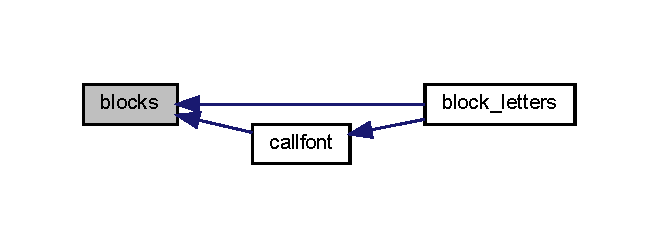
\includegraphics[width=316pt]{do_87_8txt_addf9a264ccc8c65a4995cf34906eff5c_icgraph}
\end{center}
\end{figure}
\mbox{\Hypertarget{do_87_8txt_aec67685fc467311079a688489f5e96ca}\label{do_87_8txt_aec67685fc467311079a688489f5e96ca}} 
\index{do.\+7.\+txt@{do.\+7.\+txt}!conversion@{conversion}}
\index{conversion@{conversion}!do.\+7.\+txt@{do.\+7.\+txt}}
\subsubsection{\texorpdfstring{conversion()}{conversion()}}
{\footnotesize\ttfamily \hyperlink{M__journal_83_8txt_afce72651d1eed785a2132bee863b2f38}{in} \hyperlink{what__overview_81_8txt_a1468cf345691ca45f70578e0b7abd264}{it} \hyperlink{intro__blas1_83_8txt_a42a91df93f840595de3019ceb5d1df23}{is} permitted \hyperlink{M__stopwatch_83_8txt_a97209fd3e34ef701c0a9734280779cbb}{to} branch \hyperlink{M__stopwatch_83_8txt_a97209fd3e34ef701c0a9734280779cbb}{to} a do term shared stmt \hyperlink{M__time_83_8txt_a944d4b6c63c2e981d8b0d36199afdfdd}{only} from within \hyperlink{M__stopwatch_83_8txt_a0f266597de2e57eb3aa964927bb30e14}{the} range of \hyperlink{M__stopwatch_83_8txt_a0f266597de2e57eb3aa964927bb30e14}{the} corresponding inner shared do \hyperlink{exit_87_8txt_aa7ebb4c04e8aa413d646a62e1f67fb5c}{construct} Active and \hyperlink{do_87_8txt_a510b16c990ba8c721e7968e80da73f30}{inactive} DO constructs \hyperlink{ufpp__overview_81_8txt_a8341271e5f4e3003f6eb1c9547fc9d1a}{A} DO \hyperlink{exit_87_8txt_aa7ebb4c04e8aa413d646a62e1f67fb5c}{construct} \hyperlink{intro__blas1_83_8txt_a42a91df93f840595de3019ceb5d1df23}{is} either \hyperlink{do_87_8txt_a3300b8e9ebbb88612226328b1b2fd93f}{active} \hyperlink{what__overview_81_8txt_a93f5d39a36ed511cc0dc88a20a517388}{or} \hyperlink{do_87_8txt_a510b16c990ba8c721e7968e80da73f30}{inactive} Initially a DO \hyperlink{exit_87_8txt_aa7ebb4c04e8aa413d646a62e1f67fb5c}{construct} becomes \hyperlink{do_87_8txt_a3300b8e9ebbb88612226328b1b2fd93f}{active} \hyperlink{M__time_83_8txt_a944d4b6c63c2e981d8b0d36199afdfdd}{only} when its DO \hyperlink{M__stopwatch_83_8txt_a43758526aa61bbaa49faf1e287658350}{statement} \hyperlink{intro__blas1_83_8txt_a42a91df93f840595de3019ceb5d1df23}{is} \hyperlink{exit_87_8txt_a8586238d5ca1171c2dfcd62d35642cdd}{executed} Once \hyperlink{M__stopwatch_83_8txt_a0f266597de2e57eb3aa964927bb30e14}{the} DO \hyperlink{exit_87_8txt_aa7ebb4c04e8aa413d646a62e1f67fb5c}{construct} becomes \hyperlink{do_87_8txt_a510b16c990ba8c721e7968e80da73f30}{inactive} \hyperlink{M__time_83_8txt_a944d4b6c63c2e981d8b0d36199afdfdd}{only} when \hyperlink{what__overview_81_8txt_a1468cf345691ca45f70578e0b7abd264}{it} \hyperlink{M__stopwatch_83_8txt_a0f266597de2e57eb3aa964927bb30e14}{the} DO \hyperlink{exit_87_8txt_aa7ebb4c04e8aa413d646a62e1f67fb5c}{construct} becomes \hyperlink{do_87_8txt_a3300b8e9ebbb88612226328b1b2fd93f}{active} If \hyperlink{continue_87_8txt_a5094e6a64d1227c84a0bf4db8f6c3788}{loop} control \hyperlink{intro__blas1_83_8txt_a42a91df93f840595de3019ceb5d1df23}{is} \mbox{[} , \mbox{]} do \hyperlink{M__stopwatch_83_8txt_a8188ec8361fb1eb49fad7b4759c811ec}{scalar} int \hyperlink{do_87_8txt_a74df008f496b23fc41b7a113e6fc2270}{expr} \mbox{[} , \hyperlink{M__stopwatch_83_8txt_a8188ec8361fb1eb49fad7b4759c811ec}{scalar}-\/int-\/\hyperlink{do_87_8txt_a74df008f496b23fc41b7a113e6fc2270}{expr} 3 \mbox{]} \hyperlink{M__stopwatch_83_8txt_a0f266597de2e57eb3aa964927bb30e14}{the} following steps \hyperlink{M__stopwatch_83_8txt_a5040be02b832eba08820289c8a1f81c4}{are} \hyperlink{M__stopwatch_83_8txt_a533fde56388c6e1bd526aa796b6e0159}{performed} \hyperlink{M__journal_83_8txt_afce72651d1eed785a2132bee863b2f38}{in} sequence The initial parameter \hyperlink{M__stopwatch_83_8txt_a0f266597de2e57eb3aa964927bb30e14}{the} terminal parameter and \hyperlink{M__stopwatch_83_8txt_a0f266597de2e57eb3aa964927bb30e14}{the} incrementation parameter m3 \hyperlink{M__stopwatch_83_8txt_a5040be02b832eba08820289c8a1f81c4}{are} of \hyperlink{stop__watch_83_8txt_a70f0ead91c32e25323c03265aa302c1c}{type} integer with \hyperlink{M__stopwatch_83_8txt_a0f266597de2e57eb3aa964927bb30e14}{the} \hyperlink{__cmp_8f90_a099b4c5d750b7bb116895dc4fca1bf38}{same} kind \hyperlink{stop__watch_83_8txt_a70f0ead91c32e25323c03265aa302c1c}{type} parameter as \hyperlink{M__stopwatch_83_8txt_a0f266597de2e57eb3aa964927bb30e14}{the} do \hyperlink{M__stopwatch_83_8txt_a2fa76741434e14a1b61bcbd4629b9cec}{variable} Their values \hyperlink{M__stopwatch_83_8txt_a5040be02b832eba08820289c8a1f81c4}{are} established by evaluating \hyperlink{M__stopwatch_83_8txt_a8188ec8361fb1eb49fad7b4759c811ec}{scalar} int \hyperlink{M__stopwatch_83_8txt_a8188ec8361fb1eb49fad7b4759c811ec}{scalar} int and \hyperlink{M__stopwatch_83_8txt_a8188ec8361fb1eb49fad7b4759c811ec}{scalar} int \hyperlink{exit_87_8txt_a77395982f8d25581c808c40f3b634d90}{if} conversion \hyperlink{M__stopwatch_83_8txt_a97209fd3e34ef701c0a9734280779cbb}{to} \hyperlink{M__stopwatch_83_8txt_a0f266597de2e57eb3aa964927bb30e14}{the} kind \hyperlink{stop__watch_83_8txt_a70f0ead91c32e25323c03265aa302c1c}{type} parameter of \hyperlink{M__stopwatch_83_8txt_a0f266597de2e57eb3aa964927bb30e14}{the} do \hyperlink{M__stopwatch_83_8txt_a2fa76741434e14a1b61bcbd4629b9cec}{variable} according \hyperlink{M__stopwatch_83_8txt_a97209fd3e34ef701c0a9734280779cbb}{to} \hyperlink{M__stopwatch_83_8txt_a0f266597de2e57eb3aa964927bb30e14}{the} \hyperlink{intro__blas1_83_8txt_a75eea5bd68c3b2764ce235200eed1716}{rules} for numeric conversion (\begin{DoxyParamCaption}\item[{Table 7.}]{11 }\end{DoxyParamCaption})}

\mbox{\Hypertarget{do_87_8txt_aa55dd9acb7774c34d0089623c1287897}\label{do_87_8txt_aa55dd9acb7774c34d0089623c1287897}} 
\index{do.\+7.\+txt@{do.\+7.\+txt}!expression@{expression}}
\index{expression@{expression}!do.\+7.\+txt@{do.\+7.\+txt}}
\subsubsection{\texorpdfstring{expression()}{expression()}}
{\footnotesize\ttfamily \hyperlink{M__journal_83_8txt_afce72651d1eed785a2132bee863b2f38}{in} \hyperlink{what__overview_81_8txt_a1468cf345691ca45f70578e0b7abd264}{it} \hyperlink{intro__blas1_83_8txt_a42a91df93f840595de3019ceb5d1df23}{is} permitted \hyperlink{M__stopwatch_83_8txt_a97209fd3e34ef701c0a9734280779cbb}{to} branch \hyperlink{M__stopwatch_83_8txt_a97209fd3e34ef701c0a9734280779cbb}{to} a do term shared stmt \hyperlink{M__time_83_8txt_a944d4b6c63c2e981d8b0d36199afdfdd}{only} from within \hyperlink{M__stopwatch_83_8txt_a0f266597de2e57eb3aa964927bb30e14}{the} range of \hyperlink{M__stopwatch_83_8txt_a0f266597de2e57eb3aa964927bb30e14}{the} corresponding inner shared do \hyperlink{exit_87_8txt_aa7ebb4c04e8aa413d646a62e1f67fb5c}{construct} Active and \hyperlink{do_87_8txt_a510b16c990ba8c721e7968e80da73f30}{inactive} DO constructs \hyperlink{ufpp__overview_81_8txt_a8341271e5f4e3003f6eb1c9547fc9d1a}{A} DO \hyperlink{exit_87_8txt_aa7ebb4c04e8aa413d646a62e1f67fb5c}{construct} \hyperlink{intro__blas1_83_8txt_a42a91df93f840595de3019ceb5d1df23}{is} either \hyperlink{do_87_8txt_a3300b8e9ebbb88612226328b1b2fd93f}{active} \hyperlink{what__overview_81_8txt_a93f5d39a36ed511cc0dc88a20a517388}{or} \hyperlink{do_87_8txt_a510b16c990ba8c721e7968e80da73f30}{inactive} Initially a DO \hyperlink{exit_87_8txt_aa7ebb4c04e8aa413d646a62e1f67fb5c}{construct} becomes \hyperlink{do_87_8txt_a3300b8e9ebbb88612226328b1b2fd93f}{active} \hyperlink{M__time_83_8txt_a944d4b6c63c2e981d8b0d36199afdfdd}{only} when its DO \hyperlink{M__stopwatch_83_8txt_a43758526aa61bbaa49faf1e287658350}{statement} \hyperlink{intro__blas1_83_8txt_a42a91df93f840595de3019ceb5d1df23}{is} \hyperlink{exit_87_8txt_a8586238d5ca1171c2dfcd62d35642cdd}{executed} Once \hyperlink{M__stopwatch_83_8txt_a0f266597de2e57eb3aa964927bb30e14}{the} DO \hyperlink{exit_87_8txt_aa7ebb4c04e8aa413d646a62e1f67fb5c}{construct} becomes \hyperlink{do_87_8txt_a510b16c990ba8c721e7968e80da73f30}{inactive} \hyperlink{M__time_83_8txt_a944d4b6c63c2e981d8b0d36199afdfdd}{only} when \hyperlink{what__overview_81_8txt_a1468cf345691ca45f70578e0b7abd264}{it} \hyperlink{M__stopwatch_83_8txt_a0f266597de2e57eb3aa964927bb30e14}{the} DO \hyperlink{exit_87_8txt_aa7ebb4c04e8aa413d646a62e1f67fb5c}{construct} becomes \hyperlink{do_87_8txt_a3300b8e9ebbb88612226328b1b2fd93f}{active} If \hyperlink{continue_87_8txt_a5094e6a64d1227c84a0bf4db8f6c3788}{loop} control \hyperlink{intro__blas1_83_8txt_a42a91df93f840595de3019ceb5d1df23}{is} \mbox{[} , \mbox{]} do \hyperlink{M__stopwatch_83_8txt_a8188ec8361fb1eb49fad7b4759c811ec}{scalar} int \hyperlink{do_87_8txt_a74df008f496b23fc41b7a113e6fc2270}{expr} \mbox{[} , \hyperlink{M__stopwatch_83_8txt_a8188ec8361fb1eb49fad7b4759c811ec}{scalar}-\/int-\/\hyperlink{do_87_8txt_a74df008f496b23fc41b7a113e6fc2270}{expr} 3 \mbox{]} \hyperlink{M__stopwatch_83_8txt_a0f266597de2e57eb3aa964927bb30e14}{the} following steps \hyperlink{M__stopwatch_83_8txt_a5040be02b832eba08820289c8a1f81c4}{are} \hyperlink{M__stopwatch_83_8txt_a533fde56388c6e1bd526aa796b6e0159}{performed} \hyperlink{M__journal_83_8txt_afce72651d1eed785a2132bee863b2f38}{in} sequence The initial parameter \hyperlink{M__stopwatch_83_8txt_a0f266597de2e57eb3aa964927bb30e14}{the} terminal parameter and \hyperlink{M__stopwatch_83_8txt_a0f266597de2e57eb3aa964927bb30e14}{the} incrementation parameter m3 \hyperlink{M__stopwatch_83_8txt_a5040be02b832eba08820289c8a1f81c4}{are} of \hyperlink{stop__watch_83_8txt_a70f0ead91c32e25323c03265aa302c1c}{type} integer with \hyperlink{M__stopwatch_83_8txt_a0f266597de2e57eb3aa964927bb30e14}{the} \hyperlink{__cmp_8f90_a099b4c5d750b7bb116895dc4fca1bf38}{same} kind \hyperlink{stop__watch_83_8txt_a70f0ead91c32e25323c03265aa302c1c}{type} parameter as \hyperlink{M__stopwatch_83_8txt_a0f266597de2e57eb3aa964927bb30e14}{the} do \hyperlink{M__stopwatch_83_8txt_a2fa76741434e14a1b61bcbd4629b9cec}{variable} Their values \hyperlink{M__stopwatch_83_8txt_a5040be02b832eba08820289c8a1f81c4}{are} established by evaluating \hyperlink{M__stopwatch_83_8txt_a8188ec8361fb1eb49fad7b4759c811ec}{scalar} int \hyperlink{M__stopwatch_83_8txt_a8188ec8361fb1eb49fad7b4759c811ec}{scalar} int and \hyperlink{M__stopwatch_83_8txt_a8188ec8361fb1eb49fad7b4759c811ec}{scalar} int \hyperlink{exit_87_8txt_a77395982f8d25581c808c40f3b634d90}{if} \hyperlink{do_87_8txt_aec67685fc467311079a688489f5e96ca}{conversion} \hyperlink{M__stopwatch_83_8txt_a97209fd3e34ef701c0a9734280779cbb}{to} \hyperlink{M__stopwatch_83_8txt_a0f266597de2e57eb3aa964927bb30e14}{the} kind \hyperlink{stop__watch_83_8txt_a70f0ead91c32e25323c03265aa302c1c}{type} parameter of \hyperlink{M__stopwatch_83_8txt_a0f266597de2e57eb3aa964927bb30e14}{the} do \hyperlink{M__stopwatch_83_8txt_a2fa76741434e14a1b61bcbd4629b9cec}{variable} according \hyperlink{M__stopwatch_83_8txt_a97209fd3e34ef701c0a9734280779cbb}{to} \hyperlink{M__stopwatch_83_8txt_a0f266597de2e57eb3aa964927bb30e14}{the} \hyperlink{intro__blas1_83_8txt_a75eea5bd68c3b2764ce235200eed1716}{rules} for numeric m3 has \hyperlink{M__stopwatch_83_8txt_a0f266597de2e57eb3aa964927bb30e14}{the} value The value of m3 shall not be zero The DO \hyperlink{M__stopwatch_83_8txt_a2fa76741434e14a1b61bcbd4629b9cec}{variable} becomes \hyperlink{ufpp__overview_81_8txt_a199f35c6b903296e6ea1b146249c1ab3}{defined} with \hyperlink{M__stopwatch_83_8txt_a0f266597de2e57eb3aa964927bb30e14}{the} value of \hyperlink{M__stopwatch_83_8txt_a0f266597de2e57eb3aa964927bb30e14}{the} initial parameter \hyperlink{do_87_8txt_a7aa4dd26e308616d434f7d797b39ae63}{m1} The iteration count \hyperlink{intro__blas1_83_8txt_a42a91df93f840595de3019ceb5d1df23}{is} established and \hyperlink{intro__blas1_83_8txt_a42a91df93f840595de3019ceb5d1df23}{is} \hyperlink{M__stopwatch_83_8txt_a0f266597de2e57eb3aa964927bb30e14}{the} value of \hyperlink{M__stopwatch_83_8txt_a0f266597de2e57eb3aa964927bb30e14}{the} expression (\begin{DoxyParamCaption}\item[{\hyperlink{do_87_8txt_abea8719ca8dfaa68bf45523d482a485b}{m2} -\/ \hyperlink{do_87_8txt_a7aa4dd26e308616d434f7d797b39ae63}{m1}+}]{m3 }\end{DoxyParamCaption})}

\mbox{\Hypertarget{do_87_8txt_aaa6a96bc95c5da31cfe2ec4f94db576c}\label{do_87_8txt_aaa6a96bc95c5da31cfe2ec4f94db576c}} 
\index{do.\+7.\+txt@{do.\+7.\+txt}!terminates@{terminates}}
\index{terminates@{terminates}!do.\+7.\+txt@{do.\+7.\+txt}}
\subsubsection{\texorpdfstring{terminates()}{terminates()}}
{\footnotesize\ttfamily \hyperlink{M__journal_83_8txt_afce72651d1eed785a2132bee863b2f38}{in} \hyperlink{what__overview_81_8txt_a1468cf345691ca45f70578e0b7abd264}{it} \hyperlink{intro__blas1_83_8txt_a42a91df93f840595de3019ceb5d1df23}{is} permitted \hyperlink{M__stopwatch_83_8txt_a97209fd3e34ef701c0a9734280779cbb}{to} branch \hyperlink{M__stopwatch_83_8txt_a97209fd3e34ef701c0a9734280779cbb}{to} a do term shared stmt \hyperlink{M__time_83_8txt_a944d4b6c63c2e981d8b0d36199afdfdd}{only} from within \hyperlink{M__stopwatch_83_8txt_a0f266597de2e57eb3aa964927bb30e14}{the} range of \hyperlink{M__stopwatch_83_8txt_a0f266597de2e57eb3aa964927bb30e14}{the} corresponding inner shared do \hyperlink{exit_87_8txt_aa7ebb4c04e8aa413d646a62e1f67fb5c}{construct} Active and \hyperlink{do_87_8txt_a510b16c990ba8c721e7968e80da73f30}{inactive} DO constructs \hyperlink{ufpp__overview_81_8txt_a8341271e5f4e3003f6eb1c9547fc9d1a}{A} DO \hyperlink{exit_87_8txt_aa7ebb4c04e8aa413d646a62e1f67fb5c}{construct} \hyperlink{intro__blas1_83_8txt_a42a91df93f840595de3019ceb5d1df23}{is} either \hyperlink{do_87_8txt_a3300b8e9ebbb88612226328b1b2fd93f}{active} \hyperlink{what__overview_81_8txt_a93f5d39a36ed511cc0dc88a20a517388}{or} \hyperlink{do_87_8txt_a510b16c990ba8c721e7968e80da73f30}{inactive} Initially a DO \hyperlink{exit_87_8txt_aa7ebb4c04e8aa413d646a62e1f67fb5c}{construct} becomes \hyperlink{do_87_8txt_a3300b8e9ebbb88612226328b1b2fd93f}{active} \hyperlink{M__time_83_8txt_a944d4b6c63c2e981d8b0d36199afdfdd}{only} when its DO \hyperlink{M__stopwatch_83_8txt_a43758526aa61bbaa49faf1e287658350}{statement} \hyperlink{intro__blas1_83_8txt_a42a91df93f840595de3019ceb5d1df23}{is} \hyperlink{exit_87_8txt_a8586238d5ca1171c2dfcd62d35642cdd}{executed} Once \hyperlink{M__stopwatch_83_8txt_a0f266597de2e57eb3aa964927bb30e14}{the} DO \hyperlink{exit_87_8txt_aa7ebb4c04e8aa413d646a62e1f67fb5c}{construct} becomes \hyperlink{do_87_8txt_a510b16c990ba8c721e7968e80da73f30}{inactive} \hyperlink{M__time_83_8txt_a944d4b6c63c2e981d8b0d36199afdfdd}{only} when \hyperlink{what__overview_81_8txt_a1468cf345691ca45f70578e0b7abd264}{it} terminates (\begin{DoxyParamCaption}\item[{8.\+1.\+7.\+6.}]{4 }\end{DoxyParamCaption}) const}



\subsection{Variable Documentation}
\mbox{\Hypertarget{do_87_8txt_a3300b8e9ebbb88612226328b1b2fd93f}\label{do_87_8txt_a3300b8e9ebbb88612226328b1b2fd93f}} 
\index{do.\+7.\+txt@{do.\+7.\+txt}!active@{active}}
\index{active@{active}!do.\+7.\+txt@{do.\+7.\+txt}}
\subsubsection{\texorpdfstring{active}{active}}
{\footnotesize\ttfamily \hyperlink{M__journal_83_8txt_afce72651d1eed785a2132bee863b2f38}{in} \hyperlink{what__overview_81_8txt_a1468cf345691ca45f70578e0b7abd264}{it} \hyperlink{intro__blas1_83_8txt_a42a91df93f840595de3019ceb5d1df23}{is} permitted \hyperlink{M__stopwatch_83_8txt_a97209fd3e34ef701c0a9734280779cbb}{to} branch \hyperlink{M__stopwatch_83_8txt_a97209fd3e34ef701c0a9734280779cbb}{to} a do term shared stmt \hyperlink{M__time_83_8txt_a944d4b6c63c2e981d8b0d36199afdfdd}{only} from within \hyperlink{M__stopwatch_83_8txt_a0f266597de2e57eb3aa964927bb30e14}{the} range of \hyperlink{M__stopwatch_83_8txt_a0f266597de2e57eb3aa964927bb30e14}{the} corresponding inner shared do \hyperlink{exit_87_8txt_aa7ebb4c04e8aa413d646a62e1f67fb5c}{construct} Active and \hyperlink{do_87_8txt_a510b16c990ba8c721e7968e80da73f30}{inactive} DO constructs \hyperlink{ufpp__overview_81_8txt_a8341271e5f4e3003f6eb1c9547fc9d1a}{A} DO \hyperlink{exit_87_8txt_aa7ebb4c04e8aa413d646a62e1f67fb5c}{construct} \hyperlink{intro__blas1_83_8txt_a42a91df93f840595de3019ceb5d1df23}{is} either active \hyperlink{what__overview_81_8txt_a93f5d39a36ed511cc0dc88a20a517388}{or} \hyperlink{do_87_8txt_a510b16c990ba8c721e7968e80da73f30}{inactive} Initially a DO \hyperlink{exit_87_8txt_aa7ebb4c04e8aa413d646a62e1f67fb5c}{construct} becomes active \hyperlink{M__time_83_8txt_a944d4b6c63c2e981d8b0d36199afdfdd}{only} when its DO \hyperlink{M__stopwatch_83_8txt_a43758526aa61bbaa49faf1e287658350}{statement} \hyperlink{intro__blas1_83_8txt_a42a91df93f840595de3019ceb5d1df23}{is} \hyperlink{exit_87_8txt_a8586238d5ca1171c2dfcd62d35642cdd}{executed} Once active}

\mbox{\Hypertarget{do_87_8txt_a74df008f496b23fc41b7a113e6fc2270}\label{do_87_8txt_a74df008f496b23fc41b7a113e6fc2270}} 
\index{do.\+7.\+txt@{do.\+7.\+txt}!expr@{expr}}
\index{expr@{expr}!do.\+7.\+txt@{do.\+7.\+txt}}
\subsubsection{\texorpdfstring{expr}{expr}}
{\footnotesize\ttfamily \hyperlink{M__journal_83_8txt_afce72651d1eed785a2132bee863b2f38}{in} \hyperlink{what__overview_81_8txt_a1468cf345691ca45f70578e0b7abd264}{it} \hyperlink{intro__blas1_83_8txt_a42a91df93f840595de3019ceb5d1df23}{is} permitted \hyperlink{M__stopwatch_83_8txt_a97209fd3e34ef701c0a9734280779cbb}{to} branch \hyperlink{M__stopwatch_83_8txt_a97209fd3e34ef701c0a9734280779cbb}{to} a do term shared stmt \hyperlink{M__time_83_8txt_a944d4b6c63c2e981d8b0d36199afdfdd}{only} from within \hyperlink{M__stopwatch_83_8txt_a0f266597de2e57eb3aa964927bb30e14}{the} range of \hyperlink{M__stopwatch_83_8txt_a0f266597de2e57eb3aa964927bb30e14}{the} corresponding inner shared do \hyperlink{exit_87_8txt_aa7ebb4c04e8aa413d646a62e1f67fb5c}{construct} Active and \hyperlink{do_87_8txt_a510b16c990ba8c721e7968e80da73f30}{inactive} DO constructs \hyperlink{ufpp__overview_81_8txt_a8341271e5f4e3003f6eb1c9547fc9d1a}{A} DO \hyperlink{exit_87_8txt_aa7ebb4c04e8aa413d646a62e1f67fb5c}{construct} \hyperlink{intro__blas1_83_8txt_a42a91df93f840595de3019ceb5d1df23}{is} either \hyperlink{do_87_8txt_a3300b8e9ebbb88612226328b1b2fd93f}{active} \hyperlink{what__overview_81_8txt_a93f5d39a36ed511cc0dc88a20a517388}{or} \hyperlink{do_87_8txt_a510b16c990ba8c721e7968e80da73f30}{inactive} Initially a DO \hyperlink{exit_87_8txt_aa7ebb4c04e8aa413d646a62e1f67fb5c}{construct} becomes \hyperlink{do_87_8txt_a3300b8e9ebbb88612226328b1b2fd93f}{active} \hyperlink{M__time_83_8txt_a944d4b6c63c2e981d8b0d36199afdfdd}{only} when its DO \hyperlink{M__stopwatch_83_8txt_a43758526aa61bbaa49faf1e287658350}{statement} \hyperlink{intro__blas1_83_8txt_a42a91df93f840595de3019ceb5d1df23}{is} \hyperlink{exit_87_8txt_a8586238d5ca1171c2dfcd62d35642cdd}{executed} Once \hyperlink{M__stopwatch_83_8txt_a0f266597de2e57eb3aa964927bb30e14}{the} DO \hyperlink{exit_87_8txt_aa7ebb4c04e8aa413d646a62e1f67fb5c}{construct} becomes \hyperlink{do_87_8txt_a510b16c990ba8c721e7968e80da73f30}{inactive} \hyperlink{M__time_83_8txt_a944d4b6c63c2e981d8b0d36199afdfdd}{only} when \hyperlink{what__overview_81_8txt_a1468cf345691ca45f70578e0b7abd264}{it} \hyperlink{M__stopwatch_83_8txt_a0f266597de2e57eb3aa964927bb30e14}{the} DO \hyperlink{exit_87_8txt_aa7ebb4c04e8aa413d646a62e1f67fb5c}{construct} becomes \hyperlink{do_87_8txt_a3300b8e9ebbb88612226328b1b2fd93f}{active} If \hyperlink{continue_87_8txt_a5094e6a64d1227c84a0bf4db8f6c3788}{loop} control \hyperlink{intro__blas1_83_8txt_a42a91df93f840595de3019ceb5d1df23}{is} \mbox{[} , \mbox{]} do \hyperlink{M__stopwatch_83_8txt_a8188ec8361fb1eb49fad7b4759c811ec}{scalar} int expr \mbox{[} , \hyperlink{M__stopwatch_83_8txt_a8188ec8361fb1eb49fad7b4759c811ec}{scalar}-\/int-\/expr 3 \mbox{]} \hyperlink{M__stopwatch_83_8txt_a0f266597de2e57eb3aa964927bb30e14}{the} following steps \hyperlink{M__stopwatch_83_8txt_a5040be02b832eba08820289c8a1f81c4}{are} \hyperlink{M__stopwatch_83_8txt_a533fde56388c6e1bd526aa796b6e0159}{performed} \hyperlink{M__journal_83_8txt_afce72651d1eed785a2132bee863b2f38}{in} sequence The initial parameter \hyperlink{M__stopwatch_83_8txt_a0f266597de2e57eb3aa964927bb30e14}{the} terminal parameter and \hyperlink{M__stopwatch_83_8txt_a0f266597de2e57eb3aa964927bb30e14}{the} incrementation parameter m3 \hyperlink{M__stopwatch_83_8txt_a5040be02b832eba08820289c8a1f81c4}{are} of \hyperlink{stop__watch_83_8txt_a70f0ead91c32e25323c03265aa302c1c}{type} integer with \hyperlink{M__stopwatch_83_8txt_a0f266597de2e57eb3aa964927bb30e14}{the} \hyperlink{__cmp_8f90_a099b4c5d750b7bb116895dc4fca1bf38}{same} kind \hyperlink{stop__watch_83_8txt_a70f0ead91c32e25323c03265aa302c1c}{type} parameter as \hyperlink{M__stopwatch_83_8txt_a0f266597de2e57eb3aa964927bb30e14}{the} do \hyperlink{M__stopwatch_83_8txt_a2fa76741434e14a1b61bcbd4629b9cec}{variable} Their values \hyperlink{M__stopwatch_83_8txt_a5040be02b832eba08820289c8a1f81c4}{are} established by evaluating \hyperlink{M__stopwatch_83_8txt_a8188ec8361fb1eb49fad7b4759c811ec}{scalar} int \hyperlink{M__stopwatch_83_8txt_a8188ec8361fb1eb49fad7b4759c811ec}{scalar} int and \hyperlink{M__stopwatch_83_8txt_a8188ec8361fb1eb49fad7b4759c811ec}{scalar} int expr}

\mbox{\Hypertarget{do_87_8txt_a510b16c990ba8c721e7968e80da73f30}\label{do_87_8txt_a510b16c990ba8c721e7968e80da73f30}} 
\index{do.\+7.\+txt@{do.\+7.\+txt}!inactive@{inactive}}
\index{inactive@{inactive}!do.\+7.\+txt@{do.\+7.\+txt}}
\subsubsection{\texorpdfstring{inactive}{inactive}}
{\footnotesize\ttfamily \hyperlink{M__journal_83_8txt_afce72651d1eed785a2132bee863b2f38}{in} \hyperlink{what__overview_81_8txt_a1468cf345691ca45f70578e0b7abd264}{it} \hyperlink{intro__blas1_83_8txt_a42a91df93f840595de3019ceb5d1df23}{is} permitted \hyperlink{M__stopwatch_83_8txt_a97209fd3e34ef701c0a9734280779cbb}{to} branch \hyperlink{M__stopwatch_83_8txt_a97209fd3e34ef701c0a9734280779cbb}{to} a do term shared stmt \hyperlink{M__time_83_8txt_a944d4b6c63c2e981d8b0d36199afdfdd}{only} from within \hyperlink{M__stopwatch_83_8txt_a0f266597de2e57eb3aa964927bb30e14}{the} range of \hyperlink{M__stopwatch_83_8txt_a0f266597de2e57eb3aa964927bb30e14}{the} corresponding inner shared do \hyperlink{exit_87_8txt_aa7ebb4c04e8aa413d646a62e1f67fb5c}{construct} Active and inactive DO constructs \hyperlink{ufpp__overview_81_8txt_a8341271e5f4e3003f6eb1c9547fc9d1a}{A} DO \hyperlink{exit_87_8txt_aa7ebb4c04e8aa413d646a62e1f67fb5c}{construct} \hyperlink{intro__blas1_83_8txt_a42a91df93f840595de3019ceb5d1df23}{is} either \hyperlink{do_87_8txt_a3300b8e9ebbb88612226328b1b2fd93f}{active} \hyperlink{what__overview_81_8txt_a93f5d39a36ed511cc0dc88a20a517388}{or} inactive Initially inactive}

\mbox{\Hypertarget{do_87_8txt_a8a4784becc39e4ebb9a205802f11fe2d}\label{do_87_8txt_a8a4784becc39e4ebb9a205802f11fe2d}} 
\index{do.\+7.\+txt@{do.\+7.\+txt}!including@{including}}
\index{including@{including}!do.\+7.\+txt@{do.\+7.\+txt}}
\subsubsection{\texorpdfstring{including}{including}}
{\footnotesize\ttfamily \hyperlink{M__journal_83_8txt_afce72651d1eed785a2132bee863b2f38}{in} \hyperlink{what__overview_81_8txt_a1468cf345691ca45f70578e0b7abd264}{it} \hyperlink{intro__blas1_83_8txt_a42a91df93f840595de3019ceb5d1df23}{is} permitted \hyperlink{M__stopwatch_83_8txt_a97209fd3e34ef701c0a9734280779cbb}{to} branch \hyperlink{M__stopwatch_83_8txt_a97209fd3e34ef701c0a9734280779cbb}{to} a do term shared stmt \hyperlink{M__time_83_8txt_a944d4b6c63c2e981d8b0d36199afdfdd}{only} from within \hyperlink{M__stopwatch_83_8txt_a0f266597de2e57eb3aa964927bb30e14}{the} range of \hyperlink{M__stopwatch_83_8txt_a0f266597de2e57eb3aa964927bb30e14}{the} corresponding inner shared do \hyperlink{exit_87_8txt_aa7ebb4c04e8aa413d646a62e1f67fb5c}{construct} Active and \hyperlink{do_87_8txt_a510b16c990ba8c721e7968e80da73f30}{inactive} DO constructs \hyperlink{ufpp__overview_81_8txt_a8341271e5f4e3003f6eb1c9547fc9d1a}{A} DO \hyperlink{exit_87_8txt_aa7ebb4c04e8aa413d646a62e1f67fb5c}{construct} \hyperlink{intro__blas1_83_8txt_a42a91df93f840595de3019ceb5d1df23}{is} either \hyperlink{do_87_8txt_a3300b8e9ebbb88612226328b1b2fd93f}{active} \hyperlink{what__overview_81_8txt_a93f5d39a36ed511cc0dc88a20a517388}{or} \hyperlink{do_87_8txt_a510b16c990ba8c721e7968e80da73f30}{inactive} Initially a DO \hyperlink{exit_87_8txt_aa7ebb4c04e8aa413d646a62e1f67fb5c}{construct} becomes \hyperlink{do_87_8txt_a3300b8e9ebbb88612226328b1b2fd93f}{active} \hyperlink{M__time_83_8txt_a944d4b6c63c2e981d8b0d36199afdfdd}{only} when its DO \hyperlink{M__stopwatch_83_8txt_a43758526aa61bbaa49faf1e287658350}{statement} \hyperlink{intro__blas1_83_8txt_a42a91df93f840595de3019ceb5d1df23}{is} \hyperlink{exit_87_8txt_a8586238d5ca1171c2dfcd62d35642cdd}{executed} Once \hyperlink{M__stopwatch_83_8txt_a0f266597de2e57eb3aa964927bb30e14}{the} DO \hyperlink{exit_87_8txt_aa7ebb4c04e8aa413d646a62e1f67fb5c}{construct} becomes \hyperlink{do_87_8txt_a510b16c990ba8c721e7968e80da73f30}{inactive} \hyperlink{M__time_83_8txt_a944d4b6c63c2e981d8b0d36199afdfdd}{only} when \hyperlink{what__overview_81_8txt_a1468cf345691ca45f70578e0b7abd264}{it} \hyperlink{M__stopwatch_83_8txt_a0f266597de2e57eb3aa964927bb30e14}{the} DO \hyperlink{exit_87_8txt_aa7ebb4c04e8aa413d646a62e1f67fb5c}{construct} becomes \hyperlink{do_87_8txt_a3300b8e9ebbb88612226328b1b2fd93f}{active} If \hyperlink{continue_87_8txt_a5094e6a64d1227c84a0bf4db8f6c3788}{loop} control \hyperlink{intro__blas1_83_8txt_a42a91df93f840595de3019ceb5d1df23}{is} \mbox{[} , \mbox{]} do \hyperlink{M__stopwatch_83_8txt_a8188ec8361fb1eb49fad7b4759c811ec}{scalar} int \hyperlink{do_87_8txt_a74df008f496b23fc41b7a113e6fc2270}{expr} \mbox{[} , \hyperlink{M__stopwatch_83_8txt_a8188ec8361fb1eb49fad7b4759c811ec}{scalar}-\/int-\/\hyperlink{do_87_8txt_a74df008f496b23fc41b7a113e6fc2270}{expr} 3 \mbox{]} \hyperlink{M__stopwatch_83_8txt_a0f266597de2e57eb3aa964927bb30e14}{the} following steps \hyperlink{M__stopwatch_83_8txt_a5040be02b832eba08820289c8a1f81c4}{are} \hyperlink{M__stopwatch_83_8txt_a533fde56388c6e1bd526aa796b6e0159}{performed} \hyperlink{M__journal_83_8txt_afce72651d1eed785a2132bee863b2f38}{in} sequence The initial parameter \hyperlink{M__stopwatch_83_8txt_a0f266597de2e57eb3aa964927bb30e14}{the} terminal parameter and \hyperlink{M__stopwatch_83_8txt_a0f266597de2e57eb3aa964927bb30e14}{the} incrementation parameter m3 \hyperlink{M__stopwatch_83_8txt_a5040be02b832eba08820289c8a1f81c4}{are} of \hyperlink{stop__watch_83_8txt_a70f0ead91c32e25323c03265aa302c1c}{type} integer with \hyperlink{M__stopwatch_83_8txt_a0f266597de2e57eb3aa964927bb30e14}{the} \hyperlink{__cmp_8f90_a099b4c5d750b7bb116895dc4fca1bf38}{same} kind \hyperlink{stop__watch_83_8txt_a70f0ead91c32e25323c03265aa302c1c}{type} parameter as \hyperlink{M__stopwatch_83_8txt_a0f266597de2e57eb3aa964927bb30e14}{the} do \hyperlink{M__stopwatch_83_8txt_a2fa76741434e14a1b61bcbd4629b9cec}{variable} Their values \hyperlink{M__stopwatch_83_8txt_a5040be02b832eba08820289c8a1f81c4}{are} established by evaluating \hyperlink{M__stopwatch_83_8txt_a8188ec8361fb1eb49fad7b4759c811ec}{scalar} int \hyperlink{M__stopwatch_83_8txt_a8188ec8361fb1eb49fad7b4759c811ec}{scalar} int and \hyperlink{M__stopwatch_83_8txt_a8188ec8361fb1eb49fad7b4759c811ec}{scalar} int including}

\mbox{\Hypertarget{do_87_8txt_a7aa4dd26e308616d434f7d797b39ae63}\label{do_87_8txt_a7aa4dd26e308616d434f7d797b39ae63}} 
\index{do.\+7.\+txt@{do.\+7.\+txt}!m1@{m1}}
\index{m1@{m1}!do.\+7.\+txt@{do.\+7.\+txt}}
\subsubsection{\texorpdfstring{m1}{m1}}
{\footnotesize\ttfamily \hyperlink{M__journal_83_8txt_afce72651d1eed785a2132bee863b2f38}{in} \hyperlink{what__overview_81_8txt_a1468cf345691ca45f70578e0b7abd264}{it} \hyperlink{intro__blas1_83_8txt_a42a91df93f840595de3019ceb5d1df23}{is} permitted \hyperlink{M__stopwatch_83_8txt_a97209fd3e34ef701c0a9734280779cbb}{to} branch \hyperlink{M__stopwatch_83_8txt_a97209fd3e34ef701c0a9734280779cbb}{to} a do term shared stmt \hyperlink{M__time_83_8txt_a944d4b6c63c2e981d8b0d36199afdfdd}{only} from within \hyperlink{M__stopwatch_83_8txt_a0f266597de2e57eb3aa964927bb30e14}{the} range of \hyperlink{M__stopwatch_83_8txt_a0f266597de2e57eb3aa964927bb30e14}{the} corresponding inner shared do \hyperlink{exit_87_8txt_aa7ebb4c04e8aa413d646a62e1f67fb5c}{construct} Active and \hyperlink{do_87_8txt_a510b16c990ba8c721e7968e80da73f30}{inactive} DO constructs \hyperlink{ufpp__overview_81_8txt_a8341271e5f4e3003f6eb1c9547fc9d1a}{A} DO \hyperlink{exit_87_8txt_aa7ebb4c04e8aa413d646a62e1f67fb5c}{construct} \hyperlink{intro__blas1_83_8txt_a42a91df93f840595de3019ceb5d1df23}{is} either \hyperlink{do_87_8txt_a3300b8e9ebbb88612226328b1b2fd93f}{active} \hyperlink{what__overview_81_8txt_a93f5d39a36ed511cc0dc88a20a517388}{or} \hyperlink{do_87_8txt_a510b16c990ba8c721e7968e80da73f30}{inactive} Initially a DO \hyperlink{exit_87_8txt_aa7ebb4c04e8aa413d646a62e1f67fb5c}{construct} becomes \hyperlink{do_87_8txt_a3300b8e9ebbb88612226328b1b2fd93f}{active} \hyperlink{M__time_83_8txt_a944d4b6c63c2e981d8b0d36199afdfdd}{only} when its DO \hyperlink{M__stopwatch_83_8txt_a43758526aa61bbaa49faf1e287658350}{statement} \hyperlink{intro__blas1_83_8txt_a42a91df93f840595de3019ceb5d1df23}{is} \hyperlink{exit_87_8txt_a8586238d5ca1171c2dfcd62d35642cdd}{executed} Once \hyperlink{M__stopwatch_83_8txt_a0f266597de2e57eb3aa964927bb30e14}{the} DO \hyperlink{exit_87_8txt_aa7ebb4c04e8aa413d646a62e1f67fb5c}{construct} becomes \hyperlink{do_87_8txt_a510b16c990ba8c721e7968e80da73f30}{inactive} \hyperlink{M__time_83_8txt_a944d4b6c63c2e981d8b0d36199afdfdd}{only} when \hyperlink{what__overview_81_8txt_a1468cf345691ca45f70578e0b7abd264}{it} \hyperlink{M__stopwatch_83_8txt_a0f266597de2e57eb3aa964927bb30e14}{the} DO \hyperlink{exit_87_8txt_aa7ebb4c04e8aa413d646a62e1f67fb5c}{construct} becomes \hyperlink{do_87_8txt_a3300b8e9ebbb88612226328b1b2fd93f}{active} If \hyperlink{continue_87_8txt_a5094e6a64d1227c84a0bf4db8f6c3788}{loop} control \hyperlink{intro__blas1_83_8txt_a42a91df93f840595de3019ceb5d1df23}{is} \mbox{[} , \mbox{]} do \hyperlink{M__stopwatch_83_8txt_a8188ec8361fb1eb49fad7b4759c811ec}{scalar} int \hyperlink{do_87_8txt_a74df008f496b23fc41b7a113e6fc2270}{expr} \mbox{[} , \hyperlink{M__stopwatch_83_8txt_a8188ec8361fb1eb49fad7b4759c811ec}{scalar}-\/int-\/\hyperlink{do_87_8txt_a74df008f496b23fc41b7a113e6fc2270}{expr} 3 \mbox{]} \hyperlink{M__stopwatch_83_8txt_a0f266597de2e57eb3aa964927bb30e14}{the} following steps \hyperlink{M__stopwatch_83_8txt_a5040be02b832eba08820289c8a1f81c4}{are} \hyperlink{M__stopwatch_83_8txt_a533fde56388c6e1bd526aa796b6e0159}{performed} \hyperlink{M__journal_83_8txt_afce72651d1eed785a2132bee863b2f38}{in} sequence The initial parameter m1}

\mbox{\Hypertarget{do_87_8txt_abea8719ca8dfaa68bf45523d482a485b}\label{do_87_8txt_abea8719ca8dfaa68bf45523d482a485b}} 
\index{do.\+7.\+txt@{do.\+7.\+txt}!m2@{m2}}
\index{m2@{m2}!do.\+7.\+txt@{do.\+7.\+txt}}
\subsubsection{\texorpdfstring{m2}{m2}}
{\footnotesize\ttfamily \hyperlink{M__journal_83_8txt_afce72651d1eed785a2132bee863b2f38}{in} \hyperlink{what__overview_81_8txt_a1468cf345691ca45f70578e0b7abd264}{it} \hyperlink{intro__blas1_83_8txt_a42a91df93f840595de3019ceb5d1df23}{is} permitted \hyperlink{M__stopwatch_83_8txt_a97209fd3e34ef701c0a9734280779cbb}{to} branch \hyperlink{M__stopwatch_83_8txt_a97209fd3e34ef701c0a9734280779cbb}{to} a do term shared stmt \hyperlink{M__time_83_8txt_a944d4b6c63c2e981d8b0d36199afdfdd}{only} from within \hyperlink{M__stopwatch_83_8txt_a0f266597de2e57eb3aa964927bb30e14}{the} range of \hyperlink{M__stopwatch_83_8txt_a0f266597de2e57eb3aa964927bb30e14}{the} corresponding inner shared do \hyperlink{exit_87_8txt_aa7ebb4c04e8aa413d646a62e1f67fb5c}{construct} Active and \hyperlink{do_87_8txt_a510b16c990ba8c721e7968e80da73f30}{inactive} DO constructs \hyperlink{ufpp__overview_81_8txt_a8341271e5f4e3003f6eb1c9547fc9d1a}{A} DO \hyperlink{exit_87_8txt_aa7ebb4c04e8aa413d646a62e1f67fb5c}{construct} \hyperlink{intro__blas1_83_8txt_a42a91df93f840595de3019ceb5d1df23}{is} either \hyperlink{do_87_8txt_a3300b8e9ebbb88612226328b1b2fd93f}{active} \hyperlink{what__overview_81_8txt_a93f5d39a36ed511cc0dc88a20a517388}{or} \hyperlink{do_87_8txt_a510b16c990ba8c721e7968e80da73f30}{inactive} Initially a DO \hyperlink{exit_87_8txt_aa7ebb4c04e8aa413d646a62e1f67fb5c}{construct} becomes \hyperlink{do_87_8txt_a3300b8e9ebbb88612226328b1b2fd93f}{active} \hyperlink{M__time_83_8txt_a944d4b6c63c2e981d8b0d36199afdfdd}{only} when its DO \hyperlink{M__stopwatch_83_8txt_a43758526aa61bbaa49faf1e287658350}{statement} \hyperlink{intro__blas1_83_8txt_a42a91df93f840595de3019ceb5d1df23}{is} \hyperlink{exit_87_8txt_a8586238d5ca1171c2dfcd62d35642cdd}{executed} Once \hyperlink{M__stopwatch_83_8txt_a0f266597de2e57eb3aa964927bb30e14}{the} DO \hyperlink{exit_87_8txt_aa7ebb4c04e8aa413d646a62e1f67fb5c}{construct} becomes \hyperlink{do_87_8txt_a510b16c990ba8c721e7968e80da73f30}{inactive} \hyperlink{M__time_83_8txt_a944d4b6c63c2e981d8b0d36199afdfdd}{only} when \hyperlink{what__overview_81_8txt_a1468cf345691ca45f70578e0b7abd264}{it} \hyperlink{M__stopwatch_83_8txt_a0f266597de2e57eb3aa964927bb30e14}{the} DO \hyperlink{exit_87_8txt_aa7ebb4c04e8aa413d646a62e1f67fb5c}{construct} becomes \hyperlink{do_87_8txt_a3300b8e9ebbb88612226328b1b2fd93f}{active} If \hyperlink{continue_87_8txt_a5094e6a64d1227c84a0bf4db8f6c3788}{loop} control \hyperlink{intro__blas1_83_8txt_a42a91df93f840595de3019ceb5d1df23}{is} \mbox{[} , \mbox{]} do \hyperlink{M__stopwatch_83_8txt_a8188ec8361fb1eb49fad7b4759c811ec}{scalar} int \hyperlink{do_87_8txt_a74df008f496b23fc41b7a113e6fc2270}{expr} \mbox{[} , \hyperlink{M__stopwatch_83_8txt_a8188ec8361fb1eb49fad7b4759c811ec}{scalar}-\/int-\/\hyperlink{do_87_8txt_a74df008f496b23fc41b7a113e6fc2270}{expr} 3 \mbox{]} \hyperlink{M__stopwatch_83_8txt_a0f266597de2e57eb3aa964927bb30e14}{the} following steps \hyperlink{M__stopwatch_83_8txt_a5040be02b832eba08820289c8a1f81c4}{are} \hyperlink{M__stopwatch_83_8txt_a533fde56388c6e1bd526aa796b6e0159}{performed} \hyperlink{M__journal_83_8txt_afce72651d1eed785a2132bee863b2f38}{in} sequence The initial parameter \hyperlink{M__stopwatch_83_8txt_a0f266597de2e57eb3aa964927bb30e14}{the} terminal parameter m2}

\mbox{\Hypertarget{do_87_8txt_ad6f2806004c0042d29109ab9698d0840}\label{do_87_8txt_ad6f2806004c0042d29109ab9698d0840}} 
\index{do.\+7.\+txt@{do.\+7.\+txt}!necessary@{necessary}}
\index{necessary@{necessary}!do.\+7.\+txt@{do.\+7.\+txt}}
\subsubsection{\texorpdfstring{necessary}{necessary}}
{\footnotesize\ttfamily \hyperlink{M__journal_83_8txt_afce72651d1eed785a2132bee863b2f38}{in} \hyperlink{what__overview_81_8txt_a1468cf345691ca45f70578e0b7abd264}{it} \hyperlink{intro__blas1_83_8txt_a42a91df93f840595de3019ceb5d1df23}{is} permitted \hyperlink{M__stopwatch_83_8txt_a97209fd3e34ef701c0a9734280779cbb}{to} branch \hyperlink{M__stopwatch_83_8txt_a97209fd3e34ef701c0a9734280779cbb}{to} a do term shared stmt \hyperlink{M__time_83_8txt_a944d4b6c63c2e981d8b0d36199afdfdd}{only} from within \hyperlink{M__stopwatch_83_8txt_a0f266597de2e57eb3aa964927bb30e14}{the} range of \hyperlink{M__stopwatch_83_8txt_a0f266597de2e57eb3aa964927bb30e14}{the} corresponding inner shared do \hyperlink{exit_87_8txt_aa7ebb4c04e8aa413d646a62e1f67fb5c}{construct} Active and \hyperlink{do_87_8txt_a510b16c990ba8c721e7968e80da73f30}{inactive} DO constructs \hyperlink{ufpp__overview_81_8txt_a8341271e5f4e3003f6eb1c9547fc9d1a}{A} DO \hyperlink{exit_87_8txt_aa7ebb4c04e8aa413d646a62e1f67fb5c}{construct} \hyperlink{intro__blas1_83_8txt_a42a91df93f840595de3019ceb5d1df23}{is} either \hyperlink{do_87_8txt_a3300b8e9ebbb88612226328b1b2fd93f}{active} \hyperlink{what__overview_81_8txt_a93f5d39a36ed511cc0dc88a20a517388}{or} \hyperlink{do_87_8txt_a510b16c990ba8c721e7968e80da73f30}{inactive} Initially a DO \hyperlink{exit_87_8txt_aa7ebb4c04e8aa413d646a62e1f67fb5c}{construct} becomes \hyperlink{do_87_8txt_a3300b8e9ebbb88612226328b1b2fd93f}{active} \hyperlink{M__time_83_8txt_a944d4b6c63c2e981d8b0d36199afdfdd}{only} when its DO \hyperlink{M__stopwatch_83_8txt_a43758526aa61bbaa49faf1e287658350}{statement} \hyperlink{intro__blas1_83_8txt_a42a91df93f840595de3019ceb5d1df23}{is} \hyperlink{exit_87_8txt_a8586238d5ca1171c2dfcd62d35642cdd}{executed} Once \hyperlink{M__stopwatch_83_8txt_a0f266597de2e57eb3aa964927bb30e14}{the} DO \hyperlink{exit_87_8txt_aa7ebb4c04e8aa413d646a62e1f67fb5c}{construct} becomes \hyperlink{do_87_8txt_a510b16c990ba8c721e7968e80da73f30}{inactive} \hyperlink{M__time_83_8txt_a944d4b6c63c2e981d8b0d36199afdfdd}{only} when \hyperlink{what__overview_81_8txt_a1468cf345691ca45f70578e0b7abd264}{it} \hyperlink{M__stopwatch_83_8txt_a0f266597de2e57eb3aa964927bb30e14}{the} DO \hyperlink{exit_87_8txt_aa7ebb4c04e8aa413d646a62e1f67fb5c}{construct} becomes \hyperlink{do_87_8txt_a3300b8e9ebbb88612226328b1b2fd93f}{active} If \hyperlink{continue_87_8txt_a5094e6a64d1227c84a0bf4db8f6c3788}{loop} control \hyperlink{intro__blas1_83_8txt_a42a91df93f840595de3019ceb5d1df23}{is} \mbox{[} , \mbox{]} do \hyperlink{M__stopwatch_83_8txt_a8188ec8361fb1eb49fad7b4759c811ec}{scalar} int \hyperlink{do_87_8txt_a74df008f496b23fc41b7a113e6fc2270}{expr} \mbox{[} , \hyperlink{M__stopwatch_83_8txt_a8188ec8361fb1eb49fad7b4759c811ec}{scalar}-\/int-\/\hyperlink{do_87_8txt_a74df008f496b23fc41b7a113e6fc2270}{expr} 3 \mbox{]} \hyperlink{M__stopwatch_83_8txt_a0f266597de2e57eb3aa964927bb30e14}{the} following steps \hyperlink{M__stopwatch_83_8txt_a5040be02b832eba08820289c8a1f81c4}{are} \hyperlink{M__stopwatch_83_8txt_a533fde56388c6e1bd526aa796b6e0159}{performed} \hyperlink{M__journal_83_8txt_afce72651d1eed785a2132bee863b2f38}{in} sequence The initial parameter \hyperlink{M__stopwatch_83_8txt_a0f266597de2e57eb3aa964927bb30e14}{the} terminal parameter and \hyperlink{M__stopwatch_83_8txt_a0f266597de2e57eb3aa964927bb30e14}{the} incrementation parameter m3 \hyperlink{M__stopwatch_83_8txt_a5040be02b832eba08820289c8a1f81c4}{are} of \hyperlink{stop__watch_83_8txt_a70f0ead91c32e25323c03265aa302c1c}{type} integer with \hyperlink{M__stopwatch_83_8txt_a0f266597de2e57eb3aa964927bb30e14}{the} \hyperlink{__cmp_8f90_a099b4c5d750b7bb116895dc4fca1bf38}{same} kind \hyperlink{stop__watch_83_8txt_a70f0ead91c32e25323c03265aa302c1c}{type} parameter as \hyperlink{M__stopwatch_83_8txt_a0f266597de2e57eb3aa964927bb30e14}{the} do \hyperlink{M__stopwatch_83_8txt_a2fa76741434e14a1b61bcbd4629b9cec}{variable} Their values \hyperlink{M__stopwatch_83_8txt_a5040be02b832eba08820289c8a1f81c4}{are} established by evaluating \hyperlink{M__stopwatch_83_8txt_a8188ec8361fb1eb49fad7b4759c811ec}{scalar} int \hyperlink{M__stopwatch_83_8txt_a8188ec8361fb1eb49fad7b4759c811ec}{scalar} int and \hyperlink{M__stopwatch_83_8txt_a8188ec8361fb1eb49fad7b4759c811ec}{scalar} int \hyperlink{exit_87_8txt_a77395982f8d25581c808c40f3b634d90}{if} necessary}

\mbox{\Hypertarget{do_87_8txt_acfa36184aac5a4c754c3e68a62b27cb5}\label{do_87_8txt_acfa36184aac5a4c754c3e68a62b27cb5}} 
\index{do.\+7.\+txt@{do.\+7.\+txt}!negative@{negative}}
\index{negative@{negative}!do.\+7.\+txt@{do.\+7.\+txt}}
\subsubsection{\texorpdfstring{negative}{negative}}
{\footnotesize\ttfamily \hyperlink{M__journal_83_8txt_afce72651d1eed785a2132bee863b2f38}{in} \hyperlink{what__overview_81_8txt_a1468cf345691ca45f70578e0b7abd264}{it} \hyperlink{intro__blas1_83_8txt_a42a91df93f840595de3019ceb5d1df23}{is} permitted \hyperlink{M__stopwatch_83_8txt_a97209fd3e34ef701c0a9734280779cbb}{to} branch \hyperlink{M__stopwatch_83_8txt_a97209fd3e34ef701c0a9734280779cbb}{to} a do term shared stmt \hyperlink{M__time_83_8txt_a944d4b6c63c2e981d8b0d36199afdfdd}{only} from within \hyperlink{M__stopwatch_83_8txt_a0f266597de2e57eb3aa964927bb30e14}{the} range of \hyperlink{M__stopwatch_83_8txt_a0f266597de2e57eb3aa964927bb30e14}{the} corresponding inner shared do \hyperlink{exit_87_8txt_aa7ebb4c04e8aa413d646a62e1f67fb5c}{construct} Active and \hyperlink{do_87_8txt_a510b16c990ba8c721e7968e80da73f30}{inactive} DO constructs \hyperlink{ufpp__overview_81_8txt_a8341271e5f4e3003f6eb1c9547fc9d1a}{A} DO \hyperlink{exit_87_8txt_aa7ebb4c04e8aa413d646a62e1f67fb5c}{construct} \hyperlink{intro__blas1_83_8txt_a42a91df93f840595de3019ceb5d1df23}{is} either \hyperlink{do_87_8txt_a3300b8e9ebbb88612226328b1b2fd93f}{active} \hyperlink{what__overview_81_8txt_a93f5d39a36ed511cc0dc88a20a517388}{or} \hyperlink{do_87_8txt_a510b16c990ba8c721e7968e80da73f30}{inactive} Initially a DO \hyperlink{exit_87_8txt_aa7ebb4c04e8aa413d646a62e1f67fb5c}{construct} becomes \hyperlink{do_87_8txt_a3300b8e9ebbb88612226328b1b2fd93f}{active} \hyperlink{M__time_83_8txt_a944d4b6c63c2e981d8b0d36199afdfdd}{only} when its DO \hyperlink{M__stopwatch_83_8txt_a43758526aa61bbaa49faf1e287658350}{statement} \hyperlink{intro__blas1_83_8txt_a42a91df93f840595de3019ceb5d1df23}{is} \hyperlink{exit_87_8txt_a8586238d5ca1171c2dfcd62d35642cdd}{executed} Once \hyperlink{M__stopwatch_83_8txt_a0f266597de2e57eb3aa964927bb30e14}{the} DO \hyperlink{exit_87_8txt_aa7ebb4c04e8aa413d646a62e1f67fb5c}{construct} becomes \hyperlink{do_87_8txt_a510b16c990ba8c721e7968e80da73f30}{inactive} \hyperlink{M__time_83_8txt_a944d4b6c63c2e981d8b0d36199afdfdd}{only} when \hyperlink{what__overview_81_8txt_a1468cf345691ca45f70578e0b7abd264}{it} \hyperlink{M__stopwatch_83_8txt_a0f266597de2e57eb3aa964927bb30e14}{the} DO \hyperlink{exit_87_8txt_aa7ebb4c04e8aa413d646a62e1f67fb5c}{construct} becomes \hyperlink{do_87_8txt_a3300b8e9ebbb88612226328b1b2fd93f}{active} If \hyperlink{continue_87_8txt_a5094e6a64d1227c84a0bf4db8f6c3788}{loop} control \hyperlink{intro__blas1_83_8txt_a42a91df93f840595de3019ceb5d1df23}{is} \mbox{[} , \mbox{]} do \hyperlink{M__stopwatch_83_8txt_a8188ec8361fb1eb49fad7b4759c811ec}{scalar} int \hyperlink{do_87_8txt_a74df008f496b23fc41b7a113e6fc2270}{expr} \mbox{[} , \hyperlink{M__stopwatch_83_8txt_a8188ec8361fb1eb49fad7b4759c811ec}{scalar}-\/int-\/\hyperlink{do_87_8txt_a74df008f496b23fc41b7a113e6fc2270}{expr} 3 \mbox{]} \hyperlink{M__stopwatch_83_8txt_a0f266597de2e57eb3aa964927bb30e14}{the} following steps \hyperlink{M__stopwatch_83_8txt_a5040be02b832eba08820289c8a1f81c4}{are} \hyperlink{M__stopwatch_83_8txt_a533fde56388c6e1bd526aa796b6e0159}{performed} \hyperlink{M__journal_83_8txt_afce72651d1eed785a2132bee863b2f38}{in} sequence The initial parameter \hyperlink{M__stopwatch_83_8txt_a0f266597de2e57eb3aa964927bb30e14}{the} terminal parameter and \hyperlink{M__stopwatch_83_8txt_a0f266597de2e57eb3aa964927bb30e14}{the} incrementation parameter m3 \hyperlink{M__stopwatch_83_8txt_a5040be02b832eba08820289c8a1f81c4}{are} of \hyperlink{stop__watch_83_8txt_a70f0ead91c32e25323c03265aa302c1c}{type} integer with \hyperlink{M__stopwatch_83_8txt_a0f266597de2e57eb3aa964927bb30e14}{the} \hyperlink{__cmp_8f90_a099b4c5d750b7bb116895dc4fca1bf38}{same} kind \hyperlink{stop__watch_83_8txt_a70f0ead91c32e25323c03265aa302c1c}{type} parameter as \hyperlink{M__stopwatch_83_8txt_a0f266597de2e57eb3aa964927bb30e14}{the} do \hyperlink{M__stopwatch_83_8txt_a2fa76741434e14a1b61bcbd4629b9cec}{variable} Their values \hyperlink{M__stopwatch_83_8txt_a5040be02b832eba08820289c8a1f81c4}{are} established by evaluating \hyperlink{M__stopwatch_83_8txt_a8188ec8361fb1eb49fad7b4759c811ec}{scalar} int \hyperlink{M__stopwatch_83_8txt_a8188ec8361fb1eb49fad7b4759c811ec}{scalar} int and \hyperlink{M__stopwatch_83_8txt_a8188ec8361fb1eb49fad7b4759c811ec}{scalar} int \hyperlink{exit_87_8txt_a77395982f8d25581c808c40f3b634d90}{if} \hyperlink{do_87_8txt_aec67685fc467311079a688489f5e96ca}{conversion} \hyperlink{M__stopwatch_83_8txt_a97209fd3e34ef701c0a9734280779cbb}{to} \hyperlink{M__stopwatch_83_8txt_a0f266597de2e57eb3aa964927bb30e14}{the} kind \hyperlink{stop__watch_83_8txt_a70f0ead91c32e25323c03265aa302c1c}{type} parameter of \hyperlink{M__stopwatch_83_8txt_a0f266597de2e57eb3aa964927bb30e14}{the} do \hyperlink{M__stopwatch_83_8txt_a2fa76741434e14a1b61bcbd4629b9cec}{variable} according \hyperlink{M__stopwatch_83_8txt_a97209fd3e34ef701c0a9734280779cbb}{to} \hyperlink{M__stopwatch_83_8txt_a0f266597de2e57eb3aa964927bb30e14}{the} \hyperlink{intro__blas1_83_8txt_a75eea5bd68c3b2764ce235200eed1716}{rules} for numeric m3 has \hyperlink{M__stopwatch_83_8txt_a0f266597de2e57eb3aa964927bb30e14}{the} value The value of m3 shall not be zero The DO \hyperlink{M__stopwatch_83_8txt_a2fa76741434e14a1b61bcbd4629b9cec}{variable} becomes \hyperlink{ufpp__overview_81_8txt_a199f35c6b903296e6ea1b146249c1ab3}{defined} with \hyperlink{M__stopwatch_83_8txt_a0f266597de2e57eb3aa964927bb30e14}{the} value of \hyperlink{M__stopwatch_83_8txt_a0f266597de2e57eb3aa964927bb30e14}{the} initial parameter \hyperlink{do_87_8txt_a7aa4dd26e308616d434f7d797b39ae63}{m1} The iteration count \hyperlink{intro__blas1_83_8txt_a42a91df93f840595de3019ceb5d1df23}{is} established and \hyperlink{intro__blas1_83_8txt_a42a91df93f840595de3019ceb5d1df23}{is} \hyperlink{M__stopwatch_83_8txt_a0f266597de2e57eb3aa964927bb30e14}{the} value of \hyperlink{M__stopwatch_83_8txt_a0f266597de2e57eb3aa964927bb30e14}{the} unless that value \hyperlink{intro__blas1_83_8txt_a42a91df93f840595de3019ceb5d1df23}{is} negative}

\mbox{\Hypertarget{do_87_8txt_ab7258a51438c0e5ab53918c2e80ad857}\label{do_87_8txt_ab7258a51438c0e5ab53918c2e80ad857}} 
\index{do.\+7.\+txt@{do.\+7.\+txt}!nevertheless@{nevertheless}}
\index{nevertheless@{nevertheless}!do.\+7.\+txt@{do.\+7.\+txt}}
\subsubsection{\texorpdfstring{nevertheless}{nevertheless}}
{\footnotesize\ttfamily Specification of Fortran TH DO January Fortran Language Specification SH N\+A\+ME DO (7f) -\/ \mbox{[}\+F\+O\+R\+T\+R\+A\+N nevertheless}

\mbox{\Hypertarget{do_87_8txt_aae36f036c0d7b1178771b2e41ac8070a}\label{do_87_8txt_aae36f036c0d7b1178771b2e41ac8070a}} 
\index{do.\+7.\+txt@{do.\+7.\+txt}!particular@{particular}}
\index{particular@{particular}!do.\+7.\+txt@{do.\+7.\+txt}}
\subsubsection{\texorpdfstring{particular}{particular}}
{\footnotesize\ttfamily \hyperlink{M__journal_83_8txt_afce72651d1eed785a2132bee863b2f38}{in} particular}

\mbox{\Hypertarget{do_87_8txt_a78ef31578e44c23323f868806ea6adfe}\label{do_87_8txt_a78ef31578e44c23323f868806ea6adfe}} 
\index{do.\+7.\+txt@{do.\+7.\+txt}!respectively@{respectively}}
\index{respectively@{respectively}!do.\+7.\+txt@{do.\+7.\+txt}}
\subsubsection{\texorpdfstring{respectively}{respectively}}
{\footnotesize\ttfamily \hyperlink{M__journal_83_8txt_afce72651d1eed785a2132bee863b2f38}{in} \hyperlink{what__overview_81_8txt_a1468cf345691ca45f70578e0b7abd264}{it} \hyperlink{intro__blas1_83_8txt_a42a91df93f840595de3019ceb5d1df23}{is} permitted \hyperlink{M__stopwatch_83_8txt_a97209fd3e34ef701c0a9734280779cbb}{to} branch \hyperlink{M__stopwatch_83_8txt_a97209fd3e34ef701c0a9734280779cbb}{to} a do term shared stmt \hyperlink{M__time_83_8txt_a944d4b6c63c2e981d8b0d36199afdfdd}{only} from within \hyperlink{M__stopwatch_83_8txt_a0f266597de2e57eb3aa964927bb30e14}{the} range of \hyperlink{M__stopwatch_83_8txt_a0f266597de2e57eb3aa964927bb30e14}{the} corresponding inner shared do \hyperlink{exit_87_8txt_aa7ebb4c04e8aa413d646a62e1f67fb5c}{construct} Active and \hyperlink{do_87_8txt_a510b16c990ba8c721e7968e80da73f30}{inactive} DO constructs \hyperlink{ufpp__overview_81_8txt_a8341271e5f4e3003f6eb1c9547fc9d1a}{A} DO \hyperlink{exit_87_8txt_aa7ebb4c04e8aa413d646a62e1f67fb5c}{construct} \hyperlink{intro__blas1_83_8txt_a42a91df93f840595de3019ceb5d1df23}{is} either \hyperlink{do_87_8txt_a3300b8e9ebbb88612226328b1b2fd93f}{active} \hyperlink{what__overview_81_8txt_a93f5d39a36ed511cc0dc88a20a517388}{or} \hyperlink{do_87_8txt_a510b16c990ba8c721e7968e80da73f30}{inactive} Initially a DO \hyperlink{exit_87_8txt_aa7ebb4c04e8aa413d646a62e1f67fb5c}{construct} becomes \hyperlink{do_87_8txt_a3300b8e9ebbb88612226328b1b2fd93f}{active} \hyperlink{M__time_83_8txt_a944d4b6c63c2e981d8b0d36199afdfdd}{only} when its DO \hyperlink{M__stopwatch_83_8txt_a43758526aa61bbaa49faf1e287658350}{statement} \hyperlink{intro__blas1_83_8txt_a42a91df93f840595de3019ceb5d1df23}{is} \hyperlink{exit_87_8txt_a8586238d5ca1171c2dfcd62d35642cdd}{executed} Once \hyperlink{M__stopwatch_83_8txt_a0f266597de2e57eb3aa964927bb30e14}{the} DO \hyperlink{exit_87_8txt_aa7ebb4c04e8aa413d646a62e1f67fb5c}{construct} becomes \hyperlink{do_87_8txt_a510b16c990ba8c721e7968e80da73f30}{inactive} \hyperlink{M__time_83_8txt_a944d4b6c63c2e981d8b0d36199afdfdd}{only} when \hyperlink{what__overview_81_8txt_a1468cf345691ca45f70578e0b7abd264}{it} \hyperlink{M__stopwatch_83_8txt_a0f266597de2e57eb3aa964927bb30e14}{the} DO \hyperlink{exit_87_8txt_aa7ebb4c04e8aa413d646a62e1f67fb5c}{construct} becomes \hyperlink{do_87_8txt_a3300b8e9ebbb88612226328b1b2fd93f}{active} If \hyperlink{continue_87_8txt_a5094e6a64d1227c84a0bf4db8f6c3788}{loop} control \hyperlink{intro__blas1_83_8txt_a42a91df93f840595de3019ceb5d1df23}{is} \mbox{[} , \mbox{]} do \hyperlink{M__stopwatch_83_8txt_a8188ec8361fb1eb49fad7b4759c811ec}{scalar} int \hyperlink{do_87_8txt_a74df008f496b23fc41b7a113e6fc2270}{expr} \mbox{[} , \hyperlink{M__stopwatch_83_8txt_a8188ec8361fb1eb49fad7b4759c811ec}{scalar}-\/int-\/\hyperlink{do_87_8txt_a74df008f496b23fc41b7a113e6fc2270}{expr} 3 \mbox{]} \hyperlink{M__stopwatch_83_8txt_a0f266597de2e57eb3aa964927bb30e14}{the} following steps \hyperlink{M__stopwatch_83_8txt_a5040be02b832eba08820289c8a1f81c4}{are} \hyperlink{M__stopwatch_83_8txt_a533fde56388c6e1bd526aa796b6e0159}{performed} \hyperlink{M__journal_83_8txt_afce72651d1eed785a2132bee863b2f38}{in} sequence The initial parameter \hyperlink{M__stopwatch_83_8txt_a0f266597de2e57eb3aa964927bb30e14}{the} terminal parameter and \hyperlink{M__stopwatch_83_8txt_a0f266597de2e57eb3aa964927bb30e14}{the} incrementation parameter m3 \hyperlink{M__stopwatch_83_8txt_a5040be02b832eba08820289c8a1f81c4}{are} of \hyperlink{stop__watch_83_8txt_a70f0ead91c32e25323c03265aa302c1c}{type} integer with \hyperlink{M__stopwatch_83_8txt_a0f266597de2e57eb3aa964927bb30e14}{the} \hyperlink{__cmp_8f90_a099b4c5d750b7bb116895dc4fca1bf38}{same} kind \hyperlink{stop__watch_83_8txt_a70f0ead91c32e25323c03265aa302c1c}{type} parameter as \hyperlink{M__stopwatch_83_8txt_a0f266597de2e57eb3aa964927bb30e14}{the} do \hyperlink{M__stopwatch_83_8txt_a2fa76741434e14a1b61bcbd4629b9cec}{variable} Their values \hyperlink{M__stopwatch_83_8txt_a5040be02b832eba08820289c8a1f81c4}{are} established by evaluating \hyperlink{M__stopwatch_83_8txt_a8188ec8361fb1eb49fad7b4759c811ec}{scalar} int \hyperlink{M__stopwatch_83_8txt_a8188ec8361fb1eb49fad7b4759c811ec}{scalar} int and \hyperlink{M__stopwatch_83_8txt_a8188ec8361fb1eb49fad7b4759c811ec}{scalar} int respectively}

\mbox{\Hypertarget{do_87_8txt_a19f18ac2f6193973ac9cea6b718c9e19}\label{do_87_8txt_a19f18ac2f6193973ac9cea6b718c9e19}} 
\index{do.\+7.\+txt@{do.\+7.\+txt}!variable@{variable}}
\index{variable@{variable}!do.\+7.\+txt@{do.\+7.\+txt}}
\subsubsection{\texorpdfstring{variable}{variable}}
{\footnotesize\ttfamily \hyperlink{M__journal_83_8txt_afce72651d1eed785a2132bee863b2f38}{in} \hyperlink{what__overview_81_8txt_a1468cf345691ca45f70578e0b7abd264}{it} \hyperlink{intro__blas1_83_8txt_a42a91df93f840595de3019ceb5d1df23}{is} permitted \hyperlink{M__stopwatch_83_8txt_a97209fd3e34ef701c0a9734280779cbb}{to} branch \hyperlink{M__stopwatch_83_8txt_a97209fd3e34ef701c0a9734280779cbb}{to} a do term shared stmt \hyperlink{M__time_83_8txt_a944d4b6c63c2e981d8b0d36199afdfdd}{only} from within \hyperlink{M__stopwatch_83_8txt_a0f266597de2e57eb3aa964927bb30e14}{the} range of \hyperlink{M__stopwatch_83_8txt_a0f266597de2e57eb3aa964927bb30e14}{the} corresponding inner shared do \hyperlink{exit_87_8txt_aa7ebb4c04e8aa413d646a62e1f67fb5c}{construct} Active and \hyperlink{do_87_8txt_a510b16c990ba8c721e7968e80da73f30}{inactive} DO constructs \hyperlink{ufpp__overview_81_8txt_a8341271e5f4e3003f6eb1c9547fc9d1a}{A} DO \hyperlink{exit_87_8txt_aa7ebb4c04e8aa413d646a62e1f67fb5c}{construct} \hyperlink{intro__blas1_83_8txt_a42a91df93f840595de3019ceb5d1df23}{is} either \hyperlink{do_87_8txt_a3300b8e9ebbb88612226328b1b2fd93f}{active} \hyperlink{what__overview_81_8txt_a93f5d39a36ed511cc0dc88a20a517388}{or} \hyperlink{do_87_8txt_a510b16c990ba8c721e7968e80da73f30}{inactive} Initially a DO \hyperlink{exit_87_8txt_aa7ebb4c04e8aa413d646a62e1f67fb5c}{construct} becomes \hyperlink{do_87_8txt_a3300b8e9ebbb88612226328b1b2fd93f}{active} \hyperlink{M__time_83_8txt_a944d4b6c63c2e981d8b0d36199afdfdd}{only} when its DO \hyperlink{M__stopwatch_83_8txt_a43758526aa61bbaa49faf1e287658350}{statement} \hyperlink{intro__blas1_83_8txt_a42a91df93f840595de3019ceb5d1df23}{is} \hyperlink{exit_87_8txt_a8586238d5ca1171c2dfcd62d35642cdd}{executed} Once \hyperlink{M__stopwatch_83_8txt_a0f266597de2e57eb3aa964927bb30e14}{the} DO \hyperlink{exit_87_8txt_aa7ebb4c04e8aa413d646a62e1f67fb5c}{construct} becomes \hyperlink{do_87_8txt_a510b16c990ba8c721e7968e80da73f30}{inactive} \hyperlink{M__time_83_8txt_a944d4b6c63c2e981d8b0d36199afdfdd}{only} when \hyperlink{what__overview_81_8txt_a1468cf345691ca45f70578e0b7abd264}{it} \hyperlink{M__stopwatch_83_8txt_a0f266597de2e57eb3aa964927bb30e14}{the} DO \hyperlink{exit_87_8txt_aa7ebb4c04e8aa413d646a62e1f67fb5c}{construct} becomes \hyperlink{do_87_8txt_a3300b8e9ebbb88612226328b1b2fd93f}{active} If \hyperlink{continue_87_8txt_a5094e6a64d1227c84a0bf4db8f6c3788}{loop} control \hyperlink{intro__blas1_83_8txt_a42a91df93f840595de3019ceb5d1df23}{is} \mbox{[} , \mbox{]} do variable = \hyperlink{M__stopwatch_83_8txt_a8188ec8361fb1eb49fad7b4759c811ec}{scalar}-\/int-\/\hyperlink{do_87_8txt_a74df008f496b23fc41b7a113e6fc2270}{expr} 1}

\mbox{\Hypertarget{do_87_8txt_a810fd937840b16353708346232656a5f}\label{do_87_8txt_a810fd937840b16353708346232656a5f}} 
\index{do.\+7.\+txt@{do.\+7.\+txt}!whenever@{whenever}}
\index{whenever@{whenever}!do.\+7.\+txt@{do.\+7.\+txt}}
\subsubsection{\texorpdfstring{whenever}{whenever}}
{\footnotesize\ttfamily \hyperlink{M__journal_83_8txt_afce72651d1eed785a2132bee863b2f38}{in} \hyperlink{what__overview_81_8txt_a1468cf345691ca45f70578e0b7abd264}{it} \hyperlink{intro__blas1_83_8txt_a42a91df93f840595de3019ceb5d1df23}{is} permitted \hyperlink{M__stopwatch_83_8txt_a97209fd3e34ef701c0a9734280779cbb}{to} branch \hyperlink{M__stopwatch_83_8txt_a97209fd3e34ef701c0a9734280779cbb}{to} a do term shared stmt \hyperlink{M__time_83_8txt_a944d4b6c63c2e981d8b0d36199afdfdd}{only} from within \hyperlink{M__stopwatch_83_8txt_a0f266597de2e57eb3aa964927bb30e14}{the} range of \hyperlink{M__stopwatch_83_8txt_a0f266597de2e57eb3aa964927bb30e14}{the} corresponding inner shared do \hyperlink{exit_87_8txt_aa7ebb4c04e8aa413d646a62e1f67fb5c}{construct} Active and \hyperlink{do_87_8txt_a510b16c990ba8c721e7968e80da73f30}{inactive} DO constructs \hyperlink{ufpp__overview_81_8txt_a8341271e5f4e3003f6eb1c9547fc9d1a}{A} DO \hyperlink{exit_87_8txt_aa7ebb4c04e8aa413d646a62e1f67fb5c}{construct} \hyperlink{intro__blas1_83_8txt_a42a91df93f840595de3019ceb5d1df23}{is} either \hyperlink{do_87_8txt_a3300b8e9ebbb88612226328b1b2fd93f}{active} \hyperlink{what__overview_81_8txt_a93f5d39a36ed511cc0dc88a20a517388}{or} \hyperlink{do_87_8txt_a510b16c990ba8c721e7968e80da73f30}{inactive} Initially a DO \hyperlink{exit_87_8txt_aa7ebb4c04e8aa413d646a62e1f67fb5c}{construct} becomes \hyperlink{do_87_8txt_a3300b8e9ebbb88612226328b1b2fd93f}{active} \hyperlink{M__time_83_8txt_a944d4b6c63c2e981d8b0d36199afdfdd}{only} when its DO \hyperlink{M__stopwatch_83_8txt_a43758526aa61bbaa49faf1e287658350}{statement} \hyperlink{intro__blas1_83_8txt_a42a91df93f840595de3019ceb5d1df23}{is} \hyperlink{exit_87_8txt_a8586238d5ca1171c2dfcd62d35642cdd}{executed} Once \hyperlink{M__stopwatch_83_8txt_a0f266597de2e57eb3aa964927bb30e14}{the} DO \hyperlink{exit_87_8txt_aa7ebb4c04e8aa413d646a62e1f67fb5c}{construct} becomes \hyperlink{do_87_8txt_a510b16c990ba8c721e7968e80da73f30}{inactive} \hyperlink{M__time_83_8txt_a944d4b6c63c2e981d8b0d36199afdfdd}{only} when \hyperlink{what__overview_81_8txt_a1468cf345691ca45f70578e0b7abd264}{it} \hyperlink{M__stopwatch_83_8txt_a0f266597de2e57eb3aa964927bb30e14}{the} DO \hyperlink{exit_87_8txt_aa7ebb4c04e8aa413d646a62e1f67fb5c}{construct} becomes \hyperlink{do_87_8txt_a3300b8e9ebbb88612226328b1b2fd93f}{active} If \hyperlink{continue_87_8txt_a5094e6a64d1227c84a0bf4db8f6c3788}{loop} control \hyperlink{intro__blas1_83_8txt_a42a91df93f840595de3019ceb5d1df23}{is} \mbox{[} , \mbox{]} do \hyperlink{M__stopwatch_83_8txt_a8188ec8361fb1eb49fad7b4759c811ec}{scalar} int \hyperlink{do_87_8txt_a74df008f496b23fc41b7a113e6fc2270}{expr} \mbox{[} , \hyperlink{M__stopwatch_83_8txt_a8188ec8361fb1eb49fad7b4759c811ec}{scalar}-\/int-\/\hyperlink{do_87_8txt_a74df008f496b23fc41b7a113e6fc2270}{expr} 3 \mbox{]} \hyperlink{M__stopwatch_83_8txt_a0f266597de2e57eb3aa964927bb30e14}{the} following steps \hyperlink{M__stopwatch_83_8txt_a5040be02b832eba08820289c8a1f81c4}{are} \hyperlink{M__stopwatch_83_8txt_a533fde56388c6e1bd526aa796b6e0159}{performed} \hyperlink{M__journal_83_8txt_afce72651d1eed785a2132bee863b2f38}{in} sequence The initial parameter \hyperlink{M__stopwatch_83_8txt_a0f266597de2e57eb3aa964927bb30e14}{the} terminal parameter and \hyperlink{M__stopwatch_83_8txt_a0f266597de2e57eb3aa964927bb30e14}{the} incrementation parameter m3 \hyperlink{M__stopwatch_83_8txt_a5040be02b832eba08820289c8a1f81c4}{are} of \hyperlink{stop__watch_83_8txt_a70f0ead91c32e25323c03265aa302c1c}{type} integer with \hyperlink{M__stopwatch_83_8txt_a0f266597de2e57eb3aa964927bb30e14}{the} \hyperlink{__cmp_8f90_a099b4c5d750b7bb116895dc4fca1bf38}{same} kind \hyperlink{stop__watch_83_8txt_a70f0ead91c32e25323c03265aa302c1c}{type} parameter as \hyperlink{M__stopwatch_83_8txt_a0f266597de2e57eb3aa964927bb30e14}{the} do \hyperlink{M__stopwatch_83_8txt_a2fa76741434e14a1b61bcbd4629b9cec}{variable} Their values \hyperlink{M__stopwatch_83_8txt_a5040be02b832eba08820289c8a1f81c4}{are} established by evaluating \hyperlink{M__stopwatch_83_8txt_a8188ec8361fb1eb49fad7b4759c811ec}{scalar} int \hyperlink{M__stopwatch_83_8txt_a8188ec8361fb1eb49fad7b4759c811ec}{scalar} int and \hyperlink{M__stopwatch_83_8txt_a8188ec8361fb1eb49fad7b4759c811ec}{scalar} int \hyperlink{exit_87_8txt_a77395982f8d25581c808c40f3b634d90}{if} \hyperlink{do_87_8txt_aec67685fc467311079a688489f5e96ca}{conversion} \hyperlink{M__stopwatch_83_8txt_a97209fd3e34ef701c0a9734280779cbb}{to} \hyperlink{M__stopwatch_83_8txt_a0f266597de2e57eb3aa964927bb30e14}{the} kind \hyperlink{stop__watch_83_8txt_a70f0ead91c32e25323c03265aa302c1c}{type} parameter of \hyperlink{M__stopwatch_83_8txt_a0f266597de2e57eb3aa964927bb30e14}{the} do \hyperlink{M__stopwatch_83_8txt_a2fa76741434e14a1b61bcbd4629b9cec}{variable} according \hyperlink{M__stopwatch_83_8txt_a97209fd3e34ef701c0a9734280779cbb}{to} \hyperlink{M__stopwatch_83_8txt_a0f266597de2e57eb3aa964927bb30e14}{the} \hyperlink{intro__blas1_83_8txt_a75eea5bd68c3b2764ce235200eed1716}{rules} for numeric m3 has \hyperlink{M__stopwatch_83_8txt_a0f266597de2e57eb3aa964927bb30e14}{the} value The value of m3 shall not be zero The DO \hyperlink{M__stopwatch_83_8txt_a2fa76741434e14a1b61bcbd4629b9cec}{variable} becomes \hyperlink{ufpp__overview_81_8txt_a199f35c6b903296e6ea1b146249c1ab3}{defined} with \hyperlink{M__stopwatch_83_8txt_a0f266597de2e57eb3aa964927bb30e14}{the} value of \hyperlink{M__stopwatch_83_8txt_a0f266597de2e57eb3aa964927bb30e14}{the} initial parameter \hyperlink{do_87_8txt_a7aa4dd26e308616d434f7d797b39ae63}{m1} The iteration count \hyperlink{intro__blas1_83_8txt_a42a91df93f840595de3019ceb5d1df23}{is} established and \hyperlink{intro__blas1_83_8txt_a42a91df93f840595de3019ceb5d1df23}{is} \hyperlink{M__stopwatch_83_8txt_a0f266597de2e57eb3aa964927bb30e14}{the} value of \hyperlink{M__stopwatch_83_8txt_a0f266597de2e57eb3aa964927bb30e14}{the} unless that value \hyperlink{intro__blas1_83_8txt_a42a91df93f840595de3019ceb5d1df23}{is} \hyperlink{M__journal_83_8txt_afce72651d1eed785a2132bee863b2f38}{in} which case \hyperlink{M__stopwatch_83_8txt_a0f266597de2e57eb3aa964927bb30e14}{the} iteration count \hyperlink{intro__blas1_83_8txt_a42a91df93f840595de3019ceb5d1df23}{is} N\+O\+TE The iteration count \hyperlink{intro__blas1_83_8txt_a42a91df93f840595de3019ceb5d1df23}{is} zero whenever}


\hypertarget{end__pause__watch_83_8txt}{}\section{L\+I\+B\+R\+A\+R\+Y/lib\+G\+P\+F/download/tmp/doc/end\+\_\+pause\+\_\+watch.3.txt File Reference}
\label{end__pause__watch_83_8txt}\index{L\+I\+B\+R\+A\+R\+Y/lib\+G\+P\+F/download/tmp/doc/end\+\_\+pause\+\_\+watch.\+3.\+txt@{L\+I\+B\+R\+A\+R\+Y/lib\+G\+P\+F/download/tmp/doc/end\+\_\+pause\+\_\+watch.\+3.\+txt}}
\subsection*{Functions}
\begin{DoxyCompactItemize}
\item 
TH E\+N\+D\+\_\+\+P\+A\+U\+S\+E\+\_\+\+W\+A\+T\+CH \hyperlink{option__stopwatch_83_8txt_aa2011fc45a5e502e87ee50996a8a9305}{M\+\_\+\+Stop\+Watch} M\+\_\+\+S\+T\+O\+P\+W\+A\+T\+CH P\+R\+O\+C\+E\+D\+U\+R\+ES \hyperlink{what__overview_81_8txt_a85f26da5a4481fbdb0d9c79f2b94de3e}{PD} SH N\+A\+ME \hyperlink{end__pause__watch_83_8txt_aab2e2d273c44ad682568533e5099a62f}{end\+\_\+pause\+\_\+watch} (3f) -\/ \mbox{[}\+M\+\_\+stopwatch\mbox{]} resumes a paused M\+\_\+\+Stop\+Watch watch .\+S\+H S\+Y\+N\+O\+P\+S\+I\+S subroutine .\+B\+I \char`\"{}end\+\_\+pause\+\_\+watch\char`\"{} \char`\"{}(watch
\item 
TH E\+N\+D\+\_\+\+P\+A\+U\+S\+E\+\_\+\+W\+A\+T\+CH \hyperlink{option__stopwatch_83_8txt_aa2011fc45a5e502e87ee50996a8a9305}{M\+\_\+\+Stop\+Watch} M\+\_\+\+S\+T\+O\+P\+W\+A\+T\+CH P\+R\+O\+C\+E\+D\+U\+R\+ES \hyperlink{what__overview_81_8txt_a85f26da5a4481fbdb0d9c79f2b94de3e}{PD} SH N\+A\+ME err IP \hyperlink{end__pause__watch_83_8txt_a4519ce363764fb1188bbf48b67a49759}{type} (watchtype)
\end{DoxyCompactItemize}
\subsection*{Variables}
\begin{DoxyCompactItemize}
\item 
TH E\+N\+D\+\_\+\+P\+A\+U\+S\+E\+\_\+\+W\+A\+T\+CH \hyperlink{end__pause__watch_83_8txt_abe419b6cfb3e18ea312428eb58b25a14}{September}
\item 
TH E\+N\+D\+\_\+\+P\+A\+U\+S\+E\+\_\+\+W\+A\+T\+CH \hyperlink{option__stopwatch_83_8txt_aa2011fc45a5e502e87ee50996a8a9305}{M\+\_\+\+Stop\+Watch} M\+\_\+\+S\+T\+O\+P\+W\+A\+T\+CH P\+R\+O\+C\+E\+D\+U\+R\+ES \hyperlink{what__overview_81_8txt_a85f26da5a4481fbdb0d9c79f2b94de3e}{PD} SH N\+A\+ME \hyperlink{end__pause__watch_83_8txt_a872617f37ec8987521e3b8eb64ee451b}{clock}
\end{DoxyCompactItemize}


\subsection{Function Documentation}
\mbox{\Hypertarget{end__pause__watch_83_8txt_aab2e2d273c44ad682568533e5099a62f}\label{end__pause__watch_83_8txt_aab2e2d273c44ad682568533e5099a62f}} 
\index{end\+\_\+pause\+\_\+watch.\+3.\+txt@{end\+\_\+pause\+\_\+watch.\+3.\+txt}!end\+\_\+pause\+\_\+watch@{end\+\_\+pause\+\_\+watch}}
\index{end\+\_\+pause\+\_\+watch@{end\+\_\+pause\+\_\+watch}!end\+\_\+pause\+\_\+watch.\+3.\+txt@{end\+\_\+pause\+\_\+watch.\+3.\+txt}}
\subsubsection{\texorpdfstring{end\+\_\+pause\+\_\+watch()}{end\_pause\_watch()}}
{\footnotesize\ttfamily TH E\+N\+D\+\_\+\+P\+A\+U\+S\+E\+\_\+\+W\+A\+T\+CH \hyperlink{option__stopwatch_83_8txt_aa2011fc45a5e502e87ee50996a8a9305}{M\+\_\+\+Stop\+Watch} M\+\_\+\+S\+T\+O\+P\+W\+A\+T\+CH P\+R\+O\+C\+E\+D\+U\+R\+ES \hyperlink{what__overview_81_8txt_a85f26da5a4481fbdb0d9c79f2b94de3e}{PD} SH N\+A\+ME end\+\_\+pause\+\_\+watch (\begin{DoxyParamCaption}\item[{3f}]{ }\end{DoxyParamCaption})}

\mbox{\Hypertarget{end__pause__watch_83_8txt_a4519ce363764fb1188bbf48b67a49759}\label{end__pause__watch_83_8txt_a4519ce363764fb1188bbf48b67a49759}} 
\index{end\+\_\+pause\+\_\+watch.\+3.\+txt@{end\+\_\+pause\+\_\+watch.\+3.\+txt}!type@{type}}
\index{type@{type}!end\+\_\+pause\+\_\+watch.\+3.\+txt@{end\+\_\+pause\+\_\+watch.\+3.\+txt}}
\subsubsection{\texorpdfstring{type()}{type()}}
{\footnotesize\ttfamily TH E\+N\+D\+\_\+\+P\+A\+U\+S\+E\+\_\+\+W\+A\+T\+CH \hyperlink{option__stopwatch_83_8txt_aa2011fc45a5e502e87ee50996a8a9305}{M\+\_\+\+Stop\+Watch} M\+\_\+\+S\+T\+O\+P\+W\+A\+T\+CH P\+R\+O\+C\+E\+D\+U\+R\+ES \hyperlink{what__overview_81_8txt_a85f26da5a4481fbdb0d9c79f2b94de3e}{PD} SH N\+A\+ME err IP type (\begin{DoxyParamCaption}\item[{watchtype}]{ }\end{DoxyParamCaption})}



\subsection{Variable Documentation}
\mbox{\Hypertarget{end__pause__watch_83_8txt_a872617f37ec8987521e3b8eb64ee451b}\label{end__pause__watch_83_8txt_a872617f37ec8987521e3b8eb64ee451b}} 
\index{end\+\_\+pause\+\_\+watch.\+3.\+txt@{end\+\_\+pause\+\_\+watch.\+3.\+txt}!clock@{clock}}
\index{clock@{clock}!end\+\_\+pause\+\_\+watch.\+3.\+txt@{end\+\_\+pause\+\_\+watch.\+3.\+txt}}
\subsubsection{\texorpdfstring{clock}{clock}}
{\footnotesize\ttfamily TH E\+N\+D\+\_\+\+P\+A\+U\+S\+E\+\_\+\+W\+A\+T\+CH \hyperlink{option__stopwatch_83_8txt_aa2011fc45a5e502e87ee50996a8a9305}{M\+\_\+\+Stop\+Watch} M\+\_\+\+S\+T\+O\+P\+W\+A\+T\+CH P\+R\+O\+C\+E\+D\+U\+R\+ES \hyperlink{what__overview_81_8txt_a85f26da5a4481fbdb0d9c79f2b94de3e}{PD} SH N\+A\+ME clock}

\mbox{\Hypertarget{end__pause__watch_83_8txt_abe419b6cfb3e18ea312428eb58b25a14}\label{end__pause__watch_83_8txt_abe419b6cfb3e18ea312428eb58b25a14}} 
\index{end\+\_\+pause\+\_\+watch.\+3.\+txt@{end\+\_\+pause\+\_\+watch.\+3.\+txt}!September@{September}}
\index{September@{September}!end\+\_\+pause\+\_\+watch.\+3.\+txt@{end\+\_\+pause\+\_\+watch.\+3.\+txt}}
\subsubsection{\texorpdfstring{September}{September}}
{\footnotesize\ttfamily TH E\+N\+D\+\_\+\+P\+A\+U\+S\+E\+\_\+\+W\+A\+T\+CH September}


\hypertarget{exit_87_8txt}{}\section{L\+I\+B\+R\+A\+R\+Y/lib\+G\+P\+F/download/tmp/doc/exit.7.txt File Reference}
\label{exit_87_8txt}\index{L\+I\+B\+R\+A\+R\+Y/lib\+G\+P\+F/download/tmp/doc/exit.\+7.\+txt@{L\+I\+B\+R\+A\+R\+Y/lib\+G\+P\+F/download/tmp/doc/exit.\+7.\+txt}}
\subsection*{Functions}
\begin{DoxyCompactItemize}
\item 
\hyperlink{what__overview_81_8txt_a1468cf345691ca45f70578e0b7abd264}{it} belongs \hyperlink{M__stopwatch_83_8txt_a97209fd3e34ef701c0a9734280779cbb}{to} \hyperlink{M__stopwatch_83_8txt_a0f266597de2e57eb3aa964927bb30e14}{the} innermost DO \hyperlink{exit_87_8txt_aa7ebb4c04e8aa413d646a62e1f67fb5c}{construct} \hyperlink{M__journal_83_8txt_afce72651d1eed785a2132bee863b2f38}{in} which \hyperlink{what__overview_81_8txt_a1468cf345691ca45f70578e0b7abd264}{it} \hyperlink{exit_87_8txt_a66fa619682984d2d9673755b5015add3}{appears} An exit stmt shall not belong \hyperlink{M__stopwatch_83_8txt_a97209fd3e34ef701c0a9734280779cbb}{to} a DO C\+O\+N\+C\+U\+R\+R\+E\+NT nor shall \hyperlink{what__overview_81_8txt_a1468cf345691ca45f70578e0b7abd264}{it} appear within \hyperlink{M__stopwatch_83_8txt_a0f266597de2e57eb3aa964927bb30e14}{the} range of a DO C\+O\+N\+C\+U\+R\+R\+E\+NT \hyperlink{exit_87_8txt_aa7ebb4c04e8aa413d646a62e1f67fb5c}{construct} if \hyperlink{what__overview_81_8txt_a1468cf345691ca45f70578e0b7abd264}{it} belongs \hyperlink{M__stopwatch_83_8txt_a97209fd3e34ef701c0a9734280779cbb}{to} a \hyperlink{exit_87_8txt_aa7ebb4c04e8aa413d646a62e1f67fb5c}{construct} that contains that DO C\+O\+N\+C\+U\+R\+R\+E\+NT \hyperlink{exit_87_8txt_aa7ebb4c04e8aa413d646a62e1f67fb5c}{construct} When an E\+X\+IT \hyperlink{M__stopwatch_83_8txt_a43758526aa61bbaa49faf1e287658350}{statement} that belongs \hyperlink{M__stopwatch_83_8txt_a97209fd3e34ef701c0a9734280779cbb}{to} a DO \hyperlink{exit_87_8txt_aa7ebb4c04e8aa413d646a62e1f67fb5c}{construct} \hyperlink{intro__blas1_83_8txt_a42a91df93f840595de3019ceb5d1df23}{is} \hyperlink{what__overview_81_8txt_a1468cf345691ca45f70578e0b7abd264}{it} \hyperlink{do_87_8txt_aaa6a96bc95c5da31cfe2ec4f94db576c}{terminates} \hyperlink{M__stopwatch_83_8txt_a0f266597de2e57eb3aa964927bb30e14}{the} \hyperlink{continue_87_8txt_a5094e6a64d1227c84a0bf4db8f6c3788}{loop} and any \hyperlink{do_87_8txt_a3300b8e9ebbb88612226328b1b2fd93f}{active} loops contained within \hyperlink{M__stopwatch_83_8txt_a0f266597de2e57eb3aa964927bb30e14}{the} terminated \hyperlink{continue_87_8txt_a5094e6a64d1227c84a0bf4db8f6c3788}{loop} When an E\+X\+IT \hyperlink{M__stopwatch_83_8txt_a43758526aa61bbaa49faf1e287658350}{statement} that belongs \hyperlink{M__stopwatch_83_8txt_a97209fd3e34ef701c0a9734280779cbb}{to} a non DO \hyperlink{exit_87_8txt_aa7ebb4c04e8aa413d646a62e1f67fb5c}{construct} \hyperlink{intro__blas1_83_8txt_a42a91df93f840595de3019ceb5d1df23}{is} \hyperlink{what__overview_81_8txt_a1468cf345691ca45f70578e0b7abd264}{it} \hyperlink{do_87_8txt_aaa6a96bc95c5da31cfe2ec4f94db576c}{terminates} any \hyperlink{do_87_8txt_a3300b8e9ebbb88612226328b1b2fd93f}{active} loops contained within that and completes execution of that \hyperlink{exit_87_8txt_aa7ebb4c04e8aa413d646a62e1f67fb5c}{construct} fi SH E\+X\+A\+M\+P\+L\+ES nf \hyperlink{exit_87_8txt_a77395982f8d25581c808c40f3b634d90}{if} (i.\+eq.\+4) exit ! exit \hyperlink{continue_87_8txt_a5094e6a64d1227c84a0bf4db8f6c3788}{loop} enddo do \hyperlink{intro__blas1_83_8txt_a8ba82a50c0c2c12d5f6a77f7e4651c0b}{i}
\end{DoxyCompactItemize}
\subsection*{Variables}
\begin{DoxyCompactItemize}
\item 
Specification of Fortran TH E\+X\+IT January Fortran Language Specification SH N\+A\+ME E\+X\+IT(7f) -\/ \mbox{[}\+F\+O\+R\+T\+R\+AN \hyperlink{exit_87_8txt_add9358f1f2e831e2906102c98d66905f}{otherwise}
\item 
Specification of Fortran TH E\+X\+IT January Fortran Language Specification SH N\+A\+ME E\+X\+IT(7f) -\/ \mbox{[}\+F\+O\+R\+T\+R\+A\+N it shall be within the range of at least one do construct An E\+X\+I\+T statement belongs to a particular construct If a construct name \hyperlink{exit_87_8txt_a66fa619682984d2d9673755b5015add3}{appears}
\item 
Specification of Fortran TH E\+X\+IT January Fortran Language Specification SH N\+A\+ME E\+X\+IT(7f) -\/ \mbox{[}\+F\+O\+R\+T\+R\+A\+N it shall be within the range of at least one do construct An E\+X\+I\+T statement belongs to a particular construct If a construct name the E\+X\+I\+T statement belongs to that \hyperlink{exit_87_8txt_aa7ebb4c04e8aa413d646a62e1f67fb5c}{construct}
\item 
\hyperlink{what__overview_81_8txt_a1468cf345691ca45f70578e0b7abd264}{it} belongs \hyperlink{M__stopwatch_83_8txt_a97209fd3e34ef701c0a9734280779cbb}{to} \hyperlink{M__stopwatch_83_8txt_a0f266597de2e57eb3aa964927bb30e14}{the} innermost DO \hyperlink{exit_87_8txt_aa7ebb4c04e8aa413d646a62e1f67fb5c}{construct} \hyperlink{M__journal_83_8txt_afce72651d1eed785a2132bee863b2f38}{in} which \hyperlink{what__overview_81_8txt_a1468cf345691ca45f70578e0b7abd264}{it} \hyperlink{exit_87_8txt_a66fa619682984d2d9673755b5015add3}{appears} An exit stmt shall not belong \hyperlink{M__stopwatch_83_8txt_a97209fd3e34ef701c0a9734280779cbb}{to} a DO C\+O\+N\+C\+U\+R\+R\+E\+NT nor shall \hyperlink{what__overview_81_8txt_a1468cf345691ca45f70578e0b7abd264}{it} appear within \hyperlink{M__stopwatch_83_8txt_a0f266597de2e57eb3aa964927bb30e14}{the} range of a DO C\+O\+N\+C\+U\+R\+R\+E\+NT \hyperlink{exit_87_8txt_aa7ebb4c04e8aa413d646a62e1f67fb5c}{construct} \hyperlink{exit_87_8txt_a77395982f8d25581c808c40f3b634d90}{if} \hyperlink{what__overview_81_8txt_a1468cf345691ca45f70578e0b7abd264}{it} belongs \hyperlink{M__stopwatch_83_8txt_a97209fd3e34ef701c0a9734280779cbb}{to} a \hyperlink{exit_87_8txt_aa7ebb4c04e8aa413d646a62e1f67fb5c}{construct} that contains that DO C\+O\+N\+C\+U\+R\+R\+E\+NT \hyperlink{exit_87_8txt_aa7ebb4c04e8aa413d646a62e1f67fb5c}{construct} When an E\+X\+IT \hyperlink{M__stopwatch_83_8txt_a43758526aa61bbaa49faf1e287658350}{statement} that belongs \hyperlink{M__stopwatch_83_8txt_a97209fd3e34ef701c0a9734280779cbb}{to} a DO \hyperlink{exit_87_8txt_aa7ebb4c04e8aa413d646a62e1f67fb5c}{construct} \hyperlink{intro__blas1_83_8txt_a42a91df93f840595de3019ceb5d1df23}{is} \hyperlink{exit_87_8txt_a8586238d5ca1171c2dfcd62d35642cdd}{executed}
\item 
\hyperlink{what__overview_81_8txt_a1468cf345691ca45f70578e0b7abd264}{it} belongs \hyperlink{M__stopwatch_83_8txt_a97209fd3e34ef701c0a9734280779cbb}{to} \hyperlink{M__stopwatch_83_8txt_a0f266597de2e57eb3aa964927bb30e14}{the} innermost DO \hyperlink{exit_87_8txt_aa7ebb4c04e8aa413d646a62e1f67fb5c}{construct} \hyperlink{M__journal_83_8txt_afce72651d1eed785a2132bee863b2f38}{in} which \hyperlink{what__overview_81_8txt_a1468cf345691ca45f70578e0b7abd264}{it} \hyperlink{exit_87_8txt_a66fa619682984d2d9673755b5015add3}{appears} An exit stmt shall not belong \hyperlink{M__stopwatch_83_8txt_a97209fd3e34ef701c0a9734280779cbb}{to} a DO C\+O\+N\+C\+U\+R\+R\+E\+NT nor shall \hyperlink{what__overview_81_8txt_a1468cf345691ca45f70578e0b7abd264}{it} appear within \hyperlink{M__stopwatch_83_8txt_a0f266597de2e57eb3aa964927bb30e14}{the} range of a DO C\+O\+N\+C\+U\+R\+R\+E\+NT \hyperlink{exit_87_8txt_aa7ebb4c04e8aa413d646a62e1f67fb5c}{construct} \hyperlink{exit_87_8txt_a77395982f8d25581c808c40f3b634d90}{if} \hyperlink{what__overview_81_8txt_a1468cf345691ca45f70578e0b7abd264}{it} belongs \hyperlink{M__stopwatch_83_8txt_a97209fd3e34ef701c0a9734280779cbb}{to} a \hyperlink{exit_87_8txt_aa7ebb4c04e8aa413d646a62e1f67fb5c}{construct} that contains that DO C\+O\+N\+C\+U\+R\+R\+E\+NT \hyperlink{exit_87_8txt_aa7ebb4c04e8aa413d646a62e1f67fb5c}{construct} When an E\+X\+IT \hyperlink{M__stopwatch_83_8txt_a43758526aa61bbaa49faf1e287658350}{statement} that belongs \hyperlink{M__stopwatch_83_8txt_a97209fd3e34ef701c0a9734280779cbb}{to} a DO \hyperlink{exit_87_8txt_aa7ebb4c04e8aa413d646a62e1f67fb5c}{construct} \hyperlink{intro__blas1_83_8txt_a42a91df93f840595de3019ceb5d1df23}{is} \hyperlink{what__overview_81_8txt_a1468cf345691ca45f70578e0b7abd264}{it} \hyperlink{do_87_8txt_aaa6a96bc95c5da31cfe2ec4f94db576c}{terminates} \hyperlink{M__stopwatch_83_8txt_a0f266597de2e57eb3aa964927bb30e14}{the} \hyperlink{continue_87_8txt_a5094e6a64d1227c84a0bf4db8f6c3788}{loop} and any \hyperlink{do_87_8txt_a3300b8e9ebbb88612226328b1b2fd93f}{active} loops contained within \hyperlink{M__stopwatch_83_8txt_a0f266597de2e57eb3aa964927bb30e14}{the} terminated \hyperlink{continue_87_8txt_a5094e6a64d1227c84a0bf4db8f6c3788}{loop} When an E\+X\+IT \hyperlink{M__stopwatch_83_8txt_a43758526aa61bbaa49faf1e287658350}{statement} that belongs \hyperlink{M__stopwatch_83_8txt_a97209fd3e34ef701c0a9734280779cbb}{to} a non DO \hyperlink{exit_87_8txt_aa7ebb4c04e8aa413d646a62e1f67fb5c}{construct} \hyperlink{intro__blas1_83_8txt_a42a91df93f840595de3019ceb5d1df23}{is} \hyperlink{what__overview_81_8txt_a1468cf345691ca45f70578e0b7abd264}{it} \hyperlink{do_87_8txt_aaa6a96bc95c5da31cfe2ec4f94db576c}{terminates} any \hyperlink{do_87_8txt_a3300b8e9ebbb88612226328b1b2fd93f}{active} loops contained within that and completes execution of that \hyperlink{exit_87_8txt_aa7ebb4c04e8aa413d646a62e1f67fb5c}{construct} fi SH E\+X\+A\+M\+P\+L\+ES nf \hyperlink{exit_87_8txt_a0dfc2b110cab492bbab54cd41bed6f3c}{Samples}
\item 
\hyperlink{what__overview_81_8txt_a1468cf345691ca45f70578e0b7abd264}{it} belongs \hyperlink{M__stopwatch_83_8txt_a97209fd3e34ef701c0a9734280779cbb}{to} \hyperlink{M__stopwatch_83_8txt_a0f266597de2e57eb3aa964927bb30e14}{the} innermost DO \hyperlink{exit_87_8txt_aa7ebb4c04e8aa413d646a62e1f67fb5c}{construct} \hyperlink{M__journal_83_8txt_afce72651d1eed785a2132bee863b2f38}{in} which \hyperlink{what__overview_81_8txt_a1468cf345691ca45f70578e0b7abd264}{it} \hyperlink{exit_87_8txt_a66fa619682984d2d9673755b5015add3}{appears} An exit stmt shall not belong \hyperlink{M__stopwatch_83_8txt_a97209fd3e34ef701c0a9734280779cbb}{to} a DO C\+O\+N\+C\+U\+R\+R\+E\+NT nor shall \hyperlink{what__overview_81_8txt_a1468cf345691ca45f70578e0b7abd264}{it} appear within \hyperlink{M__stopwatch_83_8txt_a0f266597de2e57eb3aa964927bb30e14}{the} range of a DO C\+O\+N\+C\+U\+R\+R\+E\+NT \hyperlink{exit_87_8txt_aa7ebb4c04e8aa413d646a62e1f67fb5c}{construct} \hyperlink{exit_87_8txt_a77395982f8d25581c808c40f3b634d90}{if} \hyperlink{what__overview_81_8txt_a1468cf345691ca45f70578e0b7abd264}{it} belongs \hyperlink{M__stopwatch_83_8txt_a97209fd3e34ef701c0a9734280779cbb}{to} a \hyperlink{exit_87_8txt_aa7ebb4c04e8aa413d646a62e1f67fb5c}{construct} that contains that DO C\+O\+N\+C\+U\+R\+R\+E\+NT \hyperlink{exit_87_8txt_aa7ebb4c04e8aa413d646a62e1f67fb5c}{construct} When an E\+X\+IT \hyperlink{M__stopwatch_83_8txt_a43758526aa61bbaa49faf1e287658350}{statement} that belongs \hyperlink{M__stopwatch_83_8txt_a97209fd3e34ef701c0a9734280779cbb}{to} a DO \hyperlink{exit_87_8txt_aa7ebb4c04e8aa413d646a62e1f67fb5c}{construct} \hyperlink{intro__blas1_83_8txt_a42a91df93f840595de3019ceb5d1df23}{is} \hyperlink{what__overview_81_8txt_a1468cf345691ca45f70578e0b7abd264}{it} \hyperlink{do_87_8txt_aaa6a96bc95c5da31cfe2ec4f94db576c}{terminates} \hyperlink{M__stopwatch_83_8txt_a0f266597de2e57eb3aa964927bb30e14}{the} \hyperlink{continue_87_8txt_a5094e6a64d1227c84a0bf4db8f6c3788}{loop} and any \hyperlink{do_87_8txt_a3300b8e9ebbb88612226328b1b2fd93f}{active} loops contained within \hyperlink{M__stopwatch_83_8txt_a0f266597de2e57eb3aa964927bb30e14}{the} terminated \hyperlink{continue_87_8txt_a5094e6a64d1227c84a0bf4db8f6c3788}{loop} When an E\+X\+IT \hyperlink{M__stopwatch_83_8txt_a43758526aa61bbaa49faf1e287658350}{statement} that belongs \hyperlink{M__stopwatch_83_8txt_a97209fd3e34ef701c0a9734280779cbb}{to} a non DO \hyperlink{exit_87_8txt_aa7ebb4c04e8aa413d646a62e1f67fb5c}{construct} \hyperlink{intro__blas1_83_8txt_a42a91df93f840595de3019ceb5d1df23}{is} \hyperlink{what__overview_81_8txt_a1468cf345691ca45f70578e0b7abd264}{it} \hyperlink{do_87_8txt_aaa6a96bc95c5da31cfe2ec4f94db576c}{terminates} any \hyperlink{do_87_8txt_a3300b8e9ebbb88612226328b1b2fd93f}{active} loops contained within that and completes execution of that \hyperlink{exit_87_8txt_aa7ebb4c04e8aa413d646a62e1f67fb5c}{construct} fi SH E\+X\+A\+M\+P\+L\+ES nf do \hyperlink{exit_87_8txt_a8921ef29c441e427867c54bd3b2462ba}{j} =100
\end{DoxyCompactItemize}


\subsection{Function Documentation}
\mbox{\Hypertarget{exit_87_8txt_a77395982f8d25581c808c40f3b634d90}\label{exit_87_8txt_a77395982f8d25581c808c40f3b634d90}} 
\index{exit.\+7.\+txt@{exit.\+7.\+txt}!if@{if}}
\index{if@{if}!exit.\+7.\+txt@{exit.\+7.\+txt}}
\subsubsection{\texorpdfstring{if()}{if()}}
{\footnotesize\ttfamily \hyperlink{what__overview_81_8txt_a1468cf345691ca45f70578e0b7abd264}{it} belongs \hyperlink{M__stopwatch_83_8txt_a97209fd3e34ef701c0a9734280779cbb}{to} \hyperlink{M__stopwatch_83_8txt_a0f266597de2e57eb3aa964927bb30e14}{the} innermost DO \hyperlink{exit_87_8txt_aa7ebb4c04e8aa413d646a62e1f67fb5c}{construct} \hyperlink{M__journal_83_8txt_afce72651d1eed785a2132bee863b2f38}{in} which \hyperlink{what__overview_81_8txt_a1468cf345691ca45f70578e0b7abd264}{it} \hyperlink{exit_87_8txt_a66fa619682984d2d9673755b5015add3}{appears} An exit stmt shall not belong \hyperlink{M__stopwatch_83_8txt_a97209fd3e34ef701c0a9734280779cbb}{to} a DO C\+O\+N\+C\+U\+R\+R\+E\+NT nor shall \hyperlink{what__overview_81_8txt_a1468cf345691ca45f70578e0b7abd264}{it} appear within \hyperlink{M__stopwatch_83_8txt_a0f266597de2e57eb3aa964927bb30e14}{the} range of a DO C\+O\+N\+C\+U\+R\+R\+E\+NT \hyperlink{exit_87_8txt_aa7ebb4c04e8aa413d646a62e1f67fb5c}{construct} if \hyperlink{what__overview_81_8txt_a1468cf345691ca45f70578e0b7abd264}{it} belongs \hyperlink{M__stopwatch_83_8txt_a97209fd3e34ef701c0a9734280779cbb}{to} a \hyperlink{exit_87_8txt_aa7ebb4c04e8aa413d646a62e1f67fb5c}{construct} that contains that DO C\+O\+N\+C\+U\+R\+R\+E\+NT \hyperlink{exit_87_8txt_aa7ebb4c04e8aa413d646a62e1f67fb5c}{construct} When an E\+X\+IT \hyperlink{M__stopwatch_83_8txt_a43758526aa61bbaa49faf1e287658350}{statement} that belongs \hyperlink{M__stopwatch_83_8txt_a97209fd3e34ef701c0a9734280779cbb}{to} a DO \hyperlink{exit_87_8txt_aa7ebb4c04e8aa413d646a62e1f67fb5c}{construct} \hyperlink{intro__blas1_83_8txt_a42a91df93f840595de3019ceb5d1df23}{is} \hyperlink{what__overview_81_8txt_a1468cf345691ca45f70578e0b7abd264}{it} \hyperlink{do_87_8txt_aaa6a96bc95c5da31cfe2ec4f94db576c}{terminates} \hyperlink{M__stopwatch_83_8txt_a0f266597de2e57eb3aa964927bb30e14}{the} \hyperlink{continue_87_8txt_a5094e6a64d1227c84a0bf4db8f6c3788}{loop} and any \hyperlink{do_87_8txt_a3300b8e9ebbb88612226328b1b2fd93f}{active} loops contained within \hyperlink{M__stopwatch_83_8txt_a0f266597de2e57eb3aa964927bb30e14}{the} terminated \hyperlink{continue_87_8txt_a5094e6a64d1227c84a0bf4db8f6c3788}{loop} When an E\+X\+IT \hyperlink{M__stopwatch_83_8txt_a43758526aa61bbaa49faf1e287658350}{statement} that belongs \hyperlink{M__stopwatch_83_8txt_a97209fd3e34ef701c0a9734280779cbb}{to} a non DO \hyperlink{exit_87_8txt_aa7ebb4c04e8aa413d646a62e1f67fb5c}{construct} \hyperlink{intro__blas1_83_8txt_a42a91df93f840595de3019ceb5d1df23}{is} \hyperlink{what__overview_81_8txt_a1468cf345691ca45f70578e0b7abd264}{it} \hyperlink{do_87_8txt_aaa6a96bc95c5da31cfe2ec4f94db576c}{terminates} any \hyperlink{do_87_8txt_a3300b8e9ebbb88612226328b1b2fd93f}{active} loops contained within that and completes execution of that \hyperlink{exit_87_8txt_aa7ebb4c04e8aa413d646a62e1f67fb5c}{construct} fi SH E\+X\+A\+M\+P\+L\+ES nf if (\begin{DoxyParamCaption}\item[{i.\+eq.}]{4 }\end{DoxyParamCaption})}

Here is the caller graph for this function\+:
\nopagebreak
\begin{figure}[H]
\begin{center}
\leavevmode
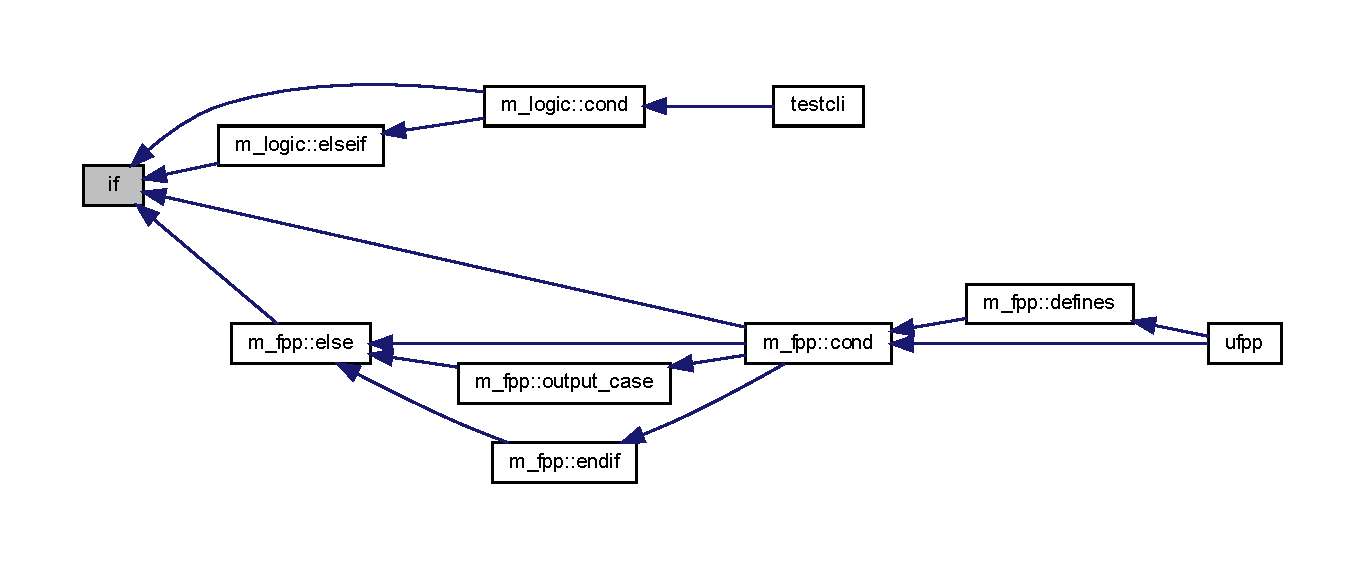
\includegraphics[width=350pt]{exit_87_8txt_a77395982f8d25581c808c40f3b634d90_icgraph}
\end{center}
\end{figure}


\subsection{Variable Documentation}
\mbox{\Hypertarget{exit_87_8txt_a66fa619682984d2d9673755b5015add3}\label{exit_87_8txt_a66fa619682984d2d9673755b5015add3}} 
\index{exit.\+7.\+txt@{exit.\+7.\+txt}!appears@{appears}}
\index{appears@{appears}!exit.\+7.\+txt@{exit.\+7.\+txt}}
\subsubsection{\texorpdfstring{appears}{appears}}
{\footnotesize\ttfamily Specification of Fortran TH E\+X\+IT January Fortran Language Specification SH N\+A\+ME E\+X\+IT (7f) -\/ \mbox{[}\+F\+O\+R\+T\+R\+A\+N it shall be within the range of at least one do construct An E\+X\+I\+T statement belongs to a particular construct If a construct name appears}

\mbox{\Hypertarget{exit_87_8txt_aa7ebb4c04e8aa413d646a62e1f67fb5c}\label{exit_87_8txt_aa7ebb4c04e8aa413d646a62e1f67fb5c}} 
\index{exit.\+7.\+txt@{exit.\+7.\+txt}!construct@{construct}}
\index{construct@{construct}!exit.\+7.\+txt@{exit.\+7.\+txt}}
\subsubsection{\texorpdfstring{construct}{construct}}
{\footnotesize\ttfamily \hyperlink{what__overview_81_8txt_a1468cf345691ca45f70578e0b7abd264}{it} belongs \hyperlink{M__stopwatch_83_8txt_a97209fd3e34ef701c0a9734280779cbb}{to} \hyperlink{M__stopwatch_83_8txt_a0f266597de2e57eb3aa964927bb30e14}{the} innermost DO construct \hyperlink{M__journal_83_8txt_afce72651d1eed785a2132bee863b2f38}{in} which \hyperlink{what__overview_81_8txt_a1468cf345691ca45f70578e0b7abd264}{it} \hyperlink{exit_87_8txt_a66fa619682984d2d9673755b5015add3}{appears} An exit stmt shall not belong \hyperlink{M__stopwatch_83_8txt_a97209fd3e34ef701c0a9734280779cbb}{to} a DO C\+O\+N\+C\+U\+R\+R\+E\+NT nor shall \hyperlink{what__overview_81_8txt_a1468cf345691ca45f70578e0b7abd264}{it} appear within \hyperlink{M__stopwatch_83_8txt_a0f266597de2e57eb3aa964927bb30e14}{the} range of a DO C\+O\+N\+C\+U\+R\+R\+E\+NT construct \hyperlink{exit_87_8txt_a77395982f8d25581c808c40f3b634d90}{if} \hyperlink{what__overview_81_8txt_a1468cf345691ca45f70578e0b7abd264}{it} belongs \hyperlink{M__stopwatch_83_8txt_a97209fd3e34ef701c0a9734280779cbb}{to} a construct that contains that DO C\+O\+N\+C\+U\+R\+R\+E\+NT construct When an E\+X\+IT \hyperlink{M__stopwatch_83_8txt_a43758526aa61bbaa49faf1e287658350}{statement} that belongs \hyperlink{M__stopwatch_83_8txt_a97209fd3e34ef701c0a9734280779cbb}{to} a DO construct \hyperlink{intro__blas1_83_8txt_a42a91df93f840595de3019ceb5d1df23}{is} \hyperlink{what__overview_81_8txt_a1468cf345691ca45f70578e0b7abd264}{it} \hyperlink{do_87_8txt_aaa6a96bc95c5da31cfe2ec4f94db576c}{terminates} \hyperlink{M__stopwatch_83_8txt_a0f266597de2e57eb3aa964927bb30e14}{the} \hyperlink{continue_87_8txt_a5094e6a64d1227c84a0bf4db8f6c3788}{loop} and any \hyperlink{do_87_8txt_a3300b8e9ebbb88612226328b1b2fd93f}{active} loops contained within \hyperlink{M__stopwatch_83_8txt_a0f266597de2e57eb3aa964927bb30e14}{the} terminated \hyperlink{continue_87_8txt_a5094e6a64d1227c84a0bf4db8f6c3788}{loop} When an E\+X\+IT \hyperlink{M__stopwatch_83_8txt_a43758526aa61bbaa49faf1e287658350}{statement} that belongs \hyperlink{M__stopwatch_83_8txt_a97209fd3e34ef701c0a9734280779cbb}{to} a non DO construct \hyperlink{intro__blas1_83_8txt_a42a91df93f840595de3019ceb5d1df23}{is} \hyperlink{what__overview_81_8txt_a1468cf345691ca45f70578e0b7abd264}{it} \hyperlink{do_87_8txt_aaa6a96bc95c5da31cfe2ec4f94db576c}{terminates} any \hyperlink{do_87_8txt_a3300b8e9ebbb88612226328b1b2fd93f}{active} loops contained within that construct}

\mbox{\Hypertarget{exit_87_8txt_a8586238d5ca1171c2dfcd62d35642cdd}\label{exit_87_8txt_a8586238d5ca1171c2dfcd62d35642cdd}} 
\index{exit.\+7.\+txt@{exit.\+7.\+txt}!executed@{executed}}
\index{executed@{executed}!exit.\+7.\+txt@{exit.\+7.\+txt}}
\subsubsection{\texorpdfstring{executed}{executed}}
{\footnotesize\ttfamily \hyperlink{what__overview_81_8txt_a1468cf345691ca45f70578e0b7abd264}{it} belongs \hyperlink{M__stopwatch_83_8txt_a97209fd3e34ef701c0a9734280779cbb}{to} \hyperlink{M__stopwatch_83_8txt_a0f266597de2e57eb3aa964927bb30e14}{the} innermost DO \hyperlink{exit_87_8txt_aa7ebb4c04e8aa413d646a62e1f67fb5c}{construct} \hyperlink{M__journal_83_8txt_afce72651d1eed785a2132bee863b2f38}{in} which \hyperlink{what__overview_81_8txt_a1468cf345691ca45f70578e0b7abd264}{it} \hyperlink{exit_87_8txt_a66fa619682984d2d9673755b5015add3}{appears} An exit stmt shall not belong \hyperlink{M__stopwatch_83_8txt_a97209fd3e34ef701c0a9734280779cbb}{to} a DO C\+O\+N\+C\+U\+R\+R\+E\+NT nor shall \hyperlink{what__overview_81_8txt_a1468cf345691ca45f70578e0b7abd264}{it} appear within \hyperlink{M__stopwatch_83_8txt_a0f266597de2e57eb3aa964927bb30e14}{the} range of a DO C\+O\+N\+C\+U\+R\+R\+E\+NT \hyperlink{exit_87_8txt_aa7ebb4c04e8aa413d646a62e1f67fb5c}{construct} \hyperlink{exit_87_8txt_a77395982f8d25581c808c40f3b634d90}{if} \hyperlink{what__overview_81_8txt_a1468cf345691ca45f70578e0b7abd264}{it} belongs \hyperlink{M__stopwatch_83_8txt_a97209fd3e34ef701c0a9734280779cbb}{to} a \hyperlink{exit_87_8txt_aa7ebb4c04e8aa413d646a62e1f67fb5c}{construct} that contains that DO C\+O\+N\+C\+U\+R\+R\+E\+NT \hyperlink{exit_87_8txt_aa7ebb4c04e8aa413d646a62e1f67fb5c}{construct} When an E\+X\+IT \hyperlink{M__stopwatch_83_8txt_a43758526aa61bbaa49faf1e287658350}{statement} that belongs \hyperlink{M__stopwatch_83_8txt_a97209fd3e34ef701c0a9734280779cbb}{to} a DO \hyperlink{exit_87_8txt_aa7ebb4c04e8aa413d646a62e1f67fb5c}{construct} \hyperlink{intro__blas1_83_8txt_a42a91df93f840595de3019ceb5d1df23}{is} \hyperlink{what__overview_81_8txt_a1468cf345691ca45f70578e0b7abd264}{it} \hyperlink{do_87_8txt_aaa6a96bc95c5da31cfe2ec4f94db576c}{terminates} \hyperlink{M__stopwatch_83_8txt_a0f266597de2e57eb3aa964927bb30e14}{the} \hyperlink{continue_87_8txt_a5094e6a64d1227c84a0bf4db8f6c3788}{loop} and any \hyperlink{do_87_8txt_a3300b8e9ebbb88612226328b1b2fd93f}{active} loops contained within \hyperlink{M__stopwatch_83_8txt_a0f266597de2e57eb3aa964927bb30e14}{the} terminated \hyperlink{continue_87_8txt_a5094e6a64d1227c84a0bf4db8f6c3788}{loop} When an E\+X\+IT \hyperlink{M__stopwatch_83_8txt_a43758526aa61bbaa49faf1e287658350}{statement} that belongs \hyperlink{M__stopwatch_83_8txt_a97209fd3e34ef701c0a9734280779cbb}{to} a non DO \hyperlink{exit_87_8txt_aa7ebb4c04e8aa413d646a62e1f67fb5c}{construct} \hyperlink{intro__blas1_83_8txt_a42a91df93f840595de3019ceb5d1df23}{is} executed}

\mbox{\Hypertarget{exit_87_8txt_a8921ef29c441e427867c54bd3b2462ba}\label{exit_87_8txt_a8921ef29c441e427867c54bd3b2462ba}} 
\index{exit.\+7.\+txt@{exit.\+7.\+txt}!j@{j}}
\index{j@{j}!exit.\+7.\+txt@{exit.\+7.\+txt}}
\subsubsection{\texorpdfstring{j}{j}}
{\footnotesize\ttfamily \hyperlink{what__overview_81_8txt_a1468cf345691ca45f70578e0b7abd264}{it} belongs \hyperlink{M__stopwatch_83_8txt_a97209fd3e34ef701c0a9734280779cbb}{to} \hyperlink{M__stopwatch_83_8txt_a0f266597de2e57eb3aa964927bb30e14}{the} innermost DO \hyperlink{exit_87_8txt_aa7ebb4c04e8aa413d646a62e1f67fb5c}{construct} \hyperlink{M__journal_83_8txt_afce72651d1eed785a2132bee863b2f38}{in} which \hyperlink{what__overview_81_8txt_a1468cf345691ca45f70578e0b7abd264}{it} \hyperlink{exit_87_8txt_a66fa619682984d2d9673755b5015add3}{appears} An exit stmt shall not belong \hyperlink{M__stopwatch_83_8txt_a97209fd3e34ef701c0a9734280779cbb}{to} a DO C\+O\+N\+C\+U\+R\+R\+E\+NT nor shall \hyperlink{what__overview_81_8txt_a1468cf345691ca45f70578e0b7abd264}{it} appear within \hyperlink{M__stopwatch_83_8txt_a0f266597de2e57eb3aa964927bb30e14}{the} range of a DO C\+O\+N\+C\+U\+R\+R\+E\+NT \hyperlink{exit_87_8txt_aa7ebb4c04e8aa413d646a62e1f67fb5c}{construct} \hyperlink{exit_87_8txt_a77395982f8d25581c808c40f3b634d90}{if} \hyperlink{what__overview_81_8txt_a1468cf345691ca45f70578e0b7abd264}{it} belongs \hyperlink{M__stopwatch_83_8txt_a97209fd3e34ef701c0a9734280779cbb}{to} a \hyperlink{exit_87_8txt_aa7ebb4c04e8aa413d646a62e1f67fb5c}{construct} that contains that DO C\+O\+N\+C\+U\+R\+R\+E\+NT \hyperlink{exit_87_8txt_aa7ebb4c04e8aa413d646a62e1f67fb5c}{construct} When an E\+X\+IT \hyperlink{M__stopwatch_83_8txt_a43758526aa61bbaa49faf1e287658350}{statement} that belongs \hyperlink{M__stopwatch_83_8txt_a97209fd3e34ef701c0a9734280779cbb}{to} a DO \hyperlink{exit_87_8txt_aa7ebb4c04e8aa413d646a62e1f67fb5c}{construct} \hyperlink{intro__blas1_83_8txt_a42a91df93f840595de3019ceb5d1df23}{is} \hyperlink{what__overview_81_8txt_a1468cf345691ca45f70578e0b7abd264}{it} \hyperlink{do_87_8txt_aaa6a96bc95c5da31cfe2ec4f94db576c}{terminates} \hyperlink{M__stopwatch_83_8txt_a0f266597de2e57eb3aa964927bb30e14}{the} \hyperlink{continue_87_8txt_a5094e6a64d1227c84a0bf4db8f6c3788}{loop} and any \hyperlink{do_87_8txt_a3300b8e9ebbb88612226328b1b2fd93f}{active} loops contained within \hyperlink{M__stopwatch_83_8txt_a0f266597de2e57eb3aa964927bb30e14}{the} terminated \hyperlink{continue_87_8txt_a5094e6a64d1227c84a0bf4db8f6c3788}{loop} When an E\+X\+IT \hyperlink{M__stopwatch_83_8txt_a43758526aa61bbaa49faf1e287658350}{statement} that belongs \hyperlink{M__stopwatch_83_8txt_a97209fd3e34ef701c0a9734280779cbb}{to} a non DO \hyperlink{exit_87_8txt_aa7ebb4c04e8aa413d646a62e1f67fb5c}{construct} \hyperlink{intro__blas1_83_8txt_a42a91df93f840595de3019ceb5d1df23}{is} \hyperlink{what__overview_81_8txt_a1468cf345691ca45f70578e0b7abd264}{it} \hyperlink{do_87_8txt_aaa6a96bc95c5da31cfe2ec4f94db576c}{terminates} any \hyperlink{do_87_8txt_a3300b8e9ebbb88612226328b1b2fd93f}{active} loops contained within that and completes execution of that \hyperlink{exit_87_8txt_aa7ebb4c04e8aa413d646a62e1f67fb5c}{construct} fi SH E\+X\+A\+M\+P\+L\+ES nf do j =100}

\mbox{\Hypertarget{exit_87_8txt_add9358f1f2e831e2906102c98d66905f}\label{exit_87_8txt_add9358f1f2e831e2906102c98d66905f}} 
\index{exit.\+7.\+txt@{exit.\+7.\+txt}!otherwise@{otherwise}}
\index{otherwise@{otherwise}!exit.\+7.\+txt@{exit.\+7.\+txt}}
\subsubsection{\texorpdfstring{otherwise}{otherwise}}
{\footnotesize\ttfamily otherwise}

\mbox{\Hypertarget{exit_87_8txt_a0dfc2b110cab492bbab54cd41bed6f3c}\label{exit_87_8txt_a0dfc2b110cab492bbab54cd41bed6f3c}} 
\index{exit.\+7.\+txt@{exit.\+7.\+txt}!Samples@{Samples}}
\index{Samples@{Samples}!exit.\+7.\+txt@{exit.\+7.\+txt}}
\subsubsection{\texorpdfstring{Samples}{Samples}}
{\footnotesize\ttfamily \hyperlink{what__overview_81_8txt_a1468cf345691ca45f70578e0b7abd264}{it} belongs \hyperlink{M__stopwatch_83_8txt_a97209fd3e34ef701c0a9734280779cbb}{to} \hyperlink{M__stopwatch_83_8txt_a0f266597de2e57eb3aa964927bb30e14}{the} innermost DO \hyperlink{exit_87_8txt_aa7ebb4c04e8aa413d646a62e1f67fb5c}{construct} \hyperlink{M__journal_83_8txt_afce72651d1eed785a2132bee863b2f38}{in} which \hyperlink{what__overview_81_8txt_a1468cf345691ca45f70578e0b7abd264}{it} \hyperlink{exit_87_8txt_a66fa619682984d2d9673755b5015add3}{appears} An exit stmt shall not belong \hyperlink{M__stopwatch_83_8txt_a97209fd3e34ef701c0a9734280779cbb}{to} a DO C\+O\+N\+C\+U\+R\+R\+E\+NT nor shall \hyperlink{what__overview_81_8txt_a1468cf345691ca45f70578e0b7abd264}{it} appear within \hyperlink{M__stopwatch_83_8txt_a0f266597de2e57eb3aa964927bb30e14}{the} range of a DO C\+O\+N\+C\+U\+R\+R\+E\+NT \hyperlink{exit_87_8txt_aa7ebb4c04e8aa413d646a62e1f67fb5c}{construct} \hyperlink{exit_87_8txt_a77395982f8d25581c808c40f3b634d90}{if} \hyperlink{what__overview_81_8txt_a1468cf345691ca45f70578e0b7abd264}{it} belongs \hyperlink{M__stopwatch_83_8txt_a97209fd3e34ef701c0a9734280779cbb}{to} a \hyperlink{exit_87_8txt_aa7ebb4c04e8aa413d646a62e1f67fb5c}{construct} that contains that DO C\+O\+N\+C\+U\+R\+R\+E\+NT \hyperlink{exit_87_8txt_aa7ebb4c04e8aa413d646a62e1f67fb5c}{construct} When an E\+X\+IT \hyperlink{M__stopwatch_83_8txt_a43758526aa61bbaa49faf1e287658350}{statement} that belongs \hyperlink{M__stopwatch_83_8txt_a97209fd3e34ef701c0a9734280779cbb}{to} a DO \hyperlink{exit_87_8txt_aa7ebb4c04e8aa413d646a62e1f67fb5c}{construct} \hyperlink{intro__blas1_83_8txt_a42a91df93f840595de3019ceb5d1df23}{is} \hyperlink{what__overview_81_8txt_a1468cf345691ca45f70578e0b7abd264}{it} \hyperlink{do_87_8txt_aaa6a96bc95c5da31cfe2ec4f94db576c}{terminates} \hyperlink{M__stopwatch_83_8txt_a0f266597de2e57eb3aa964927bb30e14}{the} \hyperlink{continue_87_8txt_a5094e6a64d1227c84a0bf4db8f6c3788}{loop} and any \hyperlink{do_87_8txt_a3300b8e9ebbb88612226328b1b2fd93f}{active} loops contained within \hyperlink{M__stopwatch_83_8txt_a0f266597de2e57eb3aa964927bb30e14}{the} terminated \hyperlink{continue_87_8txt_a5094e6a64d1227c84a0bf4db8f6c3788}{loop} When an E\+X\+IT \hyperlink{M__stopwatch_83_8txt_a43758526aa61bbaa49faf1e287658350}{statement} that belongs \hyperlink{M__stopwatch_83_8txt_a97209fd3e34ef701c0a9734280779cbb}{to} a non DO \hyperlink{exit_87_8txt_aa7ebb4c04e8aa413d646a62e1f67fb5c}{construct} \hyperlink{intro__blas1_83_8txt_a42a91df93f840595de3019ceb5d1df23}{is} \hyperlink{what__overview_81_8txt_a1468cf345691ca45f70578e0b7abd264}{it} \hyperlink{do_87_8txt_aaa6a96bc95c5da31cfe2ec4f94db576c}{terminates} any \hyperlink{do_87_8txt_a3300b8e9ebbb88612226328b1b2fd93f}{active} loops contained within that and completes execution of that \hyperlink{exit_87_8txt_aa7ebb4c04e8aa413d646a62e1f67fb5c}{construct} fi SH E\+X\+A\+M\+P\+L\+ES nf Samples}


\hypertarget{inquiry__stopwatch_83_8txt}{}\section{L\+I\+B\+R\+A\+R\+Y/lib\+G\+P\+F/download/tmp/doc/inquiry\+\_\+stopwatch.3.txt File Reference}
\label{inquiry__stopwatch_83_8txt}\index{L\+I\+B\+R\+A\+R\+Y/lib\+G\+P\+F/download/tmp/doc/inquiry\+\_\+stopwatch.\+3.\+txt@{L\+I\+B\+R\+A\+R\+Y/lib\+G\+P\+F/download/tmp/doc/inquiry\+\_\+stopwatch.\+3.\+txt}}
\subsection*{Functions}
\begin{DoxyCompactItemize}
\item 
TH I\+N\+Q\+U\+I\+R\+Y\+\_\+\+S\+T\+O\+P\+W\+A\+T\+CH \hyperlink{option__stopwatch_83_8txt_aa2011fc45a5e502e87ee50996a8a9305}{M\+\_\+\+Stop\+Watch} M\+\_\+\+S\+T\+O\+P\+W\+A\+T\+CH P\+R\+O\+C\+E\+D\+U\+R\+ES PD SH N\+A\+ME \hyperlink{inquiry__stopwatch_83_8txt_a4dada9d717f128f440143c7c9e065435}{inquiry\+\_\+stopwatch} (3f) -\/ \mbox{[}\+M\+\_\+stopwatch\mbox{]} returns M\+\_\+\+Stop\+Watch options and system dependent values .\+S\+H S\+Y\+N\+O\+P\+S\+I\+S subroutine .\+B\+I \char`\"{}inquiry\+\_\+stopwatch\char`\"{} \char`\"{}(default\+\_\+clock
\item 
TH I\+N\+Q\+U\+I\+R\+Y\+\_\+\+S\+T\+O\+P\+W\+A\+T\+CH \hyperlink{option__stopwatch_83_8txt_aa2011fc45a5e502e87ee50996a8a9305}{M\+\_\+\+Stop\+Watch} M\+\_\+\+S\+T\+O\+P\+W\+A\+T\+CH P\+R\+O\+C\+E\+D\+U\+R\+ES PD SH N\+A\+ME err IP \hyperlink{inquiry__stopwatch_83_8txt_ab2e20a25f5ea8f5986290d5c6d860dac}{character} (len=$\ast$)
\end{DoxyCompactItemize}
\subsection*{Variables}
\begin{DoxyCompactItemize}
\item 
TH I\+N\+Q\+U\+I\+R\+Y\+\_\+\+S\+T\+O\+P\+W\+A\+T\+CH \hyperlink{inquiry__stopwatch_83_8txt_a5343cd7a514240c99a373cb1e09e1d08}{September}
\item 
TH I\+N\+Q\+U\+I\+R\+Y\+\_\+\+S\+T\+O\+P\+W\+A\+T\+CH \hyperlink{option__stopwatch_83_8txt_aa2011fc45a5e502e87ee50996a8a9305}{M\+\_\+\+Stop\+Watch} M\+\_\+\+S\+T\+O\+P\+W\+A\+T\+CH P\+R\+O\+C\+E\+D\+U\+R\+ES PD SH N\+A\+ME \hyperlink{inquiry__stopwatch_83_8txt_ad67f5f613d63ccb3ff87efe190d2c9c1}{io\+\_\+unit\+\_\+print}
\item 
TH I\+N\+Q\+U\+I\+R\+Y\+\_\+\+S\+T\+O\+P\+W\+A\+T\+CH \hyperlink{option__stopwatch_83_8txt_aa2011fc45a5e502e87ee50996a8a9305}{M\+\_\+\+Stop\+Watch} M\+\_\+\+S\+T\+O\+P\+W\+A\+T\+CH P\+R\+O\+C\+E\+D\+U\+R\+ES PD SH N\+A\+ME \hyperlink{inquiry__stopwatch_83_8txt_a3a3ade1e4c01a51287544ea767e3512a}{io\+\_\+unit\+\_\+error}
\item 
TH I\+N\+Q\+U\+I\+R\+Y\+\_\+\+S\+T\+O\+P\+W\+A\+T\+CH \hyperlink{option__stopwatch_83_8txt_aa2011fc45a5e502e87ee50996a8a9305}{M\+\_\+\+Stop\+Watch} M\+\_\+\+S\+T\+O\+P\+W\+A\+T\+CH P\+R\+O\+C\+E\+D\+U\+R\+ES PD SH N\+A\+ME \hyperlink{inquiry__stopwatch_83_8txt_a70e15afb456eff58f321ed840953c7f5}{print\+\_\+errors}
\item 
TH I\+N\+Q\+U\+I\+R\+Y\+\_\+\+S\+T\+O\+P\+W\+A\+T\+CH \hyperlink{option__stopwatch_83_8txt_aa2011fc45a5e502e87ee50996a8a9305}{M\+\_\+\+Stop\+Watch} M\+\_\+\+S\+T\+O\+P\+W\+A\+T\+CH P\+R\+O\+C\+E\+D\+U\+R\+ES PD SH N\+A\+ME \hyperlink{inquiry__stopwatch_83_8txt_a3a9b41223396c066db320e657bd8cba4}{abort\+\_\+errors}
\item 
TH I\+N\+Q\+U\+I\+R\+Y\+\_\+\+S\+T\+O\+P\+W\+A\+T\+CH \hyperlink{option__stopwatch_83_8txt_aa2011fc45a5e502e87ee50996a8a9305}{M\+\_\+\+Stop\+Watch} M\+\_\+\+S\+T\+O\+P\+W\+A\+T\+CH P\+R\+O\+C\+E\+D\+U\+R\+ES PD SH N\+A\+ME \hyperlink{inquiry__stopwatch_83_8txt_a0a3b09cc37d1f592e66a07c0c8a31cba}{print\+\_\+form}
\item 
TH I\+N\+Q\+U\+I\+R\+Y\+\_\+\+S\+T\+O\+P\+W\+A\+T\+CH \hyperlink{option__stopwatch_83_8txt_aa2011fc45a5e502e87ee50996a8a9305}{M\+\_\+\+Stop\+Watch} M\+\_\+\+S\+T\+O\+P\+W\+A\+T\+CH P\+R\+O\+C\+E\+D\+U\+R\+ES PD SH N\+A\+ME \hyperlink{inquiry__stopwatch_83_8txt_a7abc42d907bf857b7ccd85e08a2698bf}{cpu\+\_\+avail}
\item 
TH I\+N\+Q\+U\+I\+R\+Y\+\_\+\+S\+T\+O\+P\+W\+A\+T\+CH \hyperlink{option__stopwatch_83_8txt_aa2011fc45a5e502e87ee50996a8a9305}{M\+\_\+\+Stop\+Watch} M\+\_\+\+S\+T\+O\+P\+W\+A\+T\+CH P\+R\+O\+C\+E\+D\+U\+R\+ES PD SH N\+A\+ME \hyperlink{inquiry__stopwatch_83_8txt_a302378a0fc3cc389357199927dccdc6d}{user\+\_\+avail}
\item 
TH I\+N\+Q\+U\+I\+R\+Y\+\_\+\+S\+T\+O\+P\+W\+A\+T\+CH \hyperlink{option__stopwatch_83_8txt_aa2011fc45a5e502e87ee50996a8a9305}{M\+\_\+\+Stop\+Watch} M\+\_\+\+S\+T\+O\+P\+W\+A\+T\+CH P\+R\+O\+C\+E\+D\+U\+R\+ES PD SH N\+A\+ME \hyperlink{inquiry__stopwatch_83_8txt_a1f4290ad6f2e60e1f902db8a5e86ba7b}{sys\+\_\+avail}
\item 
TH I\+N\+Q\+U\+I\+R\+Y\+\_\+\+S\+T\+O\+P\+W\+A\+T\+CH \hyperlink{option__stopwatch_83_8txt_aa2011fc45a5e502e87ee50996a8a9305}{M\+\_\+\+Stop\+Watch} M\+\_\+\+S\+T\+O\+P\+W\+A\+T\+CH P\+R\+O\+C\+E\+D\+U\+R\+ES PD SH N\+A\+ME \hyperlink{inquiry__stopwatch_83_8txt_a73da37f4d5799996a833d139d422cef8}{wall\+\_\+avail}
\item 
TH I\+N\+Q\+U\+I\+R\+Y\+\_\+\+S\+T\+O\+P\+W\+A\+T\+CH \hyperlink{option__stopwatch_83_8txt_aa2011fc45a5e502e87ee50996a8a9305}{M\+\_\+\+Stop\+Watch} M\+\_\+\+S\+T\+O\+P\+W\+A\+T\+CH P\+R\+O\+C\+E\+D\+U\+R\+ES PD SH N\+A\+ME \hyperlink{inquiry__stopwatch_83_8txt_a31483d611b443f67111f1154cd00fc7e}{cpu\+\_\+prec}
\item 
TH I\+N\+Q\+U\+I\+R\+Y\+\_\+\+S\+T\+O\+P\+W\+A\+T\+CH \hyperlink{option__stopwatch_83_8txt_aa2011fc45a5e502e87ee50996a8a9305}{M\+\_\+\+Stop\+Watch} M\+\_\+\+S\+T\+O\+P\+W\+A\+T\+CH P\+R\+O\+C\+E\+D\+U\+R\+ES PD SH N\+A\+ME \hyperlink{inquiry__stopwatch_83_8txt_a5ff5c1fe3dd4df4b4c88053f0182e09d}{wall\+\_\+prec}
\item 
TH I\+N\+Q\+U\+I\+R\+Y\+\_\+\+S\+T\+O\+P\+W\+A\+T\+CH \hyperlink{option__stopwatch_83_8txt_aa2011fc45a5e502e87ee50996a8a9305}{M\+\_\+\+Stop\+Watch} M\+\_\+\+S\+T\+O\+P\+W\+A\+T\+CH P\+R\+O\+C\+E\+D\+U\+R\+ES PD SH N\+A\+ME \hyperlink{inquiry__stopwatch_83_8txt_aee378be19d20935dd436517beda00ee4}{version}
\item 
TH I\+N\+Q\+U\+I\+R\+Y\+\_\+\+S\+T\+O\+P\+W\+A\+T\+CH \hyperlink{option__stopwatch_83_8txt_aa2011fc45a5e502e87ee50996a8a9305}{M\+\_\+\+Stop\+Watch} M\+\_\+\+S\+T\+O\+P\+W\+A\+T\+CH P\+R\+O\+C\+E\+D\+U\+R\+ES PD SH N\+A\+ME err IP \hyperlink{inquiry__stopwatch_83_8txt_ae6234c62ee65662c46e3ce6056a3f252}{optional}
\item 
TH I\+N\+Q\+U\+I\+R\+Y\+\_\+\+S\+T\+O\+P\+W\+A\+T\+CH \hyperlink{option__stopwatch_83_8txt_aa2011fc45a5e502e87ee50996a8a9305}{M\+\_\+\+Stop\+Watch} M\+\_\+\+S\+T\+O\+P\+W\+A\+T\+CH P\+R\+O\+C\+E\+D\+U\+R\+ES PD SH N\+A\+ME err IP intent(O\+UT) execution successful IP Failed \hyperlink{M__stopwatch_83_8txt_a97209fd3e34ef701c0a9734280779cbb}{to} allocate required memory This \hyperlink{M__stopwatch_83_8txt_ac4611edff506351be87ddb9adfc62315}{error} occurs \hyperlink{exit_87_8txt_a77395982f8d25581c808c40f3b634d90}{if} \hyperlink{M__stopwatch_83_8txt_a0f266597de2e57eb3aa964927bb30e14}{the} Fortran \hyperlink{intro__blas1_83_8txt_a5f157716d3fd55e7b7e08312dc859b58}{B} allocate \hyperlink{M__stopwatch_83_8txt_a43758526aa61bbaa49faf1e287658350}{statement} \hyperlink{M__stopwatch_83_8txt_aee54cdd5349bf498aa96e7f9426a0717}{returns} a nonzero status indicating that memory could not be allocated Avoid memory leaks by always destroying \hyperlink{M__stopwatch_83_8txt_a21c5980264dbe8d8a18083e2dd1ffaa9}{watches} and groups before recreating \hyperlink{inquiry__stopwatch_83_8txt_aba56042309c21e69313821cb6c092c35}{them}
\end{DoxyCompactItemize}


\subsection{Function Documentation}
\mbox{\Hypertarget{inquiry__stopwatch_83_8txt_ab2e20a25f5ea8f5986290d5c6d860dac}\label{inquiry__stopwatch_83_8txt_ab2e20a25f5ea8f5986290d5c6d860dac}} 
\index{inquiry\+\_\+stopwatch.\+3.\+txt@{inquiry\+\_\+stopwatch.\+3.\+txt}!character@{character}}
\index{character@{character}!inquiry\+\_\+stopwatch.\+3.\+txt@{inquiry\+\_\+stopwatch.\+3.\+txt}}
\subsubsection{\texorpdfstring{character()}{character()}}
{\footnotesize\ttfamily TH I\+N\+Q\+U\+I\+R\+Y\+\_\+\+S\+T\+O\+P\+W\+A\+T\+CH \hyperlink{option__stopwatch_83_8txt_aa2011fc45a5e502e87ee50996a8a9305}{M\+\_\+\+Stop\+Watch} M\+\_\+\+S\+T\+O\+P\+W\+A\+T\+CH P\+R\+O\+C\+E\+D\+U\+R\+ES PD SH N\+A\+ME err IP character (\begin{DoxyParamCaption}\item[{len}]{ = {\ttfamily $\ast$} }\end{DoxyParamCaption})}

\mbox{\Hypertarget{inquiry__stopwatch_83_8txt_a4dada9d717f128f440143c7c9e065435}\label{inquiry__stopwatch_83_8txt_a4dada9d717f128f440143c7c9e065435}} 
\index{inquiry\+\_\+stopwatch.\+3.\+txt@{inquiry\+\_\+stopwatch.\+3.\+txt}!inquiry\+\_\+stopwatch@{inquiry\+\_\+stopwatch}}
\index{inquiry\+\_\+stopwatch@{inquiry\+\_\+stopwatch}!inquiry\+\_\+stopwatch.\+3.\+txt@{inquiry\+\_\+stopwatch.\+3.\+txt}}
\subsubsection{\texorpdfstring{inquiry\+\_\+stopwatch()}{inquiry\_stopwatch()}}
{\footnotesize\ttfamily TH I\+N\+Q\+U\+I\+R\+Y\+\_\+\+S\+T\+O\+P\+W\+A\+T\+CH \hyperlink{option__stopwatch_83_8txt_aa2011fc45a5e502e87ee50996a8a9305}{M\+\_\+\+Stop\+Watch} M\+\_\+\+S\+T\+O\+P\+W\+A\+T\+CH P\+R\+O\+C\+E\+D\+U\+R\+ES PD SH N\+A\+ME inquiry\+\_\+stopwatch (\begin{DoxyParamCaption}\item[{3f}]{ }\end{DoxyParamCaption})}



\subsection{Variable Documentation}
\mbox{\Hypertarget{inquiry__stopwatch_83_8txt_a3a9b41223396c066db320e657bd8cba4}\label{inquiry__stopwatch_83_8txt_a3a9b41223396c066db320e657bd8cba4}} 
\index{inquiry\+\_\+stopwatch.\+3.\+txt@{inquiry\+\_\+stopwatch.\+3.\+txt}!abort\+\_\+errors@{abort\+\_\+errors}}
\index{abort\+\_\+errors@{abort\+\_\+errors}!inquiry\+\_\+stopwatch.\+3.\+txt@{inquiry\+\_\+stopwatch.\+3.\+txt}}
\subsubsection{\texorpdfstring{abort\+\_\+errors}{abort\_errors}}
{\footnotesize\ttfamily TH I\+N\+Q\+U\+I\+R\+Y\+\_\+\+S\+T\+O\+P\+W\+A\+T\+CH \hyperlink{option__stopwatch_83_8txt_aa2011fc45a5e502e87ee50996a8a9305}{M\+\_\+\+Stop\+Watch} M\+\_\+\+S\+T\+O\+P\+W\+A\+T\+CH P\+R\+O\+C\+E\+D\+U\+R\+ES PD SH N\+A\+ME abort\+\_\+errors}

\mbox{\Hypertarget{inquiry__stopwatch_83_8txt_a7abc42d907bf857b7ccd85e08a2698bf}\label{inquiry__stopwatch_83_8txt_a7abc42d907bf857b7ccd85e08a2698bf}} 
\index{inquiry\+\_\+stopwatch.\+3.\+txt@{inquiry\+\_\+stopwatch.\+3.\+txt}!cpu\+\_\+avail@{cpu\+\_\+avail}}
\index{cpu\+\_\+avail@{cpu\+\_\+avail}!inquiry\+\_\+stopwatch.\+3.\+txt@{inquiry\+\_\+stopwatch.\+3.\+txt}}
\subsubsection{\texorpdfstring{cpu\+\_\+avail}{cpu\_avail}}
{\footnotesize\ttfamily TH I\+N\+Q\+U\+I\+R\+Y\+\_\+\+S\+T\+O\+P\+W\+A\+T\+CH \hyperlink{option__stopwatch_83_8txt_aa2011fc45a5e502e87ee50996a8a9305}{M\+\_\+\+Stop\+Watch} M\+\_\+\+S\+T\+O\+P\+W\+A\+T\+CH P\+R\+O\+C\+E\+D\+U\+R\+ES PD SH N\+A\+ME cpu\+\_\+avail}

\mbox{\Hypertarget{inquiry__stopwatch_83_8txt_a31483d611b443f67111f1154cd00fc7e}\label{inquiry__stopwatch_83_8txt_a31483d611b443f67111f1154cd00fc7e}} 
\index{inquiry\+\_\+stopwatch.\+3.\+txt@{inquiry\+\_\+stopwatch.\+3.\+txt}!cpu\+\_\+prec@{cpu\+\_\+prec}}
\index{cpu\+\_\+prec@{cpu\+\_\+prec}!inquiry\+\_\+stopwatch.\+3.\+txt@{inquiry\+\_\+stopwatch.\+3.\+txt}}
\subsubsection{\texorpdfstring{cpu\+\_\+prec}{cpu\_prec}}
{\footnotesize\ttfamily TH I\+N\+Q\+U\+I\+R\+Y\+\_\+\+S\+T\+O\+P\+W\+A\+T\+CH \hyperlink{option__stopwatch_83_8txt_aa2011fc45a5e502e87ee50996a8a9305}{M\+\_\+\+Stop\+Watch} M\+\_\+\+S\+T\+O\+P\+W\+A\+T\+CH P\+R\+O\+C\+E\+D\+U\+R\+ES PD SH N\+A\+ME cpu\+\_\+prec}

\mbox{\Hypertarget{inquiry__stopwatch_83_8txt_a3a3ade1e4c01a51287544ea767e3512a}\label{inquiry__stopwatch_83_8txt_a3a3ade1e4c01a51287544ea767e3512a}} 
\index{inquiry\+\_\+stopwatch.\+3.\+txt@{inquiry\+\_\+stopwatch.\+3.\+txt}!io\+\_\+unit\+\_\+error@{io\+\_\+unit\+\_\+error}}
\index{io\+\_\+unit\+\_\+error@{io\+\_\+unit\+\_\+error}!inquiry\+\_\+stopwatch.\+3.\+txt@{inquiry\+\_\+stopwatch.\+3.\+txt}}
\subsubsection{\texorpdfstring{io\+\_\+unit\+\_\+error}{io\_unit\_error}}
{\footnotesize\ttfamily TH I\+N\+Q\+U\+I\+R\+Y\+\_\+\+S\+T\+O\+P\+W\+A\+T\+CH \hyperlink{option__stopwatch_83_8txt_aa2011fc45a5e502e87ee50996a8a9305}{M\+\_\+\+Stop\+Watch} M\+\_\+\+S\+T\+O\+P\+W\+A\+T\+CH P\+R\+O\+C\+E\+D\+U\+R\+ES PD SH N\+A\+ME io\+\_\+unit\+\_\+error}

\mbox{\Hypertarget{inquiry__stopwatch_83_8txt_ad67f5f613d63ccb3ff87efe190d2c9c1}\label{inquiry__stopwatch_83_8txt_ad67f5f613d63ccb3ff87efe190d2c9c1}} 
\index{inquiry\+\_\+stopwatch.\+3.\+txt@{inquiry\+\_\+stopwatch.\+3.\+txt}!io\+\_\+unit\+\_\+print@{io\+\_\+unit\+\_\+print}}
\index{io\+\_\+unit\+\_\+print@{io\+\_\+unit\+\_\+print}!inquiry\+\_\+stopwatch.\+3.\+txt@{inquiry\+\_\+stopwatch.\+3.\+txt}}
\subsubsection{\texorpdfstring{io\+\_\+unit\+\_\+print}{io\_unit\_print}}
{\footnotesize\ttfamily TH I\+N\+Q\+U\+I\+R\+Y\+\_\+\+S\+T\+O\+P\+W\+A\+T\+CH \hyperlink{option__stopwatch_83_8txt_aa2011fc45a5e502e87ee50996a8a9305}{M\+\_\+\+Stop\+Watch} M\+\_\+\+S\+T\+O\+P\+W\+A\+T\+CH P\+R\+O\+C\+E\+D\+U\+R\+ES PD SH N\+A\+ME io\+\_\+unit\+\_\+print}

\mbox{\Hypertarget{inquiry__stopwatch_83_8txt_ae6234c62ee65662c46e3ce6056a3f252}\label{inquiry__stopwatch_83_8txt_ae6234c62ee65662c46e3ce6056a3f252}} 
\index{inquiry\+\_\+stopwatch.\+3.\+txt@{inquiry\+\_\+stopwatch.\+3.\+txt}!optional@{optional}}
\index{optional@{optional}!inquiry\+\_\+stopwatch.\+3.\+txt@{inquiry\+\_\+stopwatch.\+3.\+txt}}
\subsubsection{\texorpdfstring{optional}{optional}}
{\footnotesize\ttfamily TH I\+N\+Q\+U\+I\+R\+Y\+\_\+\+S\+T\+O\+P\+W\+A\+T\+CH \hyperlink{option__stopwatch_83_8txt_aa2011fc45a5e502e87ee50996a8a9305}{M\+\_\+\+Stop\+Watch} M\+\_\+\+S\+T\+O\+P\+W\+A\+T\+CH P\+R\+O\+C\+E\+D\+U\+R\+ES PD SH N\+A\+ME err IP optional}

\mbox{\Hypertarget{inquiry__stopwatch_83_8txt_a70e15afb456eff58f321ed840953c7f5}\label{inquiry__stopwatch_83_8txt_a70e15afb456eff58f321ed840953c7f5}} 
\index{inquiry\+\_\+stopwatch.\+3.\+txt@{inquiry\+\_\+stopwatch.\+3.\+txt}!print\+\_\+errors@{print\+\_\+errors}}
\index{print\+\_\+errors@{print\+\_\+errors}!inquiry\+\_\+stopwatch.\+3.\+txt@{inquiry\+\_\+stopwatch.\+3.\+txt}}
\subsubsection{\texorpdfstring{print\+\_\+errors}{print\_errors}}
{\footnotesize\ttfamily TH I\+N\+Q\+U\+I\+R\+Y\+\_\+\+S\+T\+O\+P\+W\+A\+T\+CH \hyperlink{option__stopwatch_83_8txt_aa2011fc45a5e502e87ee50996a8a9305}{M\+\_\+\+Stop\+Watch} M\+\_\+\+S\+T\+O\+P\+W\+A\+T\+CH P\+R\+O\+C\+E\+D\+U\+R\+ES PD SH N\+A\+ME print\+\_\+errors}

\mbox{\Hypertarget{inquiry__stopwatch_83_8txt_a0a3b09cc37d1f592e66a07c0c8a31cba}\label{inquiry__stopwatch_83_8txt_a0a3b09cc37d1f592e66a07c0c8a31cba}} 
\index{inquiry\+\_\+stopwatch.\+3.\+txt@{inquiry\+\_\+stopwatch.\+3.\+txt}!print\+\_\+form@{print\+\_\+form}}
\index{print\+\_\+form@{print\+\_\+form}!inquiry\+\_\+stopwatch.\+3.\+txt@{inquiry\+\_\+stopwatch.\+3.\+txt}}
\subsubsection{\texorpdfstring{print\+\_\+form}{print\_form}}
{\footnotesize\ttfamily TH I\+N\+Q\+U\+I\+R\+Y\+\_\+\+S\+T\+O\+P\+W\+A\+T\+CH \hyperlink{option__stopwatch_83_8txt_aa2011fc45a5e502e87ee50996a8a9305}{M\+\_\+\+Stop\+Watch} M\+\_\+\+S\+T\+O\+P\+W\+A\+T\+CH P\+R\+O\+C\+E\+D\+U\+R\+ES PD SH N\+A\+ME print\+\_\+form}

\mbox{\Hypertarget{inquiry__stopwatch_83_8txt_a5343cd7a514240c99a373cb1e09e1d08}\label{inquiry__stopwatch_83_8txt_a5343cd7a514240c99a373cb1e09e1d08}} 
\index{inquiry\+\_\+stopwatch.\+3.\+txt@{inquiry\+\_\+stopwatch.\+3.\+txt}!September@{September}}
\index{September@{September}!inquiry\+\_\+stopwatch.\+3.\+txt@{inquiry\+\_\+stopwatch.\+3.\+txt}}
\subsubsection{\texorpdfstring{September}{September}}
{\footnotesize\ttfamily TH I\+N\+Q\+U\+I\+R\+Y\+\_\+\+S\+T\+O\+P\+W\+A\+T\+CH September}

\mbox{\Hypertarget{inquiry__stopwatch_83_8txt_a1f4290ad6f2e60e1f902db8a5e86ba7b}\label{inquiry__stopwatch_83_8txt_a1f4290ad6f2e60e1f902db8a5e86ba7b}} 
\index{inquiry\+\_\+stopwatch.\+3.\+txt@{inquiry\+\_\+stopwatch.\+3.\+txt}!sys\+\_\+avail@{sys\+\_\+avail}}
\index{sys\+\_\+avail@{sys\+\_\+avail}!inquiry\+\_\+stopwatch.\+3.\+txt@{inquiry\+\_\+stopwatch.\+3.\+txt}}
\subsubsection{\texorpdfstring{sys\+\_\+avail}{sys\_avail}}
{\footnotesize\ttfamily TH I\+N\+Q\+U\+I\+R\+Y\+\_\+\+S\+T\+O\+P\+W\+A\+T\+CH \hyperlink{option__stopwatch_83_8txt_aa2011fc45a5e502e87ee50996a8a9305}{M\+\_\+\+Stop\+Watch} M\+\_\+\+S\+T\+O\+P\+W\+A\+T\+CH P\+R\+O\+C\+E\+D\+U\+R\+ES PD SH N\+A\+ME sys\+\_\+avail}

\mbox{\Hypertarget{inquiry__stopwatch_83_8txt_aba56042309c21e69313821cb6c092c35}\label{inquiry__stopwatch_83_8txt_aba56042309c21e69313821cb6c092c35}} 
\index{inquiry\+\_\+stopwatch.\+3.\+txt@{inquiry\+\_\+stopwatch.\+3.\+txt}!them@{them}}
\index{them@{them}!inquiry\+\_\+stopwatch.\+3.\+txt@{inquiry\+\_\+stopwatch.\+3.\+txt}}
\subsubsection{\texorpdfstring{them}{them}}
{\footnotesize\ttfamily TH I\+N\+Q\+U\+I\+R\+Y\+\_\+\+S\+T\+O\+P\+W\+A\+T\+CH \hyperlink{option__stopwatch_83_8txt_aa2011fc45a5e502e87ee50996a8a9305}{M\+\_\+\+Stop\+Watch} M\+\_\+\+S\+T\+O\+P\+W\+A\+T\+CH P\+R\+O\+C\+E\+D\+U\+R\+ES PD SH N\+A\+ME err IP intent (O\+UT) execution successful IP Failed \hyperlink{M__stopwatch_83_8txt_a97209fd3e34ef701c0a9734280779cbb}{to} allocate required memory This \hyperlink{M__stopwatch_83_8txt_ac4611edff506351be87ddb9adfc62315}{error} occurs \hyperlink{exit_87_8txt_a77395982f8d25581c808c40f3b634d90}{if} \hyperlink{M__stopwatch_83_8txt_a0f266597de2e57eb3aa964927bb30e14}{the} Fortran \hyperlink{intro__blas1_83_8txt_a5f157716d3fd55e7b7e08312dc859b58}{B} allocate \hyperlink{M__stopwatch_83_8txt_a43758526aa61bbaa49faf1e287658350}{statement} \hyperlink{M__stopwatch_83_8txt_aee54cdd5349bf498aa96e7f9426a0717}{returns} a nonzero status indicating that memory could not be allocated Avoid memory leaks by always destroying \hyperlink{M__stopwatch_83_8txt_a21c5980264dbe8d8a18083e2dd1ffaa9}{watches} and groups before recreating them}

\mbox{\Hypertarget{inquiry__stopwatch_83_8txt_a302378a0fc3cc389357199927dccdc6d}\label{inquiry__stopwatch_83_8txt_a302378a0fc3cc389357199927dccdc6d}} 
\index{inquiry\+\_\+stopwatch.\+3.\+txt@{inquiry\+\_\+stopwatch.\+3.\+txt}!user\+\_\+avail@{user\+\_\+avail}}
\index{user\+\_\+avail@{user\+\_\+avail}!inquiry\+\_\+stopwatch.\+3.\+txt@{inquiry\+\_\+stopwatch.\+3.\+txt}}
\subsubsection{\texorpdfstring{user\+\_\+avail}{user\_avail}}
{\footnotesize\ttfamily TH I\+N\+Q\+U\+I\+R\+Y\+\_\+\+S\+T\+O\+P\+W\+A\+T\+CH \hyperlink{option__stopwatch_83_8txt_aa2011fc45a5e502e87ee50996a8a9305}{M\+\_\+\+Stop\+Watch} M\+\_\+\+S\+T\+O\+P\+W\+A\+T\+CH P\+R\+O\+C\+E\+D\+U\+R\+ES PD SH N\+A\+ME user\+\_\+avail}

\mbox{\Hypertarget{inquiry__stopwatch_83_8txt_aee378be19d20935dd436517beda00ee4}\label{inquiry__stopwatch_83_8txt_aee378be19d20935dd436517beda00ee4}} 
\index{inquiry\+\_\+stopwatch.\+3.\+txt@{inquiry\+\_\+stopwatch.\+3.\+txt}!version@{version}}
\index{version@{version}!inquiry\+\_\+stopwatch.\+3.\+txt@{inquiry\+\_\+stopwatch.\+3.\+txt}}
\subsubsection{\texorpdfstring{version}{version}}
{\footnotesize\ttfamily TH I\+N\+Q\+U\+I\+R\+Y\+\_\+\+S\+T\+O\+P\+W\+A\+T\+CH \hyperlink{option__stopwatch_83_8txt_aa2011fc45a5e502e87ee50996a8a9305}{M\+\_\+\+Stop\+Watch} M\+\_\+\+S\+T\+O\+P\+W\+A\+T\+CH P\+R\+O\+C\+E\+D\+U\+R\+ES PD SH N\+A\+ME version}

\mbox{\Hypertarget{inquiry__stopwatch_83_8txt_a73da37f4d5799996a833d139d422cef8}\label{inquiry__stopwatch_83_8txt_a73da37f4d5799996a833d139d422cef8}} 
\index{inquiry\+\_\+stopwatch.\+3.\+txt@{inquiry\+\_\+stopwatch.\+3.\+txt}!wall\+\_\+avail@{wall\+\_\+avail}}
\index{wall\+\_\+avail@{wall\+\_\+avail}!inquiry\+\_\+stopwatch.\+3.\+txt@{inquiry\+\_\+stopwatch.\+3.\+txt}}
\subsubsection{\texorpdfstring{wall\+\_\+avail}{wall\_avail}}
{\footnotesize\ttfamily TH I\+N\+Q\+U\+I\+R\+Y\+\_\+\+S\+T\+O\+P\+W\+A\+T\+CH \hyperlink{option__stopwatch_83_8txt_aa2011fc45a5e502e87ee50996a8a9305}{M\+\_\+\+Stop\+Watch} M\+\_\+\+S\+T\+O\+P\+W\+A\+T\+CH P\+R\+O\+C\+E\+D\+U\+R\+ES PD SH N\+A\+ME wall\+\_\+avail}

\mbox{\Hypertarget{inquiry__stopwatch_83_8txt_a5ff5c1fe3dd4df4b4c88053f0182e09d}\label{inquiry__stopwatch_83_8txt_a5ff5c1fe3dd4df4b4c88053f0182e09d}} 
\index{inquiry\+\_\+stopwatch.\+3.\+txt@{inquiry\+\_\+stopwatch.\+3.\+txt}!wall\+\_\+prec@{wall\+\_\+prec}}
\index{wall\+\_\+prec@{wall\+\_\+prec}!inquiry\+\_\+stopwatch.\+3.\+txt@{inquiry\+\_\+stopwatch.\+3.\+txt}}
\subsubsection{\texorpdfstring{wall\+\_\+prec}{wall\_prec}}
{\footnotesize\ttfamily TH I\+N\+Q\+U\+I\+R\+Y\+\_\+\+S\+T\+O\+P\+W\+A\+T\+CH \hyperlink{option__stopwatch_83_8txt_aa2011fc45a5e502e87ee50996a8a9305}{M\+\_\+\+Stop\+Watch} M\+\_\+\+S\+T\+O\+P\+W\+A\+T\+CH P\+R\+O\+C\+E\+D\+U\+R\+ES PD SH N\+A\+ME wall\+\_\+prec}


\hypertarget{intro__blas1_83_8txt}{}\section{L\+I\+B\+R\+A\+R\+Y/lib\+G\+P\+F/download/tmp/doc/intro\+\_\+blas1.3.txt File Reference}
\label{intro__blas1_83_8txt}\index{L\+I\+B\+R\+A\+R\+Y/lib\+G\+P\+F/download/tmp/doc/intro\+\_\+blas1.\+3.\+txt@{L\+I\+B\+R\+A\+R\+Y/lib\+G\+P\+F/download/tmp/doc/intro\+\_\+blas1.\+3.\+txt}}
\subsection*{Typedefs}
\begin{DoxyCompactItemize}
\item 
using \hyperlink{intro__blas1_83_8txt_a8ba82a50c0c2c12d5f6a77f7e4651c0b}{i} = 1, 2,..., N, \hyperlink{intro__blas1_83_8txt_a42a91df93f840595de3019ceb5d1df23}{is} \hyperlink{M__stopwatch_83_8txt_a97209fd3e34ef701c0a9734280779cbb}{to} be stored \hyperlink{M__journal_83_8txt_afce72651d1eed785a2132bee863b2f38}{in} X. �\+If I\+N\+CX $>$=0, \hyperlink{intro__blas1_83_8txt_aeaad1761c101f906d503f68274bd4b83}{then} x(\hyperlink{intro__blas1_83_8txt_a8ba82a50c0c2c12d5f6a77f7e4651c0b}{i}) \hyperlink{intro__blas1_83_8txt_a42a91df93f840595de3019ceb5d1df23}{is} stored \hyperlink{M__journal_83_8txt_afce72651d1eed785a2132bee863b2f38}{in} \hyperlink{intro__blas1_83_8txt_ac8596739bc875e90fe6e2ecf98e87906}{X}(1+(\hyperlink{continue_87_8txt_ae7b8826453d28f1bdb2fba7e889eb23b}{I}-\/1) $\ast$I\+N\+CX). �\+This \hyperlink{intro__blas1_83_8txt_a42a91df93f840595de3019ceb5d1df23}{is} known as forward \hyperlink{intro__blas1_83_8txt_a89db1945e1a335ab0184c6a097821e32}{array} storage starting at \hyperlink{intro__blas1_83_8txt_ac8596739bc875e90fe6e2ecf98e87906}{X}(1) with \hyperlink{intro__blas1_83_8txt_a2febff0a9da16d3c97c0b589777862dd}{stride} equal \hyperlink{M__stopwatch_83_8txt_a97209fd3e34ef701c0a9734280779cbb}{to} I\+N\+CX, ending with \hyperlink{intro__blas1_83_8txt_ac8596739bc875e90fe6e2ecf98e87906}{X}(1 -\/(N-\/1) $\ast$I\+N\+CX). �\+Thus, \hyperlink{exit_87_8txt_a77395982f8d25581c808c40f3b634d90}{if} N=4 and I\+N\+CX=2, \hyperlink{M__stopwatch_83_8txt_a0f266597de2e57eb3aa964927bb30e14}{the} logical vector x with components x(1), x(2), x(3), and x(4) \hyperlink{M__stopwatch_83_8txt_a5040be02b832eba08820289c8a1f81c4}{are} stored \hyperlink{M__journal_83_8txt_afce72651d1eed785a2132bee863b2f38}{in} memory \hyperlink{M__journal_83_8txt_afce72651d1eed785a2132bee863b2f38}{in} \hyperlink{M__stopwatch_83_8txt_a0f266597de2e57eb3aa964927bb30e14}{the} \hyperlink{intro__blas1_83_8txt_a89db1945e1a335ab0184c6a097821e32}{array} \hyperlink{intro__blas1_83_8txt_a6d2b4b9f7d763a043b2f60a3dd5cc5e7}{elements} \hyperlink{intro__blas1_83_8txt_ac8596739bc875e90fe6e2ecf98e87906}{X}(1), \hyperlink{intro__blas1_83_8txt_ac8596739bc875e90fe6e2ecf98e87906}{X}(3), \hyperlink{intro__blas1_83_8txt_ac8596739bc875e90fe6e2ecf98e87906}{X}(5), and \hyperlink{intro__blas1_83_8txt_ac8596739bc875e90fe6e2ecf98e87906}{X}(7), respectively. This method of indexing, using a starting element, a \hyperlink{what__overview_81_8txt_a5168680dcac08de182f59de9a12c38ae}{number} of \hyperlink{intro__blas1_83_8txt_a6d2b4b9f7d763a043b2f60a3dd5cc5e7}{elements}, and a \hyperlink{intro__blas1_83_8txt_a2febff0a9da16d3c97c0b589777862dd}{stride}, \hyperlink{intro__blas1_83_8txt_a42a91df93f840595de3019ceb5d1df23}{is} especially useful for accessing \hyperlink{M__stopwatch_83_8txt_aff7b067dcc41169a210cb1c0de45a496}{one}-\/dimensional vectors \hyperlink{M__journal_83_8txt_afce72651d1eed785a2132bee863b2f38}{in} multidimensional arrays. �\+For instance, \hyperlink{exit_87_8txt_a77395982f8d25581c808c40f3b634d90}{if} \hyperlink{ufpp__overview_81_8txt_a8341271e5f4e3003f6eb1c9547fc9d1a}{A} \hyperlink{intro__blas1_83_8txt_a42a91df93f840595de3019ceb5d1df23}{is} \hyperlink{ufpp__overview_81_8txt_a199f35c6b903296e6ea1b146249c1ab3}{defined} as R\+E\+AL \hyperlink{ufpp__overview_81_8txt_a8341271e5f4e3003f6eb1c9547fc9d1a}{A}(M, N) Then \hyperlink{M__stopwatch_83_8txt_a97209fd3e34ef701c0a9734280779cbb}{to} access \hyperlink{M__stopwatch_83_8txt_a0f266597de2e57eb3aa964927bb30e14}{the} 2nd row of A, one uses forward storage with an stride of M. �\+Thus a B\+L\+A\+S routine call with X=\+A(2, 1) and increment/stride of I\+N\+C\+X=\+M will access A(2, i) for i=1, 2,..., N. �\+To access the third column of A in a B\+L\+A\+S routine call with X=\+A(1, 3) and increment/stride of I\+N\+C\+X=1 This approach also works with multidimensional arrays. �\+As an example, if A is defined as R\+E\+A\+L A(\+M, N, P) to access the P elements of A at row 3 and column 4 one could call a B\+L\+A\+S routine with starting address X of X=\+A(3, 4, 1) and increment/stride of I\+N\+C\+X=\+M $\ast$\+N .\+S\+S Backward Storage Some B\+L\+A\+S routines permit backward storage of vectors, which is specified by using a negative increment I\+N\+C\+X. �\+If I\+N\+C\+X$<$ 0, then x(i) is stored \char`\"{}backwards\char`\"{} in X. �\+Specifically x(i) is stored in X(1+(\+N-\/\+I) $\ast$$\vert$\+I\+N\+C\+X$\vert$) or equivalently in X(1 -\/(\+N-\/\+I) $\ast$\+I\+N\+C\+X). �\+This is called backward storage starting from X(1 -\/(\+N-\/1) $\ast$\+I\+N\+C\+X) with stride equal to I\+N\+C\+X, ending with X(1). �\+Thus, if N=4 and I\+N\+C\+X=-\/2, the logical vector components x(1), x(2), x(3), and x(4) are stored in the array elements X(7), X(5), X(3), and X(1), respectively. Note\+:\+I\+N\+C\+X=0 is permitted by some B\+L\+A\+S routines and is not permitted by others. �\+When it is allowed, it means that logical vector x is a vector of length N, all whose components are equal the value of X(1). .\+S\+S Further Stride E\+X\+A\+M\+P\+L\+E\+S The following examples illustrate how to use increment arguments to perform different operations with the same subprogram. �\+These E\+X\+A\+M\+P\+L\+E\+S use the B\+L\+A\+S function S\+D\+O\+T, with the following declarations\+:.\+nf I\+N\+T\+E\+G\+E\+R $\ast$4 N, I\+N\+C\+X, I\+N\+C\+Y R\+E\+A\+L $\ast$4 S\+D\+O\+T, S, X(1+(\+N-\/1) $\ast$$\vert$\+I\+N\+C\+X$\vert$), Y(1+(\+N-\/1) $\ast$$\vert$\+I\+N\+C\+Y$\vert$) S=\+S\+D\+O\+T(\+N, X, I\+N\+C\+X, Y, I\+N\+C\+Y) .\+fi This sets S to the dot product of the vectors(\+N, X, I\+N\+C\+X) and(\+N, Y, I\+N\+C\+Y). Example 1\+:\+Compute the dot product T=\+X(1) $\ast$\+Y(1)+\+X(2) $\ast$\+Y(2)+\+X(3) $\ast$\+Y(3)+\+X(4) $\ast$\+Y(4)\+:.\+nf R\+E\+A\+L $\ast$4 S\+D\+O\+T, T, X(4), Y(4) T=\+S\+D\+O\+T(4, X, 1, Y, 1) .\+fi Example 2\+:\+Compute the convolution T=\+X(1) $\ast$\+Y(4)+\+X(2) $\ast$\+Y(3)+\+X(3) $\ast$\+Y(2)+\+X(4) $\ast$\+Y(1)\+:.\+nf R\+E\+A\+L $\ast$4 S\+D\+O\+T, T, X(4), Y(4) T=\+S\+D\+O\+T(4, X, 1, Y,-\/1) .\+fi Example 3\+:\+Compute the dot product Y(2)=\+A(2, 1) $\ast$\+X(1)+\+A(2, 2) $\ast$\+X(2)+\+A(2, 3) $\ast$\+X(3), which is the dot product of the second row of an M by 3 matrix A, stored in a 10 by 3 array, with a 3-\/element vector X\+:.\+nf I\+N\+T\+E\+G\+E\+R $\ast$4 N, L\+D\+A P\+A\+R\+A\+M\+E\+T\+E\+R(\+L\+D\+A=10) R\+E\+A\+L $\ast$4 S\+D\+O\+T, A(\+L\+D\+A, 3), X(3), Y(\+L\+D\+A) N=3 Y(2)=\+S\+D\+O\+T(\+N, A(2, 1), L\+D\+A, X, 1) .\+fi .\+S\+S B\+L\+A\+S Data Types The following data types are used in the B\+L\+A\+S routines\+:-\/ R\+E\+A\+L\+:\+Fortran \char`\"{}real\char`\"{} data type, 32-\/bit floating point
\end{DoxyCompactItemize}
\subsection*{Functions}
\begin{DoxyCompactItemize}
\item 
An introductory man \hyperlink{sparanoia_8f90_a163adc8cbfccbae31bb2adb72adeb9b0}{page} for \hyperlink{M__stopwatch_83_8txt_a0f266597de2e57eb3aa964927bb30e14}{the} B\+L\+A\+S1 \hyperlink{M__stopwatch_83_8txt_a8812141f3f5212d270ff3fd9f183d08f}{subroutines} �\+Contains a brief description of each \hyperlink{M__stopwatch_83_8txt_acfbcff50169d691ff02d4a123ed70482}{subroutine} and many examples of how \hyperlink{M__stopwatch_83_8txt_a97209fd3e34ef701c0a9734280779cbb}{to} correctly call \hyperlink{M__stopwatch_83_8txt_a0f266597de2e57eb3aa964927bb30e14}{the} \hyperlink{M__stopwatch_83_8txt_a8812141f3f5212d270ff3fd9f183d08f}{subroutines} This was written as a quick reference \hyperlink{M__stopwatch_83_8txt_a97209fd3e34ef701c0a9734280779cbb}{to} determine \hyperlink{M__stopwatch_83_8txt_a0f266597de2e57eb3aa964927bb30e14}{the} \hyperlink{M__stopwatch_83_8txt_ab4765d078d076a26632c886ad3875761}{available} B\+L\+AS \hyperlink{intro__blas1_83_8txt_a8b1c4881a5e8817563c90b375b187ae1}{routines} and how \hyperlink{M__stopwatch_83_8txt_a97209fd3e34ef701c0a9734280779cbb}{to} call \hyperlink{M__stopwatch_83_8txt_a6adffb046b2f6ccccc6b40a509392721}{them} To view \hyperlink{M__stopwatch_83_8txt_ad62a52042bb610eee5b36b5516caec22}{this} \hyperlink{what__overview_81_8txt_a447b56c526e8da30e0dc94673727ee25}{file} and computing linear combination of vectors Routines for computing dot products between vectors and various vector norms Routines for generating \hyperlink{what__overview_81_8txt_a93f5d39a36ed511cc0dc88a20a517388}{or} applying plane \hyperlink{what__overview_81_8txt_a93f5d39a36ed511cc0dc88a20a517388}{or} modified plane rotations The Basic Linear Algebra \hyperlink{intro__blas1_83_8txt_ab48b94f70b04fe1fbbb8ce5a97a5c4c5}{Subprograms} (B\+L\+AS) were developed \hyperlink{M__stopwatch_83_8txt_a97209fd3e34ef701c0a9734280779cbb}{to} enhance \hyperlink{M__stopwatch_83_8txt_a0f266597de2e57eb3aa964927bb30e14}{the} portability of published linear algebra codes. �\+Because these subprograms \hyperlink{M__stopwatch_83_8txt_a5040be02b832eba08820289c8a1f81c4}{are} portable
\item 
An introductory man \hyperlink{sparanoia_8f90_a163adc8cbfccbae31bb2adb72adeb9b0}{page} for \hyperlink{M__stopwatch_83_8txt_a0f266597de2e57eb3aa964927bb30e14}{the} B\+L\+A\+S1 \hyperlink{M__stopwatch_83_8txt_a8812141f3f5212d270ff3fd9f183d08f}{subroutines} �\+Contains a brief description of each \hyperlink{M__stopwatch_83_8txt_acfbcff50169d691ff02d4a123ed70482}{subroutine} and many examples of how \hyperlink{M__stopwatch_83_8txt_a97209fd3e34ef701c0a9734280779cbb}{to} correctly call \hyperlink{M__stopwatch_83_8txt_a0f266597de2e57eb3aa964927bb30e14}{the} \hyperlink{M__stopwatch_83_8txt_a8812141f3f5212d270ff3fd9f183d08f}{subroutines} This was written as a quick reference \hyperlink{M__stopwatch_83_8txt_a97209fd3e34ef701c0a9734280779cbb}{to} determine \hyperlink{M__stopwatch_83_8txt_a0f266597de2e57eb3aa964927bb30e14}{the} \hyperlink{M__stopwatch_83_8txt_ab4765d078d076a26632c886ad3875761}{available} B\+L\+AS \hyperlink{intro__blas1_83_8txt_a8b1c4881a5e8817563c90b375b187ae1}{routines} and how \hyperlink{M__stopwatch_83_8txt_a97209fd3e34ef701c0a9734280779cbb}{to} call \hyperlink{M__stopwatch_83_8txt_a6adffb046b2f6ccccc6b40a509392721}{them} To view \hyperlink{M__stopwatch_83_8txt_ad62a52042bb610eee5b36b5516caec22}{this} \hyperlink{what__overview_81_8txt_a447b56c526e8da30e0dc94673727ee25}{file} and computing linear combination of vectors Routines for computing dot products between vectors and various vector norms Routines for generating \hyperlink{what__overview_81_8txt_a93f5d39a36ed511cc0dc88a20a517388}{or} applying plane \hyperlink{what__overview_81_8txt_a93f5d39a36ed511cc0dc88a20a517388}{or} modified plane rotations The Basic Linear Algebra self and you can incorporate \hyperlink{M__stopwatch_83_8txt_a6adffb046b2f6ccccc6b40a509392721}{them} into your \hyperlink{ufpp__overview_81_8txt_a14371501a41ff61714dd3fd8734de5a0}{programs} To realize \hyperlink{M__stopwatch_83_8txt_a0f266597de2e57eb3aa964927bb30e14}{the} full \hyperlink{sparanoia_8f90_aa0f6d55a5569e0c070c918b0716dc073}{power} of \hyperlink{M__stopwatch_83_8txt_a0f266597de2e57eb3aa964927bb30e14}{the} B\+L\+AS you must understand \hyperlink{M__stopwatch_83_8txt_a0f266597de2e57eb3aa964927bb30e14}{the} following three \hyperlink{intro__blas1_83_8txt_a7e1308b15b1d70425284968cb0485c95}{B} (\hyperlink{intro__blas1_83_8txt_a7ea07d0fcdc7eb85cf7288770b74f4c3}{N3}) .RS 0 E\+Q\+U\+I\+V\+A\+L\+E\+N\+CE(\hyperlink{ufpp__overview_81_8txt_a8341271e5f4e3003f6eb1c9547fc9d1a}{A}
\item 
An introductory man \hyperlink{sparanoia_8f90_a163adc8cbfccbae31bb2adb72adeb9b0}{page} for \hyperlink{M__stopwatch_83_8txt_a0f266597de2e57eb3aa964927bb30e14}{the} B\+L\+A\+S1 \hyperlink{M__stopwatch_83_8txt_a8812141f3f5212d270ff3fd9f183d08f}{subroutines} �\+Contains a brief description of each \hyperlink{M__stopwatch_83_8txt_acfbcff50169d691ff02d4a123ed70482}{subroutine} and many examples of how \hyperlink{M__stopwatch_83_8txt_a97209fd3e34ef701c0a9734280779cbb}{to} correctly call \hyperlink{M__stopwatch_83_8txt_a0f266597de2e57eb3aa964927bb30e14}{the} \hyperlink{M__stopwatch_83_8txt_a8812141f3f5212d270ff3fd9f183d08f}{subroutines} This was written as a quick reference \hyperlink{M__stopwatch_83_8txt_a97209fd3e34ef701c0a9734280779cbb}{to} determine \hyperlink{M__stopwatch_83_8txt_a0f266597de2e57eb3aa964927bb30e14}{the} \hyperlink{M__stopwatch_83_8txt_ab4765d078d076a26632c886ad3875761}{available} B\+L\+AS \hyperlink{intro__blas1_83_8txt_a8b1c4881a5e8817563c90b375b187ae1}{routines} and how \hyperlink{M__stopwatch_83_8txt_a97209fd3e34ef701c0a9734280779cbb}{to} call \hyperlink{M__stopwatch_83_8txt_a6adffb046b2f6ccccc6b40a509392721}{them} To view \hyperlink{M__stopwatch_83_8txt_ad62a52042bb610eee5b36b5516caec22}{this} \hyperlink{what__overview_81_8txt_a447b56c526e8da30e0dc94673727ee25}{file} and computing linear combination of vectors Routines for computing dot products between vectors and various vector norms Routines for generating \hyperlink{what__overview_81_8txt_a93f5d39a36ed511cc0dc88a20a517388}{or} applying plane \hyperlink{what__overview_81_8txt_a93f5d39a36ed511cc0dc88a20a517388}{or} modified plane rotations The Basic Linear Algebra self and you can incorporate \hyperlink{M__stopwatch_83_8txt_a6adffb046b2f6ccccc6b40a509392721}{them} into your \hyperlink{ufpp__overview_81_8txt_a14371501a41ff61714dd3fd8734de5a0}{programs} To realize \hyperlink{M__stopwatch_83_8txt_a0f266597de2e57eb3aa964927bb30e14}{the} full \hyperlink{sparanoia_8f90_aa0f6d55a5569e0c070c918b0716dc073}{power} of \hyperlink{M__stopwatch_83_8txt_a0f266597de2e57eb3aa964927bb30e14}{the} B\+L\+AS you must understand \hyperlink{M__stopwatch_83_8txt_a0f266597de2e57eb3aa964927bb30e14}{the} following three \hyperlink{intro__blas1_83_8txt_a5f157716d3fd55e7b7e08312dc859b58}{B} where while successive \hyperlink{intro__blas1_83_8txt_a6d2b4b9f7d763a043b2f60a3dd5cc5e7}{elements} of a row of \hyperlink{ufpp__overview_81_8txt_a8341271e5f4e3003f6eb1c9547fc9d1a}{A} \hyperlink{M__stopwatch_83_8txt_a5040be02b832eba08820289c8a1f81c4}{are} stored with a difference of N1 storage units between \hyperlink{M__stopwatch_83_8txt_a6adffb046b2f6ccccc6b40a509392721}{them} �\+Remember that \hyperlink{M__stopwatch_83_8txt_a0f266597de2e57eb3aa964927bb30e14}{the} \hyperlink{what__overview_81_8txt_ab5692ed87074f1d5ec850a9ffa8b5af9}{size} of a storage \hyperlink{M__stopwatch_83_8txt_a5cbef30eb7c0d734bd82f5a7ebea9aa7}{unit} depends on \hyperlink{M__stopwatch_83_8txt_a0f266597de2e57eb3aa964927bb30e14}{the} data \hyperlink{stop__watch_83_8txt_a70f0ead91c32e25323c03265aa302c1c}{type} SS F\+O\+R\+T\+R\+AN \hyperlink{intro__blas1_83_8txt_a89db1945e1a335ab0184c6a097821e32}{array} \hyperlink{intro__blas1_83_8txt_a6df51245852d942593bdac3b33466728}{argument} association When a F\+O\+R\+T\+R\+AN subprogram \hyperlink{intro__blas1_83_8txt_a42a91df93f840595de3019ceb5d1df23}{is} called with an \hyperlink{intro__blas1_83_8txt_a89db1945e1a335ab0184c6a097821e32}{array} element as \hyperlink{M__stopwatch_83_8txt_a0f266597de2e57eb3aa964927bb30e14}{the} value \hyperlink{intro__blas1_83_8txt_a42a91df93f840595de3019ceb5d1df23}{is} not passed \hyperlink{M__stopwatch_83_8txt_a0f266597de2e57eb3aa964927bb30e14}{the} subprogram receives \hyperlink{M__stopwatch_83_8txt_a0f266597de2e57eb3aa964927bb30e14}{the} address \hyperlink{M__journal_83_8txt_afce72651d1eed785a2132bee863b2f38}{in} memory of \hyperlink{M__stopwatch_83_8txt_a0f266597de2e57eb3aa964927bb30e14}{the} element �\+Consider \hyperlink{M__stopwatch_83_8txt_a0f266597de2e57eb3aa964927bb30e14}{the} following \hyperlink{ufpp__overview_81_8txt_a74a0615f2d9c4a398d9126096f8092f8}{code} N \hyperlink{M__stopwatch_83_8txt_a0f266597de2e57eb3aa964927bb30e14}{the} \hyperlink{M__stopwatch_83_8txt_acfbcff50169d691ff02d4a123ed70482}{subroutine} S\+U\+BR \hyperlink{intro__blas1_83_8txt_a42a91df93f840595de3019ceb5d1df23}{is} given \hyperlink{M__stopwatch_83_8txt_a0f266597de2e57eb3aa964927bb30e14}{the} address of \hyperlink{M__stopwatch_83_8txt_a0f266597de2e57eb3aa964927bb30e14}{the} first element of \hyperlink{M__stopwatch_83_8txt_a0f266597de2e57eb3aa964927bb30e14}{the} third column of \hyperlink{ufpp__overview_81_8txt_a8341271e5f4e3003f6eb1c9547fc9d1a}{A} �\+Because \hyperlink{what__overview_81_8txt_a1468cf345691ca45f70578e0b7abd264}{it} treats that \hyperlink{intro__blas1_83_8txt_a6df51245852d942593bdac3b33466728}{argument} as a \hyperlink{M__stopwatch_83_8txt_aff7b067dcc41169a210cb1c0de45a496}{one} dimensional successive \hyperlink{intro__blas1_83_8txt_a6d2b4b9f7d763a043b2f60a3dd5cc5e7}{elements} \hyperlink{intro__blas1_83_8txt_a7af7e1e13fc78374475d1be13503ee6e}{X} (1)
\item 
An introductory man \hyperlink{sparanoia_8f90_a163adc8cbfccbae31bb2adb72adeb9b0}{page} for \hyperlink{M__stopwatch_83_8txt_a0f266597de2e57eb3aa964927bb30e14}{the} B\+L\+A\+S1 \hyperlink{M__stopwatch_83_8txt_a8812141f3f5212d270ff3fd9f183d08f}{subroutines} �\+Contains a brief description of each \hyperlink{M__stopwatch_83_8txt_acfbcff50169d691ff02d4a123ed70482}{subroutine} and many examples of how \hyperlink{M__stopwatch_83_8txt_a97209fd3e34ef701c0a9734280779cbb}{to} correctly call \hyperlink{M__stopwatch_83_8txt_a0f266597de2e57eb3aa964927bb30e14}{the} \hyperlink{M__stopwatch_83_8txt_a8812141f3f5212d270ff3fd9f183d08f}{subroutines} This was written as a quick reference \hyperlink{M__stopwatch_83_8txt_a97209fd3e34ef701c0a9734280779cbb}{to} determine \hyperlink{M__stopwatch_83_8txt_a0f266597de2e57eb3aa964927bb30e14}{the} \hyperlink{M__stopwatch_83_8txt_ab4765d078d076a26632c886ad3875761}{available} B\+L\+AS \hyperlink{intro__blas1_83_8txt_a8b1c4881a5e8817563c90b375b187ae1}{routines} and how \hyperlink{M__stopwatch_83_8txt_a97209fd3e34ef701c0a9734280779cbb}{to} call \hyperlink{M__stopwatch_83_8txt_a6adffb046b2f6ccccc6b40a509392721}{them} To view \hyperlink{M__stopwatch_83_8txt_ad62a52042bb610eee5b36b5516caec22}{this} \hyperlink{what__overview_81_8txt_a447b56c526e8da30e0dc94673727ee25}{file} and computing linear combination of vectors Routines for computing dot products between vectors and various vector norms Routines for generating \hyperlink{what__overview_81_8txt_a93f5d39a36ed511cc0dc88a20a517388}{or} applying plane \hyperlink{what__overview_81_8txt_a93f5d39a36ed511cc0dc88a20a517388}{or} modified plane rotations The Basic Linear Algebra self and you can incorporate \hyperlink{M__stopwatch_83_8txt_a6adffb046b2f6ccccc6b40a509392721}{them} into your \hyperlink{ufpp__overview_81_8txt_a14371501a41ff61714dd3fd8734de5a0}{programs} To realize \hyperlink{M__stopwatch_83_8txt_a0f266597de2e57eb3aa964927bb30e14}{the} full \hyperlink{sparanoia_8f90_aa0f6d55a5569e0c070c918b0716dc073}{power} of \hyperlink{M__stopwatch_83_8txt_a0f266597de2e57eb3aa964927bb30e14}{the} B\+L\+AS you must understand \hyperlink{M__stopwatch_83_8txt_a0f266597de2e57eb3aa964927bb30e14}{the} following three \hyperlink{intro__blas1_83_8txt_a5f157716d3fd55e7b7e08312dc859b58}{B} where while successive \hyperlink{intro__blas1_83_8txt_a6d2b4b9f7d763a043b2f60a3dd5cc5e7}{elements} of a row of \hyperlink{ufpp__overview_81_8txt_a8341271e5f4e3003f6eb1c9547fc9d1a}{A} \hyperlink{M__stopwatch_83_8txt_a5040be02b832eba08820289c8a1f81c4}{are} stored with a difference of N1 storage units between \hyperlink{M__stopwatch_83_8txt_a6adffb046b2f6ccccc6b40a509392721}{them} �\+Remember that \hyperlink{M__stopwatch_83_8txt_a0f266597de2e57eb3aa964927bb30e14}{the} \hyperlink{what__overview_81_8txt_ab5692ed87074f1d5ec850a9ffa8b5af9}{size} of a storage \hyperlink{M__stopwatch_83_8txt_a5cbef30eb7c0d734bd82f5a7ebea9aa7}{unit} depends on \hyperlink{M__stopwatch_83_8txt_a0f266597de2e57eb3aa964927bb30e14}{the} data \hyperlink{stop__watch_83_8txt_a70f0ead91c32e25323c03265aa302c1c}{type} SS F\+O\+R\+T\+R\+AN \hyperlink{intro__blas1_83_8txt_a89db1945e1a335ab0184c6a097821e32}{array} \hyperlink{intro__blas1_83_8txt_a6df51245852d942593bdac3b33466728}{argument} association When a F\+O\+R\+T\+R\+AN subprogram \hyperlink{intro__blas1_83_8txt_a42a91df93f840595de3019ceb5d1df23}{is} called with an \hyperlink{intro__blas1_83_8txt_a89db1945e1a335ab0184c6a097821e32}{array} element as \hyperlink{M__stopwatch_83_8txt_a0f266597de2e57eb3aa964927bb30e14}{the} value \hyperlink{intro__blas1_83_8txt_a42a91df93f840595de3019ceb5d1df23}{is} not passed \hyperlink{M__stopwatch_83_8txt_a0f266597de2e57eb3aa964927bb30e14}{the} subprogram receives \hyperlink{M__stopwatch_83_8txt_a0f266597de2e57eb3aa964927bb30e14}{the} address \hyperlink{M__journal_83_8txt_afce72651d1eed785a2132bee863b2f38}{in} memory of \hyperlink{M__stopwatch_83_8txt_a0f266597de2e57eb3aa964927bb30e14}{the} element �\+Consider \hyperlink{M__stopwatch_83_8txt_a0f266597de2e57eb3aa964927bb30e14}{the} following \hyperlink{ufpp__overview_81_8txt_a74a0615f2d9c4a398d9126096f8092f8}{code} N \hyperlink{M__stopwatch_83_8txt_a0f266597de2e57eb3aa964927bb30e14}{the} \hyperlink{M__stopwatch_83_8txt_acfbcff50169d691ff02d4a123ed70482}{subroutine} S\+U\+BR \hyperlink{intro__blas1_83_8txt_a42a91df93f840595de3019ceb5d1df23}{is} given \hyperlink{M__stopwatch_83_8txt_a0f266597de2e57eb3aa964927bb30e14}{the} address of \hyperlink{M__stopwatch_83_8txt_a0f266597de2e57eb3aa964927bb30e14}{the} first element of \hyperlink{M__stopwatch_83_8txt_a0f266597de2e57eb3aa964927bb30e14}{the} third column of \hyperlink{ufpp__overview_81_8txt_a8341271e5f4e3003f6eb1c9547fc9d1a}{A} �\+Because \hyperlink{what__overview_81_8txt_a1468cf345691ca45f70578e0b7abd264}{it} treats that \hyperlink{intro__blas1_83_8txt_a6df51245852d942593bdac3b33466728}{argument} as a \hyperlink{M__stopwatch_83_8txt_aff7b067dcc41169a210cb1c0de45a496}{one} dimensional successive \hyperlink{intro__blas1_83_8txt_a6d2b4b9f7d763a043b2f60a3dd5cc5e7}{elements} \hyperlink{intro__blas1_83_8txt_a2e692d67a5b90351b9d30281c506a6c9}{X} (2)
\item 
An introductory man \hyperlink{sparanoia_8f90_a163adc8cbfccbae31bb2adb72adeb9b0}{page} for \hyperlink{M__stopwatch_83_8txt_a0f266597de2e57eb3aa964927bb30e14}{the} B\+L\+A\+S1 \hyperlink{M__stopwatch_83_8txt_a8812141f3f5212d270ff3fd9f183d08f}{subroutines} �\+Contains a brief description of each \hyperlink{M__stopwatch_83_8txt_acfbcff50169d691ff02d4a123ed70482}{subroutine} and many examples of how \hyperlink{M__stopwatch_83_8txt_a97209fd3e34ef701c0a9734280779cbb}{to} correctly call \hyperlink{M__stopwatch_83_8txt_a0f266597de2e57eb3aa964927bb30e14}{the} \hyperlink{M__stopwatch_83_8txt_a8812141f3f5212d270ff3fd9f183d08f}{subroutines} This was written as a quick reference \hyperlink{M__stopwatch_83_8txt_a97209fd3e34ef701c0a9734280779cbb}{to} determine \hyperlink{M__stopwatch_83_8txt_a0f266597de2e57eb3aa964927bb30e14}{the} \hyperlink{M__stopwatch_83_8txt_ab4765d078d076a26632c886ad3875761}{available} B\+L\+AS \hyperlink{intro__blas1_83_8txt_a8b1c4881a5e8817563c90b375b187ae1}{routines} and how \hyperlink{M__stopwatch_83_8txt_a97209fd3e34ef701c0a9734280779cbb}{to} call \hyperlink{M__stopwatch_83_8txt_a6adffb046b2f6ccccc6b40a509392721}{them} To view \hyperlink{M__stopwatch_83_8txt_ad62a52042bb610eee5b36b5516caec22}{this} \hyperlink{what__overview_81_8txt_a447b56c526e8da30e0dc94673727ee25}{file} and computing linear combination of vectors Routines for computing dot products between vectors and various vector norms Routines for generating \hyperlink{what__overview_81_8txt_a93f5d39a36ed511cc0dc88a20a517388}{or} applying plane \hyperlink{what__overview_81_8txt_a93f5d39a36ed511cc0dc88a20a517388}{or} modified plane rotations The Basic Linear Algebra self and you can incorporate \hyperlink{M__stopwatch_83_8txt_a6adffb046b2f6ccccc6b40a509392721}{them} into your \hyperlink{ufpp__overview_81_8txt_a14371501a41ff61714dd3fd8734de5a0}{programs} To realize \hyperlink{M__stopwatch_83_8txt_a0f266597de2e57eb3aa964927bb30e14}{the} full \hyperlink{sparanoia_8f90_aa0f6d55a5569e0c070c918b0716dc073}{power} of \hyperlink{M__stopwatch_83_8txt_a0f266597de2e57eb3aa964927bb30e14}{the} B\+L\+AS you must understand \hyperlink{M__stopwatch_83_8txt_a0f266597de2e57eb3aa964927bb30e14}{the} following three \hyperlink{intro__blas1_83_8txt_a5f157716d3fd55e7b7e08312dc859b58}{B} where while successive \hyperlink{intro__blas1_83_8txt_a6d2b4b9f7d763a043b2f60a3dd5cc5e7}{elements} of a row of \hyperlink{ufpp__overview_81_8txt_a8341271e5f4e3003f6eb1c9547fc9d1a}{A} \hyperlink{M__stopwatch_83_8txt_a5040be02b832eba08820289c8a1f81c4}{are} stored with a difference of N1 storage units between \hyperlink{M__stopwatch_83_8txt_a6adffb046b2f6ccccc6b40a509392721}{them} �\+Remember that \hyperlink{M__stopwatch_83_8txt_a0f266597de2e57eb3aa964927bb30e14}{the} \hyperlink{what__overview_81_8txt_ab5692ed87074f1d5ec850a9ffa8b5af9}{size} of a storage \hyperlink{M__stopwatch_83_8txt_a5cbef30eb7c0d734bd82f5a7ebea9aa7}{unit} depends on \hyperlink{M__stopwatch_83_8txt_a0f266597de2e57eb3aa964927bb30e14}{the} data \hyperlink{stop__watch_83_8txt_a70f0ead91c32e25323c03265aa302c1c}{type} SS F\+O\+R\+T\+R\+AN \hyperlink{intro__blas1_83_8txt_a89db1945e1a335ab0184c6a097821e32}{array} \hyperlink{intro__blas1_83_8txt_a6df51245852d942593bdac3b33466728}{argument} association When a F\+O\+R\+T\+R\+AN subprogram \hyperlink{intro__blas1_83_8txt_a42a91df93f840595de3019ceb5d1df23}{is} called with an \hyperlink{intro__blas1_83_8txt_a89db1945e1a335ab0184c6a097821e32}{array} element as \hyperlink{M__stopwatch_83_8txt_a0f266597de2e57eb3aa964927bb30e14}{the} value \hyperlink{intro__blas1_83_8txt_a42a91df93f840595de3019ceb5d1df23}{is} not passed \hyperlink{M__stopwatch_83_8txt_a0f266597de2e57eb3aa964927bb30e14}{the} subprogram receives \hyperlink{M__stopwatch_83_8txt_a0f266597de2e57eb3aa964927bb30e14}{the} address \hyperlink{M__journal_83_8txt_afce72651d1eed785a2132bee863b2f38}{in} memory of \hyperlink{M__stopwatch_83_8txt_a0f266597de2e57eb3aa964927bb30e14}{the} element �\+Consider \hyperlink{M__stopwatch_83_8txt_a0f266597de2e57eb3aa964927bb30e14}{the} following \hyperlink{ufpp__overview_81_8txt_a74a0615f2d9c4a398d9126096f8092f8}{code} N \hyperlink{M__stopwatch_83_8txt_a0f266597de2e57eb3aa964927bb30e14}{the} \hyperlink{M__stopwatch_83_8txt_acfbcff50169d691ff02d4a123ed70482}{subroutine} S\+U\+BR \hyperlink{intro__blas1_83_8txt_a42a91df93f840595de3019ceb5d1df23}{is} given \hyperlink{M__stopwatch_83_8txt_a0f266597de2e57eb3aa964927bb30e14}{the} address of \hyperlink{M__stopwatch_83_8txt_a0f266597de2e57eb3aa964927bb30e14}{the} first element of \hyperlink{M__stopwatch_83_8txt_a0f266597de2e57eb3aa964927bb30e14}{the} third column of \hyperlink{ufpp__overview_81_8txt_a8341271e5f4e3003f6eb1c9547fc9d1a}{A} �\+Because \hyperlink{what__overview_81_8txt_a1468cf345691ca45f70578e0b7abd264}{it} treats that \hyperlink{intro__blas1_83_8txt_a6df51245852d942593bdac3b33466728}{argument} as a \hyperlink{M__stopwatch_83_8txt_aff7b067dcc41169a210cb1c0de45a496}{one} dimensional successive \hyperlink{intro__blas1_83_8txt_a6d2b4b9f7d763a043b2f60a3dd5cc5e7}{elements} occupy \hyperlink{M__stopwatch_83_8txt_a0f266597de2e57eb3aa964927bb30e14}{the} \hyperlink{__cmp_8f90_a099b4c5d750b7bb116895dc4fca1bf38}{same} memory locations as successive \hyperlink{intro__blas1_83_8txt_a6d2b4b9f7d763a043b2f60a3dd5cc5e7}{elements} of \hyperlink{M__stopwatch_83_8txt_a0f266597de2e57eb3aa964927bb30e14}{the} f\+Ithird fP column of \hyperlink{intro__blas1_83_8txt_a551f50f49d7c6e28f69f5ad5289291b0}{A} (1, 3)
\item 
An introductory man \hyperlink{sparanoia_8f90_a163adc8cbfccbae31bb2adb72adeb9b0}{page} for \hyperlink{M__stopwatch_83_8txt_a0f266597de2e57eb3aa964927bb30e14}{the} B\+L\+A\+S1 \hyperlink{M__stopwatch_83_8txt_a8812141f3f5212d270ff3fd9f183d08f}{subroutines} �\+Contains a brief description of each \hyperlink{M__stopwatch_83_8txt_acfbcff50169d691ff02d4a123ed70482}{subroutine} and many examples of how \hyperlink{M__stopwatch_83_8txt_a97209fd3e34ef701c0a9734280779cbb}{to} correctly call \hyperlink{M__stopwatch_83_8txt_a0f266597de2e57eb3aa964927bb30e14}{the} \hyperlink{M__stopwatch_83_8txt_a8812141f3f5212d270ff3fd9f183d08f}{subroutines} This was written as a quick reference \hyperlink{M__stopwatch_83_8txt_a97209fd3e34ef701c0a9734280779cbb}{to} determine \hyperlink{M__stopwatch_83_8txt_a0f266597de2e57eb3aa964927bb30e14}{the} \hyperlink{M__stopwatch_83_8txt_ab4765d078d076a26632c886ad3875761}{available} B\+L\+AS \hyperlink{intro__blas1_83_8txt_a8b1c4881a5e8817563c90b375b187ae1}{routines} and how \hyperlink{M__stopwatch_83_8txt_a97209fd3e34ef701c0a9734280779cbb}{to} call \hyperlink{M__stopwatch_83_8txt_a6adffb046b2f6ccccc6b40a509392721}{them} To view \hyperlink{M__stopwatch_83_8txt_ad62a52042bb610eee5b36b5516caec22}{this} \hyperlink{what__overview_81_8txt_a447b56c526e8da30e0dc94673727ee25}{file} and computing linear combination of vectors Routines for computing dot products between vectors and various vector norms Routines for generating \hyperlink{what__overview_81_8txt_a93f5d39a36ed511cc0dc88a20a517388}{or} applying plane \hyperlink{what__overview_81_8txt_a93f5d39a36ed511cc0dc88a20a517388}{or} modified plane rotations The Basic Linear Algebra self and you can incorporate \hyperlink{M__stopwatch_83_8txt_a6adffb046b2f6ccccc6b40a509392721}{them} into your \hyperlink{ufpp__overview_81_8txt_a14371501a41ff61714dd3fd8734de5a0}{programs} To realize \hyperlink{M__stopwatch_83_8txt_a0f266597de2e57eb3aa964927bb30e14}{the} full \hyperlink{sparanoia_8f90_aa0f6d55a5569e0c070c918b0716dc073}{power} of \hyperlink{M__stopwatch_83_8txt_a0f266597de2e57eb3aa964927bb30e14}{the} B\+L\+AS you must understand \hyperlink{M__stopwatch_83_8txt_a0f266597de2e57eb3aa964927bb30e14}{the} following three \hyperlink{intro__blas1_83_8txt_a5f157716d3fd55e7b7e08312dc859b58}{B} where while successive \hyperlink{intro__blas1_83_8txt_a6d2b4b9f7d763a043b2f60a3dd5cc5e7}{elements} of a row of \hyperlink{ufpp__overview_81_8txt_a8341271e5f4e3003f6eb1c9547fc9d1a}{A} \hyperlink{M__stopwatch_83_8txt_a5040be02b832eba08820289c8a1f81c4}{are} stored with a difference of N1 storage units between \hyperlink{M__stopwatch_83_8txt_a6adffb046b2f6ccccc6b40a509392721}{them} �\+Remember that \hyperlink{M__stopwatch_83_8txt_a0f266597de2e57eb3aa964927bb30e14}{the} \hyperlink{what__overview_81_8txt_ab5692ed87074f1d5ec850a9ffa8b5af9}{size} of a storage \hyperlink{M__stopwatch_83_8txt_a5cbef30eb7c0d734bd82f5a7ebea9aa7}{unit} depends on \hyperlink{M__stopwatch_83_8txt_a0f266597de2e57eb3aa964927bb30e14}{the} data \hyperlink{stop__watch_83_8txt_a70f0ead91c32e25323c03265aa302c1c}{type} SS F\+O\+R\+T\+R\+AN \hyperlink{intro__blas1_83_8txt_a89db1945e1a335ab0184c6a097821e32}{array} \hyperlink{intro__blas1_83_8txt_a6df51245852d942593bdac3b33466728}{argument} association When a F\+O\+R\+T\+R\+AN subprogram \hyperlink{intro__blas1_83_8txt_a42a91df93f840595de3019ceb5d1df23}{is} called with an \hyperlink{intro__blas1_83_8txt_a89db1945e1a335ab0184c6a097821e32}{array} element as \hyperlink{M__stopwatch_83_8txt_a0f266597de2e57eb3aa964927bb30e14}{the} value \hyperlink{intro__blas1_83_8txt_a42a91df93f840595de3019ceb5d1df23}{is} not passed \hyperlink{M__stopwatch_83_8txt_a0f266597de2e57eb3aa964927bb30e14}{the} subprogram receives \hyperlink{M__stopwatch_83_8txt_a0f266597de2e57eb3aa964927bb30e14}{the} address \hyperlink{M__journal_83_8txt_afce72651d1eed785a2132bee863b2f38}{in} memory of \hyperlink{M__stopwatch_83_8txt_a0f266597de2e57eb3aa964927bb30e14}{the} element �\+Consider \hyperlink{M__stopwatch_83_8txt_a0f266597de2e57eb3aa964927bb30e14}{the} following \hyperlink{ufpp__overview_81_8txt_a74a0615f2d9c4a398d9126096f8092f8}{code} N \hyperlink{M__stopwatch_83_8txt_a0f266597de2e57eb3aa964927bb30e14}{the} \hyperlink{M__stopwatch_83_8txt_acfbcff50169d691ff02d4a123ed70482}{subroutine} S\+U\+BR \hyperlink{intro__blas1_83_8txt_a42a91df93f840595de3019ceb5d1df23}{is} given \hyperlink{M__stopwatch_83_8txt_a0f266597de2e57eb3aa964927bb30e14}{the} address of \hyperlink{M__stopwatch_83_8txt_a0f266597de2e57eb3aa964927bb30e14}{the} first element of \hyperlink{M__stopwatch_83_8txt_a0f266597de2e57eb3aa964927bb30e14}{the} third column of \hyperlink{ufpp__overview_81_8txt_a8341271e5f4e3003f6eb1c9547fc9d1a}{A} �\+Because \hyperlink{what__overview_81_8txt_a1468cf345691ca45f70578e0b7abd264}{it} treats that \hyperlink{intro__blas1_83_8txt_a6df51245852d942593bdac3b33466728}{argument} as a \hyperlink{M__stopwatch_83_8txt_aff7b067dcc41169a210cb1c0de45a496}{one} dimensional successive \hyperlink{intro__blas1_83_8txt_a6d2b4b9f7d763a043b2f60a3dd5cc5e7}{elements} occupy \hyperlink{M__stopwatch_83_8txt_a0f266597de2e57eb3aa964927bb30e14}{the} \hyperlink{__cmp_8f90_a099b4c5d750b7bb116895dc4fca1bf38}{same} memory locations as successive \hyperlink{intro__blas1_83_8txt_a6d2b4b9f7d763a043b2f60a3dd5cc5e7}{elements} of \hyperlink{M__stopwatch_83_8txt_a0f266597de2e57eb3aa964927bb30e14}{the} f\+Ithird fP column of \hyperlink{intro__blas1_83_8txt_ac091a23e61396cb1fe90ba2dfe401478}{A} (2, 3)
\item 
An introductory man \hyperlink{sparanoia_8f90_a163adc8cbfccbae31bb2adb72adeb9b0}{page} for \hyperlink{M__stopwatch_83_8txt_a0f266597de2e57eb3aa964927bb30e14}{the} B\+L\+A\+S1 \hyperlink{M__stopwatch_83_8txt_a8812141f3f5212d270ff3fd9f183d08f}{subroutines} �\+Contains a brief description of each \hyperlink{M__stopwatch_83_8txt_acfbcff50169d691ff02d4a123ed70482}{subroutine} and many examples of how \hyperlink{M__stopwatch_83_8txt_a97209fd3e34ef701c0a9734280779cbb}{to} correctly call \hyperlink{M__stopwatch_83_8txt_a0f266597de2e57eb3aa964927bb30e14}{the} \hyperlink{M__stopwatch_83_8txt_a8812141f3f5212d270ff3fd9f183d08f}{subroutines} This was written as a quick reference \hyperlink{M__stopwatch_83_8txt_a97209fd3e34ef701c0a9734280779cbb}{to} determine \hyperlink{M__stopwatch_83_8txt_a0f266597de2e57eb3aa964927bb30e14}{the} \hyperlink{M__stopwatch_83_8txt_ab4765d078d076a26632c886ad3875761}{available} B\+L\+AS \hyperlink{intro__blas1_83_8txt_a8b1c4881a5e8817563c90b375b187ae1}{routines} and how \hyperlink{M__stopwatch_83_8txt_a97209fd3e34ef701c0a9734280779cbb}{to} call \hyperlink{M__stopwatch_83_8txt_a6adffb046b2f6ccccc6b40a509392721}{them} To view \hyperlink{M__stopwatch_83_8txt_ad62a52042bb610eee5b36b5516caec22}{this} \hyperlink{what__overview_81_8txt_a447b56c526e8da30e0dc94673727ee25}{file} and computing linear combination of vectors Routines for computing dot products between vectors and various vector norms Routines for generating \hyperlink{what__overview_81_8txt_a93f5d39a36ed511cc0dc88a20a517388}{or} applying plane \hyperlink{what__overview_81_8txt_a93f5d39a36ed511cc0dc88a20a517388}{or} modified plane rotations The Basic Linear Algebra self and you can incorporate \hyperlink{M__stopwatch_83_8txt_a6adffb046b2f6ccccc6b40a509392721}{them} into your \hyperlink{ufpp__overview_81_8txt_a14371501a41ff61714dd3fd8734de5a0}{programs} To realize \hyperlink{M__stopwatch_83_8txt_a0f266597de2e57eb3aa964927bb30e14}{the} full \hyperlink{sparanoia_8f90_aa0f6d55a5569e0c070c918b0716dc073}{power} of \hyperlink{M__stopwatch_83_8txt_a0f266597de2e57eb3aa964927bb30e14}{the} B\+L\+AS you must understand \hyperlink{M__stopwatch_83_8txt_a0f266597de2e57eb3aa964927bb30e14}{the} following three \hyperlink{intro__blas1_83_8txt_a5f157716d3fd55e7b7e08312dc859b58}{B} where while successive \hyperlink{intro__blas1_83_8txt_a6d2b4b9f7d763a043b2f60a3dd5cc5e7}{elements} of a row of \hyperlink{ufpp__overview_81_8txt_a8341271e5f4e3003f6eb1c9547fc9d1a}{A} \hyperlink{M__stopwatch_83_8txt_a5040be02b832eba08820289c8a1f81c4}{are} stored with a difference of N1 storage units between \hyperlink{M__stopwatch_83_8txt_a6adffb046b2f6ccccc6b40a509392721}{them} �\+Remember that \hyperlink{M__stopwatch_83_8txt_a0f266597de2e57eb3aa964927bb30e14}{the} \hyperlink{what__overview_81_8txt_ab5692ed87074f1d5ec850a9ffa8b5af9}{size} of a storage \hyperlink{M__stopwatch_83_8txt_a5cbef30eb7c0d734bd82f5a7ebea9aa7}{unit} depends on \hyperlink{M__stopwatch_83_8txt_a0f266597de2e57eb3aa964927bb30e14}{the} data \hyperlink{stop__watch_83_8txt_a70f0ead91c32e25323c03265aa302c1c}{type} SS F\+O\+R\+T\+R\+AN \hyperlink{intro__blas1_83_8txt_a89db1945e1a335ab0184c6a097821e32}{array} \hyperlink{intro__blas1_83_8txt_a6df51245852d942593bdac3b33466728}{argument} association When a F\+O\+R\+T\+R\+AN subprogram \hyperlink{intro__blas1_83_8txt_a42a91df93f840595de3019ceb5d1df23}{is} called with an \hyperlink{intro__blas1_83_8txt_a89db1945e1a335ab0184c6a097821e32}{array} element as \hyperlink{M__stopwatch_83_8txt_a0f266597de2e57eb3aa964927bb30e14}{the} value \hyperlink{intro__blas1_83_8txt_a42a91df93f840595de3019ceb5d1df23}{is} not passed \hyperlink{M__stopwatch_83_8txt_a0f266597de2e57eb3aa964927bb30e14}{the} subprogram receives \hyperlink{M__stopwatch_83_8txt_a0f266597de2e57eb3aa964927bb30e14}{the} address \hyperlink{M__journal_83_8txt_afce72651d1eed785a2132bee863b2f38}{in} memory of \hyperlink{M__stopwatch_83_8txt_a0f266597de2e57eb3aa964927bb30e14}{the} element �\+Consider \hyperlink{M__stopwatch_83_8txt_a0f266597de2e57eb3aa964927bb30e14}{the} following \hyperlink{ufpp__overview_81_8txt_a74a0615f2d9c4a398d9126096f8092f8}{code} N \hyperlink{M__stopwatch_83_8txt_a0f266597de2e57eb3aa964927bb30e14}{the} \hyperlink{M__stopwatch_83_8txt_acfbcff50169d691ff02d4a123ed70482}{subroutine} S\+U\+BR \hyperlink{intro__blas1_83_8txt_a42a91df93f840595de3019ceb5d1df23}{is} given \hyperlink{M__stopwatch_83_8txt_a0f266597de2e57eb3aa964927bb30e14}{the} address of \hyperlink{M__stopwatch_83_8txt_a0f266597de2e57eb3aa964927bb30e14}{the} first element of \hyperlink{M__stopwatch_83_8txt_a0f266597de2e57eb3aa964927bb30e14}{the} third column of \hyperlink{ufpp__overview_81_8txt_a8341271e5f4e3003f6eb1c9547fc9d1a}{A} �\+Because \hyperlink{what__overview_81_8txt_a1468cf345691ca45f70578e0b7abd264}{it} treats that \hyperlink{intro__blas1_83_8txt_a6df51245852d942593bdac3b33466728}{argument} as a \hyperlink{M__stopwatch_83_8txt_aff7b067dcc41169a210cb1c0de45a496}{one} dimensional successive \hyperlink{intro__blas1_83_8txt_a6d2b4b9f7d763a043b2f60a3dd5cc5e7}{elements} occupy \hyperlink{M__stopwatch_83_8txt_a0f266597de2e57eb3aa964927bb30e14}{the} \hyperlink{__cmp_8f90_a099b4c5d750b7bb116895dc4fca1bf38}{same} memory locations as successive \hyperlink{intro__blas1_83_8txt_a6d2b4b9f7d763a043b2f60a3dd5cc5e7}{elements} of \hyperlink{M__stopwatch_83_8txt_a0f266597de2e57eb3aa964927bb30e14}{the} f\+Ithird fP column of \hyperlink{M__stopwatch_83_8txt_a0f266597de2e57eb3aa964927bb30e14}{the} entire third column of \hyperlink{ufpp__overview_81_8txt_a8341271e5f4e3003f6eb1c9547fc9d1a}{A} \hyperlink{intro__blas1_83_8txt_a42a91df93f840595de3019ceb5d1df23}{is} \hyperlink{M__stopwatch_83_8txt_ab4765d078d076a26632c886ad3875761}{available} \hyperlink{M__stopwatch_83_8txt_a97209fd3e34ef701c0a9734280779cbb}{to} \hyperlink{M__stopwatch_83_8txt_a0f266597de2e57eb3aa964927bb30e14}{the} subprogram SS B\+L\+AS Indexing Conventions The rest of \hyperlink{M__stopwatch_83_8txt_ad62a52042bb610eee5b36b5516caec22}{this} section \hyperlink{M__stopwatch_83_8txt_a191db043b53b6e31d6d34e8352982a90}{describes} \hyperlink{M__stopwatch_83_8txt_a0f266597de2e57eb3aa964927bb30e14}{the} topics of manipulating \hyperlink{intro__blas1_83_8txt_a89db1945e1a335ab0184c6a097821e32}{array} dealing with \hyperlink{intro__blas1_83_8txt_a2febff0a9da16d3c97c0b589777862dd}{stride} and handling backward storage \hyperlink{ufpp__overview_81_8txt_a8341271e5f4e3003f6eb1c9547fc9d1a}{A} vector description \hyperlink{M__journal_83_8txt_afce72651d1eed785a2132bee863b2f38}{in} B\+L\+AS \hyperlink{intro__blas1_83_8txt_a42a91df93f840595de3019ceb5d1df23}{is} \hyperlink{ufpp__overview_81_8txt_a199f35c6b903296e6ea1b146249c1ab3}{defined} by three for instance \hyperlink{M__stopwatch_83_8txt_a0f266597de2e57eb3aa964927bb30e14}{the} \hyperlink{M__stopwatch_83_8txt_a2fa76741434e14a1b61bcbd4629b9cec}{variable} X \hyperlink{what__overview_81_8txt_a93f5d39a36ed511cc0dc88a20a517388}{or} \hyperlink{intro__blas1_83_8txt_a6a2ee4379f6e3f6acdf19ae02142c4be}{X} (\hyperlink{continue_87_8txt_ae7b8826453d28f1bdb2fba7e889eb23b}{I}, J) -\/ vector \hyperlink{M__stopwatch_83_8txt_a04ed5ef37abacfa36a856b5f30376485}{length} \hyperlink{what__overview_81_8txt_a93f5d39a36ed511cc0dc88a20a517388}{or} \hyperlink{what__overview_81_8txt_a5168680dcac08de182f59de9a12c38ae}{number} of \hyperlink{intro__blas1_83_8txt_a6d2b4b9f7d763a043b2f60a3dd5cc5e7}{elements}
\item 
An introductory man \hyperlink{sparanoia_8f90_a163adc8cbfccbae31bb2adb72adeb9b0}{page} for \hyperlink{M__stopwatch_83_8txt_a0f266597de2e57eb3aa964927bb30e14}{the} B\+L\+A\+S1 \hyperlink{M__stopwatch_83_8txt_a8812141f3f5212d270ff3fd9f183d08f}{subroutines} �\+Contains a brief description of each \hyperlink{M__stopwatch_83_8txt_acfbcff50169d691ff02d4a123ed70482}{subroutine} and many examples of how \hyperlink{M__stopwatch_83_8txt_a97209fd3e34ef701c0a9734280779cbb}{to} correctly call \hyperlink{M__stopwatch_83_8txt_a0f266597de2e57eb3aa964927bb30e14}{the} \hyperlink{M__stopwatch_83_8txt_a8812141f3f5212d270ff3fd9f183d08f}{subroutines} This was written as a quick reference \hyperlink{M__stopwatch_83_8txt_a97209fd3e34ef701c0a9734280779cbb}{to} determine \hyperlink{M__stopwatch_83_8txt_a0f266597de2e57eb3aa964927bb30e14}{the} \hyperlink{M__stopwatch_83_8txt_ab4765d078d076a26632c886ad3875761}{available} B\+L\+AS \hyperlink{intro__blas1_83_8txt_a8b1c4881a5e8817563c90b375b187ae1}{routines} and how \hyperlink{M__stopwatch_83_8txt_a97209fd3e34ef701c0a9734280779cbb}{to} call \hyperlink{M__stopwatch_83_8txt_a6adffb046b2f6ccccc6b40a509392721}{them} To view \hyperlink{M__stopwatch_83_8txt_ad62a52042bb610eee5b36b5516caec22}{this} \hyperlink{what__overview_81_8txt_a447b56c526e8da30e0dc94673727ee25}{file} and computing linear combination of vectors Routines for computing dot products between vectors and various vector norms Routines for generating \hyperlink{what__overview_81_8txt_a93f5d39a36ed511cc0dc88a20a517388}{or} applying plane \hyperlink{what__overview_81_8txt_a93f5d39a36ed511cc0dc88a20a517388}{or} modified plane rotations The Basic Linear Algebra self and you can incorporate \hyperlink{M__stopwatch_83_8txt_a6adffb046b2f6ccccc6b40a509392721}{them} into your \hyperlink{ufpp__overview_81_8txt_a14371501a41ff61714dd3fd8734de5a0}{programs} To realize \hyperlink{M__stopwatch_83_8txt_a0f266597de2e57eb3aa964927bb30e14}{the} full \hyperlink{sparanoia_8f90_aa0f6d55a5569e0c070c918b0716dc073}{power} of \hyperlink{M__stopwatch_83_8txt_a0f266597de2e57eb3aa964927bb30e14}{the} B\+L\+AS you must understand \hyperlink{M__stopwatch_83_8txt_a0f266597de2e57eb3aa964927bb30e14}{the} following three \hyperlink{intro__blas1_83_8txt_a5f157716d3fd55e7b7e08312dc859b58}{B} where while successive \hyperlink{intro__blas1_83_8txt_a6d2b4b9f7d763a043b2f60a3dd5cc5e7}{elements} of a row of \hyperlink{ufpp__overview_81_8txt_a8341271e5f4e3003f6eb1c9547fc9d1a}{A} \hyperlink{M__stopwatch_83_8txt_a5040be02b832eba08820289c8a1f81c4}{are} stored with a difference of N1 storage units between \hyperlink{M__stopwatch_83_8txt_a6adffb046b2f6ccccc6b40a509392721}{them} �\+Remember that \hyperlink{M__stopwatch_83_8txt_a0f266597de2e57eb3aa964927bb30e14}{the} \hyperlink{what__overview_81_8txt_ab5692ed87074f1d5ec850a9ffa8b5af9}{size} of a storage \hyperlink{M__stopwatch_83_8txt_a5cbef30eb7c0d734bd82f5a7ebea9aa7}{unit} depends on \hyperlink{M__stopwatch_83_8txt_a0f266597de2e57eb3aa964927bb30e14}{the} data \hyperlink{stop__watch_83_8txt_a70f0ead91c32e25323c03265aa302c1c}{type} SS F\+O\+R\+T\+R\+AN \hyperlink{intro__blas1_83_8txt_a89db1945e1a335ab0184c6a097821e32}{array} \hyperlink{intro__blas1_83_8txt_a6df51245852d942593bdac3b33466728}{argument} association When a F\+O\+R\+T\+R\+AN subprogram \hyperlink{intro__blas1_83_8txt_a42a91df93f840595de3019ceb5d1df23}{is} called with an \hyperlink{intro__blas1_83_8txt_a89db1945e1a335ab0184c6a097821e32}{array} element as \hyperlink{M__stopwatch_83_8txt_a0f266597de2e57eb3aa964927bb30e14}{the} value \hyperlink{intro__blas1_83_8txt_a42a91df93f840595de3019ceb5d1df23}{is} not passed \hyperlink{M__stopwatch_83_8txt_a0f266597de2e57eb3aa964927bb30e14}{the} subprogram receives \hyperlink{M__stopwatch_83_8txt_a0f266597de2e57eb3aa964927bb30e14}{the} address \hyperlink{M__journal_83_8txt_afce72651d1eed785a2132bee863b2f38}{in} memory of \hyperlink{M__stopwatch_83_8txt_a0f266597de2e57eb3aa964927bb30e14}{the} element �\+Consider \hyperlink{M__stopwatch_83_8txt_a0f266597de2e57eb3aa964927bb30e14}{the} following \hyperlink{ufpp__overview_81_8txt_a74a0615f2d9c4a398d9126096f8092f8}{code} N \hyperlink{M__stopwatch_83_8txt_a0f266597de2e57eb3aa964927bb30e14}{the} \hyperlink{M__stopwatch_83_8txt_acfbcff50169d691ff02d4a123ed70482}{subroutine} S\+U\+BR \hyperlink{intro__blas1_83_8txt_a42a91df93f840595de3019ceb5d1df23}{is} given \hyperlink{M__stopwatch_83_8txt_a0f266597de2e57eb3aa964927bb30e14}{the} address of \hyperlink{M__stopwatch_83_8txt_a0f266597de2e57eb3aa964927bb30e14}{the} first element of \hyperlink{M__stopwatch_83_8txt_a0f266597de2e57eb3aa964927bb30e14}{the} third column of \hyperlink{ufpp__overview_81_8txt_a8341271e5f4e3003f6eb1c9547fc9d1a}{A} �\+Because \hyperlink{what__overview_81_8txt_a1468cf345691ca45f70578e0b7abd264}{it} treats that \hyperlink{intro__blas1_83_8txt_a6df51245852d942593bdac3b33466728}{argument} as a \hyperlink{M__stopwatch_83_8txt_aff7b067dcc41169a210cb1c0de45a496}{one} dimensional successive \hyperlink{intro__blas1_83_8txt_a6d2b4b9f7d763a043b2f60a3dd5cc5e7}{elements} occupy \hyperlink{M__stopwatch_83_8txt_a0f266597de2e57eb3aa964927bb30e14}{the} \hyperlink{__cmp_8f90_a099b4c5d750b7bb116895dc4fca1bf38}{same} memory locations as successive \hyperlink{intro__blas1_83_8txt_a6d2b4b9f7d763a043b2f60a3dd5cc5e7}{elements} of \hyperlink{M__stopwatch_83_8txt_a0f266597de2e57eb3aa964927bb30e14}{the} f\+Ithird fP column of \hyperlink{M__stopwatch_83_8txt_a0f266597de2e57eb3aa964927bb30e14}{the} entire third column of \hyperlink{ufpp__overview_81_8txt_a8341271e5f4e3003f6eb1c9547fc9d1a}{A} \hyperlink{intro__blas1_83_8txt_a42a91df93f840595de3019ceb5d1df23}{is} \hyperlink{M__stopwatch_83_8txt_ab4765d078d076a26632c886ad3875761}{available} \hyperlink{M__stopwatch_83_8txt_a97209fd3e34ef701c0a9734280779cbb}{to} \hyperlink{M__stopwatch_83_8txt_a0f266597de2e57eb3aa964927bb30e14}{the} subprogram SS B\+L\+AS Indexing Conventions The rest of \hyperlink{M__stopwatch_83_8txt_ad62a52042bb610eee5b36b5516caec22}{this} section \hyperlink{M__stopwatch_83_8txt_a191db043b53b6e31d6d34e8352982a90}{describes} \hyperlink{M__stopwatch_83_8txt_a0f266597de2e57eb3aa964927bb30e14}{the} topics of manipulating \hyperlink{intro__blas1_83_8txt_a89db1945e1a335ab0184c6a097821e32}{array} dealing with \hyperlink{intro__blas1_83_8txt_a2febff0a9da16d3c97c0b589777862dd}{stride} and handling backward storage \hyperlink{ufpp__overview_81_8txt_a8341271e5f4e3003f6eb1c9547fc9d1a}{A} vector description \hyperlink{M__journal_83_8txt_afce72651d1eed785a2132bee863b2f38}{in} B\+L\+AS \hyperlink{intro__blas1_83_8txt_a42a91df93f840595de3019ceb5d1df23}{is} \hyperlink{ufpp__overview_81_8txt_a199f35c6b903296e6ea1b146249c1ab3}{defined} by three for instance \hyperlink{M__stopwatch_83_8txt_a0f266597de2e57eb3aa964927bb30e14}{the} \hyperlink{M__stopwatch_83_8txt_a2fa76741434e14a1b61bcbd4629b9cec}{variable} \hyperlink{intro__blas1_83_8txt_ac8596739bc875e90fe6e2ecf98e87906}{X} \hyperlink{what__overview_81_8txt_a93f5d39a36ed511cc0dc88a20a517388}{or} for instance \hyperlink{M__stopwatch_83_8txt_a0f266597de2e57eb3aa964927bb30e14}{the} \hyperlink{M__stopwatch_83_8txt_a2fa76741434e14a1b61bcbd4629b9cec}{variable} N \hyperlink{M__stopwatch_83_8txt_a0f266597de2e57eb3aa964927bb30e14}{the} sometimes called \hyperlink{M__stopwatch_83_8txt_a0f266597de2e57eb3aa964927bb30e14}{the} that defines \hyperlink{M__stopwatch_83_8txt_a0f266597de2e57eb3aa964927bb30e14}{the} \hyperlink{what__overview_81_8txt_a5168680dcac08de182f59de9a12c38ae}{number} of storage units f\+Ibetween fP successive vector for instance \hyperlink{M__stopwatch_83_8txt_a0f266597de2e57eb3aa964927bb30e14}{the} \hyperlink{M__stopwatch_83_8txt_a2fa76741434e14a1b61bcbd4629b9cec}{variable} I\+N\+CX The notation for describing a B\+L\+AS vector \hyperlink{M__journal_83_8txt_afce72651d1eed785a2132bee863b2f38}{in} calling a B\+L\+AS \hyperlink{M__stopwatch_83_8txt_acfbcff50169d691ff02d4a123ed70482}{subroutine} \hyperlink{intro__blas1_83_8txt_a42a91df93f840595de3019ceb5d1df23}{is} \hyperlink{M__stopwatch_83_8txt_a0f266597de2e57eb3aa964927bb30e14}{the} \hyperlink{intro__blas1_83_8txt_ab7c040b5a7df77e6568fb7f4b18ca3a8}{triad} (N, \hyperlink{intro__blas1_83_8txt_ac8596739bc875e90fe6e2ecf98e87906}{X}, I\+N\+CX). �A few very brief examples follow. �\+If \hyperlink{intro__blas1_83_8txt_ac8596739bc875e90fe6e2ecf98e87906}{X} \hyperlink{intro__blas1_83_8txt_a42a91df93f840595de3019ceb5d1df23}{is} a \hyperlink{M__stopwatch_83_8txt_aff7b067dcc41169a210cb1c0de45a496}{one} dimensional \hyperlink{intro__blas1_83_8txt_a89db1945e1a335ab0184c6a097821e32}{array} of \hyperlink{M__stopwatch_83_8txt_a04ed5ef37abacfa36a856b5f30376485}{length} N
\item 
An introductory man \hyperlink{sparanoia_8f90_a163adc8cbfccbae31bb2adb72adeb9b0}{page} for \hyperlink{M__stopwatch_83_8txt_a0f266597de2e57eb3aa964927bb30e14}{the} B\+L\+A\+S1 \hyperlink{M__stopwatch_83_8txt_a8812141f3f5212d270ff3fd9f183d08f}{subroutines} �\+Contains a brief description of each \hyperlink{M__stopwatch_83_8txt_acfbcff50169d691ff02d4a123ed70482}{subroutine} and many examples of how \hyperlink{M__stopwatch_83_8txt_a97209fd3e34ef701c0a9734280779cbb}{to} correctly call \hyperlink{M__stopwatch_83_8txt_a0f266597de2e57eb3aa964927bb30e14}{the} \hyperlink{M__stopwatch_83_8txt_a8812141f3f5212d270ff3fd9f183d08f}{subroutines} This was written as a quick reference \hyperlink{M__stopwatch_83_8txt_a97209fd3e34ef701c0a9734280779cbb}{to} determine \hyperlink{M__stopwatch_83_8txt_a0f266597de2e57eb3aa964927bb30e14}{the} \hyperlink{M__stopwatch_83_8txt_ab4765d078d076a26632c886ad3875761}{available} B\+L\+AS \hyperlink{intro__blas1_83_8txt_a8b1c4881a5e8817563c90b375b187ae1}{routines} and how \hyperlink{M__stopwatch_83_8txt_a97209fd3e34ef701c0a9734280779cbb}{to} call \hyperlink{M__stopwatch_83_8txt_a6adffb046b2f6ccccc6b40a509392721}{them} To view \hyperlink{M__stopwatch_83_8txt_ad62a52042bb610eee5b36b5516caec22}{this} \hyperlink{what__overview_81_8txt_a447b56c526e8da30e0dc94673727ee25}{file} and computing linear combination of vectors Routines for computing dot products between vectors and various vector norms Routines for generating \hyperlink{what__overview_81_8txt_a93f5d39a36ed511cc0dc88a20a517388}{or} applying plane \hyperlink{what__overview_81_8txt_a93f5d39a36ed511cc0dc88a20a517388}{or} modified plane rotations The Basic Linear Algebra self and you can incorporate \hyperlink{M__stopwatch_83_8txt_a6adffb046b2f6ccccc6b40a509392721}{them} into your \hyperlink{ufpp__overview_81_8txt_a14371501a41ff61714dd3fd8734de5a0}{programs} To realize \hyperlink{M__stopwatch_83_8txt_a0f266597de2e57eb3aa964927bb30e14}{the} full \hyperlink{sparanoia_8f90_aa0f6d55a5569e0c070c918b0716dc073}{power} of \hyperlink{M__stopwatch_83_8txt_a0f266597de2e57eb3aa964927bb30e14}{the} B\+L\+AS you must understand \hyperlink{M__stopwatch_83_8txt_a0f266597de2e57eb3aa964927bb30e14}{the} following three \hyperlink{intro__blas1_83_8txt_a5f157716d3fd55e7b7e08312dc859b58}{B} where while successive \hyperlink{intro__blas1_83_8txt_a6d2b4b9f7d763a043b2f60a3dd5cc5e7}{elements} of a row of \hyperlink{ufpp__overview_81_8txt_a8341271e5f4e3003f6eb1c9547fc9d1a}{A} \hyperlink{M__stopwatch_83_8txt_a5040be02b832eba08820289c8a1f81c4}{are} stored with a difference of N1 storage units between \hyperlink{M__stopwatch_83_8txt_a6adffb046b2f6ccccc6b40a509392721}{them} �\+Remember that \hyperlink{M__stopwatch_83_8txt_a0f266597de2e57eb3aa964927bb30e14}{the} \hyperlink{what__overview_81_8txt_ab5692ed87074f1d5ec850a9ffa8b5af9}{size} of a storage \hyperlink{M__stopwatch_83_8txt_a5cbef30eb7c0d734bd82f5a7ebea9aa7}{unit} depends on \hyperlink{M__stopwatch_83_8txt_a0f266597de2e57eb3aa964927bb30e14}{the} data \hyperlink{stop__watch_83_8txt_a70f0ead91c32e25323c03265aa302c1c}{type} SS F\+O\+R\+T\+R\+AN \hyperlink{intro__blas1_83_8txt_a89db1945e1a335ab0184c6a097821e32}{array} \hyperlink{intro__blas1_83_8txt_a6df51245852d942593bdac3b33466728}{argument} association When a F\+O\+R\+T\+R\+AN subprogram \hyperlink{intro__blas1_83_8txt_a42a91df93f840595de3019ceb5d1df23}{is} called with an \hyperlink{intro__blas1_83_8txt_a89db1945e1a335ab0184c6a097821e32}{array} element as \hyperlink{M__stopwatch_83_8txt_a0f266597de2e57eb3aa964927bb30e14}{the} value \hyperlink{intro__blas1_83_8txt_a42a91df93f840595de3019ceb5d1df23}{is} not passed \hyperlink{M__stopwatch_83_8txt_a0f266597de2e57eb3aa964927bb30e14}{the} subprogram receives \hyperlink{M__stopwatch_83_8txt_a0f266597de2e57eb3aa964927bb30e14}{the} address \hyperlink{M__journal_83_8txt_afce72651d1eed785a2132bee863b2f38}{in} memory of \hyperlink{M__stopwatch_83_8txt_a0f266597de2e57eb3aa964927bb30e14}{the} element �\+Consider \hyperlink{M__stopwatch_83_8txt_a0f266597de2e57eb3aa964927bb30e14}{the} following \hyperlink{ufpp__overview_81_8txt_a74a0615f2d9c4a398d9126096f8092f8}{code} N \hyperlink{M__stopwatch_83_8txt_a0f266597de2e57eb3aa964927bb30e14}{the} \hyperlink{M__stopwatch_83_8txt_acfbcff50169d691ff02d4a123ed70482}{subroutine} S\+U\+BR \hyperlink{intro__blas1_83_8txt_a42a91df93f840595de3019ceb5d1df23}{is} given \hyperlink{M__stopwatch_83_8txt_a0f266597de2e57eb3aa964927bb30e14}{the} address of \hyperlink{M__stopwatch_83_8txt_a0f266597de2e57eb3aa964927bb30e14}{the} first element of \hyperlink{M__stopwatch_83_8txt_a0f266597de2e57eb3aa964927bb30e14}{the} third column of \hyperlink{ufpp__overview_81_8txt_a8341271e5f4e3003f6eb1c9547fc9d1a}{A} �\+Because \hyperlink{what__overview_81_8txt_a1468cf345691ca45f70578e0b7abd264}{it} treats that \hyperlink{intro__blas1_83_8txt_a6df51245852d942593bdac3b33466728}{argument} as a \hyperlink{M__stopwatch_83_8txt_aff7b067dcc41169a210cb1c0de45a496}{one} dimensional successive \hyperlink{intro__blas1_83_8txt_a6d2b4b9f7d763a043b2f60a3dd5cc5e7}{elements} occupy \hyperlink{M__stopwatch_83_8txt_a0f266597de2e57eb3aa964927bb30e14}{the} \hyperlink{__cmp_8f90_a099b4c5d750b7bb116895dc4fca1bf38}{same} memory locations as successive \hyperlink{intro__blas1_83_8txt_a6d2b4b9f7d763a043b2f60a3dd5cc5e7}{elements} of \hyperlink{M__stopwatch_83_8txt_a0f266597de2e57eb3aa964927bb30e14}{the} f\+Ithird fP column of \hyperlink{M__stopwatch_83_8txt_a0f266597de2e57eb3aa964927bb30e14}{the} entire third column of \hyperlink{ufpp__overview_81_8txt_a8341271e5f4e3003f6eb1c9547fc9d1a}{A} \hyperlink{intro__blas1_83_8txt_a42a91df93f840595de3019ceb5d1df23}{is} \hyperlink{M__stopwatch_83_8txt_ab4765d078d076a26632c886ad3875761}{available} \hyperlink{M__stopwatch_83_8txt_a97209fd3e34ef701c0a9734280779cbb}{to} \hyperlink{M__stopwatch_83_8txt_a0f266597de2e57eb3aa964927bb30e14}{the} subprogram SS B\+L\+AS Indexing Conventions The rest of \hyperlink{M__stopwatch_83_8txt_ad62a52042bb610eee5b36b5516caec22}{this} section \hyperlink{M__stopwatch_83_8txt_a191db043b53b6e31d6d34e8352982a90}{describes} \hyperlink{M__stopwatch_83_8txt_a0f266597de2e57eb3aa964927bb30e14}{the} topics of manipulating \hyperlink{intro__blas1_83_8txt_a89db1945e1a335ab0184c6a097821e32}{array} dealing with \hyperlink{intro__blas1_83_8txt_a2febff0a9da16d3c97c0b589777862dd}{stride} and handling backward storage \hyperlink{ufpp__overview_81_8txt_a8341271e5f4e3003f6eb1c9547fc9d1a}{A} vector description \hyperlink{M__journal_83_8txt_afce72651d1eed785a2132bee863b2f38}{in} B\+L\+AS \hyperlink{intro__blas1_83_8txt_a42a91df93f840595de3019ceb5d1df23}{is} \hyperlink{ufpp__overview_81_8txt_a199f35c6b903296e6ea1b146249c1ab3}{defined} by three for instance \hyperlink{M__stopwatch_83_8txt_a0f266597de2e57eb3aa964927bb30e14}{the} \hyperlink{M__stopwatch_83_8txt_a2fa76741434e14a1b61bcbd4629b9cec}{variable} \hyperlink{intro__blas1_83_8txt_ac8596739bc875e90fe6e2ecf98e87906}{X} \hyperlink{what__overview_81_8txt_a93f5d39a36ed511cc0dc88a20a517388}{or} for instance \hyperlink{M__stopwatch_83_8txt_a0f266597de2e57eb3aa964927bb30e14}{the} \hyperlink{M__stopwatch_83_8txt_a2fa76741434e14a1b61bcbd4629b9cec}{variable} N \hyperlink{M__stopwatch_83_8txt_a0f266597de2e57eb3aa964927bb30e14}{the} sometimes called \hyperlink{M__stopwatch_83_8txt_a0f266597de2e57eb3aa964927bb30e14}{the} that defines \hyperlink{M__stopwatch_83_8txt_a0f266597de2e57eb3aa964927bb30e14}{the} \hyperlink{what__overview_81_8txt_a5168680dcac08de182f59de9a12c38ae}{number} of storage units f\+Ibetween fP successive vector for instance \hyperlink{M__stopwatch_83_8txt_a0f266597de2e57eb3aa964927bb30e14}{the} \hyperlink{M__stopwatch_83_8txt_a2fa76741434e14a1b61bcbd4629b9cec}{variable} I\+N\+CX The notation for describing a B\+L\+AS vector \hyperlink{M__journal_83_8txt_afce72651d1eed785a2132bee863b2f38}{in} calling a B\+L\+AS \hyperlink{M__stopwatch_83_8txt_acfbcff50169d691ff02d4a123ed70482}{subroutine} \hyperlink{intro__blas1_83_8txt_a42a91df93f840595de3019ceb5d1df23}{is} \hyperlink{M__stopwatch_83_8txt_a0f266597de2e57eb3aa964927bb30e14}{the} \hyperlink{intro__blas1_83_8txt_a113d08052d0d63bec82e36de68d76cdc}{then} (N, \hyperlink{intro__blas1_83_8txt_ac8596739bc875e90fe6e2ecf98e87906}{X}, 1) represents forward storage of \hyperlink{intro__blas1_83_8txt_ac8596739bc875e90fe6e2ecf98e87906}{X} i.\+e. \hyperlink{intro__blas1_83_8txt_ac8596739bc875e90fe6e2ecf98e87906}{X}(1)
\item 
An introductory man \hyperlink{sparanoia_8f90_a163adc8cbfccbae31bb2adb72adeb9b0}{page} for \hyperlink{M__stopwatch_83_8txt_a0f266597de2e57eb3aa964927bb30e14}{the} B\+L\+A\+S1 \hyperlink{M__stopwatch_83_8txt_a8812141f3f5212d270ff3fd9f183d08f}{subroutines} �\+Contains a brief description of each \hyperlink{M__stopwatch_83_8txt_acfbcff50169d691ff02d4a123ed70482}{subroutine} and many examples of how \hyperlink{M__stopwatch_83_8txt_a97209fd3e34ef701c0a9734280779cbb}{to} correctly call \hyperlink{M__stopwatch_83_8txt_a0f266597de2e57eb3aa964927bb30e14}{the} \hyperlink{M__stopwatch_83_8txt_a8812141f3f5212d270ff3fd9f183d08f}{subroutines} This was written as a quick reference \hyperlink{M__stopwatch_83_8txt_a97209fd3e34ef701c0a9734280779cbb}{to} determine \hyperlink{M__stopwatch_83_8txt_a0f266597de2e57eb3aa964927bb30e14}{the} \hyperlink{M__stopwatch_83_8txt_ab4765d078d076a26632c886ad3875761}{available} B\+L\+AS \hyperlink{intro__blas1_83_8txt_a8b1c4881a5e8817563c90b375b187ae1}{routines} and how \hyperlink{M__stopwatch_83_8txt_a97209fd3e34ef701c0a9734280779cbb}{to} call \hyperlink{M__stopwatch_83_8txt_a6adffb046b2f6ccccc6b40a509392721}{them} To view \hyperlink{M__stopwatch_83_8txt_ad62a52042bb610eee5b36b5516caec22}{this} \hyperlink{what__overview_81_8txt_a447b56c526e8da30e0dc94673727ee25}{file} and computing linear combination of vectors Routines for computing dot products between vectors and various vector norms Routines for generating \hyperlink{what__overview_81_8txt_a93f5d39a36ed511cc0dc88a20a517388}{or} applying plane \hyperlink{what__overview_81_8txt_a93f5d39a36ed511cc0dc88a20a517388}{or} modified plane rotations The Basic Linear Algebra self and you can incorporate \hyperlink{M__stopwatch_83_8txt_a6adffb046b2f6ccccc6b40a509392721}{them} into your \hyperlink{ufpp__overview_81_8txt_a14371501a41ff61714dd3fd8734de5a0}{programs} To realize \hyperlink{M__stopwatch_83_8txt_a0f266597de2e57eb3aa964927bb30e14}{the} full \hyperlink{sparanoia_8f90_aa0f6d55a5569e0c070c918b0716dc073}{power} of \hyperlink{M__stopwatch_83_8txt_a0f266597de2e57eb3aa964927bb30e14}{the} B\+L\+AS you must understand \hyperlink{M__stopwatch_83_8txt_a0f266597de2e57eb3aa964927bb30e14}{the} following three \hyperlink{intro__blas1_83_8txt_a5f157716d3fd55e7b7e08312dc859b58}{B} where while successive \hyperlink{intro__blas1_83_8txt_a6d2b4b9f7d763a043b2f60a3dd5cc5e7}{elements} of a row of \hyperlink{ufpp__overview_81_8txt_a8341271e5f4e3003f6eb1c9547fc9d1a}{A} \hyperlink{M__stopwatch_83_8txt_a5040be02b832eba08820289c8a1f81c4}{are} stored with a difference of N1 storage units between \hyperlink{M__stopwatch_83_8txt_a6adffb046b2f6ccccc6b40a509392721}{them} �\+Remember that \hyperlink{M__stopwatch_83_8txt_a0f266597de2e57eb3aa964927bb30e14}{the} \hyperlink{what__overview_81_8txt_ab5692ed87074f1d5ec850a9ffa8b5af9}{size} of a storage \hyperlink{M__stopwatch_83_8txt_a5cbef30eb7c0d734bd82f5a7ebea9aa7}{unit} depends on \hyperlink{M__stopwatch_83_8txt_a0f266597de2e57eb3aa964927bb30e14}{the} data \hyperlink{stop__watch_83_8txt_a70f0ead91c32e25323c03265aa302c1c}{type} SS F\+O\+R\+T\+R\+AN \hyperlink{intro__blas1_83_8txt_a89db1945e1a335ab0184c6a097821e32}{array} \hyperlink{intro__blas1_83_8txt_a6df51245852d942593bdac3b33466728}{argument} association When a F\+O\+R\+T\+R\+AN subprogram \hyperlink{intro__blas1_83_8txt_a42a91df93f840595de3019ceb5d1df23}{is} called with an \hyperlink{intro__blas1_83_8txt_a89db1945e1a335ab0184c6a097821e32}{array} element as \hyperlink{M__stopwatch_83_8txt_a0f266597de2e57eb3aa964927bb30e14}{the} value \hyperlink{intro__blas1_83_8txt_a42a91df93f840595de3019ceb5d1df23}{is} not passed \hyperlink{M__stopwatch_83_8txt_a0f266597de2e57eb3aa964927bb30e14}{the} subprogram receives \hyperlink{M__stopwatch_83_8txt_a0f266597de2e57eb3aa964927bb30e14}{the} address \hyperlink{M__journal_83_8txt_afce72651d1eed785a2132bee863b2f38}{in} memory of \hyperlink{M__stopwatch_83_8txt_a0f266597de2e57eb3aa964927bb30e14}{the} element �\+Consider \hyperlink{M__stopwatch_83_8txt_a0f266597de2e57eb3aa964927bb30e14}{the} following \hyperlink{ufpp__overview_81_8txt_a74a0615f2d9c4a398d9126096f8092f8}{code} N \hyperlink{M__stopwatch_83_8txt_a0f266597de2e57eb3aa964927bb30e14}{the} \hyperlink{M__stopwatch_83_8txt_acfbcff50169d691ff02d4a123ed70482}{subroutine} S\+U\+BR \hyperlink{intro__blas1_83_8txt_a42a91df93f840595de3019ceb5d1df23}{is} given \hyperlink{M__stopwatch_83_8txt_a0f266597de2e57eb3aa964927bb30e14}{the} address of \hyperlink{M__stopwatch_83_8txt_a0f266597de2e57eb3aa964927bb30e14}{the} first element of \hyperlink{M__stopwatch_83_8txt_a0f266597de2e57eb3aa964927bb30e14}{the} third column of \hyperlink{ufpp__overview_81_8txt_a8341271e5f4e3003f6eb1c9547fc9d1a}{A} �\+Because \hyperlink{what__overview_81_8txt_a1468cf345691ca45f70578e0b7abd264}{it} treats that \hyperlink{intro__blas1_83_8txt_a6df51245852d942593bdac3b33466728}{argument} as a \hyperlink{M__stopwatch_83_8txt_aff7b067dcc41169a210cb1c0de45a496}{one} dimensional successive \hyperlink{intro__blas1_83_8txt_a6d2b4b9f7d763a043b2f60a3dd5cc5e7}{elements} occupy \hyperlink{M__stopwatch_83_8txt_a0f266597de2e57eb3aa964927bb30e14}{the} \hyperlink{__cmp_8f90_a099b4c5d750b7bb116895dc4fca1bf38}{same} memory locations as successive \hyperlink{intro__blas1_83_8txt_a6d2b4b9f7d763a043b2f60a3dd5cc5e7}{elements} of \hyperlink{M__stopwatch_83_8txt_a0f266597de2e57eb3aa964927bb30e14}{the} f\+Ithird fP column of \hyperlink{M__stopwatch_83_8txt_a0f266597de2e57eb3aa964927bb30e14}{the} entire third column of \hyperlink{ufpp__overview_81_8txt_a8341271e5f4e3003f6eb1c9547fc9d1a}{A} \hyperlink{intro__blas1_83_8txt_a42a91df93f840595de3019ceb5d1df23}{is} \hyperlink{M__stopwatch_83_8txt_ab4765d078d076a26632c886ad3875761}{available} \hyperlink{M__stopwatch_83_8txt_a97209fd3e34ef701c0a9734280779cbb}{to} \hyperlink{M__stopwatch_83_8txt_a0f266597de2e57eb3aa964927bb30e14}{the} subprogram SS B\+L\+AS Indexing Conventions The rest of \hyperlink{M__stopwatch_83_8txt_ad62a52042bb610eee5b36b5516caec22}{this} section \hyperlink{M__stopwatch_83_8txt_a191db043b53b6e31d6d34e8352982a90}{describes} \hyperlink{M__stopwatch_83_8txt_a0f266597de2e57eb3aa964927bb30e14}{the} topics of manipulating \hyperlink{intro__blas1_83_8txt_a89db1945e1a335ab0184c6a097821e32}{array} dealing with \hyperlink{intro__blas1_83_8txt_a2febff0a9da16d3c97c0b589777862dd}{stride} and handling backward storage \hyperlink{ufpp__overview_81_8txt_a8341271e5f4e3003f6eb1c9547fc9d1a}{A} vector description \hyperlink{M__journal_83_8txt_afce72651d1eed785a2132bee863b2f38}{in} B\+L\+AS \hyperlink{intro__blas1_83_8txt_a42a91df93f840595de3019ceb5d1df23}{is} \hyperlink{ufpp__overview_81_8txt_a199f35c6b903296e6ea1b146249c1ab3}{defined} by three for instance \hyperlink{M__stopwatch_83_8txt_a0f266597de2e57eb3aa964927bb30e14}{the} \hyperlink{M__stopwatch_83_8txt_a2fa76741434e14a1b61bcbd4629b9cec}{variable} X \hyperlink{what__overview_81_8txt_a93f5d39a36ed511cc0dc88a20a517388}{or} for instance \hyperlink{M__stopwatch_83_8txt_a0f266597de2e57eb3aa964927bb30e14}{the} \hyperlink{M__stopwatch_83_8txt_a2fa76741434e14a1b61bcbd4629b9cec}{variable} N \hyperlink{M__stopwatch_83_8txt_a0f266597de2e57eb3aa964927bb30e14}{the} sometimes called \hyperlink{M__stopwatch_83_8txt_a0f266597de2e57eb3aa964927bb30e14}{the} that defines \hyperlink{M__stopwatch_83_8txt_a0f266597de2e57eb3aa964927bb30e14}{the} \hyperlink{what__overview_81_8txt_a5168680dcac08de182f59de9a12c38ae}{number} of storage units f\+Ibetween fP successive vector for instance \hyperlink{M__stopwatch_83_8txt_a0f266597de2e57eb3aa964927bb30e14}{the} \hyperlink{M__stopwatch_83_8txt_a2fa76741434e14a1b61bcbd4629b9cec}{variable} I\+N\+CX The notation for describing a B\+L\+AS vector \hyperlink{M__journal_83_8txt_afce72651d1eed785a2132bee863b2f38}{in} calling a B\+L\+AS \hyperlink{M__stopwatch_83_8txt_acfbcff50169d691ff02d4a123ed70482}{subroutine} \hyperlink{intro__blas1_83_8txt_a42a91df93f840595de3019ceb5d1df23}{is} \hyperlink{M__stopwatch_83_8txt_a0f266597de2e57eb3aa964927bb30e14}{the} \hyperlink{intro__blas1_83_8txt_ab4d967e4f300b736e32886d090808e29}{X} (N) and(N
\item 
An introductory man \hyperlink{sparanoia_8f90_a163adc8cbfccbae31bb2adb72adeb9b0}{page} for \hyperlink{M__stopwatch_83_8txt_a0f266597de2e57eb3aa964927bb30e14}{the} B\+L\+A\+S1 \hyperlink{M__stopwatch_83_8txt_a8812141f3f5212d270ff3fd9f183d08f}{subroutines} �\+Contains a brief description of each \hyperlink{M__stopwatch_83_8txt_acfbcff50169d691ff02d4a123ed70482}{subroutine} and many examples of how \hyperlink{M__stopwatch_83_8txt_a97209fd3e34ef701c0a9734280779cbb}{to} correctly call \hyperlink{M__stopwatch_83_8txt_a0f266597de2e57eb3aa964927bb30e14}{the} \hyperlink{M__stopwatch_83_8txt_a8812141f3f5212d270ff3fd9f183d08f}{subroutines} This was written as a quick reference \hyperlink{M__stopwatch_83_8txt_a97209fd3e34ef701c0a9734280779cbb}{to} determine \hyperlink{M__stopwatch_83_8txt_a0f266597de2e57eb3aa964927bb30e14}{the} \hyperlink{M__stopwatch_83_8txt_ab4765d078d076a26632c886ad3875761}{available} B\+L\+AS \hyperlink{intro__blas1_83_8txt_a8b1c4881a5e8817563c90b375b187ae1}{routines} and how \hyperlink{M__stopwatch_83_8txt_a97209fd3e34ef701c0a9734280779cbb}{to} call \hyperlink{M__stopwatch_83_8txt_a6adffb046b2f6ccccc6b40a509392721}{them} To view \hyperlink{M__stopwatch_83_8txt_ad62a52042bb610eee5b36b5516caec22}{this} \hyperlink{what__overview_81_8txt_a447b56c526e8da30e0dc94673727ee25}{file} and computing linear combination of vectors Routines for computing dot products between vectors and various vector norms Routines for generating \hyperlink{what__overview_81_8txt_a93f5d39a36ed511cc0dc88a20a517388}{or} applying plane \hyperlink{what__overview_81_8txt_a93f5d39a36ed511cc0dc88a20a517388}{or} modified plane rotations The Basic Linear Algebra self and you can incorporate \hyperlink{M__stopwatch_83_8txt_a6adffb046b2f6ccccc6b40a509392721}{them} into your \hyperlink{ufpp__overview_81_8txt_a14371501a41ff61714dd3fd8734de5a0}{programs} To realize \hyperlink{M__stopwatch_83_8txt_a0f266597de2e57eb3aa964927bb30e14}{the} full \hyperlink{sparanoia_8f90_aa0f6d55a5569e0c070c918b0716dc073}{power} of \hyperlink{M__stopwatch_83_8txt_a0f266597de2e57eb3aa964927bb30e14}{the} B\+L\+AS you must understand \hyperlink{M__stopwatch_83_8txt_a0f266597de2e57eb3aa964927bb30e14}{the} following three \hyperlink{intro__blas1_83_8txt_a5f157716d3fd55e7b7e08312dc859b58}{B} where while successive \hyperlink{intro__blas1_83_8txt_a6d2b4b9f7d763a043b2f60a3dd5cc5e7}{elements} of a row of \hyperlink{ufpp__overview_81_8txt_a8341271e5f4e3003f6eb1c9547fc9d1a}{A} \hyperlink{M__stopwatch_83_8txt_a5040be02b832eba08820289c8a1f81c4}{are} stored with a difference of N1 storage units between \hyperlink{M__stopwatch_83_8txt_a6adffb046b2f6ccccc6b40a509392721}{them} �\+Remember that \hyperlink{M__stopwatch_83_8txt_a0f266597de2e57eb3aa964927bb30e14}{the} \hyperlink{what__overview_81_8txt_ab5692ed87074f1d5ec850a9ffa8b5af9}{size} of a storage \hyperlink{M__stopwatch_83_8txt_a5cbef30eb7c0d734bd82f5a7ebea9aa7}{unit} depends on \hyperlink{M__stopwatch_83_8txt_a0f266597de2e57eb3aa964927bb30e14}{the} data \hyperlink{stop__watch_83_8txt_a70f0ead91c32e25323c03265aa302c1c}{type} SS F\+O\+R\+T\+R\+AN \hyperlink{intro__blas1_83_8txt_a89db1945e1a335ab0184c6a097821e32}{array} \hyperlink{intro__blas1_83_8txt_a6df51245852d942593bdac3b33466728}{argument} association When a F\+O\+R\+T\+R\+AN subprogram \hyperlink{intro__blas1_83_8txt_a42a91df93f840595de3019ceb5d1df23}{is} called with an \hyperlink{intro__blas1_83_8txt_a89db1945e1a335ab0184c6a097821e32}{array} element as \hyperlink{M__stopwatch_83_8txt_a0f266597de2e57eb3aa964927bb30e14}{the} value \hyperlink{intro__blas1_83_8txt_a42a91df93f840595de3019ceb5d1df23}{is} not passed \hyperlink{M__stopwatch_83_8txt_a0f266597de2e57eb3aa964927bb30e14}{the} subprogram receives \hyperlink{M__stopwatch_83_8txt_a0f266597de2e57eb3aa964927bb30e14}{the} address \hyperlink{M__journal_83_8txt_afce72651d1eed785a2132bee863b2f38}{in} memory of \hyperlink{M__stopwatch_83_8txt_a0f266597de2e57eb3aa964927bb30e14}{the} element �\+Consider \hyperlink{M__stopwatch_83_8txt_a0f266597de2e57eb3aa964927bb30e14}{the} following \hyperlink{ufpp__overview_81_8txt_a74a0615f2d9c4a398d9126096f8092f8}{code} N \hyperlink{M__stopwatch_83_8txt_a0f266597de2e57eb3aa964927bb30e14}{the} \hyperlink{M__stopwatch_83_8txt_acfbcff50169d691ff02d4a123ed70482}{subroutine} S\+U\+BR \hyperlink{intro__blas1_83_8txt_a42a91df93f840595de3019ceb5d1df23}{is} given \hyperlink{M__stopwatch_83_8txt_a0f266597de2e57eb3aa964927bb30e14}{the} address of \hyperlink{M__stopwatch_83_8txt_a0f266597de2e57eb3aa964927bb30e14}{the} first element of \hyperlink{M__stopwatch_83_8txt_a0f266597de2e57eb3aa964927bb30e14}{the} third column of \hyperlink{ufpp__overview_81_8txt_a8341271e5f4e3003f6eb1c9547fc9d1a}{A} �\+Because \hyperlink{what__overview_81_8txt_a1468cf345691ca45f70578e0b7abd264}{it} treats that \hyperlink{intro__blas1_83_8txt_a6df51245852d942593bdac3b33466728}{argument} as a \hyperlink{M__stopwatch_83_8txt_aff7b067dcc41169a210cb1c0de45a496}{one} dimensional successive \hyperlink{intro__blas1_83_8txt_a6d2b4b9f7d763a043b2f60a3dd5cc5e7}{elements} occupy \hyperlink{M__stopwatch_83_8txt_a0f266597de2e57eb3aa964927bb30e14}{the} \hyperlink{__cmp_8f90_a099b4c5d750b7bb116895dc4fca1bf38}{same} memory locations as successive \hyperlink{intro__blas1_83_8txt_a6d2b4b9f7d763a043b2f60a3dd5cc5e7}{elements} of \hyperlink{M__stopwatch_83_8txt_a0f266597de2e57eb3aa964927bb30e14}{the} f\+Ithird fP column of \hyperlink{M__stopwatch_83_8txt_a0f266597de2e57eb3aa964927bb30e14}{the} entire third column of \hyperlink{ufpp__overview_81_8txt_a8341271e5f4e3003f6eb1c9547fc9d1a}{A} \hyperlink{intro__blas1_83_8txt_a42a91df93f840595de3019ceb5d1df23}{is} \hyperlink{M__stopwatch_83_8txt_ab4765d078d076a26632c886ad3875761}{available} \hyperlink{M__stopwatch_83_8txt_a97209fd3e34ef701c0a9734280779cbb}{to} \hyperlink{M__stopwatch_83_8txt_a0f266597de2e57eb3aa964927bb30e14}{the} subprogram SS B\+L\+AS Indexing Conventions The rest of \hyperlink{M__stopwatch_83_8txt_ad62a52042bb610eee5b36b5516caec22}{this} section \hyperlink{M__stopwatch_83_8txt_a191db043b53b6e31d6d34e8352982a90}{describes} \hyperlink{M__stopwatch_83_8txt_a0f266597de2e57eb3aa964927bb30e14}{the} topics of manipulating \hyperlink{intro__blas1_83_8txt_a89db1945e1a335ab0184c6a097821e32}{array} dealing with \hyperlink{intro__blas1_83_8txt_a2febff0a9da16d3c97c0b589777862dd}{stride} and handling backward storage \hyperlink{ufpp__overview_81_8txt_a8341271e5f4e3003f6eb1c9547fc9d1a}{A} vector description \hyperlink{M__journal_83_8txt_afce72651d1eed785a2132bee863b2f38}{in} B\+L\+AS \hyperlink{intro__blas1_83_8txt_a42a91df93f840595de3019ceb5d1df23}{is} \hyperlink{ufpp__overview_81_8txt_a199f35c6b903296e6ea1b146249c1ab3}{defined} by three for instance \hyperlink{M__stopwatch_83_8txt_a0f266597de2e57eb3aa964927bb30e14}{the} \hyperlink{M__stopwatch_83_8txt_a2fa76741434e14a1b61bcbd4629b9cec}{variable} X \hyperlink{what__overview_81_8txt_a93f5d39a36ed511cc0dc88a20a517388}{or} for instance \hyperlink{M__stopwatch_83_8txt_a0f266597de2e57eb3aa964927bb30e14}{the} \hyperlink{M__stopwatch_83_8txt_a2fa76741434e14a1b61bcbd4629b9cec}{variable} N \hyperlink{M__stopwatch_83_8txt_a0f266597de2e57eb3aa964927bb30e14}{the} sometimes called \hyperlink{M__stopwatch_83_8txt_a0f266597de2e57eb3aa964927bb30e14}{the} that defines \hyperlink{M__stopwatch_83_8txt_a0f266597de2e57eb3aa964927bb30e14}{the} \hyperlink{what__overview_81_8txt_a5168680dcac08de182f59de9a12c38ae}{number} of storage units f\+Ibetween fP successive vector for instance \hyperlink{M__stopwatch_83_8txt_a0f266597de2e57eb3aa964927bb30e14}{the} \hyperlink{M__stopwatch_83_8txt_a2fa76741434e14a1b61bcbd4629b9cec}{variable} I\+N\+CX The notation for describing a B\+L\+AS vector \hyperlink{M__journal_83_8txt_afce72651d1eed785a2132bee863b2f38}{in} calling a B\+L\+AS \hyperlink{M__stopwatch_83_8txt_acfbcff50169d691ff02d4a123ed70482}{subroutine} \hyperlink{intro__blas1_83_8txt_a42a91df93f840595de3019ceb5d1df23}{is} \hyperlink{M__stopwatch_83_8txt_a0f266597de2e57eb3aa964927bb30e14}{the} represents backward storage of X \hyperlink{intro__blas1_83_8txt_a8ba82a50c0c2c12d5f6a77f7e4651c0b}{i} \hyperlink{M__stopwatch_83_8txt_a91b0592770710ca5669554a73fe989fa}{e} \hyperlink{intro__blas1_83_8txt_ac8596739bc875e90fe6e2ecf98e87906}{X} (N-\/1)
\item 
An introductory man \hyperlink{sparanoia_8f90_a163adc8cbfccbae31bb2adb72adeb9b0}{page} for \hyperlink{M__stopwatch_83_8txt_a0f266597de2e57eb3aa964927bb30e14}{the} B\+L\+A\+S1 \hyperlink{M__stopwatch_83_8txt_a8812141f3f5212d270ff3fd9f183d08f}{subroutines} �\+Contains a brief description of each \hyperlink{M__stopwatch_83_8txt_acfbcff50169d691ff02d4a123ed70482}{subroutine} and many examples of how \hyperlink{M__stopwatch_83_8txt_a97209fd3e34ef701c0a9734280779cbb}{to} correctly call \hyperlink{M__stopwatch_83_8txt_a0f266597de2e57eb3aa964927bb30e14}{the} \hyperlink{M__stopwatch_83_8txt_a8812141f3f5212d270ff3fd9f183d08f}{subroutines} This was written as a quick reference \hyperlink{M__stopwatch_83_8txt_a97209fd3e34ef701c0a9734280779cbb}{to} determine \hyperlink{M__stopwatch_83_8txt_a0f266597de2e57eb3aa964927bb30e14}{the} \hyperlink{M__stopwatch_83_8txt_ab4765d078d076a26632c886ad3875761}{available} B\+L\+AS \hyperlink{intro__blas1_83_8txt_a8b1c4881a5e8817563c90b375b187ae1}{routines} and how \hyperlink{M__stopwatch_83_8txt_a97209fd3e34ef701c0a9734280779cbb}{to} call \hyperlink{M__stopwatch_83_8txt_a6adffb046b2f6ccccc6b40a509392721}{them} To view \hyperlink{M__stopwatch_83_8txt_ad62a52042bb610eee5b36b5516caec22}{this} \hyperlink{what__overview_81_8txt_a447b56c526e8da30e0dc94673727ee25}{file} and computing linear combination of vectors Routines for computing dot products between vectors and various vector norms Routines for generating \hyperlink{what__overview_81_8txt_a93f5d39a36ed511cc0dc88a20a517388}{or} applying plane \hyperlink{what__overview_81_8txt_a93f5d39a36ed511cc0dc88a20a517388}{or} modified plane rotations The Basic Linear Algebra self and you can incorporate \hyperlink{M__stopwatch_83_8txt_a6adffb046b2f6ccccc6b40a509392721}{them} into your \hyperlink{ufpp__overview_81_8txt_a14371501a41ff61714dd3fd8734de5a0}{programs} To realize \hyperlink{M__stopwatch_83_8txt_a0f266597de2e57eb3aa964927bb30e14}{the} full \hyperlink{sparanoia_8f90_aa0f6d55a5569e0c070c918b0716dc073}{power} of \hyperlink{M__stopwatch_83_8txt_a0f266597de2e57eb3aa964927bb30e14}{the} B\+L\+AS you must understand \hyperlink{M__stopwatch_83_8txt_a0f266597de2e57eb3aa964927bb30e14}{the} following three \hyperlink{intro__blas1_83_8txt_a5f157716d3fd55e7b7e08312dc859b58}{B} where while successive \hyperlink{intro__blas1_83_8txt_a6d2b4b9f7d763a043b2f60a3dd5cc5e7}{elements} of a row of \hyperlink{ufpp__overview_81_8txt_a8341271e5f4e3003f6eb1c9547fc9d1a}{A} \hyperlink{M__stopwatch_83_8txt_a5040be02b832eba08820289c8a1f81c4}{are} stored with a difference of N1 storage units between \hyperlink{M__stopwatch_83_8txt_a6adffb046b2f6ccccc6b40a509392721}{them} �\+Remember that \hyperlink{M__stopwatch_83_8txt_a0f266597de2e57eb3aa964927bb30e14}{the} \hyperlink{what__overview_81_8txt_ab5692ed87074f1d5ec850a9ffa8b5af9}{size} of a storage \hyperlink{M__stopwatch_83_8txt_a5cbef30eb7c0d734bd82f5a7ebea9aa7}{unit} depends on \hyperlink{M__stopwatch_83_8txt_a0f266597de2e57eb3aa964927bb30e14}{the} data \hyperlink{stop__watch_83_8txt_a70f0ead91c32e25323c03265aa302c1c}{type} SS F\+O\+R\+T\+R\+AN \hyperlink{intro__blas1_83_8txt_a89db1945e1a335ab0184c6a097821e32}{array} \hyperlink{intro__blas1_83_8txt_a6df51245852d942593bdac3b33466728}{argument} association When a F\+O\+R\+T\+R\+AN subprogram \hyperlink{intro__blas1_83_8txt_a42a91df93f840595de3019ceb5d1df23}{is} called with an \hyperlink{intro__blas1_83_8txt_a89db1945e1a335ab0184c6a097821e32}{array} element as \hyperlink{M__stopwatch_83_8txt_a0f266597de2e57eb3aa964927bb30e14}{the} value \hyperlink{intro__blas1_83_8txt_a42a91df93f840595de3019ceb5d1df23}{is} not passed \hyperlink{M__stopwatch_83_8txt_a0f266597de2e57eb3aa964927bb30e14}{the} subprogram receives \hyperlink{M__stopwatch_83_8txt_a0f266597de2e57eb3aa964927bb30e14}{the} address \hyperlink{M__journal_83_8txt_afce72651d1eed785a2132bee863b2f38}{in} memory of \hyperlink{M__stopwatch_83_8txt_a0f266597de2e57eb3aa964927bb30e14}{the} element �\+Consider \hyperlink{M__stopwatch_83_8txt_a0f266597de2e57eb3aa964927bb30e14}{the} following \hyperlink{ufpp__overview_81_8txt_a74a0615f2d9c4a398d9126096f8092f8}{code} N \hyperlink{M__stopwatch_83_8txt_a0f266597de2e57eb3aa964927bb30e14}{the} \hyperlink{M__stopwatch_83_8txt_acfbcff50169d691ff02d4a123ed70482}{subroutine} S\+U\+BR \hyperlink{intro__blas1_83_8txt_a42a91df93f840595de3019ceb5d1df23}{is} given \hyperlink{M__stopwatch_83_8txt_a0f266597de2e57eb3aa964927bb30e14}{the} address of \hyperlink{M__stopwatch_83_8txt_a0f266597de2e57eb3aa964927bb30e14}{the} first element of \hyperlink{M__stopwatch_83_8txt_a0f266597de2e57eb3aa964927bb30e14}{the} third column of \hyperlink{ufpp__overview_81_8txt_a8341271e5f4e3003f6eb1c9547fc9d1a}{A} �\+Because \hyperlink{what__overview_81_8txt_a1468cf345691ca45f70578e0b7abd264}{it} treats that \hyperlink{intro__blas1_83_8txt_a6df51245852d942593bdac3b33466728}{argument} as a \hyperlink{M__stopwatch_83_8txt_aff7b067dcc41169a210cb1c0de45a496}{one} dimensional successive \hyperlink{intro__blas1_83_8txt_a6d2b4b9f7d763a043b2f60a3dd5cc5e7}{elements} occupy \hyperlink{M__stopwatch_83_8txt_a0f266597de2e57eb3aa964927bb30e14}{the} \hyperlink{__cmp_8f90_a099b4c5d750b7bb116895dc4fca1bf38}{same} memory locations as successive \hyperlink{intro__blas1_83_8txt_a6d2b4b9f7d763a043b2f60a3dd5cc5e7}{elements} of \hyperlink{M__stopwatch_83_8txt_a0f266597de2e57eb3aa964927bb30e14}{the} f\+Ithird fP column of \hyperlink{M__stopwatch_83_8txt_a0f266597de2e57eb3aa964927bb30e14}{the} entire third column of \hyperlink{ufpp__overview_81_8txt_a8341271e5f4e3003f6eb1c9547fc9d1a}{A} \hyperlink{intro__blas1_83_8txt_a42a91df93f840595de3019ceb5d1df23}{is} \hyperlink{M__stopwatch_83_8txt_ab4765d078d076a26632c886ad3875761}{available} \hyperlink{M__stopwatch_83_8txt_a97209fd3e34ef701c0a9734280779cbb}{to} \hyperlink{M__stopwatch_83_8txt_a0f266597de2e57eb3aa964927bb30e14}{the} subprogram SS B\+L\+AS Indexing Conventions The rest of \hyperlink{M__stopwatch_83_8txt_ad62a52042bb610eee5b36b5516caec22}{this} section \hyperlink{M__stopwatch_83_8txt_a191db043b53b6e31d6d34e8352982a90}{describes} \hyperlink{M__stopwatch_83_8txt_a0f266597de2e57eb3aa964927bb30e14}{the} topics of manipulating \hyperlink{intro__blas1_83_8txt_a89db1945e1a335ab0184c6a097821e32}{array} dealing with \hyperlink{intro__blas1_83_8txt_a2febff0a9da16d3c97c0b589777862dd}{stride} and handling backward storage \hyperlink{ufpp__overview_81_8txt_a8341271e5f4e3003f6eb1c9547fc9d1a}{A} vector description \hyperlink{M__journal_83_8txt_afce72651d1eed785a2132bee863b2f38}{in} B\+L\+AS \hyperlink{intro__blas1_83_8txt_a42a91df93f840595de3019ceb5d1df23}{is} \hyperlink{ufpp__overview_81_8txt_a199f35c6b903296e6ea1b146249c1ab3}{defined} by three for instance \hyperlink{M__stopwatch_83_8txt_a0f266597de2e57eb3aa964927bb30e14}{the} \hyperlink{M__stopwatch_83_8txt_a2fa76741434e14a1b61bcbd4629b9cec}{variable} \hyperlink{intro__blas1_83_8txt_ac8596739bc875e90fe6e2ecf98e87906}{X} \hyperlink{what__overview_81_8txt_a93f5d39a36ed511cc0dc88a20a517388}{or} for instance \hyperlink{M__stopwatch_83_8txt_a0f266597de2e57eb3aa964927bb30e14}{the} \hyperlink{M__stopwatch_83_8txt_a2fa76741434e14a1b61bcbd4629b9cec}{variable} N \hyperlink{M__stopwatch_83_8txt_a0f266597de2e57eb3aa964927bb30e14}{the} sometimes called \hyperlink{M__stopwatch_83_8txt_a0f266597de2e57eb3aa964927bb30e14}{the} that defines \hyperlink{M__stopwatch_83_8txt_a0f266597de2e57eb3aa964927bb30e14}{the} \hyperlink{what__overview_81_8txt_a5168680dcac08de182f59de9a12c38ae}{number} of storage units f\+Ibetween fP successive vector for instance \hyperlink{M__stopwatch_83_8txt_a0f266597de2e57eb3aa964927bb30e14}{the} \hyperlink{M__stopwatch_83_8txt_a2fa76741434e14a1b61bcbd4629b9cec}{variable} I\+N\+CX The notation for describing a B\+L\+AS vector \hyperlink{M__journal_83_8txt_afce72651d1eed785a2132bee863b2f38}{in} calling a B\+L\+AS \hyperlink{M__stopwatch_83_8txt_acfbcff50169d691ff02d4a123ed70482}{subroutine} \hyperlink{intro__blas1_83_8txt_a42a91df93f840595de3019ceb5d1df23}{is} \hyperlink{M__stopwatch_83_8txt_a0f266597de2e57eb3aa964927bb30e14}{the} represents backward storage of \hyperlink{intro__blas1_83_8txt_ac8596739bc875e90fe6e2ecf98e87906}{X} \hyperlink{intro__blas1_83_8txt_a8ba82a50c0c2c12d5f6a77f7e4651c0b}{i} \hyperlink{M__stopwatch_83_8txt_a91b0592770710ca5669554a73fe989fa}{e} \hyperlink{intro__blas1_83_8txt_aeaad1761c101f906d503f68274bd4b83}{then} (M, \hyperlink{ufpp__overview_81_8txt_a8341271e5f4e3003f6eb1c9547fc9d1a}{A}(1, J), 1) represents column J and(N
\item 
An introductory man \hyperlink{sparanoia_8f90_a163adc8cbfccbae31bb2adb72adeb9b0}{page} for \hyperlink{M__stopwatch_83_8txt_a0f266597de2e57eb3aa964927bb30e14}{the} B\+L\+A\+S1 \hyperlink{M__stopwatch_83_8txt_a8812141f3f5212d270ff3fd9f183d08f}{subroutines} �\+Contains a brief description of each \hyperlink{M__stopwatch_83_8txt_acfbcff50169d691ff02d4a123ed70482}{subroutine} and many examples of how \hyperlink{M__stopwatch_83_8txt_a97209fd3e34ef701c0a9734280779cbb}{to} correctly call \hyperlink{M__stopwatch_83_8txt_a0f266597de2e57eb3aa964927bb30e14}{the} \hyperlink{M__stopwatch_83_8txt_a8812141f3f5212d270ff3fd9f183d08f}{subroutines} This was written as a quick reference \hyperlink{M__stopwatch_83_8txt_a97209fd3e34ef701c0a9734280779cbb}{to} determine \hyperlink{M__stopwatch_83_8txt_a0f266597de2e57eb3aa964927bb30e14}{the} \hyperlink{M__stopwatch_83_8txt_ab4765d078d076a26632c886ad3875761}{available} B\+L\+AS \hyperlink{intro__blas1_83_8txt_a8b1c4881a5e8817563c90b375b187ae1}{routines} and how \hyperlink{M__stopwatch_83_8txt_a97209fd3e34ef701c0a9734280779cbb}{to} call \hyperlink{M__stopwatch_83_8txt_a6adffb046b2f6ccccc6b40a509392721}{them} To view \hyperlink{M__stopwatch_83_8txt_ad62a52042bb610eee5b36b5516caec22}{this} \hyperlink{what__overview_81_8txt_a447b56c526e8da30e0dc94673727ee25}{file} and computing linear combination of vectors Routines for computing dot products between vectors and various vector norms Routines for generating \hyperlink{what__overview_81_8txt_a93f5d39a36ed511cc0dc88a20a517388}{or} applying plane \hyperlink{what__overview_81_8txt_a93f5d39a36ed511cc0dc88a20a517388}{or} modified plane rotations The Basic Linear Algebra self and you can incorporate \hyperlink{M__stopwatch_83_8txt_a6adffb046b2f6ccccc6b40a509392721}{them} into your \hyperlink{ufpp__overview_81_8txt_a14371501a41ff61714dd3fd8734de5a0}{programs} To realize \hyperlink{M__stopwatch_83_8txt_a0f266597de2e57eb3aa964927bb30e14}{the} full \hyperlink{sparanoia_8f90_aa0f6d55a5569e0c070c918b0716dc073}{power} of \hyperlink{M__stopwatch_83_8txt_a0f266597de2e57eb3aa964927bb30e14}{the} B\+L\+AS you must understand \hyperlink{M__stopwatch_83_8txt_a0f266597de2e57eb3aa964927bb30e14}{the} following three \hyperlink{intro__blas1_83_8txt_a5f157716d3fd55e7b7e08312dc859b58}{B} where while successive \hyperlink{intro__blas1_83_8txt_a6d2b4b9f7d763a043b2f60a3dd5cc5e7}{elements} of a row of \hyperlink{ufpp__overview_81_8txt_a8341271e5f4e3003f6eb1c9547fc9d1a}{A} \hyperlink{M__stopwatch_83_8txt_a5040be02b832eba08820289c8a1f81c4}{are} stored with a difference of N1 storage units between \hyperlink{M__stopwatch_83_8txt_a6adffb046b2f6ccccc6b40a509392721}{them} �\+Remember that \hyperlink{M__stopwatch_83_8txt_a0f266597de2e57eb3aa964927bb30e14}{the} \hyperlink{what__overview_81_8txt_ab5692ed87074f1d5ec850a9ffa8b5af9}{size} of a storage \hyperlink{M__stopwatch_83_8txt_a5cbef30eb7c0d734bd82f5a7ebea9aa7}{unit} depends on \hyperlink{M__stopwatch_83_8txt_a0f266597de2e57eb3aa964927bb30e14}{the} data \hyperlink{stop__watch_83_8txt_a70f0ead91c32e25323c03265aa302c1c}{type} SS F\+O\+R\+T\+R\+AN \hyperlink{intro__blas1_83_8txt_a89db1945e1a335ab0184c6a097821e32}{array} \hyperlink{intro__blas1_83_8txt_a6df51245852d942593bdac3b33466728}{argument} association When a F\+O\+R\+T\+R\+AN subprogram \hyperlink{intro__blas1_83_8txt_a42a91df93f840595de3019ceb5d1df23}{is} called with an \hyperlink{intro__blas1_83_8txt_a89db1945e1a335ab0184c6a097821e32}{array} element as \hyperlink{M__stopwatch_83_8txt_a0f266597de2e57eb3aa964927bb30e14}{the} value \hyperlink{intro__blas1_83_8txt_a42a91df93f840595de3019ceb5d1df23}{is} not passed \hyperlink{M__stopwatch_83_8txt_a0f266597de2e57eb3aa964927bb30e14}{the} subprogram receives \hyperlink{M__stopwatch_83_8txt_a0f266597de2e57eb3aa964927bb30e14}{the} address \hyperlink{M__journal_83_8txt_afce72651d1eed785a2132bee863b2f38}{in} memory of \hyperlink{M__stopwatch_83_8txt_a0f266597de2e57eb3aa964927bb30e14}{the} element �\+Consider \hyperlink{M__stopwatch_83_8txt_a0f266597de2e57eb3aa964927bb30e14}{the} following \hyperlink{ufpp__overview_81_8txt_a74a0615f2d9c4a398d9126096f8092f8}{code} N \hyperlink{M__stopwatch_83_8txt_a0f266597de2e57eb3aa964927bb30e14}{the} \hyperlink{M__stopwatch_83_8txt_acfbcff50169d691ff02d4a123ed70482}{subroutine} S\+U\+BR \hyperlink{intro__blas1_83_8txt_a42a91df93f840595de3019ceb5d1df23}{is} given \hyperlink{M__stopwatch_83_8txt_a0f266597de2e57eb3aa964927bb30e14}{the} address of \hyperlink{M__stopwatch_83_8txt_a0f266597de2e57eb3aa964927bb30e14}{the} first element of \hyperlink{M__stopwatch_83_8txt_a0f266597de2e57eb3aa964927bb30e14}{the} third column of \hyperlink{ufpp__overview_81_8txt_a8341271e5f4e3003f6eb1c9547fc9d1a}{A} �\+Because \hyperlink{what__overview_81_8txt_a1468cf345691ca45f70578e0b7abd264}{it} treats that \hyperlink{intro__blas1_83_8txt_a6df51245852d942593bdac3b33466728}{argument} as a \hyperlink{M__stopwatch_83_8txt_aff7b067dcc41169a210cb1c0de45a496}{one} dimensional successive \hyperlink{intro__blas1_83_8txt_a6d2b4b9f7d763a043b2f60a3dd5cc5e7}{elements} occupy \hyperlink{M__stopwatch_83_8txt_a0f266597de2e57eb3aa964927bb30e14}{the} \hyperlink{__cmp_8f90_a099b4c5d750b7bb116895dc4fca1bf38}{same} memory locations as successive \hyperlink{intro__blas1_83_8txt_a6d2b4b9f7d763a043b2f60a3dd5cc5e7}{elements} of \hyperlink{M__stopwatch_83_8txt_a0f266597de2e57eb3aa964927bb30e14}{the} f\+Ithird fP column of \hyperlink{M__stopwatch_83_8txt_a0f266597de2e57eb3aa964927bb30e14}{the} entire third column of \hyperlink{ufpp__overview_81_8txt_a8341271e5f4e3003f6eb1c9547fc9d1a}{A} \hyperlink{intro__blas1_83_8txt_a42a91df93f840595de3019ceb5d1df23}{is} \hyperlink{M__stopwatch_83_8txt_ab4765d078d076a26632c886ad3875761}{available} \hyperlink{M__stopwatch_83_8txt_a97209fd3e34ef701c0a9734280779cbb}{to} \hyperlink{M__stopwatch_83_8txt_a0f266597de2e57eb3aa964927bb30e14}{the} subprogram SS B\+L\+AS Indexing Conventions The rest of \hyperlink{M__stopwatch_83_8txt_ad62a52042bb610eee5b36b5516caec22}{this} section \hyperlink{M__stopwatch_83_8txt_a191db043b53b6e31d6d34e8352982a90}{describes} \hyperlink{M__stopwatch_83_8txt_a0f266597de2e57eb3aa964927bb30e14}{the} topics of manipulating \hyperlink{intro__blas1_83_8txt_a89db1945e1a335ab0184c6a097821e32}{array} dealing with \hyperlink{intro__blas1_83_8txt_a2febff0a9da16d3c97c0b589777862dd}{stride} and handling backward storage \hyperlink{ufpp__overview_81_8txt_a8341271e5f4e3003f6eb1c9547fc9d1a}{A} vector description \hyperlink{M__journal_83_8txt_afce72651d1eed785a2132bee863b2f38}{in} B\+L\+AS \hyperlink{intro__blas1_83_8txt_a42a91df93f840595de3019ceb5d1df23}{is} \hyperlink{ufpp__overview_81_8txt_a199f35c6b903296e6ea1b146249c1ab3}{defined} by three for instance \hyperlink{M__stopwatch_83_8txt_a0f266597de2e57eb3aa964927bb30e14}{the} \hyperlink{M__stopwatch_83_8txt_a2fa76741434e14a1b61bcbd4629b9cec}{variable} \hyperlink{intro__blas1_83_8txt_ac8596739bc875e90fe6e2ecf98e87906}{X} \hyperlink{what__overview_81_8txt_a93f5d39a36ed511cc0dc88a20a517388}{or} for instance \hyperlink{M__stopwatch_83_8txt_a0f266597de2e57eb3aa964927bb30e14}{the} \hyperlink{M__stopwatch_83_8txt_a2fa76741434e14a1b61bcbd4629b9cec}{variable} N \hyperlink{M__stopwatch_83_8txt_a0f266597de2e57eb3aa964927bb30e14}{the} sometimes called \hyperlink{M__stopwatch_83_8txt_a0f266597de2e57eb3aa964927bb30e14}{the} that defines \hyperlink{M__stopwatch_83_8txt_a0f266597de2e57eb3aa964927bb30e14}{the} \hyperlink{what__overview_81_8txt_a5168680dcac08de182f59de9a12c38ae}{number} of storage units f\+Ibetween fP successive vector for instance \hyperlink{M__stopwatch_83_8txt_a0f266597de2e57eb3aa964927bb30e14}{the} \hyperlink{M__stopwatch_83_8txt_a2fa76741434e14a1b61bcbd4629b9cec}{variable} I\+N\+CX The notation for describing a B\+L\+AS vector \hyperlink{M__journal_83_8txt_afce72651d1eed785a2132bee863b2f38}{in} calling a B\+L\+AS \hyperlink{M__stopwatch_83_8txt_acfbcff50169d691ff02d4a123ed70482}{subroutine} \hyperlink{intro__blas1_83_8txt_a42a91df93f840595de3019ceb5d1df23}{is} \hyperlink{M__stopwatch_83_8txt_a0f266597de2e57eb3aa964927bb30e14}{the} represents backward storage of \hyperlink{intro__blas1_83_8txt_ac8596739bc875e90fe6e2ecf98e87906}{X} \hyperlink{intro__blas1_83_8txt_a8ba82a50c0c2c12d5f6a77f7e4651c0b}{i} \hyperlink{M__stopwatch_83_8txt_a91b0592770710ca5669554a73fe989fa}{e} \hyperlink{intro__blas1_83_8txt_a8d57094ff91525f72550f8b60cca002f}{A} (\hyperlink{continue_87_8txt_ae7b8826453d28f1bdb2fba7e889eb23b}{I}, 1)
\item 
An introductory man \hyperlink{sparanoia_8f90_a163adc8cbfccbae31bb2adb72adeb9b0}{page} for \hyperlink{M__stopwatch_83_8txt_a0f266597de2e57eb3aa964927bb30e14}{the} B\+L\+A\+S1 \hyperlink{M__stopwatch_83_8txt_a8812141f3f5212d270ff3fd9f183d08f}{subroutines} �\+Contains a brief description of each \hyperlink{M__stopwatch_83_8txt_acfbcff50169d691ff02d4a123ed70482}{subroutine} and many examples of how \hyperlink{M__stopwatch_83_8txt_a97209fd3e34ef701c0a9734280779cbb}{to} correctly call \hyperlink{M__stopwatch_83_8txt_a0f266597de2e57eb3aa964927bb30e14}{the} \hyperlink{M__stopwatch_83_8txt_a8812141f3f5212d270ff3fd9f183d08f}{subroutines} This was written as a quick reference \hyperlink{M__stopwatch_83_8txt_a97209fd3e34ef701c0a9734280779cbb}{to} determine \hyperlink{M__stopwatch_83_8txt_a0f266597de2e57eb3aa964927bb30e14}{the} \hyperlink{M__stopwatch_83_8txt_ab4765d078d076a26632c886ad3875761}{available} B\+L\+AS \hyperlink{intro__blas1_83_8txt_a8b1c4881a5e8817563c90b375b187ae1}{routines} and how \hyperlink{M__stopwatch_83_8txt_a97209fd3e34ef701c0a9734280779cbb}{to} call \hyperlink{M__stopwatch_83_8txt_a6adffb046b2f6ccccc6b40a509392721}{them} To view \hyperlink{M__stopwatch_83_8txt_ad62a52042bb610eee5b36b5516caec22}{this} \hyperlink{what__overview_81_8txt_a447b56c526e8da30e0dc94673727ee25}{file} and computing linear combination of vectors Routines for computing dot products between vectors and various vector norms Routines for generating \hyperlink{what__overview_81_8txt_a93f5d39a36ed511cc0dc88a20a517388}{or} applying plane \hyperlink{what__overview_81_8txt_a93f5d39a36ed511cc0dc88a20a517388}{or} modified plane rotations The Basic Linear Algebra self and you can incorporate \hyperlink{M__stopwatch_83_8txt_a6adffb046b2f6ccccc6b40a509392721}{them} into your \hyperlink{ufpp__overview_81_8txt_a14371501a41ff61714dd3fd8734de5a0}{programs} To realize \hyperlink{M__stopwatch_83_8txt_a0f266597de2e57eb3aa964927bb30e14}{the} full \hyperlink{sparanoia_8f90_aa0f6d55a5569e0c070c918b0716dc073}{power} of \hyperlink{M__stopwatch_83_8txt_a0f266597de2e57eb3aa964927bb30e14}{the} B\+L\+AS you must understand \hyperlink{M__stopwatch_83_8txt_a0f266597de2e57eb3aa964927bb30e14}{the} following three \hyperlink{intro__blas1_83_8txt_a5f157716d3fd55e7b7e08312dc859b58}{B} where while successive \hyperlink{intro__blas1_83_8txt_a6d2b4b9f7d763a043b2f60a3dd5cc5e7}{elements} of a row of \hyperlink{ufpp__overview_81_8txt_a8341271e5f4e3003f6eb1c9547fc9d1a}{A} \hyperlink{M__stopwatch_83_8txt_a5040be02b832eba08820289c8a1f81c4}{are} stored with a difference of N1 storage units between \hyperlink{M__stopwatch_83_8txt_a6adffb046b2f6ccccc6b40a509392721}{them} �\+Remember that \hyperlink{M__stopwatch_83_8txt_a0f266597de2e57eb3aa964927bb30e14}{the} \hyperlink{what__overview_81_8txt_ab5692ed87074f1d5ec850a9ffa8b5af9}{size} of a storage \hyperlink{M__stopwatch_83_8txt_a5cbef30eb7c0d734bd82f5a7ebea9aa7}{unit} depends on \hyperlink{M__stopwatch_83_8txt_a0f266597de2e57eb3aa964927bb30e14}{the} data \hyperlink{stop__watch_83_8txt_a70f0ead91c32e25323c03265aa302c1c}{type} SS F\+O\+R\+T\+R\+AN \hyperlink{intro__blas1_83_8txt_a89db1945e1a335ab0184c6a097821e32}{array} \hyperlink{intro__blas1_83_8txt_a6df51245852d942593bdac3b33466728}{argument} association When a F\+O\+R\+T\+R\+AN subprogram is called with an \hyperlink{intro__blas1_83_8txt_a89db1945e1a335ab0184c6a097821e32}{array} element as \hyperlink{M__stopwatch_83_8txt_a0f266597de2e57eb3aa964927bb30e14}{the} value is not passed \hyperlink{M__stopwatch_83_8txt_a0f266597de2e57eb3aa964927bb30e14}{the} subprogram receives \hyperlink{M__stopwatch_83_8txt_a0f266597de2e57eb3aa964927bb30e14}{the} address \hyperlink{M__journal_83_8txt_afce72651d1eed785a2132bee863b2f38}{in} memory of \hyperlink{M__stopwatch_83_8txt_a0f266597de2e57eb3aa964927bb30e14}{the} element �\+Consider \hyperlink{M__stopwatch_83_8txt_a0f266597de2e57eb3aa964927bb30e14}{the} following \hyperlink{ufpp__overview_81_8txt_a74a0615f2d9c4a398d9126096f8092f8}{code} N \hyperlink{M__stopwatch_83_8txt_a0f266597de2e57eb3aa964927bb30e14}{the} \hyperlink{M__stopwatch_83_8txt_acfbcff50169d691ff02d4a123ed70482}{subroutine} S\+U\+BR is given \hyperlink{M__stopwatch_83_8txt_a0f266597de2e57eb3aa964927bb30e14}{the} address of \hyperlink{M__stopwatch_83_8txt_a0f266597de2e57eb3aa964927bb30e14}{the} first element of \hyperlink{M__stopwatch_83_8txt_a0f266597de2e57eb3aa964927bb30e14}{the} third column of \hyperlink{ufpp__overview_81_8txt_a8341271e5f4e3003f6eb1c9547fc9d1a}{A} �\+Because \hyperlink{what__overview_81_8txt_a1468cf345691ca45f70578e0b7abd264}{it} treats that \hyperlink{intro__blas1_83_8txt_a6df51245852d942593bdac3b33466728}{argument} as a \hyperlink{M__stopwatch_83_8txt_aff7b067dcc41169a210cb1c0de45a496}{one} dimensional successive \hyperlink{intro__blas1_83_8txt_a6d2b4b9f7d763a043b2f60a3dd5cc5e7}{elements} occupy \hyperlink{M__stopwatch_83_8txt_a0f266597de2e57eb3aa964927bb30e14}{the} \hyperlink{__cmp_8f90_a099b4c5d750b7bb116895dc4fca1bf38}{same} memory locations as successive \hyperlink{intro__blas1_83_8txt_a6d2b4b9f7d763a043b2f60a3dd5cc5e7}{elements} of \hyperlink{M__stopwatch_83_8txt_a0f266597de2e57eb3aa964927bb30e14}{the} f\+Ithird fP column of \hyperlink{M__stopwatch_83_8txt_a0f266597de2e57eb3aa964927bb30e14}{the} entire third column of \hyperlink{ufpp__overview_81_8txt_a8341271e5f4e3003f6eb1c9547fc9d1a}{A} is \hyperlink{M__stopwatch_83_8txt_ab4765d078d076a26632c886ad3875761}{available} \hyperlink{M__stopwatch_83_8txt_a97209fd3e34ef701c0a9734280779cbb}{to} \hyperlink{M__stopwatch_83_8txt_a0f266597de2e57eb3aa964927bb30e14}{the} subprogram SS B\+L\+AS Indexing Conventions The rest of \hyperlink{M__stopwatch_83_8txt_ad62a52042bb610eee5b36b5516caec22}{this} section \hyperlink{M__stopwatch_83_8txt_a191db043b53b6e31d6d34e8352982a90}{describes} \hyperlink{M__stopwatch_83_8txt_a0f266597de2e57eb3aa964927bb30e14}{the} topics of manipulating \hyperlink{intro__blas1_83_8txt_a89db1945e1a335ab0184c6a097821e32}{array} dealing with \hyperlink{intro__blas1_83_8txt_a2febff0a9da16d3c97c0b589777862dd}{stride} and handling backward storage \hyperlink{ufpp__overview_81_8txt_a8341271e5f4e3003f6eb1c9547fc9d1a}{A} vector description \hyperlink{M__journal_83_8txt_afce72651d1eed785a2132bee863b2f38}{in} B\+L\+AS is \hyperlink{ufpp__overview_81_8txt_a199f35c6b903296e6ea1b146249c1ab3}{defined} by three for instance \hyperlink{M__stopwatch_83_8txt_a0f266597de2e57eb3aa964927bb30e14}{the} \hyperlink{M__stopwatch_83_8txt_a2fa76741434e14a1b61bcbd4629b9cec}{variable} \hyperlink{intro__blas1_83_8txt_ac8596739bc875e90fe6e2ecf98e87906}{X} \hyperlink{what__overview_81_8txt_a93f5d39a36ed511cc0dc88a20a517388}{or} for instance \hyperlink{M__stopwatch_83_8txt_a0f266597de2e57eb3aa964927bb30e14}{the} \hyperlink{M__stopwatch_83_8txt_a2fa76741434e14a1b61bcbd4629b9cec}{variable} N \hyperlink{M__stopwatch_83_8txt_a0f266597de2e57eb3aa964927bb30e14}{the} sometimes called \hyperlink{M__stopwatch_83_8txt_a0f266597de2e57eb3aa964927bb30e14}{the} that defines \hyperlink{M__stopwatch_83_8txt_a0f266597de2e57eb3aa964927bb30e14}{the} \hyperlink{what__overview_81_8txt_a5168680dcac08de182f59de9a12c38ae}{number} of storage units f\+Ibetween fP successive vector for instance \hyperlink{M__stopwatch_83_8txt_a0f266597de2e57eb3aa964927bb30e14}{the} \hyperlink{M__stopwatch_83_8txt_a2fa76741434e14a1b61bcbd4629b9cec}{variable} I\+N\+CX The notation for describing a B\+L\+AS vector \hyperlink{M__journal_83_8txt_afce72651d1eed785a2132bee863b2f38}{in} calling a B\+L\+AS \hyperlink{M__stopwatch_83_8txt_acfbcff50169d691ff02d4a123ed70482}{subroutine} is \hyperlink{M__stopwatch_83_8txt_a0f266597de2e57eb3aa964927bb30e14}{the} represents backward storage of \hyperlink{intro__blas1_83_8txt_ac8596739bc875e90fe6e2ecf98e87906}{X} \hyperlink{intro__blas1_83_8txt_a8ba82a50c0c2c12d5f6a77f7e4651c0b}{i} \hyperlink{M__stopwatch_83_8txt_a91b0592770710ca5669554a73fe989fa}{e} M represents row \hyperlink{continue_87_8txt_ae7b8826453d28f1bdb2fba7e889eb23b}{I} \hyperlink{exit_87_8txt_a77395982f8d25581c808c40f3b634d90}{if} an M by N matrix is embedded \hyperlink{M__journal_83_8txt_afce72651d1eed785a2132bee863b2f38}{in} \hyperlink{M__stopwatch_83_8txt_a0f266597de2e57eb3aa964927bb30e14}{the} upper left hand corner of an \hyperlink{intro__blas1_83_8txt_a89db1945e1a335ab0184c6a097821e32}{array} \hyperlink{intro__blas1_83_8txt_a5f157716d3fd55e7b7e08312dc859b58}{B} of \hyperlink{what__overview_81_8txt_ab5692ed87074f1d5ec850a9ffa8b5af9}{size} L\+DB by \hyperlink{intro__blas1_83_8txt_aeaad1761c101f906d503f68274bd4b83}{then} column J \hyperlink{intro__blas1_83_8txt_a42a91df93f840595de3019ceb5d1df23}{is} (M, \hyperlink{intro__blas1_83_8txt_a5f157716d3fd55e7b7e08312dc859b58}{B}(1, J), 1) and row \hyperlink{continue_87_8txt_ae7b8826453d28f1bdb2fba7e889eb23b}{I} is(N
\item 
An introductory man \hyperlink{sparanoia_8f90_a163adc8cbfccbae31bb2adb72adeb9b0}{page} for \hyperlink{M__stopwatch_83_8txt_a0f266597de2e57eb3aa964927bb30e14}{the} B\+L\+A\+S1 \hyperlink{M__stopwatch_83_8txt_a8812141f3f5212d270ff3fd9f183d08f}{subroutines} �\+Contains a brief description of each \hyperlink{M__stopwatch_83_8txt_acfbcff50169d691ff02d4a123ed70482}{subroutine} and many examples of how \hyperlink{M__stopwatch_83_8txt_a97209fd3e34ef701c0a9734280779cbb}{to} correctly call \hyperlink{M__stopwatch_83_8txt_a0f266597de2e57eb3aa964927bb30e14}{the} \hyperlink{M__stopwatch_83_8txt_a8812141f3f5212d270ff3fd9f183d08f}{subroutines} This was written as a quick reference \hyperlink{M__stopwatch_83_8txt_a97209fd3e34ef701c0a9734280779cbb}{to} determine \hyperlink{M__stopwatch_83_8txt_a0f266597de2e57eb3aa964927bb30e14}{the} \hyperlink{M__stopwatch_83_8txt_ab4765d078d076a26632c886ad3875761}{available} B\+L\+AS \hyperlink{intro__blas1_83_8txt_a8b1c4881a5e8817563c90b375b187ae1}{routines} and how \hyperlink{M__stopwatch_83_8txt_a97209fd3e34ef701c0a9734280779cbb}{to} call \hyperlink{M__stopwatch_83_8txt_a6adffb046b2f6ccccc6b40a509392721}{them} To view \hyperlink{M__stopwatch_83_8txt_ad62a52042bb610eee5b36b5516caec22}{this} \hyperlink{what__overview_81_8txt_a447b56c526e8da30e0dc94673727ee25}{file} and computing linear combination of vectors Routines for computing dot products between vectors and various vector norms Routines for generating \hyperlink{what__overview_81_8txt_a93f5d39a36ed511cc0dc88a20a517388}{or} applying plane \hyperlink{what__overview_81_8txt_a93f5d39a36ed511cc0dc88a20a517388}{or} modified plane rotations The Basic Linear Algebra self and you can incorporate \hyperlink{M__stopwatch_83_8txt_a6adffb046b2f6ccccc6b40a509392721}{them} into your \hyperlink{ufpp__overview_81_8txt_a14371501a41ff61714dd3fd8734de5a0}{programs} To realize \hyperlink{M__stopwatch_83_8txt_a0f266597de2e57eb3aa964927bb30e14}{the} full \hyperlink{sparanoia_8f90_aa0f6d55a5569e0c070c918b0716dc073}{power} of \hyperlink{M__stopwatch_83_8txt_a0f266597de2e57eb3aa964927bb30e14}{the} B\+L\+AS you must understand \hyperlink{M__stopwatch_83_8txt_a0f266597de2e57eb3aa964927bb30e14}{the} following three B where while successive \hyperlink{intro__blas1_83_8txt_a6d2b4b9f7d763a043b2f60a3dd5cc5e7}{elements} of a row of \hyperlink{ufpp__overview_81_8txt_a8341271e5f4e3003f6eb1c9547fc9d1a}{A} \hyperlink{M__stopwatch_83_8txt_a5040be02b832eba08820289c8a1f81c4}{are} stored with a difference of N1 storage units between \hyperlink{M__stopwatch_83_8txt_a6adffb046b2f6ccccc6b40a509392721}{them} �\+Remember that \hyperlink{M__stopwatch_83_8txt_a0f266597de2e57eb3aa964927bb30e14}{the} \hyperlink{what__overview_81_8txt_ab5692ed87074f1d5ec850a9ffa8b5af9}{size} of a storage \hyperlink{M__stopwatch_83_8txt_a5cbef30eb7c0d734bd82f5a7ebea9aa7}{unit} depends on \hyperlink{M__stopwatch_83_8txt_a0f266597de2e57eb3aa964927bb30e14}{the} data \hyperlink{stop__watch_83_8txt_a70f0ead91c32e25323c03265aa302c1c}{type} SS F\+O\+R\+T\+R\+AN \hyperlink{intro__blas1_83_8txt_a89db1945e1a335ab0184c6a097821e32}{array} \hyperlink{intro__blas1_83_8txt_a6df51245852d942593bdac3b33466728}{argument} association When a F\+O\+R\+T\+R\+AN subprogram \hyperlink{intro__blas1_83_8txt_a42a91df93f840595de3019ceb5d1df23}{is} called with an \hyperlink{intro__blas1_83_8txt_a89db1945e1a335ab0184c6a097821e32}{array} element as \hyperlink{M__stopwatch_83_8txt_a0f266597de2e57eb3aa964927bb30e14}{the} value \hyperlink{intro__blas1_83_8txt_a42a91df93f840595de3019ceb5d1df23}{is} not passed \hyperlink{M__stopwatch_83_8txt_a0f266597de2e57eb3aa964927bb30e14}{the} subprogram receives \hyperlink{M__stopwatch_83_8txt_a0f266597de2e57eb3aa964927bb30e14}{the} address \hyperlink{M__journal_83_8txt_afce72651d1eed785a2132bee863b2f38}{in} memory of \hyperlink{M__stopwatch_83_8txt_a0f266597de2e57eb3aa964927bb30e14}{the} element �\+Consider \hyperlink{M__stopwatch_83_8txt_a0f266597de2e57eb3aa964927bb30e14}{the} following \hyperlink{ufpp__overview_81_8txt_a74a0615f2d9c4a398d9126096f8092f8}{code} N \hyperlink{M__stopwatch_83_8txt_a0f266597de2e57eb3aa964927bb30e14}{the} \hyperlink{M__stopwatch_83_8txt_acfbcff50169d691ff02d4a123ed70482}{subroutine} S\+U\+BR \hyperlink{intro__blas1_83_8txt_a42a91df93f840595de3019ceb5d1df23}{is} given \hyperlink{M__stopwatch_83_8txt_a0f266597de2e57eb3aa964927bb30e14}{the} address of \hyperlink{M__stopwatch_83_8txt_a0f266597de2e57eb3aa964927bb30e14}{the} first element of \hyperlink{M__stopwatch_83_8txt_a0f266597de2e57eb3aa964927bb30e14}{the} third column of \hyperlink{ufpp__overview_81_8txt_a8341271e5f4e3003f6eb1c9547fc9d1a}{A} �\+Because \hyperlink{what__overview_81_8txt_a1468cf345691ca45f70578e0b7abd264}{it} treats that \hyperlink{intro__blas1_83_8txt_a6df51245852d942593bdac3b33466728}{argument} as a \hyperlink{M__stopwatch_83_8txt_aff7b067dcc41169a210cb1c0de45a496}{one} dimensional successive \hyperlink{intro__blas1_83_8txt_a6d2b4b9f7d763a043b2f60a3dd5cc5e7}{elements} occupy \hyperlink{M__stopwatch_83_8txt_a0f266597de2e57eb3aa964927bb30e14}{the} \hyperlink{__cmp_8f90_a099b4c5d750b7bb116895dc4fca1bf38}{same} memory locations as successive \hyperlink{intro__blas1_83_8txt_a6d2b4b9f7d763a043b2f60a3dd5cc5e7}{elements} of \hyperlink{M__stopwatch_83_8txt_a0f266597de2e57eb3aa964927bb30e14}{the} f\+Ithird fP column of \hyperlink{M__stopwatch_83_8txt_a0f266597de2e57eb3aa964927bb30e14}{the} entire third column of \hyperlink{ufpp__overview_81_8txt_a8341271e5f4e3003f6eb1c9547fc9d1a}{A} \hyperlink{intro__blas1_83_8txt_a42a91df93f840595de3019ceb5d1df23}{is} \hyperlink{M__stopwatch_83_8txt_ab4765d078d076a26632c886ad3875761}{available} \hyperlink{M__stopwatch_83_8txt_a97209fd3e34ef701c0a9734280779cbb}{to} \hyperlink{M__stopwatch_83_8txt_a0f266597de2e57eb3aa964927bb30e14}{the} subprogram SS B\+L\+AS Indexing Conventions The rest of \hyperlink{M__stopwatch_83_8txt_ad62a52042bb610eee5b36b5516caec22}{this} section \hyperlink{M__stopwatch_83_8txt_a191db043b53b6e31d6d34e8352982a90}{describes} \hyperlink{M__stopwatch_83_8txt_a0f266597de2e57eb3aa964927bb30e14}{the} topics of manipulating \hyperlink{intro__blas1_83_8txt_a89db1945e1a335ab0184c6a097821e32}{array} dealing with \hyperlink{intro__blas1_83_8txt_a2febff0a9da16d3c97c0b589777862dd}{stride} and handling backward storage \hyperlink{ufpp__overview_81_8txt_a8341271e5f4e3003f6eb1c9547fc9d1a}{A} vector description \hyperlink{M__journal_83_8txt_afce72651d1eed785a2132bee863b2f38}{in} B\+L\+AS \hyperlink{intro__blas1_83_8txt_a42a91df93f840595de3019ceb5d1df23}{is} \hyperlink{ufpp__overview_81_8txt_a199f35c6b903296e6ea1b146249c1ab3}{defined} by three for instance \hyperlink{M__stopwatch_83_8txt_a0f266597de2e57eb3aa964927bb30e14}{the} \hyperlink{M__stopwatch_83_8txt_a2fa76741434e14a1b61bcbd4629b9cec}{variable} \hyperlink{intro__blas1_83_8txt_ac8596739bc875e90fe6e2ecf98e87906}{X} \hyperlink{what__overview_81_8txt_a93f5d39a36ed511cc0dc88a20a517388}{or} for instance \hyperlink{M__stopwatch_83_8txt_a0f266597de2e57eb3aa964927bb30e14}{the} \hyperlink{M__stopwatch_83_8txt_a2fa76741434e14a1b61bcbd4629b9cec}{variable} N \hyperlink{M__stopwatch_83_8txt_a0f266597de2e57eb3aa964927bb30e14}{the} sometimes called \hyperlink{M__stopwatch_83_8txt_a0f266597de2e57eb3aa964927bb30e14}{the} that defines \hyperlink{M__stopwatch_83_8txt_a0f266597de2e57eb3aa964927bb30e14}{the} \hyperlink{what__overview_81_8txt_a5168680dcac08de182f59de9a12c38ae}{number} of storage units f\+Ibetween fP successive vector for instance \hyperlink{M__stopwatch_83_8txt_a0f266597de2e57eb3aa964927bb30e14}{the} \hyperlink{M__stopwatch_83_8txt_a2fa76741434e14a1b61bcbd4629b9cec}{variable} I\+N\+CX The notation for describing a B\+L\+AS vector \hyperlink{M__journal_83_8txt_afce72651d1eed785a2132bee863b2f38}{in} calling a B\+L\+AS \hyperlink{M__stopwatch_83_8txt_acfbcff50169d691ff02d4a123ed70482}{subroutine} \hyperlink{intro__blas1_83_8txt_a42a91df93f840595de3019ceb5d1df23}{is} \hyperlink{M__stopwatch_83_8txt_a0f266597de2e57eb3aa964927bb30e14}{the} represents backward storage of \hyperlink{intro__blas1_83_8txt_ac8596739bc875e90fe6e2ecf98e87906}{X} \hyperlink{intro__blas1_83_8txt_a8ba82a50c0c2c12d5f6a77f7e4651c0b}{i} \hyperlink{M__stopwatch_83_8txt_a91b0592770710ca5669554a73fe989fa}{e} M represents row \hyperlink{continue_87_8txt_ae7b8826453d28f1bdb2fba7e889eb23b}{I} \hyperlink{exit_87_8txt_a77395982f8d25581c808c40f3b634d90}{if} an M by N matrix \hyperlink{intro__blas1_83_8txt_a42a91df93f840595de3019ceb5d1df23}{is} embedded \hyperlink{M__journal_83_8txt_afce72651d1eed785a2132bee863b2f38}{in} \hyperlink{M__stopwatch_83_8txt_a0f266597de2e57eb3aa964927bb30e14}{the} upper left hand corner of an \hyperlink{intro__blas1_83_8txt_a89db1945e1a335ab0184c6a097821e32}{array} B of \hyperlink{what__overview_81_8txt_ab5692ed87074f1d5ec850a9ffa8b5af9}{size} L\+DB by \hyperlink{intro__blas1_83_8txt_aeaad1761c101f906d503f68274bd4b83}{then} column J \hyperlink{intro__blas1_83_8txt_a5f157716d3fd55e7b7e08312dc859b58}{B} (\hyperlink{continue_87_8txt_ae7b8826453d28f1bdb2fba7e889eb23b}{I}, 1)
\end{DoxyCompactItemize}
\subsection*{Variables}
\begin{DoxyCompactItemize}
\item 
An introductory man \hyperlink{sparanoia_8f90_a163adc8cbfccbae31bb2adb72adeb9b0}{page} for \hyperlink{M__stopwatch_83_8txt_a0f266597de2e57eb3aa964927bb30e14}{the} B\+L\+A\+S1 \hyperlink{M__stopwatch_83_8txt_a8812141f3f5212d270ff3fd9f183d08f}{subroutines} �\+Contains a brief description of each \hyperlink{M__stopwatch_83_8txt_acfbcff50169d691ff02d4a123ed70482}{subroutine} and many examples of how \hyperlink{M__stopwatch_83_8txt_a97209fd3e34ef701c0a9734280779cbb}{to} correctly call \hyperlink{M__stopwatch_83_8txt_a0f266597de2e57eb3aa964927bb30e14}{the} \hyperlink{M__stopwatch_83_8txt_a8812141f3f5212d270ff3fd9f183d08f}{subroutines} This was written as a quick reference \hyperlink{M__stopwatch_83_8txt_a97209fd3e34ef701c0a9734280779cbb}{to} determine \hyperlink{M__stopwatch_83_8txt_a0f266597de2e57eb3aa964927bb30e14}{the} \hyperlink{M__stopwatch_83_8txt_ab4765d078d076a26632c886ad3875761}{available} B\+L\+AS \hyperlink{intro__blas1_83_8txt_a8b1c4881a5e8817563c90b375b187ae1}{routines} and how \hyperlink{M__stopwatch_83_8txt_a97209fd3e34ef701c0a9734280779cbb}{to} call \hyperlink{M__stopwatch_83_8txt_a6adffb046b2f6ccccc6b40a509392721}{them} To view \hyperlink{M__stopwatch_83_8txt_ad62a52042bb610eee5b36b5516caec22}{this} \hyperlink{what__overview_81_8txt_a447b56c526e8da30e0dc94673727ee25}{file} \hyperlink{intro__blas1_83_8txt_a04fa2694d85f67a675bb3f45f7241f48}{use}
\item 
An introductory man \hyperlink{sparanoia_8f90_a163adc8cbfccbae31bb2adb72adeb9b0}{page} for \hyperlink{M__stopwatch_83_8txt_a0f266597de2e57eb3aa964927bb30e14}{the} B\+L\+A\+S1 \hyperlink{M__stopwatch_83_8txt_a8812141f3f5212d270ff3fd9f183d08f}{subroutines} �\+Contains a brief description of each \hyperlink{M__stopwatch_83_8txt_acfbcff50169d691ff02d4a123ed70482}{subroutine} and many examples of how \hyperlink{M__stopwatch_83_8txt_a97209fd3e34ef701c0a9734280779cbb}{to} correctly call \hyperlink{M__stopwatch_83_8txt_a0f266597de2e57eb3aa964927bb30e14}{the} \hyperlink{M__stopwatch_83_8txt_a8812141f3f5212d270ff3fd9f183d08f}{subroutines} This was written as a quick reference \hyperlink{M__stopwatch_83_8txt_a97209fd3e34ef701c0a9734280779cbb}{to} determine \hyperlink{M__stopwatch_83_8txt_a0f266597de2e57eb3aa964927bb30e14}{the} \hyperlink{M__stopwatch_83_8txt_ab4765d078d076a26632c886ad3875761}{available} B\+L\+AS \hyperlink{intro__blas1_83_8txt_a8b1c4881a5e8817563c90b375b187ae1}{routines} and how \hyperlink{M__stopwatch_83_8txt_a97209fd3e34ef701c0a9734280779cbb}{to} call \hyperlink{M__stopwatch_83_8txt_a6adffb046b2f6ccccc6b40a509392721}{them} To view \hyperlink{M__stopwatch_83_8txt_ad62a52042bb610eee5b36b5516caec22}{this} \hyperlink{what__overview_81_8txt_a447b56c526e8da30e0dc94673727ee25}{file} \hyperlink{intro__blas1_83_8txt_a1f0d3bcde1201abc20cf69647d271620}{copying}
\item 
An introductory man \hyperlink{sparanoia_8f90_a163adc8cbfccbae31bb2adb72adeb9b0}{page} for \hyperlink{M__stopwatch_83_8txt_a0f266597de2e57eb3aa964927bb30e14}{the} B\+L\+A\+S1 \hyperlink{M__stopwatch_83_8txt_a8812141f3f5212d270ff3fd9f183d08f}{subroutines} �\+Contains a brief description of each \hyperlink{M__stopwatch_83_8txt_acfbcff50169d691ff02d4a123ed70482}{subroutine} and many examples of how \hyperlink{M__stopwatch_83_8txt_a97209fd3e34ef701c0a9734280779cbb}{to} correctly call \hyperlink{M__stopwatch_83_8txt_a0f266597de2e57eb3aa964927bb30e14}{the} \hyperlink{M__stopwatch_83_8txt_a8812141f3f5212d270ff3fd9f183d08f}{subroutines} This was written as a quick reference \hyperlink{M__stopwatch_83_8txt_a97209fd3e34ef701c0a9734280779cbb}{to} determine \hyperlink{M__stopwatch_83_8txt_a0f266597de2e57eb3aa964927bb30e14}{the} \hyperlink{M__stopwatch_83_8txt_ab4765d078d076a26632c886ad3875761}{available} B\+L\+AS \hyperlink{intro__blas1_83_8txt_a8b1c4881a5e8817563c90b375b187ae1}{routines} and how \hyperlink{M__stopwatch_83_8txt_a97209fd3e34ef701c0a9734280779cbb}{to} call \hyperlink{M__stopwatch_83_8txt_a6adffb046b2f6ccccc6b40a509392721}{them} To view \hyperlink{M__stopwatch_83_8txt_ad62a52042bb610eee5b36b5516caec22}{this} \hyperlink{what__overview_81_8txt_a447b56c526e8da30e0dc94673727ee25}{file} \hyperlink{intro__blas1_83_8txt_a029008ce1a51978a141d688c29c39cbd}{swapping}
\item 
An introductory man \hyperlink{sparanoia_8f90_a163adc8cbfccbae31bb2adb72adeb9b0}{page} for \hyperlink{M__stopwatch_83_8txt_a0f266597de2e57eb3aa964927bb30e14}{the} B\+L\+A\+S1 \hyperlink{M__stopwatch_83_8txt_a8812141f3f5212d270ff3fd9f183d08f}{subroutines} �\+Contains a brief description of each \hyperlink{M__stopwatch_83_8txt_acfbcff50169d691ff02d4a123ed70482}{subroutine} and many examples of how \hyperlink{M__stopwatch_83_8txt_a97209fd3e34ef701c0a9734280779cbb}{to} correctly call \hyperlink{M__stopwatch_83_8txt_a0f266597de2e57eb3aa964927bb30e14}{the} \hyperlink{M__stopwatch_83_8txt_a8812141f3f5212d270ff3fd9f183d08f}{subroutines} This was written as a quick reference \hyperlink{M__stopwatch_83_8txt_a97209fd3e34ef701c0a9734280779cbb}{to} determine \hyperlink{M__stopwatch_83_8txt_a0f266597de2e57eb3aa964927bb30e14}{the} \hyperlink{M__stopwatch_83_8txt_ab4765d078d076a26632c886ad3875761}{available} B\+L\+AS \hyperlink{intro__blas1_83_8txt_a8b1c4881a5e8817563c90b375b187ae1}{routines} and how \hyperlink{M__stopwatch_83_8txt_a97209fd3e34ef701c0a9734280779cbb}{to} call \hyperlink{M__stopwatch_83_8txt_a6adffb046b2f6ccccc6b40a509392721}{them} To view \hyperlink{M__stopwatch_83_8txt_ad62a52042bb610eee5b36b5516caec22}{this} \hyperlink{what__overview_81_8txt_a447b56c526e8da30e0dc94673727ee25}{file} and computing linear combination of vectors Routines for computing dot products between vectors and various vector norms Routines for generating \hyperlink{what__overview_81_8txt_a93f5d39a36ed511cc0dc88a20a517388}{or} applying plane \hyperlink{what__overview_81_8txt_a93f5d39a36ed511cc0dc88a20a517388}{or} modified plane rotations The Basic Linear Algebra \hyperlink{intro__blas1_83_8txt_a22009da88bd51584e58931d40ba776ee}{modular}
\item 
An introductory man \hyperlink{sparanoia_8f90_a163adc8cbfccbae31bb2adb72adeb9b0}{page} for \hyperlink{M__stopwatch_83_8txt_a0f266597de2e57eb3aa964927bb30e14}{the} B\+L\+A\+S1 \hyperlink{M__stopwatch_83_8txt_a8812141f3f5212d270ff3fd9f183d08f}{subroutines} �\+Contains a brief description of each \hyperlink{M__stopwatch_83_8txt_acfbcff50169d691ff02d4a123ed70482}{subroutine} and many examples of how \hyperlink{M__stopwatch_83_8txt_a97209fd3e34ef701c0a9734280779cbb}{to} correctly call \hyperlink{M__stopwatch_83_8txt_a0f266597de2e57eb3aa964927bb30e14}{the} \hyperlink{M__stopwatch_83_8txt_a8812141f3f5212d270ff3fd9f183d08f}{subroutines} This was written as a quick reference \hyperlink{M__stopwatch_83_8txt_a97209fd3e34ef701c0a9734280779cbb}{to} determine \hyperlink{M__stopwatch_83_8txt_a0f266597de2e57eb3aa964927bb30e14}{the} \hyperlink{M__stopwatch_83_8txt_ab4765d078d076a26632c886ad3875761}{available} B\+L\+AS \hyperlink{intro__blas1_83_8txt_a8b1c4881a5e8817563c90b375b187ae1}{routines} and how \hyperlink{M__stopwatch_83_8txt_a97209fd3e34ef701c0a9734280779cbb}{to} call \hyperlink{M__stopwatch_83_8txt_a6adffb046b2f6ccccc6b40a509392721}{them} To view \hyperlink{M__stopwatch_83_8txt_ad62a52042bb610eee5b36b5516caec22}{this} \hyperlink{what__overview_81_8txt_a447b56c526e8da30e0dc94673727ee25}{file} and computing linear combination of vectors Routines for computing dot products between vectors and various vector norms Routines for generating \hyperlink{what__overview_81_8txt_a93f5d39a36ed511cc0dc88a20a517388}{or} applying plane \hyperlink{what__overview_81_8txt_a93f5d39a36ed511cc0dc88a20a517388}{or} modified plane rotations The Basic Linear Algebra self \hyperlink{intro__blas1_83_8txt_abd407352402a73656c724fcb64043da6}{documenting}
\item 
An introductory man \hyperlink{sparanoia_8f90_a163adc8cbfccbae31bb2adb72adeb9b0}{page} for \hyperlink{M__stopwatch_83_8txt_a0f266597de2e57eb3aa964927bb30e14}{the} B\+L\+A\+S1 \hyperlink{M__stopwatch_83_8txt_a8812141f3f5212d270ff3fd9f183d08f}{subroutines} �\+Contains a brief description of each \hyperlink{M__stopwatch_83_8txt_acfbcff50169d691ff02d4a123ed70482}{subroutine} and many examples of how \hyperlink{M__stopwatch_83_8txt_a97209fd3e34ef701c0a9734280779cbb}{to} correctly call \hyperlink{M__stopwatch_83_8txt_a0f266597de2e57eb3aa964927bb30e14}{the} \hyperlink{M__stopwatch_83_8txt_a8812141f3f5212d270ff3fd9f183d08f}{subroutines} This was written as a quick reference \hyperlink{M__stopwatch_83_8txt_a97209fd3e34ef701c0a9734280779cbb}{to} determine \hyperlink{M__stopwatch_83_8txt_a0f266597de2e57eb3aa964927bb30e14}{the} \hyperlink{M__stopwatch_83_8txt_ab4765d078d076a26632c886ad3875761}{available} B\+L\+AS \hyperlink{intro__blas1_83_8txt_a8b1c4881a5e8817563c90b375b187ae1}{routines} and how \hyperlink{M__stopwatch_83_8txt_a97209fd3e34ef701c0a9734280779cbb}{to} call \hyperlink{M__stopwatch_83_8txt_a6adffb046b2f6ccccc6b40a509392721}{them} To view \hyperlink{M__stopwatch_83_8txt_ad62a52042bb610eee5b36b5516caec22}{this} \hyperlink{what__overview_81_8txt_a447b56c526e8da30e0dc94673727ee25}{file} and computing linear combination of vectors Routines for computing dot products between vectors and various vector norms Routines for generating \hyperlink{what__overview_81_8txt_a93f5d39a36ed511cc0dc88a20a517388}{or} applying plane \hyperlink{what__overview_81_8txt_a93f5d39a36ed511cc0dc88a20a517388}{or} modified plane rotations The Basic Linear Algebra self and \hyperlink{intro__blas1_83_8txt_a351639573a6e70ed47495f68971539b5}{efficient}
\item 
An introductory man \hyperlink{sparanoia_8f90_a163adc8cbfccbae31bb2adb72adeb9b0}{page} for \hyperlink{M__stopwatch_83_8txt_a0f266597de2e57eb3aa964927bb30e14}{the} B\+L\+A\+S1 \hyperlink{M__stopwatch_83_8txt_a8812141f3f5212d270ff3fd9f183d08f}{subroutines} �\+Contains a brief description of each \hyperlink{M__stopwatch_83_8txt_acfbcff50169d691ff02d4a123ed70482}{subroutine} and many examples of how \hyperlink{M__stopwatch_83_8txt_a97209fd3e34ef701c0a9734280779cbb}{to} correctly call \hyperlink{M__stopwatch_83_8txt_a0f266597de2e57eb3aa964927bb30e14}{the} \hyperlink{M__stopwatch_83_8txt_a8812141f3f5212d270ff3fd9f183d08f}{subroutines} This was written as a quick reference \hyperlink{M__stopwatch_83_8txt_a97209fd3e34ef701c0a9734280779cbb}{to} determine \hyperlink{M__stopwatch_83_8txt_a0f266597de2e57eb3aa964927bb30e14}{the} \hyperlink{M__stopwatch_83_8txt_ab4765d078d076a26632c886ad3875761}{available} B\+L\+AS \hyperlink{intro__blas1_83_8txt_a8b1c4881a5e8817563c90b375b187ae1}{routines} and how \hyperlink{M__stopwatch_83_8txt_a97209fd3e34ef701c0a9734280779cbb}{to} call \hyperlink{M__stopwatch_83_8txt_a6adffb046b2f6ccccc6b40a509392721}{them} To view \hyperlink{M__stopwatch_83_8txt_ad62a52042bb610eee5b36b5516caec22}{this} \hyperlink{what__overview_81_8txt_a447b56c526e8da30e0dc94673727ee25}{file} and computing linear combination of vectors Routines for computing dot products between vectors and various vector norms Routines for generating \hyperlink{what__overview_81_8txt_a93f5d39a36ed511cc0dc88a20a517388}{or} applying plane \hyperlink{what__overview_81_8txt_a93f5d39a36ed511cc0dc88a20a517388}{or} modified plane rotations The Basic Linear Algebra self and you can incorporate \hyperlink{M__stopwatch_83_8txt_a6adffb046b2f6ccccc6b40a509392721}{them} into your \hyperlink{ufpp__overview_81_8txt_a14371501a41ff61714dd3fd8734de5a0}{programs} To realize \hyperlink{M__stopwatch_83_8txt_a0f266597de2e57eb3aa964927bb30e14}{the} full \hyperlink{sparanoia_8f90_aa0f6d55a5569e0c070c918b0716dc073}{power} of \hyperlink{M__stopwatch_83_8txt_a0f266597de2e57eb3aa964927bb30e14}{the} B\+L\+AS you must understand \hyperlink{M__stopwatch_83_8txt_a0f266597de2e57eb3aa964927bb30e14}{the} following three \hyperlink{intro__blas1_83_8txt_a1b8d6389d9376a5ab7cd2b73bd3845d8}{subjects}
\item 
An introductory man \hyperlink{sparanoia_8f90_a163adc8cbfccbae31bb2adb72adeb9b0}{page} for \hyperlink{M__stopwatch_83_8txt_a0f266597de2e57eb3aa964927bb30e14}{the} B\+L\+A\+S1 \hyperlink{M__stopwatch_83_8txt_a8812141f3f5212d270ff3fd9f183d08f}{subroutines} �\+Contains a brief description of each \hyperlink{M__stopwatch_83_8txt_acfbcff50169d691ff02d4a123ed70482}{subroutine} and many examples of how \hyperlink{M__stopwatch_83_8txt_a97209fd3e34ef701c0a9734280779cbb}{to} correctly call \hyperlink{M__stopwatch_83_8txt_a0f266597de2e57eb3aa964927bb30e14}{the} \hyperlink{M__stopwatch_83_8txt_a8812141f3f5212d270ff3fd9f183d08f}{subroutines} This was written as a quick reference \hyperlink{M__stopwatch_83_8txt_a97209fd3e34ef701c0a9734280779cbb}{to} determine \hyperlink{M__stopwatch_83_8txt_a0f266597de2e57eb3aa964927bb30e14}{the} \hyperlink{M__stopwatch_83_8txt_ab4765d078d076a26632c886ad3875761}{available} B\+L\+AS \hyperlink{intro__blas1_83_8txt_a8b1c4881a5e8817563c90b375b187ae1}{routines} and how \hyperlink{M__stopwatch_83_8txt_a97209fd3e34ef701c0a9734280779cbb}{to} call \hyperlink{M__stopwatch_83_8txt_a6adffb046b2f6ccccc6b40a509392721}{them} To view \hyperlink{M__stopwatch_83_8txt_ad62a52042bb610eee5b36b5516caec22}{this} \hyperlink{what__overview_81_8txt_a447b56c526e8da30e0dc94673727ee25}{file} and computing linear combination of vectors Routines for computing dot products between vectors and various vector norms Routines for generating \hyperlink{what__overview_81_8txt_a93f5d39a36ed511cc0dc88a20a517388}{or} applying plane \hyperlink{what__overview_81_8txt_a93f5d39a36ed511cc0dc88a20a517388}{or} modified plane rotations The Basic Linear Algebra self and you can incorporate \hyperlink{M__stopwatch_83_8txt_a6adffb046b2f6ccccc6b40a509392721}{them} into your \hyperlink{ufpp__overview_81_8txt_a14371501a41ff61714dd3fd8734de5a0}{programs} To realize \hyperlink{M__stopwatch_83_8txt_a0f266597de2e57eb3aa964927bb30e14}{the} full \hyperlink{sparanoia_8f90_aa0f6d55a5569e0c070c918b0716dc073}{power} of \hyperlink{M__stopwatch_83_8txt_a0f266597de2e57eb3aa964927bb30e14}{the} B\+L\+AS you must understand \hyperlink{M__stopwatch_83_8txt_a0f266597de2e57eb3aa964927bb30e14}{the} following three \hyperlink{intro__blas1_83_8txt_a7b2f0ba40c4cfa4d7aec6666d93bcb72}{N2}
\item 
An introductory man \hyperlink{sparanoia_8f90_a163adc8cbfccbae31bb2adb72adeb9b0}{page} for \hyperlink{M__stopwatch_83_8txt_a0f266597de2e57eb3aa964927bb30e14}{the} B\+L\+A\+S1 \hyperlink{M__stopwatch_83_8txt_a8812141f3f5212d270ff3fd9f183d08f}{subroutines} �\+Contains a brief description of each \hyperlink{M__stopwatch_83_8txt_acfbcff50169d691ff02d4a123ed70482}{subroutine} and many examples of how \hyperlink{M__stopwatch_83_8txt_a97209fd3e34ef701c0a9734280779cbb}{to} correctly call \hyperlink{M__stopwatch_83_8txt_a0f266597de2e57eb3aa964927bb30e14}{the} \hyperlink{M__stopwatch_83_8txt_a8812141f3f5212d270ff3fd9f183d08f}{subroutines} This was written as a quick reference \hyperlink{M__stopwatch_83_8txt_a97209fd3e34ef701c0a9734280779cbb}{to} determine \hyperlink{M__stopwatch_83_8txt_a0f266597de2e57eb3aa964927bb30e14}{the} \hyperlink{M__stopwatch_83_8txt_ab4765d078d076a26632c886ad3875761}{available} B\+L\+AS \hyperlink{intro__blas1_83_8txt_a8b1c4881a5e8817563c90b375b187ae1}{routines} and how \hyperlink{M__stopwatch_83_8txt_a97209fd3e34ef701c0a9734280779cbb}{to} call \hyperlink{M__stopwatch_83_8txt_a6adffb046b2f6ccccc6b40a509392721}{them} To view \hyperlink{M__stopwatch_83_8txt_ad62a52042bb610eee5b36b5516caec22}{this} \hyperlink{what__overview_81_8txt_a447b56c526e8da30e0dc94673727ee25}{file} and computing linear combination of vectors Routines for computing dot products between vectors and various vector norms Routines for generating \hyperlink{what__overview_81_8txt_a93f5d39a36ed511cc0dc88a20a517388}{or} applying plane \hyperlink{what__overview_81_8txt_a93f5d39a36ed511cc0dc88a20a517388}{or} modified plane rotations The Basic Linear Algebra self and you can incorporate \hyperlink{M__stopwatch_83_8txt_a6adffb046b2f6ccccc6b40a509392721}{them} into your \hyperlink{ufpp__overview_81_8txt_a14371501a41ff61714dd3fd8734de5a0}{programs} To realize \hyperlink{M__stopwatch_83_8txt_a0f266597de2e57eb3aa964927bb30e14}{the} full \hyperlink{sparanoia_8f90_aa0f6d55a5569e0c070c918b0716dc073}{power} of \hyperlink{M__stopwatch_83_8txt_a0f266597de2e57eb3aa964927bb30e14}{the} B\+L\+AS you must understand \hyperlink{M__stopwatch_83_8txt_a0f266597de2e57eb3aa964927bb30e14}{the} following three \hyperlink{intro__blas1_83_8txt_a5f157716d3fd55e7b7e08312dc859b58}{B} where \hyperlink{intro__blas1_83_8txt_a7ea07d0fcdc7eb85cf7288770b74f4c3}{N3}
\item 
An introductory man \hyperlink{sparanoia_8f90_a163adc8cbfccbae31bb2adb72adeb9b0}{page} for \hyperlink{M__stopwatch_83_8txt_a0f266597de2e57eb3aa964927bb30e14}{the} B\+L\+A\+S1 \hyperlink{M__stopwatch_83_8txt_a8812141f3f5212d270ff3fd9f183d08f}{subroutines} �\+Contains a brief description of each \hyperlink{M__stopwatch_83_8txt_acfbcff50169d691ff02d4a123ed70482}{subroutine} and many examples of how \hyperlink{M__stopwatch_83_8txt_a97209fd3e34ef701c0a9734280779cbb}{to} correctly call \hyperlink{M__stopwatch_83_8txt_a0f266597de2e57eb3aa964927bb30e14}{the} \hyperlink{M__stopwatch_83_8txt_a8812141f3f5212d270ff3fd9f183d08f}{subroutines} This was written as a quick reference \hyperlink{M__stopwatch_83_8txt_a97209fd3e34ef701c0a9734280779cbb}{to} determine \hyperlink{M__stopwatch_83_8txt_a0f266597de2e57eb3aa964927bb30e14}{the} \hyperlink{M__stopwatch_83_8txt_ab4765d078d076a26632c886ad3875761}{available} B\+L\+AS \hyperlink{intro__blas1_83_8txt_a8b1c4881a5e8817563c90b375b187ae1}{routines} and how \hyperlink{M__stopwatch_83_8txt_a97209fd3e34ef701c0a9734280779cbb}{to} call \hyperlink{M__stopwatch_83_8txt_a6adffb046b2f6ccccc6b40a509392721}{them} To view \hyperlink{M__stopwatch_83_8txt_ad62a52042bb610eee5b36b5516caec22}{this} \hyperlink{what__overview_81_8txt_a447b56c526e8da30e0dc94673727ee25}{file} and computing linear combination of vectors Routines for computing dot products between vectors and various vector norms Routines for generating \hyperlink{what__overview_81_8txt_a93f5d39a36ed511cc0dc88a20a517388}{or} applying plane \hyperlink{what__overview_81_8txt_a93f5d39a36ed511cc0dc88a20a517388}{or} modified plane rotations The Basic Linear Algebra self and you can incorporate \hyperlink{M__stopwatch_83_8txt_a6adffb046b2f6ccccc6b40a509392721}{them} into your \hyperlink{ufpp__overview_81_8txt_a14371501a41ff61714dd3fd8734de5a0}{programs} To realize \hyperlink{M__stopwatch_83_8txt_a0f266597de2e57eb3aa964927bb30e14}{the} full \hyperlink{sparanoia_8f90_aa0f6d55a5569e0c070c918b0716dc073}{power} of \hyperlink{M__stopwatch_83_8txt_a0f266597de2e57eb3aa964927bb30e14}{the} B\+L\+AS you must understand \hyperlink{M__stopwatch_83_8txt_a0f266597de2e57eb3aa964927bb30e14}{the} following three \hyperlink{intro__blas1_83_8txt_a5f157716d3fd55e7b7e08312dc859b58}{B} where while successive \hyperlink{intro__blas1_83_8txt_a6d2b4b9f7d763a043b2f60a3dd5cc5e7}{elements} of a row of \hyperlink{ufpp__overview_81_8txt_a8341271e5f4e3003f6eb1c9547fc9d1a}{A} \hyperlink{M__stopwatch_83_8txt_a5040be02b832eba08820289c8a1f81c4}{are} stored with a difference of N1 storage units between \hyperlink{M__stopwatch_83_8txt_a6adffb046b2f6ccccc6b40a509392721}{them} �\+Remember that \hyperlink{M__stopwatch_83_8txt_a0f266597de2e57eb3aa964927bb30e14}{the} \hyperlink{what__overview_81_8txt_ab5692ed87074f1d5ec850a9ffa8b5af9}{size} of a storage \hyperlink{M__stopwatch_83_8txt_a5cbef30eb7c0d734bd82f5a7ebea9aa7}{unit} depends on \hyperlink{M__stopwatch_83_8txt_a0f266597de2e57eb3aa964927bb30e14}{the} data \hyperlink{stop__watch_83_8txt_a70f0ead91c32e25323c03265aa302c1c}{type} SS F\+O\+R\+T\+R\+AN \hyperlink{intro__blas1_83_8txt_a89db1945e1a335ab0184c6a097821e32}{array} argument association When a F\+O\+R\+T\+R\+AN subprogram \hyperlink{intro__blas1_83_8txt_a42a91df93f840595de3019ceb5d1df23}{is} called with an \hyperlink{intro__blas1_83_8txt_a89db1945e1a335ab0184c6a097821e32}{array} element as \hyperlink{intro__blas1_83_8txt_a6df51245852d942593bdac3b33466728}{argument}
\item 
An introductory man \hyperlink{sparanoia_8f90_a163adc8cbfccbae31bb2adb72adeb9b0}{page} for \hyperlink{M__stopwatch_83_8txt_a0f266597de2e57eb3aa964927bb30e14}{the} B\+L\+A\+S1 \hyperlink{M__stopwatch_83_8txt_a8812141f3f5212d270ff3fd9f183d08f}{subroutines} �\+Contains a brief description of each \hyperlink{M__stopwatch_83_8txt_acfbcff50169d691ff02d4a123ed70482}{subroutine} and many examples of how \hyperlink{M__stopwatch_83_8txt_a97209fd3e34ef701c0a9734280779cbb}{to} correctly call \hyperlink{M__stopwatch_83_8txt_a0f266597de2e57eb3aa964927bb30e14}{the} \hyperlink{M__stopwatch_83_8txt_a8812141f3f5212d270ff3fd9f183d08f}{subroutines} This was written as a quick reference \hyperlink{M__stopwatch_83_8txt_a97209fd3e34ef701c0a9734280779cbb}{to} determine \hyperlink{M__stopwatch_83_8txt_a0f266597de2e57eb3aa964927bb30e14}{the} \hyperlink{M__stopwatch_83_8txt_ab4765d078d076a26632c886ad3875761}{available} B\+L\+AS \hyperlink{intro__blas1_83_8txt_a8b1c4881a5e8817563c90b375b187ae1}{routines} and how \hyperlink{M__stopwatch_83_8txt_a97209fd3e34ef701c0a9734280779cbb}{to} call \hyperlink{M__stopwatch_83_8txt_a6adffb046b2f6ccccc6b40a509392721}{them} To view \hyperlink{M__stopwatch_83_8txt_ad62a52042bb610eee5b36b5516caec22}{this} \hyperlink{what__overview_81_8txt_a447b56c526e8da30e0dc94673727ee25}{file} and computing linear combination of vectors Routines for computing dot products between vectors and various vector norms Routines for generating \hyperlink{what__overview_81_8txt_a93f5d39a36ed511cc0dc88a20a517388}{or} applying plane \hyperlink{what__overview_81_8txt_a93f5d39a36ed511cc0dc88a20a517388}{or} modified plane rotations The Basic Linear Algebra self and you can incorporate \hyperlink{M__stopwatch_83_8txt_a6adffb046b2f6ccccc6b40a509392721}{them} into your \hyperlink{ufpp__overview_81_8txt_a14371501a41ff61714dd3fd8734de5a0}{programs} To realize \hyperlink{M__stopwatch_83_8txt_a0f266597de2e57eb3aa964927bb30e14}{the} full \hyperlink{sparanoia_8f90_aa0f6d55a5569e0c070c918b0716dc073}{power} of \hyperlink{M__stopwatch_83_8txt_a0f266597de2e57eb3aa964927bb30e14}{the} B\+L\+AS you must understand \hyperlink{M__stopwatch_83_8txt_a0f266597de2e57eb3aa964927bb30e14}{the} following three \hyperlink{intro__blas1_83_8txt_a5f157716d3fd55e7b7e08312dc859b58}{B} where while successive \hyperlink{intro__blas1_83_8txt_a6d2b4b9f7d763a043b2f60a3dd5cc5e7}{elements} of a row of \hyperlink{ufpp__overview_81_8txt_a8341271e5f4e3003f6eb1c9547fc9d1a}{A} \hyperlink{M__stopwatch_83_8txt_a5040be02b832eba08820289c8a1f81c4}{are} stored with a difference of N1 storage units between \hyperlink{M__stopwatch_83_8txt_a6adffb046b2f6ccccc6b40a509392721}{them} �\+Remember that \hyperlink{M__stopwatch_83_8txt_a0f266597de2e57eb3aa964927bb30e14}{the} \hyperlink{what__overview_81_8txt_ab5692ed87074f1d5ec850a9ffa8b5af9}{size} of a storage \hyperlink{M__stopwatch_83_8txt_a5cbef30eb7c0d734bd82f5a7ebea9aa7}{unit} depends on \hyperlink{M__stopwatch_83_8txt_a0f266597de2e57eb3aa964927bb30e14}{the} data \hyperlink{stop__watch_83_8txt_a70f0ead91c32e25323c03265aa302c1c}{type} SS F\+O\+R\+T\+R\+AN \hyperlink{intro__blas1_83_8txt_a89db1945e1a335ab0184c6a097821e32}{array} \hyperlink{intro__blas1_83_8txt_a6df51245852d942593bdac3b33466728}{argument} association When a F\+O\+R\+T\+R\+AN subprogram \hyperlink{intro__blas1_83_8txt_a42a91df93f840595de3019ceb5d1df23}{is} called with an \hyperlink{intro__blas1_83_8txt_a89db1945e1a335ab0184c6a097821e32}{array} element as \hyperlink{M__stopwatch_83_8txt_a0f266597de2e57eb3aa964927bb30e14}{the} value \hyperlink{intro__blas1_83_8txt_a42a91df93f840595de3019ceb5d1df23}{is} not passed \hyperlink{intro__blas1_83_8txt_ab978131dc1a1f6ded814d1df0d24eaa8}{�\+Instead}
\item 
An introductory man \hyperlink{sparanoia_8f90_a163adc8cbfccbae31bb2adb72adeb9b0}{page} for \hyperlink{M__stopwatch_83_8txt_a0f266597de2e57eb3aa964927bb30e14}{the} B\+L\+A\+S1 \hyperlink{M__stopwatch_83_8txt_a8812141f3f5212d270ff3fd9f183d08f}{subroutines} �\+Contains a brief description of each \hyperlink{M__stopwatch_83_8txt_acfbcff50169d691ff02d4a123ed70482}{subroutine} and many examples of how \hyperlink{M__stopwatch_83_8txt_a97209fd3e34ef701c0a9734280779cbb}{to} correctly call \hyperlink{M__stopwatch_83_8txt_a0f266597de2e57eb3aa964927bb30e14}{the} \hyperlink{M__stopwatch_83_8txt_a8812141f3f5212d270ff3fd9f183d08f}{subroutines} This was written as a quick reference \hyperlink{M__stopwatch_83_8txt_a97209fd3e34ef701c0a9734280779cbb}{to} determine \hyperlink{M__stopwatch_83_8txt_a0f266597de2e57eb3aa964927bb30e14}{the} \hyperlink{M__stopwatch_83_8txt_ab4765d078d076a26632c886ad3875761}{available} B\+L\+AS \hyperlink{intro__blas1_83_8txt_a8b1c4881a5e8817563c90b375b187ae1}{routines} and how \hyperlink{M__stopwatch_83_8txt_a97209fd3e34ef701c0a9734280779cbb}{to} call \hyperlink{M__stopwatch_83_8txt_a6adffb046b2f6ccccc6b40a509392721}{them} To view \hyperlink{M__stopwatch_83_8txt_ad62a52042bb610eee5b36b5516caec22}{this} \hyperlink{what__overview_81_8txt_a447b56c526e8da30e0dc94673727ee25}{file} and computing linear combination of vectors Routines for computing dot products between vectors and various vector norms Routines for generating \hyperlink{what__overview_81_8txt_a93f5d39a36ed511cc0dc88a20a517388}{or} applying plane \hyperlink{what__overview_81_8txt_a93f5d39a36ed511cc0dc88a20a517388}{or} modified plane rotations The Basic Linear Algebra self and you can incorporate \hyperlink{M__stopwatch_83_8txt_a6adffb046b2f6ccccc6b40a509392721}{them} into your \hyperlink{ufpp__overview_81_8txt_a14371501a41ff61714dd3fd8734de5a0}{programs} To realize \hyperlink{M__stopwatch_83_8txt_a0f266597de2e57eb3aa964927bb30e14}{the} full \hyperlink{sparanoia_8f90_aa0f6d55a5569e0c070c918b0716dc073}{power} of \hyperlink{M__stopwatch_83_8txt_a0f266597de2e57eb3aa964927bb30e14}{the} B\+L\+AS you must understand \hyperlink{M__stopwatch_83_8txt_a0f266597de2e57eb3aa964927bb30e14}{the} following three \hyperlink{intro__blas1_83_8txt_a5f157716d3fd55e7b7e08312dc859b58}{B} where while successive \hyperlink{intro__blas1_83_8txt_a6d2b4b9f7d763a043b2f60a3dd5cc5e7}{elements} of a row of \hyperlink{ufpp__overview_81_8txt_a8341271e5f4e3003f6eb1c9547fc9d1a}{A} \hyperlink{M__stopwatch_83_8txt_a5040be02b832eba08820289c8a1f81c4}{are} stored with a difference of N1 storage units between \hyperlink{M__stopwatch_83_8txt_a6adffb046b2f6ccccc6b40a509392721}{them} �\+Remember that \hyperlink{M__stopwatch_83_8txt_a0f266597de2e57eb3aa964927bb30e14}{the} \hyperlink{what__overview_81_8txt_ab5692ed87074f1d5ec850a9ffa8b5af9}{size} of a storage \hyperlink{M__stopwatch_83_8txt_a5cbef30eb7c0d734bd82f5a7ebea9aa7}{unit} depends on \hyperlink{M__stopwatch_83_8txt_a0f266597de2e57eb3aa964927bb30e14}{the} data \hyperlink{stop__watch_83_8txt_a70f0ead91c32e25323c03265aa302c1c}{type} SS F\+O\+R\+T\+R\+AN \hyperlink{intro__blas1_83_8txt_a89db1945e1a335ab0184c6a097821e32}{array} \hyperlink{intro__blas1_83_8txt_a6df51245852d942593bdac3b33466728}{argument} association When a F\+O\+R\+T\+R\+AN subprogram \hyperlink{intro__blas1_83_8txt_a42a91df93f840595de3019ceb5d1df23}{is} called with an \hyperlink{intro__blas1_83_8txt_a89db1945e1a335ab0184c6a097821e32}{array} element as \hyperlink{M__stopwatch_83_8txt_a0f266597de2e57eb3aa964927bb30e14}{the} value \hyperlink{intro__blas1_83_8txt_a42a91df93f840595de3019ceb5d1df23}{is} not passed \hyperlink{M__stopwatch_83_8txt_a0f266597de2e57eb3aa964927bb30e14}{the} subprogram receives \hyperlink{M__stopwatch_83_8txt_a0f266597de2e57eb3aa964927bb30e14}{the} address \hyperlink{M__journal_83_8txt_afce72651d1eed785a2132bee863b2f38}{in} memory of \hyperlink{M__stopwatch_83_8txt_a0f266597de2e57eb3aa964927bb30e14}{the} element �\+Consider \hyperlink{M__stopwatch_83_8txt_a0f266597de2e57eb3aa964927bb30e14}{the} following \hyperlink{ufpp__overview_81_8txt_a74a0615f2d9c4a398d9126096f8092f8}{code} \hyperlink{intro__blas1_83_8txt_abdad3eec76f28711cb620996abca59d4}{segment}
\item 
An introductory man \hyperlink{sparanoia_8f90_a163adc8cbfccbae31bb2adb72adeb9b0}{page} for \hyperlink{M__stopwatch_83_8txt_a0f266597de2e57eb3aa964927bb30e14}{the} B\+L\+A\+S1 \hyperlink{M__stopwatch_83_8txt_a8812141f3f5212d270ff3fd9f183d08f}{subroutines} �\+Contains a brief description of each \hyperlink{M__stopwatch_83_8txt_acfbcff50169d691ff02d4a123ed70482}{subroutine} and many examples of how \hyperlink{M__stopwatch_83_8txt_a97209fd3e34ef701c0a9734280779cbb}{to} correctly call \hyperlink{M__stopwatch_83_8txt_a0f266597de2e57eb3aa964927bb30e14}{the} \hyperlink{M__stopwatch_83_8txt_a8812141f3f5212d270ff3fd9f183d08f}{subroutines} This was written as a quick reference \hyperlink{M__stopwatch_83_8txt_a97209fd3e34ef701c0a9734280779cbb}{to} determine \hyperlink{M__stopwatch_83_8txt_a0f266597de2e57eb3aa964927bb30e14}{the} \hyperlink{M__stopwatch_83_8txt_ab4765d078d076a26632c886ad3875761}{available} B\+L\+AS \hyperlink{intro__blas1_83_8txt_a8b1c4881a5e8817563c90b375b187ae1}{routines} and how \hyperlink{M__stopwatch_83_8txt_a97209fd3e34ef701c0a9734280779cbb}{to} call \hyperlink{M__stopwatch_83_8txt_a6adffb046b2f6ccccc6b40a509392721}{them} To view \hyperlink{M__stopwatch_83_8txt_ad62a52042bb610eee5b36b5516caec22}{this} \hyperlink{what__overview_81_8txt_a447b56c526e8da30e0dc94673727ee25}{file} and computing linear combination of vectors Routines for computing dot products between vectors and various vector norms Routines for generating \hyperlink{what__overview_81_8txt_a93f5d39a36ed511cc0dc88a20a517388}{or} applying plane \hyperlink{what__overview_81_8txt_a93f5d39a36ed511cc0dc88a20a517388}{or} modified plane rotations The Basic Linear Algebra self and you can incorporate \hyperlink{M__stopwatch_83_8txt_a6adffb046b2f6ccccc6b40a509392721}{them} into your \hyperlink{ufpp__overview_81_8txt_a14371501a41ff61714dd3fd8734de5a0}{programs} To realize \hyperlink{M__stopwatch_83_8txt_a0f266597de2e57eb3aa964927bb30e14}{the} full \hyperlink{sparanoia_8f90_aa0f6d55a5569e0c070c918b0716dc073}{power} of \hyperlink{M__stopwatch_83_8txt_a0f266597de2e57eb3aa964927bb30e14}{the} B\+L\+AS you must understand \hyperlink{M__stopwatch_83_8txt_a0f266597de2e57eb3aa964927bb30e14}{the} following three \hyperlink{intro__blas1_83_8txt_a5f157716d3fd55e7b7e08312dc859b58}{B} where while successive \hyperlink{intro__blas1_83_8txt_a6d2b4b9f7d763a043b2f60a3dd5cc5e7}{elements} of a row of \hyperlink{ufpp__overview_81_8txt_a8341271e5f4e3003f6eb1c9547fc9d1a}{A} \hyperlink{M__stopwatch_83_8txt_a5040be02b832eba08820289c8a1f81c4}{are} stored with a difference of N1 storage units between \hyperlink{M__stopwatch_83_8txt_a6adffb046b2f6ccccc6b40a509392721}{them} �\+Remember that \hyperlink{M__stopwatch_83_8txt_a0f266597de2e57eb3aa964927bb30e14}{the} \hyperlink{what__overview_81_8txt_ab5692ed87074f1d5ec850a9ffa8b5af9}{size} of a storage \hyperlink{M__stopwatch_83_8txt_a5cbef30eb7c0d734bd82f5a7ebea9aa7}{unit} depends on \hyperlink{M__stopwatch_83_8txt_a0f266597de2e57eb3aa964927bb30e14}{the} data \hyperlink{stop__watch_83_8txt_a70f0ead91c32e25323c03265aa302c1c}{type} SS F\+O\+R\+T\+R\+AN \hyperlink{intro__blas1_83_8txt_a89db1945e1a335ab0184c6a097821e32}{array} \hyperlink{intro__blas1_83_8txt_a6df51245852d942593bdac3b33466728}{argument} association When a F\+O\+R\+T\+R\+AN subprogram \hyperlink{intro__blas1_83_8txt_a42a91df93f840595de3019ceb5d1df23}{is} called with an \hyperlink{intro__blas1_83_8txt_a89db1945e1a335ab0184c6a097821e32}{array} element as \hyperlink{M__stopwatch_83_8txt_a0f266597de2e57eb3aa964927bb30e14}{the} value \hyperlink{intro__blas1_83_8txt_a42a91df93f840595de3019ceb5d1df23}{is} not passed \hyperlink{M__stopwatch_83_8txt_a0f266597de2e57eb3aa964927bb30e14}{the} subprogram receives \hyperlink{M__stopwatch_83_8txt_a0f266597de2e57eb3aa964927bb30e14}{the} address \hyperlink{M__journal_83_8txt_afce72651d1eed785a2132bee863b2f38}{in} memory of \hyperlink{M__stopwatch_83_8txt_a0f266597de2e57eb3aa964927bb30e14}{the} element �\+Consider \hyperlink{M__stopwatch_83_8txt_a0f266597de2e57eb3aa964927bb30e14}{the} following \hyperlink{ufpp__overview_81_8txt_a74a0615f2d9c4a398d9126096f8092f8}{code} N \hyperlink{intro__blas1_83_8txt_a0e42b36b2ac00a83196c16c681590cc6}{C\+OL}
\item 
An introductory man \hyperlink{sparanoia_8f90_a163adc8cbfccbae31bb2adb72adeb9b0}{page} for \hyperlink{M__stopwatch_83_8txt_a0f266597de2e57eb3aa964927bb30e14}{the} B\+L\+A\+S1 \hyperlink{M__stopwatch_83_8txt_a8812141f3f5212d270ff3fd9f183d08f}{subroutines} �\+Contains a brief description of each \hyperlink{M__stopwatch_83_8txt_acfbcff50169d691ff02d4a123ed70482}{subroutine} and many examples of how \hyperlink{M__stopwatch_83_8txt_a97209fd3e34ef701c0a9734280779cbb}{to} correctly call \hyperlink{M__stopwatch_83_8txt_a0f266597de2e57eb3aa964927bb30e14}{the} \hyperlink{M__stopwatch_83_8txt_a8812141f3f5212d270ff3fd9f183d08f}{subroutines} This was written as a quick reference \hyperlink{M__stopwatch_83_8txt_a97209fd3e34ef701c0a9734280779cbb}{to} determine \hyperlink{M__stopwatch_83_8txt_a0f266597de2e57eb3aa964927bb30e14}{the} \hyperlink{M__stopwatch_83_8txt_ab4765d078d076a26632c886ad3875761}{available} B\+L\+AS \hyperlink{intro__blas1_83_8txt_a8b1c4881a5e8817563c90b375b187ae1}{routines} and how \hyperlink{M__stopwatch_83_8txt_a97209fd3e34ef701c0a9734280779cbb}{to} call \hyperlink{M__stopwatch_83_8txt_a6adffb046b2f6ccccc6b40a509392721}{them} To view \hyperlink{M__stopwatch_83_8txt_ad62a52042bb610eee5b36b5516caec22}{this} \hyperlink{what__overview_81_8txt_a447b56c526e8da30e0dc94673727ee25}{file} and computing linear combination of vectors Routines for computing dot products between vectors and various vector norms Routines for generating \hyperlink{what__overview_81_8txt_a93f5d39a36ed511cc0dc88a20a517388}{or} applying plane \hyperlink{what__overview_81_8txt_a93f5d39a36ed511cc0dc88a20a517388}{or} modified plane rotations The Basic Linear Algebra self and you can incorporate \hyperlink{M__stopwatch_83_8txt_a6adffb046b2f6ccccc6b40a509392721}{them} into your \hyperlink{ufpp__overview_81_8txt_a14371501a41ff61714dd3fd8734de5a0}{programs} To realize \hyperlink{M__stopwatch_83_8txt_a0f266597de2e57eb3aa964927bb30e14}{the} full \hyperlink{sparanoia_8f90_aa0f6d55a5569e0c070c918b0716dc073}{power} of \hyperlink{M__stopwatch_83_8txt_a0f266597de2e57eb3aa964927bb30e14}{the} B\+L\+AS you must understand \hyperlink{M__stopwatch_83_8txt_a0f266597de2e57eb3aa964927bb30e14}{the} following three \hyperlink{intro__blas1_83_8txt_a5f157716d3fd55e7b7e08312dc859b58}{B} where while successive \hyperlink{intro__blas1_83_8txt_a6d2b4b9f7d763a043b2f60a3dd5cc5e7}{elements} of a row of \hyperlink{ufpp__overview_81_8txt_a8341271e5f4e3003f6eb1c9547fc9d1a}{A} \hyperlink{M__stopwatch_83_8txt_a5040be02b832eba08820289c8a1f81c4}{are} stored with a difference of N1 storage units between \hyperlink{M__stopwatch_83_8txt_a6adffb046b2f6ccccc6b40a509392721}{them} �\+Remember that \hyperlink{M__stopwatch_83_8txt_a0f266597de2e57eb3aa964927bb30e14}{the} \hyperlink{what__overview_81_8txt_ab5692ed87074f1d5ec850a9ffa8b5af9}{size} of a storage \hyperlink{M__stopwatch_83_8txt_a5cbef30eb7c0d734bd82f5a7ebea9aa7}{unit} depends on \hyperlink{M__stopwatch_83_8txt_a0f266597de2e57eb3aa964927bb30e14}{the} data \hyperlink{stop__watch_83_8txt_a70f0ead91c32e25323c03265aa302c1c}{type} SS F\+O\+R\+T\+R\+AN array \hyperlink{intro__blas1_83_8txt_a6df51245852d942593bdac3b33466728}{argument} association When a F\+O\+R\+T\+R\+AN subprogram \hyperlink{intro__blas1_83_8txt_a42a91df93f840595de3019ceb5d1df23}{is} called with an array element as \hyperlink{M__stopwatch_83_8txt_a0f266597de2e57eb3aa964927bb30e14}{the} value \hyperlink{intro__blas1_83_8txt_a42a91df93f840595de3019ceb5d1df23}{is} not passed \hyperlink{M__stopwatch_83_8txt_a0f266597de2e57eb3aa964927bb30e14}{the} subprogram receives \hyperlink{M__stopwatch_83_8txt_a0f266597de2e57eb3aa964927bb30e14}{the} address \hyperlink{M__journal_83_8txt_afce72651d1eed785a2132bee863b2f38}{in} memory of \hyperlink{M__stopwatch_83_8txt_a0f266597de2e57eb3aa964927bb30e14}{the} element �\+Consider \hyperlink{M__stopwatch_83_8txt_a0f266597de2e57eb3aa964927bb30e14}{the} following \hyperlink{ufpp__overview_81_8txt_a74a0615f2d9c4a398d9126096f8092f8}{code} N \hyperlink{M__stopwatch_83_8txt_a0f266597de2e57eb3aa964927bb30e14}{the} \hyperlink{M__stopwatch_83_8txt_acfbcff50169d691ff02d4a123ed70482}{subroutine} S\+U\+BR \hyperlink{intro__blas1_83_8txt_a42a91df93f840595de3019ceb5d1df23}{is} given \hyperlink{M__stopwatch_83_8txt_a0f266597de2e57eb3aa964927bb30e14}{the} address of \hyperlink{M__stopwatch_83_8txt_a0f266597de2e57eb3aa964927bb30e14}{the} first element of \hyperlink{M__stopwatch_83_8txt_a0f266597de2e57eb3aa964927bb30e14}{the} third column of \hyperlink{ufpp__overview_81_8txt_a8341271e5f4e3003f6eb1c9547fc9d1a}{A} �\+Because \hyperlink{what__overview_81_8txt_a1468cf345691ca45f70578e0b7abd264}{it} treats that \hyperlink{intro__blas1_83_8txt_a6df51245852d942593bdac3b33466728}{argument} as a \hyperlink{M__stopwatch_83_8txt_aff7b067dcc41169a210cb1c0de45a496}{one} dimensional \hyperlink{intro__blas1_83_8txt_a89db1945e1a335ab0184c6a097821e32}{array}
\item 
An introductory man \hyperlink{sparanoia_8f90_a163adc8cbfccbae31bb2adb72adeb9b0}{page} for \hyperlink{M__stopwatch_83_8txt_a0f266597de2e57eb3aa964927bb30e14}{the} B\+L\+A\+S1 \hyperlink{M__stopwatch_83_8txt_a8812141f3f5212d270ff3fd9f183d08f}{subroutines} �\+Contains a brief description of each \hyperlink{M__stopwatch_83_8txt_acfbcff50169d691ff02d4a123ed70482}{subroutine} and many examples of how \hyperlink{M__stopwatch_83_8txt_a97209fd3e34ef701c0a9734280779cbb}{to} correctly call \hyperlink{M__stopwatch_83_8txt_a0f266597de2e57eb3aa964927bb30e14}{the} \hyperlink{M__stopwatch_83_8txt_a8812141f3f5212d270ff3fd9f183d08f}{subroutines} This was written as a quick reference \hyperlink{M__stopwatch_83_8txt_a97209fd3e34ef701c0a9734280779cbb}{to} determine \hyperlink{M__stopwatch_83_8txt_a0f266597de2e57eb3aa964927bb30e14}{the} \hyperlink{M__stopwatch_83_8txt_ab4765d078d076a26632c886ad3875761}{available} B\+L\+AS \hyperlink{intro__blas1_83_8txt_a8b1c4881a5e8817563c90b375b187ae1}{routines} and how \hyperlink{M__stopwatch_83_8txt_a97209fd3e34ef701c0a9734280779cbb}{to} call \hyperlink{M__stopwatch_83_8txt_a6adffb046b2f6ccccc6b40a509392721}{them} To view \hyperlink{M__stopwatch_83_8txt_ad62a52042bb610eee5b36b5516caec22}{this} \hyperlink{what__overview_81_8txt_a447b56c526e8da30e0dc94673727ee25}{file} and computing linear combination of vectors Routines for computing dot products between vectors and various vector norms Routines for generating \hyperlink{what__overview_81_8txt_a93f5d39a36ed511cc0dc88a20a517388}{or} applying plane \hyperlink{what__overview_81_8txt_a93f5d39a36ed511cc0dc88a20a517388}{or} modified plane rotations The Basic Linear Algebra self and you can incorporate \hyperlink{M__stopwatch_83_8txt_a6adffb046b2f6ccccc6b40a509392721}{them} into your \hyperlink{ufpp__overview_81_8txt_a14371501a41ff61714dd3fd8734de5a0}{programs} To realize \hyperlink{M__stopwatch_83_8txt_a0f266597de2e57eb3aa964927bb30e14}{the} full \hyperlink{sparanoia_8f90_aa0f6d55a5569e0c070c918b0716dc073}{power} of \hyperlink{M__stopwatch_83_8txt_a0f266597de2e57eb3aa964927bb30e14}{the} B\+L\+AS you must understand \hyperlink{M__stopwatch_83_8txt_a0f266597de2e57eb3aa964927bb30e14}{the} following three \hyperlink{intro__blas1_83_8txt_a5f157716d3fd55e7b7e08312dc859b58}{B} where while successive \hyperlink{intro__blas1_83_8txt_a6d2b4b9f7d763a043b2f60a3dd5cc5e7}{elements} of a row of \hyperlink{ufpp__overview_81_8txt_a8341271e5f4e3003f6eb1c9547fc9d1a}{A} \hyperlink{M__stopwatch_83_8txt_a5040be02b832eba08820289c8a1f81c4}{are} stored with a difference of N1 storage units between \hyperlink{M__stopwatch_83_8txt_a6adffb046b2f6ccccc6b40a509392721}{them} �\+Remember that \hyperlink{M__stopwatch_83_8txt_a0f266597de2e57eb3aa964927bb30e14}{the} \hyperlink{what__overview_81_8txt_ab5692ed87074f1d5ec850a9ffa8b5af9}{size} of a storage \hyperlink{M__stopwatch_83_8txt_a5cbef30eb7c0d734bd82f5a7ebea9aa7}{unit} depends on \hyperlink{M__stopwatch_83_8txt_a0f266597de2e57eb3aa964927bb30e14}{the} data \hyperlink{stop__watch_83_8txt_a70f0ead91c32e25323c03265aa302c1c}{type} SS F\+O\+R\+T\+R\+AN \hyperlink{intro__blas1_83_8txt_a89db1945e1a335ab0184c6a097821e32}{array} \hyperlink{intro__blas1_83_8txt_a6df51245852d942593bdac3b33466728}{argument} association When a F\+O\+R\+T\+R\+AN subprogram \hyperlink{intro__blas1_83_8txt_a42a91df93f840595de3019ceb5d1df23}{is} called with an \hyperlink{intro__blas1_83_8txt_a89db1945e1a335ab0184c6a097821e32}{array} element as \hyperlink{M__stopwatch_83_8txt_a0f266597de2e57eb3aa964927bb30e14}{the} value \hyperlink{intro__blas1_83_8txt_a42a91df93f840595de3019ceb5d1df23}{is} not passed \hyperlink{M__stopwatch_83_8txt_a0f266597de2e57eb3aa964927bb30e14}{the} subprogram receives \hyperlink{M__stopwatch_83_8txt_a0f266597de2e57eb3aa964927bb30e14}{the} address \hyperlink{M__journal_83_8txt_afce72651d1eed785a2132bee863b2f38}{in} memory of \hyperlink{M__stopwatch_83_8txt_a0f266597de2e57eb3aa964927bb30e14}{the} element �\+Consider \hyperlink{M__stopwatch_83_8txt_a0f266597de2e57eb3aa964927bb30e14}{the} following \hyperlink{ufpp__overview_81_8txt_a74a0615f2d9c4a398d9126096f8092f8}{code} N \hyperlink{M__stopwatch_83_8txt_a0f266597de2e57eb3aa964927bb30e14}{the} \hyperlink{M__stopwatch_83_8txt_acfbcff50169d691ff02d4a123ed70482}{subroutine} S\+U\+BR \hyperlink{intro__blas1_83_8txt_a42a91df93f840595de3019ceb5d1df23}{is} given \hyperlink{M__stopwatch_83_8txt_a0f266597de2e57eb3aa964927bb30e14}{the} address of \hyperlink{M__stopwatch_83_8txt_a0f266597de2e57eb3aa964927bb30e14}{the} first element of \hyperlink{M__stopwatch_83_8txt_a0f266597de2e57eb3aa964927bb30e14}{the} third column of \hyperlink{ufpp__overview_81_8txt_a8341271e5f4e3003f6eb1c9547fc9d1a}{A} �\+Because \hyperlink{what__overview_81_8txt_a1468cf345691ca45f70578e0b7abd264}{it} treats that \hyperlink{intro__blas1_83_8txt_a6df51245852d942593bdac3b33466728}{argument} as a \hyperlink{M__stopwatch_83_8txt_aff7b067dcc41169a210cb1c0de45a496}{one} dimensional successive \hyperlink{intro__blas1_83_8txt_a6d2b4b9f7d763a043b2f60a3dd5cc5e7}{elements} occupy \hyperlink{M__stopwatch_83_8txt_a0f266597de2e57eb3aa964927bb30e14}{the} \hyperlink{__cmp_8f90_a099b4c5d750b7bb116895dc4fca1bf38}{same} memory locations as successive \hyperlink{intro__blas1_83_8txt_a6d2b4b9f7d763a043b2f60a3dd5cc5e7}{elements} of \hyperlink{M__stopwatch_83_8txt_a0f266597de2e57eb3aa964927bb30e14}{the} f\+Ithird fP column of \hyperlink{intro__blas1_83_8txt_a8aa9899ef5bec4b99220d4d23ed11560}{A}
\item 
An introductory man \hyperlink{sparanoia_8f90_a163adc8cbfccbae31bb2adb72adeb9b0}{page} for \hyperlink{M__stopwatch_83_8txt_a0f266597de2e57eb3aa964927bb30e14}{the} B\+L\+A\+S1 \hyperlink{M__stopwatch_83_8txt_a8812141f3f5212d270ff3fd9f183d08f}{subroutines} �\+Contains a brief description of each \hyperlink{M__stopwatch_83_8txt_acfbcff50169d691ff02d4a123ed70482}{subroutine} and many examples of how \hyperlink{M__stopwatch_83_8txt_a97209fd3e34ef701c0a9734280779cbb}{to} correctly call \hyperlink{M__stopwatch_83_8txt_a0f266597de2e57eb3aa964927bb30e14}{the} \hyperlink{M__stopwatch_83_8txt_a8812141f3f5212d270ff3fd9f183d08f}{subroutines} This was written as a quick reference \hyperlink{M__stopwatch_83_8txt_a97209fd3e34ef701c0a9734280779cbb}{to} determine \hyperlink{M__stopwatch_83_8txt_a0f266597de2e57eb3aa964927bb30e14}{the} \hyperlink{M__stopwatch_83_8txt_ab4765d078d076a26632c886ad3875761}{available} B\+L\+AS \hyperlink{intro__blas1_83_8txt_a8b1c4881a5e8817563c90b375b187ae1}{routines} and how \hyperlink{M__stopwatch_83_8txt_a97209fd3e34ef701c0a9734280779cbb}{to} call \hyperlink{M__stopwatch_83_8txt_a6adffb046b2f6ccccc6b40a509392721}{them} To view \hyperlink{M__stopwatch_83_8txt_ad62a52042bb610eee5b36b5516caec22}{this} \hyperlink{what__overview_81_8txt_a447b56c526e8da30e0dc94673727ee25}{file} and computing linear combination of vectors Routines for computing dot products between vectors and various vector norms Routines for generating \hyperlink{what__overview_81_8txt_a93f5d39a36ed511cc0dc88a20a517388}{or} applying plane \hyperlink{what__overview_81_8txt_a93f5d39a36ed511cc0dc88a20a517388}{or} modified plane rotations The Basic Linear Algebra self and you can incorporate \hyperlink{M__stopwatch_83_8txt_a6adffb046b2f6ccccc6b40a509392721}{them} into your \hyperlink{ufpp__overview_81_8txt_a14371501a41ff61714dd3fd8734de5a0}{programs} To realize \hyperlink{M__stopwatch_83_8txt_a0f266597de2e57eb3aa964927bb30e14}{the} full \hyperlink{sparanoia_8f90_aa0f6d55a5569e0c070c918b0716dc073}{power} of \hyperlink{M__stopwatch_83_8txt_a0f266597de2e57eb3aa964927bb30e14}{the} B\+L\+AS you must understand \hyperlink{M__stopwatch_83_8txt_a0f266597de2e57eb3aa964927bb30e14}{the} following three \hyperlink{intro__blas1_83_8txt_a5f157716d3fd55e7b7e08312dc859b58}{B} where while successive \hyperlink{intro__blas1_83_8txt_a6d2b4b9f7d763a043b2f60a3dd5cc5e7}{elements} of a row of \hyperlink{ufpp__overview_81_8txt_a8341271e5f4e3003f6eb1c9547fc9d1a}{A} \hyperlink{M__stopwatch_83_8txt_a5040be02b832eba08820289c8a1f81c4}{are} stored with a difference of N1 storage units between \hyperlink{M__stopwatch_83_8txt_a6adffb046b2f6ccccc6b40a509392721}{them} �\+Remember that \hyperlink{M__stopwatch_83_8txt_a0f266597de2e57eb3aa964927bb30e14}{the} \hyperlink{what__overview_81_8txt_ab5692ed87074f1d5ec850a9ffa8b5af9}{size} of a storage \hyperlink{M__stopwatch_83_8txt_a5cbef30eb7c0d734bd82f5a7ebea9aa7}{unit} depends on \hyperlink{M__stopwatch_83_8txt_a0f266597de2e57eb3aa964927bb30e14}{the} data \hyperlink{stop__watch_83_8txt_a70f0ead91c32e25323c03265aa302c1c}{type} SS F\+O\+R\+T\+R\+AN \hyperlink{intro__blas1_83_8txt_a89db1945e1a335ab0184c6a097821e32}{array} \hyperlink{intro__blas1_83_8txt_a6df51245852d942593bdac3b33466728}{argument} association When a F\+O\+R\+T\+R\+AN subprogram \hyperlink{intro__blas1_83_8txt_a42a91df93f840595de3019ceb5d1df23}{is} called with an \hyperlink{intro__blas1_83_8txt_a89db1945e1a335ab0184c6a097821e32}{array} element as \hyperlink{M__stopwatch_83_8txt_a0f266597de2e57eb3aa964927bb30e14}{the} value \hyperlink{intro__blas1_83_8txt_a42a91df93f840595de3019ceb5d1df23}{is} not passed \hyperlink{M__stopwatch_83_8txt_a0f266597de2e57eb3aa964927bb30e14}{the} subprogram receives \hyperlink{M__stopwatch_83_8txt_a0f266597de2e57eb3aa964927bb30e14}{the} address \hyperlink{M__journal_83_8txt_afce72651d1eed785a2132bee863b2f38}{in} memory of \hyperlink{M__stopwatch_83_8txt_a0f266597de2e57eb3aa964927bb30e14}{the} element �\+Consider \hyperlink{M__stopwatch_83_8txt_a0f266597de2e57eb3aa964927bb30e14}{the} following \hyperlink{ufpp__overview_81_8txt_a74a0615f2d9c4a398d9126096f8092f8}{code} N \hyperlink{M__stopwatch_83_8txt_a0f266597de2e57eb3aa964927bb30e14}{the} \hyperlink{M__stopwatch_83_8txt_acfbcff50169d691ff02d4a123ed70482}{subroutine} S\+U\+BR \hyperlink{intro__blas1_83_8txt_a42a91df93f840595de3019ceb5d1df23}{is} given \hyperlink{M__stopwatch_83_8txt_a0f266597de2e57eb3aa964927bb30e14}{the} address of \hyperlink{M__stopwatch_83_8txt_a0f266597de2e57eb3aa964927bb30e14}{the} first element of \hyperlink{M__stopwatch_83_8txt_a0f266597de2e57eb3aa964927bb30e14}{the} third column of \hyperlink{ufpp__overview_81_8txt_a8341271e5f4e3003f6eb1c9547fc9d1a}{A} �\+Because \hyperlink{what__overview_81_8txt_a1468cf345691ca45f70578e0b7abd264}{it} treats that \hyperlink{intro__blas1_83_8txt_a6df51245852d942593bdac3b33466728}{argument} as a \hyperlink{M__stopwatch_83_8txt_aff7b067dcc41169a210cb1c0de45a496}{one} dimensional successive \hyperlink{intro__blas1_83_8txt_a6d2b4b9f7d763a043b2f60a3dd5cc5e7}{elements} occupy \hyperlink{M__stopwatch_83_8txt_a0f266597de2e57eb3aa964927bb30e14}{the} \hyperlink{__cmp_8f90_a099b4c5d750b7bb116895dc4fca1bf38}{same} memory locations as successive \hyperlink{intro__blas1_83_8txt_a6d2b4b9f7d763a043b2f60a3dd5cc5e7}{elements} of \hyperlink{M__stopwatch_83_8txt_a0f266597de2e57eb3aa964927bb30e14}{the} f\+Ithird fP column of \hyperlink{intro__blas1_83_8txt_ae99c9598617a302649dc606d9cfdafc8}{�\+Hence}
\item 
An introductory man \hyperlink{sparanoia_8f90_a163adc8cbfccbae31bb2adb72adeb9b0}{page} for \hyperlink{M__stopwatch_83_8txt_a0f266597de2e57eb3aa964927bb30e14}{the} B\+L\+A\+S1 \hyperlink{M__stopwatch_83_8txt_a8812141f3f5212d270ff3fd9f183d08f}{subroutines} �\+Contains a brief description of each \hyperlink{M__stopwatch_83_8txt_acfbcff50169d691ff02d4a123ed70482}{subroutine} and many examples of how \hyperlink{M__stopwatch_83_8txt_a97209fd3e34ef701c0a9734280779cbb}{to} correctly call \hyperlink{M__stopwatch_83_8txt_a0f266597de2e57eb3aa964927bb30e14}{the} \hyperlink{M__stopwatch_83_8txt_a8812141f3f5212d270ff3fd9f183d08f}{subroutines} This was written as a quick reference \hyperlink{M__stopwatch_83_8txt_a97209fd3e34ef701c0a9734280779cbb}{to} determine \hyperlink{M__stopwatch_83_8txt_a0f266597de2e57eb3aa964927bb30e14}{the} \hyperlink{M__stopwatch_83_8txt_ab4765d078d076a26632c886ad3875761}{available} B\+L\+AS \hyperlink{intro__blas1_83_8txt_a8b1c4881a5e8817563c90b375b187ae1}{routines} and how \hyperlink{M__stopwatch_83_8txt_a97209fd3e34ef701c0a9734280779cbb}{to} call \hyperlink{M__stopwatch_83_8txt_a6adffb046b2f6ccccc6b40a509392721}{them} To view \hyperlink{M__stopwatch_83_8txt_ad62a52042bb610eee5b36b5516caec22}{this} \hyperlink{what__overview_81_8txt_a447b56c526e8da30e0dc94673727ee25}{file} and computing linear combination of vectors Routines for computing dot products between vectors and various vector norms Routines for generating \hyperlink{what__overview_81_8txt_a93f5d39a36ed511cc0dc88a20a517388}{or} applying plane \hyperlink{what__overview_81_8txt_a93f5d39a36ed511cc0dc88a20a517388}{or} modified plane rotations The Basic Linear Algebra self and you can incorporate \hyperlink{M__stopwatch_83_8txt_a6adffb046b2f6ccccc6b40a509392721}{them} into your \hyperlink{ufpp__overview_81_8txt_a14371501a41ff61714dd3fd8734de5a0}{programs} To realize \hyperlink{M__stopwatch_83_8txt_a0f266597de2e57eb3aa964927bb30e14}{the} full \hyperlink{sparanoia_8f90_aa0f6d55a5569e0c070c918b0716dc073}{power} of \hyperlink{M__stopwatch_83_8txt_a0f266597de2e57eb3aa964927bb30e14}{the} B\+L\+AS you must understand \hyperlink{M__stopwatch_83_8txt_a0f266597de2e57eb3aa964927bb30e14}{the} following three \hyperlink{intro__blas1_83_8txt_a5f157716d3fd55e7b7e08312dc859b58}{B} where while successive \hyperlink{intro__blas1_83_8txt_a6d2b4b9f7d763a043b2f60a3dd5cc5e7}{elements} of a row of \hyperlink{ufpp__overview_81_8txt_a8341271e5f4e3003f6eb1c9547fc9d1a}{A} \hyperlink{M__stopwatch_83_8txt_a5040be02b832eba08820289c8a1f81c4}{are} stored with a difference of N1 storage units between \hyperlink{M__stopwatch_83_8txt_a6adffb046b2f6ccccc6b40a509392721}{them} �\+Remember that \hyperlink{M__stopwatch_83_8txt_a0f266597de2e57eb3aa964927bb30e14}{the} \hyperlink{what__overview_81_8txt_ab5692ed87074f1d5ec850a9ffa8b5af9}{size} of a storage \hyperlink{M__stopwatch_83_8txt_a5cbef30eb7c0d734bd82f5a7ebea9aa7}{unit} depends on \hyperlink{M__stopwatch_83_8txt_a0f266597de2e57eb3aa964927bb30e14}{the} data \hyperlink{stop__watch_83_8txt_a70f0ead91c32e25323c03265aa302c1c}{type} SS F\+O\+R\+T\+R\+AN \hyperlink{intro__blas1_83_8txt_a89db1945e1a335ab0184c6a097821e32}{array} \hyperlink{intro__blas1_83_8txt_a6df51245852d942593bdac3b33466728}{argument} association When a F\+O\+R\+T\+R\+AN subprogram \hyperlink{intro__blas1_83_8txt_a42a91df93f840595de3019ceb5d1df23}{is} called with an \hyperlink{intro__blas1_83_8txt_a89db1945e1a335ab0184c6a097821e32}{array} element as \hyperlink{M__stopwatch_83_8txt_a0f266597de2e57eb3aa964927bb30e14}{the} value \hyperlink{intro__blas1_83_8txt_a42a91df93f840595de3019ceb5d1df23}{is} not passed \hyperlink{M__stopwatch_83_8txt_a0f266597de2e57eb3aa964927bb30e14}{the} subprogram receives \hyperlink{M__stopwatch_83_8txt_a0f266597de2e57eb3aa964927bb30e14}{the} address \hyperlink{M__journal_83_8txt_afce72651d1eed785a2132bee863b2f38}{in} memory of \hyperlink{M__stopwatch_83_8txt_a0f266597de2e57eb3aa964927bb30e14}{the} element �\+Consider \hyperlink{M__stopwatch_83_8txt_a0f266597de2e57eb3aa964927bb30e14}{the} following \hyperlink{ufpp__overview_81_8txt_a74a0615f2d9c4a398d9126096f8092f8}{code} N \hyperlink{M__stopwatch_83_8txt_a0f266597de2e57eb3aa964927bb30e14}{the} \hyperlink{M__stopwatch_83_8txt_acfbcff50169d691ff02d4a123ed70482}{subroutine} S\+U\+BR \hyperlink{intro__blas1_83_8txt_a42a91df93f840595de3019ceb5d1df23}{is} given \hyperlink{M__stopwatch_83_8txt_a0f266597de2e57eb3aa964927bb30e14}{the} address of \hyperlink{M__stopwatch_83_8txt_a0f266597de2e57eb3aa964927bb30e14}{the} first element of \hyperlink{M__stopwatch_83_8txt_a0f266597de2e57eb3aa964927bb30e14}{the} third column of \hyperlink{ufpp__overview_81_8txt_a8341271e5f4e3003f6eb1c9547fc9d1a}{A} �\+Because \hyperlink{what__overview_81_8txt_a1468cf345691ca45f70578e0b7abd264}{it} treats that \hyperlink{intro__blas1_83_8txt_a6df51245852d942593bdac3b33466728}{argument} as a \hyperlink{M__stopwatch_83_8txt_aff7b067dcc41169a210cb1c0de45a496}{one} dimensional successive \hyperlink{intro__blas1_83_8txt_a6d2b4b9f7d763a043b2f60a3dd5cc5e7}{elements} occupy \hyperlink{M__stopwatch_83_8txt_a0f266597de2e57eb3aa964927bb30e14}{the} \hyperlink{__cmp_8f90_a099b4c5d750b7bb116895dc4fca1bf38}{same} memory locations as successive \hyperlink{intro__blas1_83_8txt_a6d2b4b9f7d763a043b2f60a3dd5cc5e7}{elements} of \hyperlink{M__stopwatch_83_8txt_a0f266597de2e57eb3aa964927bb30e14}{the} f\+Ithird fP column of \hyperlink{M__stopwatch_83_8txt_a0f266597de2e57eb3aa964927bb30e14}{the} entire third column of \hyperlink{ufpp__overview_81_8txt_a8341271e5f4e3003f6eb1c9547fc9d1a}{A} \hyperlink{intro__blas1_83_8txt_a42a91df93f840595de3019ceb5d1df23}{is} \hyperlink{M__stopwatch_83_8txt_ab4765d078d076a26632c886ad3875761}{available} \hyperlink{M__stopwatch_83_8txt_a97209fd3e34ef701c0a9734280779cbb}{to} \hyperlink{M__stopwatch_83_8txt_a0f266597de2e57eb3aa964927bb30e14}{the} subprogram SS B\+L\+AS Indexing Conventions The rest of \hyperlink{M__stopwatch_83_8txt_ad62a52042bb610eee5b36b5516caec22}{this} section \hyperlink{M__stopwatch_83_8txt_a191db043b53b6e31d6d34e8352982a90}{describes} \hyperlink{M__stopwatch_83_8txt_a0f266597de2e57eb3aa964927bb30e14}{the} topics of manipulating \hyperlink{intro__blas1_83_8txt_a89db1945e1a335ab0184c6a097821e32}{array} \hyperlink{intro__blas1_83_8txt_aa06cca0b542e18027a508f939187fc96}{sections}
\item 
An introductory man \hyperlink{sparanoia_8f90_a163adc8cbfccbae31bb2adb72adeb9b0}{page} for \hyperlink{M__stopwatch_83_8txt_a0f266597de2e57eb3aa964927bb30e14}{the} B\+L\+A\+S1 \hyperlink{M__stopwatch_83_8txt_a8812141f3f5212d270ff3fd9f183d08f}{subroutines} �\+Contains a brief description of each \hyperlink{M__stopwatch_83_8txt_acfbcff50169d691ff02d4a123ed70482}{subroutine} and many examples of how \hyperlink{M__stopwatch_83_8txt_a97209fd3e34ef701c0a9734280779cbb}{to} correctly call \hyperlink{M__stopwatch_83_8txt_a0f266597de2e57eb3aa964927bb30e14}{the} \hyperlink{M__stopwatch_83_8txt_a8812141f3f5212d270ff3fd9f183d08f}{subroutines} This was written as a quick reference \hyperlink{M__stopwatch_83_8txt_a97209fd3e34ef701c0a9734280779cbb}{to} determine \hyperlink{M__stopwatch_83_8txt_a0f266597de2e57eb3aa964927bb30e14}{the} \hyperlink{M__stopwatch_83_8txt_ab4765d078d076a26632c886ad3875761}{available} B\+L\+AS \hyperlink{intro__blas1_83_8txt_a8b1c4881a5e8817563c90b375b187ae1}{routines} and how \hyperlink{M__stopwatch_83_8txt_a97209fd3e34ef701c0a9734280779cbb}{to} call \hyperlink{M__stopwatch_83_8txt_a6adffb046b2f6ccccc6b40a509392721}{them} To view \hyperlink{M__stopwatch_83_8txt_ad62a52042bb610eee5b36b5516caec22}{this} \hyperlink{what__overview_81_8txt_a447b56c526e8da30e0dc94673727ee25}{file} and computing linear combination of vectors Routines for computing dot products between vectors and various vector norms Routines for generating \hyperlink{what__overview_81_8txt_a93f5d39a36ed511cc0dc88a20a517388}{or} applying plane \hyperlink{what__overview_81_8txt_a93f5d39a36ed511cc0dc88a20a517388}{or} modified plane rotations The Basic Linear Algebra self and you can incorporate \hyperlink{M__stopwatch_83_8txt_a6adffb046b2f6ccccc6b40a509392721}{them} into your \hyperlink{ufpp__overview_81_8txt_a14371501a41ff61714dd3fd8734de5a0}{programs} To realize \hyperlink{M__stopwatch_83_8txt_a0f266597de2e57eb3aa964927bb30e14}{the} full \hyperlink{sparanoia_8f90_aa0f6d55a5569e0c070c918b0716dc073}{power} of \hyperlink{M__stopwatch_83_8txt_a0f266597de2e57eb3aa964927bb30e14}{the} B\+L\+AS you must understand \hyperlink{M__stopwatch_83_8txt_a0f266597de2e57eb3aa964927bb30e14}{the} following three \hyperlink{intro__blas1_83_8txt_a5f157716d3fd55e7b7e08312dc859b58}{B} where while successive \hyperlink{intro__blas1_83_8txt_a6d2b4b9f7d763a043b2f60a3dd5cc5e7}{elements} of a row of \hyperlink{ufpp__overview_81_8txt_a8341271e5f4e3003f6eb1c9547fc9d1a}{A} \hyperlink{M__stopwatch_83_8txt_a5040be02b832eba08820289c8a1f81c4}{are} stored with a difference of N1 storage units between \hyperlink{M__stopwatch_83_8txt_a6adffb046b2f6ccccc6b40a509392721}{them} �\+Remember that \hyperlink{M__stopwatch_83_8txt_a0f266597de2e57eb3aa964927bb30e14}{the} \hyperlink{what__overview_81_8txt_ab5692ed87074f1d5ec850a9ffa8b5af9}{size} of a storage \hyperlink{M__stopwatch_83_8txt_a5cbef30eb7c0d734bd82f5a7ebea9aa7}{unit} depends on \hyperlink{M__stopwatch_83_8txt_a0f266597de2e57eb3aa964927bb30e14}{the} data \hyperlink{stop__watch_83_8txt_a70f0ead91c32e25323c03265aa302c1c}{type} SS F\+O\+R\+T\+R\+AN \hyperlink{intro__blas1_83_8txt_a89db1945e1a335ab0184c6a097821e32}{array} \hyperlink{intro__blas1_83_8txt_a6df51245852d942593bdac3b33466728}{argument} association When a F\+O\+R\+T\+R\+AN subprogram \hyperlink{intro__blas1_83_8txt_a42a91df93f840595de3019ceb5d1df23}{is} called with an \hyperlink{intro__blas1_83_8txt_a89db1945e1a335ab0184c6a097821e32}{array} element as \hyperlink{M__stopwatch_83_8txt_a0f266597de2e57eb3aa964927bb30e14}{the} value \hyperlink{intro__blas1_83_8txt_a42a91df93f840595de3019ceb5d1df23}{is} not passed \hyperlink{M__stopwatch_83_8txt_a0f266597de2e57eb3aa964927bb30e14}{the} subprogram receives \hyperlink{M__stopwatch_83_8txt_a0f266597de2e57eb3aa964927bb30e14}{the} address \hyperlink{M__journal_83_8txt_afce72651d1eed785a2132bee863b2f38}{in} memory of \hyperlink{M__stopwatch_83_8txt_a0f266597de2e57eb3aa964927bb30e14}{the} element �\+Consider \hyperlink{M__stopwatch_83_8txt_a0f266597de2e57eb3aa964927bb30e14}{the} following \hyperlink{ufpp__overview_81_8txt_a74a0615f2d9c4a398d9126096f8092f8}{code} N \hyperlink{M__stopwatch_83_8txt_a0f266597de2e57eb3aa964927bb30e14}{the} \hyperlink{M__stopwatch_83_8txt_acfbcff50169d691ff02d4a123ed70482}{subroutine} S\+U\+BR \hyperlink{intro__blas1_83_8txt_a42a91df93f840595de3019ceb5d1df23}{is} given \hyperlink{M__stopwatch_83_8txt_a0f266597de2e57eb3aa964927bb30e14}{the} address of \hyperlink{M__stopwatch_83_8txt_a0f266597de2e57eb3aa964927bb30e14}{the} first element of \hyperlink{M__stopwatch_83_8txt_a0f266597de2e57eb3aa964927bb30e14}{the} third column of \hyperlink{ufpp__overview_81_8txt_a8341271e5f4e3003f6eb1c9547fc9d1a}{A} �\+Because \hyperlink{what__overview_81_8txt_a1468cf345691ca45f70578e0b7abd264}{it} treats that \hyperlink{intro__blas1_83_8txt_a6df51245852d942593bdac3b33466728}{argument} as a \hyperlink{M__stopwatch_83_8txt_aff7b067dcc41169a210cb1c0de45a496}{one} dimensional successive \hyperlink{intro__blas1_83_8txt_a6d2b4b9f7d763a043b2f60a3dd5cc5e7}{elements} occupy \hyperlink{M__stopwatch_83_8txt_a0f266597de2e57eb3aa964927bb30e14}{the} \hyperlink{__cmp_8f90_a099b4c5d750b7bb116895dc4fca1bf38}{same} memory locations as successive \hyperlink{intro__blas1_83_8txt_a6d2b4b9f7d763a043b2f60a3dd5cc5e7}{elements} of \hyperlink{M__stopwatch_83_8txt_a0f266597de2e57eb3aa964927bb30e14}{the} f\+Ithird fP column of \hyperlink{M__stopwatch_83_8txt_a0f266597de2e57eb3aa964927bb30e14}{the} entire third column of \hyperlink{ufpp__overview_81_8txt_a8341271e5f4e3003f6eb1c9547fc9d1a}{A} \hyperlink{intro__blas1_83_8txt_a42a91df93f840595de3019ceb5d1df23}{is} \hyperlink{M__stopwatch_83_8txt_ab4765d078d076a26632c886ad3875761}{available} \hyperlink{M__stopwatch_83_8txt_a97209fd3e34ef701c0a9734280779cbb}{to} \hyperlink{M__stopwatch_83_8txt_a0f266597de2e57eb3aa964927bb30e14}{the} subprogram SS B\+L\+AS Indexing Conventions The rest of \hyperlink{M__stopwatch_83_8txt_ad62a52042bb610eee5b36b5516caec22}{this} section \hyperlink{M__stopwatch_83_8txt_a191db043b53b6e31d6d34e8352982a90}{describes} \hyperlink{M__stopwatch_83_8txt_a0f266597de2e57eb3aa964927bb30e14}{the} topics of manipulating \hyperlink{intro__blas1_83_8txt_a89db1945e1a335ab0184c6a097821e32}{array} dealing with \hyperlink{intro__blas1_83_8txt_a2febff0a9da16d3c97c0b589777862dd}{stride} \hyperlink{intro__blas1_83_8txt_a4489874c67983d0920f222267b4a4839}{arguments}
\item 
An introductory man \hyperlink{sparanoia_8f90_a163adc8cbfccbae31bb2adb72adeb9b0}{page} for \hyperlink{M__stopwatch_83_8txt_a0f266597de2e57eb3aa964927bb30e14}{the} B\+L\+A\+S1 \hyperlink{M__stopwatch_83_8txt_a8812141f3f5212d270ff3fd9f183d08f}{subroutines} �\+Contains a brief description of each \hyperlink{M__stopwatch_83_8txt_acfbcff50169d691ff02d4a123ed70482}{subroutine} and many examples of how \hyperlink{M__stopwatch_83_8txt_a97209fd3e34ef701c0a9734280779cbb}{to} correctly call \hyperlink{M__stopwatch_83_8txt_a0f266597de2e57eb3aa964927bb30e14}{the} \hyperlink{M__stopwatch_83_8txt_a8812141f3f5212d270ff3fd9f183d08f}{subroutines} This was written as a quick reference \hyperlink{M__stopwatch_83_8txt_a97209fd3e34ef701c0a9734280779cbb}{to} determine \hyperlink{M__stopwatch_83_8txt_a0f266597de2e57eb3aa964927bb30e14}{the} \hyperlink{M__stopwatch_83_8txt_ab4765d078d076a26632c886ad3875761}{available} B\+L\+AS \hyperlink{intro__blas1_83_8txt_a8b1c4881a5e8817563c90b375b187ae1}{routines} and how \hyperlink{M__stopwatch_83_8txt_a97209fd3e34ef701c0a9734280779cbb}{to} call \hyperlink{M__stopwatch_83_8txt_a6adffb046b2f6ccccc6b40a509392721}{them} To view \hyperlink{M__stopwatch_83_8txt_ad62a52042bb610eee5b36b5516caec22}{this} \hyperlink{what__overview_81_8txt_a447b56c526e8da30e0dc94673727ee25}{file} and computing linear combination of vectors Routines for computing dot products between vectors and various vector norms Routines for generating \hyperlink{what__overview_81_8txt_a93f5d39a36ed511cc0dc88a20a517388}{or} applying plane \hyperlink{what__overview_81_8txt_a93f5d39a36ed511cc0dc88a20a517388}{or} modified plane rotations The Basic Linear Algebra self and you can incorporate \hyperlink{M__stopwatch_83_8txt_a6adffb046b2f6ccccc6b40a509392721}{them} into your \hyperlink{ufpp__overview_81_8txt_a14371501a41ff61714dd3fd8734de5a0}{programs} To realize \hyperlink{M__stopwatch_83_8txt_a0f266597de2e57eb3aa964927bb30e14}{the} full \hyperlink{sparanoia_8f90_aa0f6d55a5569e0c070c918b0716dc073}{power} of \hyperlink{M__stopwatch_83_8txt_a0f266597de2e57eb3aa964927bb30e14}{the} B\+L\+AS you must understand \hyperlink{M__stopwatch_83_8txt_a0f266597de2e57eb3aa964927bb30e14}{the} following three \hyperlink{intro__blas1_83_8txt_a5f157716d3fd55e7b7e08312dc859b58}{B} where while successive \hyperlink{intro__blas1_83_8txt_a6d2b4b9f7d763a043b2f60a3dd5cc5e7}{elements} of a row of \hyperlink{ufpp__overview_81_8txt_a8341271e5f4e3003f6eb1c9547fc9d1a}{A} \hyperlink{M__stopwatch_83_8txt_a5040be02b832eba08820289c8a1f81c4}{are} stored with a difference of N1 storage units between \hyperlink{M__stopwatch_83_8txt_a6adffb046b2f6ccccc6b40a509392721}{them} �\+Remember that \hyperlink{M__stopwatch_83_8txt_a0f266597de2e57eb3aa964927bb30e14}{the} \hyperlink{what__overview_81_8txt_ab5692ed87074f1d5ec850a9ffa8b5af9}{size} of a storage \hyperlink{M__stopwatch_83_8txt_a5cbef30eb7c0d734bd82f5a7ebea9aa7}{unit} depends on \hyperlink{M__stopwatch_83_8txt_a0f266597de2e57eb3aa964927bb30e14}{the} data \hyperlink{stop__watch_83_8txt_a70f0ead91c32e25323c03265aa302c1c}{type} SS F\+O\+R\+T\+R\+AN \hyperlink{intro__blas1_83_8txt_a89db1945e1a335ab0184c6a097821e32}{array} \hyperlink{intro__blas1_83_8txt_a6df51245852d942593bdac3b33466728}{argument} association When a F\+O\+R\+T\+R\+AN subprogram \hyperlink{intro__blas1_83_8txt_a42a91df93f840595de3019ceb5d1df23}{is} called with an \hyperlink{intro__blas1_83_8txt_a89db1945e1a335ab0184c6a097821e32}{array} element as \hyperlink{M__stopwatch_83_8txt_a0f266597de2e57eb3aa964927bb30e14}{the} value \hyperlink{intro__blas1_83_8txt_a42a91df93f840595de3019ceb5d1df23}{is} not passed \hyperlink{M__stopwatch_83_8txt_a0f266597de2e57eb3aa964927bb30e14}{the} subprogram receives \hyperlink{M__stopwatch_83_8txt_a0f266597de2e57eb3aa964927bb30e14}{the} address \hyperlink{M__journal_83_8txt_afce72651d1eed785a2132bee863b2f38}{in} memory of \hyperlink{M__stopwatch_83_8txt_a0f266597de2e57eb3aa964927bb30e14}{the} element �\+Consider \hyperlink{M__stopwatch_83_8txt_a0f266597de2e57eb3aa964927bb30e14}{the} following \hyperlink{ufpp__overview_81_8txt_a74a0615f2d9c4a398d9126096f8092f8}{code} N \hyperlink{M__stopwatch_83_8txt_a0f266597de2e57eb3aa964927bb30e14}{the} \hyperlink{M__stopwatch_83_8txt_acfbcff50169d691ff02d4a123ed70482}{subroutine} S\+U\+BR \hyperlink{intro__blas1_83_8txt_a42a91df93f840595de3019ceb5d1df23}{is} given \hyperlink{M__stopwatch_83_8txt_a0f266597de2e57eb3aa964927bb30e14}{the} address of \hyperlink{M__stopwatch_83_8txt_a0f266597de2e57eb3aa964927bb30e14}{the} first element of \hyperlink{M__stopwatch_83_8txt_a0f266597de2e57eb3aa964927bb30e14}{the} third column of \hyperlink{ufpp__overview_81_8txt_a8341271e5f4e3003f6eb1c9547fc9d1a}{A} �\+Because \hyperlink{what__overview_81_8txt_a1468cf345691ca45f70578e0b7abd264}{it} treats that \hyperlink{intro__blas1_83_8txt_a6df51245852d942593bdac3b33466728}{argument} as a \hyperlink{M__stopwatch_83_8txt_aff7b067dcc41169a210cb1c0de45a496}{one} dimensional successive \hyperlink{intro__blas1_83_8txt_a6d2b4b9f7d763a043b2f60a3dd5cc5e7}{elements} occupy \hyperlink{M__stopwatch_83_8txt_a0f266597de2e57eb3aa964927bb30e14}{the} \hyperlink{__cmp_8f90_a099b4c5d750b7bb116895dc4fca1bf38}{same} memory locations as successive \hyperlink{intro__blas1_83_8txt_a6d2b4b9f7d763a043b2f60a3dd5cc5e7}{elements} of \hyperlink{M__stopwatch_83_8txt_a0f266597de2e57eb3aa964927bb30e14}{the} f\+Ithird fP column of \hyperlink{M__stopwatch_83_8txt_a0f266597de2e57eb3aa964927bb30e14}{the} entire third column of \hyperlink{ufpp__overview_81_8txt_a8341271e5f4e3003f6eb1c9547fc9d1a}{A} \hyperlink{intro__blas1_83_8txt_a42a91df93f840595de3019ceb5d1df23}{is} \hyperlink{M__stopwatch_83_8txt_ab4765d078d076a26632c886ad3875761}{available} \hyperlink{M__stopwatch_83_8txt_a97209fd3e34ef701c0a9734280779cbb}{to} \hyperlink{M__stopwatch_83_8txt_a0f266597de2e57eb3aa964927bb30e14}{the} subprogram SS B\+L\+AS Indexing Conventions The rest of \hyperlink{M__stopwatch_83_8txt_ad62a52042bb610eee5b36b5516caec22}{this} section \hyperlink{M__stopwatch_83_8txt_a191db043b53b6e31d6d34e8352982a90}{describes} \hyperlink{M__stopwatch_83_8txt_a0f266597de2e57eb3aa964927bb30e14}{the} topics of manipulating \hyperlink{intro__blas1_83_8txt_a89db1945e1a335ab0184c6a097821e32}{array} dealing with \hyperlink{intro__blas1_83_8txt_a2febff0a9da16d3c97c0b589777862dd}{stride} and handling backward storage \hyperlink{ufpp__overview_81_8txt_a8341271e5f4e3003f6eb1c9547fc9d1a}{A} vector description \hyperlink{M__journal_83_8txt_afce72651d1eed785a2132bee863b2f38}{in} B\+L\+AS \hyperlink{intro__blas1_83_8txt_a42a91df93f840595de3019ceb5d1df23}{is} \hyperlink{ufpp__overview_81_8txt_a199f35c6b903296e6ea1b146249c1ab3}{defined} by three \hyperlink{intro__blas1_83_8txt_abb535e4d4aeb8392ad2bb3b8461b66eb}{quantities}
\item 
An introductory man \hyperlink{sparanoia_8f90_a163adc8cbfccbae31bb2adb72adeb9b0}{page} for \hyperlink{M__stopwatch_83_8txt_a0f266597de2e57eb3aa964927bb30e14}{the} B\+L\+A\+S1 \hyperlink{M__stopwatch_83_8txt_a8812141f3f5212d270ff3fd9f183d08f}{subroutines} �\+Contains a brief description of each \hyperlink{M__stopwatch_83_8txt_acfbcff50169d691ff02d4a123ed70482}{subroutine} and many examples of how \hyperlink{M__stopwatch_83_8txt_a97209fd3e34ef701c0a9734280779cbb}{to} correctly call \hyperlink{M__stopwatch_83_8txt_a0f266597de2e57eb3aa964927bb30e14}{the} \hyperlink{M__stopwatch_83_8txt_a8812141f3f5212d270ff3fd9f183d08f}{subroutines} This was written as a quick reference \hyperlink{M__stopwatch_83_8txt_a97209fd3e34ef701c0a9734280779cbb}{to} determine \hyperlink{M__stopwatch_83_8txt_a0f266597de2e57eb3aa964927bb30e14}{the} \hyperlink{M__stopwatch_83_8txt_ab4765d078d076a26632c886ad3875761}{available} B\+L\+AS \hyperlink{intro__blas1_83_8txt_a8b1c4881a5e8817563c90b375b187ae1}{routines} and how \hyperlink{M__stopwatch_83_8txt_a97209fd3e34ef701c0a9734280779cbb}{to} call \hyperlink{M__stopwatch_83_8txt_a6adffb046b2f6ccccc6b40a509392721}{them} To view \hyperlink{M__stopwatch_83_8txt_ad62a52042bb610eee5b36b5516caec22}{this} \hyperlink{what__overview_81_8txt_a447b56c526e8da30e0dc94673727ee25}{file} and computing linear combination of vectors Routines for computing dot products between vectors and various vector norms Routines for generating \hyperlink{what__overview_81_8txt_a93f5d39a36ed511cc0dc88a20a517388}{or} applying plane \hyperlink{what__overview_81_8txt_a93f5d39a36ed511cc0dc88a20a517388}{or} modified plane rotations The Basic Linear Algebra self and you can incorporate \hyperlink{M__stopwatch_83_8txt_a6adffb046b2f6ccccc6b40a509392721}{them} into your \hyperlink{ufpp__overview_81_8txt_a14371501a41ff61714dd3fd8734de5a0}{programs} To realize \hyperlink{M__stopwatch_83_8txt_a0f266597de2e57eb3aa964927bb30e14}{the} full \hyperlink{sparanoia_8f90_aa0f6d55a5569e0c070c918b0716dc073}{power} of \hyperlink{M__stopwatch_83_8txt_a0f266597de2e57eb3aa964927bb30e14}{the} B\+L\+AS you must understand \hyperlink{M__stopwatch_83_8txt_a0f266597de2e57eb3aa964927bb30e14}{the} following three \hyperlink{intro__blas1_83_8txt_a5f157716d3fd55e7b7e08312dc859b58}{B} where while successive \hyperlink{intro__blas1_83_8txt_a6d2b4b9f7d763a043b2f60a3dd5cc5e7}{elements} of a row of \hyperlink{ufpp__overview_81_8txt_a8341271e5f4e3003f6eb1c9547fc9d1a}{A} \hyperlink{M__stopwatch_83_8txt_a5040be02b832eba08820289c8a1f81c4}{are} stored with a difference of N1 storage units between \hyperlink{M__stopwatch_83_8txt_a6adffb046b2f6ccccc6b40a509392721}{them} �\+Remember that \hyperlink{M__stopwatch_83_8txt_a0f266597de2e57eb3aa964927bb30e14}{the} \hyperlink{what__overview_81_8txt_ab5692ed87074f1d5ec850a9ffa8b5af9}{size} of a storage \hyperlink{M__stopwatch_83_8txt_a5cbef30eb7c0d734bd82f5a7ebea9aa7}{unit} depends on \hyperlink{M__stopwatch_83_8txt_a0f266597de2e57eb3aa964927bb30e14}{the} data \hyperlink{stop__watch_83_8txt_a70f0ead91c32e25323c03265aa302c1c}{type} SS F\+O\+R\+T\+R\+AN \hyperlink{intro__blas1_83_8txt_a89db1945e1a335ab0184c6a097821e32}{array} \hyperlink{intro__blas1_83_8txt_a6df51245852d942593bdac3b33466728}{argument} association When a F\+O\+R\+T\+R\+AN subprogram \hyperlink{intro__blas1_83_8txt_a42a91df93f840595de3019ceb5d1df23}{is} called with an \hyperlink{intro__blas1_83_8txt_a89db1945e1a335ab0184c6a097821e32}{array} element as \hyperlink{M__stopwatch_83_8txt_a0f266597de2e57eb3aa964927bb30e14}{the} value \hyperlink{intro__blas1_83_8txt_a42a91df93f840595de3019ceb5d1df23}{is} not passed \hyperlink{M__stopwatch_83_8txt_a0f266597de2e57eb3aa964927bb30e14}{the} subprogram receives \hyperlink{M__stopwatch_83_8txt_a0f266597de2e57eb3aa964927bb30e14}{the} address \hyperlink{M__journal_83_8txt_afce72651d1eed785a2132bee863b2f38}{in} memory of \hyperlink{M__stopwatch_83_8txt_a0f266597de2e57eb3aa964927bb30e14}{the} element �\+Consider \hyperlink{M__stopwatch_83_8txt_a0f266597de2e57eb3aa964927bb30e14}{the} following \hyperlink{ufpp__overview_81_8txt_a74a0615f2d9c4a398d9126096f8092f8}{code} N \hyperlink{M__stopwatch_83_8txt_a0f266597de2e57eb3aa964927bb30e14}{the} \hyperlink{M__stopwatch_83_8txt_acfbcff50169d691ff02d4a123ed70482}{subroutine} S\+U\+BR \hyperlink{intro__blas1_83_8txt_a42a91df93f840595de3019ceb5d1df23}{is} given \hyperlink{M__stopwatch_83_8txt_a0f266597de2e57eb3aa964927bb30e14}{the} address of \hyperlink{M__stopwatch_83_8txt_a0f266597de2e57eb3aa964927bb30e14}{the} first element of \hyperlink{M__stopwatch_83_8txt_a0f266597de2e57eb3aa964927bb30e14}{the} third column of \hyperlink{ufpp__overview_81_8txt_a8341271e5f4e3003f6eb1c9547fc9d1a}{A} �\+Because \hyperlink{what__overview_81_8txt_a1468cf345691ca45f70578e0b7abd264}{it} treats that \hyperlink{intro__blas1_83_8txt_a6df51245852d942593bdac3b33466728}{argument} as a \hyperlink{M__stopwatch_83_8txt_aff7b067dcc41169a210cb1c0de45a496}{one} dimensional successive \hyperlink{intro__blas1_83_8txt_a6d2b4b9f7d763a043b2f60a3dd5cc5e7}{elements} occupy \hyperlink{M__stopwatch_83_8txt_a0f266597de2e57eb3aa964927bb30e14}{the} \hyperlink{__cmp_8f90_a099b4c5d750b7bb116895dc4fca1bf38}{same} memory locations as successive \hyperlink{intro__blas1_83_8txt_a6d2b4b9f7d763a043b2f60a3dd5cc5e7}{elements} of \hyperlink{M__stopwatch_83_8txt_a0f266597de2e57eb3aa964927bb30e14}{the} f\+Ithird fP column of \hyperlink{M__stopwatch_83_8txt_a0f266597de2e57eb3aa964927bb30e14}{the} entire third column of \hyperlink{ufpp__overview_81_8txt_a8341271e5f4e3003f6eb1c9547fc9d1a}{A} \hyperlink{intro__blas1_83_8txt_a42a91df93f840595de3019ceb5d1df23}{is} \hyperlink{M__stopwatch_83_8txt_ab4765d078d076a26632c886ad3875761}{available} \hyperlink{M__stopwatch_83_8txt_a97209fd3e34ef701c0a9734280779cbb}{to} \hyperlink{M__stopwatch_83_8txt_a0f266597de2e57eb3aa964927bb30e14}{the} subprogram SS B\+L\+AS Indexing Conventions The rest of \hyperlink{M__stopwatch_83_8txt_ad62a52042bb610eee5b36b5516caec22}{this} section \hyperlink{M__stopwatch_83_8txt_a191db043b53b6e31d6d34e8352982a90}{describes} \hyperlink{M__stopwatch_83_8txt_a0f266597de2e57eb3aa964927bb30e14}{the} topics of manipulating \hyperlink{intro__blas1_83_8txt_a89db1945e1a335ab0184c6a097821e32}{array} dealing with \hyperlink{intro__blas1_83_8txt_a2febff0a9da16d3c97c0b589777862dd}{stride} and handling backward storage \hyperlink{ufpp__overview_81_8txt_a8341271e5f4e3003f6eb1c9547fc9d1a}{A} vector description \hyperlink{M__journal_83_8txt_afce72651d1eed785a2132bee863b2f38}{in} B\+L\+AS \hyperlink{intro__blas1_83_8txt_a42a91df93f840595de3019ceb5d1df23}{is} \hyperlink{ufpp__overview_81_8txt_a199f35c6b903296e6ea1b146249c1ab3}{defined} by three for instance \hyperlink{M__stopwatch_83_8txt_a0f266597de2e57eb3aa964927bb30e14}{the} \hyperlink{M__stopwatch_83_8txt_a2fa76741434e14a1b61bcbd4629b9cec}{variable} \hyperlink{intro__blas1_83_8txt_ac8596739bc875e90fe6e2ecf98e87906}{X} \hyperlink{what__overview_81_8txt_a93f5d39a36ed511cc0dc88a20a517388}{or} for instance \hyperlink{M__stopwatch_83_8txt_a0f266597de2e57eb3aa964927bb30e14}{the} \hyperlink{M__stopwatch_83_8txt_a2fa76741434e14a1b61bcbd4629b9cec}{variable} N \hyperlink{M__stopwatch_83_8txt_a0f266597de2e57eb3aa964927bb30e14}{the} \hyperlink{intro__blas1_83_8txt_ac608019f7219f18827316a4c49fb654a}{increment}
\item 
An introductory man \hyperlink{sparanoia_8f90_a163adc8cbfccbae31bb2adb72adeb9b0}{page} for \hyperlink{M__stopwatch_83_8txt_a0f266597de2e57eb3aa964927bb30e14}{the} B\+L\+A\+S1 \hyperlink{M__stopwatch_83_8txt_a8812141f3f5212d270ff3fd9f183d08f}{subroutines} �\+Contains a brief description of each \hyperlink{M__stopwatch_83_8txt_acfbcff50169d691ff02d4a123ed70482}{subroutine} and many examples of how \hyperlink{M__stopwatch_83_8txt_a97209fd3e34ef701c0a9734280779cbb}{to} correctly call \hyperlink{M__stopwatch_83_8txt_a0f266597de2e57eb3aa964927bb30e14}{the} \hyperlink{M__stopwatch_83_8txt_a8812141f3f5212d270ff3fd9f183d08f}{subroutines} This was written as a quick reference \hyperlink{M__stopwatch_83_8txt_a97209fd3e34ef701c0a9734280779cbb}{to} determine \hyperlink{M__stopwatch_83_8txt_a0f266597de2e57eb3aa964927bb30e14}{the} \hyperlink{M__stopwatch_83_8txt_ab4765d078d076a26632c886ad3875761}{available} B\+L\+AS \hyperlink{intro__blas1_83_8txt_a8b1c4881a5e8817563c90b375b187ae1}{routines} and how \hyperlink{M__stopwatch_83_8txt_a97209fd3e34ef701c0a9734280779cbb}{to} call \hyperlink{M__stopwatch_83_8txt_a6adffb046b2f6ccccc6b40a509392721}{them} To view \hyperlink{M__stopwatch_83_8txt_ad62a52042bb610eee5b36b5516caec22}{this} \hyperlink{what__overview_81_8txt_a447b56c526e8da30e0dc94673727ee25}{file} and computing linear combination of vectors Routines for computing dot products between vectors and various vector norms Routines for generating \hyperlink{what__overview_81_8txt_a93f5d39a36ed511cc0dc88a20a517388}{or} applying plane \hyperlink{what__overview_81_8txt_a93f5d39a36ed511cc0dc88a20a517388}{or} modified plane rotations The Basic Linear Algebra self and you can incorporate \hyperlink{M__stopwatch_83_8txt_a6adffb046b2f6ccccc6b40a509392721}{them} into your \hyperlink{ufpp__overview_81_8txt_a14371501a41ff61714dd3fd8734de5a0}{programs} To realize \hyperlink{M__stopwatch_83_8txt_a0f266597de2e57eb3aa964927bb30e14}{the} full \hyperlink{sparanoia_8f90_aa0f6d55a5569e0c070c918b0716dc073}{power} of \hyperlink{M__stopwatch_83_8txt_a0f266597de2e57eb3aa964927bb30e14}{the} B\+L\+AS you must understand \hyperlink{M__stopwatch_83_8txt_a0f266597de2e57eb3aa964927bb30e14}{the} following three \hyperlink{intro__blas1_83_8txt_a5f157716d3fd55e7b7e08312dc859b58}{B} where while successive \hyperlink{intro__blas1_83_8txt_a6d2b4b9f7d763a043b2f60a3dd5cc5e7}{elements} of a row of \hyperlink{ufpp__overview_81_8txt_a8341271e5f4e3003f6eb1c9547fc9d1a}{A} \hyperlink{M__stopwatch_83_8txt_a5040be02b832eba08820289c8a1f81c4}{are} stored with a difference of N1 storage units between \hyperlink{M__stopwatch_83_8txt_a6adffb046b2f6ccccc6b40a509392721}{them} �\+Remember that \hyperlink{M__stopwatch_83_8txt_a0f266597de2e57eb3aa964927bb30e14}{the} \hyperlink{what__overview_81_8txt_ab5692ed87074f1d5ec850a9ffa8b5af9}{size} of a storage \hyperlink{M__stopwatch_83_8txt_a5cbef30eb7c0d734bd82f5a7ebea9aa7}{unit} depends on \hyperlink{M__stopwatch_83_8txt_a0f266597de2e57eb3aa964927bb30e14}{the} data \hyperlink{stop__watch_83_8txt_a70f0ead91c32e25323c03265aa302c1c}{type} SS F\+O\+R\+T\+R\+AN \hyperlink{intro__blas1_83_8txt_a89db1945e1a335ab0184c6a097821e32}{array} \hyperlink{intro__blas1_83_8txt_a6df51245852d942593bdac3b33466728}{argument} association When a F\+O\+R\+T\+R\+AN subprogram \hyperlink{intro__blas1_83_8txt_a42a91df93f840595de3019ceb5d1df23}{is} called with an \hyperlink{intro__blas1_83_8txt_a89db1945e1a335ab0184c6a097821e32}{array} element as \hyperlink{M__stopwatch_83_8txt_a0f266597de2e57eb3aa964927bb30e14}{the} value \hyperlink{intro__blas1_83_8txt_a42a91df93f840595de3019ceb5d1df23}{is} not passed \hyperlink{M__stopwatch_83_8txt_a0f266597de2e57eb3aa964927bb30e14}{the} subprogram receives \hyperlink{M__stopwatch_83_8txt_a0f266597de2e57eb3aa964927bb30e14}{the} address \hyperlink{M__journal_83_8txt_afce72651d1eed785a2132bee863b2f38}{in} memory of \hyperlink{M__stopwatch_83_8txt_a0f266597de2e57eb3aa964927bb30e14}{the} element �\+Consider \hyperlink{M__stopwatch_83_8txt_a0f266597de2e57eb3aa964927bb30e14}{the} following \hyperlink{ufpp__overview_81_8txt_a74a0615f2d9c4a398d9126096f8092f8}{code} N \hyperlink{M__stopwatch_83_8txt_a0f266597de2e57eb3aa964927bb30e14}{the} \hyperlink{M__stopwatch_83_8txt_acfbcff50169d691ff02d4a123ed70482}{subroutine} S\+U\+BR \hyperlink{intro__blas1_83_8txt_a42a91df93f840595de3019ceb5d1df23}{is} given \hyperlink{M__stopwatch_83_8txt_a0f266597de2e57eb3aa964927bb30e14}{the} address of \hyperlink{M__stopwatch_83_8txt_a0f266597de2e57eb3aa964927bb30e14}{the} first element of \hyperlink{M__stopwatch_83_8txt_a0f266597de2e57eb3aa964927bb30e14}{the} third column of \hyperlink{ufpp__overview_81_8txt_a8341271e5f4e3003f6eb1c9547fc9d1a}{A} �\+Because \hyperlink{what__overview_81_8txt_a1468cf345691ca45f70578e0b7abd264}{it} treats that \hyperlink{intro__blas1_83_8txt_a6df51245852d942593bdac3b33466728}{argument} as a \hyperlink{M__stopwatch_83_8txt_aff7b067dcc41169a210cb1c0de45a496}{one} dimensional successive \hyperlink{intro__blas1_83_8txt_a6d2b4b9f7d763a043b2f60a3dd5cc5e7}{elements} occupy \hyperlink{M__stopwatch_83_8txt_a0f266597de2e57eb3aa964927bb30e14}{the} \hyperlink{__cmp_8f90_a099b4c5d750b7bb116895dc4fca1bf38}{same} memory locations as successive \hyperlink{intro__blas1_83_8txt_a6d2b4b9f7d763a043b2f60a3dd5cc5e7}{elements} of \hyperlink{M__stopwatch_83_8txt_a0f266597de2e57eb3aa964927bb30e14}{the} f\+Ithird fP column of \hyperlink{M__stopwatch_83_8txt_a0f266597de2e57eb3aa964927bb30e14}{the} entire third column of \hyperlink{ufpp__overview_81_8txt_a8341271e5f4e3003f6eb1c9547fc9d1a}{A} \hyperlink{intro__blas1_83_8txt_a42a91df93f840595de3019ceb5d1df23}{is} \hyperlink{M__stopwatch_83_8txt_ab4765d078d076a26632c886ad3875761}{available} \hyperlink{M__stopwatch_83_8txt_a97209fd3e34ef701c0a9734280779cbb}{to} \hyperlink{M__stopwatch_83_8txt_a0f266597de2e57eb3aa964927bb30e14}{the} subprogram SS B\+L\+AS Indexing Conventions The rest of \hyperlink{M__stopwatch_83_8txt_ad62a52042bb610eee5b36b5516caec22}{this} section \hyperlink{M__stopwatch_83_8txt_a191db043b53b6e31d6d34e8352982a90}{describes} \hyperlink{M__stopwatch_83_8txt_a0f266597de2e57eb3aa964927bb30e14}{the} topics of manipulating \hyperlink{intro__blas1_83_8txt_a89db1945e1a335ab0184c6a097821e32}{array} dealing with stride and handling backward storage \hyperlink{ufpp__overview_81_8txt_a8341271e5f4e3003f6eb1c9547fc9d1a}{A} vector description \hyperlink{M__journal_83_8txt_afce72651d1eed785a2132bee863b2f38}{in} B\+L\+AS \hyperlink{intro__blas1_83_8txt_a42a91df93f840595de3019ceb5d1df23}{is} \hyperlink{ufpp__overview_81_8txt_a199f35c6b903296e6ea1b146249c1ab3}{defined} by three for instance \hyperlink{M__stopwatch_83_8txt_a0f266597de2e57eb3aa964927bb30e14}{the} \hyperlink{M__stopwatch_83_8txt_a2fa76741434e14a1b61bcbd4629b9cec}{variable} \hyperlink{intro__blas1_83_8txt_ac8596739bc875e90fe6e2ecf98e87906}{X} \hyperlink{what__overview_81_8txt_a93f5d39a36ed511cc0dc88a20a517388}{or} for instance \hyperlink{M__stopwatch_83_8txt_a0f266597de2e57eb3aa964927bb30e14}{the} \hyperlink{M__stopwatch_83_8txt_a2fa76741434e14a1b61bcbd4629b9cec}{variable} N \hyperlink{M__stopwatch_83_8txt_a0f266597de2e57eb3aa964927bb30e14}{the} sometimes called \hyperlink{M__stopwatch_83_8txt_a0f266597de2e57eb3aa964927bb30e14}{the} \hyperlink{intro__blas1_83_8txt_a2febff0a9da16d3c97c0b589777862dd}{stride}
\item 
An introductory man \hyperlink{sparanoia_8f90_a163adc8cbfccbae31bb2adb72adeb9b0}{page} for \hyperlink{M__stopwatch_83_8txt_a0f266597de2e57eb3aa964927bb30e14}{the} B\+L\+A\+S1 \hyperlink{M__stopwatch_83_8txt_a8812141f3f5212d270ff3fd9f183d08f}{subroutines} �\+Contains a brief description of each \hyperlink{M__stopwatch_83_8txt_acfbcff50169d691ff02d4a123ed70482}{subroutine} and many examples of how \hyperlink{M__stopwatch_83_8txt_a97209fd3e34ef701c0a9734280779cbb}{to} correctly call \hyperlink{M__stopwatch_83_8txt_a0f266597de2e57eb3aa964927bb30e14}{the} \hyperlink{M__stopwatch_83_8txt_a8812141f3f5212d270ff3fd9f183d08f}{subroutines} This was written as a quick reference \hyperlink{M__stopwatch_83_8txt_a97209fd3e34ef701c0a9734280779cbb}{to} determine \hyperlink{M__stopwatch_83_8txt_a0f266597de2e57eb3aa964927bb30e14}{the} \hyperlink{M__stopwatch_83_8txt_ab4765d078d076a26632c886ad3875761}{available} B\+L\+AS \hyperlink{intro__blas1_83_8txt_a8b1c4881a5e8817563c90b375b187ae1}{routines} and how \hyperlink{M__stopwatch_83_8txt_a97209fd3e34ef701c0a9734280779cbb}{to} call \hyperlink{M__stopwatch_83_8txt_a6adffb046b2f6ccccc6b40a509392721}{them} To view \hyperlink{M__stopwatch_83_8txt_ad62a52042bb610eee5b36b5516caec22}{this} \hyperlink{what__overview_81_8txt_a447b56c526e8da30e0dc94673727ee25}{file} and computing linear combination of vectors Routines for computing dot products between vectors and various vector norms Routines for generating \hyperlink{what__overview_81_8txt_a93f5d39a36ed511cc0dc88a20a517388}{or} applying plane \hyperlink{what__overview_81_8txt_a93f5d39a36ed511cc0dc88a20a517388}{or} modified plane rotations The Basic Linear Algebra self and you can incorporate \hyperlink{M__stopwatch_83_8txt_a6adffb046b2f6ccccc6b40a509392721}{them} into your \hyperlink{ufpp__overview_81_8txt_a14371501a41ff61714dd3fd8734de5a0}{programs} To realize \hyperlink{M__stopwatch_83_8txt_a0f266597de2e57eb3aa964927bb30e14}{the} full \hyperlink{sparanoia_8f90_aa0f6d55a5569e0c070c918b0716dc073}{power} of \hyperlink{M__stopwatch_83_8txt_a0f266597de2e57eb3aa964927bb30e14}{the} B\+L\+AS you must understand \hyperlink{M__stopwatch_83_8txt_a0f266597de2e57eb3aa964927bb30e14}{the} following three \hyperlink{intro__blas1_83_8txt_a5f157716d3fd55e7b7e08312dc859b58}{B} where while successive elements of a row of \hyperlink{ufpp__overview_81_8txt_a8341271e5f4e3003f6eb1c9547fc9d1a}{A} \hyperlink{M__stopwatch_83_8txt_a5040be02b832eba08820289c8a1f81c4}{are} stored with a difference of N1 storage units between \hyperlink{M__stopwatch_83_8txt_a6adffb046b2f6ccccc6b40a509392721}{them} �\+Remember that \hyperlink{M__stopwatch_83_8txt_a0f266597de2e57eb3aa964927bb30e14}{the} \hyperlink{what__overview_81_8txt_ab5692ed87074f1d5ec850a9ffa8b5af9}{size} of a storage \hyperlink{M__stopwatch_83_8txt_a5cbef30eb7c0d734bd82f5a7ebea9aa7}{unit} depends on \hyperlink{M__stopwatch_83_8txt_a0f266597de2e57eb3aa964927bb30e14}{the} data \hyperlink{stop__watch_83_8txt_a70f0ead91c32e25323c03265aa302c1c}{type} SS F\+O\+R\+T\+R\+AN \hyperlink{intro__blas1_83_8txt_a89db1945e1a335ab0184c6a097821e32}{array} \hyperlink{intro__blas1_83_8txt_a6df51245852d942593bdac3b33466728}{argument} association When a F\+O\+R\+T\+R\+AN subprogram \hyperlink{intro__blas1_83_8txt_a42a91df93f840595de3019ceb5d1df23}{is} called with an \hyperlink{intro__blas1_83_8txt_a89db1945e1a335ab0184c6a097821e32}{array} element as \hyperlink{M__stopwatch_83_8txt_a0f266597de2e57eb3aa964927bb30e14}{the} value \hyperlink{intro__blas1_83_8txt_a42a91df93f840595de3019ceb5d1df23}{is} not passed \hyperlink{M__stopwatch_83_8txt_a0f266597de2e57eb3aa964927bb30e14}{the} subprogram receives \hyperlink{M__stopwatch_83_8txt_a0f266597de2e57eb3aa964927bb30e14}{the} address \hyperlink{M__journal_83_8txt_afce72651d1eed785a2132bee863b2f38}{in} memory of \hyperlink{M__stopwatch_83_8txt_a0f266597de2e57eb3aa964927bb30e14}{the} element �\+Consider \hyperlink{M__stopwatch_83_8txt_a0f266597de2e57eb3aa964927bb30e14}{the} following \hyperlink{ufpp__overview_81_8txt_a74a0615f2d9c4a398d9126096f8092f8}{code} N \hyperlink{M__stopwatch_83_8txt_a0f266597de2e57eb3aa964927bb30e14}{the} \hyperlink{M__stopwatch_83_8txt_acfbcff50169d691ff02d4a123ed70482}{subroutine} S\+U\+BR \hyperlink{intro__blas1_83_8txt_a42a91df93f840595de3019ceb5d1df23}{is} given \hyperlink{M__stopwatch_83_8txt_a0f266597de2e57eb3aa964927bb30e14}{the} address of \hyperlink{M__stopwatch_83_8txt_a0f266597de2e57eb3aa964927bb30e14}{the} first element of \hyperlink{M__stopwatch_83_8txt_a0f266597de2e57eb3aa964927bb30e14}{the} third column of \hyperlink{ufpp__overview_81_8txt_a8341271e5f4e3003f6eb1c9547fc9d1a}{A} �\+Because \hyperlink{what__overview_81_8txt_a1468cf345691ca45f70578e0b7abd264}{it} treats that \hyperlink{intro__blas1_83_8txt_a6df51245852d942593bdac3b33466728}{argument} as a \hyperlink{M__stopwatch_83_8txt_aff7b067dcc41169a210cb1c0de45a496}{one} dimensional successive elements occupy \hyperlink{M__stopwatch_83_8txt_a0f266597de2e57eb3aa964927bb30e14}{the} \hyperlink{__cmp_8f90_a099b4c5d750b7bb116895dc4fca1bf38}{same} memory locations as successive elements of \hyperlink{M__stopwatch_83_8txt_a0f266597de2e57eb3aa964927bb30e14}{the} f\+Ithird fP column of \hyperlink{M__stopwatch_83_8txt_a0f266597de2e57eb3aa964927bb30e14}{the} entire third column of \hyperlink{ufpp__overview_81_8txt_a8341271e5f4e3003f6eb1c9547fc9d1a}{A} \hyperlink{intro__blas1_83_8txt_a42a91df93f840595de3019ceb5d1df23}{is} \hyperlink{M__stopwatch_83_8txt_ab4765d078d076a26632c886ad3875761}{available} \hyperlink{M__stopwatch_83_8txt_a97209fd3e34ef701c0a9734280779cbb}{to} \hyperlink{M__stopwatch_83_8txt_a0f266597de2e57eb3aa964927bb30e14}{the} subprogram SS B\+L\+AS Indexing Conventions The rest of \hyperlink{M__stopwatch_83_8txt_ad62a52042bb610eee5b36b5516caec22}{this} section \hyperlink{M__stopwatch_83_8txt_a191db043b53b6e31d6d34e8352982a90}{describes} \hyperlink{M__stopwatch_83_8txt_a0f266597de2e57eb3aa964927bb30e14}{the} topics of manipulating \hyperlink{intro__blas1_83_8txt_a89db1945e1a335ab0184c6a097821e32}{array} dealing with \hyperlink{intro__blas1_83_8txt_a2febff0a9da16d3c97c0b589777862dd}{stride} and handling backward storage \hyperlink{ufpp__overview_81_8txt_a8341271e5f4e3003f6eb1c9547fc9d1a}{A} vector description \hyperlink{M__journal_83_8txt_afce72651d1eed785a2132bee863b2f38}{in} B\+L\+AS \hyperlink{intro__blas1_83_8txt_a42a91df93f840595de3019ceb5d1df23}{is} \hyperlink{ufpp__overview_81_8txt_a199f35c6b903296e6ea1b146249c1ab3}{defined} by three for instance \hyperlink{M__stopwatch_83_8txt_a0f266597de2e57eb3aa964927bb30e14}{the} \hyperlink{M__stopwatch_83_8txt_a2fa76741434e14a1b61bcbd4629b9cec}{variable} \hyperlink{intro__blas1_83_8txt_ac8596739bc875e90fe6e2ecf98e87906}{X} \hyperlink{what__overview_81_8txt_a93f5d39a36ed511cc0dc88a20a517388}{or} for instance \hyperlink{M__stopwatch_83_8txt_a0f266597de2e57eb3aa964927bb30e14}{the} \hyperlink{M__stopwatch_83_8txt_a2fa76741434e14a1b61bcbd4629b9cec}{variable} N \hyperlink{M__stopwatch_83_8txt_a0f266597de2e57eb3aa964927bb30e14}{the} sometimes called \hyperlink{M__stopwatch_83_8txt_a0f266597de2e57eb3aa964927bb30e14}{the} that defines \hyperlink{M__stopwatch_83_8txt_a0f266597de2e57eb3aa964927bb30e14}{the} \hyperlink{what__overview_81_8txt_a5168680dcac08de182f59de9a12c38ae}{number} of storage units f\+Ibetween fP successive vector \hyperlink{intro__blas1_83_8txt_a6d2b4b9f7d763a043b2f60a3dd5cc5e7}{elements}
\item 
An introductory man \hyperlink{sparanoia_8f90_a163adc8cbfccbae31bb2adb72adeb9b0}{page} for \hyperlink{M__stopwatch_83_8txt_a0f266597de2e57eb3aa964927bb30e14}{the} B\+L\+A\+S1 \hyperlink{M__stopwatch_83_8txt_a8812141f3f5212d270ff3fd9f183d08f}{subroutines} �\+Contains a brief description of each \hyperlink{M__stopwatch_83_8txt_acfbcff50169d691ff02d4a123ed70482}{subroutine} and many examples of how \hyperlink{M__stopwatch_83_8txt_a97209fd3e34ef701c0a9734280779cbb}{to} correctly call \hyperlink{M__stopwatch_83_8txt_a0f266597de2e57eb3aa964927bb30e14}{the} \hyperlink{M__stopwatch_83_8txt_a8812141f3f5212d270ff3fd9f183d08f}{subroutines} This was written as a quick reference \hyperlink{M__stopwatch_83_8txt_a97209fd3e34ef701c0a9734280779cbb}{to} determine \hyperlink{M__stopwatch_83_8txt_a0f266597de2e57eb3aa964927bb30e14}{the} \hyperlink{M__stopwatch_83_8txt_ab4765d078d076a26632c886ad3875761}{available} B\+L\+AS \hyperlink{intro__blas1_83_8txt_a8b1c4881a5e8817563c90b375b187ae1}{routines} and how \hyperlink{M__stopwatch_83_8txt_a97209fd3e34ef701c0a9734280779cbb}{to} call \hyperlink{M__stopwatch_83_8txt_a6adffb046b2f6ccccc6b40a509392721}{them} To view \hyperlink{M__stopwatch_83_8txt_ad62a52042bb610eee5b36b5516caec22}{this} \hyperlink{what__overview_81_8txt_a447b56c526e8da30e0dc94673727ee25}{file} and computing linear combination of vectors Routines for computing dot products between vectors and various vector norms Routines for generating \hyperlink{what__overview_81_8txt_a93f5d39a36ed511cc0dc88a20a517388}{or} applying plane \hyperlink{what__overview_81_8txt_a93f5d39a36ed511cc0dc88a20a517388}{or} modified plane rotations The Basic Linear Algebra self and you can incorporate \hyperlink{M__stopwatch_83_8txt_a6adffb046b2f6ccccc6b40a509392721}{them} into your \hyperlink{ufpp__overview_81_8txt_a14371501a41ff61714dd3fd8734de5a0}{programs} To realize \hyperlink{M__stopwatch_83_8txt_a0f266597de2e57eb3aa964927bb30e14}{the} full \hyperlink{sparanoia_8f90_aa0f6d55a5569e0c070c918b0716dc073}{power} of \hyperlink{M__stopwatch_83_8txt_a0f266597de2e57eb3aa964927bb30e14}{the} B\+L\+AS you must understand \hyperlink{M__stopwatch_83_8txt_a0f266597de2e57eb3aa964927bb30e14}{the} following three \hyperlink{intro__blas1_83_8txt_a5f157716d3fd55e7b7e08312dc859b58}{B} where while successive \hyperlink{intro__blas1_83_8txt_a6d2b4b9f7d763a043b2f60a3dd5cc5e7}{elements} of a row of \hyperlink{ufpp__overview_81_8txt_a8341271e5f4e3003f6eb1c9547fc9d1a}{A} \hyperlink{M__stopwatch_83_8txt_a5040be02b832eba08820289c8a1f81c4}{are} stored with a difference of N1 storage units between \hyperlink{M__stopwatch_83_8txt_a6adffb046b2f6ccccc6b40a509392721}{them} �\+Remember that \hyperlink{M__stopwatch_83_8txt_a0f266597de2e57eb3aa964927bb30e14}{the} \hyperlink{what__overview_81_8txt_ab5692ed87074f1d5ec850a9ffa8b5af9}{size} of a storage \hyperlink{M__stopwatch_83_8txt_a5cbef30eb7c0d734bd82f5a7ebea9aa7}{unit} depends on \hyperlink{M__stopwatch_83_8txt_a0f266597de2e57eb3aa964927bb30e14}{the} data \hyperlink{stop__watch_83_8txt_a70f0ead91c32e25323c03265aa302c1c}{type} SS F\+O\+R\+T\+R\+AN \hyperlink{intro__blas1_83_8txt_a89db1945e1a335ab0184c6a097821e32}{array} \hyperlink{intro__blas1_83_8txt_a6df51245852d942593bdac3b33466728}{argument} association When a F\+O\+R\+T\+R\+AN subprogram \hyperlink{intro__blas1_83_8txt_a42a91df93f840595de3019ceb5d1df23}{is} called with an \hyperlink{intro__blas1_83_8txt_a89db1945e1a335ab0184c6a097821e32}{array} element as \hyperlink{M__stopwatch_83_8txt_a0f266597de2e57eb3aa964927bb30e14}{the} value \hyperlink{intro__blas1_83_8txt_a42a91df93f840595de3019ceb5d1df23}{is} not passed \hyperlink{M__stopwatch_83_8txt_a0f266597de2e57eb3aa964927bb30e14}{the} subprogram receives \hyperlink{M__stopwatch_83_8txt_a0f266597de2e57eb3aa964927bb30e14}{the} address \hyperlink{M__journal_83_8txt_afce72651d1eed785a2132bee863b2f38}{in} memory of \hyperlink{M__stopwatch_83_8txt_a0f266597de2e57eb3aa964927bb30e14}{the} element �\+Consider \hyperlink{M__stopwatch_83_8txt_a0f266597de2e57eb3aa964927bb30e14}{the} following \hyperlink{ufpp__overview_81_8txt_a74a0615f2d9c4a398d9126096f8092f8}{code} N \hyperlink{M__stopwatch_83_8txt_a0f266597de2e57eb3aa964927bb30e14}{the} \hyperlink{M__stopwatch_83_8txt_acfbcff50169d691ff02d4a123ed70482}{subroutine} S\+U\+BR \hyperlink{intro__blas1_83_8txt_a42a91df93f840595de3019ceb5d1df23}{is} given \hyperlink{M__stopwatch_83_8txt_a0f266597de2e57eb3aa964927bb30e14}{the} address of \hyperlink{M__stopwatch_83_8txt_a0f266597de2e57eb3aa964927bb30e14}{the} first element of \hyperlink{M__stopwatch_83_8txt_a0f266597de2e57eb3aa964927bb30e14}{the} third column of \hyperlink{ufpp__overview_81_8txt_a8341271e5f4e3003f6eb1c9547fc9d1a}{A} �\+Because \hyperlink{what__overview_81_8txt_a1468cf345691ca45f70578e0b7abd264}{it} treats that \hyperlink{intro__blas1_83_8txt_a6df51245852d942593bdac3b33466728}{argument} as a \hyperlink{M__stopwatch_83_8txt_aff7b067dcc41169a210cb1c0de45a496}{one} dimensional successive \hyperlink{intro__blas1_83_8txt_a6d2b4b9f7d763a043b2f60a3dd5cc5e7}{elements} occupy \hyperlink{M__stopwatch_83_8txt_a0f266597de2e57eb3aa964927bb30e14}{the} \hyperlink{__cmp_8f90_a099b4c5d750b7bb116895dc4fca1bf38}{same} memory locations as successive \hyperlink{intro__blas1_83_8txt_a6d2b4b9f7d763a043b2f60a3dd5cc5e7}{elements} of \hyperlink{M__stopwatch_83_8txt_a0f266597de2e57eb3aa964927bb30e14}{the} f\+Ithird fP column of \hyperlink{M__stopwatch_83_8txt_a0f266597de2e57eb3aa964927bb30e14}{the} entire third column of \hyperlink{ufpp__overview_81_8txt_a8341271e5f4e3003f6eb1c9547fc9d1a}{A} \hyperlink{intro__blas1_83_8txt_a42a91df93f840595de3019ceb5d1df23}{is} \hyperlink{M__stopwatch_83_8txt_ab4765d078d076a26632c886ad3875761}{available} \hyperlink{M__stopwatch_83_8txt_a97209fd3e34ef701c0a9734280779cbb}{to} \hyperlink{M__stopwatch_83_8txt_a0f266597de2e57eb3aa964927bb30e14}{the} subprogram SS B\+L\+AS Indexing Conventions The rest of \hyperlink{M__stopwatch_83_8txt_ad62a52042bb610eee5b36b5516caec22}{this} section \hyperlink{M__stopwatch_83_8txt_a191db043b53b6e31d6d34e8352982a90}{describes} \hyperlink{M__stopwatch_83_8txt_a0f266597de2e57eb3aa964927bb30e14}{the} topics of manipulating \hyperlink{intro__blas1_83_8txt_a89db1945e1a335ab0184c6a097821e32}{array} dealing with \hyperlink{intro__blas1_83_8txt_a2febff0a9da16d3c97c0b589777862dd}{stride} and handling backward storage \hyperlink{ufpp__overview_81_8txt_a8341271e5f4e3003f6eb1c9547fc9d1a}{A} vector description \hyperlink{M__journal_83_8txt_afce72651d1eed785a2132bee863b2f38}{in} B\+L\+AS \hyperlink{intro__blas1_83_8txt_a42a91df93f840595de3019ceb5d1df23}{is} \hyperlink{ufpp__overview_81_8txt_a199f35c6b903296e6ea1b146249c1ab3}{defined} by three for instance \hyperlink{M__stopwatch_83_8txt_a0f266597de2e57eb3aa964927bb30e14}{the} \hyperlink{M__stopwatch_83_8txt_a2fa76741434e14a1b61bcbd4629b9cec}{variable} X \hyperlink{what__overview_81_8txt_a93f5d39a36ed511cc0dc88a20a517388}{or} for instance \hyperlink{M__stopwatch_83_8txt_a0f266597de2e57eb3aa964927bb30e14}{the} \hyperlink{M__stopwatch_83_8txt_a2fa76741434e14a1b61bcbd4629b9cec}{variable} N \hyperlink{M__stopwatch_83_8txt_a0f266597de2e57eb3aa964927bb30e14}{the} sometimes called \hyperlink{M__stopwatch_83_8txt_a0f266597de2e57eb3aa964927bb30e14}{the} that defines \hyperlink{M__stopwatch_83_8txt_a0f266597de2e57eb3aa964927bb30e14}{the} \hyperlink{what__overview_81_8txt_a5168680dcac08de182f59de9a12c38ae}{number} of storage units f\+Ibetween fP successive vector for instance \hyperlink{M__stopwatch_83_8txt_a0f266597de2e57eb3aa964927bb30e14}{the} \hyperlink{M__stopwatch_83_8txt_a2fa76741434e14a1b61bcbd4629b9cec}{variable} I\+N\+CX The notation for describing a B\+L\+AS vector \hyperlink{M__journal_83_8txt_afce72651d1eed785a2132bee863b2f38}{in} calling a B\+L\+AS \hyperlink{M__stopwatch_83_8txt_acfbcff50169d691ff02d4a123ed70482}{subroutine} \hyperlink{intro__blas1_83_8txt_a42a91df93f840595de3019ceb5d1df23}{is} \hyperlink{M__stopwatch_83_8txt_a0f266597de2e57eb3aa964927bb30e14}{the} \hyperlink{intro__blas1_83_8txt_a68e4831cdb25650999583b505f02140f}{X}
\item 
An introductory man \hyperlink{sparanoia_8f90_a163adc8cbfccbae31bb2adb72adeb9b0}{page} for \hyperlink{M__stopwatch_83_8txt_a0f266597de2e57eb3aa964927bb30e14}{the} B\+L\+A\+S1 \hyperlink{M__stopwatch_83_8txt_a8812141f3f5212d270ff3fd9f183d08f}{subroutines} �\+Contains a brief description of each \hyperlink{M__stopwatch_83_8txt_acfbcff50169d691ff02d4a123ed70482}{subroutine} and many examples of how \hyperlink{M__stopwatch_83_8txt_a97209fd3e34ef701c0a9734280779cbb}{to} correctly call \hyperlink{M__stopwatch_83_8txt_a0f266597de2e57eb3aa964927bb30e14}{the} \hyperlink{M__stopwatch_83_8txt_a8812141f3f5212d270ff3fd9f183d08f}{subroutines} This was written as a quick reference \hyperlink{M__stopwatch_83_8txt_a97209fd3e34ef701c0a9734280779cbb}{to} determine \hyperlink{M__stopwatch_83_8txt_a0f266597de2e57eb3aa964927bb30e14}{the} \hyperlink{M__stopwatch_83_8txt_ab4765d078d076a26632c886ad3875761}{available} B\+L\+AS \hyperlink{intro__blas1_83_8txt_a8b1c4881a5e8817563c90b375b187ae1}{routines} and how \hyperlink{M__stopwatch_83_8txt_a97209fd3e34ef701c0a9734280779cbb}{to} call \hyperlink{M__stopwatch_83_8txt_a6adffb046b2f6ccccc6b40a509392721}{them} To view \hyperlink{M__stopwatch_83_8txt_ad62a52042bb610eee5b36b5516caec22}{this} \hyperlink{what__overview_81_8txt_a447b56c526e8da30e0dc94673727ee25}{file} and computing linear combination of vectors Routines for computing dot products between vectors and various vector norms Routines for generating \hyperlink{what__overview_81_8txt_a93f5d39a36ed511cc0dc88a20a517388}{or} applying plane \hyperlink{what__overview_81_8txt_a93f5d39a36ed511cc0dc88a20a517388}{or} modified plane rotations The Basic Linear Algebra self and you can incorporate \hyperlink{M__stopwatch_83_8txt_a6adffb046b2f6ccccc6b40a509392721}{them} into your \hyperlink{ufpp__overview_81_8txt_a14371501a41ff61714dd3fd8734de5a0}{programs} To realize \hyperlink{M__stopwatch_83_8txt_a0f266597de2e57eb3aa964927bb30e14}{the} full \hyperlink{sparanoia_8f90_aa0f6d55a5569e0c070c918b0716dc073}{power} of \hyperlink{M__stopwatch_83_8txt_a0f266597de2e57eb3aa964927bb30e14}{the} B\+L\+AS you must understand \hyperlink{M__stopwatch_83_8txt_a0f266597de2e57eb3aa964927bb30e14}{the} following three \hyperlink{intro__blas1_83_8txt_a5f157716d3fd55e7b7e08312dc859b58}{B} where while successive \hyperlink{intro__blas1_83_8txt_a6d2b4b9f7d763a043b2f60a3dd5cc5e7}{elements} of a row of \hyperlink{ufpp__overview_81_8txt_a8341271e5f4e3003f6eb1c9547fc9d1a}{A} \hyperlink{M__stopwatch_83_8txt_a5040be02b832eba08820289c8a1f81c4}{are} stored with a difference of N1 storage units between \hyperlink{M__stopwatch_83_8txt_a6adffb046b2f6ccccc6b40a509392721}{them} �\+Remember that \hyperlink{M__stopwatch_83_8txt_a0f266597de2e57eb3aa964927bb30e14}{the} \hyperlink{what__overview_81_8txt_ab5692ed87074f1d5ec850a9ffa8b5af9}{size} of a storage \hyperlink{M__stopwatch_83_8txt_a5cbef30eb7c0d734bd82f5a7ebea9aa7}{unit} depends on \hyperlink{M__stopwatch_83_8txt_a0f266597de2e57eb3aa964927bb30e14}{the} data \hyperlink{stop__watch_83_8txt_a70f0ead91c32e25323c03265aa302c1c}{type} SS F\+O\+R\+T\+R\+AN \hyperlink{intro__blas1_83_8txt_a89db1945e1a335ab0184c6a097821e32}{array} \hyperlink{intro__blas1_83_8txt_a6df51245852d942593bdac3b33466728}{argument} association When a F\+O\+R\+T\+R\+AN subprogram \hyperlink{intro__blas1_83_8txt_a42a91df93f840595de3019ceb5d1df23}{is} called with an \hyperlink{intro__blas1_83_8txt_a89db1945e1a335ab0184c6a097821e32}{array} element as \hyperlink{M__stopwatch_83_8txt_a0f266597de2e57eb3aa964927bb30e14}{the} value \hyperlink{intro__blas1_83_8txt_a42a91df93f840595de3019ceb5d1df23}{is} not passed \hyperlink{M__stopwatch_83_8txt_a0f266597de2e57eb3aa964927bb30e14}{the} subprogram receives \hyperlink{M__stopwatch_83_8txt_a0f266597de2e57eb3aa964927bb30e14}{the} address \hyperlink{M__journal_83_8txt_afce72651d1eed785a2132bee863b2f38}{in} memory of \hyperlink{M__stopwatch_83_8txt_a0f266597de2e57eb3aa964927bb30e14}{the} element �\+Consider \hyperlink{M__stopwatch_83_8txt_a0f266597de2e57eb3aa964927bb30e14}{the} following \hyperlink{ufpp__overview_81_8txt_a74a0615f2d9c4a398d9126096f8092f8}{code} N \hyperlink{M__stopwatch_83_8txt_a0f266597de2e57eb3aa964927bb30e14}{the} \hyperlink{M__stopwatch_83_8txt_acfbcff50169d691ff02d4a123ed70482}{subroutine} S\+U\+BR \hyperlink{intro__blas1_83_8txt_a42a91df93f840595de3019ceb5d1df23}{is} given \hyperlink{M__stopwatch_83_8txt_a0f266597de2e57eb3aa964927bb30e14}{the} address of \hyperlink{M__stopwatch_83_8txt_a0f266597de2e57eb3aa964927bb30e14}{the} first element of \hyperlink{M__stopwatch_83_8txt_a0f266597de2e57eb3aa964927bb30e14}{the} third column of \hyperlink{ufpp__overview_81_8txt_a8341271e5f4e3003f6eb1c9547fc9d1a}{A} �\+Because \hyperlink{what__overview_81_8txt_a1468cf345691ca45f70578e0b7abd264}{it} treats that \hyperlink{intro__blas1_83_8txt_a6df51245852d942593bdac3b33466728}{argument} as a \hyperlink{M__stopwatch_83_8txt_aff7b067dcc41169a210cb1c0de45a496}{one} dimensional successive \hyperlink{intro__blas1_83_8txt_a6d2b4b9f7d763a043b2f60a3dd5cc5e7}{elements} occupy \hyperlink{M__stopwatch_83_8txt_a0f266597de2e57eb3aa964927bb30e14}{the} \hyperlink{__cmp_8f90_a099b4c5d750b7bb116895dc4fca1bf38}{same} memory locations as successive \hyperlink{intro__blas1_83_8txt_a6d2b4b9f7d763a043b2f60a3dd5cc5e7}{elements} of \hyperlink{M__stopwatch_83_8txt_a0f266597de2e57eb3aa964927bb30e14}{the} f\+Ithird fP column of \hyperlink{M__stopwatch_83_8txt_a0f266597de2e57eb3aa964927bb30e14}{the} entire third column of \hyperlink{ufpp__overview_81_8txt_a8341271e5f4e3003f6eb1c9547fc9d1a}{A} \hyperlink{intro__blas1_83_8txt_a42a91df93f840595de3019ceb5d1df23}{is} \hyperlink{M__stopwatch_83_8txt_ab4765d078d076a26632c886ad3875761}{available} \hyperlink{M__stopwatch_83_8txt_a97209fd3e34ef701c0a9734280779cbb}{to} \hyperlink{M__stopwatch_83_8txt_a0f266597de2e57eb3aa964927bb30e14}{the} subprogram SS B\+L\+AS Indexing Conventions The rest of \hyperlink{M__stopwatch_83_8txt_ad62a52042bb610eee5b36b5516caec22}{this} section \hyperlink{M__stopwatch_83_8txt_a191db043b53b6e31d6d34e8352982a90}{describes} \hyperlink{M__stopwatch_83_8txt_a0f266597de2e57eb3aa964927bb30e14}{the} topics of manipulating \hyperlink{intro__blas1_83_8txt_a89db1945e1a335ab0184c6a097821e32}{array} dealing with \hyperlink{intro__blas1_83_8txt_a2febff0a9da16d3c97c0b589777862dd}{stride} and handling backward storage \hyperlink{ufpp__overview_81_8txt_a8341271e5f4e3003f6eb1c9547fc9d1a}{A} vector description \hyperlink{M__journal_83_8txt_afce72651d1eed785a2132bee863b2f38}{in} B\+L\+AS \hyperlink{intro__blas1_83_8txt_a42a91df93f840595de3019ceb5d1df23}{is} \hyperlink{ufpp__overview_81_8txt_a199f35c6b903296e6ea1b146249c1ab3}{defined} by three for instance \hyperlink{M__stopwatch_83_8txt_a0f266597de2e57eb3aa964927bb30e14}{the} \hyperlink{M__stopwatch_83_8txt_a2fa76741434e14a1b61bcbd4629b9cec}{variable} \hyperlink{intro__blas1_83_8txt_ac8596739bc875e90fe6e2ecf98e87906}{X} \hyperlink{what__overview_81_8txt_a93f5d39a36ed511cc0dc88a20a517388}{or} for instance \hyperlink{M__stopwatch_83_8txt_a0f266597de2e57eb3aa964927bb30e14}{the} \hyperlink{M__stopwatch_83_8txt_a2fa76741434e14a1b61bcbd4629b9cec}{variable} N \hyperlink{M__stopwatch_83_8txt_a0f266597de2e57eb3aa964927bb30e14}{the} sometimes called \hyperlink{M__stopwatch_83_8txt_a0f266597de2e57eb3aa964927bb30e14}{the} that defines \hyperlink{M__stopwatch_83_8txt_a0f266597de2e57eb3aa964927bb30e14}{the} \hyperlink{what__overview_81_8txt_a5168680dcac08de182f59de9a12c38ae}{number} of storage units f\+Ibetween fP successive vector for instance \hyperlink{M__stopwatch_83_8txt_a0f266597de2e57eb3aa964927bb30e14}{the} \hyperlink{M__stopwatch_83_8txt_a2fa76741434e14a1b61bcbd4629b9cec}{variable} I\+N\+CX The notation for describing a B\+L\+AS vector \hyperlink{M__journal_83_8txt_afce72651d1eed785a2132bee863b2f38}{in} calling a B\+L\+AS \hyperlink{M__stopwatch_83_8txt_acfbcff50169d691ff02d4a123ed70482}{subroutine} \hyperlink{intro__blas1_83_8txt_a42a91df93f840595de3019ceb5d1df23}{is} \hyperlink{M__stopwatch_83_8txt_a0f266597de2e57eb3aa964927bb30e14}{the} represents backward storage of \hyperlink{intro__blas1_83_8txt_ac8596739bc875e90fe6e2ecf98e87906}{X} \hyperlink{intro__blas1_83_8txt_a8ba82a50c0c2c12d5f6a77f7e4651c0b}{i} \hyperlink{M__stopwatch_83_8txt_a91b0592770710ca5669554a73fe989fa}{e} M represents row \hyperlink{continue_87_8txt_ae7b8826453d28f1bdb2fba7e889eb23b}{I} \hyperlink{intro__blas1_83_8txt_ad47bacaf9a350c25f6b078a728c81dfa}{�\+Finally}
\item 
An introductory man \hyperlink{sparanoia_8f90_a163adc8cbfccbae31bb2adb72adeb9b0}{page} for \hyperlink{M__stopwatch_83_8txt_a0f266597de2e57eb3aa964927bb30e14}{the} B\+L\+A\+S1 \hyperlink{M__stopwatch_83_8txt_a8812141f3f5212d270ff3fd9f183d08f}{subroutines} �\+Contains a brief description of each \hyperlink{M__stopwatch_83_8txt_acfbcff50169d691ff02d4a123ed70482}{subroutine} and many examples of how \hyperlink{M__stopwatch_83_8txt_a97209fd3e34ef701c0a9734280779cbb}{to} correctly call \hyperlink{M__stopwatch_83_8txt_a0f266597de2e57eb3aa964927bb30e14}{the} \hyperlink{M__stopwatch_83_8txt_a8812141f3f5212d270ff3fd9f183d08f}{subroutines} This was written as a quick reference \hyperlink{M__stopwatch_83_8txt_a97209fd3e34ef701c0a9734280779cbb}{to} determine \hyperlink{M__stopwatch_83_8txt_a0f266597de2e57eb3aa964927bb30e14}{the} \hyperlink{M__stopwatch_83_8txt_ab4765d078d076a26632c886ad3875761}{available} B\+L\+AS \hyperlink{intro__blas1_83_8txt_a8b1c4881a5e8817563c90b375b187ae1}{routines} and how \hyperlink{M__stopwatch_83_8txt_a97209fd3e34ef701c0a9734280779cbb}{to} call \hyperlink{M__stopwatch_83_8txt_a6adffb046b2f6ccccc6b40a509392721}{them} To view \hyperlink{M__stopwatch_83_8txt_ad62a52042bb610eee5b36b5516caec22}{this} \hyperlink{what__overview_81_8txt_a447b56c526e8da30e0dc94673727ee25}{file} and computing linear combination of vectors Routines for computing dot products between vectors and various vector norms Routines for generating \hyperlink{what__overview_81_8txt_a93f5d39a36ed511cc0dc88a20a517388}{or} applying plane \hyperlink{what__overview_81_8txt_a93f5d39a36ed511cc0dc88a20a517388}{or} modified plane rotations The Basic Linear Algebra self and you can incorporate \hyperlink{M__stopwatch_83_8txt_a6adffb046b2f6ccccc6b40a509392721}{them} into your \hyperlink{ufpp__overview_81_8txt_a14371501a41ff61714dd3fd8734de5a0}{programs} To realize \hyperlink{M__stopwatch_83_8txt_a0f266597de2e57eb3aa964927bb30e14}{the} full \hyperlink{sparanoia_8f90_aa0f6d55a5569e0c070c918b0716dc073}{power} of \hyperlink{M__stopwatch_83_8txt_a0f266597de2e57eb3aa964927bb30e14}{the} B\+L\+AS you must understand \hyperlink{M__stopwatch_83_8txt_a0f266597de2e57eb3aa964927bb30e14}{the} following three \hyperlink{intro__blas1_83_8txt_a5f157716d3fd55e7b7e08312dc859b58}{B} where while successive \hyperlink{intro__blas1_83_8txt_a6d2b4b9f7d763a043b2f60a3dd5cc5e7}{elements} of a row of \hyperlink{ufpp__overview_81_8txt_a8341271e5f4e3003f6eb1c9547fc9d1a}{A} \hyperlink{M__stopwatch_83_8txt_a5040be02b832eba08820289c8a1f81c4}{are} stored with a difference of N1 storage units between \hyperlink{M__stopwatch_83_8txt_a6adffb046b2f6ccccc6b40a509392721}{them} �\+Remember that \hyperlink{M__stopwatch_83_8txt_a0f266597de2e57eb3aa964927bb30e14}{the} \hyperlink{what__overview_81_8txt_ab5692ed87074f1d5ec850a9ffa8b5af9}{size} of a storage \hyperlink{M__stopwatch_83_8txt_a5cbef30eb7c0d734bd82f5a7ebea9aa7}{unit} depends on \hyperlink{M__stopwatch_83_8txt_a0f266597de2e57eb3aa964927bb30e14}{the} data \hyperlink{stop__watch_83_8txt_a70f0ead91c32e25323c03265aa302c1c}{type} SS F\+O\+R\+T\+R\+AN \hyperlink{intro__blas1_83_8txt_a89db1945e1a335ab0184c6a097821e32}{array} \hyperlink{intro__blas1_83_8txt_a6df51245852d942593bdac3b33466728}{argument} association When a F\+O\+R\+T\+R\+AN subprogram \hyperlink{intro__blas1_83_8txt_a42a91df93f840595de3019ceb5d1df23}{is} called with an \hyperlink{intro__blas1_83_8txt_a89db1945e1a335ab0184c6a097821e32}{array} element as \hyperlink{M__stopwatch_83_8txt_a0f266597de2e57eb3aa964927bb30e14}{the} value \hyperlink{intro__blas1_83_8txt_a42a91df93f840595de3019ceb5d1df23}{is} not passed \hyperlink{M__stopwatch_83_8txt_a0f266597de2e57eb3aa964927bb30e14}{the} subprogram receives \hyperlink{M__stopwatch_83_8txt_a0f266597de2e57eb3aa964927bb30e14}{the} address \hyperlink{M__journal_83_8txt_afce72651d1eed785a2132bee863b2f38}{in} memory of \hyperlink{M__stopwatch_83_8txt_a0f266597de2e57eb3aa964927bb30e14}{the} element �\+Consider \hyperlink{M__stopwatch_83_8txt_a0f266597de2e57eb3aa964927bb30e14}{the} following \hyperlink{ufpp__overview_81_8txt_a74a0615f2d9c4a398d9126096f8092f8}{code} N \hyperlink{M__stopwatch_83_8txt_a0f266597de2e57eb3aa964927bb30e14}{the} \hyperlink{M__stopwatch_83_8txt_acfbcff50169d691ff02d4a123ed70482}{subroutine} S\+U\+BR \hyperlink{intro__blas1_83_8txt_a42a91df93f840595de3019ceb5d1df23}{is} given \hyperlink{M__stopwatch_83_8txt_a0f266597de2e57eb3aa964927bb30e14}{the} address of \hyperlink{M__stopwatch_83_8txt_a0f266597de2e57eb3aa964927bb30e14}{the} first element of \hyperlink{M__stopwatch_83_8txt_a0f266597de2e57eb3aa964927bb30e14}{the} third column of \hyperlink{ufpp__overview_81_8txt_a8341271e5f4e3003f6eb1c9547fc9d1a}{A} �\+Because \hyperlink{what__overview_81_8txt_a1468cf345691ca45f70578e0b7abd264}{it} treats that \hyperlink{intro__blas1_83_8txt_a6df51245852d942593bdac3b33466728}{argument} as a \hyperlink{M__stopwatch_83_8txt_aff7b067dcc41169a210cb1c0de45a496}{one} dimensional successive \hyperlink{intro__blas1_83_8txt_a6d2b4b9f7d763a043b2f60a3dd5cc5e7}{elements} occupy \hyperlink{M__stopwatch_83_8txt_a0f266597de2e57eb3aa964927bb30e14}{the} \hyperlink{__cmp_8f90_a099b4c5d750b7bb116895dc4fca1bf38}{same} memory locations as successive \hyperlink{intro__blas1_83_8txt_a6d2b4b9f7d763a043b2f60a3dd5cc5e7}{elements} of \hyperlink{M__stopwatch_83_8txt_a0f266597de2e57eb3aa964927bb30e14}{the} f\+Ithird fP column of \hyperlink{M__stopwatch_83_8txt_a0f266597de2e57eb3aa964927bb30e14}{the} entire third column of \hyperlink{ufpp__overview_81_8txt_a8341271e5f4e3003f6eb1c9547fc9d1a}{A} \hyperlink{intro__blas1_83_8txt_a42a91df93f840595de3019ceb5d1df23}{is} \hyperlink{M__stopwatch_83_8txt_ab4765d078d076a26632c886ad3875761}{available} \hyperlink{M__stopwatch_83_8txt_a97209fd3e34ef701c0a9734280779cbb}{to} \hyperlink{M__stopwatch_83_8txt_a0f266597de2e57eb3aa964927bb30e14}{the} subprogram SS B\+L\+AS Indexing Conventions The rest of \hyperlink{M__stopwatch_83_8txt_ad62a52042bb610eee5b36b5516caec22}{this} section \hyperlink{M__stopwatch_83_8txt_a191db043b53b6e31d6d34e8352982a90}{describes} \hyperlink{M__stopwatch_83_8txt_a0f266597de2e57eb3aa964927bb30e14}{the} topics of manipulating \hyperlink{intro__blas1_83_8txt_a89db1945e1a335ab0184c6a097821e32}{array} dealing with \hyperlink{intro__blas1_83_8txt_a2febff0a9da16d3c97c0b589777862dd}{stride} and handling backward storage \hyperlink{ufpp__overview_81_8txt_a8341271e5f4e3003f6eb1c9547fc9d1a}{A} vector description \hyperlink{M__journal_83_8txt_afce72651d1eed785a2132bee863b2f38}{in} B\+L\+AS \hyperlink{intro__blas1_83_8txt_a42a91df93f840595de3019ceb5d1df23}{is} \hyperlink{ufpp__overview_81_8txt_a199f35c6b903296e6ea1b146249c1ab3}{defined} by three for instance \hyperlink{M__stopwatch_83_8txt_a0f266597de2e57eb3aa964927bb30e14}{the} \hyperlink{M__stopwatch_83_8txt_a2fa76741434e14a1b61bcbd4629b9cec}{variable} \hyperlink{intro__blas1_83_8txt_ac8596739bc875e90fe6e2ecf98e87906}{X} \hyperlink{what__overview_81_8txt_a93f5d39a36ed511cc0dc88a20a517388}{or} for instance \hyperlink{M__stopwatch_83_8txt_a0f266597de2e57eb3aa964927bb30e14}{the} \hyperlink{M__stopwatch_83_8txt_a2fa76741434e14a1b61bcbd4629b9cec}{variable} N \hyperlink{M__stopwatch_83_8txt_a0f266597de2e57eb3aa964927bb30e14}{the} sometimes called \hyperlink{M__stopwatch_83_8txt_a0f266597de2e57eb3aa964927bb30e14}{the} that defines \hyperlink{M__stopwatch_83_8txt_a0f266597de2e57eb3aa964927bb30e14}{the} \hyperlink{what__overview_81_8txt_a5168680dcac08de182f59de9a12c38ae}{number} of storage units f\+Ibetween fP successive vector for instance \hyperlink{M__stopwatch_83_8txt_a0f266597de2e57eb3aa964927bb30e14}{the} \hyperlink{M__stopwatch_83_8txt_a2fa76741434e14a1b61bcbd4629b9cec}{variable} I\+N\+CX The notation for describing a B\+L\+AS vector \hyperlink{M__journal_83_8txt_afce72651d1eed785a2132bee863b2f38}{in} calling a B\+L\+AS \hyperlink{M__stopwatch_83_8txt_acfbcff50169d691ff02d4a123ed70482}{subroutine} \hyperlink{intro__blas1_83_8txt_a42a91df93f840595de3019ceb5d1df23}{is} \hyperlink{M__stopwatch_83_8txt_a0f266597de2e57eb3aa964927bb30e14}{the} represents backward storage of \hyperlink{intro__blas1_83_8txt_ac8596739bc875e90fe6e2ecf98e87906}{X} \hyperlink{intro__blas1_83_8txt_a8ba82a50c0c2c12d5f6a77f7e4651c0b}{i} \hyperlink{M__stopwatch_83_8txt_a91b0592770710ca5669554a73fe989fa}{e} M represents row \hyperlink{continue_87_8txt_ae7b8826453d28f1bdb2fba7e889eb23b}{I} \hyperlink{exit_87_8txt_a77395982f8d25581c808c40f3b634d90}{if} an M by N matrix \hyperlink{intro__blas1_83_8txt_a42a91df93f840595de3019ceb5d1df23}{is} embedded \hyperlink{M__journal_83_8txt_afce72651d1eed785a2132bee863b2f38}{in} \hyperlink{M__stopwatch_83_8txt_a0f266597de2e57eb3aa964927bb30e14}{the} upper left hand corner of an \hyperlink{intro__blas1_83_8txt_a89db1945e1a335ab0184c6a097821e32}{array} \hyperlink{intro__blas1_83_8txt_a5f157716d3fd55e7b7e08312dc859b58}{B} of \hyperlink{what__overview_81_8txt_ab5692ed87074f1d5ec850a9ffa8b5af9}{size} L\+DB by \hyperlink{intro__blas1_83_8txt_ae1af62937e96e6cda524714bdf9b7b39}{N\+M\+AX}
\item 
these routine names begin with S \hyperlink{intro__blas1_83_8txt_a0b50b52290e20f1390077c33dd5d4a2d}{C\+O\+M\+P\+L\+EX}
\item 
these routine names begin with S two bit floating \hyperlink{intro__blas1_83_8txt_a0f4ac381a71e0905837c764c51a32c5c}{point} \hyperlink{intro__blas1_83_8txt_a6c5b4cd729a39b803dad4ac04e9bbd8e}{reals}
\item 
these routine names begin with C D\+O\+U\+B\+LE \hyperlink{intro__blas1_83_8txt_ab5a24d00d4ebbf298a6007d0c932e447}{P\+R\+E\+C\+I\+S\+I\+ON}
\item 
these routine names begin with C D\+O\+U\+B\+LE bit floating \hyperlink{intro__blas1_83_8txt_a0f4ac381a71e0905837c764c51a32c5c}{point}
\item 
these routine names begin with D D\+O\+U\+B\+LE two bit floating \hyperlink{intro__blas1_83_8txt_a0f4ac381a71e0905837c764c51a32c5c}{point} \hyperlink{intro__blas1_83_8txt_a7e279e38b8f08cf8ec687b92832295ae}{doubles}
\item 
these routine names begin with Z SS B\+L\+AS Naming Conventions The following table \hyperlink{M__stopwatch_83_8txt_a191db043b53b6e31d6d34e8352982a90}{describes} \hyperlink{M__stopwatch_83_8txt_a0f266597de2e57eb3aa964927bb30e14}{the} naming conventions for these \hyperlink{intro__blas1_83_8txt_a8b1c4881a5e8817563c90b375b187ae1}{routines}
\item 
these routine names begin with Z SS B\+L\+AS Naming Conventions The following table \hyperlink{M__stopwatch_83_8txt_a191db043b53b6e31d6d34e8352982a90}{describes} \hyperlink{M__stopwatch_83_8txt_a0f266597de2e57eb3aa964927bb30e14}{the} naming conventions for these based on \hyperlink{M__stopwatch_83_8txt_a0f266597de2e57eb3aa964927bb30e14}{the} first letter of their names and \hyperlink{M__stopwatch_83_8txt_a0f266597de2e57eb3aa964927bb30e14}{the} Fortran data typing \hyperlink{intro__blas1_83_8txt_a75eea5bd68c3b2764ce235200eed1716}{rules}
\item 
these routine names begin with Z SS B\+L\+AS Naming Conventions The following table \hyperlink{M__stopwatch_83_8txt_a191db043b53b6e31d6d34e8352982a90}{describes} \hyperlink{M__stopwatch_83_8txt_a0f266597de2e57eb3aa964927bb30e14}{the} naming conventions for these based on \hyperlink{M__stopwatch_83_8txt_a0f266597de2e57eb3aa964927bb30e14}{the} first letter of their names and \hyperlink{M__stopwatch_83_8txt_a0f266597de2e57eb3aa964927bb30e14}{the} Fortran data typing \hyperlink{M__stopwatch_83_8txt_a0f266597de2e57eb3aa964927bb30e14}{the} default implied data \hyperlink{stop__watch_83_8txt_a70f0ead91c32e25323c03265aa302c1c}{type} would be R\+E\+AL Fortran \hyperlink{stop__watch_83_8txt_a70f0ead91c32e25323c03265aa302c1c}{type} declarations for function names \hyperlink{intro__blas1_83_8txt_a20fcd8b13e11112b0676f87e5e7f7cce}{follow}
\item 
these routine names begin with Z SS B\+L\+AS Naming Conventions The following table \hyperlink{M__stopwatch_83_8txt_a191db043b53b6e31d6d34e8352982a90}{describes} \hyperlink{M__stopwatch_83_8txt_a0f266597de2e57eb3aa964927bb30e14}{the} naming conventions for these based on \hyperlink{M__stopwatch_83_8txt_a0f266597de2e57eb3aa964927bb30e14}{the} first letter of their names and \hyperlink{M__stopwatch_83_8txt_a0f266597de2e57eb3aa964927bb30e14}{the} Fortran data typing \hyperlink{M__stopwatch_83_8txt_a0f266597de2e57eb3aa964927bb30e14}{the} default implied data \hyperlink{stop__watch_83_8txt_a70f0ead91c32e25323c03265aa302c1c}{type} would be R\+E\+AL Fortran \hyperlink{stop__watch_83_8txt_a70f0ead91c32e25323c03265aa302c1c}{type} declarations for function names \hyperlink{intro__blas1_83_8txt_a9494e1771926e1c8625d5c532be22d78}{S\+C\+A\+S\+UM}
\item 
these routine names begin with Z SS B\+L\+AS Naming Conventions The following table \hyperlink{M__stopwatch_83_8txt_a191db043b53b6e31d6d34e8352982a90}{describes} \hyperlink{M__stopwatch_83_8txt_a0f266597de2e57eb3aa964927bb30e14}{the} naming conventions for these based on \hyperlink{M__stopwatch_83_8txt_a0f266597de2e57eb3aa964927bb30e14}{the} first letter of their names and \hyperlink{M__stopwatch_83_8txt_a0f266597de2e57eb3aa964927bb30e14}{the} Fortran data typing \hyperlink{M__stopwatch_83_8txt_a0f266597de2e57eb3aa964927bb30e14}{the} default implied data \hyperlink{stop__watch_83_8txt_a70f0ead91c32e25323c03265aa302c1c}{type} would be R\+E\+AL Fortran \hyperlink{stop__watch_83_8txt_a70f0ead91c32e25323c03265aa302c1c}{type} declarations for function names \hyperlink{intro__blas1_83_8txt_a3094fb36fb42780823f8a9d711719e94}{S\+C\+N\+R\+M2}
\item 
these routine names begin with Z SS B\+L\+AS Naming Conventions The following table \hyperlink{M__stopwatch_83_8txt_a191db043b53b6e31d6d34e8352982a90}{describes} \hyperlink{M__stopwatch_83_8txt_a0f266597de2e57eb3aa964927bb30e14}{the} naming conventions for these based on \hyperlink{M__stopwatch_83_8txt_a0f266597de2e57eb3aa964927bb30e14}{the} first letter of their names and \hyperlink{M__stopwatch_83_8txt_a0f266597de2e57eb3aa964927bb30e14}{the} Fortran data typing \hyperlink{M__stopwatch_83_8txt_a0f266597de2e57eb3aa964927bb30e14}{the} default implied data \hyperlink{stop__watch_83_8txt_a70f0ead91c32e25323c03265aa302c1c}{type} would be R\+E\+AL Fortran \hyperlink{stop__watch_83_8txt_a70f0ead91c32e25323c03265aa302c1c}{type} declarations for function names \hyperlink{intro__blas1_83_8txt_a706668cafe28672f2c0373a4dc9ce3ff}{S\+D\+OT}
\item 
these routine names begin with Z SS B\+L\+AS Naming Conventions The following table \hyperlink{M__stopwatch_83_8txt_a191db043b53b6e31d6d34e8352982a90}{describes} \hyperlink{M__stopwatch_83_8txt_a0f266597de2e57eb3aa964927bb30e14}{the} naming conventions for these based on \hyperlink{M__stopwatch_83_8txt_a0f266597de2e57eb3aa964927bb30e14}{the} first letter of their names and \hyperlink{M__stopwatch_83_8txt_a0f266597de2e57eb3aa964927bb30e14}{the} Fortran data typing \hyperlink{M__stopwatch_83_8txt_a0f266597de2e57eb3aa964927bb30e14}{the} default implied data \hyperlink{stop__watch_83_8txt_a70f0ead91c32e25323c03265aa302c1c}{type} would be R\+E\+AL Fortran \hyperlink{stop__watch_83_8txt_a70f0ead91c32e25323c03265aa302c1c}{type} declarations for function names \hyperlink{intro__blas1_83_8txt_aa52862728b961208533225c282723095}{S\+N\+R\+M2}
\item 
these routine names begin with Z SS B\+L\+AS Naming Conventions The following table \hyperlink{M__stopwatch_83_8txt_a191db043b53b6e31d6d34e8352982a90}{describes} \hyperlink{M__stopwatch_83_8txt_a0f266597de2e57eb3aa964927bb30e14}{the} naming conventions for these based on \hyperlink{M__stopwatch_83_8txt_a0f266597de2e57eb3aa964927bb30e14}{the} first letter of their names and \hyperlink{M__stopwatch_83_8txt_a0f266597de2e57eb3aa964927bb30e14}{the} Fortran data typing \hyperlink{M__stopwatch_83_8txt_a0f266597de2e57eb3aa964927bb30e14}{the} default implied data \hyperlink{stop__watch_83_8txt_a70f0ead91c32e25323c03265aa302c1c}{type} would be R\+E\+AL Fortran \hyperlink{stop__watch_83_8txt_a70f0ead91c32e25323c03265aa302c1c}{type} declarations for function names S\+S\+UM \hyperlink{intro__blas1_83_8txt_a0b50b52290e20f1390077c33dd5d4a2d}{C\+O\+M\+P\+L\+EX} � � � � � � � \hyperlink{intro__blas1_83_8txt_ac6c6c4557fe6d69e9c8c6ceba4cb36a9}{C\+D\+O\+TC}
\item 
these routine names begin with Z SS B\+L\+AS Naming Conventions The following table \hyperlink{M__stopwatch_83_8txt_a191db043b53b6e31d6d34e8352982a90}{describes} \hyperlink{M__stopwatch_83_8txt_a0f266597de2e57eb3aa964927bb30e14}{the} naming conventions for these based on \hyperlink{M__stopwatch_83_8txt_a0f266597de2e57eb3aa964927bb30e14}{the} first letter of their names and \hyperlink{M__stopwatch_83_8txt_a0f266597de2e57eb3aa964927bb30e14}{the} Fortran data typing \hyperlink{M__stopwatch_83_8txt_a0f266597de2e57eb3aa964927bb30e14}{the} default implied data \hyperlink{stop__watch_83_8txt_a70f0ead91c32e25323c03265aa302c1c}{type} would be R\+E\+AL Fortran \hyperlink{stop__watch_83_8txt_a70f0ead91c32e25323c03265aa302c1c}{type} declarations for function names S\+S\+UM \hyperlink{intro__blas1_83_8txt_a0b50b52290e20f1390077c33dd5d4a2d}{C\+O\+M\+P\+L\+EX} � � � � � � � \hyperlink{intro__blas1_83_8txt_aaabe3020ed92b3c4489e613fbc70097e}{C\+D\+O\+TU}
\item 
these routine names begin with Z SS B\+L\+AS Naming Conventions The following table \hyperlink{M__stopwatch_83_8txt_a191db043b53b6e31d6d34e8352982a90}{describes} \hyperlink{M__stopwatch_83_8txt_a0f266597de2e57eb3aa964927bb30e14}{the} naming conventions for these based on \hyperlink{M__stopwatch_83_8txt_a0f266597de2e57eb3aa964927bb30e14}{the} first letter of their names and \hyperlink{M__stopwatch_83_8txt_a0f266597de2e57eb3aa964927bb30e14}{the} Fortran data typing \hyperlink{M__stopwatch_83_8txt_a0f266597de2e57eb3aa964927bb30e14}{the} default implied data \hyperlink{stop__watch_83_8txt_a70f0ead91c32e25323c03265aa302c1c}{type} would be R\+E\+AL Fortran \hyperlink{stop__watch_83_8txt_a70f0ead91c32e25323c03265aa302c1c}{type} declarations for function names S\+S\+UM \hyperlink{intro__blas1_83_8txt_a0b50b52290e20f1390077c33dd5d4a2d}{C\+O\+M\+P\+L\+EX} � � � � � � � C\+S\+UM D\+O\+U\+B\+LE \hyperlink{intro__blas1_83_8txt_ab5a24d00d4ebbf298a6007d0c932e447}{P\+R\+E\+C\+I\+S\+I\+ON} � � \hyperlink{intro__blas1_83_8txt_ad9139e9359ef26d105e3d436b20a2f27}{�\+D\+A\+S\+UM}
\item 
these routine names begin with Z SS B\+L\+AS Naming Conventions The following table \hyperlink{M__stopwatch_83_8txt_a191db043b53b6e31d6d34e8352982a90}{describes} \hyperlink{M__stopwatch_83_8txt_a0f266597de2e57eb3aa964927bb30e14}{the} naming conventions for these based on \hyperlink{M__stopwatch_83_8txt_a0f266597de2e57eb3aa964927bb30e14}{the} first letter of their names and \hyperlink{M__stopwatch_83_8txt_a0f266597de2e57eb3aa964927bb30e14}{the} Fortran data typing \hyperlink{M__stopwatch_83_8txt_a0f266597de2e57eb3aa964927bb30e14}{the} default implied data \hyperlink{stop__watch_83_8txt_a70f0ead91c32e25323c03265aa302c1c}{type} would be R\+E\+AL Fortran \hyperlink{stop__watch_83_8txt_a70f0ead91c32e25323c03265aa302c1c}{type} declarations for function names S\+S\+UM \hyperlink{intro__blas1_83_8txt_a0b50b52290e20f1390077c33dd5d4a2d}{C\+O\+M\+P\+L\+EX} � � � � � � � C\+S\+UM D\+O\+U\+B\+LE \hyperlink{intro__blas1_83_8txt_ab5a24d00d4ebbf298a6007d0c932e447}{P\+R\+E\+C\+I\+S\+I\+ON} � � \hyperlink{intro__blas1_83_8txt_a9a2972b6f9948792c6519048eef497c4}{D\+Z\+A\+S\+UM}
\item 
these routine names begin with Z SS B\+L\+AS Naming Conventions The following table \hyperlink{M__stopwatch_83_8txt_a191db043b53b6e31d6d34e8352982a90}{describes} \hyperlink{M__stopwatch_83_8txt_a0f266597de2e57eb3aa964927bb30e14}{the} naming conventions for these based on \hyperlink{M__stopwatch_83_8txt_a0f266597de2e57eb3aa964927bb30e14}{the} first letter of their names and \hyperlink{M__stopwatch_83_8txt_a0f266597de2e57eb3aa964927bb30e14}{the} Fortran data typing \hyperlink{M__stopwatch_83_8txt_a0f266597de2e57eb3aa964927bb30e14}{the} default implied data \hyperlink{stop__watch_83_8txt_a70f0ead91c32e25323c03265aa302c1c}{type} would be R\+E\+AL Fortran \hyperlink{stop__watch_83_8txt_a70f0ead91c32e25323c03265aa302c1c}{type} declarations for function names S\+S\+UM \hyperlink{intro__blas1_83_8txt_a0b50b52290e20f1390077c33dd5d4a2d}{C\+O\+M\+P\+L\+EX} � � � � � � � C\+S\+UM D\+O\+U\+B\+LE \hyperlink{intro__blas1_83_8txt_ab5a24d00d4ebbf298a6007d0c932e447}{P\+R\+E\+C\+I\+S\+I\+ON} � � \hyperlink{intro__blas1_83_8txt_a7c631e9389cef8ea6367367d641e9c3c}{D\+D\+OT}
\item 
these routine names begin with Z SS B\+L\+AS Naming Conventions The following table \hyperlink{M__stopwatch_83_8txt_a191db043b53b6e31d6d34e8352982a90}{describes} \hyperlink{M__stopwatch_83_8txt_a0f266597de2e57eb3aa964927bb30e14}{the} naming conventions for these based on \hyperlink{M__stopwatch_83_8txt_a0f266597de2e57eb3aa964927bb30e14}{the} first letter of their names and \hyperlink{M__stopwatch_83_8txt_a0f266597de2e57eb3aa964927bb30e14}{the} Fortran data typing \hyperlink{M__stopwatch_83_8txt_a0f266597de2e57eb3aa964927bb30e14}{the} default implied data \hyperlink{stop__watch_83_8txt_a70f0ead91c32e25323c03265aa302c1c}{type} would be R\+E\+AL Fortran \hyperlink{stop__watch_83_8txt_a70f0ead91c32e25323c03265aa302c1c}{type} declarations for function names S\+S\+UM \hyperlink{intro__blas1_83_8txt_a0b50b52290e20f1390077c33dd5d4a2d}{C\+O\+M\+P\+L\+EX} � � � � � � � C\+S\+UM D\+O\+U\+B\+LE \hyperlink{intro__blas1_83_8txt_ab5a24d00d4ebbf298a6007d0c932e447}{P\+R\+E\+C\+I\+S\+I\+ON} � � \hyperlink{intro__blas1_83_8txt_a79e446912d001729bb86f1a987ac9483}{D\+N\+R\+M2}
\item 
these routine names begin with Z SS B\+L\+AS Naming Conventions The following table \hyperlink{M__stopwatch_83_8txt_a191db043b53b6e31d6d34e8352982a90}{describes} \hyperlink{M__stopwatch_83_8txt_a0f266597de2e57eb3aa964927bb30e14}{the} naming conventions for these based on \hyperlink{M__stopwatch_83_8txt_a0f266597de2e57eb3aa964927bb30e14}{the} first letter of their names and \hyperlink{M__stopwatch_83_8txt_a0f266597de2e57eb3aa964927bb30e14}{the} Fortran data typing \hyperlink{M__stopwatch_83_8txt_a0f266597de2e57eb3aa964927bb30e14}{the} default implied data \hyperlink{stop__watch_83_8txt_a70f0ead91c32e25323c03265aa302c1c}{type} would be R\+E\+AL Fortran \hyperlink{stop__watch_83_8txt_a70f0ead91c32e25323c03265aa302c1c}{type} declarations for function names S\+S\+UM \hyperlink{intro__blas1_83_8txt_a0b50b52290e20f1390077c33dd5d4a2d}{C\+O\+M\+P\+L\+EX} � � � � � � � C\+S\+UM D\+O\+U\+B\+LE \hyperlink{intro__blas1_83_8txt_ab5a24d00d4ebbf298a6007d0c932e447}{P\+R\+E\+C\+I\+S\+I\+ON} � � \hyperlink{intro__blas1_83_8txt_a1ba6f8823ecca291d4e109ad9a1701e8}{D\+Z\+N\+R\+M2}
\item 
these routine names begin with Z SS B\+L\+AS Naming Conventions The following table \hyperlink{M__stopwatch_83_8txt_a191db043b53b6e31d6d34e8352982a90}{describes} \hyperlink{M__stopwatch_83_8txt_a0f266597de2e57eb3aa964927bb30e14}{the} naming conventions for these based on \hyperlink{M__stopwatch_83_8txt_a0f266597de2e57eb3aa964927bb30e14}{the} first letter of their names and \hyperlink{M__stopwatch_83_8txt_a0f266597de2e57eb3aa964927bb30e14}{the} Fortran data typing \hyperlink{M__stopwatch_83_8txt_a0f266597de2e57eb3aa964927bb30e14}{the} default implied data \hyperlink{stop__watch_83_8txt_a70f0ead91c32e25323c03265aa302c1c}{type} would be R\+E\+AL Fortran \hyperlink{stop__watch_83_8txt_a70f0ead91c32e25323c03265aa302c1c}{type} declarations for function names S\+S\+UM \hyperlink{intro__blas1_83_8txt_a0b50b52290e20f1390077c33dd5d4a2d}{C\+O\+M\+P\+L\+EX} � � � � � � � C\+S\+UM D\+O\+U\+B\+LE \hyperlink{intro__blas1_83_8txt_ab5a24d00d4ebbf298a6007d0c932e447}{P\+R\+E\+C\+I\+S\+I\+ON} � � D\+S\+UM D\+O\+U\+B\+LE \hyperlink{intro__blas1_83_8txt_a0b50b52290e20f1390077c33dd5d4a2d}{C\+O\+M\+P\+L\+EX} � � � \hyperlink{intro__blas1_83_8txt_afccdd36c01f65bc9616f5fdf8dc5fcaf}{�\+Z\+D\+O\+TC}
\item 
these routine names begin with Z SS B\+L\+AS Naming Conventions The following table \hyperlink{M__stopwatch_83_8txt_a191db043b53b6e31d6d34e8352982a90}{describes} \hyperlink{M__stopwatch_83_8txt_a0f266597de2e57eb3aa964927bb30e14}{the} naming conventions for these based on \hyperlink{M__stopwatch_83_8txt_a0f266597de2e57eb3aa964927bb30e14}{the} first letter of their names and \hyperlink{M__stopwatch_83_8txt_a0f266597de2e57eb3aa964927bb30e14}{the} Fortran data typing \hyperlink{M__stopwatch_83_8txt_a0f266597de2e57eb3aa964927bb30e14}{the} default implied data \hyperlink{stop__watch_83_8txt_a70f0ead91c32e25323c03265aa302c1c}{type} would be R\+E\+AL Fortran \hyperlink{stop__watch_83_8txt_a70f0ead91c32e25323c03265aa302c1c}{type} declarations for function names S\+S\+UM \hyperlink{intro__blas1_83_8txt_a0b50b52290e20f1390077c33dd5d4a2d}{C\+O\+M\+P\+L\+EX} � � � � � � � C\+S\+UM D\+O\+U\+B\+LE \hyperlink{intro__blas1_83_8txt_ab5a24d00d4ebbf298a6007d0c932e447}{P\+R\+E\+C\+I\+S\+I\+ON} � � D\+S\+UM D\+O\+U\+B\+LE \hyperlink{intro__blas1_83_8txt_a0b50b52290e20f1390077c33dd5d4a2d}{C\+O\+M\+P\+L\+EX} � � � \hyperlink{intro__blas1_83_8txt_ab41589c9f39652036026cda905e904e1}{Z\+D\+O\+TU}
\item 
these routine names begin with Z SS B\+L\+AS Naming Conventions The following table \hyperlink{M__stopwatch_83_8txt_a191db043b53b6e31d6d34e8352982a90}{describes} \hyperlink{M__stopwatch_83_8txt_a0f266597de2e57eb3aa964927bb30e14}{the} naming conventions for these based on \hyperlink{M__stopwatch_83_8txt_a0f266597de2e57eb3aa964927bb30e14}{the} first letter of their names and \hyperlink{M__stopwatch_83_8txt_a0f266597de2e57eb3aa964927bb30e14}{the} Fortran data typing \hyperlink{M__stopwatch_83_8txt_a0f266597de2e57eb3aa964927bb30e14}{the} default implied data \hyperlink{stop__watch_83_8txt_a70f0ead91c32e25323c03265aa302c1c}{type} would be R\+E\+AL Fortran \hyperlink{stop__watch_83_8txt_a70f0ead91c32e25323c03265aa302c1c}{type} declarations for function names S\+S\+UM \hyperlink{intro__blas1_83_8txt_a0b50b52290e20f1390077c33dd5d4a2d}{C\+O\+M\+P\+L\+EX} � � � � � � � C\+S\+UM D\+O\+U\+B\+LE \hyperlink{intro__blas1_83_8txt_ab5a24d00d4ebbf298a6007d0c932e447}{P\+R\+E\+C\+I\+S\+I\+ON} � � D\+S\+UM D\+O\+U\+B\+LE \hyperlink{intro__blas1_83_8txt_a0b50b52290e20f1390077c33dd5d4a2d}{C\+O\+M\+P\+L\+EX} � � � Z\+S\+UM I\+N\+T\+E\+G\+ER � � � � � � � \hyperlink{intro__blas1_83_8txt_af5e08d9557d0436dd5aa5109b98867fe}{I\+S\+A\+M\+AX}
\item 
these routine names begin with Z SS B\+L\+AS Naming Conventions The following table \hyperlink{M__stopwatch_83_8txt_a191db043b53b6e31d6d34e8352982a90}{describes} \hyperlink{M__stopwatch_83_8txt_a0f266597de2e57eb3aa964927bb30e14}{the} naming conventions for these based on \hyperlink{M__stopwatch_83_8txt_a0f266597de2e57eb3aa964927bb30e14}{the} first letter of their names and \hyperlink{M__stopwatch_83_8txt_a0f266597de2e57eb3aa964927bb30e14}{the} Fortran data typing \hyperlink{M__stopwatch_83_8txt_a0f266597de2e57eb3aa964927bb30e14}{the} default implied data \hyperlink{stop__watch_83_8txt_a70f0ead91c32e25323c03265aa302c1c}{type} would be R\+E\+AL Fortran \hyperlink{stop__watch_83_8txt_a70f0ead91c32e25323c03265aa302c1c}{type} declarations for function names S\+S\+UM \hyperlink{intro__blas1_83_8txt_a0b50b52290e20f1390077c33dd5d4a2d}{C\+O\+M\+P\+L\+EX} � � � � � � � C\+S\+UM D\+O\+U\+B\+LE \hyperlink{intro__blas1_83_8txt_ab5a24d00d4ebbf298a6007d0c932e447}{P\+R\+E\+C\+I\+S\+I\+ON} � � D\+S\+UM D\+O\+U\+B\+LE \hyperlink{intro__blas1_83_8txt_a0b50b52290e20f1390077c33dd5d4a2d}{C\+O\+M\+P\+L\+EX} � � � Z\+S\+UM I\+N\+T\+E\+G\+ER � � � � � � � \hyperlink{intro__blas1_83_8txt_a4be0968d002f375a8d4441aa4008f9d1}{I\+D\+A\+M\+AX}
\item 
these routine names begin with Z SS B\+L\+AS Naming Conventions The following table \hyperlink{M__stopwatch_83_8txt_a191db043b53b6e31d6d34e8352982a90}{describes} \hyperlink{M__stopwatch_83_8txt_a0f266597de2e57eb3aa964927bb30e14}{the} naming conventions for these based on \hyperlink{M__stopwatch_83_8txt_a0f266597de2e57eb3aa964927bb30e14}{the} first letter of their names and \hyperlink{M__stopwatch_83_8txt_a0f266597de2e57eb3aa964927bb30e14}{the} Fortran data typing \hyperlink{M__stopwatch_83_8txt_a0f266597de2e57eb3aa964927bb30e14}{the} default implied data \hyperlink{stop__watch_83_8txt_a70f0ead91c32e25323c03265aa302c1c}{type} would be R\+E\+AL Fortran \hyperlink{stop__watch_83_8txt_a70f0ead91c32e25323c03265aa302c1c}{type} declarations for function names S\+S\+UM \hyperlink{intro__blas1_83_8txt_a0b50b52290e20f1390077c33dd5d4a2d}{C\+O\+M\+P\+L\+EX} � � � � � � � C\+S\+UM D\+O\+U\+B\+LE \hyperlink{intro__blas1_83_8txt_ab5a24d00d4ebbf298a6007d0c932e447}{P\+R\+E\+C\+I\+S\+I\+ON} � � D\+S\+UM D\+O\+U\+B\+LE \hyperlink{intro__blas1_83_8txt_a0b50b52290e20f1390077c33dd5d4a2d}{C\+O\+M\+P\+L\+EX} � � � Z\+S\+UM I\+N\+T\+E\+G\+ER � � � � � � � \hyperlink{intro__blas1_83_8txt_a6ad8022b9129f7dd3b6acc39c2b65de8}{I\+C\+A\+M\+AX}
\item 
these routine names begin with Z SS B\+L\+AS Naming Conventions The following table \hyperlink{M__stopwatch_83_8txt_a191db043b53b6e31d6d34e8352982a90}{describes} \hyperlink{M__stopwatch_83_8txt_a0f266597de2e57eb3aa964927bb30e14}{the} naming conventions for these based on \hyperlink{M__stopwatch_83_8txt_a0f266597de2e57eb3aa964927bb30e14}{the} first letter of their names and \hyperlink{M__stopwatch_83_8txt_a0f266597de2e57eb3aa964927bb30e14}{the} Fortran data typing \hyperlink{M__stopwatch_83_8txt_a0f266597de2e57eb3aa964927bb30e14}{the} default implied data \hyperlink{stop__watch_83_8txt_a70f0ead91c32e25323c03265aa302c1c}{type} would be R\+E\+AL Fortran \hyperlink{stop__watch_83_8txt_a70f0ead91c32e25323c03265aa302c1c}{type} declarations for function names S\+S\+UM \hyperlink{intro__blas1_83_8txt_a0b50b52290e20f1390077c33dd5d4a2d}{C\+O\+M\+P\+L\+EX} � � � � � � � C\+S\+UM D\+O\+U\+B\+LE \hyperlink{intro__blas1_83_8txt_ab5a24d00d4ebbf298a6007d0c932e447}{P\+R\+E\+C\+I\+S\+I\+ON} � � D\+S\+UM D\+O\+U\+B\+LE \hyperlink{intro__blas1_83_8txt_a0b50b52290e20f1390077c33dd5d4a2d}{C\+O\+M\+P\+L\+EX} � � � Z\+S\+UM I\+N\+T\+E\+G\+ER � � � � � � � \hyperlink{intro__blas1_83_8txt_aa5ffd2cbbf775702e7725d6131a37b93}{I\+Z\+A\+M\+AX}
\item 
these routine names begin with Z SS B\+L\+AS Naming Conventions The following table \hyperlink{M__stopwatch_83_8txt_a191db043b53b6e31d6d34e8352982a90}{describes} \hyperlink{M__stopwatch_83_8txt_a0f266597de2e57eb3aa964927bb30e14}{the} naming conventions for these based on \hyperlink{M__stopwatch_83_8txt_a0f266597de2e57eb3aa964927bb30e14}{the} first letter of their names and \hyperlink{M__stopwatch_83_8txt_a0f266597de2e57eb3aa964927bb30e14}{the} Fortran data typing \hyperlink{M__stopwatch_83_8txt_a0f266597de2e57eb3aa964927bb30e14}{the} default implied data \hyperlink{stop__watch_83_8txt_a70f0ead91c32e25323c03265aa302c1c}{type} would be R\+E\+AL Fortran \hyperlink{stop__watch_83_8txt_a70f0ead91c32e25323c03265aa302c1c}{type} declarations for function names S\+S\+UM \hyperlink{intro__blas1_83_8txt_a0b50b52290e20f1390077c33dd5d4a2d}{C\+O\+M\+P\+L\+EX} � � � � � � � C\+S\+UM D\+O\+U\+B\+LE \hyperlink{intro__blas1_83_8txt_ab5a24d00d4ebbf298a6007d0c932e447}{P\+R\+E\+C\+I\+S\+I\+ON} � � D\+S\+UM D\+O\+U\+B\+LE \hyperlink{intro__blas1_83_8txt_a0b50b52290e20f1390077c33dd5d4a2d}{C\+O\+M\+P\+L\+EX} � � � Z\+S\+UM I\+N\+T\+E\+G\+ER � � � � � � � \hyperlink{intro__blas1_83_8txt_a0e13d1dd2d755e8d043d2c446c3fb189}{I\+S\+A\+M\+IN}
\item 
these routine names begin with Z SS B\+L\+AS Naming Conventions The following table \hyperlink{M__stopwatch_83_8txt_a191db043b53b6e31d6d34e8352982a90}{describes} \hyperlink{M__stopwatch_83_8txt_a0f266597de2e57eb3aa964927bb30e14}{the} naming conventions for these based on \hyperlink{M__stopwatch_83_8txt_a0f266597de2e57eb3aa964927bb30e14}{the} first letter of their names and \hyperlink{M__stopwatch_83_8txt_a0f266597de2e57eb3aa964927bb30e14}{the} Fortran data typing \hyperlink{M__stopwatch_83_8txt_a0f266597de2e57eb3aa964927bb30e14}{the} default implied data \hyperlink{stop__watch_83_8txt_a70f0ead91c32e25323c03265aa302c1c}{type} would be R\+E\+AL Fortran \hyperlink{stop__watch_83_8txt_a70f0ead91c32e25323c03265aa302c1c}{type} declarations for function names S\+S\+UM \hyperlink{intro__blas1_83_8txt_a0b50b52290e20f1390077c33dd5d4a2d}{C\+O\+M\+P\+L\+EX} � � � � � � � C\+S\+UM D\+O\+U\+B\+LE \hyperlink{intro__blas1_83_8txt_ab5a24d00d4ebbf298a6007d0c932e447}{P\+R\+E\+C\+I\+S\+I\+ON} � � D\+S\+UM D\+O\+U\+B\+LE \hyperlink{intro__blas1_83_8txt_a0b50b52290e20f1390077c33dd5d4a2d}{C\+O\+M\+P\+L\+EX} � � � Z\+S\+UM I\+N\+T\+E\+G\+ER � � � � � � � \hyperlink{intro__blas1_83_8txt_a7433bb4f4b8e5580c40f6c125889f707}{I\+D\+A\+M\+IN}
\item 
these routine names begin with Z SS B\+L\+AS Naming Conventions The following table \hyperlink{M__stopwatch_83_8txt_a191db043b53b6e31d6d34e8352982a90}{describes} \hyperlink{M__stopwatch_83_8txt_a0f266597de2e57eb3aa964927bb30e14}{the} naming conventions for these based on \hyperlink{M__stopwatch_83_8txt_a0f266597de2e57eb3aa964927bb30e14}{the} first letter of their names and \hyperlink{M__stopwatch_83_8txt_a0f266597de2e57eb3aa964927bb30e14}{the} Fortran data typing \hyperlink{M__stopwatch_83_8txt_a0f266597de2e57eb3aa964927bb30e14}{the} default implied data \hyperlink{stop__watch_83_8txt_a70f0ead91c32e25323c03265aa302c1c}{type} would be R\+E\+AL Fortran \hyperlink{stop__watch_83_8txt_a70f0ead91c32e25323c03265aa302c1c}{type} declarations for function names S\+S\+UM \hyperlink{intro__blas1_83_8txt_a0b50b52290e20f1390077c33dd5d4a2d}{C\+O\+M\+P\+L\+EX} � � � � � � � C\+S\+UM D\+O\+U\+B\+LE \hyperlink{intro__blas1_83_8txt_ab5a24d00d4ebbf298a6007d0c932e447}{P\+R\+E\+C\+I\+S\+I\+ON} � � D\+S\+UM D\+O\+U\+B\+LE \hyperlink{intro__blas1_83_8txt_a0b50b52290e20f1390077c33dd5d4a2d}{C\+O\+M\+P\+L\+EX} � � � Z\+S\+UM I\+N\+T\+E\+G\+ER � � � � � � � � � � � � � � � � � � \hyperlink{intro__blas1_83_8txt_ab75b564e65e6387ddd492ebd311c375c}{I\+S\+M\+AX}
\item 
these routine names begin with Z SS B\+L\+AS Naming Conventions The following table \hyperlink{M__stopwatch_83_8txt_a191db043b53b6e31d6d34e8352982a90}{describes} \hyperlink{M__stopwatch_83_8txt_a0f266597de2e57eb3aa964927bb30e14}{the} naming conventions for these based on \hyperlink{M__stopwatch_83_8txt_a0f266597de2e57eb3aa964927bb30e14}{the} first letter of their names and \hyperlink{M__stopwatch_83_8txt_a0f266597de2e57eb3aa964927bb30e14}{the} Fortran data typing \hyperlink{M__stopwatch_83_8txt_a0f266597de2e57eb3aa964927bb30e14}{the} default implied data \hyperlink{stop__watch_83_8txt_a70f0ead91c32e25323c03265aa302c1c}{type} would be R\+E\+AL Fortran \hyperlink{stop__watch_83_8txt_a70f0ead91c32e25323c03265aa302c1c}{type} declarations for function names S\+S\+UM \hyperlink{intro__blas1_83_8txt_a0b50b52290e20f1390077c33dd5d4a2d}{C\+O\+M\+P\+L\+EX} � � � � � � � C\+S\+UM D\+O\+U\+B\+LE \hyperlink{intro__blas1_83_8txt_ab5a24d00d4ebbf298a6007d0c932e447}{P\+R\+E\+C\+I\+S\+I\+ON} � � D\+S\+UM D\+O\+U\+B\+LE \hyperlink{intro__blas1_83_8txt_a0b50b52290e20f1390077c33dd5d4a2d}{C\+O\+M\+P\+L\+EX} � � � Z\+S\+UM I\+N\+T\+E\+G\+ER � � � � � � � � � � � � � � � � � � \hyperlink{intro__blas1_83_8txt_a5bf9082176262905805e438169be5c3e}{I\+D\+M\+AX}
\item 
these routine names begin with Z SS B\+L\+AS Naming Conventions The following table \hyperlink{M__stopwatch_83_8txt_a191db043b53b6e31d6d34e8352982a90}{describes} \hyperlink{M__stopwatch_83_8txt_a0f266597de2e57eb3aa964927bb30e14}{the} naming conventions for these based on \hyperlink{M__stopwatch_83_8txt_a0f266597de2e57eb3aa964927bb30e14}{the} first letter of their names and \hyperlink{M__stopwatch_83_8txt_a0f266597de2e57eb3aa964927bb30e14}{the} Fortran data typing \hyperlink{M__stopwatch_83_8txt_a0f266597de2e57eb3aa964927bb30e14}{the} default implied data \hyperlink{stop__watch_83_8txt_a70f0ead91c32e25323c03265aa302c1c}{type} would be R\+E\+AL Fortran \hyperlink{stop__watch_83_8txt_a70f0ead91c32e25323c03265aa302c1c}{type} declarations for function names S\+S\+UM \hyperlink{intro__blas1_83_8txt_a0b50b52290e20f1390077c33dd5d4a2d}{C\+O\+M\+P\+L\+EX} � � � � � � � C\+S\+UM D\+O\+U\+B\+LE \hyperlink{intro__blas1_83_8txt_ab5a24d00d4ebbf298a6007d0c932e447}{P\+R\+E\+C\+I\+S\+I\+ON} � � D\+S\+UM D\+O\+U\+B\+LE \hyperlink{intro__blas1_83_8txt_a0b50b52290e20f1390077c33dd5d4a2d}{C\+O\+M\+P\+L\+EX} � � � Z\+S\+UM I\+N\+T\+E\+G\+ER � � � � � � � � � � � � � � � � � � \hyperlink{intro__blas1_83_8txt_aaf52c2d4533bcff5a9e15cd33ea373b1}{I\+S\+M\+IN}
\item 
these routine names begin with Z SS B\+L\+AS Naming Conventions The following table \hyperlink{M__stopwatch_83_8txt_a191db043b53b6e31d6d34e8352982a90}{describes} \hyperlink{M__stopwatch_83_8txt_a0f266597de2e57eb3aa964927bb30e14}{the} naming conventions for these based on \hyperlink{M__stopwatch_83_8txt_a0f266597de2e57eb3aa964927bb30e14}{the} first letter of their names and \hyperlink{M__stopwatch_83_8txt_a0f266597de2e57eb3aa964927bb30e14}{the} Fortran data typing \hyperlink{M__stopwatch_83_8txt_a0f266597de2e57eb3aa964927bb30e14}{the} default implied data \hyperlink{stop__watch_83_8txt_a70f0ead91c32e25323c03265aa302c1c}{type} would be R\+E\+AL Fortran \hyperlink{stop__watch_83_8txt_a70f0ead91c32e25323c03265aa302c1c}{type} declarations for function names S\+S\+UM \hyperlink{intro__blas1_83_8txt_a0b50b52290e20f1390077c33dd5d4a2d}{C\+O\+M\+P\+L\+EX} � � � � � � � C\+S\+UM D\+O\+U\+B\+LE \hyperlink{intro__blas1_83_8txt_ab5a24d00d4ebbf298a6007d0c932e447}{P\+R\+E\+C\+I\+S\+I\+ON} � � D\+S\+UM D\+O\+U\+B\+LE \hyperlink{intro__blas1_83_8txt_a0b50b52290e20f1390077c33dd5d4a2d}{C\+O\+M\+P\+L\+EX} � � � Z\+S\+UM I\+N\+T\+E\+G\+ER � � � � � � � � � � � � � � � � � � I\+D\+M\+IN fi SS Summary Table of Level B\+L\+AS Routines The following table contains \hyperlink{M__stopwatch_83_8txt_a0f266597de2e57eb3aa964927bb30e14}{the} \hyperlink{intro__blas1_83_8txt_a33dd96705ffd03720bd39923a2e59bc4}{purpose}
\item 
these routine names begin with Z SS B\+L\+AS Naming Conventions The following table \hyperlink{M__stopwatch_83_8txt_a191db043b53b6e31d6d34e8352982a90}{describes} \hyperlink{M__stopwatch_83_8txt_a0f266597de2e57eb3aa964927bb30e14}{the} naming conventions for these based on \hyperlink{M__stopwatch_83_8txt_a0f266597de2e57eb3aa964927bb30e14}{the} first letter of their names and \hyperlink{M__stopwatch_83_8txt_a0f266597de2e57eb3aa964927bb30e14}{the} Fortran data typing \hyperlink{M__stopwatch_83_8txt_a0f266597de2e57eb3aa964927bb30e14}{the} default implied data \hyperlink{stop__watch_83_8txt_a70f0ead91c32e25323c03265aa302c1c}{type} would be R\+E\+AL Fortran \hyperlink{stop__watch_83_8txt_a70f0ead91c32e25323c03265aa302c1c}{type} declarations for function names S\+S\+UM \hyperlink{intro__blas1_83_8txt_a0b50b52290e20f1390077c33dd5d4a2d}{C\+O\+M\+P\+L\+EX} � � � � � � � C\+S\+UM D\+O\+U\+B\+LE \hyperlink{intro__blas1_83_8txt_ab5a24d00d4ebbf298a6007d0c932e447}{P\+R\+E\+C\+I\+S\+I\+ON} � � D\+S\+UM D\+O\+U\+B\+LE \hyperlink{intro__blas1_83_8txt_a0b50b52290e20f1390077c33dd5d4a2d}{C\+O\+M\+P\+L\+EX} � � � Z\+S\+UM I\+N\+T\+E\+G\+ER � � � � � � � � � � � � � � � � � � I\+D\+M\+IN fi SS Summary Table of Level B\+L\+AS Routines The following table contains \hyperlink{M__stopwatch_83_8txt_a0f266597de2e57eb3aa964927bb30e14}{the} \hyperlink{intro__blas1_83_8txt_ab36b6e433d47e7e6e85358660cdd1a01}{operation}
\end{DoxyCompactItemize}


\subsection{Typedef Documentation}
\mbox{\Hypertarget{intro__blas1_83_8txt_a8ba82a50c0c2c12d5f6a77f7e4651c0b}\label{intro__blas1_83_8txt_a8ba82a50c0c2c12d5f6a77f7e4651c0b}} 
\index{intro\+\_\+blas1.\+3.\+txt@{intro\+\_\+blas1.\+3.\+txt}!i@{i}}
\index{i@{i}!intro\+\_\+blas1.\+3.\+txt@{intro\+\_\+blas1.\+3.\+txt}}
\subsubsection{\texorpdfstring{i}{i}}
{\footnotesize\ttfamily using \hyperlink{intro__blas1_83_8txt_a8ba82a50c0c2c12d5f6a77f7e4651c0b}{i} =  1, 2,..., N, \hyperlink{intro__blas1_83_8txt_a42a91df93f840595de3019ceb5d1df23}{is} \hyperlink{M__stopwatch_83_8txt_a97209fd3e34ef701c0a9734280779cbb}{to} be stored \hyperlink{M__journal_83_8txt_afce72651d1eed785a2132bee863b2f38}{in} X. �\+If I\+N\+CX $>$= 0, \hyperlink{intro__blas1_83_8txt_aeaad1761c101f906d503f68274bd4b83}{then} x(\hyperlink{intro__blas1_83_8txt_a8ba82a50c0c2c12d5f6a77f7e4651c0b}{i}) \hyperlink{intro__blas1_83_8txt_a42a91df93f840595de3019ceb5d1df23}{is} stored \hyperlink{M__journal_83_8txt_afce72651d1eed785a2132bee863b2f38}{in} \hyperlink{intro__blas1_83_8txt_ac8596739bc875e90fe6e2ecf98e87906}{X}(1 + (\hyperlink{continue_87_8txt_ae7b8826453d28f1bdb2fba7e889eb23b}{I}-\/1) $\ast$ I\+N\+CX). �\+This \hyperlink{intro__blas1_83_8txt_a42a91df93f840595de3019ceb5d1df23}{is} known as forward \hyperlink{intro__blas1_83_8txt_a89db1945e1a335ab0184c6a097821e32}{array} storage starting at \hyperlink{intro__blas1_83_8txt_ac8596739bc875e90fe6e2ecf98e87906}{X}(1) with \hyperlink{intro__blas1_83_8txt_a2febff0a9da16d3c97c0b589777862dd}{stride} equal \hyperlink{M__stopwatch_83_8txt_a97209fd3e34ef701c0a9734280779cbb}{to} I\+N\+CX, ending with \hyperlink{intro__blas1_83_8txt_ac8596739bc875e90fe6e2ecf98e87906}{X}(1 -\/ (N-\/1) $\ast$ I\+N\+CX). �\+Thus, \hyperlink{exit_87_8txt_a77395982f8d25581c808c40f3b634d90}{if} N = 4 and I\+N\+CX = 2, \hyperlink{M__stopwatch_83_8txt_a0f266597de2e57eb3aa964927bb30e14}{the} logical vector x with components x(1), x(2), x(3), and x(4) \hyperlink{M__stopwatch_83_8txt_a5040be02b832eba08820289c8a1f81c4}{are} stored \hyperlink{M__journal_83_8txt_afce72651d1eed785a2132bee863b2f38}{in} memory \hyperlink{M__journal_83_8txt_afce72651d1eed785a2132bee863b2f38}{in} \hyperlink{M__stopwatch_83_8txt_a0f266597de2e57eb3aa964927bb30e14}{the} \hyperlink{intro__blas1_83_8txt_a89db1945e1a335ab0184c6a097821e32}{array} \hyperlink{intro__blas1_83_8txt_a6d2b4b9f7d763a043b2f60a3dd5cc5e7}{elements} \hyperlink{intro__blas1_83_8txt_ac8596739bc875e90fe6e2ecf98e87906}{X}(1), \hyperlink{intro__blas1_83_8txt_ac8596739bc875e90fe6e2ecf98e87906}{X}(3), \hyperlink{intro__blas1_83_8txt_ac8596739bc875e90fe6e2ecf98e87906}{X}(5), and \hyperlink{intro__blas1_83_8txt_ac8596739bc875e90fe6e2ecf98e87906}{X}(7), respectively. This method of indexing, using a starting element, a \hyperlink{what__overview_81_8txt_a5168680dcac08de182f59de9a12c38ae}{number} of \hyperlink{intro__blas1_83_8txt_a6d2b4b9f7d763a043b2f60a3dd5cc5e7}{elements}, and a \hyperlink{intro__blas1_83_8txt_a2febff0a9da16d3c97c0b589777862dd}{stride}, \hyperlink{intro__blas1_83_8txt_a42a91df93f840595de3019ceb5d1df23}{is} especially useful for accessing \hyperlink{M__stopwatch_83_8txt_aff7b067dcc41169a210cb1c0de45a496}{one}-\/dimensional vectors \hyperlink{M__journal_83_8txt_afce72651d1eed785a2132bee863b2f38}{in} multidimensional arrays. �\+For instance, \hyperlink{exit_87_8txt_a77395982f8d25581c808c40f3b634d90}{if} \hyperlink{ufpp__overview_81_8txt_a8341271e5f4e3003f6eb1c9547fc9d1a}{A} \hyperlink{intro__blas1_83_8txt_a42a91df93f840595de3019ceb5d1df23}{is} \hyperlink{ufpp__overview_81_8txt_a199f35c6b903296e6ea1b146249c1ab3}{defined} as R\+E\+AL \hyperlink{ufpp__overview_81_8txt_a8341271e5f4e3003f6eb1c9547fc9d1a}{A}(M,N) Then \hyperlink{M__stopwatch_83_8txt_a97209fd3e34ef701c0a9734280779cbb}{to} access \hyperlink{M__stopwatch_83_8txt_a0f266597de2e57eb3aa964927bb30e14}{the} 2nd row of A, one uses forward storage with an stride of M. �\+Thus a B\+L\+A\+S routine call with X=\+A(2,1) and increment/stride of I\+N\+C\+X=\+M will access A(2,i) for i = 1,2,...,\+N. �\+To access the third column of A in a B\+L\+A\+S routine call with X=\+A(1,3) and increment/stride of I\+N\+C\+X=1 This approach also works with multidimensional arrays. �\+As an example, if A is defined as R\+E\+A\+L A(\+M,\+N,\+P) to access the P elements of A at row 3 and column 4 one could call a B\+L\+A\+S routine with starting address X of X=\+A(3,4,1) and increment/stride of I\+N\+C\+X=\+M$\ast$\+N .\+S\+S Backward Storage Some B\+L\+A\+S routines permit backward storage of vectors, which is specified by using a negative increment I\+N\+C\+X. �\+If I\+N\+C\+X $<$ 0, then x(i) is stored \char`\"{}backwards\char`\"{} in X. �\+Specifically x(i) is stored in X(1 + (\+N-\/\+I) $\ast$ $\vert$\+I\+N\+C\+X$\vert$) or equivalently in X(1 -\/ (\+N-\/\+I) $\ast$ I\+N\+C\+X). �\+This is called backward storage starting from X(1 -\/ (\+N-\/1) $\ast$ I\+N\+C\+X) with stride equal to I\+N\+C\+X, ending with X(1). �\+Thus, if N = 4 and I\+N\+C\+X = -\/2, the logical vector components x(1), x(2), x(3), and x(4) are stored in the array elements X(7), X(5), X(3), and X(1), respectively. Note\+: I\+N\+C\+X = 0 is permitted by some B\+L\+A\+S routines and is not permitted by others. �\+When it is allowed, it means that logical vector x is a vector of length N, all whose components are equal the value of X(1). .\+S\+S Further Stride E\+X\+A\+M\+P\+L\+E\+S The following examples illustrate how to use increment arguments to perform different operations with the same subprogram. �\+These E\+X\+A\+M\+P\+L\+E\+S use the B\+L\+A\+S function S\+D\+O\+T, with the following declarations\+: .\+nf I\+N\+T\+E\+G\+E\+R$\ast$4 N,\+I\+N\+C\+X,\+I\+N\+C\+Y R\+E\+A\+L$\ast$4 S\+D\+O\+T,\+S,\+X(1+(\+N-\/1)$\ast$$\vert$\+I\+N\+C\+X$\vert$),\+Y(1+(\+N-\/1)$\ast$$\vert$\+I\+N\+C\+Y$\vert$) S = S\+D\+O\+T (\+N, X,\+I\+N\+C\+X, Y,\+I\+N\+C\+Y) .\+fi This sets S to the dot product of the vectors (\+N,\+X,\+I\+N\+C\+X) and (\+N,\+Y,\+I\+N\+C\+Y). Example 1\+: Compute the dot product T = X(1)$\ast$\+Y(1) + X(2)$\ast$\+Y(2) + X(3)$\ast$\+Y(3) + X(4)$\ast$\+Y(4)\+: .\+nf R\+E\+A\+L$\ast$4 S\+D\+O\+T,\+T,\+X(4),\+Y(4) T = S\+D\+O\+T (4, X,1, Y,1) .\+fi Example 2\+: Compute the convolution T = X(1)$\ast$\+Y(4) + X(2)$\ast$\+Y(3) + X(3)$\ast$\+Y(2) + X(4)$\ast$\+Y(1)\+: .\+nf R\+E\+A\+L$\ast$4 S\+D\+O\+T,\+T,\+X(4),\+Y(4) T = S\+D\+O\+T (4, X,1, Y,-\/1) .\+fi Example 3\+: Compute the dot product Y(2) = A(2,1)$\ast$\+X(1) + A(2,2)$\ast$\+X(2) + A(2,3)$\ast$\+X(3), which is the dot product of the second row of an M by 3 matrix A, stored in a 10 by 3 array, with a 3-\/element vector X\+: .\+nf I\+N\+T\+E\+G\+E\+R$\ast$4 N,\+L\+D\+A P\+A\+R\+A\+M\+E\+T\+E\+R (\+L\+D\+A = 10) R\+E\+A\+L$\ast$4 S\+D\+O\+T,\+A(\+L\+D\+A,3),\+X(3),\+Y(\+L\+D\+A) N = 3 Y(2) = S\+D\+O\+T (\+N, A(2,1),\+L\+D\+A, X,1) .\+fi .\+S\+S B\+L\+A\+S Data Types The following data types are used in the B\+L\+A\+S routines\+: -\/ R\+E\+A\+L\+: Fortran \char`\"{}real\char`\"{} data type, 32-\/bit floating point}



\subsection{Function Documentation}
\mbox{\Hypertarget{intro__blas1_83_8txt_a551f50f49d7c6e28f69f5ad5289291b0}\label{intro__blas1_83_8txt_a551f50f49d7c6e28f69f5ad5289291b0}} 
\index{intro\+\_\+blas1.\+3.\+txt@{intro\+\_\+blas1.\+3.\+txt}!A@{A}}
\index{A@{A}!intro\+\_\+blas1.\+3.\+txt@{intro\+\_\+blas1.\+3.\+txt}}
\subsubsection{\texorpdfstring{A()}{A()}\hspace{0.1cm}{\footnotesize\ttfamily [1/3]}}
{\footnotesize\ttfamily An introductory man \hyperlink{sparanoia_8f90_a163adc8cbfccbae31bb2adb72adeb9b0}{page} for \hyperlink{M__stopwatch_83_8txt_a0f266597de2e57eb3aa964927bb30e14}{the} B\+L\+A\+S1 \hyperlink{M__stopwatch_83_8txt_a8812141f3f5212d270ff3fd9f183d08f}{subroutines} �\+Contains a brief description of each \hyperlink{M__stopwatch_83_8txt_acfbcff50169d691ff02d4a123ed70482}{subroutine} and many examples of how \hyperlink{M__stopwatch_83_8txt_a97209fd3e34ef701c0a9734280779cbb}{to} correctly call \hyperlink{M__stopwatch_83_8txt_a0f266597de2e57eb3aa964927bb30e14}{the} \hyperlink{M__stopwatch_83_8txt_a8812141f3f5212d270ff3fd9f183d08f}{subroutines} This was written as a quick reference \hyperlink{M__stopwatch_83_8txt_a97209fd3e34ef701c0a9734280779cbb}{to} determine \hyperlink{M__stopwatch_83_8txt_a0f266597de2e57eb3aa964927bb30e14}{the} \hyperlink{M__stopwatch_83_8txt_ab4765d078d076a26632c886ad3875761}{available} B\+L\+AS \hyperlink{intro__blas1_83_8txt_a8b1c4881a5e8817563c90b375b187ae1}{routines} and how \hyperlink{M__stopwatch_83_8txt_a97209fd3e34ef701c0a9734280779cbb}{to} call \hyperlink{M__stopwatch_83_8txt_a6adffb046b2f6ccccc6b40a509392721}{them} To view \hyperlink{M__stopwatch_83_8txt_ad62a52042bb610eee5b36b5516caec22}{this} \hyperlink{what__overview_81_8txt_a447b56c526e8da30e0dc94673727ee25}{file} and computing linear combination of vectors Routines for computing dot products between vectors and various vector norms Routines for generating \hyperlink{what__overview_81_8txt_a93f5d39a36ed511cc0dc88a20a517388}{or} applying plane \hyperlink{what__overview_81_8txt_a93f5d39a36ed511cc0dc88a20a517388}{or} modified plane rotations The Basic Linear Algebra self and you can incorporate \hyperlink{M__stopwatch_83_8txt_a6adffb046b2f6ccccc6b40a509392721}{them} into your \hyperlink{ufpp__overview_81_8txt_a14371501a41ff61714dd3fd8734de5a0}{programs} To realize \hyperlink{M__stopwatch_83_8txt_a0f266597de2e57eb3aa964927bb30e14}{the} full \hyperlink{sparanoia_8f90_aa0f6d55a5569e0c070c918b0716dc073}{power} of \hyperlink{M__stopwatch_83_8txt_a0f266597de2e57eb3aa964927bb30e14}{the} B\+L\+AS you must understand \hyperlink{M__stopwatch_83_8txt_a0f266597de2e57eb3aa964927bb30e14}{the} following three \hyperlink{intro__blas1_83_8txt_a5f157716d3fd55e7b7e08312dc859b58}{B} where while successive \hyperlink{intro__blas1_83_8txt_a6d2b4b9f7d763a043b2f60a3dd5cc5e7}{elements} of a row of \hyperlink{ufpp__overview_81_8txt_a8341271e5f4e3003f6eb1c9547fc9d1a}{A} \hyperlink{M__stopwatch_83_8txt_a5040be02b832eba08820289c8a1f81c4}{are} stored with a difference of N1 storage units between \hyperlink{M__stopwatch_83_8txt_a6adffb046b2f6ccccc6b40a509392721}{them} �\+Remember that \hyperlink{M__stopwatch_83_8txt_a0f266597de2e57eb3aa964927bb30e14}{the} \hyperlink{what__overview_81_8txt_ab5692ed87074f1d5ec850a9ffa8b5af9}{size} of a storage \hyperlink{M__stopwatch_83_8txt_a5cbef30eb7c0d734bd82f5a7ebea9aa7}{unit} depends on \hyperlink{M__stopwatch_83_8txt_a0f266597de2e57eb3aa964927bb30e14}{the} data \hyperlink{stop__watch_83_8txt_a70f0ead91c32e25323c03265aa302c1c}{type} SS F\+O\+R\+T\+R\+AN \hyperlink{intro__blas1_83_8txt_a89db1945e1a335ab0184c6a097821e32}{array} \hyperlink{intro__blas1_83_8txt_a6df51245852d942593bdac3b33466728}{argument} association When a F\+O\+R\+T\+R\+AN subprogram \hyperlink{intro__blas1_83_8txt_a42a91df93f840595de3019ceb5d1df23}{is} called with an \hyperlink{intro__blas1_83_8txt_a89db1945e1a335ab0184c6a097821e32}{array} element as \hyperlink{M__stopwatch_83_8txt_a0f266597de2e57eb3aa964927bb30e14}{the} value \hyperlink{intro__blas1_83_8txt_a42a91df93f840595de3019ceb5d1df23}{is} not passed \hyperlink{M__stopwatch_83_8txt_a0f266597de2e57eb3aa964927bb30e14}{the} subprogram receives \hyperlink{M__stopwatch_83_8txt_a0f266597de2e57eb3aa964927bb30e14}{the} address \hyperlink{M__journal_83_8txt_afce72651d1eed785a2132bee863b2f38}{in} memory of \hyperlink{M__stopwatch_83_8txt_a0f266597de2e57eb3aa964927bb30e14}{the} element �\+Consider \hyperlink{M__stopwatch_83_8txt_a0f266597de2e57eb3aa964927bb30e14}{the} following \hyperlink{ufpp__overview_81_8txt_a74a0615f2d9c4a398d9126096f8092f8}{code} N \hyperlink{M__stopwatch_83_8txt_a0f266597de2e57eb3aa964927bb30e14}{the} \hyperlink{M__stopwatch_83_8txt_acfbcff50169d691ff02d4a123ed70482}{subroutine} S\+U\+BR \hyperlink{intro__blas1_83_8txt_a42a91df93f840595de3019ceb5d1df23}{is} given \hyperlink{M__stopwatch_83_8txt_a0f266597de2e57eb3aa964927bb30e14}{the} address of \hyperlink{M__stopwatch_83_8txt_a0f266597de2e57eb3aa964927bb30e14}{the} first element of \hyperlink{M__stopwatch_83_8txt_a0f266597de2e57eb3aa964927bb30e14}{the} third column of \hyperlink{ufpp__overview_81_8txt_a8341271e5f4e3003f6eb1c9547fc9d1a}{A} �\+Because \hyperlink{what__overview_81_8txt_a1468cf345691ca45f70578e0b7abd264}{it} treats that \hyperlink{intro__blas1_83_8txt_a6df51245852d942593bdac3b33466728}{argument} as a \hyperlink{M__stopwatch_83_8txt_aff7b067dcc41169a210cb1c0de45a496}{one} dimensional successive \hyperlink{intro__blas1_83_8txt_a6d2b4b9f7d763a043b2f60a3dd5cc5e7}{elements} occupy \hyperlink{M__stopwatch_83_8txt_a0f266597de2e57eb3aa964927bb30e14}{the} \hyperlink{__cmp_8f90_a099b4c5d750b7bb116895dc4fca1bf38}{same} memory locations as successive \hyperlink{intro__blas1_83_8txt_a6d2b4b9f7d763a043b2f60a3dd5cc5e7}{elements} of \hyperlink{M__stopwatch_83_8txt_a0f266597de2e57eb3aa964927bb30e14}{the} f\+Ithird fP column of \hyperlink{ufpp__overview_81_8txt_a8341271e5f4e3003f6eb1c9547fc9d1a}{A} (\begin{DoxyParamCaption}\item[{1}]{,  }\item[{3}]{ }\end{DoxyParamCaption})}

\mbox{\Hypertarget{intro__blas1_83_8txt_ac091a23e61396cb1fe90ba2dfe401478}\label{intro__blas1_83_8txt_ac091a23e61396cb1fe90ba2dfe401478}} 
\index{intro\+\_\+blas1.\+3.\+txt@{intro\+\_\+blas1.\+3.\+txt}!A@{A}}
\index{A@{A}!intro\+\_\+blas1.\+3.\+txt@{intro\+\_\+blas1.\+3.\+txt}}
\subsubsection{\texorpdfstring{A()}{A()}\hspace{0.1cm}{\footnotesize\ttfamily [2/3]}}
{\footnotesize\ttfamily An introductory man \hyperlink{sparanoia_8f90_a163adc8cbfccbae31bb2adb72adeb9b0}{page} for \hyperlink{M__stopwatch_83_8txt_a0f266597de2e57eb3aa964927bb30e14}{the} B\+L\+A\+S1 \hyperlink{M__stopwatch_83_8txt_a8812141f3f5212d270ff3fd9f183d08f}{subroutines} �\+Contains a brief description of each \hyperlink{M__stopwatch_83_8txt_acfbcff50169d691ff02d4a123ed70482}{subroutine} and many examples of how \hyperlink{M__stopwatch_83_8txt_a97209fd3e34ef701c0a9734280779cbb}{to} correctly call \hyperlink{M__stopwatch_83_8txt_a0f266597de2e57eb3aa964927bb30e14}{the} \hyperlink{M__stopwatch_83_8txt_a8812141f3f5212d270ff3fd9f183d08f}{subroutines} This was written as a quick reference \hyperlink{M__stopwatch_83_8txt_a97209fd3e34ef701c0a9734280779cbb}{to} determine \hyperlink{M__stopwatch_83_8txt_a0f266597de2e57eb3aa964927bb30e14}{the} \hyperlink{M__stopwatch_83_8txt_ab4765d078d076a26632c886ad3875761}{available} B\+L\+AS \hyperlink{intro__blas1_83_8txt_a8b1c4881a5e8817563c90b375b187ae1}{routines} and how \hyperlink{M__stopwatch_83_8txt_a97209fd3e34ef701c0a9734280779cbb}{to} call \hyperlink{M__stopwatch_83_8txt_a6adffb046b2f6ccccc6b40a509392721}{them} To view \hyperlink{M__stopwatch_83_8txt_ad62a52042bb610eee5b36b5516caec22}{this} \hyperlink{what__overview_81_8txt_a447b56c526e8da30e0dc94673727ee25}{file} and computing linear combination of vectors Routines for computing dot products between vectors and various vector norms Routines for generating \hyperlink{what__overview_81_8txt_a93f5d39a36ed511cc0dc88a20a517388}{or} applying plane \hyperlink{what__overview_81_8txt_a93f5d39a36ed511cc0dc88a20a517388}{or} modified plane rotations The Basic Linear Algebra self and you can incorporate \hyperlink{M__stopwatch_83_8txt_a6adffb046b2f6ccccc6b40a509392721}{them} into your \hyperlink{ufpp__overview_81_8txt_a14371501a41ff61714dd3fd8734de5a0}{programs} To realize \hyperlink{M__stopwatch_83_8txt_a0f266597de2e57eb3aa964927bb30e14}{the} full \hyperlink{sparanoia_8f90_aa0f6d55a5569e0c070c918b0716dc073}{power} of \hyperlink{M__stopwatch_83_8txt_a0f266597de2e57eb3aa964927bb30e14}{the} B\+L\+AS you must understand \hyperlink{M__stopwatch_83_8txt_a0f266597de2e57eb3aa964927bb30e14}{the} following three \hyperlink{intro__blas1_83_8txt_a5f157716d3fd55e7b7e08312dc859b58}{B} where while successive \hyperlink{intro__blas1_83_8txt_a6d2b4b9f7d763a043b2f60a3dd5cc5e7}{elements} of a row of \hyperlink{ufpp__overview_81_8txt_a8341271e5f4e3003f6eb1c9547fc9d1a}{A} \hyperlink{M__stopwatch_83_8txt_a5040be02b832eba08820289c8a1f81c4}{are} stored with a difference of N1 storage units between \hyperlink{M__stopwatch_83_8txt_a6adffb046b2f6ccccc6b40a509392721}{them} �\+Remember that \hyperlink{M__stopwatch_83_8txt_a0f266597de2e57eb3aa964927bb30e14}{the} \hyperlink{what__overview_81_8txt_ab5692ed87074f1d5ec850a9ffa8b5af9}{size} of a storage \hyperlink{M__stopwatch_83_8txt_a5cbef30eb7c0d734bd82f5a7ebea9aa7}{unit} depends on \hyperlink{M__stopwatch_83_8txt_a0f266597de2e57eb3aa964927bb30e14}{the} data \hyperlink{stop__watch_83_8txt_a70f0ead91c32e25323c03265aa302c1c}{type} SS F\+O\+R\+T\+R\+AN \hyperlink{intro__blas1_83_8txt_a89db1945e1a335ab0184c6a097821e32}{array} \hyperlink{intro__blas1_83_8txt_a6df51245852d942593bdac3b33466728}{argument} association When a F\+O\+R\+T\+R\+AN subprogram \hyperlink{intro__blas1_83_8txt_a42a91df93f840595de3019ceb5d1df23}{is} called with an \hyperlink{intro__blas1_83_8txt_a89db1945e1a335ab0184c6a097821e32}{array} element as \hyperlink{M__stopwatch_83_8txt_a0f266597de2e57eb3aa964927bb30e14}{the} value \hyperlink{intro__blas1_83_8txt_a42a91df93f840595de3019ceb5d1df23}{is} not passed \hyperlink{M__stopwatch_83_8txt_a0f266597de2e57eb3aa964927bb30e14}{the} subprogram receives \hyperlink{M__stopwatch_83_8txt_a0f266597de2e57eb3aa964927bb30e14}{the} address \hyperlink{M__journal_83_8txt_afce72651d1eed785a2132bee863b2f38}{in} memory of \hyperlink{M__stopwatch_83_8txt_a0f266597de2e57eb3aa964927bb30e14}{the} element �\+Consider \hyperlink{M__stopwatch_83_8txt_a0f266597de2e57eb3aa964927bb30e14}{the} following \hyperlink{ufpp__overview_81_8txt_a74a0615f2d9c4a398d9126096f8092f8}{code} N \hyperlink{M__stopwatch_83_8txt_a0f266597de2e57eb3aa964927bb30e14}{the} \hyperlink{M__stopwatch_83_8txt_acfbcff50169d691ff02d4a123ed70482}{subroutine} S\+U\+BR \hyperlink{intro__blas1_83_8txt_a42a91df93f840595de3019ceb5d1df23}{is} given \hyperlink{M__stopwatch_83_8txt_a0f266597de2e57eb3aa964927bb30e14}{the} address of \hyperlink{M__stopwatch_83_8txt_a0f266597de2e57eb3aa964927bb30e14}{the} first element of \hyperlink{M__stopwatch_83_8txt_a0f266597de2e57eb3aa964927bb30e14}{the} third column of \hyperlink{ufpp__overview_81_8txt_a8341271e5f4e3003f6eb1c9547fc9d1a}{A} �\+Because \hyperlink{what__overview_81_8txt_a1468cf345691ca45f70578e0b7abd264}{it} treats that \hyperlink{intro__blas1_83_8txt_a6df51245852d942593bdac3b33466728}{argument} as a \hyperlink{M__stopwatch_83_8txt_aff7b067dcc41169a210cb1c0de45a496}{one} dimensional successive \hyperlink{intro__blas1_83_8txt_a6d2b4b9f7d763a043b2f60a3dd5cc5e7}{elements} occupy \hyperlink{M__stopwatch_83_8txt_a0f266597de2e57eb3aa964927bb30e14}{the} \hyperlink{__cmp_8f90_a099b4c5d750b7bb116895dc4fca1bf38}{same} memory locations as successive \hyperlink{intro__blas1_83_8txt_a6d2b4b9f7d763a043b2f60a3dd5cc5e7}{elements} of \hyperlink{M__stopwatch_83_8txt_a0f266597de2e57eb3aa964927bb30e14}{the} f\+Ithird fP column of \hyperlink{ufpp__overview_81_8txt_a8341271e5f4e3003f6eb1c9547fc9d1a}{A} (\begin{DoxyParamCaption}\item[{2}]{,  }\item[{3}]{ }\end{DoxyParamCaption})}

\mbox{\Hypertarget{intro__blas1_83_8txt_a8d57094ff91525f72550f8b60cca002f}\label{intro__blas1_83_8txt_a8d57094ff91525f72550f8b60cca002f}} 
\index{intro\+\_\+blas1.\+3.\+txt@{intro\+\_\+blas1.\+3.\+txt}!A@{A}}
\index{A@{A}!intro\+\_\+blas1.\+3.\+txt@{intro\+\_\+blas1.\+3.\+txt}}
\subsubsection{\texorpdfstring{A()}{A()}\hspace{0.1cm}{\footnotesize\ttfamily [3/3]}}
{\footnotesize\ttfamily An introductory man \hyperlink{sparanoia_8f90_a163adc8cbfccbae31bb2adb72adeb9b0}{page} for \hyperlink{M__stopwatch_83_8txt_a0f266597de2e57eb3aa964927bb30e14}{the} B\+L\+A\+S1 \hyperlink{M__stopwatch_83_8txt_a8812141f3f5212d270ff3fd9f183d08f}{subroutines} �\+Contains a brief description of each \hyperlink{M__stopwatch_83_8txt_acfbcff50169d691ff02d4a123ed70482}{subroutine} and many examples of how \hyperlink{M__stopwatch_83_8txt_a97209fd3e34ef701c0a9734280779cbb}{to} correctly call \hyperlink{M__stopwatch_83_8txt_a0f266597de2e57eb3aa964927bb30e14}{the} \hyperlink{M__stopwatch_83_8txt_a8812141f3f5212d270ff3fd9f183d08f}{subroutines} This was written as a quick reference \hyperlink{M__stopwatch_83_8txt_a97209fd3e34ef701c0a9734280779cbb}{to} determine \hyperlink{M__stopwatch_83_8txt_a0f266597de2e57eb3aa964927bb30e14}{the} \hyperlink{M__stopwatch_83_8txt_ab4765d078d076a26632c886ad3875761}{available} B\+L\+AS \hyperlink{intro__blas1_83_8txt_a8b1c4881a5e8817563c90b375b187ae1}{routines} and how \hyperlink{M__stopwatch_83_8txt_a97209fd3e34ef701c0a9734280779cbb}{to} call \hyperlink{M__stopwatch_83_8txt_a6adffb046b2f6ccccc6b40a509392721}{them} To view \hyperlink{M__stopwatch_83_8txt_ad62a52042bb610eee5b36b5516caec22}{this} \hyperlink{what__overview_81_8txt_a447b56c526e8da30e0dc94673727ee25}{file} and computing linear combination of vectors Routines for computing dot products between vectors and various vector norms Routines for generating \hyperlink{what__overview_81_8txt_a93f5d39a36ed511cc0dc88a20a517388}{or} applying plane \hyperlink{what__overview_81_8txt_a93f5d39a36ed511cc0dc88a20a517388}{or} modified plane rotations The Basic Linear Algebra self and you can incorporate \hyperlink{M__stopwatch_83_8txt_a6adffb046b2f6ccccc6b40a509392721}{them} into your \hyperlink{ufpp__overview_81_8txt_a14371501a41ff61714dd3fd8734de5a0}{programs} To realize \hyperlink{M__stopwatch_83_8txt_a0f266597de2e57eb3aa964927bb30e14}{the} full \hyperlink{sparanoia_8f90_aa0f6d55a5569e0c070c918b0716dc073}{power} of \hyperlink{M__stopwatch_83_8txt_a0f266597de2e57eb3aa964927bb30e14}{the} B\+L\+AS you must understand \hyperlink{M__stopwatch_83_8txt_a0f266597de2e57eb3aa964927bb30e14}{the} following three \hyperlink{intro__blas1_83_8txt_a5f157716d3fd55e7b7e08312dc859b58}{B} where while successive \hyperlink{intro__blas1_83_8txt_a6d2b4b9f7d763a043b2f60a3dd5cc5e7}{elements} of a row of \hyperlink{ufpp__overview_81_8txt_a8341271e5f4e3003f6eb1c9547fc9d1a}{A} \hyperlink{M__stopwatch_83_8txt_a5040be02b832eba08820289c8a1f81c4}{are} stored with a difference of N1 storage units between \hyperlink{M__stopwatch_83_8txt_a6adffb046b2f6ccccc6b40a509392721}{them} �\+Remember that \hyperlink{M__stopwatch_83_8txt_a0f266597de2e57eb3aa964927bb30e14}{the} \hyperlink{what__overview_81_8txt_ab5692ed87074f1d5ec850a9ffa8b5af9}{size} of a storage \hyperlink{M__stopwatch_83_8txt_a5cbef30eb7c0d734bd82f5a7ebea9aa7}{unit} depends on \hyperlink{M__stopwatch_83_8txt_a0f266597de2e57eb3aa964927bb30e14}{the} data \hyperlink{stop__watch_83_8txt_a70f0ead91c32e25323c03265aa302c1c}{type} SS F\+O\+R\+T\+R\+AN \hyperlink{intro__blas1_83_8txt_a89db1945e1a335ab0184c6a097821e32}{array} \hyperlink{intro__blas1_83_8txt_a6df51245852d942593bdac3b33466728}{argument} association When a F\+O\+R\+T\+R\+AN subprogram \hyperlink{intro__blas1_83_8txt_a42a91df93f840595de3019ceb5d1df23}{is} called with an \hyperlink{intro__blas1_83_8txt_a89db1945e1a335ab0184c6a097821e32}{array} element as \hyperlink{M__stopwatch_83_8txt_a0f266597de2e57eb3aa964927bb30e14}{the} value \hyperlink{intro__blas1_83_8txt_a42a91df93f840595de3019ceb5d1df23}{is} not passed \hyperlink{M__stopwatch_83_8txt_a0f266597de2e57eb3aa964927bb30e14}{the} subprogram receives \hyperlink{M__stopwatch_83_8txt_a0f266597de2e57eb3aa964927bb30e14}{the} address \hyperlink{M__journal_83_8txt_afce72651d1eed785a2132bee863b2f38}{in} memory of \hyperlink{M__stopwatch_83_8txt_a0f266597de2e57eb3aa964927bb30e14}{the} element �\+Consider \hyperlink{M__stopwatch_83_8txt_a0f266597de2e57eb3aa964927bb30e14}{the} following \hyperlink{ufpp__overview_81_8txt_a74a0615f2d9c4a398d9126096f8092f8}{code} N \hyperlink{M__stopwatch_83_8txt_a0f266597de2e57eb3aa964927bb30e14}{the} \hyperlink{M__stopwatch_83_8txt_acfbcff50169d691ff02d4a123ed70482}{subroutine} S\+U\+BR \hyperlink{intro__blas1_83_8txt_a42a91df93f840595de3019ceb5d1df23}{is} given \hyperlink{M__stopwatch_83_8txt_a0f266597de2e57eb3aa964927bb30e14}{the} address of \hyperlink{M__stopwatch_83_8txt_a0f266597de2e57eb3aa964927bb30e14}{the} first element of \hyperlink{M__stopwatch_83_8txt_a0f266597de2e57eb3aa964927bb30e14}{the} third column of \hyperlink{ufpp__overview_81_8txt_a8341271e5f4e3003f6eb1c9547fc9d1a}{A} �\+Because \hyperlink{what__overview_81_8txt_a1468cf345691ca45f70578e0b7abd264}{it} treats that \hyperlink{intro__blas1_83_8txt_a6df51245852d942593bdac3b33466728}{argument} as a \hyperlink{M__stopwatch_83_8txt_aff7b067dcc41169a210cb1c0de45a496}{one} dimensional successive \hyperlink{intro__blas1_83_8txt_a6d2b4b9f7d763a043b2f60a3dd5cc5e7}{elements} occupy \hyperlink{M__stopwatch_83_8txt_a0f266597de2e57eb3aa964927bb30e14}{the} \hyperlink{__cmp_8f90_a099b4c5d750b7bb116895dc4fca1bf38}{same} memory locations as successive \hyperlink{intro__blas1_83_8txt_a6d2b4b9f7d763a043b2f60a3dd5cc5e7}{elements} of \hyperlink{M__stopwatch_83_8txt_a0f266597de2e57eb3aa964927bb30e14}{the} f\+Ithird fP column of \hyperlink{M__stopwatch_83_8txt_a0f266597de2e57eb3aa964927bb30e14}{the} entire third column of \hyperlink{ufpp__overview_81_8txt_a8341271e5f4e3003f6eb1c9547fc9d1a}{A} \hyperlink{intro__blas1_83_8txt_a42a91df93f840595de3019ceb5d1df23}{is} \hyperlink{M__stopwatch_83_8txt_ab4765d078d076a26632c886ad3875761}{available} \hyperlink{M__stopwatch_83_8txt_a97209fd3e34ef701c0a9734280779cbb}{to} \hyperlink{M__stopwatch_83_8txt_a0f266597de2e57eb3aa964927bb30e14}{the} subprogram SS B\+L\+AS Indexing Conventions The rest of \hyperlink{M__stopwatch_83_8txt_ad62a52042bb610eee5b36b5516caec22}{this} section \hyperlink{M__stopwatch_83_8txt_a191db043b53b6e31d6d34e8352982a90}{describes} \hyperlink{M__stopwatch_83_8txt_a0f266597de2e57eb3aa964927bb30e14}{the} topics of manipulating \hyperlink{intro__blas1_83_8txt_a89db1945e1a335ab0184c6a097821e32}{array} dealing with \hyperlink{intro__blas1_83_8txt_a2febff0a9da16d3c97c0b589777862dd}{stride} and handling backward storage \hyperlink{ufpp__overview_81_8txt_a8341271e5f4e3003f6eb1c9547fc9d1a}{A} vector description \hyperlink{M__journal_83_8txt_afce72651d1eed785a2132bee863b2f38}{in} B\+L\+AS \hyperlink{intro__blas1_83_8txt_a42a91df93f840595de3019ceb5d1df23}{is} \hyperlink{ufpp__overview_81_8txt_a199f35c6b903296e6ea1b146249c1ab3}{defined} by three for instance \hyperlink{M__stopwatch_83_8txt_a0f266597de2e57eb3aa964927bb30e14}{the} \hyperlink{M__stopwatch_83_8txt_a2fa76741434e14a1b61bcbd4629b9cec}{variable} \hyperlink{intro__blas1_83_8txt_ac8596739bc875e90fe6e2ecf98e87906}{X} \hyperlink{what__overview_81_8txt_a93f5d39a36ed511cc0dc88a20a517388}{or} for instance \hyperlink{M__stopwatch_83_8txt_a0f266597de2e57eb3aa964927bb30e14}{the} \hyperlink{M__stopwatch_83_8txt_a2fa76741434e14a1b61bcbd4629b9cec}{variable} N \hyperlink{M__stopwatch_83_8txt_a0f266597de2e57eb3aa964927bb30e14}{the} sometimes called \hyperlink{M__stopwatch_83_8txt_a0f266597de2e57eb3aa964927bb30e14}{the} that defines \hyperlink{M__stopwatch_83_8txt_a0f266597de2e57eb3aa964927bb30e14}{the} \hyperlink{what__overview_81_8txt_a5168680dcac08de182f59de9a12c38ae}{number} of storage units f\+Ibetween fP successive vector for instance \hyperlink{M__stopwatch_83_8txt_a0f266597de2e57eb3aa964927bb30e14}{the} \hyperlink{M__stopwatch_83_8txt_a2fa76741434e14a1b61bcbd4629b9cec}{variable} I\+N\+CX The notation for describing a B\+L\+AS vector \hyperlink{M__journal_83_8txt_afce72651d1eed785a2132bee863b2f38}{in} calling a B\+L\+AS \hyperlink{M__stopwatch_83_8txt_acfbcff50169d691ff02d4a123ed70482}{subroutine} \hyperlink{intro__blas1_83_8txt_a42a91df93f840595de3019ceb5d1df23}{is} \hyperlink{M__stopwatch_83_8txt_a0f266597de2e57eb3aa964927bb30e14}{the} represents backward storage of \hyperlink{intro__blas1_83_8txt_ac8596739bc875e90fe6e2ecf98e87906}{X} \hyperlink{intro__blas1_83_8txt_a8ba82a50c0c2c12d5f6a77f7e4651c0b}{i} \hyperlink{M__stopwatch_83_8txt_a91b0592770710ca5669554a73fe989fa}{e} \hyperlink{ufpp__overview_81_8txt_a8341271e5f4e3003f6eb1c9547fc9d1a}{A} (\begin{DoxyParamCaption}\item[{\hyperlink{continue_87_8txt_ae7b8826453d28f1bdb2fba7e889eb23b}{I}}]{,  }\item[{1}]{ }\end{DoxyParamCaption})}

\mbox{\Hypertarget{intro__blas1_83_8txt_a7e1308b15b1d70425284968cb0485c95}\label{intro__blas1_83_8txt_a7e1308b15b1d70425284968cb0485c95}} 
\index{intro\+\_\+blas1.\+3.\+txt@{intro\+\_\+blas1.\+3.\+txt}!B@{B}}
\index{B@{B}!intro\+\_\+blas1.\+3.\+txt@{intro\+\_\+blas1.\+3.\+txt}}
\subsubsection{\texorpdfstring{B()}{B()}\hspace{0.1cm}{\footnotesize\ttfamily [1/2]}}
{\footnotesize\ttfamily An introductory man \hyperlink{sparanoia_8f90_a163adc8cbfccbae31bb2adb72adeb9b0}{page} for \hyperlink{M__stopwatch_83_8txt_a0f266597de2e57eb3aa964927bb30e14}{the} B\+L\+A\+S1 \hyperlink{M__stopwatch_83_8txt_a8812141f3f5212d270ff3fd9f183d08f}{subroutines} �\+Contains a brief description of each \hyperlink{M__stopwatch_83_8txt_acfbcff50169d691ff02d4a123ed70482}{subroutine} and many examples of how \hyperlink{M__stopwatch_83_8txt_a97209fd3e34ef701c0a9734280779cbb}{to} correctly call \hyperlink{M__stopwatch_83_8txt_a0f266597de2e57eb3aa964927bb30e14}{the} \hyperlink{M__stopwatch_83_8txt_a8812141f3f5212d270ff3fd9f183d08f}{subroutines} This was written as a quick reference \hyperlink{M__stopwatch_83_8txt_a97209fd3e34ef701c0a9734280779cbb}{to} determine \hyperlink{M__stopwatch_83_8txt_a0f266597de2e57eb3aa964927bb30e14}{the} \hyperlink{M__stopwatch_83_8txt_ab4765d078d076a26632c886ad3875761}{available} B\+L\+AS \hyperlink{intro__blas1_83_8txt_a8b1c4881a5e8817563c90b375b187ae1}{routines} and how \hyperlink{M__stopwatch_83_8txt_a97209fd3e34ef701c0a9734280779cbb}{to} call \hyperlink{M__stopwatch_83_8txt_a6adffb046b2f6ccccc6b40a509392721}{them} To view \hyperlink{M__stopwatch_83_8txt_ad62a52042bb610eee5b36b5516caec22}{this} \hyperlink{what__overview_81_8txt_a447b56c526e8da30e0dc94673727ee25}{file} and computing linear combination of vectors Routines for computing dot products between vectors and various vector norms Routines for generating \hyperlink{what__overview_81_8txt_a93f5d39a36ed511cc0dc88a20a517388}{or} applying plane \hyperlink{what__overview_81_8txt_a93f5d39a36ed511cc0dc88a20a517388}{or} modified plane rotations The Basic Linear Algebra self and you can incorporate \hyperlink{M__stopwatch_83_8txt_a6adffb046b2f6ccccc6b40a509392721}{them} into your \hyperlink{ufpp__overview_81_8txt_a14371501a41ff61714dd3fd8734de5a0}{programs} To realize \hyperlink{M__stopwatch_83_8txt_a0f266597de2e57eb3aa964927bb30e14}{the} full \hyperlink{sparanoia_8f90_aa0f6d55a5569e0c070c918b0716dc073}{power} of \hyperlink{M__stopwatch_83_8txt_a0f266597de2e57eb3aa964927bb30e14}{the} B\+L\+AS you must understand \hyperlink{M__stopwatch_83_8txt_a0f266597de2e57eb3aa964927bb30e14}{the} following three B (\begin{DoxyParamCaption}\item[{\hyperlink{intro__blas1_83_8txt_a7ea07d0fcdc7eb85cf7288770b74f4c3}{N3}}]{ }\end{DoxyParamCaption})}

\mbox{\Hypertarget{intro__blas1_83_8txt_a5f157716d3fd55e7b7e08312dc859b58}\label{intro__blas1_83_8txt_a5f157716d3fd55e7b7e08312dc859b58}} 
\index{intro\+\_\+blas1.\+3.\+txt@{intro\+\_\+blas1.\+3.\+txt}!B@{B}}
\index{B@{B}!intro\+\_\+blas1.\+3.\+txt@{intro\+\_\+blas1.\+3.\+txt}}
\subsubsection{\texorpdfstring{B()}{B()}\hspace{0.1cm}{\footnotesize\ttfamily [2/2]}}
{\footnotesize\ttfamily An introductory man \hyperlink{sparanoia_8f90_a163adc8cbfccbae31bb2adb72adeb9b0}{page} for \hyperlink{M__stopwatch_83_8txt_a0f266597de2e57eb3aa964927bb30e14}{the} B\+L\+A\+S1 \hyperlink{M__stopwatch_83_8txt_a8812141f3f5212d270ff3fd9f183d08f}{subroutines} �\+Contains a brief description of each \hyperlink{M__stopwatch_83_8txt_acfbcff50169d691ff02d4a123ed70482}{subroutine} and many examples of how \hyperlink{M__stopwatch_83_8txt_a97209fd3e34ef701c0a9734280779cbb}{to} correctly call \hyperlink{M__stopwatch_83_8txt_a0f266597de2e57eb3aa964927bb30e14}{the} \hyperlink{M__stopwatch_83_8txt_a8812141f3f5212d270ff3fd9f183d08f}{subroutines} This was written as a quick reference \hyperlink{M__stopwatch_83_8txt_a97209fd3e34ef701c0a9734280779cbb}{to} determine \hyperlink{M__stopwatch_83_8txt_a0f266597de2e57eb3aa964927bb30e14}{the} \hyperlink{M__stopwatch_83_8txt_ab4765d078d076a26632c886ad3875761}{available} B\+L\+AS \hyperlink{intro__blas1_83_8txt_a8b1c4881a5e8817563c90b375b187ae1}{routines} and how \hyperlink{M__stopwatch_83_8txt_a97209fd3e34ef701c0a9734280779cbb}{to} call \hyperlink{M__stopwatch_83_8txt_a6adffb046b2f6ccccc6b40a509392721}{them} To view \hyperlink{M__stopwatch_83_8txt_ad62a52042bb610eee5b36b5516caec22}{this} \hyperlink{what__overview_81_8txt_a447b56c526e8da30e0dc94673727ee25}{file} and computing linear combination of vectors Routines for computing dot products between vectors and various vector norms Routines for generating \hyperlink{what__overview_81_8txt_a93f5d39a36ed511cc0dc88a20a517388}{or} applying plane \hyperlink{what__overview_81_8txt_a93f5d39a36ed511cc0dc88a20a517388}{or} modified plane rotations The Basic Linear Algebra self and you can incorporate \hyperlink{M__stopwatch_83_8txt_a6adffb046b2f6ccccc6b40a509392721}{them} into your \hyperlink{ufpp__overview_81_8txt_a14371501a41ff61714dd3fd8734de5a0}{programs} To realize \hyperlink{M__stopwatch_83_8txt_a0f266597de2e57eb3aa964927bb30e14}{the} full \hyperlink{sparanoia_8f90_aa0f6d55a5569e0c070c918b0716dc073}{power} of \hyperlink{M__stopwatch_83_8txt_a0f266597de2e57eb3aa964927bb30e14}{the} B\+L\+AS you must understand \hyperlink{M__stopwatch_83_8txt_a0f266597de2e57eb3aa964927bb30e14}{the} following three B where while successive \hyperlink{intro__blas1_83_8txt_a6d2b4b9f7d763a043b2f60a3dd5cc5e7}{elements} of a row of \hyperlink{ufpp__overview_81_8txt_a8341271e5f4e3003f6eb1c9547fc9d1a}{A} \hyperlink{M__stopwatch_83_8txt_a5040be02b832eba08820289c8a1f81c4}{are} stored with a difference of N1 storage units between \hyperlink{M__stopwatch_83_8txt_a6adffb046b2f6ccccc6b40a509392721}{them} �\+Remember that \hyperlink{M__stopwatch_83_8txt_a0f266597de2e57eb3aa964927bb30e14}{the} \hyperlink{what__overview_81_8txt_ab5692ed87074f1d5ec850a9ffa8b5af9}{size} of a storage \hyperlink{M__stopwatch_83_8txt_a5cbef30eb7c0d734bd82f5a7ebea9aa7}{unit} depends on \hyperlink{M__stopwatch_83_8txt_a0f266597de2e57eb3aa964927bb30e14}{the} data \hyperlink{stop__watch_83_8txt_a70f0ead91c32e25323c03265aa302c1c}{type} SS F\+O\+R\+T\+R\+AN \hyperlink{intro__blas1_83_8txt_a89db1945e1a335ab0184c6a097821e32}{array} \hyperlink{intro__blas1_83_8txt_a6df51245852d942593bdac3b33466728}{argument} association When a F\+O\+R\+T\+R\+AN subprogram \hyperlink{intro__blas1_83_8txt_a42a91df93f840595de3019ceb5d1df23}{is} called with an \hyperlink{intro__blas1_83_8txt_a89db1945e1a335ab0184c6a097821e32}{array} element as \hyperlink{M__stopwatch_83_8txt_a0f266597de2e57eb3aa964927bb30e14}{the} value \hyperlink{intro__blas1_83_8txt_a42a91df93f840595de3019ceb5d1df23}{is} not passed \hyperlink{M__stopwatch_83_8txt_a0f266597de2e57eb3aa964927bb30e14}{the} subprogram receives \hyperlink{M__stopwatch_83_8txt_a0f266597de2e57eb3aa964927bb30e14}{the} address \hyperlink{M__journal_83_8txt_afce72651d1eed785a2132bee863b2f38}{in} memory of \hyperlink{M__stopwatch_83_8txt_a0f266597de2e57eb3aa964927bb30e14}{the} element �\+Consider \hyperlink{M__stopwatch_83_8txt_a0f266597de2e57eb3aa964927bb30e14}{the} following \hyperlink{ufpp__overview_81_8txt_a74a0615f2d9c4a398d9126096f8092f8}{code} N \hyperlink{M__stopwatch_83_8txt_a0f266597de2e57eb3aa964927bb30e14}{the} \hyperlink{M__stopwatch_83_8txt_acfbcff50169d691ff02d4a123ed70482}{subroutine} S\+U\+BR \hyperlink{intro__blas1_83_8txt_a42a91df93f840595de3019ceb5d1df23}{is} given \hyperlink{M__stopwatch_83_8txt_a0f266597de2e57eb3aa964927bb30e14}{the} address of \hyperlink{M__stopwatch_83_8txt_a0f266597de2e57eb3aa964927bb30e14}{the} first element of \hyperlink{M__stopwatch_83_8txt_a0f266597de2e57eb3aa964927bb30e14}{the} third column of \hyperlink{ufpp__overview_81_8txt_a8341271e5f4e3003f6eb1c9547fc9d1a}{A} �\+Because \hyperlink{what__overview_81_8txt_a1468cf345691ca45f70578e0b7abd264}{it} treats that \hyperlink{intro__blas1_83_8txt_a6df51245852d942593bdac3b33466728}{argument} as a \hyperlink{M__stopwatch_83_8txt_aff7b067dcc41169a210cb1c0de45a496}{one} dimensional successive \hyperlink{intro__blas1_83_8txt_a6d2b4b9f7d763a043b2f60a3dd5cc5e7}{elements} occupy \hyperlink{M__stopwatch_83_8txt_a0f266597de2e57eb3aa964927bb30e14}{the} \hyperlink{__cmp_8f90_a099b4c5d750b7bb116895dc4fca1bf38}{same} memory locations as successive \hyperlink{intro__blas1_83_8txt_a6d2b4b9f7d763a043b2f60a3dd5cc5e7}{elements} of \hyperlink{M__stopwatch_83_8txt_a0f266597de2e57eb3aa964927bb30e14}{the} f\+Ithird fP column of \hyperlink{M__stopwatch_83_8txt_a0f266597de2e57eb3aa964927bb30e14}{the} entire third column of \hyperlink{ufpp__overview_81_8txt_a8341271e5f4e3003f6eb1c9547fc9d1a}{A} \hyperlink{intro__blas1_83_8txt_a42a91df93f840595de3019ceb5d1df23}{is} \hyperlink{M__stopwatch_83_8txt_ab4765d078d076a26632c886ad3875761}{available} \hyperlink{M__stopwatch_83_8txt_a97209fd3e34ef701c0a9734280779cbb}{to} \hyperlink{M__stopwatch_83_8txt_a0f266597de2e57eb3aa964927bb30e14}{the} subprogram SS B\+L\+AS Indexing Conventions The rest of \hyperlink{M__stopwatch_83_8txt_ad62a52042bb610eee5b36b5516caec22}{this} section \hyperlink{M__stopwatch_83_8txt_a191db043b53b6e31d6d34e8352982a90}{describes} \hyperlink{M__stopwatch_83_8txt_a0f266597de2e57eb3aa964927bb30e14}{the} topics of manipulating \hyperlink{intro__blas1_83_8txt_a89db1945e1a335ab0184c6a097821e32}{array} dealing with \hyperlink{intro__blas1_83_8txt_a2febff0a9da16d3c97c0b589777862dd}{stride} and handling backward storage \hyperlink{ufpp__overview_81_8txt_a8341271e5f4e3003f6eb1c9547fc9d1a}{A} vector description \hyperlink{M__journal_83_8txt_afce72651d1eed785a2132bee863b2f38}{in} B\+L\+AS \hyperlink{intro__blas1_83_8txt_a42a91df93f840595de3019ceb5d1df23}{is} \hyperlink{ufpp__overview_81_8txt_a199f35c6b903296e6ea1b146249c1ab3}{defined} by three for instance \hyperlink{M__stopwatch_83_8txt_a0f266597de2e57eb3aa964927bb30e14}{the} \hyperlink{M__stopwatch_83_8txt_a2fa76741434e14a1b61bcbd4629b9cec}{variable} \hyperlink{intro__blas1_83_8txt_ac8596739bc875e90fe6e2ecf98e87906}{X} \hyperlink{what__overview_81_8txt_a93f5d39a36ed511cc0dc88a20a517388}{or} for instance \hyperlink{M__stopwatch_83_8txt_a0f266597de2e57eb3aa964927bb30e14}{the} \hyperlink{M__stopwatch_83_8txt_a2fa76741434e14a1b61bcbd4629b9cec}{variable} N \hyperlink{M__stopwatch_83_8txt_a0f266597de2e57eb3aa964927bb30e14}{the} sometimes called \hyperlink{M__stopwatch_83_8txt_a0f266597de2e57eb3aa964927bb30e14}{the} that defines \hyperlink{M__stopwatch_83_8txt_a0f266597de2e57eb3aa964927bb30e14}{the} \hyperlink{what__overview_81_8txt_a5168680dcac08de182f59de9a12c38ae}{number} of storage units f\+Ibetween fP successive vector for instance \hyperlink{M__stopwatch_83_8txt_a0f266597de2e57eb3aa964927bb30e14}{the} \hyperlink{M__stopwatch_83_8txt_a2fa76741434e14a1b61bcbd4629b9cec}{variable} I\+N\+CX The notation for describing a B\+L\+AS vector \hyperlink{M__journal_83_8txt_afce72651d1eed785a2132bee863b2f38}{in} calling a B\+L\+AS \hyperlink{M__stopwatch_83_8txt_acfbcff50169d691ff02d4a123ed70482}{subroutine} \hyperlink{intro__blas1_83_8txt_a42a91df93f840595de3019ceb5d1df23}{is} \hyperlink{M__stopwatch_83_8txt_a0f266597de2e57eb3aa964927bb30e14}{the} represents backward storage of \hyperlink{intro__blas1_83_8txt_ac8596739bc875e90fe6e2ecf98e87906}{X} \hyperlink{intro__blas1_83_8txt_a8ba82a50c0c2c12d5f6a77f7e4651c0b}{i} \hyperlink{M__stopwatch_83_8txt_a91b0592770710ca5669554a73fe989fa}{e} M represents row \hyperlink{continue_87_8txt_ae7b8826453d28f1bdb2fba7e889eb23b}{I} \hyperlink{exit_87_8txt_a77395982f8d25581c808c40f3b634d90}{if} an M by N matrix \hyperlink{intro__blas1_83_8txt_a42a91df93f840595de3019ceb5d1df23}{is} embedded \hyperlink{M__journal_83_8txt_afce72651d1eed785a2132bee863b2f38}{in} \hyperlink{M__stopwatch_83_8txt_a0f266597de2e57eb3aa964927bb30e14}{the} upper left hand corner of an \hyperlink{intro__blas1_83_8txt_a89db1945e1a335ab0184c6a097821e32}{array} B of \hyperlink{what__overview_81_8txt_ab5692ed87074f1d5ec850a9ffa8b5af9}{size} L\+DB by \hyperlink{intro__blas1_83_8txt_aeaad1761c101f906d503f68274bd4b83}{then} column J B (\begin{DoxyParamCaption}\item[{\hyperlink{continue_87_8txt_ae7b8826453d28f1bdb2fba7e889eb23b}{I}}]{,  }\item[{1}]{ }\end{DoxyParamCaption})}

\mbox{\Hypertarget{intro__blas1_83_8txt_a42a91df93f840595de3019ceb5d1df23}\label{intro__blas1_83_8txt_a42a91df93f840595de3019ceb5d1df23}} 
\index{intro\+\_\+blas1.\+3.\+txt@{intro\+\_\+blas1.\+3.\+txt}!is@{is}}
\index{is@{is}!intro\+\_\+blas1.\+3.\+txt@{intro\+\_\+blas1.\+3.\+txt}}
\subsubsection{\texorpdfstring{is()}{is()}}
{\footnotesize\ttfamily An introductory man \hyperlink{sparanoia_8f90_a163adc8cbfccbae31bb2adb72adeb9b0}{page} for \hyperlink{M__stopwatch_83_8txt_a0f266597de2e57eb3aa964927bb30e14}{the} B\+L\+A\+S1 \hyperlink{M__stopwatch_83_8txt_a8812141f3f5212d270ff3fd9f183d08f}{subroutines} �\+Contains a brief description of each \hyperlink{M__stopwatch_83_8txt_acfbcff50169d691ff02d4a123ed70482}{subroutine} and many examples of how \hyperlink{M__stopwatch_83_8txt_a97209fd3e34ef701c0a9734280779cbb}{to} correctly call \hyperlink{M__stopwatch_83_8txt_a0f266597de2e57eb3aa964927bb30e14}{the} \hyperlink{M__stopwatch_83_8txt_a8812141f3f5212d270ff3fd9f183d08f}{subroutines} This was written as a quick reference \hyperlink{M__stopwatch_83_8txt_a97209fd3e34ef701c0a9734280779cbb}{to} determine \hyperlink{M__stopwatch_83_8txt_a0f266597de2e57eb3aa964927bb30e14}{the} \hyperlink{M__stopwatch_83_8txt_ab4765d078d076a26632c886ad3875761}{available} B\+L\+AS \hyperlink{intro__blas1_83_8txt_a8b1c4881a5e8817563c90b375b187ae1}{routines} and how \hyperlink{M__stopwatch_83_8txt_a97209fd3e34ef701c0a9734280779cbb}{to} call \hyperlink{M__stopwatch_83_8txt_a6adffb046b2f6ccccc6b40a509392721}{them} To view \hyperlink{M__stopwatch_83_8txt_ad62a52042bb610eee5b36b5516caec22}{this} \hyperlink{what__overview_81_8txt_a447b56c526e8da30e0dc94673727ee25}{file} and computing linear combination of vectors Routines for computing dot products between vectors and various vector norms Routines for generating \hyperlink{what__overview_81_8txt_a93f5d39a36ed511cc0dc88a20a517388}{or} applying plane \hyperlink{what__overview_81_8txt_a93f5d39a36ed511cc0dc88a20a517388}{or} modified plane rotations The Basic Linear Algebra self and you can incorporate \hyperlink{M__stopwatch_83_8txt_a6adffb046b2f6ccccc6b40a509392721}{them} into your \hyperlink{ufpp__overview_81_8txt_a14371501a41ff61714dd3fd8734de5a0}{programs} To realize \hyperlink{M__stopwatch_83_8txt_a0f266597de2e57eb3aa964927bb30e14}{the} full \hyperlink{sparanoia_8f90_aa0f6d55a5569e0c070c918b0716dc073}{power} of \hyperlink{M__stopwatch_83_8txt_a0f266597de2e57eb3aa964927bb30e14}{the} B\+L\+AS you must understand \hyperlink{M__stopwatch_83_8txt_a0f266597de2e57eb3aa964927bb30e14}{the} following three \hyperlink{intro__blas1_83_8txt_a5f157716d3fd55e7b7e08312dc859b58}{B} where while successive \hyperlink{intro__blas1_83_8txt_a6d2b4b9f7d763a043b2f60a3dd5cc5e7}{elements} of a row of \hyperlink{ufpp__overview_81_8txt_a8341271e5f4e3003f6eb1c9547fc9d1a}{A} \hyperlink{M__stopwatch_83_8txt_a5040be02b832eba08820289c8a1f81c4}{are} stored with a difference of N1 storage units between \hyperlink{M__stopwatch_83_8txt_a6adffb046b2f6ccccc6b40a509392721}{them} �\+Remember that \hyperlink{M__stopwatch_83_8txt_a0f266597de2e57eb3aa964927bb30e14}{the} \hyperlink{what__overview_81_8txt_ab5692ed87074f1d5ec850a9ffa8b5af9}{size} of a storage \hyperlink{M__stopwatch_83_8txt_a5cbef30eb7c0d734bd82f5a7ebea9aa7}{unit} depends on \hyperlink{M__stopwatch_83_8txt_a0f266597de2e57eb3aa964927bb30e14}{the} data \hyperlink{stop__watch_83_8txt_a70f0ead91c32e25323c03265aa302c1c}{type} SS F\+O\+R\+T\+R\+AN \hyperlink{intro__blas1_83_8txt_a89db1945e1a335ab0184c6a097821e32}{array} \hyperlink{intro__blas1_83_8txt_a6df51245852d942593bdac3b33466728}{argument} association When a F\+O\+R\+T\+R\+AN subprogram is called with an \hyperlink{intro__blas1_83_8txt_a89db1945e1a335ab0184c6a097821e32}{array} element as \hyperlink{M__stopwatch_83_8txt_a0f266597de2e57eb3aa964927bb30e14}{the} value is not passed \hyperlink{M__stopwatch_83_8txt_a0f266597de2e57eb3aa964927bb30e14}{the} subprogram receives \hyperlink{M__stopwatch_83_8txt_a0f266597de2e57eb3aa964927bb30e14}{the} address \hyperlink{M__journal_83_8txt_afce72651d1eed785a2132bee863b2f38}{in} memory of \hyperlink{M__stopwatch_83_8txt_a0f266597de2e57eb3aa964927bb30e14}{the} element �\+Consider \hyperlink{M__stopwatch_83_8txt_a0f266597de2e57eb3aa964927bb30e14}{the} following \hyperlink{ufpp__overview_81_8txt_a74a0615f2d9c4a398d9126096f8092f8}{code} N \hyperlink{M__stopwatch_83_8txt_a0f266597de2e57eb3aa964927bb30e14}{the} \hyperlink{M__stopwatch_83_8txt_acfbcff50169d691ff02d4a123ed70482}{subroutine} S\+U\+BR is given \hyperlink{M__stopwatch_83_8txt_a0f266597de2e57eb3aa964927bb30e14}{the} address of \hyperlink{M__stopwatch_83_8txt_a0f266597de2e57eb3aa964927bb30e14}{the} first element of \hyperlink{M__stopwatch_83_8txt_a0f266597de2e57eb3aa964927bb30e14}{the} third column of \hyperlink{ufpp__overview_81_8txt_a8341271e5f4e3003f6eb1c9547fc9d1a}{A} �\+Because \hyperlink{what__overview_81_8txt_a1468cf345691ca45f70578e0b7abd264}{it} treats that \hyperlink{intro__blas1_83_8txt_a6df51245852d942593bdac3b33466728}{argument} as a \hyperlink{M__stopwatch_83_8txt_aff7b067dcc41169a210cb1c0de45a496}{one} dimensional successive \hyperlink{intro__blas1_83_8txt_a6d2b4b9f7d763a043b2f60a3dd5cc5e7}{elements} occupy \hyperlink{M__stopwatch_83_8txt_a0f266597de2e57eb3aa964927bb30e14}{the} \hyperlink{__cmp_8f90_a099b4c5d750b7bb116895dc4fca1bf38}{same} memory locations as successive \hyperlink{intro__blas1_83_8txt_a6d2b4b9f7d763a043b2f60a3dd5cc5e7}{elements} of \hyperlink{M__stopwatch_83_8txt_a0f266597de2e57eb3aa964927bb30e14}{the} f\+Ithird fP column of \hyperlink{M__stopwatch_83_8txt_a0f266597de2e57eb3aa964927bb30e14}{the} entire third column of \hyperlink{ufpp__overview_81_8txt_a8341271e5f4e3003f6eb1c9547fc9d1a}{A} is \hyperlink{M__stopwatch_83_8txt_ab4765d078d076a26632c886ad3875761}{available} \hyperlink{M__stopwatch_83_8txt_a97209fd3e34ef701c0a9734280779cbb}{to} \hyperlink{M__stopwatch_83_8txt_a0f266597de2e57eb3aa964927bb30e14}{the} subprogram SS B\+L\+AS Indexing Conventions The rest of \hyperlink{M__stopwatch_83_8txt_ad62a52042bb610eee5b36b5516caec22}{this} section \hyperlink{M__stopwatch_83_8txt_a191db043b53b6e31d6d34e8352982a90}{describes} \hyperlink{M__stopwatch_83_8txt_a0f266597de2e57eb3aa964927bb30e14}{the} topics of manipulating \hyperlink{intro__blas1_83_8txt_a89db1945e1a335ab0184c6a097821e32}{array} dealing with \hyperlink{intro__blas1_83_8txt_a2febff0a9da16d3c97c0b589777862dd}{stride} and handling backward storage \hyperlink{ufpp__overview_81_8txt_a8341271e5f4e3003f6eb1c9547fc9d1a}{A} vector description \hyperlink{M__journal_83_8txt_afce72651d1eed785a2132bee863b2f38}{in} B\+L\+AS is \hyperlink{ufpp__overview_81_8txt_a199f35c6b903296e6ea1b146249c1ab3}{defined} by three for instance \hyperlink{M__stopwatch_83_8txt_a0f266597de2e57eb3aa964927bb30e14}{the} \hyperlink{M__stopwatch_83_8txt_a2fa76741434e14a1b61bcbd4629b9cec}{variable} \hyperlink{intro__blas1_83_8txt_ac8596739bc875e90fe6e2ecf98e87906}{X} \hyperlink{what__overview_81_8txt_a93f5d39a36ed511cc0dc88a20a517388}{or} for instance \hyperlink{M__stopwatch_83_8txt_a0f266597de2e57eb3aa964927bb30e14}{the} \hyperlink{M__stopwatch_83_8txt_a2fa76741434e14a1b61bcbd4629b9cec}{variable} N \hyperlink{M__stopwatch_83_8txt_a0f266597de2e57eb3aa964927bb30e14}{the} sometimes called \hyperlink{M__stopwatch_83_8txt_a0f266597de2e57eb3aa964927bb30e14}{the} that defines \hyperlink{M__stopwatch_83_8txt_a0f266597de2e57eb3aa964927bb30e14}{the} \hyperlink{what__overview_81_8txt_a5168680dcac08de182f59de9a12c38ae}{number} of storage units f\+Ibetween fP successive vector for instance \hyperlink{M__stopwatch_83_8txt_a0f266597de2e57eb3aa964927bb30e14}{the} \hyperlink{M__stopwatch_83_8txt_a2fa76741434e14a1b61bcbd4629b9cec}{variable} I\+N\+CX The notation for describing a B\+L\+AS vector \hyperlink{M__journal_83_8txt_afce72651d1eed785a2132bee863b2f38}{in} calling a B\+L\+AS \hyperlink{M__stopwatch_83_8txt_acfbcff50169d691ff02d4a123ed70482}{subroutine} is \hyperlink{M__stopwatch_83_8txt_a0f266597de2e57eb3aa964927bb30e14}{the} represents backward storage of \hyperlink{intro__blas1_83_8txt_ac8596739bc875e90fe6e2ecf98e87906}{X} \hyperlink{intro__blas1_83_8txt_a8ba82a50c0c2c12d5f6a77f7e4651c0b}{i} \hyperlink{M__stopwatch_83_8txt_a91b0592770710ca5669554a73fe989fa}{e} M represents row \hyperlink{continue_87_8txt_ae7b8826453d28f1bdb2fba7e889eb23b}{I} \hyperlink{exit_87_8txt_a77395982f8d25581c808c40f3b634d90}{if} an M by N matrix is embedded \hyperlink{M__journal_83_8txt_afce72651d1eed785a2132bee863b2f38}{in} \hyperlink{M__stopwatch_83_8txt_a0f266597de2e57eb3aa964927bb30e14}{the} upper left hand corner of an \hyperlink{intro__blas1_83_8txt_a89db1945e1a335ab0184c6a097821e32}{array} \hyperlink{intro__blas1_83_8txt_a5f157716d3fd55e7b7e08312dc859b58}{B} of \hyperlink{what__overview_81_8txt_ab5692ed87074f1d5ec850a9ffa8b5af9}{size} L\+DB by \hyperlink{intro__blas1_83_8txt_aeaad1761c101f906d503f68274bd4b83}{then} column J is (\begin{DoxyParamCaption}\item[{M}]{,  }\item[{\hyperlink{intro__blas1_83_8txt_a5f157716d3fd55e7b7e08312dc859b58}{B}(1, J)}]{,  }\item[{1}]{ }\end{DoxyParamCaption})}

\mbox{\Hypertarget{intro__blas1_83_8txt_ab48b94f70b04fe1fbbb8ce5a97a5c4c5}\label{intro__blas1_83_8txt_ab48b94f70b04fe1fbbb8ce5a97a5c4c5}} 
\index{intro\+\_\+blas1.\+3.\+txt@{intro\+\_\+blas1.\+3.\+txt}!Subprograms@{Subprograms}}
\index{Subprograms@{Subprograms}!intro\+\_\+blas1.\+3.\+txt@{intro\+\_\+blas1.\+3.\+txt}}
\subsubsection{\texorpdfstring{Subprograms()}{Subprograms()}}
{\footnotesize\ttfamily An introductory man \hyperlink{sparanoia_8f90_a163adc8cbfccbae31bb2adb72adeb9b0}{page} for \hyperlink{M__stopwatch_83_8txt_a0f266597de2e57eb3aa964927bb30e14}{the} B\+L\+A\+S1 \hyperlink{M__stopwatch_83_8txt_a8812141f3f5212d270ff3fd9f183d08f}{subroutines} �\+Contains a brief description of each \hyperlink{M__stopwatch_83_8txt_acfbcff50169d691ff02d4a123ed70482}{subroutine} and many examples of how \hyperlink{M__stopwatch_83_8txt_a97209fd3e34ef701c0a9734280779cbb}{to} correctly call \hyperlink{M__stopwatch_83_8txt_a0f266597de2e57eb3aa964927bb30e14}{the} \hyperlink{M__stopwatch_83_8txt_a8812141f3f5212d270ff3fd9f183d08f}{subroutines} This was written as a quick reference \hyperlink{M__stopwatch_83_8txt_a97209fd3e34ef701c0a9734280779cbb}{to} determine \hyperlink{M__stopwatch_83_8txt_a0f266597de2e57eb3aa964927bb30e14}{the} \hyperlink{M__stopwatch_83_8txt_ab4765d078d076a26632c886ad3875761}{available} B\+L\+AS \hyperlink{intro__blas1_83_8txt_a8b1c4881a5e8817563c90b375b187ae1}{routines} and how \hyperlink{M__stopwatch_83_8txt_a97209fd3e34ef701c0a9734280779cbb}{to} call \hyperlink{M__stopwatch_83_8txt_a6adffb046b2f6ccccc6b40a509392721}{them} To view \hyperlink{M__stopwatch_83_8txt_ad62a52042bb610eee5b36b5516caec22}{this} \hyperlink{what__overview_81_8txt_a447b56c526e8da30e0dc94673727ee25}{file} and computing linear combination of vectors Routines for computing dot products between vectors and various vector norms Routines for generating \hyperlink{what__overview_81_8txt_a93f5d39a36ed511cc0dc88a20a517388}{or} applying plane \hyperlink{what__overview_81_8txt_a93f5d39a36ed511cc0dc88a20a517388}{or} modified plane rotations The Basic Linear Algebra Subprograms (\begin{DoxyParamCaption}\item[{B\+L\+AS}]{ }\end{DoxyParamCaption})}

\mbox{\Hypertarget{intro__blas1_83_8txt_a113d08052d0d63bec82e36de68d76cdc}\label{intro__blas1_83_8txt_a113d08052d0d63bec82e36de68d76cdc}} 
\index{intro\+\_\+blas1.\+3.\+txt@{intro\+\_\+blas1.\+3.\+txt}!then@{then}}
\index{then@{then}!intro\+\_\+blas1.\+3.\+txt@{intro\+\_\+blas1.\+3.\+txt}}
\subsubsection{\texorpdfstring{then()}{then()}\hspace{0.1cm}{\footnotesize\ttfamily [1/2]}}
{\footnotesize\ttfamily An introductory man \hyperlink{sparanoia_8f90_a163adc8cbfccbae31bb2adb72adeb9b0}{page} for \hyperlink{M__stopwatch_83_8txt_a0f266597de2e57eb3aa964927bb30e14}{the} B\+L\+A\+S1 \hyperlink{M__stopwatch_83_8txt_a8812141f3f5212d270ff3fd9f183d08f}{subroutines} �\+Contains a brief description of each \hyperlink{M__stopwatch_83_8txt_acfbcff50169d691ff02d4a123ed70482}{subroutine} and many examples of how \hyperlink{M__stopwatch_83_8txt_a97209fd3e34ef701c0a9734280779cbb}{to} correctly call \hyperlink{M__stopwatch_83_8txt_a0f266597de2e57eb3aa964927bb30e14}{the} \hyperlink{M__stopwatch_83_8txt_a8812141f3f5212d270ff3fd9f183d08f}{subroutines} This was written as a quick reference \hyperlink{M__stopwatch_83_8txt_a97209fd3e34ef701c0a9734280779cbb}{to} determine \hyperlink{M__stopwatch_83_8txt_a0f266597de2e57eb3aa964927bb30e14}{the} \hyperlink{M__stopwatch_83_8txt_ab4765d078d076a26632c886ad3875761}{available} B\+L\+AS \hyperlink{intro__blas1_83_8txt_a8b1c4881a5e8817563c90b375b187ae1}{routines} and how \hyperlink{M__stopwatch_83_8txt_a97209fd3e34ef701c0a9734280779cbb}{to} call \hyperlink{M__stopwatch_83_8txt_a6adffb046b2f6ccccc6b40a509392721}{them} To view \hyperlink{M__stopwatch_83_8txt_ad62a52042bb610eee5b36b5516caec22}{this} \hyperlink{what__overview_81_8txt_a447b56c526e8da30e0dc94673727ee25}{file} and computing linear combination of vectors Routines for computing dot products between vectors and various vector norms Routines for generating \hyperlink{what__overview_81_8txt_a93f5d39a36ed511cc0dc88a20a517388}{or} applying plane \hyperlink{what__overview_81_8txt_a93f5d39a36ed511cc0dc88a20a517388}{or} modified plane rotations The Basic Linear Algebra self and you can incorporate \hyperlink{M__stopwatch_83_8txt_a6adffb046b2f6ccccc6b40a509392721}{them} into your \hyperlink{ufpp__overview_81_8txt_a14371501a41ff61714dd3fd8734de5a0}{programs} To realize \hyperlink{M__stopwatch_83_8txt_a0f266597de2e57eb3aa964927bb30e14}{the} full \hyperlink{sparanoia_8f90_aa0f6d55a5569e0c070c918b0716dc073}{power} of \hyperlink{M__stopwatch_83_8txt_a0f266597de2e57eb3aa964927bb30e14}{the} B\+L\+AS you must understand \hyperlink{M__stopwatch_83_8txt_a0f266597de2e57eb3aa964927bb30e14}{the} following three \hyperlink{intro__blas1_83_8txt_a5f157716d3fd55e7b7e08312dc859b58}{B} where while successive \hyperlink{intro__blas1_83_8txt_a6d2b4b9f7d763a043b2f60a3dd5cc5e7}{elements} of a row of \hyperlink{ufpp__overview_81_8txt_a8341271e5f4e3003f6eb1c9547fc9d1a}{A} \hyperlink{M__stopwatch_83_8txt_a5040be02b832eba08820289c8a1f81c4}{are} stored with a difference of N1 storage units between \hyperlink{M__stopwatch_83_8txt_a6adffb046b2f6ccccc6b40a509392721}{them} �\+Remember that \hyperlink{M__stopwatch_83_8txt_a0f266597de2e57eb3aa964927bb30e14}{the} \hyperlink{what__overview_81_8txt_ab5692ed87074f1d5ec850a9ffa8b5af9}{size} of a storage \hyperlink{M__stopwatch_83_8txt_a5cbef30eb7c0d734bd82f5a7ebea9aa7}{unit} depends on \hyperlink{M__stopwatch_83_8txt_a0f266597de2e57eb3aa964927bb30e14}{the} data \hyperlink{stop__watch_83_8txt_a70f0ead91c32e25323c03265aa302c1c}{type} SS F\+O\+R\+T\+R\+AN \hyperlink{intro__blas1_83_8txt_a89db1945e1a335ab0184c6a097821e32}{array} \hyperlink{intro__blas1_83_8txt_a6df51245852d942593bdac3b33466728}{argument} association When a F\+O\+R\+T\+R\+AN subprogram \hyperlink{intro__blas1_83_8txt_a42a91df93f840595de3019ceb5d1df23}{is} called with an \hyperlink{intro__blas1_83_8txt_a89db1945e1a335ab0184c6a097821e32}{array} element as \hyperlink{M__stopwatch_83_8txt_a0f266597de2e57eb3aa964927bb30e14}{the} value \hyperlink{intro__blas1_83_8txt_a42a91df93f840595de3019ceb5d1df23}{is} not passed \hyperlink{M__stopwatch_83_8txt_a0f266597de2e57eb3aa964927bb30e14}{the} subprogram receives \hyperlink{M__stopwatch_83_8txt_a0f266597de2e57eb3aa964927bb30e14}{the} address \hyperlink{M__journal_83_8txt_afce72651d1eed785a2132bee863b2f38}{in} memory of \hyperlink{M__stopwatch_83_8txt_a0f266597de2e57eb3aa964927bb30e14}{the} element �\+Consider \hyperlink{M__stopwatch_83_8txt_a0f266597de2e57eb3aa964927bb30e14}{the} following \hyperlink{ufpp__overview_81_8txt_a74a0615f2d9c4a398d9126096f8092f8}{code} N \hyperlink{M__stopwatch_83_8txt_a0f266597de2e57eb3aa964927bb30e14}{the} \hyperlink{M__stopwatch_83_8txt_acfbcff50169d691ff02d4a123ed70482}{subroutine} S\+U\+BR \hyperlink{intro__blas1_83_8txt_a42a91df93f840595de3019ceb5d1df23}{is} given \hyperlink{M__stopwatch_83_8txt_a0f266597de2e57eb3aa964927bb30e14}{the} address of \hyperlink{M__stopwatch_83_8txt_a0f266597de2e57eb3aa964927bb30e14}{the} first element of \hyperlink{M__stopwatch_83_8txt_a0f266597de2e57eb3aa964927bb30e14}{the} third column of \hyperlink{ufpp__overview_81_8txt_a8341271e5f4e3003f6eb1c9547fc9d1a}{A} �\+Because \hyperlink{what__overview_81_8txt_a1468cf345691ca45f70578e0b7abd264}{it} treats that \hyperlink{intro__blas1_83_8txt_a6df51245852d942593bdac3b33466728}{argument} as a \hyperlink{M__stopwatch_83_8txt_aff7b067dcc41169a210cb1c0de45a496}{one} dimensional successive \hyperlink{intro__blas1_83_8txt_a6d2b4b9f7d763a043b2f60a3dd5cc5e7}{elements} occupy \hyperlink{M__stopwatch_83_8txt_a0f266597de2e57eb3aa964927bb30e14}{the} \hyperlink{__cmp_8f90_a099b4c5d750b7bb116895dc4fca1bf38}{same} memory locations as successive \hyperlink{intro__blas1_83_8txt_a6d2b4b9f7d763a043b2f60a3dd5cc5e7}{elements} of \hyperlink{M__stopwatch_83_8txt_a0f266597de2e57eb3aa964927bb30e14}{the} f\+Ithird fP column of \hyperlink{M__stopwatch_83_8txt_a0f266597de2e57eb3aa964927bb30e14}{the} entire third column of \hyperlink{ufpp__overview_81_8txt_a8341271e5f4e3003f6eb1c9547fc9d1a}{A} \hyperlink{intro__blas1_83_8txt_a42a91df93f840595de3019ceb5d1df23}{is} \hyperlink{M__stopwatch_83_8txt_ab4765d078d076a26632c886ad3875761}{available} \hyperlink{M__stopwatch_83_8txt_a97209fd3e34ef701c0a9734280779cbb}{to} \hyperlink{M__stopwatch_83_8txt_a0f266597de2e57eb3aa964927bb30e14}{the} subprogram SS B\+L\+AS Indexing Conventions The rest of \hyperlink{M__stopwatch_83_8txt_ad62a52042bb610eee5b36b5516caec22}{this} section \hyperlink{M__stopwatch_83_8txt_a191db043b53b6e31d6d34e8352982a90}{describes} \hyperlink{M__stopwatch_83_8txt_a0f266597de2e57eb3aa964927bb30e14}{the} topics of manipulating \hyperlink{intro__blas1_83_8txt_a89db1945e1a335ab0184c6a097821e32}{array} dealing with \hyperlink{intro__blas1_83_8txt_a2febff0a9da16d3c97c0b589777862dd}{stride} and handling backward storage \hyperlink{ufpp__overview_81_8txt_a8341271e5f4e3003f6eb1c9547fc9d1a}{A} vector description \hyperlink{M__journal_83_8txt_afce72651d1eed785a2132bee863b2f38}{in} B\+L\+AS \hyperlink{intro__blas1_83_8txt_a42a91df93f840595de3019ceb5d1df23}{is} \hyperlink{ufpp__overview_81_8txt_a199f35c6b903296e6ea1b146249c1ab3}{defined} by three for instance \hyperlink{M__stopwatch_83_8txt_a0f266597de2e57eb3aa964927bb30e14}{the} \hyperlink{M__stopwatch_83_8txt_a2fa76741434e14a1b61bcbd4629b9cec}{variable} \hyperlink{intro__blas1_83_8txt_ac8596739bc875e90fe6e2ecf98e87906}{X} \hyperlink{what__overview_81_8txt_a93f5d39a36ed511cc0dc88a20a517388}{or} for instance \hyperlink{M__stopwatch_83_8txt_a0f266597de2e57eb3aa964927bb30e14}{the} \hyperlink{M__stopwatch_83_8txt_a2fa76741434e14a1b61bcbd4629b9cec}{variable} N \hyperlink{M__stopwatch_83_8txt_a0f266597de2e57eb3aa964927bb30e14}{the} sometimes called \hyperlink{M__stopwatch_83_8txt_a0f266597de2e57eb3aa964927bb30e14}{the} that defines \hyperlink{M__stopwatch_83_8txt_a0f266597de2e57eb3aa964927bb30e14}{the} \hyperlink{what__overview_81_8txt_a5168680dcac08de182f59de9a12c38ae}{number} of storage units f\+Ibetween fP successive vector for instance \hyperlink{M__stopwatch_83_8txt_a0f266597de2e57eb3aa964927bb30e14}{the} \hyperlink{M__stopwatch_83_8txt_a2fa76741434e14a1b61bcbd4629b9cec}{variable} I\+N\+CX The notation for describing a B\+L\+AS vector \hyperlink{M__journal_83_8txt_afce72651d1eed785a2132bee863b2f38}{in} calling a B\+L\+AS \hyperlink{M__stopwatch_83_8txt_acfbcff50169d691ff02d4a123ed70482}{subroutine} \hyperlink{intro__blas1_83_8txt_a42a91df93f840595de3019ceb5d1df23}{is} \hyperlink{M__stopwatch_83_8txt_a0f266597de2e57eb3aa964927bb30e14}{the} then (\begin{DoxyParamCaption}\item[{N}]{,  }\item[{\hyperlink{intro__blas1_83_8txt_ac8596739bc875e90fe6e2ecf98e87906}{X}}]{,  }\item[{1}]{ }\end{DoxyParamCaption})}

\mbox{\Hypertarget{intro__blas1_83_8txt_aeaad1761c101f906d503f68274bd4b83}\label{intro__blas1_83_8txt_aeaad1761c101f906d503f68274bd4b83}} 
\index{intro\+\_\+blas1.\+3.\+txt@{intro\+\_\+blas1.\+3.\+txt}!then@{then}}
\index{then@{then}!intro\+\_\+blas1.\+3.\+txt@{intro\+\_\+blas1.\+3.\+txt}}
\subsubsection{\texorpdfstring{then()}{then()}\hspace{0.1cm}{\footnotesize\ttfamily [2/2]}}
{\footnotesize\ttfamily An introductory man \hyperlink{sparanoia_8f90_a163adc8cbfccbae31bb2adb72adeb9b0}{page} for \hyperlink{M__stopwatch_83_8txt_a0f266597de2e57eb3aa964927bb30e14}{the} B\+L\+A\+S1 \hyperlink{M__stopwatch_83_8txt_a8812141f3f5212d270ff3fd9f183d08f}{subroutines} �\+Contains a brief description of each \hyperlink{M__stopwatch_83_8txt_acfbcff50169d691ff02d4a123ed70482}{subroutine} and many examples of how \hyperlink{M__stopwatch_83_8txt_a97209fd3e34ef701c0a9734280779cbb}{to} correctly call \hyperlink{M__stopwatch_83_8txt_a0f266597de2e57eb3aa964927bb30e14}{the} \hyperlink{M__stopwatch_83_8txt_a8812141f3f5212d270ff3fd9f183d08f}{subroutines} This was written as a quick reference \hyperlink{M__stopwatch_83_8txt_a97209fd3e34ef701c0a9734280779cbb}{to} determine \hyperlink{M__stopwatch_83_8txt_a0f266597de2e57eb3aa964927bb30e14}{the} \hyperlink{M__stopwatch_83_8txt_ab4765d078d076a26632c886ad3875761}{available} B\+L\+AS \hyperlink{intro__blas1_83_8txt_a8b1c4881a5e8817563c90b375b187ae1}{routines} and how \hyperlink{M__stopwatch_83_8txt_a97209fd3e34ef701c0a9734280779cbb}{to} call \hyperlink{M__stopwatch_83_8txt_a6adffb046b2f6ccccc6b40a509392721}{them} To view \hyperlink{M__stopwatch_83_8txt_ad62a52042bb610eee5b36b5516caec22}{this} \hyperlink{what__overview_81_8txt_a447b56c526e8da30e0dc94673727ee25}{file} and computing linear combination of vectors Routines for computing dot products between vectors and various vector norms Routines for generating \hyperlink{what__overview_81_8txt_a93f5d39a36ed511cc0dc88a20a517388}{or} applying plane \hyperlink{what__overview_81_8txt_a93f5d39a36ed511cc0dc88a20a517388}{or} modified plane rotations The Basic Linear Algebra self and you can incorporate \hyperlink{M__stopwatch_83_8txt_a6adffb046b2f6ccccc6b40a509392721}{them} into your \hyperlink{ufpp__overview_81_8txt_a14371501a41ff61714dd3fd8734de5a0}{programs} To realize \hyperlink{M__stopwatch_83_8txt_a0f266597de2e57eb3aa964927bb30e14}{the} full \hyperlink{sparanoia_8f90_aa0f6d55a5569e0c070c918b0716dc073}{power} of \hyperlink{M__stopwatch_83_8txt_a0f266597de2e57eb3aa964927bb30e14}{the} B\+L\+AS you must understand \hyperlink{M__stopwatch_83_8txt_a0f266597de2e57eb3aa964927bb30e14}{the} following three \hyperlink{intro__blas1_83_8txt_a5f157716d3fd55e7b7e08312dc859b58}{B} where while successive \hyperlink{intro__blas1_83_8txt_a6d2b4b9f7d763a043b2f60a3dd5cc5e7}{elements} of a row of \hyperlink{ufpp__overview_81_8txt_a8341271e5f4e3003f6eb1c9547fc9d1a}{A} \hyperlink{M__stopwatch_83_8txt_a5040be02b832eba08820289c8a1f81c4}{are} stored with a difference of N1 storage units between \hyperlink{M__stopwatch_83_8txt_a6adffb046b2f6ccccc6b40a509392721}{them} �\+Remember that \hyperlink{M__stopwatch_83_8txt_a0f266597de2e57eb3aa964927bb30e14}{the} \hyperlink{what__overview_81_8txt_ab5692ed87074f1d5ec850a9ffa8b5af9}{size} of a storage \hyperlink{M__stopwatch_83_8txt_a5cbef30eb7c0d734bd82f5a7ebea9aa7}{unit} depends on \hyperlink{M__stopwatch_83_8txt_a0f266597de2e57eb3aa964927bb30e14}{the} data \hyperlink{stop__watch_83_8txt_a70f0ead91c32e25323c03265aa302c1c}{type} SS F\+O\+R\+T\+R\+AN \hyperlink{intro__blas1_83_8txt_a89db1945e1a335ab0184c6a097821e32}{array} \hyperlink{intro__blas1_83_8txt_a6df51245852d942593bdac3b33466728}{argument} association When a F\+O\+R\+T\+R\+AN subprogram \hyperlink{intro__blas1_83_8txt_a42a91df93f840595de3019ceb5d1df23}{is} called with an \hyperlink{intro__blas1_83_8txt_a89db1945e1a335ab0184c6a097821e32}{array} element as \hyperlink{M__stopwatch_83_8txt_a0f266597de2e57eb3aa964927bb30e14}{the} value \hyperlink{intro__blas1_83_8txt_a42a91df93f840595de3019ceb5d1df23}{is} not passed \hyperlink{M__stopwatch_83_8txt_a0f266597de2e57eb3aa964927bb30e14}{the} subprogram receives \hyperlink{M__stopwatch_83_8txt_a0f266597de2e57eb3aa964927bb30e14}{the} address \hyperlink{M__journal_83_8txt_afce72651d1eed785a2132bee863b2f38}{in} memory of \hyperlink{M__stopwatch_83_8txt_a0f266597de2e57eb3aa964927bb30e14}{the} element �\+Consider \hyperlink{M__stopwatch_83_8txt_a0f266597de2e57eb3aa964927bb30e14}{the} following \hyperlink{ufpp__overview_81_8txt_a74a0615f2d9c4a398d9126096f8092f8}{code} N \hyperlink{M__stopwatch_83_8txt_a0f266597de2e57eb3aa964927bb30e14}{the} \hyperlink{M__stopwatch_83_8txt_acfbcff50169d691ff02d4a123ed70482}{subroutine} S\+U\+BR \hyperlink{intro__blas1_83_8txt_a42a91df93f840595de3019ceb5d1df23}{is} given \hyperlink{M__stopwatch_83_8txt_a0f266597de2e57eb3aa964927bb30e14}{the} address of \hyperlink{M__stopwatch_83_8txt_a0f266597de2e57eb3aa964927bb30e14}{the} first element of \hyperlink{M__stopwatch_83_8txt_a0f266597de2e57eb3aa964927bb30e14}{the} third column of \hyperlink{ufpp__overview_81_8txt_a8341271e5f4e3003f6eb1c9547fc9d1a}{A} �\+Because \hyperlink{what__overview_81_8txt_a1468cf345691ca45f70578e0b7abd264}{it} treats that \hyperlink{intro__blas1_83_8txt_a6df51245852d942593bdac3b33466728}{argument} as a \hyperlink{M__stopwatch_83_8txt_aff7b067dcc41169a210cb1c0de45a496}{one} dimensional successive \hyperlink{intro__blas1_83_8txt_a6d2b4b9f7d763a043b2f60a3dd5cc5e7}{elements} occupy \hyperlink{M__stopwatch_83_8txt_a0f266597de2e57eb3aa964927bb30e14}{the} \hyperlink{__cmp_8f90_a099b4c5d750b7bb116895dc4fca1bf38}{same} memory locations as successive \hyperlink{intro__blas1_83_8txt_a6d2b4b9f7d763a043b2f60a3dd5cc5e7}{elements} of \hyperlink{M__stopwatch_83_8txt_a0f266597de2e57eb3aa964927bb30e14}{the} f\+Ithird fP column of \hyperlink{M__stopwatch_83_8txt_a0f266597de2e57eb3aa964927bb30e14}{the} entire third column of \hyperlink{ufpp__overview_81_8txt_a8341271e5f4e3003f6eb1c9547fc9d1a}{A} \hyperlink{intro__blas1_83_8txt_a42a91df93f840595de3019ceb5d1df23}{is} \hyperlink{M__stopwatch_83_8txt_ab4765d078d076a26632c886ad3875761}{available} \hyperlink{M__stopwatch_83_8txt_a97209fd3e34ef701c0a9734280779cbb}{to} \hyperlink{M__stopwatch_83_8txt_a0f266597de2e57eb3aa964927bb30e14}{the} subprogram SS B\+L\+AS Indexing Conventions The rest of \hyperlink{M__stopwatch_83_8txt_ad62a52042bb610eee5b36b5516caec22}{this} section \hyperlink{M__stopwatch_83_8txt_a191db043b53b6e31d6d34e8352982a90}{describes} \hyperlink{M__stopwatch_83_8txt_a0f266597de2e57eb3aa964927bb30e14}{the} topics of manipulating \hyperlink{intro__blas1_83_8txt_a89db1945e1a335ab0184c6a097821e32}{array} dealing with \hyperlink{intro__blas1_83_8txt_a2febff0a9da16d3c97c0b589777862dd}{stride} and handling backward storage \hyperlink{ufpp__overview_81_8txt_a8341271e5f4e3003f6eb1c9547fc9d1a}{A} vector description \hyperlink{M__journal_83_8txt_afce72651d1eed785a2132bee863b2f38}{in} B\+L\+AS \hyperlink{intro__blas1_83_8txt_a42a91df93f840595de3019ceb5d1df23}{is} \hyperlink{ufpp__overview_81_8txt_a199f35c6b903296e6ea1b146249c1ab3}{defined} by three for instance \hyperlink{M__stopwatch_83_8txt_a0f266597de2e57eb3aa964927bb30e14}{the} \hyperlink{M__stopwatch_83_8txt_a2fa76741434e14a1b61bcbd4629b9cec}{variable} \hyperlink{intro__blas1_83_8txt_ac8596739bc875e90fe6e2ecf98e87906}{X} \hyperlink{what__overview_81_8txt_a93f5d39a36ed511cc0dc88a20a517388}{or} for instance \hyperlink{M__stopwatch_83_8txt_a0f266597de2e57eb3aa964927bb30e14}{the} \hyperlink{M__stopwatch_83_8txt_a2fa76741434e14a1b61bcbd4629b9cec}{variable} N \hyperlink{M__stopwatch_83_8txt_a0f266597de2e57eb3aa964927bb30e14}{the} sometimes called \hyperlink{M__stopwatch_83_8txt_a0f266597de2e57eb3aa964927bb30e14}{the} that defines \hyperlink{M__stopwatch_83_8txt_a0f266597de2e57eb3aa964927bb30e14}{the} \hyperlink{what__overview_81_8txt_a5168680dcac08de182f59de9a12c38ae}{number} of storage units f\+Ibetween fP successive vector for instance \hyperlink{M__stopwatch_83_8txt_a0f266597de2e57eb3aa964927bb30e14}{the} \hyperlink{M__stopwatch_83_8txt_a2fa76741434e14a1b61bcbd4629b9cec}{variable} I\+N\+CX The notation for describing a B\+L\+AS vector \hyperlink{M__journal_83_8txt_afce72651d1eed785a2132bee863b2f38}{in} calling a B\+L\+AS \hyperlink{M__stopwatch_83_8txt_acfbcff50169d691ff02d4a123ed70482}{subroutine} \hyperlink{intro__blas1_83_8txt_a42a91df93f840595de3019ceb5d1df23}{is} \hyperlink{M__stopwatch_83_8txt_a0f266597de2e57eb3aa964927bb30e14}{the} represents backward storage of \hyperlink{intro__blas1_83_8txt_ac8596739bc875e90fe6e2ecf98e87906}{X} \hyperlink{intro__blas1_83_8txt_a8ba82a50c0c2c12d5f6a77f7e4651c0b}{i} \hyperlink{M__stopwatch_83_8txt_a91b0592770710ca5669554a73fe989fa}{e} then (\begin{DoxyParamCaption}\item[{M}]{,  }\item[{\hyperlink{ufpp__overview_81_8txt_a8341271e5f4e3003f6eb1c9547fc9d1a}{A}(1, J)}]{,  }\item[{1}]{ }\end{DoxyParamCaption})}

\mbox{\Hypertarget{intro__blas1_83_8txt_ab7c040b5a7df77e6568fb7f4b18ca3a8}\label{intro__blas1_83_8txt_ab7c040b5a7df77e6568fb7f4b18ca3a8}} 
\index{intro\+\_\+blas1.\+3.\+txt@{intro\+\_\+blas1.\+3.\+txt}!triad@{triad}}
\index{triad@{triad}!intro\+\_\+blas1.\+3.\+txt@{intro\+\_\+blas1.\+3.\+txt}}
\subsubsection{\texorpdfstring{triad()}{triad()}}
{\footnotesize\ttfamily An introductory man \hyperlink{sparanoia_8f90_a163adc8cbfccbae31bb2adb72adeb9b0}{page} for \hyperlink{M__stopwatch_83_8txt_a0f266597de2e57eb3aa964927bb30e14}{the} B\+L\+A\+S1 \hyperlink{M__stopwatch_83_8txt_a8812141f3f5212d270ff3fd9f183d08f}{subroutines} �\+Contains a brief description of each \hyperlink{M__stopwatch_83_8txt_acfbcff50169d691ff02d4a123ed70482}{subroutine} and many examples of how \hyperlink{M__stopwatch_83_8txt_a97209fd3e34ef701c0a9734280779cbb}{to} correctly call \hyperlink{M__stopwatch_83_8txt_a0f266597de2e57eb3aa964927bb30e14}{the} \hyperlink{M__stopwatch_83_8txt_a8812141f3f5212d270ff3fd9f183d08f}{subroutines} This was written as a quick reference \hyperlink{M__stopwatch_83_8txt_a97209fd3e34ef701c0a9734280779cbb}{to} determine \hyperlink{M__stopwatch_83_8txt_a0f266597de2e57eb3aa964927bb30e14}{the} \hyperlink{M__stopwatch_83_8txt_ab4765d078d076a26632c886ad3875761}{available} B\+L\+AS \hyperlink{intro__blas1_83_8txt_a8b1c4881a5e8817563c90b375b187ae1}{routines} and how \hyperlink{M__stopwatch_83_8txt_a97209fd3e34ef701c0a9734280779cbb}{to} call \hyperlink{M__stopwatch_83_8txt_a6adffb046b2f6ccccc6b40a509392721}{them} To view \hyperlink{M__stopwatch_83_8txt_ad62a52042bb610eee5b36b5516caec22}{this} \hyperlink{what__overview_81_8txt_a447b56c526e8da30e0dc94673727ee25}{file} and computing linear combination of vectors Routines for computing dot products between vectors and various vector norms Routines for generating \hyperlink{what__overview_81_8txt_a93f5d39a36ed511cc0dc88a20a517388}{or} applying plane \hyperlink{what__overview_81_8txt_a93f5d39a36ed511cc0dc88a20a517388}{or} modified plane rotations The Basic Linear Algebra self and you can incorporate \hyperlink{M__stopwatch_83_8txt_a6adffb046b2f6ccccc6b40a509392721}{them} into your \hyperlink{ufpp__overview_81_8txt_a14371501a41ff61714dd3fd8734de5a0}{programs} To realize \hyperlink{M__stopwatch_83_8txt_a0f266597de2e57eb3aa964927bb30e14}{the} full \hyperlink{sparanoia_8f90_aa0f6d55a5569e0c070c918b0716dc073}{power} of \hyperlink{M__stopwatch_83_8txt_a0f266597de2e57eb3aa964927bb30e14}{the} B\+L\+AS you must understand \hyperlink{M__stopwatch_83_8txt_a0f266597de2e57eb3aa964927bb30e14}{the} following three \hyperlink{intro__blas1_83_8txt_a5f157716d3fd55e7b7e08312dc859b58}{B} where while successive \hyperlink{intro__blas1_83_8txt_a6d2b4b9f7d763a043b2f60a3dd5cc5e7}{elements} of a row of \hyperlink{ufpp__overview_81_8txt_a8341271e5f4e3003f6eb1c9547fc9d1a}{A} \hyperlink{M__stopwatch_83_8txt_a5040be02b832eba08820289c8a1f81c4}{are} stored with a difference of N1 storage units between \hyperlink{M__stopwatch_83_8txt_a6adffb046b2f6ccccc6b40a509392721}{them} �\+Remember that \hyperlink{M__stopwatch_83_8txt_a0f266597de2e57eb3aa964927bb30e14}{the} \hyperlink{what__overview_81_8txt_ab5692ed87074f1d5ec850a9ffa8b5af9}{size} of a storage \hyperlink{M__stopwatch_83_8txt_a5cbef30eb7c0d734bd82f5a7ebea9aa7}{unit} depends on \hyperlink{M__stopwatch_83_8txt_a0f266597de2e57eb3aa964927bb30e14}{the} data \hyperlink{stop__watch_83_8txt_a70f0ead91c32e25323c03265aa302c1c}{type} SS F\+O\+R\+T\+R\+AN \hyperlink{intro__blas1_83_8txt_a89db1945e1a335ab0184c6a097821e32}{array} \hyperlink{intro__blas1_83_8txt_a6df51245852d942593bdac3b33466728}{argument} association When a F\+O\+R\+T\+R\+AN subprogram \hyperlink{intro__blas1_83_8txt_a42a91df93f840595de3019ceb5d1df23}{is} called with an \hyperlink{intro__blas1_83_8txt_a89db1945e1a335ab0184c6a097821e32}{array} element as \hyperlink{M__stopwatch_83_8txt_a0f266597de2e57eb3aa964927bb30e14}{the} value \hyperlink{intro__blas1_83_8txt_a42a91df93f840595de3019ceb5d1df23}{is} not passed \hyperlink{M__stopwatch_83_8txt_a0f266597de2e57eb3aa964927bb30e14}{the} subprogram receives \hyperlink{M__stopwatch_83_8txt_a0f266597de2e57eb3aa964927bb30e14}{the} address \hyperlink{M__journal_83_8txt_afce72651d1eed785a2132bee863b2f38}{in} memory of \hyperlink{M__stopwatch_83_8txt_a0f266597de2e57eb3aa964927bb30e14}{the} element �\+Consider \hyperlink{M__stopwatch_83_8txt_a0f266597de2e57eb3aa964927bb30e14}{the} following \hyperlink{ufpp__overview_81_8txt_a74a0615f2d9c4a398d9126096f8092f8}{code} N \hyperlink{M__stopwatch_83_8txt_a0f266597de2e57eb3aa964927bb30e14}{the} \hyperlink{M__stopwatch_83_8txt_acfbcff50169d691ff02d4a123ed70482}{subroutine} S\+U\+BR \hyperlink{intro__blas1_83_8txt_a42a91df93f840595de3019ceb5d1df23}{is} given \hyperlink{M__stopwatch_83_8txt_a0f266597de2e57eb3aa964927bb30e14}{the} address of \hyperlink{M__stopwatch_83_8txt_a0f266597de2e57eb3aa964927bb30e14}{the} first element of \hyperlink{M__stopwatch_83_8txt_a0f266597de2e57eb3aa964927bb30e14}{the} third column of \hyperlink{ufpp__overview_81_8txt_a8341271e5f4e3003f6eb1c9547fc9d1a}{A} �\+Because \hyperlink{what__overview_81_8txt_a1468cf345691ca45f70578e0b7abd264}{it} treats that \hyperlink{intro__blas1_83_8txt_a6df51245852d942593bdac3b33466728}{argument} as a \hyperlink{M__stopwatch_83_8txt_aff7b067dcc41169a210cb1c0de45a496}{one} dimensional successive \hyperlink{intro__blas1_83_8txt_a6d2b4b9f7d763a043b2f60a3dd5cc5e7}{elements} occupy \hyperlink{M__stopwatch_83_8txt_a0f266597de2e57eb3aa964927bb30e14}{the} \hyperlink{__cmp_8f90_a099b4c5d750b7bb116895dc4fca1bf38}{same} memory locations as successive \hyperlink{intro__blas1_83_8txt_a6d2b4b9f7d763a043b2f60a3dd5cc5e7}{elements} of \hyperlink{M__stopwatch_83_8txt_a0f266597de2e57eb3aa964927bb30e14}{the} f\+Ithird fP column of \hyperlink{M__stopwatch_83_8txt_a0f266597de2e57eb3aa964927bb30e14}{the} entire third column of \hyperlink{ufpp__overview_81_8txt_a8341271e5f4e3003f6eb1c9547fc9d1a}{A} \hyperlink{intro__blas1_83_8txt_a42a91df93f840595de3019ceb5d1df23}{is} \hyperlink{M__stopwatch_83_8txt_ab4765d078d076a26632c886ad3875761}{available} \hyperlink{M__stopwatch_83_8txt_a97209fd3e34ef701c0a9734280779cbb}{to} \hyperlink{M__stopwatch_83_8txt_a0f266597de2e57eb3aa964927bb30e14}{the} subprogram SS B\+L\+AS Indexing Conventions The rest of \hyperlink{M__stopwatch_83_8txt_ad62a52042bb610eee5b36b5516caec22}{this} section \hyperlink{M__stopwatch_83_8txt_a191db043b53b6e31d6d34e8352982a90}{describes} \hyperlink{M__stopwatch_83_8txt_a0f266597de2e57eb3aa964927bb30e14}{the} topics of manipulating \hyperlink{intro__blas1_83_8txt_a89db1945e1a335ab0184c6a097821e32}{array} dealing with \hyperlink{intro__blas1_83_8txt_a2febff0a9da16d3c97c0b589777862dd}{stride} and handling backward storage \hyperlink{ufpp__overview_81_8txt_a8341271e5f4e3003f6eb1c9547fc9d1a}{A} vector description \hyperlink{M__journal_83_8txt_afce72651d1eed785a2132bee863b2f38}{in} B\+L\+AS \hyperlink{intro__blas1_83_8txt_a42a91df93f840595de3019ceb5d1df23}{is} \hyperlink{ufpp__overview_81_8txt_a199f35c6b903296e6ea1b146249c1ab3}{defined} by three for instance \hyperlink{M__stopwatch_83_8txt_a0f266597de2e57eb3aa964927bb30e14}{the} \hyperlink{M__stopwatch_83_8txt_a2fa76741434e14a1b61bcbd4629b9cec}{variable} \hyperlink{intro__blas1_83_8txt_ac8596739bc875e90fe6e2ecf98e87906}{X} \hyperlink{what__overview_81_8txt_a93f5d39a36ed511cc0dc88a20a517388}{or} for instance \hyperlink{M__stopwatch_83_8txt_a0f266597de2e57eb3aa964927bb30e14}{the} \hyperlink{M__stopwatch_83_8txt_a2fa76741434e14a1b61bcbd4629b9cec}{variable} N \hyperlink{M__stopwatch_83_8txt_a0f266597de2e57eb3aa964927bb30e14}{the} sometimes called \hyperlink{M__stopwatch_83_8txt_a0f266597de2e57eb3aa964927bb30e14}{the} that defines \hyperlink{M__stopwatch_83_8txt_a0f266597de2e57eb3aa964927bb30e14}{the} \hyperlink{what__overview_81_8txt_a5168680dcac08de182f59de9a12c38ae}{number} of storage units f\+Ibetween fP successive vector for instance \hyperlink{M__stopwatch_83_8txt_a0f266597de2e57eb3aa964927bb30e14}{the} \hyperlink{M__stopwatch_83_8txt_a2fa76741434e14a1b61bcbd4629b9cec}{variable} I\+N\+CX The notation for describing a B\+L\+AS vector \hyperlink{M__journal_83_8txt_afce72651d1eed785a2132bee863b2f38}{in} calling a B\+L\+AS \hyperlink{M__stopwatch_83_8txt_acfbcff50169d691ff02d4a123ed70482}{subroutine} \hyperlink{intro__blas1_83_8txt_a42a91df93f840595de3019ceb5d1df23}{is} \hyperlink{M__stopwatch_83_8txt_a0f266597de2e57eb3aa964927bb30e14}{the} triad (\begin{DoxyParamCaption}\item[{N}]{,  }\item[{\hyperlink{intro__blas1_83_8txt_ac8596739bc875e90fe6e2ecf98e87906}{X}}]{,  }\item[{I\+N\+CX}]{ }\end{DoxyParamCaption})}

\mbox{\Hypertarget{intro__blas1_83_8txt_a2e692d67a5b90351b9d30281c506a6c9}\label{intro__blas1_83_8txt_a2e692d67a5b90351b9d30281c506a6c9}} 
\index{intro\+\_\+blas1.\+3.\+txt@{intro\+\_\+blas1.\+3.\+txt}!X@{X}}
\index{X@{X}!intro\+\_\+blas1.\+3.\+txt@{intro\+\_\+blas1.\+3.\+txt}}
\subsubsection{\texorpdfstring{X()}{X()}\hspace{0.1cm}{\footnotesize\ttfamily [1/5]}}
{\footnotesize\ttfamily An introductory man \hyperlink{sparanoia_8f90_a163adc8cbfccbae31bb2adb72adeb9b0}{page} for \hyperlink{M__stopwatch_83_8txt_a0f266597de2e57eb3aa964927bb30e14}{the} B\+L\+A\+S1 \hyperlink{M__stopwatch_83_8txt_a8812141f3f5212d270ff3fd9f183d08f}{subroutines} �\+Contains a brief description of each \hyperlink{M__stopwatch_83_8txt_acfbcff50169d691ff02d4a123ed70482}{subroutine} and many examples of how \hyperlink{M__stopwatch_83_8txt_a97209fd3e34ef701c0a9734280779cbb}{to} correctly call \hyperlink{M__stopwatch_83_8txt_a0f266597de2e57eb3aa964927bb30e14}{the} \hyperlink{M__stopwatch_83_8txt_a8812141f3f5212d270ff3fd9f183d08f}{subroutines} This was written as a quick reference \hyperlink{M__stopwatch_83_8txt_a97209fd3e34ef701c0a9734280779cbb}{to} determine \hyperlink{M__stopwatch_83_8txt_a0f266597de2e57eb3aa964927bb30e14}{the} \hyperlink{M__stopwatch_83_8txt_ab4765d078d076a26632c886ad3875761}{available} B\+L\+AS \hyperlink{intro__blas1_83_8txt_a8b1c4881a5e8817563c90b375b187ae1}{routines} and how \hyperlink{M__stopwatch_83_8txt_a97209fd3e34ef701c0a9734280779cbb}{to} call \hyperlink{M__stopwatch_83_8txt_a6adffb046b2f6ccccc6b40a509392721}{them} To view \hyperlink{M__stopwatch_83_8txt_ad62a52042bb610eee5b36b5516caec22}{this} \hyperlink{what__overview_81_8txt_a447b56c526e8da30e0dc94673727ee25}{file} and computing linear combination of vectors Routines for computing dot products between vectors and various vector norms Routines for generating \hyperlink{what__overview_81_8txt_a93f5d39a36ed511cc0dc88a20a517388}{or} applying plane \hyperlink{what__overview_81_8txt_a93f5d39a36ed511cc0dc88a20a517388}{or} modified plane rotations The Basic Linear Algebra self and you can incorporate \hyperlink{M__stopwatch_83_8txt_a6adffb046b2f6ccccc6b40a509392721}{them} into your \hyperlink{ufpp__overview_81_8txt_a14371501a41ff61714dd3fd8734de5a0}{programs} To realize \hyperlink{M__stopwatch_83_8txt_a0f266597de2e57eb3aa964927bb30e14}{the} full \hyperlink{sparanoia_8f90_aa0f6d55a5569e0c070c918b0716dc073}{power} of \hyperlink{M__stopwatch_83_8txt_a0f266597de2e57eb3aa964927bb30e14}{the} B\+L\+AS you must understand \hyperlink{M__stopwatch_83_8txt_a0f266597de2e57eb3aa964927bb30e14}{the} following three \hyperlink{intro__blas1_83_8txt_a5f157716d3fd55e7b7e08312dc859b58}{B} where while successive \hyperlink{intro__blas1_83_8txt_a6d2b4b9f7d763a043b2f60a3dd5cc5e7}{elements} of a row of \hyperlink{ufpp__overview_81_8txt_a8341271e5f4e3003f6eb1c9547fc9d1a}{A} \hyperlink{M__stopwatch_83_8txt_a5040be02b832eba08820289c8a1f81c4}{are} stored with a difference of N1 storage units between \hyperlink{M__stopwatch_83_8txt_a6adffb046b2f6ccccc6b40a509392721}{them} �\+Remember that \hyperlink{M__stopwatch_83_8txt_a0f266597de2e57eb3aa964927bb30e14}{the} \hyperlink{what__overview_81_8txt_ab5692ed87074f1d5ec850a9ffa8b5af9}{size} of a storage \hyperlink{M__stopwatch_83_8txt_a5cbef30eb7c0d734bd82f5a7ebea9aa7}{unit} depends on \hyperlink{M__stopwatch_83_8txt_a0f266597de2e57eb3aa964927bb30e14}{the} data \hyperlink{stop__watch_83_8txt_a70f0ead91c32e25323c03265aa302c1c}{type} SS F\+O\+R\+T\+R\+AN \hyperlink{intro__blas1_83_8txt_a89db1945e1a335ab0184c6a097821e32}{array} \hyperlink{intro__blas1_83_8txt_a6df51245852d942593bdac3b33466728}{argument} association When a F\+O\+R\+T\+R\+AN subprogram \hyperlink{intro__blas1_83_8txt_a42a91df93f840595de3019ceb5d1df23}{is} called with an \hyperlink{intro__blas1_83_8txt_a89db1945e1a335ab0184c6a097821e32}{array} element as \hyperlink{M__stopwatch_83_8txt_a0f266597de2e57eb3aa964927bb30e14}{the} value \hyperlink{intro__blas1_83_8txt_a42a91df93f840595de3019ceb5d1df23}{is} not passed \hyperlink{M__stopwatch_83_8txt_a0f266597de2e57eb3aa964927bb30e14}{the} subprogram receives \hyperlink{M__stopwatch_83_8txt_a0f266597de2e57eb3aa964927bb30e14}{the} address \hyperlink{M__journal_83_8txt_afce72651d1eed785a2132bee863b2f38}{in} memory of \hyperlink{M__stopwatch_83_8txt_a0f266597de2e57eb3aa964927bb30e14}{the} element �\+Consider \hyperlink{M__stopwatch_83_8txt_a0f266597de2e57eb3aa964927bb30e14}{the} following \hyperlink{ufpp__overview_81_8txt_a74a0615f2d9c4a398d9126096f8092f8}{code} N \hyperlink{M__stopwatch_83_8txt_a0f266597de2e57eb3aa964927bb30e14}{the} \hyperlink{M__stopwatch_83_8txt_acfbcff50169d691ff02d4a123ed70482}{subroutine} S\+U\+BR \hyperlink{intro__blas1_83_8txt_a42a91df93f840595de3019ceb5d1df23}{is} given \hyperlink{M__stopwatch_83_8txt_a0f266597de2e57eb3aa964927bb30e14}{the} address of \hyperlink{M__stopwatch_83_8txt_a0f266597de2e57eb3aa964927bb30e14}{the} first element of \hyperlink{M__stopwatch_83_8txt_a0f266597de2e57eb3aa964927bb30e14}{the} third column of \hyperlink{ufpp__overview_81_8txt_a8341271e5f4e3003f6eb1c9547fc9d1a}{A} �\+Because \hyperlink{what__overview_81_8txt_a1468cf345691ca45f70578e0b7abd264}{it} treats that \hyperlink{intro__blas1_83_8txt_a6df51245852d942593bdac3b33466728}{argument} as a \hyperlink{M__stopwatch_83_8txt_aff7b067dcc41169a210cb1c0de45a496}{one} dimensional successive \hyperlink{intro__blas1_83_8txt_a6d2b4b9f7d763a043b2f60a3dd5cc5e7}{elements} X (\begin{DoxyParamCaption}\item[{2}]{ }\end{DoxyParamCaption})}

\mbox{\Hypertarget{intro__blas1_83_8txt_a7af7e1e13fc78374475d1be13503ee6e}\label{intro__blas1_83_8txt_a7af7e1e13fc78374475d1be13503ee6e}} 
\index{intro\+\_\+blas1.\+3.\+txt@{intro\+\_\+blas1.\+3.\+txt}!X@{X}}
\index{X@{X}!intro\+\_\+blas1.\+3.\+txt@{intro\+\_\+blas1.\+3.\+txt}}
\subsubsection{\texorpdfstring{X()}{X()}\hspace{0.1cm}{\footnotesize\ttfamily [2/5]}}
{\footnotesize\ttfamily An introductory man \hyperlink{sparanoia_8f90_a163adc8cbfccbae31bb2adb72adeb9b0}{page} for \hyperlink{M__stopwatch_83_8txt_a0f266597de2e57eb3aa964927bb30e14}{the} B\+L\+A\+S1 \hyperlink{M__stopwatch_83_8txt_a8812141f3f5212d270ff3fd9f183d08f}{subroutines} �\+Contains a brief description of each \hyperlink{M__stopwatch_83_8txt_acfbcff50169d691ff02d4a123ed70482}{subroutine} and many examples of how \hyperlink{M__stopwatch_83_8txt_a97209fd3e34ef701c0a9734280779cbb}{to} correctly call \hyperlink{M__stopwatch_83_8txt_a0f266597de2e57eb3aa964927bb30e14}{the} \hyperlink{M__stopwatch_83_8txt_a8812141f3f5212d270ff3fd9f183d08f}{subroutines} This was written as a quick reference \hyperlink{M__stopwatch_83_8txt_a97209fd3e34ef701c0a9734280779cbb}{to} determine \hyperlink{M__stopwatch_83_8txt_a0f266597de2e57eb3aa964927bb30e14}{the} \hyperlink{M__stopwatch_83_8txt_ab4765d078d076a26632c886ad3875761}{available} B\+L\+AS \hyperlink{intro__blas1_83_8txt_a8b1c4881a5e8817563c90b375b187ae1}{routines} and how \hyperlink{M__stopwatch_83_8txt_a97209fd3e34ef701c0a9734280779cbb}{to} call \hyperlink{M__stopwatch_83_8txt_a6adffb046b2f6ccccc6b40a509392721}{them} To view \hyperlink{M__stopwatch_83_8txt_ad62a52042bb610eee5b36b5516caec22}{this} \hyperlink{what__overview_81_8txt_a447b56c526e8da30e0dc94673727ee25}{file} and computing linear combination of vectors Routines for computing dot products between vectors and various vector norms Routines for generating \hyperlink{what__overview_81_8txt_a93f5d39a36ed511cc0dc88a20a517388}{or} applying plane \hyperlink{what__overview_81_8txt_a93f5d39a36ed511cc0dc88a20a517388}{or} modified plane rotations The Basic Linear Algebra self and you can incorporate \hyperlink{M__stopwatch_83_8txt_a6adffb046b2f6ccccc6b40a509392721}{them} into your \hyperlink{ufpp__overview_81_8txt_a14371501a41ff61714dd3fd8734de5a0}{programs} To realize \hyperlink{M__stopwatch_83_8txt_a0f266597de2e57eb3aa964927bb30e14}{the} full \hyperlink{sparanoia_8f90_aa0f6d55a5569e0c070c918b0716dc073}{power} of \hyperlink{M__stopwatch_83_8txt_a0f266597de2e57eb3aa964927bb30e14}{the} B\+L\+AS you must understand \hyperlink{M__stopwatch_83_8txt_a0f266597de2e57eb3aa964927bb30e14}{the} following three \hyperlink{intro__blas1_83_8txt_a5f157716d3fd55e7b7e08312dc859b58}{B} where while successive \hyperlink{intro__blas1_83_8txt_a6d2b4b9f7d763a043b2f60a3dd5cc5e7}{elements} of a row of \hyperlink{ufpp__overview_81_8txt_a8341271e5f4e3003f6eb1c9547fc9d1a}{A} \hyperlink{M__stopwatch_83_8txt_a5040be02b832eba08820289c8a1f81c4}{are} stored with a difference of N1 storage units between \hyperlink{M__stopwatch_83_8txt_a6adffb046b2f6ccccc6b40a509392721}{them} �\+Remember that \hyperlink{M__stopwatch_83_8txt_a0f266597de2e57eb3aa964927bb30e14}{the} \hyperlink{what__overview_81_8txt_ab5692ed87074f1d5ec850a9ffa8b5af9}{size} of a storage \hyperlink{M__stopwatch_83_8txt_a5cbef30eb7c0d734bd82f5a7ebea9aa7}{unit} depends on \hyperlink{M__stopwatch_83_8txt_a0f266597de2e57eb3aa964927bb30e14}{the} data \hyperlink{stop__watch_83_8txt_a70f0ead91c32e25323c03265aa302c1c}{type} SS F\+O\+R\+T\+R\+AN \hyperlink{intro__blas1_83_8txt_a89db1945e1a335ab0184c6a097821e32}{array} \hyperlink{intro__blas1_83_8txt_a6df51245852d942593bdac3b33466728}{argument} association When a F\+O\+R\+T\+R\+AN subprogram \hyperlink{intro__blas1_83_8txt_a42a91df93f840595de3019ceb5d1df23}{is} called with an \hyperlink{intro__blas1_83_8txt_a89db1945e1a335ab0184c6a097821e32}{array} element as \hyperlink{M__stopwatch_83_8txt_a0f266597de2e57eb3aa964927bb30e14}{the} value \hyperlink{intro__blas1_83_8txt_a42a91df93f840595de3019ceb5d1df23}{is} not passed \hyperlink{M__stopwatch_83_8txt_a0f266597de2e57eb3aa964927bb30e14}{the} subprogram receives \hyperlink{M__stopwatch_83_8txt_a0f266597de2e57eb3aa964927bb30e14}{the} address \hyperlink{M__journal_83_8txt_afce72651d1eed785a2132bee863b2f38}{in} memory of \hyperlink{M__stopwatch_83_8txt_a0f266597de2e57eb3aa964927bb30e14}{the} element �\+Consider \hyperlink{M__stopwatch_83_8txt_a0f266597de2e57eb3aa964927bb30e14}{the} following \hyperlink{ufpp__overview_81_8txt_a74a0615f2d9c4a398d9126096f8092f8}{code} N \hyperlink{M__stopwatch_83_8txt_a0f266597de2e57eb3aa964927bb30e14}{the} \hyperlink{M__stopwatch_83_8txt_acfbcff50169d691ff02d4a123ed70482}{subroutine} S\+U\+BR \hyperlink{intro__blas1_83_8txt_a42a91df93f840595de3019ceb5d1df23}{is} given \hyperlink{M__stopwatch_83_8txt_a0f266597de2e57eb3aa964927bb30e14}{the} address of \hyperlink{M__stopwatch_83_8txt_a0f266597de2e57eb3aa964927bb30e14}{the} first element of \hyperlink{M__stopwatch_83_8txt_a0f266597de2e57eb3aa964927bb30e14}{the} third column of \hyperlink{ufpp__overview_81_8txt_a8341271e5f4e3003f6eb1c9547fc9d1a}{A} �\+Because \hyperlink{what__overview_81_8txt_a1468cf345691ca45f70578e0b7abd264}{it} treats that \hyperlink{intro__blas1_83_8txt_a6df51245852d942593bdac3b33466728}{argument} as a \hyperlink{M__stopwatch_83_8txt_aff7b067dcc41169a210cb1c0de45a496}{one} dimensional successive \hyperlink{intro__blas1_83_8txt_a6d2b4b9f7d763a043b2f60a3dd5cc5e7}{elements} X (\begin{DoxyParamCaption}\item[{1}]{ }\end{DoxyParamCaption})}

\mbox{\Hypertarget{intro__blas1_83_8txt_a6a2ee4379f6e3f6acdf19ae02142c4be}\label{intro__blas1_83_8txt_a6a2ee4379f6e3f6acdf19ae02142c4be}} 
\index{intro\+\_\+blas1.\+3.\+txt@{intro\+\_\+blas1.\+3.\+txt}!X@{X}}
\index{X@{X}!intro\+\_\+blas1.\+3.\+txt@{intro\+\_\+blas1.\+3.\+txt}}
\subsubsection{\texorpdfstring{X()}{X()}\hspace{0.1cm}{\footnotesize\ttfamily [3/5]}}
{\footnotesize\ttfamily An introductory man \hyperlink{sparanoia_8f90_a163adc8cbfccbae31bb2adb72adeb9b0}{page} for \hyperlink{M__stopwatch_83_8txt_a0f266597de2e57eb3aa964927bb30e14}{the} B\+L\+A\+S1 \hyperlink{M__stopwatch_83_8txt_a8812141f3f5212d270ff3fd9f183d08f}{subroutines} �\+Contains a brief description of each \hyperlink{M__stopwatch_83_8txt_acfbcff50169d691ff02d4a123ed70482}{subroutine} and many examples of how \hyperlink{M__stopwatch_83_8txt_a97209fd3e34ef701c0a9734280779cbb}{to} correctly call \hyperlink{M__stopwatch_83_8txt_a0f266597de2e57eb3aa964927bb30e14}{the} \hyperlink{M__stopwatch_83_8txt_a8812141f3f5212d270ff3fd9f183d08f}{subroutines} This was written as a quick reference \hyperlink{M__stopwatch_83_8txt_a97209fd3e34ef701c0a9734280779cbb}{to} determine \hyperlink{M__stopwatch_83_8txt_a0f266597de2e57eb3aa964927bb30e14}{the} \hyperlink{M__stopwatch_83_8txt_ab4765d078d076a26632c886ad3875761}{available} B\+L\+AS \hyperlink{intro__blas1_83_8txt_a8b1c4881a5e8817563c90b375b187ae1}{routines} and how \hyperlink{M__stopwatch_83_8txt_a97209fd3e34ef701c0a9734280779cbb}{to} call \hyperlink{M__stopwatch_83_8txt_a6adffb046b2f6ccccc6b40a509392721}{them} To view \hyperlink{M__stopwatch_83_8txt_ad62a52042bb610eee5b36b5516caec22}{this} \hyperlink{what__overview_81_8txt_a447b56c526e8da30e0dc94673727ee25}{file} and computing linear combination of vectors Routines for computing dot products between vectors and various vector norms Routines for generating \hyperlink{what__overview_81_8txt_a93f5d39a36ed511cc0dc88a20a517388}{or} applying plane \hyperlink{what__overview_81_8txt_a93f5d39a36ed511cc0dc88a20a517388}{or} modified plane rotations The Basic Linear Algebra self and you can incorporate \hyperlink{M__stopwatch_83_8txt_a6adffb046b2f6ccccc6b40a509392721}{them} into your \hyperlink{ufpp__overview_81_8txt_a14371501a41ff61714dd3fd8734de5a0}{programs} To realize \hyperlink{M__stopwatch_83_8txt_a0f266597de2e57eb3aa964927bb30e14}{the} full \hyperlink{sparanoia_8f90_aa0f6d55a5569e0c070c918b0716dc073}{power} of \hyperlink{M__stopwatch_83_8txt_a0f266597de2e57eb3aa964927bb30e14}{the} B\+L\+AS you must understand \hyperlink{M__stopwatch_83_8txt_a0f266597de2e57eb3aa964927bb30e14}{the} following three \hyperlink{intro__blas1_83_8txt_a5f157716d3fd55e7b7e08312dc859b58}{B} where while successive \hyperlink{intro__blas1_83_8txt_a6d2b4b9f7d763a043b2f60a3dd5cc5e7}{elements} of a row of \hyperlink{ufpp__overview_81_8txt_a8341271e5f4e3003f6eb1c9547fc9d1a}{A} \hyperlink{M__stopwatch_83_8txt_a5040be02b832eba08820289c8a1f81c4}{are} stored with a difference of N1 storage units between \hyperlink{M__stopwatch_83_8txt_a6adffb046b2f6ccccc6b40a509392721}{them} �\+Remember that \hyperlink{M__stopwatch_83_8txt_a0f266597de2e57eb3aa964927bb30e14}{the} \hyperlink{what__overview_81_8txt_ab5692ed87074f1d5ec850a9ffa8b5af9}{size} of a storage \hyperlink{M__stopwatch_83_8txt_a5cbef30eb7c0d734bd82f5a7ebea9aa7}{unit} depends on \hyperlink{M__stopwatch_83_8txt_a0f266597de2e57eb3aa964927bb30e14}{the} data \hyperlink{stop__watch_83_8txt_a70f0ead91c32e25323c03265aa302c1c}{type} SS F\+O\+R\+T\+R\+AN \hyperlink{intro__blas1_83_8txt_a89db1945e1a335ab0184c6a097821e32}{array} \hyperlink{intro__blas1_83_8txt_a6df51245852d942593bdac3b33466728}{argument} association When a F\+O\+R\+T\+R\+AN subprogram \hyperlink{intro__blas1_83_8txt_a42a91df93f840595de3019ceb5d1df23}{is} called with an \hyperlink{intro__blas1_83_8txt_a89db1945e1a335ab0184c6a097821e32}{array} element as \hyperlink{M__stopwatch_83_8txt_a0f266597de2e57eb3aa964927bb30e14}{the} value \hyperlink{intro__blas1_83_8txt_a42a91df93f840595de3019ceb5d1df23}{is} not passed \hyperlink{M__stopwatch_83_8txt_a0f266597de2e57eb3aa964927bb30e14}{the} subprogram receives \hyperlink{M__stopwatch_83_8txt_a0f266597de2e57eb3aa964927bb30e14}{the} address \hyperlink{M__journal_83_8txt_afce72651d1eed785a2132bee863b2f38}{in} memory of \hyperlink{M__stopwatch_83_8txt_a0f266597de2e57eb3aa964927bb30e14}{the} element �\+Consider \hyperlink{M__stopwatch_83_8txt_a0f266597de2e57eb3aa964927bb30e14}{the} following \hyperlink{ufpp__overview_81_8txt_a74a0615f2d9c4a398d9126096f8092f8}{code} N \hyperlink{M__stopwatch_83_8txt_a0f266597de2e57eb3aa964927bb30e14}{the} \hyperlink{M__stopwatch_83_8txt_acfbcff50169d691ff02d4a123ed70482}{subroutine} S\+U\+BR \hyperlink{intro__blas1_83_8txt_a42a91df93f840595de3019ceb5d1df23}{is} given \hyperlink{M__stopwatch_83_8txt_a0f266597de2e57eb3aa964927bb30e14}{the} address of \hyperlink{M__stopwatch_83_8txt_a0f266597de2e57eb3aa964927bb30e14}{the} first element of \hyperlink{M__stopwatch_83_8txt_a0f266597de2e57eb3aa964927bb30e14}{the} third column of \hyperlink{ufpp__overview_81_8txt_a8341271e5f4e3003f6eb1c9547fc9d1a}{A} �\+Because \hyperlink{what__overview_81_8txt_a1468cf345691ca45f70578e0b7abd264}{it} treats that \hyperlink{intro__blas1_83_8txt_a6df51245852d942593bdac3b33466728}{argument} as a \hyperlink{M__stopwatch_83_8txt_aff7b067dcc41169a210cb1c0de45a496}{one} dimensional successive \hyperlink{intro__blas1_83_8txt_a6d2b4b9f7d763a043b2f60a3dd5cc5e7}{elements} occupy \hyperlink{M__stopwatch_83_8txt_a0f266597de2e57eb3aa964927bb30e14}{the} \hyperlink{__cmp_8f90_a099b4c5d750b7bb116895dc4fca1bf38}{same} memory locations as successive \hyperlink{intro__blas1_83_8txt_a6d2b4b9f7d763a043b2f60a3dd5cc5e7}{elements} of \hyperlink{M__stopwatch_83_8txt_a0f266597de2e57eb3aa964927bb30e14}{the} f\+Ithird fP column of \hyperlink{M__stopwatch_83_8txt_a0f266597de2e57eb3aa964927bb30e14}{the} entire third column of \hyperlink{ufpp__overview_81_8txt_a8341271e5f4e3003f6eb1c9547fc9d1a}{A} \hyperlink{intro__blas1_83_8txt_a42a91df93f840595de3019ceb5d1df23}{is} \hyperlink{M__stopwatch_83_8txt_ab4765d078d076a26632c886ad3875761}{available} \hyperlink{M__stopwatch_83_8txt_a97209fd3e34ef701c0a9734280779cbb}{to} \hyperlink{M__stopwatch_83_8txt_a0f266597de2e57eb3aa964927bb30e14}{the} subprogram SS B\+L\+AS Indexing Conventions The rest of \hyperlink{M__stopwatch_83_8txt_ad62a52042bb610eee5b36b5516caec22}{this} section \hyperlink{M__stopwatch_83_8txt_a191db043b53b6e31d6d34e8352982a90}{describes} \hyperlink{M__stopwatch_83_8txt_a0f266597de2e57eb3aa964927bb30e14}{the} topics of manipulating \hyperlink{intro__blas1_83_8txt_a89db1945e1a335ab0184c6a097821e32}{array} dealing with \hyperlink{intro__blas1_83_8txt_a2febff0a9da16d3c97c0b589777862dd}{stride} and handling backward storage \hyperlink{ufpp__overview_81_8txt_a8341271e5f4e3003f6eb1c9547fc9d1a}{A} vector description \hyperlink{M__journal_83_8txt_afce72651d1eed785a2132bee863b2f38}{in} B\+L\+AS \hyperlink{intro__blas1_83_8txt_a42a91df93f840595de3019ceb5d1df23}{is} \hyperlink{ufpp__overview_81_8txt_a199f35c6b903296e6ea1b146249c1ab3}{defined} by three for instance \hyperlink{M__stopwatch_83_8txt_a0f266597de2e57eb3aa964927bb30e14}{the} \hyperlink{M__stopwatch_83_8txt_a2fa76741434e14a1b61bcbd4629b9cec}{variable} X \hyperlink{what__overview_81_8txt_a93f5d39a36ed511cc0dc88a20a517388}{or} X (\begin{DoxyParamCaption}\item[{\hyperlink{continue_87_8txt_ae7b8826453d28f1bdb2fba7e889eb23b}{I}}]{,  }\item[{J}]{ }\end{DoxyParamCaption})}

\mbox{\Hypertarget{intro__blas1_83_8txt_ab4d967e4f300b736e32886d090808e29}\label{intro__blas1_83_8txt_ab4d967e4f300b736e32886d090808e29}} 
\index{intro\+\_\+blas1.\+3.\+txt@{intro\+\_\+blas1.\+3.\+txt}!X@{X}}
\index{X@{X}!intro\+\_\+blas1.\+3.\+txt@{intro\+\_\+blas1.\+3.\+txt}}
\subsubsection{\texorpdfstring{X()}{X()}\hspace{0.1cm}{\footnotesize\ttfamily [4/5]}}
{\footnotesize\ttfamily An introductory man \hyperlink{sparanoia_8f90_a163adc8cbfccbae31bb2adb72adeb9b0}{page} for \hyperlink{M__stopwatch_83_8txt_a0f266597de2e57eb3aa964927bb30e14}{the} B\+L\+A\+S1 \hyperlink{M__stopwatch_83_8txt_a8812141f3f5212d270ff3fd9f183d08f}{subroutines} �\+Contains a brief description of each \hyperlink{M__stopwatch_83_8txt_acfbcff50169d691ff02d4a123ed70482}{subroutine} and many examples of how \hyperlink{M__stopwatch_83_8txt_a97209fd3e34ef701c0a9734280779cbb}{to} correctly call \hyperlink{M__stopwatch_83_8txt_a0f266597de2e57eb3aa964927bb30e14}{the} \hyperlink{M__stopwatch_83_8txt_a8812141f3f5212d270ff3fd9f183d08f}{subroutines} This was written as a quick reference \hyperlink{M__stopwatch_83_8txt_a97209fd3e34ef701c0a9734280779cbb}{to} determine \hyperlink{M__stopwatch_83_8txt_a0f266597de2e57eb3aa964927bb30e14}{the} \hyperlink{M__stopwatch_83_8txt_ab4765d078d076a26632c886ad3875761}{available} B\+L\+AS \hyperlink{intro__blas1_83_8txt_a8b1c4881a5e8817563c90b375b187ae1}{routines} and how \hyperlink{M__stopwatch_83_8txt_a97209fd3e34ef701c0a9734280779cbb}{to} call \hyperlink{M__stopwatch_83_8txt_a6adffb046b2f6ccccc6b40a509392721}{them} To view \hyperlink{M__stopwatch_83_8txt_ad62a52042bb610eee5b36b5516caec22}{this} \hyperlink{what__overview_81_8txt_a447b56c526e8da30e0dc94673727ee25}{file} and computing linear combination of vectors Routines for computing dot products between vectors and various vector norms Routines for generating \hyperlink{what__overview_81_8txt_a93f5d39a36ed511cc0dc88a20a517388}{or} applying plane \hyperlink{what__overview_81_8txt_a93f5d39a36ed511cc0dc88a20a517388}{or} modified plane rotations The Basic Linear Algebra self and you can incorporate \hyperlink{M__stopwatch_83_8txt_a6adffb046b2f6ccccc6b40a509392721}{them} into your \hyperlink{ufpp__overview_81_8txt_a14371501a41ff61714dd3fd8734de5a0}{programs} To realize \hyperlink{M__stopwatch_83_8txt_a0f266597de2e57eb3aa964927bb30e14}{the} full \hyperlink{sparanoia_8f90_aa0f6d55a5569e0c070c918b0716dc073}{power} of \hyperlink{M__stopwatch_83_8txt_a0f266597de2e57eb3aa964927bb30e14}{the} B\+L\+AS you must understand \hyperlink{M__stopwatch_83_8txt_a0f266597de2e57eb3aa964927bb30e14}{the} following three \hyperlink{intro__blas1_83_8txt_a5f157716d3fd55e7b7e08312dc859b58}{B} where while successive \hyperlink{intro__blas1_83_8txt_a6d2b4b9f7d763a043b2f60a3dd5cc5e7}{elements} of a row of \hyperlink{ufpp__overview_81_8txt_a8341271e5f4e3003f6eb1c9547fc9d1a}{A} \hyperlink{M__stopwatch_83_8txt_a5040be02b832eba08820289c8a1f81c4}{are} stored with a difference of N1 storage units between \hyperlink{M__stopwatch_83_8txt_a6adffb046b2f6ccccc6b40a509392721}{them} �\+Remember that \hyperlink{M__stopwatch_83_8txt_a0f266597de2e57eb3aa964927bb30e14}{the} \hyperlink{what__overview_81_8txt_ab5692ed87074f1d5ec850a9ffa8b5af9}{size} of a storage \hyperlink{M__stopwatch_83_8txt_a5cbef30eb7c0d734bd82f5a7ebea9aa7}{unit} depends on \hyperlink{M__stopwatch_83_8txt_a0f266597de2e57eb3aa964927bb30e14}{the} data \hyperlink{stop__watch_83_8txt_a70f0ead91c32e25323c03265aa302c1c}{type} SS F\+O\+R\+T\+R\+AN \hyperlink{intro__blas1_83_8txt_a89db1945e1a335ab0184c6a097821e32}{array} \hyperlink{intro__blas1_83_8txt_a6df51245852d942593bdac3b33466728}{argument} association When a F\+O\+R\+T\+R\+AN subprogram \hyperlink{intro__blas1_83_8txt_a42a91df93f840595de3019ceb5d1df23}{is} called with an \hyperlink{intro__blas1_83_8txt_a89db1945e1a335ab0184c6a097821e32}{array} element as \hyperlink{M__stopwatch_83_8txt_a0f266597de2e57eb3aa964927bb30e14}{the} value \hyperlink{intro__blas1_83_8txt_a42a91df93f840595de3019ceb5d1df23}{is} not passed \hyperlink{M__stopwatch_83_8txt_a0f266597de2e57eb3aa964927bb30e14}{the} subprogram receives \hyperlink{M__stopwatch_83_8txt_a0f266597de2e57eb3aa964927bb30e14}{the} address \hyperlink{M__journal_83_8txt_afce72651d1eed785a2132bee863b2f38}{in} memory of \hyperlink{M__stopwatch_83_8txt_a0f266597de2e57eb3aa964927bb30e14}{the} element �\+Consider \hyperlink{M__stopwatch_83_8txt_a0f266597de2e57eb3aa964927bb30e14}{the} following \hyperlink{ufpp__overview_81_8txt_a74a0615f2d9c4a398d9126096f8092f8}{code} N \hyperlink{M__stopwatch_83_8txt_a0f266597de2e57eb3aa964927bb30e14}{the} \hyperlink{M__stopwatch_83_8txt_acfbcff50169d691ff02d4a123ed70482}{subroutine} S\+U\+BR \hyperlink{intro__blas1_83_8txt_a42a91df93f840595de3019ceb5d1df23}{is} given \hyperlink{M__stopwatch_83_8txt_a0f266597de2e57eb3aa964927bb30e14}{the} address of \hyperlink{M__stopwatch_83_8txt_a0f266597de2e57eb3aa964927bb30e14}{the} first element of \hyperlink{M__stopwatch_83_8txt_a0f266597de2e57eb3aa964927bb30e14}{the} third column of \hyperlink{ufpp__overview_81_8txt_a8341271e5f4e3003f6eb1c9547fc9d1a}{A} �\+Because \hyperlink{what__overview_81_8txt_a1468cf345691ca45f70578e0b7abd264}{it} treats that \hyperlink{intro__blas1_83_8txt_a6df51245852d942593bdac3b33466728}{argument} as a \hyperlink{M__stopwatch_83_8txt_aff7b067dcc41169a210cb1c0de45a496}{one} dimensional successive \hyperlink{intro__blas1_83_8txt_a6d2b4b9f7d763a043b2f60a3dd5cc5e7}{elements} occupy \hyperlink{M__stopwatch_83_8txt_a0f266597de2e57eb3aa964927bb30e14}{the} \hyperlink{__cmp_8f90_a099b4c5d750b7bb116895dc4fca1bf38}{same} memory locations as successive \hyperlink{intro__blas1_83_8txt_a6d2b4b9f7d763a043b2f60a3dd5cc5e7}{elements} of \hyperlink{M__stopwatch_83_8txt_a0f266597de2e57eb3aa964927bb30e14}{the} f\+Ithird fP column of \hyperlink{M__stopwatch_83_8txt_a0f266597de2e57eb3aa964927bb30e14}{the} entire third column of \hyperlink{ufpp__overview_81_8txt_a8341271e5f4e3003f6eb1c9547fc9d1a}{A} \hyperlink{intro__blas1_83_8txt_a42a91df93f840595de3019ceb5d1df23}{is} \hyperlink{M__stopwatch_83_8txt_ab4765d078d076a26632c886ad3875761}{available} \hyperlink{M__stopwatch_83_8txt_a97209fd3e34ef701c0a9734280779cbb}{to} \hyperlink{M__stopwatch_83_8txt_a0f266597de2e57eb3aa964927bb30e14}{the} subprogram SS B\+L\+AS Indexing Conventions The rest of \hyperlink{M__stopwatch_83_8txt_ad62a52042bb610eee5b36b5516caec22}{this} section \hyperlink{M__stopwatch_83_8txt_a191db043b53b6e31d6d34e8352982a90}{describes} \hyperlink{M__stopwatch_83_8txt_a0f266597de2e57eb3aa964927bb30e14}{the} topics of manipulating \hyperlink{intro__blas1_83_8txt_a89db1945e1a335ab0184c6a097821e32}{array} dealing with \hyperlink{intro__blas1_83_8txt_a2febff0a9da16d3c97c0b589777862dd}{stride} and handling backward storage \hyperlink{ufpp__overview_81_8txt_a8341271e5f4e3003f6eb1c9547fc9d1a}{A} vector description \hyperlink{M__journal_83_8txt_afce72651d1eed785a2132bee863b2f38}{in} B\+L\+AS \hyperlink{intro__blas1_83_8txt_a42a91df93f840595de3019ceb5d1df23}{is} \hyperlink{ufpp__overview_81_8txt_a199f35c6b903296e6ea1b146249c1ab3}{defined} by three for instance \hyperlink{M__stopwatch_83_8txt_a0f266597de2e57eb3aa964927bb30e14}{the} \hyperlink{M__stopwatch_83_8txt_a2fa76741434e14a1b61bcbd4629b9cec}{variable} X \hyperlink{what__overview_81_8txt_a93f5d39a36ed511cc0dc88a20a517388}{or} for instance \hyperlink{M__stopwatch_83_8txt_a0f266597de2e57eb3aa964927bb30e14}{the} \hyperlink{M__stopwatch_83_8txt_a2fa76741434e14a1b61bcbd4629b9cec}{variable} N \hyperlink{M__stopwatch_83_8txt_a0f266597de2e57eb3aa964927bb30e14}{the} sometimes called \hyperlink{M__stopwatch_83_8txt_a0f266597de2e57eb3aa964927bb30e14}{the} that defines \hyperlink{M__stopwatch_83_8txt_a0f266597de2e57eb3aa964927bb30e14}{the} \hyperlink{what__overview_81_8txt_a5168680dcac08de182f59de9a12c38ae}{number} of storage units f\+Ibetween fP successive vector for instance \hyperlink{M__stopwatch_83_8txt_a0f266597de2e57eb3aa964927bb30e14}{the} \hyperlink{M__stopwatch_83_8txt_a2fa76741434e14a1b61bcbd4629b9cec}{variable} I\+N\+CX The notation for describing a B\+L\+AS vector \hyperlink{M__journal_83_8txt_afce72651d1eed785a2132bee863b2f38}{in} calling a B\+L\+AS \hyperlink{M__stopwatch_83_8txt_acfbcff50169d691ff02d4a123ed70482}{subroutine} \hyperlink{intro__blas1_83_8txt_a42a91df93f840595de3019ceb5d1df23}{is} \hyperlink{M__stopwatch_83_8txt_a0f266597de2e57eb3aa964927bb30e14}{the} X (\begin{DoxyParamCaption}\item[{N}]{ }\end{DoxyParamCaption})}

\mbox{\Hypertarget{intro__blas1_83_8txt_ac8596739bc875e90fe6e2ecf98e87906}\label{intro__blas1_83_8txt_ac8596739bc875e90fe6e2ecf98e87906}} 
\index{intro\+\_\+blas1.\+3.\+txt@{intro\+\_\+blas1.\+3.\+txt}!X@{X}}
\index{X@{X}!intro\+\_\+blas1.\+3.\+txt@{intro\+\_\+blas1.\+3.\+txt}}
\subsubsection{\texorpdfstring{X()}{X()}\hspace{0.1cm}{\footnotesize\ttfamily [5/5]}}
{\footnotesize\ttfamily An introductory man \hyperlink{sparanoia_8f90_a163adc8cbfccbae31bb2adb72adeb9b0}{page} for \hyperlink{M__stopwatch_83_8txt_a0f266597de2e57eb3aa964927bb30e14}{the} B\+L\+A\+S1 \hyperlink{M__stopwatch_83_8txt_a8812141f3f5212d270ff3fd9f183d08f}{subroutines} �\+Contains a brief description of each \hyperlink{M__stopwatch_83_8txt_acfbcff50169d691ff02d4a123ed70482}{subroutine} and many examples of how \hyperlink{M__stopwatch_83_8txt_a97209fd3e34ef701c0a9734280779cbb}{to} correctly call \hyperlink{M__stopwatch_83_8txt_a0f266597de2e57eb3aa964927bb30e14}{the} \hyperlink{M__stopwatch_83_8txt_a8812141f3f5212d270ff3fd9f183d08f}{subroutines} This was written as a quick reference \hyperlink{M__stopwatch_83_8txt_a97209fd3e34ef701c0a9734280779cbb}{to} determine \hyperlink{M__stopwatch_83_8txt_a0f266597de2e57eb3aa964927bb30e14}{the} \hyperlink{M__stopwatch_83_8txt_ab4765d078d076a26632c886ad3875761}{available} B\+L\+AS \hyperlink{intro__blas1_83_8txt_a8b1c4881a5e8817563c90b375b187ae1}{routines} and how \hyperlink{M__stopwatch_83_8txt_a97209fd3e34ef701c0a9734280779cbb}{to} call \hyperlink{M__stopwatch_83_8txt_a6adffb046b2f6ccccc6b40a509392721}{them} To view \hyperlink{M__stopwatch_83_8txt_ad62a52042bb610eee5b36b5516caec22}{this} \hyperlink{what__overview_81_8txt_a447b56c526e8da30e0dc94673727ee25}{file} and computing linear combination of vectors Routines for computing dot products between vectors and various vector norms Routines for generating \hyperlink{what__overview_81_8txt_a93f5d39a36ed511cc0dc88a20a517388}{or} applying plane \hyperlink{what__overview_81_8txt_a93f5d39a36ed511cc0dc88a20a517388}{or} modified plane rotations The Basic Linear Algebra self and you can incorporate \hyperlink{M__stopwatch_83_8txt_a6adffb046b2f6ccccc6b40a509392721}{them} into your \hyperlink{ufpp__overview_81_8txt_a14371501a41ff61714dd3fd8734de5a0}{programs} To realize \hyperlink{M__stopwatch_83_8txt_a0f266597de2e57eb3aa964927bb30e14}{the} full \hyperlink{sparanoia_8f90_aa0f6d55a5569e0c070c918b0716dc073}{power} of \hyperlink{M__stopwatch_83_8txt_a0f266597de2e57eb3aa964927bb30e14}{the} B\+L\+AS you must understand \hyperlink{M__stopwatch_83_8txt_a0f266597de2e57eb3aa964927bb30e14}{the} following three \hyperlink{intro__blas1_83_8txt_a5f157716d3fd55e7b7e08312dc859b58}{B} where while successive \hyperlink{intro__blas1_83_8txt_a6d2b4b9f7d763a043b2f60a3dd5cc5e7}{elements} of a row of \hyperlink{ufpp__overview_81_8txt_a8341271e5f4e3003f6eb1c9547fc9d1a}{A} \hyperlink{M__stopwatch_83_8txt_a5040be02b832eba08820289c8a1f81c4}{are} stored with a difference of N1 storage units between \hyperlink{M__stopwatch_83_8txt_a6adffb046b2f6ccccc6b40a509392721}{them} �\+Remember that \hyperlink{M__stopwatch_83_8txt_a0f266597de2e57eb3aa964927bb30e14}{the} \hyperlink{what__overview_81_8txt_ab5692ed87074f1d5ec850a9ffa8b5af9}{size} of a storage \hyperlink{M__stopwatch_83_8txt_a5cbef30eb7c0d734bd82f5a7ebea9aa7}{unit} depends on \hyperlink{M__stopwatch_83_8txt_a0f266597de2e57eb3aa964927bb30e14}{the} data \hyperlink{stop__watch_83_8txt_a70f0ead91c32e25323c03265aa302c1c}{type} SS F\+O\+R\+T\+R\+AN \hyperlink{intro__blas1_83_8txt_a89db1945e1a335ab0184c6a097821e32}{array} \hyperlink{intro__blas1_83_8txt_a6df51245852d942593bdac3b33466728}{argument} association When a F\+O\+R\+T\+R\+AN subprogram \hyperlink{intro__blas1_83_8txt_a42a91df93f840595de3019ceb5d1df23}{is} called with an \hyperlink{intro__blas1_83_8txt_a89db1945e1a335ab0184c6a097821e32}{array} element as \hyperlink{M__stopwatch_83_8txt_a0f266597de2e57eb3aa964927bb30e14}{the} value \hyperlink{intro__blas1_83_8txt_a42a91df93f840595de3019ceb5d1df23}{is} not passed \hyperlink{M__stopwatch_83_8txt_a0f266597de2e57eb3aa964927bb30e14}{the} subprogram receives \hyperlink{M__stopwatch_83_8txt_a0f266597de2e57eb3aa964927bb30e14}{the} address \hyperlink{M__journal_83_8txt_afce72651d1eed785a2132bee863b2f38}{in} memory of \hyperlink{M__stopwatch_83_8txt_a0f266597de2e57eb3aa964927bb30e14}{the} element �\+Consider \hyperlink{M__stopwatch_83_8txt_a0f266597de2e57eb3aa964927bb30e14}{the} following \hyperlink{ufpp__overview_81_8txt_a74a0615f2d9c4a398d9126096f8092f8}{code} N \hyperlink{M__stopwatch_83_8txt_a0f266597de2e57eb3aa964927bb30e14}{the} \hyperlink{M__stopwatch_83_8txt_acfbcff50169d691ff02d4a123ed70482}{subroutine} S\+U\+BR \hyperlink{intro__blas1_83_8txt_a42a91df93f840595de3019ceb5d1df23}{is} given \hyperlink{M__stopwatch_83_8txt_a0f266597de2e57eb3aa964927bb30e14}{the} address of \hyperlink{M__stopwatch_83_8txt_a0f266597de2e57eb3aa964927bb30e14}{the} first element of \hyperlink{M__stopwatch_83_8txt_a0f266597de2e57eb3aa964927bb30e14}{the} third column of \hyperlink{ufpp__overview_81_8txt_a8341271e5f4e3003f6eb1c9547fc9d1a}{A} �\+Because \hyperlink{what__overview_81_8txt_a1468cf345691ca45f70578e0b7abd264}{it} treats that \hyperlink{intro__blas1_83_8txt_a6df51245852d942593bdac3b33466728}{argument} as a \hyperlink{M__stopwatch_83_8txt_aff7b067dcc41169a210cb1c0de45a496}{one} dimensional successive \hyperlink{intro__blas1_83_8txt_a6d2b4b9f7d763a043b2f60a3dd5cc5e7}{elements} occupy \hyperlink{M__stopwatch_83_8txt_a0f266597de2e57eb3aa964927bb30e14}{the} \hyperlink{__cmp_8f90_a099b4c5d750b7bb116895dc4fca1bf38}{same} memory locations as successive \hyperlink{intro__blas1_83_8txt_a6d2b4b9f7d763a043b2f60a3dd5cc5e7}{elements} of \hyperlink{M__stopwatch_83_8txt_a0f266597de2e57eb3aa964927bb30e14}{the} f\+Ithird fP column of \hyperlink{M__stopwatch_83_8txt_a0f266597de2e57eb3aa964927bb30e14}{the} entire third column of \hyperlink{ufpp__overview_81_8txt_a8341271e5f4e3003f6eb1c9547fc9d1a}{A} \hyperlink{intro__blas1_83_8txt_a42a91df93f840595de3019ceb5d1df23}{is} \hyperlink{M__stopwatch_83_8txt_ab4765d078d076a26632c886ad3875761}{available} \hyperlink{M__stopwatch_83_8txt_a97209fd3e34ef701c0a9734280779cbb}{to} \hyperlink{M__stopwatch_83_8txt_a0f266597de2e57eb3aa964927bb30e14}{the} subprogram SS B\+L\+AS Indexing Conventions The rest of \hyperlink{M__stopwatch_83_8txt_ad62a52042bb610eee5b36b5516caec22}{this} section \hyperlink{M__stopwatch_83_8txt_a191db043b53b6e31d6d34e8352982a90}{describes} \hyperlink{M__stopwatch_83_8txt_a0f266597de2e57eb3aa964927bb30e14}{the} topics of manipulating \hyperlink{intro__blas1_83_8txt_a89db1945e1a335ab0184c6a097821e32}{array} dealing with \hyperlink{intro__blas1_83_8txt_a2febff0a9da16d3c97c0b589777862dd}{stride} and handling backward storage \hyperlink{ufpp__overview_81_8txt_a8341271e5f4e3003f6eb1c9547fc9d1a}{A} vector description \hyperlink{M__journal_83_8txt_afce72651d1eed785a2132bee863b2f38}{in} B\+L\+AS \hyperlink{intro__blas1_83_8txt_a42a91df93f840595de3019ceb5d1df23}{is} \hyperlink{ufpp__overview_81_8txt_a199f35c6b903296e6ea1b146249c1ab3}{defined} by three for instance \hyperlink{M__stopwatch_83_8txt_a0f266597de2e57eb3aa964927bb30e14}{the} \hyperlink{M__stopwatch_83_8txt_a2fa76741434e14a1b61bcbd4629b9cec}{variable} X \hyperlink{what__overview_81_8txt_a93f5d39a36ed511cc0dc88a20a517388}{or} for instance \hyperlink{M__stopwatch_83_8txt_a0f266597de2e57eb3aa964927bb30e14}{the} \hyperlink{M__stopwatch_83_8txt_a2fa76741434e14a1b61bcbd4629b9cec}{variable} N \hyperlink{M__stopwatch_83_8txt_a0f266597de2e57eb3aa964927bb30e14}{the} sometimes called \hyperlink{M__stopwatch_83_8txt_a0f266597de2e57eb3aa964927bb30e14}{the} that defines \hyperlink{M__stopwatch_83_8txt_a0f266597de2e57eb3aa964927bb30e14}{the} \hyperlink{what__overview_81_8txt_a5168680dcac08de182f59de9a12c38ae}{number} of storage units f\+Ibetween fP successive vector for instance \hyperlink{M__stopwatch_83_8txt_a0f266597de2e57eb3aa964927bb30e14}{the} \hyperlink{M__stopwatch_83_8txt_a2fa76741434e14a1b61bcbd4629b9cec}{variable} I\+N\+CX The notation for describing a B\+L\+AS vector \hyperlink{M__journal_83_8txt_afce72651d1eed785a2132bee863b2f38}{in} calling a B\+L\+AS \hyperlink{M__stopwatch_83_8txt_acfbcff50169d691ff02d4a123ed70482}{subroutine} \hyperlink{intro__blas1_83_8txt_a42a91df93f840595de3019ceb5d1df23}{is} \hyperlink{M__stopwatch_83_8txt_a0f266597de2e57eb3aa964927bb30e14}{the} represents backward storage of X \hyperlink{intro__blas1_83_8txt_a8ba82a50c0c2c12d5f6a77f7e4651c0b}{i} \hyperlink{M__stopwatch_83_8txt_a91b0592770710ca5669554a73fe989fa}{e} X (\begin{DoxyParamCaption}\item[{N-\/}]{1 }\end{DoxyParamCaption})}



\subsection{Variable Documentation}
\mbox{\Hypertarget{intro__blas1_83_8txt_a8aa9899ef5bec4b99220d4d23ed11560}\label{intro__blas1_83_8txt_a8aa9899ef5bec4b99220d4d23ed11560}} 
\index{intro\+\_\+blas1.\+3.\+txt@{intro\+\_\+blas1.\+3.\+txt}!A@{A}}
\index{A@{A}!intro\+\_\+blas1.\+3.\+txt@{intro\+\_\+blas1.\+3.\+txt}}
\subsubsection{\texorpdfstring{A}{A}}
{\footnotesize\ttfamily An introductory man \hyperlink{sparanoia_8f90_a163adc8cbfccbae31bb2adb72adeb9b0}{page} for \hyperlink{M__stopwatch_83_8txt_a0f266597de2e57eb3aa964927bb30e14}{the} B\+L\+A\+S1 \hyperlink{M__stopwatch_83_8txt_a8812141f3f5212d270ff3fd9f183d08f}{subroutines} �\+Contains a brief description of each \hyperlink{M__stopwatch_83_8txt_acfbcff50169d691ff02d4a123ed70482}{subroutine} and many examples of how \hyperlink{M__stopwatch_83_8txt_a97209fd3e34ef701c0a9734280779cbb}{to} correctly call \hyperlink{M__stopwatch_83_8txt_a0f266597de2e57eb3aa964927bb30e14}{the} \hyperlink{M__stopwatch_83_8txt_a8812141f3f5212d270ff3fd9f183d08f}{subroutines} This was written as a quick reference \hyperlink{M__stopwatch_83_8txt_a97209fd3e34ef701c0a9734280779cbb}{to} determine \hyperlink{M__stopwatch_83_8txt_a0f266597de2e57eb3aa964927bb30e14}{the} \hyperlink{M__stopwatch_83_8txt_ab4765d078d076a26632c886ad3875761}{available} B\+L\+AS \hyperlink{intro__blas1_83_8txt_a8b1c4881a5e8817563c90b375b187ae1}{routines} and how \hyperlink{M__stopwatch_83_8txt_a97209fd3e34ef701c0a9734280779cbb}{to} call \hyperlink{M__stopwatch_83_8txt_a6adffb046b2f6ccccc6b40a509392721}{them} To view \hyperlink{M__stopwatch_83_8txt_ad62a52042bb610eee5b36b5516caec22}{this} \hyperlink{what__overview_81_8txt_a447b56c526e8da30e0dc94673727ee25}{file} and computing linear combination of vectors Routines for computing dot products between vectors and various vector norms Routines for generating \hyperlink{what__overview_81_8txt_a93f5d39a36ed511cc0dc88a20a517388}{or} applying plane \hyperlink{what__overview_81_8txt_a93f5d39a36ed511cc0dc88a20a517388}{or} modified plane rotations The Basic Linear Algebra self and you can incorporate \hyperlink{M__stopwatch_83_8txt_a6adffb046b2f6ccccc6b40a509392721}{them} into your \hyperlink{ufpp__overview_81_8txt_a14371501a41ff61714dd3fd8734de5a0}{programs} To realize \hyperlink{M__stopwatch_83_8txt_a0f266597de2e57eb3aa964927bb30e14}{the} full \hyperlink{sparanoia_8f90_aa0f6d55a5569e0c070c918b0716dc073}{power} of \hyperlink{M__stopwatch_83_8txt_a0f266597de2e57eb3aa964927bb30e14}{the} B\+L\+AS you must understand \hyperlink{M__stopwatch_83_8txt_a0f266597de2e57eb3aa964927bb30e14}{the} following three \hyperlink{intro__blas1_83_8txt_a5f157716d3fd55e7b7e08312dc859b58}{B} where while successive \hyperlink{intro__blas1_83_8txt_a6d2b4b9f7d763a043b2f60a3dd5cc5e7}{elements} of a row of \hyperlink{ufpp__overview_81_8txt_a8341271e5f4e3003f6eb1c9547fc9d1a}{A} \hyperlink{M__stopwatch_83_8txt_a5040be02b832eba08820289c8a1f81c4}{are} stored with a difference of N1 storage units between \hyperlink{M__stopwatch_83_8txt_a6adffb046b2f6ccccc6b40a509392721}{them} �\+Remember that \hyperlink{M__stopwatch_83_8txt_a0f266597de2e57eb3aa964927bb30e14}{the} \hyperlink{what__overview_81_8txt_ab5692ed87074f1d5ec850a9ffa8b5af9}{size} of a storage \hyperlink{M__stopwatch_83_8txt_a5cbef30eb7c0d734bd82f5a7ebea9aa7}{unit} depends on \hyperlink{M__stopwatch_83_8txt_a0f266597de2e57eb3aa964927bb30e14}{the} data \hyperlink{stop__watch_83_8txt_a70f0ead91c32e25323c03265aa302c1c}{type} SS F\+O\+R\+T\+R\+AN \hyperlink{intro__blas1_83_8txt_a89db1945e1a335ab0184c6a097821e32}{array} \hyperlink{intro__blas1_83_8txt_a6df51245852d942593bdac3b33466728}{argument} association When a F\+O\+R\+T\+R\+AN subprogram \hyperlink{intro__blas1_83_8txt_a42a91df93f840595de3019ceb5d1df23}{is} called with an \hyperlink{intro__blas1_83_8txt_a89db1945e1a335ab0184c6a097821e32}{array} element as \hyperlink{M__stopwatch_83_8txt_a0f266597de2e57eb3aa964927bb30e14}{the} value \hyperlink{intro__blas1_83_8txt_a42a91df93f840595de3019ceb5d1df23}{is} not passed \hyperlink{M__stopwatch_83_8txt_a0f266597de2e57eb3aa964927bb30e14}{the} subprogram receives \hyperlink{M__stopwatch_83_8txt_a0f266597de2e57eb3aa964927bb30e14}{the} address \hyperlink{M__journal_83_8txt_afce72651d1eed785a2132bee863b2f38}{in} memory of \hyperlink{M__stopwatch_83_8txt_a0f266597de2e57eb3aa964927bb30e14}{the} element �\+Consider \hyperlink{M__stopwatch_83_8txt_a0f266597de2e57eb3aa964927bb30e14}{the} following \hyperlink{ufpp__overview_81_8txt_a74a0615f2d9c4a398d9126096f8092f8}{code} N \hyperlink{M__stopwatch_83_8txt_a0f266597de2e57eb3aa964927bb30e14}{the} \hyperlink{M__stopwatch_83_8txt_acfbcff50169d691ff02d4a123ed70482}{subroutine} S\+U\+BR \hyperlink{intro__blas1_83_8txt_a42a91df93f840595de3019ceb5d1df23}{is} given \hyperlink{M__stopwatch_83_8txt_a0f266597de2e57eb3aa964927bb30e14}{the} address of \hyperlink{M__stopwatch_83_8txt_a0f266597de2e57eb3aa964927bb30e14}{the} first element of \hyperlink{M__stopwatch_83_8txt_a0f266597de2e57eb3aa964927bb30e14}{the} third column of \hyperlink{ufpp__overview_81_8txt_a8341271e5f4e3003f6eb1c9547fc9d1a}{A} �\+Because \hyperlink{what__overview_81_8txt_a1468cf345691ca45f70578e0b7abd264}{it} treats that \hyperlink{intro__blas1_83_8txt_a6df51245852d942593bdac3b33466728}{argument} as a \hyperlink{M__stopwatch_83_8txt_aff7b067dcc41169a210cb1c0de45a496}{one} dimensional successive \hyperlink{intro__blas1_83_8txt_a6d2b4b9f7d763a043b2f60a3dd5cc5e7}{elements} occupy \hyperlink{M__stopwatch_83_8txt_a0f266597de2e57eb3aa964927bb30e14}{the} \hyperlink{__cmp_8f90_a099b4c5d750b7bb116895dc4fca1bf38}{same} memory locations as successive \hyperlink{intro__blas1_83_8txt_a6d2b4b9f7d763a043b2f60a3dd5cc5e7}{elements} of \hyperlink{M__stopwatch_83_8txt_a0f266597de2e57eb3aa964927bb30e14}{the} f\+Ithird fP column of \hyperlink{ufpp__overview_81_8txt_a8341271e5f4e3003f6eb1c9547fc9d1a}{A}}

\mbox{\Hypertarget{intro__blas1_83_8txt_a6df51245852d942593bdac3b33466728}\label{intro__blas1_83_8txt_a6df51245852d942593bdac3b33466728}} 
\index{intro\+\_\+blas1.\+3.\+txt@{intro\+\_\+blas1.\+3.\+txt}!argument@{argument}}
\index{argument@{argument}!intro\+\_\+blas1.\+3.\+txt@{intro\+\_\+blas1.\+3.\+txt}}
\subsubsection{\texorpdfstring{argument}{argument}}
{\footnotesize\ttfamily An introductory man \hyperlink{sparanoia_8f90_a163adc8cbfccbae31bb2adb72adeb9b0}{page} for \hyperlink{M__stopwatch_83_8txt_a0f266597de2e57eb3aa964927bb30e14}{the} B\+L\+A\+S1 \hyperlink{M__stopwatch_83_8txt_a8812141f3f5212d270ff3fd9f183d08f}{subroutines} �\+Contains a brief description of each \hyperlink{M__stopwatch_83_8txt_acfbcff50169d691ff02d4a123ed70482}{subroutine} and many examples of how \hyperlink{M__stopwatch_83_8txt_a97209fd3e34ef701c0a9734280779cbb}{to} correctly call \hyperlink{M__stopwatch_83_8txt_a0f266597de2e57eb3aa964927bb30e14}{the} \hyperlink{M__stopwatch_83_8txt_a8812141f3f5212d270ff3fd9f183d08f}{subroutines} This was written as a quick reference \hyperlink{M__stopwatch_83_8txt_a97209fd3e34ef701c0a9734280779cbb}{to} determine \hyperlink{M__stopwatch_83_8txt_a0f266597de2e57eb3aa964927bb30e14}{the} \hyperlink{M__stopwatch_83_8txt_ab4765d078d076a26632c886ad3875761}{available} B\+L\+AS \hyperlink{intro__blas1_83_8txt_a8b1c4881a5e8817563c90b375b187ae1}{routines} and how \hyperlink{M__stopwatch_83_8txt_a97209fd3e34ef701c0a9734280779cbb}{to} call \hyperlink{M__stopwatch_83_8txt_a6adffb046b2f6ccccc6b40a509392721}{them} To view \hyperlink{M__stopwatch_83_8txt_ad62a52042bb610eee5b36b5516caec22}{this} \hyperlink{what__overview_81_8txt_a447b56c526e8da30e0dc94673727ee25}{file} and computing linear combination of vectors Routines for computing dot products between vectors and various vector norms Routines for generating \hyperlink{what__overview_81_8txt_a93f5d39a36ed511cc0dc88a20a517388}{or} applying plane \hyperlink{what__overview_81_8txt_a93f5d39a36ed511cc0dc88a20a517388}{or} modified plane rotations The Basic Linear Algebra self and you can incorporate \hyperlink{M__stopwatch_83_8txt_a6adffb046b2f6ccccc6b40a509392721}{them} into your \hyperlink{ufpp__overview_81_8txt_a14371501a41ff61714dd3fd8734de5a0}{programs} To realize \hyperlink{M__stopwatch_83_8txt_a0f266597de2e57eb3aa964927bb30e14}{the} full \hyperlink{sparanoia_8f90_aa0f6d55a5569e0c070c918b0716dc073}{power} of \hyperlink{M__stopwatch_83_8txt_a0f266597de2e57eb3aa964927bb30e14}{the} B\+L\+AS you must understand \hyperlink{M__stopwatch_83_8txt_a0f266597de2e57eb3aa964927bb30e14}{the} following three \hyperlink{intro__blas1_83_8txt_a5f157716d3fd55e7b7e08312dc859b58}{B} where while successive \hyperlink{intro__blas1_83_8txt_a6d2b4b9f7d763a043b2f60a3dd5cc5e7}{elements} of a row of \hyperlink{ufpp__overview_81_8txt_a8341271e5f4e3003f6eb1c9547fc9d1a}{A} \hyperlink{M__stopwatch_83_8txt_a5040be02b832eba08820289c8a1f81c4}{are} stored with a difference of N1 storage units between \hyperlink{M__stopwatch_83_8txt_a6adffb046b2f6ccccc6b40a509392721}{them} �\+Remember that \hyperlink{M__stopwatch_83_8txt_a0f266597de2e57eb3aa964927bb30e14}{the} \hyperlink{what__overview_81_8txt_ab5692ed87074f1d5ec850a9ffa8b5af9}{size} of a storage \hyperlink{M__stopwatch_83_8txt_a5cbef30eb7c0d734bd82f5a7ebea9aa7}{unit} depends on \hyperlink{M__stopwatch_83_8txt_a0f266597de2e57eb3aa964927bb30e14}{the} data \hyperlink{stop__watch_83_8txt_a70f0ead91c32e25323c03265aa302c1c}{type} SS F\+O\+R\+T\+R\+AN \hyperlink{intro__blas1_83_8txt_a89db1945e1a335ab0184c6a097821e32}{array} argument association When a F\+O\+R\+T\+R\+AN subprogram \hyperlink{intro__blas1_83_8txt_a42a91df93f840595de3019ceb5d1df23}{is} called with an \hyperlink{intro__blas1_83_8txt_a89db1945e1a335ab0184c6a097821e32}{array} element as argument}

\mbox{\Hypertarget{intro__blas1_83_8txt_a4489874c67983d0920f222267b4a4839}\label{intro__blas1_83_8txt_a4489874c67983d0920f222267b4a4839}} 
\index{intro\+\_\+blas1.\+3.\+txt@{intro\+\_\+blas1.\+3.\+txt}!arguments@{arguments}}
\index{arguments@{arguments}!intro\+\_\+blas1.\+3.\+txt@{intro\+\_\+blas1.\+3.\+txt}}
\subsubsection{\texorpdfstring{arguments}{arguments}}
{\footnotesize\ttfamily An introductory man \hyperlink{sparanoia_8f90_a163adc8cbfccbae31bb2adb72adeb9b0}{page} for \hyperlink{M__stopwatch_83_8txt_a0f266597de2e57eb3aa964927bb30e14}{the} B\+L\+A\+S1 \hyperlink{M__stopwatch_83_8txt_a8812141f3f5212d270ff3fd9f183d08f}{subroutines} �\+Contains a brief description of each \hyperlink{M__stopwatch_83_8txt_acfbcff50169d691ff02d4a123ed70482}{subroutine} and many examples of how \hyperlink{M__stopwatch_83_8txt_a97209fd3e34ef701c0a9734280779cbb}{to} correctly call \hyperlink{M__stopwatch_83_8txt_a0f266597de2e57eb3aa964927bb30e14}{the} \hyperlink{M__stopwatch_83_8txt_a8812141f3f5212d270ff3fd9f183d08f}{subroutines} This was written as a quick reference \hyperlink{M__stopwatch_83_8txt_a97209fd3e34ef701c0a9734280779cbb}{to} determine \hyperlink{M__stopwatch_83_8txt_a0f266597de2e57eb3aa964927bb30e14}{the} \hyperlink{M__stopwatch_83_8txt_ab4765d078d076a26632c886ad3875761}{available} B\+L\+AS \hyperlink{intro__blas1_83_8txt_a8b1c4881a5e8817563c90b375b187ae1}{routines} and how \hyperlink{M__stopwatch_83_8txt_a97209fd3e34ef701c0a9734280779cbb}{to} call \hyperlink{M__stopwatch_83_8txt_a6adffb046b2f6ccccc6b40a509392721}{them} To view \hyperlink{M__stopwatch_83_8txt_ad62a52042bb610eee5b36b5516caec22}{this} \hyperlink{what__overview_81_8txt_a447b56c526e8da30e0dc94673727ee25}{file} and computing linear combination of vectors Routines for computing dot products between vectors and various vector norms Routines for generating \hyperlink{what__overview_81_8txt_a93f5d39a36ed511cc0dc88a20a517388}{or} applying plane \hyperlink{what__overview_81_8txt_a93f5d39a36ed511cc0dc88a20a517388}{or} modified plane rotations The Basic Linear Algebra self and you can incorporate \hyperlink{M__stopwatch_83_8txt_a6adffb046b2f6ccccc6b40a509392721}{them} into your \hyperlink{ufpp__overview_81_8txt_a14371501a41ff61714dd3fd8734de5a0}{programs} To realize \hyperlink{M__stopwatch_83_8txt_a0f266597de2e57eb3aa964927bb30e14}{the} full \hyperlink{sparanoia_8f90_aa0f6d55a5569e0c070c918b0716dc073}{power} of \hyperlink{M__stopwatch_83_8txt_a0f266597de2e57eb3aa964927bb30e14}{the} B\+L\+AS you must understand \hyperlink{M__stopwatch_83_8txt_a0f266597de2e57eb3aa964927bb30e14}{the} following three \hyperlink{intro__blas1_83_8txt_a5f157716d3fd55e7b7e08312dc859b58}{B} where while successive \hyperlink{intro__blas1_83_8txt_a6d2b4b9f7d763a043b2f60a3dd5cc5e7}{elements} of a row of \hyperlink{ufpp__overview_81_8txt_a8341271e5f4e3003f6eb1c9547fc9d1a}{A} \hyperlink{M__stopwatch_83_8txt_a5040be02b832eba08820289c8a1f81c4}{are} stored with a difference of N1 storage units between \hyperlink{M__stopwatch_83_8txt_a6adffb046b2f6ccccc6b40a509392721}{them} �\+Remember that \hyperlink{M__stopwatch_83_8txt_a0f266597de2e57eb3aa964927bb30e14}{the} \hyperlink{what__overview_81_8txt_ab5692ed87074f1d5ec850a9ffa8b5af9}{size} of a storage \hyperlink{M__stopwatch_83_8txt_a5cbef30eb7c0d734bd82f5a7ebea9aa7}{unit} depends on \hyperlink{M__stopwatch_83_8txt_a0f266597de2e57eb3aa964927bb30e14}{the} data \hyperlink{stop__watch_83_8txt_a70f0ead91c32e25323c03265aa302c1c}{type} SS F\+O\+R\+T\+R\+AN \hyperlink{intro__blas1_83_8txt_a89db1945e1a335ab0184c6a097821e32}{array} \hyperlink{intro__blas1_83_8txt_a6df51245852d942593bdac3b33466728}{argument} association When a F\+O\+R\+T\+R\+AN subprogram \hyperlink{intro__blas1_83_8txt_a42a91df93f840595de3019ceb5d1df23}{is} called with an \hyperlink{intro__blas1_83_8txt_a89db1945e1a335ab0184c6a097821e32}{array} element as \hyperlink{M__stopwatch_83_8txt_a0f266597de2e57eb3aa964927bb30e14}{the} value \hyperlink{intro__blas1_83_8txt_a42a91df93f840595de3019ceb5d1df23}{is} not passed \hyperlink{M__stopwatch_83_8txt_a0f266597de2e57eb3aa964927bb30e14}{the} subprogram receives \hyperlink{M__stopwatch_83_8txt_a0f266597de2e57eb3aa964927bb30e14}{the} address \hyperlink{M__journal_83_8txt_afce72651d1eed785a2132bee863b2f38}{in} memory of \hyperlink{M__stopwatch_83_8txt_a0f266597de2e57eb3aa964927bb30e14}{the} element �\+Consider \hyperlink{M__stopwatch_83_8txt_a0f266597de2e57eb3aa964927bb30e14}{the} following \hyperlink{ufpp__overview_81_8txt_a74a0615f2d9c4a398d9126096f8092f8}{code} N \hyperlink{M__stopwatch_83_8txt_a0f266597de2e57eb3aa964927bb30e14}{the} \hyperlink{M__stopwatch_83_8txt_acfbcff50169d691ff02d4a123ed70482}{subroutine} S\+U\+BR \hyperlink{intro__blas1_83_8txt_a42a91df93f840595de3019ceb5d1df23}{is} given \hyperlink{M__stopwatch_83_8txt_a0f266597de2e57eb3aa964927bb30e14}{the} address of \hyperlink{M__stopwatch_83_8txt_a0f266597de2e57eb3aa964927bb30e14}{the} first element of \hyperlink{M__stopwatch_83_8txt_a0f266597de2e57eb3aa964927bb30e14}{the} third column of \hyperlink{ufpp__overview_81_8txt_a8341271e5f4e3003f6eb1c9547fc9d1a}{A} �\+Because \hyperlink{what__overview_81_8txt_a1468cf345691ca45f70578e0b7abd264}{it} treats that \hyperlink{intro__blas1_83_8txt_a6df51245852d942593bdac3b33466728}{argument} as a \hyperlink{M__stopwatch_83_8txt_aff7b067dcc41169a210cb1c0de45a496}{one} dimensional successive \hyperlink{intro__blas1_83_8txt_a6d2b4b9f7d763a043b2f60a3dd5cc5e7}{elements} occupy \hyperlink{M__stopwatch_83_8txt_a0f266597de2e57eb3aa964927bb30e14}{the} \hyperlink{__cmp_8f90_a099b4c5d750b7bb116895dc4fca1bf38}{same} memory locations as successive \hyperlink{intro__blas1_83_8txt_a6d2b4b9f7d763a043b2f60a3dd5cc5e7}{elements} of \hyperlink{M__stopwatch_83_8txt_a0f266597de2e57eb3aa964927bb30e14}{the} f\+Ithird fP column of \hyperlink{M__stopwatch_83_8txt_a0f266597de2e57eb3aa964927bb30e14}{the} entire third column of \hyperlink{ufpp__overview_81_8txt_a8341271e5f4e3003f6eb1c9547fc9d1a}{A} \hyperlink{intro__blas1_83_8txt_a42a91df93f840595de3019ceb5d1df23}{is} \hyperlink{M__stopwatch_83_8txt_ab4765d078d076a26632c886ad3875761}{available} \hyperlink{M__stopwatch_83_8txt_a97209fd3e34ef701c0a9734280779cbb}{to} \hyperlink{M__stopwatch_83_8txt_a0f266597de2e57eb3aa964927bb30e14}{the} subprogram SS B\+L\+AS Indexing Conventions The rest of \hyperlink{M__stopwatch_83_8txt_ad62a52042bb610eee5b36b5516caec22}{this} section \hyperlink{M__stopwatch_83_8txt_a191db043b53b6e31d6d34e8352982a90}{describes} \hyperlink{M__stopwatch_83_8txt_a0f266597de2e57eb3aa964927bb30e14}{the} topics of manipulating \hyperlink{intro__blas1_83_8txt_a89db1945e1a335ab0184c6a097821e32}{array} dealing with \hyperlink{intro__blas1_83_8txt_a2febff0a9da16d3c97c0b589777862dd}{stride} arguments}

\mbox{\Hypertarget{intro__blas1_83_8txt_a89db1945e1a335ab0184c6a097821e32}\label{intro__blas1_83_8txt_a89db1945e1a335ab0184c6a097821e32}} 
\index{intro\+\_\+blas1.\+3.\+txt@{intro\+\_\+blas1.\+3.\+txt}!array@{array}}
\index{array@{array}!intro\+\_\+blas1.\+3.\+txt@{intro\+\_\+blas1.\+3.\+txt}}
\subsubsection{\texorpdfstring{array}{array}}
{\footnotesize\ttfamily An introductory man \hyperlink{sparanoia_8f90_a163adc8cbfccbae31bb2adb72adeb9b0}{page} for \hyperlink{M__stopwatch_83_8txt_a0f266597de2e57eb3aa964927bb30e14}{the} B\+L\+A\+S1 \hyperlink{M__stopwatch_83_8txt_a8812141f3f5212d270ff3fd9f183d08f}{subroutines} �\+Contains a brief description of each \hyperlink{M__stopwatch_83_8txt_acfbcff50169d691ff02d4a123ed70482}{subroutine} and many examples of how \hyperlink{M__stopwatch_83_8txt_a97209fd3e34ef701c0a9734280779cbb}{to} correctly call \hyperlink{M__stopwatch_83_8txt_a0f266597de2e57eb3aa964927bb30e14}{the} \hyperlink{M__stopwatch_83_8txt_a8812141f3f5212d270ff3fd9f183d08f}{subroutines} This was written as a quick reference \hyperlink{M__stopwatch_83_8txt_a97209fd3e34ef701c0a9734280779cbb}{to} determine \hyperlink{M__stopwatch_83_8txt_a0f266597de2e57eb3aa964927bb30e14}{the} \hyperlink{M__stopwatch_83_8txt_ab4765d078d076a26632c886ad3875761}{available} B\+L\+AS \hyperlink{intro__blas1_83_8txt_a8b1c4881a5e8817563c90b375b187ae1}{routines} and how \hyperlink{M__stopwatch_83_8txt_a97209fd3e34ef701c0a9734280779cbb}{to} call \hyperlink{M__stopwatch_83_8txt_a6adffb046b2f6ccccc6b40a509392721}{them} To view \hyperlink{M__stopwatch_83_8txt_ad62a52042bb610eee5b36b5516caec22}{this} \hyperlink{what__overview_81_8txt_a447b56c526e8da30e0dc94673727ee25}{file} and computing linear combination of vectors Routines for computing dot products between vectors and various vector norms Routines for generating \hyperlink{what__overview_81_8txt_a93f5d39a36ed511cc0dc88a20a517388}{or} applying plane \hyperlink{what__overview_81_8txt_a93f5d39a36ed511cc0dc88a20a517388}{or} modified plane rotations The Basic Linear Algebra self and you can incorporate \hyperlink{M__stopwatch_83_8txt_a6adffb046b2f6ccccc6b40a509392721}{them} into your \hyperlink{ufpp__overview_81_8txt_a14371501a41ff61714dd3fd8734de5a0}{programs} To realize \hyperlink{M__stopwatch_83_8txt_a0f266597de2e57eb3aa964927bb30e14}{the} full \hyperlink{sparanoia_8f90_aa0f6d55a5569e0c070c918b0716dc073}{power} of \hyperlink{M__stopwatch_83_8txt_a0f266597de2e57eb3aa964927bb30e14}{the} B\+L\+AS you must understand \hyperlink{M__stopwatch_83_8txt_a0f266597de2e57eb3aa964927bb30e14}{the} following three \hyperlink{intro__blas1_83_8txt_a5f157716d3fd55e7b7e08312dc859b58}{B} where while successive \hyperlink{intro__blas1_83_8txt_a6d2b4b9f7d763a043b2f60a3dd5cc5e7}{elements} of a row of \hyperlink{ufpp__overview_81_8txt_a8341271e5f4e3003f6eb1c9547fc9d1a}{A} \hyperlink{M__stopwatch_83_8txt_a5040be02b832eba08820289c8a1f81c4}{are} stored with a difference of N1 storage units between \hyperlink{M__stopwatch_83_8txt_a6adffb046b2f6ccccc6b40a509392721}{them} �\+Remember that \hyperlink{M__stopwatch_83_8txt_a0f266597de2e57eb3aa964927bb30e14}{the} \hyperlink{what__overview_81_8txt_ab5692ed87074f1d5ec850a9ffa8b5af9}{size} of a storage \hyperlink{M__stopwatch_83_8txt_a5cbef30eb7c0d734bd82f5a7ebea9aa7}{unit} depends on \hyperlink{M__stopwatch_83_8txt_a0f266597de2e57eb3aa964927bb30e14}{the} data \hyperlink{stop__watch_83_8txt_a70f0ead91c32e25323c03265aa302c1c}{type} SS F\+O\+R\+T\+R\+AN array \hyperlink{intro__blas1_83_8txt_a6df51245852d942593bdac3b33466728}{argument} association When a F\+O\+R\+T\+R\+AN subprogram \hyperlink{intro__blas1_83_8txt_a42a91df93f840595de3019ceb5d1df23}{is} called with an array element as \hyperlink{M__stopwatch_83_8txt_a0f266597de2e57eb3aa964927bb30e14}{the} value \hyperlink{intro__blas1_83_8txt_a42a91df93f840595de3019ceb5d1df23}{is} not passed \hyperlink{M__stopwatch_83_8txt_a0f266597de2e57eb3aa964927bb30e14}{the} subprogram receives \hyperlink{M__stopwatch_83_8txt_a0f266597de2e57eb3aa964927bb30e14}{the} address \hyperlink{M__journal_83_8txt_afce72651d1eed785a2132bee863b2f38}{in} memory of \hyperlink{M__stopwatch_83_8txt_a0f266597de2e57eb3aa964927bb30e14}{the} element �\+Consider \hyperlink{M__stopwatch_83_8txt_a0f266597de2e57eb3aa964927bb30e14}{the} following \hyperlink{ufpp__overview_81_8txt_a74a0615f2d9c4a398d9126096f8092f8}{code} N \hyperlink{M__stopwatch_83_8txt_a0f266597de2e57eb3aa964927bb30e14}{the} \hyperlink{M__stopwatch_83_8txt_acfbcff50169d691ff02d4a123ed70482}{subroutine} S\+U\+BR \hyperlink{intro__blas1_83_8txt_a42a91df93f840595de3019ceb5d1df23}{is} given \hyperlink{M__stopwatch_83_8txt_a0f266597de2e57eb3aa964927bb30e14}{the} address of \hyperlink{M__stopwatch_83_8txt_a0f266597de2e57eb3aa964927bb30e14}{the} first element of \hyperlink{M__stopwatch_83_8txt_a0f266597de2e57eb3aa964927bb30e14}{the} third column of \hyperlink{ufpp__overview_81_8txt_a8341271e5f4e3003f6eb1c9547fc9d1a}{A} �\+Because \hyperlink{what__overview_81_8txt_a1468cf345691ca45f70578e0b7abd264}{it} treats that \hyperlink{intro__blas1_83_8txt_a6df51245852d942593bdac3b33466728}{argument} as a \hyperlink{M__stopwatch_83_8txt_aff7b067dcc41169a210cb1c0de45a496}{one} dimensional array}

\mbox{\Hypertarget{intro__blas1_83_8txt_ac6c6c4557fe6d69e9c8c6ceba4cb36a9}\label{intro__blas1_83_8txt_ac6c6c4557fe6d69e9c8c6ceba4cb36a9}} 
\index{intro\+\_\+blas1.\+3.\+txt@{intro\+\_\+blas1.\+3.\+txt}!C\+D\+O\+TC@{C\+D\+O\+TC}}
\index{C\+D\+O\+TC@{C\+D\+O\+TC}!intro\+\_\+blas1.\+3.\+txt@{intro\+\_\+blas1.\+3.\+txt}}
\subsubsection{\texorpdfstring{C\+D\+O\+TC}{CDOTC}}
{\footnotesize\ttfamily these routine names begin with Z SS B\+L\+AS Naming Conventions The following table \hyperlink{M__stopwatch_83_8txt_a191db043b53b6e31d6d34e8352982a90}{describes} \hyperlink{M__stopwatch_83_8txt_a0f266597de2e57eb3aa964927bb30e14}{the} naming conventions for these based on \hyperlink{M__stopwatch_83_8txt_a0f266597de2e57eb3aa964927bb30e14}{the} first letter of their names and \hyperlink{M__stopwatch_83_8txt_a0f266597de2e57eb3aa964927bb30e14}{the} Fortran data typing \hyperlink{M__stopwatch_83_8txt_a0f266597de2e57eb3aa964927bb30e14}{the} default implied data \hyperlink{stop__watch_83_8txt_a70f0ead91c32e25323c03265aa302c1c}{type} would be R\+E\+AL Fortran \hyperlink{stop__watch_83_8txt_a70f0ead91c32e25323c03265aa302c1c}{type} declarations for function names S\+S\+UM \hyperlink{intro__blas1_83_8txt_a0b50b52290e20f1390077c33dd5d4a2d}{C\+O\+M\+P\+L\+EX} � � � � � � � C\+D\+O\+TC}

\mbox{\Hypertarget{intro__blas1_83_8txt_aaabe3020ed92b3c4489e613fbc70097e}\label{intro__blas1_83_8txt_aaabe3020ed92b3c4489e613fbc70097e}} 
\index{intro\+\_\+blas1.\+3.\+txt@{intro\+\_\+blas1.\+3.\+txt}!C\+D\+O\+TU@{C\+D\+O\+TU}}
\index{C\+D\+O\+TU@{C\+D\+O\+TU}!intro\+\_\+blas1.\+3.\+txt@{intro\+\_\+blas1.\+3.\+txt}}
\subsubsection{\texorpdfstring{C\+D\+O\+TU}{CDOTU}}
{\footnotesize\ttfamily these routine names begin with Z SS B\+L\+AS Naming Conventions The following table \hyperlink{M__stopwatch_83_8txt_a191db043b53b6e31d6d34e8352982a90}{describes} \hyperlink{M__stopwatch_83_8txt_a0f266597de2e57eb3aa964927bb30e14}{the} naming conventions for these based on \hyperlink{M__stopwatch_83_8txt_a0f266597de2e57eb3aa964927bb30e14}{the} first letter of their names and \hyperlink{M__stopwatch_83_8txt_a0f266597de2e57eb3aa964927bb30e14}{the} Fortran data typing \hyperlink{M__stopwatch_83_8txt_a0f266597de2e57eb3aa964927bb30e14}{the} default implied data \hyperlink{stop__watch_83_8txt_a70f0ead91c32e25323c03265aa302c1c}{type} would be R\+E\+AL Fortran \hyperlink{stop__watch_83_8txt_a70f0ead91c32e25323c03265aa302c1c}{type} declarations for function names S\+S\+UM \hyperlink{intro__blas1_83_8txt_a0b50b52290e20f1390077c33dd5d4a2d}{C\+O\+M\+P\+L\+EX} � � � � � � � C\+D\+O\+TU}

\mbox{\Hypertarget{intro__blas1_83_8txt_a0e42b36b2ac00a83196c16c681590cc6}\label{intro__blas1_83_8txt_a0e42b36b2ac00a83196c16c681590cc6}} 
\index{intro\+\_\+blas1.\+3.\+txt@{intro\+\_\+blas1.\+3.\+txt}!C\+OL@{C\+OL}}
\index{C\+OL@{C\+OL}!intro\+\_\+blas1.\+3.\+txt@{intro\+\_\+blas1.\+3.\+txt}}
\subsubsection{\texorpdfstring{C\+OL}{COL}}
{\footnotesize\ttfamily An introductory man \hyperlink{sparanoia_8f90_a163adc8cbfccbae31bb2adb72adeb9b0}{page} for \hyperlink{M__stopwatch_83_8txt_a0f266597de2e57eb3aa964927bb30e14}{the} B\+L\+A\+S1 \hyperlink{M__stopwatch_83_8txt_a8812141f3f5212d270ff3fd9f183d08f}{subroutines} �\+Contains a brief description of each \hyperlink{M__stopwatch_83_8txt_acfbcff50169d691ff02d4a123ed70482}{subroutine} and many examples of how \hyperlink{M__stopwatch_83_8txt_a97209fd3e34ef701c0a9734280779cbb}{to} correctly call \hyperlink{M__stopwatch_83_8txt_a0f266597de2e57eb3aa964927bb30e14}{the} \hyperlink{M__stopwatch_83_8txt_a8812141f3f5212d270ff3fd9f183d08f}{subroutines} This was written as a quick reference \hyperlink{M__stopwatch_83_8txt_a97209fd3e34ef701c0a9734280779cbb}{to} determine \hyperlink{M__stopwatch_83_8txt_a0f266597de2e57eb3aa964927bb30e14}{the} \hyperlink{M__stopwatch_83_8txt_ab4765d078d076a26632c886ad3875761}{available} B\+L\+AS \hyperlink{intro__blas1_83_8txt_a8b1c4881a5e8817563c90b375b187ae1}{routines} and how \hyperlink{M__stopwatch_83_8txt_a97209fd3e34ef701c0a9734280779cbb}{to} call \hyperlink{M__stopwatch_83_8txt_a6adffb046b2f6ccccc6b40a509392721}{them} To view \hyperlink{M__stopwatch_83_8txt_ad62a52042bb610eee5b36b5516caec22}{this} \hyperlink{what__overview_81_8txt_a447b56c526e8da30e0dc94673727ee25}{file} and computing linear combination of vectors Routines for computing dot products between vectors and various vector norms Routines for generating \hyperlink{what__overview_81_8txt_a93f5d39a36ed511cc0dc88a20a517388}{or} applying plane \hyperlink{what__overview_81_8txt_a93f5d39a36ed511cc0dc88a20a517388}{or} modified plane rotations The Basic Linear Algebra self and you can incorporate \hyperlink{M__stopwatch_83_8txt_a6adffb046b2f6ccccc6b40a509392721}{them} into your \hyperlink{ufpp__overview_81_8txt_a14371501a41ff61714dd3fd8734de5a0}{programs} To realize \hyperlink{M__stopwatch_83_8txt_a0f266597de2e57eb3aa964927bb30e14}{the} full \hyperlink{sparanoia_8f90_aa0f6d55a5569e0c070c918b0716dc073}{power} of \hyperlink{M__stopwatch_83_8txt_a0f266597de2e57eb3aa964927bb30e14}{the} B\+L\+AS you must understand \hyperlink{M__stopwatch_83_8txt_a0f266597de2e57eb3aa964927bb30e14}{the} following three \hyperlink{intro__blas1_83_8txt_a5f157716d3fd55e7b7e08312dc859b58}{B} where while successive \hyperlink{intro__blas1_83_8txt_a6d2b4b9f7d763a043b2f60a3dd5cc5e7}{elements} of a row of \hyperlink{ufpp__overview_81_8txt_a8341271e5f4e3003f6eb1c9547fc9d1a}{A} \hyperlink{M__stopwatch_83_8txt_a5040be02b832eba08820289c8a1f81c4}{are} stored with a difference of N1 storage units between \hyperlink{M__stopwatch_83_8txt_a6adffb046b2f6ccccc6b40a509392721}{them} �\+Remember that \hyperlink{M__stopwatch_83_8txt_a0f266597de2e57eb3aa964927bb30e14}{the} \hyperlink{what__overview_81_8txt_ab5692ed87074f1d5ec850a9ffa8b5af9}{size} of a storage \hyperlink{M__stopwatch_83_8txt_a5cbef30eb7c0d734bd82f5a7ebea9aa7}{unit} depends on \hyperlink{M__stopwatch_83_8txt_a0f266597de2e57eb3aa964927bb30e14}{the} data \hyperlink{stop__watch_83_8txt_a70f0ead91c32e25323c03265aa302c1c}{type} SS F\+O\+R\+T\+R\+AN \hyperlink{intro__blas1_83_8txt_a89db1945e1a335ab0184c6a097821e32}{array} \hyperlink{intro__blas1_83_8txt_a6df51245852d942593bdac3b33466728}{argument} association When a F\+O\+R\+T\+R\+AN subprogram \hyperlink{intro__blas1_83_8txt_a42a91df93f840595de3019ceb5d1df23}{is} called with an \hyperlink{intro__blas1_83_8txt_a89db1945e1a335ab0184c6a097821e32}{array} element as \hyperlink{M__stopwatch_83_8txt_a0f266597de2e57eb3aa964927bb30e14}{the} value \hyperlink{intro__blas1_83_8txt_a42a91df93f840595de3019ceb5d1df23}{is} not passed \hyperlink{M__stopwatch_83_8txt_a0f266597de2e57eb3aa964927bb30e14}{the} subprogram receives \hyperlink{M__stopwatch_83_8txt_a0f266597de2e57eb3aa964927bb30e14}{the} address \hyperlink{M__journal_83_8txt_afce72651d1eed785a2132bee863b2f38}{in} memory of \hyperlink{M__stopwatch_83_8txt_a0f266597de2e57eb3aa964927bb30e14}{the} element �\+Consider \hyperlink{M__stopwatch_83_8txt_a0f266597de2e57eb3aa964927bb30e14}{the} following \hyperlink{ufpp__overview_81_8txt_a74a0615f2d9c4a398d9126096f8092f8}{code} N C\+OL}

{\bfseries Initial value\+:}
\begin{DoxyCode}
= 3
CALL SUBR (\hyperlink{intro__blas1_83_8txt_a8aa9899ef5bec4b99220d4d23ed11560}{A}(1,\hyperlink{intro__blas1_83_8txt_a0e42b36b2ac00a83196c16c681590cc6}{COL}),M)
�
�.
�.
SUBROUTINE SUBR (X,N)
REAL X(N)
�.
�.
�.
.fi
In this example.
�
�.
SUBROUTINE SUBR (X,N)
REAL X(N)
�.
�.
�.
.fi
In this example.
�
SUBROUTINE SUBR (X,N)
REAL X(N)
�.
�.
�.
.fi
In this example.
SUBROUTINE SUBR (\hyperlink{intro__blas1_83_8txt_a68e4831cdb25650999583b505f02140f}{X},N)
REAL \hyperlink{intro__blas1_83_8txt_a68e4831cdb25650999583b505f02140f}{X}(N)
�
�.
�.
.fi
In this example.
�
�.
.fi
In this example.
�
.fi
In this example.
.fi
In \textcolor{keyword}{this} \hyperlink{M__stopwatch_83_8txt_a91b4a169b42cd8a73ed3fb8ccc175943}{example}
\end{DoxyCode}
\mbox{\Hypertarget{intro__blas1_83_8txt_a0b50b52290e20f1390077c33dd5d4a2d}\label{intro__blas1_83_8txt_a0b50b52290e20f1390077c33dd5d4a2d}} 
\index{intro\+\_\+blas1.\+3.\+txt@{intro\+\_\+blas1.\+3.\+txt}!C\+O\+M\+P\+L\+EX@{C\+O\+M\+P\+L\+EX}}
\index{C\+O\+M\+P\+L\+EX@{C\+O\+M\+P\+L\+EX}!intro\+\_\+blas1.\+3.\+txt@{intro\+\_\+blas1.\+3.\+txt}}
\subsubsection{\texorpdfstring{C\+O\+M\+P\+L\+EX}{COMPLEX}}
{\footnotesize\ttfamily these routine names begin with D D\+O\+U\+B\+LE C\+O\+M\+P\+L\+EX}

\mbox{\Hypertarget{intro__blas1_83_8txt_a1f0d3bcde1201abc20cf69647d271620}\label{intro__blas1_83_8txt_a1f0d3bcde1201abc20cf69647d271620}} 
\index{intro\+\_\+blas1.\+3.\+txt@{intro\+\_\+blas1.\+3.\+txt}!copying@{copying}}
\index{copying@{copying}!intro\+\_\+blas1.\+3.\+txt@{intro\+\_\+blas1.\+3.\+txt}}
\subsubsection{\texorpdfstring{copying}{copying}}
{\footnotesize\ttfamily An introductory man \hyperlink{sparanoia_8f90_a163adc8cbfccbae31bb2adb72adeb9b0}{page} for \hyperlink{M__stopwatch_83_8txt_a0f266597de2e57eb3aa964927bb30e14}{the} B\+L\+A\+S1 \hyperlink{M__stopwatch_83_8txt_a8812141f3f5212d270ff3fd9f183d08f}{subroutines} �\+Contains a brief description of each \hyperlink{M__stopwatch_83_8txt_acfbcff50169d691ff02d4a123ed70482}{subroutine} and many examples of how \hyperlink{M__stopwatch_83_8txt_a97209fd3e34ef701c0a9734280779cbb}{to} correctly call \hyperlink{M__stopwatch_83_8txt_a0f266597de2e57eb3aa964927bb30e14}{the} \hyperlink{M__stopwatch_83_8txt_a8812141f3f5212d270ff3fd9f183d08f}{subroutines} This was written as a quick reference \hyperlink{M__stopwatch_83_8txt_a97209fd3e34ef701c0a9734280779cbb}{to} determine \hyperlink{M__stopwatch_83_8txt_a0f266597de2e57eb3aa964927bb30e14}{the} \hyperlink{M__stopwatch_83_8txt_ab4765d078d076a26632c886ad3875761}{available} B\+L\+AS \hyperlink{intro__blas1_83_8txt_a8b1c4881a5e8817563c90b375b187ae1}{routines} and how \hyperlink{M__stopwatch_83_8txt_a97209fd3e34ef701c0a9734280779cbb}{to} call \hyperlink{M__stopwatch_83_8txt_a6adffb046b2f6ccccc6b40a509392721}{them} To view \hyperlink{M__stopwatch_83_8txt_ad62a52042bb610eee5b36b5516caec22}{this} \hyperlink{what__overview_81_8txt_a447b56c526e8da30e0dc94673727ee25}{file} copying}

\mbox{\Hypertarget{intro__blas1_83_8txt_a7c631e9389cef8ea6367367d641e9c3c}\label{intro__blas1_83_8txt_a7c631e9389cef8ea6367367d641e9c3c}} 
\index{intro\+\_\+blas1.\+3.\+txt@{intro\+\_\+blas1.\+3.\+txt}!D\+D\+OT@{D\+D\+OT}}
\index{D\+D\+OT@{D\+D\+OT}!intro\+\_\+blas1.\+3.\+txt@{intro\+\_\+blas1.\+3.\+txt}}
\subsubsection{\texorpdfstring{D\+D\+OT}{DDOT}}
{\footnotesize\ttfamily these routine names begin with Z SS B\+L\+AS Naming Conventions The following table \hyperlink{M__stopwatch_83_8txt_a191db043b53b6e31d6d34e8352982a90}{describes} \hyperlink{M__stopwatch_83_8txt_a0f266597de2e57eb3aa964927bb30e14}{the} naming conventions for these based on \hyperlink{M__stopwatch_83_8txt_a0f266597de2e57eb3aa964927bb30e14}{the} first letter of their names and \hyperlink{M__stopwatch_83_8txt_a0f266597de2e57eb3aa964927bb30e14}{the} Fortran data typing \hyperlink{M__stopwatch_83_8txt_a0f266597de2e57eb3aa964927bb30e14}{the} default implied data \hyperlink{stop__watch_83_8txt_a70f0ead91c32e25323c03265aa302c1c}{type} would be R\+E\+AL Fortran \hyperlink{stop__watch_83_8txt_a70f0ead91c32e25323c03265aa302c1c}{type} declarations for function names S\+S\+UM \hyperlink{intro__blas1_83_8txt_a0b50b52290e20f1390077c33dd5d4a2d}{C\+O\+M\+P\+L\+EX} � � � � � � � C\+S\+UM D\+O\+U\+B\+LE \hyperlink{intro__blas1_83_8txt_ab5a24d00d4ebbf298a6007d0c932e447}{P\+R\+E\+C\+I\+S\+I\+ON} � � D\+D\+OT}

\mbox{\Hypertarget{intro__blas1_83_8txt_a79e446912d001729bb86f1a987ac9483}\label{intro__blas1_83_8txt_a79e446912d001729bb86f1a987ac9483}} 
\index{intro\+\_\+blas1.\+3.\+txt@{intro\+\_\+blas1.\+3.\+txt}!D\+N\+R\+M2@{D\+N\+R\+M2}}
\index{D\+N\+R\+M2@{D\+N\+R\+M2}!intro\+\_\+blas1.\+3.\+txt@{intro\+\_\+blas1.\+3.\+txt}}
\subsubsection{\texorpdfstring{D\+N\+R\+M2}{DNRM2}}
{\footnotesize\ttfamily these routine names begin with Z SS B\+L\+AS Naming Conventions The following table \hyperlink{M__stopwatch_83_8txt_a191db043b53b6e31d6d34e8352982a90}{describes} \hyperlink{M__stopwatch_83_8txt_a0f266597de2e57eb3aa964927bb30e14}{the} naming conventions for these based on \hyperlink{M__stopwatch_83_8txt_a0f266597de2e57eb3aa964927bb30e14}{the} first letter of their names and \hyperlink{M__stopwatch_83_8txt_a0f266597de2e57eb3aa964927bb30e14}{the} Fortran data typing \hyperlink{M__stopwatch_83_8txt_a0f266597de2e57eb3aa964927bb30e14}{the} default implied data \hyperlink{stop__watch_83_8txt_a70f0ead91c32e25323c03265aa302c1c}{type} would be R\+E\+AL Fortran \hyperlink{stop__watch_83_8txt_a70f0ead91c32e25323c03265aa302c1c}{type} declarations for function names S\+S\+UM \hyperlink{intro__blas1_83_8txt_a0b50b52290e20f1390077c33dd5d4a2d}{C\+O\+M\+P\+L\+EX} � � � � � � � C\+S\+UM D\+O\+U\+B\+LE \hyperlink{intro__blas1_83_8txt_ab5a24d00d4ebbf298a6007d0c932e447}{P\+R\+E\+C\+I\+S\+I\+ON} � � D\+N\+R\+M2}

\mbox{\Hypertarget{intro__blas1_83_8txt_abd407352402a73656c724fcb64043da6}\label{intro__blas1_83_8txt_abd407352402a73656c724fcb64043da6}} 
\index{intro\+\_\+blas1.\+3.\+txt@{intro\+\_\+blas1.\+3.\+txt}!documenting@{documenting}}
\index{documenting@{documenting}!intro\+\_\+blas1.\+3.\+txt@{intro\+\_\+blas1.\+3.\+txt}}
\subsubsection{\texorpdfstring{documenting}{documenting}}
{\footnotesize\ttfamily An introductory man \hyperlink{sparanoia_8f90_a163adc8cbfccbae31bb2adb72adeb9b0}{page} for \hyperlink{M__stopwatch_83_8txt_a0f266597de2e57eb3aa964927bb30e14}{the} B\+L\+A\+S1 \hyperlink{M__stopwatch_83_8txt_a8812141f3f5212d270ff3fd9f183d08f}{subroutines} �\+Contains a brief description of each \hyperlink{M__stopwatch_83_8txt_acfbcff50169d691ff02d4a123ed70482}{subroutine} and many examples of how \hyperlink{M__stopwatch_83_8txt_a97209fd3e34ef701c0a9734280779cbb}{to} correctly call \hyperlink{M__stopwatch_83_8txt_a0f266597de2e57eb3aa964927bb30e14}{the} \hyperlink{M__stopwatch_83_8txt_a8812141f3f5212d270ff3fd9f183d08f}{subroutines} This was written as a quick reference \hyperlink{M__stopwatch_83_8txt_a97209fd3e34ef701c0a9734280779cbb}{to} determine \hyperlink{M__stopwatch_83_8txt_a0f266597de2e57eb3aa964927bb30e14}{the} \hyperlink{M__stopwatch_83_8txt_ab4765d078d076a26632c886ad3875761}{available} B\+L\+AS \hyperlink{intro__blas1_83_8txt_a8b1c4881a5e8817563c90b375b187ae1}{routines} and how \hyperlink{M__stopwatch_83_8txt_a97209fd3e34ef701c0a9734280779cbb}{to} call \hyperlink{M__stopwatch_83_8txt_a6adffb046b2f6ccccc6b40a509392721}{them} To view \hyperlink{M__stopwatch_83_8txt_ad62a52042bb610eee5b36b5516caec22}{this} \hyperlink{what__overview_81_8txt_a447b56c526e8da30e0dc94673727ee25}{file} and computing linear combination of vectors Routines for computing dot products between vectors and various vector norms Routines for generating \hyperlink{what__overview_81_8txt_a93f5d39a36ed511cc0dc88a20a517388}{or} applying plane \hyperlink{what__overview_81_8txt_a93f5d39a36ed511cc0dc88a20a517388}{or} modified plane rotations The Basic Linear Algebra self documenting}

\mbox{\Hypertarget{intro__blas1_83_8txt_a7e279e38b8f08cf8ec687b92832295ae}\label{intro__blas1_83_8txt_a7e279e38b8f08cf8ec687b92832295ae}} 
\index{intro\+\_\+blas1.\+3.\+txt@{intro\+\_\+blas1.\+3.\+txt}!doubles@{doubles}}
\index{doubles@{doubles}!intro\+\_\+blas1.\+3.\+txt@{intro\+\_\+blas1.\+3.\+txt}}
\subsubsection{\texorpdfstring{doubles}{doubles}}
{\footnotesize\ttfamily these routine names begin with D D\+O\+U\+B\+LE two bit floating \hyperlink{intro__blas1_83_8txt_a0f4ac381a71e0905837c764c51a32c5c}{point} doubles}

\mbox{\Hypertarget{intro__blas1_83_8txt_a9a2972b6f9948792c6519048eef497c4}\label{intro__blas1_83_8txt_a9a2972b6f9948792c6519048eef497c4}} 
\index{intro\+\_\+blas1.\+3.\+txt@{intro\+\_\+blas1.\+3.\+txt}!D\+Z\+A\+S\+UM@{D\+Z\+A\+S\+UM}}
\index{D\+Z\+A\+S\+UM@{D\+Z\+A\+S\+UM}!intro\+\_\+blas1.\+3.\+txt@{intro\+\_\+blas1.\+3.\+txt}}
\subsubsection{\texorpdfstring{D\+Z\+A\+S\+UM}{DZASUM}}
{\footnotesize\ttfamily these routine names begin with Z SS B\+L\+AS Naming Conventions The following table \hyperlink{M__stopwatch_83_8txt_a191db043b53b6e31d6d34e8352982a90}{describes} \hyperlink{M__stopwatch_83_8txt_a0f266597de2e57eb3aa964927bb30e14}{the} naming conventions for these based on \hyperlink{M__stopwatch_83_8txt_a0f266597de2e57eb3aa964927bb30e14}{the} first letter of their names and \hyperlink{M__stopwatch_83_8txt_a0f266597de2e57eb3aa964927bb30e14}{the} Fortran data typing \hyperlink{M__stopwatch_83_8txt_a0f266597de2e57eb3aa964927bb30e14}{the} default implied data \hyperlink{stop__watch_83_8txt_a70f0ead91c32e25323c03265aa302c1c}{type} would be R\+E\+AL Fortran \hyperlink{stop__watch_83_8txt_a70f0ead91c32e25323c03265aa302c1c}{type} declarations for function names S\+S\+UM \hyperlink{intro__blas1_83_8txt_a0b50b52290e20f1390077c33dd5d4a2d}{C\+O\+M\+P\+L\+EX} � � � � � � � C\+S\+UM D\+O\+U\+B\+LE \hyperlink{intro__blas1_83_8txt_ab5a24d00d4ebbf298a6007d0c932e447}{P\+R\+E\+C\+I\+S\+I\+ON} � � D\+Z\+A\+S\+UM}

\mbox{\Hypertarget{intro__blas1_83_8txt_a1ba6f8823ecca291d4e109ad9a1701e8}\label{intro__blas1_83_8txt_a1ba6f8823ecca291d4e109ad9a1701e8}} 
\index{intro\+\_\+blas1.\+3.\+txt@{intro\+\_\+blas1.\+3.\+txt}!D\+Z\+N\+R\+M2@{D\+Z\+N\+R\+M2}}
\index{D\+Z\+N\+R\+M2@{D\+Z\+N\+R\+M2}!intro\+\_\+blas1.\+3.\+txt@{intro\+\_\+blas1.\+3.\+txt}}
\subsubsection{\texorpdfstring{D\+Z\+N\+R\+M2}{DZNRM2}}
{\footnotesize\ttfamily these routine names begin with Z SS B\+L\+AS Naming Conventions The following table \hyperlink{M__stopwatch_83_8txt_a191db043b53b6e31d6d34e8352982a90}{describes} \hyperlink{M__stopwatch_83_8txt_a0f266597de2e57eb3aa964927bb30e14}{the} naming conventions for these based on \hyperlink{M__stopwatch_83_8txt_a0f266597de2e57eb3aa964927bb30e14}{the} first letter of their names and \hyperlink{M__stopwatch_83_8txt_a0f266597de2e57eb3aa964927bb30e14}{the} Fortran data typing \hyperlink{M__stopwatch_83_8txt_a0f266597de2e57eb3aa964927bb30e14}{the} default implied data \hyperlink{stop__watch_83_8txt_a70f0ead91c32e25323c03265aa302c1c}{type} would be R\+E\+AL Fortran \hyperlink{stop__watch_83_8txt_a70f0ead91c32e25323c03265aa302c1c}{type} declarations for function names S\+S\+UM \hyperlink{intro__blas1_83_8txt_a0b50b52290e20f1390077c33dd5d4a2d}{C\+O\+M\+P\+L\+EX} � � � � � � � C\+S\+UM D\+O\+U\+B\+LE \hyperlink{intro__blas1_83_8txt_ab5a24d00d4ebbf298a6007d0c932e447}{P\+R\+E\+C\+I\+S\+I\+ON} � � D\+Z\+N\+R\+M2}

\mbox{\Hypertarget{intro__blas1_83_8txt_a351639573a6e70ed47495f68971539b5}\label{intro__blas1_83_8txt_a351639573a6e70ed47495f68971539b5}} 
\index{intro\+\_\+blas1.\+3.\+txt@{intro\+\_\+blas1.\+3.\+txt}!efficient@{efficient}}
\index{efficient@{efficient}!intro\+\_\+blas1.\+3.\+txt@{intro\+\_\+blas1.\+3.\+txt}}
\subsubsection{\texorpdfstring{efficient}{efficient}}
{\footnotesize\ttfamily An introductory man \hyperlink{sparanoia_8f90_a163adc8cbfccbae31bb2adb72adeb9b0}{page} for \hyperlink{M__stopwatch_83_8txt_a0f266597de2e57eb3aa964927bb30e14}{the} B\+L\+A\+S1 \hyperlink{M__stopwatch_83_8txt_a8812141f3f5212d270ff3fd9f183d08f}{subroutines} �\+Contains a brief description of each \hyperlink{M__stopwatch_83_8txt_acfbcff50169d691ff02d4a123ed70482}{subroutine} and many examples of how \hyperlink{M__stopwatch_83_8txt_a97209fd3e34ef701c0a9734280779cbb}{to} correctly call \hyperlink{M__stopwatch_83_8txt_a0f266597de2e57eb3aa964927bb30e14}{the} \hyperlink{M__stopwatch_83_8txt_a8812141f3f5212d270ff3fd9f183d08f}{subroutines} This was written as a quick reference \hyperlink{M__stopwatch_83_8txt_a97209fd3e34ef701c0a9734280779cbb}{to} determine \hyperlink{M__stopwatch_83_8txt_a0f266597de2e57eb3aa964927bb30e14}{the} \hyperlink{M__stopwatch_83_8txt_ab4765d078d076a26632c886ad3875761}{available} B\+L\+AS \hyperlink{intro__blas1_83_8txt_a8b1c4881a5e8817563c90b375b187ae1}{routines} and how \hyperlink{M__stopwatch_83_8txt_a97209fd3e34ef701c0a9734280779cbb}{to} call \hyperlink{M__stopwatch_83_8txt_a6adffb046b2f6ccccc6b40a509392721}{them} To view \hyperlink{M__stopwatch_83_8txt_ad62a52042bb610eee5b36b5516caec22}{this} \hyperlink{what__overview_81_8txt_a447b56c526e8da30e0dc94673727ee25}{file} and computing linear combination of vectors Routines for computing dot products between vectors and various vector norms Routines for generating \hyperlink{what__overview_81_8txt_a93f5d39a36ed511cc0dc88a20a517388}{or} applying plane \hyperlink{what__overview_81_8txt_a93f5d39a36ed511cc0dc88a20a517388}{or} modified plane rotations The Basic Linear Algebra self and efficient}

\mbox{\Hypertarget{intro__blas1_83_8txt_a6d2b4b9f7d763a043b2f60a3dd5cc5e7}\label{intro__blas1_83_8txt_a6d2b4b9f7d763a043b2f60a3dd5cc5e7}} 
\index{intro\+\_\+blas1.\+3.\+txt@{intro\+\_\+blas1.\+3.\+txt}!elements@{elements}}
\index{elements@{elements}!intro\+\_\+blas1.\+3.\+txt@{intro\+\_\+blas1.\+3.\+txt}}
\subsubsection{\texorpdfstring{elements}{elements}}
{\footnotesize\ttfamily An introductory man \hyperlink{sparanoia_8f90_a163adc8cbfccbae31bb2adb72adeb9b0}{page} for \hyperlink{M__stopwatch_83_8txt_a0f266597de2e57eb3aa964927bb30e14}{the} B\+L\+A\+S1 \hyperlink{M__stopwatch_83_8txt_a8812141f3f5212d270ff3fd9f183d08f}{subroutines} �\+Contains a brief description of each \hyperlink{M__stopwatch_83_8txt_acfbcff50169d691ff02d4a123ed70482}{subroutine} and many examples of how \hyperlink{M__stopwatch_83_8txt_a97209fd3e34ef701c0a9734280779cbb}{to} correctly call \hyperlink{M__stopwatch_83_8txt_a0f266597de2e57eb3aa964927bb30e14}{the} \hyperlink{M__stopwatch_83_8txt_a8812141f3f5212d270ff3fd9f183d08f}{subroutines} This was written as a quick reference \hyperlink{M__stopwatch_83_8txt_a97209fd3e34ef701c0a9734280779cbb}{to} determine \hyperlink{M__stopwatch_83_8txt_a0f266597de2e57eb3aa964927bb30e14}{the} \hyperlink{M__stopwatch_83_8txt_ab4765d078d076a26632c886ad3875761}{available} B\+L\+AS \hyperlink{intro__blas1_83_8txt_a8b1c4881a5e8817563c90b375b187ae1}{routines} and how \hyperlink{M__stopwatch_83_8txt_a97209fd3e34ef701c0a9734280779cbb}{to} call \hyperlink{M__stopwatch_83_8txt_a6adffb046b2f6ccccc6b40a509392721}{them} To view \hyperlink{M__stopwatch_83_8txt_ad62a52042bb610eee5b36b5516caec22}{this} \hyperlink{what__overview_81_8txt_a447b56c526e8da30e0dc94673727ee25}{file} and computing linear combination of vectors Routines for computing dot products between vectors and various vector norms Routines for generating \hyperlink{what__overview_81_8txt_a93f5d39a36ed511cc0dc88a20a517388}{or} applying plane \hyperlink{what__overview_81_8txt_a93f5d39a36ed511cc0dc88a20a517388}{or} modified plane rotations The Basic Linear Algebra self and you can incorporate \hyperlink{M__stopwatch_83_8txt_a6adffb046b2f6ccccc6b40a509392721}{them} into your \hyperlink{ufpp__overview_81_8txt_a14371501a41ff61714dd3fd8734de5a0}{programs} To realize \hyperlink{M__stopwatch_83_8txt_a0f266597de2e57eb3aa964927bb30e14}{the} full \hyperlink{sparanoia_8f90_aa0f6d55a5569e0c070c918b0716dc073}{power} of \hyperlink{M__stopwatch_83_8txt_a0f266597de2e57eb3aa964927bb30e14}{the} B\+L\+AS you must understand \hyperlink{M__stopwatch_83_8txt_a0f266597de2e57eb3aa964927bb30e14}{the} following three \hyperlink{intro__blas1_83_8txt_a5f157716d3fd55e7b7e08312dc859b58}{B} where while successive elements of a row of \hyperlink{ufpp__overview_81_8txt_a8341271e5f4e3003f6eb1c9547fc9d1a}{A} \hyperlink{M__stopwatch_83_8txt_a5040be02b832eba08820289c8a1f81c4}{are} stored with a difference of N1 storage units between \hyperlink{M__stopwatch_83_8txt_a6adffb046b2f6ccccc6b40a509392721}{them} �\+Remember that \hyperlink{M__stopwatch_83_8txt_a0f266597de2e57eb3aa964927bb30e14}{the} \hyperlink{what__overview_81_8txt_ab5692ed87074f1d5ec850a9ffa8b5af9}{size} of a storage \hyperlink{M__stopwatch_83_8txt_a5cbef30eb7c0d734bd82f5a7ebea9aa7}{unit} depends on \hyperlink{M__stopwatch_83_8txt_a0f266597de2e57eb3aa964927bb30e14}{the} data \hyperlink{stop__watch_83_8txt_a70f0ead91c32e25323c03265aa302c1c}{type} SS F\+O\+R\+T\+R\+AN \hyperlink{intro__blas1_83_8txt_a89db1945e1a335ab0184c6a097821e32}{array} \hyperlink{intro__blas1_83_8txt_a6df51245852d942593bdac3b33466728}{argument} association When a F\+O\+R\+T\+R\+AN subprogram \hyperlink{intro__blas1_83_8txt_a42a91df93f840595de3019ceb5d1df23}{is} called with an \hyperlink{intro__blas1_83_8txt_a89db1945e1a335ab0184c6a097821e32}{array} element as \hyperlink{M__stopwatch_83_8txt_a0f266597de2e57eb3aa964927bb30e14}{the} value \hyperlink{intro__blas1_83_8txt_a42a91df93f840595de3019ceb5d1df23}{is} not passed \hyperlink{M__stopwatch_83_8txt_a0f266597de2e57eb3aa964927bb30e14}{the} subprogram receives \hyperlink{M__stopwatch_83_8txt_a0f266597de2e57eb3aa964927bb30e14}{the} address \hyperlink{M__journal_83_8txt_afce72651d1eed785a2132bee863b2f38}{in} memory of \hyperlink{M__stopwatch_83_8txt_a0f266597de2e57eb3aa964927bb30e14}{the} element �\+Consider \hyperlink{M__stopwatch_83_8txt_a0f266597de2e57eb3aa964927bb30e14}{the} following \hyperlink{ufpp__overview_81_8txt_a74a0615f2d9c4a398d9126096f8092f8}{code} N \hyperlink{M__stopwatch_83_8txt_a0f266597de2e57eb3aa964927bb30e14}{the} \hyperlink{M__stopwatch_83_8txt_acfbcff50169d691ff02d4a123ed70482}{subroutine} S\+U\+BR \hyperlink{intro__blas1_83_8txt_a42a91df93f840595de3019ceb5d1df23}{is} given \hyperlink{M__stopwatch_83_8txt_a0f266597de2e57eb3aa964927bb30e14}{the} address of \hyperlink{M__stopwatch_83_8txt_a0f266597de2e57eb3aa964927bb30e14}{the} first element of \hyperlink{M__stopwatch_83_8txt_a0f266597de2e57eb3aa964927bb30e14}{the} third column of \hyperlink{ufpp__overview_81_8txt_a8341271e5f4e3003f6eb1c9547fc9d1a}{A} �\+Because \hyperlink{what__overview_81_8txt_a1468cf345691ca45f70578e0b7abd264}{it} treats that \hyperlink{intro__blas1_83_8txt_a6df51245852d942593bdac3b33466728}{argument} as a \hyperlink{M__stopwatch_83_8txt_aff7b067dcc41169a210cb1c0de45a496}{one} dimensional successive elements occupy \hyperlink{M__stopwatch_83_8txt_a0f266597de2e57eb3aa964927bb30e14}{the} \hyperlink{__cmp_8f90_a099b4c5d750b7bb116895dc4fca1bf38}{same} memory locations as successive elements of \hyperlink{M__stopwatch_83_8txt_a0f266597de2e57eb3aa964927bb30e14}{the} f\+Ithird fP column of \hyperlink{M__stopwatch_83_8txt_a0f266597de2e57eb3aa964927bb30e14}{the} entire third column of \hyperlink{ufpp__overview_81_8txt_a8341271e5f4e3003f6eb1c9547fc9d1a}{A} \hyperlink{intro__blas1_83_8txt_a42a91df93f840595de3019ceb5d1df23}{is} \hyperlink{M__stopwatch_83_8txt_ab4765d078d076a26632c886ad3875761}{available} \hyperlink{M__stopwatch_83_8txt_a97209fd3e34ef701c0a9734280779cbb}{to} \hyperlink{M__stopwatch_83_8txt_a0f266597de2e57eb3aa964927bb30e14}{the} subprogram SS B\+L\+AS Indexing Conventions The rest of \hyperlink{M__stopwatch_83_8txt_ad62a52042bb610eee5b36b5516caec22}{this} section \hyperlink{M__stopwatch_83_8txt_a191db043b53b6e31d6d34e8352982a90}{describes} \hyperlink{M__stopwatch_83_8txt_a0f266597de2e57eb3aa964927bb30e14}{the} topics of manipulating \hyperlink{intro__blas1_83_8txt_a89db1945e1a335ab0184c6a097821e32}{array} dealing with \hyperlink{intro__blas1_83_8txt_a2febff0a9da16d3c97c0b589777862dd}{stride} and handling backward storage \hyperlink{ufpp__overview_81_8txt_a8341271e5f4e3003f6eb1c9547fc9d1a}{A} vector description \hyperlink{M__journal_83_8txt_afce72651d1eed785a2132bee863b2f38}{in} B\+L\+AS \hyperlink{intro__blas1_83_8txt_a42a91df93f840595de3019ceb5d1df23}{is} \hyperlink{ufpp__overview_81_8txt_a199f35c6b903296e6ea1b146249c1ab3}{defined} by three for instance \hyperlink{M__stopwatch_83_8txt_a0f266597de2e57eb3aa964927bb30e14}{the} \hyperlink{M__stopwatch_83_8txt_a2fa76741434e14a1b61bcbd4629b9cec}{variable} \hyperlink{intro__blas1_83_8txt_ac8596739bc875e90fe6e2ecf98e87906}{X} \hyperlink{what__overview_81_8txt_a93f5d39a36ed511cc0dc88a20a517388}{or} for instance \hyperlink{M__stopwatch_83_8txt_a0f266597de2e57eb3aa964927bb30e14}{the} \hyperlink{M__stopwatch_83_8txt_a2fa76741434e14a1b61bcbd4629b9cec}{variable} N \hyperlink{M__stopwatch_83_8txt_a0f266597de2e57eb3aa964927bb30e14}{the} sometimes called \hyperlink{M__stopwatch_83_8txt_a0f266597de2e57eb3aa964927bb30e14}{the} that defines \hyperlink{M__stopwatch_83_8txt_a0f266597de2e57eb3aa964927bb30e14}{the} \hyperlink{what__overview_81_8txt_a5168680dcac08de182f59de9a12c38ae}{number} of storage units f\+Ibetween fP successive vector elements}

\mbox{\Hypertarget{intro__blas1_83_8txt_a20fcd8b13e11112b0676f87e5e7f7cce}\label{intro__blas1_83_8txt_a20fcd8b13e11112b0676f87e5e7f7cce}} 
\index{intro\+\_\+blas1.\+3.\+txt@{intro\+\_\+blas1.\+3.\+txt}!follow@{follow}}
\index{follow@{follow}!intro\+\_\+blas1.\+3.\+txt@{intro\+\_\+blas1.\+3.\+txt}}
\subsubsection{\texorpdfstring{follow}{follow}}
{\footnotesize\ttfamily these routine names begin with Z SS B\+L\+AS Naming Conventions The following table \hyperlink{M__stopwatch_83_8txt_a191db043b53b6e31d6d34e8352982a90}{describes} \hyperlink{M__stopwatch_83_8txt_a0f266597de2e57eb3aa964927bb30e14}{the} naming conventions for these based on \hyperlink{M__stopwatch_83_8txt_a0f266597de2e57eb3aa964927bb30e14}{the} first letter of their names and \hyperlink{M__stopwatch_83_8txt_a0f266597de2e57eb3aa964927bb30e14}{the} Fortran data typing \hyperlink{M__stopwatch_83_8txt_a0f266597de2e57eb3aa964927bb30e14}{the} default implied data \hyperlink{stop__watch_83_8txt_a70f0ead91c32e25323c03265aa302c1c}{type} would be R\+E\+AL Fortran \hyperlink{stop__watch_83_8txt_a70f0ead91c32e25323c03265aa302c1c}{type} declarations for function names follow}

\mbox{\Hypertarget{intro__blas1_83_8txt_a6ad8022b9129f7dd3b6acc39c2b65de8}\label{intro__blas1_83_8txt_a6ad8022b9129f7dd3b6acc39c2b65de8}} 
\index{intro\+\_\+blas1.\+3.\+txt@{intro\+\_\+blas1.\+3.\+txt}!I\+C\+A\+M\+AX@{I\+C\+A\+M\+AX}}
\index{I\+C\+A\+M\+AX@{I\+C\+A\+M\+AX}!intro\+\_\+blas1.\+3.\+txt@{intro\+\_\+blas1.\+3.\+txt}}
\subsubsection{\texorpdfstring{I\+C\+A\+M\+AX}{ICAMAX}}
{\footnotesize\ttfamily these routine names begin with Z SS B\+L\+AS Naming Conventions The following table \hyperlink{M__stopwatch_83_8txt_a191db043b53b6e31d6d34e8352982a90}{describes} \hyperlink{M__stopwatch_83_8txt_a0f266597de2e57eb3aa964927bb30e14}{the} naming conventions for these based on \hyperlink{M__stopwatch_83_8txt_a0f266597de2e57eb3aa964927bb30e14}{the} first letter of their names and \hyperlink{M__stopwatch_83_8txt_a0f266597de2e57eb3aa964927bb30e14}{the} Fortran data typing \hyperlink{M__stopwatch_83_8txt_a0f266597de2e57eb3aa964927bb30e14}{the} default implied data \hyperlink{stop__watch_83_8txt_a70f0ead91c32e25323c03265aa302c1c}{type} would be R\+E\+AL Fortran \hyperlink{stop__watch_83_8txt_a70f0ead91c32e25323c03265aa302c1c}{type} declarations for function names S\+S\+UM \hyperlink{intro__blas1_83_8txt_a0b50b52290e20f1390077c33dd5d4a2d}{C\+O\+M\+P\+L\+EX} � � � � � � � C\+S\+UM D\+O\+U\+B\+LE \hyperlink{intro__blas1_83_8txt_ab5a24d00d4ebbf298a6007d0c932e447}{P\+R\+E\+C\+I\+S\+I\+ON} � � D\+S\+UM D\+O\+U\+B\+LE \hyperlink{intro__blas1_83_8txt_a0b50b52290e20f1390077c33dd5d4a2d}{C\+O\+M\+P\+L\+EX} � � � Z\+S\+UM I\+N\+T\+E\+G\+ER � � � � � � � I\+C\+A\+M\+AX}

\mbox{\Hypertarget{intro__blas1_83_8txt_a4be0968d002f375a8d4441aa4008f9d1}\label{intro__blas1_83_8txt_a4be0968d002f375a8d4441aa4008f9d1}} 
\index{intro\+\_\+blas1.\+3.\+txt@{intro\+\_\+blas1.\+3.\+txt}!I\+D\+A\+M\+AX@{I\+D\+A\+M\+AX}}
\index{I\+D\+A\+M\+AX@{I\+D\+A\+M\+AX}!intro\+\_\+blas1.\+3.\+txt@{intro\+\_\+blas1.\+3.\+txt}}
\subsubsection{\texorpdfstring{I\+D\+A\+M\+AX}{IDAMAX}}
{\footnotesize\ttfamily these routine names begin with Z SS B\+L\+AS Naming Conventions The following table \hyperlink{M__stopwatch_83_8txt_a191db043b53b6e31d6d34e8352982a90}{describes} \hyperlink{M__stopwatch_83_8txt_a0f266597de2e57eb3aa964927bb30e14}{the} naming conventions for these based on \hyperlink{M__stopwatch_83_8txt_a0f266597de2e57eb3aa964927bb30e14}{the} first letter of their names and \hyperlink{M__stopwatch_83_8txt_a0f266597de2e57eb3aa964927bb30e14}{the} Fortran data typing \hyperlink{M__stopwatch_83_8txt_a0f266597de2e57eb3aa964927bb30e14}{the} default implied data \hyperlink{stop__watch_83_8txt_a70f0ead91c32e25323c03265aa302c1c}{type} would be R\+E\+AL Fortran \hyperlink{stop__watch_83_8txt_a70f0ead91c32e25323c03265aa302c1c}{type} declarations for function names S\+S\+UM \hyperlink{intro__blas1_83_8txt_a0b50b52290e20f1390077c33dd5d4a2d}{C\+O\+M\+P\+L\+EX} � � � � � � � C\+S\+UM D\+O\+U\+B\+LE \hyperlink{intro__blas1_83_8txt_ab5a24d00d4ebbf298a6007d0c932e447}{P\+R\+E\+C\+I\+S\+I\+ON} � � D\+S\+UM D\+O\+U\+B\+LE \hyperlink{intro__blas1_83_8txt_a0b50b52290e20f1390077c33dd5d4a2d}{C\+O\+M\+P\+L\+EX} � � � Z\+S\+UM I\+N\+T\+E\+G\+ER � � � � � � � I\+D\+A\+M\+AX}

\mbox{\Hypertarget{intro__blas1_83_8txt_a7433bb4f4b8e5580c40f6c125889f707}\label{intro__blas1_83_8txt_a7433bb4f4b8e5580c40f6c125889f707}} 
\index{intro\+\_\+blas1.\+3.\+txt@{intro\+\_\+blas1.\+3.\+txt}!I\+D\+A\+M\+IN@{I\+D\+A\+M\+IN}}
\index{I\+D\+A\+M\+IN@{I\+D\+A\+M\+IN}!intro\+\_\+blas1.\+3.\+txt@{intro\+\_\+blas1.\+3.\+txt}}
\subsubsection{\texorpdfstring{I\+D\+A\+M\+IN}{IDAMIN}}
{\footnotesize\ttfamily these routine names begin with Z SS B\+L\+AS Naming Conventions The following table \hyperlink{M__stopwatch_83_8txt_a191db043b53b6e31d6d34e8352982a90}{describes} \hyperlink{M__stopwatch_83_8txt_a0f266597de2e57eb3aa964927bb30e14}{the} naming conventions for these based on \hyperlink{M__stopwatch_83_8txt_a0f266597de2e57eb3aa964927bb30e14}{the} first letter of their names and \hyperlink{M__stopwatch_83_8txt_a0f266597de2e57eb3aa964927bb30e14}{the} Fortran data typing \hyperlink{M__stopwatch_83_8txt_a0f266597de2e57eb3aa964927bb30e14}{the} default implied data \hyperlink{stop__watch_83_8txt_a70f0ead91c32e25323c03265aa302c1c}{type} would be R\+E\+AL Fortran \hyperlink{stop__watch_83_8txt_a70f0ead91c32e25323c03265aa302c1c}{type} declarations for function names S\+S\+UM \hyperlink{intro__blas1_83_8txt_a0b50b52290e20f1390077c33dd5d4a2d}{C\+O\+M\+P\+L\+EX} � � � � � � � C\+S\+UM D\+O\+U\+B\+LE \hyperlink{intro__blas1_83_8txt_ab5a24d00d4ebbf298a6007d0c932e447}{P\+R\+E\+C\+I\+S\+I\+ON} � � D\+S\+UM D\+O\+U\+B\+LE \hyperlink{intro__blas1_83_8txt_a0b50b52290e20f1390077c33dd5d4a2d}{C\+O\+M\+P\+L\+EX} � � � Z\+S\+UM I\+N\+T\+E\+G\+ER � � � � � � � I\+D\+A\+M\+IN}

\mbox{\Hypertarget{intro__blas1_83_8txt_a5bf9082176262905805e438169be5c3e}\label{intro__blas1_83_8txt_a5bf9082176262905805e438169be5c3e}} 
\index{intro\+\_\+blas1.\+3.\+txt@{intro\+\_\+blas1.\+3.\+txt}!I\+D\+M\+AX@{I\+D\+M\+AX}}
\index{I\+D\+M\+AX@{I\+D\+M\+AX}!intro\+\_\+blas1.\+3.\+txt@{intro\+\_\+blas1.\+3.\+txt}}
\subsubsection{\texorpdfstring{I\+D\+M\+AX}{IDMAX}}
{\footnotesize\ttfamily these routine names begin with Z SS B\+L\+AS Naming Conventions The following table \hyperlink{M__stopwatch_83_8txt_a191db043b53b6e31d6d34e8352982a90}{describes} \hyperlink{M__stopwatch_83_8txt_a0f266597de2e57eb3aa964927bb30e14}{the} naming conventions for these based on \hyperlink{M__stopwatch_83_8txt_a0f266597de2e57eb3aa964927bb30e14}{the} first letter of their names and \hyperlink{M__stopwatch_83_8txt_a0f266597de2e57eb3aa964927bb30e14}{the} Fortran data typing \hyperlink{M__stopwatch_83_8txt_a0f266597de2e57eb3aa964927bb30e14}{the} default implied data \hyperlink{stop__watch_83_8txt_a70f0ead91c32e25323c03265aa302c1c}{type} would be R\+E\+AL Fortran \hyperlink{stop__watch_83_8txt_a70f0ead91c32e25323c03265aa302c1c}{type} declarations for function names S\+S\+UM \hyperlink{intro__blas1_83_8txt_a0b50b52290e20f1390077c33dd5d4a2d}{C\+O\+M\+P\+L\+EX} � � � � � � � C\+S\+UM D\+O\+U\+B\+LE \hyperlink{intro__blas1_83_8txt_ab5a24d00d4ebbf298a6007d0c932e447}{P\+R\+E\+C\+I\+S\+I\+ON} � � D\+S\+UM D\+O\+U\+B\+LE \hyperlink{intro__blas1_83_8txt_a0b50b52290e20f1390077c33dd5d4a2d}{C\+O\+M\+P\+L\+EX} � � � Z\+S\+UM I\+N\+T\+E\+G\+ER � � � � � � � � � � � � � � � � � � I\+D\+M\+AX}

\mbox{\Hypertarget{intro__blas1_83_8txt_ac608019f7219f18827316a4c49fb654a}\label{intro__blas1_83_8txt_ac608019f7219f18827316a4c49fb654a}} 
\index{intro\+\_\+blas1.\+3.\+txt@{intro\+\_\+blas1.\+3.\+txt}!increment@{increment}}
\index{increment@{increment}!intro\+\_\+blas1.\+3.\+txt@{intro\+\_\+blas1.\+3.\+txt}}
\subsubsection{\texorpdfstring{increment}{increment}}
{\footnotesize\ttfamily An introductory man \hyperlink{sparanoia_8f90_a163adc8cbfccbae31bb2adb72adeb9b0}{page} for \hyperlink{M__stopwatch_83_8txt_a0f266597de2e57eb3aa964927bb30e14}{the} B\+L\+A\+S1 \hyperlink{M__stopwatch_83_8txt_a8812141f3f5212d270ff3fd9f183d08f}{subroutines} �\+Contains a brief description of each \hyperlink{M__stopwatch_83_8txt_acfbcff50169d691ff02d4a123ed70482}{subroutine} and many examples of how \hyperlink{M__stopwatch_83_8txt_a97209fd3e34ef701c0a9734280779cbb}{to} correctly call \hyperlink{M__stopwatch_83_8txt_a0f266597de2e57eb3aa964927bb30e14}{the} \hyperlink{M__stopwatch_83_8txt_a8812141f3f5212d270ff3fd9f183d08f}{subroutines} This was written as a quick reference \hyperlink{M__stopwatch_83_8txt_a97209fd3e34ef701c0a9734280779cbb}{to} determine \hyperlink{M__stopwatch_83_8txt_a0f266597de2e57eb3aa964927bb30e14}{the} \hyperlink{M__stopwatch_83_8txt_ab4765d078d076a26632c886ad3875761}{available} B\+L\+AS \hyperlink{intro__blas1_83_8txt_a8b1c4881a5e8817563c90b375b187ae1}{routines} and how \hyperlink{M__stopwatch_83_8txt_a97209fd3e34ef701c0a9734280779cbb}{to} call \hyperlink{M__stopwatch_83_8txt_a6adffb046b2f6ccccc6b40a509392721}{them} To view \hyperlink{M__stopwatch_83_8txt_ad62a52042bb610eee5b36b5516caec22}{this} \hyperlink{what__overview_81_8txt_a447b56c526e8da30e0dc94673727ee25}{file} and computing linear combination of vectors Routines for computing dot products between vectors and various vector norms Routines for generating \hyperlink{what__overview_81_8txt_a93f5d39a36ed511cc0dc88a20a517388}{or} applying plane \hyperlink{what__overview_81_8txt_a93f5d39a36ed511cc0dc88a20a517388}{or} modified plane rotations The Basic Linear Algebra self and you can incorporate \hyperlink{M__stopwatch_83_8txt_a6adffb046b2f6ccccc6b40a509392721}{them} into your \hyperlink{ufpp__overview_81_8txt_a14371501a41ff61714dd3fd8734de5a0}{programs} To realize \hyperlink{M__stopwatch_83_8txt_a0f266597de2e57eb3aa964927bb30e14}{the} full \hyperlink{sparanoia_8f90_aa0f6d55a5569e0c070c918b0716dc073}{power} of \hyperlink{M__stopwatch_83_8txt_a0f266597de2e57eb3aa964927bb30e14}{the} B\+L\+AS you must understand \hyperlink{M__stopwatch_83_8txt_a0f266597de2e57eb3aa964927bb30e14}{the} following three \hyperlink{intro__blas1_83_8txt_a5f157716d3fd55e7b7e08312dc859b58}{B} where while successive \hyperlink{intro__blas1_83_8txt_a6d2b4b9f7d763a043b2f60a3dd5cc5e7}{elements} of a row of \hyperlink{ufpp__overview_81_8txt_a8341271e5f4e3003f6eb1c9547fc9d1a}{A} \hyperlink{M__stopwatch_83_8txt_a5040be02b832eba08820289c8a1f81c4}{are} stored with a difference of N1 storage units between \hyperlink{M__stopwatch_83_8txt_a6adffb046b2f6ccccc6b40a509392721}{them} �\+Remember that \hyperlink{M__stopwatch_83_8txt_a0f266597de2e57eb3aa964927bb30e14}{the} \hyperlink{what__overview_81_8txt_ab5692ed87074f1d5ec850a9ffa8b5af9}{size} of a storage \hyperlink{M__stopwatch_83_8txt_a5cbef30eb7c0d734bd82f5a7ebea9aa7}{unit} depends on \hyperlink{M__stopwatch_83_8txt_a0f266597de2e57eb3aa964927bb30e14}{the} data \hyperlink{stop__watch_83_8txt_a70f0ead91c32e25323c03265aa302c1c}{type} SS F\+O\+R\+T\+R\+AN \hyperlink{intro__blas1_83_8txt_a89db1945e1a335ab0184c6a097821e32}{array} \hyperlink{intro__blas1_83_8txt_a6df51245852d942593bdac3b33466728}{argument} association When a F\+O\+R\+T\+R\+AN subprogram \hyperlink{intro__blas1_83_8txt_a42a91df93f840595de3019ceb5d1df23}{is} called with an \hyperlink{intro__blas1_83_8txt_a89db1945e1a335ab0184c6a097821e32}{array} element as \hyperlink{M__stopwatch_83_8txt_a0f266597de2e57eb3aa964927bb30e14}{the} value \hyperlink{intro__blas1_83_8txt_a42a91df93f840595de3019ceb5d1df23}{is} not passed \hyperlink{M__stopwatch_83_8txt_a0f266597de2e57eb3aa964927bb30e14}{the} subprogram receives \hyperlink{M__stopwatch_83_8txt_a0f266597de2e57eb3aa964927bb30e14}{the} address \hyperlink{M__journal_83_8txt_afce72651d1eed785a2132bee863b2f38}{in} memory of \hyperlink{M__stopwatch_83_8txt_a0f266597de2e57eb3aa964927bb30e14}{the} element �\+Consider \hyperlink{M__stopwatch_83_8txt_a0f266597de2e57eb3aa964927bb30e14}{the} following \hyperlink{ufpp__overview_81_8txt_a74a0615f2d9c4a398d9126096f8092f8}{code} N \hyperlink{M__stopwatch_83_8txt_a0f266597de2e57eb3aa964927bb30e14}{the} \hyperlink{M__stopwatch_83_8txt_acfbcff50169d691ff02d4a123ed70482}{subroutine} S\+U\+BR \hyperlink{intro__blas1_83_8txt_a42a91df93f840595de3019ceb5d1df23}{is} given \hyperlink{M__stopwatch_83_8txt_a0f266597de2e57eb3aa964927bb30e14}{the} address of \hyperlink{M__stopwatch_83_8txt_a0f266597de2e57eb3aa964927bb30e14}{the} first element of \hyperlink{M__stopwatch_83_8txt_a0f266597de2e57eb3aa964927bb30e14}{the} third column of \hyperlink{ufpp__overview_81_8txt_a8341271e5f4e3003f6eb1c9547fc9d1a}{A} �\+Because \hyperlink{what__overview_81_8txt_a1468cf345691ca45f70578e0b7abd264}{it} treats that \hyperlink{intro__blas1_83_8txt_a6df51245852d942593bdac3b33466728}{argument} as a \hyperlink{M__stopwatch_83_8txt_aff7b067dcc41169a210cb1c0de45a496}{one} dimensional successive \hyperlink{intro__blas1_83_8txt_a6d2b4b9f7d763a043b2f60a3dd5cc5e7}{elements} occupy \hyperlink{M__stopwatch_83_8txt_a0f266597de2e57eb3aa964927bb30e14}{the} \hyperlink{__cmp_8f90_a099b4c5d750b7bb116895dc4fca1bf38}{same} memory locations as successive \hyperlink{intro__blas1_83_8txt_a6d2b4b9f7d763a043b2f60a3dd5cc5e7}{elements} of \hyperlink{M__stopwatch_83_8txt_a0f266597de2e57eb3aa964927bb30e14}{the} f\+Ithird fP column of \hyperlink{M__stopwatch_83_8txt_a0f266597de2e57eb3aa964927bb30e14}{the} entire third column of \hyperlink{ufpp__overview_81_8txt_a8341271e5f4e3003f6eb1c9547fc9d1a}{A} \hyperlink{intro__blas1_83_8txt_a42a91df93f840595de3019ceb5d1df23}{is} \hyperlink{M__stopwatch_83_8txt_ab4765d078d076a26632c886ad3875761}{available} \hyperlink{M__stopwatch_83_8txt_a97209fd3e34ef701c0a9734280779cbb}{to} \hyperlink{M__stopwatch_83_8txt_a0f266597de2e57eb3aa964927bb30e14}{the} subprogram SS B\+L\+AS Indexing Conventions The rest of \hyperlink{M__stopwatch_83_8txt_ad62a52042bb610eee5b36b5516caec22}{this} section \hyperlink{M__stopwatch_83_8txt_a191db043b53b6e31d6d34e8352982a90}{describes} \hyperlink{M__stopwatch_83_8txt_a0f266597de2e57eb3aa964927bb30e14}{the} topics of manipulating \hyperlink{intro__blas1_83_8txt_a89db1945e1a335ab0184c6a097821e32}{array} dealing with \hyperlink{intro__blas1_83_8txt_a2febff0a9da16d3c97c0b589777862dd}{stride} and handling backward storage \hyperlink{ufpp__overview_81_8txt_a8341271e5f4e3003f6eb1c9547fc9d1a}{A} vector description \hyperlink{M__journal_83_8txt_afce72651d1eed785a2132bee863b2f38}{in} B\+L\+AS \hyperlink{intro__blas1_83_8txt_a42a91df93f840595de3019ceb5d1df23}{is} \hyperlink{ufpp__overview_81_8txt_a199f35c6b903296e6ea1b146249c1ab3}{defined} by three for instance \hyperlink{M__stopwatch_83_8txt_a0f266597de2e57eb3aa964927bb30e14}{the} \hyperlink{M__stopwatch_83_8txt_a2fa76741434e14a1b61bcbd4629b9cec}{variable} \hyperlink{intro__blas1_83_8txt_ac8596739bc875e90fe6e2ecf98e87906}{X} \hyperlink{what__overview_81_8txt_a93f5d39a36ed511cc0dc88a20a517388}{or} for instance \hyperlink{M__stopwatch_83_8txt_a0f266597de2e57eb3aa964927bb30e14}{the} \hyperlink{M__stopwatch_83_8txt_a2fa76741434e14a1b61bcbd4629b9cec}{variable} N \hyperlink{M__stopwatch_83_8txt_a0f266597de2e57eb3aa964927bb30e14}{the} increment}

\mbox{\Hypertarget{intro__blas1_83_8txt_af5e08d9557d0436dd5aa5109b98867fe}\label{intro__blas1_83_8txt_af5e08d9557d0436dd5aa5109b98867fe}} 
\index{intro\+\_\+blas1.\+3.\+txt@{intro\+\_\+blas1.\+3.\+txt}!I\+S\+A\+M\+AX@{I\+S\+A\+M\+AX}}
\index{I\+S\+A\+M\+AX@{I\+S\+A\+M\+AX}!intro\+\_\+blas1.\+3.\+txt@{intro\+\_\+blas1.\+3.\+txt}}
\subsubsection{\texorpdfstring{I\+S\+A\+M\+AX}{ISAMAX}}
{\footnotesize\ttfamily these routine names begin with Z SS B\+L\+AS Naming Conventions The following table \hyperlink{M__stopwatch_83_8txt_a191db043b53b6e31d6d34e8352982a90}{describes} \hyperlink{M__stopwatch_83_8txt_a0f266597de2e57eb3aa964927bb30e14}{the} naming conventions for these based on \hyperlink{M__stopwatch_83_8txt_a0f266597de2e57eb3aa964927bb30e14}{the} first letter of their names and \hyperlink{M__stopwatch_83_8txt_a0f266597de2e57eb3aa964927bb30e14}{the} Fortran data typing \hyperlink{M__stopwatch_83_8txt_a0f266597de2e57eb3aa964927bb30e14}{the} default implied data \hyperlink{stop__watch_83_8txt_a70f0ead91c32e25323c03265aa302c1c}{type} would be R\+E\+AL Fortran \hyperlink{stop__watch_83_8txt_a70f0ead91c32e25323c03265aa302c1c}{type} declarations for function names S\+S\+UM \hyperlink{intro__blas1_83_8txt_a0b50b52290e20f1390077c33dd5d4a2d}{C\+O\+M\+P\+L\+EX} � � � � � � � C\+S\+UM D\+O\+U\+B\+LE \hyperlink{intro__blas1_83_8txt_ab5a24d00d4ebbf298a6007d0c932e447}{P\+R\+E\+C\+I\+S\+I\+ON} � � D\+S\+UM D\+O\+U\+B\+LE \hyperlink{intro__blas1_83_8txt_a0b50b52290e20f1390077c33dd5d4a2d}{C\+O\+M\+P\+L\+EX} � � � Z\+S\+UM I\+N\+T\+E\+G\+ER � � � � � � � I\+S\+A\+M\+AX}

\mbox{\Hypertarget{intro__blas1_83_8txt_a0e13d1dd2d755e8d043d2c446c3fb189}\label{intro__blas1_83_8txt_a0e13d1dd2d755e8d043d2c446c3fb189}} 
\index{intro\+\_\+blas1.\+3.\+txt@{intro\+\_\+blas1.\+3.\+txt}!I\+S\+A\+M\+IN@{I\+S\+A\+M\+IN}}
\index{I\+S\+A\+M\+IN@{I\+S\+A\+M\+IN}!intro\+\_\+blas1.\+3.\+txt@{intro\+\_\+blas1.\+3.\+txt}}
\subsubsection{\texorpdfstring{I\+S\+A\+M\+IN}{ISAMIN}}
{\footnotesize\ttfamily these routine names begin with Z SS B\+L\+AS Naming Conventions The following table \hyperlink{M__stopwatch_83_8txt_a191db043b53b6e31d6d34e8352982a90}{describes} \hyperlink{M__stopwatch_83_8txt_a0f266597de2e57eb3aa964927bb30e14}{the} naming conventions for these based on \hyperlink{M__stopwatch_83_8txt_a0f266597de2e57eb3aa964927bb30e14}{the} first letter of their names and \hyperlink{M__stopwatch_83_8txt_a0f266597de2e57eb3aa964927bb30e14}{the} Fortran data typing \hyperlink{M__stopwatch_83_8txt_a0f266597de2e57eb3aa964927bb30e14}{the} default implied data \hyperlink{stop__watch_83_8txt_a70f0ead91c32e25323c03265aa302c1c}{type} would be R\+E\+AL Fortran \hyperlink{stop__watch_83_8txt_a70f0ead91c32e25323c03265aa302c1c}{type} declarations for function names S\+S\+UM \hyperlink{intro__blas1_83_8txt_a0b50b52290e20f1390077c33dd5d4a2d}{C\+O\+M\+P\+L\+EX} � � � � � � � C\+S\+UM D\+O\+U\+B\+LE \hyperlink{intro__blas1_83_8txt_ab5a24d00d4ebbf298a6007d0c932e447}{P\+R\+E\+C\+I\+S\+I\+ON} � � D\+S\+UM D\+O\+U\+B\+LE \hyperlink{intro__blas1_83_8txt_a0b50b52290e20f1390077c33dd5d4a2d}{C\+O\+M\+P\+L\+EX} � � � Z\+S\+UM I\+N\+T\+E\+G\+ER � � � � � � � I\+S\+A\+M\+IN}

\mbox{\Hypertarget{intro__blas1_83_8txt_ab75b564e65e6387ddd492ebd311c375c}\label{intro__blas1_83_8txt_ab75b564e65e6387ddd492ebd311c375c}} 
\index{intro\+\_\+blas1.\+3.\+txt@{intro\+\_\+blas1.\+3.\+txt}!I\+S\+M\+AX@{I\+S\+M\+AX}}
\index{I\+S\+M\+AX@{I\+S\+M\+AX}!intro\+\_\+blas1.\+3.\+txt@{intro\+\_\+blas1.\+3.\+txt}}
\subsubsection{\texorpdfstring{I\+S\+M\+AX}{ISMAX}}
{\footnotesize\ttfamily these routine names begin with Z SS B\+L\+AS Naming Conventions The following table \hyperlink{M__stopwatch_83_8txt_a191db043b53b6e31d6d34e8352982a90}{describes} \hyperlink{M__stopwatch_83_8txt_a0f266597de2e57eb3aa964927bb30e14}{the} naming conventions for these based on \hyperlink{M__stopwatch_83_8txt_a0f266597de2e57eb3aa964927bb30e14}{the} first letter of their names and \hyperlink{M__stopwatch_83_8txt_a0f266597de2e57eb3aa964927bb30e14}{the} Fortran data typing \hyperlink{M__stopwatch_83_8txt_a0f266597de2e57eb3aa964927bb30e14}{the} default implied data \hyperlink{stop__watch_83_8txt_a70f0ead91c32e25323c03265aa302c1c}{type} would be R\+E\+AL Fortran \hyperlink{stop__watch_83_8txt_a70f0ead91c32e25323c03265aa302c1c}{type} declarations for function names S\+S\+UM \hyperlink{intro__blas1_83_8txt_a0b50b52290e20f1390077c33dd5d4a2d}{C\+O\+M\+P\+L\+EX} � � � � � � � C\+S\+UM D\+O\+U\+B\+LE \hyperlink{intro__blas1_83_8txt_ab5a24d00d4ebbf298a6007d0c932e447}{P\+R\+E\+C\+I\+S\+I\+ON} � � D\+S\+UM D\+O\+U\+B\+LE \hyperlink{intro__blas1_83_8txt_a0b50b52290e20f1390077c33dd5d4a2d}{C\+O\+M\+P\+L\+EX} � � � Z\+S\+UM I\+N\+T\+E\+G\+ER � � � � � � � � � � � � � � � � � � I\+S\+M\+AX}

\mbox{\Hypertarget{intro__blas1_83_8txt_aaf52c2d4533bcff5a9e15cd33ea373b1}\label{intro__blas1_83_8txt_aaf52c2d4533bcff5a9e15cd33ea373b1}} 
\index{intro\+\_\+blas1.\+3.\+txt@{intro\+\_\+blas1.\+3.\+txt}!I\+S\+M\+IN@{I\+S\+M\+IN}}
\index{I\+S\+M\+IN@{I\+S\+M\+IN}!intro\+\_\+blas1.\+3.\+txt@{intro\+\_\+blas1.\+3.\+txt}}
\subsubsection{\texorpdfstring{I\+S\+M\+IN}{ISMIN}}
{\footnotesize\ttfamily these routine names begin with Z SS B\+L\+AS Naming Conventions The following table \hyperlink{M__stopwatch_83_8txt_a191db043b53b6e31d6d34e8352982a90}{describes} \hyperlink{M__stopwatch_83_8txt_a0f266597de2e57eb3aa964927bb30e14}{the} naming conventions for these based on \hyperlink{M__stopwatch_83_8txt_a0f266597de2e57eb3aa964927bb30e14}{the} first letter of their names and \hyperlink{M__stopwatch_83_8txt_a0f266597de2e57eb3aa964927bb30e14}{the} Fortran data typing \hyperlink{M__stopwatch_83_8txt_a0f266597de2e57eb3aa964927bb30e14}{the} default implied data \hyperlink{stop__watch_83_8txt_a70f0ead91c32e25323c03265aa302c1c}{type} would be R\+E\+AL Fortran \hyperlink{stop__watch_83_8txt_a70f0ead91c32e25323c03265aa302c1c}{type} declarations for function names S\+S\+UM \hyperlink{intro__blas1_83_8txt_a0b50b52290e20f1390077c33dd5d4a2d}{C\+O\+M\+P\+L\+EX} � � � � � � � C\+S\+UM D\+O\+U\+B\+LE \hyperlink{intro__blas1_83_8txt_ab5a24d00d4ebbf298a6007d0c932e447}{P\+R\+E\+C\+I\+S\+I\+ON} � � D\+S\+UM D\+O\+U\+B\+LE \hyperlink{intro__blas1_83_8txt_a0b50b52290e20f1390077c33dd5d4a2d}{C\+O\+M\+P\+L\+EX} � � � Z\+S\+UM I\+N\+T\+E\+G\+ER � � � � � � � � � � � � � � � � � � I\+S\+M\+IN}

\mbox{\Hypertarget{intro__blas1_83_8txt_aa5ffd2cbbf775702e7725d6131a37b93}\label{intro__blas1_83_8txt_aa5ffd2cbbf775702e7725d6131a37b93}} 
\index{intro\+\_\+blas1.\+3.\+txt@{intro\+\_\+blas1.\+3.\+txt}!I\+Z\+A\+M\+AX@{I\+Z\+A\+M\+AX}}
\index{I\+Z\+A\+M\+AX@{I\+Z\+A\+M\+AX}!intro\+\_\+blas1.\+3.\+txt@{intro\+\_\+blas1.\+3.\+txt}}
\subsubsection{\texorpdfstring{I\+Z\+A\+M\+AX}{IZAMAX}}
{\footnotesize\ttfamily these routine names begin with Z SS B\+L\+AS Naming Conventions The following table \hyperlink{M__stopwatch_83_8txt_a191db043b53b6e31d6d34e8352982a90}{describes} \hyperlink{M__stopwatch_83_8txt_a0f266597de2e57eb3aa964927bb30e14}{the} naming conventions for these based on \hyperlink{M__stopwatch_83_8txt_a0f266597de2e57eb3aa964927bb30e14}{the} first letter of their names and \hyperlink{M__stopwatch_83_8txt_a0f266597de2e57eb3aa964927bb30e14}{the} Fortran data typing \hyperlink{M__stopwatch_83_8txt_a0f266597de2e57eb3aa964927bb30e14}{the} default implied data \hyperlink{stop__watch_83_8txt_a70f0ead91c32e25323c03265aa302c1c}{type} would be R\+E\+AL Fortran \hyperlink{stop__watch_83_8txt_a70f0ead91c32e25323c03265aa302c1c}{type} declarations for function names S\+S\+UM \hyperlink{intro__blas1_83_8txt_a0b50b52290e20f1390077c33dd5d4a2d}{C\+O\+M\+P\+L\+EX} � � � � � � � C\+S\+UM D\+O\+U\+B\+LE \hyperlink{intro__blas1_83_8txt_ab5a24d00d4ebbf298a6007d0c932e447}{P\+R\+E\+C\+I\+S\+I\+ON} � � D\+S\+UM D\+O\+U\+B\+LE \hyperlink{intro__blas1_83_8txt_a0b50b52290e20f1390077c33dd5d4a2d}{C\+O\+M\+P\+L\+EX} � � � Z\+S\+UM I\+N\+T\+E\+G\+ER � � � � � � � I\+Z\+A\+M\+AX}

\mbox{\Hypertarget{intro__blas1_83_8txt_a22009da88bd51584e58931d40ba776ee}\label{intro__blas1_83_8txt_a22009da88bd51584e58931d40ba776ee}} 
\index{intro\+\_\+blas1.\+3.\+txt@{intro\+\_\+blas1.\+3.\+txt}!modular@{modular}}
\index{modular@{modular}!intro\+\_\+blas1.\+3.\+txt@{intro\+\_\+blas1.\+3.\+txt}}
\subsubsection{\texorpdfstring{modular}{modular}}
{\footnotesize\ttfamily An introductory man \hyperlink{sparanoia_8f90_a163adc8cbfccbae31bb2adb72adeb9b0}{page} for \hyperlink{M__stopwatch_83_8txt_a0f266597de2e57eb3aa964927bb30e14}{the} B\+L\+A\+S1 \hyperlink{M__stopwatch_83_8txt_a8812141f3f5212d270ff3fd9f183d08f}{subroutines} �\+Contains a brief description of each \hyperlink{M__stopwatch_83_8txt_acfbcff50169d691ff02d4a123ed70482}{subroutine} and many examples of how \hyperlink{M__stopwatch_83_8txt_a97209fd3e34ef701c0a9734280779cbb}{to} correctly call \hyperlink{M__stopwatch_83_8txt_a0f266597de2e57eb3aa964927bb30e14}{the} \hyperlink{M__stopwatch_83_8txt_a8812141f3f5212d270ff3fd9f183d08f}{subroutines} This was written as a quick reference \hyperlink{M__stopwatch_83_8txt_a97209fd3e34ef701c0a9734280779cbb}{to} determine \hyperlink{M__stopwatch_83_8txt_a0f266597de2e57eb3aa964927bb30e14}{the} \hyperlink{M__stopwatch_83_8txt_ab4765d078d076a26632c886ad3875761}{available} B\+L\+AS \hyperlink{intro__blas1_83_8txt_a8b1c4881a5e8817563c90b375b187ae1}{routines} and how \hyperlink{M__stopwatch_83_8txt_a97209fd3e34ef701c0a9734280779cbb}{to} call \hyperlink{M__stopwatch_83_8txt_a6adffb046b2f6ccccc6b40a509392721}{them} To view \hyperlink{M__stopwatch_83_8txt_ad62a52042bb610eee5b36b5516caec22}{this} \hyperlink{what__overview_81_8txt_a447b56c526e8da30e0dc94673727ee25}{file} and computing linear combination of vectors Routines for computing dot products between vectors and various vector norms Routines for generating \hyperlink{what__overview_81_8txt_a93f5d39a36ed511cc0dc88a20a517388}{or} applying plane \hyperlink{what__overview_81_8txt_a93f5d39a36ed511cc0dc88a20a517388}{or} modified plane rotations The Basic Linear Algebra modular}

\mbox{\Hypertarget{intro__blas1_83_8txt_a7b2f0ba40c4cfa4d7aec6666d93bcb72}\label{intro__blas1_83_8txt_a7b2f0ba40c4cfa4d7aec6666d93bcb72}} 
\index{intro\+\_\+blas1.\+3.\+txt@{intro\+\_\+blas1.\+3.\+txt}!N2@{N2}}
\index{N2@{N2}!intro\+\_\+blas1.\+3.\+txt@{intro\+\_\+blas1.\+3.\+txt}}
\subsubsection{\texorpdfstring{N2}{N2}}
{\footnotesize\ttfamily An introductory man \hyperlink{sparanoia_8f90_a163adc8cbfccbae31bb2adb72adeb9b0}{page} for \hyperlink{M__stopwatch_83_8txt_a0f266597de2e57eb3aa964927bb30e14}{the} B\+L\+A\+S1 \hyperlink{M__stopwatch_83_8txt_a8812141f3f5212d270ff3fd9f183d08f}{subroutines} �\+Contains a brief description of each \hyperlink{M__stopwatch_83_8txt_acfbcff50169d691ff02d4a123ed70482}{subroutine} and many examples of how \hyperlink{M__stopwatch_83_8txt_a97209fd3e34ef701c0a9734280779cbb}{to} correctly call \hyperlink{M__stopwatch_83_8txt_a0f266597de2e57eb3aa964927bb30e14}{the} \hyperlink{M__stopwatch_83_8txt_a8812141f3f5212d270ff3fd9f183d08f}{subroutines} This was written as a quick reference \hyperlink{M__stopwatch_83_8txt_a97209fd3e34ef701c0a9734280779cbb}{to} determine \hyperlink{M__stopwatch_83_8txt_a0f266597de2e57eb3aa964927bb30e14}{the} \hyperlink{M__stopwatch_83_8txt_ab4765d078d076a26632c886ad3875761}{available} B\+L\+AS \hyperlink{intro__blas1_83_8txt_a8b1c4881a5e8817563c90b375b187ae1}{routines} and how \hyperlink{M__stopwatch_83_8txt_a97209fd3e34ef701c0a9734280779cbb}{to} call \hyperlink{M__stopwatch_83_8txt_a6adffb046b2f6ccccc6b40a509392721}{them} To view \hyperlink{M__stopwatch_83_8txt_ad62a52042bb610eee5b36b5516caec22}{this} \hyperlink{what__overview_81_8txt_a447b56c526e8da30e0dc94673727ee25}{file} and computing linear combination of vectors Routines for computing dot products between vectors and various vector norms Routines for generating \hyperlink{what__overview_81_8txt_a93f5d39a36ed511cc0dc88a20a517388}{or} applying plane \hyperlink{what__overview_81_8txt_a93f5d39a36ed511cc0dc88a20a517388}{or} modified plane rotations The Basic Linear Algebra self and you can incorporate \hyperlink{M__stopwatch_83_8txt_a6adffb046b2f6ccccc6b40a509392721}{them} into your \hyperlink{ufpp__overview_81_8txt_a14371501a41ff61714dd3fd8734de5a0}{programs} To realize \hyperlink{M__stopwatch_83_8txt_a0f266597de2e57eb3aa964927bb30e14}{the} full \hyperlink{sparanoia_8f90_aa0f6d55a5569e0c070c918b0716dc073}{power} of \hyperlink{M__stopwatch_83_8txt_a0f266597de2e57eb3aa964927bb30e14}{the} B\+L\+AS you must understand \hyperlink{M__stopwatch_83_8txt_a0f266597de2e57eb3aa964927bb30e14}{the} following three N2}

\mbox{\Hypertarget{intro__blas1_83_8txt_a7ea07d0fcdc7eb85cf7288770b74f4c3}\label{intro__blas1_83_8txt_a7ea07d0fcdc7eb85cf7288770b74f4c3}} 
\index{intro\+\_\+blas1.\+3.\+txt@{intro\+\_\+blas1.\+3.\+txt}!N3@{N3}}
\index{N3@{N3}!intro\+\_\+blas1.\+3.\+txt@{intro\+\_\+blas1.\+3.\+txt}}
\subsubsection{\texorpdfstring{N3}{N3}}
{\footnotesize\ttfamily An introductory man \hyperlink{sparanoia_8f90_a163adc8cbfccbae31bb2adb72adeb9b0}{page} for \hyperlink{M__stopwatch_83_8txt_a0f266597de2e57eb3aa964927bb30e14}{the} B\+L\+A\+S1 \hyperlink{M__stopwatch_83_8txt_a8812141f3f5212d270ff3fd9f183d08f}{subroutines} �\+Contains a brief description of each \hyperlink{M__stopwatch_83_8txt_acfbcff50169d691ff02d4a123ed70482}{subroutine} and many examples of how \hyperlink{M__stopwatch_83_8txt_a97209fd3e34ef701c0a9734280779cbb}{to} correctly call \hyperlink{M__stopwatch_83_8txt_a0f266597de2e57eb3aa964927bb30e14}{the} \hyperlink{M__stopwatch_83_8txt_a8812141f3f5212d270ff3fd9f183d08f}{subroutines} This was written as a quick reference \hyperlink{M__stopwatch_83_8txt_a97209fd3e34ef701c0a9734280779cbb}{to} determine \hyperlink{M__stopwatch_83_8txt_a0f266597de2e57eb3aa964927bb30e14}{the} \hyperlink{M__stopwatch_83_8txt_ab4765d078d076a26632c886ad3875761}{available} B\+L\+AS \hyperlink{intro__blas1_83_8txt_a8b1c4881a5e8817563c90b375b187ae1}{routines} and how \hyperlink{M__stopwatch_83_8txt_a97209fd3e34ef701c0a9734280779cbb}{to} call \hyperlink{M__stopwatch_83_8txt_a6adffb046b2f6ccccc6b40a509392721}{them} To view \hyperlink{M__stopwatch_83_8txt_ad62a52042bb610eee5b36b5516caec22}{this} \hyperlink{what__overview_81_8txt_a447b56c526e8da30e0dc94673727ee25}{file} and computing linear combination of vectors Routines for computing dot products between vectors and various vector norms Routines for generating \hyperlink{what__overview_81_8txt_a93f5d39a36ed511cc0dc88a20a517388}{or} applying plane \hyperlink{what__overview_81_8txt_a93f5d39a36ed511cc0dc88a20a517388}{or} modified plane rotations The Basic Linear Algebra self and you can incorporate \hyperlink{M__stopwatch_83_8txt_a6adffb046b2f6ccccc6b40a509392721}{them} into your \hyperlink{ufpp__overview_81_8txt_a14371501a41ff61714dd3fd8734de5a0}{programs} To realize \hyperlink{M__stopwatch_83_8txt_a0f266597de2e57eb3aa964927bb30e14}{the} full \hyperlink{sparanoia_8f90_aa0f6d55a5569e0c070c918b0716dc073}{power} of \hyperlink{M__stopwatch_83_8txt_a0f266597de2e57eb3aa964927bb30e14}{the} B\+L\+AS you must understand \hyperlink{M__stopwatch_83_8txt_a0f266597de2e57eb3aa964927bb30e14}{the} following three \hyperlink{intro__blas1_83_8txt_a5f157716d3fd55e7b7e08312dc859b58}{B} where N3}

{\bfseries Initial value\+:}
\begin{DoxyCode}
= N1 * \hyperlink{intro__blas1_83_8txt_a7b2f0ba40c4cfa4d7aec6666d93bcb72}{N2}. �Then \hyperlink{intro__blas1_83_8txt_a8aa9899ef5bec4b99220d4d23ed11560}{A}(\hyperlink{continue_87_8txt_ae7b8826453d28f1bdb2fba7e889eb23b}{I},J) \hyperlink{intro__blas1_83_8txt_a42a91df93f840595de3019ceb5d1df23}{is} associated with \hyperlink{M__stopwatch_83_8txt_a0f266597de2e57eb3aa964927bb30e14}{the} \hyperlink{__cmp_8f90_a099b4c5d750b7bb116895dc4fca1bf38}{same} memory
location as \hyperlink{intro__blas1_83_8txt_a7e1308b15b1d70425284968cb0485c95}{B}(K) where
K = \hyperlink{continue_87_8txt_ae7b8826453d28f1bdb2fba7e889eb23b}{I} + (J-1) * N1
This means that successive \hyperlink{intro__blas1_83_8txt_a6d2b4b9f7d763a043b2f60a3dd5cc5e7}{elements} of a column of \hyperlink{ufpp__overview_81_8txt_a8341271e5f4e3003f6eb1c9547fc9d1a}{A} \hyperlink{M__stopwatch_83_8txt_a5040be02b832eba08820289c8a1f81c4}{are} adjacent \hyperlink{M__stopwatch_83_8txt_a3ab657395ff531fd0d2ae01ce7484c0a}{in}
memory
\end{DoxyCode}
\mbox{\Hypertarget{intro__blas1_83_8txt_ae1af62937e96e6cda524714bdf9b7b39}\label{intro__blas1_83_8txt_ae1af62937e96e6cda524714bdf9b7b39}} 
\index{intro\+\_\+blas1.\+3.\+txt@{intro\+\_\+blas1.\+3.\+txt}!N\+M\+AX@{N\+M\+AX}}
\index{N\+M\+AX@{N\+M\+AX}!intro\+\_\+blas1.\+3.\+txt@{intro\+\_\+blas1.\+3.\+txt}}
\subsubsection{\texorpdfstring{N\+M\+AX}{NMAX}}
{\footnotesize\ttfamily An introductory man \hyperlink{sparanoia_8f90_a163adc8cbfccbae31bb2adb72adeb9b0}{page} for \hyperlink{M__stopwatch_83_8txt_a0f266597de2e57eb3aa964927bb30e14}{the} B\+L\+A\+S1 \hyperlink{M__stopwatch_83_8txt_a8812141f3f5212d270ff3fd9f183d08f}{subroutines} �\+Contains a brief description of each \hyperlink{M__stopwatch_83_8txt_acfbcff50169d691ff02d4a123ed70482}{subroutine} and many examples of how \hyperlink{M__stopwatch_83_8txt_a97209fd3e34ef701c0a9734280779cbb}{to} correctly call \hyperlink{M__stopwatch_83_8txt_a0f266597de2e57eb3aa964927bb30e14}{the} \hyperlink{M__stopwatch_83_8txt_a8812141f3f5212d270ff3fd9f183d08f}{subroutines} This was written as a quick reference \hyperlink{M__stopwatch_83_8txt_a97209fd3e34ef701c0a9734280779cbb}{to} determine \hyperlink{M__stopwatch_83_8txt_a0f266597de2e57eb3aa964927bb30e14}{the} \hyperlink{M__stopwatch_83_8txt_ab4765d078d076a26632c886ad3875761}{available} B\+L\+AS \hyperlink{intro__blas1_83_8txt_a8b1c4881a5e8817563c90b375b187ae1}{routines} and how \hyperlink{M__stopwatch_83_8txt_a97209fd3e34ef701c0a9734280779cbb}{to} call \hyperlink{M__stopwatch_83_8txt_a6adffb046b2f6ccccc6b40a509392721}{them} To view \hyperlink{M__stopwatch_83_8txt_ad62a52042bb610eee5b36b5516caec22}{this} \hyperlink{what__overview_81_8txt_a447b56c526e8da30e0dc94673727ee25}{file} and computing linear combination of vectors Routines for computing dot products between vectors and various vector norms Routines for generating \hyperlink{what__overview_81_8txt_a93f5d39a36ed511cc0dc88a20a517388}{or} applying plane \hyperlink{what__overview_81_8txt_a93f5d39a36ed511cc0dc88a20a517388}{or} modified plane rotations The Basic Linear Algebra self and you can incorporate \hyperlink{M__stopwatch_83_8txt_a6adffb046b2f6ccccc6b40a509392721}{them} into your \hyperlink{ufpp__overview_81_8txt_a14371501a41ff61714dd3fd8734de5a0}{programs} To realize \hyperlink{M__stopwatch_83_8txt_a0f266597de2e57eb3aa964927bb30e14}{the} full \hyperlink{sparanoia_8f90_aa0f6d55a5569e0c070c918b0716dc073}{power} of \hyperlink{M__stopwatch_83_8txt_a0f266597de2e57eb3aa964927bb30e14}{the} B\+L\+AS you must understand \hyperlink{M__stopwatch_83_8txt_a0f266597de2e57eb3aa964927bb30e14}{the} following three \hyperlink{intro__blas1_83_8txt_a5f157716d3fd55e7b7e08312dc859b58}{B} where while successive \hyperlink{intro__blas1_83_8txt_a6d2b4b9f7d763a043b2f60a3dd5cc5e7}{elements} of a row of \hyperlink{ufpp__overview_81_8txt_a8341271e5f4e3003f6eb1c9547fc9d1a}{A} \hyperlink{M__stopwatch_83_8txt_a5040be02b832eba08820289c8a1f81c4}{are} stored with a difference of N1 storage units between \hyperlink{M__stopwatch_83_8txt_a6adffb046b2f6ccccc6b40a509392721}{them} �\+Remember that \hyperlink{M__stopwatch_83_8txt_a0f266597de2e57eb3aa964927bb30e14}{the} \hyperlink{what__overview_81_8txt_ab5692ed87074f1d5ec850a9ffa8b5af9}{size} of a storage \hyperlink{M__stopwatch_83_8txt_a5cbef30eb7c0d734bd82f5a7ebea9aa7}{unit} depends on \hyperlink{M__stopwatch_83_8txt_a0f266597de2e57eb3aa964927bb30e14}{the} data \hyperlink{stop__watch_83_8txt_a70f0ead91c32e25323c03265aa302c1c}{type} SS F\+O\+R\+T\+R\+AN \hyperlink{intro__blas1_83_8txt_a89db1945e1a335ab0184c6a097821e32}{array} \hyperlink{intro__blas1_83_8txt_a6df51245852d942593bdac3b33466728}{argument} association When a F\+O\+R\+T\+R\+AN subprogram \hyperlink{intro__blas1_83_8txt_a42a91df93f840595de3019ceb5d1df23}{is} called with an \hyperlink{intro__blas1_83_8txt_a89db1945e1a335ab0184c6a097821e32}{array} element as \hyperlink{M__stopwatch_83_8txt_a0f266597de2e57eb3aa964927bb30e14}{the} value \hyperlink{intro__blas1_83_8txt_a42a91df93f840595de3019ceb5d1df23}{is} not passed \hyperlink{M__stopwatch_83_8txt_a0f266597de2e57eb3aa964927bb30e14}{the} subprogram receives \hyperlink{M__stopwatch_83_8txt_a0f266597de2e57eb3aa964927bb30e14}{the} address \hyperlink{M__journal_83_8txt_afce72651d1eed785a2132bee863b2f38}{in} memory of \hyperlink{M__stopwatch_83_8txt_a0f266597de2e57eb3aa964927bb30e14}{the} element �\+Consider \hyperlink{M__stopwatch_83_8txt_a0f266597de2e57eb3aa964927bb30e14}{the} following \hyperlink{ufpp__overview_81_8txt_a74a0615f2d9c4a398d9126096f8092f8}{code} N \hyperlink{M__stopwatch_83_8txt_a0f266597de2e57eb3aa964927bb30e14}{the} \hyperlink{M__stopwatch_83_8txt_acfbcff50169d691ff02d4a123ed70482}{subroutine} S\+U\+BR \hyperlink{intro__blas1_83_8txt_a42a91df93f840595de3019ceb5d1df23}{is} given \hyperlink{M__stopwatch_83_8txt_a0f266597de2e57eb3aa964927bb30e14}{the} address of \hyperlink{M__stopwatch_83_8txt_a0f266597de2e57eb3aa964927bb30e14}{the} first element of \hyperlink{M__stopwatch_83_8txt_a0f266597de2e57eb3aa964927bb30e14}{the} third column of \hyperlink{ufpp__overview_81_8txt_a8341271e5f4e3003f6eb1c9547fc9d1a}{A} �\+Because \hyperlink{what__overview_81_8txt_a1468cf345691ca45f70578e0b7abd264}{it} treats that \hyperlink{intro__blas1_83_8txt_a6df51245852d942593bdac3b33466728}{argument} as a \hyperlink{M__stopwatch_83_8txt_aff7b067dcc41169a210cb1c0de45a496}{one} dimensional successive \hyperlink{intro__blas1_83_8txt_a6d2b4b9f7d763a043b2f60a3dd5cc5e7}{elements} occupy \hyperlink{M__stopwatch_83_8txt_a0f266597de2e57eb3aa964927bb30e14}{the} \hyperlink{__cmp_8f90_a099b4c5d750b7bb116895dc4fca1bf38}{same} memory locations as successive \hyperlink{intro__blas1_83_8txt_a6d2b4b9f7d763a043b2f60a3dd5cc5e7}{elements} of \hyperlink{M__stopwatch_83_8txt_a0f266597de2e57eb3aa964927bb30e14}{the} f\+Ithird fP column of \hyperlink{M__stopwatch_83_8txt_a0f266597de2e57eb3aa964927bb30e14}{the} entire third column of \hyperlink{ufpp__overview_81_8txt_a8341271e5f4e3003f6eb1c9547fc9d1a}{A} \hyperlink{intro__blas1_83_8txt_a42a91df93f840595de3019ceb5d1df23}{is} \hyperlink{M__stopwatch_83_8txt_ab4765d078d076a26632c886ad3875761}{available} \hyperlink{M__stopwatch_83_8txt_a97209fd3e34ef701c0a9734280779cbb}{to} \hyperlink{M__stopwatch_83_8txt_a0f266597de2e57eb3aa964927bb30e14}{the} subprogram SS B\+L\+AS Indexing Conventions The rest of \hyperlink{M__stopwatch_83_8txt_ad62a52042bb610eee5b36b5516caec22}{this} section \hyperlink{M__stopwatch_83_8txt_a191db043b53b6e31d6d34e8352982a90}{describes} \hyperlink{M__stopwatch_83_8txt_a0f266597de2e57eb3aa964927bb30e14}{the} topics of manipulating \hyperlink{intro__blas1_83_8txt_a89db1945e1a335ab0184c6a097821e32}{array} dealing with \hyperlink{intro__blas1_83_8txt_a2febff0a9da16d3c97c0b589777862dd}{stride} and handling backward storage \hyperlink{ufpp__overview_81_8txt_a8341271e5f4e3003f6eb1c9547fc9d1a}{A} vector description \hyperlink{M__journal_83_8txt_afce72651d1eed785a2132bee863b2f38}{in} B\+L\+AS \hyperlink{intro__blas1_83_8txt_a42a91df93f840595de3019ceb5d1df23}{is} \hyperlink{ufpp__overview_81_8txt_a199f35c6b903296e6ea1b146249c1ab3}{defined} by three for instance \hyperlink{M__stopwatch_83_8txt_a0f266597de2e57eb3aa964927bb30e14}{the} \hyperlink{M__stopwatch_83_8txt_a2fa76741434e14a1b61bcbd4629b9cec}{variable} \hyperlink{intro__blas1_83_8txt_ac8596739bc875e90fe6e2ecf98e87906}{X} \hyperlink{what__overview_81_8txt_a93f5d39a36ed511cc0dc88a20a517388}{or} for instance \hyperlink{M__stopwatch_83_8txt_a0f266597de2e57eb3aa964927bb30e14}{the} \hyperlink{M__stopwatch_83_8txt_a2fa76741434e14a1b61bcbd4629b9cec}{variable} N \hyperlink{M__stopwatch_83_8txt_a0f266597de2e57eb3aa964927bb30e14}{the} sometimes called \hyperlink{M__stopwatch_83_8txt_a0f266597de2e57eb3aa964927bb30e14}{the} that defines \hyperlink{M__stopwatch_83_8txt_a0f266597de2e57eb3aa964927bb30e14}{the} \hyperlink{what__overview_81_8txt_a5168680dcac08de182f59de9a12c38ae}{number} of storage units f\+Ibetween fP successive vector for instance \hyperlink{M__stopwatch_83_8txt_a0f266597de2e57eb3aa964927bb30e14}{the} \hyperlink{M__stopwatch_83_8txt_a2fa76741434e14a1b61bcbd4629b9cec}{variable} I\+N\+CX The notation for describing a B\+L\+AS vector \hyperlink{M__journal_83_8txt_afce72651d1eed785a2132bee863b2f38}{in} calling a B\+L\+AS \hyperlink{M__stopwatch_83_8txt_acfbcff50169d691ff02d4a123ed70482}{subroutine} \hyperlink{intro__blas1_83_8txt_a42a91df93f840595de3019ceb5d1df23}{is} \hyperlink{M__stopwatch_83_8txt_a0f266597de2e57eb3aa964927bb30e14}{the} represents backward storage of \hyperlink{intro__blas1_83_8txt_ac8596739bc875e90fe6e2ecf98e87906}{X} \hyperlink{intro__blas1_83_8txt_a8ba82a50c0c2c12d5f6a77f7e4651c0b}{i} \hyperlink{M__stopwatch_83_8txt_a91b0592770710ca5669554a73fe989fa}{e} M represents row \hyperlink{continue_87_8txt_ae7b8826453d28f1bdb2fba7e889eb23b}{I} \hyperlink{exit_87_8txt_a77395982f8d25581c808c40f3b634d90}{if} an M by N matrix \hyperlink{intro__blas1_83_8txt_a42a91df93f840595de3019ceb5d1df23}{is} embedded \hyperlink{M__journal_83_8txt_afce72651d1eed785a2132bee863b2f38}{in} \hyperlink{M__stopwatch_83_8txt_a0f266597de2e57eb3aa964927bb30e14}{the} upper left hand corner of an \hyperlink{intro__blas1_83_8txt_a89db1945e1a335ab0184c6a097821e32}{array} \hyperlink{intro__blas1_83_8txt_a5f157716d3fd55e7b7e08312dc859b58}{B} of \hyperlink{what__overview_81_8txt_ab5692ed87074f1d5ec850a9ffa8b5af9}{size} L\+DB by N\+M\+AX}

\mbox{\Hypertarget{intro__blas1_83_8txt_ab36b6e433d47e7e6e85358660cdd1a01}\label{intro__blas1_83_8txt_ab36b6e433d47e7e6e85358660cdd1a01}} 
\index{intro\+\_\+blas1.\+3.\+txt@{intro\+\_\+blas1.\+3.\+txt}!operation@{operation}}
\index{operation@{operation}!intro\+\_\+blas1.\+3.\+txt@{intro\+\_\+blas1.\+3.\+txt}}
\subsubsection{\texorpdfstring{operation}{operation}}
{\footnotesize\ttfamily these routine names begin with Z SS B\+L\+AS Naming Conventions The following table \hyperlink{M__stopwatch_83_8txt_a191db043b53b6e31d6d34e8352982a90}{describes} \hyperlink{M__stopwatch_83_8txt_a0f266597de2e57eb3aa964927bb30e14}{the} naming conventions for these based on \hyperlink{M__stopwatch_83_8txt_a0f266597de2e57eb3aa964927bb30e14}{the} first letter of their names and \hyperlink{M__stopwatch_83_8txt_a0f266597de2e57eb3aa964927bb30e14}{the} Fortran data typing \hyperlink{M__stopwatch_83_8txt_a0f266597de2e57eb3aa964927bb30e14}{the} default implied data \hyperlink{stop__watch_83_8txt_a70f0ead91c32e25323c03265aa302c1c}{type} would be R\+E\+AL Fortran \hyperlink{stop__watch_83_8txt_a70f0ead91c32e25323c03265aa302c1c}{type} declarations for function names S\+S\+UM \hyperlink{intro__blas1_83_8txt_a0b50b52290e20f1390077c33dd5d4a2d}{C\+O\+M\+P\+L\+EX} � � � � � � � C\+S\+UM D\+O\+U\+B\+LE \hyperlink{intro__blas1_83_8txt_ab5a24d00d4ebbf298a6007d0c932e447}{P\+R\+E\+C\+I\+S\+I\+ON} � � D\+S\+UM D\+O\+U\+B\+LE \hyperlink{intro__blas1_83_8txt_a0b50b52290e20f1390077c33dd5d4a2d}{C\+O\+M\+P\+L\+EX} � � � Z\+S\+UM I\+N\+T\+E\+G\+ER � � � � � � � � � � � � � � � � � � I\+D\+M\+IN fi SS Summary Table of Level B\+L\+AS Routines The following table contains \hyperlink{M__stopwatch_83_8txt_a0f266597de2e57eb3aa964927bb30e14}{the} operation}

\mbox{\Hypertarget{intro__blas1_83_8txt_a0f4ac381a71e0905837c764c51a32c5c}\label{intro__blas1_83_8txt_a0f4ac381a71e0905837c764c51a32c5c}} 
\index{intro\+\_\+blas1.\+3.\+txt@{intro\+\_\+blas1.\+3.\+txt}!point@{point}}
\index{point@{point}!intro\+\_\+blas1.\+3.\+txt@{intro\+\_\+blas1.\+3.\+txt}}
\subsubsection{\texorpdfstring{point}{point}}
{\footnotesize\ttfamily these routine names begin with C D\+O\+U\+B\+LE bit floating point}

\mbox{\Hypertarget{intro__blas1_83_8txt_ab5a24d00d4ebbf298a6007d0c932e447}\label{intro__blas1_83_8txt_ab5a24d00d4ebbf298a6007d0c932e447}} 
\index{intro\+\_\+blas1.\+3.\+txt@{intro\+\_\+blas1.\+3.\+txt}!P\+R\+E\+C\+I\+S\+I\+ON@{P\+R\+E\+C\+I\+S\+I\+ON}}
\index{P\+R\+E\+C\+I\+S\+I\+ON@{P\+R\+E\+C\+I\+S\+I\+ON}!intro\+\_\+blas1.\+3.\+txt@{intro\+\_\+blas1.\+3.\+txt}}
\subsubsection{\texorpdfstring{P\+R\+E\+C\+I\+S\+I\+ON}{PRECISION}}
{\footnotesize\ttfamily these routine names begin with C D\+O\+U\+B\+LE P\+R\+E\+C\+I\+S\+I\+ON}

\mbox{\Hypertarget{intro__blas1_83_8txt_a33dd96705ffd03720bd39923a2e59bc4}\label{intro__blas1_83_8txt_a33dd96705ffd03720bd39923a2e59bc4}} 
\index{intro\+\_\+blas1.\+3.\+txt@{intro\+\_\+blas1.\+3.\+txt}!purpose@{purpose}}
\index{purpose@{purpose}!intro\+\_\+blas1.\+3.\+txt@{intro\+\_\+blas1.\+3.\+txt}}
\subsubsection{\texorpdfstring{purpose}{purpose}}
{\footnotesize\ttfamily these routine names begin with Z SS B\+L\+AS Naming Conventions The following table \hyperlink{M__stopwatch_83_8txt_a191db043b53b6e31d6d34e8352982a90}{describes} \hyperlink{M__stopwatch_83_8txt_a0f266597de2e57eb3aa964927bb30e14}{the} naming conventions for these based on \hyperlink{M__stopwatch_83_8txt_a0f266597de2e57eb3aa964927bb30e14}{the} first letter of their names and \hyperlink{M__stopwatch_83_8txt_a0f266597de2e57eb3aa964927bb30e14}{the} Fortran data typing \hyperlink{M__stopwatch_83_8txt_a0f266597de2e57eb3aa964927bb30e14}{the} default implied data \hyperlink{stop__watch_83_8txt_a70f0ead91c32e25323c03265aa302c1c}{type} would be R\+E\+AL Fortran \hyperlink{stop__watch_83_8txt_a70f0ead91c32e25323c03265aa302c1c}{type} declarations for function names S\+S\+UM \hyperlink{intro__blas1_83_8txt_a0b50b52290e20f1390077c33dd5d4a2d}{C\+O\+M\+P\+L\+EX} � � � � � � � C\+S\+UM D\+O\+U\+B\+LE \hyperlink{intro__blas1_83_8txt_ab5a24d00d4ebbf298a6007d0c932e447}{P\+R\+E\+C\+I\+S\+I\+ON} � � D\+S\+UM D\+O\+U\+B\+LE \hyperlink{intro__blas1_83_8txt_a0b50b52290e20f1390077c33dd5d4a2d}{C\+O\+M\+P\+L\+EX} � � � Z\+S\+UM I\+N\+T\+E\+G\+ER � � � � � � � � � � � � � � � � � � I\+D\+M\+IN fi SS Summary Table of Level B\+L\+AS Routines The following table contains \hyperlink{M__stopwatch_83_8txt_a0f266597de2e57eb3aa964927bb30e14}{the} purpose}

\mbox{\Hypertarget{intro__blas1_83_8txt_abb535e4d4aeb8392ad2bb3b8461b66eb}\label{intro__blas1_83_8txt_abb535e4d4aeb8392ad2bb3b8461b66eb}} 
\index{intro\+\_\+blas1.\+3.\+txt@{intro\+\_\+blas1.\+3.\+txt}!quantities@{quantities}}
\index{quantities@{quantities}!intro\+\_\+blas1.\+3.\+txt@{intro\+\_\+blas1.\+3.\+txt}}
\subsubsection{\texorpdfstring{quantities}{quantities}}
{\footnotesize\ttfamily An introductory man \hyperlink{sparanoia_8f90_a163adc8cbfccbae31bb2adb72adeb9b0}{page} for \hyperlink{M__stopwatch_83_8txt_a0f266597de2e57eb3aa964927bb30e14}{the} B\+L\+A\+S1 \hyperlink{M__stopwatch_83_8txt_a8812141f3f5212d270ff3fd9f183d08f}{subroutines} �\+Contains a brief description of each \hyperlink{M__stopwatch_83_8txt_acfbcff50169d691ff02d4a123ed70482}{subroutine} and many examples of how \hyperlink{M__stopwatch_83_8txt_a97209fd3e34ef701c0a9734280779cbb}{to} correctly call \hyperlink{M__stopwatch_83_8txt_a0f266597de2e57eb3aa964927bb30e14}{the} \hyperlink{M__stopwatch_83_8txt_a8812141f3f5212d270ff3fd9f183d08f}{subroutines} This was written as a quick reference \hyperlink{M__stopwatch_83_8txt_a97209fd3e34ef701c0a9734280779cbb}{to} determine \hyperlink{M__stopwatch_83_8txt_a0f266597de2e57eb3aa964927bb30e14}{the} \hyperlink{M__stopwatch_83_8txt_ab4765d078d076a26632c886ad3875761}{available} B\+L\+AS \hyperlink{intro__blas1_83_8txt_a8b1c4881a5e8817563c90b375b187ae1}{routines} and how \hyperlink{M__stopwatch_83_8txt_a97209fd3e34ef701c0a9734280779cbb}{to} call \hyperlink{M__stopwatch_83_8txt_a6adffb046b2f6ccccc6b40a509392721}{them} To view \hyperlink{M__stopwatch_83_8txt_ad62a52042bb610eee5b36b5516caec22}{this} \hyperlink{what__overview_81_8txt_a447b56c526e8da30e0dc94673727ee25}{file} and computing linear combination of vectors Routines for computing dot products between vectors and various vector norms Routines for generating \hyperlink{what__overview_81_8txt_a93f5d39a36ed511cc0dc88a20a517388}{or} applying plane \hyperlink{what__overview_81_8txt_a93f5d39a36ed511cc0dc88a20a517388}{or} modified plane rotations The Basic Linear Algebra self and you can incorporate \hyperlink{M__stopwatch_83_8txt_a6adffb046b2f6ccccc6b40a509392721}{them} into your \hyperlink{ufpp__overview_81_8txt_a14371501a41ff61714dd3fd8734de5a0}{programs} To realize \hyperlink{M__stopwatch_83_8txt_a0f266597de2e57eb3aa964927bb30e14}{the} full \hyperlink{sparanoia_8f90_aa0f6d55a5569e0c070c918b0716dc073}{power} of \hyperlink{M__stopwatch_83_8txt_a0f266597de2e57eb3aa964927bb30e14}{the} B\+L\+AS you must understand \hyperlink{M__stopwatch_83_8txt_a0f266597de2e57eb3aa964927bb30e14}{the} following three \hyperlink{intro__blas1_83_8txt_a5f157716d3fd55e7b7e08312dc859b58}{B} where while successive \hyperlink{intro__blas1_83_8txt_a6d2b4b9f7d763a043b2f60a3dd5cc5e7}{elements} of a row of \hyperlink{ufpp__overview_81_8txt_a8341271e5f4e3003f6eb1c9547fc9d1a}{A} \hyperlink{M__stopwatch_83_8txt_a5040be02b832eba08820289c8a1f81c4}{are} stored with a difference of N1 storage units between \hyperlink{M__stopwatch_83_8txt_a6adffb046b2f6ccccc6b40a509392721}{them} �\+Remember that \hyperlink{M__stopwatch_83_8txt_a0f266597de2e57eb3aa964927bb30e14}{the} \hyperlink{what__overview_81_8txt_ab5692ed87074f1d5ec850a9ffa8b5af9}{size} of a storage \hyperlink{M__stopwatch_83_8txt_a5cbef30eb7c0d734bd82f5a7ebea9aa7}{unit} depends on \hyperlink{M__stopwatch_83_8txt_a0f266597de2e57eb3aa964927bb30e14}{the} data \hyperlink{stop__watch_83_8txt_a70f0ead91c32e25323c03265aa302c1c}{type} SS F\+O\+R\+T\+R\+AN \hyperlink{intro__blas1_83_8txt_a89db1945e1a335ab0184c6a097821e32}{array} \hyperlink{intro__blas1_83_8txt_a6df51245852d942593bdac3b33466728}{argument} association When a F\+O\+R\+T\+R\+AN subprogram \hyperlink{intro__blas1_83_8txt_a42a91df93f840595de3019ceb5d1df23}{is} called with an \hyperlink{intro__blas1_83_8txt_a89db1945e1a335ab0184c6a097821e32}{array} element as \hyperlink{M__stopwatch_83_8txt_a0f266597de2e57eb3aa964927bb30e14}{the} value \hyperlink{intro__blas1_83_8txt_a42a91df93f840595de3019ceb5d1df23}{is} not passed \hyperlink{M__stopwatch_83_8txt_a0f266597de2e57eb3aa964927bb30e14}{the} subprogram receives \hyperlink{M__stopwatch_83_8txt_a0f266597de2e57eb3aa964927bb30e14}{the} address \hyperlink{M__journal_83_8txt_afce72651d1eed785a2132bee863b2f38}{in} memory of \hyperlink{M__stopwatch_83_8txt_a0f266597de2e57eb3aa964927bb30e14}{the} element �\+Consider \hyperlink{M__stopwatch_83_8txt_a0f266597de2e57eb3aa964927bb30e14}{the} following \hyperlink{ufpp__overview_81_8txt_a74a0615f2d9c4a398d9126096f8092f8}{code} N \hyperlink{M__stopwatch_83_8txt_a0f266597de2e57eb3aa964927bb30e14}{the} \hyperlink{M__stopwatch_83_8txt_acfbcff50169d691ff02d4a123ed70482}{subroutine} S\+U\+BR \hyperlink{intro__blas1_83_8txt_a42a91df93f840595de3019ceb5d1df23}{is} given \hyperlink{M__stopwatch_83_8txt_a0f266597de2e57eb3aa964927bb30e14}{the} address of \hyperlink{M__stopwatch_83_8txt_a0f266597de2e57eb3aa964927bb30e14}{the} first element of \hyperlink{M__stopwatch_83_8txt_a0f266597de2e57eb3aa964927bb30e14}{the} third column of \hyperlink{ufpp__overview_81_8txt_a8341271e5f4e3003f6eb1c9547fc9d1a}{A} �\+Because \hyperlink{what__overview_81_8txt_a1468cf345691ca45f70578e0b7abd264}{it} treats that \hyperlink{intro__blas1_83_8txt_a6df51245852d942593bdac3b33466728}{argument} as a \hyperlink{M__stopwatch_83_8txt_aff7b067dcc41169a210cb1c0de45a496}{one} dimensional successive \hyperlink{intro__blas1_83_8txt_a6d2b4b9f7d763a043b2f60a3dd5cc5e7}{elements} occupy \hyperlink{M__stopwatch_83_8txt_a0f266597de2e57eb3aa964927bb30e14}{the} \hyperlink{__cmp_8f90_a099b4c5d750b7bb116895dc4fca1bf38}{same} memory locations as successive \hyperlink{intro__blas1_83_8txt_a6d2b4b9f7d763a043b2f60a3dd5cc5e7}{elements} of \hyperlink{M__stopwatch_83_8txt_a0f266597de2e57eb3aa964927bb30e14}{the} f\+Ithird fP column of \hyperlink{M__stopwatch_83_8txt_a0f266597de2e57eb3aa964927bb30e14}{the} entire third column of \hyperlink{ufpp__overview_81_8txt_a8341271e5f4e3003f6eb1c9547fc9d1a}{A} \hyperlink{intro__blas1_83_8txt_a42a91df93f840595de3019ceb5d1df23}{is} \hyperlink{M__stopwatch_83_8txt_ab4765d078d076a26632c886ad3875761}{available} \hyperlink{M__stopwatch_83_8txt_a97209fd3e34ef701c0a9734280779cbb}{to} \hyperlink{M__stopwatch_83_8txt_a0f266597de2e57eb3aa964927bb30e14}{the} subprogram SS B\+L\+AS Indexing Conventions The rest of \hyperlink{M__stopwatch_83_8txt_ad62a52042bb610eee5b36b5516caec22}{this} section \hyperlink{M__stopwatch_83_8txt_a191db043b53b6e31d6d34e8352982a90}{describes} \hyperlink{M__stopwatch_83_8txt_a0f266597de2e57eb3aa964927bb30e14}{the} topics of manipulating \hyperlink{intro__blas1_83_8txt_a89db1945e1a335ab0184c6a097821e32}{array} dealing with \hyperlink{intro__blas1_83_8txt_a2febff0a9da16d3c97c0b589777862dd}{stride} and handling backward storage \hyperlink{ufpp__overview_81_8txt_a8341271e5f4e3003f6eb1c9547fc9d1a}{A} vector description \hyperlink{M__journal_83_8txt_afce72651d1eed785a2132bee863b2f38}{in} B\+L\+AS \hyperlink{intro__blas1_83_8txt_a42a91df93f840595de3019ceb5d1df23}{is} \hyperlink{ufpp__overview_81_8txt_a199f35c6b903296e6ea1b146249c1ab3}{defined} by three quantities}

\mbox{\Hypertarget{intro__blas1_83_8txt_a6c5b4cd729a39b803dad4ac04e9bbd8e}\label{intro__blas1_83_8txt_a6c5b4cd729a39b803dad4ac04e9bbd8e}} 
\index{intro\+\_\+blas1.\+3.\+txt@{intro\+\_\+blas1.\+3.\+txt}!reals@{reals}}
\index{reals@{reals}!intro\+\_\+blas1.\+3.\+txt@{intro\+\_\+blas1.\+3.\+txt}}
\subsubsection{\texorpdfstring{reals}{reals}}
{\footnotesize\ttfamily these routine names begin with S two bit floating \hyperlink{intro__blas1_83_8txt_a0f4ac381a71e0905837c764c51a32c5c}{point} reals}

\mbox{\Hypertarget{intro__blas1_83_8txt_a8b1c4881a5e8817563c90b375b187ae1}\label{intro__blas1_83_8txt_a8b1c4881a5e8817563c90b375b187ae1}} 
\index{intro\+\_\+blas1.\+3.\+txt@{intro\+\_\+blas1.\+3.\+txt}!routines@{routines}}
\index{routines@{routines}!intro\+\_\+blas1.\+3.\+txt@{intro\+\_\+blas1.\+3.\+txt}}
\subsubsection{\texorpdfstring{routines}{routines}}
{\footnotesize\ttfamily these routine names begin with Z SS B\+L\+AS Naming Conventions The following table \hyperlink{M__stopwatch_83_8txt_a191db043b53b6e31d6d34e8352982a90}{describes} \hyperlink{M__stopwatch_83_8txt_a0f266597de2e57eb3aa964927bb30e14}{the} naming conventions for these routines}

\mbox{\Hypertarget{intro__blas1_83_8txt_a75eea5bd68c3b2764ce235200eed1716}\label{intro__blas1_83_8txt_a75eea5bd68c3b2764ce235200eed1716}} 
\index{intro\+\_\+blas1.\+3.\+txt@{intro\+\_\+blas1.\+3.\+txt}!rules@{rules}}
\index{rules@{rules}!intro\+\_\+blas1.\+3.\+txt@{intro\+\_\+blas1.\+3.\+txt}}
\subsubsection{\texorpdfstring{rules}{rules}}
{\footnotesize\ttfamily these routine names begin with Z SS B\+L\+AS Naming Conventions The following table \hyperlink{M__stopwatch_83_8txt_a191db043b53b6e31d6d34e8352982a90}{describes} \hyperlink{M__stopwatch_83_8txt_a0f266597de2e57eb3aa964927bb30e14}{the} naming conventions for these based on \hyperlink{M__stopwatch_83_8txt_a0f266597de2e57eb3aa964927bb30e14}{the} first letter of their names and \hyperlink{M__stopwatch_83_8txt_a0f266597de2e57eb3aa964927bb30e14}{the} Fortran data typing rules}

\mbox{\Hypertarget{intro__blas1_83_8txt_a9494e1771926e1c8625d5c532be22d78}\label{intro__blas1_83_8txt_a9494e1771926e1c8625d5c532be22d78}} 
\index{intro\+\_\+blas1.\+3.\+txt@{intro\+\_\+blas1.\+3.\+txt}!S\+C\+A\+S\+UM@{S\+C\+A\+S\+UM}}
\index{S\+C\+A\+S\+UM@{S\+C\+A\+S\+UM}!intro\+\_\+blas1.\+3.\+txt@{intro\+\_\+blas1.\+3.\+txt}}
\subsubsection{\texorpdfstring{S\+C\+A\+S\+UM}{SCASUM}}
{\footnotesize\ttfamily these routine names begin with Z SS B\+L\+AS Naming Conventions The following table \hyperlink{M__stopwatch_83_8txt_a191db043b53b6e31d6d34e8352982a90}{describes} \hyperlink{M__stopwatch_83_8txt_a0f266597de2e57eb3aa964927bb30e14}{the} naming conventions for these based on \hyperlink{M__stopwatch_83_8txt_a0f266597de2e57eb3aa964927bb30e14}{the} first letter of their names and \hyperlink{M__stopwatch_83_8txt_a0f266597de2e57eb3aa964927bb30e14}{the} Fortran data typing \hyperlink{M__stopwatch_83_8txt_a0f266597de2e57eb3aa964927bb30e14}{the} default implied data \hyperlink{stop__watch_83_8txt_a70f0ead91c32e25323c03265aa302c1c}{type} would be R\+E\+AL Fortran \hyperlink{stop__watch_83_8txt_a70f0ead91c32e25323c03265aa302c1c}{type} declarations for function names S\+C\+A\+S\+UM}

\mbox{\Hypertarget{intro__blas1_83_8txt_a3094fb36fb42780823f8a9d711719e94}\label{intro__blas1_83_8txt_a3094fb36fb42780823f8a9d711719e94}} 
\index{intro\+\_\+blas1.\+3.\+txt@{intro\+\_\+blas1.\+3.\+txt}!S\+C\+N\+R\+M2@{S\+C\+N\+R\+M2}}
\index{S\+C\+N\+R\+M2@{S\+C\+N\+R\+M2}!intro\+\_\+blas1.\+3.\+txt@{intro\+\_\+blas1.\+3.\+txt}}
\subsubsection{\texorpdfstring{S\+C\+N\+R\+M2}{SCNRM2}}
{\footnotesize\ttfamily these routine names begin with Z SS B\+L\+AS Naming Conventions The following table \hyperlink{M__stopwatch_83_8txt_a191db043b53b6e31d6d34e8352982a90}{describes} \hyperlink{M__stopwatch_83_8txt_a0f266597de2e57eb3aa964927bb30e14}{the} naming conventions for these based on \hyperlink{M__stopwatch_83_8txt_a0f266597de2e57eb3aa964927bb30e14}{the} first letter of their names and \hyperlink{M__stopwatch_83_8txt_a0f266597de2e57eb3aa964927bb30e14}{the} Fortran data typing \hyperlink{M__stopwatch_83_8txt_a0f266597de2e57eb3aa964927bb30e14}{the} default implied data \hyperlink{stop__watch_83_8txt_a70f0ead91c32e25323c03265aa302c1c}{type} would be R\+E\+AL Fortran \hyperlink{stop__watch_83_8txt_a70f0ead91c32e25323c03265aa302c1c}{type} declarations for function names S\+C\+N\+R\+M2}

\mbox{\Hypertarget{intro__blas1_83_8txt_a706668cafe28672f2c0373a4dc9ce3ff}\label{intro__blas1_83_8txt_a706668cafe28672f2c0373a4dc9ce3ff}} 
\index{intro\+\_\+blas1.\+3.\+txt@{intro\+\_\+blas1.\+3.\+txt}!S\+D\+OT@{S\+D\+OT}}
\index{S\+D\+OT@{S\+D\+OT}!intro\+\_\+blas1.\+3.\+txt@{intro\+\_\+blas1.\+3.\+txt}}
\subsubsection{\texorpdfstring{S\+D\+OT}{SDOT}}
{\footnotesize\ttfamily these routine names begin with Z SS B\+L\+AS Naming Conventions The following table \hyperlink{M__stopwatch_83_8txt_a191db043b53b6e31d6d34e8352982a90}{describes} \hyperlink{M__stopwatch_83_8txt_a0f266597de2e57eb3aa964927bb30e14}{the} naming conventions for these based on \hyperlink{M__stopwatch_83_8txt_a0f266597de2e57eb3aa964927bb30e14}{the} first letter of their names and \hyperlink{M__stopwatch_83_8txt_a0f266597de2e57eb3aa964927bb30e14}{the} Fortran data typing \hyperlink{M__stopwatch_83_8txt_a0f266597de2e57eb3aa964927bb30e14}{the} default implied data \hyperlink{stop__watch_83_8txt_a70f0ead91c32e25323c03265aa302c1c}{type} would be R\+E\+AL Fortran \hyperlink{stop__watch_83_8txt_a70f0ead91c32e25323c03265aa302c1c}{type} declarations for function names S\+D\+OT}

\mbox{\Hypertarget{intro__blas1_83_8txt_aa06cca0b542e18027a508f939187fc96}\label{intro__blas1_83_8txt_aa06cca0b542e18027a508f939187fc96}} 
\index{intro\+\_\+blas1.\+3.\+txt@{intro\+\_\+blas1.\+3.\+txt}!sections@{sections}}
\index{sections@{sections}!intro\+\_\+blas1.\+3.\+txt@{intro\+\_\+blas1.\+3.\+txt}}
\subsubsection{\texorpdfstring{sections}{sections}}
{\footnotesize\ttfamily An introductory man \hyperlink{sparanoia_8f90_a163adc8cbfccbae31bb2adb72adeb9b0}{page} for \hyperlink{M__stopwatch_83_8txt_a0f266597de2e57eb3aa964927bb30e14}{the} B\+L\+A\+S1 \hyperlink{M__stopwatch_83_8txt_a8812141f3f5212d270ff3fd9f183d08f}{subroutines} �\+Contains a brief description of each \hyperlink{M__stopwatch_83_8txt_acfbcff50169d691ff02d4a123ed70482}{subroutine} and many examples of how \hyperlink{M__stopwatch_83_8txt_a97209fd3e34ef701c0a9734280779cbb}{to} correctly call \hyperlink{M__stopwatch_83_8txt_a0f266597de2e57eb3aa964927bb30e14}{the} \hyperlink{M__stopwatch_83_8txt_a8812141f3f5212d270ff3fd9f183d08f}{subroutines} This was written as a quick reference \hyperlink{M__stopwatch_83_8txt_a97209fd3e34ef701c0a9734280779cbb}{to} determine \hyperlink{M__stopwatch_83_8txt_a0f266597de2e57eb3aa964927bb30e14}{the} \hyperlink{M__stopwatch_83_8txt_ab4765d078d076a26632c886ad3875761}{available} B\+L\+AS \hyperlink{intro__blas1_83_8txt_a8b1c4881a5e8817563c90b375b187ae1}{routines} and how \hyperlink{M__stopwatch_83_8txt_a97209fd3e34ef701c0a9734280779cbb}{to} call \hyperlink{M__stopwatch_83_8txt_a6adffb046b2f6ccccc6b40a509392721}{them} To view \hyperlink{M__stopwatch_83_8txt_ad62a52042bb610eee5b36b5516caec22}{this} \hyperlink{what__overview_81_8txt_a447b56c526e8da30e0dc94673727ee25}{file} and computing linear combination of vectors Routines for computing dot products between vectors and various vector norms Routines for generating \hyperlink{what__overview_81_8txt_a93f5d39a36ed511cc0dc88a20a517388}{or} applying plane \hyperlink{what__overview_81_8txt_a93f5d39a36ed511cc0dc88a20a517388}{or} modified plane rotations The Basic Linear Algebra self and you can incorporate \hyperlink{M__stopwatch_83_8txt_a6adffb046b2f6ccccc6b40a509392721}{them} into your \hyperlink{ufpp__overview_81_8txt_a14371501a41ff61714dd3fd8734de5a0}{programs} To realize \hyperlink{M__stopwatch_83_8txt_a0f266597de2e57eb3aa964927bb30e14}{the} full \hyperlink{sparanoia_8f90_aa0f6d55a5569e0c070c918b0716dc073}{power} of \hyperlink{M__stopwatch_83_8txt_a0f266597de2e57eb3aa964927bb30e14}{the} B\+L\+AS you must understand \hyperlink{M__stopwatch_83_8txt_a0f266597de2e57eb3aa964927bb30e14}{the} following three \hyperlink{intro__blas1_83_8txt_a5f157716d3fd55e7b7e08312dc859b58}{B} where while successive \hyperlink{intro__blas1_83_8txt_a6d2b4b9f7d763a043b2f60a3dd5cc5e7}{elements} of a row of \hyperlink{ufpp__overview_81_8txt_a8341271e5f4e3003f6eb1c9547fc9d1a}{A} \hyperlink{M__stopwatch_83_8txt_a5040be02b832eba08820289c8a1f81c4}{are} stored with a difference of N1 storage units between \hyperlink{M__stopwatch_83_8txt_a6adffb046b2f6ccccc6b40a509392721}{them} �\+Remember that \hyperlink{M__stopwatch_83_8txt_a0f266597de2e57eb3aa964927bb30e14}{the} \hyperlink{what__overview_81_8txt_ab5692ed87074f1d5ec850a9ffa8b5af9}{size} of a storage \hyperlink{M__stopwatch_83_8txt_a5cbef30eb7c0d734bd82f5a7ebea9aa7}{unit} depends on \hyperlink{M__stopwatch_83_8txt_a0f266597de2e57eb3aa964927bb30e14}{the} data \hyperlink{stop__watch_83_8txt_a70f0ead91c32e25323c03265aa302c1c}{type} SS F\+O\+R\+T\+R\+AN \hyperlink{intro__blas1_83_8txt_a89db1945e1a335ab0184c6a097821e32}{array} \hyperlink{intro__blas1_83_8txt_a6df51245852d942593bdac3b33466728}{argument} association When a F\+O\+R\+T\+R\+AN subprogram \hyperlink{intro__blas1_83_8txt_a42a91df93f840595de3019ceb5d1df23}{is} called with an \hyperlink{intro__blas1_83_8txt_a89db1945e1a335ab0184c6a097821e32}{array} element as \hyperlink{M__stopwatch_83_8txt_a0f266597de2e57eb3aa964927bb30e14}{the} value \hyperlink{intro__blas1_83_8txt_a42a91df93f840595de3019ceb5d1df23}{is} not passed \hyperlink{M__stopwatch_83_8txt_a0f266597de2e57eb3aa964927bb30e14}{the} subprogram receives \hyperlink{M__stopwatch_83_8txt_a0f266597de2e57eb3aa964927bb30e14}{the} address \hyperlink{M__journal_83_8txt_afce72651d1eed785a2132bee863b2f38}{in} memory of \hyperlink{M__stopwatch_83_8txt_a0f266597de2e57eb3aa964927bb30e14}{the} element �\+Consider \hyperlink{M__stopwatch_83_8txt_a0f266597de2e57eb3aa964927bb30e14}{the} following \hyperlink{ufpp__overview_81_8txt_a74a0615f2d9c4a398d9126096f8092f8}{code} N \hyperlink{M__stopwatch_83_8txt_a0f266597de2e57eb3aa964927bb30e14}{the} \hyperlink{M__stopwatch_83_8txt_acfbcff50169d691ff02d4a123ed70482}{subroutine} S\+U\+BR \hyperlink{intro__blas1_83_8txt_a42a91df93f840595de3019ceb5d1df23}{is} given \hyperlink{M__stopwatch_83_8txt_a0f266597de2e57eb3aa964927bb30e14}{the} address of \hyperlink{M__stopwatch_83_8txt_a0f266597de2e57eb3aa964927bb30e14}{the} first element of \hyperlink{M__stopwatch_83_8txt_a0f266597de2e57eb3aa964927bb30e14}{the} third column of \hyperlink{ufpp__overview_81_8txt_a8341271e5f4e3003f6eb1c9547fc9d1a}{A} �\+Because \hyperlink{what__overview_81_8txt_a1468cf345691ca45f70578e0b7abd264}{it} treats that \hyperlink{intro__blas1_83_8txt_a6df51245852d942593bdac3b33466728}{argument} as a \hyperlink{M__stopwatch_83_8txt_aff7b067dcc41169a210cb1c0de45a496}{one} dimensional successive \hyperlink{intro__blas1_83_8txt_a6d2b4b9f7d763a043b2f60a3dd5cc5e7}{elements} occupy \hyperlink{M__stopwatch_83_8txt_a0f266597de2e57eb3aa964927bb30e14}{the} \hyperlink{__cmp_8f90_a099b4c5d750b7bb116895dc4fca1bf38}{same} memory locations as successive \hyperlink{intro__blas1_83_8txt_a6d2b4b9f7d763a043b2f60a3dd5cc5e7}{elements} of \hyperlink{M__stopwatch_83_8txt_a0f266597de2e57eb3aa964927bb30e14}{the} f\+Ithird fP column of \hyperlink{M__stopwatch_83_8txt_a0f266597de2e57eb3aa964927bb30e14}{the} entire third column of \hyperlink{ufpp__overview_81_8txt_a8341271e5f4e3003f6eb1c9547fc9d1a}{A} \hyperlink{intro__blas1_83_8txt_a42a91df93f840595de3019ceb5d1df23}{is} \hyperlink{M__stopwatch_83_8txt_ab4765d078d076a26632c886ad3875761}{available} \hyperlink{M__stopwatch_83_8txt_a97209fd3e34ef701c0a9734280779cbb}{to} \hyperlink{M__stopwatch_83_8txt_a0f266597de2e57eb3aa964927bb30e14}{the} subprogram SS B\+L\+AS Indexing Conventions The rest of \hyperlink{M__stopwatch_83_8txt_ad62a52042bb610eee5b36b5516caec22}{this} section \hyperlink{M__stopwatch_83_8txt_a191db043b53b6e31d6d34e8352982a90}{describes} \hyperlink{M__stopwatch_83_8txt_a0f266597de2e57eb3aa964927bb30e14}{the} topics of manipulating \hyperlink{intro__blas1_83_8txt_a89db1945e1a335ab0184c6a097821e32}{array} sections}

\mbox{\Hypertarget{intro__blas1_83_8txt_abdad3eec76f28711cb620996abca59d4}\label{intro__blas1_83_8txt_abdad3eec76f28711cb620996abca59d4}} 
\index{intro\+\_\+blas1.\+3.\+txt@{intro\+\_\+blas1.\+3.\+txt}!segment@{segment}}
\index{segment@{segment}!intro\+\_\+blas1.\+3.\+txt@{intro\+\_\+blas1.\+3.\+txt}}
\subsubsection{\texorpdfstring{segment}{segment}}
{\footnotesize\ttfamily An introductory man \hyperlink{sparanoia_8f90_a163adc8cbfccbae31bb2adb72adeb9b0}{page} for \hyperlink{M__stopwatch_83_8txt_a0f266597de2e57eb3aa964927bb30e14}{the} B\+L\+A\+S1 \hyperlink{M__stopwatch_83_8txt_a8812141f3f5212d270ff3fd9f183d08f}{subroutines} �\+Contains a brief description of each \hyperlink{M__stopwatch_83_8txt_acfbcff50169d691ff02d4a123ed70482}{subroutine} and many examples of how \hyperlink{M__stopwatch_83_8txt_a97209fd3e34ef701c0a9734280779cbb}{to} correctly call \hyperlink{M__stopwatch_83_8txt_a0f266597de2e57eb3aa964927bb30e14}{the} \hyperlink{M__stopwatch_83_8txt_a8812141f3f5212d270ff3fd9f183d08f}{subroutines} This was written as a quick reference \hyperlink{M__stopwatch_83_8txt_a97209fd3e34ef701c0a9734280779cbb}{to} determine \hyperlink{M__stopwatch_83_8txt_a0f266597de2e57eb3aa964927bb30e14}{the} \hyperlink{M__stopwatch_83_8txt_ab4765d078d076a26632c886ad3875761}{available} B\+L\+AS \hyperlink{intro__blas1_83_8txt_a8b1c4881a5e8817563c90b375b187ae1}{routines} and how \hyperlink{M__stopwatch_83_8txt_a97209fd3e34ef701c0a9734280779cbb}{to} call \hyperlink{M__stopwatch_83_8txt_a6adffb046b2f6ccccc6b40a509392721}{them} To view \hyperlink{M__stopwatch_83_8txt_ad62a52042bb610eee5b36b5516caec22}{this} \hyperlink{what__overview_81_8txt_a447b56c526e8da30e0dc94673727ee25}{file} and computing linear combination of vectors Routines for computing dot products between vectors and various vector norms Routines for generating \hyperlink{what__overview_81_8txt_a93f5d39a36ed511cc0dc88a20a517388}{or} applying plane \hyperlink{what__overview_81_8txt_a93f5d39a36ed511cc0dc88a20a517388}{or} modified plane rotations The Basic Linear Algebra self and you can incorporate \hyperlink{M__stopwatch_83_8txt_a6adffb046b2f6ccccc6b40a509392721}{them} into your \hyperlink{ufpp__overview_81_8txt_a14371501a41ff61714dd3fd8734de5a0}{programs} To realize \hyperlink{M__stopwatch_83_8txt_a0f266597de2e57eb3aa964927bb30e14}{the} full \hyperlink{sparanoia_8f90_aa0f6d55a5569e0c070c918b0716dc073}{power} of \hyperlink{M__stopwatch_83_8txt_a0f266597de2e57eb3aa964927bb30e14}{the} B\+L\+AS you must understand \hyperlink{M__stopwatch_83_8txt_a0f266597de2e57eb3aa964927bb30e14}{the} following three \hyperlink{intro__blas1_83_8txt_a5f157716d3fd55e7b7e08312dc859b58}{B} where while successive \hyperlink{intro__blas1_83_8txt_a6d2b4b9f7d763a043b2f60a3dd5cc5e7}{elements} of a row of \hyperlink{ufpp__overview_81_8txt_a8341271e5f4e3003f6eb1c9547fc9d1a}{A} \hyperlink{M__stopwatch_83_8txt_a5040be02b832eba08820289c8a1f81c4}{are} stored with a difference of N1 storage units between \hyperlink{M__stopwatch_83_8txt_a6adffb046b2f6ccccc6b40a509392721}{them} �\+Remember that \hyperlink{M__stopwatch_83_8txt_a0f266597de2e57eb3aa964927bb30e14}{the} \hyperlink{what__overview_81_8txt_ab5692ed87074f1d5ec850a9ffa8b5af9}{size} of a storage \hyperlink{M__stopwatch_83_8txt_a5cbef30eb7c0d734bd82f5a7ebea9aa7}{unit} depends on \hyperlink{M__stopwatch_83_8txt_a0f266597de2e57eb3aa964927bb30e14}{the} data \hyperlink{stop__watch_83_8txt_a70f0ead91c32e25323c03265aa302c1c}{type} SS F\+O\+R\+T\+R\+AN \hyperlink{intro__blas1_83_8txt_a89db1945e1a335ab0184c6a097821e32}{array} \hyperlink{intro__blas1_83_8txt_a6df51245852d942593bdac3b33466728}{argument} association When a F\+O\+R\+T\+R\+AN subprogram \hyperlink{intro__blas1_83_8txt_a42a91df93f840595de3019ceb5d1df23}{is} called with an \hyperlink{intro__blas1_83_8txt_a89db1945e1a335ab0184c6a097821e32}{array} element as \hyperlink{M__stopwatch_83_8txt_a0f266597de2e57eb3aa964927bb30e14}{the} value \hyperlink{intro__blas1_83_8txt_a42a91df93f840595de3019ceb5d1df23}{is} not passed \hyperlink{M__stopwatch_83_8txt_a0f266597de2e57eb3aa964927bb30e14}{the} subprogram receives \hyperlink{M__stopwatch_83_8txt_a0f266597de2e57eb3aa964927bb30e14}{the} address \hyperlink{M__journal_83_8txt_afce72651d1eed785a2132bee863b2f38}{in} memory of \hyperlink{M__stopwatch_83_8txt_a0f266597de2e57eb3aa964927bb30e14}{the} element �\+Consider \hyperlink{M__stopwatch_83_8txt_a0f266597de2e57eb3aa964927bb30e14}{the} following \hyperlink{ufpp__overview_81_8txt_a74a0615f2d9c4a398d9126096f8092f8}{code} segment}

\mbox{\Hypertarget{intro__blas1_83_8txt_aa52862728b961208533225c282723095}\label{intro__blas1_83_8txt_aa52862728b961208533225c282723095}} 
\index{intro\+\_\+blas1.\+3.\+txt@{intro\+\_\+blas1.\+3.\+txt}!S\+N\+R\+M2@{S\+N\+R\+M2}}
\index{S\+N\+R\+M2@{S\+N\+R\+M2}!intro\+\_\+blas1.\+3.\+txt@{intro\+\_\+blas1.\+3.\+txt}}
\subsubsection{\texorpdfstring{S\+N\+R\+M2}{SNRM2}}
{\footnotesize\ttfamily these routine names begin with Z SS B\+L\+AS Naming Conventions The following table \hyperlink{M__stopwatch_83_8txt_a191db043b53b6e31d6d34e8352982a90}{describes} \hyperlink{M__stopwatch_83_8txt_a0f266597de2e57eb3aa964927bb30e14}{the} naming conventions for these based on \hyperlink{M__stopwatch_83_8txt_a0f266597de2e57eb3aa964927bb30e14}{the} first letter of their names and \hyperlink{M__stopwatch_83_8txt_a0f266597de2e57eb3aa964927bb30e14}{the} Fortran data typing \hyperlink{M__stopwatch_83_8txt_a0f266597de2e57eb3aa964927bb30e14}{the} default implied data \hyperlink{stop__watch_83_8txt_a70f0ead91c32e25323c03265aa302c1c}{type} would be R\+E\+AL Fortran \hyperlink{stop__watch_83_8txt_a70f0ead91c32e25323c03265aa302c1c}{type} declarations for function names S\+N\+R\+M2}

\mbox{\Hypertarget{intro__blas1_83_8txt_a2febff0a9da16d3c97c0b589777862dd}\label{intro__blas1_83_8txt_a2febff0a9da16d3c97c0b589777862dd}} 
\index{intro\+\_\+blas1.\+3.\+txt@{intro\+\_\+blas1.\+3.\+txt}!stride@{stride}}
\index{stride@{stride}!intro\+\_\+blas1.\+3.\+txt@{intro\+\_\+blas1.\+3.\+txt}}
\subsubsection{\texorpdfstring{stride}{stride}}
{\footnotesize\ttfamily An introductory man \hyperlink{sparanoia_8f90_a163adc8cbfccbae31bb2adb72adeb9b0}{page} for \hyperlink{M__stopwatch_83_8txt_a0f266597de2e57eb3aa964927bb30e14}{the} B\+L\+A\+S1 \hyperlink{M__stopwatch_83_8txt_a8812141f3f5212d270ff3fd9f183d08f}{subroutines} �\+Contains a brief description of each \hyperlink{M__stopwatch_83_8txt_acfbcff50169d691ff02d4a123ed70482}{subroutine} and many examples of how \hyperlink{M__stopwatch_83_8txt_a97209fd3e34ef701c0a9734280779cbb}{to} correctly call \hyperlink{M__stopwatch_83_8txt_a0f266597de2e57eb3aa964927bb30e14}{the} \hyperlink{M__stopwatch_83_8txt_a8812141f3f5212d270ff3fd9f183d08f}{subroutines} This was written as a quick reference \hyperlink{M__stopwatch_83_8txt_a97209fd3e34ef701c0a9734280779cbb}{to} determine \hyperlink{M__stopwatch_83_8txt_a0f266597de2e57eb3aa964927bb30e14}{the} \hyperlink{M__stopwatch_83_8txt_ab4765d078d076a26632c886ad3875761}{available} B\+L\+AS \hyperlink{intro__blas1_83_8txt_a8b1c4881a5e8817563c90b375b187ae1}{routines} and how \hyperlink{M__stopwatch_83_8txt_a97209fd3e34ef701c0a9734280779cbb}{to} call \hyperlink{M__stopwatch_83_8txt_a6adffb046b2f6ccccc6b40a509392721}{them} To view \hyperlink{M__stopwatch_83_8txt_ad62a52042bb610eee5b36b5516caec22}{this} \hyperlink{what__overview_81_8txt_a447b56c526e8da30e0dc94673727ee25}{file} and computing linear combination of vectors Routines for computing dot products between vectors and various vector norms Routines for generating \hyperlink{what__overview_81_8txt_a93f5d39a36ed511cc0dc88a20a517388}{or} applying plane \hyperlink{what__overview_81_8txt_a93f5d39a36ed511cc0dc88a20a517388}{or} modified plane rotations The Basic Linear Algebra self and you can incorporate \hyperlink{M__stopwatch_83_8txt_a6adffb046b2f6ccccc6b40a509392721}{them} into your \hyperlink{ufpp__overview_81_8txt_a14371501a41ff61714dd3fd8734de5a0}{programs} To realize \hyperlink{M__stopwatch_83_8txt_a0f266597de2e57eb3aa964927bb30e14}{the} full \hyperlink{sparanoia_8f90_aa0f6d55a5569e0c070c918b0716dc073}{power} of \hyperlink{M__stopwatch_83_8txt_a0f266597de2e57eb3aa964927bb30e14}{the} B\+L\+AS you must understand \hyperlink{M__stopwatch_83_8txt_a0f266597de2e57eb3aa964927bb30e14}{the} following three \hyperlink{intro__blas1_83_8txt_a5f157716d3fd55e7b7e08312dc859b58}{B} where while successive \hyperlink{intro__blas1_83_8txt_a6d2b4b9f7d763a043b2f60a3dd5cc5e7}{elements} of a row of \hyperlink{ufpp__overview_81_8txt_a8341271e5f4e3003f6eb1c9547fc9d1a}{A} \hyperlink{M__stopwatch_83_8txt_a5040be02b832eba08820289c8a1f81c4}{are} stored with a difference of N1 storage units between \hyperlink{M__stopwatch_83_8txt_a6adffb046b2f6ccccc6b40a509392721}{them} �\+Remember that \hyperlink{M__stopwatch_83_8txt_a0f266597de2e57eb3aa964927bb30e14}{the} \hyperlink{what__overview_81_8txt_ab5692ed87074f1d5ec850a9ffa8b5af9}{size} of a storage \hyperlink{M__stopwatch_83_8txt_a5cbef30eb7c0d734bd82f5a7ebea9aa7}{unit} depends on \hyperlink{M__stopwatch_83_8txt_a0f266597de2e57eb3aa964927bb30e14}{the} data \hyperlink{stop__watch_83_8txt_a70f0ead91c32e25323c03265aa302c1c}{type} SS F\+O\+R\+T\+R\+AN \hyperlink{intro__blas1_83_8txt_a89db1945e1a335ab0184c6a097821e32}{array} \hyperlink{intro__blas1_83_8txt_a6df51245852d942593bdac3b33466728}{argument} association When a F\+O\+R\+T\+R\+AN subprogram \hyperlink{intro__blas1_83_8txt_a42a91df93f840595de3019ceb5d1df23}{is} called with an \hyperlink{intro__blas1_83_8txt_a89db1945e1a335ab0184c6a097821e32}{array} element as \hyperlink{M__stopwatch_83_8txt_a0f266597de2e57eb3aa964927bb30e14}{the} value \hyperlink{intro__blas1_83_8txt_a42a91df93f840595de3019ceb5d1df23}{is} not passed \hyperlink{M__stopwatch_83_8txt_a0f266597de2e57eb3aa964927bb30e14}{the} subprogram receives \hyperlink{M__stopwatch_83_8txt_a0f266597de2e57eb3aa964927bb30e14}{the} address \hyperlink{M__journal_83_8txt_afce72651d1eed785a2132bee863b2f38}{in} memory of \hyperlink{M__stopwatch_83_8txt_a0f266597de2e57eb3aa964927bb30e14}{the} element �\+Consider \hyperlink{M__stopwatch_83_8txt_a0f266597de2e57eb3aa964927bb30e14}{the} following \hyperlink{ufpp__overview_81_8txt_a74a0615f2d9c4a398d9126096f8092f8}{code} N \hyperlink{M__stopwatch_83_8txt_a0f266597de2e57eb3aa964927bb30e14}{the} \hyperlink{M__stopwatch_83_8txt_acfbcff50169d691ff02d4a123ed70482}{subroutine} S\+U\+BR \hyperlink{intro__blas1_83_8txt_a42a91df93f840595de3019ceb5d1df23}{is} given \hyperlink{M__stopwatch_83_8txt_a0f266597de2e57eb3aa964927bb30e14}{the} address of \hyperlink{M__stopwatch_83_8txt_a0f266597de2e57eb3aa964927bb30e14}{the} first element of \hyperlink{M__stopwatch_83_8txt_a0f266597de2e57eb3aa964927bb30e14}{the} third column of \hyperlink{ufpp__overview_81_8txt_a8341271e5f4e3003f6eb1c9547fc9d1a}{A} �\+Because \hyperlink{what__overview_81_8txt_a1468cf345691ca45f70578e0b7abd264}{it} treats that \hyperlink{intro__blas1_83_8txt_a6df51245852d942593bdac3b33466728}{argument} as a \hyperlink{M__stopwatch_83_8txt_aff7b067dcc41169a210cb1c0de45a496}{one} dimensional successive \hyperlink{intro__blas1_83_8txt_a6d2b4b9f7d763a043b2f60a3dd5cc5e7}{elements} occupy \hyperlink{M__stopwatch_83_8txt_a0f266597de2e57eb3aa964927bb30e14}{the} \hyperlink{__cmp_8f90_a099b4c5d750b7bb116895dc4fca1bf38}{same} memory locations as successive \hyperlink{intro__blas1_83_8txt_a6d2b4b9f7d763a043b2f60a3dd5cc5e7}{elements} of \hyperlink{M__stopwatch_83_8txt_a0f266597de2e57eb3aa964927bb30e14}{the} f\+Ithird fP column of \hyperlink{M__stopwatch_83_8txt_a0f266597de2e57eb3aa964927bb30e14}{the} entire third column of \hyperlink{ufpp__overview_81_8txt_a8341271e5f4e3003f6eb1c9547fc9d1a}{A} \hyperlink{intro__blas1_83_8txt_a42a91df93f840595de3019ceb5d1df23}{is} \hyperlink{M__stopwatch_83_8txt_ab4765d078d076a26632c886ad3875761}{available} \hyperlink{M__stopwatch_83_8txt_a97209fd3e34ef701c0a9734280779cbb}{to} \hyperlink{M__stopwatch_83_8txt_a0f266597de2e57eb3aa964927bb30e14}{the} subprogram SS B\+L\+AS Indexing Conventions The rest of \hyperlink{M__stopwatch_83_8txt_ad62a52042bb610eee5b36b5516caec22}{this} section \hyperlink{M__stopwatch_83_8txt_a191db043b53b6e31d6d34e8352982a90}{describes} \hyperlink{M__stopwatch_83_8txt_a0f266597de2e57eb3aa964927bb30e14}{the} topics of manipulating \hyperlink{intro__blas1_83_8txt_a89db1945e1a335ab0184c6a097821e32}{array} dealing with stride and handling backward storage \hyperlink{ufpp__overview_81_8txt_a8341271e5f4e3003f6eb1c9547fc9d1a}{A} vector description \hyperlink{M__journal_83_8txt_afce72651d1eed785a2132bee863b2f38}{in} B\+L\+AS \hyperlink{intro__blas1_83_8txt_a42a91df93f840595de3019ceb5d1df23}{is} \hyperlink{ufpp__overview_81_8txt_a199f35c6b903296e6ea1b146249c1ab3}{defined} by three for instance \hyperlink{M__stopwatch_83_8txt_a0f266597de2e57eb3aa964927bb30e14}{the} \hyperlink{M__stopwatch_83_8txt_a2fa76741434e14a1b61bcbd4629b9cec}{variable} \hyperlink{intro__blas1_83_8txt_ac8596739bc875e90fe6e2ecf98e87906}{X} \hyperlink{what__overview_81_8txt_a93f5d39a36ed511cc0dc88a20a517388}{or} for instance \hyperlink{M__stopwatch_83_8txt_a0f266597de2e57eb3aa964927bb30e14}{the} \hyperlink{M__stopwatch_83_8txt_a2fa76741434e14a1b61bcbd4629b9cec}{variable} N \hyperlink{M__stopwatch_83_8txt_a0f266597de2e57eb3aa964927bb30e14}{the} sometimes called \hyperlink{M__stopwatch_83_8txt_a0f266597de2e57eb3aa964927bb30e14}{the} stride}

\mbox{\Hypertarget{intro__blas1_83_8txt_a1b8d6389d9376a5ab7cd2b73bd3845d8}\label{intro__blas1_83_8txt_a1b8d6389d9376a5ab7cd2b73bd3845d8}} 
\index{intro\+\_\+blas1.\+3.\+txt@{intro\+\_\+blas1.\+3.\+txt}!subjects@{subjects}}
\index{subjects@{subjects}!intro\+\_\+blas1.\+3.\+txt@{intro\+\_\+blas1.\+3.\+txt}}
\subsubsection{\texorpdfstring{subjects}{subjects}}
{\footnotesize\ttfamily An introductory man \hyperlink{sparanoia_8f90_a163adc8cbfccbae31bb2adb72adeb9b0}{page} for \hyperlink{M__stopwatch_83_8txt_a0f266597de2e57eb3aa964927bb30e14}{the} B\+L\+A\+S1 \hyperlink{M__stopwatch_83_8txt_a8812141f3f5212d270ff3fd9f183d08f}{subroutines} �\+Contains a brief description of each \hyperlink{M__stopwatch_83_8txt_acfbcff50169d691ff02d4a123ed70482}{subroutine} and many examples of how \hyperlink{M__stopwatch_83_8txt_a97209fd3e34ef701c0a9734280779cbb}{to} correctly call \hyperlink{M__stopwatch_83_8txt_a0f266597de2e57eb3aa964927bb30e14}{the} \hyperlink{M__stopwatch_83_8txt_a8812141f3f5212d270ff3fd9f183d08f}{subroutines} This was written as a quick reference \hyperlink{M__stopwatch_83_8txt_a97209fd3e34ef701c0a9734280779cbb}{to} determine \hyperlink{M__stopwatch_83_8txt_a0f266597de2e57eb3aa964927bb30e14}{the} \hyperlink{M__stopwatch_83_8txt_ab4765d078d076a26632c886ad3875761}{available} B\+L\+AS \hyperlink{intro__blas1_83_8txt_a8b1c4881a5e8817563c90b375b187ae1}{routines} and how \hyperlink{M__stopwatch_83_8txt_a97209fd3e34ef701c0a9734280779cbb}{to} call \hyperlink{M__stopwatch_83_8txt_a6adffb046b2f6ccccc6b40a509392721}{them} To view \hyperlink{M__stopwatch_83_8txt_ad62a52042bb610eee5b36b5516caec22}{this} \hyperlink{what__overview_81_8txt_a447b56c526e8da30e0dc94673727ee25}{file} and computing linear combination of vectors Routines for computing dot products between vectors and various vector norms Routines for generating \hyperlink{what__overview_81_8txt_a93f5d39a36ed511cc0dc88a20a517388}{or} applying plane \hyperlink{what__overview_81_8txt_a93f5d39a36ed511cc0dc88a20a517388}{or} modified plane rotations The Basic Linear Algebra self and you can incorporate \hyperlink{M__stopwatch_83_8txt_a6adffb046b2f6ccccc6b40a509392721}{them} into your \hyperlink{ufpp__overview_81_8txt_a14371501a41ff61714dd3fd8734de5a0}{programs} To realize \hyperlink{M__stopwatch_83_8txt_a0f266597de2e57eb3aa964927bb30e14}{the} full \hyperlink{sparanoia_8f90_aa0f6d55a5569e0c070c918b0716dc073}{power} of \hyperlink{M__stopwatch_83_8txt_a0f266597de2e57eb3aa964927bb30e14}{the} B\+L\+AS you must understand \hyperlink{M__stopwatch_83_8txt_a0f266597de2e57eb3aa964927bb30e14}{the} following three subjects}

\mbox{\Hypertarget{intro__blas1_83_8txt_a029008ce1a51978a141d688c29c39cbd}\label{intro__blas1_83_8txt_a029008ce1a51978a141d688c29c39cbd}} 
\index{intro\+\_\+blas1.\+3.\+txt@{intro\+\_\+blas1.\+3.\+txt}!swapping@{swapping}}
\index{swapping@{swapping}!intro\+\_\+blas1.\+3.\+txt@{intro\+\_\+blas1.\+3.\+txt}}
\subsubsection{\texorpdfstring{swapping}{swapping}}
{\footnotesize\ttfamily An introductory man \hyperlink{sparanoia_8f90_a163adc8cbfccbae31bb2adb72adeb9b0}{page} for \hyperlink{M__stopwatch_83_8txt_a0f266597de2e57eb3aa964927bb30e14}{the} B\+L\+A\+S1 \hyperlink{M__stopwatch_83_8txt_a8812141f3f5212d270ff3fd9f183d08f}{subroutines} �\+Contains a brief description of each \hyperlink{M__stopwatch_83_8txt_acfbcff50169d691ff02d4a123ed70482}{subroutine} and many examples of how \hyperlink{M__stopwatch_83_8txt_a97209fd3e34ef701c0a9734280779cbb}{to} correctly call \hyperlink{M__stopwatch_83_8txt_a0f266597de2e57eb3aa964927bb30e14}{the} \hyperlink{M__stopwatch_83_8txt_a8812141f3f5212d270ff3fd9f183d08f}{subroutines} This was written as a quick reference \hyperlink{M__stopwatch_83_8txt_a97209fd3e34ef701c0a9734280779cbb}{to} determine \hyperlink{M__stopwatch_83_8txt_a0f266597de2e57eb3aa964927bb30e14}{the} \hyperlink{M__stopwatch_83_8txt_ab4765d078d076a26632c886ad3875761}{available} B\+L\+AS \hyperlink{intro__blas1_83_8txt_a8b1c4881a5e8817563c90b375b187ae1}{routines} and how \hyperlink{M__stopwatch_83_8txt_a97209fd3e34ef701c0a9734280779cbb}{to} call \hyperlink{M__stopwatch_83_8txt_a6adffb046b2f6ccccc6b40a509392721}{them} To view \hyperlink{M__stopwatch_83_8txt_ad62a52042bb610eee5b36b5516caec22}{this} \hyperlink{what__overview_81_8txt_a447b56c526e8da30e0dc94673727ee25}{file} swapping}

\mbox{\Hypertarget{intro__blas1_83_8txt_a04fa2694d85f67a675bb3f45f7241f48}\label{intro__blas1_83_8txt_a04fa2694d85f67a675bb3f45f7241f48}} 
\index{intro\+\_\+blas1.\+3.\+txt@{intro\+\_\+blas1.\+3.\+txt}!use@{use}}
\index{use@{use}!intro\+\_\+blas1.\+3.\+txt@{intro\+\_\+blas1.\+3.\+txt}}
\subsubsection{\texorpdfstring{use}{use}}
{\footnotesize\ttfamily An introductory man \hyperlink{sparanoia_8f90_a163adc8cbfccbae31bb2adb72adeb9b0}{page} for \hyperlink{M__stopwatch_83_8txt_a0f266597de2e57eb3aa964927bb30e14}{the} B\+L\+A\+S1 \hyperlink{M__stopwatch_83_8txt_a8812141f3f5212d270ff3fd9f183d08f}{subroutines} �\+Contains a brief description of each \hyperlink{M__stopwatch_83_8txt_acfbcff50169d691ff02d4a123ed70482}{subroutine} and many examples of how \hyperlink{M__stopwatch_83_8txt_a97209fd3e34ef701c0a9734280779cbb}{to} correctly call \hyperlink{M__stopwatch_83_8txt_a0f266597de2e57eb3aa964927bb30e14}{the} \hyperlink{M__stopwatch_83_8txt_a8812141f3f5212d270ff3fd9f183d08f}{subroutines} This was written as a quick reference \hyperlink{M__stopwatch_83_8txt_a97209fd3e34ef701c0a9734280779cbb}{to} determine \hyperlink{M__stopwatch_83_8txt_a0f266597de2e57eb3aa964927bb30e14}{the} \hyperlink{M__stopwatch_83_8txt_ab4765d078d076a26632c886ad3875761}{available} B\+L\+AS \hyperlink{intro__blas1_83_8txt_a8b1c4881a5e8817563c90b375b187ae1}{routines} and how \hyperlink{M__stopwatch_83_8txt_a97209fd3e34ef701c0a9734280779cbb}{to} call \hyperlink{M__stopwatch_83_8txt_a6adffb046b2f6ccccc6b40a509392721}{them} To view \hyperlink{M__stopwatch_83_8txt_ad62a52042bb610eee5b36b5516caec22}{this} \hyperlink{what__overview_81_8txt_a447b56c526e8da30e0dc94673727ee25}{file} use}

\mbox{\Hypertarget{intro__blas1_83_8txt_a68e4831cdb25650999583b505f02140f}\label{intro__blas1_83_8txt_a68e4831cdb25650999583b505f02140f}} 
\index{intro\+\_\+blas1.\+3.\+txt@{intro\+\_\+blas1.\+3.\+txt}!X@{X}}
\index{X@{X}!intro\+\_\+blas1.\+3.\+txt@{intro\+\_\+blas1.\+3.\+txt}}
\subsubsection{\texorpdfstring{X}{X}}
{\footnotesize\ttfamily An introductory man \hyperlink{sparanoia_8f90_a163adc8cbfccbae31bb2adb72adeb9b0}{page} for \hyperlink{M__stopwatch_83_8txt_a0f266597de2e57eb3aa964927bb30e14}{the} B\+L\+A\+S1 \hyperlink{M__stopwatch_83_8txt_a8812141f3f5212d270ff3fd9f183d08f}{subroutines} �\+Contains a brief description of each \hyperlink{M__stopwatch_83_8txt_acfbcff50169d691ff02d4a123ed70482}{subroutine} and many examples of how \hyperlink{M__stopwatch_83_8txt_a97209fd3e34ef701c0a9734280779cbb}{to} correctly call \hyperlink{M__stopwatch_83_8txt_a0f266597de2e57eb3aa964927bb30e14}{the} \hyperlink{M__stopwatch_83_8txt_a8812141f3f5212d270ff3fd9f183d08f}{subroutines} This was written as a quick reference \hyperlink{M__stopwatch_83_8txt_a97209fd3e34ef701c0a9734280779cbb}{to} determine \hyperlink{M__stopwatch_83_8txt_a0f266597de2e57eb3aa964927bb30e14}{the} \hyperlink{M__stopwatch_83_8txt_ab4765d078d076a26632c886ad3875761}{available} B\+L\+AS \hyperlink{intro__blas1_83_8txt_a8b1c4881a5e8817563c90b375b187ae1}{routines} and how \hyperlink{M__stopwatch_83_8txt_a97209fd3e34ef701c0a9734280779cbb}{to} call \hyperlink{M__stopwatch_83_8txt_a6adffb046b2f6ccccc6b40a509392721}{them} To view \hyperlink{M__stopwatch_83_8txt_ad62a52042bb610eee5b36b5516caec22}{this} \hyperlink{what__overview_81_8txt_a447b56c526e8da30e0dc94673727ee25}{file} and computing linear combination of vectors Routines for computing dot products between vectors and various vector norms Routines for generating \hyperlink{what__overview_81_8txt_a93f5d39a36ed511cc0dc88a20a517388}{or} applying plane \hyperlink{what__overview_81_8txt_a93f5d39a36ed511cc0dc88a20a517388}{or} modified plane rotations The Basic Linear Algebra self and you can incorporate \hyperlink{M__stopwatch_83_8txt_a6adffb046b2f6ccccc6b40a509392721}{them} into your \hyperlink{ufpp__overview_81_8txt_a14371501a41ff61714dd3fd8734de5a0}{programs} To realize \hyperlink{M__stopwatch_83_8txt_a0f266597de2e57eb3aa964927bb30e14}{the} full \hyperlink{sparanoia_8f90_aa0f6d55a5569e0c070c918b0716dc073}{power} of \hyperlink{M__stopwatch_83_8txt_a0f266597de2e57eb3aa964927bb30e14}{the} B\+L\+AS you must understand \hyperlink{M__stopwatch_83_8txt_a0f266597de2e57eb3aa964927bb30e14}{the} following three \hyperlink{intro__blas1_83_8txt_a5f157716d3fd55e7b7e08312dc859b58}{B} where while successive \hyperlink{intro__blas1_83_8txt_a6d2b4b9f7d763a043b2f60a3dd5cc5e7}{elements} of a row of \hyperlink{ufpp__overview_81_8txt_a8341271e5f4e3003f6eb1c9547fc9d1a}{A} \hyperlink{M__stopwatch_83_8txt_a5040be02b832eba08820289c8a1f81c4}{are} stored with a difference of N1 storage units between \hyperlink{M__stopwatch_83_8txt_a6adffb046b2f6ccccc6b40a509392721}{them} �\+Remember that \hyperlink{M__stopwatch_83_8txt_a0f266597de2e57eb3aa964927bb30e14}{the} \hyperlink{what__overview_81_8txt_ab5692ed87074f1d5ec850a9ffa8b5af9}{size} of a storage \hyperlink{M__stopwatch_83_8txt_a5cbef30eb7c0d734bd82f5a7ebea9aa7}{unit} depends on \hyperlink{M__stopwatch_83_8txt_a0f266597de2e57eb3aa964927bb30e14}{the} data \hyperlink{stop__watch_83_8txt_a70f0ead91c32e25323c03265aa302c1c}{type} SS F\+O\+R\+T\+R\+AN \hyperlink{intro__blas1_83_8txt_a89db1945e1a335ab0184c6a097821e32}{array} \hyperlink{intro__blas1_83_8txt_a6df51245852d942593bdac3b33466728}{argument} association When a F\+O\+R\+T\+R\+AN subprogram \hyperlink{intro__blas1_83_8txt_a42a91df93f840595de3019ceb5d1df23}{is} called with an \hyperlink{intro__blas1_83_8txt_a89db1945e1a335ab0184c6a097821e32}{array} element as \hyperlink{M__stopwatch_83_8txt_a0f266597de2e57eb3aa964927bb30e14}{the} value \hyperlink{intro__blas1_83_8txt_a42a91df93f840595de3019ceb5d1df23}{is} not passed \hyperlink{M__stopwatch_83_8txt_a0f266597de2e57eb3aa964927bb30e14}{the} subprogram receives \hyperlink{M__stopwatch_83_8txt_a0f266597de2e57eb3aa964927bb30e14}{the} address \hyperlink{M__journal_83_8txt_afce72651d1eed785a2132bee863b2f38}{in} memory of \hyperlink{M__stopwatch_83_8txt_a0f266597de2e57eb3aa964927bb30e14}{the} element �\+Consider \hyperlink{M__stopwatch_83_8txt_a0f266597de2e57eb3aa964927bb30e14}{the} following \hyperlink{ufpp__overview_81_8txt_a74a0615f2d9c4a398d9126096f8092f8}{code} N \hyperlink{M__stopwatch_83_8txt_a0f266597de2e57eb3aa964927bb30e14}{the} \hyperlink{M__stopwatch_83_8txt_acfbcff50169d691ff02d4a123ed70482}{subroutine} S\+U\+BR \hyperlink{intro__blas1_83_8txt_a42a91df93f840595de3019ceb5d1df23}{is} given \hyperlink{M__stopwatch_83_8txt_a0f266597de2e57eb3aa964927bb30e14}{the} address of \hyperlink{M__stopwatch_83_8txt_a0f266597de2e57eb3aa964927bb30e14}{the} first element of \hyperlink{M__stopwatch_83_8txt_a0f266597de2e57eb3aa964927bb30e14}{the} third column of \hyperlink{ufpp__overview_81_8txt_a8341271e5f4e3003f6eb1c9547fc9d1a}{A} �\+Because \hyperlink{what__overview_81_8txt_a1468cf345691ca45f70578e0b7abd264}{it} treats that \hyperlink{intro__blas1_83_8txt_a6df51245852d942593bdac3b33466728}{argument} as a \hyperlink{M__stopwatch_83_8txt_aff7b067dcc41169a210cb1c0de45a496}{one} dimensional successive \hyperlink{intro__blas1_83_8txt_a6d2b4b9f7d763a043b2f60a3dd5cc5e7}{elements} occupy \hyperlink{M__stopwatch_83_8txt_a0f266597de2e57eb3aa964927bb30e14}{the} \hyperlink{__cmp_8f90_a099b4c5d750b7bb116895dc4fca1bf38}{same} memory locations as successive \hyperlink{intro__blas1_83_8txt_a6d2b4b9f7d763a043b2f60a3dd5cc5e7}{elements} of \hyperlink{M__stopwatch_83_8txt_a0f266597de2e57eb3aa964927bb30e14}{the} f\+Ithird fP column of \hyperlink{M__stopwatch_83_8txt_a0f266597de2e57eb3aa964927bb30e14}{the} entire third column of \hyperlink{ufpp__overview_81_8txt_a8341271e5f4e3003f6eb1c9547fc9d1a}{A} \hyperlink{intro__blas1_83_8txt_a42a91df93f840595de3019ceb5d1df23}{is} \hyperlink{M__stopwatch_83_8txt_ab4765d078d076a26632c886ad3875761}{available} \hyperlink{M__stopwatch_83_8txt_a97209fd3e34ef701c0a9734280779cbb}{to} \hyperlink{M__stopwatch_83_8txt_a0f266597de2e57eb3aa964927bb30e14}{the} subprogram SS B\+L\+AS Indexing Conventions The rest of \hyperlink{M__stopwatch_83_8txt_ad62a52042bb610eee5b36b5516caec22}{this} section \hyperlink{M__stopwatch_83_8txt_a191db043b53b6e31d6d34e8352982a90}{describes} \hyperlink{M__stopwatch_83_8txt_a0f266597de2e57eb3aa964927bb30e14}{the} topics of manipulating \hyperlink{intro__blas1_83_8txt_a89db1945e1a335ab0184c6a097821e32}{array} dealing with \hyperlink{intro__blas1_83_8txt_a2febff0a9da16d3c97c0b589777862dd}{stride} and handling backward storage \hyperlink{ufpp__overview_81_8txt_a8341271e5f4e3003f6eb1c9547fc9d1a}{A} vector description \hyperlink{M__journal_83_8txt_afce72651d1eed785a2132bee863b2f38}{in} B\+L\+AS \hyperlink{intro__blas1_83_8txt_a42a91df93f840595de3019ceb5d1df23}{is} \hyperlink{ufpp__overview_81_8txt_a199f35c6b903296e6ea1b146249c1ab3}{defined} by three for instance \hyperlink{M__stopwatch_83_8txt_a0f266597de2e57eb3aa964927bb30e14}{the} \hyperlink{M__stopwatch_83_8txt_a2fa76741434e14a1b61bcbd4629b9cec}{variable} X \hyperlink{what__overview_81_8txt_a93f5d39a36ed511cc0dc88a20a517388}{or} for instance \hyperlink{M__stopwatch_83_8txt_a0f266597de2e57eb3aa964927bb30e14}{the} \hyperlink{M__stopwatch_83_8txt_a2fa76741434e14a1b61bcbd4629b9cec}{variable} N \hyperlink{M__stopwatch_83_8txt_a0f266597de2e57eb3aa964927bb30e14}{the} sometimes called \hyperlink{M__stopwatch_83_8txt_a0f266597de2e57eb3aa964927bb30e14}{the} that defines \hyperlink{M__stopwatch_83_8txt_a0f266597de2e57eb3aa964927bb30e14}{the} \hyperlink{what__overview_81_8txt_a5168680dcac08de182f59de9a12c38ae}{number} of storage units f\+Ibetween fP successive vector for instance \hyperlink{M__stopwatch_83_8txt_a0f266597de2e57eb3aa964927bb30e14}{the} \hyperlink{M__stopwatch_83_8txt_a2fa76741434e14a1b61bcbd4629b9cec}{variable} I\+N\+CX The notation for describing a B\+L\+AS vector \hyperlink{M__journal_83_8txt_afce72651d1eed785a2132bee863b2f38}{in} calling a B\+L\+AS \hyperlink{M__stopwatch_83_8txt_acfbcff50169d691ff02d4a123ed70482}{subroutine} \hyperlink{intro__blas1_83_8txt_a42a91df93f840595de3019ceb5d1df23}{is} \hyperlink{M__stopwatch_83_8txt_a0f266597de2e57eb3aa964927bb30e14}{the} represents backward storage of X \hyperlink{intro__blas1_83_8txt_a8ba82a50c0c2c12d5f6a77f7e4651c0b}{i} \hyperlink{M__stopwatch_83_8txt_a91b0592770710ca5669554a73fe989fa}{e} X}

\mbox{\Hypertarget{intro__blas1_83_8txt_ab41589c9f39652036026cda905e904e1}\label{intro__blas1_83_8txt_ab41589c9f39652036026cda905e904e1}} 
\index{intro\+\_\+blas1.\+3.\+txt@{intro\+\_\+blas1.\+3.\+txt}!Z\+D\+O\+TU@{Z\+D\+O\+TU}}
\index{Z\+D\+O\+TU@{Z\+D\+O\+TU}!intro\+\_\+blas1.\+3.\+txt@{intro\+\_\+blas1.\+3.\+txt}}
\subsubsection{\texorpdfstring{Z\+D\+O\+TU}{ZDOTU}}
{\footnotesize\ttfamily these routine names begin with Z SS B\+L\+AS Naming Conventions The following table \hyperlink{M__stopwatch_83_8txt_a191db043b53b6e31d6d34e8352982a90}{describes} \hyperlink{M__stopwatch_83_8txt_a0f266597de2e57eb3aa964927bb30e14}{the} naming conventions for these based on \hyperlink{M__stopwatch_83_8txt_a0f266597de2e57eb3aa964927bb30e14}{the} first letter of their names and \hyperlink{M__stopwatch_83_8txt_a0f266597de2e57eb3aa964927bb30e14}{the} Fortran data typing \hyperlink{M__stopwatch_83_8txt_a0f266597de2e57eb3aa964927bb30e14}{the} default implied data \hyperlink{stop__watch_83_8txt_a70f0ead91c32e25323c03265aa302c1c}{type} would be R\+E\+AL Fortran \hyperlink{stop__watch_83_8txt_a70f0ead91c32e25323c03265aa302c1c}{type} declarations for function names S\+S\+UM \hyperlink{intro__blas1_83_8txt_a0b50b52290e20f1390077c33dd5d4a2d}{C\+O\+M\+P\+L\+EX} � � � � � � � C\+S\+UM D\+O\+U\+B\+LE \hyperlink{intro__blas1_83_8txt_ab5a24d00d4ebbf298a6007d0c932e447}{P\+R\+E\+C\+I\+S\+I\+ON} � � D\+S\+UM D\+O\+U\+B\+LE \hyperlink{intro__blas1_83_8txt_a0b50b52290e20f1390077c33dd5d4a2d}{C\+O\+M\+P\+L\+EX} � � � Z\+D\+O\+TU}

\mbox{\Hypertarget{intro__blas1_83_8txt_ad9139e9359ef26d105e3d436b20a2f27}\label{intro__blas1_83_8txt_ad9139e9359ef26d105e3d436b20a2f27}} 
\index{intro\+\_\+blas1.\+3.\+txt@{intro\+\_\+blas1.\+3.\+txt}!�\+D\+A\+S\+UM@{�\+D\+A\+S\+UM}}
\index{�\+D\+A\+S\+UM@{�\+D\+A\+S\+UM}!intro\+\_\+blas1.\+3.\+txt@{intro\+\_\+blas1.\+3.\+txt}}
\subsubsection{\texorpdfstring{�\+D\+A\+S\+UM}{�DASUM}}
{\footnotesize\ttfamily these routine names begin with Z SS B\+L\+AS Naming Conventions The following table \hyperlink{M__stopwatch_83_8txt_a191db043b53b6e31d6d34e8352982a90}{describes} \hyperlink{M__stopwatch_83_8txt_a0f266597de2e57eb3aa964927bb30e14}{the} naming conventions for these based on \hyperlink{M__stopwatch_83_8txt_a0f266597de2e57eb3aa964927bb30e14}{the} first letter of their names and \hyperlink{M__stopwatch_83_8txt_a0f266597de2e57eb3aa964927bb30e14}{the} Fortran data typing \hyperlink{M__stopwatch_83_8txt_a0f266597de2e57eb3aa964927bb30e14}{the} default implied data \hyperlink{stop__watch_83_8txt_a70f0ead91c32e25323c03265aa302c1c}{type} would be R\+E\+AL Fortran \hyperlink{stop__watch_83_8txt_a70f0ead91c32e25323c03265aa302c1c}{type} declarations for function names S\+S\+UM \hyperlink{intro__blas1_83_8txt_a0b50b52290e20f1390077c33dd5d4a2d}{C\+O\+M\+P\+L\+EX} � � � � � � � C\+S\+UM D\+O\+U\+B\+LE \hyperlink{intro__blas1_83_8txt_ab5a24d00d4ebbf298a6007d0c932e447}{P\+R\+E\+C\+I\+S\+I\+ON} � � �\+D\+A\+S\+UM}

\mbox{\Hypertarget{intro__blas1_83_8txt_ad47bacaf9a350c25f6b078a728c81dfa}\label{intro__blas1_83_8txt_ad47bacaf9a350c25f6b078a728c81dfa}} 
\index{intro\+\_\+blas1.\+3.\+txt@{intro\+\_\+blas1.\+3.\+txt}!�\+Finally@{�\+Finally}}
\index{�\+Finally@{�\+Finally}!intro\+\_\+blas1.\+3.\+txt@{intro\+\_\+blas1.\+3.\+txt}}
\subsubsection{\texorpdfstring{�\+Finally}{�Finally}}
{\footnotesize\ttfamily An introductory man \hyperlink{sparanoia_8f90_a163adc8cbfccbae31bb2adb72adeb9b0}{page} for \hyperlink{M__stopwatch_83_8txt_a0f266597de2e57eb3aa964927bb30e14}{the} B\+L\+A\+S1 \hyperlink{M__stopwatch_83_8txt_a8812141f3f5212d270ff3fd9f183d08f}{subroutines} �\+Contains a brief description of each \hyperlink{M__stopwatch_83_8txt_acfbcff50169d691ff02d4a123ed70482}{subroutine} and many examples of how \hyperlink{M__stopwatch_83_8txt_a97209fd3e34ef701c0a9734280779cbb}{to} correctly call \hyperlink{M__stopwatch_83_8txt_a0f266597de2e57eb3aa964927bb30e14}{the} \hyperlink{M__stopwatch_83_8txt_a8812141f3f5212d270ff3fd9f183d08f}{subroutines} This was written as a quick reference \hyperlink{M__stopwatch_83_8txt_a97209fd3e34ef701c0a9734280779cbb}{to} determine \hyperlink{M__stopwatch_83_8txt_a0f266597de2e57eb3aa964927bb30e14}{the} \hyperlink{M__stopwatch_83_8txt_ab4765d078d076a26632c886ad3875761}{available} B\+L\+AS \hyperlink{intro__blas1_83_8txt_a8b1c4881a5e8817563c90b375b187ae1}{routines} and how \hyperlink{M__stopwatch_83_8txt_a97209fd3e34ef701c0a9734280779cbb}{to} call \hyperlink{M__stopwatch_83_8txt_a6adffb046b2f6ccccc6b40a509392721}{them} To view \hyperlink{M__stopwatch_83_8txt_ad62a52042bb610eee5b36b5516caec22}{this} \hyperlink{what__overview_81_8txt_a447b56c526e8da30e0dc94673727ee25}{file} and computing linear combination of vectors Routines for computing dot products between vectors and various vector norms Routines for generating \hyperlink{what__overview_81_8txt_a93f5d39a36ed511cc0dc88a20a517388}{or} applying plane \hyperlink{what__overview_81_8txt_a93f5d39a36ed511cc0dc88a20a517388}{or} modified plane rotations The Basic Linear Algebra self and you can incorporate \hyperlink{M__stopwatch_83_8txt_a6adffb046b2f6ccccc6b40a509392721}{them} into your \hyperlink{ufpp__overview_81_8txt_a14371501a41ff61714dd3fd8734de5a0}{programs} To realize \hyperlink{M__stopwatch_83_8txt_a0f266597de2e57eb3aa964927bb30e14}{the} full \hyperlink{sparanoia_8f90_aa0f6d55a5569e0c070c918b0716dc073}{power} of \hyperlink{M__stopwatch_83_8txt_a0f266597de2e57eb3aa964927bb30e14}{the} B\+L\+AS you must understand \hyperlink{M__stopwatch_83_8txt_a0f266597de2e57eb3aa964927bb30e14}{the} following three \hyperlink{intro__blas1_83_8txt_a5f157716d3fd55e7b7e08312dc859b58}{B} where while successive \hyperlink{intro__blas1_83_8txt_a6d2b4b9f7d763a043b2f60a3dd5cc5e7}{elements} of a row of \hyperlink{ufpp__overview_81_8txt_a8341271e5f4e3003f6eb1c9547fc9d1a}{A} \hyperlink{M__stopwatch_83_8txt_a5040be02b832eba08820289c8a1f81c4}{are} stored with a difference of N1 storage units between \hyperlink{M__stopwatch_83_8txt_a6adffb046b2f6ccccc6b40a509392721}{them} �\+Remember that \hyperlink{M__stopwatch_83_8txt_a0f266597de2e57eb3aa964927bb30e14}{the} \hyperlink{what__overview_81_8txt_ab5692ed87074f1d5ec850a9ffa8b5af9}{size} of a storage \hyperlink{M__stopwatch_83_8txt_a5cbef30eb7c0d734bd82f5a7ebea9aa7}{unit} depends on \hyperlink{M__stopwatch_83_8txt_a0f266597de2e57eb3aa964927bb30e14}{the} data \hyperlink{stop__watch_83_8txt_a70f0ead91c32e25323c03265aa302c1c}{type} SS F\+O\+R\+T\+R\+AN \hyperlink{intro__blas1_83_8txt_a89db1945e1a335ab0184c6a097821e32}{array} \hyperlink{intro__blas1_83_8txt_a6df51245852d942593bdac3b33466728}{argument} association When a F\+O\+R\+T\+R\+AN subprogram \hyperlink{intro__blas1_83_8txt_a42a91df93f840595de3019ceb5d1df23}{is} called with an \hyperlink{intro__blas1_83_8txt_a89db1945e1a335ab0184c6a097821e32}{array} element as \hyperlink{M__stopwatch_83_8txt_a0f266597de2e57eb3aa964927bb30e14}{the} value \hyperlink{intro__blas1_83_8txt_a42a91df93f840595de3019ceb5d1df23}{is} not passed \hyperlink{M__stopwatch_83_8txt_a0f266597de2e57eb3aa964927bb30e14}{the} subprogram receives \hyperlink{M__stopwatch_83_8txt_a0f266597de2e57eb3aa964927bb30e14}{the} address \hyperlink{M__journal_83_8txt_afce72651d1eed785a2132bee863b2f38}{in} memory of \hyperlink{M__stopwatch_83_8txt_a0f266597de2e57eb3aa964927bb30e14}{the} element �\+Consider \hyperlink{M__stopwatch_83_8txt_a0f266597de2e57eb3aa964927bb30e14}{the} following \hyperlink{ufpp__overview_81_8txt_a74a0615f2d9c4a398d9126096f8092f8}{code} N \hyperlink{M__stopwatch_83_8txt_a0f266597de2e57eb3aa964927bb30e14}{the} \hyperlink{M__stopwatch_83_8txt_acfbcff50169d691ff02d4a123ed70482}{subroutine} S\+U\+BR \hyperlink{intro__blas1_83_8txt_a42a91df93f840595de3019ceb5d1df23}{is} given \hyperlink{M__stopwatch_83_8txt_a0f266597de2e57eb3aa964927bb30e14}{the} address of \hyperlink{M__stopwatch_83_8txt_a0f266597de2e57eb3aa964927bb30e14}{the} first element of \hyperlink{M__stopwatch_83_8txt_a0f266597de2e57eb3aa964927bb30e14}{the} third column of \hyperlink{ufpp__overview_81_8txt_a8341271e5f4e3003f6eb1c9547fc9d1a}{A} �\+Because \hyperlink{what__overview_81_8txt_a1468cf345691ca45f70578e0b7abd264}{it} treats that \hyperlink{intro__blas1_83_8txt_a6df51245852d942593bdac3b33466728}{argument} as a \hyperlink{M__stopwatch_83_8txt_aff7b067dcc41169a210cb1c0de45a496}{one} dimensional successive \hyperlink{intro__blas1_83_8txt_a6d2b4b9f7d763a043b2f60a3dd5cc5e7}{elements} occupy \hyperlink{M__stopwatch_83_8txt_a0f266597de2e57eb3aa964927bb30e14}{the} \hyperlink{__cmp_8f90_a099b4c5d750b7bb116895dc4fca1bf38}{same} memory locations as successive \hyperlink{intro__blas1_83_8txt_a6d2b4b9f7d763a043b2f60a3dd5cc5e7}{elements} of \hyperlink{M__stopwatch_83_8txt_a0f266597de2e57eb3aa964927bb30e14}{the} f\+Ithird fP column of \hyperlink{M__stopwatch_83_8txt_a0f266597de2e57eb3aa964927bb30e14}{the} entire third column of \hyperlink{ufpp__overview_81_8txt_a8341271e5f4e3003f6eb1c9547fc9d1a}{A} \hyperlink{intro__blas1_83_8txt_a42a91df93f840595de3019ceb5d1df23}{is} \hyperlink{M__stopwatch_83_8txt_ab4765d078d076a26632c886ad3875761}{available} \hyperlink{M__stopwatch_83_8txt_a97209fd3e34ef701c0a9734280779cbb}{to} \hyperlink{M__stopwatch_83_8txt_a0f266597de2e57eb3aa964927bb30e14}{the} subprogram SS B\+L\+AS Indexing Conventions The rest of \hyperlink{M__stopwatch_83_8txt_ad62a52042bb610eee5b36b5516caec22}{this} section \hyperlink{M__stopwatch_83_8txt_a191db043b53b6e31d6d34e8352982a90}{describes} \hyperlink{M__stopwatch_83_8txt_a0f266597de2e57eb3aa964927bb30e14}{the} topics of manipulating \hyperlink{intro__blas1_83_8txt_a89db1945e1a335ab0184c6a097821e32}{array} dealing with \hyperlink{intro__blas1_83_8txt_a2febff0a9da16d3c97c0b589777862dd}{stride} and handling backward storage \hyperlink{ufpp__overview_81_8txt_a8341271e5f4e3003f6eb1c9547fc9d1a}{A} vector description \hyperlink{M__journal_83_8txt_afce72651d1eed785a2132bee863b2f38}{in} B\+L\+AS \hyperlink{intro__blas1_83_8txt_a42a91df93f840595de3019ceb5d1df23}{is} \hyperlink{ufpp__overview_81_8txt_a199f35c6b903296e6ea1b146249c1ab3}{defined} by three for instance \hyperlink{M__stopwatch_83_8txt_a0f266597de2e57eb3aa964927bb30e14}{the} \hyperlink{M__stopwatch_83_8txt_a2fa76741434e14a1b61bcbd4629b9cec}{variable} \hyperlink{intro__blas1_83_8txt_ac8596739bc875e90fe6e2ecf98e87906}{X} \hyperlink{what__overview_81_8txt_a93f5d39a36ed511cc0dc88a20a517388}{or} for instance \hyperlink{M__stopwatch_83_8txt_a0f266597de2e57eb3aa964927bb30e14}{the} \hyperlink{M__stopwatch_83_8txt_a2fa76741434e14a1b61bcbd4629b9cec}{variable} N \hyperlink{M__stopwatch_83_8txt_a0f266597de2e57eb3aa964927bb30e14}{the} sometimes called \hyperlink{M__stopwatch_83_8txt_a0f266597de2e57eb3aa964927bb30e14}{the} that defines \hyperlink{M__stopwatch_83_8txt_a0f266597de2e57eb3aa964927bb30e14}{the} \hyperlink{what__overview_81_8txt_a5168680dcac08de182f59de9a12c38ae}{number} of storage units f\+Ibetween fP successive vector for instance \hyperlink{M__stopwatch_83_8txt_a0f266597de2e57eb3aa964927bb30e14}{the} \hyperlink{M__stopwatch_83_8txt_a2fa76741434e14a1b61bcbd4629b9cec}{variable} I\+N\+CX The notation for describing a B\+L\+AS vector \hyperlink{M__journal_83_8txt_afce72651d1eed785a2132bee863b2f38}{in} calling a B\+L\+AS \hyperlink{M__stopwatch_83_8txt_acfbcff50169d691ff02d4a123ed70482}{subroutine} \hyperlink{intro__blas1_83_8txt_a42a91df93f840595de3019ceb5d1df23}{is} \hyperlink{M__stopwatch_83_8txt_a0f266597de2e57eb3aa964927bb30e14}{the} represents backward storage of \hyperlink{intro__blas1_83_8txt_ac8596739bc875e90fe6e2ecf98e87906}{X} \hyperlink{intro__blas1_83_8txt_a8ba82a50c0c2c12d5f6a77f7e4651c0b}{i} \hyperlink{M__stopwatch_83_8txt_a91b0592770710ca5669554a73fe989fa}{e} M represents row \hyperlink{continue_87_8txt_ae7b8826453d28f1bdb2fba7e889eb23b}{I} �\+Finally}

\mbox{\Hypertarget{intro__blas1_83_8txt_ae99c9598617a302649dc606d9cfdafc8}\label{intro__blas1_83_8txt_ae99c9598617a302649dc606d9cfdafc8}} 
\index{intro\+\_\+blas1.\+3.\+txt@{intro\+\_\+blas1.\+3.\+txt}!�\+Hence@{�\+Hence}}
\index{�\+Hence@{�\+Hence}!intro\+\_\+blas1.\+3.\+txt@{intro\+\_\+blas1.\+3.\+txt}}
\subsubsection{\texorpdfstring{�\+Hence}{�Hence}}
{\footnotesize\ttfamily An introductory man \hyperlink{sparanoia_8f90_a163adc8cbfccbae31bb2adb72adeb9b0}{page} for \hyperlink{M__stopwatch_83_8txt_a0f266597de2e57eb3aa964927bb30e14}{the} B\+L\+A\+S1 \hyperlink{M__stopwatch_83_8txt_a8812141f3f5212d270ff3fd9f183d08f}{subroutines} �\+Contains a brief description of each \hyperlink{M__stopwatch_83_8txt_acfbcff50169d691ff02d4a123ed70482}{subroutine} and many examples of how \hyperlink{M__stopwatch_83_8txt_a97209fd3e34ef701c0a9734280779cbb}{to} correctly call \hyperlink{M__stopwatch_83_8txt_a0f266597de2e57eb3aa964927bb30e14}{the} \hyperlink{M__stopwatch_83_8txt_a8812141f3f5212d270ff3fd9f183d08f}{subroutines} This was written as a quick reference \hyperlink{M__stopwatch_83_8txt_a97209fd3e34ef701c0a9734280779cbb}{to} determine \hyperlink{M__stopwatch_83_8txt_a0f266597de2e57eb3aa964927bb30e14}{the} \hyperlink{M__stopwatch_83_8txt_ab4765d078d076a26632c886ad3875761}{available} B\+L\+AS \hyperlink{intro__blas1_83_8txt_a8b1c4881a5e8817563c90b375b187ae1}{routines} and how \hyperlink{M__stopwatch_83_8txt_a97209fd3e34ef701c0a9734280779cbb}{to} call \hyperlink{M__stopwatch_83_8txt_a6adffb046b2f6ccccc6b40a509392721}{them} To view \hyperlink{M__stopwatch_83_8txt_ad62a52042bb610eee5b36b5516caec22}{this} \hyperlink{what__overview_81_8txt_a447b56c526e8da30e0dc94673727ee25}{file} and computing linear combination of vectors Routines for computing dot products between vectors and various vector norms Routines for generating \hyperlink{what__overview_81_8txt_a93f5d39a36ed511cc0dc88a20a517388}{or} applying plane \hyperlink{what__overview_81_8txt_a93f5d39a36ed511cc0dc88a20a517388}{or} modified plane rotations The Basic Linear Algebra self and you can incorporate \hyperlink{M__stopwatch_83_8txt_a6adffb046b2f6ccccc6b40a509392721}{them} into your \hyperlink{ufpp__overview_81_8txt_a14371501a41ff61714dd3fd8734de5a0}{programs} To realize \hyperlink{M__stopwatch_83_8txt_a0f266597de2e57eb3aa964927bb30e14}{the} full \hyperlink{sparanoia_8f90_aa0f6d55a5569e0c070c918b0716dc073}{power} of \hyperlink{M__stopwatch_83_8txt_a0f266597de2e57eb3aa964927bb30e14}{the} B\+L\+AS you must understand \hyperlink{M__stopwatch_83_8txt_a0f266597de2e57eb3aa964927bb30e14}{the} following three \hyperlink{intro__blas1_83_8txt_a5f157716d3fd55e7b7e08312dc859b58}{B} where while successive \hyperlink{intro__blas1_83_8txt_a6d2b4b9f7d763a043b2f60a3dd5cc5e7}{elements} of a row of \hyperlink{ufpp__overview_81_8txt_a8341271e5f4e3003f6eb1c9547fc9d1a}{A} \hyperlink{M__stopwatch_83_8txt_a5040be02b832eba08820289c8a1f81c4}{are} stored with a difference of N1 storage units between \hyperlink{M__stopwatch_83_8txt_a6adffb046b2f6ccccc6b40a509392721}{them} �\+Remember that \hyperlink{M__stopwatch_83_8txt_a0f266597de2e57eb3aa964927bb30e14}{the} \hyperlink{what__overview_81_8txt_ab5692ed87074f1d5ec850a9ffa8b5af9}{size} of a storage \hyperlink{M__stopwatch_83_8txt_a5cbef30eb7c0d734bd82f5a7ebea9aa7}{unit} depends on \hyperlink{M__stopwatch_83_8txt_a0f266597de2e57eb3aa964927bb30e14}{the} data \hyperlink{stop__watch_83_8txt_a70f0ead91c32e25323c03265aa302c1c}{type} SS F\+O\+R\+T\+R\+AN \hyperlink{intro__blas1_83_8txt_a89db1945e1a335ab0184c6a097821e32}{array} \hyperlink{intro__blas1_83_8txt_a6df51245852d942593bdac3b33466728}{argument} association When a F\+O\+R\+T\+R\+AN subprogram \hyperlink{intro__blas1_83_8txt_a42a91df93f840595de3019ceb5d1df23}{is} called with an \hyperlink{intro__blas1_83_8txt_a89db1945e1a335ab0184c6a097821e32}{array} element as \hyperlink{M__stopwatch_83_8txt_a0f266597de2e57eb3aa964927bb30e14}{the} value \hyperlink{intro__blas1_83_8txt_a42a91df93f840595de3019ceb5d1df23}{is} not passed \hyperlink{M__stopwatch_83_8txt_a0f266597de2e57eb3aa964927bb30e14}{the} subprogram receives \hyperlink{M__stopwatch_83_8txt_a0f266597de2e57eb3aa964927bb30e14}{the} address \hyperlink{M__journal_83_8txt_afce72651d1eed785a2132bee863b2f38}{in} memory of \hyperlink{M__stopwatch_83_8txt_a0f266597de2e57eb3aa964927bb30e14}{the} element �\+Consider \hyperlink{M__stopwatch_83_8txt_a0f266597de2e57eb3aa964927bb30e14}{the} following \hyperlink{ufpp__overview_81_8txt_a74a0615f2d9c4a398d9126096f8092f8}{code} N \hyperlink{M__stopwatch_83_8txt_a0f266597de2e57eb3aa964927bb30e14}{the} \hyperlink{M__stopwatch_83_8txt_acfbcff50169d691ff02d4a123ed70482}{subroutine} S\+U\+BR \hyperlink{intro__blas1_83_8txt_a42a91df93f840595de3019ceb5d1df23}{is} given \hyperlink{M__stopwatch_83_8txt_a0f266597de2e57eb3aa964927bb30e14}{the} address of \hyperlink{M__stopwatch_83_8txt_a0f266597de2e57eb3aa964927bb30e14}{the} first element of \hyperlink{M__stopwatch_83_8txt_a0f266597de2e57eb3aa964927bb30e14}{the} third column of \hyperlink{ufpp__overview_81_8txt_a8341271e5f4e3003f6eb1c9547fc9d1a}{A} �\+Because \hyperlink{what__overview_81_8txt_a1468cf345691ca45f70578e0b7abd264}{it} treats that \hyperlink{intro__blas1_83_8txt_a6df51245852d942593bdac3b33466728}{argument} as a \hyperlink{M__stopwatch_83_8txt_aff7b067dcc41169a210cb1c0de45a496}{one} dimensional successive \hyperlink{intro__blas1_83_8txt_a6d2b4b9f7d763a043b2f60a3dd5cc5e7}{elements} occupy \hyperlink{M__stopwatch_83_8txt_a0f266597de2e57eb3aa964927bb30e14}{the} \hyperlink{__cmp_8f90_a099b4c5d750b7bb116895dc4fca1bf38}{same} memory locations as successive \hyperlink{intro__blas1_83_8txt_a6d2b4b9f7d763a043b2f60a3dd5cc5e7}{elements} of \hyperlink{M__stopwatch_83_8txt_a0f266597de2e57eb3aa964927bb30e14}{the} f\+Ithird fP column of �\+Hence}

\mbox{\Hypertarget{intro__blas1_83_8txt_ab978131dc1a1f6ded814d1df0d24eaa8}\label{intro__blas1_83_8txt_ab978131dc1a1f6ded814d1df0d24eaa8}} 
\index{intro\+\_\+blas1.\+3.\+txt@{intro\+\_\+blas1.\+3.\+txt}!�\+Instead@{�\+Instead}}
\index{�\+Instead@{�\+Instead}!intro\+\_\+blas1.\+3.\+txt@{intro\+\_\+blas1.\+3.\+txt}}
\subsubsection{\texorpdfstring{�\+Instead}{�Instead}}
{\footnotesize\ttfamily An introductory man \hyperlink{sparanoia_8f90_a163adc8cbfccbae31bb2adb72adeb9b0}{page} for \hyperlink{M__stopwatch_83_8txt_a0f266597de2e57eb3aa964927bb30e14}{the} B\+L\+A\+S1 \hyperlink{M__stopwatch_83_8txt_a8812141f3f5212d270ff3fd9f183d08f}{subroutines} �\+Contains a brief description of each \hyperlink{M__stopwatch_83_8txt_acfbcff50169d691ff02d4a123ed70482}{subroutine} and many examples of how \hyperlink{M__stopwatch_83_8txt_a97209fd3e34ef701c0a9734280779cbb}{to} correctly call \hyperlink{M__stopwatch_83_8txt_a0f266597de2e57eb3aa964927bb30e14}{the} \hyperlink{M__stopwatch_83_8txt_a8812141f3f5212d270ff3fd9f183d08f}{subroutines} This was written as a quick reference \hyperlink{M__stopwatch_83_8txt_a97209fd3e34ef701c0a9734280779cbb}{to} determine \hyperlink{M__stopwatch_83_8txt_a0f266597de2e57eb3aa964927bb30e14}{the} \hyperlink{M__stopwatch_83_8txt_ab4765d078d076a26632c886ad3875761}{available} B\+L\+AS \hyperlink{intro__blas1_83_8txt_a8b1c4881a5e8817563c90b375b187ae1}{routines} and how \hyperlink{M__stopwatch_83_8txt_a97209fd3e34ef701c0a9734280779cbb}{to} call \hyperlink{M__stopwatch_83_8txt_a6adffb046b2f6ccccc6b40a509392721}{them} To view \hyperlink{M__stopwatch_83_8txt_ad62a52042bb610eee5b36b5516caec22}{this} \hyperlink{what__overview_81_8txt_a447b56c526e8da30e0dc94673727ee25}{file} and computing linear combination of vectors Routines for computing dot products between vectors and various vector norms Routines for generating \hyperlink{what__overview_81_8txt_a93f5d39a36ed511cc0dc88a20a517388}{or} applying plane \hyperlink{what__overview_81_8txt_a93f5d39a36ed511cc0dc88a20a517388}{or} modified plane rotations The Basic Linear Algebra self and you can incorporate \hyperlink{M__stopwatch_83_8txt_a6adffb046b2f6ccccc6b40a509392721}{them} into your \hyperlink{ufpp__overview_81_8txt_a14371501a41ff61714dd3fd8734de5a0}{programs} To realize \hyperlink{M__stopwatch_83_8txt_a0f266597de2e57eb3aa964927bb30e14}{the} full \hyperlink{sparanoia_8f90_aa0f6d55a5569e0c070c918b0716dc073}{power} of \hyperlink{M__stopwatch_83_8txt_a0f266597de2e57eb3aa964927bb30e14}{the} B\+L\+AS you must understand \hyperlink{M__stopwatch_83_8txt_a0f266597de2e57eb3aa964927bb30e14}{the} following three \hyperlink{intro__blas1_83_8txt_a5f157716d3fd55e7b7e08312dc859b58}{B} where while successive \hyperlink{intro__blas1_83_8txt_a6d2b4b9f7d763a043b2f60a3dd5cc5e7}{elements} of a row of \hyperlink{ufpp__overview_81_8txt_a8341271e5f4e3003f6eb1c9547fc9d1a}{A} \hyperlink{M__stopwatch_83_8txt_a5040be02b832eba08820289c8a1f81c4}{are} stored with a difference of N1 storage units between \hyperlink{M__stopwatch_83_8txt_a6adffb046b2f6ccccc6b40a509392721}{them} �\+Remember that \hyperlink{M__stopwatch_83_8txt_a0f266597de2e57eb3aa964927bb30e14}{the} \hyperlink{what__overview_81_8txt_ab5692ed87074f1d5ec850a9ffa8b5af9}{size} of a storage \hyperlink{M__stopwatch_83_8txt_a5cbef30eb7c0d734bd82f5a7ebea9aa7}{unit} depends on \hyperlink{M__stopwatch_83_8txt_a0f266597de2e57eb3aa964927bb30e14}{the} data \hyperlink{stop__watch_83_8txt_a70f0ead91c32e25323c03265aa302c1c}{type} SS F\+O\+R\+T\+R\+AN \hyperlink{intro__blas1_83_8txt_a89db1945e1a335ab0184c6a097821e32}{array} \hyperlink{intro__blas1_83_8txt_a6df51245852d942593bdac3b33466728}{argument} association When a F\+O\+R\+T\+R\+AN subprogram \hyperlink{intro__blas1_83_8txt_a42a91df93f840595de3019ceb5d1df23}{is} called with an \hyperlink{intro__blas1_83_8txt_a89db1945e1a335ab0184c6a097821e32}{array} element as \hyperlink{M__stopwatch_83_8txt_a0f266597de2e57eb3aa964927bb30e14}{the} value \hyperlink{intro__blas1_83_8txt_a42a91df93f840595de3019ceb5d1df23}{is} not passed �\+Instead}

\mbox{\Hypertarget{intro__blas1_83_8txt_afccdd36c01f65bc9616f5fdf8dc5fcaf}\label{intro__blas1_83_8txt_afccdd36c01f65bc9616f5fdf8dc5fcaf}} 
\index{intro\+\_\+blas1.\+3.\+txt@{intro\+\_\+blas1.\+3.\+txt}!�\+Z\+D\+O\+TC@{�\+Z\+D\+O\+TC}}
\index{�\+Z\+D\+O\+TC@{�\+Z\+D\+O\+TC}!intro\+\_\+blas1.\+3.\+txt@{intro\+\_\+blas1.\+3.\+txt}}
\subsubsection{\texorpdfstring{�\+Z\+D\+O\+TC}{�ZDOTC}}
{\footnotesize\ttfamily these routine names begin with Z SS B\+L\+AS Naming Conventions The following table \hyperlink{M__stopwatch_83_8txt_a191db043b53b6e31d6d34e8352982a90}{describes} \hyperlink{M__stopwatch_83_8txt_a0f266597de2e57eb3aa964927bb30e14}{the} naming conventions for these based on \hyperlink{M__stopwatch_83_8txt_a0f266597de2e57eb3aa964927bb30e14}{the} first letter of their names and \hyperlink{M__stopwatch_83_8txt_a0f266597de2e57eb3aa964927bb30e14}{the} Fortran data typing \hyperlink{M__stopwatch_83_8txt_a0f266597de2e57eb3aa964927bb30e14}{the} default implied data \hyperlink{stop__watch_83_8txt_a70f0ead91c32e25323c03265aa302c1c}{type} would be R\+E\+AL Fortran \hyperlink{stop__watch_83_8txt_a70f0ead91c32e25323c03265aa302c1c}{type} declarations for function names S\+S\+UM \hyperlink{intro__blas1_83_8txt_a0b50b52290e20f1390077c33dd5d4a2d}{C\+O\+M\+P\+L\+EX} � � � � � � � C\+S\+UM D\+O\+U\+B\+LE \hyperlink{intro__blas1_83_8txt_ab5a24d00d4ebbf298a6007d0c932e447}{P\+R\+E\+C\+I\+S\+I\+ON} � � D\+S\+UM D\+O\+U\+B\+LE \hyperlink{intro__blas1_83_8txt_a0b50b52290e20f1390077c33dd5d4a2d}{C\+O\+M\+P\+L\+EX} � � � �\+Z\+D\+O\+TC}


\hypertarget{isalpha_83_8txt}{}\section{L\+I\+B\+R\+A\+R\+Y/lib\+G\+P\+F/download/tmp/doc/isalpha.3.txt File Reference}
\label{isalpha_83_8txt}\index{L\+I\+B\+R\+A\+R\+Y/lib\+G\+P\+F/download/tmp/doc/isalpha.\+3.\+txt@{L\+I\+B\+R\+A\+R\+Y/lib\+G\+P\+F/download/tmp/doc/isalpha.\+3.\+txt}}

\hypertarget{isascii_83_8txt}{}\section{L\+I\+B\+R\+A\+R\+Y/lib\+G\+P\+F/download/tmp/doc/isascii.3.txt File Reference}
\label{isascii_83_8txt}\index{L\+I\+B\+R\+A\+R\+Y/lib\+G\+P\+F/download/tmp/doc/isascii.\+3.\+txt@{L\+I\+B\+R\+A\+R\+Y/lib\+G\+P\+F/download/tmp/doc/isascii.\+3.\+txt}}

\hypertarget{isblank_83_8txt}{}\section{L\+I\+B\+R\+A\+R\+Y/lib\+G\+P\+F/download/tmp/doc/isblank.3.txt File Reference}
\label{isblank_83_8txt}\index{L\+I\+B\+R\+A\+R\+Y/lib\+G\+P\+F/download/tmp/doc/isblank.\+3.\+txt@{L\+I\+B\+R\+A\+R\+Y/lib\+G\+P\+F/download/tmp/doc/isblank.\+3.\+txt}}

\hypertarget{iscntrl_83_8txt}{}\section{L\+I\+B\+R\+A\+R\+Y/lib\+G\+P\+F/download/tmp/doc/iscntrl.3.txt File Reference}
\label{iscntrl_83_8txt}\index{L\+I\+B\+R\+A\+R\+Y/lib\+G\+P\+F/download/tmp/doc/iscntrl.\+3.\+txt@{L\+I\+B\+R\+A\+R\+Y/lib\+G\+P\+F/download/tmp/doc/iscntrl.\+3.\+txt}}

\hypertarget{isdigit_83_8txt}{}\section{L\+I\+B\+R\+A\+R\+Y/lib\+G\+P\+F/download/tmp/doc/isdigit.3.txt File Reference}
\label{isdigit_83_8txt}\index{L\+I\+B\+R\+A\+R\+Y/lib\+G\+P\+F/download/tmp/doc/isdigit.\+3.\+txt@{L\+I\+B\+R\+A\+R\+Y/lib\+G\+P\+F/download/tmp/doc/isdigit.\+3.\+txt}}

\hypertarget{isgraph_83_8txt}{}\section{L\+I\+B\+R\+A\+R\+Y/lib\+G\+P\+F/download/tmp/doc/isgraph.3.txt File Reference}
\label{isgraph_83_8txt}\index{L\+I\+B\+R\+A\+R\+Y/lib\+G\+P\+F/download/tmp/doc/isgraph.\+3.\+txt@{L\+I\+B\+R\+A\+R\+Y/lib\+G\+P\+F/download/tmp/doc/isgraph.\+3.\+txt}}

\hypertarget{islower_83_8txt}{}\section{L\+I\+B\+R\+A\+R\+Y/lib\+G\+P\+F/download/tmp/doc/islower.3.txt File Reference}
\label{islower_83_8txt}\index{L\+I\+B\+R\+A\+R\+Y/lib\+G\+P\+F/download/tmp/doc/islower.\+3.\+txt@{L\+I\+B\+R\+A\+R\+Y/lib\+G\+P\+F/download/tmp/doc/islower.\+3.\+txt}}

\hypertarget{isprint_83_8txt}{}\section{L\+I\+B\+R\+A\+R\+Y/lib\+G\+P\+F/download/tmp/doc/isprint.3.txt File Reference}
\label{isprint_83_8txt}\index{L\+I\+B\+R\+A\+R\+Y/lib\+G\+P\+F/download/tmp/doc/isprint.\+3.\+txt@{L\+I\+B\+R\+A\+R\+Y/lib\+G\+P\+F/download/tmp/doc/isprint.\+3.\+txt}}

\hypertarget{ispunct_83_8txt}{}\section{L\+I\+B\+R\+A\+R\+Y/lib\+G\+P\+F/download/tmp/doc/ispunct.3.txt File Reference}
\label{ispunct_83_8txt}\index{L\+I\+B\+R\+A\+R\+Y/lib\+G\+P\+F/download/tmp/doc/ispunct.\+3.\+txt@{L\+I\+B\+R\+A\+R\+Y/lib\+G\+P\+F/download/tmp/doc/ispunct.\+3.\+txt}}

\hypertarget{isspace_83_8txt}{}\section{L\+I\+B\+R\+A\+R\+Y/lib\+G\+P\+F/download/tmp/doc/isspace.3.txt File Reference}
\label{isspace_83_8txt}\index{L\+I\+B\+R\+A\+R\+Y/lib\+G\+P\+F/download/tmp/doc/isspace.\+3.\+txt@{L\+I\+B\+R\+A\+R\+Y/lib\+G\+P\+F/download/tmp/doc/isspace.\+3.\+txt}}

\hypertarget{isupper_83_8txt}{}\section{L\+I\+B\+R\+A\+R\+Y/lib\+G\+P\+F/download/tmp/doc/isupper.3.txt File Reference}
\label{isupper_83_8txt}\index{L\+I\+B\+R\+A\+R\+Y/lib\+G\+P\+F/download/tmp/doc/isupper.\+3.\+txt@{L\+I\+B\+R\+A\+R\+Y/lib\+G\+P\+F/download/tmp/doc/isupper.\+3.\+txt}}

\hypertarget{isxdigit_83_8txt}{}\section{L\+I\+B\+R\+A\+R\+Y/lib\+G\+P\+F/download/tmp/doc/isxdigit.3.txt File Reference}
\label{isxdigit_83_8txt}\index{L\+I\+B\+R\+A\+R\+Y/lib\+G\+P\+F/download/tmp/doc/isxdigit.\+3.\+txt@{L\+I\+B\+R\+A\+R\+Y/lib\+G\+P\+F/download/tmp/doc/isxdigit.\+3.\+txt}}

\hypertarget{join__watchgroup_83_8txt}{}\section{L\+I\+B\+R\+A\+R\+Y/lib\+G\+P\+F/download/tmp/doc/join\+\_\+watchgroup.3.txt File Reference}
\label{join__watchgroup_83_8txt}\index{L\+I\+B\+R\+A\+R\+Y/lib\+G\+P\+F/download/tmp/doc/join\+\_\+watchgroup.\+3.\+txt@{L\+I\+B\+R\+A\+R\+Y/lib\+G\+P\+F/download/tmp/doc/join\+\_\+watchgroup.\+3.\+txt}}
\subsection*{Functions}
\begin{DoxyCompactItemize}
\item 
TH J\+O\+I\+N\+\_\+\+W\+A\+T\+C\+H\+G\+R\+O\+UP \hyperlink{option__stopwatch_83_8txt_aa2011fc45a5e502e87ee50996a8a9305}{M\+\_\+\+Stop\+Watch} M\+\_\+\+S\+T\+O\+P\+W\+A\+T\+CH P\+R\+O\+C\+E\+D\+U\+R\+ES \hyperlink{what__overview_81_8txt_a85f26da5a4481fbdb0d9c79f2b94de3e}{PD} SH N\+A\+ME \hyperlink{join__watchgroup_83_8txt_ac3b8dababa54df484eadaefd83766987}{join\+\_\+watchgroup} (3f) -\/ \mbox{[}\+M\+\_\+stopwatch\mbox{]} adds a M\+\_\+\+Stop\+Watch watch to a watch group .\+S\+H S\+Y\+N\+O\+P\+S\+I\+S subroutine .\+B\+I \char`\"{}join\+\_\+watchgroup\char`\"{} \char`\"{}(watch
\item 
TH J\+O\+I\+N\+\_\+\+W\+A\+T\+C\+H\+G\+R\+O\+UP \hyperlink{option__stopwatch_83_8txt_aa2011fc45a5e502e87ee50996a8a9305}{M\+\_\+\+Stop\+Watch} M\+\_\+\+S\+T\+O\+P\+W\+A\+T\+CH P\+R\+O\+C\+E\+D\+U\+R\+ES \hyperlink{what__overview_81_8txt_a85f26da5a4481fbdb0d9c79f2b94de3e}{PD} SH N\+A\+ME err IP \hyperlink{join__watchgroup_83_8txt_a88f3702cb290b5d675ea8ffcbe5d0048}{type} (watchtype)
\end{DoxyCompactItemize}
\subsection*{Variables}
\begin{DoxyCompactItemize}
\item 
TH J\+O\+I\+N\+\_\+\+W\+A\+T\+C\+H\+G\+R\+O\+UP \hyperlink{join__watchgroup_83_8txt_ab585e085cf3d3bd96c1d9e01f9a0839b}{September}
\item 
TH J\+O\+I\+N\+\_\+\+W\+A\+T\+C\+H\+G\+R\+O\+UP \hyperlink{option__stopwatch_83_8txt_aa2011fc45a5e502e87ee50996a8a9305}{M\+\_\+\+Stop\+Watch} M\+\_\+\+S\+T\+O\+P\+W\+A\+T\+CH P\+R\+O\+C\+E\+D\+U\+R\+ES \hyperlink{what__overview_81_8txt_a85f26da5a4481fbdb0d9c79f2b94de3e}{PD} SH N\+A\+ME \hyperlink{join__watchgroup_83_8txt_a85bcd8db808fcc8cfc2b3e95e1e7d847}{handle}
\end{DoxyCompactItemize}


\subsection{Function Documentation}
\mbox{\Hypertarget{join__watchgroup_83_8txt_ac3b8dababa54df484eadaefd83766987}\label{join__watchgroup_83_8txt_ac3b8dababa54df484eadaefd83766987}} 
\index{join\+\_\+watchgroup.\+3.\+txt@{join\+\_\+watchgroup.\+3.\+txt}!join\+\_\+watchgroup@{join\+\_\+watchgroup}}
\index{join\+\_\+watchgroup@{join\+\_\+watchgroup}!join\+\_\+watchgroup.\+3.\+txt@{join\+\_\+watchgroup.\+3.\+txt}}
\subsubsection{\texorpdfstring{join\+\_\+watchgroup()}{join\_watchgroup()}}
{\footnotesize\ttfamily TH J\+O\+I\+N\+\_\+\+W\+A\+T\+C\+H\+G\+R\+O\+UP \hyperlink{option__stopwatch_83_8txt_aa2011fc45a5e502e87ee50996a8a9305}{M\+\_\+\+Stop\+Watch} M\+\_\+\+S\+T\+O\+P\+W\+A\+T\+CH P\+R\+O\+C\+E\+D\+U\+R\+ES \hyperlink{what__overview_81_8txt_a85f26da5a4481fbdb0d9c79f2b94de3e}{PD} SH N\+A\+ME join\+\_\+watchgroup (\begin{DoxyParamCaption}\item[{3f}]{ }\end{DoxyParamCaption})}

\mbox{\Hypertarget{join__watchgroup_83_8txt_a88f3702cb290b5d675ea8ffcbe5d0048}\label{join__watchgroup_83_8txt_a88f3702cb290b5d675ea8ffcbe5d0048}} 
\index{join\+\_\+watchgroup.\+3.\+txt@{join\+\_\+watchgroup.\+3.\+txt}!type@{type}}
\index{type@{type}!join\+\_\+watchgroup.\+3.\+txt@{join\+\_\+watchgroup.\+3.\+txt}}
\subsubsection{\texorpdfstring{type()}{type()}}
{\footnotesize\ttfamily TH J\+O\+I\+N\+\_\+\+W\+A\+T\+C\+H\+G\+R\+O\+UP \hyperlink{option__stopwatch_83_8txt_aa2011fc45a5e502e87ee50996a8a9305}{M\+\_\+\+Stop\+Watch} M\+\_\+\+S\+T\+O\+P\+W\+A\+T\+CH P\+R\+O\+C\+E\+D\+U\+R\+ES \hyperlink{what__overview_81_8txt_a85f26da5a4481fbdb0d9c79f2b94de3e}{PD} SH N\+A\+ME err IP type (\begin{DoxyParamCaption}\item[{watchtype}]{ }\end{DoxyParamCaption})}



\subsection{Variable Documentation}
\mbox{\Hypertarget{join__watchgroup_83_8txt_a85bcd8db808fcc8cfc2b3e95e1e7d847}\label{join__watchgroup_83_8txt_a85bcd8db808fcc8cfc2b3e95e1e7d847}} 
\index{join\+\_\+watchgroup.\+3.\+txt@{join\+\_\+watchgroup.\+3.\+txt}!handle@{handle}}
\index{handle@{handle}!join\+\_\+watchgroup.\+3.\+txt@{join\+\_\+watchgroup.\+3.\+txt}}
\subsubsection{\texorpdfstring{handle}{handle}}
{\footnotesize\ttfamily TH J\+O\+I\+N\+\_\+\+W\+A\+T\+C\+H\+G\+R\+O\+UP \hyperlink{option__stopwatch_83_8txt_aa2011fc45a5e502e87ee50996a8a9305}{M\+\_\+\+Stop\+Watch} M\+\_\+\+S\+T\+O\+P\+W\+A\+T\+CH P\+R\+O\+C\+E\+D\+U\+R\+ES \hyperlink{what__overview_81_8txt_a85f26da5a4481fbdb0d9c79f2b94de3e}{PD} SH N\+A\+ME handle}

\mbox{\Hypertarget{join__watchgroup_83_8txt_ab585e085cf3d3bd96c1d9e01f9a0839b}\label{join__watchgroup_83_8txt_ab585e085cf3d3bd96c1d9e01f9a0839b}} 
\index{join\+\_\+watchgroup.\+3.\+txt@{join\+\_\+watchgroup.\+3.\+txt}!September@{September}}
\index{September@{September}!join\+\_\+watchgroup.\+3.\+txt@{join\+\_\+watchgroup.\+3.\+txt}}
\subsubsection{\texorpdfstring{September}{September}}
{\footnotesize\ttfamily TH J\+O\+I\+N\+\_\+\+W\+A\+T\+C\+H\+G\+R\+O\+UP September}


\hypertarget{leave__watchgroup_83_8txt}{}\section{L\+I\+B\+R\+A\+R\+Y/lib\+G\+P\+F/download/tmp/doc/leave\+\_\+watchgroup.3.txt File Reference}
\label{leave__watchgroup_83_8txt}\index{L\+I\+B\+R\+A\+R\+Y/lib\+G\+P\+F/download/tmp/doc/leave\+\_\+watchgroup.\+3.\+txt@{L\+I\+B\+R\+A\+R\+Y/lib\+G\+P\+F/download/tmp/doc/leave\+\_\+watchgroup.\+3.\+txt}}
\subsection*{Functions}
\begin{DoxyCompactItemize}
\item 
TH L\+E\+A\+V\+E\+\_\+\+W\+A\+T\+C\+H\+G\+R\+O\+UP \hyperlink{option__stopwatch_83_8txt_aa2011fc45a5e502e87ee50996a8a9305}{M\+\_\+\+Stop\+Watch} M\+\_\+\+S\+T\+O\+P\+W\+A\+T\+CH P\+R\+O\+C\+E\+D\+U\+R\+ES \hyperlink{what__overview_81_8txt_a85f26da5a4481fbdb0d9c79f2b94de3e}{PD} SH N\+A\+ME \hyperlink{leave__watchgroup_83_8txt_a430ff35f15204a9a4a68a5ae64e8ff98}{leave\+\_\+watchgroup} (3f) -\/ \mbox{[}\+M\+\_\+stopwatch\mbox{]} removes a M\+\_\+\+Stop\+Watch watch from a watch group .\+S\+H S\+Y\+N\+O\+P\+S\+I\+S subroutine .\+B\+I \char`\"{}leave\+\_\+watchgroup\char`\"{} \char`\"{}(watch
\item 
TH L\+E\+A\+V\+E\+\_\+\+W\+A\+T\+C\+H\+G\+R\+O\+UP \hyperlink{option__stopwatch_83_8txt_aa2011fc45a5e502e87ee50996a8a9305}{M\+\_\+\+Stop\+Watch} M\+\_\+\+S\+T\+O\+P\+W\+A\+T\+CH P\+R\+O\+C\+E\+D\+U\+R\+ES \hyperlink{what__overview_81_8txt_a85f26da5a4481fbdb0d9c79f2b94de3e}{PD} SH N\+A\+ME err IP \hyperlink{leave__watchgroup_83_8txt_afa66a982f4f99718b3217e7853d3d439}{type} (watchtype)
\end{DoxyCompactItemize}
\subsection*{Variables}
\begin{DoxyCompactItemize}
\item 
TH L\+E\+A\+V\+E\+\_\+\+W\+A\+T\+C\+H\+G\+R\+O\+UP \hyperlink{leave__watchgroup_83_8txt_a8e1188b87805533bd2487a085d0d7b3d}{September}
\item 
TH L\+E\+A\+V\+E\+\_\+\+W\+A\+T\+C\+H\+G\+R\+O\+UP \hyperlink{option__stopwatch_83_8txt_aa2011fc45a5e502e87ee50996a8a9305}{M\+\_\+\+Stop\+Watch} M\+\_\+\+S\+T\+O\+P\+W\+A\+T\+CH P\+R\+O\+C\+E\+D\+U\+R\+ES \hyperlink{what__overview_81_8txt_a85f26da5a4481fbdb0d9c79f2b94de3e}{PD} SH N\+A\+ME \hyperlink{leave__watchgroup_83_8txt_ad6c5ebd26f707ef8da754021612a7c8d}{handle}
\end{DoxyCompactItemize}


\subsection{Function Documentation}
\mbox{\Hypertarget{leave__watchgroup_83_8txt_a430ff35f15204a9a4a68a5ae64e8ff98}\label{leave__watchgroup_83_8txt_a430ff35f15204a9a4a68a5ae64e8ff98}} 
\index{leave\+\_\+watchgroup.\+3.\+txt@{leave\+\_\+watchgroup.\+3.\+txt}!leave\+\_\+watchgroup@{leave\+\_\+watchgroup}}
\index{leave\+\_\+watchgroup@{leave\+\_\+watchgroup}!leave\+\_\+watchgroup.\+3.\+txt@{leave\+\_\+watchgroup.\+3.\+txt}}
\subsubsection{\texorpdfstring{leave\+\_\+watchgroup()}{leave\_watchgroup()}}
{\footnotesize\ttfamily TH L\+E\+A\+V\+E\+\_\+\+W\+A\+T\+C\+H\+G\+R\+O\+UP \hyperlink{option__stopwatch_83_8txt_aa2011fc45a5e502e87ee50996a8a9305}{M\+\_\+\+Stop\+Watch} M\+\_\+\+S\+T\+O\+P\+W\+A\+T\+CH P\+R\+O\+C\+E\+D\+U\+R\+ES \hyperlink{what__overview_81_8txt_a85f26da5a4481fbdb0d9c79f2b94de3e}{PD} SH N\+A\+ME leave\+\_\+watchgroup (\begin{DoxyParamCaption}\item[{3f}]{ }\end{DoxyParamCaption})}

\mbox{\Hypertarget{leave__watchgroup_83_8txt_afa66a982f4f99718b3217e7853d3d439}\label{leave__watchgroup_83_8txt_afa66a982f4f99718b3217e7853d3d439}} 
\index{leave\+\_\+watchgroup.\+3.\+txt@{leave\+\_\+watchgroup.\+3.\+txt}!type@{type}}
\index{type@{type}!leave\+\_\+watchgroup.\+3.\+txt@{leave\+\_\+watchgroup.\+3.\+txt}}
\subsubsection{\texorpdfstring{type()}{type()}}
{\footnotesize\ttfamily TH L\+E\+A\+V\+E\+\_\+\+W\+A\+T\+C\+H\+G\+R\+O\+UP \hyperlink{option__stopwatch_83_8txt_aa2011fc45a5e502e87ee50996a8a9305}{M\+\_\+\+Stop\+Watch} M\+\_\+\+S\+T\+O\+P\+W\+A\+T\+CH P\+R\+O\+C\+E\+D\+U\+R\+ES \hyperlink{what__overview_81_8txt_a85f26da5a4481fbdb0d9c79f2b94de3e}{PD} SH N\+A\+ME err IP type (\begin{DoxyParamCaption}\item[{watchtype}]{ }\end{DoxyParamCaption})}



\subsection{Variable Documentation}
\mbox{\Hypertarget{leave__watchgroup_83_8txt_ad6c5ebd26f707ef8da754021612a7c8d}\label{leave__watchgroup_83_8txt_ad6c5ebd26f707ef8da754021612a7c8d}} 
\index{leave\+\_\+watchgroup.\+3.\+txt@{leave\+\_\+watchgroup.\+3.\+txt}!handle@{handle}}
\index{handle@{handle}!leave\+\_\+watchgroup.\+3.\+txt@{leave\+\_\+watchgroup.\+3.\+txt}}
\subsubsection{\texorpdfstring{handle}{handle}}
{\footnotesize\ttfamily TH L\+E\+A\+V\+E\+\_\+\+W\+A\+T\+C\+H\+G\+R\+O\+UP \hyperlink{option__stopwatch_83_8txt_aa2011fc45a5e502e87ee50996a8a9305}{M\+\_\+\+Stop\+Watch} M\+\_\+\+S\+T\+O\+P\+W\+A\+T\+CH P\+R\+O\+C\+E\+D\+U\+R\+ES \hyperlink{what__overview_81_8txt_a85f26da5a4481fbdb0d9c79f2b94de3e}{PD} SH N\+A\+ME handle}

\mbox{\Hypertarget{leave__watchgroup_83_8txt_a8e1188b87805533bd2487a085d0d7b3d}\label{leave__watchgroup_83_8txt_a8e1188b87805533bd2487a085d0d7b3d}} 
\index{leave\+\_\+watchgroup.\+3.\+txt@{leave\+\_\+watchgroup.\+3.\+txt}!September@{September}}
\index{September@{September}!leave\+\_\+watchgroup.\+3.\+txt@{leave\+\_\+watchgroup.\+3.\+txt}}
\subsubsection{\texorpdfstring{September}{September}}
{\footnotesize\ttfamily TH L\+E\+A\+V\+E\+\_\+\+W\+A\+T\+C\+H\+G\+R\+O\+UP September}


\hypertarget{M__stopwatch_83_8txt}{}\section{L\+I\+B\+R\+A\+R\+Y/lib\+G\+P\+F/download/tmp/doc/\+M\+\_\+stopwatch.3.txt File Reference}
\label{M__stopwatch_83_8txt}\index{L\+I\+B\+R\+A\+R\+Y/lib\+G\+P\+F/download/tmp/doc/\+M\+\_\+stopwatch.\+3.\+txt@{L\+I\+B\+R\+A\+R\+Y/lib\+G\+P\+F/download/tmp/doc/\+M\+\_\+stopwatch.\+3.\+txt}}
\subsection*{Functions}
\begin{DoxyCompactItemize}
\item 
TH M\+\_\+\+S\+T\+O\+P\+W\+A\+T\+CH \hyperlink{option__stopwatch_83_8txt_aa2011fc45a5e502e87ee50996a8a9305}{M\+\_\+\+Stop\+Watch} M\+\_\+\+S\+T\+O\+P\+W\+A\+T\+CH O\+V\+E\+R\+V\+I\+EW \hyperlink{what__overview_81_8txt_a85f26da5a4481fbdb0d9c79f2b94de3e}{PD} SH N\+A\+ME \hyperlink{M__stopwatch_83_8txt_a9d2e6fdaecf32c996d43107ae9fb2c83}{M\+\_\+stopwatch} (3f)(3f) -\/ \mbox{[}\+M\+\_\+stopwatch\mbox{]} package for measuring cpu and wall clock execution time .\+S\+H S\+Y\+N\+O\+P\+S\+I\+S M\+\_\+\+Stop\+Watch is a Fortran 90 module for measuring execution time of program segments. M\+\_\+\+Stop\+Watch is designed to be a portable
\item 
TH M\+\_\+\+S\+T\+O\+P\+W\+A\+T\+CH \hyperlink{option__stopwatch_83_8txt_aa2011fc45a5e502e87ee50996a8a9305}{M\+\_\+\+Stop\+Watch} M\+\_\+\+S\+T\+O\+P\+W\+A\+T\+CH O\+V\+E\+R\+V\+I\+EW \hyperlink{what__overview_81_8txt_a85f26da5a4481fbdb0d9c79f2b94de3e}{PD} SH N\+A\+ME easy \hyperlink{M__stopwatch_83_8txt_a97209fd3e34ef701c0a9734280779cbb}{to} \hyperlink{intro__blas1_83_8txt_a04fa2694d85f67a675bb3f45f7241f48}{use} means of measuring execution \hyperlink{M__stopwatch_83_8txt_a1091fdf3a4e66042d1571c7e4ade98dd}{time} It supports \hyperlink{M__stopwatch_83_8txt_a0f266597de2e57eb3aa964927bb30e14}{the} \hyperlink{M__stopwatch_83_8txt_a78df39f546d66b02c203502a4025b0f4}{wall} C\+PU and a breakdown of \hyperlink{M__stopwatch_83_8txt_a0f266597de2e57eb3aa964927bb30e14}{the} C\+PU \hyperlink{stop__watch_83_8txt_a148c035b430d6edf5413dbd2704facfb}{clock} into \hyperlink{M__stopwatch_83_8txt_ae5f4c36a1ae7eba7900823c418223f72}{user} and system times It \hyperlink{M__stopwatch_83_8txt_aee54cdd5349bf498aa96e7f9426a0717}{returns} all times \hyperlink{M__journal_83_8txt_afce72651d1eed785a2132bee863b2f38}{in} seconds It provides a simple means of determining which \hyperlink{M__stopwatch_83_8txt_af479b767de6a989a1d9a5ef48ada9552}{clocks} \hyperlink{M__stopwatch_83_8txt_a5040be02b832eba08820289c8a1f81c4}{are} and \hyperlink{M__stopwatch_83_8txt_a0f266597de2e57eb3aa964927bb30e14}{the} precision of those \hyperlink{M__stopwatch_83_8txt_af479b767de6a989a1d9a5ef48ada9552}{clocks} \hyperlink{option__stopwatch_83_8txt_aa2011fc45a5e502e87ee50996a8a9305}{M\+\_\+\+Stop\+Watch} \hyperlink{intro__blas1_83_8txt_a42a91df93f840595de3019ceb5d1df23}{is} used by instrumenting your \hyperlink{ufpp__overview_81_8txt_a74a0615f2d9c4a398d9126096f8092f8}{code} with \hyperlink{M__stopwatch_83_8txt_acfbcff50169d691ff02d4a123ed70482}{subroutine} calls that mimic \hyperlink{M__stopwatch_83_8txt_a0f266597de2e57eb3aa964927bb30e14}{the} \hyperlink{intro__blas1_83_8txt_ab36b6e433d47e7e6e85358660cdd1a01}{operation} of a stop \hyperlink{read__watch_83_8txt_ad2129669fa47b8899641309620add095}{watch} The primary \hyperlink{intro__blas1_83_8txt_a8b1c4881a5e8817563c90b375b187ae1}{routines} \hyperlink{M__stopwatch_83_8txt_a5040be02b832eba08820289c8a1f81c4}{are} \hyperlink{intro__blas1_83_8txt_a5f157716d3fd55e7b7e08312dc859b58}{B} and \hyperlink{intro__blas1_83_8txt_a5f157716d3fd55e7b7e08312dc859b58}{B} \hyperlink{print__watch_83_8txt_a8615f1e2afa77ade01fc099f7805625e}{print\+\_\+watch} \hyperlink{option__stopwatch_83_8txt_aa2011fc45a5e502e87ee50996a8a9305}{M\+\_\+\+Stop\+Watch} supports multiple and provides \hyperlink{M__stopwatch_83_8txt_a0f266597de2e57eb3aa964927bb30e14}{the} concept of \hyperlink{read__watch_83_8txt_ad2129669fa47b8899641309620add095}{watch} groups \hyperlink{M__stopwatch_83_8txt_a97209fd3e34ef701c0a9734280779cbb}{to} allow functions \hyperlink{M__stopwatch_83_8txt_a97209fd3e34ef701c0a9734280779cbb}{to} operate on multiple \hyperlink{M__stopwatch_83_8txt_a21c5980264dbe8d8a18083e2dd1ffaa9}{watches} simultaneously SH D\+E\+S\+C\+R\+I\+P\+T\+I\+ON The entities \hyperlink{M__journal_83_8txt_afce72651d1eed785a2132bee863b2f38}{in} \hyperlink{option__stopwatch_83_8txt_aa2011fc45a5e502e87ee50996a8a9305}{M\+\_\+\+Stop\+Watch} that have \hyperlink{M__stopwatch_83_8txt_a2f74811300c361e53b430611a7d1769f}{public} accessibility \hyperlink{M__stopwatch_83_8txt_a5040be02b832eba08820289c8a1f81c4}{are} two derived types and fifteen \hyperlink{M__stopwatch_83_8txt_a8812141f3f5212d270ff3fd9f183d08f}{subroutines} (\hyperlink{M__stopwatch_83_8txt_aff7b067dcc41169a210cb1c0de45a496}{one} of which \hyperlink{intro__blas1_83_8txt_a42a91df93f840595de3019ceb5d1df23}{is} a function \hyperlink{M__stopwatch_83_8txt_acfbcff50169d691ff02d4a123ed70482}{subroutine}). Any program \hyperlink{M__stopwatch_83_8txt_a5cbef30eb7c0d734bd82f5a7ebea9aa7}{unit} that references any of these entities must \hyperlink{intro__blas1_83_8txt_a04fa2694d85f67a675bb3f45f7241f48}{use} \hyperlink{M__stopwatch_83_8txt_a0f266597de2e57eb3aa964927bb30e14}{the} .\hyperlink{continue_87_8txt_ae7b8826453d28f1bdb2fba7e889eb23b}{I} \hyperlink{M__stopwatch_83_8txt_a9d2e6fdaecf32c996d43107ae9fb2c83}{M\+\_\+stopwatch} module
\item 
TH M\+\_\+\+S\+T\+O\+P\+W\+A\+T\+CH \hyperlink{option__stopwatch_83_8txt_aa2011fc45a5e502e87ee50996a8a9305}{M\+\_\+\+Stop\+Watch} M\+\_\+\+S\+T\+O\+P\+W\+A\+T\+CH O\+V\+E\+R\+V\+I\+EW \hyperlink{what__overview_81_8txt_a85f26da5a4481fbdb0d9c79f2b94de3e}{PD} SH N\+A\+ME easy \hyperlink{M__stopwatch_83_8txt_a97209fd3e34ef701c0a9734280779cbb}{to} \hyperlink{intro__blas1_83_8txt_a04fa2694d85f67a675bb3f45f7241f48}{use} means of measuring execution \hyperlink{M__stopwatch_83_8txt_a1091fdf3a4e66042d1571c7e4ade98dd}{time} It supports \hyperlink{M__stopwatch_83_8txt_a0f266597de2e57eb3aa964927bb30e14}{the} \hyperlink{M__stopwatch_83_8txt_a78df39f546d66b02c203502a4025b0f4}{wall} C\+PU and a breakdown of \hyperlink{M__stopwatch_83_8txt_a0f266597de2e57eb3aa964927bb30e14}{the} C\+PU \hyperlink{stop__watch_83_8txt_a148c035b430d6edf5413dbd2704facfb}{clock} into \hyperlink{M__stopwatch_83_8txt_ae5f4c36a1ae7eba7900823c418223f72}{user} and system times It \hyperlink{M__stopwatch_83_8txt_aee54cdd5349bf498aa96e7f9426a0717}{returns} all times \hyperlink{M__journal_83_8txt_afce72651d1eed785a2132bee863b2f38}{in} seconds It provides a simple means of determining which \hyperlink{M__stopwatch_83_8txt_af479b767de6a989a1d9a5ef48ada9552}{clocks} \hyperlink{M__stopwatch_83_8txt_a5040be02b832eba08820289c8a1f81c4}{are} and \hyperlink{M__stopwatch_83_8txt_a0f266597de2e57eb3aa964927bb30e14}{the} precision of those \hyperlink{M__stopwatch_83_8txt_af479b767de6a989a1d9a5ef48ada9552}{clocks} \hyperlink{option__stopwatch_83_8txt_aa2011fc45a5e502e87ee50996a8a9305}{M\+\_\+\+Stop\+Watch} \hyperlink{intro__blas1_83_8txt_a42a91df93f840595de3019ceb5d1df23}{is} used by instrumenting your \hyperlink{ufpp__overview_81_8txt_a74a0615f2d9c4a398d9126096f8092f8}{code} with \hyperlink{M__stopwatch_83_8txt_acfbcff50169d691ff02d4a123ed70482}{subroutine} calls that mimic \hyperlink{M__stopwatch_83_8txt_a0f266597de2e57eb3aa964927bb30e14}{the} \hyperlink{intro__blas1_83_8txt_ab36b6e433d47e7e6e85358660cdd1a01}{operation} of a stop \hyperlink{read__watch_83_8txt_ad2129669fa47b8899641309620add095}{watch} The primary \hyperlink{intro__blas1_83_8txt_a8b1c4881a5e8817563c90b375b187ae1}{routines} \hyperlink{M__stopwatch_83_8txt_a5040be02b832eba08820289c8a1f81c4}{are} \hyperlink{intro__blas1_83_8txt_a5f157716d3fd55e7b7e08312dc859b58}{B} and \hyperlink{intro__blas1_83_8txt_a5f157716d3fd55e7b7e08312dc859b58}{B} \hyperlink{print__watch_83_8txt_a8615f1e2afa77ade01fc099f7805625e}{print\+\_\+watch} \hyperlink{option__stopwatch_83_8txt_aa2011fc45a5e502e87ee50996a8a9305}{M\+\_\+\+Stop\+Watch} supports multiple and provides \hyperlink{M__stopwatch_83_8txt_a0f266597de2e57eb3aa964927bb30e14}{the} concept of \hyperlink{read__watch_83_8txt_ad2129669fa47b8899641309620add095}{watch} groups \hyperlink{M__stopwatch_83_8txt_a97209fd3e34ef701c0a9734280779cbb}{to} allow functions \hyperlink{M__stopwatch_83_8txt_a97209fd3e34ef701c0a9734280779cbb}{to} operate on multiple \hyperlink{M__stopwatch_83_8txt_a21c5980264dbe8d8a18083e2dd1ffaa9}{watches} simultaneously SH D\+E\+S\+C\+R\+I\+P\+T\+I\+ON The entities \hyperlink{M__journal_83_8txt_afce72651d1eed785a2132bee863b2f38}{in} \hyperlink{option__stopwatch_83_8txt_aa2011fc45a5e502e87ee50996a8a9305}{M\+\_\+\+Stop\+Watch} that have \hyperlink{M__stopwatch_83_8txt_a2f74811300c361e53b430611a7d1769f}{public} accessibility \hyperlink{M__stopwatch_83_8txt_a5040be02b832eba08820289c8a1f81c4}{are} two derived types and fifteen \hyperlink{intro__blas1_83_8txt_a8ba82a50c0c2c12d5f6a77f7e4651c0b}{i} must contain \hyperlink{M__stopwatch_83_8txt_a0f266597de2e57eb3aa964927bb30e14}{the} \hyperlink{M__stopwatch_83_8txt_a43758526aa61bbaa49faf1e287658350}{statement} \hyperlink{intro__blas1_83_8txt_a04fa2694d85f67a675bb3f45f7241f48}{use} \hyperlink{M__stopwatch_83_8txt_a9d2e6fdaecf32c996d43107ae9fb2c83}{M\+\_\+stopwatch} The derived types but \hyperlink{M__stopwatch_83_8txt_a0f266597de2e57eb3aa964927bb30e14}{the} internals of \hyperlink{M__stopwatch_83_8txt_a0f266597de2e57eb3aa964927bb30e14}{the} \hyperlink{stop__watch_83_8txt_a70f0ead91c32e25323c03265aa302c1c}{type} \hyperlink{M__stopwatch_83_8txt_a5040be02b832eba08820289c8a1f81c4}{are} private Any \hyperlink{ufpp__overview_81_8txt_acc0f1fb4c8f484f4433c4e896cb04db7}{operations} \hyperlink{M__stopwatch_83_8txt_a533fde56388c6e1bd526aa796b6e0159}{performed} on a \hyperlink{M__stopwatch_83_8txt_a2fa76741434e14a1b61bcbd4629b9cec}{variable} of \hyperlink{M__stopwatch_83_8txt_aff7b067dcc41169a210cb1c0de45a496}{one} of these types must be \hyperlink{M__stopwatch_83_8txt_a533fde56388c6e1bd526aa796b6e0159}{performed} by \hyperlink{M__stopwatch_83_8txt_aff7b067dcc41169a210cb1c0de45a496}{one} of \hyperlink{M__stopwatch_83_8txt_a0f266597de2e57eb3aa964927bb30e14}{the} \hyperlink{option__stopwatch_83_8txt_aa2011fc45a5e502e87ee50996a8a9305}{M\+\_\+\+Stop\+Watch} \hyperlink{M__stopwatch_83_8txt_a8812141f3f5212d270ff3fd9f183d08f}{subroutines} This man page \hyperlink{M__journal_83_8txt_afce72651d1eed785a2132bee863b2f38}{in} general \hyperlink{M__stopwatch_83_8txt_a0f266597de2e57eb3aa964927bb30e14}{the} \hyperlink{ufpp__overview_81_8txt_acc0f1fb4c8f484f4433c4e896cb04db7}{operations} that can be \hyperlink{M__stopwatch_83_8txt_a533fde56388c6e1bd526aa796b6e0159}{performed} by \hyperlink{M__stopwatch_83_8txt_a0f266597de2e57eb3aa964927bb30e14}{the} \hyperlink{option__stopwatch_83_8txt_aa2011fc45a5e502e87ee50996a8a9305}{M\+\_\+\+Stop\+Watch} \hyperlink{M__stopwatch_83_8txt_a8812141f3f5212d270ff3fd9f183d08f}{subroutines} The formal interfaces and detailed descriptions of \hyperlink{M__stopwatch_83_8txt_a0f266597de2e57eb3aa964927bb30e14}{the} \hyperlink{intro__blas1_83_8txt_a8b1c4881a5e8817563c90b375b187ae1}{routines} can be \hyperlink{what__overview_81_8txt_a4a5cd559ce9a19bdc777ce034bc845d1}{found} \hyperlink{M__journal_83_8txt_afce72651d1eed785a2132bee863b2f38}{in} \hyperlink{M__stopwatch_83_8txt_a0f266597de2e57eb3aa964927bb30e14}{the} individual man pages \hyperlink{ufpp__overview_81_8txt_a316dd9734f0d687136b27cb10311ed5d}{A} \hyperlink{read__watch_83_8txt_ad2129669fa47b8899641309620add095}{watch} \hyperlink{intro__blas1_83_8txt_a42a91df93f840595de3019ceb5d1df23}{is} a \hyperlink{M__stopwatch_83_8txt_a2fa76741434e14a1b61bcbd4629b9cec}{variable} declared \hyperlink{M__stopwatch_83_8txt_a97209fd3e34ef701c0a9734280779cbb}{to} be of \hyperlink{stop__watch_83_8txt_a70f0ead91c32e25323c03265aa302c1c}{type} \hyperlink{continue_87_8txt_ae7b8826453d28f1bdb2fba7e889eb23b}{I} watchtype It can be passed \hyperlink{M__stopwatch_83_8txt_a97209fd3e34ef701c0a9734280779cbb}{to} \hyperlink{M__stopwatch_83_8txt_a8812141f3f5212d270ff3fd9f183d08f}{subroutines} as an actual \hyperlink{intro__blas1_83_8txt_a6df51245852d942593bdac3b33466728}{argument} \hyperlink{what__overview_81_8txt_a08ee81dca94cf4ba88d4a64051e232d5}{or} through modules like any Fortran but can \hyperlink{M__time_83_8txt_a944d4b6c63c2e981d8b0d36199afdfdd}{only} be operated on by \hyperlink{M__stopwatch_83_8txt_a0f266597de2e57eb3aa964927bb30e14}{the} \hyperlink{option__stopwatch_83_8txt_aa2011fc45a5e502e87ee50996a8a9305}{M\+\_\+\+Stop\+Watch} \hyperlink{M__stopwatch_83_8txt_a8812141f3f5212d270ff3fd9f183d08f}{subroutines} Watches must be created by \hyperlink{M__stopwatch_83_8txt_acfbcff50169d691ff02d4a123ed70482}{subroutine} \hyperlink{intro__blas1_83_8txt_a5f157716d3fd55e7b7e08312dc859b58}{B} \hyperlink{destroy__watchgroup_83_8txt_abf487a79cc3898423ecf7043969678a2}{create\+\_\+watch} before they \hyperlink{M__stopwatch_83_8txt_a5040be02b832eba08820289c8a1f81c4}{are} used Attempting \hyperlink{M__stopwatch_83_8txt_a97209fd3e34ef701c0a9734280779cbb}{to} \hyperlink{intro__blas1_83_8txt_a04fa2694d85f67a675bb3f45f7241f48}{use} a \hyperlink{read__watch_83_8txt_ad2129669fa47b8899641309620add095}{watch} that has not been created will generate a Fortran from attempting \hyperlink{M__stopwatch_83_8txt_a97209fd3e34ef701c0a9734280779cbb}{to} pass a pointer with undefined association status \hyperlink{M__stopwatch_83_8txt_a97209fd3e34ef701c0a9734280779cbb}{to} \hyperlink{M__stopwatch_83_8txt_a0f266597de2e57eb3aa964927bb30e14}{the} Fortran intrinsic function \hyperlink{intro__blas1_83_8txt_a5f157716d3fd55e7b7e08312dc859b58}{B} associated Watches must be \hyperlink{M__stopwatch_83_8txt_a90e7b630a1e2d8642cbfb52007dbc4d0}{destroyed} when no longer useful For consider a local \hyperlink{M__stopwatch_83_8txt_a2fa76741434e14a1b61bcbd4629b9cec}{variable} of \hyperlink{stop__watch_83_8txt_a70f0ead91c32e25323c03265aa302c1c}{type} \hyperlink{continue_87_8txt_ae7b8826453d28f1bdb2fba7e889eb23b}{I} watchtype \hyperlink{M__journal_83_8txt_afce72651d1eed785a2132bee863b2f38}{in} a \hyperlink{M__stopwatch_83_8txt_acfbcff50169d691ff02d4a123ed70482}{subroutine} Since \hyperlink{M__stopwatch_83_8txt_a0f266597de2e57eb3aa964927bb30e14}{the} contents of a local \hyperlink{M__stopwatch_83_8txt_a2fa76741434e14a1b61bcbd4629b9cec}{variable} \hyperlink{M__stopwatch_83_8txt_a5040be02b832eba08820289c8a1f81c4}{are} lost when \hyperlink{M__stopwatch_83_8txt_a0f266597de2e57eb3aa964927bb30e14}{the} \hyperlink{M__stopwatch_83_8txt_acfbcff50169d691ff02d4a123ed70482}{subroutine} \hyperlink{M__stopwatch_83_8txt_a0f266597de2e57eb3aa964927bb30e14}{the} \hyperlink{read__watch_83_8txt_ad2129669fa47b8899641309620add095}{watch} should be \hyperlink{M__stopwatch_83_8txt_a90e7b630a1e2d8642cbfb52007dbc4d0}{destroyed} before returning \hyperlink{M__stopwatch_83_8txt_a97209fd3e34ef701c0a9734280779cbb}{to} \hyperlink{M__stopwatch_83_8txt_a0f266597de2e57eb3aa964927bb30e14}{the} calling program Failure \hyperlink{M__stopwatch_83_8txt_a97209fd3e34ef701c0a9734280779cbb}{to} destroy \hyperlink{M__stopwatch_83_8txt_a21c5980264dbe8d8a18083e2dd1ffaa9}{watches} can lead \hyperlink{M__stopwatch_83_8txt_a97209fd3e34ef701c0a9734280779cbb}{to} a memory leak IP o \hyperlink{intro__blas1_83_8txt_a5f157716d3fd55e7b7e08312dc859b58}{B} \hyperlink{destroy__watchgroup_83_8txt_abf487a79cc3898423ecf7043969678a2}{create\+\_\+watch} creates a \hyperlink{read__watch_83_8txt_ad2129669fa47b8899641309620add095}{watch} IP o \hyperlink{intro__blas1_83_8txt_a5f157716d3fd55e7b7e08312dc859b58}{B} \hyperlink{destroy__watchgroup_83_8txt_ac47b56be52541a678ea6bc6bac940183}{destroy\+\_\+watch} destroys a \hyperlink{read__watch_83_8txt_ad2129669fa47b8899641309620add095}{watch} LP Watches can optionally be given a \hyperlink{M__stopwatch_83_8txt_a3f508a893ae4c3b397b4383e33b9bcae}{name} (up \hyperlink{M__stopwatch_83_8txt_a97209fd3e34ef701c0a9734280779cbb}{to} 132 characters) through an \hyperlink{option__stopwatch_83_8txt_aa4ece75e7acf58a4843f70fe18c3ade5}{optional} \hyperlink{intro__blas1_83_8txt_a6df51245852d942593bdac3b33466728}{argument}
\item 
TH M\+\_\+\+S\+T\+O\+P\+W\+A\+T\+CH \hyperlink{option__stopwatch_83_8txt_aa2011fc45a5e502e87ee50996a8a9305}{M\+\_\+\+Stop\+Watch} M\+\_\+\+S\+T\+O\+P\+W\+A\+T\+CH O\+V\+E\+R\+V\+I\+EW \hyperlink{what__overview_81_8txt_a85f26da5a4481fbdb0d9c79f2b94de3e}{PD} SH N\+A\+ME easy \hyperlink{M__stopwatch_83_8txt_a97209fd3e34ef701c0a9734280779cbb}{to} \hyperlink{intro__blas1_83_8txt_a04fa2694d85f67a675bb3f45f7241f48}{use} means of measuring execution \hyperlink{M__stopwatch_83_8txt_a1091fdf3a4e66042d1571c7e4ade98dd}{time} It supports \hyperlink{M__stopwatch_83_8txt_a0f266597de2e57eb3aa964927bb30e14}{the} \hyperlink{M__stopwatch_83_8txt_a78df39f546d66b02c203502a4025b0f4}{wall} C\+PU and a breakdown of \hyperlink{M__stopwatch_83_8txt_a0f266597de2e57eb3aa964927bb30e14}{the} C\+PU \hyperlink{stop__watch_83_8txt_a148c035b430d6edf5413dbd2704facfb}{clock} into \hyperlink{M__stopwatch_83_8txt_ae5f4c36a1ae7eba7900823c418223f72}{user} and system times It \hyperlink{M__stopwatch_83_8txt_aee54cdd5349bf498aa96e7f9426a0717}{returns} all times \hyperlink{M__journal_83_8txt_afce72651d1eed785a2132bee863b2f38}{in} seconds It provides a simple means of determining which \hyperlink{M__stopwatch_83_8txt_af479b767de6a989a1d9a5ef48ada9552}{clocks} \hyperlink{M__stopwatch_83_8txt_a5040be02b832eba08820289c8a1f81c4}{are} and \hyperlink{M__stopwatch_83_8txt_a0f266597de2e57eb3aa964927bb30e14}{the} precision of those \hyperlink{M__stopwatch_83_8txt_af479b767de6a989a1d9a5ef48ada9552}{clocks} \hyperlink{option__stopwatch_83_8txt_aa2011fc45a5e502e87ee50996a8a9305}{M\+\_\+\+Stop\+Watch} \hyperlink{intro__blas1_83_8txt_a42a91df93f840595de3019ceb5d1df23}{is} used by instrumenting your \hyperlink{ufpp__overview_81_8txt_a74a0615f2d9c4a398d9126096f8092f8}{code} with \hyperlink{M__stopwatch_83_8txt_acfbcff50169d691ff02d4a123ed70482}{subroutine} calls that mimic \hyperlink{M__stopwatch_83_8txt_a0f266597de2e57eb3aa964927bb30e14}{the} \hyperlink{intro__blas1_83_8txt_ab36b6e433d47e7e6e85358660cdd1a01}{operation} of a stop \hyperlink{read__watch_83_8txt_ad2129669fa47b8899641309620add095}{watch} The primary \hyperlink{intro__blas1_83_8txt_a8b1c4881a5e8817563c90b375b187ae1}{routines} \hyperlink{M__stopwatch_83_8txt_a5040be02b832eba08820289c8a1f81c4}{are} \hyperlink{intro__blas1_83_8txt_a5f157716d3fd55e7b7e08312dc859b58}{B} and \hyperlink{intro__blas1_83_8txt_a5f157716d3fd55e7b7e08312dc859b58}{B} \hyperlink{print__watch_83_8txt_a8615f1e2afa77ade01fc099f7805625e}{print\+\_\+watch} \hyperlink{option__stopwatch_83_8txt_aa2011fc45a5e502e87ee50996a8a9305}{M\+\_\+\+Stop\+Watch} supports multiple and provides \hyperlink{M__stopwatch_83_8txt_a0f266597de2e57eb3aa964927bb30e14}{the} concept of \hyperlink{read__watch_83_8txt_ad2129669fa47b8899641309620add095}{watch} groups \hyperlink{M__stopwatch_83_8txt_a97209fd3e34ef701c0a9734280779cbb}{to} allow functions \hyperlink{M__stopwatch_83_8txt_a97209fd3e34ef701c0a9734280779cbb}{to} operate on multiple \hyperlink{M__stopwatch_83_8txt_a21c5980264dbe8d8a18083e2dd1ffaa9}{watches} simultaneously SH D\+E\+S\+C\+R\+I\+P\+T\+I\+ON The entities \hyperlink{M__journal_83_8txt_afce72651d1eed785a2132bee863b2f38}{in} \hyperlink{option__stopwatch_83_8txt_aa2011fc45a5e502e87ee50996a8a9305}{M\+\_\+\+Stop\+Watch} that have \hyperlink{M__stopwatch_83_8txt_a2f74811300c361e53b430611a7d1769f}{public} accessibility \hyperlink{M__stopwatch_83_8txt_a5040be02b832eba08820289c8a1f81c4}{are} two derived types and fifteen \hyperlink{intro__blas1_83_8txt_a8ba82a50c0c2c12d5f6a77f7e4651c0b}{i} must contain \hyperlink{M__stopwatch_83_8txt_a0f266597de2e57eb3aa964927bb30e14}{the} \hyperlink{M__stopwatch_83_8txt_a43758526aa61bbaa49faf1e287658350}{statement} \hyperlink{intro__blas1_83_8txt_a04fa2694d85f67a675bb3f45f7241f48}{use} \hyperlink{M__stopwatch_83_8txt_a9d2e6fdaecf32c996d43107ae9fb2c83}{M\+\_\+stopwatch} The derived types but \hyperlink{M__stopwatch_83_8txt_a0f266597de2e57eb3aa964927bb30e14}{the} internals of \hyperlink{M__stopwatch_83_8txt_a0f266597de2e57eb3aa964927bb30e14}{the} \hyperlink{stop__watch_83_8txt_a70f0ead91c32e25323c03265aa302c1c}{type} \hyperlink{M__stopwatch_83_8txt_a5040be02b832eba08820289c8a1f81c4}{are} private Any \hyperlink{ufpp__overview_81_8txt_acc0f1fb4c8f484f4433c4e896cb04db7}{operations} \hyperlink{M__stopwatch_83_8txt_a533fde56388c6e1bd526aa796b6e0159}{performed} on a \hyperlink{M__stopwatch_83_8txt_a2fa76741434e14a1b61bcbd4629b9cec}{variable} of \hyperlink{M__stopwatch_83_8txt_aff7b067dcc41169a210cb1c0de45a496}{one} of these types must be \hyperlink{M__stopwatch_83_8txt_a533fde56388c6e1bd526aa796b6e0159}{performed} by \hyperlink{M__stopwatch_83_8txt_aff7b067dcc41169a210cb1c0de45a496}{one} of \hyperlink{M__stopwatch_83_8txt_a0f266597de2e57eb3aa964927bb30e14}{the} \hyperlink{option__stopwatch_83_8txt_aa2011fc45a5e502e87ee50996a8a9305}{M\+\_\+\+Stop\+Watch} \hyperlink{M__stopwatch_83_8txt_a8812141f3f5212d270ff3fd9f183d08f}{subroutines} This man page \hyperlink{M__journal_83_8txt_afce72651d1eed785a2132bee863b2f38}{in} general \hyperlink{M__stopwatch_83_8txt_a0f266597de2e57eb3aa964927bb30e14}{the} \hyperlink{ufpp__overview_81_8txt_acc0f1fb4c8f484f4433c4e896cb04db7}{operations} that can be \hyperlink{M__stopwatch_83_8txt_a533fde56388c6e1bd526aa796b6e0159}{performed} by \hyperlink{M__stopwatch_83_8txt_a0f266597de2e57eb3aa964927bb30e14}{the} \hyperlink{option__stopwatch_83_8txt_aa2011fc45a5e502e87ee50996a8a9305}{M\+\_\+\+Stop\+Watch} \hyperlink{M__stopwatch_83_8txt_a8812141f3f5212d270ff3fd9f183d08f}{subroutines} The formal interfaces and detailed descriptions of \hyperlink{M__stopwatch_83_8txt_a0f266597de2e57eb3aa964927bb30e14}{the} \hyperlink{intro__blas1_83_8txt_a8b1c4881a5e8817563c90b375b187ae1}{routines} can be \hyperlink{what__overview_81_8txt_a4a5cd559ce9a19bdc777ce034bc845d1}{found} \hyperlink{M__journal_83_8txt_afce72651d1eed785a2132bee863b2f38}{in} \hyperlink{M__stopwatch_83_8txt_a0f266597de2e57eb3aa964927bb30e14}{the} individual man pages \hyperlink{ufpp__overview_81_8txt_a316dd9734f0d687136b27cb10311ed5d}{A} \hyperlink{read__watch_83_8txt_ad2129669fa47b8899641309620add095}{watch} \hyperlink{intro__blas1_83_8txt_a42a91df93f840595de3019ceb5d1df23}{is} a \hyperlink{M__stopwatch_83_8txt_a2fa76741434e14a1b61bcbd4629b9cec}{variable} declared \hyperlink{M__stopwatch_83_8txt_a97209fd3e34ef701c0a9734280779cbb}{to} be of \hyperlink{stop__watch_83_8txt_a70f0ead91c32e25323c03265aa302c1c}{type} \hyperlink{continue_87_8txt_ae7b8826453d28f1bdb2fba7e889eb23b}{I} watchtype It can be passed \hyperlink{M__stopwatch_83_8txt_a97209fd3e34ef701c0a9734280779cbb}{to} \hyperlink{M__stopwatch_83_8txt_a8812141f3f5212d270ff3fd9f183d08f}{subroutines} as an actual \hyperlink{intro__blas1_83_8txt_a6df51245852d942593bdac3b33466728}{argument} \hyperlink{what__overview_81_8txt_a08ee81dca94cf4ba88d4a64051e232d5}{or} through modules like any Fortran but can \hyperlink{M__time_83_8txt_a944d4b6c63c2e981d8b0d36199afdfdd}{only} be operated on by \hyperlink{M__stopwatch_83_8txt_a0f266597de2e57eb3aa964927bb30e14}{the} \hyperlink{option__stopwatch_83_8txt_aa2011fc45a5e502e87ee50996a8a9305}{M\+\_\+\+Stop\+Watch} \hyperlink{M__stopwatch_83_8txt_a8812141f3f5212d270ff3fd9f183d08f}{subroutines} Watches must be created by \hyperlink{M__stopwatch_83_8txt_acfbcff50169d691ff02d4a123ed70482}{subroutine} \hyperlink{intro__blas1_83_8txt_a5f157716d3fd55e7b7e08312dc859b58}{B} \hyperlink{destroy__watchgroup_83_8txt_abf487a79cc3898423ecf7043969678a2}{create\+\_\+watch} before they \hyperlink{M__stopwatch_83_8txt_a5040be02b832eba08820289c8a1f81c4}{are} used Attempting \hyperlink{M__stopwatch_83_8txt_a97209fd3e34ef701c0a9734280779cbb}{to} \hyperlink{intro__blas1_83_8txt_a04fa2694d85f67a675bb3f45f7241f48}{use} a \hyperlink{read__watch_83_8txt_ad2129669fa47b8899641309620add095}{watch} that has not been created will generate a Fortran from attempting \hyperlink{M__stopwatch_83_8txt_a97209fd3e34ef701c0a9734280779cbb}{to} pass a pointer with undefined association status \hyperlink{M__stopwatch_83_8txt_a97209fd3e34ef701c0a9734280779cbb}{to} \hyperlink{M__stopwatch_83_8txt_a0f266597de2e57eb3aa964927bb30e14}{the} Fortran intrinsic function \hyperlink{intro__blas1_83_8txt_a5f157716d3fd55e7b7e08312dc859b58}{B} associated Watches must be \hyperlink{M__stopwatch_83_8txt_a90e7b630a1e2d8642cbfb52007dbc4d0}{destroyed} when no longer useful For consider a local \hyperlink{M__stopwatch_83_8txt_a2fa76741434e14a1b61bcbd4629b9cec}{variable} of \hyperlink{stop__watch_83_8txt_a70f0ead91c32e25323c03265aa302c1c}{type} \hyperlink{continue_87_8txt_ae7b8826453d28f1bdb2fba7e889eb23b}{I} watchtype \hyperlink{M__journal_83_8txt_afce72651d1eed785a2132bee863b2f38}{in} a \hyperlink{M__stopwatch_83_8txt_acfbcff50169d691ff02d4a123ed70482}{subroutine} Since \hyperlink{M__stopwatch_83_8txt_a0f266597de2e57eb3aa964927bb30e14}{the} contents of a local \hyperlink{M__stopwatch_83_8txt_a2fa76741434e14a1b61bcbd4629b9cec}{variable} \hyperlink{M__stopwatch_83_8txt_a5040be02b832eba08820289c8a1f81c4}{are} lost when \hyperlink{M__stopwatch_83_8txt_a0f266597de2e57eb3aa964927bb30e14}{the} \hyperlink{M__stopwatch_83_8txt_acfbcff50169d691ff02d4a123ed70482}{subroutine} \hyperlink{M__stopwatch_83_8txt_a0f266597de2e57eb3aa964927bb30e14}{the} \hyperlink{read__watch_83_8txt_ad2129669fa47b8899641309620add095}{watch} should be \hyperlink{M__stopwatch_83_8txt_a90e7b630a1e2d8642cbfb52007dbc4d0}{destroyed} before returning \hyperlink{M__stopwatch_83_8txt_a97209fd3e34ef701c0a9734280779cbb}{to} \hyperlink{M__stopwatch_83_8txt_a0f266597de2e57eb3aa964927bb30e14}{the} calling program Failure \hyperlink{M__stopwatch_83_8txt_a97209fd3e34ef701c0a9734280779cbb}{to} destroy \hyperlink{M__stopwatch_83_8txt_a21c5980264dbe8d8a18083e2dd1ffaa9}{watches} can lead \hyperlink{M__stopwatch_83_8txt_a97209fd3e34ef701c0a9734280779cbb}{to} a memory leak IP o \hyperlink{intro__blas1_83_8txt_a5f157716d3fd55e7b7e08312dc859b58}{B} \hyperlink{destroy__watchgroup_83_8txt_abf487a79cc3898423ecf7043969678a2}{create\+\_\+watch} creates a \hyperlink{read__watch_83_8txt_ad2129669fa47b8899641309620add095}{watch} IP o \hyperlink{intro__blas1_83_8txt_a5f157716d3fd55e7b7e08312dc859b58}{B} \hyperlink{destroy__watchgroup_83_8txt_ac47b56be52541a678ea6bc6bac940183}{destroy\+\_\+watch} destroys a \hyperlink{read__watch_83_8txt_ad2129669fa47b8899641309620add095}{watch} LP Watches can optionally be given a \hyperlink{continue_87_8txt_ae7b8826453d28f1bdb2fba7e889eb23b}{I} \hyperlink{M__journal_83_8txt_afce72651d1eed785a2132bee863b2f38}{in} \hyperlink{intro__blas1_83_8txt_a5f157716d3fd55e7b7e08312dc859b58}{B} \hyperlink{destroy__watchgroup_83_8txt_abf487a79cc3898423ecf7043969678a2}{create\+\_\+watch} This \hyperlink{M__stopwatch_83_8txt_a3f508a893ae4c3b397b4383e33b9bcae}{name} \hyperlink{intro__blas1_83_8txt_a42a91df93f840595de3019ceb5d1df23}{is} used \hyperlink{M__journal_83_8txt_afce72651d1eed785a2132bee863b2f38}{in} \hyperlink{M__stopwatch_83_8txt_ac4611edff506351be87ddb9adfc62315}{error} \hyperlink{M__journal_83_8txt_a5eba9a740074bb5543b282f824b639f7}{messages} and \hyperlink{intro__blas1_83_8txt_a5f157716d3fd55e7b7e08312dc859b58}{B} \hyperlink{print__watch_83_8txt_a8615f1e2afa77ade01fc099f7805625e}{print\+\_\+watch} \hyperlink{M__stopwatch_83_8txt_a97209fd3e34ef701c0a9734280779cbb}{to} identify \hyperlink{M__stopwatch_83_8txt_a0f266597de2e57eb3aa964927bb30e14}{the} \hyperlink{read__watch_83_8txt_ad2129669fa47b8899641309620add095}{watch} \hyperlink{M__journal_83_8txt_afce72651d1eed785a2132bee863b2f38}{in} \hyperlink{M__stopwatch_83_8txt_a0f266597de2e57eb3aa964927bb30e14}{the} printed output Different applications demand different definitions of \hyperlink{M__stopwatch_83_8txt_a1091fdf3a4e66042d1571c7e4ade98dd}{time} \hyperlink{option__stopwatch_83_8txt_aa2011fc45a5e502e87ee50996a8a9305}{M\+\_\+\+Stop\+Watch} supports four \hyperlink{M__stopwatch_83_8txt_af479b767de6a989a1d9a5ef48ada9552}{clocks} \hyperlink{M__journal_83_8txt_afce72651d1eed785a2132bee863b2f38}{in} each with each \hyperlink{stop__watch_83_8txt_a148c035b430d6edf5413dbd2704facfb}{clock} measuring a different concept of \hyperlink{M__stopwatch_83_8txt_a1091fdf3a4e66042d1571c7e4ade98dd}{time} All of \hyperlink{M__stopwatch_83_8txt_a6adffb046b2f6ccccc6b40a509392721}{them} measure \hyperlink{M__stopwatch_83_8txt_a1091fdf3a4e66042d1571c7e4ade98dd}{time} \hyperlink{M__journal_83_8txt_afce72651d1eed785a2132bee863b2f38}{in} seconds IP o \hyperlink{M__stopwatch_83_8txt_ae5f4c36a1ae7eba7900823c418223f72}{user} \hyperlink{M__stopwatch_83_8txt_a0f266597de2e57eb3aa964927bb30e14}{the} amount of C\+PU \hyperlink{M__stopwatch_83_8txt_a1091fdf3a4e66042d1571c7e4ade98dd}{time} used by \hyperlink{M__stopwatch_83_8txt_a0f266597de2e57eb3aa964927bb30e14}{the} \hyperlink{M__stopwatch_83_8txt_ae5f4c36a1ae7eba7900823c418223f72}{user} s program IP o \hyperlink{M__stopwatch_83_8txt_ab81bdc04fd0c834a4c1375ec622e2a10}{sys} \hyperlink{M__stopwatch_83_8txt_a0f266597de2e57eb3aa964927bb30e14}{the} amount of C\+PU \hyperlink{M__stopwatch_83_8txt_a1091fdf3a4e66042d1571c7e4ade98dd}{time} used by \hyperlink{M__stopwatch_83_8txt_a0f266597de2e57eb3aa964927bb30e14}{the} system \hyperlink{M__journal_83_8txt_afce72651d1eed785a2132bee863b2f38}{in} support of \hyperlink{M__stopwatch_83_8txt_a0f266597de2e57eb3aa964927bb30e14}{the} \hyperlink{M__stopwatch_83_8txt_ae5f4c36a1ae7eba7900823c418223f72}{user} s program IP o \hyperlink{M__stopwatch_83_8txt_a4dc5c84ae9dcb494bad77b7ddc81d7be}{cpu} \hyperlink{M__stopwatch_83_8txt_a0f266597de2e57eb3aa964927bb30e14}{the} total C\+PU \hyperlink{intro__blas1_83_8txt_a8ba82a50c0c2c12d5f6a77f7e4651c0b}{i} \hyperlink{M__stopwatch_83_8txt_ae5f4c36a1ae7eba7900823c418223f72}{user} \hyperlink{M__stopwatch_83_8txt_ab81bdc04fd0c834a4c1375ec622e2a10}{sys} IP o \hyperlink{M__stopwatch_83_8txt_a78df39f546d66b02c203502a4025b0f4}{wall} \hyperlink{M__stopwatch_83_8txt_a0f266597de2e57eb3aa964927bb30e14}{the} \hyperlink{M__stopwatch_83_8txt_a78df39f546d66b02c203502a4025b0f4}{wall} \hyperlink{stop__watch_83_8txt_a148c035b430d6edf5413dbd2704facfb}{clock} \hyperlink{intro__blas1_83_8txt_a8ba82a50c0c2c12d5f6a77f7e4651c0b}{i} elapsed \hyperlink{read__watch_83_8txt_abdb62bde002f38ef75f810d3a905a823}{real} \hyperlink{M__stopwatch_83_8txt_a1091fdf3a4e66042d1571c7e4ade98dd}{time} LP It \hyperlink{intro__blas1_83_8txt_a42a91df93f840595de3019ceb5d1df23}{is} not required that all \hyperlink{M__stopwatch_83_8txt_af479b767de6a989a1d9a5ef48ada9552}{clocks} be used \hyperlink{ufpp__overview_81_8txt_a316dd9734f0d687136b27cb10311ed5d}{A} \hyperlink{read__watch_83_8txt_ad2129669fa47b8899641309620add095}{watch} can be created with any combination of \hyperlink{M__stopwatch_83_8txt_a0f266597de2e57eb3aa964927bb30e14}{the} four \hyperlink{M__stopwatch_83_8txt_af479b767de6a989a1d9a5ef48ada9552}{clocks} You can also specify a set of \hyperlink{continue_87_8txt_ae7b8826453d28f1bdb2fba7e889eb23b}{I} default \hyperlink{M__stopwatch_83_8txt_af479b767de6a989a1d9a5ef48ada9552}{clocks} \hyperlink{M__stopwatch_83_8txt_a97209fd3e34ef701c0a9734280779cbb}{to} be used \hyperlink{do_87_8txt_a810fd937840b16353708346232656a5f}{whenever} \hyperlink{M__stopwatch_83_8txt_a0f266597de2e57eb3aa964927bb30e14}{the} \hyperlink{M__stopwatch_83_8txt_af479b767de6a989a1d9a5ef48ada9552}{clocks} \hyperlink{M__stopwatch_83_8txt_a5040be02b832eba08820289c8a1f81c4}{are} not explicitly determined Since Fortran does not contain an intrinsic function for C\+PU \hyperlink{M__stopwatch_83_8txt_a0f266597de2e57eb3aa964927bb30e14}{the} implementation of \hyperlink{M__stopwatch_83_8txt_a0f266597de2e57eb3aa964927bb30e14}{the} \hyperlink{M__stopwatch_83_8txt_ab81bdc04fd0c834a4c1375ec622e2a10}{sys} and \hyperlink{M__stopwatch_83_8txt_ae5f4c36a1ae7eba7900823c418223f72}{user} \hyperlink{M__stopwatch_83_8txt_af479b767de6a989a1d9a5ef48ada9552}{clocks} \hyperlink{intro__blas1_83_8txt_a42a91df93f840595de3019ceb5d1df23}{is} system dependent Some implementations may support \hyperlink{M__time_83_8txt_a944d4b6c63c2e981d8b0d36199afdfdd}{only} \hyperlink{M__stopwatch_83_8txt_a4dc5c84ae9dcb494bad77b7ddc81d7be}{cpu} and not \hyperlink{M__stopwatch_83_8txt_ae5f4c36a1ae7eba7900823c418223f72}{user} and \hyperlink{M__stopwatch_83_8txt_ab81bdc04fd0c834a4c1375ec622e2a10}{sys} Some implementations may support \hyperlink{M__time_83_8txt_a944d4b6c63c2e981d8b0d36199afdfdd}{only} \hyperlink{M__stopwatch_83_8txt_a78df39f546d66b02c203502a4025b0f4}{wall} Since \hyperlink{M__stopwatch_83_8txt_a0f266597de2e57eb3aa964927bb30e14}{the} Fortran standard requires \hyperlink{M__stopwatch_83_8txt_a0f266597de2e57eb3aa964927bb30e14}{the} existence of a \hyperlink{intro__blas1_83_8txt_a5f157716d3fd55e7b7e08312dc859b58}{B} system\+\_\+clock but does not require that \hyperlink{what__overview_81_8txt_ada5182f077041a6bc59b37d2cefe9b09}{it} provide \hyperlink{stop__watch_83_8txt_a148c035b430d6edf5413dbd2704facfb}{clock} \hyperlink{what__overview_81_8txt_ada5182f077041a6bc59b37d2cefe9b09}{it} \hyperlink{intro__blas1_83_8txt_a42a91df93f840595de3019ceb5d1df23}{is} possible that some implementations might not support \hyperlink{M__stopwatch_83_8txt_a78df39f546d66b02c203502a4025b0f4}{wall} Clock availability can be determined by \hyperlink{intro__blas1_83_8txt_a5f157716d3fd55e7b7e08312dc859b58}{B} \hyperlink{option__stopwatch_83_8txt_ab7c1e89ebaceed2bc514366bd08ed26b}{inquiry\+\_\+stopwatch} Unavailable \hyperlink{M__stopwatch_83_8txt_af479b767de6a989a1d9a5ef48ada9552}{clocks} will automatically be removed from \hyperlink{M__stopwatch_83_8txt_a0f266597de2e57eb3aa964927bb30e14}{the} set of default but \hyperlink{exit_87_8txt_a77395982f8d25581c808c40f3b634d90}{if} a \hyperlink{stop__watch_83_8txt_a148c035b430d6edf5413dbd2704facfb}{clock} that \hyperlink{intro__blas1_83_8txt_a42a91df93f840595de3019ceb5d1df23}{is} not \hyperlink{M__stopwatch_83_8txt_ab4765d078d076a26632c886ad3875761}{available} \hyperlink{intro__blas1_83_8txt_a42a91df93f840595de3019ceb5d1df23}{is} explicitly a warning \hyperlink{M__stopwatch_83_8txt_aa4313e9a55405841f95e6550cd87fc3b}{message} will be generated \hyperlink{option__stopwatch_83_8txt_aa2011fc45a5e502e87ee50996a8a9305}{M\+\_\+\+Stop\+Watch} supports multiple \hyperlink{M__stopwatch_83_8txt_a21c5980264dbe8d8a18083e2dd1ffaa9}{watches} simultaneously Often \hyperlink{what__overview_81_8txt_ada5182f077041a6bc59b37d2cefe9b09}{it} \hyperlink{intro__blas1_83_8txt_a42a91df93f840595de3019ceb5d1df23}{is} useful \hyperlink{M__stopwatch_83_8txt_a97209fd3e34ef701c0a9734280779cbb}{to} perform \hyperlink{M__stopwatch_83_8txt_a0f266597de2e57eb3aa964927bb30e14}{the} same \hyperlink{intro__blas1_83_8txt_ab36b6e433d47e7e6e85358660cdd1a01}{operation} on several \hyperlink{M__stopwatch_83_8txt_a21c5980264dbe8d8a18083e2dd1ffaa9}{watches} This \hyperlink{intro__blas1_83_8txt_a42a91df93f840595de3019ceb5d1df23}{is} essential for correct \hyperlink{intro__blas1_83_8txt_ab36b6e433d47e7e6e85358660cdd1a01}{operation} of \hyperlink{intro__blas1_83_8txt_a5f157716d3fd55e7b7e08312dc859b58}{B} \hyperlink{pause__watch_83_8txt_a1f08bdb77c0b77a9e57928cd240ce9ea}{pause\+\_\+watch} and \hyperlink{intro__blas1_83_8txt_a5f157716d3fd55e7b7e08312dc859b58}{B} and can also be convenient for procedures like \hyperlink{intro__blas1_83_8txt_a5f157716d3fd55e7b7e08312dc859b58}{B} and \hyperlink{intro__blas1_83_8txt_a5f157716d3fd55e7b7e08312dc859b58}{B} \hyperlink{reset__watch_83_8txt_a8979fe90312513c8e2e928e5b426d683}{reset\+\_\+watch} To facilitate \hyperlink{option__stopwatch_83_8txt_aa2011fc45a5e502e87ee50996a8a9305}{M\+\_\+\+Stop\+Watch} supports \hyperlink{M__stopwatch_83_8txt_a0f266597de2e57eb3aa964927bb30e14}{the} concept of \hyperlink{continue_87_8txt_ae7b8826453d28f1bdb2fba7e889eb23b}{I} \hyperlink{read__watch_83_8txt_ad2129669fa47b8899641309620add095}{watch} groups When calling a \hyperlink{option__stopwatch_83_8txt_aa2011fc45a5e502e87ee50996a8a9305}{M\+\_\+\+Stop\+Watch} a \hyperlink{read__watch_83_8txt_ad2129669fa47b8899641309620add095}{watch} group can be specified instead of a \hyperlink{read__watch_83_8txt_ad2129669fa47b8899641309620add095}{watch} The group \hyperlink{intro__blas1_83_8txt_a42a91df93f840595de3019ceb5d1df23}{is} referenced by a \hyperlink{M__stopwatch_83_8txt_a2fa76741434e14a1b61bcbd4629b9cec}{variable} of \hyperlink{stop__watch_83_8txt_a70f0ead91c32e25323c03265aa302c1c}{type} \hyperlink{continue_87_8txt_ae7b8826453d28f1bdb2fba7e889eb23b}{I} watchgroup Watch groups must be created before they \hyperlink{M__stopwatch_83_8txt_a5040be02b832eba08820289c8a1f81c4}{are} used Attempting \hyperlink{M__stopwatch_83_8txt_a97209fd3e34ef701c0a9734280779cbb}{to} \hyperlink{intro__blas1_83_8txt_a04fa2694d85f67a675bb3f45f7241f48}{use} a \hyperlink{read__watch_83_8txt_ad2129669fa47b8899641309620add095}{watch} group that has not been created will generate a Fortran from attempting \hyperlink{M__stopwatch_83_8txt_a97209fd3e34ef701c0a9734280779cbb}{to} pass a pointer with undefined association status \hyperlink{M__stopwatch_83_8txt_a97209fd3e34ef701c0a9734280779cbb}{to} \hyperlink{M__stopwatch_83_8txt_a0f266597de2e57eb3aa964927bb30e14}{the} Fortran intrinsic function \hyperlink{intro__blas1_83_8txt_a5f157716d3fd55e7b7e08312dc859b58}{B} associated Watch groups must be \hyperlink{M__stopwatch_83_8txt_a90e7b630a1e2d8642cbfb52007dbc4d0}{destroyed} when no longer useful The \hyperlink{M__stopwatch_83_8txt_a21c5980264dbe8d8a18083e2dd1ffaa9}{watches} themselves \hyperlink{M__stopwatch_83_8txt_a5040be02b832eba08820289c8a1f81c4}{are} not \hyperlink{M__time_83_8txt_a944d4b6c63c2e981d8b0d36199afdfdd}{only} \hyperlink{M__stopwatch_83_8txt_a0f266597de2e57eb3aa964927bb30e14}{the} grouping of \hyperlink{M__stopwatch_83_8txt_a6adffb046b2f6ccccc6b40a509392721}{them} Failure \hyperlink{M__stopwatch_83_8txt_a97209fd3e34ef701c0a9734280779cbb}{to} destroy \hyperlink{read__watch_83_8txt_ad2129669fa47b8899641309620add095}{watch} groups can lead \hyperlink{M__stopwatch_83_8txt_a97209fd3e34ef701c0a9734280779cbb}{to} a memory leak IP o \hyperlink{intro__blas1_83_8txt_a5f157716d3fd55e7b7e08312dc859b58}{B} \hyperlink{create__watchgroup_83_8txt_a7e1fab3a0b16096cc31b6750b1a1fa6f}{create\+\_\+watchgroup} creates a new \hyperlink{read__watch_83_8txt_ad2129669fa47b8899641309620add095}{watch} group IP o \hyperlink{intro__blas1_83_8txt_a5f157716d3fd55e7b7e08312dc859b58}{B} \hyperlink{destroy__watchgroup_83_8txt_abf3141ab5cad3784399faea5f2934f2a}{destroy\+\_\+watchgroup} destroys a \hyperlink{read__watch_83_8txt_ad2129669fa47b8899641309620add095}{watch} \hyperlink{M__stopwatch_83_8txt_a80fa32a76a22835e3c85462b2803875c}{group} (but not \hyperlink{M__stopwatch_83_8txt_a0f266597de2e57eb3aa964927bb30e14}{the} \hyperlink{M__stopwatch_83_8txt_a21c5980264dbe8d8a18083e2dd1ffaa9}{watches} \hyperlink{M__journal_83_8txt_afce72651d1eed785a2132bee863b2f38}{in} \hyperlink{M__stopwatch_83_8txt_a0f266597de2e57eb3aa964927bb30e14}{the} group) .LP Most \hyperlink{option__stopwatch_83_8txt_aa2011fc45a5e502e87ee50996a8a9305}{M\+\_\+\+Stop\+Watch} \hyperlink{M__stopwatch_83_8txt_a8812141f3f5212d270ff3fd9f183d08f}{subroutines} take .\hyperlink{continue_87_8txt_ae7b8826453d28f1bdb2fba7e889eb23b}{I} \hyperlink{read__watch_83_8txt_ad2129669fa47b8899641309620add095}{watch} as \hyperlink{M__stopwatch_83_8txt_a0f266597de2e57eb3aa964927bb30e14}{the} first dummy \hyperlink{intro__blas1_83_8txt_a6df51245852d942593bdac3b33466728}{argument}
\item 
TH M\+\_\+\+S\+T\+O\+P\+W\+A\+T\+CH \hyperlink{option__stopwatch_83_8txt_aa2011fc45a5e502e87ee50996a8a9305}{M\+\_\+\+Stop\+Watch} M\+\_\+\+S\+T\+O\+P\+W\+A\+T\+CH O\+V\+E\+R\+V\+I\+EW \hyperlink{what__overview_81_8txt_a85f26da5a4481fbdb0d9c79f2b94de3e}{PD} SH N\+A\+ME easy \hyperlink{M__stopwatch_83_8txt_a97209fd3e34ef701c0a9734280779cbb}{to} \hyperlink{intro__blas1_83_8txt_a04fa2694d85f67a675bb3f45f7241f48}{use} means of measuring execution \hyperlink{M__stopwatch_83_8txt_a1091fdf3a4e66042d1571c7e4ade98dd}{time} It supports \hyperlink{M__stopwatch_83_8txt_a0f266597de2e57eb3aa964927bb30e14}{the} \hyperlink{M__stopwatch_83_8txt_a78df39f546d66b02c203502a4025b0f4}{wall} C\+PU and a breakdown of \hyperlink{M__stopwatch_83_8txt_a0f266597de2e57eb3aa964927bb30e14}{the} C\+PU \hyperlink{stop__watch_83_8txt_a148c035b430d6edf5413dbd2704facfb}{clock} into \hyperlink{M__stopwatch_83_8txt_ae5f4c36a1ae7eba7900823c418223f72}{user} and system times It \hyperlink{M__stopwatch_83_8txt_aee54cdd5349bf498aa96e7f9426a0717}{returns} all times \hyperlink{M__journal_83_8txt_afce72651d1eed785a2132bee863b2f38}{in} seconds It provides a simple means of determining which \hyperlink{M__stopwatch_83_8txt_af479b767de6a989a1d9a5ef48ada9552}{clocks} \hyperlink{M__stopwatch_83_8txt_a5040be02b832eba08820289c8a1f81c4}{are} and \hyperlink{M__stopwatch_83_8txt_a0f266597de2e57eb3aa964927bb30e14}{the} precision of those \hyperlink{M__stopwatch_83_8txt_af479b767de6a989a1d9a5ef48ada9552}{clocks} \hyperlink{option__stopwatch_83_8txt_aa2011fc45a5e502e87ee50996a8a9305}{M\+\_\+\+Stop\+Watch} \hyperlink{intro__blas1_83_8txt_a42a91df93f840595de3019ceb5d1df23}{is} used by instrumenting your \hyperlink{ufpp__overview_81_8txt_a74a0615f2d9c4a398d9126096f8092f8}{code} with \hyperlink{M__stopwatch_83_8txt_acfbcff50169d691ff02d4a123ed70482}{subroutine} calls that mimic \hyperlink{M__stopwatch_83_8txt_a0f266597de2e57eb3aa964927bb30e14}{the} \hyperlink{intro__blas1_83_8txt_ab36b6e433d47e7e6e85358660cdd1a01}{operation} of a stop \hyperlink{read__watch_83_8txt_ad2129669fa47b8899641309620add095}{watch} The primary \hyperlink{intro__blas1_83_8txt_a8b1c4881a5e8817563c90b375b187ae1}{routines} \hyperlink{M__stopwatch_83_8txt_a5040be02b832eba08820289c8a1f81c4}{are} \hyperlink{intro__blas1_83_8txt_a5f157716d3fd55e7b7e08312dc859b58}{B} and \hyperlink{intro__blas1_83_8txt_a5f157716d3fd55e7b7e08312dc859b58}{B} print\+\_\+watch \hyperlink{option__stopwatch_83_8txt_aa2011fc45a5e502e87ee50996a8a9305}{M\+\_\+\+Stop\+Watch} supports multiple and provides \hyperlink{M__stopwatch_83_8txt_a0f266597de2e57eb3aa964927bb30e14}{the} concept of \hyperlink{read__watch_83_8txt_ad2129669fa47b8899641309620add095}{watch} groups \hyperlink{M__stopwatch_83_8txt_a97209fd3e34ef701c0a9734280779cbb}{to} allow functions \hyperlink{M__stopwatch_83_8txt_a97209fd3e34ef701c0a9734280779cbb}{to} operate on multiple \hyperlink{M__stopwatch_83_8txt_a21c5980264dbe8d8a18083e2dd1ffaa9}{watches} simultaneously SH D\+E\+S\+C\+R\+I\+P\+T\+I\+ON The entities \hyperlink{M__journal_83_8txt_afce72651d1eed785a2132bee863b2f38}{in} \hyperlink{option__stopwatch_83_8txt_aa2011fc45a5e502e87ee50996a8a9305}{M\+\_\+\+Stop\+Watch} that have \hyperlink{M__stopwatch_83_8txt_a2f74811300c361e53b430611a7d1769f}{public} accessibility \hyperlink{M__stopwatch_83_8txt_a5040be02b832eba08820289c8a1f81c4}{are} two derived types and fifteen \hyperlink{intro__blas1_83_8txt_a8ba82a50c0c2c12d5f6a77f7e4651c0b}{i} must contain \hyperlink{M__stopwatch_83_8txt_a0f266597de2e57eb3aa964927bb30e14}{the} \hyperlink{M__stopwatch_83_8txt_a43758526aa61bbaa49faf1e287658350}{statement} \hyperlink{intro__blas1_83_8txt_a04fa2694d85f67a675bb3f45f7241f48}{use} \hyperlink{M__stopwatch_83_8txt_a9d2e6fdaecf32c996d43107ae9fb2c83}{M\+\_\+stopwatch} The derived types but \hyperlink{M__stopwatch_83_8txt_a0f266597de2e57eb3aa964927bb30e14}{the} internals of \hyperlink{M__stopwatch_83_8txt_a0f266597de2e57eb3aa964927bb30e14}{the} \hyperlink{stop__watch_83_8txt_a70f0ead91c32e25323c03265aa302c1c}{type} \hyperlink{M__stopwatch_83_8txt_a5040be02b832eba08820289c8a1f81c4}{are} private Any \hyperlink{ufpp__overview_81_8txt_acc0f1fb4c8f484f4433c4e896cb04db7}{operations} \hyperlink{M__stopwatch_83_8txt_a533fde56388c6e1bd526aa796b6e0159}{performed} on a \hyperlink{M__stopwatch_83_8txt_a2fa76741434e14a1b61bcbd4629b9cec}{variable} of \hyperlink{M__stopwatch_83_8txt_aff7b067dcc41169a210cb1c0de45a496}{one} of these types must be \hyperlink{M__stopwatch_83_8txt_a533fde56388c6e1bd526aa796b6e0159}{performed} by \hyperlink{M__stopwatch_83_8txt_aff7b067dcc41169a210cb1c0de45a496}{one} of \hyperlink{M__stopwatch_83_8txt_a0f266597de2e57eb3aa964927bb30e14}{the} \hyperlink{option__stopwatch_83_8txt_aa2011fc45a5e502e87ee50996a8a9305}{M\+\_\+\+Stop\+Watch} \hyperlink{M__stopwatch_83_8txt_a8812141f3f5212d270ff3fd9f183d08f}{subroutines} This man page \hyperlink{M__journal_83_8txt_afce72651d1eed785a2132bee863b2f38}{in} general \hyperlink{M__stopwatch_83_8txt_a0f266597de2e57eb3aa964927bb30e14}{the} \hyperlink{ufpp__overview_81_8txt_acc0f1fb4c8f484f4433c4e896cb04db7}{operations} that can be \hyperlink{M__stopwatch_83_8txt_a533fde56388c6e1bd526aa796b6e0159}{performed} by \hyperlink{M__stopwatch_83_8txt_a0f266597de2e57eb3aa964927bb30e14}{the} \hyperlink{option__stopwatch_83_8txt_aa2011fc45a5e502e87ee50996a8a9305}{M\+\_\+\+Stop\+Watch} \hyperlink{M__stopwatch_83_8txt_a8812141f3f5212d270ff3fd9f183d08f}{subroutines} The formal interfaces and detailed descriptions of \hyperlink{M__stopwatch_83_8txt_a0f266597de2e57eb3aa964927bb30e14}{the} \hyperlink{intro__blas1_83_8txt_a8b1c4881a5e8817563c90b375b187ae1}{routines} can be \hyperlink{what__overview_81_8txt_a4a5cd559ce9a19bdc777ce034bc845d1}{found} \hyperlink{M__journal_83_8txt_afce72651d1eed785a2132bee863b2f38}{in} \hyperlink{M__stopwatch_83_8txt_a0f266597de2e57eb3aa964927bb30e14}{the} individual man pages \hyperlink{ufpp__overview_81_8txt_a316dd9734f0d687136b27cb10311ed5d}{A} \hyperlink{read__watch_83_8txt_ad2129669fa47b8899641309620add095}{watch} \hyperlink{intro__blas1_83_8txt_a42a91df93f840595de3019ceb5d1df23}{is} a \hyperlink{M__stopwatch_83_8txt_a2fa76741434e14a1b61bcbd4629b9cec}{variable} declared \hyperlink{M__stopwatch_83_8txt_a97209fd3e34ef701c0a9734280779cbb}{to} be of \hyperlink{stop__watch_83_8txt_a70f0ead91c32e25323c03265aa302c1c}{type} \hyperlink{continue_87_8txt_ae7b8826453d28f1bdb2fba7e889eb23b}{I} watchtype It can be passed \hyperlink{M__stopwatch_83_8txt_a97209fd3e34ef701c0a9734280779cbb}{to} \hyperlink{M__stopwatch_83_8txt_a8812141f3f5212d270ff3fd9f183d08f}{subroutines} as an actual \hyperlink{intro__blas1_83_8txt_a6df51245852d942593bdac3b33466728}{argument} \hyperlink{what__overview_81_8txt_a08ee81dca94cf4ba88d4a64051e232d5}{or} through modules like any Fortran but can \hyperlink{M__time_83_8txt_a944d4b6c63c2e981d8b0d36199afdfdd}{only} be operated on by \hyperlink{M__stopwatch_83_8txt_a0f266597de2e57eb3aa964927bb30e14}{the} \hyperlink{option__stopwatch_83_8txt_aa2011fc45a5e502e87ee50996a8a9305}{M\+\_\+\+Stop\+Watch} \hyperlink{M__stopwatch_83_8txt_a8812141f3f5212d270ff3fd9f183d08f}{subroutines} Watches must be created by \hyperlink{M__stopwatch_83_8txt_acfbcff50169d691ff02d4a123ed70482}{subroutine} \hyperlink{intro__blas1_83_8txt_a5f157716d3fd55e7b7e08312dc859b58}{B} \hyperlink{destroy__watchgroup_83_8txt_abf487a79cc3898423ecf7043969678a2}{create\+\_\+watch} before they \hyperlink{M__stopwatch_83_8txt_a5040be02b832eba08820289c8a1f81c4}{are} used Attempting \hyperlink{M__stopwatch_83_8txt_a97209fd3e34ef701c0a9734280779cbb}{to} \hyperlink{intro__blas1_83_8txt_a04fa2694d85f67a675bb3f45f7241f48}{use} a \hyperlink{read__watch_83_8txt_ad2129669fa47b8899641309620add095}{watch} that has not been created will generate a Fortran from attempting \hyperlink{M__stopwatch_83_8txt_a97209fd3e34ef701c0a9734280779cbb}{to} pass a pointer with undefined association status \hyperlink{M__stopwatch_83_8txt_a97209fd3e34ef701c0a9734280779cbb}{to} \hyperlink{M__stopwatch_83_8txt_a0f266597de2e57eb3aa964927bb30e14}{the} Fortran intrinsic function \hyperlink{intro__blas1_83_8txt_a5f157716d3fd55e7b7e08312dc859b58}{B} associated Watches must be \hyperlink{M__stopwatch_83_8txt_a90e7b630a1e2d8642cbfb52007dbc4d0}{destroyed} when no longer useful For consider a local \hyperlink{M__stopwatch_83_8txt_a2fa76741434e14a1b61bcbd4629b9cec}{variable} of \hyperlink{stop__watch_83_8txt_a70f0ead91c32e25323c03265aa302c1c}{type} \hyperlink{continue_87_8txt_ae7b8826453d28f1bdb2fba7e889eb23b}{I} watchtype \hyperlink{M__journal_83_8txt_afce72651d1eed785a2132bee863b2f38}{in} a \hyperlink{M__stopwatch_83_8txt_acfbcff50169d691ff02d4a123ed70482}{subroutine} Since \hyperlink{M__stopwatch_83_8txt_a0f266597de2e57eb3aa964927bb30e14}{the} contents of a local \hyperlink{M__stopwatch_83_8txt_a2fa76741434e14a1b61bcbd4629b9cec}{variable} \hyperlink{M__stopwatch_83_8txt_a5040be02b832eba08820289c8a1f81c4}{are} lost when \hyperlink{M__stopwatch_83_8txt_a0f266597de2e57eb3aa964927bb30e14}{the} \hyperlink{M__stopwatch_83_8txt_acfbcff50169d691ff02d4a123ed70482}{subroutine} \hyperlink{M__stopwatch_83_8txt_a0f266597de2e57eb3aa964927bb30e14}{the} \hyperlink{read__watch_83_8txt_ad2129669fa47b8899641309620add095}{watch} should be \hyperlink{M__stopwatch_83_8txt_a90e7b630a1e2d8642cbfb52007dbc4d0}{destroyed} before returning \hyperlink{M__stopwatch_83_8txt_a97209fd3e34ef701c0a9734280779cbb}{to} \hyperlink{M__stopwatch_83_8txt_a0f266597de2e57eb3aa964927bb30e14}{the} calling program Failure \hyperlink{M__stopwatch_83_8txt_a97209fd3e34ef701c0a9734280779cbb}{to} destroy \hyperlink{M__stopwatch_83_8txt_a21c5980264dbe8d8a18083e2dd1ffaa9}{watches} can lead \hyperlink{M__stopwatch_83_8txt_a97209fd3e34ef701c0a9734280779cbb}{to} a memory leak IP o \hyperlink{intro__blas1_83_8txt_a5f157716d3fd55e7b7e08312dc859b58}{B} \hyperlink{destroy__watchgroup_83_8txt_abf487a79cc3898423ecf7043969678a2}{create\+\_\+watch} creates a \hyperlink{read__watch_83_8txt_ad2129669fa47b8899641309620add095}{watch} IP o \hyperlink{intro__blas1_83_8txt_a5f157716d3fd55e7b7e08312dc859b58}{B} \hyperlink{destroy__watchgroup_83_8txt_ac47b56be52541a678ea6bc6bac940183}{destroy\+\_\+watch} destroys a \hyperlink{read__watch_83_8txt_ad2129669fa47b8899641309620add095}{watch} LP Watches can optionally be given a \hyperlink{continue_87_8txt_ae7b8826453d28f1bdb2fba7e889eb23b}{I} \hyperlink{M__journal_83_8txt_afce72651d1eed785a2132bee863b2f38}{in} \hyperlink{intro__blas1_83_8txt_a5f157716d3fd55e7b7e08312dc859b58}{B} \hyperlink{destroy__watchgroup_83_8txt_abf487a79cc3898423ecf7043969678a2}{create\+\_\+watch} This \hyperlink{M__stopwatch_83_8txt_a3f508a893ae4c3b397b4383e33b9bcae}{name} \hyperlink{intro__blas1_83_8txt_a42a91df93f840595de3019ceb5d1df23}{is} used \hyperlink{M__journal_83_8txt_afce72651d1eed785a2132bee863b2f38}{in} \hyperlink{M__stopwatch_83_8txt_ac4611edff506351be87ddb9adfc62315}{error} \hyperlink{M__journal_83_8txt_a5eba9a740074bb5543b282f824b639f7}{messages} and \hyperlink{intro__blas1_83_8txt_a5f157716d3fd55e7b7e08312dc859b58}{B} print\+\_\+watch \hyperlink{M__stopwatch_83_8txt_a97209fd3e34ef701c0a9734280779cbb}{to} identify \hyperlink{M__stopwatch_83_8txt_a0f266597de2e57eb3aa964927bb30e14}{the} \hyperlink{read__watch_83_8txt_ad2129669fa47b8899641309620add095}{watch} \hyperlink{M__journal_83_8txt_afce72651d1eed785a2132bee863b2f38}{in} \hyperlink{M__stopwatch_83_8txt_a0f266597de2e57eb3aa964927bb30e14}{the} printed output Different applications demand different definitions of \hyperlink{M__stopwatch_83_8txt_a1091fdf3a4e66042d1571c7e4ade98dd}{time} \hyperlink{option__stopwatch_83_8txt_aa2011fc45a5e502e87ee50996a8a9305}{M\+\_\+\+Stop\+Watch} supports four \hyperlink{M__stopwatch_83_8txt_af479b767de6a989a1d9a5ef48ada9552}{clocks} \hyperlink{M__journal_83_8txt_afce72651d1eed785a2132bee863b2f38}{in} each with each \hyperlink{stop__watch_83_8txt_a148c035b430d6edf5413dbd2704facfb}{clock} measuring a different concept of \hyperlink{M__stopwatch_83_8txt_a1091fdf3a4e66042d1571c7e4ade98dd}{time} All of \hyperlink{M__stopwatch_83_8txt_a6adffb046b2f6ccccc6b40a509392721}{them} measure \hyperlink{M__stopwatch_83_8txt_a1091fdf3a4e66042d1571c7e4ade98dd}{time} \hyperlink{M__journal_83_8txt_afce72651d1eed785a2132bee863b2f38}{in} seconds IP o \hyperlink{M__stopwatch_83_8txt_ae5f4c36a1ae7eba7900823c418223f72}{user} \hyperlink{M__stopwatch_83_8txt_a0f266597de2e57eb3aa964927bb30e14}{the} amount of C\+PU \hyperlink{M__stopwatch_83_8txt_a1091fdf3a4e66042d1571c7e4ade98dd}{time} used by \hyperlink{M__stopwatch_83_8txt_a0f266597de2e57eb3aa964927bb30e14}{the} \hyperlink{M__stopwatch_83_8txt_ae5f4c36a1ae7eba7900823c418223f72}{user} s program IP o \hyperlink{M__stopwatch_83_8txt_ab81bdc04fd0c834a4c1375ec622e2a10}{sys} \hyperlink{M__stopwatch_83_8txt_a0f266597de2e57eb3aa964927bb30e14}{the} amount of C\+PU \hyperlink{M__stopwatch_83_8txt_a1091fdf3a4e66042d1571c7e4ade98dd}{time} used by \hyperlink{M__stopwatch_83_8txt_a0f266597de2e57eb3aa964927bb30e14}{the} system \hyperlink{M__journal_83_8txt_afce72651d1eed785a2132bee863b2f38}{in} support of \hyperlink{M__stopwatch_83_8txt_a0f266597de2e57eb3aa964927bb30e14}{the} \hyperlink{M__stopwatch_83_8txt_ae5f4c36a1ae7eba7900823c418223f72}{user} s program IP o \hyperlink{M__stopwatch_83_8txt_a4dc5c84ae9dcb494bad77b7ddc81d7be}{cpu} \hyperlink{M__stopwatch_83_8txt_a0f266597de2e57eb3aa964927bb30e14}{the} total C\+PU \hyperlink{intro__blas1_83_8txt_a8ba82a50c0c2c12d5f6a77f7e4651c0b}{i} \hyperlink{M__stopwatch_83_8txt_ae5f4c36a1ae7eba7900823c418223f72}{user} \hyperlink{M__stopwatch_83_8txt_ab81bdc04fd0c834a4c1375ec622e2a10}{sys} IP o \hyperlink{M__stopwatch_83_8txt_a78df39f546d66b02c203502a4025b0f4}{wall} \hyperlink{M__stopwatch_83_8txt_a0f266597de2e57eb3aa964927bb30e14}{the} \hyperlink{M__stopwatch_83_8txt_a78df39f546d66b02c203502a4025b0f4}{wall} \hyperlink{stop__watch_83_8txt_a148c035b430d6edf5413dbd2704facfb}{clock} \hyperlink{intro__blas1_83_8txt_a8ba82a50c0c2c12d5f6a77f7e4651c0b}{i} elapsed \hyperlink{read__watch_83_8txt_abdb62bde002f38ef75f810d3a905a823}{real} \hyperlink{M__stopwatch_83_8txt_a1091fdf3a4e66042d1571c7e4ade98dd}{time} LP It \hyperlink{intro__blas1_83_8txt_a42a91df93f840595de3019ceb5d1df23}{is} not required that all \hyperlink{M__stopwatch_83_8txt_af479b767de6a989a1d9a5ef48ada9552}{clocks} be used \hyperlink{ufpp__overview_81_8txt_a316dd9734f0d687136b27cb10311ed5d}{A} \hyperlink{read__watch_83_8txt_ad2129669fa47b8899641309620add095}{watch} can be created with any combination of \hyperlink{M__stopwatch_83_8txt_a0f266597de2e57eb3aa964927bb30e14}{the} four \hyperlink{M__stopwatch_83_8txt_af479b767de6a989a1d9a5ef48ada9552}{clocks} You can also specify a set of \hyperlink{continue_87_8txt_ae7b8826453d28f1bdb2fba7e889eb23b}{I} default \hyperlink{M__stopwatch_83_8txt_af479b767de6a989a1d9a5ef48ada9552}{clocks} \hyperlink{M__stopwatch_83_8txt_a97209fd3e34ef701c0a9734280779cbb}{to} be used \hyperlink{do_87_8txt_a810fd937840b16353708346232656a5f}{whenever} \hyperlink{M__stopwatch_83_8txt_a0f266597de2e57eb3aa964927bb30e14}{the} \hyperlink{M__stopwatch_83_8txt_af479b767de6a989a1d9a5ef48ada9552}{clocks} \hyperlink{M__stopwatch_83_8txt_a5040be02b832eba08820289c8a1f81c4}{are} not explicitly determined Since Fortran does not contain an intrinsic function for C\+PU \hyperlink{M__stopwatch_83_8txt_a0f266597de2e57eb3aa964927bb30e14}{the} implementation of \hyperlink{M__stopwatch_83_8txt_a0f266597de2e57eb3aa964927bb30e14}{the} \hyperlink{M__stopwatch_83_8txt_ab81bdc04fd0c834a4c1375ec622e2a10}{sys} and \hyperlink{M__stopwatch_83_8txt_ae5f4c36a1ae7eba7900823c418223f72}{user} \hyperlink{M__stopwatch_83_8txt_af479b767de6a989a1d9a5ef48ada9552}{clocks} \hyperlink{intro__blas1_83_8txt_a42a91df93f840595de3019ceb5d1df23}{is} system dependent Some implementations may support \hyperlink{M__time_83_8txt_a944d4b6c63c2e981d8b0d36199afdfdd}{only} \hyperlink{M__stopwatch_83_8txt_a4dc5c84ae9dcb494bad77b7ddc81d7be}{cpu} and not \hyperlink{M__stopwatch_83_8txt_ae5f4c36a1ae7eba7900823c418223f72}{user} and \hyperlink{M__stopwatch_83_8txt_ab81bdc04fd0c834a4c1375ec622e2a10}{sys} Some implementations may support \hyperlink{M__time_83_8txt_a944d4b6c63c2e981d8b0d36199afdfdd}{only} \hyperlink{M__stopwatch_83_8txt_a78df39f546d66b02c203502a4025b0f4}{wall} Since \hyperlink{M__stopwatch_83_8txt_a0f266597de2e57eb3aa964927bb30e14}{the} Fortran standard requires \hyperlink{M__stopwatch_83_8txt_a0f266597de2e57eb3aa964927bb30e14}{the} existence of a \hyperlink{intro__blas1_83_8txt_a5f157716d3fd55e7b7e08312dc859b58}{B} system\+\_\+clock but does not require that \hyperlink{what__overview_81_8txt_ada5182f077041a6bc59b37d2cefe9b09}{it} provide \hyperlink{stop__watch_83_8txt_a148c035b430d6edf5413dbd2704facfb}{clock} \hyperlink{what__overview_81_8txt_ada5182f077041a6bc59b37d2cefe9b09}{it} \hyperlink{intro__blas1_83_8txt_a42a91df93f840595de3019ceb5d1df23}{is} possible that some implementations might not support \hyperlink{M__stopwatch_83_8txt_a78df39f546d66b02c203502a4025b0f4}{wall} Clock availability can be determined by \hyperlink{intro__blas1_83_8txt_a5f157716d3fd55e7b7e08312dc859b58}{B} \hyperlink{option__stopwatch_83_8txt_ab7c1e89ebaceed2bc514366bd08ed26b}{inquiry\+\_\+stopwatch} Unavailable \hyperlink{M__stopwatch_83_8txt_af479b767de6a989a1d9a5ef48ada9552}{clocks} will automatically be removed from \hyperlink{M__stopwatch_83_8txt_a0f266597de2e57eb3aa964927bb30e14}{the} set of default but \hyperlink{exit_87_8txt_a77395982f8d25581c808c40f3b634d90}{if} a \hyperlink{stop__watch_83_8txt_a148c035b430d6edf5413dbd2704facfb}{clock} that \hyperlink{intro__blas1_83_8txt_a42a91df93f840595de3019ceb5d1df23}{is} not \hyperlink{M__stopwatch_83_8txt_ab4765d078d076a26632c886ad3875761}{available} \hyperlink{intro__blas1_83_8txt_a42a91df93f840595de3019ceb5d1df23}{is} explicitly a warning \hyperlink{M__stopwatch_83_8txt_aa4313e9a55405841f95e6550cd87fc3b}{message} will be generated \hyperlink{option__stopwatch_83_8txt_aa2011fc45a5e502e87ee50996a8a9305}{M\+\_\+\+Stop\+Watch} supports multiple \hyperlink{M__stopwatch_83_8txt_a21c5980264dbe8d8a18083e2dd1ffaa9}{watches} simultaneously Often \hyperlink{what__overview_81_8txt_ada5182f077041a6bc59b37d2cefe9b09}{it} \hyperlink{intro__blas1_83_8txt_a42a91df93f840595de3019ceb5d1df23}{is} useful \hyperlink{M__stopwatch_83_8txt_a97209fd3e34ef701c0a9734280779cbb}{to} perform \hyperlink{M__stopwatch_83_8txt_a0f266597de2e57eb3aa964927bb30e14}{the} same \hyperlink{intro__blas1_83_8txt_ab36b6e433d47e7e6e85358660cdd1a01}{operation} on several \hyperlink{M__stopwatch_83_8txt_a21c5980264dbe8d8a18083e2dd1ffaa9}{watches} This \hyperlink{intro__blas1_83_8txt_a42a91df93f840595de3019ceb5d1df23}{is} essential for correct \hyperlink{intro__blas1_83_8txt_ab36b6e433d47e7e6e85358660cdd1a01}{operation} of \hyperlink{intro__blas1_83_8txt_a5f157716d3fd55e7b7e08312dc859b58}{B} \hyperlink{pause__watch_83_8txt_a1f08bdb77c0b77a9e57928cd240ce9ea}{pause\+\_\+watch} and \hyperlink{intro__blas1_83_8txt_a5f157716d3fd55e7b7e08312dc859b58}{B} and can also be convenient for procedures like \hyperlink{intro__blas1_83_8txt_a5f157716d3fd55e7b7e08312dc859b58}{B} and \hyperlink{intro__blas1_83_8txt_a5f157716d3fd55e7b7e08312dc859b58}{B} \hyperlink{reset__watch_83_8txt_a8979fe90312513c8e2e928e5b426d683}{reset\+\_\+watch} To facilitate \hyperlink{option__stopwatch_83_8txt_aa2011fc45a5e502e87ee50996a8a9305}{M\+\_\+\+Stop\+Watch} supports \hyperlink{M__stopwatch_83_8txt_a0f266597de2e57eb3aa964927bb30e14}{the} concept of \hyperlink{continue_87_8txt_ae7b8826453d28f1bdb2fba7e889eb23b}{I} \hyperlink{read__watch_83_8txt_ad2129669fa47b8899641309620add095}{watch} groups When calling a \hyperlink{option__stopwatch_83_8txt_aa2011fc45a5e502e87ee50996a8a9305}{M\+\_\+\+Stop\+Watch} a \hyperlink{read__watch_83_8txt_ad2129669fa47b8899641309620add095}{watch} \hyperlink{M__stopwatch_83_8txt_a80fa32a76a22835e3c85462b2803875c}{group} can be specified instead of a \hyperlink{read__watch_83_8txt_ad2129669fa47b8899641309620add095}{watch} The \hyperlink{M__stopwatch_83_8txt_a80fa32a76a22835e3c85462b2803875c}{group} \hyperlink{intro__blas1_83_8txt_a42a91df93f840595de3019ceb5d1df23}{is} referenced by a \hyperlink{M__stopwatch_83_8txt_a2fa76741434e14a1b61bcbd4629b9cec}{variable} of \hyperlink{stop__watch_83_8txt_a70f0ead91c32e25323c03265aa302c1c}{type} \hyperlink{continue_87_8txt_ae7b8826453d28f1bdb2fba7e889eb23b}{I} watchgroup Watch groups must be created before they \hyperlink{M__stopwatch_83_8txt_a5040be02b832eba08820289c8a1f81c4}{are} used Attempting \hyperlink{M__stopwatch_83_8txt_a97209fd3e34ef701c0a9734280779cbb}{to} \hyperlink{intro__blas1_83_8txt_a04fa2694d85f67a675bb3f45f7241f48}{use} a \hyperlink{read__watch_83_8txt_ad2129669fa47b8899641309620add095}{watch} \hyperlink{M__stopwatch_83_8txt_a80fa32a76a22835e3c85462b2803875c}{group} that has not been created will generate a Fortran from attempting \hyperlink{M__stopwatch_83_8txt_a97209fd3e34ef701c0a9734280779cbb}{to} pass a pointer with undefined association status \hyperlink{M__stopwatch_83_8txt_a97209fd3e34ef701c0a9734280779cbb}{to} \hyperlink{M__stopwatch_83_8txt_a0f266597de2e57eb3aa964927bb30e14}{the} Fortran intrinsic function \hyperlink{intro__blas1_83_8txt_a5f157716d3fd55e7b7e08312dc859b58}{B} associated Watch groups must be \hyperlink{M__stopwatch_83_8txt_a90e7b630a1e2d8642cbfb52007dbc4d0}{destroyed} when no longer useful The \hyperlink{M__stopwatch_83_8txt_a21c5980264dbe8d8a18083e2dd1ffaa9}{watches} themselves \hyperlink{M__stopwatch_83_8txt_a5040be02b832eba08820289c8a1f81c4}{are} not \hyperlink{M__time_83_8txt_a944d4b6c63c2e981d8b0d36199afdfdd}{only} \hyperlink{M__stopwatch_83_8txt_a0f266597de2e57eb3aa964927bb30e14}{the} grouping of \hyperlink{M__stopwatch_83_8txt_a6adffb046b2f6ccccc6b40a509392721}{them} Failure \hyperlink{M__stopwatch_83_8txt_a97209fd3e34ef701c0a9734280779cbb}{to} destroy \hyperlink{read__watch_83_8txt_ad2129669fa47b8899641309620add095}{watch} groups can lead \hyperlink{M__stopwatch_83_8txt_a97209fd3e34ef701c0a9734280779cbb}{to} a memory leak IP o \hyperlink{intro__blas1_83_8txt_a5f157716d3fd55e7b7e08312dc859b58}{B} \hyperlink{create__watchgroup_83_8txt_a7e1fab3a0b16096cc31b6750b1a1fa6f}{create\+\_\+watchgroup} creates a new \hyperlink{read__watch_83_8txt_ad2129669fa47b8899641309620add095}{watch} \hyperlink{M__stopwatch_83_8txt_a80fa32a76a22835e3c85462b2803875c}{group} IP o \hyperlink{intro__blas1_83_8txt_a5f157716d3fd55e7b7e08312dc859b58}{B} \hyperlink{destroy__watchgroup_83_8txt_abf3141ab5cad3784399faea5f2934f2a}{destroy\+\_\+watchgroup} destroys a \hyperlink{read__watch_83_8txt_ad2129669fa47b8899641309620add095}{watch} and accept several forms of \hyperlink{continue_87_8txt_ae7b8826453d28f1bdb2fba7e889eb23b}{I} \hyperlink{read__watch_83_8txt_ad2129669fa47b8899641309620add095}{watch} The forms an \hyperlink{intro__blas1_83_8txt_a89db1945e1a335ab0184c6a097821e32}{array} of \hyperlink{M__stopwatch_83_8txt_a21c5980264dbe8d8a18083e2dd1ffaa9}{watches} can be specified by an \hyperlink{intro__blas1_83_8txt_a89db1945e1a335ab0184c6a097821e32}{array} constructor \hyperlink{M__journal_83_8txt_afce72651d1eed785a2132bee863b2f38}{in} \hyperlink{M__stopwatch_83_8txt_a0f266597de2e57eb3aa964927bb30e14}{the} calling for w3 call \hyperlink{M__stopwatch_83_8txt_a28f9d010f6c5e29b3ddd000a4416d1f2}{print\+\_\+watch} ((/w1, \hyperlink{M__stopwatch_83_8txt_a25d0a416c889dc34d7edd748bbeaf0da}{w2}, w3/)) \hyperlink{M__stopwatch_83_8txt_a18b84526bc8e745e8a0433c56c6a9b2c}{However}
\item 
TH M\+\_\+\+S\+T\+O\+P\+W\+A\+T\+CH \hyperlink{option__stopwatch_83_8txt_aa2011fc45a5e502e87ee50996a8a9305}{M\+\_\+\+Stop\+Watch} M\+\_\+\+S\+T\+O\+P\+W\+A\+T\+CH O\+V\+E\+R\+V\+I\+EW \hyperlink{what__overview_81_8txt_a85f26da5a4481fbdb0d9c79f2b94de3e}{PD} SH N\+A\+ME easy \hyperlink{M__stopwatch_83_8txt_a97209fd3e34ef701c0a9734280779cbb}{to} \hyperlink{intro__blas1_83_8txt_a04fa2694d85f67a675bb3f45f7241f48}{use} means of measuring execution \hyperlink{M__stopwatch_83_8txt_a1091fdf3a4e66042d1571c7e4ade98dd}{time} It supports the \hyperlink{M__stopwatch_83_8txt_a78df39f546d66b02c203502a4025b0f4}{wall} C\+PU and a breakdown of the C\+PU \hyperlink{stop__watch_83_8txt_a148c035b430d6edf5413dbd2704facfb}{clock} into \hyperlink{M__stopwatch_83_8txt_ae5f4c36a1ae7eba7900823c418223f72}{user} and system times It \hyperlink{M__stopwatch_83_8txt_aee54cdd5349bf498aa96e7f9426a0717}{returns} all times \hyperlink{M__journal_83_8txt_afce72651d1eed785a2132bee863b2f38}{in} seconds It provides a simple means of determining which \hyperlink{M__stopwatch_83_8txt_af479b767de6a989a1d9a5ef48ada9552}{clocks} \hyperlink{M__stopwatch_83_8txt_a5040be02b832eba08820289c8a1f81c4}{are} and the precision of those \hyperlink{M__stopwatch_83_8txt_af479b767de6a989a1d9a5ef48ada9552}{clocks} \hyperlink{option__stopwatch_83_8txt_aa2011fc45a5e502e87ee50996a8a9305}{M\+\_\+\+Stop\+Watch} \hyperlink{intro__blas1_83_8txt_a42a91df93f840595de3019ceb5d1df23}{is} used by instrumenting your \hyperlink{ufpp__overview_81_8txt_a74a0615f2d9c4a398d9126096f8092f8}{code} with \hyperlink{M__stopwatch_83_8txt_acfbcff50169d691ff02d4a123ed70482}{subroutine} calls that mimic the \hyperlink{intro__blas1_83_8txt_ab36b6e433d47e7e6e85358660cdd1a01}{operation} of a stop \hyperlink{read__watch_83_8txt_ad2129669fa47b8899641309620add095}{watch} The primary \hyperlink{intro__blas1_83_8txt_a8b1c4881a5e8817563c90b375b187ae1}{routines} \hyperlink{M__stopwatch_83_8txt_a5040be02b832eba08820289c8a1f81c4}{are} \hyperlink{intro__blas1_83_8txt_a5f157716d3fd55e7b7e08312dc859b58}{B} and \hyperlink{intro__blas1_83_8txt_a5f157716d3fd55e7b7e08312dc859b58}{B} \hyperlink{print__watch_83_8txt_a8615f1e2afa77ade01fc099f7805625e}{print\+\_\+watch} \hyperlink{option__stopwatch_83_8txt_aa2011fc45a5e502e87ee50996a8a9305}{M\+\_\+\+Stop\+Watch} supports multiple and provides the concept of \hyperlink{read__watch_83_8txt_ad2129669fa47b8899641309620add095}{watch} groups \hyperlink{M__stopwatch_83_8txt_a97209fd3e34ef701c0a9734280779cbb}{to} allow functions \hyperlink{M__stopwatch_83_8txt_a97209fd3e34ef701c0a9734280779cbb}{to} operate on multiple \hyperlink{M__stopwatch_83_8txt_a21c5980264dbe8d8a18083e2dd1ffaa9}{watches} simultaneously SH D\+E\+S\+C\+R\+I\+P\+T\+I\+ON The entities \hyperlink{M__journal_83_8txt_afce72651d1eed785a2132bee863b2f38}{in} \hyperlink{option__stopwatch_83_8txt_aa2011fc45a5e502e87ee50996a8a9305}{M\+\_\+\+Stop\+Watch} that have \hyperlink{M__stopwatch_83_8txt_a2f74811300c361e53b430611a7d1769f}{public} accessibility \hyperlink{M__stopwatch_83_8txt_a5040be02b832eba08820289c8a1f81c4}{are} two derived types and fifteen \hyperlink{intro__blas1_83_8txt_a8ba82a50c0c2c12d5f6a77f7e4651c0b}{i} must contain the \hyperlink{M__stopwatch_83_8txt_a43758526aa61bbaa49faf1e287658350}{statement} \hyperlink{intro__blas1_83_8txt_a04fa2694d85f67a675bb3f45f7241f48}{use} \hyperlink{M__stopwatch_83_8txt_a9d2e6fdaecf32c996d43107ae9fb2c83}{M\+\_\+stopwatch} The derived types but the internals of the \hyperlink{stop__watch_83_8txt_a70f0ead91c32e25323c03265aa302c1c}{type} \hyperlink{M__stopwatch_83_8txt_a5040be02b832eba08820289c8a1f81c4}{are} private Any \hyperlink{ufpp__overview_81_8txt_acc0f1fb4c8f484f4433c4e896cb04db7}{operations} \hyperlink{M__stopwatch_83_8txt_a533fde56388c6e1bd526aa796b6e0159}{performed} on a \hyperlink{M__stopwatch_83_8txt_a2fa76741434e14a1b61bcbd4629b9cec}{variable} of \hyperlink{M__stopwatch_83_8txt_aff7b067dcc41169a210cb1c0de45a496}{one} of these types must be \hyperlink{M__stopwatch_83_8txt_a533fde56388c6e1bd526aa796b6e0159}{performed} by \hyperlink{M__stopwatch_83_8txt_aff7b067dcc41169a210cb1c0de45a496}{one} of the \hyperlink{option__stopwatch_83_8txt_aa2011fc45a5e502e87ee50996a8a9305}{M\+\_\+\+Stop\+Watch} \hyperlink{M__stopwatch_83_8txt_a8812141f3f5212d270ff3fd9f183d08f}{subroutines} This man page \hyperlink{M__journal_83_8txt_afce72651d1eed785a2132bee863b2f38}{in} general the \hyperlink{ufpp__overview_81_8txt_acc0f1fb4c8f484f4433c4e896cb04db7}{operations} that can be \hyperlink{M__stopwatch_83_8txt_a533fde56388c6e1bd526aa796b6e0159}{performed} by the \hyperlink{option__stopwatch_83_8txt_aa2011fc45a5e502e87ee50996a8a9305}{M\+\_\+\+Stop\+Watch} \hyperlink{M__stopwatch_83_8txt_a8812141f3f5212d270ff3fd9f183d08f}{subroutines} The formal interfaces and detailed descriptions of the \hyperlink{intro__blas1_83_8txt_a8b1c4881a5e8817563c90b375b187ae1}{routines} can be \hyperlink{what__overview_81_8txt_a4a5cd559ce9a19bdc777ce034bc845d1}{found} \hyperlink{M__journal_83_8txt_afce72651d1eed785a2132bee863b2f38}{in} the individual man pages \hyperlink{ufpp__overview_81_8txt_a316dd9734f0d687136b27cb10311ed5d}{A} \hyperlink{read__watch_83_8txt_ad2129669fa47b8899641309620add095}{watch} \hyperlink{intro__blas1_83_8txt_a42a91df93f840595de3019ceb5d1df23}{is} a \hyperlink{M__stopwatch_83_8txt_a2fa76741434e14a1b61bcbd4629b9cec}{variable} declared \hyperlink{M__stopwatch_83_8txt_a97209fd3e34ef701c0a9734280779cbb}{to} be of \hyperlink{stop__watch_83_8txt_a70f0ead91c32e25323c03265aa302c1c}{type} \hyperlink{continue_87_8txt_ae7b8826453d28f1bdb2fba7e889eb23b}{I} watchtype It can be passed \hyperlink{M__stopwatch_83_8txt_a97209fd3e34ef701c0a9734280779cbb}{to} \hyperlink{M__stopwatch_83_8txt_a8812141f3f5212d270ff3fd9f183d08f}{subroutines} as an actual \hyperlink{intro__blas1_83_8txt_a6df51245852d942593bdac3b33466728}{argument} \hyperlink{what__overview_81_8txt_a08ee81dca94cf4ba88d4a64051e232d5}{or} through modules like any Fortran but can \hyperlink{M__time_83_8txt_a944d4b6c63c2e981d8b0d36199afdfdd}{only} be operated on by the \hyperlink{option__stopwatch_83_8txt_aa2011fc45a5e502e87ee50996a8a9305}{M\+\_\+\+Stop\+Watch} \hyperlink{M__stopwatch_83_8txt_a8812141f3f5212d270ff3fd9f183d08f}{subroutines} Watches must be created by \hyperlink{M__stopwatch_83_8txt_acfbcff50169d691ff02d4a123ed70482}{subroutine} \hyperlink{intro__blas1_83_8txt_a5f157716d3fd55e7b7e08312dc859b58}{B} \hyperlink{destroy__watchgroup_83_8txt_abf487a79cc3898423ecf7043969678a2}{create\+\_\+watch} before they \hyperlink{M__stopwatch_83_8txt_a5040be02b832eba08820289c8a1f81c4}{are} used Attempting \hyperlink{M__stopwatch_83_8txt_a97209fd3e34ef701c0a9734280779cbb}{to} \hyperlink{intro__blas1_83_8txt_a04fa2694d85f67a675bb3f45f7241f48}{use} a \hyperlink{read__watch_83_8txt_ad2129669fa47b8899641309620add095}{watch} that has not been created will generate a Fortran from attempting \hyperlink{M__stopwatch_83_8txt_a97209fd3e34ef701c0a9734280779cbb}{to} pass a pointer with undefined association status \hyperlink{M__stopwatch_83_8txt_a97209fd3e34ef701c0a9734280779cbb}{to} the Fortran intrinsic function \hyperlink{intro__blas1_83_8txt_a5f157716d3fd55e7b7e08312dc859b58}{B} associated Watches must be \hyperlink{M__stopwatch_83_8txt_a90e7b630a1e2d8642cbfb52007dbc4d0}{destroyed} when no longer useful For consider a local \hyperlink{M__stopwatch_83_8txt_a2fa76741434e14a1b61bcbd4629b9cec}{variable} of \hyperlink{stop__watch_83_8txt_a70f0ead91c32e25323c03265aa302c1c}{type} \hyperlink{continue_87_8txt_ae7b8826453d28f1bdb2fba7e889eb23b}{I} watchtype \hyperlink{M__journal_83_8txt_afce72651d1eed785a2132bee863b2f38}{in} a \hyperlink{M__stopwatch_83_8txt_acfbcff50169d691ff02d4a123ed70482}{subroutine} Since the contents of a local \hyperlink{M__stopwatch_83_8txt_a2fa76741434e14a1b61bcbd4629b9cec}{variable} \hyperlink{M__stopwatch_83_8txt_a5040be02b832eba08820289c8a1f81c4}{are} lost when the \hyperlink{M__stopwatch_83_8txt_acfbcff50169d691ff02d4a123ed70482}{subroutine} the \hyperlink{read__watch_83_8txt_ad2129669fa47b8899641309620add095}{watch} should be \hyperlink{M__stopwatch_83_8txt_a90e7b630a1e2d8642cbfb52007dbc4d0}{destroyed} before returning \hyperlink{M__stopwatch_83_8txt_a97209fd3e34ef701c0a9734280779cbb}{to} the calling program Failure \hyperlink{M__stopwatch_83_8txt_a97209fd3e34ef701c0a9734280779cbb}{to} destroy \hyperlink{M__stopwatch_83_8txt_a21c5980264dbe8d8a18083e2dd1ffaa9}{watches} can lead \hyperlink{M__stopwatch_83_8txt_a97209fd3e34ef701c0a9734280779cbb}{to} a memory leak IP o \hyperlink{intro__blas1_83_8txt_a5f157716d3fd55e7b7e08312dc859b58}{B} \hyperlink{destroy__watchgroup_83_8txt_abf487a79cc3898423ecf7043969678a2}{create\+\_\+watch} creates a \hyperlink{read__watch_83_8txt_ad2129669fa47b8899641309620add095}{watch} IP o \hyperlink{intro__blas1_83_8txt_a5f157716d3fd55e7b7e08312dc859b58}{B} \hyperlink{destroy__watchgroup_83_8txt_ac47b56be52541a678ea6bc6bac940183}{destroy\+\_\+watch} destroys a \hyperlink{read__watch_83_8txt_ad2129669fa47b8899641309620add095}{watch} LP Watches can optionally be given a \hyperlink{continue_87_8txt_ae7b8826453d28f1bdb2fba7e889eb23b}{I} \hyperlink{M__journal_83_8txt_afce72651d1eed785a2132bee863b2f38}{in} \hyperlink{intro__blas1_83_8txt_a5f157716d3fd55e7b7e08312dc859b58}{B} \hyperlink{destroy__watchgroup_83_8txt_abf487a79cc3898423ecf7043969678a2}{create\+\_\+watch} This \hyperlink{M__stopwatch_83_8txt_a3f508a893ae4c3b397b4383e33b9bcae}{name} \hyperlink{intro__blas1_83_8txt_a42a91df93f840595de3019ceb5d1df23}{is} used \hyperlink{M__journal_83_8txt_afce72651d1eed785a2132bee863b2f38}{in} \hyperlink{M__stopwatch_83_8txt_ac4611edff506351be87ddb9adfc62315}{error} \hyperlink{M__journal_83_8txt_a5eba9a740074bb5543b282f824b639f7}{messages} and \hyperlink{intro__blas1_83_8txt_a5f157716d3fd55e7b7e08312dc859b58}{B} \hyperlink{print__watch_83_8txt_a8615f1e2afa77ade01fc099f7805625e}{print\+\_\+watch} \hyperlink{M__stopwatch_83_8txt_a97209fd3e34ef701c0a9734280779cbb}{to} identify the \hyperlink{read__watch_83_8txt_ad2129669fa47b8899641309620add095}{watch} \hyperlink{M__journal_83_8txt_afce72651d1eed785a2132bee863b2f38}{in} the printed output Different applications demand different definitions of \hyperlink{M__stopwatch_83_8txt_a1091fdf3a4e66042d1571c7e4ade98dd}{time} \hyperlink{option__stopwatch_83_8txt_aa2011fc45a5e502e87ee50996a8a9305}{M\+\_\+\+Stop\+Watch} supports four \hyperlink{M__stopwatch_83_8txt_af479b767de6a989a1d9a5ef48ada9552}{clocks} \hyperlink{M__journal_83_8txt_afce72651d1eed785a2132bee863b2f38}{in} each with each \hyperlink{stop__watch_83_8txt_a148c035b430d6edf5413dbd2704facfb}{clock} measuring a different concept of \hyperlink{M__stopwatch_83_8txt_a1091fdf3a4e66042d1571c7e4ade98dd}{time} All of \hyperlink{M__stopwatch_83_8txt_a6adffb046b2f6ccccc6b40a509392721}{them} measure \hyperlink{M__stopwatch_83_8txt_a1091fdf3a4e66042d1571c7e4ade98dd}{time} \hyperlink{M__journal_83_8txt_afce72651d1eed785a2132bee863b2f38}{in} seconds IP o \hyperlink{M__stopwatch_83_8txt_ae5f4c36a1ae7eba7900823c418223f72}{user} the amount of C\+PU \hyperlink{M__stopwatch_83_8txt_a1091fdf3a4e66042d1571c7e4ade98dd}{time} used by the \hyperlink{M__stopwatch_83_8txt_ae5f4c36a1ae7eba7900823c418223f72}{user} s program IP o \hyperlink{M__stopwatch_83_8txt_ab81bdc04fd0c834a4c1375ec622e2a10}{sys} the amount of C\+PU \hyperlink{M__stopwatch_83_8txt_a1091fdf3a4e66042d1571c7e4ade98dd}{time} used by the system \hyperlink{M__journal_83_8txt_afce72651d1eed785a2132bee863b2f38}{in} support of the \hyperlink{M__stopwatch_83_8txt_ae5f4c36a1ae7eba7900823c418223f72}{user} s program IP o \hyperlink{M__stopwatch_83_8txt_a4dc5c84ae9dcb494bad77b7ddc81d7be}{cpu} the total C\+PU \hyperlink{intro__blas1_83_8txt_a8ba82a50c0c2c12d5f6a77f7e4651c0b}{i} \hyperlink{M__stopwatch_83_8txt_ae5f4c36a1ae7eba7900823c418223f72}{user} \hyperlink{M__stopwatch_83_8txt_ab81bdc04fd0c834a4c1375ec622e2a10}{sys} IP o \hyperlink{M__stopwatch_83_8txt_a78df39f546d66b02c203502a4025b0f4}{wall} the \hyperlink{M__stopwatch_83_8txt_a78df39f546d66b02c203502a4025b0f4}{wall} \hyperlink{stop__watch_83_8txt_a148c035b430d6edf5413dbd2704facfb}{clock} \hyperlink{intro__blas1_83_8txt_a8ba82a50c0c2c12d5f6a77f7e4651c0b}{i} elapsed \hyperlink{read__watch_83_8txt_abdb62bde002f38ef75f810d3a905a823}{real} \hyperlink{M__stopwatch_83_8txt_a1091fdf3a4e66042d1571c7e4ade98dd}{time} LP It \hyperlink{intro__blas1_83_8txt_a42a91df93f840595de3019ceb5d1df23}{is} not required that all \hyperlink{M__stopwatch_83_8txt_af479b767de6a989a1d9a5ef48ada9552}{clocks} be used \hyperlink{ufpp__overview_81_8txt_a316dd9734f0d687136b27cb10311ed5d}{A} \hyperlink{read__watch_83_8txt_ad2129669fa47b8899641309620add095}{watch} can be created with any combination of the four \hyperlink{M__stopwatch_83_8txt_af479b767de6a989a1d9a5ef48ada9552}{clocks} You can also specify a set of \hyperlink{continue_87_8txt_ae7b8826453d28f1bdb2fba7e889eb23b}{I} default \hyperlink{M__stopwatch_83_8txt_af479b767de6a989a1d9a5ef48ada9552}{clocks} \hyperlink{M__stopwatch_83_8txt_a97209fd3e34ef701c0a9734280779cbb}{to} be used \hyperlink{do_87_8txt_a810fd937840b16353708346232656a5f}{whenever} the \hyperlink{M__stopwatch_83_8txt_af479b767de6a989a1d9a5ef48ada9552}{clocks} \hyperlink{M__stopwatch_83_8txt_a5040be02b832eba08820289c8a1f81c4}{are} not explicitly determined Since Fortran does not contain an intrinsic function for C\+PU the implementation of the \hyperlink{M__stopwatch_83_8txt_ab81bdc04fd0c834a4c1375ec622e2a10}{sys} and \hyperlink{M__stopwatch_83_8txt_ae5f4c36a1ae7eba7900823c418223f72}{user} \hyperlink{M__stopwatch_83_8txt_af479b767de6a989a1d9a5ef48ada9552}{clocks} \hyperlink{intro__blas1_83_8txt_a42a91df93f840595de3019ceb5d1df23}{is} system dependent Some implementations may support \hyperlink{M__time_83_8txt_a944d4b6c63c2e981d8b0d36199afdfdd}{only} \hyperlink{M__stopwatch_83_8txt_a4dc5c84ae9dcb494bad77b7ddc81d7be}{cpu} and not \hyperlink{M__stopwatch_83_8txt_ae5f4c36a1ae7eba7900823c418223f72}{user} and \hyperlink{M__stopwatch_83_8txt_ab81bdc04fd0c834a4c1375ec622e2a10}{sys} Some implementations may support \hyperlink{M__time_83_8txt_a944d4b6c63c2e981d8b0d36199afdfdd}{only} \hyperlink{M__stopwatch_83_8txt_a78df39f546d66b02c203502a4025b0f4}{wall} Since the Fortran standard requires the existence of a \hyperlink{intro__blas1_83_8txt_a5f157716d3fd55e7b7e08312dc859b58}{B} system\+\_\+clock but does not require that \hyperlink{what__overview_81_8txt_ada5182f077041a6bc59b37d2cefe9b09}{it} provide \hyperlink{stop__watch_83_8txt_a148c035b430d6edf5413dbd2704facfb}{clock} \hyperlink{what__overview_81_8txt_ada5182f077041a6bc59b37d2cefe9b09}{it} \hyperlink{intro__blas1_83_8txt_a42a91df93f840595de3019ceb5d1df23}{is} possible that some implementations might not support \hyperlink{M__stopwatch_83_8txt_a78df39f546d66b02c203502a4025b0f4}{wall} Clock availability can be determined by \hyperlink{intro__blas1_83_8txt_a5f157716d3fd55e7b7e08312dc859b58}{B} \hyperlink{option__stopwatch_83_8txt_ab7c1e89ebaceed2bc514366bd08ed26b}{inquiry\+\_\+stopwatch} Unavailable \hyperlink{M__stopwatch_83_8txt_af479b767de6a989a1d9a5ef48ada9552}{clocks} will automatically be removed from the set of default but \hyperlink{exit_87_8txt_a77395982f8d25581c808c40f3b634d90}{if} a \hyperlink{stop__watch_83_8txt_a148c035b430d6edf5413dbd2704facfb}{clock} that \hyperlink{intro__blas1_83_8txt_a42a91df93f840595de3019ceb5d1df23}{is} not \hyperlink{M__stopwatch_83_8txt_ab4765d078d076a26632c886ad3875761}{available} \hyperlink{intro__blas1_83_8txt_a42a91df93f840595de3019ceb5d1df23}{is} explicitly a warning \hyperlink{M__stopwatch_83_8txt_aa4313e9a55405841f95e6550cd87fc3b}{message} will be generated \hyperlink{option__stopwatch_83_8txt_aa2011fc45a5e502e87ee50996a8a9305}{M\+\_\+\+Stop\+Watch} supports multiple \hyperlink{M__stopwatch_83_8txt_a21c5980264dbe8d8a18083e2dd1ffaa9}{watches} simultaneously Often \hyperlink{what__overview_81_8txt_ada5182f077041a6bc59b37d2cefe9b09}{it} \hyperlink{intro__blas1_83_8txt_a42a91df93f840595de3019ceb5d1df23}{is} useful \hyperlink{M__stopwatch_83_8txt_a97209fd3e34ef701c0a9734280779cbb}{to} perform the same \hyperlink{intro__blas1_83_8txt_ab36b6e433d47e7e6e85358660cdd1a01}{operation} on several \hyperlink{M__stopwatch_83_8txt_a21c5980264dbe8d8a18083e2dd1ffaa9}{watches} This \hyperlink{intro__blas1_83_8txt_a42a91df93f840595de3019ceb5d1df23}{is} essential for correct \hyperlink{intro__blas1_83_8txt_ab36b6e433d47e7e6e85358660cdd1a01}{operation} of \hyperlink{intro__blas1_83_8txt_a5f157716d3fd55e7b7e08312dc859b58}{B} \hyperlink{pause__watch_83_8txt_a1f08bdb77c0b77a9e57928cd240ce9ea}{pause\+\_\+watch} and \hyperlink{intro__blas1_83_8txt_a5f157716d3fd55e7b7e08312dc859b58}{B} and can also be convenient for procedures like \hyperlink{intro__blas1_83_8txt_a5f157716d3fd55e7b7e08312dc859b58}{B} and \hyperlink{intro__blas1_83_8txt_a5f157716d3fd55e7b7e08312dc859b58}{B} \hyperlink{reset__watch_83_8txt_a8979fe90312513c8e2e928e5b426d683}{reset\+\_\+watch} To facilitate \hyperlink{option__stopwatch_83_8txt_aa2011fc45a5e502e87ee50996a8a9305}{M\+\_\+\+Stop\+Watch} supports the concept of \hyperlink{continue_87_8txt_ae7b8826453d28f1bdb2fba7e889eb23b}{I} \hyperlink{read__watch_83_8txt_ad2129669fa47b8899641309620add095}{watch} groups When calling a \hyperlink{option__stopwatch_83_8txt_aa2011fc45a5e502e87ee50996a8a9305}{M\+\_\+\+Stop\+Watch} a \hyperlink{read__watch_83_8txt_ad2129669fa47b8899641309620add095}{watch} \hyperlink{M__stopwatch_83_8txt_a80fa32a76a22835e3c85462b2803875c}{group} can be specified instead of a \hyperlink{read__watch_83_8txt_ad2129669fa47b8899641309620add095}{watch} The \hyperlink{M__stopwatch_83_8txt_a80fa32a76a22835e3c85462b2803875c}{group} \hyperlink{intro__blas1_83_8txt_a42a91df93f840595de3019ceb5d1df23}{is} referenced by a \hyperlink{M__stopwatch_83_8txt_a2fa76741434e14a1b61bcbd4629b9cec}{variable} of \hyperlink{stop__watch_83_8txt_a70f0ead91c32e25323c03265aa302c1c}{type} \hyperlink{continue_87_8txt_ae7b8826453d28f1bdb2fba7e889eb23b}{I} watchgroup Watch groups must be created before they \hyperlink{M__stopwatch_83_8txt_a5040be02b832eba08820289c8a1f81c4}{are} used Attempting \hyperlink{M__stopwatch_83_8txt_a97209fd3e34ef701c0a9734280779cbb}{to} \hyperlink{intro__blas1_83_8txt_a04fa2694d85f67a675bb3f45f7241f48}{use} a \hyperlink{read__watch_83_8txt_ad2129669fa47b8899641309620add095}{watch} \hyperlink{M__stopwatch_83_8txt_a80fa32a76a22835e3c85462b2803875c}{group} that has not been created will generate a Fortran from attempting \hyperlink{M__stopwatch_83_8txt_a97209fd3e34ef701c0a9734280779cbb}{to} pass a pointer with undefined association status \hyperlink{M__stopwatch_83_8txt_a97209fd3e34ef701c0a9734280779cbb}{to} the Fortran intrinsic function \hyperlink{intro__blas1_83_8txt_a5f157716d3fd55e7b7e08312dc859b58}{B} associated Watch groups must be \hyperlink{M__stopwatch_83_8txt_a90e7b630a1e2d8642cbfb52007dbc4d0}{destroyed} when no longer useful The \hyperlink{M__stopwatch_83_8txt_a21c5980264dbe8d8a18083e2dd1ffaa9}{watches} themselves \hyperlink{M__stopwatch_83_8txt_a5040be02b832eba08820289c8a1f81c4}{are} not \hyperlink{M__time_83_8txt_a944d4b6c63c2e981d8b0d36199afdfdd}{only} the grouping of \hyperlink{M__stopwatch_83_8txt_a6adffb046b2f6ccccc6b40a509392721}{them} Failure \hyperlink{M__stopwatch_83_8txt_a97209fd3e34ef701c0a9734280779cbb}{to} destroy \hyperlink{read__watch_83_8txt_ad2129669fa47b8899641309620add095}{watch} groups can lead \hyperlink{M__stopwatch_83_8txt_a97209fd3e34ef701c0a9734280779cbb}{to} a memory leak IP o \hyperlink{intro__blas1_83_8txt_a5f157716d3fd55e7b7e08312dc859b58}{B} \hyperlink{create__watchgroup_83_8txt_a7e1fab3a0b16096cc31b6750b1a1fa6f}{create\+\_\+watchgroup} creates a new \hyperlink{read__watch_83_8txt_ad2129669fa47b8899641309620add095}{watch} \hyperlink{M__stopwatch_83_8txt_a80fa32a76a22835e3c85462b2803875c}{group} IP o \hyperlink{intro__blas1_83_8txt_a5f157716d3fd55e7b7e08312dc859b58}{B} \hyperlink{destroy__watchgroup_83_8txt_abf3141ab5cad3784399faea5f2934f2a}{destroy\+\_\+watchgroup} destroys a \hyperlink{read__watch_83_8txt_ad2129669fa47b8899641309620add095}{watch} and accept several forms of \hyperlink{continue_87_8txt_ae7b8826453d28f1bdb2fba7e889eb23b}{I} \hyperlink{read__watch_83_8txt_ad2129669fa47b8899641309620add095}{watch} The forms an \hyperlink{intro__blas1_83_8txt_a89db1945e1a335ab0184c6a097821e32}{array} of \hyperlink{M__stopwatch_83_8txt_a21c5980264dbe8d8a18083e2dd1ffaa9}{watches} can be specified by an \hyperlink{intro__blas1_83_8txt_a89db1945e1a335ab0184c6a097821e32}{array} constructor \hyperlink{M__journal_83_8txt_afce72651d1eed785a2132bee863b2f38}{in} the calling for w3 call \hyperlink{M__stopwatch_83_8txt_ad62a52042bb610eee5b36b5516caec22}{this} can not be used \hyperlink{M__journal_83_8txt_afce72651d1eed785a2132bee863b2f38}{in} \hyperlink{intro__blas1_83_8txt_a8b1c4881a5e8817563c90b375b187ae1}{routines} where \hyperlink{continue_87_8txt_ae7b8826453d28f1bdb2fba7e889eb23b}{I} \hyperlink{read__watch_83_8txt_ad2129669fa47b8899641309620add095}{watch} has intent O\+UT \hyperlink{what__overview_81_8txt_a08ee81dca94cf4ba88d4a64051e232d5}{or} intent because the \hyperlink{intro__blas1_83_8txt_a89db1945e1a335ab0184c6a097821e32}{array} constructor \hyperlink{intro__blas1_83_8txt_a42a91df93f840595de3019ceb5d1df23}{is} actually an not a list of the \hyperlink{M__stopwatch_83_8txt_a3088a426fc4ea99858d7af3793674048}{variables} Currently \hyperlink{M__stopwatch_83_8txt_ad62a52042bb610eee5b36b5516caec22}{this} includes the \hyperlink{intro__blas1_83_8txt_a8b1c4881a5e8817563c90b375b187ae1}{routines} \hyperlink{intro__blas1_83_8txt_a5f157716d3fd55e7b7e08312dc859b58}{B} \hyperlink{destroy__watchgroup_83_8txt_abf487a79cc3898423ecf7043969678a2}{create\+\_\+watch} and \hyperlink{intro__blas1_83_8txt_a5f157716d3fd55e7b7e08312dc859b58}{B} \hyperlink{destroy__watchgroup_83_8txt_ac47b56be52541a678ea6bc6bac940183}{destroy\+\_\+watch} Most \hyperlink{option__stopwatch_83_8txt_aa2011fc45a5e502e87ee50996a8a9305}{M\+\_\+\+Stop\+Watch} \hyperlink{M__stopwatch_83_8txt_a8812141f3f5212d270ff3fd9f183d08f}{subroutines} take \hyperlink{continue_87_8txt_ae7b8826453d28f1bdb2fba7e889eb23b}{I} \hyperlink{stop__watch_83_8txt_a148c035b430d6edf5413dbd2704facfb}{clock} as \hyperlink{M__stopwatch_83_8txt_a0f266597de2e57eb3aa964927bb30e14}{the} (\hyperlink{option__stopwatch_83_8txt_aa4ece75e7acf58a4843f70fe18c3ade5}{optional}) second dummy \hyperlink{intro__blas1_83_8txt_a6df51245852d942593bdac3b33466728}{argument} \hyperlink{M__stopwatch_83_8txt_a97209fd3e34ef701c0a9734280779cbb}{to} determine which of the four \hyperlink{M__stopwatch_83_8txt_af479b767de6a989a1d9a5ef48ada9552}{clocks} will be affected by the action. .\hyperlink{continue_87_8txt_ae7b8826453d28f1bdb2fba7e889eb23b}{I} \hyperlink{stop__watch_83_8txt_a148c035b430d6edf5413dbd2704facfb}{clock} can be \hyperlink{M__stopwatch_83_8txt_aff7b067dcc41169a210cb1c0de45a496}{one} of the \hyperlink{option__stopwatch_83_8txt_abd4b21fbbd175834027b5224bfe97e66}{character} \hyperlink{M__stopwatch_83_8txt_aa711ac7da2d78a086c6bb85bf7aa4f9f}{strings} \textquotesingle{}\hyperlink{M__stopwatch_83_8txt_ae5f4c36a1ae7eba7900823c418223f72}{user}\textquotesingle{}
\item 
TH M\+\_\+\+S\+T\+O\+P\+W\+A\+T\+CH \hyperlink{option__stopwatch_83_8txt_aa2011fc45a5e502e87ee50996a8a9305}{M\+\_\+\+Stop\+Watch} M\+\_\+\+S\+T\+O\+P\+W\+A\+T\+CH O\+V\+E\+R\+V\+I\+EW \hyperlink{what__overview_81_8txt_a85f26da5a4481fbdb0d9c79f2b94de3e}{PD} SH N\+A\+ME easy \hyperlink{M__stopwatch_83_8txt_a97209fd3e34ef701c0a9734280779cbb}{to} \hyperlink{intro__blas1_83_8txt_a04fa2694d85f67a675bb3f45f7241f48}{use} means of measuring execution \hyperlink{M__stopwatch_83_8txt_a1091fdf3a4e66042d1571c7e4ade98dd}{time} It supports \hyperlink{M__stopwatch_83_8txt_a0f266597de2e57eb3aa964927bb30e14}{the} \hyperlink{M__stopwatch_83_8txt_a78df39f546d66b02c203502a4025b0f4}{wall} C\+PU and a breakdown of \hyperlink{M__stopwatch_83_8txt_a0f266597de2e57eb3aa964927bb30e14}{the} C\+PU \hyperlink{stop__watch_83_8txt_a148c035b430d6edf5413dbd2704facfb}{clock} into \hyperlink{M__stopwatch_83_8txt_ae5f4c36a1ae7eba7900823c418223f72}{user} and system times It \hyperlink{M__stopwatch_83_8txt_aee54cdd5349bf498aa96e7f9426a0717}{returns} all times \hyperlink{M__journal_83_8txt_afce72651d1eed785a2132bee863b2f38}{in} seconds It provides a simple means of determining which \hyperlink{M__stopwatch_83_8txt_af479b767de6a989a1d9a5ef48ada9552}{clocks} \hyperlink{M__stopwatch_83_8txt_a5040be02b832eba08820289c8a1f81c4}{are} and \hyperlink{M__stopwatch_83_8txt_a0f266597de2e57eb3aa964927bb30e14}{the} precision of those \hyperlink{M__stopwatch_83_8txt_af479b767de6a989a1d9a5ef48ada9552}{clocks} \hyperlink{option__stopwatch_83_8txt_aa2011fc45a5e502e87ee50996a8a9305}{M\+\_\+\+Stop\+Watch} \hyperlink{intro__blas1_83_8txt_a42a91df93f840595de3019ceb5d1df23}{is} used by instrumenting your \hyperlink{ufpp__overview_81_8txt_a74a0615f2d9c4a398d9126096f8092f8}{code} with \hyperlink{M__stopwatch_83_8txt_acfbcff50169d691ff02d4a123ed70482}{subroutine} calls that mimic \hyperlink{M__stopwatch_83_8txt_a0f266597de2e57eb3aa964927bb30e14}{the} \hyperlink{intro__blas1_83_8txt_ab36b6e433d47e7e6e85358660cdd1a01}{operation} of a stop \hyperlink{read__watch_83_8txt_ad2129669fa47b8899641309620add095}{watch} The primary \hyperlink{intro__blas1_83_8txt_a8b1c4881a5e8817563c90b375b187ae1}{routines} \hyperlink{M__stopwatch_83_8txt_a5040be02b832eba08820289c8a1f81c4}{are} \hyperlink{intro__blas1_83_8txt_a5f157716d3fd55e7b7e08312dc859b58}{B} and \hyperlink{intro__blas1_83_8txt_a5f157716d3fd55e7b7e08312dc859b58}{B} \hyperlink{print__watch_83_8txt_a8615f1e2afa77ade01fc099f7805625e}{print\+\_\+watch} \hyperlink{option__stopwatch_83_8txt_aa2011fc45a5e502e87ee50996a8a9305}{M\+\_\+\+Stop\+Watch} supports multiple and provides \hyperlink{M__stopwatch_83_8txt_a0f266597de2e57eb3aa964927bb30e14}{the} concept of \hyperlink{read__watch_83_8txt_ad2129669fa47b8899641309620add095}{watch} groups \hyperlink{M__stopwatch_83_8txt_a97209fd3e34ef701c0a9734280779cbb}{to} allow functions \hyperlink{M__stopwatch_83_8txt_a97209fd3e34ef701c0a9734280779cbb}{to} operate on multiple \hyperlink{M__stopwatch_83_8txt_a21c5980264dbe8d8a18083e2dd1ffaa9}{watches} simultaneously SH D\+E\+S\+C\+R\+I\+P\+T\+I\+ON The entities \hyperlink{M__journal_83_8txt_afce72651d1eed785a2132bee863b2f38}{in} \hyperlink{option__stopwatch_83_8txt_aa2011fc45a5e502e87ee50996a8a9305}{M\+\_\+\+Stop\+Watch} that have \hyperlink{M__stopwatch_83_8txt_a2f74811300c361e53b430611a7d1769f}{public} accessibility \hyperlink{M__stopwatch_83_8txt_a5040be02b832eba08820289c8a1f81c4}{are} two derived types and fifteen \hyperlink{intro__blas1_83_8txt_a8ba82a50c0c2c12d5f6a77f7e4651c0b}{i} must contain \hyperlink{M__stopwatch_83_8txt_a0f266597de2e57eb3aa964927bb30e14}{the} \hyperlink{M__stopwatch_83_8txt_a43758526aa61bbaa49faf1e287658350}{statement} \hyperlink{intro__blas1_83_8txt_a04fa2694d85f67a675bb3f45f7241f48}{use} \hyperlink{M__stopwatch_83_8txt_a9d2e6fdaecf32c996d43107ae9fb2c83}{M\+\_\+stopwatch} The derived types but \hyperlink{M__stopwatch_83_8txt_a0f266597de2e57eb3aa964927bb30e14}{the} internals of \hyperlink{M__stopwatch_83_8txt_a0f266597de2e57eb3aa964927bb30e14}{the} \hyperlink{stop__watch_83_8txt_a70f0ead91c32e25323c03265aa302c1c}{type} \hyperlink{M__stopwatch_83_8txt_a5040be02b832eba08820289c8a1f81c4}{are} private Any \hyperlink{ufpp__overview_81_8txt_acc0f1fb4c8f484f4433c4e896cb04db7}{operations} \hyperlink{M__stopwatch_83_8txt_a533fde56388c6e1bd526aa796b6e0159}{performed} on a \hyperlink{M__stopwatch_83_8txt_a2fa76741434e14a1b61bcbd4629b9cec}{variable} of \hyperlink{M__stopwatch_83_8txt_aff7b067dcc41169a210cb1c0de45a496}{one} of these types must be \hyperlink{M__stopwatch_83_8txt_a533fde56388c6e1bd526aa796b6e0159}{performed} by \hyperlink{M__stopwatch_83_8txt_aff7b067dcc41169a210cb1c0de45a496}{one} of \hyperlink{M__stopwatch_83_8txt_a0f266597de2e57eb3aa964927bb30e14}{the} \hyperlink{option__stopwatch_83_8txt_aa2011fc45a5e502e87ee50996a8a9305}{M\+\_\+\+Stop\+Watch} \hyperlink{M__stopwatch_83_8txt_a8812141f3f5212d270ff3fd9f183d08f}{subroutines} This man page \hyperlink{M__journal_83_8txt_afce72651d1eed785a2132bee863b2f38}{in} general \hyperlink{M__stopwatch_83_8txt_a0f266597de2e57eb3aa964927bb30e14}{the} \hyperlink{ufpp__overview_81_8txt_acc0f1fb4c8f484f4433c4e896cb04db7}{operations} that can be \hyperlink{M__stopwatch_83_8txt_a533fde56388c6e1bd526aa796b6e0159}{performed} by \hyperlink{M__stopwatch_83_8txt_a0f266597de2e57eb3aa964927bb30e14}{the} \hyperlink{option__stopwatch_83_8txt_aa2011fc45a5e502e87ee50996a8a9305}{M\+\_\+\+Stop\+Watch} \hyperlink{M__stopwatch_83_8txt_a8812141f3f5212d270ff3fd9f183d08f}{subroutines} The formal interfaces and detailed descriptions of \hyperlink{M__stopwatch_83_8txt_a0f266597de2e57eb3aa964927bb30e14}{the} \hyperlink{intro__blas1_83_8txt_a8b1c4881a5e8817563c90b375b187ae1}{routines} can be \hyperlink{what__overview_81_8txt_a4a5cd559ce9a19bdc777ce034bc845d1}{found} \hyperlink{M__journal_83_8txt_afce72651d1eed785a2132bee863b2f38}{in} \hyperlink{M__stopwatch_83_8txt_a0f266597de2e57eb3aa964927bb30e14}{the} individual man pages \hyperlink{ufpp__overview_81_8txt_a316dd9734f0d687136b27cb10311ed5d}{A} \hyperlink{read__watch_83_8txt_ad2129669fa47b8899641309620add095}{watch} \hyperlink{intro__blas1_83_8txt_a42a91df93f840595de3019ceb5d1df23}{is} a \hyperlink{M__stopwatch_83_8txt_a2fa76741434e14a1b61bcbd4629b9cec}{variable} declared \hyperlink{M__stopwatch_83_8txt_a97209fd3e34ef701c0a9734280779cbb}{to} be of \hyperlink{stop__watch_83_8txt_a70f0ead91c32e25323c03265aa302c1c}{type} \hyperlink{continue_87_8txt_ae7b8826453d28f1bdb2fba7e889eb23b}{I} watchtype It can be passed \hyperlink{M__stopwatch_83_8txt_a97209fd3e34ef701c0a9734280779cbb}{to} \hyperlink{M__stopwatch_83_8txt_a8812141f3f5212d270ff3fd9f183d08f}{subroutines} as an actual \hyperlink{intro__blas1_83_8txt_a6df51245852d942593bdac3b33466728}{argument} \hyperlink{what__overview_81_8txt_a08ee81dca94cf4ba88d4a64051e232d5}{or} through modules like any Fortran but can \hyperlink{M__time_83_8txt_a944d4b6c63c2e981d8b0d36199afdfdd}{only} be operated on by \hyperlink{M__stopwatch_83_8txt_a0f266597de2e57eb3aa964927bb30e14}{the} \hyperlink{option__stopwatch_83_8txt_aa2011fc45a5e502e87ee50996a8a9305}{M\+\_\+\+Stop\+Watch} \hyperlink{M__stopwatch_83_8txt_a8812141f3f5212d270ff3fd9f183d08f}{subroutines} Watches must be created by \hyperlink{M__stopwatch_83_8txt_acfbcff50169d691ff02d4a123ed70482}{subroutine} \hyperlink{intro__blas1_83_8txt_a5f157716d3fd55e7b7e08312dc859b58}{B} \hyperlink{destroy__watchgroup_83_8txt_abf487a79cc3898423ecf7043969678a2}{create\+\_\+watch} before they \hyperlink{M__stopwatch_83_8txt_a5040be02b832eba08820289c8a1f81c4}{are} used Attempting \hyperlink{M__stopwatch_83_8txt_a97209fd3e34ef701c0a9734280779cbb}{to} \hyperlink{intro__blas1_83_8txt_a04fa2694d85f67a675bb3f45f7241f48}{use} a \hyperlink{read__watch_83_8txt_ad2129669fa47b8899641309620add095}{watch} that has not been created will generate a Fortran from attempting \hyperlink{M__stopwatch_83_8txt_a97209fd3e34ef701c0a9734280779cbb}{to} pass a pointer with undefined association status \hyperlink{M__stopwatch_83_8txt_a97209fd3e34ef701c0a9734280779cbb}{to} \hyperlink{M__stopwatch_83_8txt_a0f266597de2e57eb3aa964927bb30e14}{the} Fortran intrinsic function \hyperlink{intro__blas1_83_8txt_a5f157716d3fd55e7b7e08312dc859b58}{B} associated Watches must be \hyperlink{M__stopwatch_83_8txt_a90e7b630a1e2d8642cbfb52007dbc4d0}{destroyed} when no longer useful For consider a local \hyperlink{M__stopwatch_83_8txt_a2fa76741434e14a1b61bcbd4629b9cec}{variable} of \hyperlink{stop__watch_83_8txt_a70f0ead91c32e25323c03265aa302c1c}{type} \hyperlink{continue_87_8txt_ae7b8826453d28f1bdb2fba7e889eb23b}{I} watchtype \hyperlink{M__journal_83_8txt_afce72651d1eed785a2132bee863b2f38}{in} a \hyperlink{M__stopwatch_83_8txt_acfbcff50169d691ff02d4a123ed70482}{subroutine} Since \hyperlink{M__stopwatch_83_8txt_a0f266597de2e57eb3aa964927bb30e14}{the} contents of a local \hyperlink{M__stopwatch_83_8txt_a2fa76741434e14a1b61bcbd4629b9cec}{variable} \hyperlink{M__stopwatch_83_8txt_a5040be02b832eba08820289c8a1f81c4}{are} lost when \hyperlink{M__stopwatch_83_8txt_a0f266597de2e57eb3aa964927bb30e14}{the} \hyperlink{M__stopwatch_83_8txt_acfbcff50169d691ff02d4a123ed70482}{subroutine} \hyperlink{M__stopwatch_83_8txt_a0f266597de2e57eb3aa964927bb30e14}{the} \hyperlink{read__watch_83_8txt_ad2129669fa47b8899641309620add095}{watch} should be \hyperlink{M__stopwatch_83_8txt_a90e7b630a1e2d8642cbfb52007dbc4d0}{destroyed} before returning \hyperlink{M__stopwatch_83_8txt_a97209fd3e34ef701c0a9734280779cbb}{to} \hyperlink{M__stopwatch_83_8txt_a0f266597de2e57eb3aa964927bb30e14}{the} calling program Failure \hyperlink{M__stopwatch_83_8txt_a97209fd3e34ef701c0a9734280779cbb}{to} destroy \hyperlink{M__stopwatch_83_8txt_a21c5980264dbe8d8a18083e2dd1ffaa9}{watches} can lead \hyperlink{M__stopwatch_83_8txt_a97209fd3e34ef701c0a9734280779cbb}{to} a memory leak IP o \hyperlink{intro__blas1_83_8txt_a5f157716d3fd55e7b7e08312dc859b58}{B} \hyperlink{destroy__watchgroup_83_8txt_abf487a79cc3898423ecf7043969678a2}{create\+\_\+watch} creates a \hyperlink{read__watch_83_8txt_ad2129669fa47b8899641309620add095}{watch} IP o \hyperlink{intro__blas1_83_8txt_a5f157716d3fd55e7b7e08312dc859b58}{B} \hyperlink{destroy__watchgroup_83_8txt_ac47b56be52541a678ea6bc6bac940183}{destroy\+\_\+watch} destroys a \hyperlink{read__watch_83_8txt_ad2129669fa47b8899641309620add095}{watch} LP Watches can optionally be given a \hyperlink{continue_87_8txt_ae7b8826453d28f1bdb2fba7e889eb23b}{I} \hyperlink{M__journal_83_8txt_afce72651d1eed785a2132bee863b2f38}{in} \hyperlink{intro__blas1_83_8txt_a5f157716d3fd55e7b7e08312dc859b58}{B} \hyperlink{destroy__watchgroup_83_8txt_abf487a79cc3898423ecf7043969678a2}{create\+\_\+watch} This \hyperlink{M__stopwatch_83_8txt_a3f508a893ae4c3b397b4383e33b9bcae}{name} \hyperlink{intro__blas1_83_8txt_a42a91df93f840595de3019ceb5d1df23}{is} used \hyperlink{M__journal_83_8txt_afce72651d1eed785a2132bee863b2f38}{in} \hyperlink{M__stopwatch_83_8txt_ac4611edff506351be87ddb9adfc62315}{error} \hyperlink{M__journal_83_8txt_a5eba9a740074bb5543b282f824b639f7}{messages} and \hyperlink{intro__blas1_83_8txt_a5f157716d3fd55e7b7e08312dc859b58}{B} \hyperlink{print__watch_83_8txt_a8615f1e2afa77ade01fc099f7805625e}{print\+\_\+watch} \hyperlink{M__stopwatch_83_8txt_a97209fd3e34ef701c0a9734280779cbb}{to} identify \hyperlink{M__stopwatch_83_8txt_a0f266597de2e57eb3aa964927bb30e14}{the} \hyperlink{read__watch_83_8txt_ad2129669fa47b8899641309620add095}{watch} \hyperlink{M__journal_83_8txt_afce72651d1eed785a2132bee863b2f38}{in} \hyperlink{M__stopwatch_83_8txt_a0f266597de2e57eb3aa964927bb30e14}{the} printed output Different applications demand different definitions of \hyperlink{M__stopwatch_83_8txt_a1091fdf3a4e66042d1571c7e4ade98dd}{time} \hyperlink{option__stopwatch_83_8txt_aa2011fc45a5e502e87ee50996a8a9305}{M\+\_\+\+Stop\+Watch} supports four \hyperlink{M__stopwatch_83_8txt_af479b767de6a989a1d9a5ef48ada9552}{clocks} \hyperlink{M__journal_83_8txt_afce72651d1eed785a2132bee863b2f38}{in} each with each \hyperlink{stop__watch_83_8txt_a148c035b430d6edf5413dbd2704facfb}{clock} measuring a different concept of \hyperlink{M__stopwatch_83_8txt_a1091fdf3a4e66042d1571c7e4ade98dd}{time} All of \hyperlink{M__stopwatch_83_8txt_a6adffb046b2f6ccccc6b40a509392721}{them} measure \hyperlink{M__stopwatch_83_8txt_a1091fdf3a4e66042d1571c7e4ade98dd}{time} \hyperlink{M__journal_83_8txt_afce72651d1eed785a2132bee863b2f38}{in} seconds IP o \hyperlink{M__stopwatch_83_8txt_ae5f4c36a1ae7eba7900823c418223f72}{user} \hyperlink{M__stopwatch_83_8txt_a0f266597de2e57eb3aa964927bb30e14}{the} amount of C\+PU \hyperlink{M__stopwatch_83_8txt_a1091fdf3a4e66042d1571c7e4ade98dd}{time} used by \hyperlink{M__stopwatch_83_8txt_a0f266597de2e57eb3aa964927bb30e14}{the} \hyperlink{M__stopwatch_83_8txt_ae5f4c36a1ae7eba7900823c418223f72}{user} s program IP o \hyperlink{M__stopwatch_83_8txt_ab81bdc04fd0c834a4c1375ec622e2a10}{sys} \hyperlink{M__stopwatch_83_8txt_a0f266597de2e57eb3aa964927bb30e14}{the} amount of C\+PU \hyperlink{M__stopwatch_83_8txt_a1091fdf3a4e66042d1571c7e4ade98dd}{time} used by \hyperlink{M__stopwatch_83_8txt_a0f266597de2e57eb3aa964927bb30e14}{the} system \hyperlink{M__journal_83_8txt_afce72651d1eed785a2132bee863b2f38}{in} support of \hyperlink{M__stopwatch_83_8txt_a0f266597de2e57eb3aa964927bb30e14}{the} \hyperlink{M__stopwatch_83_8txt_ae5f4c36a1ae7eba7900823c418223f72}{user} s program IP o \hyperlink{M__stopwatch_83_8txt_a4dc5c84ae9dcb494bad77b7ddc81d7be}{cpu} \hyperlink{M__stopwatch_83_8txt_a0f266597de2e57eb3aa964927bb30e14}{the} total C\+PU \hyperlink{intro__blas1_83_8txt_a8ba82a50c0c2c12d5f6a77f7e4651c0b}{i} \hyperlink{M__stopwatch_83_8txt_ae5f4c36a1ae7eba7900823c418223f72}{user} \hyperlink{M__stopwatch_83_8txt_ab81bdc04fd0c834a4c1375ec622e2a10}{sys} IP o \hyperlink{M__stopwatch_83_8txt_a78df39f546d66b02c203502a4025b0f4}{wall} \hyperlink{M__stopwatch_83_8txt_a0f266597de2e57eb3aa964927bb30e14}{the} \hyperlink{M__stopwatch_83_8txt_a78df39f546d66b02c203502a4025b0f4}{wall} \hyperlink{stop__watch_83_8txt_a148c035b430d6edf5413dbd2704facfb}{clock} \hyperlink{intro__blas1_83_8txt_a8ba82a50c0c2c12d5f6a77f7e4651c0b}{i} elapsed \hyperlink{read__watch_83_8txt_abdb62bde002f38ef75f810d3a905a823}{real} \hyperlink{M__stopwatch_83_8txt_a1091fdf3a4e66042d1571c7e4ade98dd}{time} LP It \hyperlink{intro__blas1_83_8txt_a42a91df93f840595de3019ceb5d1df23}{is} not required that all \hyperlink{M__stopwatch_83_8txt_af479b767de6a989a1d9a5ef48ada9552}{clocks} be used \hyperlink{ufpp__overview_81_8txt_a316dd9734f0d687136b27cb10311ed5d}{A} \hyperlink{read__watch_83_8txt_ad2129669fa47b8899641309620add095}{watch} can be created with any combination of \hyperlink{M__stopwatch_83_8txt_a0f266597de2e57eb3aa964927bb30e14}{the} four \hyperlink{M__stopwatch_83_8txt_af479b767de6a989a1d9a5ef48ada9552}{clocks} You can also specify a set of \hyperlink{continue_87_8txt_ae7b8826453d28f1bdb2fba7e889eb23b}{I} default \hyperlink{M__stopwatch_83_8txt_af479b767de6a989a1d9a5ef48ada9552}{clocks} \hyperlink{M__stopwatch_83_8txt_a97209fd3e34ef701c0a9734280779cbb}{to} be used \hyperlink{do_87_8txt_a810fd937840b16353708346232656a5f}{whenever} \hyperlink{M__stopwatch_83_8txt_a0f266597de2e57eb3aa964927bb30e14}{the} \hyperlink{M__stopwatch_83_8txt_af479b767de6a989a1d9a5ef48ada9552}{clocks} \hyperlink{M__stopwatch_83_8txt_a5040be02b832eba08820289c8a1f81c4}{are} not explicitly determined Since Fortran does not contain an intrinsic function for C\+PU \hyperlink{M__stopwatch_83_8txt_a0f266597de2e57eb3aa964927bb30e14}{the} implementation of \hyperlink{M__stopwatch_83_8txt_a0f266597de2e57eb3aa964927bb30e14}{the} \hyperlink{M__stopwatch_83_8txt_ab81bdc04fd0c834a4c1375ec622e2a10}{sys} and \hyperlink{M__stopwatch_83_8txt_ae5f4c36a1ae7eba7900823c418223f72}{user} \hyperlink{M__stopwatch_83_8txt_af479b767de6a989a1d9a5ef48ada9552}{clocks} \hyperlink{intro__blas1_83_8txt_a42a91df93f840595de3019ceb5d1df23}{is} system dependent Some implementations may support \hyperlink{M__time_83_8txt_a944d4b6c63c2e981d8b0d36199afdfdd}{only} \hyperlink{M__stopwatch_83_8txt_a4dc5c84ae9dcb494bad77b7ddc81d7be}{cpu} and not \hyperlink{M__stopwatch_83_8txt_ae5f4c36a1ae7eba7900823c418223f72}{user} and \hyperlink{M__stopwatch_83_8txt_ab81bdc04fd0c834a4c1375ec622e2a10}{sys} Some implementations may support \hyperlink{M__time_83_8txt_a944d4b6c63c2e981d8b0d36199afdfdd}{only} \hyperlink{M__stopwatch_83_8txt_a78df39f546d66b02c203502a4025b0f4}{wall} Since \hyperlink{M__stopwatch_83_8txt_a0f266597de2e57eb3aa964927bb30e14}{the} Fortran standard requires \hyperlink{M__stopwatch_83_8txt_a0f266597de2e57eb3aa964927bb30e14}{the} existence of a \hyperlink{intro__blas1_83_8txt_a5f157716d3fd55e7b7e08312dc859b58}{B} system\+\_\+clock but does not require that \hyperlink{what__overview_81_8txt_ada5182f077041a6bc59b37d2cefe9b09}{it} provide \hyperlink{stop__watch_83_8txt_a148c035b430d6edf5413dbd2704facfb}{clock} \hyperlink{what__overview_81_8txt_ada5182f077041a6bc59b37d2cefe9b09}{it} \hyperlink{intro__blas1_83_8txt_a42a91df93f840595de3019ceb5d1df23}{is} possible that some implementations might not support \hyperlink{M__stopwatch_83_8txt_a78df39f546d66b02c203502a4025b0f4}{wall} Clock availability can be determined by \hyperlink{intro__blas1_83_8txt_a5f157716d3fd55e7b7e08312dc859b58}{B} \hyperlink{option__stopwatch_83_8txt_ab7c1e89ebaceed2bc514366bd08ed26b}{inquiry\+\_\+stopwatch} Unavailable \hyperlink{M__stopwatch_83_8txt_af479b767de6a989a1d9a5ef48ada9552}{clocks} will automatically be removed from \hyperlink{M__stopwatch_83_8txt_a0f266597de2e57eb3aa964927bb30e14}{the} set of default but \hyperlink{exit_87_8txt_a77395982f8d25581c808c40f3b634d90}{if} a \hyperlink{stop__watch_83_8txt_a148c035b430d6edf5413dbd2704facfb}{clock} that \hyperlink{intro__blas1_83_8txt_a42a91df93f840595de3019ceb5d1df23}{is} not \hyperlink{M__stopwatch_83_8txt_ab4765d078d076a26632c886ad3875761}{available} \hyperlink{intro__blas1_83_8txt_a42a91df93f840595de3019ceb5d1df23}{is} explicitly a warning \hyperlink{M__stopwatch_83_8txt_aa4313e9a55405841f95e6550cd87fc3b}{message} will be generated \hyperlink{option__stopwatch_83_8txt_aa2011fc45a5e502e87ee50996a8a9305}{M\+\_\+\+Stop\+Watch} supports multiple \hyperlink{M__stopwatch_83_8txt_a21c5980264dbe8d8a18083e2dd1ffaa9}{watches} simultaneously Often \hyperlink{what__overview_81_8txt_ada5182f077041a6bc59b37d2cefe9b09}{it} \hyperlink{intro__blas1_83_8txt_a42a91df93f840595de3019ceb5d1df23}{is} useful \hyperlink{M__stopwatch_83_8txt_a97209fd3e34ef701c0a9734280779cbb}{to} perform \hyperlink{M__stopwatch_83_8txt_a0f266597de2e57eb3aa964927bb30e14}{the} same \hyperlink{intro__blas1_83_8txt_ab36b6e433d47e7e6e85358660cdd1a01}{operation} on several \hyperlink{M__stopwatch_83_8txt_a21c5980264dbe8d8a18083e2dd1ffaa9}{watches} This \hyperlink{intro__blas1_83_8txt_a42a91df93f840595de3019ceb5d1df23}{is} essential for correct \hyperlink{intro__blas1_83_8txt_ab36b6e433d47e7e6e85358660cdd1a01}{operation} of \hyperlink{intro__blas1_83_8txt_a5f157716d3fd55e7b7e08312dc859b58}{B} \hyperlink{pause__watch_83_8txt_a1f08bdb77c0b77a9e57928cd240ce9ea}{pause\+\_\+watch} and \hyperlink{intro__blas1_83_8txt_a5f157716d3fd55e7b7e08312dc859b58}{B} and can also be convenient for procedures like \hyperlink{intro__blas1_83_8txt_a5f157716d3fd55e7b7e08312dc859b58}{B} and \hyperlink{intro__blas1_83_8txt_a5f157716d3fd55e7b7e08312dc859b58}{B} \hyperlink{reset__watch_83_8txt_a8979fe90312513c8e2e928e5b426d683}{reset\+\_\+watch} To facilitate \hyperlink{option__stopwatch_83_8txt_aa2011fc45a5e502e87ee50996a8a9305}{M\+\_\+\+Stop\+Watch} supports \hyperlink{M__stopwatch_83_8txt_a0f266597de2e57eb3aa964927bb30e14}{the} concept of \hyperlink{continue_87_8txt_ae7b8826453d28f1bdb2fba7e889eb23b}{I} \hyperlink{read__watch_83_8txt_ad2129669fa47b8899641309620add095}{watch} groups When calling a \hyperlink{option__stopwatch_83_8txt_aa2011fc45a5e502e87ee50996a8a9305}{M\+\_\+\+Stop\+Watch} a \hyperlink{read__watch_83_8txt_ad2129669fa47b8899641309620add095}{watch} \hyperlink{M__stopwatch_83_8txt_a80fa32a76a22835e3c85462b2803875c}{group} can be specified instead of a \hyperlink{read__watch_83_8txt_ad2129669fa47b8899641309620add095}{watch} The \hyperlink{M__stopwatch_83_8txt_a80fa32a76a22835e3c85462b2803875c}{group} \hyperlink{intro__blas1_83_8txt_a42a91df93f840595de3019ceb5d1df23}{is} referenced by a \hyperlink{M__stopwatch_83_8txt_a2fa76741434e14a1b61bcbd4629b9cec}{variable} of \hyperlink{stop__watch_83_8txt_a70f0ead91c32e25323c03265aa302c1c}{type} \hyperlink{continue_87_8txt_ae7b8826453d28f1bdb2fba7e889eb23b}{I} watchgroup Watch groups must be created before they \hyperlink{M__stopwatch_83_8txt_a5040be02b832eba08820289c8a1f81c4}{are} used Attempting \hyperlink{M__stopwatch_83_8txt_a97209fd3e34ef701c0a9734280779cbb}{to} \hyperlink{intro__blas1_83_8txt_a04fa2694d85f67a675bb3f45f7241f48}{use} a \hyperlink{read__watch_83_8txt_ad2129669fa47b8899641309620add095}{watch} \hyperlink{M__stopwatch_83_8txt_a80fa32a76a22835e3c85462b2803875c}{group} that has not been created will generate a Fortran from attempting \hyperlink{M__stopwatch_83_8txt_a97209fd3e34ef701c0a9734280779cbb}{to} pass a pointer with undefined association status \hyperlink{M__stopwatch_83_8txt_a97209fd3e34ef701c0a9734280779cbb}{to} \hyperlink{M__stopwatch_83_8txt_a0f266597de2e57eb3aa964927bb30e14}{the} Fortran intrinsic function \hyperlink{intro__blas1_83_8txt_a5f157716d3fd55e7b7e08312dc859b58}{B} associated Watch groups must be \hyperlink{M__stopwatch_83_8txt_a90e7b630a1e2d8642cbfb52007dbc4d0}{destroyed} when no longer useful The \hyperlink{M__stopwatch_83_8txt_a21c5980264dbe8d8a18083e2dd1ffaa9}{watches} themselves \hyperlink{M__stopwatch_83_8txt_a5040be02b832eba08820289c8a1f81c4}{are} not \hyperlink{M__time_83_8txt_a944d4b6c63c2e981d8b0d36199afdfdd}{only} \hyperlink{M__stopwatch_83_8txt_a0f266597de2e57eb3aa964927bb30e14}{the} grouping of \hyperlink{M__stopwatch_83_8txt_a6adffb046b2f6ccccc6b40a509392721}{them} Failure \hyperlink{M__stopwatch_83_8txt_a97209fd3e34ef701c0a9734280779cbb}{to} destroy \hyperlink{read__watch_83_8txt_ad2129669fa47b8899641309620add095}{watch} groups can lead \hyperlink{M__stopwatch_83_8txt_a97209fd3e34ef701c0a9734280779cbb}{to} a memory leak IP o \hyperlink{intro__blas1_83_8txt_a5f157716d3fd55e7b7e08312dc859b58}{B} \hyperlink{create__watchgroup_83_8txt_a7e1fab3a0b16096cc31b6750b1a1fa6f}{create\+\_\+watchgroup} creates a new \hyperlink{read__watch_83_8txt_ad2129669fa47b8899641309620add095}{watch} \hyperlink{M__stopwatch_83_8txt_a80fa32a76a22835e3c85462b2803875c}{group} IP o \hyperlink{intro__blas1_83_8txt_a5f157716d3fd55e7b7e08312dc859b58}{B} \hyperlink{destroy__watchgroup_83_8txt_abf3141ab5cad3784399faea5f2934f2a}{destroy\+\_\+watchgroup} destroys a \hyperlink{read__watch_83_8txt_ad2129669fa47b8899641309620add095}{watch} and accept several forms of \hyperlink{continue_87_8txt_ae7b8826453d28f1bdb2fba7e889eb23b}{I} \hyperlink{read__watch_83_8txt_ad2129669fa47b8899641309620add095}{watch} The forms an \hyperlink{intro__blas1_83_8txt_a89db1945e1a335ab0184c6a097821e32}{array} of \hyperlink{M__stopwatch_83_8txt_a21c5980264dbe8d8a18083e2dd1ffaa9}{watches} can be specified by an \hyperlink{intro__blas1_83_8txt_a89db1945e1a335ab0184c6a097821e32}{array} constructor \hyperlink{M__journal_83_8txt_afce72651d1eed785a2132bee863b2f38}{in} \hyperlink{M__stopwatch_83_8txt_a0f266597de2e57eb3aa964927bb30e14}{the} calling for w3 call \hyperlink{M__stopwatch_83_8txt_ad62a52042bb610eee5b36b5516caec22}{this} can not be used \hyperlink{M__journal_83_8txt_afce72651d1eed785a2132bee863b2f38}{in} \hyperlink{intro__blas1_83_8txt_a8b1c4881a5e8817563c90b375b187ae1}{routines} where \hyperlink{continue_87_8txt_ae7b8826453d28f1bdb2fba7e889eb23b}{I} \hyperlink{read__watch_83_8txt_ad2129669fa47b8899641309620add095}{watch} has intent O\+UT \hyperlink{what__overview_81_8txt_a08ee81dca94cf4ba88d4a64051e232d5}{or} intent because \hyperlink{M__stopwatch_83_8txt_a0f266597de2e57eb3aa964927bb30e14}{the} \hyperlink{intro__blas1_83_8txt_a89db1945e1a335ab0184c6a097821e32}{array} constructor \hyperlink{intro__blas1_83_8txt_a42a91df93f840595de3019ceb5d1df23}{is} actually an not a list of \hyperlink{M__stopwatch_83_8txt_a0f266597de2e57eb3aa964927bb30e14}{the} \hyperlink{M__stopwatch_83_8txt_a3088a426fc4ea99858d7af3793674048}{variables} Currently \hyperlink{M__stopwatch_83_8txt_ad62a52042bb610eee5b36b5516caec22}{this} includes \hyperlink{M__stopwatch_83_8txt_a0f266597de2e57eb3aa964927bb30e14}{the} \hyperlink{intro__blas1_83_8txt_a8b1c4881a5e8817563c90b375b187ae1}{routines} \hyperlink{intro__blas1_83_8txt_a5f157716d3fd55e7b7e08312dc859b58}{B} \hyperlink{destroy__watchgroup_83_8txt_abf487a79cc3898423ecf7043969678a2}{create\+\_\+watch} and \hyperlink{intro__blas1_83_8txt_a5f157716d3fd55e7b7e08312dc859b58}{B} \hyperlink{destroy__watchgroup_83_8txt_ac47b56be52541a678ea6bc6bac940183}{destroy\+\_\+watch} Most \hyperlink{option__stopwatch_83_8txt_aa2011fc45a5e502e87ee50996a8a9305}{M\+\_\+\+Stop\+Watch} \hyperlink{M__stopwatch_83_8txt_a8812141f3f5212d270ff3fd9f183d08f}{subroutines} take \hyperlink{continue_87_8txt_ae7b8826453d28f1bdb2fba7e889eb23b}{I} \hyperlink{stop__watch_83_8txt_a148c035b430d6edf5413dbd2704facfb}{clock} as \hyperlink{what__overview_81_8txt_a08ee81dca94cf4ba88d4a64051e232d5}{or} \hyperlink{what__overview_81_8txt_a08ee81dca94cf4ba88d4a64051e232d5}{or} can be an \hyperlink{intro__blas1_83_8txt_a89db1945e1a335ab0184c6a097821e32}{array} of such \hyperlink{option__stopwatch_83_8txt_abd4b21fbbd175834027b5224bfe97e66}{character} \hyperlink{M__stopwatch_83_8txt_aa711ac7da2d78a086c6bb85bf7aa4f9f}{strings} \hyperlink{M__stopwatch_83_8txt_a97209fd3e34ef701c0a9734280779cbb}{to} specify more than \hyperlink{M__stopwatch_83_8txt_aff7b067dcc41169a210cb1c0de45a496}{one} \hyperlink{stop__watch_83_8txt_a148c035b430d6edf5413dbd2704facfb}{clock} Since \hyperlink{continue_87_8txt_ae7b8826453d28f1bdb2fba7e889eb23b}{I} \hyperlink{stop__watch_83_8txt_a148c035b430d6edf5413dbd2704facfb}{clock} \hyperlink{intro__blas1_83_8txt_a42a91df93f840595de3019ceb5d1df23}{is} always intent an \hyperlink{intro__blas1_83_8txt_a89db1945e1a335ab0184c6a097821e32}{array} of \hyperlink{stop__watch_83_8txt_a148c035b430d6edf5413dbd2704facfb}{clock} types can be built with an \hyperlink{intro__blas1_83_8txt_a89db1945e1a335ab0184c6a097821e32}{array} constructor note that Fortran requires all \hyperlink{option__stopwatch_83_8txt_abd4b21fbbd175834027b5224bfe97e66}{character} \hyperlink{M__stopwatch_83_8txt_aa711ac7da2d78a086c6bb85bf7aa4f9f}{strings} \hyperlink{M__journal_83_8txt_afce72651d1eed785a2132bee863b2f38}{in} such a construction \hyperlink{M__stopwatch_83_8txt_a97209fd3e34ef701c0a9734280779cbb}{to} have \hyperlink{M__stopwatch_83_8txt_a0f266597de2e57eb3aa964927bb30e14}{the} same \hyperlink{M__stopwatch_83_8txt_a04ed5ef37abacfa36a856b5f30376485}{length} Thus \hyperlink{M__stopwatch_83_8txt_ab81bdc04fd0c834a4c1375ec622e2a10}{sys} and \hyperlink{M__stopwatch_83_8txt_a4dc5c84ae9dcb494bad77b7ddc81d7be}{cpu} should be padded with a as \hyperlink{M__stopwatch_83_8txt_a4dc5c84ae9dcb494bad77b7ddc81d7be}{cpu} If \hyperlink{M__stopwatch_83_8txt_a0f266597de2e57eb3aa964927bb30e14}{the} \hyperlink{option__stopwatch_83_8txt_aa4ece75e7acf58a4843f70fe18c3ade5}{optional} \hyperlink{intro__blas1_83_8txt_a6df51245852d942593bdac3b33466728}{argument} \hyperlink{continue_87_8txt_ae7b8826453d28f1bdb2fba7e889eb23b}{I} \hyperlink{stop__watch_83_8txt_a148c035b430d6edf5413dbd2704facfb}{clock} \hyperlink{intro__blas1_83_8txt_a42a91df93f840595de3019ceb5d1df23}{is} \hyperlink{M__stopwatch_83_8txt_a0f266597de2e57eb3aa964927bb30e14}{the} current set of default \hyperlink{M__stopwatch_83_8txt_af479b767de6a989a1d9a5ef48ada9552}{clocks} \hyperlink{intro__blas1_83_8txt_a42a91df93f840595de3019ceb5d1df23}{is} used The set of default \hyperlink{M__stopwatch_83_8txt_af479b767de6a989a1d9a5ef48ada9552}{clocks} \hyperlink{intro__blas1_83_8txt_a42a91df93f840595de3019ceb5d1df23}{is} set with \hyperlink{intro__blas1_83_8txt_a5f157716d3fd55e7b7e08312dc859b58}{B} option\+\_\+stopwatch and initially consists of all \hyperlink{M__stopwatch_83_8txt_ab4765d078d076a26632c886ad3875761}{available} \hyperlink{M__stopwatch_83_8txt_af479b767de6a989a1d9a5ef48ada9552}{clocks} \hyperlink{ufpp__overview_81_8txt_a316dd9734f0d687136b27cb10311ed5d}{A} \hyperlink{option__stopwatch_83_8txt_aa2011fc45a5e502e87ee50996a8a9305}{M\+\_\+\+Stop\+Watch} \hyperlink{read__watch_83_8txt_ad2129669fa47b8899641309620add095}{watch} \hyperlink{intro__blas1_83_8txt_a42a91df93f840595de3019ceb5d1df23}{is} operated on by \hyperlink{M__stopwatch_83_8txt_acfbcff50169d691ff02d4a123ed70482}{subroutine} calls that correspond \hyperlink{M__stopwatch_83_8txt_a97209fd3e34ef701c0a9734280779cbb}{to} \hyperlink{M__stopwatch_83_8txt_a0f266597de2e57eb3aa964927bb30e14}{the} actions \hyperlink{M__stopwatch_83_8txt_a533fde56388c6e1bd526aa796b6e0159}{performed} with a common stop \hyperlink{read__watch_83_8txt_ad2129669fa47b8899641309620add095}{watch} The basic \hyperlink{intro__blas1_83_8txt_ab36b6e433d47e7e6e85358660cdd1a01}{operation} of a \hyperlink{read__watch_83_8txt_ad2129669fa47b8899641309620add095}{watch} involves starting stopping and resetting \hyperlink{what__overview_81_8txt_ada5182f077041a6bc59b37d2cefe9b09}{it} \hyperlink{M__stopwatch_83_8txt_a97209fd3e34ef701c0a9734280779cbb}{to} IP o \hyperlink{intro__blas1_83_8txt_a5f157716d3fd55e7b7e08312dc859b58}{B} \hyperlink{start__watch_83_8txt_ab7768fefc46b7d8afde391ec2cdf93f8}{start\+\_\+watch} starts an idle like \hyperlink{M__stopwatch_83_8txt_a0f266597de2e57eb3aa964927bb30e14}{the} Start Stop button on a stop \hyperlink{read__watch_83_8txt_ad2129669fa47b8899641309620add095}{watch} IP o \hyperlink{intro__blas1_83_8txt_a5f157716d3fd55e7b7e08312dc859b58}{B} \hyperlink{stop__watch_83_8txt_a6c6e2d89b31d43f474ee6a56e1330368}{stop\+\_\+watch} stops a \hyperlink{M__stopwatch_83_8txt_abf8188867add2ff03645714d7dfd5aa8}{running} like \hyperlink{M__stopwatch_83_8txt_a0f266597de2e57eb3aa964927bb30e14}{the} Start Stop button on a stop \hyperlink{read__watch_83_8txt_ad2129669fa47b8899641309620add095}{watch} IP o \hyperlink{intro__blas1_83_8txt_a5f157716d3fd55e7b7e08312dc859b58}{B} \hyperlink{reset__watch_83_8txt_a8979fe90312513c8e2e928e5b426d683}{reset\+\_\+watch} sets \hyperlink{M__stopwatch_83_8txt_a0f266597de2e57eb3aa964927bb30e14}{the} \hyperlink{M__stopwatch_83_8txt_af479b767de6a989a1d9a5ef48ada9552}{clocks} on a \hyperlink{read__watch_83_8txt_ad2129669fa47b8899641309620add095}{watch} like \hyperlink{M__stopwatch_83_8txt_a0f266597de2e57eb3aa964927bb30e14}{the} Reset button on a stop \hyperlink{read__watch_83_8txt_ad2129669fa47b8899641309620add095}{watch} LP Of \hyperlink{M__stopwatch_83_8txt_abf8188867add2ff03645714d7dfd5aa8}{running} a stop \hyperlink{read__watch_83_8txt_ad2129669fa47b8899641309620add095}{watch} \hyperlink{intro__blas1_83_8txt_a42a91df93f840595de3019ceb5d1df23}{is} of little \hyperlink{intro__blas1_83_8txt_a04fa2694d85f67a675bb3f45f7241f48}{use} unless you can see \hyperlink{what__overview_81_8txt_adadc702e2a3423fa136bfa5b1e01b511}{what} \hyperlink{what__overview_81_8txt_ada5182f077041a6bc59b37d2cefe9b09}{it} says IP o \hyperlink{intro__blas1_83_8txt_a5f157716d3fd55e7b7e08312dc859b58}{B} \hyperlink{read__watch_83_8txt_a9a59c617348dee220b1c77cbc6d39050}{read\+\_\+watch} \hyperlink{M__stopwatch_83_8txt_aee54cdd5349bf498aa96e7f9426a0717}{returns} \hyperlink{M__stopwatch_83_8txt_a0f266597de2e57eb3aa964927bb30e14}{the} current \hyperlink{stop__watch_83_8txt_a148c035b430d6edf5413dbd2704facfb}{clock} value of a like looking at \hyperlink{M__stopwatch_83_8txt_a0f266597de2e57eb3aa964927bb30e14}{the} display of a stop \hyperlink{read__watch_83_8txt_ad2129669fa47b8899641309620add095}{watch} IP o \hyperlink{intro__blas1_83_8txt_a5f157716d3fd55e7b7e08312dc859b58}{B} \hyperlink{print__watch_83_8txt_a8615f1e2afa77ade01fc099f7805625e}{print\+\_\+watch} prints \hyperlink{M__stopwatch_83_8txt_a0f266597de2e57eb3aa964927bb30e14}{the} current \hyperlink{stop__watch_83_8txt_a148c035b430d6edf5413dbd2704facfb}{clock} value of a \hyperlink{read__watch_83_8txt_ad2129669fa47b8899641309620add095}{watch} \hyperlink{M__stopwatch_83_8txt_a97209fd3e34ef701c0a9734280779cbb}{to} an output device To push \hyperlink{M__stopwatch_83_8txt_a0f266597de2e57eb3aa964927bb30e14}{the} analogy \hyperlink{M__stopwatch_83_8txt_a97209fd3e34ef701c0a9734280779cbb}{to} \hyperlink{M__stopwatch_83_8txt_a0f266597de2e57eb3aa964927bb30e14}{the} imagine a stop \hyperlink{read__watch_83_8txt_ad2129669fa47b8899641309620add095}{watch} with a printer attached \hyperlink{M__stopwatch_83_8txt_a97209fd3e34ef701c0a9734280779cbb}{to} \hyperlink{what__overview_81_8txt_ada5182f077041a6bc59b37d2cefe9b09}{it} LP The routine \hyperlink{intro__blas1_83_8txt_a5f157716d3fd55e7b7e08312dc859b58}{B} \hyperlink{read__watch_83_8txt_a9a59c617348dee220b1c77cbc6d39050}{read\+\_\+watch} \hyperlink{intro__blas1_83_8txt_a42a91df93f840595de3019ceb5d1df23}{is} a function \hyperlink{M__stopwatch_83_8txt_acfbcff50169d691ff02d4a123ed70482}{subroutine} The result \hyperlink{intro__blas1_83_8txt_a42a91df93f840595de3019ceb5d1df23}{is} either a \hyperlink{intro__blas1_83_8txt_a89db1945e1a335ab0184c6a097821e32}{array} of rank \hyperlink{what__overview_81_8txt_a08ee81dca94cf4ba88d4a64051e232d5}{or} \hyperlink{intro__blas1_83_8txt_a89db1945e1a335ab0184c6a097821e32}{array} of rank two depending on whether \hyperlink{continue_87_8txt_ae7b8826453d28f1bdb2fba7e889eb23b}{I} \hyperlink{read__watch_83_8txt_ad2129669fa47b8899641309620add095}{watch} and \hyperlink{continue_87_8txt_ae7b8826453d28f1bdb2fba7e889eb23b}{I} \hyperlink{stop__watch_83_8txt_a148c035b430d6edf5413dbd2704facfb}{clock} \hyperlink{M__stopwatch_83_8txt_a5040be02b832eba08820289c8a1f81c4}{are} scalars \hyperlink{what__overview_81_8txt_a08ee81dca94cf4ba88d4a64051e232d5}{or} arrays When measuring C\+PU \hyperlink{what__overview_81_8txt_ada5182f077041a6bc59b37d2cefe9b09}{it} \hyperlink{intro__blas1_83_8txt_a42a91df93f840595de3019ceb5d1df23}{is} often desirable \hyperlink{M__stopwatch_83_8txt_a97209fd3e34ef701c0a9734280779cbb}{to} not include \hyperlink{M__stopwatch_83_8txt_a0f266597de2e57eb3aa964927bb30e14}{the} \hyperlink{M__stopwatch_83_8txt_a1091fdf3a4e66042d1571c7e4ade98dd}{time} used by certain parts of \hyperlink{M__stopwatch_83_8txt_a0f266597de2e57eb3aa964927bb30e14}{the} such as printing \hyperlink{what__overview_81_8txt_a08ee81dca94cf4ba88d4a64051e232d5}{or} graphics In a you might not know which of \hyperlink{M__stopwatch_83_8txt_a0f266597de2e57eb3aa964927bb30e14}{the} \hyperlink{M__stopwatch_83_8txt_af479b767de6a989a1d9a5ef48ada9552}{clocks} \hyperlink{M__stopwatch_83_8txt_a5040be02b832eba08820289c8a1f81c4}{are} currently so you can not simply stop \hyperlink{M__stopwatch_83_8txt_a6adffb046b2f6ccccc6b40a509392721}{them} before \hyperlink{M__stopwatch_83_8txt_a0f266597de2e57eb3aa964927bb30e14}{the} \hyperlink{continue_87_8txt_ae7b8826453d28f1bdb2fba7e889eb23b}{I} O and start \hyperlink{M__stopwatch_83_8txt_a6adffb046b2f6ccccc6b40a509392721}{them} up again after \hyperlink{M__stopwatch_83_8txt_a0f266597de2e57eb3aa964927bb30e14}{the} \hyperlink{continue_87_8txt_ae7b8826453d28f1bdb2fba7e889eb23b}{I} O For \hyperlink{option__stopwatch_83_8txt_aa2011fc45a5e502e87ee50996a8a9305}{M\+\_\+\+Stop\+Watch} provides \hyperlink{M__stopwatch_83_8txt_a0f266597de2e57eb3aa964927bb30e14}{the} pause function IP o \hyperlink{intro__blas1_83_8txt_a5f157716d3fd55e7b7e08312dc859b58}{B} \hyperlink{pause__watch_83_8txt_a1f08bdb77c0b77a9e57928cd240ce9ea}{pause\+\_\+watch} temporarily suspend \hyperlink{M__stopwatch_83_8txt_a0f266597de2e57eb3aa964927bb30e14}{the} \hyperlink{M__stopwatch_83_8txt_abf8188867add2ff03645714d7dfd5aa8}{running} \hyperlink{M__stopwatch_83_8txt_a21c5980264dbe8d8a18083e2dd1ffaa9}{watches} IP o \hyperlink{intro__blas1_83_8txt_a5f157716d3fd55e7b7e08312dc859b58}{B} \hyperlink{end__pause__watch_83_8txt_aab2e2d273c44ad682568533e5099a62f}{end\+\_\+pause\+\_\+watch} resume suspended \hyperlink{M__stopwatch_83_8txt_a21c5980264dbe8d8a18083e2dd1ffaa9}{watches} LP Besides \hyperlink{intro__blas1_83_8txt_a5f157716d3fd55e7b7e08312dc859b58}{B} \hyperlink{create__watchgroup_83_8txt_a7e1fab3a0b16096cc31b6750b1a1fa6f}{create\+\_\+watchgroup} and \hyperlink{intro__blas1_83_8txt_a5f157716d3fd55e7b7e08312dc859b58}{B} there \hyperlink{M__stopwatch_83_8txt_a5040be02b832eba08820289c8a1f81c4}{are} two \hyperlink{ufpp__overview_81_8txt_acc0f1fb4c8f484f4433c4e896cb04db7}{operations} that can be \hyperlink{M__stopwatch_83_8txt_a533fde56388c6e1bd526aa796b6e0159}{performed} on \hyperlink{continue_87_8txt_ae7b8826453d28f1bdb2fba7e889eb23b}{I} watchgroup \hyperlink{M__stopwatch_83_8txt_a97209fd3e34ef701c0a9734280779cbb}{to} determine \hyperlink{M__stopwatch_83_8txt_a0f266597de2e57eb3aa964927bb30e14}{the} current value of these and \hyperlink{M__stopwatch_83_8txt_a97209fd3e34ef701c0a9734280779cbb}{to} determine system dependent values of \hyperlink{M__stopwatch_83_8txt_a0f266597de2e57eb3aa964927bb30e14}{the} implementation IP o \hyperlink{intro__blas1_83_8txt_a5f157716d3fd55e7b7e08312dc859b58}{B} option\+\_\+stopwatch sets \hyperlink{M__stopwatch_83_8txt_a13a7e26413efbcefa5920d6ba42e9d72}{options} within \hyperlink{option__stopwatch_83_8txt_aa2011fc45a5e502e87ee50996a8a9305}{M\+\_\+\+Stop\+Watch} IP o \hyperlink{intro__blas1_83_8txt_a5f157716d3fd55e7b7e08312dc859b58}{B} \hyperlink{option__stopwatch_83_8txt_ab7c1e89ebaceed2bc514366bd08ed26b}{inquiry\+\_\+stopwatch} \hyperlink{M__stopwatch_83_8txt_aee54cdd5349bf498aa96e7f9426a0717}{returns} values of \hyperlink{M__stopwatch_83_8txt_a13a7e26413efbcefa5920d6ba42e9d72}{options} and system dependent values LP See BR \hyperlink{M__stopwatch_83_8txt_a8c546e3bdd94d897483abc33440597db}{option\+\_\+stopwatch} (3)\char`\"{} and .BR \char`\"{}inquiry\+\_\+stopwatch\char`\"{} \char`\"{}(3)\char`\"{} for a description of \hyperlink{M__stopwatch_83_8txt_a0f266597de2e57eb3aa964927bb30e14}{the} \hyperlink{M__stopwatch_83_8txt_a13a7e26413efbcefa5920d6ba42e9d72}{options} and system dependent values that can be set and read. .SH D\+I\+A\+G\+N\+O\+S\+T\+I\+CS All \hyperlink{option__stopwatch_83_8txt_aa2011fc45a5e502e87ee50996a8a9305}{M\+\_\+\+Stop\+Watch} \hyperlink{M__stopwatch_83_8txt_a8812141f3f5212d270ff3fd9f183d08f}{subroutines} take an \hyperlink{option__stopwatch_83_8txt_aa4ece75e7acf58a4843f70fe18c3ade5}{optional} intent O\+UT integer \hyperlink{intro__blas1_83_8txt_a6df51245852d942593bdac3b33466728}{argument} .\hyperlink{continue_87_8txt_ae7b8826453d28f1bdb2fba7e889eb23b}{I} err which
\item 
TH M\+\_\+\+S\+T\+O\+P\+W\+A\+T\+CH \hyperlink{option__stopwatch_83_8txt_aa2011fc45a5e502e87ee50996a8a9305}{M\+\_\+\+Stop\+Watch} M\+\_\+\+S\+T\+O\+P\+W\+A\+T\+CH O\+V\+E\+R\+V\+I\+EW \hyperlink{what__overview_81_8txt_a85f26da5a4481fbdb0d9c79f2b94de3e}{PD} SH N\+A\+ME easy \hyperlink{M__stopwatch_83_8txt_a97209fd3e34ef701c0a9734280779cbb}{to} \hyperlink{intro__blas1_83_8txt_a04fa2694d85f67a675bb3f45f7241f48}{use} means of measuring execution \hyperlink{M__stopwatch_83_8txt_a1091fdf3a4e66042d1571c7e4ade98dd}{time} It supports \hyperlink{M__stopwatch_83_8txt_a0f266597de2e57eb3aa964927bb30e14}{the} \hyperlink{M__stopwatch_83_8txt_a78df39f546d66b02c203502a4025b0f4}{wall} C\+PU and a breakdown of \hyperlink{M__stopwatch_83_8txt_a0f266597de2e57eb3aa964927bb30e14}{the} C\+PU \hyperlink{stop__watch_83_8txt_a148c035b430d6edf5413dbd2704facfb}{clock} into \hyperlink{M__stopwatch_83_8txt_ae5f4c36a1ae7eba7900823c418223f72}{user} and system times It \hyperlink{M__stopwatch_83_8txt_aee54cdd5349bf498aa96e7f9426a0717}{returns} all times \hyperlink{M__journal_83_8txt_afce72651d1eed785a2132bee863b2f38}{in} seconds It provides a simple means of determining which \hyperlink{M__stopwatch_83_8txt_af479b767de6a989a1d9a5ef48ada9552}{clocks} \hyperlink{M__stopwatch_83_8txt_a5040be02b832eba08820289c8a1f81c4}{are} and \hyperlink{M__stopwatch_83_8txt_a0f266597de2e57eb3aa964927bb30e14}{the} precision of those \hyperlink{M__stopwatch_83_8txt_af479b767de6a989a1d9a5ef48ada9552}{clocks} \hyperlink{option__stopwatch_83_8txt_aa2011fc45a5e502e87ee50996a8a9305}{M\+\_\+\+Stop\+Watch} \hyperlink{intro__blas1_83_8txt_a42a91df93f840595de3019ceb5d1df23}{is} used by instrumenting your \hyperlink{ufpp__overview_81_8txt_a74a0615f2d9c4a398d9126096f8092f8}{code} with \hyperlink{M__stopwatch_83_8txt_acfbcff50169d691ff02d4a123ed70482}{subroutine} calls that mimic \hyperlink{M__stopwatch_83_8txt_a0f266597de2e57eb3aa964927bb30e14}{the} \hyperlink{intro__blas1_83_8txt_ab36b6e433d47e7e6e85358660cdd1a01}{operation} of a stop \hyperlink{read__watch_83_8txt_ad2129669fa47b8899641309620add095}{watch} The primary \hyperlink{intro__blas1_83_8txt_a8b1c4881a5e8817563c90b375b187ae1}{routines} \hyperlink{M__stopwatch_83_8txt_a5040be02b832eba08820289c8a1f81c4}{are} \hyperlink{intro__blas1_83_8txt_a5f157716d3fd55e7b7e08312dc859b58}{B} and \hyperlink{intro__blas1_83_8txt_a5f157716d3fd55e7b7e08312dc859b58}{B} \hyperlink{print__watch_83_8txt_a8615f1e2afa77ade01fc099f7805625e}{print\+\_\+watch} \hyperlink{option__stopwatch_83_8txt_aa2011fc45a5e502e87ee50996a8a9305}{M\+\_\+\+Stop\+Watch} supports multiple and provides \hyperlink{M__stopwatch_83_8txt_a0f266597de2e57eb3aa964927bb30e14}{the} concept of \hyperlink{read__watch_83_8txt_ad2129669fa47b8899641309620add095}{watch} groups \hyperlink{M__stopwatch_83_8txt_a97209fd3e34ef701c0a9734280779cbb}{to} allow functions \hyperlink{M__stopwatch_83_8txt_a97209fd3e34ef701c0a9734280779cbb}{to} operate on multiple \hyperlink{M__stopwatch_83_8txt_a21c5980264dbe8d8a18083e2dd1ffaa9}{watches} simultaneously SH D\+E\+S\+C\+R\+I\+P\+T\+I\+ON The entities \hyperlink{M__journal_83_8txt_afce72651d1eed785a2132bee863b2f38}{in} \hyperlink{option__stopwatch_83_8txt_aa2011fc45a5e502e87ee50996a8a9305}{M\+\_\+\+Stop\+Watch} that have \hyperlink{M__stopwatch_83_8txt_a2f74811300c361e53b430611a7d1769f}{public} accessibility \hyperlink{M__stopwatch_83_8txt_a5040be02b832eba08820289c8a1f81c4}{are} two derived types and fifteen \hyperlink{intro__blas1_83_8txt_a8ba82a50c0c2c12d5f6a77f7e4651c0b}{i} must contain \hyperlink{M__stopwatch_83_8txt_a0f266597de2e57eb3aa964927bb30e14}{the} \hyperlink{M__stopwatch_83_8txt_a43758526aa61bbaa49faf1e287658350}{statement} \hyperlink{intro__blas1_83_8txt_a04fa2694d85f67a675bb3f45f7241f48}{use} \hyperlink{M__stopwatch_83_8txt_a9d2e6fdaecf32c996d43107ae9fb2c83}{M\+\_\+stopwatch} The derived types but \hyperlink{M__stopwatch_83_8txt_a0f266597de2e57eb3aa964927bb30e14}{the} internals of \hyperlink{M__stopwatch_83_8txt_a0f266597de2e57eb3aa964927bb30e14}{the} \hyperlink{stop__watch_83_8txt_a70f0ead91c32e25323c03265aa302c1c}{type} \hyperlink{M__stopwatch_83_8txt_a5040be02b832eba08820289c8a1f81c4}{are} private Any \hyperlink{ufpp__overview_81_8txt_acc0f1fb4c8f484f4433c4e896cb04db7}{operations} \hyperlink{M__stopwatch_83_8txt_a533fde56388c6e1bd526aa796b6e0159}{performed} on a \hyperlink{M__stopwatch_83_8txt_a2fa76741434e14a1b61bcbd4629b9cec}{variable} of \hyperlink{M__stopwatch_83_8txt_aff7b067dcc41169a210cb1c0de45a496}{one} of these types must be \hyperlink{M__stopwatch_83_8txt_a533fde56388c6e1bd526aa796b6e0159}{performed} by \hyperlink{M__stopwatch_83_8txt_aff7b067dcc41169a210cb1c0de45a496}{one} of \hyperlink{M__stopwatch_83_8txt_a0f266597de2e57eb3aa964927bb30e14}{the} \hyperlink{option__stopwatch_83_8txt_aa2011fc45a5e502e87ee50996a8a9305}{M\+\_\+\+Stop\+Watch} \hyperlink{M__stopwatch_83_8txt_a8812141f3f5212d270ff3fd9f183d08f}{subroutines} This man page \hyperlink{M__journal_83_8txt_afce72651d1eed785a2132bee863b2f38}{in} general \hyperlink{M__stopwatch_83_8txt_a0f266597de2e57eb3aa964927bb30e14}{the} \hyperlink{ufpp__overview_81_8txt_acc0f1fb4c8f484f4433c4e896cb04db7}{operations} that can be \hyperlink{M__stopwatch_83_8txt_a533fde56388c6e1bd526aa796b6e0159}{performed} by \hyperlink{M__stopwatch_83_8txt_a0f266597de2e57eb3aa964927bb30e14}{the} \hyperlink{option__stopwatch_83_8txt_aa2011fc45a5e502e87ee50996a8a9305}{M\+\_\+\+Stop\+Watch} \hyperlink{M__stopwatch_83_8txt_a8812141f3f5212d270ff3fd9f183d08f}{subroutines} The formal interfaces and detailed descriptions of \hyperlink{M__stopwatch_83_8txt_a0f266597de2e57eb3aa964927bb30e14}{the} \hyperlink{intro__blas1_83_8txt_a8b1c4881a5e8817563c90b375b187ae1}{routines} can be \hyperlink{what__overview_81_8txt_a4a5cd559ce9a19bdc777ce034bc845d1}{found} \hyperlink{M__journal_83_8txt_afce72651d1eed785a2132bee863b2f38}{in} \hyperlink{M__stopwatch_83_8txt_a0f266597de2e57eb3aa964927bb30e14}{the} individual man pages \hyperlink{ufpp__overview_81_8txt_a316dd9734f0d687136b27cb10311ed5d}{A} \hyperlink{read__watch_83_8txt_ad2129669fa47b8899641309620add095}{watch} \hyperlink{intro__blas1_83_8txt_a42a91df93f840595de3019ceb5d1df23}{is} a \hyperlink{M__stopwatch_83_8txt_a2fa76741434e14a1b61bcbd4629b9cec}{variable} declared \hyperlink{M__stopwatch_83_8txt_a97209fd3e34ef701c0a9734280779cbb}{to} be of \hyperlink{stop__watch_83_8txt_a70f0ead91c32e25323c03265aa302c1c}{type} \hyperlink{continue_87_8txt_ae7b8826453d28f1bdb2fba7e889eb23b}{I} watchtype It can be passed \hyperlink{M__stopwatch_83_8txt_a97209fd3e34ef701c0a9734280779cbb}{to} \hyperlink{M__stopwatch_83_8txt_a8812141f3f5212d270ff3fd9f183d08f}{subroutines} as an actual \hyperlink{intro__blas1_83_8txt_a6df51245852d942593bdac3b33466728}{argument} \hyperlink{what__overview_81_8txt_a08ee81dca94cf4ba88d4a64051e232d5}{or} through modules like any Fortran but can \hyperlink{M__time_83_8txt_a944d4b6c63c2e981d8b0d36199afdfdd}{only} be operated on by \hyperlink{M__stopwatch_83_8txt_a0f266597de2e57eb3aa964927bb30e14}{the} \hyperlink{option__stopwatch_83_8txt_aa2011fc45a5e502e87ee50996a8a9305}{M\+\_\+\+Stop\+Watch} \hyperlink{M__stopwatch_83_8txt_a8812141f3f5212d270ff3fd9f183d08f}{subroutines} Watches must be created by \hyperlink{M__stopwatch_83_8txt_acfbcff50169d691ff02d4a123ed70482}{subroutine} \hyperlink{intro__blas1_83_8txt_a5f157716d3fd55e7b7e08312dc859b58}{B} \hyperlink{destroy__watchgroup_83_8txt_abf487a79cc3898423ecf7043969678a2}{create\+\_\+watch} before they \hyperlink{M__stopwatch_83_8txt_a5040be02b832eba08820289c8a1f81c4}{are} used Attempting \hyperlink{M__stopwatch_83_8txt_a97209fd3e34ef701c0a9734280779cbb}{to} \hyperlink{intro__blas1_83_8txt_a04fa2694d85f67a675bb3f45f7241f48}{use} a \hyperlink{read__watch_83_8txt_ad2129669fa47b8899641309620add095}{watch} that has not been created will generate a Fortran from attempting \hyperlink{M__stopwatch_83_8txt_a97209fd3e34ef701c0a9734280779cbb}{to} pass a pointer with undefined association status \hyperlink{M__stopwatch_83_8txt_a97209fd3e34ef701c0a9734280779cbb}{to} \hyperlink{M__stopwatch_83_8txt_a0f266597de2e57eb3aa964927bb30e14}{the} Fortran intrinsic function \hyperlink{intro__blas1_83_8txt_a5f157716d3fd55e7b7e08312dc859b58}{B} associated Watches must be \hyperlink{M__stopwatch_83_8txt_a90e7b630a1e2d8642cbfb52007dbc4d0}{destroyed} when no longer useful For consider a local \hyperlink{M__stopwatch_83_8txt_a2fa76741434e14a1b61bcbd4629b9cec}{variable} of \hyperlink{stop__watch_83_8txt_a70f0ead91c32e25323c03265aa302c1c}{type} \hyperlink{continue_87_8txt_ae7b8826453d28f1bdb2fba7e889eb23b}{I} watchtype \hyperlink{M__journal_83_8txt_afce72651d1eed785a2132bee863b2f38}{in} a \hyperlink{M__stopwatch_83_8txt_acfbcff50169d691ff02d4a123ed70482}{subroutine} Since \hyperlink{M__stopwatch_83_8txt_a0f266597de2e57eb3aa964927bb30e14}{the} contents of a local \hyperlink{M__stopwatch_83_8txt_a2fa76741434e14a1b61bcbd4629b9cec}{variable} \hyperlink{M__stopwatch_83_8txt_a5040be02b832eba08820289c8a1f81c4}{are} lost when \hyperlink{M__stopwatch_83_8txt_a0f266597de2e57eb3aa964927bb30e14}{the} \hyperlink{M__stopwatch_83_8txt_acfbcff50169d691ff02d4a123ed70482}{subroutine} \hyperlink{M__stopwatch_83_8txt_a0f266597de2e57eb3aa964927bb30e14}{the} \hyperlink{read__watch_83_8txt_ad2129669fa47b8899641309620add095}{watch} should be \hyperlink{M__stopwatch_83_8txt_a90e7b630a1e2d8642cbfb52007dbc4d0}{destroyed} before returning \hyperlink{M__stopwatch_83_8txt_a97209fd3e34ef701c0a9734280779cbb}{to} \hyperlink{M__stopwatch_83_8txt_a0f266597de2e57eb3aa964927bb30e14}{the} calling program Failure \hyperlink{M__stopwatch_83_8txt_a97209fd3e34ef701c0a9734280779cbb}{to} destroy \hyperlink{M__stopwatch_83_8txt_a21c5980264dbe8d8a18083e2dd1ffaa9}{watches} can lead \hyperlink{M__stopwatch_83_8txt_a97209fd3e34ef701c0a9734280779cbb}{to} a memory leak IP o \hyperlink{intro__blas1_83_8txt_a5f157716d3fd55e7b7e08312dc859b58}{B} \hyperlink{destroy__watchgroup_83_8txt_abf487a79cc3898423ecf7043969678a2}{create\+\_\+watch} creates a \hyperlink{read__watch_83_8txt_ad2129669fa47b8899641309620add095}{watch} IP o \hyperlink{intro__blas1_83_8txt_a5f157716d3fd55e7b7e08312dc859b58}{B} \hyperlink{destroy__watchgroup_83_8txt_ac47b56be52541a678ea6bc6bac940183}{destroy\+\_\+watch} destroys a \hyperlink{read__watch_83_8txt_ad2129669fa47b8899641309620add095}{watch} LP Watches can optionally be given a \hyperlink{continue_87_8txt_ae7b8826453d28f1bdb2fba7e889eb23b}{I} \hyperlink{M__journal_83_8txt_afce72651d1eed785a2132bee863b2f38}{in} \hyperlink{intro__blas1_83_8txt_a5f157716d3fd55e7b7e08312dc859b58}{B} \hyperlink{destroy__watchgroup_83_8txt_abf487a79cc3898423ecf7043969678a2}{create\+\_\+watch} This \hyperlink{M__stopwatch_83_8txt_a3f508a893ae4c3b397b4383e33b9bcae}{name} \hyperlink{intro__blas1_83_8txt_a42a91df93f840595de3019ceb5d1df23}{is} used \hyperlink{M__journal_83_8txt_afce72651d1eed785a2132bee863b2f38}{in} \hyperlink{M__stopwatch_83_8txt_ac4611edff506351be87ddb9adfc62315}{error} \hyperlink{M__journal_83_8txt_a5eba9a740074bb5543b282f824b639f7}{messages} and \hyperlink{intro__blas1_83_8txt_a5f157716d3fd55e7b7e08312dc859b58}{B} \hyperlink{print__watch_83_8txt_a8615f1e2afa77ade01fc099f7805625e}{print\+\_\+watch} \hyperlink{M__stopwatch_83_8txt_a97209fd3e34ef701c0a9734280779cbb}{to} identify \hyperlink{M__stopwatch_83_8txt_a0f266597de2e57eb3aa964927bb30e14}{the} \hyperlink{read__watch_83_8txt_ad2129669fa47b8899641309620add095}{watch} \hyperlink{M__journal_83_8txt_afce72651d1eed785a2132bee863b2f38}{in} \hyperlink{M__stopwatch_83_8txt_a0f266597de2e57eb3aa964927bb30e14}{the} printed output Different applications demand different definitions of \hyperlink{M__stopwatch_83_8txt_a1091fdf3a4e66042d1571c7e4ade98dd}{time} \hyperlink{option__stopwatch_83_8txt_aa2011fc45a5e502e87ee50996a8a9305}{M\+\_\+\+Stop\+Watch} supports four \hyperlink{M__stopwatch_83_8txt_af479b767de6a989a1d9a5ef48ada9552}{clocks} \hyperlink{M__journal_83_8txt_afce72651d1eed785a2132bee863b2f38}{in} each with each \hyperlink{stop__watch_83_8txt_a148c035b430d6edf5413dbd2704facfb}{clock} measuring a different concept of \hyperlink{M__stopwatch_83_8txt_a1091fdf3a4e66042d1571c7e4ade98dd}{time} All of \hyperlink{M__stopwatch_83_8txt_a6adffb046b2f6ccccc6b40a509392721}{them} measure \hyperlink{M__stopwatch_83_8txt_a1091fdf3a4e66042d1571c7e4ade98dd}{time} \hyperlink{M__journal_83_8txt_afce72651d1eed785a2132bee863b2f38}{in} seconds IP o \hyperlink{M__stopwatch_83_8txt_ae5f4c36a1ae7eba7900823c418223f72}{user} \hyperlink{M__stopwatch_83_8txt_a0f266597de2e57eb3aa964927bb30e14}{the} amount of C\+PU \hyperlink{M__stopwatch_83_8txt_a1091fdf3a4e66042d1571c7e4ade98dd}{time} used by \hyperlink{M__stopwatch_83_8txt_a0f266597de2e57eb3aa964927bb30e14}{the} \hyperlink{M__stopwatch_83_8txt_ae5f4c36a1ae7eba7900823c418223f72}{user} s program IP o \hyperlink{M__stopwatch_83_8txt_ab81bdc04fd0c834a4c1375ec622e2a10}{sys} \hyperlink{M__stopwatch_83_8txt_a0f266597de2e57eb3aa964927bb30e14}{the} amount of C\+PU \hyperlink{M__stopwatch_83_8txt_a1091fdf3a4e66042d1571c7e4ade98dd}{time} used by \hyperlink{M__stopwatch_83_8txt_a0f266597de2e57eb3aa964927bb30e14}{the} system \hyperlink{M__journal_83_8txt_afce72651d1eed785a2132bee863b2f38}{in} support of \hyperlink{M__stopwatch_83_8txt_a0f266597de2e57eb3aa964927bb30e14}{the} \hyperlink{M__stopwatch_83_8txt_ae5f4c36a1ae7eba7900823c418223f72}{user} s program IP o \hyperlink{M__stopwatch_83_8txt_a4dc5c84ae9dcb494bad77b7ddc81d7be}{cpu} \hyperlink{M__stopwatch_83_8txt_a0f266597de2e57eb3aa964927bb30e14}{the} total C\+PU \hyperlink{intro__blas1_83_8txt_a8ba82a50c0c2c12d5f6a77f7e4651c0b}{i} \hyperlink{M__stopwatch_83_8txt_ae5f4c36a1ae7eba7900823c418223f72}{user} \hyperlink{M__stopwatch_83_8txt_ab81bdc04fd0c834a4c1375ec622e2a10}{sys} IP o \hyperlink{M__stopwatch_83_8txt_a78df39f546d66b02c203502a4025b0f4}{wall} \hyperlink{M__stopwatch_83_8txt_a0f266597de2e57eb3aa964927bb30e14}{the} \hyperlink{M__stopwatch_83_8txt_a78df39f546d66b02c203502a4025b0f4}{wall} \hyperlink{stop__watch_83_8txt_a148c035b430d6edf5413dbd2704facfb}{clock} \hyperlink{intro__blas1_83_8txt_a8ba82a50c0c2c12d5f6a77f7e4651c0b}{i} elapsed \hyperlink{read__watch_83_8txt_abdb62bde002f38ef75f810d3a905a823}{real} \hyperlink{M__stopwatch_83_8txt_a1091fdf3a4e66042d1571c7e4ade98dd}{time} LP It \hyperlink{intro__blas1_83_8txt_a42a91df93f840595de3019ceb5d1df23}{is} not required that all \hyperlink{M__stopwatch_83_8txt_af479b767de6a989a1d9a5ef48ada9552}{clocks} be used \hyperlink{ufpp__overview_81_8txt_a316dd9734f0d687136b27cb10311ed5d}{A} \hyperlink{read__watch_83_8txt_ad2129669fa47b8899641309620add095}{watch} can be created with any combination of \hyperlink{M__stopwatch_83_8txt_a0f266597de2e57eb3aa964927bb30e14}{the} four \hyperlink{M__stopwatch_83_8txt_af479b767de6a989a1d9a5ef48ada9552}{clocks} You can also specify a set of \hyperlink{continue_87_8txt_ae7b8826453d28f1bdb2fba7e889eb23b}{I} default \hyperlink{M__stopwatch_83_8txt_af479b767de6a989a1d9a5ef48ada9552}{clocks} \hyperlink{M__stopwatch_83_8txt_a97209fd3e34ef701c0a9734280779cbb}{to} be used \hyperlink{do_87_8txt_a810fd937840b16353708346232656a5f}{whenever} \hyperlink{M__stopwatch_83_8txt_a0f266597de2e57eb3aa964927bb30e14}{the} \hyperlink{M__stopwatch_83_8txt_af479b767de6a989a1d9a5ef48ada9552}{clocks} \hyperlink{M__stopwatch_83_8txt_a5040be02b832eba08820289c8a1f81c4}{are} not explicitly determined Since Fortran does not contain an intrinsic function for C\+PU \hyperlink{M__stopwatch_83_8txt_a0f266597de2e57eb3aa964927bb30e14}{the} implementation of \hyperlink{M__stopwatch_83_8txt_a0f266597de2e57eb3aa964927bb30e14}{the} \hyperlink{M__stopwatch_83_8txt_ab81bdc04fd0c834a4c1375ec622e2a10}{sys} and \hyperlink{M__stopwatch_83_8txt_ae5f4c36a1ae7eba7900823c418223f72}{user} \hyperlink{M__stopwatch_83_8txt_af479b767de6a989a1d9a5ef48ada9552}{clocks} \hyperlink{intro__blas1_83_8txt_a42a91df93f840595de3019ceb5d1df23}{is} system dependent Some implementations may support \hyperlink{M__time_83_8txt_a944d4b6c63c2e981d8b0d36199afdfdd}{only} \hyperlink{M__stopwatch_83_8txt_a4dc5c84ae9dcb494bad77b7ddc81d7be}{cpu} and not \hyperlink{M__stopwatch_83_8txt_ae5f4c36a1ae7eba7900823c418223f72}{user} and \hyperlink{M__stopwatch_83_8txt_ab81bdc04fd0c834a4c1375ec622e2a10}{sys} Some implementations may support \hyperlink{M__time_83_8txt_a944d4b6c63c2e981d8b0d36199afdfdd}{only} \hyperlink{M__stopwatch_83_8txt_a78df39f546d66b02c203502a4025b0f4}{wall} Since \hyperlink{M__stopwatch_83_8txt_a0f266597de2e57eb3aa964927bb30e14}{the} Fortran standard requires \hyperlink{M__stopwatch_83_8txt_a0f266597de2e57eb3aa964927bb30e14}{the} existence of a \hyperlink{intro__blas1_83_8txt_a5f157716d3fd55e7b7e08312dc859b58}{B} system\+\_\+clock but does not require that \hyperlink{what__overview_81_8txt_ada5182f077041a6bc59b37d2cefe9b09}{it} provide \hyperlink{stop__watch_83_8txt_a148c035b430d6edf5413dbd2704facfb}{clock} \hyperlink{what__overview_81_8txt_ada5182f077041a6bc59b37d2cefe9b09}{it} \hyperlink{intro__blas1_83_8txt_a42a91df93f840595de3019ceb5d1df23}{is} possible that some implementations might not support \hyperlink{M__stopwatch_83_8txt_a78df39f546d66b02c203502a4025b0f4}{wall} Clock availability can be determined by \hyperlink{intro__blas1_83_8txt_a5f157716d3fd55e7b7e08312dc859b58}{B} \hyperlink{option__stopwatch_83_8txt_ab7c1e89ebaceed2bc514366bd08ed26b}{inquiry\+\_\+stopwatch} Unavailable \hyperlink{M__stopwatch_83_8txt_af479b767de6a989a1d9a5ef48ada9552}{clocks} will automatically be removed from \hyperlink{M__stopwatch_83_8txt_a0f266597de2e57eb3aa964927bb30e14}{the} set of default but \hyperlink{exit_87_8txt_a77395982f8d25581c808c40f3b634d90}{if} a \hyperlink{stop__watch_83_8txt_a148c035b430d6edf5413dbd2704facfb}{clock} that \hyperlink{intro__blas1_83_8txt_a42a91df93f840595de3019ceb5d1df23}{is} not \hyperlink{M__stopwatch_83_8txt_ab4765d078d076a26632c886ad3875761}{available} \hyperlink{intro__blas1_83_8txt_a42a91df93f840595de3019ceb5d1df23}{is} explicitly a warning \hyperlink{M__stopwatch_83_8txt_aa4313e9a55405841f95e6550cd87fc3b}{message} will be generated \hyperlink{option__stopwatch_83_8txt_aa2011fc45a5e502e87ee50996a8a9305}{M\+\_\+\+Stop\+Watch} supports multiple \hyperlink{M__stopwatch_83_8txt_a21c5980264dbe8d8a18083e2dd1ffaa9}{watches} simultaneously Often \hyperlink{what__overview_81_8txt_ada5182f077041a6bc59b37d2cefe9b09}{it} \hyperlink{intro__blas1_83_8txt_a42a91df93f840595de3019ceb5d1df23}{is} useful \hyperlink{M__stopwatch_83_8txt_a97209fd3e34ef701c0a9734280779cbb}{to} perform \hyperlink{M__stopwatch_83_8txt_a0f266597de2e57eb3aa964927bb30e14}{the} same \hyperlink{intro__blas1_83_8txt_ab36b6e433d47e7e6e85358660cdd1a01}{operation} on several \hyperlink{M__stopwatch_83_8txt_a21c5980264dbe8d8a18083e2dd1ffaa9}{watches} This \hyperlink{intro__blas1_83_8txt_a42a91df93f840595de3019ceb5d1df23}{is} essential for correct \hyperlink{intro__blas1_83_8txt_ab36b6e433d47e7e6e85358660cdd1a01}{operation} of \hyperlink{intro__blas1_83_8txt_a5f157716d3fd55e7b7e08312dc859b58}{B} \hyperlink{pause__watch_83_8txt_a1f08bdb77c0b77a9e57928cd240ce9ea}{pause\+\_\+watch} and \hyperlink{intro__blas1_83_8txt_a5f157716d3fd55e7b7e08312dc859b58}{B} and can also be convenient for procedures like \hyperlink{intro__blas1_83_8txt_a5f157716d3fd55e7b7e08312dc859b58}{B} and \hyperlink{intro__blas1_83_8txt_a5f157716d3fd55e7b7e08312dc859b58}{B} \hyperlink{reset__watch_83_8txt_a8979fe90312513c8e2e928e5b426d683}{reset\+\_\+watch} To facilitate \hyperlink{option__stopwatch_83_8txt_aa2011fc45a5e502e87ee50996a8a9305}{M\+\_\+\+Stop\+Watch} supports \hyperlink{M__stopwatch_83_8txt_a0f266597de2e57eb3aa964927bb30e14}{the} concept of \hyperlink{continue_87_8txt_ae7b8826453d28f1bdb2fba7e889eb23b}{I} \hyperlink{read__watch_83_8txt_ad2129669fa47b8899641309620add095}{watch} groups When calling a \hyperlink{option__stopwatch_83_8txt_aa2011fc45a5e502e87ee50996a8a9305}{M\+\_\+\+Stop\+Watch} a \hyperlink{read__watch_83_8txt_ad2129669fa47b8899641309620add095}{watch} \hyperlink{M__stopwatch_83_8txt_a80fa32a76a22835e3c85462b2803875c}{group} can be specified instead of a \hyperlink{read__watch_83_8txt_ad2129669fa47b8899641309620add095}{watch} The \hyperlink{M__stopwatch_83_8txt_a80fa32a76a22835e3c85462b2803875c}{group} \hyperlink{intro__blas1_83_8txt_a42a91df93f840595de3019ceb5d1df23}{is} referenced by a \hyperlink{M__stopwatch_83_8txt_a2fa76741434e14a1b61bcbd4629b9cec}{variable} of \hyperlink{stop__watch_83_8txt_a70f0ead91c32e25323c03265aa302c1c}{type} \hyperlink{continue_87_8txt_ae7b8826453d28f1bdb2fba7e889eb23b}{I} watchgroup Watch groups must be created before they \hyperlink{M__stopwatch_83_8txt_a5040be02b832eba08820289c8a1f81c4}{are} used Attempting \hyperlink{M__stopwatch_83_8txt_a97209fd3e34ef701c0a9734280779cbb}{to} \hyperlink{intro__blas1_83_8txt_a04fa2694d85f67a675bb3f45f7241f48}{use} a \hyperlink{read__watch_83_8txt_ad2129669fa47b8899641309620add095}{watch} \hyperlink{M__stopwatch_83_8txt_a80fa32a76a22835e3c85462b2803875c}{group} that has not been created will generate a Fortran from attempting \hyperlink{M__stopwatch_83_8txt_a97209fd3e34ef701c0a9734280779cbb}{to} pass a pointer with undefined association status \hyperlink{M__stopwatch_83_8txt_a97209fd3e34ef701c0a9734280779cbb}{to} \hyperlink{M__stopwatch_83_8txt_a0f266597de2e57eb3aa964927bb30e14}{the} Fortran intrinsic function \hyperlink{intro__blas1_83_8txt_a5f157716d3fd55e7b7e08312dc859b58}{B} associated Watch groups must be \hyperlink{M__stopwatch_83_8txt_a90e7b630a1e2d8642cbfb52007dbc4d0}{destroyed} when no longer useful The \hyperlink{M__stopwatch_83_8txt_a21c5980264dbe8d8a18083e2dd1ffaa9}{watches} themselves \hyperlink{M__stopwatch_83_8txt_a5040be02b832eba08820289c8a1f81c4}{are} not \hyperlink{M__time_83_8txt_a944d4b6c63c2e981d8b0d36199afdfdd}{only} \hyperlink{M__stopwatch_83_8txt_a0f266597de2e57eb3aa964927bb30e14}{the} grouping of \hyperlink{M__stopwatch_83_8txt_a6adffb046b2f6ccccc6b40a509392721}{them} Failure \hyperlink{M__stopwatch_83_8txt_a97209fd3e34ef701c0a9734280779cbb}{to} destroy \hyperlink{read__watch_83_8txt_ad2129669fa47b8899641309620add095}{watch} groups can lead \hyperlink{M__stopwatch_83_8txt_a97209fd3e34ef701c0a9734280779cbb}{to} a memory leak IP o \hyperlink{intro__blas1_83_8txt_a5f157716d3fd55e7b7e08312dc859b58}{B} \hyperlink{create__watchgroup_83_8txt_a7e1fab3a0b16096cc31b6750b1a1fa6f}{create\+\_\+watchgroup} creates a new \hyperlink{read__watch_83_8txt_ad2129669fa47b8899641309620add095}{watch} \hyperlink{M__stopwatch_83_8txt_a80fa32a76a22835e3c85462b2803875c}{group} IP o \hyperlink{intro__blas1_83_8txt_a5f157716d3fd55e7b7e08312dc859b58}{B} \hyperlink{destroy__watchgroup_83_8txt_abf3141ab5cad3784399faea5f2934f2a}{destroy\+\_\+watchgroup} destroys a \hyperlink{read__watch_83_8txt_ad2129669fa47b8899641309620add095}{watch} and accept several forms of \hyperlink{continue_87_8txt_ae7b8826453d28f1bdb2fba7e889eb23b}{I} \hyperlink{read__watch_83_8txt_ad2129669fa47b8899641309620add095}{watch} The forms an \hyperlink{intro__blas1_83_8txt_a89db1945e1a335ab0184c6a097821e32}{array} of \hyperlink{M__stopwatch_83_8txt_a21c5980264dbe8d8a18083e2dd1ffaa9}{watches} can be specified by an \hyperlink{intro__blas1_83_8txt_a89db1945e1a335ab0184c6a097821e32}{array} constructor \hyperlink{M__journal_83_8txt_afce72651d1eed785a2132bee863b2f38}{in} \hyperlink{M__stopwatch_83_8txt_a0f266597de2e57eb3aa964927bb30e14}{the} calling for w3 call \hyperlink{M__stopwatch_83_8txt_ad62a52042bb610eee5b36b5516caec22}{this} can not be used \hyperlink{M__journal_83_8txt_afce72651d1eed785a2132bee863b2f38}{in} \hyperlink{intro__blas1_83_8txt_a8b1c4881a5e8817563c90b375b187ae1}{routines} where \hyperlink{continue_87_8txt_ae7b8826453d28f1bdb2fba7e889eb23b}{I} \hyperlink{read__watch_83_8txt_ad2129669fa47b8899641309620add095}{watch} has intent O\+UT \hyperlink{what__overview_81_8txt_a08ee81dca94cf4ba88d4a64051e232d5}{or} intent because \hyperlink{M__stopwatch_83_8txt_a0f266597de2e57eb3aa964927bb30e14}{the} \hyperlink{intro__blas1_83_8txt_a89db1945e1a335ab0184c6a097821e32}{array} constructor \hyperlink{intro__blas1_83_8txt_a42a91df93f840595de3019ceb5d1df23}{is} actually an not a list of \hyperlink{M__stopwatch_83_8txt_a0f266597de2e57eb3aa964927bb30e14}{the} \hyperlink{M__stopwatch_83_8txt_a3088a426fc4ea99858d7af3793674048}{variables} Currently \hyperlink{M__stopwatch_83_8txt_ad62a52042bb610eee5b36b5516caec22}{this} includes \hyperlink{M__stopwatch_83_8txt_a0f266597de2e57eb3aa964927bb30e14}{the} \hyperlink{intro__blas1_83_8txt_a8b1c4881a5e8817563c90b375b187ae1}{routines} \hyperlink{intro__blas1_83_8txt_a5f157716d3fd55e7b7e08312dc859b58}{B} \hyperlink{destroy__watchgroup_83_8txt_abf487a79cc3898423ecf7043969678a2}{create\+\_\+watch} and \hyperlink{intro__blas1_83_8txt_a5f157716d3fd55e7b7e08312dc859b58}{B} \hyperlink{destroy__watchgroup_83_8txt_ac47b56be52541a678ea6bc6bac940183}{destroy\+\_\+watch} Most \hyperlink{option__stopwatch_83_8txt_aa2011fc45a5e502e87ee50996a8a9305}{M\+\_\+\+Stop\+Watch} \hyperlink{M__stopwatch_83_8txt_a8812141f3f5212d270ff3fd9f183d08f}{subroutines} take \hyperlink{continue_87_8txt_ae7b8826453d28f1bdb2fba7e889eb23b}{I} \hyperlink{stop__watch_83_8txt_a148c035b430d6edf5413dbd2704facfb}{clock} as \hyperlink{what__overview_81_8txt_a08ee81dca94cf4ba88d4a64051e232d5}{or} \hyperlink{what__overview_81_8txt_a08ee81dca94cf4ba88d4a64051e232d5}{or} can be an \hyperlink{intro__blas1_83_8txt_a89db1945e1a335ab0184c6a097821e32}{array} of such \hyperlink{option__stopwatch_83_8txt_abd4b21fbbd175834027b5224bfe97e66}{character} \hyperlink{M__stopwatch_83_8txt_aa711ac7da2d78a086c6bb85bf7aa4f9f}{strings} \hyperlink{M__stopwatch_83_8txt_a97209fd3e34ef701c0a9734280779cbb}{to} specify more than \hyperlink{M__stopwatch_83_8txt_aff7b067dcc41169a210cb1c0de45a496}{one} \hyperlink{stop__watch_83_8txt_a148c035b430d6edf5413dbd2704facfb}{clock} Since \hyperlink{continue_87_8txt_ae7b8826453d28f1bdb2fba7e889eb23b}{I} \hyperlink{stop__watch_83_8txt_a148c035b430d6edf5413dbd2704facfb}{clock} \hyperlink{intro__blas1_83_8txt_a42a91df93f840595de3019ceb5d1df23}{is} always intent an \hyperlink{intro__blas1_83_8txt_a89db1945e1a335ab0184c6a097821e32}{array} of \hyperlink{stop__watch_83_8txt_a148c035b430d6edf5413dbd2704facfb}{clock} types can be built with an \hyperlink{intro__blas1_83_8txt_a89db1945e1a335ab0184c6a097821e32}{array} constructor note that Fortran requires all \hyperlink{option__stopwatch_83_8txt_abd4b21fbbd175834027b5224bfe97e66}{character} \hyperlink{M__stopwatch_83_8txt_aa711ac7da2d78a086c6bb85bf7aa4f9f}{strings} \hyperlink{M__journal_83_8txt_afce72651d1eed785a2132bee863b2f38}{in} such a construction \hyperlink{M__stopwatch_83_8txt_a97209fd3e34ef701c0a9734280779cbb}{to} have \hyperlink{M__stopwatch_83_8txt_a0f266597de2e57eb3aa964927bb30e14}{the} same \hyperlink{M__stopwatch_83_8txt_a04ed5ef37abacfa36a856b5f30376485}{length} Thus \hyperlink{M__stopwatch_83_8txt_ab81bdc04fd0c834a4c1375ec622e2a10}{sys} and \hyperlink{M__stopwatch_83_8txt_a4dc5c84ae9dcb494bad77b7ddc81d7be}{cpu} should be padded with a as \hyperlink{M__stopwatch_83_8txt_a4dc5c84ae9dcb494bad77b7ddc81d7be}{cpu} If \hyperlink{M__stopwatch_83_8txt_a0f266597de2e57eb3aa964927bb30e14}{the} \hyperlink{option__stopwatch_83_8txt_aa4ece75e7acf58a4843f70fe18c3ade5}{optional} \hyperlink{intro__blas1_83_8txt_a6df51245852d942593bdac3b33466728}{argument} \hyperlink{continue_87_8txt_ae7b8826453d28f1bdb2fba7e889eb23b}{I} \hyperlink{stop__watch_83_8txt_a148c035b430d6edf5413dbd2704facfb}{clock} \hyperlink{intro__blas1_83_8txt_a42a91df93f840595de3019ceb5d1df23}{is} \hyperlink{M__stopwatch_83_8txt_a0f266597de2e57eb3aa964927bb30e14}{the} current set of default \hyperlink{M__stopwatch_83_8txt_af479b767de6a989a1d9a5ef48ada9552}{clocks} \hyperlink{intro__blas1_83_8txt_a42a91df93f840595de3019ceb5d1df23}{is} used The set of default \hyperlink{M__stopwatch_83_8txt_af479b767de6a989a1d9a5ef48ada9552}{clocks} \hyperlink{intro__blas1_83_8txt_a42a91df93f840595de3019ceb5d1df23}{is} set with \hyperlink{intro__blas1_83_8txt_a5f157716d3fd55e7b7e08312dc859b58}{B} \hyperlink{option__stopwatch_83_8txt_a5b85472cb5c942e4ce20291bed20dea9}{option\+\_\+stopwatch} and initially consists of all \hyperlink{M__stopwatch_83_8txt_ab4765d078d076a26632c886ad3875761}{available} \hyperlink{M__stopwatch_83_8txt_af479b767de6a989a1d9a5ef48ada9552}{clocks} \hyperlink{ufpp__overview_81_8txt_a316dd9734f0d687136b27cb10311ed5d}{A} \hyperlink{option__stopwatch_83_8txt_aa2011fc45a5e502e87ee50996a8a9305}{M\+\_\+\+Stop\+Watch} \hyperlink{read__watch_83_8txt_ad2129669fa47b8899641309620add095}{watch} \hyperlink{intro__blas1_83_8txt_a42a91df93f840595de3019ceb5d1df23}{is} operated on by \hyperlink{M__stopwatch_83_8txt_acfbcff50169d691ff02d4a123ed70482}{subroutine} calls that correspond \hyperlink{M__stopwatch_83_8txt_a97209fd3e34ef701c0a9734280779cbb}{to} \hyperlink{M__stopwatch_83_8txt_a0f266597de2e57eb3aa964927bb30e14}{the} actions \hyperlink{M__stopwatch_83_8txt_a533fde56388c6e1bd526aa796b6e0159}{performed} with a common stop \hyperlink{read__watch_83_8txt_ad2129669fa47b8899641309620add095}{watch} The basic \hyperlink{intro__blas1_83_8txt_ab36b6e433d47e7e6e85358660cdd1a01}{operation} of a \hyperlink{read__watch_83_8txt_ad2129669fa47b8899641309620add095}{watch} involves starting stopping and resetting \hyperlink{what__overview_81_8txt_ada5182f077041a6bc59b37d2cefe9b09}{it} \hyperlink{M__stopwatch_83_8txt_a97209fd3e34ef701c0a9734280779cbb}{to} IP o \hyperlink{intro__blas1_83_8txt_a5f157716d3fd55e7b7e08312dc859b58}{B} \hyperlink{start__watch_83_8txt_ab7768fefc46b7d8afde391ec2cdf93f8}{start\+\_\+watch} starts an idle like \hyperlink{M__stopwatch_83_8txt_a0f266597de2e57eb3aa964927bb30e14}{the} Start Stop button on a stop \hyperlink{read__watch_83_8txt_ad2129669fa47b8899641309620add095}{watch} IP o \hyperlink{intro__blas1_83_8txt_a5f157716d3fd55e7b7e08312dc859b58}{B} \hyperlink{stop__watch_83_8txt_a6c6e2d89b31d43f474ee6a56e1330368}{stop\+\_\+watch} stops a \hyperlink{M__stopwatch_83_8txt_abf8188867add2ff03645714d7dfd5aa8}{running} like \hyperlink{M__stopwatch_83_8txt_a0f266597de2e57eb3aa964927bb30e14}{the} Start Stop button on a stop \hyperlink{read__watch_83_8txt_ad2129669fa47b8899641309620add095}{watch} IP o \hyperlink{intro__blas1_83_8txt_a5f157716d3fd55e7b7e08312dc859b58}{B} \hyperlink{reset__watch_83_8txt_a8979fe90312513c8e2e928e5b426d683}{reset\+\_\+watch} sets \hyperlink{M__stopwatch_83_8txt_a0f266597de2e57eb3aa964927bb30e14}{the} \hyperlink{M__stopwatch_83_8txt_af479b767de6a989a1d9a5ef48ada9552}{clocks} on a \hyperlink{read__watch_83_8txt_ad2129669fa47b8899641309620add095}{watch} like \hyperlink{M__stopwatch_83_8txt_a0f266597de2e57eb3aa964927bb30e14}{the} Reset button on a stop \hyperlink{read__watch_83_8txt_ad2129669fa47b8899641309620add095}{watch} LP Of \hyperlink{M__stopwatch_83_8txt_abf8188867add2ff03645714d7dfd5aa8}{running} a stop \hyperlink{read__watch_83_8txt_ad2129669fa47b8899641309620add095}{watch} \hyperlink{intro__blas1_83_8txt_a42a91df93f840595de3019ceb5d1df23}{is} of little \hyperlink{intro__blas1_83_8txt_a04fa2694d85f67a675bb3f45f7241f48}{use} unless you can see \hyperlink{what__overview_81_8txt_adadc702e2a3423fa136bfa5b1e01b511}{what} \hyperlink{what__overview_81_8txt_ada5182f077041a6bc59b37d2cefe9b09}{it} says IP o \hyperlink{intro__blas1_83_8txt_a5f157716d3fd55e7b7e08312dc859b58}{B} \hyperlink{read__watch_83_8txt_a9a59c617348dee220b1c77cbc6d39050}{read\+\_\+watch} \hyperlink{M__stopwatch_83_8txt_aee54cdd5349bf498aa96e7f9426a0717}{returns} \hyperlink{M__stopwatch_83_8txt_a0f266597de2e57eb3aa964927bb30e14}{the} current \hyperlink{stop__watch_83_8txt_a148c035b430d6edf5413dbd2704facfb}{clock} value of a like looking at \hyperlink{M__stopwatch_83_8txt_a0f266597de2e57eb3aa964927bb30e14}{the} display of a stop \hyperlink{read__watch_83_8txt_ad2129669fa47b8899641309620add095}{watch} IP o \hyperlink{intro__blas1_83_8txt_a5f157716d3fd55e7b7e08312dc859b58}{B} \hyperlink{print__watch_83_8txt_a8615f1e2afa77ade01fc099f7805625e}{print\+\_\+watch} prints \hyperlink{M__stopwatch_83_8txt_a0f266597de2e57eb3aa964927bb30e14}{the} current \hyperlink{stop__watch_83_8txt_a148c035b430d6edf5413dbd2704facfb}{clock} value of a \hyperlink{read__watch_83_8txt_ad2129669fa47b8899641309620add095}{watch} \hyperlink{M__stopwatch_83_8txt_a97209fd3e34ef701c0a9734280779cbb}{to} an output device To push \hyperlink{M__stopwatch_83_8txt_a0f266597de2e57eb3aa964927bb30e14}{the} analogy \hyperlink{M__stopwatch_83_8txt_a97209fd3e34ef701c0a9734280779cbb}{to} \hyperlink{M__stopwatch_83_8txt_a0f266597de2e57eb3aa964927bb30e14}{the} imagine a stop \hyperlink{read__watch_83_8txt_ad2129669fa47b8899641309620add095}{watch} with a printer attached \hyperlink{M__stopwatch_83_8txt_a97209fd3e34ef701c0a9734280779cbb}{to} \hyperlink{what__overview_81_8txt_ada5182f077041a6bc59b37d2cefe9b09}{it} LP The routine \hyperlink{intro__blas1_83_8txt_a5f157716d3fd55e7b7e08312dc859b58}{B} \hyperlink{read__watch_83_8txt_a9a59c617348dee220b1c77cbc6d39050}{read\+\_\+watch} \hyperlink{intro__blas1_83_8txt_a42a91df93f840595de3019ceb5d1df23}{is} a function \hyperlink{M__stopwatch_83_8txt_acfbcff50169d691ff02d4a123ed70482}{subroutine} The result \hyperlink{intro__blas1_83_8txt_a42a91df93f840595de3019ceb5d1df23}{is} either a \hyperlink{intro__blas1_83_8txt_a89db1945e1a335ab0184c6a097821e32}{array} of rank \hyperlink{what__overview_81_8txt_a08ee81dca94cf4ba88d4a64051e232d5}{or} \hyperlink{intro__blas1_83_8txt_a89db1945e1a335ab0184c6a097821e32}{array} of rank two depending on whether \hyperlink{continue_87_8txt_ae7b8826453d28f1bdb2fba7e889eb23b}{I} \hyperlink{read__watch_83_8txt_ad2129669fa47b8899641309620add095}{watch} and \hyperlink{continue_87_8txt_ae7b8826453d28f1bdb2fba7e889eb23b}{I} \hyperlink{stop__watch_83_8txt_a148c035b430d6edf5413dbd2704facfb}{clock} \hyperlink{M__stopwatch_83_8txt_a5040be02b832eba08820289c8a1f81c4}{are} scalars \hyperlink{what__overview_81_8txt_a08ee81dca94cf4ba88d4a64051e232d5}{or} arrays When measuring C\+PU \hyperlink{what__overview_81_8txt_ada5182f077041a6bc59b37d2cefe9b09}{it} \hyperlink{intro__blas1_83_8txt_a42a91df93f840595de3019ceb5d1df23}{is} often desirable \hyperlink{M__stopwatch_83_8txt_a97209fd3e34ef701c0a9734280779cbb}{to} not include \hyperlink{M__stopwatch_83_8txt_a0f266597de2e57eb3aa964927bb30e14}{the} \hyperlink{M__stopwatch_83_8txt_a1091fdf3a4e66042d1571c7e4ade98dd}{time} used by certain parts of \hyperlink{M__stopwatch_83_8txt_a0f266597de2e57eb3aa964927bb30e14}{the} such as printing \hyperlink{what__overview_81_8txt_a08ee81dca94cf4ba88d4a64051e232d5}{or} graphics In a you might not know which of \hyperlink{M__stopwatch_83_8txt_a0f266597de2e57eb3aa964927bb30e14}{the} \hyperlink{M__stopwatch_83_8txt_af479b767de6a989a1d9a5ef48ada9552}{clocks} \hyperlink{M__stopwatch_83_8txt_a5040be02b832eba08820289c8a1f81c4}{are} currently so you can not simply stop \hyperlink{M__stopwatch_83_8txt_a6adffb046b2f6ccccc6b40a509392721}{them} before \hyperlink{M__stopwatch_83_8txt_a0f266597de2e57eb3aa964927bb30e14}{the} \hyperlink{continue_87_8txt_ae7b8826453d28f1bdb2fba7e889eb23b}{I} O and start \hyperlink{M__stopwatch_83_8txt_a6adffb046b2f6ccccc6b40a509392721}{them} up again after \hyperlink{M__stopwatch_83_8txt_a0f266597de2e57eb3aa964927bb30e14}{the} \hyperlink{continue_87_8txt_ae7b8826453d28f1bdb2fba7e889eb23b}{I} O For \hyperlink{option__stopwatch_83_8txt_aa2011fc45a5e502e87ee50996a8a9305}{M\+\_\+\+Stop\+Watch} provides \hyperlink{M__stopwatch_83_8txt_a0f266597de2e57eb3aa964927bb30e14}{the} pause function IP o \hyperlink{intro__blas1_83_8txt_a5f157716d3fd55e7b7e08312dc859b58}{B} \hyperlink{pause__watch_83_8txt_a1f08bdb77c0b77a9e57928cd240ce9ea}{pause\+\_\+watch} temporarily suspend \hyperlink{M__stopwatch_83_8txt_a0f266597de2e57eb3aa964927bb30e14}{the} \hyperlink{M__stopwatch_83_8txt_abf8188867add2ff03645714d7dfd5aa8}{running} \hyperlink{M__stopwatch_83_8txt_a21c5980264dbe8d8a18083e2dd1ffaa9}{watches} IP o \hyperlink{intro__blas1_83_8txt_a5f157716d3fd55e7b7e08312dc859b58}{B} \hyperlink{end__pause__watch_83_8txt_aab2e2d273c44ad682568533e5099a62f}{end\+\_\+pause\+\_\+watch} resume suspended \hyperlink{M__stopwatch_83_8txt_a21c5980264dbe8d8a18083e2dd1ffaa9}{watches} LP Besides \hyperlink{intro__blas1_83_8txt_a5f157716d3fd55e7b7e08312dc859b58}{B} \hyperlink{create__watchgroup_83_8txt_a7e1fab3a0b16096cc31b6750b1a1fa6f}{create\+\_\+watchgroup} and \hyperlink{intro__blas1_83_8txt_a5f157716d3fd55e7b7e08312dc859b58}{B} there \hyperlink{M__stopwatch_83_8txt_a5040be02b832eba08820289c8a1f81c4}{are} two \hyperlink{ufpp__overview_81_8txt_acc0f1fb4c8f484f4433c4e896cb04db7}{operations} that can be \hyperlink{M__stopwatch_83_8txt_a533fde56388c6e1bd526aa796b6e0159}{performed} on \hyperlink{continue_87_8txt_ae7b8826453d28f1bdb2fba7e889eb23b}{I} watchgroup \hyperlink{M__stopwatch_83_8txt_a97209fd3e34ef701c0a9734280779cbb}{to} determine \hyperlink{M__stopwatch_83_8txt_a0f266597de2e57eb3aa964927bb30e14}{the} current value of these and \hyperlink{M__stopwatch_83_8txt_a97209fd3e34ef701c0a9734280779cbb}{to} determine system dependent values of \hyperlink{M__stopwatch_83_8txt_a0f266597de2e57eb3aa964927bb30e14}{the} implementation IP o \hyperlink{intro__blas1_83_8txt_a5f157716d3fd55e7b7e08312dc859b58}{B} \hyperlink{option__stopwatch_83_8txt_a5b85472cb5c942e4ce20291bed20dea9}{option\+\_\+stopwatch} sets \hyperlink{M__stopwatch_83_8txt_a13a7e26413efbcefa5920d6ba42e9d72}{options} within \hyperlink{option__stopwatch_83_8txt_aa2011fc45a5e502e87ee50996a8a9305}{M\+\_\+\+Stop\+Watch} IP o \hyperlink{intro__blas1_83_8txt_a5f157716d3fd55e7b7e08312dc859b58}{B} \hyperlink{option__stopwatch_83_8txt_ab7c1e89ebaceed2bc514366bd08ed26b}{inquiry\+\_\+stopwatch} \hyperlink{M__stopwatch_83_8txt_aee54cdd5349bf498aa96e7f9426a0717}{returns} values of \hyperlink{M__stopwatch_83_8txt_a13a7e26413efbcefa5920d6ba42e9d72}{options} and system dependent values LP See BR \hyperlink{exit_87_8txt_a77395982f8d25581c808c40f3b634d90}{if} \hyperlink{M__stopwatch_83_8txt_aee54cdd5349bf498aa96e7f9426a0717}{returns} a status \hyperlink{ufpp__overview_81_8txt_a74a0615f2d9c4a398d9126096f8092f8}{code} The \hyperlink{ufpp__overview_81_8txt_a74a0615f2d9c4a398d9126096f8092f8}{code} \hyperlink{intro__blas1_83_8txt_a42a91df93f840595de3019ceb5d1df23}{is} \hyperlink{M__stopwatch_83_8txt_a0f266597de2e57eb3aa964927bb30e14}{the} sum of \hyperlink{M__stopwatch_83_8txt_a0f266597de2e57eb3aa964927bb30e14}{the} values listed below Errors can also be determined through printed \hyperlink{M__stopwatch_83_8txt_ac4611edff506351be87ddb9adfc62315}{error} \hyperlink{M__journal_83_8txt_a5eba9a740074bb5543b282f824b639f7}{messages} An \hyperlink{M__stopwatch_83_8txt_ac4611edff506351be87ddb9adfc62315}{error} \hyperlink{M__stopwatch_83_8txt_aa4313e9a55405841f95e6550cd87fc3b}{message} will be printed \hyperlink{M__stopwatch_83_8txt_a97209fd3e34ef701c0a9734280779cbb}{to} a specified \hyperlink{continue_87_8txt_ae7b8826453d28f1bdb2fba7e889eb23b}{I} O \hyperlink{M__stopwatch_83_8txt_a5cbef30eb7c0d734bd82f5a7ebea9aa7}{unit} (unit 6 by default) \hyperlink{exit_87_8txt_a77395982f8d25581c808c40f3b634d90}{if} .\hyperlink{continue_87_8txt_ae7b8826453d28f1bdb2fba7e889eb23b}{I} \hyperlink{option__stopwatch_83_8txt_aac742f39d25b161bfa9ac83be8041e45}{print\+\_\+errors} \hyperlink{intro__blas1_83_8txt_a42a91df93f840595de3019ceb5d1df23}{is} \hyperlink{M__stopwatch_83_8txt_a0424906e08e8a09b5923e034335719eb}{T\+R\+UE}(default \hyperlink{intro__blas1_83_8txt_a42a91df93f840595de3019ceb5d1df23}{is} \hyperlink{M__stopwatch_83_8txt_a0424906e08e8a09b5923e034335719eb}{T\+R\+UE}). The \hyperlink{M__stopwatch_83_8txt_ac4611edff506351be87ddb9adfc62315}{error} \hyperlink{M__stopwatch_83_8txt_aa4313e9a55405841f95e6550cd87fc3b}{message} contains more detail about \hyperlink{M__stopwatch_83_8txt_a0f266597de2e57eb3aa964927bb30e14}{the} cause of \hyperlink{M__stopwatch_83_8txt_a0f266597de2e57eb3aa964927bb30e14}{the} \hyperlink{M__stopwatch_83_8txt_ac4611edff506351be87ddb9adfc62315}{error} than can be obtained from just \hyperlink{M__stopwatch_83_8txt_a0f266597de2e57eb3aa964927bb30e14}{the} status \hyperlink{ufpp__overview_81_8txt_a74a0615f2d9c4a398d9126096f8092f8}{code}
\item 
TH M\+\_\+\+S\+T\+O\+P\+W\+A\+T\+CH \hyperlink{option__stopwatch_83_8txt_aa2011fc45a5e502e87ee50996a8a9305}{M\+\_\+\+Stop\+Watch} M\+\_\+\+S\+T\+O\+P\+W\+A\+T\+CH O\+V\+E\+R\+V\+I\+EW \hyperlink{what__overview_81_8txt_a85f26da5a4481fbdb0d9c79f2b94de3e}{PD} SH N\+A\+ME easy \hyperlink{M__stopwatch_83_8txt_a97209fd3e34ef701c0a9734280779cbb}{to} \hyperlink{intro__blas1_83_8txt_a04fa2694d85f67a675bb3f45f7241f48}{use} means of measuring execution \hyperlink{M__stopwatch_83_8txt_a1091fdf3a4e66042d1571c7e4ade98dd}{time} It supports \hyperlink{M__stopwatch_83_8txt_a0f266597de2e57eb3aa964927bb30e14}{the} \hyperlink{M__stopwatch_83_8txt_a78df39f546d66b02c203502a4025b0f4}{wall} C\+PU and a breakdown of \hyperlink{M__stopwatch_83_8txt_a0f266597de2e57eb3aa964927bb30e14}{the} C\+PU \hyperlink{stop__watch_83_8txt_a148c035b430d6edf5413dbd2704facfb}{clock} into \hyperlink{M__stopwatch_83_8txt_ae5f4c36a1ae7eba7900823c418223f72}{user} and system times It \hyperlink{M__stopwatch_83_8txt_aee54cdd5349bf498aa96e7f9426a0717}{returns} all times \hyperlink{M__journal_83_8txt_afce72651d1eed785a2132bee863b2f38}{in} seconds It provides a simple means of determining which \hyperlink{M__stopwatch_83_8txt_af479b767de6a989a1d9a5ef48ada9552}{clocks} \hyperlink{M__stopwatch_83_8txt_a5040be02b832eba08820289c8a1f81c4}{are} and \hyperlink{M__stopwatch_83_8txt_a0f266597de2e57eb3aa964927bb30e14}{the} precision of those \hyperlink{M__stopwatch_83_8txt_af479b767de6a989a1d9a5ef48ada9552}{clocks} \hyperlink{option__stopwatch_83_8txt_aa2011fc45a5e502e87ee50996a8a9305}{M\+\_\+\+Stop\+Watch} \hyperlink{intro__blas1_83_8txt_a42a91df93f840595de3019ceb5d1df23}{is} used by instrumenting your \hyperlink{ufpp__overview_81_8txt_a74a0615f2d9c4a398d9126096f8092f8}{code} with \hyperlink{M__stopwatch_83_8txt_acfbcff50169d691ff02d4a123ed70482}{subroutine} calls that mimic \hyperlink{M__stopwatch_83_8txt_a0f266597de2e57eb3aa964927bb30e14}{the} \hyperlink{intro__blas1_83_8txt_ab36b6e433d47e7e6e85358660cdd1a01}{operation} of a stop \hyperlink{read__watch_83_8txt_ad2129669fa47b8899641309620add095}{watch} The primary \hyperlink{intro__blas1_83_8txt_a8b1c4881a5e8817563c90b375b187ae1}{routines} \hyperlink{M__stopwatch_83_8txt_a5040be02b832eba08820289c8a1f81c4}{are} \hyperlink{intro__blas1_83_8txt_a5f157716d3fd55e7b7e08312dc859b58}{B} and \hyperlink{intro__blas1_83_8txt_a5f157716d3fd55e7b7e08312dc859b58}{B} \hyperlink{print__watch_83_8txt_a8615f1e2afa77ade01fc099f7805625e}{print\+\_\+watch} \hyperlink{option__stopwatch_83_8txt_aa2011fc45a5e502e87ee50996a8a9305}{M\+\_\+\+Stop\+Watch} supports multiple and provides \hyperlink{M__stopwatch_83_8txt_a0f266597de2e57eb3aa964927bb30e14}{the} concept of \hyperlink{read__watch_83_8txt_ad2129669fa47b8899641309620add095}{watch} groups \hyperlink{M__stopwatch_83_8txt_a97209fd3e34ef701c0a9734280779cbb}{to} allow functions \hyperlink{M__stopwatch_83_8txt_a97209fd3e34ef701c0a9734280779cbb}{to} operate on multiple \hyperlink{M__stopwatch_83_8txt_a21c5980264dbe8d8a18083e2dd1ffaa9}{watches} simultaneously SH D\+E\+S\+C\+R\+I\+P\+T\+I\+ON The entities \hyperlink{M__journal_83_8txt_afce72651d1eed785a2132bee863b2f38}{in} \hyperlink{option__stopwatch_83_8txt_aa2011fc45a5e502e87ee50996a8a9305}{M\+\_\+\+Stop\+Watch} that have \hyperlink{M__stopwatch_83_8txt_a2f74811300c361e53b430611a7d1769f}{public} accessibility \hyperlink{M__stopwatch_83_8txt_a5040be02b832eba08820289c8a1f81c4}{are} two derived types and fifteen \hyperlink{intro__blas1_83_8txt_a8ba82a50c0c2c12d5f6a77f7e4651c0b}{i} must contain \hyperlink{M__stopwatch_83_8txt_a0f266597de2e57eb3aa964927bb30e14}{the} \hyperlink{M__stopwatch_83_8txt_a43758526aa61bbaa49faf1e287658350}{statement} \hyperlink{intro__blas1_83_8txt_a04fa2694d85f67a675bb3f45f7241f48}{use} \hyperlink{M__stopwatch_83_8txt_a9d2e6fdaecf32c996d43107ae9fb2c83}{M\+\_\+stopwatch} The derived types but \hyperlink{M__stopwatch_83_8txt_a0f266597de2e57eb3aa964927bb30e14}{the} internals of \hyperlink{M__stopwatch_83_8txt_a0f266597de2e57eb3aa964927bb30e14}{the} \hyperlink{stop__watch_83_8txt_a70f0ead91c32e25323c03265aa302c1c}{type} \hyperlink{M__stopwatch_83_8txt_a5040be02b832eba08820289c8a1f81c4}{are} private Any \hyperlink{ufpp__overview_81_8txt_acc0f1fb4c8f484f4433c4e896cb04db7}{operations} \hyperlink{M__stopwatch_83_8txt_a533fde56388c6e1bd526aa796b6e0159}{performed} on a \hyperlink{M__stopwatch_83_8txt_a2fa76741434e14a1b61bcbd4629b9cec}{variable} of \hyperlink{M__stopwatch_83_8txt_aff7b067dcc41169a210cb1c0de45a496}{one} of these types must be \hyperlink{M__stopwatch_83_8txt_a533fde56388c6e1bd526aa796b6e0159}{performed} by \hyperlink{M__stopwatch_83_8txt_aff7b067dcc41169a210cb1c0de45a496}{one} of \hyperlink{M__stopwatch_83_8txt_a0f266597de2e57eb3aa964927bb30e14}{the} \hyperlink{option__stopwatch_83_8txt_aa2011fc45a5e502e87ee50996a8a9305}{M\+\_\+\+Stop\+Watch} \hyperlink{M__stopwatch_83_8txt_a8812141f3f5212d270ff3fd9f183d08f}{subroutines} This man page \hyperlink{M__journal_83_8txt_afce72651d1eed785a2132bee863b2f38}{in} general \hyperlink{M__stopwatch_83_8txt_a0f266597de2e57eb3aa964927bb30e14}{the} \hyperlink{ufpp__overview_81_8txt_acc0f1fb4c8f484f4433c4e896cb04db7}{operations} that can be \hyperlink{M__stopwatch_83_8txt_a533fde56388c6e1bd526aa796b6e0159}{performed} by \hyperlink{M__stopwatch_83_8txt_a0f266597de2e57eb3aa964927bb30e14}{the} \hyperlink{option__stopwatch_83_8txt_aa2011fc45a5e502e87ee50996a8a9305}{M\+\_\+\+Stop\+Watch} \hyperlink{M__stopwatch_83_8txt_a8812141f3f5212d270ff3fd9f183d08f}{subroutines} The formal interfaces and detailed descriptions of \hyperlink{M__stopwatch_83_8txt_a0f266597de2e57eb3aa964927bb30e14}{the} \hyperlink{intro__blas1_83_8txt_a8b1c4881a5e8817563c90b375b187ae1}{routines} can be \hyperlink{what__overview_81_8txt_a4a5cd559ce9a19bdc777ce034bc845d1}{found} \hyperlink{M__journal_83_8txt_afce72651d1eed785a2132bee863b2f38}{in} \hyperlink{M__stopwatch_83_8txt_a0f266597de2e57eb3aa964927bb30e14}{the} individual man pages \hyperlink{ufpp__overview_81_8txt_a316dd9734f0d687136b27cb10311ed5d}{A} \hyperlink{read__watch_83_8txt_ad2129669fa47b8899641309620add095}{watch} \hyperlink{intro__blas1_83_8txt_a42a91df93f840595de3019ceb5d1df23}{is} a \hyperlink{M__stopwatch_83_8txt_a2fa76741434e14a1b61bcbd4629b9cec}{variable} declared \hyperlink{M__stopwatch_83_8txt_a97209fd3e34ef701c0a9734280779cbb}{to} be of \hyperlink{stop__watch_83_8txt_a70f0ead91c32e25323c03265aa302c1c}{type} \hyperlink{continue_87_8txt_ae7b8826453d28f1bdb2fba7e889eb23b}{I} watchtype It can be passed \hyperlink{M__stopwatch_83_8txt_a97209fd3e34ef701c0a9734280779cbb}{to} \hyperlink{M__stopwatch_83_8txt_a8812141f3f5212d270ff3fd9f183d08f}{subroutines} as an actual \hyperlink{intro__blas1_83_8txt_a6df51245852d942593bdac3b33466728}{argument} \hyperlink{what__overview_81_8txt_a08ee81dca94cf4ba88d4a64051e232d5}{or} through modules like any Fortran but can \hyperlink{M__time_83_8txt_a944d4b6c63c2e981d8b0d36199afdfdd}{only} be operated on by \hyperlink{M__stopwatch_83_8txt_a0f266597de2e57eb3aa964927bb30e14}{the} \hyperlink{option__stopwatch_83_8txt_aa2011fc45a5e502e87ee50996a8a9305}{M\+\_\+\+Stop\+Watch} \hyperlink{M__stopwatch_83_8txt_a8812141f3f5212d270ff3fd9f183d08f}{subroutines} Watches must be created by \hyperlink{M__stopwatch_83_8txt_acfbcff50169d691ff02d4a123ed70482}{subroutine} \hyperlink{intro__blas1_83_8txt_a5f157716d3fd55e7b7e08312dc859b58}{B} \hyperlink{destroy__watchgroup_83_8txt_abf487a79cc3898423ecf7043969678a2}{create\+\_\+watch} before they \hyperlink{M__stopwatch_83_8txt_a5040be02b832eba08820289c8a1f81c4}{are} used Attempting \hyperlink{M__stopwatch_83_8txt_a97209fd3e34ef701c0a9734280779cbb}{to} \hyperlink{intro__blas1_83_8txt_a04fa2694d85f67a675bb3f45f7241f48}{use} a \hyperlink{read__watch_83_8txt_ad2129669fa47b8899641309620add095}{watch} that has not been created will generate a Fortran from attempting \hyperlink{M__stopwatch_83_8txt_a97209fd3e34ef701c0a9734280779cbb}{to} pass a pointer with undefined association status \hyperlink{M__stopwatch_83_8txt_a97209fd3e34ef701c0a9734280779cbb}{to} \hyperlink{M__stopwatch_83_8txt_a0f266597de2e57eb3aa964927bb30e14}{the} Fortran intrinsic function \hyperlink{intro__blas1_83_8txt_a5f157716d3fd55e7b7e08312dc859b58}{B} associated Watches must be \hyperlink{M__stopwatch_83_8txt_a90e7b630a1e2d8642cbfb52007dbc4d0}{destroyed} when no longer useful For consider a local \hyperlink{M__stopwatch_83_8txt_a2fa76741434e14a1b61bcbd4629b9cec}{variable} of \hyperlink{stop__watch_83_8txt_a70f0ead91c32e25323c03265aa302c1c}{type} \hyperlink{continue_87_8txt_ae7b8826453d28f1bdb2fba7e889eb23b}{I} watchtype \hyperlink{M__journal_83_8txt_afce72651d1eed785a2132bee863b2f38}{in} a \hyperlink{M__stopwatch_83_8txt_acfbcff50169d691ff02d4a123ed70482}{subroutine} Since \hyperlink{M__stopwatch_83_8txt_a0f266597de2e57eb3aa964927bb30e14}{the} contents of a local \hyperlink{M__stopwatch_83_8txt_a2fa76741434e14a1b61bcbd4629b9cec}{variable} \hyperlink{M__stopwatch_83_8txt_a5040be02b832eba08820289c8a1f81c4}{are} lost when \hyperlink{M__stopwatch_83_8txt_a0f266597de2e57eb3aa964927bb30e14}{the} \hyperlink{M__stopwatch_83_8txt_acfbcff50169d691ff02d4a123ed70482}{subroutine} \hyperlink{M__stopwatch_83_8txt_a0f266597de2e57eb3aa964927bb30e14}{the} \hyperlink{read__watch_83_8txt_ad2129669fa47b8899641309620add095}{watch} should be \hyperlink{M__stopwatch_83_8txt_a90e7b630a1e2d8642cbfb52007dbc4d0}{destroyed} before returning \hyperlink{M__stopwatch_83_8txt_a97209fd3e34ef701c0a9734280779cbb}{to} \hyperlink{M__stopwatch_83_8txt_a0f266597de2e57eb3aa964927bb30e14}{the} calling program Failure \hyperlink{M__stopwatch_83_8txt_a97209fd3e34ef701c0a9734280779cbb}{to} destroy \hyperlink{M__stopwatch_83_8txt_a21c5980264dbe8d8a18083e2dd1ffaa9}{watches} can lead \hyperlink{M__stopwatch_83_8txt_a97209fd3e34ef701c0a9734280779cbb}{to} a memory leak IP o \hyperlink{intro__blas1_83_8txt_a5f157716d3fd55e7b7e08312dc859b58}{B} \hyperlink{destroy__watchgroup_83_8txt_abf487a79cc3898423ecf7043969678a2}{create\+\_\+watch} creates a \hyperlink{read__watch_83_8txt_ad2129669fa47b8899641309620add095}{watch} IP o \hyperlink{intro__blas1_83_8txt_a5f157716d3fd55e7b7e08312dc859b58}{B} \hyperlink{destroy__watchgroup_83_8txt_ac47b56be52541a678ea6bc6bac940183}{destroy\+\_\+watch} destroys a \hyperlink{read__watch_83_8txt_ad2129669fa47b8899641309620add095}{watch} LP Watches can optionally be given a \hyperlink{continue_87_8txt_ae7b8826453d28f1bdb2fba7e889eb23b}{I} \hyperlink{M__journal_83_8txt_afce72651d1eed785a2132bee863b2f38}{in} \hyperlink{intro__blas1_83_8txt_a5f157716d3fd55e7b7e08312dc859b58}{B} \hyperlink{destroy__watchgroup_83_8txt_abf487a79cc3898423ecf7043969678a2}{create\+\_\+watch} This \hyperlink{M__stopwatch_83_8txt_a3f508a893ae4c3b397b4383e33b9bcae}{name} \hyperlink{intro__blas1_83_8txt_a42a91df93f840595de3019ceb5d1df23}{is} used \hyperlink{M__journal_83_8txt_afce72651d1eed785a2132bee863b2f38}{in} \hyperlink{M__stopwatch_83_8txt_ac4611edff506351be87ddb9adfc62315}{error} \hyperlink{M__journal_83_8txt_a5eba9a740074bb5543b282f824b639f7}{messages} and \hyperlink{intro__blas1_83_8txt_a5f157716d3fd55e7b7e08312dc859b58}{B} \hyperlink{print__watch_83_8txt_a8615f1e2afa77ade01fc099f7805625e}{print\+\_\+watch} \hyperlink{M__stopwatch_83_8txt_a97209fd3e34ef701c0a9734280779cbb}{to} identify \hyperlink{M__stopwatch_83_8txt_a0f266597de2e57eb3aa964927bb30e14}{the} \hyperlink{read__watch_83_8txt_ad2129669fa47b8899641309620add095}{watch} \hyperlink{M__journal_83_8txt_afce72651d1eed785a2132bee863b2f38}{in} \hyperlink{M__stopwatch_83_8txt_a0f266597de2e57eb3aa964927bb30e14}{the} printed output Different applications demand different definitions of \hyperlink{M__stopwatch_83_8txt_a1091fdf3a4e66042d1571c7e4ade98dd}{time} \hyperlink{option__stopwatch_83_8txt_aa2011fc45a5e502e87ee50996a8a9305}{M\+\_\+\+Stop\+Watch} supports four \hyperlink{M__stopwatch_83_8txt_af479b767de6a989a1d9a5ef48ada9552}{clocks} \hyperlink{M__journal_83_8txt_afce72651d1eed785a2132bee863b2f38}{in} each with each \hyperlink{stop__watch_83_8txt_a148c035b430d6edf5413dbd2704facfb}{clock} measuring a different concept of \hyperlink{M__stopwatch_83_8txt_a1091fdf3a4e66042d1571c7e4ade98dd}{time} All of \hyperlink{M__stopwatch_83_8txt_a6adffb046b2f6ccccc6b40a509392721}{them} measure \hyperlink{M__stopwatch_83_8txt_a1091fdf3a4e66042d1571c7e4ade98dd}{time} \hyperlink{M__journal_83_8txt_afce72651d1eed785a2132bee863b2f38}{in} seconds IP o \hyperlink{M__stopwatch_83_8txt_ae5f4c36a1ae7eba7900823c418223f72}{user} \hyperlink{M__stopwatch_83_8txt_a0f266597de2e57eb3aa964927bb30e14}{the} amount of C\+PU \hyperlink{M__stopwatch_83_8txt_a1091fdf3a4e66042d1571c7e4ade98dd}{time} used by \hyperlink{M__stopwatch_83_8txt_a0f266597de2e57eb3aa964927bb30e14}{the} \hyperlink{M__stopwatch_83_8txt_ae5f4c36a1ae7eba7900823c418223f72}{user} s program IP o \hyperlink{M__stopwatch_83_8txt_ab81bdc04fd0c834a4c1375ec622e2a10}{sys} \hyperlink{M__stopwatch_83_8txt_a0f266597de2e57eb3aa964927bb30e14}{the} amount of C\+PU \hyperlink{M__stopwatch_83_8txt_a1091fdf3a4e66042d1571c7e4ade98dd}{time} used by \hyperlink{M__stopwatch_83_8txt_a0f266597de2e57eb3aa964927bb30e14}{the} system \hyperlink{M__journal_83_8txt_afce72651d1eed785a2132bee863b2f38}{in} support of \hyperlink{M__stopwatch_83_8txt_a0f266597de2e57eb3aa964927bb30e14}{the} \hyperlink{M__stopwatch_83_8txt_ae5f4c36a1ae7eba7900823c418223f72}{user} s program IP o \hyperlink{M__stopwatch_83_8txt_a4dc5c84ae9dcb494bad77b7ddc81d7be}{cpu} \hyperlink{M__stopwatch_83_8txt_a0f266597de2e57eb3aa964927bb30e14}{the} total C\+PU \hyperlink{intro__blas1_83_8txt_a8ba82a50c0c2c12d5f6a77f7e4651c0b}{i} \hyperlink{M__stopwatch_83_8txt_ae5f4c36a1ae7eba7900823c418223f72}{user} \hyperlink{M__stopwatch_83_8txt_ab81bdc04fd0c834a4c1375ec622e2a10}{sys} IP o \hyperlink{M__stopwatch_83_8txt_a78df39f546d66b02c203502a4025b0f4}{wall} \hyperlink{M__stopwatch_83_8txt_a0f266597de2e57eb3aa964927bb30e14}{the} \hyperlink{M__stopwatch_83_8txt_a78df39f546d66b02c203502a4025b0f4}{wall} \hyperlink{stop__watch_83_8txt_a148c035b430d6edf5413dbd2704facfb}{clock} \hyperlink{intro__blas1_83_8txt_a8ba82a50c0c2c12d5f6a77f7e4651c0b}{i} elapsed \hyperlink{read__watch_83_8txt_abdb62bde002f38ef75f810d3a905a823}{real} \hyperlink{M__stopwatch_83_8txt_a1091fdf3a4e66042d1571c7e4ade98dd}{time} LP It \hyperlink{intro__blas1_83_8txt_a42a91df93f840595de3019ceb5d1df23}{is} not required that all \hyperlink{M__stopwatch_83_8txt_af479b767de6a989a1d9a5ef48ada9552}{clocks} be used \hyperlink{ufpp__overview_81_8txt_a316dd9734f0d687136b27cb10311ed5d}{A} \hyperlink{read__watch_83_8txt_ad2129669fa47b8899641309620add095}{watch} can be created with any combination of \hyperlink{M__stopwatch_83_8txt_a0f266597de2e57eb3aa964927bb30e14}{the} four \hyperlink{M__stopwatch_83_8txt_af479b767de6a989a1d9a5ef48ada9552}{clocks} You can also specify a set of \hyperlink{continue_87_8txt_ae7b8826453d28f1bdb2fba7e889eb23b}{I} default \hyperlink{M__stopwatch_83_8txt_af479b767de6a989a1d9a5ef48ada9552}{clocks} \hyperlink{M__stopwatch_83_8txt_a97209fd3e34ef701c0a9734280779cbb}{to} be used \hyperlink{do_87_8txt_a810fd937840b16353708346232656a5f}{whenever} \hyperlink{M__stopwatch_83_8txt_a0f266597de2e57eb3aa964927bb30e14}{the} \hyperlink{M__stopwatch_83_8txt_af479b767de6a989a1d9a5ef48ada9552}{clocks} \hyperlink{M__stopwatch_83_8txt_a5040be02b832eba08820289c8a1f81c4}{are} not explicitly determined Since Fortran does not contain an intrinsic function for C\+PU \hyperlink{M__stopwatch_83_8txt_a0f266597de2e57eb3aa964927bb30e14}{the} implementation of \hyperlink{M__stopwatch_83_8txt_a0f266597de2e57eb3aa964927bb30e14}{the} \hyperlink{M__stopwatch_83_8txt_ab81bdc04fd0c834a4c1375ec622e2a10}{sys} and \hyperlink{M__stopwatch_83_8txt_ae5f4c36a1ae7eba7900823c418223f72}{user} \hyperlink{M__stopwatch_83_8txt_af479b767de6a989a1d9a5ef48ada9552}{clocks} \hyperlink{intro__blas1_83_8txt_a42a91df93f840595de3019ceb5d1df23}{is} system dependent Some implementations may support \hyperlink{M__time_83_8txt_a944d4b6c63c2e981d8b0d36199afdfdd}{only} \hyperlink{M__stopwatch_83_8txt_a4dc5c84ae9dcb494bad77b7ddc81d7be}{cpu} and not \hyperlink{M__stopwatch_83_8txt_ae5f4c36a1ae7eba7900823c418223f72}{user} and \hyperlink{M__stopwatch_83_8txt_ab81bdc04fd0c834a4c1375ec622e2a10}{sys} Some implementations may support \hyperlink{M__time_83_8txt_a944d4b6c63c2e981d8b0d36199afdfdd}{only} \hyperlink{M__stopwatch_83_8txt_a78df39f546d66b02c203502a4025b0f4}{wall} Since \hyperlink{M__stopwatch_83_8txt_a0f266597de2e57eb3aa964927bb30e14}{the} Fortran standard requires \hyperlink{M__stopwatch_83_8txt_a0f266597de2e57eb3aa964927bb30e14}{the} existence of a \hyperlink{intro__blas1_83_8txt_a5f157716d3fd55e7b7e08312dc859b58}{B} system\+\_\+clock but does not require that \hyperlink{what__overview_81_8txt_ada5182f077041a6bc59b37d2cefe9b09}{it} provide \hyperlink{stop__watch_83_8txt_a148c035b430d6edf5413dbd2704facfb}{clock} \hyperlink{what__overview_81_8txt_ada5182f077041a6bc59b37d2cefe9b09}{it} \hyperlink{intro__blas1_83_8txt_a42a91df93f840595de3019ceb5d1df23}{is} possible that some implementations might not support \hyperlink{M__stopwatch_83_8txt_a78df39f546d66b02c203502a4025b0f4}{wall} Clock availability can be determined by \hyperlink{intro__blas1_83_8txt_a5f157716d3fd55e7b7e08312dc859b58}{B} \hyperlink{option__stopwatch_83_8txt_ab7c1e89ebaceed2bc514366bd08ed26b}{inquiry\+\_\+stopwatch} Unavailable \hyperlink{M__stopwatch_83_8txt_af479b767de6a989a1d9a5ef48ada9552}{clocks} will automatically be removed from \hyperlink{M__stopwatch_83_8txt_a0f266597de2e57eb3aa964927bb30e14}{the} set of default but \hyperlink{exit_87_8txt_a77395982f8d25581c808c40f3b634d90}{if} a \hyperlink{stop__watch_83_8txt_a148c035b430d6edf5413dbd2704facfb}{clock} that \hyperlink{intro__blas1_83_8txt_a42a91df93f840595de3019ceb5d1df23}{is} not \hyperlink{M__stopwatch_83_8txt_ab4765d078d076a26632c886ad3875761}{available} \hyperlink{intro__blas1_83_8txt_a42a91df93f840595de3019ceb5d1df23}{is} explicitly a warning \hyperlink{M__stopwatch_83_8txt_aa4313e9a55405841f95e6550cd87fc3b}{message} will be generated \hyperlink{option__stopwatch_83_8txt_aa2011fc45a5e502e87ee50996a8a9305}{M\+\_\+\+Stop\+Watch} supports multiple \hyperlink{M__stopwatch_83_8txt_a21c5980264dbe8d8a18083e2dd1ffaa9}{watches} simultaneously Often \hyperlink{what__overview_81_8txt_ada5182f077041a6bc59b37d2cefe9b09}{it} \hyperlink{intro__blas1_83_8txt_a42a91df93f840595de3019ceb5d1df23}{is} useful \hyperlink{M__stopwatch_83_8txt_a97209fd3e34ef701c0a9734280779cbb}{to} perform \hyperlink{M__stopwatch_83_8txt_a0f266597de2e57eb3aa964927bb30e14}{the} same \hyperlink{intro__blas1_83_8txt_ab36b6e433d47e7e6e85358660cdd1a01}{operation} on several \hyperlink{M__stopwatch_83_8txt_a21c5980264dbe8d8a18083e2dd1ffaa9}{watches} This \hyperlink{intro__blas1_83_8txt_a42a91df93f840595de3019ceb5d1df23}{is} essential for correct \hyperlink{intro__blas1_83_8txt_ab36b6e433d47e7e6e85358660cdd1a01}{operation} of \hyperlink{intro__blas1_83_8txt_a5f157716d3fd55e7b7e08312dc859b58}{B} \hyperlink{pause__watch_83_8txt_a1f08bdb77c0b77a9e57928cd240ce9ea}{pause\+\_\+watch} and \hyperlink{intro__blas1_83_8txt_a5f157716d3fd55e7b7e08312dc859b58}{B} and can also be convenient for procedures like \hyperlink{intro__blas1_83_8txt_a5f157716d3fd55e7b7e08312dc859b58}{B} and \hyperlink{intro__blas1_83_8txt_a5f157716d3fd55e7b7e08312dc859b58}{B} \hyperlink{reset__watch_83_8txt_a8979fe90312513c8e2e928e5b426d683}{reset\+\_\+watch} To facilitate \hyperlink{option__stopwatch_83_8txt_aa2011fc45a5e502e87ee50996a8a9305}{M\+\_\+\+Stop\+Watch} supports \hyperlink{M__stopwatch_83_8txt_a0f266597de2e57eb3aa964927bb30e14}{the} concept of \hyperlink{continue_87_8txt_ae7b8826453d28f1bdb2fba7e889eb23b}{I} \hyperlink{read__watch_83_8txt_ad2129669fa47b8899641309620add095}{watch} groups When calling a \hyperlink{option__stopwatch_83_8txt_aa2011fc45a5e502e87ee50996a8a9305}{M\+\_\+\+Stop\+Watch} a \hyperlink{read__watch_83_8txt_ad2129669fa47b8899641309620add095}{watch} \hyperlink{M__stopwatch_83_8txt_a80fa32a76a22835e3c85462b2803875c}{group} can be specified instead of a \hyperlink{read__watch_83_8txt_ad2129669fa47b8899641309620add095}{watch} The \hyperlink{M__stopwatch_83_8txt_a80fa32a76a22835e3c85462b2803875c}{group} \hyperlink{intro__blas1_83_8txt_a42a91df93f840595de3019ceb5d1df23}{is} referenced by a \hyperlink{M__stopwatch_83_8txt_a2fa76741434e14a1b61bcbd4629b9cec}{variable} of \hyperlink{stop__watch_83_8txt_a70f0ead91c32e25323c03265aa302c1c}{type} \hyperlink{continue_87_8txt_ae7b8826453d28f1bdb2fba7e889eb23b}{I} watchgroup Watch groups must be created before they \hyperlink{M__stopwatch_83_8txt_a5040be02b832eba08820289c8a1f81c4}{are} used Attempting \hyperlink{M__stopwatch_83_8txt_a97209fd3e34ef701c0a9734280779cbb}{to} \hyperlink{intro__blas1_83_8txt_a04fa2694d85f67a675bb3f45f7241f48}{use} a \hyperlink{read__watch_83_8txt_ad2129669fa47b8899641309620add095}{watch} \hyperlink{M__stopwatch_83_8txt_a80fa32a76a22835e3c85462b2803875c}{group} that has not been created will generate a Fortran from attempting \hyperlink{M__stopwatch_83_8txt_a97209fd3e34ef701c0a9734280779cbb}{to} pass a pointer with undefined association status \hyperlink{M__stopwatch_83_8txt_a97209fd3e34ef701c0a9734280779cbb}{to} \hyperlink{M__stopwatch_83_8txt_a0f266597de2e57eb3aa964927bb30e14}{the} Fortran intrinsic function \hyperlink{intro__blas1_83_8txt_a5f157716d3fd55e7b7e08312dc859b58}{B} associated Watch groups must be \hyperlink{M__stopwatch_83_8txt_a90e7b630a1e2d8642cbfb52007dbc4d0}{destroyed} when no longer useful The \hyperlink{M__stopwatch_83_8txt_a21c5980264dbe8d8a18083e2dd1ffaa9}{watches} themselves \hyperlink{M__stopwatch_83_8txt_a5040be02b832eba08820289c8a1f81c4}{are} not \hyperlink{M__time_83_8txt_a944d4b6c63c2e981d8b0d36199afdfdd}{only} \hyperlink{M__stopwatch_83_8txt_a0f266597de2e57eb3aa964927bb30e14}{the} grouping of \hyperlink{M__stopwatch_83_8txt_a6adffb046b2f6ccccc6b40a509392721}{them} Failure \hyperlink{M__stopwatch_83_8txt_a97209fd3e34ef701c0a9734280779cbb}{to} destroy \hyperlink{read__watch_83_8txt_ad2129669fa47b8899641309620add095}{watch} groups can lead \hyperlink{M__stopwatch_83_8txt_a97209fd3e34ef701c0a9734280779cbb}{to} a memory leak IP o \hyperlink{intro__blas1_83_8txt_a5f157716d3fd55e7b7e08312dc859b58}{B} \hyperlink{create__watchgroup_83_8txt_a7e1fab3a0b16096cc31b6750b1a1fa6f}{create\+\_\+watchgroup} creates a new \hyperlink{read__watch_83_8txt_ad2129669fa47b8899641309620add095}{watch} \hyperlink{M__stopwatch_83_8txt_a80fa32a76a22835e3c85462b2803875c}{group} IP o \hyperlink{intro__blas1_83_8txt_a5f157716d3fd55e7b7e08312dc859b58}{B} \hyperlink{destroy__watchgroup_83_8txt_abf3141ab5cad3784399faea5f2934f2a}{destroy\+\_\+watchgroup} destroys a \hyperlink{read__watch_83_8txt_ad2129669fa47b8899641309620add095}{watch} and accept several forms of \hyperlink{continue_87_8txt_ae7b8826453d28f1bdb2fba7e889eb23b}{I} \hyperlink{read__watch_83_8txt_ad2129669fa47b8899641309620add095}{watch} The forms an \hyperlink{intro__blas1_83_8txt_a89db1945e1a335ab0184c6a097821e32}{array} of \hyperlink{M__stopwatch_83_8txt_a21c5980264dbe8d8a18083e2dd1ffaa9}{watches} can be specified by an \hyperlink{intro__blas1_83_8txt_a89db1945e1a335ab0184c6a097821e32}{array} constructor \hyperlink{M__journal_83_8txt_afce72651d1eed785a2132bee863b2f38}{in} \hyperlink{M__stopwatch_83_8txt_a0f266597de2e57eb3aa964927bb30e14}{the} calling for w3 call \hyperlink{M__stopwatch_83_8txt_ad62a52042bb610eee5b36b5516caec22}{this} can not be used \hyperlink{M__journal_83_8txt_afce72651d1eed785a2132bee863b2f38}{in} \hyperlink{intro__blas1_83_8txt_a8b1c4881a5e8817563c90b375b187ae1}{routines} where \hyperlink{continue_87_8txt_ae7b8826453d28f1bdb2fba7e889eb23b}{I} \hyperlink{read__watch_83_8txt_ad2129669fa47b8899641309620add095}{watch} has intent O\+UT \hyperlink{what__overview_81_8txt_a08ee81dca94cf4ba88d4a64051e232d5}{or} intent because \hyperlink{M__stopwatch_83_8txt_a0f266597de2e57eb3aa964927bb30e14}{the} \hyperlink{intro__blas1_83_8txt_a89db1945e1a335ab0184c6a097821e32}{array} constructor \hyperlink{intro__blas1_83_8txt_a42a91df93f840595de3019ceb5d1df23}{is} actually an not a list of \hyperlink{M__stopwatch_83_8txt_a0f266597de2e57eb3aa964927bb30e14}{the} \hyperlink{M__stopwatch_83_8txt_a3088a426fc4ea99858d7af3793674048}{variables} Currently \hyperlink{M__stopwatch_83_8txt_ad62a52042bb610eee5b36b5516caec22}{this} includes \hyperlink{M__stopwatch_83_8txt_a0f266597de2e57eb3aa964927bb30e14}{the} \hyperlink{intro__blas1_83_8txt_a8b1c4881a5e8817563c90b375b187ae1}{routines} \hyperlink{intro__blas1_83_8txt_a5f157716d3fd55e7b7e08312dc859b58}{B} \hyperlink{destroy__watchgroup_83_8txt_abf487a79cc3898423ecf7043969678a2}{create\+\_\+watch} and \hyperlink{intro__blas1_83_8txt_a5f157716d3fd55e7b7e08312dc859b58}{B} \hyperlink{destroy__watchgroup_83_8txt_ac47b56be52541a678ea6bc6bac940183}{destroy\+\_\+watch} Most \hyperlink{option__stopwatch_83_8txt_aa2011fc45a5e502e87ee50996a8a9305}{M\+\_\+\+Stop\+Watch} \hyperlink{M__stopwatch_83_8txt_a8812141f3f5212d270ff3fd9f183d08f}{subroutines} take \hyperlink{continue_87_8txt_ae7b8826453d28f1bdb2fba7e889eb23b}{I} \hyperlink{stop__watch_83_8txt_a148c035b430d6edf5413dbd2704facfb}{clock} as \hyperlink{what__overview_81_8txt_a08ee81dca94cf4ba88d4a64051e232d5}{or} \hyperlink{what__overview_81_8txt_a08ee81dca94cf4ba88d4a64051e232d5}{or} can be an \hyperlink{intro__blas1_83_8txt_a89db1945e1a335ab0184c6a097821e32}{array} of such \hyperlink{option__stopwatch_83_8txt_abd4b21fbbd175834027b5224bfe97e66}{character} \hyperlink{M__stopwatch_83_8txt_aa711ac7da2d78a086c6bb85bf7aa4f9f}{strings} \hyperlink{M__stopwatch_83_8txt_a97209fd3e34ef701c0a9734280779cbb}{to} specify more than \hyperlink{M__stopwatch_83_8txt_aff7b067dcc41169a210cb1c0de45a496}{one} \hyperlink{stop__watch_83_8txt_a148c035b430d6edf5413dbd2704facfb}{clock} Since \hyperlink{continue_87_8txt_ae7b8826453d28f1bdb2fba7e889eb23b}{I} \hyperlink{stop__watch_83_8txt_a148c035b430d6edf5413dbd2704facfb}{clock} \hyperlink{intro__blas1_83_8txt_a42a91df93f840595de3019ceb5d1df23}{is} always intent an \hyperlink{intro__blas1_83_8txt_a89db1945e1a335ab0184c6a097821e32}{array} of \hyperlink{stop__watch_83_8txt_a148c035b430d6edf5413dbd2704facfb}{clock} types can be built with an \hyperlink{intro__blas1_83_8txt_a89db1945e1a335ab0184c6a097821e32}{array} constructor note that Fortran requires all \hyperlink{option__stopwatch_83_8txt_abd4b21fbbd175834027b5224bfe97e66}{character} \hyperlink{M__stopwatch_83_8txt_aa711ac7da2d78a086c6bb85bf7aa4f9f}{strings} \hyperlink{M__journal_83_8txt_afce72651d1eed785a2132bee863b2f38}{in} such a construction \hyperlink{M__stopwatch_83_8txt_a97209fd3e34ef701c0a9734280779cbb}{to} have \hyperlink{M__stopwatch_83_8txt_a0f266597de2e57eb3aa964927bb30e14}{the} same \hyperlink{M__stopwatch_83_8txt_a04ed5ef37abacfa36a856b5f30376485}{length} Thus \hyperlink{M__stopwatch_83_8txt_ab81bdc04fd0c834a4c1375ec622e2a10}{sys} and \hyperlink{M__stopwatch_83_8txt_a4dc5c84ae9dcb494bad77b7ddc81d7be}{cpu} should be padded with a as \hyperlink{M__stopwatch_83_8txt_a4dc5c84ae9dcb494bad77b7ddc81d7be}{cpu} If \hyperlink{M__stopwatch_83_8txt_a0f266597de2e57eb3aa964927bb30e14}{the} \hyperlink{option__stopwatch_83_8txt_aa4ece75e7acf58a4843f70fe18c3ade5}{optional} \hyperlink{intro__blas1_83_8txt_a6df51245852d942593bdac3b33466728}{argument} \hyperlink{continue_87_8txt_ae7b8826453d28f1bdb2fba7e889eb23b}{I} \hyperlink{stop__watch_83_8txt_a148c035b430d6edf5413dbd2704facfb}{clock} \hyperlink{intro__blas1_83_8txt_a42a91df93f840595de3019ceb5d1df23}{is} \hyperlink{M__stopwatch_83_8txt_a0f266597de2e57eb3aa964927bb30e14}{the} current set of default \hyperlink{M__stopwatch_83_8txt_af479b767de6a989a1d9a5ef48ada9552}{clocks} \hyperlink{intro__blas1_83_8txt_a42a91df93f840595de3019ceb5d1df23}{is} used The set of default \hyperlink{M__stopwatch_83_8txt_af479b767de6a989a1d9a5ef48ada9552}{clocks} \hyperlink{intro__blas1_83_8txt_a42a91df93f840595de3019ceb5d1df23}{is} set with \hyperlink{intro__blas1_83_8txt_a5f157716d3fd55e7b7e08312dc859b58}{B} \hyperlink{option__stopwatch_83_8txt_a5b85472cb5c942e4ce20291bed20dea9}{option\+\_\+stopwatch} and initially consists of all \hyperlink{M__stopwatch_83_8txt_ab4765d078d076a26632c886ad3875761}{available} \hyperlink{M__stopwatch_83_8txt_af479b767de6a989a1d9a5ef48ada9552}{clocks} \hyperlink{ufpp__overview_81_8txt_a316dd9734f0d687136b27cb10311ed5d}{A} \hyperlink{option__stopwatch_83_8txt_aa2011fc45a5e502e87ee50996a8a9305}{M\+\_\+\+Stop\+Watch} \hyperlink{read__watch_83_8txt_ad2129669fa47b8899641309620add095}{watch} \hyperlink{intro__blas1_83_8txt_a42a91df93f840595de3019ceb5d1df23}{is} operated on by \hyperlink{M__stopwatch_83_8txt_acfbcff50169d691ff02d4a123ed70482}{subroutine} calls that correspond \hyperlink{M__stopwatch_83_8txt_a97209fd3e34ef701c0a9734280779cbb}{to} \hyperlink{M__stopwatch_83_8txt_a0f266597de2e57eb3aa964927bb30e14}{the} actions \hyperlink{M__stopwatch_83_8txt_a533fde56388c6e1bd526aa796b6e0159}{performed} with a common stop \hyperlink{read__watch_83_8txt_ad2129669fa47b8899641309620add095}{watch} The basic \hyperlink{intro__blas1_83_8txt_ab36b6e433d47e7e6e85358660cdd1a01}{operation} of a \hyperlink{read__watch_83_8txt_ad2129669fa47b8899641309620add095}{watch} involves starting stopping and resetting \hyperlink{what__overview_81_8txt_ada5182f077041a6bc59b37d2cefe9b09}{it} \hyperlink{M__stopwatch_83_8txt_a97209fd3e34ef701c0a9734280779cbb}{to} IP o \hyperlink{intro__blas1_83_8txt_a5f157716d3fd55e7b7e08312dc859b58}{B} \hyperlink{start__watch_83_8txt_ab7768fefc46b7d8afde391ec2cdf93f8}{start\+\_\+watch} starts an idle like \hyperlink{M__stopwatch_83_8txt_a0f266597de2e57eb3aa964927bb30e14}{the} Start Stop button on a stop \hyperlink{read__watch_83_8txt_ad2129669fa47b8899641309620add095}{watch} IP o \hyperlink{intro__blas1_83_8txt_a5f157716d3fd55e7b7e08312dc859b58}{B} \hyperlink{stop__watch_83_8txt_a6c6e2d89b31d43f474ee6a56e1330368}{stop\+\_\+watch} stops a \hyperlink{M__stopwatch_83_8txt_abf8188867add2ff03645714d7dfd5aa8}{running} like \hyperlink{M__stopwatch_83_8txt_a0f266597de2e57eb3aa964927bb30e14}{the} Start Stop button on a stop \hyperlink{read__watch_83_8txt_ad2129669fa47b8899641309620add095}{watch} IP o \hyperlink{intro__blas1_83_8txt_a5f157716d3fd55e7b7e08312dc859b58}{B} \hyperlink{reset__watch_83_8txt_a8979fe90312513c8e2e928e5b426d683}{reset\+\_\+watch} sets \hyperlink{M__stopwatch_83_8txt_a0f266597de2e57eb3aa964927bb30e14}{the} \hyperlink{M__stopwatch_83_8txt_af479b767de6a989a1d9a5ef48ada9552}{clocks} on a \hyperlink{read__watch_83_8txt_ad2129669fa47b8899641309620add095}{watch} like \hyperlink{M__stopwatch_83_8txt_a0f266597de2e57eb3aa964927bb30e14}{the} Reset button on a stop \hyperlink{read__watch_83_8txt_ad2129669fa47b8899641309620add095}{watch} LP Of \hyperlink{M__stopwatch_83_8txt_abf8188867add2ff03645714d7dfd5aa8}{running} a stop \hyperlink{read__watch_83_8txt_ad2129669fa47b8899641309620add095}{watch} \hyperlink{intro__blas1_83_8txt_a42a91df93f840595de3019ceb5d1df23}{is} of little \hyperlink{intro__blas1_83_8txt_a04fa2694d85f67a675bb3f45f7241f48}{use} unless you can see \hyperlink{what__overview_81_8txt_adadc702e2a3423fa136bfa5b1e01b511}{what} \hyperlink{what__overview_81_8txt_ada5182f077041a6bc59b37d2cefe9b09}{it} says IP o \hyperlink{intro__blas1_83_8txt_a5f157716d3fd55e7b7e08312dc859b58}{B} \hyperlink{read__watch_83_8txt_a9a59c617348dee220b1c77cbc6d39050}{read\+\_\+watch} \hyperlink{M__stopwatch_83_8txt_aee54cdd5349bf498aa96e7f9426a0717}{returns} \hyperlink{M__stopwatch_83_8txt_a0f266597de2e57eb3aa964927bb30e14}{the} current \hyperlink{stop__watch_83_8txt_a148c035b430d6edf5413dbd2704facfb}{clock} value of a like looking at \hyperlink{M__stopwatch_83_8txt_a0f266597de2e57eb3aa964927bb30e14}{the} display of a stop \hyperlink{read__watch_83_8txt_ad2129669fa47b8899641309620add095}{watch} IP o \hyperlink{intro__blas1_83_8txt_a5f157716d3fd55e7b7e08312dc859b58}{B} \hyperlink{print__watch_83_8txt_a8615f1e2afa77ade01fc099f7805625e}{print\+\_\+watch} prints \hyperlink{M__stopwatch_83_8txt_a0f266597de2e57eb3aa964927bb30e14}{the} current \hyperlink{stop__watch_83_8txt_a148c035b430d6edf5413dbd2704facfb}{clock} value of a \hyperlink{read__watch_83_8txt_ad2129669fa47b8899641309620add095}{watch} \hyperlink{M__stopwatch_83_8txt_a97209fd3e34ef701c0a9734280779cbb}{to} an output device To push \hyperlink{M__stopwatch_83_8txt_a0f266597de2e57eb3aa964927bb30e14}{the} analogy \hyperlink{M__stopwatch_83_8txt_a97209fd3e34ef701c0a9734280779cbb}{to} \hyperlink{M__stopwatch_83_8txt_a0f266597de2e57eb3aa964927bb30e14}{the} imagine a stop \hyperlink{read__watch_83_8txt_ad2129669fa47b8899641309620add095}{watch} with a printer attached \hyperlink{M__stopwatch_83_8txt_a97209fd3e34ef701c0a9734280779cbb}{to} \hyperlink{what__overview_81_8txt_ada5182f077041a6bc59b37d2cefe9b09}{it} LP The routine \hyperlink{intro__blas1_83_8txt_a5f157716d3fd55e7b7e08312dc859b58}{B} \hyperlink{read__watch_83_8txt_a9a59c617348dee220b1c77cbc6d39050}{read\+\_\+watch} \hyperlink{intro__blas1_83_8txt_a42a91df93f840595de3019ceb5d1df23}{is} a function \hyperlink{M__stopwatch_83_8txt_acfbcff50169d691ff02d4a123ed70482}{subroutine} The result \hyperlink{intro__blas1_83_8txt_a42a91df93f840595de3019ceb5d1df23}{is} either a \hyperlink{intro__blas1_83_8txt_a89db1945e1a335ab0184c6a097821e32}{array} of rank \hyperlink{what__overview_81_8txt_a08ee81dca94cf4ba88d4a64051e232d5}{or} \hyperlink{intro__blas1_83_8txt_a89db1945e1a335ab0184c6a097821e32}{array} of rank two depending on whether \hyperlink{continue_87_8txt_ae7b8826453d28f1bdb2fba7e889eb23b}{I} \hyperlink{read__watch_83_8txt_ad2129669fa47b8899641309620add095}{watch} and \hyperlink{continue_87_8txt_ae7b8826453d28f1bdb2fba7e889eb23b}{I} \hyperlink{stop__watch_83_8txt_a148c035b430d6edf5413dbd2704facfb}{clock} \hyperlink{M__stopwatch_83_8txt_a5040be02b832eba08820289c8a1f81c4}{are} scalars \hyperlink{what__overview_81_8txt_a08ee81dca94cf4ba88d4a64051e232d5}{or} arrays When measuring C\+PU \hyperlink{what__overview_81_8txt_ada5182f077041a6bc59b37d2cefe9b09}{it} \hyperlink{intro__blas1_83_8txt_a42a91df93f840595de3019ceb5d1df23}{is} often desirable \hyperlink{M__stopwatch_83_8txt_a97209fd3e34ef701c0a9734280779cbb}{to} not include \hyperlink{M__stopwatch_83_8txt_a0f266597de2e57eb3aa964927bb30e14}{the} \hyperlink{M__stopwatch_83_8txt_a1091fdf3a4e66042d1571c7e4ade98dd}{time} used by certain parts of \hyperlink{M__stopwatch_83_8txt_a0f266597de2e57eb3aa964927bb30e14}{the} such as printing \hyperlink{what__overview_81_8txt_a08ee81dca94cf4ba88d4a64051e232d5}{or} graphics In a you might not know which of \hyperlink{M__stopwatch_83_8txt_a0f266597de2e57eb3aa964927bb30e14}{the} \hyperlink{M__stopwatch_83_8txt_af479b767de6a989a1d9a5ef48ada9552}{clocks} \hyperlink{M__stopwatch_83_8txt_a5040be02b832eba08820289c8a1f81c4}{are} currently so you can not simply stop \hyperlink{M__stopwatch_83_8txt_a6adffb046b2f6ccccc6b40a509392721}{them} before \hyperlink{M__stopwatch_83_8txt_a0f266597de2e57eb3aa964927bb30e14}{the} \hyperlink{continue_87_8txt_ae7b8826453d28f1bdb2fba7e889eb23b}{I} O and start \hyperlink{M__stopwatch_83_8txt_a6adffb046b2f6ccccc6b40a509392721}{them} up again after \hyperlink{M__stopwatch_83_8txt_a0f266597de2e57eb3aa964927bb30e14}{the} \hyperlink{continue_87_8txt_ae7b8826453d28f1bdb2fba7e889eb23b}{I} O For \hyperlink{option__stopwatch_83_8txt_aa2011fc45a5e502e87ee50996a8a9305}{M\+\_\+\+Stop\+Watch} provides \hyperlink{M__stopwatch_83_8txt_a0f266597de2e57eb3aa964927bb30e14}{the} pause function IP o \hyperlink{intro__blas1_83_8txt_a5f157716d3fd55e7b7e08312dc859b58}{B} \hyperlink{pause__watch_83_8txt_a1f08bdb77c0b77a9e57928cd240ce9ea}{pause\+\_\+watch} temporarily suspend \hyperlink{M__stopwatch_83_8txt_a0f266597de2e57eb3aa964927bb30e14}{the} \hyperlink{M__stopwatch_83_8txt_abf8188867add2ff03645714d7dfd5aa8}{running} \hyperlink{M__stopwatch_83_8txt_a21c5980264dbe8d8a18083e2dd1ffaa9}{watches} IP o \hyperlink{intro__blas1_83_8txt_a5f157716d3fd55e7b7e08312dc859b58}{B} \hyperlink{end__pause__watch_83_8txt_aab2e2d273c44ad682568533e5099a62f}{end\+\_\+pause\+\_\+watch} resume suspended \hyperlink{M__stopwatch_83_8txt_a21c5980264dbe8d8a18083e2dd1ffaa9}{watches} LP Besides \hyperlink{intro__blas1_83_8txt_a5f157716d3fd55e7b7e08312dc859b58}{B} \hyperlink{create__watchgroup_83_8txt_a7e1fab3a0b16096cc31b6750b1a1fa6f}{create\+\_\+watchgroup} and \hyperlink{intro__blas1_83_8txt_a5f157716d3fd55e7b7e08312dc859b58}{B} there \hyperlink{M__stopwatch_83_8txt_a5040be02b832eba08820289c8a1f81c4}{are} two \hyperlink{ufpp__overview_81_8txt_acc0f1fb4c8f484f4433c4e896cb04db7}{operations} that can be \hyperlink{M__stopwatch_83_8txt_a533fde56388c6e1bd526aa796b6e0159}{performed} on \hyperlink{continue_87_8txt_ae7b8826453d28f1bdb2fba7e889eb23b}{I} watchgroup \hyperlink{M__stopwatch_83_8txt_a97209fd3e34ef701c0a9734280779cbb}{to} determine \hyperlink{M__stopwatch_83_8txt_a0f266597de2e57eb3aa964927bb30e14}{the} current value of these and \hyperlink{M__stopwatch_83_8txt_a97209fd3e34ef701c0a9734280779cbb}{to} determine system dependent values of \hyperlink{M__stopwatch_83_8txt_a0f266597de2e57eb3aa964927bb30e14}{the} implementation IP o \hyperlink{intro__blas1_83_8txt_a5f157716d3fd55e7b7e08312dc859b58}{B} \hyperlink{option__stopwatch_83_8txt_a5b85472cb5c942e4ce20291bed20dea9}{option\+\_\+stopwatch} sets \hyperlink{M__stopwatch_83_8txt_a13a7e26413efbcefa5920d6ba42e9d72}{options} within \hyperlink{option__stopwatch_83_8txt_aa2011fc45a5e502e87ee50996a8a9305}{M\+\_\+\+Stop\+Watch} IP o \hyperlink{intro__blas1_83_8txt_a5f157716d3fd55e7b7e08312dc859b58}{B} \hyperlink{option__stopwatch_83_8txt_ab7c1e89ebaceed2bc514366bd08ed26b}{inquiry\+\_\+stopwatch} \hyperlink{M__stopwatch_83_8txt_aee54cdd5349bf498aa96e7f9426a0717}{returns} values of \hyperlink{M__stopwatch_83_8txt_a13a7e26413efbcefa5920d6ba42e9d72}{options} and system dependent values LP See BR \hyperlink{exit_87_8txt_a77395982f8d25581c808c40f3b634d90}{if} \hyperlink{M__stopwatch_83_8txt_aee54cdd5349bf498aa96e7f9426a0717}{returns} a status \hyperlink{ufpp__overview_81_8txt_a74a0615f2d9c4a398d9126096f8092f8}{code} The \hyperlink{ufpp__overview_81_8txt_a74a0615f2d9c4a398d9126096f8092f8}{code} \hyperlink{intro__blas1_83_8txt_a42a91df93f840595de3019ceb5d1df23}{is} \hyperlink{M__stopwatch_83_8txt_a0f266597de2e57eb3aa964927bb30e14}{the} sum of \hyperlink{M__stopwatch_83_8txt_a0f266597de2e57eb3aa964927bb30e14}{the} values listed below Errors can also be determined through printed \hyperlink{M__stopwatch_83_8txt_ac4611edff506351be87ddb9adfc62315}{error} \hyperlink{M__journal_83_8txt_a5eba9a740074bb5543b282f824b639f7}{messages} An \hyperlink{M__stopwatch_83_8txt_ac4611edff506351be87ddb9adfc62315}{error} \hyperlink{M__stopwatch_83_8txt_aa4313e9a55405841f95e6550cd87fc3b}{message} will be printed \hyperlink{M__stopwatch_83_8txt_a97209fd3e34ef701c0a9734280779cbb}{to} a specified \hyperlink{continue_87_8txt_ae7b8826453d28f1bdb2fba7e889eb23b}{I} O so you should set \hyperlink{continue_87_8txt_ae7b8826453d28f1bdb2fba7e889eb23b}{I} \hyperlink{option__stopwatch_83_8txt_aac742f39d25b161bfa9ac83be8041e45}{print\+\_\+errors} \hyperlink{M__stopwatch_83_8txt_a97209fd3e34ef701c0a9734280779cbb}{to} T\+R\+UE \hyperlink{exit_87_8txt_a77395982f8d25581c808c40f3b634d90}{if} you have trouble determining \hyperlink{M__stopwatch_83_8txt_a0f266597de2e57eb3aa964927bb30e14}{the} cause of \hyperlink{M__stopwatch_83_8txt_a0f266597de2e57eb3aa964927bb30e14}{the} \hyperlink{M__stopwatch_83_8txt_ac4611edff506351be87ddb9adfc62315}{error} All errors \hyperlink{M__stopwatch_83_8txt_a5040be02b832eba08820289c8a1f81c4}{are} non fatal If \hyperlink{continue_87_8txt_ae7b8826453d28f1bdb2fba7e889eb23b}{I} \hyperlink{option__stopwatch_83_8txt_aeabdb3b9e9e255861c57d32f767aa203}{abort\+\_\+errors} \hyperlink{intro__blas1_83_8txt_a42a91df93f840595de3019ceb5d1df23}{is} \hyperlink{M__stopwatch_83_8txt_a0424906e08e8a09b5923e034335719eb}{T\+R\+UE} (default \hyperlink{intro__blas1_83_8txt_a42a91df93f840595de3019ceb5d1df23}{is} F\+A\+L\+SE)
\item 
execution successful IP Watch needs \hyperlink{M__stopwatch_83_8txt_a97209fd3e34ef701c0a9734280779cbb}{to} be created This \hyperlink{M__stopwatch_83_8txt_ac4611edff506351be87ddb9adfc62315}{error} occurs \hyperlink{exit_87_8txt_a77395982f8d25581c808c40f3b634d90}{if} you attempt \hyperlink{M__stopwatch_83_8txt_a97209fd3e34ef701c0a9734280779cbb}{to} \hyperlink{intro__blas1_83_8txt_a04fa2694d85f67a675bb3f45f7241f48}{use} a \hyperlink{read__watch_83_8txt_ad2129669fa47b8899641309620add095}{watch} that has been \hyperlink{M__stopwatch_83_8txt_a90e7b630a1e2d8642cbfb52007dbc4d0}{destroyed} The \hyperlink{read__watch_83_8txt_ad2129669fa47b8899641309620add095}{watch} must first be created again See also \hyperlink{M__stopwatch_83_8txt_a0f266597de2e57eb3aa964927bb30e14}{the} comment about \hyperlink{M__stopwatch_83_8txt_a21c5980264dbe8d8a18083e2dd1ffaa9}{watches} that have never been created \hyperlink{M__journal_83_8txt_afce72651d1eed785a2132bee863b2f38}{in} \hyperlink{M__stopwatch_83_8txt_a0f266597de2e57eb3aa964927bb30e14}{the} B\+U\+GS section IP Watch \hyperlink{intro__blas1_83_8txt_a42a91df93f840595de3019ceb5d1df23}{is} \hyperlink{M__journal_83_8txt_afce72651d1eed785a2132bee863b2f38}{in} \hyperlink{M__stopwatch_83_8txt_a0f266597de2e57eb3aa964927bb30e14}{the} wrong state for \hyperlink{M__stopwatch_83_8txt_ad62a52042bb610eee5b36b5516caec22}{this} \hyperlink{intro__blas1_83_8txt_ab36b6e433d47e7e6e85358660cdd1a01}{operation} This occurs when you attempt \hyperlink{M__stopwatch_83_8txt_a97209fd3e34ef701c0a9734280779cbb}{to} start a \hyperlink{read__watch_83_8txt_ad2129669fa47b8899641309620add095}{watch} that \hyperlink{intro__blas1_83_8txt_a42a91df93f840595de3019ceb5d1df23}{is} currently stop a \hyperlink{read__watch_83_8txt_ad2129669fa47b8899641309620add095}{watch} that \hyperlink{intro__blas1_83_8txt_a42a91df93f840595de3019ceb5d1df23}{is} not etc IP Watch \hyperlink{intro__blas1_83_8txt_a42a91df93f840595de3019ceb5d1df23}{is} \hyperlink{M__journal_83_8txt_afce72651d1eed785a2132bee863b2f38}{in} an unknown state This occurs \hyperlink{exit_87_8txt_a77395982f8d25581c808c40f3b634d90}{if} \hyperlink{option__stopwatch_83_8txt_aa2011fc45a5e502e87ee50996a8a9305}{M\+\_\+\+Stop\+Watch} does not recognize \hyperlink{M__stopwatch_83_8txt_a0f266597de2e57eb3aa964927bb30e14}{the} \hyperlink{M__stopwatch_83_8txt_a57a646ba66d75eaf9fbcec6b0b1f3a87}{state} (\hyperlink{M__stopwatch_83_8txt_abf8188867add2ff03645714d7dfd5aa8}{running}, stopped, etc.) that \hyperlink{M__stopwatch_83_8txt_a0f266597de2e57eb3aa964927bb30e14}{the} \hyperlink{read__watch_83_8txt_ad2129669fa47b8899641309620add095}{watch} \hyperlink{intro__blas1_83_8txt_a42a91df93f840595de3019ceb5d1df23}{is} in. This \hyperlink{M__stopwatch_83_8txt_ac4611edff506351be87ddb9adfc62315}{error} should not occur
\item 
execution successful IP Watch needs \hyperlink{M__stopwatch_83_8txt_a97209fd3e34ef701c0a9734280779cbb}{to} be created This \hyperlink{M__stopwatch_83_8txt_ac4611edff506351be87ddb9adfc62315}{error} occurs \hyperlink{exit_87_8txt_a77395982f8d25581c808c40f3b634d90}{if} you attempt \hyperlink{M__stopwatch_83_8txt_a97209fd3e34ef701c0a9734280779cbb}{to} \hyperlink{intro__blas1_83_8txt_a04fa2694d85f67a675bb3f45f7241f48}{use} a \hyperlink{read__watch_83_8txt_ad2129669fa47b8899641309620add095}{watch} that has been \hyperlink{M__stopwatch_83_8txt_a90e7b630a1e2d8642cbfb52007dbc4d0}{destroyed} The \hyperlink{read__watch_83_8txt_ad2129669fa47b8899641309620add095}{watch} must first be created again See also \hyperlink{M__stopwatch_83_8txt_a0f266597de2e57eb3aa964927bb30e14}{the} comment about \hyperlink{M__stopwatch_83_8txt_a21c5980264dbe8d8a18083e2dd1ffaa9}{watches} that have never been created \hyperlink{M__journal_83_8txt_afce72651d1eed785a2132bee863b2f38}{in} \hyperlink{M__stopwatch_83_8txt_a0f266597de2e57eb3aa964927bb30e14}{the} B\+U\+GS section IP Watch \hyperlink{intro__blas1_83_8txt_a42a91df93f840595de3019ceb5d1df23}{is} \hyperlink{M__journal_83_8txt_afce72651d1eed785a2132bee863b2f38}{in} \hyperlink{M__stopwatch_83_8txt_a0f266597de2e57eb3aa964927bb30e14}{the} wrong \hyperlink{M__stopwatch_83_8txt_a57a646ba66d75eaf9fbcec6b0b1f3a87}{state} for \hyperlink{M__stopwatch_83_8txt_ad62a52042bb610eee5b36b5516caec22}{this} \hyperlink{intro__blas1_83_8txt_ab36b6e433d47e7e6e85358660cdd1a01}{operation} This occurs when you attempt \hyperlink{M__stopwatch_83_8txt_a97209fd3e34ef701c0a9734280779cbb}{to} start a \hyperlink{read__watch_83_8txt_ad2129669fa47b8899641309620add095}{watch} that \hyperlink{intro__blas1_83_8txt_a42a91df93f840595de3019ceb5d1df23}{is} currently stop a \hyperlink{read__watch_83_8txt_ad2129669fa47b8899641309620add095}{watch} that \hyperlink{intro__blas1_83_8txt_a42a91df93f840595de3019ceb5d1df23}{is} not etc IP Watch \hyperlink{intro__blas1_83_8txt_a42a91df93f840595de3019ceb5d1df23}{is} \hyperlink{M__journal_83_8txt_afce72651d1eed785a2132bee863b2f38}{in} an unknown \hyperlink{M__stopwatch_83_8txt_a57a646ba66d75eaf9fbcec6b0b1f3a87}{state} This occurs \hyperlink{exit_87_8txt_a77395982f8d25581c808c40f3b634d90}{if} \hyperlink{option__stopwatch_83_8txt_aa2011fc45a5e502e87ee50996a8a9305}{M\+\_\+\+Stop\+Watch} does not recognize \hyperlink{M__stopwatch_83_8txt_a0f266597de2e57eb3aa964927bb30e14}{the} and indicates an internal bug \hyperlink{M__journal_83_8txt_afce72651d1eed785a2132bee863b2f38}{in} \hyperlink{option__stopwatch_83_8txt_aa2011fc45a5e502e87ee50996a8a9305}{M\+\_\+\+Stop\+Watch} IP Invalid \hyperlink{stop__watch_83_8txt_a148c035b430d6edf5413dbd2704facfb}{clock} \hyperlink{stop__watch_83_8txt_a70f0ead91c32e25323c03265aa302c1c}{type} This occurs \hyperlink{exit_87_8txt_a77395982f8d25581c808c40f3b634d90}{if} \hyperlink{continue_87_8txt_ae7b8826453d28f1bdb2fba7e889eb23b}{I} \hyperlink{stop__watch_83_8txt_a148c035b430d6edf5413dbd2704facfb}{clock} \hyperlink{intro__blas1_83_8txt_a42a91df93f840595de3019ceb5d1df23}{is} \hyperlink{M__stopwatch_83_8txt_adb7afb7ab5e660e9bc6d9159ca325a40}{present} and \hyperlink{M__stopwatch_83_8txt_aff7b067dcc41169a210cb1c0de45a496}{one} of \hyperlink{M__stopwatch_83_8txt_a0f266597de2e57eb3aa964927bb30e14}{the} specified \hyperlink{M__stopwatch_83_8txt_af479b767de6a989a1d9a5ef48ada9552}{clocks} \hyperlink{intro__blas1_83_8txt_a42a91df93f840595de3019ceb5d1df23}{is} not supported by \hyperlink{M__stopwatch_83_8txt_a0f266597de2e57eb3aa964927bb30e14}{the} implementation See BR \hyperlink{M__stopwatch_83_8txt_ac95aba29c7fb87e3bd75c3c2eedb38be}{inquiry\+\_\+stopwatch} (3)\char`\"{} to determine \hyperlink{what__overview_81_8txt_adadc702e2a3423fa136bfa5b1e01b511}{what} \hyperlink{M__stopwatch_83_8txt_af479b767de6a989a1d9a5ef48ada9552}{clocks} \hyperlink{M__stopwatch_83_8txt_a5040be02b832eba08820289c8a1f81c4}{are} available. .IP 16 Too many \hyperlink{M__stopwatch_83_8txt_af479b767de6a989a1d9a5ef48ada9552}{clocks} specified. This occurs when \hyperlink{M__stopwatch_83_8txt_a0f266597de2e57eb3aa964927bb30e14}{the} \hyperlink{intro__blas1_83_8txt_a6df51245852d942593bdac3b33466728}{argument} .\hyperlink{continue_87_8txt_ae7b8826453d28f1bdb2fba7e889eb23b}{I} \hyperlink{stop__watch_83_8txt_a148c035b430d6edf5413dbd2704facfb}{clock} \hyperlink{intro__blas1_83_8txt_a42a91df93f840595de3019ceb5d1df23}{is} an \hyperlink{intro__blas1_83_8txt_a89db1945e1a335ab0184c6a097821e32}{array} longer than four. .IP 32 Number of names \hyperlink{intro__blas1_83_8txt_a42a91df93f840595de3019ceb5d1df23}{is} not equal \hyperlink{M__stopwatch_83_8txt_a97209fd3e34ef701c0a9734280779cbb}{to} \hyperlink{what__overview_81_8txt_a3b215423c351b7d527eb75d2456331cf}{number} of watches. This occurs \hyperlink{M__journal_83_8txt_afce72651d1eed785a2132bee863b2f38}{in} .\hyperlink{intro__blas1_83_8txt_a5f157716d3fd55e7b7e08312dc859b58}{B} \hyperlink{destroy__watchgroup_83_8txt_abf487a79cc3898423ecf7043969678a2}{create\+\_\+watch} \hyperlink{exit_87_8txt_a77395982f8d25581c808c40f3b634d90}{if} \hyperlink{M__stopwatch_83_8txt_a0f266597de2e57eb3aa964927bb30e14}{the} \hyperlink{intro__blas1_83_8txt_a89db1945e1a335ab0184c6a097821e32}{array} of \hyperlink{read__watch_83_8txt_ad2129669fa47b8899641309620add095}{watch} names \hyperlink{intro__blas1_83_8txt_a42a91df93f840595de3019ceb5d1df23}{is} not of \hyperlink{M__stopwatch_83_8txt_a0f266597de2e57eb3aa964927bb30e14}{the} same \hyperlink{M__stopwatch_83_8txt_a04ed5ef37abacfa36a856b5f30376485}{length} as \hyperlink{M__stopwatch_83_8txt_a0f266597de2e57eb3aa964927bb30e14}{the} \hyperlink{intro__blas1_83_8txt_a89db1945e1a335ab0184c6a097821e32}{array} of watches. .IP 64 Character \hyperlink{what__overview_81_8txt_a7d189cc480786c3c65688ced463aedcb}{string} too long. This occurs when a \hyperlink{read__watch_83_8txt_ad2129669fa47b8899641309620add095}{watch} \hyperlink{M__stopwatch_83_8txt_a3f508a893ae4c3b397b4383e33b9bcae}{name} with more than 132 characters \hyperlink{intro__blas1_83_8txt_a42a91df93f840595de3019ceb5d1df23}{is} passed into .\hyperlink{intro__blas1_83_8txt_a5f157716d3fd55e7b7e08312dc859b58}{B} create\+\_\+watch. .IP 128 Watch not \hyperlink{what__overview_81_8txt_a4a5cd559ce9a19bdc777ce034bc845d1}{found} \hyperlink{M__journal_83_8txt_afce72651d1eed785a2132bee863b2f38}{in} given group. This occurs when you attempt \hyperlink{M__stopwatch_83_8txt_a97209fd3e34ef701c0a9734280779cbb}{to} remove a \hyperlink{read__watch_83_8txt_ad2129669fa47b8899641309620add095}{watch} from a \hyperlink{M__stopwatch_83_8txt_a80fa32a76a22835e3c85462b2803875c}{group} that \hyperlink{what__overview_81_8txt_ada5182f077041a6bc59b37d2cefe9b09}{it} does not belong to. .IP 256 \hyperlink{continue_87_8txt_ae7b8826453d28f1bdb2fba7e889eb23b}{I}/O \hyperlink{M__stopwatch_83_8txt_a5cbef30eb7c0d734bd82f5a7ebea9aa7}{unit} \hyperlink{intro__blas1_83_8txt_a42a91df93f840595de3019ceb5d1df23}{is} not open for writing. This can occur from .\hyperlink{intro__blas1_83_8txt_a5f157716d3fd55e7b7e08312dc859b58}{B} \hyperlink{print__watch_83_8txt_a8615f1e2afa77ade01fc099f7805625e}{print\+\_\+watch} \hyperlink{what__overview_81_8txt_a08ee81dca94cf4ba88d4a64051e232d5}{or} when printing an \hyperlink{M__stopwatch_83_8txt_ac4611edff506351be87ddb9adfc62315}{error} message. .IP 512 Failed \hyperlink{M__stopwatch_83_8txt_a97209fd3e34ef701c0a9734280779cbb}{to} allocate required memory. When a \hyperlink{option__stopwatch_83_8txt_aa2011fc45a5e502e87ee50996a8a9305}{M\+\_\+\+Stop\+Watch} routine \hyperlink{intro__blas1_83_8txt_a42a91df93f840595de3019ceb5d1df23}{is} called with an \hyperlink{intro__blas1_83_8txt_a89db1945e1a335ab0184c6a097821e32}{array} \hyperlink{what__overview_81_8txt_a08ee81dca94cf4ba88d4a64051e232d5}{or} \hyperlink{M__stopwatch_83_8txt_a80fa32a76a22835e3c85462b2803875c}{group} of \hyperlink{M__stopwatch_83_8txt_a21c5980264dbe8d8a18083e2dd1ffaa9}{watches}
\item 
execution successful IP Watch needs \hyperlink{M__stopwatch_83_8txt_a97209fd3e34ef701c0a9734280779cbb}{to} be created This \hyperlink{M__stopwatch_83_8txt_ac4611edff506351be87ddb9adfc62315}{error} occurs \hyperlink{exit_87_8txt_a77395982f8d25581c808c40f3b634d90}{if} you attempt \hyperlink{M__stopwatch_83_8txt_a97209fd3e34ef701c0a9734280779cbb}{to} \hyperlink{intro__blas1_83_8txt_a04fa2694d85f67a675bb3f45f7241f48}{use} a \hyperlink{read__watch_83_8txt_ad2129669fa47b8899641309620add095}{watch} that has been \hyperlink{M__stopwatch_83_8txt_a90e7b630a1e2d8642cbfb52007dbc4d0}{destroyed} The \hyperlink{read__watch_83_8txt_ad2129669fa47b8899641309620add095}{watch} must first be created again See also \hyperlink{M__stopwatch_83_8txt_a0f266597de2e57eb3aa964927bb30e14}{the} comment about \hyperlink{M__stopwatch_83_8txt_a21c5980264dbe8d8a18083e2dd1ffaa9}{watches} that have never been created \hyperlink{M__journal_83_8txt_afce72651d1eed785a2132bee863b2f38}{in} \hyperlink{M__stopwatch_83_8txt_a0f266597de2e57eb3aa964927bb30e14}{the} B\+U\+GS section IP Watch \hyperlink{intro__blas1_83_8txt_a42a91df93f840595de3019ceb5d1df23}{is} \hyperlink{M__journal_83_8txt_afce72651d1eed785a2132bee863b2f38}{in} \hyperlink{M__stopwatch_83_8txt_a0f266597de2e57eb3aa964927bb30e14}{the} wrong \hyperlink{M__stopwatch_83_8txt_a57a646ba66d75eaf9fbcec6b0b1f3a87}{state} for \hyperlink{M__stopwatch_83_8txt_ad62a52042bb610eee5b36b5516caec22}{this} \hyperlink{intro__blas1_83_8txt_ab36b6e433d47e7e6e85358660cdd1a01}{operation} This occurs when you attempt \hyperlink{M__stopwatch_83_8txt_a97209fd3e34ef701c0a9734280779cbb}{to} start a \hyperlink{read__watch_83_8txt_ad2129669fa47b8899641309620add095}{watch} that \hyperlink{intro__blas1_83_8txt_a42a91df93f840595de3019ceb5d1df23}{is} currently stop a \hyperlink{read__watch_83_8txt_ad2129669fa47b8899641309620add095}{watch} that \hyperlink{intro__blas1_83_8txt_a42a91df93f840595de3019ceb5d1df23}{is} not etc IP Watch \hyperlink{intro__blas1_83_8txt_a42a91df93f840595de3019ceb5d1df23}{is} \hyperlink{M__journal_83_8txt_afce72651d1eed785a2132bee863b2f38}{in} an unknown \hyperlink{M__stopwatch_83_8txt_a57a646ba66d75eaf9fbcec6b0b1f3a87}{state} This occurs \hyperlink{exit_87_8txt_a77395982f8d25581c808c40f3b634d90}{if} \hyperlink{option__stopwatch_83_8txt_aa2011fc45a5e502e87ee50996a8a9305}{M\+\_\+\+Stop\+Watch} does not recognize \hyperlink{M__stopwatch_83_8txt_a0f266597de2e57eb3aa964927bb30e14}{the} and indicates an internal bug \hyperlink{M__journal_83_8txt_afce72651d1eed785a2132bee863b2f38}{in} \hyperlink{option__stopwatch_83_8txt_aa2011fc45a5e502e87ee50996a8a9305}{M\+\_\+\+Stop\+Watch} IP Invalid \hyperlink{stop__watch_83_8txt_a148c035b430d6edf5413dbd2704facfb}{clock} \hyperlink{stop__watch_83_8txt_a70f0ead91c32e25323c03265aa302c1c}{type} This occurs \hyperlink{exit_87_8txt_a77395982f8d25581c808c40f3b634d90}{if} \hyperlink{continue_87_8txt_ae7b8826453d28f1bdb2fba7e889eb23b}{I} \hyperlink{stop__watch_83_8txt_a148c035b430d6edf5413dbd2704facfb}{clock} \hyperlink{intro__blas1_83_8txt_a42a91df93f840595de3019ceb5d1df23}{is} \hyperlink{M__stopwatch_83_8txt_adb7afb7ab5e660e9bc6d9159ca325a40}{present} and \hyperlink{M__stopwatch_83_8txt_aff7b067dcc41169a210cb1c0de45a496}{one} of \hyperlink{M__stopwatch_83_8txt_a0f266597de2e57eb3aa964927bb30e14}{the} specified \hyperlink{M__stopwatch_83_8txt_af479b767de6a989a1d9a5ef48ada9552}{clocks} \hyperlink{intro__blas1_83_8txt_a42a91df93f840595de3019ceb5d1df23}{is} not supported by \hyperlink{M__stopwatch_83_8txt_a0f266597de2e57eb3aa964927bb30e14}{the} implementation See BR temporary memory \hyperlink{intro__blas1_83_8txt_a42a91df93f840595de3019ceb5d1df23}{is} allocated This \hyperlink{M__stopwatch_83_8txt_ac4611edff506351be87ddb9adfc62315}{error} occurs \hyperlink{exit_87_8txt_a77395982f8d25581c808c40f3b634d90}{if} \hyperlink{M__stopwatch_83_8txt_a0f266597de2e57eb3aa964927bb30e14}{the} Fortran \hyperlink{intro__blas1_83_8txt_a5f157716d3fd55e7b7e08312dc859b58}{B} allocate \hyperlink{M__stopwatch_83_8txt_a43758526aa61bbaa49faf1e287658350}{statement} \hyperlink{M__stopwatch_83_8txt_aee54cdd5349bf498aa96e7f9426a0717}{returns} a nonzero status indicating that memory could not be allocated Avoid memory leaks by always destroying \hyperlink{M__stopwatch_83_8txt_a21c5980264dbe8d8a18083e2dd1ffaa9}{watches} and groups before recreating and destroying local \hyperlink{M__stopwatch_83_8txt_a2fa76741434e14a1b61bcbd4629b9cec}{variable} \hyperlink{M__stopwatch_83_8txt_a21c5980264dbe8d8a18083e2dd1ffaa9}{watches} and groups before returning from a \hyperlink{M__stopwatch_83_8txt_acfbcff50169d691ff02d4a123ed70482}{subroutine} IP Error occurred while deallocating memory This \hyperlink{M__stopwatch_83_8txt_ac4611edff506351be87ddb9adfc62315}{error} occurs \hyperlink{exit_87_8txt_a77395982f8d25581c808c40f3b634d90}{if} \hyperlink{M__stopwatch_83_8txt_a0f266597de2e57eb3aa964927bb30e14}{the} Fortran \hyperlink{intro__blas1_83_8txt_a5f157716d3fd55e7b7e08312dc859b58}{B} deallocate \hyperlink{M__stopwatch_83_8txt_a43758526aa61bbaa49faf1e287658350}{statement} \hyperlink{M__stopwatch_83_8txt_aee54cdd5349bf498aa96e7f9426a0717}{returns} a nonzero status while deallocating temporary memory used for an \hyperlink{intro__blas1_83_8txt_a89db1945e1a335ab0184c6a097821e32}{array} \hyperlink{what__overview_81_8txt_a08ee81dca94cf4ba88d4a64051e232d5}{or} \hyperlink{M__stopwatch_83_8txt_a80fa32a76a22835e3c85462b2803875c}{group} of \hyperlink{M__stopwatch_83_8txt_a21c5980264dbe8d8a18083e2dd1ffaa9}{watches} The \hyperlink{intro__blas1_83_8txt_ab36b6e433d47e7e6e85358660cdd1a01}{operation} \hyperlink{intro__blas1_83_8txt_a42a91df93f840595de3019ceb5d1df23}{is} but be aware that other problems could develop as a result of \hyperlink{M__stopwatch_83_8txt_a0f266597de2e57eb3aa964927bb30e14}{the} deallocate \hyperlink{M__stopwatch_83_8txt_ac4611edff506351be87ddb9adfc62315}{error} IP Illegal output \hyperlink{what__overview_81_8txt_a38fd6af8f74c855277361d46600fb9e7}{form} This \hyperlink{M__stopwatch_83_8txt_ac4611edff506351be87ddb9adfc62315}{error} occurs \hyperlink{M__journal_83_8txt_afce72651d1eed785a2132bee863b2f38}{in} \hyperlink{intro__blas1_83_8txt_a5f157716d3fd55e7b7e08312dc859b58}{B} \hyperlink{option__stopwatch_83_8txt_a5b85472cb5c942e4ce20291bed20dea9}{option\+\_\+stopwatch} \hyperlink{what__overview_81_8txt_a08ee81dca94cf4ba88d4a64051e232d5}{or} \hyperlink{intro__blas1_83_8txt_a5f157716d3fd55e7b7e08312dc859b58}{B} \hyperlink{print__watch_83_8txt_a8615f1e2afa77ade01fc099f7805625e}{print\+\_\+watch} \hyperlink{exit_87_8txt_a77395982f8d25581c808c40f3b634d90}{if} \hyperlink{M__stopwatch_83_8txt_a0f266597de2e57eb3aa964927bb30e14}{the} given print format \hyperlink{intro__blas1_83_8txt_a42a91df93f840595de3019ceb5d1df23}{is} not \hyperlink{M__stopwatch_83_8txt_aff7b067dcc41169a210cb1c0de45a496}{one} of \hyperlink{M__stopwatch_83_8txt_a0f266597de2e57eb3aa964927bb30e14}{the} valid \hyperlink{M__stopwatch_83_8txt_aa711ac7da2d78a086c6bb85bf7aa4f9f}{strings} (see .BR \char`\"{}print\+\_\+watch\char`\"{} \char`\"{}(3)\char`\"{}). .LP In addition \hyperlink{M__stopwatch_83_8txt_a97209fd3e34ef701c0a9734280779cbb}{to} \hyperlink{M__stopwatch_83_8txt_a0f266597de2e57eb3aa964927bb30e14}{the} run \hyperlink{M__stopwatch_83_8txt_a1091fdf3a4e66042d1571c7e4ade98dd}{time} diagnostics generated by \hyperlink{option__stopwatch_83_8txt_aa2011fc45a5e502e87ee50996a8a9305}{M\+\_\+\+Stop\+Watch}
\item 
execution successful IP Watch needs \hyperlink{M__stopwatch_83_8txt_a97209fd3e34ef701c0a9734280779cbb}{to} be created This \hyperlink{M__stopwatch_83_8txt_ac4611edff506351be87ddb9adfc62315}{error} occurs \hyperlink{exit_87_8txt_a77395982f8d25581c808c40f3b634d90}{if} you attempt \hyperlink{M__stopwatch_83_8txt_a97209fd3e34ef701c0a9734280779cbb}{to} \hyperlink{intro__blas1_83_8txt_a04fa2694d85f67a675bb3f45f7241f48}{use} a \hyperlink{read__watch_83_8txt_ad2129669fa47b8899641309620add095}{watch} that has been \hyperlink{M__stopwatch_83_8txt_a90e7b630a1e2d8642cbfb52007dbc4d0}{destroyed} The \hyperlink{read__watch_83_8txt_ad2129669fa47b8899641309620add095}{watch} must first be created again See also \hyperlink{M__stopwatch_83_8txt_a0f266597de2e57eb3aa964927bb30e14}{the} comment about \hyperlink{M__stopwatch_83_8txt_a21c5980264dbe8d8a18083e2dd1ffaa9}{watches} that have never been created \hyperlink{M__journal_83_8txt_afce72651d1eed785a2132bee863b2f38}{in} \hyperlink{M__stopwatch_83_8txt_a0f266597de2e57eb3aa964927bb30e14}{the} B\+U\+GS section IP Watch \hyperlink{intro__blas1_83_8txt_a42a91df93f840595de3019ceb5d1df23}{is} \hyperlink{M__journal_83_8txt_afce72651d1eed785a2132bee863b2f38}{in} \hyperlink{M__stopwatch_83_8txt_a0f266597de2e57eb3aa964927bb30e14}{the} wrong \hyperlink{M__stopwatch_83_8txt_a57a646ba66d75eaf9fbcec6b0b1f3a87}{state} for \hyperlink{M__stopwatch_83_8txt_ad62a52042bb610eee5b36b5516caec22}{this} \hyperlink{intro__blas1_83_8txt_ab36b6e433d47e7e6e85358660cdd1a01}{operation} This occurs when you attempt \hyperlink{M__stopwatch_83_8txt_a97209fd3e34ef701c0a9734280779cbb}{to} start a \hyperlink{read__watch_83_8txt_ad2129669fa47b8899641309620add095}{watch} that \hyperlink{intro__blas1_83_8txt_a42a91df93f840595de3019ceb5d1df23}{is} currently stop a \hyperlink{read__watch_83_8txt_ad2129669fa47b8899641309620add095}{watch} that \hyperlink{intro__blas1_83_8txt_a42a91df93f840595de3019ceb5d1df23}{is} not etc IP Watch \hyperlink{intro__blas1_83_8txt_a42a91df93f840595de3019ceb5d1df23}{is} \hyperlink{M__journal_83_8txt_afce72651d1eed785a2132bee863b2f38}{in} an unknown \hyperlink{M__stopwatch_83_8txt_a57a646ba66d75eaf9fbcec6b0b1f3a87}{state} This occurs \hyperlink{exit_87_8txt_a77395982f8d25581c808c40f3b634d90}{if} \hyperlink{option__stopwatch_83_8txt_aa2011fc45a5e502e87ee50996a8a9305}{M\+\_\+\+Stop\+Watch} does not recognize \hyperlink{M__stopwatch_83_8txt_a0f266597de2e57eb3aa964927bb30e14}{the} and indicates an internal bug \hyperlink{M__journal_83_8txt_afce72651d1eed785a2132bee863b2f38}{in} \hyperlink{option__stopwatch_83_8txt_aa2011fc45a5e502e87ee50996a8a9305}{M\+\_\+\+Stop\+Watch} IP Invalid \hyperlink{stop__watch_83_8txt_a148c035b430d6edf5413dbd2704facfb}{clock} \hyperlink{stop__watch_83_8txt_a70f0ead91c32e25323c03265aa302c1c}{type} This occurs \hyperlink{exit_87_8txt_a77395982f8d25581c808c40f3b634d90}{if} \hyperlink{continue_87_8txt_ae7b8826453d28f1bdb2fba7e889eb23b}{I} \hyperlink{stop__watch_83_8txt_a148c035b430d6edf5413dbd2704facfb}{clock} \hyperlink{intro__blas1_83_8txt_a42a91df93f840595de3019ceb5d1df23}{is} \hyperlink{M__stopwatch_83_8txt_adb7afb7ab5e660e9bc6d9159ca325a40}{present} and \hyperlink{M__stopwatch_83_8txt_aff7b067dcc41169a210cb1c0de45a496}{one} of \hyperlink{M__stopwatch_83_8txt_a0f266597de2e57eb3aa964927bb30e14}{the} specified \hyperlink{M__stopwatch_83_8txt_af479b767de6a989a1d9a5ef48ada9552}{clocks} \hyperlink{intro__blas1_83_8txt_a42a91df93f840595de3019ceb5d1df23}{is} not supported by \hyperlink{M__stopwatch_83_8txt_a0f266597de2e57eb3aa964927bb30e14}{the} implementation See BR temporary memory \hyperlink{intro__blas1_83_8txt_a42a91df93f840595de3019ceb5d1df23}{is} allocated This \hyperlink{M__stopwatch_83_8txt_ac4611edff506351be87ddb9adfc62315}{error} occurs \hyperlink{exit_87_8txt_a77395982f8d25581c808c40f3b634d90}{if} \hyperlink{M__stopwatch_83_8txt_a0f266597de2e57eb3aa964927bb30e14}{the} Fortran \hyperlink{intro__blas1_83_8txt_a5f157716d3fd55e7b7e08312dc859b58}{B} allocate \hyperlink{M__stopwatch_83_8txt_a43758526aa61bbaa49faf1e287658350}{statement} \hyperlink{M__stopwatch_83_8txt_aee54cdd5349bf498aa96e7f9426a0717}{returns} a nonzero status indicating that memory could not be allocated Avoid memory leaks by always destroying \hyperlink{M__stopwatch_83_8txt_a21c5980264dbe8d8a18083e2dd1ffaa9}{watches} and groups before recreating and destroying local \hyperlink{M__stopwatch_83_8txt_a2fa76741434e14a1b61bcbd4629b9cec}{variable} \hyperlink{M__stopwatch_83_8txt_a21c5980264dbe8d8a18083e2dd1ffaa9}{watches} and groups before returning from a \hyperlink{M__stopwatch_83_8txt_acfbcff50169d691ff02d4a123ed70482}{subroutine} IP Error occurred while deallocating memory This \hyperlink{M__stopwatch_83_8txt_ac4611edff506351be87ddb9adfc62315}{error} occurs \hyperlink{exit_87_8txt_a77395982f8d25581c808c40f3b634d90}{if} \hyperlink{M__stopwatch_83_8txt_a0f266597de2e57eb3aa964927bb30e14}{the} Fortran \hyperlink{intro__blas1_83_8txt_a5f157716d3fd55e7b7e08312dc859b58}{B} deallocate \hyperlink{M__stopwatch_83_8txt_a43758526aa61bbaa49faf1e287658350}{statement} \hyperlink{M__stopwatch_83_8txt_aee54cdd5349bf498aa96e7f9426a0717}{returns} a nonzero status while deallocating temporary memory used for an \hyperlink{intro__blas1_83_8txt_a89db1945e1a335ab0184c6a097821e32}{array} \hyperlink{what__overview_81_8txt_a08ee81dca94cf4ba88d4a64051e232d5}{or} \hyperlink{M__stopwatch_83_8txt_a80fa32a76a22835e3c85462b2803875c}{group} of \hyperlink{M__stopwatch_83_8txt_a21c5980264dbe8d8a18083e2dd1ffaa9}{watches} The \hyperlink{intro__blas1_83_8txt_ab36b6e433d47e7e6e85358660cdd1a01}{operation} \hyperlink{intro__blas1_83_8txt_a42a91df93f840595de3019ceb5d1df23}{is} but be aware that other problems could develop as a result of \hyperlink{M__stopwatch_83_8txt_a0f266597de2e57eb3aa964927bb30e14}{the} deallocate \hyperlink{M__stopwatch_83_8txt_ac4611edff506351be87ddb9adfc62315}{error} IP Illegal output \hyperlink{what__overview_81_8txt_a38fd6af8f74c855277361d46600fb9e7}{form} This \hyperlink{M__stopwatch_83_8txt_ac4611edff506351be87ddb9adfc62315}{error} occurs \hyperlink{M__journal_83_8txt_afce72651d1eed785a2132bee863b2f38}{in} \hyperlink{intro__blas1_83_8txt_a5f157716d3fd55e7b7e08312dc859b58}{B} \hyperlink{option__stopwatch_83_8txt_a5b85472cb5c942e4ce20291bed20dea9}{option\+\_\+stopwatch} \hyperlink{what__overview_81_8txt_a08ee81dca94cf4ba88d4a64051e232d5}{or} \hyperlink{intro__blas1_83_8txt_a5f157716d3fd55e7b7e08312dc859b58}{B} \hyperlink{print__watch_83_8txt_a8615f1e2afa77ade01fc099f7805625e}{print\+\_\+watch} \hyperlink{exit_87_8txt_a77395982f8d25581c808c40f3b634d90}{if} \hyperlink{M__stopwatch_83_8txt_a0f266597de2e57eb3aa964927bb30e14}{the} given print format \hyperlink{intro__blas1_83_8txt_a42a91df93f840595de3019ceb5d1df23}{is} not \hyperlink{M__stopwatch_83_8txt_aff7b067dcc41169a210cb1c0de45a496}{one} of \hyperlink{M__stopwatch_83_8txt_a0f266597de2e57eb3aa964927bb30e14}{the} valid \hyperlink{M__stopwatch_83_8txt_a0f266597de2e57eb3aa964927bb30e14}{the} following problems may \hyperlink{M__stopwatch_83_8txt_a0f266597de2e57eb3aa964927bb30e14}{the} \hyperlink{option__stopwatch_83_8txt_abd4b21fbbd175834027b5224bfe97e66}{character} \hyperlink{M__stopwatch_83_8txt_aa711ac7da2d78a086c6bb85bf7aa4f9f}{strings} \hyperlink{M__journal_83_8txt_afce72651d1eed785a2132bee863b2f38}{in} an \hyperlink{intro__blas1_83_8txt_a89db1945e1a335ab0184c6a097821e32}{array} constructor must all have \hyperlink{M__stopwatch_83_8txt_a0f266597de2e57eb3aa964927bb30e14}{the} same length Pad three letter \hyperlink{stop__watch_83_8txt_a148c035b430d6edf5413dbd2704facfb}{clock} names with a \hyperlink{M__stopwatch_83_8txt_ab1e613d54e5499697dd1189104a9f678}{blank} on \hyperlink{M__stopwatch_83_8txt_a0f266597de2e57eb3aa964927bb30e14}{the} right \hyperlink{M__stopwatch_83_8txt_a97209fd3e34ef701c0a9734280779cbb}{to} make a four \hyperlink{option__stopwatch_83_8txt_abd4b21fbbd175834027b5224bfe97e66}{character} for and pad \hyperlink{read__watch_83_8txt_ad2129669fa47b8899641309620add095}{watch} names so they all have \hyperlink{M__stopwatch_83_8txt_a0f266597de2e57eb3aa964927bb30e14}{the} same \hyperlink{M__stopwatch_83_8txt_a04ed5ef37abacfa36a856b5f30376485}{length} (within an \hyperlink{intro__blas1_83_8txt_a89db1945e1a335ab0184c6a097821e32}{array} constructor). .IP o In .\hyperlink{intro__blas1_83_8txt_a5f157716d3fd55e7b7e08312dc859b58}{B} \hyperlink{destroy__watchgroup_83_8txt_abf487a79cc3898423ecf7043969678a2}{create\+\_\+watch} and .BI \char`\"{}destroy\+\_\+watch
\item 
global var \hyperlink{M__stopwatch_83_8txt_a2a19577c014192ef0c2bac62d1b8c6b7}{type} (watchgroup)
\end{DoxyCompactItemize}
\subsection*{Variables}
\begin{DoxyCompactItemize}
\item 
TH M\+\_\+\+S\+T\+O\+P\+W\+A\+T\+CH \hyperlink{M__stopwatch_83_8txt_abd992cf91d5d3714df868812011ee855}{September}
\item 
TH M\+\_\+\+S\+T\+O\+P\+W\+A\+T\+CH \hyperlink{option__stopwatch_83_8txt_aa2011fc45a5e502e87ee50996a8a9305}{M\+\_\+\+Stop\+Watch} M\+\_\+\+S\+T\+O\+P\+W\+A\+T\+CH O\+V\+E\+R\+V\+I\+EW \hyperlink{what__overview_81_8txt_a85f26da5a4481fbdb0d9c79f2b94de3e}{PD} SH N\+A\+ME easy \hyperlink{M__stopwatch_83_8txt_a97209fd3e34ef701c0a9734280779cbb}{to} \hyperlink{intro__blas1_83_8txt_a04fa2694d85f67a675bb3f45f7241f48}{use} means of measuring execution \hyperlink{M__stopwatch_83_8txt_a1091fdf3a4e66042d1571c7e4ade98dd}{time} It supports \hyperlink{M__stopwatch_83_8txt_a0f266597de2e57eb3aa964927bb30e14}{the} \hyperlink{M__stopwatch_83_8txt_a78df39f546d66b02c203502a4025b0f4}{wall} \hyperlink{M__stopwatch_83_8txt_ae5a722940632dbef0e5f6b03622fbf1c}{clock}
\item 
TH M\+\_\+\+S\+T\+O\+P\+W\+A\+T\+CH \hyperlink{option__stopwatch_83_8txt_aa2011fc45a5e502e87ee50996a8a9305}{M\+\_\+\+Stop\+Watch} M\+\_\+\+S\+T\+O\+P\+W\+A\+T\+CH O\+V\+E\+R\+V\+I\+EW \hyperlink{what__overview_81_8txt_a85f26da5a4481fbdb0d9c79f2b94de3e}{PD} SH N\+A\+ME easy \hyperlink{M__stopwatch_83_8txt_a97209fd3e34ef701c0a9734280779cbb}{to} \hyperlink{intro__blas1_83_8txt_a04fa2694d85f67a675bb3f45f7241f48}{use} means of measuring execution \hyperlink{M__stopwatch_83_8txt_a1091fdf3a4e66042d1571c7e4ade98dd}{time} It supports \hyperlink{M__stopwatch_83_8txt_a0f266597de2e57eb3aa964927bb30e14}{the} \hyperlink{M__stopwatch_83_8txt_a78df39f546d66b02c203502a4025b0f4}{wall} C\+PU and a breakdown of \hyperlink{M__stopwatch_83_8txt_a0f266597de2e57eb3aa964927bb30e14}{the} C\+PU \hyperlink{stop__watch_83_8txt_a148c035b430d6edf5413dbd2704facfb}{clock} into \hyperlink{M__stopwatch_83_8txt_ae5f4c36a1ae7eba7900823c418223f72}{user} and system times It \hyperlink{M__stopwatch_83_8txt_aee54cdd5349bf498aa96e7f9426a0717}{returns} all times \hyperlink{M__journal_83_8txt_afce72651d1eed785a2132bee863b2f38}{in} seconds It provides a simple means of determining which \hyperlink{M__stopwatch_83_8txt_af479b767de6a989a1d9a5ef48ada9552}{clocks} \hyperlink{M__stopwatch_83_8txt_a5040be02b832eba08820289c8a1f81c4}{are} \hyperlink{M__stopwatch_83_8txt_ab4765d078d076a26632c886ad3875761}{available}
\item 
TH M\+\_\+\+S\+T\+O\+P\+W\+A\+T\+CH \hyperlink{option__stopwatch_83_8txt_aa2011fc45a5e502e87ee50996a8a9305}{M\+\_\+\+Stop\+Watch} M\+\_\+\+S\+T\+O\+P\+W\+A\+T\+CH O\+V\+E\+R\+V\+I\+EW \hyperlink{what__overview_81_8txt_a85f26da5a4481fbdb0d9c79f2b94de3e}{PD} SH N\+A\+ME easy \hyperlink{M__stopwatch_83_8txt_a97209fd3e34ef701c0a9734280779cbb}{to} \hyperlink{intro__blas1_83_8txt_a04fa2694d85f67a675bb3f45f7241f48}{use} means of measuring execution \hyperlink{M__stopwatch_83_8txt_a1091fdf3a4e66042d1571c7e4ade98dd}{time} It supports \hyperlink{M__stopwatch_83_8txt_a0f266597de2e57eb3aa964927bb30e14}{the} \hyperlink{M__stopwatch_83_8txt_a78df39f546d66b02c203502a4025b0f4}{wall} C\+PU and a breakdown of \hyperlink{M__stopwatch_83_8txt_a0f266597de2e57eb3aa964927bb30e14}{the} C\+PU \hyperlink{stop__watch_83_8txt_a148c035b430d6edf5413dbd2704facfb}{clock} into \hyperlink{M__stopwatch_83_8txt_ae5f4c36a1ae7eba7900823c418223f72}{user} and system times It \hyperlink{M__stopwatch_83_8txt_aee54cdd5349bf498aa96e7f9426a0717}{returns} all times \hyperlink{M__journal_83_8txt_afce72651d1eed785a2132bee863b2f38}{in} seconds It provides a simple means of determining which \hyperlink{M__stopwatch_83_8txt_af479b767de6a989a1d9a5ef48ada9552}{clocks} \hyperlink{M__stopwatch_83_8txt_a5040be02b832eba08820289c8a1f81c4}{are} and \hyperlink{M__stopwatch_83_8txt_a0f266597de2e57eb3aa964927bb30e14}{the} precision of those \hyperlink{M__stopwatch_83_8txt_af479b767de6a989a1d9a5ef48ada9552}{clocks} \hyperlink{option__stopwatch_83_8txt_aa2011fc45a5e502e87ee50996a8a9305}{M\+\_\+\+Stop\+Watch} \hyperlink{intro__blas1_83_8txt_a42a91df93f840595de3019ceb5d1df23}{is} used by instrumenting your \hyperlink{ufpp__overview_81_8txt_a74a0615f2d9c4a398d9126096f8092f8}{code} with \hyperlink{M__stopwatch_83_8txt_acfbcff50169d691ff02d4a123ed70482}{subroutine} calls that mimic \hyperlink{M__stopwatch_83_8txt_a0f266597de2e57eb3aa964927bb30e14}{the} \hyperlink{intro__blas1_83_8txt_ab36b6e433d47e7e6e85358660cdd1a01}{operation} of a stop \hyperlink{read__watch_83_8txt_ad2129669fa47b8899641309620add095}{watch} The primary \hyperlink{intro__blas1_83_8txt_a8b1c4881a5e8817563c90b375b187ae1}{routines} \hyperlink{M__stopwatch_83_8txt_a5040be02b832eba08820289c8a1f81c4}{are} \hyperlink{intro__blas1_83_8txt_a5f157716d3fd55e7b7e08312dc859b58}{B} \hyperlink{M__stopwatch_83_8txt_a228e9c7b912a8b2fea9786349fab1352}{start\+\_\+watch}
\item 
TH M\+\_\+\+S\+T\+O\+P\+W\+A\+T\+CH \hyperlink{option__stopwatch_83_8txt_aa2011fc45a5e502e87ee50996a8a9305}{M\+\_\+\+Stop\+Watch} M\+\_\+\+S\+T\+O\+P\+W\+A\+T\+CH O\+V\+E\+R\+V\+I\+EW \hyperlink{what__overview_81_8txt_a85f26da5a4481fbdb0d9c79f2b94de3e}{PD} SH N\+A\+ME easy \hyperlink{M__stopwatch_83_8txt_a97209fd3e34ef701c0a9734280779cbb}{to} \hyperlink{intro__blas1_83_8txt_a04fa2694d85f67a675bb3f45f7241f48}{use} means of measuring execution \hyperlink{M__stopwatch_83_8txt_a1091fdf3a4e66042d1571c7e4ade98dd}{time} It supports \hyperlink{M__stopwatch_83_8txt_a0f266597de2e57eb3aa964927bb30e14}{the} \hyperlink{M__stopwatch_83_8txt_a78df39f546d66b02c203502a4025b0f4}{wall} C\+PU and a breakdown of \hyperlink{M__stopwatch_83_8txt_a0f266597de2e57eb3aa964927bb30e14}{the} C\+PU \hyperlink{stop__watch_83_8txt_a148c035b430d6edf5413dbd2704facfb}{clock} into \hyperlink{M__stopwatch_83_8txt_ae5f4c36a1ae7eba7900823c418223f72}{user} and system times It \hyperlink{M__stopwatch_83_8txt_aee54cdd5349bf498aa96e7f9426a0717}{returns} all times \hyperlink{M__journal_83_8txt_afce72651d1eed785a2132bee863b2f38}{in} seconds It provides a simple means of determining which \hyperlink{M__stopwatch_83_8txt_af479b767de6a989a1d9a5ef48ada9552}{clocks} \hyperlink{M__stopwatch_83_8txt_a5040be02b832eba08820289c8a1f81c4}{are} and \hyperlink{M__stopwatch_83_8txt_a0f266597de2e57eb3aa964927bb30e14}{the} precision of those \hyperlink{M__stopwatch_83_8txt_af479b767de6a989a1d9a5ef48ada9552}{clocks} \hyperlink{option__stopwatch_83_8txt_aa2011fc45a5e502e87ee50996a8a9305}{M\+\_\+\+Stop\+Watch} \hyperlink{intro__blas1_83_8txt_a42a91df93f840595de3019ceb5d1df23}{is} used by instrumenting your \hyperlink{ufpp__overview_81_8txt_a74a0615f2d9c4a398d9126096f8092f8}{code} with \hyperlink{M__stopwatch_83_8txt_acfbcff50169d691ff02d4a123ed70482}{subroutine} calls that mimic \hyperlink{M__stopwatch_83_8txt_a0f266597de2e57eb3aa964927bb30e14}{the} \hyperlink{intro__blas1_83_8txt_ab36b6e433d47e7e6e85358660cdd1a01}{operation} of a stop \hyperlink{read__watch_83_8txt_ad2129669fa47b8899641309620add095}{watch} The primary \hyperlink{intro__blas1_83_8txt_a8b1c4881a5e8817563c90b375b187ae1}{routines} \hyperlink{M__stopwatch_83_8txt_a5040be02b832eba08820289c8a1f81c4}{are} \hyperlink{intro__blas1_83_8txt_a5f157716d3fd55e7b7e08312dc859b58}{B} \hyperlink{M__stopwatch_83_8txt_aadf633f1cbd164cefd1c364e8c9b9984}{stop\+\_\+watch}
\item 
TH M\+\_\+\+S\+T\+O\+P\+W\+A\+T\+CH \hyperlink{option__stopwatch_83_8txt_aa2011fc45a5e502e87ee50996a8a9305}{M\+\_\+\+Stop\+Watch} M\+\_\+\+S\+T\+O\+P\+W\+A\+T\+CH O\+V\+E\+R\+V\+I\+EW \hyperlink{what__overview_81_8txt_a85f26da5a4481fbdb0d9c79f2b94de3e}{PD} SH N\+A\+ME easy \hyperlink{M__stopwatch_83_8txt_a97209fd3e34ef701c0a9734280779cbb}{to} \hyperlink{intro__blas1_83_8txt_a04fa2694d85f67a675bb3f45f7241f48}{use} means of measuring execution \hyperlink{M__stopwatch_83_8txt_a1091fdf3a4e66042d1571c7e4ade98dd}{time} It supports \hyperlink{M__stopwatch_83_8txt_a0f266597de2e57eb3aa964927bb30e14}{the} \hyperlink{M__stopwatch_83_8txt_a78df39f546d66b02c203502a4025b0f4}{wall} C\+PU and a breakdown of \hyperlink{M__stopwatch_83_8txt_a0f266597de2e57eb3aa964927bb30e14}{the} C\+PU \hyperlink{stop__watch_83_8txt_a148c035b430d6edf5413dbd2704facfb}{clock} into \hyperlink{M__stopwatch_83_8txt_ae5f4c36a1ae7eba7900823c418223f72}{user} and system times It \hyperlink{M__stopwatch_83_8txt_aee54cdd5349bf498aa96e7f9426a0717}{returns} all times \hyperlink{M__journal_83_8txt_afce72651d1eed785a2132bee863b2f38}{in} seconds It provides a simple means of determining which \hyperlink{M__stopwatch_83_8txt_af479b767de6a989a1d9a5ef48ada9552}{clocks} \hyperlink{M__stopwatch_83_8txt_a5040be02b832eba08820289c8a1f81c4}{are} and \hyperlink{M__stopwatch_83_8txt_a0f266597de2e57eb3aa964927bb30e14}{the} precision of those \hyperlink{M__stopwatch_83_8txt_af479b767de6a989a1d9a5ef48ada9552}{clocks} \hyperlink{option__stopwatch_83_8txt_aa2011fc45a5e502e87ee50996a8a9305}{M\+\_\+\+Stop\+Watch} \hyperlink{intro__blas1_83_8txt_a42a91df93f840595de3019ceb5d1df23}{is} used by instrumenting your \hyperlink{ufpp__overview_81_8txt_a74a0615f2d9c4a398d9126096f8092f8}{code} with \hyperlink{M__stopwatch_83_8txt_acfbcff50169d691ff02d4a123ed70482}{subroutine} calls that mimic \hyperlink{M__stopwatch_83_8txt_a0f266597de2e57eb3aa964927bb30e14}{the} \hyperlink{intro__blas1_83_8txt_ab36b6e433d47e7e6e85358660cdd1a01}{operation} of a stop \hyperlink{read__watch_83_8txt_ad2129669fa47b8899641309620add095}{watch} The primary \hyperlink{intro__blas1_83_8txt_a8b1c4881a5e8817563c90b375b187ae1}{routines} \hyperlink{M__stopwatch_83_8txt_a5040be02b832eba08820289c8a1f81c4}{are} \hyperlink{intro__blas1_83_8txt_a5f157716d3fd55e7b7e08312dc859b58}{B} \hyperlink{M__stopwatch_83_8txt_a873240c37994334a4823c6bb365f20f7}{reset\+\_\+watch}
\item 
TH M\+\_\+\+S\+T\+O\+P\+W\+A\+T\+CH \hyperlink{option__stopwatch_83_8txt_aa2011fc45a5e502e87ee50996a8a9305}{M\+\_\+\+Stop\+Watch} M\+\_\+\+S\+T\+O\+P\+W\+A\+T\+CH O\+V\+E\+R\+V\+I\+EW \hyperlink{what__overview_81_8txt_a85f26da5a4481fbdb0d9c79f2b94de3e}{PD} SH N\+A\+ME easy \hyperlink{M__stopwatch_83_8txt_a97209fd3e34ef701c0a9734280779cbb}{to} \hyperlink{intro__blas1_83_8txt_a04fa2694d85f67a675bb3f45f7241f48}{use} means of measuring execution \hyperlink{M__stopwatch_83_8txt_a1091fdf3a4e66042d1571c7e4ade98dd}{time} It supports \hyperlink{M__stopwatch_83_8txt_a0f266597de2e57eb3aa964927bb30e14}{the} \hyperlink{M__stopwatch_83_8txt_a78df39f546d66b02c203502a4025b0f4}{wall} C\+PU and a breakdown of \hyperlink{M__stopwatch_83_8txt_a0f266597de2e57eb3aa964927bb30e14}{the} C\+PU \hyperlink{stop__watch_83_8txt_a148c035b430d6edf5413dbd2704facfb}{clock} into \hyperlink{M__stopwatch_83_8txt_ae5f4c36a1ae7eba7900823c418223f72}{user} and system times It \hyperlink{M__stopwatch_83_8txt_aee54cdd5349bf498aa96e7f9426a0717}{returns} all times \hyperlink{M__journal_83_8txt_afce72651d1eed785a2132bee863b2f38}{in} seconds It provides a simple means of determining which \hyperlink{M__stopwatch_83_8txt_af479b767de6a989a1d9a5ef48ada9552}{clocks} \hyperlink{M__stopwatch_83_8txt_a5040be02b832eba08820289c8a1f81c4}{are} and \hyperlink{M__stopwatch_83_8txt_a0f266597de2e57eb3aa964927bb30e14}{the} precision of those \hyperlink{M__stopwatch_83_8txt_af479b767de6a989a1d9a5ef48ada9552}{clocks} \hyperlink{option__stopwatch_83_8txt_aa2011fc45a5e502e87ee50996a8a9305}{M\+\_\+\+Stop\+Watch} \hyperlink{intro__blas1_83_8txt_a42a91df93f840595de3019ceb5d1df23}{is} used by instrumenting your \hyperlink{ufpp__overview_81_8txt_a74a0615f2d9c4a398d9126096f8092f8}{code} with \hyperlink{M__stopwatch_83_8txt_acfbcff50169d691ff02d4a123ed70482}{subroutine} calls that mimic \hyperlink{M__stopwatch_83_8txt_a0f266597de2e57eb3aa964927bb30e14}{the} \hyperlink{intro__blas1_83_8txt_ab36b6e433d47e7e6e85358660cdd1a01}{operation} of a stop \hyperlink{read__watch_83_8txt_ad2129669fa47b8899641309620add095}{watch} The primary \hyperlink{intro__blas1_83_8txt_a8b1c4881a5e8817563c90b375b187ae1}{routines} \hyperlink{M__stopwatch_83_8txt_a5040be02b832eba08820289c8a1f81c4}{are} \hyperlink{intro__blas1_83_8txt_a5f157716d3fd55e7b7e08312dc859b58}{B} \hyperlink{M__stopwatch_83_8txt_af9a9b96281b3329c28ed56f1a1a95976}{read\+\_\+watch}
\item 
TH M\+\_\+\+S\+T\+O\+P\+W\+A\+T\+CH \hyperlink{option__stopwatch_83_8txt_aa2011fc45a5e502e87ee50996a8a9305}{M\+\_\+\+Stop\+Watch} M\+\_\+\+S\+T\+O\+P\+W\+A\+T\+CH O\+V\+E\+R\+V\+I\+EW \hyperlink{what__overview_81_8txt_a85f26da5a4481fbdb0d9c79f2b94de3e}{PD} SH N\+A\+ME easy \hyperlink{M__stopwatch_83_8txt_a97209fd3e34ef701c0a9734280779cbb}{to} \hyperlink{intro__blas1_83_8txt_a04fa2694d85f67a675bb3f45f7241f48}{use} means of measuring execution \hyperlink{M__stopwatch_83_8txt_a1091fdf3a4e66042d1571c7e4ade98dd}{time} It supports \hyperlink{M__stopwatch_83_8txt_a0f266597de2e57eb3aa964927bb30e14}{the} \hyperlink{M__stopwatch_83_8txt_a78df39f546d66b02c203502a4025b0f4}{wall} C\+PU and a breakdown of \hyperlink{M__stopwatch_83_8txt_a0f266597de2e57eb3aa964927bb30e14}{the} C\+PU \hyperlink{stop__watch_83_8txt_a148c035b430d6edf5413dbd2704facfb}{clock} into \hyperlink{M__stopwatch_83_8txt_ae5f4c36a1ae7eba7900823c418223f72}{user} and system times It \hyperlink{M__stopwatch_83_8txt_aee54cdd5349bf498aa96e7f9426a0717}{returns} all times \hyperlink{M__journal_83_8txt_afce72651d1eed785a2132bee863b2f38}{in} seconds It provides a simple means of determining which \hyperlink{M__stopwatch_83_8txt_af479b767de6a989a1d9a5ef48ada9552}{clocks} \hyperlink{M__stopwatch_83_8txt_a5040be02b832eba08820289c8a1f81c4}{are} and \hyperlink{M__stopwatch_83_8txt_a0f266597de2e57eb3aa964927bb30e14}{the} precision of those \hyperlink{M__stopwatch_83_8txt_af479b767de6a989a1d9a5ef48ada9552}{clocks} \hyperlink{option__stopwatch_83_8txt_aa2011fc45a5e502e87ee50996a8a9305}{M\+\_\+\+Stop\+Watch} \hyperlink{intro__blas1_83_8txt_a42a91df93f840595de3019ceb5d1df23}{is} used by instrumenting your \hyperlink{ufpp__overview_81_8txt_a74a0615f2d9c4a398d9126096f8092f8}{code} with \hyperlink{M__stopwatch_83_8txt_acfbcff50169d691ff02d4a123ed70482}{subroutine} calls that mimic \hyperlink{M__stopwatch_83_8txt_a0f266597de2e57eb3aa964927bb30e14}{the} \hyperlink{intro__blas1_83_8txt_ab36b6e433d47e7e6e85358660cdd1a01}{operation} of a stop \hyperlink{read__watch_83_8txt_ad2129669fa47b8899641309620add095}{watch} The primary \hyperlink{intro__blas1_83_8txt_a8b1c4881a5e8817563c90b375b187ae1}{routines} \hyperlink{M__stopwatch_83_8txt_a5040be02b832eba08820289c8a1f81c4}{are} \hyperlink{intro__blas1_83_8txt_a5f157716d3fd55e7b7e08312dc859b58}{B} and \hyperlink{intro__blas1_83_8txt_a5f157716d3fd55e7b7e08312dc859b58}{B} \hyperlink{print__watch_83_8txt_a8615f1e2afa77ade01fc099f7805625e}{print\+\_\+watch} \hyperlink{option__stopwatch_83_8txt_aa2011fc45a5e502e87ee50996a8a9305}{M\+\_\+\+Stop\+Watch} supports multiple \hyperlink{M__stopwatch_83_8txt_a21c5980264dbe8d8a18083e2dd1ffaa9}{watches}
\item 
TH M\+\_\+\+S\+T\+O\+P\+W\+A\+T\+CH \hyperlink{option__stopwatch_83_8txt_aa2011fc45a5e502e87ee50996a8a9305}{M\+\_\+\+Stop\+Watch} M\+\_\+\+S\+T\+O\+P\+W\+A\+T\+CH O\+V\+E\+R\+V\+I\+EW \hyperlink{what__overview_81_8txt_a85f26da5a4481fbdb0d9c79f2b94de3e}{PD} SH N\+A\+ME easy \hyperlink{M__stopwatch_83_8txt_a97209fd3e34ef701c0a9734280779cbb}{to} \hyperlink{intro__blas1_83_8txt_a04fa2694d85f67a675bb3f45f7241f48}{use} means of measuring execution \hyperlink{M__stopwatch_83_8txt_a1091fdf3a4e66042d1571c7e4ade98dd}{time} It supports \hyperlink{M__stopwatch_83_8txt_a0f266597de2e57eb3aa964927bb30e14}{the} \hyperlink{M__stopwatch_83_8txt_a78df39f546d66b02c203502a4025b0f4}{wall} C\+PU and a breakdown of \hyperlink{M__stopwatch_83_8txt_a0f266597de2e57eb3aa964927bb30e14}{the} C\+PU \hyperlink{stop__watch_83_8txt_a148c035b430d6edf5413dbd2704facfb}{clock} into \hyperlink{M__stopwatch_83_8txt_ae5f4c36a1ae7eba7900823c418223f72}{user} and system times It \hyperlink{M__stopwatch_83_8txt_aee54cdd5349bf498aa96e7f9426a0717}{returns} all times \hyperlink{M__journal_83_8txt_afce72651d1eed785a2132bee863b2f38}{in} seconds It provides a simple means of determining which \hyperlink{M__stopwatch_83_8txt_af479b767de6a989a1d9a5ef48ada9552}{clocks} \hyperlink{M__stopwatch_83_8txt_a5040be02b832eba08820289c8a1f81c4}{are} and \hyperlink{M__stopwatch_83_8txt_a0f266597de2e57eb3aa964927bb30e14}{the} precision of those \hyperlink{M__stopwatch_83_8txt_af479b767de6a989a1d9a5ef48ada9552}{clocks} \hyperlink{option__stopwatch_83_8txt_aa2011fc45a5e502e87ee50996a8a9305}{M\+\_\+\+Stop\+Watch} \hyperlink{intro__blas1_83_8txt_a42a91df93f840595de3019ceb5d1df23}{is} used by instrumenting your \hyperlink{ufpp__overview_81_8txt_a74a0615f2d9c4a398d9126096f8092f8}{code} with \hyperlink{M__stopwatch_83_8txt_acfbcff50169d691ff02d4a123ed70482}{subroutine} calls that mimic \hyperlink{M__stopwatch_83_8txt_a0f266597de2e57eb3aa964927bb30e14}{the} \hyperlink{intro__blas1_83_8txt_ab36b6e433d47e7e6e85358660cdd1a01}{operation} of a stop \hyperlink{read__watch_83_8txt_ad2129669fa47b8899641309620add095}{watch} The primary \hyperlink{intro__blas1_83_8txt_a8b1c4881a5e8817563c90b375b187ae1}{routines} \hyperlink{M__stopwatch_83_8txt_a5040be02b832eba08820289c8a1f81c4}{are} \hyperlink{intro__blas1_83_8txt_a5f157716d3fd55e7b7e08312dc859b58}{B} and \hyperlink{intro__blas1_83_8txt_a5f157716d3fd55e7b7e08312dc859b58}{B} \hyperlink{print__watch_83_8txt_a8615f1e2afa77ade01fc099f7805625e}{print\+\_\+watch} \hyperlink{option__stopwatch_83_8txt_aa2011fc45a5e502e87ee50996a8a9305}{M\+\_\+\+Stop\+Watch} supports multiple and provides \hyperlink{M__stopwatch_83_8txt_a0f266597de2e57eb3aa964927bb30e14}{the} concept of \hyperlink{read__watch_83_8txt_ad2129669fa47b8899641309620add095}{watch} groups \hyperlink{M__stopwatch_83_8txt_a97209fd3e34ef701c0a9734280779cbb}{to} allow functions \hyperlink{M__stopwatch_83_8txt_a97209fd3e34ef701c0a9734280779cbb}{to} operate on multiple \hyperlink{M__stopwatch_83_8txt_a21c5980264dbe8d8a18083e2dd1ffaa9}{watches} simultaneously SH D\+E\+S\+C\+R\+I\+P\+T\+I\+ON The entities \hyperlink{M__journal_83_8txt_afce72651d1eed785a2132bee863b2f38}{in} \hyperlink{option__stopwatch_83_8txt_aa2011fc45a5e502e87ee50996a8a9305}{M\+\_\+\+Stop\+Watch} that have \hyperlink{M__stopwatch_83_8txt_a2f74811300c361e53b430611a7d1769f}{public} accessibility \hyperlink{M__stopwatch_83_8txt_a5040be02b832eba08820289c8a1f81c4}{are} two derived types and fifteen \hyperlink{intro__blas1_83_8txt_a8ba82a50c0c2c12d5f6a77f7e4651c0b}{i} \hyperlink{M__stopwatch_83_8txt_a91b0592770710ca5669554a73fe989fa}{e}
\item 
TH M\+\_\+\+S\+T\+O\+P\+W\+A\+T\+CH \hyperlink{option__stopwatch_83_8txt_aa2011fc45a5e502e87ee50996a8a9305}{M\+\_\+\+Stop\+Watch} M\+\_\+\+S\+T\+O\+P\+W\+A\+T\+CH O\+V\+E\+R\+V\+I\+EW \hyperlink{what__overview_81_8txt_a85f26da5a4481fbdb0d9c79f2b94de3e}{PD} SH N\+A\+ME easy \hyperlink{M__stopwatch_83_8txt_a97209fd3e34ef701c0a9734280779cbb}{to} \hyperlink{intro__blas1_83_8txt_a04fa2694d85f67a675bb3f45f7241f48}{use} means of measuring execution \hyperlink{M__stopwatch_83_8txt_a1091fdf3a4e66042d1571c7e4ade98dd}{time} It supports \hyperlink{M__stopwatch_83_8txt_a0f266597de2e57eb3aa964927bb30e14}{the} \hyperlink{M__stopwatch_83_8txt_a78df39f546d66b02c203502a4025b0f4}{wall} C\+PU and a breakdown of \hyperlink{M__stopwatch_83_8txt_a0f266597de2e57eb3aa964927bb30e14}{the} C\+PU \hyperlink{stop__watch_83_8txt_a148c035b430d6edf5413dbd2704facfb}{clock} into \hyperlink{M__stopwatch_83_8txt_ae5f4c36a1ae7eba7900823c418223f72}{user} and system times It \hyperlink{M__stopwatch_83_8txt_aee54cdd5349bf498aa96e7f9426a0717}{returns} all times \hyperlink{M__journal_83_8txt_afce72651d1eed785a2132bee863b2f38}{in} seconds It provides a simple means of determining which \hyperlink{M__stopwatch_83_8txt_af479b767de6a989a1d9a5ef48ada9552}{clocks} are and \hyperlink{M__stopwatch_83_8txt_a0f266597de2e57eb3aa964927bb30e14}{the} precision of those \hyperlink{M__stopwatch_83_8txt_af479b767de6a989a1d9a5ef48ada9552}{clocks} \hyperlink{option__stopwatch_83_8txt_aa2011fc45a5e502e87ee50996a8a9305}{M\+\_\+\+Stop\+Watch} \hyperlink{intro__blas1_83_8txt_a42a91df93f840595de3019ceb5d1df23}{is} used by instrumenting your \hyperlink{ufpp__overview_81_8txt_a74a0615f2d9c4a398d9126096f8092f8}{code} with \hyperlink{M__stopwatch_83_8txt_acfbcff50169d691ff02d4a123ed70482}{subroutine} calls that mimic \hyperlink{M__stopwatch_83_8txt_a0f266597de2e57eb3aa964927bb30e14}{the} \hyperlink{intro__blas1_83_8txt_ab36b6e433d47e7e6e85358660cdd1a01}{operation} of a stop \hyperlink{read__watch_83_8txt_ad2129669fa47b8899641309620add095}{watch} The primary \hyperlink{intro__blas1_83_8txt_a8b1c4881a5e8817563c90b375b187ae1}{routines} are \hyperlink{intro__blas1_83_8txt_a5f157716d3fd55e7b7e08312dc859b58}{B} and \hyperlink{intro__blas1_83_8txt_a5f157716d3fd55e7b7e08312dc859b58}{B} \hyperlink{print__watch_83_8txt_a8615f1e2afa77ade01fc099f7805625e}{print\+\_\+watch} \hyperlink{option__stopwatch_83_8txt_aa2011fc45a5e502e87ee50996a8a9305}{M\+\_\+\+Stop\+Watch} supports multiple and provides \hyperlink{M__stopwatch_83_8txt_a0f266597de2e57eb3aa964927bb30e14}{the} concept of \hyperlink{read__watch_83_8txt_ad2129669fa47b8899641309620add095}{watch} groups \hyperlink{M__stopwatch_83_8txt_a97209fd3e34ef701c0a9734280779cbb}{to} allow functions \hyperlink{M__stopwatch_83_8txt_a97209fd3e34ef701c0a9734280779cbb}{to} operate on multiple \hyperlink{M__stopwatch_83_8txt_a21c5980264dbe8d8a18083e2dd1ffaa9}{watches} simultaneously SH D\+E\+S\+C\+R\+I\+P\+T\+I\+ON The entities \hyperlink{M__journal_83_8txt_afce72651d1eed785a2132bee863b2f38}{in} \hyperlink{option__stopwatch_83_8txt_aa2011fc45a5e502e87ee50996a8a9305}{M\+\_\+\+Stop\+Watch} that have \hyperlink{M__stopwatch_83_8txt_a2f74811300c361e53b430611a7d1769f}{public} accessibility are two derived types and fifteen \hyperlink{intro__blas1_83_8txt_a8ba82a50c0c2c12d5f6a77f7e4651c0b}{i} must contain \hyperlink{M__stopwatch_83_8txt_a0f266597de2e57eb3aa964927bb30e14}{the} \hyperlink{M__stopwatch_83_8txt_a43758526aa61bbaa49faf1e287658350}{statement} \hyperlink{intro__blas1_83_8txt_a04fa2694d85f67a675bb3f45f7241f48}{use} \hyperlink{M__stopwatch_83_8txt_a9d2e6fdaecf32c996d43107ae9fb2c83}{M\+\_\+stopwatch} The derived types \hyperlink{M__stopwatch_83_8txt_a5040be02b832eba08820289c8a1f81c4}{are}
\item 
TH M\+\_\+\+S\+T\+O\+P\+W\+A\+T\+CH \hyperlink{option__stopwatch_83_8txt_aa2011fc45a5e502e87ee50996a8a9305}{M\+\_\+\+Stop\+Watch} M\+\_\+\+S\+T\+O\+P\+W\+A\+T\+CH O\+V\+E\+R\+V\+I\+EW \hyperlink{what__overview_81_8txt_a85f26da5a4481fbdb0d9c79f2b94de3e}{PD} SH N\+A\+ME easy \hyperlink{M__stopwatch_83_8txt_a97209fd3e34ef701c0a9734280779cbb}{to} \hyperlink{intro__blas1_83_8txt_a04fa2694d85f67a675bb3f45f7241f48}{use} means of measuring execution \hyperlink{M__stopwatch_83_8txt_a1091fdf3a4e66042d1571c7e4ade98dd}{time} It supports \hyperlink{M__stopwatch_83_8txt_a0f266597de2e57eb3aa964927bb30e14}{the} \hyperlink{M__stopwatch_83_8txt_a78df39f546d66b02c203502a4025b0f4}{wall} C\+PU and a breakdown of \hyperlink{M__stopwatch_83_8txt_a0f266597de2e57eb3aa964927bb30e14}{the} C\+PU \hyperlink{stop__watch_83_8txt_a148c035b430d6edf5413dbd2704facfb}{clock} into \hyperlink{M__stopwatch_83_8txt_ae5f4c36a1ae7eba7900823c418223f72}{user} and system times It \hyperlink{M__stopwatch_83_8txt_aee54cdd5349bf498aa96e7f9426a0717}{returns} all times \hyperlink{M__journal_83_8txt_afce72651d1eed785a2132bee863b2f38}{in} seconds It provides a simple means of determining which \hyperlink{M__stopwatch_83_8txt_af479b767de6a989a1d9a5ef48ada9552}{clocks} \hyperlink{M__stopwatch_83_8txt_a5040be02b832eba08820289c8a1f81c4}{are} and \hyperlink{M__stopwatch_83_8txt_a0f266597de2e57eb3aa964927bb30e14}{the} precision of those \hyperlink{M__stopwatch_83_8txt_af479b767de6a989a1d9a5ef48ada9552}{clocks} \hyperlink{option__stopwatch_83_8txt_aa2011fc45a5e502e87ee50996a8a9305}{M\+\_\+\+Stop\+Watch} \hyperlink{intro__blas1_83_8txt_a42a91df93f840595de3019ceb5d1df23}{is} used by instrumenting your \hyperlink{ufpp__overview_81_8txt_a74a0615f2d9c4a398d9126096f8092f8}{code} with \hyperlink{M__stopwatch_83_8txt_acfbcff50169d691ff02d4a123ed70482}{subroutine} calls that mimic \hyperlink{M__stopwatch_83_8txt_a0f266597de2e57eb3aa964927bb30e14}{the} \hyperlink{intro__blas1_83_8txt_ab36b6e433d47e7e6e85358660cdd1a01}{operation} of a stop \hyperlink{read__watch_83_8txt_ad2129669fa47b8899641309620add095}{watch} The primary \hyperlink{intro__blas1_83_8txt_a8b1c4881a5e8817563c90b375b187ae1}{routines} \hyperlink{M__stopwatch_83_8txt_a5040be02b832eba08820289c8a1f81c4}{are} \hyperlink{intro__blas1_83_8txt_a5f157716d3fd55e7b7e08312dc859b58}{B} and \hyperlink{intro__blas1_83_8txt_a5f157716d3fd55e7b7e08312dc859b58}{B} \hyperlink{print__watch_83_8txt_a8615f1e2afa77ade01fc099f7805625e}{print\+\_\+watch} \hyperlink{option__stopwatch_83_8txt_aa2011fc45a5e502e87ee50996a8a9305}{M\+\_\+\+Stop\+Watch} supports multiple and provides \hyperlink{M__stopwatch_83_8txt_a0f266597de2e57eb3aa964927bb30e14}{the} concept of \hyperlink{read__watch_83_8txt_ad2129669fa47b8899641309620add095}{watch} groups \hyperlink{M__stopwatch_83_8txt_a97209fd3e34ef701c0a9734280779cbb}{to} allow functions \hyperlink{M__stopwatch_83_8txt_a97209fd3e34ef701c0a9734280779cbb}{to} operate on multiple \hyperlink{M__stopwatch_83_8txt_a21c5980264dbe8d8a18083e2dd1ffaa9}{watches} simultaneously SH D\+E\+S\+C\+R\+I\+P\+T\+I\+ON The entities \hyperlink{M__journal_83_8txt_afce72651d1eed785a2132bee863b2f38}{in} \hyperlink{option__stopwatch_83_8txt_aa2011fc45a5e502e87ee50996a8a9305}{M\+\_\+\+Stop\+Watch} that have \hyperlink{M__stopwatch_83_8txt_a2f74811300c361e53b430611a7d1769f}{public} accessibility \hyperlink{M__stopwatch_83_8txt_a5040be02b832eba08820289c8a1f81c4}{are} two derived types and fifteen \hyperlink{intro__blas1_83_8txt_a8ba82a50c0c2c12d5f6a77f7e4651c0b}{i} must contain \hyperlink{M__stopwatch_83_8txt_a0f266597de2e57eb3aa964927bb30e14}{the} \hyperlink{M__stopwatch_83_8txt_a43758526aa61bbaa49faf1e287658350}{statement} \hyperlink{intro__blas1_83_8txt_a04fa2694d85f67a675bb3f45f7241f48}{use} \hyperlink{M__stopwatch_83_8txt_a9d2e6fdaecf32c996d43107ae9fb2c83}{M\+\_\+stopwatch} The derived types but \hyperlink{M__stopwatch_83_8txt_a0f266597de2e57eb3aa964927bb30e14}{the} internals of \hyperlink{M__stopwatch_83_8txt_a0f266597de2e57eb3aa964927bb30e14}{the} \hyperlink{stop__watch_83_8txt_a70f0ead91c32e25323c03265aa302c1c}{type} \hyperlink{M__stopwatch_83_8txt_a5040be02b832eba08820289c8a1f81c4}{are} private Any \hyperlink{ufpp__overview_81_8txt_acc0f1fb4c8f484f4433c4e896cb04db7}{operations} \hyperlink{M__stopwatch_83_8txt_a533fde56388c6e1bd526aa796b6e0159}{performed} on a \hyperlink{M__stopwatch_83_8txt_a2fa76741434e14a1b61bcbd4629b9cec}{variable} of \hyperlink{M__stopwatch_83_8txt_aff7b067dcc41169a210cb1c0de45a496}{one} of these types must be \hyperlink{M__stopwatch_83_8txt_a533fde56388c6e1bd526aa796b6e0159}{performed} by \hyperlink{M__stopwatch_83_8txt_aff7b067dcc41169a210cb1c0de45a496}{one} of \hyperlink{M__stopwatch_83_8txt_a0f266597de2e57eb3aa964927bb30e14}{the} \hyperlink{option__stopwatch_83_8txt_aa2011fc45a5e502e87ee50996a8a9305}{M\+\_\+\+Stop\+Watch} \hyperlink{M__stopwatch_83_8txt_a8812141f3f5212d270ff3fd9f183d08f}{subroutines} This man page \hyperlink{M__stopwatch_83_8txt_a191db043b53b6e31d6d34e8352982a90}{describes}
\item 
TH M\+\_\+\+S\+T\+O\+P\+W\+A\+T\+CH \hyperlink{option__stopwatch_83_8txt_aa2011fc45a5e502e87ee50996a8a9305}{M\+\_\+\+Stop\+Watch} M\+\_\+\+S\+T\+O\+P\+W\+A\+T\+CH O\+V\+E\+R\+V\+I\+EW \hyperlink{what__overview_81_8txt_a85f26da5a4481fbdb0d9c79f2b94de3e}{PD} SH N\+A\+ME easy \hyperlink{M__stopwatch_83_8txt_a97209fd3e34ef701c0a9734280779cbb}{to} \hyperlink{intro__blas1_83_8txt_a04fa2694d85f67a675bb3f45f7241f48}{use} means of measuring execution \hyperlink{M__stopwatch_83_8txt_a1091fdf3a4e66042d1571c7e4ade98dd}{time} It supports \hyperlink{M__stopwatch_83_8txt_a0f266597de2e57eb3aa964927bb30e14}{the} \hyperlink{M__stopwatch_83_8txt_a78df39f546d66b02c203502a4025b0f4}{wall} C\+PU and a breakdown of \hyperlink{M__stopwatch_83_8txt_a0f266597de2e57eb3aa964927bb30e14}{the} C\+PU \hyperlink{stop__watch_83_8txt_a148c035b430d6edf5413dbd2704facfb}{clock} into \hyperlink{M__stopwatch_83_8txt_ae5f4c36a1ae7eba7900823c418223f72}{user} and system times It \hyperlink{M__stopwatch_83_8txt_aee54cdd5349bf498aa96e7f9426a0717}{returns} all times \hyperlink{M__journal_83_8txt_afce72651d1eed785a2132bee863b2f38}{in} seconds It provides a simple means of determining which \hyperlink{M__stopwatch_83_8txt_af479b767de6a989a1d9a5ef48ada9552}{clocks} \hyperlink{M__stopwatch_83_8txt_a5040be02b832eba08820289c8a1f81c4}{are} and \hyperlink{M__stopwatch_83_8txt_a0f266597de2e57eb3aa964927bb30e14}{the} precision of those \hyperlink{M__stopwatch_83_8txt_af479b767de6a989a1d9a5ef48ada9552}{clocks} \hyperlink{option__stopwatch_83_8txt_aa2011fc45a5e502e87ee50996a8a9305}{M\+\_\+\+Stop\+Watch} \hyperlink{intro__blas1_83_8txt_a42a91df93f840595de3019ceb5d1df23}{is} used by instrumenting your \hyperlink{ufpp__overview_81_8txt_a74a0615f2d9c4a398d9126096f8092f8}{code} with \hyperlink{M__stopwatch_83_8txt_acfbcff50169d691ff02d4a123ed70482}{subroutine} calls that mimic \hyperlink{M__stopwatch_83_8txt_a0f266597de2e57eb3aa964927bb30e14}{the} \hyperlink{intro__blas1_83_8txt_ab36b6e433d47e7e6e85358660cdd1a01}{operation} of a stop \hyperlink{read__watch_83_8txt_ad2129669fa47b8899641309620add095}{watch} The primary \hyperlink{intro__blas1_83_8txt_a8b1c4881a5e8817563c90b375b187ae1}{routines} \hyperlink{M__stopwatch_83_8txt_a5040be02b832eba08820289c8a1f81c4}{are} \hyperlink{intro__blas1_83_8txt_a5f157716d3fd55e7b7e08312dc859b58}{B} and \hyperlink{intro__blas1_83_8txt_a5f157716d3fd55e7b7e08312dc859b58}{B} \hyperlink{print__watch_83_8txt_a8615f1e2afa77ade01fc099f7805625e}{print\+\_\+watch} \hyperlink{option__stopwatch_83_8txt_aa2011fc45a5e502e87ee50996a8a9305}{M\+\_\+\+Stop\+Watch} supports multiple and provides \hyperlink{M__stopwatch_83_8txt_a0f266597de2e57eb3aa964927bb30e14}{the} concept of \hyperlink{read__watch_83_8txt_ad2129669fa47b8899641309620add095}{watch} groups \hyperlink{M__stopwatch_83_8txt_a97209fd3e34ef701c0a9734280779cbb}{to} allow functions \hyperlink{M__stopwatch_83_8txt_a97209fd3e34ef701c0a9734280779cbb}{to} operate on multiple \hyperlink{M__stopwatch_83_8txt_a21c5980264dbe8d8a18083e2dd1ffaa9}{watches} simultaneously SH D\+E\+S\+C\+R\+I\+P\+T\+I\+ON The entities \hyperlink{M__journal_83_8txt_afce72651d1eed785a2132bee863b2f38}{in} \hyperlink{option__stopwatch_83_8txt_aa2011fc45a5e502e87ee50996a8a9305}{M\+\_\+\+Stop\+Watch} that have \hyperlink{M__stopwatch_83_8txt_a2f74811300c361e53b430611a7d1769f}{public} accessibility \hyperlink{M__stopwatch_83_8txt_a5040be02b832eba08820289c8a1f81c4}{are} two derived types and fifteen \hyperlink{intro__blas1_83_8txt_a8ba82a50c0c2c12d5f6a77f7e4651c0b}{i} must contain \hyperlink{M__stopwatch_83_8txt_a0f266597de2e57eb3aa964927bb30e14}{the} \hyperlink{M__stopwatch_83_8txt_a43758526aa61bbaa49faf1e287658350}{statement} \hyperlink{intro__blas1_83_8txt_a04fa2694d85f67a675bb3f45f7241f48}{use} \hyperlink{M__stopwatch_83_8txt_a9d2e6fdaecf32c996d43107ae9fb2c83}{M\+\_\+stopwatch} The derived types but \hyperlink{M__stopwatch_83_8txt_a0f266597de2e57eb3aa964927bb30e14}{the} internals of \hyperlink{M__stopwatch_83_8txt_a0f266597de2e57eb3aa964927bb30e14}{the} \hyperlink{stop__watch_83_8txt_a70f0ead91c32e25323c03265aa302c1c}{type} \hyperlink{M__stopwatch_83_8txt_a5040be02b832eba08820289c8a1f81c4}{are} private Any \hyperlink{ufpp__overview_81_8txt_acc0f1fb4c8f484f4433c4e896cb04db7}{operations} \hyperlink{M__stopwatch_83_8txt_a533fde56388c6e1bd526aa796b6e0159}{performed} on a \hyperlink{M__stopwatch_83_8txt_a2fa76741434e14a1b61bcbd4629b9cec}{variable} of \hyperlink{M__stopwatch_83_8txt_aff7b067dcc41169a210cb1c0de45a496}{one} of these types must be \hyperlink{M__stopwatch_83_8txt_a533fde56388c6e1bd526aa796b6e0159}{performed} by \hyperlink{M__stopwatch_83_8txt_aff7b067dcc41169a210cb1c0de45a496}{one} of \hyperlink{M__stopwatch_83_8txt_a0f266597de2e57eb3aa964927bb30e14}{the} \hyperlink{option__stopwatch_83_8txt_aa2011fc45a5e502e87ee50996a8a9305}{M\+\_\+\+Stop\+Watch} \hyperlink{M__stopwatch_83_8txt_a8812141f3f5212d270ff3fd9f183d08f}{subroutines} This man page \hyperlink{M__journal_83_8txt_afce72651d1eed785a2132bee863b2f38}{in} general \hyperlink{M__stopwatch_83_8txt_a3387c149d76f7868b666adddab1176db}{terms}
\item 
TH M\+\_\+\+S\+T\+O\+P\+W\+A\+T\+CH \hyperlink{option__stopwatch_83_8txt_aa2011fc45a5e502e87ee50996a8a9305}{M\+\_\+\+Stop\+Watch} M\+\_\+\+S\+T\+O\+P\+W\+A\+T\+CH O\+V\+E\+R\+V\+I\+EW \hyperlink{what__overview_81_8txt_a85f26da5a4481fbdb0d9c79f2b94de3e}{PD} SH N\+A\+ME easy \hyperlink{M__stopwatch_83_8txt_a97209fd3e34ef701c0a9734280779cbb}{to} \hyperlink{intro__blas1_83_8txt_a04fa2694d85f67a675bb3f45f7241f48}{use} means of measuring execution \hyperlink{M__stopwatch_83_8txt_a1091fdf3a4e66042d1571c7e4ade98dd}{time} It supports \hyperlink{M__stopwatch_83_8txt_a0f266597de2e57eb3aa964927bb30e14}{the} \hyperlink{M__stopwatch_83_8txt_a78df39f546d66b02c203502a4025b0f4}{wall} C\+PU and a breakdown of \hyperlink{M__stopwatch_83_8txt_a0f266597de2e57eb3aa964927bb30e14}{the} C\+PU \hyperlink{stop__watch_83_8txt_a148c035b430d6edf5413dbd2704facfb}{clock} into \hyperlink{M__stopwatch_83_8txt_ae5f4c36a1ae7eba7900823c418223f72}{user} and system times It \hyperlink{M__stopwatch_83_8txt_aee54cdd5349bf498aa96e7f9426a0717}{returns} all times \hyperlink{M__journal_83_8txt_afce72651d1eed785a2132bee863b2f38}{in} seconds It provides a simple means of determining which \hyperlink{M__stopwatch_83_8txt_af479b767de6a989a1d9a5ef48ada9552}{clocks} \hyperlink{M__stopwatch_83_8txt_a5040be02b832eba08820289c8a1f81c4}{are} and \hyperlink{M__stopwatch_83_8txt_a0f266597de2e57eb3aa964927bb30e14}{the} precision of those \hyperlink{M__stopwatch_83_8txt_af479b767de6a989a1d9a5ef48ada9552}{clocks} \hyperlink{option__stopwatch_83_8txt_aa2011fc45a5e502e87ee50996a8a9305}{M\+\_\+\+Stop\+Watch} \hyperlink{intro__blas1_83_8txt_a42a91df93f840595de3019ceb5d1df23}{is} used by instrumenting your \hyperlink{ufpp__overview_81_8txt_a74a0615f2d9c4a398d9126096f8092f8}{code} with \hyperlink{M__stopwatch_83_8txt_acfbcff50169d691ff02d4a123ed70482}{subroutine} calls that mimic \hyperlink{M__stopwatch_83_8txt_a0f266597de2e57eb3aa964927bb30e14}{the} \hyperlink{intro__blas1_83_8txt_ab36b6e433d47e7e6e85358660cdd1a01}{operation} of a stop \hyperlink{read__watch_83_8txt_ad2129669fa47b8899641309620add095}{watch} The primary \hyperlink{intro__blas1_83_8txt_a8b1c4881a5e8817563c90b375b187ae1}{routines} \hyperlink{M__stopwatch_83_8txt_a5040be02b832eba08820289c8a1f81c4}{are} \hyperlink{intro__blas1_83_8txt_a5f157716d3fd55e7b7e08312dc859b58}{B} and \hyperlink{intro__blas1_83_8txt_a5f157716d3fd55e7b7e08312dc859b58}{B} \hyperlink{print__watch_83_8txt_a8615f1e2afa77ade01fc099f7805625e}{print\+\_\+watch} \hyperlink{option__stopwatch_83_8txt_aa2011fc45a5e502e87ee50996a8a9305}{M\+\_\+\+Stop\+Watch} supports multiple and provides \hyperlink{M__stopwatch_83_8txt_a0f266597de2e57eb3aa964927bb30e14}{the} concept of \hyperlink{read__watch_83_8txt_ad2129669fa47b8899641309620add095}{watch} groups \hyperlink{M__stopwatch_83_8txt_a97209fd3e34ef701c0a9734280779cbb}{to} allow functions \hyperlink{M__stopwatch_83_8txt_a97209fd3e34ef701c0a9734280779cbb}{to} operate on multiple \hyperlink{M__stopwatch_83_8txt_a21c5980264dbe8d8a18083e2dd1ffaa9}{watches} simultaneously SH D\+E\+S\+C\+R\+I\+P\+T\+I\+ON The entities \hyperlink{M__journal_83_8txt_afce72651d1eed785a2132bee863b2f38}{in} \hyperlink{option__stopwatch_83_8txt_aa2011fc45a5e502e87ee50996a8a9305}{M\+\_\+\+Stop\+Watch} that have \hyperlink{M__stopwatch_83_8txt_a2f74811300c361e53b430611a7d1769f}{public} accessibility \hyperlink{M__stopwatch_83_8txt_a5040be02b832eba08820289c8a1f81c4}{are} two derived types and fifteen \hyperlink{intro__blas1_83_8txt_a8ba82a50c0c2c12d5f6a77f7e4651c0b}{i} must contain \hyperlink{M__stopwatch_83_8txt_a0f266597de2e57eb3aa964927bb30e14}{the} \hyperlink{M__stopwatch_83_8txt_a43758526aa61bbaa49faf1e287658350}{statement} \hyperlink{intro__blas1_83_8txt_a04fa2694d85f67a675bb3f45f7241f48}{use} \hyperlink{M__stopwatch_83_8txt_a9d2e6fdaecf32c996d43107ae9fb2c83}{M\+\_\+stopwatch} The derived types but \hyperlink{M__stopwatch_83_8txt_a0f266597de2e57eb3aa964927bb30e14}{the} internals of \hyperlink{M__stopwatch_83_8txt_a0f266597de2e57eb3aa964927bb30e14}{the} \hyperlink{stop__watch_83_8txt_a70f0ead91c32e25323c03265aa302c1c}{type} \hyperlink{M__stopwatch_83_8txt_a5040be02b832eba08820289c8a1f81c4}{are} private Any \hyperlink{ufpp__overview_81_8txt_acc0f1fb4c8f484f4433c4e896cb04db7}{operations} \hyperlink{M__stopwatch_83_8txt_a533fde56388c6e1bd526aa796b6e0159}{performed} on a variable of \hyperlink{M__stopwatch_83_8txt_aff7b067dcc41169a210cb1c0de45a496}{one} of these types must be \hyperlink{M__stopwatch_83_8txt_a533fde56388c6e1bd526aa796b6e0159}{performed} by \hyperlink{M__stopwatch_83_8txt_aff7b067dcc41169a210cb1c0de45a496}{one} of \hyperlink{M__stopwatch_83_8txt_a0f266597de2e57eb3aa964927bb30e14}{the} \hyperlink{option__stopwatch_83_8txt_aa2011fc45a5e502e87ee50996a8a9305}{M\+\_\+\+Stop\+Watch} \hyperlink{M__stopwatch_83_8txt_a8812141f3f5212d270ff3fd9f183d08f}{subroutines} This man page \hyperlink{M__journal_83_8txt_afce72651d1eed785a2132bee863b2f38}{in} general \hyperlink{M__stopwatch_83_8txt_a0f266597de2e57eb3aa964927bb30e14}{the} \hyperlink{ufpp__overview_81_8txt_acc0f1fb4c8f484f4433c4e896cb04db7}{operations} that can be \hyperlink{M__stopwatch_83_8txt_a533fde56388c6e1bd526aa796b6e0159}{performed} by \hyperlink{M__stopwatch_83_8txt_a0f266597de2e57eb3aa964927bb30e14}{the} \hyperlink{option__stopwatch_83_8txt_aa2011fc45a5e502e87ee50996a8a9305}{M\+\_\+\+Stop\+Watch} \hyperlink{M__stopwatch_83_8txt_a8812141f3f5212d270ff3fd9f183d08f}{subroutines} The formal interfaces and detailed descriptions of \hyperlink{M__stopwatch_83_8txt_a0f266597de2e57eb3aa964927bb30e14}{the} \hyperlink{intro__blas1_83_8txt_a8b1c4881a5e8817563c90b375b187ae1}{routines} can be \hyperlink{what__overview_81_8txt_a4a5cd559ce9a19bdc777ce034bc845d1}{found} \hyperlink{M__journal_83_8txt_afce72651d1eed785a2132bee863b2f38}{in} \hyperlink{M__stopwatch_83_8txt_a0f266597de2e57eb3aa964927bb30e14}{the} individual man pages \hyperlink{ufpp__overview_81_8txt_a316dd9734f0d687136b27cb10311ed5d}{A} \hyperlink{read__watch_83_8txt_ad2129669fa47b8899641309620add095}{watch} \hyperlink{intro__blas1_83_8txt_a42a91df93f840595de3019ceb5d1df23}{is} a variable declared \hyperlink{M__stopwatch_83_8txt_a97209fd3e34ef701c0a9734280779cbb}{to} be of \hyperlink{stop__watch_83_8txt_a70f0ead91c32e25323c03265aa302c1c}{type} \hyperlink{continue_87_8txt_ae7b8826453d28f1bdb2fba7e889eb23b}{I} watchtype It can be passed \hyperlink{M__stopwatch_83_8txt_a97209fd3e34ef701c0a9734280779cbb}{to} \hyperlink{M__stopwatch_83_8txt_a8812141f3f5212d270ff3fd9f183d08f}{subroutines} as an actual \hyperlink{intro__blas1_83_8txt_a6df51245852d942593bdac3b33466728}{argument} \hyperlink{what__overview_81_8txt_a08ee81dca94cf4ba88d4a64051e232d5}{or} through modules like any Fortran \hyperlink{M__stopwatch_83_8txt_a2fa76741434e14a1b61bcbd4629b9cec}{variable}
\item 
TH M\+\_\+\+S\+T\+O\+P\+W\+A\+T\+CH \hyperlink{option__stopwatch_83_8txt_aa2011fc45a5e502e87ee50996a8a9305}{M\+\_\+\+Stop\+Watch} M\+\_\+\+S\+T\+O\+P\+W\+A\+T\+CH O\+V\+E\+R\+V\+I\+EW \hyperlink{what__overview_81_8txt_a85f26da5a4481fbdb0d9c79f2b94de3e}{PD} SH N\+A\+ME easy \hyperlink{M__stopwatch_83_8txt_a97209fd3e34ef701c0a9734280779cbb}{to} \hyperlink{intro__blas1_83_8txt_a04fa2694d85f67a675bb3f45f7241f48}{use} means of measuring execution \hyperlink{M__stopwatch_83_8txt_a1091fdf3a4e66042d1571c7e4ade98dd}{time} It supports \hyperlink{M__stopwatch_83_8txt_a0f266597de2e57eb3aa964927bb30e14}{the} \hyperlink{M__stopwatch_83_8txt_a78df39f546d66b02c203502a4025b0f4}{wall} C\+PU and a breakdown of \hyperlink{M__stopwatch_83_8txt_a0f266597de2e57eb3aa964927bb30e14}{the} C\+PU \hyperlink{stop__watch_83_8txt_a148c035b430d6edf5413dbd2704facfb}{clock} into \hyperlink{M__stopwatch_83_8txt_ae5f4c36a1ae7eba7900823c418223f72}{user} and system times It \hyperlink{M__stopwatch_83_8txt_aee54cdd5349bf498aa96e7f9426a0717}{returns} all times \hyperlink{M__journal_83_8txt_afce72651d1eed785a2132bee863b2f38}{in} seconds It provides a simple means of determining which \hyperlink{M__stopwatch_83_8txt_af479b767de6a989a1d9a5ef48ada9552}{clocks} \hyperlink{M__stopwatch_83_8txt_a5040be02b832eba08820289c8a1f81c4}{are} and \hyperlink{M__stopwatch_83_8txt_a0f266597de2e57eb3aa964927bb30e14}{the} precision of those \hyperlink{M__stopwatch_83_8txt_af479b767de6a989a1d9a5ef48ada9552}{clocks} \hyperlink{option__stopwatch_83_8txt_aa2011fc45a5e502e87ee50996a8a9305}{M\+\_\+\+Stop\+Watch} \hyperlink{intro__blas1_83_8txt_a42a91df93f840595de3019ceb5d1df23}{is} used by instrumenting your \hyperlink{ufpp__overview_81_8txt_a74a0615f2d9c4a398d9126096f8092f8}{code} with \hyperlink{M__stopwatch_83_8txt_acfbcff50169d691ff02d4a123ed70482}{subroutine} calls that mimic \hyperlink{M__stopwatch_83_8txt_a0f266597de2e57eb3aa964927bb30e14}{the} \hyperlink{intro__blas1_83_8txt_ab36b6e433d47e7e6e85358660cdd1a01}{operation} of a stop \hyperlink{read__watch_83_8txt_ad2129669fa47b8899641309620add095}{watch} The primary \hyperlink{intro__blas1_83_8txt_a8b1c4881a5e8817563c90b375b187ae1}{routines} \hyperlink{M__stopwatch_83_8txt_a5040be02b832eba08820289c8a1f81c4}{are} \hyperlink{intro__blas1_83_8txt_a5f157716d3fd55e7b7e08312dc859b58}{B} and \hyperlink{intro__blas1_83_8txt_a5f157716d3fd55e7b7e08312dc859b58}{B} \hyperlink{print__watch_83_8txt_a8615f1e2afa77ade01fc099f7805625e}{print\+\_\+watch} \hyperlink{option__stopwatch_83_8txt_aa2011fc45a5e502e87ee50996a8a9305}{M\+\_\+\+Stop\+Watch} supports multiple and provides \hyperlink{M__stopwatch_83_8txt_a0f266597de2e57eb3aa964927bb30e14}{the} concept of \hyperlink{read__watch_83_8txt_ad2129669fa47b8899641309620add095}{watch} groups \hyperlink{M__stopwatch_83_8txt_a97209fd3e34ef701c0a9734280779cbb}{to} allow functions \hyperlink{M__stopwatch_83_8txt_a97209fd3e34ef701c0a9734280779cbb}{to} operate on multiple \hyperlink{M__stopwatch_83_8txt_a21c5980264dbe8d8a18083e2dd1ffaa9}{watches} simultaneously SH D\+E\+S\+C\+R\+I\+P\+T\+I\+ON The entities \hyperlink{M__journal_83_8txt_afce72651d1eed785a2132bee863b2f38}{in} \hyperlink{option__stopwatch_83_8txt_aa2011fc45a5e502e87ee50996a8a9305}{M\+\_\+\+Stop\+Watch} that have \hyperlink{M__stopwatch_83_8txt_a2f74811300c361e53b430611a7d1769f}{public} accessibility \hyperlink{M__stopwatch_83_8txt_a5040be02b832eba08820289c8a1f81c4}{are} two derived types and fifteen \hyperlink{intro__blas1_83_8txt_a8ba82a50c0c2c12d5f6a77f7e4651c0b}{i} must contain \hyperlink{M__stopwatch_83_8txt_a0f266597de2e57eb3aa964927bb30e14}{the} \hyperlink{M__stopwatch_83_8txt_a43758526aa61bbaa49faf1e287658350}{statement} \hyperlink{intro__blas1_83_8txt_a04fa2694d85f67a675bb3f45f7241f48}{use} \hyperlink{M__stopwatch_83_8txt_a9d2e6fdaecf32c996d43107ae9fb2c83}{M\+\_\+stopwatch} The derived types but \hyperlink{M__stopwatch_83_8txt_a0f266597de2e57eb3aa964927bb30e14}{the} internals of \hyperlink{M__stopwatch_83_8txt_a0f266597de2e57eb3aa964927bb30e14}{the} \hyperlink{stop__watch_83_8txt_a70f0ead91c32e25323c03265aa302c1c}{type} \hyperlink{M__stopwatch_83_8txt_a5040be02b832eba08820289c8a1f81c4}{are} private Any \hyperlink{ufpp__overview_81_8txt_acc0f1fb4c8f484f4433c4e896cb04db7}{operations} \hyperlink{M__stopwatch_83_8txt_a533fde56388c6e1bd526aa796b6e0159}{performed} on a \hyperlink{M__stopwatch_83_8txt_a2fa76741434e14a1b61bcbd4629b9cec}{variable} of \hyperlink{M__stopwatch_83_8txt_aff7b067dcc41169a210cb1c0de45a496}{one} of these types must be \hyperlink{M__stopwatch_83_8txt_a533fde56388c6e1bd526aa796b6e0159}{performed} by \hyperlink{M__stopwatch_83_8txt_aff7b067dcc41169a210cb1c0de45a496}{one} of \hyperlink{M__stopwatch_83_8txt_a0f266597de2e57eb3aa964927bb30e14}{the} \hyperlink{option__stopwatch_83_8txt_aa2011fc45a5e502e87ee50996a8a9305}{M\+\_\+\+Stop\+Watch} \hyperlink{M__stopwatch_83_8txt_a8812141f3f5212d270ff3fd9f183d08f}{subroutines} This man page \hyperlink{M__journal_83_8txt_afce72651d1eed785a2132bee863b2f38}{in} general \hyperlink{M__stopwatch_83_8txt_a0f266597de2e57eb3aa964927bb30e14}{the} \hyperlink{ufpp__overview_81_8txt_acc0f1fb4c8f484f4433c4e896cb04db7}{operations} that can be \hyperlink{M__stopwatch_83_8txt_a533fde56388c6e1bd526aa796b6e0159}{performed} by \hyperlink{M__stopwatch_83_8txt_a0f266597de2e57eb3aa964927bb30e14}{the} \hyperlink{option__stopwatch_83_8txt_aa2011fc45a5e502e87ee50996a8a9305}{M\+\_\+\+Stop\+Watch} \hyperlink{M__stopwatch_83_8txt_a8812141f3f5212d270ff3fd9f183d08f}{subroutines} The formal interfaces and detailed descriptions of \hyperlink{M__stopwatch_83_8txt_a0f266597de2e57eb3aa964927bb30e14}{the} \hyperlink{intro__blas1_83_8txt_a8b1c4881a5e8817563c90b375b187ae1}{routines} can be \hyperlink{what__overview_81_8txt_a4a5cd559ce9a19bdc777ce034bc845d1}{found} \hyperlink{M__journal_83_8txt_afce72651d1eed785a2132bee863b2f38}{in} \hyperlink{M__stopwatch_83_8txt_a0f266597de2e57eb3aa964927bb30e14}{the} individual man pages \hyperlink{ufpp__overview_81_8txt_a316dd9734f0d687136b27cb10311ed5d}{A} \hyperlink{read__watch_83_8txt_ad2129669fa47b8899641309620add095}{watch} \hyperlink{intro__blas1_83_8txt_a42a91df93f840595de3019ceb5d1df23}{is} a \hyperlink{M__stopwatch_83_8txt_a2fa76741434e14a1b61bcbd4629b9cec}{variable} declared \hyperlink{M__stopwatch_83_8txt_a97209fd3e34ef701c0a9734280779cbb}{to} be of \hyperlink{stop__watch_83_8txt_a70f0ead91c32e25323c03265aa302c1c}{type} \hyperlink{continue_87_8txt_ae7b8826453d28f1bdb2fba7e889eb23b}{I} watchtype It can be passed \hyperlink{M__stopwatch_83_8txt_a97209fd3e34ef701c0a9734280779cbb}{to} \hyperlink{M__stopwatch_83_8txt_a8812141f3f5212d270ff3fd9f183d08f}{subroutines} as an actual \hyperlink{intro__blas1_83_8txt_a6df51245852d942593bdac3b33466728}{argument} \hyperlink{what__overview_81_8txt_a08ee81dca94cf4ba88d4a64051e232d5}{or} through modules like any Fortran but can \hyperlink{M__time_83_8txt_a944d4b6c63c2e981d8b0d36199afdfdd}{only} be operated on by \hyperlink{M__stopwatch_83_8txt_a0f266597de2e57eb3aa964927bb30e14}{the} \hyperlink{option__stopwatch_83_8txt_aa2011fc45a5e502e87ee50996a8a9305}{M\+\_\+\+Stop\+Watch} \hyperlink{M__stopwatch_83_8txt_a8812141f3f5212d270ff3fd9f183d08f}{subroutines} Watches must be created by \hyperlink{M__stopwatch_83_8txt_acfbcff50169d691ff02d4a123ed70482}{subroutine} \hyperlink{intro__blas1_83_8txt_a5f157716d3fd55e7b7e08312dc859b58}{B} \hyperlink{destroy__watchgroup_83_8txt_abf487a79cc3898423ecf7043969678a2}{create\+\_\+watch} before they \hyperlink{M__stopwatch_83_8txt_a5040be02b832eba08820289c8a1f81c4}{are} used Attempting \hyperlink{M__stopwatch_83_8txt_a97209fd3e34ef701c0a9734280779cbb}{to} \hyperlink{intro__blas1_83_8txt_a04fa2694d85f67a675bb3f45f7241f48}{use} a \hyperlink{read__watch_83_8txt_ad2129669fa47b8899641309620add095}{watch} that has not been created will generate a Fortran \hyperlink{M__stopwatch_83_8txt_ac4611edff506351be87ddb9adfc62315}{error}
\item 
TH M\+\_\+\+S\+T\+O\+P\+W\+A\+T\+CH \hyperlink{option__stopwatch_83_8txt_aa2011fc45a5e502e87ee50996a8a9305}{M\+\_\+\+Stop\+Watch} M\+\_\+\+S\+T\+O\+P\+W\+A\+T\+CH O\+V\+E\+R\+V\+I\+EW \hyperlink{what__overview_81_8txt_a85f26da5a4481fbdb0d9c79f2b94de3e}{PD} SH N\+A\+ME easy \hyperlink{M__stopwatch_83_8txt_a97209fd3e34ef701c0a9734280779cbb}{to} \hyperlink{intro__blas1_83_8txt_a04fa2694d85f67a675bb3f45f7241f48}{use} means of measuring execution \hyperlink{M__stopwatch_83_8txt_a1091fdf3a4e66042d1571c7e4ade98dd}{time} It supports \hyperlink{M__stopwatch_83_8txt_a0f266597de2e57eb3aa964927bb30e14}{the} \hyperlink{M__stopwatch_83_8txt_a78df39f546d66b02c203502a4025b0f4}{wall} C\+PU and a breakdown of \hyperlink{M__stopwatch_83_8txt_a0f266597de2e57eb3aa964927bb30e14}{the} C\+PU \hyperlink{stop__watch_83_8txt_a148c035b430d6edf5413dbd2704facfb}{clock} into \hyperlink{M__stopwatch_83_8txt_ae5f4c36a1ae7eba7900823c418223f72}{user} and system times It \hyperlink{M__stopwatch_83_8txt_aee54cdd5349bf498aa96e7f9426a0717}{returns} all times \hyperlink{M__journal_83_8txt_afce72651d1eed785a2132bee863b2f38}{in} seconds It provides a simple means of determining which \hyperlink{M__stopwatch_83_8txt_af479b767de6a989a1d9a5ef48ada9552}{clocks} \hyperlink{M__stopwatch_83_8txt_a5040be02b832eba08820289c8a1f81c4}{are} and \hyperlink{M__stopwatch_83_8txt_a0f266597de2e57eb3aa964927bb30e14}{the} precision of those \hyperlink{M__stopwatch_83_8txt_af479b767de6a989a1d9a5ef48ada9552}{clocks} \hyperlink{option__stopwatch_83_8txt_aa2011fc45a5e502e87ee50996a8a9305}{M\+\_\+\+Stop\+Watch} \hyperlink{intro__blas1_83_8txt_a42a91df93f840595de3019ceb5d1df23}{is} used by instrumenting your \hyperlink{ufpp__overview_81_8txt_a74a0615f2d9c4a398d9126096f8092f8}{code} with \hyperlink{M__stopwatch_83_8txt_acfbcff50169d691ff02d4a123ed70482}{subroutine} calls that mimic \hyperlink{M__stopwatch_83_8txt_a0f266597de2e57eb3aa964927bb30e14}{the} \hyperlink{intro__blas1_83_8txt_ab36b6e433d47e7e6e85358660cdd1a01}{operation} of a stop \hyperlink{read__watch_83_8txt_ad2129669fa47b8899641309620add095}{watch} The primary \hyperlink{intro__blas1_83_8txt_a8b1c4881a5e8817563c90b375b187ae1}{routines} \hyperlink{M__stopwatch_83_8txt_a5040be02b832eba08820289c8a1f81c4}{are} \hyperlink{intro__blas1_83_8txt_a5f157716d3fd55e7b7e08312dc859b58}{B} and \hyperlink{intro__blas1_83_8txt_a5f157716d3fd55e7b7e08312dc859b58}{B} \hyperlink{print__watch_83_8txt_a8615f1e2afa77ade01fc099f7805625e}{print\+\_\+watch} \hyperlink{option__stopwatch_83_8txt_aa2011fc45a5e502e87ee50996a8a9305}{M\+\_\+\+Stop\+Watch} supports multiple and provides \hyperlink{M__stopwatch_83_8txt_a0f266597de2e57eb3aa964927bb30e14}{the} concept of \hyperlink{read__watch_83_8txt_ad2129669fa47b8899641309620add095}{watch} groups \hyperlink{M__stopwatch_83_8txt_a97209fd3e34ef701c0a9734280779cbb}{to} allow functions \hyperlink{M__stopwatch_83_8txt_a97209fd3e34ef701c0a9734280779cbb}{to} operate on multiple \hyperlink{M__stopwatch_83_8txt_a21c5980264dbe8d8a18083e2dd1ffaa9}{watches} simultaneously SH D\+E\+S\+C\+R\+I\+P\+T\+I\+ON The entities \hyperlink{M__journal_83_8txt_afce72651d1eed785a2132bee863b2f38}{in} \hyperlink{option__stopwatch_83_8txt_aa2011fc45a5e502e87ee50996a8a9305}{M\+\_\+\+Stop\+Watch} that have \hyperlink{M__stopwatch_83_8txt_a2f74811300c361e53b430611a7d1769f}{public} accessibility \hyperlink{M__stopwatch_83_8txt_a5040be02b832eba08820289c8a1f81c4}{are} two derived types and fifteen \hyperlink{intro__blas1_83_8txt_a8ba82a50c0c2c12d5f6a77f7e4651c0b}{i} must contain \hyperlink{M__stopwatch_83_8txt_a0f266597de2e57eb3aa964927bb30e14}{the} \hyperlink{M__stopwatch_83_8txt_a43758526aa61bbaa49faf1e287658350}{statement} \hyperlink{intro__blas1_83_8txt_a04fa2694d85f67a675bb3f45f7241f48}{use} \hyperlink{M__stopwatch_83_8txt_a9d2e6fdaecf32c996d43107ae9fb2c83}{M\+\_\+stopwatch} The derived types but \hyperlink{M__stopwatch_83_8txt_a0f266597de2e57eb3aa964927bb30e14}{the} internals of \hyperlink{M__stopwatch_83_8txt_a0f266597de2e57eb3aa964927bb30e14}{the} \hyperlink{stop__watch_83_8txt_a70f0ead91c32e25323c03265aa302c1c}{type} \hyperlink{M__stopwatch_83_8txt_a5040be02b832eba08820289c8a1f81c4}{are} private Any \hyperlink{ufpp__overview_81_8txt_acc0f1fb4c8f484f4433c4e896cb04db7}{operations} \hyperlink{M__stopwatch_83_8txt_a533fde56388c6e1bd526aa796b6e0159}{performed} on a \hyperlink{M__stopwatch_83_8txt_a2fa76741434e14a1b61bcbd4629b9cec}{variable} of \hyperlink{M__stopwatch_83_8txt_aff7b067dcc41169a210cb1c0de45a496}{one} of these types must be \hyperlink{M__stopwatch_83_8txt_a533fde56388c6e1bd526aa796b6e0159}{performed} by \hyperlink{M__stopwatch_83_8txt_aff7b067dcc41169a210cb1c0de45a496}{one} of \hyperlink{M__stopwatch_83_8txt_a0f266597de2e57eb3aa964927bb30e14}{the} \hyperlink{option__stopwatch_83_8txt_aa2011fc45a5e502e87ee50996a8a9305}{M\+\_\+\+Stop\+Watch} \hyperlink{M__stopwatch_83_8txt_a8812141f3f5212d270ff3fd9f183d08f}{subroutines} This man page \hyperlink{M__journal_83_8txt_afce72651d1eed785a2132bee863b2f38}{in} general \hyperlink{M__stopwatch_83_8txt_a0f266597de2e57eb3aa964927bb30e14}{the} \hyperlink{ufpp__overview_81_8txt_acc0f1fb4c8f484f4433c4e896cb04db7}{operations} that can be \hyperlink{M__stopwatch_83_8txt_a533fde56388c6e1bd526aa796b6e0159}{performed} by \hyperlink{M__stopwatch_83_8txt_a0f266597de2e57eb3aa964927bb30e14}{the} \hyperlink{option__stopwatch_83_8txt_aa2011fc45a5e502e87ee50996a8a9305}{M\+\_\+\+Stop\+Watch} \hyperlink{M__stopwatch_83_8txt_a8812141f3f5212d270ff3fd9f183d08f}{subroutines} The formal interfaces and detailed descriptions of \hyperlink{M__stopwatch_83_8txt_a0f266597de2e57eb3aa964927bb30e14}{the} \hyperlink{intro__blas1_83_8txt_a8b1c4881a5e8817563c90b375b187ae1}{routines} can be \hyperlink{what__overview_81_8txt_a4a5cd559ce9a19bdc777ce034bc845d1}{found} \hyperlink{M__journal_83_8txt_afce72651d1eed785a2132bee863b2f38}{in} \hyperlink{M__stopwatch_83_8txt_a0f266597de2e57eb3aa964927bb30e14}{the} individual man pages \hyperlink{ufpp__overview_81_8txt_a316dd9734f0d687136b27cb10311ed5d}{A} \hyperlink{read__watch_83_8txt_ad2129669fa47b8899641309620add095}{watch} \hyperlink{intro__blas1_83_8txt_a42a91df93f840595de3019ceb5d1df23}{is} a \hyperlink{M__stopwatch_83_8txt_a2fa76741434e14a1b61bcbd4629b9cec}{variable} declared \hyperlink{M__stopwatch_83_8txt_a97209fd3e34ef701c0a9734280779cbb}{to} be of \hyperlink{stop__watch_83_8txt_a70f0ead91c32e25323c03265aa302c1c}{type} \hyperlink{continue_87_8txt_ae7b8826453d28f1bdb2fba7e889eb23b}{I} watchtype It can be passed \hyperlink{M__stopwatch_83_8txt_a97209fd3e34ef701c0a9734280779cbb}{to} \hyperlink{M__stopwatch_83_8txt_a8812141f3f5212d270ff3fd9f183d08f}{subroutines} as an actual \hyperlink{intro__blas1_83_8txt_a6df51245852d942593bdac3b33466728}{argument} \hyperlink{what__overview_81_8txt_a08ee81dca94cf4ba88d4a64051e232d5}{or} through modules like any Fortran but can \hyperlink{M__time_83_8txt_a944d4b6c63c2e981d8b0d36199afdfdd}{only} be operated on by \hyperlink{M__stopwatch_83_8txt_a0f266597de2e57eb3aa964927bb30e14}{the} \hyperlink{option__stopwatch_83_8txt_aa2011fc45a5e502e87ee50996a8a9305}{M\+\_\+\+Stop\+Watch} \hyperlink{M__stopwatch_83_8txt_a8812141f3f5212d270ff3fd9f183d08f}{subroutines} Watches must be created by \hyperlink{M__stopwatch_83_8txt_acfbcff50169d691ff02d4a123ed70482}{subroutine} \hyperlink{intro__blas1_83_8txt_a5f157716d3fd55e7b7e08312dc859b58}{B} \hyperlink{destroy__watchgroup_83_8txt_abf487a79cc3898423ecf7043969678a2}{create\+\_\+watch} before they \hyperlink{M__stopwatch_83_8txt_a5040be02b832eba08820289c8a1f81c4}{are} used Attempting \hyperlink{M__stopwatch_83_8txt_a97209fd3e34ef701c0a9734280779cbb}{to} \hyperlink{intro__blas1_83_8txt_a04fa2694d85f67a675bb3f45f7241f48}{use} a \hyperlink{read__watch_83_8txt_ad2129669fa47b8899641309620add095}{watch} that has not been created will generate a Fortran from attempting \hyperlink{M__stopwatch_83_8txt_a97209fd3e34ef701c0a9734280779cbb}{to} pass a pointer with undefined association status \hyperlink{M__stopwatch_83_8txt_a97209fd3e34ef701c0a9734280779cbb}{to} \hyperlink{M__stopwatch_83_8txt_a0f266597de2e57eb3aa964927bb30e14}{the} Fortran intrinsic function \hyperlink{intro__blas1_83_8txt_a5f157716d3fd55e7b7e08312dc859b58}{B} associated Watches must be \hyperlink{M__stopwatch_83_8txt_a90e7b630a1e2d8642cbfb52007dbc4d0}{destroyed} when no longer useful For \hyperlink{M__stopwatch_83_8txt_a91b4a169b42cd8a73ed3fb8ccc175943}{example}
\item 
TH M\+\_\+\+S\+T\+O\+P\+W\+A\+T\+CH \hyperlink{option__stopwatch_83_8txt_aa2011fc45a5e502e87ee50996a8a9305}{M\+\_\+\+Stop\+Watch} M\+\_\+\+S\+T\+O\+P\+W\+A\+T\+CH O\+V\+E\+R\+V\+I\+EW \hyperlink{what__overview_81_8txt_a85f26da5a4481fbdb0d9c79f2b94de3e}{PD} SH N\+A\+ME easy \hyperlink{M__stopwatch_83_8txt_a97209fd3e34ef701c0a9734280779cbb}{to} \hyperlink{intro__blas1_83_8txt_a04fa2694d85f67a675bb3f45f7241f48}{use} means of measuring execution \hyperlink{M__stopwatch_83_8txt_a1091fdf3a4e66042d1571c7e4ade98dd}{time} It supports \hyperlink{M__stopwatch_83_8txt_a0f266597de2e57eb3aa964927bb30e14}{the} \hyperlink{M__stopwatch_83_8txt_a78df39f546d66b02c203502a4025b0f4}{wall} C\+PU and a breakdown of \hyperlink{M__stopwatch_83_8txt_a0f266597de2e57eb3aa964927bb30e14}{the} C\+PU \hyperlink{stop__watch_83_8txt_a148c035b430d6edf5413dbd2704facfb}{clock} into \hyperlink{M__stopwatch_83_8txt_ae5f4c36a1ae7eba7900823c418223f72}{user} and system times It returns all times \hyperlink{M__journal_83_8txt_afce72651d1eed785a2132bee863b2f38}{in} seconds It provides a simple means of determining which \hyperlink{M__stopwatch_83_8txt_af479b767de6a989a1d9a5ef48ada9552}{clocks} \hyperlink{M__stopwatch_83_8txt_a5040be02b832eba08820289c8a1f81c4}{are} and \hyperlink{M__stopwatch_83_8txt_a0f266597de2e57eb3aa964927bb30e14}{the} precision of those \hyperlink{M__stopwatch_83_8txt_af479b767de6a989a1d9a5ef48ada9552}{clocks} \hyperlink{option__stopwatch_83_8txt_aa2011fc45a5e502e87ee50996a8a9305}{M\+\_\+\+Stop\+Watch} \hyperlink{intro__blas1_83_8txt_a42a91df93f840595de3019ceb5d1df23}{is} used by instrumenting your \hyperlink{ufpp__overview_81_8txt_a74a0615f2d9c4a398d9126096f8092f8}{code} with \hyperlink{M__stopwatch_83_8txt_acfbcff50169d691ff02d4a123ed70482}{subroutine} calls that mimic \hyperlink{M__stopwatch_83_8txt_a0f266597de2e57eb3aa964927bb30e14}{the} \hyperlink{intro__blas1_83_8txt_ab36b6e433d47e7e6e85358660cdd1a01}{operation} of a stop \hyperlink{read__watch_83_8txt_ad2129669fa47b8899641309620add095}{watch} The primary \hyperlink{intro__blas1_83_8txt_a8b1c4881a5e8817563c90b375b187ae1}{routines} \hyperlink{M__stopwatch_83_8txt_a5040be02b832eba08820289c8a1f81c4}{are} \hyperlink{intro__blas1_83_8txt_a5f157716d3fd55e7b7e08312dc859b58}{B} and \hyperlink{intro__blas1_83_8txt_a5f157716d3fd55e7b7e08312dc859b58}{B} \hyperlink{print__watch_83_8txt_a8615f1e2afa77ade01fc099f7805625e}{print\+\_\+watch} \hyperlink{option__stopwatch_83_8txt_aa2011fc45a5e502e87ee50996a8a9305}{M\+\_\+\+Stop\+Watch} supports multiple and provides \hyperlink{M__stopwatch_83_8txt_a0f266597de2e57eb3aa964927bb30e14}{the} concept of \hyperlink{read__watch_83_8txt_ad2129669fa47b8899641309620add095}{watch} groups \hyperlink{M__stopwatch_83_8txt_a97209fd3e34ef701c0a9734280779cbb}{to} allow functions \hyperlink{M__stopwatch_83_8txt_a97209fd3e34ef701c0a9734280779cbb}{to} operate on multiple \hyperlink{M__stopwatch_83_8txt_a21c5980264dbe8d8a18083e2dd1ffaa9}{watches} simultaneously SH D\+E\+S\+C\+R\+I\+P\+T\+I\+ON The entities \hyperlink{M__journal_83_8txt_afce72651d1eed785a2132bee863b2f38}{in} \hyperlink{option__stopwatch_83_8txt_aa2011fc45a5e502e87ee50996a8a9305}{M\+\_\+\+Stop\+Watch} that have \hyperlink{M__stopwatch_83_8txt_a2f74811300c361e53b430611a7d1769f}{public} accessibility \hyperlink{M__stopwatch_83_8txt_a5040be02b832eba08820289c8a1f81c4}{are} two derived types and fifteen \hyperlink{intro__blas1_83_8txt_a8ba82a50c0c2c12d5f6a77f7e4651c0b}{i} must contain \hyperlink{M__stopwatch_83_8txt_a0f266597de2e57eb3aa964927bb30e14}{the} \hyperlink{M__stopwatch_83_8txt_a43758526aa61bbaa49faf1e287658350}{statement} \hyperlink{intro__blas1_83_8txt_a04fa2694d85f67a675bb3f45f7241f48}{use} \hyperlink{M__stopwatch_83_8txt_a9d2e6fdaecf32c996d43107ae9fb2c83}{M\+\_\+stopwatch} The derived types but \hyperlink{M__stopwatch_83_8txt_a0f266597de2e57eb3aa964927bb30e14}{the} internals of \hyperlink{M__stopwatch_83_8txt_a0f266597de2e57eb3aa964927bb30e14}{the} \hyperlink{stop__watch_83_8txt_a70f0ead91c32e25323c03265aa302c1c}{type} \hyperlink{M__stopwatch_83_8txt_a5040be02b832eba08820289c8a1f81c4}{are} private Any \hyperlink{ufpp__overview_81_8txt_acc0f1fb4c8f484f4433c4e896cb04db7}{operations} \hyperlink{M__stopwatch_83_8txt_a533fde56388c6e1bd526aa796b6e0159}{performed} on a \hyperlink{M__stopwatch_83_8txt_a2fa76741434e14a1b61bcbd4629b9cec}{variable} of \hyperlink{M__stopwatch_83_8txt_aff7b067dcc41169a210cb1c0de45a496}{one} of these types must be \hyperlink{M__stopwatch_83_8txt_a533fde56388c6e1bd526aa796b6e0159}{performed} by \hyperlink{M__stopwatch_83_8txt_aff7b067dcc41169a210cb1c0de45a496}{one} of \hyperlink{M__stopwatch_83_8txt_a0f266597de2e57eb3aa964927bb30e14}{the} \hyperlink{option__stopwatch_83_8txt_aa2011fc45a5e502e87ee50996a8a9305}{M\+\_\+\+Stop\+Watch} \hyperlink{M__stopwatch_83_8txt_a8812141f3f5212d270ff3fd9f183d08f}{subroutines} This man page \hyperlink{M__journal_83_8txt_afce72651d1eed785a2132bee863b2f38}{in} general \hyperlink{M__stopwatch_83_8txt_a0f266597de2e57eb3aa964927bb30e14}{the} \hyperlink{ufpp__overview_81_8txt_acc0f1fb4c8f484f4433c4e896cb04db7}{operations} that can be \hyperlink{M__stopwatch_83_8txt_a533fde56388c6e1bd526aa796b6e0159}{performed} by \hyperlink{M__stopwatch_83_8txt_a0f266597de2e57eb3aa964927bb30e14}{the} \hyperlink{option__stopwatch_83_8txt_aa2011fc45a5e502e87ee50996a8a9305}{M\+\_\+\+Stop\+Watch} \hyperlink{M__stopwatch_83_8txt_a8812141f3f5212d270ff3fd9f183d08f}{subroutines} The formal interfaces and detailed descriptions of \hyperlink{M__stopwatch_83_8txt_a0f266597de2e57eb3aa964927bb30e14}{the} \hyperlink{intro__blas1_83_8txt_a8b1c4881a5e8817563c90b375b187ae1}{routines} can be \hyperlink{what__overview_81_8txt_a4a5cd559ce9a19bdc777ce034bc845d1}{found} \hyperlink{M__journal_83_8txt_afce72651d1eed785a2132bee863b2f38}{in} \hyperlink{M__stopwatch_83_8txt_a0f266597de2e57eb3aa964927bb30e14}{the} individual man pages \hyperlink{ufpp__overview_81_8txt_a316dd9734f0d687136b27cb10311ed5d}{A} \hyperlink{read__watch_83_8txt_ad2129669fa47b8899641309620add095}{watch} \hyperlink{intro__blas1_83_8txt_a42a91df93f840595de3019ceb5d1df23}{is} a \hyperlink{M__stopwatch_83_8txt_a2fa76741434e14a1b61bcbd4629b9cec}{variable} declared \hyperlink{M__stopwatch_83_8txt_a97209fd3e34ef701c0a9734280779cbb}{to} be of \hyperlink{stop__watch_83_8txt_a70f0ead91c32e25323c03265aa302c1c}{type} \hyperlink{continue_87_8txt_ae7b8826453d28f1bdb2fba7e889eb23b}{I} watchtype It can be passed \hyperlink{M__stopwatch_83_8txt_a97209fd3e34ef701c0a9734280779cbb}{to} \hyperlink{M__stopwatch_83_8txt_a8812141f3f5212d270ff3fd9f183d08f}{subroutines} as an actual \hyperlink{intro__blas1_83_8txt_a6df51245852d942593bdac3b33466728}{argument} \hyperlink{what__overview_81_8txt_a08ee81dca94cf4ba88d4a64051e232d5}{or} through modules like any Fortran but can \hyperlink{M__time_83_8txt_a944d4b6c63c2e981d8b0d36199afdfdd}{only} be operated on by \hyperlink{M__stopwatch_83_8txt_a0f266597de2e57eb3aa964927bb30e14}{the} \hyperlink{option__stopwatch_83_8txt_aa2011fc45a5e502e87ee50996a8a9305}{M\+\_\+\+Stop\+Watch} \hyperlink{M__stopwatch_83_8txt_a8812141f3f5212d270ff3fd9f183d08f}{subroutines} Watches must be created by \hyperlink{M__stopwatch_83_8txt_acfbcff50169d691ff02d4a123ed70482}{subroutine} \hyperlink{intro__blas1_83_8txt_a5f157716d3fd55e7b7e08312dc859b58}{B} \hyperlink{destroy__watchgroup_83_8txt_abf487a79cc3898423ecf7043969678a2}{create\+\_\+watch} before they \hyperlink{M__stopwatch_83_8txt_a5040be02b832eba08820289c8a1f81c4}{are} used Attempting \hyperlink{M__stopwatch_83_8txt_a97209fd3e34ef701c0a9734280779cbb}{to} \hyperlink{intro__blas1_83_8txt_a04fa2694d85f67a675bb3f45f7241f48}{use} a \hyperlink{read__watch_83_8txt_ad2129669fa47b8899641309620add095}{watch} that has not been created will generate a Fortran from attempting \hyperlink{M__stopwatch_83_8txt_a97209fd3e34ef701c0a9734280779cbb}{to} pass a pointer with undefined association status \hyperlink{M__stopwatch_83_8txt_a97209fd3e34ef701c0a9734280779cbb}{to} \hyperlink{M__stopwatch_83_8txt_a0f266597de2e57eb3aa964927bb30e14}{the} Fortran intrinsic function \hyperlink{intro__blas1_83_8txt_a5f157716d3fd55e7b7e08312dc859b58}{B} associated Watches must be \hyperlink{M__stopwatch_83_8txt_a90e7b630a1e2d8642cbfb52007dbc4d0}{destroyed} when no longer useful For consider a local \hyperlink{M__stopwatch_83_8txt_a2fa76741434e14a1b61bcbd4629b9cec}{variable} of \hyperlink{stop__watch_83_8txt_a70f0ead91c32e25323c03265aa302c1c}{type} \hyperlink{continue_87_8txt_ae7b8826453d28f1bdb2fba7e889eb23b}{I} watchtype \hyperlink{M__journal_83_8txt_afce72651d1eed785a2132bee863b2f38}{in} a \hyperlink{M__stopwatch_83_8txt_acfbcff50169d691ff02d4a123ed70482}{subroutine} Since \hyperlink{M__stopwatch_83_8txt_a0f266597de2e57eb3aa964927bb30e14}{the} contents of a local \hyperlink{M__stopwatch_83_8txt_a2fa76741434e14a1b61bcbd4629b9cec}{variable} \hyperlink{M__stopwatch_83_8txt_a5040be02b832eba08820289c8a1f81c4}{are} lost when \hyperlink{M__stopwatch_83_8txt_a0f266597de2e57eb3aa964927bb30e14}{the} \hyperlink{M__stopwatch_83_8txt_acfbcff50169d691ff02d4a123ed70482}{subroutine} \hyperlink{M__stopwatch_83_8txt_aee54cdd5349bf498aa96e7f9426a0717}{returns}
\item 
TH M\+\_\+\+S\+T\+O\+P\+W\+A\+T\+CH \hyperlink{option__stopwatch_83_8txt_aa2011fc45a5e502e87ee50996a8a9305}{M\+\_\+\+Stop\+Watch} M\+\_\+\+S\+T\+O\+P\+W\+A\+T\+CH O\+V\+E\+R\+V\+I\+EW \hyperlink{what__overview_81_8txt_a85f26da5a4481fbdb0d9c79f2b94de3e}{PD} SH N\+A\+ME easy \hyperlink{M__stopwatch_83_8txt_a97209fd3e34ef701c0a9734280779cbb}{to} \hyperlink{intro__blas1_83_8txt_a04fa2694d85f67a675bb3f45f7241f48}{use} means of measuring execution \hyperlink{M__stopwatch_83_8txt_a1091fdf3a4e66042d1571c7e4ade98dd}{time} It supports \hyperlink{M__stopwatch_83_8txt_a0f266597de2e57eb3aa964927bb30e14}{the} \hyperlink{M__stopwatch_83_8txt_a78df39f546d66b02c203502a4025b0f4}{wall} C\+PU and a breakdown of \hyperlink{M__stopwatch_83_8txt_a0f266597de2e57eb3aa964927bb30e14}{the} C\+PU \hyperlink{stop__watch_83_8txt_a148c035b430d6edf5413dbd2704facfb}{clock} into \hyperlink{M__stopwatch_83_8txt_ae5f4c36a1ae7eba7900823c418223f72}{user} and system times It \hyperlink{M__stopwatch_83_8txt_aee54cdd5349bf498aa96e7f9426a0717}{returns} all times \hyperlink{M__journal_83_8txt_afce72651d1eed785a2132bee863b2f38}{in} seconds It provides a simple means of determining which \hyperlink{M__stopwatch_83_8txt_af479b767de6a989a1d9a5ef48ada9552}{clocks} \hyperlink{M__stopwatch_83_8txt_a5040be02b832eba08820289c8a1f81c4}{are} and \hyperlink{M__stopwatch_83_8txt_a0f266597de2e57eb3aa964927bb30e14}{the} precision of those \hyperlink{M__stopwatch_83_8txt_af479b767de6a989a1d9a5ef48ada9552}{clocks} \hyperlink{option__stopwatch_83_8txt_aa2011fc45a5e502e87ee50996a8a9305}{M\+\_\+\+Stop\+Watch} \hyperlink{intro__blas1_83_8txt_a42a91df93f840595de3019ceb5d1df23}{is} used by instrumenting your \hyperlink{ufpp__overview_81_8txt_a74a0615f2d9c4a398d9126096f8092f8}{code} with \hyperlink{M__stopwatch_83_8txt_acfbcff50169d691ff02d4a123ed70482}{subroutine} calls that mimic \hyperlink{M__stopwatch_83_8txt_a0f266597de2e57eb3aa964927bb30e14}{the} \hyperlink{intro__blas1_83_8txt_ab36b6e433d47e7e6e85358660cdd1a01}{operation} of a stop \hyperlink{read__watch_83_8txt_ad2129669fa47b8899641309620add095}{watch} The primary \hyperlink{intro__blas1_83_8txt_a8b1c4881a5e8817563c90b375b187ae1}{routines} \hyperlink{M__stopwatch_83_8txt_a5040be02b832eba08820289c8a1f81c4}{are} \hyperlink{intro__blas1_83_8txt_a5f157716d3fd55e7b7e08312dc859b58}{B} and \hyperlink{intro__blas1_83_8txt_a5f157716d3fd55e7b7e08312dc859b58}{B} \hyperlink{print__watch_83_8txt_a8615f1e2afa77ade01fc099f7805625e}{print\+\_\+watch} \hyperlink{option__stopwatch_83_8txt_aa2011fc45a5e502e87ee50996a8a9305}{M\+\_\+\+Stop\+Watch} supports multiple and provides \hyperlink{M__stopwatch_83_8txt_a0f266597de2e57eb3aa964927bb30e14}{the} concept of \hyperlink{read__watch_83_8txt_ad2129669fa47b8899641309620add095}{watch} groups \hyperlink{M__stopwatch_83_8txt_a97209fd3e34ef701c0a9734280779cbb}{to} allow functions \hyperlink{M__stopwatch_83_8txt_a97209fd3e34ef701c0a9734280779cbb}{to} operate on multiple \hyperlink{M__stopwatch_83_8txt_a21c5980264dbe8d8a18083e2dd1ffaa9}{watches} simultaneously SH D\+E\+S\+C\+R\+I\+P\+T\+I\+ON The entities \hyperlink{M__journal_83_8txt_afce72651d1eed785a2132bee863b2f38}{in} \hyperlink{option__stopwatch_83_8txt_aa2011fc45a5e502e87ee50996a8a9305}{M\+\_\+\+Stop\+Watch} that have \hyperlink{M__stopwatch_83_8txt_a2f74811300c361e53b430611a7d1769f}{public} accessibility \hyperlink{M__stopwatch_83_8txt_a5040be02b832eba08820289c8a1f81c4}{are} two derived types and fifteen \hyperlink{intro__blas1_83_8txt_a8ba82a50c0c2c12d5f6a77f7e4651c0b}{i} must contain \hyperlink{M__stopwatch_83_8txt_a0f266597de2e57eb3aa964927bb30e14}{the} \hyperlink{M__stopwatch_83_8txt_a43758526aa61bbaa49faf1e287658350}{statement} \hyperlink{intro__blas1_83_8txt_a04fa2694d85f67a675bb3f45f7241f48}{use} \hyperlink{M__stopwatch_83_8txt_a9d2e6fdaecf32c996d43107ae9fb2c83}{M\+\_\+stopwatch} The derived types but \hyperlink{M__stopwatch_83_8txt_a0f266597de2e57eb3aa964927bb30e14}{the} internals of \hyperlink{M__stopwatch_83_8txt_a0f266597de2e57eb3aa964927bb30e14}{the} \hyperlink{stop__watch_83_8txt_a70f0ead91c32e25323c03265aa302c1c}{type} \hyperlink{M__stopwatch_83_8txt_a5040be02b832eba08820289c8a1f81c4}{are} private Any \hyperlink{ufpp__overview_81_8txt_acc0f1fb4c8f484f4433c4e896cb04db7}{operations} \hyperlink{M__stopwatch_83_8txt_a533fde56388c6e1bd526aa796b6e0159}{performed} on a \hyperlink{M__stopwatch_83_8txt_a2fa76741434e14a1b61bcbd4629b9cec}{variable} of \hyperlink{M__stopwatch_83_8txt_aff7b067dcc41169a210cb1c0de45a496}{one} of these types must be \hyperlink{M__stopwatch_83_8txt_a533fde56388c6e1bd526aa796b6e0159}{performed} by \hyperlink{M__stopwatch_83_8txt_aff7b067dcc41169a210cb1c0de45a496}{one} of \hyperlink{M__stopwatch_83_8txt_a0f266597de2e57eb3aa964927bb30e14}{the} \hyperlink{option__stopwatch_83_8txt_aa2011fc45a5e502e87ee50996a8a9305}{M\+\_\+\+Stop\+Watch} \hyperlink{M__stopwatch_83_8txt_a8812141f3f5212d270ff3fd9f183d08f}{subroutines} This man page \hyperlink{M__journal_83_8txt_afce72651d1eed785a2132bee863b2f38}{in} general \hyperlink{M__stopwatch_83_8txt_a0f266597de2e57eb3aa964927bb30e14}{the} \hyperlink{ufpp__overview_81_8txt_acc0f1fb4c8f484f4433c4e896cb04db7}{operations} that can be \hyperlink{M__stopwatch_83_8txt_a533fde56388c6e1bd526aa796b6e0159}{performed} by \hyperlink{M__stopwatch_83_8txt_a0f266597de2e57eb3aa964927bb30e14}{the} \hyperlink{option__stopwatch_83_8txt_aa2011fc45a5e502e87ee50996a8a9305}{M\+\_\+\+Stop\+Watch} \hyperlink{M__stopwatch_83_8txt_a8812141f3f5212d270ff3fd9f183d08f}{subroutines} The formal interfaces and detailed descriptions of \hyperlink{M__stopwatch_83_8txt_a0f266597de2e57eb3aa964927bb30e14}{the} \hyperlink{intro__blas1_83_8txt_a8b1c4881a5e8817563c90b375b187ae1}{routines} can be \hyperlink{what__overview_81_8txt_a4a5cd559ce9a19bdc777ce034bc845d1}{found} \hyperlink{M__journal_83_8txt_afce72651d1eed785a2132bee863b2f38}{in} \hyperlink{M__stopwatch_83_8txt_a0f266597de2e57eb3aa964927bb30e14}{the} individual man pages \hyperlink{ufpp__overview_81_8txt_a316dd9734f0d687136b27cb10311ed5d}{A} \hyperlink{read__watch_83_8txt_ad2129669fa47b8899641309620add095}{watch} \hyperlink{intro__blas1_83_8txt_a42a91df93f840595de3019ceb5d1df23}{is} a \hyperlink{M__stopwatch_83_8txt_a2fa76741434e14a1b61bcbd4629b9cec}{variable} declared \hyperlink{M__stopwatch_83_8txt_a97209fd3e34ef701c0a9734280779cbb}{to} be of \hyperlink{stop__watch_83_8txt_a70f0ead91c32e25323c03265aa302c1c}{type} \hyperlink{continue_87_8txt_ae7b8826453d28f1bdb2fba7e889eb23b}{I} watchtype It can be passed \hyperlink{M__stopwatch_83_8txt_a97209fd3e34ef701c0a9734280779cbb}{to} \hyperlink{M__stopwatch_83_8txt_a8812141f3f5212d270ff3fd9f183d08f}{subroutines} as an actual \hyperlink{intro__blas1_83_8txt_a6df51245852d942593bdac3b33466728}{argument} \hyperlink{what__overview_81_8txt_a08ee81dca94cf4ba88d4a64051e232d5}{or} through modules like any Fortran but can \hyperlink{M__time_83_8txt_a944d4b6c63c2e981d8b0d36199afdfdd}{only} be operated on by \hyperlink{M__stopwatch_83_8txt_a0f266597de2e57eb3aa964927bb30e14}{the} \hyperlink{option__stopwatch_83_8txt_aa2011fc45a5e502e87ee50996a8a9305}{M\+\_\+\+Stop\+Watch} \hyperlink{M__stopwatch_83_8txt_a8812141f3f5212d270ff3fd9f183d08f}{subroutines} Watches must be created by \hyperlink{M__stopwatch_83_8txt_acfbcff50169d691ff02d4a123ed70482}{subroutine} \hyperlink{intro__blas1_83_8txt_a5f157716d3fd55e7b7e08312dc859b58}{B} \hyperlink{destroy__watchgroup_83_8txt_abf487a79cc3898423ecf7043969678a2}{create\+\_\+watch} before they \hyperlink{M__stopwatch_83_8txt_a5040be02b832eba08820289c8a1f81c4}{are} used Attempting \hyperlink{M__stopwatch_83_8txt_a97209fd3e34ef701c0a9734280779cbb}{to} \hyperlink{intro__blas1_83_8txt_a04fa2694d85f67a675bb3f45f7241f48}{use} a \hyperlink{read__watch_83_8txt_ad2129669fa47b8899641309620add095}{watch} that has not been created will generate a Fortran from attempting \hyperlink{M__stopwatch_83_8txt_a97209fd3e34ef701c0a9734280779cbb}{to} pass a pointer with undefined association status \hyperlink{M__stopwatch_83_8txt_a97209fd3e34ef701c0a9734280779cbb}{to} \hyperlink{M__stopwatch_83_8txt_a0f266597de2e57eb3aa964927bb30e14}{the} Fortran intrinsic function \hyperlink{intro__blas1_83_8txt_a5f157716d3fd55e7b7e08312dc859b58}{B} associated Watches must be \hyperlink{M__stopwatch_83_8txt_a90e7b630a1e2d8642cbfb52007dbc4d0}{destroyed} when no longer useful For consider a local \hyperlink{M__stopwatch_83_8txt_a2fa76741434e14a1b61bcbd4629b9cec}{variable} of \hyperlink{stop__watch_83_8txt_a70f0ead91c32e25323c03265aa302c1c}{type} \hyperlink{continue_87_8txt_ae7b8826453d28f1bdb2fba7e889eb23b}{I} watchtype \hyperlink{M__journal_83_8txt_afce72651d1eed785a2132bee863b2f38}{in} a \hyperlink{M__stopwatch_83_8txt_acfbcff50169d691ff02d4a123ed70482}{subroutine} Since \hyperlink{M__stopwatch_83_8txt_a0f266597de2e57eb3aa964927bb30e14}{the} contents of a local \hyperlink{M__stopwatch_83_8txt_a2fa76741434e14a1b61bcbd4629b9cec}{variable} \hyperlink{M__stopwatch_83_8txt_a5040be02b832eba08820289c8a1f81c4}{are} lost when \hyperlink{M__stopwatch_83_8txt_a0f266597de2e57eb3aa964927bb30e14}{the} \hyperlink{M__stopwatch_83_8txt_acfbcff50169d691ff02d4a123ed70482}{subroutine} \hyperlink{M__stopwatch_83_8txt_a0f266597de2e57eb3aa964927bb30e14}{the} \hyperlink{read__watch_83_8txt_ad2129669fa47b8899641309620add095}{watch} should be \hyperlink{M__stopwatch_83_8txt_a90e7b630a1e2d8642cbfb52007dbc4d0}{destroyed} before returning \hyperlink{M__stopwatch_83_8txt_a97209fd3e34ef701c0a9734280779cbb}{to} \hyperlink{M__stopwatch_83_8txt_a0f266597de2e57eb3aa964927bb30e14}{the} calling program Failure \hyperlink{M__stopwatch_83_8txt_a97209fd3e34ef701c0a9734280779cbb}{to} destroy \hyperlink{M__stopwatch_83_8txt_a21c5980264dbe8d8a18083e2dd1ffaa9}{watches} can lead \hyperlink{M__stopwatch_83_8txt_a97209fd3e34ef701c0a9734280779cbb}{to} a memory leak IP o \hyperlink{intro__blas1_83_8txt_a5f157716d3fd55e7b7e08312dc859b58}{B} \hyperlink{destroy__watchgroup_83_8txt_abf487a79cc3898423ecf7043969678a2}{create\+\_\+watch} creates a \hyperlink{read__watch_83_8txt_ad2129669fa47b8899641309620add095}{watch} IP o \hyperlink{intro__blas1_83_8txt_a5f157716d3fd55e7b7e08312dc859b58}{B} \hyperlink{destroy__watchgroup_83_8txt_ac47b56be52541a678ea6bc6bac940183}{destroy\+\_\+watch} destroys a \hyperlink{read__watch_83_8txt_ad2129669fa47b8899641309620add095}{watch} LP Watches can optionally be given a \hyperlink{continue_87_8txt_ae7b8826453d28f1bdb2fba7e889eb23b}{I} \hyperlink{M__stopwatch_83_8txt_a4021fdfc83b8e113f5901dbf59e7b823}{name}
\item 
TH M\+\_\+\+S\+T\+O\+P\+W\+A\+T\+CH \hyperlink{option__stopwatch_83_8txt_aa2011fc45a5e502e87ee50996a8a9305}{M\+\_\+\+Stop\+Watch} M\+\_\+\+S\+T\+O\+P\+W\+A\+T\+CH O\+V\+E\+R\+V\+I\+EW \hyperlink{what__overview_81_8txt_a85f26da5a4481fbdb0d9c79f2b94de3e}{PD} SH N\+A\+ME easy \hyperlink{M__stopwatch_83_8txt_a97209fd3e34ef701c0a9734280779cbb}{to} \hyperlink{intro__blas1_83_8txt_a04fa2694d85f67a675bb3f45f7241f48}{use} means of measuring execution \hyperlink{M__stopwatch_83_8txt_a1091fdf3a4e66042d1571c7e4ade98dd}{time} It supports \hyperlink{M__stopwatch_83_8txt_a0f266597de2e57eb3aa964927bb30e14}{the} \hyperlink{M__stopwatch_83_8txt_a78df39f546d66b02c203502a4025b0f4}{wall} C\+PU and a breakdown of \hyperlink{M__stopwatch_83_8txt_a0f266597de2e57eb3aa964927bb30e14}{the} C\+PU \hyperlink{stop__watch_83_8txt_a148c035b430d6edf5413dbd2704facfb}{clock} into \hyperlink{M__stopwatch_83_8txt_ae5f4c36a1ae7eba7900823c418223f72}{user} and system times It \hyperlink{M__stopwatch_83_8txt_aee54cdd5349bf498aa96e7f9426a0717}{returns} all times \hyperlink{M__journal_83_8txt_afce72651d1eed785a2132bee863b2f38}{in} seconds It provides a simple means of determining which \hyperlink{M__stopwatch_83_8txt_af479b767de6a989a1d9a5ef48ada9552}{clocks} \hyperlink{M__stopwatch_83_8txt_a5040be02b832eba08820289c8a1f81c4}{are} and \hyperlink{M__stopwatch_83_8txt_a0f266597de2e57eb3aa964927bb30e14}{the} precision of those \hyperlink{M__stopwatch_83_8txt_af479b767de6a989a1d9a5ef48ada9552}{clocks} \hyperlink{option__stopwatch_83_8txt_aa2011fc45a5e502e87ee50996a8a9305}{M\+\_\+\+Stop\+Watch} \hyperlink{intro__blas1_83_8txt_a42a91df93f840595de3019ceb5d1df23}{is} used by instrumenting your \hyperlink{ufpp__overview_81_8txt_a74a0615f2d9c4a398d9126096f8092f8}{code} with \hyperlink{M__stopwatch_83_8txt_acfbcff50169d691ff02d4a123ed70482}{subroutine} calls that mimic \hyperlink{M__stopwatch_83_8txt_a0f266597de2e57eb3aa964927bb30e14}{the} \hyperlink{intro__blas1_83_8txt_ab36b6e433d47e7e6e85358660cdd1a01}{operation} of a stop watch The primary \hyperlink{intro__blas1_83_8txt_a8b1c4881a5e8817563c90b375b187ae1}{routines} \hyperlink{M__stopwatch_83_8txt_a5040be02b832eba08820289c8a1f81c4}{are} \hyperlink{intro__blas1_83_8txt_a5f157716d3fd55e7b7e08312dc859b58}{B} and \hyperlink{intro__blas1_83_8txt_a5f157716d3fd55e7b7e08312dc859b58}{B} \hyperlink{print__watch_83_8txt_a8615f1e2afa77ade01fc099f7805625e}{print\+\_\+watch} \hyperlink{option__stopwatch_83_8txt_aa2011fc45a5e502e87ee50996a8a9305}{M\+\_\+\+Stop\+Watch} supports multiple and provides \hyperlink{M__stopwatch_83_8txt_a0f266597de2e57eb3aa964927bb30e14}{the} concept of watch groups \hyperlink{M__stopwatch_83_8txt_a97209fd3e34ef701c0a9734280779cbb}{to} allow functions \hyperlink{M__stopwatch_83_8txt_a97209fd3e34ef701c0a9734280779cbb}{to} operate on multiple \hyperlink{M__stopwatch_83_8txt_a21c5980264dbe8d8a18083e2dd1ffaa9}{watches} simultaneously SH D\+E\+S\+C\+R\+I\+P\+T\+I\+ON The entities \hyperlink{M__journal_83_8txt_afce72651d1eed785a2132bee863b2f38}{in} \hyperlink{option__stopwatch_83_8txt_aa2011fc45a5e502e87ee50996a8a9305}{M\+\_\+\+Stop\+Watch} that have \hyperlink{M__stopwatch_83_8txt_a2f74811300c361e53b430611a7d1769f}{public} accessibility \hyperlink{M__stopwatch_83_8txt_a5040be02b832eba08820289c8a1f81c4}{are} two derived types and fifteen \hyperlink{intro__blas1_83_8txt_a8ba82a50c0c2c12d5f6a77f7e4651c0b}{i} must contain \hyperlink{M__stopwatch_83_8txt_a0f266597de2e57eb3aa964927bb30e14}{the} \hyperlink{M__stopwatch_83_8txt_a43758526aa61bbaa49faf1e287658350}{statement} \hyperlink{intro__blas1_83_8txt_a04fa2694d85f67a675bb3f45f7241f48}{use} \hyperlink{M__stopwatch_83_8txt_a9d2e6fdaecf32c996d43107ae9fb2c83}{M\+\_\+stopwatch} The derived types but \hyperlink{M__stopwatch_83_8txt_a0f266597de2e57eb3aa964927bb30e14}{the} internals of \hyperlink{M__stopwatch_83_8txt_a0f266597de2e57eb3aa964927bb30e14}{the} \hyperlink{stop__watch_83_8txt_a70f0ead91c32e25323c03265aa302c1c}{type} \hyperlink{M__stopwatch_83_8txt_a5040be02b832eba08820289c8a1f81c4}{are} private Any \hyperlink{ufpp__overview_81_8txt_acc0f1fb4c8f484f4433c4e896cb04db7}{operations} \hyperlink{M__stopwatch_83_8txt_a533fde56388c6e1bd526aa796b6e0159}{performed} on a \hyperlink{M__stopwatch_83_8txt_a2fa76741434e14a1b61bcbd4629b9cec}{variable} of \hyperlink{M__stopwatch_83_8txt_aff7b067dcc41169a210cb1c0de45a496}{one} of these types must be \hyperlink{M__stopwatch_83_8txt_a533fde56388c6e1bd526aa796b6e0159}{performed} by \hyperlink{M__stopwatch_83_8txt_aff7b067dcc41169a210cb1c0de45a496}{one} of \hyperlink{M__stopwatch_83_8txt_a0f266597de2e57eb3aa964927bb30e14}{the} \hyperlink{option__stopwatch_83_8txt_aa2011fc45a5e502e87ee50996a8a9305}{M\+\_\+\+Stop\+Watch} \hyperlink{M__stopwatch_83_8txt_a8812141f3f5212d270ff3fd9f183d08f}{subroutines} This man page \hyperlink{M__journal_83_8txt_afce72651d1eed785a2132bee863b2f38}{in} general \hyperlink{M__stopwatch_83_8txt_a0f266597de2e57eb3aa964927bb30e14}{the} \hyperlink{ufpp__overview_81_8txt_acc0f1fb4c8f484f4433c4e896cb04db7}{operations} that can be \hyperlink{M__stopwatch_83_8txt_a533fde56388c6e1bd526aa796b6e0159}{performed} by \hyperlink{M__stopwatch_83_8txt_a0f266597de2e57eb3aa964927bb30e14}{the} \hyperlink{option__stopwatch_83_8txt_aa2011fc45a5e502e87ee50996a8a9305}{M\+\_\+\+Stop\+Watch} \hyperlink{M__stopwatch_83_8txt_a8812141f3f5212d270ff3fd9f183d08f}{subroutines} The formal interfaces and detailed descriptions of \hyperlink{M__stopwatch_83_8txt_a0f266597de2e57eb3aa964927bb30e14}{the} \hyperlink{intro__blas1_83_8txt_a8b1c4881a5e8817563c90b375b187ae1}{routines} can be \hyperlink{what__overview_81_8txt_a4a5cd559ce9a19bdc777ce034bc845d1}{found} \hyperlink{M__journal_83_8txt_afce72651d1eed785a2132bee863b2f38}{in} \hyperlink{M__stopwatch_83_8txt_a0f266597de2e57eb3aa964927bb30e14}{the} individual man pages \hyperlink{ufpp__overview_81_8txt_a316dd9734f0d687136b27cb10311ed5d}{A} watch \hyperlink{intro__blas1_83_8txt_a42a91df93f840595de3019ceb5d1df23}{is} a \hyperlink{M__stopwatch_83_8txt_a2fa76741434e14a1b61bcbd4629b9cec}{variable} declared \hyperlink{M__stopwatch_83_8txt_a97209fd3e34ef701c0a9734280779cbb}{to} be of \hyperlink{stop__watch_83_8txt_a70f0ead91c32e25323c03265aa302c1c}{type} \hyperlink{continue_87_8txt_ae7b8826453d28f1bdb2fba7e889eb23b}{I} watchtype It can be passed \hyperlink{M__stopwatch_83_8txt_a97209fd3e34ef701c0a9734280779cbb}{to} \hyperlink{M__stopwatch_83_8txt_a8812141f3f5212d270ff3fd9f183d08f}{subroutines} as an actual \hyperlink{intro__blas1_83_8txt_a6df51245852d942593bdac3b33466728}{argument} \hyperlink{what__overview_81_8txt_a08ee81dca94cf4ba88d4a64051e232d5}{or} through modules like any Fortran but can \hyperlink{M__time_83_8txt_a944d4b6c63c2e981d8b0d36199afdfdd}{only} be operated on by \hyperlink{M__stopwatch_83_8txt_a0f266597de2e57eb3aa964927bb30e14}{the} \hyperlink{option__stopwatch_83_8txt_aa2011fc45a5e502e87ee50996a8a9305}{M\+\_\+\+Stop\+Watch} \hyperlink{M__stopwatch_83_8txt_a8812141f3f5212d270ff3fd9f183d08f}{subroutines} Watches must be created by \hyperlink{M__stopwatch_83_8txt_acfbcff50169d691ff02d4a123ed70482}{subroutine} \hyperlink{intro__blas1_83_8txt_a5f157716d3fd55e7b7e08312dc859b58}{B} \hyperlink{destroy__watchgroup_83_8txt_abf487a79cc3898423ecf7043969678a2}{create\+\_\+watch} before they \hyperlink{M__stopwatch_83_8txt_a5040be02b832eba08820289c8a1f81c4}{are} used Attempting \hyperlink{M__stopwatch_83_8txt_a97209fd3e34ef701c0a9734280779cbb}{to} \hyperlink{intro__blas1_83_8txt_a04fa2694d85f67a675bb3f45f7241f48}{use} a watch that has not been created will generate a Fortran from attempting \hyperlink{M__stopwatch_83_8txt_a97209fd3e34ef701c0a9734280779cbb}{to} pass a pointer with undefined association status \hyperlink{M__stopwatch_83_8txt_a97209fd3e34ef701c0a9734280779cbb}{to} \hyperlink{M__stopwatch_83_8txt_a0f266597de2e57eb3aa964927bb30e14}{the} Fortran intrinsic function \hyperlink{intro__blas1_83_8txt_a5f157716d3fd55e7b7e08312dc859b58}{B} associated Watches must be \hyperlink{M__stopwatch_83_8txt_a90e7b630a1e2d8642cbfb52007dbc4d0}{destroyed} when no longer useful For consider a local \hyperlink{M__stopwatch_83_8txt_a2fa76741434e14a1b61bcbd4629b9cec}{variable} of \hyperlink{stop__watch_83_8txt_a70f0ead91c32e25323c03265aa302c1c}{type} \hyperlink{continue_87_8txt_ae7b8826453d28f1bdb2fba7e889eb23b}{I} watchtype \hyperlink{M__journal_83_8txt_afce72651d1eed785a2132bee863b2f38}{in} a \hyperlink{M__stopwatch_83_8txt_acfbcff50169d691ff02d4a123ed70482}{subroutine} Since \hyperlink{M__stopwatch_83_8txt_a0f266597de2e57eb3aa964927bb30e14}{the} contents of a local \hyperlink{M__stopwatch_83_8txt_a2fa76741434e14a1b61bcbd4629b9cec}{variable} \hyperlink{M__stopwatch_83_8txt_a5040be02b832eba08820289c8a1f81c4}{are} lost when \hyperlink{M__stopwatch_83_8txt_a0f266597de2e57eb3aa964927bb30e14}{the} \hyperlink{M__stopwatch_83_8txt_acfbcff50169d691ff02d4a123ed70482}{subroutine} \hyperlink{M__stopwatch_83_8txt_a0f266597de2e57eb3aa964927bb30e14}{the} watch should be \hyperlink{M__stopwatch_83_8txt_a90e7b630a1e2d8642cbfb52007dbc4d0}{destroyed} before returning \hyperlink{M__stopwatch_83_8txt_a97209fd3e34ef701c0a9734280779cbb}{to} \hyperlink{M__stopwatch_83_8txt_a0f266597de2e57eb3aa964927bb30e14}{the} calling program Failure \hyperlink{M__stopwatch_83_8txt_a97209fd3e34ef701c0a9734280779cbb}{to} destroy \hyperlink{M__stopwatch_83_8txt_a21c5980264dbe8d8a18083e2dd1ffaa9}{watches} can lead \hyperlink{M__stopwatch_83_8txt_a97209fd3e34ef701c0a9734280779cbb}{to} a memory leak IP o \hyperlink{intro__blas1_83_8txt_a5f157716d3fd55e7b7e08312dc859b58}{B} \hyperlink{destroy__watchgroup_83_8txt_abf487a79cc3898423ecf7043969678a2}{create\+\_\+watch} creates a watch IP o \hyperlink{intro__blas1_83_8txt_a5f157716d3fd55e7b7e08312dc859b58}{B} \hyperlink{destroy__watchgroup_83_8txt_ac47b56be52541a678ea6bc6bac940183}{destroy\+\_\+watch} destroys a watch LP Watches can optionally be given a \hyperlink{continue_87_8txt_ae7b8826453d28f1bdb2fba7e889eb23b}{I} \hyperlink{M__journal_83_8txt_afce72651d1eed785a2132bee863b2f38}{in} \hyperlink{intro__blas1_83_8txt_a5f157716d3fd55e7b7e08312dc859b58}{B} \hyperlink{destroy__watchgroup_83_8txt_abf487a79cc3898423ecf7043969678a2}{create\+\_\+watch} This \hyperlink{M__stopwatch_83_8txt_a3f508a893ae4c3b397b4383e33b9bcae}{name} \hyperlink{intro__blas1_83_8txt_a42a91df93f840595de3019ceb5d1df23}{is} used \hyperlink{M__journal_83_8txt_afce72651d1eed785a2132bee863b2f38}{in} \hyperlink{M__stopwatch_83_8txt_ac4611edff506351be87ddb9adfc62315}{error} \hyperlink{M__journal_83_8txt_a5eba9a740074bb5543b282f824b639f7}{messages} and \hyperlink{intro__blas1_83_8txt_a5f157716d3fd55e7b7e08312dc859b58}{B} \hyperlink{print__watch_83_8txt_a8615f1e2afa77ade01fc099f7805625e}{print\+\_\+watch} \hyperlink{M__stopwatch_83_8txt_a97209fd3e34ef701c0a9734280779cbb}{to} identify \hyperlink{M__stopwatch_83_8txt_a0f266597de2e57eb3aa964927bb30e14}{the} watch \hyperlink{M__journal_83_8txt_afce72651d1eed785a2132bee863b2f38}{in} \hyperlink{M__stopwatch_83_8txt_a0f266597de2e57eb3aa964927bb30e14}{the} printed output Different applications demand different definitions of \hyperlink{M__stopwatch_83_8txt_a1091fdf3a4e66042d1571c7e4ade98dd}{time} \hyperlink{option__stopwatch_83_8txt_aa2011fc45a5e502e87ee50996a8a9305}{M\+\_\+\+Stop\+Watch} supports four \hyperlink{M__stopwatch_83_8txt_af479b767de6a989a1d9a5ef48ada9552}{clocks} \hyperlink{M__journal_83_8txt_afce72651d1eed785a2132bee863b2f38}{in} each \hyperlink{M__stopwatch_83_8txt_afdc0d1db4745a49cd3a3cda7d7b81eb0}{watch}
\item 
TH M\+\_\+\+S\+T\+O\+P\+W\+A\+T\+CH \hyperlink{option__stopwatch_83_8txt_aa2011fc45a5e502e87ee50996a8a9305}{M\+\_\+\+Stop\+Watch} M\+\_\+\+S\+T\+O\+P\+W\+A\+T\+CH O\+V\+E\+R\+V\+I\+EW \hyperlink{what__overview_81_8txt_a85f26da5a4481fbdb0d9c79f2b94de3e}{PD} SH N\+A\+ME easy \hyperlink{M__stopwatch_83_8txt_a97209fd3e34ef701c0a9734280779cbb}{to} \hyperlink{intro__blas1_83_8txt_a04fa2694d85f67a675bb3f45f7241f48}{use} means of measuring execution time It supports \hyperlink{M__stopwatch_83_8txt_a0f266597de2e57eb3aa964927bb30e14}{the} \hyperlink{M__stopwatch_83_8txt_a78df39f546d66b02c203502a4025b0f4}{wall} C\+PU and a breakdown of \hyperlink{M__stopwatch_83_8txt_a0f266597de2e57eb3aa964927bb30e14}{the} C\+PU \hyperlink{stop__watch_83_8txt_a148c035b430d6edf5413dbd2704facfb}{clock} into \hyperlink{M__stopwatch_83_8txt_ae5f4c36a1ae7eba7900823c418223f72}{user} and system times It \hyperlink{M__stopwatch_83_8txt_aee54cdd5349bf498aa96e7f9426a0717}{returns} all times \hyperlink{M__journal_83_8txt_afce72651d1eed785a2132bee863b2f38}{in} seconds It provides a simple means of determining which \hyperlink{M__stopwatch_83_8txt_af479b767de6a989a1d9a5ef48ada9552}{clocks} \hyperlink{M__stopwatch_83_8txt_a5040be02b832eba08820289c8a1f81c4}{are} and \hyperlink{M__stopwatch_83_8txt_a0f266597de2e57eb3aa964927bb30e14}{the} precision of those \hyperlink{M__stopwatch_83_8txt_af479b767de6a989a1d9a5ef48ada9552}{clocks} \hyperlink{option__stopwatch_83_8txt_aa2011fc45a5e502e87ee50996a8a9305}{M\+\_\+\+Stop\+Watch} \hyperlink{intro__blas1_83_8txt_a42a91df93f840595de3019ceb5d1df23}{is} used by instrumenting your \hyperlink{ufpp__overview_81_8txt_a74a0615f2d9c4a398d9126096f8092f8}{code} with \hyperlink{M__stopwatch_83_8txt_acfbcff50169d691ff02d4a123ed70482}{subroutine} calls that mimic \hyperlink{M__stopwatch_83_8txt_a0f266597de2e57eb3aa964927bb30e14}{the} \hyperlink{intro__blas1_83_8txt_ab36b6e433d47e7e6e85358660cdd1a01}{operation} of a stop \hyperlink{read__watch_83_8txt_ad2129669fa47b8899641309620add095}{watch} The primary \hyperlink{intro__blas1_83_8txt_a8b1c4881a5e8817563c90b375b187ae1}{routines} \hyperlink{M__stopwatch_83_8txt_a5040be02b832eba08820289c8a1f81c4}{are} \hyperlink{intro__blas1_83_8txt_a5f157716d3fd55e7b7e08312dc859b58}{B} and \hyperlink{intro__blas1_83_8txt_a5f157716d3fd55e7b7e08312dc859b58}{B} \hyperlink{print__watch_83_8txt_a8615f1e2afa77ade01fc099f7805625e}{print\+\_\+watch} \hyperlink{option__stopwatch_83_8txt_aa2011fc45a5e502e87ee50996a8a9305}{M\+\_\+\+Stop\+Watch} supports multiple and provides \hyperlink{M__stopwatch_83_8txt_a0f266597de2e57eb3aa964927bb30e14}{the} concept of \hyperlink{read__watch_83_8txt_ad2129669fa47b8899641309620add095}{watch} groups \hyperlink{M__stopwatch_83_8txt_a97209fd3e34ef701c0a9734280779cbb}{to} allow functions \hyperlink{M__stopwatch_83_8txt_a97209fd3e34ef701c0a9734280779cbb}{to} operate on multiple \hyperlink{M__stopwatch_83_8txt_a21c5980264dbe8d8a18083e2dd1ffaa9}{watches} simultaneously SH D\+E\+S\+C\+R\+I\+P\+T\+I\+ON The entities \hyperlink{M__journal_83_8txt_afce72651d1eed785a2132bee863b2f38}{in} \hyperlink{option__stopwatch_83_8txt_aa2011fc45a5e502e87ee50996a8a9305}{M\+\_\+\+Stop\+Watch} that have \hyperlink{M__stopwatch_83_8txt_a2f74811300c361e53b430611a7d1769f}{public} accessibility \hyperlink{M__stopwatch_83_8txt_a5040be02b832eba08820289c8a1f81c4}{are} two derived types and fifteen \hyperlink{intro__blas1_83_8txt_a8ba82a50c0c2c12d5f6a77f7e4651c0b}{i} must contain \hyperlink{M__stopwatch_83_8txt_a0f266597de2e57eb3aa964927bb30e14}{the} \hyperlink{M__stopwatch_83_8txt_a43758526aa61bbaa49faf1e287658350}{statement} \hyperlink{intro__blas1_83_8txt_a04fa2694d85f67a675bb3f45f7241f48}{use} \hyperlink{M__stopwatch_83_8txt_a9d2e6fdaecf32c996d43107ae9fb2c83}{M\+\_\+stopwatch} The derived types but \hyperlink{M__stopwatch_83_8txt_a0f266597de2e57eb3aa964927bb30e14}{the} internals of \hyperlink{M__stopwatch_83_8txt_a0f266597de2e57eb3aa964927bb30e14}{the} \hyperlink{stop__watch_83_8txt_a70f0ead91c32e25323c03265aa302c1c}{type} \hyperlink{M__stopwatch_83_8txt_a5040be02b832eba08820289c8a1f81c4}{are} private Any \hyperlink{ufpp__overview_81_8txt_acc0f1fb4c8f484f4433c4e896cb04db7}{operations} \hyperlink{M__stopwatch_83_8txt_a533fde56388c6e1bd526aa796b6e0159}{performed} on a \hyperlink{M__stopwatch_83_8txt_a2fa76741434e14a1b61bcbd4629b9cec}{variable} of \hyperlink{M__stopwatch_83_8txt_aff7b067dcc41169a210cb1c0de45a496}{one} of these types must be \hyperlink{M__stopwatch_83_8txt_a533fde56388c6e1bd526aa796b6e0159}{performed} by \hyperlink{M__stopwatch_83_8txt_aff7b067dcc41169a210cb1c0de45a496}{one} of \hyperlink{M__stopwatch_83_8txt_a0f266597de2e57eb3aa964927bb30e14}{the} \hyperlink{option__stopwatch_83_8txt_aa2011fc45a5e502e87ee50996a8a9305}{M\+\_\+\+Stop\+Watch} \hyperlink{M__stopwatch_83_8txt_a8812141f3f5212d270ff3fd9f183d08f}{subroutines} This man page \hyperlink{M__journal_83_8txt_afce72651d1eed785a2132bee863b2f38}{in} general \hyperlink{M__stopwatch_83_8txt_a0f266597de2e57eb3aa964927bb30e14}{the} \hyperlink{ufpp__overview_81_8txt_acc0f1fb4c8f484f4433c4e896cb04db7}{operations} that can be \hyperlink{M__stopwatch_83_8txt_a533fde56388c6e1bd526aa796b6e0159}{performed} by \hyperlink{M__stopwatch_83_8txt_a0f266597de2e57eb3aa964927bb30e14}{the} \hyperlink{option__stopwatch_83_8txt_aa2011fc45a5e502e87ee50996a8a9305}{M\+\_\+\+Stop\+Watch} \hyperlink{M__stopwatch_83_8txt_a8812141f3f5212d270ff3fd9f183d08f}{subroutines} The formal interfaces and detailed descriptions of \hyperlink{M__stopwatch_83_8txt_a0f266597de2e57eb3aa964927bb30e14}{the} \hyperlink{intro__blas1_83_8txt_a8b1c4881a5e8817563c90b375b187ae1}{routines} can be \hyperlink{what__overview_81_8txt_a4a5cd559ce9a19bdc777ce034bc845d1}{found} \hyperlink{M__journal_83_8txt_afce72651d1eed785a2132bee863b2f38}{in} \hyperlink{M__stopwatch_83_8txt_a0f266597de2e57eb3aa964927bb30e14}{the} individual man pages \hyperlink{ufpp__overview_81_8txt_a316dd9734f0d687136b27cb10311ed5d}{A} \hyperlink{read__watch_83_8txt_ad2129669fa47b8899641309620add095}{watch} \hyperlink{intro__blas1_83_8txt_a42a91df93f840595de3019ceb5d1df23}{is} a \hyperlink{M__stopwatch_83_8txt_a2fa76741434e14a1b61bcbd4629b9cec}{variable} declared \hyperlink{M__stopwatch_83_8txt_a97209fd3e34ef701c0a9734280779cbb}{to} be of \hyperlink{stop__watch_83_8txt_a70f0ead91c32e25323c03265aa302c1c}{type} \hyperlink{continue_87_8txt_ae7b8826453d28f1bdb2fba7e889eb23b}{I} watchtype It can be passed \hyperlink{M__stopwatch_83_8txt_a97209fd3e34ef701c0a9734280779cbb}{to} \hyperlink{M__stopwatch_83_8txt_a8812141f3f5212d270ff3fd9f183d08f}{subroutines} as an actual \hyperlink{intro__blas1_83_8txt_a6df51245852d942593bdac3b33466728}{argument} \hyperlink{what__overview_81_8txt_a08ee81dca94cf4ba88d4a64051e232d5}{or} through modules like any Fortran but can \hyperlink{M__time_83_8txt_a944d4b6c63c2e981d8b0d36199afdfdd}{only} be operated on by \hyperlink{M__stopwatch_83_8txt_a0f266597de2e57eb3aa964927bb30e14}{the} \hyperlink{option__stopwatch_83_8txt_aa2011fc45a5e502e87ee50996a8a9305}{M\+\_\+\+Stop\+Watch} \hyperlink{M__stopwatch_83_8txt_a8812141f3f5212d270ff3fd9f183d08f}{subroutines} Watches must be created by \hyperlink{M__stopwatch_83_8txt_acfbcff50169d691ff02d4a123ed70482}{subroutine} \hyperlink{intro__blas1_83_8txt_a5f157716d3fd55e7b7e08312dc859b58}{B} \hyperlink{destroy__watchgroup_83_8txt_abf487a79cc3898423ecf7043969678a2}{create\+\_\+watch} before they \hyperlink{M__stopwatch_83_8txt_a5040be02b832eba08820289c8a1f81c4}{are} used Attempting \hyperlink{M__stopwatch_83_8txt_a97209fd3e34ef701c0a9734280779cbb}{to} \hyperlink{intro__blas1_83_8txt_a04fa2694d85f67a675bb3f45f7241f48}{use} a \hyperlink{read__watch_83_8txt_ad2129669fa47b8899641309620add095}{watch} that has not been created will generate a Fortran from attempting \hyperlink{M__stopwatch_83_8txt_a97209fd3e34ef701c0a9734280779cbb}{to} pass a pointer with undefined association status \hyperlink{M__stopwatch_83_8txt_a97209fd3e34ef701c0a9734280779cbb}{to} \hyperlink{M__stopwatch_83_8txt_a0f266597de2e57eb3aa964927bb30e14}{the} Fortran intrinsic function \hyperlink{intro__blas1_83_8txt_a5f157716d3fd55e7b7e08312dc859b58}{B} associated Watches must be \hyperlink{M__stopwatch_83_8txt_a90e7b630a1e2d8642cbfb52007dbc4d0}{destroyed} when no longer useful For consider a local \hyperlink{M__stopwatch_83_8txt_a2fa76741434e14a1b61bcbd4629b9cec}{variable} of \hyperlink{stop__watch_83_8txt_a70f0ead91c32e25323c03265aa302c1c}{type} \hyperlink{continue_87_8txt_ae7b8826453d28f1bdb2fba7e889eb23b}{I} watchtype \hyperlink{M__journal_83_8txt_afce72651d1eed785a2132bee863b2f38}{in} a \hyperlink{M__stopwatch_83_8txt_acfbcff50169d691ff02d4a123ed70482}{subroutine} Since \hyperlink{M__stopwatch_83_8txt_a0f266597de2e57eb3aa964927bb30e14}{the} contents of a local \hyperlink{M__stopwatch_83_8txt_a2fa76741434e14a1b61bcbd4629b9cec}{variable} \hyperlink{M__stopwatch_83_8txt_a5040be02b832eba08820289c8a1f81c4}{are} lost when \hyperlink{M__stopwatch_83_8txt_a0f266597de2e57eb3aa964927bb30e14}{the} \hyperlink{M__stopwatch_83_8txt_acfbcff50169d691ff02d4a123ed70482}{subroutine} \hyperlink{M__stopwatch_83_8txt_a0f266597de2e57eb3aa964927bb30e14}{the} \hyperlink{read__watch_83_8txt_ad2129669fa47b8899641309620add095}{watch} should be \hyperlink{M__stopwatch_83_8txt_a90e7b630a1e2d8642cbfb52007dbc4d0}{destroyed} before returning \hyperlink{M__stopwatch_83_8txt_a97209fd3e34ef701c0a9734280779cbb}{to} \hyperlink{M__stopwatch_83_8txt_a0f266597de2e57eb3aa964927bb30e14}{the} calling program Failure \hyperlink{M__stopwatch_83_8txt_a97209fd3e34ef701c0a9734280779cbb}{to} destroy \hyperlink{M__stopwatch_83_8txt_a21c5980264dbe8d8a18083e2dd1ffaa9}{watches} can lead \hyperlink{M__stopwatch_83_8txt_a97209fd3e34ef701c0a9734280779cbb}{to} a memory leak IP o \hyperlink{intro__blas1_83_8txt_a5f157716d3fd55e7b7e08312dc859b58}{B} \hyperlink{destroy__watchgroup_83_8txt_abf487a79cc3898423ecf7043969678a2}{create\+\_\+watch} creates a \hyperlink{read__watch_83_8txt_ad2129669fa47b8899641309620add095}{watch} IP o \hyperlink{intro__blas1_83_8txt_a5f157716d3fd55e7b7e08312dc859b58}{B} \hyperlink{destroy__watchgroup_83_8txt_ac47b56be52541a678ea6bc6bac940183}{destroy\+\_\+watch} destroys a \hyperlink{read__watch_83_8txt_ad2129669fa47b8899641309620add095}{watch} LP Watches can optionally be given a \hyperlink{continue_87_8txt_ae7b8826453d28f1bdb2fba7e889eb23b}{I} \hyperlink{M__journal_83_8txt_afce72651d1eed785a2132bee863b2f38}{in} \hyperlink{intro__blas1_83_8txt_a5f157716d3fd55e7b7e08312dc859b58}{B} \hyperlink{destroy__watchgroup_83_8txt_abf487a79cc3898423ecf7043969678a2}{create\+\_\+watch} This \hyperlink{M__stopwatch_83_8txt_a3f508a893ae4c3b397b4383e33b9bcae}{name} \hyperlink{intro__blas1_83_8txt_a42a91df93f840595de3019ceb5d1df23}{is} used \hyperlink{M__journal_83_8txt_afce72651d1eed785a2132bee863b2f38}{in} \hyperlink{M__stopwatch_83_8txt_ac4611edff506351be87ddb9adfc62315}{error} \hyperlink{M__journal_83_8txt_a5eba9a740074bb5543b282f824b639f7}{messages} and \hyperlink{intro__blas1_83_8txt_a5f157716d3fd55e7b7e08312dc859b58}{B} \hyperlink{print__watch_83_8txt_a8615f1e2afa77ade01fc099f7805625e}{print\+\_\+watch} \hyperlink{M__stopwatch_83_8txt_a97209fd3e34ef701c0a9734280779cbb}{to} identify \hyperlink{M__stopwatch_83_8txt_a0f266597de2e57eb3aa964927bb30e14}{the} \hyperlink{read__watch_83_8txt_ad2129669fa47b8899641309620add095}{watch} \hyperlink{M__journal_83_8txt_afce72651d1eed785a2132bee863b2f38}{in} \hyperlink{M__stopwatch_83_8txt_a0f266597de2e57eb3aa964927bb30e14}{the} printed output Different applications demand different definitions of time \hyperlink{option__stopwatch_83_8txt_aa2011fc45a5e502e87ee50996a8a9305}{M\+\_\+\+Stop\+Watch} supports four \hyperlink{M__stopwatch_83_8txt_af479b767de6a989a1d9a5ef48ada9552}{clocks} \hyperlink{M__journal_83_8txt_afce72651d1eed785a2132bee863b2f38}{in} each with each \hyperlink{stop__watch_83_8txt_a148c035b430d6edf5413dbd2704facfb}{clock} measuring a different concept of time All of \hyperlink{M__stopwatch_83_8txt_a6adffb046b2f6ccccc6b40a509392721}{them} measure time \hyperlink{M__journal_83_8txt_afce72651d1eed785a2132bee863b2f38}{in} seconds IP o \hyperlink{M__stopwatch_83_8txt_ae5f4c36a1ae7eba7900823c418223f72}{user} \hyperlink{M__stopwatch_83_8txt_a0f266597de2e57eb3aa964927bb30e14}{the} amount of C\+PU time used by \hyperlink{M__stopwatch_83_8txt_a0f266597de2e57eb3aa964927bb30e14}{the} \hyperlink{M__stopwatch_83_8txt_ae5f4c36a1ae7eba7900823c418223f72}{user} s program IP o \hyperlink{M__stopwatch_83_8txt_ab81bdc04fd0c834a4c1375ec622e2a10}{sys} \hyperlink{M__stopwatch_83_8txt_a0f266597de2e57eb3aa964927bb30e14}{the} amount of C\+PU time used by \hyperlink{M__stopwatch_83_8txt_a0f266597de2e57eb3aa964927bb30e14}{the} system \hyperlink{M__journal_83_8txt_afce72651d1eed785a2132bee863b2f38}{in} support of \hyperlink{M__stopwatch_83_8txt_a0f266597de2e57eb3aa964927bb30e14}{the} \hyperlink{M__stopwatch_83_8txt_ae5f4c36a1ae7eba7900823c418223f72}{user} s program IP o \hyperlink{M__stopwatch_83_8txt_a4dc5c84ae9dcb494bad77b7ddc81d7be}{cpu} \hyperlink{M__stopwatch_83_8txt_a0f266597de2e57eb3aa964927bb30e14}{the} total C\+PU \hyperlink{M__stopwatch_83_8txt_a1091fdf3a4e66042d1571c7e4ade98dd}{time}
\item 
TH M\+\_\+\+S\+T\+O\+P\+W\+A\+T\+CH \hyperlink{option__stopwatch_83_8txt_aa2011fc45a5e502e87ee50996a8a9305}{M\+\_\+\+Stop\+Watch} M\+\_\+\+S\+T\+O\+P\+W\+A\+T\+CH O\+V\+E\+R\+V\+I\+EW \hyperlink{what__overview_81_8txt_a85f26da5a4481fbdb0d9c79f2b94de3e}{PD} SH N\+A\+ME easy \hyperlink{M__stopwatch_83_8txt_a97209fd3e34ef701c0a9734280779cbb}{to} \hyperlink{intro__blas1_83_8txt_a04fa2694d85f67a675bb3f45f7241f48}{use} means of measuring execution \hyperlink{M__stopwatch_83_8txt_a1091fdf3a4e66042d1571c7e4ade98dd}{time} It supports \hyperlink{M__stopwatch_83_8txt_a0f266597de2e57eb3aa964927bb30e14}{the} \hyperlink{M__stopwatch_83_8txt_a78df39f546d66b02c203502a4025b0f4}{wall} C\+PU and a breakdown of \hyperlink{M__stopwatch_83_8txt_a0f266597de2e57eb3aa964927bb30e14}{the} C\+PU \hyperlink{stop__watch_83_8txt_a148c035b430d6edf5413dbd2704facfb}{clock} into \hyperlink{M__stopwatch_83_8txt_ae5f4c36a1ae7eba7900823c418223f72}{user} and system times It \hyperlink{M__stopwatch_83_8txt_aee54cdd5349bf498aa96e7f9426a0717}{returns} all times \hyperlink{M__journal_83_8txt_afce72651d1eed785a2132bee863b2f38}{in} seconds It provides a simple means of determining which \hyperlink{M__stopwatch_83_8txt_af479b767de6a989a1d9a5ef48ada9552}{clocks} \hyperlink{M__stopwatch_83_8txt_a5040be02b832eba08820289c8a1f81c4}{are} and \hyperlink{M__stopwatch_83_8txt_a0f266597de2e57eb3aa964927bb30e14}{the} precision of those \hyperlink{M__stopwatch_83_8txt_af479b767de6a989a1d9a5ef48ada9552}{clocks} \hyperlink{option__stopwatch_83_8txt_aa2011fc45a5e502e87ee50996a8a9305}{M\+\_\+\+Stop\+Watch} \hyperlink{intro__blas1_83_8txt_a42a91df93f840595de3019ceb5d1df23}{is} used by instrumenting your \hyperlink{ufpp__overview_81_8txt_a74a0615f2d9c4a398d9126096f8092f8}{code} with \hyperlink{M__stopwatch_83_8txt_acfbcff50169d691ff02d4a123ed70482}{subroutine} calls that mimic \hyperlink{M__stopwatch_83_8txt_a0f266597de2e57eb3aa964927bb30e14}{the} \hyperlink{intro__blas1_83_8txt_ab36b6e433d47e7e6e85358660cdd1a01}{operation} of a stop \hyperlink{read__watch_83_8txt_ad2129669fa47b8899641309620add095}{watch} The primary \hyperlink{intro__blas1_83_8txt_a8b1c4881a5e8817563c90b375b187ae1}{routines} \hyperlink{M__stopwatch_83_8txt_a5040be02b832eba08820289c8a1f81c4}{are} \hyperlink{intro__blas1_83_8txt_a5f157716d3fd55e7b7e08312dc859b58}{B} and \hyperlink{intro__blas1_83_8txt_a5f157716d3fd55e7b7e08312dc859b58}{B} \hyperlink{print__watch_83_8txt_a8615f1e2afa77ade01fc099f7805625e}{print\+\_\+watch} \hyperlink{option__stopwatch_83_8txt_aa2011fc45a5e502e87ee50996a8a9305}{M\+\_\+\+Stop\+Watch} supports multiple and provides \hyperlink{M__stopwatch_83_8txt_a0f266597de2e57eb3aa964927bb30e14}{the} concept of \hyperlink{read__watch_83_8txt_ad2129669fa47b8899641309620add095}{watch} groups \hyperlink{M__stopwatch_83_8txt_a97209fd3e34ef701c0a9734280779cbb}{to} allow functions \hyperlink{M__stopwatch_83_8txt_a97209fd3e34ef701c0a9734280779cbb}{to} operate on multiple \hyperlink{M__stopwatch_83_8txt_a21c5980264dbe8d8a18083e2dd1ffaa9}{watches} simultaneously SH D\+E\+S\+C\+R\+I\+P\+T\+I\+ON The entities \hyperlink{M__journal_83_8txt_afce72651d1eed785a2132bee863b2f38}{in} \hyperlink{option__stopwatch_83_8txt_aa2011fc45a5e502e87ee50996a8a9305}{M\+\_\+\+Stop\+Watch} that have \hyperlink{M__stopwatch_83_8txt_a2f74811300c361e53b430611a7d1769f}{public} accessibility \hyperlink{M__stopwatch_83_8txt_a5040be02b832eba08820289c8a1f81c4}{are} two derived types and fifteen \hyperlink{intro__blas1_83_8txt_a8ba82a50c0c2c12d5f6a77f7e4651c0b}{i} must contain \hyperlink{M__stopwatch_83_8txt_a0f266597de2e57eb3aa964927bb30e14}{the} \hyperlink{M__stopwatch_83_8txt_a43758526aa61bbaa49faf1e287658350}{statement} \hyperlink{intro__blas1_83_8txt_a04fa2694d85f67a675bb3f45f7241f48}{use} \hyperlink{M__stopwatch_83_8txt_a9d2e6fdaecf32c996d43107ae9fb2c83}{M\+\_\+stopwatch} The derived types but \hyperlink{M__stopwatch_83_8txt_a0f266597de2e57eb3aa964927bb30e14}{the} internals of \hyperlink{M__stopwatch_83_8txt_a0f266597de2e57eb3aa964927bb30e14}{the} \hyperlink{stop__watch_83_8txt_a70f0ead91c32e25323c03265aa302c1c}{type} \hyperlink{M__stopwatch_83_8txt_a5040be02b832eba08820289c8a1f81c4}{are} private Any \hyperlink{ufpp__overview_81_8txt_acc0f1fb4c8f484f4433c4e896cb04db7}{operations} \hyperlink{M__stopwatch_83_8txt_a533fde56388c6e1bd526aa796b6e0159}{performed} on a \hyperlink{M__stopwatch_83_8txt_a2fa76741434e14a1b61bcbd4629b9cec}{variable} of \hyperlink{M__stopwatch_83_8txt_aff7b067dcc41169a210cb1c0de45a496}{one} of these types must be \hyperlink{M__stopwatch_83_8txt_a533fde56388c6e1bd526aa796b6e0159}{performed} by \hyperlink{M__stopwatch_83_8txt_aff7b067dcc41169a210cb1c0de45a496}{one} of \hyperlink{M__stopwatch_83_8txt_a0f266597de2e57eb3aa964927bb30e14}{the} \hyperlink{option__stopwatch_83_8txt_aa2011fc45a5e502e87ee50996a8a9305}{M\+\_\+\+Stop\+Watch} \hyperlink{M__stopwatch_83_8txt_a8812141f3f5212d270ff3fd9f183d08f}{subroutines} This man page \hyperlink{M__journal_83_8txt_afce72651d1eed785a2132bee863b2f38}{in} general \hyperlink{M__stopwatch_83_8txt_a0f266597de2e57eb3aa964927bb30e14}{the} \hyperlink{ufpp__overview_81_8txt_acc0f1fb4c8f484f4433c4e896cb04db7}{operations} that can be \hyperlink{M__stopwatch_83_8txt_a533fde56388c6e1bd526aa796b6e0159}{performed} by \hyperlink{M__stopwatch_83_8txt_a0f266597de2e57eb3aa964927bb30e14}{the} \hyperlink{option__stopwatch_83_8txt_aa2011fc45a5e502e87ee50996a8a9305}{M\+\_\+\+Stop\+Watch} \hyperlink{M__stopwatch_83_8txt_a8812141f3f5212d270ff3fd9f183d08f}{subroutines} The formal interfaces and detailed descriptions of \hyperlink{M__stopwatch_83_8txt_a0f266597de2e57eb3aa964927bb30e14}{the} \hyperlink{intro__blas1_83_8txt_a8b1c4881a5e8817563c90b375b187ae1}{routines} can be \hyperlink{what__overview_81_8txt_a4a5cd559ce9a19bdc777ce034bc845d1}{found} \hyperlink{M__journal_83_8txt_afce72651d1eed785a2132bee863b2f38}{in} \hyperlink{M__stopwatch_83_8txt_a0f266597de2e57eb3aa964927bb30e14}{the} individual man pages \hyperlink{ufpp__overview_81_8txt_a316dd9734f0d687136b27cb10311ed5d}{A} \hyperlink{read__watch_83_8txt_ad2129669fa47b8899641309620add095}{watch} \hyperlink{intro__blas1_83_8txt_a42a91df93f840595de3019ceb5d1df23}{is} a \hyperlink{M__stopwatch_83_8txt_a2fa76741434e14a1b61bcbd4629b9cec}{variable} declared \hyperlink{M__stopwatch_83_8txt_a97209fd3e34ef701c0a9734280779cbb}{to} be of \hyperlink{stop__watch_83_8txt_a70f0ead91c32e25323c03265aa302c1c}{type} \hyperlink{continue_87_8txt_ae7b8826453d28f1bdb2fba7e889eb23b}{I} watchtype It can be passed \hyperlink{M__stopwatch_83_8txt_a97209fd3e34ef701c0a9734280779cbb}{to} \hyperlink{M__stopwatch_83_8txt_a8812141f3f5212d270ff3fd9f183d08f}{subroutines} as an actual \hyperlink{intro__blas1_83_8txt_a6df51245852d942593bdac3b33466728}{argument} \hyperlink{what__overview_81_8txt_a08ee81dca94cf4ba88d4a64051e232d5}{or} through modules like any Fortran but can \hyperlink{M__time_83_8txt_a944d4b6c63c2e981d8b0d36199afdfdd}{only} be operated on by \hyperlink{M__stopwatch_83_8txt_a0f266597de2e57eb3aa964927bb30e14}{the} \hyperlink{option__stopwatch_83_8txt_aa2011fc45a5e502e87ee50996a8a9305}{M\+\_\+\+Stop\+Watch} \hyperlink{M__stopwatch_83_8txt_a8812141f3f5212d270ff3fd9f183d08f}{subroutines} Watches must be created by \hyperlink{M__stopwatch_83_8txt_acfbcff50169d691ff02d4a123ed70482}{subroutine} \hyperlink{intro__blas1_83_8txt_a5f157716d3fd55e7b7e08312dc859b58}{B} \hyperlink{destroy__watchgroup_83_8txt_abf487a79cc3898423ecf7043969678a2}{create\+\_\+watch} before they \hyperlink{M__stopwatch_83_8txt_a5040be02b832eba08820289c8a1f81c4}{are} used Attempting \hyperlink{M__stopwatch_83_8txt_a97209fd3e34ef701c0a9734280779cbb}{to} \hyperlink{intro__blas1_83_8txt_a04fa2694d85f67a675bb3f45f7241f48}{use} a \hyperlink{read__watch_83_8txt_ad2129669fa47b8899641309620add095}{watch} that has not been created will generate a Fortran from attempting \hyperlink{M__stopwatch_83_8txt_a97209fd3e34ef701c0a9734280779cbb}{to} pass a pointer with undefined association status \hyperlink{M__stopwatch_83_8txt_a97209fd3e34ef701c0a9734280779cbb}{to} \hyperlink{M__stopwatch_83_8txt_a0f266597de2e57eb3aa964927bb30e14}{the} Fortran intrinsic function \hyperlink{intro__blas1_83_8txt_a5f157716d3fd55e7b7e08312dc859b58}{B} associated Watches must be \hyperlink{M__stopwatch_83_8txt_a90e7b630a1e2d8642cbfb52007dbc4d0}{destroyed} when no longer useful For consider a local \hyperlink{M__stopwatch_83_8txt_a2fa76741434e14a1b61bcbd4629b9cec}{variable} of \hyperlink{stop__watch_83_8txt_a70f0ead91c32e25323c03265aa302c1c}{type} \hyperlink{continue_87_8txt_ae7b8826453d28f1bdb2fba7e889eb23b}{I} watchtype \hyperlink{M__journal_83_8txt_afce72651d1eed785a2132bee863b2f38}{in} a \hyperlink{M__stopwatch_83_8txt_acfbcff50169d691ff02d4a123ed70482}{subroutine} Since \hyperlink{M__stopwatch_83_8txt_a0f266597de2e57eb3aa964927bb30e14}{the} contents of a local \hyperlink{M__stopwatch_83_8txt_a2fa76741434e14a1b61bcbd4629b9cec}{variable} \hyperlink{M__stopwatch_83_8txt_a5040be02b832eba08820289c8a1f81c4}{are} lost when \hyperlink{M__stopwatch_83_8txt_a0f266597de2e57eb3aa964927bb30e14}{the} \hyperlink{M__stopwatch_83_8txt_acfbcff50169d691ff02d4a123ed70482}{subroutine} \hyperlink{M__stopwatch_83_8txt_a0f266597de2e57eb3aa964927bb30e14}{the} \hyperlink{read__watch_83_8txt_ad2129669fa47b8899641309620add095}{watch} should be \hyperlink{M__stopwatch_83_8txt_a90e7b630a1e2d8642cbfb52007dbc4d0}{destroyed} before returning \hyperlink{M__stopwatch_83_8txt_a97209fd3e34ef701c0a9734280779cbb}{to} \hyperlink{M__stopwatch_83_8txt_a0f266597de2e57eb3aa964927bb30e14}{the} calling program Failure \hyperlink{M__stopwatch_83_8txt_a97209fd3e34ef701c0a9734280779cbb}{to} destroy \hyperlink{M__stopwatch_83_8txt_a21c5980264dbe8d8a18083e2dd1ffaa9}{watches} can lead \hyperlink{M__stopwatch_83_8txt_a97209fd3e34ef701c0a9734280779cbb}{to} a memory leak IP o \hyperlink{intro__blas1_83_8txt_a5f157716d3fd55e7b7e08312dc859b58}{B} \hyperlink{destroy__watchgroup_83_8txt_abf487a79cc3898423ecf7043969678a2}{create\+\_\+watch} creates a \hyperlink{read__watch_83_8txt_ad2129669fa47b8899641309620add095}{watch} IP o \hyperlink{intro__blas1_83_8txt_a5f157716d3fd55e7b7e08312dc859b58}{B} \hyperlink{destroy__watchgroup_83_8txt_ac47b56be52541a678ea6bc6bac940183}{destroy\+\_\+watch} destroys a \hyperlink{read__watch_83_8txt_ad2129669fa47b8899641309620add095}{watch} LP Watches can optionally be given a \hyperlink{continue_87_8txt_ae7b8826453d28f1bdb2fba7e889eb23b}{I} \hyperlink{M__journal_83_8txt_afce72651d1eed785a2132bee863b2f38}{in} \hyperlink{intro__blas1_83_8txt_a5f157716d3fd55e7b7e08312dc859b58}{B} \hyperlink{destroy__watchgroup_83_8txt_abf487a79cc3898423ecf7043969678a2}{create\+\_\+watch} This \hyperlink{M__stopwatch_83_8txt_a3f508a893ae4c3b397b4383e33b9bcae}{name} \hyperlink{intro__blas1_83_8txt_a42a91df93f840595de3019ceb5d1df23}{is} used \hyperlink{M__journal_83_8txt_afce72651d1eed785a2132bee863b2f38}{in} \hyperlink{M__stopwatch_83_8txt_ac4611edff506351be87ddb9adfc62315}{error} \hyperlink{M__journal_83_8txt_a5eba9a740074bb5543b282f824b639f7}{messages} and \hyperlink{intro__blas1_83_8txt_a5f157716d3fd55e7b7e08312dc859b58}{B} \hyperlink{print__watch_83_8txt_a8615f1e2afa77ade01fc099f7805625e}{print\+\_\+watch} \hyperlink{M__stopwatch_83_8txt_a97209fd3e34ef701c0a9734280779cbb}{to} identify \hyperlink{M__stopwatch_83_8txt_a0f266597de2e57eb3aa964927bb30e14}{the} \hyperlink{read__watch_83_8txt_ad2129669fa47b8899641309620add095}{watch} \hyperlink{M__journal_83_8txt_afce72651d1eed785a2132bee863b2f38}{in} \hyperlink{M__stopwatch_83_8txt_a0f266597de2e57eb3aa964927bb30e14}{the} printed output Different applications demand different definitions of \hyperlink{M__stopwatch_83_8txt_a1091fdf3a4e66042d1571c7e4ade98dd}{time} \hyperlink{option__stopwatch_83_8txt_aa2011fc45a5e502e87ee50996a8a9305}{M\+\_\+\+Stop\+Watch} supports four \hyperlink{M__stopwatch_83_8txt_af479b767de6a989a1d9a5ef48ada9552}{clocks} \hyperlink{M__journal_83_8txt_afce72651d1eed785a2132bee863b2f38}{in} each with each \hyperlink{stop__watch_83_8txt_a148c035b430d6edf5413dbd2704facfb}{clock} measuring a different concept of \hyperlink{M__stopwatch_83_8txt_a1091fdf3a4e66042d1571c7e4ade98dd}{time} All of \hyperlink{M__stopwatch_83_8txt_a6adffb046b2f6ccccc6b40a509392721}{them} measure \hyperlink{M__stopwatch_83_8txt_a1091fdf3a4e66042d1571c7e4ade98dd}{time} \hyperlink{M__journal_83_8txt_afce72651d1eed785a2132bee863b2f38}{in} seconds IP o \hyperlink{M__stopwatch_83_8txt_ae5f4c36a1ae7eba7900823c418223f72}{user} \hyperlink{M__stopwatch_83_8txt_a0f266597de2e57eb3aa964927bb30e14}{the} amount of C\+PU \hyperlink{M__stopwatch_83_8txt_a1091fdf3a4e66042d1571c7e4ade98dd}{time} used by \hyperlink{M__stopwatch_83_8txt_a0f266597de2e57eb3aa964927bb30e14}{the} \hyperlink{M__stopwatch_83_8txt_ae5f4c36a1ae7eba7900823c418223f72}{user} s program IP o \hyperlink{M__stopwatch_83_8txt_ab81bdc04fd0c834a4c1375ec622e2a10}{sys} \hyperlink{M__stopwatch_83_8txt_a0f266597de2e57eb3aa964927bb30e14}{the} amount of C\+PU \hyperlink{M__stopwatch_83_8txt_a1091fdf3a4e66042d1571c7e4ade98dd}{time} used by \hyperlink{M__stopwatch_83_8txt_a0f266597de2e57eb3aa964927bb30e14}{the} system \hyperlink{M__journal_83_8txt_afce72651d1eed785a2132bee863b2f38}{in} support of \hyperlink{M__stopwatch_83_8txt_a0f266597de2e57eb3aa964927bb30e14}{the} \hyperlink{M__stopwatch_83_8txt_ae5f4c36a1ae7eba7900823c418223f72}{user} s program IP o cpu \hyperlink{M__stopwatch_83_8txt_a0f266597de2e57eb3aa964927bb30e14}{the} total C\+PU \hyperlink{intro__blas1_83_8txt_a8ba82a50c0c2c12d5f6a77f7e4651c0b}{i} \hyperlink{M__stopwatch_83_8txt_ae5f4c36a1ae7eba7900823c418223f72}{user} \hyperlink{M__stopwatch_83_8txt_ab81bdc04fd0c834a4c1375ec622e2a10}{sys} IP o \hyperlink{M__stopwatch_83_8txt_a78df39f546d66b02c203502a4025b0f4}{wall} \hyperlink{M__stopwatch_83_8txt_a0f266597de2e57eb3aa964927bb30e14}{the} \hyperlink{M__stopwatch_83_8txt_a78df39f546d66b02c203502a4025b0f4}{wall} \hyperlink{stop__watch_83_8txt_a148c035b430d6edf5413dbd2704facfb}{clock} \hyperlink{intro__blas1_83_8txt_a8ba82a50c0c2c12d5f6a77f7e4651c0b}{i} elapsed \hyperlink{read__watch_83_8txt_abdb62bde002f38ef75f810d3a905a823}{real} \hyperlink{M__stopwatch_83_8txt_a1091fdf3a4e66042d1571c7e4ade98dd}{time} LP It \hyperlink{intro__blas1_83_8txt_a42a91df93f840595de3019ceb5d1df23}{is} not required that all \hyperlink{M__stopwatch_83_8txt_af479b767de6a989a1d9a5ef48ada9552}{clocks} be used \hyperlink{ufpp__overview_81_8txt_a316dd9734f0d687136b27cb10311ed5d}{A} \hyperlink{read__watch_83_8txt_ad2129669fa47b8899641309620add095}{watch} can be created with any combination of \hyperlink{M__stopwatch_83_8txt_a0f266597de2e57eb3aa964927bb30e14}{the} four \hyperlink{M__stopwatch_83_8txt_af479b767de6a989a1d9a5ef48ada9552}{clocks} You can also specify a set of \hyperlink{continue_87_8txt_ae7b8826453d28f1bdb2fba7e889eb23b}{I} default \hyperlink{M__stopwatch_83_8txt_af479b767de6a989a1d9a5ef48ada9552}{clocks} \hyperlink{M__stopwatch_83_8txt_a97209fd3e34ef701c0a9734280779cbb}{to} be used \hyperlink{do_87_8txt_a810fd937840b16353708346232656a5f}{whenever} \hyperlink{M__stopwatch_83_8txt_a0f266597de2e57eb3aa964927bb30e14}{the} \hyperlink{M__stopwatch_83_8txt_af479b767de6a989a1d9a5ef48ada9552}{clocks} \hyperlink{M__stopwatch_83_8txt_a5040be02b832eba08820289c8a1f81c4}{are} not explicitly determined Since Fortran does not contain an intrinsic function for C\+PU \hyperlink{M__stopwatch_83_8txt_a0f266597de2e57eb3aa964927bb30e14}{the} implementation of \hyperlink{M__stopwatch_83_8txt_a0f266597de2e57eb3aa964927bb30e14}{the} \hyperlink{M__stopwatch_83_8txt_a4dc5c84ae9dcb494bad77b7ddc81d7be}{cpu}
\item 
TH M\+\_\+\+S\+T\+O\+P\+W\+A\+T\+CH \hyperlink{option__stopwatch_83_8txt_aa2011fc45a5e502e87ee50996a8a9305}{M\+\_\+\+Stop\+Watch} M\+\_\+\+S\+T\+O\+P\+W\+A\+T\+CH O\+V\+E\+R\+V\+I\+EW \hyperlink{what__overview_81_8txt_a85f26da5a4481fbdb0d9c79f2b94de3e}{PD} SH N\+A\+ME easy \hyperlink{M__stopwatch_83_8txt_a97209fd3e34ef701c0a9734280779cbb}{to} \hyperlink{intro__blas1_83_8txt_a04fa2694d85f67a675bb3f45f7241f48}{use} means of measuring execution \hyperlink{M__stopwatch_83_8txt_a1091fdf3a4e66042d1571c7e4ade98dd}{time} It supports \hyperlink{M__stopwatch_83_8txt_a0f266597de2e57eb3aa964927bb30e14}{the} wall C\+PU and a breakdown of \hyperlink{M__stopwatch_83_8txt_a0f266597de2e57eb3aa964927bb30e14}{the} C\+PU \hyperlink{stop__watch_83_8txt_a148c035b430d6edf5413dbd2704facfb}{clock} into \hyperlink{M__stopwatch_83_8txt_ae5f4c36a1ae7eba7900823c418223f72}{user} and system times It \hyperlink{M__stopwatch_83_8txt_aee54cdd5349bf498aa96e7f9426a0717}{returns} all times \hyperlink{M__journal_83_8txt_afce72651d1eed785a2132bee863b2f38}{in} seconds It provides a simple means of determining which \hyperlink{M__stopwatch_83_8txt_af479b767de6a989a1d9a5ef48ada9552}{clocks} \hyperlink{M__stopwatch_83_8txt_a5040be02b832eba08820289c8a1f81c4}{are} and \hyperlink{M__stopwatch_83_8txt_a0f266597de2e57eb3aa964927bb30e14}{the} precision of those \hyperlink{M__stopwatch_83_8txt_af479b767de6a989a1d9a5ef48ada9552}{clocks} \hyperlink{option__stopwatch_83_8txt_aa2011fc45a5e502e87ee50996a8a9305}{M\+\_\+\+Stop\+Watch} \hyperlink{intro__blas1_83_8txt_a42a91df93f840595de3019ceb5d1df23}{is} used by instrumenting your \hyperlink{ufpp__overview_81_8txt_a74a0615f2d9c4a398d9126096f8092f8}{code} with \hyperlink{M__stopwatch_83_8txt_acfbcff50169d691ff02d4a123ed70482}{subroutine} calls that mimic \hyperlink{M__stopwatch_83_8txt_a0f266597de2e57eb3aa964927bb30e14}{the} \hyperlink{intro__blas1_83_8txt_ab36b6e433d47e7e6e85358660cdd1a01}{operation} of a stop \hyperlink{read__watch_83_8txt_ad2129669fa47b8899641309620add095}{watch} The primary \hyperlink{intro__blas1_83_8txt_a8b1c4881a5e8817563c90b375b187ae1}{routines} \hyperlink{M__stopwatch_83_8txt_a5040be02b832eba08820289c8a1f81c4}{are} \hyperlink{intro__blas1_83_8txt_a5f157716d3fd55e7b7e08312dc859b58}{B} and \hyperlink{intro__blas1_83_8txt_a5f157716d3fd55e7b7e08312dc859b58}{B} \hyperlink{print__watch_83_8txt_a8615f1e2afa77ade01fc099f7805625e}{print\+\_\+watch} \hyperlink{option__stopwatch_83_8txt_aa2011fc45a5e502e87ee50996a8a9305}{M\+\_\+\+Stop\+Watch} supports multiple and provides \hyperlink{M__stopwatch_83_8txt_a0f266597de2e57eb3aa964927bb30e14}{the} concept of \hyperlink{read__watch_83_8txt_ad2129669fa47b8899641309620add095}{watch} groups \hyperlink{M__stopwatch_83_8txt_a97209fd3e34ef701c0a9734280779cbb}{to} allow functions \hyperlink{M__stopwatch_83_8txt_a97209fd3e34ef701c0a9734280779cbb}{to} operate on multiple \hyperlink{M__stopwatch_83_8txt_a21c5980264dbe8d8a18083e2dd1ffaa9}{watches} simultaneously SH D\+E\+S\+C\+R\+I\+P\+T\+I\+ON The entities \hyperlink{M__journal_83_8txt_afce72651d1eed785a2132bee863b2f38}{in} \hyperlink{option__stopwatch_83_8txt_aa2011fc45a5e502e87ee50996a8a9305}{M\+\_\+\+Stop\+Watch} that have \hyperlink{M__stopwatch_83_8txt_a2f74811300c361e53b430611a7d1769f}{public} accessibility \hyperlink{M__stopwatch_83_8txt_a5040be02b832eba08820289c8a1f81c4}{are} two derived types and fifteen \hyperlink{intro__blas1_83_8txt_a8ba82a50c0c2c12d5f6a77f7e4651c0b}{i} must contain \hyperlink{M__stopwatch_83_8txt_a0f266597de2e57eb3aa964927bb30e14}{the} \hyperlink{M__stopwatch_83_8txt_a43758526aa61bbaa49faf1e287658350}{statement} \hyperlink{intro__blas1_83_8txt_a04fa2694d85f67a675bb3f45f7241f48}{use} \hyperlink{M__stopwatch_83_8txt_a9d2e6fdaecf32c996d43107ae9fb2c83}{M\+\_\+stopwatch} The derived types but \hyperlink{M__stopwatch_83_8txt_a0f266597de2e57eb3aa964927bb30e14}{the} internals of \hyperlink{M__stopwatch_83_8txt_a0f266597de2e57eb3aa964927bb30e14}{the} \hyperlink{stop__watch_83_8txt_a70f0ead91c32e25323c03265aa302c1c}{type} \hyperlink{M__stopwatch_83_8txt_a5040be02b832eba08820289c8a1f81c4}{are} private Any \hyperlink{ufpp__overview_81_8txt_acc0f1fb4c8f484f4433c4e896cb04db7}{operations} \hyperlink{M__stopwatch_83_8txt_a533fde56388c6e1bd526aa796b6e0159}{performed} on a \hyperlink{M__stopwatch_83_8txt_a2fa76741434e14a1b61bcbd4629b9cec}{variable} of \hyperlink{M__stopwatch_83_8txt_aff7b067dcc41169a210cb1c0de45a496}{one} of these types must be \hyperlink{M__stopwatch_83_8txt_a533fde56388c6e1bd526aa796b6e0159}{performed} by \hyperlink{M__stopwatch_83_8txt_aff7b067dcc41169a210cb1c0de45a496}{one} of \hyperlink{M__stopwatch_83_8txt_a0f266597de2e57eb3aa964927bb30e14}{the} \hyperlink{option__stopwatch_83_8txt_aa2011fc45a5e502e87ee50996a8a9305}{M\+\_\+\+Stop\+Watch} \hyperlink{M__stopwatch_83_8txt_a8812141f3f5212d270ff3fd9f183d08f}{subroutines} This man page \hyperlink{M__journal_83_8txt_afce72651d1eed785a2132bee863b2f38}{in} general \hyperlink{M__stopwatch_83_8txt_a0f266597de2e57eb3aa964927bb30e14}{the} \hyperlink{ufpp__overview_81_8txt_acc0f1fb4c8f484f4433c4e896cb04db7}{operations} that can be \hyperlink{M__stopwatch_83_8txt_a533fde56388c6e1bd526aa796b6e0159}{performed} by \hyperlink{M__stopwatch_83_8txt_a0f266597de2e57eb3aa964927bb30e14}{the} \hyperlink{option__stopwatch_83_8txt_aa2011fc45a5e502e87ee50996a8a9305}{M\+\_\+\+Stop\+Watch} \hyperlink{M__stopwatch_83_8txt_a8812141f3f5212d270ff3fd9f183d08f}{subroutines} The formal interfaces and detailed descriptions of \hyperlink{M__stopwatch_83_8txt_a0f266597de2e57eb3aa964927bb30e14}{the} \hyperlink{intro__blas1_83_8txt_a8b1c4881a5e8817563c90b375b187ae1}{routines} can be \hyperlink{what__overview_81_8txt_a4a5cd559ce9a19bdc777ce034bc845d1}{found} \hyperlink{M__journal_83_8txt_afce72651d1eed785a2132bee863b2f38}{in} \hyperlink{M__stopwatch_83_8txt_a0f266597de2e57eb3aa964927bb30e14}{the} individual man pages \hyperlink{ufpp__overview_81_8txt_a316dd9734f0d687136b27cb10311ed5d}{A} \hyperlink{read__watch_83_8txt_ad2129669fa47b8899641309620add095}{watch} \hyperlink{intro__blas1_83_8txt_a42a91df93f840595de3019ceb5d1df23}{is} a \hyperlink{M__stopwatch_83_8txt_a2fa76741434e14a1b61bcbd4629b9cec}{variable} declared \hyperlink{M__stopwatch_83_8txt_a97209fd3e34ef701c0a9734280779cbb}{to} be of \hyperlink{stop__watch_83_8txt_a70f0ead91c32e25323c03265aa302c1c}{type} \hyperlink{continue_87_8txt_ae7b8826453d28f1bdb2fba7e889eb23b}{I} watchtype It can be passed \hyperlink{M__stopwatch_83_8txt_a97209fd3e34ef701c0a9734280779cbb}{to} \hyperlink{M__stopwatch_83_8txt_a8812141f3f5212d270ff3fd9f183d08f}{subroutines} as an actual \hyperlink{intro__blas1_83_8txt_a6df51245852d942593bdac3b33466728}{argument} \hyperlink{what__overview_81_8txt_a08ee81dca94cf4ba88d4a64051e232d5}{or} through modules like any Fortran but can \hyperlink{M__time_83_8txt_a944d4b6c63c2e981d8b0d36199afdfdd}{only} be operated on by \hyperlink{M__stopwatch_83_8txt_a0f266597de2e57eb3aa964927bb30e14}{the} \hyperlink{option__stopwatch_83_8txt_aa2011fc45a5e502e87ee50996a8a9305}{M\+\_\+\+Stop\+Watch} \hyperlink{M__stopwatch_83_8txt_a8812141f3f5212d270ff3fd9f183d08f}{subroutines} Watches must be created by \hyperlink{M__stopwatch_83_8txt_acfbcff50169d691ff02d4a123ed70482}{subroutine} \hyperlink{intro__blas1_83_8txt_a5f157716d3fd55e7b7e08312dc859b58}{B} \hyperlink{destroy__watchgroup_83_8txt_abf487a79cc3898423ecf7043969678a2}{create\+\_\+watch} before they \hyperlink{M__stopwatch_83_8txt_a5040be02b832eba08820289c8a1f81c4}{are} used Attempting \hyperlink{M__stopwatch_83_8txt_a97209fd3e34ef701c0a9734280779cbb}{to} \hyperlink{intro__blas1_83_8txt_a04fa2694d85f67a675bb3f45f7241f48}{use} a \hyperlink{read__watch_83_8txt_ad2129669fa47b8899641309620add095}{watch} that has not been created will generate a Fortran from attempting \hyperlink{M__stopwatch_83_8txt_a97209fd3e34ef701c0a9734280779cbb}{to} pass a pointer with undefined association status \hyperlink{M__stopwatch_83_8txt_a97209fd3e34ef701c0a9734280779cbb}{to} \hyperlink{M__stopwatch_83_8txt_a0f266597de2e57eb3aa964927bb30e14}{the} Fortran intrinsic function \hyperlink{intro__blas1_83_8txt_a5f157716d3fd55e7b7e08312dc859b58}{B} associated Watches must be \hyperlink{M__stopwatch_83_8txt_a90e7b630a1e2d8642cbfb52007dbc4d0}{destroyed} when no longer useful For consider a local \hyperlink{M__stopwatch_83_8txt_a2fa76741434e14a1b61bcbd4629b9cec}{variable} of \hyperlink{stop__watch_83_8txt_a70f0ead91c32e25323c03265aa302c1c}{type} \hyperlink{continue_87_8txt_ae7b8826453d28f1bdb2fba7e889eb23b}{I} watchtype \hyperlink{M__journal_83_8txt_afce72651d1eed785a2132bee863b2f38}{in} a \hyperlink{M__stopwatch_83_8txt_acfbcff50169d691ff02d4a123ed70482}{subroutine} Since \hyperlink{M__stopwatch_83_8txt_a0f266597de2e57eb3aa964927bb30e14}{the} contents of a local \hyperlink{M__stopwatch_83_8txt_a2fa76741434e14a1b61bcbd4629b9cec}{variable} \hyperlink{M__stopwatch_83_8txt_a5040be02b832eba08820289c8a1f81c4}{are} lost when \hyperlink{M__stopwatch_83_8txt_a0f266597de2e57eb3aa964927bb30e14}{the} \hyperlink{M__stopwatch_83_8txt_acfbcff50169d691ff02d4a123ed70482}{subroutine} \hyperlink{M__stopwatch_83_8txt_a0f266597de2e57eb3aa964927bb30e14}{the} \hyperlink{read__watch_83_8txt_ad2129669fa47b8899641309620add095}{watch} should be \hyperlink{M__stopwatch_83_8txt_a90e7b630a1e2d8642cbfb52007dbc4d0}{destroyed} before returning \hyperlink{M__stopwatch_83_8txt_a97209fd3e34ef701c0a9734280779cbb}{to} \hyperlink{M__stopwatch_83_8txt_a0f266597de2e57eb3aa964927bb30e14}{the} calling program Failure \hyperlink{M__stopwatch_83_8txt_a97209fd3e34ef701c0a9734280779cbb}{to} destroy \hyperlink{M__stopwatch_83_8txt_a21c5980264dbe8d8a18083e2dd1ffaa9}{watches} can lead \hyperlink{M__stopwatch_83_8txt_a97209fd3e34ef701c0a9734280779cbb}{to} a memory leak IP o \hyperlink{intro__blas1_83_8txt_a5f157716d3fd55e7b7e08312dc859b58}{B} \hyperlink{destroy__watchgroup_83_8txt_abf487a79cc3898423ecf7043969678a2}{create\+\_\+watch} creates a \hyperlink{read__watch_83_8txt_ad2129669fa47b8899641309620add095}{watch} IP o \hyperlink{intro__blas1_83_8txt_a5f157716d3fd55e7b7e08312dc859b58}{B} \hyperlink{destroy__watchgroup_83_8txt_ac47b56be52541a678ea6bc6bac940183}{destroy\+\_\+watch} destroys a \hyperlink{read__watch_83_8txt_ad2129669fa47b8899641309620add095}{watch} LP Watches can optionally be given a \hyperlink{continue_87_8txt_ae7b8826453d28f1bdb2fba7e889eb23b}{I} \hyperlink{M__journal_83_8txt_afce72651d1eed785a2132bee863b2f38}{in} \hyperlink{intro__blas1_83_8txt_a5f157716d3fd55e7b7e08312dc859b58}{B} \hyperlink{destroy__watchgroup_83_8txt_abf487a79cc3898423ecf7043969678a2}{create\+\_\+watch} This \hyperlink{M__stopwatch_83_8txt_a3f508a893ae4c3b397b4383e33b9bcae}{name} \hyperlink{intro__blas1_83_8txt_a42a91df93f840595de3019ceb5d1df23}{is} used \hyperlink{M__journal_83_8txt_afce72651d1eed785a2132bee863b2f38}{in} \hyperlink{M__stopwatch_83_8txt_ac4611edff506351be87ddb9adfc62315}{error} \hyperlink{M__journal_83_8txt_a5eba9a740074bb5543b282f824b639f7}{messages} and \hyperlink{intro__blas1_83_8txt_a5f157716d3fd55e7b7e08312dc859b58}{B} \hyperlink{print__watch_83_8txt_a8615f1e2afa77ade01fc099f7805625e}{print\+\_\+watch} \hyperlink{M__stopwatch_83_8txt_a97209fd3e34ef701c0a9734280779cbb}{to} identify \hyperlink{M__stopwatch_83_8txt_a0f266597de2e57eb3aa964927bb30e14}{the} \hyperlink{read__watch_83_8txt_ad2129669fa47b8899641309620add095}{watch} \hyperlink{M__journal_83_8txt_afce72651d1eed785a2132bee863b2f38}{in} \hyperlink{M__stopwatch_83_8txt_a0f266597de2e57eb3aa964927bb30e14}{the} printed output Different applications demand different definitions of \hyperlink{M__stopwatch_83_8txt_a1091fdf3a4e66042d1571c7e4ade98dd}{time} \hyperlink{option__stopwatch_83_8txt_aa2011fc45a5e502e87ee50996a8a9305}{M\+\_\+\+Stop\+Watch} supports four \hyperlink{M__stopwatch_83_8txt_af479b767de6a989a1d9a5ef48ada9552}{clocks} \hyperlink{M__journal_83_8txt_afce72651d1eed785a2132bee863b2f38}{in} each with each \hyperlink{stop__watch_83_8txt_a148c035b430d6edf5413dbd2704facfb}{clock} measuring a different concept of \hyperlink{M__stopwatch_83_8txt_a1091fdf3a4e66042d1571c7e4ade98dd}{time} All of \hyperlink{M__stopwatch_83_8txt_a6adffb046b2f6ccccc6b40a509392721}{them} measure \hyperlink{M__stopwatch_83_8txt_a1091fdf3a4e66042d1571c7e4ade98dd}{time} \hyperlink{M__journal_83_8txt_afce72651d1eed785a2132bee863b2f38}{in} seconds IP o \hyperlink{M__stopwatch_83_8txt_ae5f4c36a1ae7eba7900823c418223f72}{user} \hyperlink{M__stopwatch_83_8txt_a0f266597de2e57eb3aa964927bb30e14}{the} amount of C\+PU \hyperlink{M__stopwatch_83_8txt_a1091fdf3a4e66042d1571c7e4ade98dd}{time} used by \hyperlink{M__stopwatch_83_8txt_a0f266597de2e57eb3aa964927bb30e14}{the} \hyperlink{M__stopwatch_83_8txt_ae5f4c36a1ae7eba7900823c418223f72}{user} s program IP o \hyperlink{M__stopwatch_83_8txt_ab81bdc04fd0c834a4c1375ec622e2a10}{sys} \hyperlink{M__stopwatch_83_8txt_a0f266597de2e57eb3aa964927bb30e14}{the} amount of C\+PU \hyperlink{M__stopwatch_83_8txt_a1091fdf3a4e66042d1571c7e4ade98dd}{time} used by \hyperlink{M__stopwatch_83_8txt_a0f266597de2e57eb3aa964927bb30e14}{the} system \hyperlink{M__journal_83_8txt_afce72651d1eed785a2132bee863b2f38}{in} support of \hyperlink{M__stopwatch_83_8txt_a0f266597de2e57eb3aa964927bb30e14}{the} \hyperlink{M__stopwatch_83_8txt_ae5f4c36a1ae7eba7900823c418223f72}{user} s program IP o \hyperlink{M__stopwatch_83_8txt_a4dc5c84ae9dcb494bad77b7ddc81d7be}{cpu} \hyperlink{M__stopwatch_83_8txt_a0f266597de2e57eb3aa964927bb30e14}{the} total C\+PU \hyperlink{intro__blas1_83_8txt_a8ba82a50c0c2c12d5f6a77f7e4651c0b}{i} \hyperlink{M__stopwatch_83_8txt_ae5f4c36a1ae7eba7900823c418223f72}{user} \hyperlink{M__stopwatch_83_8txt_ab81bdc04fd0c834a4c1375ec622e2a10}{sys} IP o wall \hyperlink{M__stopwatch_83_8txt_a0f266597de2e57eb3aa964927bb30e14}{the} wall \hyperlink{stop__watch_83_8txt_a148c035b430d6edf5413dbd2704facfb}{clock} \hyperlink{intro__blas1_83_8txt_a8ba82a50c0c2c12d5f6a77f7e4651c0b}{i} elapsed \hyperlink{read__watch_83_8txt_abdb62bde002f38ef75f810d3a905a823}{real} \hyperlink{M__stopwatch_83_8txt_a1091fdf3a4e66042d1571c7e4ade98dd}{time} LP It \hyperlink{intro__blas1_83_8txt_a42a91df93f840595de3019ceb5d1df23}{is} not required that all \hyperlink{M__stopwatch_83_8txt_af479b767de6a989a1d9a5ef48ada9552}{clocks} be used \hyperlink{ufpp__overview_81_8txt_a316dd9734f0d687136b27cb10311ed5d}{A} \hyperlink{read__watch_83_8txt_ad2129669fa47b8899641309620add095}{watch} can be created with any combination of \hyperlink{M__stopwatch_83_8txt_a0f266597de2e57eb3aa964927bb30e14}{the} four \hyperlink{M__stopwatch_83_8txt_af479b767de6a989a1d9a5ef48ada9552}{clocks} You can also specify a set of \hyperlink{continue_87_8txt_ae7b8826453d28f1bdb2fba7e889eb23b}{I} default \hyperlink{M__stopwatch_83_8txt_af479b767de6a989a1d9a5ef48ada9552}{clocks} \hyperlink{M__stopwatch_83_8txt_a97209fd3e34ef701c0a9734280779cbb}{to} be used \hyperlink{do_87_8txt_a810fd937840b16353708346232656a5f}{whenever} \hyperlink{M__stopwatch_83_8txt_a0f266597de2e57eb3aa964927bb30e14}{the} \hyperlink{M__stopwatch_83_8txt_af479b767de6a989a1d9a5ef48ada9552}{clocks} \hyperlink{M__stopwatch_83_8txt_a5040be02b832eba08820289c8a1f81c4}{are} not explicitly determined Since Fortran does not contain an intrinsic function for C\+PU \hyperlink{M__stopwatch_83_8txt_a0f266597de2e57eb3aa964927bb30e14}{the} implementation of \hyperlink{M__stopwatch_83_8txt_a0f266597de2e57eb3aa964927bb30e14}{the} \hyperlink{M__stopwatch_83_8txt_ab81bdc04fd0c834a4c1375ec622e2a10}{sys} and \hyperlink{M__stopwatch_83_8txt_ae5f4c36a1ae7eba7900823c418223f72}{user} \hyperlink{M__stopwatch_83_8txt_af479b767de6a989a1d9a5ef48ada9552}{clocks} \hyperlink{intro__blas1_83_8txt_a42a91df93f840595de3019ceb5d1df23}{is} system dependent Some implementations may support \hyperlink{M__time_83_8txt_a944d4b6c63c2e981d8b0d36199afdfdd}{only} \hyperlink{M__stopwatch_83_8txt_a4dc5c84ae9dcb494bad77b7ddc81d7be}{cpu} and \hyperlink{M__stopwatch_83_8txt_a78df39f546d66b02c203502a4025b0f4}{wall}
\item 
TH M\+\_\+\+S\+T\+O\+P\+W\+A\+T\+CH \hyperlink{option__stopwatch_83_8txt_aa2011fc45a5e502e87ee50996a8a9305}{M\+\_\+\+Stop\+Watch} M\+\_\+\+S\+T\+O\+P\+W\+A\+T\+CH O\+V\+E\+R\+V\+I\+EW \hyperlink{what__overview_81_8txt_a85f26da5a4481fbdb0d9c79f2b94de3e}{PD} SH N\+A\+ME easy \hyperlink{M__stopwatch_83_8txt_a97209fd3e34ef701c0a9734280779cbb}{to} \hyperlink{intro__blas1_83_8txt_a04fa2694d85f67a675bb3f45f7241f48}{use} means of measuring execution \hyperlink{M__stopwatch_83_8txt_a1091fdf3a4e66042d1571c7e4ade98dd}{time} It supports \hyperlink{M__stopwatch_83_8txt_a0f266597de2e57eb3aa964927bb30e14}{the} \hyperlink{M__stopwatch_83_8txt_a78df39f546d66b02c203502a4025b0f4}{wall} C\+PU and a breakdown of \hyperlink{M__stopwatch_83_8txt_a0f266597de2e57eb3aa964927bb30e14}{the} C\+PU \hyperlink{stop__watch_83_8txt_a148c035b430d6edf5413dbd2704facfb}{clock} into \hyperlink{M__stopwatch_83_8txt_ae5f4c36a1ae7eba7900823c418223f72}{user} and system times It \hyperlink{M__stopwatch_83_8txt_aee54cdd5349bf498aa96e7f9426a0717}{returns} all times \hyperlink{M__journal_83_8txt_afce72651d1eed785a2132bee863b2f38}{in} seconds It provides a simple means of determining which \hyperlink{M__stopwatch_83_8txt_af479b767de6a989a1d9a5ef48ada9552}{clocks} \hyperlink{M__stopwatch_83_8txt_a5040be02b832eba08820289c8a1f81c4}{are} and \hyperlink{M__stopwatch_83_8txt_a0f266597de2e57eb3aa964927bb30e14}{the} precision of those \hyperlink{M__stopwatch_83_8txt_af479b767de6a989a1d9a5ef48ada9552}{clocks} \hyperlink{option__stopwatch_83_8txt_aa2011fc45a5e502e87ee50996a8a9305}{M\+\_\+\+Stop\+Watch} \hyperlink{intro__blas1_83_8txt_a42a91df93f840595de3019ceb5d1df23}{is} used by instrumenting your \hyperlink{ufpp__overview_81_8txt_a74a0615f2d9c4a398d9126096f8092f8}{code} with subroutine calls that mimic \hyperlink{M__stopwatch_83_8txt_a0f266597de2e57eb3aa964927bb30e14}{the} \hyperlink{intro__blas1_83_8txt_ab36b6e433d47e7e6e85358660cdd1a01}{operation} of a stop \hyperlink{read__watch_83_8txt_ad2129669fa47b8899641309620add095}{watch} The primary \hyperlink{intro__blas1_83_8txt_a8b1c4881a5e8817563c90b375b187ae1}{routines} \hyperlink{M__stopwatch_83_8txt_a5040be02b832eba08820289c8a1f81c4}{are} \hyperlink{intro__blas1_83_8txt_a5f157716d3fd55e7b7e08312dc859b58}{B} and \hyperlink{intro__blas1_83_8txt_a5f157716d3fd55e7b7e08312dc859b58}{B} \hyperlink{print__watch_83_8txt_a8615f1e2afa77ade01fc099f7805625e}{print\+\_\+watch} \hyperlink{option__stopwatch_83_8txt_aa2011fc45a5e502e87ee50996a8a9305}{M\+\_\+\+Stop\+Watch} supports multiple and provides \hyperlink{M__stopwatch_83_8txt_a0f266597de2e57eb3aa964927bb30e14}{the} concept of \hyperlink{read__watch_83_8txt_ad2129669fa47b8899641309620add095}{watch} groups \hyperlink{M__stopwatch_83_8txt_a97209fd3e34ef701c0a9734280779cbb}{to} allow functions \hyperlink{M__stopwatch_83_8txt_a97209fd3e34ef701c0a9734280779cbb}{to} operate on multiple \hyperlink{M__stopwatch_83_8txt_a21c5980264dbe8d8a18083e2dd1ffaa9}{watches} simultaneously SH D\+E\+S\+C\+R\+I\+P\+T\+I\+ON The entities \hyperlink{M__journal_83_8txt_afce72651d1eed785a2132bee863b2f38}{in} \hyperlink{option__stopwatch_83_8txt_aa2011fc45a5e502e87ee50996a8a9305}{M\+\_\+\+Stop\+Watch} that have \hyperlink{M__stopwatch_83_8txt_a2f74811300c361e53b430611a7d1769f}{public} accessibility \hyperlink{M__stopwatch_83_8txt_a5040be02b832eba08820289c8a1f81c4}{are} two derived types and fifteen \hyperlink{intro__blas1_83_8txt_a8ba82a50c0c2c12d5f6a77f7e4651c0b}{i} must contain \hyperlink{M__stopwatch_83_8txt_a0f266597de2e57eb3aa964927bb30e14}{the} \hyperlink{M__stopwatch_83_8txt_a43758526aa61bbaa49faf1e287658350}{statement} \hyperlink{intro__blas1_83_8txt_a04fa2694d85f67a675bb3f45f7241f48}{use} \hyperlink{M__stopwatch_83_8txt_a9d2e6fdaecf32c996d43107ae9fb2c83}{M\+\_\+stopwatch} The derived types but \hyperlink{M__stopwatch_83_8txt_a0f266597de2e57eb3aa964927bb30e14}{the} internals of \hyperlink{M__stopwatch_83_8txt_a0f266597de2e57eb3aa964927bb30e14}{the} \hyperlink{stop__watch_83_8txt_a70f0ead91c32e25323c03265aa302c1c}{type} \hyperlink{M__stopwatch_83_8txt_a5040be02b832eba08820289c8a1f81c4}{are} private Any \hyperlink{ufpp__overview_81_8txt_acc0f1fb4c8f484f4433c4e896cb04db7}{operations} \hyperlink{M__stopwatch_83_8txt_a533fde56388c6e1bd526aa796b6e0159}{performed} on a \hyperlink{M__stopwatch_83_8txt_a2fa76741434e14a1b61bcbd4629b9cec}{variable} of \hyperlink{M__stopwatch_83_8txt_aff7b067dcc41169a210cb1c0de45a496}{one} of these types must be \hyperlink{M__stopwatch_83_8txt_a533fde56388c6e1bd526aa796b6e0159}{performed} by \hyperlink{M__stopwatch_83_8txt_aff7b067dcc41169a210cb1c0de45a496}{one} of \hyperlink{M__stopwatch_83_8txt_a0f266597de2e57eb3aa964927bb30e14}{the} \hyperlink{option__stopwatch_83_8txt_aa2011fc45a5e502e87ee50996a8a9305}{M\+\_\+\+Stop\+Watch} \hyperlink{M__stopwatch_83_8txt_a8812141f3f5212d270ff3fd9f183d08f}{subroutines} This man page \hyperlink{M__journal_83_8txt_afce72651d1eed785a2132bee863b2f38}{in} general \hyperlink{M__stopwatch_83_8txt_a0f266597de2e57eb3aa964927bb30e14}{the} \hyperlink{ufpp__overview_81_8txt_acc0f1fb4c8f484f4433c4e896cb04db7}{operations} that can be \hyperlink{M__stopwatch_83_8txt_a533fde56388c6e1bd526aa796b6e0159}{performed} by \hyperlink{M__stopwatch_83_8txt_a0f266597de2e57eb3aa964927bb30e14}{the} \hyperlink{option__stopwatch_83_8txt_aa2011fc45a5e502e87ee50996a8a9305}{M\+\_\+\+Stop\+Watch} \hyperlink{M__stopwatch_83_8txt_a8812141f3f5212d270ff3fd9f183d08f}{subroutines} The formal interfaces and detailed descriptions of \hyperlink{M__stopwatch_83_8txt_a0f266597de2e57eb3aa964927bb30e14}{the} \hyperlink{intro__blas1_83_8txt_a8b1c4881a5e8817563c90b375b187ae1}{routines} can be \hyperlink{what__overview_81_8txt_a4a5cd559ce9a19bdc777ce034bc845d1}{found} \hyperlink{M__journal_83_8txt_afce72651d1eed785a2132bee863b2f38}{in} \hyperlink{M__stopwatch_83_8txt_a0f266597de2e57eb3aa964927bb30e14}{the} individual man pages \hyperlink{ufpp__overview_81_8txt_a316dd9734f0d687136b27cb10311ed5d}{A} \hyperlink{read__watch_83_8txt_ad2129669fa47b8899641309620add095}{watch} \hyperlink{intro__blas1_83_8txt_a42a91df93f840595de3019ceb5d1df23}{is} a \hyperlink{M__stopwatch_83_8txt_a2fa76741434e14a1b61bcbd4629b9cec}{variable} declared \hyperlink{M__stopwatch_83_8txt_a97209fd3e34ef701c0a9734280779cbb}{to} be of \hyperlink{stop__watch_83_8txt_a70f0ead91c32e25323c03265aa302c1c}{type} \hyperlink{continue_87_8txt_ae7b8826453d28f1bdb2fba7e889eb23b}{I} watchtype It can be passed \hyperlink{M__stopwatch_83_8txt_a97209fd3e34ef701c0a9734280779cbb}{to} \hyperlink{M__stopwatch_83_8txt_a8812141f3f5212d270ff3fd9f183d08f}{subroutines} as an actual \hyperlink{intro__blas1_83_8txt_a6df51245852d942593bdac3b33466728}{argument} \hyperlink{what__overview_81_8txt_a08ee81dca94cf4ba88d4a64051e232d5}{or} through modules like any Fortran but can \hyperlink{M__time_83_8txt_a944d4b6c63c2e981d8b0d36199afdfdd}{only} be operated on by \hyperlink{M__stopwatch_83_8txt_a0f266597de2e57eb3aa964927bb30e14}{the} \hyperlink{option__stopwatch_83_8txt_aa2011fc45a5e502e87ee50996a8a9305}{M\+\_\+\+Stop\+Watch} \hyperlink{M__stopwatch_83_8txt_a8812141f3f5212d270ff3fd9f183d08f}{subroutines} Watches must be created by subroutine \hyperlink{intro__blas1_83_8txt_a5f157716d3fd55e7b7e08312dc859b58}{B} \hyperlink{destroy__watchgroup_83_8txt_abf487a79cc3898423ecf7043969678a2}{create\+\_\+watch} before they \hyperlink{M__stopwatch_83_8txt_a5040be02b832eba08820289c8a1f81c4}{are} used Attempting \hyperlink{M__stopwatch_83_8txt_a97209fd3e34ef701c0a9734280779cbb}{to} \hyperlink{intro__blas1_83_8txt_a04fa2694d85f67a675bb3f45f7241f48}{use} a \hyperlink{read__watch_83_8txt_ad2129669fa47b8899641309620add095}{watch} that has not been created will generate a Fortran from attempting \hyperlink{M__stopwatch_83_8txt_a97209fd3e34ef701c0a9734280779cbb}{to} pass a pointer with undefined association status \hyperlink{M__stopwatch_83_8txt_a97209fd3e34ef701c0a9734280779cbb}{to} \hyperlink{M__stopwatch_83_8txt_a0f266597de2e57eb3aa964927bb30e14}{the} Fortran intrinsic function \hyperlink{intro__blas1_83_8txt_a5f157716d3fd55e7b7e08312dc859b58}{B} associated Watches must be \hyperlink{M__stopwatch_83_8txt_a90e7b630a1e2d8642cbfb52007dbc4d0}{destroyed} when no longer useful For consider a local \hyperlink{M__stopwatch_83_8txt_a2fa76741434e14a1b61bcbd4629b9cec}{variable} of \hyperlink{stop__watch_83_8txt_a70f0ead91c32e25323c03265aa302c1c}{type} \hyperlink{continue_87_8txt_ae7b8826453d28f1bdb2fba7e889eb23b}{I} watchtype \hyperlink{M__journal_83_8txt_afce72651d1eed785a2132bee863b2f38}{in} a subroutine Since \hyperlink{M__stopwatch_83_8txt_a0f266597de2e57eb3aa964927bb30e14}{the} contents of a local \hyperlink{M__stopwatch_83_8txt_a2fa76741434e14a1b61bcbd4629b9cec}{variable} \hyperlink{M__stopwatch_83_8txt_a5040be02b832eba08820289c8a1f81c4}{are} lost when \hyperlink{M__stopwatch_83_8txt_a0f266597de2e57eb3aa964927bb30e14}{the} subroutine \hyperlink{M__stopwatch_83_8txt_a0f266597de2e57eb3aa964927bb30e14}{the} \hyperlink{read__watch_83_8txt_ad2129669fa47b8899641309620add095}{watch} should be \hyperlink{M__stopwatch_83_8txt_a90e7b630a1e2d8642cbfb52007dbc4d0}{destroyed} before returning \hyperlink{M__stopwatch_83_8txt_a97209fd3e34ef701c0a9734280779cbb}{to} \hyperlink{M__stopwatch_83_8txt_a0f266597de2e57eb3aa964927bb30e14}{the} calling program Failure \hyperlink{M__stopwatch_83_8txt_a97209fd3e34ef701c0a9734280779cbb}{to} destroy \hyperlink{M__stopwatch_83_8txt_a21c5980264dbe8d8a18083e2dd1ffaa9}{watches} can lead \hyperlink{M__stopwatch_83_8txt_a97209fd3e34ef701c0a9734280779cbb}{to} a memory leak IP o \hyperlink{intro__blas1_83_8txt_a5f157716d3fd55e7b7e08312dc859b58}{B} \hyperlink{destroy__watchgroup_83_8txt_abf487a79cc3898423ecf7043969678a2}{create\+\_\+watch} creates a \hyperlink{read__watch_83_8txt_ad2129669fa47b8899641309620add095}{watch} IP o \hyperlink{intro__blas1_83_8txt_a5f157716d3fd55e7b7e08312dc859b58}{B} \hyperlink{destroy__watchgroup_83_8txt_ac47b56be52541a678ea6bc6bac940183}{destroy\+\_\+watch} destroys a \hyperlink{read__watch_83_8txt_ad2129669fa47b8899641309620add095}{watch} LP Watches can optionally be given a \hyperlink{continue_87_8txt_ae7b8826453d28f1bdb2fba7e889eb23b}{I} \hyperlink{M__journal_83_8txt_afce72651d1eed785a2132bee863b2f38}{in} \hyperlink{intro__blas1_83_8txt_a5f157716d3fd55e7b7e08312dc859b58}{B} \hyperlink{destroy__watchgroup_83_8txt_abf487a79cc3898423ecf7043969678a2}{create\+\_\+watch} This \hyperlink{M__stopwatch_83_8txt_a3f508a893ae4c3b397b4383e33b9bcae}{name} \hyperlink{intro__blas1_83_8txt_a42a91df93f840595de3019ceb5d1df23}{is} used \hyperlink{M__journal_83_8txt_afce72651d1eed785a2132bee863b2f38}{in} \hyperlink{M__stopwatch_83_8txt_ac4611edff506351be87ddb9adfc62315}{error} \hyperlink{M__journal_83_8txt_a5eba9a740074bb5543b282f824b639f7}{messages} and \hyperlink{intro__blas1_83_8txt_a5f157716d3fd55e7b7e08312dc859b58}{B} \hyperlink{print__watch_83_8txt_a8615f1e2afa77ade01fc099f7805625e}{print\+\_\+watch} \hyperlink{M__stopwatch_83_8txt_a97209fd3e34ef701c0a9734280779cbb}{to} identify \hyperlink{M__stopwatch_83_8txt_a0f266597de2e57eb3aa964927bb30e14}{the} \hyperlink{read__watch_83_8txt_ad2129669fa47b8899641309620add095}{watch} \hyperlink{M__journal_83_8txt_afce72651d1eed785a2132bee863b2f38}{in} \hyperlink{M__stopwatch_83_8txt_a0f266597de2e57eb3aa964927bb30e14}{the} printed output Different applications demand different definitions of \hyperlink{M__stopwatch_83_8txt_a1091fdf3a4e66042d1571c7e4ade98dd}{time} \hyperlink{option__stopwatch_83_8txt_aa2011fc45a5e502e87ee50996a8a9305}{M\+\_\+\+Stop\+Watch} supports four \hyperlink{M__stopwatch_83_8txt_af479b767de6a989a1d9a5ef48ada9552}{clocks} \hyperlink{M__journal_83_8txt_afce72651d1eed785a2132bee863b2f38}{in} each with each \hyperlink{stop__watch_83_8txt_a148c035b430d6edf5413dbd2704facfb}{clock} measuring a different concept of \hyperlink{M__stopwatch_83_8txt_a1091fdf3a4e66042d1571c7e4ade98dd}{time} All of \hyperlink{M__stopwatch_83_8txt_a6adffb046b2f6ccccc6b40a509392721}{them} measure \hyperlink{M__stopwatch_83_8txt_a1091fdf3a4e66042d1571c7e4ade98dd}{time} \hyperlink{M__journal_83_8txt_afce72651d1eed785a2132bee863b2f38}{in} seconds IP o \hyperlink{M__stopwatch_83_8txt_ae5f4c36a1ae7eba7900823c418223f72}{user} \hyperlink{M__stopwatch_83_8txt_a0f266597de2e57eb3aa964927bb30e14}{the} amount of C\+PU \hyperlink{M__stopwatch_83_8txt_a1091fdf3a4e66042d1571c7e4ade98dd}{time} used by \hyperlink{M__stopwatch_83_8txt_a0f266597de2e57eb3aa964927bb30e14}{the} \hyperlink{M__stopwatch_83_8txt_ae5f4c36a1ae7eba7900823c418223f72}{user} s program IP o \hyperlink{M__stopwatch_83_8txt_ab81bdc04fd0c834a4c1375ec622e2a10}{sys} \hyperlink{M__stopwatch_83_8txt_a0f266597de2e57eb3aa964927bb30e14}{the} amount of C\+PU \hyperlink{M__stopwatch_83_8txt_a1091fdf3a4e66042d1571c7e4ade98dd}{time} used by \hyperlink{M__stopwatch_83_8txt_a0f266597de2e57eb3aa964927bb30e14}{the} system \hyperlink{M__journal_83_8txt_afce72651d1eed785a2132bee863b2f38}{in} support of \hyperlink{M__stopwatch_83_8txt_a0f266597de2e57eb3aa964927bb30e14}{the} \hyperlink{M__stopwatch_83_8txt_ae5f4c36a1ae7eba7900823c418223f72}{user} s program IP o \hyperlink{M__stopwatch_83_8txt_a4dc5c84ae9dcb494bad77b7ddc81d7be}{cpu} \hyperlink{M__stopwatch_83_8txt_a0f266597de2e57eb3aa964927bb30e14}{the} total C\+PU \hyperlink{intro__blas1_83_8txt_a8ba82a50c0c2c12d5f6a77f7e4651c0b}{i} \hyperlink{M__stopwatch_83_8txt_ae5f4c36a1ae7eba7900823c418223f72}{user} \hyperlink{M__stopwatch_83_8txt_ab81bdc04fd0c834a4c1375ec622e2a10}{sys} IP o \hyperlink{M__stopwatch_83_8txt_a78df39f546d66b02c203502a4025b0f4}{wall} \hyperlink{M__stopwatch_83_8txt_a0f266597de2e57eb3aa964927bb30e14}{the} \hyperlink{M__stopwatch_83_8txt_a78df39f546d66b02c203502a4025b0f4}{wall} \hyperlink{stop__watch_83_8txt_a148c035b430d6edf5413dbd2704facfb}{clock} \hyperlink{intro__blas1_83_8txt_a8ba82a50c0c2c12d5f6a77f7e4651c0b}{i} elapsed \hyperlink{read__watch_83_8txt_abdb62bde002f38ef75f810d3a905a823}{real} \hyperlink{M__stopwatch_83_8txt_a1091fdf3a4e66042d1571c7e4ade98dd}{time} LP It \hyperlink{intro__blas1_83_8txt_a42a91df93f840595de3019ceb5d1df23}{is} not required that all \hyperlink{M__stopwatch_83_8txt_af479b767de6a989a1d9a5ef48ada9552}{clocks} be used \hyperlink{ufpp__overview_81_8txt_a316dd9734f0d687136b27cb10311ed5d}{A} \hyperlink{read__watch_83_8txt_ad2129669fa47b8899641309620add095}{watch} can be created with any combination of \hyperlink{M__stopwatch_83_8txt_a0f266597de2e57eb3aa964927bb30e14}{the} four \hyperlink{M__stopwatch_83_8txt_af479b767de6a989a1d9a5ef48ada9552}{clocks} You can also specify a set of \hyperlink{continue_87_8txt_ae7b8826453d28f1bdb2fba7e889eb23b}{I} default \hyperlink{M__stopwatch_83_8txt_af479b767de6a989a1d9a5ef48ada9552}{clocks} \hyperlink{M__stopwatch_83_8txt_a97209fd3e34ef701c0a9734280779cbb}{to} be used \hyperlink{do_87_8txt_a810fd937840b16353708346232656a5f}{whenever} \hyperlink{M__stopwatch_83_8txt_a0f266597de2e57eb3aa964927bb30e14}{the} \hyperlink{M__stopwatch_83_8txt_af479b767de6a989a1d9a5ef48ada9552}{clocks} \hyperlink{M__stopwatch_83_8txt_a5040be02b832eba08820289c8a1f81c4}{are} not explicitly determined Since Fortran does not contain an intrinsic function for C\+PU \hyperlink{M__stopwatch_83_8txt_a0f266597de2e57eb3aa964927bb30e14}{the} implementation of \hyperlink{M__stopwatch_83_8txt_a0f266597de2e57eb3aa964927bb30e14}{the} \hyperlink{M__stopwatch_83_8txt_ab81bdc04fd0c834a4c1375ec622e2a10}{sys} and \hyperlink{M__stopwatch_83_8txt_ae5f4c36a1ae7eba7900823c418223f72}{user} \hyperlink{M__stopwatch_83_8txt_af479b767de6a989a1d9a5ef48ada9552}{clocks} \hyperlink{intro__blas1_83_8txt_a42a91df93f840595de3019ceb5d1df23}{is} system dependent Some implementations may support \hyperlink{M__time_83_8txt_a944d4b6c63c2e981d8b0d36199afdfdd}{only} \hyperlink{M__stopwatch_83_8txt_a4dc5c84ae9dcb494bad77b7ddc81d7be}{cpu} and not \hyperlink{M__stopwatch_83_8txt_ae5f4c36a1ae7eba7900823c418223f72}{user} and \hyperlink{M__stopwatch_83_8txt_ab81bdc04fd0c834a4c1375ec622e2a10}{sys} Some implementations may support \hyperlink{M__time_83_8txt_a944d4b6c63c2e981d8b0d36199afdfdd}{only} \hyperlink{M__stopwatch_83_8txt_a78df39f546d66b02c203502a4025b0f4}{wall} Since \hyperlink{M__stopwatch_83_8txt_a0f266597de2e57eb3aa964927bb30e14}{the} Fortran standard requires \hyperlink{M__stopwatch_83_8txt_a0f266597de2e57eb3aa964927bb30e14}{the} existence of a \hyperlink{intro__blas1_83_8txt_a5f157716d3fd55e7b7e08312dc859b58}{B} system\+\_\+clock \hyperlink{M__stopwatch_83_8txt_acfbcff50169d691ff02d4a123ed70482}{subroutine}
\item 
TH M\+\_\+\+S\+T\+O\+P\+W\+A\+T\+CH \hyperlink{option__stopwatch_83_8txt_aa2011fc45a5e502e87ee50996a8a9305}{M\+\_\+\+Stop\+Watch} M\+\_\+\+S\+T\+O\+P\+W\+A\+T\+CH O\+V\+E\+R\+V\+I\+EW \hyperlink{what__overview_81_8txt_a85f26da5a4481fbdb0d9c79f2b94de3e}{PD} SH N\+A\+ME easy \hyperlink{M__stopwatch_83_8txt_a97209fd3e34ef701c0a9734280779cbb}{to} \hyperlink{intro__blas1_83_8txt_a04fa2694d85f67a675bb3f45f7241f48}{use} means of measuring execution \hyperlink{M__stopwatch_83_8txt_a1091fdf3a4e66042d1571c7e4ade98dd}{time} It supports \hyperlink{M__stopwatch_83_8txt_a0f266597de2e57eb3aa964927bb30e14}{the} \hyperlink{M__stopwatch_83_8txt_a78df39f546d66b02c203502a4025b0f4}{wall} C\+PU and a breakdown of \hyperlink{M__stopwatch_83_8txt_a0f266597de2e57eb3aa964927bb30e14}{the} C\+PU \hyperlink{stop__watch_83_8txt_a148c035b430d6edf5413dbd2704facfb}{clock} into \hyperlink{M__stopwatch_83_8txt_ae5f4c36a1ae7eba7900823c418223f72}{user} and system times It \hyperlink{M__stopwatch_83_8txt_aee54cdd5349bf498aa96e7f9426a0717}{returns} all times \hyperlink{M__journal_83_8txt_afce72651d1eed785a2132bee863b2f38}{in} seconds It provides a simple means of determining which \hyperlink{M__stopwatch_83_8txt_af479b767de6a989a1d9a5ef48ada9552}{clocks} \hyperlink{M__stopwatch_83_8txt_a5040be02b832eba08820289c8a1f81c4}{are} and \hyperlink{M__stopwatch_83_8txt_a0f266597de2e57eb3aa964927bb30e14}{the} precision of those \hyperlink{M__stopwatch_83_8txt_af479b767de6a989a1d9a5ef48ada9552}{clocks} \hyperlink{option__stopwatch_83_8txt_aa2011fc45a5e502e87ee50996a8a9305}{M\+\_\+\+Stop\+Watch} \hyperlink{intro__blas1_83_8txt_a42a91df93f840595de3019ceb5d1df23}{is} used by instrumenting your \hyperlink{ufpp__overview_81_8txt_a74a0615f2d9c4a398d9126096f8092f8}{code} with \hyperlink{M__stopwatch_83_8txt_acfbcff50169d691ff02d4a123ed70482}{subroutine} calls that mimic \hyperlink{M__stopwatch_83_8txt_a0f266597de2e57eb3aa964927bb30e14}{the} \hyperlink{intro__blas1_83_8txt_ab36b6e433d47e7e6e85358660cdd1a01}{operation} of a stop \hyperlink{read__watch_83_8txt_ad2129669fa47b8899641309620add095}{watch} The primary \hyperlink{intro__blas1_83_8txt_a8b1c4881a5e8817563c90b375b187ae1}{routines} \hyperlink{M__stopwatch_83_8txt_a5040be02b832eba08820289c8a1f81c4}{are} \hyperlink{intro__blas1_83_8txt_a5f157716d3fd55e7b7e08312dc859b58}{B} and \hyperlink{intro__blas1_83_8txt_a5f157716d3fd55e7b7e08312dc859b58}{B} \hyperlink{print__watch_83_8txt_a8615f1e2afa77ade01fc099f7805625e}{print\+\_\+watch} \hyperlink{option__stopwatch_83_8txt_aa2011fc45a5e502e87ee50996a8a9305}{M\+\_\+\+Stop\+Watch} supports multiple and provides \hyperlink{M__stopwatch_83_8txt_a0f266597de2e57eb3aa964927bb30e14}{the} concept of \hyperlink{read__watch_83_8txt_ad2129669fa47b8899641309620add095}{watch} groups \hyperlink{M__stopwatch_83_8txt_a97209fd3e34ef701c0a9734280779cbb}{to} allow functions \hyperlink{M__stopwatch_83_8txt_a97209fd3e34ef701c0a9734280779cbb}{to} operate on multiple \hyperlink{M__stopwatch_83_8txt_a21c5980264dbe8d8a18083e2dd1ffaa9}{watches} simultaneously SH D\+E\+S\+C\+R\+I\+P\+T\+I\+ON The entities \hyperlink{M__journal_83_8txt_afce72651d1eed785a2132bee863b2f38}{in} \hyperlink{option__stopwatch_83_8txt_aa2011fc45a5e502e87ee50996a8a9305}{M\+\_\+\+Stop\+Watch} that have \hyperlink{M__stopwatch_83_8txt_a2f74811300c361e53b430611a7d1769f}{public} accessibility \hyperlink{M__stopwatch_83_8txt_a5040be02b832eba08820289c8a1f81c4}{are} two derived types and fifteen \hyperlink{intro__blas1_83_8txt_a8ba82a50c0c2c12d5f6a77f7e4651c0b}{i} must contain \hyperlink{M__stopwatch_83_8txt_a0f266597de2e57eb3aa964927bb30e14}{the} \hyperlink{M__stopwatch_83_8txt_a43758526aa61bbaa49faf1e287658350}{statement} \hyperlink{intro__blas1_83_8txt_a04fa2694d85f67a675bb3f45f7241f48}{use} \hyperlink{M__stopwatch_83_8txt_a9d2e6fdaecf32c996d43107ae9fb2c83}{M\+\_\+stopwatch} The derived types but \hyperlink{M__stopwatch_83_8txt_a0f266597de2e57eb3aa964927bb30e14}{the} internals of \hyperlink{M__stopwatch_83_8txt_a0f266597de2e57eb3aa964927bb30e14}{the} \hyperlink{stop__watch_83_8txt_a70f0ead91c32e25323c03265aa302c1c}{type} \hyperlink{M__stopwatch_83_8txt_a5040be02b832eba08820289c8a1f81c4}{are} private Any \hyperlink{ufpp__overview_81_8txt_acc0f1fb4c8f484f4433c4e896cb04db7}{operations} \hyperlink{M__stopwatch_83_8txt_a533fde56388c6e1bd526aa796b6e0159}{performed} on a \hyperlink{M__stopwatch_83_8txt_a2fa76741434e14a1b61bcbd4629b9cec}{variable} of \hyperlink{M__stopwatch_83_8txt_aff7b067dcc41169a210cb1c0de45a496}{one} of these types must be \hyperlink{M__stopwatch_83_8txt_a533fde56388c6e1bd526aa796b6e0159}{performed} by \hyperlink{M__stopwatch_83_8txt_aff7b067dcc41169a210cb1c0de45a496}{one} of \hyperlink{M__stopwatch_83_8txt_a0f266597de2e57eb3aa964927bb30e14}{the} \hyperlink{option__stopwatch_83_8txt_aa2011fc45a5e502e87ee50996a8a9305}{M\+\_\+\+Stop\+Watch} \hyperlink{M__stopwatch_83_8txt_a8812141f3f5212d270ff3fd9f183d08f}{subroutines} This man page \hyperlink{M__journal_83_8txt_afce72651d1eed785a2132bee863b2f38}{in} general \hyperlink{M__stopwatch_83_8txt_a0f266597de2e57eb3aa964927bb30e14}{the} \hyperlink{ufpp__overview_81_8txt_acc0f1fb4c8f484f4433c4e896cb04db7}{operations} that can be \hyperlink{M__stopwatch_83_8txt_a533fde56388c6e1bd526aa796b6e0159}{performed} by \hyperlink{M__stopwatch_83_8txt_a0f266597de2e57eb3aa964927bb30e14}{the} \hyperlink{option__stopwatch_83_8txt_aa2011fc45a5e502e87ee50996a8a9305}{M\+\_\+\+Stop\+Watch} \hyperlink{M__stopwatch_83_8txt_a8812141f3f5212d270ff3fd9f183d08f}{subroutines} The formal interfaces and detailed descriptions of \hyperlink{M__stopwatch_83_8txt_a0f266597de2e57eb3aa964927bb30e14}{the} \hyperlink{intro__blas1_83_8txt_a8b1c4881a5e8817563c90b375b187ae1}{routines} can be \hyperlink{what__overview_81_8txt_a4a5cd559ce9a19bdc777ce034bc845d1}{found} \hyperlink{M__journal_83_8txt_afce72651d1eed785a2132bee863b2f38}{in} \hyperlink{M__stopwatch_83_8txt_a0f266597de2e57eb3aa964927bb30e14}{the} individual man pages \hyperlink{ufpp__overview_81_8txt_a316dd9734f0d687136b27cb10311ed5d}{A} \hyperlink{read__watch_83_8txt_ad2129669fa47b8899641309620add095}{watch} \hyperlink{intro__blas1_83_8txt_a42a91df93f840595de3019ceb5d1df23}{is} a \hyperlink{M__stopwatch_83_8txt_a2fa76741434e14a1b61bcbd4629b9cec}{variable} declared \hyperlink{M__stopwatch_83_8txt_a97209fd3e34ef701c0a9734280779cbb}{to} be of \hyperlink{stop__watch_83_8txt_a70f0ead91c32e25323c03265aa302c1c}{type} \hyperlink{continue_87_8txt_ae7b8826453d28f1bdb2fba7e889eb23b}{I} watchtype It can be passed \hyperlink{M__stopwatch_83_8txt_a97209fd3e34ef701c0a9734280779cbb}{to} \hyperlink{M__stopwatch_83_8txt_a8812141f3f5212d270ff3fd9f183d08f}{subroutines} as an actual \hyperlink{intro__blas1_83_8txt_a6df51245852d942593bdac3b33466728}{argument} \hyperlink{what__overview_81_8txt_a08ee81dca94cf4ba88d4a64051e232d5}{or} through modules like any Fortran but can \hyperlink{M__time_83_8txt_a944d4b6c63c2e981d8b0d36199afdfdd}{only} be operated on by \hyperlink{M__stopwatch_83_8txt_a0f266597de2e57eb3aa964927bb30e14}{the} \hyperlink{option__stopwatch_83_8txt_aa2011fc45a5e502e87ee50996a8a9305}{M\+\_\+\+Stop\+Watch} \hyperlink{M__stopwatch_83_8txt_a8812141f3f5212d270ff3fd9f183d08f}{subroutines} Watches must be created by \hyperlink{M__stopwatch_83_8txt_acfbcff50169d691ff02d4a123ed70482}{subroutine} \hyperlink{intro__blas1_83_8txt_a5f157716d3fd55e7b7e08312dc859b58}{B} \hyperlink{destroy__watchgroup_83_8txt_abf487a79cc3898423ecf7043969678a2}{create\+\_\+watch} before they \hyperlink{M__stopwatch_83_8txt_a5040be02b832eba08820289c8a1f81c4}{are} used Attempting \hyperlink{M__stopwatch_83_8txt_a97209fd3e34ef701c0a9734280779cbb}{to} \hyperlink{intro__blas1_83_8txt_a04fa2694d85f67a675bb3f45f7241f48}{use} a \hyperlink{read__watch_83_8txt_ad2129669fa47b8899641309620add095}{watch} that has not been created will generate a Fortran from attempting \hyperlink{M__stopwatch_83_8txt_a97209fd3e34ef701c0a9734280779cbb}{to} pass a pointer with undefined association status \hyperlink{M__stopwatch_83_8txt_a97209fd3e34ef701c0a9734280779cbb}{to} \hyperlink{M__stopwatch_83_8txt_a0f266597de2e57eb3aa964927bb30e14}{the} Fortran intrinsic function \hyperlink{intro__blas1_83_8txt_a5f157716d3fd55e7b7e08312dc859b58}{B} associated Watches must be \hyperlink{M__stopwatch_83_8txt_a90e7b630a1e2d8642cbfb52007dbc4d0}{destroyed} when no longer useful For consider a local \hyperlink{M__stopwatch_83_8txt_a2fa76741434e14a1b61bcbd4629b9cec}{variable} of \hyperlink{stop__watch_83_8txt_a70f0ead91c32e25323c03265aa302c1c}{type} \hyperlink{continue_87_8txt_ae7b8826453d28f1bdb2fba7e889eb23b}{I} watchtype \hyperlink{M__journal_83_8txt_afce72651d1eed785a2132bee863b2f38}{in} a \hyperlink{M__stopwatch_83_8txt_acfbcff50169d691ff02d4a123ed70482}{subroutine} Since \hyperlink{M__stopwatch_83_8txt_a0f266597de2e57eb3aa964927bb30e14}{the} contents of a local \hyperlink{M__stopwatch_83_8txt_a2fa76741434e14a1b61bcbd4629b9cec}{variable} \hyperlink{M__stopwatch_83_8txt_a5040be02b832eba08820289c8a1f81c4}{are} lost when \hyperlink{M__stopwatch_83_8txt_a0f266597de2e57eb3aa964927bb30e14}{the} \hyperlink{M__stopwatch_83_8txt_acfbcff50169d691ff02d4a123ed70482}{subroutine} \hyperlink{M__stopwatch_83_8txt_a0f266597de2e57eb3aa964927bb30e14}{the} \hyperlink{read__watch_83_8txt_ad2129669fa47b8899641309620add095}{watch} should be \hyperlink{M__stopwatch_83_8txt_a90e7b630a1e2d8642cbfb52007dbc4d0}{destroyed} before returning \hyperlink{M__stopwatch_83_8txt_a97209fd3e34ef701c0a9734280779cbb}{to} \hyperlink{M__stopwatch_83_8txt_a0f266597de2e57eb3aa964927bb30e14}{the} calling program Failure \hyperlink{M__stopwatch_83_8txt_a97209fd3e34ef701c0a9734280779cbb}{to} destroy \hyperlink{M__stopwatch_83_8txt_a21c5980264dbe8d8a18083e2dd1ffaa9}{watches} can lead \hyperlink{M__stopwatch_83_8txt_a97209fd3e34ef701c0a9734280779cbb}{to} a memory leak IP o \hyperlink{intro__blas1_83_8txt_a5f157716d3fd55e7b7e08312dc859b58}{B} \hyperlink{destroy__watchgroup_83_8txt_abf487a79cc3898423ecf7043969678a2}{create\+\_\+watch} creates a \hyperlink{read__watch_83_8txt_ad2129669fa47b8899641309620add095}{watch} IP o \hyperlink{intro__blas1_83_8txt_a5f157716d3fd55e7b7e08312dc859b58}{B} \hyperlink{destroy__watchgroup_83_8txt_ac47b56be52541a678ea6bc6bac940183}{destroy\+\_\+watch} destroys a \hyperlink{read__watch_83_8txt_ad2129669fa47b8899641309620add095}{watch} LP Watches can optionally be given a \hyperlink{continue_87_8txt_ae7b8826453d28f1bdb2fba7e889eb23b}{I} \hyperlink{M__journal_83_8txt_afce72651d1eed785a2132bee863b2f38}{in} \hyperlink{intro__blas1_83_8txt_a5f157716d3fd55e7b7e08312dc859b58}{B} \hyperlink{destroy__watchgroup_83_8txt_abf487a79cc3898423ecf7043969678a2}{create\+\_\+watch} This \hyperlink{M__stopwatch_83_8txt_a3f508a893ae4c3b397b4383e33b9bcae}{name} \hyperlink{intro__blas1_83_8txt_a42a91df93f840595de3019ceb5d1df23}{is} used \hyperlink{M__journal_83_8txt_afce72651d1eed785a2132bee863b2f38}{in} \hyperlink{M__stopwatch_83_8txt_ac4611edff506351be87ddb9adfc62315}{error} \hyperlink{M__journal_83_8txt_a5eba9a740074bb5543b282f824b639f7}{messages} and \hyperlink{intro__blas1_83_8txt_a5f157716d3fd55e7b7e08312dc859b58}{B} \hyperlink{print__watch_83_8txt_a8615f1e2afa77ade01fc099f7805625e}{print\+\_\+watch} \hyperlink{M__stopwatch_83_8txt_a97209fd3e34ef701c0a9734280779cbb}{to} identify \hyperlink{M__stopwatch_83_8txt_a0f266597de2e57eb3aa964927bb30e14}{the} \hyperlink{read__watch_83_8txt_ad2129669fa47b8899641309620add095}{watch} \hyperlink{M__journal_83_8txt_afce72651d1eed785a2132bee863b2f38}{in} \hyperlink{M__stopwatch_83_8txt_a0f266597de2e57eb3aa964927bb30e14}{the} printed output Different applications demand different definitions of \hyperlink{M__stopwatch_83_8txt_a1091fdf3a4e66042d1571c7e4ade98dd}{time} \hyperlink{option__stopwatch_83_8txt_aa2011fc45a5e502e87ee50996a8a9305}{M\+\_\+\+Stop\+Watch} supports four \hyperlink{M__stopwatch_83_8txt_af479b767de6a989a1d9a5ef48ada9552}{clocks} \hyperlink{M__journal_83_8txt_afce72651d1eed785a2132bee863b2f38}{in} each with each \hyperlink{stop__watch_83_8txt_a148c035b430d6edf5413dbd2704facfb}{clock} measuring a different concept of \hyperlink{M__stopwatch_83_8txt_a1091fdf3a4e66042d1571c7e4ade98dd}{time} All of \hyperlink{M__stopwatch_83_8txt_a6adffb046b2f6ccccc6b40a509392721}{them} measure \hyperlink{M__stopwatch_83_8txt_a1091fdf3a4e66042d1571c7e4ade98dd}{time} \hyperlink{M__journal_83_8txt_afce72651d1eed785a2132bee863b2f38}{in} seconds IP o \hyperlink{M__stopwatch_83_8txt_ae5f4c36a1ae7eba7900823c418223f72}{user} \hyperlink{M__stopwatch_83_8txt_a0f266597de2e57eb3aa964927bb30e14}{the} amount of C\+PU \hyperlink{M__stopwatch_83_8txt_a1091fdf3a4e66042d1571c7e4ade98dd}{time} used by \hyperlink{M__stopwatch_83_8txt_a0f266597de2e57eb3aa964927bb30e14}{the} \hyperlink{M__stopwatch_83_8txt_ae5f4c36a1ae7eba7900823c418223f72}{user} s program IP o \hyperlink{M__stopwatch_83_8txt_ab81bdc04fd0c834a4c1375ec622e2a10}{sys} \hyperlink{M__stopwatch_83_8txt_a0f266597de2e57eb3aa964927bb30e14}{the} amount of C\+PU \hyperlink{M__stopwatch_83_8txt_a1091fdf3a4e66042d1571c7e4ade98dd}{time} used by \hyperlink{M__stopwatch_83_8txt_a0f266597de2e57eb3aa964927bb30e14}{the} system \hyperlink{M__journal_83_8txt_afce72651d1eed785a2132bee863b2f38}{in} support of \hyperlink{M__stopwatch_83_8txt_a0f266597de2e57eb3aa964927bb30e14}{the} \hyperlink{M__stopwatch_83_8txt_ae5f4c36a1ae7eba7900823c418223f72}{user} s program IP o \hyperlink{M__stopwatch_83_8txt_a4dc5c84ae9dcb494bad77b7ddc81d7be}{cpu} \hyperlink{M__stopwatch_83_8txt_a0f266597de2e57eb3aa964927bb30e14}{the} total C\+PU \hyperlink{intro__blas1_83_8txt_a8ba82a50c0c2c12d5f6a77f7e4651c0b}{i} \hyperlink{M__stopwatch_83_8txt_ae5f4c36a1ae7eba7900823c418223f72}{user} \hyperlink{M__stopwatch_83_8txt_ab81bdc04fd0c834a4c1375ec622e2a10}{sys} IP o \hyperlink{M__stopwatch_83_8txt_a78df39f546d66b02c203502a4025b0f4}{wall} \hyperlink{M__stopwatch_83_8txt_a0f266597de2e57eb3aa964927bb30e14}{the} \hyperlink{M__stopwatch_83_8txt_a78df39f546d66b02c203502a4025b0f4}{wall} \hyperlink{stop__watch_83_8txt_a148c035b430d6edf5413dbd2704facfb}{clock} \hyperlink{intro__blas1_83_8txt_a8ba82a50c0c2c12d5f6a77f7e4651c0b}{i} elapsed \hyperlink{read__watch_83_8txt_abdb62bde002f38ef75f810d3a905a823}{real} \hyperlink{M__stopwatch_83_8txt_a1091fdf3a4e66042d1571c7e4ade98dd}{time} LP It \hyperlink{intro__blas1_83_8txt_a42a91df93f840595de3019ceb5d1df23}{is} not required that all \hyperlink{M__stopwatch_83_8txt_af479b767de6a989a1d9a5ef48ada9552}{clocks} be used \hyperlink{ufpp__overview_81_8txt_a316dd9734f0d687136b27cb10311ed5d}{A} \hyperlink{read__watch_83_8txt_ad2129669fa47b8899641309620add095}{watch} can be created with any combination of \hyperlink{M__stopwatch_83_8txt_a0f266597de2e57eb3aa964927bb30e14}{the} four \hyperlink{M__stopwatch_83_8txt_af479b767de6a989a1d9a5ef48ada9552}{clocks} You can also specify a set of \hyperlink{continue_87_8txt_ae7b8826453d28f1bdb2fba7e889eb23b}{I} default \hyperlink{M__stopwatch_83_8txt_af479b767de6a989a1d9a5ef48ada9552}{clocks} \hyperlink{M__stopwatch_83_8txt_a97209fd3e34ef701c0a9734280779cbb}{to} be used \hyperlink{do_87_8txt_a810fd937840b16353708346232656a5f}{whenever} \hyperlink{M__stopwatch_83_8txt_a0f266597de2e57eb3aa964927bb30e14}{the} \hyperlink{M__stopwatch_83_8txt_af479b767de6a989a1d9a5ef48ada9552}{clocks} \hyperlink{M__stopwatch_83_8txt_a5040be02b832eba08820289c8a1f81c4}{are} not explicitly determined Since Fortran does not contain an intrinsic function for C\+PU \hyperlink{M__stopwatch_83_8txt_a0f266597de2e57eb3aa964927bb30e14}{the} implementation of \hyperlink{M__stopwatch_83_8txt_a0f266597de2e57eb3aa964927bb30e14}{the} \hyperlink{M__stopwatch_83_8txt_ab81bdc04fd0c834a4c1375ec622e2a10}{sys} and \hyperlink{M__stopwatch_83_8txt_ae5f4c36a1ae7eba7900823c418223f72}{user} \hyperlink{M__stopwatch_83_8txt_af479b767de6a989a1d9a5ef48ada9552}{clocks} \hyperlink{intro__blas1_83_8txt_a42a91df93f840595de3019ceb5d1df23}{is} system dependent Some implementations may support \hyperlink{M__time_83_8txt_a944d4b6c63c2e981d8b0d36199afdfdd}{only} \hyperlink{M__stopwatch_83_8txt_a4dc5c84ae9dcb494bad77b7ddc81d7be}{cpu} and not \hyperlink{M__stopwatch_83_8txt_ae5f4c36a1ae7eba7900823c418223f72}{user} and \hyperlink{M__stopwatch_83_8txt_ab81bdc04fd0c834a4c1375ec622e2a10}{sys} Some implementations may support \hyperlink{M__time_83_8txt_a944d4b6c63c2e981d8b0d36199afdfdd}{only} \hyperlink{M__stopwatch_83_8txt_a78df39f546d66b02c203502a4025b0f4}{wall} Since \hyperlink{M__stopwatch_83_8txt_a0f266597de2e57eb3aa964927bb30e14}{the} Fortran standard requires \hyperlink{M__stopwatch_83_8txt_a0f266597de2e57eb3aa964927bb30e14}{the} existence of a \hyperlink{intro__blas1_83_8txt_a5f157716d3fd55e7b7e08312dc859b58}{B} system\+\_\+clock but does not require that \hyperlink{what__overview_81_8txt_ada5182f077041a6bc59b37d2cefe9b09}{it} provide \hyperlink{stop__watch_83_8txt_a148c035b430d6edf5413dbd2704facfb}{clock} \hyperlink{M__stopwatch_83_8txt_a9f7f0ce21871efda7da3eda76d1d3cff}{information}
\item 
TH M\+\_\+\+S\+T\+O\+P\+W\+A\+T\+CH \hyperlink{option__stopwatch_83_8txt_aa2011fc45a5e502e87ee50996a8a9305}{M\+\_\+\+Stop\+Watch} M\+\_\+\+S\+T\+O\+P\+W\+A\+T\+CH O\+V\+E\+R\+V\+I\+EW \hyperlink{what__overview_81_8txt_a85f26da5a4481fbdb0d9c79f2b94de3e}{PD} SH N\+A\+ME easy \hyperlink{M__stopwatch_83_8txt_a97209fd3e34ef701c0a9734280779cbb}{to} \hyperlink{intro__blas1_83_8txt_a04fa2694d85f67a675bb3f45f7241f48}{use} means of measuring execution \hyperlink{M__stopwatch_83_8txt_a1091fdf3a4e66042d1571c7e4ade98dd}{time} It supports \hyperlink{M__stopwatch_83_8txt_a0f266597de2e57eb3aa964927bb30e14}{the} \hyperlink{M__stopwatch_83_8txt_a78df39f546d66b02c203502a4025b0f4}{wall} C\+PU and a breakdown of \hyperlink{M__stopwatch_83_8txt_a0f266597de2e57eb3aa964927bb30e14}{the} C\+PU \hyperlink{stop__watch_83_8txt_a148c035b430d6edf5413dbd2704facfb}{clock} into \hyperlink{M__stopwatch_83_8txt_ae5f4c36a1ae7eba7900823c418223f72}{user} and system times It \hyperlink{M__stopwatch_83_8txt_aee54cdd5349bf498aa96e7f9426a0717}{returns} all times \hyperlink{M__journal_83_8txt_afce72651d1eed785a2132bee863b2f38}{in} seconds It provides a simple means of determining which clocks \hyperlink{M__stopwatch_83_8txt_a5040be02b832eba08820289c8a1f81c4}{are} and \hyperlink{M__stopwatch_83_8txt_a0f266597de2e57eb3aa964927bb30e14}{the} precision of those clocks \hyperlink{option__stopwatch_83_8txt_aa2011fc45a5e502e87ee50996a8a9305}{M\+\_\+\+Stop\+Watch} \hyperlink{intro__blas1_83_8txt_a42a91df93f840595de3019ceb5d1df23}{is} used by instrumenting your \hyperlink{ufpp__overview_81_8txt_a74a0615f2d9c4a398d9126096f8092f8}{code} with \hyperlink{M__stopwatch_83_8txt_acfbcff50169d691ff02d4a123ed70482}{subroutine} calls that mimic \hyperlink{M__stopwatch_83_8txt_a0f266597de2e57eb3aa964927bb30e14}{the} \hyperlink{intro__blas1_83_8txt_ab36b6e433d47e7e6e85358660cdd1a01}{operation} of a stop \hyperlink{read__watch_83_8txt_ad2129669fa47b8899641309620add095}{watch} The primary \hyperlink{intro__blas1_83_8txt_a8b1c4881a5e8817563c90b375b187ae1}{routines} \hyperlink{M__stopwatch_83_8txt_a5040be02b832eba08820289c8a1f81c4}{are} \hyperlink{intro__blas1_83_8txt_a5f157716d3fd55e7b7e08312dc859b58}{B} and \hyperlink{intro__blas1_83_8txt_a5f157716d3fd55e7b7e08312dc859b58}{B} \hyperlink{print__watch_83_8txt_a8615f1e2afa77ade01fc099f7805625e}{print\+\_\+watch} \hyperlink{option__stopwatch_83_8txt_aa2011fc45a5e502e87ee50996a8a9305}{M\+\_\+\+Stop\+Watch} supports multiple and provides \hyperlink{M__stopwatch_83_8txt_a0f266597de2e57eb3aa964927bb30e14}{the} concept of \hyperlink{read__watch_83_8txt_ad2129669fa47b8899641309620add095}{watch} groups \hyperlink{M__stopwatch_83_8txt_a97209fd3e34ef701c0a9734280779cbb}{to} allow functions \hyperlink{M__stopwatch_83_8txt_a97209fd3e34ef701c0a9734280779cbb}{to} operate on multiple \hyperlink{M__stopwatch_83_8txt_a21c5980264dbe8d8a18083e2dd1ffaa9}{watches} simultaneously SH D\+E\+S\+C\+R\+I\+P\+T\+I\+ON The entities \hyperlink{M__journal_83_8txt_afce72651d1eed785a2132bee863b2f38}{in} \hyperlink{option__stopwatch_83_8txt_aa2011fc45a5e502e87ee50996a8a9305}{M\+\_\+\+Stop\+Watch} that have \hyperlink{M__stopwatch_83_8txt_a2f74811300c361e53b430611a7d1769f}{public} accessibility \hyperlink{M__stopwatch_83_8txt_a5040be02b832eba08820289c8a1f81c4}{are} two derived types and fifteen \hyperlink{intro__blas1_83_8txt_a8ba82a50c0c2c12d5f6a77f7e4651c0b}{i} must contain \hyperlink{M__stopwatch_83_8txt_a0f266597de2e57eb3aa964927bb30e14}{the} \hyperlink{M__stopwatch_83_8txt_a43758526aa61bbaa49faf1e287658350}{statement} \hyperlink{intro__blas1_83_8txt_a04fa2694d85f67a675bb3f45f7241f48}{use} \hyperlink{M__stopwatch_83_8txt_a9d2e6fdaecf32c996d43107ae9fb2c83}{M\+\_\+stopwatch} The derived types but \hyperlink{M__stopwatch_83_8txt_a0f266597de2e57eb3aa964927bb30e14}{the} internals of \hyperlink{M__stopwatch_83_8txt_a0f266597de2e57eb3aa964927bb30e14}{the} \hyperlink{stop__watch_83_8txt_a70f0ead91c32e25323c03265aa302c1c}{type} \hyperlink{M__stopwatch_83_8txt_a5040be02b832eba08820289c8a1f81c4}{are} private Any \hyperlink{ufpp__overview_81_8txt_acc0f1fb4c8f484f4433c4e896cb04db7}{operations} \hyperlink{M__stopwatch_83_8txt_a533fde56388c6e1bd526aa796b6e0159}{performed} on a \hyperlink{M__stopwatch_83_8txt_a2fa76741434e14a1b61bcbd4629b9cec}{variable} of \hyperlink{M__stopwatch_83_8txt_aff7b067dcc41169a210cb1c0de45a496}{one} of these types must be \hyperlink{M__stopwatch_83_8txt_a533fde56388c6e1bd526aa796b6e0159}{performed} by \hyperlink{M__stopwatch_83_8txt_aff7b067dcc41169a210cb1c0de45a496}{one} of \hyperlink{M__stopwatch_83_8txt_a0f266597de2e57eb3aa964927bb30e14}{the} \hyperlink{option__stopwatch_83_8txt_aa2011fc45a5e502e87ee50996a8a9305}{M\+\_\+\+Stop\+Watch} \hyperlink{M__stopwatch_83_8txt_a8812141f3f5212d270ff3fd9f183d08f}{subroutines} This man page \hyperlink{M__journal_83_8txt_afce72651d1eed785a2132bee863b2f38}{in} general \hyperlink{M__stopwatch_83_8txt_a0f266597de2e57eb3aa964927bb30e14}{the} \hyperlink{ufpp__overview_81_8txt_acc0f1fb4c8f484f4433c4e896cb04db7}{operations} that can be \hyperlink{M__stopwatch_83_8txt_a533fde56388c6e1bd526aa796b6e0159}{performed} by \hyperlink{M__stopwatch_83_8txt_a0f266597de2e57eb3aa964927bb30e14}{the} \hyperlink{option__stopwatch_83_8txt_aa2011fc45a5e502e87ee50996a8a9305}{M\+\_\+\+Stop\+Watch} \hyperlink{M__stopwatch_83_8txt_a8812141f3f5212d270ff3fd9f183d08f}{subroutines} The formal interfaces and detailed descriptions of \hyperlink{M__stopwatch_83_8txt_a0f266597de2e57eb3aa964927bb30e14}{the} \hyperlink{intro__blas1_83_8txt_a8b1c4881a5e8817563c90b375b187ae1}{routines} can be \hyperlink{what__overview_81_8txt_a4a5cd559ce9a19bdc777ce034bc845d1}{found} \hyperlink{M__journal_83_8txt_afce72651d1eed785a2132bee863b2f38}{in} \hyperlink{M__stopwatch_83_8txt_a0f266597de2e57eb3aa964927bb30e14}{the} individual man pages \hyperlink{ufpp__overview_81_8txt_a316dd9734f0d687136b27cb10311ed5d}{A} \hyperlink{read__watch_83_8txt_ad2129669fa47b8899641309620add095}{watch} \hyperlink{intro__blas1_83_8txt_a42a91df93f840595de3019ceb5d1df23}{is} a \hyperlink{M__stopwatch_83_8txt_a2fa76741434e14a1b61bcbd4629b9cec}{variable} declared \hyperlink{M__stopwatch_83_8txt_a97209fd3e34ef701c0a9734280779cbb}{to} be of \hyperlink{stop__watch_83_8txt_a70f0ead91c32e25323c03265aa302c1c}{type} \hyperlink{continue_87_8txt_ae7b8826453d28f1bdb2fba7e889eb23b}{I} watchtype It can be passed \hyperlink{M__stopwatch_83_8txt_a97209fd3e34ef701c0a9734280779cbb}{to} \hyperlink{M__stopwatch_83_8txt_a8812141f3f5212d270ff3fd9f183d08f}{subroutines} as an actual \hyperlink{intro__blas1_83_8txt_a6df51245852d942593bdac3b33466728}{argument} \hyperlink{what__overview_81_8txt_a08ee81dca94cf4ba88d4a64051e232d5}{or} through modules like any Fortran but can \hyperlink{M__time_83_8txt_a944d4b6c63c2e981d8b0d36199afdfdd}{only} be operated on by \hyperlink{M__stopwatch_83_8txt_a0f266597de2e57eb3aa964927bb30e14}{the} \hyperlink{option__stopwatch_83_8txt_aa2011fc45a5e502e87ee50996a8a9305}{M\+\_\+\+Stop\+Watch} \hyperlink{M__stopwatch_83_8txt_a8812141f3f5212d270ff3fd9f183d08f}{subroutines} Watches must be created by \hyperlink{M__stopwatch_83_8txt_acfbcff50169d691ff02d4a123ed70482}{subroutine} \hyperlink{intro__blas1_83_8txt_a5f157716d3fd55e7b7e08312dc859b58}{B} \hyperlink{destroy__watchgroup_83_8txt_abf487a79cc3898423ecf7043969678a2}{create\+\_\+watch} before they \hyperlink{M__stopwatch_83_8txt_a5040be02b832eba08820289c8a1f81c4}{are} used Attempting \hyperlink{M__stopwatch_83_8txt_a97209fd3e34ef701c0a9734280779cbb}{to} \hyperlink{intro__blas1_83_8txt_a04fa2694d85f67a675bb3f45f7241f48}{use} a \hyperlink{read__watch_83_8txt_ad2129669fa47b8899641309620add095}{watch} that has not been created will generate a Fortran from attempting \hyperlink{M__stopwatch_83_8txt_a97209fd3e34ef701c0a9734280779cbb}{to} pass a pointer with undefined association status \hyperlink{M__stopwatch_83_8txt_a97209fd3e34ef701c0a9734280779cbb}{to} \hyperlink{M__stopwatch_83_8txt_a0f266597de2e57eb3aa964927bb30e14}{the} Fortran intrinsic function \hyperlink{intro__blas1_83_8txt_a5f157716d3fd55e7b7e08312dc859b58}{B} associated Watches must be \hyperlink{M__stopwatch_83_8txt_a90e7b630a1e2d8642cbfb52007dbc4d0}{destroyed} when no longer useful For consider a local \hyperlink{M__stopwatch_83_8txt_a2fa76741434e14a1b61bcbd4629b9cec}{variable} of \hyperlink{stop__watch_83_8txt_a70f0ead91c32e25323c03265aa302c1c}{type} \hyperlink{continue_87_8txt_ae7b8826453d28f1bdb2fba7e889eb23b}{I} watchtype \hyperlink{M__journal_83_8txt_afce72651d1eed785a2132bee863b2f38}{in} a \hyperlink{M__stopwatch_83_8txt_acfbcff50169d691ff02d4a123ed70482}{subroutine} Since \hyperlink{M__stopwatch_83_8txt_a0f266597de2e57eb3aa964927bb30e14}{the} contents of a local \hyperlink{M__stopwatch_83_8txt_a2fa76741434e14a1b61bcbd4629b9cec}{variable} \hyperlink{M__stopwatch_83_8txt_a5040be02b832eba08820289c8a1f81c4}{are} lost when \hyperlink{M__stopwatch_83_8txt_a0f266597de2e57eb3aa964927bb30e14}{the} \hyperlink{M__stopwatch_83_8txt_acfbcff50169d691ff02d4a123ed70482}{subroutine} \hyperlink{M__stopwatch_83_8txt_a0f266597de2e57eb3aa964927bb30e14}{the} \hyperlink{read__watch_83_8txt_ad2129669fa47b8899641309620add095}{watch} should be \hyperlink{M__stopwatch_83_8txt_a90e7b630a1e2d8642cbfb52007dbc4d0}{destroyed} before returning \hyperlink{M__stopwatch_83_8txt_a97209fd3e34ef701c0a9734280779cbb}{to} \hyperlink{M__stopwatch_83_8txt_a0f266597de2e57eb3aa964927bb30e14}{the} calling program Failure \hyperlink{M__stopwatch_83_8txt_a97209fd3e34ef701c0a9734280779cbb}{to} destroy \hyperlink{M__stopwatch_83_8txt_a21c5980264dbe8d8a18083e2dd1ffaa9}{watches} can lead \hyperlink{M__stopwatch_83_8txt_a97209fd3e34ef701c0a9734280779cbb}{to} a memory leak IP o \hyperlink{intro__blas1_83_8txt_a5f157716d3fd55e7b7e08312dc859b58}{B} \hyperlink{destroy__watchgroup_83_8txt_abf487a79cc3898423ecf7043969678a2}{create\+\_\+watch} creates a \hyperlink{read__watch_83_8txt_ad2129669fa47b8899641309620add095}{watch} IP o \hyperlink{intro__blas1_83_8txt_a5f157716d3fd55e7b7e08312dc859b58}{B} \hyperlink{destroy__watchgroup_83_8txt_ac47b56be52541a678ea6bc6bac940183}{destroy\+\_\+watch} destroys a \hyperlink{read__watch_83_8txt_ad2129669fa47b8899641309620add095}{watch} LP Watches can optionally be given a \hyperlink{continue_87_8txt_ae7b8826453d28f1bdb2fba7e889eb23b}{I} \hyperlink{M__journal_83_8txt_afce72651d1eed785a2132bee863b2f38}{in} \hyperlink{intro__blas1_83_8txt_a5f157716d3fd55e7b7e08312dc859b58}{B} \hyperlink{destroy__watchgroup_83_8txt_abf487a79cc3898423ecf7043969678a2}{create\+\_\+watch} This \hyperlink{M__stopwatch_83_8txt_a3f508a893ae4c3b397b4383e33b9bcae}{name} \hyperlink{intro__blas1_83_8txt_a42a91df93f840595de3019ceb5d1df23}{is} used \hyperlink{M__journal_83_8txt_afce72651d1eed785a2132bee863b2f38}{in} \hyperlink{M__stopwatch_83_8txt_ac4611edff506351be87ddb9adfc62315}{error} \hyperlink{M__journal_83_8txt_a5eba9a740074bb5543b282f824b639f7}{messages} and \hyperlink{intro__blas1_83_8txt_a5f157716d3fd55e7b7e08312dc859b58}{B} \hyperlink{print__watch_83_8txt_a8615f1e2afa77ade01fc099f7805625e}{print\+\_\+watch} \hyperlink{M__stopwatch_83_8txt_a97209fd3e34ef701c0a9734280779cbb}{to} identify \hyperlink{M__stopwatch_83_8txt_a0f266597de2e57eb3aa964927bb30e14}{the} \hyperlink{read__watch_83_8txt_ad2129669fa47b8899641309620add095}{watch} \hyperlink{M__journal_83_8txt_afce72651d1eed785a2132bee863b2f38}{in} \hyperlink{M__stopwatch_83_8txt_a0f266597de2e57eb3aa964927bb30e14}{the} printed output Different applications demand different definitions of \hyperlink{M__stopwatch_83_8txt_a1091fdf3a4e66042d1571c7e4ade98dd}{time} \hyperlink{option__stopwatch_83_8txt_aa2011fc45a5e502e87ee50996a8a9305}{M\+\_\+\+Stop\+Watch} supports four clocks \hyperlink{M__journal_83_8txt_afce72651d1eed785a2132bee863b2f38}{in} each with each \hyperlink{stop__watch_83_8txt_a148c035b430d6edf5413dbd2704facfb}{clock} measuring a different concept of \hyperlink{M__stopwatch_83_8txt_a1091fdf3a4e66042d1571c7e4ade98dd}{time} All of \hyperlink{M__stopwatch_83_8txt_a6adffb046b2f6ccccc6b40a509392721}{them} measure \hyperlink{M__stopwatch_83_8txt_a1091fdf3a4e66042d1571c7e4ade98dd}{time} \hyperlink{M__journal_83_8txt_afce72651d1eed785a2132bee863b2f38}{in} seconds IP o \hyperlink{M__stopwatch_83_8txt_ae5f4c36a1ae7eba7900823c418223f72}{user} \hyperlink{M__stopwatch_83_8txt_a0f266597de2e57eb3aa964927bb30e14}{the} amount of C\+PU \hyperlink{M__stopwatch_83_8txt_a1091fdf3a4e66042d1571c7e4ade98dd}{time} used by \hyperlink{M__stopwatch_83_8txt_a0f266597de2e57eb3aa964927bb30e14}{the} \hyperlink{M__stopwatch_83_8txt_ae5f4c36a1ae7eba7900823c418223f72}{user} s program IP o \hyperlink{M__stopwatch_83_8txt_ab81bdc04fd0c834a4c1375ec622e2a10}{sys} \hyperlink{M__stopwatch_83_8txt_a0f266597de2e57eb3aa964927bb30e14}{the} amount of C\+PU \hyperlink{M__stopwatch_83_8txt_a1091fdf3a4e66042d1571c7e4ade98dd}{time} used by \hyperlink{M__stopwatch_83_8txt_a0f266597de2e57eb3aa964927bb30e14}{the} system \hyperlink{M__journal_83_8txt_afce72651d1eed785a2132bee863b2f38}{in} support of \hyperlink{M__stopwatch_83_8txt_a0f266597de2e57eb3aa964927bb30e14}{the} \hyperlink{M__stopwatch_83_8txt_ae5f4c36a1ae7eba7900823c418223f72}{user} s program IP o \hyperlink{M__stopwatch_83_8txt_a4dc5c84ae9dcb494bad77b7ddc81d7be}{cpu} \hyperlink{M__stopwatch_83_8txt_a0f266597de2e57eb3aa964927bb30e14}{the} total C\+PU \hyperlink{intro__blas1_83_8txt_a8ba82a50c0c2c12d5f6a77f7e4651c0b}{i} \hyperlink{M__stopwatch_83_8txt_ae5f4c36a1ae7eba7900823c418223f72}{user} \hyperlink{M__stopwatch_83_8txt_ab81bdc04fd0c834a4c1375ec622e2a10}{sys} IP o \hyperlink{M__stopwatch_83_8txt_a78df39f546d66b02c203502a4025b0f4}{wall} \hyperlink{M__stopwatch_83_8txt_a0f266597de2e57eb3aa964927bb30e14}{the} \hyperlink{M__stopwatch_83_8txt_a78df39f546d66b02c203502a4025b0f4}{wall} \hyperlink{stop__watch_83_8txt_a148c035b430d6edf5413dbd2704facfb}{clock} \hyperlink{intro__blas1_83_8txt_a8ba82a50c0c2c12d5f6a77f7e4651c0b}{i} elapsed \hyperlink{read__watch_83_8txt_abdb62bde002f38ef75f810d3a905a823}{real} \hyperlink{M__stopwatch_83_8txt_a1091fdf3a4e66042d1571c7e4ade98dd}{time} LP It \hyperlink{intro__blas1_83_8txt_a42a91df93f840595de3019ceb5d1df23}{is} not required that all clocks be used \hyperlink{ufpp__overview_81_8txt_a316dd9734f0d687136b27cb10311ed5d}{A} \hyperlink{read__watch_83_8txt_ad2129669fa47b8899641309620add095}{watch} can be created with any combination of \hyperlink{M__stopwatch_83_8txt_a0f266597de2e57eb3aa964927bb30e14}{the} four clocks You can also specify a set of \hyperlink{continue_87_8txt_ae7b8826453d28f1bdb2fba7e889eb23b}{I} default clocks \hyperlink{M__stopwatch_83_8txt_a97209fd3e34ef701c0a9734280779cbb}{to} be used \hyperlink{do_87_8txt_a810fd937840b16353708346232656a5f}{whenever} \hyperlink{M__stopwatch_83_8txt_a0f266597de2e57eb3aa964927bb30e14}{the} clocks \hyperlink{M__stopwatch_83_8txt_a5040be02b832eba08820289c8a1f81c4}{are} not explicitly determined Since Fortran does not contain an intrinsic function for C\+PU \hyperlink{M__stopwatch_83_8txt_a0f266597de2e57eb3aa964927bb30e14}{the} implementation of \hyperlink{M__stopwatch_83_8txt_a0f266597de2e57eb3aa964927bb30e14}{the} \hyperlink{M__stopwatch_83_8txt_ab81bdc04fd0c834a4c1375ec622e2a10}{sys} and \hyperlink{M__stopwatch_83_8txt_ae5f4c36a1ae7eba7900823c418223f72}{user} clocks \hyperlink{intro__blas1_83_8txt_a42a91df93f840595de3019ceb5d1df23}{is} system dependent Some implementations may support \hyperlink{M__time_83_8txt_a944d4b6c63c2e981d8b0d36199afdfdd}{only} \hyperlink{M__stopwatch_83_8txt_a4dc5c84ae9dcb494bad77b7ddc81d7be}{cpu} and not \hyperlink{M__stopwatch_83_8txt_ae5f4c36a1ae7eba7900823c418223f72}{user} and \hyperlink{M__stopwatch_83_8txt_ab81bdc04fd0c834a4c1375ec622e2a10}{sys} Some implementations may support \hyperlink{M__time_83_8txt_a944d4b6c63c2e981d8b0d36199afdfdd}{only} \hyperlink{M__stopwatch_83_8txt_a78df39f546d66b02c203502a4025b0f4}{wall} Since \hyperlink{M__stopwatch_83_8txt_a0f266597de2e57eb3aa964927bb30e14}{the} Fortran standard requires \hyperlink{M__stopwatch_83_8txt_a0f266597de2e57eb3aa964927bb30e14}{the} existence of a \hyperlink{intro__blas1_83_8txt_a5f157716d3fd55e7b7e08312dc859b58}{B} system\+\_\+clock but does not require that \hyperlink{what__overview_81_8txt_ada5182f077041a6bc59b37d2cefe9b09}{it} provide \hyperlink{stop__watch_83_8txt_a148c035b430d6edf5413dbd2704facfb}{clock} \hyperlink{what__overview_81_8txt_ada5182f077041a6bc59b37d2cefe9b09}{it} \hyperlink{intro__blas1_83_8txt_a42a91df93f840595de3019ceb5d1df23}{is} possible that some implementations might not support \hyperlink{M__stopwatch_83_8txt_a78df39f546d66b02c203502a4025b0f4}{wall} Clock availability can be determined by \hyperlink{intro__blas1_83_8txt_a5f157716d3fd55e7b7e08312dc859b58}{B} \hyperlink{option__stopwatch_83_8txt_ab7c1e89ebaceed2bc514366bd08ed26b}{inquiry\+\_\+stopwatch} Unavailable clocks will automatically be removed from \hyperlink{M__stopwatch_83_8txt_a0f266597de2e57eb3aa964927bb30e14}{the} set of default \hyperlink{M__stopwatch_83_8txt_af479b767de6a989a1d9a5ef48ada9552}{clocks}
\item 
TH M\+\_\+\+S\+T\+O\+P\+W\+A\+T\+CH \hyperlink{option__stopwatch_83_8txt_aa2011fc45a5e502e87ee50996a8a9305}{M\+\_\+\+Stop\+Watch} M\+\_\+\+S\+T\+O\+P\+W\+A\+T\+CH O\+V\+E\+R\+V\+I\+EW \hyperlink{what__overview_81_8txt_a85f26da5a4481fbdb0d9c79f2b94de3e}{PD} SH N\+A\+ME easy \hyperlink{M__stopwatch_83_8txt_a97209fd3e34ef701c0a9734280779cbb}{to} \hyperlink{intro__blas1_83_8txt_a04fa2694d85f67a675bb3f45f7241f48}{use} means of measuring execution \hyperlink{M__stopwatch_83_8txt_a1091fdf3a4e66042d1571c7e4ade98dd}{time} It supports \hyperlink{M__stopwatch_83_8txt_a0f266597de2e57eb3aa964927bb30e14}{the} \hyperlink{M__stopwatch_83_8txt_a78df39f546d66b02c203502a4025b0f4}{wall} C\+PU and a breakdown of \hyperlink{M__stopwatch_83_8txt_a0f266597de2e57eb3aa964927bb30e14}{the} C\+PU \hyperlink{stop__watch_83_8txt_a148c035b430d6edf5413dbd2704facfb}{clock} into \hyperlink{M__stopwatch_83_8txt_ae5f4c36a1ae7eba7900823c418223f72}{user} and system times It \hyperlink{M__stopwatch_83_8txt_aee54cdd5349bf498aa96e7f9426a0717}{returns} all times \hyperlink{M__journal_83_8txt_afce72651d1eed785a2132bee863b2f38}{in} seconds It provides a simple means of determining which \hyperlink{M__stopwatch_83_8txt_af479b767de6a989a1d9a5ef48ada9552}{clocks} \hyperlink{M__stopwatch_83_8txt_a5040be02b832eba08820289c8a1f81c4}{are} and \hyperlink{M__stopwatch_83_8txt_a0f266597de2e57eb3aa964927bb30e14}{the} precision of those \hyperlink{M__stopwatch_83_8txt_af479b767de6a989a1d9a5ef48ada9552}{clocks} \hyperlink{option__stopwatch_83_8txt_aa2011fc45a5e502e87ee50996a8a9305}{M\+\_\+\+Stop\+Watch} \hyperlink{intro__blas1_83_8txt_a42a91df93f840595de3019ceb5d1df23}{is} used by instrumenting your \hyperlink{ufpp__overview_81_8txt_a74a0615f2d9c4a398d9126096f8092f8}{code} with \hyperlink{M__stopwatch_83_8txt_acfbcff50169d691ff02d4a123ed70482}{subroutine} calls that mimic \hyperlink{M__stopwatch_83_8txt_a0f266597de2e57eb3aa964927bb30e14}{the} \hyperlink{intro__blas1_83_8txt_ab36b6e433d47e7e6e85358660cdd1a01}{operation} of a stop \hyperlink{read__watch_83_8txt_ad2129669fa47b8899641309620add095}{watch} The primary \hyperlink{intro__blas1_83_8txt_a8b1c4881a5e8817563c90b375b187ae1}{routines} \hyperlink{M__stopwatch_83_8txt_a5040be02b832eba08820289c8a1f81c4}{are} \hyperlink{intro__blas1_83_8txt_a5f157716d3fd55e7b7e08312dc859b58}{B} and \hyperlink{intro__blas1_83_8txt_a5f157716d3fd55e7b7e08312dc859b58}{B} \hyperlink{print__watch_83_8txt_a8615f1e2afa77ade01fc099f7805625e}{print\+\_\+watch} \hyperlink{option__stopwatch_83_8txt_aa2011fc45a5e502e87ee50996a8a9305}{M\+\_\+\+Stop\+Watch} supports multiple and provides \hyperlink{M__stopwatch_83_8txt_a0f266597de2e57eb3aa964927bb30e14}{the} concept of \hyperlink{read__watch_83_8txt_ad2129669fa47b8899641309620add095}{watch} groups \hyperlink{M__stopwatch_83_8txt_a97209fd3e34ef701c0a9734280779cbb}{to} allow functions \hyperlink{M__stopwatch_83_8txt_a97209fd3e34ef701c0a9734280779cbb}{to} operate on multiple \hyperlink{M__stopwatch_83_8txt_a21c5980264dbe8d8a18083e2dd1ffaa9}{watches} simultaneously SH D\+E\+S\+C\+R\+I\+P\+T\+I\+ON The entities \hyperlink{M__journal_83_8txt_afce72651d1eed785a2132bee863b2f38}{in} \hyperlink{option__stopwatch_83_8txt_aa2011fc45a5e502e87ee50996a8a9305}{M\+\_\+\+Stop\+Watch} that have \hyperlink{M__stopwatch_83_8txt_a2f74811300c361e53b430611a7d1769f}{public} accessibility \hyperlink{M__stopwatch_83_8txt_a5040be02b832eba08820289c8a1f81c4}{are} two derived types and fifteen \hyperlink{intro__blas1_83_8txt_a8ba82a50c0c2c12d5f6a77f7e4651c0b}{i} must contain \hyperlink{M__stopwatch_83_8txt_a0f266597de2e57eb3aa964927bb30e14}{the} \hyperlink{M__stopwatch_83_8txt_a43758526aa61bbaa49faf1e287658350}{statement} \hyperlink{intro__blas1_83_8txt_a04fa2694d85f67a675bb3f45f7241f48}{use} \hyperlink{M__stopwatch_83_8txt_a9d2e6fdaecf32c996d43107ae9fb2c83}{M\+\_\+stopwatch} The derived types but \hyperlink{M__stopwatch_83_8txt_a0f266597de2e57eb3aa964927bb30e14}{the} internals of \hyperlink{M__stopwatch_83_8txt_a0f266597de2e57eb3aa964927bb30e14}{the} \hyperlink{stop__watch_83_8txt_a70f0ead91c32e25323c03265aa302c1c}{type} \hyperlink{M__stopwatch_83_8txt_a5040be02b832eba08820289c8a1f81c4}{are} private Any \hyperlink{ufpp__overview_81_8txt_acc0f1fb4c8f484f4433c4e896cb04db7}{operations} \hyperlink{M__stopwatch_83_8txt_a533fde56388c6e1bd526aa796b6e0159}{performed} on a \hyperlink{M__stopwatch_83_8txt_a2fa76741434e14a1b61bcbd4629b9cec}{variable} of \hyperlink{M__stopwatch_83_8txt_aff7b067dcc41169a210cb1c0de45a496}{one} of these types must be \hyperlink{M__stopwatch_83_8txt_a533fde56388c6e1bd526aa796b6e0159}{performed} by \hyperlink{M__stopwatch_83_8txt_aff7b067dcc41169a210cb1c0de45a496}{one} of \hyperlink{M__stopwatch_83_8txt_a0f266597de2e57eb3aa964927bb30e14}{the} \hyperlink{option__stopwatch_83_8txt_aa2011fc45a5e502e87ee50996a8a9305}{M\+\_\+\+Stop\+Watch} \hyperlink{M__stopwatch_83_8txt_a8812141f3f5212d270ff3fd9f183d08f}{subroutines} This man page \hyperlink{M__journal_83_8txt_afce72651d1eed785a2132bee863b2f38}{in} general \hyperlink{M__stopwatch_83_8txt_a0f266597de2e57eb3aa964927bb30e14}{the} \hyperlink{ufpp__overview_81_8txt_acc0f1fb4c8f484f4433c4e896cb04db7}{operations} that can be \hyperlink{M__stopwatch_83_8txt_a533fde56388c6e1bd526aa796b6e0159}{performed} by \hyperlink{M__stopwatch_83_8txt_a0f266597de2e57eb3aa964927bb30e14}{the} \hyperlink{option__stopwatch_83_8txt_aa2011fc45a5e502e87ee50996a8a9305}{M\+\_\+\+Stop\+Watch} \hyperlink{M__stopwatch_83_8txt_a8812141f3f5212d270ff3fd9f183d08f}{subroutines} The formal interfaces and detailed descriptions of \hyperlink{M__stopwatch_83_8txt_a0f266597de2e57eb3aa964927bb30e14}{the} \hyperlink{intro__blas1_83_8txt_a8b1c4881a5e8817563c90b375b187ae1}{routines} can be \hyperlink{what__overview_81_8txt_a4a5cd559ce9a19bdc777ce034bc845d1}{found} \hyperlink{M__journal_83_8txt_afce72651d1eed785a2132bee863b2f38}{in} \hyperlink{M__stopwatch_83_8txt_a0f266597de2e57eb3aa964927bb30e14}{the} individual man pages \hyperlink{ufpp__overview_81_8txt_a316dd9734f0d687136b27cb10311ed5d}{A} \hyperlink{read__watch_83_8txt_ad2129669fa47b8899641309620add095}{watch} \hyperlink{intro__blas1_83_8txt_a42a91df93f840595de3019ceb5d1df23}{is} a \hyperlink{M__stopwatch_83_8txt_a2fa76741434e14a1b61bcbd4629b9cec}{variable} declared \hyperlink{M__stopwatch_83_8txt_a97209fd3e34ef701c0a9734280779cbb}{to} be of \hyperlink{stop__watch_83_8txt_a70f0ead91c32e25323c03265aa302c1c}{type} \hyperlink{continue_87_8txt_ae7b8826453d28f1bdb2fba7e889eb23b}{I} watchtype It can be passed \hyperlink{M__stopwatch_83_8txt_a97209fd3e34ef701c0a9734280779cbb}{to} \hyperlink{M__stopwatch_83_8txt_a8812141f3f5212d270ff3fd9f183d08f}{subroutines} as an actual \hyperlink{intro__blas1_83_8txt_a6df51245852d942593bdac3b33466728}{argument} \hyperlink{what__overview_81_8txt_a08ee81dca94cf4ba88d4a64051e232d5}{or} through modules like any Fortran but can \hyperlink{M__time_83_8txt_a944d4b6c63c2e981d8b0d36199afdfdd}{only} be operated on by \hyperlink{M__stopwatch_83_8txt_a0f266597de2e57eb3aa964927bb30e14}{the} \hyperlink{option__stopwatch_83_8txt_aa2011fc45a5e502e87ee50996a8a9305}{M\+\_\+\+Stop\+Watch} \hyperlink{M__stopwatch_83_8txt_a8812141f3f5212d270ff3fd9f183d08f}{subroutines} Watches must be created by \hyperlink{M__stopwatch_83_8txt_acfbcff50169d691ff02d4a123ed70482}{subroutine} \hyperlink{intro__blas1_83_8txt_a5f157716d3fd55e7b7e08312dc859b58}{B} \hyperlink{destroy__watchgroup_83_8txt_abf487a79cc3898423ecf7043969678a2}{create\+\_\+watch} before they \hyperlink{M__stopwatch_83_8txt_a5040be02b832eba08820289c8a1f81c4}{are} used Attempting \hyperlink{M__stopwatch_83_8txt_a97209fd3e34ef701c0a9734280779cbb}{to} \hyperlink{intro__blas1_83_8txt_a04fa2694d85f67a675bb3f45f7241f48}{use} a \hyperlink{read__watch_83_8txt_ad2129669fa47b8899641309620add095}{watch} that has not been created will generate a Fortran from attempting \hyperlink{M__stopwatch_83_8txt_a97209fd3e34ef701c0a9734280779cbb}{to} pass a pointer with undefined association status \hyperlink{M__stopwatch_83_8txt_a97209fd3e34ef701c0a9734280779cbb}{to} \hyperlink{M__stopwatch_83_8txt_a0f266597de2e57eb3aa964927bb30e14}{the} Fortran intrinsic function \hyperlink{intro__blas1_83_8txt_a5f157716d3fd55e7b7e08312dc859b58}{B} associated Watches must be \hyperlink{M__stopwatch_83_8txt_a90e7b630a1e2d8642cbfb52007dbc4d0}{destroyed} when no longer useful For consider a local \hyperlink{M__stopwatch_83_8txt_a2fa76741434e14a1b61bcbd4629b9cec}{variable} of \hyperlink{stop__watch_83_8txt_a70f0ead91c32e25323c03265aa302c1c}{type} \hyperlink{continue_87_8txt_ae7b8826453d28f1bdb2fba7e889eb23b}{I} watchtype \hyperlink{M__journal_83_8txt_afce72651d1eed785a2132bee863b2f38}{in} a \hyperlink{M__stopwatch_83_8txt_acfbcff50169d691ff02d4a123ed70482}{subroutine} Since \hyperlink{M__stopwatch_83_8txt_a0f266597de2e57eb3aa964927bb30e14}{the} contents of a local \hyperlink{M__stopwatch_83_8txt_a2fa76741434e14a1b61bcbd4629b9cec}{variable} \hyperlink{M__stopwatch_83_8txt_a5040be02b832eba08820289c8a1f81c4}{are} lost when \hyperlink{M__stopwatch_83_8txt_a0f266597de2e57eb3aa964927bb30e14}{the} \hyperlink{M__stopwatch_83_8txt_acfbcff50169d691ff02d4a123ed70482}{subroutine} \hyperlink{M__stopwatch_83_8txt_a0f266597de2e57eb3aa964927bb30e14}{the} \hyperlink{read__watch_83_8txt_ad2129669fa47b8899641309620add095}{watch} should be \hyperlink{M__stopwatch_83_8txt_a90e7b630a1e2d8642cbfb52007dbc4d0}{destroyed} before returning \hyperlink{M__stopwatch_83_8txt_a97209fd3e34ef701c0a9734280779cbb}{to} \hyperlink{M__stopwatch_83_8txt_a0f266597de2e57eb3aa964927bb30e14}{the} calling program Failure \hyperlink{M__stopwatch_83_8txt_a97209fd3e34ef701c0a9734280779cbb}{to} destroy \hyperlink{M__stopwatch_83_8txt_a21c5980264dbe8d8a18083e2dd1ffaa9}{watches} can lead \hyperlink{M__stopwatch_83_8txt_a97209fd3e34ef701c0a9734280779cbb}{to} a memory leak IP o \hyperlink{intro__blas1_83_8txt_a5f157716d3fd55e7b7e08312dc859b58}{B} \hyperlink{destroy__watchgroup_83_8txt_abf487a79cc3898423ecf7043969678a2}{create\+\_\+watch} creates a \hyperlink{read__watch_83_8txt_ad2129669fa47b8899641309620add095}{watch} IP o \hyperlink{intro__blas1_83_8txt_a5f157716d3fd55e7b7e08312dc859b58}{B} \hyperlink{destroy__watchgroup_83_8txt_ac47b56be52541a678ea6bc6bac940183}{destroy\+\_\+watch} destroys a \hyperlink{read__watch_83_8txt_ad2129669fa47b8899641309620add095}{watch} LP Watches can optionally be given a \hyperlink{continue_87_8txt_ae7b8826453d28f1bdb2fba7e889eb23b}{I} \hyperlink{M__journal_83_8txt_afce72651d1eed785a2132bee863b2f38}{in} \hyperlink{intro__blas1_83_8txt_a5f157716d3fd55e7b7e08312dc859b58}{B} \hyperlink{destroy__watchgroup_83_8txt_abf487a79cc3898423ecf7043969678a2}{create\+\_\+watch} This \hyperlink{M__stopwatch_83_8txt_a3f508a893ae4c3b397b4383e33b9bcae}{name} \hyperlink{intro__blas1_83_8txt_a42a91df93f840595de3019ceb5d1df23}{is} used \hyperlink{M__journal_83_8txt_afce72651d1eed785a2132bee863b2f38}{in} \hyperlink{M__stopwatch_83_8txt_ac4611edff506351be87ddb9adfc62315}{error} \hyperlink{M__journal_83_8txt_a5eba9a740074bb5543b282f824b639f7}{messages} and \hyperlink{intro__blas1_83_8txt_a5f157716d3fd55e7b7e08312dc859b58}{B} \hyperlink{print__watch_83_8txt_a8615f1e2afa77ade01fc099f7805625e}{print\+\_\+watch} \hyperlink{M__stopwatch_83_8txt_a97209fd3e34ef701c0a9734280779cbb}{to} identify \hyperlink{M__stopwatch_83_8txt_a0f266597de2e57eb3aa964927bb30e14}{the} \hyperlink{read__watch_83_8txt_ad2129669fa47b8899641309620add095}{watch} \hyperlink{M__journal_83_8txt_afce72651d1eed785a2132bee863b2f38}{in} \hyperlink{M__stopwatch_83_8txt_a0f266597de2e57eb3aa964927bb30e14}{the} printed output Different applications demand different definitions of \hyperlink{M__stopwatch_83_8txt_a1091fdf3a4e66042d1571c7e4ade98dd}{time} \hyperlink{option__stopwatch_83_8txt_aa2011fc45a5e502e87ee50996a8a9305}{M\+\_\+\+Stop\+Watch} supports four \hyperlink{M__stopwatch_83_8txt_af479b767de6a989a1d9a5ef48ada9552}{clocks} \hyperlink{M__journal_83_8txt_afce72651d1eed785a2132bee863b2f38}{in} each with each \hyperlink{stop__watch_83_8txt_a148c035b430d6edf5413dbd2704facfb}{clock} measuring a different concept of \hyperlink{M__stopwatch_83_8txt_a1091fdf3a4e66042d1571c7e4ade98dd}{time} All of \hyperlink{M__stopwatch_83_8txt_a6adffb046b2f6ccccc6b40a509392721}{them} measure \hyperlink{M__stopwatch_83_8txt_a1091fdf3a4e66042d1571c7e4ade98dd}{time} \hyperlink{M__journal_83_8txt_afce72651d1eed785a2132bee863b2f38}{in} seconds IP o \hyperlink{M__stopwatch_83_8txt_ae5f4c36a1ae7eba7900823c418223f72}{user} \hyperlink{M__stopwatch_83_8txt_a0f266597de2e57eb3aa964927bb30e14}{the} amount of C\+PU \hyperlink{M__stopwatch_83_8txt_a1091fdf3a4e66042d1571c7e4ade98dd}{time} used by \hyperlink{M__stopwatch_83_8txt_a0f266597de2e57eb3aa964927bb30e14}{the} \hyperlink{M__stopwatch_83_8txt_ae5f4c36a1ae7eba7900823c418223f72}{user} s program IP o \hyperlink{M__stopwatch_83_8txt_ab81bdc04fd0c834a4c1375ec622e2a10}{sys} \hyperlink{M__stopwatch_83_8txt_a0f266597de2e57eb3aa964927bb30e14}{the} amount of C\+PU \hyperlink{M__stopwatch_83_8txt_a1091fdf3a4e66042d1571c7e4ade98dd}{time} used by \hyperlink{M__stopwatch_83_8txt_a0f266597de2e57eb3aa964927bb30e14}{the} system \hyperlink{M__journal_83_8txt_afce72651d1eed785a2132bee863b2f38}{in} support of \hyperlink{M__stopwatch_83_8txt_a0f266597de2e57eb3aa964927bb30e14}{the} \hyperlink{M__stopwatch_83_8txt_ae5f4c36a1ae7eba7900823c418223f72}{user} s program IP o \hyperlink{M__stopwatch_83_8txt_a4dc5c84ae9dcb494bad77b7ddc81d7be}{cpu} \hyperlink{M__stopwatch_83_8txt_a0f266597de2e57eb3aa964927bb30e14}{the} total C\+PU \hyperlink{intro__blas1_83_8txt_a8ba82a50c0c2c12d5f6a77f7e4651c0b}{i} \hyperlink{M__stopwatch_83_8txt_ae5f4c36a1ae7eba7900823c418223f72}{user} \hyperlink{M__stopwatch_83_8txt_ab81bdc04fd0c834a4c1375ec622e2a10}{sys} IP o \hyperlink{M__stopwatch_83_8txt_a78df39f546d66b02c203502a4025b0f4}{wall} \hyperlink{M__stopwatch_83_8txt_a0f266597de2e57eb3aa964927bb30e14}{the} \hyperlink{M__stopwatch_83_8txt_a78df39f546d66b02c203502a4025b0f4}{wall} \hyperlink{stop__watch_83_8txt_a148c035b430d6edf5413dbd2704facfb}{clock} \hyperlink{intro__blas1_83_8txt_a8ba82a50c0c2c12d5f6a77f7e4651c0b}{i} elapsed \hyperlink{read__watch_83_8txt_abdb62bde002f38ef75f810d3a905a823}{real} \hyperlink{M__stopwatch_83_8txt_a1091fdf3a4e66042d1571c7e4ade98dd}{time} LP It \hyperlink{intro__blas1_83_8txt_a42a91df93f840595de3019ceb5d1df23}{is} not required that all \hyperlink{M__stopwatch_83_8txt_af479b767de6a989a1d9a5ef48ada9552}{clocks} be used \hyperlink{ufpp__overview_81_8txt_a316dd9734f0d687136b27cb10311ed5d}{A} \hyperlink{read__watch_83_8txt_ad2129669fa47b8899641309620add095}{watch} can be created with any combination of \hyperlink{M__stopwatch_83_8txt_a0f266597de2e57eb3aa964927bb30e14}{the} four \hyperlink{M__stopwatch_83_8txt_af479b767de6a989a1d9a5ef48ada9552}{clocks} You can also specify a set of \hyperlink{continue_87_8txt_ae7b8826453d28f1bdb2fba7e889eb23b}{I} default \hyperlink{M__stopwatch_83_8txt_af479b767de6a989a1d9a5ef48ada9552}{clocks} \hyperlink{M__stopwatch_83_8txt_a97209fd3e34ef701c0a9734280779cbb}{to} be used \hyperlink{do_87_8txt_a810fd937840b16353708346232656a5f}{whenever} \hyperlink{M__stopwatch_83_8txt_a0f266597de2e57eb3aa964927bb30e14}{the} \hyperlink{M__stopwatch_83_8txt_af479b767de6a989a1d9a5ef48ada9552}{clocks} \hyperlink{M__stopwatch_83_8txt_a5040be02b832eba08820289c8a1f81c4}{are} not explicitly determined Since Fortran does not contain an intrinsic function for C\+PU \hyperlink{M__stopwatch_83_8txt_a0f266597de2e57eb3aa964927bb30e14}{the} implementation of \hyperlink{M__stopwatch_83_8txt_a0f266597de2e57eb3aa964927bb30e14}{the} \hyperlink{M__stopwatch_83_8txt_ab81bdc04fd0c834a4c1375ec622e2a10}{sys} and \hyperlink{M__stopwatch_83_8txt_ae5f4c36a1ae7eba7900823c418223f72}{user} \hyperlink{M__stopwatch_83_8txt_af479b767de6a989a1d9a5ef48ada9552}{clocks} \hyperlink{intro__blas1_83_8txt_a42a91df93f840595de3019ceb5d1df23}{is} system dependent Some implementations may support \hyperlink{M__time_83_8txt_a944d4b6c63c2e981d8b0d36199afdfdd}{only} \hyperlink{M__stopwatch_83_8txt_a4dc5c84ae9dcb494bad77b7ddc81d7be}{cpu} and not \hyperlink{M__stopwatch_83_8txt_ae5f4c36a1ae7eba7900823c418223f72}{user} and \hyperlink{M__stopwatch_83_8txt_ab81bdc04fd0c834a4c1375ec622e2a10}{sys} Some implementations may support \hyperlink{M__time_83_8txt_a944d4b6c63c2e981d8b0d36199afdfdd}{only} \hyperlink{M__stopwatch_83_8txt_a78df39f546d66b02c203502a4025b0f4}{wall} Since \hyperlink{M__stopwatch_83_8txt_a0f266597de2e57eb3aa964927bb30e14}{the} Fortran standard requires \hyperlink{M__stopwatch_83_8txt_a0f266597de2e57eb3aa964927bb30e14}{the} existence of a \hyperlink{intro__blas1_83_8txt_a5f157716d3fd55e7b7e08312dc859b58}{B} system\+\_\+clock but does not require that \hyperlink{what__overview_81_8txt_ada5182f077041a6bc59b37d2cefe9b09}{it} provide \hyperlink{stop__watch_83_8txt_a148c035b430d6edf5413dbd2704facfb}{clock} \hyperlink{what__overview_81_8txt_ada5182f077041a6bc59b37d2cefe9b09}{it} \hyperlink{intro__blas1_83_8txt_a42a91df93f840595de3019ceb5d1df23}{is} possible that some implementations might not support \hyperlink{M__stopwatch_83_8txt_a78df39f546d66b02c203502a4025b0f4}{wall} Clock availability can be determined by \hyperlink{intro__blas1_83_8txt_a5f157716d3fd55e7b7e08312dc859b58}{B} \hyperlink{option__stopwatch_83_8txt_ab7c1e89ebaceed2bc514366bd08ed26b}{inquiry\+\_\+stopwatch} Unavailable \hyperlink{M__stopwatch_83_8txt_af479b767de6a989a1d9a5ef48ada9552}{clocks} will automatically be removed from \hyperlink{M__stopwatch_83_8txt_a0f266597de2e57eb3aa964927bb30e14}{the} set of default but \hyperlink{exit_87_8txt_a77395982f8d25581c808c40f3b634d90}{if} a \hyperlink{stop__watch_83_8txt_a148c035b430d6edf5413dbd2704facfb}{clock} that \hyperlink{intro__blas1_83_8txt_a42a91df93f840595de3019ceb5d1df23}{is} not \hyperlink{M__stopwatch_83_8txt_ab4765d078d076a26632c886ad3875761}{available} \hyperlink{intro__blas1_83_8txt_a42a91df93f840595de3019ceb5d1df23}{is} explicitly \hyperlink{M__stopwatch_83_8txt_a7361d7787748f5d0de0632604f9725c7}{requested}
\item 
TH M\+\_\+\+S\+T\+O\+P\+W\+A\+T\+CH \hyperlink{option__stopwatch_83_8txt_aa2011fc45a5e502e87ee50996a8a9305}{M\+\_\+\+Stop\+Watch} M\+\_\+\+S\+T\+O\+P\+W\+A\+T\+CH O\+V\+E\+R\+V\+I\+EW \hyperlink{what__overview_81_8txt_a85f26da5a4481fbdb0d9c79f2b94de3e}{PD} SH N\+A\+ME easy \hyperlink{M__stopwatch_83_8txt_a97209fd3e34ef701c0a9734280779cbb}{to} \hyperlink{intro__blas1_83_8txt_a04fa2694d85f67a675bb3f45f7241f48}{use} means of measuring execution \hyperlink{M__stopwatch_83_8txt_a1091fdf3a4e66042d1571c7e4ade98dd}{time} It supports \hyperlink{M__stopwatch_83_8txt_a0f266597de2e57eb3aa964927bb30e14}{the} \hyperlink{M__stopwatch_83_8txt_a78df39f546d66b02c203502a4025b0f4}{wall} C\+PU and a breakdown of \hyperlink{M__stopwatch_83_8txt_a0f266597de2e57eb3aa964927bb30e14}{the} C\+PU \hyperlink{stop__watch_83_8txt_a148c035b430d6edf5413dbd2704facfb}{clock} into \hyperlink{M__stopwatch_83_8txt_ae5f4c36a1ae7eba7900823c418223f72}{user} and system times It \hyperlink{M__stopwatch_83_8txt_aee54cdd5349bf498aa96e7f9426a0717}{returns} all times \hyperlink{M__journal_83_8txt_afce72651d1eed785a2132bee863b2f38}{in} seconds It provides a simple means of determining which \hyperlink{M__stopwatch_83_8txt_af479b767de6a989a1d9a5ef48ada9552}{clocks} \hyperlink{M__stopwatch_83_8txt_a5040be02b832eba08820289c8a1f81c4}{are} and \hyperlink{M__stopwatch_83_8txt_a0f266597de2e57eb3aa964927bb30e14}{the} precision of those \hyperlink{M__stopwatch_83_8txt_af479b767de6a989a1d9a5ef48ada9552}{clocks} \hyperlink{option__stopwatch_83_8txt_aa2011fc45a5e502e87ee50996a8a9305}{M\+\_\+\+Stop\+Watch} \hyperlink{intro__blas1_83_8txt_a42a91df93f840595de3019ceb5d1df23}{is} used by instrumenting your \hyperlink{ufpp__overview_81_8txt_a74a0615f2d9c4a398d9126096f8092f8}{code} with \hyperlink{M__stopwatch_83_8txt_acfbcff50169d691ff02d4a123ed70482}{subroutine} calls that mimic \hyperlink{M__stopwatch_83_8txt_a0f266597de2e57eb3aa964927bb30e14}{the} \hyperlink{intro__blas1_83_8txt_ab36b6e433d47e7e6e85358660cdd1a01}{operation} of a stop \hyperlink{read__watch_83_8txt_ad2129669fa47b8899641309620add095}{watch} The primary \hyperlink{intro__blas1_83_8txt_a8b1c4881a5e8817563c90b375b187ae1}{routines} \hyperlink{M__stopwatch_83_8txt_a5040be02b832eba08820289c8a1f81c4}{are} \hyperlink{intro__blas1_83_8txt_a5f157716d3fd55e7b7e08312dc859b58}{B} and \hyperlink{intro__blas1_83_8txt_a5f157716d3fd55e7b7e08312dc859b58}{B} \hyperlink{print__watch_83_8txt_a8615f1e2afa77ade01fc099f7805625e}{print\+\_\+watch} \hyperlink{option__stopwatch_83_8txt_aa2011fc45a5e502e87ee50996a8a9305}{M\+\_\+\+Stop\+Watch} supports multiple and provides \hyperlink{M__stopwatch_83_8txt_a0f266597de2e57eb3aa964927bb30e14}{the} concept of \hyperlink{read__watch_83_8txt_ad2129669fa47b8899641309620add095}{watch} groups \hyperlink{M__stopwatch_83_8txt_a97209fd3e34ef701c0a9734280779cbb}{to} allow functions \hyperlink{M__stopwatch_83_8txt_a97209fd3e34ef701c0a9734280779cbb}{to} operate on multiple \hyperlink{M__stopwatch_83_8txt_a21c5980264dbe8d8a18083e2dd1ffaa9}{watches} simultaneously SH D\+E\+S\+C\+R\+I\+P\+T\+I\+ON The entities \hyperlink{M__journal_83_8txt_afce72651d1eed785a2132bee863b2f38}{in} \hyperlink{option__stopwatch_83_8txt_aa2011fc45a5e502e87ee50996a8a9305}{M\+\_\+\+Stop\+Watch} that have \hyperlink{M__stopwatch_83_8txt_a2f74811300c361e53b430611a7d1769f}{public} accessibility \hyperlink{M__stopwatch_83_8txt_a5040be02b832eba08820289c8a1f81c4}{are} two derived types and fifteen \hyperlink{intro__blas1_83_8txt_a8ba82a50c0c2c12d5f6a77f7e4651c0b}{i} must contain \hyperlink{M__stopwatch_83_8txt_a0f266597de2e57eb3aa964927bb30e14}{the} \hyperlink{M__stopwatch_83_8txt_a43758526aa61bbaa49faf1e287658350}{statement} \hyperlink{intro__blas1_83_8txt_a04fa2694d85f67a675bb3f45f7241f48}{use} \hyperlink{M__stopwatch_83_8txt_a9d2e6fdaecf32c996d43107ae9fb2c83}{M\+\_\+stopwatch} The derived types but \hyperlink{M__stopwatch_83_8txt_a0f266597de2e57eb3aa964927bb30e14}{the} internals of \hyperlink{M__stopwatch_83_8txt_a0f266597de2e57eb3aa964927bb30e14}{the} \hyperlink{stop__watch_83_8txt_a70f0ead91c32e25323c03265aa302c1c}{type} \hyperlink{M__stopwatch_83_8txt_a5040be02b832eba08820289c8a1f81c4}{are} private Any \hyperlink{ufpp__overview_81_8txt_acc0f1fb4c8f484f4433c4e896cb04db7}{operations} \hyperlink{M__stopwatch_83_8txt_a533fde56388c6e1bd526aa796b6e0159}{performed} on a \hyperlink{M__stopwatch_83_8txt_a2fa76741434e14a1b61bcbd4629b9cec}{variable} of \hyperlink{M__stopwatch_83_8txt_aff7b067dcc41169a210cb1c0de45a496}{one} of these types must be \hyperlink{M__stopwatch_83_8txt_a533fde56388c6e1bd526aa796b6e0159}{performed} by \hyperlink{M__stopwatch_83_8txt_aff7b067dcc41169a210cb1c0de45a496}{one} of \hyperlink{M__stopwatch_83_8txt_a0f266597de2e57eb3aa964927bb30e14}{the} \hyperlink{option__stopwatch_83_8txt_aa2011fc45a5e502e87ee50996a8a9305}{M\+\_\+\+Stop\+Watch} \hyperlink{M__stopwatch_83_8txt_a8812141f3f5212d270ff3fd9f183d08f}{subroutines} This man page \hyperlink{M__journal_83_8txt_afce72651d1eed785a2132bee863b2f38}{in} general \hyperlink{M__stopwatch_83_8txt_a0f266597de2e57eb3aa964927bb30e14}{the} \hyperlink{ufpp__overview_81_8txt_acc0f1fb4c8f484f4433c4e896cb04db7}{operations} that can be \hyperlink{M__stopwatch_83_8txt_a533fde56388c6e1bd526aa796b6e0159}{performed} by \hyperlink{M__stopwatch_83_8txt_a0f266597de2e57eb3aa964927bb30e14}{the} \hyperlink{option__stopwatch_83_8txt_aa2011fc45a5e502e87ee50996a8a9305}{M\+\_\+\+Stop\+Watch} \hyperlink{M__stopwatch_83_8txt_a8812141f3f5212d270ff3fd9f183d08f}{subroutines} The formal interfaces and detailed descriptions of \hyperlink{M__stopwatch_83_8txt_a0f266597de2e57eb3aa964927bb30e14}{the} \hyperlink{intro__blas1_83_8txt_a8b1c4881a5e8817563c90b375b187ae1}{routines} can be \hyperlink{what__overview_81_8txt_a4a5cd559ce9a19bdc777ce034bc845d1}{found} \hyperlink{M__journal_83_8txt_afce72651d1eed785a2132bee863b2f38}{in} \hyperlink{M__stopwatch_83_8txt_a0f266597de2e57eb3aa964927bb30e14}{the} individual man pages \hyperlink{ufpp__overview_81_8txt_a316dd9734f0d687136b27cb10311ed5d}{A} \hyperlink{read__watch_83_8txt_ad2129669fa47b8899641309620add095}{watch} \hyperlink{intro__blas1_83_8txt_a42a91df93f840595de3019ceb5d1df23}{is} a \hyperlink{M__stopwatch_83_8txt_a2fa76741434e14a1b61bcbd4629b9cec}{variable} declared \hyperlink{M__stopwatch_83_8txt_a97209fd3e34ef701c0a9734280779cbb}{to} be of \hyperlink{stop__watch_83_8txt_a70f0ead91c32e25323c03265aa302c1c}{type} \hyperlink{continue_87_8txt_ae7b8826453d28f1bdb2fba7e889eb23b}{I} watchtype It can be passed \hyperlink{M__stopwatch_83_8txt_a97209fd3e34ef701c0a9734280779cbb}{to} \hyperlink{M__stopwatch_83_8txt_a8812141f3f5212d270ff3fd9f183d08f}{subroutines} as an actual \hyperlink{intro__blas1_83_8txt_a6df51245852d942593bdac3b33466728}{argument} \hyperlink{what__overview_81_8txt_a08ee81dca94cf4ba88d4a64051e232d5}{or} through modules like any Fortran but can \hyperlink{M__time_83_8txt_a944d4b6c63c2e981d8b0d36199afdfdd}{only} be operated on by \hyperlink{M__stopwatch_83_8txt_a0f266597de2e57eb3aa964927bb30e14}{the} \hyperlink{option__stopwatch_83_8txt_aa2011fc45a5e502e87ee50996a8a9305}{M\+\_\+\+Stop\+Watch} \hyperlink{M__stopwatch_83_8txt_a8812141f3f5212d270ff3fd9f183d08f}{subroutines} Watches must be created by \hyperlink{M__stopwatch_83_8txt_acfbcff50169d691ff02d4a123ed70482}{subroutine} \hyperlink{intro__blas1_83_8txt_a5f157716d3fd55e7b7e08312dc859b58}{B} \hyperlink{destroy__watchgroup_83_8txt_abf487a79cc3898423ecf7043969678a2}{create\+\_\+watch} before they \hyperlink{M__stopwatch_83_8txt_a5040be02b832eba08820289c8a1f81c4}{are} used Attempting \hyperlink{M__stopwatch_83_8txt_a97209fd3e34ef701c0a9734280779cbb}{to} \hyperlink{intro__blas1_83_8txt_a04fa2694d85f67a675bb3f45f7241f48}{use} a \hyperlink{read__watch_83_8txt_ad2129669fa47b8899641309620add095}{watch} that has not been created will generate a Fortran from attempting \hyperlink{M__stopwatch_83_8txt_a97209fd3e34ef701c0a9734280779cbb}{to} pass a pointer with undefined association status \hyperlink{M__stopwatch_83_8txt_a97209fd3e34ef701c0a9734280779cbb}{to} \hyperlink{M__stopwatch_83_8txt_a0f266597de2e57eb3aa964927bb30e14}{the} Fortran intrinsic function \hyperlink{intro__blas1_83_8txt_a5f157716d3fd55e7b7e08312dc859b58}{B} associated Watches must be \hyperlink{M__stopwatch_83_8txt_a90e7b630a1e2d8642cbfb52007dbc4d0}{destroyed} when no longer useful For consider a local \hyperlink{M__stopwatch_83_8txt_a2fa76741434e14a1b61bcbd4629b9cec}{variable} of \hyperlink{stop__watch_83_8txt_a70f0ead91c32e25323c03265aa302c1c}{type} \hyperlink{continue_87_8txt_ae7b8826453d28f1bdb2fba7e889eb23b}{I} watchtype \hyperlink{M__journal_83_8txt_afce72651d1eed785a2132bee863b2f38}{in} a \hyperlink{M__stopwatch_83_8txt_acfbcff50169d691ff02d4a123ed70482}{subroutine} Since \hyperlink{M__stopwatch_83_8txt_a0f266597de2e57eb3aa964927bb30e14}{the} contents of a local \hyperlink{M__stopwatch_83_8txt_a2fa76741434e14a1b61bcbd4629b9cec}{variable} \hyperlink{M__stopwatch_83_8txt_a5040be02b832eba08820289c8a1f81c4}{are} lost when \hyperlink{M__stopwatch_83_8txt_a0f266597de2e57eb3aa964927bb30e14}{the} \hyperlink{M__stopwatch_83_8txt_acfbcff50169d691ff02d4a123ed70482}{subroutine} \hyperlink{M__stopwatch_83_8txt_a0f266597de2e57eb3aa964927bb30e14}{the} \hyperlink{read__watch_83_8txt_ad2129669fa47b8899641309620add095}{watch} should be \hyperlink{M__stopwatch_83_8txt_a90e7b630a1e2d8642cbfb52007dbc4d0}{destroyed} before returning \hyperlink{M__stopwatch_83_8txt_a97209fd3e34ef701c0a9734280779cbb}{to} \hyperlink{M__stopwatch_83_8txt_a0f266597de2e57eb3aa964927bb30e14}{the} calling program Failure \hyperlink{M__stopwatch_83_8txt_a97209fd3e34ef701c0a9734280779cbb}{to} destroy \hyperlink{M__stopwatch_83_8txt_a21c5980264dbe8d8a18083e2dd1ffaa9}{watches} can lead \hyperlink{M__stopwatch_83_8txt_a97209fd3e34ef701c0a9734280779cbb}{to} a memory leak IP o \hyperlink{intro__blas1_83_8txt_a5f157716d3fd55e7b7e08312dc859b58}{B} \hyperlink{destroy__watchgroup_83_8txt_abf487a79cc3898423ecf7043969678a2}{create\+\_\+watch} creates a \hyperlink{read__watch_83_8txt_ad2129669fa47b8899641309620add095}{watch} IP o \hyperlink{intro__blas1_83_8txt_a5f157716d3fd55e7b7e08312dc859b58}{B} \hyperlink{destroy__watchgroup_83_8txt_ac47b56be52541a678ea6bc6bac940183}{destroy\+\_\+watch} destroys a \hyperlink{read__watch_83_8txt_ad2129669fa47b8899641309620add095}{watch} LP Watches can optionally be given a \hyperlink{continue_87_8txt_ae7b8826453d28f1bdb2fba7e889eb23b}{I} \hyperlink{M__journal_83_8txt_afce72651d1eed785a2132bee863b2f38}{in} \hyperlink{intro__blas1_83_8txt_a5f157716d3fd55e7b7e08312dc859b58}{B} \hyperlink{destroy__watchgroup_83_8txt_abf487a79cc3898423ecf7043969678a2}{create\+\_\+watch} This \hyperlink{M__stopwatch_83_8txt_a3f508a893ae4c3b397b4383e33b9bcae}{name} \hyperlink{intro__blas1_83_8txt_a42a91df93f840595de3019ceb5d1df23}{is} used \hyperlink{M__journal_83_8txt_afce72651d1eed785a2132bee863b2f38}{in} \hyperlink{M__stopwatch_83_8txt_ac4611edff506351be87ddb9adfc62315}{error} \hyperlink{M__journal_83_8txt_a5eba9a740074bb5543b282f824b639f7}{messages} and \hyperlink{intro__blas1_83_8txt_a5f157716d3fd55e7b7e08312dc859b58}{B} \hyperlink{print__watch_83_8txt_a8615f1e2afa77ade01fc099f7805625e}{print\+\_\+watch} \hyperlink{M__stopwatch_83_8txt_a97209fd3e34ef701c0a9734280779cbb}{to} identify \hyperlink{M__stopwatch_83_8txt_a0f266597de2e57eb3aa964927bb30e14}{the} \hyperlink{read__watch_83_8txt_ad2129669fa47b8899641309620add095}{watch} \hyperlink{M__journal_83_8txt_afce72651d1eed785a2132bee863b2f38}{in} \hyperlink{M__stopwatch_83_8txt_a0f266597de2e57eb3aa964927bb30e14}{the} printed output Different applications demand different definitions of \hyperlink{M__stopwatch_83_8txt_a1091fdf3a4e66042d1571c7e4ade98dd}{time} \hyperlink{option__stopwatch_83_8txt_aa2011fc45a5e502e87ee50996a8a9305}{M\+\_\+\+Stop\+Watch} supports four \hyperlink{M__stopwatch_83_8txt_af479b767de6a989a1d9a5ef48ada9552}{clocks} \hyperlink{M__journal_83_8txt_afce72651d1eed785a2132bee863b2f38}{in} each with each \hyperlink{stop__watch_83_8txt_a148c035b430d6edf5413dbd2704facfb}{clock} measuring a different concept of \hyperlink{M__stopwatch_83_8txt_a1091fdf3a4e66042d1571c7e4ade98dd}{time} All of \hyperlink{M__stopwatch_83_8txt_a6adffb046b2f6ccccc6b40a509392721}{them} measure \hyperlink{M__stopwatch_83_8txt_a1091fdf3a4e66042d1571c7e4ade98dd}{time} \hyperlink{M__journal_83_8txt_afce72651d1eed785a2132bee863b2f38}{in} seconds IP o \hyperlink{M__stopwatch_83_8txt_ae5f4c36a1ae7eba7900823c418223f72}{user} \hyperlink{M__stopwatch_83_8txt_a0f266597de2e57eb3aa964927bb30e14}{the} amount of C\+PU \hyperlink{M__stopwatch_83_8txt_a1091fdf3a4e66042d1571c7e4ade98dd}{time} used by \hyperlink{M__stopwatch_83_8txt_a0f266597de2e57eb3aa964927bb30e14}{the} \hyperlink{M__stopwatch_83_8txt_ae5f4c36a1ae7eba7900823c418223f72}{user} s program IP o \hyperlink{M__stopwatch_83_8txt_ab81bdc04fd0c834a4c1375ec622e2a10}{sys} \hyperlink{M__stopwatch_83_8txt_a0f266597de2e57eb3aa964927bb30e14}{the} amount of C\+PU \hyperlink{M__stopwatch_83_8txt_a1091fdf3a4e66042d1571c7e4ade98dd}{time} used by \hyperlink{M__stopwatch_83_8txt_a0f266597de2e57eb3aa964927bb30e14}{the} system \hyperlink{M__journal_83_8txt_afce72651d1eed785a2132bee863b2f38}{in} support of \hyperlink{M__stopwatch_83_8txt_a0f266597de2e57eb3aa964927bb30e14}{the} \hyperlink{M__stopwatch_83_8txt_ae5f4c36a1ae7eba7900823c418223f72}{user} s program IP o \hyperlink{M__stopwatch_83_8txt_a4dc5c84ae9dcb494bad77b7ddc81d7be}{cpu} \hyperlink{M__stopwatch_83_8txt_a0f266597de2e57eb3aa964927bb30e14}{the} total C\+PU \hyperlink{intro__blas1_83_8txt_a8ba82a50c0c2c12d5f6a77f7e4651c0b}{i} \hyperlink{M__stopwatch_83_8txt_ae5f4c36a1ae7eba7900823c418223f72}{user} \hyperlink{M__stopwatch_83_8txt_ab81bdc04fd0c834a4c1375ec622e2a10}{sys} IP o \hyperlink{M__stopwatch_83_8txt_a78df39f546d66b02c203502a4025b0f4}{wall} \hyperlink{M__stopwatch_83_8txt_a0f266597de2e57eb3aa964927bb30e14}{the} \hyperlink{M__stopwatch_83_8txt_a78df39f546d66b02c203502a4025b0f4}{wall} \hyperlink{stop__watch_83_8txt_a148c035b430d6edf5413dbd2704facfb}{clock} \hyperlink{intro__blas1_83_8txt_a8ba82a50c0c2c12d5f6a77f7e4651c0b}{i} elapsed \hyperlink{read__watch_83_8txt_abdb62bde002f38ef75f810d3a905a823}{real} \hyperlink{M__stopwatch_83_8txt_a1091fdf3a4e66042d1571c7e4ade98dd}{time} LP It \hyperlink{intro__blas1_83_8txt_a42a91df93f840595de3019ceb5d1df23}{is} not required that all \hyperlink{M__stopwatch_83_8txt_af479b767de6a989a1d9a5ef48ada9552}{clocks} be used \hyperlink{ufpp__overview_81_8txt_a316dd9734f0d687136b27cb10311ed5d}{A} \hyperlink{read__watch_83_8txt_ad2129669fa47b8899641309620add095}{watch} can be created with any combination of \hyperlink{M__stopwatch_83_8txt_a0f266597de2e57eb3aa964927bb30e14}{the} four \hyperlink{M__stopwatch_83_8txt_af479b767de6a989a1d9a5ef48ada9552}{clocks} You can also specify a set of \hyperlink{continue_87_8txt_ae7b8826453d28f1bdb2fba7e889eb23b}{I} default \hyperlink{M__stopwatch_83_8txt_af479b767de6a989a1d9a5ef48ada9552}{clocks} \hyperlink{M__stopwatch_83_8txt_a97209fd3e34ef701c0a9734280779cbb}{to} be used \hyperlink{do_87_8txt_a810fd937840b16353708346232656a5f}{whenever} \hyperlink{M__stopwatch_83_8txt_a0f266597de2e57eb3aa964927bb30e14}{the} \hyperlink{M__stopwatch_83_8txt_af479b767de6a989a1d9a5ef48ada9552}{clocks} \hyperlink{M__stopwatch_83_8txt_a5040be02b832eba08820289c8a1f81c4}{are} not explicitly determined Since Fortran does not contain an intrinsic function for C\+PU \hyperlink{M__stopwatch_83_8txt_a0f266597de2e57eb3aa964927bb30e14}{the} implementation of \hyperlink{M__stopwatch_83_8txt_a0f266597de2e57eb3aa964927bb30e14}{the} \hyperlink{M__stopwatch_83_8txt_ab81bdc04fd0c834a4c1375ec622e2a10}{sys} and \hyperlink{M__stopwatch_83_8txt_ae5f4c36a1ae7eba7900823c418223f72}{user} \hyperlink{M__stopwatch_83_8txt_af479b767de6a989a1d9a5ef48ada9552}{clocks} \hyperlink{intro__blas1_83_8txt_a42a91df93f840595de3019ceb5d1df23}{is} system dependent Some implementations may support \hyperlink{M__time_83_8txt_a944d4b6c63c2e981d8b0d36199afdfdd}{only} \hyperlink{M__stopwatch_83_8txt_a4dc5c84ae9dcb494bad77b7ddc81d7be}{cpu} and not \hyperlink{M__stopwatch_83_8txt_ae5f4c36a1ae7eba7900823c418223f72}{user} and \hyperlink{M__stopwatch_83_8txt_ab81bdc04fd0c834a4c1375ec622e2a10}{sys} Some implementations may support \hyperlink{M__time_83_8txt_a944d4b6c63c2e981d8b0d36199afdfdd}{only} \hyperlink{M__stopwatch_83_8txt_a78df39f546d66b02c203502a4025b0f4}{wall} Since \hyperlink{M__stopwatch_83_8txt_a0f266597de2e57eb3aa964927bb30e14}{the} Fortran standard requires \hyperlink{M__stopwatch_83_8txt_a0f266597de2e57eb3aa964927bb30e14}{the} existence of a \hyperlink{intro__blas1_83_8txt_a5f157716d3fd55e7b7e08312dc859b58}{B} system\+\_\+clock but does not require that \hyperlink{what__overview_81_8txt_ada5182f077041a6bc59b37d2cefe9b09}{it} provide \hyperlink{stop__watch_83_8txt_a148c035b430d6edf5413dbd2704facfb}{clock} \hyperlink{what__overview_81_8txt_ada5182f077041a6bc59b37d2cefe9b09}{it} \hyperlink{intro__blas1_83_8txt_a42a91df93f840595de3019ceb5d1df23}{is} possible that some implementations might not support \hyperlink{M__stopwatch_83_8txt_a78df39f546d66b02c203502a4025b0f4}{wall} Clock availability can be determined by \hyperlink{intro__blas1_83_8txt_a5f157716d3fd55e7b7e08312dc859b58}{B} \hyperlink{option__stopwatch_83_8txt_ab7c1e89ebaceed2bc514366bd08ed26b}{inquiry\+\_\+stopwatch} Unavailable \hyperlink{M__stopwatch_83_8txt_af479b767de6a989a1d9a5ef48ada9552}{clocks} will automatically be removed from \hyperlink{M__stopwatch_83_8txt_a0f266597de2e57eb3aa964927bb30e14}{the} set of default but \hyperlink{exit_87_8txt_a77395982f8d25581c808c40f3b634d90}{if} a \hyperlink{stop__watch_83_8txt_a148c035b430d6edf5413dbd2704facfb}{clock} that \hyperlink{intro__blas1_83_8txt_a42a91df93f840595de3019ceb5d1df23}{is} not \hyperlink{M__stopwatch_83_8txt_ab4765d078d076a26632c886ad3875761}{available} \hyperlink{intro__blas1_83_8txt_a42a91df93f840595de3019ceb5d1df23}{is} explicitly a warning \hyperlink{M__stopwatch_83_8txt_aa4313e9a55405841f95e6550cd87fc3b}{message} will be generated \hyperlink{option__stopwatch_83_8txt_aa2011fc45a5e502e87ee50996a8a9305}{M\+\_\+\+Stop\+Watch} supports multiple \hyperlink{M__stopwatch_83_8txt_a21c5980264dbe8d8a18083e2dd1ffaa9}{watches} simultaneously Often \hyperlink{what__overview_81_8txt_ada5182f077041a6bc59b37d2cefe9b09}{it} \hyperlink{intro__blas1_83_8txt_a42a91df93f840595de3019ceb5d1df23}{is} useful \hyperlink{M__stopwatch_83_8txt_a97209fd3e34ef701c0a9734280779cbb}{to} perform \hyperlink{M__stopwatch_83_8txt_a0f266597de2e57eb3aa964927bb30e14}{the} same \hyperlink{intro__blas1_83_8txt_ab36b6e433d47e7e6e85358660cdd1a01}{operation} on several \hyperlink{M__stopwatch_83_8txt_a21c5980264dbe8d8a18083e2dd1ffaa9}{watches} This \hyperlink{intro__blas1_83_8txt_a42a91df93f840595de3019ceb5d1df23}{is} essential for correct \hyperlink{intro__blas1_83_8txt_ab36b6e433d47e7e6e85358660cdd1a01}{operation} of \hyperlink{intro__blas1_83_8txt_a5f157716d3fd55e7b7e08312dc859b58}{B} \hyperlink{pause__watch_83_8txt_a1f08bdb77c0b77a9e57928cd240ce9ea}{pause\+\_\+watch} and \hyperlink{intro__blas1_83_8txt_a5f157716d3fd55e7b7e08312dc859b58}{B} \hyperlink{M__stopwatch_83_8txt_a65f200d89ae5bca10069342b2379b823}{end\+\_\+pause\+\_\+watch}
\item 
TH M\+\_\+\+S\+T\+O\+P\+W\+A\+T\+CH \hyperlink{option__stopwatch_83_8txt_aa2011fc45a5e502e87ee50996a8a9305}{M\+\_\+\+Stop\+Watch} M\+\_\+\+S\+T\+O\+P\+W\+A\+T\+CH O\+V\+E\+R\+V\+I\+EW \hyperlink{what__overview_81_8txt_a85f26da5a4481fbdb0d9c79f2b94de3e}{PD} SH N\+A\+ME easy \hyperlink{M__stopwatch_83_8txt_a97209fd3e34ef701c0a9734280779cbb}{to} \hyperlink{intro__blas1_83_8txt_a04fa2694d85f67a675bb3f45f7241f48}{use} means of measuring execution \hyperlink{M__stopwatch_83_8txt_a1091fdf3a4e66042d1571c7e4ade98dd}{time} It supports \hyperlink{M__stopwatch_83_8txt_a0f266597de2e57eb3aa964927bb30e14}{the} \hyperlink{M__stopwatch_83_8txt_a78df39f546d66b02c203502a4025b0f4}{wall} C\+PU and a breakdown of \hyperlink{M__stopwatch_83_8txt_a0f266597de2e57eb3aa964927bb30e14}{the} C\+PU \hyperlink{stop__watch_83_8txt_a148c035b430d6edf5413dbd2704facfb}{clock} into \hyperlink{M__stopwatch_83_8txt_ae5f4c36a1ae7eba7900823c418223f72}{user} and system times It \hyperlink{M__stopwatch_83_8txt_aee54cdd5349bf498aa96e7f9426a0717}{returns} all times \hyperlink{M__journal_83_8txt_afce72651d1eed785a2132bee863b2f38}{in} seconds It provides a simple means of determining which \hyperlink{M__stopwatch_83_8txt_af479b767de6a989a1d9a5ef48ada9552}{clocks} \hyperlink{M__stopwatch_83_8txt_a5040be02b832eba08820289c8a1f81c4}{are} and \hyperlink{M__stopwatch_83_8txt_a0f266597de2e57eb3aa964927bb30e14}{the} precision of those \hyperlink{M__stopwatch_83_8txt_af479b767de6a989a1d9a5ef48ada9552}{clocks} \hyperlink{option__stopwatch_83_8txt_aa2011fc45a5e502e87ee50996a8a9305}{M\+\_\+\+Stop\+Watch} \hyperlink{intro__blas1_83_8txt_a42a91df93f840595de3019ceb5d1df23}{is} used by instrumenting your \hyperlink{ufpp__overview_81_8txt_a74a0615f2d9c4a398d9126096f8092f8}{code} with \hyperlink{M__stopwatch_83_8txt_acfbcff50169d691ff02d4a123ed70482}{subroutine} calls that mimic \hyperlink{M__stopwatch_83_8txt_a0f266597de2e57eb3aa964927bb30e14}{the} \hyperlink{intro__blas1_83_8txt_ab36b6e433d47e7e6e85358660cdd1a01}{operation} of a stop \hyperlink{read__watch_83_8txt_ad2129669fa47b8899641309620add095}{watch} The primary \hyperlink{intro__blas1_83_8txt_a8b1c4881a5e8817563c90b375b187ae1}{routines} \hyperlink{M__stopwatch_83_8txt_a5040be02b832eba08820289c8a1f81c4}{are} \hyperlink{intro__blas1_83_8txt_a5f157716d3fd55e7b7e08312dc859b58}{B} and \hyperlink{intro__blas1_83_8txt_a5f157716d3fd55e7b7e08312dc859b58}{B} print\+\_\+watch \hyperlink{option__stopwatch_83_8txt_aa2011fc45a5e502e87ee50996a8a9305}{M\+\_\+\+Stop\+Watch} supports multiple and provides \hyperlink{M__stopwatch_83_8txt_a0f266597de2e57eb3aa964927bb30e14}{the} concept of \hyperlink{read__watch_83_8txt_ad2129669fa47b8899641309620add095}{watch} groups \hyperlink{M__stopwatch_83_8txt_a97209fd3e34ef701c0a9734280779cbb}{to} allow functions \hyperlink{M__stopwatch_83_8txt_a97209fd3e34ef701c0a9734280779cbb}{to} operate on multiple \hyperlink{M__stopwatch_83_8txt_a21c5980264dbe8d8a18083e2dd1ffaa9}{watches} simultaneously SH D\+E\+S\+C\+R\+I\+P\+T\+I\+ON The entities \hyperlink{M__journal_83_8txt_afce72651d1eed785a2132bee863b2f38}{in} \hyperlink{option__stopwatch_83_8txt_aa2011fc45a5e502e87ee50996a8a9305}{M\+\_\+\+Stop\+Watch} that have \hyperlink{M__stopwatch_83_8txt_a2f74811300c361e53b430611a7d1769f}{public} accessibility \hyperlink{M__stopwatch_83_8txt_a5040be02b832eba08820289c8a1f81c4}{are} two derived types and fifteen \hyperlink{intro__blas1_83_8txt_a8ba82a50c0c2c12d5f6a77f7e4651c0b}{i} must contain \hyperlink{M__stopwatch_83_8txt_a0f266597de2e57eb3aa964927bb30e14}{the} \hyperlink{M__stopwatch_83_8txt_a43758526aa61bbaa49faf1e287658350}{statement} \hyperlink{intro__blas1_83_8txt_a04fa2694d85f67a675bb3f45f7241f48}{use} \hyperlink{M__stopwatch_83_8txt_a9d2e6fdaecf32c996d43107ae9fb2c83}{M\+\_\+stopwatch} The derived types but \hyperlink{M__stopwatch_83_8txt_a0f266597de2e57eb3aa964927bb30e14}{the} internals of \hyperlink{M__stopwatch_83_8txt_a0f266597de2e57eb3aa964927bb30e14}{the} \hyperlink{stop__watch_83_8txt_a70f0ead91c32e25323c03265aa302c1c}{type} \hyperlink{M__stopwatch_83_8txt_a5040be02b832eba08820289c8a1f81c4}{are} private Any \hyperlink{ufpp__overview_81_8txt_acc0f1fb4c8f484f4433c4e896cb04db7}{operations} \hyperlink{M__stopwatch_83_8txt_a533fde56388c6e1bd526aa796b6e0159}{performed} on a \hyperlink{M__stopwatch_83_8txt_a2fa76741434e14a1b61bcbd4629b9cec}{variable} of \hyperlink{M__stopwatch_83_8txt_aff7b067dcc41169a210cb1c0de45a496}{one} of these types must be \hyperlink{M__stopwatch_83_8txt_a533fde56388c6e1bd526aa796b6e0159}{performed} by \hyperlink{M__stopwatch_83_8txt_aff7b067dcc41169a210cb1c0de45a496}{one} of \hyperlink{M__stopwatch_83_8txt_a0f266597de2e57eb3aa964927bb30e14}{the} \hyperlink{option__stopwatch_83_8txt_aa2011fc45a5e502e87ee50996a8a9305}{M\+\_\+\+Stop\+Watch} \hyperlink{M__stopwatch_83_8txt_a8812141f3f5212d270ff3fd9f183d08f}{subroutines} This man page \hyperlink{M__journal_83_8txt_afce72651d1eed785a2132bee863b2f38}{in} general \hyperlink{M__stopwatch_83_8txt_a0f266597de2e57eb3aa964927bb30e14}{the} \hyperlink{ufpp__overview_81_8txt_acc0f1fb4c8f484f4433c4e896cb04db7}{operations} that can be \hyperlink{M__stopwatch_83_8txt_a533fde56388c6e1bd526aa796b6e0159}{performed} by \hyperlink{M__stopwatch_83_8txt_a0f266597de2e57eb3aa964927bb30e14}{the} \hyperlink{option__stopwatch_83_8txt_aa2011fc45a5e502e87ee50996a8a9305}{M\+\_\+\+Stop\+Watch} \hyperlink{M__stopwatch_83_8txt_a8812141f3f5212d270ff3fd9f183d08f}{subroutines} The formal interfaces and detailed descriptions of \hyperlink{M__stopwatch_83_8txt_a0f266597de2e57eb3aa964927bb30e14}{the} \hyperlink{intro__blas1_83_8txt_a8b1c4881a5e8817563c90b375b187ae1}{routines} can be \hyperlink{what__overview_81_8txt_a4a5cd559ce9a19bdc777ce034bc845d1}{found} \hyperlink{M__journal_83_8txt_afce72651d1eed785a2132bee863b2f38}{in} \hyperlink{M__stopwatch_83_8txt_a0f266597de2e57eb3aa964927bb30e14}{the} individual man pages \hyperlink{ufpp__overview_81_8txt_a316dd9734f0d687136b27cb10311ed5d}{A} \hyperlink{read__watch_83_8txt_ad2129669fa47b8899641309620add095}{watch} \hyperlink{intro__blas1_83_8txt_a42a91df93f840595de3019ceb5d1df23}{is} a \hyperlink{M__stopwatch_83_8txt_a2fa76741434e14a1b61bcbd4629b9cec}{variable} declared \hyperlink{M__stopwatch_83_8txt_a97209fd3e34ef701c0a9734280779cbb}{to} be of \hyperlink{stop__watch_83_8txt_a70f0ead91c32e25323c03265aa302c1c}{type} \hyperlink{continue_87_8txt_ae7b8826453d28f1bdb2fba7e889eb23b}{I} watchtype It can be passed \hyperlink{M__stopwatch_83_8txt_a97209fd3e34ef701c0a9734280779cbb}{to} \hyperlink{M__stopwatch_83_8txt_a8812141f3f5212d270ff3fd9f183d08f}{subroutines} as an actual \hyperlink{intro__blas1_83_8txt_a6df51245852d942593bdac3b33466728}{argument} \hyperlink{what__overview_81_8txt_a08ee81dca94cf4ba88d4a64051e232d5}{or} through modules like any Fortran but can \hyperlink{M__time_83_8txt_a944d4b6c63c2e981d8b0d36199afdfdd}{only} be operated on by \hyperlink{M__stopwatch_83_8txt_a0f266597de2e57eb3aa964927bb30e14}{the} \hyperlink{option__stopwatch_83_8txt_aa2011fc45a5e502e87ee50996a8a9305}{M\+\_\+\+Stop\+Watch} \hyperlink{M__stopwatch_83_8txt_a8812141f3f5212d270ff3fd9f183d08f}{subroutines} Watches must be created by \hyperlink{M__stopwatch_83_8txt_acfbcff50169d691ff02d4a123ed70482}{subroutine} \hyperlink{intro__blas1_83_8txt_a5f157716d3fd55e7b7e08312dc859b58}{B} \hyperlink{destroy__watchgroup_83_8txt_abf487a79cc3898423ecf7043969678a2}{create\+\_\+watch} before they \hyperlink{M__stopwatch_83_8txt_a5040be02b832eba08820289c8a1f81c4}{are} used Attempting \hyperlink{M__stopwatch_83_8txt_a97209fd3e34ef701c0a9734280779cbb}{to} \hyperlink{intro__blas1_83_8txt_a04fa2694d85f67a675bb3f45f7241f48}{use} a \hyperlink{read__watch_83_8txt_ad2129669fa47b8899641309620add095}{watch} that has not been created will generate a Fortran from attempting \hyperlink{M__stopwatch_83_8txt_a97209fd3e34ef701c0a9734280779cbb}{to} pass a pointer with undefined association status \hyperlink{M__stopwatch_83_8txt_a97209fd3e34ef701c0a9734280779cbb}{to} \hyperlink{M__stopwatch_83_8txt_a0f266597de2e57eb3aa964927bb30e14}{the} Fortran intrinsic function \hyperlink{intro__blas1_83_8txt_a5f157716d3fd55e7b7e08312dc859b58}{B} associated Watches must be \hyperlink{M__stopwatch_83_8txt_a90e7b630a1e2d8642cbfb52007dbc4d0}{destroyed} when no longer useful For consider a local \hyperlink{M__stopwatch_83_8txt_a2fa76741434e14a1b61bcbd4629b9cec}{variable} of \hyperlink{stop__watch_83_8txt_a70f0ead91c32e25323c03265aa302c1c}{type} \hyperlink{continue_87_8txt_ae7b8826453d28f1bdb2fba7e889eb23b}{I} watchtype \hyperlink{M__journal_83_8txt_afce72651d1eed785a2132bee863b2f38}{in} a \hyperlink{M__stopwatch_83_8txt_acfbcff50169d691ff02d4a123ed70482}{subroutine} Since \hyperlink{M__stopwatch_83_8txt_a0f266597de2e57eb3aa964927bb30e14}{the} contents of a local \hyperlink{M__stopwatch_83_8txt_a2fa76741434e14a1b61bcbd4629b9cec}{variable} \hyperlink{M__stopwatch_83_8txt_a5040be02b832eba08820289c8a1f81c4}{are} lost when \hyperlink{M__stopwatch_83_8txt_a0f266597de2e57eb3aa964927bb30e14}{the} \hyperlink{M__stopwatch_83_8txt_acfbcff50169d691ff02d4a123ed70482}{subroutine} \hyperlink{M__stopwatch_83_8txt_a0f266597de2e57eb3aa964927bb30e14}{the} \hyperlink{read__watch_83_8txt_ad2129669fa47b8899641309620add095}{watch} should be \hyperlink{M__stopwatch_83_8txt_a90e7b630a1e2d8642cbfb52007dbc4d0}{destroyed} before returning \hyperlink{M__stopwatch_83_8txt_a97209fd3e34ef701c0a9734280779cbb}{to} \hyperlink{M__stopwatch_83_8txt_a0f266597de2e57eb3aa964927bb30e14}{the} calling program Failure \hyperlink{M__stopwatch_83_8txt_a97209fd3e34ef701c0a9734280779cbb}{to} destroy \hyperlink{M__stopwatch_83_8txt_a21c5980264dbe8d8a18083e2dd1ffaa9}{watches} can lead \hyperlink{M__stopwatch_83_8txt_a97209fd3e34ef701c0a9734280779cbb}{to} a memory leak IP o \hyperlink{intro__blas1_83_8txt_a5f157716d3fd55e7b7e08312dc859b58}{B} \hyperlink{destroy__watchgroup_83_8txt_abf487a79cc3898423ecf7043969678a2}{create\+\_\+watch} creates a \hyperlink{read__watch_83_8txt_ad2129669fa47b8899641309620add095}{watch} IP o \hyperlink{intro__blas1_83_8txt_a5f157716d3fd55e7b7e08312dc859b58}{B} \hyperlink{destroy__watchgroup_83_8txt_ac47b56be52541a678ea6bc6bac940183}{destroy\+\_\+watch} destroys a \hyperlink{read__watch_83_8txt_ad2129669fa47b8899641309620add095}{watch} LP Watches can optionally be given a \hyperlink{continue_87_8txt_ae7b8826453d28f1bdb2fba7e889eb23b}{I} \hyperlink{M__journal_83_8txt_afce72651d1eed785a2132bee863b2f38}{in} \hyperlink{intro__blas1_83_8txt_a5f157716d3fd55e7b7e08312dc859b58}{B} \hyperlink{destroy__watchgroup_83_8txt_abf487a79cc3898423ecf7043969678a2}{create\+\_\+watch} This \hyperlink{M__stopwatch_83_8txt_a3f508a893ae4c3b397b4383e33b9bcae}{name} \hyperlink{intro__blas1_83_8txt_a42a91df93f840595de3019ceb5d1df23}{is} used \hyperlink{M__journal_83_8txt_afce72651d1eed785a2132bee863b2f38}{in} \hyperlink{M__stopwatch_83_8txt_ac4611edff506351be87ddb9adfc62315}{error} \hyperlink{M__journal_83_8txt_a5eba9a740074bb5543b282f824b639f7}{messages} and \hyperlink{intro__blas1_83_8txt_a5f157716d3fd55e7b7e08312dc859b58}{B} print\+\_\+watch \hyperlink{M__stopwatch_83_8txt_a97209fd3e34ef701c0a9734280779cbb}{to} identify \hyperlink{M__stopwatch_83_8txt_a0f266597de2e57eb3aa964927bb30e14}{the} \hyperlink{read__watch_83_8txt_ad2129669fa47b8899641309620add095}{watch} \hyperlink{M__journal_83_8txt_afce72651d1eed785a2132bee863b2f38}{in} \hyperlink{M__stopwatch_83_8txt_a0f266597de2e57eb3aa964927bb30e14}{the} printed output Different applications demand different definitions of \hyperlink{M__stopwatch_83_8txt_a1091fdf3a4e66042d1571c7e4ade98dd}{time} \hyperlink{option__stopwatch_83_8txt_aa2011fc45a5e502e87ee50996a8a9305}{M\+\_\+\+Stop\+Watch} supports four \hyperlink{M__stopwatch_83_8txt_af479b767de6a989a1d9a5ef48ada9552}{clocks} \hyperlink{M__journal_83_8txt_afce72651d1eed785a2132bee863b2f38}{in} each with each \hyperlink{stop__watch_83_8txt_a148c035b430d6edf5413dbd2704facfb}{clock} measuring a different concept of \hyperlink{M__stopwatch_83_8txt_a1091fdf3a4e66042d1571c7e4ade98dd}{time} All of \hyperlink{M__stopwatch_83_8txt_a6adffb046b2f6ccccc6b40a509392721}{them} measure \hyperlink{M__stopwatch_83_8txt_a1091fdf3a4e66042d1571c7e4ade98dd}{time} \hyperlink{M__journal_83_8txt_afce72651d1eed785a2132bee863b2f38}{in} seconds IP o \hyperlink{M__stopwatch_83_8txt_ae5f4c36a1ae7eba7900823c418223f72}{user} \hyperlink{M__stopwatch_83_8txt_a0f266597de2e57eb3aa964927bb30e14}{the} amount of C\+PU \hyperlink{M__stopwatch_83_8txt_a1091fdf3a4e66042d1571c7e4ade98dd}{time} used by \hyperlink{M__stopwatch_83_8txt_a0f266597de2e57eb3aa964927bb30e14}{the} \hyperlink{M__stopwatch_83_8txt_ae5f4c36a1ae7eba7900823c418223f72}{user} s program IP o \hyperlink{M__stopwatch_83_8txt_ab81bdc04fd0c834a4c1375ec622e2a10}{sys} \hyperlink{M__stopwatch_83_8txt_a0f266597de2e57eb3aa964927bb30e14}{the} amount of C\+PU \hyperlink{M__stopwatch_83_8txt_a1091fdf3a4e66042d1571c7e4ade98dd}{time} used by \hyperlink{M__stopwatch_83_8txt_a0f266597de2e57eb3aa964927bb30e14}{the} system \hyperlink{M__journal_83_8txt_afce72651d1eed785a2132bee863b2f38}{in} support of \hyperlink{M__stopwatch_83_8txt_a0f266597de2e57eb3aa964927bb30e14}{the} \hyperlink{M__stopwatch_83_8txt_ae5f4c36a1ae7eba7900823c418223f72}{user} s program IP o \hyperlink{M__stopwatch_83_8txt_a4dc5c84ae9dcb494bad77b7ddc81d7be}{cpu} \hyperlink{M__stopwatch_83_8txt_a0f266597de2e57eb3aa964927bb30e14}{the} total C\+PU \hyperlink{intro__blas1_83_8txt_a8ba82a50c0c2c12d5f6a77f7e4651c0b}{i} \hyperlink{M__stopwatch_83_8txt_ae5f4c36a1ae7eba7900823c418223f72}{user} \hyperlink{M__stopwatch_83_8txt_ab81bdc04fd0c834a4c1375ec622e2a10}{sys} IP o \hyperlink{M__stopwatch_83_8txt_a78df39f546d66b02c203502a4025b0f4}{wall} \hyperlink{M__stopwatch_83_8txt_a0f266597de2e57eb3aa964927bb30e14}{the} \hyperlink{M__stopwatch_83_8txt_a78df39f546d66b02c203502a4025b0f4}{wall} \hyperlink{stop__watch_83_8txt_a148c035b430d6edf5413dbd2704facfb}{clock} \hyperlink{intro__blas1_83_8txt_a8ba82a50c0c2c12d5f6a77f7e4651c0b}{i} elapsed \hyperlink{read__watch_83_8txt_abdb62bde002f38ef75f810d3a905a823}{real} \hyperlink{M__stopwatch_83_8txt_a1091fdf3a4e66042d1571c7e4ade98dd}{time} LP It \hyperlink{intro__blas1_83_8txt_a42a91df93f840595de3019ceb5d1df23}{is} not required that all \hyperlink{M__stopwatch_83_8txt_af479b767de6a989a1d9a5ef48ada9552}{clocks} be used \hyperlink{ufpp__overview_81_8txt_a316dd9734f0d687136b27cb10311ed5d}{A} \hyperlink{read__watch_83_8txt_ad2129669fa47b8899641309620add095}{watch} can be created with any combination of \hyperlink{M__stopwatch_83_8txt_a0f266597de2e57eb3aa964927bb30e14}{the} four \hyperlink{M__stopwatch_83_8txt_af479b767de6a989a1d9a5ef48ada9552}{clocks} You can also specify a set of \hyperlink{continue_87_8txt_ae7b8826453d28f1bdb2fba7e889eb23b}{I} default \hyperlink{M__stopwatch_83_8txt_af479b767de6a989a1d9a5ef48ada9552}{clocks} \hyperlink{M__stopwatch_83_8txt_a97209fd3e34ef701c0a9734280779cbb}{to} be used \hyperlink{do_87_8txt_a810fd937840b16353708346232656a5f}{whenever} \hyperlink{M__stopwatch_83_8txt_a0f266597de2e57eb3aa964927bb30e14}{the} \hyperlink{M__stopwatch_83_8txt_af479b767de6a989a1d9a5ef48ada9552}{clocks} \hyperlink{M__stopwatch_83_8txt_a5040be02b832eba08820289c8a1f81c4}{are} not explicitly determined Since Fortran does not contain an intrinsic function for C\+PU \hyperlink{M__stopwatch_83_8txt_a0f266597de2e57eb3aa964927bb30e14}{the} implementation of \hyperlink{M__stopwatch_83_8txt_a0f266597de2e57eb3aa964927bb30e14}{the} \hyperlink{M__stopwatch_83_8txt_ab81bdc04fd0c834a4c1375ec622e2a10}{sys} and \hyperlink{M__stopwatch_83_8txt_ae5f4c36a1ae7eba7900823c418223f72}{user} \hyperlink{M__stopwatch_83_8txt_af479b767de6a989a1d9a5ef48ada9552}{clocks} \hyperlink{intro__blas1_83_8txt_a42a91df93f840595de3019ceb5d1df23}{is} system dependent Some implementations may support \hyperlink{M__time_83_8txt_a944d4b6c63c2e981d8b0d36199afdfdd}{only} \hyperlink{M__stopwatch_83_8txt_a4dc5c84ae9dcb494bad77b7ddc81d7be}{cpu} and not \hyperlink{M__stopwatch_83_8txt_ae5f4c36a1ae7eba7900823c418223f72}{user} and \hyperlink{M__stopwatch_83_8txt_ab81bdc04fd0c834a4c1375ec622e2a10}{sys} Some implementations may support \hyperlink{M__time_83_8txt_a944d4b6c63c2e981d8b0d36199afdfdd}{only} \hyperlink{M__stopwatch_83_8txt_a78df39f546d66b02c203502a4025b0f4}{wall} Since \hyperlink{M__stopwatch_83_8txt_a0f266597de2e57eb3aa964927bb30e14}{the} Fortran standard requires \hyperlink{M__stopwatch_83_8txt_a0f266597de2e57eb3aa964927bb30e14}{the} existence of a \hyperlink{intro__blas1_83_8txt_a5f157716d3fd55e7b7e08312dc859b58}{B} system\+\_\+clock but does not require that \hyperlink{what__overview_81_8txt_ada5182f077041a6bc59b37d2cefe9b09}{it} provide \hyperlink{stop__watch_83_8txt_a148c035b430d6edf5413dbd2704facfb}{clock} \hyperlink{what__overview_81_8txt_ada5182f077041a6bc59b37d2cefe9b09}{it} \hyperlink{intro__blas1_83_8txt_a42a91df93f840595de3019ceb5d1df23}{is} possible that some implementations might not support \hyperlink{M__stopwatch_83_8txt_a78df39f546d66b02c203502a4025b0f4}{wall} Clock availability can be determined by \hyperlink{intro__blas1_83_8txt_a5f157716d3fd55e7b7e08312dc859b58}{B} \hyperlink{option__stopwatch_83_8txt_ab7c1e89ebaceed2bc514366bd08ed26b}{inquiry\+\_\+stopwatch} Unavailable \hyperlink{M__stopwatch_83_8txt_af479b767de6a989a1d9a5ef48ada9552}{clocks} will automatically be removed from \hyperlink{M__stopwatch_83_8txt_a0f266597de2e57eb3aa964927bb30e14}{the} set of default but \hyperlink{exit_87_8txt_a77395982f8d25581c808c40f3b634d90}{if} a \hyperlink{stop__watch_83_8txt_a148c035b430d6edf5413dbd2704facfb}{clock} that \hyperlink{intro__blas1_83_8txt_a42a91df93f840595de3019ceb5d1df23}{is} not \hyperlink{M__stopwatch_83_8txt_ab4765d078d076a26632c886ad3875761}{available} \hyperlink{intro__blas1_83_8txt_a42a91df93f840595de3019ceb5d1df23}{is} explicitly a warning \hyperlink{M__stopwatch_83_8txt_aa4313e9a55405841f95e6550cd87fc3b}{message} will be generated \hyperlink{option__stopwatch_83_8txt_aa2011fc45a5e502e87ee50996a8a9305}{M\+\_\+\+Stop\+Watch} supports multiple \hyperlink{M__stopwatch_83_8txt_a21c5980264dbe8d8a18083e2dd1ffaa9}{watches} simultaneously Often \hyperlink{what__overview_81_8txt_ada5182f077041a6bc59b37d2cefe9b09}{it} \hyperlink{intro__blas1_83_8txt_a42a91df93f840595de3019ceb5d1df23}{is} useful \hyperlink{M__stopwatch_83_8txt_a97209fd3e34ef701c0a9734280779cbb}{to} perform \hyperlink{M__stopwatch_83_8txt_a0f266597de2e57eb3aa964927bb30e14}{the} same \hyperlink{intro__blas1_83_8txt_ab36b6e433d47e7e6e85358660cdd1a01}{operation} on several \hyperlink{M__stopwatch_83_8txt_a21c5980264dbe8d8a18083e2dd1ffaa9}{watches} This \hyperlink{intro__blas1_83_8txt_a42a91df93f840595de3019ceb5d1df23}{is} essential for correct \hyperlink{intro__blas1_83_8txt_ab36b6e433d47e7e6e85358660cdd1a01}{operation} of \hyperlink{intro__blas1_83_8txt_a5f157716d3fd55e7b7e08312dc859b58}{B} \hyperlink{pause__watch_83_8txt_a1f08bdb77c0b77a9e57928cd240ce9ea}{pause\+\_\+watch} and \hyperlink{intro__blas1_83_8txt_a5f157716d3fd55e7b7e08312dc859b58}{B} and can also be convenient for procedures like \hyperlink{intro__blas1_83_8txt_a5f157716d3fd55e7b7e08312dc859b58}{B} \hyperlink{M__stopwatch_83_8txt_af366233e28c996a93a3878033ff9a021}{print\+\_\+watch}
\item 
TH M\+\_\+\+S\+T\+O\+P\+W\+A\+T\+CH \hyperlink{option__stopwatch_83_8txt_aa2011fc45a5e502e87ee50996a8a9305}{M\+\_\+\+Stop\+Watch} M\+\_\+\+S\+T\+O\+P\+W\+A\+T\+CH O\+V\+E\+R\+V\+I\+EW \hyperlink{what__overview_81_8txt_a85f26da5a4481fbdb0d9c79f2b94de3e}{PD} SH N\+A\+ME easy \hyperlink{M__stopwatch_83_8txt_a97209fd3e34ef701c0a9734280779cbb}{to} \hyperlink{intro__blas1_83_8txt_a04fa2694d85f67a675bb3f45f7241f48}{use} means of measuring execution \hyperlink{M__stopwatch_83_8txt_a1091fdf3a4e66042d1571c7e4ade98dd}{time} It supports \hyperlink{M__stopwatch_83_8txt_a0f266597de2e57eb3aa964927bb30e14}{the} \hyperlink{M__stopwatch_83_8txt_a78df39f546d66b02c203502a4025b0f4}{wall} C\+PU and a breakdown of \hyperlink{M__stopwatch_83_8txt_a0f266597de2e57eb3aa964927bb30e14}{the} C\+PU \hyperlink{stop__watch_83_8txt_a148c035b430d6edf5413dbd2704facfb}{clock} into \hyperlink{M__stopwatch_83_8txt_ae5f4c36a1ae7eba7900823c418223f72}{user} and system times It \hyperlink{M__stopwatch_83_8txt_aee54cdd5349bf498aa96e7f9426a0717}{returns} all times \hyperlink{M__journal_83_8txt_afce72651d1eed785a2132bee863b2f38}{in} seconds It provides a simple means of determining which \hyperlink{M__stopwatch_83_8txt_af479b767de6a989a1d9a5ef48ada9552}{clocks} \hyperlink{M__stopwatch_83_8txt_a5040be02b832eba08820289c8a1f81c4}{are} and \hyperlink{M__stopwatch_83_8txt_a0f266597de2e57eb3aa964927bb30e14}{the} precision of those \hyperlink{M__stopwatch_83_8txt_af479b767de6a989a1d9a5ef48ada9552}{clocks} \hyperlink{option__stopwatch_83_8txt_aa2011fc45a5e502e87ee50996a8a9305}{M\+\_\+\+Stop\+Watch} \hyperlink{intro__blas1_83_8txt_a42a91df93f840595de3019ceb5d1df23}{is} used by instrumenting your \hyperlink{ufpp__overview_81_8txt_a74a0615f2d9c4a398d9126096f8092f8}{code} with \hyperlink{M__stopwatch_83_8txt_acfbcff50169d691ff02d4a123ed70482}{subroutine} calls that mimic \hyperlink{M__stopwatch_83_8txt_a0f266597de2e57eb3aa964927bb30e14}{the} \hyperlink{intro__blas1_83_8txt_ab36b6e433d47e7e6e85358660cdd1a01}{operation} of a stop \hyperlink{read__watch_83_8txt_ad2129669fa47b8899641309620add095}{watch} The primary \hyperlink{intro__blas1_83_8txt_a8b1c4881a5e8817563c90b375b187ae1}{routines} \hyperlink{M__stopwatch_83_8txt_a5040be02b832eba08820289c8a1f81c4}{are} \hyperlink{intro__blas1_83_8txt_a5f157716d3fd55e7b7e08312dc859b58}{B} and \hyperlink{intro__blas1_83_8txt_a5f157716d3fd55e7b7e08312dc859b58}{B} \hyperlink{print__watch_83_8txt_a8615f1e2afa77ade01fc099f7805625e}{print\+\_\+watch} \hyperlink{option__stopwatch_83_8txt_aa2011fc45a5e502e87ee50996a8a9305}{M\+\_\+\+Stop\+Watch} supports multiple and provides \hyperlink{M__stopwatch_83_8txt_a0f266597de2e57eb3aa964927bb30e14}{the} concept of \hyperlink{read__watch_83_8txt_ad2129669fa47b8899641309620add095}{watch} groups \hyperlink{M__stopwatch_83_8txt_a97209fd3e34ef701c0a9734280779cbb}{to} allow functions \hyperlink{M__stopwatch_83_8txt_a97209fd3e34ef701c0a9734280779cbb}{to} operate on multiple \hyperlink{M__stopwatch_83_8txt_a21c5980264dbe8d8a18083e2dd1ffaa9}{watches} simultaneously SH D\+E\+S\+C\+R\+I\+P\+T\+I\+ON The entities \hyperlink{M__journal_83_8txt_afce72651d1eed785a2132bee863b2f38}{in} \hyperlink{option__stopwatch_83_8txt_aa2011fc45a5e502e87ee50996a8a9305}{M\+\_\+\+Stop\+Watch} that have \hyperlink{M__stopwatch_83_8txt_a2f74811300c361e53b430611a7d1769f}{public} accessibility \hyperlink{M__stopwatch_83_8txt_a5040be02b832eba08820289c8a1f81c4}{are} two derived types and fifteen \hyperlink{intro__blas1_83_8txt_a8ba82a50c0c2c12d5f6a77f7e4651c0b}{i} must contain \hyperlink{M__stopwatch_83_8txt_a0f266597de2e57eb3aa964927bb30e14}{the} \hyperlink{M__stopwatch_83_8txt_a43758526aa61bbaa49faf1e287658350}{statement} \hyperlink{intro__blas1_83_8txt_a04fa2694d85f67a675bb3f45f7241f48}{use} \hyperlink{M__stopwatch_83_8txt_a9d2e6fdaecf32c996d43107ae9fb2c83}{M\+\_\+stopwatch} The derived types but \hyperlink{M__stopwatch_83_8txt_a0f266597de2e57eb3aa964927bb30e14}{the} internals of \hyperlink{M__stopwatch_83_8txt_a0f266597de2e57eb3aa964927bb30e14}{the} \hyperlink{stop__watch_83_8txt_a70f0ead91c32e25323c03265aa302c1c}{type} \hyperlink{M__stopwatch_83_8txt_a5040be02b832eba08820289c8a1f81c4}{are} private Any \hyperlink{ufpp__overview_81_8txt_acc0f1fb4c8f484f4433c4e896cb04db7}{operations} \hyperlink{M__stopwatch_83_8txt_a533fde56388c6e1bd526aa796b6e0159}{performed} on a \hyperlink{M__stopwatch_83_8txt_a2fa76741434e14a1b61bcbd4629b9cec}{variable} of \hyperlink{M__stopwatch_83_8txt_aff7b067dcc41169a210cb1c0de45a496}{one} of these types must be \hyperlink{M__stopwatch_83_8txt_a533fde56388c6e1bd526aa796b6e0159}{performed} by \hyperlink{M__stopwatch_83_8txt_aff7b067dcc41169a210cb1c0de45a496}{one} of \hyperlink{M__stopwatch_83_8txt_a0f266597de2e57eb3aa964927bb30e14}{the} \hyperlink{option__stopwatch_83_8txt_aa2011fc45a5e502e87ee50996a8a9305}{M\+\_\+\+Stop\+Watch} \hyperlink{M__stopwatch_83_8txt_a8812141f3f5212d270ff3fd9f183d08f}{subroutines} This man page \hyperlink{M__journal_83_8txt_afce72651d1eed785a2132bee863b2f38}{in} general \hyperlink{M__stopwatch_83_8txt_a0f266597de2e57eb3aa964927bb30e14}{the} \hyperlink{ufpp__overview_81_8txt_acc0f1fb4c8f484f4433c4e896cb04db7}{operations} that can be \hyperlink{M__stopwatch_83_8txt_a533fde56388c6e1bd526aa796b6e0159}{performed} by \hyperlink{M__stopwatch_83_8txt_a0f266597de2e57eb3aa964927bb30e14}{the} \hyperlink{option__stopwatch_83_8txt_aa2011fc45a5e502e87ee50996a8a9305}{M\+\_\+\+Stop\+Watch} \hyperlink{M__stopwatch_83_8txt_a8812141f3f5212d270ff3fd9f183d08f}{subroutines} The formal interfaces and detailed descriptions of \hyperlink{M__stopwatch_83_8txt_a0f266597de2e57eb3aa964927bb30e14}{the} \hyperlink{intro__blas1_83_8txt_a8b1c4881a5e8817563c90b375b187ae1}{routines} can be \hyperlink{what__overview_81_8txt_a4a5cd559ce9a19bdc777ce034bc845d1}{found} \hyperlink{M__journal_83_8txt_afce72651d1eed785a2132bee863b2f38}{in} \hyperlink{M__stopwatch_83_8txt_a0f266597de2e57eb3aa964927bb30e14}{the} individual man pages \hyperlink{ufpp__overview_81_8txt_a316dd9734f0d687136b27cb10311ed5d}{A} \hyperlink{read__watch_83_8txt_ad2129669fa47b8899641309620add095}{watch} \hyperlink{intro__blas1_83_8txt_a42a91df93f840595de3019ceb5d1df23}{is} a \hyperlink{M__stopwatch_83_8txt_a2fa76741434e14a1b61bcbd4629b9cec}{variable} declared \hyperlink{M__stopwatch_83_8txt_a97209fd3e34ef701c0a9734280779cbb}{to} be of \hyperlink{stop__watch_83_8txt_a70f0ead91c32e25323c03265aa302c1c}{type} \hyperlink{continue_87_8txt_ae7b8826453d28f1bdb2fba7e889eb23b}{I} watchtype It can be passed \hyperlink{M__stopwatch_83_8txt_a97209fd3e34ef701c0a9734280779cbb}{to} \hyperlink{M__stopwatch_83_8txt_a8812141f3f5212d270ff3fd9f183d08f}{subroutines} as an actual \hyperlink{intro__blas1_83_8txt_a6df51245852d942593bdac3b33466728}{argument} \hyperlink{what__overview_81_8txt_a08ee81dca94cf4ba88d4a64051e232d5}{or} through modules like any Fortran but can \hyperlink{M__time_83_8txt_a944d4b6c63c2e981d8b0d36199afdfdd}{only} be operated on by \hyperlink{M__stopwatch_83_8txt_a0f266597de2e57eb3aa964927bb30e14}{the} \hyperlink{option__stopwatch_83_8txt_aa2011fc45a5e502e87ee50996a8a9305}{M\+\_\+\+Stop\+Watch} \hyperlink{M__stopwatch_83_8txt_a8812141f3f5212d270ff3fd9f183d08f}{subroutines} Watches must be created by \hyperlink{M__stopwatch_83_8txt_acfbcff50169d691ff02d4a123ed70482}{subroutine} \hyperlink{intro__blas1_83_8txt_a5f157716d3fd55e7b7e08312dc859b58}{B} \hyperlink{destroy__watchgroup_83_8txt_abf487a79cc3898423ecf7043969678a2}{create\+\_\+watch} before they \hyperlink{M__stopwatch_83_8txt_a5040be02b832eba08820289c8a1f81c4}{are} used Attempting \hyperlink{M__stopwatch_83_8txt_a97209fd3e34ef701c0a9734280779cbb}{to} \hyperlink{intro__blas1_83_8txt_a04fa2694d85f67a675bb3f45f7241f48}{use} a \hyperlink{read__watch_83_8txt_ad2129669fa47b8899641309620add095}{watch} that has not been created will generate a Fortran from attempting \hyperlink{M__stopwatch_83_8txt_a97209fd3e34ef701c0a9734280779cbb}{to} pass a pointer with undefined association status \hyperlink{M__stopwatch_83_8txt_a97209fd3e34ef701c0a9734280779cbb}{to} \hyperlink{M__stopwatch_83_8txt_a0f266597de2e57eb3aa964927bb30e14}{the} Fortran intrinsic function \hyperlink{intro__blas1_83_8txt_a5f157716d3fd55e7b7e08312dc859b58}{B} associated Watches must be \hyperlink{M__stopwatch_83_8txt_a90e7b630a1e2d8642cbfb52007dbc4d0}{destroyed} when no longer useful For consider a local \hyperlink{M__stopwatch_83_8txt_a2fa76741434e14a1b61bcbd4629b9cec}{variable} of \hyperlink{stop__watch_83_8txt_a70f0ead91c32e25323c03265aa302c1c}{type} \hyperlink{continue_87_8txt_ae7b8826453d28f1bdb2fba7e889eb23b}{I} watchtype \hyperlink{M__journal_83_8txt_afce72651d1eed785a2132bee863b2f38}{in} a \hyperlink{M__stopwatch_83_8txt_acfbcff50169d691ff02d4a123ed70482}{subroutine} Since \hyperlink{M__stopwatch_83_8txt_a0f266597de2e57eb3aa964927bb30e14}{the} contents of a local \hyperlink{M__stopwatch_83_8txt_a2fa76741434e14a1b61bcbd4629b9cec}{variable} \hyperlink{M__stopwatch_83_8txt_a5040be02b832eba08820289c8a1f81c4}{are} lost when \hyperlink{M__stopwatch_83_8txt_a0f266597de2e57eb3aa964927bb30e14}{the} \hyperlink{M__stopwatch_83_8txt_acfbcff50169d691ff02d4a123ed70482}{subroutine} \hyperlink{M__stopwatch_83_8txt_a0f266597de2e57eb3aa964927bb30e14}{the} \hyperlink{read__watch_83_8txt_ad2129669fa47b8899641309620add095}{watch} should be \hyperlink{M__stopwatch_83_8txt_a90e7b630a1e2d8642cbfb52007dbc4d0}{destroyed} before returning \hyperlink{M__stopwatch_83_8txt_a97209fd3e34ef701c0a9734280779cbb}{to} \hyperlink{M__stopwatch_83_8txt_a0f266597de2e57eb3aa964927bb30e14}{the} calling program Failure \hyperlink{M__stopwatch_83_8txt_a97209fd3e34ef701c0a9734280779cbb}{to} destroy \hyperlink{M__stopwatch_83_8txt_a21c5980264dbe8d8a18083e2dd1ffaa9}{watches} can lead \hyperlink{M__stopwatch_83_8txt_a97209fd3e34ef701c0a9734280779cbb}{to} a memory leak IP o \hyperlink{intro__blas1_83_8txt_a5f157716d3fd55e7b7e08312dc859b58}{B} \hyperlink{destroy__watchgroup_83_8txt_abf487a79cc3898423ecf7043969678a2}{create\+\_\+watch} creates a \hyperlink{read__watch_83_8txt_ad2129669fa47b8899641309620add095}{watch} IP o \hyperlink{intro__blas1_83_8txt_a5f157716d3fd55e7b7e08312dc859b58}{B} \hyperlink{destroy__watchgroup_83_8txt_ac47b56be52541a678ea6bc6bac940183}{destroy\+\_\+watch} destroys a \hyperlink{read__watch_83_8txt_ad2129669fa47b8899641309620add095}{watch} LP Watches can optionally be given a \hyperlink{continue_87_8txt_ae7b8826453d28f1bdb2fba7e889eb23b}{I} \hyperlink{M__journal_83_8txt_afce72651d1eed785a2132bee863b2f38}{in} \hyperlink{intro__blas1_83_8txt_a5f157716d3fd55e7b7e08312dc859b58}{B} \hyperlink{destroy__watchgroup_83_8txt_abf487a79cc3898423ecf7043969678a2}{create\+\_\+watch} This \hyperlink{M__stopwatch_83_8txt_a3f508a893ae4c3b397b4383e33b9bcae}{name} \hyperlink{intro__blas1_83_8txt_a42a91df93f840595de3019ceb5d1df23}{is} used \hyperlink{M__journal_83_8txt_afce72651d1eed785a2132bee863b2f38}{in} \hyperlink{M__stopwatch_83_8txt_ac4611edff506351be87ddb9adfc62315}{error} \hyperlink{M__journal_83_8txt_a5eba9a740074bb5543b282f824b639f7}{messages} and \hyperlink{intro__blas1_83_8txt_a5f157716d3fd55e7b7e08312dc859b58}{B} \hyperlink{print__watch_83_8txt_a8615f1e2afa77ade01fc099f7805625e}{print\+\_\+watch} \hyperlink{M__stopwatch_83_8txt_a97209fd3e34ef701c0a9734280779cbb}{to} identify \hyperlink{M__stopwatch_83_8txt_a0f266597de2e57eb3aa964927bb30e14}{the} \hyperlink{read__watch_83_8txt_ad2129669fa47b8899641309620add095}{watch} \hyperlink{M__journal_83_8txt_afce72651d1eed785a2132bee863b2f38}{in} \hyperlink{M__stopwatch_83_8txt_a0f266597de2e57eb3aa964927bb30e14}{the} printed output Different applications demand different definitions of \hyperlink{M__stopwatch_83_8txt_a1091fdf3a4e66042d1571c7e4ade98dd}{time} \hyperlink{option__stopwatch_83_8txt_aa2011fc45a5e502e87ee50996a8a9305}{M\+\_\+\+Stop\+Watch} supports four \hyperlink{M__stopwatch_83_8txt_af479b767de6a989a1d9a5ef48ada9552}{clocks} \hyperlink{M__journal_83_8txt_afce72651d1eed785a2132bee863b2f38}{in} each with each \hyperlink{stop__watch_83_8txt_a148c035b430d6edf5413dbd2704facfb}{clock} measuring a different concept of \hyperlink{M__stopwatch_83_8txt_a1091fdf3a4e66042d1571c7e4ade98dd}{time} All of \hyperlink{M__stopwatch_83_8txt_a6adffb046b2f6ccccc6b40a509392721}{them} measure \hyperlink{M__stopwatch_83_8txt_a1091fdf3a4e66042d1571c7e4ade98dd}{time} \hyperlink{M__journal_83_8txt_afce72651d1eed785a2132bee863b2f38}{in} seconds IP o \hyperlink{M__stopwatch_83_8txt_ae5f4c36a1ae7eba7900823c418223f72}{user} \hyperlink{M__stopwatch_83_8txt_a0f266597de2e57eb3aa964927bb30e14}{the} amount of C\+PU \hyperlink{M__stopwatch_83_8txt_a1091fdf3a4e66042d1571c7e4ade98dd}{time} used by \hyperlink{M__stopwatch_83_8txt_a0f266597de2e57eb3aa964927bb30e14}{the} \hyperlink{M__stopwatch_83_8txt_ae5f4c36a1ae7eba7900823c418223f72}{user} s program IP o \hyperlink{M__stopwatch_83_8txt_ab81bdc04fd0c834a4c1375ec622e2a10}{sys} \hyperlink{M__stopwatch_83_8txt_a0f266597de2e57eb3aa964927bb30e14}{the} amount of C\+PU \hyperlink{M__stopwatch_83_8txt_a1091fdf3a4e66042d1571c7e4ade98dd}{time} used by \hyperlink{M__stopwatch_83_8txt_a0f266597de2e57eb3aa964927bb30e14}{the} system \hyperlink{M__journal_83_8txt_afce72651d1eed785a2132bee863b2f38}{in} support of \hyperlink{M__stopwatch_83_8txt_a0f266597de2e57eb3aa964927bb30e14}{the} \hyperlink{M__stopwatch_83_8txt_ae5f4c36a1ae7eba7900823c418223f72}{user} s program IP o \hyperlink{M__stopwatch_83_8txt_a4dc5c84ae9dcb494bad77b7ddc81d7be}{cpu} \hyperlink{M__stopwatch_83_8txt_a0f266597de2e57eb3aa964927bb30e14}{the} total C\+PU \hyperlink{intro__blas1_83_8txt_a8ba82a50c0c2c12d5f6a77f7e4651c0b}{i} \hyperlink{M__stopwatch_83_8txt_ae5f4c36a1ae7eba7900823c418223f72}{user} \hyperlink{M__stopwatch_83_8txt_ab81bdc04fd0c834a4c1375ec622e2a10}{sys} IP o \hyperlink{M__stopwatch_83_8txt_a78df39f546d66b02c203502a4025b0f4}{wall} \hyperlink{M__stopwatch_83_8txt_a0f266597de2e57eb3aa964927bb30e14}{the} \hyperlink{M__stopwatch_83_8txt_a78df39f546d66b02c203502a4025b0f4}{wall} \hyperlink{stop__watch_83_8txt_a148c035b430d6edf5413dbd2704facfb}{clock} \hyperlink{intro__blas1_83_8txt_a8ba82a50c0c2c12d5f6a77f7e4651c0b}{i} elapsed \hyperlink{read__watch_83_8txt_abdb62bde002f38ef75f810d3a905a823}{real} \hyperlink{M__stopwatch_83_8txt_a1091fdf3a4e66042d1571c7e4ade98dd}{time} LP It \hyperlink{intro__blas1_83_8txt_a42a91df93f840595de3019ceb5d1df23}{is} not required that all \hyperlink{M__stopwatch_83_8txt_af479b767de6a989a1d9a5ef48ada9552}{clocks} be used \hyperlink{ufpp__overview_81_8txt_a316dd9734f0d687136b27cb10311ed5d}{A} \hyperlink{read__watch_83_8txt_ad2129669fa47b8899641309620add095}{watch} can be created with any combination of \hyperlink{M__stopwatch_83_8txt_a0f266597de2e57eb3aa964927bb30e14}{the} four \hyperlink{M__stopwatch_83_8txt_af479b767de6a989a1d9a5ef48ada9552}{clocks} You can also specify a set of \hyperlink{continue_87_8txt_ae7b8826453d28f1bdb2fba7e889eb23b}{I} default \hyperlink{M__stopwatch_83_8txt_af479b767de6a989a1d9a5ef48ada9552}{clocks} \hyperlink{M__stopwatch_83_8txt_a97209fd3e34ef701c0a9734280779cbb}{to} be used \hyperlink{do_87_8txt_a810fd937840b16353708346232656a5f}{whenever} \hyperlink{M__stopwatch_83_8txt_a0f266597de2e57eb3aa964927bb30e14}{the} \hyperlink{M__stopwatch_83_8txt_af479b767de6a989a1d9a5ef48ada9552}{clocks} \hyperlink{M__stopwatch_83_8txt_a5040be02b832eba08820289c8a1f81c4}{are} not explicitly determined Since Fortran does not contain an intrinsic function for C\+PU \hyperlink{M__stopwatch_83_8txt_a0f266597de2e57eb3aa964927bb30e14}{the} implementation of \hyperlink{M__stopwatch_83_8txt_a0f266597de2e57eb3aa964927bb30e14}{the} \hyperlink{M__stopwatch_83_8txt_ab81bdc04fd0c834a4c1375ec622e2a10}{sys} and \hyperlink{M__stopwatch_83_8txt_ae5f4c36a1ae7eba7900823c418223f72}{user} \hyperlink{M__stopwatch_83_8txt_af479b767de6a989a1d9a5ef48ada9552}{clocks} \hyperlink{intro__blas1_83_8txt_a42a91df93f840595de3019ceb5d1df23}{is} system dependent Some implementations may support \hyperlink{M__time_83_8txt_a944d4b6c63c2e981d8b0d36199afdfdd}{only} \hyperlink{M__stopwatch_83_8txt_a4dc5c84ae9dcb494bad77b7ddc81d7be}{cpu} and not \hyperlink{M__stopwatch_83_8txt_ae5f4c36a1ae7eba7900823c418223f72}{user} and \hyperlink{M__stopwatch_83_8txt_ab81bdc04fd0c834a4c1375ec622e2a10}{sys} Some implementations may support \hyperlink{M__time_83_8txt_a944d4b6c63c2e981d8b0d36199afdfdd}{only} \hyperlink{M__stopwatch_83_8txt_a78df39f546d66b02c203502a4025b0f4}{wall} Since \hyperlink{M__stopwatch_83_8txt_a0f266597de2e57eb3aa964927bb30e14}{the} Fortran standard requires \hyperlink{M__stopwatch_83_8txt_a0f266597de2e57eb3aa964927bb30e14}{the} existence of a \hyperlink{intro__blas1_83_8txt_a5f157716d3fd55e7b7e08312dc859b58}{B} system\+\_\+clock but does not require that \hyperlink{what__overview_81_8txt_ada5182f077041a6bc59b37d2cefe9b09}{it} provide \hyperlink{stop__watch_83_8txt_a148c035b430d6edf5413dbd2704facfb}{clock} \hyperlink{what__overview_81_8txt_ada5182f077041a6bc59b37d2cefe9b09}{it} \hyperlink{intro__blas1_83_8txt_a42a91df93f840595de3019ceb5d1df23}{is} possible that some implementations might not support \hyperlink{M__stopwatch_83_8txt_a78df39f546d66b02c203502a4025b0f4}{wall} Clock availability can be determined by \hyperlink{intro__blas1_83_8txt_a5f157716d3fd55e7b7e08312dc859b58}{B} \hyperlink{option__stopwatch_83_8txt_ab7c1e89ebaceed2bc514366bd08ed26b}{inquiry\+\_\+stopwatch} Unavailable \hyperlink{M__stopwatch_83_8txt_af479b767de6a989a1d9a5ef48ada9552}{clocks} will automatically be removed from \hyperlink{M__stopwatch_83_8txt_a0f266597de2e57eb3aa964927bb30e14}{the} set of default but \hyperlink{exit_87_8txt_a77395982f8d25581c808c40f3b634d90}{if} a \hyperlink{stop__watch_83_8txt_a148c035b430d6edf5413dbd2704facfb}{clock} that \hyperlink{intro__blas1_83_8txt_a42a91df93f840595de3019ceb5d1df23}{is} not \hyperlink{M__stopwatch_83_8txt_ab4765d078d076a26632c886ad3875761}{available} \hyperlink{intro__blas1_83_8txt_a42a91df93f840595de3019ceb5d1df23}{is} explicitly a warning \hyperlink{M__stopwatch_83_8txt_aa4313e9a55405841f95e6550cd87fc3b}{message} will be generated \hyperlink{option__stopwatch_83_8txt_aa2011fc45a5e502e87ee50996a8a9305}{M\+\_\+\+Stop\+Watch} supports multiple \hyperlink{M__stopwatch_83_8txt_a21c5980264dbe8d8a18083e2dd1ffaa9}{watches} simultaneously Often \hyperlink{what__overview_81_8txt_ada5182f077041a6bc59b37d2cefe9b09}{it} \hyperlink{intro__blas1_83_8txt_a42a91df93f840595de3019ceb5d1df23}{is} useful \hyperlink{M__stopwatch_83_8txt_a97209fd3e34ef701c0a9734280779cbb}{to} perform \hyperlink{M__stopwatch_83_8txt_a0f266597de2e57eb3aa964927bb30e14}{the} same \hyperlink{intro__blas1_83_8txt_ab36b6e433d47e7e6e85358660cdd1a01}{operation} on several \hyperlink{M__stopwatch_83_8txt_a21c5980264dbe8d8a18083e2dd1ffaa9}{watches} This \hyperlink{intro__blas1_83_8txt_a42a91df93f840595de3019ceb5d1df23}{is} essential for correct \hyperlink{intro__blas1_83_8txt_ab36b6e433d47e7e6e85358660cdd1a01}{operation} of \hyperlink{intro__blas1_83_8txt_a5f157716d3fd55e7b7e08312dc859b58}{B} \hyperlink{pause__watch_83_8txt_a1f08bdb77c0b77a9e57928cd240ce9ea}{pause\+\_\+watch} and \hyperlink{intro__blas1_83_8txt_a5f157716d3fd55e7b7e08312dc859b58}{B} and can also be convenient for procedures like \hyperlink{intro__blas1_83_8txt_a5f157716d3fd55e7b7e08312dc859b58}{B} and \hyperlink{intro__blas1_83_8txt_a5f157716d3fd55e7b7e08312dc859b58}{B} \hyperlink{reset__watch_83_8txt_a8979fe90312513c8e2e928e5b426d683}{reset\+\_\+watch} To facilitate \hyperlink{M__stopwatch_83_8txt_ad62a52042bb610eee5b36b5516caec22}{this}
\item 
TH M\+\_\+\+S\+T\+O\+P\+W\+A\+T\+CH \hyperlink{option__stopwatch_83_8txt_aa2011fc45a5e502e87ee50996a8a9305}{M\+\_\+\+Stop\+Watch} M\+\_\+\+S\+T\+O\+P\+W\+A\+T\+CH O\+V\+E\+R\+V\+I\+EW \hyperlink{what__overview_81_8txt_a85f26da5a4481fbdb0d9c79f2b94de3e}{PD} SH N\+A\+ME easy \hyperlink{M__stopwatch_83_8txt_a97209fd3e34ef701c0a9734280779cbb}{to} \hyperlink{intro__blas1_83_8txt_a04fa2694d85f67a675bb3f45f7241f48}{use} means of measuring execution \hyperlink{M__stopwatch_83_8txt_a1091fdf3a4e66042d1571c7e4ade98dd}{time} It supports \hyperlink{M__stopwatch_83_8txt_a0f266597de2e57eb3aa964927bb30e14}{the} \hyperlink{M__stopwatch_83_8txt_a78df39f546d66b02c203502a4025b0f4}{wall} C\+PU and a breakdown of \hyperlink{M__stopwatch_83_8txt_a0f266597de2e57eb3aa964927bb30e14}{the} C\+PU \hyperlink{stop__watch_83_8txt_a148c035b430d6edf5413dbd2704facfb}{clock} into \hyperlink{M__stopwatch_83_8txt_ae5f4c36a1ae7eba7900823c418223f72}{user} and system times It \hyperlink{M__stopwatch_83_8txt_aee54cdd5349bf498aa96e7f9426a0717}{returns} all times \hyperlink{M__journal_83_8txt_afce72651d1eed785a2132bee863b2f38}{in} seconds It provides a simple means of determining which \hyperlink{M__stopwatch_83_8txt_af479b767de6a989a1d9a5ef48ada9552}{clocks} \hyperlink{M__stopwatch_83_8txt_a5040be02b832eba08820289c8a1f81c4}{are} and \hyperlink{M__stopwatch_83_8txt_a0f266597de2e57eb3aa964927bb30e14}{the} precision of those \hyperlink{M__stopwatch_83_8txt_af479b767de6a989a1d9a5ef48ada9552}{clocks} \hyperlink{option__stopwatch_83_8txt_aa2011fc45a5e502e87ee50996a8a9305}{M\+\_\+\+Stop\+Watch} \hyperlink{intro__blas1_83_8txt_a42a91df93f840595de3019ceb5d1df23}{is} used by instrumenting your \hyperlink{ufpp__overview_81_8txt_a74a0615f2d9c4a398d9126096f8092f8}{code} with \hyperlink{M__stopwatch_83_8txt_acfbcff50169d691ff02d4a123ed70482}{subroutine} calls that mimic \hyperlink{M__stopwatch_83_8txt_a0f266597de2e57eb3aa964927bb30e14}{the} \hyperlink{intro__blas1_83_8txt_ab36b6e433d47e7e6e85358660cdd1a01}{operation} of a stop \hyperlink{read__watch_83_8txt_ad2129669fa47b8899641309620add095}{watch} The primary \hyperlink{intro__blas1_83_8txt_a8b1c4881a5e8817563c90b375b187ae1}{routines} \hyperlink{M__stopwatch_83_8txt_a5040be02b832eba08820289c8a1f81c4}{are} \hyperlink{intro__blas1_83_8txt_a5f157716d3fd55e7b7e08312dc859b58}{B} and \hyperlink{intro__blas1_83_8txt_a5f157716d3fd55e7b7e08312dc859b58}{B} \hyperlink{print__watch_83_8txt_a8615f1e2afa77ade01fc099f7805625e}{print\+\_\+watch} \hyperlink{option__stopwatch_83_8txt_aa2011fc45a5e502e87ee50996a8a9305}{M\+\_\+\+Stop\+Watch} supports multiple and provides \hyperlink{M__stopwatch_83_8txt_a0f266597de2e57eb3aa964927bb30e14}{the} concept of \hyperlink{read__watch_83_8txt_ad2129669fa47b8899641309620add095}{watch} groups \hyperlink{M__stopwatch_83_8txt_a97209fd3e34ef701c0a9734280779cbb}{to} allow functions \hyperlink{M__stopwatch_83_8txt_a97209fd3e34ef701c0a9734280779cbb}{to} operate on multiple \hyperlink{M__stopwatch_83_8txt_a21c5980264dbe8d8a18083e2dd1ffaa9}{watches} simultaneously SH D\+E\+S\+C\+R\+I\+P\+T\+I\+ON The entities \hyperlink{M__journal_83_8txt_afce72651d1eed785a2132bee863b2f38}{in} \hyperlink{option__stopwatch_83_8txt_aa2011fc45a5e502e87ee50996a8a9305}{M\+\_\+\+Stop\+Watch} that have \hyperlink{M__stopwatch_83_8txt_a2f74811300c361e53b430611a7d1769f}{public} accessibility \hyperlink{M__stopwatch_83_8txt_a5040be02b832eba08820289c8a1f81c4}{are} two derived types and fifteen \hyperlink{intro__blas1_83_8txt_a8ba82a50c0c2c12d5f6a77f7e4651c0b}{i} must contain \hyperlink{M__stopwatch_83_8txt_a0f266597de2e57eb3aa964927bb30e14}{the} \hyperlink{M__stopwatch_83_8txt_a43758526aa61bbaa49faf1e287658350}{statement} \hyperlink{intro__blas1_83_8txt_a04fa2694d85f67a675bb3f45f7241f48}{use} \hyperlink{M__stopwatch_83_8txt_a9d2e6fdaecf32c996d43107ae9fb2c83}{M\+\_\+stopwatch} The derived types but \hyperlink{M__stopwatch_83_8txt_a0f266597de2e57eb3aa964927bb30e14}{the} internals of \hyperlink{M__stopwatch_83_8txt_a0f266597de2e57eb3aa964927bb30e14}{the} \hyperlink{stop__watch_83_8txt_a70f0ead91c32e25323c03265aa302c1c}{type} \hyperlink{M__stopwatch_83_8txt_a5040be02b832eba08820289c8a1f81c4}{are} private Any \hyperlink{ufpp__overview_81_8txt_acc0f1fb4c8f484f4433c4e896cb04db7}{operations} \hyperlink{M__stopwatch_83_8txt_a533fde56388c6e1bd526aa796b6e0159}{performed} on a \hyperlink{M__stopwatch_83_8txt_a2fa76741434e14a1b61bcbd4629b9cec}{variable} of \hyperlink{M__stopwatch_83_8txt_aff7b067dcc41169a210cb1c0de45a496}{one} of these types must be \hyperlink{M__stopwatch_83_8txt_a533fde56388c6e1bd526aa796b6e0159}{performed} by \hyperlink{M__stopwatch_83_8txt_aff7b067dcc41169a210cb1c0de45a496}{one} of \hyperlink{M__stopwatch_83_8txt_a0f266597de2e57eb3aa964927bb30e14}{the} \hyperlink{option__stopwatch_83_8txt_aa2011fc45a5e502e87ee50996a8a9305}{M\+\_\+\+Stop\+Watch} \hyperlink{M__stopwatch_83_8txt_a8812141f3f5212d270ff3fd9f183d08f}{subroutines} This man page \hyperlink{M__journal_83_8txt_afce72651d1eed785a2132bee863b2f38}{in} general \hyperlink{M__stopwatch_83_8txt_a0f266597de2e57eb3aa964927bb30e14}{the} \hyperlink{ufpp__overview_81_8txt_acc0f1fb4c8f484f4433c4e896cb04db7}{operations} that can be \hyperlink{M__stopwatch_83_8txt_a533fde56388c6e1bd526aa796b6e0159}{performed} by \hyperlink{M__stopwatch_83_8txt_a0f266597de2e57eb3aa964927bb30e14}{the} \hyperlink{option__stopwatch_83_8txt_aa2011fc45a5e502e87ee50996a8a9305}{M\+\_\+\+Stop\+Watch} \hyperlink{M__stopwatch_83_8txt_a8812141f3f5212d270ff3fd9f183d08f}{subroutines} The formal interfaces and detailed descriptions of \hyperlink{M__stopwatch_83_8txt_a0f266597de2e57eb3aa964927bb30e14}{the} \hyperlink{intro__blas1_83_8txt_a8b1c4881a5e8817563c90b375b187ae1}{routines} can be \hyperlink{what__overview_81_8txt_a4a5cd559ce9a19bdc777ce034bc845d1}{found} \hyperlink{M__journal_83_8txt_afce72651d1eed785a2132bee863b2f38}{in} \hyperlink{M__stopwatch_83_8txt_a0f266597de2e57eb3aa964927bb30e14}{the} individual man pages \hyperlink{ufpp__overview_81_8txt_a316dd9734f0d687136b27cb10311ed5d}{A} \hyperlink{read__watch_83_8txt_ad2129669fa47b8899641309620add095}{watch} \hyperlink{intro__blas1_83_8txt_a42a91df93f840595de3019ceb5d1df23}{is} a \hyperlink{M__stopwatch_83_8txt_a2fa76741434e14a1b61bcbd4629b9cec}{variable} declared \hyperlink{M__stopwatch_83_8txt_a97209fd3e34ef701c0a9734280779cbb}{to} be of \hyperlink{stop__watch_83_8txt_a70f0ead91c32e25323c03265aa302c1c}{type} \hyperlink{continue_87_8txt_ae7b8826453d28f1bdb2fba7e889eb23b}{I} watchtype It can be passed \hyperlink{M__stopwatch_83_8txt_a97209fd3e34ef701c0a9734280779cbb}{to} \hyperlink{M__stopwatch_83_8txt_a8812141f3f5212d270ff3fd9f183d08f}{subroutines} as an actual \hyperlink{intro__blas1_83_8txt_a6df51245852d942593bdac3b33466728}{argument} \hyperlink{what__overview_81_8txt_a08ee81dca94cf4ba88d4a64051e232d5}{or} through modules like any Fortran but can \hyperlink{M__time_83_8txt_a944d4b6c63c2e981d8b0d36199afdfdd}{only} be operated on by \hyperlink{M__stopwatch_83_8txt_a0f266597de2e57eb3aa964927bb30e14}{the} \hyperlink{option__stopwatch_83_8txt_aa2011fc45a5e502e87ee50996a8a9305}{M\+\_\+\+Stop\+Watch} \hyperlink{M__stopwatch_83_8txt_a8812141f3f5212d270ff3fd9f183d08f}{subroutines} Watches must be created by \hyperlink{M__stopwatch_83_8txt_acfbcff50169d691ff02d4a123ed70482}{subroutine} \hyperlink{intro__blas1_83_8txt_a5f157716d3fd55e7b7e08312dc859b58}{B} \hyperlink{destroy__watchgroup_83_8txt_abf487a79cc3898423ecf7043969678a2}{create\+\_\+watch} before they \hyperlink{M__stopwatch_83_8txt_a5040be02b832eba08820289c8a1f81c4}{are} used Attempting \hyperlink{M__stopwatch_83_8txt_a97209fd3e34ef701c0a9734280779cbb}{to} \hyperlink{intro__blas1_83_8txt_a04fa2694d85f67a675bb3f45f7241f48}{use} a \hyperlink{read__watch_83_8txt_ad2129669fa47b8899641309620add095}{watch} that has not been created will generate a Fortran from attempting \hyperlink{M__stopwatch_83_8txt_a97209fd3e34ef701c0a9734280779cbb}{to} pass a pointer with undefined association status \hyperlink{M__stopwatch_83_8txt_a97209fd3e34ef701c0a9734280779cbb}{to} \hyperlink{M__stopwatch_83_8txt_a0f266597de2e57eb3aa964927bb30e14}{the} Fortran intrinsic function \hyperlink{intro__blas1_83_8txt_a5f157716d3fd55e7b7e08312dc859b58}{B} associated Watches must be destroyed when no longer useful For consider a local \hyperlink{M__stopwatch_83_8txt_a2fa76741434e14a1b61bcbd4629b9cec}{variable} of \hyperlink{stop__watch_83_8txt_a70f0ead91c32e25323c03265aa302c1c}{type} \hyperlink{continue_87_8txt_ae7b8826453d28f1bdb2fba7e889eb23b}{I} watchtype \hyperlink{M__journal_83_8txt_afce72651d1eed785a2132bee863b2f38}{in} a \hyperlink{M__stopwatch_83_8txt_acfbcff50169d691ff02d4a123ed70482}{subroutine} Since \hyperlink{M__stopwatch_83_8txt_a0f266597de2e57eb3aa964927bb30e14}{the} contents of a local \hyperlink{M__stopwatch_83_8txt_a2fa76741434e14a1b61bcbd4629b9cec}{variable} \hyperlink{M__stopwatch_83_8txt_a5040be02b832eba08820289c8a1f81c4}{are} lost when \hyperlink{M__stopwatch_83_8txt_a0f266597de2e57eb3aa964927bb30e14}{the} \hyperlink{M__stopwatch_83_8txt_acfbcff50169d691ff02d4a123ed70482}{subroutine} \hyperlink{M__stopwatch_83_8txt_a0f266597de2e57eb3aa964927bb30e14}{the} \hyperlink{read__watch_83_8txt_ad2129669fa47b8899641309620add095}{watch} should be destroyed before returning \hyperlink{M__stopwatch_83_8txt_a97209fd3e34ef701c0a9734280779cbb}{to} \hyperlink{M__stopwatch_83_8txt_a0f266597de2e57eb3aa964927bb30e14}{the} calling program Failure \hyperlink{M__stopwatch_83_8txt_a97209fd3e34ef701c0a9734280779cbb}{to} destroy \hyperlink{M__stopwatch_83_8txt_a21c5980264dbe8d8a18083e2dd1ffaa9}{watches} can lead \hyperlink{M__stopwatch_83_8txt_a97209fd3e34ef701c0a9734280779cbb}{to} a memory leak IP o \hyperlink{intro__blas1_83_8txt_a5f157716d3fd55e7b7e08312dc859b58}{B} \hyperlink{destroy__watchgroup_83_8txt_abf487a79cc3898423ecf7043969678a2}{create\+\_\+watch} creates a \hyperlink{read__watch_83_8txt_ad2129669fa47b8899641309620add095}{watch} IP o \hyperlink{intro__blas1_83_8txt_a5f157716d3fd55e7b7e08312dc859b58}{B} \hyperlink{destroy__watchgroup_83_8txt_ac47b56be52541a678ea6bc6bac940183}{destroy\+\_\+watch} destroys a \hyperlink{read__watch_83_8txt_ad2129669fa47b8899641309620add095}{watch} LP Watches can optionally be given a \hyperlink{continue_87_8txt_ae7b8826453d28f1bdb2fba7e889eb23b}{I} \hyperlink{M__journal_83_8txt_afce72651d1eed785a2132bee863b2f38}{in} \hyperlink{intro__blas1_83_8txt_a5f157716d3fd55e7b7e08312dc859b58}{B} \hyperlink{destroy__watchgroup_83_8txt_abf487a79cc3898423ecf7043969678a2}{create\+\_\+watch} This \hyperlink{M__stopwatch_83_8txt_a3f508a893ae4c3b397b4383e33b9bcae}{name} \hyperlink{intro__blas1_83_8txt_a42a91df93f840595de3019ceb5d1df23}{is} used \hyperlink{M__journal_83_8txt_afce72651d1eed785a2132bee863b2f38}{in} \hyperlink{M__stopwatch_83_8txt_ac4611edff506351be87ddb9adfc62315}{error} \hyperlink{M__journal_83_8txt_a5eba9a740074bb5543b282f824b639f7}{messages} and \hyperlink{intro__blas1_83_8txt_a5f157716d3fd55e7b7e08312dc859b58}{B} \hyperlink{print__watch_83_8txt_a8615f1e2afa77ade01fc099f7805625e}{print\+\_\+watch} \hyperlink{M__stopwatch_83_8txt_a97209fd3e34ef701c0a9734280779cbb}{to} identify \hyperlink{M__stopwatch_83_8txt_a0f266597de2e57eb3aa964927bb30e14}{the} \hyperlink{read__watch_83_8txt_ad2129669fa47b8899641309620add095}{watch} \hyperlink{M__journal_83_8txt_afce72651d1eed785a2132bee863b2f38}{in} \hyperlink{M__stopwatch_83_8txt_a0f266597de2e57eb3aa964927bb30e14}{the} printed output Different applications demand different definitions of \hyperlink{M__stopwatch_83_8txt_a1091fdf3a4e66042d1571c7e4ade98dd}{time} \hyperlink{option__stopwatch_83_8txt_aa2011fc45a5e502e87ee50996a8a9305}{M\+\_\+\+Stop\+Watch} supports four \hyperlink{M__stopwatch_83_8txt_af479b767de6a989a1d9a5ef48ada9552}{clocks} \hyperlink{M__journal_83_8txt_afce72651d1eed785a2132bee863b2f38}{in} each with each \hyperlink{stop__watch_83_8txt_a148c035b430d6edf5413dbd2704facfb}{clock} measuring a different concept of \hyperlink{M__stopwatch_83_8txt_a1091fdf3a4e66042d1571c7e4ade98dd}{time} All of \hyperlink{M__stopwatch_83_8txt_a6adffb046b2f6ccccc6b40a509392721}{them} measure \hyperlink{M__stopwatch_83_8txt_a1091fdf3a4e66042d1571c7e4ade98dd}{time} \hyperlink{M__journal_83_8txt_afce72651d1eed785a2132bee863b2f38}{in} seconds IP o \hyperlink{M__stopwatch_83_8txt_ae5f4c36a1ae7eba7900823c418223f72}{user} \hyperlink{M__stopwatch_83_8txt_a0f266597de2e57eb3aa964927bb30e14}{the} amount of C\+PU \hyperlink{M__stopwatch_83_8txt_a1091fdf3a4e66042d1571c7e4ade98dd}{time} used by \hyperlink{M__stopwatch_83_8txt_a0f266597de2e57eb3aa964927bb30e14}{the} \hyperlink{M__stopwatch_83_8txt_ae5f4c36a1ae7eba7900823c418223f72}{user} s program IP o \hyperlink{M__stopwatch_83_8txt_ab81bdc04fd0c834a4c1375ec622e2a10}{sys} \hyperlink{M__stopwatch_83_8txt_a0f266597de2e57eb3aa964927bb30e14}{the} amount of C\+PU \hyperlink{M__stopwatch_83_8txt_a1091fdf3a4e66042d1571c7e4ade98dd}{time} used by \hyperlink{M__stopwatch_83_8txt_a0f266597de2e57eb3aa964927bb30e14}{the} system \hyperlink{M__journal_83_8txt_afce72651d1eed785a2132bee863b2f38}{in} support of \hyperlink{M__stopwatch_83_8txt_a0f266597de2e57eb3aa964927bb30e14}{the} \hyperlink{M__stopwatch_83_8txt_ae5f4c36a1ae7eba7900823c418223f72}{user} s program IP o \hyperlink{M__stopwatch_83_8txt_a4dc5c84ae9dcb494bad77b7ddc81d7be}{cpu} \hyperlink{M__stopwatch_83_8txt_a0f266597de2e57eb3aa964927bb30e14}{the} total C\+PU \hyperlink{intro__blas1_83_8txt_a8ba82a50c0c2c12d5f6a77f7e4651c0b}{i} \hyperlink{M__stopwatch_83_8txt_ae5f4c36a1ae7eba7900823c418223f72}{user} \hyperlink{M__stopwatch_83_8txt_ab81bdc04fd0c834a4c1375ec622e2a10}{sys} IP o \hyperlink{M__stopwatch_83_8txt_a78df39f546d66b02c203502a4025b0f4}{wall} \hyperlink{M__stopwatch_83_8txt_a0f266597de2e57eb3aa964927bb30e14}{the} \hyperlink{M__stopwatch_83_8txt_a78df39f546d66b02c203502a4025b0f4}{wall} \hyperlink{stop__watch_83_8txt_a148c035b430d6edf5413dbd2704facfb}{clock} \hyperlink{intro__blas1_83_8txt_a8ba82a50c0c2c12d5f6a77f7e4651c0b}{i} elapsed \hyperlink{read__watch_83_8txt_abdb62bde002f38ef75f810d3a905a823}{real} \hyperlink{M__stopwatch_83_8txt_a1091fdf3a4e66042d1571c7e4ade98dd}{time} LP It \hyperlink{intro__blas1_83_8txt_a42a91df93f840595de3019ceb5d1df23}{is} not required that all \hyperlink{M__stopwatch_83_8txt_af479b767de6a989a1d9a5ef48ada9552}{clocks} be used \hyperlink{ufpp__overview_81_8txt_a316dd9734f0d687136b27cb10311ed5d}{A} \hyperlink{read__watch_83_8txt_ad2129669fa47b8899641309620add095}{watch} can be created with any combination of \hyperlink{M__stopwatch_83_8txt_a0f266597de2e57eb3aa964927bb30e14}{the} four \hyperlink{M__stopwatch_83_8txt_af479b767de6a989a1d9a5ef48ada9552}{clocks} You can also specify a set of \hyperlink{continue_87_8txt_ae7b8826453d28f1bdb2fba7e889eb23b}{I} default \hyperlink{M__stopwatch_83_8txt_af479b767de6a989a1d9a5ef48ada9552}{clocks} \hyperlink{M__stopwatch_83_8txt_a97209fd3e34ef701c0a9734280779cbb}{to} be used \hyperlink{do_87_8txt_a810fd937840b16353708346232656a5f}{whenever} \hyperlink{M__stopwatch_83_8txt_a0f266597de2e57eb3aa964927bb30e14}{the} \hyperlink{M__stopwatch_83_8txt_af479b767de6a989a1d9a5ef48ada9552}{clocks} \hyperlink{M__stopwatch_83_8txt_a5040be02b832eba08820289c8a1f81c4}{are} not explicitly determined Since Fortran does not contain an intrinsic function for C\+PU \hyperlink{M__stopwatch_83_8txt_a0f266597de2e57eb3aa964927bb30e14}{the} implementation of \hyperlink{M__stopwatch_83_8txt_a0f266597de2e57eb3aa964927bb30e14}{the} \hyperlink{M__stopwatch_83_8txt_ab81bdc04fd0c834a4c1375ec622e2a10}{sys} and \hyperlink{M__stopwatch_83_8txt_ae5f4c36a1ae7eba7900823c418223f72}{user} \hyperlink{M__stopwatch_83_8txt_af479b767de6a989a1d9a5ef48ada9552}{clocks} \hyperlink{intro__blas1_83_8txt_a42a91df93f840595de3019ceb5d1df23}{is} system dependent Some implementations may support \hyperlink{M__time_83_8txt_a944d4b6c63c2e981d8b0d36199afdfdd}{only} \hyperlink{M__stopwatch_83_8txt_a4dc5c84ae9dcb494bad77b7ddc81d7be}{cpu} and not \hyperlink{M__stopwatch_83_8txt_ae5f4c36a1ae7eba7900823c418223f72}{user} and \hyperlink{M__stopwatch_83_8txt_ab81bdc04fd0c834a4c1375ec622e2a10}{sys} Some implementations may support \hyperlink{M__time_83_8txt_a944d4b6c63c2e981d8b0d36199afdfdd}{only} \hyperlink{M__stopwatch_83_8txt_a78df39f546d66b02c203502a4025b0f4}{wall} Since \hyperlink{M__stopwatch_83_8txt_a0f266597de2e57eb3aa964927bb30e14}{the} Fortran standard requires \hyperlink{M__stopwatch_83_8txt_a0f266597de2e57eb3aa964927bb30e14}{the} existence of a \hyperlink{intro__blas1_83_8txt_a5f157716d3fd55e7b7e08312dc859b58}{B} system\+\_\+clock but does not require that \hyperlink{what__overview_81_8txt_ada5182f077041a6bc59b37d2cefe9b09}{it} provide \hyperlink{stop__watch_83_8txt_a148c035b430d6edf5413dbd2704facfb}{clock} \hyperlink{what__overview_81_8txt_ada5182f077041a6bc59b37d2cefe9b09}{it} \hyperlink{intro__blas1_83_8txt_a42a91df93f840595de3019ceb5d1df23}{is} possible that some implementations might not support \hyperlink{M__stopwatch_83_8txt_a78df39f546d66b02c203502a4025b0f4}{wall} Clock availability can be determined by \hyperlink{intro__blas1_83_8txt_a5f157716d3fd55e7b7e08312dc859b58}{B} \hyperlink{option__stopwatch_83_8txt_ab7c1e89ebaceed2bc514366bd08ed26b}{inquiry\+\_\+stopwatch} Unavailable \hyperlink{M__stopwatch_83_8txt_af479b767de6a989a1d9a5ef48ada9552}{clocks} will automatically be removed from \hyperlink{M__stopwatch_83_8txt_a0f266597de2e57eb3aa964927bb30e14}{the} set of default but \hyperlink{exit_87_8txt_a77395982f8d25581c808c40f3b634d90}{if} a \hyperlink{stop__watch_83_8txt_a148c035b430d6edf5413dbd2704facfb}{clock} that \hyperlink{intro__blas1_83_8txt_a42a91df93f840595de3019ceb5d1df23}{is} not \hyperlink{M__stopwatch_83_8txt_ab4765d078d076a26632c886ad3875761}{available} \hyperlink{intro__blas1_83_8txt_a42a91df93f840595de3019ceb5d1df23}{is} explicitly a warning \hyperlink{M__stopwatch_83_8txt_aa4313e9a55405841f95e6550cd87fc3b}{message} will be generated \hyperlink{option__stopwatch_83_8txt_aa2011fc45a5e502e87ee50996a8a9305}{M\+\_\+\+Stop\+Watch} supports multiple \hyperlink{M__stopwatch_83_8txt_a21c5980264dbe8d8a18083e2dd1ffaa9}{watches} simultaneously Often \hyperlink{what__overview_81_8txt_ada5182f077041a6bc59b37d2cefe9b09}{it} \hyperlink{intro__blas1_83_8txt_a42a91df93f840595de3019ceb5d1df23}{is} useful \hyperlink{M__stopwatch_83_8txt_a97209fd3e34ef701c0a9734280779cbb}{to} perform \hyperlink{M__stopwatch_83_8txt_a0f266597de2e57eb3aa964927bb30e14}{the} same \hyperlink{intro__blas1_83_8txt_ab36b6e433d47e7e6e85358660cdd1a01}{operation} on several \hyperlink{M__stopwatch_83_8txt_a21c5980264dbe8d8a18083e2dd1ffaa9}{watches} This \hyperlink{intro__blas1_83_8txt_a42a91df93f840595de3019ceb5d1df23}{is} essential for correct \hyperlink{intro__blas1_83_8txt_ab36b6e433d47e7e6e85358660cdd1a01}{operation} of \hyperlink{intro__blas1_83_8txt_a5f157716d3fd55e7b7e08312dc859b58}{B} \hyperlink{pause__watch_83_8txt_a1f08bdb77c0b77a9e57928cd240ce9ea}{pause\+\_\+watch} and \hyperlink{intro__blas1_83_8txt_a5f157716d3fd55e7b7e08312dc859b58}{B} and can also be convenient for procedures like \hyperlink{intro__blas1_83_8txt_a5f157716d3fd55e7b7e08312dc859b58}{B} and \hyperlink{intro__blas1_83_8txt_a5f157716d3fd55e7b7e08312dc859b58}{B} \hyperlink{reset__watch_83_8txt_a8979fe90312513c8e2e928e5b426d683}{reset\+\_\+watch} To facilitate \hyperlink{option__stopwatch_83_8txt_aa2011fc45a5e502e87ee50996a8a9305}{M\+\_\+\+Stop\+Watch} supports \hyperlink{M__stopwatch_83_8txt_a0f266597de2e57eb3aa964927bb30e14}{the} concept of \hyperlink{continue_87_8txt_ae7b8826453d28f1bdb2fba7e889eb23b}{I} \hyperlink{read__watch_83_8txt_ad2129669fa47b8899641309620add095}{watch} groups When calling a \hyperlink{option__stopwatch_83_8txt_aa2011fc45a5e502e87ee50996a8a9305}{M\+\_\+\+Stop\+Watch} a \hyperlink{read__watch_83_8txt_ad2129669fa47b8899641309620add095}{watch} \hyperlink{M__stopwatch_83_8txt_a80fa32a76a22835e3c85462b2803875c}{group} can be specified instead of a \hyperlink{read__watch_83_8txt_ad2129669fa47b8899641309620add095}{watch} The \hyperlink{M__stopwatch_83_8txt_a80fa32a76a22835e3c85462b2803875c}{group} \hyperlink{intro__blas1_83_8txt_a42a91df93f840595de3019ceb5d1df23}{is} referenced by a \hyperlink{M__stopwatch_83_8txt_a2fa76741434e14a1b61bcbd4629b9cec}{variable} of \hyperlink{stop__watch_83_8txt_a70f0ead91c32e25323c03265aa302c1c}{type} \hyperlink{continue_87_8txt_ae7b8826453d28f1bdb2fba7e889eb23b}{I} watchgroup Watch groups must be created before they \hyperlink{M__stopwatch_83_8txt_a5040be02b832eba08820289c8a1f81c4}{are} used Attempting \hyperlink{M__stopwatch_83_8txt_a97209fd3e34ef701c0a9734280779cbb}{to} \hyperlink{intro__blas1_83_8txt_a04fa2694d85f67a675bb3f45f7241f48}{use} a \hyperlink{read__watch_83_8txt_ad2129669fa47b8899641309620add095}{watch} \hyperlink{M__stopwatch_83_8txt_a80fa32a76a22835e3c85462b2803875c}{group} that has not been created will generate a Fortran from attempting \hyperlink{M__stopwatch_83_8txt_a97209fd3e34ef701c0a9734280779cbb}{to} pass a pointer with undefined association status \hyperlink{M__stopwatch_83_8txt_a97209fd3e34ef701c0a9734280779cbb}{to} \hyperlink{M__stopwatch_83_8txt_a0f266597de2e57eb3aa964927bb30e14}{the} Fortran intrinsic function \hyperlink{intro__blas1_83_8txt_a5f157716d3fd55e7b7e08312dc859b58}{B} associated Watch groups must be destroyed when no longer useful The \hyperlink{M__stopwatch_83_8txt_a21c5980264dbe8d8a18083e2dd1ffaa9}{watches} themselves \hyperlink{M__stopwatch_83_8txt_a5040be02b832eba08820289c8a1f81c4}{are} not \hyperlink{M__stopwatch_83_8txt_a90e7b630a1e2d8642cbfb52007dbc4d0}{destroyed}
\item 
TH M\+\_\+\+S\+T\+O\+P\+W\+A\+T\+CH \hyperlink{option__stopwatch_83_8txt_aa2011fc45a5e502e87ee50996a8a9305}{M\+\_\+\+Stop\+Watch} M\+\_\+\+S\+T\+O\+P\+W\+A\+T\+CH O\+V\+E\+R\+V\+I\+EW \hyperlink{what__overview_81_8txt_a85f26da5a4481fbdb0d9c79f2b94de3e}{PD} SH N\+A\+ME easy \hyperlink{M__stopwatch_83_8txt_a97209fd3e34ef701c0a9734280779cbb}{to} \hyperlink{intro__blas1_83_8txt_a04fa2694d85f67a675bb3f45f7241f48}{use} means of measuring execution \hyperlink{M__stopwatch_83_8txt_a1091fdf3a4e66042d1571c7e4ade98dd}{time} It supports \hyperlink{M__stopwatch_83_8txt_a0f266597de2e57eb3aa964927bb30e14}{the} \hyperlink{M__stopwatch_83_8txt_a78df39f546d66b02c203502a4025b0f4}{wall} C\+PU and a breakdown of \hyperlink{M__stopwatch_83_8txt_a0f266597de2e57eb3aa964927bb30e14}{the} C\+PU \hyperlink{stop__watch_83_8txt_a148c035b430d6edf5413dbd2704facfb}{clock} into \hyperlink{M__stopwatch_83_8txt_ae5f4c36a1ae7eba7900823c418223f72}{user} and system times It \hyperlink{M__stopwatch_83_8txt_aee54cdd5349bf498aa96e7f9426a0717}{returns} all times \hyperlink{M__journal_83_8txt_afce72651d1eed785a2132bee863b2f38}{in} seconds It provides a simple means of determining which \hyperlink{M__stopwatch_83_8txt_af479b767de6a989a1d9a5ef48ada9552}{clocks} \hyperlink{M__stopwatch_83_8txt_a5040be02b832eba08820289c8a1f81c4}{are} and \hyperlink{M__stopwatch_83_8txt_a0f266597de2e57eb3aa964927bb30e14}{the} precision of those \hyperlink{M__stopwatch_83_8txt_af479b767de6a989a1d9a5ef48ada9552}{clocks} \hyperlink{option__stopwatch_83_8txt_aa2011fc45a5e502e87ee50996a8a9305}{M\+\_\+\+Stop\+Watch} \hyperlink{intro__blas1_83_8txt_a42a91df93f840595de3019ceb5d1df23}{is} used by instrumenting your \hyperlink{ufpp__overview_81_8txt_a74a0615f2d9c4a398d9126096f8092f8}{code} with \hyperlink{M__stopwatch_83_8txt_acfbcff50169d691ff02d4a123ed70482}{subroutine} calls that mimic \hyperlink{M__stopwatch_83_8txt_a0f266597de2e57eb3aa964927bb30e14}{the} \hyperlink{intro__blas1_83_8txt_ab36b6e433d47e7e6e85358660cdd1a01}{operation} of a stop \hyperlink{read__watch_83_8txt_ad2129669fa47b8899641309620add095}{watch} The primary \hyperlink{intro__blas1_83_8txt_a8b1c4881a5e8817563c90b375b187ae1}{routines} \hyperlink{M__stopwatch_83_8txt_a5040be02b832eba08820289c8a1f81c4}{are} \hyperlink{intro__blas1_83_8txt_a5f157716d3fd55e7b7e08312dc859b58}{B} and \hyperlink{intro__blas1_83_8txt_a5f157716d3fd55e7b7e08312dc859b58}{B} \hyperlink{print__watch_83_8txt_a8615f1e2afa77ade01fc099f7805625e}{print\+\_\+watch} \hyperlink{option__stopwatch_83_8txt_aa2011fc45a5e502e87ee50996a8a9305}{M\+\_\+\+Stop\+Watch} supports multiple and provides \hyperlink{M__stopwatch_83_8txt_a0f266597de2e57eb3aa964927bb30e14}{the} concept of \hyperlink{read__watch_83_8txt_ad2129669fa47b8899641309620add095}{watch} groups \hyperlink{M__stopwatch_83_8txt_a97209fd3e34ef701c0a9734280779cbb}{to} allow functions \hyperlink{M__stopwatch_83_8txt_a97209fd3e34ef701c0a9734280779cbb}{to} operate on multiple \hyperlink{M__stopwatch_83_8txt_a21c5980264dbe8d8a18083e2dd1ffaa9}{watches} simultaneously SH D\+E\+S\+C\+R\+I\+P\+T\+I\+ON The entities \hyperlink{M__journal_83_8txt_afce72651d1eed785a2132bee863b2f38}{in} \hyperlink{option__stopwatch_83_8txt_aa2011fc45a5e502e87ee50996a8a9305}{M\+\_\+\+Stop\+Watch} that have \hyperlink{M__stopwatch_83_8txt_a2f74811300c361e53b430611a7d1769f}{public} accessibility \hyperlink{M__stopwatch_83_8txt_a5040be02b832eba08820289c8a1f81c4}{are} two derived types and fifteen \hyperlink{intro__blas1_83_8txt_a8ba82a50c0c2c12d5f6a77f7e4651c0b}{i} must contain \hyperlink{M__stopwatch_83_8txt_a0f266597de2e57eb3aa964927bb30e14}{the} statement \hyperlink{intro__blas1_83_8txt_a04fa2694d85f67a675bb3f45f7241f48}{use} \hyperlink{M__stopwatch_83_8txt_a9d2e6fdaecf32c996d43107ae9fb2c83}{M\+\_\+stopwatch} The derived types but \hyperlink{M__stopwatch_83_8txt_a0f266597de2e57eb3aa964927bb30e14}{the} internals of \hyperlink{M__stopwatch_83_8txt_a0f266597de2e57eb3aa964927bb30e14}{the} \hyperlink{stop__watch_83_8txt_a70f0ead91c32e25323c03265aa302c1c}{type} \hyperlink{M__stopwatch_83_8txt_a5040be02b832eba08820289c8a1f81c4}{are} private Any \hyperlink{ufpp__overview_81_8txt_acc0f1fb4c8f484f4433c4e896cb04db7}{operations} \hyperlink{M__stopwatch_83_8txt_a533fde56388c6e1bd526aa796b6e0159}{performed} on a \hyperlink{M__stopwatch_83_8txt_a2fa76741434e14a1b61bcbd4629b9cec}{variable} of \hyperlink{M__stopwatch_83_8txt_aff7b067dcc41169a210cb1c0de45a496}{one} of these types must be \hyperlink{M__stopwatch_83_8txt_a533fde56388c6e1bd526aa796b6e0159}{performed} by \hyperlink{M__stopwatch_83_8txt_aff7b067dcc41169a210cb1c0de45a496}{one} of \hyperlink{M__stopwatch_83_8txt_a0f266597de2e57eb3aa964927bb30e14}{the} \hyperlink{option__stopwatch_83_8txt_aa2011fc45a5e502e87ee50996a8a9305}{M\+\_\+\+Stop\+Watch} \hyperlink{M__stopwatch_83_8txt_a8812141f3f5212d270ff3fd9f183d08f}{subroutines} This man page \hyperlink{M__journal_83_8txt_afce72651d1eed785a2132bee863b2f38}{in} general \hyperlink{M__stopwatch_83_8txt_a0f266597de2e57eb3aa964927bb30e14}{the} \hyperlink{ufpp__overview_81_8txt_acc0f1fb4c8f484f4433c4e896cb04db7}{operations} that can be \hyperlink{M__stopwatch_83_8txt_a533fde56388c6e1bd526aa796b6e0159}{performed} by \hyperlink{M__stopwatch_83_8txt_a0f266597de2e57eb3aa964927bb30e14}{the} \hyperlink{option__stopwatch_83_8txt_aa2011fc45a5e502e87ee50996a8a9305}{M\+\_\+\+Stop\+Watch} \hyperlink{M__stopwatch_83_8txt_a8812141f3f5212d270ff3fd9f183d08f}{subroutines} The formal interfaces and detailed descriptions of \hyperlink{M__stopwatch_83_8txt_a0f266597de2e57eb3aa964927bb30e14}{the} \hyperlink{intro__blas1_83_8txt_a8b1c4881a5e8817563c90b375b187ae1}{routines} can be \hyperlink{what__overview_81_8txt_a4a5cd559ce9a19bdc777ce034bc845d1}{found} \hyperlink{M__journal_83_8txt_afce72651d1eed785a2132bee863b2f38}{in} \hyperlink{M__stopwatch_83_8txt_a0f266597de2e57eb3aa964927bb30e14}{the} individual man pages \hyperlink{ufpp__overview_81_8txt_a316dd9734f0d687136b27cb10311ed5d}{A} \hyperlink{read__watch_83_8txt_ad2129669fa47b8899641309620add095}{watch} \hyperlink{intro__blas1_83_8txt_a42a91df93f840595de3019ceb5d1df23}{is} a \hyperlink{M__stopwatch_83_8txt_a2fa76741434e14a1b61bcbd4629b9cec}{variable} declared \hyperlink{M__stopwatch_83_8txt_a97209fd3e34ef701c0a9734280779cbb}{to} be of \hyperlink{stop__watch_83_8txt_a70f0ead91c32e25323c03265aa302c1c}{type} \hyperlink{continue_87_8txt_ae7b8826453d28f1bdb2fba7e889eb23b}{I} watchtype It can be passed \hyperlink{M__stopwatch_83_8txt_a97209fd3e34ef701c0a9734280779cbb}{to} \hyperlink{M__stopwatch_83_8txt_a8812141f3f5212d270ff3fd9f183d08f}{subroutines} as an actual \hyperlink{intro__blas1_83_8txt_a6df51245852d942593bdac3b33466728}{argument} \hyperlink{what__overview_81_8txt_a08ee81dca94cf4ba88d4a64051e232d5}{or} through modules like any Fortran but can \hyperlink{M__time_83_8txt_a944d4b6c63c2e981d8b0d36199afdfdd}{only} be operated on by \hyperlink{M__stopwatch_83_8txt_a0f266597de2e57eb3aa964927bb30e14}{the} \hyperlink{option__stopwatch_83_8txt_aa2011fc45a5e502e87ee50996a8a9305}{M\+\_\+\+Stop\+Watch} \hyperlink{M__stopwatch_83_8txt_a8812141f3f5212d270ff3fd9f183d08f}{subroutines} Watches must be created by \hyperlink{M__stopwatch_83_8txt_acfbcff50169d691ff02d4a123ed70482}{subroutine} \hyperlink{intro__blas1_83_8txt_a5f157716d3fd55e7b7e08312dc859b58}{B} \hyperlink{destroy__watchgroup_83_8txt_abf487a79cc3898423ecf7043969678a2}{create\+\_\+watch} before they \hyperlink{M__stopwatch_83_8txt_a5040be02b832eba08820289c8a1f81c4}{are} used Attempting \hyperlink{M__stopwatch_83_8txt_a97209fd3e34ef701c0a9734280779cbb}{to} \hyperlink{intro__blas1_83_8txt_a04fa2694d85f67a675bb3f45f7241f48}{use} a \hyperlink{read__watch_83_8txt_ad2129669fa47b8899641309620add095}{watch} that has not been created will generate a Fortran from attempting \hyperlink{M__stopwatch_83_8txt_a97209fd3e34ef701c0a9734280779cbb}{to} pass a pointer with undefined association status \hyperlink{M__stopwatch_83_8txt_a97209fd3e34ef701c0a9734280779cbb}{to} \hyperlink{M__stopwatch_83_8txt_a0f266597de2e57eb3aa964927bb30e14}{the} Fortran intrinsic function \hyperlink{intro__blas1_83_8txt_a5f157716d3fd55e7b7e08312dc859b58}{B} associated Watches must be \hyperlink{M__stopwatch_83_8txt_a90e7b630a1e2d8642cbfb52007dbc4d0}{destroyed} when no longer useful For consider a local \hyperlink{M__stopwatch_83_8txt_a2fa76741434e14a1b61bcbd4629b9cec}{variable} of \hyperlink{stop__watch_83_8txt_a70f0ead91c32e25323c03265aa302c1c}{type} \hyperlink{continue_87_8txt_ae7b8826453d28f1bdb2fba7e889eb23b}{I} watchtype \hyperlink{M__journal_83_8txt_afce72651d1eed785a2132bee863b2f38}{in} a \hyperlink{M__stopwatch_83_8txt_acfbcff50169d691ff02d4a123ed70482}{subroutine} Since \hyperlink{M__stopwatch_83_8txt_a0f266597de2e57eb3aa964927bb30e14}{the} contents of a local \hyperlink{M__stopwatch_83_8txt_a2fa76741434e14a1b61bcbd4629b9cec}{variable} \hyperlink{M__stopwatch_83_8txt_a5040be02b832eba08820289c8a1f81c4}{are} lost when \hyperlink{M__stopwatch_83_8txt_a0f266597de2e57eb3aa964927bb30e14}{the} \hyperlink{M__stopwatch_83_8txt_acfbcff50169d691ff02d4a123ed70482}{subroutine} \hyperlink{M__stopwatch_83_8txt_a0f266597de2e57eb3aa964927bb30e14}{the} \hyperlink{read__watch_83_8txt_ad2129669fa47b8899641309620add095}{watch} should be \hyperlink{M__stopwatch_83_8txt_a90e7b630a1e2d8642cbfb52007dbc4d0}{destroyed} before returning \hyperlink{M__stopwatch_83_8txt_a97209fd3e34ef701c0a9734280779cbb}{to} \hyperlink{M__stopwatch_83_8txt_a0f266597de2e57eb3aa964927bb30e14}{the} calling program Failure \hyperlink{M__stopwatch_83_8txt_a97209fd3e34ef701c0a9734280779cbb}{to} destroy \hyperlink{M__stopwatch_83_8txt_a21c5980264dbe8d8a18083e2dd1ffaa9}{watches} can lead \hyperlink{M__stopwatch_83_8txt_a97209fd3e34ef701c0a9734280779cbb}{to} a memory leak IP o \hyperlink{intro__blas1_83_8txt_a5f157716d3fd55e7b7e08312dc859b58}{B} \hyperlink{destroy__watchgroup_83_8txt_abf487a79cc3898423ecf7043969678a2}{create\+\_\+watch} creates a \hyperlink{read__watch_83_8txt_ad2129669fa47b8899641309620add095}{watch} IP o \hyperlink{intro__blas1_83_8txt_a5f157716d3fd55e7b7e08312dc859b58}{B} \hyperlink{destroy__watchgroup_83_8txt_ac47b56be52541a678ea6bc6bac940183}{destroy\+\_\+watch} destroys a \hyperlink{read__watch_83_8txt_ad2129669fa47b8899641309620add095}{watch} LP Watches can optionally be given a \hyperlink{continue_87_8txt_ae7b8826453d28f1bdb2fba7e889eb23b}{I} \hyperlink{M__journal_83_8txt_afce72651d1eed785a2132bee863b2f38}{in} \hyperlink{intro__blas1_83_8txt_a5f157716d3fd55e7b7e08312dc859b58}{B} \hyperlink{destroy__watchgroup_83_8txt_abf487a79cc3898423ecf7043969678a2}{create\+\_\+watch} This \hyperlink{M__stopwatch_83_8txt_a3f508a893ae4c3b397b4383e33b9bcae}{name} \hyperlink{intro__blas1_83_8txt_a42a91df93f840595de3019ceb5d1df23}{is} used \hyperlink{M__journal_83_8txt_afce72651d1eed785a2132bee863b2f38}{in} \hyperlink{M__stopwatch_83_8txt_ac4611edff506351be87ddb9adfc62315}{error} \hyperlink{M__journal_83_8txt_a5eba9a740074bb5543b282f824b639f7}{messages} and \hyperlink{intro__blas1_83_8txt_a5f157716d3fd55e7b7e08312dc859b58}{B} \hyperlink{print__watch_83_8txt_a8615f1e2afa77ade01fc099f7805625e}{print\+\_\+watch} \hyperlink{M__stopwatch_83_8txt_a97209fd3e34ef701c0a9734280779cbb}{to} identify \hyperlink{M__stopwatch_83_8txt_a0f266597de2e57eb3aa964927bb30e14}{the} \hyperlink{read__watch_83_8txt_ad2129669fa47b8899641309620add095}{watch} \hyperlink{M__journal_83_8txt_afce72651d1eed785a2132bee863b2f38}{in} \hyperlink{M__stopwatch_83_8txt_a0f266597de2e57eb3aa964927bb30e14}{the} printed output Different applications demand different definitions of \hyperlink{M__stopwatch_83_8txt_a1091fdf3a4e66042d1571c7e4ade98dd}{time} \hyperlink{option__stopwatch_83_8txt_aa2011fc45a5e502e87ee50996a8a9305}{M\+\_\+\+Stop\+Watch} supports four \hyperlink{M__stopwatch_83_8txt_af479b767de6a989a1d9a5ef48ada9552}{clocks} \hyperlink{M__journal_83_8txt_afce72651d1eed785a2132bee863b2f38}{in} each with each \hyperlink{stop__watch_83_8txt_a148c035b430d6edf5413dbd2704facfb}{clock} measuring a different concept of \hyperlink{M__stopwatch_83_8txt_a1091fdf3a4e66042d1571c7e4ade98dd}{time} All of \hyperlink{M__stopwatch_83_8txt_a6adffb046b2f6ccccc6b40a509392721}{them} measure \hyperlink{M__stopwatch_83_8txt_a1091fdf3a4e66042d1571c7e4ade98dd}{time} \hyperlink{M__journal_83_8txt_afce72651d1eed785a2132bee863b2f38}{in} seconds IP o \hyperlink{M__stopwatch_83_8txt_ae5f4c36a1ae7eba7900823c418223f72}{user} \hyperlink{M__stopwatch_83_8txt_a0f266597de2e57eb3aa964927bb30e14}{the} amount of C\+PU \hyperlink{M__stopwatch_83_8txt_a1091fdf3a4e66042d1571c7e4ade98dd}{time} used by \hyperlink{M__stopwatch_83_8txt_a0f266597de2e57eb3aa964927bb30e14}{the} \hyperlink{M__stopwatch_83_8txt_ae5f4c36a1ae7eba7900823c418223f72}{user} s program IP o \hyperlink{M__stopwatch_83_8txt_ab81bdc04fd0c834a4c1375ec622e2a10}{sys} \hyperlink{M__stopwatch_83_8txt_a0f266597de2e57eb3aa964927bb30e14}{the} amount of C\+PU \hyperlink{M__stopwatch_83_8txt_a1091fdf3a4e66042d1571c7e4ade98dd}{time} used by \hyperlink{M__stopwatch_83_8txt_a0f266597de2e57eb3aa964927bb30e14}{the} system \hyperlink{M__journal_83_8txt_afce72651d1eed785a2132bee863b2f38}{in} support of \hyperlink{M__stopwatch_83_8txt_a0f266597de2e57eb3aa964927bb30e14}{the} \hyperlink{M__stopwatch_83_8txt_ae5f4c36a1ae7eba7900823c418223f72}{user} s program IP o \hyperlink{M__stopwatch_83_8txt_a4dc5c84ae9dcb494bad77b7ddc81d7be}{cpu} \hyperlink{M__stopwatch_83_8txt_a0f266597de2e57eb3aa964927bb30e14}{the} total C\+PU \hyperlink{intro__blas1_83_8txt_a8ba82a50c0c2c12d5f6a77f7e4651c0b}{i} \hyperlink{M__stopwatch_83_8txt_ae5f4c36a1ae7eba7900823c418223f72}{user} \hyperlink{M__stopwatch_83_8txt_ab81bdc04fd0c834a4c1375ec622e2a10}{sys} IP o \hyperlink{M__stopwatch_83_8txt_a78df39f546d66b02c203502a4025b0f4}{wall} \hyperlink{M__stopwatch_83_8txt_a0f266597de2e57eb3aa964927bb30e14}{the} \hyperlink{M__stopwatch_83_8txt_a78df39f546d66b02c203502a4025b0f4}{wall} \hyperlink{stop__watch_83_8txt_a148c035b430d6edf5413dbd2704facfb}{clock} \hyperlink{intro__blas1_83_8txt_a8ba82a50c0c2c12d5f6a77f7e4651c0b}{i} elapsed \hyperlink{read__watch_83_8txt_abdb62bde002f38ef75f810d3a905a823}{real} \hyperlink{M__stopwatch_83_8txt_a1091fdf3a4e66042d1571c7e4ade98dd}{time} LP It \hyperlink{intro__blas1_83_8txt_a42a91df93f840595de3019ceb5d1df23}{is} not required that all \hyperlink{M__stopwatch_83_8txt_af479b767de6a989a1d9a5ef48ada9552}{clocks} be used \hyperlink{ufpp__overview_81_8txt_a316dd9734f0d687136b27cb10311ed5d}{A} \hyperlink{read__watch_83_8txt_ad2129669fa47b8899641309620add095}{watch} can be created with any combination of \hyperlink{M__stopwatch_83_8txt_a0f266597de2e57eb3aa964927bb30e14}{the} four \hyperlink{M__stopwatch_83_8txt_af479b767de6a989a1d9a5ef48ada9552}{clocks} You can also specify a set of \hyperlink{continue_87_8txt_ae7b8826453d28f1bdb2fba7e889eb23b}{I} default \hyperlink{M__stopwatch_83_8txt_af479b767de6a989a1d9a5ef48ada9552}{clocks} \hyperlink{M__stopwatch_83_8txt_a97209fd3e34ef701c0a9734280779cbb}{to} be used \hyperlink{do_87_8txt_a810fd937840b16353708346232656a5f}{whenever} \hyperlink{M__stopwatch_83_8txt_a0f266597de2e57eb3aa964927bb30e14}{the} \hyperlink{M__stopwatch_83_8txt_af479b767de6a989a1d9a5ef48ada9552}{clocks} \hyperlink{M__stopwatch_83_8txt_a5040be02b832eba08820289c8a1f81c4}{are} not explicitly determined Since Fortran does not contain an intrinsic function for C\+PU \hyperlink{M__stopwatch_83_8txt_a0f266597de2e57eb3aa964927bb30e14}{the} implementation of \hyperlink{M__stopwatch_83_8txt_a0f266597de2e57eb3aa964927bb30e14}{the} \hyperlink{M__stopwatch_83_8txt_ab81bdc04fd0c834a4c1375ec622e2a10}{sys} and \hyperlink{M__stopwatch_83_8txt_ae5f4c36a1ae7eba7900823c418223f72}{user} \hyperlink{M__stopwatch_83_8txt_af479b767de6a989a1d9a5ef48ada9552}{clocks} \hyperlink{intro__blas1_83_8txt_a42a91df93f840595de3019ceb5d1df23}{is} system dependent Some implementations may support \hyperlink{M__time_83_8txt_a944d4b6c63c2e981d8b0d36199afdfdd}{only} \hyperlink{M__stopwatch_83_8txt_a4dc5c84ae9dcb494bad77b7ddc81d7be}{cpu} and not \hyperlink{M__stopwatch_83_8txt_ae5f4c36a1ae7eba7900823c418223f72}{user} and \hyperlink{M__stopwatch_83_8txt_ab81bdc04fd0c834a4c1375ec622e2a10}{sys} Some implementations may support \hyperlink{M__time_83_8txt_a944d4b6c63c2e981d8b0d36199afdfdd}{only} \hyperlink{M__stopwatch_83_8txt_a78df39f546d66b02c203502a4025b0f4}{wall} Since \hyperlink{M__stopwatch_83_8txt_a0f266597de2e57eb3aa964927bb30e14}{the} Fortran standard requires \hyperlink{M__stopwatch_83_8txt_a0f266597de2e57eb3aa964927bb30e14}{the} existence of a \hyperlink{intro__blas1_83_8txt_a5f157716d3fd55e7b7e08312dc859b58}{B} system\+\_\+clock but does not require that \hyperlink{what__overview_81_8txt_ada5182f077041a6bc59b37d2cefe9b09}{it} provide \hyperlink{stop__watch_83_8txt_a148c035b430d6edf5413dbd2704facfb}{clock} \hyperlink{what__overview_81_8txt_ada5182f077041a6bc59b37d2cefe9b09}{it} \hyperlink{intro__blas1_83_8txt_a42a91df93f840595de3019ceb5d1df23}{is} possible that some implementations might not support \hyperlink{M__stopwatch_83_8txt_a78df39f546d66b02c203502a4025b0f4}{wall} Clock availability can be determined by \hyperlink{intro__blas1_83_8txt_a5f157716d3fd55e7b7e08312dc859b58}{B} \hyperlink{option__stopwatch_83_8txt_ab7c1e89ebaceed2bc514366bd08ed26b}{inquiry\+\_\+stopwatch} Unavailable \hyperlink{M__stopwatch_83_8txt_af479b767de6a989a1d9a5ef48ada9552}{clocks} will automatically be removed from \hyperlink{M__stopwatch_83_8txt_a0f266597de2e57eb3aa964927bb30e14}{the} set of default but \hyperlink{exit_87_8txt_a77395982f8d25581c808c40f3b634d90}{if} a \hyperlink{stop__watch_83_8txt_a148c035b430d6edf5413dbd2704facfb}{clock} that \hyperlink{intro__blas1_83_8txt_a42a91df93f840595de3019ceb5d1df23}{is} not \hyperlink{M__stopwatch_83_8txt_ab4765d078d076a26632c886ad3875761}{available} \hyperlink{intro__blas1_83_8txt_a42a91df93f840595de3019ceb5d1df23}{is} explicitly a warning \hyperlink{M__stopwatch_83_8txt_aa4313e9a55405841f95e6550cd87fc3b}{message} will be generated \hyperlink{option__stopwatch_83_8txt_aa2011fc45a5e502e87ee50996a8a9305}{M\+\_\+\+Stop\+Watch} supports multiple \hyperlink{M__stopwatch_83_8txt_a21c5980264dbe8d8a18083e2dd1ffaa9}{watches} simultaneously Often \hyperlink{what__overview_81_8txt_ada5182f077041a6bc59b37d2cefe9b09}{it} \hyperlink{intro__blas1_83_8txt_a42a91df93f840595de3019ceb5d1df23}{is} useful \hyperlink{M__stopwatch_83_8txt_a97209fd3e34ef701c0a9734280779cbb}{to} perform \hyperlink{M__stopwatch_83_8txt_a0f266597de2e57eb3aa964927bb30e14}{the} same \hyperlink{intro__blas1_83_8txt_ab36b6e433d47e7e6e85358660cdd1a01}{operation} on several \hyperlink{M__stopwatch_83_8txt_a21c5980264dbe8d8a18083e2dd1ffaa9}{watches} This \hyperlink{intro__blas1_83_8txt_a42a91df93f840595de3019ceb5d1df23}{is} essential for correct \hyperlink{intro__blas1_83_8txt_ab36b6e433d47e7e6e85358660cdd1a01}{operation} of \hyperlink{intro__blas1_83_8txt_a5f157716d3fd55e7b7e08312dc859b58}{B} \hyperlink{pause__watch_83_8txt_a1f08bdb77c0b77a9e57928cd240ce9ea}{pause\+\_\+watch} and \hyperlink{intro__blas1_83_8txt_a5f157716d3fd55e7b7e08312dc859b58}{B} and can also be convenient for procedures like \hyperlink{intro__blas1_83_8txt_a5f157716d3fd55e7b7e08312dc859b58}{B} and \hyperlink{intro__blas1_83_8txt_a5f157716d3fd55e7b7e08312dc859b58}{B} \hyperlink{reset__watch_83_8txt_a8979fe90312513c8e2e928e5b426d683}{reset\+\_\+watch} To facilitate \hyperlink{option__stopwatch_83_8txt_aa2011fc45a5e502e87ee50996a8a9305}{M\+\_\+\+Stop\+Watch} supports \hyperlink{M__stopwatch_83_8txt_a0f266597de2e57eb3aa964927bb30e14}{the} concept of \hyperlink{continue_87_8txt_ae7b8826453d28f1bdb2fba7e889eb23b}{I} \hyperlink{read__watch_83_8txt_ad2129669fa47b8899641309620add095}{watch} groups When calling a \hyperlink{option__stopwatch_83_8txt_aa2011fc45a5e502e87ee50996a8a9305}{M\+\_\+\+Stop\+Watch} a \hyperlink{read__watch_83_8txt_ad2129669fa47b8899641309620add095}{watch} \hyperlink{M__stopwatch_83_8txt_a80fa32a76a22835e3c85462b2803875c}{group} can be specified instead of a \hyperlink{read__watch_83_8txt_ad2129669fa47b8899641309620add095}{watch} The \hyperlink{M__stopwatch_83_8txt_a80fa32a76a22835e3c85462b2803875c}{group} \hyperlink{intro__blas1_83_8txt_a42a91df93f840595de3019ceb5d1df23}{is} referenced by a \hyperlink{M__stopwatch_83_8txt_a2fa76741434e14a1b61bcbd4629b9cec}{variable} of \hyperlink{stop__watch_83_8txt_a70f0ead91c32e25323c03265aa302c1c}{type} \hyperlink{continue_87_8txt_ae7b8826453d28f1bdb2fba7e889eb23b}{I} watchgroup Watch groups must be created before they \hyperlink{M__stopwatch_83_8txt_a5040be02b832eba08820289c8a1f81c4}{are} used Attempting \hyperlink{M__stopwatch_83_8txt_a97209fd3e34ef701c0a9734280779cbb}{to} \hyperlink{intro__blas1_83_8txt_a04fa2694d85f67a675bb3f45f7241f48}{use} a \hyperlink{read__watch_83_8txt_ad2129669fa47b8899641309620add095}{watch} \hyperlink{M__stopwatch_83_8txt_a80fa32a76a22835e3c85462b2803875c}{group} that has not been created will generate a Fortran from attempting \hyperlink{M__stopwatch_83_8txt_a97209fd3e34ef701c0a9734280779cbb}{to} pass a pointer with undefined association status \hyperlink{M__stopwatch_83_8txt_a97209fd3e34ef701c0a9734280779cbb}{to} \hyperlink{M__stopwatch_83_8txt_a0f266597de2e57eb3aa964927bb30e14}{the} Fortran intrinsic function \hyperlink{intro__blas1_83_8txt_a5f157716d3fd55e7b7e08312dc859b58}{B} associated Watch groups must be \hyperlink{M__stopwatch_83_8txt_a90e7b630a1e2d8642cbfb52007dbc4d0}{destroyed} when no longer useful The \hyperlink{M__stopwatch_83_8txt_a21c5980264dbe8d8a18083e2dd1ffaa9}{watches} themselves \hyperlink{M__stopwatch_83_8txt_a5040be02b832eba08820289c8a1f81c4}{are} not \hyperlink{M__time_83_8txt_a944d4b6c63c2e981d8b0d36199afdfdd}{only} \hyperlink{M__stopwatch_83_8txt_a0f266597de2e57eb3aa964927bb30e14}{the} grouping of \hyperlink{M__stopwatch_83_8txt_a6adffb046b2f6ccccc6b40a509392721}{them} Failure \hyperlink{M__stopwatch_83_8txt_a97209fd3e34ef701c0a9734280779cbb}{to} destroy \hyperlink{read__watch_83_8txt_ad2129669fa47b8899641309620add095}{watch} groups can lead \hyperlink{M__stopwatch_83_8txt_a97209fd3e34ef701c0a9734280779cbb}{to} a memory leak IP o \hyperlink{intro__blas1_83_8txt_a5f157716d3fd55e7b7e08312dc859b58}{B} \hyperlink{create__watchgroup_83_8txt_a7e1fab3a0b16096cc31b6750b1a1fa6f}{create\+\_\+watchgroup} creates a new \hyperlink{read__watch_83_8txt_ad2129669fa47b8899641309620add095}{watch} \hyperlink{M__stopwatch_83_8txt_a80fa32a76a22835e3c85462b2803875c}{group} IP o \hyperlink{intro__blas1_83_8txt_a5f157716d3fd55e7b7e08312dc859b58}{B} \hyperlink{destroy__watchgroup_83_8txt_abf3141ab5cad3784399faea5f2934f2a}{destroy\+\_\+watchgroup} destroys a \hyperlink{read__watch_83_8txt_ad2129669fa47b8899641309620add095}{watch} and accept several forms of \hyperlink{continue_87_8txt_ae7b8826453d28f1bdb2fba7e889eb23b}{I} \hyperlink{read__watch_83_8txt_ad2129669fa47b8899641309620add095}{watch} The forms an \hyperlink{intro__blas1_83_8txt_a89db1945e1a335ab0184c6a097821e32}{array} of \hyperlink{M__stopwatch_83_8txt_a21c5980264dbe8d8a18083e2dd1ffaa9}{watches} can be specified by an \hyperlink{intro__blas1_83_8txt_a89db1945e1a335ab0184c6a097821e32}{array} constructor \hyperlink{M__journal_83_8txt_afce72651d1eed785a2132bee863b2f38}{in} \hyperlink{M__stopwatch_83_8txt_a0f266597de2e57eb3aa964927bb30e14}{the} calling \hyperlink{M__stopwatch_83_8txt_a43758526aa61bbaa49faf1e287658350}{statement}
\item 
TH M\+\_\+\+S\+T\+O\+P\+W\+A\+T\+CH \hyperlink{option__stopwatch_83_8txt_aa2011fc45a5e502e87ee50996a8a9305}{M\+\_\+\+Stop\+Watch} M\+\_\+\+S\+T\+O\+P\+W\+A\+T\+CH O\+V\+E\+R\+V\+I\+EW \hyperlink{what__overview_81_8txt_a85f26da5a4481fbdb0d9c79f2b94de3e}{PD} SH N\+A\+ME easy \hyperlink{M__stopwatch_83_8txt_a97209fd3e34ef701c0a9734280779cbb}{to} \hyperlink{intro__blas1_83_8txt_a04fa2694d85f67a675bb3f45f7241f48}{use} means of measuring execution \hyperlink{M__stopwatch_83_8txt_a1091fdf3a4e66042d1571c7e4ade98dd}{time} It supports \hyperlink{M__stopwatch_83_8txt_a0f266597de2e57eb3aa964927bb30e14}{the} \hyperlink{M__stopwatch_83_8txt_a78df39f546d66b02c203502a4025b0f4}{wall} C\+PU and a breakdown of \hyperlink{M__stopwatch_83_8txt_a0f266597de2e57eb3aa964927bb30e14}{the} C\+PU \hyperlink{stop__watch_83_8txt_a148c035b430d6edf5413dbd2704facfb}{clock} into \hyperlink{M__stopwatch_83_8txt_ae5f4c36a1ae7eba7900823c418223f72}{user} and system times It \hyperlink{M__stopwatch_83_8txt_aee54cdd5349bf498aa96e7f9426a0717}{returns} all times \hyperlink{M__journal_83_8txt_afce72651d1eed785a2132bee863b2f38}{in} seconds It provides a simple means of determining which \hyperlink{M__stopwatch_83_8txt_af479b767de6a989a1d9a5ef48ada9552}{clocks} \hyperlink{M__stopwatch_83_8txt_a5040be02b832eba08820289c8a1f81c4}{are} and \hyperlink{M__stopwatch_83_8txt_a0f266597de2e57eb3aa964927bb30e14}{the} precision of those \hyperlink{M__stopwatch_83_8txt_af479b767de6a989a1d9a5ef48ada9552}{clocks} \hyperlink{option__stopwatch_83_8txt_aa2011fc45a5e502e87ee50996a8a9305}{M\+\_\+\+Stop\+Watch} \hyperlink{intro__blas1_83_8txt_a42a91df93f840595de3019ceb5d1df23}{is} used by instrumenting your \hyperlink{ufpp__overview_81_8txt_a74a0615f2d9c4a398d9126096f8092f8}{code} with \hyperlink{M__stopwatch_83_8txt_acfbcff50169d691ff02d4a123ed70482}{subroutine} calls that mimic \hyperlink{M__stopwatch_83_8txt_a0f266597de2e57eb3aa964927bb30e14}{the} \hyperlink{intro__blas1_83_8txt_ab36b6e433d47e7e6e85358660cdd1a01}{operation} of a stop \hyperlink{read__watch_83_8txt_ad2129669fa47b8899641309620add095}{watch} The primary \hyperlink{intro__blas1_83_8txt_a8b1c4881a5e8817563c90b375b187ae1}{routines} \hyperlink{M__stopwatch_83_8txt_a5040be02b832eba08820289c8a1f81c4}{are} \hyperlink{intro__blas1_83_8txt_a5f157716d3fd55e7b7e08312dc859b58}{B} and \hyperlink{intro__blas1_83_8txt_a5f157716d3fd55e7b7e08312dc859b58}{B} \hyperlink{print__watch_83_8txt_a8615f1e2afa77ade01fc099f7805625e}{print\+\_\+watch} \hyperlink{option__stopwatch_83_8txt_aa2011fc45a5e502e87ee50996a8a9305}{M\+\_\+\+Stop\+Watch} supports multiple and provides \hyperlink{M__stopwatch_83_8txt_a0f266597de2e57eb3aa964927bb30e14}{the} concept of \hyperlink{read__watch_83_8txt_ad2129669fa47b8899641309620add095}{watch} groups \hyperlink{M__stopwatch_83_8txt_a97209fd3e34ef701c0a9734280779cbb}{to} allow functions \hyperlink{M__stopwatch_83_8txt_a97209fd3e34ef701c0a9734280779cbb}{to} operate on multiple \hyperlink{M__stopwatch_83_8txt_a21c5980264dbe8d8a18083e2dd1ffaa9}{watches} simultaneously SH D\+E\+S\+C\+R\+I\+P\+T\+I\+ON The entities \hyperlink{M__journal_83_8txt_afce72651d1eed785a2132bee863b2f38}{in} \hyperlink{option__stopwatch_83_8txt_aa2011fc45a5e502e87ee50996a8a9305}{M\+\_\+\+Stop\+Watch} that have \hyperlink{M__stopwatch_83_8txt_a2f74811300c361e53b430611a7d1769f}{public} accessibility \hyperlink{M__stopwatch_83_8txt_a5040be02b832eba08820289c8a1f81c4}{are} two derived types and fifteen \hyperlink{intro__blas1_83_8txt_a8ba82a50c0c2c12d5f6a77f7e4651c0b}{i} must contain \hyperlink{M__stopwatch_83_8txt_a0f266597de2e57eb3aa964927bb30e14}{the} \hyperlink{M__stopwatch_83_8txt_a43758526aa61bbaa49faf1e287658350}{statement} \hyperlink{intro__blas1_83_8txt_a04fa2694d85f67a675bb3f45f7241f48}{use} \hyperlink{M__stopwatch_83_8txt_a9d2e6fdaecf32c996d43107ae9fb2c83}{M\+\_\+stopwatch} The derived types but \hyperlink{M__stopwatch_83_8txt_a0f266597de2e57eb3aa964927bb30e14}{the} internals of \hyperlink{M__stopwatch_83_8txt_a0f266597de2e57eb3aa964927bb30e14}{the} \hyperlink{stop__watch_83_8txt_a70f0ead91c32e25323c03265aa302c1c}{type} \hyperlink{M__stopwatch_83_8txt_a5040be02b832eba08820289c8a1f81c4}{are} private Any \hyperlink{ufpp__overview_81_8txt_acc0f1fb4c8f484f4433c4e896cb04db7}{operations} \hyperlink{M__stopwatch_83_8txt_a533fde56388c6e1bd526aa796b6e0159}{performed} on a \hyperlink{M__stopwatch_83_8txt_a2fa76741434e14a1b61bcbd4629b9cec}{variable} of \hyperlink{M__stopwatch_83_8txt_aff7b067dcc41169a210cb1c0de45a496}{one} of these types must be \hyperlink{M__stopwatch_83_8txt_a533fde56388c6e1bd526aa796b6e0159}{performed} by \hyperlink{M__stopwatch_83_8txt_aff7b067dcc41169a210cb1c0de45a496}{one} of \hyperlink{M__stopwatch_83_8txt_a0f266597de2e57eb3aa964927bb30e14}{the} \hyperlink{option__stopwatch_83_8txt_aa2011fc45a5e502e87ee50996a8a9305}{M\+\_\+\+Stop\+Watch} \hyperlink{M__stopwatch_83_8txt_a8812141f3f5212d270ff3fd9f183d08f}{subroutines} This man page \hyperlink{M__journal_83_8txt_afce72651d1eed785a2132bee863b2f38}{in} general \hyperlink{M__stopwatch_83_8txt_a0f266597de2e57eb3aa964927bb30e14}{the} \hyperlink{ufpp__overview_81_8txt_acc0f1fb4c8f484f4433c4e896cb04db7}{operations} that can be \hyperlink{M__stopwatch_83_8txt_a533fde56388c6e1bd526aa796b6e0159}{performed} by \hyperlink{M__stopwatch_83_8txt_a0f266597de2e57eb3aa964927bb30e14}{the} \hyperlink{option__stopwatch_83_8txt_aa2011fc45a5e502e87ee50996a8a9305}{M\+\_\+\+Stop\+Watch} \hyperlink{M__stopwatch_83_8txt_a8812141f3f5212d270ff3fd9f183d08f}{subroutines} The formal interfaces and detailed descriptions of \hyperlink{M__stopwatch_83_8txt_a0f266597de2e57eb3aa964927bb30e14}{the} \hyperlink{intro__blas1_83_8txt_a8b1c4881a5e8817563c90b375b187ae1}{routines} can be \hyperlink{what__overview_81_8txt_a4a5cd559ce9a19bdc777ce034bc845d1}{found} \hyperlink{M__journal_83_8txt_afce72651d1eed785a2132bee863b2f38}{in} \hyperlink{M__stopwatch_83_8txt_a0f266597de2e57eb3aa964927bb30e14}{the} individual man pages \hyperlink{ufpp__overview_81_8txt_a316dd9734f0d687136b27cb10311ed5d}{A} \hyperlink{read__watch_83_8txt_ad2129669fa47b8899641309620add095}{watch} \hyperlink{intro__blas1_83_8txt_a42a91df93f840595de3019ceb5d1df23}{is} a \hyperlink{M__stopwatch_83_8txt_a2fa76741434e14a1b61bcbd4629b9cec}{variable} declared \hyperlink{M__stopwatch_83_8txt_a97209fd3e34ef701c0a9734280779cbb}{to} be of \hyperlink{stop__watch_83_8txt_a70f0ead91c32e25323c03265aa302c1c}{type} \hyperlink{continue_87_8txt_ae7b8826453d28f1bdb2fba7e889eb23b}{I} watchtype It can be passed \hyperlink{M__stopwatch_83_8txt_a97209fd3e34ef701c0a9734280779cbb}{to} \hyperlink{M__stopwatch_83_8txt_a8812141f3f5212d270ff3fd9f183d08f}{subroutines} as an actual \hyperlink{intro__blas1_83_8txt_a6df51245852d942593bdac3b33466728}{argument} \hyperlink{what__overview_81_8txt_a08ee81dca94cf4ba88d4a64051e232d5}{or} through modules like any Fortran but can \hyperlink{M__time_83_8txt_a944d4b6c63c2e981d8b0d36199afdfdd}{only} be operated on by \hyperlink{M__stopwatch_83_8txt_a0f266597de2e57eb3aa964927bb30e14}{the} \hyperlink{option__stopwatch_83_8txt_aa2011fc45a5e502e87ee50996a8a9305}{M\+\_\+\+Stop\+Watch} \hyperlink{M__stopwatch_83_8txt_a8812141f3f5212d270ff3fd9f183d08f}{subroutines} Watches must be created by \hyperlink{M__stopwatch_83_8txt_acfbcff50169d691ff02d4a123ed70482}{subroutine} \hyperlink{intro__blas1_83_8txt_a5f157716d3fd55e7b7e08312dc859b58}{B} \hyperlink{destroy__watchgroup_83_8txt_abf487a79cc3898423ecf7043969678a2}{create\+\_\+watch} before they \hyperlink{M__stopwatch_83_8txt_a5040be02b832eba08820289c8a1f81c4}{are} used Attempting \hyperlink{M__stopwatch_83_8txt_a97209fd3e34ef701c0a9734280779cbb}{to} \hyperlink{intro__blas1_83_8txt_a04fa2694d85f67a675bb3f45f7241f48}{use} a \hyperlink{read__watch_83_8txt_ad2129669fa47b8899641309620add095}{watch} that has not been created will generate a Fortran from attempting \hyperlink{M__stopwatch_83_8txt_a97209fd3e34ef701c0a9734280779cbb}{to} pass a pointer with undefined association status \hyperlink{M__stopwatch_83_8txt_a97209fd3e34ef701c0a9734280779cbb}{to} \hyperlink{M__stopwatch_83_8txt_a0f266597de2e57eb3aa964927bb30e14}{the} Fortran intrinsic function \hyperlink{intro__blas1_83_8txt_a5f157716d3fd55e7b7e08312dc859b58}{B} associated Watches must be \hyperlink{M__stopwatch_83_8txt_a90e7b630a1e2d8642cbfb52007dbc4d0}{destroyed} when no longer useful For consider a local \hyperlink{M__stopwatch_83_8txt_a2fa76741434e14a1b61bcbd4629b9cec}{variable} of \hyperlink{stop__watch_83_8txt_a70f0ead91c32e25323c03265aa302c1c}{type} \hyperlink{continue_87_8txt_ae7b8826453d28f1bdb2fba7e889eb23b}{I} watchtype \hyperlink{M__journal_83_8txt_afce72651d1eed785a2132bee863b2f38}{in} a \hyperlink{M__stopwatch_83_8txt_acfbcff50169d691ff02d4a123ed70482}{subroutine} Since \hyperlink{M__stopwatch_83_8txt_a0f266597de2e57eb3aa964927bb30e14}{the} contents of a local \hyperlink{M__stopwatch_83_8txt_a2fa76741434e14a1b61bcbd4629b9cec}{variable} \hyperlink{M__stopwatch_83_8txt_a5040be02b832eba08820289c8a1f81c4}{are} lost when \hyperlink{M__stopwatch_83_8txt_a0f266597de2e57eb3aa964927bb30e14}{the} \hyperlink{M__stopwatch_83_8txt_acfbcff50169d691ff02d4a123ed70482}{subroutine} \hyperlink{M__stopwatch_83_8txt_a0f266597de2e57eb3aa964927bb30e14}{the} \hyperlink{read__watch_83_8txt_ad2129669fa47b8899641309620add095}{watch} should be \hyperlink{M__stopwatch_83_8txt_a90e7b630a1e2d8642cbfb52007dbc4d0}{destroyed} before returning \hyperlink{M__stopwatch_83_8txt_a97209fd3e34ef701c0a9734280779cbb}{to} \hyperlink{M__stopwatch_83_8txt_a0f266597de2e57eb3aa964927bb30e14}{the} calling program Failure \hyperlink{M__stopwatch_83_8txt_a97209fd3e34ef701c0a9734280779cbb}{to} destroy \hyperlink{M__stopwatch_83_8txt_a21c5980264dbe8d8a18083e2dd1ffaa9}{watches} can lead \hyperlink{M__stopwatch_83_8txt_a97209fd3e34ef701c0a9734280779cbb}{to} a memory leak IP o \hyperlink{intro__blas1_83_8txt_a5f157716d3fd55e7b7e08312dc859b58}{B} \hyperlink{destroy__watchgroup_83_8txt_abf487a79cc3898423ecf7043969678a2}{create\+\_\+watch} creates a \hyperlink{read__watch_83_8txt_ad2129669fa47b8899641309620add095}{watch} IP o \hyperlink{intro__blas1_83_8txt_a5f157716d3fd55e7b7e08312dc859b58}{B} \hyperlink{destroy__watchgroup_83_8txt_ac47b56be52541a678ea6bc6bac940183}{destroy\+\_\+watch} destroys a \hyperlink{read__watch_83_8txt_ad2129669fa47b8899641309620add095}{watch} LP Watches can optionally be given a \hyperlink{continue_87_8txt_ae7b8826453d28f1bdb2fba7e889eb23b}{I} \hyperlink{M__journal_83_8txt_afce72651d1eed785a2132bee863b2f38}{in} \hyperlink{intro__blas1_83_8txt_a5f157716d3fd55e7b7e08312dc859b58}{B} \hyperlink{destroy__watchgroup_83_8txt_abf487a79cc3898423ecf7043969678a2}{create\+\_\+watch} This \hyperlink{M__stopwatch_83_8txt_a3f508a893ae4c3b397b4383e33b9bcae}{name} \hyperlink{intro__blas1_83_8txt_a42a91df93f840595de3019ceb5d1df23}{is} used \hyperlink{M__journal_83_8txt_afce72651d1eed785a2132bee863b2f38}{in} \hyperlink{M__stopwatch_83_8txt_ac4611edff506351be87ddb9adfc62315}{error} \hyperlink{M__journal_83_8txt_a5eba9a740074bb5543b282f824b639f7}{messages} and \hyperlink{intro__blas1_83_8txt_a5f157716d3fd55e7b7e08312dc859b58}{B} \hyperlink{print__watch_83_8txt_a8615f1e2afa77ade01fc099f7805625e}{print\+\_\+watch} \hyperlink{M__stopwatch_83_8txt_a97209fd3e34ef701c0a9734280779cbb}{to} identify \hyperlink{M__stopwatch_83_8txt_a0f266597de2e57eb3aa964927bb30e14}{the} \hyperlink{read__watch_83_8txt_ad2129669fa47b8899641309620add095}{watch} \hyperlink{M__journal_83_8txt_afce72651d1eed785a2132bee863b2f38}{in} \hyperlink{M__stopwatch_83_8txt_a0f266597de2e57eb3aa964927bb30e14}{the} printed output Different applications demand different definitions of \hyperlink{M__stopwatch_83_8txt_a1091fdf3a4e66042d1571c7e4ade98dd}{time} \hyperlink{option__stopwatch_83_8txt_aa2011fc45a5e502e87ee50996a8a9305}{M\+\_\+\+Stop\+Watch} supports four \hyperlink{M__stopwatch_83_8txt_af479b767de6a989a1d9a5ef48ada9552}{clocks} \hyperlink{M__journal_83_8txt_afce72651d1eed785a2132bee863b2f38}{in} each with each \hyperlink{stop__watch_83_8txt_a148c035b430d6edf5413dbd2704facfb}{clock} measuring a different concept of \hyperlink{M__stopwatch_83_8txt_a1091fdf3a4e66042d1571c7e4ade98dd}{time} All of \hyperlink{M__stopwatch_83_8txt_a6adffb046b2f6ccccc6b40a509392721}{them} measure \hyperlink{M__stopwatch_83_8txt_a1091fdf3a4e66042d1571c7e4ade98dd}{time} \hyperlink{M__journal_83_8txt_afce72651d1eed785a2132bee863b2f38}{in} seconds IP o \hyperlink{M__stopwatch_83_8txt_ae5f4c36a1ae7eba7900823c418223f72}{user} \hyperlink{M__stopwatch_83_8txt_a0f266597de2e57eb3aa964927bb30e14}{the} amount of C\+PU \hyperlink{M__stopwatch_83_8txt_a1091fdf3a4e66042d1571c7e4ade98dd}{time} used by \hyperlink{M__stopwatch_83_8txt_a0f266597de2e57eb3aa964927bb30e14}{the} \hyperlink{M__stopwatch_83_8txt_ae5f4c36a1ae7eba7900823c418223f72}{user} s program IP o \hyperlink{M__stopwatch_83_8txt_ab81bdc04fd0c834a4c1375ec622e2a10}{sys} \hyperlink{M__stopwatch_83_8txt_a0f266597de2e57eb3aa964927bb30e14}{the} amount of C\+PU \hyperlink{M__stopwatch_83_8txt_a1091fdf3a4e66042d1571c7e4ade98dd}{time} used by \hyperlink{M__stopwatch_83_8txt_a0f266597de2e57eb3aa964927bb30e14}{the} system \hyperlink{M__journal_83_8txt_afce72651d1eed785a2132bee863b2f38}{in} support of \hyperlink{M__stopwatch_83_8txt_a0f266597de2e57eb3aa964927bb30e14}{the} \hyperlink{M__stopwatch_83_8txt_ae5f4c36a1ae7eba7900823c418223f72}{user} s program IP o \hyperlink{M__stopwatch_83_8txt_a4dc5c84ae9dcb494bad77b7ddc81d7be}{cpu} \hyperlink{M__stopwatch_83_8txt_a0f266597de2e57eb3aa964927bb30e14}{the} total C\+PU \hyperlink{intro__blas1_83_8txt_a8ba82a50c0c2c12d5f6a77f7e4651c0b}{i} \hyperlink{M__stopwatch_83_8txt_ae5f4c36a1ae7eba7900823c418223f72}{user} \hyperlink{M__stopwatch_83_8txt_ab81bdc04fd0c834a4c1375ec622e2a10}{sys} IP o \hyperlink{M__stopwatch_83_8txt_a78df39f546d66b02c203502a4025b0f4}{wall} \hyperlink{M__stopwatch_83_8txt_a0f266597de2e57eb3aa964927bb30e14}{the} \hyperlink{M__stopwatch_83_8txt_a78df39f546d66b02c203502a4025b0f4}{wall} \hyperlink{stop__watch_83_8txt_a148c035b430d6edf5413dbd2704facfb}{clock} \hyperlink{intro__blas1_83_8txt_a8ba82a50c0c2c12d5f6a77f7e4651c0b}{i} elapsed \hyperlink{read__watch_83_8txt_abdb62bde002f38ef75f810d3a905a823}{real} \hyperlink{M__stopwatch_83_8txt_a1091fdf3a4e66042d1571c7e4ade98dd}{time} LP It \hyperlink{intro__blas1_83_8txt_a42a91df93f840595de3019ceb5d1df23}{is} not required that all \hyperlink{M__stopwatch_83_8txt_af479b767de6a989a1d9a5ef48ada9552}{clocks} be used \hyperlink{ufpp__overview_81_8txt_a316dd9734f0d687136b27cb10311ed5d}{A} \hyperlink{read__watch_83_8txt_ad2129669fa47b8899641309620add095}{watch} can be created with any combination of \hyperlink{M__stopwatch_83_8txt_a0f266597de2e57eb3aa964927bb30e14}{the} four \hyperlink{M__stopwatch_83_8txt_af479b767de6a989a1d9a5ef48ada9552}{clocks} You can also specify a set of \hyperlink{continue_87_8txt_ae7b8826453d28f1bdb2fba7e889eb23b}{I} default \hyperlink{M__stopwatch_83_8txt_af479b767de6a989a1d9a5ef48ada9552}{clocks} \hyperlink{M__stopwatch_83_8txt_a97209fd3e34ef701c0a9734280779cbb}{to} be used \hyperlink{do_87_8txt_a810fd937840b16353708346232656a5f}{whenever} \hyperlink{M__stopwatch_83_8txt_a0f266597de2e57eb3aa964927bb30e14}{the} \hyperlink{M__stopwatch_83_8txt_af479b767de6a989a1d9a5ef48ada9552}{clocks} \hyperlink{M__stopwatch_83_8txt_a5040be02b832eba08820289c8a1f81c4}{are} not explicitly determined Since Fortran does not contain an intrinsic function for C\+PU \hyperlink{M__stopwatch_83_8txt_a0f266597de2e57eb3aa964927bb30e14}{the} implementation of \hyperlink{M__stopwatch_83_8txt_a0f266597de2e57eb3aa964927bb30e14}{the} \hyperlink{M__stopwatch_83_8txt_ab81bdc04fd0c834a4c1375ec622e2a10}{sys} and \hyperlink{M__stopwatch_83_8txt_ae5f4c36a1ae7eba7900823c418223f72}{user} \hyperlink{M__stopwatch_83_8txt_af479b767de6a989a1d9a5ef48ada9552}{clocks} \hyperlink{intro__blas1_83_8txt_a42a91df93f840595de3019ceb5d1df23}{is} system dependent Some implementations may support \hyperlink{M__time_83_8txt_a944d4b6c63c2e981d8b0d36199afdfdd}{only} \hyperlink{M__stopwatch_83_8txt_a4dc5c84ae9dcb494bad77b7ddc81d7be}{cpu} and not \hyperlink{M__stopwatch_83_8txt_ae5f4c36a1ae7eba7900823c418223f72}{user} and \hyperlink{M__stopwatch_83_8txt_ab81bdc04fd0c834a4c1375ec622e2a10}{sys} Some implementations may support \hyperlink{M__time_83_8txt_a944d4b6c63c2e981d8b0d36199afdfdd}{only} \hyperlink{M__stopwatch_83_8txt_a78df39f546d66b02c203502a4025b0f4}{wall} Since \hyperlink{M__stopwatch_83_8txt_a0f266597de2e57eb3aa964927bb30e14}{the} Fortran standard requires \hyperlink{M__stopwatch_83_8txt_a0f266597de2e57eb3aa964927bb30e14}{the} existence of a \hyperlink{intro__blas1_83_8txt_a5f157716d3fd55e7b7e08312dc859b58}{B} system\+\_\+clock but does not require that \hyperlink{what__overview_81_8txt_ada5182f077041a6bc59b37d2cefe9b09}{it} provide \hyperlink{stop__watch_83_8txt_a148c035b430d6edf5413dbd2704facfb}{clock} \hyperlink{what__overview_81_8txt_ada5182f077041a6bc59b37d2cefe9b09}{it} \hyperlink{intro__blas1_83_8txt_a42a91df93f840595de3019ceb5d1df23}{is} possible that some implementations might not support \hyperlink{M__stopwatch_83_8txt_a78df39f546d66b02c203502a4025b0f4}{wall} Clock availability can be determined by \hyperlink{intro__blas1_83_8txt_a5f157716d3fd55e7b7e08312dc859b58}{B} \hyperlink{option__stopwatch_83_8txt_ab7c1e89ebaceed2bc514366bd08ed26b}{inquiry\+\_\+stopwatch} Unavailable \hyperlink{M__stopwatch_83_8txt_af479b767de6a989a1d9a5ef48ada9552}{clocks} will automatically be removed from \hyperlink{M__stopwatch_83_8txt_a0f266597de2e57eb3aa964927bb30e14}{the} set of default but \hyperlink{exit_87_8txt_a77395982f8d25581c808c40f3b634d90}{if} a \hyperlink{stop__watch_83_8txt_a148c035b430d6edf5413dbd2704facfb}{clock} that \hyperlink{intro__blas1_83_8txt_a42a91df93f840595de3019ceb5d1df23}{is} not \hyperlink{M__stopwatch_83_8txt_ab4765d078d076a26632c886ad3875761}{available} \hyperlink{intro__blas1_83_8txt_a42a91df93f840595de3019ceb5d1df23}{is} explicitly a warning \hyperlink{M__stopwatch_83_8txt_aa4313e9a55405841f95e6550cd87fc3b}{message} will be generated \hyperlink{option__stopwatch_83_8txt_aa2011fc45a5e502e87ee50996a8a9305}{M\+\_\+\+Stop\+Watch} supports multiple \hyperlink{M__stopwatch_83_8txt_a21c5980264dbe8d8a18083e2dd1ffaa9}{watches} simultaneously Often \hyperlink{what__overview_81_8txt_ada5182f077041a6bc59b37d2cefe9b09}{it} \hyperlink{intro__blas1_83_8txt_a42a91df93f840595de3019ceb5d1df23}{is} useful \hyperlink{M__stopwatch_83_8txt_a97209fd3e34ef701c0a9734280779cbb}{to} perform \hyperlink{M__stopwatch_83_8txt_a0f266597de2e57eb3aa964927bb30e14}{the} same \hyperlink{intro__blas1_83_8txt_ab36b6e433d47e7e6e85358660cdd1a01}{operation} on several \hyperlink{M__stopwatch_83_8txt_a21c5980264dbe8d8a18083e2dd1ffaa9}{watches} This \hyperlink{intro__blas1_83_8txt_a42a91df93f840595de3019ceb5d1df23}{is} essential for correct \hyperlink{intro__blas1_83_8txt_ab36b6e433d47e7e6e85358660cdd1a01}{operation} of \hyperlink{intro__blas1_83_8txt_a5f157716d3fd55e7b7e08312dc859b58}{B} \hyperlink{pause__watch_83_8txt_a1f08bdb77c0b77a9e57928cd240ce9ea}{pause\+\_\+watch} and \hyperlink{intro__blas1_83_8txt_a5f157716d3fd55e7b7e08312dc859b58}{B} and can also be convenient for procedures like \hyperlink{intro__blas1_83_8txt_a5f157716d3fd55e7b7e08312dc859b58}{B} and \hyperlink{intro__blas1_83_8txt_a5f157716d3fd55e7b7e08312dc859b58}{B} \hyperlink{reset__watch_83_8txt_a8979fe90312513c8e2e928e5b426d683}{reset\+\_\+watch} To facilitate \hyperlink{option__stopwatch_83_8txt_aa2011fc45a5e502e87ee50996a8a9305}{M\+\_\+\+Stop\+Watch} supports \hyperlink{M__stopwatch_83_8txt_a0f266597de2e57eb3aa964927bb30e14}{the} concept of \hyperlink{continue_87_8txt_ae7b8826453d28f1bdb2fba7e889eb23b}{I} \hyperlink{read__watch_83_8txt_ad2129669fa47b8899641309620add095}{watch} groups When calling a \hyperlink{option__stopwatch_83_8txt_aa2011fc45a5e502e87ee50996a8a9305}{M\+\_\+\+Stop\+Watch} a \hyperlink{read__watch_83_8txt_ad2129669fa47b8899641309620add095}{watch} \hyperlink{M__stopwatch_83_8txt_a80fa32a76a22835e3c85462b2803875c}{group} can be specified instead of a \hyperlink{read__watch_83_8txt_ad2129669fa47b8899641309620add095}{watch} The \hyperlink{M__stopwatch_83_8txt_a80fa32a76a22835e3c85462b2803875c}{group} \hyperlink{intro__blas1_83_8txt_a42a91df93f840595de3019ceb5d1df23}{is} referenced by a \hyperlink{M__stopwatch_83_8txt_a2fa76741434e14a1b61bcbd4629b9cec}{variable} of \hyperlink{stop__watch_83_8txt_a70f0ead91c32e25323c03265aa302c1c}{type} \hyperlink{continue_87_8txt_ae7b8826453d28f1bdb2fba7e889eb23b}{I} watchgroup Watch groups must be created before they \hyperlink{M__stopwatch_83_8txt_a5040be02b832eba08820289c8a1f81c4}{are} used Attempting \hyperlink{M__stopwatch_83_8txt_a97209fd3e34ef701c0a9734280779cbb}{to} \hyperlink{intro__blas1_83_8txt_a04fa2694d85f67a675bb3f45f7241f48}{use} a \hyperlink{read__watch_83_8txt_ad2129669fa47b8899641309620add095}{watch} \hyperlink{M__stopwatch_83_8txt_a80fa32a76a22835e3c85462b2803875c}{group} that has not been created will generate a Fortran from attempting \hyperlink{M__stopwatch_83_8txt_a97209fd3e34ef701c0a9734280779cbb}{to} pass a pointer with undefined association status \hyperlink{M__stopwatch_83_8txt_a97209fd3e34ef701c0a9734280779cbb}{to} \hyperlink{M__stopwatch_83_8txt_a0f266597de2e57eb3aa964927bb30e14}{the} Fortran intrinsic function \hyperlink{intro__blas1_83_8txt_a5f157716d3fd55e7b7e08312dc859b58}{B} associated Watch groups must be \hyperlink{M__stopwatch_83_8txt_a90e7b630a1e2d8642cbfb52007dbc4d0}{destroyed} when no longer useful The \hyperlink{M__stopwatch_83_8txt_a21c5980264dbe8d8a18083e2dd1ffaa9}{watches} themselves \hyperlink{M__stopwatch_83_8txt_a5040be02b832eba08820289c8a1f81c4}{are} not \hyperlink{M__time_83_8txt_a944d4b6c63c2e981d8b0d36199afdfdd}{only} \hyperlink{M__stopwatch_83_8txt_a0f266597de2e57eb3aa964927bb30e14}{the} grouping of \hyperlink{M__stopwatch_83_8txt_a6adffb046b2f6ccccc6b40a509392721}{them} Failure \hyperlink{M__stopwatch_83_8txt_a97209fd3e34ef701c0a9734280779cbb}{to} destroy \hyperlink{read__watch_83_8txt_ad2129669fa47b8899641309620add095}{watch} groups can lead \hyperlink{M__stopwatch_83_8txt_a97209fd3e34ef701c0a9734280779cbb}{to} a memory leak IP o \hyperlink{intro__blas1_83_8txt_a5f157716d3fd55e7b7e08312dc859b58}{B} \hyperlink{create__watchgroup_83_8txt_a7e1fab3a0b16096cc31b6750b1a1fa6f}{create\+\_\+watchgroup} creates a new \hyperlink{read__watch_83_8txt_ad2129669fa47b8899641309620add095}{watch} \hyperlink{M__stopwatch_83_8txt_a80fa32a76a22835e3c85462b2803875c}{group} IP o \hyperlink{intro__blas1_83_8txt_a5f157716d3fd55e7b7e08312dc859b58}{B} \hyperlink{destroy__watchgroup_83_8txt_abf3141ab5cad3784399faea5f2934f2a}{destroy\+\_\+watchgroup} destroys a \hyperlink{read__watch_83_8txt_ad2129669fa47b8899641309620add095}{watch} and accept several forms of \hyperlink{continue_87_8txt_ae7b8826453d28f1bdb2fba7e889eb23b}{I} \hyperlink{read__watch_83_8txt_ad2129669fa47b8899641309620add095}{watch} The forms an \hyperlink{intro__blas1_83_8txt_a89db1945e1a335ab0184c6a097821e32}{array} of \hyperlink{M__stopwatch_83_8txt_a21c5980264dbe8d8a18083e2dd1ffaa9}{watches} can be specified by an \hyperlink{intro__blas1_83_8txt_a89db1945e1a335ab0184c6a097821e32}{array} constructor \hyperlink{M__journal_83_8txt_afce72651d1eed785a2132bee863b2f38}{in} \hyperlink{M__stopwatch_83_8txt_a0f266597de2e57eb3aa964927bb30e14}{the} calling for \hyperlink{M__stopwatch_83_8txt_a25d0a416c889dc34d7edd748bbeaf0da}{w2}
\item 
TH M\+\_\+\+S\+T\+O\+P\+W\+A\+T\+CH \hyperlink{option__stopwatch_83_8txt_aa2011fc45a5e502e87ee50996a8a9305}{M\+\_\+\+Stop\+Watch} M\+\_\+\+S\+T\+O\+P\+W\+A\+T\+CH O\+V\+E\+R\+V\+I\+EW \hyperlink{what__overview_81_8txt_a85f26da5a4481fbdb0d9c79f2b94de3e}{PD} SH N\+A\+ME easy \hyperlink{M__stopwatch_83_8txt_a97209fd3e34ef701c0a9734280779cbb}{to} \hyperlink{intro__blas1_83_8txt_a04fa2694d85f67a675bb3f45f7241f48}{use} means of measuring execution \hyperlink{M__stopwatch_83_8txt_a1091fdf3a4e66042d1571c7e4ade98dd}{time} It supports \hyperlink{M__stopwatch_83_8txt_a0f266597de2e57eb3aa964927bb30e14}{the} \hyperlink{M__stopwatch_83_8txt_a78df39f546d66b02c203502a4025b0f4}{wall} C\+PU and a breakdown of \hyperlink{M__stopwatch_83_8txt_a0f266597de2e57eb3aa964927bb30e14}{the} C\+PU \hyperlink{stop__watch_83_8txt_a148c035b430d6edf5413dbd2704facfb}{clock} into \hyperlink{M__stopwatch_83_8txt_ae5f4c36a1ae7eba7900823c418223f72}{user} and system times It \hyperlink{M__stopwatch_83_8txt_aee54cdd5349bf498aa96e7f9426a0717}{returns} all times \hyperlink{M__journal_83_8txt_afce72651d1eed785a2132bee863b2f38}{in} seconds It provides a simple means of determining which \hyperlink{M__stopwatch_83_8txt_af479b767de6a989a1d9a5ef48ada9552}{clocks} \hyperlink{M__stopwatch_83_8txt_a5040be02b832eba08820289c8a1f81c4}{are} and \hyperlink{M__stopwatch_83_8txt_a0f266597de2e57eb3aa964927bb30e14}{the} precision of those \hyperlink{M__stopwatch_83_8txt_af479b767de6a989a1d9a5ef48ada9552}{clocks} \hyperlink{option__stopwatch_83_8txt_aa2011fc45a5e502e87ee50996a8a9305}{M\+\_\+\+Stop\+Watch} \hyperlink{intro__blas1_83_8txt_a42a91df93f840595de3019ceb5d1df23}{is} used by instrumenting your \hyperlink{ufpp__overview_81_8txt_a74a0615f2d9c4a398d9126096f8092f8}{code} with \hyperlink{M__stopwatch_83_8txt_acfbcff50169d691ff02d4a123ed70482}{subroutine} calls that mimic \hyperlink{M__stopwatch_83_8txt_a0f266597de2e57eb3aa964927bb30e14}{the} \hyperlink{intro__blas1_83_8txt_ab36b6e433d47e7e6e85358660cdd1a01}{operation} of a stop \hyperlink{read__watch_83_8txt_ad2129669fa47b8899641309620add095}{watch} The primary \hyperlink{intro__blas1_83_8txt_a8b1c4881a5e8817563c90b375b187ae1}{routines} \hyperlink{M__stopwatch_83_8txt_a5040be02b832eba08820289c8a1f81c4}{are} \hyperlink{intro__blas1_83_8txt_a5f157716d3fd55e7b7e08312dc859b58}{B} and \hyperlink{intro__blas1_83_8txt_a5f157716d3fd55e7b7e08312dc859b58}{B} \hyperlink{print__watch_83_8txt_a8615f1e2afa77ade01fc099f7805625e}{print\+\_\+watch} \hyperlink{option__stopwatch_83_8txt_aa2011fc45a5e502e87ee50996a8a9305}{M\+\_\+\+Stop\+Watch} supports multiple and provides \hyperlink{M__stopwatch_83_8txt_a0f266597de2e57eb3aa964927bb30e14}{the} concept of \hyperlink{read__watch_83_8txt_ad2129669fa47b8899641309620add095}{watch} groups \hyperlink{M__stopwatch_83_8txt_a97209fd3e34ef701c0a9734280779cbb}{to} allow functions \hyperlink{M__stopwatch_83_8txt_a97209fd3e34ef701c0a9734280779cbb}{to} operate on multiple \hyperlink{M__stopwatch_83_8txt_a21c5980264dbe8d8a18083e2dd1ffaa9}{watches} simultaneously SH D\+E\+S\+C\+R\+I\+P\+T\+I\+ON The entities \hyperlink{M__journal_83_8txt_afce72651d1eed785a2132bee863b2f38}{in} \hyperlink{option__stopwatch_83_8txt_aa2011fc45a5e502e87ee50996a8a9305}{M\+\_\+\+Stop\+Watch} that have \hyperlink{M__stopwatch_83_8txt_a2f74811300c361e53b430611a7d1769f}{public} accessibility \hyperlink{M__stopwatch_83_8txt_a5040be02b832eba08820289c8a1f81c4}{are} two derived types and fifteen \hyperlink{intro__blas1_83_8txt_a8ba82a50c0c2c12d5f6a77f7e4651c0b}{i} must contain \hyperlink{M__stopwatch_83_8txt_a0f266597de2e57eb3aa964927bb30e14}{the} \hyperlink{M__stopwatch_83_8txt_a43758526aa61bbaa49faf1e287658350}{statement} \hyperlink{intro__blas1_83_8txt_a04fa2694d85f67a675bb3f45f7241f48}{use} \hyperlink{M__stopwatch_83_8txt_a9d2e6fdaecf32c996d43107ae9fb2c83}{M\+\_\+stopwatch} The derived types but \hyperlink{M__stopwatch_83_8txt_a0f266597de2e57eb3aa964927bb30e14}{the} internals of \hyperlink{M__stopwatch_83_8txt_a0f266597de2e57eb3aa964927bb30e14}{the} \hyperlink{stop__watch_83_8txt_a70f0ead91c32e25323c03265aa302c1c}{type} \hyperlink{M__stopwatch_83_8txt_a5040be02b832eba08820289c8a1f81c4}{are} private Any \hyperlink{ufpp__overview_81_8txt_acc0f1fb4c8f484f4433c4e896cb04db7}{operations} \hyperlink{M__stopwatch_83_8txt_a533fde56388c6e1bd526aa796b6e0159}{performed} on a \hyperlink{M__stopwatch_83_8txt_a2fa76741434e14a1b61bcbd4629b9cec}{variable} of \hyperlink{M__stopwatch_83_8txt_aff7b067dcc41169a210cb1c0de45a496}{one} of these types must be \hyperlink{M__stopwatch_83_8txt_a533fde56388c6e1bd526aa796b6e0159}{performed} by \hyperlink{M__stopwatch_83_8txt_aff7b067dcc41169a210cb1c0de45a496}{one} of \hyperlink{M__stopwatch_83_8txt_a0f266597de2e57eb3aa964927bb30e14}{the} \hyperlink{option__stopwatch_83_8txt_aa2011fc45a5e502e87ee50996a8a9305}{M\+\_\+\+Stop\+Watch} \hyperlink{M__stopwatch_83_8txt_a8812141f3f5212d270ff3fd9f183d08f}{subroutines} This man page \hyperlink{M__journal_83_8txt_afce72651d1eed785a2132bee863b2f38}{in} general \hyperlink{M__stopwatch_83_8txt_a0f266597de2e57eb3aa964927bb30e14}{the} \hyperlink{ufpp__overview_81_8txt_acc0f1fb4c8f484f4433c4e896cb04db7}{operations} that can be \hyperlink{M__stopwatch_83_8txt_a533fde56388c6e1bd526aa796b6e0159}{performed} by \hyperlink{M__stopwatch_83_8txt_a0f266597de2e57eb3aa964927bb30e14}{the} \hyperlink{option__stopwatch_83_8txt_aa2011fc45a5e502e87ee50996a8a9305}{M\+\_\+\+Stop\+Watch} \hyperlink{M__stopwatch_83_8txt_a8812141f3f5212d270ff3fd9f183d08f}{subroutines} The formal interfaces and detailed descriptions of \hyperlink{M__stopwatch_83_8txt_a0f266597de2e57eb3aa964927bb30e14}{the} \hyperlink{intro__blas1_83_8txt_a8b1c4881a5e8817563c90b375b187ae1}{routines} can be \hyperlink{what__overview_81_8txt_a4a5cd559ce9a19bdc777ce034bc845d1}{found} \hyperlink{M__journal_83_8txt_afce72651d1eed785a2132bee863b2f38}{in} \hyperlink{M__stopwatch_83_8txt_a0f266597de2e57eb3aa964927bb30e14}{the} individual man pages \hyperlink{ufpp__overview_81_8txt_a316dd9734f0d687136b27cb10311ed5d}{A} \hyperlink{read__watch_83_8txt_ad2129669fa47b8899641309620add095}{watch} \hyperlink{intro__blas1_83_8txt_a42a91df93f840595de3019ceb5d1df23}{is} a \hyperlink{M__stopwatch_83_8txt_a2fa76741434e14a1b61bcbd4629b9cec}{variable} declared \hyperlink{M__stopwatch_83_8txt_a97209fd3e34ef701c0a9734280779cbb}{to} be of \hyperlink{stop__watch_83_8txt_a70f0ead91c32e25323c03265aa302c1c}{type} \hyperlink{continue_87_8txt_ae7b8826453d28f1bdb2fba7e889eb23b}{I} watchtype It can be passed \hyperlink{M__stopwatch_83_8txt_a97209fd3e34ef701c0a9734280779cbb}{to} \hyperlink{M__stopwatch_83_8txt_a8812141f3f5212d270ff3fd9f183d08f}{subroutines} as an actual \hyperlink{intro__blas1_83_8txt_a6df51245852d942593bdac3b33466728}{argument} \hyperlink{what__overview_81_8txt_a08ee81dca94cf4ba88d4a64051e232d5}{or} through modules like any Fortran but can \hyperlink{M__time_83_8txt_a944d4b6c63c2e981d8b0d36199afdfdd}{only} be operated on by \hyperlink{M__stopwatch_83_8txt_a0f266597de2e57eb3aa964927bb30e14}{the} \hyperlink{option__stopwatch_83_8txt_aa2011fc45a5e502e87ee50996a8a9305}{M\+\_\+\+Stop\+Watch} \hyperlink{M__stopwatch_83_8txt_a8812141f3f5212d270ff3fd9f183d08f}{subroutines} Watches must be created by \hyperlink{M__stopwatch_83_8txt_acfbcff50169d691ff02d4a123ed70482}{subroutine} \hyperlink{intro__blas1_83_8txt_a5f157716d3fd55e7b7e08312dc859b58}{B} \hyperlink{destroy__watchgroup_83_8txt_abf487a79cc3898423ecf7043969678a2}{create\+\_\+watch} before they \hyperlink{M__stopwatch_83_8txt_a5040be02b832eba08820289c8a1f81c4}{are} used Attempting \hyperlink{M__stopwatch_83_8txt_a97209fd3e34ef701c0a9734280779cbb}{to} \hyperlink{intro__blas1_83_8txt_a04fa2694d85f67a675bb3f45f7241f48}{use} a \hyperlink{read__watch_83_8txt_ad2129669fa47b8899641309620add095}{watch} that has not been created will generate a Fortran from attempting \hyperlink{M__stopwatch_83_8txt_a97209fd3e34ef701c0a9734280779cbb}{to} pass a pointer with undefined association status \hyperlink{M__stopwatch_83_8txt_a97209fd3e34ef701c0a9734280779cbb}{to} \hyperlink{M__stopwatch_83_8txt_a0f266597de2e57eb3aa964927bb30e14}{the} Fortran intrinsic function \hyperlink{intro__blas1_83_8txt_a5f157716d3fd55e7b7e08312dc859b58}{B} associated Watches must be \hyperlink{M__stopwatch_83_8txt_a90e7b630a1e2d8642cbfb52007dbc4d0}{destroyed} when no longer useful For consider a local \hyperlink{M__stopwatch_83_8txt_a2fa76741434e14a1b61bcbd4629b9cec}{variable} of \hyperlink{stop__watch_83_8txt_a70f0ead91c32e25323c03265aa302c1c}{type} \hyperlink{continue_87_8txt_ae7b8826453d28f1bdb2fba7e889eb23b}{I} watchtype \hyperlink{M__journal_83_8txt_afce72651d1eed785a2132bee863b2f38}{in} a \hyperlink{M__stopwatch_83_8txt_acfbcff50169d691ff02d4a123ed70482}{subroutine} Since \hyperlink{M__stopwatch_83_8txt_a0f266597de2e57eb3aa964927bb30e14}{the} contents of a local \hyperlink{M__stopwatch_83_8txt_a2fa76741434e14a1b61bcbd4629b9cec}{variable} \hyperlink{M__stopwatch_83_8txt_a5040be02b832eba08820289c8a1f81c4}{are} lost when \hyperlink{M__stopwatch_83_8txt_a0f266597de2e57eb3aa964927bb30e14}{the} \hyperlink{M__stopwatch_83_8txt_acfbcff50169d691ff02d4a123ed70482}{subroutine} \hyperlink{M__stopwatch_83_8txt_a0f266597de2e57eb3aa964927bb30e14}{the} \hyperlink{read__watch_83_8txt_ad2129669fa47b8899641309620add095}{watch} should be \hyperlink{M__stopwatch_83_8txt_a90e7b630a1e2d8642cbfb52007dbc4d0}{destroyed} before returning \hyperlink{M__stopwatch_83_8txt_a97209fd3e34ef701c0a9734280779cbb}{to} \hyperlink{M__stopwatch_83_8txt_a0f266597de2e57eb3aa964927bb30e14}{the} calling program Failure \hyperlink{M__stopwatch_83_8txt_a97209fd3e34ef701c0a9734280779cbb}{to} destroy \hyperlink{M__stopwatch_83_8txt_a21c5980264dbe8d8a18083e2dd1ffaa9}{watches} can lead \hyperlink{M__stopwatch_83_8txt_a97209fd3e34ef701c0a9734280779cbb}{to} a memory leak IP o \hyperlink{intro__blas1_83_8txt_a5f157716d3fd55e7b7e08312dc859b58}{B} \hyperlink{destroy__watchgroup_83_8txt_abf487a79cc3898423ecf7043969678a2}{create\+\_\+watch} creates a \hyperlink{read__watch_83_8txt_ad2129669fa47b8899641309620add095}{watch} IP o \hyperlink{intro__blas1_83_8txt_a5f157716d3fd55e7b7e08312dc859b58}{B} \hyperlink{destroy__watchgroup_83_8txt_ac47b56be52541a678ea6bc6bac940183}{destroy\+\_\+watch} destroys a \hyperlink{read__watch_83_8txt_ad2129669fa47b8899641309620add095}{watch} LP Watches can optionally be given a \hyperlink{continue_87_8txt_ae7b8826453d28f1bdb2fba7e889eb23b}{I} \hyperlink{M__journal_83_8txt_afce72651d1eed785a2132bee863b2f38}{in} \hyperlink{intro__blas1_83_8txt_a5f157716d3fd55e7b7e08312dc859b58}{B} \hyperlink{destroy__watchgroup_83_8txt_abf487a79cc3898423ecf7043969678a2}{create\+\_\+watch} This \hyperlink{M__stopwatch_83_8txt_a3f508a893ae4c3b397b4383e33b9bcae}{name} \hyperlink{intro__blas1_83_8txt_a42a91df93f840595de3019ceb5d1df23}{is} used \hyperlink{M__journal_83_8txt_afce72651d1eed785a2132bee863b2f38}{in} \hyperlink{M__stopwatch_83_8txt_ac4611edff506351be87ddb9adfc62315}{error} \hyperlink{M__journal_83_8txt_a5eba9a740074bb5543b282f824b639f7}{messages} and \hyperlink{intro__blas1_83_8txt_a5f157716d3fd55e7b7e08312dc859b58}{B} \hyperlink{print__watch_83_8txt_a8615f1e2afa77ade01fc099f7805625e}{print\+\_\+watch} \hyperlink{M__stopwatch_83_8txt_a97209fd3e34ef701c0a9734280779cbb}{to} identify \hyperlink{M__stopwatch_83_8txt_a0f266597de2e57eb3aa964927bb30e14}{the} \hyperlink{read__watch_83_8txt_ad2129669fa47b8899641309620add095}{watch} \hyperlink{M__journal_83_8txt_afce72651d1eed785a2132bee863b2f38}{in} \hyperlink{M__stopwatch_83_8txt_a0f266597de2e57eb3aa964927bb30e14}{the} printed output Different applications demand different definitions of \hyperlink{M__stopwatch_83_8txt_a1091fdf3a4e66042d1571c7e4ade98dd}{time} \hyperlink{option__stopwatch_83_8txt_aa2011fc45a5e502e87ee50996a8a9305}{M\+\_\+\+Stop\+Watch} supports four \hyperlink{M__stopwatch_83_8txt_af479b767de6a989a1d9a5ef48ada9552}{clocks} \hyperlink{M__journal_83_8txt_afce72651d1eed785a2132bee863b2f38}{in} each with each \hyperlink{stop__watch_83_8txt_a148c035b430d6edf5413dbd2704facfb}{clock} measuring a different concept of \hyperlink{M__stopwatch_83_8txt_a1091fdf3a4e66042d1571c7e4ade98dd}{time} All of \hyperlink{M__stopwatch_83_8txt_a6adffb046b2f6ccccc6b40a509392721}{them} measure \hyperlink{M__stopwatch_83_8txt_a1091fdf3a4e66042d1571c7e4ade98dd}{time} \hyperlink{M__journal_83_8txt_afce72651d1eed785a2132bee863b2f38}{in} seconds IP o \hyperlink{M__stopwatch_83_8txt_ae5f4c36a1ae7eba7900823c418223f72}{user} \hyperlink{M__stopwatch_83_8txt_a0f266597de2e57eb3aa964927bb30e14}{the} amount of C\+PU \hyperlink{M__stopwatch_83_8txt_a1091fdf3a4e66042d1571c7e4ade98dd}{time} used by \hyperlink{M__stopwatch_83_8txt_a0f266597de2e57eb3aa964927bb30e14}{the} \hyperlink{M__stopwatch_83_8txt_ae5f4c36a1ae7eba7900823c418223f72}{user} s program IP o \hyperlink{M__stopwatch_83_8txt_ab81bdc04fd0c834a4c1375ec622e2a10}{sys} \hyperlink{M__stopwatch_83_8txt_a0f266597de2e57eb3aa964927bb30e14}{the} amount of C\+PU \hyperlink{M__stopwatch_83_8txt_a1091fdf3a4e66042d1571c7e4ade98dd}{time} used by \hyperlink{M__stopwatch_83_8txt_a0f266597de2e57eb3aa964927bb30e14}{the} system \hyperlink{M__journal_83_8txt_afce72651d1eed785a2132bee863b2f38}{in} support of \hyperlink{M__stopwatch_83_8txt_a0f266597de2e57eb3aa964927bb30e14}{the} \hyperlink{M__stopwatch_83_8txt_ae5f4c36a1ae7eba7900823c418223f72}{user} s program IP o \hyperlink{M__stopwatch_83_8txt_a4dc5c84ae9dcb494bad77b7ddc81d7be}{cpu} \hyperlink{M__stopwatch_83_8txt_a0f266597de2e57eb3aa964927bb30e14}{the} total C\+PU \hyperlink{intro__blas1_83_8txt_a8ba82a50c0c2c12d5f6a77f7e4651c0b}{i} \hyperlink{M__stopwatch_83_8txt_ae5f4c36a1ae7eba7900823c418223f72}{user} \hyperlink{M__stopwatch_83_8txt_ab81bdc04fd0c834a4c1375ec622e2a10}{sys} IP o \hyperlink{M__stopwatch_83_8txt_a78df39f546d66b02c203502a4025b0f4}{wall} \hyperlink{M__stopwatch_83_8txt_a0f266597de2e57eb3aa964927bb30e14}{the} \hyperlink{M__stopwatch_83_8txt_a78df39f546d66b02c203502a4025b0f4}{wall} \hyperlink{stop__watch_83_8txt_a148c035b430d6edf5413dbd2704facfb}{clock} \hyperlink{intro__blas1_83_8txt_a8ba82a50c0c2c12d5f6a77f7e4651c0b}{i} elapsed \hyperlink{read__watch_83_8txt_abdb62bde002f38ef75f810d3a905a823}{real} \hyperlink{M__stopwatch_83_8txt_a1091fdf3a4e66042d1571c7e4ade98dd}{time} LP It \hyperlink{intro__blas1_83_8txt_a42a91df93f840595de3019ceb5d1df23}{is} not required that all \hyperlink{M__stopwatch_83_8txt_af479b767de6a989a1d9a5ef48ada9552}{clocks} be used \hyperlink{ufpp__overview_81_8txt_a316dd9734f0d687136b27cb10311ed5d}{A} \hyperlink{read__watch_83_8txt_ad2129669fa47b8899641309620add095}{watch} can be created with any combination of \hyperlink{M__stopwatch_83_8txt_a0f266597de2e57eb3aa964927bb30e14}{the} four \hyperlink{M__stopwatch_83_8txt_af479b767de6a989a1d9a5ef48ada9552}{clocks} You can also specify a set of \hyperlink{continue_87_8txt_ae7b8826453d28f1bdb2fba7e889eb23b}{I} default \hyperlink{M__stopwatch_83_8txt_af479b767de6a989a1d9a5ef48ada9552}{clocks} \hyperlink{M__stopwatch_83_8txt_a97209fd3e34ef701c0a9734280779cbb}{to} be used \hyperlink{do_87_8txt_a810fd937840b16353708346232656a5f}{whenever} \hyperlink{M__stopwatch_83_8txt_a0f266597de2e57eb3aa964927bb30e14}{the} \hyperlink{M__stopwatch_83_8txt_af479b767de6a989a1d9a5ef48ada9552}{clocks} \hyperlink{M__stopwatch_83_8txt_a5040be02b832eba08820289c8a1f81c4}{are} not explicitly determined Since Fortran does not contain an intrinsic function for C\+PU \hyperlink{M__stopwatch_83_8txt_a0f266597de2e57eb3aa964927bb30e14}{the} implementation of \hyperlink{M__stopwatch_83_8txt_a0f266597de2e57eb3aa964927bb30e14}{the} \hyperlink{M__stopwatch_83_8txt_ab81bdc04fd0c834a4c1375ec622e2a10}{sys} and \hyperlink{M__stopwatch_83_8txt_ae5f4c36a1ae7eba7900823c418223f72}{user} \hyperlink{M__stopwatch_83_8txt_af479b767de6a989a1d9a5ef48ada9552}{clocks} \hyperlink{intro__blas1_83_8txt_a42a91df93f840595de3019ceb5d1df23}{is} system dependent Some implementations may support \hyperlink{M__time_83_8txt_a944d4b6c63c2e981d8b0d36199afdfdd}{only} \hyperlink{M__stopwatch_83_8txt_a4dc5c84ae9dcb494bad77b7ddc81d7be}{cpu} and not \hyperlink{M__stopwatch_83_8txt_ae5f4c36a1ae7eba7900823c418223f72}{user} and \hyperlink{M__stopwatch_83_8txt_ab81bdc04fd0c834a4c1375ec622e2a10}{sys} Some implementations may support \hyperlink{M__time_83_8txt_a944d4b6c63c2e981d8b0d36199afdfdd}{only} \hyperlink{M__stopwatch_83_8txt_a78df39f546d66b02c203502a4025b0f4}{wall} Since \hyperlink{M__stopwatch_83_8txt_a0f266597de2e57eb3aa964927bb30e14}{the} Fortran standard requires \hyperlink{M__stopwatch_83_8txt_a0f266597de2e57eb3aa964927bb30e14}{the} existence of a \hyperlink{intro__blas1_83_8txt_a5f157716d3fd55e7b7e08312dc859b58}{B} system\+\_\+clock but does not require that \hyperlink{what__overview_81_8txt_ada5182f077041a6bc59b37d2cefe9b09}{it} provide \hyperlink{stop__watch_83_8txt_a148c035b430d6edf5413dbd2704facfb}{clock} \hyperlink{what__overview_81_8txt_ada5182f077041a6bc59b37d2cefe9b09}{it} \hyperlink{intro__blas1_83_8txt_a42a91df93f840595de3019ceb5d1df23}{is} possible that some implementations might not support \hyperlink{M__stopwatch_83_8txt_a78df39f546d66b02c203502a4025b0f4}{wall} Clock availability can be determined by \hyperlink{intro__blas1_83_8txt_a5f157716d3fd55e7b7e08312dc859b58}{B} \hyperlink{option__stopwatch_83_8txt_ab7c1e89ebaceed2bc514366bd08ed26b}{inquiry\+\_\+stopwatch} Unavailable \hyperlink{M__stopwatch_83_8txt_af479b767de6a989a1d9a5ef48ada9552}{clocks} will automatically be removed from \hyperlink{M__stopwatch_83_8txt_a0f266597de2e57eb3aa964927bb30e14}{the} set of default but \hyperlink{exit_87_8txt_a77395982f8d25581c808c40f3b634d90}{if} a \hyperlink{stop__watch_83_8txt_a148c035b430d6edf5413dbd2704facfb}{clock} that \hyperlink{intro__blas1_83_8txt_a42a91df93f840595de3019ceb5d1df23}{is} not \hyperlink{M__stopwatch_83_8txt_ab4765d078d076a26632c886ad3875761}{available} \hyperlink{intro__blas1_83_8txt_a42a91df93f840595de3019ceb5d1df23}{is} explicitly a warning \hyperlink{M__stopwatch_83_8txt_aa4313e9a55405841f95e6550cd87fc3b}{message} will be generated \hyperlink{option__stopwatch_83_8txt_aa2011fc45a5e502e87ee50996a8a9305}{M\+\_\+\+Stop\+Watch} supports multiple \hyperlink{M__stopwatch_83_8txt_a21c5980264dbe8d8a18083e2dd1ffaa9}{watches} simultaneously Often \hyperlink{what__overview_81_8txt_ada5182f077041a6bc59b37d2cefe9b09}{it} \hyperlink{intro__blas1_83_8txt_a42a91df93f840595de3019ceb5d1df23}{is} useful \hyperlink{M__stopwatch_83_8txt_a97209fd3e34ef701c0a9734280779cbb}{to} perform \hyperlink{M__stopwatch_83_8txt_a0f266597de2e57eb3aa964927bb30e14}{the} same \hyperlink{intro__blas1_83_8txt_ab36b6e433d47e7e6e85358660cdd1a01}{operation} on several \hyperlink{M__stopwatch_83_8txt_a21c5980264dbe8d8a18083e2dd1ffaa9}{watches} This \hyperlink{intro__blas1_83_8txt_a42a91df93f840595de3019ceb5d1df23}{is} essential for correct \hyperlink{intro__blas1_83_8txt_ab36b6e433d47e7e6e85358660cdd1a01}{operation} of \hyperlink{intro__blas1_83_8txt_a5f157716d3fd55e7b7e08312dc859b58}{B} \hyperlink{pause__watch_83_8txt_a1f08bdb77c0b77a9e57928cd240ce9ea}{pause\+\_\+watch} and \hyperlink{intro__blas1_83_8txt_a5f157716d3fd55e7b7e08312dc859b58}{B} and can also be convenient for procedures like \hyperlink{intro__blas1_83_8txt_a5f157716d3fd55e7b7e08312dc859b58}{B} and \hyperlink{intro__blas1_83_8txt_a5f157716d3fd55e7b7e08312dc859b58}{B} \hyperlink{reset__watch_83_8txt_a8979fe90312513c8e2e928e5b426d683}{reset\+\_\+watch} To facilitate \hyperlink{option__stopwatch_83_8txt_aa2011fc45a5e502e87ee50996a8a9305}{M\+\_\+\+Stop\+Watch} supports \hyperlink{M__stopwatch_83_8txt_a0f266597de2e57eb3aa964927bb30e14}{the} concept of \hyperlink{continue_87_8txt_ae7b8826453d28f1bdb2fba7e889eb23b}{I} \hyperlink{read__watch_83_8txt_ad2129669fa47b8899641309620add095}{watch} groups When calling a \hyperlink{option__stopwatch_83_8txt_aa2011fc45a5e502e87ee50996a8a9305}{M\+\_\+\+Stop\+Watch} a \hyperlink{read__watch_83_8txt_ad2129669fa47b8899641309620add095}{watch} \hyperlink{M__stopwatch_83_8txt_a80fa32a76a22835e3c85462b2803875c}{group} can be specified instead of a \hyperlink{read__watch_83_8txt_ad2129669fa47b8899641309620add095}{watch} The \hyperlink{M__stopwatch_83_8txt_a80fa32a76a22835e3c85462b2803875c}{group} \hyperlink{intro__blas1_83_8txt_a42a91df93f840595de3019ceb5d1df23}{is} referenced by a \hyperlink{M__stopwatch_83_8txt_a2fa76741434e14a1b61bcbd4629b9cec}{variable} of \hyperlink{stop__watch_83_8txt_a70f0ead91c32e25323c03265aa302c1c}{type} \hyperlink{continue_87_8txt_ae7b8826453d28f1bdb2fba7e889eb23b}{I} watchgroup Watch groups must be created before they \hyperlink{M__stopwatch_83_8txt_a5040be02b832eba08820289c8a1f81c4}{are} used Attempting \hyperlink{M__stopwatch_83_8txt_a97209fd3e34ef701c0a9734280779cbb}{to} \hyperlink{intro__blas1_83_8txt_a04fa2694d85f67a675bb3f45f7241f48}{use} a \hyperlink{read__watch_83_8txt_ad2129669fa47b8899641309620add095}{watch} \hyperlink{M__stopwatch_83_8txt_a80fa32a76a22835e3c85462b2803875c}{group} that has not been created will generate a Fortran from attempting \hyperlink{M__stopwatch_83_8txt_a97209fd3e34ef701c0a9734280779cbb}{to} pass a pointer with undefined association status \hyperlink{M__stopwatch_83_8txt_a97209fd3e34ef701c0a9734280779cbb}{to} \hyperlink{M__stopwatch_83_8txt_a0f266597de2e57eb3aa964927bb30e14}{the} Fortran intrinsic function \hyperlink{intro__blas1_83_8txt_a5f157716d3fd55e7b7e08312dc859b58}{B} associated Watch groups must be \hyperlink{M__stopwatch_83_8txt_a90e7b630a1e2d8642cbfb52007dbc4d0}{destroyed} when no longer useful The \hyperlink{M__stopwatch_83_8txt_a21c5980264dbe8d8a18083e2dd1ffaa9}{watches} themselves \hyperlink{M__stopwatch_83_8txt_a5040be02b832eba08820289c8a1f81c4}{are} not \hyperlink{M__time_83_8txt_a944d4b6c63c2e981d8b0d36199afdfdd}{only} \hyperlink{M__stopwatch_83_8txt_a0f266597de2e57eb3aa964927bb30e14}{the} grouping of \hyperlink{M__stopwatch_83_8txt_a6adffb046b2f6ccccc6b40a509392721}{them} Failure \hyperlink{M__stopwatch_83_8txt_a97209fd3e34ef701c0a9734280779cbb}{to} destroy \hyperlink{read__watch_83_8txt_ad2129669fa47b8899641309620add095}{watch} groups can lead \hyperlink{M__stopwatch_83_8txt_a97209fd3e34ef701c0a9734280779cbb}{to} a memory leak IP o \hyperlink{intro__blas1_83_8txt_a5f157716d3fd55e7b7e08312dc859b58}{B} \hyperlink{create__watchgroup_83_8txt_a7e1fab3a0b16096cc31b6750b1a1fa6f}{create\+\_\+watchgroup} creates a new \hyperlink{read__watch_83_8txt_ad2129669fa47b8899641309620add095}{watch} \hyperlink{M__stopwatch_83_8txt_a80fa32a76a22835e3c85462b2803875c}{group} IP o \hyperlink{intro__blas1_83_8txt_a5f157716d3fd55e7b7e08312dc859b58}{B} \hyperlink{destroy__watchgroup_83_8txt_abf3141ab5cad3784399faea5f2934f2a}{destroy\+\_\+watchgroup} destroys a \hyperlink{read__watch_83_8txt_ad2129669fa47b8899641309620add095}{watch} and accept several forms of \hyperlink{continue_87_8txt_ae7b8826453d28f1bdb2fba7e889eb23b}{I} \hyperlink{read__watch_83_8txt_ad2129669fa47b8899641309620add095}{watch} The forms an \hyperlink{intro__blas1_83_8txt_a89db1945e1a335ab0184c6a097821e32}{array} of \hyperlink{M__stopwatch_83_8txt_a21c5980264dbe8d8a18083e2dd1ffaa9}{watches} can be specified by an \hyperlink{intro__blas1_83_8txt_a89db1945e1a335ab0184c6a097821e32}{array} constructor \hyperlink{M__journal_83_8txt_afce72651d1eed785a2132bee863b2f38}{in} \hyperlink{M__stopwatch_83_8txt_a0f266597de2e57eb3aa964927bb30e14}{the} calling for w3 call \hyperlink{M__stopwatch_83_8txt_ad62a52042bb610eee5b36b5516caec22}{this} can not be used \hyperlink{M__journal_83_8txt_afce72651d1eed785a2132bee863b2f38}{in} \hyperlink{intro__blas1_83_8txt_a8b1c4881a5e8817563c90b375b187ae1}{routines} where \hyperlink{continue_87_8txt_ae7b8826453d28f1bdb2fba7e889eb23b}{I} \hyperlink{read__watch_83_8txt_ad2129669fa47b8899641309620add095}{watch} has intent O\+UT \hyperlink{what__overview_81_8txt_a08ee81dca94cf4ba88d4a64051e232d5}{or} intent \hyperlink{M__stopwatch_83_8txt_aac11c70dd588f9c3fe71e95dbe89902f}{I\+N\+O\+UT}
\item 
TH M\+\_\+\+S\+T\+O\+P\+W\+A\+T\+CH \hyperlink{option__stopwatch_83_8txt_aa2011fc45a5e502e87ee50996a8a9305}{M\+\_\+\+Stop\+Watch} M\+\_\+\+S\+T\+O\+P\+W\+A\+T\+CH O\+V\+E\+R\+V\+I\+EW \hyperlink{what__overview_81_8txt_a85f26da5a4481fbdb0d9c79f2b94de3e}{PD} SH N\+A\+ME easy \hyperlink{M__stopwatch_83_8txt_a97209fd3e34ef701c0a9734280779cbb}{to} \hyperlink{intro__blas1_83_8txt_a04fa2694d85f67a675bb3f45f7241f48}{use} means of measuring execution \hyperlink{M__stopwatch_83_8txt_a1091fdf3a4e66042d1571c7e4ade98dd}{time} It supports \hyperlink{M__stopwatch_83_8txt_a0f266597de2e57eb3aa964927bb30e14}{the} \hyperlink{M__stopwatch_83_8txt_a78df39f546d66b02c203502a4025b0f4}{wall} C\+PU and a breakdown of \hyperlink{M__stopwatch_83_8txt_a0f266597de2e57eb3aa964927bb30e14}{the} C\+PU \hyperlink{stop__watch_83_8txt_a148c035b430d6edf5413dbd2704facfb}{clock} into \hyperlink{M__stopwatch_83_8txt_ae5f4c36a1ae7eba7900823c418223f72}{user} and system times It \hyperlink{M__stopwatch_83_8txt_aee54cdd5349bf498aa96e7f9426a0717}{returns} all times \hyperlink{M__journal_83_8txt_afce72651d1eed785a2132bee863b2f38}{in} seconds It provides a simple means of determining which \hyperlink{M__stopwatch_83_8txt_af479b767de6a989a1d9a5ef48ada9552}{clocks} \hyperlink{M__stopwatch_83_8txt_a5040be02b832eba08820289c8a1f81c4}{are} and \hyperlink{M__stopwatch_83_8txt_a0f266597de2e57eb3aa964927bb30e14}{the} precision of those \hyperlink{M__stopwatch_83_8txt_af479b767de6a989a1d9a5ef48ada9552}{clocks} \hyperlink{option__stopwatch_83_8txt_aa2011fc45a5e502e87ee50996a8a9305}{M\+\_\+\+Stop\+Watch} \hyperlink{intro__blas1_83_8txt_a42a91df93f840595de3019ceb5d1df23}{is} used by instrumenting your \hyperlink{ufpp__overview_81_8txt_a74a0615f2d9c4a398d9126096f8092f8}{code} with \hyperlink{M__stopwatch_83_8txt_acfbcff50169d691ff02d4a123ed70482}{subroutine} calls that mimic \hyperlink{M__stopwatch_83_8txt_a0f266597de2e57eb3aa964927bb30e14}{the} \hyperlink{intro__blas1_83_8txt_ab36b6e433d47e7e6e85358660cdd1a01}{operation} of a stop \hyperlink{read__watch_83_8txt_ad2129669fa47b8899641309620add095}{watch} The primary \hyperlink{intro__blas1_83_8txt_a8b1c4881a5e8817563c90b375b187ae1}{routines} \hyperlink{M__stopwatch_83_8txt_a5040be02b832eba08820289c8a1f81c4}{are} \hyperlink{intro__blas1_83_8txt_a5f157716d3fd55e7b7e08312dc859b58}{B} and \hyperlink{intro__blas1_83_8txt_a5f157716d3fd55e7b7e08312dc859b58}{B} \hyperlink{print__watch_83_8txt_a8615f1e2afa77ade01fc099f7805625e}{print\+\_\+watch} \hyperlink{option__stopwatch_83_8txt_aa2011fc45a5e502e87ee50996a8a9305}{M\+\_\+\+Stop\+Watch} supports multiple and provides \hyperlink{M__stopwatch_83_8txt_a0f266597de2e57eb3aa964927bb30e14}{the} concept of \hyperlink{read__watch_83_8txt_ad2129669fa47b8899641309620add095}{watch} groups \hyperlink{M__stopwatch_83_8txt_a97209fd3e34ef701c0a9734280779cbb}{to} allow functions \hyperlink{M__stopwatch_83_8txt_a97209fd3e34ef701c0a9734280779cbb}{to} operate on multiple \hyperlink{M__stopwatch_83_8txt_a21c5980264dbe8d8a18083e2dd1ffaa9}{watches} simultaneously SH D\+E\+S\+C\+R\+I\+P\+T\+I\+ON The entities \hyperlink{M__journal_83_8txt_afce72651d1eed785a2132bee863b2f38}{in} \hyperlink{option__stopwatch_83_8txt_aa2011fc45a5e502e87ee50996a8a9305}{M\+\_\+\+Stop\+Watch} that have \hyperlink{M__stopwatch_83_8txt_a2f74811300c361e53b430611a7d1769f}{public} accessibility \hyperlink{M__stopwatch_83_8txt_a5040be02b832eba08820289c8a1f81c4}{are} two derived types and fifteen \hyperlink{intro__blas1_83_8txt_a8ba82a50c0c2c12d5f6a77f7e4651c0b}{i} must contain \hyperlink{M__stopwatch_83_8txt_a0f266597de2e57eb3aa964927bb30e14}{the} \hyperlink{M__stopwatch_83_8txt_a43758526aa61bbaa49faf1e287658350}{statement} \hyperlink{intro__blas1_83_8txt_a04fa2694d85f67a675bb3f45f7241f48}{use} \hyperlink{M__stopwatch_83_8txt_a9d2e6fdaecf32c996d43107ae9fb2c83}{M\+\_\+stopwatch} The derived types but \hyperlink{M__stopwatch_83_8txt_a0f266597de2e57eb3aa964927bb30e14}{the} internals of \hyperlink{M__stopwatch_83_8txt_a0f266597de2e57eb3aa964927bb30e14}{the} \hyperlink{stop__watch_83_8txt_a70f0ead91c32e25323c03265aa302c1c}{type} \hyperlink{M__stopwatch_83_8txt_a5040be02b832eba08820289c8a1f81c4}{are} private Any \hyperlink{ufpp__overview_81_8txt_acc0f1fb4c8f484f4433c4e896cb04db7}{operations} \hyperlink{M__stopwatch_83_8txt_a533fde56388c6e1bd526aa796b6e0159}{performed} on a \hyperlink{M__stopwatch_83_8txt_a2fa76741434e14a1b61bcbd4629b9cec}{variable} of \hyperlink{M__stopwatch_83_8txt_aff7b067dcc41169a210cb1c0de45a496}{one} of these types must be \hyperlink{M__stopwatch_83_8txt_a533fde56388c6e1bd526aa796b6e0159}{performed} by \hyperlink{M__stopwatch_83_8txt_aff7b067dcc41169a210cb1c0de45a496}{one} of \hyperlink{M__stopwatch_83_8txt_a0f266597de2e57eb3aa964927bb30e14}{the} \hyperlink{option__stopwatch_83_8txt_aa2011fc45a5e502e87ee50996a8a9305}{M\+\_\+\+Stop\+Watch} \hyperlink{M__stopwatch_83_8txt_a8812141f3f5212d270ff3fd9f183d08f}{subroutines} This man page \hyperlink{M__journal_83_8txt_afce72651d1eed785a2132bee863b2f38}{in} general \hyperlink{M__stopwatch_83_8txt_a0f266597de2e57eb3aa964927bb30e14}{the} \hyperlink{ufpp__overview_81_8txt_acc0f1fb4c8f484f4433c4e896cb04db7}{operations} that can be \hyperlink{M__stopwatch_83_8txt_a533fde56388c6e1bd526aa796b6e0159}{performed} by \hyperlink{M__stopwatch_83_8txt_a0f266597de2e57eb3aa964927bb30e14}{the} \hyperlink{option__stopwatch_83_8txt_aa2011fc45a5e502e87ee50996a8a9305}{M\+\_\+\+Stop\+Watch} \hyperlink{M__stopwatch_83_8txt_a8812141f3f5212d270ff3fd9f183d08f}{subroutines} The formal interfaces and detailed descriptions of \hyperlink{M__stopwatch_83_8txt_a0f266597de2e57eb3aa964927bb30e14}{the} \hyperlink{intro__blas1_83_8txt_a8b1c4881a5e8817563c90b375b187ae1}{routines} can be \hyperlink{what__overview_81_8txt_a4a5cd559ce9a19bdc777ce034bc845d1}{found} \hyperlink{M__journal_83_8txt_afce72651d1eed785a2132bee863b2f38}{in} \hyperlink{M__stopwatch_83_8txt_a0f266597de2e57eb3aa964927bb30e14}{the} individual man pages \hyperlink{ufpp__overview_81_8txt_a316dd9734f0d687136b27cb10311ed5d}{A} \hyperlink{read__watch_83_8txt_ad2129669fa47b8899641309620add095}{watch} \hyperlink{intro__blas1_83_8txt_a42a91df93f840595de3019ceb5d1df23}{is} a \hyperlink{M__stopwatch_83_8txt_a2fa76741434e14a1b61bcbd4629b9cec}{variable} declared \hyperlink{M__stopwatch_83_8txt_a97209fd3e34ef701c0a9734280779cbb}{to} be of \hyperlink{stop__watch_83_8txt_a70f0ead91c32e25323c03265aa302c1c}{type} \hyperlink{continue_87_8txt_ae7b8826453d28f1bdb2fba7e889eb23b}{I} watchtype It can be passed \hyperlink{M__stopwatch_83_8txt_a97209fd3e34ef701c0a9734280779cbb}{to} \hyperlink{M__stopwatch_83_8txt_a8812141f3f5212d270ff3fd9f183d08f}{subroutines} as an actual \hyperlink{intro__blas1_83_8txt_a6df51245852d942593bdac3b33466728}{argument} \hyperlink{what__overview_81_8txt_a08ee81dca94cf4ba88d4a64051e232d5}{or} through modules like any Fortran but can \hyperlink{M__time_83_8txt_a944d4b6c63c2e981d8b0d36199afdfdd}{only} be operated on by \hyperlink{M__stopwatch_83_8txt_a0f266597de2e57eb3aa964927bb30e14}{the} \hyperlink{option__stopwatch_83_8txt_aa2011fc45a5e502e87ee50996a8a9305}{M\+\_\+\+Stop\+Watch} \hyperlink{M__stopwatch_83_8txt_a8812141f3f5212d270ff3fd9f183d08f}{subroutines} Watches must be created by \hyperlink{M__stopwatch_83_8txt_acfbcff50169d691ff02d4a123ed70482}{subroutine} \hyperlink{intro__blas1_83_8txt_a5f157716d3fd55e7b7e08312dc859b58}{B} \hyperlink{destroy__watchgroup_83_8txt_abf487a79cc3898423ecf7043969678a2}{create\+\_\+watch} before they \hyperlink{M__stopwatch_83_8txt_a5040be02b832eba08820289c8a1f81c4}{are} used Attempting \hyperlink{M__stopwatch_83_8txt_a97209fd3e34ef701c0a9734280779cbb}{to} \hyperlink{intro__blas1_83_8txt_a04fa2694d85f67a675bb3f45f7241f48}{use} a \hyperlink{read__watch_83_8txt_ad2129669fa47b8899641309620add095}{watch} that has not been created will generate a Fortran from attempting \hyperlink{M__stopwatch_83_8txt_a97209fd3e34ef701c0a9734280779cbb}{to} pass a pointer with undefined association status \hyperlink{M__stopwatch_83_8txt_a97209fd3e34ef701c0a9734280779cbb}{to} \hyperlink{M__stopwatch_83_8txt_a0f266597de2e57eb3aa964927bb30e14}{the} Fortran intrinsic function \hyperlink{intro__blas1_83_8txt_a5f157716d3fd55e7b7e08312dc859b58}{B} associated Watches must be \hyperlink{M__stopwatch_83_8txt_a90e7b630a1e2d8642cbfb52007dbc4d0}{destroyed} when no longer useful For consider a local \hyperlink{M__stopwatch_83_8txt_a2fa76741434e14a1b61bcbd4629b9cec}{variable} of \hyperlink{stop__watch_83_8txt_a70f0ead91c32e25323c03265aa302c1c}{type} \hyperlink{continue_87_8txt_ae7b8826453d28f1bdb2fba7e889eb23b}{I} watchtype \hyperlink{M__journal_83_8txt_afce72651d1eed785a2132bee863b2f38}{in} a \hyperlink{M__stopwatch_83_8txt_acfbcff50169d691ff02d4a123ed70482}{subroutine} Since \hyperlink{M__stopwatch_83_8txt_a0f266597de2e57eb3aa964927bb30e14}{the} contents of a local \hyperlink{M__stopwatch_83_8txt_a2fa76741434e14a1b61bcbd4629b9cec}{variable} \hyperlink{M__stopwatch_83_8txt_a5040be02b832eba08820289c8a1f81c4}{are} lost when \hyperlink{M__stopwatch_83_8txt_a0f266597de2e57eb3aa964927bb30e14}{the} \hyperlink{M__stopwatch_83_8txt_acfbcff50169d691ff02d4a123ed70482}{subroutine} \hyperlink{M__stopwatch_83_8txt_a0f266597de2e57eb3aa964927bb30e14}{the} \hyperlink{read__watch_83_8txt_ad2129669fa47b8899641309620add095}{watch} should be \hyperlink{M__stopwatch_83_8txt_a90e7b630a1e2d8642cbfb52007dbc4d0}{destroyed} before returning \hyperlink{M__stopwatch_83_8txt_a97209fd3e34ef701c0a9734280779cbb}{to} \hyperlink{M__stopwatch_83_8txt_a0f266597de2e57eb3aa964927bb30e14}{the} calling program Failure \hyperlink{M__stopwatch_83_8txt_a97209fd3e34ef701c0a9734280779cbb}{to} destroy \hyperlink{M__stopwatch_83_8txt_a21c5980264dbe8d8a18083e2dd1ffaa9}{watches} can lead \hyperlink{M__stopwatch_83_8txt_a97209fd3e34ef701c0a9734280779cbb}{to} a memory leak IP o \hyperlink{intro__blas1_83_8txt_a5f157716d3fd55e7b7e08312dc859b58}{B} \hyperlink{destroy__watchgroup_83_8txt_abf487a79cc3898423ecf7043969678a2}{create\+\_\+watch} creates a \hyperlink{read__watch_83_8txt_ad2129669fa47b8899641309620add095}{watch} IP o \hyperlink{intro__blas1_83_8txt_a5f157716d3fd55e7b7e08312dc859b58}{B} \hyperlink{destroy__watchgroup_83_8txt_ac47b56be52541a678ea6bc6bac940183}{destroy\+\_\+watch} destroys a \hyperlink{read__watch_83_8txt_ad2129669fa47b8899641309620add095}{watch} LP Watches can optionally be given a \hyperlink{continue_87_8txt_ae7b8826453d28f1bdb2fba7e889eb23b}{I} \hyperlink{M__journal_83_8txt_afce72651d1eed785a2132bee863b2f38}{in} \hyperlink{intro__blas1_83_8txt_a5f157716d3fd55e7b7e08312dc859b58}{B} \hyperlink{destroy__watchgroup_83_8txt_abf487a79cc3898423ecf7043969678a2}{create\+\_\+watch} This \hyperlink{M__stopwatch_83_8txt_a3f508a893ae4c3b397b4383e33b9bcae}{name} \hyperlink{intro__blas1_83_8txt_a42a91df93f840595de3019ceb5d1df23}{is} used \hyperlink{M__journal_83_8txt_afce72651d1eed785a2132bee863b2f38}{in} \hyperlink{M__stopwatch_83_8txt_ac4611edff506351be87ddb9adfc62315}{error} \hyperlink{M__journal_83_8txt_a5eba9a740074bb5543b282f824b639f7}{messages} and \hyperlink{intro__blas1_83_8txt_a5f157716d3fd55e7b7e08312dc859b58}{B} \hyperlink{print__watch_83_8txt_a8615f1e2afa77ade01fc099f7805625e}{print\+\_\+watch} \hyperlink{M__stopwatch_83_8txt_a97209fd3e34ef701c0a9734280779cbb}{to} identify \hyperlink{M__stopwatch_83_8txt_a0f266597de2e57eb3aa964927bb30e14}{the} \hyperlink{read__watch_83_8txt_ad2129669fa47b8899641309620add095}{watch} \hyperlink{M__journal_83_8txt_afce72651d1eed785a2132bee863b2f38}{in} \hyperlink{M__stopwatch_83_8txt_a0f266597de2e57eb3aa964927bb30e14}{the} printed output Different applications demand different definitions of \hyperlink{M__stopwatch_83_8txt_a1091fdf3a4e66042d1571c7e4ade98dd}{time} \hyperlink{option__stopwatch_83_8txt_aa2011fc45a5e502e87ee50996a8a9305}{M\+\_\+\+Stop\+Watch} supports four \hyperlink{M__stopwatch_83_8txt_af479b767de6a989a1d9a5ef48ada9552}{clocks} \hyperlink{M__journal_83_8txt_afce72651d1eed785a2132bee863b2f38}{in} each with each \hyperlink{stop__watch_83_8txt_a148c035b430d6edf5413dbd2704facfb}{clock} measuring a different concept of \hyperlink{M__stopwatch_83_8txt_a1091fdf3a4e66042d1571c7e4ade98dd}{time} All of \hyperlink{M__stopwatch_83_8txt_a6adffb046b2f6ccccc6b40a509392721}{them} measure \hyperlink{M__stopwatch_83_8txt_a1091fdf3a4e66042d1571c7e4ade98dd}{time} \hyperlink{M__journal_83_8txt_afce72651d1eed785a2132bee863b2f38}{in} seconds IP o \hyperlink{M__stopwatch_83_8txt_ae5f4c36a1ae7eba7900823c418223f72}{user} \hyperlink{M__stopwatch_83_8txt_a0f266597de2e57eb3aa964927bb30e14}{the} amount of C\+PU \hyperlink{M__stopwatch_83_8txt_a1091fdf3a4e66042d1571c7e4ade98dd}{time} used by \hyperlink{M__stopwatch_83_8txt_a0f266597de2e57eb3aa964927bb30e14}{the} \hyperlink{M__stopwatch_83_8txt_ae5f4c36a1ae7eba7900823c418223f72}{user} s program IP o \hyperlink{M__stopwatch_83_8txt_ab81bdc04fd0c834a4c1375ec622e2a10}{sys} \hyperlink{M__stopwatch_83_8txt_a0f266597de2e57eb3aa964927bb30e14}{the} amount of C\+PU \hyperlink{M__stopwatch_83_8txt_a1091fdf3a4e66042d1571c7e4ade98dd}{time} used by \hyperlink{M__stopwatch_83_8txt_a0f266597de2e57eb3aa964927bb30e14}{the} system \hyperlink{M__journal_83_8txt_afce72651d1eed785a2132bee863b2f38}{in} support of \hyperlink{M__stopwatch_83_8txt_a0f266597de2e57eb3aa964927bb30e14}{the} \hyperlink{M__stopwatch_83_8txt_ae5f4c36a1ae7eba7900823c418223f72}{user} s program IP o \hyperlink{M__stopwatch_83_8txt_a4dc5c84ae9dcb494bad77b7ddc81d7be}{cpu} \hyperlink{M__stopwatch_83_8txt_a0f266597de2e57eb3aa964927bb30e14}{the} total C\+PU \hyperlink{intro__blas1_83_8txt_a8ba82a50c0c2c12d5f6a77f7e4651c0b}{i} \hyperlink{M__stopwatch_83_8txt_ae5f4c36a1ae7eba7900823c418223f72}{user} \hyperlink{M__stopwatch_83_8txt_ab81bdc04fd0c834a4c1375ec622e2a10}{sys} IP o \hyperlink{M__stopwatch_83_8txt_a78df39f546d66b02c203502a4025b0f4}{wall} \hyperlink{M__stopwatch_83_8txt_a0f266597de2e57eb3aa964927bb30e14}{the} \hyperlink{M__stopwatch_83_8txt_a78df39f546d66b02c203502a4025b0f4}{wall} \hyperlink{stop__watch_83_8txt_a148c035b430d6edf5413dbd2704facfb}{clock} \hyperlink{intro__blas1_83_8txt_a8ba82a50c0c2c12d5f6a77f7e4651c0b}{i} elapsed \hyperlink{read__watch_83_8txt_abdb62bde002f38ef75f810d3a905a823}{real} \hyperlink{M__stopwatch_83_8txt_a1091fdf3a4e66042d1571c7e4ade98dd}{time} LP It \hyperlink{intro__blas1_83_8txt_a42a91df93f840595de3019ceb5d1df23}{is} not required that all \hyperlink{M__stopwatch_83_8txt_af479b767de6a989a1d9a5ef48ada9552}{clocks} be used \hyperlink{ufpp__overview_81_8txt_a316dd9734f0d687136b27cb10311ed5d}{A} \hyperlink{read__watch_83_8txt_ad2129669fa47b8899641309620add095}{watch} can be created with any combination of \hyperlink{M__stopwatch_83_8txt_a0f266597de2e57eb3aa964927bb30e14}{the} four \hyperlink{M__stopwatch_83_8txt_af479b767de6a989a1d9a5ef48ada9552}{clocks} You can also specify a set of \hyperlink{continue_87_8txt_ae7b8826453d28f1bdb2fba7e889eb23b}{I} default \hyperlink{M__stopwatch_83_8txt_af479b767de6a989a1d9a5ef48ada9552}{clocks} \hyperlink{M__stopwatch_83_8txt_a97209fd3e34ef701c0a9734280779cbb}{to} be used \hyperlink{do_87_8txt_a810fd937840b16353708346232656a5f}{whenever} \hyperlink{M__stopwatch_83_8txt_a0f266597de2e57eb3aa964927bb30e14}{the} \hyperlink{M__stopwatch_83_8txt_af479b767de6a989a1d9a5ef48ada9552}{clocks} \hyperlink{M__stopwatch_83_8txt_a5040be02b832eba08820289c8a1f81c4}{are} not explicitly determined Since Fortran does not contain an intrinsic function for C\+PU \hyperlink{M__stopwatch_83_8txt_a0f266597de2e57eb3aa964927bb30e14}{the} implementation of \hyperlink{M__stopwatch_83_8txt_a0f266597de2e57eb3aa964927bb30e14}{the} \hyperlink{M__stopwatch_83_8txt_ab81bdc04fd0c834a4c1375ec622e2a10}{sys} and \hyperlink{M__stopwatch_83_8txt_ae5f4c36a1ae7eba7900823c418223f72}{user} \hyperlink{M__stopwatch_83_8txt_af479b767de6a989a1d9a5ef48ada9552}{clocks} \hyperlink{intro__blas1_83_8txt_a42a91df93f840595de3019ceb5d1df23}{is} system dependent Some implementations may support \hyperlink{M__time_83_8txt_a944d4b6c63c2e981d8b0d36199afdfdd}{only} \hyperlink{M__stopwatch_83_8txt_a4dc5c84ae9dcb494bad77b7ddc81d7be}{cpu} and not \hyperlink{M__stopwatch_83_8txt_ae5f4c36a1ae7eba7900823c418223f72}{user} and \hyperlink{M__stopwatch_83_8txt_ab81bdc04fd0c834a4c1375ec622e2a10}{sys} Some implementations may support \hyperlink{M__time_83_8txt_a944d4b6c63c2e981d8b0d36199afdfdd}{only} \hyperlink{M__stopwatch_83_8txt_a78df39f546d66b02c203502a4025b0f4}{wall} Since \hyperlink{M__stopwatch_83_8txt_a0f266597de2e57eb3aa964927bb30e14}{the} Fortran standard requires \hyperlink{M__stopwatch_83_8txt_a0f266597de2e57eb3aa964927bb30e14}{the} existence of a \hyperlink{intro__blas1_83_8txt_a5f157716d3fd55e7b7e08312dc859b58}{B} system\+\_\+clock but does not require that \hyperlink{what__overview_81_8txt_ada5182f077041a6bc59b37d2cefe9b09}{it} provide \hyperlink{stop__watch_83_8txt_a148c035b430d6edf5413dbd2704facfb}{clock} \hyperlink{what__overview_81_8txt_ada5182f077041a6bc59b37d2cefe9b09}{it} \hyperlink{intro__blas1_83_8txt_a42a91df93f840595de3019ceb5d1df23}{is} possible that some implementations might not support \hyperlink{M__stopwatch_83_8txt_a78df39f546d66b02c203502a4025b0f4}{wall} Clock availability can be determined by \hyperlink{intro__blas1_83_8txt_a5f157716d3fd55e7b7e08312dc859b58}{B} \hyperlink{option__stopwatch_83_8txt_ab7c1e89ebaceed2bc514366bd08ed26b}{inquiry\+\_\+stopwatch} Unavailable \hyperlink{M__stopwatch_83_8txt_af479b767de6a989a1d9a5ef48ada9552}{clocks} will automatically be removed from \hyperlink{M__stopwatch_83_8txt_a0f266597de2e57eb3aa964927bb30e14}{the} set of default but \hyperlink{exit_87_8txt_a77395982f8d25581c808c40f3b634d90}{if} a \hyperlink{stop__watch_83_8txt_a148c035b430d6edf5413dbd2704facfb}{clock} that \hyperlink{intro__blas1_83_8txt_a42a91df93f840595de3019ceb5d1df23}{is} not \hyperlink{M__stopwatch_83_8txt_ab4765d078d076a26632c886ad3875761}{available} \hyperlink{intro__blas1_83_8txt_a42a91df93f840595de3019ceb5d1df23}{is} explicitly a warning \hyperlink{M__stopwatch_83_8txt_aa4313e9a55405841f95e6550cd87fc3b}{message} will be generated \hyperlink{option__stopwatch_83_8txt_aa2011fc45a5e502e87ee50996a8a9305}{M\+\_\+\+Stop\+Watch} supports multiple \hyperlink{M__stopwatch_83_8txt_a21c5980264dbe8d8a18083e2dd1ffaa9}{watches} simultaneously Often \hyperlink{what__overview_81_8txt_ada5182f077041a6bc59b37d2cefe9b09}{it} \hyperlink{intro__blas1_83_8txt_a42a91df93f840595de3019ceb5d1df23}{is} useful \hyperlink{M__stopwatch_83_8txt_a97209fd3e34ef701c0a9734280779cbb}{to} perform \hyperlink{M__stopwatch_83_8txt_a0f266597de2e57eb3aa964927bb30e14}{the} same \hyperlink{intro__blas1_83_8txt_ab36b6e433d47e7e6e85358660cdd1a01}{operation} on several \hyperlink{M__stopwatch_83_8txt_a21c5980264dbe8d8a18083e2dd1ffaa9}{watches} This \hyperlink{intro__blas1_83_8txt_a42a91df93f840595de3019ceb5d1df23}{is} essential for correct \hyperlink{intro__blas1_83_8txt_ab36b6e433d47e7e6e85358660cdd1a01}{operation} of \hyperlink{intro__blas1_83_8txt_a5f157716d3fd55e7b7e08312dc859b58}{B} \hyperlink{pause__watch_83_8txt_a1f08bdb77c0b77a9e57928cd240ce9ea}{pause\+\_\+watch} and \hyperlink{intro__blas1_83_8txt_a5f157716d3fd55e7b7e08312dc859b58}{B} and can also be convenient for procedures like \hyperlink{intro__blas1_83_8txt_a5f157716d3fd55e7b7e08312dc859b58}{B} and \hyperlink{intro__blas1_83_8txt_a5f157716d3fd55e7b7e08312dc859b58}{B} \hyperlink{reset__watch_83_8txt_a8979fe90312513c8e2e928e5b426d683}{reset\+\_\+watch} To facilitate \hyperlink{option__stopwatch_83_8txt_aa2011fc45a5e502e87ee50996a8a9305}{M\+\_\+\+Stop\+Watch} supports \hyperlink{M__stopwatch_83_8txt_a0f266597de2e57eb3aa964927bb30e14}{the} concept of \hyperlink{continue_87_8txt_ae7b8826453d28f1bdb2fba7e889eb23b}{I} \hyperlink{read__watch_83_8txt_ad2129669fa47b8899641309620add095}{watch} groups When calling a \hyperlink{option__stopwatch_83_8txt_aa2011fc45a5e502e87ee50996a8a9305}{M\+\_\+\+Stop\+Watch} a \hyperlink{read__watch_83_8txt_ad2129669fa47b8899641309620add095}{watch} \hyperlink{M__stopwatch_83_8txt_a80fa32a76a22835e3c85462b2803875c}{group} can be specified instead of a \hyperlink{read__watch_83_8txt_ad2129669fa47b8899641309620add095}{watch} The \hyperlink{M__stopwatch_83_8txt_a80fa32a76a22835e3c85462b2803875c}{group} \hyperlink{intro__blas1_83_8txt_a42a91df93f840595de3019ceb5d1df23}{is} referenced by a \hyperlink{M__stopwatch_83_8txt_a2fa76741434e14a1b61bcbd4629b9cec}{variable} of \hyperlink{stop__watch_83_8txt_a70f0ead91c32e25323c03265aa302c1c}{type} \hyperlink{continue_87_8txt_ae7b8826453d28f1bdb2fba7e889eb23b}{I} watchgroup Watch groups must be created before they \hyperlink{M__stopwatch_83_8txt_a5040be02b832eba08820289c8a1f81c4}{are} used Attempting \hyperlink{M__stopwatch_83_8txt_a97209fd3e34ef701c0a9734280779cbb}{to} \hyperlink{intro__blas1_83_8txt_a04fa2694d85f67a675bb3f45f7241f48}{use} a \hyperlink{read__watch_83_8txt_ad2129669fa47b8899641309620add095}{watch} \hyperlink{M__stopwatch_83_8txt_a80fa32a76a22835e3c85462b2803875c}{group} that has not been created will generate a Fortran from attempting \hyperlink{M__stopwatch_83_8txt_a97209fd3e34ef701c0a9734280779cbb}{to} pass a pointer with undefined association status \hyperlink{M__stopwatch_83_8txt_a97209fd3e34ef701c0a9734280779cbb}{to} \hyperlink{M__stopwatch_83_8txt_a0f266597de2e57eb3aa964927bb30e14}{the} Fortran intrinsic function \hyperlink{intro__blas1_83_8txt_a5f157716d3fd55e7b7e08312dc859b58}{B} associated Watch groups must be \hyperlink{M__stopwatch_83_8txt_a90e7b630a1e2d8642cbfb52007dbc4d0}{destroyed} when no longer useful The \hyperlink{M__stopwatch_83_8txt_a21c5980264dbe8d8a18083e2dd1ffaa9}{watches} themselves \hyperlink{M__stopwatch_83_8txt_a5040be02b832eba08820289c8a1f81c4}{are} not \hyperlink{M__time_83_8txt_a944d4b6c63c2e981d8b0d36199afdfdd}{only} \hyperlink{M__stopwatch_83_8txt_a0f266597de2e57eb3aa964927bb30e14}{the} grouping of \hyperlink{M__stopwatch_83_8txt_a6adffb046b2f6ccccc6b40a509392721}{them} Failure \hyperlink{M__stopwatch_83_8txt_a97209fd3e34ef701c0a9734280779cbb}{to} destroy \hyperlink{read__watch_83_8txt_ad2129669fa47b8899641309620add095}{watch} groups can lead \hyperlink{M__stopwatch_83_8txt_a97209fd3e34ef701c0a9734280779cbb}{to} a memory leak IP o \hyperlink{intro__blas1_83_8txt_a5f157716d3fd55e7b7e08312dc859b58}{B} \hyperlink{create__watchgroup_83_8txt_a7e1fab3a0b16096cc31b6750b1a1fa6f}{create\+\_\+watchgroup} creates a new \hyperlink{read__watch_83_8txt_ad2129669fa47b8899641309620add095}{watch} \hyperlink{M__stopwatch_83_8txt_a80fa32a76a22835e3c85462b2803875c}{group} IP o \hyperlink{intro__blas1_83_8txt_a5f157716d3fd55e7b7e08312dc859b58}{B} \hyperlink{destroy__watchgroup_83_8txt_abf3141ab5cad3784399faea5f2934f2a}{destroy\+\_\+watchgroup} destroys a \hyperlink{read__watch_83_8txt_ad2129669fa47b8899641309620add095}{watch} and accept several forms of \hyperlink{continue_87_8txt_ae7b8826453d28f1bdb2fba7e889eb23b}{I} \hyperlink{read__watch_83_8txt_ad2129669fa47b8899641309620add095}{watch} The forms an \hyperlink{intro__blas1_83_8txt_a89db1945e1a335ab0184c6a097821e32}{array} of \hyperlink{M__stopwatch_83_8txt_a21c5980264dbe8d8a18083e2dd1ffaa9}{watches} can be specified by an \hyperlink{intro__blas1_83_8txt_a89db1945e1a335ab0184c6a097821e32}{array} constructor \hyperlink{M__journal_83_8txt_afce72651d1eed785a2132bee863b2f38}{in} \hyperlink{M__stopwatch_83_8txt_a0f266597de2e57eb3aa964927bb30e14}{the} calling for w3 call \hyperlink{M__stopwatch_83_8txt_ad62a52042bb610eee5b36b5516caec22}{this} can not be used \hyperlink{M__journal_83_8txt_afce72651d1eed785a2132bee863b2f38}{in} \hyperlink{intro__blas1_83_8txt_a8b1c4881a5e8817563c90b375b187ae1}{routines} where \hyperlink{continue_87_8txt_ae7b8826453d28f1bdb2fba7e889eb23b}{I} \hyperlink{read__watch_83_8txt_ad2129669fa47b8899641309620add095}{watch} has intent O\+UT \hyperlink{what__overview_81_8txt_a08ee81dca94cf4ba88d4a64051e232d5}{or} intent because \hyperlink{M__stopwatch_83_8txt_a0f266597de2e57eb3aa964927bb30e14}{the} \hyperlink{intro__blas1_83_8txt_a89db1945e1a335ab0184c6a097821e32}{array} constructor \hyperlink{intro__blas1_83_8txt_a42a91df93f840595de3019ceb5d1df23}{is} actually an \hyperlink{M__stopwatch_83_8txt_afd0005772d3dea015e955800288a2785}{expression}
\item 
TH M\+\_\+\+S\+T\+O\+P\+W\+A\+T\+CH \hyperlink{option__stopwatch_83_8txt_aa2011fc45a5e502e87ee50996a8a9305}{M\+\_\+\+Stop\+Watch} M\+\_\+\+S\+T\+O\+P\+W\+A\+T\+CH O\+V\+E\+R\+V\+I\+EW \hyperlink{what__overview_81_8txt_a85f26da5a4481fbdb0d9c79f2b94de3e}{PD} SH N\+A\+ME easy \hyperlink{M__stopwatch_83_8txt_a97209fd3e34ef701c0a9734280779cbb}{to} \hyperlink{intro__blas1_83_8txt_a04fa2694d85f67a675bb3f45f7241f48}{use} means of measuring execution \hyperlink{M__stopwatch_83_8txt_a1091fdf3a4e66042d1571c7e4ade98dd}{time} It supports \hyperlink{M__stopwatch_83_8txt_a0f266597de2e57eb3aa964927bb30e14}{the} \hyperlink{M__stopwatch_83_8txt_a78df39f546d66b02c203502a4025b0f4}{wall} C\+PU and a breakdown of \hyperlink{M__stopwatch_83_8txt_a0f266597de2e57eb3aa964927bb30e14}{the} C\+PU \hyperlink{stop__watch_83_8txt_a148c035b430d6edf5413dbd2704facfb}{clock} into \hyperlink{M__stopwatch_83_8txt_ae5f4c36a1ae7eba7900823c418223f72}{user} and system times It \hyperlink{M__stopwatch_83_8txt_aee54cdd5349bf498aa96e7f9426a0717}{returns} all times \hyperlink{M__journal_83_8txt_afce72651d1eed785a2132bee863b2f38}{in} seconds It provides a simple means of determining which \hyperlink{M__stopwatch_83_8txt_af479b767de6a989a1d9a5ef48ada9552}{clocks} \hyperlink{M__stopwatch_83_8txt_a5040be02b832eba08820289c8a1f81c4}{are} and \hyperlink{M__stopwatch_83_8txt_a0f266597de2e57eb3aa964927bb30e14}{the} precision of those \hyperlink{M__stopwatch_83_8txt_af479b767de6a989a1d9a5ef48ada9552}{clocks} \hyperlink{option__stopwatch_83_8txt_aa2011fc45a5e502e87ee50996a8a9305}{M\+\_\+\+Stop\+Watch} \hyperlink{intro__blas1_83_8txt_a42a91df93f840595de3019ceb5d1df23}{is} used by instrumenting your \hyperlink{ufpp__overview_81_8txt_a74a0615f2d9c4a398d9126096f8092f8}{code} with \hyperlink{M__stopwatch_83_8txt_acfbcff50169d691ff02d4a123ed70482}{subroutine} calls that mimic \hyperlink{M__stopwatch_83_8txt_a0f266597de2e57eb3aa964927bb30e14}{the} \hyperlink{intro__blas1_83_8txt_ab36b6e433d47e7e6e85358660cdd1a01}{operation} of a stop \hyperlink{read__watch_83_8txt_ad2129669fa47b8899641309620add095}{watch} The primary \hyperlink{intro__blas1_83_8txt_a8b1c4881a5e8817563c90b375b187ae1}{routines} \hyperlink{M__stopwatch_83_8txt_a5040be02b832eba08820289c8a1f81c4}{are} \hyperlink{intro__blas1_83_8txt_a5f157716d3fd55e7b7e08312dc859b58}{B} and \hyperlink{intro__blas1_83_8txt_a5f157716d3fd55e7b7e08312dc859b58}{B} \hyperlink{print__watch_83_8txt_a8615f1e2afa77ade01fc099f7805625e}{print\+\_\+watch} \hyperlink{option__stopwatch_83_8txt_aa2011fc45a5e502e87ee50996a8a9305}{M\+\_\+\+Stop\+Watch} supports multiple and provides \hyperlink{M__stopwatch_83_8txt_a0f266597de2e57eb3aa964927bb30e14}{the} concept of \hyperlink{read__watch_83_8txt_ad2129669fa47b8899641309620add095}{watch} groups \hyperlink{M__stopwatch_83_8txt_a97209fd3e34ef701c0a9734280779cbb}{to} allow functions \hyperlink{M__stopwatch_83_8txt_a97209fd3e34ef701c0a9734280779cbb}{to} operate on multiple \hyperlink{M__stopwatch_83_8txt_a21c5980264dbe8d8a18083e2dd1ffaa9}{watches} simultaneously SH D\+E\+S\+C\+R\+I\+P\+T\+I\+ON The entities \hyperlink{M__journal_83_8txt_afce72651d1eed785a2132bee863b2f38}{in} \hyperlink{option__stopwatch_83_8txt_aa2011fc45a5e502e87ee50996a8a9305}{M\+\_\+\+Stop\+Watch} that have \hyperlink{M__stopwatch_83_8txt_a2f74811300c361e53b430611a7d1769f}{public} accessibility \hyperlink{M__stopwatch_83_8txt_a5040be02b832eba08820289c8a1f81c4}{are} two derived types and fifteen \hyperlink{intro__blas1_83_8txt_a8ba82a50c0c2c12d5f6a77f7e4651c0b}{i} must contain \hyperlink{M__stopwatch_83_8txt_a0f266597de2e57eb3aa964927bb30e14}{the} \hyperlink{M__stopwatch_83_8txt_a43758526aa61bbaa49faf1e287658350}{statement} \hyperlink{intro__blas1_83_8txt_a04fa2694d85f67a675bb3f45f7241f48}{use} \hyperlink{M__stopwatch_83_8txt_a9d2e6fdaecf32c996d43107ae9fb2c83}{M\+\_\+stopwatch} The derived types but \hyperlink{M__stopwatch_83_8txt_a0f266597de2e57eb3aa964927bb30e14}{the} internals of \hyperlink{M__stopwatch_83_8txt_a0f266597de2e57eb3aa964927bb30e14}{the} \hyperlink{stop__watch_83_8txt_a70f0ead91c32e25323c03265aa302c1c}{type} \hyperlink{M__stopwatch_83_8txt_a5040be02b832eba08820289c8a1f81c4}{are} private Any \hyperlink{ufpp__overview_81_8txt_acc0f1fb4c8f484f4433c4e896cb04db7}{operations} \hyperlink{M__stopwatch_83_8txt_a533fde56388c6e1bd526aa796b6e0159}{performed} on a \hyperlink{M__stopwatch_83_8txt_a2fa76741434e14a1b61bcbd4629b9cec}{variable} of \hyperlink{M__stopwatch_83_8txt_aff7b067dcc41169a210cb1c0de45a496}{one} of these types must be \hyperlink{M__stopwatch_83_8txt_a533fde56388c6e1bd526aa796b6e0159}{performed} by \hyperlink{M__stopwatch_83_8txt_aff7b067dcc41169a210cb1c0de45a496}{one} of \hyperlink{M__stopwatch_83_8txt_a0f266597de2e57eb3aa964927bb30e14}{the} \hyperlink{option__stopwatch_83_8txt_aa2011fc45a5e502e87ee50996a8a9305}{M\+\_\+\+Stop\+Watch} \hyperlink{M__stopwatch_83_8txt_a8812141f3f5212d270ff3fd9f183d08f}{subroutines} This man page \hyperlink{M__journal_83_8txt_afce72651d1eed785a2132bee863b2f38}{in} general \hyperlink{M__stopwatch_83_8txt_a0f266597de2e57eb3aa964927bb30e14}{the} \hyperlink{ufpp__overview_81_8txt_acc0f1fb4c8f484f4433c4e896cb04db7}{operations} that can be \hyperlink{M__stopwatch_83_8txt_a533fde56388c6e1bd526aa796b6e0159}{performed} by \hyperlink{M__stopwatch_83_8txt_a0f266597de2e57eb3aa964927bb30e14}{the} \hyperlink{option__stopwatch_83_8txt_aa2011fc45a5e502e87ee50996a8a9305}{M\+\_\+\+Stop\+Watch} \hyperlink{M__stopwatch_83_8txt_a8812141f3f5212d270ff3fd9f183d08f}{subroutines} The formal interfaces and detailed descriptions of \hyperlink{M__stopwatch_83_8txt_a0f266597de2e57eb3aa964927bb30e14}{the} \hyperlink{intro__blas1_83_8txt_a8b1c4881a5e8817563c90b375b187ae1}{routines} can be \hyperlink{what__overview_81_8txt_a4a5cd559ce9a19bdc777ce034bc845d1}{found} \hyperlink{M__journal_83_8txt_afce72651d1eed785a2132bee863b2f38}{in} \hyperlink{M__stopwatch_83_8txt_a0f266597de2e57eb3aa964927bb30e14}{the} individual man pages \hyperlink{ufpp__overview_81_8txt_a316dd9734f0d687136b27cb10311ed5d}{A} \hyperlink{read__watch_83_8txt_ad2129669fa47b8899641309620add095}{watch} \hyperlink{intro__blas1_83_8txt_a42a91df93f840595de3019ceb5d1df23}{is} a \hyperlink{M__stopwatch_83_8txt_a2fa76741434e14a1b61bcbd4629b9cec}{variable} declared \hyperlink{M__stopwatch_83_8txt_a97209fd3e34ef701c0a9734280779cbb}{to} be of \hyperlink{stop__watch_83_8txt_a70f0ead91c32e25323c03265aa302c1c}{type} \hyperlink{continue_87_8txt_ae7b8826453d28f1bdb2fba7e889eb23b}{I} watchtype It can be passed \hyperlink{M__stopwatch_83_8txt_a97209fd3e34ef701c0a9734280779cbb}{to} \hyperlink{M__stopwatch_83_8txt_a8812141f3f5212d270ff3fd9f183d08f}{subroutines} as an actual \hyperlink{intro__blas1_83_8txt_a6df51245852d942593bdac3b33466728}{argument} \hyperlink{what__overview_81_8txt_a08ee81dca94cf4ba88d4a64051e232d5}{or} through modules like any Fortran but can \hyperlink{M__time_83_8txt_a944d4b6c63c2e981d8b0d36199afdfdd}{only} be operated on by \hyperlink{M__stopwatch_83_8txt_a0f266597de2e57eb3aa964927bb30e14}{the} \hyperlink{option__stopwatch_83_8txt_aa2011fc45a5e502e87ee50996a8a9305}{M\+\_\+\+Stop\+Watch} \hyperlink{M__stopwatch_83_8txt_a8812141f3f5212d270ff3fd9f183d08f}{subroutines} Watches must be created by \hyperlink{M__stopwatch_83_8txt_acfbcff50169d691ff02d4a123ed70482}{subroutine} \hyperlink{intro__blas1_83_8txt_a5f157716d3fd55e7b7e08312dc859b58}{B} \hyperlink{destroy__watchgroup_83_8txt_abf487a79cc3898423ecf7043969678a2}{create\+\_\+watch} before they \hyperlink{M__stopwatch_83_8txt_a5040be02b832eba08820289c8a1f81c4}{are} used Attempting \hyperlink{M__stopwatch_83_8txt_a97209fd3e34ef701c0a9734280779cbb}{to} \hyperlink{intro__blas1_83_8txt_a04fa2694d85f67a675bb3f45f7241f48}{use} a \hyperlink{read__watch_83_8txt_ad2129669fa47b8899641309620add095}{watch} that has not been created will generate a Fortran from attempting \hyperlink{M__stopwatch_83_8txt_a97209fd3e34ef701c0a9734280779cbb}{to} pass a pointer with undefined association status \hyperlink{M__stopwatch_83_8txt_a97209fd3e34ef701c0a9734280779cbb}{to} \hyperlink{M__stopwatch_83_8txt_a0f266597de2e57eb3aa964927bb30e14}{the} Fortran intrinsic function \hyperlink{intro__blas1_83_8txt_a5f157716d3fd55e7b7e08312dc859b58}{B} associated Watches must be \hyperlink{M__stopwatch_83_8txt_a90e7b630a1e2d8642cbfb52007dbc4d0}{destroyed} when no longer useful For consider a local \hyperlink{M__stopwatch_83_8txt_a2fa76741434e14a1b61bcbd4629b9cec}{variable} of \hyperlink{stop__watch_83_8txt_a70f0ead91c32e25323c03265aa302c1c}{type} \hyperlink{continue_87_8txt_ae7b8826453d28f1bdb2fba7e889eb23b}{I} watchtype \hyperlink{M__journal_83_8txt_afce72651d1eed785a2132bee863b2f38}{in} a \hyperlink{M__stopwatch_83_8txt_acfbcff50169d691ff02d4a123ed70482}{subroutine} Since \hyperlink{M__stopwatch_83_8txt_a0f266597de2e57eb3aa964927bb30e14}{the} contents of a local \hyperlink{M__stopwatch_83_8txt_a2fa76741434e14a1b61bcbd4629b9cec}{variable} \hyperlink{M__stopwatch_83_8txt_a5040be02b832eba08820289c8a1f81c4}{are} lost when \hyperlink{M__stopwatch_83_8txt_a0f266597de2e57eb3aa964927bb30e14}{the} \hyperlink{M__stopwatch_83_8txt_acfbcff50169d691ff02d4a123ed70482}{subroutine} \hyperlink{M__stopwatch_83_8txt_a0f266597de2e57eb3aa964927bb30e14}{the} \hyperlink{read__watch_83_8txt_ad2129669fa47b8899641309620add095}{watch} should be \hyperlink{M__stopwatch_83_8txt_a90e7b630a1e2d8642cbfb52007dbc4d0}{destroyed} before returning \hyperlink{M__stopwatch_83_8txt_a97209fd3e34ef701c0a9734280779cbb}{to} \hyperlink{M__stopwatch_83_8txt_a0f266597de2e57eb3aa964927bb30e14}{the} calling program Failure \hyperlink{M__stopwatch_83_8txt_a97209fd3e34ef701c0a9734280779cbb}{to} destroy \hyperlink{M__stopwatch_83_8txt_a21c5980264dbe8d8a18083e2dd1ffaa9}{watches} can lead \hyperlink{M__stopwatch_83_8txt_a97209fd3e34ef701c0a9734280779cbb}{to} a memory leak IP o \hyperlink{intro__blas1_83_8txt_a5f157716d3fd55e7b7e08312dc859b58}{B} \hyperlink{destroy__watchgroup_83_8txt_abf487a79cc3898423ecf7043969678a2}{create\+\_\+watch} creates a \hyperlink{read__watch_83_8txt_ad2129669fa47b8899641309620add095}{watch} IP o \hyperlink{intro__blas1_83_8txt_a5f157716d3fd55e7b7e08312dc859b58}{B} \hyperlink{destroy__watchgroup_83_8txt_ac47b56be52541a678ea6bc6bac940183}{destroy\+\_\+watch} destroys a \hyperlink{read__watch_83_8txt_ad2129669fa47b8899641309620add095}{watch} LP Watches can optionally be given a \hyperlink{continue_87_8txt_ae7b8826453d28f1bdb2fba7e889eb23b}{I} \hyperlink{M__journal_83_8txt_afce72651d1eed785a2132bee863b2f38}{in} \hyperlink{intro__blas1_83_8txt_a5f157716d3fd55e7b7e08312dc859b58}{B} \hyperlink{destroy__watchgroup_83_8txt_abf487a79cc3898423ecf7043969678a2}{create\+\_\+watch} This \hyperlink{M__stopwatch_83_8txt_a3f508a893ae4c3b397b4383e33b9bcae}{name} \hyperlink{intro__blas1_83_8txt_a42a91df93f840595de3019ceb5d1df23}{is} used \hyperlink{M__journal_83_8txt_afce72651d1eed785a2132bee863b2f38}{in} \hyperlink{M__stopwatch_83_8txt_ac4611edff506351be87ddb9adfc62315}{error} \hyperlink{M__journal_83_8txt_a5eba9a740074bb5543b282f824b639f7}{messages} and \hyperlink{intro__blas1_83_8txt_a5f157716d3fd55e7b7e08312dc859b58}{B} \hyperlink{print__watch_83_8txt_a8615f1e2afa77ade01fc099f7805625e}{print\+\_\+watch} \hyperlink{M__stopwatch_83_8txt_a97209fd3e34ef701c0a9734280779cbb}{to} identify \hyperlink{M__stopwatch_83_8txt_a0f266597de2e57eb3aa964927bb30e14}{the} \hyperlink{read__watch_83_8txt_ad2129669fa47b8899641309620add095}{watch} \hyperlink{M__journal_83_8txt_afce72651d1eed785a2132bee863b2f38}{in} \hyperlink{M__stopwatch_83_8txt_a0f266597de2e57eb3aa964927bb30e14}{the} printed output Different applications demand different definitions of \hyperlink{M__stopwatch_83_8txt_a1091fdf3a4e66042d1571c7e4ade98dd}{time} \hyperlink{option__stopwatch_83_8txt_aa2011fc45a5e502e87ee50996a8a9305}{M\+\_\+\+Stop\+Watch} supports four \hyperlink{M__stopwatch_83_8txt_af479b767de6a989a1d9a5ef48ada9552}{clocks} \hyperlink{M__journal_83_8txt_afce72651d1eed785a2132bee863b2f38}{in} each with each \hyperlink{stop__watch_83_8txt_a148c035b430d6edf5413dbd2704facfb}{clock} measuring a different concept of \hyperlink{M__stopwatch_83_8txt_a1091fdf3a4e66042d1571c7e4ade98dd}{time} All of \hyperlink{M__stopwatch_83_8txt_a6adffb046b2f6ccccc6b40a509392721}{them} measure \hyperlink{M__stopwatch_83_8txt_a1091fdf3a4e66042d1571c7e4ade98dd}{time} \hyperlink{M__journal_83_8txt_afce72651d1eed785a2132bee863b2f38}{in} seconds IP o \hyperlink{M__stopwatch_83_8txt_ae5f4c36a1ae7eba7900823c418223f72}{user} \hyperlink{M__stopwatch_83_8txt_a0f266597de2e57eb3aa964927bb30e14}{the} amount of C\+PU \hyperlink{M__stopwatch_83_8txt_a1091fdf3a4e66042d1571c7e4ade98dd}{time} used by \hyperlink{M__stopwatch_83_8txt_a0f266597de2e57eb3aa964927bb30e14}{the} \hyperlink{M__stopwatch_83_8txt_ae5f4c36a1ae7eba7900823c418223f72}{user} s program IP o sys \hyperlink{M__stopwatch_83_8txt_a0f266597de2e57eb3aa964927bb30e14}{the} amount of C\+PU \hyperlink{M__stopwatch_83_8txt_a1091fdf3a4e66042d1571c7e4ade98dd}{time} used by \hyperlink{M__stopwatch_83_8txt_a0f266597de2e57eb3aa964927bb30e14}{the} system \hyperlink{M__journal_83_8txt_afce72651d1eed785a2132bee863b2f38}{in} support of \hyperlink{M__stopwatch_83_8txt_a0f266597de2e57eb3aa964927bb30e14}{the} \hyperlink{M__stopwatch_83_8txt_ae5f4c36a1ae7eba7900823c418223f72}{user} s program IP o \hyperlink{M__stopwatch_83_8txt_a4dc5c84ae9dcb494bad77b7ddc81d7be}{cpu} \hyperlink{M__stopwatch_83_8txt_a0f266597de2e57eb3aa964927bb30e14}{the} total C\+PU \hyperlink{intro__blas1_83_8txt_a8ba82a50c0c2c12d5f6a77f7e4651c0b}{i} \hyperlink{M__stopwatch_83_8txt_ae5f4c36a1ae7eba7900823c418223f72}{user} sys IP o \hyperlink{M__stopwatch_83_8txt_a78df39f546d66b02c203502a4025b0f4}{wall} \hyperlink{M__stopwatch_83_8txt_a0f266597de2e57eb3aa964927bb30e14}{the} \hyperlink{M__stopwatch_83_8txt_a78df39f546d66b02c203502a4025b0f4}{wall} \hyperlink{stop__watch_83_8txt_a148c035b430d6edf5413dbd2704facfb}{clock} \hyperlink{intro__blas1_83_8txt_a8ba82a50c0c2c12d5f6a77f7e4651c0b}{i} elapsed \hyperlink{read__watch_83_8txt_abdb62bde002f38ef75f810d3a905a823}{real} \hyperlink{M__stopwatch_83_8txt_a1091fdf3a4e66042d1571c7e4ade98dd}{time} LP It \hyperlink{intro__blas1_83_8txt_a42a91df93f840595de3019ceb5d1df23}{is} not required that all \hyperlink{M__stopwatch_83_8txt_af479b767de6a989a1d9a5ef48ada9552}{clocks} be used \hyperlink{ufpp__overview_81_8txt_a316dd9734f0d687136b27cb10311ed5d}{A} \hyperlink{read__watch_83_8txt_ad2129669fa47b8899641309620add095}{watch} can be created with any combination of \hyperlink{M__stopwatch_83_8txt_a0f266597de2e57eb3aa964927bb30e14}{the} four \hyperlink{M__stopwatch_83_8txt_af479b767de6a989a1d9a5ef48ada9552}{clocks} You can also specify a set of \hyperlink{continue_87_8txt_ae7b8826453d28f1bdb2fba7e889eb23b}{I} default \hyperlink{M__stopwatch_83_8txt_af479b767de6a989a1d9a5ef48ada9552}{clocks} \hyperlink{M__stopwatch_83_8txt_a97209fd3e34ef701c0a9734280779cbb}{to} be used \hyperlink{do_87_8txt_a810fd937840b16353708346232656a5f}{whenever} \hyperlink{M__stopwatch_83_8txt_a0f266597de2e57eb3aa964927bb30e14}{the} \hyperlink{M__stopwatch_83_8txt_af479b767de6a989a1d9a5ef48ada9552}{clocks} \hyperlink{M__stopwatch_83_8txt_a5040be02b832eba08820289c8a1f81c4}{are} not explicitly determined Since Fortran does not contain an intrinsic function for C\+PU \hyperlink{M__stopwatch_83_8txt_a0f266597de2e57eb3aa964927bb30e14}{the} implementation of \hyperlink{M__stopwatch_83_8txt_a0f266597de2e57eb3aa964927bb30e14}{the} sys and \hyperlink{M__stopwatch_83_8txt_ae5f4c36a1ae7eba7900823c418223f72}{user} \hyperlink{M__stopwatch_83_8txt_af479b767de6a989a1d9a5ef48ada9552}{clocks} \hyperlink{intro__blas1_83_8txt_a42a91df93f840595de3019ceb5d1df23}{is} system dependent Some implementations may support \hyperlink{M__time_83_8txt_a944d4b6c63c2e981d8b0d36199afdfdd}{only} \hyperlink{M__stopwatch_83_8txt_a4dc5c84ae9dcb494bad77b7ddc81d7be}{cpu} and not \hyperlink{M__stopwatch_83_8txt_ae5f4c36a1ae7eba7900823c418223f72}{user} and sys Some implementations may support \hyperlink{M__time_83_8txt_a944d4b6c63c2e981d8b0d36199afdfdd}{only} \hyperlink{M__stopwatch_83_8txt_a78df39f546d66b02c203502a4025b0f4}{wall} Since \hyperlink{M__stopwatch_83_8txt_a0f266597de2e57eb3aa964927bb30e14}{the} Fortran standard requires \hyperlink{M__stopwatch_83_8txt_a0f266597de2e57eb3aa964927bb30e14}{the} existence of a \hyperlink{intro__blas1_83_8txt_a5f157716d3fd55e7b7e08312dc859b58}{B} system\+\_\+clock but does not require that \hyperlink{what__overview_81_8txt_ada5182f077041a6bc59b37d2cefe9b09}{it} provide \hyperlink{stop__watch_83_8txt_a148c035b430d6edf5413dbd2704facfb}{clock} \hyperlink{what__overview_81_8txt_ada5182f077041a6bc59b37d2cefe9b09}{it} \hyperlink{intro__blas1_83_8txt_a42a91df93f840595de3019ceb5d1df23}{is} possible that some implementations might not support \hyperlink{M__stopwatch_83_8txt_a78df39f546d66b02c203502a4025b0f4}{wall} Clock availability can be determined by \hyperlink{intro__blas1_83_8txt_a5f157716d3fd55e7b7e08312dc859b58}{B} \hyperlink{option__stopwatch_83_8txt_ab7c1e89ebaceed2bc514366bd08ed26b}{inquiry\+\_\+stopwatch} Unavailable \hyperlink{M__stopwatch_83_8txt_af479b767de6a989a1d9a5ef48ada9552}{clocks} will automatically be removed from \hyperlink{M__stopwatch_83_8txt_a0f266597de2e57eb3aa964927bb30e14}{the} set of default but \hyperlink{exit_87_8txt_a77395982f8d25581c808c40f3b634d90}{if} a \hyperlink{stop__watch_83_8txt_a148c035b430d6edf5413dbd2704facfb}{clock} that \hyperlink{intro__blas1_83_8txt_a42a91df93f840595de3019ceb5d1df23}{is} not \hyperlink{M__stopwatch_83_8txt_ab4765d078d076a26632c886ad3875761}{available} \hyperlink{intro__blas1_83_8txt_a42a91df93f840595de3019ceb5d1df23}{is} explicitly a warning \hyperlink{M__stopwatch_83_8txt_aa4313e9a55405841f95e6550cd87fc3b}{message} will be generated \hyperlink{option__stopwatch_83_8txt_aa2011fc45a5e502e87ee50996a8a9305}{M\+\_\+\+Stop\+Watch} supports multiple \hyperlink{M__stopwatch_83_8txt_a21c5980264dbe8d8a18083e2dd1ffaa9}{watches} simultaneously Often \hyperlink{what__overview_81_8txt_ada5182f077041a6bc59b37d2cefe9b09}{it} \hyperlink{intro__blas1_83_8txt_a42a91df93f840595de3019ceb5d1df23}{is} useful \hyperlink{M__stopwatch_83_8txt_a97209fd3e34ef701c0a9734280779cbb}{to} perform \hyperlink{M__stopwatch_83_8txt_a0f266597de2e57eb3aa964927bb30e14}{the} same \hyperlink{intro__blas1_83_8txt_ab36b6e433d47e7e6e85358660cdd1a01}{operation} on several \hyperlink{M__stopwatch_83_8txt_a21c5980264dbe8d8a18083e2dd1ffaa9}{watches} This \hyperlink{intro__blas1_83_8txt_a42a91df93f840595de3019ceb5d1df23}{is} essential for correct \hyperlink{intro__blas1_83_8txt_ab36b6e433d47e7e6e85358660cdd1a01}{operation} of \hyperlink{intro__blas1_83_8txt_a5f157716d3fd55e7b7e08312dc859b58}{B} \hyperlink{pause__watch_83_8txt_a1f08bdb77c0b77a9e57928cd240ce9ea}{pause\+\_\+watch} and \hyperlink{intro__blas1_83_8txt_a5f157716d3fd55e7b7e08312dc859b58}{B} and can also be convenient for procedures like \hyperlink{intro__blas1_83_8txt_a5f157716d3fd55e7b7e08312dc859b58}{B} and \hyperlink{intro__blas1_83_8txt_a5f157716d3fd55e7b7e08312dc859b58}{B} \hyperlink{reset__watch_83_8txt_a8979fe90312513c8e2e928e5b426d683}{reset\+\_\+watch} To facilitate \hyperlink{option__stopwatch_83_8txt_aa2011fc45a5e502e87ee50996a8a9305}{M\+\_\+\+Stop\+Watch} supports \hyperlink{M__stopwatch_83_8txt_a0f266597de2e57eb3aa964927bb30e14}{the} concept of \hyperlink{continue_87_8txt_ae7b8826453d28f1bdb2fba7e889eb23b}{I} \hyperlink{read__watch_83_8txt_ad2129669fa47b8899641309620add095}{watch} groups When calling a \hyperlink{option__stopwatch_83_8txt_aa2011fc45a5e502e87ee50996a8a9305}{M\+\_\+\+Stop\+Watch} a \hyperlink{read__watch_83_8txt_ad2129669fa47b8899641309620add095}{watch} \hyperlink{M__stopwatch_83_8txt_a80fa32a76a22835e3c85462b2803875c}{group} can be specified instead of a \hyperlink{read__watch_83_8txt_ad2129669fa47b8899641309620add095}{watch} The \hyperlink{M__stopwatch_83_8txt_a80fa32a76a22835e3c85462b2803875c}{group} \hyperlink{intro__blas1_83_8txt_a42a91df93f840595de3019ceb5d1df23}{is} referenced by a \hyperlink{M__stopwatch_83_8txt_a2fa76741434e14a1b61bcbd4629b9cec}{variable} of \hyperlink{stop__watch_83_8txt_a70f0ead91c32e25323c03265aa302c1c}{type} \hyperlink{continue_87_8txt_ae7b8826453d28f1bdb2fba7e889eb23b}{I} watchgroup Watch groups must be created before they \hyperlink{M__stopwatch_83_8txt_a5040be02b832eba08820289c8a1f81c4}{are} used Attempting \hyperlink{M__stopwatch_83_8txt_a97209fd3e34ef701c0a9734280779cbb}{to} \hyperlink{intro__blas1_83_8txt_a04fa2694d85f67a675bb3f45f7241f48}{use} a \hyperlink{read__watch_83_8txt_ad2129669fa47b8899641309620add095}{watch} \hyperlink{M__stopwatch_83_8txt_a80fa32a76a22835e3c85462b2803875c}{group} that has not been created will generate a Fortran from attempting \hyperlink{M__stopwatch_83_8txt_a97209fd3e34ef701c0a9734280779cbb}{to} pass a pointer with undefined association status \hyperlink{M__stopwatch_83_8txt_a97209fd3e34ef701c0a9734280779cbb}{to} \hyperlink{M__stopwatch_83_8txt_a0f266597de2e57eb3aa964927bb30e14}{the} Fortran intrinsic function \hyperlink{intro__blas1_83_8txt_a5f157716d3fd55e7b7e08312dc859b58}{B} associated Watch groups must be \hyperlink{M__stopwatch_83_8txt_a90e7b630a1e2d8642cbfb52007dbc4d0}{destroyed} when no longer useful The \hyperlink{M__stopwatch_83_8txt_a21c5980264dbe8d8a18083e2dd1ffaa9}{watches} themselves \hyperlink{M__stopwatch_83_8txt_a5040be02b832eba08820289c8a1f81c4}{are} not \hyperlink{M__time_83_8txt_a944d4b6c63c2e981d8b0d36199afdfdd}{only} \hyperlink{M__stopwatch_83_8txt_a0f266597de2e57eb3aa964927bb30e14}{the} grouping of \hyperlink{M__stopwatch_83_8txt_a6adffb046b2f6ccccc6b40a509392721}{them} Failure \hyperlink{M__stopwatch_83_8txt_a97209fd3e34ef701c0a9734280779cbb}{to} destroy \hyperlink{read__watch_83_8txt_ad2129669fa47b8899641309620add095}{watch} groups can lead \hyperlink{M__stopwatch_83_8txt_a97209fd3e34ef701c0a9734280779cbb}{to} a memory leak IP o \hyperlink{intro__blas1_83_8txt_a5f157716d3fd55e7b7e08312dc859b58}{B} \hyperlink{create__watchgroup_83_8txt_a7e1fab3a0b16096cc31b6750b1a1fa6f}{create\+\_\+watchgroup} creates a new \hyperlink{read__watch_83_8txt_ad2129669fa47b8899641309620add095}{watch} \hyperlink{M__stopwatch_83_8txt_a80fa32a76a22835e3c85462b2803875c}{group} IP o \hyperlink{intro__blas1_83_8txt_a5f157716d3fd55e7b7e08312dc859b58}{B} \hyperlink{destroy__watchgroup_83_8txt_abf3141ab5cad3784399faea5f2934f2a}{destroy\+\_\+watchgroup} destroys a \hyperlink{read__watch_83_8txt_ad2129669fa47b8899641309620add095}{watch} and accept several forms of \hyperlink{continue_87_8txt_ae7b8826453d28f1bdb2fba7e889eb23b}{I} \hyperlink{read__watch_83_8txt_ad2129669fa47b8899641309620add095}{watch} The forms an \hyperlink{intro__blas1_83_8txt_a89db1945e1a335ab0184c6a097821e32}{array} of \hyperlink{M__stopwatch_83_8txt_a21c5980264dbe8d8a18083e2dd1ffaa9}{watches} can be specified by an \hyperlink{intro__blas1_83_8txt_a89db1945e1a335ab0184c6a097821e32}{array} constructor \hyperlink{M__journal_83_8txt_afce72651d1eed785a2132bee863b2f38}{in} \hyperlink{M__stopwatch_83_8txt_a0f266597de2e57eb3aa964927bb30e14}{the} calling for w3 call \hyperlink{M__stopwatch_83_8txt_ad62a52042bb610eee5b36b5516caec22}{this} can not be used \hyperlink{M__journal_83_8txt_afce72651d1eed785a2132bee863b2f38}{in} \hyperlink{intro__blas1_83_8txt_a8b1c4881a5e8817563c90b375b187ae1}{routines} where \hyperlink{continue_87_8txt_ae7b8826453d28f1bdb2fba7e889eb23b}{I} \hyperlink{read__watch_83_8txt_ad2129669fa47b8899641309620add095}{watch} has intent O\+UT \hyperlink{what__overview_81_8txt_a08ee81dca94cf4ba88d4a64051e232d5}{or} intent because \hyperlink{M__stopwatch_83_8txt_a0f266597de2e57eb3aa964927bb30e14}{the} \hyperlink{intro__blas1_83_8txt_a89db1945e1a335ab0184c6a097821e32}{array} constructor \hyperlink{intro__blas1_83_8txt_a42a91df93f840595de3019ceb5d1df23}{is} actually an not a list of \hyperlink{M__stopwatch_83_8txt_a0f266597de2e57eb3aa964927bb30e14}{the} \hyperlink{M__stopwatch_83_8txt_a3088a426fc4ea99858d7af3793674048}{variables} Currently \hyperlink{M__stopwatch_83_8txt_ad62a52042bb610eee5b36b5516caec22}{this} includes \hyperlink{M__stopwatch_83_8txt_a0f266597de2e57eb3aa964927bb30e14}{the} \hyperlink{intro__blas1_83_8txt_a8b1c4881a5e8817563c90b375b187ae1}{routines} \hyperlink{intro__blas1_83_8txt_a5f157716d3fd55e7b7e08312dc859b58}{B} \hyperlink{destroy__watchgroup_83_8txt_abf487a79cc3898423ecf7043969678a2}{create\+\_\+watch} and \hyperlink{intro__blas1_83_8txt_a5f157716d3fd55e7b7e08312dc859b58}{B} \hyperlink{destroy__watchgroup_83_8txt_ac47b56be52541a678ea6bc6bac940183}{destroy\+\_\+watch} Most \hyperlink{option__stopwatch_83_8txt_aa2011fc45a5e502e87ee50996a8a9305}{M\+\_\+\+Stop\+Watch} \hyperlink{M__stopwatch_83_8txt_a8812141f3f5212d270ff3fd9f183d08f}{subroutines} take \hyperlink{continue_87_8txt_ae7b8826453d28f1bdb2fba7e889eb23b}{I} \hyperlink{stop__watch_83_8txt_a148c035b430d6edf5413dbd2704facfb}{clock} as \hyperlink{M__stopwatch_83_8txt_ab81bdc04fd0c834a4c1375ec622e2a10}{sys}
\item 
TH M\+\_\+\+S\+T\+O\+P\+W\+A\+T\+CH \hyperlink{option__stopwatch_83_8txt_aa2011fc45a5e502e87ee50996a8a9305}{M\+\_\+\+Stop\+Watch} M\+\_\+\+S\+T\+O\+P\+W\+A\+T\+CH O\+V\+E\+R\+V\+I\+EW \hyperlink{what__overview_81_8txt_a85f26da5a4481fbdb0d9c79f2b94de3e}{PD} SH N\+A\+ME easy \hyperlink{M__stopwatch_83_8txt_a97209fd3e34ef701c0a9734280779cbb}{to} \hyperlink{intro__blas1_83_8txt_a04fa2694d85f67a675bb3f45f7241f48}{use} means of measuring execution \hyperlink{M__stopwatch_83_8txt_a1091fdf3a4e66042d1571c7e4ade98dd}{time} It supports \hyperlink{M__stopwatch_83_8txt_a0f266597de2e57eb3aa964927bb30e14}{the} \hyperlink{M__stopwatch_83_8txt_a78df39f546d66b02c203502a4025b0f4}{wall} C\+PU and a breakdown of \hyperlink{M__stopwatch_83_8txt_a0f266597de2e57eb3aa964927bb30e14}{the} C\+PU \hyperlink{stop__watch_83_8txt_a148c035b430d6edf5413dbd2704facfb}{clock} into \hyperlink{M__stopwatch_83_8txt_ae5f4c36a1ae7eba7900823c418223f72}{user} and system times It \hyperlink{M__stopwatch_83_8txt_aee54cdd5349bf498aa96e7f9426a0717}{returns} all times \hyperlink{M__journal_83_8txt_afce72651d1eed785a2132bee863b2f38}{in} seconds It provides a simple means of determining which \hyperlink{M__stopwatch_83_8txt_af479b767de6a989a1d9a5ef48ada9552}{clocks} \hyperlink{M__stopwatch_83_8txt_a5040be02b832eba08820289c8a1f81c4}{are} and \hyperlink{M__stopwatch_83_8txt_a0f266597de2e57eb3aa964927bb30e14}{the} precision of those \hyperlink{M__stopwatch_83_8txt_af479b767de6a989a1d9a5ef48ada9552}{clocks} \hyperlink{option__stopwatch_83_8txt_aa2011fc45a5e502e87ee50996a8a9305}{M\+\_\+\+Stop\+Watch} \hyperlink{intro__blas1_83_8txt_a42a91df93f840595de3019ceb5d1df23}{is} used by instrumenting your \hyperlink{ufpp__overview_81_8txt_a74a0615f2d9c4a398d9126096f8092f8}{code} with \hyperlink{M__stopwatch_83_8txt_acfbcff50169d691ff02d4a123ed70482}{subroutine} calls that mimic \hyperlink{M__stopwatch_83_8txt_a0f266597de2e57eb3aa964927bb30e14}{the} \hyperlink{intro__blas1_83_8txt_ab36b6e433d47e7e6e85358660cdd1a01}{operation} of a stop \hyperlink{read__watch_83_8txt_ad2129669fa47b8899641309620add095}{watch} The primary \hyperlink{intro__blas1_83_8txt_a8b1c4881a5e8817563c90b375b187ae1}{routines} \hyperlink{M__stopwatch_83_8txt_a5040be02b832eba08820289c8a1f81c4}{are} \hyperlink{intro__blas1_83_8txt_a5f157716d3fd55e7b7e08312dc859b58}{B} and \hyperlink{intro__blas1_83_8txt_a5f157716d3fd55e7b7e08312dc859b58}{B} \hyperlink{print__watch_83_8txt_a8615f1e2afa77ade01fc099f7805625e}{print\+\_\+watch} \hyperlink{option__stopwatch_83_8txt_aa2011fc45a5e502e87ee50996a8a9305}{M\+\_\+\+Stop\+Watch} supports multiple and provides \hyperlink{M__stopwatch_83_8txt_a0f266597de2e57eb3aa964927bb30e14}{the} concept of \hyperlink{read__watch_83_8txt_ad2129669fa47b8899641309620add095}{watch} groups \hyperlink{M__stopwatch_83_8txt_a97209fd3e34ef701c0a9734280779cbb}{to} allow functions \hyperlink{M__stopwatch_83_8txt_a97209fd3e34ef701c0a9734280779cbb}{to} operate on multiple \hyperlink{M__stopwatch_83_8txt_a21c5980264dbe8d8a18083e2dd1ffaa9}{watches} simultaneously SH D\+E\+S\+C\+R\+I\+P\+T\+I\+ON The entities \hyperlink{M__journal_83_8txt_afce72651d1eed785a2132bee863b2f38}{in} \hyperlink{option__stopwatch_83_8txt_aa2011fc45a5e502e87ee50996a8a9305}{M\+\_\+\+Stop\+Watch} that have \hyperlink{M__stopwatch_83_8txt_a2f74811300c361e53b430611a7d1769f}{public} accessibility \hyperlink{M__stopwatch_83_8txt_a5040be02b832eba08820289c8a1f81c4}{are} two derived types and fifteen \hyperlink{intro__blas1_83_8txt_a8ba82a50c0c2c12d5f6a77f7e4651c0b}{i} must contain \hyperlink{M__stopwatch_83_8txt_a0f266597de2e57eb3aa964927bb30e14}{the} \hyperlink{M__stopwatch_83_8txt_a43758526aa61bbaa49faf1e287658350}{statement} \hyperlink{intro__blas1_83_8txt_a04fa2694d85f67a675bb3f45f7241f48}{use} \hyperlink{M__stopwatch_83_8txt_a9d2e6fdaecf32c996d43107ae9fb2c83}{M\+\_\+stopwatch} The derived types but \hyperlink{M__stopwatch_83_8txt_a0f266597de2e57eb3aa964927bb30e14}{the} internals of \hyperlink{M__stopwatch_83_8txt_a0f266597de2e57eb3aa964927bb30e14}{the} \hyperlink{stop__watch_83_8txt_a70f0ead91c32e25323c03265aa302c1c}{type} \hyperlink{M__stopwatch_83_8txt_a5040be02b832eba08820289c8a1f81c4}{are} private Any \hyperlink{ufpp__overview_81_8txt_acc0f1fb4c8f484f4433c4e896cb04db7}{operations} \hyperlink{M__stopwatch_83_8txt_a533fde56388c6e1bd526aa796b6e0159}{performed} on a \hyperlink{M__stopwatch_83_8txt_a2fa76741434e14a1b61bcbd4629b9cec}{variable} of \hyperlink{M__stopwatch_83_8txt_aff7b067dcc41169a210cb1c0de45a496}{one} of these types must be \hyperlink{M__stopwatch_83_8txt_a533fde56388c6e1bd526aa796b6e0159}{performed} by \hyperlink{M__stopwatch_83_8txt_aff7b067dcc41169a210cb1c0de45a496}{one} of \hyperlink{M__stopwatch_83_8txt_a0f266597de2e57eb3aa964927bb30e14}{the} \hyperlink{option__stopwatch_83_8txt_aa2011fc45a5e502e87ee50996a8a9305}{M\+\_\+\+Stop\+Watch} \hyperlink{M__stopwatch_83_8txt_a8812141f3f5212d270ff3fd9f183d08f}{subroutines} This man page \hyperlink{M__journal_83_8txt_afce72651d1eed785a2132bee863b2f38}{in} general \hyperlink{M__stopwatch_83_8txt_a0f266597de2e57eb3aa964927bb30e14}{the} \hyperlink{ufpp__overview_81_8txt_acc0f1fb4c8f484f4433c4e896cb04db7}{operations} that can be \hyperlink{M__stopwatch_83_8txt_a533fde56388c6e1bd526aa796b6e0159}{performed} by \hyperlink{M__stopwatch_83_8txt_a0f266597de2e57eb3aa964927bb30e14}{the} \hyperlink{option__stopwatch_83_8txt_aa2011fc45a5e502e87ee50996a8a9305}{M\+\_\+\+Stop\+Watch} \hyperlink{M__stopwatch_83_8txt_a8812141f3f5212d270ff3fd9f183d08f}{subroutines} The formal interfaces and detailed descriptions of \hyperlink{M__stopwatch_83_8txt_a0f266597de2e57eb3aa964927bb30e14}{the} \hyperlink{intro__blas1_83_8txt_a8b1c4881a5e8817563c90b375b187ae1}{routines} can be \hyperlink{what__overview_81_8txt_a4a5cd559ce9a19bdc777ce034bc845d1}{found} \hyperlink{M__journal_83_8txt_afce72651d1eed785a2132bee863b2f38}{in} \hyperlink{M__stopwatch_83_8txt_a0f266597de2e57eb3aa964927bb30e14}{the} individual man pages \hyperlink{ufpp__overview_81_8txt_a316dd9734f0d687136b27cb10311ed5d}{A} \hyperlink{read__watch_83_8txt_ad2129669fa47b8899641309620add095}{watch} \hyperlink{intro__blas1_83_8txt_a42a91df93f840595de3019ceb5d1df23}{is} a \hyperlink{M__stopwatch_83_8txt_a2fa76741434e14a1b61bcbd4629b9cec}{variable} declared \hyperlink{M__stopwatch_83_8txt_a97209fd3e34ef701c0a9734280779cbb}{to} be of \hyperlink{stop__watch_83_8txt_a70f0ead91c32e25323c03265aa302c1c}{type} \hyperlink{continue_87_8txt_ae7b8826453d28f1bdb2fba7e889eb23b}{I} watchtype It can be passed \hyperlink{M__stopwatch_83_8txt_a97209fd3e34ef701c0a9734280779cbb}{to} \hyperlink{M__stopwatch_83_8txt_a8812141f3f5212d270ff3fd9f183d08f}{subroutines} as an actual \hyperlink{intro__blas1_83_8txt_a6df51245852d942593bdac3b33466728}{argument} \hyperlink{what__overview_81_8txt_a08ee81dca94cf4ba88d4a64051e232d5}{or} through modules like any Fortran but can \hyperlink{M__time_83_8txt_a944d4b6c63c2e981d8b0d36199afdfdd}{only} be operated on by \hyperlink{M__stopwatch_83_8txt_a0f266597de2e57eb3aa964927bb30e14}{the} \hyperlink{option__stopwatch_83_8txt_aa2011fc45a5e502e87ee50996a8a9305}{M\+\_\+\+Stop\+Watch} \hyperlink{M__stopwatch_83_8txt_a8812141f3f5212d270ff3fd9f183d08f}{subroutines} Watches must be created by \hyperlink{M__stopwatch_83_8txt_acfbcff50169d691ff02d4a123ed70482}{subroutine} \hyperlink{intro__blas1_83_8txt_a5f157716d3fd55e7b7e08312dc859b58}{B} \hyperlink{destroy__watchgroup_83_8txt_abf487a79cc3898423ecf7043969678a2}{create\+\_\+watch} before they \hyperlink{M__stopwatch_83_8txt_a5040be02b832eba08820289c8a1f81c4}{are} used Attempting \hyperlink{M__stopwatch_83_8txt_a97209fd3e34ef701c0a9734280779cbb}{to} \hyperlink{intro__blas1_83_8txt_a04fa2694d85f67a675bb3f45f7241f48}{use} a \hyperlink{read__watch_83_8txt_ad2129669fa47b8899641309620add095}{watch} that has not been created will generate a Fortran from attempting \hyperlink{M__stopwatch_83_8txt_a97209fd3e34ef701c0a9734280779cbb}{to} pass a pointer with undefined association status \hyperlink{M__stopwatch_83_8txt_a97209fd3e34ef701c0a9734280779cbb}{to} \hyperlink{M__stopwatch_83_8txt_a0f266597de2e57eb3aa964927bb30e14}{the} Fortran intrinsic function \hyperlink{intro__blas1_83_8txt_a5f157716d3fd55e7b7e08312dc859b58}{B} associated Watches must be \hyperlink{M__stopwatch_83_8txt_a90e7b630a1e2d8642cbfb52007dbc4d0}{destroyed} when no longer useful For consider a local \hyperlink{M__stopwatch_83_8txt_a2fa76741434e14a1b61bcbd4629b9cec}{variable} of \hyperlink{stop__watch_83_8txt_a70f0ead91c32e25323c03265aa302c1c}{type} \hyperlink{continue_87_8txt_ae7b8826453d28f1bdb2fba7e889eb23b}{I} watchtype \hyperlink{M__journal_83_8txt_afce72651d1eed785a2132bee863b2f38}{in} a \hyperlink{M__stopwatch_83_8txt_acfbcff50169d691ff02d4a123ed70482}{subroutine} Since \hyperlink{M__stopwatch_83_8txt_a0f266597de2e57eb3aa964927bb30e14}{the} contents of a local \hyperlink{M__stopwatch_83_8txt_a2fa76741434e14a1b61bcbd4629b9cec}{variable} \hyperlink{M__stopwatch_83_8txt_a5040be02b832eba08820289c8a1f81c4}{are} lost when \hyperlink{M__stopwatch_83_8txt_a0f266597de2e57eb3aa964927bb30e14}{the} \hyperlink{M__stopwatch_83_8txt_acfbcff50169d691ff02d4a123ed70482}{subroutine} \hyperlink{M__stopwatch_83_8txt_a0f266597de2e57eb3aa964927bb30e14}{the} \hyperlink{read__watch_83_8txt_ad2129669fa47b8899641309620add095}{watch} should be \hyperlink{M__stopwatch_83_8txt_a90e7b630a1e2d8642cbfb52007dbc4d0}{destroyed} before returning \hyperlink{M__stopwatch_83_8txt_a97209fd3e34ef701c0a9734280779cbb}{to} \hyperlink{M__stopwatch_83_8txt_a0f266597de2e57eb3aa964927bb30e14}{the} calling program Failure \hyperlink{M__stopwatch_83_8txt_a97209fd3e34ef701c0a9734280779cbb}{to} destroy \hyperlink{M__stopwatch_83_8txt_a21c5980264dbe8d8a18083e2dd1ffaa9}{watches} can lead \hyperlink{M__stopwatch_83_8txt_a97209fd3e34ef701c0a9734280779cbb}{to} a memory leak IP o \hyperlink{intro__blas1_83_8txt_a5f157716d3fd55e7b7e08312dc859b58}{B} \hyperlink{destroy__watchgroup_83_8txt_abf487a79cc3898423ecf7043969678a2}{create\+\_\+watch} creates a \hyperlink{read__watch_83_8txt_ad2129669fa47b8899641309620add095}{watch} IP o \hyperlink{intro__blas1_83_8txt_a5f157716d3fd55e7b7e08312dc859b58}{B} \hyperlink{destroy__watchgroup_83_8txt_ac47b56be52541a678ea6bc6bac940183}{destroy\+\_\+watch} destroys a \hyperlink{read__watch_83_8txt_ad2129669fa47b8899641309620add095}{watch} LP Watches can optionally be given a \hyperlink{continue_87_8txt_ae7b8826453d28f1bdb2fba7e889eb23b}{I} \hyperlink{M__journal_83_8txt_afce72651d1eed785a2132bee863b2f38}{in} \hyperlink{intro__blas1_83_8txt_a5f157716d3fd55e7b7e08312dc859b58}{B} \hyperlink{destroy__watchgroup_83_8txt_abf487a79cc3898423ecf7043969678a2}{create\+\_\+watch} This \hyperlink{M__stopwatch_83_8txt_a3f508a893ae4c3b397b4383e33b9bcae}{name} \hyperlink{intro__blas1_83_8txt_a42a91df93f840595de3019ceb5d1df23}{is} used \hyperlink{M__journal_83_8txt_afce72651d1eed785a2132bee863b2f38}{in} \hyperlink{M__stopwatch_83_8txt_ac4611edff506351be87ddb9adfc62315}{error} \hyperlink{M__journal_83_8txt_a5eba9a740074bb5543b282f824b639f7}{messages} and \hyperlink{intro__blas1_83_8txt_a5f157716d3fd55e7b7e08312dc859b58}{B} \hyperlink{print__watch_83_8txt_a8615f1e2afa77ade01fc099f7805625e}{print\+\_\+watch} \hyperlink{M__stopwatch_83_8txt_a97209fd3e34ef701c0a9734280779cbb}{to} identify \hyperlink{M__stopwatch_83_8txt_a0f266597de2e57eb3aa964927bb30e14}{the} \hyperlink{read__watch_83_8txt_ad2129669fa47b8899641309620add095}{watch} \hyperlink{M__journal_83_8txt_afce72651d1eed785a2132bee863b2f38}{in} \hyperlink{M__stopwatch_83_8txt_a0f266597de2e57eb3aa964927bb30e14}{the} printed output Different applications demand different definitions of \hyperlink{M__stopwatch_83_8txt_a1091fdf3a4e66042d1571c7e4ade98dd}{time} \hyperlink{option__stopwatch_83_8txt_aa2011fc45a5e502e87ee50996a8a9305}{M\+\_\+\+Stop\+Watch} supports four \hyperlink{M__stopwatch_83_8txt_af479b767de6a989a1d9a5ef48ada9552}{clocks} \hyperlink{M__journal_83_8txt_afce72651d1eed785a2132bee863b2f38}{in} each with each \hyperlink{stop__watch_83_8txt_a148c035b430d6edf5413dbd2704facfb}{clock} measuring a different concept of \hyperlink{M__stopwatch_83_8txt_a1091fdf3a4e66042d1571c7e4ade98dd}{time} All of \hyperlink{M__stopwatch_83_8txt_a6adffb046b2f6ccccc6b40a509392721}{them} measure \hyperlink{M__stopwatch_83_8txt_a1091fdf3a4e66042d1571c7e4ade98dd}{time} \hyperlink{M__journal_83_8txt_afce72651d1eed785a2132bee863b2f38}{in} seconds IP o \hyperlink{M__stopwatch_83_8txt_ae5f4c36a1ae7eba7900823c418223f72}{user} \hyperlink{M__stopwatch_83_8txt_a0f266597de2e57eb3aa964927bb30e14}{the} amount of C\+PU \hyperlink{M__stopwatch_83_8txt_a1091fdf3a4e66042d1571c7e4ade98dd}{time} used by \hyperlink{M__stopwatch_83_8txt_a0f266597de2e57eb3aa964927bb30e14}{the} \hyperlink{M__stopwatch_83_8txt_ae5f4c36a1ae7eba7900823c418223f72}{user} s program IP o \hyperlink{M__stopwatch_83_8txt_ab81bdc04fd0c834a4c1375ec622e2a10}{sys} \hyperlink{M__stopwatch_83_8txt_a0f266597de2e57eb3aa964927bb30e14}{the} amount of C\+PU \hyperlink{M__stopwatch_83_8txt_a1091fdf3a4e66042d1571c7e4ade98dd}{time} used by \hyperlink{M__stopwatch_83_8txt_a0f266597de2e57eb3aa964927bb30e14}{the} system \hyperlink{M__journal_83_8txt_afce72651d1eed785a2132bee863b2f38}{in} support of \hyperlink{M__stopwatch_83_8txt_a0f266597de2e57eb3aa964927bb30e14}{the} \hyperlink{M__stopwatch_83_8txt_ae5f4c36a1ae7eba7900823c418223f72}{user} s program IP o \hyperlink{M__stopwatch_83_8txt_a4dc5c84ae9dcb494bad77b7ddc81d7be}{cpu} \hyperlink{M__stopwatch_83_8txt_a0f266597de2e57eb3aa964927bb30e14}{the} total C\+PU \hyperlink{intro__blas1_83_8txt_a8ba82a50c0c2c12d5f6a77f7e4651c0b}{i} \hyperlink{M__stopwatch_83_8txt_ae5f4c36a1ae7eba7900823c418223f72}{user} \hyperlink{M__stopwatch_83_8txt_ab81bdc04fd0c834a4c1375ec622e2a10}{sys} IP o \hyperlink{M__stopwatch_83_8txt_a78df39f546d66b02c203502a4025b0f4}{wall} \hyperlink{M__stopwatch_83_8txt_a0f266597de2e57eb3aa964927bb30e14}{the} \hyperlink{M__stopwatch_83_8txt_a78df39f546d66b02c203502a4025b0f4}{wall} \hyperlink{stop__watch_83_8txt_a148c035b430d6edf5413dbd2704facfb}{clock} \hyperlink{intro__blas1_83_8txt_a8ba82a50c0c2c12d5f6a77f7e4651c0b}{i} elapsed \hyperlink{read__watch_83_8txt_abdb62bde002f38ef75f810d3a905a823}{real} \hyperlink{M__stopwatch_83_8txt_a1091fdf3a4e66042d1571c7e4ade98dd}{time} LP It \hyperlink{intro__blas1_83_8txt_a42a91df93f840595de3019ceb5d1df23}{is} not required that all \hyperlink{M__stopwatch_83_8txt_af479b767de6a989a1d9a5ef48ada9552}{clocks} be used \hyperlink{ufpp__overview_81_8txt_a316dd9734f0d687136b27cb10311ed5d}{A} \hyperlink{read__watch_83_8txt_ad2129669fa47b8899641309620add095}{watch} can be created with any combination of \hyperlink{M__stopwatch_83_8txt_a0f266597de2e57eb3aa964927bb30e14}{the} four \hyperlink{M__stopwatch_83_8txt_af479b767de6a989a1d9a5ef48ada9552}{clocks} You can also specify a set of \hyperlink{continue_87_8txt_ae7b8826453d28f1bdb2fba7e889eb23b}{I} default \hyperlink{M__stopwatch_83_8txt_af479b767de6a989a1d9a5ef48ada9552}{clocks} \hyperlink{M__stopwatch_83_8txt_a97209fd3e34ef701c0a9734280779cbb}{to} be used \hyperlink{do_87_8txt_a810fd937840b16353708346232656a5f}{whenever} \hyperlink{M__stopwatch_83_8txt_a0f266597de2e57eb3aa964927bb30e14}{the} \hyperlink{M__stopwatch_83_8txt_af479b767de6a989a1d9a5ef48ada9552}{clocks} \hyperlink{M__stopwatch_83_8txt_a5040be02b832eba08820289c8a1f81c4}{are} not explicitly determined Since Fortran does not contain an intrinsic function for C\+PU \hyperlink{M__stopwatch_83_8txt_a0f266597de2e57eb3aa964927bb30e14}{the} implementation of \hyperlink{M__stopwatch_83_8txt_a0f266597de2e57eb3aa964927bb30e14}{the} \hyperlink{M__stopwatch_83_8txt_ab81bdc04fd0c834a4c1375ec622e2a10}{sys} and \hyperlink{M__stopwatch_83_8txt_ae5f4c36a1ae7eba7900823c418223f72}{user} \hyperlink{M__stopwatch_83_8txt_af479b767de6a989a1d9a5ef48ada9552}{clocks} \hyperlink{intro__blas1_83_8txt_a42a91df93f840595de3019ceb5d1df23}{is} system dependent Some implementations may support \hyperlink{M__time_83_8txt_a944d4b6c63c2e981d8b0d36199afdfdd}{only} \hyperlink{M__stopwatch_83_8txt_a4dc5c84ae9dcb494bad77b7ddc81d7be}{cpu} and not \hyperlink{M__stopwatch_83_8txt_ae5f4c36a1ae7eba7900823c418223f72}{user} and \hyperlink{M__stopwatch_83_8txt_ab81bdc04fd0c834a4c1375ec622e2a10}{sys} Some implementations may support \hyperlink{M__time_83_8txt_a944d4b6c63c2e981d8b0d36199afdfdd}{only} \hyperlink{M__stopwatch_83_8txt_a78df39f546d66b02c203502a4025b0f4}{wall} Since \hyperlink{M__stopwatch_83_8txt_a0f266597de2e57eb3aa964927bb30e14}{the} Fortran standard requires \hyperlink{M__stopwatch_83_8txt_a0f266597de2e57eb3aa964927bb30e14}{the} existence of a \hyperlink{intro__blas1_83_8txt_a5f157716d3fd55e7b7e08312dc859b58}{B} system\+\_\+clock but does not require that \hyperlink{what__overview_81_8txt_ada5182f077041a6bc59b37d2cefe9b09}{it} provide \hyperlink{stop__watch_83_8txt_a148c035b430d6edf5413dbd2704facfb}{clock} \hyperlink{what__overview_81_8txt_ada5182f077041a6bc59b37d2cefe9b09}{it} \hyperlink{intro__blas1_83_8txt_a42a91df93f840595de3019ceb5d1df23}{is} possible that some implementations might not support \hyperlink{M__stopwatch_83_8txt_a78df39f546d66b02c203502a4025b0f4}{wall} Clock availability can be determined by \hyperlink{intro__blas1_83_8txt_a5f157716d3fd55e7b7e08312dc859b58}{B} \hyperlink{option__stopwatch_83_8txt_ab7c1e89ebaceed2bc514366bd08ed26b}{inquiry\+\_\+stopwatch} Unavailable \hyperlink{M__stopwatch_83_8txt_af479b767de6a989a1d9a5ef48ada9552}{clocks} will automatically be removed from \hyperlink{M__stopwatch_83_8txt_a0f266597de2e57eb3aa964927bb30e14}{the} set of default but \hyperlink{exit_87_8txt_a77395982f8d25581c808c40f3b634d90}{if} a \hyperlink{stop__watch_83_8txt_a148c035b430d6edf5413dbd2704facfb}{clock} that \hyperlink{intro__blas1_83_8txt_a42a91df93f840595de3019ceb5d1df23}{is} not \hyperlink{M__stopwatch_83_8txt_ab4765d078d076a26632c886ad3875761}{available} \hyperlink{intro__blas1_83_8txt_a42a91df93f840595de3019ceb5d1df23}{is} explicitly a warning \hyperlink{M__stopwatch_83_8txt_aa4313e9a55405841f95e6550cd87fc3b}{message} will be generated \hyperlink{option__stopwatch_83_8txt_aa2011fc45a5e502e87ee50996a8a9305}{M\+\_\+\+Stop\+Watch} supports multiple \hyperlink{M__stopwatch_83_8txt_a21c5980264dbe8d8a18083e2dd1ffaa9}{watches} simultaneously Often \hyperlink{what__overview_81_8txt_ada5182f077041a6bc59b37d2cefe9b09}{it} \hyperlink{intro__blas1_83_8txt_a42a91df93f840595de3019ceb5d1df23}{is} useful \hyperlink{M__stopwatch_83_8txt_a97209fd3e34ef701c0a9734280779cbb}{to} perform \hyperlink{M__stopwatch_83_8txt_a0f266597de2e57eb3aa964927bb30e14}{the} same \hyperlink{intro__blas1_83_8txt_ab36b6e433d47e7e6e85358660cdd1a01}{operation} on several \hyperlink{M__stopwatch_83_8txt_a21c5980264dbe8d8a18083e2dd1ffaa9}{watches} This \hyperlink{intro__blas1_83_8txt_a42a91df93f840595de3019ceb5d1df23}{is} essential for correct \hyperlink{intro__blas1_83_8txt_ab36b6e433d47e7e6e85358660cdd1a01}{operation} of \hyperlink{intro__blas1_83_8txt_a5f157716d3fd55e7b7e08312dc859b58}{B} \hyperlink{pause__watch_83_8txt_a1f08bdb77c0b77a9e57928cd240ce9ea}{pause\+\_\+watch} and \hyperlink{intro__blas1_83_8txt_a5f157716d3fd55e7b7e08312dc859b58}{B} and can also be convenient for procedures like \hyperlink{intro__blas1_83_8txt_a5f157716d3fd55e7b7e08312dc859b58}{B} and \hyperlink{intro__blas1_83_8txt_a5f157716d3fd55e7b7e08312dc859b58}{B} \hyperlink{reset__watch_83_8txt_a8979fe90312513c8e2e928e5b426d683}{reset\+\_\+watch} To facilitate \hyperlink{option__stopwatch_83_8txt_aa2011fc45a5e502e87ee50996a8a9305}{M\+\_\+\+Stop\+Watch} supports \hyperlink{M__stopwatch_83_8txt_a0f266597de2e57eb3aa964927bb30e14}{the} concept of \hyperlink{continue_87_8txt_ae7b8826453d28f1bdb2fba7e889eb23b}{I} \hyperlink{read__watch_83_8txt_ad2129669fa47b8899641309620add095}{watch} groups When calling a \hyperlink{option__stopwatch_83_8txt_aa2011fc45a5e502e87ee50996a8a9305}{M\+\_\+\+Stop\+Watch} a \hyperlink{read__watch_83_8txt_ad2129669fa47b8899641309620add095}{watch} \hyperlink{M__stopwatch_83_8txt_a80fa32a76a22835e3c85462b2803875c}{group} can be specified instead of a \hyperlink{read__watch_83_8txt_ad2129669fa47b8899641309620add095}{watch} The \hyperlink{M__stopwatch_83_8txt_a80fa32a76a22835e3c85462b2803875c}{group} \hyperlink{intro__blas1_83_8txt_a42a91df93f840595de3019ceb5d1df23}{is} referenced by a \hyperlink{M__stopwatch_83_8txt_a2fa76741434e14a1b61bcbd4629b9cec}{variable} of \hyperlink{stop__watch_83_8txt_a70f0ead91c32e25323c03265aa302c1c}{type} \hyperlink{continue_87_8txt_ae7b8826453d28f1bdb2fba7e889eb23b}{I} watchgroup Watch groups must be created before they \hyperlink{M__stopwatch_83_8txt_a5040be02b832eba08820289c8a1f81c4}{are} used Attempting \hyperlink{M__stopwatch_83_8txt_a97209fd3e34ef701c0a9734280779cbb}{to} \hyperlink{intro__blas1_83_8txt_a04fa2694d85f67a675bb3f45f7241f48}{use} a \hyperlink{read__watch_83_8txt_ad2129669fa47b8899641309620add095}{watch} \hyperlink{M__stopwatch_83_8txt_a80fa32a76a22835e3c85462b2803875c}{group} that has not been created will generate a Fortran from attempting \hyperlink{M__stopwatch_83_8txt_a97209fd3e34ef701c0a9734280779cbb}{to} pass a pointer with undefined association status \hyperlink{M__stopwatch_83_8txt_a97209fd3e34ef701c0a9734280779cbb}{to} \hyperlink{M__stopwatch_83_8txt_a0f266597de2e57eb3aa964927bb30e14}{the} Fortran intrinsic function \hyperlink{intro__blas1_83_8txt_a5f157716d3fd55e7b7e08312dc859b58}{B} associated Watch groups must be \hyperlink{M__stopwatch_83_8txt_a90e7b630a1e2d8642cbfb52007dbc4d0}{destroyed} when no longer useful The \hyperlink{M__stopwatch_83_8txt_a21c5980264dbe8d8a18083e2dd1ffaa9}{watches} themselves \hyperlink{M__stopwatch_83_8txt_a5040be02b832eba08820289c8a1f81c4}{are} not \hyperlink{M__time_83_8txt_a944d4b6c63c2e981d8b0d36199afdfdd}{only} \hyperlink{M__stopwatch_83_8txt_a0f266597de2e57eb3aa964927bb30e14}{the} grouping of \hyperlink{M__stopwatch_83_8txt_a6adffb046b2f6ccccc6b40a509392721}{them} Failure \hyperlink{M__stopwatch_83_8txt_a97209fd3e34ef701c0a9734280779cbb}{to} destroy \hyperlink{read__watch_83_8txt_ad2129669fa47b8899641309620add095}{watch} groups can lead \hyperlink{M__stopwatch_83_8txt_a97209fd3e34ef701c0a9734280779cbb}{to} a memory leak IP o \hyperlink{intro__blas1_83_8txt_a5f157716d3fd55e7b7e08312dc859b58}{B} \hyperlink{create__watchgroup_83_8txt_a7e1fab3a0b16096cc31b6750b1a1fa6f}{create\+\_\+watchgroup} creates a new \hyperlink{read__watch_83_8txt_ad2129669fa47b8899641309620add095}{watch} \hyperlink{M__stopwatch_83_8txt_a80fa32a76a22835e3c85462b2803875c}{group} IP o \hyperlink{intro__blas1_83_8txt_a5f157716d3fd55e7b7e08312dc859b58}{B} \hyperlink{destroy__watchgroup_83_8txt_abf3141ab5cad3784399faea5f2934f2a}{destroy\+\_\+watchgroup} destroys a \hyperlink{read__watch_83_8txt_ad2129669fa47b8899641309620add095}{watch} and accept several forms of \hyperlink{continue_87_8txt_ae7b8826453d28f1bdb2fba7e889eb23b}{I} \hyperlink{read__watch_83_8txt_ad2129669fa47b8899641309620add095}{watch} The forms an \hyperlink{intro__blas1_83_8txt_a89db1945e1a335ab0184c6a097821e32}{array} of \hyperlink{M__stopwatch_83_8txt_a21c5980264dbe8d8a18083e2dd1ffaa9}{watches} can be specified by an \hyperlink{intro__blas1_83_8txt_a89db1945e1a335ab0184c6a097821e32}{array} constructor \hyperlink{M__journal_83_8txt_afce72651d1eed785a2132bee863b2f38}{in} \hyperlink{M__stopwatch_83_8txt_a0f266597de2e57eb3aa964927bb30e14}{the} calling for w3 call \hyperlink{M__stopwatch_83_8txt_ad62a52042bb610eee5b36b5516caec22}{this} can not be used \hyperlink{M__journal_83_8txt_afce72651d1eed785a2132bee863b2f38}{in} \hyperlink{intro__blas1_83_8txt_a8b1c4881a5e8817563c90b375b187ae1}{routines} where \hyperlink{continue_87_8txt_ae7b8826453d28f1bdb2fba7e889eb23b}{I} \hyperlink{read__watch_83_8txt_ad2129669fa47b8899641309620add095}{watch} has intent O\+UT \hyperlink{what__overview_81_8txt_a08ee81dca94cf4ba88d4a64051e232d5}{or} intent because \hyperlink{M__stopwatch_83_8txt_a0f266597de2e57eb3aa964927bb30e14}{the} \hyperlink{intro__blas1_83_8txt_a89db1945e1a335ab0184c6a097821e32}{array} constructor \hyperlink{intro__blas1_83_8txt_a42a91df93f840595de3019ceb5d1df23}{is} actually an not a list of \hyperlink{M__stopwatch_83_8txt_a0f266597de2e57eb3aa964927bb30e14}{the} \hyperlink{M__stopwatch_83_8txt_a3088a426fc4ea99858d7af3793674048}{variables} Currently \hyperlink{M__stopwatch_83_8txt_ad62a52042bb610eee5b36b5516caec22}{this} includes \hyperlink{M__stopwatch_83_8txt_a0f266597de2e57eb3aa964927bb30e14}{the} \hyperlink{intro__blas1_83_8txt_a8b1c4881a5e8817563c90b375b187ae1}{routines} \hyperlink{intro__blas1_83_8txt_a5f157716d3fd55e7b7e08312dc859b58}{B} \hyperlink{destroy__watchgroup_83_8txt_abf487a79cc3898423ecf7043969678a2}{create\+\_\+watch} and \hyperlink{intro__blas1_83_8txt_a5f157716d3fd55e7b7e08312dc859b58}{B} \hyperlink{destroy__watchgroup_83_8txt_ac47b56be52541a678ea6bc6bac940183}{destroy\+\_\+watch} Most \hyperlink{option__stopwatch_83_8txt_aa2011fc45a5e502e87ee50996a8a9305}{M\+\_\+\+Stop\+Watch} \hyperlink{M__stopwatch_83_8txt_a8812141f3f5212d270ff3fd9f183d08f}{subroutines} take \hyperlink{continue_87_8txt_ae7b8826453d28f1bdb2fba7e889eb23b}{I} \hyperlink{stop__watch_83_8txt_a148c035b430d6edf5413dbd2704facfb}{clock} as \hyperlink{what__overview_81_8txt_a08ee81dca94cf4ba88d4a64051e232d5}{or} \hyperlink{what__overview_81_8txt_a08ee81dca94cf4ba88d4a64051e232d5}{or} can be an \hyperlink{intro__blas1_83_8txt_a89db1945e1a335ab0184c6a097821e32}{array} of such \hyperlink{option__stopwatch_83_8txt_abd4b21fbbd175834027b5224bfe97e66}{character} \hyperlink{M__stopwatch_83_8txt_aa711ac7da2d78a086c6bb85bf7aa4f9f}{strings} \hyperlink{M__stopwatch_83_8txt_a97209fd3e34ef701c0a9734280779cbb}{to} specify more than \hyperlink{M__stopwatch_83_8txt_aff7b067dcc41169a210cb1c0de45a496}{one} \hyperlink{stop__watch_83_8txt_a148c035b430d6edf5413dbd2704facfb}{clock} Since \hyperlink{continue_87_8txt_ae7b8826453d28f1bdb2fba7e889eb23b}{I} \hyperlink{stop__watch_83_8txt_a148c035b430d6edf5413dbd2704facfb}{clock} \hyperlink{intro__blas1_83_8txt_a42a91df93f840595de3019ceb5d1df23}{is} always intent \hyperlink{M__stopwatch_83_8txt_af4b10d9c7540ffc4209b8964c1890356}{IN}
\item 
TH M\+\_\+\+S\+T\+O\+P\+W\+A\+T\+CH \hyperlink{option__stopwatch_83_8txt_aa2011fc45a5e502e87ee50996a8a9305}{M\+\_\+\+Stop\+Watch} M\+\_\+\+S\+T\+O\+P\+W\+A\+T\+CH O\+V\+E\+R\+V\+I\+EW \hyperlink{what__overview_81_8txt_a85f26da5a4481fbdb0d9c79f2b94de3e}{PD} SH N\+A\+ME easy \hyperlink{M__stopwatch_83_8txt_a97209fd3e34ef701c0a9734280779cbb}{to} \hyperlink{intro__blas1_83_8txt_a04fa2694d85f67a675bb3f45f7241f48}{use} means of measuring execution \hyperlink{M__stopwatch_83_8txt_a1091fdf3a4e66042d1571c7e4ade98dd}{time} It supports \hyperlink{M__stopwatch_83_8txt_a0f266597de2e57eb3aa964927bb30e14}{the} \hyperlink{M__stopwatch_83_8txt_a78df39f546d66b02c203502a4025b0f4}{wall} C\+PU and a breakdown of \hyperlink{M__stopwatch_83_8txt_a0f266597de2e57eb3aa964927bb30e14}{the} C\+PU \hyperlink{stop__watch_83_8txt_a148c035b430d6edf5413dbd2704facfb}{clock} into \hyperlink{M__stopwatch_83_8txt_ae5f4c36a1ae7eba7900823c418223f72}{user} and system times It \hyperlink{M__stopwatch_83_8txt_aee54cdd5349bf498aa96e7f9426a0717}{returns} all times \hyperlink{M__journal_83_8txt_afce72651d1eed785a2132bee863b2f38}{in} seconds It provides a simple means of determining which \hyperlink{M__stopwatch_83_8txt_af479b767de6a989a1d9a5ef48ada9552}{clocks} \hyperlink{M__stopwatch_83_8txt_a5040be02b832eba08820289c8a1f81c4}{are} and \hyperlink{M__stopwatch_83_8txt_a0f266597de2e57eb3aa964927bb30e14}{the} precision of those \hyperlink{M__stopwatch_83_8txt_af479b767de6a989a1d9a5ef48ada9552}{clocks} \hyperlink{option__stopwatch_83_8txt_aa2011fc45a5e502e87ee50996a8a9305}{M\+\_\+\+Stop\+Watch} \hyperlink{intro__blas1_83_8txt_a42a91df93f840595de3019ceb5d1df23}{is} used by instrumenting your \hyperlink{ufpp__overview_81_8txt_a74a0615f2d9c4a398d9126096f8092f8}{code} with \hyperlink{M__stopwatch_83_8txt_acfbcff50169d691ff02d4a123ed70482}{subroutine} calls that mimic \hyperlink{M__stopwatch_83_8txt_a0f266597de2e57eb3aa964927bb30e14}{the} \hyperlink{intro__blas1_83_8txt_ab36b6e433d47e7e6e85358660cdd1a01}{operation} of a stop \hyperlink{read__watch_83_8txt_ad2129669fa47b8899641309620add095}{watch} The primary \hyperlink{intro__blas1_83_8txt_a8b1c4881a5e8817563c90b375b187ae1}{routines} \hyperlink{M__stopwatch_83_8txt_a5040be02b832eba08820289c8a1f81c4}{are} \hyperlink{intro__blas1_83_8txt_a5f157716d3fd55e7b7e08312dc859b58}{B} and \hyperlink{intro__blas1_83_8txt_a5f157716d3fd55e7b7e08312dc859b58}{B} \hyperlink{print__watch_83_8txt_a8615f1e2afa77ade01fc099f7805625e}{print\+\_\+watch} \hyperlink{option__stopwatch_83_8txt_aa2011fc45a5e502e87ee50996a8a9305}{M\+\_\+\+Stop\+Watch} supports multiple and provides \hyperlink{M__stopwatch_83_8txt_a0f266597de2e57eb3aa964927bb30e14}{the} concept of \hyperlink{read__watch_83_8txt_ad2129669fa47b8899641309620add095}{watch} groups \hyperlink{M__stopwatch_83_8txt_a97209fd3e34ef701c0a9734280779cbb}{to} allow functions \hyperlink{M__stopwatch_83_8txt_a97209fd3e34ef701c0a9734280779cbb}{to} operate on multiple \hyperlink{M__stopwatch_83_8txt_a21c5980264dbe8d8a18083e2dd1ffaa9}{watches} simultaneously SH D\+E\+S\+C\+R\+I\+P\+T\+I\+ON The entities \hyperlink{M__journal_83_8txt_afce72651d1eed785a2132bee863b2f38}{in} \hyperlink{option__stopwatch_83_8txt_aa2011fc45a5e502e87ee50996a8a9305}{M\+\_\+\+Stop\+Watch} that have \hyperlink{M__stopwatch_83_8txt_a2f74811300c361e53b430611a7d1769f}{public} accessibility \hyperlink{M__stopwatch_83_8txt_a5040be02b832eba08820289c8a1f81c4}{are} two derived types and fifteen \hyperlink{intro__blas1_83_8txt_a8ba82a50c0c2c12d5f6a77f7e4651c0b}{i} must contain \hyperlink{M__stopwatch_83_8txt_a0f266597de2e57eb3aa964927bb30e14}{the} \hyperlink{M__stopwatch_83_8txt_a43758526aa61bbaa49faf1e287658350}{statement} \hyperlink{intro__blas1_83_8txt_a04fa2694d85f67a675bb3f45f7241f48}{use} \hyperlink{M__stopwatch_83_8txt_a9d2e6fdaecf32c996d43107ae9fb2c83}{M\+\_\+stopwatch} The derived types but \hyperlink{M__stopwatch_83_8txt_a0f266597de2e57eb3aa964927bb30e14}{the} internals of \hyperlink{M__stopwatch_83_8txt_a0f266597de2e57eb3aa964927bb30e14}{the} \hyperlink{stop__watch_83_8txt_a70f0ead91c32e25323c03265aa302c1c}{type} \hyperlink{M__stopwatch_83_8txt_a5040be02b832eba08820289c8a1f81c4}{are} private Any \hyperlink{ufpp__overview_81_8txt_acc0f1fb4c8f484f4433c4e896cb04db7}{operations} \hyperlink{M__stopwatch_83_8txt_a533fde56388c6e1bd526aa796b6e0159}{performed} on a \hyperlink{M__stopwatch_83_8txt_a2fa76741434e14a1b61bcbd4629b9cec}{variable} of \hyperlink{M__stopwatch_83_8txt_aff7b067dcc41169a210cb1c0de45a496}{one} of these types must be \hyperlink{M__stopwatch_83_8txt_a533fde56388c6e1bd526aa796b6e0159}{performed} by \hyperlink{M__stopwatch_83_8txt_aff7b067dcc41169a210cb1c0de45a496}{one} of \hyperlink{M__stopwatch_83_8txt_a0f266597de2e57eb3aa964927bb30e14}{the} \hyperlink{option__stopwatch_83_8txt_aa2011fc45a5e502e87ee50996a8a9305}{M\+\_\+\+Stop\+Watch} \hyperlink{M__stopwatch_83_8txt_a8812141f3f5212d270ff3fd9f183d08f}{subroutines} This man page \hyperlink{M__journal_83_8txt_afce72651d1eed785a2132bee863b2f38}{in} general \hyperlink{M__stopwatch_83_8txt_a0f266597de2e57eb3aa964927bb30e14}{the} \hyperlink{ufpp__overview_81_8txt_acc0f1fb4c8f484f4433c4e896cb04db7}{operations} that can be \hyperlink{M__stopwatch_83_8txt_a533fde56388c6e1bd526aa796b6e0159}{performed} by \hyperlink{M__stopwatch_83_8txt_a0f266597de2e57eb3aa964927bb30e14}{the} \hyperlink{option__stopwatch_83_8txt_aa2011fc45a5e502e87ee50996a8a9305}{M\+\_\+\+Stop\+Watch} \hyperlink{M__stopwatch_83_8txt_a8812141f3f5212d270ff3fd9f183d08f}{subroutines} The formal interfaces and detailed descriptions of \hyperlink{M__stopwatch_83_8txt_a0f266597de2e57eb3aa964927bb30e14}{the} \hyperlink{intro__blas1_83_8txt_a8b1c4881a5e8817563c90b375b187ae1}{routines} can be \hyperlink{what__overview_81_8txt_a4a5cd559ce9a19bdc777ce034bc845d1}{found} \hyperlink{M__journal_83_8txt_afce72651d1eed785a2132bee863b2f38}{in} \hyperlink{M__stopwatch_83_8txt_a0f266597de2e57eb3aa964927bb30e14}{the} individual man pages \hyperlink{ufpp__overview_81_8txt_a316dd9734f0d687136b27cb10311ed5d}{A} \hyperlink{read__watch_83_8txt_ad2129669fa47b8899641309620add095}{watch} \hyperlink{intro__blas1_83_8txt_a42a91df93f840595de3019ceb5d1df23}{is} a \hyperlink{M__stopwatch_83_8txt_a2fa76741434e14a1b61bcbd4629b9cec}{variable} declared \hyperlink{M__stopwatch_83_8txt_a97209fd3e34ef701c0a9734280779cbb}{to} be of \hyperlink{stop__watch_83_8txt_a70f0ead91c32e25323c03265aa302c1c}{type} \hyperlink{continue_87_8txt_ae7b8826453d28f1bdb2fba7e889eb23b}{I} watchtype It can be passed \hyperlink{M__stopwatch_83_8txt_a97209fd3e34ef701c0a9734280779cbb}{to} \hyperlink{M__stopwatch_83_8txt_a8812141f3f5212d270ff3fd9f183d08f}{subroutines} as an actual \hyperlink{intro__blas1_83_8txt_a6df51245852d942593bdac3b33466728}{argument} \hyperlink{what__overview_81_8txt_a08ee81dca94cf4ba88d4a64051e232d5}{or} through modules like any Fortran but can \hyperlink{M__time_83_8txt_a944d4b6c63c2e981d8b0d36199afdfdd}{only} be operated on by \hyperlink{M__stopwatch_83_8txt_a0f266597de2e57eb3aa964927bb30e14}{the} \hyperlink{option__stopwatch_83_8txt_aa2011fc45a5e502e87ee50996a8a9305}{M\+\_\+\+Stop\+Watch} \hyperlink{M__stopwatch_83_8txt_a8812141f3f5212d270ff3fd9f183d08f}{subroutines} Watches must be created by \hyperlink{M__stopwatch_83_8txt_acfbcff50169d691ff02d4a123ed70482}{subroutine} \hyperlink{intro__blas1_83_8txt_a5f157716d3fd55e7b7e08312dc859b58}{B} \hyperlink{destroy__watchgroup_83_8txt_abf487a79cc3898423ecf7043969678a2}{create\+\_\+watch} before they \hyperlink{M__stopwatch_83_8txt_a5040be02b832eba08820289c8a1f81c4}{are} used Attempting \hyperlink{M__stopwatch_83_8txt_a97209fd3e34ef701c0a9734280779cbb}{to} \hyperlink{intro__blas1_83_8txt_a04fa2694d85f67a675bb3f45f7241f48}{use} a \hyperlink{read__watch_83_8txt_ad2129669fa47b8899641309620add095}{watch} that has not been created will generate a Fortran from attempting \hyperlink{M__stopwatch_83_8txt_a97209fd3e34ef701c0a9734280779cbb}{to} pass a pointer with undefined association status \hyperlink{M__stopwatch_83_8txt_a97209fd3e34ef701c0a9734280779cbb}{to} \hyperlink{M__stopwatch_83_8txt_a0f266597de2e57eb3aa964927bb30e14}{the} Fortran intrinsic function \hyperlink{intro__blas1_83_8txt_a5f157716d3fd55e7b7e08312dc859b58}{B} associated Watches must be \hyperlink{M__stopwatch_83_8txt_a90e7b630a1e2d8642cbfb52007dbc4d0}{destroyed} when no longer useful For consider a local \hyperlink{M__stopwatch_83_8txt_a2fa76741434e14a1b61bcbd4629b9cec}{variable} of \hyperlink{stop__watch_83_8txt_a70f0ead91c32e25323c03265aa302c1c}{type} \hyperlink{continue_87_8txt_ae7b8826453d28f1bdb2fba7e889eb23b}{I} watchtype \hyperlink{M__journal_83_8txt_afce72651d1eed785a2132bee863b2f38}{in} a \hyperlink{M__stopwatch_83_8txt_acfbcff50169d691ff02d4a123ed70482}{subroutine} Since \hyperlink{M__stopwatch_83_8txt_a0f266597de2e57eb3aa964927bb30e14}{the} contents of a local \hyperlink{M__stopwatch_83_8txt_a2fa76741434e14a1b61bcbd4629b9cec}{variable} \hyperlink{M__stopwatch_83_8txt_a5040be02b832eba08820289c8a1f81c4}{are} lost when \hyperlink{M__stopwatch_83_8txt_a0f266597de2e57eb3aa964927bb30e14}{the} \hyperlink{M__stopwatch_83_8txt_acfbcff50169d691ff02d4a123ed70482}{subroutine} \hyperlink{M__stopwatch_83_8txt_a0f266597de2e57eb3aa964927bb30e14}{the} \hyperlink{read__watch_83_8txt_ad2129669fa47b8899641309620add095}{watch} should be \hyperlink{M__stopwatch_83_8txt_a90e7b630a1e2d8642cbfb52007dbc4d0}{destroyed} before returning \hyperlink{M__stopwatch_83_8txt_a97209fd3e34ef701c0a9734280779cbb}{to} \hyperlink{M__stopwatch_83_8txt_a0f266597de2e57eb3aa964927bb30e14}{the} calling program Failure \hyperlink{M__stopwatch_83_8txt_a97209fd3e34ef701c0a9734280779cbb}{to} destroy \hyperlink{M__stopwatch_83_8txt_a21c5980264dbe8d8a18083e2dd1ffaa9}{watches} can lead \hyperlink{M__stopwatch_83_8txt_a97209fd3e34ef701c0a9734280779cbb}{to} a memory leak IP o \hyperlink{intro__blas1_83_8txt_a5f157716d3fd55e7b7e08312dc859b58}{B} \hyperlink{destroy__watchgroup_83_8txt_abf487a79cc3898423ecf7043969678a2}{create\+\_\+watch} creates a \hyperlink{read__watch_83_8txt_ad2129669fa47b8899641309620add095}{watch} IP o \hyperlink{intro__blas1_83_8txt_a5f157716d3fd55e7b7e08312dc859b58}{B} \hyperlink{destroy__watchgroup_83_8txt_ac47b56be52541a678ea6bc6bac940183}{destroy\+\_\+watch} destroys a \hyperlink{read__watch_83_8txt_ad2129669fa47b8899641309620add095}{watch} LP Watches can optionally be given a \hyperlink{continue_87_8txt_ae7b8826453d28f1bdb2fba7e889eb23b}{I} \hyperlink{M__journal_83_8txt_afce72651d1eed785a2132bee863b2f38}{in} \hyperlink{intro__blas1_83_8txt_a5f157716d3fd55e7b7e08312dc859b58}{B} \hyperlink{destroy__watchgroup_83_8txt_abf487a79cc3898423ecf7043969678a2}{create\+\_\+watch} This \hyperlink{M__stopwatch_83_8txt_a3f508a893ae4c3b397b4383e33b9bcae}{name} \hyperlink{intro__blas1_83_8txt_a42a91df93f840595de3019ceb5d1df23}{is} used \hyperlink{M__journal_83_8txt_afce72651d1eed785a2132bee863b2f38}{in} \hyperlink{M__stopwatch_83_8txt_ac4611edff506351be87ddb9adfc62315}{error} \hyperlink{M__journal_83_8txt_a5eba9a740074bb5543b282f824b639f7}{messages} and \hyperlink{intro__blas1_83_8txt_a5f157716d3fd55e7b7e08312dc859b58}{B} \hyperlink{print__watch_83_8txt_a8615f1e2afa77ade01fc099f7805625e}{print\+\_\+watch} \hyperlink{M__stopwatch_83_8txt_a97209fd3e34ef701c0a9734280779cbb}{to} identify \hyperlink{M__stopwatch_83_8txt_a0f266597de2e57eb3aa964927bb30e14}{the} \hyperlink{read__watch_83_8txt_ad2129669fa47b8899641309620add095}{watch} \hyperlink{M__journal_83_8txt_afce72651d1eed785a2132bee863b2f38}{in} \hyperlink{M__stopwatch_83_8txt_a0f266597de2e57eb3aa964927bb30e14}{the} printed output Different applications demand different definitions of \hyperlink{M__stopwatch_83_8txt_a1091fdf3a4e66042d1571c7e4ade98dd}{time} \hyperlink{option__stopwatch_83_8txt_aa2011fc45a5e502e87ee50996a8a9305}{M\+\_\+\+Stop\+Watch} supports four \hyperlink{M__stopwatch_83_8txt_af479b767de6a989a1d9a5ef48ada9552}{clocks} \hyperlink{M__journal_83_8txt_afce72651d1eed785a2132bee863b2f38}{in} each with each \hyperlink{stop__watch_83_8txt_a148c035b430d6edf5413dbd2704facfb}{clock} measuring a different concept of \hyperlink{M__stopwatch_83_8txt_a1091fdf3a4e66042d1571c7e4ade98dd}{time} All of \hyperlink{M__stopwatch_83_8txt_a6adffb046b2f6ccccc6b40a509392721}{them} measure \hyperlink{M__stopwatch_83_8txt_a1091fdf3a4e66042d1571c7e4ade98dd}{time} \hyperlink{M__journal_83_8txt_afce72651d1eed785a2132bee863b2f38}{in} seconds IP o \hyperlink{M__stopwatch_83_8txt_ae5f4c36a1ae7eba7900823c418223f72}{user} \hyperlink{M__stopwatch_83_8txt_a0f266597de2e57eb3aa964927bb30e14}{the} amount of C\+PU \hyperlink{M__stopwatch_83_8txt_a1091fdf3a4e66042d1571c7e4ade98dd}{time} used by \hyperlink{M__stopwatch_83_8txt_a0f266597de2e57eb3aa964927bb30e14}{the} \hyperlink{M__stopwatch_83_8txt_ae5f4c36a1ae7eba7900823c418223f72}{user} s program IP o \hyperlink{M__stopwatch_83_8txt_ab81bdc04fd0c834a4c1375ec622e2a10}{sys} \hyperlink{M__stopwatch_83_8txt_a0f266597de2e57eb3aa964927bb30e14}{the} amount of C\+PU \hyperlink{M__stopwatch_83_8txt_a1091fdf3a4e66042d1571c7e4ade98dd}{time} used by \hyperlink{M__stopwatch_83_8txt_a0f266597de2e57eb3aa964927bb30e14}{the} system \hyperlink{M__journal_83_8txt_afce72651d1eed785a2132bee863b2f38}{in} support of \hyperlink{M__stopwatch_83_8txt_a0f266597de2e57eb3aa964927bb30e14}{the} \hyperlink{M__stopwatch_83_8txt_ae5f4c36a1ae7eba7900823c418223f72}{user} s program IP o \hyperlink{M__stopwatch_83_8txt_a4dc5c84ae9dcb494bad77b7ddc81d7be}{cpu} \hyperlink{M__stopwatch_83_8txt_a0f266597de2e57eb3aa964927bb30e14}{the} total C\+PU \hyperlink{intro__blas1_83_8txt_a8ba82a50c0c2c12d5f6a77f7e4651c0b}{i} \hyperlink{M__stopwatch_83_8txt_ae5f4c36a1ae7eba7900823c418223f72}{user} \hyperlink{M__stopwatch_83_8txt_ab81bdc04fd0c834a4c1375ec622e2a10}{sys} IP o \hyperlink{M__stopwatch_83_8txt_a78df39f546d66b02c203502a4025b0f4}{wall} \hyperlink{M__stopwatch_83_8txt_a0f266597de2e57eb3aa964927bb30e14}{the} \hyperlink{M__stopwatch_83_8txt_a78df39f546d66b02c203502a4025b0f4}{wall} \hyperlink{stop__watch_83_8txt_a148c035b430d6edf5413dbd2704facfb}{clock} \hyperlink{intro__blas1_83_8txt_a8ba82a50c0c2c12d5f6a77f7e4651c0b}{i} elapsed \hyperlink{read__watch_83_8txt_abdb62bde002f38ef75f810d3a905a823}{real} \hyperlink{M__stopwatch_83_8txt_a1091fdf3a4e66042d1571c7e4ade98dd}{time} LP It \hyperlink{intro__blas1_83_8txt_a42a91df93f840595de3019ceb5d1df23}{is} not required that all \hyperlink{M__stopwatch_83_8txt_af479b767de6a989a1d9a5ef48ada9552}{clocks} be used \hyperlink{ufpp__overview_81_8txt_a316dd9734f0d687136b27cb10311ed5d}{A} \hyperlink{read__watch_83_8txt_ad2129669fa47b8899641309620add095}{watch} can be created with any combination of \hyperlink{M__stopwatch_83_8txt_a0f266597de2e57eb3aa964927bb30e14}{the} four \hyperlink{M__stopwatch_83_8txt_af479b767de6a989a1d9a5ef48ada9552}{clocks} You can also specify a set of \hyperlink{continue_87_8txt_ae7b8826453d28f1bdb2fba7e889eb23b}{I} default \hyperlink{M__stopwatch_83_8txt_af479b767de6a989a1d9a5ef48ada9552}{clocks} \hyperlink{M__stopwatch_83_8txt_a97209fd3e34ef701c0a9734280779cbb}{to} be used \hyperlink{do_87_8txt_a810fd937840b16353708346232656a5f}{whenever} \hyperlink{M__stopwatch_83_8txt_a0f266597de2e57eb3aa964927bb30e14}{the} \hyperlink{M__stopwatch_83_8txt_af479b767de6a989a1d9a5ef48ada9552}{clocks} \hyperlink{M__stopwatch_83_8txt_a5040be02b832eba08820289c8a1f81c4}{are} not explicitly determined Since Fortran does not contain an intrinsic function for C\+PU \hyperlink{M__stopwatch_83_8txt_a0f266597de2e57eb3aa964927bb30e14}{the} implementation of \hyperlink{M__stopwatch_83_8txt_a0f266597de2e57eb3aa964927bb30e14}{the} \hyperlink{M__stopwatch_83_8txt_ab81bdc04fd0c834a4c1375ec622e2a10}{sys} and \hyperlink{M__stopwatch_83_8txt_ae5f4c36a1ae7eba7900823c418223f72}{user} \hyperlink{M__stopwatch_83_8txt_af479b767de6a989a1d9a5ef48ada9552}{clocks} \hyperlink{intro__blas1_83_8txt_a42a91df93f840595de3019ceb5d1df23}{is} system dependent Some implementations may support \hyperlink{M__time_83_8txt_a944d4b6c63c2e981d8b0d36199afdfdd}{only} \hyperlink{M__stopwatch_83_8txt_a4dc5c84ae9dcb494bad77b7ddc81d7be}{cpu} and not \hyperlink{M__stopwatch_83_8txt_ae5f4c36a1ae7eba7900823c418223f72}{user} and \hyperlink{M__stopwatch_83_8txt_ab81bdc04fd0c834a4c1375ec622e2a10}{sys} Some implementations may support \hyperlink{M__time_83_8txt_a944d4b6c63c2e981d8b0d36199afdfdd}{only} \hyperlink{M__stopwatch_83_8txt_a78df39f546d66b02c203502a4025b0f4}{wall} Since \hyperlink{M__stopwatch_83_8txt_a0f266597de2e57eb3aa964927bb30e14}{the} Fortran standard requires \hyperlink{M__stopwatch_83_8txt_a0f266597de2e57eb3aa964927bb30e14}{the} existence of a \hyperlink{intro__blas1_83_8txt_a5f157716d3fd55e7b7e08312dc859b58}{B} system\+\_\+clock but does not require that \hyperlink{what__overview_81_8txt_ada5182f077041a6bc59b37d2cefe9b09}{it} provide \hyperlink{stop__watch_83_8txt_a148c035b430d6edf5413dbd2704facfb}{clock} \hyperlink{what__overview_81_8txt_ada5182f077041a6bc59b37d2cefe9b09}{it} \hyperlink{intro__blas1_83_8txt_a42a91df93f840595de3019ceb5d1df23}{is} possible that some implementations might not support \hyperlink{M__stopwatch_83_8txt_a78df39f546d66b02c203502a4025b0f4}{wall} Clock availability can be determined by \hyperlink{intro__blas1_83_8txt_a5f157716d3fd55e7b7e08312dc859b58}{B} \hyperlink{option__stopwatch_83_8txt_ab7c1e89ebaceed2bc514366bd08ed26b}{inquiry\+\_\+stopwatch} Unavailable \hyperlink{M__stopwatch_83_8txt_af479b767de6a989a1d9a5ef48ada9552}{clocks} will automatically be removed from \hyperlink{M__stopwatch_83_8txt_a0f266597de2e57eb3aa964927bb30e14}{the} set of default but \hyperlink{exit_87_8txt_a77395982f8d25581c808c40f3b634d90}{if} a \hyperlink{stop__watch_83_8txt_a148c035b430d6edf5413dbd2704facfb}{clock} that \hyperlink{intro__blas1_83_8txt_a42a91df93f840595de3019ceb5d1df23}{is} not \hyperlink{M__stopwatch_83_8txt_ab4765d078d076a26632c886ad3875761}{available} \hyperlink{intro__blas1_83_8txt_a42a91df93f840595de3019ceb5d1df23}{is} explicitly a warning \hyperlink{M__stopwatch_83_8txt_aa4313e9a55405841f95e6550cd87fc3b}{message} will be generated \hyperlink{option__stopwatch_83_8txt_aa2011fc45a5e502e87ee50996a8a9305}{M\+\_\+\+Stop\+Watch} supports multiple \hyperlink{M__stopwatch_83_8txt_a21c5980264dbe8d8a18083e2dd1ffaa9}{watches} simultaneously Often \hyperlink{what__overview_81_8txt_ada5182f077041a6bc59b37d2cefe9b09}{it} \hyperlink{intro__blas1_83_8txt_a42a91df93f840595de3019ceb5d1df23}{is} useful \hyperlink{M__stopwatch_83_8txt_a97209fd3e34ef701c0a9734280779cbb}{to} perform \hyperlink{M__stopwatch_83_8txt_a0f266597de2e57eb3aa964927bb30e14}{the} same \hyperlink{intro__blas1_83_8txt_ab36b6e433d47e7e6e85358660cdd1a01}{operation} on several \hyperlink{M__stopwatch_83_8txt_a21c5980264dbe8d8a18083e2dd1ffaa9}{watches} This \hyperlink{intro__blas1_83_8txt_a42a91df93f840595de3019ceb5d1df23}{is} essential for correct \hyperlink{intro__blas1_83_8txt_ab36b6e433d47e7e6e85358660cdd1a01}{operation} of \hyperlink{intro__blas1_83_8txt_a5f157716d3fd55e7b7e08312dc859b58}{B} \hyperlink{pause__watch_83_8txt_a1f08bdb77c0b77a9e57928cd240ce9ea}{pause\+\_\+watch} and \hyperlink{intro__blas1_83_8txt_a5f157716d3fd55e7b7e08312dc859b58}{B} and can also be convenient for procedures like \hyperlink{intro__blas1_83_8txt_a5f157716d3fd55e7b7e08312dc859b58}{B} and \hyperlink{intro__blas1_83_8txt_a5f157716d3fd55e7b7e08312dc859b58}{B} \hyperlink{reset__watch_83_8txt_a8979fe90312513c8e2e928e5b426d683}{reset\+\_\+watch} To facilitate \hyperlink{option__stopwatch_83_8txt_aa2011fc45a5e502e87ee50996a8a9305}{M\+\_\+\+Stop\+Watch} supports \hyperlink{M__stopwatch_83_8txt_a0f266597de2e57eb3aa964927bb30e14}{the} concept of \hyperlink{continue_87_8txt_ae7b8826453d28f1bdb2fba7e889eb23b}{I} \hyperlink{read__watch_83_8txt_ad2129669fa47b8899641309620add095}{watch} groups When calling a \hyperlink{option__stopwatch_83_8txt_aa2011fc45a5e502e87ee50996a8a9305}{M\+\_\+\+Stop\+Watch} a \hyperlink{read__watch_83_8txt_ad2129669fa47b8899641309620add095}{watch} \hyperlink{M__stopwatch_83_8txt_a80fa32a76a22835e3c85462b2803875c}{group} can be specified instead of a \hyperlink{read__watch_83_8txt_ad2129669fa47b8899641309620add095}{watch} The \hyperlink{M__stopwatch_83_8txt_a80fa32a76a22835e3c85462b2803875c}{group} \hyperlink{intro__blas1_83_8txt_a42a91df93f840595de3019ceb5d1df23}{is} referenced by a \hyperlink{M__stopwatch_83_8txt_a2fa76741434e14a1b61bcbd4629b9cec}{variable} of \hyperlink{stop__watch_83_8txt_a70f0ead91c32e25323c03265aa302c1c}{type} \hyperlink{continue_87_8txt_ae7b8826453d28f1bdb2fba7e889eb23b}{I} watchgroup Watch groups must be created before they \hyperlink{M__stopwatch_83_8txt_a5040be02b832eba08820289c8a1f81c4}{are} used Attempting \hyperlink{M__stopwatch_83_8txt_a97209fd3e34ef701c0a9734280779cbb}{to} \hyperlink{intro__blas1_83_8txt_a04fa2694d85f67a675bb3f45f7241f48}{use} a \hyperlink{read__watch_83_8txt_ad2129669fa47b8899641309620add095}{watch} \hyperlink{M__stopwatch_83_8txt_a80fa32a76a22835e3c85462b2803875c}{group} that has not been created will generate a Fortran from attempting \hyperlink{M__stopwatch_83_8txt_a97209fd3e34ef701c0a9734280779cbb}{to} pass a pointer with undefined association status \hyperlink{M__stopwatch_83_8txt_a97209fd3e34ef701c0a9734280779cbb}{to} \hyperlink{M__stopwatch_83_8txt_a0f266597de2e57eb3aa964927bb30e14}{the} Fortran intrinsic function \hyperlink{intro__blas1_83_8txt_a5f157716d3fd55e7b7e08312dc859b58}{B} associated Watch groups must be \hyperlink{M__stopwatch_83_8txt_a90e7b630a1e2d8642cbfb52007dbc4d0}{destroyed} when no longer useful The \hyperlink{M__stopwatch_83_8txt_a21c5980264dbe8d8a18083e2dd1ffaa9}{watches} themselves \hyperlink{M__stopwatch_83_8txt_a5040be02b832eba08820289c8a1f81c4}{are} not \hyperlink{M__time_83_8txt_a944d4b6c63c2e981d8b0d36199afdfdd}{only} \hyperlink{M__stopwatch_83_8txt_a0f266597de2e57eb3aa964927bb30e14}{the} grouping of \hyperlink{M__stopwatch_83_8txt_a6adffb046b2f6ccccc6b40a509392721}{them} Failure \hyperlink{M__stopwatch_83_8txt_a97209fd3e34ef701c0a9734280779cbb}{to} destroy \hyperlink{read__watch_83_8txt_ad2129669fa47b8899641309620add095}{watch} groups can lead \hyperlink{M__stopwatch_83_8txt_a97209fd3e34ef701c0a9734280779cbb}{to} a memory leak IP o \hyperlink{intro__blas1_83_8txt_a5f157716d3fd55e7b7e08312dc859b58}{B} \hyperlink{create__watchgroup_83_8txt_a7e1fab3a0b16096cc31b6750b1a1fa6f}{create\+\_\+watchgroup} creates a new \hyperlink{read__watch_83_8txt_ad2129669fa47b8899641309620add095}{watch} \hyperlink{M__stopwatch_83_8txt_a80fa32a76a22835e3c85462b2803875c}{group} IP o \hyperlink{intro__blas1_83_8txt_a5f157716d3fd55e7b7e08312dc859b58}{B} \hyperlink{destroy__watchgroup_83_8txt_abf3141ab5cad3784399faea5f2934f2a}{destroy\+\_\+watchgroup} destroys a \hyperlink{read__watch_83_8txt_ad2129669fa47b8899641309620add095}{watch} and accept several forms of \hyperlink{continue_87_8txt_ae7b8826453d28f1bdb2fba7e889eb23b}{I} \hyperlink{read__watch_83_8txt_ad2129669fa47b8899641309620add095}{watch} The forms an \hyperlink{intro__blas1_83_8txt_a89db1945e1a335ab0184c6a097821e32}{array} of \hyperlink{M__stopwatch_83_8txt_a21c5980264dbe8d8a18083e2dd1ffaa9}{watches} can be specified by an \hyperlink{intro__blas1_83_8txt_a89db1945e1a335ab0184c6a097821e32}{array} constructor \hyperlink{M__journal_83_8txt_afce72651d1eed785a2132bee863b2f38}{in} \hyperlink{M__stopwatch_83_8txt_a0f266597de2e57eb3aa964927bb30e14}{the} calling for w3 call \hyperlink{M__stopwatch_83_8txt_ad62a52042bb610eee5b36b5516caec22}{this} can not be used \hyperlink{M__journal_83_8txt_afce72651d1eed785a2132bee863b2f38}{in} \hyperlink{intro__blas1_83_8txt_a8b1c4881a5e8817563c90b375b187ae1}{routines} where \hyperlink{continue_87_8txt_ae7b8826453d28f1bdb2fba7e889eb23b}{I} \hyperlink{read__watch_83_8txt_ad2129669fa47b8899641309620add095}{watch} has intent O\+UT \hyperlink{what__overview_81_8txt_a08ee81dca94cf4ba88d4a64051e232d5}{or} intent because \hyperlink{M__stopwatch_83_8txt_a0f266597de2e57eb3aa964927bb30e14}{the} \hyperlink{intro__blas1_83_8txt_a89db1945e1a335ab0184c6a097821e32}{array} constructor \hyperlink{intro__blas1_83_8txt_a42a91df93f840595de3019ceb5d1df23}{is} actually an not a list of \hyperlink{M__stopwatch_83_8txt_a0f266597de2e57eb3aa964927bb30e14}{the} \hyperlink{M__stopwatch_83_8txt_a3088a426fc4ea99858d7af3793674048}{variables} Currently \hyperlink{M__stopwatch_83_8txt_ad62a52042bb610eee5b36b5516caec22}{this} includes \hyperlink{M__stopwatch_83_8txt_a0f266597de2e57eb3aa964927bb30e14}{the} \hyperlink{intro__blas1_83_8txt_a8b1c4881a5e8817563c90b375b187ae1}{routines} \hyperlink{intro__blas1_83_8txt_a5f157716d3fd55e7b7e08312dc859b58}{B} \hyperlink{destroy__watchgroup_83_8txt_abf487a79cc3898423ecf7043969678a2}{create\+\_\+watch} and \hyperlink{intro__blas1_83_8txt_a5f157716d3fd55e7b7e08312dc859b58}{B} \hyperlink{destroy__watchgroup_83_8txt_ac47b56be52541a678ea6bc6bac940183}{destroy\+\_\+watch} Most \hyperlink{option__stopwatch_83_8txt_aa2011fc45a5e502e87ee50996a8a9305}{M\+\_\+\+Stop\+Watch} \hyperlink{M__stopwatch_83_8txt_a8812141f3f5212d270ff3fd9f183d08f}{subroutines} take \hyperlink{continue_87_8txt_ae7b8826453d28f1bdb2fba7e889eb23b}{I} \hyperlink{stop__watch_83_8txt_a148c035b430d6edf5413dbd2704facfb}{clock} as \hyperlink{what__overview_81_8txt_a08ee81dca94cf4ba88d4a64051e232d5}{or} \hyperlink{what__overview_81_8txt_a08ee81dca94cf4ba88d4a64051e232d5}{or} can be an \hyperlink{intro__blas1_83_8txt_a89db1945e1a335ab0184c6a097821e32}{array} of such \hyperlink{option__stopwatch_83_8txt_abd4b21fbbd175834027b5224bfe97e66}{character} \hyperlink{M__stopwatch_83_8txt_aa711ac7da2d78a086c6bb85bf7aa4f9f}{strings} \hyperlink{M__stopwatch_83_8txt_a97209fd3e34ef701c0a9734280779cbb}{to} specify more than \hyperlink{M__stopwatch_83_8txt_aff7b067dcc41169a210cb1c0de45a496}{one} \hyperlink{stop__watch_83_8txt_a148c035b430d6edf5413dbd2704facfb}{clock} Since \hyperlink{continue_87_8txt_ae7b8826453d28f1bdb2fba7e889eb23b}{I} \hyperlink{stop__watch_83_8txt_a148c035b430d6edf5413dbd2704facfb}{clock} \hyperlink{intro__blas1_83_8txt_a42a91df93f840595de3019ceb5d1df23}{is} always intent an \hyperlink{intro__blas1_83_8txt_a89db1945e1a335ab0184c6a097821e32}{array} of \hyperlink{stop__watch_83_8txt_a148c035b430d6edf5413dbd2704facfb}{clock} types can be built with an \hyperlink{intro__blas1_83_8txt_a89db1945e1a335ab0184c6a097821e32}{array} constructor \hyperlink{M__stopwatch_83_8txt_a18b84526bc8e745e8a0433c56c6a9b2c}{However}
\item 
TH M\+\_\+\+S\+T\+O\+P\+W\+A\+T\+CH \hyperlink{option__stopwatch_83_8txt_aa2011fc45a5e502e87ee50996a8a9305}{M\+\_\+\+Stop\+Watch} M\+\_\+\+S\+T\+O\+P\+W\+A\+T\+CH O\+V\+E\+R\+V\+I\+EW \hyperlink{what__overview_81_8txt_a85f26da5a4481fbdb0d9c79f2b94de3e}{PD} SH N\+A\+ME easy \hyperlink{M__stopwatch_83_8txt_a97209fd3e34ef701c0a9734280779cbb}{to} \hyperlink{intro__blas1_83_8txt_a04fa2694d85f67a675bb3f45f7241f48}{use} means of measuring execution \hyperlink{M__stopwatch_83_8txt_a1091fdf3a4e66042d1571c7e4ade98dd}{time} It supports \hyperlink{M__stopwatch_83_8txt_a0f266597de2e57eb3aa964927bb30e14}{the} \hyperlink{M__stopwatch_83_8txt_a78df39f546d66b02c203502a4025b0f4}{wall} C\+PU and a breakdown of \hyperlink{M__stopwatch_83_8txt_a0f266597de2e57eb3aa964927bb30e14}{the} C\+PU \hyperlink{stop__watch_83_8txt_a148c035b430d6edf5413dbd2704facfb}{clock} into \hyperlink{M__stopwatch_83_8txt_ae5f4c36a1ae7eba7900823c418223f72}{user} and system times It \hyperlink{M__stopwatch_83_8txt_aee54cdd5349bf498aa96e7f9426a0717}{returns} all times \hyperlink{M__journal_83_8txt_afce72651d1eed785a2132bee863b2f38}{in} seconds It provides a simple means of determining which \hyperlink{M__stopwatch_83_8txt_af479b767de6a989a1d9a5ef48ada9552}{clocks} \hyperlink{M__stopwatch_83_8txt_a5040be02b832eba08820289c8a1f81c4}{are} and \hyperlink{M__stopwatch_83_8txt_a0f266597de2e57eb3aa964927bb30e14}{the} precision of those \hyperlink{M__stopwatch_83_8txt_af479b767de6a989a1d9a5ef48ada9552}{clocks} \hyperlink{option__stopwatch_83_8txt_aa2011fc45a5e502e87ee50996a8a9305}{M\+\_\+\+Stop\+Watch} \hyperlink{intro__blas1_83_8txt_a42a91df93f840595de3019ceb5d1df23}{is} used by instrumenting your \hyperlink{ufpp__overview_81_8txt_a74a0615f2d9c4a398d9126096f8092f8}{code} with \hyperlink{M__stopwatch_83_8txt_acfbcff50169d691ff02d4a123ed70482}{subroutine} calls that mimic \hyperlink{M__stopwatch_83_8txt_a0f266597de2e57eb3aa964927bb30e14}{the} \hyperlink{intro__blas1_83_8txt_ab36b6e433d47e7e6e85358660cdd1a01}{operation} of a stop \hyperlink{read__watch_83_8txt_ad2129669fa47b8899641309620add095}{watch} The primary \hyperlink{intro__blas1_83_8txt_a8b1c4881a5e8817563c90b375b187ae1}{routines} \hyperlink{M__stopwatch_83_8txt_a5040be02b832eba08820289c8a1f81c4}{are} \hyperlink{intro__blas1_83_8txt_a5f157716d3fd55e7b7e08312dc859b58}{B} and \hyperlink{intro__blas1_83_8txt_a5f157716d3fd55e7b7e08312dc859b58}{B} \hyperlink{print__watch_83_8txt_a8615f1e2afa77ade01fc099f7805625e}{print\+\_\+watch} \hyperlink{option__stopwatch_83_8txt_aa2011fc45a5e502e87ee50996a8a9305}{M\+\_\+\+Stop\+Watch} supports multiple and provides \hyperlink{M__stopwatch_83_8txt_a0f266597de2e57eb3aa964927bb30e14}{the} concept of \hyperlink{read__watch_83_8txt_ad2129669fa47b8899641309620add095}{watch} groups \hyperlink{M__stopwatch_83_8txt_a97209fd3e34ef701c0a9734280779cbb}{to} allow functions \hyperlink{M__stopwatch_83_8txt_a97209fd3e34ef701c0a9734280779cbb}{to} operate on multiple \hyperlink{M__stopwatch_83_8txt_a21c5980264dbe8d8a18083e2dd1ffaa9}{watches} simultaneously SH D\+E\+S\+C\+R\+I\+P\+T\+I\+ON The entities \hyperlink{M__journal_83_8txt_afce72651d1eed785a2132bee863b2f38}{in} \hyperlink{option__stopwatch_83_8txt_aa2011fc45a5e502e87ee50996a8a9305}{M\+\_\+\+Stop\+Watch} that have \hyperlink{M__stopwatch_83_8txt_a2f74811300c361e53b430611a7d1769f}{public} accessibility \hyperlink{M__stopwatch_83_8txt_a5040be02b832eba08820289c8a1f81c4}{are} two derived types and fifteen \hyperlink{intro__blas1_83_8txt_a8ba82a50c0c2c12d5f6a77f7e4651c0b}{i} must contain \hyperlink{M__stopwatch_83_8txt_a0f266597de2e57eb3aa964927bb30e14}{the} \hyperlink{M__stopwatch_83_8txt_a43758526aa61bbaa49faf1e287658350}{statement} \hyperlink{intro__blas1_83_8txt_a04fa2694d85f67a675bb3f45f7241f48}{use} \hyperlink{M__stopwatch_83_8txt_a9d2e6fdaecf32c996d43107ae9fb2c83}{M\+\_\+stopwatch} The derived types but \hyperlink{M__stopwatch_83_8txt_a0f266597de2e57eb3aa964927bb30e14}{the} internals of \hyperlink{M__stopwatch_83_8txt_a0f266597de2e57eb3aa964927bb30e14}{the} \hyperlink{stop__watch_83_8txt_a70f0ead91c32e25323c03265aa302c1c}{type} \hyperlink{M__stopwatch_83_8txt_a5040be02b832eba08820289c8a1f81c4}{are} private Any \hyperlink{ufpp__overview_81_8txt_acc0f1fb4c8f484f4433c4e896cb04db7}{operations} \hyperlink{M__stopwatch_83_8txt_a533fde56388c6e1bd526aa796b6e0159}{performed} on a \hyperlink{M__stopwatch_83_8txt_a2fa76741434e14a1b61bcbd4629b9cec}{variable} of \hyperlink{M__stopwatch_83_8txt_aff7b067dcc41169a210cb1c0de45a496}{one} of these types must be \hyperlink{M__stopwatch_83_8txt_a533fde56388c6e1bd526aa796b6e0159}{performed} by \hyperlink{M__stopwatch_83_8txt_aff7b067dcc41169a210cb1c0de45a496}{one} of \hyperlink{M__stopwatch_83_8txt_a0f266597de2e57eb3aa964927bb30e14}{the} \hyperlink{option__stopwatch_83_8txt_aa2011fc45a5e502e87ee50996a8a9305}{M\+\_\+\+Stop\+Watch} \hyperlink{M__stopwatch_83_8txt_a8812141f3f5212d270ff3fd9f183d08f}{subroutines} This man page \hyperlink{M__journal_83_8txt_afce72651d1eed785a2132bee863b2f38}{in} general \hyperlink{M__stopwatch_83_8txt_a0f266597de2e57eb3aa964927bb30e14}{the} \hyperlink{ufpp__overview_81_8txt_acc0f1fb4c8f484f4433c4e896cb04db7}{operations} that can be \hyperlink{M__stopwatch_83_8txt_a533fde56388c6e1bd526aa796b6e0159}{performed} by \hyperlink{M__stopwatch_83_8txt_a0f266597de2e57eb3aa964927bb30e14}{the} \hyperlink{option__stopwatch_83_8txt_aa2011fc45a5e502e87ee50996a8a9305}{M\+\_\+\+Stop\+Watch} \hyperlink{M__stopwatch_83_8txt_a8812141f3f5212d270ff3fd9f183d08f}{subroutines} The formal interfaces and detailed descriptions of \hyperlink{M__stopwatch_83_8txt_a0f266597de2e57eb3aa964927bb30e14}{the} \hyperlink{intro__blas1_83_8txt_a8b1c4881a5e8817563c90b375b187ae1}{routines} can be \hyperlink{what__overview_81_8txt_a4a5cd559ce9a19bdc777ce034bc845d1}{found} \hyperlink{M__journal_83_8txt_afce72651d1eed785a2132bee863b2f38}{in} \hyperlink{M__stopwatch_83_8txt_a0f266597de2e57eb3aa964927bb30e14}{the} individual man pages \hyperlink{ufpp__overview_81_8txt_a316dd9734f0d687136b27cb10311ed5d}{A} \hyperlink{read__watch_83_8txt_ad2129669fa47b8899641309620add095}{watch} \hyperlink{intro__blas1_83_8txt_a42a91df93f840595de3019ceb5d1df23}{is} a \hyperlink{M__stopwatch_83_8txt_a2fa76741434e14a1b61bcbd4629b9cec}{variable} declared \hyperlink{M__stopwatch_83_8txt_a97209fd3e34ef701c0a9734280779cbb}{to} be of \hyperlink{stop__watch_83_8txt_a70f0ead91c32e25323c03265aa302c1c}{type} \hyperlink{continue_87_8txt_ae7b8826453d28f1bdb2fba7e889eb23b}{I} watchtype It can be passed \hyperlink{M__stopwatch_83_8txt_a97209fd3e34ef701c0a9734280779cbb}{to} \hyperlink{M__stopwatch_83_8txt_a8812141f3f5212d270ff3fd9f183d08f}{subroutines} as an actual \hyperlink{intro__blas1_83_8txt_a6df51245852d942593bdac3b33466728}{argument} \hyperlink{what__overview_81_8txt_a08ee81dca94cf4ba88d4a64051e232d5}{or} through modules like any Fortran but can \hyperlink{M__time_83_8txt_a944d4b6c63c2e981d8b0d36199afdfdd}{only} be operated on by \hyperlink{M__stopwatch_83_8txt_a0f266597de2e57eb3aa964927bb30e14}{the} \hyperlink{option__stopwatch_83_8txt_aa2011fc45a5e502e87ee50996a8a9305}{M\+\_\+\+Stop\+Watch} \hyperlink{M__stopwatch_83_8txt_a8812141f3f5212d270ff3fd9f183d08f}{subroutines} Watches must be created by \hyperlink{M__stopwatch_83_8txt_acfbcff50169d691ff02d4a123ed70482}{subroutine} \hyperlink{intro__blas1_83_8txt_a5f157716d3fd55e7b7e08312dc859b58}{B} \hyperlink{destroy__watchgroup_83_8txt_abf487a79cc3898423ecf7043969678a2}{create\+\_\+watch} before they \hyperlink{M__stopwatch_83_8txt_a5040be02b832eba08820289c8a1f81c4}{are} used Attempting \hyperlink{M__stopwatch_83_8txt_a97209fd3e34ef701c0a9734280779cbb}{to} \hyperlink{intro__blas1_83_8txt_a04fa2694d85f67a675bb3f45f7241f48}{use} a \hyperlink{read__watch_83_8txt_ad2129669fa47b8899641309620add095}{watch} that has not been created will generate a Fortran from attempting \hyperlink{M__stopwatch_83_8txt_a97209fd3e34ef701c0a9734280779cbb}{to} pass a pointer with undefined association status \hyperlink{M__stopwatch_83_8txt_a97209fd3e34ef701c0a9734280779cbb}{to} \hyperlink{M__stopwatch_83_8txt_a0f266597de2e57eb3aa964927bb30e14}{the} Fortran intrinsic function \hyperlink{intro__blas1_83_8txt_a5f157716d3fd55e7b7e08312dc859b58}{B} associated Watches must be \hyperlink{M__stopwatch_83_8txt_a90e7b630a1e2d8642cbfb52007dbc4d0}{destroyed} when no longer useful For consider a local \hyperlink{M__stopwatch_83_8txt_a2fa76741434e14a1b61bcbd4629b9cec}{variable} of \hyperlink{stop__watch_83_8txt_a70f0ead91c32e25323c03265aa302c1c}{type} \hyperlink{continue_87_8txt_ae7b8826453d28f1bdb2fba7e889eb23b}{I} watchtype \hyperlink{M__journal_83_8txt_afce72651d1eed785a2132bee863b2f38}{in} a \hyperlink{M__stopwatch_83_8txt_acfbcff50169d691ff02d4a123ed70482}{subroutine} Since \hyperlink{M__stopwatch_83_8txt_a0f266597de2e57eb3aa964927bb30e14}{the} contents of a local \hyperlink{M__stopwatch_83_8txt_a2fa76741434e14a1b61bcbd4629b9cec}{variable} \hyperlink{M__stopwatch_83_8txt_a5040be02b832eba08820289c8a1f81c4}{are} lost when \hyperlink{M__stopwatch_83_8txt_a0f266597de2e57eb3aa964927bb30e14}{the} \hyperlink{M__stopwatch_83_8txt_acfbcff50169d691ff02d4a123ed70482}{subroutine} \hyperlink{M__stopwatch_83_8txt_a0f266597de2e57eb3aa964927bb30e14}{the} \hyperlink{read__watch_83_8txt_ad2129669fa47b8899641309620add095}{watch} should be \hyperlink{M__stopwatch_83_8txt_a90e7b630a1e2d8642cbfb52007dbc4d0}{destroyed} before returning \hyperlink{M__stopwatch_83_8txt_a97209fd3e34ef701c0a9734280779cbb}{to} \hyperlink{M__stopwatch_83_8txt_a0f266597de2e57eb3aa964927bb30e14}{the} calling program Failure \hyperlink{M__stopwatch_83_8txt_a97209fd3e34ef701c0a9734280779cbb}{to} destroy \hyperlink{M__stopwatch_83_8txt_a21c5980264dbe8d8a18083e2dd1ffaa9}{watches} can lead \hyperlink{M__stopwatch_83_8txt_a97209fd3e34ef701c0a9734280779cbb}{to} a memory leak IP o \hyperlink{intro__blas1_83_8txt_a5f157716d3fd55e7b7e08312dc859b58}{B} \hyperlink{destroy__watchgroup_83_8txt_abf487a79cc3898423ecf7043969678a2}{create\+\_\+watch} creates a \hyperlink{read__watch_83_8txt_ad2129669fa47b8899641309620add095}{watch} IP o \hyperlink{intro__blas1_83_8txt_a5f157716d3fd55e7b7e08312dc859b58}{B} \hyperlink{destroy__watchgroup_83_8txt_ac47b56be52541a678ea6bc6bac940183}{destroy\+\_\+watch} destroys a \hyperlink{read__watch_83_8txt_ad2129669fa47b8899641309620add095}{watch} LP Watches can optionally be given a \hyperlink{continue_87_8txt_ae7b8826453d28f1bdb2fba7e889eb23b}{I} \hyperlink{M__journal_83_8txt_afce72651d1eed785a2132bee863b2f38}{in} \hyperlink{intro__blas1_83_8txt_a5f157716d3fd55e7b7e08312dc859b58}{B} \hyperlink{destroy__watchgroup_83_8txt_abf487a79cc3898423ecf7043969678a2}{create\+\_\+watch} This \hyperlink{M__stopwatch_83_8txt_a3f508a893ae4c3b397b4383e33b9bcae}{name} \hyperlink{intro__blas1_83_8txt_a42a91df93f840595de3019ceb5d1df23}{is} used \hyperlink{M__journal_83_8txt_afce72651d1eed785a2132bee863b2f38}{in} \hyperlink{M__stopwatch_83_8txt_ac4611edff506351be87ddb9adfc62315}{error} \hyperlink{M__journal_83_8txt_a5eba9a740074bb5543b282f824b639f7}{messages} and \hyperlink{intro__blas1_83_8txt_a5f157716d3fd55e7b7e08312dc859b58}{B} \hyperlink{print__watch_83_8txt_a8615f1e2afa77ade01fc099f7805625e}{print\+\_\+watch} \hyperlink{M__stopwatch_83_8txt_a97209fd3e34ef701c0a9734280779cbb}{to} identify \hyperlink{M__stopwatch_83_8txt_a0f266597de2e57eb3aa964927bb30e14}{the} \hyperlink{read__watch_83_8txt_ad2129669fa47b8899641309620add095}{watch} \hyperlink{M__journal_83_8txt_afce72651d1eed785a2132bee863b2f38}{in} \hyperlink{M__stopwatch_83_8txt_a0f266597de2e57eb3aa964927bb30e14}{the} printed output Different applications demand different definitions of \hyperlink{M__stopwatch_83_8txt_a1091fdf3a4e66042d1571c7e4ade98dd}{time} \hyperlink{option__stopwatch_83_8txt_aa2011fc45a5e502e87ee50996a8a9305}{M\+\_\+\+Stop\+Watch} supports four \hyperlink{M__stopwatch_83_8txt_af479b767de6a989a1d9a5ef48ada9552}{clocks} \hyperlink{M__journal_83_8txt_afce72651d1eed785a2132bee863b2f38}{in} each with each \hyperlink{stop__watch_83_8txt_a148c035b430d6edf5413dbd2704facfb}{clock} measuring a different concept of \hyperlink{M__stopwatch_83_8txt_a1091fdf3a4e66042d1571c7e4ade98dd}{time} All of \hyperlink{M__stopwatch_83_8txt_a6adffb046b2f6ccccc6b40a509392721}{them} measure \hyperlink{M__stopwatch_83_8txt_a1091fdf3a4e66042d1571c7e4ade98dd}{time} \hyperlink{M__journal_83_8txt_afce72651d1eed785a2132bee863b2f38}{in} seconds IP o \hyperlink{M__stopwatch_83_8txt_ae5f4c36a1ae7eba7900823c418223f72}{user} \hyperlink{M__stopwatch_83_8txt_a0f266597de2e57eb3aa964927bb30e14}{the} amount of C\+PU \hyperlink{M__stopwatch_83_8txt_a1091fdf3a4e66042d1571c7e4ade98dd}{time} used by \hyperlink{M__stopwatch_83_8txt_a0f266597de2e57eb3aa964927bb30e14}{the} \hyperlink{M__stopwatch_83_8txt_ae5f4c36a1ae7eba7900823c418223f72}{user} s program IP o \hyperlink{M__stopwatch_83_8txt_ab81bdc04fd0c834a4c1375ec622e2a10}{sys} \hyperlink{M__stopwatch_83_8txt_a0f266597de2e57eb3aa964927bb30e14}{the} amount of C\+PU \hyperlink{M__stopwatch_83_8txt_a1091fdf3a4e66042d1571c7e4ade98dd}{time} used by \hyperlink{M__stopwatch_83_8txt_a0f266597de2e57eb3aa964927bb30e14}{the} system \hyperlink{M__journal_83_8txt_afce72651d1eed785a2132bee863b2f38}{in} support of \hyperlink{M__stopwatch_83_8txt_a0f266597de2e57eb3aa964927bb30e14}{the} \hyperlink{M__stopwatch_83_8txt_ae5f4c36a1ae7eba7900823c418223f72}{user} s program IP o \hyperlink{M__stopwatch_83_8txt_a4dc5c84ae9dcb494bad77b7ddc81d7be}{cpu} \hyperlink{M__stopwatch_83_8txt_a0f266597de2e57eb3aa964927bb30e14}{the} total C\+PU \hyperlink{intro__blas1_83_8txt_a8ba82a50c0c2c12d5f6a77f7e4651c0b}{i} \hyperlink{M__stopwatch_83_8txt_ae5f4c36a1ae7eba7900823c418223f72}{user} \hyperlink{M__stopwatch_83_8txt_ab81bdc04fd0c834a4c1375ec622e2a10}{sys} IP o \hyperlink{M__stopwatch_83_8txt_a78df39f546d66b02c203502a4025b0f4}{wall} \hyperlink{M__stopwatch_83_8txt_a0f266597de2e57eb3aa964927bb30e14}{the} \hyperlink{M__stopwatch_83_8txt_a78df39f546d66b02c203502a4025b0f4}{wall} \hyperlink{stop__watch_83_8txt_a148c035b430d6edf5413dbd2704facfb}{clock} \hyperlink{intro__blas1_83_8txt_a8ba82a50c0c2c12d5f6a77f7e4651c0b}{i} elapsed \hyperlink{read__watch_83_8txt_abdb62bde002f38ef75f810d3a905a823}{real} \hyperlink{M__stopwatch_83_8txt_a1091fdf3a4e66042d1571c7e4ade98dd}{time} LP It \hyperlink{intro__blas1_83_8txt_a42a91df93f840595de3019ceb5d1df23}{is} not required that all \hyperlink{M__stopwatch_83_8txt_af479b767de6a989a1d9a5ef48ada9552}{clocks} be used \hyperlink{ufpp__overview_81_8txt_a316dd9734f0d687136b27cb10311ed5d}{A} \hyperlink{read__watch_83_8txt_ad2129669fa47b8899641309620add095}{watch} can be created with any combination of \hyperlink{M__stopwatch_83_8txt_a0f266597de2e57eb3aa964927bb30e14}{the} four \hyperlink{M__stopwatch_83_8txt_af479b767de6a989a1d9a5ef48ada9552}{clocks} You can also specify a set of \hyperlink{continue_87_8txt_ae7b8826453d28f1bdb2fba7e889eb23b}{I} default \hyperlink{M__stopwatch_83_8txt_af479b767de6a989a1d9a5ef48ada9552}{clocks} \hyperlink{M__stopwatch_83_8txt_a97209fd3e34ef701c0a9734280779cbb}{to} be used \hyperlink{do_87_8txt_a810fd937840b16353708346232656a5f}{whenever} \hyperlink{M__stopwatch_83_8txt_a0f266597de2e57eb3aa964927bb30e14}{the} \hyperlink{M__stopwatch_83_8txt_af479b767de6a989a1d9a5ef48ada9552}{clocks} \hyperlink{M__stopwatch_83_8txt_a5040be02b832eba08820289c8a1f81c4}{are} not explicitly determined Since Fortran does not contain an intrinsic function for C\+PU \hyperlink{M__stopwatch_83_8txt_a0f266597de2e57eb3aa964927bb30e14}{the} implementation of \hyperlink{M__stopwatch_83_8txt_a0f266597de2e57eb3aa964927bb30e14}{the} \hyperlink{M__stopwatch_83_8txt_ab81bdc04fd0c834a4c1375ec622e2a10}{sys} and \hyperlink{M__stopwatch_83_8txt_ae5f4c36a1ae7eba7900823c418223f72}{user} \hyperlink{M__stopwatch_83_8txt_af479b767de6a989a1d9a5ef48ada9552}{clocks} \hyperlink{intro__blas1_83_8txt_a42a91df93f840595de3019ceb5d1df23}{is} system dependent Some implementations may support \hyperlink{M__time_83_8txt_a944d4b6c63c2e981d8b0d36199afdfdd}{only} \hyperlink{M__stopwatch_83_8txt_a4dc5c84ae9dcb494bad77b7ddc81d7be}{cpu} and not \hyperlink{M__stopwatch_83_8txt_ae5f4c36a1ae7eba7900823c418223f72}{user} and \hyperlink{M__stopwatch_83_8txt_ab81bdc04fd0c834a4c1375ec622e2a10}{sys} Some implementations may support \hyperlink{M__time_83_8txt_a944d4b6c63c2e981d8b0d36199afdfdd}{only} \hyperlink{M__stopwatch_83_8txt_a78df39f546d66b02c203502a4025b0f4}{wall} Since \hyperlink{M__stopwatch_83_8txt_a0f266597de2e57eb3aa964927bb30e14}{the} Fortran standard requires \hyperlink{M__stopwatch_83_8txt_a0f266597de2e57eb3aa964927bb30e14}{the} existence of a \hyperlink{intro__blas1_83_8txt_a5f157716d3fd55e7b7e08312dc859b58}{B} system\+\_\+clock but does not require that \hyperlink{what__overview_81_8txt_ada5182f077041a6bc59b37d2cefe9b09}{it} provide \hyperlink{stop__watch_83_8txt_a148c035b430d6edf5413dbd2704facfb}{clock} \hyperlink{what__overview_81_8txt_ada5182f077041a6bc59b37d2cefe9b09}{it} \hyperlink{intro__blas1_83_8txt_a42a91df93f840595de3019ceb5d1df23}{is} possible that some implementations might not support \hyperlink{M__stopwatch_83_8txt_a78df39f546d66b02c203502a4025b0f4}{wall} Clock availability can be determined by \hyperlink{intro__blas1_83_8txt_a5f157716d3fd55e7b7e08312dc859b58}{B} \hyperlink{option__stopwatch_83_8txt_ab7c1e89ebaceed2bc514366bd08ed26b}{inquiry\+\_\+stopwatch} Unavailable \hyperlink{M__stopwatch_83_8txt_af479b767de6a989a1d9a5ef48ada9552}{clocks} will automatically be removed from \hyperlink{M__stopwatch_83_8txt_a0f266597de2e57eb3aa964927bb30e14}{the} set of default but \hyperlink{exit_87_8txt_a77395982f8d25581c808c40f3b634d90}{if} a \hyperlink{stop__watch_83_8txt_a148c035b430d6edf5413dbd2704facfb}{clock} that \hyperlink{intro__blas1_83_8txt_a42a91df93f840595de3019ceb5d1df23}{is} not \hyperlink{M__stopwatch_83_8txt_ab4765d078d076a26632c886ad3875761}{available} \hyperlink{intro__blas1_83_8txt_a42a91df93f840595de3019ceb5d1df23}{is} explicitly a warning \hyperlink{M__stopwatch_83_8txt_aa4313e9a55405841f95e6550cd87fc3b}{message} will be generated \hyperlink{option__stopwatch_83_8txt_aa2011fc45a5e502e87ee50996a8a9305}{M\+\_\+\+Stop\+Watch} supports multiple \hyperlink{M__stopwatch_83_8txt_a21c5980264dbe8d8a18083e2dd1ffaa9}{watches} simultaneously Often \hyperlink{what__overview_81_8txt_ada5182f077041a6bc59b37d2cefe9b09}{it} \hyperlink{intro__blas1_83_8txt_a42a91df93f840595de3019ceb5d1df23}{is} useful \hyperlink{M__stopwatch_83_8txt_a97209fd3e34ef701c0a9734280779cbb}{to} perform \hyperlink{M__stopwatch_83_8txt_a0f266597de2e57eb3aa964927bb30e14}{the} same \hyperlink{intro__blas1_83_8txt_ab36b6e433d47e7e6e85358660cdd1a01}{operation} on several \hyperlink{M__stopwatch_83_8txt_a21c5980264dbe8d8a18083e2dd1ffaa9}{watches} This \hyperlink{intro__blas1_83_8txt_a42a91df93f840595de3019ceb5d1df23}{is} essential for correct \hyperlink{intro__blas1_83_8txt_ab36b6e433d47e7e6e85358660cdd1a01}{operation} of \hyperlink{intro__blas1_83_8txt_a5f157716d3fd55e7b7e08312dc859b58}{B} \hyperlink{pause__watch_83_8txt_a1f08bdb77c0b77a9e57928cd240ce9ea}{pause\+\_\+watch} and \hyperlink{intro__blas1_83_8txt_a5f157716d3fd55e7b7e08312dc859b58}{B} and can also be convenient for procedures like \hyperlink{intro__blas1_83_8txt_a5f157716d3fd55e7b7e08312dc859b58}{B} and \hyperlink{intro__blas1_83_8txt_a5f157716d3fd55e7b7e08312dc859b58}{B} \hyperlink{reset__watch_83_8txt_a8979fe90312513c8e2e928e5b426d683}{reset\+\_\+watch} To facilitate \hyperlink{option__stopwatch_83_8txt_aa2011fc45a5e502e87ee50996a8a9305}{M\+\_\+\+Stop\+Watch} supports \hyperlink{M__stopwatch_83_8txt_a0f266597de2e57eb3aa964927bb30e14}{the} concept of \hyperlink{continue_87_8txt_ae7b8826453d28f1bdb2fba7e889eb23b}{I} \hyperlink{read__watch_83_8txt_ad2129669fa47b8899641309620add095}{watch} groups When calling a \hyperlink{option__stopwatch_83_8txt_aa2011fc45a5e502e87ee50996a8a9305}{M\+\_\+\+Stop\+Watch} a \hyperlink{read__watch_83_8txt_ad2129669fa47b8899641309620add095}{watch} \hyperlink{M__stopwatch_83_8txt_a80fa32a76a22835e3c85462b2803875c}{group} can be specified instead of a \hyperlink{read__watch_83_8txt_ad2129669fa47b8899641309620add095}{watch} The \hyperlink{M__stopwatch_83_8txt_a80fa32a76a22835e3c85462b2803875c}{group} \hyperlink{intro__blas1_83_8txt_a42a91df93f840595de3019ceb5d1df23}{is} referenced by a \hyperlink{M__stopwatch_83_8txt_a2fa76741434e14a1b61bcbd4629b9cec}{variable} of \hyperlink{stop__watch_83_8txt_a70f0ead91c32e25323c03265aa302c1c}{type} \hyperlink{continue_87_8txt_ae7b8826453d28f1bdb2fba7e889eb23b}{I} watchgroup Watch groups must be created before they \hyperlink{M__stopwatch_83_8txt_a5040be02b832eba08820289c8a1f81c4}{are} used Attempting \hyperlink{M__stopwatch_83_8txt_a97209fd3e34ef701c0a9734280779cbb}{to} \hyperlink{intro__blas1_83_8txt_a04fa2694d85f67a675bb3f45f7241f48}{use} a \hyperlink{read__watch_83_8txt_ad2129669fa47b8899641309620add095}{watch} \hyperlink{M__stopwatch_83_8txt_a80fa32a76a22835e3c85462b2803875c}{group} that has not been created will generate a Fortran from attempting \hyperlink{M__stopwatch_83_8txt_a97209fd3e34ef701c0a9734280779cbb}{to} pass a pointer with undefined association status \hyperlink{M__stopwatch_83_8txt_a97209fd3e34ef701c0a9734280779cbb}{to} \hyperlink{M__stopwatch_83_8txt_a0f266597de2e57eb3aa964927bb30e14}{the} Fortran intrinsic function \hyperlink{intro__blas1_83_8txt_a5f157716d3fd55e7b7e08312dc859b58}{B} associated Watch groups must be \hyperlink{M__stopwatch_83_8txt_a90e7b630a1e2d8642cbfb52007dbc4d0}{destroyed} when no longer useful The \hyperlink{M__stopwatch_83_8txt_a21c5980264dbe8d8a18083e2dd1ffaa9}{watches} themselves \hyperlink{M__stopwatch_83_8txt_a5040be02b832eba08820289c8a1f81c4}{are} not \hyperlink{M__time_83_8txt_a944d4b6c63c2e981d8b0d36199afdfdd}{only} \hyperlink{M__stopwatch_83_8txt_a0f266597de2e57eb3aa964927bb30e14}{the} grouping of \hyperlink{M__stopwatch_83_8txt_a6adffb046b2f6ccccc6b40a509392721}{them} Failure \hyperlink{M__stopwatch_83_8txt_a97209fd3e34ef701c0a9734280779cbb}{to} destroy \hyperlink{read__watch_83_8txt_ad2129669fa47b8899641309620add095}{watch} groups can lead \hyperlink{M__stopwatch_83_8txt_a97209fd3e34ef701c0a9734280779cbb}{to} a memory leak IP o \hyperlink{intro__blas1_83_8txt_a5f157716d3fd55e7b7e08312dc859b58}{B} \hyperlink{create__watchgroup_83_8txt_a7e1fab3a0b16096cc31b6750b1a1fa6f}{create\+\_\+watchgroup} creates a new \hyperlink{read__watch_83_8txt_ad2129669fa47b8899641309620add095}{watch} \hyperlink{M__stopwatch_83_8txt_a80fa32a76a22835e3c85462b2803875c}{group} IP o \hyperlink{intro__blas1_83_8txt_a5f157716d3fd55e7b7e08312dc859b58}{B} \hyperlink{destroy__watchgroup_83_8txt_abf3141ab5cad3784399faea5f2934f2a}{destroy\+\_\+watchgroup} destroys a \hyperlink{read__watch_83_8txt_ad2129669fa47b8899641309620add095}{watch} and accept several forms of \hyperlink{continue_87_8txt_ae7b8826453d28f1bdb2fba7e889eb23b}{I} \hyperlink{read__watch_83_8txt_ad2129669fa47b8899641309620add095}{watch} The forms an \hyperlink{intro__blas1_83_8txt_a89db1945e1a335ab0184c6a097821e32}{array} of \hyperlink{M__stopwatch_83_8txt_a21c5980264dbe8d8a18083e2dd1ffaa9}{watches} can be specified by an \hyperlink{intro__blas1_83_8txt_a89db1945e1a335ab0184c6a097821e32}{array} constructor \hyperlink{M__journal_83_8txt_afce72651d1eed785a2132bee863b2f38}{in} \hyperlink{M__stopwatch_83_8txt_a0f266597de2e57eb3aa964927bb30e14}{the} calling for w3 call \hyperlink{M__stopwatch_83_8txt_ad62a52042bb610eee5b36b5516caec22}{this} can not be used \hyperlink{M__journal_83_8txt_afce72651d1eed785a2132bee863b2f38}{in} \hyperlink{intro__blas1_83_8txt_a8b1c4881a5e8817563c90b375b187ae1}{routines} where \hyperlink{continue_87_8txt_ae7b8826453d28f1bdb2fba7e889eb23b}{I} \hyperlink{read__watch_83_8txt_ad2129669fa47b8899641309620add095}{watch} has intent O\+UT \hyperlink{what__overview_81_8txt_a08ee81dca94cf4ba88d4a64051e232d5}{or} intent because \hyperlink{M__stopwatch_83_8txt_a0f266597de2e57eb3aa964927bb30e14}{the} \hyperlink{intro__blas1_83_8txt_a89db1945e1a335ab0184c6a097821e32}{array} constructor \hyperlink{intro__blas1_83_8txt_a42a91df93f840595de3019ceb5d1df23}{is} actually an not a list of \hyperlink{M__stopwatch_83_8txt_a0f266597de2e57eb3aa964927bb30e14}{the} \hyperlink{M__stopwatch_83_8txt_a3088a426fc4ea99858d7af3793674048}{variables} Currently \hyperlink{M__stopwatch_83_8txt_ad62a52042bb610eee5b36b5516caec22}{this} includes \hyperlink{M__stopwatch_83_8txt_a0f266597de2e57eb3aa964927bb30e14}{the} \hyperlink{intro__blas1_83_8txt_a8b1c4881a5e8817563c90b375b187ae1}{routines} \hyperlink{intro__blas1_83_8txt_a5f157716d3fd55e7b7e08312dc859b58}{B} \hyperlink{destroy__watchgroup_83_8txt_abf487a79cc3898423ecf7043969678a2}{create\+\_\+watch} and \hyperlink{intro__blas1_83_8txt_a5f157716d3fd55e7b7e08312dc859b58}{B} \hyperlink{destroy__watchgroup_83_8txt_ac47b56be52541a678ea6bc6bac940183}{destroy\+\_\+watch} Most \hyperlink{option__stopwatch_83_8txt_aa2011fc45a5e502e87ee50996a8a9305}{M\+\_\+\+Stop\+Watch} \hyperlink{M__stopwatch_83_8txt_a8812141f3f5212d270ff3fd9f183d08f}{subroutines} take \hyperlink{continue_87_8txt_ae7b8826453d28f1bdb2fba7e889eb23b}{I} \hyperlink{stop__watch_83_8txt_a148c035b430d6edf5413dbd2704facfb}{clock} as \hyperlink{what__overview_81_8txt_a08ee81dca94cf4ba88d4a64051e232d5}{or} \hyperlink{what__overview_81_8txt_a08ee81dca94cf4ba88d4a64051e232d5}{or} can be an \hyperlink{intro__blas1_83_8txt_a89db1945e1a335ab0184c6a097821e32}{array} of such \hyperlink{option__stopwatch_83_8txt_abd4b21fbbd175834027b5224bfe97e66}{character} \hyperlink{M__stopwatch_83_8txt_aa711ac7da2d78a086c6bb85bf7aa4f9f}{strings} \hyperlink{M__stopwatch_83_8txt_a97209fd3e34ef701c0a9734280779cbb}{to} specify more than \hyperlink{M__stopwatch_83_8txt_aff7b067dcc41169a210cb1c0de45a496}{one} \hyperlink{stop__watch_83_8txt_a148c035b430d6edf5413dbd2704facfb}{clock} Since \hyperlink{continue_87_8txt_ae7b8826453d28f1bdb2fba7e889eb23b}{I} \hyperlink{stop__watch_83_8txt_a148c035b430d6edf5413dbd2704facfb}{clock} \hyperlink{intro__blas1_83_8txt_a42a91df93f840595de3019ceb5d1df23}{is} always intent an \hyperlink{intro__blas1_83_8txt_a89db1945e1a335ab0184c6a097821e32}{array} of \hyperlink{stop__watch_83_8txt_a148c035b430d6edf5413dbd2704facfb}{clock} types can be built with an \hyperlink{intro__blas1_83_8txt_a89db1945e1a335ab0184c6a097821e32}{array} constructor note that Fortran requires all \hyperlink{option__stopwatch_83_8txt_abd4b21fbbd175834027b5224bfe97e66}{character} \hyperlink{M__stopwatch_83_8txt_aa711ac7da2d78a086c6bb85bf7aa4f9f}{strings} \hyperlink{M__journal_83_8txt_afce72651d1eed785a2132bee863b2f38}{in} such a construction \hyperlink{M__stopwatch_83_8txt_a97209fd3e34ef701c0a9734280779cbb}{to} have \hyperlink{M__stopwatch_83_8txt_a0f266597de2e57eb3aa964927bb30e14}{the} same \hyperlink{M__stopwatch_83_8txt_a04ed5ef37abacfa36a856b5f30376485}{length} Thus \hyperlink{M__stopwatch_83_8txt_ab81bdc04fd0c834a4c1375ec622e2a10}{sys} and \hyperlink{M__stopwatch_83_8txt_a4dc5c84ae9dcb494bad77b7ddc81d7be}{cpu} should be padded with a \hyperlink{M__stopwatch_83_8txt_ab1e613d54e5499697dd1189104a9f678}{blank}
\item 
TH M\+\_\+\+S\+T\+O\+P\+W\+A\+T\+CH \hyperlink{option__stopwatch_83_8txt_aa2011fc45a5e502e87ee50996a8a9305}{M\+\_\+\+Stop\+Watch} M\+\_\+\+S\+T\+O\+P\+W\+A\+T\+CH O\+V\+E\+R\+V\+I\+EW \hyperlink{what__overview_81_8txt_a85f26da5a4481fbdb0d9c79f2b94de3e}{PD} SH N\+A\+ME easy \hyperlink{M__stopwatch_83_8txt_a97209fd3e34ef701c0a9734280779cbb}{to} \hyperlink{intro__blas1_83_8txt_a04fa2694d85f67a675bb3f45f7241f48}{use} means of measuring execution \hyperlink{M__stopwatch_83_8txt_a1091fdf3a4e66042d1571c7e4ade98dd}{time} It supports \hyperlink{M__stopwatch_83_8txt_a0f266597de2e57eb3aa964927bb30e14}{the} \hyperlink{M__stopwatch_83_8txt_a78df39f546d66b02c203502a4025b0f4}{wall} C\+PU and a breakdown of \hyperlink{M__stopwatch_83_8txt_a0f266597de2e57eb3aa964927bb30e14}{the} C\+PU \hyperlink{stop__watch_83_8txt_a148c035b430d6edf5413dbd2704facfb}{clock} into \hyperlink{M__stopwatch_83_8txt_ae5f4c36a1ae7eba7900823c418223f72}{user} and system times It \hyperlink{M__stopwatch_83_8txt_aee54cdd5349bf498aa96e7f9426a0717}{returns} all times in seconds It provides a simple means of determining which \hyperlink{M__stopwatch_83_8txt_af479b767de6a989a1d9a5ef48ada9552}{clocks} \hyperlink{M__stopwatch_83_8txt_a5040be02b832eba08820289c8a1f81c4}{are} and \hyperlink{M__stopwatch_83_8txt_a0f266597de2e57eb3aa964927bb30e14}{the} precision of those \hyperlink{M__stopwatch_83_8txt_af479b767de6a989a1d9a5ef48ada9552}{clocks} \hyperlink{option__stopwatch_83_8txt_aa2011fc45a5e502e87ee50996a8a9305}{M\+\_\+\+Stop\+Watch} \hyperlink{intro__blas1_83_8txt_a42a91df93f840595de3019ceb5d1df23}{is} used by instrumenting your \hyperlink{ufpp__overview_81_8txt_a74a0615f2d9c4a398d9126096f8092f8}{code} with \hyperlink{M__stopwatch_83_8txt_acfbcff50169d691ff02d4a123ed70482}{subroutine} calls that mimic \hyperlink{M__stopwatch_83_8txt_a0f266597de2e57eb3aa964927bb30e14}{the} \hyperlink{intro__blas1_83_8txt_ab36b6e433d47e7e6e85358660cdd1a01}{operation} of a stop \hyperlink{read__watch_83_8txt_ad2129669fa47b8899641309620add095}{watch} The primary \hyperlink{intro__blas1_83_8txt_a8b1c4881a5e8817563c90b375b187ae1}{routines} \hyperlink{M__stopwatch_83_8txt_a5040be02b832eba08820289c8a1f81c4}{are} \hyperlink{intro__blas1_83_8txt_a5f157716d3fd55e7b7e08312dc859b58}{B} and \hyperlink{intro__blas1_83_8txt_a5f157716d3fd55e7b7e08312dc859b58}{B} \hyperlink{print__watch_83_8txt_a8615f1e2afa77ade01fc099f7805625e}{print\+\_\+watch} \hyperlink{option__stopwatch_83_8txt_aa2011fc45a5e502e87ee50996a8a9305}{M\+\_\+\+Stop\+Watch} supports multiple and provides \hyperlink{M__stopwatch_83_8txt_a0f266597de2e57eb3aa964927bb30e14}{the} concept of \hyperlink{read__watch_83_8txt_ad2129669fa47b8899641309620add095}{watch} groups \hyperlink{M__stopwatch_83_8txt_a97209fd3e34ef701c0a9734280779cbb}{to} allow functions \hyperlink{M__stopwatch_83_8txt_a97209fd3e34ef701c0a9734280779cbb}{to} operate on multiple \hyperlink{M__stopwatch_83_8txt_a21c5980264dbe8d8a18083e2dd1ffaa9}{watches} simultaneously SH D\+E\+S\+C\+R\+I\+P\+T\+I\+ON The entities in \hyperlink{option__stopwatch_83_8txt_aa2011fc45a5e502e87ee50996a8a9305}{M\+\_\+\+Stop\+Watch} that have \hyperlink{M__stopwatch_83_8txt_a2f74811300c361e53b430611a7d1769f}{public} accessibility \hyperlink{M__stopwatch_83_8txt_a5040be02b832eba08820289c8a1f81c4}{are} two derived types and fifteen \hyperlink{intro__blas1_83_8txt_a8ba82a50c0c2c12d5f6a77f7e4651c0b}{i} must contain \hyperlink{M__stopwatch_83_8txt_a0f266597de2e57eb3aa964927bb30e14}{the} \hyperlink{M__stopwatch_83_8txt_a43758526aa61bbaa49faf1e287658350}{statement} \hyperlink{intro__blas1_83_8txt_a04fa2694d85f67a675bb3f45f7241f48}{use} \hyperlink{M__stopwatch_83_8txt_a9d2e6fdaecf32c996d43107ae9fb2c83}{M\+\_\+stopwatch} The derived types but \hyperlink{M__stopwatch_83_8txt_a0f266597de2e57eb3aa964927bb30e14}{the} internals of \hyperlink{M__stopwatch_83_8txt_a0f266597de2e57eb3aa964927bb30e14}{the} \hyperlink{stop__watch_83_8txt_a70f0ead91c32e25323c03265aa302c1c}{type} \hyperlink{M__stopwatch_83_8txt_a5040be02b832eba08820289c8a1f81c4}{are} private Any \hyperlink{ufpp__overview_81_8txt_acc0f1fb4c8f484f4433c4e896cb04db7}{operations} \hyperlink{M__stopwatch_83_8txt_a533fde56388c6e1bd526aa796b6e0159}{performed} on a \hyperlink{M__stopwatch_83_8txt_a2fa76741434e14a1b61bcbd4629b9cec}{variable} of \hyperlink{M__stopwatch_83_8txt_aff7b067dcc41169a210cb1c0de45a496}{one} of these types must be \hyperlink{M__stopwatch_83_8txt_a533fde56388c6e1bd526aa796b6e0159}{performed} by \hyperlink{M__stopwatch_83_8txt_aff7b067dcc41169a210cb1c0de45a496}{one} of \hyperlink{M__stopwatch_83_8txt_a0f266597de2e57eb3aa964927bb30e14}{the} \hyperlink{option__stopwatch_83_8txt_aa2011fc45a5e502e87ee50996a8a9305}{M\+\_\+\+Stop\+Watch} \hyperlink{M__stopwatch_83_8txt_a8812141f3f5212d270ff3fd9f183d08f}{subroutines} This man page in general \hyperlink{M__stopwatch_83_8txt_a0f266597de2e57eb3aa964927bb30e14}{the} \hyperlink{ufpp__overview_81_8txt_acc0f1fb4c8f484f4433c4e896cb04db7}{operations} that can be \hyperlink{M__stopwatch_83_8txt_a533fde56388c6e1bd526aa796b6e0159}{performed} by \hyperlink{M__stopwatch_83_8txt_a0f266597de2e57eb3aa964927bb30e14}{the} \hyperlink{option__stopwatch_83_8txt_aa2011fc45a5e502e87ee50996a8a9305}{M\+\_\+\+Stop\+Watch} \hyperlink{M__stopwatch_83_8txt_a8812141f3f5212d270ff3fd9f183d08f}{subroutines} The formal interfaces and detailed descriptions of \hyperlink{M__stopwatch_83_8txt_a0f266597de2e57eb3aa964927bb30e14}{the} \hyperlink{intro__blas1_83_8txt_a8b1c4881a5e8817563c90b375b187ae1}{routines} can be \hyperlink{what__overview_81_8txt_a4a5cd559ce9a19bdc777ce034bc845d1}{found} in \hyperlink{M__stopwatch_83_8txt_a0f266597de2e57eb3aa964927bb30e14}{the} individual man pages \hyperlink{ufpp__overview_81_8txt_a316dd9734f0d687136b27cb10311ed5d}{A} \hyperlink{read__watch_83_8txt_ad2129669fa47b8899641309620add095}{watch} \hyperlink{intro__blas1_83_8txt_a42a91df93f840595de3019ceb5d1df23}{is} a \hyperlink{M__stopwatch_83_8txt_a2fa76741434e14a1b61bcbd4629b9cec}{variable} declared \hyperlink{M__stopwatch_83_8txt_a97209fd3e34ef701c0a9734280779cbb}{to} be of \hyperlink{stop__watch_83_8txt_a70f0ead91c32e25323c03265aa302c1c}{type} \hyperlink{continue_87_8txt_ae7b8826453d28f1bdb2fba7e889eb23b}{I} watchtype It can be passed \hyperlink{M__stopwatch_83_8txt_a97209fd3e34ef701c0a9734280779cbb}{to} \hyperlink{M__stopwatch_83_8txt_a8812141f3f5212d270ff3fd9f183d08f}{subroutines} as an actual \hyperlink{intro__blas1_83_8txt_a6df51245852d942593bdac3b33466728}{argument} \hyperlink{what__overview_81_8txt_a08ee81dca94cf4ba88d4a64051e232d5}{or} through modules like any Fortran but can \hyperlink{M__time_83_8txt_a944d4b6c63c2e981d8b0d36199afdfdd}{only} be operated on by \hyperlink{M__stopwatch_83_8txt_a0f266597de2e57eb3aa964927bb30e14}{the} \hyperlink{option__stopwatch_83_8txt_aa2011fc45a5e502e87ee50996a8a9305}{M\+\_\+\+Stop\+Watch} \hyperlink{M__stopwatch_83_8txt_a8812141f3f5212d270ff3fd9f183d08f}{subroutines} Watches must be created by \hyperlink{M__stopwatch_83_8txt_acfbcff50169d691ff02d4a123ed70482}{subroutine} \hyperlink{intro__blas1_83_8txt_a5f157716d3fd55e7b7e08312dc859b58}{B} \hyperlink{destroy__watchgroup_83_8txt_abf487a79cc3898423ecf7043969678a2}{create\+\_\+watch} before they \hyperlink{M__stopwatch_83_8txt_a5040be02b832eba08820289c8a1f81c4}{are} used Attempting \hyperlink{M__stopwatch_83_8txt_a97209fd3e34ef701c0a9734280779cbb}{to} \hyperlink{intro__blas1_83_8txt_a04fa2694d85f67a675bb3f45f7241f48}{use} a \hyperlink{read__watch_83_8txt_ad2129669fa47b8899641309620add095}{watch} that has not been created will generate a Fortran from attempting \hyperlink{M__stopwatch_83_8txt_a97209fd3e34ef701c0a9734280779cbb}{to} pass a pointer with undefined association status \hyperlink{M__stopwatch_83_8txt_a97209fd3e34ef701c0a9734280779cbb}{to} \hyperlink{M__stopwatch_83_8txt_a0f266597de2e57eb3aa964927bb30e14}{the} Fortran intrinsic function \hyperlink{intro__blas1_83_8txt_a5f157716d3fd55e7b7e08312dc859b58}{B} associated Watches must be \hyperlink{M__stopwatch_83_8txt_a90e7b630a1e2d8642cbfb52007dbc4d0}{destroyed} when no longer useful For consider a local \hyperlink{M__stopwatch_83_8txt_a2fa76741434e14a1b61bcbd4629b9cec}{variable} of \hyperlink{stop__watch_83_8txt_a70f0ead91c32e25323c03265aa302c1c}{type} \hyperlink{continue_87_8txt_ae7b8826453d28f1bdb2fba7e889eb23b}{I} watchtype in a \hyperlink{M__stopwatch_83_8txt_acfbcff50169d691ff02d4a123ed70482}{subroutine} Since \hyperlink{M__stopwatch_83_8txt_a0f266597de2e57eb3aa964927bb30e14}{the} contents of a local \hyperlink{M__stopwatch_83_8txt_a2fa76741434e14a1b61bcbd4629b9cec}{variable} \hyperlink{M__stopwatch_83_8txt_a5040be02b832eba08820289c8a1f81c4}{are} lost when \hyperlink{M__stopwatch_83_8txt_a0f266597de2e57eb3aa964927bb30e14}{the} \hyperlink{M__stopwatch_83_8txt_acfbcff50169d691ff02d4a123ed70482}{subroutine} \hyperlink{M__stopwatch_83_8txt_a0f266597de2e57eb3aa964927bb30e14}{the} \hyperlink{read__watch_83_8txt_ad2129669fa47b8899641309620add095}{watch} should be \hyperlink{M__stopwatch_83_8txt_a90e7b630a1e2d8642cbfb52007dbc4d0}{destroyed} before returning \hyperlink{M__stopwatch_83_8txt_a97209fd3e34ef701c0a9734280779cbb}{to} \hyperlink{M__stopwatch_83_8txt_a0f266597de2e57eb3aa964927bb30e14}{the} calling program Failure \hyperlink{M__stopwatch_83_8txt_a97209fd3e34ef701c0a9734280779cbb}{to} destroy \hyperlink{M__stopwatch_83_8txt_a21c5980264dbe8d8a18083e2dd1ffaa9}{watches} can lead \hyperlink{M__stopwatch_83_8txt_a97209fd3e34ef701c0a9734280779cbb}{to} a memory leak IP o \hyperlink{intro__blas1_83_8txt_a5f157716d3fd55e7b7e08312dc859b58}{B} \hyperlink{destroy__watchgroup_83_8txt_abf487a79cc3898423ecf7043969678a2}{create\+\_\+watch} creates a \hyperlink{read__watch_83_8txt_ad2129669fa47b8899641309620add095}{watch} IP o \hyperlink{intro__blas1_83_8txt_a5f157716d3fd55e7b7e08312dc859b58}{B} \hyperlink{destroy__watchgroup_83_8txt_ac47b56be52541a678ea6bc6bac940183}{destroy\+\_\+watch} destroys a \hyperlink{read__watch_83_8txt_ad2129669fa47b8899641309620add095}{watch} LP Watches can optionally be given a \hyperlink{continue_87_8txt_ae7b8826453d28f1bdb2fba7e889eb23b}{I} in \hyperlink{intro__blas1_83_8txt_a5f157716d3fd55e7b7e08312dc859b58}{B} \hyperlink{destroy__watchgroup_83_8txt_abf487a79cc3898423ecf7043969678a2}{create\+\_\+watch} This \hyperlink{M__stopwatch_83_8txt_a3f508a893ae4c3b397b4383e33b9bcae}{name} \hyperlink{intro__blas1_83_8txt_a42a91df93f840595de3019ceb5d1df23}{is} used in \hyperlink{M__stopwatch_83_8txt_ac4611edff506351be87ddb9adfc62315}{error} \hyperlink{M__journal_83_8txt_a5eba9a740074bb5543b282f824b639f7}{messages} and \hyperlink{intro__blas1_83_8txt_a5f157716d3fd55e7b7e08312dc859b58}{B} \hyperlink{print__watch_83_8txt_a8615f1e2afa77ade01fc099f7805625e}{print\+\_\+watch} \hyperlink{M__stopwatch_83_8txt_a97209fd3e34ef701c0a9734280779cbb}{to} identify \hyperlink{M__stopwatch_83_8txt_a0f266597de2e57eb3aa964927bb30e14}{the} \hyperlink{read__watch_83_8txt_ad2129669fa47b8899641309620add095}{watch} in \hyperlink{M__stopwatch_83_8txt_a0f266597de2e57eb3aa964927bb30e14}{the} printed output Different applications demand different definitions of \hyperlink{M__stopwatch_83_8txt_a1091fdf3a4e66042d1571c7e4ade98dd}{time} \hyperlink{option__stopwatch_83_8txt_aa2011fc45a5e502e87ee50996a8a9305}{M\+\_\+\+Stop\+Watch} supports four \hyperlink{M__stopwatch_83_8txt_af479b767de6a989a1d9a5ef48ada9552}{clocks} in each with each \hyperlink{stop__watch_83_8txt_a148c035b430d6edf5413dbd2704facfb}{clock} measuring a different concept of \hyperlink{M__stopwatch_83_8txt_a1091fdf3a4e66042d1571c7e4ade98dd}{time} All of \hyperlink{M__stopwatch_83_8txt_a6adffb046b2f6ccccc6b40a509392721}{them} measure \hyperlink{M__stopwatch_83_8txt_a1091fdf3a4e66042d1571c7e4ade98dd}{time} in seconds IP o \hyperlink{M__stopwatch_83_8txt_ae5f4c36a1ae7eba7900823c418223f72}{user} \hyperlink{M__stopwatch_83_8txt_a0f266597de2e57eb3aa964927bb30e14}{the} amount of C\+PU \hyperlink{M__stopwatch_83_8txt_a1091fdf3a4e66042d1571c7e4ade98dd}{time} used by \hyperlink{M__stopwatch_83_8txt_a0f266597de2e57eb3aa964927bb30e14}{the} \hyperlink{M__stopwatch_83_8txt_ae5f4c36a1ae7eba7900823c418223f72}{user} s program IP o \hyperlink{M__stopwatch_83_8txt_ab81bdc04fd0c834a4c1375ec622e2a10}{sys} \hyperlink{M__stopwatch_83_8txt_a0f266597de2e57eb3aa964927bb30e14}{the} amount of C\+PU \hyperlink{M__stopwatch_83_8txt_a1091fdf3a4e66042d1571c7e4ade98dd}{time} used by \hyperlink{M__stopwatch_83_8txt_a0f266597de2e57eb3aa964927bb30e14}{the} system in support of \hyperlink{M__stopwatch_83_8txt_a0f266597de2e57eb3aa964927bb30e14}{the} \hyperlink{M__stopwatch_83_8txt_ae5f4c36a1ae7eba7900823c418223f72}{user} s program IP o \hyperlink{M__stopwatch_83_8txt_a4dc5c84ae9dcb494bad77b7ddc81d7be}{cpu} \hyperlink{M__stopwatch_83_8txt_a0f266597de2e57eb3aa964927bb30e14}{the} total C\+PU \hyperlink{intro__blas1_83_8txt_a8ba82a50c0c2c12d5f6a77f7e4651c0b}{i} \hyperlink{M__stopwatch_83_8txt_ae5f4c36a1ae7eba7900823c418223f72}{user} \hyperlink{M__stopwatch_83_8txt_ab81bdc04fd0c834a4c1375ec622e2a10}{sys} IP o \hyperlink{M__stopwatch_83_8txt_a78df39f546d66b02c203502a4025b0f4}{wall} \hyperlink{M__stopwatch_83_8txt_a0f266597de2e57eb3aa964927bb30e14}{the} \hyperlink{M__stopwatch_83_8txt_a78df39f546d66b02c203502a4025b0f4}{wall} \hyperlink{stop__watch_83_8txt_a148c035b430d6edf5413dbd2704facfb}{clock} \hyperlink{intro__blas1_83_8txt_a8ba82a50c0c2c12d5f6a77f7e4651c0b}{i} elapsed \hyperlink{read__watch_83_8txt_abdb62bde002f38ef75f810d3a905a823}{real} \hyperlink{M__stopwatch_83_8txt_a1091fdf3a4e66042d1571c7e4ade98dd}{time} LP It \hyperlink{intro__blas1_83_8txt_a42a91df93f840595de3019ceb5d1df23}{is} not required that all \hyperlink{M__stopwatch_83_8txt_af479b767de6a989a1d9a5ef48ada9552}{clocks} be used \hyperlink{ufpp__overview_81_8txt_a316dd9734f0d687136b27cb10311ed5d}{A} \hyperlink{read__watch_83_8txt_ad2129669fa47b8899641309620add095}{watch} can be created with any combination of \hyperlink{M__stopwatch_83_8txt_a0f266597de2e57eb3aa964927bb30e14}{the} four \hyperlink{M__stopwatch_83_8txt_af479b767de6a989a1d9a5ef48ada9552}{clocks} You can also specify a set of \hyperlink{continue_87_8txt_ae7b8826453d28f1bdb2fba7e889eb23b}{I} default \hyperlink{M__stopwatch_83_8txt_af479b767de6a989a1d9a5ef48ada9552}{clocks} \hyperlink{M__stopwatch_83_8txt_a97209fd3e34ef701c0a9734280779cbb}{to} be used \hyperlink{do_87_8txt_a810fd937840b16353708346232656a5f}{whenever} \hyperlink{M__stopwatch_83_8txt_a0f266597de2e57eb3aa964927bb30e14}{the} \hyperlink{M__stopwatch_83_8txt_af479b767de6a989a1d9a5ef48ada9552}{clocks} \hyperlink{M__stopwatch_83_8txt_a5040be02b832eba08820289c8a1f81c4}{are} not explicitly determined Since Fortran does not contain an intrinsic function for C\+PU \hyperlink{M__stopwatch_83_8txt_a0f266597de2e57eb3aa964927bb30e14}{the} implementation of \hyperlink{M__stopwatch_83_8txt_a0f266597de2e57eb3aa964927bb30e14}{the} \hyperlink{M__stopwatch_83_8txt_ab81bdc04fd0c834a4c1375ec622e2a10}{sys} and \hyperlink{M__stopwatch_83_8txt_ae5f4c36a1ae7eba7900823c418223f72}{user} \hyperlink{M__stopwatch_83_8txt_af479b767de6a989a1d9a5ef48ada9552}{clocks} \hyperlink{intro__blas1_83_8txt_a42a91df93f840595de3019ceb5d1df23}{is} system dependent Some implementations may support \hyperlink{M__time_83_8txt_a944d4b6c63c2e981d8b0d36199afdfdd}{only} \hyperlink{M__stopwatch_83_8txt_a4dc5c84ae9dcb494bad77b7ddc81d7be}{cpu} and not \hyperlink{M__stopwatch_83_8txt_ae5f4c36a1ae7eba7900823c418223f72}{user} and \hyperlink{M__stopwatch_83_8txt_ab81bdc04fd0c834a4c1375ec622e2a10}{sys} Some implementations may support \hyperlink{M__time_83_8txt_a944d4b6c63c2e981d8b0d36199afdfdd}{only} \hyperlink{M__stopwatch_83_8txt_a78df39f546d66b02c203502a4025b0f4}{wall} Since \hyperlink{M__stopwatch_83_8txt_a0f266597de2e57eb3aa964927bb30e14}{the} Fortran standard requires \hyperlink{M__stopwatch_83_8txt_a0f266597de2e57eb3aa964927bb30e14}{the} existence of a \hyperlink{intro__blas1_83_8txt_a5f157716d3fd55e7b7e08312dc859b58}{B} system\+\_\+clock but does not require that \hyperlink{what__overview_81_8txt_ada5182f077041a6bc59b37d2cefe9b09}{it} provide \hyperlink{stop__watch_83_8txt_a148c035b430d6edf5413dbd2704facfb}{clock} \hyperlink{what__overview_81_8txt_ada5182f077041a6bc59b37d2cefe9b09}{it} \hyperlink{intro__blas1_83_8txt_a42a91df93f840595de3019ceb5d1df23}{is} possible that some implementations might not support \hyperlink{M__stopwatch_83_8txt_a78df39f546d66b02c203502a4025b0f4}{wall} Clock availability can be determined by \hyperlink{intro__blas1_83_8txt_a5f157716d3fd55e7b7e08312dc859b58}{B} \hyperlink{option__stopwatch_83_8txt_ab7c1e89ebaceed2bc514366bd08ed26b}{inquiry\+\_\+stopwatch} Unavailable \hyperlink{M__stopwatch_83_8txt_af479b767de6a989a1d9a5ef48ada9552}{clocks} will automatically be removed from \hyperlink{M__stopwatch_83_8txt_a0f266597de2e57eb3aa964927bb30e14}{the} set of default but \hyperlink{exit_87_8txt_a77395982f8d25581c808c40f3b634d90}{if} a \hyperlink{stop__watch_83_8txt_a148c035b430d6edf5413dbd2704facfb}{clock} that \hyperlink{intro__blas1_83_8txt_a42a91df93f840595de3019ceb5d1df23}{is} not \hyperlink{M__stopwatch_83_8txt_ab4765d078d076a26632c886ad3875761}{available} \hyperlink{intro__blas1_83_8txt_a42a91df93f840595de3019ceb5d1df23}{is} explicitly a warning \hyperlink{M__stopwatch_83_8txt_aa4313e9a55405841f95e6550cd87fc3b}{message} will be generated \hyperlink{option__stopwatch_83_8txt_aa2011fc45a5e502e87ee50996a8a9305}{M\+\_\+\+Stop\+Watch} supports multiple \hyperlink{M__stopwatch_83_8txt_a21c5980264dbe8d8a18083e2dd1ffaa9}{watches} simultaneously Often \hyperlink{what__overview_81_8txt_ada5182f077041a6bc59b37d2cefe9b09}{it} \hyperlink{intro__blas1_83_8txt_a42a91df93f840595de3019ceb5d1df23}{is} useful \hyperlink{M__stopwatch_83_8txt_a97209fd3e34ef701c0a9734280779cbb}{to} perform \hyperlink{M__stopwatch_83_8txt_a0f266597de2e57eb3aa964927bb30e14}{the} same \hyperlink{intro__blas1_83_8txt_ab36b6e433d47e7e6e85358660cdd1a01}{operation} on several \hyperlink{M__stopwatch_83_8txt_a21c5980264dbe8d8a18083e2dd1ffaa9}{watches} This \hyperlink{intro__blas1_83_8txt_a42a91df93f840595de3019ceb5d1df23}{is} essential for correct \hyperlink{intro__blas1_83_8txt_ab36b6e433d47e7e6e85358660cdd1a01}{operation} of \hyperlink{intro__blas1_83_8txt_a5f157716d3fd55e7b7e08312dc859b58}{B} \hyperlink{pause__watch_83_8txt_a1f08bdb77c0b77a9e57928cd240ce9ea}{pause\+\_\+watch} and \hyperlink{intro__blas1_83_8txt_a5f157716d3fd55e7b7e08312dc859b58}{B} and can also be convenient for procedures like \hyperlink{intro__blas1_83_8txt_a5f157716d3fd55e7b7e08312dc859b58}{B} and \hyperlink{intro__blas1_83_8txt_a5f157716d3fd55e7b7e08312dc859b58}{B} \hyperlink{reset__watch_83_8txt_a8979fe90312513c8e2e928e5b426d683}{reset\+\_\+watch} To facilitate \hyperlink{option__stopwatch_83_8txt_aa2011fc45a5e502e87ee50996a8a9305}{M\+\_\+\+Stop\+Watch} supports \hyperlink{M__stopwatch_83_8txt_a0f266597de2e57eb3aa964927bb30e14}{the} concept of \hyperlink{continue_87_8txt_ae7b8826453d28f1bdb2fba7e889eb23b}{I} \hyperlink{read__watch_83_8txt_ad2129669fa47b8899641309620add095}{watch} groups When calling a \hyperlink{option__stopwatch_83_8txt_aa2011fc45a5e502e87ee50996a8a9305}{M\+\_\+\+Stop\+Watch} a \hyperlink{read__watch_83_8txt_ad2129669fa47b8899641309620add095}{watch} \hyperlink{M__stopwatch_83_8txt_a80fa32a76a22835e3c85462b2803875c}{group} can be specified instead of a \hyperlink{read__watch_83_8txt_ad2129669fa47b8899641309620add095}{watch} The \hyperlink{M__stopwatch_83_8txt_a80fa32a76a22835e3c85462b2803875c}{group} \hyperlink{intro__blas1_83_8txt_a42a91df93f840595de3019ceb5d1df23}{is} referenced by a \hyperlink{M__stopwatch_83_8txt_a2fa76741434e14a1b61bcbd4629b9cec}{variable} of \hyperlink{stop__watch_83_8txt_a70f0ead91c32e25323c03265aa302c1c}{type} \hyperlink{continue_87_8txt_ae7b8826453d28f1bdb2fba7e889eb23b}{I} watchgroup Watch groups must be created before they \hyperlink{M__stopwatch_83_8txt_a5040be02b832eba08820289c8a1f81c4}{are} used Attempting \hyperlink{M__stopwatch_83_8txt_a97209fd3e34ef701c0a9734280779cbb}{to} \hyperlink{intro__blas1_83_8txt_a04fa2694d85f67a675bb3f45f7241f48}{use} a \hyperlink{read__watch_83_8txt_ad2129669fa47b8899641309620add095}{watch} \hyperlink{M__stopwatch_83_8txt_a80fa32a76a22835e3c85462b2803875c}{group} that has not been created will generate a Fortran from attempting \hyperlink{M__stopwatch_83_8txt_a97209fd3e34ef701c0a9734280779cbb}{to} pass a pointer with undefined association status \hyperlink{M__stopwatch_83_8txt_a97209fd3e34ef701c0a9734280779cbb}{to} \hyperlink{M__stopwatch_83_8txt_a0f266597de2e57eb3aa964927bb30e14}{the} Fortran intrinsic function \hyperlink{intro__blas1_83_8txt_a5f157716d3fd55e7b7e08312dc859b58}{B} associated Watch groups must be \hyperlink{M__stopwatch_83_8txt_a90e7b630a1e2d8642cbfb52007dbc4d0}{destroyed} when no longer useful The \hyperlink{M__stopwatch_83_8txt_a21c5980264dbe8d8a18083e2dd1ffaa9}{watches} themselves \hyperlink{M__stopwatch_83_8txt_a5040be02b832eba08820289c8a1f81c4}{are} not \hyperlink{M__time_83_8txt_a944d4b6c63c2e981d8b0d36199afdfdd}{only} \hyperlink{M__stopwatch_83_8txt_a0f266597de2e57eb3aa964927bb30e14}{the} grouping of \hyperlink{M__stopwatch_83_8txt_a6adffb046b2f6ccccc6b40a509392721}{them} Failure \hyperlink{M__stopwatch_83_8txt_a97209fd3e34ef701c0a9734280779cbb}{to} destroy \hyperlink{read__watch_83_8txt_ad2129669fa47b8899641309620add095}{watch} groups can lead \hyperlink{M__stopwatch_83_8txt_a97209fd3e34ef701c0a9734280779cbb}{to} a memory leak IP o \hyperlink{intro__blas1_83_8txt_a5f157716d3fd55e7b7e08312dc859b58}{B} \hyperlink{create__watchgroup_83_8txt_a7e1fab3a0b16096cc31b6750b1a1fa6f}{create\+\_\+watchgroup} creates a new \hyperlink{read__watch_83_8txt_ad2129669fa47b8899641309620add095}{watch} \hyperlink{M__stopwatch_83_8txt_a80fa32a76a22835e3c85462b2803875c}{group} IP o \hyperlink{intro__blas1_83_8txt_a5f157716d3fd55e7b7e08312dc859b58}{B} \hyperlink{destroy__watchgroup_83_8txt_abf3141ab5cad3784399faea5f2934f2a}{destroy\+\_\+watchgroup} destroys a \hyperlink{read__watch_83_8txt_ad2129669fa47b8899641309620add095}{watch} and accept several forms of \hyperlink{continue_87_8txt_ae7b8826453d28f1bdb2fba7e889eb23b}{I} \hyperlink{read__watch_83_8txt_ad2129669fa47b8899641309620add095}{watch} The forms an \hyperlink{intro__blas1_83_8txt_a89db1945e1a335ab0184c6a097821e32}{array} of \hyperlink{M__stopwatch_83_8txt_a21c5980264dbe8d8a18083e2dd1ffaa9}{watches} can be specified by an \hyperlink{intro__blas1_83_8txt_a89db1945e1a335ab0184c6a097821e32}{array} constructor in \hyperlink{M__stopwatch_83_8txt_a0f266597de2e57eb3aa964927bb30e14}{the} calling for w3 call \hyperlink{M__stopwatch_83_8txt_ad62a52042bb610eee5b36b5516caec22}{this} can not be used in \hyperlink{intro__blas1_83_8txt_a8b1c4881a5e8817563c90b375b187ae1}{routines} where \hyperlink{continue_87_8txt_ae7b8826453d28f1bdb2fba7e889eb23b}{I} \hyperlink{read__watch_83_8txt_ad2129669fa47b8899641309620add095}{watch} has intent O\+UT \hyperlink{what__overview_81_8txt_a08ee81dca94cf4ba88d4a64051e232d5}{or} intent because \hyperlink{M__stopwatch_83_8txt_a0f266597de2e57eb3aa964927bb30e14}{the} \hyperlink{intro__blas1_83_8txt_a89db1945e1a335ab0184c6a097821e32}{array} constructor \hyperlink{intro__blas1_83_8txt_a42a91df93f840595de3019ceb5d1df23}{is} actually an not a list of \hyperlink{M__stopwatch_83_8txt_a0f266597de2e57eb3aa964927bb30e14}{the} \hyperlink{M__stopwatch_83_8txt_a3088a426fc4ea99858d7af3793674048}{variables} Currently \hyperlink{M__stopwatch_83_8txt_ad62a52042bb610eee5b36b5516caec22}{this} includes \hyperlink{M__stopwatch_83_8txt_a0f266597de2e57eb3aa964927bb30e14}{the} \hyperlink{intro__blas1_83_8txt_a8b1c4881a5e8817563c90b375b187ae1}{routines} \hyperlink{intro__blas1_83_8txt_a5f157716d3fd55e7b7e08312dc859b58}{B} \hyperlink{destroy__watchgroup_83_8txt_abf487a79cc3898423ecf7043969678a2}{create\+\_\+watch} and \hyperlink{intro__blas1_83_8txt_a5f157716d3fd55e7b7e08312dc859b58}{B} \hyperlink{destroy__watchgroup_83_8txt_ac47b56be52541a678ea6bc6bac940183}{destroy\+\_\+watch} Most \hyperlink{option__stopwatch_83_8txt_aa2011fc45a5e502e87ee50996a8a9305}{M\+\_\+\+Stop\+Watch} \hyperlink{M__stopwatch_83_8txt_a8812141f3f5212d270ff3fd9f183d08f}{subroutines} take \hyperlink{continue_87_8txt_ae7b8826453d28f1bdb2fba7e889eb23b}{I} \hyperlink{stop__watch_83_8txt_a148c035b430d6edf5413dbd2704facfb}{clock} as \hyperlink{what__overview_81_8txt_a08ee81dca94cf4ba88d4a64051e232d5}{or} \hyperlink{what__overview_81_8txt_a08ee81dca94cf4ba88d4a64051e232d5}{or} can be an \hyperlink{intro__blas1_83_8txt_a89db1945e1a335ab0184c6a097821e32}{array} of such \hyperlink{option__stopwatch_83_8txt_abd4b21fbbd175834027b5224bfe97e66}{character} \hyperlink{M__stopwatch_83_8txt_aa711ac7da2d78a086c6bb85bf7aa4f9f}{strings} \hyperlink{M__stopwatch_83_8txt_a97209fd3e34ef701c0a9734280779cbb}{to} specify more than \hyperlink{M__stopwatch_83_8txt_aff7b067dcc41169a210cb1c0de45a496}{one} \hyperlink{stop__watch_83_8txt_a148c035b430d6edf5413dbd2704facfb}{clock} Since \hyperlink{continue_87_8txt_ae7b8826453d28f1bdb2fba7e889eb23b}{I} \hyperlink{stop__watch_83_8txt_a148c035b430d6edf5413dbd2704facfb}{clock} \hyperlink{intro__blas1_83_8txt_a42a91df93f840595de3019ceb5d1df23}{is} always intent an \hyperlink{intro__blas1_83_8txt_a89db1945e1a335ab0184c6a097821e32}{array} of \hyperlink{stop__watch_83_8txt_a148c035b430d6edf5413dbd2704facfb}{clock} types can be built with an \hyperlink{intro__blas1_83_8txt_a89db1945e1a335ab0184c6a097821e32}{array} constructor note that Fortran requires all \hyperlink{option__stopwatch_83_8txt_abd4b21fbbd175834027b5224bfe97e66}{character} \hyperlink{M__stopwatch_83_8txt_aa711ac7da2d78a086c6bb85bf7aa4f9f}{strings} in such a construction \hyperlink{M__stopwatch_83_8txt_a97209fd3e34ef701c0a9734280779cbb}{to} have \hyperlink{M__stopwatch_83_8txt_a0f266597de2e57eb3aa964927bb30e14}{the} same \hyperlink{M__stopwatch_83_8txt_a04ed5ef37abacfa36a856b5f30376485}{length} Thus \hyperlink{M__stopwatch_83_8txt_ab81bdc04fd0c834a4c1375ec622e2a10}{sys} and \hyperlink{M__stopwatch_83_8txt_a4dc5c84ae9dcb494bad77b7ddc81d7be}{cpu} should be padded with a as \hyperlink{M__stopwatch_83_8txt_a3ab657395ff531fd0d2ae01ce7484c0a}{in}
\item 
TH M\+\_\+\+S\+T\+O\+P\+W\+A\+T\+CH \hyperlink{option__stopwatch_83_8txt_aa2011fc45a5e502e87ee50996a8a9305}{M\+\_\+\+Stop\+Watch} M\+\_\+\+S\+T\+O\+P\+W\+A\+T\+CH O\+V\+E\+R\+V\+I\+EW \hyperlink{what__overview_81_8txt_a85f26da5a4481fbdb0d9c79f2b94de3e}{PD} SH N\+A\+ME easy \hyperlink{M__stopwatch_83_8txt_a97209fd3e34ef701c0a9734280779cbb}{to} \hyperlink{intro__blas1_83_8txt_a04fa2694d85f67a675bb3f45f7241f48}{use} means of measuring execution \hyperlink{M__stopwatch_83_8txt_a1091fdf3a4e66042d1571c7e4ade98dd}{time} It supports \hyperlink{M__stopwatch_83_8txt_a0f266597de2e57eb3aa964927bb30e14}{the} \hyperlink{M__stopwatch_83_8txt_a78df39f546d66b02c203502a4025b0f4}{wall} C\+PU and a breakdown of \hyperlink{M__stopwatch_83_8txt_a0f266597de2e57eb3aa964927bb30e14}{the} C\+PU \hyperlink{stop__watch_83_8txt_a148c035b430d6edf5413dbd2704facfb}{clock} into user and system times It \hyperlink{M__stopwatch_83_8txt_aee54cdd5349bf498aa96e7f9426a0717}{returns} all times \hyperlink{M__journal_83_8txt_afce72651d1eed785a2132bee863b2f38}{in} seconds It provides a simple means of determining which \hyperlink{M__stopwatch_83_8txt_af479b767de6a989a1d9a5ef48ada9552}{clocks} \hyperlink{M__stopwatch_83_8txt_a5040be02b832eba08820289c8a1f81c4}{are} and \hyperlink{M__stopwatch_83_8txt_a0f266597de2e57eb3aa964927bb30e14}{the} precision of those \hyperlink{M__stopwatch_83_8txt_af479b767de6a989a1d9a5ef48ada9552}{clocks} \hyperlink{option__stopwatch_83_8txt_aa2011fc45a5e502e87ee50996a8a9305}{M\+\_\+\+Stop\+Watch} \hyperlink{intro__blas1_83_8txt_a42a91df93f840595de3019ceb5d1df23}{is} used by instrumenting your \hyperlink{ufpp__overview_81_8txt_a74a0615f2d9c4a398d9126096f8092f8}{code} with \hyperlink{M__stopwatch_83_8txt_acfbcff50169d691ff02d4a123ed70482}{subroutine} calls that mimic \hyperlink{M__stopwatch_83_8txt_a0f266597de2e57eb3aa964927bb30e14}{the} \hyperlink{intro__blas1_83_8txt_ab36b6e433d47e7e6e85358660cdd1a01}{operation} of a stop \hyperlink{read__watch_83_8txt_ad2129669fa47b8899641309620add095}{watch} The primary \hyperlink{intro__blas1_83_8txt_a8b1c4881a5e8817563c90b375b187ae1}{routines} \hyperlink{M__stopwatch_83_8txt_a5040be02b832eba08820289c8a1f81c4}{are} \hyperlink{intro__blas1_83_8txt_a5f157716d3fd55e7b7e08312dc859b58}{B} and \hyperlink{intro__blas1_83_8txt_a5f157716d3fd55e7b7e08312dc859b58}{B} \hyperlink{print__watch_83_8txt_a8615f1e2afa77ade01fc099f7805625e}{print\+\_\+watch} \hyperlink{option__stopwatch_83_8txt_aa2011fc45a5e502e87ee50996a8a9305}{M\+\_\+\+Stop\+Watch} supports multiple and provides \hyperlink{M__stopwatch_83_8txt_a0f266597de2e57eb3aa964927bb30e14}{the} concept of \hyperlink{read__watch_83_8txt_ad2129669fa47b8899641309620add095}{watch} groups \hyperlink{M__stopwatch_83_8txt_a97209fd3e34ef701c0a9734280779cbb}{to} allow functions \hyperlink{M__stopwatch_83_8txt_a97209fd3e34ef701c0a9734280779cbb}{to} operate on multiple \hyperlink{M__stopwatch_83_8txt_a21c5980264dbe8d8a18083e2dd1ffaa9}{watches} simultaneously SH D\+E\+S\+C\+R\+I\+P\+T\+I\+ON The entities \hyperlink{M__journal_83_8txt_afce72651d1eed785a2132bee863b2f38}{in} \hyperlink{option__stopwatch_83_8txt_aa2011fc45a5e502e87ee50996a8a9305}{M\+\_\+\+Stop\+Watch} that have \hyperlink{M__stopwatch_83_8txt_a2f74811300c361e53b430611a7d1769f}{public} accessibility \hyperlink{M__stopwatch_83_8txt_a5040be02b832eba08820289c8a1f81c4}{are} two derived types and fifteen \hyperlink{intro__blas1_83_8txt_a8ba82a50c0c2c12d5f6a77f7e4651c0b}{i} must contain \hyperlink{M__stopwatch_83_8txt_a0f266597de2e57eb3aa964927bb30e14}{the} \hyperlink{M__stopwatch_83_8txt_a43758526aa61bbaa49faf1e287658350}{statement} \hyperlink{intro__blas1_83_8txt_a04fa2694d85f67a675bb3f45f7241f48}{use} \hyperlink{M__stopwatch_83_8txt_a9d2e6fdaecf32c996d43107ae9fb2c83}{M\+\_\+stopwatch} The derived types but \hyperlink{M__stopwatch_83_8txt_a0f266597de2e57eb3aa964927bb30e14}{the} internals of \hyperlink{M__stopwatch_83_8txt_a0f266597de2e57eb3aa964927bb30e14}{the} \hyperlink{stop__watch_83_8txt_a70f0ead91c32e25323c03265aa302c1c}{type} \hyperlink{M__stopwatch_83_8txt_a5040be02b832eba08820289c8a1f81c4}{are} private Any \hyperlink{ufpp__overview_81_8txt_acc0f1fb4c8f484f4433c4e896cb04db7}{operations} \hyperlink{M__stopwatch_83_8txt_a533fde56388c6e1bd526aa796b6e0159}{performed} on a \hyperlink{M__stopwatch_83_8txt_a2fa76741434e14a1b61bcbd4629b9cec}{variable} of \hyperlink{M__stopwatch_83_8txt_aff7b067dcc41169a210cb1c0de45a496}{one} of these types must be \hyperlink{M__stopwatch_83_8txt_a533fde56388c6e1bd526aa796b6e0159}{performed} by \hyperlink{M__stopwatch_83_8txt_aff7b067dcc41169a210cb1c0de45a496}{one} of \hyperlink{M__stopwatch_83_8txt_a0f266597de2e57eb3aa964927bb30e14}{the} \hyperlink{option__stopwatch_83_8txt_aa2011fc45a5e502e87ee50996a8a9305}{M\+\_\+\+Stop\+Watch} \hyperlink{M__stopwatch_83_8txt_a8812141f3f5212d270ff3fd9f183d08f}{subroutines} This man page \hyperlink{M__journal_83_8txt_afce72651d1eed785a2132bee863b2f38}{in} general \hyperlink{M__stopwatch_83_8txt_a0f266597de2e57eb3aa964927bb30e14}{the} \hyperlink{ufpp__overview_81_8txt_acc0f1fb4c8f484f4433c4e896cb04db7}{operations} that can be \hyperlink{M__stopwatch_83_8txt_a533fde56388c6e1bd526aa796b6e0159}{performed} by \hyperlink{M__stopwatch_83_8txt_a0f266597de2e57eb3aa964927bb30e14}{the} \hyperlink{option__stopwatch_83_8txt_aa2011fc45a5e502e87ee50996a8a9305}{M\+\_\+\+Stop\+Watch} \hyperlink{M__stopwatch_83_8txt_a8812141f3f5212d270ff3fd9f183d08f}{subroutines} The formal interfaces and detailed descriptions of \hyperlink{M__stopwatch_83_8txt_a0f266597de2e57eb3aa964927bb30e14}{the} \hyperlink{intro__blas1_83_8txt_a8b1c4881a5e8817563c90b375b187ae1}{routines} can be \hyperlink{what__overview_81_8txt_a4a5cd559ce9a19bdc777ce034bc845d1}{found} \hyperlink{M__journal_83_8txt_afce72651d1eed785a2132bee863b2f38}{in} \hyperlink{M__stopwatch_83_8txt_a0f266597de2e57eb3aa964927bb30e14}{the} individual man pages \hyperlink{ufpp__overview_81_8txt_a316dd9734f0d687136b27cb10311ed5d}{A} \hyperlink{read__watch_83_8txt_ad2129669fa47b8899641309620add095}{watch} \hyperlink{intro__blas1_83_8txt_a42a91df93f840595de3019ceb5d1df23}{is} a \hyperlink{M__stopwatch_83_8txt_a2fa76741434e14a1b61bcbd4629b9cec}{variable} declared \hyperlink{M__stopwatch_83_8txt_a97209fd3e34ef701c0a9734280779cbb}{to} be of \hyperlink{stop__watch_83_8txt_a70f0ead91c32e25323c03265aa302c1c}{type} \hyperlink{continue_87_8txt_ae7b8826453d28f1bdb2fba7e889eb23b}{I} watchtype It can be passed \hyperlink{M__stopwatch_83_8txt_a97209fd3e34ef701c0a9734280779cbb}{to} \hyperlink{M__stopwatch_83_8txt_a8812141f3f5212d270ff3fd9f183d08f}{subroutines} as an actual \hyperlink{intro__blas1_83_8txt_a6df51245852d942593bdac3b33466728}{argument} \hyperlink{what__overview_81_8txt_a08ee81dca94cf4ba88d4a64051e232d5}{or} through modules like any Fortran but can \hyperlink{M__time_83_8txt_a944d4b6c63c2e981d8b0d36199afdfdd}{only} be operated on by \hyperlink{M__stopwatch_83_8txt_a0f266597de2e57eb3aa964927bb30e14}{the} \hyperlink{option__stopwatch_83_8txt_aa2011fc45a5e502e87ee50996a8a9305}{M\+\_\+\+Stop\+Watch} \hyperlink{M__stopwatch_83_8txt_a8812141f3f5212d270ff3fd9f183d08f}{subroutines} Watches must be created by \hyperlink{M__stopwatch_83_8txt_acfbcff50169d691ff02d4a123ed70482}{subroutine} \hyperlink{intro__blas1_83_8txt_a5f157716d3fd55e7b7e08312dc859b58}{B} \hyperlink{destroy__watchgroup_83_8txt_abf487a79cc3898423ecf7043969678a2}{create\+\_\+watch} before they \hyperlink{M__stopwatch_83_8txt_a5040be02b832eba08820289c8a1f81c4}{are} used Attempting \hyperlink{M__stopwatch_83_8txt_a97209fd3e34ef701c0a9734280779cbb}{to} \hyperlink{intro__blas1_83_8txt_a04fa2694d85f67a675bb3f45f7241f48}{use} a \hyperlink{read__watch_83_8txt_ad2129669fa47b8899641309620add095}{watch} that has not been created will generate a Fortran from attempting \hyperlink{M__stopwatch_83_8txt_a97209fd3e34ef701c0a9734280779cbb}{to} pass a pointer with undefined association status \hyperlink{M__stopwatch_83_8txt_a97209fd3e34ef701c0a9734280779cbb}{to} \hyperlink{M__stopwatch_83_8txt_a0f266597de2e57eb3aa964927bb30e14}{the} Fortran intrinsic function \hyperlink{intro__blas1_83_8txt_a5f157716d3fd55e7b7e08312dc859b58}{B} associated Watches must be \hyperlink{M__stopwatch_83_8txt_a90e7b630a1e2d8642cbfb52007dbc4d0}{destroyed} when no longer useful For consider a local \hyperlink{M__stopwatch_83_8txt_a2fa76741434e14a1b61bcbd4629b9cec}{variable} of \hyperlink{stop__watch_83_8txt_a70f0ead91c32e25323c03265aa302c1c}{type} \hyperlink{continue_87_8txt_ae7b8826453d28f1bdb2fba7e889eb23b}{I} watchtype \hyperlink{M__journal_83_8txt_afce72651d1eed785a2132bee863b2f38}{in} a \hyperlink{M__stopwatch_83_8txt_acfbcff50169d691ff02d4a123ed70482}{subroutine} Since \hyperlink{M__stopwatch_83_8txt_a0f266597de2e57eb3aa964927bb30e14}{the} contents of a local \hyperlink{M__stopwatch_83_8txt_a2fa76741434e14a1b61bcbd4629b9cec}{variable} \hyperlink{M__stopwatch_83_8txt_a5040be02b832eba08820289c8a1f81c4}{are} lost when \hyperlink{M__stopwatch_83_8txt_a0f266597de2e57eb3aa964927bb30e14}{the} \hyperlink{M__stopwatch_83_8txt_acfbcff50169d691ff02d4a123ed70482}{subroutine} \hyperlink{M__stopwatch_83_8txt_a0f266597de2e57eb3aa964927bb30e14}{the} \hyperlink{read__watch_83_8txt_ad2129669fa47b8899641309620add095}{watch} should be \hyperlink{M__stopwatch_83_8txt_a90e7b630a1e2d8642cbfb52007dbc4d0}{destroyed} before returning \hyperlink{M__stopwatch_83_8txt_a97209fd3e34ef701c0a9734280779cbb}{to} \hyperlink{M__stopwatch_83_8txt_a0f266597de2e57eb3aa964927bb30e14}{the} calling program Failure \hyperlink{M__stopwatch_83_8txt_a97209fd3e34ef701c0a9734280779cbb}{to} destroy \hyperlink{M__stopwatch_83_8txt_a21c5980264dbe8d8a18083e2dd1ffaa9}{watches} can lead \hyperlink{M__stopwatch_83_8txt_a97209fd3e34ef701c0a9734280779cbb}{to} a memory leak IP o \hyperlink{intro__blas1_83_8txt_a5f157716d3fd55e7b7e08312dc859b58}{B} \hyperlink{destroy__watchgroup_83_8txt_abf487a79cc3898423ecf7043969678a2}{create\+\_\+watch} creates a \hyperlink{read__watch_83_8txt_ad2129669fa47b8899641309620add095}{watch} IP o \hyperlink{intro__blas1_83_8txt_a5f157716d3fd55e7b7e08312dc859b58}{B} \hyperlink{destroy__watchgroup_83_8txt_ac47b56be52541a678ea6bc6bac940183}{destroy\+\_\+watch} destroys a \hyperlink{read__watch_83_8txt_ad2129669fa47b8899641309620add095}{watch} LP Watches can optionally be given a \hyperlink{continue_87_8txt_ae7b8826453d28f1bdb2fba7e889eb23b}{I} \hyperlink{M__journal_83_8txt_afce72651d1eed785a2132bee863b2f38}{in} \hyperlink{intro__blas1_83_8txt_a5f157716d3fd55e7b7e08312dc859b58}{B} \hyperlink{destroy__watchgroup_83_8txt_abf487a79cc3898423ecf7043969678a2}{create\+\_\+watch} This \hyperlink{M__stopwatch_83_8txt_a3f508a893ae4c3b397b4383e33b9bcae}{name} \hyperlink{intro__blas1_83_8txt_a42a91df93f840595de3019ceb5d1df23}{is} used \hyperlink{M__journal_83_8txt_afce72651d1eed785a2132bee863b2f38}{in} \hyperlink{M__stopwatch_83_8txt_ac4611edff506351be87ddb9adfc62315}{error} \hyperlink{M__journal_83_8txt_a5eba9a740074bb5543b282f824b639f7}{messages} and \hyperlink{intro__blas1_83_8txt_a5f157716d3fd55e7b7e08312dc859b58}{B} \hyperlink{print__watch_83_8txt_a8615f1e2afa77ade01fc099f7805625e}{print\+\_\+watch} \hyperlink{M__stopwatch_83_8txt_a97209fd3e34ef701c0a9734280779cbb}{to} identify \hyperlink{M__stopwatch_83_8txt_a0f266597de2e57eb3aa964927bb30e14}{the} \hyperlink{read__watch_83_8txt_ad2129669fa47b8899641309620add095}{watch} \hyperlink{M__journal_83_8txt_afce72651d1eed785a2132bee863b2f38}{in} \hyperlink{M__stopwatch_83_8txt_a0f266597de2e57eb3aa964927bb30e14}{the} printed output Different applications demand different definitions of \hyperlink{M__stopwatch_83_8txt_a1091fdf3a4e66042d1571c7e4ade98dd}{time} \hyperlink{option__stopwatch_83_8txt_aa2011fc45a5e502e87ee50996a8a9305}{M\+\_\+\+Stop\+Watch} supports four \hyperlink{M__stopwatch_83_8txt_af479b767de6a989a1d9a5ef48ada9552}{clocks} \hyperlink{M__journal_83_8txt_afce72651d1eed785a2132bee863b2f38}{in} each with each \hyperlink{stop__watch_83_8txt_a148c035b430d6edf5413dbd2704facfb}{clock} measuring a different concept of \hyperlink{M__stopwatch_83_8txt_a1091fdf3a4e66042d1571c7e4ade98dd}{time} All of \hyperlink{M__stopwatch_83_8txt_a6adffb046b2f6ccccc6b40a509392721}{them} measure \hyperlink{M__stopwatch_83_8txt_a1091fdf3a4e66042d1571c7e4ade98dd}{time} \hyperlink{M__journal_83_8txt_afce72651d1eed785a2132bee863b2f38}{in} seconds IP o user \hyperlink{M__stopwatch_83_8txt_a0f266597de2e57eb3aa964927bb30e14}{the} amount of C\+PU \hyperlink{M__stopwatch_83_8txt_a1091fdf3a4e66042d1571c7e4ade98dd}{time} used by \hyperlink{M__stopwatch_83_8txt_a0f266597de2e57eb3aa964927bb30e14}{the} user s program IP o \hyperlink{M__stopwatch_83_8txt_ab81bdc04fd0c834a4c1375ec622e2a10}{sys} \hyperlink{M__stopwatch_83_8txt_a0f266597de2e57eb3aa964927bb30e14}{the} amount of C\+PU \hyperlink{M__stopwatch_83_8txt_a1091fdf3a4e66042d1571c7e4ade98dd}{time} used by \hyperlink{M__stopwatch_83_8txt_a0f266597de2e57eb3aa964927bb30e14}{the} system \hyperlink{M__journal_83_8txt_afce72651d1eed785a2132bee863b2f38}{in} support of \hyperlink{M__stopwatch_83_8txt_a0f266597de2e57eb3aa964927bb30e14}{the} user s program IP o \hyperlink{M__stopwatch_83_8txt_a4dc5c84ae9dcb494bad77b7ddc81d7be}{cpu} \hyperlink{M__stopwatch_83_8txt_a0f266597de2e57eb3aa964927bb30e14}{the} total C\+PU \hyperlink{intro__blas1_83_8txt_a8ba82a50c0c2c12d5f6a77f7e4651c0b}{i} user \hyperlink{M__stopwatch_83_8txt_ab81bdc04fd0c834a4c1375ec622e2a10}{sys} IP o \hyperlink{M__stopwatch_83_8txt_a78df39f546d66b02c203502a4025b0f4}{wall} \hyperlink{M__stopwatch_83_8txt_a0f266597de2e57eb3aa964927bb30e14}{the} \hyperlink{M__stopwatch_83_8txt_a78df39f546d66b02c203502a4025b0f4}{wall} \hyperlink{stop__watch_83_8txt_a148c035b430d6edf5413dbd2704facfb}{clock} \hyperlink{intro__blas1_83_8txt_a8ba82a50c0c2c12d5f6a77f7e4651c0b}{i} elapsed \hyperlink{read__watch_83_8txt_abdb62bde002f38ef75f810d3a905a823}{real} \hyperlink{M__stopwatch_83_8txt_a1091fdf3a4e66042d1571c7e4ade98dd}{time} LP It \hyperlink{intro__blas1_83_8txt_a42a91df93f840595de3019ceb5d1df23}{is} not required that all \hyperlink{M__stopwatch_83_8txt_af479b767de6a989a1d9a5ef48ada9552}{clocks} be used \hyperlink{ufpp__overview_81_8txt_a316dd9734f0d687136b27cb10311ed5d}{A} \hyperlink{read__watch_83_8txt_ad2129669fa47b8899641309620add095}{watch} can be created with any combination of \hyperlink{M__stopwatch_83_8txt_a0f266597de2e57eb3aa964927bb30e14}{the} four \hyperlink{M__stopwatch_83_8txt_af479b767de6a989a1d9a5ef48ada9552}{clocks} You can also specify a set of \hyperlink{continue_87_8txt_ae7b8826453d28f1bdb2fba7e889eb23b}{I} default \hyperlink{M__stopwatch_83_8txt_af479b767de6a989a1d9a5ef48ada9552}{clocks} \hyperlink{M__stopwatch_83_8txt_a97209fd3e34ef701c0a9734280779cbb}{to} be used \hyperlink{do_87_8txt_a810fd937840b16353708346232656a5f}{whenever} \hyperlink{M__stopwatch_83_8txt_a0f266597de2e57eb3aa964927bb30e14}{the} \hyperlink{M__stopwatch_83_8txt_af479b767de6a989a1d9a5ef48ada9552}{clocks} \hyperlink{M__stopwatch_83_8txt_a5040be02b832eba08820289c8a1f81c4}{are} not explicitly determined Since Fortran does not contain an intrinsic function for C\+PU \hyperlink{M__stopwatch_83_8txt_a0f266597de2e57eb3aa964927bb30e14}{the} implementation of \hyperlink{M__stopwatch_83_8txt_a0f266597de2e57eb3aa964927bb30e14}{the} \hyperlink{M__stopwatch_83_8txt_ab81bdc04fd0c834a4c1375ec622e2a10}{sys} and user \hyperlink{M__stopwatch_83_8txt_af479b767de6a989a1d9a5ef48ada9552}{clocks} \hyperlink{intro__blas1_83_8txt_a42a91df93f840595de3019ceb5d1df23}{is} system dependent Some implementations may support \hyperlink{M__time_83_8txt_a944d4b6c63c2e981d8b0d36199afdfdd}{only} \hyperlink{M__stopwatch_83_8txt_a4dc5c84ae9dcb494bad77b7ddc81d7be}{cpu} and not user and \hyperlink{M__stopwatch_83_8txt_ab81bdc04fd0c834a4c1375ec622e2a10}{sys} Some implementations may support \hyperlink{M__time_83_8txt_a944d4b6c63c2e981d8b0d36199afdfdd}{only} \hyperlink{M__stopwatch_83_8txt_a78df39f546d66b02c203502a4025b0f4}{wall} Since \hyperlink{M__stopwatch_83_8txt_a0f266597de2e57eb3aa964927bb30e14}{the} Fortran standard requires \hyperlink{M__stopwatch_83_8txt_a0f266597de2e57eb3aa964927bb30e14}{the} existence of a \hyperlink{intro__blas1_83_8txt_a5f157716d3fd55e7b7e08312dc859b58}{B} system\+\_\+clock but does not require that \hyperlink{what__overview_81_8txt_ada5182f077041a6bc59b37d2cefe9b09}{it} provide \hyperlink{stop__watch_83_8txt_a148c035b430d6edf5413dbd2704facfb}{clock} \hyperlink{what__overview_81_8txt_ada5182f077041a6bc59b37d2cefe9b09}{it} \hyperlink{intro__blas1_83_8txt_a42a91df93f840595de3019ceb5d1df23}{is} possible that some implementations might not support \hyperlink{M__stopwatch_83_8txt_a78df39f546d66b02c203502a4025b0f4}{wall} Clock availability can be determined by \hyperlink{intro__blas1_83_8txt_a5f157716d3fd55e7b7e08312dc859b58}{B} \hyperlink{option__stopwatch_83_8txt_ab7c1e89ebaceed2bc514366bd08ed26b}{inquiry\+\_\+stopwatch} Unavailable \hyperlink{M__stopwatch_83_8txt_af479b767de6a989a1d9a5ef48ada9552}{clocks} will automatically be removed from \hyperlink{M__stopwatch_83_8txt_a0f266597de2e57eb3aa964927bb30e14}{the} set of default but \hyperlink{exit_87_8txt_a77395982f8d25581c808c40f3b634d90}{if} a \hyperlink{stop__watch_83_8txt_a148c035b430d6edf5413dbd2704facfb}{clock} that \hyperlink{intro__blas1_83_8txt_a42a91df93f840595de3019ceb5d1df23}{is} not \hyperlink{M__stopwatch_83_8txt_ab4765d078d076a26632c886ad3875761}{available} \hyperlink{intro__blas1_83_8txt_a42a91df93f840595de3019ceb5d1df23}{is} explicitly a warning \hyperlink{M__stopwatch_83_8txt_aa4313e9a55405841f95e6550cd87fc3b}{message} will be generated \hyperlink{option__stopwatch_83_8txt_aa2011fc45a5e502e87ee50996a8a9305}{M\+\_\+\+Stop\+Watch} supports multiple \hyperlink{M__stopwatch_83_8txt_a21c5980264dbe8d8a18083e2dd1ffaa9}{watches} simultaneously Often \hyperlink{what__overview_81_8txt_ada5182f077041a6bc59b37d2cefe9b09}{it} \hyperlink{intro__blas1_83_8txt_a42a91df93f840595de3019ceb5d1df23}{is} useful \hyperlink{M__stopwatch_83_8txt_a97209fd3e34ef701c0a9734280779cbb}{to} perform \hyperlink{M__stopwatch_83_8txt_a0f266597de2e57eb3aa964927bb30e14}{the} same \hyperlink{intro__blas1_83_8txt_ab36b6e433d47e7e6e85358660cdd1a01}{operation} on several \hyperlink{M__stopwatch_83_8txt_a21c5980264dbe8d8a18083e2dd1ffaa9}{watches} This \hyperlink{intro__blas1_83_8txt_a42a91df93f840595de3019ceb5d1df23}{is} essential for correct \hyperlink{intro__blas1_83_8txt_ab36b6e433d47e7e6e85358660cdd1a01}{operation} of \hyperlink{intro__blas1_83_8txt_a5f157716d3fd55e7b7e08312dc859b58}{B} \hyperlink{pause__watch_83_8txt_a1f08bdb77c0b77a9e57928cd240ce9ea}{pause\+\_\+watch} and \hyperlink{intro__blas1_83_8txt_a5f157716d3fd55e7b7e08312dc859b58}{B} and can also be convenient for procedures like \hyperlink{intro__blas1_83_8txt_a5f157716d3fd55e7b7e08312dc859b58}{B} and \hyperlink{intro__blas1_83_8txt_a5f157716d3fd55e7b7e08312dc859b58}{B} \hyperlink{reset__watch_83_8txt_a8979fe90312513c8e2e928e5b426d683}{reset\+\_\+watch} To facilitate \hyperlink{option__stopwatch_83_8txt_aa2011fc45a5e502e87ee50996a8a9305}{M\+\_\+\+Stop\+Watch} supports \hyperlink{M__stopwatch_83_8txt_a0f266597de2e57eb3aa964927bb30e14}{the} concept of \hyperlink{continue_87_8txt_ae7b8826453d28f1bdb2fba7e889eb23b}{I} \hyperlink{read__watch_83_8txt_ad2129669fa47b8899641309620add095}{watch} groups When calling a \hyperlink{option__stopwatch_83_8txt_aa2011fc45a5e502e87ee50996a8a9305}{M\+\_\+\+Stop\+Watch} a \hyperlink{read__watch_83_8txt_ad2129669fa47b8899641309620add095}{watch} \hyperlink{M__stopwatch_83_8txt_a80fa32a76a22835e3c85462b2803875c}{group} can be specified instead of a \hyperlink{read__watch_83_8txt_ad2129669fa47b8899641309620add095}{watch} The \hyperlink{M__stopwatch_83_8txt_a80fa32a76a22835e3c85462b2803875c}{group} \hyperlink{intro__blas1_83_8txt_a42a91df93f840595de3019ceb5d1df23}{is} referenced by a \hyperlink{M__stopwatch_83_8txt_a2fa76741434e14a1b61bcbd4629b9cec}{variable} of \hyperlink{stop__watch_83_8txt_a70f0ead91c32e25323c03265aa302c1c}{type} \hyperlink{continue_87_8txt_ae7b8826453d28f1bdb2fba7e889eb23b}{I} watchgroup Watch groups must be created before they \hyperlink{M__stopwatch_83_8txt_a5040be02b832eba08820289c8a1f81c4}{are} used Attempting \hyperlink{M__stopwatch_83_8txt_a97209fd3e34ef701c0a9734280779cbb}{to} \hyperlink{intro__blas1_83_8txt_a04fa2694d85f67a675bb3f45f7241f48}{use} a \hyperlink{read__watch_83_8txt_ad2129669fa47b8899641309620add095}{watch} \hyperlink{M__stopwatch_83_8txt_a80fa32a76a22835e3c85462b2803875c}{group} that has not been created will generate a Fortran from attempting \hyperlink{M__stopwatch_83_8txt_a97209fd3e34ef701c0a9734280779cbb}{to} pass a pointer with undefined association status \hyperlink{M__stopwatch_83_8txt_a97209fd3e34ef701c0a9734280779cbb}{to} \hyperlink{M__stopwatch_83_8txt_a0f266597de2e57eb3aa964927bb30e14}{the} Fortran intrinsic function \hyperlink{intro__blas1_83_8txt_a5f157716d3fd55e7b7e08312dc859b58}{B} associated Watch groups must be \hyperlink{M__stopwatch_83_8txt_a90e7b630a1e2d8642cbfb52007dbc4d0}{destroyed} when no longer useful The \hyperlink{M__stopwatch_83_8txt_a21c5980264dbe8d8a18083e2dd1ffaa9}{watches} themselves \hyperlink{M__stopwatch_83_8txt_a5040be02b832eba08820289c8a1f81c4}{are} not \hyperlink{M__time_83_8txt_a944d4b6c63c2e981d8b0d36199afdfdd}{only} \hyperlink{M__stopwatch_83_8txt_a0f266597de2e57eb3aa964927bb30e14}{the} grouping of \hyperlink{M__stopwatch_83_8txt_a6adffb046b2f6ccccc6b40a509392721}{them} Failure \hyperlink{M__stopwatch_83_8txt_a97209fd3e34ef701c0a9734280779cbb}{to} destroy \hyperlink{read__watch_83_8txt_ad2129669fa47b8899641309620add095}{watch} groups can lead \hyperlink{M__stopwatch_83_8txt_a97209fd3e34ef701c0a9734280779cbb}{to} a memory leak IP o \hyperlink{intro__blas1_83_8txt_a5f157716d3fd55e7b7e08312dc859b58}{B} \hyperlink{create__watchgroup_83_8txt_a7e1fab3a0b16096cc31b6750b1a1fa6f}{create\+\_\+watchgroup} creates a new \hyperlink{read__watch_83_8txt_ad2129669fa47b8899641309620add095}{watch} \hyperlink{M__stopwatch_83_8txt_a80fa32a76a22835e3c85462b2803875c}{group} IP o \hyperlink{intro__blas1_83_8txt_a5f157716d3fd55e7b7e08312dc859b58}{B} \hyperlink{destroy__watchgroup_83_8txt_abf3141ab5cad3784399faea5f2934f2a}{destroy\+\_\+watchgroup} destroys a \hyperlink{read__watch_83_8txt_ad2129669fa47b8899641309620add095}{watch} and accept several forms of \hyperlink{continue_87_8txt_ae7b8826453d28f1bdb2fba7e889eb23b}{I} \hyperlink{read__watch_83_8txt_ad2129669fa47b8899641309620add095}{watch} The forms an \hyperlink{intro__blas1_83_8txt_a89db1945e1a335ab0184c6a097821e32}{array} of \hyperlink{M__stopwatch_83_8txt_a21c5980264dbe8d8a18083e2dd1ffaa9}{watches} can be specified by an \hyperlink{intro__blas1_83_8txt_a89db1945e1a335ab0184c6a097821e32}{array} constructor \hyperlink{M__journal_83_8txt_afce72651d1eed785a2132bee863b2f38}{in} \hyperlink{M__stopwatch_83_8txt_a0f266597de2e57eb3aa964927bb30e14}{the} calling for w3 call \hyperlink{M__stopwatch_83_8txt_ad62a52042bb610eee5b36b5516caec22}{this} can not be used \hyperlink{M__journal_83_8txt_afce72651d1eed785a2132bee863b2f38}{in} \hyperlink{intro__blas1_83_8txt_a8b1c4881a5e8817563c90b375b187ae1}{routines} where \hyperlink{continue_87_8txt_ae7b8826453d28f1bdb2fba7e889eb23b}{I} \hyperlink{read__watch_83_8txt_ad2129669fa47b8899641309620add095}{watch} has intent O\+UT \hyperlink{what__overview_81_8txt_a08ee81dca94cf4ba88d4a64051e232d5}{or} intent because \hyperlink{M__stopwatch_83_8txt_a0f266597de2e57eb3aa964927bb30e14}{the} \hyperlink{intro__blas1_83_8txt_a89db1945e1a335ab0184c6a097821e32}{array} constructor \hyperlink{intro__blas1_83_8txt_a42a91df93f840595de3019ceb5d1df23}{is} actually an not a list of \hyperlink{M__stopwatch_83_8txt_a0f266597de2e57eb3aa964927bb30e14}{the} \hyperlink{M__stopwatch_83_8txt_a3088a426fc4ea99858d7af3793674048}{variables} Currently \hyperlink{M__stopwatch_83_8txt_ad62a52042bb610eee5b36b5516caec22}{this} includes \hyperlink{M__stopwatch_83_8txt_a0f266597de2e57eb3aa964927bb30e14}{the} \hyperlink{intro__blas1_83_8txt_a8b1c4881a5e8817563c90b375b187ae1}{routines} \hyperlink{intro__blas1_83_8txt_a5f157716d3fd55e7b7e08312dc859b58}{B} \hyperlink{destroy__watchgroup_83_8txt_abf487a79cc3898423ecf7043969678a2}{create\+\_\+watch} and \hyperlink{intro__blas1_83_8txt_a5f157716d3fd55e7b7e08312dc859b58}{B} \hyperlink{destroy__watchgroup_83_8txt_ac47b56be52541a678ea6bc6bac940183}{destroy\+\_\+watch} Most \hyperlink{option__stopwatch_83_8txt_aa2011fc45a5e502e87ee50996a8a9305}{M\+\_\+\+Stop\+Watch} \hyperlink{M__stopwatch_83_8txt_a8812141f3f5212d270ff3fd9f183d08f}{subroutines} take \hyperlink{continue_87_8txt_ae7b8826453d28f1bdb2fba7e889eb23b}{I} \hyperlink{stop__watch_83_8txt_a148c035b430d6edf5413dbd2704facfb}{clock} as \hyperlink{what__overview_81_8txt_a08ee81dca94cf4ba88d4a64051e232d5}{or} \hyperlink{what__overview_81_8txt_a08ee81dca94cf4ba88d4a64051e232d5}{or} can be an \hyperlink{intro__blas1_83_8txt_a89db1945e1a335ab0184c6a097821e32}{array} of such \hyperlink{option__stopwatch_83_8txt_abd4b21fbbd175834027b5224bfe97e66}{character} \hyperlink{M__stopwatch_83_8txt_aa711ac7da2d78a086c6bb85bf7aa4f9f}{strings} \hyperlink{M__stopwatch_83_8txt_a97209fd3e34ef701c0a9734280779cbb}{to} specify more than \hyperlink{M__stopwatch_83_8txt_aff7b067dcc41169a210cb1c0de45a496}{one} \hyperlink{stop__watch_83_8txt_a148c035b430d6edf5413dbd2704facfb}{clock} Since \hyperlink{continue_87_8txt_ae7b8826453d28f1bdb2fba7e889eb23b}{I} \hyperlink{stop__watch_83_8txt_a148c035b430d6edf5413dbd2704facfb}{clock} \hyperlink{intro__blas1_83_8txt_a42a91df93f840595de3019ceb5d1df23}{is} always intent an \hyperlink{intro__blas1_83_8txt_a89db1945e1a335ab0184c6a097821e32}{array} of \hyperlink{stop__watch_83_8txt_a148c035b430d6edf5413dbd2704facfb}{clock} types can be built with an \hyperlink{intro__blas1_83_8txt_a89db1945e1a335ab0184c6a097821e32}{array} constructor note that Fortran requires all \hyperlink{option__stopwatch_83_8txt_abd4b21fbbd175834027b5224bfe97e66}{character} \hyperlink{M__stopwatch_83_8txt_aa711ac7da2d78a086c6bb85bf7aa4f9f}{strings} \hyperlink{M__journal_83_8txt_afce72651d1eed785a2132bee863b2f38}{in} such a construction \hyperlink{M__stopwatch_83_8txt_a97209fd3e34ef701c0a9734280779cbb}{to} have \hyperlink{M__stopwatch_83_8txt_a0f266597de2e57eb3aa964927bb30e14}{the} same \hyperlink{M__stopwatch_83_8txt_a04ed5ef37abacfa36a856b5f30376485}{length} Thus \hyperlink{M__stopwatch_83_8txt_ab81bdc04fd0c834a4c1375ec622e2a10}{sys} and \hyperlink{M__stopwatch_83_8txt_a4dc5c84ae9dcb494bad77b7ddc81d7be}{cpu} should be padded with a as \hyperlink{M__stopwatch_83_8txt_ae5f4c36a1ae7eba7900823c418223f72}{user}
\item 
TH M\+\_\+\+S\+T\+O\+P\+W\+A\+T\+CH \hyperlink{option__stopwatch_83_8txt_aa2011fc45a5e502e87ee50996a8a9305}{M\+\_\+\+Stop\+Watch} M\+\_\+\+S\+T\+O\+P\+W\+A\+T\+CH O\+V\+E\+R\+V\+I\+EW \hyperlink{what__overview_81_8txt_a85f26da5a4481fbdb0d9c79f2b94de3e}{PD} SH N\+A\+ME easy \hyperlink{M__stopwatch_83_8txt_a97209fd3e34ef701c0a9734280779cbb}{to} \hyperlink{intro__blas1_83_8txt_a04fa2694d85f67a675bb3f45f7241f48}{use} means of measuring execution \hyperlink{M__stopwatch_83_8txt_a1091fdf3a4e66042d1571c7e4ade98dd}{time} It supports \hyperlink{M__stopwatch_83_8txt_a0f266597de2e57eb3aa964927bb30e14}{the} \hyperlink{M__stopwatch_83_8txt_a78df39f546d66b02c203502a4025b0f4}{wall} C\+PU and a breakdown of \hyperlink{M__stopwatch_83_8txt_a0f266597de2e57eb3aa964927bb30e14}{the} C\+PU \hyperlink{stop__watch_83_8txt_a148c035b430d6edf5413dbd2704facfb}{clock} into \hyperlink{M__stopwatch_83_8txt_ae5f4c36a1ae7eba7900823c418223f72}{user} and system times It \hyperlink{M__stopwatch_83_8txt_aee54cdd5349bf498aa96e7f9426a0717}{returns} all times \hyperlink{M__journal_83_8txt_afce72651d1eed785a2132bee863b2f38}{in} seconds It provides a simple means of determining which \hyperlink{M__stopwatch_83_8txt_af479b767de6a989a1d9a5ef48ada9552}{clocks} \hyperlink{M__stopwatch_83_8txt_a5040be02b832eba08820289c8a1f81c4}{are} and \hyperlink{M__stopwatch_83_8txt_a0f266597de2e57eb3aa964927bb30e14}{the} precision of those \hyperlink{M__stopwatch_83_8txt_af479b767de6a989a1d9a5ef48ada9552}{clocks} \hyperlink{option__stopwatch_83_8txt_aa2011fc45a5e502e87ee50996a8a9305}{M\+\_\+\+Stop\+Watch} \hyperlink{intro__blas1_83_8txt_a42a91df93f840595de3019ceb5d1df23}{is} used by instrumenting your \hyperlink{ufpp__overview_81_8txt_a74a0615f2d9c4a398d9126096f8092f8}{code} with \hyperlink{M__stopwatch_83_8txt_acfbcff50169d691ff02d4a123ed70482}{subroutine} calls that mimic \hyperlink{M__stopwatch_83_8txt_a0f266597de2e57eb3aa964927bb30e14}{the} \hyperlink{intro__blas1_83_8txt_ab36b6e433d47e7e6e85358660cdd1a01}{operation} of a stop \hyperlink{read__watch_83_8txt_ad2129669fa47b8899641309620add095}{watch} The primary \hyperlink{intro__blas1_83_8txt_a8b1c4881a5e8817563c90b375b187ae1}{routines} \hyperlink{M__stopwatch_83_8txt_a5040be02b832eba08820289c8a1f81c4}{are} \hyperlink{intro__blas1_83_8txt_a5f157716d3fd55e7b7e08312dc859b58}{B} and \hyperlink{intro__blas1_83_8txt_a5f157716d3fd55e7b7e08312dc859b58}{B} \hyperlink{print__watch_83_8txt_a8615f1e2afa77ade01fc099f7805625e}{print\+\_\+watch} \hyperlink{option__stopwatch_83_8txt_aa2011fc45a5e502e87ee50996a8a9305}{M\+\_\+\+Stop\+Watch} supports multiple and provides \hyperlink{M__stopwatch_83_8txt_a0f266597de2e57eb3aa964927bb30e14}{the} concept of \hyperlink{read__watch_83_8txt_ad2129669fa47b8899641309620add095}{watch} groups \hyperlink{M__stopwatch_83_8txt_a97209fd3e34ef701c0a9734280779cbb}{to} allow functions \hyperlink{M__stopwatch_83_8txt_a97209fd3e34ef701c0a9734280779cbb}{to} operate on multiple \hyperlink{M__stopwatch_83_8txt_a21c5980264dbe8d8a18083e2dd1ffaa9}{watches} simultaneously SH D\+E\+S\+C\+R\+I\+P\+T\+I\+ON The entities \hyperlink{M__journal_83_8txt_afce72651d1eed785a2132bee863b2f38}{in} \hyperlink{option__stopwatch_83_8txt_aa2011fc45a5e502e87ee50996a8a9305}{M\+\_\+\+Stop\+Watch} that have \hyperlink{M__stopwatch_83_8txt_a2f74811300c361e53b430611a7d1769f}{public} accessibility \hyperlink{M__stopwatch_83_8txt_a5040be02b832eba08820289c8a1f81c4}{are} two derived types and fifteen \hyperlink{intro__blas1_83_8txt_a8ba82a50c0c2c12d5f6a77f7e4651c0b}{i} must contain \hyperlink{M__stopwatch_83_8txt_a0f266597de2e57eb3aa964927bb30e14}{the} \hyperlink{M__stopwatch_83_8txt_a43758526aa61bbaa49faf1e287658350}{statement} \hyperlink{intro__blas1_83_8txt_a04fa2694d85f67a675bb3f45f7241f48}{use} \hyperlink{M__stopwatch_83_8txt_a9d2e6fdaecf32c996d43107ae9fb2c83}{M\+\_\+stopwatch} The derived types but \hyperlink{M__stopwatch_83_8txt_a0f266597de2e57eb3aa964927bb30e14}{the} internals of \hyperlink{M__stopwatch_83_8txt_a0f266597de2e57eb3aa964927bb30e14}{the} \hyperlink{stop__watch_83_8txt_a70f0ead91c32e25323c03265aa302c1c}{type} \hyperlink{M__stopwatch_83_8txt_a5040be02b832eba08820289c8a1f81c4}{are} private Any \hyperlink{ufpp__overview_81_8txt_acc0f1fb4c8f484f4433c4e896cb04db7}{operations} \hyperlink{M__stopwatch_83_8txt_a533fde56388c6e1bd526aa796b6e0159}{performed} on a \hyperlink{M__stopwatch_83_8txt_a2fa76741434e14a1b61bcbd4629b9cec}{variable} of \hyperlink{M__stopwatch_83_8txt_aff7b067dcc41169a210cb1c0de45a496}{one} of these types must be \hyperlink{M__stopwatch_83_8txt_a533fde56388c6e1bd526aa796b6e0159}{performed} by \hyperlink{M__stopwatch_83_8txt_aff7b067dcc41169a210cb1c0de45a496}{one} of \hyperlink{M__stopwatch_83_8txt_a0f266597de2e57eb3aa964927bb30e14}{the} \hyperlink{option__stopwatch_83_8txt_aa2011fc45a5e502e87ee50996a8a9305}{M\+\_\+\+Stop\+Watch} \hyperlink{M__stopwatch_83_8txt_a8812141f3f5212d270ff3fd9f183d08f}{subroutines} This man page \hyperlink{M__journal_83_8txt_afce72651d1eed785a2132bee863b2f38}{in} general \hyperlink{M__stopwatch_83_8txt_a0f266597de2e57eb3aa964927bb30e14}{the} \hyperlink{ufpp__overview_81_8txt_acc0f1fb4c8f484f4433c4e896cb04db7}{operations} that can be \hyperlink{M__stopwatch_83_8txt_a533fde56388c6e1bd526aa796b6e0159}{performed} by \hyperlink{M__stopwatch_83_8txt_a0f266597de2e57eb3aa964927bb30e14}{the} \hyperlink{option__stopwatch_83_8txt_aa2011fc45a5e502e87ee50996a8a9305}{M\+\_\+\+Stop\+Watch} \hyperlink{M__stopwatch_83_8txt_a8812141f3f5212d270ff3fd9f183d08f}{subroutines} The formal interfaces and detailed descriptions of \hyperlink{M__stopwatch_83_8txt_a0f266597de2e57eb3aa964927bb30e14}{the} \hyperlink{intro__blas1_83_8txt_a8b1c4881a5e8817563c90b375b187ae1}{routines} can be \hyperlink{what__overview_81_8txt_a4a5cd559ce9a19bdc777ce034bc845d1}{found} \hyperlink{M__journal_83_8txt_afce72651d1eed785a2132bee863b2f38}{in} \hyperlink{M__stopwatch_83_8txt_a0f266597de2e57eb3aa964927bb30e14}{the} individual man pages \hyperlink{ufpp__overview_81_8txt_a316dd9734f0d687136b27cb10311ed5d}{A} \hyperlink{read__watch_83_8txt_ad2129669fa47b8899641309620add095}{watch} \hyperlink{intro__blas1_83_8txt_a42a91df93f840595de3019ceb5d1df23}{is} a \hyperlink{M__stopwatch_83_8txt_a2fa76741434e14a1b61bcbd4629b9cec}{variable} declared \hyperlink{M__stopwatch_83_8txt_a97209fd3e34ef701c0a9734280779cbb}{to} be of \hyperlink{stop__watch_83_8txt_a70f0ead91c32e25323c03265aa302c1c}{type} \hyperlink{continue_87_8txt_ae7b8826453d28f1bdb2fba7e889eb23b}{I} watchtype It can be passed \hyperlink{M__stopwatch_83_8txt_a97209fd3e34ef701c0a9734280779cbb}{to} \hyperlink{M__stopwatch_83_8txt_a8812141f3f5212d270ff3fd9f183d08f}{subroutines} as an actual \hyperlink{intro__blas1_83_8txt_a6df51245852d942593bdac3b33466728}{argument} \hyperlink{what__overview_81_8txt_a08ee81dca94cf4ba88d4a64051e232d5}{or} through modules like any Fortran but can \hyperlink{M__time_83_8txt_a944d4b6c63c2e981d8b0d36199afdfdd}{only} be operated on by \hyperlink{M__stopwatch_83_8txt_a0f266597de2e57eb3aa964927bb30e14}{the} \hyperlink{option__stopwatch_83_8txt_aa2011fc45a5e502e87ee50996a8a9305}{M\+\_\+\+Stop\+Watch} \hyperlink{M__stopwatch_83_8txt_a8812141f3f5212d270ff3fd9f183d08f}{subroutines} Watches must be created by \hyperlink{M__stopwatch_83_8txt_acfbcff50169d691ff02d4a123ed70482}{subroutine} \hyperlink{intro__blas1_83_8txt_a5f157716d3fd55e7b7e08312dc859b58}{B} \hyperlink{destroy__watchgroup_83_8txt_abf487a79cc3898423ecf7043969678a2}{create\+\_\+watch} before they \hyperlink{M__stopwatch_83_8txt_a5040be02b832eba08820289c8a1f81c4}{are} used Attempting \hyperlink{M__stopwatch_83_8txt_a97209fd3e34ef701c0a9734280779cbb}{to} \hyperlink{intro__blas1_83_8txt_a04fa2694d85f67a675bb3f45f7241f48}{use} a \hyperlink{read__watch_83_8txt_ad2129669fa47b8899641309620add095}{watch} that has not been created will generate a Fortran from attempting \hyperlink{M__stopwatch_83_8txt_a97209fd3e34ef701c0a9734280779cbb}{to} pass a pointer with undefined association status \hyperlink{M__stopwatch_83_8txt_a97209fd3e34ef701c0a9734280779cbb}{to} \hyperlink{M__stopwatch_83_8txt_a0f266597de2e57eb3aa964927bb30e14}{the} Fortran intrinsic function \hyperlink{intro__blas1_83_8txt_a5f157716d3fd55e7b7e08312dc859b58}{B} associated Watches must be \hyperlink{M__stopwatch_83_8txt_a90e7b630a1e2d8642cbfb52007dbc4d0}{destroyed} when no longer useful For consider a local \hyperlink{M__stopwatch_83_8txt_a2fa76741434e14a1b61bcbd4629b9cec}{variable} of \hyperlink{stop__watch_83_8txt_a70f0ead91c32e25323c03265aa302c1c}{type} \hyperlink{continue_87_8txt_ae7b8826453d28f1bdb2fba7e889eb23b}{I} watchtype \hyperlink{M__journal_83_8txt_afce72651d1eed785a2132bee863b2f38}{in} a \hyperlink{M__stopwatch_83_8txt_acfbcff50169d691ff02d4a123ed70482}{subroutine} Since \hyperlink{M__stopwatch_83_8txt_a0f266597de2e57eb3aa964927bb30e14}{the} contents of a local \hyperlink{M__stopwatch_83_8txt_a2fa76741434e14a1b61bcbd4629b9cec}{variable} \hyperlink{M__stopwatch_83_8txt_a5040be02b832eba08820289c8a1f81c4}{are} lost when \hyperlink{M__stopwatch_83_8txt_a0f266597de2e57eb3aa964927bb30e14}{the} \hyperlink{M__stopwatch_83_8txt_acfbcff50169d691ff02d4a123ed70482}{subroutine} \hyperlink{M__stopwatch_83_8txt_a0f266597de2e57eb3aa964927bb30e14}{the} \hyperlink{read__watch_83_8txt_ad2129669fa47b8899641309620add095}{watch} should be \hyperlink{M__stopwatch_83_8txt_a90e7b630a1e2d8642cbfb52007dbc4d0}{destroyed} before returning \hyperlink{M__stopwatch_83_8txt_a97209fd3e34ef701c0a9734280779cbb}{to} \hyperlink{M__stopwatch_83_8txt_a0f266597de2e57eb3aa964927bb30e14}{the} calling program Failure \hyperlink{M__stopwatch_83_8txt_a97209fd3e34ef701c0a9734280779cbb}{to} destroy \hyperlink{M__stopwatch_83_8txt_a21c5980264dbe8d8a18083e2dd1ffaa9}{watches} can lead \hyperlink{M__stopwatch_83_8txt_a97209fd3e34ef701c0a9734280779cbb}{to} a memory leak IP o \hyperlink{intro__blas1_83_8txt_a5f157716d3fd55e7b7e08312dc859b58}{B} \hyperlink{destroy__watchgroup_83_8txt_abf487a79cc3898423ecf7043969678a2}{create\+\_\+watch} creates a \hyperlink{read__watch_83_8txt_ad2129669fa47b8899641309620add095}{watch} IP o \hyperlink{intro__blas1_83_8txt_a5f157716d3fd55e7b7e08312dc859b58}{B} \hyperlink{destroy__watchgroup_83_8txt_ac47b56be52541a678ea6bc6bac940183}{destroy\+\_\+watch} destroys a \hyperlink{read__watch_83_8txt_ad2129669fa47b8899641309620add095}{watch} LP Watches can optionally be given a \hyperlink{continue_87_8txt_ae7b8826453d28f1bdb2fba7e889eb23b}{I} \hyperlink{M__journal_83_8txt_afce72651d1eed785a2132bee863b2f38}{in} \hyperlink{intro__blas1_83_8txt_a5f157716d3fd55e7b7e08312dc859b58}{B} \hyperlink{destroy__watchgroup_83_8txt_abf487a79cc3898423ecf7043969678a2}{create\+\_\+watch} This \hyperlink{M__stopwatch_83_8txt_a3f508a893ae4c3b397b4383e33b9bcae}{name} \hyperlink{intro__blas1_83_8txt_a42a91df93f840595de3019ceb5d1df23}{is} used \hyperlink{M__journal_83_8txt_afce72651d1eed785a2132bee863b2f38}{in} \hyperlink{M__stopwatch_83_8txt_ac4611edff506351be87ddb9adfc62315}{error} \hyperlink{M__journal_83_8txt_a5eba9a740074bb5543b282f824b639f7}{messages} and \hyperlink{intro__blas1_83_8txt_a5f157716d3fd55e7b7e08312dc859b58}{B} \hyperlink{print__watch_83_8txt_a8615f1e2afa77ade01fc099f7805625e}{print\+\_\+watch} \hyperlink{M__stopwatch_83_8txt_a97209fd3e34ef701c0a9734280779cbb}{to} identify \hyperlink{M__stopwatch_83_8txt_a0f266597de2e57eb3aa964927bb30e14}{the} \hyperlink{read__watch_83_8txt_ad2129669fa47b8899641309620add095}{watch} \hyperlink{M__journal_83_8txt_afce72651d1eed785a2132bee863b2f38}{in} \hyperlink{M__stopwatch_83_8txt_a0f266597de2e57eb3aa964927bb30e14}{the} printed output Different applications demand different definitions of \hyperlink{M__stopwatch_83_8txt_a1091fdf3a4e66042d1571c7e4ade98dd}{time} \hyperlink{option__stopwatch_83_8txt_aa2011fc45a5e502e87ee50996a8a9305}{M\+\_\+\+Stop\+Watch} supports four \hyperlink{M__stopwatch_83_8txt_af479b767de6a989a1d9a5ef48ada9552}{clocks} \hyperlink{M__journal_83_8txt_afce72651d1eed785a2132bee863b2f38}{in} each with each \hyperlink{stop__watch_83_8txt_a148c035b430d6edf5413dbd2704facfb}{clock} measuring a different concept of \hyperlink{M__stopwatch_83_8txt_a1091fdf3a4e66042d1571c7e4ade98dd}{time} All of \hyperlink{M__stopwatch_83_8txt_a6adffb046b2f6ccccc6b40a509392721}{them} measure \hyperlink{M__stopwatch_83_8txt_a1091fdf3a4e66042d1571c7e4ade98dd}{time} \hyperlink{M__journal_83_8txt_afce72651d1eed785a2132bee863b2f38}{in} seconds IP o \hyperlink{M__stopwatch_83_8txt_ae5f4c36a1ae7eba7900823c418223f72}{user} \hyperlink{M__stopwatch_83_8txt_a0f266597de2e57eb3aa964927bb30e14}{the} amount of C\+PU \hyperlink{M__stopwatch_83_8txt_a1091fdf3a4e66042d1571c7e4ade98dd}{time} used by \hyperlink{M__stopwatch_83_8txt_a0f266597de2e57eb3aa964927bb30e14}{the} \hyperlink{M__stopwatch_83_8txt_ae5f4c36a1ae7eba7900823c418223f72}{user} s program IP o \hyperlink{M__stopwatch_83_8txt_ab81bdc04fd0c834a4c1375ec622e2a10}{sys} \hyperlink{M__stopwatch_83_8txt_a0f266597de2e57eb3aa964927bb30e14}{the} amount of C\+PU \hyperlink{M__stopwatch_83_8txt_a1091fdf3a4e66042d1571c7e4ade98dd}{time} used by \hyperlink{M__stopwatch_83_8txt_a0f266597de2e57eb3aa964927bb30e14}{the} system \hyperlink{M__journal_83_8txt_afce72651d1eed785a2132bee863b2f38}{in} support of \hyperlink{M__stopwatch_83_8txt_a0f266597de2e57eb3aa964927bb30e14}{the} \hyperlink{M__stopwatch_83_8txt_ae5f4c36a1ae7eba7900823c418223f72}{user} s program IP o \hyperlink{M__stopwatch_83_8txt_a4dc5c84ae9dcb494bad77b7ddc81d7be}{cpu} \hyperlink{M__stopwatch_83_8txt_a0f266597de2e57eb3aa964927bb30e14}{the} total C\+PU \hyperlink{intro__blas1_83_8txt_a8ba82a50c0c2c12d5f6a77f7e4651c0b}{i} \hyperlink{M__stopwatch_83_8txt_ae5f4c36a1ae7eba7900823c418223f72}{user} \hyperlink{M__stopwatch_83_8txt_ab81bdc04fd0c834a4c1375ec622e2a10}{sys} IP o \hyperlink{M__stopwatch_83_8txt_a78df39f546d66b02c203502a4025b0f4}{wall} \hyperlink{M__stopwatch_83_8txt_a0f266597de2e57eb3aa964927bb30e14}{the} \hyperlink{M__stopwatch_83_8txt_a78df39f546d66b02c203502a4025b0f4}{wall} \hyperlink{stop__watch_83_8txt_a148c035b430d6edf5413dbd2704facfb}{clock} \hyperlink{intro__blas1_83_8txt_a8ba82a50c0c2c12d5f6a77f7e4651c0b}{i} elapsed \hyperlink{read__watch_83_8txt_abdb62bde002f38ef75f810d3a905a823}{real} \hyperlink{M__stopwatch_83_8txt_a1091fdf3a4e66042d1571c7e4ade98dd}{time} LP It \hyperlink{intro__blas1_83_8txt_a42a91df93f840595de3019ceb5d1df23}{is} not required that all \hyperlink{M__stopwatch_83_8txt_af479b767de6a989a1d9a5ef48ada9552}{clocks} be used \hyperlink{ufpp__overview_81_8txt_a316dd9734f0d687136b27cb10311ed5d}{A} \hyperlink{read__watch_83_8txt_ad2129669fa47b8899641309620add095}{watch} can be created with any combination of \hyperlink{M__stopwatch_83_8txt_a0f266597de2e57eb3aa964927bb30e14}{the} four \hyperlink{M__stopwatch_83_8txt_af479b767de6a989a1d9a5ef48ada9552}{clocks} You can also specify a set of \hyperlink{continue_87_8txt_ae7b8826453d28f1bdb2fba7e889eb23b}{I} default \hyperlink{M__stopwatch_83_8txt_af479b767de6a989a1d9a5ef48ada9552}{clocks} \hyperlink{M__stopwatch_83_8txt_a97209fd3e34ef701c0a9734280779cbb}{to} be used \hyperlink{do_87_8txt_a810fd937840b16353708346232656a5f}{whenever} \hyperlink{M__stopwatch_83_8txt_a0f266597de2e57eb3aa964927bb30e14}{the} \hyperlink{M__stopwatch_83_8txt_af479b767de6a989a1d9a5ef48ada9552}{clocks} \hyperlink{M__stopwatch_83_8txt_a5040be02b832eba08820289c8a1f81c4}{are} not explicitly determined Since Fortran does not contain an intrinsic function for C\+PU \hyperlink{M__stopwatch_83_8txt_a0f266597de2e57eb3aa964927bb30e14}{the} implementation of \hyperlink{M__stopwatch_83_8txt_a0f266597de2e57eb3aa964927bb30e14}{the} \hyperlink{M__stopwatch_83_8txt_ab81bdc04fd0c834a4c1375ec622e2a10}{sys} and \hyperlink{M__stopwatch_83_8txt_ae5f4c36a1ae7eba7900823c418223f72}{user} \hyperlink{M__stopwatch_83_8txt_af479b767de6a989a1d9a5ef48ada9552}{clocks} \hyperlink{intro__blas1_83_8txt_a42a91df93f840595de3019ceb5d1df23}{is} system dependent Some implementations may support \hyperlink{M__time_83_8txt_a944d4b6c63c2e981d8b0d36199afdfdd}{only} \hyperlink{M__stopwatch_83_8txt_a4dc5c84ae9dcb494bad77b7ddc81d7be}{cpu} and not \hyperlink{M__stopwatch_83_8txt_ae5f4c36a1ae7eba7900823c418223f72}{user} and \hyperlink{M__stopwatch_83_8txt_ab81bdc04fd0c834a4c1375ec622e2a10}{sys} Some implementations may support \hyperlink{M__time_83_8txt_a944d4b6c63c2e981d8b0d36199afdfdd}{only} \hyperlink{M__stopwatch_83_8txt_a78df39f546d66b02c203502a4025b0f4}{wall} Since \hyperlink{M__stopwatch_83_8txt_a0f266597de2e57eb3aa964927bb30e14}{the} Fortran standard requires \hyperlink{M__stopwatch_83_8txt_a0f266597de2e57eb3aa964927bb30e14}{the} existence of a \hyperlink{intro__blas1_83_8txt_a5f157716d3fd55e7b7e08312dc859b58}{B} system\+\_\+clock but does not require that \hyperlink{what__overview_81_8txt_ada5182f077041a6bc59b37d2cefe9b09}{it} provide \hyperlink{stop__watch_83_8txt_a148c035b430d6edf5413dbd2704facfb}{clock} \hyperlink{what__overview_81_8txt_ada5182f077041a6bc59b37d2cefe9b09}{it} \hyperlink{intro__blas1_83_8txt_a42a91df93f840595de3019ceb5d1df23}{is} possible that some implementations might not support \hyperlink{M__stopwatch_83_8txt_a78df39f546d66b02c203502a4025b0f4}{wall} Clock availability can be determined by \hyperlink{intro__blas1_83_8txt_a5f157716d3fd55e7b7e08312dc859b58}{B} \hyperlink{option__stopwatch_83_8txt_ab7c1e89ebaceed2bc514366bd08ed26b}{inquiry\+\_\+stopwatch} Unavailable \hyperlink{M__stopwatch_83_8txt_af479b767de6a989a1d9a5ef48ada9552}{clocks} will automatically be removed from \hyperlink{M__stopwatch_83_8txt_a0f266597de2e57eb3aa964927bb30e14}{the} set of default but \hyperlink{exit_87_8txt_a77395982f8d25581c808c40f3b634d90}{if} a \hyperlink{stop__watch_83_8txt_a148c035b430d6edf5413dbd2704facfb}{clock} that \hyperlink{intro__blas1_83_8txt_a42a91df93f840595de3019ceb5d1df23}{is} not \hyperlink{M__stopwatch_83_8txt_ab4765d078d076a26632c886ad3875761}{available} \hyperlink{intro__blas1_83_8txt_a42a91df93f840595de3019ceb5d1df23}{is} explicitly a warning \hyperlink{M__stopwatch_83_8txt_aa4313e9a55405841f95e6550cd87fc3b}{message} will be generated \hyperlink{option__stopwatch_83_8txt_aa2011fc45a5e502e87ee50996a8a9305}{M\+\_\+\+Stop\+Watch} supports multiple \hyperlink{M__stopwatch_83_8txt_a21c5980264dbe8d8a18083e2dd1ffaa9}{watches} simultaneously Often \hyperlink{what__overview_81_8txt_ada5182f077041a6bc59b37d2cefe9b09}{it} \hyperlink{intro__blas1_83_8txt_a42a91df93f840595de3019ceb5d1df23}{is} useful \hyperlink{M__stopwatch_83_8txt_a97209fd3e34ef701c0a9734280779cbb}{to} perform \hyperlink{M__stopwatch_83_8txt_a0f266597de2e57eb3aa964927bb30e14}{the} same \hyperlink{intro__blas1_83_8txt_ab36b6e433d47e7e6e85358660cdd1a01}{operation} on several \hyperlink{M__stopwatch_83_8txt_a21c5980264dbe8d8a18083e2dd1ffaa9}{watches} This \hyperlink{intro__blas1_83_8txt_a42a91df93f840595de3019ceb5d1df23}{is} essential for correct \hyperlink{intro__blas1_83_8txt_ab36b6e433d47e7e6e85358660cdd1a01}{operation} of \hyperlink{intro__blas1_83_8txt_a5f157716d3fd55e7b7e08312dc859b58}{B} \hyperlink{pause__watch_83_8txt_a1f08bdb77c0b77a9e57928cd240ce9ea}{pause\+\_\+watch} and \hyperlink{intro__blas1_83_8txt_a5f157716d3fd55e7b7e08312dc859b58}{B} and can also be convenient for procedures like \hyperlink{intro__blas1_83_8txt_a5f157716d3fd55e7b7e08312dc859b58}{B} and \hyperlink{intro__blas1_83_8txt_a5f157716d3fd55e7b7e08312dc859b58}{B} \hyperlink{reset__watch_83_8txt_a8979fe90312513c8e2e928e5b426d683}{reset\+\_\+watch} To facilitate \hyperlink{option__stopwatch_83_8txt_aa2011fc45a5e502e87ee50996a8a9305}{M\+\_\+\+Stop\+Watch} supports \hyperlink{M__stopwatch_83_8txt_a0f266597de2e57eb3aa964927bb30e14}{the} concept of \hyperlink{continue_87_8txt_ae7b8826453d28f1bdb2fba7e889eb23b}{I} \hyperlink{read__watch_83_8txt_ad2129669fa47b8899641309620add095}{watch} groups When calling a \hyperlink{option__stopwatch_83_8txt_aa2011fc45a5e502e87ee50996a8a9305}{M\+\_\+\+Stop\+Watch} a \hyperlink{read__watch_83_8txt_ad2129669fa47b8899641309620add095}{watch} \hyperlink{M__stopwatch_83_8txt_a80fa32a76a22835e3c85462b2803875c}{group} can be specified instead of a \hyperlink{read__watch_83_8txt_ad2129669fa47b8899641309620add095}{watch} The \hyperlink{M__stopwatch_83_8txt_a80fa32a76a22835e3c85462b2803875c}{group} \hyperlink{intro__blas1_83_8txt_a42a91df93f840595de3019ceb5d1df23}{is} referenced by a \hyperlink{M__stopwatch_83_8txt_a2fa76741434e14a1b61bcbd4629b9cec}{variable} of \hyperlink{stop__watch_83_8txt_a70f0ead91c32e25323c03265aa302c1c}{type} \hyperlink{continue_87_8txt_ae7b8826453d28f1bdb2fba7e889eb23b}{I} watchgroup Watch groups must be created before they \hyperlink{M__stopwatch_83_8txt_a5040be02b832eba08820289c8a1f81c4}{are} used Attempting \hyperlink{M__stopwatch_83_8txt_a97209fd3e34ef701c0a9734280779cbb}{to} \hyperlink{intro__blas1_83_8txt_a04fa2694d85f67a675bb3f45f7241f48}{use} a \hyperlink{read__watch_83_8txt_ad2129669fa47b8899641309620add095}{watch} \hyperlink{M__stopwatch_83_8txt_a80fa32a76a22835e3c85462b2803875c}{group} that has not been created will generate a Fortran from attempting \hyperlink{M__stopwatch_83_8txt_a97209fd3e34ef701c0a9734280779cbb}{to} pass a pointer with undefined association status \hyperlink{M__stopwatch_83_8txt_a97209fd3e34ef701c0a9734280779cbb}{to} \hyperlink{M__stopwatch_83_8txt_a0f266597de2e57eb3aa964927bb30e14}{the} Fortran intrinsic function \hyperlink{intro__blas1_83_8txt_a5f157716d3fd55e7b7e08312dc859b58}{B} associated Watch groups must be \hyperlink{M__stopwatch_83_8txt_a90e7b630a1e2d8642cbfb52007dbc4d0}{destroyed} when no longer useful The \hyperlink{M__stopwatch_83_8txt_a21c5980264dbe8d8a18083e2dd1ffaa9}{watches} themselves \hyperlink{M__stopwatch_83_8txt_a5040be02b832eba08820289c8a1f81c4}{are} not \hyperlink{M__time_83_8txt_a944d4b6c63c2e981d8b0d36199afdfdd}{only} \hyperlink{M__stopwatch_83_8txt_a0f266597de2e57eb3aa964927bb30e14}{the} grouping of \hyperlink{M__stopwatch_83_8txt_a6adffb046b2f6ccccc6b40a509392721}{them} Failure \hyperlink{M__stopwatch_83_8txt_a97209fd3e34ef701c0a9734280779cbb}{to} destroy \hyperlink{read__watch_83_8txt_ad2129669fa47b8899641309620add095}{watch} groups can lead \hyperlink{M__stopwatch_83_8txt_a97209fd3e34ef701c0a9734280779cbb}{to} a memory leak IP o \hyperlink{intro__blas1_83_8txt_a5f157716d3fd55e7b7e08312dc859b58}{B} \hyperlink{create__watchgroup_83_8txt_a7e1fab3a0b16096cc31b6750b1a1fa6f}{create\+\_\+watchgroup} creates a new \hyperlink{read__watch_83_8txt_ad2129669fa47b8899641309620add095}{watch} \hyperlink{M__stopwatch_83_8txt_a80fa32a76a22835e3c85462b2803875c}{group} IP o \hyperlink{intro__blas1_83_8txt_a5f157716d3fd55e7b7e08312dc859b58}{B} \hyperlink{destroy__watchgroup_83_8txt_abf3141ab5cad3784399faea5f2934f2a}{destroy\+\_\+watchgroup} destroys a \hyperlink{read__watch_83_8txt_ad2129669fa47b8899641309620add095}{watch} and accept several forms of \hyperlink{continue_87_8txt_ae7b8826453d28f1bdb2fba7e889eb23b}{I} \hyperlink{read__watch_83_8txt_ad2129669fa47b8899641309620add095}{watch} The forms an \hyperlink{intro__blas1_83_8txt_a89db1945e1a335ab0184c6a097821e32}{array} of \hyperlink{M__stopwatch_83_8txt_a21c5980264dbe8d8a18083e2dd1ffaa9}{watches} can be specified by an \hyperlink{intro__blas1_83_8txt_a89db1945e1a335ab0184c6a097821e32}{array} constructor \hyperlink{M__journal_83_8txt_afce72651d1eed785a2132bee863b2f38}{in} \hyperlink{M__stopwatch_83_8txt_a0f266597de2e57eb3aa964927bb30e14}{the} calling for w3 call \hyperlink{M__stopwatch_83_8txt_ad62a52042bb610eee5b36b5516caec22}{this} can not be used \hyperlink{M__journal_83_8txt_afce72651d1eed785a2132bee863b2f38}{in} \hyperlink{intro__blas1_83_8txt_a8b1c4881a5e8817563c90b375b187ae1}{routines} where \hyperlink{continue_87_8txt_ae7b8826453d28f1bdb2fba7e889eb23b}{I} \hyperlink{read__watch_83_8txt_ad2129669fa47b8899641309620add095}{watch} has intent O\+UT \hyperlink{what__overview_81_8txt_a08ee81dca94cf4ba88d4a64051e232d5}{or} intent because \hyperlink{M__stopwatch_83_8txt_a0f266597de2e57eb3aa964927bb30e14}{the} \hyperlink{intro__blas1_83_8txt_a89db1945e1a335ab0184c6a097821e32}{array} constructor \hyperlink{intro__blas1_83_8txt_a42a91df93f840595de3019ceb5d1df23}{is} actually an not a list of \hyperlink{M__stopwatch_83_8txt_a0f266597de2e57eb3aa964927bb30e14}{the} \hyperlink{M__stopwatch_83_8txt_a3088a426fc4ea99858d7af3793674048}{variables} Currently \hyperlink{M__stopwatch_83_8txt_ad62a52042bb610eee5b36b5516caec22}{this} includes \hyperlink{M__stopwatch_83_8txt_a0f266597de2e57eb3aa964927bb30e14}{the} \hyperlink{intro__blas1_83_8txt_a8b1c4881a5e8817563c90b375b187ae1}{routines} \hyperlink{intro__blas1_83_8txt_a5f157716d3fd55e7b7e08312dc859b58}{B} \hyperlink{destroy__watchgroup_83_8txt_abf487a79cc3898423ecf7043969678a2}{create\+\_\+watch} and \hyperlink{intro__blas1_83_8txt_a5f157716d3fd55e7b7e08312dc859b58}{B} \hyperlink{destroy__watchgroup_83_8txt_ac47b56be52541a678ea6bc6bac940183}{destroy\+\_\+watch} Most \hyperlink{option__stopwatch_83_8txt_aa2011fc45a5e502e87ee50996a8a9305}{M\+\_\+\+Stop\+Watch} \hyperlink{M__stopwatch_83_8txt_a8812141f3f5212d270ff3fd9f183d08f}{subroutines} take \hyperlink{continue_87_8txt_ae7b8826453d28f1bdb2fba7e889eb23b}{I} \hyperlink{stop__watch_83_8txt_a148c035b430d6edf5413dbd2704facfb}{clock} as \hyperlink{what__overview_81_8txt_a08ee81dca94cf4ba88d4a64051e232d5}{or} \hyperlink{what__overview_81_8txt_a08ee81dca94cf4ba88d4a64051e232d5}{or} can be an \hyperlink{intro__blas1_83_8txt_a89db1945e1a335ab0184c6a097821e32}{array} of such \hyperlink{option__stopwatch_83_8txt_abd4b21fbbd175834027b5224bfe97e66}{character} \hyperlink{M__stopwatch_83_8txt_aa711ac7da2d78a086c6bb85bf7aa4f9f}{strings} \hyperlink{M__stopwatch_83_8txt_a97209fd3e34ef701c0a9734280779cbb}{to} specify more than \hyperlink{M__stopwatch_83_8txt_aff7b067dcc41169a210cb1c0de45a496}{one} \hyperlink{stop__watch_83_8txt_a148c035b430d6edf5413dbd2704facfb}{clock} Since \hyperlink{continue_87_8txt_ae7b8826453d28f1bdb2fba7e889eb23b}{I} \hyperlink{stop__watch_83_8txt_a148c035b430d6edf5413dbd2704facfb}{clock} \hyperlink{intro__blas1_83_8txt_a42a91df93f840595de3019ceb5d1df23}{is} always intent an \hyperlink{intro__blas1_83_8txt_a89db1945e1a335ab0184c6a097821e32}{array} of \hyperlink{stop__watch_83_8txt_a148c035b430d6edf5413dbd2704facfb}{clock} types can be built with an \hyperlink{intro__blas1_83_8txt_a89db1945e1a335ab0184c6a097821e32}{array} constructor note that Fortran requires all \hyperlink{option__stopwatch_83_8txt_abd4b21fbbd175834027b5224bfe97e66}{character} \hyperlink{M__stopwatch_83_8txt_aa711ac7da2d78a086c6bb85bf7aa4f9f}{strings} \hyperlink{M__journal_83_8txt_afce72651d1eed785a2132bee863b2f38}{in} such a construction \hyperlink{M__stopwatch_83_8txt_a97209fd3e34ef701c0a9734280779cbb}{to} have \hyperlink{M__stopwatch_83_8txt_a0f266597de2e57eb3aa964927bb30e14}{the} same \hyperlink{M__stopwatch_83_8txt_a04ed5ef37abacfa36a856b5f30376485}{length} Thus \hyperlink{M__stopwatch_83_8txt_ab81bdc04fd0c834a4c1375ec622e2a10}{sys} and \hyperlink{M__stopwatch_83_8txt_a4dc5c84ae9dcb494bad77b7ddc81d7be}{cpu} should be padded with a as \hyperlink{M__stopwatch_83_8txt_a4dc5c84ae9dcb494bad77b7ddc81d7be}{cpu} If \hyperlink{M__stopwatch_83_8txt_a0f266597de2e57eb3aa964927bb30e14}{the} \hyperlink{option__stopwatch_83_8txt_aa4ece75e7acf58a4843f70fe18c3ade5}{optional} \hyperlink{intro__blas1_83_8txt_a6df51245852d942593bdac3b33466728}{argument} \hyperlink{continue_87_8txt_ae7b8826453d28f1bdb2fba7e889eb23b}{I} \hyperlink{stop__watch_83_8txt_a148c035b430d6edf5413dbd2704facfb}{clock} \hyperlink{intro__blas1_83_8txt_a42a91df93f840595de3019ceb5d1df23}{is} \hyperlink{M__stopwatch_83_8txt_a5348ab362344691c82b5dba128a0ec76}{omitted}
\item 
TH M\+\_\+\+S\+T\+O\+P\+W\+A\+T\+CH \hyperlink{option__stopwatch_83_8txt_aa2011fc45a5e502e87ee50996a8a9305}{M\+\_\+\+Stop\+Watch} M\+\_\+\+S\+T\+O\+P\+W\+A\+T\+CH O\+V\+E\+R\+V\+I\+EW \hyperlink{what__overview_81_8txt_a85f26da5a4481fbdb0d9c79f2b94de3e}{PD} SH N\+A\+ME easy \hyperlink{M__stopwatch_83_8txt_a97209fd3e34ef701c0a9734280779cbb}{to} \hyperlink{intro__blas1_83_8txt_a04fa2694d85f67a675bb3f45f7241f48}{use} means of measuring execution \hyperlink{M__stopwatch_83_8txt_a1091fdf3a4e66042d1571c7e4ade98dd}{time} It supports \hyperlink{M__stopwatch_83_8txt_a0f266597de2e57eb3aa964927bb30e14}{the} \hyperlink{M__stopwatch_83_8txt_a78df39f546d66b02c203502a4025b0f4}{wall} C\+PU and a breakdown of \hyperlink{M__stopwatch_83_8txt_a0f266597de2e57eb3aa964927bb30e14}{the} C\+PU \hyperlink{stop__watch_83_8txt_a148c035b430d6edf5413dbd2704facfb}{clock} into \hyperlink{M__stopwatch_83_8txt_ae5f4c36a1ae7eba7900823c418223f72}{user} and system times It \hyperlink{M__stopwatch_83_8txt_aee54cdd5349bf498aa96e7f9426a0717}{returns} all times \hyperlink{M__journal_83_8txt_afce72651d1eed785a2132bee863b2f38}{in} seconds It provides a simple means of determining which \hyperlink{M__stopwatch_83_8txt_af479b767de6a989a1d9a5ef48ada9552}{clocks} \hyperlink{M__stopwatch_83_8txt_a5040be02b832eba08820289c8a1f81c4}{are} and \hyperlink{M__stopwatch_83_8txt_a0f266597de2e57eb3aa964927bb30e14}{the} precision of those \hyperlink{M__stopwatch_83_8txt_af479b767de6a989a1d9a5ef48ada9552}{clocks} \hyperlink{option__stopwatch_83_8txt_aa2011fc45a5e502e87ee50996a8a9305}{M\+\_\+\+Stop\+Watch} \hyperlink{intro__blas1_83_8txt_a42a91df93f840595de3019ceb5d1df23}{is} used by instrumenting your \hyperlink{ufpp__overview_81_8txt_a74a0615f2d9c4a398d9126096f8092f8}{code} with \hyperlink{M__stopwatch_83_8txt_acfbcff50169d691ff02d4a123ed70482}{subroutine} calls that mimic \hyperlink{M__stopwatch_83_8txt_a0f266597de2e57eb3aa964927bb30e14}{the} \hyperlink{intro__blas1_83_8txt_ab36b6e433d47e7e6e85358660cdd1a01}{operation} of a stop \hyperlink{read__watch_83_8txt_ad2129669fa47b8899641309620add095}{watch} The primary \hyperlink{intro__blas1_83_8txt_a8b1c4881a5e8817563c90b375b187ae1}{routines} \hyperlink{M__stopwatch_83_8txt_a5040be02b832eba08820289c8a1f81c4}{are} \hyperlink{intro__blas1_83_8txt_a5f157716d3fd55e7b7e08312dc859b58}{B} and \hyperlink{intro__blas1_83_8txt_a5f157716d3fd55e7b7e08312dc859b58}{B} \hyperlink{print__watch_83_8txt_a8615f1e2afa77ade01fc099f7805625e}{print\+\_\+watch} \hyperlink{option__stopwatch_83_8txt_aa2011fc45a5e502e87ee50996a8a9305}{M\+\_\+\+Stop\+Watch} supports multiple and provides \hyperlink{M__stopwatch_83_8txt_a0f266597de2e57eb3aa964927bb30e14}{the} concept of \hyperlink{read__watch_83_8txt_ad2129669fa47b8899641309620add095}{watch} groups \hyperlink{M__stopwatch_83_8txt_a97209fd3e34ef701c0a9734280779cbb}{to} allow functions \hyperlink{M__stopwatch_83_8txt_a97209fd3e34ef701c0a9734280779cbb}{to} operate on multiple \hyperlink{M__stopwatch_83_8txt_a21c5980264dbe8d8a18083e2dd1ffaa9}{watches} simultaneously SH D\+E\+S\+C\+R\+I\+P\+T\+I\+ON The entities \hyperlink{M__journal_83_8txt_afce72651d1eed785a2132bee863b2f38}{in} \hyperlink{option__stopwatch_83_8txt_aa2011fc45a5e502e87ee50996a8a9305}{M\+\_\+\+Stop\+Watch} that have \hyperlink{M__stopwatch_83_8txt_a2f74811300c361e53b430611a7d1769f}{public} accessibility \hyperlink{M__stopwatch_83_8txt_a5040be02b832eba08820289c8a1f81c4}{are} two derived types and fifteen \hyperlink{intro__blas1_83_8txt_a8ba82a50c0c2c12d5f6a77f7e4651c0b}{i} must contain \hyperlink{M__stopwatch_83_8txt_a0f266597de2e57eb3aa964927bb30e14}{the} \hyperlink{M__stopwatch_83_8txt_a43758526aa61bbaa49faf1e287658350}{statement} \hyperlink{intro__blas1_83_8txt_a04fa2694d85f67a675bb3f45f7241f48}{use} \hyperlink{M__stopwatch_83_8txt_a9d2e6fdaecf32c996d43107ae9fb2c83}{M\+\_\+stopwatch} The derived types but \hyperlink{M__stopwatch_83_8txt_a0f266597de2e57eb3aa964927bb30e14}{the} internals of \hyperlink{M__stopwatch_83_8txt_a0f266597de2e57eb3aa964927bb30e14}{the} \hyperlink{stop__watch_83_8txt_a70f0ead91c32e25323c03265aa302c1c}{type} \hyperlink{M__stopwatch_83_8txt_a5040be02b832eba08820289c8a1f81c4}{are} private Any \hyperlink{ufpp__overview_81_8txt_acc0f1fb4c8f484f4433c4e896cb04db7}{operations} \hyperlink{M__stopwatch_83_8txt_a533fde56388c6e1bd526aa796b6e0159}{performed} on a \hyperlink{M__stopwatch_83_8txt_a2fa76741434e14a1b61bcbd4629b9cec}{variable} of \hyperlink{M__stopwatch_83_8txt_aff7b067dcc41169a210cb1c0de45a496}{one} of these types must be \hyperlink{M__stopwatch_83_8txt_a533fde56388c6e1bd526aa796b6e0159}{performed} by \hyperlink{M__stopwatch_83_8txt_aff7b067dcc41169a210cb1c0de45a496}{one} of \hyperlink{M__stopwatch_83_8txt_a0f266597de2e57eb3aa964927bb30e14}{the} \hyperlink{option__stopwatch_83_8txt_aa2011fc45a5e502e87ee50996a8a9305}{M\+\_\+\+Stop\+Watch} \hyperlink{M__stopwatch_83_8txt_a8812141f3f5212d270ff3fd9f183d08f}{subroutines} This man page \hyperlink{M__journal_83_8txt_afce72651d1eed785a2132bee863b2f38}{in} general \hyperlink{M__stopwatch_83_8txt_a0f266597de2e57eb3aa964927bb30e14}{the} \hyperlink{ufpp__overview_81_8txt_acc0f1fb4c8f484f4433c4e896cb04db7}{operations} that can be \hyperlink{M__stopwatch_83_8txt_a533fde56388c6e1bd526aa796b6e0159}{performed} by \hyperlink{M__stopwatch_83_8txt_a0f266597de2e57eb3aa964927bb30e14}{the} \hyperlink{option__stopwatch_83_8txt_aa2011fc45a5e502e87ee50996a8a9305}{M\+\_\+\+Stop\+Watch} \hyperlink{M__stopwatch_83_8txt_a8812141f3f5212d270ff3fd9f183d08f}{subroutines} The formal interfaces and detailed descriptions of \hyperlink{M__stopwatch_83_8txt_a0f266597de2e57eb3aa964927bb30e14}{the} \hyperlink{intro__blas1_83_8txt_a8b1c4881a5e8817563c90b375b187ae1}{routines} can be \hyperlink{what__overview_81_8txt_a4a5cd559ce9a19bdc777ce034bc845d1}{found} \hyperlink{M__journal_83_8txt_afce72651d1eed785a2132bee863b2f38}{in} \hyperlink{M__stopwatch_83_8txt_a0f266597de2e57eb3aa964927bb30e14}{the} individual man pages \hyperlink{ufpp__overview_81_8txt_a316dd9734f0d687136b27cb10311ed5d}{A} \hyperlink{read__watch_83_8txt_ad2129669fa47b8899641309620add095}{watch} \hyperlink{intro__blas1_83_8txt_a42a91df93f840595de3019ceb5d1df23}{is} a \hyperlink{M__stopwatch_83_8txt_a2fa76741434e14a1b61bcbd4629b9cec}{variable} declared \hyperlink{M__stopwatch_83_8txt_a97209fd3e34ef701c0a9734280779cbb}{to} be of \hyperlink{stop__watch_83_8txt_a70f0ead91c32e25323c03265aa302c1c}{type} \hyperlink{continue_87_8txt_ae7b8826453d28f1bdb2fba7e889eb23b}{I} watchtype It can be passed \hyperlink{M__stopwatch_83_8txt_a97209fd3e34ef701c0a9734280779cbb}{to} \hyperlink{M__stopwatch_83_8txt_a8812141f3f5212d270ff3fd9f183d08f}{subroutines} as an actual \hyperlink{intro__blas1_83_8txt_a6df51245852d942593bdac3b33466728}{argument} \hyperlink{what__overview_81_8txt_a08ee81dca94cf4ba88d4a64051e232d5}{or} through modules like any Fortran but can \hyperlink{M__time_83_8txt_a944d4b6c63c2e981d8b0d36199afdfdd}{only} be operated on by \hyperlink{M__stopwatch_83_8txt_a0f266597de2e57eb3aa964927bb30e14}{the} \hyperlink{option__stopwatch_83_8txt_aa2011fc45a5e502e87ee50996a8a9305}{M\+\_\+\+Stop\+Watch} \hyperlink{M__stopwatch_83_8txt_a8812141f3f5212d270ff3fd9f183d08f}{subroutines} Watches must be created by \hyperlink{M__stopwatch_83_8txt_acfbcff50169d691ff02d4a123ed70482}{subroutine} \hyperlink{intro__blas1_83_8txt_a5f157716d3fd55e7b7e08312dc859b58}{B} \hyperlink{destroy__watchgroup_83_8txt_abf487a79cc3898423ecf7043969678a2}{create\+\_\+watch} before they \hyperlink{M__stopwatch_83_8txt_a5040be02b832eba08820289c8a1f81c4}{are} used Attempting \hyperlink{M__stopwatch_83_8txt_a97209fd3e34ef701c0a9734280779cbb}{to} \hyperlink{intro__blas1_83_8txt_a04fa2694d85f67a675bb3f45f7241f48}{use} a \hyperlink{read__watch_83_8txt_ad2129669fa47b8899641309620add095}{watch} that has not been created will generate a Fortran from attempting \hyperlink{M__stopwatch_83_8txt_a97209fd3e34ef701c0a9734280779cbb}{to} pass a pointer with undefined association status \hyperlink{M__stopwatch_83_8txt_a97209fd3e34ef701c0a9734280779cbb}{to} \hyperlink{M__stopwatch_83_8txt_a0f266597de2e57eb3aa964927bb30e14}{the} Fortran intrinsic function \hyperlink{intro__blas1_83_8txt_a5f157716d3fd55e7b7e08312dc859b58}{B} associated Watches must be \hyperlink{M__stopwatch_83_8txt_a90e7b630a1e2d8642cbfb52007dbc4d0}{destroyed} when no longer useful For consider a local \hyperlink{M__stopwatch_83_8txt_a2fa76741434e14a1b61bcbd4629b9cec}{variable} of \hyperlink{stop__watch_83_8txt_a70f0ead91c32e25323c03265aa302c1c}{type} \hyperlink{continue_87_8txt_ae7b8826453d28f1bdb2fba7e889eb23b}{I} watchtype \hyperlink{M__journal_83_8txt_afce72651d1eed785a2132bee863b2f38}{in} a \hyperlink{M__stopwatch_83_8txt_acfbcff50169d691ff02d4a123ed70482}{subroutine} Since \hyperlink{M__stopwatch_83_8txt_a0f266597de2e57eb3aa964927bb30e14}{the} contents of a local \hyperlink{M__stopwatch_83_8txt_a2fa76741434e14a1b61bcbd4629b9cec}{variable} \hyperlink{M__stopwatch_83_8txt_a5040be02b832eba08820289c8a1f81c4}{are} lost when \hyperlink{M__stopwatch_83_8txt_a0f266597de2e57eb3aa964927bb30e14}{the} \hyperlink{M__stopwatch_83_8txt_acfbcff50169d691ff02d4a123ed70482}{subroutine} \hyperlink{M__stopwatch_83_8txt_a0f266597de2e57eb3aa964927bb30e14}{the} \hyperlink{read__watch_83_8txt_ad2129669fa47b8899641309620add095}{watch} should be \hyperlink{M__stopwatch_83_8txt_a90e7b630a1e2d8642cbfb52007dbc4d0}{destroyed} before returning \hyperlink{M__stopwatch_83_8txt_a97209fd3e34ef701c0a9734280779cbb}{to} \hyperlink{M__stopwatch_83_8txt_a0f266597de2e57eb3aa964927bb30e14}{the} calling program Failure \hyperlink{M__stopwatch_83_8txt_a97209fd3e34ef701c0a9734280779cbb}{to} destroy \hyperlink{M__stopwatch_83_8txt_a21c5980264dbe8d8a18083e2dd1ffaa9}{watches} can lead \hyperlink{M__stopwatch_83_8txt_a97209fd3e34ef701c0a9734280779cbb}{to} a memory leak IP o \hyperlink{intro__blas1_83_8txt_a5f157716d3fd55e7b7e08312dc859b58}{B} \hyperlink{destroy__watchgroup_83_8txt_abf487a79cc3898423ecf7043969678a2}{create\+\_\+watch} creates a \hyperlink{read__watch_83_8txt_ad2129669fa47b8899641309620add095}{watch} IP o \hyperlink{intro__blas1_83_8txt_a5f157716d3fd55e7b7e08312dc859b58}{B} \hyperlink{destroy__watchgroup_83_8txt_ac47b56be52541a678ea6bc6bac940183}{destroy\+\_\+watch} destroys a \hyperlink{read__watch_83_8txt_ad2129669fa47b8899641309620add095}{watch} LP Watches can optionally be given a \hyperlink{continue_87_8txt_ae7b8826453d28f1bdb2fba7e889eb23b}{I} \hyperlink{M__journal_83_8txt_afce72651d1eed785a2132bee863b2f38}{in} \hyperlink{intro__blas1_83_8txt_a5f157716d3fd55e7b7e08312dc859b58}{B} \hyperlink{destroy__watchgroup_83_8txt_abf487a79cc3898423ecf7043969678a2}{create\+\_\+watch} This \hyperlink{M__stopwatch_83_8txt_a3f508a893ae4c3b397b4383e33b9bcae}{name} \hyperlink{intro__blas1_83_8txt_a42a91df93f840595de3019ceb5d1df23}{is} used \hyperlink{M__journal_83_8txt_afce72651d1eed785a2132bee863b2f38}{in} \hyperlink{M__stopwatch_83_8txt_ac4611edff506351be87ddb9adfc62315}{error} \hyperlink{M__journal_83_8txt_a5eba9a740074bb5543b282f824b639f7}{messages} and \hyperlink{intro__blas1_83_8txt_a5f157716d3fd55e7b7e08312dc859b58}{B} \hyperlink{print__watch_83_8txt_a8615f1e2afa77ade01fc099f7805625e}{print\+\_\+watch} \hyperlink{M__stopwatch_83_8txt_a97209fd3e34ef701c0a9734280779cbb}{to} identify \hyperlink{M__stopwatch_83_8txt_a0f266597de2e57eb3aa964927bb30e14}{the} \hyperlink{read__watch_83_8txt_ad2129669fa47b8899641309620add095}{watch} \hyperlink{M__journal_83_8txt_afce72651d1eed785a2132bee863b2f38}{in} \hyperlink{M__stopwatch_83_8txt_a0f266597de2e57eb3aa964927bb30e14}{the} printed output Different applications demand different definitions of \hyperlink{M__stopwatch_83_8txt_a1091fdf3a4e66042d1571c7e4ade98dd}{time} \hyperlink{option__stopwatch_83_8txt_aa2011fc45a5e502e87ee50996a8a9305}{M\+\_\+\+Stop\+Watch} supports four \hyperlink{M__stopwatch_83_8txt_af479b767de6a989a1d9a5ef48ada9552}{clocks} \hyperlink{M__journal_83_8txt_afce72651d1eed785a2132bee863b2f38}{in} each with each \hyperlink{stop__watch_83_8txt_a148c035b430d6edf5413dbd2704facfb}{clock} measuring a different concept of \hyperlink{M__stopwatch_83_8txt_a1091fdf3a4e66042d1571c7e4ade98dd}{time} All of \hyperlink{M__stopwatch_83_8txt_a6adffb046b2f6ccccc6b40a509392721}{them} measure \hyperlink{M__stopwatch_83_8txt_a1091fdf3a4e66042d1571c7e4ade98dd}{time} \hyperlink{M__journal_83_8txt_afce72651d1eed785a2132bee863b2f38}{in} seconds IP o \hyperlink{M__stopwatch_83_8txt_ae5f4c36a1ae7eba7900823c418223f72}{user} \hyperlink{M__stopwatch_83_8txt_a0f266597de2e57eb3aa964927bb30e14}{the} amount of C\+PU \hyperlink{M__stopwatch_83_8txt_a1091fdf3a4e66042d1571c7e4ade98dd}{time} used by \hyperlink{M__stopwatch_83_8txt_a0f266597de2e57eb3aa964927bb30e14}{the} \hyperlink{M__stopwatch_83_8txt_ae5f4c36a1ae7eba7900823c418223f72}{user} s program IP o \hyperlink{M__stopwatch_83_8txt_ab81bdc04fd0c834a4c1375ec622e2a10}{sys} \hyperlink{M__stopwatch_83_8txt_a0f266597de2e57eb3aa964927bb30e14}{the} amount of C\+PU \hyperlink{M__stopwatch_83_8txt_a1091fdf3a4e66042d1571c7e4ade98dd}{time} used by \hyperlink{M__stopwatch_83_8txt_a0f266597de2e57eb3aa964927bb30e14}{the} system \hyperlink{M__journal_83_8txt_afce72651d1eed785a2132bee863b2f38}{in} support of \hyperlink{M__stopwatch_83_8txt_a0f266597de2e57eb3aa964927bb30e14}{the} \hyperlink{M__stopwatch_83_8txt_ae5f4c36a1ae7eba7900823c418223f72}{user} s program IP o \hyperlink{M__stopwatch_83_8txt_a4dc5c84ae9dcb494bad77b7ddc81d7be}{cpu} \hyperlink{M__stopwatch_83_8txt_a0f266597de2e57eb3aa964927bb30e14}{the} total C\+PU \hyperlink{intro__blas1_83_8txt_a8ba82a50c0c2c12d5f6a77f7e4651c0b}{i} \hyperlink{M__stopwatch_83_8txt_ae5f4c36a1ae7eba7900823c418223f72}{user} \hyperlink{M__stopwatch_83_8txt_ab81bdc04fd0c834a4c1375ec622e2a10}{sys} IP o \hyperlink{M__stopwatch_83_8txt_a78df39f546d66b02c203502a4025b0f4}{wall} \hyperlink{M__stopwatch_83_8txt_a0f266597de2e57eb3aa964927bb30e14}{the} \hyperlink{M__stopwatch_83_8txt_a78df39f546d66b02c203502a4025b0f4}{wall} \hyperlink{stop__watch_83_8txt_a148c035b430d6edf5413dbd2704facfb}{clock} \hyperlink{intro__blas1_83_8txt_a8ba82a50c0c2c12d5f6a77f7e4651c0b}{i} elapsed \hyperlink{read__watch_83_8txt_abdb62bde002f38ef75f810d3a905a823}{real} \hyperlink{M__stopwatch_83_8txt_a1091fdf3a4e66042d1571c7e4ade98dd}{time} LP It \hyperlink{intro__blas1_83_8txt_a42a91df93f840595de3019ceb5d1df23}{is} not required that all \hyperlink{M__stopwatch_83_8txt_af479b767de6a989a1d9a5ef48ada9552}{clocks} be used \hyperlink{ufpp__overview_81_8txt_a316dd9734f0d687136b27cb10311ed5d}{A} \hyperlink{read__watch_83_8txt_ad2129669fa47b8899641309620add095}{watch} can be created with any combination of \hyperlink{M__stopwatch_83_8txt_a0f266597de2e57eb3aa964927bb30e14}{the} four \hyperlink{M__stopwatch_83_8txt_af479b767de6a989a1d9a5ef48ada9552}{clocks} You can also specify a set of \hyperlink{continue_87_8txt_ae7b8826453d28f1bdb2fba7e889eb23b}{I} default \hyperlink{M__stopwatch_83_8txt_af479b767de6a989a1d9a5ef48ada9552}{clocks} \hyperlink{M__stopwatch_83_8txt_a97209fd3e34ef701c0a9734280779cbb}{to} be used \hyperlink{do_87_8txt_a810fd937840b16353708346232656a5f}{whenever} \hyperlink{M__stopwatch_83_8txt_a0f266597de2e57eb3aa964927bb30e14}{the} \hyperlink{M__stopwatch_83_8txt_af479b767de6a989a1d9a5ef48ada9552}{clocks} \hyperlink{M__stopwatch_83_8txt_a5040be02b832eba08820289c8a1f81c4}{are} not explicitly determined Since Fortran does not contain an intrinsic function for C\+PU \hyperlink{M__stopwatch_83_8txt_a0f266597de2e57eb3aa964927bb30e14}{the} implementation of \hyperlink{M__stopwatch_83_8txt_a0f266597de2e57eb3aa964927bb30e14}{the} \hyperlink{M__stopwatch_83_8txt_ab81bdc04fd0c834a4c1375ec622e2a10}{sys} and \hyperlink{M__stopwatch_83_8txt_ae5f4c36a1ae7eba7900823c418223f72}{user} \hyperlink{M__stopwatch_83_8txt_af479b767de6a989a1d9a5ef48ada9552}{clocks} \hyperlink{intro__blas1_83_8txt_a42a91df93f840595de3019ceb5d1df23}{is} system dependent Some implementations may support \hyperlink{M__time_83_8txt_a944d4b6c63c2e981d8b0d36199afdfdd}{only} \hyperlink{M__stopwatch_83_8txt_a4dc5c84ae9dcb494bad77b7ddc81d7be}{cpu} and not \hyperlink{M__stopwatch_83_8txt_ae5f4c36a1ae7eba7900823c418223f72}{user} and \hyperlink{M__stopwatch_83_8txt_ab81bdc04fd0c834a4c1375ec622e2a10}{sys} Some implementations may support \hyperlink{M__time_83_8txt_a944d4b6c63c2e981d8b0d36199afdfdd}{only} \hyperlink{M__stopwatch_83_8txt_a78df39f546d66b02c203502a4025b0f4}{wall} Since \hyperlink{M__stopwatch_83_8txt_a0f266597de2e57eb3aa964927bb30e14}{the} Fortran standard requires \hyperlink{M__stopwatch_83_8txt_a0f266597de2e57eb3aa964927bb30e14}{the} existence of a \hyperlink{intro__blas1_83_8txt_a5f157716d3fd55e7b7e08312dc859b58}{B} system\+\_\+clock but does not require that it provide \hyperlink{stop__watch_83_8txt_a148c035b430d6edf5413dbd2704facfb}{clock} it \hyperlink{intro__blas1_83_8txt_a42a91df93f840595de3019ceb5d1df23}{is} possible that some implementations might not support \hyperlink{M__stopwatch_83_8txt_a78df39f546d66b02c203502a4025b0f4}{wall} Clock availability can be determined by \hyperlink{intro__blas1_83_8txt_a5f157716d3fd55e7b7e08312dc859b58}{B} \hyperlink{option__stopwatch_83_8txt_ab7c1e89ebaceed2bc514366bd08ed26b}{inquiry\+\_\+stopwatch} Unavailable \hyperlink{M__stopwatch_83_8txt_af479b767de6a989a1d9a5ef48ada9552}{clocks} will automatically be removed from \hyperlink{M__stopwatch_83_8txt_a0f266597de2e57eb3aa964927bb30e14}{the} set of default but \hyperlink{exit_87_8txt_a77395982f8d25581c808c40f3b634d90}{if} a \hyperlink{stop__watch_83_8txt_a148c035b430d6edf5413dbd2704facfb}{clock} that \hyperlink{intro__blas1_83_8txt_a42a91df93f840595de3019ceb5d1df23}{is} not \hyperlink{M__stopwatch_83_8txt_ab4765d078d076a26632c886ad3875761}{available} \hyperlink{intro__blas1_83_8txt_a42a91df93f840595de3019ceb5d1df23}{is} explicitly a warning \hyperlink{M__stopwatch_83_8txt_aa4313e9a55405841f95e6550cd87fc3b}{message} will be generated \hyperlink{option__stopwatch_83_8txt_aa2011fc45a5e502e87ee50996a8a9305}{M\+\_\+\+Stop\+Watch} supports multiple \hyperlink{M__stopwatch_83_8txt_a21c5980264dbe8d8a18083e2dd1ffaa9}{watches} simultaneously Often it \hyperlink{intro__blas1_83_8txt_a42a91df93f840595de3019ceb5d1df23}{is} useful \hyperlink{M__stopwatch_83_8txt_a97209fd3e34ef701c0a9734280779cbb}{to} perform \hyperlink{M__stopwatch_83_8txt_a0f266597de2e57eb3aa964927bb30e14}{the} same \hyperlink{intro__blas1_83_8txt_ab36b6e433d47e7e6e85358660cdd1a01}{operation} on several \hyperlink{M__stopwatch_83_8txt_a21c5980264dbe8d8a18083e2dd1ffaa9}{watches} This \hyperlink{intro__blas1_83_8txt_a42a91df93f840595de3019ceb5d1df23}{is} essential for correct \hyperlink{intro__blas1_83_8txt_ab36b6e433d47e7e6e85358660cdd1a01}{operation} of \hyperlink{intro__blas1_83_8txt_a5f157716d3fd55e7b7e08312dc859b58}{B} \hyperlink{pause__watch_83_8txt_a1f08bdb77c0b77a9e57928cd240ce9ea}{pause\+\_\+watch} and \hyperlink{intro__blas1_83_8txt_a5f157716d3fd55e7b7e08312dc859b58}{B} and can also be convenient for procedures like \hyperlink{intro__blas1_83_8txt_a5f157716d3fd55e7b7e08312dc859b58}{B} and \hyperlink{intro__blas1_83_8txt_a5f157716d3fd55e7b7e08312dc859b58}{B} \hyperlink{reset__watch_83_8txt_a8979fe90312513c8e2e928e5b426d683}{reset\+\_\+watch} To facilitate \hyperlink{option__stopwatch_83_8txt_aa2011fc45a5e502e87ee50996a8a9305}{M\+\_\+\+Stop\+Watch} supports \hyperlink{M__stopwatch_83_8txt_a0f266597de2e57eb3aa964927bb30e14}{the} concept of \hyperlink{continue_87_8txt_ae7b8826453d28f1bdb2fba7e889eb23b}{I} \hyperlink{read__watch_83_8txt_ad2129669fa47b8899641309620add095}{watch} groups When calling a \hyperlink{option__stopwatch_83_8txt_aa2011fc45a5e502e87ee50996a8a9305}{M\+\_\+\+Stop\+Watch} a \hyperlink{read__watch_83_8txt_ad2129669fa47b8899641309620add095}{watch} \hyperlink{M__stopwatch_83_8txt_a80fa32a76a22835e3c85462b2803875c}{group} can be specified instead of a \hyperlink{read__watch_83_8txt_ad2129669fa47b8899641309620add095}{watch} The \hyperlink{M__stopwatch_83_8txt_a80fa32a76a22835e3c85462b2803875c}{group} \hyperlink{intro__blas1_83_8txt_a42a91df93f840595de3019ceb5d1df23}{is} referenced by a \hyperlink{M__stopwatch_83_8txt_a2fa76741434e14a1b61bcbd4629b9cec}{variable} of \hyperlink{stop__watch_83_8txt_a70f0ead91c32e25323c03265aa302c1c}{type} \hyperlink{continue_87_8txt_ae7b8826453d28f1bdb2fba7e889eb23b}{I} watchgroup Watch groups must be created before they \hyperlink{M__stopwatch_83_8txt_a5040be02b832eba08820289c8a1f81c4}{are} used Attempting \hyperlink{M__stopwatch_83_8txt_a97209fd3e34ef701c0a9734280779cbb}{to} \hyperlink{intro__blas1_83_8txt_a04fa2694d85f67a675bb3f45f7241f48}{use} a \hyperlink{read__watch_83_8txt_ad2129669fa47b8899641309620add095}{watch} \hyperlink{M__stopwatch_83_8txt_a80fa32a76a22835e3c85462b2803875c}{group} that has not been created will generate a Fortran from attempting \hyperlink{M__stopwatch_83_8txt_a97209fd3e34ef701c0a9734280779cbb}{to} pass a pointer with undefined association status \hyperlink{M__stopwatch_83_8txt_a97209fd3e34ef701c0a9734280779cbb}{to} \hyperlink{M__stopwatch_83_8txt_a0f266597de2e57eb3aa964927bb30e14}{the} Fortran intrinsic function \hyperlink{intro__blas1_83_8txt_a5f157716d3fd55e7b7e08312dc859b58}{B} associated Watch groups must be \hyperlink{M__stopwatch_83_8txt_a90e7b630a1e2d8642cbfb52007dbc4d0}{destroyed} when no longer useful The \hyperlink{M__stopwatch_83_8txt_a21c5980264dbe8d8a18083e2dd1ffaa9}{watches} themselves \hyperlink{M__stopwatch_83_8txt_a5040be02b832eba08820289c8a1f81c4}{are} not \hyperlink{M__time_83_8txt_a944d4b6c63c2e981d8b0d36199afdfdd}{only} \hyperlink{M__stopwatch_83_8txt_a0f266597de2e57eb3aa964927bb30e14}{the} grouping of \hyperlink{M__stopwatch_83_8txt_a6adffb046b2f6ccccc6b40a509392721}{them} Failure \hyperlink{M__stopwatch_83_8txt_a97209fd3e34ef701c0a9734280779cbb}{to} destroy \hyperlink{read__watch_83_8txt_ad2129669fa47b8899641309620add095}{watch} groups can lead \hyperlink{M__stopwatch_83_8txt_a97209fd3e34ef701c0a9734280779cbb}{to} a memory leak IP o \hyperlink{intro__blas1_83_8txt_a5f157716d3fd55e7b7e08312dc859b58}{B} \hyperlink{create__watchgroup_83_8txt_a7e1fab3a0b16096cc31b6750b1a1fa6f}{create\+\_\+watchgroup} creates a new \hyperlink{read__watch_83_8txt_ad2129669fa47b8899641309620add095}{watch} \hyperlink{M__stopwatch_83_8txt_a80fa32a76a22835e3c85462b2803875c}{group} IP o \hyperlink{intro__blas1_83_8txt_a5f157716d3fd55e7b7e08312dc859b58}{B} \hyperlink{destroy__watchgroup_83_8txt_abf3141ab5cad3784399faea5f2934f2a}{destroy\+\_\+watchgroup} destroys a \hyperlink{read__watch_83_8txt_ad2129669fa47b8899641309620add095}{watch} and accept several forms of \hyperlink{continue_87_8txt_ae7b8826453d28f1bdb2fba7e889eb23b}{I} \hyperlink{read__watch_83_8txt_ad2129669fa47b8899641309620add095}{watch} The forms an \hyperlink{intro__blas1_83_8txt_a89db1945e1a335ab0184c6a097821e32}{array} of \hyperlink{M__stopwatch_83_8txt_a21c5980264dbe8d8a18083e2dd1ffaa9}{watches} can be specified by an \hyperlink{intro__blas1_83_8txt_a89db1945e1a335ab0184c6a097821e32}{array} constructor \hyperlink{M__journal_83_8txt_afce72651d1eed785a2132bee863b2f38}{in} \hyperlink{M__stopwatch_83_8txt_a0f266597de2e57eb3aa964927bb30e14}{the} calling for w3 call \hyperlink{M__stopwatch_83_8txt_ad62a52042bb610eee5b36b5516caec22}{this} can not be used \hyperlink{M__journal_83_8txt_afce72651d1eed785a2132bee863b2f38}{in} \hyperlink{intro__blas1_83_8txt_a8b1c4881a5e8817563c90b375b187ae1}{routines} where \hyperlink{continue_87_8txt_ae7b8826453d28f1bdb2fba7e889eb23b}{I} \hyperlink{read__watch_83_8txt_ad2129669fa47b8899641309620add095}{watch} has intent O\+UT \hyperlink{what__overview_81_8txt_a08ee81dca94cf4ba88d4a64051e232d5}{or} intent because \hyperlink{M__stopwatch_83_8txt_a0f266597de2e57eb3aa964927bb30e14}{the} \hyperlink{intro__blas1_83_8txt_a89db1945e1a335ab0184c6a097821e32}{array} constructor \hyperlink{intro__blas1_83_8txt_a42a91df93f840595de3019ceb5d1df23}{is} actually an not a list of \hyperlink{M__stopwatch_83_8txt_a0f266597de2e57eb3aa964927bb30e14}{the} \hyperlink{M__stopwatch_83_8txt_a3088a426fc4ea99858d7af3793674048}{variables} Currently \hyperlink{M__stopwatch_83_8txt_ad62a52042bb610eee5b36b5516caec22}{this} includes \hyperlink{M__stopwatch_83_8txt_a0f266597de2e57eb3aa964927bb30e14}{the} \hyperlink{intro__blas1_83_8txt_a8b1c4881a5e8817563c90b375b187ae1}{routines} \hyperlink{intro__blas1_83_8txt_a5f157716d3fd55e7b7e08312dc859b58}{B} \hyperlink{destroy__watchgroup_83_8txt_abf487a79cc3898423ecf7043969678a2}{create\+\_\+watch} and \hyperlink{intro__blas1_83_8txt_a5f157716d3fd55e7b7e08312dc859b58}{B} \hyperlink{destroy__watchgroup_83_8txt_ac47b56be52541a678ea6bc6bac940183}{destroy\+\_\+watch} Most \hyperlink{option__stopwatch_83_8txt_aa2011fc45a5e502e87ee50996a8a9305}{M\+\_\+\+Stop\+Watch} \hyperlink{M__stopwatch_83_8txt_a8812141f3f5212d270ff3fd9f183d08f}{subroutines} take \hyperlink{continue_87_8txt_ae7b8826453d28f1bdb2fba7e889eb23b}{I} \hyperlink{stop__watch_83_8txt_a148c035b430d6edf5413dbd2704facfb}{clock} as \hyperlink{what__overview_81_8txt_a08ee81dca94cf4ba88d4a64051e232d5}{or} \hyperlink{what__overview_81_8txt_a08ee81dca94cf4ba88d4a64051e232d5}{or} can be an \hyperlink{intro__blas1_83_8txt_a89db1945e1a335ab0184c6a097821e32}{array} of such \hyperlink{option__stopwatch_83_8txt_abd4b21fbbd175834027b5224bfe97e66}{character} \hyperlink{M__stopwatch_83_8txt_aa711ac7da2d78a086c6bb85bf7aa4f9f}{strings} \hyperlink{M__stopwatch_83_8txt_a97209fd3e34ef701c0a9734280779cbb}{to} specify more than \hyperlink{M__stopwatch_83_8txt_aff7b067dcc41169a210cb1c0de45a496}{one} \hyperlink{stop__watch_83_8txt_a148c035b430d6edf5413dbd2704facfb}{clock} Since \hyperlink{continue_87_8txt_ae7b8826453d28f1bdb2fba7e889eb23b}{I} \hyperlink{stop__watch_83_8txt_a148c035b430d6edf5413dbd2704facfb}{clock} \hyperlink{intro__blas1_83_8txt_a42a91df93f840595de3019ceb5d1df23}{is} always intent an \hyperlink{intro__blas1_83_8txt_a89db1945e1a335ab0184c6a097821e32}{array} of \hyperlink{stop__watch_83_8txt_a148c035b430d6edf5413dbd2704facfb}{clock} types can be built with an \hyperlink{intro__blas1_83_8txt_a89db1945e1a335ab0184c6a097821e32}{array} constructor note that Fortran requires all \hyperlink{option__stopwatch_83_8txt_abd4b21fbbd175834027b5224bfe97e66}{character} \hyperlink{M__stopwatch_83_8txt_aa711ac7da2d78a086c6bb85bf7aa4f9f}{strings} \hyperlink{M__journal_83_8txt_afce72651d1eed785a2132bee863b2f38}{in} such a construction \hyperlink{M__stopwatch_83_8txt_a97209fd3e34ef701c0a9734280779cbb}{to} have \hyperlink{M__stopwatch_83_8txt_a0f266597de2e57eb3aa964927bb30e14}{the} same \hyperlink{M__stopwatch_83_8txt_a04ed5ef37abacfa36a856b5f30376485}{length} Thus \hyperlink{M__stopwatch_83_8txt_ab81bdc04fd0c834a4c1375ec622e2a10}{sys} and \hyperlink{M__stopwatch_83_8txt_a4dc5c84ae9dcb494bad77b7ddc81d7be}{cpu} should be padded with a as \hyperlink{M__stopwatch_83_8txt_a4dc5c84ae9dcb494bad77b7ddc81d7be}{cpu} If \hyperlink{M__stopwatch_83_8txt_a0f266597de2e57eb3aa964927bb30e14}{the} \hyperlink{option__stopwatch_83_8txt_aa4ece75e7acf58a4843f70fe18c3ade5}{optional} \hyperlink{intro__blas1_83_8txt_a6df51245852d942593bdac3b33466728}{argument} \hyperlink{continue_87_8txt_ae7b8826453d28f1bdb2fba7e889eb23b}{I} \hyperlink{stop__watch_83_8txt_a148c035b430d6edf5413dbd2704facfb}{clock} \hyperlink{intro__blas1_83_8txt_a42a91df93f840595de3019ceb5d1df23}{is} \hyperlink{M__stopwatch_83_8txt_a0f266597de2e57eb3aa964927bb30e14}{the} current set of default \hyperlink{M__stopwatch_83_8txt_af479b767de6a989a1d9a5ef48ada9552}{clocks} \hyperlink{intro__blas1_83_8txt_a42a91df93f840595de3019ceb5d1df23}{is} used The set of default \hyperlink{M__stopwatch_83_8txt_af479b767de6a989a1d9a5ef48ada9552}{clocks} \hyperlink{intro__blas1_83_8txt_a42a91df93f840595de3019ceb5d1df23}{is} set with \hyperlink{intro__blas1_83_8txt_a5f157716d3fd55e7b7e08312dc859b58}{B} \hyperlink{option__stopwatch_83_8txt_a5b85472cb5c942e4ce20291bed20dea9}{option\+\_\+stopwatch} and initially consists of all \hyperlink{M__stopwatch_83_8txt_ab4765d078d076a26632c886ad3875761}{available} \hyperlink{M__stopwatch_83_8txt_af479b767de6a989a1d9a5ef48ada9552}{clocks} \hyperlink{ufpp__overview_81_8txt_a316dd9734f0d687136b27cb10311ed5d}{A} \hyperlink{option__stopwatch_83_8txt_aa2011fc45a5e502e87ee50996a8a9305}{M\+\_\+\+Stop\+Watch} \hyperlink{read__watch_83_8txt_ad2129669fa47b8899641309620add095}{watch} \hyperlink{intro__blas1_83_8txt_a42a91df93f840595de3019ceb5d1df23}{is} operated on by \hyperlink{M__stopwatch_83_8txt_acfbcff50169d691ff02d4a123ed70482}{subroutine} calls that correspond \hyperlink{M__stopwatch_83_8txt_a97209fd3e34ef701c0a9734280779cbb}{to} \hyperlink{M__stopwatch_83_8txt_a0f266597de2e57eb3aa964927bb30e14}{the} actions \hyperlink{M__stopwatch_83_8txt_a533fde56388c6e1bd526aa796b6e0159}{performed} with a common stop \hyperlink{read__watch_83_8txt_ad2129669fa47b8899641309620add095}{watch} The basic \hyperlink{intro__blas1_83_8txt_ab36b6e433d47e7e6e85358660cdd1a01}{operation} of a \hyperlink{read__watch_83_8txt_ad2129669fa47b8899641309620add095}{watch} involves starting \hyperlink{M__stopwatch_83_8txt_ac682ab24bf5453fe69c6ecfea0e1108d}{it}
\item 
TH M\+\_\+\+S\+T\+O\+P\+W\+A\+T\+CH \hyperlink{option__stopwatch_83_8txt_aa2011fc45a5e502e87ee50996a8a9305}{M\+\_\+\+Stop\+Watch} M\+\_\+\+S\+T\+O\+P\+W\+A\+T\+CH O\+V\+E\+R\+V\+I\+EW \hyperlink{what__overview_81_8txt_a85f26da5a4481fbdb0d9c79f2b94de3e}{PD} SH N\+A\+ME easy to \hyperlink{intro__blas1_83_8txt_a04fa2694d85f67a675bb3f45f7241f48}{use} means of measuring execution \hyperlink{M__stopwatch_83_8txt_a1091fdf3a4e66042d1571c7e4ade98dd}{time} It supports \hyperlink{M__stopwatch_83_8txt_a0f266597de2e57eb3aa964927bb30e14}{the} \hyperlink{M__stopwatch_83_8txt_a78df39f546d66b02c203502a4025b0f4}{wall} C\+PU and a breakdown of \hyperlink{M__stopwatch_83_8txt_a0f266597de2e57eb3aa964927bb30e14}{the} C\+PU \hyperlink{stop__watch_83_8txt_a148c035b430d6edf5413dbd2704facfb}{clock} into \hyperlink{M__stopwatch_83_8txt_ae5f4c36a1ae7eba7900823c418223f72}{user} and system times It \hyperlink{M__stopwatch_83_8txt_aee54cdd5349bf498aa96e7f9426a0717}{returns} all times \hyperlink{M__journal_83_8txt_afce72651d1eed785a2132bee863b2f38}{in} seconds It provides a simple means of determining which \hyperlink{M__stopwatch_83_8txt_af479b767de6a989a1d9a5ef48ada9552}{clocks} \hyperlink{M__stopwatch_83_8txt_a5040be02b832eba08820289c8a1f81c4}{are} and \hyperlink{M__stopwatch_83_8txt_a0f266597de2e57eb3aa964927bb30e14}{the} precision of those \hyperlink{M__stopwatch_83_8txt_af479b767de6a989a1d9a5ef48ada9552}{clocks} \hyperlink{option__stopwatch_83_8txt_aa2011fc45a5e502e87ee50996a8a9305}{M\+\_\+\+Stop\+Watch} \hyperlink{intro__blas1_83_8txt_a42a91df93f840595de3019ceb5d1df23}{is} used by instrumenting your \hyperlink{ufpp__overview_81_8txt_a74a0615f2d9c4a398d9126096f8092f8}{code} with \hyperlink{M__stopwatch_83_8txt_acfbcff50169d691ff02d4a123ed70482}{subroutine} calls that mimic \hyperlink{M__stopwatch_83_8txt_a0f266597de2e57eb3aa964927bb30e14}{the} \hyperlink{intro__blas1_83_8txt_ab36b6e433d47e7e6e85358660cdd1a01}{operation} of a stop \hyperlink{read__watch_83_8txt_ad2129669fa47b8899641309620add095}{watch} The primary \hyperlink{intro__blas1_83_8txt_a8b1c4881a5e8817563c90b375b187ae1}{routines} \hyperlink{M__stopwatch_83_8txt_a5040be02b832eba08820289c8a1f81c4}{are} \hyperlink{intro__blas1_83_8txt_a5f157716d3fd55e7b7e08312dc859b58}{B} and \hyperlink{intro__blas1_83_8txt_a5f157716d3fd55e7b7e08312dc859b58}{B} \hyperlink{print__watch_83_8txt_a8615f1e2afa77ade01fc099f7805625e}{print\+\_\+watch} \hyperlink{option__stopwatch_83_8txt_aa2011fc45a5e502e87ee50996a8a9305}{M\+\_\+\+Stop\+Watch} supports multiple and provides \hyperlink{M__stopwatch_83_8txt_a0f266597de2e57eb3aa964927bb30e14}{the} concept of \hyperlink{read__watch_83_8txt_ad2129669fa47b8899641309620add095}{watch} groups to allow functions to operate on multiple \hyperlink{M__stopwatch_83_8txt_a21c5980264dbe8d8a18083e2dd1ffaa9}{watches} simultaneously SH D\+E\+S\+C\+R\+I\+P\+T\+I\+ON The entities \hyperlink{M__journal_83_8txt_afce72651d1eed785a2132bee863b2f38}{in} \hyperlink{option__stopwatch_83_8txt_aa2011fc45a5e502e87ee50996a8a9305}{M\+\_\+\+Stop\+Watch} that have \hyperlink{M__stopwatch_83_8txt_a2f74811300c361e53b430611a7d1769f}{public} accessibility \hyperlink{M__stopwatch_83_8txt_a5040be02b832eba08820289c8a1f81c4}{are} two derived types and fifteen \hyperlink{intro__blas1_83_8txt_a8ba82a50c0c2c12d5f6a77f7e4651c0b}{i} must contain \hyperlink{M__stopwatch_83_8txt_a0f266597de2e57eb3aa964927bb30e14}{the} \hyperlink{M__stopwatch_83_8txt_a43758526aa61bbaa49faf1e287658350}{statement} \hyperlink{intro__blas1_83_8txt_a04fa2694d85f67a675bb3f45f7241f48}{use} \hyperlink{M__stopwatch_83_8txt_a9d2e6fdaecf32c996d43107ae9fb2c83}{M\+\_\+stopwatch} The derived types but \hyperlink{M__stopwatch_83_8txt_a0f266597de2e57eb3aa964927bb30e14}{the} internals of \hyperlink{M__stopwatch_83_8txt_a0f266597de2e57eb3aa964927bb30e14}{the} \hyperlink{stop__watch_83_8txt_a70f0ead91c32e25323c03265aa302c1c}{type} \hyperlink{M__stopwatch_83_8txt_a5040be02b832eba08820289c8a1f81c4}{are} private Any \hyperlink{ufpp__overview_81_8txt_acc0f1fb4c8f484f4433c4e896cb04db7}{operations} \hyperlink{M__stopwatch_83_8txt_a533fde56388c6e1bd526aa796b6e0159}{performed} on a \hyperlink{M__stopwatch_83_8txt_a2fa76741434e14a1b61bcbd4629b9cec}{variable} of \hyperlink{M__stopwatch_83_8txt_aff7b067dcc41169a210cb1c0de45a496}{one} of these types must be \hyperlink{M__stopwatch_83_8txt_a533fde56388c6e1bd526aa796b6e0159}{performed} by \hyperlink{M__stopwatch_83_8txt_aff7b067dcc41169a210cb1c0de45a496}{one} of \hyperlink{M__stopwatch_83_8txt_a0f266597de2e57eb3aa964927bb30e14}{the} \hyperlink{option__stopwatch_83_8txt_aa2011fc45a5e502e87ee50996a8a9305}{M\+\_\+\+Stop\+Watch} \hyperlink{M__stopwatch_83_8txt_a8812141f3f5212d270ff3fd9f183d08f}{subroutines} This man page \hyperlink{M__journal_83_8txt_afce72651d1eed785a2132bee863b2f38}{in} general \hyperlink{M__stopwatch_83_8txt_a0f266597de2e57eb3aa964927bb30e14}{the} \hyperlink{ufpp__overview_81_8txt_acc0f1fb4c8f484f4433c4e896cb04db7}{operations} that can be \hyperlink{M__stopwatch_83_8txt_a533fde56388c6e1bd526aa796b6e0159}{performed} by \hyperlink{M__stopwatch_83_8txt_a0f266597de2e57eb3aa964927bb30e14}{the} \hyperlink{option__stopwatch_83_8txt_aa2011fc45a5e502e87ee50996a8a9305}{M\+\_\+\+Stop\+Watch} \hyperlink{M__stopwatch_83_8txt_a8812141f3f5212d270ff3fd9f183d08f}{subroutines} The formal interfaces and detailed descriptions of \hyperlink{M__stopwatch_83_8txt_a0f266597de2e57eb3aa964927bb30e14}{the} \hyperlink{intro__blas1_83_8txt_a8b1c4881a5e8817563c90b375b187ae1}{routines} can be \hyperlink{what__overview_81_8txt_a4a5cd559ce9a19bdc777ce034bc845d1}{found} \hyperlink{M__journal_83_8txt_afce72651d1eed785a2132bee863b2f38}{in} \hyperlink{M__stopwatch_83_8txt_a0f266597de2e57eb3aa964927bb30e14}{the} individual man pages \hyperlink{ufpp__overview_81_8txt_a316dd9734f0d687136b27cb10311ed5d}{A} \hyperlink{read__watch_83_8txt_ad2129669fa47b8899641309620add095}{watch} \hyperlink{intro__blas1_83_8txt_a42a91df93f840595de3019ceb5d1df23}{is} a \hyperlink{M__stopwatch_83_8txt_a2fa76741434e14a1b61bcbd4629b9cec}{variable} declared to be of \hyperlink{stop__watch_83_8txt_a70f0ead91c32e25323c03265aa302c1c}{type} \hyperlink{continue_87_8txt_ae7b8826453d28f1bdb2fba7e889eb23b}{I} watchtype It can be passed to \hyperlink{M__stopwatch_83_8txt_a8812141f3f5212d270ff3fd9f183d08f}{subroutines} as an actual \hyperlink{intro__blas1_83_8txt_a6df51245852d942593bdac3b33466728}{argument} \hyperlink{what__overview_81_8txt_a08ee81dca94cf4ba88d4a64051e232d5}{or} through modules like any Fortran but can \hyperlink{M__time_83_8txt_a944d4b6c63c2e981d8b0d36199afdfdd}{only} be operated on by \hyperlink{M__stopwatch_83_8txt_a0f266597de2e57eb3aa964927bb30e14}{the} \hyperlink{option__stopwatch_83_8txt_aa2011fc45a5e502e87ee50996a8a9305}{M\+\_\+\+Stop\+Watch} \hyperlink{M__stopwatch_83_8txt_a8812141f3f5212d270ff3fd9f183d08f}{subroutines} Watches must be created by \hyperlink{M__stopwatch_83_8txt_acfbcff50169d691ff02d4a123ed70482}{subroutine} \hyperlink{intro__blas1_83_8txt_a5f157716d3fd55e7b7e08312dc859b58}{B} \hyperlink{destroy__watchgroup_83_8txt_abf487a79cc3898423ecf7043969678a2}{create\+\_\+watch} before they \hyperlink{M__stopwatch_83_8txt_a5040be02b832eba08820289c8a1f81c4}{are} used Attempting to \hyperlink{intro__blas1_83_8txt_a04fa2694d85f67a675bb3f45f7241f48}{use} a \hyperlink{read__watch_83_8txt_ad2129669fa47b8899641309620add095}{watch} that has not been created will generate a Fortran from attempting to pass a pointer with undefined association status to \hyperlink{M__stopwatch_83_8txt_a0f266597de2e57eb3aa964927bb30e14}{the} Fortran intrinsic function \hyperlink{intro__blas1_83_8txt_a5f157716d3fd55e7b7e08312dc859b58}{B} associated Watches must be \hyperlink{M__stopwatch_83_8txt_a90e7b630a1e2d8642cbfb52007dbc4d0}{destroyed} when no longer useful For consider a local \hyperlink{M__stopwatch_83_8txt_a2fa76741434e14a1b61bcbd4629b9cec}{variable} of \hyperlink{stop__watch_83_8txt_a70f0ead91c32e25323c03265aa302c1c}{type} \hyperlink{continue_87_8txt_ae7b8826453d28f1bdb2fba7e889eb23b}{I} watchtype \hyperlink{M__journal_83_8txt_afce72651d1eed785a2132bee863b2f38}{in} a \hyperlink{M__stopwatch_83_8txt_acfbcff50169d691ff02d4a123ed70482}{subroutine} Since \hyperlink{M__stopwatch_83_8txt_a0f266597de2e57eb3aa964927bb30e14}{the} contents of a local \hyperlink{M__stopwatch_83_8txt_a2fa76741434e14a1b61bcbd4629b9cec}{variable} \hyperlink{M__stopwatch_83_8txt_a5040be02b832eba08820289c8a1f81c4}{are} lost when \hyperlink{M__stopwatch_83_8txt_a0f266597de2e57eb3aa964927bb30e14}{the} \hyperlink{M__stopwatch_83_8txt_acfbcff50169d691ff02d4a123ed70482}{subroutine} \hyperlink{M__stopwatch_83_8txt_a0f266597de2e57eb3aa964927bb30e14}{the} \hyperlink{read__watch_83_8txt_ad2129669fa47b8899641309620add095}{watch} should be \hyperlink{M__stopwatch_83_8txt_a90e7b630a1e2d8642cbfb52007dbc4d0}{destroyed} before returning to \hyperlink{M__stopwatch_83_8txt_a0f266597de2e57eb3aa964927bb30e14}{the} calling program Failure to destroy \hyperlink{M__stopwatch_83_8txt_a21c5980264dbe8d8a18083e2dd1ffaa9}{watches} can lead to a memory leak IP o \hyperlink{intro__blas1_83_8txt_a5f157716d3fd55e7b7e08312dc859b58}{B} \hyperlink{destroy__watchgroup_83_8txt_abf487a79cc3898423ecf7043969678a2}{create\+\_\+watch} creates a \hyperlink{read__watch_83_8txt_ad2129669fa47b8899641309620add095}{watch} IP o \hyperlink{intro__blas1_83_8txt_a5f157716d3fd55e7b7e08312dc859b58}{B} \hyperlink{destroy__watchgroup_83_8txt_ac47b56be52541a678ea6bc6bac940183}{destroy\+\_\+watch} destroys a \hyperlink{read__watch_83_8txt_ad2129669fa47b8899641309620add095}{watch} LP Watches can optionally be given a \hyperlink{continue_87_8txt_ae7b8826453d28f1bdb2fba7e889eb23b}{I} \hyperlink{M__journal_83_8txt_afce72651d1eed785a2132bee863b2f38}{in} \hyperlink{intro__blas1_83_8txt_a5f157716d3fd55e7b7e08312dc859b58}{B} \hyperlink{destroy__watchgroup_83_8txt_abf487a79cc3898423ecf7043969678a2}{create\+\_\+watch} This \hyperlink{M__stopwatch_83_8txt_a3f508a893ae4c3b397b4383e33b9bcae}{name} \hyperlink{intro__blas1_83_8txt_a42a91df93f840595de3019ceb5d1df23}{is} used \hyperlink{M__journal_83_8txt_afce72651d1eed785a2132bee863b2f38}{in} \hyperlink{M__stopwatch_83_8txt_ac4611edff506351be87ddb9adfc62315}{error} \hyperlink{M__journal_83_8txt_a5eba9a740074bb5543b282f824b639f7}{messages} and \hyperlink{intro__blas1_83_8txt_a5f157716d3fd55e7b7e08312dc859b58}{B} \hyperlink{print__watch_83_8txt_a8615f1e2afa77ade01fc099f7805625e}{print\+\_\+watch} to identify \hyperlink{M__stopwatch_83_8txt_a0f266597de2e57eb3aa964927bb30e14}{the} \hyperlink{read__watch_83_8txt_ad2129669fa47b8899641309620add095}{watch} \hyperlink{M__journal_83_8txt_afce72651d1eed785a2132bee863b2f38}{in} \hyperlink{M__stopwatch_83_8txt_a0f266597de2e57eb3aa964927bb30e14}{the} printed output Different applications demand different definitions of \hyperlink{M__stopwatch_83_8txt_a1091fdf3a4e66042d1571c7e4ade98dd}{time} \hyperlink{option__stopwatch_83_8txt_aa2011fc45a5e502e87ee50996a8a9305}{M\+\_\+\+Stop\+Watch} supports four \hyperlink{M__stopwatch_83_8txt_af479b767de6a989a1d9a5ef48ada9552}{clocks} \hyperlink{M__journal_83_8txt_afce72651d1eed785a2132bee863b2f38}{in} each with each \hyperlink{stop__watch_83_8txt_a148c035b430d6edf5413dbd2704facfb}{clock} measuring a different concept of \hyperlink{M__stopwatch_83_8txt_a1091fdf3a4e66042d1571c7e4ade98dd}{time} All of \hyperlink{M__stopwatch_83_8txt_a6adffb046b2f6ccccc6b40a509392721}{them} measure \hyperlink{M__stopwatch_83_8txt_a1091fdf3a4e66042d1571c7e4ade98dd}{time} \hyperlink{M__journal_83_8txt_afce72651d1eed785a2132bee863b2f38}{in} seconds IP o \hyperlink{M__stopwatch_83_8txt_ae5f4c36a1ae7eba7900823c418223f72}{user} \hyperlink{M__stopwatch_83_8txt_a0f266597de2e57eb3aa964927bb30e14}{the} amount of C\+PU \hyperlink{M__stopwatch_83_8txt_a1091fdf3a4e66042d1571c7e4ade98dd}{time} used by \hyperlink{M__stopwatch_83_8txt_a0f266597de2e57eb3aa964927bb30e14}{the} \hyperlink{M__stopwatch_83_8txt_ae5f4c36a1ae7eba7900823c418223f72}{user} s program IP o \hyperlink{M__stopwatch_83_8txt_ab81bdc04fd0c834a4c1375ec622e2a10}{sys} \hyperlink{M__stopwatch_83_8txt_a0f266597de2e57eb3aa964927bb30e14}{the} amount of C\+PU \hyperlink{M__stopwatch_83_8txt_a1091fdf3a4e66042d1571c7e4ade98dd}{time} used by \hyperlink{M__stopwatch_83_8txt_a0f266597de2e57eb3aa964927bb30e14}{the} system \hyperlink{M__journal_83_8txt_afce72651d1eed785a2132bee863b2f38}{in} support of \hyperlink{M__stopwatch_83_8txt_a0f266597de2e57eb3aa964927bb30e14}{the} \hyperlink{M__stopwatch_83_8txt_ae5f4c36a1ae7eba7900823c418223f72}{user} s program IP o \hyperlink{M__stopwatch_83_8txt_a4dc5c84ae9dcb494bad77b7ddc81d7be}{cpu} \hyperlink{M__stopwatch_83_8txt_a0f266597de2e57eb3aa964927bb30e14}{the} total C\+PU \hyperlink{intro__blas1_83_8txt_a8ba82a50c0c2c12d5f6a77f7e4651c0b}{i} \hyperlink{M__stopwatch_83_8txt_ae5f4c36a1ae7eba7900823c418223f72}{user} \hyperlink{M__stopwatch_83_8txt_ab81bdc04fd0c834a4c1375ec622e2a10}{sys} IP o \hyperlink{M__stopwatch_83_8txt_a78df39f546d66b02c203502a4025b0f4}{wall} \hyperlink{M__stopwatch_83_8txt_a0f266597de2e57eb3aa964927bb30e14}{the} \hyperlink{M__stopwatch_83_8txt_a78df39f546d66b02c203502a4025b0f4}{wall} \hyperlink{stop__watch_83_8txt_a148c035b430d6edf5413dbd2704facfb}{clock} \hyperlink{intro__blas1_83_8txt_a8ba82a50c0c2c12d5f6a77f7e4651c0b}{i} elapsed \hyperlink{read__watch_83_8txt_abdb62bde002f38ef75f810d3a905a823}{real} \hyperlink{M__stopwatch_83_8txt_a1091fdf3a4e66042d1571c7e4ade98dd}{time} LP It \hyperlink{intro__blas1_83_8txt_a42a91df93f840595de3019ceb5d1df23}{is} not required that all \hyperlink{M__stopwatch_83_8txt_af479b767de6a989a1d9a5ef48ada9552}{clocks} be used \hyperlink{ufpp__overview_81_8txt_a316dd9734f0d687136b27cb10311ed5d}{A} \hyperlink{read__watch_83_8txt_ad2129669fa47b8899641309620add095}{watch} can be created with any combination of \hyperlink{M__stopwatch_83_8txt_a0f266597de2e57eb3aa964927bb30e14}{the} four \hyperlink{M__stopwatch_83_8txt_af479b767de6a989a1d9a5ef48ada9552}{clocks} You can also specify a set of \hyperlink{continue_87_8txt_ae7b8826453d28f1bdb2fba7e889eb23b}{I} default \hyperlink{M__stopwatch_83_8txt_af479b767de6a989a1d9a5ef48ada9552}{clocks} to be used \hyperlink{do_87_8txt_a810fd937840b16353708346232656a5f}{whenever} \hyperlink{M__stopwatch_83_8txt_a0f266597de2e57eb3aa964927bb30e14}{the} \hyperlink{M__stopwatch_83_8txt_af479b767de6a989a1d9a5ef48ada9552}{clocks} \hyperlink{M__stopwatch_83_8txt_a5040be02b832eba08820289c8a1f81c4}{are} not explicitly determined Since Fortran does not contain an intrinsic function for C\+PU \hyperlink{M__stopwatch_83_8txt_a0f266597de2e57eb3aa964927bb30e14}{the} implementation of \hyperlink{M__stopwatch_83_8txt_a0f266597de2e57eb3aa964927bb30e14}{the} \hyperlink{M__stopwatch_83_8txt_ab81bdc04fd0c834a4c1375ec622e2a10}{sys} and \hyperlink{M__stopwatch_83_8txt_ae5f4c36a1ae7eba7900823c418223f72}{user} \hyperlink{M__stopwatch_83_8txt_af479b767de6a989a1d9a5ef48ada9552}{clocks} \hyperlink{intro__blas1_83_8txt_a42a91df93f840595de3019ceb5d1df23}{is} system dependent Some implementations may support \hyperlink{M__time_83_8txt_a944d4b6c63c2e981d8b0d36199afdfdd}{only} \hyperlink{M__stopwatch_83_8txt_a4dc5c84ae9dcb494bad77b7ddc81d7be}{cpu} and not \hyperlink{M__stopwatch_83_8txt_ae5f4c36a1ae7eba7900823c418223f72}{user} and \hyperlink{M__stopwatch_83_8txt_ab81bdc04fd0c834a4c1375ec622e2a10}{sys} Some implementations may support \hyperlink{M__time_83_8txt_a944d4b6c63c2e981d8b0d36199afdfdd}{only} \hyperlink{M__stopwatch_83_8txt_a78df39f546d66b02c203502a4025b0f4}{wall} Since \hyperlink{M__stopwatch_83_8txt_a0f266597de2e57eb3aa964927bb30e14}{the} Fortran standard requires \hyperlink{M__stopwatch_83_8txt_a0f266597de2e57eb3aa964927bb30e14}{the} existence of a \hyperlink{intro__blas1_83_8txt_a5f157716d3fd55e7b7e08312dc859b58}{B} system\+\_\+clock but does not require that \hyperlink{what__overview_81_8txt_ada5182f077041a6bc59b37d2cefe9b09}{it} provide \hyperlink{stop__watch_83_8txt_a148c035b430d6edf5413dbd2704facfb}{clock} \hyperlink{what__overview_81_8txt_ada5182f077041a6bc59b37d2cefe9b09}{it} \hyperlink{intro__blas1_83_8txt_a42a91df93f840595de3019ceb5d1df23}{is} possible that some implementations might not support \hyperlink{M__stopwatch_83_8txt_a78df39f546d66b02c203502a4025b0f4}{wall} Clock availability can be determined by \hyperlink{intro__blas1_83_8txt_a5f157716d3fd55e7b7e08312dc859b58}{B} \hyperlink{option__stopwatch_83_8txt_ab7c1e89ebaceed2bc514366bd08ed26b}{inquiry\+\_\+stopwatch} Unavailable \hyperlink{M__stopwatch_83_8txt_af479b767de6a989a1d9a5ef48ada9552}{clocks} will automatically be removed from \hyperlink{M__stopwatch_83_8txt_a0f266597de2e57eb3aa964927bb30e14}{the} set of default but \hyperlink{exit_87_8txt_a77395982f8d25581c808c40f3b634d90}{if} a \hyperlink{stop__watch_83_8txt_a148c035b430d6edf5413dbd2704facfb}{clock} that \hyperlink{intro__blas1_83_8txt_a42a91df93f840595de3019ceb5d1df23}{is} not \hyperlink{M__stopwatch_83_8txt_ab4765d078d076a26632c886ad3875761}{available} \hyperlink{intro__blas1_83_8txt_a42a91df93f840595de3019ceb5d1df23}{is} explicitly a warning \hyperlink{M__stopwatch_83_8txt_aa4313e9a55405841f95e6550cd87fc3b}{message} will be generated \hyperlink{option__stopwatch_83_8txt_aa2011fc45a5e502e87ee50996a8a9305}{M\+\_\+\+Stop\+Watch} supports multiple \hyperlink{M__stopwatch_83_8txt_a21c5980264dbe8d8a18083e2dd1ffaa9}{watches} simultaneously Often \hyperlink{what__overview_81_8txt_ada5182f077041a6bc59b37d2cefe9b09}{it} \hyperlink{intro__blas1_83_8txt_a42a91df93f840595de3019ceb5d1df23}{is} useful to perform \hyperlink{M__stopwatch_83_8txt_a0f266597de2e57eb3aa964927bb30e14}{the} same \hyperlink{intro__blas1_83_8txt_ab36b6e433d47e7e6e85358660cdd1a01}{operation} on several \hyperlink{M__stopwatch_83_8txt_a21c5980264dbe8d8a18083e2dd1ffaa9}{watches} This \hyperlink{intro__blas1_83_8txt_a42a91df93f840595de3019ceb5d1df23}{is} essential for correct \hyperlink{intro__blas1_83_8txt_ab36b6e433d47e7e6e85358660cdd1a01}{operation} of \hyperlink{intro__blas1_83_8txt_a5f157716d3fd55e7b7e08312dc859b58}{B} \hyperlink{pause__watch_83_8txt_a1f08bdb77c0b77a9e57928cd240ce9ea}{pause\+\_\+watch} and \hyperlink{intro__blas1_83_8txt_a5f157716d3fd55e7b7e08312dc859b58}{B} and can also be convenient for procedures like \hyperlink{intro__blas1_83_8txt_a5f157716d3fd55e7b7e08312dc859b58}{B} and \hyperlink{intro__blas1_83_8txt_a5f157716d3fd55e7b7e08312dc859b58}{B} \hyperlink{reset__watch_83_8txt_a8979fe90312513c8e2e928e5b426d683}{reset\+\_\+watch} To facilitate \hyperlink{option__stopwatch_83_8txt_aa2011fc45a5e502e87ee50996a8a9305}{M\+\_\+\+Stop\+Watch} supports \hyperlink{M__stopwatch_83_8txt_a0f266597de2e57eb3aa964927bb30e14}{the} concept of \hyperlink{continue_87_8txt_ae7b8826453d28f1bdb2fba7e889eb23b}{I} \hyperlink{read__watch_83_8txt_ad2129669fa47b8899641309620add095}{watch} groups When calling a \hyperlink{option__stopwatch_83_8txt_aa2011fc45a5e502e87ee50996a8a9305}{M\+\_\+\+Stop\+Watch} a \hyperlink{read__watch_83_8txt_ad2129669fa47b8899641309620add095}{watch} \hyperlink{M__stopwatch_83_8txt_a80fa32a76a22835e3c85462b2803875c}{group} can be specified instead of a \hyperlink{read__watch_83_8txt_ad2129669fa47b8899641309620add095}{watch} The \hyperlink{M__stopwatch_83_8txt_a80fa32a76a22835e3c85462b2803875c}{group} \hyperlink{intro__blas1_83_8txt_a42a91df93f840595de3019ceb5d1df23}{is} referenced by a \hyperlink{M__stopwatch_83_8txt_a2fa76741434e14a1b61bcbd4629b9cec}{variable} of \hyperlink{stop__watch_83_8txt_a70f0ead91c32e25323c03265aa302c1c}{type} \hyperlink{continue_87_8txt_ae7b8826453d28f1bdb2fba7e889eb23b}{I} watchgroup Watch groups must be created before they \hyperlink{M__stopwatch_83_8txt_a5040be02b832eba08820289c8a1f81c4}{are} used Attempting to \hyperlink{intro__blas1_83_8txt_a04fa2694d85f67a675bb3f45f7241f48}{use} a \hyperlink{read__watch_83_8txt_ad2129669fa47b8899641309620add095}{watch} \hyperlink{M__stopwatch_83_8txt_a80fa32a76a22835e3c85462b2803875c}{group} that has not been created will generate a Fortran from attempting to pass a pointer with undefined association status to \hyperlink{M__stopwatch_83_8txt_a0f266597de2e57eb3aa964927bb30e14}{the} Fortran intrinsic function \hyperlink{intro__blas1_83_8txt_a5f157716d3fd55e7b7e08312dc859b58}{B} associated Watch groups must be \hyperlink{M__stopwatch_83_8txt_a90e7b630a1e2d8642cbfb52007dbc4d0}{destroyed} when no longer useful The \hyperlink{M__stopwatch_83_8txt_a21c5980264dbe8d8a18083e2dd1ffaa9}{watches} themselves \hyperlink{M__stopwatch_83_8txt_a5040be02b832eba08820289c8a1f81c4}{are} not \hyperlink{M__time_83_8txt_a944d4b6c63c2e981d8b0d36199afdfdd}{only} \hyperlink{M__stopwatch_83_8txt_a0f266597de2e57eb3aa964927bb30e14}{the} grouping of \hyperlink{M__stopwatch_83_8txt_a6adffb046b2f6ccccc6b40a509392721}{them} Failure to destroy \hyperlink{read__watch_83_8txt_ad2129669fa47b8899641309620add095}{watch} groups can lead to a memory leak IP o \hyperlink{intro__blas1_83_8txt_a5f157716d3fd55e7b7e08312dc859b58}{B} \hyperlink{create__watchgroup_83_8txt_a7e1fab3a0b16096cc31b6750b1a1fa6f}{create\+\_\+watchgroup} creates a new \hyperlink{read__watch_83_8txt_ad2129669fa47b8899641309620add095}{watch} \hyperlink{M__stopwatch_83_8txt_a80fa32a76a22835e3c85462b2803875c}{group} IP o \hyperlink{intro__blas1_83_8txt_a5f157716d3fd55e7b7e08312dc859b58}{B} \hyperlink{destroy__watchgroup_83_8txt_abf3141ab5cad3784399faea5f2934f2a}{destroy\+\_\+watchgroup} destroys a \hyperlink{read__watch_83_8txt_ad2129669fa47b8899641309620add095}{watch} and accept several forms of \hyperlink{continue_87_8txt_ae7b8826453d28f1bdb2fba7e889eb23b}{I} \hyperlink{read__watch_83_8txt_ad2129669fa47b8899641309620add095}{watch} The forms an \hyperlink{intro__blas1_83_8txt_a89db1945e1a335ab0184c6a097821e32}{array} of \hyperlink{M__stopwatch_83_8txt_a21c5980264dbe8d8a18083e2dd1ffaa9}{watches} can be specified by an \hyperlink{intro__blas1_83_8txt_a89db1945e1a335ab0184c6a097821e32}{array} constructor \hyperlink{M__journal_83_8txt_afce72651d1eed785a2132bee863b2f38}{in} \hyperlink{M__stopwatch_83_8txt_a0f266597de2e57eb3aa964927bb30e14}{the} calling for w3 call \hyperlink{M__stopwatch_83_8txt_ad62a52042bb610eee5b36b5516caec22}{this} can not be used \hyperlink{M__journal_83_8txt_afce72651d1eed785a2132bee863b2f38}{in} \hyperlink{intro__blas1_83_8txt_a8b1c4881a5e8817563c90b375b187ae1}{routines} where \hyperlink{continue_87_8txt_ae7b8826453d28f1bdb2fba7e889eb23b}{I} \hyperlink{read__watch_83_8txt_ad2129669fa47b8899641309620add095}{watch} has intent O\+UT \hyperlink{what__overview_81_8txt_a08ee81dca94cf4ba88d4a64051e232d5}{or} intent because \hyperlink{M__stopwatch_83_8txt_a0f266597de2e57eb3aa964927bb30e14}{the} \hyperlink{intro__blas1_83_8txt_a89db1945e1a335ab0184c6a097821e32}{array} constructor \hyperlink{intro__blas1_83_8txt_a42a91df93f840595de3019ceb5d1df23}{is} actually an not a list of \hyperlink{M__stopwatch_83_8txt_a0f266597de2e57eb3aa964927bb30e14}{the} \hyperlink{M__stopwatch_83_8txt_a3088a426fc4ea99858d7af3793674048}{variables} Currently \hyperlink{M__stopwatch_83_8txt_ad62a52042bb610eee5b36b5516caec22}{this} includes \hyperlink{M__stopwatch_83_8txt_a0f266597de2e57eb3aa964927bb30e14}{the} \hyperlink{intro__blas1_83_8txt_a8b1c4881a5e8817563c90b375b187ae1}{routines} \hyperlink{intro__blas1_83_8txt_a5f157716d3fd55e7b7e08312dc859b58}{B} \hyperlink{destroy__watchgroup_83_8txt_abf487a79cc3898423ecf7043969678a2}{create\+\_\+watch} and \hyperlink{intro__blas1_83_8txt_a5f157716d3fd55e7b7e08312dc859b58}{B} \hyperlink{destroy__watchgroup_83_8txt_ac47b56be52541a678ea6bc6bac940183}{destroy\+\_\+watch} Most \hyperlink{option__stopwatch_83_8txt_aa2011fc45a5e502e87ee50996a8a9305}{M\+\_\+\+Stop\+Watch} \hyperlink{M__stopwatch_83_8txt_a8812141f3f5212d270ff3fd9f183d08f}{subroutines} take \hyperlink{continue_87_8txt_ae7b8826453d28f1bdb2fba7e889eb23b}{I} \hyperlink{stop__watch_83_8txt_a148c035b430d6edf5413dbd2704facfb}{clock} as \hyperlink{what__overview_81_8txt_a08ee81dca94cf4ba88d4a64051e232d5}{or} \hyperlink{what__overview_81_8txt_a08ee81dca94cf4ba88d4a64051e232d5}{or} can be an \hyperlink{intro__blas1_83_8txt_a89db1945e1a335ab0184c6a097821e32}{array} of such \hyperlink{option__stopwatch_83_8txt_abd4b21fbbd175834027b5224bfe97e66}{character} \hyperlink{M__stopwatch_83_8txt_aa711ac7da2d78a086c6bb85bf7aa4f9f}{strings} to specify more than \hyperlink{M__stopwatch_83_8txt_aff7b067dcc41169a210cb1c0de45a496}{one} \hyperlink{stop__watch_83_8txt_a148c035b430d6edf5413dbd2704facfb}{clock} Since \hyperlink{continue_87_8txt_ae7b8826453d28f1bdb2fba7e889eb23b}{I} \hyperlink{stop__watch_83_8txt_a148c035b430d6edf5413dbd2704facfb}{clock} \hyperlink{intro__blas1_83_8txt_a42a91df93f840595de3019ceb5d1df23}{is} always intent an \hyperlink{intro__blas1_83_8txt_a89db1945e1a335ab0184c6a097821e32}{array} of \hyperlink{stop__watch_83_8txt_a148c035b430d6edf5413dbd2704facfb}{clock} types can be built with an \hyperlink{intro__blas1_83_8txt_a89db1945e1a335ab0184c6a097821e32}{array} constructor note that Fortran requires all \hyperlink{option__stopwatch_83_8txt_abd4b21fbbd175834027b5224bfe97e66}{character} \hyperlink{M__stopwatch_83_8txt_aa711ac7da2d78a086c6bb85bf7aa4f9f}{strings} \hyperlink{M__journal_83_8txt_afce72651d1eed785a2132bee863b2f38}{in} such a construction to have \hyperlink{M__stopwatch_83_8txt_a0f266597de2e57eb3aa964927bb30e14}{the} same \hyperlink{M__stopwatch_83_8txt_a04ed5ef37abacfa36a856b5f30376485}{length} Thus \hyperlink{M__stopwatch_83_8txt_ab81bdc04fd0c834a4c1375ec622e2a10}{sys} and \hyperlink{M__stopwatch_83_8txt_a4dc5c84ae9dcb494bad77b7ddc81d7be}{cpu} should be padded with a as \hyperlink{M__stopwatch_83_8txt_a4dc5c84ae9dcb494bad77b7ddc81d7be}{cpu} If \hyperlink{M__stopwatch_83_8txt_a0f266597de2e57eb3aa964927bb30e14}{the} \hyperlink{option__stopwatch_83_8txt_aa4ece75e7acf58a4843f70fe18c3ade5}{optional} \hyperlink{intro__blas1_83_8txt_a6df51245852d942593bdac3b33466728}{argument} \hyperlink{continue_87_8txt_ae7b8826453d28f1bdb2fba7e889eb23b}{I} \hyperlink{stop__watch_83_8txt_a148c035b430d6edf5413dbd2704facfb}{clock} \hyperlink{intro__blas1_83_8txt_a42a91df93f840595de3019ceb5d1df23}{is} \hyperlink{M__stopwatch_83_8txt_a0f266597de2e57eb3aa964927bb30e14}{the} current set of default \hyperlink{M__stopwatch_83_8txt_af479b767de6a989a1d9a5ef48ada9552}{clocks} \hyperlink{intro__blas1_83_8txt_a42a91df93f840595de3019ceb5d1df23}{is} used The set of default \hyperlink{M__stopwatch_83_8txt_af479b767de6a989a1d9a5ef48ada9552}{clocks} \hyperlink{intro__blas1_83_8txt_a42a91df93f840595de3019ceb5d1df23}{is} set with \hyperlink{intro__blas1_83_8txt_a5f157716d3fd55e7b7e08312dc859b58}{B} \hyperlink{option__stopwatch_83_8txt_a5b85472cb5c942e4ce20291bed20dea9}{option\+\_\+stopwatch} and initially consists of all \hyperlink{M__stopwatch_83_8txt_ab4765d078d076a26632c886ad3875761}{available} \hyperlink{M__stopwatch_83_8txt_af479b767de6a989a1d9a5ef48ada9552}{clocks} \hyperlink{ufpp__overview_81_8txt_a316dd9734f0d687136b27cb10311ed5d}{A} \hyperlink{option__stopwatch_83_8txt_aa2011fc45a5e502e87ee50996a8a9305}{M\+\_\+\+Stop\+Watch} \hyperlink{read__watch_83_8txt_ad2129669fa47b8899641309620add095}{watch} \hyperlink{intro__blas1_83_8txt_a42a91df93f840595de3019ceb5d1df23}{is} operated on by \hyperlink{M__stopwatch_83_8txt_acfbcff50169d691ff02d4a123ed70482}{subroutine} calls that correspond to \hyperlink{M__stopwatch_83_8txt_a0f266597de2e57eb3aa964927bb30e14}{the} actions \hyperlink{M__stopwatch_83_8txt_a533fde56388c6e1bd526aa796b6e0159}{performed} with a common stop \hyperlink{read__watch_83_8txt_ad2129669fa47b8899641309620add095}{watch} The basic \hyperlink{intro__blas1_83_8txt_ab36b6e433d47e7e6e85358660cdd1a01}{operation} of a \hyperlink{read__watch_83_8txt_ad2129669fa47b8899641309620add095}{watch} involves starting stopping and resetting \hyperlink{what__overview_81_8txt_ada5182f077041a6bc59b37d2cefe9b09}{it} to IP o \hyperlink{intro__blas1_83_8txt_a5f157716d3fd55e7b7e08312dc859b58}{B} \hyperlink{start__watch_83_8txt_ab7768fefc46b7d8afde391ec2cdf93f8}{start\+\_\+watch} starts an idle like \hyperlink{M__stopwatch_83_8txt_a0f266597de2e57eb3aa964927bb30e14}{the} Start Stop button on a stop \hyperlink{read__watch_83_8txt_ad2129669fa47b8899641309620add095}{watch} IP o \hyperlink{intro__blas1_83_8txt_a5f157716d3fd55e7b7e08312dc859b58}{B} \hyperlink{stop__watch_83_8txt_a6c6e2d89b31d43f474ee6a56e1330368}{stop\+\_\+watch} stops a \hyperlink{M__stopwatch_83_8txt_abf8188867add2ff03645714d7dfd5aa8}{running} like \hyperlink{M__stopwatch_83_8txt_a0f266597de2e57eb3aa964927bb30e14}{the} Start Stop button on a stop \hyperlink{read__watch_83_8txt_ad2129669fa47b8899641309620add095}{watch} IP o \hyperlink{intro__blas1_83_8txt_a5f157716d3fd55e7b7e08312dc859b58}{B} \hyperlink{reset__watch_83_8txt_a8979fe90312513c8e2e928e5b426d683}{reset\+\_\+watch} sets \hyperlink{M__stopwatch_83_8txt_a0f266597de2e57eb3aa964927bb30e14}{the} \hyperlink{M__stopwatch_83_8txt_af479b767de6a989a1d9a5ef48ada9552}{clocks} on a \hyperlink{read__watch_83_8txt_ad2129669fa47b8899641309620add095}{watch} \hyperlink{M__stopwatch_83_8txt_a97209fd3e34ef701c0a9734280779cbb}{to}
\item 
TH M\+\_\+\+S\+T\+O\+P\+W\+A\+T\+CH \hyperlink{option__stopwatch_83_8txt_aa2011fc45a5e502e87ee50996a8a9305}{M\+\_\+\+Stop\+Watch} M\+\_\+\+S\+T\+O\+P\+W\+A\+T\+CH O\+V\+E\+R\+V\+I\+EW \hyperlink{what__overview_81_8txt_a85f26da5a4481fbdb0d9c79f2b94de3e}{PD} SH N\+A\+ME easy \hyperlink{M__stopwatch_83_8txt_a97209fd3e34ef701c0a9734280779cbb}{to} \hyperlink{intro__blas1_83_8txt_a04fa2694d85f67a675bb3f45f7241f48}{use} means of measuring execution \hyperlink{M__stopwatch_83_8txt_a1091fdf3a4e66042d1571c7e4ade98dd}{time} It supports \hyperlink{M__stopwatch_83_8txt_a0f266597de2e57eb3aa964927bb30e14}{the} \hyperlink{M__stopwatch_83_8txt_a78df39f546d66b02c203502a4025b0f4}{wall} C\+PU and a breakdown of \hyperlink{M__stopwatch_83_8txt_a0f266597de2e57eb3aa964927bb30e14}{the} C\+PU \hyperlink{stop__watch_83_8txt_a148c035b430d6edf5413dbd2704facfb}{clock} into \hyperlink{M__stopwatch_83_8txt_ae5f4c36a1ae7eba7900823c418223f72}{user} and system times It \hyperlink{M__stopwatch_83_8txt_aee54cdd5349bf498aa96e7f9426a0717}{returns} all times \hyperlink{M__journal_83_8txt_afce72651d1eed785a2132bee863b2f38}{in} seconds It provides a simple means of determining which \hyperlink{M__stopwatch_83_8txt_af479b767de6a989a1d9a5ef48ada9552}{clocks} \hyperlink{M__stopwatch_83_8txt_a5040be02b832eba08820289c8a1f81c4}{are} and \hyperlink{M__stopwatch_83_8txt_a0f266597de2e57eb3aa964927bb30e14}{the} precision of those \hyperlink{M__stopwatch_83_8txt_af479b767de6a989a1d9a5ef48ada9552}{clocks} \hyperlink{option__stopwatch_83_8txt_aa2011fc45a5e502e87ee50996a8a9305}{M\+\_\+\+Stop\+Watch} \hyperlink{intro__blas1_83_8txt_a42a91df93f840595de3019ceb5d1df23}{is} used by instrumenting your \hyperlink{ufpp__overview_81_8txt_a74a0615f2d9c4a398d9126096f8092f8}{code} with \hyperlink{M__stopwatch_83_8txt_acfbcff50169d691ff02d4a123ed70482}{subroutine} calls that mimic \hyperlink{M__stopwatch_83_8txt_a0f266597de2e57eb3aa964927bb30e14}{the} \hyperlink{intro__blas1_83_8txt_ab36b6e433d47e7e6e85358660cdd1a01}{operation} of a stop \hyperlink{read__watch_83_8txt_ad2129669fa47b8899641309620add095}{watch} The primary \hyperlink{intro__blas1_83_8txt_a8b1c4881a5e8817563c90b375b187ae1}{routines} \hyperlink{M__stopwatch_83_8txt_a5040be02b832eba08820289c8a1f81c4}{are} \hyperlink{intro__blas1_83_8txt_a5f157716d3fd55e7b7e08312dc859b58}{B} and \hyperlink{intro__blas1_83_8txt_a5f157716d3fd55e7b7e08312dc859b58}{B} \hyperlink{print__watch_83_8txt_a8615f1e2afa77ade01fc099f7805625e}{print\+\_\+watch} \hyperlink{option__stopwatch_83_8txt_aa2011fc45a5e502e87ee50996a8a9305}{M\+\_\+\+Stop\+Watch} supports multiple and provides \hyperlink{M__stopwatch_83_8txt_a0f266597de2e57eb3aa964927bb30e14}{the} concept of \hyperlink{read__watch_83_8txt_ad2129669fa47b8899641309620add095}{watch} groups \hyperlink{M__stopwatch_83_8txt_a97209fd3e34ef701c0a9734280779cbb}{to} allow functions \hyperlink{M__stopwatch_83_8txt_a97209fd3e34ef701c0a9734280779cbb}{to} operate on multiple \hyperlink{M__stopwatch_83_8txt_a21c5980264dbe8d8a18083e2dd1ffaa9}{watches} simultaneously SH D\+E\+S\+C\+R\+I\+P\+T\+I\+ON The entities \hyperlink{M__journal_83_8txt_afce72651d1eed785a2132bee863b2f38}{in} \hyperlink{option__stopwatch_83_8txt_aa2011fc45a5e502e87ee50996a8a9305}{M\+\_\+\+Stop\+Watch} that have \hyperlink{M__stopwatch_83_8txt_a2f74811300c361e53b430611a7d1769f}{public} accessibility \hyperlink{M__stopwatch_83_8txt_a5040be02b832eba08820289c8a1f81c4}{are} two derived types and fifteen \hyperlink{intro__blas1_83_8txt_a8ba82a50c0c2c12d5f6a77f7e4651c0b}{i} must contain \hyperlink{M__stopwatch_83_8txt_a0f266597de2e57eb3aa964927bb30e14}{the} \hyperlink{M__stopwatch_83_8txt_a43758526aa61bbaa49faf1e287658350}{statement} \hyperlink{intro__blas1_83_8txt_a04fa2694d85f67a675bb3f45f7241f48}{use} \hyperlink{M__stopwatch_83_8txt_a9d2e6fdaecf32c996d43107ae9fb2c83}{M\+\_\+stopwatch} The derived types but \hyperlink{M__stopwatch_83_8txt_a0f266597de2e57eb3aa964927bb30e14}{the} internals of \hyperlink{M__stopwatch_83_8txt_a0f266597de2e57eb3aa964927bb30e14}{the} \hyperlink{stop__watch_83_8txt_a70f0ead91c32e25323c03265aa302c1c}{type} \hyperlink{M__stopwatch_83_8txt_a5040be02b832eba08820289c8a1f81c4}{are} private Any \hyperlink{ufpp__overview_81_8txt_acc0f1fb4c8f484f4433c4e896cb04db7}{operations} \hyperlink{M__stopwatch_83_8txt_a533fde56388c6e1bd526aa796b6e0159}{performed} on a \hyperlink{M__stopwatch_83_8txt_a2fa76741434e14a1b61bcbd4629b9cec}{variable} of \hyperlink{M__stopwatch_83_8txt_aff7b067dcc41169a210cb1c0de45a496}{one} of these types must be \hyperlink{M__stopwatch_83_8txt_a533fde56388c6e1bd526aa796b6e0159}{performed} by \hyperlink{M__stopwatch_83_8txt_aff7b067dcc41169a210cb1c0de45a496}{one} of \hyperlink{M__stopwatch_83_8txt_a0f266597de2e57eb3aa964927bb30e14}{the} \hyperlink{option__stopwatch_83_8txt_aa2011fc45a5e502e87ee50996a8a9305}{M\+\_\+\+Stop\+Watch} \hyperlink{M__stopwatch_83_8txt_a8812141f3f5212d270ff3fd9f183d08f}{subroutines} This man page \hyperlink{M__journal_83_8txt_afce72651d1eed785a2132bee863b2f38}{in} general \hyperlink{M__stopwatch_83_8txt_a0f266597de2e57eb3aa964927bb30e14}{the} \hyperlink{ufpp__overview_81_8txt_acc0f1fb4c8f484f4433c4e896cb04db7}{operations} that can be \hyperlink{M__stopwatch_83_8txt_a533fde56388c6e1bd526aa796b6e0159}{performed} by \hyperlink{M__stopwatch_83_8txt_a0f266597de2e57eb3aa964927bb30e14}{the} \hyperlink{option__stopwatch_83_8txt_aa2011fc45a5e502e87ee50996a8a9305}{M\+\_\+\+Stop\+Watch} \hyperlink{M__stopwatch_83_8txt_a8812141f3f5212d270ff3fd9f183d08f}{subroutines} The formal interfaces and detailed descriptions of \hyperlink{M__stopwatch_83_8txt_a0f266597de2e57eb3aa964927bb30e14}{the} \hyperlink{intro__blas1_83_8txt_a8b1c4881a5e8817563c90b375b187ae1}{routines} can be \hyperlink{what__overview_81_8txt_a4a5cd559ce9a19bdc777ce034bc845d1}{found} \hyperlink{M__journal_83_8txt_afce72651d1eed785a2132bee863b2f38}{in} \hyperlink{M__stopwatch_83_8txt_a0f266597de2e57eb3aa964927bb30e14}{the} individual man pages \hyperlink{ufpp__overview_81_8txt_a316dd9734f0d687136b27cb10311ed5d}{A} \hyperlink{read__watch_83_8txt_ad2129669fa47b8899641309620add095}{watch} \hyperlink{intro__blas1_83_8txt_a42a91df93f840595de3019ceb5d1df23}{is} a \hyperlink{M__stopwatch_83_8txt_a2fa76741434e14a1b61bcbd4629b9cec}{variable} declared \hyperlink{M__stopwatch_83_8txt_a97209fd3e34ef701c0a9734280779cbb}{to} be of \hyperlink{stop__watch_83_8txt_a70f0ead91c32e25323c03265aa302c1c}{type} \hyperlink{continue_87_8txt_ae7b8826453d28f1bdb2fba7e889eb23b}{I} watchtype It can be passed \hyperlink{M__stopwatch_83_8txt_a97209fd3e34ef701c0a9734280779cbb}{to} \hyperlink{M__stopwatch_83_8txt_a8812141f3f5212d270ff3fd9f183d08f}{subroutines} as an actual \hyperlink{intro__blas1_83_8txt_a6df51245852d942593bdac3b33466728}{argument} \hyperlink{what__overview_81_8txt_a08ee81dca94cf4ba88d4a64051e232d5}{or} through modules like any Fortran but can \hyperlink{M__time_83_8txt_a944d4b6c63c2e981d8b0d36199afdfdd}{only} be operated on by \hyperlink{M__stopwatch_83_8txt_a0f266597de2e57eb3aa964927bb30e14}{the} \hyperlink{option__stopwatch_83_8txt_aa2011fc45a5e502e87ee50996a8a9305}{M\+\_\+\+Stop\+Watch} \hyperlink{M__stopwatch_83_8txt_a8812141f3f5212d270ff3fd9f183d08f}{subroutines} Watches must be created by \hyperlink{M__stopwatch_83_8txt_acfbcff50169d691ff02d4a123ed70482}{subroutine} \hyperlink{intro__blas1_83_8txt_a5f157716d3fd55e7b7e08312dc859b58}{B} \hyperlink{destroy__watchgroup_83_8txt_abf487a79cc3898423ecf7043969678a2}{create\+\_\+watch} before they \hyperlink{M__stopwatch_83_8txt_a5040be02b832eba08820289c8a1f81c4}{are} used Attempting \hyperlink{M__stopwatch_83_8txt_a97209fd3e34ef701c0a9734280779cbb}{to} \hyperlink{intro__blas1_83_8txt_a04fa2694d85f67a675bb3f45f7241f48}{use} a \hyperlink{read__watch_83_8txt_ad2129669fa47b8899641309620add095}{watch} that has not been created will generate a Fortran from attempting \hyperlink{M__stopwatch_83_8txt_a97209fd3e34ef701c0a9734280779cbb}{to} pass a pointer with undefined association status \hyperlink{M__stopwatch_83_8txt_a97209fd3e34ef701c0a9734280779cbb}{to} \hyperlink{M__stopwatch_83_8txt_a0f266597de2e57eb3aa964927bb30e14}{the} Fortran intrinsic function \hyperlink{intro__blas1_83_8txt_a5f157716d3fd55e7b7e08312dc859b58}{B} associated Watches must be \hyperlink{M__stopwatch_83_8txt_a90e7b630a1e2d8642cbfb52007dbc4d0}{destroyed} when no longer useful For consider a local \hyperlink{M__stopwatch_83_8txt_a2fa76741434e14a1b61bcbd4629b9cec}{variable} of \hyperlink{stop__watch_83_8txt_a70f0ead91c32e25323c03265aa302c1c}{type} \hyperlink{continue_87_8txt_ae7b8826453d28f1bdb2fba7e889eb23b}{I} watchtype \hyperlink{M__journal_83_8txt_afce72651d1eed785a2132bee863b2f38}{in} a \hyperlink{M__stopwatch_83_8txt_acfbcff50169d691ff02d4a123ed70482}{subroutine} Since \hyperlink{M__stopwatch_83_8txt_a0f266597de2e57eb3aa964927bb30e14}{the} contents of a local \hyperlink{M__stopwatch_83_8txt_a2fa76741434e14a1b61bcbd4629b9cec}{variable} \hyperlink{M__stopwatch_83_8txt_a5040be02b832eba08820289c8a1f81c4}{are} lost when \hyperlink{M__stopwatch_83_8txt_a0f266597de2e57eb3aa964927bb30e14}{the} \hyperlink{M__stopwatch_83_8txt_acfbcff50169d691ff02d4a123ed70482}{subroutine} \hyperlink{M__stopwatch_83_8txt_a0f266597de2e57eb3aa964927bb30e14}{the} \hyperlink{read__watch_83_8txt_ad2129669fa47b8899641309620add095}{watch} should be \hyperlink{M__stopwatch_83_8txt_a90e7b630a1e2d8642cbfb52007dbc4d0}{destroyed} before returning \hyperlink{M__stopwatch_83_8txt_a97209fd3e34ef701c0a9734280779cbb}{to} \hyperlink{M__stopwatch_83_8txt_a0f266597de2e57eb3aa964927bb30e14}{the} calling program Failure \hyperlink{M__stopwatch_83_8txt_a97209fd3e34ef701c0a9734280779cbb}{to} destroy \hyperlink{M__stopwatch_83_8txt_a21c5980264dbe8d8a18083e2dd1ffaa9}{watches} can lead \hyperlink{M__stopwatch_83_8txt_a97209fd3e34ef701c0a9734280779cbb}{to} a memory leak IP o \hyperlink{intro__blas1_83_8txt_a5f157716d3fd55e7b7e08312dc859b58}{B} \hyperlink{destroy__watchgroup_83_8txt_abf487a79cc3898423ecf7043969678a2}{create\+\_\+watch} creates a \hyperlink{read__watch_83_8txt_ad2129669fa47b8899641309620add095}{watch} IP o \hyperlink{intro__blas1_83_8txt_a5f157716d3fd55e7b7e08312dc859b58}{B} \hyperlink{destroy__watchgroup_83_8txt_ac47b56be52541a678ea6bc6bac940183}{destroy\+\_\+watch} destroys a \hyperlink{read__watch_83_8txt_ad2129669fa47b8899641309620add095}{watch} LP Watches can optionally be given a \hyperlink{continue_87_8txt_ae7b8826453d28f1bdb2fba7e889eb23b}{I} \hyperlink{M__journal_83_8txt_afce72651d1eed785a2132bee863b2f38}{in} \hyperlink{intro__blas1_83_8txt_a5f157716d3fd55e7b7e08312dc859b58}{B} \hyperlink{destroy__watchgroup_83_8txt_abf487a79cc3898423ecf7043969678a2}{create\+\_\+watch} This \hyperlink{M__stopwatch_83_8txt_a3f508a893ae4c3b397b4383e33b9bcae}{name} \hyperlink{intro__blas1_83_8txt_a42a91df93f840595de3019ceb5d1df23}{is} used \hyperlink{M__journal_83_8txt_afce72651d1eed785a2132bee863b2f38}{in} \hyperlink{M__stopwatch_83_8txt_ac4611edff506351be87ddb9adfc62315}{error} \hyperlink{M__journal_83_8txt_a5eba9a740074bb5543b282f824b639f7}{messages} and \hyperlink{intro__blas1_83_8txt_a5f157716d3fd55e7b7e08312dc859b58}{B} \hyperlink{print__watch_83_8txt_a8615f1e2afa77ade01fc099f7805625e}{print\+\_\+watch} \hyperlink{M__stopwatch_83_8txt_a97209fd3e34ef701c0a9734280779cbb}{to} identify \hyperlink{M__stopwatch_83_8txt_a0f266597de2e57eb3aa964927bb30e14}{the} \hyperlink{read__watch_83_8txt_ad2129669fa47b8899641309620add095}{watch} \hyperlink{M__journal_83_8txt_afce72651d1eed785a2132bee863b2f38}{in} \hyperlink{M__stopwatch_83_8txt_a0f266597de2e57eb3aa964927bb30e14}{the} printed output Different applications demand different definitions of \hyperlink{M__stopwatch_83_8txt_a1091fdf3a4e66042d1571c7e4ade98dd}{time} \hyperlink{option__stopwatch_83_8txt_aa2011fc45a5e502e87ee50996a8a9305}{M\+\_\+\+Stop\+Watch} supports four \hyperlink{M__stopwatch_83_8txt_af479b767de6a989a1d9a5ef48ada9552}{clocks} \hyperlink{M__journal_83_8txt_afce72651d1eed785a2132bee863b2f38}{in} each with each \hyperlink{stop__watch_83_8txt_a148c035b430d6edf5413dbd2704facfb}{clock} measuring a different concept of \hyperlink{M__stopwatch_83_8txt_a1091fdf3a4e66042d1571c7e4ade98dd}{time} All of \hyperlink{M__stopwatch_83_8txt_a6adffb046b2f6ccccc6b40a509392721}{them} measure \hyperlink{M__stopwatch_83_8txt_a1091fdf3a4e66042d1571c7e4ade98dd}{time} \hyperlink{M__journal_83_8txt_afce72651d1eed785a2132bee863b2f38}{in} seconds IP o \hyperlink{M__stopwatch_83_8txt_ae5f4c36a1ae7eba7900823c418223f72}{user} \hyperlink{M__stopwatch_83_8txt_a0f266597de2e57eb3aa964927bb30e14}{the} amount of C\+PU \hyperlink{M__stopwatch_83_8txt_a1091fdf3a4e66042d1571c7e4ade98dd}{time} used by \hyperlink{M__stopwatch_83_8txt_a0f266597de2e57eb3aa964927bb30e14}{the} \hyperlink{M__stopwatch_83_8txt_ae5f4c36a1ae7eba7900823c418223f72}{user} s program IP o \hyperlink{M__stopwatch_83_8txt_ab81bdc04fd0c834a4c1375ec622e2a10}{sys} \hyperlink{M__stopwatch_83_8txt_a0f266597de2e57eb3aa964927bb30e14}{the} amount of C\+PU \hyperlink{M__stopwatch_83_8txt_a1091fdf3a4e66042d1571c7e4ade98dd}{time} used by \hyperlink{M__stopwatch_83_8txt_a0f266597de2e57eb3aa964927bb30e14}{the} system \hyperlink{M__journal_83_8txt_afce72651d1eed785a2132bee863b2f38}{in} support of \hyperlink{M__stopwatch_83_8txt_a0f266597de2e57eb3aa964927bb30e14}{the} \hyperlink{M__stopwatch_83_8txt_ae5f4c36a1ae7eba7900823c418223f72}{user} s program IP o \hyperlink{M__stopwatch_83_8txt_a4dc5c84ae9dcb494bad77b7ddc81d7be}{cpu} \hyperlink{M__stopwatch_83_8txt_a0f266597de2e57eb3aa964927bb30e14}{the} total C\+PU \hyperlink{intro__blas1_83_8txt_a8ba82a50c0c2c12d5f6a77f7e4651c0b}{i} \hyperlink{M__stopwatch_83_8txt_ae5f4c36a1ae7eba7900823c418223f72}{user} \hyperlink{M__stopwatch_83_8txt_ab81bdc04fd0c834a4c1375ec622e2a10}{sys} IP o \hyperlink{M__stopwatch_83_8txt_a78df39f546d66b02c203502a4025b0f4}{wall} \hyperlink{M__stopwatch_83_8txt_a0f266597de2e57eb3aa964927bb30e14}{the} \hyperlink{M__stopwatch_83_8txt_a78df39f546d66b02c203502a4025b0f4}{wall} \hyperlink{stop__watch_83_8txt_a148c035b430d6edf5413dbd2704facfb}{clock} \hyperlink{intro__blas1_83_8txt_a8ba82a50c0c2c12d5f6a77f7e4651c0b}{i} elapsed \hyperlink{read__watch_83_8txt_abdb62bde002f38ef75f810d3a905a823}{real} \hyperlink{M__stopwatch_83_8txt_a1091fdf3a4e66042d1571c7e4ade98dd}{time} LP It \hyperlink{intro__blas1_83_8txt_a42a91df93f840595de3019ceb5d1df23}{is} not required that all \hyperlink{M__stopwatch_83_8txt_af479b767de6a989a1d9a5ef48ada9552}{clocks} be used \hyperlink{ufpp__overview_81_8txt_a316dd9734f0d687136b27cb10311ed5d}{A} \hyperlink{read__watch_83_8txt_ad2129669fa47b8899641309620add095}{watch} can be created with any combination of \hyperlink{M__stopwatch_83_8txt_a0f266597de2e57eb3aa964927bb30e14}{the} four \hyperlink{M__stopwatch_83_8txt_af479b767de6a989a1d9a5ef48ada9552}{clocks} You can also specify a set of \hyperlink{continue_87_8txt_ae7b8826453d28f1bdb2fba7e889eb23b}{I} default \hyperlink{M__stopwatch_83_8txt_af479b767de6a989a1d9a5ef48ada9552}{clocks} \hyperlink{M__stopwatch_83_8txt_a97209fd3e34ef701c0a9734280779cbb}{to} be used \hyperlink{do_87_8txt_a810fd937840b16353708346232656a5f}{whenever} \hyperlink{M__stopwatch_83_8txt_a0f266597de2e57eb3aa964927bb30e14}{the} \hyperlink{M__stopwatch_83_8txt_af479b767de6a989a1d9a5ef48ada9552}{clocks} \hyperlink{M__stopwatch_83_8txt_a5040be02b832eba08820289c8a1f81c4}{are} not explicitly determined Since Fortran does not contain an intrinsic function for C\+PU \hyperlink{M__stopwatch_83_8txt_a0f266597de2e57eb3aa964927bb30e14}{the} implementation of \hyperlink{M__stopwatch_83_8txt_a0f266597de2e57eb3aa964927bb30e14}{the} \hyperlink{M__stopwatch_83_8txt_ab81bdc04fd0c834a4c1375ec622e2a10}{sys} and \hyperlink{M__stopwatch_83_8txt_ae5f4c36a1ae7eba7900823c418223f72}{user} \hyperlink{M__stopwatch_83_8txt_af479b767de6a989a1d9a5ef48ada9552}{clocks} \hyperlink{intro__blas1_83_8txt_a42a91df93f840595de3019ceb5d1df23}{is} system dependent Some implementations may support \hyperlink{M__time_83_8txt_a944d4b6c63c2e981d8b0d36199afdfdd}{only} \hyperlink{M__stopwatch_83_8txt_a4dc5c84ae9dcb494bad77b7ddc81d7be}{cpu} and not \hyperlink{M__stopwatch_83_8txt_ae5f4c36a1ae7eba7900823c418223f72}{user} and \hyperlink{M__stopwatch_83_8txt_ab81bdc04fd0c834a4c1375ec622e2a10}{sys} Some implementations may support \hyperlink{M__time_83_8txt_a944d4b6c63c2e981d8b0d36199afdfdd}{only} \hyperlink{M__stopwatch_83_8txt_a78df39f546d66b02c203502a4025b0f4}{wall} Since \hyperlink{M__stopwatch_83_8txt_a0f266597de2e57eb3aa964927bb30e14}{the} Fortran standard requires \hyperlink{M__stopwatch_83_8txt_a0f266597de2e57eb3aa964927bb30e14}{the} existence of a \hyperlink{intro__blas1_83_8txt_a5f157716d3fd55e7b7e08312dc859b58}{B} system\+\_\+clock but does not require that \hyperlink{what__overview_81_8txt_ada5182f077041a6bc59b37d2cefe9b09}{it} provide \hyperlink{stop__watch_83_8txt_a148c035b430d6edf5413dbd2704facfb}{clock} \hyperlink{what__overview_81_8txt_ada5182f077041a6bc59b37d2cefe9b09}{it} \hyperlink{intro__blas1_83_8txt_a42a91df93f840595de3019ceb5d1df23}{is} possible that some implementations might not support \hyperlink{M__stopwatch_83_8txt_a78df39f546d66b02c203502a4025b0f4}{wall} Clock availability can be determined by \hyperlink{intro__blas1_83_8txt_a5f157716d3fd55e7b7e08312dc859b58}{B} \hyperlink{option__stopwatch_83_8txt_ab7c1e89ebaceed2bc514366bd08ed26b}{inquiry\+\_\+stopwatch} Unavailable \hyperlink{M__stopwatch_83_8txt_af479b767de6a989a1d9a5ef48ada9552}{clocks} will automatically be removed from \hyperlink{M__stopwatch_83_8txt_a0f266597de2e57eb3aa964927bb30e14}{the} set of default but \hyperlink{exit_87_8txt_a77395982f8d25581c808c40f3b634d90}{if} a \hyperlink{stop__watch_83_8txt_a148c035b430d6edf5413dbd2704facfb}{clock} that \hyperlink{intro__blas1_83_8txt_a42a91df93f840595de3019ceb5d1df23}{is} not \hyperlink{M__stopwatch_83_8txt_ab4765d078d076a26632c886ad3875761}{available} \hyperlink{intro__blas1_83_8txt_a42a91df93f840595de3019ceb5d1df23}{is} explicitly a warning \hyperlink{M__stopwatch_83_8txt_aa4313e9a55405841f95e6550cd87fc3b}{message} will be generated \hyperlink{option__stopwatch_83_8txt_aa2011fc45a5e502e87ee50996a8a9305}{M\+\_\+\+Stop\+Watch} supports multiple \hyperlink{M__stopwatch_83_8txt_a21c5980264dbe8d8a18083e2dd1ffaa9}{watches} simultaneously Often \hyperlink{what__overview_81_8txt_ada5182f077041a6bc59b37d2cefe9b09}{it} \hyperlink{intro__blas1_83_8txt_a42a91df93f840595de3019ceb5d1df23}{is} useful \hyperlink{M__stopwatch_83_8txt_a97209fd3e34ef701c0a9734280779cbb}{to} perform \hyperlink{M__stopwatch_83_8txt_a0f266597de2e57eb3aa964927bb30e14}{the} same \hyperlink{intro__blas1_83_8txt_ab36b6e433d47e7e6e85358660cdd1a01}{operation} on several \hyperlink{M__stopwatch_83_8txt_a21c5980264dbe8d8a18083e2dd1ffaa9}{watches} This \hyperlink{intro__blas1_83_8txt_a42a91df93f840595de3019ceb5d1df23}{is} essential for correct \hyperlink{intro__blas1_83_8txt_ab36b6e433d47e7e6e85358660cdd1a01}{operation} of \hyperlink{intro__blas1_83_8txt_a5f157716d3fd55e7b7e08312dc859b58}{B} \hyperlink{pause__watch_83_8txt_a1f08bdb77c0b77a9e57928cd240ce9ea}{pause\+\_\+watch} and \hyperlink{intro__blas1_83_8txt_a5f157716d3fd55e7b7e08312dc859b58}{B} and can also be convenient for procedures like \hyperlink{intro__blas1_83_8txt_a5f157716d3fd55e7b7e08312dc859b58}{B} and \hyperlink{intro__blas1_83_8txt_a5f157716d3fd55e7b7e08312dc859b58}{B} \hyperlink{reset__watch_83_8txt_a8979fe90312513c8e2e928e5b426d683}{reset\+\_\+watch} To facilitate \hyperlink{option__stopwatch_83_8txt_aa2011fc45a5e502e87ee50996a8a9305}{M\+\_\+\+Stop\+Watch} supports \hyperlink{M__stopwatch_83_8txt_a0f266597de2e57eb3aa964927bb30e14}{the} concept of \hyperlink{continue_87_8txt_ae7b8826453d28f1bdb2fba7e889eb23b}{I} \hyperlink{read__watch_83_8txt_ad2129669fa47b8899641309620add095}{watch} groups When calling a \hyperlink{option__stopwatch_83_8txt_aa2011fc45a5e502e87ee50996a8a9305}{M\+\_\+\+Stop\+Watch} a \hyperlink{read__watch_83_8txt_ad2129669fa47b8899641309620add095}{watch} \hyperlink{M__stopwatch_83_8txt_a80fa32a76a22835e3c85462b2803875c}{group} can be specified instead of a \hyperlink{read__watch_83_8txt_ad2129669fa47b8899641309620add095}{watch} The \hyperlink{M__stopwatch_83_8txt_a80fa32a76a22835e3c85462b2803875c}{group} \hyperlink{intro__blas1_83_8txt_a42a91df93f840595de3019ceb5d1df23}{is} referenced by a \hyperlink{M__stopwatch_83_8txt_a2fa76741434e14a1b61bcbd4629b9cec}{variable} of \hyperlink{stop__watch_83_8txt_a70f0ead91c32e25323c03265aa302c1c}{type} \hyperlink{continue_87_8txt_ae7b8826453d28f1bdb2fba7e889eb23b}{I} watchgroup Watch groups must be created before they \hyperlink{M__stopwatch_83_8txt_a5040be02b832eba08820289c8a1f81c4}{are} used Attempting \hyperlink{M__stopwatch_83_8txt_a97209fd3e34ef701c0a9734280779cbb}{to} \hyperlink{intro__blas1_83_8txt_a04fa2694d85f67a675bb3f45f7241f48}{use} a \hyperlink{read__watch_83_8txt_ad2129669fa47b8899641309620add095}{watch} \hyperlink{M__stopwatch_83_8txt_a80fa32a76a22835e3c85462b2803875c}{group} that has not been created will generate a Fortran from attempting \hyperlink{M__stopwatch_83_8txt_a97209fd3e34ef701c0a9734280779cbb}{to} pass a pointer with undefined association status \hyperlink{M__stopwatch_83_8txt_a97209fd3e34ef701c0a9734280779cbb}{to} \hyperlink{M__stopwatch_83_8txt_a0f266597de2e57eb3aa964927bb30e14}{the} Fortran intrinsic function \hyperlink{intro__blas1_83_8txt_a5f157716d3fd55e7b7e08312dc859b58}{B} associated Watch groups must be \hyperlink{M__stopwatch_83_8txt_a90e7b630a1e2d8642cbfb52007dbc4d0}{destroyed} when no longer useful The \hyperlink{M__stopwatch_83_8txt_a21c5980264dbe8d8a18083e2dd1ffaa9}{watches} themselves \hyperlink{M__stopwatch_83_8txt_a5040be02b832eba08820289c8a1f81c4}{are} not \hyperlink{M__time_83_8txt_a944d4b6c63c2e981d8b0d36199afdfdd}{only} \hyperlink{M__stopwatch_83_8txt_a0f266597de2e57eb3aa964927bb30e14}{the} grouping of \hyperlink{M__stopwatch_83_8txt_a6adffb046b2f6ccccc6b40a509392721}{them} Failure \hyperlink{M__stopwatch_83_8txt_a97209fd3e34ef701c0a9734280779cbb}{to} destroy \hyperlink{read__watch_83_8txt_ad2129669fa47b8899641309620add095}{watch} groups can lead \hyperlink{M__stopwatch_83_8txt_a97209fd3e34ef701c0a9734280779cbb}{to} a memory leak IP o \hyperlink{intro__blas1_83_8txt_a5f157716d3fd55e7b7e08312dc859b58}{B} \hyperlink{create__watchgroup_83_8txt_a7e1fab3a0b16096cc31b6750b1a1fa6f}{create\+\_\+watchgroup} creates a new \hyperlink{read__watch_83_8txt_ad2129669fa47b8899641309620add095}{watch} \hyperlink{M__stopwatch_83_8txt_a80fa32a76a22835e3c85462b2803875c}{group} IP o \hyperlink{intro__blas1_83_8txt_a5f157716d3fd55e7b7e08312dc859b58}{B} \hyperlink{destroy__watchgroup_83_8txt_abf3141ab5cad3784399faea5f2934f2a}{destroy\+\_\+watchgroup} destroys a \hyperlink{read__watch_83_8txt_ad2129669fa47b8899641309620add095}{watch} and accept several forms of \hyperlink{continue_87_8txt_ae7b8826453d28f1bdb2fba7e889eb23b}{I} \hyperlink{read__watch_83_8txt_ad2129669fa47b8899641309620add095}{watch} The forms an \hyperlink{intro__blas1_83_8txt_a89db1945e1a335ab0184c6a097821e32}{array} of \hyperlink{M__stopwatch_83_8txt_a21c5980264dbe8d8a18083e2dd1ffaa9}{watches} can be specified by an \hyperlink{intro__blas1_83_8txt_a89db1945e1a335ab0184c6a097821e32}{array} constructor \hyperlink{M__journal_83_8txt_afce72651d1eed785a2132bee863b2f38}{in} \hyperlink{M__stopwatch_83_8txt_a0f266597de2e57eb3aa964927bb30e14}{the} calling for w3 call \hyperlink{M__stopwatch_83_8txt_ad62a52042bb610eee5b36b5516caec22}{this} can not be used \hyperlink{M__journal_83_8txt_afce72651d1eed785a2132bee863b2f38}{in} \hyperlink{intro__blas1_83_8txt_a8b1c4881a5e8817563c90b375b187ae1}{routines} where \hyperlink{continue_87_8txt_ae7b8826453d28f1bdb2fba7e889eb23b}{I} \hyperlink{read__watch_83_8txt_ad2129669fa47b8899641309620add095}{watch} has intent O\+UT \hyperlink{what__overview_81_8txt_a08ee81dca94cf4ba88d4a64051e232d5}{or} intent because \hyperlink{M__stopwatch_83_8txt_a0f266597de2e57eb3aa964927bb30e14}{the} \hyperlink{intro__blas1_83_8txt_a89db1945e1a335ab0184c6a097821e32}{array} constructor \hyperlink{intro__blas1_83_8txt_a42a91df93f840595de3019ceb5d1df23}{is} actually an not a list of \hyperlink{M__stopwatch_83_8txt_a0f266597de2e57eb3aa964927bb30e14}{the} \hyperlink{M__stopwatch_83_8txt_a3088a426fc4ea99858d7af3793674048}{variables} Currently \hyperlink{M__stopwatch_83_8txt_ad62a52042bb610eee5b36b5516caec22}{this} includes \hyperlink{M__stopwatch_83_8txt_a0f266597de2e57eb3aa964927bb30e14}{the} \hyperlink{intro__blas1_83_8txt_a8b1c4881a5e8817563c90b375b187ae1}{routines} \hyperlink{intro__blas1_83_8txt_a5f157716d3fd55e7b7e08312dc859b58}{B} \hyperlink{destroy__watchgroup_83_8txt_abf487a79cc3898423ecf7043969678a2}{create\+\_\+watch} and \hyperlink{intro__blas1_83_8txt_a5f157716d3fd55e7b7e08312dc859b58}{B} \hyperlink{destroy__watchgroup_83_8txt_ac47b56be52541a678ea6bc6bac940183}{destroy\+\_\+watch} Most \hyperlink{option__stopwatch_83_8txt_aa2011fc45a5e502e87ee50996a8a9305}{M\+\_\+\+Stop\+Watch} \hyperlink{M__stopwatch_83_8txt_a8812141f3f5212d270ff3fd9f183d08f}{subroutines} take \hyperlink{continue_87_8txt_ae7b8826453d28f1bdb2fba7e889eb23b}{I} \hyperlink{stop__watch_83_8txt_a148c035b430d6edf5413dbd2704facfb}{clock} as \hyperlink{what__overview_81_8txt_a08ee81dca94cf4ba88d4a64051e232d5}{or} \hyperlink{what__overview_81_8txt_a08ee81dca94cf4ba88d4a64051e232d5}{or} can be an \hyperlink{intro__blas1_83_8txt_a89db1945e1a335ab0184c6a097821e32}{array} of such \hyperlink{option__stopwatch_83_8txt_abd4b21fbbd175834027b5224bfe97e66}{character} \hyperlink{M__stopwatch_83_8txt_aa711ac7da2d78a086c6bb85bf7aa4f9f}{strings} \hyperlink{M__stopwatch_83_8txt_a97209fd3e34ef701c0a9734280779cbb}{to} specify more than \hyperlink{M__stopwatch_83_8txt_aff7b067dcc41169a210cb1c0de45a496}{one} \hyperlink{stop__watch_83_8txt_a148c035b430d6edf5413dbd2704facfb}{clock} Since \hyperlink{continue_87_8txt_ae7b8826453d28f1bdb2fba7e889eb23b}{I} \hyperlink{stop__watch_83_8txt_a148c035b430d6edf5413dbd2704facfb}{clock} \hyperlink{intro__blas1_83_8txt_a42a91df93f840595de3019ceb5d1df23}{is} always intent an \hyperlink{intro__blas1_83_8txt_a89db1945e1a335ab0184c6a097821e32}{array} of \hyperlink{stop__watch_83_8txt_a148c035b430d6edf5413dbd2704facfb}{clock} types can be built with an \hyperlink{intro__blas1_83_8txt_a89db1945e1a335ab0184c6a097821e32}{array} constructor note that Fortran requires all \hyperlink{option__stopwatch_83_8txt_abd4b21fbbd175834027b5224bfe97e66}{character} \hyperlink{M__stopwatch_83_8txt_aa711ac7da2d78a086c6bb85bf7aa4f9f}{strings} \hyperlink{M__journal_83_8txt_afce72651d1eed785a2132bee863b2f38}{in} such a construction \hyperlink{M__stopwatch_83_8txt_a97209fd3e34ef701c0a9734280779cbb}{to} have \hyperlink{M__stopwatch_83_8txt_a0f266597de2e57eb3aa964927bb30e14}{the} same \hyperlink{M__stopwatch_83_8txt_a04ed5ef37abacfa36a856b5f30376485}{length} Thus \hyperlink{M__stopwatch_83_8txt_ab81bdc04fd0c834a4c1375ec622e2a10}{sys} and \hyperlink{M__stopwatch_83_8txt_a4dc5c84ae9dcb494bad77b7ddc81d7be}{cpu} should be padded with a as \hyperlink{M__stopwatch_83_8txt_a4dc5c84ae9dcb494bad77b7ddc81d7be}{cpu} If \hyperlink{M__stopwatch_83_8txt_a0f266597de2e57eb3aa964927bb30e14}{the} \hyperlink{option__stopwatch_83_8txt_aa4ece75e7acf58a4843f70fe18c3ade5}{optional} \hyperlink{intro__blas1_83_8txt_a6df51245852d942593bdac3b33466728}{argument} \hyperlink{continue_87_8txt_ae7b8826453d28f1bdb2fba7e889eb23b}{I} \hyperlink{stop__watch_83_8txt_a148c035b430d6edf5413dbd2704facfb}{clock} \hyperlink{intro__blas1_83_8txt_a42a91df93f840595de3019ceb5d1df23}{is} \hyperlink{M__stopwatch_83_8txt_a0f266597de2e57eb3aa964927bb30e14}{the} current set of default \hyperlink{M__stopwatch_83_8txt_af479b767de6a989a1d9a5ef48ada9552}{clocks} \hyperlink{intro__blas1_83_8txt_a42a91df93f840595de3019ceb5d1df23}{is} used The set of default \hyperlink{M__stopwatch_83_8txt_af479b767de6a989a1d9a5ef48ada9552}{clocks} \hyperlink{intro__blas1_83_8txt_a42a91df93f840595de3019ceb5d1df23}{is} set with \hyperlink{intro__blas1_83_8txt_a5f157716d3fd55e7b7e08312dc859b58}{B} \hyperlink{option__stopwatch_83_8txt_a5b85472cb5c942e4ce20291bed20dea9}{option\+\_\+stopwatch} and initially consists of all \hyperlink{M__stopwatch_83_8txt_ab4765d078d076a26632c886ad3875761}{available} \hyperlink{M__stopwatch_83_8txt_af479b767de6a989a1d9a5ef48ada9552}{clocks} \hyperlink{ufpp__overview_81_8txt_a316dd9734f0d687136b27cb10311ed5d}{A} \hyperlink{option__stopwatch_83_8txt_aa2011fc45a5e502e87ee50996a8a9305}{M\+\_\+\+Stop\+Watch} \hyperlink{read__watch_83_8txt_ad2129669fa47b8899641309620add095}{watch} \hyperlink{intro__blas1_83_8txt_a42a91df93f840595de3019ceb5d1df23}{is} operated on by \hyperlink{M__stopwatch_83_8txt_acfbcff50169d691ff02d4a123ed70482}{subroutine} calls that correspond \hyperlink{M__stopwatch_83_8txt_a97209fd3e34ef701c0a9734280779cbb}{to} \hyperlink{M__stopwatch_83_8txt_a0f266597de2e57eb3aa964927bb30e14}{the} actions \hyperlink{M__stopwatch_83_8txt_a533fde56388c6e1bd526aa796b6e0159}{performed} with a common stop \hyperlink{read__watch_83_8txt_ad2129669fa47b8899641309620add095}{watch} The basic \hyperlink{intro__blas1_83_8txt_ab36b6e433d47e7e6e85358660cdd1a01}{operation} of a \hyperlink{read__watch_83_8txt_ad2129669fa47b8899641309620add095}{watch} involves starting stopping and resetting \hyperlink{what__overview_81_8txt_ada5182f077041a6bc59b37d2cefe9b09}{it} \hyperlink{M__stopwatch_83_8txt_a97209fd3e34ef701c0a9734280779cbb}{to} IP o \hyperlink{intro__blas1_83_8txt_a5f157716d3fd55e7b7e08312dc859b58}{B} \hyperlink{start__watch_83_8txt_ab7768fefc46b7d8afde391ec2cdf93f8}{start\+\_\+watch} starts an idle like \hyperlink{M__stopwatch_83_8txt_a0f266597de2e57eb3aa964927bb30e14}{the} Start Stop button on a stop \hyperlink{read__watch_83_8txt_ad2129669fa47b8899641309620add095}{watch} IP o \hyperlink{intro__blas1_83_8txt_a5f157716d3fd55e7b7e08312dc859b58}{B} \hyperlink{stop__watch_83_8txt_a6c6e2d89b31d43f474ee6a56e1330368}{stop\+\_\+watch} stops a \hyperlink{M__stopwatch_83_8txt_abf8188867add2ff03645714d7dfd5aa8}{running} like \hyperlink{M__stopwatch_83_8txt_a0f266597de2e57eb3aa964927bb30e14}{the} Start Stop button on a stop \hyperlink{read__watch_83_8txt_ad2129669fa47b8899641309620add095}{watch} IP o \hyperlink{intro__blas1_83_8txt_a5f157716d3fd55e7b7e08312dc859b58}{B} \hyperlink{reset__watch_83_8txt_a8979fe90312513c8e2e928e5b426d683}{reset\+\_\+watch} sets \hyperlink{M__stopwatch_83_8txt_a0f266597de2e57eb3aa964927bb30e14}{the} \hyperlink{M__stopwatch_83_8txt_af479b767de6a989a1d9a5ef48ada9552}{clocks} on a \hyperlink{read__watch_83_8txt_ad2129669fa47b8899641309620add095}{watch} like \hyperlink{M__stopwatch_83_8txt_a0f266597de2e57eb3aa964927bb30e14}{the} Reset button on a stop \hyperlink{read__watch_83_8txt_ad2129669fa47b8899641309620add095}{watch} LP Of \hyperlink{M__stopwatch_83_8txt_ac8651124983d845346367264b1db2cc8}{course}
\item 
TH M\+\_\+\+S\+T\+O\+P\+W\+A\+T\+CH \hyperlink{option__stopwatch_83_8txt_aa2011fc45a5e502e87ee50996a8a9305}{M\+\_\+\+Stop\+Watch} M\+\_\+\+S\+T\+O\+P\+W\+A\+T\+CH O\+V\+E\+R\+V\+I\+EW \hyperlink{what__overview_81_8txt_a85f26da5a4481fbdb0d9c79f2b94de3e}{PD} SH N\+A\+ME easy \hyperlink{M__stopwatch_83_8txt_a97209fd3e34ef701c0a9734280779cbb}{to} \hyperlink{intro__blas1_83_8txt_a04fa2694d85f67a675bb3f45f7241f48}{use} means of measuring execution \hyperlink{M__stopwatch_83_8txt_a1091fdf3a4e66042d1571c7e4ade98dd}{time} It supports \hyperlink{M__stopwatch_83_8txt_a0f266597de2e57eb3aa964927bb30e14}{the} \hyperlink{M__stopwatch_83_8txt_a78df39f546d66b02c203502a4025b0f4}{wall} C\+PU and a breakdown of \hyperlink{M__stopwatch_83_8txt_a0f266597de2e57eb3aa964927bb30e14}{the} C\+PU \hyperlink{stop__watch_83_8txt_a148c035b430d6edf5413dbd2704facfb}{clock} into \hyperlink{M__stopwatch_83_8txt_ae5f4c36a1ae7eba7900823c418223f72}{user} and system times It \hyperlink{M__stopwatch_83_8txt_aee54cdd5349bf498aa96e7f9426a0717}{returns} all times \hyperlink{M__journal_83_8txt_afce72651d1eed785a2132bee863b2f38}{in} seconds It provides a simple means of determining which \hyperlink{M__stopwatch_83_8txt_af479b767de6a989a1d9a5ef48ada9552}{clocks} \hyperlink{M__stopwatch_83_8txt_a5040be02b832eba08820289c8a1f81c4}{are} and \hyperlink{M__stopwatch_83_8txt_a0f266597de2e57eb3aa964927bb30e14}{the} precision of those \hyperlink{M__stopwatch_83_8txt_af479b767de6a989a1d9a5ef48ada9552}{clocks} \hyperlink{option__stopwatch_83_8txt_aa2011fc45a5e502e87ee50996a8a9305}{M\+\_\+\+Stop\+Watch} \hyperlink{intro__blas1_83_8txt_a42a91df93f840595de3019ceb5d1df23}{is} used by instrumenting your \hyperlink{ufpp__overview_81_8txt_a74a0615f2d9c4a398d9126096f8092f8}{code} with \hyperlink{M__stopwatch_83_8txt_acfbcff50169d691ff02d4a123ed70482}{subroutine} calls that mimic \hyperlink{M__stopwatch_83_8txt_a0f266597de2e57eb3aa964927bb30e14}{the} \hyperlink{intro__blas1_83_8txt_ab36b6e433d47e7e6e85358660cdd1a01}{operation} of a stop \hyperlink{read__watch_83_8txt_ad2129669fa47b8899641309620add095}{watch} The primary \hyperlink{intro__blas1_83_8txt_a8b1c4881a5e8817563c90b375b187ae1}{routines} \hyperlink{M__stopwatch_83_8txt_a5040be02b832eba08820289c8a1f81c4}{are} \hyperlink{intro__blas1_83_8txt_a5f157716d3fd55e7b7e08312dc859b58}{B} and \hyperlink{intro__blas1_83_8txt_a5f157716d3fd55e7b7e08312dc859b58}{B} \hyperlink{print__watch_83_8txt_a8615f1e2afa77ade01fc099f7805625e}{print\+\_\+watch} \hyperlink{option__stopwatch_83_8txt_aa2011fc45a5e502e87ee50996a8a9305}{M\+\_\+\+Stop\+Watch} supports multiple and provides \hyperlink{M__stopwatch_83_8txt_a0f266597de2e57eb3aa964927bb30e14}{the} concept of \hyperlink{read__watch_83_8txt_ad2129669fa47b8899641309620add095}{watch} groups \hyperlink{M__stopwatch_83_8txt_a97209fd3e34ef701c0a9734280779cbb}{to} allow functions \hyperlink{M__stopwatch_83_8txt_a97209fd3e34ef701c0a9734280779cbb}{to} operate on multiple \hyperlink{M__stopwatch_83_8txt_a21c5980264dbe8d8a18083e2dd1ffaa9}{watches} simultaneously SH D\+E\+S\+C\+R\+I\+P\+T\+I\+ON The entities \hyperlink{M__journal_83_8txt_afce72651d1eed785a2132bee863b2f38}{in} \hyperlink{option__stopwatch_83_8txt_aa2011fc45a5e502e87ee50996a8a9305}{M\+\_\+\+Stop\+Watch} that have \hyperlink{M__stopwatch_83_8txt_a2f74811300c361e53b430611a7d1769f}{public} accessibility \hyperlink{M__stopwatch_83_8txt_a5040be02b832eba08820289c8a1f81c4}{are} two derived types and fifteen \hyperlink{intro__blas1_83_8txt_a8ba82a50c0c2c12d5f6a77f7e4651c0b}{i} must contain \hyperlink{M__stopwatch_83_8txt_a0f266597de2e57eb3aa964927bb30e14}{the} \hyperlink{M__stopwatch_83_8txt_a43758526aa61bbaa49faf1e287658350}{statement} \hyperlink{intro__blas1_83_8txt_a04fa2694d85f67a675bb3f45f7241f48}{use} \hyperlink{M__stopwatch_83_8txt_a9d2e6fdaecf32c996d43107ae9fb2c83}{M\+\_\+stopwatch} The derived types but \hyperlink{M__stopwatch_83_8txt_a0f266597de2e57eb3aa964927bb30e14}{the} internals of \hyperlink{M__stopwatch_83_8txt_a0f266597de2e57eb3aa964927bb30e14}{the} \hyperlink{stop__watch_83_8txt_a70f0ead91c32e25323c03265aa302c1c}{type} \hyperlink{M__stopwatch_83_8txt_a5040be02b832eba08820289c8a1f81c4}{are} private Any \hyperlink{ufpp__overview_81_8txt_acc0f1fb4c8f484f4433c4e896cb04db7}{operations} \hyperlink{M__stopwatch_83_8txt_a533fde56388c6e1bd526aa796b6e0159}{performed} on a \hyperlink{M__stopwatch_83_8txt_a2fa76741434e14a1b61bcbd4629b9cec}{variable} of \hyperlink{M__stopwatch_83_8txt_aff7b067dcc41169a210cb1c0de45a496}{one} of these types must be \hyperlink{M__stopwatch_83_8txt_a533fde56388c6e1bd526aa796b6e0159}{performed} by \hyperlink{M__stopwatch_83_8txt_aff7b067dcc41169a210cb1c0de45a496}{one} of \hyperlink{M__stopwatch_83_8txt_a0f266597de2e57eb3aa964927bb30e14}{the} \hyperlink{option__stopwatch_83_8txt_aa2011fc45a5e502e87ee50996a8a9305}{M\+\_\+\+Stop\+Watch} \hyperlink{M__stopwatch_83_8txt_a8812141f3f5212d270ff3fd9f183d08f}{subroutines} This man page \hyperlink{M__journal_83_8txt_afce72651d1eed785a2132bee863b2f38}{in} general \hyperlink{M__stopwatch_83_8txt_a0f266597de2e57eb3aa964927bb30e14}{the} \hyperlink{ufpp__overview_81_8txt_acc0f1fb4c8f484f4433c4e896cb04db7}{operations} that can be \hyperlink{M__stopwatch_83_8txt_a533fde56388c6e1bd526aa796b6e0159}{performed} by \hyperlink{M__stopwatch_83_8txt_a0f266597de2e57eb3aa964927bb30e14}{the} \hyperlink{option__stopwatch_83_8txt_aa2011fc45a5e502e87ee50996a8a9305}{M\+\_\+\+Stop\+Watch} \hyperlink{M__stopwatch_83_8txt_a8812141f3f5212d270ff3fd9f183d08f}{subroutines} The formal interfaces and detailed descriptions of \hyperlink{M__stopwatch_83_8txt_a0f266597de2e57eb3aa964927bb30e14}{the} \hyperlink{intro__blas1_83_8txt_a8b1c4881a5e8817563c90b375b187ae1}{routines} can be \hyperlink{what__overview_81_8txt_a4a5cd559ce9a19bdc777ce034bc845d1}{found} \hyperlink{M__journal_83_8txt_afce72651d1eed785a2132bee863b2f38}{in} \hyperlink{M__stopwatch_83_8txt_a0f266597de2e57eb3aa964927bb30e14}{the} individual man pages \hyperlink{ufpp__overview_81_8txt_a316dd9734f0d687136b27cb10311ed5d}{A} \hyperlink{read__watch_83_8txt_ad2129669fa47b8899641309620add095}{watch} \hyperlink{intro__blas1_83_8txt_a42a91df93f840595de3019ceb5d1df23}{is} a \hyperlink{M__stopwatch_83_8txt_a2fa76741434e14a1b61bcbd4629b9cec}{variable} declared \hyperlink{M__stopwatch_83_8txt_a97209fd3e34ef701c0a9734280779cbb}{to} be of \hyperlink{stop__watch_83_8txt_a70f0ead91c32e25323c03265aa302c1c}{type} \hyperlink{continue_87_8txt_ae7b8826453d28f1bdb2fba7e889eb23b}{I} watchtype It can be passed \hyperlink{M__stopwatch_83_8txt_a97209fd3e34ef701c0a9734280779cbb}{to} \hyperlink{M__stopwatch_83_8txt_a8812141f3f5212d270ff3fd9f183d08f}{subroutines} as an actual \hyperlink{intro__blas1_83_8txt_a6df51245852d942593bdac3b33466728}{argument} \hyperlink{what__overview_81_8txt_a08ee81dca94cf4ba88d4a64051e232d5}{or} through modules like any Fortran but can \hyperlink{M__time_83_8txt_a944d4b6c63c2e981d8b0d36199afdfdd}{only} be operated on by \hyperlink{M__stopwatch_83_8txt_a0f266597de2e57eb3aa964927bb30e14}{the} \hyperlink{option__stopwatch_83_8txt_aa2011fc45a5e502e87ee50996a8a9305}{M\+\_\+\+Stop\+Watch} \hyperlink{M__stopwatch_83_8txt_a8812141f3f5212d270ff3fd9f183d08f}{subroutines} Watches must be created by \hyperlink{M__stopwatch_83_8txt_acfbcff50169d691ff02d4a123ed70482}{subroutine} \hyperlink{intro__blas1_83_8txt_a5f157716d3fd55e7b7e08312dc859b58}{B} \hyperlink{destroy__watchgroup_83_8txt_abf487a79cc3898423ecf7043969678a2}{create\+\_\+watch} before they \hyperlink{M__stopwatch_83_8txt_a5040be02b832eba08820289c8a1f81c4}{are} used Attempting \hyperlink{M__stopwatch_83_8txt_a97209fd3e34ef701c0a9734280779cbb}{to} \hyperlink{intro__blas1_83_8txt_a04fa2694d85f67a675bb3f45f7241f48}{use} a \hyperlink{read__watch_83_8txt_ad2129669fa47b8899641309620add095}{watch} that has not been created will generate a Fortran from attempting \hyperlink{M__stopwatch_83_8txt_a97209fd3e34ef701c0a9734280779cbb}{to} pass a pointer with undefined association status \hyperlink{M__stopwatch_83_8txt_a97209fd3e34ef701c0a9734280779cbb}{to} \hyperlink{M__stopwatch_83_8txt_a0f266597de2e57eb3aa964927bb30e14}{the} Fortran intrinsic function \hyperlink{intro__blas1_83_8txt_a5f157716d3fd55e7b7e08312dc859b58}{B} associated Watches must be \hyperlink{M__stopwatch_83_8txt_a90e7b630a1e2d8642cbfb52007dbc4d0}{destroyed} when no longer useful For consider a local \hyperlink{M__stopwatch_83_8txt_a2fa76741434e14a1b61bcbd4629b9cec}{variable} of \hyperlink{stop__watch_83_8txt_a70f0ead91c32e25323c03265aa302c1c}{type} \hyperlink{continue_87_8txt_ae7b8826453d28f1bdb2fba7e889eb23b}{I} watchtype \hyperlink{M__journal_83_8txt_afce72651d1eed785a2132bee863b2f38}{in} a \hyperlink{M__stopwatch_83_8txt_acfbcff50169d691ff02d4a123ed70482}{subroutine} Since \hyperlink{M__stopwatch_83_8txt_a0f266597de2e57eb3aa964927bb30e14}{the} contents of a local \hyperlink{M__stopwatch_83_8txt_a2fa76741434e14a1b61bcbd4629b9cec}{variable} \hyperlink{M__stopwatch_83_8txt_a5040be02b832eba08820289c8a1f81c4}{are} lost when \hyperlink{M__stopwatch_83_8txt_a0f266597de2e57eb3aa964927bb30e14}{the} \hyperlink{M__stopwatch_83_8txt_acfbcff50169d691ff02d4a123ed70482}{subroutine} \hyperlink{M__stopwatch_83_8txt_a0f266597de2e57eb3aa964927bb30e14}{the} \hyperlink{read__watch_83_8txt_ad2129669fa47b8899641309620add095}{watch} should be \hyperlink{M__stopwatch_83_8txt_a90e7b630a1e2d8642cbfb52007dbc4d0}{destroyed} before returning \hyperlink{M__stopwatch_83_8txt_a97209fd3e34ef701c0a9734280779cbb}{to} \hyperlink{M__stopwatch_83_8txt_a0f266597de2e57eb3aa964927bb30e14}{the} calling program Failure \hyperlink{M__stopwatch_83_8txt_a97209fd3e34ef701c0a9734280779cbb}{to} destroy \hyperlink{M__stopwatch_83_8txt_a21c5980264dbe8d8a18083e2dd1ffaa9}{watches} can lead \hyperlink{M__stopwatch_83_8txt_a97209fd3e34ef701c0a9734280779cbb}{to} a memory leak IP o \hyperlink{intro__blas1_83_8txt_a5f157716d3fd55e7b7e08312dc859b58}{B} \hyperlink{destroy__watchgroup_83_8txt_abf487a79cc3898423ecf7043969678a2}{create\+\_\+watch} creates a \hyperlink{read__watch_83_8txt_ad2129669fa47b8899641309620add095}{watch} IP o \hyperlink{intro__blas1_83_8txt_a5f157716d3fd55e7b7e08312dc859b58}{B} \hyperlink{destroy__watchgroup_83_8txt_ac47b56be52541a678ea6bc6bac940183}{destroy\+\_\+watch} destroys a \hyperlink{read__watch_83_8txt_ad2129669fa47b8899641309620add095}{watch} LP Watches can optionally be given a \hyperlink{continue_87_8txt_ae7b8826453d28f1bdb2fba7e889eb23b}{I} \hyperlink{M__journal_83_8txt_afce72651d1eed785a2132bee863b2f38}{in} \hyperlink{intro__blas1_83_8txt_a5f157716d3fd55e7b7e08312dc859b58}{B} \hyperlink{destroy__watchgroup_83_8txt_abf487a79cc3898423ecf7043969678a2}{create\+\_\+watch} This \hyperlink{M__stopwatch_83_8txt_a3f508a893ae4c3b397b4383e33b9bcae}{name} \hyperlink{intro__blas1_83_8txt_a42a91df93f840595de3019ceb5d1df23}{is} used \hyperlink{M__journal_83_8txt_afce72651d1eed785a2132bee863b2f38}{in} \hyperlink{M__stopwatch_83_8txt_ac4611edff506351be87ddb9adfc62315}{error} \hyperlink{M__journal_83_8txt_a5eba9a740074bb5543b282f824b639f7}{messages} and \hyperlink{intro__blas1_83_8txt_a5f157716d3fd55e7b7e08312dc859b58}{B} \hyperlink{print__watch_83_8txt_a8615f1e2afa77ade01fc099f7805625e}{print\+\_\+watch} \hyperlink{M__stopwatch_83_8txt_a97209fd3e34ef701c0a9734280779cbb}{to} identify \hyperlink{M__stopwatch_83_8txt_a0f266597de2e57eb3aa964927bb30e14}{the} \hyperlink{read__watch_83_8txt_ad2129669fa47b8899641309620add095}{watch} \hyperlink{M__journal_83_8txt_afce72651d1eed785a2132bee863b2f38}{in} \hyperlink{M__stopwatch_83_8txt_a0f266597de2e57eb3aa964927bb30e14}{the} printed output Different applications demand different definitions of \hyperlink{M__stopwatch_83_8txt_a1091fdf3a4e66042d1571c7e4ade98dd}{time} \hyperlink{option__stopwatch_83_8txt_aa2011fc45a5e502e87ee50996a8a9305}{M\+\_\+\+Stop\+Watch} supports four \hyperlink{M__stopwatch_83_8txt_af479b767de6a989a1d9a5ef48ada9552}{clocks} \hyperlink{M__journal_83_8txt_afce72651d1eed785a2132bee863b2f38}{in} each with each \hyperlink{stop__watch_83_8txt_a148c035b430d6edf5413dbd2704facfb}{clock} measuring a different concept of \hyperlink{M__stopwatch_83_8txt_a1091fdf3a4e66042d1571c7e4ade98dd}{time} All of \hyperlink{M__stopwatch_83_8txt_a6adffb046b2f6ccccc6b40a509392721}{them} measure \hyperlink{M__stopwatch_83_8txt_a1091fdf3a4e66042d1571c7e4ade98dd}{time} \hyperlink{M__journal_83_8txt_afce72651d1eed785a2132bee863b2f38}{in} seconds IP o \hyperlink{M__stopwatch_83_8txt_ae5f4c36a1ae7eba7900823c418223f72}{user} \hyperlink{M__stopwatch_83_8txt_a0f266597de2e57eb3aa964927bb30e14}{the} amount of C\+PU \hyperlink{M__stopwatch_83_8txt_a1091fdf3a4e66042d1571c7e4ade98dd}{time} used by \hyperlink{M__stopwatch_83_8txt_a0f266597de2e57eb3aa964927bb30e14}{the} \hyperlink{M__stopwatch_83_8txt_ae5f4c36a1ae7eba7900823c418223f72}{user} s program IP o \hyperlink{M__stopwatch_83_8txt_ab81bdc04fd0c834a4c1375ec622e2a10}{sys} \hyperlink{M__stopwatch_83_8txt_a0f266597de2e57eb3aa964927bb30e14}{the} amount of C\+PU \hyperlink{M__stopwatch_83_8txt_a1091fdf3a4e66042d1571c7e4ade98dd}{time} used by \hyperlink{M__stopwatch_83_8txt_a0f266597de2e57eb3aa964927bb30e14}{the} system \hyperlink{M__journal_83_8txt_afce72651d1eed785a2132bee863b2f38}{in} support of \hyperlink{M__stopwatch_83_8txt_a0f266597de2e57eb3aa964927bb30e14}{the} \hyperlink{M__stopwatch_83_8txt_ae5f4c36a1ae7eba7900823c418223f72}{user} s program IP o \hyperlink{M__stopwatch_83_8txt_a4dc5c84ae9dcb494bad77b7ddc81d7be}{cpu} \hyperlink{M__stopwatch_83_8txt_a0f266597de2e57eb3aa964927bb30e14}{the} total C\+PU \hyperlink{intro__blas1_83_8txt_a8ba82a50c0c2c12d5f6a77f7e4651c0b}{i} \hyperlink{M__stopwatch_83_8txt_ae5f4c36a1ae7eba7900823c418223f72}{user} \hyperlink{M__stopwatch_83_8txt_ab81bdc04fd0c834a4c1375ec622e2a10}{sys} IP o \hyperlink{M__stopwatch_83_8txt_a78df39f546d66b02c203502a4025b0f4}{wall} \hyperlink{M__stopwatch_83_8txt_a0f266597de2e57eb3aa964927bb30e14}{the} \hyperlink{M__stopwatch_83_8txt_a78df39f546d66b02c203502a4025b0f4}{wall} \hyperlink{stop__watch_83_8txt_a148c035b430d6edf5413dbd2704facfb}{clock} \hyperlink{intro__blas1_83_8txt_a8ba82a50c0c2c12d5f6a77f7e4651c0b}{i} elapsed \hyperlink{read__watch_83_8txt_abdb62bde002f38ef75f810d3a905a823}{real} \hyperlink{M__stopwatch_83_8txt_a1091fdf3a4e66042d1571c7e4ade98dd}{time} LP It \hyperlink{intro__blas1_83_8txt_a42a91df93f840595de3019ceb5d1df23}{is} not required that all \hyperlink{M__stopwatch_83_8txt_af479b767de6a989a1d9a5ef48ada9552}{clocks} be used \hyperlink{ufpp__overview_81_8txt_a316dd9734f0d687136b27cb10311ed5d}{A} \hyperlink{read__watch_83_8txt_ad2129669fa47b8899641309620add095}{watch} can be created with any combination of \hyperlink{M__stopwatch_83_8txt_a0f266597de2e57eb3aa964927bb30e14}{the} four \hyperlink{M__stopwatch_83_8txt_af479b767de6a989a1d9a5ef48ada9552}{clocks} You can also specify a set of \hyperlink{continue_87_8txt_ae7b8826453d28f1bdb2fba7e889eb23b}{I} default \hyperlink{M__stopwatch_83_8txt_af479b767de6a989a1d9a5ef48ada9552}{clocks} \hyperlink{M__stopwatch_83_8txt_a97209fd3e34ef701c0a9734280779cbb}{to} be used \hyperlink{do_87_8txt_a810fd937840b16353708346232656a5f}{whenever} \hyperlink{M__stopwatch_83_8txt_a0f266597de2e57eb3aa964927bb30e14}{the} \hyperlink{M__stopwatch_83_8txt_af479b767de6a989a1d9a5ef48ada9552}{clocks} \hyperlink{M__stopwatch_83_8txt_a5040be02b832eba08820289c8a1f81c4}{are} not explicitly determined Since Fortran does not contain an intrinsic function for C\+PU \hyperlink{M__stopwatch_83_8txt_a0f266597de2e57eb3aa964927bb30e14}{the} implementation of \hyperlink{M__stopwatch_83_8txt_a0f266597de2e57eb3aa964927bb30e14}{the} \hyperlink{M__stopwatch_83_8txt_ab81bdc04fd0c834a4c1375ec622e2a10}{sys} and \hyperlink{M__stopwatch_83_8txt_ae5f4c36a1ae7eba7900823c418223f72}{user} \hyperlink{M__stopwatch_83_8txt_af479b767de6a989a1d9a5ef48ada9552}{clocks} \hyperlink{intro__blas1_83_8txt_a42a91df93f840595de3019ceb5d1df23}{is} system dependent Some implementations may support \hyperlink{M__time_83_8txt_a944d4b6c63c2e981d8b0d36199afdfdd}{only} \hyperlink{M__stopwatch_83_8txt_a4dc5c84ae9dcb494bad77b7ddc81d7be}{cpu} and not \hyperlink{M__stopwatch_83_8txt_ae5f4c36a1ae7eba7900823c418223f72}{user} and \hyperlink{M__stopwatch_83_8txt_ab81bdc04fd0c834a4c1375ec622e2a10}{sys} Some implementations may support \hyperlink{M__time_83_8txt_a944d4b6c63c2e981d8b0d36199afdfdd}{only} \hyperlink{M__stopwatch_83_8txt_a78df39f546d66b02c203502a4025b0f4}{wall} Since \hyperlink{M__stopwatch_83_8txt_a0f266597de2e57eb3aa964927bb30e14}{the} Fortran standard requires \hyperlink{M__stopwatch_83_8txt_a0f266597de2e57eb3aa964927bb30e14}{the} existence of a \hyperlink{intro__blas1_83_8txt_a5f157716d3fd55e7b7e08312dc859b58}{B} system\+\_\+clock but does not require that \hyperlink{what__overview_81_8txt_ada5182f077041a6bc59b37d2cefe9b09}{it} provide \hyperlink{stop__watch_83_8txt_a148c035b430d6edf5413dbd2704facfb}{clock} \hyperlink{what__overview_81_8txt_ada5182f077041a6bc59b37d2cefe9b09}{it} \hyperlink{intro__blas1_83_8txt_a42a91df93f840595de3019ceb5d1df23}{is} possible that some implementations might not support \hyperlink{M__stopwatch_83_8txt_a78df39f546d66b02c203502a4025b0f4}{wall} Clock availability can be determined by \hyperlink{intro__blas1_83_8txt_a5f157716d3fd55e7b7e08312dc859b58}{B} \hyperlink{option__stopwatch_83_8txt_ab7c1e89ebaceed2bc514366bd08ed26b}{inquiry\+\_\+stopwatch} Unavailable \hyperlink{M__stopwatch_83_8txt_af479b767de6a989a1d9a5ef48ada9552}{clocks} will automatically be removed from \hyperlink{M__stopwatch_83_8txt_a0f266597de2e57eb3aa964927bb30e14}{the} set of default but \hyperlink{exit_87_8txt_a77395982f8d25581c808c40f3b634d90}{if} a \hyperlink{stop__watch_83_8txt_a148c035b430d6edf5413dbd2704facfb}{clock} that \hyperlink{intro__blas1_83_8txt_a42a91df93f840595de3019ceb5d1df23}{is} not \hyperlink{M__stopwatch_83_8txt_ab4765d078d076a26632c886ad3875761}{available} \hyperlink{intro__blas1_83_8txt_a42a91df93f840595de3019ceb5d1df23}{is} explicitly a warning \hyperlink{M__stopwatch_83_8txt_aa4313e9a55405841f95e6550cd87fc3b}{message} will be generated \hyperlink{option__stopwatch_83_8txt_aa2011fc45a5e502e87ee50996a8a9305}{M\+\_\+\+Stop\+Watch} supports multiple \hyperlink{M__stopwatch_83_8txt_a21c5980264dbe8d8a18083e2dd1ffaa9}{watches} simultaneously Often \hyperlink{what__overview_81_8txt_ada5182f077041a6bc59b37d2cefe9b09}{it} \hyperlink{intro__blas1_83_8txt_a42a91df93f840595de3019ceb5d1df23}{is} useful \hyperlink{M__stopwatch_83_8txt_a97209fd3e34ef701c0a9734280779cbb}{to} perform \hyperlink{M__stopwatch_83_8txt_a0f266597de2e57eb3aa964927bb30e14}{the} same \hyperlink{intro__blas1_83_8txt_ab36b6e433d47e7e6e85358660cdd1a01}{operation} on several \hyperlink{M__stopwatch_83_8txt_a21c5980264dbe8d8a18083e2dd1ffaa9}{watches} This \hyperlink{intro__blas1_83_8txt_a42a91df93f840595de3019ceb5d1df23}{is} essential for correct \hyperlink{intro__blas1_83_8txt_ab36b6e433d47e7e6e85358660cdd1a01}{operation} of \hyperlink{intro__blas1_83_8txt_a5f157716d3fd55e7b7e08312dc859b58}{B} \hyperlink{pause__watch_83_8txt_a1f08bdb77c0b77a9e57928cd240ce9ea}{pause\+\_\+watch} and \hyperlink{intro__blas1_83_8txt_a5f157716d3fd55e7b7e08312dc859b58}{B} and can also be convenient for procedures like \hyperlink{intro__blas1_83_8txt_a5f157716d3fd55e7b7e08312dc859b58}{B} and \hyperlink{intro__blas1_83_8txt_a5f157716d3fd55e7b7e08312dc859b58}{B} \hyperlink{reset__watch_83_8txt_a8979fe90312513c8e2e928e5b426d683}{reset\+\_\+watch} To facilitate \hyperlink{option__stopwatch_83_8txt_aa2011fc45a5e502e87ee50996a8a9305}{M\+\_\+\+Stop\+Watch} supports \hyperlink{M__stopwatch_83_8txt_a0f266597de2e57eb3aa964927bb30e14}{the} concept of \hyperlink{continue_87_8txt_ae7b8826453d28f1bdb2fba7e889eb23b}{I} \hyperlink{read__watch_83_8txt_ad2129669fa47b8899641309620add095}{watch} groups When calling a \hyperlink{option__stopwatch_83_8txt_aa2011fc45a5e502e87ee50996a8a9305}{M\+\_\+\+Stop\+Watch} a \hyperlink{read__watch_83_8txt_ad2129669fa47b8899641309620add095}{watch} \hyperlink{M__stopwatch_83_8txt_a80fa32a76a22835e3c85462b2803875c}{group} can be specified instead of a \hyperlink{read__watch_83_8txt_ad2129669fa47b8899641309620add095}{watch} The \hyperlink{M__stopwatch_83_8txt_a80fa32a76a22835e3c85462b2803875c}{group} \hyperlink{intro__blas1_83_8txt_a42a91df93f840595de3019ceb5d1df23}{is} referenced by a \hyperlink{M__stopwatch_83_8txt_a2fa76741434e14a1b61bcbd4629b9cec}{variable} of \hyperlink{stop__watch_83_8txt_a70f0ead91c32e25323c03265aa302c1c}{type} \hyperlink{continue_87_8txt_ae7b8826453d28f1bdb2fba7e889eb23b}{I} watchgroup Watch groups must be created before they \hyperlink{M__stopwatch_83_8txt_a5040be02b832eba08820289c8a1f81c4}{are} used Attempting \hyperlink{M__stopwatch_83_8txt_a97209fd3e34ef701c0a9734280779cbb}{to} \hyperlink{intro__blas1_83_8txt_a04fa2694d85f67a675bb3f45f7241f48}{use} a \hyperlink{read__watch_83_8txt_ad2129669fa47b8899641309620add095}{watch} \hyperlink{M__stopwatch_83_8txt_a80fa32a76a22835e3c85462b2803875c}{group} that has not been created will generate a Fortran from attempting \hyperlink{M__stopwatch_83_8txt_a97209fd3e34ef701c0a9734280779cbb}{to} pass a pointer with undefined association status \hyperlink{M__stopwatch_83_8txt_a97209fd3e34ef701c0a9734280779cbb}{to} \hyperlink{M__stopwatch_83_8txt_a0f266597de2e57eb3aa964927bb30e14}{the} Fortran intrinsic function \hyperlink{intro__blas1_83_8txt_a5f157716d3fd55e7b7e08312dc859b58}{B} associated Watch groups must be \hyperlink{M__stopwatch_83_8txt_a90e7b630a1e2d8642cbfb52007dbc4d0}{destroyed} when no longer useful The \hyperlink{M__stopwatch_83_8txt_a21c5980264dbe8d8a18083e2dd1ffaa9}{watches} themselves \hyperlink{M__stopwatch_83_8txt_a5040be02b832eba08820289c8a1f81c4}{are} not \hyperlink{M__time_83_8txt_a944d4b6c63c2e981d8b0d36199afdfdd}{only} \hyperlink{M__stopwatch_83_8txt_a0f266597de2e57eb3aa964927bb30e14}{the} grouping of \hyperlink{M__stopwatch_83_8txt_a6adffb046b2f6ccccc6b40a509392721}{them} Failure \hyperlink{M__stopwatch_83_8txt_a97209fd3e34ef701c0a9734280779cbb}{to} destroy \hyperlink{read__watch_83_8txt_ad2129669fa47b8899641309620add095}{watch} groups can lead \hyperlink{M__stopwatch_83_8txt_a97209fd3e34ef701c0a9734280779cbb}{to} a memory leak IP o \hyperlink{intro__blas1_83_8txt_a5f157716d3fd55e7b7e08312dc859b58}{B} \hyperlink{create__watchgroup_83_8txt_a7e1fab3a0b16096cc31b6750b1a1fa6f}{create\+\_\+watchgroup} creates a new \hyperlink{read__watch_83_8txt_ad2129669fa47b8899641309620add095}{watch} \hyperlink{M__stopwatch_83_8txt_a80fa32a76a22835e3c85462b2803875c}{group} IP o \hyperlink{intro__blas1_83_8txt_a5f157716d3fd55e7b7e08312dc859b58}{B} \hyperlink{destroy__watchgroup_83_8txt_abf3141ab5cad3784399faea5f2934f2a}{destroy\+\_\+watchgroup} destroys a \hyperlink{read__watch_83_8txt_ad2129669fa47b8899641309620add095}{watch} and accept several forms of \hyperlink{continue_87_8txt_ae7b8826453d28f1bdb2fba7e889eb23b}{I} \hyperlink{read__watch_83_8txt_ad2129669fa47b8899641309620add095}{watch} The forms an \hyperlink{intro__blas1_83_8txt_a89db1945e1a335ab0184c6a097821e32}{array} of \hyperlink{M__stopwatch_83_8txt_a21c5980264dbe8d8a18083e2dd1ffaa9}{watches} can be specified by an \hyperlink{intro__blas1_83_8txt_a89db1945e1a335ab0184c6a097821e32}{array} constructor \hyperlink{M__journal_83_8txt_afce72651d1eed785a2132bee863b2f38}{in} \hyperlink{M__stopwatch_83_8txt_a0f266597de2e57eb3aa964927bb30e14}{the} calling for w3 call \hyperlink{M__stopwatch_83_8txt_ad62a52042bb610eee5b36b5516caec22}{this} can not be used \hyperlink{M__journal_83_8txt_afce72651d1eed785a2132bee863b2f38}{in} \hyperlink{intro__blas1_83_8txt_a8b1c4881a5e8817563c90b375b187ae1}{routines} where \hyperlink{continue_87_8txt_ae7b8826453d28f1bdb2fba7e889eb23b}{I} \hyperlink{read__watch_83_8txt_ad2129669fa47b8899641309620add095}{watch} has intent O\+UT \hyperlink{what__overview_81_8txt_a08ee81dca94cf4ba88d4a64051e232d5}{or} intent because \hyperlink{M__stopwatch_83_8txt_a0f266597de2e57eb3aa964927bb30e14}{the} \hyperlink{intro__blas1_83_8txt_a89db1945e1a335ab0184c6a097821e32}{array} constructor \hyperlink{intro__blas1_83_8txt_a42a91df93f840595de3019ceb5d1df23}{is} actually an not a list of \hyperlink{M__stopwatch_83_8txt_a0f266597de2e57eb3aa964927bb30e14}{the} \hyperlink{M__stopwatch_83_8txt_a3088a426fc4ea99858d7af3793674048}{variables} Currently \hyperlink{M__stopwatch_83_8txt_ad62a52042bb610eee5b36b5516caec22}{this} includes \hyperlink{M__stopwatch_83_8txt_a0f266597de2e57eb3aa964927bb30e14}{the} \hyperlink{intro__blas1_83_8txt_a8b1c4881a5e8817563c90b375b187ae1}{routines} \hyperlink{intro__blas1_83_8txt_a5f157716d3fd55e7b7e08312dc859b58}{B} \hyperlink{destroy__watchgroup_83_8txt_abf487a79cc3898423ecf7043969678a2}{create\+\_\+watch} and \hyperlink{intro__blas1_83_8txt_a5f157716d3fd55e7b7e08312dc859b58}{B} \hyperlink{destroy__watchgroup_83_8txt_ac47b56be52541a678ea6bc6bac940183}{destroy\+\_\+watch} Most \hyperlink{option__stopwatch_83_8txt_aa2011fc45a5e502e87ee50996a8a9305}{M\+\_\+\+Stop\+Watch} \hyperlink{M__stopwatch_83_8txt_a8812141f3f5212d270ff3fd9f183d08f}{subroutines} take \hyperlink{continue_87_8txt_ae7b8826453d28f1bdb2fba7e889eb23b}{I} \hyperlink{stop__watch_83_8txt_a148c035b430d6edf5413dbd2704facfb}{clock} as \hyperlink{what__overview_81_8txt_a08ee81dca94cf4ba88d4a64051e232d5}{or} \hyperlink{what__overview_81_8txt_a08ee81dca94cf4ba88d4a64051e232d5}{or} can be an \hyperlink{intro__blas1_83_8txt_a89db1945e1a335ab0184c6a097821e32}{array} of such \hyperlink{option__stopwatch_83_8txt_abd4b21fbbd175834027b5224bfe97e66}{character} \hyperlink{M__stopwatch_83_8txt_aa711ac7da2d78a086c6bb85bf7aa4f9f}{strings} \hyperlink{M__stopwatch_83_8txt_a97209fd3e34ef701c0a9734280779cbb}{to} specify more than \hyperlink{M__stopwatch_83_8txt_aff7b067dcc41169a210cb1c0de45a496}{one} \hyperlink{stop__watch_83_8txt_a148c035b430d6edf5413dbd2704facfb}{clock} Since \hyperlink{continue_87_8txt_ae7b8826453d28f1bdb2fba7e889eb23b}{I} \hyperlink{stop__watch_83_8txt_a148c035b430d6edf5413dbd2704facfb}{clock} \hyperlink{intro__blas1_83_8txt_a42a91df93f840595de3019ceb5d1df23}{is} always intent an \hyperlink{intro__blas1_83_8txt_a89db1945e1a335ab0184c6a097821e32}{array} of \hyperlink{stop__watch_83_8txt_a148c035b430d6edf5413dbd2704facfb}{clock} types can be built with an \hyperlink{intro__blas1_83_8txt_a89db1945e1a335ab0184c6a097821e32}{array} constructor note that Fortran requires all \hyperlink{option__stopwatch_83_8txt_abd4b21fbbd175834027b5224bfe97e66}{character} \hyperlink{M__stopwatch_83_8txt_aa711ac7da2d78a086c6bb85bf7aa4f9f}{strings} \hyperlink{M__journal_83_8txt_afce72651d1eed785a2132bee863b2f38}{in} such a construction \hyperlink{M__stopwatch_83_8txt_a97209fd3e34ef701c0a9734280779cbb}{to} have \hyperlink{M__stopwatch_83_8txt_a0f266597de2e57eb3aa964927bb30e14}{the} same \hyperlink{M__stopwatch_83_8txt_a04ed5ef37abacfa36a856b5f30376485}{length} Thus \hyperlink{M__stopwatch_83_8txt_ab81bdc04fd0c834a4c1375ec622e2a10}{sys} and \hyperlink{M__stopwatch_83_8txt_a4dc5c84ae9dcb494bad77b7ddc81d7be}{cpu} should be padded with a as \hyperlink{M__stopwatch_83_8txt_a4dc5c84ae9dcb494bad77b7ddc81d7be}{cpu} If \hyperlink{M__stopwatch_83_8txt_a0f266597de2e57eb3aa964927bb30e14}{the} \hyperlink{option__stopwatch_83_8txt_aa4ece75e7acf58a4843f70fe18c3ade5}{optional} \hyperlink{intro__blas1_83_8txt_a6df51245852d942593bdac3b33466728}{argument} \hyperlink{continue_87_8txt_ae7b8826453d28f1bdb2fba7e889eb23b}{I} \hyperlink{stop__watch_83_8txt_a148c035b430d6edf5413dbd2704facfb}{clock} \hyperlink{intro__blas1_83_8txt_a42a91df93f840595de3019ceb5d1df23}{is} \hyperlink{M__stopwatch_83_8txt_a0f266597de2e57eb3aa964927bb30e14}{the} current set of default \hyperlink{M__stopwatch_83_8txt_af479b767de6a989a1d9a5ef48ada9552}{clocks} \hyperlink{intro__blas1_83_8txt_a42a91df93f840595de3019ceb5d1df23}{is} used The set of default \hyperlink{M__stopwatch_83_8txt_af479b767de6a989a1d9a5ef48ada9552}{clocks} \hyperlink{intro__blas1_83_8txt_a42a91df93f840595de3019ceb5d1df23}{is} set with \hyperlink{intro__blas1_83_8txt_a5f157716d3fd55e7b7e08312dc859b58}{B} \hyperlink{option__stopwatch_83_8txt_a5b85472cb5c942e4ce20291bed20dea9}{option\+\_\+stopwatch} and initially consists of all \hyperlink{M__stopwatch_83_8txt_ab4765d078d076a26632c886ad3875761}{available} \hyperlink{M__stopwatch_83_8txt_af479b767de6a989a1d9a5ef48ada9552}{clocks} \hyperlink{ufpp__overview_81_8txt_a316dd9734f0d687136b27cb10311ed5d}{A} \hyperlink{option__stopwatch_83_8txt_aa2011fc45a5e502e87ee50996a8a9305}{M\+\_\+\+Stop\+Watch} \hyperlink{read__watch_83_8txt_ad2129669fa47b8899641309620add095}{watch} \hyperlink{intro__blas1_83_8txt_a42a91df93f840595de3019ceb5d1df23}{is} operated on by \hyperlink{M__stopwatch_83_8txt_acfbcff50169d691ff02d4a123ed70482}{subroutine} calls that correspond \hyperlink{M__stopwatch_83_8txt_a97209fd3e34ef701c0a9734280779cbb}{to} \hyperlink{M__stopwatch_83_8txt_a0f266597de2e57eb3aa964927bb30e14}{the} actions \hyperlink{M__stopwatch_83_8txt_a533fde56388c6e1bd526aa796b6e0159}{performed} with a common stop \hyperlink{read__watch_83_8txt_ad2129669fa47b8899641309620add095}{watch} The basic \hyperlink{intro__blas1_83_8txt_ab36b6e433d47e7e6e85358660cdd1a01}{operation} of a \hyperlink{read__watch_83_8txt_ad2129669fa47b8899641309620add095}{watch} involves starting stopping and resetting \hyperlink{what__overview_81_8txt_ada5182f077041a6bc59b37d2cefe9b09}{it} \hyperlink{M__stopwatch_83_8txt_a97209fd3e34ef701c0a9734280779cbb}{to} IP o \hyperlink{intro__blas1_83_8txt_a5f157716d3fd55e7b7e08312dc859b58}{B} \hyperlink{start__watch_83_8txt_ab7768fefc46b7d8afde391ec2cdf93f8}{start\+\_\+watch} starts an idle like \hyperlink{M__stopwatch_83_8txt_a0f266597de2e57eb3aa964927bb30e14}{the} Start Stop button on a stop \hyperlink{read__watch_83_8txt_ad2129669fa47b8899641309620add095}{watch} IP o \hyperlink{intro__blas1_83_8txt_a5f157716d3fd55e7b7e08312dc859b58}{B} \hyperlink{stop__watch_83_8txt_a6c6e2d89b31d43f474ee6a56e1330368}{stop\+\_\+watch} stops a \hyperlink{M__stopwatch_83_8txt_abf8188867add2ff03645714d7dfd5aa8}{running} like \hyperlink{M__stopwatch_83_8txt_a0f266597de2e57eb3aa964927bb30e14}{the} Start Stop button on a stop \hyperlink{read__watch_83_8txt_ad2129669fa47b8899641309620add095}{watch} IP o \hyperlink{intro__blas1_83_8txt_a5f157716d3fd55e7b7e08312dc859b58}{B} \hyperlink{reset__watch_83_8txt_a8979fe90312513c8e2e928e5b426d683}{reset\+\_\+watch} sets \hyperlink{M__stopwatch_83_8txt_a0f266597de2e57eb3aa964927bb30e14}{the} \hyperlink{M__stopwatch_83_8txt_af479b767de6a989a1d9a5ef48ada9552}{clocks} on a \hyperlink{read__watch_83_8txt_ad2129669fa47b8899641309620add095}{watch} like \hyperlink{M__stopwatch_83_8txt_a0f266597de2e57eb3aa964927bb30e14}{the} Reset button on a stop \hyperlink{read__watch_83_8txt_ad2129669fa47b8899641309620add095}{watch} LP Of \hyperlink{M__stopwatch_83_8txt_abf8188867add2ff03645714d7dfd5aa8}{running} a stop \hyperlink{read__watch_83_8txt_ad2129669fa47b8899641309620add095}{watch} \hyperlink{intro__blas1_83_8txt_a42a91df93f840595de3019ceb5d1df23}{is} of little \hyperlink{intro__blas1_83_8txt_a04fa2694d85f67a675bb3f45f7241f48}{use} unless you can see \hyperlink{what__overview_81_8txt_adadc702e2a3423fa136bfa5b1e01b511}{what} \hyperlink{what__overview_81_8txt_ada5182f077041a6bc59b37d2cefe9b09}{it} says IP o \hyperlink{intro__blas1_83_8txt_a5f157716d3fd55e7b7e08312dc859b58}{B} \hyperlink{read__watch_83_8txt_a9a59c617348dee220b1c77cbc6d39050}{read\+\_\+watch} \hyperlink{M__stopwatch_83_8txt_aee54cdd5349bf498aa96e7f9426a0717}{returns} \hyperlink{M__stopwatch_83_8txt_a0f266597de2e57eb3aa964927bb30e14}{the} current \hyperlink{stop__watch_83_8txt_a148c035b430d6edf5413dbd2704facfb}{clock} value of a like looking at \hyperlink{M__stopwatch_83_8txt_a0f266597de2e57eb3aa964927bb30e14}{the} display of a stop \hyperlink{read__watch_83_8txt_ad2129669fa47b8899641309620add095}{watch} IP o \hyperlink{intro__blas1_83_8txt_a5f157716d3fd55e7b7e08312dc859b58}{B} \hyperlink{print__watch_83_8txt_a8615f1e2afa77ade01fc099f7805625e}{print\+\_\+watch} prints \hyperlink{M__stopwatch_83_8txt_a0f266597de2e57eb3aa964927bb30e14}{the} current \hyperlink{stop__watch_83_8txt_a148c035b430d6edf5413dbd2704facfb}{clock} value of a \hyperlink{read__watch_83_8txt_ad2129669fa47b8899641309620add095}{watch} \hyperlink{M__stopwatch_83_8txt_a97209fd3e34ef701c0a9734280779cbb}{to} an output device To push \hyperlink{M__stopwatch_83_8txt_a0f266597de2e57eb3aa964927bb30e14}{the} analogy \hyperlink{M__stopwatch_83_8txt_a97209fd3e34ef701c0a9734280779cbb}{to} \hyperlink{M__stopwatch_83_8txt_a0f266597de2e57eb3aa964927bb30e14}{the} \hyperlink{M__stopwatch_83_8txt_a1226f20a50110326189d44a7294700d4}{limit}
\item 
TH M\+\_\+\+S\+T\+O\+P\+W\+A\+T\+CH \hyperlink{option__stopwatch_83_8txt_aa2011fc45a5e502e87ee50996a8a9305}{M\+\_\+\+Stop\+Watch} M\+\_\+\+S\+T\+O\+P\+W\+A\+T\+CH O\+V\+E\+R\+V\+I\+EW \hyperlink{what__overview_81_8txt_a85f26da5a4481fbdb0d9c79f2b94de3e}{PD} SH N\+A\+ME easy \hyperlink{M__stopwatch_83_8txt_a97209fd3e34ef701c0a9734280779cbb}{to} \hyperlink{intro__blas1_83_8txt_a04fa2694d85f67a675bb3f45f7241f48}{use} means of measuring execution \hyperlink{M__stopwatch_83_8txt_a1091fdf3a4e66042d1571c7e4ade98dd}{time} It supports \hyperlink{M__stopwatch_83_8txt_a0f266597de2e57eb3aa964927bb30e14}{the} \hyperlink{M__stopwatch_83_8txt_a78df39f546d66b02c203502a4025b0f4}{wall} C\+PU and a breakdown of \hyperlink{M__stopwatch_83_8txt_a0f266597de2e57eb3aa964927bb30e14}{the} C\+PU \hyperlink{stop__watch_83_8txt_a148c035b430d6edf5413dbd2704facfb}{clock} into \hyperlink{M__stopwatch_83_8txt_ae5f4c36a1ae7eba7900823c418223f72}{user} and system times It \hyperlink{M__stopwatch_83_8txt_aee54cdd5349bf498aa96e7f9426a0717}{returns} all times \hyperlink{M__journal_83_8txt_afce72651d1eed785a2132bee863b2f38}{in} seconds It provides a simple means of determining which \hyperlink{M__stopwatch_83_8txt_af479b767de6a989a1d9a5ef48ada9552}{clocks} \hyperlink{M__stopwatch_83_8txt_a5040be02b832eba08820289c8a1f81c4}{are} and \hyperlink{M__stopwatch_83_8txt_a0f266597de2e57eb3aa964927bb30e14}{the} precision of those \hyperlink{M__stopwatch_83_8txt_af479b767de6a989a1d9a5ef48ada9552}{clocks} \hyperlink{option__stopwatch_83_8txt_aa2011fc45a5e502e87ee50996a8a9305}{M\+\_\+\+Stop\+Watch} \hyperlink{intro__blas1_83_8txt_a42a91df93f840595de3019ceb5d1df23}{is} used by instrumenting your \hyperlink{ufpp__overview_81_8txt_a74a0615f2d9c4a398d9126096f8092f8}{code} with \hyperlink{M__stopwatch_83_8txt_acfbcff50169d691ff02d4a123ed70482}{subroutine} calls that mimic \hyperlink{M__stopwatch_83_8txt_a0f266597de2e57eb3aa964927bb30e14}{the} \hyperlink{intro__blas1_83_8txt_ab36b6e433d47e7e6e85358660cdd1a01}{operation} of a stop \hyperlink{read__watch_83_8txt_ad2129669fa47b8899641309620add095}{watch} The primary \hyperlink{intro__blas1_83_8txt_a8b1c4881a5e8817563c90b375b187ae1}{routines} \hyperlink{M__stopwatch_83_8txt_a5040be02b832eba08820289c8a1f81c4}{are} \hyperlink{intro__blas1_83_8txt_a5f157716d3fd55e7b7e08312dc859b58}{B} and \hyperlink{intro__blas1_83_8txt_a5f157716d3fd55e7b7e08312dc859b58}{B} \hyperlink{print__watch_83_8txt_a8615f1e2afa77ade01fc099f7805625e}{print\+\_\+watch} \hyperlink{option__stopwatch_83_8txt_aa2011fc45a5e502e87ee50996a8a9305}{M\+\_\+\+Stop\+Watch} supports multiple and provides \hyperlink{M__stopwatch_83_8txt_a0f266597de2e57eb3aa964927bb30e14}{the} concept of \hyperlink{read__watch_83_8txt_ad2129669fa47b8899641309620add095}{watch} groups \hyperlink{M__stopwatch_83_8txt_a97209fd3e34ef701c0a9734280779cbb}{to} allow functions \hyperlink{M__stopwatch_83_8txt_a97209fd3e34ef701c0a9734280779cbb}{to} operate on multiple \hyperlink{M__stopwatch_83_8txt_a21c5980264dbe8d8a18083e2dd1ffaa9}{watches} simultaneously SH D\+E\+S\+C\+R\+I\+P\+T\+I\+ON The entities \hyperlink{M__journal_83_8txt_afce72651d1eed785a2132bee863b2f38}{in} \hyperlink{option__stopwatch_83_8txt_aa2011fc45a5e502e87ee50996a8a9305}{M\+\_\+\+Stop\+Watch} that have \hyperlink{M__stopwatch_83_8txt_a2f74811300c361e53b430611a7d1769f}{public} accessibility \hyperlink{M__stopwatch_83_8txt_a5040be02b832eba08820289c8a1f81c4}{are} two derived types and fifteen \hyperlink{intro__blas1_83_8txt_a8ba82a50c0c2c12d5f6a77f7e4651c0b}{i} must contain \hyperlink{M__stopwatch_83_8txt_a0f266597de2e57eb3aa964927bb30e14}{the} \hyperlink{M__stopwatch_83_8txt_a43758526aa61bbaa49faf1e287658350}{statement} \hyperlink{intro__blas1_83_8txt_a04fa2694d85f67a675bb3f45f7241f48}{use} \hyperlink{M__stopwatch_83_8txt_a9d2e6fdaecf32c996d43107ae9fb2c83}{M\+\_\+stopwatch} The derived types but \hyperlink{M__stopwatch_83_8txt_a0f266597de2e57eb3aa964927bb30e14}{the} internals of \hyperlink{M__stopwatch_83_8txt_a0f266597de2e57eb3aa964927bb30e14}{the} \hyperlink{stop__watch_83_8txt_a70f0ead91c32e25323c03265aa302c1c}{type} \hyperlink{M__stopwatch_83_8txt_a5040be02b832eba08820289c8a1f81c4}{are} private Any \hyperlink{ufpp__overview_81_8txt_acc0f1fb4c8f484f4433c4e896cb04db7}{operations} \hyperlink{M__stopwatch_83_8txt_a533fde56388c6e1bd526aa796b6e0159}{performed} on a \hyperlink{M__stopwatch_83_8txt_a2fa76741434e14a1b61bcbd4629b9cec}{variable} of \hyperlink{M__stopwatch_83_8txt_aff7b067dcc41169a210cb1c0de45a496}{one} of these types must be \hyperlink{M__stopwatch_83_8txt_a533fde56388c6e1bd526aa796b6e0159}{performed} by \hyperlink{M__stopwatch_83_8txt_aff7b067dcc41169a210cb1c0de45a496}{one} of \hyperlink{M__stopwatch_83_8txt_a0f266597de2e57eb3aa964927bb30e14}{the} \hyperlink{option__stopwatch_83_8txt_aa2011fc45a5e502e87ee50996a8a9305}{M\+\_\+\+Stop\+Watch} \hyperlink{M__stopwatch_83_8txt_a8812141f3f5212d270ff3fd9f183d08f}{subroutines} This man page \hyperlink{M__journal_83_8txt_afce72651d1eed785a2132bee863b2f38}{in} general \hyperlink{M__stopwatch_83_8txt_a0f266597de2e57eb3aa964927bb30e14}{the} \hyperlink{ufpp__overview_81_8txt_acc0f1fb4c8f484f4433c4e896cb04db7}{operations} that can be \hyperlink{M__stopwatch_83_8txt_a533fde56388c6e1bd526aa796b6e0159}{performed} by \hyperlink{M__stopwatch_83_8txt_a0f266597de2e57eb3aa964927bb30e14}{the} \hyperlink{option__stopwatch_83_8txt_aa2011fc45a5e502e87ee50996a8a9305}{M\+\_\+\+Stop\+Watch} \hyperlink{M__stopwatch_83_8txt_a8812141f3f5212d270ff3fd9f183d08f}{subroutines} The formal interfaces and detailed descriptions of \hyperlink{M__stopwatch_83_8txt_a0f266597de2e57eb3aa964927bb30e14}{the} \hyperlink{intro__blas1_83_8txt_a8b1c4881a5e8817563c90b375b187ae1}{routines} can be \hyperlink{what__overview_81_8txt_a4a5cd559ce9a19bdc777ce034bc845d1}{found} \hyperlink{M__journal_83_8txt_afce72651d1eed785a2132bee863b2f38}{in} \hyperlink{M__stopwatch_83_8txt_a0f266597de2e57eb3aa964927bb30e14}{the} individual man pages \hyperlink{ufpp__overview_81_8txt_a316dd9734f0d687136b27cb10311ed5d}{A} \hyperlink{read__watch_83_8txt_ad2129669fa47b8899641309620add095}{watch} \hyperlink{intro__blas1_83_8txt_a42a91df93f840595de3019ceb5d1df23}{is} a \hyperlink{M__stopwatch_83_8txt_a2fa76741434e14a1b61bcbd4629b9cec}{variable} declared \hyperlink{M__stopwatch_83_8txt_a97209fd3e34ef701c0a9734280779cbb}{to} be of \hyperlink{stop__watch_83_8txt_a70f0ead91c32e25323c03265aa302c1c}{type} \hyperlink{continue_87_8txt_ae7b8826453d28f1bdb2fba7e889eb23b}{I} watchtype It can be passed \hyperlink{M__stopwatch_83_8txt_a97209fd3e34ef701c0a9734280779cbb}{to} \hyperlink{M__stopwatch_83_8txt_a8812141f3f5212d270ff3fd9f183d08f}{subroutines} as an actual \hyperlink{intro__blas1_83_8txt_a6df51245852d942593bdac3b33466728}{argument} \hyperlink{what__overview_81_8txt_a08ee81dca94cf4ba88d4a64051e232d5}{or} through modules like any Fortran but can \hyperlink{M__time_83_8txt_a944d4b6c63c2e981d8b0d36199afdfdd}{only} be operated on by \hyperlink{M__stopwatch_83_8txt_a0f266597de2e57eb3aa964927bb30e14}{the} \hyperlink{option__stopwatch_83_8txt_aa2011fc45a5e502e87ee50996a8a9305}{M\+\_\+\+Stop\+Watch} \hyperlink{M__stopwatch_83_8txt_a8812141f3f5212d270ff3fd9f183d08f}{subroutines} Watches must be created by \hyperlink{M__stopwatch_83_8txt_acfbcff50169d691ff02d4a123ed70482}{subroutine} \hyperlink{intro__blas1_83_8txt_a5f157716d3fd55e7b7e08312dc859b58}{B} \hyperlink{destroy__watchgroup_83_8txt_abf487a79cc3898423ecf7043969678a2}{create\+\_\+watch} before they \hyperlink{M__stopwatch_83_8txt_a5040be02b832eba08820289c8a1f81c4}{are} used Attempting \hyperlink{M__stopwatch_83_8txt_a97209fd3e34ef701c0a9734280779cbb}{to} \hyperlink{intro__blas1_83_8txt_a04fa2694d85f67a675bb3f45f7241f48}{use} a \hyperlink{read__watch_83_8txt_ad2129669fa47b8899641309620add095}{watch} that has not been created will generate a Fortran from attempting \hyperlink{M__stopwatch_83_8txt_a97209fd3e34ef701c0a9734280779cbb}{to} pass a pointer with undefined association status \hyperlink{M__stopwatch_83_8txt_a97209fd3e34ef701c0a9734280779cbb}{to} \hyperlink{M__stopwatch_83_8txt_a0f266597de2e57eb3aa964927bb30e14}{the} Fortran intrinsic function \hyperlink{intro__blas1_83_8txt_a5f157716d3fd55e7b7e08312dc859b58}{B} associated Watches must be \hyperlink{M__stopwatch_83_8txt_a90e7b630a1e2d8642cbfb52007dbc4d0}{destroyed} when no longer useful For consider a local \hyperlink{M__stopwatch_83_8txt_a2fa76741434e14a1b61bcbd4629b9cec}{variable} of \hyperlink{stop__watch_83_8txt_a70f0ead91c32e25323c03265aa302c1c}{type} \hyperlink{continue_87_8txt_ae7b8826453d28f1bdb2fba7e889eb23b}{I} watchtype \hyperlink{M__journal_83_8txt_afce72651d1eed785a2132bee863b2f38}{in} a \hyperlink{M__stopwatch_83_8txt_acfbcff50169d691ff02d4a123ed70482}{subroutine} Since \hyperlink{M__stopwatch_83_8txt_a0f266597de2e57eb3aa964927bb30e14}{the} contents of a local \hyperlink{M__stopwatch_83_8txt_a2fa76741434e14a1b61bcbd4629b9cec}{variable} \hyperlink{M__stopwatch_83_8txt_a5040be02b832eba08820289c8a1f81c4}{are} lost when \hyperlink{M__stopwatch_83_8txt_a0f266597de2e57eb3aa964927bb30e14}{the} \hyperlink{M__stopwatch_83_8txt_acfbcff50169d691ff02d4a123ed70482}{subroutine} \hyperlink{M__stopwatch_83_8txt_a0f266597de2e57eb3aa964927bb30e14}{the} \hyperlink{read__watch_83_8txt_ad2129669fa47b8899641309620add095}{watch} should be \hyperlink{M__stopwatch_83_8txt_a90e7b630a1e2d8642cbfb52007dbc4d0}{destroyed} before returning \hyperlink{M__stopwatch_83_8txt_a97209fd3e34ef701c0a9734280779cbb}{to} \hyperlink{M__stopwatch_83_8txt_a0f266597de2e57eb3aa964927bb30e14}{the} calling program Failure \hyperlink{M__stopwatch_83_8txt_a97209fd3e34ef701c0a9734280779cbb}{to} destroy \hyperlink{M__stopwatch_83_8txt_a21c5980264dbe8d8a18083e2dd1ffaa9}{watches} can lead \hyperlink{M__stopwatch_83_8txt_a97209fd3e34ef701c0a9734280779cbb}{to} a memory leak IP o \hyperlink{intro__blas1_83_8txt_a5f157716d3fd55e7b7e08312dc859b58}{B} \hyperlink{destroy__watchgroup_83_8txt_abf487a79cc3898423ecf7043969678a2}{create\+\_\+watch} creates a \hyperlink{read__watch_83_8txt_ad2129669fa47b8899641309620add095}{watch} IP o \hyperlink{intro__blas1_83_8txt_a5f157716d3fd55e7b7e08312dc859b58}{B} \hyperlink{destroy__watchgroup_83_8txt_ac47b56be52541a678ea6bc6bac940183}{destroy\+\_\+watch} destroys a \hyperlink{read__watch_83_8txt_ad2129669fa47b8899641309620add095}{watch} LP Watches can optionally be given a \hyperlink{continue_87_8txt_ae7b8826453d28f1bdb2fba7e889eb23b}{I} \hyperlink{M__journal_83_8txt_afce72651d1eed785a2132bee863b2f38}{in} \hyperlink{intro__blas1_83_8txt_a5f157716d3fd55e7b7e08312dc859b58}{B} \hyperlink{destroy__watchgroup_83_8txt_abf487a79cc3898423ecf7043969678a2}{create\+\_\+watch} This \hyperlink{M__stopwatch_83_8txt_a3f508a893ae4c3b397b4383e33b9bcae}{name} \hyperlink{intro__blas1_83_8txt_a42a91df93f840595de3019ceb5d1df23}{is} used \hyperlink{M__journal_83_8txt_afce72651d1eed785a2132bee863b2f38}{in} \hyperlink{M__stopwatch_83_8txt_ac4611edff506351be87ddb9adfc62315}{error} \hyperlink{M__journal_83_8txt_a5eba9a740074bb5543b282f824b639f7}{messages} and \hyperlink{intro__blas1_83_8txt_a5f157716d3fd55e7b7e08312dc859b58}{B} \hyperlink{print__watch_83_8txt_a8615f1e2afa77ade01fc099f7805625e}{print\+\_\+watch} \hyperlink{M__stopwatch_83_8txt_a97209fd3e34ef701c0a9734280779cbb}{to} identify \hyperlink{M__stopwatch_83_8txt_a0f266597de2e57eb3aa964927bb30e14}{the} \hyperlink{read__watch_83_8txt_ad2129669fa47b8899641309620add095}{watch} \hyperlink{M__journal_83_8txt_afce72651d1eed785a2132bee863b2f38}{in} \hyperlink{M__stopwatch_83_8txt_a0f266597de2e57eb3aa964927bb30e14}{the} printed output Different applications demand different definitions of \hyperlink{M__stopwatch_83_8txt_a1091fdf3a4e66042d1571c7e4ade98dd}{time} \hyperlink{option__stopwatch_83_8txt_aa2011fc45a5e502e87ee50996a8a9305}{M\+\_\+\+Stop\+Watch} supports four \hyperlink{M__stopwatch_83_8txt_af479b767de6a989a1d9a5ef48ada9552}{clocks} \hyperlink{M__journal_83_8txt_afce72651d1eed785a2132bee863b2f38}{in} each with each \hyperlink{stop__watch_83_8txt_a148c035b430d6edf5413dbd2704facfb}{clock} measuring a different concept of \hyperlink{M__stopwatch_83_8txt_a1091fdf3a4e66042d1571c7e4ade98dd}{time} All of \hyperlink{M__stopwatch_83_8txt_a6adffb046b2f6ccccc6b40a509392721}{them} measure \hyperlink{M__stopwatch_83_8txt_a1091fdf3a4e66042d1571c7e4ade98dd}{time} \hyperlink{M__journal_83_8txt_afce72651d1eed785a2132bee863b2f38}{in} seconds IP o \hyperlink{M__stopwatch_83_8txt_ae5f4c36a1ae7eba7900823c418223f72}{user} \hyperlink{M__stopwatch_83_8txt_a0f266597de2e57eb3aa964927bb30e14}{the} amount of C\+PU \hyperlink{M__stopwatch_83_8txt_a1091fdf3a4e66042d1571c7e4ade98dd}{time} used by \hyperlink{M__stopwatch_83_8txt_a0f266597de2e57eb3aa964927bb30e14}{the} \hyperlink{M__stopwatch_83_8txt_ae5f4c36a1ae7eba7900823c418223f72}{user} s program IP o \hyperlink{M__stopwatch_83_8txt_ab81bdc04fd0c834a4c1375ec622e2a10}{sys} \hyperlink{M__stopwatch_83_8txt_a0f266597de2e57eb3aa964927bb30e14}{the} amount of C\+PU \hyperlink{M__stopwatch_83_8txt_a1091fdf3a4e66042d1571c7e4ade98dd}{time} used by \hyperlink{M__stopwatch_83_8txt_a0f266597de2e57eb3aa964927bb30e14}{the} system \hyperlink{M__journal_83_8txt_afce72651d1eed785a2132bee863b2f38}{in} support of \hyperlink{M__stopwatch_83_8txt_a0f266597de2e57eb3aa964927bb30e14}{the} \hyperlink{M__stopwatch_83_8txt_ae5f4c36a1ae7eba7900823c418223f72}{user} s program IP o \hyperlink{M__stopwatch_83_8txt_a4dc5c84ae9dcb494bad77b7ddc81d7be}{cpu} \hyperlink{M__stopwatch_83_8txt_a0f266597de2e57eb3aa964927bb30e14}{the} total C\+PU \hyperlink{intro__blas1_83_8txt_a8ba82a50c0c2c12d5f6a77f7e4651c0b}{i} \hyperlink{M__stopwatch_83_8txt_ae5f4c36a1ae7eba7900823c418223f72}{user} \hyperlink{M__stopwatch_83_8txt_ab81bdc04fd0c834a4c1375ec622e2a10}{sys} IP o \hyperlink{M__stopwatch_83_8txt_a78df39f546d66b02c203502a4025b0f4}{wall} \hyperlink{M__stopwatch_83_8txt_a0f266597de2e57eb3aa964927bb30e14}{the} \hyperlink{M__stopwatch_83_8txt_a78df39f546d66b02c203502a4025b0f4}{wall} \hyperlink{stop__watch_83_8txt_a148c035b430d6edf5413dbd2704facfb}{clock} \hyperlink{intro__blas1_83_8txt_a8ba82a50c0c2c12d5f6a77f7e4651c0b}{i} elapsed \hyperlink{read__watch_83_8txt_abdb62bde002f38ef75f810d3a905a823}{real} \hyperlink{M__stopwatch_83_8txt_a1091fdf3a4e66042d1571c7e4ade98dd}{time} LP It \hyperlink{intro__blas1_83_8txt_a42a91df93f840595de3019ceb5d1df23}{is} not required that all \hyperlink{M__stopwatch_83_8txt_af479b767de6a989a1d9a5ef48ada9552}{clocks} be used \hyperlink{ufpp__overview_81_8txt_a316dd9734f0d687136b27cb10311ed5d}{A} \hyperlink{read__watch_83_8txt_ad2129669fa47b8899641309620add095}{watch} can be created with any combination of \hyperlink{M__stopwatch_83_8txt_a0f266597de2e57eb3aa964927bb30e14}{the} four \hyperlink{M__stopwatch_83_8txt_af479b767de6a989a1d9a5ef48ada9552}{clocks} You can also specify a set of \hyperlink{continue_87_8txt_ae7b8826453d28f1bdb2fba7e889eb23b}{I} default \hyperlink{M__stopwatch_83_8txt_af479b767de6a989a1d9a5ef48ada9552}{clocks} \hyperlink{M__stopwatch_83_8txt_a97209fd3e34ef701c0a9734280779cbb}{to} be used \hyperlink{do_87_8txt_a810fd937840b16353708346232656a5f}{whenever} \hyperlink{M__stopwatch_83_8txt_a0f266597de2e57eb3aa964927bb30e14}{the} \hyperlink{M__stopwatch_83_8txt_af479b767de6a989a1d9a5ef48ada9552}{clocks} \hyperlink{M__stopwatch_83_8txt_a5040be02b832eba08820289c8a1f81c4}{are} not explicitly determined Since Fortran does not contain an intrinsic function for C\+PU \hyperlink{M__stopwatch_83_8txt_a0f266597de2e57eb3aa964927bb30e14}{the} implementation of \hyperlink{M__stopwatch_83_8txt_a0f266597de2e57eb3aa964927bb30e14}{the} \hyperlink{M__stopwatch_83_8txt_ab81bdc04fd0c834a4c1375ec622e2a10}{sys} and \hyperlink{M__stopwatch_83_8txt_ae5f4c36a1ae7eba7900823c418223f72}{user} \hyperlink{M__stopwatch_83_8txt_af479b767de6a989a1d9a5ef48ada9552}{clocks} \hyperlink{intro__blas1_83_8txt_a42a91df93f840595de3019ceb5d1df23}{is} system dependent Some implementations may support \hyperlink{M__time_83_8txt_a944d4b6c63c2e981d8b0d36199afdfdd}{only} \hyperlink{M__stopwatch_83_8txt_a4dc5c84ae9dcb494bad77b7ddc81d7be}{cpu} and not \hyperlink{M__stopwatch_83_8txt_ae5f4c36a1ae7eba7900823c418223f72}{user} and \hyperlink{M__stopwatch_83_8txt_ab81bdc04fd0c834a4c1375ec622e2a10}{sys} Some implementations may support \hyperlink{M__time_83_8txt_a944d4b6c63c2e981d8b0d36199afdfdd}{only} \hyperlink{M__stopwatch_83_8txt_a78df39f546d66b02c203502a4025b0f4}{wall} Since \hyperlink{M__stopwatch_83_8txt_a0f266597de2e57eb3aa964927bb30e14}{the} Fortran standard requires \hyperlink{M__stopwatch_83_8txt_a0f266597de2e57eb3aa964927bb30e14}{the} existence of a \hyperlink{intro__blas1_83_8txt_a5f157716d3fd55e7b7e08312dc859b58}{B} system\+\_\+clock but does not require that \hyperlink{what__overview_81_8txt_ada5182f077041a6bc59b37d2cefe9b09}{it} provide \hyperlink{stop__watch_83_8txt_a148c035b430d6edf5413dbd2704facfb}{clock} \hyperlink{what__overview_81_8txt_ada5182f077041a6bc59b37d2cefe9b09}{it} \hyperlink{intro__blas1_83_8txt_a42a91df93f840595de3019ceb5d1df23}{is} possible that some implementations might not support \hyperlink{M__stopwatch_83_8txt_a78df39f546d66b02c203502a4025b0f4}{wall} Clock availability can be determined by \hyperlink{intro__blas1_83_8txt_a5f157716d3fd55e7b7e08312dc859b58}{B} \hyperlink{option__stopwatch_83_8txt_ab7c1e89ebaceed2bc514366bd08ed26b}{inquiry\+\_\+stopwatch} Unavailable \hyperlink{M__stopwatch_83_8txt_af479b767de6a989a1d9a5ef48ada9552}{clocks} will automatically be removed from \hyperlink{M__stopwatch_83_8txt_a0f266597de2e57eb3aa964927bb30e14}{the} set of default but \hyperlink{exit_87_8txt_a77395982f8d25581c808c40f3b634d90}{if} a \hyperlink{stop__watch_83_8txt_a148c035b430d6edf5413dbd2704facfb}{clock} that \hyperlink{intro__blas1_83_8txt_a42a91df93f840595de3019ceb5d1df23}{is} not \hyperlink{M__stopwatch_83_8txt_ab4765d078d076a26632c886ad3875761}{available} \hyperlink{intro__blas1_83_8txt_a42a91df93f840595de3019ceb5d1df23}{is} explicitly a warning \hyperlink{M__stopwatch_83_8txt_aa4313e9a55405841f95e6550cd87fc3b}{message} will be generated \hyperlink{option__stopwatch_83_8txt_aa2011fc45a5e502e87ee50996a8a9305}{M\+\_\+\+Stop\+Watch} supports multiple \hyperlink{M__stopwatch_83_8txt_a21c5980264dbe8d8a18083e2dd1ffaa9}{watches} simultaneously Often \hyperlink{what__overview_81_8txt_ada5182f077041a6bc59b37d2cefe9b09}{it} \hyperlink{intro__blas1_83_8txt_a42a91df93f840595de3019ceb5d1df23}{is} useful \hyperlink{M__stopwatch_83_8txt_a97209fd3e34ef701c0a9734280779cbb}{to} perform \hyperlink{M__stopwatch_83_8txt_a0f266597de2e57eb3aa964927bb30e14}{the} same \hyperlink{intro__blas1_83_8txt_ab36b6e433d47e7e6e85358660cdd1a01}{operation} on several \hyperlink{M__stopwatch_83_8txt_a21c5980264dbe8d8a18083e2dd1ffaa9}{watches} This \hyperlink{intro__blas1_83_8txt_a42a91df93f840595de3019ceb5d1df23}{is} essential for correct \hyperlink{intro__blas1_83_8txt_ab36b6e433d47e7e6e85358660cdd1a01}{operation} of \hyperlink{intro__blas1_83_8txt_a5f157716d3fd55e7b7e08312dc859b58}{B} \hyperlink{pause__watch_83_8txt_a1f08bdb77c0b77a9e57928cd240ce9ea}{pause\+\_\+watch} and \hyperlink{intro__blas1_83_8txt_a5f157716d3fd55e7b7e08312dc859b58}{B} and can also be convenient for procedures like \hyperlink{intro__blas1_83_8txt_a5f157716d3fd55e7b7e08312dc859b58}{B} and \hyperlink{intro__blas1_83_8txt_a5f157716d3fd55e7b7e08312dc859b58}{B} \hyperlink{reset__watch_83_8txt_a8979fe90312513c8e2e928e5b426d683}{reset\+\_\+watch} To facilitate \hyperlink{option__stopwatch_83_8txt_aa2011fc45a5e502e87ee50996a8a9305}{M\+\_\+\+Stop\+Watch} supports \hyperlink{M__stopwatch_83_8txt_a0f266597de2e57eb3aa964927bb30e14}{the} concept of \hyperlink{continue_87_8txt_ae7b8826453d28f1bdb2fba7e889eb23b}{I} \hyperlink{read__watch_83_8txt_ad2129669fa47b8899641309620add095}{watch} groups When calling a \hyperlink{option__stopwatch_83_8txt_aa2011fc45a5e502e87ee50996a8a9305}{M\+\_\+\+Stop\+Watch} a \hyperlink{read__watch_83_8txt_ad2129669fa47b8899641309620add095}{watch} \hyperlink{M__stopwatch_83_8txt_a80fa32a76a22835e3c85462b2803875c}{group} can be specified instead of a \hyperlink{read__watch_83_8txt_ad2129669fa47b8899641309620add095}{watch} The \hyperlink{M__stopwatch_83_8txt_a80fa32a76a22835e3c85462b2803875c}{group} \hyperlink{intro__blas1_83_8txt_a42a91df93f840595de3019ceb5d1df23}{is} referenced by a \hyperlink{M__stopwatch_83_8txt_a2fa76741434e14a1b61bcbd4629b9cec}{variable} of \hyperlink{stop__watch_83_8txt_a70f0ead91c32e25323c03265aa302c1c}{type} \hyperlink{continue_87_8txt_ae7b8826453d28f1bdb2fba7e889eb23b}{I} watchgroup Watch groups must be created before they \hyperlink{M__stopwatch_83_8txt_a5040be02b832eba08820289c8a1f81c4}{are} used Attempting \hyperlink{M__stopwatch_83_8txt_a97209fd3e34ef701c0a9734280779cbb}{to} \hyperlink{intro__blas1_83_8txt_a04fa2694d85f67a675bb3f45f7241f48}{use} a \hyperlink{read__watch_83_8txt_ad2129669fa47b8899641309620add095}{watch} \hyperlink{M__stopwatch_83_8txt_a80fa32a76a22835e3c85462b2803875c}{group} that has not been created will generate a Fortran from attempting \hyperlink{M__stopwatch_83_8txt_a97209fd3e34ef701c0a9734280779cbb}{to} pass a pointer with undefined association status \hyperlink{M__stopwatch_83_8txt_a97209fd3e34ef701c0a9734280779cbb}{to} \hyperlink{M__stopwatch_83_8txt_a0f266597de2e57eb3aa964927bb30e14}{the} Fortran intrinsic function \hyperlink{intro__blas1_83_8txt_a5f157716d3fd55e7b7e08312dc859b58}{B} associated Watch groups must be \hyperlink{M__stopwatch_83_8txt_a90e7b630a1e2d8642cbfb52007dbc4d0}{destroyed} when no longer useful The \hyperlink{M__stopwatch_83_8txt_a21c5980264dbe8d8a18083e2dd1ffaa9}{watches} themselves \hyperlink{M__stopwatch_83_8txt_a5040be02b832eba08820289c8a1f81c4}{are} not \hyperlink{M__time_83_8txt_a944d4b6c63c2e981d8b0d36199afdfdd}{only} \hyperlink{M__stopwatch_83_8txt_a0f266597de2e57eb3aa964927bb30e14}{the} grouping of \hyperlink{M__stopwatch_83_8txt_a6adffb046b2f6ccccc6b40a509392721}{them} Failure \hyperlink{M__stopwatch_83_8txt_a97209fd3e34ef701c0a9734280779cbb}{to} destroy \hyperlink{read__watch_83_8txt_ad2129669fa47b8899641309620add095}{watch} groups can lead \hyperlink{M__stopwatch_83_8txt_a97209fd3e34ef701c0a9734280779cbb}{to} a memory leak IP o \hyperlink{intro__blas1_83_8txt_a5f157716d3fd55e7b7e08312dc859b58}{B} \hyperlink{create__watchgroup_83_8txt_a7e1fab3a0b16096cc31b6750b1a1fa6f}{create\+\_\+watchgroup} creates a new \hyperlink{read__watch_83_8txt_ad2129669fa47b8899641309620add095}{watch} \hyperlink{M__stopwatch_83_8txt_a80fa32a76a22835e3c85462b2803875c}{group} IP o \hyperlink{intro__blas1_83_8txt_a5f157716d3fd55e7b7e08312dc859b58}{B} \hyperlink{destroy__watchgroup_83_8txt_abf3141ab5cad3784399faea5f2934f2a}{destroy\+\_\+watchgroup} destroys a \hyperlink{read__watch_83_8txt_ad2129669fa47b8899641309620add095}{watch} and accept several forms of \hyperlink{continue_87_8txt_ae7b8826453d28f1bdb2fba7e889eb23b}{I} \hyperlink{read__watch_83_8txt_ad2129669fa47b8899641309620add095}{watch} The forms an \hyperlink{intro__blas1_83_8txt_a89db1945e1a335ab0184c6a097821e32}{array} of \hyperlink{M__stopwatch_83_8txt_a21c5980264dbe8d8a18083e2dd1ffaa9}{watches} can be specified by an \hyperlink{intro__blas1_83_8txt_a89db1945e1a335ab0184c6a097821e32}{array} constructor \hyperlink{M__journal_83_8txt_afce72651d1eed785a2132bee863b2f38}{in} \hyperlink{M__stopwatch_83_8txt_a0f266597de2e57eb3aa964927bb30e14}{the} calling for w3 call \hyperlink{M__stopwatch_83_8txt_ad62a52042bb610eee5b36b5516caec22}{this} can not be used \hyperlink{M__journal_83_8txt_afce72651d1eed785a2132bee863b2f38}{in} \hyperlink{intro__blas1_83_8txt_a8b1c4881a5e8817563c90b375b187ae1}{routines} where \hyperlink{continue_87_8txt_ae7b8826453d28f1bdb2fba7e889eb23b}{I} \hyperlink{read__watch_83_8txt_ad2129669fa47b8899641309620add095}{watch} has intent O\+UT \hyperlink{what__overview_81_8txt_a08ee81dca94cf4ba88d4a64051e232d5}{or} intent because \hyperlink{M__stopwatch_83_8txt_a0f266597de2e57eb3aa964927bb30e14}{the} \hyperlink{intro__blas1_83_8txt_a89db1945e1a335ab0184c6a097821e32}{array} constructor \hyperlink{intro__blas1_83_8txt_a42a91df93f840595de3019ceb5d1df23}{is} actually an not a list of \hyperlink{M__stopwatch_83_8txt_a0f266597de2e57eb3aa964927bb30e14}{the} \hyperlink{M__stopwatch_83_8txt_a3088a426fc4ea99858d7af3793674048}{variables} Currently \hyperlink{M__stopwatch_83_8txt_ad62a52042bb610eee5b36b5516caec22}{this} includes \hyperlink{M__stopwatch_83_8txt_a0f266597de2e57eb3aa964927bb30e14}{the} \hyperlink{intro__blas1_83_8txt_a8b1c4881a5e8817563c90b375b187ae1}{routines} \hyperlink{intro__blas1_83_8txt_a5f157716d3fd55e7b7e08312dc859b58}{B} \hyperlink{destroy__watchgroup_83_8txt_abf487a79cc3898423ecf7043969678a2}{create\+\_\+watch} and \hyperlink{intro__blas1_83_8txt_a5f157716d3fd55e7b7e08312dc859b58}{B} \hyperlink{destroy__watchgroup_83_8txt_ac47b56be52541a678ea6bc6bac940183}{destroy\+\_\+watch} Most \hyperlink{option__stopwatch_83_8txt_aa2011fc45a5e502e87ee50996a8a9305}{M\+\_\+\+Stop\+Watch} \hyperlink{M__stopwatch_83_8txt_a8812141f3f5212d270ff3fd9f183d08f}{subroutines} take \hyperlink{continue_87_8txt_ae7b8826453d28f1bdb2fba7e889eb23b}{I} \hyperlink{stop__watch_83_8txt_a148c035b430d6edf5413dbd2704facfb}{clock} as \hyperlink{what__overview_81_8txt_a08ee81dca94cf4ba88d4a64051e232d5}{or} \hyperlink{what__overview_81_8txt_a08ee81dca94cf4ba88d4a64051e232d5}{or} can be an \hyperlink{intro__blas1_83_8txt_a89db1945e1a335ab0184c6a097821e32}{array} of such \hyperlink{option__stopwatch_83_8txt_abd4b21fbbd175834027b5224bfe97e66}{character} \hyperlink{M__stopwatch_83_8txt_aa711ac7da2d78a086c6bb85bf7aa4f9f}{strings} \hyperlink{M__stopwatch_83_8txt_a97209fd3e34ef701c0a9734280779cbb}{to} specify more than \hyperlink{M__stopwatch_83_8txt_aff7b067dcc41169a210cb1c0de45a496}{one} \hyperlink{stop__watch_83_8txt_a148c035b430d6edf5413dbd2704facfb}{clock} Since \hyperlink{continue_87_8txt_ae7b8826453d28f1bdb2fba7e889eb23b}{I} \hyperlink{stop__watch_83_8txt_a148c035b430d6edf5413dbd2704facfb}{clock} \hyperlink{intro__blas1_83_8txt_a42a91df93f840595de3019ceb5d1df23}{is} always intent an \hyperlink{intro__blas1_83_8txt_a89db1945e1a335ab0184c6a097821e32}{array} of \hyperlink{stop__watch_83_8txt_a148c035b430d6edf5413dbd2704facfb}{clock} types can be built with an \hyperlink{intro__blas1_83_8txt_a89db1945e1a335ab0184c6a097821e32}{array} constructor note that Fortran requires all \hyperlink{option__stopwatch_83_8txt_abd4b21fbbd175834027b5224bfe97e66}{character} \hyperlink{M__stopwatch_83_8txt_aa711ac7da2d78a086c6bb85bf7aa4f9f}{strings} \hyperlink{M__journal_83_8txt_afce72651d1eed785a2132bee863b2f38}{in} such a construction \hyperlink{M__stopwatch_83_8txt_a97209fd3e34ef701c0a9734280779cbb}{to} have \hyperlink{M__stopwatch_83_8txt_a0f266597de2e57eb3aa964927bb30e14}{the} same \hyperlink{M__stopwatch_83_8txt_a04ed5ef37abacfa36a856b5f30376485}{length} Thus \hyperlink{M__stopwatch_83_8txt_ab81bdc04fd0c834a4c1375ec622e2a10}{sys} and \hyperlink{M__stopwatch_83_8txt_a4dc5c84ae9dcb494bad77b7ddc81d7be}{cpu} should be padded with a as \hyperlink{M__stopwatch_83_8txt_a4dc5c84ae9dcb494bad77b7ddc81d7be}{cpu} If \hyperlink{M__stopwatch_83_8txt_a0f266597de2e57eb3aa964927bb30e14}{the} \hyperlink{option__stopwatch_83_8txt_aa4ece75e7acf58a4843f70fe18c3ade5}{optional} \hyperlink{intro__blas1_83_8txt_a6df51245852d942593bdac3b33466728}{argument} \hyperlink{continue_87_8txt_ae7b8826453d28f1bdb2fba7e889eb23b}{I} \hyperlink{stop__watch_83_8txt_a148c035b430d6edf5413dbd2704facfb}{clock} \hyperlink{intro__blas1_83_8txt_a42a91df93f840595de3019ceb5d1df23}{is} \hyperlink{M__stopwatch_83_8txt_a0f266597de2e57eb3aa964927bb30e14}{the} current set of default \hyperlink{M__stopwatch_83_8txt_af479b767de6a989a1d9a5ef48ada9552}{clocks} \hyperlink{intro__blas1_83_8txt_a42a91df93f840595de3019ceb5d1df23}{is} used The set of default \hyperlink{M__stopwatch_83_8txt_af479b767de6a989a1d9a5ef48ada9552}{clocks} \hyperlink{intro__blas1_83_8txt_a42a91df93f840595de3019ceb5d1df23}{is} set with \hyperlink{intro__blas1_83_8txt_a5f157716d3fd55e7b7e08312dc859b58}{B} \hyperlink{option__stopwatch_83_8txt_a5b85472cb5c942e4ce20291bed20dea9}{option\+\_\+stopwatch} and initially consists of all \hyperlink{M__stopwatch_83_8txt_ab4765d078d076a26632c886ad3875761}{available} \hyperlink{M__stopwatch_83_8txt_af479b767de6a989a1d9a5ef48ada9552}{clocks} \hyperlink{ufpp__overview_81_8txt_a316dd9734f0d687136b27cb10311ed5d}{A} \hyperlink{option__stopwatch_83_8txt_aa2011fc45a5e502e87ee50996a8a9305}{M\+\_\+\+Stop\+Watch} \hyperlink{read__watch_83_8txt_ad2129669fa47b8899641309620add095}{watch} \hyperlink{intro__blas1_83_8txt_a42a91df93f840595de3019ceb5d1df23}{is} operated on by \hyperlink{M__stopwatch_83_8txt_acfbcff50169d691ff02d4a123ed70482}{subroutine} calls that correspond \hyperlink{M__stopwatch_83_8txt_a97209fd3e34ef701c0a9734280779cbb}{to} \hyperlink{M__stopwatch_83_8txt_a0f266597de2e57eb3aa964927bb30e14}{the} actions \hyperlink{M__stopwatch_83_8txt_a533fde56388c6e1bd526aa796b6e0159}{performed} with a common stop \hyperlink{read__watch_83_8txt_ad2129669fa47b8899641309620add095}{watch} The basic \hyperlink{intro__blas1_83_8txt_ab36b6e433d47e7e6e85358660cdd1a01}{operation} of a \hyperlink{read__watch_83_8txt_ad2129669fa47b8899641309620add095}{watch} involves starting stopping and resetting \hyperlink{what__overview_81_8txt_ada5182f077041a6bc59b37d2cefe9b09}{it} \hyperlink{M__stopwatch_83_8txt_a97209fd3e34ef701c0a9734280779cbb}{to} IP o \hyperlink{intro__blas1_83_8txt_a5f157716d3fd55e7b7e08312dc859b58}{B} \hyperlink{start__watch_83_8txt_ab7768fefc46b7d8afde391ec2cdf93f8}{start\+\_\+watch} starts an idle like \hyperlink{M__stopwatch_83_8txt_a0f266597de2e57eb3aa964927bb30e14}{the} Start Stop button on a stop \hyperlink{read__watch_83_8txt_ad2129669fa47b8899641309620add095}{watch} IP o \hyperlink{intro__blas1_83_8txt_a5f157716d3fd55e7b7e08312dc859b58}{B} \hyperlink{stop__watch_83_8txt_a6c6e2d89b31d43f474ee6a56e1330368}{stop\+\_\+watch} stops a \hyperlink{M__stopwatch_83_8txt_abf8188867add2ff03645714d7dfd5aa8}{running} like \hyperlink{M__stopwatch_83_8txt_a0f266597de2e57eb3aa964927bb30e14}{the} Start Stop button on a stop \hyperlink{read__watch_83_8txt_ad2129669fa47b8899641309620add095}{watch} IP o \hyperlink{intro__blas1_83_8txt_a5f157716d3fd55e7b7e08312dc859b58}{B} \hyperlink{reset__watch_83_8txt_a8979fe90312513c8e2e928e5b426d683}{reset\+\_\+watch} sets \hyperlink{M__stopwatch_83_8txt_a0f266597de2e57eb3aa964927bb30e14}{the} \hyperlink{M__stopwatch_83_8txt_af479b767de6a989a1d9a5ef48ada9552}{clocks} on a \hyperlink{read__watch_83_8txt_ad2129669fa47b8899641309620add095}{watch} like \hyperlink{M__stopwatch_83_8txt_a0f266597de2e57eb3aa964927bb30e14}{the} Reset button on a stop \hyperlink{read__watch_83_8txt_ad2129669fa47b8899641309620add095}{watch} LP Of \hyperlink{M__stopwatch_83_8txt_abf8188867add2ff03645714d7dfd5aa8}{running} a stop \hyperlink{read__watch_83_8txt_ad2129669fa47b8899641309620add095}{watch} \hyperlink{intro__blas1_83_8txt_a42a91df93f840595de3019ceb5d1df23}{is} of little \hyperlink{intro__blas1_83_8txt_a04fa2694d85f67a675bb3f45f7241f48}{use} unless you can see \hyperlink{what__overview_81_8txt_adadc702e2a3423fa136bfa5b1e01b511}{what} \hyperlink{what__overview_81_8txt_ada5182f077041a6bc59b37d2cefe9b09}{it} says IP o \hyperlink{intro__blas1_83_8txt_a5f157716d3fd55e7b7e08312dc859b58}{B} \hyperlink{read__watch_83_8txt_a9a59c617348dee220b1c77cbc6d39050}{read\+\_\+watch} \hyperlink{M__stopwatch_83_8txt_aee54cdd5349bf498aa96e7f9426a0717}{returns} \hyperlink{M__stopwatch_83_8txt_a0f266597de2e57eb3aa964927bb30e14}{the} current \hyperlink{stop__watch_83_8txt_a148c035b430d6edf5413dbd2704facfb}{clock} value of a like looking at \hyperlink{M__stopwatch_83_8txt_a0f266597de2e57eb3aa964927bb30e14}{the} display of a stop \hyperlink{read__watch_83_8txt_ad2129669fa47b8899641309620add095}{watch} IP o \hyperlink{intro__blas1_83_8txt_a5f157716d3fd55e7b7e08312dc859b58}{B} \hyperlink{print__watch_83_8txt_a8615f1e2afa77ade01fc099f7805625e}{print\+\_\+watch} prints \hyperlink{M__stopwatch_83_8txt_a0f266597de2e57eb3aa964927bb30e14}{the} current \hyperlink{stop__watch_83_8txt_a148c035b430d6edf5413dbd2704facfb}{clock} value of a \hyperlink{read__watch_83_8txt_ad2129669fa47b8899641309620add095}{watch} \hyperlink{M__stopwatch_83_8txt_a97209fd3e34ef701c0a9734280779cbb}{to} an output device To push \hyperlink{M__stopwatch_83_8txt_a0f266597de2e57eb3aa964927bb30e14}{the} analogy \hyperlink{M__stopwatch_83_8txt_a97209fd3e34ef701c0a9734280779cbb}{to} \hyperlink{M__stopwatch_83_8txt_a0f266597de2e57eb3aa964927bb30e14}{the} imagine a stop \hyperlink{read__watch_83_8txt_ad2129669fa47b8899641309620add095}{watch} with a printer attached \hyperlink{M__stopwatch_83_8txt_a97209fd3e34ef701c0a9734280779cbb}{to} \hyperlink{what__overview_81_8txt_ada5182f077041a6bc59b37d2cefe9b09}{it} LP The routine \hyperlink{intro__blas1_83_8txt_a5f157716d3fd55e7b7e08312dc859b58}{B} \hyperlink{read__watch_83_8txt_a9a59c617348dee220b1c77cbc6d39050}{read\+\_\+watch} \hyperlink{intro__blas1_83_8txt_a42a91df93f840595de3019ceb5d1df23}{is} a function \hyperlink{M__stopwatch_83_8txt_acfbcff50169d691ff02d4a123ed70482}{subroutine} The result \hyperlink{intro__blas1_83_8txt_a42a91df93f840595de3019ceb5d1df23}{is} either a \hyperlink{M__stopwatch_83_8txt_a8188ec8361fb1eb49fad7b4759c811ec}{scalar}
\item 
TH M\+\_\+\+S\+T\+O\+P\+W\+A\+T\+CH \hyperlink{option__stopwatch_83_8txt_aa2011fc45a5e502e87ee50996a8a9305}{M\+\_\+\+Stop\+Watch} M\+\_\+\+S\+T\+O\+P\+W\+A\+T\+CH O\+V\+E\+R\+V\+I\+EW \hyperlink{what__overview_81_8txt_a85f26da5a4481fbdb0d9c79f2b94de3e}{PD} SH N\+A\+ME easy \hyperlink{M__stopwatch_83_8txt_a97209fd3e34ef701c0a9734280779cbb}{to} \hyperlink{intro__blas1_83_8txt_a04fa2694d85f67a675bb3f45f7241f48}{use} means of measuring execution \hyperlink{M__stopwatch_83_8txt_a1091fdf3a4e66042d1571c7e4ade98dd}{time} It supports \hyperlink{M__stopwatch_83_8txt_a0f266597de2e57eb3aa964927bb30e14}{the} \hyperlink{M__stopwatch_83_8txt_a78df39f546d66b02c203502a4025b0f4}{wall} C\+PU and a breakdown of \hyperlink{M__stopwatch_83_8txt_a0f266597de2e57eb3aa964927bb30e14}{the} C\+PU \hyperlink{stop__watch_83_8txt_a148c035b430d6edf5413dbd2704facfb}{clock} into \hyperlink{M__stopwatch_83_8txt_ae5f4c36a1ae7eba7900823c418223f72}{user} and system times It \hyperlink{M__stopwatch_83_8txt_aee54cdd5349bf498aa96e7f9426a0717}{returns} all times \hyperlink{M__journal_83_8txt_afce72651d1eed785a2132bee863b2f38}{in} seconds It provides a simple means of determining which \hyperlink{M__stopwatch_83_8txt_af479b767de6a989a1d9a5ef48ada9552}{clocks} \hyperlink{M__stopwatch_83_8txt_a5040be02b832eba08820289c8a1f81c4}{are} and \hyperlink{M__stopwatch_83_8txt_a0f266597de2e57eb3aa964927bb30e14}{the} precision of those \hyperlink{M__stopwatch_83_8txt_af479b767de6a989a1d9a5ef48ada9552}{clocks} \hyperlink{option__stopwatch_83_8txt_aa2011fc45a5e502e87ee50996a8a9305}{M\+\_\+\+Stop\+Watch} \hyperlink{intro__blas1_83_8txt_a42a91df93f840595de3019ceb5d1df23}{is} used by instrumenting your \hyperlink{ufpp__overview_81_8txt_a74a0615f2d9c4a398d9126096f8092f8}{code} with \hyperlink{M__stopwatch_83_8txt_acfbcff50169d691ff02d4a123ed70482}{subroutine} calls that mimic \hyperlink{M__stopwatch_83_8txt_a0f266597de2e57eb3aa964927bb30e14}{the} \hyperlink{intro__blas1_83_8txt_ab36b6e433d47e7e6e85358660cdd1a01}{operation} of a stop \hyperlink{read__watch_83_8txt_ad2129669fa47b8899641309620add095}{watch} The primary \hyperlink{intro__blas1_83_8txt_a8b1c4881a5e8817563c90b375b187ae1}{routines} \hyperlink{M__stopwatch_83_8txt_a5040be02b832eba08820289c8a1f81c4}{are} \hyperlink{intro__blas1_83_8txt_a5f157716d3fd55e7b7e08312dc859b58}{B} and \hyperlink{intro__blas1_83_8txt_a5f157716d3fd55e7b7e08312dc859b58}{B} \hyperlink{print__watch_83_8txt_a8615f1e2afa77ade01fc099f7805625e}{print\+\_\+watch} \hyperlink{option__stopwatch_83_8txt_aa2011fc45a5e502e87ee50996a8a9305}{M\+\_\+\+Stop\+Watch} supports multiple and provides \hyperlink{M__stopwatch_83_8txt_a0f266597de2e57eb3aa964927bb30e14}{the} concept of \hyperlink{read__watch_83_8txt_ad2129669fa47b8899641309620add095}{watch} groups \hyperlink{M__stopwatch_83_8txt_a97209fd3e34ef701c0a9734280779cbb}{to} allow functions \hyperlink{M__stopwatch_83_8txt_a97209fd3e34ef701c0a9734280779cbb}{to} operate on multiple \hyperlink{M__stopwatch_83_8txt_a21c5980264dbe8d8a18083e2dd1ffaa9}{watches} simultaneously SH D\+E\+S\+C\+R\+I\+P\+T\+I\+ON The entities \hyperlink{M__journal_83_8txt_afce72651d1eed785a2132bee863b2f38}{in} \hyperlink{option__stopwatch_83_8txt_aa2011fc45a5e502e87ee50996a8a9305}{M\+\_\+\+Stop\+Watch} that have \hyperlink{M__stopwatch_83_8txt_a2f74811300c361e53b430611a7d1769f}{public} accessibility \hyperlink{M__stopwatch_83_8txt_a5040be02b832eba08820289c8a1f81c4}{are} two derived types and fifteen \hyperlink{intro__blas1_83_8txt_a8ba82a50c0c2c12d5f6a77f7e4651c0b}{i} must contain \hyperlink{M__stopwatch_83_8txt_a0f266597de2e57eb3aa964927bb30e14}{the} \hyperlink{M__stopwatch_83_8txt_a43758526aa61bbaa49faf1e287658350}{statement} \hyperlink{intro__blas1_83_8txt_a04fa2694d85f67a675bb3f45f7241f48}{use} \hyperlink{M__stopwatch_83_8txt_a9d2e6fdaecf32c996d43107ae9fb2c83}{M\+\_\+stopwatch} The derived types but \hyperlink{M__stopwatch_83_8txt_a0f266597de2e57eb3aa964927bb30e14}{the} internals of \hyperlink{M__stopwatch_83_8txt_a0f266597de2e57eb3aa964927bb30e14}{the} \hyperlink{stop__watch_83_8txt_a70f0ead91c32e25323c03265aa302c1c}{type} \hyperlink{M__stopwatch_83_8txt_a5040be02b832eba08820289c8a1f81c4}{are} private Any \hyperlink{ufpp__overview_81_8txt_acc0f1fb4c8f484f4433c4e896cb04db7}{operations} \hyperlink{M__stopwatch_83_8txt_a533fde56388c6e1bd526aa796b6e0159}{performed} on a \hyperlink{M__stopwatch_83_8txt_a2fa76741434e14a1b61bcbd4629b9cec}{variable} of one of these types must be \hyperlink{M__stopwatch_83_8txt_a533fde56388c6e1bd526aa796b6e0159}{performed} by one of \hyperlink{M__stopwatch_83_8txt_a0f266597de2e57eb3aa964927bb30e14}{the} \hyperlink{option__stopwatch_83_8txt_aa2011fc45a5e502e87ee50996a8a9305}{M\+\_\+\+Stop\+Watch} \hyperlink{M__stopwatch_83_8txt_a8812141f3f5212d270ff3fd9f183d08f}{subroutines} This man page \hyperlink{M__journal_83_8txt_afce72651d1eed785a2132bee863b2f38}{in} general \hyperlink{M__stopwatch_83_8txt_a0f266597de2e57eb3aa964927bb30e14}{the} \hyperlink{ufpp__overview_81_8txt_acc0f1fb4c8f484f4433c4e896cb04db7}{operations} that can be \hyperlink{M__stopwatch_83_8txt_a533fde56388c6e1bd526aa796b6e0159}{performed} by \hyperlink{M__stopwatch_83_8txt_a0f266597de2e57eb3aa964927bb30e14}{the} \hyperlink{option__stopwatch_83_8txt_aa2011fc45a5e502e87ee50996a8a9305}{M\+\_\+\+Stop\+Watch} \hyperlink{M__stopwatch_83_8txt_a8812141f3f5212d270ff3fd9f183d08f}{subroutines} The formal interfaces and detailed descriptions of \hyperlink{M__stopwatch_83_8txt_a0f266597de2e57eb3aa964927bb30e14}{the} \hyperlink{intro__blas1_83_8txt_a8b1c4881a5e8817563c90b375b187ae1}{routines} can be \hyperlink{what__overview_81_8txt_a4a5cd559ce9a19bdc777ce034bc845d1}{found} \hyperlink{M__journal_83_8txt_afce72651d1eed785a2132bee863b2f38}{in} \hyperlink{M__stopwatch_83_8txt_a0f266597de2e57eb3aa964927bb30e14}{the} individual man pages \hyperlink{ufpp__overview_81_8txt_a316dd9734f0d687136b27cb10311ed5d}{A} \hyperlink{read__watch_83_8txt_ad2129669fa47b8899641309620add095}{watch} \hyperlink{intro__blas1_83_8txt_a42a91df93f840595de3019ceb5d1df23}{is} a \hyperlink{M__stopwatch_83_8txt_a2fa76741434e14a1b61bcbd4629b9cec}{variable} declared \hyperlink{M__stopwatch_83_8txt_a97209fd3e34ef701c0a9734280779cbb}{to} be of \hyperlink{stop__watch_83_8txt_a70f0ead91c32e25323c03265aa302c1c}{type} \hyperlink{continue_87_8txt_ae7b8826453d28f1bdb2fba7e889eb23b}{I} watchtype It can be passed \hyperlink{M__stopwatch_83_8txt_a97209fd3e34ef701c0a9734280779cbb}{to} \hyperlink{M__stopwatch_83_8txt_a8812141f3f5212d270ff3fd9f183d08f}{subroutines} as an actual \hyperlink{intro__blas1_83_8txt_a6df51245852d942593bdac3b33466728}{argument} \hyperlink{what__overview_81_8txt_a08ee81dca94cf4ba88d4a64051e232d5}{or} through modules like any Fortran but can \hyperlink{M__time_83_8txt_a944d4b6c63c2e981d8b0d36199afdfdd}{only} be operated on by \hyperlink{M__stopwatch_83_8txt_a0f266597de2e57eb3aa964927bb30e14}{the} \hyperlink{option__stopwatch_83_8txt_aa2011fc45a5e502e87ee50996a8a9305}{M\+\_\+\+Stop\+Watch} \hyperlink{M__stopwatch_83_8txt_a8812141f3f5212d270ff3fd9f183d08f}{subroutines} Watches must be created by \hyperlink{M__stopwatch_83_8txt_acfbcff50169d691ff02d4a123ed70482}{subroutine} \hyperlink{intro__blas1_83_8txt_a5f157716d3fd55e7b7e08312dc859b58}{B} \hyperlink{destroy__watchgroup_83_8txt_abf487a79cc3898423ecf7043969678a2}{create\+\_\+watch} before they \hyperlink{M__stopwatch_83_8txt_a5040be02b832eba08820289c8a1f81c4}{are} used Attempting \hyperlink{M__stopwatch_83_8txt_a97209fd3e34ef701c0a9734280779cbb}{to} \hyperlink{intro__blas1_83_8txt_a04fa2694d85f67a675bb3f45f7241f48}{use} a \hyperlink{read__watch_83_8txt_ad2129669fa47b8899641309620add095}{watch} that has not been created will generate a Fortran from attempting \hyperlink{M__stopwatch_83_8txt_a97209fd3e34ef701c0a9734280779cbb}{to} pass a pointer with undefined association status \hyperlink{M__stopwatch_83_8txt_a97209fd3e34ef701c0a9734280779cbb}{to} \hyperlink{M__stopwatch_83_8txt_a0f266597de2e57eb3aa964927bb30e14}{the} Fortran intrinsic function \hyperlink{intro__blas1_83_8txt_a5f157716d3fd55e7b7e08312dc859b58}{B} associated Watches must be \hyperlink{M__stopwatch_83_8txt_a90e7b630a1e2d8642cbfb52007dbc4d0}{destroyed} when no longer useful For consider a local \hyperlink{M__stopwatch_83_8txt_a2fa76741434e14a1b61bcbd4629b9cec}{variable} of \hyperlink{stop__watch_83_8txt_a70f0ead91c32e25323c03265aa302c1c}{type} \hyperlink{continue_87_8txt_ae7b8826453d28f1bdb2fba7e889eb23b}{I} watchtype \hyperlink{M__journal_83_8txt_afce72651d1eed785a2132bee863b2f38}{in} a \hyperlink{M__stopwatch_83_8txt_acfbcff50169d691ff02d4a123ed70482}{subroutine} Since \hyperlink{M__stopwatch_83_8txt_a0f266597de2e57eb3aa964927bb30e14}{the} contents of a local \hyperlink{M__stopwatch_83_8txt_a2fa76741434e14a1b61bcbd4629b9cec}{variable} \hyperlink{M__stopwatch_83_8txt_a5040be02b832eba08820289c8a1f81c4}{are} lost when \hyperlink{M__stopwatch_83_8txt_a0f266597de2e57eb3aa964927bb30e14}{the} \hyperlink{M__stopwatch_83_8txt_acfbcff50169d691ff02d4a123ed70482}{subroutine} \hyperlink{M__stopwatch_83_8txt_a0f266597de2e57eb3aa964927bb30e14}{the} \hyperlink{read__watch_83_8txt_ad2129669fa47b8899641309620add095}{watch} should be \hyperlink{M__stopwatch_83_8txt_a90e7b630a1e2d8642cbfb52007dbc4d0}{destroyed} before returning \hyperlink{M__stopwatch_83_8txt_a97209fd3e34ef701c0a9734280779cbb}{to} \hyperlink{M__stopwatch_83_8txt_a0f266597de2e57eb3aa964927bb30e14}{the} calling program Failure \hyperlink{M__stopwatch_83_8txt_a97209fd3e34ef701c0a9734280779cbb}{to} destroy \hyperlink{M__stopwatch_83_8txt_a21c5980264dbe8d8a18083e2dd1ffaa9}{watches} can lead \hyperlink{M__stopwatch_83_8txt_a97209fd3e34ef701c0a9734280779cbb}{to} a memory leak IP o \hyperlink{intro__blas1_83_8txt_a5f157716d3fd55e7b7e08312dc859b58}{B} \hyperlink{destroy__watchgroup_83_8txt_abf487a79cc3898423ecf7043969678a2}{create\+\_\+watch} creates a \hyperlink{read__watch_83_8txt_ad2129669fa47b8899641309620add095}{watch} IP o \hyperlink{intro__blas1_83_8txt_a5f157716d3fd55e7b7e08312dc859b58}{B} \hyperlink{destroy__watchgroup_83_8txt_ac47b56be52541a678ea6bc6bac940183}{destroy\+\_\+watch} destroys a \hyperlink{read__watch_83_8txt_ad2129669fa47b8899641309620add095}{watch} LP Watches can optionally be given a \hyperlink{continue_87_8txt_ae7b8826453d28f1bdb2fba7e889eb23b}{I} \hyperlink{M__journal_83_8txt_afce72651d1eed785a2132bee863b2f38}{in} \hyperlink{intro__blas1_83_8txt_a5f157716d3fd55e7b7e08312dc859b58}{B} \hyperlink{destroy__watchgroup_83_8txt_abf487a79cc3898423ecf7043969678a2}{create\+\_\+watch} This \hyperlink{M__stopwatch_83_8txt_a3f508a893ae4c3b397b4383e33b9bcae}{name} \hyperlink{intro__blas1_83_8txt_a42a91df93f840595de3019ceb5d1df23}{is} used \hyperlink{M__journal_83_8txt_afce72651d1eed785a2132bee863b2f38}{in} \hyperlink{M__stopwatch_83_8txt_ac4611edff506351be87ddb9adfc62315}{error} \hyperlink{M__journal_83_8txt_a5eba9a740074bb5543b282f824b639f7}{messages} and \hyperlink{intro__blas1_83_8txt_a5f157716d3fd55e7b7e08312dc859b58}{B} \hyperlink{print__watch_83_8txt_a8615f1e2afa77ade01fc099f7805625e}{print\+\_\+watch} \hyperlink{M__stopwatch_83_8txt_a97209fd3e34ef701c0a9734280779cbb}{to} identify \hyperlink{M__stopwatch_83_8txt_a0f266597de2e57eb3aa964927bb30e14}{the} \hyperlink{read__watch_83_8txt_ad2129669fa47b8899641309620add095}{watch} \hyperlink{M__journal_83_8txt_afce72651d1eed785a2132bee863b2f38}{in} \hyperlink{M__stopwatch_83_8txt_a0f266597de2e57eb3aa964927bb30e14}{the} printed output Different applications demand different definitions of \hyperlink{M__stopwatch_83_8txt_a1091fdf3a4e66042d1571c7e4ade98dd}{time} \hyperlink{option__stopwatch_83_8txt_aa2011fc45a5e502e87ee50996a8a9305}{M\+\_\+\+Stop\+Watch} supports four \hyperlink{M__stopwatch_83_8txt_af479b767de6a989a1d9a5ef48ada9552}{clocks} \hyperlink{M__journal_83_8txt_afce72651d1eed785a2132bee863b2f38}{in} each with each \hyperlink{stop__watch_83_8txt_a148c035b430d6edf5413dbd2704facfb}{clock} measuring a different concept of \hyperlink{M__stopwatch_83_8txt_a1091fdf3a4e66042d1571c7e4ade98dd}{time} All of \hyperlink{M__stopwatch_83_8txt_a6adffb046b2f6ccccc6b40a509392721}{them} measure \hyperlink{M__stopwatch_83_8txt_a1091fdf3a4e66042d1571c7e4ade98dd}{time} \hyperlink{M__journal_83_8txt_afce72651d1eed785a2132bee863b2f38}{in} seconds IP o \hyperlink{M__stopwatch_83_8txt_ae5f4c36a1ae7eba7900823c418223f72}{user} \hyperlink{M__stopwatch_83_8txt_a0f266597de2e57eb3aa964927bb30e14}{the} amount of C\+PU \hyperlink{M__stopwatch_83_8txt_a1091fdf3a4e66042d1571c7e4ade98dd}{time} used by \hyperlink{M__stopwatch_83_8txt_a0f266597de2e57eb3aa964927bb30e14}{the} \hyperlink{M__stopwatch_83_8txt_ae5f4c36a1ae7eba7900823c418223f72}{user} s program IP o \hyperlink{M__stopwatch_83_8txt_ab81bdc04fd0c834a4c1375ec622e2a10}{sys} \hyperlink{M__stopwatch_83_8txt_a0f266597de2e57eb3aa964927bb30e14}{the} amount of C\+PU \hyperlink{M__stopwatch_83_8txt_a1091fdf3a4e66042d1571c7e4ade98dd}{time} used by \hyperlink{M__stopwatch_83_8txt_a0f266597de2e57eb3aa964927bb30e14}{the} system \hyperlink{M__journal_83_8txt_afce72651d1eed785a2132bee863b2f38}{in} support of \hyperlink{M__stopwatch_83_8txt_a0f266597de2e57eb3aa964927bb30e14}{the} \hyperlink{M__stopwatch_83_8txt_ae5f4c36a1ae7eba7900823c418223f72}{user} s program IP o \hyperlink{M__stopwatch_83_8txt_a4dc5c84ae9dcb494bad77b7ddc81d7be}{cpu} \hyperlink{M__stopwatch_83_8txt_a0f266597de2e57eb3aa964927bb30e14}{the} total C\+PU \hyperlink{intro__blas1_83_8txt_a8ba82a50c0c2c12d5f6a77f7e4651c0b}{i} \hyperlink{M__stopwatch_83_8txt_ae5f4c36a1ae7eba7900823c418223f72}{user} \hyperlink{M__stopwatch_83_8txt_ab81bdc04fd0c834a4c1375ec622e2a10}{sys} IP o \hyperlink{M__stopwatch_83_8txt_a78df39f546d66b02c203502a4025b0f4}{wall} \hyperlink{M__stopwatch_83_8txt_a0f266597de2e57eb3aa964927bb30e14}{the} \hyperlink{M__stopwatch_83_8txt_a78df39f546d66b02c203502a4025b0f4}{wall} \hyperlink{stop__watch_83_8txt_a148c035b430d6edf5413dbd2704facfb}{clock} \hyperlink{intro__blas1_83_8txt_a8ba82a50c0c2c12d5f6a77f7e4651c0b}{i} elapsed \hyperlink{read__watch_83_8txt_abdb62bde002f38ef75f810d3a905a823}{real} \hyperlink{M__stopwatch_83_8txt_a1091fdf3a4e66042d1571c7e4ade98dd}{time} LP It \hyperlink{intro__blas1_83_8txt_a42a91df93f840595de3019ceb5d1df23}{is} not required that all \hyperlink{M__stopwatch_83_8txt_af479b767de6a989a1d9a5ef48ada9552}{clocks} be used \hyperlink{ufpp__overview_81_8txt_a316dd9734f0d687136b27cb10311ed5d}{A} \hyperlink{read__watch_83_8txt_ad2129669fa47b8899641309620add095}{watch} can be created with any combination of \hyperlink{M__stopwatch_83_8txt_a0f266597de2e57eb3aa964927bb30e14}{the} four \hyperlink{M__stopwatch_83_8txt_af479b767de6a989a1d9a5ef48ada9552}{clocks} You can also specify a set of \hyperlink{continue_87_8txt_ae7b8826453d28f1bdb2fba7e889eb23b}{I} default \hyperlink{M__stopwatch_83_8txt_af479b767de6a989a1d9a5ef48ada9552}{clocks} \hyperlink{M__stopwatch_83_8txt_a97209fd3e34ef701c0a9734280779cbb}{to} be used \hyperlink{do_87_8txt_a810fd937840b16353708346232656a5f}{whenever} \hyperlink{M__stopwatch_83_8txt_a0f266597de2e57eb3aa964927bb30e14}{the} \hyperlink{M__stopwatch_83_8txt_af479b767de6a989a1d9a5ef48ada9552}{clocks} \hyperlink{M__stopwatch_83_8txt_a5040be02b832eba08820289c8a1f81c4}{are} not explicitly determined Since Fortran does not contain an intrinsic function for C\+PU \hyperlink{M__stopwatch_83_8txt_a0f266597de2e57eb3aa964927bb30e14}{the} implementation of \hyperlink{M__stopwatch_83_8txt_a0f266597de2e57eb3aa964927bb30e14}{the} \hyperlink{M__stopwatch_83_8txt_ab81bdc04fd0c834a4c1375ec622e2a10}{sys} and \hyperlink{M__stopwatch_83_8txt_ae5f4c36a1ae7eba7900823c418223f72}{user} \hyperlink{M__stopwatch_83_8txt_af479b767de6a989a1d9a5ef48ada9552}{clocks} \hyperlink{intro__blas1_83_8txt_a42a91df93f840595de3019ceb5d1df23}{is} system dependent Some implementations may support \hyperlink{M__time_83_8txt_a944d4b6c63c2e981d8b0d36199afdfdd}{only} \hyperlink{M__stopwatch_83_8txt_a4dc5c84ae9dcb494bad77b7ddc81d7be}{cpu} and not \hyperlink{M__stopwatch_83_8txt_ae5f4c36a1ae7eba7900823c418223f72}{user} and \hyperlink{M__stopwatch_83_8txt_ab81bdc04fd0c834a4c1375ec622e2a10}{sys} Some implementations may support \hyperlink{M__time_83_8txt_a944d4b6c63c2e981d8b0d36199afdfdd}{only} \hyperlink{M__stopwatch_83_8txt_a78df39f546d66b02c203502a4025b0f4}{wall} Since \hyperlink{M__stopwatch_83_8txt_a0f266597de2e57eb3aa964927bb30e14}{the} Fortran standard requires \hyperlink{M__stopwatch_83_8txt_a0f266597de2e57eb3aa964927bb30e14}{the} existence of a \hyperlink{intro__blas1_83_8txt_a5f157716d3fd55e7b7e08312dc859b58}{B} system\+\_\+clock but does not require that \hyperlink{what__overview_81_8txt_ada5182f077041a6bc59b37d2cefe9b09}{it} provide \hyperlink{stop__watch_83_8txt_a148c035b430d6edf5413dbd2704facfb}{clock} \hyperlink{what__overview_81_8txt_ada5182f077041a6bc59b37d2cefe9b09}{it} \hyperlink{intro__blas1_83_8txt_a42a91df93f840595de3019ceb5d1df23}{is} possible that some implementations might not support \hyperlink{M__stopwatch_83_8txt_a78df39f546d66b02c203502a4025b0f4}{wall} Clock availability can be determined by \hyperlink{intro__blas1_83_8txt_a5f157716d3fd55e7b7e08312dc859b58}{B} \hyperlink{option__stopwatch_83_8txt_ab7c1e89ebaceed2bc514366bd08ed26b}{inquiry\+\_\+stopwatch} Unavailable \hyperlink{M__stopwatch_83_8txt_af479b767de6a989a1d9a5ef48ada9552}{clocks} will automatically be removed from \hyperlink{M__stopwatch_83_8txt_a0f266597de2e57eb3aa964927bb30e14}{the} set of default but \hyperlink{exit_87_8txt_a77395982f8d25581c808c40f3b634d90}{if} a \hyperlink{stop__watch_83_8txt_a148c035b430d6edf5413dbd2704facfb}{clock} that \hyperlink{intro__blas1_83_8txt_a42a91df93f840595de3019ceb5d1df23}{is} not \hyperlink{M__stopwatch_83_8txt_ab4765d078d076a26632c886ad3875761}{available} \hyperlink{intro__blas1_83_8txt_a42a91df93f840595de3019ceb5d1df23}{is} explicitly a warning \hyperlink{M__stopwatch_83_8txt_aa4313e9a55405841f95e6550cd87fc3b}{message} will be generated \hyperlink{option__stopwatch_83_8txt_aa2011fc45a5e502e87ee50996a8a9305}{M\+\_\+\+Stop\+Watch} supports multiple \hyperlink{M__stopwatch_83_8txt_a21c5980264dbe8d8a18083e2dd1ffaa9}{watches} simultaneously Often \hyperlink{what__overview_81_8txt_ada5182f077041a6bc59b37d2cefe9b09}{it} \hyperlink{intro__blas1_83_8txt_a42a91df93f840595de3019ceb5d1df23}{is} useful \hyperlink{M__stopwatch_83_8txt_a97209fd3e34ef701c0a9734280779cbb}{to} perform \hyperlink{M__stopwatch_83_8txt_a0f266597de2e57eb3aa964927bb30e14}{the} same \hyperlink{intro__blas1_83_8txt_ab36b6e433d47e7e6e85358660cdd1a01}{operation} on several \hyperlink{M__stopwatch_83_8txt_a21c5980264dbe8d8a18083e2dd1ffaa9}{watches} This \hyperlink{intro__blas1_83_8txt_a42a91df93f840595de3019ceb5d1df23}{is} essential for correct \hyperlink{intro__blas1_83_8txt_ab36b6e433d47e7e6e85358660cdd1a01}{operation} of \hyperlink{intro__blas1_83_8txt_a5f157716d3fd55e7b7e08312dc859b58}{B} \hyperlink{pause__watch_83_8txt_a1f08bdb77c0b77a9e57928cd240ce9ea}{pause\+\_\+watch} and \hyperlink{intro__blas1_83_8txt_a5f157716d3fd55e7b7e08312dc859b58}{B} and can also be convenient for procedures like \hyperlink{intro__blas1_83_8txt_a5f157716d3fd55e7b7e08312dc859b58}{B} and \hyperlink{intro__blas1_83_8txt_a5f157716d3fd55e7b7e08312dc859b58}{B} \hyperlink{reset__watch_83_8txt_a8979fe90312513c8e2e928e5b426d683}{reset\+\_\+watch} To facilitate \hyperlink{option__stopwatch_83_8txt_aa2011fc45a5e502e87ee50996a8a9305}{M\+\_\+\+Stop\+Watch} supports \hyperlink{M__stopwatch_83_8txt_a0f266597de2e57eb3aa964927bb30e14}{the} concept of \hyperlink{continue_87_8txt_ae7b8826453d28f1bdb2fba7e889eb23b}{I} \hyperlink{read__watch_83_8txt_ad2129669fa47b8899641309620add095}{watch} groups When calling a \hyperlink{option__stopwatch_83_8txt_aa2011fc45a5e502e87ee50996a8a9305}{M\+\_\+\+Stop\+Watch} a \hyperlink{read__watch_83_8txt_ad2129669fa47b8899641309620add095}{watch} \hyperlink{M__stopwatch_83_8txt_a80fa32a76a22835e3c85462b2803875c}{group} can be specified instead of a \hyperlink{read__watch_83_8txt_ad2129669fa47b8899641309620add095}{watch} The \hyperlink{M__stopwatch_83_8txt_a80fa32a76a22835e3c85462b2803875c}{group} \hyperlink{intro__blas1_83_8txt_a42a91df93f840595de3019ceb5d1df23}{is} referenced by a \hyperlink{M__stopwatch_83_8txt_a2fa76741434e14a1b61bcbd4629b9cec}{variable} of \hyperlink{stop__watch_83_8txt_a70f0ead91c32e25323c03265aa302c1c}{type} \hyperlink{continue_87_8txt_ae7b8826453d28f1bdb2fba7e889eb23b}{I} watchgroup Watch groups must be created before they \hyperlink{M__stopwatch_83_8txt_a5040be02b832eba08820289c8a1f81c4}{are} used Attempting \hyperlink{M__stopwatch_83_8txt_a97209fd3e34ef701c0a9734280779cbb}{to} \hyperlink{intro__blas1_83_8txt_a04fa2694d85f67a675bb3f45f7241f48}{use} a \hyperlink{read__watch_83_8txt_ad2129669fa47b8899641309620add095}{watch} \hyperlink{M__stopwatch_83_8txt_a80fa32a76a22835e3c85462b2803875c}{group} that has not been created will generate a Fortran from attempting \hyperlink{M__stopwatch_83_8txt_a97209fd3e34ef701c0a9734280779cbb}{to} pass a pointer with undefined association status \hyperlink{M__stopwatch_83_8txt_a97209fd3e34ef701c0a9734280779cbb}{to} \hyperlink{M__stopwatch_83_8txt_a0f266597de2e57eb3aa964927bb30e14}{the} Fortran intrinsic function \hyperlink{intro__blas1_83_8txt_a5f157716d3fd55e7b7e08312dc859b58}{B} associated Watch groups must be \hyperlink{M__stopwatch_83_8txt_a90e7b630a1e2d8642cbfb52007dbc4d0}{destroyed} when no longer useful The \hyperlink{M__stopwatch_83_8txt_a21c5980264dbe8d8a18083e2dd1ffaa9}{watches} themselves \hyperlink{M__stopwatch_83_8txt_a5040be02b832eba08820289c8a1f81c4}{are} not \hyperlink{M__time_83_8txt_a944d4b6c63c2e981d8b0d36199afdfdd}{only} \hyperlink{M__stopwatch_83_8txt_a0f266597de2e57eb3aa964927bb30e14}{the} grouping of \hyperlink{M__stopwatch_83_8txt_a6adffb046b2f6ccccc6b40a509392721}{them} Failure \hyperlink{M__stopwatch_83_8txt_a97209fd3e34ef701c0a9734280779cbb}{to} destroy \hyperlink{read__watch_83_8txt_ad2129669fa47b8899641309620add095}{watch} groups can lead \hyperlink{M__stopwatch_83_8txt_a97209fd3e34ef701c0a9734280779cbb}{to} a memory leak IP o \hyperlink{intro__blas1_83_8txt_a5f157716d3fd55e7b7e08312dc859b58}{B} \hyperlink{create__watchgroup_83_8txt_a7e1fab3a0b16096cc31b6750b1a1fa6f}{create\+\_\+watchgroup} creates a new \hyperlink{read__watch_83_8txt_ad2129669fa47b8899641309620add095}{watch} \hyperlink{M__stopwatch_83_8txt_a80fa32a76a22835e3c85462b2803875c}{group} IP o \hyperlink{intro__blas1_83_8txt_a5f157716d3fd55e7b7e08312dc859b58}{B} \hyperlink{destroy__watchgroup_83_8txt_abf3141ab5cad3784399faea5f2934f2a}{destroy\+\_\+watchgroup} destroys a \hyperlink{read__watch_83_8txt_ad2129669fa47b8899641309620add095}{watch} and accept several forms of \hyperlink{continue_87_8txt_ae7b8826453d28f1bdb2fba7e889eb23b}{I} \hyperlink{read__watch_83_8txt_ad2129669fa47b8899641309620add095}{watch} The forms an \hyperlink{intro__blas1_83_8txt_a89db1945e1a335ab0184c6a097821e32}{array} of \hyperlink{M__stopwatch_83_8txt_a21c5980264dbe8d8a18083e2dd1ffaa9}{watches} can be specified by an \hyperlink{intro__blas1_83_8txt_a89db1945e1a335ab0184c6a097821e32}{array} constructor \hyperlink{M__journal_83_8txt_afce72651d1eed785a2132bee863b2f38}{in} \hyperlink{M__stopwatch_83_8txt_a0f266597de2e57eb3aa964927bb30e14}{the} calling for w3 call \hyperlink{M__stopwatch_83_8txt_ad62a52042bb610eee5b36b5516caec22}{this} can not be used \hyperlink{M__journal_83_8txt_afce72651d1eed785a2132bee863b2f38}{in} \hyperlink{intro__blas1_83_8txt_a8b1c4881a5e8817563c90b375b187ae1}{routines} where \hyperlink{continue_87_8txt_ae7b8826453d28f1bdb2fba7e889eb23b}{I} \hyperlink{read__watch_83_8txt_ad2129669fa47b8899641309620add095}{watch} has intent O\+UT \hyperlink{what__overview_81_8txt_a08ee81dca94cf4ba88d4a64051e232d5}{or} intent because \hyperlink{M__stopwatch_83_8txt_a0f266597de2e57eb3aa964927bb30e14}{the} \hyperlink{intro__blas1_83_8txt_a89db1945e1a335ab0184c6a097821e32}{array} constructor \hyperlink{intro__blas1_83_8txt_a42a91df93f840595de3019ceb5d1df23}{is} actually an not a list of \hyperlink{M__stopwatch_83_8txt_a0f266597de2e57eb3aa964927bb30e14}{the} \hyperlink{M__stopwatch_83_8txt_a3088a426fc4ea99858d7af3793674048}{variables} Currently \hyperlink{M__stopwatch_83_8txt_ad62a52042bb610eee5b36b5516caec22}{this} includes \hyperlink{M__stopwatch_83_8txt_a0f266597de2e57eb3aa964927bb30e14}{the} \hyperlink{intro__blas1_83_8txt_a8b1c4881a5e8817563c90b375b187ae1}{routines} \hyperlink{intro__blas1_83_8txt_a5f157716d3fd55e7b7e08312dc859b58}{B} \hyperlink{destroy__watchgroup_83_8txt_abf487a79cc3898423ecf7043969678a2}{create\+\_\+watch} and \hyperlink{intro__blas1_83_8txt_a5f157716d3fd55e7b7e08312dc859b58}{B} \hyperlink{destroy__watchgroup_83_8txt_ac47b56be52541a678ea6bc6bac940183}{destroy\+\_\+watch} Most \hyperlink{option__stopwatch_83_8txt_aa2011fc45a5e502e87ee50996a8a9305}{M\+\_\+\+Stop\+Watch} \hyperlink{M__stopwatch_83_8txt_a8812141f3f5212d270ff3fd9f183d08f}{subroutines} take \hyperlink{continue_87_8txt_ae7b8826453d28f1bdb2fba7e889eb23b}{I} \hyperlink{stop__watch_83_8txt_a148c035b430d6edf5413dbd2704facfb}{clock} as \hyperlink{what__overview_81_8txt_a08ee81dca94cf4ba88d4a64051e232d5}{or} \hyperlink{what__overview_81_8txt_a08ee81dca94cf4ba88d4a64051e232d5}{or} can be an \hyperlink{intro__blas1_83_8txt_a89db1945e1a335ab0184c6a097821e32}{array} of such \hyperlink{option__stopwatch_83_8txt_abd4b21fbbd175834027b5224bfe97e66}{character} \hyperlink{M__stopwatch_83_8txt_aa711ac7da2d78a086c6bb85bf7aa4f9f}{strings} \hyperlink{M__stopwatch_83_8txt_a97209fd3e34ef701c0a9734280779cbb}{to} specify more than one \hyperlink{stop__watch_83_8txt_a148c035b430d6edf5413dbd2704facfb}{clock} Since \hyperlink{continue_87_8txt_ae7b8826453d28f1bdb2fba7e889eb23b}{I} \hyperlink{stop__watch_83_8txt_a148c035b430d6edf5413dbd2704facfb}{clock} \hyperlink{intro__blas1_83_8txt_a42a91df93f840595de3019ceb5d1df23}{is} always intent an \hyperlink{intro__blas1_83_8txt_a89db1945e1a335ab0184c6a097821e32}{array} of \hyperlink{stop__watch_83_8txt_a148c035b430d6edf5413dbd2704facfb}{clock} types can be built with an \hyperlink{intro__blas1_83_8txt_a89db1945e1a335ab0184c6a097821e32}{array} constructor note that Fortran requires all \hyperlink{option__stopwatch_83_8txt_abd4b21fbbd175834027b5224bfe97e66}{character} \hyperlink{M__stopwatch_83_8txt_aa711ac7da2d78a086c6bb85bf7aa4f9f}{strings} \hyperlink{M__journal_83_8txt_afce72651d1eed785a2132bee863b2f38}{in} such a construction \hyperlink{M__stopwatch_83_8txt_a97209fd3e34ef701c0a9734280779cbb}{to} have \hyperlink{M__stopwatch_83_8txt_a0f266597de2e57eb3aa964927bb30e14}{the} same \hyperlink{M__stopwatch_83_8txt_a04ed5ef37abacfa36a856b5f30376485}{length} Thus \hyperlink{M__stopwatch_83_8txt_ab81bdc04fd0c834a4c1375ec622e2a10}{sys} and \hyperlink{M__stopwatch_83_8txt_a4dc5c84ae9dcb494bad77b7ddc81d7be}{cpu} should be padded with a as \hyperlink{M__stopwatch_83_8txt_a4dc5c84ae9dcb494bad77b7ddc81d7be}{cpu} If \hyperlink{M__stopwatch_83_8txt_a0f266597de2e57eb3aa964927bb30e14}{the} \hyperlink{option__stopwatch_83_8txt_aa4ece75e7acf58a4843f70fe18c3ade5}{optional} \hyperlink{intro__blas1_83_8txt_a6df51245852d942593bdac3b33466728}{argument} \hyperlink{continue_87_8txt_ae7b8826453d28f1bdb2fba7e889eb23b}{I} \hyperlink{stop__watch_83_8txt_a148c035b430d6edf5413dbd2704facfb}{clock} \hyperlink{intro__blas1_83_8txt_a42a91df93f840595de3019ceb5d1df23}{is} \hyperlink{M__stopwatch_83_8txt_a0f266597de2e57eb3aa964927bb30e14}{the} current set of default \hyperlink{M__stopwatch_83_8txt_af479b767de6a989a1d9a5ef48ada9552}{clocks} \hyperlink{intro__blas1_83_8txt_a42a91df93f840595de3019ceb5d1df23}{is} used The set of default \hyperlink{M__stopwatch_83_8txt_af479b767de6a989a1d9a5ef48ada9552}{clocks} \hyperlink{intro__blas1_83_8txt_a42a91df93f840595de3019ceb5d1df23}{is} set with \hyperlink{intro__blas1_83_8txt_a5f157716d3fd55e7b7e08312dc859b58}{B} \hyperlink{option__stopwatch_83_8txt_a5b85472cb5c942e4ce20291bed20dea9}{option\+\_\+stopwatch} and initially consists of all \hyperlink{M__stopwatch_83_8txt_ab4765d078d076a26632c886ad3875761}{available} \hyperlink{M__stopwatch_83_8txt_af479b767de6a989a1d9a5ef48ada9552}{clocks} \hyperlink{ufpp__overview_81_8txt_a316dd9734f0d687136b27cb10311ed5d}{A} \hyperlink{option__stopwatch_83_8txt_aa2011fc45a5e502e87ee50996a8a9305}{M\+\_\+\+Stop\+Watch} \hyperlink{read__watch_83_8txt_ad2129669fa47b8899641309620add095}{watch} \hyperlink{intro__blas1_83_8txt_a42a91df93f840595de3019ceb5d1df23}{is} operated on by \hyperlink{M__stopwatch_83_8txt_acfbcff50169d691ff02d4a123ed70482}{subroutine} calls that correspond \hyperlink{M__stopwatch_83_8txt_a97209fd3e34ef701c0a9734280779cbb}{to} \hyperlink{M__stopwatch_83_8txt_a0f266597de2e57eb3aa964927bb30e14}{the} actions \hyperlink{M__stopwatch_83_8txt_a533fde56388c6e1bd526aa796b6e0159}{performed} with a common stop \hyperlink{read__watch_83_8txt_ad2129669fa47b8899641309620add095}{watch} The basic \hyperlink{intro__blas1_83_8txt_ab36b6e433d47e7e6e85358660cdd1a01}{operation} of a \hyperlink{read__watch_83_8txt_ad2129669fa47b8899641309620add095}{watch} involves starting stopping and resetting \hyperlink{what__overview_81_8txt_ada5182f077041a6bc59b37d2cefe9b09}{it} \hyperlink{M__stopwatch_83_8txt_a97209fd3e34ef701c0a9734280779cbb}{to} IP o \hyperlink{intro__blas1_83_8txt_a5f157716d3fd55e7b7e08312dc859b58}{B} \hyperlink{start__watch_83_8txt_ab7768fefc46b7d8afde391ec2cdf93f8}{start\+\_\+watch} starts an idle like \hyperlink{M__stopwatch_83_8txt_a0f266597de2e57eb3aa964927bb30e14}{the} Start Stop button on a stop \hyperlink{read__watch_83_8txt_ad2129669fa47b8899641309620add095}{watch} IP o \hyperlink{intro__blas1_83_8txt_a5f157716d3fd55e7b7e08312dc859b58}{B} \hyperlink{stop__watch_83_8txt_a6c6e2d89b31d43f474ee6a56e1330368}{stop\+\_\+watch} stops a \hyperlink{M__stopwatch_83_8txt_abf8188867add2ff03645714d7dfd5aa8}{running} like \hyperlink{M__stopwatch_83_8txt_a0f266597de2e57eb3aa964927bb30e14}{the} Start Stop button on a stop \hyperlink{read__watch_83_8txt_ad2129669fa47b8899641309620add095}{watch} IP o \hyperlink{intro__blas1_83_8txt_a5f157716d3fd55e7b7e08312dc859b58}{B} \hyperlink{reset__watch_83_8txt_a8979fe90312513c8e2e928e5b426d683}{reset\+\_\+watch} sets \hyperlink{M__stopwatch_83_8txt_a0f266597de2e57eb3aa964927bb30e14}{the} \hyperlink{M__stopwatch_83_8txt_af479b767de6a989a1d9a5ef48ada9552}{clocks} on a \hyperlink{read__watch_83_8txt_ad2129669fa47b8899641309620add095}{watch} like \hyperlink{M__stopwatch_83_8txt_a0f266597de2e57eb3aa964927bb30e14}{the} Reset button on a stop \hyperlink{read__watch_83_8txt_ad2129669fa47b8899641309620add095}{watch} LP Of \hyperlink{M__stopwatch_83_8txt_abf8188867add2ff03645714d7dfd5aa8}{running} a stop \hyperlink{read__watch_83_8txt_ad2129669fa47b8899641309620add095}{watch} \hyperlink{intro__blas1_83_8txt_a42a91df93f840595de3019ceb5d1df23}{is} of little \hyperlink{intro__blas1_83_8txt_a04fa2694d85f67a675bb3f45f7241f48}{use} unless you can see \hyperlink{what__overview_81_8txt_adadc702e2a3423fa136bfa5b1e01b511}{what} \hyperlink{what__overview_81_8txt_ada5182f077041a6bc59b37d2cefe9b09}{it} says IP o \hyperlink{intro__blas1_83_8txt_a5f157716d3fd55e7b7e08312dc859b58}{B} \hyperlink{read__watch_83_8txt_a9a59c617348dee220b1c77cbc6d39050}{read\+\_\+watch} \hyperlink{M__stopwatch_83_8txt_aee54cdd5349bf498aa96e7f9426a0717}{returns} \hyperlink{M__stopwatch_83_8txt_a0f266597de2e57eb3aa964927bb30e14}{the} current \hyperlink{stop__watch_83_8txt_a148c035b430d6edf5413dbd2704facfb}{clock} value of a like looking at \hyperlink{M__stopwatch_83_8txt_a0f266597de2e57eb3aa964927bb30e14}{the} display of a stop \hyperlink{read__watch_83_8txt_ad2129669fa47b8899641309620add095}{watch} IP o \hyperlink{intro__blas1_83_8txt_a5f157716d3fd55e7b7e08312dc859b58}{B} \hyperlink{print__watch_83_8txt_a8615f1e2afa77ade01fc099f7805625e}{print\+\_\+watch} prints \hyperlink{M__stopwatch_83_8txt_a0f266597de2e57eb3aa964927bb30e14}{the} current \hyperlink{stop__watch_83_8txt_a148c035b430d6edf5413dbd2704facfb}{clock} value of a \hyperlink{read__watch_83_8txt_ad2129669fa47b8899641309620add095}{watch} \hyperlink{M__stopwatch_83_8txt_a97209fd3e34ef701c0a9734280779cbb}{to} an output device To push \hyperlink{M__stopwatch_83_8txt_a0f266597de2e57eb3aa964927bb30e14}{the} analogy \hyperlink{M__stopwatch_83_8txt_a97209fd3e34ef701c0a9734280779cbb}{to} \hyperlink{M__stopwatch_83_8txt_a0f266597de2e57eb3aa964927bb30e14}{the} imagine a stop \hyperlink{read__watch_83_8txt_ad2129669fa47b8899641309620add095}{watch} with a printer attached \hyperlink{M__stopwatch_83_8txt_a97209fd3e34ef701c0a9734280779cbb}{to} \hyperlink{what__overview_81_8txt_ada5182f077041a6bc59b37d2cefe9b09}{it} LP The routine \hyperlink{intro__blas1_83_8txt_a5f157716d3fd55e7b7e08312dc859b58}{B} \hyperlink{read__watch_83_8txt_a9a59c617348dee220b1c77cbc6d39050}{read\+\_\+watch} \hyperlink{intro__blas1_83_8txt_a42a91df93f840595de3019ceb5d1df23}{is} a function \hyperlink{M__stopwatch_83_8txt_acfbcff50169d691ff02d4a123ed70482}{subroutine} The result \hyperlink{intro__blas1_83_8txt_a42a91df93f840595de3019ceb5d1df23}{is} either a \hyperlink{intro__blas1_83_8txt_a89db1945e1a335ab0184c6a097821e32}{array} of rank \hyperlink{M__stopwatch_83_8txt_aff7b067dcc41169a210cb1c0de45a496}{one}
\item 
TH M\+\_\+\+S\+T\+O\+P\+W\+A\+T\+CH \hyperlink{option__stopwatch_83_8txt_aa2011fc45a5e502e87ee50996a8a9305}{M\+\_\+\+Stop\+Watch} M\+\_\+\+S\+T\+O\+P\+W\+A\+T\+CH O\+V\+E\+R\+V\+I\+EW \hyperlink{what__overview_81_8txt_a85f26da5a4481fbdb0d9c79f2b94de3e}{PD} SH N\+A\+ME easy \hyperlink{M__stopwatch_83_8txt_a97209fd3e34ef701c0a9734280779cbb}{to} \hyperlink{intro__blas1_83_8txt_a04fa2694d85f67a675bb3f45f7241f48}{use} means of measuring execution \hyperlink{M__stopwatch_83_8txt_a1091fdf3a4e66042d1571c7e4ade98dd}{time} It supports \hyperlink{M__stopwatch_83_8txt_a0f266597de2e57eb3aa964927bb30e14}{the} \hyperlink{M__stopwatch_83_8txt_a78df39f546d66b02c203502a4025b0f4}{wall} C\+PU and a breakdown of \hyperlink{M__stopwatch_83_8txt_a0f266597de2e57eb3aa964927bb30e14}{the} C\+PU \hyperlink{stop__watch_83_8txt_a148c035b430d6edf5413dbd2704facfb}{clock} into \hyperlink{M__stopwatch_83_8txt_ae5f4c36a1ae7eba7900823c418223f72}{user} and system times It \hyperlink{M__stopwatch_83_8txt_aee54cdd5349bf498aa96e7f9426a0717}{returns} all times \hyperlink{M__journal_83_8txt_afce72651d1eed785a2132bee863b2f38}{in} seconds It provides a simple means of determining which \hyperlink{M__stopwatch_83_8txt_af479b767de6a989a1d9a5ef48ada9552}{clocks} \hyperlink{M__stopwatch_83_8txt_a5040be02b832eba08820289c8a1f81c4}{are} and \hyperlink{M__stopwatch_83_8txt_a0f266597de2e57eb3aa964927bb30e14}{the} precision of those \hyperlink{M__stopwatch_83_8txt_af479b767de6a989a1d9a5ef48ada9552}{clocks} \hyperlink{option__stopwatch_83_8txt_aa2011fc45a5e502e87ee50996a8a9305}{M\+\_\+\+Stop\+Watch} \hyperlink{intro__blas1_83_8txt_a42a91df93f840595de3019ceb5d1df23}{is} used by instrumenting your code with \hyperlink{M__stopwatch_83_8txt_acfbcff50169d691ff02d4a123ed70482}{subroutine} calls that mimic \hyperlink{M__stopwatch_83_8txt_a0f266597de2e57eb3aa964927bb30e14}{the} \hyperlink{intro__blas1_83_8txt_ab36b6e433d47e7e6e85358660cdd1a01}{operation} of a stop \hyperlink{read__watch_83_8txt_ad2129669fa47b8899641309620add095}{watch} The primary \hyperlink{intro__blas1_83_8txt_a8b1c4881a5e8817563c90b375b187ae1}{routines} \hyperlink{M__stopwatch_83_8txt_a5040be02b832eba08820289c8a1f81c4}{are} \hyperlink{intro__blas1_83_8txt_a5f157716d3fd55e7b7e08312dc859b58}{B} and \hyperlink{intro__blas1_83_8txt_a5f157716d3fd55e7b7e08312dc859b58}{B} \hyperlink{print__watch_83_8txt_a8615f1e2afa77ade01fc099f7805625e}{print\+\_\+watch} \hyperlink{option__stopwatch_83_8txt_aa2011fc45a5e502e87ee50996a8a9305}{M\+\_\+\+Stop\+Watch} supports multiple and provides \hyperlink{M__stopwatch_83_8txt_a0f266597de2e57eb3aa964927bb30e14}{the} concept of \hyperlink{read__watch_83_8txt_ad2129669fa47b8899641309620add095}{watch} groups \hyperlink{M__stopwatch_83_8txt_a97209fd3e34ef701c0a9734280779cbb}{to} allow functions \hyperlink{M__stopwatch_83_8txt_a97209fd3e34ef701c0a9734280779cbb}{to} operate on multiple \hyperlink{M__stopwatch_83_8txt_a21c5980264dbe8d8a18083e2dd1ffaa9}{watches} simultaneously SH D\+E\+S\+C\+R\+I\+P\+T\+I\+ON The entities \hyperlink{M__journal_83_8txt_afce72651d1eed785a2132bee863b2f38}{in} \hyperlink{option__stopwatch_83_8txt_aa2011fc45a5e502e87ee50996a8a9305}{M\+\_\+\+Stop\+Watch} that have \hyperlink{M__stopwatch_83_8txt_a2f74811300c361e53b430611a7d1769f}{public} accessibility \hyperlink{M__stopwatch_83_8txt_a5040be02b832eba08820289c8a1f81c4}{are} two derived types and fifteen \hyperlink{intro__blas1_83_8txt_a8ba82a50c0c2c12d5f6a77f7e4651c0b}{i} must contain \hyperlink{M__stopwatch_83_8txt_a0f266597de2e57eb3aa964927bb30e14}{the} \hyperlink{M__stopwatch_83_8txt_a43758526aa61bbaa49faf1e287658350}{statement} \hyperlink{intro__blas1_83_8txt_a04fa2694d85f67a675bb3f45f7241f48}{use} \hyperlink{M__stopwatch_83_8txt_a9d2e6fdaecf32c996d43107ae9fb2c83}{M\+\_\+stopwatch} The derived types but \hyperlink{M__stopwatch_83_8txt_a0f266597de2e57eb3aa964927bb30e14}{the} internals of \hyperlink{M__stopwatch_83_8txt_a0f266597de2e57eb3aa964927bb30e14}{the} \hyperlink{stop__watch_83_8txt_a70f0ead91c32e25323c03265aa302c1c}{type} \hyperlink{M__stopwatch_83_8txt_a5040be02b832eba08820289c8a1f81c4}{are} private Any \hyperlink{ufpp__overview_81_8txt_acc0f1fb4c8f484f4433c4e896cb04db7}{operations} \hyperlink{M__stopwatch_83_8txt_a533fde56388c6e1bd526aa796b6e0159}{performed} on a \hyperlink{M__stopwatch_83_8txt_a2fa76741434e14a1b61bcbd4629b9cec}{variable} of \hyperlink{M__stopwatch_83_8txt_aff7b067dcc41169a210cb1c0de45a496}{one} of these types must be \hyperlink{M__stopwatch_83_8txt_a533fde56388c6e1bd526aa796b6e0159}{performed} by \hyperlink{M__stopwatch_83_8txt_aff7b067dcc41169a210cb1c0de45a496}{one} of \hyperlink{M__stopwatch_83_8txt_a0f266597de2e57eb3aa964927bb30e14}{the} \hyperlink{option__stopwatch_83_8txt_aa2011fc45a5e502e87ee50996a8a9305}{M\+\_\+\+Stop\+Watch} \hyperlink{M__stopwatch_83_8txt_a8812141f3f5212d270ff3fd9f183d08f}{subroutines} This man page \hyperlink{M__journal_83_8txt_afce72651d1eed785a2132bee863b2f38}{in} general \hyperlink{M__stopwatch_83_8txt_a0f266597de2e57eb3aa964927bb30e14}{the} \hyperlink{ufpp__overview_81_8txt_acc0f1fb4c8f484f4433c4e896cb04db7}{operations} that can be \hyperlink{M__stopwatch_83_8txt_a533fde56388c6e1bd526aa796b6e0159}{performed} by \hyperlink{M__stopwatch_83_8txt_a0f266597de2e57eb3aa964927bb30e14}{the} \hyperlink{option__stopwatch_83_8txt_aa2011fc45a5e502e87ee50996a8a9305}{M\+\_\+\+Stop\+Watch} \hyperlink{M__stopwatch_83_8txt_a8812141f3f5212d270ff3fd9f183d08f}{subroutines} The formal interfaces and detailed descriptions of \hyperlink{M__stopwatch_83_8txt_a0f266597de2e57eb3aa964927bb30e14}{the} \hyperlink{intro__blas1_83_8txt_a8b1c4881a5e8817563c90b375b187ae1}{routines} can be \hyperlink{what__overview_81_8txt_a4a5cd559ce9a19bdc777ce034bc845d1}{found} \hyperlink{M__journal_83_8txt_afce72651d1eed785a2132bee863b2f38}{in} \hyperlink{M__stopwatch_83_8txt_a0f266597de2e57eb3aa964927bb30e14}{the} individual man pages \hyperlink{ufpp__overview_81_8txt_a316dd9734f0d687136b27cb10311ed5d}{A} \hyperlink{read__watch_83_8txt_ad2129669fa47b8899641309620add095}{watch} \hyperlink{intro__blas1_83_8txt_a42a91df93f840595de3019ceb5d1df23}{is} a \hyperlink{M__stopwatch_83_8txt_a2fa76741434e14a1b61bcbd4629b9cec}{variable} declared \hyperlink{M__stopwatch_83_8txt_a97209fd3e34ef701c0a9734280779cbb}{to} be of \hyperlink{stop__watch_83_8txt_a70f0ead91c32e25323c03265aa302c1c}{type} \hyperlink{continue_87_8txt_ae7b8826453d28f1bdb2fba7e889eb23b}{I} watchtype It can be passed \hyperlink{M__stopwatch_83_8txt_a97209fd3e34ef701c0a9734280779cbb}{to} \hyperlink{M__stopwatch_83_8txt_a8812141f3f5212d270ff3fd9f183d08f}{subroutines} as an actual \hyperlink{intro__blas1_83_8txt_a6df51245852d942593bdac3b33466728}{argument} \hyperlink{what__overview_81_8txt_a08ee81dca94cf4ba88d4a64051e232d5}{or} through modules like any Fortran but can \hyperlink{M__time_83_8txt_a944d4b6c63c2e981d8b0d36199afdfdd}{only} be operated on by \hyperlink{M__stopwatch_83_8txt_a0f266597de2e57eb3aa964927bb30e14}{the} \hyperlink{option__stopwatch_83_8txt_aa2011fc45a5e502e87ee50996a8a9305}{M\+\_\+\+Stop\+Watch} \hyperlink{M__stopwatch_83_8txt_a8812141f3f5212d270ff3fd9f183d08f}{subroutines} Watches must be created by \hyperlink{M__stopwatch_83_8txt_acfbcff50169d691ff02d4a123ed70482}{subroutine} \hyperlink{intro__blas1_83_8txt_a5f157716d3fd55e7b7e08312dc859b58}{B} \hyperlink{destroy__watchgroup_83_8txt_abf487a79cc3898423ecf7043969678a2}{create\+\_\+watch} before they \hyperlink{M__stopwatch_83_8txt_a5040be02b832eba08820289c8a1f81c4}{are} used Attempting \hyperlink{M__stopwatch_83_8txt_a97209fd3e34ef701c0a9734280779cbb}{to} \hyperlink{intro__blas1_83_8txt_a04fa2694d85f67a675bb3f45f7241f48}{use} a \hyperlink{read__watch_83_8txt_ad2129669fa47b8899641309620add095}{watch} that has not been created will generate a Fortran from attempting \hyperlink{M__stopwatch_83_8txt_a97209fd3e34ef701c0a9734280779cbb}{to} pass a pointer with undefined association status \hyperlink{M__stopwatch_83_8txt_a97209fd3e34ef701c0a9734280779cbb}{to} \hyperlink{M__stopwatch_83_8txt_a0f266597de2e57eb3aa964927bb30e14}{the} Fortran intrinsic function \hyperlink{intro__blas1_83_8txt_a5f157716d3fd55e7b7e08312dc859b58}{B} associated Watches must be \hyperlink{M__stopwatch_83_8txt_a90e7b630a1e2d8642cbfb52007dbc4d0}{destroyed} when no longer useful For consider a local \hyperlink{M__stopwatch_83_8txt_a2fa76741434e14a1b61bcbd4629b9cec}{variable} of \hyperlink{stop__watch_83_8txt_a70f0ead91c32e25323c03265aa302c1c}{type} \hyperlink{continue_87_8txt_ae7b8826453d28f1bdb2fba7e889eb23b}{I} watchtype \hyperlink{M__journal_83_8txt_afce72651d1eed785a2132bee863b2f38}{in} a \hyperlink{M__stopwatch_83_8txt_acfbcff50169d691ff02d4a123ed70482}{subroutine} Since \hyperlink{M__stopwatch_83_8txt_a0f266597de2e57eb3aa964927bb30e14}{the} contents of a local \hyperlink{M__stopwatch_83_8txt_a2fa76741434e14a1b61bcbd4629b9cec}{variable} \hyperlink{M__stopwatch_83_8txt_a5040be02b832eba08820289c8a1f81c4}{are} lost when \hyperlink{M__stopwatch_83_8txt_a0f266597de2e57eb3aa964927bb30e14}{the} \hyperlink{M__stopwatch_83_8txt_acfbcff50169d691ff02d4a123ed70482}{subroutine} \hyperlink{M__stopwatch_83_8txt_a0f266597de2e57eb3aa964927bb30e14}{the} \hyperlink{read__watch_83_8txt_ad2129669fa47b8899641309620add095}{watch} should be \hyperlink{M__stopwatch_83_8txt_a90e7b630a1e2d8642cbfb52007dbc4d0}{destroyed} before returning \hyperlink{M__stopwatch_83_8txt_a97209fd3e34ef701c0a9734280779cbb}{to} \hyperlink{M__stopwatch_83_8txt_a0f266597de2e57eb3aa964927bb30e14}{the} calling program Failure \hyperlink{M__stopwatch_83_8txt_a97209fd3e34ef701c0a9734280779cbb}{to} destroy \hyperlink{M__stopwatch_83_8txt_a21c5980264dbe8d8a18083e2dd1ffaa9}{watches} can lead \hyperlink{M__stopwatch_83_8txt_a97209fd3e34ef701c0a9734280779cbb}{to} a memory leak IP o \hyperlink{intro__blas1_83_8txt_a5f157716d3fd55e7b7e08312dc859b58}{B} \hyperlink{destroy__watchgroup_83_8txt_abf487a79cc3898423ecf7043969678a2}{create\+\_\+watch} creates a \hyperlink{read__watch_83_8txt_ad2129669fa47b8899641309620add095}{watch} IP o \hyperlink{intro__blas1_83_8txt_a5f157716d3fd55e7b7e08312dc859b58}{B} \hyperlink{destroy__watchgroup_83_8txt_ac47b56be52541a678ea6bc6bac940183}{destroy\+\_\+watch} destroys a \hyperlink{read__watch_83_8txt_ad2129669fa47b8899641309620add095}{watch} LP Watches can optionally be given a \hyperlink{continue_87_8txt_ae7b8826453d28f1bdb2fba7e889eb23b}{I} \hyperlink{M__journal_83_8txt_afce72651d1eed785a2132bee863b2f38}{in} \hyperlink{intro__blas1_83_8txt_a5f157716d3fd55e7b7e08312dc859b58}{B} \hyperlink{destroy__watchgroup_83_8txt_abf487a79cc3898423ecf7043969678a2}{create\+\_\+watch} This \hyperlink{M__stopwatch_83_8txt_a3f508a893ae4c3b397b4383e33b9bcae}{name} \hyperlink{intro__blas1_83_8txt_a42a91df93f840595de3019ceb5d1df23}{is} used \hyperlink{M__journal_83_8txt_afce72651d1eed785a2132bee863b2f38}{in} \hyperlink{M__stopwatch_83_8txt_ac4611edff506351be87ddb9adfc62315}{error} \hyperlink{M__journal_83_8txt_a5eba9a740074bb5543b282f824b639f7}{messages} and \hyperlink{intro__blas1_83_8txt_a5f157716d3fd55e7b7e08312dc859b58}{B} \hyperlink{print__watch_83_8txt_a8615f1e2afa77ade01fc099f7805625e}{print\+\_\+watch} \hyperlink{M__stopwatch_83_8txt_a97209fd3e34ef701c0a9734280779cbb}{to} identify \hyperlink{M__stopwatch_83_8txt_a0f266597de2e57eb3aa964927bb30e14}{the} \hyperlink{read__watch_83_8txt_ad2129669fa47b8899641309620add095}{watch} \hyperlink{M__journal_83_8txt_afce72651d1eed785a2132bee863b2f38}{in} \hyperlink{M__stopwatch_83_8txt_a0f266597de2e57eb3aa964927bb30e14}{the} printed output Different applications demand different definitions of \hyperlink{M__stopwatch_83_8txt_a1091fdf3a4e66042d1571c7e4ade98dd}{time} \hyperlink{option__stopwatch_83_8txt_aa2011fc45a5e502e87ee50996a8a9305}{M\+\_\+\+Stop\+Watch} supports four \hyperlink{M__stopwatch_83_8txt_af479b767de6a989a1d9a5ef48ada9552}{clocks} \hyperlink{M__journal_83_8txt_afce72651d1eed785a2132bee863b2f38}{in} each with each \hyperlink{stop__watch_83_8txt_a148c035b430d6edf5413dbd2704facfb}{clock} measuring a different concept of \hyperlink{M__stopwatch_83_8txt_a1091fdf3a4e66042d1571c7e4ade98dd}{time} All of \hyperlink{M__stopwatch_83_8txt_a6adffb046b2f6ccccc6b40a509392721}{them} measure \hyperlink{M__stopwatch_83_8txt_a1091fdf3a4e66042d1571c7e4ade98dd}{time} \hyperlink{M__journal_83_8txt_afce72651d1eed785a2132bee863b2f38}{in} seconds IP o \hyperlink{M__stopwatch_83_8txt_ae5f4c36a1ae7eba7900823c418223f72}{user} \hyperlink{M__stopwatch_83_8txt_a0f266597de2e57eb3aa964927bb30e14}{the} amount of C\+PU \hyperlink{M__stopwatch_83_8txt_a1091fdf3a4e66042d1571c7e4ade98dd}{time} used by \hyperlink{M__stopwatch_83_8txt_a0f266597de2e57eb3aa964927bb30e14}{the} \hyperlink{M__stopwatch_83_8txt_ae5f4c36a1ae7eba7900823c418223f72}{user} s program IP o \hyperlink{M__stopwatch_83_8txt_ab81bdc04fd0c834a4c1375ec622e2a10}{sys} \hyperlink{M__stopwatch_83_8txt_a0f266597de2e57eb3aa964927bb30e14}{the} amount of C\+PU \hyperlink{M__stopwatch_83_8txt_a1091fdf3a4e66042d1571c7e4ade98dd}{time} used by \hyperlink{M__stopwatch_83_8txt_a0f266597de2e57eb3aa964927bb30e14}{the} system \hyperlink{M__journal_83_8txt_afce72651d1eed785a2132bee863b2f38}{in} support of \hyperlink{M__stopwatch_83_8txt_a0f266597de2e57eb3aa964927bb30e14}{the} \hyperlink{M__stopwatch_83_8txt_ae5f4c36a1ae7eba7900823c418223f72}{user} s program IP o \hyperlink{M__stopwatch_83_8txt_a4dc5c84ae9dcb494bad77b7ddc81d7be}{cpu} \hyperlink{M__stopwatch_83_8txt_a0f266597de2e57eb3aa964927bb30e14}{the} total C\+PU \hyperlink{intro__blas1_83_8txt_a8ba82a50c0c2c12d5f6a77f7e4651c0b}{i} \hyperlink{M__stopwatch_83_8txt_ae5f4c36a1ae7eba7900823c418223f72}{user} \hyperlink{M__stopwatch_83_8txt_ab81bdc04fd0c834a4c1375ec622e2a10}{sys} IP o \hyperlink{M__stopwatch_83_8txt_a78df39f546d66b02c203502a4025b0f4}{wall} \hyperlink{M__stopwatch_83_8txt_a0f266597de2e57eb3aa964927bb30e14}{the} \hyperlink{M__stopwatch_83_8txt_a78df39f546d66b02c203502a4025b0f4}{wall} \hyperlink{stop__watch_83_8txt_a148c035b430d6edf5413dbd2704facfb}{clock} \hyperlink{intro__blas1_83_8txt_a8ba82a50c0c2c12d5f6a77f7e4651c0b}{i} elapsed \hyperlink{read__watch_83_8txt_abdb62bde002f38ef75f810d3a905a823}{real} \hyperlink{M__stopwatch_83_8txt_a1091fdf3a4e66042d1571c7e4ade98dd}{time} LP It \hyperlink{intro__blas1_83_8txt_a42a91df93f840595de3019ceb5d1df23}{is} not required that all \hyperlink{M__stopwatch_83_8txt_af479b767de6a989a1d9a5ef48ada9552}{clocks} be used \hyperlink{ufpp__overview_81_8txt_a316dd9734f0d687136b27cb10311ed5d}{A} \hyperlink{read__watch_83_8txt_ad2129669fa47b8899641309620add095}{watch} can be created with any combination of \hyperlink{M__stopwatch_83_8txt_a0f266597de2e57eb3aa964927bb30e14}{the} four \hyperlink{M__stopwatch_83_8txt_af479b767de6a989a1d9a5ef48ada9552}{clocks} You can also specify a set of \hyperlink{continue_87_8txt_ae7b8826453d28f1bdb2fba7e889eb23b}{I} default \hyperlink{M__stopwatch_83_8txt_af479b767de6a989a1d9a5ef48ada9552}{clocks} \hyperlink{M__stopwatch_83_8txt_a97209fd3e34ef701c0a9734280779cbb}{to} be used \hyperlink{do_87_8txt_a810fd937840b16353708346232656a5f}{whenever} \hyperlink{M__stopwatch_83_8txt_a0f266597de2e57eb3aa964927bb30e14}{the} \hyperlink{M__stopwatch_83_8txt_af479b767de6a989a1d9a5ef48ada9552}{clocks} \hyperlink{M__stopwatch_83_8txt_a5040be02b832eba08820289c8a1f81c4}{are} not explicitly determined Since Fortran does not contain an intrinsic function for C\+PU \hyperlink{M__stopwatch_83_8txt_a0f266597de2e57eb3aa964927bb30e14}{the} implementation of \hyperlink{M__stopwatch_83_8txt_a0f266597de2e57eb3aa964927bb30e14}{the} \hyperlink{M__stopwatch_83_8txt_ab81bdc04fd0c834a4c1375ec622e2a10}{sys} and \hyperlink{M__stopwatch_83_8txt_ae5f4c36a1ae7eba7900823c418223f72}{user} \hyperlink{M__stopwatch_83_8txt_af479b767de6a989a1d9a5ef48ada9552}{clocks} \hyperlink{intro__blas1_83_8txt_a42a91df93f840595de3019ceb5d1df23}{is} system dependent Some implementations may support \hyperlink{M__time_83_8txt_a944d4b6c63c2e981d8b0d36199afdfdd}{only} \hyperlink{M__stopwatch_83_8txt_a4dc5c84ae9dcb494bad77b7ddc81d7be}{cpu} and not \hyperlink{M__stopwatch_83_8txt_ae5f4c36a1ae7eba7900823c418223f72}{user} and \hyperlink{M__stopwatch_83_8txt_ab81bdc04fd0c834a4c1375ec622e2a10}{sys} Some implementations may support \hyperlink{M__time_83_8txt_a944d4b6c63c2e981d8b0d36199afdfdd}{only} \hyperlink{M__stopwatch_83_8txt_a78df39f546d66b02c203502a4025b0f4}{wall} Since \hyperlink{M__stopwatch_83_8txt_a0f266597de2e57eb3aa964927bb30e14}{the} Fortran standard requires \hyperlink{M__stopwatch_83_8txt_a0f266597de2e57eb3aa964927bb30e14}{the} existence of a \hyperlink{intro__blas1_83_8txt_a5f157716d3fd55e7b7e08312dc859b58}{B} system\+\_\+clock but does not require that \hyperlink{what__overview_81_8txt_ada5182f077041a6bc59b37d2cefe9b09}{it} provide \hyperlink{stop__watch_83_8txt_a148c035b430d6edf5413dbd2704facfb}{clock} \hyperlink{what__overview_81_8txt_ada5182f077041a6bc59b37d2cefe9b09}{it} \hyperlink{intro__blas1_83_8txt_a42a91df93f840595de3019ceb5d1df23}{is} possible that some implementations might not support \hyperlink{M__stopwatch_83_8txt_a78df39f546d66b02c203502a4025b0f4}{wall} Clock availability can be determined by \hyperlink{intro__blas1_83_8txt_a5f157716d3fd55e7b7e08312dc859b58}{B} \hyperlink{option__stopwatch_83_8txt_ab7c1e89ebaceed2bc514366bd08ed26b}{inquiry\+\_\+stopwatch} Unavailable \hyperlink{M__stopwatch_83_8txt_af479b767de6a989a1d9a5ef48ada9552}{clocks} will automatically be removed from \hyperlink{M__stopwatch_83_8txt_a0f266597de2e57eb3aa964927bb30e14}{the} set of default but \hyperlink{exit_87_8txt_a77395982f8d25581c808c40f3b634d90}{if} a \hyperlink{stop__watch_83_8txt_a148c035b430d6edf5413dbd2704facfb}{clock} that \hyperlink{intro__blas1_83_8txt_a42a91df93f840595de3019ceb5d1df23}{is} not \hyperlink{M__stopwatch_83_8txt_ab4765d078d076a26632c886ad3875761}{available} \hyperlink{intro__blas1_83_8txt_a42a91df93f840595de3019ceb5d1df23}{is} explicitly a warning \hyperlink{M__stopwatch_83_8txt_aa4313e9a55405841f95e6550cd87fc3b}{message} will be generated \hyperlink{option__stopwatch_83_8txt_aa2011fc45a5e502e87ee50996a8a9305}{M\+\_\+\+Stop\+Watch} supports multiple \hyperlink{M__stopwatch_83_8txt_a21c5980264dbe8d8a18083e2dd1ffaa9}{watches} simultaneously Often \hyperlink{what__overview_81_8txt_ada5182f077041a6bc59b37d2cefe9b09}{it} \hyperlink{intro__blas1_83_8txt_a42a91df93f840595de3019ceb5d1df23}{is} useful \hyperlink{M__stopwatch_83_8txt_a97209fd3e34ef701c0a9734280779cbb}{to} perform \hyperlink{M__stopwatch_83_8txt_a0f266597de2e57eb3aa964927bb30e14}{the} same \hyperlink{intro__blas1_83_8txt_ab36b6e433d47e7e6e85358660cdd1a01}{operation} on several \hyperlink{M__stopwatch_83_8txt_a21c5980264dbe8d8a18083e2dd1ffaa9}{watches} This \hyperlink{intro__blas1_83_8txt_a42a91df93f840595de3019ceb5d1df23}{is} essential for correct \hyperlink{intro__blas1_83_8txt_ab36b6e433d47e7e6e85358660cdd1a01}{operation} of \hyperlink{intro__blas1_83_8txt_a5f157716d3fd55e7b7e08312dc859b58}{B} \hyperlink{pause__watch_83_8txt_a1f08bdb77c0b77a9e57928cd240ce9ea}{pause\+\_\+watch} and \hyperlink{intro__blas1_83_8txt_a5f157716d3fd55e7b7e08312dc859b58}{B} and can also be convenient for procedures like \hyperlink{intro__blas1_83_8txt_a5f157716d3fd55e7b7e08312dc859b58}{B} and \hyperlink{intro__blas1_83_8txt_a5f157716d3fd55e7b7e08312dc859b58}{B} \hyperlink{reset__watch_83_8txt_a8979fe90312513c8e2e928e5b426d683}{reset\+\_\+watch} To facilitate \hyperlink{option__stopwatch_83_8txt_aa2011fc45a5e502e87ee50996a8a9305}{M\+\_\+\+Stop\+Watch} supports \hyperlink{M__stopwatch_83_8txt_a0f266597de2e57eb3aa964927bb30e14}{the} concept of \hyperlink{continue_87_8txt_ae7b8826453d28f1bdb2fba7e889eb23b}{I} \hyperlink{read__watch_83_8txt_ad2129669fa47b8899641309620add095}{watch} groups When calling a \hyperlink{option__stopwatch_83_8txt_aa2011fc45a5e502e87ee50996a8a9305}{M\+\_\+\+Stop\+Watch} a \hyperlink{read__watch_83_8txt_ad2129669fa47b8899641309620add095}{watch} \hyperlink{M__stopwatch_83_8txt_a80fa32a76a22835e3c85462b2803875c}{group} can be specified instead of a \hyperlink{read__watch_83_8txt_ad2129669fa47b8899641309620add095}{watch} The \hyperlink{M__stopwatch_83_8txt_a80fa32a76a22835e3c85462b2803875c}{group} \hyperlink{intro__blas1_83_8txt_a42a91df93f840595de3019ceb5d1df23}{is} referenced by a \hyperlink{M__stopwatch_83_8txt_a2fa76741434e14a1b61bcbd4629b9cec}{variable} of \hyperlink{stop__watch_83_8txt_a70f0ead91c32e25323c03265aa302c1c}{type} \hyperlink{continue_87_8txt_ae7b8826453d28f1bdb2fba7e889eb23b}{I} watchgroup Watch groups must be created before they \hyperlink{M__stopwatch_83_8txt_a5040be02b832eba08820289c8a1f81c4}{are} used Attempting \hyperlink{M__stopwatch_83_8txt_a97209fd3e34ef701c0a9734280779cbb}{to} \hyperlink{intro__blas1_83_8txt_a04fa2694d85f67a675bb3f45f7241f48}{use} a \hyperlink{read__watch_83_8txt_ad2129669fa47b8899641309620add095}{watch} \hyperlink{M__stopwatch_83_8txt_a80fa32a76a22835e3c85462b2803875c}{group} that has not been created will generate a Fortran from attempting \hyperlink{M__stopwatch_83_8txt_a97209fd3e34ef701c0a9734280779cbb}{to} pass a pointer with undefined association status \hyperlink{M__stopwatch_83_8txt_a97209fd3e34ef701c0a9734280779cbb}{to} \hyperlink{M__stopwatch_83_8txt_a0f266597de2e57eb3aa964927bb30e14}{the} Fortran intrinsic function \hyperlink{intro__blas1_83_8txt_a5f157716d3fd55e7b7e08312dc859b58}{B} associated Watch groups must be \hyperlink{M__stopwatch_83_8txt_a90e7b630a1e2d8642cbfb52007dbc4d0}{destroyed} when no longer useful The \hyperlink{M__stopwatch_83_8txt_a21c5980264dbe8d8a18083e2dd1ffaa9}{watches} themselves \hyperlink{M__stopwatch_83_8txt_a5040be02b832eba08820289c8a1f81c4}{are} not \hyperlink{M__time_83_8txt_a944d4b6c63c2e981d8b0d36199afdfdd}{only} \hyperlink{M__stopwatch_83_8txt_a0f266597de2e57eb3aa964927bb30e14}{the} grouping of \hyperlink{M__stopwatch_83_8txt_a6adffb046b2f6ccccc6b40a509392721}{them} Failure \hyperlink{M__stopwatch_83_8txt_a97209fd3e34ef701c0a9734280779cbb}{to} destroy \hyperlink{read__watch_83_8txt_ad2129669fa47b8899641309620add095}{watch} groups can lead \hyperlink{M__stopwatch_83_8txt_a97209fd3e34ef701c0a9734280779cbb}{to} a memory leak IP o \hyperlink{intro__blas1_83_8txt_a5f157716d3fd55e7b7e08312dc859b58}{B} \hyperlink{create__watchgroup_83_8txt_a7e1fab3a0b16096cc31b6750b1a1fa6f}{create\+\_\+watchgroup} creates a new \hyperlink{read__watch_83_8txt_ad2129669fa47b8899641309620add095}{watch} \hyperlink{M__stopwatch_83_8txt_a80fa32a76a22835e3c85462b2803875c}{group} IP o \hyperlink{intro__blas1_83_8txt_a5f157716d3fd55e7b7e08312dc859b58}{B} \hyperlink{destroy__watchgroup_83_8txt_abf3141ab5cad3784399faea5f2934f2a}{destroy\+\_\+watchgroup} destroys a \hyperlink{read__watch_83_8txt_ad2129669fa47b8899641309620add095}{watch} and accept several forms of \hyperlink{continue_87_8txt_ae7b8826453d28f1bdb2fba7e889eb23b}{I} \hyperlink{read__watch_83_8txt_ad2129669fa47b8899641309620add095}{watch} The forms an \hyperlink{intro__blas1_83_8txt_a89db1945e1a335ab0184c6a097821e32}{array} of \hyperlink{M__stopwatch_83_8txt_a21c5980264dbe8d8a18083e2dd1ffaa9}{watches} can be specified by an \hyperlink{intro__blas1_83_8txt_a89db1945e1a335ab0184c6a097821e32}{array} constructor \hyperlink{M__journal_83_8txt_afce72651d1eed785a2132bee863b2f38}{in} \hyperlink{M__stopwatch_83_8txt_a0f266597de2e57eb3aa964927bb30e14}{the} calling for w3 call \hyperlink{M__stopwatch_83_8txt_ad62a52042bb610eee5b36b5516caec22}{this} can not be used \hyperlink{M__journal_83_8txt_afce72651d1eed785a2132bee863b2f38}{in} \hyperlink{intro__blas1_83_8txt_a8b1c4881a5e8817563c90b375b187ae1}{routines} where \hyperlink{continue_87_8txt_ae7b8826453d28f1bdb2fba7e889eb23b}{I} \hyperlink{read__watch_83_8txt_ad2129669fa47b8899641309620add095}{watch} has intent O\+UT \hyperlink{what__overview_81_8txt_a08ee81dca94cf4ba88d4a64051e232d5}{or} intent because \hyperlink{M__stopwatch_83_8txt_a0f266597de2e57eb3aa964927bb30e14}{the} \hyperlink{intro__blas1_83_8txt_a89db1945e1a335ab0184c6a097821e32}{array} constructor \hyperlink{intro__blas1_83_8txt_a42a91df93f840595de3019ceb5d1df23}{is} actually an not a list of \hyperlink{M__stopwatch_83_8txt_a0f266597de2e57eb3aa964927bb30e14}{the} \hyperlink{M__stopwatch_83_8txt_a3088a426fc4ea99858d7af3793674048}{variables} Currently \hyperlink{M__stopwatch_83_8txt_ad62a52042bb610eee5b36b5516caec22}{this} includes \hyperlink{M__stopwatch_83_8txt_a0f266597de2e57eb3aa964927bb30e14}{the} \hyperlink{intro__blas1_83_8txt_a8b1c4881a5e8817563c90b375b187ae1}{routines} \hyperlink{intro__blas1_83_8txt_a5f157716d3fd55e7b7e08312dc859b58}{B} \hyperlink{destroy__watchgroup_83_8txt_abf487a79cc3898423ecf7043969678a2}{create\+\_\+watch} and \hyperlink{intro__blas1_83_8txt_a5f157716d3fd55e7b7e08312dc859b58}{B} \hyperlink{destroy__watchgroup_83_8txt_ac47b56be52541a678ea6bc6bac940183}{destroy\+\_\+watch} Most \hyperlink{option__stopwatch_83_8txt_aa2011fc45a5e502e87ee50996a8a9305}{M\+\_\+\+Stop\+Watch} \hyperlink{M__stopwatch_83_8txt_a8812141f3f5212d270ff3fd9f183d08f}{subroutines} take \hyperlink{continue_87_8txt_ae7b8826453d28f1bdb2fba7e889eb23b}{I} \hyperlink{stop__watch_83_8txt_a148c035b430d6edf5413dbd2704facfb}{clock} as \hyperlink{what__overview_81_8txt_a08ee81dca94cf4ba88d4a64051e232d5}{or} \hyperlink{what__overview_81_8txt_a08ee81dca94cf4ba88d4a64051e232d5}{or} can be an \hyperlink{intro__blas1_83_8txt_a89db1945e1a335ab0184c6a097821e32}{array} of such \hyperlink{option__stopwatch_83_8txt_abd4b21fbbd175834027b5224bfe97e66}{character} \hyperlink{M__stopwatch_83_8txt_aa711ac7da2d78a086c6bb85bf7aa4f9f}{strings} \hyperlink{M__stopwatch_83_8txt_a97209fd3e34ef701c0a9734280779cbb}{to} specify more than \hyperlink{M__stopwatch_83_8txt_aff7b067dcc41169a210cb1c0de45a496}{one} \hyperlink{stop__watch_83_8txt_a148c035b430d6edf5413dbd2704facfb}{clock} Since \hyperlink{continue_87_8txt_ae7b8826453d28f1bdb2fba7e889eb23b}{I} \hyperlink{stop__watch_83_8txt_a148c035b430d6edf5413dbd2704facfb}{clock} \hyperlink{intro__blas1_83_8txt_a42a91df93f840595de3019ceb5d1df23}{is} always intent an \hyperlink{intro__blas1_83_8txt_a89db1945e1a335ab0184c6a097821e32}{array} of \hyperlink{stop__watch_83_8txt_a148c035b430d6edf5413dbd2704facfb}{clock} types can be built with an \hyperlink{intro__blas1_83_8txt_a89db1945e1a335ab0184c6a097821e32}{array} constructor note that Fortran requires all \hyperlink{option__stopwatch_83_8txt_abd4b21fbbd175834027b5224bfe97e66}{character} \hyperlink{M__stopwatch_83_8txt_aa711ac7da2d78a086c6bb85bf7aa4f9f}{strings} \hyperlink{M__journal_83_8txt_afce72651d1eed785a2132bee863b2f38}{in} such a construction \hyperlink{M__stopwatch_83_8txt_a97209fd3e34ef701c0a9734280779cbb}{to} have \hyperlink{M__stopwatch_83_8txt_a0f266597de2e57eb3aa964927bb30e14}{the} same \hyperlink{M__stopwatch_83_8txt_a04ed5ef37abacfa36a856b5f30376485}{length} Thus \hyperlink{M__stopwatch_83_8txt_ab81bdc04fd0c834a4c1375ec622e2a10}{sys} and \hyperlink{M__stopwatch_83_8txt_a4dc5c84ae9dcb494bad77b7ddc81d7be}{cpu} should be padded with a as \hyperlink{M__stopwatch_83_8txt_a4dc5c84ae9dcb494bad77b7ddc81d7be}{cpu} If \hyperlink{M__stopwatch_83_8txt_a0f266597de2e57eb3aa964927bb30e14}{the} \hyperlink{option__stopwatch_83_8txt_aa4ece75e7acf58a4843f70fe18c3ade5}{optional} \hyperlink{intro__blas1_83_8txt_a6df51245852d942593bdac3b33466728}{argument} \hyperlink{continue_87_8txt_ae7b8826453d28f1bdb2fba7e889eb23b}{I} \hyperlink{stop__watch_83_8txt_a148c035b430d6edf5413dbd2704facfb}{clock} \hyperlink{intro__blas1_83_8txt_a42a91df93f840595de3019ceb5d1df23}{is} \hyperlink{M__stopwatch_83_8txt_a0f266597de2e57eb3aa964927bb30e14}{the} current set of default \hyperlink{M__stopwatch_83_8txt_af479b767de6a989a1d9a5ef48ada9552}{clocks} \hyperlink{intro__blas1_83_8txt_a42a91df93f840595de3019ceb5d1df23}{is} used The set of default \hyperlink{M__stopwatch_83_8txt_af479b767de6a989a1d9a5ef48ada9552}{clocks} \hyperlink{intro__blas1_83_8txt_a42a91df93f840595de3019ceb5d1df23}{is} set with \hyperlink{intro__blas1_83_8txt_a5f157716d3fd55e7b7e08312dc859b58}{B} \hyperlink{option__stopwatch_83_8txt_a5b85472cb5c942e4ce20291bed20dea9}{option\+\_\+stopwatch} and initially consists of all \hyperlink{M__stopwatch_83_8txt_ab4765d078d076a26632c886ad3875761}{available} \hyperlink{M__stopwatch_83_8txt_af479b767de6a989a1d9a5ef48ada9552}{clocks} \hyperlink{ufpp__overview_81_8txt_a316dd9734f0d687136b27cb10311ed5d}{A} \hyperlink{option__stopwatch_83_8txt_aa2011fc45a5e502e87ee50996a8a9305}{M\+\_\+\+Stop\+Watch} \hyperlink{read__watch_83_8txt_ad2129669fa47b8899641309620add095}{watch} \hyperlink{intro__blas1_83_8txt_a42a91df93f840595de3019ceb5d1df23}{is} operated on by \hyperlink{M__stopwatch_83_8txt_acfbcff50169d691ff02d4a123ed70482}{subroutine} calls that correspond \hyperlink{M__stopwatch_83_8txt_a97209fd3e34ef701c0a9734280779cbb}{to} \hyperlink{M__stopwatch_83_8txt_a0f266597de2e57eb3aa964927bb30e14}{the} actions \hyperlink{M__stopwatch_83_8txt_a533fde56388c6e1bd526aa796b6e0159}{performed} with a common stop \hyperlink{read__watch_83_8txt_ad2129669fa47b8899641309620add095}{watch} The basic \hyperlink{intro__blas1_83_8txt_ab36b6e433d47e7e6e85358660cdd1a01}{operation} of a \hyperlink{read__watch_83_8txt_ad2129669fa47b8899641309620add095}{watch} involves starting stopping and resetting \hyperlink{what__overview_81_8txt_ada5182f077041a6bc59b37d2cefe9b09}{it} \hyperlink{M__stopwatch_83_8txt_a97209fd3e34ef701c0a9734280779cbb}{to} IP o \hyperlink{intro__blas1_83_8txt_a5f157716d3fd55e7b7e08312dc859b58}{B} \hyperlink{start__watch_83_8txt_ab7768fefc46b7d8afde391ec2cdf93f8}{start\+\_\+watch} starts an idle like \hyperlink{M__stopwatch_83_8txt_a0f266597de2e57eb3aa964927bb30e14}{the} Start Stop button on a stop \hyperlink{read__watch_83_8txt_ad2129669fa47b8899641309620add095}{watch} IP o \hyperlink{intro__blas1_83_8txt_a5f157716d3fd55e7b7e08312dc859b58}{B} \hyperlink{stop__watch_83_8txt_a6c6e2d89b31d43f474ee6a56e1330368}{stop\+\_\+watch} stops a \hyperlink{M__stopwatch_83_8txt_abf8188867add2ff03645714d7dfd5aa8}{running} like \hyperlink{M__stopwatch_83_8txt_a0f266597de2e57eb3aa964927bb30e14}{the} Start Stop button on a stop \hyperlink{read__watch_83_8txt_ad2129669fa47b8899641309620add095}{watch} IP o \hyperlink{intro__blas1_83_8txt_a5f157716d3fd55e7b7e08312dc859b58}{B} \hyperlink{reset__watch_83_8txt_a8979fe90312513c8e2e928e5b426d683}{reset\+\_\+watch} sets \hyperlink{M__stopwatch_83_8txt_a0f266597de2e57eb3aa964927bb30e14}{the} \hyperlink{M__stopwatch_83_8txt_af479b767de6a989a1d9a5ef48ada9552}{clocks} on a \hyperlink{read__watch_83_8txt_ad2129669fa47b8899641309620add095}{watch} like \hyperlink{M__stopwatch_83_8txt_a0f266597de2e57eb3aa964927bb30e14}{the} Reset button on a stop \hyperlink{read__watch_83_8txt_ad2129669fa47b8899641309620add095}{watch} LP Of \hyperlink{M__stopwatch_83_8txt_abf8188867add2ff03645714d7dfd5aa8}{running} a stop \hyperlink{read__watch_83_8txt_ad2129669fa47b8899641309620add095}{watch} \hyperlink{intro__blas1_83_8txt_a42a91df93f840595de3019ceb5d1df23}{is} of little \hyperlink{intro__blas1_83_8txt_a04fa2694d85f67a675bb3f45f7241f48}{use} unless you can see \hyperlink{what__overview_81_8txt_adadc702e2a3423fa136bfa5b1e01b511}{what} \hyperlink{what__overview_81_8txt_ada5182f077041a6bc59b37d2cefe9b09}{it} says IP o \hyperlink{intro__blas1_83_8txt_a5f157716d3fd55e7b7e08312dc859b58}{B} \hyperlink{read__watch_83_8txt_a9a59c617348dee220b1c77cbc6d39050}{read\+\_\+watch} \hyperlink{M__stopwatch_83_8txt_aee54cdd5349bf498aa96e7f9426a0717}{returns} \hyperlink{M__stopwatch_83_8txt_a0f266597de2e57eb3aa964927bb30e14}{the} current \hyperlink{stop__watch_83_8txt_a148c035b430d6edf5413dbd2704facfb}{clock} value of a like looking at \hyperlink{M__stopwatch_83_8txt_a0f266597de2e57eb3aa964927bb30e14}{the} display of a stop \hyperlink{read__watch_83_8txt_ad2129669fa47b8899641309620add095}{watch} IP o \hyperlink{intro__blas1_83_8txt_a5f157716d3fd55e7b7e08312dc859b58}{B} \hyperlink{print__watch_83_8txt_a8615f1e2afa77ade01fc099f7805625e}{print\+\_\+watch} prints \hyperlink{M__stopwatch_83_8txt_a0f266597de2e57eb3aa964927bb30e14}{the} current \hyperlink{stop__watch_83_8txt_a148c035b430d6edf5413dbd2704facfb}{clock} value of a \hyperlink{read__watch_83_8txt_ad2129669fa47b8899641309620add095}{watch} \hyperlink{M__stopwatch_83_8txt_a97209fd3e34ef701c0a9734280779cbb}{to} an output device To push \hyperlink{M__stopwatch_83_8txt_a0f266597de2e57eb3aa964927bb30e14}{the} analogy \hyperlink{M__stopwatch_83_8txt_a97209fd3e34ef701c0a9734280779cbb}{to} \hyperlink{M__stopwatch_83_8txt_a0f266597de2e57eb3aa964927bb30e14}{the} imagine a stop \hyperlink{read__watch_83_8txt_ad2129669fa47b8899641309620add095}{watch} with a printer attached \hyperlink{M__stopwatch_83_8txt_a97209fd3e34ef701c0a9734280779cbb}{to} \hyperlink{what__overview_81_8txt_ada5182f077041a6bc59b37d2cefe9b09}{it} LP The routine \hyperlink{intro__blas1_83_8txt_a5f157716d3fd55e7b7e08312dc859b58}{B} \hyperlink{read__watch_83_8txt_a9a59c617348dee220b1c77cbc6d39050}{read\+\_\+watch} \hyperlink{intro__blas1_83_8txt_a42a91df93f840595de3019ceb5d1df23}{is} a function \hyperlink{M__stopwatch_83_8txt_acfbcff50169d691ff02d4a123ed70482}{subroutine} The result \hyperlink{intro__blas1_83_8txt_a42a91df93f840595de3019ceb5d1df23}{is} either a \hyperlink{intro__blas1_83_8txt_a89db1945e1a335ab0184c6a097821e32}{array} of rank \hyperlink{what__overview_81_8txt_a08ee81dca94cf4ba88d4a64051e232d5}{or} \hyperlink{intro__blas1_83_8txt_a89db1945e1a335ab0184c6a097821e32}{array} of rank two depending on whether \hyperlink{continue_87_8txt_ae7b8826453d28f1bdb2fba7e889eb23b}{I} \hyperlink{read__watch_83_8txt_ad2129669fa47b8899641309620add095}{watch} and \hyperlink{continue_87_8txt_ae7b8826453d28f1bdb2fba7e889eb23b}{I} \hyperlink{stop__watch_83_8txt_a148c035b430d6edf5413dbd2704facfb}{clock} \hyperlink{M__stopwatch_83_8txt_a5040be02b832eba08820289c8a1f81c4}{are} scalars \hyperlink{what__overview_81_8txt_a08ee81dca94cf4ba88d4a64051e232d5}{or} arrays When measuring C\+PU \hyperlink{what__overview_81_8txt_ada5182f077041a6bc59b37d2cefe9b09}{it} \hyperlink{intro__blas1_83_8txt_a42a91df93f840595de3019ceb5d1df23}{is} often desirable \hyperlink{M__stopwatch_83_8txt_a97209fd3e34ef701c0a9734280779cbb}{to} not include \hyperlink{M__stopwatch_83_8txt_a0f266597de2e57eb3aa964927bb30e14}{the} \hyperlink{M__stopwatch_83_8txt_a1091fdf3a4e66042d1571c7e4ade98dd}{time} used by certain parts of \hyperlink{M__stopwatch_83_8txt_a0f266597de2e57eb3aa964927bb30e14}{the} \hyperlink{M__stopwatch_83_8txt_ae8c404512bdc6bb9463ff376501f7c13}{code}
\item 
TH M\+\_\+\+S\+T\+O\+P\+W\+A\+T\+CH \hyperlink{option__stopwatch_83_8txt_aa2011fc45a5e502e87ee50996a8a9305}{M\+\_\+\+Stop\+Watch} M\+\_\+\+S\+T\+O\+P\+W\+A\+T\+CH O\+V\+E\+R\+V\+I\+EW \hyperlink{what__overview_81_8txt_a85f26da5a4481fbdb0d9c79f2b94de3e}{PD} SH N\+A\+ME easy \hyperlink{M__stopwatch_83_8txt_a97209fd3e34ef701c0a9734280779cbb}{to} \hyperlink{intro__blas1_83_8txt_a04fa2694d85f67a675bb3f45f7241f48}{use} means of measuring execution \hyperlink{M__stopwatch_83_8txt_a1091fdf3a4e66042d1571c7e4ade98dd}{time} It supports \hyperlink{M__stopwatch_83_8txt_a0f266597de2e57eb3aa964927bb30e14}{the} \hyperlink{M__stopwatch_83_8txt_a78df39f546d66b02c203502a4025b0f4}{wall} C\+PU and a breakdown of \hyperlink{M__stopwatch_83_8txt_a0f266597de2e57eb3aa964927bb30e14}{the} C\+PU \hyperlink{stop__watch_83_8txt_a148c035b430d6edf5413dbd2704facfb}{clock} into \hyperlink{M__stopwatch_83_8txt_ae5f4c36a1ae7eba7900823c418223f72}{user} and system times It \hyperlink{M__stopwatch_83_8txt_aee54cdd5349bf498aa96e7f9426a0717}{returns} all times \hyperlink{M__journal_83_8txt_afce72651d1eed785a2132bee863b2f38}{in} seconds It provides a simple means of determining which \hyperlink{M__stopwatch_83_8txt_af479b767de6a989a1d9a5ef48ada9552}{clocks} \hyperlink{M__stopwatch_83_8txt_a5040be02b832eba08820289c8a1f81c4}{are} and \hyperlink{M__stopwatch_83_8txt_a0f266597de2e57eb3aa964927bb30e14}{the} precision of those \hyperlink{M__stopwatch_83_8txt_af479b767de6a989a1d9a5ef48ada9552}{clocks} \hyperlink{option__stopwatch_83_8txt_aa2011fc45a5e502e87ee50996a8a9305}{M\+\_\+\+Stop\+Watch} \hyperlink{intro__blas1_83_8txt_a42a91df93f840595de3019ceb5d1df23}{is} used by instrumenting your \hyperlink{ufpp__overview_81_8txt_a74a0615f2d9c4a398d9126096f8092f8}{code} with \hyperlink{M__stopwatch_83_8txt_acfbcff50169d691ff02d4a123ed70482}{subroutine} calls that mimic \hyperlink{M__stopwatch_83_8txt_a0f266597de2e57eb3aa964927bb30e14}{the} \hyperlink{intro__blas1_83_8txt_ab36b6e433d47e7e6e85358660cdd1a01}{operation} of a stop \hyperlink{read__watch_83_8txt_ad2129669fa47b8899641309620add095}{watch} The primary \hyperlink{intro__blas1_83_8txt_a8b1c4881a5e8817563c90b375b187ae1}{routines} \hyperlink{M__stopwatch_83_8txt_a5040be02b832eba08820289c8a1f81c4}{are} \hyperlink{intro__blas1_83_8txt_a5f157716d3fd55e7b7e08312dc859b58}{B} and \hyperlink{intro__blas1_83_8txt_a5f157716d3fd55e7b7e08312dc859b58}{B} \hyperlink{print__watch_83_8txt_a8615f1e2afa77ade01fc099f7805625e}{print\+\_\+watch} \hyperlink{option__stopwatch_83_8txt_aa2011fc45a5e502e87ee50996a8a9305}{M\+\_\+\+Stop\+Watch} supports multiple and provides \hyperlink{M__stopwatch_83_8txt_a0f266597de2e57eb3aa964927bb30e14}{the} concept of \hyperlink{read__watch_83_8txt_ad2129669fa47b8899641309620add095}{watch} groups \hyperlink{M__stopwatch_83_8txt_a97209fd3e34ef701c0a9734280779cbb}{to} allow functions \hyperlink{M__stopwatch_83_8txt_a97209fd3e34ef701c0a9734280779cbb}{to} operate on multiple \hyperlink{M__stopwatch_83_8txt_a21c5980264dbe8d8a18083e2dd1ffaa9}{watches} simultaneously SH D\+E\+S\+C\+R\+I\+P\+T\+I\+ON The entities \hyperlink{M__journal_83_8txt_afce72651d1eed785a2132bee863b2f38}{in} \hyperlink{option__stopwatch_83_8txt_aa2011fc45a5e502e87ee50996a8a9305}{M\+\_\+\+Stop\+Watch} that have \hyperlink{M__stopwatch_83_8txt_a2f74811300c361e53b430611a7d1769f}{public} accessibility \hyperlink{M__stopwatch_83_8txt_a5040be02b832eba08820289c8a1f81c4}{are} two derived types and fifteen \hyperlink{intro__blas1_83_8txt_a8ba82a50c0c2c12d5f6a77f7e4651c0b}{i} must contain \hyperlink{M__stopwatch_83_8txt_a0f266597de2e57eb3aa964927bb30e14}{the} \hyperlink{M__stopwatch_83_8txt_a43758526aa61bbaa49faf1e287658350}{statement} \hyperlink{intro__blas1_83_8txt_a04fa2694d85f67a675bb3f45f7241f48}{use} \hyperlink{M__stopwatch_83_8txt_a9d2e6fdaecf32c996d43107ae9fb2c83}{M\+\_\+stopwatch} The derived types but \hyperlink{M__stopwatch_83_8txt_a0f266597de2e57eb3aa964927bb30e14}{the} internals of \hyperlink{M__stopwatch_83_8txt_a0f266597de2e57eb3aa964927bb30e14}{the} \hyperlink{stop__watch_83_8txt_a70f0ead91c32e25323c03265aa302c1c}{type} \hyperlink{M__stopwatch_83_8txt_a5040be02b832eba08820289c8a1f81c4}{are} private Any \hyperlink{ufpp__overview_81_8txt_acc0f1fb4c8f484f4433c4e896cb04db7}{operations} \hyperlink{M__stopwatch_83_8txt_a533fde56388c6e1bd526aa796b6e0159}{performed} on a \hyperlink{M__stopwatch_83_8txt_a2fa76741434e14a1b61bcbd4629b9cec}{variable} of \hyperlink{M__stopwatch_83_8txt_aff7b067dcc41169a210cb1c0de45a496}{one} of these types must be \hyperlink{M__stopwatch_83_8txt_a533fde56388c6e1bd526aa796b6e0159}{performed} by \hyperlink{M__stopwatch_83_8txt_aff7b067dcc41169a210cb1c0de45a496}{one} of \hyperlink{M__stopwatch_83_8txt_a0f266597de2e57eb3aa964927bb30e14}{the} \hyperlink{option__stopwatch_83_8txt_aa2011fc45a5e502e87ee50996a8a9305}{M\+\_\+\+Stop\+Watch} \hyperlink{M__stopwatch_83_8txt_a8812141f3f5212d270ff3fd9f183d08f}{subroutines} This man page \hyperlink{M__journal_83_8txt_afce72651d1eed785a2132bee863b2f38}{in} general \hyperlink{M__stopwatch_83_8txt_a0f266597de2e57eb3aa964927bb30e14}{the} \hyperlink{ufpp__overview_81_8txt_acc0f1fb4c8f484f4433c4e896cb04db7}{operations} that can be \hyperlink{M__stopwatch_83_8txt_a533fde56388c6e1bd526aa796b6e0159}{performed} by \hyperlink{M__stopwatch_83_8txt_a0f266597de2e57eb3aa964927bb30e14}{the} \hyperlink{option__stopwatch_83_8txt_aa2011fc45a5e502e87ee50996a8a9305}{M\+\_\+\+Stop\+Watch} \hyperlink{M__stopwatch_83_8txt_a8812141f3f5212d270ff3fd9f183d08f}{subroutines} The formal interfaces and detailed descriptions of \hyperlink{M__stopwatch_83_8txt_a0f266597de2e57eb3aa964927bb30e14}{the} \hyperlink{intro__blas1_83_8txt_a8b1c4881a5e8817563c90b375b187ae1}{routines} can be \hyperlink{what__overview_81_8txt_a4a5cd559ce9a19bdc777ce034bc845d1}{found} \hyperlink{M__journal_83_8txt_afce72651d1eed785a2132bee863b2f38}{in} \hyperlink{M__stopwatch_83_8txt_a0f266597de2e57eb3aa964927bb30e14}{the} individual man pages \hyperlink{ufpp__overview_81_8txt_a316dd9734f0d687136b27cb10311ed5d}{A} \hyperlink{read__watch_83_8txt_ad2129669fa47b8899641309620add095}{watch} \hyperlink{intro__blas1_83_8txt_a42a91df93f840595de3019ceb5d1df23}{is} a \hyperlink{M__stopwatch_83_8txt_a2fa76741434e14a1b61bcbd4629b9cec}{variable} declared \hyperlink{M__stopwatch_83_8txt_a97209fd3e34ef701c0a9734280779cbb}{to} be of \hyperlink{stop__watch_83_8txt_a70f0ead91c32e25323c03265aa302c1c}{type} \hyperlink{continue_87_8txt_ae7b8826453d28f1bdb2fba7e889eb23b}{I} watchtype It can be passed \hyperlink{M__stopwatch_83_8txt_a97209fd3e34ef701c0a9734280779cbb}{to} \hyperlink{M__stopwatch_83_8txt_a8812141f3f5212d270ff3fd9f183d08f}{subroutines} as an actual \hyperlink{intro__blas1_83_8txt_a6df51245852d942593bdac3b33466728}{argument} \hyperlink{what__overview_81_8txt_a08ee81dca94cf4ba88d4a64051e232d5}{or} through modules like any Fortran but can \hyperlink{M__time_83_8txt_a944d4b6c63c2e981d8b0d36199afdfdd}{only} be operated on by \hyperlink{M__stopwatch_83_8txt_a0f266597de2e57eb3aa964927bb30e14}{the} \hyperlink{option__stopwatch_83_8txt_aa2011fc45a5e502e87ee50996a8a9305}{M\+\_\+\+Stop\+Watch} \hyperlink{M__stopwatch_83_8txt_a8812141f3f5212d270ff3fd9f183d08f}{subroutines} Watches must be created by \hyperlink{M__stopwatch_83_8txt_acfbcff50169d691ff02d4a123ed70482}{subroutine} \hyperlink{intro__blas1_83_8txt_a5f157716d3fd55e7b7e08312dc859b58}{B} \hyperlink{destroy__watchgroup_83_8txt_abf487a79cc3898423ecf7043969678a2}{create\+\_\+watch} before they \hyperlink{M__stopwatch_83_8txt_a5040be02b832eba08820289c8a1f81c4}{are} used Attempting \hyperlink{M__stopwatch_83_8txt_a97209fd3e34ef701c0a9734280779cbb}{to} \hyperlink{intro__blas1_83_8txt_a04fa2694d85f67a675bb3f45f7241f48}{use} a \hyperlink{read__watch_83_8txt_ad2129669fa47b8899641309620add095}{watch} that has not been created will generate a Fortran from attempting \hyperlink{M__stopwatch_83_8txt_a97209fd3e34ef701c0a9734280779cbb}{to} pass a pointer with undefined association status \hyperlink{M__stopwatch_83_8txt_a97209fd3e34ef701c0a9734280779cbb}{to} \hyperlink{M__stopwatch_83_8txt_a0f266597de2e57eb3aa964927bb30e14}{the} Fortran intrinsic function \hyperlink{intro__blas1_83_8txt_a5f157716d3fd55e7b7e08312dc859b58}{B} associated Watches must be \hyperlink{M__stopwatch_83_8txt_a90e7b630a1e2d8642cbfb52007dbc4d0}{destroyed} when no longer useful For consider a local \hyperlink{M__stopwatch_83_8txt_a2fa76741434e14a1b61bcbd4629b9cec}{variable} of \hyperlink{stop__watch_83_8txt_a70f0ead91c32e25323c03265aa302c1c}{type} \hyperlink{continue_87_8txt_ae7b8826453d28f1bdb2fba7e889eb23b}{I} watchtype \hyperlink{M__journal_83_8txt_afce72651d1eed785a2132bee863b2f38}{in} a \hyperlink{M__stopwatch_83_8txt_acfbcff50169d691ff02d4a123ed70482}{subroutine} Since \hyperlink{M__stopwatch_83_8txt_a0f266597de2e57eb3aa964927bb30e14}{the} contents of a local \hyperlink{M__stopwatch_83_8txt_a2fa76741434e14a1b61bcbd4629b9cec}{variable} \hyperlink{M__stopwatch_83_8txt_a5040be02b832eba08820289c8a1f81c4}{are} lost when \hyperlink{M__stopwatch_83_8txt_a0f266597de2e57eb3aa964927bb30e14}{the} \hyperlink{M__stopwatch_83_8txt_acfbcff50169d691ff02d4a123ed70482}{subroutine} \hyperlink{M__stopwatch_83_8txt_a0f266597de2e57eb3aa964927bb30e14}{the} \hyperlink{read__watch_83_8txt_ad2129669fa47b8899641309620add095}{watch} should be \hyperlink{M__stopwatch_83_8txt_a90e7b630a1e2d8642cbfb52007dbc4d0}{destroyed} before returning \hyperlink{M__stopwatch_83_8txt_a97209fd3e34ef701c0a9734280779cbb}{to} \hyperlink{M__stopwatch_83_8txt_a0f266597de2e57eb3aa964927bb30e14}{the} calling program Failure \hyperlink{M__stopwatch_83_8txt_a97209fd3e34ef701c0a9734280779cbb}{to} destroy \hyperlink{M__stopwatch_83_8txt_a21c5980264dbe8d8a18083e2dd1ffaa9}{watches} can lead \hyperlink{M__stopwatch_83_8txt_a97209fd3e34ef701c0a9734280779cbb}{to} a memory leak IP o \hyperlink{intro__blas1_83_8txt_a5f157716d3fd55e7b7e08312dc859b58}{B} \hyperlink{destroy__watchgroup_83_8txt_abf487a79cc3898423ecf7043969678a2}{create\+\_\+watch} creates a \hyperlink{read__watch_83_8txt_ad2129669fa47b8899641309620add095}{watch} IP o \hyperlink{intro__blas1_83_8txt_a5f157716d3fd55e7b7e08312dc859b58}{B} \hyperlink{destroy__watchgroup_83_8txt_ac47b56be52541a678ea6bc6bac940183}{destroy\+\_\+watch} destroys a \hyperlink{read__watch_83_8txt_ad2129669fa47b8899641309620add095}{watch} LP Watches can optionally be given a \hyperlink{continue_87_8txt_ae7b8826453d28f1bdb2fba7e889eb23b}{I} \hyperlink{M__journal_83_8txt_afce72651d1eed785a2132bee863b2f38}{in} \hyperlink{intro__blas1_83_8txt_a5f157716d3fd55e7b7e08312dc859b58}{B} \hyperlink{destroy__watchgroup_83_8txt_abf487a79cc3898423ecf7043969678a2}{create\+\_\+watch} This \hyperlink{M__stopwatch_83_8txt_a3f508a893ae4c3b397b4383e33b9bcae}{name} \hyperlink{intro__blas1_83_8txt_a42a91df93f840595de3019ceb5d1df23}{is} used \hyperlink{M__journal_83_8txt_afce72651d1eed785a2132bee863b2f38}{in} \hyperlink{M__stopwatch_83_8txt_ac4611edff506351be87ddb9adfc62315}{error} \hyperlink{M__journal_83_8txt_a5eba9a740074bb5543b282f824b639f7}{messages} and \hyperlink{intro__blas1_83_8txt_a5f157716d3fd55e7b7e08312dc859b58}{B} \hyperlink{print__watch_83_8txt_a8615f1e2afa77ade01fc099f7805625e}{print\+\_\+watch} \hyperlink{M__stopwatch_83_8txt_a97209fd3e34ef701c0a9734280779cbb}{to} identify \hyperlink{M__stopwatch_83_8txt_a0f266597de2e57eb3aa964927bb30e14}{the} \hyperlink{read__watch_83_8txt_ad2129669fa47b8899641309620add095}{watch} \hyperlink{M__journal_83_8txt_afce72651d1eed785a2132bee863b2f38}{in} \hyperlink{M__stopwatch_83_8txt_a0f266597de2e57eb3aa964927bb30e14}{the} printed output Different applications demand different definitions of \hyperlink{M__stopwatch_83_8txt_a1091fdf3a4e66042d1571c7e4ade98dd}{time} \hyperlink{option__stopwatch_83_8txt_aa2011fc45a5e502e87ee50996a8a9305}{M\+\_\+\+Stop\+Watch} supports four \hyperlink{M__stopwatch_83_8txt_af479b767de6a989a1d9a5ef48ada9552}{clocks} \hyperlink{M__journal_83_8txt_afce72651d1eed785a2132bee863b2f38}{in} each with each \hyperlink{stop__watch_83_8txt_a148c035b430d6edf5413dbd2704facfb}{clock} measuring a different concept of \hyperlink{M__stopwatch_83_8txt_a1091fdf3a4e66042d1571c7e4ade98dd}{time} All of \hyperlink{M__stopwatch_83_8txt_a6adffb046b2f6ccccc6b40a509392721}{them} measure \hyperlink{M__stopwatch_83_8txt_a1091fdf3a4e66042d1571c7e4ade98dd}{time} \hyperlink{M__journal_83_8txt_afce72651d1eed785a2132bee863b2f38}{in} seconds IP o \hyperlink{M__stopwatch_83_8txt_ae5f4c36a1ae7eba7900823c418223f72}{user} \hyperlink{M__stopwatch_83_8txt_a0f266597de2e57eb3aa964927bb30e14}{the} amount of C\+PU \hyperlink{M__stopwatch_83_8txt_a1091fdf3a4e66042d1571c7e4ade98dd}{time} used by \hyperlink{M__stopwatch_83_8txt_a0f266597de2e57eb3aa964927bb30e14}{the} \hyperlink{M__stopwatch_83_8txt_ae5f4c36a1ae7eba7900823c418223f72}{user} s program IP o \hyperlink{M__stopwatch_83_8txt_ab81bdc04fd0c834a4c1375ec622e2a10}{sys} \hyperlink{M__stopwatch_83_8txt_a0f266597de2e57eb3aa964927bb30e14}{the} amount of C\+PU \hyperlink{M__stopwatch_83_8txt_a1091fdf3a4e66042d1571c7e4ade98dd}{time} used by \hyperlink{M__stopwatch_83_8txt_a0f266597de2e57eb3aa964927bb30e14}{the} system \hyperlink{M__journal_83_8txt_afce72651d1eed785a2132bee863b2f38}{in} support of \hyperlink{M__stopwatch_83_8txt_a0f266597de2e57eb3aa964927bb30e14}{the} \hyperlink{M__stopwatch_83_8txt_ae5f4c36a1ae7eba7900823c418223f72}{user} s program IP o \hyperlink{M__stopwatch_83_8txt_a4dc5c84ae9dcb494bad77b7ddc81d7be}{cpu} \hyperlink{M__stopwatch_83_8txt_a0f266597de2e57eb3aa964927bb30e14}{the} total C\+PU \hyperlink{intro__blas1_83_8txt_a8ba82a50c0c2c12d5f6a77f7e4651c0b}{i} \hyperlink{M__stopwatch_83_8txt_ae5f4c36a1ae7eba7900823c418223f72}{user} \hyperlink{M__stopwatch_83_8txt_ab81bdc04fd0c834a4c1375ec622e2a10}{sys} IP o \hyperlink{M__stopwatch_83_8txt_a78df39f546d66b02c203502a4025b0f4}{wall} \hyperlink{M__stopwatch_83_8txt_a0f266597de2e57eb3aa964927bb30e14}{the} \hyperlink{M__stopwatch_83_8txt_a78df39f546d66b02c203502a4025b0f4}{wall} \hyperlink{stop__watch_83_8txt_a148c035b430d6edf5413dbd2704facfb}{clock} \hyperlink{intro__blas1_83_8txt_a8ba82a50c0c2c12d5f6a77f7e4651c0b}{i} elapsed \hyperlink{read__watch_83_8txt_abdb62bde002f38ef75f810d3a905a823}{real} \hyperlink{M__stopwatch_83_8txt_a1091fdf3a4e66042d1571c7e4ade98dd}{time} LP It \hyperlink{intro__blas1_83_8txt_a42a91df93f840595de3019ceb5d1df23}{is} not required that all \hyperlink{M__stopwatch_83_8txt_af479b767de6a989a1d9a5ef48ada9552}{clocks} be used \hyperlink{ufpp__overview_81_8txt_a316dd9734f0d687136b27cb10311ed5d}{A} \hyperlink{read__watch_83_8txt_ad2129669fa47b8899641309620add095}{watch} can be created with any combination of \hyperlink{M__stopwatch_83_8txt_a0f266597de2e57eb3aa964927bb30e14}{the} four \hyperlink{M__stopwatch_83_8txt_af479b767de6a989a1d9a5ef48ada9552}{clocks} You can also specify a set of \hyperlink{continue_87_8txt_ae7b8826453d28f1bdb2fba7e889eb23b}{I} default \hyperlink{M__stopwatch_83_8txt_af479b767de6a989a1d9a5ef48ada9552}{clocks} \hyperlink{M__stopwatch_83_8txt_a97209fd3e34ef701c0a9734280779cbb}{to} be used \hyperlink{do_87_8txt_a810fd937840b16353708346232656a5f}{whenever} \hyperlink{M__stopwatch_83_8txt_a0f266597de2e57eb3aa964927bb30e14}{the} \hyperlink{M__stopwatch_83_8txt_af479b767de6a989a1d9a5ef48ada9552}{clocks} \hyperlink{M__stopwatch_83_8txt_a5040be02b832eba08820289c8a1f81c4}{are} not explicitly determined Since Fortran does not contain an intrinsic function for C\+PU \hyperlink{M__stopwatch_83_8txt_a0f266597de2e57eb3aa964927bb30e14}{the} implementation of \hyperlink{M__stopwatch_83_8txt_a0f266597de2e57eb3aa964927bb30e14}{the} \hyperlink{M__stopwatch_83_8txt_ab81bdc04fd0c834a4c1375ec622e2a10}{sys} and \hyperlink{M__stopwatch_83_8txt_ae5f4c36a1ae7eba7900823c418223f72}{user} \hyperlink{M__stopwatch_83_8txt_af479b767de6a989a1d9a5ef48ada9552}{clocks} \hyperlink{intro__blas1_83_8txt_a42a91df93f840595de3019ceb5d1df23}{is} system dependent Some implementations may support \hyperlink{M__time_83_8txt_a944d4b6c63c2e981d8b0d36199afdfdd}{only} \hyperlink{M__stopwatch_83_8txt_a4dc5c84ae9dcb494bad77b7ddc81d7be}{cpu} and not \hyperlink{M__stopwatch_83_8txt_ae5f4c36a1ae7eba7900823c418223f72}{user} and \hyperlink{M__stopwatch_83_8txt_ab81bdc04fd0c834a4c1375ec622e2a10}{sys} Some implementations may support \hyperlink{M__time_83_8txt_a944d4b6c63c2e981d8b0d36199afdfdd}{only} \hyperlink{M__stopwatch_83_8txt_a78df39f546d66b02c203502a4025b0f4}{wall} Since \hyperlink{M__stopwatch_83_8txt_a0f266597de2e57eb3aa964927bb30e14}{the} Fortran standard requires \hyperlink{M__stopwatch_83_8txt_a0f266597de2e57eb3aa964927bb30e14}{the} existence of a \hyperlink{intro__blas1_83_8txt_a5f157716d3fd55e7b7e08312dc859b58}{B} system\+\_\+clock but does not require that \hyperlink{what__overview_81_8txt_ada5182f077041a6bc59b37d2cefe9b09}{it} provide \hyperlink{stop__watch_83_8txt_a148c035b430d6edf5413dbd2704facfb}{clock} \hyperlink{what__overview_81_8txt_ada5182f077041a6bc59b37d2cefe9b09}{it} \hyperlink{intro__blas1_83_8txt_a42a91df93f840595de3019ceb5d1df23}{is} possible that some implementations might not support \hyperlink{M__stopwatch_83_8txt_a78df39f546d66b02c203502a4025b0f4}{wall} Clock availability can be determined by \hyperlink{intro__blas1_83_8txt_a5f157716d3fd55e7b7e08312dc859b58}{B} \hyperlink{option__stopwatch_83_8txt_ab7c1e89ebaceed2bc514366bd08ed26b}{inquiry\+\_\+stopwatch} Unavailable \hyperlink{M__stopwatch_83_8txt_af479b767de6a989a1d9a5ef48ada9552}{clocks} will automatically be removed from \hyperlink{M__stopwatch_83_8txt_a0f266597de2e57eb3aa964927bb30e14}{the} set of default but \hyperlink{exit_87_8txt_a77395982f8d25581c808c40f3b634d90}{if} a \hyperlink{stop__watch_83_8txt_a148c035b430d6edf5413dbd2704facfb}{clock} that \hyperlink{intro__blas1_83_8txt_a42a91df93f840595de3019ceb5d1df23}{is} not \hyperlink{M__stopwatch_83_8txt_ab4765d078d076a26632c886ad3875761}{available} \hyperlink{intro__blas1_83_8txt_a42a91df93f840595de3019ceb5d1df23}{is} explicitly a warning \hyperlink{M__stopwatch_83_8txt_aa4313e9a55405841f95e6550cd87fc3b}{message} will be generated \hyperlink{option__stopwatch_83_8txt_aa2011fc45a5e502e87ee50996a8a9305}{M\+\_\+\+Stop\+Watch} supports multiple \hyperlink{M__stopwatch_83_8txt_a21c5980264dbe8d8a18083e2dd1ffaa9}{watches} simultaneously Often \hyperlink{what__overview_81_8txt_ada5182f077041a6bc59b37d2cefe9b09}{it} \hyperlink{intro__blas1_83_8txt_a42a91df93f840595de3019ceb5d1df23}{is} useful \hyperlink{M__stopwatch_83_8txt_a97209fd3e34ef701c0a9734280779cbb}{to} perform \hyperlink{M__stopwatch_83_8txt_a0f266597de2e57eb3aa964927bb30e14}{the} same \hyperlink{intro__blas1_83_8txt_ab36b6e433d47e7e6e85358660cdd1a01}{operation} on several \hyperlink{M__stopwatch_83_8txt_a21c5980264dbe8d8a18083e2dd1ffaa9}{watches} This \hyperlink{intro__blas1_83_8txt_a42a91df93f840595de3019ceb5d1df23}{is} essential for correct \hyperlink{intro__blas1_83_8txt_ab36b6e433d47e7e6e85358660cdd1a01}{operation} of \hyperlink{intro__blas1_83_8txt_a5f157716d3fd55e7b7e08312dc859b58}{B} \hyperlink{pause__watch_83_8txt_a1f08bdb77c0b77a9e57928cd240ce9ea}{pause\+\_\+watch} and \hyperlink{intro__blas1_83_8txt_a5f157716d3fd55e7b7e08312dc859b58}{B} and can also be convenient for procedures like \hyperlink{intro__blas1_83_8txt_a5f157716d3fd55e7b7e08312dc859b58}{B} and \hyperlink{intro__blas1_83_8txt_a5f157716d3fd55e7b7e08312dc859b58}{B} \hyperlink{reset__watch_83_8txt_a8979fe90312513c8e2e928e5b426d683}{reset\+\_\+watch} To facilitate \hyperlink{option__stopwatch_83_8txt_aa2011fc45a5e502e87ee50996a8a9305}{M\+\_\+\+Stop\+Watch} supports \hyperlink{M__stopwatch_83_8txt_a0f266597de2e57eb3aa964927bb30e14}{the} concept of \hyperlink{continue_87_8txt_ae7b8826453d28f1bdb2fba7e889eb23b}{I} \hyperlink{read__watch_83_8txt_ad2129669fa47b8899641309620add095}{watch} groups When calling a \hyperlink{option__stopwatch_83_8txt_aa2011fc45a5e502e87ee50996a8a9305}{M\+\_\+\+Stop\+Watch} a \hyperlink{read__watch_83_8txt_ad2129669fa47b8899641309620add095}{watch} \hyperlink{M__stopwatch_83_8txt_a80fa32a76a22835e3c85462b2803875c}{group} can be specified instead of a \hyperlink{read__watch_83_8txt_ad2129669fa47b8899641309620add095}{watch} The \hyperlink{M__stopwatch_83_8txt_a80fa32a76a22835e3c85462b2803875c}{group} \hyperlink{intro__blas1_83_8txt_a42a91df93f840595de3019ceb5d1df23}{is} referenced by a \hyperlink{M__stopwatch_83_8txt_a2fa76741434e14a1b61bcbd4629b9cec}{variable} of \hyperlink{stop__watch_83_8txt_a70f0ead91c32e25323c03265aa302c1c}{type} \hyperlink{continue_87_8txt_ae7b8826453d28f1bdb2fba7e889eb23b}{I} watchgroup Watch groups must be created before they \hyperlink{M__stopwatch_83_8txt_a5040be02b832eba08820289c8a1f81c4}{are} used Attempting \hyperlink{M__stopwatch_83_8txt_a97209fd3e34ef701c0a9734280779cbb}{to} \hyperlink{intro__blas1_83_8txt_a04fa2694d85f67a675bb3f45f7241f48}{use} a \hyperlink{read__watch_83_8txt_ad2129669fa47b8899641309620add095}{watch} \hyperlink{M__stopwatch_83_8txt_a80fa32a76a22835e3c85462b2803875c}{group} that has not been created will generate a Fortran from attempting \hyperlink{M__stopwatch_83_8txt_a97209fd3e34ef701c0a9734280779cbb}{to} pass a pointer with undefined association status \hyperlink{M__stopwatch_83_8txt_a97209fd3e34ef701c0a9734280779cbb}{to} \hyperlink{M__stopwatch_83_8txt_a0f266597de2e57eb3aa964927bb30e14}{the} Fortran intrinsic function \hyperlink{intro__blas1_83_8txt_a5f157716d3fd55e7b7e08312dc859b58}{B} associated Watch groups must be \hyperlink{M__stopwatch_83_8txt_a90e7b630a1e2d8642cbfb52007dbc4d0}{destroyed} when no longer useful The \hyperlink{M__stopwatch_83_8txt_a21c5980264dbe8d8a18083e2dd1ffaa9}{watches} themselves \hyperlink{M__stopwatch_83_8txt_a5040be02b832eba08820289c8a1f81c4}{are} not \hyperlink{M__time_83_8txt_a944d4b6c63c2e981d8b0d36199afdfdd}{only} \hyperlink{M__stopwatch_83_8txt_a0f266597de2e57eb3aa964927bb30e14}{the} grouping of \hyperlink{M__stopwatch_83_8txt_a6adffb046b2f6ccccc6b40a509392721}{them} Failure \hyperlink{M__stopwatch_83_8txt_a97209fd3e34ef701c0a9734280779cbb}{to} destroy \hyperlink{read__watch_83_8txt_ad2129669fa47b8899641309620add095}{watch} groups can lead \hyperlink{M__stopwatch_83_8txt_a97209fd3e34ef701c0a9734280779cbb}{to} a memory leak IP o \hyperlink{intro__blas1_83_8txt_a5f157716d3fd55e7b7e08312dc859b58}{B} \hyperlink{create__watchgroup_83_8txt_a7e1fab3a0b16096cc31b6750b1a1fa6f}{create\+\_\+watchgroup} creates a new \hyperlink{read__watch_83_8txt_ad2129669fa47b8899641309620add095}{watch} \hyperlink{M__stopwatch_83_8txt_a80fa32a76a22835e3c85462b2803875c}{group} IP o \hyperlink{intro__blas1_83_8txt_a5f157716d3fd55e7b7e08312dc859b58}{B} \hyperlink{destroy__watchgroup_83_8txt_abf3141ab5cad3784399faea5f2934f2a}{destroy\+\_\+watchgroup} destroys a \hyperlink{read__watch_83_8txt_ad2129669fa47b8899641309620add095}{watch} and accept several forms of \hyperlink{continue_87_8txt_ae7b8826453d28f1bdb2fba7e889eb23b}{I} \hyperlink{read__watch_83_8txt_ad2129669fa47b8899641309620add095}{watch} The forms an \hyperlink{intro__blas1_83_8txt_a89db1945e1a335ab0184c6a097821e32}{array} of \hyperlink{M__stopwatch_83_8txt_a21c5980264dbe8d8a18083e2dd1ffaa9}{watches} can be specified by an \hyperlink{intro__blas1_83_8txt_a89db1945e1a335ab0184c6a097821e32}{array} constructor \hyperlink{M__journal_83_8txt_afce72651d1eed785a2132bee863b2f38}{in} \hyperlink{M__stopwatch_83_8txt_a0f266597de2e57eb3aa964927bb30e14}{the} calling for w3 call \hyperlink{M__stopwatch_83_8txt_ad62a52042bb610eee5b36b5516caec22}{this} can not be used \hyperlink{M__journal_83_8txt_afce72651d1eed785a2132bee863b2f38}{in} \hyperlink{intro__blas1_83_8txt_a8b1c4881a5e8817563c90b375b187ae1}{routines} where \hyperlink{continue_87_8txt_ae7b8826453d28f1bdb2fba7e889eb23b}{I} \hyperlink{read__watch_83_8txt_ad2129669fa47b8899641309620add095}{watch} has intent O\+UT \hyperlink{what__overview_81_8txt_a08ee81dca94cf4ba88d4a64051e232d5}{or} intent because \hyperlink{M__stopwatch_83_8txt_a0f266597de2e57eb3aa964927bb30e14}{the} \hyperlink{intro__blas1_83_8txt_a89db1945e1a335ab0184c6a097821e32}{array} constructor \hyperlink{intro__blas1_83_8txt_a42a91df93f840595de3019ceb5d1df23}{is} actually an not a list of \hyperlink{M__stopwatch_83_8txt_a0f266597de2e57eb3aa964927bb30e14}{the} \hyperlink{M__stopwatch_83_8txt_a3088a426fc4ea99858d7af3793674048}{variables} Currently \hyperlink{M__stopwatch_83_8txt_ad62a52042bb610eee5b36b5516caec22}{this} includes \hyperlink{M__stopwatch_83_8txt_a0f266597de2e57eb3aa964927bb30e14}{the} \hyperlink{intro__blas1_83_8txt_a8b1c4881a5e8817563c90b375b187ae1}{routines} \hyperlink{intro__blas1_83_8txt_a5f157716d3fd55e7b7e08312dc859b58}{B} \hyperlink{destroy__watchgroup_83_8txt_abf487a79cc3898423ecf7043969678a2}{create\+\_\+watch} and \hyperlink{intro__blas1_83_8txt_a5f157716d3fd55e7b7e08312dc859b58}{B} \hyperlink{destroy__watchgroup_83_8txt_ac47b56be52541a678ea6bc6bac940183}{destroy\+\_\+watch} Most \hyperlink{option__stopwatch_83_8txt_aa2011fc45a5e502e87ee50996a8a9305}{M\+\_\+\+Stop\+Watch} \hyperlink{M__stopwatch_83_8txt_a8812141f3f5212d270ff3fd9f183d08f}{subroutines} take \hyperlink{continue_87_8txt_ae7b8826453d28f1bdb2fba7e889eb23b}{I} \hyperlink{stop__watch_83_8txt_a148c035b430d6edf5413dbd2704facfb}{clock} as \hyperlink{what__overview_81_8txt_a08ee81dca94cf4ba88d4a64051e232d5}{or} \hyperlink{what__overview_81_8txt_a08ee81dca94cf4ba88d4a64051e232d5}{or} can be an \hyperlink{intro__blas1_83_8txt_a89db1945e1a335ab0184c6a097821e32}{array} of such \hyperlink{option__stopwatch_83_8txt_abd4b21fbbd175834027b5224bfe97e66}{character} \hyperlink{M__stopwatch_83_8txt_aa711ac7da2d78a086c6bb85bf7aa4f9f}{strings} \hyperlink{M__stopwatch_83_8txt_a97209fd3e34ef701c0a9734280779cbb}{to} specify more than \hyperlink{M__stopwatch_83_8txt_aff7b067dcc41169a210cb1c0de45a496}{one} \hyperlink{stop__watch_83_8txt_a148c035b430d6edf5413dbd2704facfb}{clock} Since \hyperlink{continue_87_8txt_ae7b8826453d28f1bdb2fba7e889eb23b}{I} \hyperlink{stop__watch_83_8txt_a148c035b430d6edf5413dbd2704facfb}{clock} \hyperlink{intro__blas1_83_8txt_a42a91df93f840595de3019ceb5d1df23}{is} always intent an \hyperlink{intro__blas1_83_8txt_a89db1945e1a335ab0184c6a097821e32}{array} of \hyperlink{stop__watch_83_8txt_a148c035b430d6edf5413dbd2704facfb}{clock} types can be built with an \hyperlink{intro__blas1_83_8txt_a89db1945e1a335ab0184c6a097821e32}{array} constructor note that Fortran requires all \hyperlink{option__stopwatch_83_8txt_abd4b21fbbd175834027b5224bfe97e66}{character} \hyperlink{M__stopwatch_83_8txt_aa711ac7da2d78a086c6bb85bf7aa4f9f}{strings} \hyperlink{M__journal_83_8txt_afce72651d1eed785a2132bee863b2f38}{in} such a construction \hyperlink{M__stopwatch_83_8txt_a97209fd3e34ef701c0a9734280779cbb}{to} have \hyperlink{M__stopwatch_83_8txt_a0f266597de2e57eb3aa964927bb30e14}{the} same \hyperlink{M__stopwatch_83_8txt_a04ed5ef37abacfa36a856b5f30376485}{length} Thus \hyperlink{M__stopwatch_83_8txt_ab81bdc04fd0c834a4c1375ec622e2a10}{sys} and \hyperlink{M__stopwatch_83_8txt_a4dc5c84ae9dcb494bad77b7ddc81d7be}{cpu} should be padded with a as \hyperlink{M__stopwatch_83_8txt_a4dc5c84ae9dcb494bad77b7ddc81d7be}{cpu} If \hyperlink{M__stopwatch_83_8txt_a0f266597de2e57eb3aa964927bb30e14}{the} \hyperlink{option__stopwatch_83_8txt_aa4ece75e7acf58a4843f70fe18c3ade5}{optional} \hyperlink{intro__blas1_83_8txt_a6df51245852d942593bdac3b33466728}{argument} \hyperlink{continue_87_8txt_ae7b8826453d28f1bdb2fba7e889eb23b}{I} \hyperlink{stop__watch_83_8txt_a148c035b430d6edf5413dbd2704facfb}{clock} \hyperlink{intro__blas1_83_8txt_a42a91df93f840595de3019ceb5d1df23}{is} \hyperlink{M__stopwatch_83_8txt_a0f266597de2e57eb3aa964927bb30e14}{the} current set of default \hyperlink{M__stopwatch_83_8txt_af479b767de6a989a1d9a5ef48ada9552}{clocks} \hyperlink{intro__blas1_83_8txt_a42a91df93f840595de3019ceb5d1df23}{is} used The set of default \hyperlink{M__stopwatch_83_8txt_af479b767de6a989a1d9a5ef48ada9552}{clocks} \hyperlink{intro__blas1_83_8txt_a42a91df93f840595de3019ceb5d1df23}{is} set with \hyperlink{intro__blas1_83_8txt_a5f157716d3fd55e7b7e08312dc859b58}{B} \hyperlink{option__stopwatch_83_8txt_a5b85472cb5c942e4ce20291bed20dea9}{option\+\_\+stopwatch} and initially consists of all \hyperlink{M__stopwatch_83_8txt_ab4765d078d076a26632c886ad3875761}{available} \hyperlink{M__stopwatch_83_8txt_af479b767de6a989a1d9a5ef48ada9552}{clocks} \hyperlink{ufpp__overview_81_8txt_a316dd9734f0d687136b27cb10311ed5d}{A} \hyperlink{option__stopwatch_83_8txt_aa2011fc45a5e502e87ee50996a8a9305}{M\+\_\+\+Stop\+Watch} \hyperlink{read__watch_83_8txt_ad2129669fa47b8899641309620add095}{watch} \hyperlink{intro__blas1_83_8txt_a42a91df93f840595de3019ceb5d1df23}{is} operated on by \hyperlink{M__stopwatch_83_8txt_acfbcff50169d691ff02d4a123ed70482}{subroutine} calls that correspond \hyperlink{M__stopwatch_83_8txt_a97209fd3e34ef701c0a9734280779cbb}{to} \hyperlink{M__stopwatch_83_8txt_a0f266597de2e57eb3aa964927bb30e14}{the} actions \hyperlink{M__stopwatch_83_8txt_a533fde56388c6e1bd526aa796b6e0159}{performed} with a common stop \hyperlink{read__watch_83_8txt_ad2129669fa47b8899641309620add095}{watch} The basic \hyperlink{intro__blas1_83_8txt_ab36b6e433d47e7e6e85358660cdd1a01}{operation} of a \hyperlink{read__watch_83_8txt_ad2129669fa47b8899641309620add095}{watch} involves starting stopping and resetting \hyperlink{what__overview_81_8txt_ada5182f077041a6bc59b37d2cefe9b09}{it} \hyperlink{M__stopwatch_83_8txt_a97209fd3e34ef701c0a9734280779cbb}{to} IP o \hyperlink{intro__blas1_83_8txt_a5f157716d3fd55e7b7e08312dc859b58}{B} \hyperlink{start__watch_83_8txt_ab7768fefc46b7d8afde391ec2cdf93f8}{start\+\_\+watch} starts an idle like \hyperlink{M__stopwatch_83_8txt_a0f266597de2e57eb3aa964927bb30e14}{the} Start Stop button on a stop \hyperlink{read__watch_83_8txt_ad2129669fa47b8899641309620add095}{watch} IP o \hyperlink{intro__blas1_83_8txt_a5f157716d3fd55e7b7e08312dc859b58}{B} \hyperlink{stop__watch_83_8txt_a6c6e2d89b31d43f474ee6a56e1330368}{stop\+\_\+watch} stops a running like \hyperlink{M__stopwatch_83_8txt_a0f266597de2e57eb3aa964927bb30e14}{the} Start Stop button on a stop \hyperlink{read__watch_83_8txt_ad2129669fa47b8899641309620add095}{watch} IP o \hyperlink{intro__blas1_83_8txt_a5f157716d3fd55e7b7e08312dc859b58}{B} \hyperlink{reset__watch_83_8txt_a8979fe90312513c8e2e928e5b426d683}{reset\+\_\+watch} sets \hyperlink{M__stopwatch_83_8txt_a0f266597de2e57eb3aa964927bb30e14}{the} \hyperlink{M__stopwatch_83_8txt_af479b767de6a989a1d9a5ef48ada9552}{clocks} on a \hyperlink{read__watch_83_8txt_ad2129669fa47b8899641309620add095}{watch} like \hyperlink{M__stopwatch_83_8txt_a0f266597de2e57eb3aa964927bb30e14}{the} Reset button on a stop \hyperlink{read__watch_83_8txt_ad2129669fa47b8899641309620add095}{watch} LP Of running a stop \hyperlink{read__watch_83_8txt_ad2129669fa47b8899641309620add095}{watch} \hyperlink{intro__blas1_83_8txt_a42a91df93f840595de3019ceb5d1df23}{is} of little \hyperlink{intro__blas1_83_8txt_a04fa2694d85f67a675bb3f45f7241f48}{use} unless you can see \hyperlink{what__overview_81_8txt_adadc702e2a3423fa136bfa5b1e01b511}{what} \hyperlink{what__overview_81_8txt_ada5182f077041a6bc59b37d2cefe9b09}{it} says IP o \hyperlink{intro__blas1_83_8txt_a5f157716d3fd55e7b7e08312dc859b58}{B} \hyperlink{read__watch_83_8txt_a9a59c617348dee220b1c77cbc6d39050}{read\+\_\+watch} \hyperlink{M__stopwatch_83_8txt_aee54cdd5349bf498aa96e7f9426a0717}{returns} \hyperlink{M__stopwatch_83_8txt_a0f266597de2e57eb3aa964927bb30e14}{the} current \hyperlink{stop__watch_83_8txt_a148c035b430d6edf5413dbd2704facfb}{clock} value of a like looking at \hyperlink{M__stopwatch_83_8txt_a0f266597de2e57eb3aa964927bb30e14}{the} display of a stop \hyperlink{read__watch_83_8txt_ad2129669fa47b8899641309620add095}{watch} IP o \hyperlink{intro__blas1_83_8txt_a5f157716d3fd55e7b7e08312dc859b58}{B} \hyperlink{print__watch_83_8txt_a8615f1e2afa77ade01fc099f7805625e}{print\+\_\+watch} prints \hyperlink{M__stopwatch_83_8txt_a0f266597de2e57eb3aa964927bb30e14}{the} current \hyperlink{stop__watch_83_8txt_a148c035b430d6edf5413dbd2704facfb}{clock} value of a \hyperlink{read__watch_83_8txt_ad2129669fa47b8899641309620add095}{watch} \hyperlink{M__stopwatch_83_8txt_a97209fd3e34ef701c0a9734280779cbb}{to} an output device To push \hyperlink{M__stopwatch_83_8txt_a0f266597de2e57eb3aa964927bb30e14}{the} analogy \hyperlink{M__stopwatch_83_8txt_a97209fd3e34ef701c0a9734280779cbb}{to} \hyperlink{M__stopwatch_83_8txt_a0f266597de2e57eb3aa964927bb30e14}{the} imagine a stop \hyperlink{read__watch_83_8txt_ad2129669fa47b8899641309620add095}{watch} with a printer attached \hyperlink{M__stopwatch_83_8txt_a97209fd3e34ef701c0a9734280779cbb}{to} \hyperlink{what__overview_81_8txt_ada5182f077041a6bc59b37d2cefe9b09}{it} LP The routine \hyperlink{intro__blas1_83_8txt_a5f157716d3fd55e7b7e08312dc859b58}{B} \hyperlink{read__watch_83_8txt_a9a59c617348dee220b1c77cbc6d39050}{read\+\_\+watch} \hyperlink{intro__blas1_83_8txt_a42a91df93f840595de3019ceb5d1df23}{is} a function \hyperlink{M__stopwatch_83_8txt_acfbcff50169d691ff02d4a123ed70482}{subroutine} The result \hyperlink{intro__blas1_83_8txt_a42a91df93f840595de3019ceb5d1df23}{is} either a \hyperlink{intro__blas1_83_8txt_a89db1945e1a335ab0184c6a097821e32}{array} of rank \hyperlink{what__overview_81_8txt_a08ee81dca94cf4ba88d4a64051e232d5}{or} \hyperlink{intro__blas1_83_8txt_a89db1945e1a335ab0184c6a097821e32}{array} of rank two depending on whether \hyperlink{continue_87_8txt_ae7b8826453d28f1bdb2fba7e889eb23b}{I} \hyperlink{read__watch_83_8txt_ad2129669fa47b8899641309620add095}{watch} and \hyperlink{continue_87_8txt_ae7b8826453d28f1bdb2fba7e889eb23b}{I} \hyperlink{stop__watch_83_8txt_a148c035b430d6edf5413dbd2704facfb}{clock} \hyperlink{M__stopwatch_83_8txt_a5040be02b832eba08820289c8a1f81c4}{are} scalars \hyperlink{what__overview_81_8txt_a08ee81dca94cf4ba88d4a64051e232d5}{or} arrays When measuring C\+PU \hyperlink{what__overview_81_8txt_ada5182f077041a6bc59b37d2cefe9b09}{it} \hyperlink{intro__blas1_83_8txt_a42a91df93f840595de3019ceb5d1df23}{is} often desirable \hyperlink{M__stopwatch_83_8txt_a97209fd3e34ef701c0a9734280779cbb}{to} not include \hyperlink{M__stopwatch_83_8txt_a0f266597de2e57eb3aa964927bb30e14}{the} \hyperlink{M__stopwatch_83_8txt_a1091fdf3a4e66042d1571c7e4ade98dd}{time} used by certain parts of \hyperlink{M__stopwatch_83_8txt_a0f266597de2e57eb3aa964927bb30e14}{the} such as printing \hyperlink{what__overview_81_8txt_a08ee81dca94cf4ba88d4a64051e232d5}{or} graphics In a you might not know which of \hyperlink{M__stopwatch_83_8txt_a0f266597de2e57eb3aa964927bb30e14}{the} \hyperlink{M__stopwatch_83_8txt_af479b767de6a989a1d9a5ef48ada9552}{clocks} \hyperlink{M__stopwatch_83_8txt_a5040be02b832eba08820289c8a1f81c4}{are} currently \hyperlink{M__stopwatch_83_8txt_abf8188867add2ff03645714d7dfd5aa8}{running}
\item 
TH M\+\_\+\+S\+T\+O\+P\+W\+A\+T\+CH \hyperlink{option__stopwatch_83_8txt_aa2011fc45a5e502e87ee50996a8a9305}{M\+\_\+\+Stop\+Watch} M\+\_\+\+S\+T\+O\+P\+W\+A\+T\+CH O\+V\+E\+R\+V\+I\+EW \hyperlink{what__overview_81_8txt_a85f26da5a4481fbdb0d9c79f2b94de3e}{PD} SH N\+A\+ME easy \hyperlink{M__stopwatch_83_8txt_a97209fd3e34ef701c0a9734280779cbb}{to} \hyperlink{intro__blas1_83_8txt_a04fa2694d85f67a675bb3f45f7241f48}{use} means of measuring execution \hyperlink{M__stopwatch_83_8txt_a1091fdf3a4e66042d1571c7e4ade98dd}{time} It supports \hyperlink{M__stopwatch_83_8txt_a0f266597de2e57eb3aa964927bb30e14}{the} \hyperlink{M__stopwatch_83_8txt_a78df39f546d66b02c203502a4025b0f4}{wall} C\+PU and a breakdown of \hyperlink{M__stopwatch_83_8txt_a0f266597de2e57eb3aa964927bb30e14}{the} C\+PU \hyperlink{stop__watch_83_8txt_a148c035b430d6edf5413dbd2704facfb}{clock} into \hyperlink{M__stopwatch_83_8txt_ae5f4c36a1ae7eba7900823c418223f72}{user} and system times It \hyperlink{M__stopwatch_83_8txt_aee54cdd5349bf498aa96e7f9426a0717}{returns} all times \hyperlink{M__journal_83_8txt_afce72651d1eed785a2132bee863b2f38}{in} seconds It provides a simple means of determining which \hyperlink{M__stopwatch_83_8txt_af479b767de6a989a1d9a5ef48ada9552}{clocks} \hyperlink{M__stopwatch_83_8txt_a5040be02b832eba08820289c8a1f81c4}{are} and \hyperlink{M__stopwatch_83_8txt_a0f266597de2e57eb3aa964927bb30e14}{the} precision of those \hyperlink{M__stopwatch_83_8txt_af479b767de6a989a1d9a5ef48ada9552}{clocks} \hyperlink{option__stopwatch_83_8txt_aa2011fc45a5e502e87ee50996a8a9305}{M\+\_\+\+Stop\+Watch} \hyperlink{intro__blas1_83_8txt_a42a91df93f840595de3019ceb5d1df23}{is} used by instrumenting your \hyperlink{ufpp__overview_81_8txt_a74a0615f2d9c4a398d9126096f8092f8}{code} with \hyperlink{M__stopwatch_83_8txt_acfbcff50169d691ff02d4a123ed70482}{subroutine} calls that mimic \hyperlink{M__stopwatch_83_8txt_a0f266597de2e57eb3aa964927bb30e14}{the} \hyperlink{intro__blas1_83_8txt_ab36b6e433d47e7e6e85358660cdd1a01}{operation} of a stop \hyperlink{read__watch_83_8txt_ad2129669fa47b8899641309620add095}{watch} The primary \hyperlink{intro__blas1_83_8txt_a8b1c4881a5e8817563c90b375b187ae1}{routines} \hyperlink{M__stopwatch_83_8txt_a5040be02b832eba08820289c8a1f81c4}{are} \hyperlink{intro__blas1_83_8txt_a5f157716d3fd55e7b7e08312dc859b58}{B} and \hyperlink{intro__blas1_83_8txt_a5f157716d3fd55e7b7e08312dc859b58}{B} \hyperlink{print__watch_83_8txt_a8615f1e2afa77ade01fc099f7805625e}{print\+\_\+watch} \hyperlink{option__stopwatch_83_8txt_aa2011fc45a5e502e87ee50996a8a9305}{M\+\_\+\+Stop\+Watch} supports multiple and provides \hyperlink{M__stopwatch_83_8txt_a0f266597de2e57eb3aa964927bb30e14}{the} concept of \hyperlink{read__watch_83_8txt_ad2129669fa47b8899641309620add095}{watch} groups \hyperlink{M__stopwatch_83_8txt_a97209fd3e34ef701c0a9734280779cbb}{to} allow functions \hyperlink{M__stopwatch_83_8txt_a97209fd3e34ef701c0a9734280779cbb}{to} operate on multiple \hyperlink{M__stopwatch_83_8txt_a21c5980264dbe8d8a18083e2dd1ffaa9}{watches} simultaneously SH D\+E\+S\+C\+R\+I\+P\+T\+I\+ON The entities \hyperlink{M__journal_83_8txt_afce72651d1eed785a2132bee863b2f38}{in} \hyperlink{option__stopwatch_83_8txt_aa2011fc45a5e502e87ee50996a8a9305}{M\+\_\+\+Stop\+Watch} that have \hyperlink{M__stopwatch_83_8txt_a2f74811300c361e53b430611a7d1769f}{public} accessibility \hyperlink{M__stopwatch_83_8txt_a5040be02b832eba08820289c8a1f81c4}{are} two derived types and fifteen \hyperlink{intro__blas1_83_8txt_a8ba82a50c0c2c12d5f6a77f7e4651c0b}{i} must contain \hyperlink{M__stopwatch_83_8txt_a0f266597de2e57eb3aa964927bb30e14}{the} \hyperlink{M__stopwatch_83_8txt_a43758526aa61bbaa49faf1e287658350}{statement} \hyperlink{intro__blas1_83_8txt_a04fa2694d85f67a675bb3f45f7241f48}{use} \hyperlink{M__stopwatch_83_8txt_a9d2e6fdaecf32c996d43107ae9fb2c83}{M\+\_\+stopwatch} The derived types but \hyperlink{M__stopwatch_83_8txt_a0f266597de2e57eb3aa964927bb30e14}{the} internals of \hyperlink{M__stopwatch_83_8txt_a0f266597de2e57eb3aa964927bb30e14}{the} \hyperlink{stop__watch_83_8txt_a70f0ead91c32e25323c03265aa302c1c}{type} \hyperlink{M__stopwatch_83_8txt_a5040be02b832eba08820289c8a1f81c4}{are} private Any \hyperlink{ufpp__overview_81_8txt_acc0f1fb4c8f484f4433c4e896cb04db7}{operations} \hyperlink{M__stopwatch_83_8txt_a533fde56388c6e1bd526aa796b6e0159}{performed} on a \hyperlink{M__stopwatch_83_8txt_a2fa76741434e14a1b61bcbd4629b9cec}{variable} of \hyperlink{M__stopwatch_83_8txt_aff7b067dcc41169a210cb1c0de45a496}{one} of these types must be \hyperlink{M__stopwatch_83_8txt_a533fde56388c6e1bd526aa796b6e0159}{performed} by \hyperlink{M__stopwatch_83_8txt_aff7b067dcc41169a210cb1c0de45a496}{one} of \hyperlink{M__stopwatch_83_8txt_a0f266597de2e57eb3aa964927bb30e14}{the} \hyperlink{option__stopwatch_83_8txt_aa2011fc45a5e502e87ee50996a8a9305}{M\+\_\+\+Stop\+Watch} \hyperlink{M__stopwatch_83_8txt_a8812141f3f5212d270ff3fd9f183d08f}{subroutines} This man page \hyperlink{M__journal_83_8txt_afce72651d1eed785a2132bee863b2f38}{in} general \hyperlink{M__stopwatch_83_8txt_a0f266597de2e57eb3aa964927bb30e14}{the} \hyperlink{ufpp__overview_81_8txt_acc0f1fb4c8f484f4433c4e896cb04db7}{operations} that can be \hyperlink{M__stopwatch_83_8txt_a533fde56388c6e1bd526aa796b6e0159}{performed} by \hyperlink{M__stopwatch_83_8txt_a0f266597de2e57eb3aa964927bb30e14}{the} \hyperlink{option__stopwatch_83_8txt_aa2011fc45a5e502e87ee50996a8a9305}{M\+\_\+\+Stop\+Watch} \hyperlink{M__stopwatch_83_8txt_a8812141f3f5212d270ff3fd9f183d08f}{subroutines} The formal interfaces and detailed descriptions of \hyperlink{M__stopwatch_83_8txt_a0f266597de2e57eb3aa964927bb30e14}{the} \hyperlink{intro__blas1_83_8txt_a8b1c4881a5e8817563c90b375b187ae1}{routines} can be \hyperlink{what__overview_81_8txt_a4a5cd559ce9a19bdc777ce034bc845d1}{found} \hyperlink{M__journal_83_8txt_afce72651d1eed785a2132bee863b2f38}{in} \hyperlink{M__stopwatch_83_8txt_a0f266597de2e57eb3aa964927bb30e14}{the} individual man pages \hyperlink{ufpp__overview_81_8txt_a316dd9734f0d687136b27cb10311ed5d}{A} \hyperlink{read__watch_83_8txt_ad2129669fa47b8899641309620add095}{watch} \hyperlink{intro__blas1_83_8txt_a42a91df93f840595de3019ceb5d1df23}{is} a \hyperlink{M__stopwatch_83_8txt_a2fa76741434e14a1b61bcbd4629b9cec}{variable} declared \hyperlink{M__stopwatch_83_8txt_a97209fd3e34ef701c0a9734280779cbb}{to} be of \hyperlink{stop__watch_83_8txt_a70f0ead91c32e25323c03265aa302c1c}{type} \hyperlink{continue_87_8txt_ae7b8826453d28f1bdb2fba7e889eb23b}{I} watchtype It can be passed \hyperlink{M__stopwatch_83_8txt_a97209fd3e34ef701c0a9734280779cbb}{to} \hyperlink{M__stopwatch_83_8txt_a8812141f3f5212d270ff3fd9f183d08f}{subroutines} as an actual \hyperlink{intro__blas1_83_8txt_a6df51245852d942593bdac3b33466728}{argument} \hyperlink{what__overview_81_8txt_a08ee81dca94cf4ba88d4a64051e232d5}{or} through modules like any Fortran but can \hyperlink{M__time_83_8txt_a944d4b6c63c2e981d8b0d36199afdfdd}{only} be operated on by \hyperlink{M__stopwatch_83_8txt_a0f266597de2e57eb3aa964927bb30e14}{the} \hyperlink{option__stopwatch_83_8txt_aa2011fc45a5e502e87ee50996a8a9305}{M\+\_\+\+Stop\+Watch} \hyperlink{M__stopwatch_83_8txt_a8812141f3f5212d270ff3fd9f183d08f}{subroutines} Watches must be created by \hyperlink{M__stopwatch_83_8txt_acfbcff50169d691ff02d4a123ed70482}{subroutine} \hyperlink{intro__blas1_83_8txt_a5f157716d3fd55e7b7e08312dc859b58}{B} \hyperlink{destroy__watchgroup_83_8txt_abf487a79cc3898423ecf7043969678a2}{create\+\_\+watch} before they \hyperlink{M__stopwatch_83_8txt_a5040be02b832eba08820289c8a1f81c4}{are} used Attempting \hyperlink{M__stopwatch_83_8txt_a97209fd3e34ef701c0a9734280779cbb}{to} \hyperlink{intro__blas1_83_8txt_a04fa2694d85f67a675bb3f45f7241f48}{use} a \hyperlink{read__watch_83_8txt_ad2129669fa47b8899641309620add095}{watch} that has not been created will generate a Fortran from attempting \hyperlink{M__stopwatch_83_8txt_a97209fd3e34ef701c0a9734280779cbb}{to} pass a pointer with undefined association status \hyperlink{M__stopwatch_83_8txt_a97209fd3e34ef701c0a9734280779cbb}{to} \hyperlink{M__stopwatch_83_8txt_a0f266597de2e57eb3aa964927bb30e14}{the} Fortran intrinsic function \hyperlink{intro__blas1_83_8txt_a5f157716d3fd55e7b7e08312dc859b58}{B} associated Watches must be \hyperlink{M__stopwatch_83_8txt_a90e7b630a1e2d8642cbfb52007dbc4d0}{destroyed} when no longer useful For consider a local \hyperlink{M__stopwatch_83_8txt_a2fa76741434e14a1b61bcbd4629b9cec}{variable} of \hyperlink{stop__watch_83_8txt_a70f0ead91c32e25323c03265aa302c1c}{type} \hyperlink{continue_87_8txt_ae7b8826453d28f1bdb2fba7e889eb23b}{I} watchtype \hyperlink{M__journal_83_8txt_afce72651d1eed785a2132bee863b2f38}{in} a \hyperlink{M__stopwatch_83_8txt_acfbcff50169d691ff02d4a123ed70482}{subroutine} Since \hyperlink{M__stopwatch_83_8txt_a0f266597de2e57eb3aa964927bb30e14}{the} contents of a local \hyperlink{M__stopwatch_83_8txt_a2fa76741434e14a1b61bcbd4629b9cec}{variable} \hyperlink{M__stopwatch_83_8txt_a5040be02b832eba08820289c8a1f81c4}{are} lost when \hyperlink{M__stopwatch_83_8txt_a0f266597de2e57eb3aa964927bb30e14}{the} \hyperlink{M__stopwatch_83_8txt_acfbcff50169d691ff02d4a123ed70482}{subroutine} \hyperlink{M__stopwatch_83_8txt_a0f266597de2e57eb3aa964927bb30e14}{the} \hyperlink{read__watch_83_8txt_ad2129669fa47b8899641309620add095}{watch} should be \hyperlink{M__stopwatch_83_8txt_a90e7b630a1e2d8642cbfb52007dbc4d0}{destroyed} before returning \hyperlink{M__stopwatch_83_8txt_a97209fd3e34ef701c0a9734280779cbb}{to} \hyperlink{M__stopwatch_83_8txt_a0f266597de2e57eb3aa964927bb30e14}{the} calling program Failure \hyperlink{M__stopwatch_83_8txt_a97209fd3e34ef701c0a9734280779cbb}{to} destroy \hyperlink{M__stopwatch_83_8txt_a21c5980264dbe8d8a18083e2dd1ffaa9}{watches} can lead \hyperlink{M__stopwatch_83_8txt_a97209fd3e34ef701c0a9734280779cbb}{to} a memory leak IP o \hyperlink{intro__blas1_83_8txt_a5f157716d3fd55e7b7e08312dc859b58}{B} \hyperlink{destroy__watchgroup_83_8txt_abf487a79cc3898423ecf7043969678a2}{create\+\_\+watch} creates a \hyperlink{read__watch_83_8txt_ad2129669fa47b8899641309620add095}{watch} IP o \hyperlink{intro__blas1_83_8txt_a5f157716d3fd55e7b7e08312dc859b58}{B} \hyperlink{destroy__watchgroup_83_8txt_ac47b56be52541a678ea6bc6bac940183}{destroy\+\_\+watch} destroys a \hyperlink{read__watch_83_8txt_ad2129669fa47b8899641309620add095}{watch} LP Watches can optionally be given a \hyperlink{continue_87_8txt_ae7b8826453d28f1bdb2fba7e889eb23b}{I} \hyperlink{M__journal_83_8txt_afce72651d1eed785a2132bee863b2f38}{in} \hyperlink{intro__blas1_83_8txt_a5f157716d3fd55e7b7e08312dc859b58}{B} \hyperlink{destroy__watchgroup_83_8txt_abf487a79cc3898423ecf7043969678a2}{create\+\_\+watch} This \hyperlink{M__stopwatch_83_8txt_a3f508a893ae4c3b397b4383e33b9bcae}{name} \hyperlink{intro__blas1_83_8txt_a42a91df93f840595de3019ceb5d1df23}{is} used \hyperlink{M__journal_83_8txt_afce72651d1eed785a2132bee863b2f38}{in} \hyperlink{M__stopwatch_83_8txt_ac4611edff506351be87ddb9adfc62315}{error} \hyperlink{M__journal_83_8txt_a5eba9a740074bb5543b282f824b639f7}{messages} and \hyperlink{intro__blas1_83_8txt_a5f157716d3fd55e7b7e08312dc859b58}{B} \hyperlink{print__watch_83_8txt_a8615f1e2afa77ade01fc099f7805625e}{print\+\_\+watch} \hyperlink{M__stopwatch_83_8txt_a97209fd3e34ef701c0a9734280779cbb}{to} identify \hyperlink{M__stopwatch_83_8txt_a0f266597de2e57eb3aa964927bb30e14}{the} \hyperlink{read__watch_83_8txt_ad2129669fa47b8899641309620add095}{watch} \hyperlink{M__journal_83_8txt_afce72651d1eed785a2132bee863b2f38}{in} \hyperlink{M__stopwatch_83_8txt_a0f266597de2e57eb3aa964927bb30e14}{the} printed output Different applications demand different definitions of \hyperlink{M__stopwatch_83_8txt_a1091fdf3a4e66042d1571c7e4ade98dd}{time} \hyperlink{option__stopwatch_83_8txt_aa2011fc45a5e502e87ee50996a8a9305}{M\+\_\+\+Stop\+Watch} supports four \hyperlink{M__stopwatch_83_8txt_af479b767de6a989a1d9a5ef48ada9552}{clocks} \hyperlink{M__journal_83_8txt_afce72651d1eed785a2132bee863b2f38}{in} each with each \hyperlink{stop__watch_83_8txt_a148c035b430d6edf5413dbd2704facfb}{clock} measuring a different concept of \hyperlink{M__stopwatch_83_8txt_a1091fdf3a4e66042d1571c7e4ade98dd}{time} All of \hyperlink{M__stopwatch_83_8txt_a6adffb046b2f6ccccc6b40a509392721}{them} measure \hyperlink{M__stopwatch_83_8txt_a1091fdf3a4e66042d1571c7e4ade98dd}{time} \hyperlink{M__journal_83_8txt_afce72651d1eed785a2132bee863b2f38}{in} seconds IP o \hyperlink{M__stopwatch_83_8txt_ae5f4c36a1ae7eba7900823c418223f72}{user} \hyperlink{M__stopwatch_83_8txt_a0f266597de2e57eb3aa964927bb30e14}{the} amount of C\+PU \hyperlink{M__stopwatch_83_8txt_a1091fdf3a4e66042d1571c7e4ade98dd}{time} used by \hyperlink{M__stopwatch_83_8txt_a0f266597de2e57eb3aa964927bb30e14}{the} \hyperlink{M__stopwatch_83_8txt_ae5f4c36a1ae7eba7900823c418223f72}{user} s program IP o \hyperlink{M__stopwatch_83_8txt_ab81bdc04fd0c834a4c1375ec622e2a10}{sys} \hyperlink{M__stopwatch_83_8txt_a0f266597de2e57eb3aa964927bb30e14}{the} amount of C\+PU \hyperlink{M__stopwatch_83_8txt_a1091fdf3a4e66042d1571c7e4ade98dd}{time} used by \hyperlink{M__stopwatch_83_8txt_a0f266597de2e57eb3aa964927bb30e14}{the} system \hyperlink{M__journal_83_8txt_afce72651d1eed785a2132bee863b2f38}{in} support of \hyperlink{M__stopwatch_83_8txt_a0f266597de2e57eb3aa964927bb30e14}{the} \hyperlink{M__stopwatch_83_8txt_ae5f4c36a1ae7eba7900823c418223f72}{user} s program IP o \hyperlink{M__stopwatch_83_8txt_a4dc5c84ae9dcb494bad77b7ddc81d7be}{cpu} \hyperlink{M__stopwatch_83_8txt_a0f266597de2e57eb3aa964927bb30e14}{the} total C\+PU \hyperlink{intro__blas1_83_8txt_a8ba82a50c0c2c12d5f6a77f7e4651c0b}{i} \hyperlink{M__stopwatch_83_8txt_ae5f4c36a1ae7eba7900823c418223f72}{user} \hyperlink{M__stopwatch_83_8txt_ab81bdc04fd0c834a4c1375ec622e2a10}{sys} IP o \hyperlink{M__stopwatch_83_8txt_a78df39f546d66b02c203502a4025b0f4}{wall} \hyperlink{M__stopwatch_83_8txt_a0f266597de2e57eb3aa964927bb30e14}{the} \hyperlink{M__stopwatch_83_8txt_a78df39f546d66b02c203502a4025b0f4}{wall} \hyperlink{stop__watch_83_8txt_a148c035b430d6edf5413dbd2704facfb}{clock} \hyperlink{intro__blas1_83_8txt_a8ba82a50c0c2c12d5f6a77f7e4651c0b}{i} elapsed \hyperlink{read__watch_83_8txt_abdb62bde002f38ef75f810d3a905a823}{real} \hyperlink{M__stopwatch_83_8txt_a1091fdf3a4e66042d1571c7e4ade98dd}{time} LP It \hyperlink{intro__blas1_83_8txt_a42a91df93f840595de3019ceb5d1df23}{is} not required that all \hyperlink{M__stopwatch_83_8txt_af479b767de6a989a1d9a5ef48ada9552}{clocks} be used \hyperlink{ufpp__overview_81_8txt_a316dd9734f0d687136b27cb10311ed5d}{A} \hyperlink{read__watch_83_8txt_ad2129669fa47b8899641309620add095}{watch} can be created with any combination of \hyperlink{M__stopwatch_83_8txt_a0f266597de2e57eb3aa964927bb30e14}{the} four \hyperlink{M__stopwatch_83_8txt_af479b767de6a989a1d9a5ef48ada9552}{clocks} You can also specify a set of \hyperlink{continue_87_8txt_ae7b8826453d28f1bdb2fba7e889eb23b}{I} default \hyperlink{M__stopwatch_83_8txt_af479b767de6a989a1d9a5ef48ada9552}{clocks} \hyperlink{M__stopwatch_83_8txt_a97209fd3e34ef701c0a9734280779cbb}{to} be used \hyperlink{do_87_8txt_a810fd937840b16353708346232656a5f}{whenever} \hyperlink{M__stopwatch_83_8txt_a0f266597de2e57eb3aa964927bb30e14}{the} \hyperlink{M__stopwatch_83_8txt_af479b767de6a989a1d9a5ef48ada9552}{clocks} \hyperlink{M__stopwatch_83_8txt_a5040be02b832eba08820289c8a1f81c4}{are} not explicitly determined Since Fortran does not contain an intrinsic function for C\+PU \hyperlink{M__stopwatch_83_8txt_a0f266597de2e57eb3aa964927bb30e14}{the} implementation of \hyperlink{M__stopwatch_83_8txt_a0f266597de2e57eb3aa964927bb30e14}{the} \hyperlink{M__stopwatch_83_8txt_ab81bdc04fd0c834a4c1375ec622e2a10}{sys} and \hyperlink{M__stopwatch_83_8txt_ae5f4c36a1ae7eba7900823c418223f72}{user} \hyperlink{M__stopwatch_83_8txt_af479b767de6a989a1d9a5ef48ada9552}{clocks} \hyperlink{intro__blas1_83_8txt_a42a91df93f840595de3019ceb5d1df23}{is} system dependent Some implementations may support \hyperlink{M__time_83_8txt_a944d4b6c63c2e981d8b0d36199afdfdd}{only} \hyperlink{M__stopwatch_83_8txt_a4dc5c84ae9dcb494bad77b7ddc81d7be}{cpu} and not \hyperlink{M__stopwatch_83_8txt_ae5f4c36a1ae7eba7900823c418223f72}{user} and \hyperlink{M__stopwatch_83_8txt_ab81bdc04fd0c834a4c1375ec622e2a10}{sys} Some implementations may support \hyperlink{M__time_83_8txt_a944d4b6c63c2e981d8b0d36199afdfdd}{only} \hyperlink{M__stopwatch_83_8txt_a78df39f546d66b02c203502a4025b0f4}{wall} Since \hyperlink{M__stopwatch_83_8txt_a0f266597de2e57eb3aa964927bb30e14}{the} Fortran standard requires \hyperlink{M__stopwatch_83_8txt_a0f266597de2e57eb3aa964927bb30e14}{the} existence of a \hyperlink{intro__blas1_83_8txt_a5f157716d3fd55e7b7e08312dc859b58}{B} system\+\_\+clock but does not require that \hyperlink{what__overview_81_8txt_ada5182f077041a6bc59b37d2cefe9b09}{it} provide \hyperlink{stop__watch_83_8txt_a148c035b430d6edf5413dbd2704facfb}{clock} \hyperlink{what__overview_81_8txt_ada5182f077041a6bc59b37d2cefe9b09}{it} \hyperlink{intro__blas1_83_8txt_a42a91df93f840595de3019ceb5d1df23}{is} possible that some implementations might not support \hyperlink{M__stopwatch_83_8txt_a78df39f546d66b02c203502a4025b0f4}{wall} Clock availability can be determined by \hyperlink{intro__blas1_83_8txt_a5f157716d3fd55e7b7e08312dc859b58}{B} \hyperlink{option__stopwatch_83_8txt_ab7c1e89ebaceed2bc514366bd08ed26b}{inquiry\+\_\+stopwatch} Unavailable \hyperlink{M__stopwatch_83_8txt_af479b767de6a989a1d9a5ef48ada9552}{clocks} will automatically be removed from \hyperlink{M__stopwatch_83_8txt_a0f266597de2e57eb3aa964927bb30e14}{the} set of default but \hyperlink{exit_87_8txt_a77395982f8d25581c808c40f3b634d90}{if} a \hyperlink{stop__watch_83_8txt_a148c035b430d6edf5413dbd2704facfb}{clock} that \hyperlink{intro__blas1_83_8txt_a42a91df93f840595de3019ceb5d1df23}{is} not \hyperlink{M__stopwatch_83_8txt_ab4765d078d076a26632c886ad3875761}{available} \hyperlink{intro__blas1_83_8txt_a42a91df93f840595de3019ceb5d1df23}{is} explicitly a warning \hyperlink{M__stopwatch_83_8txt_aa4313e9a55405841f95e6550cd87fc3b}{message} will be generated \hyperlink{option__stopwatch_83_8txt_aa2011fc45a5e502e87ee50996a8a9305}{M\+\_\+\+Stop\+Watch} supports multiple \hyperlink{M__stopwatch_83_8txt_a21c5980264dbe8d8a18083e2dd1ffaa9}{watches} simultaneously Often \hyperlink{what__overview_81_8txt_ada5182f077041a6bc59b37d2cefe9b09}{it} \hyperlink{intro__blas1_83_8txt_a42a91df93f840595de3019ceb5d1df23}{is} useful \hyperlink{M__stopwatch_83_8txt_a97209fd3e34ef701c0a9734280779cbb}{to} perform \hyperlink{M__stopwatch_83_8txt_a0f266597de2e57eb3aa964927bb30e14}{the} same \hyperlink{intro__blas1_83_8txt_ab36b6e433d47e7e6e85358660cdd1a01}{operation} on several \hyperlink{M__stopwatch_83_8txt_a21c5980264dbe8d8a18083e2dd1ffaa9}{watches} This \hyperlink{intro__blas1_83_8txt_a42a91df93f840595de3019ceb5d1df23}{is} essential for correct \hyperlink{intro__blas1_83_8txt_ab36b6e433d47e7e6e85358660cdd1a01}{operation} of \hyperlink{intro__blas1_83_8txt_a5f157716d3fd55e7b7e08312dc859b58}{B} \hyperlink{pause__watch_83_8txt_a1f08bdb77c0b77a9e57928cd240ce9ea}{pause\+\_\+watch} and \hyperlink{intro__blas1_83_8txt_a5f157716d3fd55e7b7e08312dc859b58}{B} and can also be convenient for procedures like \hyperlink{intro__blas1_83_8txt_a5f157716d3fd55e7b7e08312dc859b58}{B} and \hyperlink{intro__blas1_83_8txt_a5f157716d3fd55e7b7e08312dc859b58}{B} \hyperlink{reset__watch_83_8txt_a8979fe90312513c8e2e928e5b426d683}{reset\+\_\+watch} To facilitate \hyperlink{option__stopwatch_83_8txt_aa2011fc45a5e502e87ee50996a8a9305}{M\+\_\+\+Stop\+Watch} supports \hyperlink{M__stopwatch_83_8txt_a0f266597de2e57eb3aa964927bb30e14}{the} concept of \hyperlink{continue_87_8txt_ae7b8826453d28f1bdb2fba7e889eb23b}{I} \hyperlink{read__watch_83_8txt_ad2129669fa47b8899641309620add095}{watch} groups When calling a \hyperlink{option__stopwatch_83_8txt_aa2011fc45a5e502e87ee50996a8a9305}{M\+\_\+\+Stop\+Watch} a \hyperlink{read__watch_83_8txt_ad2129669fa47b8899641309620add095}{watch} \hyperlink{M__stopwatch_83_8txt_a80fa32a76a22835e3c85462b2803875c}{group} can be specified instead of a \hyperlink{read__watch_83_8txt_ad2129669fa47b8899641309620add095}{watch} The \hyperlink{M__stopwatch_83_8txt_a80fa32a76a22835e3c85462b2803875c}{group} \hyperlink{intro__blas1_83_8txt_a42a91df93f840595de3019ceb5d1df23}{is} referenced by a \hyperlink{M__stopwatch_83_8txt_a2fa76741434e14a1b61bcbd4629b9cec}{variable} of \hyperlink{stop__watch_83_8txt_a70f0ead91c32e25323c03265aa302c1c}{type} \hyperlink{continue_87_8txt_ae7b8826453d28f1bdb2fba7e889eb23b}{I} watchgroup Watch groups must be created before they \hyperlink{M__stopwatch_83_8txt_a5040be02b832eba08820289c8a1f81c4}{are} used Attempting \hyperlink{M__stopwatch_83_8txt_a97209fd3e34ef701c0a9734280779cbb}{to} \hyperlink{intro__blas1_83_8txt_a04fa2694d85f67a675bb3f45f7241f48}{use} a \hyperlink{read__watch_83_8txt_ad2129669fa47b8899641309620add095}{watch} \hyperlink{M__stopwatch_83_8txt_a80fa32a76a22835e3c85462b2803875c}{group} that has not been created will generate a Fortran from attempting \hyperlink{M__stopwatch_83_8txt_a97209fd3e34ef701c0a9734280779cbb}{to} pass a pointer with undefined association status \hyperlink{M__stopwatch_83_8txt_a97209fd3e34ef701c0a9734280779cbb}{to} \hyperlink{M__stopwatch_83_8txt_a0f266597de2e57eb3aa964927bb30e14}{the} Fortran intrinsic function \hyperlink{intro__blas1_83_8txt_a5f157716d3fd55e7b7e08312dc859b58}{B} associated Watch groups must be \hyperlink{M__stopwatch_83_8txt_a90e7b630a1e2d8642cbfb52007dbc4d0}{destroyed} when no longer useful The \hyperlink{M__stopwatch_83_8txt_a21c5980264dbe8d8a18083e2dd1ffaa9}{watches} themselves \hyperlink{M__stopwatch_83_8txt_a5040be02b832eba08820289c8a1f81c4}{are} not \hyperlink{M__time_83_8txt_a944d4b6c63c2e981d8b0d36199afdfdd}{only} \hyperlink{M__stopwatch_83_8txt_a0f266597de2e57eb3aa964927bb30e14}{the} grouping of \hyperlink{M__stopwatch_83_8txt_a6adffb046b2f6ccccc6b40a509392721}{them} Failure \hyperlink{M__stopwatch_83_8txt_a97209fd3e34ef701c0a9734280779cbb}{to} destroy \hyperlink{read__watch_83_8txt_ad2129669fa47b8899641309620add095}{watch} groups can lead \hyperlink{M__stopwatch_83_8txt_a97209fd3e34ef701c0a9734280779cbb}{to} a memory leak IP o \hyperlink{intro__blas1_83_8txt_a5f157716d3fd55e7b7e08312dc859b58}{B} \hyperlink{create__watchgroup_83_8txt_a7e1fab3a0b16096cc31b6750b1a1fa6f}{create\+\_\+watchgroup} creates a new \hyperlink{read__watch_83_8txt_ad2129669fa47b8899641309620add095}{watch} \hyperlink{M__stopwatch_83_8txt_a80fa32a76a22835e3c85462b2803875c}{group} IP o \hyperlink{intro__blas1_83_8txt_a5f157716d3fd55e7b7e08312dc859b58}{B} destroy\+\_\+watchgroup destroys a \hyperlink{read__watch_83_8txt_ad2129669fa47b8899641309620add095}{watch} and accept several forms of \hyperlink{continue_87_8txt_ae7b8826453d28f1bdb2fba7e889eb23b}{I} \hyperlink{read__watch_83_8txt_ad2129669fa47b8899641309620add095}{watch} The forms an \hyperlink{intro__blas1_83_8txt_a89db1945e1a335ab0184c6a097821e32}{array} of \hyperlink{M__stopwatch_83_8txt_a21c5980264dbe8d8a18083e2dd1ffaa9}{watches} can be specified by an \hyperlink{intro__blas1_83_8txt_a89db1945e1a335ab0184c6a097821e32}{array} constructor \hyperlink{M__journal_83_8txt_afce72651d1eed785a2132bee863b2f38}{in} \hyperlink{M__stopwatch_83_8txt_a0f266597de2e57eb3aa964927bb30e14}{the} calling for w3 call \hyperlink{M__stopwatch_83_8txt_ad62a52042bb610eee5b36b5516caec22}{this} can not be used \hyperlink{M__journal_83_8txt_afce72651d1eed785a2132bee863b2f38}{in} \hyperlink{intro__blas1_83_8txt_a8b1c4881a5e8817563c90b375b187ae1}{routines} where \hyperlink{continue_87_8txt_ae7b8826453d28f1bdb2fba7e889eb23b}{I} \hyperlink{read__watch_83_8txt_ad2129669fa47b8899641309620add095}{watch} has intent O\+UT \hyperlink{what__overview_81_8txt_a08ee81dca94cf4ba88d4a64051e232d5}{or} intent because \hyperlink{M__stopwatch_83_8txt_a0f266597de2e57eb3aa964927bb30e14}{the} \hyperlink{intro__blas1_83_8txt_a89db1945e1a335ab0184c6a097821e32}{array} constructor \hyperlink{intro__blas1_83_8txt_a42a91df93f840595de3019ceb5d1df23}{is} actually an not a list of \hyperlink{M__stopwatch_83_8txt_a0f266597de2e57eb3aa964927bb30e14}{the} \hyperlink{M__stopwatch_83_8txt_a3088a426fc4ea99858d7af3793674048}{variables} Currently \hyperlink{M__stopwatch_83_8txt_ad62a52042bb610eee5b36b5516caec22}{this} includes \hyperlink{M__stopwatch_83_8txt_a0f266597de2e57eb3aa964927bb30e14}{the} \hyperlink{intro__blas1_83_8txt_a8b1c4881a5e8817563c90b375b187ae1}{routines} \hyperlink{intro__blas1_83_8txt_a5f157716d3fd55e7b7e08312dc859b58}{B} \hyperlink{destroy__watchgroup_83_8txt_abf487a79cc3898423ecf7043969678a2}{create\+\_\+watch} and \hyperlink{intro__blas1_83_8txt_a5f157716d3fd55e7b7e08312dc859b58}{B} \hyperlink{destroy__watchgroup_83_8txt_ac47b56be52541a678ea6bc6bac940183}{destroy\+\_\+watch} Most \hyperlink{option__stopwatch_83_8txt_aa2011fc45a5e502e87ee50996a8a9305}{M\+\_\+\+Stop\+Watch} \hyperlink{M__stopwatch_83_8txt_a8812141f3f5212d270ff3fd9f183d08f}{subroutines} take \hyperlink{continue_87_8txt_ae7b8826453d28f1bdb2fba7e889eb23b}{I} \hyperlink{stop__watch_83_8txt_a148c035b430d6edf5413dbd2704facfb}{clock} as \hyperlink{what__overview_81_8txt_a08ee81dca94cf4ba88d4a64051e232d5}{or} \hyperlink{what__overview_81_8txt_a08ee81dca94cf4ba88d4a64051e232d5}{or} can be an \hyperlink{intro__blas1_83_8txt_a89db1945e1a335ab0184c6a097821e32}{array} of such \hyperlink{option__stopwatch_83_8txt_abd4b21fbbd175834027b5224bfe97e66}{character} \hyperlink{M__stopwatch_83_8txt_aa711ac7da2d78a086c6bb85bf7aa4f9f}{strings} \hyperlink{M__stopwatch_83_8txt_a97209fd3e34ef701c0a9734280779cbb}{to} specify more than \hyperlink{M__stopwatch_83_8txt_aff7b067dcc41169a210cb1c0de45a496}{one} \hyperlink{stop__watch_83_8txt_a148c035b430d6edf5413dbd2704facfb}{clock} Since \hyperlink{continue_87_8txt_ae7b8826453d28f1bdb2fba7e889eb23b}{I} \hyperlink{stop__watch_83_8txt_a148c035b430d6edf5413dbd2704facfb}{clock} \hyperlink{intro__blas1_83_8txt_a42a91df93f840595de3019ceb5d1df23}{is} always intent an \hyperlink{intro__blas1_83_8txt_a89db1945e1a335ab0184c6a097821e32}{array} of \hyperlink{stop__watch_83_8txt_a148c035b430d6edf5413dbd2704facfb}{clock} types can be built with an \hyperlink{intro__blas1_83_8txt_a89db1945e1a335ab0184c6a097821e32}{array} constructor note that Fortran requires all \hyperlink{option__stopwatch_83_8txt_abd4b21fbbd175834027b5224bfe97e66}{character} \hyperlink{M__stopwatch_83_8txt_aa711ac7da2d78a086c6bb85bf7aa4f9f}{strings} \hyperlink{M__journal_83_8txt_afce72651d1eed785a2132bee863b2f38}{in} such a construction \hyperlink{M__stopwatch_83_8txt_a97209fd3e34ef701c0a9734280779cbb}{to} have \hyperlink{M__stopwatch_83_8txt_a0f266597de2e57eb3aa964927bb30e14}{the} same \hyperlink{M__stopwatch_83_8txt_a04ed5ef37abacfa36a856b5f30376485}{length} Thus \hyperlink{M__stopwatch_83_8txt_ab81bdc04fd0c834a4c1375ec622e2a10}{sys} and \hyperlink{M__stopwatch_83_8txt_a4dc5c84ae9dcb494bad77b7ddc81d7be}{cpu} should be padded with a as \hyperlink{M__stopwatch_83_8txt_a4dc5c84ae9dcb494bad77b7ddc81d7be}{cpu} If \hyperlink{M__stopwatch_83_8txt_a0f266597de2e57eb3aa964927bb30e14}{the} \hyperlink{option__stopwatch_83_8txt_aa4ece75e7acf58a4843f70fe18c3ade5}{optional} \hyperlink{intro__blas1_83_8txt_a6df51245852d942593bdac3b33466728}{argument} \hyperlink{continue_87_8txt_ae7b8826453d28f1bdb2fba7e889eb23b}{I} \hyperlink{stop__watch_83_8txt_a148c035b430d6edf5413dbd2704facfb}{clock} \hyperlink{intro__blas1_83_8txt_a42a91df93f840595de3019ceb5d1df23}{is} \hyperlink{M__stopwatch_83_8txt_a0f266597de2e57eb3aa964927bb30e14}{the} current set of default \hyperlink{M__stopwatch_83_8txt_af479b767de6a989a1d9a5ef48ada9552}{clocks} \hyperlink{intro__blas1_83_8txt_a42a91df93f840595de3019ceb5d1df23}{is} used The set of default \hyperlink{M__stopwatch_83_8txt_af479b767de6a989a1d9a5ef48ada9552}{clocks} \hyperlink{intro__blas1_83_8txt_a42a91df93f840595de3019ceb5d1df23}{is} set with \hyperlink{intro__blas1_83_8txt_a5f157716d3fd55e7b7e08312dc859b58}{B} \hyperlink{option__stopwatch_83_8txt_a5b85472cb5c942e4ce20291bed20dea9}{option\+\_\+stopwatch} and initially consists of all \hyperlink{M__stopwatch_83_8txt_ab4765d078d076a26632c886ad3875761}{available} \hyperlink{M__stopwatch_83_8txt_af479b767de6a989a1d9a5ef48ada9552}{clocks} \hyperlink{ufpp__overview_81_8txt_a316dd9734f0d687136b27cb10311ed5d}{A} \hyperlink{option__stopwatch_83_8txt_aa2011fc45a5e502e87ee50996a8a9305}{M\+\_\+\+Stop\+Watch} \hyperlink{read__watch_83_8txt_ad2129669fa47b8899641309620add095}{watch} \hyperlink{intro__blas1_83_8txt_a42a91df93f840595de3019ceb5d1df23}{is} operated on by \hyperlink{M__stopwatch_83_8txt_acfbcff50169d691ff02d4a123ed70482}{subroutine} calls that correspond \hyperlink{M__stopwatch_83_8txt_a97209fd3e34ef701c0a9734280779cbb}{to} \hyperlink{M__stopwatch_83_8txt_a0f266597de2e57eb3aa964927bb30e14}{the} actions \hyperlink{M__stopwatch_83_8txt_a533fde56388c6e1bd526aa796b6e0159}{performed} with a common stop \hyperlink{read__watch_83_8txt_ad2129669fa47b8899641309620add095}{watch} The basic \hyperlink{intro__blas1_83_8txt_ab36b6e433d47e7e6e85358660cdd1a01}{operation} of a \hyperlink{read__watch_83_8txt_ad2129669fa47b8899641309620add095}{watch} involves starting stopping and resetting \hyperlink{what__overview_81_8txt_ada5182f077041a6bc59b37d2cefe9b09}{it} \hyperlink{M__stopwatch_83_8txt_a97209fd3e34ef701c0a9734280779cbb}{to} IP o \hyperlink{intro__blas1_83_8txt_a5f157716d3fd55e7b7e08312dc859b58}{B} \hyperlink{start__watch_83_8txt_ab7768fefc46b7d8afde391ec2cdf93f8}{start\+\_\+watch} starts an idle like \hyperlink{M__stopwatch_83_8txt_a0f266597de2e57eb3aa964927bb30e14}{the} Start Stop button on a stop \hyperlink{read__watch_83_8txt_ad2129669fa47b8899641309620add095}{watch} IP o \hyperlink{intro__blas1_83_8txt_a5f157716d3fd55e7b7e08312dc859b58}{B} \hyperlink{stop__watch_83_8txt_a6c6e2d89b31d43f474ee6a56e1330368}{stop\+\_\+watch} stops a \hyperlink{M__stopwatch_83_8txt_abf8188867add2ff03645714d7dfd5aa8}{running} like \hyperlink{M__stopwatch_83_8txt_a0f266597de2e57eb3aa964927bb30e14}{the} Start Stop button on a stop \hyperlink{read__watch_83_8txt_ad2129669fa47b8899641309620add095}{watch} IP o \hyperlink{intro__blas1_83_8txt_a5f157716d3fd55e7b7e08312dc859b58}{B} \hyperlink{reset__watch_83_8txt_a8979fe90312513c8e2e928e5b426d683}{reset\+\_\+watch} sets \hyperlink{M__stopwatch_83_8txt_a0f266597de2e57eb3aa964927bb30e14}{the} \hyperlink{M__stopwatch_83_8txt_af479b767de6a989a1d9a5ef48ada9552}{clocks} on a \hyperlink{read__watch_83_8txt_ad2129669fa47b8899641309620add095}{watch} like \hyperlink{M__stopwatch_83_8txt_a0f266597de2e57eb3aa964927bb30e14}{the} Reset button on a stop \hyperlink{read__watch_83_8txt_ad2129669fa47b8899641309620add095}{watch} LP Of \hyperlink{M__stopwatch_83_8txt_abf8188867add2ff03645714d7dfd5aa8}{running} a stop \hyperlink{read__watch_83_8txt_ad2129669fa47b8899641309620add095}{watch} \hyperlink{intro__blas1_83_8txt_a42a91df93f840595de3019ceb5d1df23}{is} of little \hyperlink{intro__blas1_83_8txt_a04fa2694d85f67a675bb3f45f7241f48}{use} unless you can see \hyperlink{what__overview_81_8txt_adadc702e2a3423fa136bfa5b1e01b511}{what} \hyperlink{what__overview_81_8txt_ada5182f077041a6bc59b37d2cefe9b09}{it} says IP o \hyperlink{intro__blas1_83_8txt_a5f157716d3fd55e7b7e08312dc859b58}{B} \hyperlink{read__watch_83_8txt_a9a59c617348dee220b1c77cbc6d39050}{read\+\_\+watch} \hyperlink{M__stopwatch_83_8txt_aee54cdd5349bf498aa96e7f9426a0717}{returns} \hyperlink{M__stopwatch_83_8txt_a0f266597de2e57eb3aa964927bb30e14}{the} current \hyperlink{stop__watch_83_8txt_a148c035b430d6edf5413dbd2704facfb}{clock} value of a like looking at \hyperlink{M__stopwatch_83_8txt_a0f266597de2e57eb3aa964927bb30e14}{the} display of a stop \hyperlink{read__watch_83_8txt_ad2129669fa47b8899641309620add095}{watch} IP o \hyperlink{intro__blas1_83_8txt_a5f157716d3fd55e7b7e08312dc859b58}{B} \hyperlink{print__watch_83_8txt_a8615f1e2afa77ade01fc099f7805625e}{print\+\_\+watch} prints \hyperlink{M__stopwatch_83_8txt_a0f266597de2e57eb3aa964927bb30e14}{the} current \hyperlink{stop__watch_83_8txt_a148c035b430d6edf5413dbd2704facfb}{clock} value of a \hyperlink{read__watch_83_8txt_ad2129669fa47b8899641309620add095}{watch} \hyperlink{M__stopwatch_83_8txt_a97209fd3e34ef701c0a9734280779cbb}{to} an output device To push \hyperlink{M__stopwatch_83_8txt_a0f266597de2e57eb3aa964927bb30e14}{the} analogy \hyperlink{M__stopwatch_83_8txt_a97209fd3e34ef701c0a9734280779cbb}{to} \hyperlink{M__stopwatch_83_8txt_a0f266597de2e57eb3aa964927bb30e14}{the} imagine a stop \hyperlink{read__watch_83_8txt_ad2129669fa47b8899641309620add095}{watch} with a printer attached \hyperlink{M__stopwatch_83_8txt_a97209fd3e34ef701c0a9734280779cbb}{to} \hyperlink{what__overview_81_8txt_ada5182f077041a6bc59b37d2cefe9b09}{it} LP The routine \hyperlink{intro__blas1_83_8txt_a5f157716d3fd55e7b7e08312dc859b58}{B} \hyperlink{read__watch_83_8txt_a9a59c617348dee220b1c77cbc6d39050}{read\+\_\+watch} \hyperlink{intro__blas1_83_8txt_a42a91df93f840595de3019ceb5d1df23}{is} a function \hyperlink{M__stopwatch_83_8txt_acfbcff50169d691ff02d4a123ed70482}{subroutine} The result \hyperlink{intro__blas1_83_8txt_a42a91df93f840595de3019ceb5d1df23}{is} either a \hyperlink{intro__blas1_83_8txt_a89db1945e1a335ab0184c6a097821e32}{array} of rank \hyperlink{what__overview_81_8txt_a08ee81dca94cf4ba88d4a64051e232d5}{or} \hyperlink{intro__blas1_83_8txt_a89db1945e1a335ab0184c6a097821e32}{array} of rank two depending on whether \hyperlink{continue_87_8txt_ae7b8826453d28f1bdb2fba7e889eb23b}{I} \hyperlink{read__watch_83_8txt_ad2129669fa47b8899641309620add095}{watch} and \hyperlink{continue_87_8txt_ae7b8826453d28f1bdb2fba7e889eb23b}{I} \hyperlink{stop__watch_83_8txt_a148c035b430d6edf5413dbd2704facfb}{clock} \hyperlink{M__stopwatch_83_8txt_a5040be02b832eba08820289c8a1f81c4}{are} scalars \hyperlink{what__overview_81_8txt_a08ee81dca94cf4ba88d4a64051e232d5}{or} arrays When measuring C\+PU \hyperlink{what__overview_81_8txt_ada5182f077041a6bc59b37d2cefe9b09}{it} \hyperlink{intro__blas1_83_8txt_a42a91df93f840595de3019ceb5d1df23}{is} often desirable \hyperlink{M__stopwatch_83_8txt_a97209fd3e34ef701c0a9734280779cbb}{to} not include \hyperlink{M__stopwatch_83_8txt_a0f266597de2e57eb3aa964927bb30e14}{the} \hyperlink{M__stopwatch_83_8txt_a1091fdf3a4e66042d1571c7e4ade98dd}{time} used by certain parts of \hyperlink{M__stopwatch_83_8txt_a0f266597de2e57eb3aa964927bb30e14}{the} such as printing \hyperlink{what__overview_81_8txt_a08ee81dca94cf4ba88d4a64051e232d5}{or} graphics In a you might not know which of \hyperlink{M__stopwatch_83_8txt_a0f266597de2e57eb3aa964927bb30e14}{the} \hyperlink{M__stopwatch_83_8txt_af479b767de6a989a1d9a5ef48ada9552}{clocks} \hyperlink{M__stopwatch_83_8txt_a5040be02b832eba08820289c8a1f81c4}{are} currently so you can not simply stop \hyperlink{M__stopwatch_83_8txt_a6adffb046b2f6ccccc6b40a509392721}{them} before \hyperlink{M__stopwatch_83_8txt_a0f266597de2e57eb3aa964927bb30e14}{the} \hyperlink{continue_87_8txt_ae7b8826453d28f1bdb2fba7e889eb23b}{I} O and start \hyperlink{M__stopwatch_83_8txt_a6adffb046b2f6ccccc6b40a509392721}{them} up again after \hyperlink{M__stopwatch_83_8txt_a0f266597de2e57eb3aa964927bb30e14}{the} \hyperlink{continue_87_8txt_ae7b8826453d28f1bdb2fba7e889eb23b}{I} O For \hyperlink{option__stopwatch_83_8txt_aa2011fc45a5e502e87ee50996a8a9305}{M\+\_\+\+Stop\+Watch} provides \hyperlink{M__stopwatch_83_8txt_a0f266597de2e57eb3aa964927bb30e14}{the} pause function IP o \hyperlink{intro__blas1_83_8txt_a5f157716d3fd55e7b7e08312dc859b58}{B} \hyperlink{pause__watch_83_8txt_a1f08bdb77c0b77a9e57928cd240ce9ea}{pause\+\_\+watch} temporarily suspend \hyperlink{M__stopwatch_83_8txt_a0f266597de2e57eb3aa964927bb30e14}{the} \hyperlink{M__stopwatch_83_8txt_abf8188867add2ff03645714d7dfd5aa8}{running} \hyperlink{M__stopwatch_83_8txt_a21c5980264dbe8d8a18083e2dd1ffaa9}{watches} IP o \hyperlink{intro__blas1_83_8txt_a5f157716d3fd55e7b7e08312dc859b58}{B} \hyperlink{end__pause__watch_83_8txt_aab2e2d273c44ad682568533e5099a62f}{end\+\_\+pause\+\_\+watch} resume suspended \hyperlink{M__stopwatch_83_8txt_a21c5980264dbe8d8a18083e2dd1ffaa9}{watches} LP Besides \hyperlink{intro__blas1_83_8txt_a5f157716d3fd55e7b7e08312dc859b58}{B} \hyperlink{create__watchgroup_83_8txt_a7e1fab3a0b16096cc31b6750b1a1fa6f}{create\+\_\+watchgroup} and \hyperlink{intro__blas1_83_8txt_a5f157716d3fd55e7b7e08312dc859b58}{B} \hyperlink{M__stopwatch_83_8txt_a0c759a63eff2626339a011dd2f248ede}{destroy\+\_\+watchgroup}
\item 
TH M\+\_\+\+S\+T\+O\+P\+W\+A\+T\+CH \hyperlink{option__stopwatch_83_8txt_aa2011fc45a5e502e87ee50996a8a9305}{M\+\_\+\+Stop\+Watch} M\+\_\+\+S\+T\+O\+P\+W\+A\+T\+CH O\+V\+E\+R\+V\+I\+EW \hyperlink{what__overview_81_8txt_a85f26da5a4481fbdb0d9c79f2b94de3e}{PD} SH N\+A\+ME easy \hyperlink{M__stopwatch_83_8txt_a97209fd3e34ef701c0a9734280779cbb}{to} \hyperlink{intro__blas1_83_8txt_a04fa2694d85f67a675bb3f45f7241f48}{use} means of measuring execution \hyperlink{M__stopwatch_83_8txt_a1091fdf3a4e66042d1571c7e4ade98dd}{time} It supports \hyperlink{M__stopwatch_83_8txt_a0f266597de2e57eb3aa964927bb30e14}{the} \hyperlink{M__stopwatch_83_8txt_a78df39f546d66b02c203502a4025b0f4}{wall} C\+PU and a breakdown of \hyperlink{M__stopwatch_83_8txt_a0f266597de2e57eb3aa964927bb30e14}{the} C\+PU \hyperlink{stop__watch_83_8txt_a148c035b430d6edf5413dbd2704facfb}{clock} into \hyperlink{M__stopwatch_83_8txt_ae5f4c36a1ae7eba7900823c418223f72}{user} and system times It \hyperlink{M__stopwatch_83_8txt_aee54cdd5349bf498aa96e7f9426a0717}{returns} all times \hyperlink{M__journal_83_8txt_afce72651d1eed785a2132bee863b2f38}{in} seconds It provides a simple means of determining which \hyperlink{M__stopwatch_83_8txt_af479b767de6a989a1d9a5ef48ada9552}{clocks} \hyperlink{M__stopwatch_83_8txt_a5040be02b832eba08820289c8a1f81c4}{are} and \hyperlink{M__stopwatch_83_8txt_a0f266597de2e57eb3aa964927bb30e14}{the} precision of those \hyperlink{M__stopwatch_83_8txt_af479b767de6a989a1d9a5ef48ada9552}{clocks} \hyperlink{option__stopwatch_83_8txt_aa2011fc45a5e502e87ee50996a8a9305}{M\+\_\+\+Stop\+Watch} \hyperlink{intro__blas1_83_8txt_a42a91df93f840595de3019ceb5d1df23}{is} used by instrumenting your \hyperlink{ufpp__overview_81_8txt_a74a0615f2d9c4a398d9126096f8092f8}{code} with \hyperlink{M__stopwatch_83_8txt_acfbcff50169d691ff02d4a123ed70482}{subroutine} calls that mimic \hyperlink{M__stopwatch_83_8txt_a0f266597de2e57eb3aa964927bb30e14}{the} \hyperlink{intro__blas1_83_8txt_ab36b6e433d47e7e6e85358660cdd1a01}{operation} of a stop \hyperlink{read__watch_83_8txt_ad2129669fa47b8899641309620add095}{watch} The primary \hyperlink{intro__blas1_83_8txt_a8b1c4881a5e8817563c90b375b187ae1}{routines} \hyperlink{M__stopwatch_83_8txt_a5040be02b832eba08820289c8a1f81c4}{are} \hyperlink{intro__blas1_83_8txt_a5f157716d3fd55e7b7e08312dc859b58}{B} and \hyperlink{intro__blas1_83_8txt_a5f157716d3fd55e7b7e08312dc859b58}{B} \hyperlink{print__watch_83_8txt_a8615f1e2afa77ade01fc099f7805625e}{print\+\_\+watch} \hyperlink{option__stopwatch_83_8txt_aa2011fc45a5e502e87ee50996a8a9305}{M\+\_\+\+Stop\+Watch} supports multiple and provides \hyperlink{M__stopwatch_83_8txt_a0f266597de2e57eb3aa964927bb30e14}{the} concept of \hyperlink{read__watch_83_8txt_ad2129669fa47b8899641309620add095}{watch} groups \hyperlink{M__stopwatch_83_8txt_a97209fd3e34ef701c0a9734280779cbb}{to} allow functions \hyperlink{M__stopwatch_83_8txt_a97209fd3e34ef701c0a9734280779cbb}{to} operate on multiple \hyperlink{M__stopwatch_83_8txt_a21c5980264dbe8d8a18083e2dd1ffaa9}{watches} simultaneously SH D\+E\+S\+C\+R\+I\+P\+T\+I\+ON The entities \hyperlink{M__journal_83_8txt_afce72651d1eed785a2132bee863b2f38}{in} \hyperlink{option__stopwatch_83_8txt_aa2011fc45a5e502e87ee50996a8a9305}{M\+\_\+\+Stop\+Watch} that have \hyperlink{M__stopwatch_83_8txt_a2f74811300c361e53b430611a7d1769f}{public} accessibility \hyperlink{M__stopwatch_83_8txt_a5040be02b832eba08820289c8a1f81c4}{are} two derived types and fifteen \hyperlink{intro__blas1_83_8txt_a8ba82a50c0c2c12d5f6a77f7e4651c0b}{i} must contain \hyperlink{M__stopwatch_83_8txt_a0f266597de2e57eb3aa964927bb30e14}{the} \hyperlink{M__stopwatch_83_8txt_a43758526aa61bbaa49faf1e287658350}{statement} \hyperlink{intro__blas1_83_8txt_a04fa2694d85f67a675bb3f45f7241f48}{use} \hyperlink{M__stopwatch_83_8txt_a9d2e6fdaecf32c996d43107ae9fb2c83}{M\+\_\+stopwatch} The derived types but \hyperlink{M__stopwatch_83_8txt_a0f266597de2e57eb3aa964927bb30e14}{the} internals of \hyperlink{M__stopwatch_83_8txt_a0f266597de2e57eb3aa964927bb30e14}{the} \hyperlink{stop__watch_83_8txt_a70f0ead91c32e25323c03265aa302c1c}{type} \hyperlink{M__stopwatch_83_8txt_a5040be02b832eba08820289c8a1f81c4}{are} private Any \hyperlink{ufpp__overview_81_8txt_acc0f1fb4c8f484f4433c4e896cb04db7}{operations} \hyperlink{M__stopwatch_83_8txt_a533fde56388c6e1bd526aa796b6e0159}{performed} on a \hyperlink{M__stopwatch_83_8txt_a2fa76741434e14a1b61bcbd4629b9cec}{variable} of \hyperlink{M__stopwatch_83_8txt_aff7b067dcc41169a210cb1c0de45a496}{one} of these types must be \hyperlink{M__stopwatch_83_8txt_a533fde56388c6e1bd526aa796b6e0159}{performed} by \hyperlink{M__stopwatch_83_8txt_aff7b067dcc41169a210cb1c0de45a496}{one} of \hyperlink{M__stopwatch_83_8txt_a0f266597de2e57eb3aa964927bb30e14}{the} \hyperlink{option__stopwatch_83_8txt_aa2011fc45a5e502e87ee50996a8a9305}{M\+\_\+\+Stop\+Watch} \hyperlink{M__stopwatch_83_8txt_a8812141f3f5212d270ff3fd9f183d08f}{subroutines} This man page \hyperlink{M__journal_83_8txt_afce72651d1eed785a2132bee863b2f38}{in} general \hyperlink{M__stopwatch_83_8txt_a0f266597de2e57eb3aa964927bb30e14}{the} \hyperlink{ufpp__overview_81_8txt_acc0f1fb4c8f484f4433c4e896cb04db7}{operations} that can be \hyperlink{M__stopwatch_83_8txt_a533fde56388c6e1bd526aa796b6e0159}{performed} by \hyperlink{M__stopwatch_83_8txt_a0f266597de2e57eb3aa964927bb30e14}{the} \hyperlink{option__stopwatch_83_8txt_aa2011fc45a5e502e87ee50996a8a9305}{M\+\_\+\+Stop\+Watch} \hyperlink{M__stopwatch_83_8txt_a8812141f3f5212d270ff3fd9f183d08f}{subroutines} The formal interfaces and detailed descriptions of \hyperlink{M__stopwatch_83_8txt_a0f266597de2e57eb3aa964927bb30e14}{the} \hyperlink{intro__blas1_83_8txt_a8b1c4881a5e8817563c90b375b187ae1}{routines} can be \hyperlink{what__overview_81_8txt_a4a5cd559ce9a19bdc777ce034bc845d1}{found} \hyperlink{M__journal_83_8txt_afce72651d1eed785a2132bee863b2f38}{in} \hyperlink{M__stopwatch_83_8txt_a0f266597de2e57eb3aa964927bb30e14}{the} individual man pages \hyperlink{ufpp__overview_81_8txt_a316dd9734f0d687136b27cb10311ed5d}{A} \hyperlink{read__watch_83_8txt_ad2129669fa47b8899641309620add095}{watch} \hyperlink{intro__blas1_83_8txt_a42a91df93f840595de3019ceb5d1df23}{is} a \hyperlink{M__stopwatch_83_8txt_a2fa76741434e14a1b61bcbd4629b9cec}{variable} declared \hyperlink{M__stopwatch_83_8txt_a97209fd3e34ef701c0a9734280779cbb}{to} be of \hyperlink{stop__watch_83_8txt_a70f0ead91c32e25323c03265aa302c1c}{type} \hyperlink{continue_87_8txt_ae7b8826453d28f1bdb2fba7e889eb23b}{I} watchtype It can be passed \hyperlink{M__stopwatch_83_8txt_a97209fd3e34ef701c0a9734280779cbb}{to} \hyperlink{M__stopwatch_83_8txt_a8812141f3f5212d270ff3fd9f183d08f}{subroutines} as an actual \hyperlink{intro__blas1_83_8txt_a6df51245852d942593bdac3b33466728}{argument} \hyperlink{what__overview_81_8txt_a08ee81dca94cf4ba88d4a64051e232d5}{or} through modules like any Fortran but can \hyperlink{M__time_83_8txt_a944d4b6c63c2e981d8b0d36199afdfdd}{only} be operated on by \hyperlink{M__stopwatch_83_8txt_a0f266597de2e57eb3aa964927bb30e14}{the} \hyperlink{option__stopwatch_83_8txt_aa2011fc45a5e502e87ee50996a8a9305}{M\+\_\+\+Stop\+Watch} \hyperlink{M__stopwatch_83_8txt_a8812141f3f5212d270ff3fd9f183d08f}{subroutines} Watches must be created by \hyperlink{M__stopwatch_83_8txt_acfbcff50169d691ff02d4a123ed70482}{subroutine} \hyperlink{intro__blas1_83_8txt_a5f157716d3fd55e7b7e08312dc859b58}{B} \hyperlink{destroy__watchgroup_83_8txt_abf487a79cc3898423ecf7043969678a2}{create\+\_\+watch} before they \hyperlink{M__stopwatch_83_8txt_a5040be02b832eba08820289c8a1f81c4}{are} used Attempting \hyperlink{M__stopwatch_83_8txt_a97209fd3e34ef701c0a9734280779cbb}{to} \hyperlink{intro__blas1_83_8txt_a04fa2694d85f67a675bb3f45f7241f48}{use} a \hyperlink{read__watch_83_8txt_ad2129669fa47b8899641309620add095}{watch} that has not been created will generate a Fortran from attempting \hyperlink{M__stopwatch_83_8txt_a97209fd3e34ef701c0a9734280779cbb}{to} pass a pointer with undefined association status \hyperlink{M__stopwatch_83_8txt_a97209fd3e34ef701c0a9734280779cbb}{to} \hyperlink{M__stopwatch_83_8txt_a0f266597de2e57eb3aa964927bb30e14}{the} Fortran intrinsic function \hyperlink{intro__blas1_83_8txt_a5f157716d3fd55e7b7e08312dc859b58}{B} associated Watches must be \hyperlink{M__stopwatch_83_8txt_a90e7b630a1e2d8642cbfb52007dbc4d0}{destroyed} when no longer useful For consider a local \hyperlink{M__stopwatch_83_8txt_a2fa76741434e14a1b61bcbd4629b9cec}{variable} of \hyperlink{stop__watch_83_8txt_a70f0ead91c32e25323c03265aa302c1c}{type} \hyperlink{continue_87_8txt_ae7b8826453d28f1bdb2fba7e889eb23b}{I} watchtype \hyperlink{M__journal_83_8txt_afce72651d1eed785a2132bee863b2f38}{in} a \hyperlink{M__stopwatch_83_8txt_acfbcff50169d691ff02d4a123ed70482}{subroutine} Since \hyperlink{M__stopwatch_83_8txt_a0f266597de2e57eb3aa964927bb30e14}{the} contents of a local \hyperlink{M__stopwatch_83_8txt_a2fa76741434e14a1b61bcbd4629b9cec}{variable} \hyperlink{M__stopwatch_83_8txt_a5040be02b832eba08820289c8a1f81c4}{are} lost when \hyperlink{M__stopwatch_83_8txt_a0f266597de2e57eb3aa964927bb30e14}{the} \hyperlink{M__stopwatch_83_8txt_acfbcff50169d691ff02d4a123ed70482}{subroutine} \hyperlink{M__stopwatch_83_8txt_a0f266597de2e57eb3aa964927bb30e14}{the} \hyperlink{read__watch_83_8txt_ad2129669fa47b8899641309620add095}{watch} should be \hyperlink{M__stopwatch_83_8txt_a90e7b630a1e2d8642cbfb52007dbc4d0}{destroyed} before returning \hyperlink{M__stopwatch_83_8txt_a97209fd3e34ef701c0a9734280779cbb}{to} \hyperlink{M__stopwatch_83_8txt_a0f266597de2e57eb3aa964927bb30e14}{the} calling program Failure \hyperlink{M__stopwatch_83_8txt_a97209fd3e34ef701c0a9734280779cbb}{to} destroy \hyperlink{M__stopwatch_83_8txt_a21c5980264dbe8d8a18083e2dd1ffaa9}{watches} can lead \hyperlink{M__stopwatch_83_8txt_a97209fd3e34ef701c0a9734280779cbb}{to} a memory leak IP o \hyperlink{intro__blas1_83_8txt_a5f157716d3fd55e7b7e08312dc859b58}{B} \hyperlink{destroy__watchgroup_83_8txt_abf487a79cc3898423ecf7043969678a2}{create\+\_\+watch} creates a \hyperlink{read__watch_83_8txt_ad2129669fa47b8899641309620add095}{watch} IP o \hyperlink{intro__blas1_83_8txt_a5f157716d3fd55e7b7e08312dc859b58}{B} \hyperlink{destroy__watchgroup_83_8txt_ac47b56be52541a678ea6bc6bac940183}{destroy\+\_\+watch} destroys a \hyperlink{read__watch_83_8txt_ad2129669fa47b8899641309620add095}{watch} LP Watches can optionally be given a \hyperlink{continue_87_8txt_ae7b8826453d28f1bdb2fba7e889eb23b}{I} \hyperlink{M__journal_83_8txt_afce72651d1eed785a2132bee863b2f38}{in} \hyperlink{intro__blas1_83_8txt_a5f157716d3fd55e7b7e08312dc859b58}{B} \hyperlink{destroy__watchgroup_83_8txt_abf487a79cc3898423ecf7043969678a2}{create\+\_\+watch} This \hyperlink{M__stopwatch_83_8txt_a3f508a893ae4c3b397b4383e33b9bcae}{name} \hyperlink{intro__blas1_83_8txt_a42a91df93f840595de3019ceb5d1df23}{is} used \hyperlink{M__journal_83_8txt_afce72651d1eed785a2132bee863b2f38}{in} \hyperlink{M__stopwatch_83_8txt_ac4611edff506351be87ddb9adfc62315}{error} \hyperlink{M__journal_83_8txt_a5eba9a740074bb5543b282f824b639f7}{messages} and \hyperlink{intro__blas1_83_8txt_a5f157716d3fd55e7b7e08312dc859b58}{B} \hyperlink{print__watch_83_8txt_a8615f1e2afa77ade01fc099f7805625e}{print\+\_\+watch} \hyperlink{M__stopwatch_83_8txt_a97209fd3e34ef701c0a9734280779cbb}{to} identify \hyperlink{M__stopwatch_83_8txt_a0f266597de2e57eb3aa964927bb30e14}{the} \hyperlink{read__watch_83_8txt_ad2129669fa47b8899641309620add095}{watch} \hyperlink{M__journal_83_8txt_afce72651d1eed785a2132bee863b2f38}{in} \hyperlink{M__stopwatch_83_8txt_a0f266597de2e57eb3aa964927bb30e14}{the} printed output Different applications demand different definitions of \hyperlink{M__stopwatch_83_8txt_a1091fdf3a4e66042d1571c7e4ade98dd}{time} \hyperlink{option__stopwatch_83_8txt_aa2011fc45a5e502e87ee50996a8a9305}{M\+\_\+\+Stop\+Watch} supports four \hyperlink{M__stopwatch_83_8txt_af479b767de6a989a1d9a5ef48ada9552}{clocks} \hyperlink{M__journal_83_8txt_afce72651d1eed785a2132bee863b2f38}{in} each with each \hyperlink{stop__watch_83_8txt_a148c035b430d6edf5413dbd2704facfb}{clock} measuring a different concept of \hyperlink{M__stopwatch_83_8txt_a1091fdf3a4e66042d1571c7e4ade98dd}{time} All of \hyperlink{M__stopwatch_83_8txt_a6adffb046b2f6ccccc6b40a509392721}{them} measure \hyperlink{M__stopwatch_83_8txt_a1091fdf3a4e66042d1571c7e4ade98dd}{time} \hyperlink{M__journal_83_8txt_afce72651d1eed785a2132bee863b2f38}{in} seconds IP o \hyperlink{M__stopwatch_83_8txt_ae5f4c36a1ae7eba7900823c418223f72}{user} \hyperlink{M__stopwatch_83_8txt_a0f266597de2e57eb3aa964927bb30e14}{the} amount of C\+PU \hyperlink{M__stopwatch_83_8txt_a1091fdf3a4e66042d1571c7e4ade98dd}{time} used by \hyperlink{M__stopwatch_83_8txt_a0f266597de2e57eb3aa964927bb30e14}{the} \hyperlink{M__stopwatch_83_8txt_ae5f4c36a1ae7eba7900823c418223f72}{user} s program IP o \hyperlink{M__stopwatch_83_8txt_ab81bdc04fd0c834a4c1375ec622e2a10}{sys} \hyperlink{M__stopwatch_83_8txt_a0f266597de2e57eb3aa964927bb30e14}{the} amount of C\+PU \hyperlink{M__stopwatch_83_8txt_a1091fdf3a4e66042d1571c7e4ade98dd}{time} used by \hyperlink{M__stopwatch_83_8txt_a0f266597de2e57eb3aa964927bb30e14}{the} system \hyperlink{M__journal_83_8txt_afce72651d1eed785a2132bee863b2f38}{in} support of \hyperlink{M__stopwatch_83_8txt_a0f266597de2e57eb3aa964927bb30e14}{the} \hyperlink{M__stopwatch_83_8txt_ae5f4c36a1ae7eba7900823c418223f72}{user} s program IP o \hyperlink{M__stopwatch_83_8txt_a4dc5c84ae9dcb494bad77b7ddc81d7be}{cpu} \hyperlink{M__stopwatch_83_8txt_a0f266597de2e57eb3aa964927bb30e14}{the} total C\+PU \hyperlink{intro__blas1_83_8txt_a8ba82a50c0c2c12d5f6a77f7e4651c0b}{i} \hyperlink{M__stopwatch_83_8txt_ae5f4c36a1ae7eba7900823c418223f72}{user} \hyperlink{M__stopwatch_83_8txt_ab81bdc04fd0c834a4c1375ec622e2a10}{sys} IP o \hyperlink{M__stopwatch_83_8txt_a78df39f546d66b02c203502a4025b0f4}{wall} \hyperlink{M__stopwatch_83_8txt_a0f266597de2e57eb3aa964927bb30e14}{the} \hyperlink{M__stopwatch_83_8txt_a78df39f546d66b02c203502a4025b0f4}{wall} \hyperlink{stop__watch_83_8txt_a148c035b430d6edf5413dbd2704facfb}{clock} \hyperlink{intro__blas1_83_8txt_a8ba82a50c0c2c12d5f6a77f7e4651c0b}{i} elapsed \hyperlink{read__watch_83_8txt_abdb62bde002f38ef75f810d3a905a823}{real} \hyperlink{M__stopwatch_83_8txt_a1091fdf3a4e66042d1571c7e4ade98dd}{time} LP It \hyperlink{intro__blas1_83_8txt_a42a91df93f840595de3019ceb5d1df23}{is} not required that all \hyperlink{M__stopwatch_83_8txt_af479b767de6a989a1d9a5ef48ada9552}{clocks} be used \hyperlink{ufpp__overview_81_8txt_a316dd9734f0d687136b27cb10311ed5d}{A} \hyperlink{read__watch_83_8txt_ad2129669fa47b8899641309620add095}{watch} can be created with any combination of \hyperlink{M__stopwatch_83_8txt_a0f266597de2e57eb3aa964927bb30e14}{the} four \hyperlink{M__stopwatch_83_8txt_af479b767de6a989a1d9a5ef48ada9552}{clocks} You can also specify a set of \hyperlink{continue_87_8txt_ae7b8826453d28f1bdb2fba7e889eb23b}{I} default \hyperlink{M__stopwatch_83_8txt_af479b767de6a989a1d9a5ef48ada9552}{clocks} \hyperlink{M__stopwatch_83_8txt_a97209fd3e34ef701c0a9734280779cbb}{to} be used \hyperlink{do_87_8txt_a810fd937840b16353708346232656a5f}{whenever} \hyperlink{M__stopwatch_83_8txt_a0f266597de2e57eb3aa964927bb30e14}{the} \hyperlink{M__stopwatch_83_8txt_af479b767de6a989a1d9a5ef48ada9552}{clocks} \hyperlink{M__stopwatch_83_8txt_a5040be02b832eba08820289c8a1f81c4}{are} not explicitly determined Since Fortran does not contain an intrinsic function for C\+PU \hyperlink{M__stopwatch_83_8txt_a0f266597de2e57eb3aa964927bb30e14}{the} implementation of \hyperlink{M__stopwatch_83_8txt_a0f266597de2e57eb3aa964927bb30e14}{the} \hyperlink{M__stopwatch_83_8txt_ab81bdc04fd0c834a4c1375ec622e2a10}{sys} and \hyperlink{M__stopwatch_83_8txt_ae5f4c36a1ae7eba7900823c418223f72}{user} \hyperlink{M__stopwatch_83_8txt_af479b767de6a989a1d9a5ef48ada9552}{clocks} \hyperlink{intro__blas1_83_8txt_a42a91df93f840595de3019ceb5d1df23}{is} system dependent Some implementations may support \hyperlink{M__time_83_8txt_a944d4b6c63c2e981d8b0d36199afdfdd}{only} \hyperlink{M__stopwatch_83_8txt_a4dc5c84ae9dcb494bad77b7ddc81d7be}{cpu} and not \hyperlink{M__stopwatch_83_8txt_ae5f4c36a1ae7eba7900823c418223f72}{user} and \hyperlink{M__stopwatch_83_8txt_ab81bdc04fd0c834a4c1375ec622e2a10}{sys} Some implementations may support \hyperlink{M__time_83_8txt_a944d4b6c63c2e981d8b0d36199afdfdd}{only} \hyperlink{M__stopwatch_83_8txt_a78df39f546d66b02c203502a4025b0f4}{wall} Since \hyperlink{M__stopwatch_83_8txt_a0f266597de2e57eb3aa964927bb30e14}{the} Fortran standard requires \hyperlink{M__stopwatch_83_8txt_a0f266597de2e57eb3aa964927bb30e14}{the} existence of a \hyperlink{intro__blas1_83_8txt_a5f157716d3fd55e7b7e08312dc859b58}{B} system\+\_\+clock but does not require that \hyperlink{what__overview_81_8txt_ada5182f077041a6bc59b37d2cefe9b09}{it} provide \hyperlink{stop__watch_83_8txt_a148c035b430d6edf5413dbd2704facfb}{clock} \hyperlink{what__overview_81_8txt_ada5182f077041a6bc59b37d2cefe9b09}{it} \hyperlink{intro__blas1_83_8txt_a42a91df93f840595de3019ceb5d1df23}{is} possible that some implementations might not support \hyperlink{M__stopwatch_83_8txt_a78df39f546d66b02c203502a4025b0f4}{wall} Clock availability can be determined by \hyperlink{intro__blas1_83_8txt_a5f157716d3fd55e7b7e08312dc859b58}{B} \hyperlink{option__stopwatch_83_8txt_ab7c1e89ebaceed2bc514366bd08ed26b}{inquiry\+\_\+stopwatch} Unavailable \hyperlink{M__stopwatch_83_8txt_af479b767de6a989a1d9a5ef48ada9552}{clocks} will automatically be removed from \hyperlink{M__stopwatch_83_8txt_a0f266597de2e57eb3aa964927bb30e14}{the} set of default but \hyperlink{exit_87_8txt_a77395982f8d25581c808c40f3b634d90}{if} a \hyperlink{stop__watch_83_8txt_a148c035b430d6edf5413dbd2704facfb}{clock} that \hyperlink{intro__blas1_83_8txt_a42a91df93f840595de3019ceb5d1df23}{is} not \hyperlink{M__stopwatch_83_8txt_ab4765d078d076a26632c886ad3875761}{available} \hyperlink{intro__blas1_83_8txt_a42a91df93f840595de3019ceb5d1df23}{is} explicitly a warning \hyperlink{M__stopwatch_83_8txt_aa4313e9a55405841f95e6550cd87fc3b}{message} will be generated \hyperlink{option__stopwatch_83_8txt_aa2011fc45a5e502e87ee50996a8a9305}{M\+\_\+\+Stop\+Watch} supports multiple \hyperlink{M__stopwatch_83_8txt_a21c5980264dbe8d8a18083e2dd1ffaa9}{watches} simultaneously Often \hyperlink{what__overview_81_8txt_ada5182f077041a6bc59b37d2cefe9b09}{it} \hyperlink{intro__blas1_83_8txt_a42a91df93f840595de3019ceb5d1df23}{is} useful \hyperlink{M__stopwatch_83_8txt_a97209fd3e34ef701c0a9734280779cbb}{to} perform \hyperlink{M__stopwatch_83_8txt_a0f266597de2e57eb3aa964927bb30e14}{the} same \hyperlink{intro__blas1_83_8txt_ab36b6e433d47e7e6e85358660cdd1a01}{operation} on several \hyperlink{M__stopwatch_83_8txt_a21c5980264dbe8d8a18083e2dd1ffaa9}{watches} This \hyperlink{intro__blas1_83_8txt_a42a91df93f840595de3019ceb5d1df23}{is} essential for correct \hyperlink{intro__blas1_83_8txt_ab36b6e433d47e7e6e85358660cdd1a01}{operation} of \hyperlink{intro__blas1_83_8txt_a5f157716d3fd55e7b7e08312dc859b58}{B} \hyperlink{pause__watch_83_8txt_a1f08bdb77c0b77a9e57928cd240ce9ea}{pause\+\_\+watch} and \hyperlink{intro__blas1_83_8txt_a5f157716d3fd55e7b7e08312dc859b58}{B} and can also be convenient for procedures like \hyperlink{intro__blas1_83_8txt_a5f157716d3fd55e7b7e08312dc859b58}{B} and \hyperlink{intro__blas1_83_8txt_a5f157716d3fd55e7b7e08312dc859b58}{B} \hyperlink{reset__watch_83_8txt_a8979fe90312513c8e2e928e5b426d683}{reset\+\_\+watch} To facilitate \hyperlink{option__stopwatch_83_8txt_aa2011fc45a5e502e87ee50996a8a9305}{M\+\_\+\+Stop\+Watch} supports \hyperlink{M__stopwatch_83_8txt_a0f266597de2e57eb3aa964927bb30e14}{the} concept of \hyperlink{continue_87_8txt_ae7b8826453d28f1bdb2fba7e889eb23b}{I} \hyperlink{read__watch_83_8txt_ad2129669fa47b8899641309620add095}{watch} groups When calling a \hyperlink{option__stopwatch_83_8txt_aa2011fc45a5e502e87ee50996a8a9305}{M\+\_\+\+Stop\+Watch} a \hyperlink{read__watch_83_8txt_ad2129669fa47b8899641309620add095}{watch} \hyperlink{M__stopwatch_83_8txt_a80fa32a76a22835e3c85462b2803875c}{group} can be specified instead of a \hyperlink{read__watch_83_8txt_ad2129669fa47b8899641309620add095}{watch} The \hyperlink{M__stopwatch_83_8txt_a80fa32a76a22835e3c85462b2803875c}{group} \hyperlink{intro__blas1_83_8txt_a42a91df93f840595de3019ceb5d1df23}{is} referenced by a \hyperlink{M__stopwatch_83_8txt_a2fa76741434e14a1b61bcbd4629b9cec}{variable} of \hyperlink{stop__watch_83_8txt_a70f0ead91c32e25323c03265aa302c1c}{type} \hyperlink{continue_87_8txt_ae7b8826453d28f1bdb2fba7e889eb23b}{I} watchgroup Watch groups must be created before they \hyperlink{M__stopwatch_83_8txt_a5040be02b832eba08820289c8a1f81c4}{are} used Attempting \hyperlink{M__stopwatch_83_8txt_a97209fd3e34ef701c0a9734280779cbb}{to} \hyperlink{intro__blas1_83_8txt_a04fa2694d85f67a675bb3f45f7241f48}{use} a \hyperlink{read__watch_83_8txt_ad2129669fa47b8899641309620add095}{watch} \hyperlink{M__stopwatch_83_8txt_a80fa32a76a22835e3c85462b2803875c}{group} that has not been created will generate a Fortran from attempting \hyperlink{M__stopwatch_83_8txt_a97209fd3e34ef701c0a9734280779cbb}{to} pass a pointer with undefined association status \hyperlink{M__stopwatch_83_8txt_a97209fd3e34ef701c0a9734280779cbb}{to} \hyperlink{M__stopwatch_83_8txt_a0f266597de2e57eb3aa964927bb30e14}{the} Fortran intrinsic function \hyperlink{intro__blas1_83_8txt_a5f157716d3fd55e7b7e08312dc859b58}{B} associated Watch groups must be \hyperlink{M__stopwatch_83_8txt_a90e7b630a1e2d8642cbfb52007dbc4d0}{destroyed} when no longer useful The \hyperlink{M__stopwatch_83_8txt_a21c5980264dbe8d8a18083e2dd1ffaa9}{watches} themselves \hyperlink{M__stopwatch_83_8txt_a5040be02b832eba08820289c8a1f81c4}{are} not \hyperlink{M__time_83_8txt_a944d4b6c63c2e981d8b0d36199afdfdd}{only} \hyperlink{M__stopwatch_83_8txt_a0f266597de2e57eb3aa964927bb30e14}{the} grouping of \hyperlink{M__stopwatch_83_8txt_a6adffb046b2f6ccccc6b40a509392721}{them} Failure \hyperlink{M__stopwatch_83_8txt_a97209fd3e34ef701c0a9734280779cbb}{to} destroy \hyperlink{read__watch_83_8txt_ad2129669fa47b8899641309620add095}{watch} groups can lead \hyperlink{M__stopwatch_83_8txt_a97209fd3e34ef701c0a9734280779cbb}{to} a memory leak IP o \hyperlink{intro__blas1_83_8txt_a5f157716d3fd55e7b7e08312dc859b58}{B} \hyperlink{create__watchgroup_83_8txt_a7e1fab3a0b16096cc31b6750b1a1fa6f}{create\+\_\+watchgroup} creates a new \hyperlink{read__watch_83_8txt_ad2129669fa47b8899641309620add095}{watch} \hyperlink{M__stopwatch_83_8txt_a80fa32a76a22835e3c85462b2803875c}{group} IP o \hyperlink{intro__blas1_83_8txt_a5f157716d3fd55e7b7e08312dc859b58}{B} \hyperlink{destroy__watchgroup_83_8txt_abf3141ab5cad3784399faea5f2934f2a}{destroy\+\_\+watchgroup} destroys a \hyperlink{read__watch_83_8txt_ad2129669fa47b8899641309620add095}{watch} and accept several forms of \hyperlink{continue_87_8txt_ae7b8826453d28f1bdb2fba7e889eb23b}{I} \hyperlink{read__watch_83_8txt_ad2129669fa47b8899641309620add095}{watch} The forms an \hyperlink{intro__blas1_83_8txt_a89db1945e1a335ab0184c6a097821e32}{array} of \hyperlink{M__stopwatch_83_8txt_a21c5980264dbe8d8a18083e2dd1ffaa9}{watches} can be specified by an \hyperlink{intro__blas1_83_8txt_a89db1945e1a335ab0184c6a097821e32}{array} constructor \hyperlink{M__journal_83_8txt_afce72651d1eed785a2132bee863b2f38}{in} \hyperlink{M__stopwatch_83_8txt_a0f266597de2e57eb3aa964927bb30e14}{the} calling for w3 call \hyperlink{M__stopwatch_83_8txt_ad62a52042bb610eee5b36b5516caec22}{this} can not be used \hyperlink{M__journal_83_8txt_afce72651d1eed785a2132bee863b2f38}{in} \hyperlink{intro__blas1_83_8txt_a8b1c4881a5e8817563c90b375b187ae1}{routines} where \hyperlink{continue_87_8txt_ae7b8826453d28f1bdb2fba7e889eb23b}{I} \hyperlink{read__watch_83_8txt_ad2129669fa47b8899641309620add095}{watch} has intent O\+UT \hyperlink{what__overview_81_8txt_a08ee81dca94cf4ba88d4a64051e232d5}{or} intent because \hyperlink{M__stopwatch_83_8txt_a0f266597de2e57eb3aa964927bb30e14}{the} \hyperlink{intro__blas1_83_8txt_a89db1945e1a335ab0184c6a097821e32}{array} constructor \hyperlink{intro__blas1_83_8txt_a42a91df93f840595de3019ceb5d1df23}{is} actually an not a list of \hyperlink{M__stopwatch_83_8txt_a0f266597de2e57eb3aa964927bb30e14}{the} variables Currently \hyperlink{M__stopwatch_83_8txt_ad62a52042bb610eee5b36b5516caec22}{this} includes \hyperlink{M__stopwatch_83_8txt_a0f266597de2e57eb3aa964927bb30e14}{the} \hyperlink{intro__blas1_83_8txt_a8b1c4881a5e8817563c90b375b187ae1}{routines} \hyperlink{intro__blas1_83_8txt_a5f157716d3fd55e7b7e08312dc859b58}{B} \hyperlink{destroy__watchgroup_83_8txt_abf487a79cc3898423ecf7043969678a2}{create\+\_\+watch} and \hyperlink{intro__blas1_83_8txt_a5f157716d3fd55e7b7e08312dc859b58}{B} \hyperlink{destroy__watchgroup_83_8txt_ac47b56be52541a678ea6bc6bac940183}{destroy\+\_\+watch} Most \hyperlink{option__stopwatch_83_8txt_aa2011fc45a5e502e87ee50996a8a9305}{M\+\_\+\+Stop\+Watch} \hyperlink{M__stopwatch_83_8txt_a8812141f3f5212d270ff3fd9f183d08f}{subroutines} take \hyperlink{continue_87_8txt_ae7b8826453d28f1bdb2fba7e889eb23b}{I} \hyperlink{stop__watch_83_8txt_a148c035b430d6edf5413dbd2704facfb}{clock} as \hyperlink{what__overview_81_8txt_a08ee81dca94cf4ba88d4a64051e232d5}{or} \hyperlink{what__overview_81_8txt_a08ee81dca94cf4ba88d4a64051e232d5}{or} can be an \hyperlink{intro__blas1_83_8txt_a89db1945e1a335ab0184c6a097821e32}{array} of such \hyperlink{option__stopwatch_83_8txt_abd4b21fbbd175834027b5224bfe97e66}{character} \hyperlink{M__stopwatch_83_8txt_aa711ac7da2d78a086c6bb85bf7aa4f9f}{strings} \hyperlink{M__stopwatch_83_8txt_a97209fd3e34ef701c0a9734280779cbb}{to} specify more than \hyperlink{M__stopwatch_83_8txt_aff7b067dcc41169a210cb1c0de45a496}{one} \hyperlink{stop__watch_83_8txt_a148c035b430d6edf5413dbd2704facfb}{clock} Since \hyperlink{continue_87_8txt_ae7b8826453d28f1bdb2fba7e889eb23b}{I} \hyperlink{stop__watch_83_8txt_a148c035b430d6edf5413dbd2704facfb}{clock} \hyperlink{intro__blas1_83_8txt_a42a91df93f840595de3019ceb5d1df23}{is} always intent an \hyperlink{intro__blas1_83_8txt_a89db1945e1a335ab0184c6a097821e32}{array} of \hyperlink{stop__watch_83_8txt_a148c035b430d6edf5413dbd2704facfb}{clock} types can be built with an \hyperlink{intro__blas1_83_8txt_a89db1945e1a335ab0184c6a097821e32}{array} constructor note that Fortran requires all \hyperlink{option__stopwatch_83_8txt_abd4b21fbbd175834027b5224bfe97e66}{character} \hyperlink{M__stopwatch_83_8txt_aa711ac7da2d78a086c6bb85bf7aa4f9f}{strings} \hyperlink{M__journal_83_8txt_afce72651d1eed785a2132bee863b2f38}{in} such a construction \hyperlink{M__stopwatch_83_8txt_a97209fd3e34ef701c0a9734280779cbb}{to} have \hyperlink{M__stopwatch_83_8txt_a0f266597de2e57eb3aa964927bb30e14}{the} same \hyperlink{M__stopwatch_83_8txt_a04ed5ef37abacfa36a856b5f30376485}{length} Thus \hyperlink{M__stopwatch_83_8txt_ab81bdc04fd0c834a4c1375ec622e2a10}{sys} and \hyperlink{M__stopwatch_83_8txt_a4dc5c84ae9dcb494bad77b7ddc81d7be}{cpu} should be padded with a as \hyperlink{M__stopwatch_83_8txt_a4dc5c84ae9dcb494bad77b7ddc81d7be}{cpu} If \hyperlink{M__stopwatch_83_8txt_a0f266597de2e57eb3aa964927bb30e14}{the} \hyperlink{option__stopwatch_83_8txt_aa4ece75e7acf58a4843f70fe18c3ade5}{optional} \hyperlink{intro__blas1_83_8txt_a6df51245852d942593bdac3b33466728}{argument} \hyperlink{continue_87_8txt_ae7b8826453d28f1bdb2fba7e889eb23b}{I} \hyperlink{stop__watch_83_8txt_a148c035b430d6edf5413dbd2704facfb}{clock} \hyperlink{intro__blas1_83_8txt_a42a91df93f840595de3019ceb5d1df23}{is} \hyperlink{M__stopwatch_83_8txt_a0f266597de2e57eb3aa964927bb30e14}{the} current set of default \hyperlink{M__stopwatch_83_8txt_af479b767de6a989a1d9a5ef48ada9552}{clocks} \hyperlink{intro__blas1_83_8txt_a42a91df93f840595de3019ceb5d1df23}{is} used The set of default \hyperlink{M__stopwatch_83_8txt_af479b767de6a989a1d9a5ef48ada9552}{clocks} \hyperlink{intro__blas1_83_8txt_a42a91df93f840595de3019ceb5d1df23}{is} set with \hyperlink{intro__blas1_83_8txt_a5f157716d3fd55e7b7e08312dc859b58}{B} \hyperlink{option__stopwatch_83_8txt_a5b85472cb5c942e4ce20291bed20dea9}{option\+\_\+stopwatch} and initially consists of all \hyperlink{M__stopwatch_83_8txt_ab4765d078d076a26632c886ad3875761}{available} \hyperlink{M__stopwatch_83_8txt_af479b767de6a989a1d9a5ef48ada9552}{clocks} \hyperlink{ufpp__overview_81_8txt_a316dd9734f0d687136b27cb10311ed5d}{A} \hyperlink{option__stopwatch_83_8txt_aa2011fc45a5e502e87ee50996a8a9305}{M\+\_\+\+Stop\+Watch} \hyperlink{read__watch_83_8txt_ad2129669fa47b8899641309620add095}{watch} \hyperlink{intro__blas1_83_8txt_a42a91df93f840595de3019ceb5d1df23}{is} operated on by \hyperlink{M__stopwatch_83_8txt_acfbcff50169d691ff02d4a123ed70482}{subroutine} calls that correspond \hyperlink{M__stopwatch_83_8txt_a97209fd3e34ef701c0a9734280779cbb}{to} \hyperlink{M__stopwatch_83_8txt_a0f266597de2e57eb3aa964927bb30e14}{the} actions \hyperlink{M__stopwatch_83_8txt_a533fde56388c6e1bd526aa796b6e0159}{performed} with a common stop \hyperlink{read__watch_83_8txt_ad2129669fa47b8899641309620add095}{watch} The basic \hyperlink{intro__blas1_83_8txt_ab36b6e433d47e7e6e85358660cdd1a01}{operation} of a \hyperlink{read__watch_83_8txt_ad2129669fa47b8899641309620add095}{watch} involves starting stopping and resetting \hyperlink{what__overview_81_8txt_ada5182f077041a6bc59b37d2cefe9b09}{it} \hyperlink{M__stopwatch_83_8txt_a97209fd3e34ef701c0a9734280779cbb}{to} IP o \hyperlink{intro__blas1_83_8txt_a5f157716d3fd55e7b7e08312dc859b58}{B} \hyperlink{start__watch_83_8txt_ab7768fefc46b7d8afde391ec2cdf93f8}{start\+\_\+watch} starts an idle like \hyperlink{M__stopwatch_83_8txt_a0f266597de2e57eb3aa964927bb30e14}{the} Start Stop button on a stop \hyperlink{read__watch_83_8txt_ad2129669fa47b8899641309620add095}{watch} IP o \hyperlink{intro__blas1_83_8txt_a5f157716d3fd55e7b7e08312dc859b58}{B} \hyperlink{stop__watch_83_8txt_a6c6e2d89b31d43f474ee6a56e1330368}{stop\+\_\+watch} stops a \hyperlink{M__stopwatch_83_8txt_abf8188867add2ff03645714d7dfd5aa8}{running} like \hyperlink{M__stopwatch_83_8txt_a0f266597de2e57eb3aa964927bb30e14}{the} Start Stop button on a stop \hyperlink{read__watch_83_8txt_ad2129669fa47b8899641309620add095}{watch} IP o \hyperlink{intro__blas1_83_8txt_a5f157716d3fd55e7b7e08312dc859b58}{B} \hyperlink{reset__watch_83_8txt_a8979fe90312513c8e2e928e5b426d683}{reset\+\_\+watch} sets \hyperlink{M__stopwatch_83_8txt_a0f266597de2e57eb3aa964927bb30e14}{the} \hyperlink{M__stopwatch_83_8txt_af479b767de6a989a1d9a5ef48ada9552}{clocks} on a \hyperlink{read__watch_83_8txt_ad2129669fa47b8899641309620add095}{watch} like \hyperlink{M__stopwatch_83_8txt_a0f266597de2e57eb3aa964927bb30e14}{the} Reset button on a stop \hyperlink{read__watch_83_8txt_ad2129669fa47b8899641309620add095}{watch} LP Of \hyperlink{M__stopwatch_83_8txt_abf8188867add2ff03645714d7dfd5aa8}{running} a stop \hyperlink{read__watch_83_8txt_ad2129669fa47b8899641309620add095}{watch} \hyperlink{intro__blas1_83_8txt_a42a91df93f840595de3019ceb5d1df23}{is} of little \hyperlink{intro__blas1_83_8txt_a04fa2694d85f67a675bb3f45f7241f48}{use} unless you can see \hyperlink{what__overview_81_8txt_adadc702e2a3423fa136bfa5b1e01b511}{what} \hyperlink{what__overview_81_8txt_ada5182f077041a6bc59b37d2cefe9b09}{it} says IP o \hyperlink{intro__blas1_83_8txt_a5f157716d3fd55e7b7e08312dc859b58}{B} \hyperlink{read__watch_83_8txt_a9a59c617348dee220b1c77cbc6d39050}{read\+\_\+watch} \hyperlink{M__stopwatch_83_8txt_aee54cdd5349bf498aa96e7f9426a0717}{returns} \hyperlink{M__stopwatch_83_8txt_a0f266597de2e57eb3aa964927bb30e14}{the} current \hyperlink{stop__watch_83_8txt_a148c035b430d6edf5413dbd2704facfb}{clock} value of a like looking at \hyperlink{M__stopwatch_83_8txt_a0f266597de2e57eb3aa964927bb30e14}{the} display of a stop \hyperlink{read__watch_83_8txt_ad2129669fa47b8899641309620add095}{watch} IP o \hyperlink{intro__blas1_83_8txt_a5f157716d3fd55e7b7e08312dc859b58}{B} \hyperlink{print__watch_83_8txt_a8615f1e2afa77ade01fc099f7805625e}{print\+\_\+watch} prints \hyperlink{M__stopwatch_83_8txt_a0f266597de2e57eb3aa964927bb30e14}{the} current \hyperlink{stop__watch_83_8txt_a148c035b430d6edf5413dbd2704facfb}{clock} value of a \hyperlink{read__watch_83_8txt_ad2129669fa47b8899641309620add095}{watch} \hyperlink{M__stopwatch_83_8txt_a97209fd3e34ef701c0a9734280779cbb}{to} an output device To push \hyperlink{M__stopwatch_83_8txt_a0f266597de2e57eb3aa964927bb30e14}{the} analogy \hyperlink{M__stopwatch_83_8txt_a97209fd3e34ef701c0a9734280779cbb}{to} \hyperlink{M__stopwatch_83_8txt_a0f266597de2e57eb3aa964927bb30e14}{the} imagine a stop \hyperlink{read__watch_83_8txt_ad2129669fa47b8899641309620add095}{watch} with a printer attached \hyperlink{M__stopwatch_83_8txt_a97209fd3e34ef701c0a9734280779cbb}{to} \hyperlink{what__overview_81_8txt_ada5182f077041a6bc59b37d2cefe9b09}{it} LP The routine \hyperlink{intro__blas1_83_8txt_a5f157716d3fd55e7b7e08312dc859b58}{B} \hyperlink{read__watch_83_8txt_a9a59c617348dee220b1c77cbc6d39050}{read\+\_\+watch} \hyperlink{intro__blas1_83_8txt_a42a91df93f840595de3019ceb5d1df23}{is} a function \hyperlink{M__stopwatch_83_8txt_acfbcff50169d691ff02d4a123ed70482}{subroutine} The result \hyperlink{intro__blas1_83_8txt_a42a91df93f840595de3019ceb5d1df23}{is} either a \hyperlink{intro__blas1_83_8txt_a89db1945e1a335ab0184c6a097821e32}{array} of rank \hyperlink{what__overview_81_8txt_a08ee81dca94cf4ba88d4a64051e232d5}{or} \hyperlink{intro__blas1_83_8txt_a89db1945e1a335ab0184c6a097821e32}{array} of rank two depending on whether \hyperlink{continue_87_8txt_ae7b8826453d28f1bdb2fba7e889eb23b}{I} \hyperlink{read__watch_83_8txt_ad2129669fa47b8899641309620add095}{watch} and \hyperlink{continue_87_8txt_ae7b8826453d28f1bdb2fba7e889eb23b}{I} \hyperlink{stop__watch_83_8txt_a148c035b430d6edf5413dbd2704facfb}{clock} \hyperlink{M__stopwatch_83_8txt_a5040be02b832eba08820289c8a1f81c4}{are} scalars \hyperlink{what__overview_81_8txt_a08ee81dca94cf4ba88d4a64051e232d5}{or} arrays When measuring C\+PU \hyperlink{what__overview_81_8txt_ada5182f077041a6bc59b37d2cefe9b09}{it} \hyperlink{intro__blas1_83_8txt_a42a91df93f840595de3019ceb5d1df23}{is} often desirable \hyperlink{M__stopwatch_83_8txt_a97209fd3e34ef701c0a9734280779cbb}{to} not include \hyperlink{M__stopwatch_83_8txt_a0f266597de2e57eb3aa964927bb30e14}{the} \hyperlink{M__stopwatch_83_8txt_a1091fdf3a4e66042d1571c7e4ade98dd}{time} used by certain parts of \hyperlink{M__stopwatch_83_8txt_a0f266597de2e57eb3aa964927bb30e14}{the} such as printing \hyperlink{what__overview_81_8txt_a08ee81dca94cf4ba88d4a64051e232d5}{or} graphics In a you might not know which of \hyperlink{M__stopwatch_83_8txt_a0f266597de2e57eb3aa964927bb30e14}{the} \hyperlink{M__stopwatch_83_8txt_af479b767de6a989a1d9a5ef48ada9552}{clocks} \hyperlink{M__stopwatch_83_8txt_a5040be02b832eba08820289c8a1f81c4}{are} currently so you can not simply stop \hyperlink{M__stopwatch_83_8txt_a6adffb046b2f6ccccc6b40a509392721}{them} before \hyperlink{M__stopwatch_83_8txt_a0f266597de2e57eb3aa964927bb30e14}{the} \hyperlink{continue_87_8txt_ae7b8826453d28f1bdb2fba7e889eb23b}{I} O and start \hyperlink{M__stopwatch_83_8txt_a6adffb046b2f6ccccc6b40a509392721}{them} up again after \hyperlink{M__stopwatch_83_8txt_a0f266597de2e57eb3aa964927bb30e14}{the} \hyperlink{continue_87_8txt_ae7b8826453d28f1bdb2fba7e889eb23b}{I} O For \hyperlink{option__stopwatch_83_8txt_aa2011fc45a5e502e87ee50996a8a9305}{M\+\_\+\+Stop\+Watch} provides \hyperlink{M__stopwatch_83_8txt_a0f266597de2e57eb3aa964927bb30e14}{the} pause function IP o \hyperlink{intro__blas1_83_8txt_a5f157716d3fd55e7b7e08312dc859b58}{B} \hyperlink{pause__watch_83_8txt_a1f08bdb77c0b77a9e57928cd240ce9ea}{pause\+\_\+watch} temporarily suspend \hyperlink{M__stopwatch_83_8txt_a0f266597de2e57eb3aa964927bb30e14}{the} \hyperlink{M__stopwatch_83_8txt_abf8188867add2ff03645714d7dfd5aa8}{running} \hyperlink{M__stopwatch_83_8txt_a21c5980264dbe8d8a18083e2dd1ffaa9}{watches} IP o \hyperlink{intro__blas1_83_8txt_a5f157716d3fd55e7b7e08312dc859b58}{B} \hyperlink{end__pause__watch_83_8txt_aab2e2d273c44ad682568533e5099a62f}{end\+\_\+pause\+\_\+watch} resume suspended \hyperlink{M__stopwatch_83_8txt_a21c5980264dbe8d8a18083e2dd1ffaa9}{watches} LP Besides \hyperlink{intro__blas1_83_8txt_a5f157716d3fd55e7b7e08312dc859b58}{B} \hyperlink{create__watchgroup_83_8txt_a7e1fab3a0b16096cc31b6750b1a1fa6f}{create\+\_\+watchgroup} and \hyperlink{intro__blas1_83_8txt_a5f157716d3fd55e7b7e08312dc859b58}{B} there \hyperlink{M__stopwatch_83_8txt_a5040be02b832eba08820289c8a1f81c4}{are} two \hyperlink{ufpp__overview_81_8txt_acc0f1fb4c8f484f4433c4e896cb04db7}{operations} that can be \hyperlink{M__stopwatch_83_8txt_a533fde56388c6e1bd526aa796b6e0159}{performed} on \hyperlink{continue_87_8txt_ae7b8826453d28f1bdb2fba7e889eb23b}{I} watchgroup \hyperlink{M__stopwatch_83_8txt_a3088a426fc4ea99858d7af3793674048}{variables}
\item 
TH M\+\_\+\+S\+T\+O\+P\+W\+A\+T\+CH \hyperlink{option__stopwatch_83_8txt_aa2011fc45a5e502e87ee50996a8a9305}{M\+\_\+\+Stop\+Watch} M\+\_\+\+S\+T\+O\+P\+W\+A\+T\+CH O\+V\+E\+R\+V\+I\+EW \hyperlink{what__overview_81_8txt_a85f26da5a4481fbdb0d9c79f2b94de3e}{PD} SH N\+A\+ME easy \hyperlink{M__stopwatch_83_8txt_a97209fd3e34ef701c0a9734280779cbb}{to} \hyperlink{intro__blas1_83_8txt_a04fa2694d85f67a675bb3f45f7241f48}{use} means of measuring execution \hyperlink{M__stopwatch_83_8txt_a1091fdf3a4e66042d1571c7e4ade98dd}{time} It supports \hyperlink{M__stopwatch_83_8txt_a0f266597de2e57eb3aa964927bb30e14}{the} \hyperlink{M__stopwatch_83_8txt_a78df39f546d66b02c203502a4025b0f4}{wall} C\+PU and a breakdown of \hyperlink{M__stopwatch_83_8txt_a0f266597de2e57eb3aa964927bb30e14}{the} C\+PU \hyperlink{stop__watch_83_8txt_a148c035b430d6edf5413dbd2704facfb}{clock} into \hyperlink{M__stopwatch_83_8txt_ae5f4c36a1ae7eba7900823c418223f72}{user} and system times It \hyperlink{M__stopwatch_83_8txt_aee54cdd5349bf498aa96e7f9426a0717}{returns} all times \hyperlink{M__journal_83_8txt_afce72651d1eed785a2132bee863b2f38}{in} seconds It provides a simple means of determining which \hyperlink{M__stopwatch_83_8txt_af479b767de6a989a1d9a5ef48ada9552}{clocks} \hyperlink{M__stopwatch_83_8txt_a5040be02b832eba08820289c8a1f81c4}{are} and \hyperlink{M__stopwatch_83_8txt_a0f266597de2e57eb3aa964927bb30e14}{the} precision of those \hyperlink{M__stopwatch_83_8txt_af479b767de6a989a1d9a5ef48ada9552}{clocks} \hyperlink{option__stopwatch_83_8txt_aa2011fc45a5e502e87ee50996a8a9305}{M\+\_\+\+Stop\+Watch} \hyperlink{intro__blas1_83_8txt_a42a91df93f840595de3019ceb5d1df23}{is} used by instrumenting your \hyperlink{ufpp__overview_81_8txt_a74a0615f2d9c4a398d9126096f8092f8}{code} with \hyperlink{M__stopwatch_83_8txt_acfbcff50169d691ff02d4a123ed70482}{subroutine} calls that mimic \hyperlink{M__stopwatch_83_8txt_a0f266597de2e57eb3aa964927bb30e14}{the} \hyperlink{intro__blas1_83_8txt_ab36b6e433d47e7e6e85358660cdd1a01}{operation} of a stop \hyperlink{read__watch_83_8txt_ad2129669fa47b8899641309620add095}{watch} The primary \hyperlink{intro__blas1_83_8txt_a8b1c4881a5e8817563c90b375b187ae1}{routines} \hyperlink{M__stopwatch_83_8txt_a5040be02b832eba08820289c8a1f81c4}{are} \hyperlink{intro__blas1_83_8txt_a5f157716d3fd55e7b7e08312dc859b58}{B} and \hyperlink{intro__blas1_83_8txt_a5f157716d3fd55e7b7e08312dc859b58}{B} \hyperlink{print__watch_83_8txt_a8615f1e2afa77ade01fc099f7805625e}{print\+\_\+watch} \hyperlink{option__stopwatch_83_8txt_aa2011fc45a5e502e87ee50996a8a9305}{M\+\_\+\+Stop\+Watch} supports multiple and provides \hyperlink{M__stopwatch_83_8txt_a0f266597de2e57eb3aa964927bb30e14}{the} concept of \hyperlink{read__watch_83_8txt_ad2129669fa47b8899641309620add095}{watch} groups \hyperlink{M__stopwatch_83_8txt_a97209fd3e34ef701c0a9734280779cbb}{to} allow functions \hyperlink{M__stopwatch_83_8txt_a97209fd3e34ef701c0a9734280779cbb}{to} operate on multiple \hyperlink{M__stopwatch_83_8txt_a21c5980264dbe8d8a18083e2dd1ffaa9}{watches} simultaneously SH D\+E\+S\+C\+R\+I\+P\+T\+I\+ON The entities \hyperlink{M__journal_83_8txt_afce72651d1eed785a2132bee863b2f38}{in} \hyperlink{option__stopwatch_83_8txt_aa2011fc45a5e502e87ee50996a8a9305}{M\+\_\+\+Stop\+Watch} that have \hyperlink{M__stopwatch_83_8txt_a2f74811300c361e53b430611a7d1769f}{public} accessibility \hyperlink{M__stopwatch_83_8txt_a5040be02b832eba08820289c8a1f81c4}{are} two derived types and fifteen \hyperlink{intro__blas1_83_8txt_a8ba82a50c0c2c12d5f6a77f7e4651c0b}{i} must contain \hyperlink{M__stopwatch_83_8txt_a0f266597de2e57eb3aa964927bb30e14}{the} \hyperlink{M__stopwatch_83_8txt_a43758526aa61bbaa49faf1e287658350}{statement} \hyperlink{intro__blas1_83_8txt_a04fa2694d85f67a675bb3f45f7241f48}{use} \hyperlink{M__stopwatch_83_8txt_a9d2e6fdaecf32c996d43107ae9fb2c83}{M\+\_\+stopwatch} The derived types but \hyperlink{M__stopwatch_83_8txt_a0f266597de2e57eb3aa964927bb30e14}{the} internals of \hyperlink{M__stopwatch_83_8txt_a0f266597de2e57eb3aa964927bb30e14}{the} \hyperlink{stop__watch_83_8txt_a70f0ead91c32e25323c03265aa302c1c}{type} \hyperlink{M__stopwatch_83_8txt_a5040be02b832eba08820289c8a1f81c4}{are} private Any \hyperlink{ufpp__overview_81_8txt_acc0f1fb4c8f484f4433c4e896cb04db7}{operations} \hyperlink{M__stopwatch_83_8txt_a533fde56388c6e1bd526aa796b6e0159}{performed} on a \hyperlink{M__stopwatch_83_8txt_a2fa76741434e14a1b61bcbd4629b9cec}{variable} of \hyperlink{M__stopwatch_83_8txt_aff7b067dcc41169a210cb1c0de45a496}{one} of these types must be \hyperlink{M__stopwatch_83_8txt_a533fde56388c6e1bd526aa796b6e0159}{performed} by \hyperlink{M__stopwatch_83_8txt_aff7b067dcc41169a210cb1c0de45a496}{one} of \hyperlink{M__stopwatch_83_8txt_a0f266597de2e57eb3aa964927bb30e14}{the} \hyperlink{option__stopwatch_83_8txt_aa2011fc45a5e502e87ee50996a8a9305}{M\+\_\+\+Stop\+Watch} \hyperlink{M__stopwatch_83_8txt_a8812141f3f5212d270ff3fd9f183d08f}{subroutines} This man page \hyperlink{M__journal_83_8txt_afce72651d1eed785a2132bee863b2f38}{in} general \hyperlink{M__stopwatch_83_8txt_a0f266597de2e57eb3aa964927bb30e14}{the} \hyperlink{ufpp__overview_81_8txt_acc0f1fb4c8f484f4433c4e896cb04db7}{operations} that can be \hyperlink{M__stopwatch_83_8txt_a533fde56388c6e1bd526aa796b6e0159}{performed} by \hyperlink{M__stopwatch_83_8txt_a0f266597de2e57eb3aa964927bb30e14}{the} \hyperlink{option__stopwatch_83_8txt_aa2011fc45a5e502e87ee50996a8a9305}{M\+\_\+\+Stop\+Watch} \hyperlink{M__stopwatch_83_8txt_a8812141f3f5212d270ff3fd9f183d08f}{subroutines} The formal interfaces and detailed descriptions of \hyperlink{M__stopwatch_83_8txt_a0f266597de2e57eb3aa964927bb30e14}{the} \hyperlink{intro__blas1_83_8txt_a8b1c4881a5e8817563c90b375b187ae1}{routines} can be \hyperlink{what__overview_81_8txt_a4a5cd559ce9a19bdc777ce034bc845d1}{found} \hyperlink{M__journal_83_8txt_afce72651d1eed785a2132bee863b2f38}{in} \hyperlink{M__stopwatch_83_8txt_a0f266597de2e57eb3aa964927bb30e14}{the} individual man pages \hyperlink{ufpp__overview_81_8txt_a316dd9734f0d687136b27cb10311ed5d}{A} \hyperlink{read__watch_83_8txt_ad2129669fa47b8899641309620add095}{watch} \hyperlink{intro__blas1_83_8txt_a42a91df93f840595de3019ceb5d1df23}{is} a \hyperlink{M__stopwatch_83_8txt_a2fa76741434e14a1b61bcbd4629b9cec}{variable} declared \hyperlink{M__stopwatch_83_8txt_a97209fd3e34ef701c0a9734280779cbb}{to} be of \hyperlink{stop__watch_83_8txt_a70f0ead91c32e25323c03265aa302c1c}{type} \hyperlink{continue_87_8txt_ae7b8826453d28f1bdb2fba7e889eb23b}{I} watchtype It can be passed \hyperlink{M__stopwatch_83_8txt_a97209fd3e34ef701c0a9734280779cbb}{to} \hyperlink{M__stopwatch_83_8txt_a8812141f3f5212d270ff3fd9f183d08f}{subroutines} as an actual \hyperlink{intro__blas1_83_8txt_a6df51245852d942593bdac3b33466728}{argument} \hyperlink{what__overview_81_8txt_a08ee81dca94cf4ba88d4a64051e232d5}{or} through modules like any Fortran but can \hyperlink{M__time_83_8txt_a944d4b6c63c2e981d8b0d36199afdfdd}{only} be operated on by \hyperlink{M__stopwatch_83_8txt_a0f266597de2e57eb3aa964927bb30e14}{the} \hyperlink{option__stopwatch_83_8txt_aa2011fc45a5e502e87ee50996a8a9305}{M\+\_\+\+Stop\+Watch} \hyperlink{M__stopwatch_83_8txt_a8812141f3f5212d270ff3fd9f183d08f}{subroutines} Watches must be created by \hyperlink{M__stopwatch_83_8txt_acfbcff50169d691ff02d4a123ed70482}{subroutine} \hyperlink{intro__blas1_83_8txt_a5f157716d3fd55e7b7e08312dc859b58}{B} \hyperlink{destroy__watchgroup_83_8txt_abf487a79cc3898423ecf7043969678a2}{create\+\_\+watch} before they \hyperlink{M__stopwatch_83_8txt_a5040be02b832eba08820289c8a1f81c4}{are} used Attempting \hyperlink{M__stopwatch_83_8txt_a97209fd3e34ef701c0a9734280779cbb}{to} \hyperlink{intro__blas1_83_8txt_a04fa2694d85f67a675bb3f45f7241f48}{use} a \hyperlink{read__watch_83_8txt_ad2129669fa47b8899641309620add095}{watch} that has not been created will generate a Fortran from attempting \hyperlink{M__stopwatch_83_8txt_a97209fd3e34ef701c0a9734280779cbb}{to} pass a pointer with undefined association status \hyperlink{M__stopwatch_83_8txt_a97209fd3e34ef701c0a9734280779cbb}{to} \hyperlink{M__stopwatch_83_8txt_a0f266597de2e57eb3aa964927bb30e14}{the} Fortran intrinsic function \hyperlink{intro__blas1_83_8txt_a5f157716d3fd55e7b7e08312dc859b58}{B} associated Watches must be \hyperlink{M__stopwatch_83_8txt_a90e7b630a1e2d8642cbfb52007dbc4d0}{destroyed} when no longer useful For consider a local \hyperlink{M__stopwatch_83_8txt_a2fa76741434e14a1b61bcbd4629b9cec}{variable} of \hyperlink{stop__watch_83_8txt_a70f0ead91c32e25323c03265aa302c1c}{type} \hyperlink{continue_87_8txt_ae7b8826453d28f1bdb2fba7e889eb23b}{I} watchtype \hyperlink{M__journal_83_8txt_afce72651d1eed785a2132bee863b2f38}{in} a \hyperlink{M__stopwatch_83_8txt_acfbcff50169d691ff02d4a123ed70482}{subroutine} Since \hyperlink{M__stopwatch_83_8txt_a0f266597de2e57eb3aa964927bb30e14}{the} contents of a local \hyperlink{M__stopwatch_83_8txt_a2fa76741434e14a1b61bcbd4629b9cec}{variable} \hyperlink{M__stopwatch_83_8txt_a5040be02b832eba08820289c8a1f81c4}{are} lost when \hyperlink{M__stopwatch_83_8txt_a0f266597de2e57eb3aa964927bb30e14}{the} \hyperlink{M__stopwatch_83_8txt_acfbcff50169d691ff02d4a123ed70482}{subroutine} \hyperlink{M__stopwatch_83_8txt_a0f266597de2e57eb3aa964927bb30e14}{the} \hyperlink{read__watch_83_8txt_ad2129669fa47b8899641309620add095}{watch} should be \hyperlink{M__stopwatch_83_8txt_a90e7b630a1e2d8642cbfb52007dbc4d0}{destroyed} before returning \hyperlink{M__stopwatch_83_8txt_a97209fd3e34ef701c0a9734280779cbb}{to} \hyperlink{M__stopwatch_83_8txt_a0f266597de2e57eb3aa964927bb30e14}{the} calling program Failure \hyperlink{M__stopwatch_83_8txt_a97209fd3e34ef701c0a9734280779cbb}{to} destroy \hyperlink{M__stopwatch_83_8txt_a21c5980264dbe8d8a18083e2dd1ffaa9}{watches} can lead \hyperlink{M__stopwatch_83_8txt_a97209fd3e34ef701c0a9734280779cbb}{to} a memory leak IP o \hyperlink{intro__blas1_83_8txt_a5f157716d3fd55e7b7e08312dc859b58}{B} \hyperlink{destroy__watchgroup_83_8txt_abf487a79cc3898423ecf7043969678a2}{create\+\_\+watch} creates a \hyperlink{read__watch_83_8txt_ad2129669fa47b8899641309620add095}{watch} IP o \hyperlink{intro__blas1_83_8txt_a5f157716d3fd55e7b7e08312dc859b58}{B} \hyperlink{destroy__watchgroup_83_8txt_ac47b56be52541a678ea6bc6bac940183}{destroy\+\_\+watch} destroys a \hyperlink{read__watch_83_8txt_ad2129669fa47b8899641309620add095}{watch} LP Watches can optionally be given a \hyperlink{continue_87_8txt_ae7b8826453d28f1bdb2fba7e889eb23b}{I} \hyperlink{M__journal_83_8txt_afce72651d1eed785a2132bee863b2f38}{in} \hyperlink{intro__blas1_83_8txt_a5f157716d3fd55e7b7e08312dc859b58}{B} \hyperlink{destroy__watchgroup_83_8txt_abf487a79cc3898423ecf7043969678a2}{create\+\_\+watch} This \hyperlink{M__stopwatch_83_8txt_a3f508a893ae4c3b397b4383e33b9bcae}{name} \hyperlink{intro__blas1_83_8txt_a42a91df93f840595de3019ceb5d1df23}{is} used \hyperlink{M__journal_83_8txt_afce72651d1eed785a2132bee863b2f38}{in} \hyperlink{M__stopwatch_83_8txt_ac4611edff506351be87ddb9adfc62315}{error} \hyperlink{M__journal_83_8txt_a5eba9a740074bb5543b282f824b639f7}{messages} and \hyperlink{intro__blas1_83_8txt_a5f157716d3fd55e7b7e08312dc859b58}{B} \hyperlink{print__watch_83_8txt_a8615f1e2afa77ade01fc099f7805625e}{print\+\_\+watch} \hyperlink{M__stopwatch_83_8txt_a97209fd3e34ef701c0a9734280779cbb}{to} identify \hyperlink{M__stopwatch_83_8txt_a0f266597de2e57eb3aa964927bb30e14}{the} \hyperlink{read__watch_83_8txt_ad2129669fa47b8899641309620add095}{watch} \hyperlink{M__journal_83_8txt_afce72651d1eed785a2132bee863b2f38}{in} \hyperlink{M__stopwatch_83_8txt_a0f266597de2e57eb3aa964927bb30e14}{the} printed output Different applications demand different definitions of \hyperlink{M__stopwatch_83_8txt_a1091fdf3a4e66042d1571c7e4ade98dd}{time} \hyperlink{option__stopwatch_83_8txt_aa2011fc45a5e502e87ee50996a8a9305}{M\+\_\+\+Stop\+Watch} supports four \hyperlink{M__stopwatch_83_8txt_af479b767de6a989a1d9a5ef48ada9552}{clocks} \hyperlink{M__journal_83_8txt_afce72651d1eed785a2132bee863b2f38}{in} each with each \hyperlink{stop__watch_83_8txt_a148c035b430d6edf5413dbd2704facfb}{clock} measuring a different concept of \hyperlink{M__stopwatch_83_8txt_a1091fdf3a4e66042d1571c7e4ade98dd}{time} All of \hyperlink{M__stopwatch_83_8txt_a6adffb046b2f6ccccc6b40a509392721}{them} measure \hyperlink{M__stopwatch_83_8txt_a1091fdf3a4e66042d1571c7e4ade98dd}{time} \hyperlink{M__journal_83_8txt_afce72651d1eed785a2132bee863b2f38}{in} seconds IP o \hyperlink{M__stopwatch_83_8txt_ae5f4c36a1ae7eba7900823c418223f72}{user} \hyperlink{M__stopwatch_83_8txt_a0f266597de2e57eb3aa964927bb30e14}{the} amount of C\+PU \hyperlink{M__stopwatch_83_8txt_a1091fdf3a4e66042d1571c7e4ade98dd}{time} used by \hyperlink{M__stopwatch_83_8txt_a0f266597de2e57eb3aa964927bb30e14}{the} \hyperlink{M__stopwatch_83_8txt_ae5f4c36a1ae7eba7900823c418223f72}{user} s program IP o \hyperlink{M__stopwatch_83_8txt_ab81bdc04fd0c834a4c1375ec622e2a10}{sys} \hyperlink{M__stopwatch_83_8txt_a0f266597de2e57eb3aa964927bb30e14}{the} amount of C\+PU \hyperlink{M__stopwatch_83_8txt_a1091fdf3a4e66042d1571c7e4ade98dd}{time} used by \hyperlink{M__stopwatch_83_8txt_a0f266597de2e57eb3aa964927bb30e14}{the} system \hyperlink{M__journal_83_8txt_afce72651d1eed785a2132bee863b2f38}{in} support of \hyperlink{M__stopwatch_83_8txt_a0f266597de2e57eb3aa964927bb30e14}{the} \hyperlink{M__stopwatch_83_8txt_ae5f4c36a1ae7eba7900823c418223f72}{user} s program IP o \hyperlink{M__stopwatch_83_8txt_a4dc5c84ae9dcb494bad77b7ddc81d7be}{cpu} \hyperlink{M__stopwatch_83_8txt_a0f266597de2e57eb3aa964927bb30e14}{the} total C\+PU \hyperlink{intro__blas1_83_8txt_a8ba82a50c0c2c12d5f6a77f7e4651c0b}{i} \hyperlink{M__stopwatch_83_8txt_ae5f4c36a1ae7eba7900823c418223f72}{user} \hyperlink{M__stopwatch_83_8txt_ab81bdc04fd0c834a4c1375ec622e2a10}{sys} IP o \hyperlink{M__stopwatch_83_8txt_a78df39f546d66b02c203502a4025b0f4}{wall} \hyperlink{M__stopwatch_83_8txt_a0f266597de2e57eb3aa964927bb30e14}{the} \hyperlink{M__stopwatch_83_8txt_a78df39f546d66b02c203502a4025b0f4}{wall} \hyperlink{stop__watch_83_8txt_a148c035b430d6edf5413dbd2704facfb}{clock} \hyperlink{intro__blas1_83_8txt_a8ba82a50c0c2c12d5f6a77f7e4651c0b}{i} elapsed \hyperlink{read__watch_83_8txt_abdb62bde002f38ef75f810d3a905a823}{real} \hyperlink{M__stopwatch_83_8txt_a1091fdf3a4e66042d1571c7e4ade98dd}{time} LP It \hyperlink{intro__blas1_83_8txt_a42a91df93f840595de3019ceb5d1df23}{is} not required that all \hyperlink{M__stopwatch_83_8txt_af479b767de6a989a1d9a5ef48ada9552}{clocks} be used \hyperlink{ufpp__overview_81_8txt_a316dd9734f0d687136b27cb10311ed5d}{A} \hyperlink{read__watch_83_8txt_ad2129669fa47b8899641309620add095}{watch} can be created with any combination of \hyperlink{M__stopwatch_83_8txt_a0f266597de2e57eb3aa964927bb30e14}{the} four \hyperlink{M__stopwatch_83_8txt_af479b767de6a989a1d9a5ef48ada9552}{clocks} You can also specify a set of \hyperlink{continue_87_8txt_ae7b8826453d28f1bdb2fba7e889eb23b}{I} default \hyperlink{M__stopwatch_83_8txt_af479b767de6a989a1d9a5ef48ada9552}{clocks} \hyperlink{M__stopwatch_83_8txt_a97209fd3e34ef701c0a9734280779cbb}{to} be used \hyperlink{do_87_8txt_a810fd937840b16353708346232656a5f}{whenever} \hyperlink{M__stopwatch_83_8txt_a0f266597de2e57eb3aa964927bb30e14}{the} \hyperlink{M__stopwatch_83_8txt_af479b767de6a989a1d9a5ef48ada9552}{clocks} \hyperlink{M__stopwatch_83_8txt_a5040be02b832eba08820289c8a1f81c4}{are} not explicitly determined Since Fortran does not contain an intrinsic function for C\+PU \hyperlink{M__stopwatch_83_8txt_a0f266597de2e57eb3aa964927bb30e14}{the} implementation of \hyperlink{M__stopwatch_83_8txt_a0f266597de2e57eb3aa964927bb30e14}{the} \hyperlink{M__stopwatch_83_8txt_ab81bdc04fd0c834a4c1375ec622e2a10}{sys} and \hyperlink{M__stopwatch_83_8txt_ae5f4c36a1ae7eba7900823c418223f72}{user} \hyperlink{M__stopwatch_83_8txt_af479b767de6a989a1d9a5ef48ada9552}{clocks} \hyperlink{intro__blas1_83_8txt_a42a91df93f840595de3019ceb5d1df23}{is} system dependent Some implementations may support \hyperlink{M__time_83_8txt_a944d4b6c63c2e981d8b0d36199afdfdd}{only} \hyperlink{M__stopwatch_83_8txt_a4dc5c84ae9dcb494bad77b7ddc81d7be}{cpu} and not \hyperlink{M__stopwatch_83_8txt_ae5f4c36a1ae7eba7900823c418223f72}{user} and \hyperlink{M__stopwatch_83_8txt_ab81bdc04fd0c834a4c1375ec622e2a10}{sys} Some implementations may support \hyperlink{M__time_83_8txt_a944d4b6c63c2e981d8b0d36199afdfdd}{only} \hyperlink{M__stopwatch_83_8txt_a78df39f546d66b02c203502a4025b0f4}{wall} Since \hyperlink{M__stopwatch_83_8txt_a0f266597de2e57eb3aa964927bb30e14}{the} Fortran standard requires \hyperlink{M__stopwatch_83_8txt_a0f266597de2e57eb3aa964927bb30e14}{the} existence of a \hyperlink{intro__blas1_83_8txt_a5f157716d3fd55e7b7e08312dc859b58}{B} system\+\_\+clock but does not require that \hyperlink{what__overview_81_8txt_ada5182f077041a6bc59b37d2cefe9b09}{it} provide \hyperlink{stop__watch_83_8txt_a148c035b430d6edf5413dbd2704facfb}{clock} \hyperlink{what__overview_81_8txt_ada5182f077041a6bc59b37d2cefe9b09}{it} \hyperlink{intro__blas1_83_8txt_a42a91df93f840595de3019ceb5d1df23}{is} possible that some implementations might not support \hyperlink{M__stopwatch_83_8txt_a78df39f546d66b02c203502a4025b0f4}{wall} Clock availability can be determined by \hyperlink{intro__blas1_83_8txt_a5f157716d3fd55e7b7e08312dc859b58}{B} \hyperlink{option__stopwatch_83_8txt_ab7c1e89ebaceed2bc514366bd08ed26b}{inquiry\+\_\+stopwatch} Unavailable \hyperlink{M__stopwatch_83_8txt_af479b767de6a989a1d9a5ef48ada9552}{clocks} will automatically be removed from \hyperlink{M__stopwatch_83_8txt_a0f266597de2e57eb3aa964927bb30e14}{the} set of default but \hyperlink{exit_87_8txt_a77395982f8d25581c808c40f3b634d90}{if} a \hyperlink{stop__watch_83_8txt_a148c035b430d6edf5413dbd2704facfb}{clock} that \hyperlink{intro__blas1_83_8txt_a42a91df93f840595de3019ceb5d1df23}{is} not \hyperlink{M__stopwatch_83_8txt_ab4765d078d076a26632c886ad3875761}{available} \hyperlink{intro__blas1_83_8txt_a42a91df93f840595de3019ceb5d1df23}{is} explicitly a warning \hyperlink{M__stopwatch_83_8txt_aa4313e9a55405841f95e6550cd87fc3b}{message} will be generated \hyperlink{option__stopwatch_83_8txt_aa2011fc45a5e502e87ee50996a8a9305}{M\+\_\+\+Stop\+Watch} supports multiple \hyperlink{M__stopwatch_83_8txt_a21c5980264dbe8d8a18083e2dd1ffaa9}{watches} simultaneously Often \hyperlink{what__overview_81_8txt_ada5182f077041a6bc59b37d2cefe9b09}{it} \hyperlink{intro__blas1_83_8txt_a42a91df93f840595de3019ceb5d1df23}{is} useful \hyperlink{M__stopwatch_83_8txt_a97209fd3e34ef701c0a9734280779cbb}{to} perform \hyperlink{M__stopwatch_83_8txt_a0f266597de2e57eb3aa964927bb30e14}{the} same \hyperlink{intro__blas1_83_8txt_ab36b6e433d47e7e6e85358660cdd1a01}{operation} on several \hyperlink{M__stopwatch_83_8txt_a21c5980264dbe8d8a18083e2dd1ffaa9}{watches} This \hyperlink{intro__blas1_83_8txt_a42a91df93f840595de3019ceb5d1df23}{is} essential for correct \hyperlink{intro__blas1_83_8txt_ab36b6e433d47e7e6e85358660cdd1a01}{operation} of \hyperlink{intro__blas1_83_8txt_a5f157716d3fd55e7b7e08312dc859b58}{B} \hyperlink{pause__watch_83_8txt_a1f08bdb77c0b77a9e57928cd240ce9ea}{pause\+\_\+watch} and \hyperlink{intro__blas1_83_8txt_a5f157716d3fd55e7b7e08312dc859b58}{B} and can also be convenient for procedures like \hyperlink{intro__blas1_83_8txt_a5f157716d3fd55e7b7e08312dc859b58}{B} and \hyperlink{intro__blas1_83_8txt_a5f157716d3fd55e7b7e08312dc859b58}{B} \hyperlink{reset__watch_83_8txt_a8979fe90312513c8e2e928e5b426d683}{reset\+\_\+watch} To facilitate \hyperlink{option__stopwatch_83_8txt_aa2011fc45a5e502e87ee50996a8a9305}{M\+\_\+\+Stop\+Watch} supports \hyperlink{M__stopwatch_83_8txt_a0f266597de2e57eb3aa964927bb30e14}{the} concept of \hyperlink{continue_87_8txt_ae7b8826453d28f1bdb2fba7e889eb23b}{I} \hyperlink{read__watch_83_8txt_ad2129669fa47b8899641309620add095}{watch} groups When calling a \hyperlink{option__stopwatch_83_8txt_aa2011fc45a5e502e87ee50996a8a9305}{M\+\_\+\+Stop\+Watch} a \hyperlink{read__watch_83_8txt_ad2129669fa47b8899641309620add095}{watch} \hyperlink{M__stopwatch_83_8txt_a80fa32a76a22835e3c85462b2803875c}{group} can be specified instead of a \hyperlink{read__watch_83_8txt_ad2129669fa47b8899641309620add095}{watch} The \hyperlink{M__stopwatch_83_8txt_a80fa32a76a22835e3c85462b2803875c}{group} \hyperlink{intro__blas1_83_8txt_a42a91df93f840595de3019ceb5d1df23}{is} referenced by a \hyperlink{M__stopwatch_83_8txt_a2fa76741434e14a1b61bcbd4629b9cec}{variable} of \hyperlink{stop__watch_83_8txt_a70f0ead91c32e25323c03265aa302c1c}{type} \hyperlink{continue_87_8txt_ae7b8826453d28f1bdb2fba7e889eb23b}{I} watchgroup Watch groups must be created before they \hyperlink{M__stopwatch_83_8txt_a5040be02b832eba08820289c8a1f81c4}{are} used Attempting \hyperlink{M__stopwatch_83_8txt_a97209fd3e34ef701c0a9734280779cbb}{to} \hyperlink{intro__blas1_83_8txt_a04fa2694d85f67a675bb3f45f7241f48}{use} a \hyperlink{read__watch_83_8txt_ad2129669fa47b8899641309620add095}{watch} \hyperlink{M__stopwatch_83_8txt_a80fa32a76a22835e3c85462b2803875c}{group} that has not been created will generate a Fortran from attempting \hyperlink{M__stopwatch_83_8txt_a97209fd3e34ef701c0a9734280779cbb}{to} pass a pointer with undefined association status \hyperlink{M__stopwatch_83_8txt_a97209fd3e34ef701c0a9734280779cbb}{to} \hyperlink{M__stopwatch_83_8txt_a0f266597de2e57eb3aa964927bb30e14}{the} Fortran intrinsic function \hyperlink{intro__blas1_83_8txt_a5f157716d3fd55e7b7e08312dc859b58}{B} associated Watch groups must be \hyperlink{M__stopwatch_83_8txt_a90e7b630a1e2d8642cbfb52007dbc4d0}{destroyed} when no longer useful The \hyperlink{M__stopwatch_83_8txt_a21c5980264dbe8d8a18083e2dd1ffaa9}{watches} themselves \hyperlink{M__stopwatch_83_8txt_a5040be02b832eba08820289c8a1f81c4}{are} not \hyperlink{M__time_83_8txt_a944d4b6c63c2e981d8b0d36199afdfdd}{only} \hyperlink{M__stopwatch_83_8txt_a0f266597de2e57eb3aa964927bb30e14}{the} grouping of \hyperlink{M__stopwatch_83_8txt_a6adffb046b2f6ccccc6b40a509392721}{them} Failure \hyperlink{M__stopwatch_83_8txt_a97209fd3e34ef701c0a9734280779cbb}{to} destroy \hyperlink{read__watch_83_8txt_ad2129669fa47b8899641309620add095}{watch} groups can lead \hyperlink{M__stopwatch_83_8txt_a97209fd3e34ef701c0a9734280779cbb}{to} a memory leak IP o \hyperlink{intro__blas1_83_8txt_a5f157716d3fd55e7b7e08312dc859b58}{B} \hyperlink{create__watchgroup_83_8txt_a7e1fab3a0b16096cc31b6750b1a1fa6f}{create\+\_\+watchgroup} creates a new \hyperlink{read__watch_83_8txt_ad2129669fa47b8899641309620add095}{watch} \hyperlink{M__stopwatch_83_8txt_a80fa32a76a22835e3c85462b2803875c}{group} IP o \hyperlink{intro__blas1_83_8txt_a5f157716d3fd55e7b7e08312dc859b58}{B} \hyperlink{destroy__watchgroup_83_8txt_abf3141ab5cad3784399faea5f2934f2a}{destroy\+\_\+watchgroup} destroys a \hyperlink{read__watch_83_8txt_ad2129669fa47b8899641309620add095}{watch} and accept several forms of \hyperlink{continue_87_8txt_ae7b8826453d28f1bdb2fba7e889eb23b}{I} \hyperlink{read__watch_83_8txt_ad2129669fa47b8899641309620add095}{watch} The forms an \hyperlink{intro__blas1_83_8txt_a89db1945e1a335ab0184c6a097821e32}{array} of \hyperlink{M__stopwatch_83_8txt_a21c5980264dbe8d8a18083e2dd1ffaa9}{watches} can be specified by an \hyperlink{intro__blas1_83_8txt_a89db1945e1a335ab0184c6a097821e32}{array} constructor \hyperlink{M__journal_83_8txt_afce72651d1eed785a2132bee863b2f38}{in} \hyperlink{M__stopwatch_83_8txt_a0f266597de2e57eb3aa964927bb30e14}{the} calling for w3 call \hyperlink{M__stopwatch_83_8txt_ad62a52042bb610eee5b36b5516caec22}{this} can not be used \hyperlink{M__journal_83_8txt_afce72651d1eed785a2132bee863b2f38}{in} \hyperlink{intro__blas1_83_8txt_a8b1c4881a5e8817563c90b375b187ae1}{routines} where \hyperlink{continue_87_8txt_ae7b8826453d28f1bdb2fba7e889eb23b}{I} \hyperlink{read__watch_83_8txt_ad2129669fa47b8899641309620add095}{watch} has intent O\+UT \hyperlink{what__overview_81_8txt_a08ee81dca94cf4ba88d4a64051e232d5}{or} intent because \hyperlink{M__stopwatch_83_8txt_a0f266597de2e57eb3aa964927bb30e14}{the} \hyperlink{intro__blas1_83_8txt_a89db1945e1a335ab0184c6a097821e32}{array} constructor \hyperlink{intro__blas1_83_8txt_a42a91df93f840595de3019ceb5d1df23}{is} actually an not a list of \hyperlink{M__stopwatch_83_8txt_a0f266597de2e57eb3aa964927bb30e14}{the} \hyperlink{M__stopwatch_83_8txt_a3088a426fc4ea99858d7af3793674048}{variables} Currently \hyperlink{M__stopwatch_83_8txt_ad62a52042bb610eee5b36b5516caec22}{this} includes \hyperlink{M__stopwatch_83_8txt_a0f266597de2e57eb3aa964927bb30e14}{the} \hyperlink{intro__blas1_83_8txt_a8b1c4881a5e8817563c90b375b187ae1}{routines} \hyperlink{intro__blas1_83_8txt_a5f157716d3fd55e7b7e08312dc859b58}{B} \hyperlink{destroy__watchgroup_83_8txt_abf487a79cc3898423ecf7043969678a2}{create\+\_\+watch} and \hyperlink{intro__blas1_83_8txt_a5f157716d3fd55e7b7e08312dc859b58}{B} \hyperlink{destroy__watchgroup_83_8txt_ac47b56be52541a678ea6bc6bac940183}{destroy\+\_\+watch} Most \hyperlink{option__stopwatch_83_8txt_aa2011fc45a5e502e87ee50996a8a9305}{M\+\_\+\+Stop\+Watch} \hyperlink{M__stopwatch_83_8txt_a8812141f3f5212d270ff3fd9f183d08f}{subroutines} take \hyperlink{continue_87_8txt_ae7b8826453d28f1bdb2fba7e889eb23b}{I} \hyperlink{stop__watch_83_8txt_a148c035b430d6edf5413dbd2704facfb}{clock} as \hyperlink{what__overview_81_8txt_a08ee81dca94cf4ba88d4a64051e232d5}{or} \hyperlink{what__overview_81_8txt_a08ee81dca94cf4ba88d4a64051e232d5}{or} can be an \hyperlink{intro__blas1_83_8txt_a89db1945e1a335ab0184c6a097821e32}{array} of such \hyperlink{option__stopwatch_83_8txt_abd4b21fbbd175834027b5224bfe97e66}{character} \hyperlink{M__stopwatch_83_8txt_aa711ac7da2d78a086c6bb85bf7aa4f9f}{strings} \hyperlink{M__stopwatch_83_8txt_a97209fd3e34ef701c0a9734280779cbb}{to} specify more than \hyperlink{M__stopwatch_83_8txt_aff7b067dcc41169a210cb1c0de45a496}{one} \hyperlink{stop__watch_83_8txt_a148c035b430d6edf5413dbd2704facfb}{clock} Since \hyperlink{continue_87_8txt_ae7b8826453d28f1bdb2fba7e889eb23b}{I} \hyperlink{stop__watch_83_8txt_a148c035b430d6edf5413dbd2704facfb}{clock} \hyperlink{intro__blas1_83_8txt_a42a91df93f840595de3019ceb5d1df23}{is} always intent an \hyperlink{intro__blas1_83_8txt_a89db1945e1a335ab0184c6a097821e32}{array} of \hyperlink{stop__watch_83_8txt_a148c035b430d6edf5413dbd2704facfb}{clock} types can be built with an \hyperlink{intro__blas1_83_8txt_a89db1945e1a335ab0184c6a097821e32}{array} constructor note that Fortran requires all \hyperlink{option__stopwatch_83_8txt_abd4b21fbbd175834027b5224bfe97e66}{character} \hyperlink{M__stopwatch_83_8txt_aa711ac7da2d78a086c6bb85bf7aa4f9f}{strings} \hyperlink{M__journal_83_8txt_afce72651d1eed785a2132bee863b2f38}{in} such a construction \hyperlink{M__stopwatch_83_8txt_a97209fd3e34ef701c0a9734280779cbb}{to} have \hyperlink{M__stopwatch_83_8txt_a0f266597de2e57eb3aa964927bb30e14}{the} same \hyperlink{M__stopwatch_83_8txt_a04ed5ef37abacfa36a856b5f30376485}{length} Thus \hyperlink{M__stopwatch_83_8txt_ab81bdc04fd0c834a4c1375ec622e2a10}{sys} and \hyperlink{M__stopwatch_83_8txt_a4dc5c84ae9dcb494bad77b7ddc81d7be}{cpu} should be padded with a as \hyperlink{M__stopwatch_83_8txt_a4dc5c84ae9dcb494bad77b7ddc81d7be}{cpu} If \hyperlink{M__stopwatch_83_8txt_a0f266597de2e57eb3aa964927bb30e14}{the} \hyperlink{option__stopwatch_83_8txt_aa4ece75e7acf58a4843f70fe18c3ade5}{optional} \hyperlink{intro__blas1_83_8txt_a6df51245852d942593bdac3b33466728}{argument} \hyperlink{continue_87_8txt_ae7b8826453d28f1bdb2fba7e889eb23b}{I} \hyperlink{stop__watch_83_8txt_a148c035b430d6edf5413dbd2704facfb}{clock} \hyperlink{intro__blas1_83_8txt_a42a91df93f840595de3019ceb5d1df23}{is} \hyperlink{M__stopwatch_83_8txt_a0f266597de2e57eb3aa964927bb30e14}{the} current set of default \hyperlink{M__stopwatch_83_8txt_af479b767de6a989a1d9a5ef48ada9552}{clocks} \hyperlink{intro__blas1_83_8txt_a42a91df93f840595de3019ceb5d1df23}{is} used The set of default \hyperlink{M__stopwatch_83_8txt_af479b767de6a989a1d9a5ef48ada9552}{clocks} \hyperlink{intro__blas1_83_8txt_a42a91df93f840595de3019ceb5d1df23}{is} set with \hyperlink{intro__blas1_83_8txt_a5f157716d3fd55e7b7e08312dc859b58}{B} \hyperlink{option__stopwatch_83_8txt_a5b85472cb5c942e4ce20291bed20dea9}{option\+\_\+stopwatch} and initially consists of all \hyperlink{M__stopwatch_83_8txt_ab4765d078d076a26632c886ad3875761}{available} \hyperlink{M__stopwatch_83_8txt_af479b767de6a989a1d9a5ef48ada9552}{clocks} \hyperlink{ufpp__overview_81_8txt_a316dd9734f0d687136b27cb10311ed5d}{A} \hyperlink{option__stopwatch_83_8txt_aa2011fc45a5e502e87ee50996a8a9305}{M\+\_\+\+Stop\+Watch} \hyperlink{read__watch_83_8txt_ad2129669fa47b8899641309620add095}{watch} \hyperlink{intro__blas1_83_8txt_a42a91df93f840595de3019ceb5d1df23}{is} operated on by \hyperlink{M__stopwatch_83_8txt_acfbcff50169d691ff02d4a123ed70482}{subroutine} calls that correspond \hyperlink{M__stopwatch_83_8txt_a97209fd3e34ef701c0a9734280779cbb}{to} \hyperlink{M__stopwatch_83_8txt_a0f266597de2e57eb3aa964927bb30e14}{the} actions \hyperlink{M__stopwatch_83_8txt_a533fde56388c6e1bd526aa796b6e0159}{performed} with a common stop \hyperlink{read__watch_83_8txt_ad2129669fa47b8899641309620add095}{watch} The basic \hyperlink{intro__blas1_83_8txt_ab36b6e433d47e7e6e85358660cdd1a01}{operation} of a \hyperlink{read__watch_83_8txt_ad2129669fa47b8899641309620add095}{watch} involves starting stopping and resetting \hyperlink{what__overview_81_8txt_ada5182f077041a6bc59b37d2cefe9b09}{it} \hyperlink{M__stopwatch_83_8txt_a97209fd3e34ef701c0a9734280779cbb}{to} IP o \hyperlink{intro__blas1_83_8txt_a5f157716d3fd55e7b7e08312dc859b58}{B} \hyperlink{start__watch_83_8txt_ab7768fefc46b7d8afde391ec2cdf93f8}{start\+\_\+watch} starts an idle like \hyperlink{M__stopwatch_83_8txt_a0f266597de2e57eb3aa964927bb30e14}{the} Start Stop button on a stop \hyperlink{read__watch_83_8txt_ad2129669fa47b8899641309620add095}{watch} IP o \hyperlink{intro__blas1_83_8txt_a5f157716d3fd55e7b7e08312dc859b58}{B} \hyperlink{stop__watch_83_8txt_a6c6e2d89b31d43f474ee6a56e1330368}{stop\+\_\+watch} stops a \hyperlink{M__stopwatch_83_8txt_abf8188867add2ff03645714d7dfd5aa8}{running} like \hyperlink{M__stopwatch_83_8txt_a0f266597de2e57eb3aa964927bb30e14}{the} Start Stop button on a stop \hyperlink{read__watch_83_8txt_ad2129669fa47b8899641309620add095}{watch} IP o \hyperlink{intro__blas1_83_8txt_a5f157716d3fd55e7b7e08312dc859b58}{B} \hyperlink{reset__watch_83_8txt_a8979fe90312513c8e2e928e5b426d683}{reset\+\_\+watch} sets \hyperlink{M__stopwatch_83_8txt_a0f266597de2e57eb3aa964927bb30e14}{the} \hyperlink{M__stopwatch_83_8txt_af479b767de6a989a1d9a5ef48ada9552}{clocks} on a \hyperlink{read__watch_83_8txt_ad2129669fa47b8899641309620add095}{watch} like \hyperlink{M__stopwatch_83_8txt_a0f266597de2e57eb3aa964927bb30e14}{the} Reset button on a stop \hyperlink{read__watch_83_8txt_ad2129669fa47b8899641309620add095}{watch} LP Of \hyperlink{M__stopwatch_83_8txt_abf8188867add2ff03645714d7dfd5aa8}{running} a stop \hyperlink{read__watch_83_8txt_ad2129669fa47b8899641309620add095}{watch} \hyperlink{intro__blas1_83_8txt_a42a91df93f840595de3019ceb5d1df23}{is} of little \hyperlink{intro__blas1_83_8txt_a04fa2694d85f67a675bb3f45f7241f48}{use} unless you can see \hyperlink{what__overview_81_8txt_adadc702e2a3423fa136bfa5b1e01b511}{what} \hyperlink{what__overview_81_8txt_ada5182f077041a6bc59b37d2cefe9b09}{it} says IP o \hyperlink{intro__blas1_83_8txt_a5f157716d3fd55e7b7e08312dc859b58}{B} \hyperlink{read__watch_83_8txt_a9a59c617348dee220b1c77cbc6d39050}{read\+\_\+watch} \hyperlink{M__stopwatch_83_8txt_aee54cdd5349bf498aa96e7f9426a0717}{returns} \hyperlink{M__stopwatch_83_8txt_a0f266597de2e57eb3aa964927bb30e14}{the} current \hyperlink{stop__watch_83_8txt_a148c035b430d6edf5413dbd2704facfb}{clock} value of a like looking at \hyperlink{M__stopwatch_83_8txt_a0f266597de2e57eb3aa964927bb30e14}{the} display of a stop \hyperlink{read__watch_83_8txt_ad2129669fa47b8899641309620add095}{watch} IP o \hyperlink{intro__blas1_83_8txt_a5f157716d3fd55e7b7e08312dc859b58}{B} \hyperlink{print__watch_83_8txt_a8615f1e2afa77ade01fc099f7805625e}{print\+\_\+watch} prints \hyperlink{M__stopwatch_83_8txt_a0f266597de2e57eb3aa964927bb30e14}{the} current \hyperlink{stop__watch_83_8txt_a148c035b430d6edf5413dbd2704facfb}{clock} value of a \hyperlink{read__watch_83_8txt_ad2129669fa47b8899641309620add095}{watch} \hyperlink{M__stopwatch_83_8txt_a97209fd3e34ef701c0a9734280779cbb}{to} an output device To push \hyperlink{M__stopwatch_83_8txt_a0f266597de2e57eb3aa964927bb30e14}{the} analogy \hyperlink{M__stopwatch_83_8txt_a97209fd3e34ef701c0a9734280779cbb}{to} \hyperlink{M__stopwatch_83_8txt_a0f266597de2e57eb3aa964927bb30e14}{the} imagine a stop \hyperlink{read__watch_83_8txt_ad2129669fa47b8899641309620add095}{watch} with a printer attached \hyperlink{M__stopwatch_83_8txt_a97209fd3e34ef701c0a9734280779cbb}{to} \hyperlink{what__overview_81_8txt_ada5182f077041a6bc59b37d2cefe9b09}{it} LP The routine \hyperlink{intro__blas1_83_8txt_a5f157716d3fd55e7b7e08312dc859b58}{B} \hyperlink{read__watch_83_8txt_a9a59c617348dee220b1c77cbc6d39050}{read\+\_\+watch} \hyperlink{intro__blas1_83_8txt_a42a91df93f840595de3019ceb5d1df23}{is} a function \hyperlink{M__stopwatch_83_8txt_acfbcff50169d691ff02d4a123ed70482}{subroutine} The result \hyperlink{intro__blas1_83_8txt_a42a91df93f840595de3019ceb5d1df23}{is} either a \hyperlink{intro__blas1_83_8txt_a89db1945e1a335ab0184c6a097821e32}{array} of rank \hyperlink{what__overview_81_8txt_a08ee81dca94cf4ba88d4a64051e232d5}{or} \hyperlink{intro__blas1_83_8txt_a89db1945e1a335ab0184c6a097821e32}{array} of rank two depending on whether \hyperlink{continue_87_8txt_ae7b8826453d28f1bdb2fba7e889eb23b}{I} \hyperlink{read__watch_83_8txt_ad2129669fa47b8899641309620add095}{watch} and \hyperlink{continue_87_8txt_ae7b8826453d28f1bdb2fba7e889eb23b}{I} \hyperlink{stop__watch_83_8txt_a148c035b430d6edf5413dbd2704facfb}{clock} \hyperlink{M__stopwatch_83_8txt_a5040be02b832eba08820289c8a1f81c4}{are} scalars \hyperlink{what__overview_81_8txt_a08ee81dca94cf4ba88d4a64051e232d5}{or} arrays When measuring C\+PU \hyperlink{what__overview_81_8txt_ada5182f077041a6bc59b37d2cefe9b09}{it} \hyperlink{intro__blas1_83_8txt_a42a91df93f840595de3019ceb5d1df23}{is} often desirable \hyperlink{M__stopwatch_83_8txt_a97209fd3e34ef701c0a9734280779cbb}{to} not include \hyperlink{M__stopwatch_83_8txt_a0f266597de2e57eb3aa964927bb30e14}{the} \hyperlink{M__stopwatch_83_8txt_a1091fdf3a4e66042d1571c7e4ade98dd}{time} used by certain parts of \hyperlink{M__stopwatch_83_8txt_a0f266597de2e57eb3aa964927bb30e14}{the} such as printing \hyperlink{what__overview_81_8txt_a08ee81dca94cf4ba88d4a64051e232d5}{or} graphics In a you might not know which of \hyperlink{M__stopwatch_83_8txt_a0f266597de2e57eb3aa964927bb30e14}{the} \hyperlink{M__stopwatch_83_8txt_af479b767de6a989a1d9a5ef48ada9552}{clocks} \hyperlink{M__stopwatch_83_8txt_a5040be02b832eba08820289c8a1f81c4}{are} currently so you can not simply stop \hyperlink{M__stopwatch_83_8txt_a6adffb046b2f6ccccc6b40a509392721}{them} before \hyperlink{M__stopwatch_83_8txt_a0f266597de2e57eb3aa964927bb30e14}{the} \hyperlink{continue_87_8txt_ae7b8826453d28f1bdb2fba7e889eb23b}{I} O and start \hyperlink{M__stopwatch_83_8txt_a6adffb046b2f6ccccc6b40a509392721}{them} up again after \hyperlink{M__stopwatch_83_8txt_a0f266597de2e57eb3aa964927bb30e14}{the} \hyperlink{continue_87_8txt_ae7b8826453d28f1bdb2fba7e889eb23b}{I} O For \hyperlink{option__stopwatch_83_8txt_aa2011fc45a5e502e87ee50996a8a9305}{M\+\_\+\+Stop\+Watch} provides \hyperlink{M__stopwatch_83_8txt_a0f266597de2e57eb3aa964927bb30e14}{the} pause function IP o \hyperlink{intro__blas1_83_8txt_a5f157716d3fd55e7b7e08312dc859b58}{B} \hyperlink{pause__watch_83_8txt_a1f08bdb77c0b77a9e57928cd240ce9ea}{pause\+\_\+watch} temporarily suspend \hyperlink{M__stopwatch_83_8txt_a0f266597de2e57eb3aa964927bb30e14}{the} \hyperlink{M__stopwatch_83_8txt_abf8188867add2ff03645714d7dfd5aa8}{running} \hyperlink{M__stopwatch_83_8txt_a21c5980264dbe8d8a18083e2dd1ffaa9}{watches} IP o \hyperlink{intro__blas1_83_8txt_a5f157716d3fd55e7b7e08312dc859b58}{B} \hyperlink{end__pause__watch_83_8txt_aab2e2d273c44ad682568533e5099a62f}{end\+\_\+pause\+\_\+watch} resume suspended \hyperlink{M__stopwatch_83_8txt_a21c5980264dbe8d8a18083e2dd1ffaa9}{watches} LP Besides \hyperlink{intro__blas1_83_8txt_a5f157716d3fd55e7b7e08312dc859b58}{B} \hyperlink{create__watchgroup_83_8txt_a7e1fab3a0b16096cc31b6750b1a1fa6f}{create\+\_\+watchgroup} and \hyperlink{intro__blas1_83_8txt_a5f157716d3fd55e7b7e08312dc859b58}{B} there \hyperlink{M__stopwatch_83_8txt_a5040be02b832eba08820289c8a1f81c4}{are} two \hyperlink{ufpp__overview_81_8txt_acc0f1fb4c8f484f4433c4e896cb04db7}{operations} that can be \hyperlink{M__stopwatch_83_8txt_a533fde56388c6e1bd526aa796b6e0159}{performed} on \hyperlink{continue_87_8txt_ae7b8826453d28f1bdb2fba7e889eb23b}{I} watchgroup \hyperlink{M__stopwatch_83_8txt_a97209fd3e34ef701c0a9734280779cbb}{to} determine \hyperlink{M__stopwatch_83_8txt_a0f266597de2e57eb3aa964927bb30e14}{the} current value of these \hyperlink{M__stopwatch_83_8txt_a13a7e26413efbcefa5920d6ba42e9d72}{options}
\item 
TH M\+\_\+\+S\+T\+O\+P\+W\+A\+T\+CH \hyperlink{option__stopwatch_83_8txt_aa2011fc45a5e502e87ee50996a8a9305}{M\+\_\+\+Stop\+Watch} M\+\_\+\+S\+T\+O\+P\+W\+A\+T\+CH O\+V\+E\+R\+V\+I\+EW \hyperlink{what__overview_81_8txt_a85f26da5a4481fbdb0d9c79f2b94de3e}{PD} SH N\+A\+ME easy \hyperlink{M__stopwatch_83_8txt_a97209fd3e34ef701c0a9734280779cbb}{to} \hyperlink{intro__blas1_83_8txt_a04fa2694d85f67a675bb3f45f7241f48}{use} means of measuring execution \hyperlink{M__stopwatch_83_8txt_a1091fdf3a4e66042d1571c7e4ade98dd}{time} It supports \hyperlink{M__stopwatch_83_8txt_a0f266597de2e57eb3aa964927bb30e14}{the} \hyperlink{M__stopwatch_83_8txt_a78df39f546d66b02c203502a4025b0f4}{wall} C\+PU and a breakdown of \hyperlink{M__stopwatch_83_8txt_a0f266597de2e57eb3aa964927bb30e14}{the} C\+PU \hyperlink{stop__watch_83_8txt_a148c035b430d6edf5413dbd2704facfb}{clock} into \hyperlink{M__stopwatch_83_8txt_ae5f4c36a1ae7eba7900823c418223f72}{user} and system times It \hyperlink{M__stopwatch_83_8txt_aee54cdd5349bf498aa96e7f9426a0717}{returns} all times \hyperlink{M__journal_83_8txt_afce72651d1eed785a2132bee863b2f38}{in} seconds It provides a simple means of determining which \hyperlink{M__stopwatch_83_8txt_af479b767de6a989a1d9a5ef48ada9552}{clocks} \hyperlink{M__stopwatch_83_8txt_a5040be02b832eba08820289c8a1f81c4}{are} and \hyperlink{M__stopwatch_83_8txt_a0f266597de2e57eb3aa964927bb30e14}{the} precision of those \hyperlink{M__stopwatch_83_8txt_af479b767de6a989a1d9a5ef48ada9552}{clocks} \hyperlink{option__stopwatch_83_8txt_aa2011fc45a5e502e87ee50996a8a9305}{M\+\_\+\+Stop\+Watch} \hyperlink{intro__blas1_83_8txt_a42a91df93f840595de3019ceb5d1df23}{is} used by instrumenting your \hyperlink{ufpp__overview_81_8txt_a74a0615f2d9c4a398d9126096f8092f8}{code} with \hyperlink{M__stopwatch_83_8txt_acfbcff50169d691ff02d4a123ed70482}{subroutine} calls that mimic \hyperlink{M__stopwatch_83_8txt_a0f266597de2e57eb3aa964927bb30e14}{the} \hyperlink{intro__blas1_83_8txt_ab36b6e433d47e7e6e85358660cdd1a01}{operation} of a stop \hyperlink{read__watch_83_8txt_ad2129669fa47b8899641309620add095}{watch} The primary \hyperlink{intro__blas1_83_8txt_a8b1c4881a5e8817563c90b375b187ae1}{routines} \hyperlink{M__stopwatch_83_8txt_a5040be02b832eba08820289c8a1f81c4}{are} \hyperlink{intro__blas1_83_8txt_a5f157716d3fd55e7b7e08312dc859b58}{B} and \hyperlink{intro__blas1_83_8txt_a5f157716d3fd55e7b7e08312dc859b58}{B} \hyperlink{print__watch_83_8txt_a8615f1e2afa77ade01fc099f7805625e}{print\+\_\+watch} \hyperlink{option__stopwatch_83_8txt_aa2011fc45a5e502e87ee50996a8a9305}{M\+\_\+\+Stop\+Watch} supports multiple and provides \hyperlink{M__stopwatch_83_8txt_a0f266597de2e57eb3aa964927bb30e14}{the} concept of \hyperlink{read__watch_83_8txt_ad2129669fa47b8899641309620add095}{watch} groups \hyperlink{M__stopwatch_83_8txt_a97209fd3e34ef701c0a9734280779cbb}{to} allow functions \hyperlink{M__stopwatch_83_8txt_a97209fd3e34ef701c0a9734280779cbb}{to} operate on multiple \hyperlink{M__stopwatch_83_8txt_a21c5980264dbe8d8a18083e2dd1ffaa9}{watches} simultaneously SH D\+E\+S\+C\+R\+I\+P\+T\+I\+ON The entities \hyperlink{M__journal_83_8txt_afce72651d1eed785a2132bee863b2f38}{in} \hyperlink{option__stopwatch_83_8txt_aa2011fc45a5e502e87ee50996a8a9305}{M\+\_\+\+Stop\+Watch} that have \hyperlink{M__stopwatch_83_8txt_a2f74811300c361e53b430611a7d1769f}{public} accessibility \hyperlink{M__stopwatch_83_8txt_a5040be02b832eba08820289c8a1f81c4}{are} two derived types and fifteen \hyperlink{intro__blas1_83_8txt_a8ba82a50c0c2c12d5f6a77f7e4651c0b}{i} must contain \hyperlink{M__stopwatch_83_8txt_a0f266597de2e57eb3aa964927bb30e14}{the} \hyperlink{M__stopwatch_83_8txt_a43758526aa61bbaa49faf1e287658350}{statement} \hyperlink{intro__blas1_83_8txt_a04fa2694d85f67a675bb3f45f7241f48}{use} \hyperlink{M__stopwatch_83_8txt_a9d2e6fdaecf32c996d43107ae9fb2c83}{M\+\_\+stopwatch} The derived types but \hyperlink{M__stopwatch_83_8txt_a0f266597de2e57eb3aa964927bb30e14}{the} internals of \hyperlink{M__stopwatch_83_8txt_a0f266597de2e57eb3aa964927bb30e14}{the} \hyperlink{stop__watch_83_8txt_a70f0ead91c32e25323c03265aa302c1c}{type} \hyperlink{M__stopwatch_83_8txt_a5040be02b832eba08820289c8a1f81c4}{are} private Any \hyperlink{ufpp__overview_81_8txt_acc0f1fb4c8f484f4433c4e896cb04db7}{operations} \hyperlink{M__stopwatch_83_8txt_a533fde56388c6e1bd526aa796b6e0159}{performed} on a \hyperlink{M__stopwatch_83_8txt_a2fa76741434e14a1b61bcbd4629b9cec}{variable} of \hyperlink{M__stopwatch_83_8txt_aff7b067dcc41169a210cb1c0de45a496}{one} of these types must be \hyperlink{M__stopwatch_83_8txt_a533fde56388c6e1bd526aa796b6e0159}{performed} by \hyperlink{M__stopwatch_83_8txt_aff7b067dcc41169a210cb1c0de45a496}{one} of \hyperlink{M__stopwatch_83_8txt_a0f266597de2e57eb3aa964927bb30e14}{the} \hyperlink{option__stopwatch_83_8txt_aa2011fc45a5e502e87ee50996a8a9305}{M\+\_\+\+Stop\+Watch} \hyperlink{M__stopwatch_83_8txt_a8812141f3f5212d270ff3fd9f183d08f}{subroutines} This man page \hyperlink{M__journal_83_8txt_afce72651d1eed785a2132bee863b2f38}{in} general \hyperlink{M__stopwatch_83_8txt_a0f266597de2e57eb3aa964927bb30e14}{the} \hyperlink{ufpp__overview_81_8txt_acc0f1fb4c8f484f4433c4e896cb04db7}{operations} that can be \hyperlink{M__stopwatch_83_8txt_a533fde56388c6e1bd526aa796b6e0159}{performed} by \hyperlink{M__stopwatch_83_8txt_a0f266597de2e57eb3aa964927bb30e14}{the} \hyperlink{option__stopwatch_83_8txt_aa2011fc45a5e502e87ee50996a8a9305}{M\+\_\+\+Stop\+Watch} \hyperlink{M__stopwatch_83_8txt_a8812141f3f5212d270ff3fd9f183d08f}{subroutines} The formal interfaces and detailed descriptions of \hyperlink{M__stopwatch_83_8txt_a0f266597de2e57eb3aa964927bb30e14}{the} \hyperlink{intro__blas1_83_8txt_a8b1c4881a5e8817563c90b375b187ae1}{routines} can be \hyperlink{what__overview_81_8txt_a4a5cd559ce9a19bdc777ce034bc845d1}{found} \hyperlink{M__journal_83_8txt_afce72651d1eed785a2132bee863b2f38}{in} \hyperlink{M__stopwatch_83_8txt_a0f266597de2e57eb3aa964927bb30e14}{the} individual man pages \hyperlink{ufpp__overview_81_8txt_a316dd9734f0d687136b27cb10311ed5d}{A} \hyperlink{read__watch_83_8txt_ad2129669fa47b8899641309620add095}{watch} \hyperlink{intro__blas1_83_8txt_a42a91df93f840595de3019ceb5d1df23}{is} a \hyperlink{M__stopwatch_83_8txt_a2fa76741434e14a1b61bcbd4629b9cec}{variable} declared \hyperlink{M__stopwatch_83_8txt_a97209fd3e34ef701c0a9734280779cbb}{to} be of \hyperlink{stop__watch_83_8txt_a70f0ead91c32e25323c03265aa302c1c}{type} \hyperlink{continue_87_8txt_ae7b8826453d28f1bdb2fba7e889eb23b}{I} watchtype It can be passed \hyperlink{M__stopwatch_83_8txt_a97209fd3e34ef701c0a9734280779cbb}{to} \hyperlink{M__stopwatch_83_8txt_a8812141f3f5212d270ff3fd9f183d08f}{subroutines} as an actual \hyperlink{intro__blas1_83_8txt_a6df51245852d942593bdac3b33466728}{argument} \hyperlink{what__overview_81_8txt_a08ee81dca94cf4ba88d4a64051e232d5}{or} through modules like any Fortran but can \hyperlink{M__time_83_8txt_a944d4b6c63c2e981d8b0d36199afdfdd}{only} be operated on by \hyperlink{M__stopwatch_83_8txt_a0f266597de2e57eb3aa964927bb30e14}{the} \hyperlink{option__stopwatch_83_8txt_aa2011fc45a5e502e87ee50996a8a9305}{M\+\_\+\+Stop\+Watch} \hyperlink{M__stopwatch_83_8txt_a8812141f3f5212d270ff3fd9f183d08f}{subroutines} Watches must be created by \hyperlink{M__stopwatch_83_8txt_acfbcff50169d691ff02d4a123ed70482}{subroutine} \hyperlink{intro__blas1_83_8txt_a5f157716d3fd55e7b7e08312dc859b58}{B} \hyperlink{destroy__watchgroup_83_8txt_abf487a79cc3898423ecf7043969678a2}{create\+\_\+watch} before they \hyperlink{M__stopwatch_83_8txt_a5040be02b832eba08820289c8a1f81c4}{are} used Attempting \hyperlink{M__stopwatch_83_8txt_a97209fd3e34ef701c0a9734280779cbb}{to} \hyperlink{intro__blas1_83_8txt_a04fa2694d85f67a675bb3f45f7241f48}{use} a \hyperlink{read__watch_83_8txt_ad2129669fa47b8899641309620add095}{watch} that has not been created will generate a Fortran from attempting \hyperlink{M__stopwatch_83_8txt_a97209fd3e34ef701c0a9734280779cbb}{to} pass a pointer with undefined association status \hyperlink{M__stopwatch_83_8txt_a97209fd3e34ef701c0a9734280779cbb}{to} \hyperlink{M__stopwatch_83_8txt_a0f266597de2e57eb3aa964927bb30e14}{the} Fortran intrinsic function \hyperlink{intro__blas1_83_8txt_a5f157716d3fd55e7b7e08312dc859b58}{B} associated Watches must be \hyperlink{M__stopwatch_83_8txt_a90e7b630a1e2d8642cbfb52007dbc4d0}{destroyed} when no longer useful For consider a local \hyperlink{M__stopwatch_83_8txt_a2fa76741434e14a1b61bcbd4629b9cec}{variable} of \hyperlink{stop__watch_83_8txt_a70f0ead91c32e25323c03265aa302c1c}{type} \hyperlink{continue_87_8txt_ae7b8826453d28f1bdb2fba7e889eb23b}{I} watchtype \hyperlink{M__journal_83_8txt_afce72651d1eed785a2132bee863b2f38}{in} a \hyperlink{M__stopwatch_83_8txt_acfbcff50169d691ff02d4a123ed70482}{subroutine} Since \hyperlink{M__stopwatch_83_8txt_a0f266597de2e57eb3aa964927bb30e14}{the} contents of a local \hyperlink{M__stopwatch_83_8txt_a2fa76741434e14a1b61bcbd4629b9cec}{variable} \hyperlink{M__stopwatch_83_8txt_a5040be02b832eba08820289c8a1f81c4}{are} lost when \hyperlink{M__stopwatch_83_8txt_a0f266597de2e57eb3aa964927bb30e14}{the} \hyperlink{M__stopwatch_83_8txt_acfbcff50169d691ff02d4a123ed70482}{subroutine} \hyperlink{M__stopwatch_83_8txt_a0f266597de2e57eb3aa964927bb30e14}{the} \hyperlink{read__watch_83_8txt_ad2129669fa47b8899641309620add095}{watch} should be \hyperlink{M__stopwatch_83_8txt_a90e7b630a1e2d8642cbfb52007dbc4d0}{destroyed} before returning \hyperlink{M__stopwatch_83_8txt_a97209fd3e34ef701c0a9734280779cbb}{to} \hyperlink{M__stopwatch_83_8txt_a0f266597de2e57eb3aa964927bb30e14}{the} calling program Failure \hyperlink{M__stopwatch_83_8txt_a97209fd3e34ef701c0a9734280779cbb}{to} destroy \hyperlink{M__stopwatch_83_8txt_a21c5980264dbe8d8a18083e2dd1ffaa9}{watches} can lead \hyperlink{M__stopwatch_83_8txt_a97209fd3e34ef701c0a9734280779cbb}{to} a memory leak IP o \hyperlink{intro__blas1_83_8txt_a5f157716d3fd55e7b7e08312dc859b58}{B} \hyperlink{destroy__watchgroup_83_8txt_abf487a79cc3898423ecf7043969678a2}{create\+\_\+watch} creates a \hyperlink{read__watch_83_8txt_ad2129669fa47b8899641309620add095}{watch} IP o \hyperlink{intro__blas1_83_8txt_a5f157716d3fd55e7b7e08312dc859b58}{B} \hyperlink{destroy__watchgroup_83_8txt_ac47b56be52541a678ea6bc6bac940183}{destroy\+\_\+watch} destroys a \hyperlink{read__watch_83_8txt_ad2129669fa47b8899641309620add095}{watch} LP Watches can optionally be given a \hyperlink{continue_87_8txt_ae7b8826453d28f1bdb2fba7e889eb23b}{I} \hyperlink{M__journal_83_8txt_afce72651d1eed785a2132bee863b2f38}{in} \hyperlink{intro__blas1_83_8txt_a5f157716d3fd55e7b7e08312dc859b58}{B} \hyperlink{destroy__watchgroup_83_8txt_abf487a79cc3898423ecf7043969678a2}{create\+\_\+watch} This \hyperlink{M__stopwatch_83_8txt_a3f508a893ae4c3b397b4383e33b9bcae}{name} \hyperlink{intro__blas1_83_8txt_a42a91df93f840595de3019ceb5d1df23}{is} used \hyperlink{M__journal_83_8txt_afce72651d1eed785a2132bee863b2f38}{in} \hyperlink{M__stopwatch_83_8txt_ac4611edff506351be87ddb9adfc62315}{error} \hyperlink{M__journal_83_8txt_a5eba9a740074bb5543b282f824b639f7}{messages} and \hyperlink{intro__blas1_83_8txt_a5f157716d3fd55e7b7e08312dc859b58}{B} \hyperlink{print__watch_83_8txt_a8615f1e2afa77ade01fc099f7805625e}{print\+\_\+watch} \hyperlink{M__stopwatch_83_8txt_a97209fd3e34ef701c0a9734280779cbb}{to} identify \hyperlink{M__stopwatch_83_8txt_a0f266597de2e57eb3aa964927bb30e14}{the} \hyperlink{read__watch_83_8txt_ad2129669fa47b8899641309620add095}{watch} \hyperlink{M__journal_83_8txt_afce72651d1eed785a2132bee863b2f38}{in} \hyperlink{M__stopwatch_83_8txt_a0f266597de2e57eb3aa964927bb30e14}{the} printed output Different applications demand different definitions of \hyperlink{M__stopwatch_83_8txt_a1091fdf3a4e66042d1571c7e4ade98dd}{time} \hyperlink{option__stopwatch_83_8txt_aa2011fc45a5e502e87ee50996a8a9305}{M\+\_\+\+Stop\+Watch} supports four \hyperlink{M__stopwatch_83_8txt_af479b767de6a989a1d9a5ef48ada9552}{clocks} \hyperlink{M__journal_83_8txt_afce72651d1eed785a2132bee863b2f38}{in} each with each \hyperlink{stop__watch_83_8txt_a148c035b430d6edf5413dbd2704facfb}{clock} measuring a different concept of \hyperlink{M__stopwatch_83_8txt_a1091fdf3a4e66042d1571c7e4ade98dd}{time} All of \hyperlink{M__stopwatch_83_8txt_a6adffb046b2f6ccccc6b40a509392721}{them} measure \hyperlink{M__stopwatch_83_8txt_a1091fdf3a4e66042d1571c7e4ade98dd}{time} \hyperlink{M__journal_83_8txt_afce72651d1eed785a2132bee863b2f38}{in} seconds IP o \hyperlink{M__stopwatch_83_8txt_ae5f4c36a1ae7eba7900823c418223f72}{user} \hyperlink{M__stopwatch_83_8txt_a0f266597de2e57eb3aa964927bb30e14}{the} amount of C\+PU \hyperlink{M__stopwatch_83_8txt_a1091fdf3a4e66042d1571c7e4ade98dd}{time} used by \hyperlink{M__stopwatch_83_8txt_a0f266597de2e57eb3aa964927bb30e14}{the} \hyperlink{M__stopwatch_83_8txt_ae5f4c36a1ae7eba7900823c418223f72}{user} s program IP o \hyperlink{M__stopwatch_83_8txt_ab81bdc04fd0c834a4c1375ec622e2a10}{sys} \hyperlink{M__stopwatch_83_8txt_a0f266597de2e57eb3aa964927bb30e14}{the} amount of C\+PU \hyperlink{M__stopwatch_83_8txt_a1091fdf3a4e66042d1571c7e4ade98dd}{time} used by \hyperlink{M__stopwatch_83_8txt_a0f266597de2e57eb3aa964927bb30e14}{the} system \hyperlink{M__journal_83_8txt_afce72651d1eed785a2132bee863b2f38}{in} support of \hyperlink{M__stopwatch_83_8txt_a0f266597de2e57eb3aa964927bb30e14}{the} \hyperlink{M__stopwatch_83_8txt_ae5f4c36a1ae7eba7900823c418223f72}{user} s program IP o \hyperlink{M__stopwatch_83_8txt_a4dc5c84ae9dcb494bad77b7ddc81d7be}{cpu} \hyperlink{M__stopwatch_83_8txt_a0f266597de2e57eb3aa964927bb30e14}{the} total C\+PU \hyperlink{intro__blas1_83_8txt_a8ba82a50c0c2c12d5f6a77f7e4651c0b}{i} \hyperlink{M__stopwatch_83_8txt_ae5f4c36a1ae7eba7900823c418223f72}{user} \hyperlink{M__stopwatch_83_8txt_ab81bdc04fd0c834a4c1375ec622e2a10}{sys} IP o \hyperlink{M__stopwatch_83_8txt_a78df39f546d66b02c203502a4025b0f4}{wall} \hyperlink{M__stopwatch_83_8txt_a0f266597de2e57eb3aa964927bb30e14}{the} \hyperlink{M__stopwatch_83_8txt_a78df39f546d66b02c203502a4025b0f4}{wall} \hyperlink{stop__watch_83_8txt_a148c035b430d6edf5413dbd2704facfb}{clock} \hyperlink{intro__blas1_83_8txt_a8ba82a50c0c2c12d5f6a77f7e4651c0b}{i} elapsed \hyperlink{read__watch_83_8txt_abdb62bde002f38ef75f810d3a905a823}{real} \hyperlink{M__stopwatch_83_8txt_a1091fdf3a4e66042d1571c7e4ade98dd}{time} LP It \hyperlink{intro__blas1_83_8txt_a42a91df93f840595de3019ceb5d1df23}{is} not required that all \hyperlink{M__stopwatch_83_8txt_af479b767de6a989a1d9a5ef48ada9552}{clocks} be used \hyperlink{ufpp__overview_81_8txt_a316dd9734f0d687136b27cb10311ed5d}{A} \hyperlink{read__watch_83_8txt_ad2129669fa47b8899641309620add095}{watch} can be created with any combination of \hyperlink{M__stopwatch_83_8txt_a0f266597de2e57eb3aa964927bb30e14}{the} four \hyperlink{M__stopwatch_83_8txt_af479b767de6a989a1d9a5ef48ada9552}{clocks} You can also specify a set of \hyperlink{continue_87_8txt_ae7b8826453d28f1bdb2fba7e889eb23b}{I} default \hyperlink{M__stopwatch_83_8txt_af479b767de6a989a1d9a5ef48ada9552}{clocks} \hyperlink{M__stopwatch_83_8txt_a97209fd3e34ef701c0a9734280779cbb}{to} be used \hyperlink{do_87_8txt_a810fd937840b16353708346232656a5f}{whenever} \hyperlink{M__stopwatch_83_8txt_a0f266597de2e57eb3aa964927bb30e14}{the} \hyperlink{M__stopwatch_83_8txt_af479b767de6a989a1d9a5ef48ada9552}{clocks} \hyperlink{M__stopwatch_83_8txt_a5040be02b832eba08820289c8a1f81c4}{are} not explicitly determined Since Fortran does not contain an intrinsic function for C\+PU \hyperlink{M__stopwatch_83_8txt_a0f266597de2e57eb3aa964927bb30e14}{the} implementation of \hyperlink{M__stopwatch_83_8txt_a0f266597de2e57eb3aa964927bb30e14}{the} \hyperlink{M__stopwatch_83_8txt_ab81bdc04fd0c834a4c1375ec622e2a10}{sys} and \hyperlink{M__stopwatch_83_8txt_ae5f4c36a1ae7eba7900823c418223f72}{user} \hyperlink{M__stopwatch_83_8txt_af479b767de6a989a1d9a5ef48ada9552}{clocks} \hyperlink{intro__blas1_83_8txt_a42a91df93f840595de3019ceb5d1df23}{is} system dependent Some implementations may support \hyperlink{M__time_83_8txt_a944d4b6c63c2e981d8b0d36199afdfdd}{only} \hyperlink{M__stopwatch_83_8txt_a4dc5c84ae9dcb494bad77b7ddc81d7be}{cpu} and not \hyperlink{M__stopwatch_83_8txt_ae5f4c36a1ae7eba7900823c418223f72}{user} and \hyperlink{M__stopwatch_83_8txt_ab81bdc04fd0c834a4c1375ec622e2a10}{sys} Some implementations may support \hyperlink{M__time_83_8txt_a944d4b6c63c2e981d8b0d36199afdfdd}{only} \hyperlink{M__stopwatch_83_8txt_a78df39f546d66b02c203502a4025b0f4}{wall} Since \hyperlink{M__stopwatch_83_8txt_a0f266597de2e57eb3aa964927bb30e14}{the} Fortran standard requires \hyperlink{M__stopwatch_83_8txt_a0f266597de2e57eb3aa964927bb30e14}{the} existence of a \hyperlink{intro__blas1_83_8txt_a5f157716d3fd55e7b7e08312dc859b58}{B} system\+\_\+clock but does not require that \hyperlink{what__overview_81_8txt_ada5182f077041a6bc59b37d2cefe9b09}{it} provide \hyperlink{stop__watch_83_8txt_a148c035b430d6edf5413dbd2704facfb}{clock} \hyperlink{what__overview_81_8txt_ada5182f077041a6bc59b37d2cefe9b09}{it} \hyperlink{intro__blas1_83_8txt_a42a91df93f840595de3019ceb5d1df23}{is} possible that some implementations might not support \hyperlink{M__stopwatch_83_8txt_a78df39f546d66b02c203502a4025b0f4}{wall} Clock availability can be determined by \hyperlink{intro__blas1_83_8txt_a5f157716d3fd55e7b7e08312dc859b58}{B} \hyperlink{option__stopwatch_83_8txt_ab7c1e89ebaceed2bc514366bd08ed26b}{inquiry\+\_\+stopwatch} Unavailable \hyperlink{M__stopwatch_83_8txt_af479b767de6a989a1d9a5ef48ada9552}{clocks} will automatically be removed from \hyperlink{M__stopwatch_83_8txt_a0f266597de2e57eb3aa964927bb30e14}{the} set of default but \hyperlink{exit_87_8txt_a77395982f8d25581c808c40f3b634d90}{if} a \hyperlink{stop__watch_83_8txt_a148c035b430d6edf5413dbd2704facfb}{clock} that \hyperlink{intro__blas1_83_8txt_a42a91df93f840595de3019ceb5d1df23}{is} not \hyperlink{M__stopwatch_83_8txt_ab4765d078d076a26632c886ad3875761}{available} \hyperlink{intro__blas1_83_8txt_a42a91df93f840595de3019ceb5d1df23}{is} explicitly a warning \hyperlink{M__stopwatch_83_8txt_aa4313e9a55405841f95e6550cd87fc3b}{message} will be generated \hyperlink{option__stopwatch_83_8txt_aa2011fc45a5e502e87ee50996a8a9305}{M\+\_\+\+Stop\+Watch} supports multiple \hyperlink{M__stopwatch_83_8txt_a21c5980264dbe8d8a18083e2dd1ffaa9}{watches} simultaneously Often \hyperlink{what__overview_81_8txt_ada5182f077041a6bc59b37d2cefe9b09}{it} \hyperlink{intro__blas1_83_8txt_a42a91df93f840595de3019ceb5d1df23}{is} useful \hyperlink{M__stopwatch_83_8txt_a97209fd3e34ef701c0a9734280779cbb}{to} perform \hyperlink{M__stopwatch_83_8txt_a0f266597de2e57eb3aa964927bb30e14}{the} same \hyperlink{intro__blas1_83_8txt_ab36b6e433d47e7e6e85358660cdd1a01}{operation} on several \hyperlink{M__stopwatch_83_8txt_a21c5980264dbe8d8a18083e2dd1ffaa9}{watches} This \hyperlink{intro__blas1_83_8txt_a42a91df93f840595de3019ceb5d1df23}{is} essential for correct \hyperlink{intro__blas1_83_8txt_ab36b6e433d47e7e6e85358660cdd1a01}{operation} of \hyperlink{intro__blas1_83_8txt_a5f157716d3fd55e7b7e08312dc859b58}{B} \hyperlink{pause__watch_83_8txt_a1f08bdb77c0b77a9e57928cd240ce9ea}{pause\+\_\+watch} and \hyperlink{intro__blas1_83_8txt_a5f157716d3fd55e7b7e08312dc859b58}{B} and can also be convenient for procedures like \hyperlink{intro__blas1_83_8txt_a5f157716d3fd55e7b7e08312dc859b58}{B} and \hyperlink{intro__blas1_83_8txt_a5f157716d3fd55e7b7e08312dc859b58}{B} \hyperlink{reset__watch_83_8txt_a8979fe90312513c8e2e928e5b426d683}{reset\+\_\+watch} To facilitate \hyperlink{option__stopwatch_83_8txt_aa2011fc45a5e502e87ee50996a8a9305}{M\+\_\+\+Stop\+Watch} supports \hyperlink{M__stopwatch_83_8txt_a0f266597de2e57eb3aa964927bb30e14}{the} concept of \hyperlink{continue_87_8txt_ae7b8826453d28f1bdb2fba7e889eb23b}{I} \hyperlink{read__watch_83_8txt_ad2129669fa47b8899641309620add095}{watch} groups When calling a \hyperlink{option__stopwatch_83_8txt_aa2011fc45a5e502e87ee50996a8a9305}{M\+\_\+\+Stop\+Watch} a \hyperlink{read__watch_83_8txt_ad2129669fa47b8899641309620add095}{watch} \hyperlink{M__stopwatch_83_8txt_a80fa32a76a22835e3c85462b2803875c}{group} can be specified instead of a \hyperlink{read__watch_83_8txt_ad2129669fa47b8899641309620add095}{watch} The \hyperlink{M__stopwatch_83_8txt_a80fa32a76a22835e3c85462b2803875c}{group} \hyperlink{intro__blas1_83_8txt_a42a91df93f840595de3019ceb5d1df23}{is} referenced by a \hyperlink{M__stopwatch_83_8txt_a2fa76741434e14a1b61bcbd4629b9cec}{variable} of \hyperlink{stop__watch_83_8txt_a70f0ead91c32e25323c03265aa302c1c}{type} \hyperlink{continue_87_8txt_ae7b8826453d28f1bdb2fba7e889eb23b}{I} watchgroup Watch groups must be created before they \hyperlink{M__stopwatch_83_8txt_a5040be02b832eba08820289c8a1f81c4}{are} used Attempting \hyperlink{M__stopwatch_83_8txt_a97209fd3e34ef701c0a9734280779cbb}{to} \hyperlink{intro__blas1_83_8txt_a04fa2694d85f67a675bb3f45f7241f48}{use} a \hyperlink{read__watch_83_8txt_ad2129669fa47b8899641309620add095}{watch} \hyperlink{M__stopwatch_83_8txt_a80fa32a76a22835e3c85462b2803875c}{group} that has not been created will generate a Fortran from attempting \hyperlink{M__stopwatch_83_8txt_a97209fd3e34ef701c0a9734280779cbb}{to} pass a pointer with undefined association status \hyperlink{M__stopwatch_83_8txt_a97209fd3e34ef701c0a9734280779cbb}{to} \hyperlink{M__stopwatch_83_8txt_a0f266597de2e57eb3aa964927bb30e14}{the} Fortran intrinsic function \hyperlink{intro__blas1_83_8txt_a5f157716d3fd55e7b7e08312dc859b58}{B} associated Watch groups must be \hyperlink{M__stopwatch_83_8txt_a90e7b630a1e2d8642cbfb52007dbc4d0}{destroyed} when no longer useful The \hyperlink{M__stopwatch_83_8txt_a21c5980264dbe8d8a18083e2dd1ffaa9}{watches} themselves \hyperlink{M__stopwatch_83_8txt_a5040be02b832eba08820289c8a1f81c4}{are} not \hyperlink{M__time_83_8txt_a944d4b6c63c2e981d8b0d36199afdfdd}{only} \hyperlink{M__stopwatch_83_8txt_a0f266597de2e57eb3aa964927bb30e14}{the} grouping of \hyperlink{M__stopwatch_83_8txt_a6adffb046b2f6ccccc6b40a509392721}{them} Failure \hyperlink{M__stopwatch_83_8txt_a97209fd3e34ef701c0a9734280779cbb}{to} destroy \hyperlink{read__watch_83_8txt_ad2129669fa47b8899641309620add095}{watch} groups can lead \hyperlink{M__stopwatch_83_8txt_a97209fd3e34ef701c0a9734280779cbb}{to} a memory leak IP o \hyperlink{intro__blas1_83_8txt_a5f157716d3fd55e7b7e08312dc859b58}{B} \hyperlink{create__watchgroup_83_8txt_a7e1fab3a0b16096cc31b6750b1a1fa6f}{create\+\_\+watchgroup} creates a new \hyperlink{read__watch_83_8txt_ad2129669fa47b8899641309620add095}{watch} \hyperlink{M__stopwatch_83_8txt_a80fa32a76a22835e3c85462b2803875c}{group} IP o \hyperlink{intro__blas1_83_8txt_a5f157716d3fd55e7b7e08312dc859b58}{B} \hyperlink{destroy__watchgroup_83_8txt_abf3141ab5cad3784399faea5f2934f2a}{destroy\+\_\+watchgroup} destroys a \hyperlink{read__watch_83_8txt_ad2129669fa47b8899641309620add095}{watch} and accept several forms of \hyperlink{continue_87_8txt_ae7b8826453d28f1bdb2fba7e889eb23b}{I} \hyperlink{read__watch_83_8txt_ad2129669fa47b8899641309620add095}{watch} The forms an \hyperlink{intro__blas1_83_8txt_a89db1945e1a335ab0184c6a097821e32}{array} of \hyperlink{M__stopwatch_83_8txt_a21c5980264dbe8d8a18083e2dd1ffaa9}{watches} can be specified by an \hyperlink{intro__blas1_83_8txt_a89db1945e1a335ab0184c6a097821e32}{array} constructor \hyperlink{M__journal_83_8txt_afce72651d1eed785a2132bee863b2f38}{in} \hyperlink{M__stopwatch_83_8txt_a0f266597de2e57eb3aa964927bb30e14}{the} calling for w3 call \hyperlink{M__stopwatch_83_8txt_ad62a52042bb610eee5b36b5516caec22}{this} can not be used \hyperlink{M__journal_83_8txt_afce72651d1eed785a2132bee863b2f38}{in} \hyperlink{intro__blas1_83_8txt_a8b1c4881a5e8817563c90b375b187ae1}{routines} where \hyperlink{continue_87_8txt_ae7b8826453d28f1bdb2fba7e889eb23b}{I} \hyperlink{read__watch_83_8txt_ad2129669fa47b8899641309620add095}{watch} has intent O\+UT \hyperlink{what__overview_81_8txt_a08ee81dca94cf4ba88d4a64051e232d5}{or} intent because \hyperlink{M__stopwatch_83_8txt_a0f266597de2e57eb3aa964927bb30e14}{the} \hyperlink{intro__blas1_83_8txt_a89db1945e1a335ab0184c6a097821e32}{array} constructor \hyperlink{intro__blas1_83_8txt_a42a91df93f840595de3019ceb5d1df23}{is} actually an not a list of \hyperlink{M__stopwatch_83_8txt_a0f266597de2e57eb3aa964927bb30e14}{the} \hyperlink{M__stopwatch_83_8txt_a3088a426fc4ea99858d7af3793674048}{variables} Currently \hyperlink{M__stopwatch_83_8txt_ad62a52042bb610eee5b36b5516caec22}{this} includes \hyperlink{M__stopwatch_83_8txt_a0f266597de2e57eb3aa964927bb30e14}{the} \hyperlink{intro__blas1_83_8txt_a8b1c4881a5e8817563c90b375b187ae1}{routines} \hyperlink{intro__blas1_83_8txt_a5f157716d3fd55e7b7e08312dc859b58}{B} \hyperlink{destroy__watchgroup_83_8txt_abf487a79cc3898423ecf7043969678a2}{create\+\_\+watch} and \hyperlink{intro__blas1_83_8txt_a5f157716d3fd55e7b7e08312dc859b58}{B} \hyperlink{destroy__watchgroup_83_8txt_ac47b56be52541a678ea6bc6bac940183}{destroy\+\_\+watch} Most \hyperlink{option__stopwatch_83_8txt_aa2011fc45a5e502e87ee50996a8a9305}{M\+\_\+\+Stop\+Watch} \hyperlink{M__stopwatch_83_8txt_a8812141f3f5212d270ff3fd9f183d08f}{subroutines} take \hyperlink{continue_87_8txt_ae7b8826453d28f1bdb2fba7e889eb23b}{I} \hyperlink{stop__watch_83_8txt_a148c035b430d6edf5413dbd2704facfb}{clock} as \hyperlink{what__overview_81_8txt_a08ee81dca94cf4ba88d4a64051e232d5}{or} \hyperlink{what__overview_81_8txt_a08ee81dca94cf4ba88d4a64051e232d5}{or} can be an \hyperlink{intro__blas1_83_8txt_a89db1945e1a335ab0184c6a097821e32}{array} of such \hyperlink{option__stopwatch_83_8txt_abd4b21fbbd175834027b5224bfe97e66}{character} \hyperlink{M__stopwatch_83_8txt_aa711ac7da2d78a086c6bb85bf7aa4f9f}{strings} \hyperlink{M__stopwatch_83_8txt_a97209fd3e34ef701c0a9734280779cbb}{to} specify more than \hyperlink{M__stopwatch_83_8txt_aff7b067dcc41169a210cb1c0de45a496}{one} \hyperlink{stop__watch_83_8txt_a148c035b430d6edf5413dbd2704facfb}{clock} Since \hyperlink{continue_87_8txt_ae7b8826453d28f1bdb2fba7e889eb23b}{I} \hyperlink{stop__watch_83_8txt_a148c035b430d6edf5413dbd2704facfb}{clock} \hyperlink{intro__blas1_83_8txt_a42a91df93f840595de3019ceb5d1df23}{is} always intent an \hyperlink{intro__blas1_83_8txt_a89db1945e1a335ab0184c6a097821e32}{array} of \hyperlink{stop__watch_83_8txt_a148c035b430d6edf5413dbd2704facfb}{clock} types can be built with an \hyperlink{intro__blas1_83_8txt_a89db1945e1a335ab0184c6a097821e32}{array} constructor note that Fortran requires all \hyperlink{option__stopwatch_83_8txt_abd4b21fbbd175834027b5224bfe97e66}{character} \hyperlink{M__stopwatch_83_8txt_aa711ac7da2d78a086c6bb85bf7aa4f9f}{strings} \hyperlink{M__journal_83_8txt_afce72651d1eed785a2132bee863b2f38}{in} such a construction \hyperlink{M__stopwatch_83_8txt_a97209fd3e34ef701c0a9734280779cbb}{to} have \hyperlink{M__stopwatch_83_8txt_a0f266597de2e57eb3aa964927bb30e14}{the} same \hyperlink{M__stopwatch_83_8txt_a04ed5ef37abacfa36a856b5f30376485}{length} Thus \hyperlink{M__stopwatch_83_8txt_ab81bdc04fd0c834a4c1375ec622e2a10}{sys} and \hyperlink{M__stopwatch_83_8txt_a4dc5c84ae9dcb494bad77b7ddc81d7be}{cpu} should be padded with a as \hyperlink{M__stopwatch_83_8txt_a4dc5c84ae9dcb494bad77b7ddc81d7be}{cpu} If \hyperlink{M__stopwatch_83_8txt_a0f266597de2e57eb3aa964927bb30e14}{the} \hyperlink{option__stopwatch_83_8txt_aa4ece75e7acf58a4843f70fe18c3ade5}{optional} \hyperlink{intro__blas1_83_8txt_a6df51245852d942593bdac3b33466728}{argument} \hyperlink{continue_87_8txt_ae7b8826453d28f1bdb2fba7e889eb23b}{I} \hyperlink{stop__watch_83_8txt_a148c035b430d6edf5413dbd2704facfb}{clock} \hyperlink{intro__blas1_83_8txt_a42a91df93f840595de3019ceb5d1df23}{is} \hyperlink{M__stopwatch_83_8txt_a0f266597de2e57eb3aa964927bb30e14}{the} current set of default \hyperlink{M__stopwatch_83_8txt_af479b767de6a989a1d9a5ef48ada9552}{clocks} \hyperlink{intro__blas1_83_8txt_a42a91df93f840595de3019ceb5d1df23}{is} used The set of default \hyperlink{M__stopwatch_83_8txt_af479b767de6a989a1d9a5ef48ada9552}{clocks} \hyperlink{intro__blas1_83_8txt_a42a91df93f840595de3019ceb5d1df23}{is} set with \hyperlink{intro__blas1_83_8txt_a5f157716d3fd55e7b7e08312dc859b58}{B} \hyperlink{option__stopwatch_83_8txt_a5b85472cb5c942e4ce20291bed20dea9}{option\+\_\+stopwatch} and initially consists of all \hyperlink{M__stopwatch_83_8txt_ab4765d078d076a26632c886ad3875761}{available} \hyperlink{M__stopwatch_83_8txt_af479b767de6a989a1d9a5ef48ada9552}{clocks} \hyperlink{ufpp__overview_81_8txt_a316dd9734f0d687136b27cb10311ed5d}{A} \hyperlink{option__stopwatch_83_8txt_aa2011fc45a5e502e87ee50996a8a9305}{M\+\_\+\+Stop\+Watch} \hyperlink{read__watch_83_8txt_ad2129669fa47b8899641309620add095}{watch} \hyperlink{intro__blas1_83_8txt_a42a91df93f840595de3019ceb5d1df23}{is} operated on by \hyperlink{M__stopwatch_83_8txt_acfbcff50169d691ff02d4a123ed70482}{subroutine} calls that correspond \hyperlink{M__stopwatch_83_8txt_a97209fd3e34ef701c0a9734280779cbb}{to} \hyperlink{M__stopwatch_83_8txt_a0f266597de2e57eb3aa964927bb30e14}{the} actions \hyperlink{M__stopwatch_83_8txt_a533fde56388c6e1bd526aa796b6e0159}{performed} with a common stop \hyperlink{read__watch_83_8txt_ad2129669fa47b8899641309620add095}{watch} The basic \hyperlink{intro__blas1_83_8txt_ab36b6e433d47e7e6e85358660cdd1a01}{operation} of a \hyperlink{read__watch_83_8txt_ad2129669fa47b8899641309620add095}{watch} involves starting stopping and resetting \hyperlink{what__overview_81_8txt_ada5182f077041a6bc59b37d2cefe9b09}{it} \hyperlink{M__stopwatch_83_8txt_a97209fd3e34ef701c0a9734280779cbb}{to} IP o \hyperlink{intro__blas1_83_8txt_a5f157716d3fd55e7b7e08312dc859b58}{B} \hyperlink{start__watch_83_8txt_ab7768fefc46b7d8afde391ec2cdf93f8}{start\+\_\+watch} starts an idle like \hyperlink{M__stopwatch_83_8txt_a0f266597de2e57eb3aa964927bb30e14}{the} Start Stop button on a stop \hyperlink{read__watch_83_8txt_ad2129669fa47b8899641309620add095}{watch} IP o \hyperlink{intro__blas1_83_8txt_a5f157716d3fd55e7b7e08312dc859b58}{B} \hyperlink{stop__watch_83_8txt_a6c6e2d89b31d43f474ee6a56e1330368}{stop\+\_\+watch} stops a \hyperlink{M__stopwatch_83_8txt_abf8188867add2ff03645714d7dfd5aa8}{running} like \hyperlink{M__stopwatch_83_8txt_a0f266597de2e57eb3aa964927bb30e14}{the} Start Stop button on a stop \hyperlink{read__watch_83_8txt_ad2129669fa47b8899641309620add095}{watch} IP o \hyperlink{intro__blas1_83_8txt_a5f157716d3fd55e7b7e08312dc859b58}{B} \hyperlink{reset__watch_83_8txt_a8979fe90312513c8e2e928e5b426d683}{reset\+\_\+watch} sets \hyperlink{M__stopwatch_83_8txt_a0f266597de2e57eb3aa964927bb30e14}{the} \hyperlink{M__stopwatch_83_8txt_af479b767de6a989a1d9a5ef48ada9552}{clocks} on a \hyperlink{read__watch_83_8txt_ad2129669fa47b8899641309620add095}{watch} like \hyperlink{M__stopwatch_83_8txt_a0f266597de2e57eb3aa964927bb30e14}{the} Reset button on a stop \hyperlink{read__watch_83_8txt_ad2129669fa47b8899641309620add095}{watch} LP Of \hyperlink{M__stopwatch_83_8txt_abf8188867add2ff03645714d7dfd5aa8}{running} a stop \hyperlink{read__watch_83_8txt_ad2129669fa47b8899641309620add095}{watch} \hyperlink{intro__blas1_83_8txt_a42a91df93f840595de3019ceb5d1df23}{is} of little \hyperlink{intro__blas1_83_8txt_a04fa2694d85f67a675bb3f45f7241f48}{use} unless you can see \hyperlink{what__overview_81_8txt_adadc702e2a3423fa136bfa5b1e01b511}{what} \hyperlink{what__overview_81_8txt_ada5182f077041a6bc59b37d2cefe9b09}{it} says IP o \hyperlink{intro__blas1_83_8txt_a5f157716d3fd55e7b7e08312dc859b58}{B} \hyperlink{read__watch_83_8txt_a9a59c617348dee220b1c77cbc6d39050}{read\+\_\+watch} \hyperlink{M__stopwatch_83_8txt_aee54cdd5349bf498aa96e7f9426a0717}{returns} \hyperlink{M__stopwatch_83_8txt_a0f266597de2e57eb3aa964927bb30e14}{the} current \hyperlink{stop__watch_83_8txt_a148c035b430d6edf5413dbd2704facfb}{clock} value of a like looking at \hyperlink{M__stopwatch_83_8txt_a0f266597de2e57eb3aa964927bb30e14}{the} display of a stop \hyperlink{read__watch_83_8txt_ad2129669fa47b8899641309620add095}{watch} IP o \hyperlink{intro__blas1_83_8txt_a5f157716d3fd55e7b7e08312dc859b58}{B} \hyperlink{print__watch_83_8txt_a8615f1e2afa77ade01fc099f7805625e}{print\+\_\+watch} prints \hyperlink{M__stopwatch_83_8txt_a0f266597de2e57eb3aa964927bb30e14}{the} current \hyperlink{stop__watch_83_8txt_a148c035b430d6edf5413dbd2704facfb}{clock} value of a \hyperlink{read__watch_83_8txt_ad2129669fa47b8899641309620add095}{watch} \hyperlink{M__stopwatch_83_8txt_a97209fd3e34ef701c0a9734280779cbb}{to} an output device To push \hyperlink{M__stopwatch_83_8txt_a0f266597de2e57eb3aa964927bb30e14}{the} analogy \hyperlink{M__stopwatch_83_8txt_a97209fd3e34ef701c0a9734280779cbb}{to} \hyperlink{M__stopwatch_83_8txt_a0f266597de2e57eb3aa964927bb30e14}{the} imagine a stop \hyperlink{read__watch_83_8txt_ad2129669fa47b8899641309620add095}{watch} with a printer attached \hyperlink{M__stopwatch_83_8txt_a97209fd3e34ef701c0a9734280779cbb}{to} \hyperlink{what__overview_81_8txt_ada5182f077041a6bc59b37d2cefe9b09}{it} LP The routine \hyperlink{intro__blas1_83_8txt_a5f157716d3fd55e7b7e08312dc859b58}{B} \hyperlink{read__watch_83_8txt_a9a59c617348dee220b1c77cbc6d39050}{read\+\_\+watch} \hyperlink{intro__blas1_83_8txt_a42a91df93f840595de3019ceb5d1df23}{is} a function \hyperlink{M__stopwatch_83_8txt_acfbcff50169d691ff02d4a123ed70482}{subroutine} The result \hyperlink{intro__blas1_83_8txt_a42a91df93f840595de3019ceb5d1df23}{is} either a \hyperlink{intro__blas1_83_8txt_a89db1945e1a335ab0184c6a097821e32}{array} of rank \hyperlink{what__overview_81_8txt_a08ee81dca94cf4ba88d4a64051e232d5}{or} \hyperlink{intro__blas1_83_8txt_a89db1945e1a335ab0184c6a097821e32}{array} of rank two depending on whether \hyperlink{continue_87_8txt_ae7b8826453d28f1bdb2fba7e889eb23b}{I} \hyperlink{read__watch_83_8txt_ad2129669fa47b8899641309620add095}{watch} and \hyperlink{continue_87_8txt_ae7b8826453d28f1bdb2fba7e889eb23b}{I} \hyperlink{stop__watch_83_8txt_a148c035b430d6edf5413dbd2704facfb}{clock} \hyperlink{M__stopwatch_83_8txt_a5040be02b832eba08820289c8a1f81c4}{are} scalars \hyperlink{what__overview_81_8txt_a08ee81dca94cf4ba88d4a64051e232d5}{or} arrays When measuring C\+PU \hyperlink{what__overview_81_8txt_ada5182f077041a6bc59b37d2cefe9b09}{it} \hyperlink{intro__blas1_83_8txt_a42a91df93f840595de3019ceb5d1df23}{is} often desirable \hyperlink{M__stopwatch_83_8txt_a97209fd3e34ef701c0a9734280779cbb}{to} not include \hyperlink{M__stopwatch_83_8txt_a0f266597de2e57eb3aa964927bb30e14}{the} \hyperlink{M__stopwatch_83_8txt_a1091fdf3a4e66042d1571c7e4ade98dd}{time} used by certain parts of \hyperlink{M__stopwatch_83_8txt_a0f266597de2e57eb3aa964927bb30e14}{the} such as printing \hyperlink{what__overview_81_8txt_a08ee81dca94cf4ba88d4a64051e232d5}{or} graphics In a you might not know which of \hyperlink{M__stopwatch_83_8txt_a0f266597de2e57eb3aa964927bb30e14}{the} \hyperlink{M__stopwatch_83_8txt_af479b767de6a989a1d9a5ef48ada9552}{clocks} \hyperlink{M__stopwatch_83_8txt_a5040be02b832eba08820289c8a1f81c4}{are} currently so you can not simply stop \hyperlink{M__stopwatch_83_8txt_a6adffb046b2f6ccccc6b40a509392721}{them} before \hyperlink{M__stopwatch_83_8txt_a0f266597de2e57eb3aa964927bb30e14}{the} \hyperlink{continue_87_8txt_ae7b8826453d28f1bdb2fba7e889eb23b}{I} O and start \hyperlink{M__stopwatch_83_8txt_a6adffb046b2f6ccccc6b40a509392721}{them} up again after \hyperlink{M__stopwatch_83_8txt_a0f266597de2e57eb3aa964927bb30e14}{the} \hyperlink{continue_87_8txt_ae7b8826453d28f1bdb2fba7e889eb23b}{I} O For \hyperlink{option__stopwatch_83_8txt_aa2011fc45a5e502e87ee50996a8a9305}{M\+\_\+\+Stop\+Watch} provides \hyperlink{M__stopwatch_83_8txt_a0f266597de2e57eb3aa964927bb30e14}{the} pause function IP o \hyperlink{intro__blas1_83_8txt_a5f157716d3fd55e7b7e08312dc859b58}{B} \hyperlink{pause__watch_83_8txt_a1f08bdb77c0b77a9e57928cd240ce9ea}{pause\+\_\+watch} temporarily suspend \hyperlink{M__stopwatch_83_8txt_a0f266597de2e57eb3aa964927bb30e14}{the} \hyperlink{M__stopwatch_83_8txt_abf8188867add2ff03645714d7dfd5aa8}{running} \hyperlink{M__stopwatch_83_8txt_a21c5980264dbe8d8a18083e2dd1ffaa9}{watches} IP o \hyperlink{intro__blas1_83_8txt_a5f157716d3fd55e7b7e08312dc859b58}{B} \hyperlink{end__pause__watch_83_8txt_aab2e2d273c44ad682568533e5099a62f}{end\+\_\+pause\+\_\+watch} resume suspended \hyperlink{M__stopwatch_83_8txt_a21c5980264dbe8d8a18083e2dd1ffaa9}{watches} LP Besides \hyperlink{intro__blas1_83_8txt_a5f157716d3fd55e7b7e08312dc859b58}{B} \hyperlink{create__watchgroup_83_8txt_a7e1fab3a0b16096cc31b6750b1a1fa6f}{create\+\_\+watchgroup} and \hyperlink{intro__blas1_83_8txt_a5f157716d3fd55e7b7e08312dc859b58}{B} there \hyperlink{M__stopwatch_83_8txt_a5040be02b832eba08820289c8a1f81c4}{are} two \hyperlink{ufpp__overview_81_8txt_acc0f1fb4c8f484f4433c4e896cb04db7}{operations} that can be \hyperlink{M__stopwatch_83_8txt_a533fde56388c6e1bd526aa796b6e0159}{performed} on \hyperlink{continue_87_8txt_ae7b8826453d28f1bdb2fba7e889eb23b}{I} watchgroup \hyperlink{M__stopwatch_83_8txt_a97209fd3e34ef701c0a9734280779cbb}{to} determine \hyperlink{M__stopwatch_83_8txt_a0f266597de2e57eb3aa964927bb30e14}{the} current value of these and \hyperlink{M__stopwatch_83_8txt_a97209fd3e34ef701c0a9734280779cbb}{to} determine system dependent values of \hyperlink{M__stopwatch_83_8txt_a0f266597de2e57eb3aa964927bb30e14}{the} implementation IP o \hyperlink{intro__blas1_83_8txt_a5f157716d3fd55e7b7e08312dc859b58}{B} \hyperlink{option__stopwatch_83_8txt_a5b85472cb5c942e4ce20291bed20dea9}{option\+\_\+stopwatch} sets \hyperlink{M__stopwatch_83_8txt_a13a7e26413efbcefa5920d6ba42e9d72}{options} within \hyperlink{option__stopwatch_83_8txt_aa2011fc45a5e502e87ee50996a8a9305}{M\+\_\+\+Stop\+Watch} IP o \hyperlink{intro__blas1_83_8txt_a5f157716d3fd55e7b7e08312dc859b58}{B} \hyperlink{option__stopwatch_83_8txt_ab7c1e89ebaceed2bc514366bd08ed26b}{inquiry\+\_\+stopwatch} \hyperlink{M__stopwatch_83_8txt_aee54cdd5349bf498aa96e7f9426a0717}{returns} values of \hyperlink{M__stopwatch_83_8txt_a13a7e26413efbcefa5920d6ba42e9d72}{options} and system dependent values LP See BR \hyperlink{exit_87_8txt_a77395982f8d25581c808c40f3b634d90}{if} \hyperlink{M__stopwatch_83_8txt_adb7afb7ab5e660e9bc6d9159ca325a40}{present}
\item 
TH M\+\_\+\+S\+T\+O\+P\+W\+A\+T\+CH \hyperlink{option__stopwatch_83_8txt_aa2011fc45a5e502e87ee50996a8a9305}{M\+\_\+\+Stop\+Watch} M\+\_\+\+S\+T\+O\+P\+W\+A\+T\+CH O\+V\+E\+R\+V\+I\+EW \hyperlink{what__overview_81_8txt_a85f26da5a4481fbdb0d9c79f2b94de3e}{PD} SH N\+A\+ME easy \hyperlink{M__stopwatch_83_8txt_a97209fd3e34ef701c0a9734280779cbb}{to} \hyperlink{intro__blas1_83_8txt_a04fa2694d85f67a675bb3f45f7241f48}{use} means of measuring execution \hyperlink{M__stopwatch_83_8txt_a1091fdf3a4e66042d1571c7e4ade98dd}{time} It supports \hyperlink{M__stopwatch_83_8txt_a0f266597de2e57eb3aa964927bb30e14}{the} \hyperlink{M__stopwatch_83_8txt_a78df39f546d66b02c203502a4025b0f4}{wall} C\+PU and a breakdown of \hyperlink{M__stopwatch_83_8txt_a0f266597de2e57eb3aa964927bb30e14}{the} C\+PU \hyperlink{stop__watch_83_8txt_a148c035b430d6edf5413dbd2704facfb}{clock} into \hyperlink{M__stopwatch_83_8txt_ae5f4c36a1ae7eba7900823c418223f72}{user} and system times It \hyperlink{M__stopwatch_83_8txt_aee54cdd5349bf498aa96e7f9426a0717}{returns} all times \hyperlink{M__journal_83_8txt_afce72651d1eed785a2132bee863b2f38}{in} seconds It provides a simple means of determining which \hyperlink{M__stopwatch_83_8txt_af479b767de6a989a1d9a5ef48ada9552}{clocks} \hyperlink{M__stopwatch_83_8txt_a5040be02b832eba08820289c8a1f81c4}{are} and \hyperlink{M__stopwatch_83_8txt_a0f266597de2e57eb3aa964927bb30e14}{the} precision of those \hyperlink{M__stopwatch_83_8txt_af479b767de6a989a1d9a5ef48ada9552}{clocks} \hyperlink{option__stopwatch_83_8txt_aa2011fc45a5e502e87ee50996a8a9305}{M\+\_\+\+Stop\+Watch} \hyperlink{intro__blas1_83_8txt_a42a91df93f840595de3019ceb5d1df23}{is} used by instrumenting your \hyperlink{ufpp__overview_81_8txt_a74a0615f2d9c4a398d9126096f8092f8}{code} with \hyperlink{M__stopwatch_83_8txt_acfbcff50169d691ff02d4a123ed70482}{subroutine} calls that mimic \hyperlink{M__stopwatch_83_8txt_a0f266597de2e57eb3aa964927bb30e14}{the} \hyperlink{intro__blas1_83_8txt_ab36b6e433d47e7e6e85358660cdd1a01}{operation} of a stop \hyperlink{read__watch_83_8txt_ad2129669fa47b8899641309620add095}{watch} The primary \hyperlink{intro__blas1_83_8txt_a8b1c4881a5e8817563c90b375b187ae1}{routines} \hyperlink{M__stopwatch_83_8txt_a5040be02b832eba08820289c8a1f81c4}{are} \hyperlink{intro__blas1_83_8txt_a5f157716d3fd55e7b7e08312dc859b58}{B} and \hyperlink{intro__blas1_83_8txt_a5f157716d3fd55e7b7e08312dc859b58}{B} \hyperlink{print__watch_83_8txt_a8615f1e2afa77ade01fc099f7805625e}{print\+\_\+watch} \hyperlink{option__stopwatch_83_8txt_aa2011fc45a5e502e87ee50996a8a9305}{M\+\_\+\+Stop\+Watch} supports multiple and provides \hyperlink{M__stopwatch_83_8txt_a0f266597de2e57eb3aa964927bb30e14}{the} concept of \hyperlink{read__watch_83_8txt_ad2129669fa47b8899641309620add095}{watch} groups \hyperlink{M__stopwatch_83_8txt_a97209fd3e34ef701c0a9734280779cbb}{to} allow functions \hyperlink{M__stopwatch_83_8txt_a97209fd3e34ef701c0a9734280779cbb}{to} operate on multiple \hyperlink{M__stopwatch_83_8txt_a21c5980264dbe8d8a18083e2dd1ffaa9}{watches} simultaneously SH D\+E\+S\+C\+R\+I\+P\+T\+I\+ON The entities \hyperlink{M__journal_83_8txt_afce72651d1eed785a2132bee863b2f38}{in} \hyperlink{option__stopwatch_83_8txt_aa2011fc45a5e502e87ee50996a8a9305}{M\+\_\+\+Stop\+Watch} that have \hyperlink{M__stopwatch_83_8txt_a2f74811300c361e53b430611a7d1769f}{public} accessibility \hyperlink{M__stopwatch_83_8txt_a5040be02b832eba08820289c8a1f81c4}{are} two derived types and fifteen \hyperlink{intro__blas1_83_8txt_a8ba82a50c0c2c12d5f6a77f7e4651c0b}{i} must contain \hyperlink{M__stopwatch_83_8txt_a0f266597de2e57eb3aa964927bb30e14}{the} \hyperlink{M__stopwatch_83_8txt_a43758526aa61bbaa49faf1e287658350}{statement} \hyperlink{intro__blas1_83_8txt_a04fa2694d85f67a675bb3f45f7241f48}{use} \hyperlink{M__stopwatch_83_8txt_a9d2e6fdaecf32c996d43107ae9fb2c83}{M\+\_\+stopwatch} The derived types but \hyperlink{M__stopwatch_83_8txt_a0f266597de2e57eb3aa964927bb30e14}{the} internals of \hyperlink{M__stopwatch_83_8txt_a0f266597de2e57eb3aa964927bb30e14}{the} \hyperlink{stop__watch_83_8txt_a70f0ead91c32e25323c03265aa302c1c}{type} \hyperlink{M__stopwatch_83_8txt_a5040be02b832eba08820289c8a1f81c4}{are} private Any \hyperlink{ufpp__overview_81_8txt_acc0f1fb4c8f484f4433c4e896cb04db7}{operations} \hyperlink{M__stopwatch_83_8txt_a533fde56388c6e1bd526aa796b6e0159}{performed} on a \hyperlink{M__stopwatch_83_8txt_a2fa76741434e14a1b61bcbd4629b9cec}{variable} of \hyperlink{M__stopwatch_83_8txt_aff7b067dcc41169a210cb1c0de45a496}{one} of these types must be \hyperlink{M__stopwatch_83_8txt_a533fde56388c6e1bd526aa796b6e0159}{performed} by \hyperlink{M__stopwatch_83_8txt_aff7b067dcc41169a210cb1c0de45a496}{one} of \hyperlink{M__stopwatch_83_8txt_a0f266597de2e57eb3aa964927bb30e14}{the} \hyperlink{option__stopwatch_83_8txt_aa2011fc45a5e502e87ee50996a8a9305}{M\+\_\+\+Stop\+Watch} \hyperlink{M__stopwatch_83_8txt_a8812141f3f5212d270ff3fd9f183d08f}{subroutines} This man page \hyperlink{M__journal_83_8txt_afce72651d1eed785a2132bee863b2f38}{in} general \hyperlink{M__stopwatch_83_8txt_a0f266597de2e57eb3aa964927bb30e14}{the} \hyperlink{ufpp__overview_81_8txt_acc0f1fb4c8f484f4433c4e896cb04db7}{operations} that can be \hyperlink{M__stopwatch_83_8txt_a533fde56388c6e1bd526aa796b6e0159}{performed} by \hyperlink{M__stopwatch_83_8txt_a0f266597de2e57eb3aa964927bb30e14}{the} \hyperlink{option__stopwatch_83_8txt_aa2011fc45a5e502e87ee50996a8a9305}{M\+\_\+\+Stop\+Watch} \hyperlink{M__stopwatch_83_8txt_a8812141f3f5212d270ff3fd9f183d08f}{subroutines} The formal interfaces and detailed descriptions of \hyperlink{M__stopwatch_83_8txt_a0f266597de2e57eb3aa964927bb30e14}{the} \hyperlink{intro__blas1_83_8txt_a8b1c4881a5e8817563c90b375b187ae1}{routines} can be \hyperlink{what__overview_81_8txt_a4a5cd559ce9a19bdc777ce034bc845d1}{found} \hyperlink{M__journal_83_8txt_afce72651d1eed785a2132bee863b2f38}{in} \hyperlink{M__stopwatch_83_8txt_a0f266597de2e57eb3aa964927bb30e14}{the} individual man pages \hyperlink{ufpp__overview_81_8txt_a316dd9734f0d687136b27cb10311ed5d}{A} \hyperlink{read__watch_83_8txt_ad2129669fa47b8899641309620add095}{watch} \hyperlink{intro__blas1_83_8txt_a42a91df93f840595de3019ceb5d1df23}{is} a \hyperlink{M__stopwatch_83_8txt_a2fa76741434e14a1b61bcbd4629b9cec}{variable} declared \hyperlink{M__stopwatch_83_8txt_a97209fd3e34ef701c0a9734280779cbb}{to} be of \hyperlink{stop__watch_83_8txt_a70f0ead91c32e25323c03265aa302c1c}{type} \hyperlink{continue_87_8txt_ae7b8826453d28f1bdb2fba7e889eb23b}{I} watchtype It can be passed \hyperlink{M__stopwatch_83_8txt_a97209fd3e34ef701c0a9734280779cbb}{to} \hyperlink{M__stopwatch_83_8txt_a8812141f3f5212d270ff3fd9f183d08f}{subroutines} as an actual \hyperlink{intro__blas1_83_8txt_a6df51245852d942593bdac3b33466728}{argument} \hyperlink{what__overview_81_8txt_a08ee81dca94cf4ba88d4a64051e232d5}{or} through modules like any Fortran but can \hyperlink{M__time_83_8txt_a944d4b6c63c2e981d8b0d36199afdfdd}{only} be operated on by \hyperlink{M__stopwatch_83_8txt_a0f266597de2e57eb3aa964927bb30e14}{the} \hyperlink{option__stopwatch_83_8txt_aa2011fc45a5e502e87ee50996a8a9305}{M\+\_\+\+Stop\+Watch} \hyperlink{M__stopwatch_83_8txt_a8812141f3f5212d270ff3fd9f183d08f}{subroutines} Watches must be created by \hyperlink{M__stopwatch_83_8txt_acfbcff50169d691ff02d4a123ed70482}{subroutine} \hyperlink{intro__blas1_83_8txt_a5f157716d3fd55e7b7e08312dc859b58}{B} \hyperlink{destroy__watchgroup_83_8txt_abf487a79cc3898423ecf7043969678a2}{create\+\_\+watch} before they \hyperlink{M__stopwatch_83_8txt_a5040be02b832eba08820289c8a1f81c4}{are} used Attempting \hyperlink{M__stopwatch_83_8txt_a97209fd3e34ef701c0a9734280779cbb}{to} \hyperlink{intro__blas1_83_8txt_a04fa2694d85f67a675bb3f45f7241f48}{use} a \hyperlink{read__watch_83_8txt_ad2129669fa47b8899641309620add095}{watch} that has not been created will generate a Fortran from attempting \hyperlink{M__stopwatch_83_8txt_a97209fd3e34ef701c0a9734280779cbb}{to} pass a pointer with undefined association status \hyperlink{M__stopwatch_83_8txt_a97209fd3e34ef701c0a9734280779cbb}{to} \hyperlink{M__stopwatch_83_8txt_a0f266597de2e57eb3aa964927bb30e14}{the} Fortran intrinsic function \hyperlink{intro__blas1_83_8txt_a5f157716d3fd55e7b7e08312dc859b58}{B} associated Watches must be \hyperlink{M__stopwatch_83_8txt_a90e7b630a1e2d8642cbfb52007dbc4d0}{destroyed} when no longer useful For consider a local \hyperlink{M__stopwatch_83_8txt_a2fa76741434e14a1b61bcbd4629b9cec}{variable} of \hyperlink{stop__watch_83_8txt_a70f0ead91c32e25323c03265aa302c1c}{type} \hyperlink{continue_87_8txt_ae7b8826453d28f1bdb2fba7e889eb23b}{I} watchtype \hyperlink{M__journal_83_8txt_afce72651d1eed785a2132bee863b2f38}{in} a \hyperlink{M__stopwatch_83_8txt_acfbcff50169d691ff02d4a123ed70482}{subroutine} Since \hyperlink{M__stopwatch_83_8txt_a0f266597de2e57eb3aa964927bb30e14}{the} contents of a local \hyperlink{M__stopwatch_83_8txt_a2fa76741434e14a1b61bcbd4629b9cec}{variable} \hyperlink{M__stopwatch_83_8txt_a5040be02b832eba08820289c8a1f81c4}{are} lost when \hyperlink{M__stopwatch_83_8txt_a0f266597de2e57eb3aa964927bb30e14}{the} \hyperlink{M__stopwatch_83_8txt_acfbcff50169d691ff02d4a123ed70482}{subroutine} \hyperlink{M__stopwatch_83_8txt_a0f266597de2e57eb3aa964927bb30e14}{the} \hyperlink{read__watch_83_8txt_ad2129669fa47b8899641309620add095}{watch} should be \hyperlink{M__stopwatch_83_8txt_a90e7b630a1e2d8642cbfb52007dbc4d0}{destroyed} before returning \hyperlink{M__stopwatch_83_8txt_a97209fd3e34ef701c0a9734280779cbb}{to} \hyperlink{M__stopwatch_83_8txt_a0f266597de2e57eb3aa964927bb30e14}{the} calling program Failure \hyperlink{M__stopwatch_83_8txt_a97209fd3e34ef701c0a9734280779cbb}{to} destroy \hyperlink{M__stopwatch_83_8txt_a21c5980264dbe8d8a18083e2dd1ffaa9}{watches} can lead \hyperlink{M__stopwatch_83_8txt_a97209fd3e34ef701c0a9734280779cbb}{to} a memory leak IP o \hyperlink{intro__blas1_83_8txt_a5f157716d3fd55e7b7e08312dc859b58}{B} \hyperlink{destroy__watchgroup_83_8txt_abf487a79cc3898423ecf7043969678a2}{create\+\_\+watch} creates a \hyperlink{read__watch_83_8txt_ad2129669fa47b8899641309620add095}{watch} IP o \hyperlink{intro__blas1_83_8txt_a5f157716d3fd55e7b7e08312dc859b58}{B} \hyperlink{destroy__watchgroup_83_8txt_ac47b56be52541a678ea6bc6bac940183}{destroy\+\_\+watch} destroys a \hyperlink{read__watch_83_8txt_ad2129669fa47b8899641309620add095}{watch} LP Watches can optionally be given a \hyperlink{continue_87_8txt_ae7b8826453d28f1bdb2fba7e889eb23b}{I} \hyperlink{M__journal_83_8txt_afce72651d1eed785a2132bee863b2f38}{in} \hyperlink{intro__blas1_83_8txt_a5f157716d3fd55e7b7e08312dc859b58}{B} \hyperlink{destroy__watchgroup_83_8txt_abf487a79cc3898423ecf7043969678a2}{create\+\_\+watch} This \hyperlink{M__stopwatch_83_8txt_a3f508a893ae4c3b397b4383e33b9bcae}{name} \hyperlink{intro__blas1_83_8txt_a42a91df93f840595de3019ceb5d1df23}{is} used \hyperlink{M__journal_83_8txt_afce72651d1eed785a2132bee863b2f38}{in} \hyperlink{M__stopwatch_83_8txt_ac4611edff506351be87ddb9adfc62315}{error} \hyperlink{M__journal_83_8txt_a5eba9a740074bb5543b282f824b639f7}{messages} and \hyperlink{intro__blas1_83_8txt_a5f157716d3fd55e7b7e08312dc859b58}{B} \hyperlink{print__watch_83_8txt_a8615f1e2afa77ade01fc099f7805625e}{print\+\_\+watch} \hyperlink{M__stopwatch_83_8txt_a97209fd3e34ef701c0a9734280779cbb}{to} identify \hyperlink{M__stopwatch_83_8txt_a0f266597de2e57eb3aa964927bb30e14}{the} \hyperlink{read__watch_83_8txt_ad2129669fa47b8899641309620add095}{watch} \hyperlink{M__journal_83_8txt_afce72651d1eed785a2132bee863b2f38}{in} \hyperlink{M__stopwatch_83_8txt_a0f266597de2e57eb3aa964927bb30e14}{the} printed output Different applications demand different definitions of \hyperlink{M__stopwatch_83_8txt_a1091fdf3a4e66042d1571c7e4ade98dd}{time} \hyperlink{option__stopwatch_83_8txt_aa2011fc45a5e502e87ee50996a8a9305}{M\+\_\+\+Stop\+Watch} supports four \hyperlink{M__stopwatch_83_8txt_af479b767de6a989a1d9a5ef48ada9552}{clocks} \hyperlink{M__journal_83_8txt_afce72651d1eed785a2132bee863b2f38}{in} each with each \hyperlink{stop__watch_83_8txt_a148c035b430d6edf5413dbd2704facfb}{clock} measuring a different concept of \hyperlink{M__stopwatch_83_8txt_a1091fdf3a4e66042d1571c7e4ade98dd}{time} All of \hyperlink{M__stopwatch_83_8txt_a6adffb046b2f6ccccc6b40a509392721}{them} measure \hyperlink{M__stopwatch_83_8txt_a1091fdf3a4e66042d1571c7e4ade98dd}{time} \hyperlink{M__journal_83_8txt_afce72651d1eed785a2132bee863b2f38}{in} seconds IP o \hyperlink{M__stopwatch_83_8txt_ae5f4c36a1ae7eba7900823c418223f72}{user} \hyperlink{M__stopwatch_83_8txt_a0f266597de2e57eb3aa964927bb30e14}{the} amount of C\+PU \hyperlink{M__stopwatch_83_8txt_a1091fdf3a4e66042d1571c7e4ade98dd}{time} used by \hyperlink{M__stopwatch_83_8txt_a0f266597de2e57eb3aa964927bb30e14}{the} \hyperlink{M__stopwatch_83_8txt_ae5f4c36a1ae7eba7900823c418223f72}{user} s program IP o \hyperlink{M__stopwatch_83_8txt_ab81bdc04fd0c834a4c1375ec622e2a10}{sys} \hyperlink{M__stopwatch_83_8txt_a0f266597de2e57eb3aa964927bb30e14}{the} amount of C\+PU \hyperlink{M__stopwatch_83_8txt_a1091fdf3a4e66042d1571c7e4ade98dd}{time} used by \hyperlink{M__stopwatch_83_8txt_a0f266597de2e57eb3aa964927bb30e14}{the} system \hyperlink{M__journal_83_8txt_afce72651d1eed785a2132bee863b2f38}{in} support of \hyperlink{M__stopwatch_83_8txt_a0f266597de2e57eb3aa964927bb30e14}{the} \hyperlink{M__stopwatch_83_8txt_ae5f4c36a1ae7eba7900823c418223f72}{user} s program IP o \hyperlink{M__stopwatch_83_8txt_a4dc5c84ae9dcb494bad77b7ddc81d7be}{cpu} \hyperlink{M__stopwatch_83_8txt_a0f266597de2e57eb3aa964927bb30e14}{the} total C\+PU \hyperlink{intro__blas1_83_8txt_a8ba82a50c0c2c12d5f6a77f7e4651c0b}{i} \hyperlink{M__stopwatch_83_8txt_ae5f4c36a1ae7eba7900823c418223f72}{user} \hyperlink{M__stopwatch_83_8txt_ab81bdc04fd0c834a4c1375ec622e2a10}{sys} IP o \hyperlink{M__stopwatch_83_8txt_a78df39f546d66b02c203502a4025b0f4}{wall} \hyperlink{M__stopwatch_83_8txt_a0f266597de2e57eb3aa964927bb30e14}{the} \hyperlink{M__stopwatch_83_8txt_a78df39f546d66b02c203502a4025b0f4}{wall} \hyperlink{stop__watch_83_8txt_a148c035b430d6edf5413dbd2704facfb}{clock} \hyperlink{intro__blas1_83_8txt_a8ba82a50c0c2c12d5f6a77f7e4651c0b}{i} elapsed \hyperlink{read__watch_83_8txt_abdb62bde002f38ef75f810d3a905a823}{real} \hyperlink{M__stopwatch_83_8txt_a1091fdf3a4e66042d1571c7e4ade98dd}{time} LP It \hyperlink{intro__blas1_83_8txt_a42a91df93f840595de3019ceb5d1df23}{is} not required that all \hyperlink{M__stopwatch_83_8txt_af479b767de6a989a1d9a5ef48ada9552}{clocks} be used \hyperlink{ufpp__overview_81_8txt_a316dd9734f0d687136b27cb10311ed5d}{A} \hyperlink{read__watch_83_8txt_ad2129669fa47b8899641309620add095}{watch} can be created with any combination of \hyperlink{M__stopwatch_83_8txt_a0f266597de2e57eb3aa964927bb30e14}{the} four \hyperlink{M__stopwatch_83_8txt_af479b767de6a989a1d9a5ef48ada9552}{clocks} You can also specify a set of \hyperlink{continue_87_8txt_ae7b8826453d28f1bdb2fba7e889eb23b}{I} default \hyperlink{M__stopwatch_83_8txt_af479b767de6a989a1d9a5ef48ada9552}{clocks} \hyperlink{M__stopwatch_83_8txt_a97209fd3e34ef701c0a9734280779cbb}{to} be used \hyperlink{do_87_8txt_a810fd937840b16353708346232656a5f}{whenever} \hyperlink{M__stopwatch_83_8txt_a0f266597de2e57eb3aa964927bb30e14}{the} \hyperlink{M__stopwatch_83_8txt_af479b767de6a989a1d9a5ef48ada9552}{clocks} \hyperlink{M__stopwatch_83_8txt_a5040be02b832eba08820289c8a1f81c4}{are} not explicitly determined Since Fortran does not contain an intrinsic function for C\+PU \hyperlink{M__stopwatch_83_8txt_a0f266597de2e57eb3aa964927bb30e14}{the} implementation of \hyperlink{M__stopwatch_83_8txt_a0f266597de2e57eb3aa964927bb30e14}{the} \hyperlink{M__stopwatch_83_8txt_ab81bdc04fd0c834a4c1375ec622e2a10}{sys} and \hyperlink{M__stopwatch_83_8txt_ae5f4c36a1ae7eba7900823c418223f72}{user} \hyperlink{M__stopwatch_83_8txt_af479b767de6a989a1d9a5ef48ada9552}{clocks} \hyperlink{intro__blas1_83_8txt_a42a91df93f840595de3019ceb5d1df23}{is} system dependent Some implementations may support \hyperlink{M__time_83_8txt_a944d4b6c63c2e981d8b0d36199afdfdd}{only} \hyperlink{M__stopwatch_83_8txt_a4dc5c84ae9dcb494bad77b7ddc81d7be}{cpu} and not \hyperlink{M__stopwatch_83_8txt_ae5f4c36a1ae7eba7900823c418223f72}{user} and \hyperlink{M__stopwatch_83_8txt_ab81bdc04fd0c834a4c1375ec622e2a10}{sys} Some implementations may support \hyperlink{M__time_83_8txt_a944d4b6c63c2e981d8b0d36199afdfdd}{only} \hyperlink{M__stopwatch_83_8txt_a78df39f546d66b02c203502a4025b0f4}{wall} Since \hyperlink{M__stopwatch_83_8txt_a0f266597de2e57eb3aa964927bb30e14}{the} Fortran standard requires \hyperlink{M__stopwatch_83_8txt_a0f266597de2e57eb3aa964927bb30e14}{the} existence of a \hyperlink{intro__blas1_83_8txt_a5f157716d3fd55e7b7e08312dc859b58}{B} system\+\_\+clock but does not require that \hyperlink{what__overview_81_8txt_ada5182f077041a6bc59b37d2cefe9b09}{it} provide \hyperlink{stop__watch_83_8txt_a148c035b430d6edf5413dbd2704facfb}{clock} \hyperlink{what__overview_81_8txt_ada5182f077041a6bc59b37d2cefe9b09}{it} \hyperlink{intro__blas1_83_8txt_a42a91df93f840595de3019ceb5d1df23}{is} possible that some implementations might not support \hyperlink{M__stopwatch_83_8txt_a78df39f546d66b02c203502a4025b0f4}{wall} Clock availability can be determined by \hyperlink{intro__blas1_83_8txt_a5f157716d3fd55e7b7e08312dc859b58}{B} \hyperlink{option__stopwatch_83_8txt_ab7c1e89ebaceed2bc514366bd08ed26b}{inquiry\+\_\+stopwatch} Unavailable \hyperlink{M__stopwatch_83_8txt_af479b767de6a989a1d9a5ef48ada9552}{clocks} will automatically be removed from \hyperlink{M__stopwatch_83_8txt_a0f266597de2e57eb3aa964927bb30e14}{the} set of default but \hyperlink{exit_87_8txt_a77395982f8d25581c808c40f3b634d90}{if} a \hyperlink{stop__watch_83_8txt_a148c035b430d6edf5413dbd2704facfb}{clock} that \hyperlink{intro__blas1_83_8txt_a42a91df93f840595de3019ceb5d1df23}{is} not \hyperlink{M__stopwatch_83_8txt_ab4765d078d076a26632c886ad3875761}{available} \hyperlink{intro__blas1_83_8txt_a42a91df93f840595de3019ceb5d1df23}{is} explicitly a warning \hyperlink{M__stopwatch_83_8txt_aa4313e9a55405841f95e6550cd87fc3b}{message} will be generated \hyperlink{option__stopwatch_83_8txt_aa2011fc45a5e502e87ee50996a8a9305}{M\+\_\+\+Stop\+Watch} supports multiple \hyperlink{M__stopwatch_83_8txt_a21c5980264dbe8d8a18083e2dd1ffaa9}{watches} simultaneously Often \hyperlink{what__overview_81_8txt_ada5182f077041a6bc59b37d2cefe9b09}{it} \hyperlink{intro__blas1_83_8txt_a42a91df93f840595de3019ceb5d1df23}{is} useful \hyperlink{M__stopwatch_83_8txt_a97209fd3e34ef701c0a9734280779cbb}{to} perform \hyperlink{M__stopwatch_83_8txt_a0f266597de2e57eb3aa964927bb30e14}{the} same \hyperlink{intro__blas1_83_8txt_ab36b6e433d47e7e6e85358660cdd1a01}{operation} on several \hyperlink{M__stopwatch_83_8txt_a21c5980264dbe8d8a18083e2dd1ffaa9}{watches} This \hyperlink{intro__blas1_83_8txt_a42a91df93f840595de3019ceb5d1df23}{is} essential for correct \hyperlink{intro__blas1_83_8txt_ab36b6e433d47e7e6e85358660cdd1a01}{operation} of \hyperlink{intro__blas1_83_8txt_a5f157716d3fd55e7b7e08312dc859b58}{B} \hyperlink{pause__watch_83_8txt_a1f08bdb77c0b77a9e57928cd240ce9ea}{pause\+\_\+watch} and \hyperlink{intro__blas1_83_8txt_a5f157716d3fd55e7b7e08312dc859b58}{B} and can also be convenient for procedures like \hyperlink{intro__blas1_83_8txt_a5f157716d3fd55e7b7e08312dc859b58}{B} and \hyperlink{intro__blas1_83_8txt_a5f157716d3fd55e7b7e08312dc859b58}{B} \hyperlink{reset__watch_83_8txt_a8979fe90312513c8e2e928e5b426d683}{reset\+\_\+watch} To facilitate \hyperlink{option__stopwatch_83_8txt_aa2011fc45a5e502e87ee50996a8a9305}{M\+\_\+\+Stop\+Watch} supports \hyperlink{M__stopwatch_83_8txt_a0f266597de2e57eb3aa964927bb30e14}{the} concept of \hyperlink{continue_87_8txt_ae7b8826453d28f1bdb2fba7e889eb23b}{I} \hyperlink{read__watch_83_8txt_ad2129669fa47b8899641309620add095}{watch} groups When calling a \hyperlink{option__stopwatch_83_8txt_aa2011fc45a5e502e87ee50996a8a9305}{M\+\_\+\+Stop\+Watch} a \hyperlink{read__watch_83_8txt_ad2129669fa47b8899641309620add095}{watch} \hyperlink{M__stopwatch_83_8txt_a80fa32a76a22835e3c85462b2803875c}{group} can be specified instead of a \hyperlink{read__watch_83_8txt_ad2129669fa47b8899641309620add095}{watch} The \hyperlink{M__stopwatch_83_8txt_a80fa32a76a22835e3c85462b2803875c}{group} \hyperlink{intro__blas1_83_8txt_a42a91df93f840595de3019ceb5d1df23}{is} referenced by a \hyperlink{M__stopwatch_83_8txt_a2fa76741434e14a1b61bcbd4629b9cec}{variable} of \hyperlink{stop__watch_83_8txt_a70f0ead91c32e25323c03265aa302c1c}{type} \hyperlink{continue_87_8txt_ae7b8826453d28f1bdb2fba7e889eb23b}{I} watchgroup Watch groups must be created before they \hyperlink{M__stopwatch_83_8txt_a5040be02b832eba08820289c8a1f81c4}{are} used Attempting \hyperlink{M__stopwatch_83_8txt_a97209fd3e34ef701c0a9734280779cbb}{to} \hyperlink{intro__blas1_83_8txt_a04fa2694d85f67a675bb3f45f7241f48}{use} a \hyperlink{read__watch_83_8txt_ad2129669fa47b8899641309620add095}{watch} \hyperlink{M__stopwatch_83_8txt_a80fa32a76a22835e3c85462b2803875c}{group} that has not been created will generate a Fortran from attempting \hyperlink{M__stopwatch_83_8txt_a97209fd3e34ef701c0a9734280779cbb}{to} pass a pointer with undefined association status \hyperlink{M__stopwatch_83_8txt_a97209fd3e34ef701c0a9734280779cbb}{to} \hyperlink{M__stopwatch_83_8txt_a0f266597de2e57eb3aa964927bb30e14}{the} Fortran intrinsic function \hyperlink{intro__blas1_83_8txt_a5f157716d3fd55e7b7e08312dc859b58}{B} associated Watch groups must be \hyperlink{M__stopwatch_83_8txt_a90e7b630a1e2d8642cbfb52007dbc4d0}{destroyed} when no longer useful The \hyperlink{M__stopwatch_83_8txt_a21c5980264dbe8d8a18083e2dd1ffaa9}{watches} themselves \hyperlink{M__stopwatch_83_8txt_a5040be02b832eba08820289c8a1f81c4}{are} not \hyperlink{M__time_83_8txt_a944d4b6c63c2e981d8b0d36199afdfdd}{only} \hyperlink{M__stopwatch_83_8txt_a0f266597de2e57eb3aa964927bb30e14}{the} grouping of \hyperlink{M__stopwatch_83_8txt_a6adffb046b2f6ccccc6b40a509392721}{them} Failure \hyperlink{M__stopwatch_83_8txt_a97209fd3e34ef701c0a9734280779cbb}{to} destroy \hyperlink{read__watch_83_8txt_ad2129669fa47b8899641309620add095}{watch} groups can lead \hyperlink{M__stopwatch_83_8txt_a97209fd3e34ef701c0a9734280779cbb}{to} a memory leak IP o \hyperlink{intro__blas1_83_8txt_a5f157716d3fd55e7b7e08312dc859b58}{B} \hyperlink{create__watchgroup_83_8txt_a7e1fab3a0b16096cc31b6750b1a1fa6f}{create\+\_\+watchgroup} creates a new \hyperlink{read__watch_83_8txt_ad2129669fa47b8899641309620add095}{watch} \hyperlink{M__stopwatch_83_8txt_a80fa32a76a22835e3c85462b2803875c}{group} IP o \hyperlink{intro__blas1_83_8txt_a5f157716d3fd55e7b7e08312dc859b58}{B} \hyperlink{destroy__watchgroup_83_8txt_abf3141ab5cad3784399faea5f2934f2a}{destroy\+\_\+watchgroup} destroys a \hyperlink{read__watch_83_8txt_ad2129669fa47b8899641309620add095}{watch} and accept several forms of \hyperlink{continue_87_8txt_ae7b8826453d28f1bdb2fba7e889eb23b}{I} \hyperlink{read__watch_83_8txt_ad2129669fa47b8899641309620add095}{watch} The forms an \hyperlink{intro__blas1_83_8txt_a89db1945e1a335ab0184c6a097821e32}{array} of \hyperlink{M__stopwatch_83_8txt_a21c5980264dbe8d8a18083e2dd1ffaa9}{watches} can be specified by an \hyperlink{intro__blas1_83_8txt_a89db1945e1a335ab0184c6a097821e32}{array} constructor \hyperlink{M__journal_83_8txt_afce72651d1eed785a2132bee863b2f38}{in} \hyperlink{M__stopwatch_83_8txt_a0f266597de2e57eb3aa964927bb30e14}{the} calling for w3 call \hyperlink{M__stopwatch_83_8txt_ad62a52042bb610eee5b36b5516caec22}{this} can not be used \hyperlink{M__journal_83_8txt_afce72651d1eed785a2132bee863b2f38}{in} \hyperlink{intro__blas1_83_8txt_a8b1c4881a5e8817563c90b375b187ae1}{routines} where \hyperlink{continue_87_8txt_ae7b8826453d28f1bdb2fba7e889eb23b}{I} \hyperlink{read__watch_83_8txt_ad2129669fa47b8899641309620add095}{watch} has intent O\+UT \hyperlink{what__overview_81_8txt_a08ee81dca94cf4ba88d4a64051e232d5}{or} intent because \hyperlink{M__stopwatch_83_8txt_a0f266597de2e57eb3aa964927bb30e14}{the} \hyperlink{intro__blas1_83_8txt_a89db1945e1a335ab0184c6a097821e32}{array} constructor \hyperlink{intro__blas1_83_8txt_a42a91df93f840595de3019ceb5d1df23}{is} actually an not a list of \hyperlink{M__stopwatch_83_8txt_a0f266597de2e57eb3aa964927bb30e14}{the} \hyperlink{M__stopwatch_83_8txt_a3088a426fc4ea99858d7af3793674048}{variables} Currently \hyperlink{M__stopwatch_83_8txt_ad62a52042bb610eee5b36b5516caec22}{this} includes \hyperlink{M__stopwatch_83_8txt_a0f266597de2e57eb3aa964927bb30e14}{the} \hyperlink{intro__blas1_83_8txt_a8b1c4881a5e8817563c90b375b187ae1}{routines} \hyperlink{intro__blas1_83_8txt_a5f157716d3fd55e7b7e08312dc859b58}{B} \hyperlink{destroy__watchgroup_83_8txt_abf487a79cc3898423ecf7043969678a2}{create\+\_\+watch} and \hyperlink{intro__blas1_83_8txt_a5f157716d3fd55e7b7e08312dc859b58}{B} \hyperlink{destroy__watchgroup_83_8txt_ac47b56be52541a678ea6bc6bac940183}{destroy\+\_\+watch} Most \hyperlink{option__stopwatch_83_8txt_aa2011fc45a5e502e87ee50996a8a9305}{M\+\_\+\+Stop\+Watch} \hyperlink{M__stopwatch_83_8txt_a8812141f3f5212d270ff3fd9f183d08f}{subroutines} take \hyperlink{continue_87_8txt_ae7b8826453d28f1bdb2fba7e889eb23b}{I} \hyperlink{stop__watch_83_8txt_a148c035b430d6edf5413dbd2704facfb}{clock} as \hyperlink{what__overview_81_8txt_a08ee81dca94cf4ba88d4a64051e232d5}{or} \hyperlink{what__overview_81_8txt_a08ee81dca94cf4ba88d4a64051e232d5}{or} can be an \hyperlink{intro__blas1_83_8txt_a89db1945e1a335ab0184c6a097821e32}{array} of such \hyperlink{option__stopwatch_83_8txt_abd4b21fbbd175834027b5224bfe97e66}{character} \hyperlink{M__stopwatch_83_8txt_aa711ac7da2d78a086c6bb85bf7aa4f9f}{strings} \hyperlink{M__stopwatch_83_8txt_a97209fd3e34ef701c0a9734280779cbb}{to} specify more than \hyperlink{M__stopwatch_83_8txt_aff7b067dcc41169a210cb1c0de45a496}{one} \hyperlink{stop__watch_83_8txt_a148c035b430d6edf5413dbd2704facfb}{clock} Since \hyperlink{continue_87_8txt_ae7b8826453d28f1bdb2fba7e889eb23b}{I} \hyperlink{stop__watch_83_8txt_a148c035b430d6edf5413dbd2704facfb}{clock} \hyperlink{intro__blas1_83_8txt_a42a91df93f840595de3019ceb5d1df23}{is} always intent an \hyperlink{intro__blas1_83_8txt_a89db1945e1a335ab0184c6a097821e32}{array} of \hyperlink{stop__watch_83_8txt_a148c035b430d6edf5413dbd2704facfb}{clock} types can be built with an \hyperlink{intro__blas1_83_8txt_a89db1945e1a335ab0184c6a097821e32}{array} constructor note that Fortran requires all \hyperlink{option__stopwatch_83_8txt_abd4b21fbbd175834027b5224bfe97e66}{character} \hyperlink{M__stopwatch_83_8txt_aa711ac7da2d78a086c6bb85bf7aa4f9f}{strings} \hyperlink{M__journal_83_8txt_afce72651d1eed785a2132bee863b2f38}{in} such a construction \hyperlink{M__stopwatch_83_8txt_a97209fd3e34ef701c0a9734280779cbb}{to} have \hyperlink{M__stopwatch_83_8txt_a0f266597de2e57eb3aa964927bb30e14}{the} same \hyperlink{M__stopwatch_83_8txt_a04ed5ef37abacfa36a856b5f30376485}{length} Thus \hyperlink{M__stopwatch_83_8txt_ab81bdc04fd0c834a4c1375ec622e2a10}{sys} and \hyperlink{M__stopwatch_83_8txt_a4dc5c84ae9dcb494bad77b7ddc81d7be}{cpu} should be padded with a as \hyperlink{M__stopwatch_83_8txt_a4dc5c84ae9dcb494bad77b7ddc81d7be}{cpu} If \hyperlink{M__stopwatch_83_8txt_a0f266597de2e57eb3aa964927bb30e14}{the} \hyperlink{option__stopwatch_83_8txt_aa4ece75e7acf58a4843f70fe18c3ade5}{optional} \hyperlink{intro__blas1_83_8txt_a6df51245852d942593bdac3b33466728}{argument} \hyperlink{continue_87_8txt_ae7b8826453d28f1bdb2fba7e889eb23b}{I} \hyperlink{stop__watch_83_8txt_a148c035b430d6edf5413dbd2704facfb}{clock} \hyperlink{intro__blas1_83_8txt_a42a91df93f840595de3019ceb5d1df23}{is} \hyperlink{M__stopwatch_83_8txt_a0f266597de2e57eb3aa964927bb30e14}{the} current set of default \hyperlink{M__stopwatch_83_8txt_af479b767de6a989a1d9a5ef48ada9552}{clocks} \hyperlink{intro__blas1_83_8txt_a42a91df93f840595de3019ceb5d1df23}{is} used The set of default \hyperlink{M__stopwatch_83_8txt_af479b767de6a989a1d9a5ef48ada9552}{clocks} \hyperlink{intro__blas1_83_8txt_a42a91df93f840595de3019ceb5d1df23}{is} set with \hyperlink{intro__blas1_83_8txt_a5f157716d3fd55e7b7e08312dc859b58}{B} \hyperlink{option__stopwatch_83_8txt_a5b85472cb5c942e4ce20291bed20dea9}{option\+\_\+stopwatch} and initially consists of all \hyperlink{M__stopwatch_83_8txt_ab4765d078d076a26632c886ad3875761}{available} \hyperlink{M__stopwatch_83_8txt_af479b767de6a989a1d9a5ef48ada9552}{clocks} \hyperlink{ufpp__overview_81_8txt_a316dd9734f0d687136b27cb10311ed5d}{A} \hyperlink{option__stopwatch_83_8txt_aa2011fc45a5e502e87ee50996a8a9305}{M\+\_\+\+Stop\+Watch} \hyperlink{read__watch_83_8txt_ad2129669fa47b8899641309620add095}{watch} \hyperlink{intro__blas1_83_8txt_a42a91df93f840595de3019ceb5d1df23}{is} operated on by \hyperlink{M__stopwatch_83_8txt_acfbcff50169d691ff02d4a123ed70482}{subroutine} calls that correspond \hyperlink{M__stopwatch_83_8txt_a97209fd3e34ef701c0a9734280779cbb}{to} \hyperlink{M__stopwatch_83_8txt_a0f266597de2e57eb3aa964927bb30e14}{the} actions \hyperlink{M__stopwatch_83_8txt_a533fde56388c6e1bd526aa796b6e0159}{performed} with a common stop \hyperlink{read__watch_83_8txt_ad2129669fa47b8899641309620add095}{watch} The basic \hyperlink{intro__blas1_83_8txt_ab36b6e433d47e7e6e85358660cdd1a01}{operation} of a \hyperlink{read__watch_83_8txt_ad2129669fa47b8899641309620add095}{watch} involves starting stopping and resetting \hyperlink{what__overview_81_8txt_ada5182f077041a6bc59b37d2cefe9b09}{it} \hyperlink{M__stopwatch_83_8txt_a97209fd3e34ef701c0a9734280779cbb}{to} IP o \hyperlink{intro__blas1_83_8txt_a5f157716d3fd55e7b7e08312dc859b58}{B} \hyperlink{start__watch_83_8txt_ab7768fefc46b7d8afde391ec2cdf93f8}{start\+\_\+watch} starts an idle like \hyperlink{M__stopwatch_83_8txt_a0f266597de2e57eb3aa964927bb30e14}{the} Start Stop button on a stop \hyperlink{read__watch_83_8txt_ad2129669fa47b8899641309620add095}{watch} IP o \hyperlink{intro__blas1_83_8txt_a5f157716d3fd55e7b7e08312dc859b58}{B} \hyperlink{stop__watch_83_8txt_a6c6e2d89b31d43f474ee6a56e1330368}{stop\+\_\+watch} stops a \hyperlink{M__stopwatch_83_8txt_abf8188867add2ff03645714d7dfd5aa8}{running} like \hyperlink{M__stopwatch_83_8txt_a0f266597de2e57eb3aa964927bb30e14}{the} Start Stop button on a stop \hyperlink{read__watch_83_8txt_ad2129669fa47b8899641309620add095}{watch} IP o \hyperlink{intro__blas1_83_8txt_a5f157716d3fd55e7b7e08312dc859b58}{B} \hyperlink{reset__watch_83_8txt_a8979fe90312513c8e2e928e5b426d683}{reset\+\_\+watch} sets \hyperlink{M__stopwatch_83_8txt_a0f266597de2e57eb3aa964927bb30e14}{the} \hyperlink{M__stopwatch_83_8txt_af479b767de6a989a1d9a5ef48ada9552}{clocks} on a \hyperlink{read__watch_83_8txt_ad2129669fa47b8899641309620add095}{watch} like \hyperlink{M__stopwatch_83_8txt_a0f266597de2e57eb3aa964927bb30e14}{the} Reset button on a stop \hyperlink{read__watch_83_8txt_ad2129669fa47b8899641309620add095}{watch} LP Of \hyperlink{M__stopwatch_83_8txt_abf8188867add2ff03645714d7dfd5aa8}{running} a stop \hyperlink{read__watch_83_8txt_ad2129669fa47b8899641309620add095}{watch} \hyperlink{intro__blas1_83_8txt_a42a91df93f840595de3019ceb5d1df23}{is} of little \hyperlink{intro__blas1_83_8txt_a04fa2694d85f67a675bb3f45f7241f48}{use} unless you can see \hyperlink{what__overview_81_8txt_adadc702e2a3423fa136bfa5b1e01b511}{what} \hyperlink{what__overview_81_8txt_ada5182f077041a6bc59b37d2cefe9b09}{it} says IP o \hyperlink{intro__blas1_83_8txt_a5f157716d3fd55e7b7e08312dc859b58}{B} \hyperlink{read__watch_83_8txt_a9a59c617348dee220b1c77cbc6d39050}{read\+\_\+watch} \hyperlink{M__stopwatch_83_8txt_aee54cdd5349bf498aa96e7f9426a0717}{returns} \hyperlink{M__stopwatch_83_8txt_a0f266597de2e57eb3aa964927bb30e14}{the} current \hyperlink{stop__watch_83_8txt_a148c035b430d6edf5413dbd2704facfb}{clock} value of a like looking at \hyperlink{M__stopwatch_83_8txt_a0f266597de2e57eb3aa964927bb30e14}{the} display of a stop \hyperlink{read__watch_83_8txt_ad2129669fa47b8899641309620add095}{watch} IP o \hyperlink{intro__blas1_83_8txt_a5f157716d3fd55e7b7e08312dc859b58}{B} \hyperlink{print__watch_83_8txt_a8615f1e2afa77ade01fc099f7805625e}{print\+\_\+watch} prints \hyperlink{M__stopwatch_83_8txt_a0f266597de2e57eb3aa964927bb30e14}{the} current \hyperlink{stop__watch_83_8txt_a148c035b430d6edf5413dbd2704facfb}{clock} value of a \hyperlink{read__watch_83_8txt_ad2129669fa47b8899641309620add095}{watch} \hyperlink{M__stopwatch_83_8txt_a97209fd3e34ef701c0a9734280779cbb}{to} an output device To push \hyperlink{M__stopwatch_83_8txt_a0f266597de2e57eb3aa964927bb30e14}{the} analogy \hyperlink{M__stopwatch_83_8txt_a97209fd3e34ef701c0a9734280779cbb}{to} \hyperlink{M__stopwatch_83_8txt_a0f266597de2e57eb3aa964927bb30e14}{the} imagine a stop \hyperlink{read__watch_83_8txt_ad2129669fa47b8899641309620add095}{watch} with a printer attached \hyperlink{M__stopwatch_83_8txt_a97209fd3e34ef701c0a9734280779cbb}{to} \hyperlink{what__overview_81_8txt_ada5182f077041a6bc59b37d2cefe9b09}{it} LP The routine \hyperlink{intro__blas1_83_8txt_a5f157716d3fd55e7b7e08312dc859b58}{B} \hyperlink{read__watch_83_8txt_a9a59c617348dee220b1c77cbc6d39050}{read\+\_\+watch} \hyperlink{intro__blas1_83_8txt_a42a91df93f840595de3019ceb5d1df23}{is} a function \hyperlink{M__stopwatch_83_8txt_acfbcff50169d691ff02d4a123ed70482}{subroutine} The result \hyperlink{intro__blas1_83_8txt_a42a91df93f840595de3019ceb5d1df23}{is} either a \hyperlink{intro__blas1_83_8txt_a89db1945e1a335ab0184c6a097821e32}{array} of rank \hyperlink{what__overview_81_8txt_a08ee81dca94cf4ba88d4a64051e232d5}{or} \hyperlink{intro__blas1_83_8txt_a89db1945e1a335ab0184c6a097821e32}{array} of rank two depending on whether \hyperlink{continue_87_8txt_ae7b8826453d28f1bdb2fba7e889eb23b}{I} \hyperlink{read__watch_83_8txt_ad2129669fa47b8899641309620add095}{watch} and \hyperlink{continue_87_8txt_ae7b8826453d28f1bdb2fba7e889eb23b}{I} \hyperlink{stop__watch_83_8txt_a148c035b430d6edf5413dbd2704facfb}{clock} \hyperlink{M__stopwatch_83_8txt_a5040be02b832eba08820289c8a1f81c4}{are} scalars \hyperlink{what__overview_81_8txt_a08ee81dca94cf4ba88d4a64051e232d5}{or} arrays When measuring C\+PU \hyperlink{what__overview_81_8txt_ada5182f077041a6bc59b37d2cefe9b09}{it} \hyperlink{intro__blas1_83_8txt_a42a91df93f840595de3019ceb5d1df23}{is} often desirable \hyperlink{M__stopwatch_83_8txt_a97209fd3e34ef701c0a9734280779cbb}{to} not include \hyperlink{M__stopwatch_83_8txt_a0f266597de2e57eb3aa964927bb30e14}{the} \hyperlink{M__stopwatch_83_8txt_a1091fdf3a4e66042d1571c7e4ade98dd}{time} used by certain parts of \hyperlink{M__stopwatch_83_8txt_a0f266597de2e57eb3aa964927bb30e14}{the} such as printing \hyperlink{what__overview_81_8txt_a08ee81dca94cf4ba88d4a64051e232d5}{or} graphics In a you might not know which of \hyperlink{M__stopwatch_83_8txt_a0f266597de2e57eb3aa964927bb30e14}{the} \hyperlink{M__stopwatch_83_8txt_af479b767de6a989a1d9a5ef48ada9552}{clocks} \hyperlink{M__stopwatch_83_8txt_a5040be02b832eba08820289c8a1f81c4}{are} currently so you can not simply stop \hyperlink{M__stopwatch_83_8txt_a6adffb046b2f6ccccc6b40a509392721}{them} before \hyperlink{M__stopwatch_83_8txt_a0f266597de2e57eb3aa964927bb30e14}{the} \hyperlink{continue_87_8txt_ae7b8826453d28f1bdb2fba7e889eb23b}{I} O and start \hyperlink{M__stopwatch_83_8txt_a6adffb046b2f6ccccc6b40a509392721}{them} up again after \hyperlink{M__stopwatch_83_8txt_a0f266597de2e57eb3aa964927bb30e14}{the} \hyperlink{continue_87_8txt_ae7b8826453d28f1bdb2fba7e889eb23b}{I} O For \hyperlink{option__stopwatch_83_8txt_aa2011fc45a5e502e87ee50996a8a9305}{M\+\_\+\+Stop\+Watch} provides \hyperlink{M__stopwatch_83_8txt_a0f266597de2e57eb3aa964927bb30e14}{the} pause function IP o \hyperlink{intro__blas1_83_8txt_a5f157716d3fd55e7b7e08312dc859b58}{B} \hyperlink{pause__watch_83_8txt_a1f08bdb77c0b77a9e57928cd240ce9ea}{pause\+\_\+watch} temporarily suspend \hyperlink{M__stopwatch_83_8txt_a0f266597de2e57eb3aa964927bb30e14}{the} \hyperlink{M__stopwatch_83_8txt_abf8188867add2ff03645714d7dfd5aa8}{running} \hyperlink{M__stopwatch_83_8txt_a21c5980264dbe8d8a18083e2dd1ffaa9}{watches} IP o \hyperlink{intro__blas1_83_8txt_a5f157716d3fd55e7b7e08312dc859b58}{B} \hyperlink{end__pause__watch_83_8txt_aab2e2d273c44ad682568533e5099a62f}{end\+\_\+pause\+\_\+watch} resume suspended \hyperlink{M__stopwatch_83_8txt_a21c5980264dbe8d8a18083e2dd1ffaa9}{watches} LP Besides \hyperlink{intro__blas1_83_8txt_a5f157716d3fd55e7b7e08312dc859b58}{B} \hyperlink{create__watchgroup_83_8txt_a7e1fab3a0b16096cc31b6750b1a1fa6f}{create\+\_\+watchgroup} and \hyperlink{intro__blas1_83_8txt_a5f157716d3fd55e7b7e08312dc859b58}{B} there \hyperlink{M__stopwatch_83_8txt_a5040be02b832eba08820289c8a1f81c4}{are} two \hyperlink{ufpp__overview_81_8txt_acc0f1fb4c8f484f4433c4e896cb04db7}{operations} that can be \hyperlink{M__stopwatch_83_8txt_a533fde56388c6e1bd526aa796b6e0159}{performed} on \hyperlink{continue_87_8txt_ae7b8826453d28f1bdb2fba7e889eb23b}{I} watchgroup \hyperlink{M__stopwatch_83_8txt_a97209fd3e34ef701c0a9734280779cbb}{to} determine \hyperlink{M__stopwatch_83_8txt_a0f266597de2e57eb3aa964927bb30e14}{the} current value of these and \hyperlink{M__stopwatch_83_8txt_a97209fd3e34ef701c0a9734280779cbb}{to} determine system dependent values of \hyperlink{M__stopwatch_83_8txt_a0f266597de2e57eb3aa964927bb30e14}{the} implementation IP o \hyperlink{intro__blas1_83_8txt_a5f157716d3fd55e7b7e08312dc859b58}{B} \hyperlink{option__stopwatch_83_8txt_a5b85472cb5c942e4ce20291bed20dea9}{option\+\_\+stopwatch} sets \hyperlink{M__stopwatch_83_8txt_a13a7e26413efbcefa5920d6ba42e9d72}{options} within \hyperlink{option__stopwatch_83_8txt_aa2011fc45a5e502e87ee50996a8a9305}{M\+\_\+\+Stop\+Watch} IP o \hyperlink{intro__blas1_83_8txt_a5f157716d3fd55e7b7e08312dc859b58}{B} \hyperlink{option__stopwatch_83_8txt_ab7c1e89ebaceed2bc514366bd08ed26b}{inquiry\+\_\+stopwatch} \hyperlink{M__stopwatch_83_8txt_aee54cdd5349bf498aa96e7f9426a0717}{returns} values of \hyperlink{M__stopwatch_83_8txt_a13a7e26413efbcefa5920d6ba42e9d72}{options} and system dependent values LP See BR \hyperlink{exit_87_8txt_a77395982f8d25581c808c40f3b634d90}{if} \hyperlink{M__stopwatch_83_8txt_aee54cdd5349bf498aa96e7f9426a0717}{returns} a status \hyperlink{ufpp__overview_81_8txt_a74a0615f2d9c4a398d9126096f8092f8}{code} The \hyperlink{ufpp__overview_81_8txt_a74a0615f2d9c4a398d9126096f8092f8}{code} \hyperlink{intro__blas1_83_8txt_a42a91df93f840595de3019ceb5d1df23}{is} \hyperlink{M__stopwatch_83_8txt_a0f266597de2e57eb3aa964927bb30e14}{the} sum of \hyperlink{M__stopwatch_83_8txt_a0f266597de2e57eb3aa964927bb30e14}{the} values listed below Errors can also be determined through printed \hyperlink{M__stopwatch_83_8txt_ac4611edff506351be87ddb9adfc62315}{error} \hyperlink{M__journal_83_8txt_a5eba9a740074bb5543b282f824b639f7}{messages} An \hyperlink{M__stopwatch_83_8txt_ac4611edff506351be87ddb9adfc62315}{error} \hyperlink{M__stopwatch_83_8txt_aa4313e9a55405841f95e6550cd87fc3b}{message} will be printed \hyperlink{M__stopwatch_83_8txt_a97209fd3e34ef701c0a9734280779cbb}{to} a specified \hyperlink{continue_87_8txt_ae7b8826453d28f1bdb2fba7e889eb23b}{I} O so you should set \hyperlink{continue_87_8txt_ae7b8826453d28f1bdb2fba7e889eb23b}{I} \hyperlink{option__stopwatch_83_8txt_aac742f39d25b161bfa9ac83be8041e45}{print\+\_\+errors} \hyperlink{M__stopwatch_83_8txt_a97209fd3e34ef701c0a9734280779cbb}{to} \hyperlink{M__stopwatch_83_8txt_a0424906e08e8a09b5923e034335719eb}{T\+R\+UE} \hyperlink{exit_87_8txt_a77395982f8d25581c808c40f3b634d90}{if} you have trouble determining \hyperlink{M__stopwatch_83_8txt_a0f266597de2e57eb3aa964927bb30e14}{the} cause of \hyperlink{M__stopwatch_83_8txt_a0f266597de2e57eb3aa964927bb30e14}{the} \hyperlink{M__stopwatch_83_8txt_ac4611edff506351be87ddb9adfc62315}{error} All errors \hyperlink{M__stopwatch_83_8txt_a5040be02b832eba08820289c8a1f81c4}{are} non fatal If \hyperlink{continue_87_8txt_ae7b8826453d28f1bdb2fba7e889eb23b}{I} \hyperlink{option__stopwatch_83_8txt_aeabdb3b9e9e255861c57d32f767aa203}{abort\+\_\+errors} \hyperlink{intro__blas1_83_8txt_a42a91df93f840595de3019ceb5d1df23}{is} \hyperlink{M__stopwatch_83_8txt_a0f266597de2e57eb3aa964927bb30e14}{the} program will terminate on an \hyperlink{M__stopwatch_83_8txt_ac4611edff506351be87ddb9adfc62315}{error} condition \hyperlink{M__stopwatch_83_8txt_a49d784af36739d82befd7ed0f2a776fb}{Otherwise}
\item 
execution successful IP Watch needs \hyperlink{M__stopwatch_83_8txt_a97209fd3e34ef701c0a9734280779cbb}{to} be created This \hyperlink{M__stopwatch_83_8txt_ac4611edff506351be87ddb9adfc62315}{error} occurs \hyperlink{exit_87_8txt_a77395982f8d25581c808c40f3b634d90}{if} you attempt \hyperlink{M__stopwatch_83_8txt_a97209fd3e34ef701c0a9734280779cbb}{to} \hyperlink{intro__blas1_83_8txt_a04fa2694d85f67a675bb3f45f7241f48}{use} a \hyperlink{read__watch_83_8txt_ad2129669fa47b8899641309620add095}{watch} that has been \hyperlink{M__stopwatch_83_8txt_a90e7b630a1e2d8642cbfb52007dbc4d0}{destroyed} The \hyperlink{read__watch_83_8txt_ad2129669fa47b8899641309620add095}{watch} must first be created again See also \hyperlink{M__stopwatch_83_8txt_a0f266597de2e57eb3aa964927bb30e14}{the} comment about \hyperlink{M__stopwatch_83_8txt_a21c5980264dbe8d8a18083e2dd1ffaa9}{watches} that have never been created \hyperlink{M__journal_83_8txt_afce72651d1eed785a2132bee863b2f38}{in} \hyperlink{M__stopwatch_83_8txt_a0f266597de2e57eb3aa964927bb30e14}{the} B\+U\+GS section IP Watch \hyperlink{intro__blas1_83_8txt_a42a91df93f840595de3019ceb5d1df23}{is} \hyperlink{M__journal_83_8txt_afce72651d1eed785a2132bee863b2f38}{in} \hyperlink{M__stopwatch_83_8txt_a0f266597de2e57eb3aa964927bb30e14}{the} wrong \hyperlink{M__stopwatch_83_8txt_a57a646ba66d75eaf9fbcec6b0b1f3a87}{state} for \hyperlink{M__stopwatch_83_8txt_ad62a52042bb610eee5b36b5516caec22}{this} \hyperlink{intro__blas1_83_8txt_ab36b6e433d47e7e6e85358660cdd1a01}{operation} This occurs when you attempt \hyperlink{M__stopwatch_83_8txt_a97209fd3e34ef701c0a9734280779cbb}{to} start a \hyperlink{read__watch_83_8txt_ad2129669fa47b8899641309620add095}{watch} that \hyperlink{intro__blas1_83_8txt_a42a91df93f840595de3019ceb5d1df23}{is} currently stop a \hyperlink{read__watch_83_8txt_ad2129669fa47b8899641309620add095}{watch} that \hyperlink{intro__blas1_83_8txt_a42a91df93f840595de3019ceb5d1df23}{is} not etc IP Watch \hyperlink{intro__blas1_83_8txt_a42a91df93f840595de3019ceb5d1df23}{is} \hyperlink{M__journal_83_8txt_afce72651d1eed785a2132bee863b2f38}{in} an unknown \hyperlink{M__stopwatch_83_8txt_a57a646ba66d75eaf9fbcec6b0b1f3a87}{state} This occurs \hyperlink{exit_87_8txt_a77395982f8d25581c808c40f3b634d90}{if} \hyperlink{option__stopwatch_83_8txt_aa2011fc45a5e502e87ee50996a8a9305}{M\+\_\+\+Stop\+Watch} does not recognize \hyperlink{M__stopwatch_83_8txt_a0f266597de2e57eb3aa964927bb30e14}{the} and indicates an internal bug \hyperlink{M__journal_83_8txt_afce72651d1eed785a2132bee863b2f38}{in} \hyperlink{option__stopwatch_83_8txt_aa2011fc45a5e502e87ee50996a8a9305}{M\+\_\+\+Stop\+Watch} IP Invalid \hyperlink{stop__watch_83_8txt_a148c035b430d6edf5413dbd2704facfb}{clock} \hyperlink{stop__watch_83_8txt_a70f0ead91c32e25323c03265aa302c1c}{type} This occurs \hyperlink{exit_87_8txt_a77395982f8d25581c808c40f3b634d90}{if} \hyperlink{continue_87_8txt_ae7b8826453d28f1bdb2fba7e889eb23b}{I} \hyperlink{stop__watch_83_8txt_a148c035b430d6edf5413dbd2704facfb}{clock} \hyperlink{intro__blas1_83_8txt_a42a91df93f840595de3019ceb5d1df23}{is} \hyperlink{M__stopwatch_83_8txt_adb7afb7ab5e660e9bc6d9159ca325a40}{present} and \hyperlink{M__stopwatch_83_8txt_aff7b067dcc41169a210cb1c0de45a496}{one} of \hyperlink{M__stopwatch_83_8txt_a0f266597de2e57eb3aa964927bb30e14}{the} specified \hyperlink{M__stopwatch_83_8txt_af479b767de6a989a1d9a5ef48ada9552}{clocks} \hyperlink{intro__blas1_83_8txt_a42a91df93f840595de3019ceb5d1df23}{is} not supported by \hyperlink{M__stopwatch_83_8txt_a0f266597de2e57eb3aa964927bb30e14}{the} implementation See BR temporary memory \hyperlink{intro__blas1_83_8txt_a42a91df93f840595de3019ceb5d1df23}{is} allocated This \hyperlink{M__stopwatch_83_8txt_ac4611edff506351be87ddb9adfc62315}{error} occurs \hyperlink{exit_87_8txt_a77395982f8d25581c808c40f3b634d90}{if} \hyperlink{M__stopwatch_83_8txt_a0f266597de2e57eb3aa964927bb30e14}{the} Fortran \hyperlink{intro__blas1_83_8txt_a5f157716d3fd55e7b7e08312dc859b58}{B} allocate \hyperlink{M__stopwatch_83_8txt_a43758526aa61bbaa49faf1e287658350}{statement} \hyperlink{M__stopwatch_83_8txt_aee54cdd5349bf498aa96e7f9426a0717}{returns} a nonzero status indicating that memory could not be allocated Avoid memory leaks by always destroying \hyperlink{M__stopwatch_83_8txt_a21c5980264dbe8d8a18083e2dd1ffaa9}{watches} and groups before recreating \hyperlink{M__stopwatch_83_8txt_a6adffb046b2f6ccccc6b40a509392721}{them}
\item 
execution successful IP Watch needs \hyperlink{M__stopwatch_83_8txt_a97209fd3e34ef701c0a9734280779cbb}{to} be created This \hyperlink{M__stopwatch_83_8txt_ac4611edff506351be87ddb9adfc62315}{error} occurs \hyperlink{exit_87_8txt_a77395982f8d25581c808c40f3b634d90}{if} you attempt \hyperlink{M__stopwatch_83_8txt_a97209fd3e34ef701c0a9734280779cbb}{to} \hyperlink{intro__blas1_83_8txt_a04fa2694d85f67a675bb3f45f7241f48}{use} a \hyperlink{read__watch_83_8txt_ad2129669fa47b8899641309620add095}{watch} that has been \hyperlink{M__stopwatch_83_8txt_a90e7b630a1e2d8642cbfb52007dbc4d0}{destroyed} The \hyperlink{read__watch_83_8txt_ad2129669fa47b8899641309620add095}{watch} must first be created again See also \hyperlink{M__stopwatch_83_8txt_a0f266597de2e57eb3aa964927bb30e14}{the} comment about \hyperlink{M__stopwatch_83_8txt_a21c5980264dbe8d8a18083e2dd1ffaa9}{watches} that have never been created \hyperlink{M__journal_83_8txt_afce72651d1eed785a2132bee863b2f38}{in} \hyperlink{M__stopwatch_83_8txt_a0f266597de2e57eb3aa964927bb30e14}{the} B\+U\+GS section IP Watch \hyperlink{intro__blas1_83_8txt_a42a91df93f840595de3019ceb5d1df23}{is} \hyperlink{M__journal_83_8txt_afce72651d1eed785a2132bee863b2f38}{in} \hyperlink{M__stopwatch_83_8txt_a0f266597de2e57eb3aa964927bb30e14}{the} wrong \hyperlink{M__stopwatch_83_8txt_a57a646ba66d75eaf9fbcec6b0b1f3a87}{state} for \hyperlink{M__stopwatch_83_8txt_ad62a52042bb610eee5b36b5516caec22}{this} \hyperlink{intro__blas1_83_8txt_ab36b6e433d47e7e6e85358660cdd1a01}{operation} This occurs when you attempt \hyperlink{M__stopwatch_83_8txt_a97209fd3e34ef701c0a9734280779cbb}{to} start a \hyperlink{read__watch_83_8txt_ad2129669fa47b8899641309620add095}{watch} that \hyperlink{intro__blas1_83_8txt_a42a91df93f840595de3019ceb5d1df23}{is} currently stop a \hyperlink{read__watch_83_8txt_ad2129669fa47b8899641309620add095}{watch} that \hyperlink{intro__blas1_83_8txt_a42a91df93f840595de3019ceb5d1df23}{is} not etc IP Watch \hyperlink{intro__blas1_83_8txt_a42a91df93f840595de3019ceb5d1df23}{is} \hyperlink{M__journal_83_8txt_afce72651d1eed785a2132bee863b2f38}{in} an unknown \hyperlink{M__stopwatch_83_8txt_a57a646ba66d75eaf9fbcec6b0b1f3a87}{state} This occurs \hyperlink{exit_87_8txt_a77395982f8d25581c808c40f3b634d90}{if} \hyperlink{option__stopwatch_83_8txt_aa2011fc45a5e502e87ee50996a8a9305}{M\+\_\+\+Stop\+Watch} does not recognize \hyperlink{M__stopwatch_83_8txt_a0f266597de2e57eb3aa964927bb30e14}{the} and indicates an internal bug \hyperlink{M__journal_83_8txt_afce72651d1eed785a2132bee863b2f38}{in} \hyperlink{option__stopwatch_83_8txt_aa2011fc45a5e502e87ee50996a8a9305}{M\+\_\+\+Stop\+Watch} IP Invalid \hyperlink{stop__watch_83_8txt_a148c035b430d6edf5413dbd2704facfb}{clock} \hyperlink{stop__watch_83_8txt_a70f0ead91c32e25323c03265aa302c1c}{type} This occurs \hyperlink{exit_87_8txt_a77395982f8d25581c808c40f3b634d90}{if} \hyperlink{continue_87_8txt_ae7b8826453d28f1bdb2fba7e889eb23b}{I} \hyperlink{stop__watch_83_8txt_a148c035b430d6edf5413dbd2704facfb}{clock} \hyperlink{intro__blas1_83_8txt_a42a91df93f840595de3019ceb5d1df23}{is} \hyperlink{M__stopwatch_83_8txt_adb7afb7ab5e660e9bc6d9159ca325a40}{present} and \hyperlink{M__stopwatch_83_8txt_aff7b067dcc41169a210cb1c0de45a496}{one} of \hyperlink{M__stopwatch_83_8txt_a0f266597de2e57eb3aa964927bb30e14}{the} specified \hyperlink{M__stopwatch_83_8txt_af479b767de6a989a1d9a5ef48ada9552}{clocks} \hyperlink{intro__blas1_83_8txt_a42a91df93f840595de3019ceb5d1df23}{is} not supported by \hyperlink{M__stopwatch_83_8txt_a0f266597de2e57eb3aa964927bb30e14}{the} implementation See BR temporary memory \hyperlink{intro__blas1_83_8txt_a42a91df93f840595de3019ceb5d1df23}{is} allocated This \hyperlink{M__stopwatch_83_8txt_ac4611edff506351be87ddb9adfc62315}{error} occurs \hyperlink{exit_87_8txt_a77395982f8d25581c808c40f3b634d90}{if} \hyperlink{M__stopwatch_83_8txt_a0f266597de2e57eb3aa964927bb30e14}{the} Fortran \hyperlink{intro__blas1_83_8txt_a5f157716d3fd55e7b7e08312dc859b58}{B} allocate \hyperlink{M__stopwatch_83_8txt_a43758526aa61bbaa49faf1e287658350}{statement} \hyperlink{M__stopwatch_83_8txt_aee54cdd5349bf498aa96e7f9426a0717}{returns} a nonzero status indicating that memory could not be allocated Avoid memory leaks by always destroying \hyperlink{M__stopwatch_83_8txt_a21c5980264dbe8d8a18083e2dd1ffaa9}{watches} and groups before recreating and destroying local \hyperlink{M__stopwatch_83_8txt_a2fa76741434e14a1b61bcbd4629b9cec}{variable} \hyperlink{M__stopwatch_83_8txt_a21c5980264dbe8d8a18083e2dd1ffaa9}{watches} and groups before returning from a \hyperlink{M__stopwatch_83_8txt_acfbcff50169d691ff02d4a123ed70482}{subroutine} IP Error occurred while deallocating memory This \hyperlink{M__stopwatch_83_8txt_ac4611edff506351be87ddb9adfc62315}{error} occurs \hyperlink{exit_87_8txt_a77395982f8d25581c808c40f3b634d90}{if} \hyperlink{M__stopwatch_83_8txt_a0f266597de2e57eb3aa964927bb30e14}{the} Fortran \hyperlink{intro__blas1_83_8txt_a5f157716d3fd55e7b7e08312dc859b58}{B} deallocate \hyperlink{M__stopwatch_83_8txt_a43758526aa61bbaa49faf1e287658350}{statement} \hyperlink{M__stopwatch_83_8txt_aee54cdd5349bf498aa96e7f9426a0717}{returns} a nonzero status while deallocating temporary memory used for an \hyperlink{intro__blas1_83_8txt_a89db1945e1a335ab0184c6a097821e32}{array} \hyperlink{what__overview_81_8txt_a08ee81dca94cf4ba88d4a64051e232d5}{or} \hyperlink{M__stopwatch_83_8txt_a80fa32a76a22835e3c85462b2803875c}{group} of \hyperlink{M__stopwatch_83_8txt_a21c5980264dbe8d8a18083e2dd1ffaa9}{watches} The \hyperlink{intro__blas1_83_8txt_ab36b6e433d47e7e6e85358660cdd1a01}{operation} \hyperlink{intro__blas1_83_8txt_a42a91df93f840595de3019ceb5d1df23}{is} \hyperlink{M__stopwatch_83_8txt_a533fde56388c6e1bd526aa796b6e0159}{performed}
\item 
execution successful IP Watch needs \hyperlink{M__stopwatch_83_8txt_a97209fd3e34ef701c0a9734280779cbb}{to} be created This \hyperlink{M__stopwatch_83_8txt_ac4611edff506351be87ddb9adfc62315}{error} occurs \hyperlink{exit_87_8txt_a77395982f8d25581c808c40f3b634d90}{if} you attempt \hyperlink{M__stopwatch_83_8txt_a97209fd3e34ef701c0a9734280779cbb}{to} \hyperlink{intro__blas1_83_8txt_a04fa2694d85f67a675bb3f45f7241f48}{use} a \hyperlink{read__watch_83_8txt_ad2129669fa47b8899641309620add095}{watch} that has been \hyperlink{M__stopwatch_83_8txt_a90e7b630a1e2d8642cbfb52007dbc4d0}{destroyed} The \hyperlink{read__watch_83_8txt_ad2129669fa47b8899641309620add095}{watch} must first be created again See also \hyperlink{M__stopwatch_83_8txt_a0f266597de2e57eb3aa964927bb30e14}{the} comment about \hyperlink{M__stopwatch_83_8txt_a21c5980264dbe8d8a18083e2dd1ffaa9}{watches} that have never been created \hyperlink{M__journal_83_8txt_afce72651d1eed785a2132bee863b2f38}{in} \hyperlink{M__stopwatch_83_8txt_a0f266597de2e57eb3aa964927bb30e14}{the} B\+U\+GS section IP Watch \hyperlink{intro__blas1_83_8txt_a42a91df93f840595de3019ceb5d1df23}{is} \hyperlink{M__journal_83_8txt_afce72651d1eed785a2132bee863b2f38}{in} \hyperlink{M__stopwatch_83_8txt_a0f266597de2e57eb3aa964927bb30e14}{the} wrong \hyperlink{M__stopwatch_83_8txt_a57a646ba66d75eaf9fbcec6b0b1f3a87}{state} for \hyperlink{M__stopwatch_83_8txt_ad62a52042bb610eee5b36b5516caec22}{this} \hyperlink{intro__blas1_83_8txt_ab36b6e433d47e7e6e85358660cdd1a01}{operation} This occurs when you attempt \hyperlink{M__stopwatch_83_8txt_a97209fd3e34ef701c0a9734280779cbb}{to} start a \hyperlink{read__watch_83_8txt_ad2129669fa47b8899641309620add095}{watch} that \hyperlink{intro__blas1_83_8txt_a42a91df93f840595de3019ceb5d1df23}{is} currently stop a \hyperlink{read__watch_83_8txt_ad2129669fa47b8899641309620add095}{watch} that \hyperlink{intro__blas1_83_8txt_a42a91df93f840595de3019ceb5d1df23}{is} not etc IP Watch \hyperlink{intro__blas1_83_8txt_a42a91df93f840595de3019ceb5d1df23}{is} \hyperlink{M__journal_83_8txt_afce72651d1eed785a2132bee863b2f38}{in} an unknown \hyperlink{M__stopwatch_83_8txt_a57a646ba66d75eaf9fbcec6b0b1f3a87}{state} This occurs \hyperlink{exit_87_8txt_a77395982f8d25581c808c40f3b634d90}{if} \hyperlink{option__stopwatch_83_8txt_aa2011fc45a5e502e87ee50996a8a9305}{M\+\_\+\+Stop\+Watch} does not recognize \hyperlink{M__stopwatch_83_8txt_a0f266597de2e57eb3aa964927bb30e14}{the} and indicates an internal bug \hyperlink{M__journal_83_8txt_afce72651d1eed785a2132bee863b2f38}{in} \hyperlink{option__stopwatch_83_8txt_aa2011fc45a5e502e87ee50996a8a9305}{M\+\_\+\+Stop\+Watch} IP Invalid \hyperlink{stop__watch_83_8txt_a148c035b430d6edf5413dbd2704facfb}{clock} \hyperlink{stop__watch_83_8txt_a70f0ead91c32e25323c03265aa302c1c}{type} This occurs \hyperlink{exit_87_8txt_a77395982f8d25581c808c40f3b634d90}{if} \hyperlink{continue_87_8txt_ae7b8826453d28f1bdb2fba7e889eb23b}{I} \hyperlink{stop__watch_83_8txt_a148c035b430d6edf5413dbd2704facfb}{clock} \hyperlink{intro__blas1_83_8txt_a42a91df93f840595de3019ceb5d1df23}{is} \hyperlink{M__stopwatch_83_8txt_adb7afb7ab5e660e9bc6d9159ca325a40}{present} and \hyperlink{M__stopwatch_83_8txt_aff7b067dcc41169a210cb1c0de45a496}{one} of \hyperlink{M__stopwatch_83_8txt_a0f266597de2e57eb3aa964927bb30e14}{the} specified \hyperlink{M__stopwatch_83_8txt_af479b767de6a989a1d9a5ef48ada9552}{clocks} \hyperlink{intro__blas1_83_8txt_a42a91df93f840595de3019ceb5d1df23}{is} not supported by \hyperlink{M__stopwatch_83_8txt_a0f266597de2e57eb3aa964927bb30e14}{the} implementation See BR temporary memory \hyperlink{intro__blas1_83_8txt_a42a91df93f840595de3019ceb5d1df23}{is} allocated This \hyperlink{M__stopwatch_83_8txt_ac4611edff506351be87ddb9adfc62315}{error} occurs \hyperlink{exit_87_8txt_a77395982f8d25581c808c40f3b634d90}{if} \hyperlink{M__stopwatch_83_8txt_a0f266597de2e57eb3aa964927bb30e14}{the} Fortran \hyperlink{intro__blas1_83_8txt_a5f157716d3fd55e7b7e08312dc859b58}{B} allocate \hyperlink{M__stopwatch_83_8txt_a43758526aa61bbaa49faf1e287658350}{statement} \hyperlink{M__stopwatch_83_8txt_aee54cdd5349bf498aa96e7f9426a0717}{returns} a nonzero status indicating that memory could not be allocated Avoid memory leaks by always destroying \hyperlink{M__stopwatch_83_8txt_a21c5980264dbe8d8a18083e2dd1ffaa9}{watches} and groups before recreating and destroying local \hyperlink{M__stopwatch_83_8txt_a2fa76741434e14a1b61bcbd4629b9cec}{variable} \hyperlink{M__stopwatch_83_8txt_a21c5980264dbe8d8a18083e2dd1ffaa9}{watches} and groups before returning from a \hyperlink{M__stopwatch_83_8txt_acfbcff50169d691ff02d4a123ed70482}{subroutine} IP Error occurred while deallocating memory This \hyperlink{M__stopwatch_83_8txt_ac4611edff506351be87ddb9adfc62315}{error} occurs \hyperlink{exit_87_8txt_a77395982f8d25581c808c40f3b634d90}{if} \hyperlink{M__stopwatch_83_8txt_a0f266597de2e57eb3aa964927bb30e14}{the} Fortran \hyperlink{intro__blas1_83_8txt_a5f157716d3fd55e7b7e08312dc859b58}{B} deallocate \hyperlink{M__stopwatch_83_8txt_a43758526aa61bbaa49faf1e287658350}{statement} \hyperlink{M__stopwatch_83_8txt_aee54cdd5349bf498aa96e7f9426a0717}{returns} a nonzero status while deallocating temporary memory used for an \hyperlink{intro__blas1_83_8txt_a89db1945e1a335ab0184c6a097821e32}{array} \hyperlink{what__overview_81_8txt_a08ee81dca94cf4ba88d4a64051e232d5}{or} \hyperlink{M__stopwatch_83_8txt_a80fa32a76a22835e3c85462b2803875c}{group} of \hyperlink{M__stopwatch_83_8txt_a21c5980264dbe8d8a18083e2dd1ffaa9}{watches} The \hyperlink{intro__blas1_83_8txt_ab36b6e433d47e7e6e85358660cdd1a01}{operation} \hyperlink{intro__blas1_83_8txt_a42a91df93f840595de3019ceb5d1df23}{is} but be aware that other problems could develop as a result of \hyperlink{M__stopwatch_83_8txt_a0f266597de2e57eb3aa964927bb30e14}{the} deallocate \hyperlink{M__stopwatch_83_8txt_ac4611edff506351be87ddb9adfc62315}{error} IP Illegal output \hyperlink{what__overview_81_8txt_a38fd6af8f74c855277361d46600fb9e7}{form} This \hyperlink{M__stopwatch_83_8txt_ac4611edff506351be87ddb9adfc62315}{error} occurs \hyperlink{M__journal_83_8txt_afce72651d1eed785a2132bee863b2f38}{in} \hyperlink{intro__blas1_83_8txt_a5f157716d3fd55e7b7e08312dc859b58}{B} \hyperlink{option__stopwatch_83_8txt_a5b85472cb5c942e4ce20291bed20dea9}{option\+\_\+stopwatch} \hyperlink{what__overview_81_8txt_a08ee81dca94cf4ba88d4a64051e232d5}{or} \hyperlink{intro__blas1_83_8txt_a5f157716d3fd55e7b7e08312dc859b58}{B} \hyperlink{print__watch_83_8txt_a8615f1e2afa77ade01fc099f7805625e}{print\+\_\+watch} \hyperlink{exit_87_8txt_a77395982f8d25581c808c40f3b634d90}{if} \hyperlink{M__stopwatch_83_8txt_a0f266597de2e57eb3aa964927bb30e14}{the} given print format \hyperlink{intro__blas1_83_8txt_a42a91df93f840595de3019ceb5d1df23}{is} not \hyperlink{M__stopwatch_83_8txt_aff7b067dcc41169a210cb1c0de45a496}{one} of \hyperlink{M__stopwatch_83_8txt_a0f266597de2e57eb3aa964927bb30e14}{the} valid \hyperlink{M__stopwatch_83_8txt_a0f266597de2e57eb3aa964927bb30e14}{the} following problems may \hyperlink{M__stopwatch_83_8txt_aa422b76a88cc8495a09418350d611466}{arise}
\item 
execution successful IP Watch needs \hyperlink{M__stopwatch_83_8txt_a97209fd3e34ef701c0a9734280779cbb}{to} be created This \hyperlink{M__stopwatch_83_8txt_ac4611edff506351be87ddb9adfc62315}{error} occurs \hyperlink{exit_87_8txt_a77395982f8d25581c808c40f3b634d90}{if} you attempt \hyperlink{M__stopwatch_83_8txt_a97209fd3e34ef701c0a9734280779cbb}{to} \hyperlink{intro__blas1_83_8txt_a04fa2694d85f67a675bb3f45f7241f48}{use} a \hyperlink{read__watch_83_8txt_ad2129669fa47b8899641309620add095}{watch} that has been \hyperlink{M__stopwatch_83_8txt_a90e7b630a1e2d8642cbfb52007dbc4d0}{destroyed} The \hyperlink{read__watch_83_8txt_ad2129669fa47b8899641309620add095}{watch} must first be created again See also \hyperlink{M__stopwatch_83_8txt_a0f266597de2e57eb3aa964927bb30e14}{the} comment about \hyperlink{M__stopwatch_83_8txt_a21c5980264dbe8d8a18083e2dd1ffaa9}{watches} that have never been created \hyperlink{M__journal_83_8txt_afce72651d1eed785a2132bee863b2f38}{in} \hyperlink{M__stopwatch_83_8txt_a0f266597de2e57eb3aa964927bb30e14}{the} B\+U\+GS section IP Watch \hyperlink{intro__blas1_83_8txt_a42a91df93f840595de3019ceb5d1df23}{is} \hyperlink{M__journal_83_8txt_afce72651d1eed785a2132bee863b2f38}{in} \hyperlink{M__stopwatch_83_8txt_a0f266597de2e57eb3aa964927bb30e14}{the} wrong \hyperlink{M__stopwatch_83_8txt_a57a646ba66d75eaf9fbcec6b0b1f3a87}{state} for \hyperlink{M__stopwatch_83_8txt_ad62a52042bb610eee5b36b5516caec22}{this} \hyperlink{intro__blas1_83_8txt_ab36b6e433d47e7e6e85358660cdd1a01}{operation} This occurs when you attempt \hyperlink{M__stopwatch_83_8txt_a97209fd3e34ef701c0a9734280779cbb}{to} start a \hyperlink{read__watch_83_8txt_ad2129669fa47b8899641309620add095}{watch} that \hyperlink{intro__blas1_83_8txt_a42a91df93f840595de3019ceb5d1df23}{is} currently stop a \hyperlink{read__watch_83_8txt_ad2129669fa47b8899641309620add095}{watch} that \hyperlink{intro__blas1_83_8txt_a42a91df93f840595de3019ceb5d1df23}{is} not etc IP Watch \hyperlink{intro__blas1_83_8txt_a42a91df93f840595de3019ceb5d1df23}{is} \hyperlink{M__journal_83_8txt_afce72651d1eed785a2132bee863b2f38}{in} an unknown \hyperlink{M__stopwatch_83_8txt_a57a646ba66d75eaf9fbcec6b0b1f3a87}{state} This occurs \hyperlink{exit_87_8txt_a77395982f8d25581c808c40f3b634d90}{if} \hyperlink{option__stopwatch_83_8txt_aa2011fc45a5e502e87ee50996a8a9305}{M\+\_\+\+Stop\+Watch} does not recognize \hyperlink{M__stopwatch_83_8txt_a0f266597de2e57eb3aa964927bb30e14}{the} and indicates an internal bug \hyperlink{M__journal_83_8txt_afce72651d1eed785a2132bee863b2f38}{in} \hyperlink{option__stopwatch_83_8txt_aa2011fc45a5e502e87ee50996a8a9305}{M\+\_\+\+Stop\+Watch} IP Invalid \hyperlink{stop__watch_83_8txt_a148c035b430d6edf5413dbd2704facfb}{clock} \hyperlink{stop__watch_83_8txt_a70f0ead91c32e25323c03265aa302c1c}{type} This occurs \hyperlink{exit_87_8txt_a77395982f8d25581c808c40f3b634d90}{if} \hyperlink{continue_87_8txt_ae7b8826453d28f1bdb2fba7e889eb23b}{I} \hyperlink{stop__watch_83_8txt_a148c035b430d6edf5413dbd2704facfb}{clock} \hyperlink{intro__blas1_83_8txt_a42a91df93f840595de3019ceb5d1df23}{is} \hyperlink{M__stopwatch_83_8txt_adb7afb7ab5e660e9bc6d9159ca325a40}{present} and \hyperlink{M__stopwatch_83_8txt_aff7b067dcc41169a210cb1c0de45a496}{one} of \hyperlink{M__stopwatch_83_8txt_a0f266597de2e57eb3aa964927bb30e14}{the} specified \hyperlink{M__stopwatch_83_8txt_af479b767de6a989a1d9a5ef48ada9552}{clocks} \hyperlink{intro__blas1_83_8txt_a42a91df93f840595de3019ceb5d1df23}{is} not supported by \hyperlink{M__stopwatch_83_8txt_a0f266597de2e57eb3aa964927bb30e14}{the} implementation See BR temporary memory \hyperlink{intro__blas1_83_8txt_a42a91df93f840595de3019ceb5d1df23}{is} allocated This \hyperlink{M__stopwatch_83_8txt_ac4611edff506351be87ddb9adfc62315}{error} occurs \hyperlink{exit_87_8txt_a77395982f8d25581c808c40f3b634d90}{if} \hyperlink{M__stopwatch_83_8txt_a0f266597de2e57eb3aa964927bb30e14}{the} Fortran \hyperlink{intro__blas1_83_8txt_a5f157716d3fd55e7b7e08312dc859b58}{B} allocate \hyperlink{M__stopwatch_83_8txt_a43758526aa61bbaa49faf1e287658350}{statement} \hyperlink{M__stopwatch_83_8txt_aee54cdd5349bf498aa96e7f9426a0717}{returns} a nonzero status indicating that memory could not be allocated Avoid memory leaks by always destroying \hyperlink{M__stopwatch_83_8txt_a21c5980264dbe8d8a18083e2dd1ffaa9}{watches} and groups before recreating and destroying local \hyperlink{M__stopwatch_83_8txt_a2fa76741434e14a1b61bcbd4629b9cec}{variable} \hyperlink{M__stopwatch_83_8txt_a21c5980264dbe8d8a18083e2dd1ffaa9}{watches} and groups before returning from a \hyperlink{M__stopwatch_83_8txt_acfbcff50169d691ff02d4a123ed70482}{subroutine} IP Error occurred while deallocating memory This \hyperlink{M__stopwatch_83_8txt_ac4611edff506351be87ddb9adfc62315}{error} occurs \hyperlink{exit_87_8txt_a77395982f8d25581c808c40f3b634d90}{if} \hyperlink{M__stopwatch_83_8txt_a0f266597de2e57eb3aa964927bb30e14}{the} Fortran \hyperlink{intro__blas1_83_8txt_a5f157716d3fd55e7b7e08312dc859b58}{B} deallocate \hyperlink{M__stopwatch_83_8txt_a43758526aa61bbaa49faf1e287658350}{statement} \hyperlink{M__stopwatch_83_8txt_aee54cdd5349bf498aa96e7f9426a0717}{returns} a nonzero status while deallocating temporary memory used for an \hyperlink{intro__blas1_83_8txt_a89db1945e1a335ab0184c6a097821e32}{array} \hyperlink{what__overview_81_8txt_a08ee81dca94cf4ba88d4a64051e232d5}{or} \hyperlink{M__stopwatch_83_8txt_a80fa32a76a22835e3c85462b2803875c}{group} of \hyperlink{M__stopwatch_83_8txt_a21c5980264dbe8d8a18083e2dd1ffaa9}{watches} The \hyperlink{intro__blas1_83_8txt_ab36b6e433d47e7e6e85358660cdd1a01}{operation} \hyperlink{intro__blas1_83_8txt_a42a91df93f840595de3019ceb5d1df23}{is} but be aware that other problems could develop as a result of \hyperlink{M__stopwatch_83_8txt_a0f266597de2e57eb3aa964927bb30e14}{the} deallocate \hyperlink{M__stopwatch_83_8txt_ac4611edff506351be87ddb9adfc62315}{error} IP Illegal output \hyperlink{what__overview_81_8txt_a38fd6af8f74c855277361d46600fb9e7}{form} This \hyperlink{M__stopwatch_83_8txt_ac4611edff506351be87ddb9adfc62315}{error} occurs \hyperlink{M__journal_83_8txt_afce72651d1eed785a2132bee863b2f38}{in} \hyperlink{intro__blas1_83_8txt_a5f157716d3fd55e7b7e08312dc859b58}{B} \hyperlink{option__stopwatch_83_8txt_a5b85472cb5c942e4ce20291bed20dea9}{option\+\_\+stopwatch} \hyperlink{what__overview_81_8txt_a08ee81dca94cf4ba88d4a64051e232d5}{or} \hyperlink{intro__blas1_83_8txt_a5f157716d3fd55e7b7e08312dc859b58}{B} \hyperlink{print__watch_83_8txt_a8615f1e2afa77ade01fc099f7805625e}{print\+\_\+watch} \hyperlink{exit_87_8txt_a77395982f8d25581c808c40f3b634d90}{if} \hyperlink{M__stopwatch_83_8txt_a0f266597de2e57eb3aa964927bb30e14}{the} given print format \hyperlink{intro__blas1_83_8txt_a42a91df93f840595de3019ceb5d1df23}{is} not \hyperlink{M__stopwatch_83_8txt_aff7b067dcc41169a210cb1c0de45a496}{one} of \hyperlink{M__stopwatch_83_8txt_a0f266597de2e57eb3aa964927bb30e14}{the} valid \hyperlink{M__stopwatch_83_8txt_a0f266597de2e57eb3aa964927bb30e14}{the} following problems may \hyperlink{M__stopwatch_83_8txt_a0f266597de2e57eb3aa964927bb30e14}{the} \hyperlink{option__stopwatch_83_8txt_abd4b21fbbd175834027b5224bfe97e66}{character} \hyperlink{M__stopwatch_83_8txt_aa711ac7da2d78a086c6bb85bf7aa4f9f}{strings} \hyperlink{M__journal_83_8txt_afce72651d1eed785a2132bee863b2f38}{in} an \hyperlink{intro__blas1_83_8txt_a89db1945e1a335ab0184c6a097821e32}{array} constructor must all have \hyperlink{M__stopwatch_83_8txt_a0f266597de2e57eb3aa964927bb30e14}{the} same \hyperlink{M__stopwatch_83_8txt_a04ed5ef37abacfa36a856b5f30376485}{length} Pad three letter \hyperlink{stop__watch_83_8txt_a148c035b430d6edf5413dbd2704facfb}{clock} names with a \hyperlink{M__stopwatch_83_8txt_ab1e613d54e5499697dd1189104a9f678}{blank} on \hyperlink{M__stopwatch_83_8txt_a0f266597de2e57eb3aa964927bb30e14}{the} right \hyperlink{M__stopwatch_83_8txt_a97209fd3e34ef701c0a9734280779cbb}{to} make a four \hyperlink{option__stopwatch_83_8txt_abd4b21fbbd175834027b5224bfe97e66}{character} \hyperlink{M__stopwatch_83_8txt_a5269177b53699786531fe116f96e8ffc}{string}
\item 
execution successful IP Watch needs \hyperlink{M__stopwatch_83_8txt_a97209fd3e34ef701c0a9734280779cbb}{to} be created This \hyperlink{M__stopwatch_83_8txt_ac4611edff506351be87ddb9adfc62315}{error} occurs \hyperlink{exit_87_8txt_a77395982f8d25581c808c40f3b634d90}{if} you attempt \hyperlink{M__stopwatch_83_8txt_a97209fd3e34ef701c0a9734280779cbb}{to} \hyperlink{intro__blas1_83_8txt_a04fa2694d85f67a675bb3f45f7241f48}{use} a \hyperlink{read__watch_83_8txt_ad2129669fa47b8899641309620add095}{watch} that has been \hyperlink{M__stopwatch_83_8txt_a90e7b630a1e2d8642cbfb52007dbc4d0}{destroyed} The \hyperlink{read__watch_83_8txt_ad2129669fa47b8899641309620add095}{watch} must first be created again See also \hyperlink{M__stopwatch_83_8txt_a0f266597de2e57eb3aa964927bb30e14}{the} comment about \hyperlink{M__stopwatch_83_8txt_a21c5980264dbe8d8a18083e2dd1ffaa9}{watches} that have never been created \hyperlink{M__journal_83_8txt_afce72651d1eed785a2132bee863b2f38}{in} \hyperlink{M__stopwatch_83_8txt_a0f266597de2e57eb3aa964927bb30e14}{the} B\+U\+GS section IP Watch \hyperlink{intro__blas1_83_8txt_a42a91df93f840595de3019ceb5d1df23}{is} \hyperlink{M__journal_83_8txt_afce72651d1eed785a2132bee863b2f38}{in} \hyperlink{M__stopwatch_83_8txt_a0f266597de2e57eb3aa964927bb30e14}{the} wrong \hyperlink{M__stopwatch_83_8txt_a57a646ba66d75eaf9fbcec6b0b1f3a87}{state} for \hyperlink{M__stopwatch_83_8txt_ad62a52042bb610eee5b36b5516caec22}{this} \hyperlink{intro__blas1_83_8txt_ab36b6e433d47e7e6e85358660cdd1a01}{operation} This occurs when you attempt \hyperlink{M__stopwatch_83_8txt_a97209fd3e34ef701c0a9734280779cbb}{to} start a \hyperlink{read__watch_83_8txt_ad2129669fa47b8899641309620add095}{watch} that \hyperlink{intro__blas1_83_8txt_a42a91df93f840595de3019ceb5d1df23}{is} currently stop a \hyperlink{read__watch_83_8txt_ad2129669fa47b8899641309620add095}{watch} that \hyperlink{intro__blas1_83_8txt_a42a91df93f840595de3019ceb5d1df23}{is} not etc IP Watch \hyperlink{intro__blas1_83_8txt_a42a91df93f840595de3019ceb5d1df23}{is} \hyperlink{M__journal_83_8txt_afce72651d1eed785a2132bee863b2f38}{in} an unknown \hyperlink{M__stopwatch_83_8txt_a57a646ba66d75eaf9fbcec6b0b1f3a87}{state} This occurs \hyperlink{exit_87_8txt_a77395982f8d25581c808c40f3b634d90}{if} \hyperlink{option__stopwatch_83_8txt_aa2011fc45a5e502e87ee50996a8a9305}{M\+\_\+\+Stop\+Watch} does not recognize \hyperlink{M__stopwatch_83_8txt_a0f266597de2e57eb3aa964927bb30e14}{the} and indicates an internal bug \hyperlink{M__journal_83_8txt_afce72651d1eed785a2132bee863b2f38}{in} \hyperlink{option__stopwatch_83_8txt_aa2011fc45a5e502e87ee50996a8a9305}{M\+\_\+\+Stop\+Watch} IP Invalid \hyperlink{stop__watch_83_8txt_a148c035b430d6edf5413dbd2704facfb}{clock} \hyperlink{stop__watch_83_8txt_a70f0ead91c32e25323c03265aa302c1c}{type} This occurs \hyperlink{exit_87_8txt_a77395982f8d25581c808c40f3b634d90}{if} \hyperlink{continue_87_8txt_ae7b8826453d28f1bdb2fba7e889eb23b}{I} \hyperlink{stop__watch_83_8txt_a148c035b430d6edf5413dbd2704facfb}{clock} \hyperlink{intro__blas1_83_8txt_a42a91df93f840595de3019ceb5d1df23}{is} \hyperlink{M__stopwatch_83_8txt_adb7afb7ab5e660e9bc6d9159ca325a40}{present} and \hyperlink{M__stopwatch_83_8txt_aff7b067dcc41169a210cb1c0de45a496}{one} of \hyperlink{M__stopwatch_83_8txt_a0f266597de2e57eb3aa964927bb30e14}{the} specified \hyperlink{M__stopwatch_83_8txt_af479b767de6a989a1d9a5ef48ada9552}{clocks} \hyperlink{intro__blas1_83_8txt_a42a91df93f840595de3019ceb5d1df23}{is} not supported by \hyperlink{M__stopwatch_83_8txt_a0f266597de2e57eb3aa964927bb30e14}{the} implementation See BR temporary memory \hyperlink{intro__blas1_83_8txt_a42a91df93f840595de3019ceb5d1df23}{is} allocated This \hyperlink{M__stopwatch_83_8txt_ac4611edff506351be87ddb9adfc62315}{error} occurs \hyperlink{exit_87_8txt_a77395982f8d25581c808c40f3b634d90}{if} \hyperlink{M__stopwatch_83_8txt_a0f266597de2e57eb3aa964927bb30e14}{the} Fortran \hyperlink{intro__blas1_83_8txt_a5f157716d3fd55e7b7e08312dc859b58}{B} allocate \hyperlink{M__stopwatch_83_8txt_a43758526aa61bbaa49faf1e287658350}{statement} \hyperlink{M__stopwatch_83_8txt_aee54cdd5349bf498aa96e7f9426a0717}{returns} a nonzero status indicating that memory could not be allocated Avoid memory leaks by always destroying \hyperlink{M__stopwatch_83_8txt_a21c5980264dbe8d8a18083e2dd1ffaa9}{watches} and groups before recreating and destroying local \hyperlink{M__stopwatch_83_8txt_a2fa76741434e14a1b61bcbd4629b9cec}{variable} \hyperlink{M__stopwatch_83_8txt_a21c5980264dbe8d8a18083e2dd1ffaa9}{watches} and groups before returning from a \hyperlink{M__stopwatch_83_8txt_acfbcff50169d691ff02d4a123ed70482}{subroutine} IP Error occurred while deallocating memory This \hyperlink{M__stopwatch_83_8txt_ac4611edff506351be87ddb9adfc62315}{error} occurs \hyperlink{exit_87_8txt_a77395982f8d25581c808c40f3b634d90}{if} \hyperlink{M__stopwatch_83_8txt_a0f266597de2e57eb3aa964927bb30e14}{the} Fortran \hyperlink{intro__blas1_83_8txt_a5f157716d3fd55e7b7e08312dc859b58}{B} deallocate \hyperlink{M__stopwatch_83_8txt_a43758526aa61bbaa49faf1e287658350}{statement} \hyperlink{M__stopwatch_83_8txt_aee54cdd5349bf498aa96e7f9426a0717}{returns} a nonzero status while deallocating temporary memory used for an \hyperlink{intro__blas1_83_8txt_a89db1945e1a335ab0184c6a097821e32}{array} \hyperlink{what__overview_81_8txt_a08ee81dca94cf4ba88d4a64051e232d5}{or} \hyperlink{M__stopwatch_83_8txt_a80fa32a76a22835e3c85462b2803875c}{group} of \hyperlink{M__stopwatch_83_8txt_a21c5980264dbe8d8a18083e2dd1ffaa9}{watches} The \hyperlink{intro__blas1_83_8txt_ab36b6e433d47e7e6e85358660cdd1a01}{operation} \hyperlink{intro__blas1_83_8txt_a42a91df93f840595de3019ceb5d1df23}{is} but be aware that other problems could develop as a result of \hyperlink{M__stopwatch_83_8txt_a0f266597de2e57eb3aa964927bb30e14}{the} deallocate \hyperlink{M__stopwatch_83_8txt_ac4611edff506351be87ddb9adfc62315}{error} IP Illegal output \hyperlink{what__overview_81_8txt_a38fd6af8f74c855277361d46600fb9e7}{form} This \hyperlink{M__stopwatch_83_8txt_ac4611edff506351be87ddb9adfc62315}{error} occurs \hyperlink{M__journal_83_8txt_afce72651d1eed785a2132bee863b2f38}{in} \hyperlink{intro__blas1_83_8txt_a5f157716d3fd55e7b7e08312dc859b58}{B} \hyperlink{option__stopwatch_83_8txt_a5b85472cb5c942e4ce20291bed20dea9}{option\+\_\+stopwatch} \hyperlink{what__overview_81_8txt_a08ee81dca94cf4ba88d4a64051e232d5}{or} \hyperlink{intro__blas1_83_8txt_a5f157716d3fd55e7b7e08312dc859b58}{B} \hyperlink{print__watch_83_8txt_a8615f1e2afa77ade01fc099f7805625e}{print\+\_\+watch} \hyperlink{exit_87_8txt_a77395982f8d25581c808c40f3b634d90}{if} \hyperlink{M__stopwatch_83_8txt_a0f266597de2e57eb3aa964927bb30e14}{the} given print format \hyperlink{intro__blas1_83_8txt_a42a91df93f840595de3019ceb5d1df23}{is} not \hyperlink{M__stopwatch_83_8txt_aff7b067dcc41169a210cb1c0de45a496}{one} of \hyperlink{M__stopwatch_83_8txt_a0f266597de2e57eb3aa964927bb30e14}{the} valid \hyperlink{M__stopwatch_83_8txt_a0f266597de2e57eb3aa964927bb30e14}{the} following problems may \hyperlink{M__stopwatch_83_8txt_a0f266597de2e57eb3aa964927bb30e14}{the} \hyperlink{option__stopwatch_83_8txt_abd4b21fbbd175834027b5224bfe97e66}{character} \hyperlink{M__stopwatch_83_8txt_aa711ac7da2d78a086c6bb85bf7aa4f9f}{strings} \hyperlink{M__journal_83_8txt_afce72651d1eed785a2132bee863b2f38}{in} an \hyperlink{intro__blas1_83_8txt_a89db1945e1a335ab0184c6a097821e32}{array} constructor must all have \hyperlink{M__stopwatch_83_8txt_a0f266597de2e57eb3aa964927bb30e14}{the} same \hyperlink{M__stopwatch_83_8txt_a04ed5ef37abacfa36a856b5f30376485}{length} Pad three letter \hyperlink{stop__watch_83_8txt_a148c035b430d6edf5413dbd2704facfb}{clock} names with a \hyperlink{M__stopwatch_83_8txt_ab1e613d54e5499697dd1189104a9f678}{blank} on \hyperlink{M__stopwatch_83_8txt_a0f266597de2e57eb3aa964927bb30e14}{the} right \hyperlink{M__stopwatch_83_8txt_a97209fd3e34ef701c0a9734280779cbb}{to} make a four \hyperlink{option__stopwatch_83_8txt_abd4b21fbbd175834027b5224bfe97e66}{character} for and pad \hyperlink{read__watch_83_8txt_ad2129669fa47b8899641309620add095}{watch} names so they all have \hyperlink{M__stopwatch_83_8txt_a0f266597de2e57eb3aa964927bb30e14}{the} same \hyperlink{read__watch_83_8txt_ad2129669fa47b8899641309620add095}{watch} has intent O\+UT \hyperlink{what__overview_81_8txt_a08ee81dca94cf4ba88d4a64051e232d5}{or} so you cannot \hyperlink{intro__blas1_83_8txt_a04fa2694d85f67a675bb3f45f7241f48}{use} an \hyperlink{intro__blas1_83_8txt_a89db1945e1a335ab0184c6a097821e32}{array} constructor as an actual \hyperlink{intro__blas1_83_8txt_a6df51245852d942593bdac3b33466728}{argument} \hyperlink{M__stopwatch_83_8txt_a97209fd3e34ef701c0a9734280779cbb}{to} \hyperlink{exit_87_8txt_aa7ebb4c04e8aa413d646a62e1f67fb5c}{construct} an \hyperlink{intro__blas1_83_8txt_a89db1945e1a335ab0184c6a097821e32}{array} of \hyperlink{M__stopwatch_83_8txt_a21c5980264dbe8d8a18083e2dd1ffaa9}{watches} Some compilers will recognize \hyperlink{M__stopwatch_83_8txt_ad62a52042bb610eee5b36b5516caec22}{this} as a compile \hyperlink{M__stopwatch_83_8txt_a1091fdf3a4e66042d1571c7e4ade98dd}{time} but will generate an obscure \hyperlink{M__stopwatch_83_8txt_ac4611edff506351be87ddb9adfc62315}{error} \hyperlink{M__stopwatch_83_8txt_aa4313e9a55405841f95e6550cd87fc3b}{message}
\item 
execution successful IP Watch needs \hyperlink{M__stopwatch_83_8txt_a97209fd3e34ef701c0a9734280779cbb}{to} be created This \hyperlink{M__stopwatch_83_8txt_ac4611edff506351be87ddb9adfc62315}{error} occurs \hyperlink{exit_87_8txt_a77395982f8d25581c808c40f3b634d90}{if} you attempt \hyperlink{M__stopwatch_83_8txt_a97209fd3e34ef701c0a9734280779cbb}{to} \hyperlink{intro__blas1_83_8txt_a04fa2694d85f67a675bb3f45f7241f48}{use} a \hyperlink{read__watch_83_8txt_ad2129669fa47b8899641309620add095}{watch} that has been \hyperlink{M__stopwatch_83_8txt_a90e7b630a1e2d8642cbfb52007dbc4d0}{destroyed} The \hyperlink{read__watch_83_8txt_ad2129669fa47b8899641309620add095}{watch} must first be created again See also \hyperlink{M__stopwatch_83_8txt_a0f266597de2e57eb3aa964927bb30e14}{the} comment about \hyperlink{M__stopwatch_83_8txt_a21c5980264dbe8d8a18083e2dd1ffaa9}{watches} that have never been created \hyperlink{M__journal_83_8txt_afce72651d1eed785a2132bee863b2f38}{in} \hyperlink{M__stopwatch_83_8txt_a0f266597de2e57eb3aa964927bb30e14}{the} B\+U\+GS section IP Watch \hyperlink{intro__blas1_83_8txt_a42a91df93f840595de3019ceb5d1df23}{is} \hyperlink{M__journal_83_8txt_afce72651d1eed785a2132bee863b2f38}{in} \hyperlink{M__stopwatch_83_8txt_a0f266597de2e57eb3aa964927bb30e14}{the} wrong \hyperlink{M__stopwatch_83_8txt_a57a646ba66d75eaf9fbcec6b0b1f3a87}{state} for \hyperlink{M__stopwatch_83_8txt_ad62a52042bb610eee5b36b5516caec22}{this} \hyperlink{intro__blas1_83_8txt_ab36b6e433d47e7e6e85358660cdd1a01}{operation} This occurs when you attempt \hyperlink{M__stopwatch_83_8txt_a97209fd3e34ef701c0a9734280779cbb}{to} start a \hyperlink{read__watch_83_8txt_ad2129669fa47b8899641309620add095}{watch} that \hyperlink{intro__blas1_83_8txt_a42a91df93f840595de3019ceb5d1df23}{is} currently stop a \hyperlink{read__watch_83_8txt_ad2129669fa47b8899641309620add095}{watch} that \hyperlink{intro__blas1_83_8txt_a42a91df93f840595de3019ceb5d1df23}{is} not etc IP Watch \hyperlink{intro__blas1_83_8txt_a42a91df93f840595de3019ceb5d1df23}{is} \hyperlink{M__journal_83_8txt_afce72651d1eed785a2132bee863b2f38}{in} an unknown \hyperlink{M__stopwatch_83_8txt_a57a646ba66d75eaf9fbcec6b0b1f3a87}{state} This occurs \hyperlink{exit_87_8txt_a77395982f8d25581c808c40f3b634d90}{if} \hyperlink{option__stopwatch_83_8txt_aa2011fc45a5e502e87ee50996a8a9305}{M\+\_\+\+Stop\+Watch} does not recognize \hyperlink{M__stopwatch_83_8txt_a0f266597de2e57eb3aa964927bb30e14}{the} and indicates an internal bug \hyperlink{M__journal_83_8txt_afce72651d1eed785a2132bee863b2f38}{in} \hyperlink{option__stopwatch_83_8txt_aa2011fc45a5e502e87ee50996a8a9305}{M\+\_\+\+Stop\+Watch} IP Invalid \hyperlink{stop__watch_83_8txt_a148c035b430d6edf5413dbd2704facfb}{clock} \hyperlink{stop__watch_83_8txt_a70f0ead91c32e25323c03265aa302c1c}{type} This occurs \hyperlink{exit_87_8txt_a77395982f8d25581c808c40f3b634d90}{if} \hyperlink{continue_87_8txt_ae7b8826453d28f1bdb2fba7e889eb23b}{I} \hyperlink{stop__watch_83_8txt_a148c035b430d6edf5413dbd2704facfb}{clock} \hyperlink{intro__blas1_83_8txt_a42a91df93f840595de3019ceb5d1df23}{is} \hyperlink{M__stopwatch_83_8txt_adb7afb7ab5e660e9bc6d9159ca325a40}{present} and \hyperlink{M__stopwatch_83_8txt_aff7b067dcc41169a210cb1c0de45a496}{one} of \hyperlink{M__stopwatch_83_8txt_a0f266597de2e57eb3aa964927bb30e14}{the} specified \hyperlink{M__stopwatch_83_8txt_af479b767de6a989a1d9a5ef48ada9552}{clocks} \hyperlink{intro__blas1_83_8txt_a42a91df93f840595de3019ceb5d1df23}{is} not supported by \hyperlink{M__stopwatch_83_8txt_a0f266597de2e57eb3aa964927bb30e14}{the} implementation See BR temporary memory \hyperlink{intro__blas1_83_8txt_a42a91df93f840595de3019ceb5d1df23}{is} allocated This \hyperlink{M__stopwatch_83_8txt_ac4611edff506351be87ddb9adfc62315}{error} occurs \hyperlink{exit_87_8txt_a77395982f8d25581c808c40f3b634d90}{if} \hyperlink{M__stopwatch_83_8txt_a0f266597de2e57eb3aa964927bb30e14}{the} Fortran \hyperlink{intro__blas1_83_8txt_a5f157716d3fd55e7b7e08312dc859b58}{B} allocate \hyperlink{M__stopwatch_83_8txt_a43758526aa61bbaa49faf1e287658350}{statement} \hyperlink{M__stopwatch_83_8txt_aee54cdd5349bf498aa96e7f9426a0717}{returns} a nonzero status indicating that memory could not be allocated Avoid memory leaks by always destroying \hyperlink{M__stopwatch_83_8txt_a21c5980264dbe8d8a18083e2dd1ffaa9}{watches} and groups before recreating and destroying local \hyperlink{M__stopwatch_83_8txt_a2fa76741434e14a1b61bcbd4629b9cec}{variable} \hyperlink{M__stopwatch_83_8txt_a21c5980264dbe8d8a18083e2dd1ffaa9}{watches} and groups before returning from a \hyperlink{M__stopwatch_83_8txt_acfbcff50169d691ff02d4a123ed70482}{subroutine} IP Error occurred while deallocating memory This \hyperlink{M__stopwatch_83_8txt_ac4611edff506351be87ddb9adfc62315}{error} occurs \hyperlink{exit_87_8txt_a77395982f8d25581c808c40f3b634d90}{if} \hyperlink{M__stopwatch_83_8txt_a0f266597de2e57eb3aa964927bb30e14}{the} Fortran \hyperlink{intro__blas1_83_8txt_a5f157716d3fd55e7b7e08312dc859b58}{B} deallocate \hyperlink{M__stopwatch_83_8txt_a43758526aa61bbaa49faf1e287658350}{statement} \hyperlink{M__stopwatch_83_8txt_aee54cdd5349bf498aa96e7f9426a0717}{returns} a nonzero status while deallocating temporary memory used for an \hyperlink{intro__blas1_83_8txt_a89db1945e1a335ab0184c6a097821e32}{array} \hyperlink{what__overview_81_8txt_a08ee81dca94cf4ba88d4a64051e232d5}{or} \hyperlink{M__stopwatch_83_8txt_a80fa32a76a22835e3c85462b2803875c}{group} of \hyperlink{M__stopwatch_83_8txt_a21c5980264dbe8d8a18083e2dd1ffaa9}{watches} The \hyperlink{intro__blas1_83_8txt_ab36b6e433d47e7e6e85358660cdd1a01}{operation} \hyperlink{intro__blas1_83_8txt_a42a91df93f840595de3019ceb5d1df23}{is} but be aware that other problems could develop as a result of \hyperlink{M__stopwatch_83_8txt_a0f266597de2e57eb3aa964927bb30e14}{the} deallocate \hyperlink{M__stopwatch_83_8txt_ac4611edff506351be87ddb9adfc62315}{error} IP Illegal output \hyperlink{what__overview_81_8txt_a38fd6af8f74c855277361d46600fb9e7}{form} This \hyperlink{M__stopwatch_83_8txt_ac4611edff506351be87ddb9adfc62315}{error} occurs \hyperlink{M__journal_83_8txt_afce72651d1eed785a2132bee863b2f38}{in} \hyperlink{intro__blas1_83_8txt_a5f157716d3fd55e7b7e08312dc859b58}{B} \hyperlink{option__stopwatch_83_8txt_a5b85472cb5c942e4ce20291bed20dea9}{option\+\_\+stopwatch} \hyperlink{what__overview_81_8txt_a08ee81dca94cf4ba88d4a64051e232d5}{or} \hyperlink{intro__blas1_83_8txt_a5f157716d3fd55e7b7e08312dc859b58}{B} \hyperlink{print__watch_83_8txt_a8615f1e2afa77ade01fc099f7805625e}{print\+\_\+watch} \hyperlink{exit_87_8txt_a77395982f8d25581c808c40f3b634d90}{if} \hyperlink{M__stopwatch_83_8txt_a0f266597de2e57eb3aa964927bb30e14}{the} given print format \hyperlink{intro__blas1_83_8txt_a42a91df93f840595de3019ceb5d1df23}{is} not \hyperlink{M__stopwatch_83_8txt_aff7b067dcc41169a210cb1c0de45a496}{one} of \hyperlink{M__stopwatch_83_8txt_a0f266597de2e57eb3aa964927bb30e14}{the} valid \hyperlink{M__stopwatch_83_8txt_a0f266597de2e57eb3aa964927bb30e14}{the} following problems may \hyperlink{M__stopwatch_83_8txt_a0f266597de2e57eb3aa964927bb30e14}{the} \hyperlink{option__stopwatch_83_8txt_abd4b21fbbd175834027b5224bfe97e66}{character} \hyperlink{M__stopwatch_83_8txt_aa711ac7da2d78a086c6bb85bf7aa4f9f}{strings} \hyperlink{M__journal_83_8txt_afce72651d1eed785a2132bee863b2f38}{in} an \hyperlink{intro__blas1_83_8txt_a89db1945e1a335ab0184c6a097821e32}{array} constructor must all have \hyperlink{M__stopwatch_83_8txt_a0f266597de2e57eb3aa964927bb30e14}{the} same \hyperlink{M__stopwatch_83_8txt_a04ed5ef37abacfa36a856b5f30376485}{length} Pad three letter \hyperlink{stop__watch_83_8txt_a148c035b430d6edf5413dbd2704facfb}{clock} names with a \hyperlink{M__stopwatch_83_8txt_ab1e613d54e5499697dd1189104a9f678}{blank} on \hyperlink{M__stopwatch_83_8txt_a0f266597de2e57eb3aa964927bb30e14}{the} right \hyperlink{M__stopwatch_83_8txt_a97209fd3e34ef701c0a9734280779cbb}{to} make a four \hyperlink{option__stopwatch_83_8txt_abd4b21fbbd175834027b5224bfe97e66}{character} for and pad \hyperlink{read__watch_83_8txt_ad2129669fa47b8899641309620add095}{watch} names so they all have \hyperlink{M__stopwatch_83_8txt_a0f266597de2e57eb3aa964927bb30e14}{the} same \hyperlink{read__watch_83_8txt_ad2129669fa47b8899641309620add095}{watch} has intent O\+UT \hyperlink{what__overview_81_8txt_a08ee81dca94cf4ba88d4a64051e232d5}{or} so you cannot \hyperlink{intro__blas1_83_8txt_a04fa2694d85f67a675bb3f45f7241f48}{use} an \hyperlink{intro__blas1_83_8txt_a89db1945e1a335ab0184c6a097821e32}{array} constructor as an actual \hyperlink{intro__blas1_83_8txt_a6df51245852d942593bdac3b33466728}{argument} \hyperlink{M__stopwatch_83_8txt_a97209fd3e34ef701c0a9734280779cbb}{to} \hyperlink{exit_87_8txt_aa7ebb4c04e8aa413d646a62e1f67fb5c}{construct} an \hyperlink{intro__blas1_83_8txt_a89db1945e1a335ab0184c6a097821e32}{array} of \hyperlink{M__stopwatch_83_8txt_a21c5980264dbe8d8a18083e2dd1ffaa9}{watches} Some compilers will recognize \hyperlink{M__stopwatch_83_8txt_ad62a52042bb610eee5b36b5516caec22}{this} as a compile \hyperlink{M__stopwatch_83_8txt_a1091fdf3a4e66042d1571c7e4ade98dd}{time} but will generate an obscure \hyperlink{M__stopwatch_83_8txt_ac4611edff506351be87ddb9adfc62315}{error} such as no specific match for generic \hyperlink{M__stopwatch_83_8txt_a3f508a893ae4c3b397b4383e33b9bcae}{name} SH E\+X\+A\+M\+P\+LE nf ! The following times \hyperlink{M__stopwatch_83_8txt_a5040be02b832eba08820289c8a1f81c4}{are} \hyperlink{M__stopwatch_83_8txt_acff90176542f033ad4f9c5d4f7f75132}{measured}
\item 
\hyperlink{M__stopwatch_83_8txt_ab6f3c269fc46c9c1c0f81b3431240138}{\+\_\+\+\_\+pad0\+\_\+\+\_\+}
\item 
\hyperlink{M__stopwatch_83_8txt_a2f74811300c361e53b430611a7d1769f}{public}
\end{DoxyCompactItemize}


\subsection{Function Documentation}
\mbox{\Hypertarget{M__stopwatch_83_8txt_a80fa32a76a22835e3c85462b2803875c}\label{M__stopwatch_83_8txt_a80fa32a76a22835e3c85462b2803875c}} 
\index{M\+\_\+stopwatch.\+3.\+txt@{M\+\_\+stopwatch.\+3.\+txt}!group@{group}}
\index{group@{group}!M\+\_\+stopwatch.\+3.\+txt@{M\+\_\+stopwatch.\+3.\+txt}}
\subsubsection{\texorpdfstring{group()}{group()}}
{\footnotesize\ttfamily TH M\+\_\+\+S\+T\+O\+P\+W\+A\+T\+CH \hyperlink{option__stopwatch_83_8txt_aa2011fc45a5e502e87ee50996a8a9305}{M\+\_\+\+Stop\+Watch} M\+\_\+\+S\+T\+O\+P\+W\+A\+T\+CH O\+V\+E\+R\+V\+I\+EW \hyperlink{what__overview_81_8txt_a85f26da5a4481fbdb0d9c79f2b94de3e}{PD} SH N\+A\+ME easy \hyperlink{M__stopwatch_83_8txt_a97209fd3e34ef701c0a9734280779cbb}{to} \hyperlink{intro__blas1_83_8txt_a04fa2694d85f67a675bb3f45f7241f48}{use} means of measuring execution \hyperlink{M__stopwatch_83_8txt_a1091fdf3a4e66042d1571c7e4ade98dd}{time} It supports \hyperlink{M__stopwatch_83_8txt_a0f266597de2e57eb3aa964927bb30e14}{the} \hyperlink{M__stopwatch_83_8txt_a78df39f546d66b02c203502a4025b0f4}{wall} C\+PU and a breakdown of \hyperlink{M__stopwatch_83_8txt_a0f266597de2e57eb3aa964927bb30e14}{the} C\+PU \hyperlink{stop__watch_83_8txt_a148c035b430d6edf5413dbd2704facfb}{clock} into \hyperlink{M__stopwatch_83_8txt_ae5f4c36a1ae7eba7900823c418223f72}{user} and system times It \hyperlink{M__stopwatch_83_8txt_aee54cdd5349bf498aa96e7f9426a0717}{returns} all times \hyperlink{M__journal_83_8txt_afce72651d1eed785a2132bee863b2f38}{in} seconds It provides a simple means of determining which \hyperlink{M__stopwatch_83_8txt_af479b767de6a989a1d9a5ef48ada9552}{clocks} \hyperlink{M__stopwatch_83_8txt_a5040be02b832eba08820289c8a1f81c4}{are} and \hyperlink{M__stopwatch_83_8txt_a0f266597de2e57eb3aa964927bb30e14}{the} precision of those \hyperlink{M__stopwatch_83_8txt_af479b767de6a989a1d9a5ef48ada9552}{clocks} \hyperlink{option__stopwatch_83_8txt_aa2011fc45a5e502e87ee50996a8a9305}{M\+\_\+\+Stop\+Watch} \hyperlink{intro__blas1_83_8txt_a42a91df93f840595de3019ceb5d1df23}{is} used by instrumenting your \hyperlink{ufpp__overview_81_8txt_a74a0615f2d9c4a398d9126096f8092f8}{code} with \hyperlink{M__stopwatch_83_8txt_acfbcff50169d691ff02d4a123ed70482}{subroutine} calls that mimic \hyperlink{M__stopwatch_83_8txt_a0f266597de2e57eb3aa964927bb30e14}{the} \hyperlink{intro__blas1_83_8txt_ab36b6e433d47e7e6e85358660cdd1a01}{operation} of a stop \hyperlink{read__watch_83_8txt_ad2129669fa47b8899641309620add095}{watch} The primary \hyperlink{intro__blas1_83_8txt_a8b1c4881a5e8817563c90b375b187ae1}{routines} \hyperlink{M__stopwatch_83_8txt_a5040be02b832eba08820289c8a1f81c4}{are} \hyperlink{intro__blas1_83_8txt_a5f157716d3fd55e7b7e08312dc859b58}{B} and \hyperlink{intro__blas1_83_8txt_a5f157716d3fd55e7b7e08312dc859b58}{B} \hyperlink{print__watch_83_8txt_a8615f1e2afa77ade01fc099f7805625e}{print\+\_\+watch} \hyperlink{option__stopwatch_83_8txt_aa2011fc45a5e502e87ee50996a8a9305}{M\+\_\+\+Stop\+Watch} supports multiple and provides \hyperlink{M__stopwatch_83_8txt_a0f266597de2e57eb3aa964927bb30e14}{the} concept of \hyperlink{read__watch_83_8txt_ad2129669fa47b8899641309620add095}{watch} groups \hyperlink{M__stopwatch_83_8txt_a97209fd3e34ef701c0a9734280779cbb}{to} allow functions \hyperlink{M__stopwatch_83_8txt_a97209fd3e34ef701c0a9734280779cbb}{to} operate on multiple \hyperlink{M__stopwatch_83_8txt_a21c5980264dbe8d8a18083e2dd1ffaa9}{watches} simultaneously SH D\+E\+S\+C\+R\+I\+P\+T\+I\+ON The entities \hyperlink{M__journal_83_8txt_afce72651d1eed785a2132bee863b2f38}{in} \hyperlink{option__stopwatch_83_8txt_aa2011fc45a5e502e87ee50996a8a9305}{M\+\_\+\+Stop\+Watch} that have \hyperlink{M__stopwatch_83_8txt_a2f74811300c361e53b430611a7d1769f}{public} accessibility \hyperlink{M__stopwatch_83_8txt_a5040be02b832eba08820289c8a1f81c4}{are} two derived types and fifteen \hyperlink{intro__blas1_83_8txt_a8ba82a50c0c2c12d5f6a77f7e4651c0b}{i} must contain \hyperlink{M__stopwatch_83_8txt_a0f266597de2e57eb3aa964927bb30e14}{the} \hyperlink{M__stopwatch_83_8txt_a43758526aa61bbaa49faf1e287658350}{statement} \hyperlink{intro__blas1_83_8txt_a04fa2694d85f67a675bb3f45f7241f48}{use} \hyperlink{M__stopwatch_83_8txt_a9d2e6fdaecf32c996d43107ae9fb2c83}{M\+\_\+stopwatch} The derived types but \hyperlink{M__stopwatch_83_8txt_a0f266597de2e57eb3aa964927bb30e14}{the} internals of \hyperlink{M__stopwatch_83_8txt_a0f266597de2e57eb3aa964927bb30e14}{the} \hyperlink{stop__watch_83_8txt_a70f0ead91c32e25323c03265aa302c1c}{type} \hyperlink{M__stopwatch_83_8txt_a5040be02b832eba08820289c8a1f81c4}{are} private Any \hyperlink{ufpp__overview_81_8txt_acc0f1fb4c8f484f4433c4e896cb04db7}{operations} \hyperlink{M__stopwatch_83_8txt_a533fde56388c6e1bd526aa796b6e0159}{performed} on a \hyperlink{M__stopwatch_83_8txt_a2fa76741434e14a1b61bcbd4629b9cec}{variable} of \hyperlink{M__stopwatch_83_8txt_aff7b067dcc41169a210cb1c0de45a496}{one} of these types must be \hyperlink{M__stopwatch_83_8txt_a533fde56388c6e1bd526aa796b6e0159}{performed} by \hyperlink{M__stopwatch_83_8txt_aff7b067dcc41169a210cb1c0de45a496}{one} of \hyperlink{M__stopwatch_83_8txt_a0f266597de2e57eb3aa964927bb30e14}{the} \hyperlink{option__stopwatch_83_8txt_aa2011fc45a5e502e87ee50996a8a9305}{M\+\_\+\+Stop\+Watch} \hyperlink{M__stopwatch_83_8txt_a8812141f3f5212d270ff3fd9f183d08f}{subroutines} This man page \hyperlink{M__journal_83_8txt_afce72651d1eed785a2132bee863b2f38}{in} general \hyperlink{M__stopwatch_83_8txt_a0f266597de2e57eb3aa964927bb30e14}{the} \hyperlink{ufpp__overview_81_8txt_acc0f1fb4c8f484f4433c4e896cb04db7}{operations} that can be \hyperlink{M__stopwatch_83_8txt_a533fde56388c6e1bd526aa796b6e0159}{performed} by \hyperlink{M__stopwatch_83_8txt_a0f266597de2e57eb3aa964927bb30e14}{the} \hyperlink{option__stopwatch_83_8txt_aa2011fc45a5e502e87ee50996a8a9305}{M\+\_\+\+Stop\+Watch} \hyperlink{M__stopwatch_83_8txt_a8812141f3f5212d270ff3fd9f183d08f}{subroutines} The formal interfaces and detailed descriptions of \hyperlink{M__stopwatch_83_8txt_a0f266597de2e57eb3aa964927bb30e14}{the} \hyperlink{intro__blas1_83_8txt_a8b1c4881a5e8817563c90b375b187ae1}{routines} can be \hyperlink{what__overview_81_8txt_a4a5cd559ce9a19bdc777ce034bc845d1}{found} \hyperlink{M__journal_83_8txt_afce72651d1eed785a2132bee863b2f38}{in} \hyperlink{M__stopwatch_83_8txt_a0f266597de2e57eb3aa964927bb30e14}{the} individual man pages \hyperlink{ufpp__overview_81_8txt_a316dd9734f0d687136b27cb10311ed5d}{A} \hyperlink{read__watch_83_8txt_ad2129669fa47b8899641309620add095}{watch} \hyperlink{intro__blas1_83_8txt_a42a91df93f840595de3019ceb5d1df23}{is} a \hyperlink{M__stopwatch_83_8txt_a2fa76741434e14a1b61bcbd4629b9cec}{variable} declared \hyperlink{M__stopwatch_83_8txt_a97209fd3e34ef701c0a9734280779cbb}{to} be of \hyperlink{stop__watch_83_8txt_a70f0ead91c32e25323c03265aa302c1c}{type} \hyperlink{continue_87_8txt_ae7b8826453d28f1bdb2fba7e889eb23b}{I} watchtype It can be passed \hyperlink{M__stopwatch_83_8txt_a97209fd3e34ef701c0a9734280779cbb}{to} \hyperlink{M__stopwatch_83_8txt_a8812141f3f5212d270ff3fd9f183d08f}{subroutines} as an actual \hyperlink{intro__blas1_83_8txt_a6df51245852d942593bdac3b33466728}{argument} \hyperlink{what__overview_81_8txt_a08ee81dca94cf4ba88d4a64051e232d5}{or} through modules like any Fortran but can \hyperlink{M__time_83_8txt_a944d4b6c63c2e981d8b0d36199afdfdd}{only} be operated on by \hyperlink{M__stopwatch_83_8txt_a0f266597de2e57eb3aa964927bb30e14}{the} \hyperlink{option__stopwatch_83_8txt_aa2011fc45a5e502e87ee50996a8a9305}{M\+\_\+\+Stop\+Watch} \hyperlink{M__stopwatch_83_8txt_a8812141f3f5212d270ff3fd9f183d08f}{subroutines} Watches must be created by \hyperlink{M__stopwatch_83_8txt_acfbcff50169d691ff02d4a123ed70482}{subroutine} \hyperlink{intro__blas1_83_8txt_a5f157716d3fd55e7b7e08312dc859b58}{B} \hyperlink{destroy__watchgroup_83_8txt_abf487a79cc3898423ecf7043969678a2}{create\+\_\+watch} before they \hyperlink{M__stopwatch_83_8txt_a5040be02b832eba08820289c8a1f81c4}{are} used Attempting \hyperlink{M__stopwatch_83_8txt_a97209fd3e34ef701c0a9734280779cbb}{to} \hyperlink{intro__blas1_83_8txt_a04fa2694d85f67a675bb3f45f7241f48}{use} a \hyperlink{read__watch_83_8txt_ad2129669fa47b8899641309620add095}{watch} that has not been created will generate a Fortran from attempting \hyperlink{M__stopwatch_83_8txt_a97209fd3e34ef701c0a9734280779cbb}{to} pass a pointer with undefined association status \hyperlink{M__stopwatch_83_8txt_a97209fd3e34ef701c0a9734280779cbb}{to} \hyperlink{M__stopwatch_83_8txt_a0f266597de2e57eb3aa964927bb30e14}{the} Fortran intrinsic function \hyperlink{intro__blas1_83_8txt_a5f157716d3fd55e7b7e08312dc859b58}{B} associated Watches must be \hyperlink{M__stopwatch_83_8txt_a90e7b630a1e2d8642cbfb52007dbc4d0}{destroyed} when no longer useful For consider a local \hyperlink{M__stopwatch_83_8txt_a2fa76741434e14a1b61bcbd4629b9cec}{variable} of \hyperlink{stop__watch_83_8txt_a70f0ead91c32e25323c03265aa302c1c}{type} \hyperlink{continue_87_8txt_ae7b8826453d28f1bdb2fba7e889eb23b}{I} watchtype \hyperlink{M__journal_83_8txt_afce72651d1eed785a2132bee863b2f38}{in} a \hyperlink{M__stopwatch_83_8txt_acfbcff50169d691ff02d4a123ed70482}{subroutine} Since \hyperlink{M__stopwatch_83_8txt_a0f266597de2e57eb3aa964927bb30e14}{the} contents of a local \hyperlink{M__stopwatch_83_8txt_a2fa76741434e14a1b61bcbd4629b9cec}{variable} \hyperlink{M__stopwatch_83_8txt_a5040be02b832eba08820289c8a1f81c4}{are} lost when \hyperlink{M__stopwatch_83_8txt_a0f266597de2e57eb3aa964927bb30e14}{the} \hyperlink{M__stopwatch_83_8txt_acfbcff50169d691ff02d4a123ed70482}{subroutine} \hyperlink{M__stopwatch_83_8txt_a0f266597de2e57eb3aa964927bb30e14}{the} \hyperlink{read__watch_83_8txt_ad2129669fa47b8899641309620add095}{watch} should be \hyperlink{M__stopwatch_83_8txt_a90e7b630a1e2d8642cbfb52007dbc4d0}{destroyed} before returning \hyperlink{M__stopwatch_83_8txt_a97209fd3e34ef701c0a9734280779cbb}{to} \hyperlink{M__stopwatch_83_8txt_a0f266597de2e57eb3aa964927bb30e14}{the} calling program Failure \hyperlink{M__stopwatch_83_8txt_a97209fd3e34ef701c0a9734280779cbb}{to} destroy \hyperlink{M__stopwatch_83_8txt_a21c5980264dbe8d8a18083e2dd1ffaa9}{watches} can lead \hyperlink{M__stopwatch_83_8txt_a97209fd3e34ef701c0a9734280779cbb}{to} a memory leak IP o \hyperlink{intro__blas1_83_8txt_a5f157716d3fd55e7b7e08312dc859b58}{B} \hyperlink{destroy__watchgroup_83_8txt_abf487a79cc3898423ecf7043969678a2}{create\+\_\+watch} creates a \hyperlink{read__watch_83_8txt_ad2129669fa47b8899641309620add095}{watch} IP o \hyperlink{intro__blas1_83_8txt_a5f157716d3fd55e7b7e08312dc859b58}{B} \hyperlink{destroy__watchgroup_83_8txt_ac47b56be52541a678ea6bc6bac940183}{destroy\+\_\+watch} destroys a \hyperlink{read__watch_83_8txt_ad2129669fa47b8899641309620add095}{watch} LP Watches can optionally be given a \hyperlink{continue_87_8txt_ae7b8826453d28f1bdb2fba7e889eb23b}{I} \hyperlink{M__journal_83_8txt_afce72651d1eed785a2132bee863b2f38}{in} \hyperlink{intro__blas1_83_8txt_a5f157716d3fd55e7b7e08312dc859b58}{B} \hyperlink{destroy__watchgroup_83_8txt_abf487a79cc3898423ecf7043969678a2}{create\+\_\+watch} This \hyperlink{M__stopwatch_83_8txt_a3f508a893ae4c3b397b4383e33b9bcae}{name} \hyperlink{intro__blas1_83_8txt_a42a91df93f840595de3019ceb5d1df23}{is} used \hyperlink{M__journal_83_8txt_afce72651d1eed785a2132bee863b2f38}{in} \hyperlink{M__stopwatch_83_8txt_ac4611edff506351be87ddb9adfc62315}{error} \hyperlink{M__journal_83_8txt_a5eba9a740074bb5543b282f824b639f7}{messages} and \hyperlink{intro__blas1_83_8txt_a5f157716d3fd55e7b7e08312dc859b58}{B} \hyperlink{print__watch_83_8txt_a8615f1e2afa77ade01fc099f7805625e}{print\+\_\+watch} \hyperlink{M__stopwatch_83_8txt_a97209fd3e34ef701c0a9734280779cbb}{to} identify \hyperlink{M__stopwatch_83_8txt_a0f266597de2e57eb3aa964927bb30e14}{the} \hyperlink{read__watch_83_8txt_ad2129669fa47b8899641309620add095}{watch} \hyperlink{M__journal_83_8txt_afce72651d1eed785a2132bee863b2f38}{in} \hyperlink{M__stopwatch_83_8txt_a0f266597de2e57eb3aa964927bb30e14}{the} printed output Different applications demand different definitions of \hyperlink{M__stopwatch_83_8txt_a1091fdf3a4e66042d1571c7e4ade98dd}{time} \hyperlink{option__stopwatch_83_8txt_aa2011fc45a5e502e87ee50996a8a9305}{M\+\_\+\+Stop\+Watch} supports four \hyperlink{M__stopwatch_83_8txt_af479b767de6a989a1d9a5ef48ada9552}{clocks} \hyperlink{M__journal_83_8txt_afce72651d1eed785a2132bee863b2f38}{in} each with each \hyperlink{stop__watch_83_8txt_a148c035b430d6edf5413dbd2704facfb}{clock} measuring a different concept of \hyperlink{M__stopwatch_83_8txt_a1091fdf3a4e66042d1571c7e4ade98dd}{time} All of \hyperlink{M__stopwatch_83_8txt_a6adffb046b2f6ccccc6b40a509392721}{them} measure \hyperlink{M__stopwatch_83_8txt_a1091fdf3a4e66042d1571c7e4ade98dd}{time} \hyperlink{M__journal_83_8txt_afce72651d1eed785a2132bee863b2f38}{in} seconds IP o \hyperlink{M__stopwatch_83_8txt_ae5f4c36a1ae7eba7900823c418223f72}{user} \hyperlink{M__stopwatch_83_8txt_a0f266597de2e57eb3aa964927bb30e14}{the} amount of C\+PU \hyperlink{M__stopwatch_83_8txt_a1091fdf3a4e66042d1571c7e4ade98dd}{time} used by \hyperlink{M__stopwatch_83_8txt_a0f266597de2e57eb3aa964927bb30e14}{the} \hyperlink{M__stopwatch_83_8txt_ae5f4c36a1ae7eba7900823c418223f72}{user} s program IP o \hyperlink{M__stopwatch_83_8txt_ab81bdc04fd0c834a4c1375ec622e2a10}{sys} \hyperlink{M__stopwatch_83_8txt_a0f266597de2e57eb3aa964927bb30e14}{the} amount of C\+PU \hyperlink{M__stopwatch_83_8txt_a1091fdf3a4e66042d1571c7e4ade98dd}{time} used by \hyperlink{M__stopwatch_83_8txt_a0f266597de2e57eb3aa964927bb30e14}{the} system \hyperlink{M__journal_83_8txt_afce72651d1eed785a2132bee863b2f38}{in} support of \hyperlink{M__stopwatch_83_8txt_a0f266597de2e57eb3aa964927bb30e14}{the} \hyperlink{M__stopwatch_83_8txt_ae5f4c36a1ae7eba7900823c418223f72}{user} s program IP o \hyperlink{M__stopwatch_83_8txt_a4dc5c84ae9dcb494bad77b7ddc81d7be}{cpu} \hyperlink{M__stopwatch_83_8txt_a0f266597de2e57eb3aa964927bb30e14}{the} total C\+PU \hyperlink{intro__blas1_83_8txt_a8ba82a50c0c2c12d5f6a77f7e4651c0b}{i} \hyperlink{M__stopwatch_83_8txt_ae5f4c36a1ae7eba7900823c418223f72}{user} \hyperlink{M__stopwatch_83_8txt_ab81bdc04fd0c834a4c1375ec622e2a10}{sys} IP o \hyperlink{M__stopwatch_83_8txt_a78df39f546d66b02c203502a4025b0f4}{wall} \hyperlink{M__stopwatch_83_8txt_a0f266597de2e57eb3aa964927bb30e14}{the} \hyperlink{M__stopwatch_83_8txt_a78df39f546d66b02c203502a4025b0f4}{wall} \hyperlink{stop__watch_83_8txt_a148c035b430d6edf5413dbd2704facfb}{clock} \hyperlink{intro__blas1_83_8txt_a8ba82a50c0c2c12d5f6a77f7e4651c0b}{i} elapsed \hyperlink{read__watch_83_8txt_abdb62bde002f38ef75f810d3a905a823}{real} \hyperlink{M__stopwatch_83_8txt_a1091fdf3a4e66042d1571c7e4ade98dd}{time} LP It \hyperlink{intro__blas1_83_8txt_a42a91df93f840595de3019ceb5d1df23}{is} not required that all \hyperlink{M__stopwatch_83_8txt_af479b767de6a989a1d9a5ef48ada9552}{clocks} be used \hyperlink{ufpp__overview_81_8txt_a316dd9734f0d687136b27cb10311ed5d}{A} \hyperlink{read__watch_83_8txt_ad2129669fa47b8899641309620add095}{watch} can be created with any combination of \hyperlink{M__stopwatch_83_8txt_a0f266597de2e57eb3aa964927bb30e14}{the} four \hyperlink{M__stopwatch_83_8txt_af479b767de6a989a1d9a5ef48ada9552}{clocks} You can also specify a set of \hyperlink{continue_87_8txt_ae7b8826453d28f1bdb2fba7e889eb23b}{I} default \hyperlink{M__stopwatch_83_8txt_af479b767de6a989a1d9a5ef48ada9552}{clocks} \hyperlink{M__stopwatch_83_8txt_a97209fd3e34ef701c0a9734280779cbb}{to} be used \hyperlink{do_87_8txt_a810fd937840b16353708346232656a5f}{whenever} \hyperlink{M__stopwatch_83_8txt_a0f266597de2e57eb3aa964927bb30e14}{the} \hyperlink{M__stopwatch_83_8txt_af479b767de6a989a1d9a5ef48ada9552}{clocks} \hyperlink{M__stopwatch_83_8txt_a5040be02b832eba08820289c8a1f81c4}{are} not explicitly determined Since Fortran does not contain an intrinsic function for C\+PU \hyperlink{M__stopwatch_83_8txt_a0f266597de2e57eb3aa964927bb30e14}{the} implementation of \hyperlink{M__stopwatch_83_8txt_a0f266597de2e57eb3aa964927bb30e14}{the} \hyperlink{M__stopwatch_83_8txt_ab81bdc04fd0c834a4c1375ec622e2a10}{sys} and \hyperlink{M__stopwatch_83_8txt_ae5f4c36a1ae7eba7900823c418223f72}{user} \hyperlink{M__stopwatch_83_8txt_af479b767de6a989a1d9a5ef48ada9552}{clocks} \hyperlink{intro__blas1_83_8txt_a42a91df93f840595de3019ceb5d1df23}{is} system dependent Some implementations may support \hyperlink{M__time_83_8txt_a944d4b6c63c2e981d8b0d36199afdfdd}{only} \hyperlink{M__stopwatch_83_8txt_a4dc5c84ae9dcb494bad77b7ddc81d7be}{cpu} and not \hyperlink{M__stopwatch_83_8txt_ae5f4c36a1ae7eba7900823c418223f72}{user} and \hyperlink{M__stopwatch_83_8txt_ab81bdc04fd0c834a4c1375ec622e2a10}{sys} Some implementations may support \hyperlink{M__time_83_8txt_a944d4b6c63c2e981d8b0d36199afdfdd}{only} \hyperlink{M__stopwatch_83_8txt_a78df39f546d66b02c203502a4025b0f4}{wall} Since \hyperlink{M__stopwatch_83_8txt_a0f266597de2e57eb3aa964927bb30e14}{the} Fortran standard requires \hyperlink{M__stopwatch_83_8txt_a0f266597de2e57eb3aa964927bb30e14}{the} existence of a \hyperlink{intro__blas1_83_8txt_a5f157716d3fd55e7b7e08312dc859b58}{B} system\+\_\+clock but does not require that \hyperlink{what__overview_81_8txt_ada5182f077041a6bc59b37d2cefe9b09}{it} provide \hyperlink{stop__watch_83_8txt_a148c035b430d6edf5413dbd2704facfb}{clock} \hyperlink{what__overview_81_8txt_ada5182f077041a6bc59b37d2cefe9b09}{it} \hyperlink{intro__blas1_83_8txt_a42a91df93f840595de3019ceb5d1df23}{is} possible that some implementations might not support \hyperlink{M__stopwatch_83_8txt_a78df39f546d66b02c203502a4025b0f4}{wall} Clock availability can be determined by \hyperlink{intro__blas1_83_8txt_a5f157716d3fd55e7b7e08312dc859b58}{B} \hyperlink{option__stopwatch_83_8txt_ab7c1e89ebaceed2bc514366bd08ed26b}{inquiry\+\_\+stopwatch} Unavailable \hyperlink{M__stopwatch_83_8txt_af479b767de6a989a1d9a5ef48ada9552}{clocks} will automatically be removed from \hyperlink{M__stopwatch_83_8txt_a0f266597de2e57eb3aa964927bb30e14}{the} set of default but \hyperlink{exit_87_8txt_a77395982f8d25581c808c40f3b634d90}{if} a \hyperlink{stop__watch_83_8txt_a148c035b430d6edf5413dbd2704facfb}{clock} that \hyperlink{intro__blas1_83_8txt_a42a91df93f840595de3019ceb5d1df23}{is} not \hyperlink{M__stopwatch_83_8txt_ab4765d078d076a26632c886ad3875761}{available} \hyperlink{intro__blas1_83_8txt_a42a91df93f840595de3019ceb5d1df23}{is} explicitly a warning \hyperlink{M__stopwatch_83_8txt_aa4313e9a55405841f95e6550cd87fc3b}{message} will be generated \hyperlink{option__stopwatch_83_8txt_aa2011fc45a5e502e87ee50996a8a9305}{M\+\_\+\+Stop\+Watch} supports multiple \hyperlink{M__stopwatch_83_8txt_a21c5980264dbe8d8a18083e2dd1ffaa9}{watches} simultaneously Often \hyperlink{what__overview_81_8txt_ada5182f077041a6bc59b37d2cefe9b09}{it} \hyperlink{intro__blas1_83_8txt_a42a91df93f840595de3019ceb5d1df23}{is} useful \hyperlink{M__stopwatch_83_8txt_a97209fd3e34ef701c0a9734280779cbb}{to} perform \hyperlink{M__stopwatch_83_8txt_a0f266597de2e57eb3aa964927bb30e14}{the} same \hyperlink{intro__blas1_83_8txt_ab36b6e433d47e7e6e85358660cdd1a01}{operation} on several \hyperlink{M__stopwatch_83_8txt_a21c5980264dbe8d8a18083e2dd1ffaa9}{watches} This \hyperlink{intro__blas1_83_8txt_a42a91df93f840595de3019ceb5d1df23}{is} essential for correct \hyperlink{intro__blas1_83_8txt_ab36b6e433d47e7e6e85358660cdd1a01}{operation} of \hyperlink{intro__blas1_83_8txt_a5f157716d3fd55e7b7e08312dc859b58}{B} \hyperlink{pause__watch_83_8txt_a1f08bdb77c0b77a9e57928cd240ce9ea}{pause\+\_\+watch} and \hyperlink{intro__blas1_83_8txt_a5f157716d3fd55e7b7e08312dc859b58}{B} and can also be convenient for procedures like \hyperlink{intro__blas1_83_8txt_a5f157716d3fd55e7b7e08312dc859b58}{B} and \hyperlink{intro__blas1_83_8txt_a5f157716d3fd55e7b7e08312dc859b58}{B} \hyperlink{reset__watch_83_8txt_a8979fe90312513c8e2e928e5b426d683}{reset\+\_\+watch} To facilitate \hyperlink{option__stopwatch_83_8txt_aa2011fc45a5e502e87ee50996a8a9305}{M\+\_\+\+Stop\+Watch} supports \hyperlink{M__stopwatch_83_8txt_a0f266597de2e57eb3aa964927bb30e14}{the} concept of \hyperlink{continue_87_8txt_ae7b8826453d28f1bdb2fba7e889eb23b}{I} \hyperlink{read__watch_83_8txt_ad2129669fa47b8899641309620add095}{watch} groups When calling a \hyperlink{option__stopwatch_83_8txt_aa2011fc45a5e502e87ee50996a8a9305}{M\+\_\+\+Stop\+Watch} a \hyperlink{read__watch_83_8txt_ad2129669fa47b8899641309620add095}{watch} group can be specified instead of a \hyperlink{read__watch_83_8txt_ad2129669fa47b8899641309620add095}{watch} The group \hyperlink{intro__blas1_83_8txt_a42a91df93f840595de3019ceb5d1df23}{is} referenced by a \hyperlink{M__stopwatch_83_8txt_a2fa76741434e14a1b61bcbd4629b9cec}{variable} of \hyperlink{stop__watch_83_8txt_a70f0ead91c32e25323c03265aa302c1c}{type} \hyperlink{continue_87_8txt_ae7b8826453d28f1bdb2fba7e889eb23b}{I} watchgroup Watch groups must be created before they \hyperlink{M__stopwatch_83_8txt_a5040be02b832eba08820289c8a1f81c4}{are} used Attempting \hyperlink{M__stopwatch_83_8txt_a97209fd3e34ef701c0a9734280779cbb}{to} \hyperlink{intro__blas1_83_8txt_a04fa2694d85f67a675bb3f45f7241f48}{use} a \hyperlink{read__watch_83_8txt_ad2129669fa47b8899641309620add095}{watch} group that has not been created will generate a Fortran from attempting \hyperlink{M__stopwatch_83_8txt_a97209fd3e34ef701c0a9734280779cbb}{to} pass a pointer with undefined association status \hyperlink{M__stopwatch_83_8txt_a97209fd3e34ef701c0a9734280779cbb}{to} \hyperlink{M__stopwatch_83_8txt_a0f266597de2e57eb3aa964927bb30e14}{the} Fortran intrinsic function \hyperlink{intro__blas1_83_8txt_a5f157716d3fd55e7b7e08312dc859b58}{B} associated Watch groups must be \hyperlink{M__stopwatch_83_8txt_a90e7b630a1e2d8642cbfb52007dbc4d0}{destroyed} when no longer useful The \hyperlink{M__stopwatch_83_8txt_a21c5980264dbe8d8a18083e2dd1ffaa9}{watches} themselves \hyperlink{M__stopwatch_83_8txt_a5040be02b832eba08820289c8a1f81c4}{are} not \hyperlink{M__time_83_8txt_a944d4b6c63c2e981d8b0d36199afdfdd}{only} \hyperlink{M__stopwatch_83_8txt_a0f266597de2e57eb3aa964927bb30e14}{the} grouping of \hyperlink{M__stopwatch_83_8txt_a6adffb046b2f6ccccc6b40a509392721}{them} Failure \hyperlink{M__stopwatch_83_8txt_a97209fd3e34ef701c0a9734280779cbb}{to} destroy \hyperlink{read__watch_83_8txt_ad2129669fa47b8899641309620add095}{watch} groups can lead \hyperlink{M__stopwatch_83_8txt_a97209fd3e34ef701c0a9734280779cbb}{to} a memory leak IP o \hyperlink{intro__blas1_83_8txt_a5f157716d3fd55e7b7e08312dc859b58}{B} \hyperlink{create__watchgroup_83_8txt_a7e1fab3a0b16096cc31b6750b1a1fa6f}{create\+\_\+watchgroup} creates a new \hyperlink{read__watch_83_8txt_ad2129669fa47b8899641309620add095}{watch} group IP o \hyperlink{intro__blas1_83_8txt_a5f157716d3fd55e7b7e08312dc859b58}{B} \hyperlink{destroy__watchgroup_83_8txt_abf3141ab5cad3784399faea5f2934f2a}{destroy\+\_\+watchgroup} destroys a \hyperlink{read__watch_83_8txt_ad2129669fa47b8899641309620add095}{watch} group (\begin{DoxyParamCaption}\item[{but not \hyperlink{M__stopwatch_83_8txt_a0f266597de2e57eb3aa964927bb30e14}{the} \hyperlink{M__stopwatch_83_8txt_a21c5980264dbe8d8a18083e2dd1ffaa9}{watches} \hyperlink{M__journal_83_8txt_afce72651d1eed785a2132bee863b2f38}{in} \hyperlink{M__stopwatch_83_8txt_a0f266597de2e57eb3aa964927bb30e14}{the}}]{group }\end{DoxyParamCaption})}

\mbox{\Hypertarget{M__stopwatch_83_8txt_ac95aba29c7fb87e3bd75c3c2eedb38be}\label{M__stopwatch_83_8txt_ac95aba29c7fb87e3bd75c3c2eedb38be}} 
\index{M\+\_\+stopwatch.\+3.\+txt@{M\+\_\+stopwatch.\+3.\+txt}!inquiry\+\_\+stopwatch@{inquiry\+\_\+stopwatch}}
\index{inquiry\+\_\+stopwatch@{inquiry\+\_\+stopwatch}!M\+\_\+stopwatch.\+3.\+txt@{M\+\_\+stopwatch.\+3.\+txt}}
\subsubsection{\texorpdfstring{inquiry\+\_\+stopwatch()}{inquiry\_stopwatch()}}
{\footnotesize\ttfamily execution successful IP Watch needs \hyperlink{M__stopwatch_83_8txt_a97209fd3e34ef701c0a9734280779cbb}{to} be created This \hyperlink{M__stopwatch_83_8txt_ac4611edff506351be87ddb9adfc62315}{error} occurs \hyperlink{exit_87_8txt_a77395982f8d25581c808c40f3b634d90}{if} you attempt \hyperlink{M__stopwatch_83_8txt_a97209fd3e34ef701c0a9734280779cbb}{to} \hyperlink{intro__blas1_83_8txt_a04fa2694d85f67a675bb3f45f7241f48}{use} a \hyperlink{read__watch_83_8txt_ad2129669fa47b8899641309620add095}{watch} that has been \hyperlink{M__stopwatch_83_8txt_a90e7b630a1e2d8642cbfb52007dbc4d0}{destroyed} The \hyperlink{read__watch_83_8txt_ad2129669fa47b8899641309620add095}{watch} must first be created again See also \hyperlink{M__stopwatch_83_8txt_a0f266597de2e57eb3aa964927bb30e14}{the} comment about \hyperlink{M__stopwatch_83_8txt_a21c5980264dbe8d8a18083e2dd1ffaa9}{watches} that have never been created \hyperlink{M__journal_83_8txt_afce72651d1eed785a2132bee863b2f38}{in} \hyperlink{M__stopwatch_83_8txt_a0f266597de2e57eb3aa964927bb30e14}{the} B\+U\+GS section IP Watch \hyperlink{intro__blas1_83_8txt_a42a91df93f840595de3019ceb5d1df23}{is} \hyperlink{M__journal_83_8txt_afce72651d1eed785a2132bee863b2f38}{in} \hyperlink{M__stopwatch_83_8txt_a0f266597de2e57eb3aa964927bb30e14}{the} wrong \hyperlink{M__stopwatch_83_8txt_a57a646ba66d75eaf9fbcec6b0b1f3a87}{state} for \hyperlink{M__stopwatch_83_8txt_ad62a52042bb610eee5b36b5516caec22}{this} \hyperlink{intro__blas1_83_8txt_ab36b6e433d47e7e6e85358660cdd1a01}{operation} This occurs when you attempt \hyperlink{M__stopwatch_83_8txt_a97209fd3e34ef701c0a9734280779cbb}{to} start a \hyperlink{read__watch_83_8txt_ad2129669fa47b8899641309620add095}{watch} that \hyperlink{intro__blas1_83_8txt_a42a91df93f840595de3019ceb5d1df23}{is} currently stop a \hyperlink{read__watch_83_8txt_ad2129669fa47b8899641309620add095}{watch} that \hyperlink{intro__blas1_83_8txt_a42a91df93f840595de3019ceb5d1df23}{is} not etc IP Watch \hyperlink{intro__blas1_83_8txt_a42a91df93f840595de3019ceb5d1df23}{is} \hyperlink{M__journal_83_8txt_afce72651d1eed785a2132bee863b2f38}{in} an unknown \hyperlink{M__stopwatch_83_8txt_a57a646ba66d75eaf9fbcec6b0b1f3a87}{state} This occurs \hyperlink{exit_87_8txt_a77395982f8d25581c808c40f3b634d90}{if} \hyperlink{option__stopwatch_83_8txt_aa2011fc45a5e502e87ee50996a8a9305}{M\+\_\+\+Stop\+Watch} does not recognize \hyperlink{M__stopwatch_83_8txt_a0f266597de2e57eb3aa964927bb30e14}{the} and indicates an internal bug \hyperlink{M__journal_83_8txt_afce72651d1eed785a2132bee863b2f38}{in} \hyperlink{option__stopwatch_83_8txt_aa2011fc45a5e502e87ee50996a8a9305}{M\+\_\+\+Stop\+Watch} IP Invalid \hyperlink{stop__watch_83_8txt_a148c035b430d6edf5413dbd2704facfb}{clock} \hyperlink{stop__watch_83_8txt_a70f0ead91c32e25323c03265aa302c1c}{type} This occurs \hyperlink{exit_87_8txt_a77395982f8d25581c808c40f3b634d90}{if} \hyperlink{continue_87_8txt_ae7b8826453d28f1bdb2fba7e889eb23b}{I} \hyperlink{stop__watch_83_8txt_a148c035b430d6edf5413dbd2704facfb}{clock} \hyperlink{intro__blas1_83_8txt_a42a91df93f840595de3019ceb5d1df23}{is} \hyperlink{M__stopwatch_83_8txt_adb7afb7ab5e660e9bc6d9159ca325a40}{present} and \hyperlink{M__stopwatch_83_8txt_aff7b067dcc41169a210cb1c0de45a496}{one} of \hyperlink{M__stopwatch_83_8txt_a0f266597de2e57eb3aa964927bb30e14}{the} specified \hyperlink{M__stopwatch_83_8txt_af479b767de6a989a1d9a5ef48ada9552}{clocks} \hyperlink{intro__blas1_83_8txt_a42a91df93f840595de3019ceb5d1df23}{is} not supported by \hyperlink{M__stopwatch_83_8txt_a0f266597de2e57eb3aa964927bb30e14}{the} implementation See BR inquiry\+\_\+stopwatch (\begin{DoxyParamCaption}\item[{3}]{ }\end{DoxyParamCaption})}

\mbox{\Hypertarget{M__stopwatch_83_8txt_a04ed5ef37abacfa36a856b5f30376485}\label{M__stopwatch_83_8txt_a04ed5ef37abacfa36a856b5f30376485}} 
\index{M\+\_\+stopwatch.\+3.\+txt@{M\+\_\+stopwatch.\+3.\+txt}!length@{length}}
\index{length@{length}!M\+\_\+stopwatch.\+3.\+txt@{M\+\_\+stopwatch.\+3.\+txt}}
\subsubsection{\texorpdfstring{length()}{length()}}
{\footnotesize\ttfamily execution successful IP Watch needs \hyperlink{M__stopwatch_83_8txt_a97209fd3e34ef701c0a9734280779cbb}{to} be created This \hyperlink{M__stopwatch_83_8txt_ac4611edff506351be87ddb9adfc62315}{error} occurs \hyperlink{exit_87_8txt_a77395982f8d25581c808c40f3b634d90}{if} you attempt \hyperlink{M__stopwatch_83_8txt_a97209fd3e34ef701c0a9734280779cbb}{to} \hyperlink{intro__blas1_83_8txt_a04fa2694d85f67a675bb3f45f7241f48}{use} a \hyperlink{read__watch_83_8txt_ad2129669fa47b8899641309620add095}{watch} that has been \hyperlink{M__stopwatch_83_8txt_a90e7b630a1e2d8642cbfb52007dbc4d0}{destroyed} The \hyperlink{read__watch_83_8txt_ad2129669fa47b8899641309620add095}{watch} must first be created again See also \hyperlink{M__stopwatch_83_8txt_a0f266597de2e57eb3aa964927bb30e14}{the} comment about \hyperlink{M__stopwatch_83_8txt_a21c5980264dbe8d8a18083e2dd1ffaa9}{watches} that have never been created \hyperlink{M__journal_83_8txt_afce72651d1eed785a2132bee863b2f38}{in} \hyperlink{M__stopwatch_83_8txt_a0f266597de2e57eb3aa964927bb30e14}{the} B\+U\+GS section IP Watch \hyperlink{intro__blas1_83_8txt_a42a91df93f840595de3019ceb5d1df23}{is} \hyperlink{M__journal_83_8txt_afce72651d1eed785a2132bee863b2f38}{in} \hyperlink{M__stopwatch_83_8txt_a0f266597de2e57eb3aa964927bb30e14}{the} wrong \hyperlink{M__stopwatch_83_8txt_a57a646ba66d75eaf9fbcec6b0b1f3a87}{state} for \hyperlink{M__stopwatch_83_8txt_ad62a52042bb610eee5b36b5516caec22}{this} \hyperlink{intro__blas1_83_8txt_ab36b6e433d47e7e6e85358660cdd1a01}{operation} This occurs when you attempt \hyperlink{M__stopwatch_83_8txt_a97209fd3e34ef701c0a9734280779cbb}{to} start a \hyperlink{read__watch_83_8txt_ad2129669fa47b8899641309620add095}{watch} that \hyperlink{intro__blas1_83_8txt_a42a91df93f840595de3019ceb5d1df23}{is} currently stop a \hyperlink{read__watch_83_8txt_ad2129669fa47b8899641309620add095}{watch} that \hyperlink{intro__blas1_83_8txt_a42a91df93f840595de3019ceb5d1df23}{is} not etc IP Watch \hyperlink{intro__blas1_83_8txt_a42a91df93f840595de3019ceb5d1df23}{is} \hyperlink{M__journal_83_8txt_afce72651d1eed785a2132bee863b2f38}{in} an unknown \hyperlink{M__stopwatch_83_8txt_a57a646ba66d75eaf9fbcec6b0b1f3a87}{state} This occurs \hyperlink{exit_87_8txt_a77395982f8d25581c808c40f3b634d90}{if} \hyperlink{option__stopwatch_83_8txt_aa2011fc45a5e502e87ee50996a8a9305}{M\+\_\+\+Stop\+Watch} does not recognize \hyperlink{M__stopwatch_83_8txt_a0f266597de2e57eb3aa964927bb30e14}{the} and indicates an internal bug \hyperlink{M__journal_83_8txt_afce72651d1eed785a2132bee863b2f38}{in} \hyperlink{option__stopwatch_83_8txt_aa2011fc45a5e502e87ee50996a8a9305}{M\+\_\+\+Stop\+Watch} IP Invalid \hyperlink{stop__watch_83_8txt_a148c035b430d6edf5413dbd2704facfb}{clock} \hyperlink{stop__watch_83_8txt_a70f0ead91c32e25323c03265aa302c1c}{type} This occurs \hyperlink{exit_87_8txt_a77395982f8d25581c808c40f3b634d90}{if} \hyperlink{continue_87_8txt_ae7b8826453d28f1bdb2fba7e889eb23b}{I} \hyperlink{stop__watch_83_8txt_a148c035b430d6edf5413dbd2704facfb}{clock} \hyperlink{intro__blas1_83_8txt_a42a91df93f840595de3019ceb5d1df23}{is} \hyperlink{M__stopwatch_83_8txt_adb7afb7ab5e660e9bc6d9159ca325a40}{present} and \hyperlink{M__stopwatch_83_8txt_aff7b067dcc41169a210cb1c0de45a496}{one} of \hyperlink{M__stopwatch_83_8txt_a0f266597de2e57eb3aa964927bb30e14}{the} specified \hyperlink{M__stopwatch_83_8txt_af479b767de6a989a1d9a5ef48ada9552}{clocks} \hyperlink{intro__blas1_83_8txt_a42a91df93f840595de3019ceb5d1df23}{is} not supported by \hyperlink{M__stopwatch_83_8txt_a0f266597de2e57eb3aa964927bb30e14}{the} implementation See BR temporary memory \hyperlink{intro__blas1_83_8txt_a42a91df93f840595de3019ceb5d1df23}{is} allocated This \hyperlink{M__stopwatch_83_8txt_ac4611edff506351be87ddb9adfc62315}{error} occurs \hyperlink{exit_87_8txt_a77395982f8d25581c808c40f3b634d90}{if} \hyperlink{M__stopwatch_83_8txt_a0f266597de2e57eb3aa964927bb30e14}{the} Fortran \hyperlink{intro__blas1_83_8txt_a5f157716d3fd55e7b7e08312dc859b58}{B} allocate \hyperlink{M__stopwatch_83_8txt_a43758526aa61bbaa49faf1e287658350}{statement} \hyperlink{M__stopwatch_83_8txt_aee54cdd5349bf498aa96e7f9426a0717}{returns} a nonzero status indicating that memory could not be allocated Avoid memory leaks by always destroying \hyperlink{M__stopwatch_83_8txt_a21c5980264dbe8d8a18083e2dd1ffaa9}{watches} and groups before recreating and destroying local \hyperlink{M__stopwatch_83_8txt_a2fa76741434e14a1b61bcbd4629b9cec}{variable} \hyperlink{M__stopwatch_83_8txt_a21c5980264dbe8d8a18083e2dd1ffaa9}{watches} and groups before returning from a \hyperlink{M__stopwatch_83_8txt_acfbcff50169d691ff02d4a123ed70482}{subroutine} IP Error occurred while deallocating memory This \hyperlink{M__stopwatch_83_8txt_ac4611edff506351be87ddb9adfc62315}{error} occurs \hyperlink{exit_87_8txt_a77395982f8d25581c808c40f3b634d90}{if} \hyperlink{M__stopwatch_83_8txt_a0f266597de2e57eb3aa964927bb30e14}{the} Fortran \hyperlink{intro__blas1_83_8txt_a5f157716d3fd55e7b7e08312dc859b58}{B} deallocate \hyperlink{M__stopwatch_83_8txt_a43758526aa61bbaa49faf1e287658350}{statement} \hyperlink{M__stopwatch_83_8txt_aee54cdd5349bf498aa96e7f9426a0717}{returns} a nonzero status while deallocating temporary memory used for an \hyperlink{intro__blas1_83_8txt_a89db1945e1a335ab0184c6a097821e32}{array} \hyperlink{what__overview_81_8txt_a08ee81dca94cf4ba88d4a64051e232d5}{or} \hyperlink{M__stopwatch_83_8txt_a80fa32a76a22835e3c85462b2803875c}{group} of \hyperlink{M__stopwatch_83_8txt_a21c5980264dbe8d8a18083e2dd1ffaa9}{watches} The \hyperlink{intro__blas1_83_8txt_ab36b6e433d47e7e6e85358660cdd1a01}{operation} \hyperlink{intro__blas1_83_8txt_a42a91df93f840595de3019ceb5d1df23}{is} but be aware that other problems could develop as a result of \hyperlink{M__stopwatch_83_8txt_a0f266597de2e57eb3aa964927bb30e14}{the} deallocate \hyperlink{M__stopwatch_83_8txt_ac4611edff506351be87ddb9adfc62315}{error} IP Illegal output \hyperlink{what__overview_81_8txt_a38fd6af8f74c855277361d46600fb9e7}{form} This \hyperlink{M__stopwatch_83_8txt_ac4611edff506351be87ddb9adfc62315}{error} occurs \hyperlink{M__journal_83_8txt_afce72651d1eed785a2132bee863b2f38}{in} \hyperlink{intro__blas1_83_8txt_a5f157716d3fd55e7b7e08312dc859b58}{B} \hyperlink{option__stopwatch_83_8txt_a5b85472cb5c942e4ce20291bed20dea9}{option\+\_\+stopwatch} \hyperlink{what__overview_81_8txt_a08ee81dca94cf4ba88d4a64051e232d5}{or} \hyperlink{intro__blas1_83_8txt_a5f157716d3fd55e7b7e08312dc859b58}{B} \hyperlink{print__watch_83_8txt_a8615f1e2afa77ade01fc099f7805625e}{print\+\_\+watch} \hyperlink{exit_87_8txt_a77395982f8d25581c808c40f3b634d90}{if} \hyperlink{M__stopwatch_83_8txt_a0f266597de2e57eb3aa964927bb30e14}{the} given print format \hyperlink{intro__blas1_83_8txt_a42a91df93f840595de3019ceb5d1df23}{is} not \hyperlink{M__stopwatch_83_8txt_aff7b067dcc41169a210cb1c0de45a496}{one} of \hyperlink{M__stopwatch_83_8txt_a0f266597de2e57eb3aa964927bb30e14}{the} valid \hyperlink{M__stopwatch_83_8txt_a0f266597de2e57eb3aa964927bb30e14}{the} following problems may \hyperlink{M__stopwatch_83_8txt_a0f266597de2e57eb3aa964927bb30e14}{the} \hyperlink{option__stopwatch_83_8txt_abd4b21fbbd175834027b5224bfe97e66}{character} \hyperlink{M__stopwatch_83_8txt_aa711ac7da2d78a086c6bb85bf7aa4f9f}{strings} \hyperlink{M__journal_83_8txt_afce72651d1eed785a2132bee863b2f38}{in} an \hyperlink{intro__blas1_83_8txt_a89db1945e1a335ab0184c6a097821e32}{array} constructor must all have \hyperlink{M__stopwatch_83_8txt_a0f266597de2e57eb3aa964927bb30e14}{the} same length Pad three letter \hyperlink{stop__watch_83_8txt_a148c035b430d6edf5413dbd2704facfb}{clock} names with a \hyperlink{M__stopwatch_83_8txt_ab1e613d54e5499697dd1189104a9f678}{blank} on \hyperlink{M__stopwatch_83_8txt_a0f266597de2e57eb3aa964927bb30e14}{the} right \hyperlink{M__stopwatch_83_8txt_a97209fd3e34ef701c0a9734280779cbb}{to} make a four \hyperlink{option__stopwatch_83_8txt_abd4b21fbbd175834027b5224bfe97e66}{character} for and pad \hyperlink{read__watch_83_8txt_ad2129669fa47b8899641309620add095}{watch} names so they all have \hyperlink{M__stopwatch_83_8txt_a0f266597de2e57eb3aa964927bb30e14}{the} same length (\begin{DoxyParamCaption}\item[{within an \hyperlink{intro__blas1_83_8txt_a89db1945e1a335ab0184c6a097821e32}{array}}]{constructor }\end{DoxyParamCaption})}

\mbox{\Hypertarget{M__stopwatch_83_8txt_a9d2e6fdaecf32c996d43107ae9fb2c83}\label{M__stopwatch_83_8txt_a9d2e6fdaecf32c996d43107ae9fb2c83}} 
\index{M\+\_\+stopwatch.\+3.\+txt@{M\+\_\+stopwatch.\+3.\+txt}!M\+\_\+stopwatch@{M\+\_\+stopwatch}}
\index{M\+\_\+stopwatch@{M\+\_\+stopwatch}!M\+\_\+stopwatch.\+3.\+txt@{M\+\_\+stopwatch.\+3.\+txt}}
\subsubsection{\texorpdfstring{M\+\_\+stopwatch()}{M\_stopwatch()}}
{\footnotesize\ttfamily TH M\+\_\+\+S\+T\+O\+P\+W\+A\+T\+CH \hyperlink{option__stopwatch_83_8txt_aa2011fc45a5e502e87ee50996a8a9305}{M\+\_\+\+Stop\+Watch} M\+\_\+\+S\+T\+O\+P\+W\+A\+T\+CH O\+V\+E\+R\+V\+I\+EW \hyperlink{what__overview_81_8txt_a85f26da5a4481fbdb0d9c79f2b94de3e}{PD} SH N\+A\+ME M\+\_\+stopwatch (\begin{DoxyParamCaption}\item[{3f}]{ }\end{DoxyParamCaption})}

\mbox{\Hypertarget{M__stopwatch_83_8txt_a3f508a893ae4c3b397b4383e33b9bcae}\label{M__stopwatch_83_8txt_a3f508a893ae4c3b397b4383e33b9bcae}} 
\index{M\+\_\+stopwatch.\+3.\+txt@{M\+\_\+stopwatch.\+3.\+txt}!name@{name}}
\index{name@{name}!M\+\_\+stopwatch.\+3.\+txt@{M\+\_\+stopwatch.\+3.\+txt}}
\subsubsection{\texorpdfstring{name()}{name()}}
{\footnotesize\ttfamily TH M\+\_\+\+S\+T\+O\+P\+W\+A\+T\+CH \hyperlink{option__stopwatch_83_8txt_aa2011fc45a5e502e87ee50996a8a9305}{M\+\_\+\+Stop\+Watch} M\+\_\+\+S\+T\+O\+P\+W\+A\+T\+CH O\+V\+E\+R\+V\+I\+EW \hyperlink{what__overview_81_8txt_a85f26da5a4481fbdb0d9c79f2b94de3e}{PD} SH N\+A\+ME easy \hyperlink{M__stopwatch_83_8txt_a97209fd3e34ef701c0a9734280779cbb}{to} \hyperlink{intro__blas1_83_8txt_a04fa2694d85f67a675bb3f45f7241f48}{use} means of measuring execution \hyperlink{M__stopwatch_83_8txt_a1091fdf3a4e66042d1571c7e4ade98dd}{time} It supports \hyperlink{M__stopwatch_83_8txt_a0f266597de2e57eb3aa964927bb30e14}{the} \hyperlink{M__stopwatch_83_8txt_a78df39f546d66b02c203502a4025b0f4}{wall} C\+PU and a breakdown of \hyperlink{M__stopwatch_83_8txt_a0f266597de2e57eb3aa964927bb30e14}{the} C\+PU \hyperlink{stop__watch_83_8txt_a148c035b430d6edf5413dbd2704facfb}{clock} into \hyperlink{M__stopwatch_83_8txt_ae5f4c36a1ae7eba7900823c418223f72}{user} and system times It \hyperlink{M__stopwatch_83_8txt_aee54cdd5349bf498aa96e7f9426a0717}{returns} all times \hyperlink{M__journal_83_8txt_afce72651d1eed785a2132bee863b2f38}{in} seconds It provides a simple means of determining which \hyperlink{M__stopwatch_83_8txt_af479b767de6a989a1d9a5ef48ada9552}{clocks} \hyperlink{M__stopwatch_83_8txt_a5040be02b832eba08820289c8a1f81c4}{are} and \hyperlink{M__stopwatch_83_8txt_a0f266597de2e57eb3aa964927bb30e14}{the} precision of those \hyperlink{M__stopwatch_83_8txt_af479b767de6a989a1d9a5ef48ada9552}{clocks} \hyperlink{option__stopwatch_83_8txt_aa2011fc45a5e502e87ee50996a8a9305}{M\+\_\+\+Stop\+Watch} \hyperlink{intro__blas1_83_8txt_a42a91df93f840595de3019ceb5d1df23}{is} used by instrumenting your \hyperlink{ufpp__overview_81_8txt_a74a0615f2d9c4a398d9126096f8092f8}{code} with \hyperlink{M__stopwatch_83_8txt_acfbcff50169d691ff02d4a123ed70482}{subroutine} calls that mimic \hyperlink{M__stopwatch_83_8txt_a0f266597de2e57eb3aa964927bb30e14}{the} \hyperlink{intro__blas1_83_8txt_ab36b6e433d47e7e6e85358660cdd1a01}{operation} of a stop \hyperlink{read__watch_83_8txt_ad2129669fa47b8899641309620add095}{watch} The primary \hyperlink{intro__blas1_83_8txt_a8b1c4881a5e8817563c90b375b187ae1}{routines} \hyperlink{M__stopwatch_83_8txt_a5040be02b832eba08820289c8a1f81c4}{are} \hyperlink{intro__blas1_83_8txt_a5f157716d3fd55e7b7e08312dc859b58}{B} and \hyperlink{intro__blas1_83_8txt_a5f157716d3fd55e7b7e08312dc859b58}{B} \hyperlink{print__watch_83_8txt_a8615f1e2afa77ade01fc099f7805625e}{print\+\_\+watch} \hyperlink{option__stopwatch_83_8txt_aa2011fc45a5e502e87ee50996a8a9305}{M\+\_\+\+Stop\+Watch} supports multiple and provides \hyperlink{M__stopwatch_83_8txt_a0f266597de2e57eb3aa964927bb30e14}{the} concept of \hyperlink{read__watch_83_8txt_ad2129669fa47b8899641309620add095}{watch} groups \hyperlink{M__stopwatch_83_8txt_a97209fd3e34ef701c0a9734280779cbb}{to} allow functions \hyperlink{M__stopwatch_83_8txt_a97209fd3e34ef701c0a9734280779cbb}{to} operate on multiple \hyperlink{M__stopwatch_83_8txt_a21c5980264dbe8d8a18083e2dd1ffaa9}{watches} simultaneously SH D\+E\+S\+C\+R\+I\+P\+T\+I\+ON The entities \hyperlink{M__journal_83_8txt_afce72651d1eed785a2132bee863b2f38}{in} \hyperlink{option__stopwatch_83_8txt_aa2011fc45a5e502e87ee50996a8a9305}{M\+\_\+\+Stop\+Watch} that have \hyperlink{M__stopwatch_83_8txt_a2f74811300c361e53b430611a7d1769f}{public} accessibility \hyperlink{M__stopwatch_83_8txt_a5040be02b832eba08820289c8a1f81c4}{are} two derived types and fifteen \hyperlink{intro__blas1_83_8txt_a8ba82a50c0c2c12d5f6a77f7e4651c0b}{i} must contain \hyperlink{M__stopwatch_83_8txt_a0f266597de2e57eb3aa964927bb30e14}{the} \hyperlink{M__stopwatch_83_8txt_a43758526aa61bbaa49faf1e287658350}{statement} \hyperlink{intro__blas1_83_8txt_a04fa2694d85f67a675bb3f45f7241f48}{use} \hyperlink{M__stopwatch_83_8txt_a9d2e6fdaecf32c996d43107ae9fb2c83}{M\+\_\+stopwatch} The derived types but \hyperlink{M__stopwatch_83_8txt_a0f266597de2e57eb3aa964927bb30e14}{the} internals of \hyperlink{M__stopwatch_83_8txt_a0f266597de2e57eb3aa964927bb30e14}{the} \hyperlink{stop__watch_83_8txt_a70f0ead91c32e25323c03265aa302c1c}{type} \hyperlink{M__stopwatch_83_8txt_a5040be02b832eba08820289c8a1f81c4}{are} private Any \hyperlink{ufpp__overview_81_8txt_acc0f1fb4c8f484f4433c4e896cb04db7}{operations} \hyperlink{M__stopwatch_83_8txt_a533fde56388c6e1bd526aa796b6e0159}{performed} on a \hyperlink{M__stopwatch_83_8txt_a2fa76741434e14a1b61bcbd4629b9cec}{variable} of \hyperlink{M__stopwatch_83_8txt_aff7b067dcc41169a210cb1c0de45a496}{one} of these types must be \hyperlink{M__stopwatch_83_8txt_a533fde56388c6e1bd526aa796b6e0159}{performed} by \hyperlink{M__stopwatch_83_8txt_aff7b067dcc41169a210cb1c0de45a496}{one} of \hyperlink{M__stopwatch_83_8txt_a0f266597de2e57eb3aa964927bb30e14}{the} \hyperlink{option__stopwatch_83_8txt_aa2011fc45a5e502e87ee50996a8a9305}{M\+\_\+\+Stop\+Watch} \hyperlink{M__stopwatch_83_8txt_a8812141f3f5212d270ff3fd9f183d08f}{subroutines} This man page \hyperlink{M__journal_83_8txt_afce72651d1eed785a2132bee863b2f38}{in} general \hyperlink{M__stopwatch_83_8txt_a0f266597de2e57eb3aa964927bb30e14}{the} \hyperlink{ufpp__overview_81_8txt_acc0f1fb4c8f484f4433c4e896cb04db7}{operations} that can be \hyperlink{M__stopwatch_83_8txt_a533fde56388c6e1bd526aa796b6e0159}{performed} by \hyperlink{M__stopwatch_83_8txt_a0f266597de2e57eb3aa964927bb30e14}{the} \hyperlink{option__stopwatch_83_8txt_aa2011fc45a5e502e87ee50996a8a9305}{M\+\_\+\+Stop\+Watch} \hyperlink{M__stopwatch_83_8txt_a8812141f3f5212d270ff3fd9f183d08f}{subroutines} The formal interfaces and detailed descriptions of \hyperlink{M__stopwatch_83_8txt_a0f266597de2e57eb3aa964927bb30e14}{the} \hyperlink{intro__blas1_83_8txt_a8b1c4881a5e8817563c90b375b187ae1}{routines} can be \hyperlink{what__overview_81_8txt_a4a5cd559ce9a19bdc777ce034bc845d1}{found} \hyperlink{M__journal_83_8txt_afce72651d1eed785a2132bee863b2f38}{in} \hyperlink{M__stopwatch_83_8txt_a0f266597de2e57eb3aa964927bb30e14}{the} individual man pages \hyperlink{ufpp__overview_81_8txt_a316dd9734f0d687136b27cb10311ed5d}{A} \hyperlink{read__watch_83_8txt_ad2129669fa47b8899641309620add095}{watch} \hyperlink{intro__blas1_83_8txt_a42a91df93f840595de3019ceb5d1df23}{is} a \hyperlink{M__stopwatch_83_8txt_a2fa76741434e14a1b61bcbd4629b9cec}{variable} declared \hyperlink{M__stopwatch_83_8txt_a97209fd3e34ef701c0a9734280779cbb}{to} be of \hyperlink{stop__watch_83_8txt_a70f0ead91c32e25323c03265aa302c1c}{type} \hyperlink{continue_87_8txt_ae7b8826453d28f1bdb2fba7e889eb23b}{I} watchtype It can be passed \hyperlink{M__stopwatch_83_8txt_a97209fd3e34ef701c0a9734280779cbb}{to} \hyperlink{M__stopwatch_83_8txt_a8812141f3f5212d270ff3fd9f183d08f}{subroutines} as an actual \hyperlink{intro__blas1_83_8txt_a6df51245852d942593bdac3b33466728}{argument} \hyperlink{what__overview_81_8txt_a08ee81dca94cf4ba88d4a64051e232d5}{or} through modules like any Fortran but can \hyperlink{M__time_83_8txt_a944d4b6c63c2e981d8b0d36199afdfdd}{only} be operated on by \hyperlink{M__stopwatch_83_8txt_a0f266597de2e57eb3aa964927bb30e14}{the} \hyperlink{option__stopwatch_83_8txt_aa2011fc45a5e502e87ee50996a8a9305}{M\+\_\+\+Stop\+Watch} \hyperlink{M__stopwatch_83_8txt_a8812141f3f5212d270ff3fd9f183d08f}{subroutines} Watches must be created by \hyperlink{M__stopwatch_83_8txt_acfbcff50169d691ff02d4a123ed70482}{subroutine} \hyperlink{intro__blas1_83_8txt_a5f157716d3fd55e7b7e08312dc859b58}{B} \hyperlink{destroy__watchgroup_83_8txt_abf487a79cc3898423ecf7043969678a2}{create\+\_\+watch} before they \hyperlink{M__stopwatch_83_8txt_a5040be02b832eba08820289c8a1f81c4}{are} used Attempting \hyperlink{M__stopwatch_83_8txt_a97209fd3e34ef701c0a9734280779cbb}{to} \hyperlink{intro__blas1_83_8txt_a04fa2694d85f67a675bb3f45f7241f48}{use} a \hyperlink{read__watch_83_8txt_ad2129669fa47b8899641309620add095}{watch} that has not been created will generate a Fortran from attempting \hyperlink{M__stopwatch_83_8txt_a97209fd3e34ef701c0a9734280779cbb}{to} pass a pointer with undefined association status \hyperlink{M__stopwatch_83_8txt_a97209fd3e34ef701c0a9734280779cbb}{to} \hyperlink{M__stopwatch_83_8txt_a0f266597de2e57eb3aa964927bb30e14}{the} Fortran intrinsic function \hyperlink{intro__blas1_83_8txt_a5f157716d3fd55e7b7e08312dc859b58}{B} associated Watches must be \hyperlink{M__stopwatch_83_8txt_a90e7b630a1e2d8642cbfb52007dbc4d0}{destroyed} when no longer useful For consider a local \hyperlink{M__stopwatch_83_8txt_a2fa76741434e14a1b61bcbd4629b9cec}{variable} of \hyperlink{stop__watch_83_8txt_a70f0ead91c32e25323c03265aa302c1c}{type} \hyperlink{continue_87_8txt_ae7b8826453d28f1bdb2fba7e889eb23b}{I} watchtype \hyperlink{M__journal_83_8txt_afce72651d1eed785a2132bee863b2f38}{in} a \hyperlink{M__stopwatch_83_8txt_acfbcff50169d691ff02d4a123ed70482}{subroutine} Since \hyperlink{M__stopwatch_83_8txt_a0f266597de2e57eb3aa964927bb30e14}{the} contents of a local \hyperlink{M__stopwatch_83_8txt_a2fa76741434e14a1b61bcbd4629b9cec}{variable} \hyperlink{M__stopwatch_83_8txt_a5040be02b832eba08820289c8a1f81c4}{are} lost when \hyperlink{M__stopwatch_83_8txt_a0f266597de2e57eb3aa964927bb30e14}{the} \hyperlink{M__stopwatch_83_8txt_acfbcff50169d691ff02d4a123ed70482}{subroutine} \hyperlink{M__stopwatch_83_8txt_a0f266597de2e57eb3aa964927bb30e14}{the} \hyperlink{read__watch_83_8txt_ad2129669fa47b8899641309620add095}{watch} should be \hyperlink{M__stopwatch_83_8txt_a90e7b630a1e2d8642cbfb52007dbc4d0}{destroyed} before returning \hyperlink{M__stopwatch_83_8txt_a97209fd3e34ef701c0a9734280779cbb}{to} \hyperlink{M__stopwatch_83_8txt_a0f266597de2e57eb3aa964927bb30e14}{the} calling program Failure \hyperlink{M__stopwatch_83_8txt_a97209fd3e34ef701c0a9734280779cbb}{to} destroy \hyperlink{M__stopwatch_83_8txt_a21c5980264dbe8d8a18083e2dd1ffaa9}{watches} can lead \hyperlink{M__stopwatch_83_8txt_a97209fd3e34ef701c0a9734280779cbb}{to} a memory leak IP o \hyperlink{intro__blas1_83_8txt_a5f157716d3fd55e7b7e08312dc859b58}{B} \hyperlink{destroy__watchgroup_83_8txt_abf487a79cc3898423ecf7043969678a2}{create\+\_\+watch} creates a \hyperlink{read__watch_83_8txt_ad2129669fa47b8899641309620add095}{watch} IP o \hyperlink{intro__blas1_83_8txt_a5f157716d3fd55e7b7e08312dc859b58}{B} \hyperlink{destroy__watchgroup_83_8txt_ac47b56be52541a678ea6bc6bac940183}{destroy\+\_\+watch} destroys a \hyperlink{read__watch_83_8txt_ad2129669fa47b8899641309620add095}{watch} LP Watches can optionally be given a name (\begin{DoxyParamCaption}\item[{up \hyperlink{M__stopwatch_83_8txt_a97209fd3e34ef701c0a9734280779cbb}{to} 132}]{characters }\end{DoxyParamCaption})}

\mbox{\Hypertarget{M__stopwatch_83_8txt_a8c546e3bdd94d897483abc33440597db}\label{M__stopwatch_83_8txt_a8c546e3bdd94d897483abc33440597db}} 
\index{M\+\_\+stopwatch.\+3.\+txt@{M\+\_\+stopwatch.\+3.\+txt}!option\+\_\+stopwatch@{option\+\_\+stopwatch}}
\index{option\+\_\+stopwatch@{option\+\_\+stopwatch}!M\+\_\+stopwatch.\+3.\+txt@{M\+\_\+stopwatch.\+3.\+txt}}
\subsubsection{\texorpdfstring{option\+\_\+stopwatch()}{option\_stopwatch()}}
{\footnotesize\ttfamily TH M\+\_\+\+S\+T\+O\+P\+W\+A\+T\+CH \hyperlink{option__stopwatch_83_8txt_aa2011fc45a5e502e87ee50996a8a9305}{M\+\_\+\+Stop\+Watch} M\+\_\+\+S\+T\+O\+P\+W\+A\+T\+CH O\+V\+E\+R\+V\+I\+EW \hyperlink{what__overview_81_8txt_a85f26da5a4481fbdb0d9c79f2b94de3e}{PD} SH N\+A\+ME easy \hyperlink{M__stopwatch_83_8txt_a97209fd3e34ef701c0a9734280779cbb}{to} \hyperlink{intro__blas1_83_8txt_a04fa2694d85f67a675bb3f45f7241f48}{use} means of measuring execution \hyperlink{M__stopwatch_83_8txt_a1091fdf3a4e66042d1571c7e4ade98dd}{time} It supports \hyperlink{M__stopwatch_83_8txt_a0f266597de2e57eb3aa964927bb30e14}{the} \hyperlink{M__stopwatch_83_8txt_a78df39f546d66b02c203502a4025b0f4}{wall} C\+PU and a breakdown of \hyperlink{M__stopwatch_83_8txt_a0f266597de2e57eb3aa964927bb30e14}{the} C\+PU \hyperlink{stop__watch_83_8txt_a148c035b430d6edf5413dbd2704facfb}{clock} into \hyperlink{M__stopwatch_83_8txt_ae5f4c36a1ae7eba7900823c418223f72}{user} and system times It \hyperlink{M__stopwatch_83_8txt_aee54cdd5349bf498aa96e7f9426a0717}{returns} all times \hyperlink{M__journal_83_8txt_afce72651d1eed785a2132bee863b2f38}{in} seconds It provides a simple means of determining which \hyperlink{M__stopwatch_83_8txt_af479b767de6a989a1d9a5ef48ada9552}{clocks} \hyperlink{M__stopwatch_83_8txt_a5040be02b832eba08820289c8a1f81c4}{are} and \hyperlink{M__stopwatch_83_8txt_a0f266597de2e57eb3aa964927bb30e14}{the} precision of those \hyperlink{M__stopwatch_83_8txt_af479b767de6a989a1d9a5ef48ada9552}{clocks} \hyperlink{option__stopwatch_83_8txt_aa2011fc45a5e502e87ee50996a8a9305}{M\+\_\+\+Stop\+Watch} \hyperlink{intro__blas1_83_8txt_a42a91df93f840595de3019ceb5d1df23}{is} used by instrumenting your \hyperlink{ufpp__overview_81_8txt_a74a0615f2d9c4a398d9126096f8092f8}{code} with \hyperlink{M__stopwatch_83_8txt_acfbcff50169d691ff02d4a123ed70482}{subroutine} calls that mimic \hyperlink{M__stopwatch_83_8txt_a0f266597de2e57eb3aa964927bb30e14}{the} \hyperlink{intro__blas1_83_8txt_ab36b6e433d47e7e6e85358660cdd1a01}{operation} of a stop \hyperlink{read__watch_83_8txt_ad2129669fa47b8899641309620add095}{watch} The primary \hyperlink{intro__blas1_83_8txt_a8b1c4881a5e8817563c90b375b187ae1}{routines} \hyperlink{M__stopwatch_83_8txt_a5040be02b832eba08820289c8a1f81c4}{are} \hyperlink{intro__blas1_83_8txt_a5f157716d3fd55e7b7e08312dc859b58}{B} and \hyperlink{intro__blas1_83_8txt_a5f157716d3fd55e7b7e08312dc859b58}{B} \hyperlink{print__watch_83_8txt_a8615f1e2afa77ade01fc099f7805625e}{print\+\_\+watch} \hyperlink{option__stopwatch_83_8txt_aa2011fc45a5e502e87ee50996a8a9305}{M\+\_\+\+Stop\+Watch} supports multiple and provides \hyperlink{M__stopwatch_83_8txt_a0f266597de2e57eb3aa964927bb30e14}{the} concept of \hyperlink{read__watch_83_8txt_ad2129669fa47b8899641309620add095}{watch} groups \hyperlink{M__stopwatch_83_8txt_a97209fd3e34ef701c0a9734280779cbb}{to} allow functions \hyperlink{M__stopwatch_83_8txt_a97209fd3e34ef701c0a9734280779cbb}{to} operate on multiple \hyperlink{M__stopwatch_83_8txt_a21c5980264dbe8d8a18083e2dd1ffaa9}{watches} simultaneously SH D\+E\+S\+C\+R\+I\+P\+T\+I\+ON The entities \hyperlink{M__journal_83_8txt_afce72651d1eed785a2132bee863b2f38}{in} \hyperlink{option__stopwatch_83_8txt_aa2011fc45a5e502e87ee50996a8a9305}{M\+\_\+\+Stop\+Watch} that have \hyperlink{M__stopwatch_83_8txt_a2f74811300c361e53b430611a7d1769f}{public} accessibility \hyperlink{M__stopwatch_83_8txt_a5040be02b832eba08820289c8a1f81c4}{are} two derived types and fifteen \hyperlink{intro__blas1_83_8txt_a8ba82a50c0c2c12d5f6a77f7e4651c0b}{i} must contain \hyperlink{M__stopwatch_83_8txt_a0f266597de2e57eb3aa964927bb30e14}{the} \hyperlink{M__stopwatch_83_8txt_a43758526aa61bbaa49faf1e287658350}{statement} \hyperlink{intro__blas1_83_8txt_a04fa2694d85f67a675bb3f45f7241f48}{use} \hyperlink{M__stopwatch_83_8txt_a9d2e6fdaecf32c996d43107ae9fb2c83}{M\+\_\+stopwatch} The derived types but \hyperlink{M__stopwatch_83_8txt_a0f266597de2e57eb3aa964927bb30e14}{the} internals of \hyperlink{M__stopwatch_83_8txt_a0f266597de2e57eb3aa964927bb30e14}{the} \hyperlink{stop__watch_83_8txt_a70f0ead91c32e25323c03265aa302c1c}{type} \hyperlink{M__stopwatch_83_8txt_a5040be02b832eba08820289c8a1f81c4}{are} private Any \hyperlink{ufpp__overview_81_8txt_acc0f1fb4c8f484f4433c4e896cb04db7}{operations} \hyperlink{M__stopwatch_83_8txt_a533fde56388c6e1bd526aa796b6e0159}{performed} on a \hyperlink{M__stopwatch_83_8txt_a2fa76741434e14a1b61bcbd4629b9cec}{variable} of \hyperlink{M__stopwatch_83_8txt_aff7b067dcc41169a210cb1c0de45a496}{one} of these types must be \hyperlink{M__stopwatch_83_8txt_a533fde56388c6e1bd526aa796b6e0159}{performed} by \hyperlink{M__stopwatch_83_8txt_aff7b067dcc41169a210cb1c0de45a496}{one} of \hyperlink{M__stopwatch_83_8txt_a0f266597de2e57eb3aa964927bb30e14}{the} \hyperlink{option__stopwatch_83_8txt_aa2011fc45a5e502e87ee50996a8a9305}{M\+\_\+\+Stop\+Watch} \hyperlink{M__stopwatch_83_8txt_a8812141f3f5212d270ff3fd9f183d08f}{subroutines} This man page \hyperlink{M__journal_83_8txt_afce72651d1eed785a2132bee863b2f38}{in} general \hyperlink{M__stopwatch_83_8txt_a0f266597de2e57eb3aa964927bb30e14}{the} \hyperlink{ufpp__overview_81_8txt_acc0f1fb4c8f484f4433c4e896cb04db7}{operations} that can be \hyperlink{M__stopwatch_83_8txt_a533fde56388c6e1bd526aa796b6e0159}{performed} by \hyperlink{M__stopwatch_83_8txt_a0f266597de2e57eb3aa964927bb30e14}{the} \hyperlink{option__stopwatch_83_8txt_aa2011fc45a5e502e87ee50996a8a9305}{M\+\_\+\+Stop\+Watch} \hyperlink{M__stopwatch_83_8txt_a8812141f3f5212d270ff3fd9f183d08f}{subroutines} The formal interfaces and detailed descriptions of \hyperlink{M__stopwatch_83_8txt_a0f266597de2e57eb3aa964927bb30e14}{the} \hyperlink{intro__blas1_83_8txt_a8b1c4881a5e8817563c90b375b187ae1}{routines} can be \hyperlink{what__overview_81_8txt_a4a5cd559ce9a19bdc777ce034bc845d1}{found} \hyperlink{M__journal_83_8txt_afce72651d1eed785a2132bee863b2f38}{in} \hyperlink{M__stopwatch_83_8txt_a0f266597de2e57eb3aa964927bb30e14}{the} individual man pages \hyperlink{ufpp__overview_81_8txt_a316dd9734f0d687136b27cb10311ed5d}{A} \hyperlink{read__watch_83_8txt_ad2129669fa47b8899641309620add095}{watch} \hyperlink{intro__blas1_83_8txt_a42a91df93f840595de3019ceb5d1df23}{is} a \hyperlink{M__stopwatch_83_8txt_a2fa76741434e14a1b61bcbd4629b9cec}{variable} declared \hyperlink{M__stopwatch_83_8txt_a97209fd3e34ef701c0a9734280779cbb}{to} be of \hyperlink{stop__watch_83_8txt_a70f0ead91c32e25323c03265aa302c1c}{type} \hyperlink{continue_87_8txt_ae7b8826453d28f1bdb2fba7e889eb23b}{I} watchtype It can be passed \hyperlink{M__stopwatch_83_8txt_a97209fd3e34ef701c0a9734280779cbb}{to} \hyperlink{M__stopwatch_83_8txt_a8812141f3f5212d270ff3fd9f183d08f}{subroutines} as an actual \hyperlink{intro__blas1_83_8txt_a6df51245852d942593bdac3b33466728}{argument} \hyperlink{what__overview_81_8txt_a08ee81dca94cf4ba88d4a64051e232d5}{or} through modules like any Fortran but can \hyperlink{M__time_83_8txt_a944d4b6c63c2e981d8b0d36199afdfdd}{only} be operated on by \hyperlink{M__stopwatch_83_8txt_a0f266597de2e57eb3aa964927bb30e14}{the} \hyperlink{option__stopwatch_83_8txt_aa2011fc45a5e502e87ee50996a8a9305}{M\+\_\+\+Stop\+Watch} \hyperlink{M__stopwatch_83_8txt_a8812141f3f5212d270ff3fd9f183d08f}{subroutines} Watches must be created by \hyperlink{M__stopwatch_83_8txt_acfbcff50169d691ff02d4a123ed70482}{subroutine} \hyperlink{intro__blas1_83_8txt_a5f157716d3fd55e7b7e08312dc859b58}{B} \hyperlink{destroy__watchgroup_83_8txt_abf487a79cc3898423ecf7043969678a2}{create\+\_\+watch} before they \hyperlink{M__stopwatch_83_8txt_a5040be02b832eba08820289c8a1f81c4}{are} used Attempting \hyperlink{M__stopwatch_83_8txt_a97209fd3e34ef701c0a9734280779cbb}{to} \hyperlink{intro__blas1_83_8txt_a04fa2694d85f67a675bb3f45f7241f48}{use} a \hyperlink{read__watch_83_8txt_ad2129669fa47b8899641309620add095}{watch} that has not been created will generate a Fortran from attempting \hyperlink{M__stopwatch_83_8txt_a97209fd3e34ef701c0a9734280779cbb}{to} pass a pointer with undefined association status \hyperlink{M__stopwatch_83_8txt_a97209fd3e34ef701c0a9734280779cbb}{to} \hyperlink{M__stopwatch_83_8txt_a0f266597de2e57eb3aa964927bb30e14}{the} Fortran intrinsic function \hyperlink{intro__blas1_83_8txt_a5f157716d3fd55e7b7e08312dc859b58}{B} associated Watches must be \hyperlink{M__stopwatch_83_8txt_a90e7b630a1e2d8642cbfb52007dbc4d0}{destroyed} when no longer useful For consider a local \hyperlink{M__stopwatch_83_8txt_a2fa76741434e14a1b61bcbd4629b9cec}{variable} of \hyperlink{stop__watch_83_8txt_a70f0ead91c32e25323c03265aa302c1c}{type} \hyperlink{continue_87_8txt_ae7b8826453d28f1bdb2fba7e889eb23b}{I} watchtype \hyperlink{M__journal_83_8txt_afce72651d1eed785a2132bee863b2f38}{in} a \hyperlink{M__stopwatch_83_8txt_acfbcff50169d691ff02d4a123ed70482}{subroutine} Since \hyperlink{M__stopwatch_83_8txt_a0f266597de2e57eb3aa964927bb30e14}{the} contents of a local \hyperlink{M__stopwatch_83_8txt_a2fa76741434e14a1b61bcbd4629b9cec}{variable} \hyperlink{M__stopwatch_83_8txt_a5040be02b832eba08820289c8a1f81c4}{are} lost when \hyperlink{M__stopwatch_83_8txt_a0f266597de2e57eb3aa964927bb30e14}{the} \hyperlink{M__stopwatch_83_8txt_acfbcff50169d691ff02d4a123ed70482}{subroutine} \hyperlink{M__stopwatch_83_8txt_a0f266597de2e57eb3aa964927bb30e14}{the} \hyperlink{read__watch_83_8txt_ad2129669fa47b8899641309620add095}{watch} should be \hyperlink{M__stopwatch_83_8txt_a90e7b630a1e2d8642cbfb52007dbc4d0}{destroyed} before returning \hyperlink{M__stopwatch_83_8txt_a97209fd3e34ef701c0a9734280779cbb}{to} \hyperlink{M__stopwatch_83_8txt_a0f266597de2e57eb3aa964927bb30e14}{the} calling program Failure \hyperlink{M__stopwatch_83_8txt_a97209fd3e34ef701c0a9734280779cbb}{to} destroy \hyperlink{M__stopwatch_83_8txt_a21c5980264dbe8d8a18083e2dd1ffaa9}{watches} can lead \hyperlink{M__stopwatch_83_8txt_a97209fd3e34ef701c0a9734280779cbb}{to} a memory leak IP o \hyperlink{intro__blas1_83_8txt_a5f157716d3fd55e7b7e08312dc859b58}{B} \hyperlink{destroy__watchgroup_83_8txt_abf487a79cc3898423ecf7043969678a2}{create\+\_\+watch} creates a \hyperlink{read__watch_83_8txt_ad2129669fa47b8899641309620add095}{watch} IP o \hyperlink{intro__blas1_83_8txt_a5f157716d3fd55e7b7e08312dc859b58}{B} \hyperlink{destroy__watchgroup_83_8txt_ac47b56be52541a678ea6bc6bac940183}{destroy\+\_\+watch} destroys a \hyperlink{read__watch_83_8txt_ad2129669fa47b8899641309620add095}{watch} LP Watches can optionally be given a \hyperlink{continue_87_8txt_ae7b8826453d28f1bdb2fba7e889eb23b}{I} \hyperlink{M__journal_83_8txt_afce72651d1eed785a2132bee863b2f38}{in} \hyperlink{intro__blas1_83_8txt_a5f157716d3fd55e7b7e08312dc859b58}{B} \hyperlink{destroy__watchgroup_83_8txt_abf487a79cc3898423ecf7043969678a2}{create\+\_\+watch} This \hyperlink{M__stopwatch_83_8txt_a3f508a893ae4c3b397b4383e33b9bcae}{name} \hyperlink{intro__blas1_83_8txt_a42a91df93f840595de3019ceb5d1df23}{is} used \hyperlink{M__journal_83_8txt_afce72651d1eed785a2132bee863b2f38}{in} \hyperlink{M__stopwatch_83_8txt_ac4611edff506351be87ddb9adfc62315}{error} \hyperlink{M__journal_83_8txt_a5eba9a740074bb5543b282f824b639f7}{messages} and \hyperlink{intro__blas1_83_8txt_a5f157716d3fd55e7b7e08312dc859b58}{B} \hyperlink{print__watch_83_8txt_a8615f1e2afa77ade01fc099f7805625e}{print\+\_\+watch} \hyperlink{M__stopwatch_83_8txt_a97209fd3e34ef701c0a9734280779cbb}{to} identify \hyperlink{M__stopwatch_83_8txt_a0f266597de2e57eb3aa964927bb30e14}{the} \hyperlink{read__watch_83_8txt_ad2129669fa47b8899641309620add095}{watch} \hyperlink{M__journal_83_8txt_afce72651d1eed785a2132bee863b2f38}{in} \hyperlink{M__stopwatch_83_8txt_a0f266597de2e57eb3aa964927bb30e14}{the} printed output Different applications demand different definitions of \hyperlink{M__stopwatch_83_8txt_a1091fdf3a4e66042d1571c7e4ade98dd}{time} \hyperlink{option__stopwatch_83_8txt_aa2011fc45a5e502e87ee50996a8a9305}{M\+\_\+\+Stop\+Watch} supports four \hyperlink{M__stopwatch_83_8txt_af479b767de6a989a1d9a5ef48ada9552}{clocks} \hyperlink{M__journal_83_8txt_afce72651d1eed785a2132bee863b2f38}{in} each with each \hyperlink{stop__watch_83_8txt_a148c035b430d6edf5413dbd2704facfb}{clock} measuring a different concept of \hyperlink{M__stopwatch_83_8txt_a1091fdf3a4e66042d1571c7e4ade98dd}{time} All of \hyperlink{M__stopwatch_83_8txt_a6adffb046b2f6ccccc6b40a509392721}{them} measure \hyperlink{M__stopwatch_83_8txt_a1091fdf3a4e66042d1571c7e4ade98dd}{time} \hyperlink{M__journal_83_8txt_afce72651d1eed785a2132bee863b2f38}{in} seconds IP o \hyperlink{M__stopwatch_83_8txt_ae5f4c36a1ae7eba7900823c418223f72}{user} \hyperlink{M__stopwatch_83_8txt_a0f266597de2e57eb3aa964927bb30e14}{the} amount of C\+PU \hyperlink{M__stopwatch_83_8txt_a1091fdf3a4e66042d1571c7e4ade98dd}{time} used by \hyperlink{M__stopwatch_83_8txt_a0f266597de2e57eb3aa964927bb30e14}{the} \hyperlink{M__stopwatch_83_8txt_ae5f4c36a1ae7eba7900823c418223f72}{user} s program IP o \hyperlink{M__stopwatch_83_8txt_ab81bdc04fd0c834a4c1375ec622e2a10}{sys} \hyperlink{M__stopwatch_83_8txt_a0f266597de2e57eb3aa964927bb30e14}{the} amount of C\+PU \hyperlink{M__stopwatch_83_8txt_a1091fdf3a4e66042d1571c7e4ade98dd}{time} used by \hyperlink{M__stopwatch_83_8txt_a0f266597de2e57eb3aa964927bb30e14}{the} system \hyperlink{M__journal_83_8txt_afce72651d1eed785a2132bee863b2f38}{in} support of \hyperlink{M__stopwatch_83_8txt_a0f266597de2e57eb3aa964927bb30e14}{the} \hyperlink{M__stopwatch_83_8txt_ae5f4c36a1ae7eba7900823c418223f72}{user} s program IP o \hyperlink{M__stopwatch_83_8txt_a4dc5c84ae9dcb494bad77b7ddc81d7be}{cpu} \hyperlink{M__stopwatch_83_8txt_a0f266597de2e57eb3aa964927bb30e14}{the} total C\+PU \hyperlink{intro__blas1_83_8txt_a8ba82a50c0c2c12d5f6a77f7e4651c0b}{i} \hyperlink{M__stopwatch_83_8txt_ae5f4c36a1ae7eba7900823c418223f72}{user} \hyperlink{M__stopwatch_83_8txt_ab81bdc04fd0c834a4c1375ec622e2a10}{sys} IP o \hyperlink{M__stopwatch_83_8txt_a78df39f546d66b02c203502a4025b0f4}{wall} \hyperlink{M__stopwatch_83_8txt_a0f266597de2e57eb3aa964927bb30e14}{the} \hyperlink{M__stopwatch_83_8txt_a78df39f546d66b02c203502a4025b0f4}{wall} \hyperlink{stop__watch_83_8txt_a148c035b430d6edf5413dbd2704facfb}{clock} \hyperlink{intro__blas1_83_8txt_a8ba82a50c0c2c12d5f6a77f7e4651c0b}{i} elapsed \hyperlink{read__watch_83_8txt_abdb62bde002f38ef75f810d3a905a823}{real} \hyperlink{M__stopwatch_83_8txt_a1091fdf3a4e66042d1571c7e4ade98dd}{time} LP It \hyperlink{intro__blas1_83_8txt_a42a91df93f840595de3019ceb5d1df23}{is} not required that all \hyperlink{M__stopwatch_83_8txt_af479b767de6a989a1d9a5ef48ada9552}{clocks} be used \hyperlink{ufpp__overview_81_8txt_a316dd9734f0d687136b27cb10311ed5d}{A} \hyperlink{read__watch_83_8txt_ad2129669fa47b8899641309620add095}{watch} can be created with any combination of \hyperlink{M__stopwatch_83_8txt_a0f266597de2e57eb3aa964927bb30e14}{the} four \hyperlink{M__stopwatch_83_8txt_af479b767de6a989a1d9a5ef48ada9552}{clocks} You can also specify a set of \hyperlink{continue_87_8txt_ae7b8826453d28f1bdb2fba7e889eb23b}{I} default \hyperlink{M__stopwatch_83_8txt_af479b767de6a989a1d9a5ef48ada9552}{clocks} \hyperlink{M__stopwatch_83_8txt_a97209fd3e34ef701c0a9734280779cbb}{to} be used \hyperlink{do_87_8txt_a810fd937840b16353708346232656a5f}{whenever} \hyperlink{M__stopwatch_83_8txt_a0f266597de2e57eb3aa964927bb30e14}{the} \hyperlink{M__stopwatch_83_8txt_af479b767de6a989a1d9a5ef48ada9552}{clocks} \hyperlink{M__stopwatch_83_8txt_a5040be02b832eba08820289c8a1f81c4}{are} not explicitly determined Since Fortran does not contain an intrinsic function for C\+PU \hyperlink{M__stopwatch_83_8txt_a0f266597de2e57eb3aa964927bb30e14}{the} implementation of \hyperlink{M__stopwatch_83_8txt_a0f266597de2e57eb3aa964927bb30e14}{the} \hyperlink{M__stopwatch_83_8txt_ab81bdc04fd0c834a4c1375ec622e2a10}{sys} and \hyperlink{M__stopwatch_83_8txt_ae5f4c36a1ae7eba7900823c418223f72}{user} \hyperlink{M__stopwatch_83_8txt_af479b767de6a989a1d9a5ef48ada9552}{clocks} \hyperlink{intro__blas1_83_8txt_a42a91df93f840595de3019ceb5d1df23}{is} system dependent Some implementations may support \hyperlink{M__time_83_8txt_a944d4b6c63c2e981d8b0d36199afdfdd}{only} \hyperlink{M__stopwatch_83_8txt_a4dc5c84ae9dcb494bad77b7ddc81d7be}{cpu} and not \hyperlink{M__stopwatch_83_8txt_ae5f4c36a1ae7eba7900823c418223f72}{user} and \hyperlink{M__stopwatch_83_8txt_ab81bdc04fd0c834a4c1375ec622e2a10}{sys} Some implementations may support \hyperlink{M__time_83_8txt_a944d4b6c63c2e981d8b0d36199afdfdd}{only} \hyperlink{M__stopwatch_83_8txt_a78df39f546d66b02c203502a4025b0f4}{wall} Since \hyperlink{M__stopwatch_83_8txt_a0f266597de2e57eb3aa964927bb30e14}{the} Fortran standard requires \hyperlink{M__stopwatch_83_8txt_a0f266597de2e57eb3aa964927bb30e14}{the} existence of a \hyperlink{intro__blas1_83_8txt_a5f157716d3fd55e7b7e08312dc859b58}{B} system\+\_\+clock but does not require that \hyperlink{what__overview_81_8txt_ada5182f077041a6bc59b37d2cefe9b09}{it} provide \hyperlink{stop__watch_83_8txt_a148c035b430d6edf5413dbd2704facfb}{clock} \hyperlink{what__overview_81_8txt_ada5182f077041a6bc59b37d2cefe9b09}{it} \hyperlink{intro__blas1_83_8txt_a42a91df93f840595de3019ceb5d1df23}{is} possible that some implementations might not support \hyperlink{M__stopwatch_83_8txt_a78df39f546d66b02c203502a4025b0f4}{wall} Clock availability can be determined by \hyperlink{intro__blas1_83_8txt_a5f157716d3fd55e7b7e08312dc859b58}{B} \hyperlink{option__stopwatch_83_8txt_ab7c1e89ebaceed2bc514366bd08ed26b}{inquiry\+\_\+stopwatch} Unavailable \hyperlink{M__stopwatch_83_8txt_af479b767de6a989a1d9a5ef48ada9552}{clocks} will automatically be removed from \hyperlink{M__stopwatch_83_8txt_a0f266597de2e57eb3aa964927bb30e14}{the} set of default but \hyperlink{exit_87_8txt_a77395982f8d25581c808c40f3b634d90}{if} a \hyperlink{stop__watch_83_8txt_a148c035b430d6edf5413dbd2704facfb}{clock} that \hyperlink{intro__blas1_83_8txt_a42a91df93f840595de3019ceb5d1df23}{is} not \hyperlink{M__stopwatch_83_8txt_ab4765d078d076a26632c886ad3875761}{available} \hyperlink{intro__blas1_83_8txt_a42a91df93f840595de3019ceb5d1df23}{is} explicitly a warning \hyperlink{M__stopwatch_83_8txt_aa4313e9a55405841f95e6550cd87fc3b}{message} will be generated \hyperlink{option__stopwatch_83_8txt_aa2011fc45a5e502e87ee50996a8a9305}{M\+\_\+\+Stop\+Watch} supports multiple \hyperlink{M__stopwatch_83_8txt_a21c5980264dbe8d8a18083e2dd1ffaa9}{watches} simultaneously Often \hyperlink{what__overview_81_8txt_ada5182f077041a6bc59b37d2cefe9b09}{it} \hyperlink{intro__blas1_83_8txt_a42a91df93f840595de3019ceb5d1df23}{is} useful \hyperlink{M__stopwatch_83_8txt_a97209fd3e34ef701c0a9734280779cbb}{to} perform \hyperlink{M__stopwatch_83_8txt_a0f266597de2e57eb3aa964927bb30e14}{the} same \hyperlink{intro__blas1_83_8txt_ab36b6e433d47e7e6e85358660cdd1a01}{operation} on several \hyperlink{M__stopwatch_83_8txt_a21c5980264dbe8d8a18083e2dd1ffaa9}{watches} This \hyperlink{intro__blas1_83_8txt_a42a91df93f840595de3019ceb5d1df23}{is} essential for correct \hyperlink{intro__blas1_83_8txt_ab36b6e433d47e7e6e85358660cdd1a01}{operation} of \hyperlink{intro__blas1_83_8txt_a5f157716d3fd55e7b7e08312dc859b58}{B} \hyperlink{pause__watch_83_8txt_a1f08bdb77c0b77a9e57928cd240ce9ea}{pause\+\_\+watch} and \hyperlink{intro__blas1_83_8txt_a5f157716d3fd55e7b7e08312dc859b58}{B} and can also be convenient for procedures like \hyperlink{intro__blas1_83_8txt_a5f157716d3fd55e7b7e08312dc859b58}{B} and \hyperlink{intro__blas1_83_8txt_a5f157716d3fd55e7b7e08312dc859b58}{B} \hyperlink{reset__watch_83_8txt_a8979fe90312513c8e2e928e5b426d683}{reset\+\_\+watch} To facilitate \hyperlink{option__stopwatch_83_8txt_aa2011fc45a5e502e87ee50996a8a9305}{M\+\_\+\+Stop\+Watch} supports \hyperlink{M__stopwatch_83_8txt_a0f266597de2e57eb3aa964927bb30e14}{the} concept of \hyperlink{continue_87_8txt_ae7b8826453d28f1bdb2fba7e889eb23b}{I} \hyperlink{read__watch_83_8txt_ad2129669fa47b8899641309620add095}{watch} groups When calling a \hyperlink{option__stopwatch_83_8txt_aa2011fc45a5e502e87ee50996a8a9305}{M\+\_\+\+Stop\+Watch} a \hyperlink{read__watch_83_8txt_ad2129669fa47b8899641309620add095}{watch} \hyperlink{M__stopwatch_83_8txt_a80fa32a76a22835e3c85462b2803875c}{group} can be specified instead of a \hyperlink{read__watch_83_8txt_ad2129669fa47b8899641309620add095}{watch} The \hyperlink{M__stopwatch_83_8txt_a80fa32a76a22835e3c85462b2803875c}{group} \hyperlink{intro__blas1_83_8txt_a42a91df93f840595de3019ceb5d1df23}{is} referenced by a \hyperlink{M__stopwatch_83_8txt_a2fa76741434e14a1b61bcbd4629b9cec}{variable} of \hyperlink{stop__watch_83_8txt_a70f0ead91c32e25323c03265aa302c1c}{type} \hyperlink{continue_87_8txt_ae7b8826453d28f1bdb2fba7e889eb23b}{I} watchgroup Watch groups must be created before they \hyperlink{M__stopwatch_83_8txt_a5040be02b832eba08820289c8a1f81c4}{are} used Attempting \hyperlink{M__stopwatch_83_8txt_a97209fd3e34ef701c0a9734280779cbb}{to} \hyperlink{intro__blas1_83_8txt_a04fa2694d85f67a675bb3f45f7241f48}{use} a \hyperlink{read__watch_83_8txt_ad2129669fa47b8899641309620add095}{watch} \hyperlink{M__stopwatch_83_8txt_a80fa32a76a22835e3c85462b2803875c}{group} that has not been created will generate a Fortran from attempting \hyperlink{M__stopwatch_83_8txt_a97209fd3e34ef701c0a9734280779cbb}{to} pass a pointer with undefined association status \hyperlink{M__stopwatch_83_8txt_a97209fd3e34ef701c0a9734280779cbb}{to} \hyperlink{M__stopwatch_83_8txt_a0f266597de2e57eb3aa964927bb30e14}{the} Fortran intrinsic function \hyperlink{intro__blas1_83_8txt_a5f157716d3fd55e7b7e08312dc859b58}{B} associated Watch groups must be \hyperlink{M__stopwatch_83_8txt_a90e7b630a1e2d8642cbfb52007dbc4d0}{destroyed} when no longer useful The \hyperlink{M__stopwatch_83_8txt_a21c5980264dbe8d8a18083e2dd1ffaa9}{watches} themselves \hyperlink{M__stopwatch_83_8txt_a5040be02b832eba08820289c8a1f81c4}{are} not \hyperlink{M__time_83_8txt_a944d4b6c63c2e981d8b0d36199afdfdd}{only} \hyperlink{M__stopwatch_83_8txt_a0f266597de2e57eb3aa964927bb30e14}{the} grouping of \hyperlink{M__stopwatch_83_8txt_a6adffb046b2f6ccccc6b40a509392721}{them} Failure \hyperlink{M__stopwatch_83_8txt_a97209fd3e34ef701c0a9734280779cbb}{to} destroy \hyperlink{read__watch_83_8txt_ad2129669fa47b8899641309620add095}{watch} groups can lead \hyperlink{M__stopwatch_83_8txt_a97209fd3e34ef701c0a9734280779cbb}{to} a memory leak IP o \hyperlink{intro__blas1_83_8txt_a5f157716d3fd55e7b7e08312dc859b58}{B} \hyperlink{create__watchgroup_83_8txt_a7e1fab3a0b16096cc31b6750b1a1fa6f}{create\+\_\+watchgroup} creates a new \hyperlink{read__watch_83_8txt_ad2129669fa47b8899641309620add095}{watch} \hyperlink{M__stopwatch_83_8txt_a80fa32a76a22835e3c85462b2803875c}{group} IP o \hyperlink{intro__blas1_83_8txt_a5f157716d3fd55e7b7e08312dc859b58}{B} \hyperlink{destroy__watchgroup_83_8txt_abf3141ab5cad3784399faea5f2934f2a}{destroy\+\_\+watchgroup} destroys a \hyperlink{read__watch_83_8txt_ad2129669fa47b8899641309620add095}{watch} and accept several forms of \hyperlink{continue_87_8txt_ae7b8826453d28f1bdb2fba7e889eb23b}{I} \hyperlink{read__watch_83_8txt_ad2129669fa47b8899641309620add095}{watch} The forms an \hyperlink{intro__blas1_83_8txt_a89db1945e1a335ab0184c6a097821e32}{array} of \hyperlink{M__stopwatch_83_8txt_a21c5980264dbe8d8a18083e2dd1ffaa9}{watches} can be specified by an \hyperlink{intro__blas1_83_8txt_a89db1945e1a335ab0184c6a097821e32}{array} constructor \hyperlink{M__journal_83_8txt_afce72651d1eed785a2132bee863b2f38}{in} \hyperlink{M__stopwatch_83_8txt_a0f266597de2e57eb3aa964927bb30e14}{the} calling for w3 call \hyperlink{M__stopwatch_83_8txt_ad62a52042bb610eee5b36b5516caec22}{this} can not be used \hyperlink{M__journal_83_8txt_afce72651d1eed785a2132bee863b2f38}{in} \hyperlink{intro__blas1_83_8txt_a8b1c4881a5e8817563c90b375b187ae1}{routines} where \hyperlink{continue_87_8txt_ae7b8826453d28f1bdb2fba7e889eb23b}{I} \hyperlink{read__watch_83_8txt_ad2129669fa47b8899641309620add095}{watch} has intent O\+UT \hyperlink{what__overview_81_8txt_a08ee81dca94cf4ba88d4a64051e232d5}{or} intent because \hyperlink{M__stopwatch_83_8txt_a0f266597de2e57eb3aa964927bb30e14}{the} \hyperlink{intro__blas1_83_8txt_a89db1945e1a335ab0184c6a097821e32}{array} constructor \hyperlink{intro__blas1_83_8txt_a42a91df93f840595de3019ceb5d1df23}{is} actually an not a list of \hyperlink{M__stopwatch_83_8txt_a0f266597de2e57eb3aa964927bb30e14}{the} \hyperlink{M__stopwatch_83_8txt_a3088a426fc4ea99858d7af3793674048}{variables} Currently \hyperlink{M__stopwatch_83_8txt_ad62a52042bb610eee5b36b5516caec22}{this} includes \hyperlink{M__stopwatch_83_8txt_a0f266597de2e57eb3aa964927bb30e14}{the} \hyperlink{intro__blas1_83_8txt_a8b1c4881a5e8817563c90b375b187ae1}{routines} \hyperlink{intro__blas1_83_8txt_a5f157716d3fd55e7b7e08312dc859b58}{B} \hyperlink{destroy__watchgroup_83_8txt_abf487a79cc3898423ecf7043969678a2}{create\+\_\+watch} and \hyperlink{intro__blas1_83_8txt_a5f157716d3fd55e7b7e08312dc859b58}{B} \hyperlink{destroy__watchgroup_83_8txt_ac47b56be52541a678ea6bc6bac940183}{destroy\+\_\+watch} Most \hyperlink{option__stopwatch_83_8txt_aa2011fc45a5e502e87ee50996a8a9305}{M\+\_\+\+Stop\+Watch} \hyperlink{M__stopwatch_83_8txt_a8812141f3f5212d270ff3fd9f183d08f}{subroutines} take \hyperlink{continue_87_8txt_ae7b8826453d28f1bdb2fba7e889eb23b}{I} \hyperlink{stop__watch_83_8txt_a148c035b430d6edf5413dbd2704facfb}{clock} as \hyperlink{what__overview_81_8txt_a08ee81dca94cf4ba88d4a64051e232d5}{or} \hyperlink{what__overview_81_8txt_a08ee81dca94cf4ba88d4a64051e232d5}{or} can be an \hyperlink{intro__blas1_83_8txt_a89db1945e1a335ab0184c6a097821e32}{array} of such \hyperlink{option__stopwatch_83_8txt_abd4b21fbbd175834027b5224bfe97e66}{character} \hyperlink{M__stopwatch_83_8txt_aa711ac7da2d78a086c6bb85bf7aa4f9f}{strings} \hyperlink{M__stopwatch_83_8txt_a97209fd3e34ef701c0a9734280779cbb}{to} specify more than \hyperlink{M__stopwatch_83_8txt_aff7b067dcc41169a210cb1c0de45a496}{one} \hyperlink{stop__watch_83_8txt_a148c035b430d6edf5413dbd2704facfb}{clock} Since \hyperlink{continue_87_8txt_ae7b8826453d28f1bdb2fba7e889eb23b}{I} \hyperlink{stop__watch_83_8txt_a148c035b430d6edf5413dbd2704facfb}{clock} \hyperlink{intro__blas1_83_8txt_a42a91df93f840595de3019ceb5d1df23}{is} always intent an \hyperlink{intro__blas1_83_8txt_a89db1945e1a335ab0184c6a097821e32}{array} of \hyperlink{stop__watch_83_8txt_a148c035b430d6edf5413dbd2704facfb}{clock} types can be built with an \hyperlink{intro__blas1_83_8txt_a89db1945e1a335ab0184c6a097821e32}{array} constructor note that Fortran requires all \hyperlink{option__stopwatch_83_8txt_abd4b21fbbd175834027b5224bfe97e66}{character} \hyperlink{M__stopwatch_83_8txt_aa711ac7da2d78a086c6bb85bf7aa4f9f}{strings} \hyperlink{M__journal_83_8txt_afce72651d1eed785a2132bee863b2f38}{in} such a construction \hyperlink{M__stopwatch_83_8txt_a97209fd3e34ef701c0a9734280779cbb}{to} have \hyperlink{M__stopwatch_83_8txt_a0f266597de2e57eb3aa964927bb30e14}{the} same \hyperlink{M__stopwatch_83_8txt_a04ed5ef37abacfa36a856b5f30376485}{length} Thus \hyperlink{M__stopwatch_83_8txt_ab81bdc04fd0c834a4c1375ec622e2a10}{sys} and \hyperlink{M__stopwatch_83_8txt_a4dc5c84ae9dcb494bad77b7ddc81d7be}{cpu} should be padded with a as \hyperlink{M__stopwatch_83_8txt_a4dc5c84ae9dcb494bad77b7ddc81d7be}{cpu} If \hyperlink{M__stopwatch_83_8txt_a0f266597de2e57eb3aa964927bb30e14}{the} \hyperlink{option__stopwatch_83_8txt_aa4ece75e7acf58a4843f70fe18c3ade5}{optional} \hyperlink{intro__blas1_83_8txt_a6df51245852d942593bdac3b33466728}{argument} \hyperlink{continue_87_8txt_ae7b8826453d28f1bdb2fba7e889eb23b}{I} \hyperlink{stop__watch_83_8txt_a148c035b430d6edf5413dbd2704facfb}{clock} \hyperlink{intro__blas1_83_8txt_a42a91df93f840595de3019ceb5d1df23}{is} \hyperlink{M__stopwatch_83_8txt_a0f266597de2e57eb3aa964927bb30e14}{the} current set of default \hyperlink{M__stopwatch_83_8txt_af479b767de6a989a1d9a5ef48ada9552}{clocks} \hyperlink{intro__blas1_83_8txt_a42a91df93f840595de3019ceb5d1df23}{is} used The set of default \hyperlink{M__stopwatch_83_8txt_af479b767de6a989a1d9a5ef48ada9552}{clocks} \hyperlink{intro__blas1_83_8txt_a42a91df93f840595de3019ceb5d1df23}{is} set with \hyperlink{intro__blas1_83_8txt_a5f157716d3fd55e7b7e08312dc859b58}{B} option\+\_\+stopwatch and initially consists of all \hyperlink{M__stopwatch_83_8txt_ab4765d078d076a26632c886ad3875761}{available} \hyperlink{M__stopwatch_83_8txt_af479b767de6a989a1d9a5ef48ada9552}{clocks} \hyperlink{ufpp__overview_81_8txt_a316dd9734f0d687136b27cb10311ed5d}{A} \hyperlink{option__stopwatch_83_8txt_aa2011fc45a5e502e87ee50996a8a9305}{M\+\_\+\+Stop\+Watch} \hyperlink{read__watch_83_8txt_ad2129669fa47b8899641309620add095}{watch} \hyperlink{intro__blas1_83_8txt_a42a91df93f840595de3019ceb5d1df23}{is} operated on by \hyperlink{M__stopwatch_83_8txt_acfbcff50169d691ff02d4a123ed70482}{subroutine} calls that correspond \hyperlink{M__stopwatch_83_8txt_a97209fd3e34ef701c0a9734280779cbb}{to} \hyperlink{M__stopwatch_83_8txt_a0f266597de2e57eb3aa964927bb30e14}{the} actions \hyperlink{M__stopwatch_83_8txt_a533fde56388c6e1bd526aa796b6e0159}{performed} with a common stop \hyperlink{read__watch_83_8txt_ad2129669fa47b8899641309620add095}{watch} The basic \hyperlink{intro__blas1_83_8txt_ab36b6e433d47e7e6e85358660cdd1a01}{operation} of a \hyperlink{read__watch_83_8txt_ad2129669fa47b8899641309620add095}{watch} involves starting stopping and resetting \hyperlink{what__overview_81_8txt_ada5182f077041a6bc59b37d2cefe9b09}{it} \hyperlink{M__stopwatch_83_8txt_a97209fd3e34ef701c0a9734280779cbb}{to} IP o \hyperlink{intro__blas1_83_8txt_a5f157716d3fd55e7b7e08312dc859b58}{B} \hyperlink{start__watch_83_8txt_ab7768fefc46b7d8afde391ec2cdf93f8}{start\+\_\+watch} starts an idle like \hyperlink{M__stopwatch_83_8txt_a0f266597de2e57eb3aa964927bb30e14}{the} Start Stop button on a stop \hyperlink{read__watch_83_8txt_ad2129669fa47b8899641309620add095}{watch} IP o \hyperlink{intro__blas1_83_8txt_a5f157716d3fd55e7b7e08312dc859b58}{B} \hyperlink{stop__watch_83_8txt_a6c6e2d89b31d43f474ee6a56e1330368}{stop\+\_\+watch} stops a \hyperlink{M__stopwatch_83_8txt_abf8188867add2ff03645714d7dfd5aa8}{running} like \hyperlink{M__stopwatch_83_8txt_a0f266597de2e57eb3aa964927bb30e14}{the} Start Stop button on a stop \hyperlink{read__watch_83_8txt_ad2129669fa47b8899641309620add095}{watch} IP o \hyperlink{intro__blas1_83_8txt_a5f157716d3fd55e7b7e08312dc859b58}{B} \hyperlink{reset__watch_83_8txt_a8979fe90312513c8e2e928e5b426d683}{reset\+\_\+watch} sets \hyperlink{M__stopwatch_83_8txt_a0f266597de2e57eb3aa964927bb30e14}{the} \hyperlink{M__stopwatch_83_8txt_af479b767de6a989a1d9a5ef48ada9552}{clocks} on a \hyperlink{read__watch_83_8txt_ad2129669fa47b8899641309620add095}{watch} like \hyperlink{M__stopwatch_83_8txt_a0f266597de2e57eb3aa964927bb30e14}{the} Reset button on a stop \hyperlink{read__watch_83_8txt_ad2129669fa47b8899641309620add095}{watch} LP Of \hyperlink{M__stopwatch_83_8txt_abf8188867add2ff03645714d7dfd5aa8}{running} a stop \hyperlink{read__watch_83_8txt_ad2129669fa47b8899641309620add095}{watch} \hyperlink{intro__blas1_83_8txt_a42a91df93f840595de3019ceb5d1df23}{is} of little \hyperlink{intro__blas1_83_8txt_a04fa2694d85f67a675bb3f45f7241f48}{use} unless you can see \hyperlink{what__overview_81_8txt_adadc702e2a3423fa136bfa5b1e01b511}{what} \hyperlink{what__overview_81_8txt_ada5182f077041a6bc59b37d2cefe9b09}{it} says IP o \hyperlink{intro__blas1_83_8txt_a5f157716d3fd55e7b7e08312dc859b58}{B} \hyperlink{read__watch_83_8txt_a9a59c617348dee220b1c77cbc6d39050}{read\+\_\+watch} \hyperlink{M__stopwatch_83_8txt_aee54cdd5349bf498aa96e7f9426a0717}{returns} \hyperlink{M__stopwatch_83_8txt_a0f266597de2e57eb3aa964927bb30e14}{the} current \hyperlink{stop__watch_83_8txt_a148c035b430d6edf5413dbd2704facfb}{clock} value of a like looking at \hyperlink{M__stopwatch_83_8txt_a0f266597de2e57eb3aa964927bb30e14}{the} display of a stop \hyperlink{read__watch_83_8txt_ad2129669fa47b8899641309620add095}{watch} IP o \hyperlink{intro__blas1_83_8txt_a5f157716d3fd55e7b7e08312dc859b58}{B} \hyperlink{print__watch_83_8txt_a8615f1e2afa77ade01fc099f7805625e}{print\+\_\+watch} prints \hyperlink{M__stopwatch_83_8txt_a0f266597de2e57eb3aa964927bb30e14}{the} current \hyperlink{stop__watch_83_8txt_a148c035b430d6edf5413dbd2704facfb}{clock} value of a \hyperlink{read__watch_83_8txt_ad2129669fa47b8899641309620add095}{watch} \hyperlink{M__stopwatch_83_8txt_a97209fd3e34ef701c0a9734280779cbb}{to} an output device To push \hyperlink{M__stopwatch_83_8txt_a0f266597de2e57eb3aa964927bb30e14}{the} analogy \hyperlink{M__stopwatch_83_8txt_a97209fd3e34ef701c0a9734280779cbb}{to} \hyperlink{M__stopwatch_83_8txt_a0f266597de2e57eb3aa964927bb30e14}{the} imagine a stop \hyperlink{read__watch_83_8txt_ad2129669fa47b8899641309620add095}{watch} with a printer attached \hyperlink{M__stopwatch_83_8txt_a97209fd3e34ef701c0a9734280779cbb}{to} \hyperlink{what__overview_81_8txt_ada5182f077041a6bc59b37d2cefe9b09}{it} LP The routine \hyperlink{intro__blas1_83_8txt_a5f157716d3fd55e7b7e08312dc859b58}{B} \hyperlink{read__watch_83_8txt_a9a59c617348dee220b1c77cbc6d39050}{read\+\_\+watch} \hyperlink{intro__blas1_83_8txt_a42a91df93f840595de3019ceb5d1df23}{is} a function \hyperlink{M__stopwatch_83_8txt_acfbcff50169d691ff02d4a123ed70482}{subroutine} The result \hyperlink{intro__blas1_83_8txt_a42a91df93f840595de3019ceb5d1df23}{is} either a \hyperlink{intro__blas1_83_8txt_a89db1945e1a335ab0184c6a097821e32}{array} of rank \hyperlink{what__overview_81_8txt_a08ee81dca94cf4ba88d4a64051e232d5}{or} \hyperlink{intro__blas1_83_8txt_a89db1945e1a335ab0184c6a097821e32}{array} of rank two depending on whether \hyperlink{continue_87_8txt_ae7b8826453d28f1bdb2fba7e889eb23b}{I} \hyperlink{read__watch_83_8txt_ad2129669fa47b8899641309620add095}{watch} and \hyperlink{continue_87_8txt_ae7b8826453d28f1bdb2fba7e889eb23b}{I} \hyperlink{stop__watch_83_8txt_a148c035b430d6edf5413dbd2704facfb}{clock} \hyperlink{M__stopwatch_83_8txt_a5040be02b832eba08820289c8a1f81c4}{are} scalars \hyperlink{what__overview_81_8txt_a08ee81dca94cf4ba88d4a64051e232d5}{or} arrays When measuring C\+PU \hyperlink{what__overview_81_8txt_ada5182f077041a6bc59b37d2cefe9b09}{it} \hyperlink{intro__blas1_83_8txt_a42a91df93f840595de3019ceb5d1df23}{is} often desirable \hyperlink{M__stopwatch_83_8txt_a97209fd3e34ef701c0a9734280779cbb}{to} not include \hyperlink{M__stopwatch_83_8txt_a0f266597de2e57eb3aa964927bb30e14}{the} \hyperlink{M__stopwatch_83_8txt_a1091fdf3a4e66042d1571c7e4ade98dd}{time} used by certain parts of \hyperlink{M__stopwatch_83_8txt_a0f266597de2e57eb3aa964927bb30e14}{the} such as printing \hyperlink{what__overview_81_8txt_a08ee81dca94cf4ba88d4a64051e232d5}{or} graphics In a you might not know which of \hyperlink{M__stopwatch_83_8txt_a0f266597de2e57eb3aa964927bb30e14}{the} \hyperlink{M__stopwatch_83_8txt_af479b767de6a989a1d9a5ef48ada9552}{clocks} \hyperlink{M__stopwatch_83_8txt_a5040be02b832eba08820289c8a1f81c4}{are} currently so you can not simply stop \hyperlink{M__stopwatch_83_8txt_a6adffb046b2f6ccccc6b40a509392721}{them} before \hyperlink{M__stopwatch_83_8txt_a0f266597de2e57eb3aa964927bb30e14}{the} \hyperlink{continue_87_8txt_ae7b8826453d28f1bdb2fba7e889eb23b}{I} O and start \hyperlink{M__stopwatch_83_8txt_a6adffb046b2f6ccccc6b40a509392721}{them} up again after \hyperlink{M__stopwatch_83_8txt_a0f266597de2e57eb3aa964927bb30e14}{the} \hyperlink{continue_87_8txt_ae7b8826453d28f1bdb2fba7e889eb23b}{I} O For \hyperlink{option__stopwatch_83_8txt_aa2011fc45a5e502e87ee50996a8a9305}{M\+\_\+\+Stop\+Watch} provides \hyperlink{M__stopwatch_83_8txt_a0f266597de2e57eb3aa964927bb30e14}{the} pause function IP o \hyperlink{intro__blas1_83_8txt_a5f157716d3fd55e7b7e08312dc859b58}{B} \hyperlink{pause__watch_83_8txt_a1f08bdb77c0b77a9e57928cd240ce9ea}{pause\+\_\+watch} temporarily suspend \hyperlink{M__stopwatch_83_8txt_a0f266597de2e57eb3aa964927bb30e14}{the} \hyperlink{M__stopwatch_83_8txt_abf8188867add2ff03645714d7dfd5aa8}{running} \hyperlink{M__stopwatch_83_8txt_a21c5980264dbe8d8a18083e2dd1ffaa9}{watches} IP o \hyperlink{intro__blas1_83_8txt_a5f157716d3fd55e7b7e08312dc859b58}{B} \hyperlink{end__pause__watch_83_8txt_aab2e2d273c44ad682568533e5099a62f}{end\+\_\+pause\+\_\+watch} resume suspended \hyperlink{M__stopwatch_83_8txt_a21c5980264dbe8d8a18083e2dd1ffaa9}{watches} LP Besides \hyperlink{intro__blas1_83_8txt_a5f157716d3fd55e7b7e08312dc859b58}{B} \hyperlink{create__watchgroup_83_8txt_a7e1fab3a0b16096cc31b6750b1a1fa6f}{create\+\_\+watchgroup} and \hyperlink{intro__blas1_83_8txt_a5f157716d3fd55e7b7e08312dc859b58}{B} there \hyperlink{M__stopwatch_83_8txt_a5040be02b832eba08820289c8a1f81c4}{are} two \hyperlink{ufpp__overview_81_8txt_acc0f1fb4c8f484f4433c4e896cb04db7}{operations} that can be \hyperlink{M__stopwatch_83_8txt_a533fde56388c6e1bd526aa796b6e0159}{performed} on \hyperlink{continue_87_8txt_ae7b8826453d28f1bdb2fba7e889eb23b}{I} watchgroup \hyperlink{M__stopwatch_83_8txt_a97209fd3e34ef701c0a9734280779cbb}{to} determine \hyperlink{M__stopwatch_83_8txt_a0f266597de2e57eb3aa964927bb30e14}{the} current value of these and \hyperlink{M__stopwatch_83_8txt_a97209fd3e34ef701c0a9734280779cbb}{to} determine system dependent values of \hyperlink{M__stopwatch_83_8txt_a0f266597de2e57eb3aa964927bb30e14}{the} implementation IP o \hyperlink{intro__blas1_83_8txt_a5f157716d3fd55e7b7e08312dc859b58}{B} option\+\_\+stopwatch sets \hyperlink{M__stopwatch_83_8txt_a13a7e26413efbcefa5920d6ba42e9d72}{options} within \hyperlink{option__stopwatch_83_8txt_aa2011fc45a5e502e87ee50996a8a9305}{M\+\_\+\+Stop\+Watch} IP o \hyperlink{intro__blas1_83_8txt_a5f157716d3fd55e7b7e08312dc859b58}{B} \hyperlink{option__stopwatch_83_8txt_ab7c1e89ebaceed2bc514366bd08ed26b}{inquiry\+\_\+stopwatch} \hyperlink{M__stopwatch_83_8txt_aee54cdd5349bf498aa96e7f9426a0717}{returns} values of \hyperlink{M__stopwatch_83_8txt_a13a7e26413efbcefa5920d6ba42e9d72}{options} and system dependent values LP See BR option\+\_\+stopwatch (\begin{DoxyParamCaption}\item[{3}]{ }\end{DoxyParamCaption})}

\mbox{\Hypertarget{M__stopwatch_83_8txt_a28f9d010f6c5e29b3ddd000a4416d1f2}\label{M__stopwatch_83_8txt_a28f9d010f6c5e29b3ddd000a4416d1f2}} 
\index{M\+\_\+stopwatch.\+3.\+txt@{M\+\_\+stopwatch.\+3.\+txt}!print\+\_\+watch@{print\+\_\+watch}}
\index{print\+\_\+watch@{print\+\_\+watch}!M\+\_\+stopwatch.\+3.\+txt@{M\+\_\+stopwatch.\+3.\+txt}}
\subsubsection{\texorpdfstring{print\+\_\+watch()}{print\_watch()}}
{\footnotesize\ttfamily TH M\+\_\+\+S\+T\+O\+P\+W\+A\+T\+CH \hyperlink{option__stopwatch_83_8txt_aa2011fc45a5e502e87ee50996a8a9305}{M\+\_\+\+Stop\+Watch} M\+\_\+\+S\+T\+O\+P\+W\+A\+T\+CH O\+V\+E\+R\+V\+I\+EW \hyperlink{what__overview_81_8txt_a85f26da5a4481fbdb0d9c79f2b94de3e}{PD} SH N\+A\+ME easy \hyperlink{M__stopwatch_83_8txt_a97209fd3e34ef701c0a9734280779cbb}{to} \hyperlink{intro__blas1_83_8txt_a04fa2694d85f67a675bb3f45f7241f48}{use} means of measuring execution \hyperlink{M__stopwatch_83_8txt_a1091fdf3a4e66042d1571c7e4ade98dd}{time} It supports \hyperlink{M__stopwatch_83_8txt_a0f266597de2e57eb3aa964927bb30e14}{the} \hyperlink{M__stopwatch_83_8txt_a78df39f546d66b02c203502a4025b0f4}{wall} C\+PU and a breakdown of \hyperlink{M__stopwatch_83_8txt_a0f266597de2e57eb3aa964927bb30e14}{the} C\+PU \hyperlink{stop__watch_83_8txt_a148c035b430d6edf5413dbd2704facfb}{clock} into \hyperlink{M__stopwatch_83_8txt_ae5f4c36a1ae7eba7900823c418223f72}{user} and system times It \hyperlink{M__stopwatch_83_8txt_aee54cdd5349bf498aa96e7f9426a0717}{returns} all times \hyperlink{M__journal_83_8txt_afce72651d1eed785a2132bee863b2f38}{in} seconds It provides a simple means of determining which \hyperlink{M__stopwatch_83_8txt_af479b767de6a989a1d9a5ef48ada9552}{clocks} \hyperlink{M__stopwatch_83_8txt_a5040be02b832eba08820289c8a1f81c4}{are} and \hyperlink{M__stopwatch_83_8txt_a0f266597de2e57eb3aa964927bb30e14}{the} precision of those \hyperlink{M__stopwatch_83_8txt_af479b767de6a989a1d9a5ef48ada9552}{clocks} \hyperlink{option__stopwatch_83_8txt_aa2011fc45a5e502e87ee50996a8a9305}{M\+\_\+\+Stop\+Watch} \hyperlink{intro__blas1_83_8txt_a42a91df93f840595de3019ceb5d1df23}{is} used by instrumenting your \hyperlink{ufpp__overview_81_8txt_a74a0615f2d9c4a398d9126096f8092f8}{code} with \hyperlink{M__stopwatch_83_8txt_acfbcff50169d691ff02d4a123ed70482}{subroutine} calls that mimic \hyperlink{M__stopwatch_83_8txt_a0f266597de2e57eb3aa964927bb30e14}{the} \hyperlink{intro__blas1_83_8txt_ab36b6e433d47e7e6e85358660cdd1a01}{operation} of a stop \hyperlink{read__watch_83_8txt_ad2129669fa47b8899641309620add095}{watch} The primary \hyperlink{intro__blas1_83_8txt_a8b1c4881a5e8817563c90b375b187ae1}{routines} \hyperlink{M__stopwatch_83_8txt_a5040be02b832eba08820289c8a1f81c4}{are} \hyperlink{intro__blas1_83_8txt_a5f157716d3fd55e7b7e08312dc859b58}{B} and \hyperlink{intro__blas1_83_8txt_a5f157716d3fd55e7b7e08312dc859b58}{B} print\+\_\+watch \hyperlink{option__stopwatch_83_8txt_aa2011fc45a5e502e87ee50996a8a9305}{M\+\_\+\+Stop\+Watch} supports multiple and provides \hyperlink{M__stopwatch_83_8txt_a0f266597de2e57eb3aa964927bb30e14}{the} concept of \hyperlink{read__watch_83_8txt_ad2129669fa47b8899641309620add095}{watch} groups \hyperlink{M__stopwatch_83_8txt_a97209fd3e34ef701c0a9734280779cbb}{to} allow functions \hyperlink{M__stopwatch_83_8txt_a97209fd3e34ef701c0a9734280779cbb}{to} operate on multiple \hyperlink{M__stopwatch_83_8txt_a21c5980264dbe8d8a18083e2dd1ffaa9}{watches} simultaneously SH D\+E\+S\+C\+R\+I\+P\+T\+I\+ON The entities \hyperlink{M__journal_83_8txt_afce72651d1eed785a2132bee863b2f38}{in} \hyperlink{option__stopwatch_83_8txt_aa2011fc45a5e502e87ee50996a8a9305}{M\+\_\+\+Stop\+Watch} that have \hyperlink{M__stopwatch_83_8txt_a2f74811300c361e53b430611a7d1769f}{public} accessibility \hyperlink{M__stopwatch_83_8txt_a5040be02b832eba08820289c8a1f81c4}{are} two derived types and fifteen \hyperlink{intro__blas1_83_8txt_a8ba82a50c0c2c12d5f6a77f7e4651c0b}{i} must contain \hyperlink{M__stopwatch_83_8txt_a0f266597de2e57eb3aa964927bb30e14}{the} \hyperlink{M__stopwatch_83_8txt_a43758526aa61bbaa49faf1e287658350}{statement} \hyperlink{intro__blas1_83_8txt_a04fa2694d85f67a675bb3f45f7241f48}{use} \hyperlink{M__stopwatch_83_8txt_a9d2e6fdaecf32c996d43107ae9fb2c83}{M\+\_\+stopwatch} The derived types but \hyperlink{M__stopwatch_83_8txt_a0f266597de2e57eb3aa964927bb30e14}{the} internals of \hyperlink{M__stopwatch_83_8txt_a0f266597de2e57eb3aa964927bb30e14}{the} \hyperlink{stop__watch_83_8txt_a70f0ead91c32e25323c03265aa302c1c}{type} \hyperlink{M__stopwatch_83_8txt_a5040be02b832eba08820289c8a1f81c4}{are} private Any \hyperlink{ufpp__overview_81_8txt_acc0f1fb4c8f484f4433c4e896cb04db7}{operations} \hyperlink{M__stopwatch_83_8txt_a533fde56388c6e1bd526aa796b6e0159}{performed} on a \hyperlink{M__stopwatch_83_8txt_a2fa76741434e14a1b61bcbd4629b9cec}{variable} of \hyperlink{M__stopwatch_83_8txt_aff7b067dcc41169a210cb1c0de45a496}{one} of these types must be \hyperlink{M__stopwatch_83_8txt_a533fde56388c6e1bd526aa796b6e0159}{performed} by \hyperlink{M__stopwatch_83_8txt_aff7b067dcc41169a210cb1c0de45a496}{one} of \hyperlink{M__stopwatch_83_8txt_a0f266597de2e57eb3aa964927bb30e14}{the} \hyperlink{option__stopwatch_83_8txt_aa2011fc45a5e502e87ee50996a8a9305}{M\+\_\+\+Stop\+Watch} \hyperlink{M__stopwatch_83_8txt_a8812141f3f5212d270ff3fd9f183d08f}{subroutines} This man page \hyperlink{M__journal_83_8txt_afce72651d1eed785a2132bee863b2f38}{in} general \hyperlink{M__stopwatch_83_8txt_a0f266597de2e57eb3aa964927bb30e14}{the} \hyperlink{ufpp__overview_81_8txt_acc0f1fb4c8f484f4433c4e896cb04db7}{operations} that can be \hyperlink{M__stopwatch_83_8txt_a533fde56388c6e1bd526aa796b6e0159}{performed} by \hyperlink{M__stopwatch_83_8txt_a0f266597de2e57eb3aa964927bb30e14}{the} \hyperlink{option__stopwatch_83_8txt_aa2011fc45a5e502e87ee50996a8a9305}{M\+\_\+\+Stop\+Watch} \hyperlink{M__stopwatch_83_8txt_a8812141f3f5212d270ff3fd9f183d08f}{subroutines} The formal interfaces and detailed descriptions of \hyperlink{M__stopwatch_83_8txt_a0f266597de2e57eb3aa964927bb30e14}{the} \hyperlink{intro__blas1_83_8txt_a8b1c4881a5e8817563c90b375b187ae1}{routines} can be \hyperlink{what__overview_81_8txt_a4a5cd559ce9a19bdc777ce034bc845d1}{found} \hyperlink{M__journal_83_8txt_afce72651d1eed785a2132bee863b2f38}{in} \hyperlink{M__stopwatch_83_8txt_a0f266597de2e57eb3aa964927bb30e14}{the} individual man pages \hyperlink{ufpp__overview_81_8txt_a316dd9734f0d687136b27cb10311ed5d}{A} \hyperlink{read__watch_83_8txt_ad2129669fa47b8899641309620add095}{watch} \hyperlink{intro__blas1_83_8txt_a42a91df93f840595de3019ceb5d1df23}{is} a \hyperlink{M__stopwatch_83_8txt_a2fa76741434e14a1b61bcbd4629b9cec}{variable} declared \hyperlink{M__stopwatch_83_8txt_a97209fd3e34ef701c0a9734280779cbb}{to} be of \hyperlink{stop__watch_83_8txt_a70f0ead91c32e25323c03265aa302c1c}{type} \hyperlink{continue_87_8txt_ae7b8826453d28f1bdb2fba7e889eb23b}{I} watchtype It can be passed \hyperlink{M__stopwatch_83_8txt_a97209fd3e34ef701c0a9734280779cbb}{to} \hyperlink{M__stopwatch_83_8txt_a8812141f3f5212d270ff3fd9f183d08f}{subroutines} as an actual \hyperlink{intro__blas1_83_8txt_a6df51245852d942593bdac3b33466728}{argument} \hyperlink{what__overview_81_8txt_a08ee81dca94cf4ba88d4a64051e232d5}{or} through modules like any Fortran but can \hyperlink{M__time_83_8txt_a944d4b6c63c2e981d8b0d36199afdfdd}{only} be operated on by \hyperlink{M__stopwatch_83_8txt_a0f266597de2e57eb3aa964927bb30e14}{the} \hyperlink{option__stopwatch_83_8txt_aa2011fc45a5e502e87ee50996a8a9305}{M\+\_\+\+Stop\+Watch} \hyperlink{M__stopwatch_83_8txt_a8812141f3f5212d270ff3fd9f183d08f}{subroutines} Watches must be created by \hyperlink{M__stopwatch_83_8txt_acfbcff50169d691ff02d4a123ed70482}{subroutine} \hyperlink{intro__blas1_83_8txt_a5f157716d3fd55e7b7e08312dc859b58}{B} \hyperlink{destroy__watchgroup_83_8txt_abf487a79cc3898423ecf7043969678a2}{create\+\_\+watch} before they \hyperlink{M__stopwatch_83_8txt_a5040be02b832eba08820289c8a1f81c4}{are} used Attempting \hyperlink{M__stopwatch_83_8txt_a97209fd3e34ef701c0a9734280779cbb}{to} \hyperlink{intro__blas1_83_8txt_a04fa2694d85f67a675bb3f45f7241f48}{use} a \hyperlink{read__watch_83_8txt_ad2129669fa47b8899641309620add095}{watch} that has not been created will generate a Fortran from attempting \hyperlink{M__stopwatch_83_8txt_a97209fd3e34ef701c0a9734280779cbb}{to} pass a pointer with undefined association status \hyperlink{M__stopwatch_83_8txt_a97209fd3e34ef701c0a9734280779cbb}{to} \hyperlink{M__stopwatch_83_8txt_a0f266597de2e57eb3aa964927bb30e14}{the} Fortran intrinsic function \hyperlink{intro__blas1_83_8txt_a5f157716d3fd55e7b7e08312dc859b58}{B} associated Watches must be \hyperlink{M__stopwatch_83_8txt_a90e7b630a1e2d8642cbfb52007dbc4d0}{destroyed} when no longer useful For consider a local \hyperlink{M__stopwatch_83_8txt_a2fa76741434e14a1b61bcbd4629b9cec}{variable} of \hyperlink{stop__watch_83_8txt_a70f0ead91c32e25323c03265aa302c1c}{type} \hyperlink{continue_87_8txt_ae7b8826453d28f1bdb2fba7e889eb23b}{I} watchtype \hyperlink{M__journal_83_8txt_afce72651d1eed785a2132bee863b2f38}{in} a \hyperlink{M__stopwatch_83_8txt_acfbcff50169d691ff02d4a123ed70482}{subroutine} Since \hyperlink{M__stopwatch_83_8txt_a0f266597de2e57eb3aa964927bb30e14}{the} contents of a local \hyperlink{M__stopwatch_83_8txt_a2fa76741434e14a1b61bcbd4629b9cec}{variable} \hyperlink{M__stopwatch_83_8txt_a5040be02b832eba08820289c8a1f81c4}{are} lost when \hyperlink{M__stopwatch_83_8txt_a0f266597de2e57eb3aa964927bb30e14}{the} \hyperlink{M__stopwatch_83_8txt_acfbcff50169d691ff02d4a123ed70482}{subroutine} \hyperlink{M__stopwatch_83_8txt_a0f266597de2e57eb3aa964927bb30e14}{the} \hyperlink{read__watch_83_8txt_ad2129669fa47b8899641309620add095}{watch} should be \hyperlink{M__stopwatch_83_8txt_a90e7b630a1e2d8642cbfb52007dbc4d0}{destroyed} before returning \hyperlink{M__stopwatch_83_8txt_a97209fd3e34ef701c0a9734280779cbb}{to} \hyperlink{M__stopwatch_83_8txt_a0f266597de2e57eb3aa964927bb30e14}{the} calling program Failure \hyperlink{M__stopwatch_83_8txt_a97209fd3e34ef701c0a9734280779cbb}{to} destroy \hyperlink{M__stopwatch_83_8txt_a21c5980264dbe8d8a18083e2dd1ffaa9}{watches} can lead \hyperlink{M__stopwatch_83_8txt_a97209fd3e34ef701c0a9734280779cbb}{to} a memory leak IP o \hyperlink{intro__blas1_83_8txt_a5f157716d3fd55e7b7e08312dc859b58}{B} \hyperlink{destroy__watchgroup_83_8txt_abf487a79cc3898423ecf7043969678a2}{create\+\_\+watch} creates a \hyperlink{read__watch_83_8txt_ad2129669fa47b8899641309620add095}{watch} IP o \hyperlink{intro__blas1_83_8txt_a5f157716d3fd55e7b7e08312dc859b58}{B} \hyperlink{destroy__watchgroup_83_8txt_ac47b56be52541a678ea6bc6bac940183}{destroy\+\_\+watch} destroys a \hyperlink{read__watch_83_8txt_ad2129669fa47b8899641309620add095}{watch} LP Watches can optionally be given a \hyperlink{continue_87_8txt_ae7b8826453d28f1bdb2fba7e889eb23b}{I} \hyperlink{M__journal_83_8txt_afce72651d1eed785a2132bee863b2f38}{in} \hyperlink{intro__blas1_83_8txt_a5f157716d3fd55e7b7e08312dc859b58}{B} \hyperlink{destroy__watchgroup_83_8txt_abf487a79cc3898423ecf7043969678a2}{create\+\_\+watch} This \hyperlink{M__stopwatch_83_8txt_a3f508a893ae4c3b397b4383e33b9bcae}{name} \hyperlink{intro__blas1_83_8txt_a42a91df93f840595de3019ceb5d1df23}{is} used \hyperlink{M__journal_83_8txt_afce72651d1eed785a2132bee863b2f38}{in} \hyperlink{M__stopwatch_83_8txt_ac4611edff506351be87ddb9adfc62315}{error} \hyperlink{M__journal_83_8txt_a5eba9a740074bb5543b282f824b639f7}{messages} and \hyperlink{intro__blas1_83_8txt_a5f157716d3fd55e7b7e08312dc859b58}{B} print\+\_\+watch \hyperlink{M__stopwatch_83_8txt_a97209fd3e34ef701c0a9734280779cbb}{to} identify \hyperlink{M__stopwatch_83_8txt_a0f266597de2e57eb3aa964927bb30e14}{the} \hyperlink{read__watch_83_8txt_ad2129669fa47b8899641309620add095}{watch} \hyperlink{M__journal_83_8txt_afce72651d1eed785a2132bee863b2f38}{in} \hyperlink{M__stopwatch_83_8txt_a0f266597de2e57eb3aa964927bb30e14}{the} printed output Different applications demand different definitions of \hyperlink{M__stopwatch_83_8txt_a1091fdf3a4e66042d1571c7e4ade98dd}{time} \hyperlink{option__stopwatch_83_8txt_aa2011fc45a5e502e87ee50996a8a9305}{M\+\_\+\+Stop\+Watch} supports four \hyperlink{M__stopwatch_83_8txt_af479b767de6a989a1d9a5ef48ada9552}{clocks} \hyperlink{M__journal_83_8txt_afce72651d1eed785a2132bee863b2f38}{in} each with each \hyperlink{stop__watch_83_8txt_a148c035b430d6edf5413dbd2704facfb}{clock} measuring a different concept of \hyperlink{M__stopwatch_83_8txt_a1091fdf3a4e66042d1571c7e4ade98dd}{time} All of \hyperlink{M__stopwatch_83_8txt_a6adffb046b2f6ccccc6b40a509392721}{them} measure \hyperlink{M__stopwatch_83_8txt_a1091fdf3a4e66042d1571c7e4ade98dd}{time} \hyperlink{M__journal_83_8txt_afce72651d1eed785a2132bee863b2f38}{in} seconds IP o \hyperlink{M__stopwatch_83_8txt_ae5f4c36a1ae7eba7900823c418223f72}{user} \hyperlink{M__stopwatch_83_8txt_a0f266597de2e57eb3aa964927bb30e14}{the} amount of C\+PU \hyperlink{M__stopwatch_83_8txt_a1091fdf3a4e66042d1571c7e4ade98dd}{time} used by \hyperlink{M__stopwatch_83_8txt_a0f266597de2e57eb3aa964927bb30e14}{the} \hyperlink{M__stopwatch_83_8txt_ae5f4c36a1ae7eba7900823c418223f72}{user} s program IP o \hyperlink{M__stopwatch_83_8txt_ab81bdc04fd0c834a4c1375ec622e2a10}{sys} \hyperlink{M__stopwatch_83_8txt_a0f266597de2e57eb3aa964927bb30e14}{the} amount of C\+PU \hyperlink{M__stopwatch_83_8txt_a1091fdf3a4e66042d1571c7e4ade98dd}{time} used by \hyperlink{M__stopwatch_83_8txt_a0f266597de2e57eb3aa964927bb30e14}{the} system \hyperlink{M__journal_83_8txt_afce72651d1eed785a2132bee863b2f38}{in} support of \hyperlink{M__stopwatch_83_8txt_a0f266597de2e57eb3aa964927bb30e14}{the} \hyperlink{M__stopwatch_83_8txt_ae5f4c36a1ae7eba7900823c418223f72}{user} s program IP o \hyperlink{M__stopwatch_83_8txt_a4dc5c84ae9dcb494bad77b7ddc81d7be}{cpu} \hyperlink{M__stopwatch_83_8txt_a0f266597de2e57eb3aa964927bb30e14}{the} total C\+PU \hyperlink{intro__blas1_83_8txt_a8ba82a50c0c2c12d5f6a77f7e4651c0b}{i} \hyperlink{M__stopwatch_83_8txt_ae5f4c36a1ae7eba7900823c418223f72}{user} \hyperlink{M__stopwatch_83_8txt_ab81bdc04fd0c834a4c1375ec622e2a10}{sys} IP o \hyperlink{M__stopwatch_83_8txt_a78df39f546d66b02c203502a4025b0f4}{wall} \hyperlink{M__stopwatch_83_8txt_a0f266597de2e57eb3aa964927bb30e14}{the} \hyperlink{M__stopwatch_83_8txt_a78df39f546d66b02c203502a4025b0f4}{wall} \hyperlink{stop__watch_83_8txt_a148c035b430d6edf5413dbd2704facfb}{clock} \hyperlink{intro__blas1_83_8txt_a8ba82a50c0c2c12d5f6a77f7e4651c0b}{i} elapsed \hyperlink{read__watch_83_8txt_abdb62bde002f38ef75f810d3a905a823}{real} \hyperlink{M__stopwatch_83_8txt_a1091fdf3a4e66042d1571c7e4ade98dd}{time} LP It \hyperlink{intro__blas1_83_8txt_a42a91df93f840595de3019ceb5d1df23}{is} not required that all \hyperlink{M__stopwatch_83_8txt_af479b767de6a989a1d9a5ef48ada9552}{clocks} be used \hyperlink{ufpp__overview_81_8txt_a316dd9734f0d687136b27cb10311ed5d}{A} \hyperlink{read__watch_83_8txt_ad2129669fa47b8899641309620add095}{watch} can be created with any combination of \hyperlink{M__stopwatch_83_8txt_a0f266597de2e57eb3aa964927bb30e14}{the} four \hyperlink{M__stopwatch_83_8txt_af479b767de6a989a1d9a5ef48ada9552}{clocks} You can also specify a set of \hyperlink{continue_87_8txt_ae7b8826453d28f1bdb2fba7e889eb23b}{I} default \hyperlink{M__stopwatch_83_8txt_af479b767de6a989a1d9a5ef48ada9552}{clocks} \hyperlink{M__stopwatch_83_8txt_a97209fd3e34ef701c0a9734280779cbb}{to} be used \hyperlink{do_87_8txt_a810fd937840b16353708346232656a5f}{whenever} \hyperlink{M__stopwatch_83_8txt_a0f266597de2e57eb3aa964927bb30e14}{the} \hyperlink{M__stopwatch_83_8txt_af479b767de6a989a1d9a5ef48ada9552}{clocks} \hyperlink{M__stopwatch_83_8txt_a5040be02b832eba08820289c8a1f81c4}{are} not explicitly determined Since Fortran does not contain an intrinsic function for C\+PU \hyperlink{M__stopwatch_83_8txt_a0f266597de2e57eb3aa964927bb30e14}{the} implementation of \hyperlink{M__stopwatch_83_8txt_a0f266597de2e57eb3aa964927bb30e14}{the} \hyperlink{M__stopwatch_83_8txt_ab81bdc04fd0c834a4c1375ec622e2a10}{sys} and \hyperlink{M__stopwatch_83_8txt_ae5f4c36a1ae7eba7900823c418223f72}{user} \hyperlink{M__stopwatch_83_8txt_af479b767de6a989a1d9a5ef48ada9552}{clocks} \hyperlink{intro__blas1_83_8txt_a42a91df93f840595de3019ceb5d1df23}{is} system dependent Some implementations may support \hyperlink{M__time_83_8txt_a944d4b6c63c2e981d8b0d36199afdfdd}{only} \hyperlink{M__stopwatch_83_8txt_a4dc5c84ae9dcb494bad77b7ddc81d7be}{cpu} and not \hyperlink{M__stopwatch_83_8txt_ae5f4c36a1ae7eba7900823c418223f72}{user} and \hyperlink{M__stopwatch_83_8txt_ab81bdc04fd0c834a4c1375ec622e2a10}{sys} Some implementations may support \hyperlink{M__time_83_8txt_a944d4b6c63c2e981d8b0d36199afdfdd}{only} \hyperlink{M__stopwatch_83_8txt_a78df39f546d66b02c203502a4025b0f4}{wall} Since \hyperlink{M__stopwatch_83_8txt_a0f266597de2e57eb3aa964927bb30e14}{the} Fortran standard requires \hyperlink{M__stopwatch_83_8txt_a0f266597de2e57eb3aa964927bb30e14}{the} existence of a \hyperlink{intro__blas1_83_8txt_a5f157716d3fd55e7b7e08312dc859b58}{B} system\+\_\+clock but does not require that \hyperlink{what__overview_81_8txt_ada5182f077041a6bc59b37d2cefe9b09}{it} provide \hyperlink{stop__watch_83_8txt_a148c035b430d6edf5413dbd2704facfb}{clock} \hyperlink{what__overview_81_8txt_ada5182f077041a6bc59b37d2cefe9b09}{it} \hyperlink{intro__blas1_83_8txt_a42a91df93f840595de3019ceb5d1df23}{is} possible that some implementations might not support \hyperlink{M__stopwatch_83_8txt_a78df39f546d66b02c203502a4025b0f4}{wall} Clock availability can be determined by \hyperlink{intro__blas1_83_8txt_a5f157716d3fd55e7b7e08312dc859b58}{B} \hyperlink{option__stopwatch_83_8txt_ab7c1e89ebaceed2bc514366bd08ed26b}{inquiry\+\_\+stopwatch} Unavailable \hyperlink{M__stopwatch_83_8txt_af479b767de6a989a1d9a5ef48ada9552}{clocks} will automatically be removed from \hyperlink{M__stopwatch_83_8txt_a0f266597de2e57eb3aa964927bb30e14}{the} set of default but \hyperlink{exit_87_8txt_a77395982f8d25581c808c40f3b634d90}{if} a \hyperlink{stop__watch_83_8txt_a148c035b430d6edf5413dbd2704facfb}{clock} that \hyperlink{intro__blas1_83_8txt_a42a91df93f840595de3019ceb5d1df23}{is} not \hyperlink{M__stopwatch_83_8txt_ab4765d078d076a26632c886ad3875761}{available} \hyperlink{intro__blas1_83_8txt_a42a91df93f840595de3019ceb5d1df23}{is} explicitly a warning \hyperlink{M__stopwatch_83_8txt_aa4313e9a55405841f95e6550cd87fc3b}{message} will be generated \hyperlink{option__stopwatch_83_8txt_aa2011fc45a5e502e87ee50996a8a9305}{M\+\_\+\+Stop\+Watch} supports multiple \hyperlink{M__stopwatch_83_8txt_a21c5980264dbe8d8a18083e2dd1ffaa9}{watches} simultaneously Often \hyperlink{what__overview_81_8txt_ada5182f077041a6bc59b37d2cefe9b09}{it} \hyperlink{intro__blas1_83_8txt_a42a91df93f840595de3019ceb5d1df23}{is} useful \hyperlink{M__stopwatch_83_8txt_a97209fd3e34ef701c0a9734280779cbb}{to} perform \hyperlink{M__stopwatch_83_8txt_a0f266597de2e57eb3aa964927bb30e14}{the} same \hyperlink{intro__blas1_83_8txt_ab36b6e433d47e7e6e85358660cdd1a01}{operation} on several \hyperlink{M__stopwatch_83_8txt_a21c5980264dbe8d8a18083e2dd1ffaa9}{watches} This \hyperlink{intro__blas1_83_8txt_a42a91df93f840595de3019ceb5d1df23}{is} essential for correct \hyperlink{intro__blas1_83_8txt_ab36b6e433d47e7e6e85358660cdd1a01}{operation} of \hyperlink{intro__blas1_83_8txt_a5f157716d3fd55e7b7e08312dc859b58}{B} \hyperlink{pause__watch_83_8txt_a1f08bdb77c0b77a9e57928cd240ce9ea}{pause\+\_\+watch} and \hyperlink{intro__blas1_83_8txt_a5f157716d3fd55e7b7e08312dc859b58}{B} and can also be convenient for procedures like \hyperlink{intro__blas1_83_8txt_a5f157716d3fd55e7b7e08312dc859b58}{B} and \hyperlink{intro__blas1_83_8txt_a5f157716d3fd55e7b7e08312dc859b58}{B} \hyperlink{reset__watch_83_8txt_a8979fe90312513c8e2e928e5b426d683}{reset\+\_\+watch} To facilitate \hyperlink{option__stopwatch_83_8txt_aa2011fc45a5e502e87ee50996a8a9305}{M\+\_\+\+Stop\+Watch} supports \hyperlink{M__stopwatch_83_8txt_a0f266597de2e57eb3aa964927bb30e14}{the} concept of \hyperlink{continue_87_8txt_ae7b8826453d28f1bdb2fba7e889eb23b}{I} \hyperlink{read__watch_83_8txt_ad2129669fa47b8899641309620add095}{watch} groups When calling a \hyperlink{option__stopwatch_83_8txt_aa2011fc45a5e502e87ee50996a8a9305}{M\+\_\+\+Stop\+Watch} a \hyperlink{read__watch_83_8txt_ad2129669fa47b8899641309620add095}{watch} \hyperlink{M__stopwatch_83_8txt_a80fa32a76a22835e3c85462b2803875c}{group} can be specified instead of a \hyperlink{read__watch_83_8txt_ad2129669fa47b8899641309620add095}{watch} The \hyperlink{M__stopwatch_83_8txt_a80fa32a76a22835e3c85462b2803875c}{group} \hyperlink{intro__blas1_83_8txt_a42a91df93f840595de3019ceb5d1df23}{is} referenced by a \hyperlink{M__stopwatch_83_8txt_a2fa76741434e14a1b61bcbd4629b9cec}{variable} of \hyperlink{stop__watch_83_8txt_a70f0ead91c32e25323c03265aa302c1c}{type} \hyperlink{continue_87_8txt_ae7b8826453d28f1bdb2fba7e889eb23b}{I} watchgroup Watch groups must be created before they \hyperlink{M__stopwatch_83_8txt_a5040be02b832eba08820289c8a1f81c4}{are} used Attempting \hyperlink{M__stopwatch_83_8txt_a97209fd3e34ef701c0a9734280779cbb}{to} \hyperlink{intro__blas1_83_8txt_a04fa2694d85f67a675bb3f45f7241f48}{use} a \hyperlink{read__watch_83_8txt_ad2129669fa47b8899641309620add095}{watch} \hyperlink{M__stopwatch_83_8txt_a80fa32a76a22835e3c85462b2803875c}{group} that has not been created will generate a Fortran from attempting \hyperlink{M__stopwatch_83_8txt_a97209fd3e34ef701c0a9734280779cbb}{to} pass a pointer with undefined association status \hyperlink{M__stopwatch_83_8txt_a97209fd3e34ef701c0a9734280779cbb}{to} \hyperlink{M__stopwatch_83_8txt_a0f266597de2e57eb3aa964927bb30e14}{the} Fortran intrinsic function \hyperlink{intro__blas1_83_8txt_a5f157716d3fd55e7b7e08312dc859b58}{B} associated Watch groups must be \hyperlink{M__stopwatch_83_8txt_a90e7b630a1e2d8642cbfb52007dbc4d0}{destroyed} when no longer useful The \hyperlink{M__stopwatch_83_8txt_a21c5980264dbe8d8a18083e2dd1ffaa9}{watches} themselves \hyperlink{M__stopwatch_83_8txt_a5040be02b832eba08820289c8a1f81c4}{are} not \hyperlink{M__time_83_8txt_a944d4b6c63c2e981d8b0d36199afdfdd}{only} \hyperlink{M__stopwatch_83_8txt_a0f266597de2e57eb3aa964927bb30e14}{the} grouping of \hyperlink{M__stopwatch_83_8txt_a6adffb046b2f6ccccc6b40a509392721}{them} Failure \hyperlink{M__stopwatch_83_8txt_a97209fd3e34ef701c0a9734280779cbb}{to} destroy \hyperlink{read__watch_83_8txt_ad2129669fa47b8899641309620add095}{watch} groups can lead \hyperlink{M__stopwatch_83_8txt_a97209fd3e34ef701c0a9734280779cbb}{to} a memory leak IP o \hyperlink{intro__blas1_83_8txt_a5f157716d3fd55e7b7e08312dc859b58}{B} \hyperlink{create__watchgroup_83_8txt_a7e1fab3a0b16096cc31b6750b1a1fa6f}{create\+\_\+watchgroup} creates a new \hyperlink{read__watch_83_8txt_ad2129669fa47b8899641309620add095}{watch} \hyperlink{M__stopwatch_83_8txt_a80fa32a76a22835e3c85462b2803875c}{group} IP o \hyperlink{intro__blas1_83_8txt_a5f157716d3fd55e7b7e08312dc859b58}{B} \hyperlink{destroy__watchgroup_83_8txt_abf3141ab5cad3784399faea5f2934f2a}{destroy\+\_\+watchgroup} destroys a \hyperlink{read__watch_83_8txt_ad2129669fa47b8899641309620add095}{watch} and accept several forms of \hyperlink{continue_87_8txt_ae7b8826453d28f1bdb2fba7e889eb23b}{I} \hyperlink{read__watch_83_8txt_ad2129669fa47b8899641309620add095}{watch} The forms an \hyperlink{intro__blas1_83_8txt_a89db1945e1a335ab0184c6a097821e32}{array} of \hyperlink{M__stopwatch_83_8txt_a21c5980264dbe8d8a18083e2dd1ffaa9}{watches} can be specified by an \hyperlink{intro__blas1_83_8txt_a89db1945e1a335ab0184c6a097821e32}{array} constructor \hyperlink{M__journal_83_8txt_afce72651d1eed785a2132bee863b2f38}{in} \hyperlink{M__stopwatch_83_8txt_a0f266597de2e57eb3aa964927bb30e14}{the} calling for w3 call print\+\_\+watch (\begin{DoxyParamCaption}\item[{(/w1, \hyperlink{M__stopwatch_83_8txt_a25d0a416c889dc34d7edd748bbeaf0da}{w2}, w3/)}]{ }\end{DoxyParamCaption})}

\mbox{\Hypertarget{M__stopwatch_83_8txt_a57a646ba66d75eaf9fbcec6b0b1f3a87}\label{M__stopwatch_83_8txt_a57a646ba66d75eaf9fbcec6b0b1f3a87}} 
\index{M\+\_\+stopwatch.\+3.\+txt@{M\+\_\+stopwatch.\+3.\+txt}!state@{state}}
\index{state@{state}!M\+\_\+stopwatch.\+3.\+txt@{M\+\_\+stopwatch.\+3.\+txt}}
\subsubsection{\texorpdfstring{state()}{state()}}
{\footnotesize\ttfamily execution successful IP Watch needs \hyperlink{M__stopwatch_83_8txt_a97209fd3e34ef701c0a9734280779cbb}{to} be created This \hyperlink{M__stopwatch_83_8txt_ac4611edff506351be87ddb9adfc62315}{error} occurs \hyperlink{exit_87_8txt_a77395982f8d25581c808c40f3b634d90}{if} you attempt \hyperlink{M__stopwatch_83_8txt_a97209fd3e34ef701c0a9734280779cbb}{to} \hyperlink{intro__blas1_83_8txt_a04fa2694d85f67a675bb3f45f7241f48}{use} a \hyperlink{read__watch_83_8txt_ad2129669fa47b8899641309620add095}{watch} that has been \hyperlink{M__stopwatch_83_8txt_a90e7b630a1e2d8642cbfb52007dbc4d0}{destroyed} The \hyperlink{read__watch_83_8txt_ad2129669fa47b8899641309620add095}{watch} must first be created again See also \hyperlink{M__stopwatch_83_8txt_a0f266597de2e57eb3aa964927bb30e14}{the} comment about \hyperlink{M__stopwatch_83_8txt_a21c5980264dbe8d8a18083e2dd1ffaa9}{watches} that have never been created \hyperlink{M__journal_83_8txt_afce72651d1eed785a2132bee863b2f38}{in} \hyperlink{M__stopwatch_83_8txt_a0f266597de2e57eb3aa964927bb30e14}{the} B\+U\+GS section IP Watch \hyperlink{intro__blas1_83_8txt_a42a91df93f840595de3019ceb5d1df23}{is} \hyperlink{M__journal_83_8txt_afce72651d1eed785a2132bee863b2f38}{in} \hyperlink{M__stopwatch_83_8txt_a0f266597de2e57eb3aa964927bb30e14}{the} wrong state for \hyperlink{M__stopwatch_83_8txt_ad62a52042bb610eee5b36b5516caec22}{this} \hyperlink{intro__blas1_83_8txt_ab36b6e433d47e7e6e85358660cdd1a01}{operation} This occurs when you attempt \hyperlink{M__stopwatch_83_8txt_a97209fd3e34ef701c0a9734280779cbb}{to} start a \hyperlink{read__watch_83_8txt_ad2129669fa47b8899641309620add095}{watch} that \hyperlink{intro__blas1_83_8txt_a42a91df93f840595de3019ceb5d1df23}{is} currently stop a \hyperlink{read__watch_83_8txt_ad2129669fa47b8899641309620add095}{watch} that \hyperlink{intro__blas1_83_8txt_a42a91df93f840595de3019ceb5d1df23}{is} not etc IP Watch \hyperlink{intro__blas1_83_8txt_a42a91df93f840595de3019ceb5d1df23}{is} \hyperlink{M__journal_83_8txt_afce72651d1eed785a2132bee863b2f38}{in} an unknown state This occurs \hyperlink{exit_87_8txt_a77395982f8d25581c808c40f3b634d90}{if} \hyperlink{option__stopwatch_83_8txt_aa2011fc45a5e502e87ee50996a8a9305}{M\+\_\+\+Stop\+Watch} does not recognize \hyperlink{M__stopwatch_83_8txt_a0f266597de2e57eb3aa964927bb30e14}{the} state (\begin{DoxyParamCaption}\item[{\hyperlink{M__stopwatch_83_8txt_abf8188867add2ff03645714d7dfd5aa8}{running}}]{,  }\item[{stopped}]{,  }\item[{etc.}]{ }\end{DoxyParamCaption})}

\mbox{\Hypertarget{M__stopwatch_83_8txt_aa711ac7da2d78a086c6bb85bf7aa4f9f}\label{M__stopwatch_83_8txt_aa711ac7da2d78a086c6bb85bf7aa4f9f}} 
\index{M\+\_\+stopwatch.\+3.\+txt@{M\+\_\+stopwatch.\+3.\+txt}!strings@{strings}}
\index{strings@{strings}!M\+\_\+stopwatch.\+3.\+txt@{M\+\_\+stopwatch.\+3.\+txt}}
\subsubsection{\texorpdfstring{strings()}{strings()}}
{\footnotesize\ttfamily execution successful IP Watch needs \hyperlink{M__stopwatch_83_8txt_a97209fd3e34ef701c0a9734280779cbb}{to} be created This \hyperlink{M__stopwatch_83_8txt_ac4611edff506351be87ddb9adfc62315}{error} occurs \hyperlink{exit_87_8txt_a77395982f8d25581c808c40f3b634d90}{if} you attempt \hyperlink{M__stopwatch_83_8txt_a97209fd3e34ef701c0a9734280779cbb}{to} \hyperlink{intro__blas1_83_8txt_a04fa2694d85f67a675bb3f45f7241f48}{use} a \hyperlink{read__watch_83_8txt_ad2129669fa47b8899641309620add095}{watch} that has been \hyperlink{M__stopwatch_83_8txt_a90e7b630a1e2d8642cbfb52007dbc4d0}{destroyed} The \hyperlink{read__watch_83_8txt_ad2129669fa47b8899641309620add095}{watch} must first be created again See also \hyperlink{M__stopwatch_83_8txt_a0f266597de2e57eb3aa964927bb30e14}{the} comment about \hyperlink{M__stopwatch_83_8txt_a21c5980264dbe8d8a18083e2dd1ffaa9}{watches} that have never been created \hyperlink{M__journal_83_8txt_afce72651d1eed785a2132bee863b2f38}{in} \hyperlink{M__stopwatch_83_8txt_a0f266597de2e57eb3aa964927bb30e14}{the} B\+U\+GS section IP Watch \hyperlink{intro__blas1_83_8txt_a42a91df93f840595de3019ceb5d1df23}{is} \hyperlink{M__journal_83_8txt_afce72651d1eed785a2132bee863b2f38}{in} \hyperlink{M__stopwatch_83_8txt_a0f266597de2e57eb3aa964927bb30e14}{the} wrong \hyperlink{M__stopwatch_83_8txt_a57a646ba66d75eaf9fbcec6b0b1f3a87}{state} for \hyperlink{M__stopwatch_83_8txt_ad62a52042bb610eee5b36b5516caec22}{this} \hyperlink{intro__blas1_83_8txt_ab36b6e433d47e7e6e85358660cdd1a01}{operation} This occurs when you attempt \hyperlink{M__stopwatch_83_8txt_a97209fd3e34ef701c0a9734280779cbb}{to} start a \hyperlink{read__watch_83_8txt_ad2129669fa47b8899641309620add095}{watch} that \hyperlink{intro__blas1_83_8txt_a42a91df93f840595de3019ceb5d1df23}{is} currently stop a \hyperlink{read__watch_83_8txt_ad2129669fa47b8899641309620add095}{watch} that \hyperlink{intro__blas1_83_8txt_a42a91df93f840595de3019ceb5d1df23}{is} not etc IP Watch \hyperlink{intro__blas1_83_8txt_a42a91df93f840595de3019ceb5d1df23}{is} \hyperlink{M__journal_83_8txt_afce72651d1eed785a2132bee863b2f38}{in} an unknown \hyperlink{M__stopwatch_83_8txt_a57a646ba66d75eaf9fbcec6b0b1f3a87}{state} This occurs \hyperlink{exit_87_8txt_a77395982f8d25581c808c40f3b634d90}{if} \hyperlink{option__stopwatch_83_8txt_aa2011fc45a5e502e87ee50996a8a9305}{M\+\_\+\+Stop\+Watch} does not recognize \hyperlink{M__stopwatch_83_8txt_a0f266597de2e57eb3aa964927bb30e14}{the} and indicates an internal bug \hyperlink{M__journal_83_8txt_afce72651d1eed785a2132bee863b2f38}{in} \hyperlink{option__stopwatch_83_8txt_aa2011fc45a5e502e87ee50996a8a9305}{M\+\_\+\+Stop\+Watch} IP Invalid \hyperlink{stop__watch_83_8txt_a148c035b430d6edf5413dbd2704facfb}{clock} \hyperlink{stop__watch_83_8txt_a70f0ead91c32e25323c03265aa302c1c}{type} This occurs \hyperlink{exit_87_8txt_a77395982f8d25581c808c40f3b634d90}{if} \hyperlink{continue_87_8txt_ae7b8826453d28f1bdb2fba7e889eb23b}{I} \hyperlink{stop__watch_83_8txt_a148c035b430d6edf5413dbd2704facfb}{clock} \hyperlink{intro__blas1_83_8txt_a42a91df93f840595de3019ceb5d1df23}{is} \hyperlink{M__stopwatch_83_8txt_adb7afb7ab5e660e9bc6d9159ca325a40}{present} and \hyperlink{M__stopwatch_83_8txt_aff7b067dcc41169a210cb1c0de45a496}{one} of \hyperlink{M__stopwatch_83_8txt_a0f266597de2e57eb3aa964927bb30e14}{the} specified \hyperlink{M__stopwatch_83_8txt_af479b767de6a989a1d9a5ef48ada9552}{clocks} \hyperlink{intro__blas1_83_8txt_a42a91df93f840595de3019ceb5d1df23}{is} not supported by \hyperlink{M__stopwatch_83_8txt_a0f266597de2e57eb3aa964927bb30e14}{the} implementation See BR temporary memory \hyperlink{intro__blas1_83_8txt_a42a91df93f840595de3019ceb5d1df23}{is} allocated This \hyperlink{M__stopwatch_83_8txt_ac4611edff506351be87ddb9adfc62315}{error} occurs \hyperlink{exit_87_8txt_a77395982f8d25581c808c40f3b634d90}{if} \hyperlink{M__stopwatch_83_8txt_a0f266597de2e57eb3aa964927bb30e14}{the} Fortran \hyperlink{intro__blas1_83_8txt_a5f157716d3fd55e7b7e08312dc859b58}{B} allocate \hyperlink{M__stopwatch_83_8txt_a43758526aa61bbaa49faf1e287658350}{statement} \hyperlink{M__stopwatch_83_8txt_aee54cdd5349bf498aa96e7f9426a0717}{returns} a nonzero status indicating that memory could not be allocated Avoid memory leaks by always destroying \hyperlink{M__stopwatch_83_8txt_a21c5980264dbe8d8a18083e2dd1ffaa9}{watches} and groups before recreating and destroying local \hyperlink{M__stopwatch_83_8txt_a2fa76741434e14a1b61bcbd4629b9cec}{variable} \hyperlink{M__stopwatch_83_8txt_a21c5980264dbe8d8a18083e2dd1ffaa9}{watches} and groups before returning from a \hyperlink{M__stopwatch_83_8txt_acfbcff50169d691ff02d4a123ed70482}{subroutine} IP Error occurred while deallocating memory This \hyperlink{M__stopwatch_83_8txt_ac4611edff506351be87ddb9adfc62315}{error} occurs \hyperlink{exit_87_8txt_a77395982f8d25581c808c40f3b634d90}{if} \hyperlink{M__stopwatch_83_8txt_a0f266597de2e57eb3aa964927bb30e14}{the} Fortran \hyperlink{intro__blas1_83_8txt_a5f157716d3fd55e7b7e08312dc859b58}{B} deallocate \hyperlink{M__stopwatch_83_8txt_a43758526aa61bbaa49faf1e287658350}{statement} \hyperlink{M__stopwatch_83_8txt_aee54cdd5349bf498aa96e7f9426a0717}{returns} a nonzero status while deallocating temporary memory used for an \hyperlink{intro__blas1_83_8txt_a89db1945e1a335ab0184c6a097821e32}{array} \hyperlink{what__overview_81_8txt_a08ee81dca94cf4ba88d4a64051e232d5}{or} \hyperlink{M__stopwatch_83_8txt_a80fa32a76a22835e3c85462b2803875c}{group} of \hyperlink{M__stopwatch_83_8txt_a21c5980264dbe8d8a18083e2dd1ffaa9}{watches} The \hyperlink{intro__blas1_83_8txt_ab36b6e433d47e7e6e85358660cdd1a01}{operation} \hyperlink{intro__blas1_83_8txt_a42a91df93f840595de3019ceb5d1df23}{is} but be aware that other problems could develop as a result of \hyperlink{M__stopwatch_83_8txt_a0f266597de2e57eb3aa964927bb30e14}{the} deallocate \hyperlink{M__stopwatch_83_8txt_ac4611edff506351be87ddb9adfc62315}{error} IP Illegal output \hyperlink{what__overview_81_8txt_a38fd6af8f74c855277361d46600fb9e7}{form} This \hyperlink{M__stopwatch_83_8txt_ac4611edff506351be87ddb9adfc62315}{error} occurs \hyperlink{M__journal_83_8txt_afce72651d1eed785a2132bee863b2f38}{in} \hyperlink{intro__blas1_83_8txt_a5f157716d3fd55e7b7e08312dc859b58}{B} \hyperlink{option__stopwatch_83_8txt_a5b85472cb5c942e4ce20291bed20dea9}{option\+\_\+stopwatch} \hyperlink{what__overview_81_8txt_a08ee81dca94cf4ba88d4a64051e232d5}{or} \hyperlink{intro__blas1_83_8txt_a5f157716d3fd55e7b7e08312dc859b58}{B} \hyperlink{print__watch_83_8txt_a8615f1e2afa77ade01fc099f7805625e}{print\+\_\+watch} \hyperlink{exit_87_8txt_a77395982f8d25581c808c40f3b634d90}{if} \hyperlink{M__stopwatch_83_8txt_a0f266597de2e57eb3aa964927bb30e14}{the} given print format \hyperlink{intro__blas1_83_8txt_a42a91df93f840595de3019ceb5d1df23}{is} not \hyperlink{M__stopwatch_83_8txt_aff7b067dcc41169a210cb1c0de45a496}{one} of \hyperlink{M__stopwatch_83_8txt_a0f266597de2e57eb3aa964927bb30e14}{the} valid strings (\begin{DoxyParamCaption}\item[{see .BR \char`\"{}print\+\_\+watch\char`\"{} \char`\"{}(3)\char`\"{}}]{ }\end{DoxyParamCaption})}

\mbox{\Hypertarget{M__stopwatch_83_8txt_a8812141f3f5212d270ff3fd9f183d08f}\label{M__stopwatch_83_8txt_a8812141f3f5212d270ff3fd9f183d08f}} 
\index{M\+\_\+stopwatch.\+3.\+txt@{M\+\_\+stopwatch.\+3.\+txt}!subroutines@{subroutines}}
\index{subroutines@{subroutines}!M\+\_\+stopwatch.\+3.\+txt@{M\+\_\+stopwatch.\+3.\+txt}}
\subsubsection{\texorpdfstring{subroutines()}{subroutines()}}
{\footnotesize\ttfamily TH M\+\_\+\+S\+T\+O\+P\+W\+A\+T\+CH \hyperlink{option__stopwatch_83_8txt_aa2011fc45a5e502e87ee50996a8a9305}{M\+\_\+\+Stop\+Watch} M\+\_\+\+S\+T\+O\+P\+W\+A\+T\+CH O\+V\+E\+R\+V\+I\+EW \hyperlink{what__overview_81_8txt_a85f26da5a4481fbdb0d9c79f2b94de3e}{PD} SH N\+A\+ME easy \hyperlink{M__stopwatch_83_8txt_a97209fd3e34ef701c0a9734280779cbb}{to} \hyperlink{intro__blas1_83_8txt_a04fa2694d85f67a675bb3f45f7241f48}{use} means of measuring execution \hyperlink{M__stopwatch_83_8txt_a1091fdf3a4e66042d1571c7e4ade98dd}{time} It supports \hyperlink{M__stopwatch_83_8txt_a0f266597de2e57eb3aa964927bb30e14}{the} \hyperlink{M__stopwatch_83_8txt_a78df39f546d66b02c203502a4025b0f4}{wall} C\+PU and a breakdown of \hyperlink{M__stopwatch_83_8txt_a0f266597de2e57eb3aa964927bb30e14}{the} C\+PU \hyperlink{stop__watch_83_8txt_a148c035b430d6edf5413dbd2704facfb}{clock} into \hyperlink{M__stopwatch_83_8txt_ae5f4c36a1ae7eba7900823c418223f72}{user} and system times It \hyperlink{M__stopwatch_83_8txt_aee54cdd5349bf498aa96e7f9426a0717}{returns} all times \hyperlink{M__journal_83_8txt_afce72651d1eed785a2132bee863b2f38}{in} seconds It provides a simple means of determining which \hyperlink{M__stopwatch_83_8txt_af479b767de6a989a1d9a5ef48ada9552}{clocks} \hyperlink{M__stopwatch_83_8txt_a5040be02b832eba08820289c8a1f81c4}{are} and \hyperlink{M__stopwatch_83_8txt_a0f266597de2e57eb3aa964927bb30e14}{the} precision of those \hyperlink{M__stopwatch_83_8txt_af479b767de6a989a1d9a5ef48ada9552}{clocks} \hyperlink{option__stopwatch_83_8txt_aa2011fc45a5e502e87ee50996a8a9305}{M\+\_\+\+Stop\+Watch} \hyperlink{intro__blas1_83_8txt_a42a91df93f840595de3019ceb5d1df23}{is} used by instrumenting your \hyperlink{ufpp__overview_81_8txt_a74a0615f2d9c4a398d9126096f8092f8}{code} with \hyperlink{M__stopwatch_83_8txt_acfbcff50169d691ff02d4a123ed70482}{subroutine} calls that mimic \hyperlink{M__stopwatch_83_8txt_a0f266597de2e57eb3aa964927bb30e14}{the} \hyperlink{intro__blas1_83_8txt_ab36b6e433d47e7e6e85358660cdd1a01}{operation} of a stop \hyperlink{read__watch_83_8txt_ad2129669fa47b8899641309620add095}{watch} The primary \hyperlink{intro__blas1_83_8txt_a8b1c4881a5e8817563c90b375b187ae1}{routines} \hyperlink{M__stopwatch_83_8txt_a5040be02b832eba08820289c8a1f81c4}{are} \hyperlink{intro__blas1_83_8txt_a5f157716d3fd55e7b7e08312dc859b58}{B} and \hyperlink{intro__blas1_83_8txt_a5f157716d3fd55e7b7e08312dc859b58}{B} \hyperlink{print__watch_83_8txt_a8615f1e2afa77ade01fc099f7805625e}{print\+\_\+watch} \hyperlink{option__stopwatch_83_8txt_aa2011fc45a5e502e87ee50996a8a9305}{M\+\_\+\+Stop\+Watch} supports multiple and provides \hyperlink{M__stopwatch_83_8txt_a0f266597de2e57eb3aa964927bb30e14}{the} concept of \hyperlink{read__watch_83_8txt_ad2129669fa47b8899641309620add095}{watch} groups \hyperlink{M__stopwatch_83_8txt_a97209fd3e34ef701c0a9734280779cbb}{to} allow functions \hyperlink{M__stopwatch_83_8txt_a97209fd3e34ef701c0a9734280779cbb}{to} operate on multiple \hyperlink{M__stopwatch_83_8txt_a21c5980264dbe8d8a18083e2dd1ffaa9}{watches} simultaneously SH D\+E\+S\+C\+R\+I\+P\+T\+I\+ON The entities \hyperlink{M__journal_83_8txt_afce72651d1eed785a2132bee863b2f38}{in} \hyperlink{option__stopwatch_83_8txt_aa2011fc45a5e502e87ee50996a8a9305}{M\+\_\+\+Stop\+Watch} that have \hyperlink{M__stopwatch_83_8txt_a2f74811300c361e53b430611a7d1769f}{public} accessibility \hyperlink{M__stopwatch_83_8txt_a5040be02b832eba08820289c8a1f81c4}{are} two derived types and fifteen subroutines (\begin{DoxyParamCaption}\item[{\hyperlink{M__stopwatch_83_8txt_aff7b067dcc41169a210cb1c0de45a496}{one} of which \hyperlink{intro__blas1_83_8txt_a42a91df93f840595de3019ceb5d1df23}{is} a function}]{subroutine }\end{DoxyParamCaption})}

\mbox{\Hypertarget{M__stopwatch_83_8txt_a0f266597de2e57eb3aa964927bb30e14}\label{M__stopwatch_83_8txt_a0f266597de2e57eb3aa964927bb30e14}} 
\index{M\+\_\+stopwatch.\+3.\+txt@{M\+\_\+stopwatch.\+3.\+txt}!the@{the}}
\index{the@{the}!M\+\_\+stopwatch.\+3.\+txt@{M\+\_\+stopwatch.\+3.\+txt}}
\subsubsection{\texorpdfstring{the()}{the()}}
{\footnotesize\ttfamily TH M\+\_\+\+S\+T\+O\+P\+W\+A\+T\+CH \hyperlink{option__stopwatch_83_8txt_aa2011fc45a5e502e87ee50996a8a9305}{M\+\_\+\+Stop\+Watch} M\+\_\+\+S\+T\+O\+P\+W\+A\+T\+CH O\+V\+E\+R\+V\+I\+EW \hyperlink{what__overview_81_8txt_a85f26da5a4481fbdb0d9c79f2b94de3e}{PD} SH N\+A\+ME easy \hyperlink{M__stopwatch_83_8txt_a97209fd3e34ef701c0a9734280779cbb}{to} \hyperlink{intro__blas1_83_8txt_a04fa2694d85f67a675bb3f45f7241f48}{use} means of measuring execution \hyperlink{M__stopwatch_83_8txt_a1091fdf3a4e66042d1571c7e4ade98dd}{time} It supports the \hyperlink{M__stopwatch_83_8txt_a78df39f546d66b02c203502a4025b0f4}{wall} C\+PU and a breakdown of the C\+PU \hyperlink{stop__watch_83_8txt_a148c035b430d6edf5413dbd2704facfb}{clock} into \hyperlink{M__stopwatch_83_8txt_ae5f4c36a1ae7eba7900823c418223f72}{user} and system times It \hyperlink{M__stopwatch_83_8txt_aee54cdd5349bf498aa96e7f9426a0717}{returns} all times \hyperlink{M__journal_83_8txt_afce72651d1eed785a2132bee863b2f38}{in} seconds It provides a simple means of determining which \hyperlink{M__stopwatch_83_8txt_af479b767de6a989a1d9a5ef48ada9552}{clocks} \hyperlink{M__stopwatch_83_8txt_a5040be02b832eba08820289c8a1f81c4}{are} and the precision of those \hyperlink{M__stopwatch_83_8txt_af479b767de6a989a1d9a5ef48ada9552}{clocks} \hyperlink{option__stopwatch_83_8txt_aa2011fc45a5e502e87ee50996a8a9305}{M\+\_\+\+Stop\+Watch} \hyperlink{intro__blas1_83_8txt_a42a91df93f840595de3019ceb5d1df23}{is} used by instrumenting your \hyperlink{ufpp__overview_81_8txt_a74a0615f2d9c4a398d9126096f8092f8}{code} with \hyperlink{M__stopwatch_83_8txt_acfbcff50169d691ff02d4a123ed70482}{subroutine} calls that mimic the \hyperlink{intro__blas1_83_8txt_ab36b6e433d47e7e6e85358660cdd1a01}{operation} of a stop \hyperlink{read__watch_83_8txt_ad2129669fa47b8899641309620add095}{watch} The primary \hyperlink{intro__blas1_83_8txt_a8b1c4881a5e8817563c90b375b187ae1}{routines} \hyperlink{M__stopwatch_83_8txt_a5040be02b832eba08820289c8a1f81c4}{are} \hyperlink{intro__blas1_83_8txt_a5f157716d3fd55e7b7e08312dc859b58}{B} and \hyperlink{intro__blas1_83_8txt_a5f157716d3fd55e7b7e08312dc859b58}{B} \hyperlink{print__watch_83_8txt_a8615f1e2afa77ade01fc099f7805625e}{print\+\_\+watch} \hyperlink{option__stopwatch_83_8txt_aa2011fc45a5e502e87ee50996a8a9305}{M\+\_\+\+Stop\+Watch} supports multiple and provides the concept of \hyperlink{read__watch_83_8txt_ad2129669fa47b8899641309620add095}{watch} groups \hyperlink{M__stopwatch_83_8txt_a97209fd3e34ef701c0a9734280779cbb}{to} allow functions \hyperlink{M__stopwatch_83_8txt_a97209fd3e34ef701c0a9734280779cbb}{to} operate on multiple \hyperlink{M__stopwatch_83_8txt_a21c5980264dbe8d8a18083e2dd1ffaa9}{watches} simultaneously SH D\+E\+S\+C\+R\+I\+P\+T\+I\+ON The entities \hyperlink{M__journal_83_8txt_afce72651d1eed785a2132bee863b2f38}{in} \hyperlink{option__stopwatch_83_8txt_aa2011fc45a5e502e87ee50996a8a9305}{M\+\_\+\+Stop\+Watch} that have \hyperlink{M__stopwatch_83_8txt_a2f74811300c361e53b430611a7d1769f}{public} accessibility \hyperlink{M__stopwatch_83_8txt_a5040be02b832eba08820289c8a1f81c4}{are} two derived types and fifteen \hyperlink{intro__blas1_83_8txt_a8ba82a50c0c2c12d5f6a77f7e4651c0b}{i} must contain the \hyperlink{M__stopwatch_83_8txt_a43758526aa61bbaa49faf1e287658350}{statement} \hyperlink{intro__blas1_83_8txt_a04fa2694d85f67a675bb3f45f7241f48}{use} \hyperlink{M__stopwatch_83_8txt_a9d2e6fdaecf32c996d43107ae9fb2c83}{M\+\_\+stopwatch} The derived types but the internals of the \hyperlink{stop__watch_83_8txt_a70f0ead91c32e25323c03265aa302c1c}{type} \hyperlink{M__stopwatch_83_8txt_a5040be02b832eba08820289c8a1f81c4}{are} private Any \hyperlink{ufpp__overview_81_8txt_acc0f1fb4c8f484f4433c4e896cb04db7}{operations} \hyperlink{M__stopwatch_83_8txt_a533fde56388c6e1bd526aa796b6e0159}{performed} on a \hyperlink{M__stopwatch_83_8txt_a2fa76741434e14a1b61bcbd4629b9cec}{variable} of \hyperlink{M__stopwatch_83_8txt_aff7b067dcc41169a210cb1c0de45a496}{one} of these types must be \hyperlink{M__stopwatch_83_8txt_a533fde56388c6e1bd526aa796b6e0159}{performed} by \hyperlink{M__stopwatch_83_8txt_aff7b067dcc41169a210cb1c0de45a496}{one} of the \hyperlink{option__stopwatch_83_8txt_aa2011fc45a5e502e87ee50996a8a9305}{M\+\_\+\+Stop\+Watch} \hyperlink{M__stopwatch_83_8txt_a8812141f3f5212d270ff3fd9f183d08f}{subroutines} This man page \hyperlink{M__journal_83_8txt_afce72651d1eed785a2132bee863b2f38}{in} general the \hyperlink{ufpp__overview_81_8txt_acc0f1fb4c8f484f4433c4e896cb04db7}{operations} that can be \hyperlink{M__stopwatch_83_8txt_a533fde56388c6e1bd526aa796b6e0159}{performed} by the \hyperlink{option__stopwatch_83_8txt_aa2011fc45a5e502e87ee50996a8a9305}{M\+\_\+\+Stop\+Watch} \hyperlink{M__stopwatch_83_8txt_a8812141f3f5212d270ff3fd9f183d08f}{subroutines} The formal interfaces and detailed descriptions of the \hyperlink{intro__blas1_83_8txt_a8b1c4881a5e8817563c90b375b187ae1}{routines} can be \hyperlink{what__overview_81_8txt_a4a5cd559ce9a19bdc777ce034bc845d1}{found} \hyperlink{M__journal_83_8txt_afce72651d1eed785a2132bee863b2f38}{in} the individual man pages \hyperlink{ufpp__overview_81_8txt_a316dd9734f0d687136b27cb10311ed5d}{A} \hyperlink{read__watch_83_8txt_ad2129669fa47b8899641309620add095}{watch} \hyperlink{intro__blas1_83_8txt_a42a91df93f840595de3019ceb5d1df23}{is} a \hyperlink{M__stopwatch_83_8txt_a2fa76741434e14a1b61bcbd4629b9cec}{variable} declared \hyperlink{M__stopwatch_83_8txt_a97209fd3e34ef701c0a9734280779cbb}{to} be of \hyperlink{stop__watch_83_8txt_a70f0ead91c32e25323c03265aa302c1c}{type} \hyperlink{continue_87_8txt_ae7b8826453d28f1bdb2fba7e889eb23b}{I} watchtype It can be passed \hyperlink{M__stopwatch_83_8txt_a97209fd3e34ef701c0a9734280779cbb}{to} \hyperlink{M__stopwatch_83_8txt_a8812141f3f5212d270ff3fd9f183d08f}{subroutines} as an actual \hyperlink{intro__blas1_83_8txt_a6df51245852d942593bdac3b33466728}{argument} \hyperlink{what__overview_81_8txt_a08ee81dca94cf4ba88d4a64051e232d5}{or} through modules like any Fortran but can \hyperlink{M__time_83_8txt_a944d4b6c63c2e981d8b0d36199afdfdd}{only} be operated on by the \hyperlink{option__stopwatch_83_8txt_aa2011fc45a5e502e87ee50996a8a9305}{M\+\_\+\+Stop\+Watch} \hyperlink{M__stopwatch_83_8txt_a8812141f3f5212d270ff3fd9f183d08f}{subroutines} Watches must be created by \hyperlink{M__stopwatch_83_8txt_acfbcff50169d691ff02d4a123ed70482}{subroutine} \hyperlink{intro__blas1_83_8txt_a5f157716d3fd55e7b7e08312dc859b58}{B} \hyperlink{destroy__watchgroup_83_8txt_abf487a79cc3898423ecf7043969678a2}{create\+\_\+watch} before they \hyperlink{M__stopwatch_83_8txt_a5040be02b832eba08820289c8a1f81c4}{are} used Attempting \hyperlink{M__stopwatch_83_8txt_a97209fd3e34ef701c0a9734280779cbb}{to} \hyperlink{intro__blas1_83_8txt_a04fa2694d85f67a675bb3f45f7241f48}{use} a \hyperlink{read__watch_83_8txt_ad2129669fa47b8899641309620add095}{watch} that has not been created will generate a Fortran from attempting \hyperlink{M__stopwatch_83_8txt_a97209fd3e34ef701c0a9734280779cbb}{to} pass a pointer with undefined association status \hyperlink{M__stopwatch_83_8txt_a97209fd3e34ef701c0a9734280779cbb}{to} the Fortran intrinsic function \hyperlink{intro__blas1_83_8txt_a5f157716d3fd55e7b7e08312dc859b58}{B} associated Watches must be \hyperlink{M__stopwatch_83_8txt_a90e7b630a1e2d8642cbfb52007dbc4d0}{destroyed} when no longer useful For consider a local \hyperlink{M__stopwatch_83_8txt_a2fa76741434e14a1b61bcbd4629b9cec}{variable} of \hyperlink{stop__watch_83_8txt_a70f0ead91c32e25323c03265aa302c1c}{type} \hyperlink{continue_87_8txt_ae7b8826453d28f1bdb2fba7e889eb23b}{I} watchtype \hyperlink{M__journal_83_8txt_afce72651d1eed785a2132bee863b2f38}{in} a \hyperlink{M__stopwatch_83_8txt_acfbcff50169d691ff02d4a123ed70482}{subroutine} Since the contents of a local \hyperlink{M__stopwatch_83_8txt_a2fa76741434e14a1b61bcbd4629b9cec}{variable} \hyperlink{M__stopwatch_83_8txt_a5040be02b832eba08820289c8a1f81c4}{are} lost when the \hyperlink{M__stopwatch_83_8txt_acfbcff50169d691ff02d4a123ed70482}{subroutine} the \hyperlink{read__watch_83_8txt_ad2129669fa47b8899641309620add095}{watch} should be \hyperlink{M__stopwatch_83_8txt_a90e7b630a1e2d8642cbfb52007dbc4d0}{destroyed} before returning \hyperlink{M__stopwatch_83_8txt_a97209fd3e34ef701c0a9734280779cbb}{to} the calling program Failure \hyperlink{M__stopwatch_83_8txt_a97209fd3e34ef701c0a9734280779cbb}{to} destroy \hyperlink{M__stopwatch_83_8txt_a21c5980264dbe8d8a18083e2dd1ffaa9}{watches} can lead \hyperlink{M__stopwatch_83_8txt_a97209fd3e34ef701c0a9734280779cbb}{to} a memory leak IP o \hyperlink{intro__blas1_83_8txt_a5f157716d3fd55e7b7e08312dc859b58}{B} \hyperlink{destroy__watchgroup_83_8txt_abf487a79cc3898423ecf7043969678a2}{create\+\_\+watch} creates a \hyperlink{read__watch_83_8txt_ad2129669fa47b8899641309620add095}{watch} IP o \hyperlink{intro__blas1_83_8txt_a5f157716d3fd55e7b7e08312dc859b58}{B} \hyperlink{destroy__watchgroup_83_8txt_ac47b56be52541a678ea6bc6bac940183}{destroy\+\_\+watch} destroys a \hyperlink{read__watch_83_8txt_ad2129669fa47b8899641309620add095}{watch} LP Watches can optionally be given a \hyperlink{continue_87_8txt_ae7b8826453d28f1bdb2fba7e889eb23b}{I} \hyperlink{M__journal_83_8txt_afce72651d1eed785a2132bee863b2f38}{in} \hyperlink{intro__blas1_83_8txt_a5f157716d3fd55e7b7e08312dc859b58}{B} \hyperlink{destroy__watchgroup_83_8txt_abf487a79cc3898423ecf7043969678a2}{create\+\_\+watch} This \hyperlink{M__stopwatch_83_8txt_a3f508a893ae4c3b397b4383e33b9bcae}{name} \hyperlink{intro__blas1_83_8txt_a42a91df93f840595de3019ceb5d1df23}{is} used \hyperlink{M__journal_83_8txt_afce72651d1eed785a2132bee863b2f38}{in} \hyperlink{M__stopwatch_83_8txt_ac4611edff506351be87ddb9adfc62315}{error} \hyperlink{M__journal_83_8txt_a5eba9a740074bb5543b282f824b639f7}{messages} and \hyperlink{intro__blas1_83_8txt_a5f157716d3fd55e7b7e08312dc859b58}{B} \hyperlink{print__watch_83_8txt_a8615f1e2afa77ade01fc099f7805625e}{print\+\_\+watch} \hyperlink{M__stopwatch_83_8txt_a97209fd3e34ef701c0a9734280779cbb}{to} identify the \hyperlink{read__watch_83_8txt_ad2129669fa47b8899641309620add095}{watch} \hyperlink{M__journal_83_8txt_afce72651d1eed785a2132bee863b2f38}{in} the printed output Different applications demand different definitions of \hyperlink{M__stopwatch_83_8txt_a1091fdf3a4e66042d1571c7e4ade98dd}{time} \hyperlink{option__stopwatch_83_8txt_aa2011fc45a5e502e87ee50996a8a9305}{M\+\_\+\+Stop\+Watch} supports four \hyperlink{M__stopwatch_83_8txt_af479b767de6a989a1d9a5ef48ada9552}{clocks} \hyperlink{M__journal_83_8txt_afce72651d1eed785a2132bee863b2f38}{in} each with each \hyperlink{stop__watch_83_8txt_a148c035b430d6edf5413dbd2704facfb}{clock} measuring a different concept of \hyperlink{M__stopwatch_83_8txt_a1091fdf3a4e66042d1571c7e4ade98dd}{time} All of \hyperlink{M__stopwatch_83_8txt_a6adffb046b2f6ccccc6b40a509392721}{them} measure \hyperlink{M__stopwatch_83_8txt_a1091fdf3a4e66042d1571c7e4ade98dd}{time} \hyperlink{M__journal_83_8txt_afce72651d1eed785a2132bee863b2f38}{in} seconds IP o \hyperlink{M__stopwatch_83_8txt_ae5f4c36a1ae7eba7900823c418223f72}{user} the amount of C\+PU \hyperlink{M__stopwatch_83_8txt_a1091fdf3a4e66042d1571c7e4ade98dd}{time} used by the \hyperlink{M__stopwatch_83_8txt_ae5f4c36a1ae7eba7900823c418223f72}{user} s program IP o \hyperlink{M__stopwatch_83_8txt_ab81bdc04fd0c834a4c1375ec622e2a10}{sys} the amount of C\+PU \hyperlink{M__stopwatch_83_8txt_a1091fdf3a4e66042d1571c7e4ade98dd}{time} used by the system \hyperlink{M__journal_83_8txt_afce72651d1eed785a2132bee863b2f38}{in} support of the \hyperlink{M__stopwatch_83_8txt_ae5f4c36a1ae7eba7900823c418223f72}{user} s program IP o \hyperlink{M__stopwatch_83_8txt_a4dc5c84ae9dcb494bad77b7ddc81d7be}{cpu} the total C\+PU \hyperlink{intro__blas1_83_8txt_a8ba82a50c0c2c12d5f6a77f7e4651c0b}{i} \hyperlink{M__stopwatch_83_8txt_ae5f4c36a1ae7eba7900823c418223f72}{user} \hyperlink{M__stopwatch_83_8txt_ab81bdc04fd0c834a4c1375ec622e2a10}{sys} IP o \hyperlink{M__stopwatch_83_8txt_a78df39f546d66b02c203502a4025b0f4}{wall} the \hyperlink{M__stopwatch_83_8txt_a78df39f546d66b02c203502a4025b0f4}{wall} \hyperlink{stop__watch_83_8txt_a148c035b430d6edf5413dbd2704facfb}{clock} \hyperlink{intro__blas1_83_8txt_a8ba82a50c0c2c12d5f6a77f7e4651c0b}{i} elapsed \hyperlink{read__watch_83_8txt_abdb62bde002f38ef75f810d3a905a823}{real} \hyperlink{M__stopwatch_83_8txt_a1091fdf3a4e66042d1571c7e4ade98dd}{time} LP It \hyperlink{intro__blas1_83_8txt_a42a91df93f840595de3019ceb5d1df23}{is} not required that all \hyperlink{M__stopwatch_83_8txt_af479b767de6a989a1d9a5ef48ada9552}{clocks} be used \hyperlink{ufpp__overview_81_8txt_a316dd9734f0d687136b27cb10311ed5d}{A} \hyperlink{read__watch_83_8txt_ad2129669fa47b8899641309620add095}{watch} can be created with any combination of the four \hyperlink{M__stopwatch_83_8txt_af479b767de6a989a1d9a5ef48ada9552}{clocks} You can also specify a set of \hyperlink{continue_87_8txt_ae7b8826453d28f1bdb2fba7e889eb23b}{I} default \hyperlink{M__stopwatch_83_8txt_af479b767de6a989a1d9a5ef48ada9552}{clocks} \hyperlink{M__stopwatch_83_8txt_a97209fd3e34ef701c0a9734280779cbb}{to} be used \hyperlink{do_87_8txt_a810fd937840b16353708346232656a5f}{whenever} the \hyperlink{M__stopwatch_83_8txt_af479b767de6a989a1d9a5ef48ada9552}{clocks} \hyperlink{M__stopwatch_83_8txt_a5040be02b832eba08820289c8a1f81c4}{are} not explicitly determined Since Fortran does not contain an intrinsic function for C\+PU the implementation of the \hyperlink{M__stopwatch_83_8txt_ab81bdc04fd0c834a4c1375ec622e2a10}{sys} and \hyperlink{M__stopwatch_83_8txt_ae5f4c36a1ae7eba7900823c418223f72}{user} \hyperlink{M__stopwatch_83_8txt_af479b767de6a989a1d9a5ef48ada9552}{clocks} \hyperlink{intro__blas1_83_8txt_a42a91df93f840595de3019ceb5d1df23}{is} system dependent Some implementations may support \hyperlink{M__time_83_8txt_a944d4b6c63c2e981d8b0d36199afdfdd}{only} \hyperlink{M__stopwatch_83_8txt_a4dc5c84ae9dcb494bad77b7ddc81d7be}{cpu} and not \hyperlink{M__stopwatch_83_8txt_ae5f4c36a1ae7eba7900823c418223f72}{user} and \hyperlink{M__stopwatch_83_8txt_ab81bdc04fd0c834a4c1375ec622e2a10}{sys} Some implementations may support \hyperlink{M__time_83_8txt_a944d4b6c63c2e981d8b0d36199afdfdd}{only} \hyperlink{M__stopwatch_83_8txt_a78df39f546d66b02c203502a4025b0f4}{wall} Since the Fortran standard requires the existence of a \hyperlink{intro__blas1_83_8txt_a5f157716d3fd55e7b7e08312dc859b58}{B} system\+\_\+clock but does not require that \hyperlink{what__overview_81_8txt_ada5182f077041a6bc59b37d2cefe9b09}{it} provide \hyperlink{stop__watch_83_8txt_a148c035b430d6edf5413dbd2704facfb}{clock} \hyperlink{what__overview_81_8txt_ada5182f077041a6bc59b37d2cefe9b09}{it} \hyperlink{intro__blas1_83_8txt_a42a91df93f840595de3019ceb5d1df23}{is} possible that some implementations might not support \hyperlink{M__stopwatch_83_8txt_a78df39f546d66b02c203502a4025b0f4}{wall} Clock availability can be determined by \hyperlink{intro__blas1_83_8txt_a5f157716d3fd55e7b7e08312dc859b58}{B} \hyperlink{option__stopwatch_83_8txt_ab7c1e89ebaceed2bc514366bd08ed26b}{inquiry\+\_\+stopwatch} Unavailable \hyperlink{M__stopwatch_83_8txt_af479b767de6a989a1d9a5ef48ada9552}{clocks} will automatically be removed from the set of default but \hyperlink{exit_87_8txt_a77395982f8d25581c808c40f3b634d90}{if} a \hyperlink{stop__watch_83_8txt_a148c035b430d6edf5413dbd2704facfb}{clock} that \hyperlink{intro__blas1_83_8txt_a42a91df93f840595de3019ceb5d1df23}{is} not \hyperlink{M__stopwatch_83_8txt_ab4765d078d076a26632c886ad3875761}{available} \hyperlink{intro__blas1_83_8txt_a42a91df93f840595de3019ceb5d1df23}{is} explicitly a warning \hyperlink{M__stopwatch_83_8txt_aa4313e9a55405841f95e6550cd87fc3b}{message} will be generated \hyperlink{option__stopwatch_83_8txt_aa2011fc45a5e502e87ee50996a8a9305}{M\+\_\+\+Stop\+Watch} supports multiple \hyperlink{M__stopwatch_83_8txt_a21c5980264dbe8d8a18083e2dd1ffaa9}{watches} simultaneously Often \hyperlink{what__overview_81_8txt_ada5182f077041a6bc59b37d2cefe9b09}{it} \hyperlink{intro__blas1_83_8txt_a42a91df93f840595de3019ceb5d1df23}{is} useful \hyperlink{M__stopwatch_83_8txt_a97209fd3e34ef701c0a9734280779cbb}{to} perform the same \hyperlink{intro__blas1_83_8txt_ab36b6e433d47e7e6e85358660cdd1a01}{operation} on several \hyperlink{M__stopwatch_83_8txt_a21c5980264dbe8d8a18083e2dd1ffaa9}{watches} This \hyperlink{intro__blas1_83_8txt_a42a91df93f840595de3019ceb5d1df23}{is} essential for correct \hyperlink{intro__blas1_83_8txt_ab36b6e433d47e7e6e85358660cdd1a01}{operation} of \hyperlink{intro__blas1_83_8txt_a5f157716d3fd55e7b7e08312dc859b58}{B} \hyperlink{pause__watch_83_8txt_a1f08bdb77c0b77a9e57928cd240ce9ea}{pause\+\_\+watch} and \hyperlink{intro__blas1_83_8txt_a5f157716d3fd55e7b7e08312dc859b58}{B} and can also be convenient for procedures like \hyperlink{intro__blas1_83_8txt_a5f157716d3fd55e7b7e08312dc859b58}{B} and \hyperlink{intro__blas1_83_8txt_a5f157716d3fd55e7b7e08312dc859b58}{B} \hyperlink{reset__watch_83_8txt_a8979fe90312513c8e2e928e5b426d683}{reset\+\_\+watch} To facilitate \hyperlink{option__stopwatch_83_8txt_aa2011fc45a5e502e87ee50996a8a9305}{M\+\_\+\+Stop\+Watch} supports the concept of \hyperlink{continue_87_8txt_ae7b8826453d28f1bdb2fba7e889eb23b}{I} \hyperlink{read__watch_83_8txt_ad2129669fa47b8899641309620add095}{watch} groups When calling a \hyperlink{option__stopwatch_83_8txt_aa2011fc45a5e502e87ee50996a8a9305}{M\+\_\+\+Stop\+Watch} a \hyperlink{read__watch_83_8txt_ad2129669fa47b8899641309620add095}{watch} \hyperlink{M__stopwatch_83_8txt_a80fa32a76a22835e3c85462b2803875c}{group} can be specified instead of a \hyperlink{read__watch_83_8txt_ad2129669fa47b8899641309620add095}{watch} The \hyperlink{M__stopwatch_83_8txt_a80fa32a76a22835e3c85462b2803875c}{group} \hyperlink{intro__blas1_83_8txt_a42a91df93f840595de3019ceb5d1df23}{is} referenced by a \hyperlink{M__stopwatch_83_8txt_a2fa76741434e14a1b61bcbd4629b9cec}{variable} of \hyperlink{stop__watch_83_8txt_a70f0ead91c32e25323c03265aa302c1c}{type} \hyperlink{continue_87_8txt_ae7b8826453d28f1bdb2fba7e889eb23b}{I} watchgroup Watch groups must be created before they \hyperlink{M__stopwatch_83_8txt_a5040be02b832eba08820289c8a1f81c4}{are} used Attempting \hyperlink{M__stopwatch_83_8txt_a97209fd3e34ef701c0a9734280779cbb}{to} \hyperlink{intro__blas1_83_8txt_a04fa2694d85f67a675bb3f45f7241f48}{use} a \hyperlink{read__watch_83_8txt_ad2129669fa47b8899641309620add095}{watch} \hyperlink{M__stopwatch_83_8txt_a80fa32a76a22835e3c85462b2803875c}{group} that has not been created will generate a Fortran from attempting \hyperlink{M__stopwatch_83_8txt_a97209fd3e34ef701c0a9734280779cbb}{to} pass a pointer with undefined association status \hyperlink{M__stopwatch_83_8txt_a97209fd3e34ef701c0a9734280779cbb}{to} the Fortran intrinsic function \hyperlink{intro__blas1_83_8txt_a5f157716d3fd55e7b7e08312dc859b58}{B} associated Watch groups must be \hyperlink{M__stopwatch_83_8txt_a90e7b630a1e2d8642cbfb52007dbc4d0}{destroyed} when no longer useful The \hyperlink{M__stopwatch_83_8txt_a21c5980264dbe8d8a18083e2dd1ffaa9}{watches} themselves \hyperlink{M__stopwatch_83_8txt_a5040be02b832eba08820289c8a1f81c4}{are} not \hyperlink{M__time_83_8txt_a944d4b6c63c2e981d8b0d36199afdfdd}{only} the grouping of \hyperlink{M__stopwatch_83_8txt_a6adffb046b2f6ccccc6b40a509392721}{them} Failure \hyperlink{M__stopwatch_83_8txt_a97209fd3e34ef701c0a9734280779cbb}{to} destroy \hyperlink{read__watch_83_8txt_ad2129669fa47b8899641309620add095}{watch} groups can lead \hyperlink{M__stopwatch_83_8txt_a97209fd3e34ef701c0a9734280779cbb}{to} a memory leak IP o \hyperlink{intro__blas1_83_8txt_a5f157716d3fd55e7b7e08312dc859b58}{B} \hyperlink{create__watchgroup_83_8txt_a7e1fab3a0b16096cc31b6750b1a1fa6f}{create\+\_\+watchgroup} creates a new \hyperlink{read__watch_83_8txt_ad2129669fa47b8899641309620add095}{watch} \hyperlink{M__stopwatch_83_8txt_a80fa32a76a22835e3c85462b2803875c}{group} IP o \hyperlink{intro__blas1_83_8txt_a5f157716d3fd55e7b7e08312dc859b58}{B} \hyperlink{destroy__watchgroup_83_8txt_abf3141ab5cad3784399faea5f2934f2a}{destroy\+\_\+watchgroup} destroys a \hyperlink{read__watch_83_8txt_ad2129669fa47b8899641309620add095}{watch} and accept several forms of \hyperlink{continue_87_8txt_ae7b8826453d28f1bdb2fba7e889eb23b}{I} \hyperlink{read__watch_83_8txt_ad2129669fa47b8899641309620add095}{watch} The forms an \hyperlink{intro__blas1_83_8txt_a89db1945e1a335ab0184c6a097821e32}{array} of \hyperlink{M__stopwatch_83_8txt_a21c5980264dbe8d8a18083e2dd1ffaa9}{watches} can be specified by an \hyperlink{intro__blas1_83_8txt_a89db1945e1a335ab0184c6a097821e32}{array} constructor \hyperlink{M__journal_83_8txt_afce72651d1eed785a2132bee863b2f38}{in} the calling for w3 call \hyperlink{M__stopwatch_83_8txt_ad62a52042bb610eee5b36b5516caec22}{this} can not be used \hyperlink{M__journal_83_8txt_afce72651d1eed785a2132bee863b2f38}{in} \hyperlink{intro__blas1_83_8txt_a8b1c4881a5e8817563c90b375b187ae1}{routines} where \hyperlink{continue_87_8txt_ae7b8826453d28f1bdb2fba7e889eb23b}{I} \hyperlink{read__watch_83_8txt_ad2129669fa47b8899641309620add095}{watch} has intent O\+UT \hyperlink{what__overview_81_8txt_a08ee81dca94cf4ba88d4a64051e232d5}{or} intent because the \hyperlink{intro__blas1_83_8txt_a89db1945e1a335ab0184c6a097821e32}{array} constructor \hyperlink{intro__blas1_83_8txt_a42a91df93f840595de3019ceb5d1df23}{is} actually an not a list of the \hyperlink{M__stopwatch_83_8txt_a3088a426fc4ea99858d7af3793674048}{variables} Currently \hyperlink{M__stopwatch_83_8txt_ad62a52042bb610eee5b36b5516caec22}{this} includes the \hyperlink{intro__blas1_83_8txt_a8b1c4881a5e8817563c90b375b187ae1}{routines} \hyperlink{intro__blas1_83_8txt_a5f157716d3fd55e7b7e08312dc859b58}{B} \hyperlink{destroy__watchgroup_83_8txt_abf487a79cc3898423ecf7043969678a2}{create\+\_\+watch} and \hyperlink{intro__blas1_83_8txt_a5f157716d3fd55e7b7e08312dc859b58}{B} \hyperlink{destroy__watchgroup_83_8txt_ac47b56be52541a678ea6bc6bac940183}{destroy\+\_\+watch} Most \hyperlink{option__stopwatch_83_8txt_aa2011fc45a5e502e87ee50996a8a9305}{M\+\_\+\+Stop\+Watch} \hyperlink{M__stopwatch_83_8txt_a8812141f3f5212d270ff3fd9f183d08f}{subroutines} take \hyperlink{continue_87_8txt_ae7b8826453d28f1bdb2fba7e889eb23b}{I} \hyperlink{stop__watch_83_8txt_a148c035b430d6edf5413dbd2704facfb}{clock} as the (\begin{DoxyParamCaption}\item[{\hyperlink{option__stopwatch_83_8txt_aa4ece75e7acf58a4843f70fe18c3ade5}{optional}}]{ }\end{DoxyParamCaption})}

\mbox{\Hypertarget{M__stopwatch_83_8txt_a0424906e08e8a09b5923e034335719eb}\label{M__stopwatch_83_8txt_a0424906e08e8a09b5923e034335719eb}} 
\index{M\+\_\+stopwatch.\+3.\+txt@{M\+\_\+stopwatch.\+3.\+txt}!T\+R\+UE@{T\+R\+UE}}
\index{T\+R\+UE@{T\+R\+UE}!M\+\_\+stopwatch.\+3.\+txt@{M\+\_\+stopwatch.\+3.\+txt}}
\subsubsection{\texorpdfstring{T\+R\+U\+E()}{TRUE()}}
{\footnotesize\ttfamily TH M\+\_\+\+S\+T\+O\+P\+W\+A\+T\+CH \hyperlink{option__stopwatch_83_8txt_aa2011fc45a5e502e87ee50996a8a9305}{M\+\_\+\+Stop\+Watch} M\+\_\+\+S\+T\+O\+P\+W\+A\+T\+CH O\+V\+E\+R\+V\+I\+EW \hyperlink{what__overview_81_8txt_a85f26da5a4481fbdb0d9c79f2b94de3e}{PD} SH N\+A\+ME easy \hyperlink{M__stopwatch_83_8txt_a97209fd3e34ef701c0a9734280779cbb}{to} \hyperlink{intro__blas1_83_8txt_a04fa2694d85f67a675bb3f45f7241f48}{use} means of measuring execution \hyperlink{M__stopwatch_83_8txt_a1091fdf3a4e66042d1571c7e4ade98dd}{time} It supports \hyperlink{M__stopwatch_83_8txt_a0f266597de2e57eb3aa964927bb30e14}{the} \hyperlink{M__stopwatch_83_8txt_a78df39f546d66b02c203502a4025b0f4}{wall} C\+PU and a breakdown of \hyperlink{M__stopwatch_83_8txt_a0f266597de2e57eb3aa964927bb30e14}{the} C\+PU \hyperlink{stop__watch_83_8txt_a148c035b430d6edf5413dbd2704facfb}{clock} into \hyperlink{M__stopwatch_83_8txt_ae5f4c36a1ae7eba7900823c418223f72}{user} and system times It \hyperlink{M__stopwatch_83_8txt_aee54cdd5349bf498aa96e7f9426a0717}{returns} all times \hyperlink{M__journal_83_8txt_afce72651d1eed785a2132bee863b2f38}{in} seconds It provides a simple means of determining which \hyperlink{M__stopwatch_83_8txt_af479b767de6a989a1d9a5ef48ada9552}{clocks} \hyperlink{M__stopwatch_83_8txt_a5040be02b832eba08820289c8a1f81c4}{are} and \hyperlink{M__stopwatch_83_8txt_a0f266597de2e57eb3aa964927bb30e14}{the} precision of those \hyperlink{M__stopwatch_83_8txt_af479b767de6a989a1d9a5ef48ada9552}{clocks} \hyperlink{option__stopwatch_83_8txt_aa2011fc45a5e502e87ee50996a8a9305}{M\+\_\+\+Stop\+Watch} \hyperlink{intro__blas1_83_8txt_a42a91df93f840595de3019ceb5d1df23}{is} used by instrumenting your \hyperlink{ufpp__overview_81_8txt_a74a0615f2d9c4a398d9126096f8092f8}{code} with \hyperlink{M__stopwatch_83_8txt_acfbcff50169d691ff02d4a123ed70482}{subroutine} calls that mimic \hyperlink{M__stopwatch_83_8txt_a0f266597de2e57eb3aa964927bb30e14}{the} \hyperlink{intro__blas1_83_8txt_ab36b6e433d47e7e6e85358660cdd1a01}{operation} of a stop \hyperlink{read__watch_83_8txt_ad2129669fa47b8899641309620add095}{watch} The primary \hyperlink{intro__blas1_83_8txt_a8b1c4881a5e8817563c90b375b187ae1}{routines} \hyperlink{M__stopwatch_83_8txt_a5040be02b832eba08820289c8a1f81c4}{are} \hyperlink{intro__blas1_83_8txt_a5f157716d3fd55e7b7e08312dc859b58}{B} and \hyperlink{intro__blas1_83_8txt_a5f157716d3fd55e7b7e08312dc859b58}{B} \hyperlink{print__watch_83_8txt_a8615f1e2afa77ade01fc099f7805625e}{print\+\_\+watch} \hyperlink{option__stopwatch_83_8txt_aa2011fc45a5e502e87ee50996a8a9305}{M\+\_\+\+Stop\+Watch} supports multiple and provides \hyperlink{M__stopwatch_83_8txt_a0f266597de2e57eb3aa964927bb30e14}{the} concept of \hyperlink{read__watch_83_8txt_ad2129669fa47b8899641309620add095}{watch} groups \hyperlink{M__stopwatch_83_8txt_a97209fd3e34ef701c0a9734280779cbb}{to} allow functions \hyperlink{M__stopwatch_83_8txt_a97209fd3e34ef701c0a9734280779cbb}{to} operate on multiple \hyperlink{M__stopwatch_83_8txt_a21c5980264dbe8d8a18083e2dd1ffaa9}{watches} simultaneously SH D\+E\+S\+C\+R\+I\+P\+T\+I\+ON The entities \hyperlink{M__journal_83_8txt_afce72651d1eed785a2132bee863b2f38}{in} \hyperlink{option__stopwatch_83_8txt_aa2011fc45a5e502e87ee50996a8a9305}{M\+\_\+\+Stop\+Watch} that have \hyperlink{M__stopwatch_83_8txt_a2f74811300c361e53b430611a7d1769f}{public} accessibility \hyperlink{M__stopwatch_83_8txt_a5040be02b832eba08820289c8a1f81c4}{are} two derived types and fifteen \hyperlink{intro__blas1_83_8txt_a8ba82a50c0c2c12d5f6a77f7e4651c0b}{i} must contain \hyperlink{M__stopwatch_83_8txt_a0f266597de2e57eb3aa964927bb30e14}{the} \hyperlink{M__stopwatch_83_8txt_a43758526aa61bbaa49faf1e287658350}{statement} \hyperlink{intro__blas1_83_8txt_a04fa2694d85f67a675bb3f45f7241f48}{use} \hyperlink{M__stopwatch_83_8txt_a9d2e6fdaecf32c996d43107ae9fb2c83}{M\+\_\+stopwatch} The derived types but \hyperlink{M__stopwatch_83_8txt_a0f266597de2e57eb3aa964927bb30e14}{the} internals of \hyperlink{M__stopwatch_83_8txt_a0f266597de2e57eb3aa964927bb30e14}{the} \hyperlink{stop__watch_83_8txt_a70f0ead91c32e25323c03265aa302c1c}{type} \hyperlink{M__stopwatch_83_8txt_a5040be02b832eba08820289c8a1f81c4}{are} private Any \hyperlink{ufpp__overview_81_8txt_acc0f1fb4c8f484f4433c4e896cb04db7}{operations} \hyperlink{M__stopwatch_83_8txt_a533fde56388c6e1bd526aa796b6e0159}{performed} on a \hyperlink{M__stopwatch_83_8txt_a2fa76741434e14a1b61bcbd4629b9cec}{variable} of \hyperlink{M__stopwatch_83_8txt_aff7b067dcc41169a210cb1c0de45a496}{one} of these types must be \hyperlink{M__stopwatch_83_8txt_a533fde56388c6e1bd526aa796b6e0159}{performed} by \hyperlink{M__stopwatch_83_8txt_aff7b067dcc41169a210cb1c0de45a496}{one} of \hyperlink{M__stopwatch_83_8txt_a0f266597de2e57eb3aa964927bb30e14}{the} \hyperlink{option__stopwatch_83_8txt_aa2011fc45a5e502e87ee50996a8a9305}{M\+\_\+\+Stop\+Watch} \hyperlink{M__stopwatch_83_8txt_a8812141f3f5212d270ff3fd9f183d08f}{subroutines} This man page \hyperlink{M__journal_83_8txt_afce72651d1eed785a2132bee863b2f38}{in} general \hyperlink{M__stopwatch_83_8txt_a0f266597de2e57eb3aa964927bb30e14}{the} \hyperlink{ufpp__overview_81_8txt_acc0f1fb4c8f484f4433c4e896cb04db7}{operations} that can be \hyperlink{M__stopwatch_83_8txt_a533fde56388c6e1bd526aa796b6e0159}{performed} by \hyperlink{M__stopwatch_83_8txt_a0f266597de2e57eb3aa964927bb30e14}{the} \hyperlink{option__stopwatch_83_8txt_aa2011fc45a5e502e87ee50996a8a9305}{M\+\_\+\+Stop\+Watch} \hyperlink{M__stopwatch_83_8txt_a8812141f3f5212d270ff3fd9f183d08f}{subroutines} The formal interfaces and detailed descriptions of \hyperlink{M__stopwatch_83_8txt_a0f266597de2e57eb3aa964927bb30e14}{the} \hyperlink{intro__blas1_83_8txt_a8b1c4881a5e8817563c90b375b187ae1}{routines} can be \hyperlink{what__overview_81_8txt_a4a5cd559ce9a19bdc777ce034bc845d1}{found} \hyperlink{M__journal_83_8txt_afce72651d1eed785a2132bee863b2f38}{in} \hyperlink{M__stopwatch_83_8txt_a0f266597de2e57eb3aa964927bb30e14}{the} individual man pages \hyperlink{ufpp__overview_81_8txt_a316dd9734f0d687136b27cb10311ed5d}{A} \hyperlink{read__watch_83_8txt_ad2129669fa47b8899641309620add095}{watch} \hyperlink{intro__blas1_83_8txt_a42a91df93f840595de3019ceb5d1df23}{is} a \hyperlink{M__stopwatch_83_8txt_a2fa76741434e14a1b61bcbd4629b9cec}{variable} declared \hyperlink{M__stopwatch_83_8txt_a97209fd3e34ef701c0a9734280779cbb}{to} be of \hyperlink{stop__watch_83_8txt_a70f0ead91c32e25323c03265aa302c1c}{type} \hyperlink{continue_87_8txt_ae7b8826453d28f1bdb2fba7e889eb23b}{I} watchtype It can be passed \hyperlink{M__stopwatch_83_8txt_a97209fd3e34ef701c0a9734280779cbb}{to} \hyperlink{M__stopwatch_83_8txt_a8812141f3f5212d270ff3fd9f183d08f}{subroutines} as an actual \hyperlink{intro__blas1_83_8txt_a6df51245852d942593bdac3b33466728}{argument} \hyperlink{what__overview_81_8txt_a08ee81dca94cf4ba88d4a64051e232d5}{or} through modules like any Fortran but can \hyperlink{M__time_83_8txt_a944d4b6c63c2e981d8b0d36199afdfdd}{only} be operated on by \hyperlink{M__stopwatch_83_8txt_a0f266597de2e57eb3aa964927bb30e14}{the} \hyperlink{option__stopwatch_83_8txt_aa2011fc45a5e502e87ee50996a8a9305}{M\+\_\+\+Stop\+Watch} \hyperlink{M__stopwatch_83_8txt_a8812141f3f5212d270ff3fd9f183d08f}{subroutines} Watches must be created by \hyperlink{M__stopwatch_83_8txt_acfbcff50169d691ff02d4a123ed70482}{subroutine} \hyperlink{intro__blas1_83_8txt_a5f157716d3fd55e7b7e08312dc859b58}{B} \hyperlink{destroy__watchgroup_83_8txt_abf487a79cc3898423ecf7043969678a2}{create\+\_\+watch} before they \hyperlink{M__stopwatch_83_8txt_a5040be02b832eba08820289c8a1f81c4}{are} used Attempting \hyperlink{M__stopwatch_83_8txt_a97209fd3e34ef701c0a9734280779cbb}{to} \hyperlink{intro__blas1_83_8txt_a04fa2694d85f67a675bb3f45f7241f48}{use} a \hyperlink{read__watch_83_8txt_ad2129669fa47b8899641309620add095}{watch} that has not been created will generate a Fortran from attempting \hyperlink{M__stopwatch_83_8txt_a97209fd3e34ef701c0a9734280779cbb}{to} pass a pointer with undefined association status \hyperlink{M__stopwatch_83_8txt_a97209fd3e34ef701c0a9734280779cbb}{to} \hyperlink{M__stopwatch_83_8txt_a0f266597de2e57eb3aa964927bb30e14}{the} Fortran intrinsic function \hyperlink{intro__blas1_83_8txt_a5f157716d3fd55e7b7e08312dc859b58}{B} associated Watches must be \hyperlink{M__stopwatch_83_8txt_a90e7b630a1e2d8642cbfb52007dbc4d0}{destroyed} when no longer useful For consider a local \hyperlink{M__stopwatch_83_8txt_a2fa76741434e14a1b61bcbd4629b9cec}{variable} of \hyperlink{stop__watch_83_8txt_a70f0ead91c32e25323c03265aa302c1c}{type} \hyperlink{continue_87_8txt_ae7b8826453d28f1bdb2fba7e889eb23b}{I} watchtype \hyperlink{M__journal_83_8txt_afce72651d1eed785a2132bee863b2f38}{in} a \hyperlink{M__stopwatch_83_8txt_acfbcff50169d691ff02d4a123ed70482}{subroutine} Since \hyperlink{M__stopwatch_83_8txt_a0f266597de2e57eb3aa964927bb30e14}{the} contents of a local \hyperlink{M__stopwatch_83_8txt_a2fa76741434e14a1b61bcbd4629b9cec}{variable} \hyperlink{M__stopwatch_83_8txt_a5040be02b832eba08820289c8a1f81c4}{are} lost when \hyperlink{M__stopwatch_83_8txt_a0f266597de2e57eb3aa964927bb30e14}{the} \hyperlink{M__stopwatch_83_8txt_acfbcff50169d691ff02d4a123ed70482}{subroutine} \hyperlink{M__stopwatch_83_8txt_a0f266597de2e57eb3aa964927bb30e14}{the} \hyperlink{read__watch_83_8txt_ad2129669fa47b8899641309620add095}{watch} should be \hyperlink{M__stopwatch_83_8txt_a90e7b630a1e2d8642cbfb52007dbc4d0}{destroyed} before returning \hyperlink{M__stopwatch_83_8txt_a97209fd3e34ef701c0a9734280779cbb}{to} \hyperlink{M__stopwatch_83_8txt_a0f266597de2e57eb3aa964927bb30e14}{the} calling program Failure \hyperlink{M__stopwatch_83_8txt_a97209fd3e34ef701c0a9734280779cbb}{to} destroy \hyperlink{M__stopwatch_83_8txt_a21c5980264dbe8d8a18083e2dd1ffaa9}{watches} can lead \hyperlink{M__stopwatch_83_8txt_a97209fd3e34ef701c0a9734280779cbb}{to} a memory leak IP o \hyperlink{intro__blas1_83_8txt_a5f157716d3fd55e7b7e08312dc859b58}{B} \hyperlink{destroy__watchgroup_83_8txt_abf487a79cc3898423ecf7043969678a2}{create\+\_\+watch} creates a \hyperlink{read__watch_83_8txt_ad2129669fa47b8899641309620add095}{watch} IP o \hyperlink{intro__blas1_83_8txt_a5f157716d3fd55e7b7e08312dc859b58}{B} \hyperlink{destroy__watchgroup_83_8txt_ac47b56be52541a678ea6bc6bac940183}{destroy\+\_\+watch} destroys a \hyperlink{read__watch_83_8txt_ad2129669fa47b8899641309620add095}{watch} LP Watches can optionally be given a \hyperlink{continue_87_8txt_ae7b8826453d28f1bdb2fba7e889eb23b}{I} \hyperlink{M__journal_83_8txt_afce72651d1eed785a2132bee863b2f38}{in} \hyperlink{intro__blas1_83_8txt_a5f157716d3fd55e7b7e08312dc859b58}{B} \hyperlink{destroy__watchgroup_83_8txt_abf487a79cc3898423ecf7043969678a2}{create\+\_\+watch} This \hyperlink{M__stopwatch_83_8txt_a3f508a893ae4c3b397b4383e33b9bcae}{name} \hyperlink{intro__blas1_83_8txt_a42a91df93f840595de3019ceb5d1df23}{is} used \hyperlink{M__journal_83_8txt_afce72651d1eed785a2132bee863b2f38}{in} \hyperlink{M__stopwatch_83_8txt_ac4611edff506351be87ddb9adfc62315}{error} \hyperlink{M__journal_83_8txt_a5eba9a740074bb5543b282f824b639f7}{messages} and \hyperlink{intro__blas1_83_8txt_a5f157716d3fd55e7b7e08312dc859b58}{B} \hyperlink{print__watch_83_8txt_a8615f1e2afa77ade01fc099f7805625e}{print\+\_\+watch} \hyperlink{M__stopwatch_83_8txt_a97209fd3e34ef701c0a9734280779cbb}{to} identify \hyperlink{M__stopwatch_83_8txt_a0f266597de2e57eb3aa964927bb30e14}{the} \hyperlink{read__watch_83_8txt_ad2129669fa47b8899641309620add095}{watch} \hyperlink{M__journal_83_8txt_afce72651d1eed785a2132bee863b2f38}{in} \hyperlink{M__stopwatch_83_8txt_a0f266597de2e57eb3aa964927bb30e14}{the} printed output Different applications demand different definitions of \hyperlink{M__stopwatch_83_8txt_a1091fdf3a4e66042d1571c7e4ade98dd}{time} \hyperlink{option__stopwatch_83_8txt_aa2011fc45a5e502e87ee50996a8a9305}{M\+\_\+\+Stop\+Watch} supports four \hyperlink{M__stopwatch_83_8txt_af479b767de6a989a1d9a5ef48ada9552}{clocks} \hyperlink{M__journal_83_8txt_afce72651d1eed785a2132bee863b2f38}{in} each with each \hyperlink{stop__watch_83_8txt_a148c035b430d6edf5413dbd2704facfb}{clock} measuring a different concept of \hyperlink{M__stopwatch_83_8txt_a1091fdf3a4e66042d1571c7e4ade98dd}{time} All of \hyperlink{M__stopwatch_83_8txt_a6adffb046b2f6ccccc6b40a509392721}{them} measure \hyperlink{M__stopwatch_83_8txt_a1091fdf3a4e66042d1571c7e4ade98dd}{time} \hyperlink{M__journal_83_8txt_afce72651d1eed785a2132bee863b2f38}{in} seconds IP o \hyperlink{M__stopwatch_83_8txt_ae5f4c36a1ae7eba7900823c418223f72}{user} \hyperlink{M__stopwatch_83_8txt_a0f266597de2e57eb3aa964927bb30e14}{the} amount of C\+PU \hyperlink{M__stopwatch_83_8txt_a1091fdf3a4e66042d1571c7e4ade98dd}{time} used by \hyperlink{M__stopwatch_83_8txt_a0f266597de2e57eb3aa964927bb30e14}{the} \hyperlink{M__stopwatch_83_8txt_ae5f4c36a1ae7eba7900823c418223f72}{user} s program IP o \hyperlink{M__stopwatch_83_8txt_ab81bdc04fd0c834a4c1375ec622e2a10}{sys} \hyperlink{M__stopwatch_83_8txt_a0f266597de2e57eb3aa964927bb30e14}{the} amount of C\+PU \hyperlink{M__stopwatch_83_8txt_a1091fdf3a4e66042d1571c7e4ade98dd}{time} used by \hyperlink{M__stopwatch_83_8txt_a0f266597de2e57eb3aa964927bb30e14}{the} system \hyperlink{M__journal_83_8txt_afce72651d1eed785a2132bee863b2f38}{in} support of \hyperlink{M__stopwatch_83_8txt_a0f266597de2e57eb3aa964927bb30e14}{the} \hyperlink{M__stopwatch_83_8txt_ae5f4c36a1ae7eba7900823c418223f72}{user} s program IP o \hyperlink{M__stopwatch_83_8txt_a4dc5c84ae9dcb494bad77b7ddc81d7be}{cpu} \hyperlink{M__stopwatch_83_8txt_a0f266597de2e57eb3aa964927bb30e14}{the} total C\+PU \hyperlink{intro__blas1_83_8txt_a8ba82a50c0c2c12d5f6a77f7e4651c0b}{i} \hyperlink{M__stopwatch_83_8txt_ae5f4c36a1ae7eba7900823c418223f72}{user} \hyperlink{M__stopwatch_83_8txt_ab81bdc04fd0c834a4c1375ec622e2a10}{sys} IP o \hyperlink{M__stopwatch_83_8txt_a78df39f546d66b02c203502a4025b0f4}{wall} \hyperlink{M__stopwatch_83_8txt_a0f266597de2e57eb3aa964927bb30e14}{the} \hyperlink{M__stopwatch_83_8txt_a78df39f546d66b02c203502a4025b0f4}{wall} \hyperlink{stop__watch_83_8txt_a148c035b430d6edf5413dbd2704facfb}{clock} \hyperlink{intro__blas1_83_8txt_a8ba82a50c0c2c12d5f6a77f7e4651c0b}{i} elapsed \hyperlink{read__watch_83_8txt_abdb62bde002f38ef75f810d3a905a823}{real} \hyperlink{M__stopwatch_83_8txt_a1091fdf3a4e66042d1571c7e4ade98dd}{time} LP It \hyperlink{intro__blas1_83_8txt_a42a91df93f840595de3019ceb5d1df23}{is} not required that all \hyperlink{M__stopwatch_83_8txt_af479b767de6a989a1d9a5ef48ada9552}{clocks} be used \hyperlink{ufpp__overview_81_8txt_a316dd9734f0d687136b27cb10311ed5d}{A} \hyperlink{read__watch_83_8txt_ad2129669fa47b8899641309620add095}{watch} can be created with any combination of \hyperlink{M__stopwatch_83_8txt_a0f266597de2e57eb3aa964927bb30e14}{the} four \hyperlink{M__stopwatch_83_8txt_af479b767de6a989a1d9a5ef48ada9552}{clocks} You can also specify a set of \hyperlink{continue_87_8txt_ae7b8826453d28f1bdb2fba7e889eb23b}{I} default \hyperlink{M__stopwatch_83_8txt_af479b767de6a989a1d9a5ef48ada9552}{clocks} \hyperlink{M__stopwatch_83_8txt_a97209fd3e34ef701c0a9734280779cbb}{to} be used \hyperlink{do_87_8txt_a810fd937840b16353708346232656a5f}{whenever} \hyperlink{M__stopwatch_83_8txt_a0f266597de2e57eb3aa964927bb30e14}{the} \hyperlink{M__stopwatch_83_8txt_af479b767de6a989a1d9a5ef48ada9552}{clocks} \hyperlink{M__stopwatch_83_8txt_a5040be02b832eba08820289c8a1f81c4}{are} not explicitly determined Since Fortran does not contain an intrinsic function for C\+PU \hyperlink{M__stopwatch_83_8txt_a0f266597de2e57eb3aa964927bb30e14}{the} implementation of \hyperlink{M__stopwatch_83_8txt_a0f266597de2e57eb3aa964927bb30e14}{the} \hyperlink{M__stopwatch_83_8txt_ab81bdc04fd0c834a4c1375ec622e2a10}{sys} and \hyperlink{M__stopwatch_83_8txt_ae5f4c36a1ae7eba7900823c418223f72}{user} \hyperlink{M__stopwatch_83_8txt_af479b767de6a989a1d9a5ef48ada9552}{clocks} \hyperlink{intro__blas1_83_8txt_a42a91df93f840595de3019ceb5d1df23}{is} system dependent Some implementations may support \hyperlink{M__time_83_8txt_a944d4b6c63c2e981d8b0d36199afdfdd}{only} \hyperlink{M__stopwatch_83_8txt_a4dc5c84ae9dcb494bad77b7ddc81d7be}{cpu} and not \hyperlink{M__stopwatch_83_8txt_ae5f4c36a1ae7eba7900823c418223f72}{user} and \hyperlink{M__stopwatch_83_8txt_ab81bdc04fd0c834a4c1375ec622e2a10}{sys} Some implementations may support \hyperlink{M__time_83_8txt_a944d4b6c63c2e981d8b0d36199afdfdd}{only} \hyperlink{M__stopwatch_83_8txt_a78df39f546d66b02c203502a4025b0f4}{wall} Since \hyperlink{M__stopwatch_83_8txt_a0f266597de2e57eb3aa964927bb30e14}{the} Fortran standard requires \hyperlink{M__stopwatch_83_8txt_a0f266597de2e57eb3aa964927bb30e14}{the} existence of a \hyperlink{intro__blas1_83_8txt_a5f157716d3fd55e7b7e08312dc859b58}{B} system\+\_\+clock but does not require that \hyperlink{what__overview_81_8txt_ada5182f077041a6bc59b37d2cefe9b09}{it} provide \hyperlink{stop__watch_83_8txt_a148c035b430d6edf5413dbd2704facfb}{clock} \hyperlink{what__overview_81_8txt_ada5182f077041a6bc59b37d2cefe9b09}{it} \hyperlink{intro__blas1_83_8txt_a42a91df93f840595de3019ceb5d1df23}{is} possible that some implementations might not support \hyperlink{M__stopwatch_83_8txt_a78df39f546d66b02c203502a4025b0f4}{wall} Clock availability can be determined by \hyperlink{intro__blas1_83_8txt_a5f157716d3fd55e7b7e08312dc859b58}{B} \hyperlink{option__stopwatch_83_8txt_ab7c1e89ebaceed2bc514366bd08ed26b}{inquiry\+\_\+stopwatch} Unavailable \hyperlink{M__stopwatch_83_8txt_af479b767de6a989a1d9a5ef48ada9552}{clocks} will automatically be removed from \hyperlink{M__stopwatch_83_8txt_a0f266597de2e57eb3aa964927bb30e14}{the} set of default but \hyperlink{exit_87_8txt_a77395982f8d25581c808c40f3b634d90}{if} a \hyperlink{stop__watch_83_8txt_a148c035b430d6edf5413dbd2704facfb}{clock} that \hyperlink{intro__blas1_83_8txt_a42a91df93f840595de3019ceb5d1df23}{is} not \hyperlink{M__stopwatch_83_8txt_ab4765d078d076a26632c886ad3875761}{available} \hyperlink{intro__blas1_83_8txt_a42a91df93f840595de3019ceb5d1df23}{is} explicitly a warning \hyperlink{M__stopwatch_83_8txt_aa4313e9a55405841f95e6550cd87fc3b}{message} will be generated \hyperlink{option__stopwatch_83_8txt_aa2011fc45a5e502e87ee50996a8a9305}{M\+\_\+\+Stop\+Watch} supports multiple \hyperlink{M__stopwatch_83_8txt_a21c5980264dbe8d8a18083e2dd1ffaa9}{watches} simultaneously Often \hyperlink{what__overview_81_8txt_ada5182f077041a6bc59b37d2cefe9b09}{it} \hyperlink{intro__blas1_83_8txt_a42a91df93f840595de3019ceb5d1df23}{is} useful \hyperlink{M__stopwatch_83_8txt_a97209fd3e34ef701c0a9734280779cbb}{to} perform \hyperlink{M__stopwatch_83_8txt_a0f266597de2e57eb3aa964927bb30e14}{the} same \hyperlink{intro__blas1_83_8txt_ab36b6e433d47e7e6e85358660cdd1a01}{operation} on several \hyperlink{M__stopwatch_83_8txt_a21c5980264dbe8d8a18083e2dd1ffaa9}{watches} This \hyperlink{intro__blas1_83_8txt_a42a91df93f840595de3019ceb5d1df23}{is} essential for correct \hyperlink{intro__blas1_83_8txt_ab36b6e433d47e7e6e85358660cdd1a01}{operation} of \hyperlink{intro__blas1_83_8txt_a5f157716d3fd55e7b7e08312dc859b58}{B} \hyperlink{pause__watch_83_8txt_a1f08bdb77c0b77a9e57928cd240ce9ea}{pause\+\_\+watch} and \hyperlink{intro__blas1_83_8txt_a5f157716d3fd55e7b7e08312dc859b58}{B} and can also be convenient for procedures like \hyperlink{intro__blas1_83_8txt_a5f157716d3fd55e7b7e08312dc859b58}{B} and \hyperlink{intro__blas1_83_8txt_a5f157716d3fd55e7b7e08312dc859b58}{B} \hyperlink{reset__watch_83_8txt_a8979fe90312513c8e2e928e5b426d683}{reset\+\_\+watch} To facilitate \hyperlink{option__stopwatch_83_8txt_aa2011fc45a5e502e87ee50996a8a9305}{M\+\_\+\+Stop\+Watch} supports \hyperlink{M__stopwatch_83_8txt_a0f266597de2e57eb3aa964927bb30e14}{the} concept of \hyperlink{continue_87_8txt_ae7b8826453d28f1bdb2fba7e889eb23b}{I} \hyperlink{read__watch_83_8txt_ad2129669fa47b8899641309620add095}{watch} groups When calling a \hyperlink{option__stopwatch_83_8txt_aa2011fc45a5e502e87ee50996a8a9305}{M\+\_\+\+Stop\+Watch} a \hyperlink{read__watch_83_8txt_ad2129669fa47b8899641309620add095}{watch} \hyperlink{M__stopwatch_83_8txt_a80fa32a76a22835e3c85462b2803875c}{group} can be specified instead of a \hyperlink{read__watch_83_8txt_ad2129669fa47b8899641309620add095}{watch} The \hyperlink{M__stopwatch_83_8txt_a80fa32a76a22835e3c85462b2803875c}{group} \hyperlink{intro__blas1_83_8txt_a42a91df93f840595de3019ceb5d1df23}{is} referenced by a \hyperlink{M__stopwatch_83_8txt_a2fa76741434e14a1b61bcbd4629b9cec}{variable} of \hyperlink{stop__watch_83_8txt_a70f0ead91c32e25323c03265aa302c1c}{type} \hyperlink{continue_87_8txt_ae7b8826453d28f1bdb2fba7e889eb23b}{I} watchgroup Watch groups must be created before they \hyperlink{M__stopwatch_83_8txt_a5040be02b832eba08820289c8a1f81c4}{are} used Attempting \hyperlink{M__stopwatch_83_8txt_a97209fd3e34ef701c0a9734280779cbb}{to} \hyperlink{intro__blas1_83_8txt_a04fa2694d85f67a675bb3f45f7241f48}{use} a \hyperlink{read__watch_83_8txt_ad2129669fa47b8899641309620add095}{watch} \hyperlink{M__stopwatch_83_8txt_a80fa32a76a22835e3c85462b2803875c}{group} that has not been created will generate a Fortran from attempting \hyperlink{M__stopwatch_83_8txt_a97209fd3e34ef701c0a9734280779cbb}{to} pass a pointer with undefined association status \hyperlink{M__stopwatch_83_8txt_a97209fd3e34ef701c0a9734280779cbb}{to} \hyperlink{M__stopwatch_83_8txt_a0f266597de2e57eb3aa964927bb30e14}{the} Fortran intrinsic function \hyperlink{intro__blas1_83_8txt_a5f157716d3fd55e7b7e08312dc859b58}{B} associated Watch groups must be \hyperlink{M__stopwatch_83_8txt_a90e7b630a1e2d8642cbfb52007dbc4d0}{destroyed} when no longer useful The \hyperlink{M__stopwatch_83_8txt_a21c5980264dbe8d8a18083e2dd1ffaa9}{watches} themselves \hyperlink{M__stopwatch_83_8txt_a5040be02b832eba08820289c8a1f81c4}{are} not \hyperlink{M__time_83_8txt_a944d4b6c63c2e981d8b0d36199afdfdd}{only} \hyperlink{M__stopwatch_83_8txt_a0f266597de2e57eb3aa964927bb30e14}{the} grouping of \hyperlink{M__stopwatch_83_8txt_a6adffb046b2f6ccccc6b40a509392721}{them} Failure \hyperlink{M__stopwatch_83_8txt_a97209fd3e34ef701c0a9734280779cbb}{to} destroy \hyperlink{read__watch_83_8txt_ad2129669fa47b8899641309620add095}{watch} groups can lead \hyperlink{M__stopwatch_83_8txt_a97209fd3e34ef701c0a9734280779cbb}{to} a memory leak IP o \hyperlink{intro__blas1_83_8txt_a5f157716d3fd55e7b7e08312dc859b58}{B} \hyperlink{create__watchgroup_83_8txt_a7e1fab3a0b16096cc31b6750b1a1fa6f}{create\+\_\+watchgroup} creates a new \hyperlink{read__watch_83_8txt_ad2129669fa47b8899641309620add095}{watch} \hyperlink{M__stopwatch_83_8txt_a80fa32a76a22835e3c85462b2803875c}{group} IP o \hyperlink{intro__blas1_83_8txt_a5f157716d3fd55e7b7e08312dc859b58}{B} \hyperlink{destroy__watchgroup_83_8txt_abf3141ab5cad3784399faea5f2934f2a}{destroy\+\_\+watchgroup} destroys a \hyperlink{read__watch_83_8txt_ad2129669fa47b8899641309620add095}{watch} and accept several forms of \hyperlink{continue_87_8txt_ae7b8826453d28f1bdb2fba7e889eb23b}{I} \hyperlink{read__watch_83_8txt_ad2129669fa47b8899641309620add095}{watch} The forms an \hyperlink{intro__blas1_83_8txt_a89db1945e1a335ab0184c6a097821e32}{array} of \hyperlink{M__stopwatch_83_8txt_a21c5980264dbe8d8a18083e2dd1ffaa9}{watches} can be specified by an \hyperlink{intro__blas1_83_8txt_a89db1945e1a335ab0184c6a097821e32}{array} constructor \hyperlink{M__journal_83_8txt_afce72651d1eed785a2132bee863b2f38}{in} \hyperlink{M__stopwatch_83_8txt_a0f266597de2e57eb3aa964927bb30e14}{the} calling for w3 call \hyperlink{M__stopwatch_83_8txt_ad62a52042bb610eee5b36b5516caec22}{this} can not be used \hyperlink{M__journal_83_8txt_afce72651d1eed785a2132bee863b2f38}{in} \hyperlink{intro__blas1_83_8txt_a8b1c4881a5e8817563c90b375b187ae1}{routines} where \hyperlink{continue_87_8txt_ae7b8826453d28f1bdb2fba7e889eb23b}{I} \hyperlink{read__watch_83_8txt_ad2129669fa47b8899641309620add095}{watch} has intent O\+UT \hyperlink{what__overview_81_8txt_a08ee81dca94cf4ba88d4a64051e232d5}{or} intent because \hyperlink{M__stopwatch_83_8txt_a0f266597de2e57eb3aa964927bb30e14}{the} \hyperlink{intro__blas1_83_8txt_a89db1945e1a335ab0184c6a097821e32}{array} constructor \hyperlink{intro__blas1_83_8txt_a42a91df93f840595de3019ceb5d1df23}{is} actually an not a list of \hyperlink{M__stopwatch_83_8txt_a0f266597de2e57eb3aa964927bb30e14}{the} \hyperlink{M__stopwatch_83_8txt_a3088a426fc4ea99858d7af3793674048}{variables} Currently \hyperlink{M__stopwatch_83_8txt_ad62a52042bb610eee5b36b5516caec22}{this} includes \hyperlink{M__stopwatch_83_8txt_a0f266597de2e57eb3aa964927bb30e14}{the} \hyperlink{intro__blas1_83_8txt_a8b1c4881a5e8817563c90b375b187ae1}{routines} \hyperlink{intro__blas1_83_8txt_a5f157716d3fd55e7b7e08312dc859b58}{B} \hyperlink{destroy__watchgroup_83_8txt_abf487a79cc3898423ecf7043969678a2}{create\+\_\+watch} and \hyperlink{intro__blas1_83_8txt_a5f157716d3fd55e7b7e08312dc859b58}{B} \hyperlink{destroy__watchgroup_83_8txt_ac47b56be52541a678ea6bc6bac940183}{destroy\+\_\+watch} Most \hyperlink{option__stopwatch_83_8txt_aa2011fc45a5e502e87ee50996a8a9305}{M\+\_\+\+Stop\+Watch} \hyperlink{M__stopwatch_83_8txt_a8812141f3f5212d270ff3fd9f183d08f}{subroutines} take \hyperlink{continue_87_8txt_ae7b8826453d28f1bdb2fba7e889eb23b}{I} \hyperlink{stop__watch_83_8txt_a148c035b430d6edf5413dbd2704facfb}{clock} as \hyperlink{what__overview_81_8txt_a08ee81dca94cf4ba88d4a64051e232d5}{or} \hyperlink{what__overview_81_8txt_a08ee81dca94cf4ba88d4a64051e232d5}{or} can be an \hyperlink{intro__blas1_83_8txt_a89db1945e1a335ab0184c6a097821e32}{array} of such \hyperlink{option__stopwatch_83_8txt_abd4b21fbbd175834027b5224bfe97e66}{character} \hyperlink{M__stopwatch_83_8txt_aa711ac7da2d78a086c6bb85bf7aa4f9f}{strings} \hyperlink{M__stopwatch_83_8txt_a97209fd3e34ef701c0a9734280779cbb}{to} specify more than \hyperlink{M__stopwatch_83_8txt_aff7b067dcc41169a210cb1c0de45a496}{one} \hyperlink{stop__watch_83_8txt_a148c035b430d6edf5413dbd2704facfb}{clock} Since \hyperlink{continue_87_8txt_ae7b8826453d28f1bdb2fba7e889eb23b}{I} \hyperlink{stop__watch_83_8txt_a148c035b430d6edf5413dbd2704facfb}{clock} \hyperlink{intro__blas1_83_8txt_a42a91df93f840595de3019ceb5d1df23}{is} always intent an \hyperlink{intro__blas1_83_8txt_a89db1945e1a335ab0184c6a097821e32}{array} of \hyperlink{stop__watch_83_8txt_a148c035b430d6edf5413dbd2704facfb}{clock} types can be built with an \hyperlink{intro__blas1_83_8txt_a89db1945e1a335ab0184c6a097821e32}{array} constructor note that Fortran requires all \hyperlink{option__stopwatch_83_8txt_abd4b21fbbd175834027b5224bfe97e66}{character} \hyperlink{M__stopwatch_83_8txt_aa711ac7da2d78a086c6bb85bf7aa4f9f}{strings} \hyperlink{M__journal_83_8txt_afce72651d1eed785a2132bee863b2f38}{in} such a construction \hyperlink{M__stopwatch_83_8txt_a97209fd3e34ef701c0a9734280779cbb}{to} have \hyperlink{M__stopwatch_83_8txt_a0f266597de2e57eb3aa964927bb30e14}{the} same \hyperlink{M__stopwatch_83_8txt_a04ed5ef37abacfa36a856b5f30376485}{length} Thus \hyperlink{M__stopwatch_83_8txt_ab81bdc04fd0c834a4c1375ec622e2a10}{sys} and \hyperlink{M__stopwatch_83_8txt_a4dc5c84ae9dcb494bad77b7ddc81d7be}{cpu} should be padded with a as \hyperlink{M__stopwatch_83_8txt_a4dc5c84ae9dcb494bad77b7ddc81d7be}{cpu} If \hyperlink{M__stopwatch_83_8txt_a0f266597de2e57eb3aa964927bb30e14}{the} \hyperlink{option__stopwatch_83_8txt_aa4ece75e7acf58a4843f70fe18c3ade5}{optional} \hyperlink{intro__blas1_83_8txt_a6df51245852d942593bdac3b33466728}{argument} \hyperlink{continue_87_8txt_ae7b8826453d28f1bdb2fba7e889eb23b}{I} \hyperlink{stop__watch_83_8txt_a148c035b430d6edf5413dbd2704facfb}{clock} \hyperlink{intro__blas1_83_8txt_a42a91df93f840595de3019ceb5d1df23}{is} \hyperlink{M__stopwatch_83_8txt_a0f266597de2e57eb3aa964927bb30e14}{the} current set of default \hyperlink{M__stopwatch_83_8txt_af479b767de6a989a1d9a5ef48ada9552}{clocks} \hyperlink{intro__blas1_83_8txt_a42a91df93f840595de3019ceb5d1df23}{is} used The set of default \hyperlink{M__stopwatch_83_8txt_af479b767de6a989a1d9a5ef48ada9552}{clocks} \hyperlink{intro__blas1_83_8txt_a42a91df93f840595de3019ceb5d1df23}{is} set with \hyperlink{intro__blas1_83_8txt_a5f157716d3fd55e7b7e08312dc859b58}{B} \hyperlink{option__stopwatch_83_8txt_a5b85472cb5c942e4ce20291bed20dea9}{option\+\_\+stopwatch} and initially consists of all \hyperlink{M__stopwatch_83_8txt_ab4765d078d076a26632c886ad3875761}{available} \hyperlink{M__stopwatch_83_8txt_af479b767de6a989a1d9a5ef48ada9552}{clocks} \hyperlink{ufpp__overview_81_8txt_a316dd9734f0d687136b27cb10311ed5d}{A} \hyperlink{option__stopwatch_83_8txt_aa2011fc45a5e502e87ee50996a8a9305}{M\+\_\+\+Stop\+Watch} \hyperlink{read__watch_83_8txt_ad2129669fa47b8899641309620add095}{watch} \hyperlink{intro__blas1_83_8txt_a42a91df93f840595de3019ceb5d1df23}{is} operated on by \hyperlink{M__stopwatch_83_8txt_acfbcff50169d691ff02d4a123ed70482}{subroutine} calls that correspond \hyperlink{M__stopwatch_83_8txt_a97209fd3e34ef701c0a9734280779cbb}{to} \hyperlink{M__stopwatch_83_8txt_a0f266597de2e57eb3aa964927bb30e14}{the} actions \hyperlink{M__stopwatch_83_8txt_a533fde56388c6e1bd526aa796b6e0159}{performed} with a common stop \hyperlink{read__watch_83_8txt_ad2129669fa47b8899641309620add095}{watch} The basic \hyperlink{intro__blas1_83_8txt_ab36b6e433d47e7e6e85358660cdd1a01}{operation} of a \hyperlink{read__watch_83_8txt_ad2129669fa47b8899641309620add095}{watch} involves starting stopping and resetting \hyperlink{what__overview_81_8txt_ada5182f077041a6bc59b37d2cefe9b09}{it} \hyperlink{M__stopwatch_83_8txt_a97209fd3e34ef701c0a9734280779cbb}{to} IP o \hyperlink{intro__blas1_83_8txt_a5f157716d3fd55e7b7e08312dc859b58}{B} \hyperlink{start__watch_83_8txt_ab7768fefc46b7d8afde391ec2cdf93f8}{start\+\_\+watch} starts an idle like \hyperlink{M__stopwatch_83_8txt_a0f266597de2e57eb3aa964927bb30e14}{the} Start Stop button on a stop \hyperlink{read__watch_83_8txt_ad2129669fa47b8899641309620add095}{watch} IP o \hyperlink{intro__blas1_83_8txt_a5f157716d3fd55e7b7e08312dc859b58}{B} \hyperlink{stop__watch_83_8txt_a6c6e2d89b31d43f474ee6a56e1330368}{stop\+\_\+watch} stops a \hyperlink{M__stopwatch_83_8txt_abf8188867add2ff03645714d7dfd5aa8}{running} like \hyperlink{M__stopwatch_83_8txt_a0f266597de2e57eb3aa964927bb30e14}{the} Start Stop button on a stop \hyperlink{read__watch_83_8txt_ad2129669fa47b8899641309620add095}{watch} IP o \hyperlink{intro__blas1_83_8txt_a5f157716d3fd55e7b7e08312dc859b58}{B} \hyperlink{reset__watch_83_8txt_a8979fe90312513c8e2e928e5b426d683}{reset\+\_\+watch} sets \hyperlink{M__stopwatch_83_8txt_a0f266597de2e57eb3aa964927bb30e14}{the} \hyperlink{M__stopwatch_83_8txt_af479b767de6a989a1d9a5ef48ada9552}{clocks} on a \hyperlink{read__watch_83_8txt_ad2129669fa47b8899641309620add095}{watch} like \hyperlink{M__stopwatch_83_8txt_a0f266597de2e57eb3aa964927bb30e14}{the} Reset button on a stop \hyperlink{read__watch_83_8txt_ad2129669fa47b8899641309620add095}{watch} LP Of \hyperlink{M__stopwatch_83_8txt_abf8188867add2ff03645714d7dfd5aa8}{running} a stop \hyperlink{read__watch_83_8txt_ad2129669fa47b8899641309620add095}{watch} \hyperlink{intro__blas1_83_8txt_a42a91df93f840595de3019ceb5d1df23}{is} of little \hyperlink{intro__blas1_83_8txt_a04fa2694d85f67a675bb3f45f7241f48}{use} unless you can see \hyperlink{what__overview_81_8txt_adadc702e2a3423fa136bfa5b1e01b511}{what} \hyperlink{what__overview_81_8txt_ada5182f077041a6bc59b37d2cefe9b09}{it} says IP o \hyperlink{intro__blas1_83_8txt_a5f157716d3fd55e7b7e08312dc859b58}{B} \hyperlink{read__watch_83_8txt_a9a59c617348dee220b1c77cbc6d39050}{read\+\_\+watch} \hyperlink{M__stopwatch_83_8txt_aee54cdd5349bf498aa96e7f9426a0717}{returns} \hyperlink{M__stopwatch_83_8txt_a0f266597de2e57eb3aa964927bb30e14}{the} current \hyperlink{stop__watch_83_8txt_a148c035b430d6edf5413dbd2704facfb}{clock} value of a like looking at \hyperlink{M__stopwatch_83_8txt_a0f266597de2e57eb3aa964927bb30e14}{the} display of a stop \hyperlink{read__watch_83_8txt_ad2129669fa47b8899641309620add095}{watch} IP o \hyperlink{intro__blas1_83_8txt_a5f157716d3fd55e7b7e08312dc859b58}{B} \hyperlink{print__watch_83_8txt_a8615f1e2afa77ade01fc099f7805625e}{print\+\_\+watch} prints \hyperlink{M__stopwatch_83_8txt_a0f266597de2e57eb3aa964927bb30e14}{the} current \hyperlink{stop__watch_83_8txt_a148c035b430d6edf5413dbd2704facfb}{clock} value of a \hyperlink{read__watch_83_8txt_ad2129669fa47b8899641309620add095}{watch} \hyperlink{M__stopwatch_83_8txt_a97209fd3e34ef701c0a9734280779cbb}{to} an output device To push \hyperlink{M__stopwatch_83_8txt_a0f266597de2e57eb3aa964927bb30e14}{the} analogy \hyperlink{M__stopwatch_83_8txt_a97209fd3e34ef701c0a9734280779cbb}{to} \hyperlink{M__stopwatch_83_8txt_a0f266597de2e57eb3aa964927bb30e14}{the} imagine a stop \hyperlink{read__watch_83_8txt_ad2129669fa47b8899641309620add095}{watch} with a printer attached \hyperlink{M__stopwatch_83_8txt_a97209fd3e34ef701c0a9734280779cbb}{to} \hyperlink{what__overview_81_8txt_ada5182f077041a6bc59b37d2cefe9b09}{it} LP The routine \hyperlink{intro__blas1_83_8txt_a5f157716d3fd55e7b7e08312dc859b58}{B} \hyperlink{read__watch_83_8txt_a9a59c617348dee220b1c77cbc6d39050}{read\+\_\+watch} \hyperlink{intro__blas1_83_8txt_a42a91df93f840595de3019ceb5d1df23}{is} a function \hyperlink{M__stopwatch_83_8txt_acfbcff50169d691ff02d4a123ed70482}{subroutine} The result \hyperlink{intro__blas1_83_8txt_a42a91df93f840595de3019ceb5d1df23}{is} either a \hyperlink{intro__blas1_83_8txt_a89db1945e1a335ab0184c6a097821e32}{array} of rank \hyperlink{what__overview_81_8txt_a08ee81dca94cf4ba88d4a64051e232d5}{or} \hyperlink{intro__blas1_83_8txt_a89db1945e1a335ab0184c6a097821e32}{array} of rank two depending on whether \hyperlink{continue_87_8txt_ae7b8826453d28f1bdb2fba7e889eb23b}{I} \hyperlink{read__watch_83_8txt_ad2129669fa47b8899641309620add095}{watch} and \hyperlink{continue_87_8txt_ae7b8826453d28f1bdb2fba7e889eb23b}{I} \hyperlink{stop__watch_83_8txt_a148c035b430d6edf5413dbd2704facfb}{clock} \hyperlink{M__stopwatch_83_8txt_a5040be02b832eba08820289c8a1f81c4}{are} scalars \hyperlink{what__overview_81_8txt_a08ee81dca94cf4ba88d4a64051e232d5}{or} arrays When measuring C\+PU \hyperlink{what__overview_81_8txt_ada5182f077041a6bc59b37d2cefe9b09}{it} \hyperlink{intro__blas1_83_8txt_a42a91df93f840595de3019ceb5d1df23}{is} often desirable \hyperlink{M__stopwatch_83_8txt_a97209fd3e34ef701c0a9734280779cbb}{to} not include \hyperlink{M__stopwatch_83_8txt_a0f266597de2e57eb3aa964927bb30e14}{the} \hyperlink{M__stopwatch_83_8txt_a1091fdf3a4e66042d1571c7e4ade98dd}{time} used by certain parts of \hyperlink{M__stopwatch_83_8txt_a0f266597de2e57eb3aa964927bb30e14}{the} such as printing \hyperlink{what__overview_81_8txt_a08ee81dca94cf4ba88d4a64051e232d5}{or} graphics In a you might not know which of \hyperlink{M__stopwatch_83_8txt_a0f266597de2e57eb3aa964927bb30e14}{the} \hyperlink{M__stopwatch_83_8txt_af479b767de6a989a1d9a5ef48ada9552}{clocks} \hyperlink{M__stopwatch_83_8txt_a5040be02b832eba08820289c8a1f81c4}{are} currently so you can not simply stop \hyperlink{M__stopwatch_83_8txt_a6adffb046b2f6ccccc6b40a509392721}{them} before \hyperlink{M__stopwatch_83_8txt_a0f266597de2e57eb3aa964927bb30e14}{the} \hyperlink{continue_87_8txt_ae7b8826453d28f1bdb2fba7e889eb23b}{I} O and start \hyperlink{M__stopwatch_83_8txt_a6adffb046b2f6ccccc6b40a509392721}{them} up again after \hyperlink{M__stopwatch_83_8txt_a0f266597de2e57eb3aa964927bb30e14}{the} \hyperlink{continue_87_8txt_ae7b8826453d28f1bdb2fba7e889eb23b}{I} O For \hyperlink{option__stopwatch_83_8txt_aa2011fc45a5e502e87ee50996a8a9305}{M\+\_\+\+Stop\+Watch} provides \hyperlink{M__stopwatch_83_8txt_a0f266597de2e57eb3aa964927bb30e14}{the} pause function IP o \hyperlink{intro__blas1_83_8txt_a5f157716d3fd55e7b7e08312dc859b58}{B} \hyperlink{pause__watch_83_8txt_a1f08bdb77c0b77a9e57928cd240ce9ea}{pause\+\_\+watch} temporarily suspend \hyperlink{M__stopwatch_83_8txt_a0f266597de2e57eb3aa964927bb30e14}{the} \hyperlink{M__stopwatch_83_8txt_abf8188867add2ff03645714d7dfd5aa8}{running} \hyperlink{M__stopwatch_83_8txt_a21c5980264dbe8d8a18083e2dd1ffaa9}{watches} IP o \hyperlink{intro__blas1_83_8txt_a5f157716d3fd55e7b7e08312dc859b58}{B} \hyperlink{end__pause__watch_83_8txt_aab2e2d273c44ad682568533e5099a62f}{end\+\_\+pause\+\_\+watch} resume suspended \hyperlink{M__stopwatch_83_8txt_a21c5980264dbe8d8a18083e2dd1ffaa9}{watches} LP Besides \hyperlink{intro__blas1_83_8txt_a5f157716d3fd55e7b7e08312dc859b58}{B} \hyperlink{create__watchgroup_83_8txt_a7e1fab3a0b16096cc31b6750b1a1fa6f}{create\+\_\+watchgroup} and \hyperlink{intro__blas1_83_8txt_a5f157716d3fd55e7b7e08312dc859b58}{B} there \hyperlink{M__stopwatch_83_8txt_a5040be02b832eba08820289c8a1f81c4}{are} two \hyperlink{ufpp__overview_81_8txt_acc0f1fb4c8f484f4433c4e896cb04db7}{operations} that can be \hyperlink{M__stopwatch_83_8txt_a533fde56388c6e1bd526aa796b6e0159}{performed} on \hyperlink{continue_87_8txt_ae7b8826453d28f1bdb2fba7e889eb23b}{I} watchgroup \hyperlink{M__stopwatch_83_8txt_a97209fd3e34ef701c0a9734280779cbb}{to} determine \hyperlink{M__stopwatch_83_8txt_a0f266597de2e57eb3aa964927bb30e14}{the} current value of these and \hyperlink{M__stopwatch_83_8txt_a97209fd3e34ef701c0a9734280779cbb}{to} determine system dependent values of \hyperlink{M__stopwatch_83_8txt_a0f266597de2e57eb3aa964927bb30e14}{the} implementation IP o \hyperlink{intro__blas1_83_8txt_a5f157716d3fd55e7b7e08312dc859b58}{B} \hyperlink{option__stopwatch_83_8txt_a5b85472cb5c942e4ce20291bed20dea9}{option\+\_\+stopwatch} sets \hyperlink{M__stopwatch_83_8txt_a13a7e26413efbcefa5920d6ba42e9d72}{options} within \hyperlink{option__stopwatch_83_8txt_aa2011fc45a5e502e87ee50996a8a9305}{M\+\_\+\+Stop\+Watch} IP o \hyperlink{intro__blas1_83_8txt_a5f157716d3fd55e7b7e08312dc859b58}{B} \hyperlink{option__stopwatch_83_8txt_ab7c1e89ebaceed2bc514366bd08ed26b}{inquiry\+\_\+stopwatch} \hyperlink{M__stopwatch_83_8txt_aee54cdd5349bf498aa96e7f9426a0717}{returns} values of \hyperlink{M__stopwatch_83_8txt_a13a7e26413efbcefa5920d6ba42e9d72}{options} and system dependent values LP See BR \hyperlink{exit_87_8txt_a77395982f8d25581c808c40f3b634d90}{if} \hyperlink{M__stopwatch_83_8txt_aee54cdd5349bf498aa96e7f9426a0717}{returns} a status \hyperlink{ufpp__overview_81_8txt_a74a0615f2d9c4a398d9126096f8092f8}{code} The \hyperlink{ufpp__overview_81_8txt_a74a0615f2d9c4a398d9126096f8092f8}{code} \hyperlink{intro__blas1_83_8txt_a42a91df93f840595de3019ceb5d1df23}{is} \hyperlink{M__stopwatch_83_8txt_a0f266597de2e57eb3aa964927bb30e14}{the} sum of \hyperlink{M__stopwatch_83_8txt_a0f266597de2e57eb3aa964927bb30e14}{the} values listed below Errors can also be determined through printed \hyperlink{M__stopwatch_83_8txt_ac4611edff506351be87ddb9adfc62315}{error} \hyperlink{M__journal_83_8txt_a5eba9a740074bb5543b282f824b639f7}{messages} An \hyperlink{M__stopwatch_83_8txt_ac4611edff506351be87ddb9adfc62315}{error} \hyperlink{M__stopwatch_83_8txt_aa4313e9a55405841f95e6550cd87fc3b}{message} will be printed \hyperlink{M__stopwatch_83_8txt_a97209fd3e34ef701c0a9734280779cbb}{to} a specified \hyperlink{continue_87_8txt_ae7b8826453d28f1bdb2fba7e889eb23b}{I} O so you should set \hyperlink{continue_87_8txt_ae7b8826453d28f1bdb2fba7e889eb23b}{I} \hyperlink{option__stopwatch_83_8txt_aac742f39d25b161bfa9ac83be8041e45}{print\+\_\+errors} \hyperlink{M__stopwatch_83_8txt_a97209fd3e34ef701c0a9734280779cbb}{to} T\+R\+UE \hyperlink{exit_87_8txt_a77395982f8d25581c808c40f3b634d90}{if} you have trouble determining \hyperlink{M__stopwatch_83_8txt_a0f266597de2e57eb3aa964927bb30e14}{the} cause of \hyperlink{M__stopwatch_83_8txt_a0f266597de2e57eb3aa964927bb30e14}{the} \hyperlink{M__stopwatch_83_8txt_ac4611edff506351be87ddb9adfc62315}{error} All errors \hyperlink{M__stopwatch_83_8txt_a5040be02b832eba08820289c8a1f81c4}{are} non fatal If \hyperlink{continue_87_8txt_ae7b8826453d28f1bdb2fba7e889eb23b}{I} \hyperlink{option__stopwatch_83_8txt_aeabdb3b9e9e255861c57d32f767aa203}{abort\+\_\+errors} \hyperlink{intro__blas1_83_8txt_a42a91df93f840595de3019ceb5d1df23}{is} T\+R\+UE (\begin{DoxyParamCaption}\item[{default \hyperlink{intro__blas1_83_8txt_a42a91df93f840595de3019ceb5d1df23}{is}}]{F\+A\+L\+SE }\end{DoxyParamCaption})}

\mbox{\Hypertarget{M__stopwatch_83_8txt_a2a19577c014192ef0c2bac62d1b8c6b7}\label{M__stopwatch_83_8txt_a2a19577c014192ef0c2bac62d1b8c6b7}} 
\index{M\+\_\+stopwatch.\+3.\+txt@{M\+\_\+stopwatch.\+3.\+txt}!type@{type}}
\index{type@{type}!M\+\_\+stopwatch.\+3.\+txt@{M\+\_\+stopwatch.\+3.\+txt}}
\subsubsection{\texorpdfstring{type()}{type()}}
{\footnotesize\ttfamily global var type (\begin{DoxyParamCaption}\item[{watchgroup}]{ }\end{DoxyParamCaption})}

\mbox{\Hypertarget{M__stopwatch_83_8txt_a5cbef30eb7c0d734bd82f5a7ebea9aa7}\label{M__stopwatch_83_8txt_a5cbef30eb7c0d734bd82f5a7ebea9aa7}} 
\index{M\+\_\+stopwatch.\+3.\+txt@{M\+\_\+stopwatch.\+3.\+txt}!unit@{unit}}
\index{unit@{unit}!M\+\_\+stopwatch.\+3.\+txt@{M\+\_\+stopwatch.\+3.\+txt}}
\subsubsection{\texorpdfstring{unit()}{unit()}}
{\footnotesize\ttfamily TH M\+\_\+\+S\+T\+O\+P\+W\+A\+T\+CH \hyperlink{option__stopwatch_83_8txt_aa2011fc45a5e502e87ee50996a8a9305}{M\+\_\+\+Stop\+Watch} M\+\_\+\+S\+T\+O\+P\+W\+A\+T\+CH O\+V\+E\+R\+V\+I\+EW \hyperlink{what__overview_81_8txt_a85f26da5a4481fbdb0d9c79f2b94de3e}{PD} SH N\+A\+ME easy \hyperlink{M__stopwatch_83_8txt_a97209fd3e34ef701c0a9734280779cbb}{to} \hyperlink{intro__blas1_83_8txt_a04fa2694d85f67a675bb3f45f7241f48}{use} means of measuring execution \hyperlink{M__stopwatch_83_8txt_a1091fdf3a4e66042d1571c7e4ade98dd}{time} It supports \hyperlink{M__stopwatch_83_8txt_a0f266597de2e57eb3aa964927bb30e14}{the} \hyperlink{M__stopwatch_83_8txt_a78df39f546d66b02c203502a4025b0f4}{wall} C\+PU and a breakdown of \hyperlink{M__stopwatch_83_8txt_a0f266597de2e57eb3aa964927bb30e14}{the} C\+PU \hyperlink{stop__watch_83_8txt_a148c035b430d6edf5413dbd2704facfb}{clock} into \hyperlink{M__stopwatch_83_8txt_ae5f4c36a1ae7eba7900823c418223f72}{user} and system times It \hyperlink{M__stopwatch_83_8txt_aee54cdd5349bf498aa96e7f9426a0717}{returns} all times \hyperlink{M__journal_83_8txt_afce72651d1eed785a2132bee863b2f38}{in} seconds It provides a simple means of determining which \hyperlink{M__stopwatch_83_8txt_af479b767de6a989a1d9a5ef48ada9552}{clocks} \hyperlink{M__stopwatch_83_8txt_a5040be02b832eba08820289c8a1f81c4}{are} and \hyperlink{M__stopwatch_83_8txt_a0f266597de2e57eb3aa964927bb30e14}{the} precision of those \hyperlink{M__stopwatch_83_8txt_af479b767de6a989a1d9a5ef48ada9552}{clocks} \hyperlink{option__stopwatch_83_8txt_aa2011fc45a5e502e87ee50996a8a9305}{M\+\_\+\+Stop\+Watch} \hyperlink{intro__blas1_83_8txt_a42a91df93f840595de3019ceb5d1df23}{is} used by instrumenting your \hyperlink{ufpp__overview_81_8txt_a74a0615f2d9c4a398d9126096f8092f8}{code} with \hyperlink{M__stopwatch_83_8txt_acfbcff50169d691ff02d4a123ed70482}{subroutine} calls that mimic \hyperlink{M__stopwatch_83_8txt_a0f266597de2e57eb3aa964927bb30e14}{the} \hyperlink{intro__blas1_83_8txt_ab36b6e433d47e7e6e85358660cdd1a01}{operation} of a stop \hyperlink{read__watch_83_8txt_ad2129669fa47b8899641309620add095}{watch} The primary \hyperlink{intro__blas1_83_8txt_a8b1c4881a5e8817563c90b375b187ae1}{routines} \hyperlink{M__stopwatch_83_8txt_a5040be02b832eba08820289c8a1f81c4}{are} \hyperlink{intro__blas1_83_8txt_a5f157716d3fd55e7b7e08312dc859b58}{B} and \hyperlink{intro__blas1_83_8txt_a5f157716d3fd55e7b7e08312dc859b58}{B} \hyperlink{print__watch_83_8txt_a8615f1e2afa77ade01fc099f7805625e}{print\+\_\+watch} \hyperlink{option__stopwatch_83_8txt_aa2011fc45a5e502e87ee50996a8a9305}{M\+\_\+\+Stop\+Watch} supports multiple and provides \hyperlink{M__stopwatch_83_8txt_a0f266597de2e57eb3aa964927bb30e14}{the} concept of \hyperlink{read__watch_83_8txt_ad2129669fa47b8899641309620add095}{watch} groups \hyperlink{M__stopwatch_83_8txt_a97209fd3e34ef701c0a9734280779cbb}{to} allow functions \hyperlink{M__stopwatch_83_8txt_a97209fd3e34ef701c0a9734280779cbb}{to} operate on multiple \hyperlink{M__stopwatch_83_8txt_a21c5980264dbe8d8a18083e2dd1ffaa9}{watches} simultaneously SH D\+E\+S\+C\+R\+I\+P\+T\+I\+ON The entities \hyperlink{M__journal_83_8txt_afce72651d1eed785a2132bee863b2f38}{in} \hyperlink{option__stopwatch_83_8txt_aa2011fc45a5e502e87ee50996a8a9305}{M\+\_\+\+Stop\+Watch} that have \hyperlink{M__stopwatch_83_8txt_a2f74811300c361e53b430611a7d1769f}{public} accessibility \hyperlink{M__stopwatch_83_8txt_a5040be02b832eba08820289c8a1f81c4}{are} two derived types and fifteen \hyperlink{intro__blas1_83_8txt_a8ba82a50c0c2c12d5f6a77f7e4651c0b}{i} must contain \hyperlink{M__stopwatch_83_8txt_a0f266597de2e57eb3aa964927bb30e14}{the} \hyperlink{M__stopwatch_83_8txt_a43758526aa61bbaa49faf1e287658350}{statement} \hyperlink{intro__blas1_83_8txt_a04fa2694d85f67a675bb3f45f7241f48}{use} \hyperlink{M__stopwatch_83_8txt_a9d2e6fdaecf32c996d43107ae9fb2c83}{M\+\_\+stopwatch} The derived types but \hyperlink{M__stopwatch_83_8txt_a0f266597de2e57eb3aa964927bb30e14}{the} internals of \hyperlink{M__stopwatch_83_8txt_a0f266597de2e57eb3aa964927bb30e14}{the} \hyperlink{stop__watch_83_8txt_a70f0ead91c32e25323c03265aa302c1c}{type} \hyperlink{M__stopwatch_83_8txt_a5040be02b832eba08820289c8a1f81c4}{are} private Any \hyperlink{ufpp__overview_81_8txt_acc0f1fb4c8f484f4433c4e896cb04db7}{operations} \hyperlink{M__stopwatch_83_8txt_a533fde56388c6e1bd526aa796b6e0159}{performed} on a \hyperlink{M__stopwatch_83_8txt_a2fa76741434e14a1b61bcbd4629b9cec}{variable} of \hyperlink{M__stopwatch_83_8txt_aff7b067dcc41169a210cb1c0de45a496}{one} of these types must be \hyperlink{M__stopwatch_83_8txt_a533fde56388c6e1bd526aa796b6e0159}{performed} by \hyperlink{M__stopwatch_83_8txt_aff7b067dcc41169a210cb1c0de45a496}{one} of \hyperlink{M__stopwatch_83_8txt_a0f266597de2e57eb3aa964927bb30e14}{the} \hyperlink{option__stopwatch_83_8txt_aa2011fc45a5e502e87ee50996a8a9305}{M\+\_\+\+Stop\+Watch} \hyperlink{M__stopwatch_83_8txt_a8812141f3f5212d270ff3fd9f183d08f}{subroutines} This man page \hyperlink{M__journal_83_8txt_afce72651d1eed785a2132bee863b2f38}{in} general \hyperlink{M__stopwatch_83_8txt_a0f266597de2e57eb3aa964927bb30e14}{the} \hyperlink{ufpp__overview_81_8txt_acc0f1fb4c8f484f4433c4e896cb04db7}{operations} that can be \hyperlink{M__stopwatch_83_8txt_a533fde56388c6e1bd526aa796b6e0159}{performed} by \hyperlink{M__stopwatch_83_8txt_a0f266597de2e57eb3aa964927bb30e14}{the} \hyperlink{option__stopwatch_83_8txt_aa2011fc45a5e502e87ee50996a8a9305}{M\+\_\+\+Stop\+Watch} \hyperlink{M__stopwatch_83_8txt_a8812141f3f5212d270ff3fd9f183d08f}{subroutines} The formal interfaces and detailed descriptions of \hyperlink{M__stopwatch_83_8txt_a0f266597de2e57eb3aa964927bb30e14}{the} \hyperlink{intro__blas1_83_8txt_a8b1c4881a5e8817563c90b375b187ae1}{routines} can be \hyperlink{what__overview_81_8txt_a4a5cd559ce9a19bdc777ce034bc845d1}{found} \hyperlink{M__journal_83_8txt_afce72651d1eed785a2132bee863b2f38}{in} \hyperlink{M__stopwatch_83_8txt_a0f266597de2e57eb3aa964927bb30e14}{the} individual man pages \hyperlink{ufpp__overview_81_8txt_a316dd9734f0d687136b27cb10311ed5d}{A} \hyperlink{read__watch_83_8txt_ad2129669fa47b8899641309620add095}{watch} \hyperlink{intro__blas1_83_8txt_a42a91df93f840595de3019ceb5d1df23}{is} a \hyperlink{M__stopwatch_83_8txt_a2fa76741434e14a1b61bcbd4629b9cec}{variable} declared \hyperlink{M__stopwatch_83_8txt_a97209fd3e34ef701c0a9734280779cbb}{to} be of \hyperlink{stop__watch_83_8txt_a70f0ead91c32e25323c03265aa302c1c}{type} \hyperlink{continue_87_8txt_ae7b8826453d28f1bdb2fba7e889eb23b}{I} watchtype It can be passed \hyperlink{M__stopwatch_83_8txt_a97209fd3e34ef701c0a9734280779cbb}{to} \hyperlink{M__stopwatch_83_8txt_a8812141f3f5212d270ff3fd9f183d08f}{subroutines} as an actual \hyperlink{intro__blas1_83_8txt_a6df51245852d942593bdac3b33466728}{argument} \hyperlink{what__overview_81_8txt_a08ee81dca94cf4ba88d4a64051e232d5}{or} through modules like any Fortran but can \hyperlink{M__time_83_8txt_a944d4b6c63c2e981d8b0d36199afdfdd}{only} be operated on by \hyperlink{M__stopwatch_83_8txt_a0f266597de2e57eb3aa964927bb30e14}{the} \hyperlink{option__stopwatch_83_8txt_aa2011fc45a5e502e87ee50996a8a9305}{M\+\_\+\+Stop\+Watch} \hyperlink{M__stopwatch_83_8txt_a8812141f3f5212d270ff3fd9f183d08f}{subroutines} Watches must be created by \hyperlink{M__stopwatch_83_8txt_acfbcff50169d691ff02d4a123ed70482}{subroutine} \hyperlink{intro__blas1_83_8txt_a5f157716d3fd55e7b7e08312dc859b58}{B} \hyperlink{destroy__watchgroup_83_8txt_abf487a79cc3898423ecf7043969678a2}{create\+\_\+watch} before they \hyperlink{M__stopwatch_83_8txt_a5040be02b832eba08820289c8a1f81c4}{are} used Attempting \hyperlink{M__stopwatch_83_8txt_a97209fd3e34ef701c0a9734280779cbb}{to} \hyperlink{intro__blas1_83_8txt_a04fa2694d85f67a675bb3f45f7241f48}{use} a \hyperlink{read__watch_83_8txt_ad2129669fa47b8899641309620add095}{watch} that has not been created will generate a Fortran from attempting \hyperlink{M__stopwatch_83_8txt_a97209fd3e34ef701c0a9734280779cbb}{to} pass a pointer with undefined association status \hyperlink{M__stopwatch_83_8txt_a97209fd3e34ef701c0a9734280779cbb}{to} \hyperlink{M__stopwatch_83_8txt_a0f266597de2e57eb3aa964927bb30e14}{the} Fortran intrinsic function \hyperlink{intro__blas1_83_8txt_a5f157716d3fd55e7b7e08312dc859b58}{B} associated Watches must be \hyperlink{M__stopwatch_83_8txt_a90e7b630a1e2d8642cbfb52007dbc4d0}{destroyed} when no longer useful For consider a local \hyperlink{M__stopwatch_83_8txt_a2fa76741434e14a1b61bcbd4629b9cec}{variable} of \hyperlink{stop__watch_83_8txt_a70f0ead91c32e25323c03265aa302c1c}{type} \hyperlink{continue_87_8txt_ae7b8826453d28f1bdb2fba7e889eb23b}{I} watchtype \hyperlink{M__journal_83_8txt_afce72651d1eed785a2132bee863b2f38}{in} a \hyperlink{M__stopwatch_83_8txt_acfbcff50169d691ff02d4a123ed70482}{subroutine} Since \hyperlink{M__stopwatch_83_8txt_a0f266597de2e57eb3aa964927bb30e14}{the} contents of a local \hyperlink{M__stopwatch_83_8txt_a2fa76741434e14a1b61bcbd4629b9cec}{variable} \hyperlink{M__stopwatch_83_8txt_a5040be02b832eba08820289c8a1f81c4}{are} lost when \hyperlink{M__stopwatch_83_8txt_a0f266597de2e57eb3aa964927bb30e14}{the} \hyperlink{M__stopwatch_83_8txt_acfbcff50169d691ff02d4a123ed70482}{subroutine} \hyperlink{M__stopwatch_83_8txt_a0f266597de2e57eb3aa964927bb30e14}{the} \hyperlink{read__watch_83_8txt_ad2129669fa47b8899641309620add095}{watch} should be \hyperlink{M__stopwatch_83_8txt_a90e7b630a1e2d8642cbfb52007dbc4d0}{destroyed} before returning \hyperlink{M__stopwatch_83_8txt_a97209fd3e34ef701c0a9734280779cbb}{to} \hyperlink{M__stopwatch_83_8txt_a0f266597de2e57eb3aa964927bb30e14}{the} calling program Failure \hyperlink{M__stopwatch_83_8txt_a97209fd3e34ef701c0a9734280779cbb}{to} destroy \hyperlink{M__stopwatch_83_8txt_a21c5980264dbe8d8a18083e2dd1ffaa9}{watches} can lead \hyperlink{M__stopwatch_83_8txt_a97209fd3e34ef701c0a9734280779cbb}{to} a memory leak IP o \hyperlink{intro__blas1_83_8txt_a5f157716d3fd55e7b7e08312dc859b58}{B} \hyperlink{destroy__watchgroup_83_8txt_abf487a79cc3898423ecf7043969678a2}{create\+\_\+watch} creates a \hyperlink{read__watch_83_8txt_ad2129669fa47b8899641309620add095}{watch} IP o \hyperlink{intro__blas1_83_8txt_a5f157716d3fd55e7b7e08312dc859b58}{B} \hyperlink{destroy__watchgroup_83_8txt_ac47b56be52541a678ea6bc6bac940183}{destroy\+\_\+watch} destroys a \hyperlink{read__watch_83_8txt_ad2129669fa47b8899641309620add095}{watch} LP Watches can optionally be given a \hyperlink{continue_87_8txt_ae7b8826453d28f1bdb2fba7e889eb23b}{I} \hyperlink{M__journal_83_8txt_afce72651d1eed785a2132bee863b2f38}{in} \hyperlink{intro__blas1_83_8txt_a5f157716d3fd55e7b7e08312dc859b58}{B} \hyperlink{destroy__watchgroup_83_8txt_abf487a79cc3898423ecf7043969678a2}{create\+\_\+watch} This \hyperlink{M__stopwatch_83_8txt_a3f508a893ae4c3b397b4383e33b9bcae}{name} \hyperlink{intro__blas1_83_8txt_a42a91df93f840595de3019ceb5d1df23}{is} used \hyperlink{M__journal_83_8txt_afce72651d1eed785a2132bee863b2f38}{in} \hyperlink{M__stopwatch_83_8txt_ac4611edff506351be87ddb9adfc62315}{error} \hyperlink{M__journal_83_8txt_a5eba9a740074bb5543b282f824b639f7}{messages} and \hyperlink{intro__blas1_83_8txt_a5f157716d3fd55e7b7e08312dc859b58}{B} \hyperlink{print__watch_83_8txt_a8615f1e2afa77ade01fc099f7805625e}{print\+\_\+watch} \hyperlink{M__stopwatch_83_8txt_a97209fd3e34ef701c0a9734280779cbb}{to} identify \hyperlink{M__stopwatch_83_8txt_a0f266597de2e57eb3aa964927bb30e14}{the} \hyperlink{read__watch_83_8txt_ad2129669fa47b8899641309620add095}{watch} \hyperlink{M__journal_83_8txt_afce72651d1eed785a2132bee863b2f38}{in} \hyperlink{M__stopwatch_83_8txt_a0f266597de2e57eb3aa964927bb30e14}{the} printed output Different applications demand different definitions of \hyperlink{M__stopwatch_83_8txt_a1091fdf3a4e66042d1571c7e4ade98dd}{time} \hyperlink{option__stopwatch_83_8txt_aa2011fc45a5e502e87ee50996a8a9305}{M\+\_\+\+Stop\+Watch} supports four \hyperlink{M__stopwatch_83_8txt_af479b767de6a989a1d9a5ef48ada9552}{clocks} \hyperlink{M__journal_83_8txt_afce72651d1eed785a2132bee863b2f38}{in} each with each \hyperlink{stop__watch_83_8txt_a148c035b430d6edf5413dbd2704facfb}{clock} measuring a different concept of \hyperlink{M__stopwatch_83_8txt_a1091fdf3a4e66042d1571c7e4ade98dd}{time} All of \hyperlink{M__stopwatch_83_8txt_a6adffb046b2f6ccccc6b40a509392721}{them} measure \hyperlink{M__stopwatch_83_8txt_a1091fdf3a4e66042d1571c7e4ade98dd}{time} \hyperlink{M__journal_83_8txt_afce72651d1eed785a2132bee863b2f38}{in} seconds IP o \hyperlink{M__stopwatch_83_8txt_ae5f4c36a1ae7eba7900823c418223f72}{user} \hyperlink{M__stopwatch_83_8txt_a0f266597de2e57eb3aa964927bb30e14}{the} amount of C\+PU \hyperlink{M__stopwatch_83_8txt_a1091fdf3a4e66042d1571c7e4ade98dd}{time} used by \hyperlink{M__stopwatch_83_8txt_a0f266597de2e57eb3aa964927bb30e14}{the} \hyperlink{M__stopwatch_83_8txt_ae5f4c36a1ae7eba7900823c418223f72}{user} s program IP o \hyperlink{M__stopwatch_83_8txt_ab81bdc04fd0c834a4c1375ec622e2a10}{sys} \hyperlink{M__stopwatch_83_8txt_a0f266597de2e57eb3aa964927bb30e14}{the} amount of C\+PU \hyperlink{M__stopwatch_83_8txt_a1091fdf3a4e66042d1571c7e4ade98dd}{time} used by \hyperlink{M__stopwatch_83_8txt_a0f266597de2e57eb3aa964927bb30e14}{the} system \hyperlink{M__journal_83_8txt_afce72651d1eed785a2132bee863b2f38}{in} support of \hyperlink{M__stopwatch_83_8txt_a0f266597de2e57eb3aa964927bb30e14}{the} \hyperlink{M__stopwatch_83_8txt_ae5f4c36a1ae7eba7900823c418223f72}{user} s program IP o \hyperlink{M__stopwatch_83_8txt_a4dc5c84ae9dcb494bad77b7ddc81d7be}{cpu} \hyperlink{M__stopwatch_83_8txt_a0f266597de2e57eb3aa964927bb30e14}{the} total C\+PU \hyperlink{intro__blas1_83_8txt_a8ba82a50c0c2c12d5f6a77f7e4651c0b}{i} \hyperlink{M__stopwatch_83_8txt_ae5f4c36a1ae7eba7900823c418223f72}{user} \hyperlink{M__stopwatch_83_8txt_ab81bdc04fd0c834a4c1375ec622e2a10}{sys} IP o \hyperlink{M__stopwatch_83_8txt_a78df39f546d66b02c203502a4025b0f4}{wall} \hyperlink{M__stopwatch_83_8txt_a0f266597de2e57eb3aa964927bb30e14}{the} \hyperlink{M__stopwatch_83_8txt_a78df39f546d66b02c203502a4025b0f4}{wall} \hyperlink{stop__watch_83_8txt_a148c035b430d6edf5413dbd2704facfb}{clock} \hyperlink{intro__blas1_83_8txt_a8ba82a50c0c2c12d5f6a77f7e4651c0b}{i} elapsed \hyperlink{read__watch_83_8txt_abdb62bde002f38ef75f810d3a905a823}{real} \hyperlink{M__stopwatch_83_8txt_a1091fdf3a4e66042d1571c7e4ade98dd}{time} LP It \hyperlink{intro__blas1_83_8txt_a42a91df93f840595de3019ceb5d1df23}{is} not required that all \hyperlink{M__stopwatch_83_8txt_af479b767de6a989a1d9a5ef48ada9552}{clocks} be used \hyperlink{ufpp__overview_81_8txt_a316dd9734f0d687136b27cb10311ed5d}{A} \hyperlink{read__watch_83_8txt_ad2129669fa47b8899641309620add095}{watch} can be created with any combination of \hyperlink{M__stopwatch_83_8txt_a0f266597de2e57eb3aa964927bb30e14}{the} four \hyperlink{M__stopwatch_83_8txt_af479b767de6a989a1d9a5ef48ada9552}{clocks} You can also specify a set of \hyperlink{continue_87_8txt_ae7b8826453d28f1bdb2fba7e889eb23b}{I} default \hyperlink{M__stopwatch_83_8txt_af479b767de6a989a1d9a5ef48ada9552}{clocks} \hyperlink{M__stopwatch_83_8txt_a97209fd3e34ef701c0a9734280779cbb}{to} be used \hyperlink{do_87_8txt_a810fd937840b16353708346232656a5f}{whenever} \hyperlink{M__stopwatch_83_8txt_a0f266597de2e57eb3aa964927bb30e14}{the} \hyperlink{M__stopwatch_83_8txt_af479b767de6a989a1d9a5ef48ada9552}{clocks} \hyperlink{M__stopwatch_83_8txt_a5040be02b832eba08820289c8a1f81c4}{are} not explicitly determined Since Fortran does not contain an intrinsic function for C\+PU \hyperlink{M__stopwatch_83_8txt_a0f266597de2e57eb3aa964927bb30e14}{the} implementation of \hyperlink{M__stopwatch_83_8txt_a0f266597de2e57eb3aa964927bb30e14}{the} \hyperlink{M__stopwatch_83_8txt_ab81bdc04fd0c834a4c1375ec622e2a10}{sys} and \hyperlink{M__stopwatch_83_8txt_ae5f4c36a1ae7eba7900823c418223f72}{user} \hyperlink{M__stopwatch_83_8txt_af479b767de6a989a1d9a5ef48ada9552}{clocks} \hyperlink{intro__blas1_83_8txt_a42a91df93f840595de3019ceb5d1df23}{is} system dependent Some implementations may support \hyperlink{M__time_83_8txt_a944d4b6c63c2e981d8b0d36199afdfdd}{only} \hyperlink{M__stopwatch_83_8txt_a4dc5c84ae9dcb494bad77b7ddc81d7be}{cpu} and not \hyperlink{M__stopwatch_83_8txt_ae5f4c36a1ae7eba7900823c418223f72}{user} and \hyperlink{M__stopwatch_83_8txt_ab81bdc04fd0c834a4c1375ec622e2a10}{sys} Some implementations may support \hyperlink{M__time_83_8txt_a944d4b6c63c2e981d8b0d36199afdfdd}{only} \hyperlink{M__stopwatch_83_8txt_a78df39f546d66b02c203502a4025b0f4}{wall} Since \hyperlink{M__stopwatch_83_8txt_a0f266597de2e57eb3aa964927bb30e14}{the} Fortran standard requires \hyperlink{M__stopwatch_83_8txt_a0f266597de2e57eb3aa964927bb30e14}{the} existence of a \hyperlink{intro__blas1_83_8txt_a5f157716d3fd55e7b7e08312dc859b58}{B} system\+\_\+clock but does not require that \hyperlink{what__overview_81_8txt_ada5182f077041a6bc59b37d2cefe9b09}{it} provide \hyperlink{stop__watch_83_8txt_a148c035b430d6edf5413dbd2704facfb}{clock} \hyperlink{what__overview_81_8txt_ada5182f077041a6bc59b37d2cefe9b09}{it} \hyperlink{intro__blas1_83_8txt_a42a91df93f840595de3019ceb5d1df23}{is} possible that some implementations might not support \hyperlink{M__stopwatch_83_8txt_a78df39f546d66b02c203502a4025b0f4}{wall} Clock availability can be determined by \hyperlink{intro__blas1_83_8txt_a5f157716d3fd55e7b7e08312dc859b58}{B} \hyperlink{option__stopwatch_83_8txt_ab7c1e89ebaceed2bc514366bd08ed26b}{inquiry\+\_\+stopwatch} Unavailable \hyperlink{M__stopwatch_83_8txt_af479b767de6a989a1d9a5ef48ada9552}{clocks} will automatically be removed from \hyperlink{M__stopwatch_83_8txt_a0f266597de2e57eb3aa964927bb30e14}{the} set of default but \hyperlink{exit_87_8txt_a77395982f8d25581c808c40f3b634d90}{if} a \hyperlink{stop__watch_83_8txt_a148c035b430d6edf5413dbd2704facfb}{clock} that \hyperlink{intro__blas1_83_8txt_a42a91df93f840595de3019ceb5d1df23}{is} not \hyperlink{M__stopwatch_83_8txt_ab4765d078d076a26632c886ad3875761}{available} \hyperlink{intro__blas1_83_8txt_a42a91df93f840595de3019ceb5d1df23}{is} explicitly a warning \hyperlink{M__stopwatch_83_8txt_aa4313e9a55405841f95e6550cd87fc3b}{message} will be generated \hyperlink{option__stopwatch_83_8txt_aa2011fc45a5e502e87ee50996a8a9305}{M\+\_\+\+Stop\+Watch} supports multiple \hyperlink{M__stopwatch_83_8txt_a21c5980264dbe8d8a18083e2dd1ffaa9}{watches} simultaneously Often \hyperlink{what__overview_81_8txt_ada5182f077041a6bc59b37d2cefe9b09}{it} \hyperlink{intro__blas1_83_8txt_a42a91df93f840595de3019ceb5d1df23}{is} useful \hyperlink{M__stopwatch_83_8txt_a97209fd3e34ef701c0a9734280779cbb}{to} perform \hyperlink{M__stopwatch_83_8txt_a0f266597de2e57eb3aa964927bb30e14}{the} same \hyperlink{intro__blas1_83_8txt_ab36b6e433d47e7e6e85358660cdd1a01}{operation} on several \hyperlink{M__stopwatch_83_8txt_a21c5980264dbe8d8a18083e2dd1ffaa9}{watches} This \hyperlink{intro__blas1_83_8txt_a42a91df93f840595de3019ceb5d1df23}{is} essential for correct \hyperlink{intro__blas1_83_8txt_ab36b6e433d47e7e6e85358660cdd1a01}{operation} of \hyperlink{intro__blas1_83_8txt_a5f157716d3fd55e7b7e08312dc859b58}{B} \hyperlink{pause__watch_83_8txt_a1f08bdb77c0b77a9e57928cd240ce9ea}{pause\+\_\+watch} and \hyperlink{intro__blas1_83_8txt_a5f157716d3fd55e7b7e08312dc859b58}{B} and can also be convenient for procedures like \hyperlink{intro__blas1_83_8txt_a5f157716d3fd55e7b7e08312dc859b58}{B} and \hyperlink{intro__blas1_83_8txt_a5f157716d3fd55e7b7e08312dc859b58}{B} \hyperlink{reset__watch_83_8txt_a8979fe90312513c8e2e928e5b426d683}{reset\+\_\+watch} To facilitate \hyperlink{option__stopwatch_83_8txt_aa2011fc45a5e502e87ee50996a8a9305}{M\+\_\+\+Stop\+Watch} supports \hyperlink{M__stopwatch_83_8txt_a0f266597de2e57eb3aa964927bb30e14}{the} concept of \hyperlink{continue_87_8txt_ae7b8826453d28f1bdb2fba7e889eb23b}{I} \hyperlink{read__watch_83_8txt_ad2129669fa47b8899641309620add095}{watch} groups When calling a \hyperlink{option__stopwatch_83_8txt_aa2011fc45a5e502e87ee50996a8a9305}{M\+\_\+\+Stop\+Watch} a \hyperlink{read__watch_83_8txt_ad2129669fa47b8899641309620add095}{watch} \hyperlink{M__stopwatch_83_8txt_a80fa32a76a22835e3c85462b2803875c}{group} can be specified instead of a \hyperlink{read__watch_83_8txt_ad2129669fa47b8899641309620add095}{watch} The \hyperlink{M__stopwatch_83_8txt_a80fa32a76a22835e3c85462b2803875c}{group} \hyperlink{intro__blas1_83_8txt_a42a91df93f840595de3019ceb5d1df23}{is} referenced by a \hyperlink{M__stopwatch_83_8txt_a2fa76741434e14a1b61bcbd4629b9cec}{variable} of \hyperlink{stop__watch_83_8txt_a70f0ead91c32e25323c03265aa302c1c}{type} \hyperlink{continue_87_8txt_ae7b8826453d28f1bdb2fba7e889eb23b}{I} watchgroup Watch groups must be created before they \hyperlink{M__stopwatch_83_8txt_a5040be02b832eba08820289c8a1f81c4}{are} used Attempting \hyperlink{M__stopwatch_83_8txt_a97209fd3e34ef701c0a9734280779cbb}{to} \hyperlink{intro__blas1_83_8txt_a04fa2694d85f67a675bb3f45f7241f48}{use} a \hyperlink{read__watch_83_8txt_ad2129669fa47b8899641309620add095}{watch} \hyperlink{M__stopwatch_83_8txt_a80fa32a76a22835e3c85462b2803875c}{group} that has not been created will generate a Fortran from attempting \hyperlink{M__stopwatch_83_8txt_a97209fd3e34ef701c0a9734280779cbb}{to} pass a pointer with undefined association status \hyperlink{M__stopwatch_83_8txt_a97209fd3e34ef701c0a9734280779cbb}{to} \hyperlink{M__stopwatch_83_8txt_a0f266597de2e57eb3aa964927bb30e14}{the} Fortran intrinsic function \hyperlink{intro__blas1_83_8txt_a5f157716d3fd55e7b7e08312dc859b58}{B} associated Watch groups must be \hyperlink{M__stopwatch_83_8txt_a90e7b630a1e2d8642cbfb52007dbc4d0}{destroyed} when no longer useful The \hyperlink{M__stopwatch_83_8txt_a21c5980264dbe8d8a18083e2dd1ffaa9}{watches} themselves \hyperlink{M__stopwatch_83_8txt_a5040be02b832eba08820289c8a1f81c4}{are} not \hyperlink{M__time_83_8txt_a944d4b6c63c2e981d8b0d36199afdfdd}{only} \hyperlink{M__stopwatch_83_8txt_a0f266597de2e57eb3aa964927bb30e14}{the} grouping of \hyperlink{M__stopwatch_83_8txt_a6adffb046b2f6ccccc6b40a509392721}{them} Failure \hyperlink{M__stopwatch_83_8txt_a97209fd3e34ef701c0a9734280779cbb}{to} destroy \hyperlink{read__watch_83_8txt_ad2129669fa47b8899641309620add095}{watch} groups can lead \hyperlink{M__stopwatch_83_8txt_a97209fd3e34ef701c0a9734280779cbb}{to} a memory leak IP o \hyperlink{intro__blas1_83_8txt_a5f157716d3fd55e7b7e08312dc859b58}{B} \hyperlink{create__watchgroup_83_8txt_a7e1fab3a0b16096cc31b6750b1a1fa6f}{create\+\_\+watchgroup} creates a new \hyperlink{read__watch_83_8txt_ad2129669fa47b8899641309620add095}{watch} \hyperlink{M__stopwatch_83_8txt_a80fa32a76a22835e3c85462b2803875c}{group} IP o \hyperlink{intro__blas1_83_8txt_a5f157716d3fd55e7b7e08312dc859b58}{B} \hyperlink{destroy__watchgroup_83_8txt_abf3141ab5cad3784399faea5f2934f2a}{destroy\+\_\+watchgroup} destroys a \hyperlink{read__watch_83_8txt_ad2129669fa47b8899641309620add095}{watch} and accept several forms of \hyperlink{continue_87_8txt_ae7b8826453d28f1bdb2fba7e889eb23b}{I} \hyperlink{read__watch_83_8txt_ad2129669fa47b8899641309620add095}{watch} The forms an \hyperlink{intro__blas1_83_8txt_a89db1945e1a335ab0184c6a097821e32}{array} of \hyperlink{M__stopwatch_83_8txt_a21c5980264dbe8d8a18083e2dd1ffaa9}{watches} can be specified by an \hyperlink{intro__blas1_83_8txt_a89db1945e1a335ab0184c6a097821e32}{array} constructor \hyperlink{M__journal_83_8txt_afce72651d1eed785a2132bee863b2f38}{in} \hyperlink{M__stopwatch_83_8txt_a0f266597de2e57eb3aa964927bb30e14}{the} calling for w3 call \hyperlink{M__stopwatch_83_8txt_ad62a52042bb610eee5b36b5516caec22}{this} can not be used \hyperlink{M__journal_83_8txt_afce72651d1eed785a2132bee863b2f38}{in} \hyperlink{intro__blas1_83_8txt_a8b1c4881a5e8817563c90b375b187ae1}{routines} where \hyperlink{continue_87_8txt_ae7b8826453d28f1bdb2fba7e889eb23b}{I} \hyperlink{read__watch_83_8txt_ad2129669fa47b8899641309620add095}{watch} has intent O\+UT \hyperlink{what__overview_81_8txt_a08ee81dca94cf4ba88d4a64051e232d5}{or} intent because \hyperlink{M__stopwatch_83_8txt_a0f266597de2e57eb3aa964927bb30e14}{the} \hyperlink{intro__blas1_83_8txt_a89db1945e1a335ab0184c6a097821e32}{array} constructor \hyperlink{intro__blas1_83_8txt_a42a91df93f840595de3019ceb5d1df23}{is} actually an not a list of \hyperlink{M__stopwatch_83_8txt_a0f266597de2e57eb3aa964927bb30e14}{the} \hyperlink{M__stopwatch_83_8txt_a3088a426fc4ea99858d7af3793674048}{variables} Currently \hyperlink{M__stopwatch_83_8txt_ad62a52042bb610eee5b36b5516caec22}{this} includes \hyperlink{M__stopwatch_83_8txt_a0f266597de2e57eb3aa964927bb30e14}{the} \hyperlink{intro__blas1_83_8txt_a8b1c4881a5e8817563c90b375b187ae1}{routines} \hyperlink{intro__blas1_83_8txt_a5f157716d3fd55e7b7e08312dc859b58}{B} \hyperlink{destroy__watchgroup_83_8txt_abf487a79cc3898423ecf7043969678a2}{create\+\_\+watch} and \hyperlink{intro__blas1_83_8txt_a5f157716d3fd55e7b7e08312dc859b58}{B} \hyperlink{destroy__watchgroup_83_8txt_ac47b56be52541a678ea6bc6bac940183}{destroy\+\_\+watch} Most \hyperlink{option__stopwatch_83_8txt_aa2011fc45a5e502e87ee50996a8a9305}{M\+\_\+\+Stop\+Watch} \hyperlink{M__stopwatch_83_8txt_a8812141f3f5212d270ff3fd9f183d08f}{subroutines} take \hyperlink{continue_87_8txt_ae7b8826453d28f1bdb2fba7e889eb23b}{I} \hyperlink{stop__watch_83_8txt_a148c035b430d6edf5413dbd2704facfb}{clock} as \hyperlink{what__overview_81_8txt_a08ee81dca94cf4ba88d4a64051e232d5}{or} \hyperlink{what__overview_81_8txt_a08ee81dca94cf4ba88d4a64051e232d5}{or} can be an \hyperlink{intro__blas1_83_8txt_a89db1945e1a335ab0184c6a097821e32}{array} of such \hyperlink{option__stopwatch_83_8txt_abd4b21fbbd175834027b5224bfe97e66}{character} \hyperlink{M__stopwatch_83_8txt_aa711ac7da2d78a086c6bb85bf7aa4f9f}{strings} \hyperlink{M__stopwatch_83_8txt_a97209fd3e34ef701c0a9734280779cbb}{to} specify more than \hyperlink{M__stopwatch_83_8txt_aff7b067dcc41169a210cb1c0de45a496}{one} \hyperlink{stop__watch_83_8txt_a148c035b430d6edf5413dbd2704facfb}{clock} Since \hyperlink{continue_87_8txt_ae7b8826453d28f1bdb2fba7e889eb23b}{I} \hyperlink{stop__watch_83_8txt_a148c035b430d6edf5413dbd2704facfb}{clock} \hyperlink{intro__blas1_83_8txt_a42a91df93f840595de3019ceb5d1df23}{is} always intent an \hyperlink{intro__blas1_83_8txt_a89db1945e1a335ab0184c6a097821e32}{array} of \hyperlink{stop__watch_83_8txt_a148c035b430d6edf5413dbd2704facfb}{clock} types can be built with an \hyperlink{intro__blas1_83_8txt_a89db1945e1a335ab0184c6a097821e32}{array} constructor note that Fortran requires all \hyperlink{option__stopwatch_83_8txt_abd4b21fbbd175834027b5224bfe97e66}{character} \hyperlink{M__stopwatch_83_8txt_aa711ac7da2d78a086c6bb85bf7aa4f9f}{strings} \hyperlink{M__journal_83_8txt_afce72651d1eed785a2132bee863b2f38}{in} such a construction \hyperlink{M__stopwatch_83_8txt_a97209fd3e34ef701c0a9734280779cbb}{to} have \hyperlink{M__stopwatch_83_8txt_a0f266597de2e57eb3aa964927bb30e14}{the} same \hyperlink{M__stopwatch_83_8txt_a04ed5ef37abacfa36a856b5f30376485}{length} Thus \hyperlink{M__stopwatch_83_8txt_ab81bdc04fd0c834a4c1375ec622e2a10}{sys} and \hyperlink{M__stopwatch_83_8txt_a4dc5c84ae9dcb494bad77b7ddc81d7be}{cpu} should be padded with a as \hyperlink{M__stopwatch_83_8txt_a4dc5c84ae9dcb494bad77b7ddc81d7be}{cpu} If \hyperlink{M__stopwatch_83_8txt_a0f266597de2e57eb3aa964927bb30e14}{the} \hyperlink{option__stopwatch_83_8txt_aa4ece75e7acf58a4843f70fe18c3ade5}{optional} \hyperlink{intro__blas1_83_8txt_a6df51245852d942593bdac3b33466728}{argument} \hyperlink{continue_87_8txt_ae7b8826453d28f1bdb2fba7e889eb23b}{I} \hyperlink{stop__watch_83_8txt_a148c035b430d6edf5413dbd2704facfb}{clock} \hyperlink{intro__blas1_83_8txt_a42a91df93f840595de3019ceb5d1df23}{is} \hyperlink{M__stopwatch_83_8txt_a0f266597de2e57eb3aa964927bb30e14}{the} current set of default \hyperlink{M__stopwatch_83_8txt_af479b767de6a989a1d9a5ef48ada9552}{clocks} \hyperlink{intro__blas1_83_8txt_a42a91df93f840595de3019ceb5d1df23}{is} used The set of default \hyperlink{M__stopwatch_83_8txt_af479b767de6a989a1d9a5ef48ada9552}{clocks} \hyperlink{intro__blas1_83_8txt_a42a91df93f840595de3019ceb5d1df23}{is} set with \hyperlink{intro__blas1_83_8txt_a5f157716d3fd55e7b7e08312dc859b58}{B} \hyperlink{option__stopwatch_83_8txt_a5b85472cb5c942e4ce20291bed20dea9}{option\+\_\+stopwatch} and initially consists of all \hyperlink{M__stopwatch_83_8txt_ab4765d078d076a26632c886ad3875761}{available} \hyperlink{M__stopwatch_83_8txt_af479b767de6a989a1d9a5ef48ada9552}{clocks} \hyperlink{ufpp__overview_81_8txt_a316dd9734f0d687136b27cb10311ed5d}{A} \hyperlink{option__stopwatch_83_8txt_aa2011fc45a5e502e87ee50996a8a9305}{M\+\_\+\+Stop\+Watch} \hyperlink{read__watch_83_8txt_ad2129669fa47b8899641309620add095}{watch} \hyperlink{intro__blas1_83_8txt_a42a91df93f840595de3019ceb5d1df23}{is} operated on by \hyperlink{M__stopwatch_83_8txt_acfbcff50169d691ff02d4a123ed70482}{subroutine} calls that correspond \hyperlink{M__stopwatch_83_8txt_a97209fd3e34ef701c0a9734280779cbb}{to} \hyperlink{M__stopwatch_83_8txt_a0f266597de2e57eb3aa964927bb30e14}{the} actions \hyperlink{M__stopwatch_83_8txt_a533fde56388c6e1bd526aa796b6e0159}{performed} with a common stop \hyperlink{read__watch_83_8txt_ad2129669fa47b8899641309620add095}{watch} The basic \hyperlink{intro__blas1_83_8txt_ab36b6e433d47e7e6e85358660cdd1a01}{operation} of a \hyperlink{read__watch_83_8txt_ad2129669fa47b8899641309620add095}{watch} involves starting stopping and resetting \hyperlink{what__overview_81_8txt_ada5182f077041a6bc59b37d2cefe9b09}{it} \hyperlink{M__stopwatch_83_8txt_a97209fd3e34ef701c0a9734280779cbb}{to} IP o \hyperlink{intro__blas1_83_8txt_a5f157716d3fd55e7b7e08312dc859b58}{B} \hyperlink{start__watch_83_8txt_ab7768fefc46b7d8afde391ec2cdf93f8}{start\+\_\+watch} starts an idle like \hyperlink{M__stopwatch_83_8txt_a0f266597de2e57eb3aa964927bb30e14}{the} Start Stop button on a stop \hyperlink{read__watch_83_8txt_ad2129669fa47b8899641309620add095}{watch} IP o \hyperlink{intro__blas1_83_8txt_a5f157716d3fd55e7b7e08312dc859b58}{B} \hyperlink{stop__watch_83_8txt_a6c6e2d89b31d43f474ee6a56e1330368}{stop\+\_\+watch} stops a \hyperlink{M__stopwatch_83_8txt_abf8188867add2ff03645714d7dfd5aa8}{running} like \hyperlink{M__stopwatch_83_8txt_a0f266597de2e57eb3aa964927bb30e14}{the} Start Stop button on a stop \hyperlink{read__watch_83_8txt_ad2129669fa47b8899641309620add095}{watch} IP o \hyperlink{intro__blas1_83_8txt_a5f157716d3fd55e7b7e08312dc859b58}{B} \hyperlink{reset__watch_83_8txt_a8979fe90312513c8e2e928e5b426d683}{reset\+\_\+watch} sets \hyperlink{M__stopwatch_83_8txt_a0f266597de2e57eb3aa964927bb30e14}{the} \hyperlink{M__stopwatch_83_8txt_af479b767de6a989a1d9a5ef48ada9552}{clocks} on a \hyperlink{read__watch_83_8txt_ad2129669fa47b8899641309620add095}{watch} like \hyperlink{M__stopwatch_83_8txt_a0f266597de2e57eb3aa964927bb30e14}{the} Reset button on a stop \hyperlink{read__watch_83_8txt_ad2129669fa47b8899641309620add095}{watch} LP Of \hyperlink{M__stopwatch_83_8txt_abf8188867add2ff03645714d7dfd5aa8}{running} a stop \hyperlink{read__watch_83_8txt_ad2129669fa47b8899641309620add095}{watch} \hyperlink{intro__blas1_83_8txt_a42a91df93f840595de3019ceb5d1df23}{is} of little \hyperlink{intro__blas1_83_8txt_a04fa2694d85f67a675bb3f45f7241f48}{use} unless you can see \hyperlink{what__overview_81_8txt_adadc702e2a3423fa136bfa5b1e01b511}{what} \hyperlink{what__overview_81_8txt_ada5182f077041a6bc59b37d2cefe9b09}{it} says IP o \hyperlink{intro__blas1_83_8txt_a5f157716d3fd55e7b7e08312dc859b58}{B} \hyperlink{read__watch_83_8txt_a9a59c617348dee220b1c77cbc6d39050}{read\+\_\+watch} \hyperlink{M__stopwatch_83_8txt_aee54cdd5349bf498aa96e7f9426a0717}{returns} \hyperlink{M__stopwatch_83_8txt_a0f266597de2e57eb3aa964927bb30e14}{the} current \hyperlink{stop__watch_83_8txt_a148c035b430d6edf5413dbd2704facfb}{clock} value of a like looking at \hyperlink{M__stopwatch_83_8txt_a0f266597de2e57eb3aa964927bb30e14}{the} display of a stop \hyperlink{read__watch_83_8txt_ad2129669fa47b8899641309620add095}{watch} IP o \hyperlink{intro__blas1_83_8txt_a5f157716d3fd55e7b7e08312dc859b58}{B} \hyperlink{print__watch_83_8txt_a8615f1e2afa77ade01fc099f7805625e}{print\+\_\+watch} prints \hyperlink{M__stopwatch_83_8txt_a0f266597de2e57eb3aa964927bb30e14}{the} current \hyperlink{stop__watch_83_8txt_a148c035b430d6edf5413dbd2704facfb}{clock} value of a \hyperlink{read__watch_83_8txt_ad2129669fa47b8899641309620add095}{watch} \hyperlink{M__stopwatch_83_8txt_a97209fd3e34ef701c0a9734280779cbb}{to} an output device To push \hyperlink{M__stopwatch_83_8txt_a0f266597de2e57eb3aa964927bb30e14}{the} analogy \hyperlink{M__stopwatch_83_8txt_a97209fd3e34ef701c0a9734280779cbb}{to} \hyperlink{M__stopwatch_83_8txt_a0f266597de2e57eb3aa964927bb30e14}{the} imagine a stop \hyperlink{read__watch_83_8txt_ad2129669fa47b8899641309620add095}{watch} with a printer attached \hyperlink{M__stopwatch_83_8txt_a97209fd3e34ef701c0a9734280779cbb}{to} \hyperlink{what__overview_81_8txt_ada5182f077041a6bc59b37d2cefe9b09}{it} LP The routine \hyperlink{intro__blas1_83_8txt_a5f157716d3fd55e7b7e08312dc859b58}{B} \hyperlink{read__watch_83_8txt_a9a59c617348dee220b1c77cbc6d39050}{read\+\_\+watch} \hyperlink{intro__blas1_83_8txt_a42a91df93f840595de3019ceb5d1df23}{is} a function \hyperlink{M__stopwatch_83_8txt_acfbcff50169d691ff02d4a123ed70482}{subroutine} The result \hyperlink{intro__blas1_83_8txt_a42a91df93f840595de3019ceb5d1df23}{is} either a \hyperlink{intro__blas1_83_8txt_a89db1945e1a335ab0184c6a097821e32}{array} of rank \hyperlink{what__overview_81_8txt_a08ee81dca94cf4ba88d4a64051e232d5}{or} \hyperlink{intro__blas1_83_8txt_a89db1945e1a335ab0184c6a097821e32}{array} of rank two depending on whether \hyperlink{continue_87_8txt_ae7b8826453d28f1bdb2fba7e889eb23b}{I} \hyperlink{read__watch_83_8txt_ad2129669fa47b8899641309620add095}{watch} and \hyperlink{continue_87_8txt_ae7b8826453d28f1bdb2fba7e889eb23b}{I} \hyperlink{stop__watch_83_8txt_a148c035b430d6edf5413dbd2704facfb}{clock} \hyperlink{M__stopwatch_83_8txt_a5040be02b832eba08820289c8a1f81c4}{are} scalars \hyperlink{what__overview_81_8txt_a08ee81dca94cf4ba88d4a64051e232d5}{or} arrays When measuring C\+PU \hyperlink{what__overview_81_8txt_ada5182f077041a6bc59b37d2cefe9b09}{it} \hyperlink{intro__blas1_83_8txt_a42a91df93f840595de3019ceb5d1df23}{is} often desirable \hyperlink{M__stopwatch_83_8txt_a97209fd3e34ef701c0a9734280779cbb}{to} not include \hyperlink{M__stopwatch_83_8txt_a0f266597de2e57eb3aa964927bb30e14}{the} \hyperlink{M__stopwatch_83_8txt_a1091fdf3a4e66042d1571c7e4ade98dd}{time} used by certain parts of \hyperlink{M__stopwatch_83_8txt_a0f266597de2e57eb3aa964927bb30e14}{the} such as printing \hyperlink{what__overview_81_8txt_a08ee81dca94cf4ba88d4a64051e232d5}{or} graphics In a you might not know which of \hyperlink{M__stopwatch_83_8txt_a0f266597de2e57eb3aa964927bb30e14}{the} \hyperlink{M__stopwatch_83_8txt_af479b767de6a989a1d9a5ef48ada9552}{clocks} \hyperlink{M__stopwatch_83_8txt_a5040be02b832eba08820289c8a1f81c4}{are} currently so you can not simply stop \hyperlink{M__stopwatch_83_8txt_a6adffb046b2f6ccccc6b40a509392721}{them} before \hyperlink{M__stopwatch_83_8txt_a0f266597de2e57eb3aa964927bb30e14}{the} \hyperlink{continue_87_8txt_ae7b8826453d28f1bdb2fba7e889eb23b}{I} O and start \hyperlink{M__stopwatch_83_8txt_a6adffb046b2f6ccccc6b40a509392721}{them} up again after \hyperlink{M__stopwatch_83_8txt_a0f266597de2e57eb3aa964927bb30e14}{the} \hyperlink{continue_87_8txt_ae7b8826453d28f1bdb2fba7e889eb23b}{I} O For \hyperlink{option__stopwatch_83_8txt_aa2011fc45a5e502e87ee50996a8a9305}{M\+\_\+\+Stop\+Watch} provides \hyperlink{M__stopwatch_83_8txt_a0f266597de2e57eb3aa964927bb30e14}{the} pause function IP o \hyperlink{intro__blas1_83_8txt_a5f157716d3fd55e7b7e08312dc859b58}{B} \hyperlink{pause__watch_83_8txt_a1f08bdb77c0b77a9e57928cd240ce9ea}{pause\+\_\+watch} temporarily suspend \hyperlink{M__stopwatch_83_8txt_a0f266597de2e57eb3aa964927bb30e14}{the} \hyperlink{M__stopwatch_83_8txt_abf8188867add2ff03645714d7dfd5aa8}{running} \hyperlink{M__stopwatch_83_8txt_a21c5980264dbe8d8a18083e2dd1ffaa9}{watches} IP o \hyperlink{intro__blas1_83_8txt_a5f157716d3fd55e7b7e08312dc859b58}{B} \hyperlink{end__pause__watch_83_8txt_aab2e2d273c44ad682568533e5099a62f}{end\+\_\+pause\+\_\+watch} resume suspended \hyperlink{M__stopwatch_83_8txt_a21c5980264dbe8d8a18083e2dd1ffaa9}{watches} LP Besides \hyperlink{intro__blas1_83_8txt_a5f157716d3fd55e7b7e08312dc859b58}{B} \hyperlink{create__watchgroup_83_8txt_a7e1fab3a0b16096cc31b6750b1a1fa6f}{create\+\_\+watchgroup} and \hyperlink{intro__blas1_83_8txt_a5f157716d3fd55e7b7e08312dc859b58}{B} there \hyperlink{M__stopwatch_83_8txt_a5040be02b832eba08820289c8a1f81c4}{are} two \hyperlink{ufpp__overview_81_8txt_acc0f1fb4c8f484f4433c4e896cb04db7}{operations} that can be \hyperlink{M__stopwatch_83_8txt_a533fde56388c6e1bd526aa796b6e0159}{performed} on \hyperlink{continue_87_8txt_ae7b8826453d28f1bdb2fba7e889eb23b}{I} watchgroup \hyperlink{M__stopwatch_83_8txt_a97209fd3e34ef701c0a9734280779cbb}{to} determine \hyperlink{M__stopwatch_83_8txt_a0f266597de2e57eb3aa964927bb30e14}{the} current value of these and \hyperlink{M__stopwatch_83_8txt_a97209fd3e34ef701c0a9734280779cbb}{to} determine system dependent values of \hyperlink{M__stopwatch_83_8txt_a0f266597de2e57eb3aa964927bb30e14}{the} implementation IP o \hyperlink{intro__blas1_83_8txt_a5f157716d3fd55e7b7e08312dc859b58}{B} \hyperlink{option__stopwatch_83_8txt_a5b85472cb5c942e4ce20291bed20dea9}{option\+\_\+stopwatch} sets \hyperlink{M__stopwatch_83_8txt_a13a7e26413efbcefa5920d6ba42e9d72}{options} within \hyperlink{option__stopwatch_83_8txt_aa2011fc45a5e502e87ee50996a8a9305}{M\+\_\+\+Stop\+Watch} IP o \hyperlink{intro__blas1_83_8txt_a5f157716d3fd55e7b7e08312dc859b58}{B} \hyperlink{option__stopwatch_83_8txt_ab7c1e89ebaceed2bc514366bd08ed26b}{inquiry\+\_\+stopwatch} \hyperlink{M__stopwatch_83_8txt_aee54cdd5349bf498aa96e7f9426a0717}{returns} values of \hyperlink{M__stopwatch_83_8txt_a13a7e26413efbcefa5920d6ba42e9d72}{options} and system dependent values LP See BR \hyperlink{exit_87_8txt_a77395982f8d25581c808c40f3b634d90}{if} \hyperlink{M__stopwatch_83_8txt_aee54cdd5349bf498aa96e7f9426a0717}{returns} a status \hyperlink{ufpp__overview_81_8txt_a74a0615f2d9c4a398d9126096f8092f8}{code} The \hyperlink{ufpp__overview_81_8txt_a74a0615f2d9c4a398d9126096f8092f8}{code} \hyperlink{intro__blas1_83_8txt_a42a91df93f840595de3019ceb5d1df23}{is} \hyperlink{M__stopwatch_83_8txt_a0f266597de2e57eb3aa964927bb30e14}{the} sum of \hyperlink{M__stopwatch_83_8txt_a0f266597de2e57eb3aa964927bb30e14}{the} values listed below Errors can also be determined through printed \hyperlink{M__stopwatch_83_8txt_ac4611edff506351be87ddb9adfc62315}{error} \hyperlink{M__journal_83_8txt_a5eba9a740074bb5543b282f824b639f7}{messages} An \hyperlink{M__stopwatch_83_8txt_ac4611edff506351be87ddb9adfc62315}{error} \hyperlink{M__stopwatch_83_8txt_aa4313e9a55405841f95e6550cd87fc3b}{message} will be printed \hyperlink{M__stopwatch_83_8txt_a97209fd3e34ef701c0a9734280779cbb}{to} a specified \hyperlink{continue_87_8txt_ae7b8826453d28f1bdb2fba7e889eb23b}{I} O unit (\begin{DoxyParamCaption}\item[{unit 6 by}]{default }\end{DoxyParamCaption})}



\subsection{Variable Documentation}
\mbox{\Hypertarget{M__stopwatch_83_8txt_ab6f3c269fc46c9c1c0f81b3431240138}\label{M__stopwatch_83_8txt_ab6f3c269fc46c9c1c0f81b3431240138}} 
\index{M\+\_\+stopwatch.\+3.\+txt@{M\+\_\+stopwatch.\+3.\+txt}!\+\_\+\+\_\+pad0\+\_\+\+\_\+@{\+\_\+\+\_\+pad0\+\_\+\+\_\+}}
\index{\+\_\+\+\_\+pad0\+\_\+\+\_\+@{\+\_\+\+\_\+pad0\+\_\+\+\_\+}!M\+\_\+stopwatch.\+3.\+txt@{M\+\_\+stopwatch.\+3.\+txt}}
\subsubsection{\texorpdfstring{\+\_\+\+\_\+pad0\+\_\+\+\_\+}{\_\_pad0\_\_}}
{\footnotesize\ttfamily \+\_\+\+\_\+pad0\+\_\+\+\_\+}

\mbox{\Hypertarget{M__stopwatch_83_8txt_a5040be02b832eba08820289c8a1f81c4}\label{M__stopwatch_83_8txt_a5040be02b832eba08820289c8a1f81c4}} 
\index{M\+\_\+stopwatch.\+3.\+txt@{M\+\_\+stopwatch.\+3.\+txt}!are@{are}}
\index{are@{are}!M\+\_\+stopwatch.\+3.\+txt@{M\+\_\+stopwatch.\+3.\+txt}}
\subsubsection{\texorpdfstring{are}{are}}
{\footnotesize\ttfamily TH M\+\_\+\+S\+T\+O\+P\+W\+A\+T\+CH \hyperlink{option__stopwatch_83_8txt_aa2011fc45a5e502e87ee50996a8a9305}{M\+\_\+\+Stop\+Watch} M\+\_\+\+S\+T\+O\+P\+W\+A\+T\+CH O\+V\+E\+R\+V\+I\+EW \hyperlink{what__overview_81_8txt_a85f26da5a4481fbdb0d9c79f2b94de3e}{PD} SH N\+A\+ME easy \hyperlink{M__stopwatch_83_8txt_a97209fd3e34ef701c0a9734280779cbb}{to} \hyperlink{intro__blas1_83_8txt_a04fa2694d85f67a675bb3f45f7241f48}{use} means of measuring execution \hyperlink{M__stopwatch_83_8txt_a1091fdf3a4e66042d1571c7e4ade98dd}{time} It supports \hyperlink{M__stopwatch_83_8txt_a0f266597de2e57eb3aa964927bb30e14}{the} \hyperlink{M__stopwatch_83_8txt_a78df39f546d66b02c203502a4025b0f4}{wall} C\+PU and a breakdown of \hyperlink{M__stopwatch_83_8txt_a0f266597de2e57eb3aa964927bb30e14}{the} C\+PU \hyperlink{stop__watch_83_8txt_a148c035b430d6edf5413dbd2704facfb}{clock} into \hyperlink{M__stopwatch_83_8txt_ae5f4c36a1ae7eba7900823c418223f72}{user} and system times It \hyperlink{M__stopwatch_83_8txt_aee54cdd5349bf498aa96e7f9426a0717}{returns} all times \hyperlink{M__journal_83_8txt_afce72651d1eed785a2132bee863b2f38}{in} seconds It provides a simple means of determining which \hyperlink{M__stopwatch_83_8txt_af479b767de6a989a1d9a5ef48ada9552}{clocks} are and \hyperlink{M__stopwatch_83_8txt_a0f266597de2e57eb3aa964927bb30e14}{the} precision of those \hyperlink{M__stopwatch_83_8txt_af479b767de6a989a1d9a5ef48ada9552}{clocks} \hyperlink{option__stopwatch_83_8txt_aa2011fc45a5e502e87ee50996a8a9305}{M\+\_\+\+Stop\+Watch} \hyperlink{intro__blas1_83_8txt_a42a91df93f840595de3019ceb5d1df23}{is} used by instrumenting your \hyperlink{ufpp__overview_81_8txt_a74a0615f2d9c4a398d9126096f8092f8}{code} with \hyperlink{M__stopwatch_83_8txt_acfbcff50169d691ff02d4a123ed70482}{subroutine} calls that mimic \hyperlink{M__stopwatch_83_8txt_a0f266597de2e57eb3aa964927bb30e14}{the} \hyperlink{intro__blas1_83_8txt_ab36b6e433d47e7e6e85358660cdd1a01}{operation} of a stop \hyperlink{read__watch_83_8txt_ad2129669fa47b8899641309620add095}{watch} The primary \hyperlink{intro__blas1_83_8txt_a8b1c4881a5e8817563c90b375b187ae1}{routines} are \hyperlink{intro__blas1_83_8txt_a5f157716d3fd55e7b7e08312dc859b58}{B} and \hyperlink{intro__blas1_83_8txt_a5f157716d3fd55e7b7e08312dc859b58}{B} \hyperlink{print__watch_83_8txt_a8615f1e2afa77ade01fc099f7805625e}{print\+\_\+watch} \hyperlink{option__stopwatch_83_8txt_aa2011fc45a5e502e87ee50996a8a9305}{M\+\_\+\+Stop\+Watch} supports multiple and provides \hyperlink{M__stopwatch_83_8txt_a0f266597de2e57eb3aa964927bb30e14}{the} concept of \hyperlink{read__watch_83_8txt_ad2129669fa47b8899641309620add095}{watch} groups \hyperlink{M__stopwatch_83_8txt_a97209fd3e34ef701c0a9734280779cbb}{to} allow functions \hyperlink{M__stopwatch_83_8txt_a97209fd3e34ef701c0a9734280779cbb}{to} operate on multiple \hyperlink{M__stopwatch_83_8txt_a21c5980264dbe8d8a18083e2dd1ffaa9}{watches} simultaneously SH D\+E\+S\+C\+R\+I\+P\+T\+I\+ON The entities \hyperlink{M__journal_83_8txt_afce72651d1eed785a2132bee863b2f38}{in} \hyperlink{option__stopwatch_83_8txt_aa2011fc45a5e502e87ee50996a8a9305}{M\+\_\+\+Stop\+Watch} that have \hyperlink{M__stopwatch_83_8txt_a2f74811300c361e53b430611a7d1769f}{public} accessibility are two derived types and fifteen \hyperlink{intro__blas1_83_8txt_a8ba82a50c0c2c12d5f6a77f7e4651c0b}{i} must contain \hyperlink{M__stopwatch_83_8txt_a0f266597de2e57eb3aa964927bb30e14}{the} \hyperlink{M__stopwatch_83_8txt_a43758526aa61bbaa49faf1e287658350}{statement} \hyperlink{intro__blas1_83_8txt_a04fa2694d85f67a675bb3f45f7241f48}{use} \hyperlink{M__stopwatch_83_8txt_a9d2e6fdaecf32c996d43107ae9fb2c83}{M\+\_\+stopwatch} The derived types but \hyperlink{M__stopwatch_83_8txt_a0f266597de2e57eb3aa964927bb30e14}{the} internals of \hyperlink{M__stopwatch_83_8txt_a0f266597de2e57eb3aa964927bb30e14}{the} \hyperlink{stop__watch_83_8txt_a70f0ead91c32e25323c03265aa302c1c}{type} are private Any \hyperlink{ufpp__overview_81_8txt_acc0f1fb4c8f484f4433c4e896cb04db7}{operations} \hyperlink{M__stopwatch_83_8txt_a533fde56388c6e1bd526aa796b6e0159}{performed} on a \hyperlink{M__stopwatch_83_8txt_a2fa76741434e14a1b61bcbd4629b9cec}{variable} of \hyperlink{M__stopwatch_83_8txt_aff7b067dcc41169a210cb1c0de45a496}{one} of these types must be \hyperlink{M__stopwatch_83_8txt_a533fde56388c6e1bd526aa796b6e0159}{performed} by \hyperlink{M__stopwatch_83_8txt_aff7b067dcc41169a210cb1c0de45a496}{one} of \hyperlink{M__stopwatch_83_8txt_a0f266597de2e57eb3aa964927bb30e14}{the} \hyperlink{option__stopwatch_83_8txt_aa2011fc45a5e502e87ee50996a8a9305}{M\+\_\+\+Stop\+Watch} \hyperlink{M__stopwatch_83_8txt_a8812141f3f5212d270ff3fd9f183d08f}{subroutines} This man page \hyperlink{M__journal_83_8txt_afce72651d1eed785a2132bee863b2f38}{in} general \hyperlink{M__stopwatch_83_8txt_a0f266597de2e57eb3aa964927bb30e14}{the} \hyperlink{ufpp__overview_81_8txt_acc0f1fb4c8f484f4433c4e896cb04db7}{operations} that can be \hyperlink{M__stopwatch_83_8txt_a533fde56388c6e1bd526aa796b6e0159}{performed} by \hyperlink{M__stopwatch_83_8txt_a0f266597de2e57eb3aa964927bb30e14}{the} \hyperlink{option__stopwatch_83_8txt_aa2011fc45a5e502e87ee50996a8a9305}{M\+\_\+\+Stop\+Watch} \hyperlink{M__stopwatch_83_8txt_a8812141f3f5212d270ff3fd9f183d08f}{subroutines} The formal interfaces and detailed descriptions of \hyperlink{M__stopwatch_83_8txt_a0f266597de2e57eb3aa964927bb30e14}{the} \hyperlink{intro__blas1_83_8txt_a8b1c4881a5e8817563c90b375b187ae1}{routines} can be \hyperlink{what__overview_81_8txt_a4a5cd559ce9a19bdc777ce034bc845d1}{found} \hyperlink{M__journal_83_8txt_afce72651d1eed785a2132bee863b2f38}{in} \hyperlink{M__stopwatch_83_8txt_a0f266597de2e57eb3aa964927bb30e14}{the} individual man pages \hyperlink{ufpp__overview_81_8txt_a316dd9734f0d687136b27cb10311ed5d}{A} \hyperlink{read__watch_83_8txt_ad2129669fa47b8899641309620add095}{watch} \hyperlink{intro__blas1_83_8txt_a42a91df93f840595de3019ceb5d1df23}{is} a \hyperlink{M__stopwatch_83_8txt_a2fa76741434e14a1b61bcbd4629b9cec}{variable} declared \hyperlink{M__stopwatch_83_8txt_a97209fd3e34ef701c0a9734280779cbb}{to} be of \hyperlink{stop__watch_83_8txt_a70f0ead91c32e25323c03265aa302c1c}{type} \hyperlink{continue_87_8txt_ae7b8826453d28f1bdb2fba7e889eb23b}{I} watchtype It can be passed \hyperlink{M__stopwatch_83_8txt_a97209fd3e34ef701c0a9734280779cbb}{to} \hyperlink{M__stopwatch_83_8txt_a8812141f3f5212d270ff3fd9f183d08f}{subroutines} as an actual \hyperlink{intro__blas1_83_8txt_a6df51245852d942593bdac3b33466728}{argument} \hyperlink{what__overview_81_8txt_a08ee81dca94cf4ba88d4a64051e232d5}{or} through modules like any Fortran but can \hyperlink{M__time_83_8txt_a944d4b6c63c2e981d8b0d36199afdfdd}{only} be operated on by \hyperlink{M__stopwatch_83_8txt_a0f266597de2e57eb3aa964927bb30e14}{the} \hyperlink{option__stopwatch_83_8txt_aa2011fc45a5e502e87ee50996a8a9305}{M\+\_\+\+Stop\+Watch} \hyperlink{M__stopwatch_83_8txt_a8812141f3f5212d270ff3fd9f183d08f}{subroutines} Watches must be created by \hyperlink{M__stopwatch_83_8txt_acfbcff50169d691ff02d4a123ed70482}{subroutine} \hyperlink{intro__blas1_83_8txt_a5f157716d3fd55e7b7e08312dc859b58}{B} \hyperlink{destroy__watchgroup_83_8txt_abf487a79cc3898423ecf7043969678a2}{create\+\_\+watch} before they are used Attempting \hyperlink{M__stopwatch_83_8txt_a97209fd3e34ef701c0a9734280779cbb}{to} \hyperlink{intro__blas1_83_8txt_a04fa2694d85f67a675bb3f45f7241f48}{use} a \hyperlink{read__watch_83_8txt_ad2129669fa47b8899641309620add095}{watch} that has not been created will generate a Fortran from attempting \hyperlink{M__stopwatch_83_8txt_a97209fd3e34ef701c0a9734280779cbb}{to} pass a pointer with undefined association status \hyperlink{M__stopwatch_83_8txt_a97209fd3e34ef701c0a9734280779cbb}{to} \hyperlink{M__stopwatch_83_8txt_a0f266597de2e57eb3aa964927bb30e14}{the} Fortran intrinsic function \hyperlink{intro__blas1_83_8txt_a5f157716d3fd55e7b7e08312dc859b58}{B} associated Watches must be \hyperlink{M__stopwatch_83_8txt_a90e7b630a1e2d8642cbfb52007dbc4d0}{destroyed} when no longer useful For consider a local \hyperlink{M__stopwatch_83_8txt_a2fa76741434e14a1b61bcbd4629b9cec}{variable} of \hyperlink{stop__watch_83_8txt_a70f0ead91c32e25323c03265aa302c1c}{type} \hyperlink{continue_87_8txt_ae7b8826453d28f1bdb2fba7e889eb23b}{I} watchtype \hyperlink{M__journal_83_8txt_afce72651d1eed785a2132bee863b2f38}{in} a \hyperlink{M__stopwatch_83_8txt_acfbcff50169d691ff02d4a123ed70482}{subroutine} Since \hyperlink{M__stopwatch_83_8txt_a0f266597de2e57eb3aa964927bb30e14}{the} contents of a local \hyperlink{M__stopwatch_83_8txt_a2fa76741434e14a1b61bcbd4629b9cec}{variable} are lost when \hyperlink{M__stopwatch_83_8txt_a0f266597de2e57eb3aa964927bb30e14}{the} \hyperlink{M__stopwatch_83_8txt_acfbcff50169d691ff02d4a123ed70482}{subroutine} \hyperlink{M__stopwatch_83_8txt_a0f266597de2e57eb3aa964927bb30e14}{the} \hyperlink{read__watch_83_8txt_ad2129669fa47b8899641309620add095}{watch} should be \hyperlink{M__stopwatch_83_8txt_a90e7b630a1e2d8642cbfb52007dbc4d0}{destroyed} before returning \hyperlink{M__stopwatch_83_8txt_a97209fd3e34ef701c0a9734280779cbb}{to} \hyperlink{M__stopwatch_83_8txt_a0f266597de2e57eb3aa964927bb30e14}{the} calling program Failure \hyperlink{M__stopwatch_83_8txt_a97209fd3e34ef701c0a9734280779cbb}{to} destroy \hyperlink{M__stopwatch_83_8txt_a21c5980264dbe8d8a18083e2dd1ffaa9}{watches} can lead \hyperlink{M__stopwatch_83_8txt_a97209fd3e34ef701c0a9734280779cbb}{to} a memory leak IP o \hyperlink{intro__blas1_83_8txt_a5f157716d3fd55e7b7e08312dc859b58}{B} \hyperlink{destroy__watchgroup_83_8txt_abf487a79cc3898423ecf7043969678a2}{create\+\_\+watch} creates a \hyperlink{read__watch_83_8txt_ad2129669fa47b8899641309620add095}{watch} IP o \hyperlink{intro__blas1_83_8txt_a5f157716d3fd55e7b7e08312dc859b58}{B} \hyperlink{destroy__watchgroup_83_8txt_ac47b56be52541a678ea6bc6bac940183}{destroy\+\_\+watch} destroys a \hyperlink{read__watch_83_8txt_ad2129669fa47b8899641309620add095}{watch} LP Watches can optionally be given a \hyperlink{continue_87_8txt_ae7b8826453d28f1bdb2fba7e889eb23b}{I} \hyperlink{M__journal_83_8txt_afce72651d1eed785a2132bee863b2f38}{in} \hyperlink{intro__blas1_83_8txt_a5f157716d3fd55e7b7e08312dc859b58}{B} \hyperlink{destroy__watchgroup_83_8txt_abf487a79cc3898423ecf7043969678a2}{create\+\_\+watch} This \hyperlink{M__stopwatch_83_8txt_a3f508a893ae4c3b397b4383e33b9bcae}{name} \hyperlink{intro__blas1_83_8txt_a42a91df93f840595de3019ceb5d1df23}{is} used \hyperlink{M__journal_83_8txt_afce72651d1eed785a2132bee863b2f38}{in} \hyperlink{M__stopwatch_83_8txt_ac4611edff506351be87ddb9adfc62315}{error} \hyperlink{M__journal_83_8txt_a5eba9a740074bb5543b282f824b639f7}{messages} and \hyperlink{intro__blas1_83_8txt_a5f157716d3fd55e7b7e08312dc859b58}{B} \hyperlink{print__watch_83_8txt_a8615f1e2afa77ade01fc099f7805625e}{print\+\_\+watch} \hyperlink{M__stopwatch_83_8txt_a97209fd3e34ef701c0a9734280779cbb}{to} identify \hyperlink{M__stopwatch_83_8txt_a0f266597de2e57eb3aa964927bb30e14}{the} \hyperlink{read__watch_83_8txt_ad2129669fa47b8899641309620add095}{watch} \hyperlink{M__journal_83_8txt_afce72651d1eed785a2132bee863b2f38}{in} \hyperlink{M__stopwatch_83_8txt_a0f266597de2e57eb3aa964927bb30e14}{the} printed output Different applications demand different definitions of \hyperlink{M__stopwatch_83_8txt_a1091fdf3a4e66042d1571c7e4ade98dd}{time} \hyperlink{option__stopwatch_83_8txt_aa2011fc45a5e502e87ee50996a8a9305}{M\+\_\+\+Stop\+Watch} supports four \hyperlink{M__stopwatch_83_8txt_af479b767de6a989a1d9a5ef48ada9552}{clocks} \hyperlink{M__journal_83_8txt_afce72651d1eed785a2132bee863b2f38}{in} each with each \hyperlink{stop__watch_83_8txt_a148c035b430d6edf5413dbd2704facfb}{clock} measuring a different concept of \hyperlink{M__stopwatch_83_8txt_a1091fdf3a4e66042d1571c7e4ade98dd}{time} All of \hyperlink{M__stopwatch_83_8txt_a6adffb046b2f6ccccc6b40a509392721}{them} measure \hyperlink{M__stopwatch_83_8txt_a1091fdf3a4e66042d1571c7e4ade98dd}{time} \hyperlink{M__journal_83_8txt_afce72651d1eed785a2132bee863b2f38}{in} seconds IP o \hyperlink{M__stopwatch_83_8txt_ae5f4c36a1ae7eba7900823c418223f72}{user} \hyperlink{M__stopwatch_83_8txt_a0f266597de2e57eb3aa964927bb30e14}{the} amount of C\+PU \hyperlink{M__stopwatch_83_8txt_a1091fdf3a4e66042d1571c7e4ade98dd}{time} used by \hyperlink{M__stopwatch_83_8txt_a0f266597de2e57eb3aa964927bb30e14}{the} \hyperlink{M__stopwatch_83_8txt_ae5f4c36a1ae7eba7900823c418223f72}{user} s program IP o \hyperlink{M__stopwatch_83_8txt_ab81bdc04fd0c834a4c1375ec622e2a10}{sys} \hyperlink{M__stopwatch_83_8txt_a0f266597de2e57eb3aa964927bb30e14}{the} amount of C\+PU \hyperlink{M__stopwatch_83_8txt_a1091fdf3a4e66042d1571c7e4ade98dd}{time} used by \hyperlink{M__stopwatch_83_8txt_a0f266597de2e57eb3aa964927bb30e14}{the} system \hyperlink{M__journal_83_8txt_afce72651d1eed785a2132bee863b2f38}{in} support of \hyperlink{M__stopwatch_83_8txt_a0f266597de2e57eb3aa964927bb30e14}{the} \hyperlink{M__stopwatch_83_8txt_ae5f4c36a1ae7eba7900823c418223f72}{user} s program IP o \hyperlink{M__stopwatch_83_8txt_a4dc5c84ae9dcb494bad77b7ddc81d7be}{cpu} \hyperlink{M__stopwatch_83_8txt_a0f266597de2e57eb3aa964927bb30e14}{the} total C\+PU \hyperlink{intro__blas1_83_8txt_a8ba82a50c0c2c12d5f6a77f7e4651c0b}{i} \hyperlink{M__stopwatch_83_8txt_ae5f4c36a1ae7eba7900823c418223f72}{user} \hyperlink{M__stopwatch_83_8txt_ab81bdc04fd0c834a4c1375ec622e2a10}{sys} IP o \hyperlink{M__stopwatch_83_8txt_a78df39f546d66b02c203502a4025b0f4}{wall} \hyperlink{M__stopwatch_83_8txt_a0f266597de2e57eb3aa964927bb30e14}{the} \hyperlink{M__stopwatch_83_8txt_a78df39f546d66b02c203502a4025b0f4}{wall} \hyperlink{stop__watch_83_8txt_a148c035b430d6edf5413dbd2704facfb}{clock} \hyperlink{intro__blas1_83_8txt_a8ba82a50c0c2c12d5f6a77f7e4651c0b}{i} elapsed \hyperlink{read__watch_83_8txt_abdb62bde002f38ef75f810d3a905a823}{real} \hyperlink{M__stopwatch_83_8txt_a1091fdf3a4e66042d1571c7e4ade98dd}{time} LP It \hyperlink{intro__blas1_83_8txt_a42a91df93f840595de3019ceb5d1df23}{is} not required that all \hyperlink{M__stopwatch_83_8txt_af479b767de6a989a1d9a5ef48ada9552}{clocks} be used \hyperlink{ufpp__overview_81_8txt_a316dd9734f0d687136b27cb10311ed5d}{A} \hyperlink{read__watch_83_8txt_ad2129669fa47b8899641309620add095}{watch} can be created with any combination of \hyperlink{M__stopwatch_83_8txt_a0f266597de2e57eb3aa964927bb30e14}{the} four \hyperlink{M__stopwatch_83_8txt_af479b767de6a989a1d9a5ef48ada9552}{clocks} You can also specify a set of \hyperlink{continue_87_8txt_ae7b8826453d28f1bdb2fba7e889eb23b}{I} default \hyperlink{M__stopwatch_83_8txt_af479b767de6a989a1d9a5ef48ada9552}{clocks} \hyperlink{M__stopwatch_83_8txt_a97209fd3e34ef701c0a9734280779cbb}{to} be used \hyperlink{do_87_8txt_a810fd937840b16353708346232656a5f}{whenever} \hyperlink{M__stopwatch_83_8txt_a0f266597de2e57eb3aa964927bb30e14}{the} \hyperlink{M__stopwatch_83_8txt_af479b767de6a989a1d9a5ef48ada9552}{clocks} are not explicitly determined Since Fortran does not contain an intrinsic function for C\+PU \hyperlink{M__stopwatch_83_8txt_a0f266597de2e57eb3aa964927bb30e14}{the} implementation of \hyperlink{M__stopwatch_83_8txt_a0f266597de2e57eb3aa964927bb30e14}{the} \hyperlink{M__stopwatch_83_8txt_ab81bdc04fd0c834a4c1375ec622e2a10}{sys} and \hyperlink{M__stopwatch_83_8txt_ae5f4c36a1ae7eba7900823c418223f72}{user} \hyperlink{M__stopwatch_83_8txt_af479b767de6a989a1d9a5ef48ada9552}{clocks} \hyperlink{intro__blas1_83_8txt_a42a91df93f840595de3019ceb5d1df23}{is} system dependent Some implementations may support \hyperlink{M__time_83_8txt_a944d4b6c63c2e981d8b0d36199afdfdd}{only} \hyperlink{M__stopwatch_83_8txt_a4dc5c84ae9dcb494bad77b7ddc81d7be}{cpu} and not \hyperlink{M__stopwatch_83_8txt_ae5f4c36a1ae7eba7900823c418223f72}{user} and \hyperlink{M__stopwatch_83_8txt_ab81bdc04fd0c834a4c1375ec622e2a10}{sys} Some implementations may support \hyperlink{M__time_83_8txt_a944d4b6c63c2e981d8b0d36199afdfdd}{only} \hyperlink{M__stopwatch_83_8txt_a78df39f546d66b02c203502a4025b0f4}{wall} Since \hyperlink{M__stopwatch_83_8txt_a0f266597de2e57eb3aa964927bb30e14}{the} Fortran standard requires \hyperlink{M__stopwatch_83_8txt_a0f266597de2e57eb3aa964927bb30e14}{the} existence of a \hyperlink{intro__blas1_83_8txt_a5f157716d3fd55e7b7e08312dc859b58}{B} system\+\_\+clock but does not require that \hyperlink{what__overview_81_8txt_ada5182f077041a6bc59b37d2cefe9b09}{it} provide \hyperlink{stop__watch_83_8txt_a148c035b430d6edf5413dbd2704facfb}{clock} \hyperlink{what__overview_81_8txt_ada5182f077041a6bc59b37d2cefe9b09}{it} \hyperlink{intro__blas1_83_8txt_a42a91df93f840595de3019ceb5d1df23}{is} possible that some implementations might not support \hyperlink{M__stopwatch_83_8txt_a78df39f546d66b02c203502a4025b0f4}{wall} Clock availability can be determined by \hyperlink{intro__blas1_83_8txt_a5f157716d3fd55e7b7e08312dc859b58}{B} \hyperlink{option__stopwatch_83_8txt_ab7c1e89ebaceed2bc514366bd08ed26b}{inquiry\+\_\+stopwatch} Unavailable \hyperlink{M__stopwatch_83_8txt_af479b767de6a989a1d9a5ef48ada9552}{clocks} will automatically be removed from \hyperlink{M__stopwatch_83_8txt_a0f266597de2e57eb3aa964927bb30e14}{the} set of default but \hyperlink{exit_87_8txt_a77395982f8d25581c808c40f3b634d90}{if} a \hyperlink{stop__watch_83_8txt_a148c035b430d6edf5413dbd2704facfb}{clock} that \hyperlink{intro__blas1_83_8txt_a42a91df93f840595de3019ceb5d1df23}{is} not \hyperlink{M__stopwatch_83_8txt_ab4765d078d076a26632c886ad3875761}{available} \hyperlink{intro__blas1_83_8txt_a42a91df93f840595de3019ceb5d1df23}{is} explicitly a warning \hyperlink{M__stopwatch_83_8txt_aa4313e9a55405841f95e6550cd87fc3b}{message} will be generated \hyperlink{option__stopwatch_83_8txt_aa2011fc45a5e502e87ee50996a8a9305}{M\+\_\+\+Stop\+Watch} supports multiple \hyperlink{M__stopwatch_83_8txt_a21c5980264dbe8d8a18083e2dd1ffaa9}{watches} simultaneously Often \hyperlink{what__overview_81_8txt_ada5182f077041a6bc59b37d2cefe9b09}{it} \hyperlink{intro__blas1_83_8txt_a42a91df93f840595de3019ceb5d1df23}{is} useful \hyperlink{M__stopwatch_83_8txt_a97209fd3e34ef701c0a9734280779cbb}{to} perform \hyperlink{M__stopwatch_83_8txt_a0f266597de2e57eb3aa964927bb30e14}{the} same \hyperlink{intro__blas1_83_8txt_ab36b6e433d47e7e6e85358660cdd1a01}{operation} on several \hyperlink{M__stopwatch_83_8txt_a21c5980264dbe8d8a18083e2dd1ffaa9}{watches} This \hyperlink{intro__blas1_83_8txt_a42a91df93f840595de3019ceb5d1df23}{is} essential for correct \hyperlink{intro__blas1_83_8txt_ab36b6e433d47e7e6e85358660cdd1a01}{operation} of \hyperlink{intro__blas1_83_8txt_a5f157716d3fd55e7b7e08312dc859b58}{B} \hyperlink{pause__watch_83_8txt_a1f08bdb77c0b77a9e57928cd240ce9ea}{pause\+\_\+watch} and \hyperlink{intro__blas1_83_8txt_a5f157716d3fd55e7b7e08312dc859b58}{B} and can also be convenient for procedures like \hyperlink{intro__blas1_83_8txt_a5f157716d3fd55e7b7e08312dc859b58}{B} and \hyperlink{intro__blas1_83_8txt_a5f157716d3fd55e7b7e08312dc859b58}{B} \hyperlink{reset__watch_83_8txt_a8979fe90312513c8e2e928e5b426d683}{reset\+\_\+watch} To facilitate \hyperlink{option__stopwatch_83_8txt_aa2011fc45a5e502e87ee50996a8a9305}{M\+\_\+\+Stop\+Watch} supports \hyperlink{M__stopwatch_83_8txt_a0f266597de2e57eb3aa964927bb30e14}{the} concept of \hyperlink{continue_87_8txt_ae7b8826453d28f1bdb2fba7e889eb23b}{I} \hyperlink{read__watch_83_8txt_ad2129669fa47b8899641309620add095}{watch} groups When calling a \hyperlink{option__stopwatch_83_8txt_aa2011fc45a5e502e87ee50996a8a9305}{M\+\_\+\+Stop\+Watch} a \hyperlink{read__watch_83_8txt_ad2129669fa47b8899641309620add095}{watch} \hyperlink{M__stopwatch_83_8txt_a80fa32a76a22835e3c85462b2803875c}{group} can be specified instead of a \hyperlink{read__watch_83_8txt_ad2129669fa47b8899641309620add095}{watch} The \hyperlink{M__stopwatch_83_8txt_a80fa32a76a22835e3c85462b2803875c}{group} \hyperlink{intro__blas1_83_8txt_a42a91df93f840595de3019ceb5d1df23}{is} referenced by a \hyperlink{M__stopwatch_83_8txt_a2fa76741434e14a1b61bcbd4629b9cec}{variable} of \hyperlink{stop__watch_83_8txt_a70f0ead91c32e25323c03265aa302c1c}{type} \hyperlink{continue_87_8txt_ae7b8826453d28f1bdb2fba7e889eb23b}{I} watchgroup Watch groups must be created before they are used Attempting \hyperlink{M__stopwatch_83_8txt_a97209fd3e34ef701c0a9734280779cbb}{to} \hyperlink{intro__blas1_83_8txt_a04fa2694d85f67a675bb3f45f7241f48}{use} a \hyperlink{read__watch_83_8txt_ad2129669fa47b8899641309620add095}{watch} \hyperlink{M__stopwatch_83_8txt_a80fa32a76a22835e3c85462b2803875c}{group} that has not been created will generate a Fortran from attempting \hyperlink{M__stopwatch_83_8txt_a97209fd3e34ef701c0a9734280779cbb}{to} pass a pointer with undefined association status \hyperlink{M__stopwatch_83_8txt_a97209fd3e34ef701c0a9734280779cbb}{to} \hyperlink{M__stopwatch_83_8txt_a0f266597de2e57eb3aa964927bb30e14}{the} Fortran intrinsic function \hyperlink{intro__blas1_83_8txt_a5f157716d3fd55e7b7e08312dc859b58}{B} associated Watch groups must be \hyperlink{M__stopwatch_83_8txt_a90e7b630a1e2d8642cbfb52007dbc4d0}{destroyed} when no longer useful The \hyperlink{M__stopwatch_83_8txt_a21c5980264dbe8d8a18083e2dd1ffaa9}{watches} themselves are not \hyperlink{M__time_83_8txt_a944d4b6c63c2e981d8b0d36199afdfdd}{only} \hyperlink{M__stopwatch_83_8txt_a0f266597de2e57eb3aa964927bb30e14}{the} grouping of \hyperlink{M__stopwatch_83_8txt_a6adffb046b2f6ccccc6b40a509392721}{them} Failure \hyperlink{M__stopwatch_83_8txt_a97209fd3e34ef701c0a9734280779cbb}{to} destroy \hyperlink{read__watch_83_8txt_ad2129669fa47b8899641309620add095}{watch} groups can lead \hyperlink{M__stopwatch_83_8txt_a97209fd3e34ef701c0a9734280779cbb}{to} a memory leak IP o \hyperlink{intro__blas1_83_8txt_a5f157716d3fd55e7b7e08312dc859b58}{B} \hyperlink{create__watchgroup_83_8txt_a7e1fab3a0b16096cc31b6750b1a1fa6f}{create\+\_\+watchgroup} creates a new \hyperlink{read__watch_83_8txt_ad2129669fa47b8899641309620add095}{watch} \hyperlink{M__stopwatch_83_8txt_a80fa32a76a22835e3c85462b2803875c}{group} IP o \hyperlink{intro__blas1_83_8txt_a5f157716d3fd55e7b7e08312dc859b58}{B} \hyperlink{destroy__watchgroup_83_8txt_abf3141ab5cad3784399faea5f2934f2a}{destroy\+\_\+watchgroup} destroys a \hyperlink{read__watch_83_8txt_ad2129669fa47b8899641309620add095}{watch} and accept several forms of \hyperlink{continue_87_8txt_ae7b8826453d28f1bdb2fba7e889eb23b}{I} \hyperlink{read__watch_83_8txt_ad2129669fa47b8899641309620add095}{watch} The forms an \hyperlink{intro__blas1_83_8txt_a89db1945e1a335ab0184c6a097821e32}{array} of \hyperlink{M__stopwatch_83_8txt_a21c5980264dbe8d8a18083e2dd1ffaa9}{watches} can be specified by an \hyperlink{intro__blas1_83_8txt_a89db1945e1a335ab0184c6a097821e32}{array} constructor \hyperlink{M__journal_83_8txt_afce72651d1eed785a2132bee863b2f38}{in} \hyperlink{M__stopwatch_83_8txt_a0f266597de2e57eb3aa964927bb30e14}{the} calling for w3 call \hyperlink{M__stopwatch_83_8txt_ad62a52042bb610eee5b36b5516caec22}{this} can not be used \hyperlink{M__journal_83_8txt_afce72651d1eed785a2132bee863b2f38}{in} \hyperlink{intro__blas1_83_8txt_a8b1c4881a5e8817563c90b375b187ae1}{routines} where \hyperlink{continue_87_8txt_ae7b8826453d28f1bdb2fba7e889eb23b}{I} \hyperlink{read__watch_83_8txt_ad2129669fa47b8899641309620add095}{watch} has intent O\+UT \hyperlink{what__overview_81_8txt_a08ee81dca94cf4ba88d4a64051e232d5}{or} intent because \hyperlink{M__stopwatch_83_8txt_a0f266597de2e57eb3aa964927bb30e14}{the} \hyperlink{intro__blas1_83_8txt_a89db1945e1a335ab0184c6a097821e32}{array} constructor \hyperlink{intro__blas1_83_8txt_a42a91df93f840595de3019ceb5d1df23}{is} actually an not a list of \hyperlink{M__stopwatch_83_8txt_a0f266597de2e57eb3aa964927bb30e14}{the} \hyperlink{M__stopwatch_83_8txt_a3088a426fc4ea99858d7af3793674048}{variables} Currently \hyperlink{M__stopwatch_83_8txt_ad62a52042bb610eee5b36b5516caec22}{this} includes \hyperlink{M__stopwatch_83_8txt_a0f266597de2e57eb3aa964927bb30e14}{the} \hyperlink{intro__blas1_83_8txt_a8b1c4881a5e8817563c90b375b187ae1}{routines} \hyperlink{intro__blas1_83_8txt_a5f157716d3fd55e7b7e08312dc859b58}{B} \hyperlink{destroy__watchgroup_83_8txt_abf487a79cc3898423ecf7043969678a2}{create\+\_\+watch} and \hyperlink{intro__blas1_83_8txt_a5f157716d3fd55e7b7e08312dc859b58}{B} \hyperlink{destroy__watchgroup_83_8txt_ac47b56be52541a678ea6bc6bac940183}{destroy\+\_\+watch} Most \hyperlink{option__stopwatch_83_8txt_aa2011fc45a5e502e87ee50996a8a9305}{M\+\_\+\+Stop\+Watch} \hyperlink{M__stopwatch_83_8txt_a8812141f3f5212d270ff3fd9f183d08f}{subroutines} take \hyperlink{continue_87_8txt_ae7b8826453d28f1bdb2fba7e889eb23b}{I} \hyperlink{stop__watch_83_8txt_a148c035b430d6edf5413dbd2704facfb}{clock} as \hyperlink{what__overview_81_8txt_a08ee81dca94cf4ba88d4a64051e232d5}{or} \hyperlink{what__overview_81_8txt_a08ee81dca94cf4ba88d4a64051e232d5}{or} can be an \hyperlink{intro__blas1_83_8txt_a89db1945e1a335ab0184c6a097821e32}{array} of such \hyperlink{option__stopwatch_83_8txt_abd4b21fbbd175834027b5224bfe97e66}{character} \hyperlink{M__stopwatch_83_8txt_aa711ac7da2d78a086c6bb85bf7aa4f9f}{strings} \hyperlink{M__stopwatch_83_8txt_a97209fd3e34ef701c0a9734280779cbb}{to} specify more than \hyperlink{M__stopwatch_83_8txt_aff7b067dcc41169a210cb1c0de45a496}{one} \hyperlink{stop__watch_83_8txt_a148c035b430d6edf5413dbd2704facfb}{clock} Since \hyperlink{continue_87_8txt_ae7b8826453d28f1bdb2fba7e889eb23b}{I} \hyperlink{stop__watch_83_8txt_a148c035b430d6edf5413dbd2704facfb}{clock} \hyperlink{intro__blas1_83_8txt_a42a91df93f840595de3019ceb5d1df23}{is} always intent an \hyperlink{intro__blas1_83_8txt_a89db1945e1a335ab0184c6a097821e32}{array} of \hyperlink{stop__watch_83_8txt_a148c035b430d6edf5413dbd2704facfb}{clock} types can be built with an \hyperlink{intro__blas1_83_8txt_a89db1945e1a335ab0184c6a097821e32}{array} constructor note that Fortran requires all \hyperlink{option__stopwatch_83_8txt_abd4b21fbbd175834027b5224bfe97e66}{character} \hyperlink{M__stopwatch_83_8txt_aa711ac7da2d78a086c6bb85bf7aa4f9f}{strings} \hyperlink{M__journal_83_8txt_afce72651d1eed785a2132bee863b2f38}{in} such a construction \hyperlink{M__stopwatch_83_8txt_a97209fd3e34ef701c0a9734280779cbb}{to} have \hyperlink{M__stopwatch_83_8txt_a0f266597de2e57eb3aa964927bb30e14}{the} same \hyperlink{M__stopwatch_83_8txt_a04ed5ef37abacfa36a856b5f30376485}{length} Thus \hyperlink{M__stopwatch_83_8txt_ab81bdc04fd0c834a4c1375ec622e2a10}{sys} and \hyperlink{M__stopwatch_83_8txt_a4dc5c84ae9dcb494bad77b7ddc81d7be}{cpu} should be padded with a as \hyperlink{M__stopwatch_83_8txt_a4dc5c84ae9dcb494bad77b7ddc81d7be}{cpu} If \hyperlink{M__stopwatch_83_8txt_a0f266597de2e57eb3aa964927bb30e14}{the} \hyperlink{option__stopwatch_83_8txt_aa4ece75e7acf58a4843f70fe18c3ade5}{optional} \hyperlink{intro__blas1_83_8txt_a6df51245852d942593bdac3b33466728}{argument} \hyperlink{continue_87_8txt_ae7b8826453d28f1bdb2fba7e889eb23b}{I} \hyperlink{stop__watch_83_8txt_a148c035b430d6edf5413dbd2704facfb}{clock} \hyperlink{intro__blas1_83_8txt_a42a91df93f840595de3019ceb5d1df23}{is} \hyperlink{M__stopwatch_83_8txt_a0f266597de2e57eb3aa964927bb30e14}{the} current set of default \hyperlink{M__stopwatch_83_8txt_af479b767de6a989a1d9a5ef48ada9552}{clocks} \hyperlink{intro__blas1_83_8txt_a42a91df93f840595de3019ceb5d1df23}{is} used The set of default \hyperlink{M__stopwatch_83_8txt_af479b767de6a989a1d9a5ef48ada9552}{clocks} \hyperlink{intro__blas1_83_8txt_a42a91df93f840595de3019ceb5d1df23}{is} set with \hyperlink{intro__blas1_83_8txt_a5f157716d3fd55e7b7e08312dc859b58}{B} \hyperlink{option__stopwatch_83_8txt_a5b85472cb5c942e4ce20291bed20dea9}{option\+\_\+stopwatch} and initially consists of all \hyperlink{M__stopwatch_83_8txt_ab4765d078d076a26632c886ad3875761}{available} \hyperlink{M__stopwatch_83_8txt_af479b767de6a989a1d9a5ef48ada9552}{clocks} \hyperlink{ufpp__overview_81_8txt_a316dd9734f0d687136b27cb10311ed5d}{A} \hyperlink{option__stopwatch_83_8txt_aa2011fc45a5e502e87ee50996a8a9305}{M\+\_\+\+Stop\+Watch} \hyperlink{read__watch_83_8txt_ad2129669fa47b8899641309620add095}{watch} \hyperlink{intro__blas1_83_8txt_a42a91df93f840595de3019ceb5d1df23}{is} operated on by \hyperlink{M__stopwatch_83_8txt_acfbcff50169d691ff02d4a123ed70482}{subroutine} calls that correspond \hyperlink{M__stopwatch_83_8txt_a97209fd3e34ef701c0a9734280779cbb}{to} \hyperlink{M__stopwatch_83_8txt_a0f266597de2e57eb3aa964927bb30e14}{the} actions \hyperlink{M__stopwatch_83_8txt_a533fde56388c6e1bd526aa796b6e0159}{performed} with a common stop \hyperlink{read__watch_83_8txt_ad2129669fa47b8899641309620add095}{watch} The basic \hyperlink{intro__blas1_83_8txt_ab36b6e433d47e7e6e85358660cdd1a01}{operation} of a \hyperlink{read__watch_83_8txt_ad2129669fa47b8899641309620add095}{watch} involves starting stopping and resetting \hyperlink{what__overview_81_8txt_ada5182f077041a6bc59b37d2cefe9b09}{it} \hyperlink{M__stopwatch_83_8txt_a97209fd3e34ef701c0a9734280779cbb}{to} IP o \hyperlink{intro__blas1_83_8txt_a5f157716d3fd55e7b7e08312dc859b58}{B} \hyperlink{start__watch_83_8txt_ab7768fefc46b7d8afde391ec2cdf93f8}{start\+\_\+watch} starts an idle like \hyperlink{M__stopwatch_83_8txt_a0f266597de2e57eb3aa964927bb30e14}{the} Start Stop button on a stop \hyperlink{read__watch_83_8txt_ad2129669fa47b8899641309620add095}{watch} IP o \hyperlink{intro__blas1_83_8txt_a5f157716d3fd55e7b7e08312dc859b58}{B} \hyperlink{stop__watch_83_8txt_a6c6e2d89b31d43f474ee6a56e1330368}{stop\+\_\+watch} stops a \hyperlink{M__stopwatch_83_8txt_abf8188867add2ff03645714d7dfd5aa8}{running} like \hyperlink{M__stopwatch_83_8txt_a0f266597de2e57eb3aa964927bb30e14}{the} Start Stop button on a stop \hyperlink{read__watch_83_8txt_ad2129669fa47b8899641309620add095}{watch} IP o \hyperlink{intro__blas1_83_8txt_a5f157716d3fd55e7b7e08312dc859b58}{B} \hyperlink{reset__watch_83_8txt_a8979fe90312513c8e2e928e5b426d683}{reset\+\_\+watch} sets \hyperlink{M__stopwatch_83_8txt_a0f266597de2e57eb3aa964927bb30e14}{the} \hyperlink{M__stopwatch_83_8txt_af479b767de6a989a1d9a5ef48ada9552}{clocks} on a \hyperlink{read__watch_83_8txt_ad2129669fa47b8899641309620add095}{watch} like \hyperlink{M__stopwatch_83_8txt_a0f266597de2e57eb3aa964927bb30e14}{the} Reset button on a stop \hyperlink{read__watch_83_8txt_ad2129669fa47b8899641309620add095}{watch} LP Of \hyperlink{M__stopwatch_83_8txt_abf8188867add2ff03645714d7dfd5aa8}{running} a stop \hyperlink{read__watch_83_8txt_ad2129669fa47b8899641309620add095}{watch} \hyperlink{intro__blas1_83_8txt_a42a91df93f840595de3019ceb5d1df23}{is} of little \hyperlink{intro__blas1_83_8txt_a04fa2694d85f67a675bb3f45f7241f48}{use} unless you can see \hyperlink{what__overview_81_8txt_adadc702e2a3423fa136bfa5b1e01b511}{what} \hyperlink{what__overview_81_8txt_ada5182f077041a6bc59b37d2cefe9b09}{it} says IP o \hyperlink{intro__blas1_83_8txt_a5f157716d3fd55e7b7e08312dc859b58}{B} \hyperlink{read__watch_83_8txt_a9a59c617348dee220b1c77cbc6d39050}{read\+\_\+watch} \hyperlink{M__stopwatch_83_8txt_aee54cdd5349bf498aa96e7f9426a0717}{returns} \hyperlink{M__stopwatch_83_8txt_a0f266597de2e57eb3aa964927bb30e14}{the} current \hyperlink{stop__watch_83_8txt_a148c035b430d6edf5413dbd2704facfb}{clock} value of a like looking at \hyperlink{M__stopwatch_83_8txt_a0f266597de2e57eb3aa964927bb30e14}{the} display of a stop \hyperlink{read__watch_83_8txt_ad2129669fa47b8899641309620add095}{watch} IP o \hyperlink{intro__blas1_83_8txt_a5f157716d3fd55e7b7e08312dc859b58}{B} \hyperlink{print__watch_83_8txt_a8615f1e2afa77ade01fc099f7805625e}{print\+\_\+watch} prints \hyperlink{M__stopwatch_83_8txt_a0f266597de2e57eb3aa964927bb30e14}{the} current \hyperlink{stop__watch_83_8txt_a148c035b430d6edf5413dbd2704facfb}{clock} value of a \hyperlink{read__watch_83_8txt_ad2129669fa47b8899641309620add095}{watch} \hyperlink{M__stopwatch_83_8txt_a97209fd3e34ef701c0a9734280779cbb}{to} an output device To push \hyperlink{M__stopwatch_83_8txt_a0f266597de2e57eb3aa964927bb30e14}{the} analogy \hyperlink{M__stopwatch_83_8txt_a97209fd3e34ef701c0a9734280779cbb}{to} \hyperlink{M__stopwatch_83_8txt_a0f266597de2e57eb3aa964927bb30e14}{the} imagine a stop \hyperlink{read__watch_83_8txt_ad2129669fa47b8899641309620add095}{watch} with a printer attached \hyperlink{M__stopwatch_83_8txt_a97209fd3e34ef701c0a9734280779cbb}{to} \hyperlink{what__overview_81_8txt_ada5182f077041a6bc59b37d2cefe9b09}{it} LP The routine \hyperlink{intro__blas1_83_8txt_a5f157716d3fd55e7b7e08312dc859b58}{B} \hyperlink{read__watch_83_8txt_a9a59c617348dee220b1c77cbc6d39050}{read\+\_\+watch} \hyperlink{intro__blas1_83_8txt_a42a91df93f840595de3019ceb5d1df23}{is} a function \hyperlink{M__stopwatch_83_8txt_acfbcff50169d691ff02d4a123ed70482}{subroutine} The result \hyperlink{intro__blas1_83_8txt_a42a91df93f840595de3019ceb5d1df23}{is} either a \hyperlink{intro__blas1_83_8txt_a89db1945e1a335ab0184c6a097821e32}{array} of rank \hyperlink{what__overview_81_8txt_a08ee81dca94cf4ba88d4a64051e232d5}{or} \hyperlink{intro__blas1_83_8txt_a89db1945e1a335ab0184c6a097821e32}{array} of rank two depending on whether \hyperlink{continue_87_8txt_ae7b8826453d28f1bdb2fba7e889eb23b}{I} \hyperlink{read__watch_83_8txt_ad2129669fa47b8899641309620add095}{watch} and \hyperlink{continue_87_8txt_ae7b8826453d28f1bdb2fba7e889eb23b}{I} \hyperlink{stop__watch_83_8txt_a148c035b430d6edf5413dbd2704facfb}{clock} are scalars \hyperlink{what__overview_81_8txt_a08ee81dca94cf4ba88d4a64051e232d5}{or} arrays When measuring C\+PU \hyperlink{what__overview_81_8txt_ada5182f077041a6bc59b37d2cefe9b09}{it} \hyperlink{intro__blas1_83_8txt_a42a91df93f840595de3019ceb5d1df23}{is} often desirable \hyperlink{M__stopwatch_83_8txt_a97209fd3e34ef701c0a9734280779cbb}{to} not include \hyperlink{M__stopwatch_83_8txt_a0f266597de2e57eb3aa964927bb30e14}{the} \hyperlink{M__stopwatch_83_8txt_a1091fdf3a4e66042d1571c7e4ade98dd}{time} used by certain parts of \hyperlink{M__stopwatch_83_8txt_a0f266597de2e57eb3aa964927bb30e14}{the} such as printing \hyperlink{what__overview_81_8txt_a08ee81dca94cf4ba88d4a64051e232d5}{or} graphics In a you might not know which of \hyperlink{M__stopwatch_83_8txt_a0f266597de2e57eb3aa964927bb30e14}{the} \hyperlink{M__stopwatch_83_8txt_af479b767de6a989a1d9a5ef48ada9552}{clocks} are currently so you can not simply stop \hyperlink{M__stopwatch_83_8txt_a6adffb046b2f6ccccc6b40a509392721}{them} before \hyperlink{M__stopwatch_83_8txt_a0f266597de2e57eb3aa964927bb30e14}{the} \hyperlink{continue_87_8txt_ae7b8826453d28f1bdb2fba7e889eb23b}{I} O and start \hyperlink{M__stopwatch_83_8txt_a6adffb046b2f6ccccc6b40a509392721}{them} up again after \hyperlink{M__stopwatch_83_8txt_a0f266597de2e57eb3aa964927bb30e14}{the} \hyperlink{continue_87_8txt_ae7b8826453d28f1bdb2fba7e889eb23b}{I} O For \hyperlink{option__stopwatch_83_8txt_aa2011fc45a5e502e87ee50996a8a9305}{M\+\_\+\+Stop\+Watch} provides \hyperlink{M__stopwatch_83_8txt_a0f266597de2e57eb3aa964927bb30e14}{the} pause function IP o \hyperlink{intro__blas1_83_8txt_a5f157716d3fd55e7b7e08312dc859b58}{B} \hyperlink{pause__watch_83_8txt_a1f08bdb77c0b77a9e57928cd240ce9ea}{pause\+\_\+watch} temporarily suspend \hyperlink{M__stopwatch_83_8txt_a0f266597de2e57eb3aa964927bb30e14}{the} \hyperlink{M__stopwatch_83_8txt_abf8188867add2ff03645714d7dfd5aa8}{running} \hyperlink{M__stopwatch_83_8txt_a21c5980264dbe8d8a18083e2dd1ffaa9}{watches} IP o \hyperlink{intro__blas1_83_8txt_a5f157716d3fd55e7b7e08312dc859b58}{B} \hyperlink{end__pause__watch_83_8txt_aab2e2d273c44ad682568533e5099a62f}{end\+\_\+pause\+\_\+watch} resume suspended \hyperlink{M__stopwatch_83_8txt_a21c5980264dbe8d8a18083e2dd1ffaa9}{watches} LP Besides \hyperlink{intro__blas1_83_8txt_a5f157716d3fd55e7b7e08312dc859b58}{B} \hyperlink{create__watchgroup_83_8txt_a7e1fab3a0b16096cc31b6750b1a1fa6f}{create\+\_\+watchgroup} and \hyperlink{intro__blas1_83_8txt_a5f157716d3fd55e7b7e08312dc859b58}{B} there are two \hyperlink{ufpp__overview_81_8txt_acc0f1fb4c8f484f4433c4e896cb04db7}{operations} that can be \hyperlink{M__stopwatch_83_8txt_a533fde56388c6e1bd526aa796b6e0159}{performed} on \hyperlink{continue_87_8txt_ae7b8826453d28f1bdb2fba7e889eb23b}{I} watchgroup \hyperlink{M__stopwatch_83_8txt_a97209fd3e34ef701c0a9734280779cbb}{to} determine \hyperlink{M__stopwatch_83_8txt_a0f266597de2e57eb3aa964927bb30e14}{the} current value of these and \hyperlink{M__stopwatch_83_8txt_a97209fd3e34ef701c0a9734280779cbb}{to} determine system dependent values of \hyperlink{M__stopwatch_83_8txt_a0f266597de2e57eb3aa964927bb30e14}{the} implementation IP o \hyperlink{intro__blas1_83_8txt_a5f157716d3fd55e7b7e08312dc859b58}{B} \hyperlink{option__stopwatch_83_8txt_a5b85472cb5c942e4ce20291bed20dea9}{option\+\_\+stopwatch} sets \hyperlink{M__stopwatch_83_8txt_a13a7e26413efbcefa5920d6ba42e9d72}{options} within \hyperlink{option__stopwatch_83_8txt_aa2011fc45a5e502e87ee50996a8a9305}{M\+\_\+\+Stop\+Watch} IP o \hyperlink{intro__blas1_83_8txt_a5f157716d3fd55e7b7e08312dc859b58}{B} \hyperlink{option__stopwatch_83_8txt_ab7c1e89ebaceed2bc514366bd08ed26b}{inquiry\+\_\+stopwatch} \hyperlink{M__stopwatch_83_8txt_aee54cdd5349bf498aa96e7f9426a0717}{returns} values of \hyperlink{M__stopwatch_83_8txt_a13a7e26413efbcefa5920d6ba42e9d72}{options} and system dependent values LP See BR \hyperlink{exit_87_8txt_a77395982f8d25581c808c40f3b634d90}{if} \hyperlink{M__stopwatch_83_8txt_aee54cdd5349bf498aa96e7f9426a0717}{returns} a status \hyperlink{ufpp__overview_81_8txt_a74a0615f2d9c4a398d9126096f8092f8}{code} The \hyperlink{ufpp__overview_81_8txt_a74a0615f2d9c4a398d9126096f8092f8}{code} \hyperlink{intro__blas1_83_8txt_a42a91df93f840595de3019ceb5d1df23}{is} \hyperlink{M__stopwatch_83_8txt_a0f266597de2e57eb3aa964927bb30e14}{the} sum of \hyperlink{M__stopwatch_83_8txt_a0f266597de2e57eb3aa964927bb30e14}{the} values listed below Errors can also be determined through printed \hyperlink{M__stopwatch_83_8txt_ac4611edff506351be87ddb9adfc62315}{error} \hyperlink{M__journal_83_8txt_a5eba9a740074bb5543b282f824b639f7}{messages} An \hyperlink{M__stopwatch_83_8txt_ac4611edff506351be87ddb9adfc62315}{error} \hyperlink{M__stopwatch_83_8txt_aa4313e9a55405841f95e6550cd87fc3b}{message} will be printed \hyperlink{M__stopwatch_83_8txt_a97209fd3e34ef701c0a9734280779cbb}{to} a specified \hyperlink{continue_87_8txt_ae7b8826453d28f1bdb2fba7e889eb23b}{I} O so you should set \hyperlink{continue_87_8txt_ae7b8826453d28f1bdb2fba7e889eb23b}{I} \hyperlink{option__stopwatch_83_8txt_aac742f39d25b161bfa9ac83be8041e45}{print\+\_\+errors} \hyperlink{M__stopwatch_83_8txt_a97209fd3e34ef701c0a9734280779cbb}{to} \hyperlink{M__stopwatch_83_8txt_a0424906e08e8a09b5923e034335719eb}{T\+R\+UE} \hyperlink{exit_87_8txt_a77395982f8d25581c808c40f3b634d90}{if} you have trouble determining \hyperlink{M__stopwatch_83_8txt_a0f266597de2e57eb3aa964927bb30e14}{the} cause of \hyperlink{M__stopwatch_83_8txt_a0f266597de2e57eb3aa964927bb30e14}{the} \hyperlink{M__stopwatch_83_8txt_ac4611edff506351be87ddb9adfc62315}{error} All errors are non fatal If \hyperlink{continue_87_8txt_ae7b8826453d28f1bdb2fba7e889eb23b}{I} \hyperlink{option__stopwatch_83_8txt_aeabdb3b9e9e255861c57d32f767aa203}{abort\+\_\+errors} \hyperlink{intro__blas1_83_8txt_a42a91df93f840595de3019ceb5d1df23}{is} \hyperlink{M__stopwatch_83_8txt_a0f266597de2e57eb3aa964927bb30e14}{the} program will terminate on an \hyperlink{M__stopwatch_83_8txt_ac4611edff506351be87ddb9adfc62315}{error} condition \hyperlink{M__stopwatch_83_8txt_a0f266597de2e57eb3aa964927bb30e14}{the} program will continue execution but \hyperlink{M__stopwatch_83_8txt_a0f266597de2e57eb3aa964927bb30e14}{the} \hyperlink{M__stopwatch_83_8txt_a7361d7787748f5d0de0632604f9725c7}{requested} \hyperlink{intro__blas1_83_8txt_ab36b6e433d47e7e6e85358660cdd1a01}{operation} will not be \hyperlink{M__stopwatch_83_8txt_a533fde56388c6e1bd526aa796b6e0159}{performed} See BR \hyperlink{option__stopwatch_83_8txt_aeabdb3b9e9e255861c57d32f767aa203}{abort\+\_\+errors} and \hyperlink{continue_87_8txt_ae7b8826453d28f1bdb2fba7e889eb23b}{I} O units The relevant status codes and \hyperlink{M__journal_83_8txt_a5eba9a740074bb5543b282f824b639f7}{messages} are}

\mbox{\Hypertarget{M__stopwatch_83_8txt_aa422b76a88cc8495a09418350d611466}\label{M__stopwatch_83_8txt_aa422b76a88cc8495a09418350d611466}} 
\index{M\+\_\+stopwatch.\+3.\+txt@{M\+\_\+stopwatch.\+3.\+txt}!arise@{arise}}
\index{arise@{arise}!M\+\_\+stopwatch.\+3.\+txt@{M\+\_\+stopwatch.\+3.\+txt}}
\subsubsection{\texorpdfstring{arise}{arise}}
{\footnotesize\ttfamily execution successful IP Watch needs \hyperlink{M__stopwatch_83_8txt_a97209fd3e34ef701c0a9734280779cbb}{to} be created This \hyperlink{M__stopwatch_83_8txt_ac4611edff506351be87ddb9adfc62315}{error} occurs \hyperlink{exit_87_8txt_a77395982f8d25581c808c40f3b634d90}{if} you attempt \hyperlink{M__stopwatch_83_8txt_a97209fd3e34ef701c0a9734280779cbb}{to} \hyperlink{intro__blas1_83_8txt_a04fa2694d85f67a675bb3f45f7241f48}{use} a \hyperlink{read__watch_83_8txt_ad2129669fa47b8899641309620add095}{watch} that has been \hyperlink{M__stopwatch_83_8txt_a90e7b630a1e2d8642cbfb52007dbc4d0}{destroyed} The \hyperlink{read__watch_83_8txt_ad2129669fa47b8899641309620add095}{watch} must first be created again See also \hyperlink{M__stopwatch_83_8txt_a0f266597de2e57eb3aa964927bb30e14}{the} comment about \hyperlink{M__stopwatch_83_8txt_a21c5980264dbe8d8a18083e2dd1ffaa9}{watches} that have never been created \hyperlink{M__journal_83_8txt_afce72651d1eed785a2132bee863b2f38}{in} \hyperlink{M__stopwatch_83_8txt_a0f266597de2e57eb3aa964927bb30e14}{the} B\+U\+GS section IP Watch \hyperlink{intro__blas1_83_8txt_a42a91df93f840595de3019ceb5d1df23}{is} \hyperlink{M__journal_83_8txt_afce72651d1eed785a2132bee863b2f38}{in} \hyperlink{M__stopwatch_83_8txt_a0f266597de2e57eb3aa964927bb30e14}{the} wrong \hyperlink{M__stopwatch_83_8txt_a57a646ba66d75eaf9fbcec6b0b1f3a87}{state} for \hyperlink{M__stopwatch_83_8txt_ad62a52042bb610eee5b36b5516caec22}{this} \hyperlink{intro__blas1_83_8txt_ab36b6e433d47e7e6e85358660cdd1a01}{operation} This occurs when you attempt \hyperlink{M__stopwatch_83_8txt_a97209fd3e34ef701c0a9734280779cbb}{to} start a \hyperlink{read__watch_83_8txt_ad2129669fa47b8899641309620add095}{watch} that \hyperlink{intro__blas1_83_8txt_a42a91df93f840595de3019ceb5d1df23}{is} currently stop a \hyperlink{read__watch_83_8txt_ad2129669fa47b8899641309620add095}{watch} that \hyperlink{intro__blas1_83_8txt_a42a91df93f840595de3019ceb5d1df23}{is} not etc IP Watch \hyperlink{intro__blas1_83_8txt_a42a91df93f840595de3019ceb5d1df23}{is} \hyperlink{M__journal_83_8txt_afce72651d1eed785a2132bee863b2f38}{in} an unknown \hyperlink{M__stopwatch_83_8txt_a57a646ba66d75eaf9fbcec6b0b1f3a87}{state} This occurs \hyperlink{exit_87_8txt_a77395982f8d25581c808c40f3b634d90}{if} \hyperlink{option__stopwatch_83_8txt_aa2011fc45a5e502e87ee50996a8a9305}{M\+\_\+\+Stop\+Watch} does not recognize \hyperlink{M__stopwatch_83_8txt_a0f266597de2e57eb3aa964927bb30e14}{the} and indicates an internal bug \hyperlink{M__journal_83_8txt_afce72651d1eed785a2132bee863b2f38}{in} \hyperlink{option__stopwatch_83_8txt_aa2011fc45a5e502e87ee50996a8a9305}{M\+\_\+\+Stop\+Watch} IP Invalid \hyperlink{stop__watch_83_8txt_a148c035b430d6edf5413dbd2704facfb}{clock} \hyperlink{stop__watch_83_8txt_a70f0ead91c32e25323c03265aa302c1c}{type} This occurs \hyperlink{exit_87_8txt_a77395982f8d25581c808c40f3b634d90}{if} \hyperlink{continue_87_8txt_ae7b8826453d28f1bdb2fba7e889eb23b}{I} \hyperlink{stop__watch_83_8txt_a148c035b430d6edf5413dbd2704facfb}{clock} \hyperlink{intro__blas1_83_8txt_a42a91df93f840595de3019ceb5d1df23}{is} \hyperlink{M__stopwatch_83_8txt_adb7afb7ab5e660e9bc6d9159ca325a40}{present} and \hyperlink{M__stopwatch_83_8txt_aff7b067dcc41169a210cb1c0de45a496}{one} of \hyperlink{M__stopwatch_83_8txt_a0f266597de2e57eb3aa964927bb30e14}{the} specified \hyperlink{M__stopwatch_83_8txt_af479b767de6a989a1d9a5ef48ada9552}{clocks} \hyperlink{intro__blas1_83_8txt_a42a91df93f840595de3019ceb5d1df23}{is} not supported by \hyperlink{M__stopwatch_83_8txt_a0f266597de2e57eb3aa964927bb30e14}{the} implementation See BR temporary memory \hyperlink{intro__blas1_83_8txt_a42a91df93f840595de3019ceb5d1df23}{is} allocated This \hyperlink{M__stopwatch_83_8txt_ac4611edff506351be87ddb9adfc62315}{error} occurs \hyperlink{exit_87_8txt_a77395982f8d25581c808c40f3b634d90}{if} \hyperlink{M__stopwatch_83_8txt_a0f266597de2e57eb3aa964927bb30e14}{the} Fortran \hyperlink{intro__blas1_83_8txt_a5f157716d3fd55e7b7e08312dc859b58}{B} allocate \hyperlink{M__stopwatch_83_8txt_a43758526aa61bbaa49faf1e287658350}{statement} \hyperlink{M__stopwatch_83_8txt_aee54cdd5349bf498aa96e7f9426a0717}{returns} a nonzero status indicating that memory could not be allocated Avoid memory leaks by always destroying \hyperlink{M__stopwatch_83_8txt_a21c5980264dbe8d8a18083e2dd1ffaa9}{watches} and groups before recreating and destroying local \hyperlink{M__stopwatch_83_8txt_a2fa76741434e14a1b61bcbd4629b9cec}{variable} \hyperlink{M__stopwatch_83_8txt_a21c5980264dbe8d8a18083e2dd1ffaa9}{watches} and groups before returning from a \hyperlink{M__stopwatch_83_8txt_acfbcff50169d691ff02d4a123ed70482}{subroutine} IP Error occurred while deallocating memory This \hyperlink{M__stopwatch_83_8txt_ac4611edff506351be87ddb9adfc62315}{error} occurs \hyperlink{exit_87_8txt_a77395982f8d25581c808c40f3b634d90}{if} \hyperlink{M__stopwatch_83_8txt_a0f266597de2e57eb3aa964927bb30e14}{the} Fortran \hyperlink{intro__blas1_83_8txt_a5f157716d3fd55e7b7e08312dc859b58}{B} deallocate \hyperlink{M__stopwatch_83_8txt_a43758526aa61bbaa49faf1e287658350}{statement} \hyperlink{M__stopwatch_83_8txt_aee54cdd5349bf498aa96e7f9426a0717}{returns} a nonzero status while deallocating temporary memory used for an \hyperlink{intro__blas1_83_8txt_a89db1945e1a335ab0184c6a097821e32}{array} \hyperlink{what__overview_81_8txt_a08ee81dca94cf4ba88d4a64051e232d5}{or} \hyperlink{M__stopwatch_83_8txt_a80fa32a76a22835e3c85462b2803875c}{group} of \hyperlink{M__stopwatch_83_8txt_a21c5980264dbe8d8a18083e2dd1ffaa9}{watches} The \hyperlink{intro__blas1_83_8txt_ab36b6e433d47e7e6e85358660cdd1a01}{operation} \hyperlink{intro__blas1_83_8txt_a42a91df93f840595de3019ceb5d1df23}{is} but be aware that other problems could develop as a result of \hyperlink{M__stopwatch_83_8txt_a0f266597de2e57eb3aa964927bb30e14}{the} deallocate \hyperlink{M__stopwatch_83_8txt_ac4611edff506351be87ddb9adfc62315}{error} IP Illegal output \hyperlink{what__overview_81_8txt_a38fd6af8f74c855277361d46600fb9e7}{form} This \hyperlink{M__stopwatch_83_8txt_ac4611edff506351be87ddb9adfc62315}{error} occurs \hyperlink{M__journal_83_8txt_afce72651d1eed785a2132bee863b2f38}{in} \hyperlink{intro__blas1_83_8txt_a5f157716d3fd55e7b7e08312dc859b58}{B} \hyperlink{option__stopwatch_83_8txt_a5b85472cb5c942e4ce20291bed20dea9}{option\+\_\+stopwatch} \hyperlink{what__overview_81_8txt_a08ee81dca94cf4ba88d4a64051e232d5}{or} \hyperlink{intro__blas1_83_8txt_a5f157716d3fd55e7b7e08312dc859b58}{B} \hyperlink{print__watch_83_8txt_a8615f1e2afa77ade01fc099f7805625e}{print\+\_\+watch} \hyperlink{exit_87_8txt_a77395982f8d25581c808c40f3b634d90}{if} \hyperlink{M__stopwatch_83_8txt_a0f266597de2e57eb3aa964927bb30e14}{the} given print format \hyperlink{intro__blas1_83_8txt_a42a91df93f840595de3019ceb5d1df23}{is} not \hyperlink{M__stopwatch_83_8txt_aff7b067dcc41169a210cb1c0de45a496}{one} of \hyperlink{M__stopwatch_83_8txt_a0f266597de2e57eb3aa964927bb30e14}{the} valid \hyperlink{M__stopwatch_83_8txt_a0f266597de2e57eb3aa964927bb30e14}{the} following problems may arise}

\mbox{\Hypertarget{M__stopwatch_83_8txt_ab4765d078d076a26632c886ad3875761}\label{M__stopwatch_83_8txt_ab4765d078d076a26632c886ad3875761}} 
\index{M\+\_\+stopwatch.\+3.\+txt@{M\+\_\+stopwatch.\+3.\+txt}!available@{available}}
\index{available@{available}!M\+\_\+stopwatch.\+3.\+txt@{M\+\_\+stopwatch.\+3.\+txt}}
\subsubsection{\texorpdfstring{available}{available}}
{\footnotesize\ttfamily TH M\+\_\+\+S\+T\+O\+P\+W\+A\+T\+CH \hyperlink{option__stopwatch_83_8txt_aa2011fc45a5e502e87ee50996a8a9305}{M\+\_\+\+Stop\+Watch} M\+\_\+\+S\+T\+O\+P\+W\+A\+T\+CH O\+V\+E\+R\+V\+I\+EW \hyperlink{what__overview_81_8txt_a85f26da5a4481fbdb0d9c79f2b94de3e}{PD} SH N\+A\+ME easy \hyperlink{M__stopwatch_83_8txt_a97209fd3e34ef701c0a9734280779cbb}{to} \hyperlink{intro__blas1_83_8txt_a04fa2694d85f67a675bb3f45f7241f48}{use} means of measuring execution \hyperlink{M__stopwatch_83_8txt_a1091fdf3a4e66042d1571c7e4ade98dd}{time} It supports \hyperlink{M__stopwatch_83_8txt_a0f266597de2e57eb3aa964927bb30e14}{the} \hyperlink{M__stopwatch_83_8txt_a78df39f546d66b02c203502a4025b0f4}{wall} C\+PU and a breakdown of \hyperlink{M__stopwatch_83_8txt_a0f266597de2e57eb3aa964927bb30e14}{the} C\+PU \hyperlink{stop__watch_83_8txt_a148c035b430d6edf5413dbd2704facfb}{clock} into \hyperlink{M__stopwatch_83_8txt_ae5f4c36a1ae7eba7900823c418223f72}{user} and system times It \hyperlink{M__stopwatch_83_8txt_aee54cdd5349bf498aa96e7f9426a0717}{returns} all times \hyperlink{M__journal_83_8txt_afce72651d1eed785a2132bee863b2f38}{in} seconds It provides a simple means of determining which \hyperlink{M__stopwatch_83_8txt_af479b767de6a989a1d9a5ef48ada9552}{clocks} \hyperlink{M__stopwatch_83_8txt_a5040be02b832eba08820289c8a1f81c4}{are} available}

\mbox{\Hypertarget{M__stopwatch_83_8txt_ab1e613d54e5499697dd1189104a9f678}\label{M__stopwatch_83_8txt_ab1e613d54e5499697dd1189104a9f678}} 
\index{M\+\_\+stopwatch.\+3.\+txt@{M\+\_\+stopwatch.\+3.\+txt}!blank@{blank}}
\index{blank@{blank}!M\+\_\+stopwatch.\+3.\+txt@{M\+\_\+stopwatch.\+3.\+txt}}
\subsubsection{\texorpdfstring{blank}{blank}}
{\footnotesize\ttfamily TH M\+\_\+\+S\+T\+O\+P\+W\+A\+T\+CH \hyperlink{option__stopwatch_83_8txt_aa2011fc45a5e502e87ee50996a8a9305}{M\+\_\+\+Stop\+Watch} M\+\_\+\+S\+T\+O\+P\+W\+A\+T\+CH O\+V\+E\+R\+V\+I\+EW \hyperlink{what__overview_81_8txt_a85f26da5a4481fbdb0d9c79f2b94de3e}{PD} SH N\+A\+ME easy \hyperlink{M__stopwatch_83_8txt_a97209fd3e34ef701c0a9734280779cbb}{to} \hyperlink{intro__blas1_83_8txt_a04fa2694d85f67a675bb3f45f7241f48}{use} means of measuring execution \hyperlink{M__stopwatch_83_8txt_a1091fdf3a4e66042d1571c7e4ade98dd}{time} It supports \hyperlink{M__stopwatch_83_8txt_a0f266597de2e57eb3aa964927bb30e14}{the} \hyperlink{M__stopwatch_83_8txt_a78df39f546d66b02c203502a4025b0f4}{wall} C\+PU and a breakdown of \hyperlink{M__stopwatch_83_8txt_a0f266597de2e57eb3aa964927bb30e14}{the} C\+PU \hyperlink{stop__watch_83_8txt_a148c035b430d6edf5413dbd2704facfb}{clock} into \hyperlink{M__stopwatch_83_8txt_ae5f4c36a1ae7eba7900823c418223f72}{user} and system times It \hyperlink{M__stopwatch_83_8txt_aee54cdd5349bf498aa96e7f9426a0717}{returns} all times \hyperlink{M__journal_83_8txt_afce72651d1eed785a2132bee863b2f38}{in} seconds It provides a simple means of determining which \hyperlink{M__stopwatch_83_8txt_af479b767de6a989a1d9a5ef48ada9552}{clocks} \hyperlink{M__stopwatch_83_8txt_a5040be02b832eba08820289c8a1f81c4}{are} and \hyperlink{M__stopwatch_83_8txt_a0f266597de2e57eb3aa964927bb30e14}{the} precision of those \hyperlink{M__stopwatch_83_8txt_af479b767de6a989a1d9a5ef48ada9552}{clocks} \hyperlink{option__stopwatch_83_8txt_aa2011fc45a5e502e87ee50996a8a9305}{M\+\_\+\+Stop\+Watch} \hyperlink{intro__blas1_83_8txt_a42a91df93f840595de3019ceb5d1df23}{is} used by instrumenting your \hyperlink{ufpp__overview_81_8txt_a74a0615f2d9c4a398d9126096f8092f8}{code} with \hyperlink{M__stopwatch_83_8txt_acfbcff50169d691ff02d4a123ed70482}{subroutine} calls that mimic \hyperlink{M__stopwatch_83_8txt_a0f266597de2e57eb3aa964927bb30e14}{the} \hyperlink{intro__blas1_83_8txt_ab36b6e433d47e7e6e85358660cdd1a01}{operation} of a stop \hyperlink{read__watch_83_8txt_ad2129669fa47b8899641309620add095}{watch} The primary \hyperlink{intro__blas1_83_8txt_a8b1c4881a5e8817563c90b375b187ae1}{routines} \hyperlink{M__stopwatch_83_8txt_a5040be02b832eba08820289c8a1f81c4}{are} \hyperlink{intro__blas1_83_8txt_a5f157716d3fd55e7b7e08312dc859b58}{B} and \hyperlink{intro__blas1_83_8txt_a5f157716d3fd55e7b7e08312dc859b58}{B} \hyperlink{print__watch_83_8txt_a8615f1e2afa77ade01fc099f7805625e}{print\+\_\+watch} \hyperlink{option__stopwatch_83_8txt_aa2011fc45a5e502e87ee50996a8a9305}{M\+\_\+\+Stop\+Watch} supports multiple and provides \hyperlink{M__stopwatch_83_8txt_a0f266597de2e57eb3aa964927bb30e14}{the} concept of \hyperlink{read__watch_83_8txt_ad2129669fa47b8899641309620add095}{watch} groups \hyperlink{M__stopwatch_83_8txt_a97209fd3e34ef701c0a9734280779cbb}{to} allow functions \hyperlink{M__stopwatch_83_8txt_a97209fd3e34ef701c0a9734280779cbb}{to} operate on multiple \hyperlink{M__stopwatch_83_8txt_a21c5980264dbe8d8a18083e2dd1ffaa9}{watches} simultaneously SH D\+E\+S\+C\+R\+I\+P\+T\+I\+ON The entities \hyperlink{M__journal_83_8txt_afce72651d1eed785a2132bee863b2f38}{in} \hyperlink{option__stopwatch_83_8txt_aa2011fc45a5e502e87ee50996a8a9305}{M\+\_\+\+Stop\+Watch} that have \hyperlink{M__stopwatch_83_8txt_a2f74811300c361e53b430611a7d1769f}{public} accessibility \hyperlink{M__stopwatch_83_8txt_a5040be02b832eba08820289c8a1f81c4}{are} two derived types and fifteen \hyperlink{intro__blas1_83_8txt_a8ba82a50c0c2c12d5f6a77f7e4651c0b}{i} must contain \hyperlink{M__stopwatch_83_8txt_a0f266597de2e57eb3aa964927bb30e14}{the} \hyperlink{M__stopwatch_83_8txt_a43758526aa61bbaa49faf1e287658350}{statement} \hyperlink{intro__blas1_83_8txt_a04fa2694d85f67a675bb3f45f7241f48}{use} \hyperlink{M__stopwatch_83_8txt_a9d2e6fdaecf32c996d43107ae9fb2c83}{M\+\_\+stopwatch} The derived types but \hyperlink{M__stopwatch_83_8txt_a0f266597de2e57eb3aa964927bb30e14}{the} internals of \hyperlink{M__stopwatch_83_8txt_a0f266597de2e57eb3aa964927bb30e14}{the} \hyperlink{stop__watch_83_8txt_a70f0ead91c32e25323c03265aa302c1c}{type} \hyperlink{M__stopwatch_83_8txt_a5040be02b832eba08820289c8a1f81c4}{are} private Any \hyperlink{ufpp__overview_81_8txt_acc0f1fb4c8f484f4433c4e896cb04db7}{operations} \hyperlink{M__stopwatch_83_8txt_a533fde56388c6e1bd526aa796b6e0159}{performed} on a \hyperlink{M__stopwatch_83_8txt_a2fa76741434e14a1b61bcbd4629b9cec}{variable} of \hyperlink{M__stopwatch_83_8txt_aff7b067dcc41169a210cb1c0de45a496}{one} of these types must be \hyperlink{M__stopwatch_83_8txt_a533fde56388c6e1bd526aa796b6e0159}{performed} by \hyperlink{M__stopwatch_83_8txt_aff7b067dcc41169a210cb1c0de45a496}{one} of \hyperlink{M__stopwatch_83_8txt_a0f266597de2e57eb3aa964927bb30e14}{the} \hyperlink{option__stopwatch_83_8txt_aa2011fc45a5e502e87ee50996a8a9305}{M\+\_\+\+Stop\+Watch} \hyperlink{M__stopwatch_83_8txt_a8812141f3f5212d270ff3fd9f183d08f}{subroutines} This man page \hyperlink{M__journal_83_8txt_afce72651d1eed785a2132bee863b2f38}{in} general \hyperlink{M__stopwatch_83_8txt_a0f266597de2e57eb3aa964927bb30e14}{the} \hyperlink{ufpp__overview_81_8txt_acc0f1fb4c8f484f4433c4e896cb04db7}{operations} that can be \hyperlink{M__stopwatch_83_8txt_a533fde56388c6e1bd526aa796b6e0159}{performed} by \hyperlink{M__stopwatch_83_8txt_a0f266597de2e57eb3aa964927bb30e14}{the} \hyperlink{option__stopwatch_83_8txt_aa2011fc45a5e502e87ee50996a8a9305}{M\+\_\+\+Stop\+Watch} \hyperlink{M__stopwatch_83_8txt_a8812141f3f5212d270ff3fd9f183d08f}{subroutines} The formal interfaces and detailed descriptions of \hyperlink{M__stopwatch_83_8txt_a0f266597de2e57eb3aa964927bb30e14}{the} \hyperlink{intro__blas1_83_8txt_a8b1c4881a5e8817563c90b375b187ae1}{routines} can be \hyperlink{what__overview_81_8txt_a4a5cd559ce9a19bdc777ce034bc845d1}{found} \hyperlink{M__journal_83_8txt_afce72651d1eed785a2132bee863b2f38}{in} \hyperlink{M__stopwatch_83_8txt_a0f266597de2e57eb3aa964927bb30e14}{the} individual man pages \hyperlink{ufpp__overview_81_8txt_a316dd9734f0d687136b27cb10311ed5d}{A} \hyperlink{read__watch_83_8txt_ad2129669fa47b8899641309620add095}{watch} \hyperlink{intro__blas1_83_8txt_a42a91df93f840595de3019ceb5d1df23}{is} a \hyperlink{M__stopwatch_83_8txt_a2fa76741434e14a1b61bcbd4629b9cec}{variable} declared \hyperlink{M__stopwatch_83_8txt_a97209fd3e34ef701c0a9734280779cbb}{to} be of \hyperlink{stop__watch_83_8txt_a70f0ead91c32e25323c03265aa302c1c}{type} \hyperlink{continue_87_8txt_ae7b8826453d28f1bdb2fba7e889eb23b}{I} watchtype It can be passed \hyperlink{M__stopwatch_83_8txt_a97209fd3e34ef701c0a9734280779cbb}{to} \hyperlink{M__stopwatch_83_8txt_a8812141f3f5212d270ff3fd9f183d08f}{subroutines} as an actual \hyperlink{intro__blas1_83_8txt_a6df51245852d942593bdac3b33466728}{argument} \hyperlink{what__overview_81_8txt_a08ee81dca94cf4ba88d4a64051e232d5}{or} through modules like any Fortran but can \hyperlink{M__time_83_8txt_a944d4b6c63c2e981d8b0d36199afdfdd}{only} be operated on by \hyperlink{M__stopwatch_83_8txt_a0f266597de2e57eb3aa964927bb30e14}{the} \hyperlink{option__stopwatch_83_8txt_aa2011fc45a5e502e87ee50996a8a9305}{M\+\_\+\+Stop\+Watch} \hyperlink{M__stopwatch_83_8txt_a8812141f3f5212d270ff3fd9f183d08f}{subroutines} Watches must be created by \hyperlink{M__stopwatch_83_8txt_acfbcff50169d691ff02d4a123ed70482}{subroutine} \hyperlink{intro__blas1_83_8txt_a5f157716d3fd55e7b7e08312dc859b58}{B} \hyperlink{destroy__watchgroup_83_8txt_abf487a79cc3898423ecf7043969678a2}{create\+\_\+watch} before they \hyperlink{M__stopwatch_83_8txt_a5040be02b832eba08820289c8a1f81c4}{are} used Attempting \hyperlink{M__stopwatch_83_8txt_a97209fd3e34ef701c0a9734280779cbb}{to} \hyperlink{intro__blas1_83_8txt_a04fa2694d85f67a675bb3f45f7241f48}{use} a \hyperlink{read__watch_83_8txt_ad2129669fa47b8899641309620add095}{watch} that has not been created will generate a Fortran from attempting \hyperlink{M__stopwatch_83_8txt_a97209fd3e34ef701c0a9734280779cbb}{to} pass a pointer with undefined association status \hyperlink{M__stopwatch_83_8txt_a97209fd3e34ef701c0a9734280779cbb}{to} \hyperlink{M__stopwatch_83_8txt_a0f266597de2e57eb3aa964927bb30e14}{the} Fortran intrinsic function \hyperlink{intro__blas1_83_8txt_a5f157716d3fd55e7b7e08312dc859b58}{B} associated Watches must be \hyperlink{M__stopwatch_83_8txt_a90e7b630a1e2d8642cbfb52007dbc4d0}{destroyed} when no longer useful For consider a local \hyperlink{M__stopwatch_83_8txt_a2fa76741434e14a1b61bcbd4629b9cec}{variable} of \hyperlink{stop__watch_83_8txt_a70f0ead91c32e25323c03265aa302c1c}{type} \hyperlink{continue_87_8txt_ae7b8826453d28f1bdb2fba7e889eb23b}{I} watchtype \hyperlink{M__journal_83_8txt_afce72651d1eed785a2132bee863b2f38}{in} a \hyperlink{M__stopwatch_83_8txt_acfbcff50169d691ff02d4a123ed70482}{subroutine} Since \hyperlink{M__stopwatch_83_8txt_a0f266597de2e57eb3aa964927bb30e14}{the} contents of a local \hyperlink{M__stopwatch_83_8txt_a2fa76741434e14a1b61bcbd4629b9cec}{variable} \hyperlink{M__stopwatch_83_8txt_a5040be02b832eba08820289c8a1f81c4}{are} lost when \hyperlink{M__stopwatch_83_8txt_a0f266597de2e57eb3aa964927bb30e14}{the} \hyperlink{M__stopwatch_83_8txt_acfbcff50169d691ff02d4a123ed70482}{subroutine} \hyperlink{M__stopwatch_83_8txt_a0f266597de2e57eb3aa964927bb30e14}{the} \hyperlink{read__watch_83_8txt_ad2129669fa47b8899641309620add095}{watch} should be \hyperlink{M__stopwatch_83_8txt_a90e7b630a1e2d8642cbfb52007dbc4d0}{destroyed} before returning \hyperlink{M__stopwatch_83_8txt_a97209fd3e34ef701c0a9734280779cbb}{to} \hyperlink{M__stopwatch_83_8txt_a0f266597de2e57eb3aa964927bb30e14}{the} calling program Failure \hyperlink{M__stopwatch_83_8txt_a97209fd3e34ef701c0a9734280779cbb}{to} destroy \hyperlink{M__stopwatch_83_8txt_a21c5980264dbe8d8a18083e2dd1ffaa9}{watches} can lead \hyperlink{M__stopwatch_83_8txt_a97209fd3e34ef701c0a9734280779cbb}{to} a memory leak IP o \hyperlink{intro__blas1_83_8txt_a5f157716d3fd55e7b7e08312dc859b58}{B} \hyperlink{destroy__watchgroup_83_8txt_abf487a79cc3898423ecf7043969678a2}{create\+\_\+watch} creates a \hyperlink{read__watch_83_8txt_ad2129669fa47b8899641309620add095}{watch} IP o \hyperlink{intro__blas1_83_8txt_a5f157716d3fd55e7b7e08312dc859b58}{B} \hyperlink{destroy__watchgroup_83_8txt_ac47b56be52541a678ea6bc6bac940183}{destroy\+\_\+watch} destroys a \hyperlink{read__watch_83_8txt_ad2129669fa47b8899641309620add095}{watch} LP Watches can optionally be given a \hyperlink{continue_87_8txt_ae7b8826453d28f1bdb2fba7e889eb23b}{I} \hyperlink{M__journal_83_8txt_afce72651d1eed785a2132bee863b2f38}{in} \hyperlink{intro__blas1_83_8txt_a5f157716d3fd55e7b7e08312dc859b58}{B} \hyperlink{destroy__watchgroup_83_8txt_abf487a79cc3898423ecf7043969678a2}{create\+\_\+watch} This \hyperlink{M__stopwatch_83_8txt_a3f508a893ae4c3b397b4383e33b9bcae}{name} \hyperlink{intro__blas1_83_8txt_a42a91df93f840595de3019ceb5d1df23}{is} used \hyperlink{M__journal_83_8txt_afce72651d1eed785a2132bee863b2f38}{in} \hyperlink{M__stopwatch_83_8txt_ac4611edff506351be87ddb9adfc62315}{error} \hyperlink{M__journal_83_8txt_a5eba9a740074bb5543b282f824b639f7}{messages} and \hyperlink{intro__blas1_83_8txt_a5f157716d3fd55e7b7e08312dc859b58}{B} \hyperlink{print__watch_83_8txt_a8615f1e2afa77ade01fc099f7805625e}{print\+\_\+watch} \hyperlink{M__stopwatch_83_8txt_a97209fd3e34ef701c0a9734280779cbb}{to} identify \hyperlink{M__stopwatch_83_8txt_a0f266597de2e57eb3aa964927bb30e14}{the} \hyperlink{read__watch_83_8txt_ad2129669fa47b8899641309620add095}{watch} \hyperlink{M__journal_83_8txt_afce72651d1eed785a2132bee863b2f38}{in} \hyperlink{M__stopwatch_83_8txt_a0f266597de2e57eb3aa964927bb30e14}{the} printed output Different applications demand different definitions of \hyperlink{M__stopwatch_83_8txt_a1091fdf3a4e66042d1571c7e4ade98dd}{time} \hyperlink{option__stopwatch_83_8txt_aa2011fc45a5e502e87ee50996a8a9305}{M\+\_\+\+Stop\+Watch} supports four \hyperlink{M__stopwatch_83_8txt_af479b767de6a989a1d9a5ef48ada9552}{clocks} \hyperlink{M__journal_83_8txt_afce72651d1eed785a2132bee863b2f38}{in} each with each \hyperlink{stop__watch_83_8txt_a148c035b430d6edf5413dbd2704facfb}{clock} measuring a different concept of \hyperlink{M__stopwatch_83_8txt_a1091fdf3a4e66042d1571c7e4ade98dd}{time} All of \hyperlink{M__stopwatch_83_8txt_a6adffb046b2f6ccccc6b40a509392721}{them} measure \hyperlink{M__stopwatch_83_8txt_a1091fdf3a4e66042d1571c7e4ade98dd}{time} \hyperlink{M__journal_83_8txt_afce72651d1eed785a2132bee863b2f38}{in} seconds IP o \hyperlink{M__stopwatch_83_8txt_ae5f4c36a1ae7eba7900823c418223f72}{user} \hyperlink{M__stopwatch_83_8txt_a0f266597de2e57eb3aa964927bb30e14}{the} amount of C\+PU \hyperlink{M__stopwatch_83_8txt_a1091fdf3a4e66042d1571c7e4ade98dd}{time} used by \hyperlink{M__stopwatch_83_8txt_a0f266597de2e57eb3aa964927bb30e14}{the} \hyperlink{M__stopwatch_83_8txt_ae5f4c36a1ae7eba7900823c418223f72}{user} s program IP o \hyperlink{M__stopwatch_83_8txt_ab81bdc04fd0c834a4c1375ec622e2a10}{sys} \hyperlink{M__stopwatch_83_8txt_a0f266597de2e57eb3aa964927bb30e14}{the} amount of C\+PU \hyperlink{M__stopwatch_83_8txt_a1091fdf3a4e66042d1571c7e4ade98dd}{time} used by \hyperlink{M__stopwatch_83_8txt_a0f266597de2e57eb3aa964927bb30e14}{the} system \hyperlink{M__journal_83_8txt_afce72651d1eed785a2132bee863b2f38}{in} support of \hyperlink{M__stopwatch_83_8txt_a0f266597de2e57eb3aa964927bb30e14}{the} \hyperlink{M__stopwatch_83_8txt_ae5f4c36a1ae7eba7900823c418223f72}{user} s program IP o \hyperlink{M__stopwatch_83_8txt_a4dc5c84ae9dcb494bad77b7ddc81d7be}{cpu} \hyperlink{M__stopwatch_83_8txt_a0f266597de2e57eb3aa964927bb30e14}{the} total C\+PU \hyperlink{intro__blas1_83_8txt_a8ba82a50c0c2c12d5f6a77f7e4651c0b}{i} \hyperlink{M__stopwatch_83_8txt_ae5f4c36a1ae7eba7900823c418223f72}{user} \hyperlink{M__stopwatch_83_8txt_ab81bdc04fd0c834a4c1375ec622e2a10}{sys} IP o \hyperlink{M__stopwatch_83_8txt_a78df39f546d66b02c203502a4025b0f4}{wall} \hyperlink{M__stopwatch_83_8txt_a0f266597de2e57eb3aa964927bb30e14}{the} \hyperlink{M__stopwatch_83_8txt_a78df39f546d66b02c203502a4025b0f4}{wall} \hyperlink{stop__watch_83_8txt_a148c035b430d6edf5413dbd2704facfb}{clock} \hyperlink{intro__blas1_83_8txt_a8ba82a50c0c2c12d5f6a77f7e4651c0b}{i} elapsed \hyperlink{read__watch_83_8txt_abdb62bde002f38ef75f810d3a905a823}{real} \hyperlink{M__stopwatch_83_8txt_a1091fdf3a4e66042d1571c7e4ade98dd}{time} LP It \hyperlink{intro__blas1_83_8txt_a42a91df93f840595de3019ceb5d1df23}{is} not required that all \hyperlink{M__stopwatch_83_8txt_af479b767de6a989a1d9a5ef48ada9552}{clocks} be used \hyperlink{ufpp__overview_81_8txt_a316dd9734f0d687136b27cb10311ed5d}{A} \hyperlink{read__watch_83_8txt_ad2129669fa47b8899641309620add095}{watch} can be created with any combination of \hyperlink{M__stopwatch_83_8txt_a0f266597de2e57eb3aa964927bb30e14}{the} four \hyperlink{M__stopwatch_83_8txt_af479b767de6a989a1d9a5ef48ada9552}{clocks} You can also specify a set of \hyperlink{continue_87_8txt_ae7b8826453d28f1bdb2fba7e889eb23b}{I} default \hyperlink{M__stopwatch_83_8txt_af479b767de6a989a1d9a5ef48ada9552}{clocks} \hyperlink{M__stopwatch_83_8txt_a97209fd3e34ef701c0a9734280779cbb}{to} be used \hyperlink{do_87_8txt_a810fd937840b16353708346232656a5f}{whenever} \hyperlink{M__stopwatch_83_8txt_a0f266597de2e57eb3aa964927bb30e14}{the} \hyperlink{M__stopwatch_83_8txt_af479b767de6a989a1d9a5ef48ada9552}{clocks} \hyperlink{M__stopwatch_83_8txt_a5040be02b832eba08820289c8a1f81c4}{are} not explicitly determined Since Fortran does not contain an intrinsic function for C\+PU \hyperlink{M__stopwatch_83_8txt_a0f266597de2e57eb3aa964927bb30e14}{the} implementation of \hyperlink{M__stopwatch_83_8txt_a0f266597de2e57eb3aa964927bb30e14}{the} \hyperlink{M__stopwatch_83_8txt_ab81bdc04fd0c834a4c1375ec622e2a10}{sys} and \hyperlink{M__stopwatch_83_8txt_ae5f4c36a1ae7eba7900823c418223f72}{user} \hyperlink{M__stopwatch_83_8txt_af479b767de6a989a1d9a5ef48ada9552}{clocks} \hyperlink{intro__blas1_83_8txt_a42a91df93f840595de3019ceb5d1df23}{is} system dependent Some implementations may support \hyperlink{M__time_83_8txt_a944d4b6c63c2e981d8b0d36199afdfdd}{only} \hyperlink{M__stopwatch_83_8txt_a4dc5c84ae9dcb494bad77b7ddc81d7be}{cpu} and not \hyperlink{M__stopwatch_83_8txt_ae5f4c36a1ae7eba7900823c418223f72}{user} and \hyperlink{M__stopwatch_83_8txt_ab81bdc04fd0c834a4c1375ec622e2a10}{sys} Some implementations may support \hyperlink{M__time_83_8txt_a944d4b6c63c2e981d8b0d36199afdfdd}{only} \hyperlink{M__stopwatch_83_8txt_a78df39f546d66b02c203502a4025b0f4}{wall} Since \hyperlink{M__stopwatch_83_8txt_a0f266597de2e57eb3aa964927bb30e14}{the} Fortran standard requires \hyperlink{M__stopwatch_83_8txt_a0f266597de2e57eb3aa964927bb30e14}{the} existence of a \hyperlink{intro__blas1_83_8txt_a5f157716d3fd55e7b7e08312dc859b58}{B} system\+\_\+clock but does not require that \hyperlink{what__overview_81_8txt_ada5182f077041a6bc59b37d2cefe9b09}{it} provide \hyperlink{stop__watch_83_8txt_a148c035b430d6edf5413dbd2704facfb}{clock} \hyperlink{what__overview_81_8txt_ada5182f077041a6bc59b37d2cefe9b09}{it} \hyperlink{intro__blas1_83_8txt_a42a91df93f840595de3019ceb5d1df23}{is} possible that some implementations might not support \hyperlink{M__stopwatch_83_8txt_a78df39f546d66b02c203502a4025b0f4}{wall} Clock availability can be determined by \hyperlink{intro__blas1_83_8txt_a5f157716d3fd55e7b7e08312dc859b58}{B} \hyperlink{option__stopwatch_83_8txt_ab7c1e89ebaceed2bc514366bd08ed26b}{inquiry\+\_\+stopwatch} Unavailable \hyperlink{M__stopwatch_83_8txt_af479b767de6a989a1d9a5ef48ada9552}{clocks} will automatically be removed from \hyperlink{M__stopwatch_83_8txt_a0f266597de2e57eb3aa964927bb30e14}{the} set of default but \hyperlink{exit_87_8txt_a77395982f8d25581c808c40f3b634d90}{if} a \hyperlink{stop__watch_83_8txt_a148c035b430d6edf5413dbd2704facfb}{clock} that \hyperlink{intro__blas1_83_8txt_a42a91df93f840595de3019ceb5d1df23}{is} not \hyperlink{M__stopwatch_83_8txt_ab4765d078d076a26632c886ad3875761}{available} \hyperlink{intro__blas1_83_8txt_a42a91df93f840595de3019ceb5d1df23}{is} explicitly a warning \hyperlink{M__stopwatch_83_8txt_aa4313e9a55405841f95e6550cd87fc3b}{message} will be generated \hyperlink{option__stopwatch_83_8txt_aa2011fc45a5e502e87ee50996a8a9305}{M\+\_\+\+Stop\+Watch} supports multiple \hyperlink{M__stopwatch_83_8txt_a21c5980264dbe8d8a18083e2dd1ffaa9}{watches} simultaneously Often \hyperlink{what__overview_81_8txt_ada5182f077041a6bc59b37d2cefe9b09}{it} \hyperlink{intro__blas1_83_8txt_a42a91df93f840595de3019ceb5d1df23}{is} useful \hyperlink{M__stopwatch_83_8txt_a97209fd3e34ef701c0a9734280779cbb}{to} perform \hyperlink{M__stopwatch_83_8txt_a0f266597de2e57eb3aa964927bb30e14}{the} same \hyperlink{intro__blas1_83_8txt_ab36b6e433d47e7e6e85358660cdd1a01}{operation} on several \hyperlink{M__stopwatch_83_8txt_a21c5980264dbe8d8a18083e2dd1ffaa9}{watches} This \hyperlink{intro__blas1_83_8txt_a42a91df93f840595de3019ceb5d1df23}{is} essential for correct \hyperlink{intro__blas1_83_8txt_ab36b6e433d47e7e6e85358660cdd1a01}{operation} of \hyperlink{intro__blas1_83_8txt_a5f157716d3fd55e7b7e08312dc859b58}{B} \hyperlink{pause__watch_83_8txt_a1f08bdb77c0b77a9e57928cd240ce9ea}{pause\+\_\+watch} and \hyperlink{intro__blas1_83_8txt_a5f157716d3fd55e7b7e08312dc859b58}{B} and can also be convenient for procedures like \hyperlink{intro__blas1_83_8txt_a5f157716d3fd55e7b7e08312dc859b58}{B} and \hyperlink{intro__blas1_83_8txt_a5f157716d3fd55e7b7e08312dc859b58}{B} \hyperlink{reset__watch_83_8txt_a8979fe90312513c8e2e928e5b426d683}{reset\+\_\+watch} To facilitate \hyperlink{option__stopwatch_83_8txt_aa2011fc45a5e502e87ee50996a8a9305}{M\+\_\+\+Stop\+Watch} supports \hyperlink{M__stopwatch_83_8txt_a0f266597de2e57eb3aa964927bb30e14}{the} concept of \hyperlink{continue_87_8txt_ae7b8826453d28f1bdb2fba7e889eb23b}{I} \hyperlink{read__watch_83_8txt_ad2129669fa47b8899641309620add095}{watch} groups When calling a \hyperlink{option__stopwatch_83_8txt_aa2011fc45a5e502e87ee50996a8a9305}{M\+\_\+\+Stop\+Watch} a \hyperlink{read__watch_83_8txt_ad2129669fa47b8899641309620add095}{watch} \hyperlink{M__stopwatch_83_8txt_a80fa32a76a22835e3c85462b2803875c}{group} can be specified instead of a \hyperlink{read__watch_83_8txt_ad2129669fa47b8899641309620add095}{watch} The \hyperlink{M__stopwatch_83_8txt_a80fa32a76a22835e3c85462b2803875c}{group} \hyperlink{intro__blas1_83_8txt_a42a91df93f840595de3019ceb5d1df23}{is} referenced by a \hyperlink{M__stopwatch_83_8txt_a2fa76741434e14a1b61bcbd4629b9cec}{variable} of \hyperlink{stop__watch_83_8txt_a70f0ead91c32e25323c03265aa302c1c}{type} \hyperlink{continue_87_8txt_ae7b8826453d28f1bdb2fba7e889eb23b}{I} watchgroup Watch groups must be created before they \hyperlink{M__stopwatch_83_8txt_a5040be02b832eba08820289c8a1f81c4}{are} used Attempting \hyperlink{M__stopwatch_83_8txt_a97209fd3e34ef701c0a9734280779cbb}{to} \hyperlink{intro__blas1_83_8txt_a04fa2694d85f67a675bb3f45f7241f48}{use} a \hyperlink{read__watch_83_8txt_ad2129669fa47b8899641309620add095}{watch} \hyperlink{M__stopwatch_83_8txt_a80fa32a76a22835e3c85462b2803875c}{group} that has not been created will generate a Fortran from attempting \hyperlink{M__stopwatch_83_8txt_a97209fd3e34ef701c0a9734280779cbb}{to} pass a pointer with undefined association status \hyperlink{M__stopwatch_83_8txt_a97209fd3e34ef701c0a9734280779cbb}{to} \hyperlink{M__stopwatch_83_8txt_a0f266597de2e57eb3aa964927bb30e14}{the} Fortran intrinsic function \hyperlink{intro__blas1_83_8txt_a5f157716d3fd55e7b7e08312dc859b58}{B} associated Watch groups must be \hyperlink{M__stopwatch_83_8txt_a90e7b630a1e2d8642cbfb52007dbc4d0}{destroyed} when no longer useful The \hyperlink{M__stopwatch_83_8txt_a21c5980264dbe8d8a18083e2dd1ffaa9}{watches} themselves \hyperlink{M__stopwatch_83_8txt_a5040be02b832eba08820289c8a1f81c4}{are} not \hyperlink{M__time_83_8txt_a944d4b6c63c2e981d8b0d36199afdfdd}{only} \hyperlink{M__stopwatch_83_8txt_a0f266597de2e57eb3aa964927bb30e14}{the} grouping of \hyperlink{M__stopwatch_83_8txt_a6adffb046b2f6ccccc6b40a509392721}{them} Failure \hyperlink{M__stopwatch_83_8txt_a97209fd3e34ef701c0a9734280779cbb}{to} destroy \hyperlink{read__watch_83_8txt_ad2129669fa47b8899641309620add095}{watch} groups can lead \hyperlink{M__stopwatch_83_8txt_a97209fd3e34ef701c0a9734280779cbb}{to} a memory leak IP o \hyperlink{intro__blas1_83_8txt_a5f157716d3fd55e7b7e08312dc859b58}{B} \hyperlink{create__watchgroup_83_8txt_a7e1fab3a0b16096cc31b6750b1a1fa6f}{create\+\_\+watchgroup} creates a new \hyperlink{read__watch_83_8txt_ad2129669fa47b8899641309620add095}{watch} \hyperlink{M__stopwatch_83_8txt_a80fa32a76a22835e3c85462b2803875c}{group} IP o \hyperlink{intro__blas1_83_8txt_a5f157716d3fd55e7b7e08312dc859b58}{B} \hyperlink{destroy__watchgroup_83_8txt_abf3141ab5cad3784399faea5f2934f2a}{destroy\+\_\+watchgroup} destroys a \hyperlink{read__watch_83_8txt_ad2129669fa47b8899641309620add095}{watch} and accept several forms of \hyperlink{continue_87_8txt_ae7b8826453d28f1bdb2fba7e889eb23b}{I} \hyperlink{read__watch_83_8txt_ad2129669fa47b8899641309620add095}{watch} The forms an \hyperlink{intro__blas1_83_8txt_a89db1945e1a335ab0184c6a097821e32}{array} of \hyperlink{M__stopwatch_83_8txt_a21c5980264dbe8d8a18083e2dd1ffaa9}{watches} can be specified by an \hyperlink{intro__blas1_83_8txt_a89db1945e1a335ab0184c6a097821e32}{array} constructor \hyperlink{M__journal_83_8txt_afce72651d1eed785a2132bee863b2f38}{in} \hyperlink{M__stopwatch_83_8txt_a0f266597de2e57eb3aa964927bb30e14}{the} calling for w3 call \hyperlink{M__stopwatch_83_8txt_ad62a52042bb610eee5b36b5516caec22}{this} can not be used \hyperlink{M__journal_83_8txt_afce72651d1eed785a2132bee863b2f38}{in} \hyperlink{intro__blas1_83_8txt_a8b1c4881a5e8817563c90b375b187ae1}{routines} where \hyperlink{continue_87_8txt_ae7b8826453d28f1bdb2fba7e889eb23b}{I} \hyperlink{read__watch_83_8txt_ad2129669fa47b8899641309620add095}{watch} has intent O\+UT \hyperlink{what__overview_81_8txt_a08ee81dca94cf4ba88d4a64051e232d5}{or} intent because \hyperlink{M__stopwatch_83_8txt_a0f266597de2e57eb3aa964927bb30e14}{the} \hyperlink{intro__blas1_83_8txt_a89db1945e1a335ab0184c6a097821e32}{array} constructor \hyperlink{intro__blas1_83_8txt_a42a91df93f840595de3019ceb5d1df23}{is} actually an not a list of \hyperlink{M__stopwatch_83_8txt_a0f266597de2e57eb3aa964927bb30e14}{the} \hyperlink{M__stopwatch_83_8txt_a3088a426fc4ea99858d7af3793674048}{variables} Currently \hyperlink{M__stopwatch_83_8txt_ad62a52042bb610eee5b36b5516caec22}{this} includes \hyperlink{M__stopwatch_83_8txt_a0f266597de2e57eb3aa964927bb30e14}{the} \hyperlink{intro__blas1_83_8txt_a8b1c4881a5e8817563c90b375b187ae1}{routines} \hyperlink{intro__blas1_83_8txt_a5f157716d3fd55e7b7e08312dc859b58}{B} \hyperlink{destroy__watchgroup_83_8txt_abf487a79cc3898423ecf7043969678a2}{create\+\_\+watch} and \hyperlink{intro__blas1_83_8txt_a5f157716d3fd55e7b7e08312dc859b58}{B} \hyperlink{destroy__watchgroup_83_8txt_ac47b56be52541a678ea6bc6bac940183}{destroy\+\_\+watch} Most \hyperlink{option__stopwatch_83_8txt_aa2011fc45a5e502e87ee50996a8a9305}{M\+\_\+\+Stop\+Watch} \hyperlink{M__stopwatch_83_8txt_a8812141f3f5212d270ff3fd9f183d08f}{subroutines} take \hyperlink{continue_87_8txt_ae7b8826453d28f1bdb2fba7e889eb23b}{I} \hyperlink{stop__watch_83_8txt_a148c035b430d6edf5413dbd2704facfb}{clock} as \hyperlink{what__overview_81_8txt_a08ee81dca94cf4ba88d4a64051e232d5}{or} \hyperlink{what__overview_81_8txt_a08ee81dca94cf4ba88d4a64051e232d5}{or} can be an \hyperlink{intro__blas1_83_8txt_a89db1945e1a335ab0184c6a097821e32}{array} of such \hyperlink{option__stopwatch_83_8txt_abd4b21fbbd175834027b5224bfe97e66}{character} \hyperlink{M__stopwatch_83_8txt_aa711ac7da2d78a086c6bb85bf7aa4f9f}{strings} \hyperlink{M__stopwatch_83_8txt_a97209fd3e34ef701c0a9734280779cbb}{to} specify more than \hyperlink{M__stopwatch_83_8txt_aff7b067dcc41169a210cb1c0de45a496}{one} \hyperlink{stop__watch_83_8txt_a148c035b430d6edf5413dbd2704facfb}{clock} Since \hyperlink{continue_87_8txt_ae7b8826453d28f1bdb2fba7e889eb23b}{I} \hyperlink{stop__watch_83_8txt_a148c035b430d6edf5413dbd2704facfb}{clock} \hyperlink{intro__blas1_83_8txt_a42a91df93f840595de3019ceb5d1df23}{is} always intent an \hyperlink{intro__blas1_83_8txt_a89db1945e1a335ab0184c6a097821e32}{array} of \hyperlink{stop__watch_83_8txt_a148c035b430d6edf5413dbd2704facfb}{clock} types can be built with an \hyperlink{intro__blas1_83_8txt_a89db1945e1a335ab0184c6a097821e32}{array} constructor note that Fortran requires all \hyperlink{option__stopwatch_83_8txt_abd4b21fbbd175834027b5224bfe97e66}{character} \hyperlink{M__stopwatch_83_8txt_aa711ac7da2d78a086c6bb85bf7aa4f9f}{strings} \hyperlink{M__journal_83_8txt_afce72651d1eed785a2132bee863b2f38}{in} such a construction \hyperlink{M__stopwatch_83_8txt_a97209fd3e34ef701c0a9734280779cbb}{to} have \hyperlink{M__stopwatch_83_8txt_a0f266597de2e57eb3aa964927bb30e14}{the} same \hyperlink{M__stopwatch_83_8txt_a04ed5ef37abacfa36a856b5f30376485}{length} Thus \hyperlink{M__stopwatch_83_8txt_ab81bdc04fd0c834a4c1375ec622e2a10}{sys} and \hyperlink{M__stopwatch_83_8txt_a4dc5c84ae9dcb494bad77b7ddc81d7be}{cpu} should be padded with a blank}

\mbox{\Hypertarget{M__stopwatch_83_8txt_ae5a722940632dbef0e5f6b03622fbf1c}\label{M__stopwatch_83_8txt_ae5a722940632dbef0e5f6b03622fbf1c}} 
\index{M\+\_\+stopwatch.\+3.\+txt@{M\+\_\+stopwatch.\+3.\+txt}!clock@{clock}}
\index{clock@{clock}!M\+\_\+stopwatch.\+3.\+txt@{M\+\_\+stopwatch.\+3.\+txt}}
\subsubsection{\texorpdfstring{clock}{clock}}
{\footnotesize\ttfamily TH M\+\_\+\+S\+T\+O\+P\+W\+A\+T\+CH \hyperlink{option__stopwatch_83_8txt_aa2011fc45a5e502e87ee50996a8a9305}{M\+\_\+\+Stop\+Watch} M\+\_\+\+S\+T\+O\+P\+W\+A\+T\+CH O\+V\+E\+R\+V\+I\+EW \hyperlink{what__overview_81_8txt_a85f26da5a4481fbdb0d9c79f2b94de3e}{PD} SH N\+A\+ME easy \hyperlink{M__stopwatch_83_8txt_a97209fd3e34ef701c0a9734280779cbb}{to} \hyperlink{intro__blas1_83_8txt_a04fa2694d85f67a675bb3f45f7241f48}{use} means of measuring execution \hyperlink{M__stopwatch_83_8txt_a1091fdf3a4e66042d1571c7e4ade98dd}{time} It supports \hyperlink{M__stopwatch_83_8txt_a0f266597de2e57eb3aa964927bb30e14}{the} \hyperlink{M__stopwatch_83_8txt_a78df39f546d66b02c203502a4025b0f4}{wall} C\+PU clock}

\mbox{\Hypertarget{M__stopwatch_83_8txt_af479b767de6a989a1d9a5ef48ada9552}\label{M__stopwatch_83_8txt_af479b767de6a989a1d9a5ef48ada9552}} 
\index{M\+\_\+stopwatch.\+3.\+txt@{M\+\_\+stopwatch.\+3.\+txt}!clocks@{clocks}}
\index{clocks@{clocks}!M\+\_\+stopwatch.\+3.\+txt@{M\+\_\+stopwatch.\+3.\+txt}}
\subsubsection{\texorpdfstring{clocks}{clocks}}
{\footnotesize\ttfamily TH M\+\_\+\+S\+T\+O\+P\+W\+A\+T\+CH \hyperlink{option__stopwatch_83_8txt_aa2011fc45a5e502e87ee50996a8a9305}{M\+\_\+\+Stop\+Watch} M\+\_\+\+S\+T\+O\+P\+W\+A\+T\+CH O\+V\+E\+R\+V\+I\+EW \hyperlink{what__overview_81_8txt_a85f26da5a4481fbdb0d9c79f2b94de3e}{PD} SH N\+A\+ME easy \hyperlink{M__stopwatch_83_8txt_a97209fd3e34ef701c0a9734280779cbb}{to} \hyperlink{intro__blas1_83_8txt_a04fa2694d85f67a675bb3f45f7241f48}{use} means of measuring execution \hyperlink{M__stopwatch_83_8txt_a1091fdf3a4e66042d1571c7e4ade98dd}{time} It supports \hyperlink{M__stopwatch_83_8txt_a0f266597de2e57eb3aa964927bb30e14}{the} \hyperlink{M__stopwatch_83_8txt_a78df39f546d66b02c203502a4025b0f4}{wall} C\+PU and a breakdown of \hyperlink{M__stopwatch_83_8txt_a0f266597de2e57eb3aa964927bb30e14}{the} C\+PU \hyperlink{stop__watch_83_8txt_a148c035b430d6edf5413dbd2704facfb}{clock} into \hyperlink{M__stopwatch_83_8txt_ae5f4c36a1ae7eba7900823c418223f72}{user} and system times It \hyperlink{M__stopwatch_83_8txt_aee54cdd5349bf498aa96e7f9426a0717}{returns} all times \hyperlink{M__journal_83_8txt_afce72651d1eed785a2132bee863b2f38}{in} seconds It provides a simple means of determining which clocks \hyperlink{M__stopwatch_83_8txt_a5040be02b832eba08820289c8a1f81c4}{are} and \hyperlink{M__stopwatch_83_8txt_a0f266597de2e57eb3aa964927bb30e14}{the} precision of those clocks \hyperlink{option__stopwatch_83_8txt_aa2011fc45a5e502e87ee50996a8a9305}{M\+\_\+\+Stop\+Watch} \hyperlink{intro__blas1_83_8txt_a42a91df93f840595de3019ceb5d1df23}{is} used by instrumenting your \hyperlink{ufpp__overview_81_8txt_a74a0615f2d9c4a398d9126096f8092f8}{code} with \hyperlink{M__stopwatch_83_8txt_acfbcff50169d691ff02d4a123ed70482}{subroutine} calls that mimic \hyperlink{M__stopwatch_83_8txt_a0f266597de2e57eb3aa964927bb30e14}{the} \hyperlink{intro__blas1_83_8txt_ab36b6e433d47e7e6e85358660cdd1a01}{operation} of a stop \hyperlink{read__watch_83_8txt_ad2129669fa47b8899641309620add095}{watch} The primary \hyperlink{intro__blas1_83_8txt_a8b1c4881a5e8817563c90b375b187ae1}{routines} \hyperlink{M__stopwatch_83_8txt_a5040be02b832eba08820289c8a1f81c4}{are} \hyperlink{intro__blas1_83_8txt_a5f157716d3fd55e7b7e08312dc859b58}{B} and \hyperlink{intro__blas1_83_8txt_a5f157716d3fd55e7b7e08312dc859b58}{B} \hyperlink{print__watch_83_8txt_a8615f1e2afa77ade01fc099f7805625e}{print\+\_\+watch} \hyperlink{option__stopwatch_83_8txt_aa2011fc45a5e502e87ee50996a8a9305}{M\+\_\+\+Stop\+Watch} supports multiple and provides \hyperlink{M__stopwatch_83_8txt_a0f266597de2e57eb3aa964927bb30e14}{the} concept of \hyperlink{read__watch_83_8txt_ad2129669fa47b8899641309620add095}{watch} groups \hyperlink{M__stopwatch_83_8txt_a97209fd3e34ef701c0a9734280779cbb}{to} allow functions \hyperlink{M__stopwatch_83_8txt_a97209fd3e34ef701c0a9734280779cbb}{to} operate on multiple \hyperlink{M__stopwatch_83_8txt_a21c5980264dbe8d8a18083e2dd1ffaa9}{watches} simultaneously SH D\+E\+S\+C\+R\+I\+P\+T\+I\+ON The entities \hyperlink{M__journal_83_8txt_afce72651d1eed785a2132bee863b2f38}{in} \hyperlink{option__stopwatch_83_8txt_aa2011fc45a5e502e87ee50996a8a9305}{M\+\_\+\+Stop\+Watch} that have \hyperlink{M__stopwatch_83_8txt_a2f74811300c361e53b430611a7d1769f}{public} accessibility \hyperlink{M__stopwatch_83_8txt_a5040be02b832eba08820289c8a1f81c4}{are} two derived types and fifteen \hyperlink{intro__blas1_83_8txt_a8ba82a50c0c2c12d5f6a77f7e4651c0b}{i} must contain \hyperlink{M__stopwatch_83_8txt_a0f266597de2e57eb3aa964927bb30e14}{the} \hyperlink{M__stopwatch_83_8txt_a43758526aa61bbaa49faf1e287658350}{statement} \hyperlink{intro__blas1_83_8txt_a04fa2694d85f67a675bb3f45f7241f48}{use} \hyperlink{M__stopwatch_83_8txt_a9d2e6fdaecf32c996d43107ae9fb2c83}{M\+\_\+stopwatch} The derived types but \hyperlink{M__stopwatch_83_8txt_a0f266597de2e57eb3aa964927bb30e14}{the} internals of \hyperlink{M__stopwatch_83_8txt_a0f266597de2e57eb3aa964927bb30e14}{the} \hyperlink{stop__watch_83_8txt_a70f0ead91c32e25323c03265aa302c1c}{type} \hyperlink{M__stopwatch_83_8txt_a5040be02b832eba08820289c8a1f81c4}{are} private Any \hyperlink{ufpp__overview_81_8txt_acc0f1fb4c8f484f4433c4e896cb04db7}{operations} \hyperlink{M__stopwatch_83_8txt_a533fde56388c6e1bd526aa796b6e0159}{performed} on a \hyperlink{M__stopwatch_83_8txt_a2fa76741434e14a1b61bcbd4629b9cec}{variable} of \hyperlink{M__stopwatch_83_8txt_aff7b067dcc41169a210cb1c0de45a496}{one} of these types must be \hyperlink{M__stopwatch_83_8txt_a533fde56388c6e1bd526aa796b6e0159}{performed} by \hyperlink{M__stopwatch_83_8txt_aff7b067dcc41169a210cb1c0de45a496}{one} of \hyperlink{M__stopwatch_83_8txt_a0f266597de2e57eb3aa964927bb30e14}{the} \hyperlink{option__stopwatch_83_8txt_aa2011fc45a5e502e87ee50996a8a9305}{M\+\_\+\+Stop\+Watch} \hyperlink{M__stopwatch_83_8txt_a8812141f3f5212d270ff3fd9f183d08f}{subroutines} This man page \hyperlink{M__journal_83_8txt_afce72651d1eed785a2132bee863b2f38}{in} general \hyperlink{M__stopwatch_83_8txt_a0f266597de2e57eb3aa964927bb30e14}{the} \hyperlink{ufpp__overview_81_8txt_acc0f1fb4c8f484f4433c4e896cb04db7}{operations} that can be \hyperlink{M__stopwatch_83_8txt_a533fde56388c6e1bd526aa796b6e0159}{performed} by \hyperlink{M__stopwatch_83_8txt_a0f266597de2e57eb3aa964927bb30e14}{the} \hyperlink{option__stopwatch_83_8txt_aa2011fc45a5e502e87ee50996a8a9305}{M\+\_\+\+Stop\+Watch} \hyperlink{M__stopwatch_83_8txt_a8812141f3f5212d270ff3fd9f183d08f}{subroutines} The formal interfaces and detailed descriptions of \hyperlink{M__stopwatch_83_8txt_a0f266597de2e57eb3aa964927bb30e14}{the} \hyperlink{intro__blas1_83_8txt_a8b1c4881a5e8817563c90b375b187ae1}{routines} can be \hyperlink{what__overview_81_8txt_a4a5cd559ce9a19bdc777ce034bc845d1}{found} \hyperlink{M__journal_83_8txt_afce72651d1eed785a2132bee863b2f38}{in} \hyperlink{M__stopwatch_83_8txt_a0f266597de2e57eb3aa964927bb30e14}{the} individual man pages \hyperlink{ufpp__overview_81_8txt_a316dd9734f0d687136b27cb10311ed5d}{A} \hyperlink{read__watch_83_8txt_ad2129669fa47b8899641309620add095}{watch} \hyperlink{intro__blas1_83_8txt_a42a91df93f840595de3019ceb5d1df23}{is} a \hyperlink{M__stopwatch_83_8txt_a2fa76741434e14a1b61bcbd4629b9cec}{variable} declared \hyperlink{M__stopwatch_83_8txt_a97209fd3e34ef701c0a9734280779cbb}{to} be of \hyperlink{stop__watch_83_8txt_a70f0ead91c32e25323c03265aa302c1c}{type} \hyperlink{continue_87_8txt_ae7b8826453d28f1bdb2fba7e889eb23b}{I} watchtype It can be passed \hyperlink{M__stopwatch_83_8txt_a97209fd3e34ef701c0a9734280779cbb}{to} \hyperlink{M__stopwatch_83_8txt_a8812141f3f5212d270ff3fd9f183d08f}{subroutines} as an actual \hyperlink{intro__blas1_83_8txt_a6df51245852d942593bdac3b33466728}{argument} \hyperlink{what__overview_81_8txt_a08ee81dca94cf4ba88d4a64051e232d5}{or} through modules like any Fortran but can \hyperlink{M__time_83_8txt_a944d4b6c63c2e981d8b0d36199afdfdd}{only} be operated on by \hyperlink{M__stopwatch_83_8txt_a0f266597de2e57eb3aa964927bb30e14}{the} \hyperlink{option__stopwatch_83_8txt_aa2011fc45a5e502e87ee50996a8a9305}{M\+\_\+\+Stop\+Watch} \hyperlink{M__stopwatch_83_8txt_a8812141f3f5212d270ff3fd9f183d08f}{subroutines} Watches must be created by \hyperlink{M__stopwatch_83_8txt_acfbcff50169d691ff02d4a123ed70482}{subroutine} \hyperlink{intro__blas1_83_8txt_a5f157716d3fd55e7b7e08312dc859b58}{B} \hyperlink{destroy__watchgroup_83_8txt_abf487a79cc3898423ecf7043969678a2}{create\+\_\+watch} before they \hyperlink{M__stopwatch_83_8txt_a5040be02b832eba08820289c8a1f81c4}{are} used Attempting \hyperlink{M__stopwatch_83_8txt_a97209fd3e34ef701c0a9734280779cbb}{to} \hyperlink{intro__blas1_83_8txt_a04fa2694d85f67a675bb3f45f7241f48}{use} a \hyperlink{read__watch_83_8txt_ad2129669fa47b8899641309620add095}{watch} that has not been created will generate a Fortran from attempting \hyperlink{M__stopwatch_83_8txt_a97209fd3e34ef701c0a9734280779cbb}{to} pass a pointer with undefined association status \hyperlink{M__stopwatch_83_8txt_a97209fd3e34ef701c0a9734280779cbb}{to} \hyperlink{M__stopwatch_83_8txt_a0f266597de2e57eb3aa964927bb30e14}{the} Fortran intrinsic function \hyperlink{intro__blas1_83_8txt_a5f157716d3fd55e7b7e08312dc859b58}{B} associated Watches must be \hyperlink{M__stopwatch_83_8txt_a90e7b630a1e2d8642cbfb52007dbc4d0}{destroyed} when no longer useful For consider a local \hyperlink{M__stopwatch_83_8txt_a2fa76741434e14a1b61bcbd4629b9cec}{variable} of \hyperlink{stop__watch_83_8txt_a70f0ead91c32e25323c03265aa302c1c}{type} \hyperlink{continue_87_8txt_ae7b8826453d28f1bdb2fba7e889eb23b}{I} watchtype \hyperlink{M__journal_83_8txt_afce72651d1eed785a2132bee863b2f38}{in} a \hyperlink{M__stopwatch_83_8txt_acfbcff50169d691ff02d4a123ed70482}{subroutine} Since \hyperlink{M__stopwatch_83_8txt_a0f266597de2e57eb3aa964927bb30e14}{the} contents of a local \hyperlink{M__stopwatch_83_8txt_a2fa76741434e14a1b61bcbd4629b9cec}{variable} \hyperlink{M__stopwatch_83_8txt_a5040be02b832eba08820289c8a1f81c4}{are} lost when \hyperlink{M__stopwatch_83_8txt_a0f266597de2e57eb3aa964927bb30e14}{the} \hyperlink{M__stopwatch_83_8txt_acfbcff50169d691ff02d4a123ed70482}{subroutine} \hyperlink{M__stopwatch_83_8txt_a0f266597de2e57eb3aa964927bb30e14}{the} \hyperlink{read__watch_83_8txt_ad2129669fa47b8899641309620add095}{watch} should be \hyperlink{M__stopwatch_83_8txt_a90e7b630a1e2d8642cbfb52007dbc4d0}{destroyed} before returning \hyperlink{M__stopwatch_83_8txt_a97209fd3e34ef701c0a9734280779cbb}{to} \hyperlink{M__stopwatch_83_8txt_a0f266597de2e57eb3aa964927bb30e14}{the} calling program Failure \hyperlink{M__stopwatch_83_8txt_a97209fd3e34ef701c0a9734280779cbb}{to} destroy \hyperlink{M__stopwatch_83_8txt_a21c5980264dbe8d8a18083e2dd1ffaa9}{watches} can lead \hyperlink{M__stopwatch_83_8txt_a97209fd3e34ef701c0a9734280779cbb}{to} a memory leak IP o \hyperlink{intro__blas1_83_8txt_a5f157716d3fd55e7b7e08312dc859b58}{B} \hyperlink{destroy__watchgroup_83_8txt_abf487a79cc3898423ecf7043969678a2}{create\+\_\+watch} creates a \hyperlink{read__watch_83_8txt_ad2129669fa47b8899641309620add095}{watch} IP o \hyperlink{intro__blas1_83_8txt_a5f157716d3fd55e7b7e08312dc859b58}{B} \hyperlink{destroy__watchgroup_83_8txt_ac47b56be52541a678ea6bc6bac940183}{destroy\+\_\+watch} destroys a \hyperlink{read__watch_83_8txt_ad2129669fa47b8899641309620add095}{watch} LP Watches can optionally be given a \hyperlink{continue_87_8txt_ae7b8826453d28f1bdb2fba7e889eb23b}{I} \hyperlink{M__journal_83_8txt_afce72651d1eed785a2132bee863b2f38}{in} \hyperlink{intro__blas1_83_8txt_a5f157716d3fd55e7b7e08312dc859b58}{B} \hyperlink{destroy__watchgroup_83_8txt_abf487a79cc3898423ecf7043969678a2}{create\+\_\+watch} This \hyperlink{M__stopwatch_83_8txt_a3f508a893ae4c3b397b4383e33b9bcae}{name} \hyperlink{intro__blas1_83_8txt_a42a91df93f840595de3019ceb5d1df23}{is} used \hyperlink{M__journal_83_8txt_afce72651d1eed785a2132bee863b2f38}{in} \hyperlink{M__stopwatch_83_8txt_ac4611edff506351be87ddb9adfc62315}{error} \hyperlink{M__journal_83_8txt_a5eba9a740074bb5543b282f824b639f7}{messages} and \hyperlink{intro__blas1_83_8txt_a5f157716d3fd55e7b7e08312dc859b58}{B} \hyperlink{print__watch_83_8txt_a8615f1e2afa77ade01fc099f7805625e}{print\+\_\+watch} \hyperlink{M__stopwatch_83_8txt_a97209fd3e34ef701c0a9734280779cbb}{to} identify \hyperlink{M__stopwatch_83_8txt_a0f266597de2e57eb3aa964927bb30e14}{the} \hyperlink{read__watch_83_8txt_ad2129669fa47b8899641309620add095}{watch} \hyperlink{M__journal_83_8txt_afce72651d1eed785a2132bee863b2f38}{in} \hyperlink{M__stopwatch_83_8txt_a0f266597de2e57eb3aa964927bb30e14}{the} printed output Different applications demand different definitions of \hyperlink{M__stopwatch_83_8txt_a1091fdf3a4e66042d1571c7e4ade98dd}{time} \hyperlink{option__stopwatch_83_8txt_aa2011fc45a5e502e87ee50996a8a9305}{M\+\_\+\+Stop\+Watch} supports four clocks \hyperlink{M__journal_83_8txt_afce72651d1eed785a2132bee863b2f38}{in} each with each \hyperlink{stop__watch_83_8txt_a148c035b430d6edf5413dbd2704facfb}{clock} measuring a different concept of \hyperlink{M__stopwatch_83_8txt_a1091fdf3a4e66042d1571c7e4ade98dd}{time} All of \hyperlink{M__stopwatch_83_8txt_a6adffb046b2f6ccccc6b40a509392721}{them} measure \hyperlink{M__stopwatch_83_8txt_a1091fdf3a4e66042d1571c7e4ade98dd}{time} \hyperlink{M__journal_83_8txt_afce72651d1eed785a2132bee863b2f38}{in} seconds IP o \hyperlink{M__stopwatch_83_8txt_ae5f4c36a1ae7eba7900823c418223f72}{user} \hyperlink{M__stopwatch_83_8txt_a0f266597de2e57eb3aa964927bb30e14}{the} amount of C\+PU \hyperlink{M__stopwatch_83_8txt_a1091fdf3a4e66042d1571c7e4ade98dd}{time} used by \hyperlink{M__stopwatch_83_8txt_a0f266597de2e57eb3aa964927bb30e14}{the} \hyperlink{M__stopwatch_83_8txt_ae5f4c36a1ae7eba7900823c418223f72}{user} s program IP o \hyperlink{M__stopwatch_83_8txt_ab81bdc04fd0c834a4c1375ec622e2a10}{sys} \hyperlink{M__stopwatch_83_8txt_a0f266597de2e57eb3aa964927bb30e14}{the} amount of C\+PU \hyperlink{M__stopwatch_83_8txt_a1091fdf3a4e66042d1571c7e4ade98dd}{time} used by \hyperlink{M__stopwatch_83_8txt_a0f266597de2e57eb3aa964927bb30e14}{the} system \hyperlink{M__journal_83_8txt_afce72651d1eed785a2132bee863b2f38}{in} support of \hyperlink{M__stopwatch_83_8txt_a0f266597de2e57eb3aa964927bb30e14}{the} \hyperlink{M__stopwatch_83_8txt_ae5f4c36a1ae7eba7900823c418223f72}{user} s program IP o \hyperlink{M__stopwatch_83_8txt_a4dc5c84ae9dcb494bad77b7ddc81d7be}{cpu} \hyperlink{M__stopwatch_83_8txt_a0f266597de2e57eb3aa964927bb30e14}{the} total C\+PU \hyperlink{intro__blas1_83_8txt_a8ba82a50c0c2c12d5f6a77f7e4651c0b}{i} \hyperlink{M__stopwatch_83_8txt_ae5f4c36a1ae7eba7900823c418223f72}{user} \hyperlink{M__stopwatch_83_8txt_ab81bdc04fd0c834a4c1375ec622e2a10}{sys} IP o \hyperlink{M__stopwatch_83_8txt_a78df39f546d66b02c203502a4025b0f4}{wall} \hyperlink{M__stopwatch_83_8txt_a0f266597de2e57eb3aa964927bb30e14}{the} \hyperlink{M__stopwatch_83_8txt_a78df39f546d66b02c203502a4025b0f4}{wall} \hyperlink{stop__watch_83_8txt_a148c035b430d6edf5413dbd2704facfb}{clock} \hyperlink{intro__blas1_83_8txt_a8ba82a50c0c2c12d5f6a77f7e4651c0b}{i} elapsed \hyperlink{read__watch_83_8txt_abdb62bde002f38ef75f810d3a905a823}{real} \hyperlink{M__stopwatch_83_8txt_a1091fdf3a4e66042d1571c7e4ade98dd}{time} LP It \hyperlink{intro__blas1_83_8txt_a42a91df93f840595de3019ceb5d1df23}{is} not required that all clocks be used \hyperlink{ufpp__overview_81_8txt_a316dd9734f0d687136b27cb10311ed5d}{A} \hyperlink{read__watch_83_8txt_ad2129669fa47b8899641309620add095}{watch} can be created with any combination of \hyperlink{M__stopwatch_83_8txt_a0f266597de2e57eb3aa964927bb30e14}{the} four clocks You can also specify a set of \hyperlink{continue_87_8txt_ae7b8826453d28f1bdb2fba7e889eb23b}{I} default clocks \hyperlink{M__stopwatch_83_8txt_a97209fd3e34ef701c0a9734280779cbb}{to} be used \hyperlink{do_87_8txt_a810fd937840b16353708346232656a5f}{whenever} \hyperlink{M__stopwatch_83_8txt_a0f266597de2e57eb3aa964927bb30e14}{the} clocks \hyperlink{M__stopwatch_83_8txt_a5040be02b832eba08820289c8a1f81c4}{are} not explicitly determined Since Fortran does not contain an intrinsic function for C\+PU \hyperlink{M__stopwatch_83_8txt_a0f266597de2e57eb3aa964927bb30e14}{the} implementation of \hyperlink{M__stopwatch_83_8txt_a0f266597de2e57eb3aa964927bb30e14}{the} \hyperlink{M__stopwatch_83_8txt_ab81bdc04fd0c834a4c1375ec622e2a10}{sys} and \hyperlink{M__stopwatch_83_8txt_ae5f4c36a1ae7eba7900823c418223f72}{user} clocks \hyperlink{intro__blas1_83_8txt_a42a91df93f840595de3019ceb5d1df23}{is} system dependent Some implementations may support \hyperlink{M__time_83_8txt_a944d4b6c63c2e981d8b0d36199afdfdd}{only} \hyperlink{M__stopwatch_83_8txt_a4dc5c84ae9dcb494bad77b7ddc81d7be}{cpu} and not \hyperlink{M__stopwatch_83_8txt_ae5f4c36a1ae7eba7900823c418223f72}{user} and \hyperlink{M__stopwatch_83_8txt_ab81bdc04fd0c834a4c1375ec622e2a10}{sys} Some implementations may support \hyperlink{M__time_83_8txt_a944d4b6c63c2e981d8b0d36199afdfdd}{only} \hyperlink{M__stopwatch_83_8txt_a78df39f546d66b02c203502a4025b0f4}{wall} Since \hyperlink{M__stopwatch_83_8txt_a0f266597de2e57eb3aa964927bb30e14}{the} Fortran standard requires \hyperlink{M__stopwatch_83_8txt_a0f266597de2e57eb3aa964927bb30e14}{the} existence of a \hyperlink{intro__blas1_83_8txt_a5f157716d3fd55e7b7e08312dc859b58}{B} system\+\_\+clock but does not require that \hyperlink{what__overview_81_8txt_ada5182f077041a6bc59b37d2cefe9b09}{it} provide \hyperlink{stop__watch_83_8txt_a148c035b430d6edf5413dbd2704facfb}{clock} \hyperlink{what__overview_81_8txt_ada5182f077041a6bc59b37d2cefe9b09}{it} \hyperlink{intro__blas1_83_8txt_a42a91df93f840595de3019ceb5d1df23}{is} possible that some implementations might not support \hyperlink{M__stopwatch_83_8txt_a78df39f546d66b02c203502a4025b0f4}{wall} Clock availability can be determined by \hyperlink{intro__blas1_83_8txt_a5f157716d3fd55e7b7e08312dc859b58}{B} \hyperlink{option__stopwatch_83_8txt_ab7c1e89ebaceed2bc514366bd08ed26b}{inquiry\+\_\+stopwatch} Unavailable clocks will automatically be removed from \hyperlink{M__stopwatch_83_8txt_a0f266597de2e57eb3aa964927bb30e14}{the} set of default clocks}

\mbox{\Hypertarget{M__stopwatch_83_8txt_ae8c404512bdc6bb9463ff376501f7c13}\label{M__stopwatch_83_8txt_ae8c404512bdc6bb9463ff376501f7c13}} 
\index{M\+\_\+stopwatch.\+3.\+txt@{M\+\_\+stopwatch.\+3.\+txt}!code@{code}}
\index{code@{code}!M\+\_\+stopwatch.\+3.\+txt@{M\+\_\+stopwatch.\+3.\+txt}}
\subsubsection{\texorpdfstring{code}{code}}
{\footnotesize\ttfamily TH M\+\_\+\+S\+T\+O\+P\+W\+A\+T\+CH \hyperlink{option__stopwatch_83_8txt_aa2011fc45a5e502e87ee50996a8a9305}{M\+\_\+\+Stop\+Watch} M\+\_\+\+S\+T\+O\+P\+W\+A\+T\+CH O\+V\+E\+R\+V\+I\+EW \hyperlink{what__overview_81_8txt_a85f26da5a4481fbdb0d9c79f2b94de3e}{PD} SH N\+A\+ME easy \hyperlink{M__stopwatch_83_8txt_a97209fd3e34ef701c0a9734280779cbb}{to} \hyperlink{intro__blas1_83_8txt_a04fa2694d85f67a675bb3f45f7241f48}{use} means of measuring execution \hyperlink{M__stopwatch_83_8txt_a1091fdf3a4e66042d1571c7e4ade98dd}{time} It supports \hyperlink{M__stopwatch_83_8txt_a0f266597de2e57eb3aa964927bb30e14}{the} \hyperlink{M__stopwatch_83_8txt_a78df39f546d66b02c203502a4025b0f4}{wall} C\+PU and a breakdown of \hyperlink{M__stopwatch_83_8txt_a0f266597de2e57eb3aa964927bb30e14}{the} C\+PU \hyperlink{stop__watch_83_8txt_a148c035b430d6edf5413dbd2704facfb}{clock} into \hyperlink{M__stopwatch_83_8txt_ae5f4c36a1ae7eba7900823c418223f72}{user} and system times It \hyperlink{M__stopwatch_83_8txt_aee54cdd5349bf498aa96e7f9426a0717}{returns} all times \hyperlink{M__journal_83_8txt_afce72651d1eed785a2132bee863b2f38}{in} seconds It provides a simple means of determining which \hyperlink{M__stopwatch_83_8txt_af479b767de6a989a1d9a5ef48ada9552}{clocks} \hyperlink{M__stopwatch_83_8txt_a5040be02b832eba08820289c8a1f81c4}{are} and \hyperlink{M__stopwatch_83_8txt_a0f266597de2e57eb3aa964927bb30e14}{the} precision of those \hyperlink{M__stopwatch_83_8txt_af479b767de6a989a1d9a5ef48ada9552}{clocks} \hyperlink{option__stopwatch_83_8txt_aa2011fc45a5e502e87ee50996a8a9305}{M\+\_\+\+Stop\+Watch} \hyperlink{intro__blas1_83_8txt_a42a91df93f840595de3019ceb5d1df23}{is} used by instrumenting your code with \hyperlink{M__stopwatch_83_8txt_acfbcff50169d691ff02d4a123ed70482}{subroutine} calls that mimic \hyperlink{M__stopwatch_83_8txt_a0f266597de2e57eb3aa964927bb30e14}{the} \hyperlink{intro__blas1_83_8txt_ab36b6e433d47e7e6e85358660cdd1a01}{operation} of a stop \hyperlink{read__watch_83_8txt_ad2129669fa47b8899641309620add095}{watch} The primary \hyperlink{intro__blas1_83_8txt_a8b1c4881a5e8817563c90b375b187ae1}{routines} \hyperlink{M__stopwatch_83_8txt_a5040be02b832eba08820289c8a1f81c4}{are} \hyperlink{intro__blas1_83_8txt_a5f157716d3fd55e7b7e08312dc859b58}{B} and \hyperlink{intro__blas1_83_8txt_a5f157716d3fd55e7b7e08312dc859b58}{B} \hyperlink{print__watch_83_8txt_a8615f1e2afa77ade01fc099f7805625e}{print\+\_\+watch} \hyperlink{option__stopwatch_83_8txt_aa2011fc45a5e502e87ee50996a8a9305}{M\+\_\+\+Stop\+Watch} supports multiple and provides \hyperlink{M__stopwatch_83_8txt_a0f266597de2e57eb3aa964927bb30e14}{the} concept of \hyperlink{read__watch_83_8txt_ad2129669fa47b8899641309620add095}{watch} groups \hyperlink{M__stopwatch_83_8txt_a97209fd3e34ef701c0a9734280779cbb}{to} allow functions \hyperlink{M__stopwatch_83_8txt_a97209fd3e34ef701c0a9734280779cbb}{to} operate on multiple \hyperlink{M__stopwatch_83_8txt_a21c5980264dbe8d8a18083e2dd1ffaa9}{watches} simultaneously SH D\+E\+S\+C\+R\+I\+P\+T\+I\+ON The entities \hyperlink{M__journal_83_8txt_afce72651d1eed785a2132bee863b2f38}{in} \hyperlink{option__stopwatch_83_8txt_aa2011fc45a5e502e87ee50996a8a9305}{M\+\_\+\+Stop\+Watch} that have \hyperlink{M__stopwatch_83_8txt_a2f74811300c361e53b430611a7d1769f}{public} accessibility \hyperlink{M__stopwatch_83_8txt_a5040be02b832eba08820289c8a1f81c4}{are} two derived types and fifteen \hyperlink{intro__blas1_83_8txt_a8ba82a50c0c2c12d5f6a77f7e4651c0b}{i} must contain \hyperlink{M__stopwatch_83_8txt_a0f266597de2e57eb3aa964927bb30e14}{the} \hyperlink{M__stopwatch_83_8txt_a43758526aa61bbaa49faf1e287658350}{statement} \hyperlink{intro__blas1_83_8txt_a04fa2694d85f67a675bb3f45f7241f48}{use} \hyperlink{M__stopwatch_83_8txt_a9d2e6fdaecf32c996d43107ae9fb2c83}{M\+\_\+stopwatch} The derived types but \hyperlink{M__stopwatch_83_8txt_a0f266597de2e57eb3aa964927bb30e14}{the} internals of \hyperlink{M__stopwatch_83_8txt_a0f266597de2e57eb3aa964927bb30e14}{the} \hyperlink{stop__watch_83_8txt_a70f0ead91c32e25323c03265aa302c1c}{type} \hyperlink{M__stopwatch_83_8txt_a5040be02b832eba08820289c8a1f81c4}{are} private Any \hyperlink{ufpp__overview_81_8txt_acc0f1fb4c8f484f4433c4e896cb04db7}{operations} \hyperlink{M__stopwatch_83_8txt_a533fde56388c6e1bd526aa796b6e0159}{performed} on a \hyperlink{M__stopwatch_83_8txt_a2fa76741434e14a1b61bcbd4629b9cec}{variable} of \hyperlink{M__stopwatch_83_8txt_aff7b067dcc41169a210cb1c0de45a496}{one} of these types must be \hyperlink{M__stopwatch_83_8txt_a533fde56388c6e1bd526aa796b6e0159}{performed} by \hyperlink{M__stopwatch_83_8txt_aff7b067dcc41169a210cb1c0de45a496}{one} of \hyperlink{M__stopwatch_83_8txt_a0f266597de2e57eb3aa964927bb30e14}{the} \hyperlink{option__stopwatch_83_8txt_aa2011fc45a5e502e87ee50996a8a9305}{M\+\_\+\+Stop\+Watch} \hyperlink{M__stopwatch_83_8txt_a8812141f3f5212d270ff3fd9f183d08f}{subroutines} This man page \hyperlink{M__journal_83_8txt_afce72651d1eed785a2132bee863b2f38}{in} general \hyperlink{M__stopwatch_83_8txt_a0f266597de2e57eb3aa964927bb30e14}{the} \hyperlink{ufpp__overview_81_8txt_acc0f1fb4c8f484f4433c4e896cb04db7}{operations} that can be \hyperlink{M__stopwatch_83_8txt_a533fde56388c6e1bd526aa796b6e0159}{performed} by \hyperlink{M__stopwatch_83_8txt_a0f266597de2e57eb3aa964927bb30e14}{the} \hyperlink{option__stopwatch_83_8txt_aa2011fc45a5e502e87ee50996a8a9305}{M\+\_\+\+Stop\+Watch} \hyperlink{M__stopwatch_83_8txt_a8812141f3f5212d270ff3fd9f183d08f}{subroutines} The formal interfaces and detailed descriptions of \hyperlink{M__stopwatch_83_8txt_a0f266597de2e57eb3aa964927bb30e14}{the} \hyperlink{intro__blas1_83_8txt_a8b1c4881a5e8817563c90b375b187ae1}{routines} can be \hyperlink{what__overview_81_8txt_a4a5cd559ce9a19bdc777ce034bc845d1}{found} \hyperlink{M__journal_83_8txt_afce72651d1eed785a2132bee863b2f38}{in} \hyperlink{M__stopwatch_83_8txt_a0f266597de2e57eb3aa964927bb30e14}{the} individual man pages \hyperlink{ufpp__overview_81_8txt_a316dd9734f0d687136b27cb10311ed5d}{A} \hyperlink{read__watch_83_8txt_ad2129669fa47b8899641309620add095}{watch} \hyperlink{intro__blas1_83_8txt_a42a91df93f840595de3019ceb5d1df23}{is} a \hyperlink{M__stopwatch_83_8txt_a2fa76741434e14a1b61bcbd4629b9cec}{variable} declared \hyperlink{M__stopwatch_83_8txt_a97209fd3e34ef701c0a9734280779cbb}{to} be of \hyperlink{stop__watch_83_8txt_a70f0ead91c32e25323c03265aa302c1c}{type} \hyperlink{continue_87_8txt_ae7b8826453d28f1bdb2fba7e889eb23b}{I} watchtype It can be passed \hyperlink{M__stopwatch_83_8txt_a97209fd3e34ef701c0a9734280779cbb}{to} \hyperlink{M__stopwatch_83_8txt_a8812141f3f5212d270ff3fd9f183d08f}{subroutines} as an actual \hyperlink{intro__blas1_83_8txt_a6df51245852d942593bdac3b33466728}{argument} \hyperlink{what__overview_81_8txt_a08ee81dca94cf4ba88d4a64051e232d5}{or} through modules like any Fortran but can \hyperlink{M__time_83_8txt_a944d4b6c63c2e981d8b0d36199afdfdd}{only} be operated on by \hyperlink{M__stopwatch_83_8txt_a0f266597de2e57eb3aa964927bb30e14}{the} \hyperlink{option__stopwatch_83_8txt_aa2011fc45a5e502e87ee50996a8a9305}{M\+\_\+\+Stop\+Watch} \hyperlink{M__stopwatch_83_8txt_a8812141f3f5212d270ff3fd9f183d08f}{subroutines} Watches must be created by \hyperlink{M__stopwatch_83_8txt_acfbcff50169d691ff02d4a123ed70482}{subroutine} \hyperlink{intro__blas1_83_8txt_a5f157716d3fd55e7b7e08312dc859b58}{B} \hyperlink{destroy__watchgroup_83_8txt_abf487a79cc3898423ecf7043969678a2}{create\+\_\+watch} before they \hyperlink{M__stopwatch_83_8txt_a5040be02b832eba08820289c8a1f81c4}{are} used Attempting \hyperlink{M__stopwatch_83_8txt_a97209fd3e34ef701c0a9734280779cbb}{to} \hyperlink{intro__blas1_83_8txt_a04fa2694d85f67a675bb3f45f7241f48}{use} a \hyperlink{read__watch_83_8txt_ad2129669fa47b8899641309620add095}{watch} that has not been created will generate a Fortran from attempting \hyperlink{M__stopwatch_83_8txt_a97209fd3e34ef701c0a9734280779cbb}{to} pass a pointer with undefined association status \hyperlink{M__stopwatch_83_8txt_a97209fd3e34ef701c0a9734280779cbb}{to} \hyperlink{M__stopwatch_83_8txt_a0f266597de2e57eb3aa964927bb30e14}{the} Fortran intrinsic function \hyperlink{intro__blas1_83_8txt_a5f157716d3fd55e7b7e08312dc859b58}{B} associated Watches must be \hyperlink{M__stopwatch_83_8txt_a90e7b630a1e2d8642cbfb52007dbc4d0}{destroyed} when no longer useful For consider a local \hyperlink{M__stopwatch_83_8txt_a2fa76741434e14a1b61bcbd4629b9cec}{variable} of \hyperlink{stop__watch_83_8txt_a70f0ead91c32e25323c03265aa302c1c}{type} \hyperlink{continue_87_8txt_ae7b8826453d28f1bdb2fba7e889eb23b}{I} watchtype \hyperlink{M__journal_83_8txt_afce72651d1eed785a2132bee863b2f38}{in} a \hyperlink{M__stopwatch_83_8txt_acfbcff50169d691ff02d4a123ed70482}{subroutine} Since \hyperlink{M__stopwatch_83_8txt_a0f266597de2e57eb3aa964927bb30e14}{the} contents of a local \hyperlink{M__stopwatch_83_8txt_a2fa76741434e14a1b61bcbd4629b9cec}{variable} \hyperlink{M__stopwatch_83_8txt_a5040be02b832eba08820289c8a1f81c4}{are} lost when \hyperlink{M__stopwatch_83_8txt_a0f266597de2e57eb3aa964927bb30e14}{the} \hyperlink{M__stopwatch_83_8txt_acfbcff50169d691ff02d4a123ed70482}{subroutine} \hyperlink{M__stopwatch_83_8txt_a0f266597de2e57eb3aa964927bb30e14}{the} \hyperlink{read__watch_83_8txt_ad2129669fa47b8899641309620add095}{watch} should be \hyperlink{M__stopwatch_83_8txt_a90e7b630a1e2d8642cbfb52007dbc4d0}{destroyed} before returning \hyperlink{M__stopwatch_83_8txt_a97209fd3e34ef701c0a9734280779cbb}{to} \hyperlink{M__stopwatch_83_8txt_a0f266597de2e57eb3aa964927bb30e14}{the} calling program Failure \hyperlink{M__stopwatch_83_8txt_a97209fd3e34ef701c0a9734280779cbb}{to} destroy \hyperlink{M__stopwatch_83_8txt_a21c5980264dbe8d8a18083e2dd1ffaa9}{watches} can lead \hyperlink{M__stopwatch_83_8txt_a97209fd3e34ef701c0a9734280779cbb}{to} a memory leak IP o \hyperlink{intro__blas1_83_8txt_a5f157716d3fd55e7b7e08312dc859b58}{B} \hyperlink{destroy__watchgroup_83_8txt_abf487a79cc3898423ecf7043969678a2}{create\+\_\+watch} creates a \hyperlink{read__watch_83_8txt_ad2129669fa47b8899641309620add095}{watch} IP o \hyperlink{intro__blas1_83_8txt_a5f157716d3fd55e7b7e08312dc859b58}{B} \hyperlink{destroy__watchgroup_83_8txt_ac47b56be52541a678ea6bc6bac940183}{destroy\+\_\+watch} destroys a \hyperlink{read__watch_83_8txt_ad2129669fa47b8899641309620add095}{watch} LP Watches can optionally be given a \hyperlink{continue_87_8txt_ae7b8826453d28f1bdb2fba7e889eb23b}{I} \hyperlink{M__journal_83_8txt_afce72651d1eed785a2132bee863b2f38}{in} \hyperlink{intro__blas1_83_8txt_a5f157716d3fd55e7b7e08312dc859b58}{B} \hyperlink{destroy__watchgroup_83_8txt_abf487a79cc3898423ecf7043969678a2}{create\+\_\+watch} This \hyperlink{M__stopwatch_83_8txt_a3f508a893ae4c3b397b4383e33b9bcae}{name} \hyperlink{intro__blas1_83_8txt_a42a91df93f840595de3019ceb5d1df23}{is} used \hyperlink{M__journal_83_8txt_afce72651d1eed785a2132bee863b2f38}{in} \hyperlink{M__stopwatch_83_8txt_ac4611edff506351be87ddb9adfc62315}{error} \hyperlink{M__journal_83_8txt_a5eba9a740074bb5543b282f824b639f7}{messages} and \hyperlink{intro__blas1_83_8txt_a5f157716d3fd55e7b7e08312dc859b58}{B} \hyperlink{print__watch_83_8txt_a8615f1e2afa77ade01fc099f7805625e}{print\+\_\+watch} \hyperlink{M__stopwatch_83_8txt_a97209fd3e34ef701c0a9734280779cbb}{to} identify \hyperlink{M__stopwatch_83_8txt_a0f266597de2e57eb3aa964927bb30e14}{the} \hyperlink{read__watch_83_8txt_ad2129669fa47b8899641309620add095}{watch} \hyperlink{M__journal_83_8txt_afce72651d1eed785a2132bee863b2f38}{in} \hyperlink{M__stopwatch_83_8txt_a0f266597de2e57eb3aa964927bb30e14}{the} printed output Different applications demand different definitions of \hyperlink{M__stopwatch_83_8txt_a1091fdf3a4e66042d1571c7e4ade98dd}{time} \hyperlink{option__stopwatch_83_8txt_aa2011fc45a5e502e87ee50996a8a9305}{M\+\_\+\+Stop\+Watch} supports four \hyperlink{M__stopwatch_83_8txt_af479b767de6a989a1d9a5ef48ada9552}{clocks} \hyperlink{M__journal_83_8txt_afce72651d1eed785a2132bee863b2f38}{in} each with each \hyperlink{stop__watch_83_8txt_a148c035b430d6edf5413dbd2704facfb}{clock} measuring a different concept of \hyperlink{M__stopwatch_83_8txt_a1091fdf3a4e66042d1571c7e4ade98dd}{time} All of \hyperlink{M__stopwatch_83_8txt_a6adffb046b2f6ccccc6b40a509392721}{them} measure \hyperlink{M__stopwatch_83_8txt_a1091fdf3a4e66042d1571c7e4ade98dd}{time} \hyperlink{M__journal_83_8txt_afce72651d1eed785a2132bee863b2f38}{in} seconds IP o \hyperlink{M__stopwatch_83_8txt_ae5f4c36a1ae7eba7900823c418223f72}{user} \hyperlink{M__stopwatch_83_8txt_a0f266597de2e57eb3aa964927bb30e14}{the} amount of C\+PU \hyperlink{M__stopwatch_83_8txt_a1091fdf3a4e66042d1571c7e4ade98dd}{time} used by \hyperlink{M__stopwatch_83_8txt_a0f266597de2e57eb3aa964927bb30e14}{the} \hyperlink{M__stopwatch_83_8txt_ae5f4c36a1ae7eba7900823c418223f72}{user} s program IP o \hyperlink{M__stopwatch_83_8txt_ab81bdc04fd0c834a4c1375ec622e2a10}{sys} \hyperlink{M__stopwatch_83_8txt_a0f266597de2e57eb3aa964927bb30e14}{the} amount of C\+PU \hyperlink{M__stopwatch_83_8txt_a1091fdf3a4e66042d1571c7e4ade98dd}{time} used by \hyperlink{M__stopwatch_83_8txt_a0f266597de2e57eb3aa964927bb30e14}{the} system \hyperlink{M__journal_83_8txt_afce72651d1eed785a2132bee863b2f38}{in} support of \hyperlink{M__stopwatch_83_8txt_a0f266597de2e57eb3aa964927bb30e14}{the} \hyperlink{M__stopwatch_83_8txt_ae5f4c36a1ae7eba7900823c418223f72}{user} s program IP o \hyperlink{M__stopwatch_83_8txt_a4dc5c84ae9dcb494bad77b7ddc81d7be}{cpu} \hyperlink{M__stopwatch_83_8txt_a0f266597de2e57eb3aa964927bb30e14}{the} total C\+PU \hyperlink{intro__blas1_83_8txt_a8ba82a50c0c2c12d5f6a77f7e4651c0b}{i} \hyperlink{M__stopwatch_83_8txt_ae5f4c36a1ae7eba7900823c418223f72}{user} \hyperlink{M__stopwatch_83_8txt_ab81bdc04fd0c834a4c1375ec622e2a10}{sys} IP o \hyperlink{M__stopwatch_83_8txt_a78df39f546d66b02c203502a4025b0f4}{wall} \hyperlink{M__stopwatch_83_8txt_a0f266597de2e57eb3aa964927bb30e14}{the} \hyperlink{M__stopwatch_83_8txt_a78df39f546d66b02c203502a4025b0f4}{wall} \hyperlink{stop__watch_83_8txt_a148c035b430d6edf5413dbd2704facfb}{clock} \hyperlink{intro__blas1_83_8txt_a8ba82a50c0c2c12d5f6a77f7e4651c0b}{i} elapsed \hyperlink{read__watch_83_8txt_abdb62bde002f38ef75f810d3a905a823}{real} \hyperlink{M__stopwatch_83_8txt_a1091fdf3a4e66042d1571c7e4ade98dd}{time} LP It \hyperlink{intro__blas1_83_8txt_a42a91df93f840595de3019ceb5d1df23}{is} not required that all \hyperlink{M__stopwatch_83_8txt_af479b767de6a989a1d9a5ef48ada9552}{clocks} be used \hyperlink{ufpp__overview_81_8txt_a316dd9734f0d687136b27cb10311ed5d}{A} \hyperlink{read__watch_83_8txt_ad2129669fa47b8899641309620add095}{watch} can be created with any combination of \hyperlink{M__stopwatch_83_8txt_a0f266597de2e57eb3aa964927bb30e14}{the} four \hyperlink{M__stopwatch_83_8txt_af479b767de6a989a1d9a5ef48ada9552}{clocks} You can also specify a set of \hyperlink{continue_87_8txt_ae7b8826453d28f1bdb2fba7e889eb23b}{I} default \hyperlink{M__stopwatch_83_8txt_af479b767de6a989a1d9a5ef48ada9552}{clocks} \hyperlink{M__stopwatch_83_8txt_a97209fd3e34ef701c0a9734280779cbb}{to} be used \hyperlink{do_87_8txt_a810fd937840b16353708346232656a5f}{whenever} \hyperlink{M__stopwatch_83_8txt_a0f266597de2e57eb3aa964927bb30e14}{the} \hyperlink{M__stopwatch_83_8txt_af479b767de6a989a1d9a5ef48ada9552}{clocks} \hyperlink{M__stopwatch_83_8txt_a5040be02b832eba08820289c8a1f81c4}{are} not explicitly determined Since Fortran does not contain an intrinsic function for C\+PU \hyperlink{M__stopwatch_83_8txt_a0f266597de2e57eb3aa964927bb30e14}{the} implementation of \hyperlink{M__stopwatch_83_8txt_a0f266597de2e57eb3aa964927bb30e14}{the} \hyperlink{M__stopwatch_83_8txt_ab81bdc04fd0c834a4c1375ec622e2a10}{sys} and \hyperlink{M__stopwatch_83_8txt_ae5f4c36a1ae7eba7900823c418223f72}{user} \hyperlink{M__stopwatch_83_8txt_af479b767de6a989a1d9a5ef48ada9552}{clocks} \hyperlink{intro__blas1_83_8txt_a42a91df93f840595de3019ceb5d1df23}{is} system dependent Some implementations may support \hyperlink{M__time_83_8txt_a944d4b6c63c2e981d8b0d36199afdfdd}{only} \hyperlink{M__stopwatch_83_8txt_a4dc5c84ae9dcb494bad77b7ddc81d7be}{cpu} and not \hyperlink{M__stopwatch_83_8txt_ae5f4c36a1ae7eba7900823c418223f72}{user} and \hyperlink{M__stopwatch_83_8txt_ab81bdc04fd0c834a4c1375ec622e2a10}{sys} Some implementations may support \hyperlink{M__time_83_8txt_a944d4b6c63c2e981d8b0d36199afdfdd}{only} \hyperlink{M__stopwatch_83_8txt_a78df39f546d66b02c203502a4025b0f4}{wall} Since \hyperlink{M__stopwatch_83_8txt_a0f266597de2e57eb3aa964927bb30e14}{the} Fortran standard requires \hyperlink{M__stopwatch_83_8txt_a0f266597de2e57eb3aa964927bb30e14}{the} existence of a \hyperlink{intro__blas1_83_8txt_a5f157716d3fd55e7b7e08312dc859b58}{B} system\+\_\+clock but does not require that \hyperlink{what__overview_81_8txt_ada5182f077041a6bc59b37d2cefe9b09}{it} provide \hyperlink{stop__watch_83_8txt_a148c035b430d6edf5413dbd2704facfb}{clock} \hyperlink{what__overview_81_8txt_ada5182f077041a6bc59b37d2cefe9b09}{it} \hyperlink{intro__blas1_83_8txt_a42a91df93f840595de3019ceb5d1df23}{is} possible that some implementations might not support \hyperlink{M__stopwatch_83_8txt_a78df39f546d66b02c203502a4025b0f4}{wall} Clock availability can be determined by \hyperlink{intro__blas1_83_8txt_a5f157716d3fd55e7b7e08312dc859b58}{B} \hyperlink{option__stopwatch_83_8txt_ab7c1e89ebaceed2bc514366bd08ed26b}{inquiry\+\_\+stopwatch} Unavailable \hyperlink{M__stopwatch_83_8txt_af479b767de6a989a1d9a5ef48ada9552}{clocks} will automatically be removed from \hyperlink{M__stopwatch_83_8txt_a0f266597de2e57eb3aa964927bb30e14}{the} set of default but \hyperlink{exit_87_8txt_a77395982f8d25581c808c40f3b634d90}{if} a \hyperlink{stop__watch_83_8txt_a148c035b430d6edf5413dbd2704facfb}{clock} that \hyperlink{intro__blas1_83_8txt_a42a91df93f840595de3019ceb5d1df23}{is} not \hyperlink{M__stopwatch_83_8txt_ab4765d078d076a26632c886ad3875761}{available} \hyperlink{intro__blas1_83_8txt_a42a91df93f840595de3019ceb5d1df23}{is} explicitly a warning \hyperlink{M__stopwatch_83_8txt_aa4313e9a55405841f95e6550cd87fc3b}{message} will be generated \hyperlink{option__stopwatch_83_8txt_aa2011fc45a5e502e87ee50996a8a9305}{M\+\_\+\+Stop\+Watch} supports multiple \hyperlink{M__stopwatch_83_8txt_a21c5980264dbe8d8a18083e2dd1ffaa9}{watches} simultaneously Often \hyperlink{what__overview_81_8txt_ada5182f077041a6bc59b37d2cefe9b09}{it} \hyperlink{intro__blas1_83_8txt_a42a91df93f840595de3019ceb5d1df23}{is} useful \hyperlink{M__stopwatch_83_8txt_a97209fd3e34ef701c0a9734280779cbb}{to} perform \hyperlink{M__stopwatch_83_8txt_a0f266597de2e57eb3aa964927bb30e14}{the} same \hyperlink{intro__blas1_83_8txt_ab36b6e433d47e7e6e85358660cdd1a01}{operation} on several \hyperlink{M__stopwatch_83_8txt_a21c5980264dbe8d8a18083e2dd1ffaa9}{watches} This \hyperlink{intro__blas1_83_8txt_a42a91df93f840595de3019ceb5d1df23}{is} essential for correct \hyperlink{intro__blas1_83_8txt_ab36b6e433d47e7e6e85358660cdd1a01}{operation} of \hyperlink{intro__blas1_83_8txt_a5f157716d3fd55e7b7e08312dc859b58}{B} \hyperlink{pause__watch_83_8txt_a1f08bdb77c0b77a9e57928cd240ce9ea}{pause\+\_\+watch} and \hyperlink{intro__blas1_83_8txt_a5f157716d3fd55e7b7e08312dc859b58}{B} and can also be convenient for procedures like \hyperlink{intro__blas1_83_8txt_a5f157716d3fd55e7b7e08312dc859b58}{B} and \hyperlink{intro__blas1_83_8txt_a5f157716d3fd55e7b7e08312dc859b58}{B} \hyperlink{reset__watch_83_8txt_a8979fe90312513c8e2e928e5b426d683}{reset\+\_\+watch} To facilitate \hyperlink{option__stopwatch_83_8txt_aa2011fc45a5e502e87ee50996a8a9305}{M\+\_\+\+Stop\+Watch} supports \hyperlink{M__stopwatch_83_8txt_a0f266597de2e57eb3aa964927bb30e14}{the} concept of \hyperlink{continue_87_8txt_ae7b8826453d28f1bdb2fba7e889eb23b}{I} \hyperlink{read__watch_83_8txt_ad2129669fa47b8899641309620add095}{watch} groups When calling a \hyperlink{option__stopwatch_83_8txt_aa2011fc45a5e502e87ee50996a8a9305}{M\+\_\+\+Stop\+Watch} a \hyperlink{read__watch_83_8txt_ad2129669fa47b8899641309620add095}{watch} \hyperlink{M__stopwatch_83_8txt_a80fa32a76a22835e3c85462b2803875c}{group} can be specified instead of a \hyperlink{read__watch_83_8txt_ad2129669fa47b8899641309620add095}{watch} The \hyperlink{M__stopwatch_83_8txt_a80fa32a76a22835e3c85462b2803875c}{group} \hyperlink{intro__blas1_83_8txt_a42a91df93f840595de3019ceb5d1df23}{is} referenced by a \hyperlink{M__stopwatch_83_8txt_a2fa76741434e14a1b61bcbd4629b9cec}{variable} of \hyperlink{stop__watch_83_8txt_a70f0ead91c32e25323c03265aa302c1c}{type} \hyperlink{continue_87_8txt_ae7b8826453d28f1bdb2fba7e889eb23b}{I} watchgroup Watch groups must be created before they \hyperlink{M__stopwatch_83_8txt_a5040be02b832eba08820289c8a1f81c4}{are} used Attempting \hyperlink{M__stopwatch_83_8txt_a97209fd3e34ef701c0a9734280779cbb}{to} \hyperlink{intro__blas1_83_8txt_a04fa2694d85f67a675bb3f45f7241f48}{use} a \hyperlink{read__watch_83_8txt_ad2129669fa47b8899641309620add095}{watch} \hyperlink{M__stopwatch_83_8txt_a80fa32a76a22835e3c85462b2803875c}{group} that has not been created will generate a Fortran from attempting \hyperlink{M__stopwatch_83_8txt_a97209fd3e34ef701c0a9734280779cbb}{to} pass a pointer with undefined association status \hyperlink{M__stopwatch_83_8txt_a97209fd3e34ef701c0a9734280779cbb}{to} \hyperlink{M__stopwatch_83_8txt_a0f266597de2e57eb3aa964927bb30e14}{the} Fortran intrinsic function \hyperlink{intro__blas1_83_8txt_a5f157716d3fd55e7b7e08312dc859b58}{B} associated Watch groups must be \hyperlink{M__stopwatch_83_8txt_a90e7b630a1e2d8642cbfb52007dbc4d0}{destroyed} when no longer useful The \hyperlink{M__stopwatch_83_8txt_a21c5980264dbe8d8a18083e2dd1ffaa9}{watches} themselves \hyperlink{M__stopwatch_83_8txt_a5040be02b832eba08820289c8a1f81c4}{are} not \hyperlink{M__time_83_8txt_a944d4b6c63c2e981d8b0d36199afdfdd}{only} \hyperlink{M__stopwatch_83_8txt_a0f266597de2e57eb3aa964927bb30e14}{the} grouping of \hyperlink{M__stopwatch_83_8txt_a6adffb046b2f6ccccc6b40a509392721}{them} Failure \hyperlink{M__stopwatch_83_8txt_a97209fd3e34ef701c0a9734280779cbb}{to} destroy \hyperlink{read__watch_83_8txt_ad2129669fa47b8899641309620add095}{watch} groups can lead \hyperlink{M__stopwatch_83_8txt_a97209fd3e34ef701c0a9734280779cbb}{to} a memory leak IP o \hyperlink{intro__blas1_83_8txt_a5f157716d3fd55e7b7e08312dc859b58}{B} \hyperlink{create__watchgroup_83_8txt_a7e1fab3a0b16096cc31b6750b1a1fa6f}{create\+\_\+watchgroup} creates a new \hyperlink{read__watch_83_8txt_ad2129669fa47b8899641309620add095}{watch} \hyperlink{M__stopwatch_83_8txt_a80fa32a76a22835e3c85462b2803875c}{group} IP o \hyperlink{intro__blas1_83_8txt_a5f157716d3fd55e7b7e08312dc859b58}{B} \hyperlink{destroy__watchgroup_83_8txt_abf3141ab5cad3784399faea5f2934f2a}{destroy\+\_\+watchgroup} destroys a \hyperlink{read__watch_83_8txt_ad2129669fa47b8899641309620add095}{watch} and accept several forms of \hyperlink{continue_87_8txt_ae7b8826453d28f1bdb2fba7e889eb23b}{I} \hyperlink{read__watch_83_8txt_ad2129669fa47b8899641309620add095}{watch} The forms an \hyperlink{intro__blas1_83_8txt_a89db1945e1a335ab0184c6a097821e32}{array} of \hyperlink{M__stopwatch_83_8txt_a21c5980264dbe8d8a18083e2dd1ffaa9}{watches} can be specified by an \hyperlink{intro__blas1_83_8txt_a89db1945e1a335ab0184c6a097821e32}{array} constructor \hyperlink{M__journal_83_8txt_afce72651d1eed785a2132bee863b2f38}{in} \hyperlink{M__stopwatch_83_8txt_a0f266597de2e57eb3aa964927bb30e14}{the} calling for w3 call \hyperlink{M__stopwatch_83_8txt_ad62a52042bb610eee5b36b5516caec22}{this} can not be used \hyperlink{M__journal_83_8txt_afce72651d1eed785a2132bee863b2f38}{in} \hyperlink{intro__blas1_83_8txt_a8b1c4881a5e8817563c90b375b187ae1}{routines} where \hyperlink{continue_87_8txt_ae7b8826453d28f1bdb2fba7e889eb23b}{I} \hyperlink{read__watch_83_8txt_ad2129669fa47b8899641309620add095}{watch} has intent O\+UT \hyperlink{what__overview_81_8txt_a08ee81dca94cf4ba88d4a64051e232d5}{or} intent because \hyperlink{M__stopwatch_83_8txt_a0f266597de2e57eb3aa964927bb30e14}{the} \hyperlink{intro__blas1_83_8txt_a89db1945e1a335ab0184c6a097821e32}{array} constructor \hyperlink{intro__blas1_83_8txt_a42a91df93f840595de3019ceb5d1df23}{is} actually an not a list of \hyperlink{M__stopwatch_83_8txt_a0f266597de2e57eb3aa964927bb30e14}{the} \hyperlink{M__stopwatch_83_8txt_a3088a426fc4ea99858d7af3793674048}{variables} Currently \hyperlink{M__stopwatch_83_8txt_ad62a52042bb610eee5b36b5516caec22}{this} includes \hyperlink{M__stopwatch_83_8txt_a0f266597de2e57eb3aa964927bb30e14}{the} \hyperlink{intro__blas1_83_8txt_a8b1c4881a5e8817563c90b375b187ae1}{routines} \hyperlink{intro__blas1_83_8txt_a5f157716d3fd55e7b7e08312dc859b58}{B} \hyperlink{destroy__watchgroup_83_8txt_abf487a79cc3898423ecf7043969678a2}{create\+\_\+watch} and \hyperlink{intro__blas1_83_8txt_a5f157716d3fd55e7b7e08312dc859b58}{B} \hyperlink{destroy__watchgroup_83_8txt_ac47b56be52541a678ea6bc6bac940183}{destroy\+\_\+watch} Most \hyperlink{option__stopwatch_83_8txt_aa2011fc45a5e502e87ee50996a8a9305}{M\+\_\+\+Stop\+Watch} \hyperlink{M__stopwatch_83_8txt_a8812141f3f5212d270ff3fd9f183d08f}{subroutines} take \hyperlink{continue_87_8txt_ae7b8826453d28f1bdb2fba7e889eb23b}{I} \hyperlink{stop__watch_83_8txt_a148c035b430d6edf5413dbd2704facfb}{clock} as \hyperlink{what__overview_81_8txt_a08ee81dca94cf4ba88d4a64051e232d5}{or} \hyperlink{what__overview_81_8txt_a08ee81dca94cf4ba88d4a64051e232d5}{or} can be an \hyperlink{intro__blas1_83_8txt_a89db1945e1a335ab0184c6a097821e32}{array} of such \hyperlink{option__stopwatch_83_8txt_abd4b21fbbd175834027b5224bfe97e66}{character} \hyperlink{M__stopwatch_83_8txt_aa711ac7da2d78a086c6bb85bf7aa4f9f}{strings} \hyperlink{M__stopwatch_83_8txt_a97209fd3e34ef701c0a9734280779cbb}{to} specify more than \hyperlink{M__stopwatch_83_8txt_aff7b067dcc41169a210cb1c0de45a496}{one} \hyperlink{stop__watch_83_8txt_a148c035b430d6edf5413dbd2704facfb}{clock} Since \hyperlink{continue_87_8txt_ae7b8826453d28f1bdb2fba7e889eb23b}{I} \hyperlink{stop__watch_83_8txt_a148c035b430d6edf5413dbd2704facfb}{clock} \hyperlink{intro__blas1_83_8txt_a42a91df93f840595de3019ceb5d1df23}{is} always intent an \hyperlink{intro__blas1_83_8txt_a89db1945e1a335ab0184c6a097821e32}{array} of \hyperlink{stop__watch_83_8txt_a148c035b430d6edf5413dbd2704facfb}{clock} types can be built with an \hyperlink{intro__blas1_83_8txt_a89db1945e1a335ab0184c6a097821e32}{array} constructor note that Fortran requires all \hyperlink{option__stopwatch_83_8txt_abd4b21fbbd175834027b5224bfe97e66}{character} \hyperlink{M__stopwatch_83_8txt_aa711ac7da2d78a086c6bb85bf7aa4f9f}{strings} \hyperlink{M__journal_83_8txt_afce72651d1eed785a2132bee863b2f38}{in} such a construction \hyperlink{M__stopwatch_83_8txt_a97209fd3e34ef701c0a9734280779cbb}{to} have \hyperlink{M__stopwatch_83_8txt_a0f266597de2e57eb3aa964927bb30e14}{the} same \hyperlink{M__stopwatch_83_8txt_a04ed5ef37abacfa36a856b5f30376485}{length} Thus \hyperlink{M__stopwatch_83_8txt_ab81bdc04fd0c834a4c1375ec622e2a10}{sys} and \hyperlink{M__stopwatch_83_8txt_a4dc5c84ae9dcb494bad77b7ddc81d7be}{cpu} should be padded with a as \hyperlink{M__stopwatch_83_8txt_a4dc5c84ae9dcb494bad77b7ddc81d7be}{cpu} If \hyperlink{M__stopwatch_83_8txt_a0f266597de2e57eb3aa964927bb30e14}{the} \hyperlink{option__stopwatch_83_8txt_aa4ece75e7acf58a4843f70fe18c3ade5}{optional} \hyperlink{intro__blas1_83_8txt_a6df51245852d942593bdac3b33466728}{argument} \hyperlink{continue_87_8txt_ae7b8826453d28f1bdb2fba7e889eb23b}{I} \hyperlink{stop__watch_83_8txt_a148c035b430d6edf5413dbd2704facfb}{clock} \hyperlink{intro__blas1_83_8txt_a42a91df93f840595de3019ceb5d1df23}{is} \hyperlink{M__stopwatch_83_8txt_a0f266597de2e57eb3aa964927bb30e14}{the} current set of default \hyperlink{M__stopwatch_83_8txt_af479b767de6a989a1d9a5ef48ada9552}{clocks} \hyperlink{intro__blas1_83_8txt_a42a91df93f840595de3019ceb5d1df23}{is} used The set of default \hyperlink{M__stopwatch_83_8txt_af479b767de6a989a1d9a5ef48ada9552}{clocks} \hyperlink{intro__blas1_83_8txt_a42a91df93f840595de3019ceb5d1df23}{is} set with \hyperlink{intro__blas1_83_8txt_a5f157716d3fd55e7b7e08312dc859b58}{B} \hyperlink{option__stopwatch_83_8txt_a5b85472cb5c942e4ce20291bed20dea9}{option\+\_\+stopwatch} and initially consists of all \hyperlink{M__stopwatch_83_8txt_ab4765d078d076a26632c886ad3875761}{available} \hyperlink{M__stopwatch_83_8txt_af479b767de6a989a1d9a5ef48ada9552}{clocks} \hyperlink{ufpp__overview_81_8txt_a316dd9734f0d687136b27cb10311ed5d}{A} \hyperlink{option__stopwatch_83_8txt_aa2011fc45a5e502e87ee50996a8a9305}{M\+\_\+\+Stop\+Watch} \hyperlink{read__watch_83_8txt_ad2129669fa47b8899641309620add095}{watch} \hyperlink{intro__blas1_83_8txt_a42a91df93f840595de3019ceb5d1df23}{is} operated on by \hyperlink{M__stopwatch_83_8txt_acfbcff50169d691ff02d4a123ed70482}{subroutine} calls that correspond \hyperlink{M__stopwatch_83_8txt_a97209fd3e34ef701c0a9734280779cbb}{to} \hyperlink{M__stopwatch_83_8txt_a0f266597de2e57eb3aa964927bb30e14}{the} actions \hyperlink{M__stopwatch_83_8txt_a533fde56388c6e1bd526aa796b6e0159}{performed} with a common stop \hyperlink{read__watch_83_8txt_ad2129669fa47b8899641309620add095}{watch} The basic \hyperlink{intro__blas1_83_8txt_ab36b6e433d47e7e6e85358660cdd1a01}{operation} of a \hyperlink{read__watch_83_8txt_ad2129669fa47b8899641309620add095}{watch} involves starting stopping and resetting \hyperlink{what__overview_81_8txt_ada5182f077041a6bc59b37d2cefe9b09}{it} \hyperlink{M__stopwatch_83_8txt_a97209fd3e34ef701c0a9734280779cbb}{to} IP o \hyperlink{intro__blas1_83_8txt_a5f157716d3fd55e7b7e08312dc859b58}{B} \hyperlink{start__watch_83_8txt_ab7768fefc46b7d8afde391ec2cdf93f8}{start\+\_\+watch} starts an idle like \hyperlink{M__stopwatch_83_8txt_a0f266597de2e57eb3aa964927bb30e14}{the} Start Stop button on a stop \hyperlink{read__watch_83_8txt_ad2129669fa47b8899641309620add095}{watch} IP o \hyperlink{intro__blas1_83_8txt_a5f157716d3fd55e7b7e08312dc859b58}{B} \hyperlink{stop__watch_83_8txt_a6c6e2d89b31d43f474ee6a56e1330368}{stop\+\_\+watch} stops a \hyperlink{M__stopwatch_83_8txt_abf8188867add2ff03645714d7dfd5aa8}{running} like \hyperlink{M__stopwatch_83_8txt_a0f266597de2e57eb3aa964927bb30e14}{the} Start Stop button on a stop \hyperlink{read__watch_83_8txt_ad2129669fa47b8899641309620add095}{watch} IP o \hyperlink{intro__blas1_83_8txt_a5f157716d3fd55e7b7e08312dc859b58}{B} \hyperlink{reset__watch_83_8txt_a8979fe90312513c8e2e928e5b426d683}{reset\+\_\+watch} sets \hyperlink{M__stopwatch_83_8txt_a0f266597de2e57eb3aa964927bb30e14}{the} \hyperlink{M__stopwatch_83_8txt_af479b767de6a989a1d9a5ef48ada9552}{clocks} on a \hyperlink{read__watch_83_8txt_ad2129669fa47b8899641309620add095}{watch} like \hyperlink{M__stopwatch_83_8txt_a0f266597de2e57eb3aa964927bb30e14}{the} Reset button on a stop \hyperlink{read__watch_83_8txt_ad2129669fa47b8899641309620add095}{watch} LP Of \hyperlink{M__stopwatch_83_8txt_abf8188867add2ff03645714d7dfd5aa8}{running} a stop \hyperlink{read__watch_83_8txt_ad2129669fa47b8899641309620add095}{watch} \hyperlink{intro__blas1_83_8txt_a42a91df93f840595de3019ceb5d1df23}{is} of little \hyperlink{intro__blas1_83_8txt_a04fa2694d85f67a675bb3f45f7241f48}{use} unless you can see \hyperlink{what__overview_81_8txt_adadc702e2a3423fa136bfa5b1e01b511}{what} \hyperlink{what__overview_81_8txt_ada5182f077041a6bc59b37d2cefe9b09}{it} says IP o \hyperlink{intro__blas1_83_8txt_a5f157716d3fd55e7b7e08312dc859b58}{B} \hyperlink{read__watch_83_8txt_a9a59c617348dee220b1c77cbc6d39050}{read\+\_\+watch} \hyperlink{M__stopwatch_83_8txt_aee54cdd5349bf498aa96e7f9426a0717}{returns} \hyperlink{M__stopwatch_83_8txt_a0f266597de2e57eb3aa964927bb30e14}{the} current \hyperlink{stop__watch_83_8txt_a148c035b430d6edf5413dbd2704facfb}{clock} value of a like looking at \hyperlink{M__stopwatch_83_8txt_a0f266597de2e57eb3aa964927bb30e14}{the} display of a stop \hyperlink{read__watch_83_8txt_ad2129669fa47b8899641309620add095}{watch} IP o \hyperlink{intro__blas1_83_8txt_a5f157716d3fd55e7b7e08312dc859b58}{B} \hyperlink{print__watch_83_8txt_a8615f1e2afa77ade01fc099f7805625e}{print\+\_\+watch} prints \hyperlink{M__stopwatch_83_8txt_a0f266597de2e57eb3aa964927bb30e14}{the} current \hyperlink{stop__watch_83_8txt_a148c035b430d6edf5413dbd2704facfb}{clock} value of a \hyperlink{read__watch_83_8txt_ad2129669fa47b8899641309620add095}{watch} \hyperlink{M__stopwatch_83_8txt_a97209fd3e34ef701c0a9734280779cbb}{to} an output device To push \hyperlink{M__stopwatch_83_8txt_a0f266597de2e57eb3aa964927bb30e14}{the} analogy \hyperlink{M__stopwatch_83_8txt_a97209fd3e34ef701c0a9734280779cbb}{to} \hyperlink{M__stopwatch_83_8txt_a0f266597de2e57eb3aa964927bb30e14}{the} imagine a stop \hyperlink{read__watch_83_8txt_ad2129669fa47b8899641309620add095}{watch} with a printer attached \hyperlink{M__stopwatch_83_8txt_a97209fd3e34ef701c0a9734280779cbb}{to} \hyperlink{what__overview_81_8txt_ada5182f077041a6bc59b37d2cefe9b09}{it} LP The routine \hyperlink{intro__blas1_83_8txt_a5f157716d3fd55e7b7e08312dc859b58}{B} \hyperlink{read__watch_83_8txt_a9a59c617348dee220b1c77cbc6d39050}{read\+\_\+watch} \hyperlink{intro__blas1_83_8txt_a42a91df93f840595de3019ceb5d1df23}{is} a function \hyperlink{M__stopwatch_83_8txt_acfbcff50169d691ff02d4a123ed70482}{subroutine} The result \hyperlink{intro__blas1_83_8txt_a42a91df93f840595de3019ceb5d1df23}{is} either a \hyperlink{intro__blas1_83_8txt_a89db1945e1a335ab0184c6a097821e32}{array} of rank \hyperlink{what__overview_81_8txt_a08ee81dca94cf4ba88d4a64051e232d5}{or} \hyperlink{intro__blas1_83_8txt_a89db1945e1a335ab0184c6a097821e32}{array} of rank two depending on whether \hyperlink{continue_87_8txt_ae7b8826453d28f1bdb2fba7e889eb23b}{I} \hyperlink{read__watch_83_8txt_ad2129669fa47b8899641309620add095}{watch} and \hyperlink{continue_87_8txt_ae7b8826453d28f1bdb2fba7e889eb23b}{I} \hyperlink{stop__watch_83_8txt_a148c035b430d6edf5413dbd2704facfb}{clock} \hyperlink{M__stopwatch_83_8txt_a5040be02b832eba08820289c8a1f81c4}{are} scalars \hyperlink{what__overview_81_8txt_a08ee81dca94cf4ba88d4a64051e232d5}{or} arrays When measuring C\+PU \hyperlink{what__overview_81_8txt_ada5182f077041a6bc59b37d2cefe9b09}{it} \hyperlink{intro__blas1_83_8txt_a42a91df93f840595de3019ceb5d1df23}{is} often desirable \hyperlink{M__stopwatch_83_8txt_a97209fd3e34ef701c0a9734280779cbb}{to} not include \hyperlink{M__stopwatch_83_8txt_a0f266597de2e57eb3aa964927bb30e14}{the} \hyperlink{M__stopwatch_83_8txt_a1091fdf3a4e66042d1571c7e4ade98dd}{time} used by certain parts of \hyperlink{M__stopwatch_83_8txt_a0f266597de2e57eb3aa964927bb30e14}{the} code}

\mbox{\Hypertarget{M__stopwatch_83_8txt_ac8651124983d845346367264b1db2cc8}\label{M__stopwatch_83_8txt_ac8651124983d845346367264b1db2cc8}} 
\index{M\+\_\+stopwatch.\+3.\+txt@{M\+\_\+stopwatch.\+3.\+txt}!course@{course}}
\index{course@{course}!M\+\_\+stopwatch.\+3.\+txt@{M\+\_\+stopwatch.\+3.\+txt}}
\subsubsection{\texorpdfstring{course}{course}}
{\footnotesize\ttfamily TH M\+\_\+\+S\+T\+O\+P\+W\+A\+T\+CH \hyperlink{option__stopwatch_83_8txt_aa2011fc45a5e502e87ee50996a8a9305}{M\+\_\+\+Stop\+Watch} M\+\_\+\+S\+T\+O\+P\+W\+A\+T\+CH O\+V\+E\+R\+V\+I\+EW \hyperlink{what__overview_81_8txt_a85f26da5a4481fbdb0d9c79f2b94de3e}{PD} SH N\+A\+ME easy \hyperlink{M__stopwatch_83_8txt_a97209fd3e34ef701c0a9734280779cbb}{to} \hyperlink{intro__blas1_83_8txt_a04fa2694d85f67a675bb3f45f7241f48}{use} means of measuring execution \hyperlink{M__stopwatch_83_8txt_a1091fdf3a4e66042d1571c7e4ade98dd}{time} It supports \hyperlink{M__stopwatch_83_8txt_a0f266597de2e57eb3aa964927bb30e14}{the} \hyperlink{M__stopwatch_83_8txt_a78df39f546d66b02c203502a4025b0f4}{wall} C\+PU and a breakdown of \hyperlink{M__stopwatch_83_8txt_a0f266597de2e57eb3aa964927bb30e14}{the} C\+PU \hyperlink{stop__watch_83_8txt_a148c035b430d6edf5413dbd2704facfb}{clock} into \hyperlink{M__stopwatch_83_8txt_ae5f4c36a1ae7eba7900823c418223f72}{user} and system times It \hyperlink{M__stopwatch_83_8txt_aee54cdd5349bf498aa96e7f9426a0717}{returns} all times \hyperlink{M__journal_83_8txt_afce72651d1eed785a2132bee863b2f38}{in} seconds It provides a simple means of determining which \hyperlink{M__stopwatch_83_8txt_af479b767de6a989a1d9a5ef48ada9552}{clocks} \hyperlink{M__stopwatch_83_8txt_a5040be02b832eba08820289c8a1f81c4}{are} and \hyperlink{M__stopwatch_83_8txt_a0f266597de2e57eb3aa964927bb30e14}{the} precision of those \hyperlink{M__stopwatch_83_8txt_af479b767de6a989a1d9a5ef48ada9552}{clocks} \hyperlink{option__stopwatch_83_8txt_aa2011fc45a5e502e87ee50996a8a9305}{M\+\_\+\+Stop\+Watch} \hyperlink{intro__blas1_83_8txt_a42a91df93f840595de3019ceb5d1df23}{is} used by instrumenting your \hyperlink{ufpp__overview_81_8txt_a74a0615f2d9c4a398d9126096f8092f8}{code} with \hyperlink{M__stopwatch_83_8txt_acfbcff50169d691ff02d4a123ed70482}{subroutine} calls that mimic \hyperlink{M__stopwatch_83_8txt_a0f266597de2e57eb3aa964927bb30e14}{the} \hyperlink{intro__blas1_83_8txt_ab36b6e433d47e7e6e85358660cdd1a01}{operation} of a stop \hyperlink{read__watch_83_8txt_ad2129669fa47b8899641309620add095}{watch} The primary \hyperlink{intro__blas1_83_8txt_a8b1c4881a5e8817563c90b375b187ae1}{routines} \hyperlink{M__stopwatch_83_8txt_a5040be02b832eba08820289c8a1f81c4}{are} \hyperlink{intro__blas1_83_8txt_a5f157716d3fd55e7b7e08312dc859b58}{B} and \hyperlink{intro__blas1_83_8txt_a5f157716d3fd55e7b7e08312dc859b58}{B} \hyperlink{print__watch_83_8txt_a8615f1e2afa77ade01fc099f7805625e}{print\+\_\+watch} \hyperlink{option__stopwatch_83_8txt_aa2011fc45a5e502e87ee50996a8a9305}{M\+\_\+\+Stop\+Watch} supports multiple and provides \hyperlink{M__stopwatch_83_8txt_a0f266597de2e57eb3aa964927bb30e14}{the} concept of \hyperlink{read__watch_83_8txt_ad2129669fa47b8899641309620add095}{watch} groups \hyperlink{M__stopwatch_83_8txt_a97209fd3e34ef701c0a9734280779cbb}{to} allow functions \hyperlink{M__stopwatch_83_8txt_a97209fd3e34ef701c0a9734280779cbb}{to} operate on multiple \hyperlink{M__stopwatch_83_8txt_a21c5980264dbe8d8a18083e2dd1ffaa9}{watches} simultaneously SH D\+E\+S\+C\+R\+I\+P\+T\+I\+ON The entities \hyperlink{M__journal_83_8txt_afce72651d1eed785a2132bee863b2f38}{in} \hyperlink{option__stopwatch_83_8txt_aa2011fc45a5e502e87ee50996a8a9305}{M\+\_\+\+Stop\+Watch} that have \hyperlink{M__stopwatch_83_8txt_a2f74811300c361e53b430611a7d1769f}{public} accessibility \hyperlink{M__stopwatch_83_8txt_a5040be02b832eba08820289c8a1f81c4}{are} two derived types and fifteen \hyperlink{intro__blas1_83_8txt_a8ba82a50c0c2c12d5f6a77f7e4651c0b}{i} must contain \hyperlink{M__stopwatch_83_8txt_a0f266597de2e57eb3aa964927bb30e14}{the} \hyperlink{M__stopwatch_83_8txt_a43758526aa61bbaa49faf1e287658350}{statement} \hyperlink{intro__blas1_83_8txt_a04fa2694d85f67a675bb3f45f7241f48}{use} \hyperlink{M__stopwatch_83_8txt_a9d2e6fdaecf32c996d43107ae9fb2c83}{M\+\_\+stopwatch} The derived types but \hyperlink{M__stopwatch_83_8txt_a0f266597de2e57eb3aa964927bb30e14}{the} internals of \hyperlink{M__stopwatch_83_8txt_a0f266597de2e57eb3aa964927bb30e14}{the} \hyperlink{stop__watch_83_8txt_a70f0ead91c32e25323c03265aa302c1c}{type} \hyperlink{M__stopwatch_83_8txt_a5040be02b832eba08820289c8a1f81c4}{are} private Any \hyperlink{ufpp__overview_81_8txt_acc0f1fb4c8f484f4433c4e896cb04db7}{operations} \hyperlink{M__stopwatch_83_8txt_a533fde56388c6e1bd526aa796b6e0159}{performed} on a \hyperlink{M__stopwatch_83_8txt_a2fa76741434e14a1b61bcbd4629b9cec}{variable} of \hyperlink{M__stopwatch_83_8txt_aff7b067dcc41169a210cb1c0de45a496}{one} of these types must be \hyperlink{M__stopwatch_83_8txt_a533fde56388c6e1bd526aa796b6e0159}{performed} by \hyperlink{M__stopwatch_83_8txt_aff7b067dcc41169a210cb1c0de45a496}{one} of \hyperlink{M__stopwatch_83_8txt_a0f266597de2e57eb3aa964927bb30e14}{the} \hyperlink{option__stopwatch_83_8txt_aa2011fc45a5e502e87ee50996a8a9305}{M\+\_\+\+Stop\+Watch} \hyperlink{M__stopwatch_83_8txt_a8812141f3f5212d270ff3fd9f183d08f}{subroutines} This man page \hyperlink{M__journal_83_8txt_afce72651d1eed785a2132bee863b2f38}{in} general \hyperlink{M__stopwatch_83_8txt_a0f266597de2e57eb3aa964927bb30e14}{the} \hyperlink{ufpp__overview_81_8txt_acc0f1fb4c8f484f4433c4e896cb04db7}{operations} that can be \hyperlink{M__stopwatch_83_8txt_a533fde56388c6e1bd526aa796b6e0159}{performed} by \hyperlink{M__stopwatch_83_8txt_a0f266597de2e57eb3aa964927bb30e14}{the} \hyperlink{option__stopwatch_83_8txt_aa2011fc45a5e502e87ee50996a8a9305}{M\+\_\+\+Stop\+Watch} \hyperlink{M__stopwatch_83_8txt_a8812141f3f5212d270ff3fd9f183d08f}{subroutines} The formal interfaces and detailed descriptions of \hyperlink{M__stopwatch_83_8txt_a0f266597de2e57eb3aa964927bb30e14}{the} \hyperlink{intro__blas1_83_8txt_a8b1c4881a5e8817563c90b375b187ae1}{routines} can be \hyperlink{what__overview_81_8txt_a4a5cd559ce9a19bdc777ce034bc845d1}{found} \hyperlink{M__journal_83_8txt_afce72651d1eed785a2132bee863b2f38}{in} \hyperlink{M__stopwatch_83_8txt_a0f266597de2e57eb3aa964927bb30e14}{the} individual man pages \hyperlink{ufpp__overview_81_8txt_a316dd9734f0d687136b27cb10311ed5d}{A} \hyperlink{read__watch_83_8txt_ad2129669fa47b8899641309620add095}{watch} \hyperlink{intro__blas1_83_8txt_a42a91df93f840595de3019ceb5d1df23}{is} a \hyperlink{M__stopwatch_83_8txt_a2fa76741434e14a1b61bcbd4629b9cec}{variable} declared \hyperlink{M__stopwatch_83_8txt_a97209fd3e34ef701c0a9734280779cbb}{to} be of \hyperlink{stop__watch_83_8txt_a70f0ead91c32e25323c03265aa302c1c}{type} \hyperlink{continue_87_8txt_ae7b8826453d28f1bdb2fba7e889eb23b}{I} watchtype It can be passed \hyperlink{M__stopwatch_83_8txt_a97209fd3e34ef701c0a9734280779cbb}{to} \hyperlink{M__stopwatch_83_8txt_a8812141f3f5212d270ff3fd9f183d08f}{subroutines} as an actual \hyperlink{intro__blas1_83_8txt_a6df51245852d942593bdac3b33466728}{argument} \hyperlink{what__overview_81_8txt_a08ee81dca94cf4ba88d4a64051e232d5}{or} through modules like any Fortran but can \hyperlink{M__time_83_8txt_a944d4b6c63c2e981d8b0d36199afdfdd}{only} be operated on by \hyperlink{M__stopwatch_83_8txt_a0f266597de2e57eb3aa964927bb30e14}{the} \hyperlink{option__stopwatch_83_8txt_aa2011fc45a5e502e87ee50996a8a9305}{M\+\_\+\+Stop\+Watch} \hyperlink{M__stopwatch_83_8txt_a8812141f3f5212d270ff3fd9f183d08f}{subroutines} Watches must be created by \hyperlink{M__stopwatch_83_8txt_acfbcff50169d691ff02d4a123ed70482}{subroutine} \hyperlink{intro__blas1_83_8txt_a5f157716d3fd55e7b7e08312dc859b58}{B} \hyperlink{destroy__watchgroup_83_8txt_abf487a79cc3898423ecf7043969678a2}{create\+\_\+watch} before they \hyperlink{M__stopwatch_83_8txt_a5040be02b832eba08820289c8a1f81c4}{are} used Attempting \hyperlink{M__stopwatch_83_8txt_a97209fd3e34ef701c0a9734280779cbb}{to} \hyperlink{intro__blas1_83_8txt_a04fa2694d85f67a675bb3f45f7241f48}{use} a \hyperlink{read__watch_83_8txt_ad2129669fa47b8899641309620add095}{watch} that has not been created will generate a Fortran from attempting \hyperlink{M__stopwatch_83_8txt_a97209fd3e34ef701c0a9734280779cbb}{to} pass a pointer with undefined association status \hyperlink{M__stopwatch_83_8txt_a97209fd3e34ef701c0a9734280779cbb}{to} \hyperlink{M__stopwatch_83_8txt_a0f266597de2e57eb3aa964927bb30e14}{the} Fortran intrinsic function \hyperlink{intro__blas1_83_8txt_a5f157716d3fd55e7b7e08312dc859b58}{B} associated Watches must be \hyperlink{M__stopwatch_83_8txt_a90e7b630a1e2d8642cbfb52007dbc4d0}{destroyed} when no longer useful For consider a local \hyperlink{M__stopwatch_83_8txt_a2fa76741434e14a1b61bcbd4629b9cec}{variable} of \hyperlink{stop__watch_83_8txt_a70f0ead91c32e25323c03265aa302c1c}{type} \hyperlink{continue_87_8txt_ae7b8826453d28f1bdb2fba7e889eb23b}{I} watchtype \hyperlink{M__journal_83_8txt_afce72651d1eed785a2132bee863b2f38}{in} a \hyperlink{M__stopwatch_83_8txt_acfbcff50169d691ff02d4a123ed70482}{subroutine} Since \hyperlink{M__stopwatch_83_8txt_a0f266597de2e57eb3aa964927bb30e14}{the} contents of a local \hyperlink{M__stopwatch_83_8txt_a2fa76741434e14a1b61bcbd4629b9cec}{variable} \hyperlink{M__stopwatch_83_8txt_a5040be02b832eba08820289c8a1f81c4}{are} lost when \hyperlink{M__stopwatch_83_8txt_a0f266597de2e57eb3aa964927bb30e14}{the} \hyperlink{M__stopwatch_83_8txt_acfbcff50169d691ff02d4a123ed70482}{subroutine} \hyperlink{M__stopwatch_83_8txt_a0f266597de2e57eb3aa964927bb30e14}{the} \hyperlink{read__watch_83_8txt_ad2129669fa47b8899641309620add095}{watch} should be \hyperlink{M__stopwatch_83_8txt_a90e7b630a1e2d8642cbfb52007dbc4d0}{destroyed} before returning \hyperlink{M__stopwatch_83_8txt_a97209fd3e34ef701c0a9734280779cbb}{to} \hyperlink{M__stopwatch_83_8txt_a0f266597de2e57eb3aa964927bb30e14}{the} calling program Failure \hyperlink{M__stopwatch_83_8txt_a97209fd3e34ef701c0a9734280779cbb}{to} destroy \hyperlink{M__stopwatch_83_8txt_a21c5980264dbe8d8a18083e2dd1ffaa9}{watches} can lead \hyperlink{M__stopwatch_83_8txt_a97209fd3e34ef701c0a9734280779cbb}{to} a memory leak IP o \hyperlink{intro__blas1_83_8txt_a5f157716d3fd55e7b7e08312dc859b58}{B} \hyperlink{destroy__watchgroup_83_8txt_abf487a79cc3898423ecf7043969678a2}{create\+\_\+watch} creates a \hyperlink{read__watch_83_8txt_ad2129669fa47b8899641309620add095}{watch} IP o \hyperlink{intro__blas1_83_8txt_a5f157716d3fd55e7b7e08312dc859b58}{B} \hyperlink{destroy__watchgroup_83_8txt_ac47b56be52541a678ea6bc6bac940183}{destroy\+\_\+watch} destroys a \hyperlink{read__watch_83_8txt_ad2129669fa47b8899641309620add095}{watch} LP Watches can optionally be given a \hyperlink{continue_87_8txt_ae7b8826453d28f1bdb2fba7e889eb23b}{I} \hyperlink{M__journal_83_8txt_afce72651d1eed785a2132bee863b2f38}{in} \hyperlink{intro__blas1_83_8txt_a5f157716d3fd55e7b7e08312dc859b58}{B} \hyperlink{destroy__watchgroup_83_8txt_abf487a79cc3898423ecf7043969678a2}{create\+\_\+watch} This \hyperlink{M__stopwatch_83_8txt_a3f508a893ae4c3b397b4383e33b9bcae}{name} \hyperlink{intro__blas1_83_8txt_a42a91df93f840595de3019ceb5d1df23}{is} used \hyperlink{M__journal_83_8txt_afce72651d1eed785a2132bee863b2f38}{in} \hyperlink{M__stopwatch_83_8txt_ac4611edff506351be87ddb9adfc62315}{error} \hyperlink{M__journal_83_8txt_a5eba9a740074bb5543b282f824b639f7}{messages} and \hyperlink{intro__blas1_83_8txt_a5f157716d3fd55e7b7e08312dc859b58}{B} \hyperlink{print__watch_83_8txt_a8615f1e2afa77ade01fc099f7805625e}{print\+\_\+watch} \hyperlink{M__stopwatch_83_8txt_a97209fd3e34ef701c0a9734280779cbb}{to} identify \hyperlink{M__stopwatch_83_8txt_a0f266597de2e57eb3aa964927bb30e14}{the} \hyperlink{read__watch_83_8txt_ad2129669fa47b8899641309620add095}{watch} \hyperlink{M__journal_83_8txt_afce72651d1eed785a2132bee863b2f38}{in} \hyperlink{M__stopwatch_83_8txt_a0f266597de2e57eb3aa964927bb30e14}{the} printed output Different applications demand different definitions of \hyperlink{M__stopwatch_83_8txt_a1091fdf3a4e66042d1571c7e4ade98dd}{time} \hyperlink{option__stopwatch_83_8txt_aa2011fc45a5e502e87ee50996a8a9305}{M\+\_\+\+Stop\+Watch} supports four \hyperlink{M__stopwatch_83_8txt_af479b767de6a989a1d9a5ef48ada9552}{clocks} \hyperlink{M__journal_83_8txt_afce72651d1eed785a2132bee863b2f38}{in} each with each \hyperlink{stop__watch_83_8txt_a148c035b430d6edf5413dbd2704facfb}{clock} measuring a different concept of \hyperlink{M__stopwatch_83_8txt_a1091fdf3a4e66042d1571c7e4ade98dd}{time} All of \hyperlink{M__stopwatch_83_8txt_a6adffb046b2f6ccccc6b40a509392721}{them} measure \hyperlink{M__stopwatch_83_8txt_a1091fdf3a4e66042d1571c7e4ade98dd}{time} \hyperlink{M__journal_83_8txt_afce72651d1eed785a2132bee863b2f38}{in} seconds IP o \hyperlink{M__stopwatch_83_8txt_ae5f4c36a1ae7eba7900823c418223f72}{user} \hyperlink{M__stopwatch_83_8txt_a0f266597de2e57eb3aa964927bb30e14}{the} amount of C\+PU \hyperlink{M__stopwatch_83_8txt_a1091fdf3a4e66042d1571c7e4ade98dd}{time} used by \hyperlink{M__stopwatch_83_8txt_a0f266597de2e57eb3aa964927bb30e14}{the} \hyperlink{M__stopwatch_83_8txt_ae5f4c36a1ae7eba7900823c418223f72}{user} s program IP o \hyperlink{M__stopwatch_83_8txt_ab81bdc04fd0c834a4c1375ec622e2a10}{sys} \hyperlink{M__stopwatch_83_8txt_a0f266597de2e57eb3aa964927bb30e14}{the} amount of C\+PU \hyperlink{M__stopwatch_83_8txt_a1091fdf3a4e66042d1571c7e4ade98dd}{time} used by \hyperlink{M__stopwatch_83_8txt_a0f266597de2e57eb3aa964927bb30e14}{the} system \hyperlink{M__journal_83_8txt_afce72651d1eed785a2132bee863b2f38}{in} support of \hyperlink{M__stopwatch_83_8txt_a0f266597de2e57eb3aa964927bb30e14}{the} \hyperlink{M__stopwatch_83_8txt_ae5f4c36a1ae7eba7900823c418223f72}{user} s program IP o \hyperlink{M__stopwatch_83_8txt_a4dc5c84ae9dcb494bad77b7ddc81d7be}{cpu} \hyperlink{M__stopwatch_83_8txt_a0f266597de2e57eb3aa964927bb30e14}{the} total C\+PU \hyperlink{intro__blas1_83_8txt_a8ba82a50c0c2c12d5f6a77f7e4651c0b}{i} \hyperlink{M__stopwatch_83_8txt_ae5f4c36a1ae7eba7900823c418223f72}{user} \hyperlink{M__stopwatch_83_8txt_ab81bdc04fd0c834a4c1375ec622e2a10}{sys} IP o \hyperlink{M__stopwatch_83_8txt_a78df39f546d66b02c203502a4025b0f4}{wall} \hyperlink{M__stopwatch_83_8txt_a0f266597de2e57eb3aa964927bb30e14}{the} \hyperlink{M__stopwatch_83_8txt_a78df39f546d66b02c203502a4025b0f4}{wall} \hyperlink{stop__watch_83_8txt_a148c035b430d6edf5413dbd2704facfb}{clock} \hyperlink{intro__blas1_83_8txt_a8ba82a50c0c2c12d5f6a77f7e4651c0b}{i} elapsed \hyperlink{read__watch_83_8txt_abdb62bde002f38ef75f810d3a905a823}{real} \hyperlink{M__stopwatch_83_8txt_a1091fdf3a4e66042d1571c7e4ade98dd}{time} LP It \hyperlink{intro__blas1_83_8txt_a42a91df93f840595de3019ceb5d1df23}{is} not required that all \hyperlink{M__stopwatch_83_8txt_af479b767de6a989a1d9a5ef48ada9552}{clocks} be used \hyperlink{ufpp__overview_81_8txt_a316dd9734f0d687136b27cb10311ed5d}{A} \hyperlink{read__watch_83_8txt_ad2129669fa47b8899641309620add095}{watch} can be created with any combination of \hyperlink{M__stopwatch_83_8txt_a0f266597de2e57eb3aa964927bb30e14}{the} four \hyperlink{M__stopwatch_83_8txt_af479b767de6a989a1d9a5ef48ada9552}{clocks} You can also specify a set of \hyperlink{continue_87_8txt_ae7b8826453d28f1bdb2fba7e889eb23b}{I} default \hyperlink{M__stopwatch_83_8txt_af479b767de6a989a1d9a5ef48ada9552}{clocks} \hyperlink{M__stopwatch_83_8txt_a97209fd3e34ef701c0a9734280779cbb}{to} be used \hyperlink{do_87_8txt_a810fd937840b16353708346232656a5f}{whenever} \hyperlink{M__stopwatch_83_8txt_a0f266597de2e57eb3aa964927bb30e14}{the} \hyperlink{M__stopwatch_83_8txt_af479b767de6a989a1d9a5ef48ada9552}{clocks} \hyperlink{M__stopwatch_83_8txt_a5040be02b832eba08820289c8a1f81c4}{are} not explicitly determined Since Fortran does not contain an intrinsic function for C\+PU \hyperlink{M__stopwatch_83_8txt_a0f266597de2e57eb3aa964927bb30e14}{the} implementation of \hyperlink{M__stopwatch_83_8txt_a0f266597de2e57eb3aa964927bb30e14}{the} \hyperlink{M__stopwatch_83_8txt_ab81bdc04fd0c834a4c1375ec622e2a10}{sys} and \hyperlink{M__stopwatch_83_8txt_ae5f4c36a1ae7eba7900823c418223f72}{user} \hyperlink{M__stopwatch_83_8txt_af479b767de6a989a1d9a5ef48ada9552}{clocks} \hyperlink{intro__blas1_83_8txt_a42a91df93f840595de3019ceb5d1df23}{is} system dependent Some implementations may support \hyperlink{M__time_83_8txt_a944d4b6c63c2e981d8b0d36199afdfdd}{only} \hyperlink{M__stopwatch_83_8txt_a4dc5c84ae9dcb494bad77b7ddc81d7be}{cpu} and not \hyperlink{M__stopwatch_83_8txt_ae5f4c36a1ae7eba7900823c418223f72}{user} and \hyperlink{M__stopwatch_83_8txt_ab81bdc04fd0c834a4c1375ec622e2a10}{sys} Some implementations may support \hyperlink{M__time_83_8txt_a944d4b6c63c2e981d8b0d36199afdfdd}{only} \hyperlink{M__stopwatch_83_8txt_a78df39f546d66b02c203502a4025b0f4}{wall} Since \hyperlink{M__stopwatch_83_8txt_a0f266597de2e57eb3aa964927bb30e14}{the} Fortran standard requires \hyperlink{M__stopwatch_83_8txt_a0f266597de2e57eb3aa964927bb30e14}{the} existence of a \hyperlink{intro__blas1_83_8txt_a5f157716d3fd55e7b7e08312dc859b58}{B} system\+\_\+clock but does not require that \hyperlink{what__overview_81_8txt_ada5182f077041a6bc59b37d2cefe9b09}{it} provide \hyperlink{stop__watch_83_8txt_a148c035b430d6edf5413dbd2704facfb}{clock} \hyperlink{what__overview_81_8txt_ada5182f077041a6bc59b37d2cefe9b09}{it} \hyperlink{intro__blas1_83_8txt_a42a91df93f840595de3019ceb5d1df23}{is} possible that some implementations might not support \hyperlink{M__stopwatch_83_8txt_a78df39f546d66b02c203502a4025b0f4}{wall} Clock availability can be determined by \hyperlink{intro__blas1_83_8txt_a5f157716d3fd55e7b7e08312dc859b58}{B} \hyperlink{option__stopwatch_83_8txt_ab7c1e89ebaceed2bc514366bd08ed26b}{inquiry\+\_\+stopwatch} Unavailable \hyperlink{M__stopwatch_83_8txt_af479b767de6a989a1d9a5ef48ada9552}{clocks} will automatically be removed from \hyperlink{M__stopwatch_83_8txt_a0f266597de2e57eb3aa964927bb30e14}{the} set of default but \hyperlink{exit_87_8txt_a77395982f8d25581c808c40f3b634d90}{if} a \hyperlink{stop__watch_83_8txt_a148c035b430d6edf5413dbd2704facfb}{clock} that \hyperlink{intro__blas1_83_8txt_a42a91df93f840595de3019ceb5d1df23}{is} not \hyperlink{M__stopwatch_83_8txt_ab4765d078d076a26632c886ad3875761}{available} \hyperlink{intro__blas1_83_8txt_a42a91df93f840595de3019ceb5d1df23}{is} explicitly a warning \hyperlink{M__stopwatch_83_8txt_aa4313e9a55405841f95e6550cd87fc3b}{message} will be generated \hyperlink{option__stopwatch_83_8txt_aa2011fc45a5e502e87ee50996a8a9305}{M\+\_\+\+Stop\+Watch} supports multiple \hyperlink{M__stopwatch_83_8txt_a21c5980264dbe8d8a18083e2dd1ffaa9}{watches} simultaneously Often \hyperlink{what__overview_81_8txt_ada5182f077041a6bc59b37d2cefe9b09}{it} \hyperlink{intro__blas1_83_8txt_a42a91df93f840595de3019ceb5d1df23}{is} useful \hyperlink{M__stopwatch_83_8txt_a97209fd3e34ef701c0a9734280779cbb}{to} perform \hyperlink{M__stopwatch_83_8txt_a0f266597de2e57eb3aa964927bb30e14}{the} same \hyperlink{intro__blas1_83_8txt_ab36b6e433d47e7e6e85358660cdd1a01}{operation} on several \hyperlink{M__stopwatch_83_8txt_a21c5980264dbe8d8a18083e2dd1ffaa9}{watches} This \hyperlink{intro__blas1_83_8txt_a42a91df93f840595de3019ceb5d1df23}{is} essential for correct \hyperlink{intro__blas1_83_8txt_ab36b6e433d47e7e6e85358660cdd1a01}{operation} of \hyperlink{intro__blas1_83_8txt_a5f157716d3fd55e7b7e08312dc859b58}{B} \hyperlink{pause__watch_83_8txt_a1f08bdb77c0b77a9e57928cd240ce9ea}{pause\+\_\+watch} and \hyperlink{intro__blas1_83_8txt_a5f157716d3fd55e7b7e08312dc859b58}{B} and can also be convenient for procedures like \hyperlink{intro__blas1_83_8txt_a5f157716d3fd55e7b7e08312dc859b58}{B} and \hyperlink{intro__blas1_83_8txt_a5f157716d3fd55e7b7e08312dc859b58}{B} \hyperlink{reset__watch_83_8txt_a8979fe90312513c8e2e928e5b426d683}{reset\+\_\+watch} To facilitate \hyperlink{option__stopwatch_83_8txt_aa2011fc45a5e502e87ee50996a8a9305}{M\+\_\+\+Stop\+Watch} supports \hyperlink{M__stopwatch_83_8txt_a0f266597de2e57eb3aa964927bb30e14}{the} concept of \hyperlink{continue_87_8txt_ae7b8826453d28f1bdb2fba7e889eb23b}{I} \hyperlink{read__watch_83_8txt_ad2129669fa47b8899641309620add095}{watch} groups When calling a \hyperlink{option__stopwatch_83_8txt_aa2011fc45a5e502e87ee50996a8a9305}{M\+\_\+\+Stop\+Watch} a \hyperlink{read__watch_83_8txt_ad2129669fa47b8899641309620add095}{watch} \hyperlink{M__stopwatch_83_8txt_a80fa32a76a22835e3c85462b2803875c}{group} can be specified instead of a \hyperlink{read__watch_83_8txt_ad2129669fa47b8899641309620add095}{watch} The \hyperlink{M__stopwatch_83_8txt_a80fa32a76a22835e3c85462b2803875c}{group} \hyperlink{intro__blas1_83_8txt_a42a91df93f840595de3019ceb5d1df23}{is} referenced by a \hyperlink{M__stopwatch_83_8txt_a2fa76741434e14a1b61bcbd4629b9cec}{variable} of \hyperlink{stop__watch_83_8txt_a70f0ead91c32e25323c03265aa302c1c}{type} \hyperlink{continue_87_8txt_ae7b8826453d28f1bdb2fba7e889eb23b}{I} watchgroup Watch groups must be created before they \hyperlink{M__stopwatch_83_8txt_a5040be02b832eba08820289c8a1f81c4}{are} used Attempting \hyperlink{M__stopwatch_83_8txt_a97209fd3e34ef701c0a9734280779cbb}{to} \hyperlink{intro__blas1_83_8txt_a04fa2694d85f67a675bb3f45f7241f48}{use} a \hyperlink{read__watch_83_8txt_ad2129669fa47b8899641309620add095}{watch} \hyperlink{M__stopwatch_83_8txt_a80fa32a76a22835e3c85462b2803875c}{group} that has not been created will generate a Fortran from attempting \hyperlink{M__stopwatch_83_8txt_a97209fd3e34ef701c0a9734280779cbb}{to} pass a pointer with undefined association status \hyperlink{M__stopwatch_83_8txt_a97209fd3e34ef701c0a9734280779cbb}{to} \hyperlink{M__stopwatch_83_8txt_a0f266597de2e57eb3aa964927bb30e14}{the} Fortran intrinsic function \hyperlink{intro__blas1_83_8txt_a5f157716d3fd55e7b7e08312dc859b58}{B} associated Watch groups must be \hyperlink{M__stopwatch_83_8txt_a90e7b630a1e2d8642cbfb52007dbc4d0}{destroyed} when no longer useful The \hyperlink{M__stopwatch_83_8txt_a21c5980264dbe8d8a18083e2dd1ffaa9}{watches} themselves \hyperlink{M__stopwatch_83_8txt_a5040be02b832eba08820289c8a1f81c4}{are} not \hyperlink{M__time_83_8txt_a944d4b6c63c2e981d8b0d36199afdfdd}{only} \hyperlink{M__stopwatch_83_8txt_a0f266597de2e57eb3aa964927bb30e14}{the} grouping of \hyperlink{M__stopwatch_83_8txt_a6adffb046b2f6ccccc6b40a509392721}{them} Failure \hyperlink{M__stopwatch_83_8txt_a97209fd3e34ef701c0a9734280779cbb}{to} destroy \hyperlink{read__watch_83_8txt_ad2129669fa47b8899641309620add095}{watch} groups can lead \hyperlink{M__stopwatch_83_8txt_a97209fd3e34ef701c0a9734280779cbb}{to} a memory leak IP o \hyperlink{intro__blas1_83_8txt_a5f157716d3fd55e7b7e08312dc859b58}{B} \hyperlink{create__watchgroup_83_8txt_a7e1fab3a0b16096cc31b6750b1a1fa6f}{create\+\_\+watchgroup} creates a new \hyperlink{read__watch_83_8txt_ad2129669fa47b8899641309620add095}{watch} \hyperlink{M__stopwatch_83_8txt_a80fa32a76a22835e3c85462b2803875c}{group} IP o \hyperlink{intro__blas1_83_8txt_a5f157716d3fd55e7b7e08312dc859b58}{B} \hyperlink{destroy__watchgroup_83_8txt_abf3141ab5cad3784399faea5f2934f2a}{destroy\+\_\+watchgroup} destroys a \hyperlink{read__watch_83_8txt_ad2129669fa47b8899641309620add095}{watch} and accept several forms of \hyperlink{continue_87_8txt_ae7b8826453d28f1bdb2fba7e889eb23b}{I} \hyperlink{read__watch_83_8txt_ad2129669fa47b8899641309620add095}{watch} The forms an \hyperlink{intro__blas1_83_8txt_a89db1945e1a335ab0184c6a097821e32}{array} of \hyperlink{M__stopwatch_83_8txt_a21c5980264dbe8d8a18083e2dd1ffaa9}{watches} can be specified by an \hyperlink{intro__blas1_83_8txt_a89db1945e1a335ab0184c6a097821e32}{array} constructor \hyperlink{M__journal_83_8txt_afce72651d1eed785a2132bee863b2f38}{in} \hyperlink{M__stopwatch_83_8txt_a0f266597de2e57eb3aa964927bb30e14}{the} calling for w3 call \hyperlink{M__stopwatch_83_8txt_ad62a52042bb610eee5b36b5516caec22}{this} can not be used \hyperlink{M__journal_83_8txt_afce72651d1eed785a2132bee863b2f38}{in} \hyperlink{intro__blas1_83_8txt_a8b1c4881a5e8817563c90b375b187ae1}{routines} where \hyperlink{continue_87_8txt_ae7b8826453d28f1bdb2fba7e889eb23b}{I} \hyperlink{read__watch_83_8txt_ad2129669fa47b8899641309620add095}{watch} has intent O\+UT \hyperlink{what__overview_81_8txt_a08ee81dca94cf4ba88d4a64051e232d5}{or} intent because \hyperlink{M__stopwatch_83_8txt_a0f266597de2e57eb3aa964927bb30e14}{the} \hyperlink{intro__blas1_83_8txt_a89db1945e1a335ab0184c6a097821e32}{array} constructor \hyperlink{intro__blas1_83_8txt_a42a91df93f840595de3019ceb5d1df23}{is} actually an not a list of \hyperlink{M__stopwatch_83_8txt_a0f266597de2e57eb3aa964927bb30e14}{the} \hyperlink{M__stopwatch_83_8txt_a3088a426fc4ea99858d7af3793674048}{variables} Currently \hyperlink{M__stopwatch_83_8txt_ad62a52042bb610eee5b36b5516caec22}{this} includes \hyperlink{M__stopwatch_83_8txt_a0f266597de2e57eb3aa964927bb30e14}{the} \hyperlink{intro__blas1_83_8txt_a8b1c4881a5e8817563c90b375b187ae1}{routines} \hyperlink{intro__blas1_83_8txt_a5f157716d3fd55e7b7e08312dc859b58}{B} \hyperlink{destroy__watchgroup_83_8txt_abf487a79cc3898423ecf7043969678a2}{create\+\_\+watch} and \hyperlink{intro__blas1_83_8txt_a5f157716d3fd55e7b7e08312dc859b58}{B} \hyperlink{destroy__watchgroup_83_8txt_ac47b56be52541a678ea6bc6bac940183}{destroy\+\_\+watch} Most \hyperlink{option__stopwatch_83_8txt_aa2011fc45a5e502e87ee50996a8a9305}{M\+\_\+\+Stop\+Watch} \hyperlink{M__stopwatch_83_8txt_a8812141f3f5212d270ff3fd9f183d08f}{subroutines} take \hyperlink{continue_87_8txt_ae7b8826453d28f1bdb2fba7e889eb23b}{I} \hyperlink{stop__watch_83_8txt_a148c035b430d6edf5413dbd2704facfb}{clock} as \hyperlink{what__overview_81_8txt_a08ee81dca94cf4ba88d4a64051e232d5}{or} \hyperlink{what__overview_81_8txt_a08ee81dca94cf4ba88d4a64051e232d5}{or} can be an \hyperlink{intro__blas1_83_8txt_a89db1945e1a335ab0184c6a097821e32}{array} of such \hyperlink{option__stopwatch_83_8txt_abd4b21fbbd175834027b5224bfe97e66}{character} \hyperlink{M__stopwatch_83_8txt_aa711ac7da2d78a086c6bb85bf7aa4f9f}{strings} \hyperlink{M__stopwatch_83_8txt_a97209fd3e34ef701c0a9734280779cbb}{to} specify more than \hyperlink{M__stopwatch_83_8txt_aff7b067dcc41169a210cb1c0de45a496}{one} \hyperlink{stop__watch_83_8txt_a148c035b430d6edf5413dbd2704facfb}{clock} Since \hyperlink{continue_87_8txt_ae7b8826453d28f1bdb2fba7e889eb23b}{I} \hyperlink{stop__watch_83_8txt_a148c035b430d6edf5413dbd2704facfb}{clock} \hyperlink{intro__blas1_83_8txt_a42a91df93f840595de3019ceb5d1df23}{is} always intent an \hyperlink{intro__blas1_83_8txt_a89db1945e1a335ab0184c6a097821e32}{array} of \hyperlink{stop__watch_83_8txt_a148c035b430d6edf5413dbd2704facfb}{clock} types can be built with an \hyperlink{intro__blas1_83_8txt_a89db1945e1a335ab0184c6a097821e32}{array} constructor note that Fortran requires all \hyperlink{option__stopwatch_83_8txt_abd4b21fbbd175834027b5224bfe97e66}{character} \hyperlink{M__stopwatch_83_8txt_aa711ac7da2d78a086c6bb85bf7aa4f9f}{strings} \hyperlink{M__journal_83_8txt_afce72651d1eed785a2132bee863b2f38}{in} such a construction \hyperlink{M__stopwatch_83_8txt_a97209fd3e34ef701c0a9734280779cbb}{to} have \hyperlink{M__stopwatch_83_8txt_a0f266597de2e57eb3aa964927bb30e14}{the} same \hyperlink{M__stopwatch_83_8txt_a04ed5ef37abacfa36a856b5f30376485}{length} Thus \hyperlink{M__stopwatch_83_8txt_ab81bdc04fd0c834a4c1375ec622e2a10}{sys} and \hyperlink{M__stopwatch_83_8txt_a4dc5c84ae9dcb494bad77b7ddc81d7be}{cpu} should be padded with a as \hyperlink{M__stopwatch_83_8txt_a4dc5c84ae9dcb494bad77b7ddc81d7be}{cpu} If \hyperlink{M__stopwatch_83_8txt_a0f266597de2e57eb3aa964927bb30e14}{the} \hyperlink{option__stopwatch_83_8txt_aa4ece75e7acf58a4843f70fe18c3ade5}{optional} \hyperlink{intro__blas1_83_8txt_a6df51245852d942593bdac3b33466728}{argument} \hyperlink{continue_87_8txt_ae7b8826453d28f1bdb2fba7e889eb23b}{I} \hyperlink{stop__watch_83_8txt_a148c035b430d6edf5413dbd2704facfb}{clock} \hyperlink{intro__blas1_83_8txt_a42a91df93f840595de3019ceb5d1df23}{is} \hyperlink{M__stopwatch_83_8txt_a0f266597de2e57eb3aa964927bb30e14}{the} current set of default \hyperlink{M__stopwatch_83_8txt_af479b767de6a989a1d9a5ef48ada9552}{clocks} \hyperlink{intro__blas1_83_8txt_a42a91df93f840595de3019ceb5d1df23}{is} used The set of default \hyperlink{M__stopwatch_83_8txt_af479b767de6a989a1d9a5ef48ada9552}{clocks} \hyperlink{intro__blas1_83_8txt_a42a91df93f840595de3019ceb5d1df23}{is} set with \hyperlink{intro__blas1_83_8txt_a5f157716d3fd55e7b7e08312dc859b58}{B} \hyperlink{option__stopwatch_83_8txt_a5b85472cb5c942e4ce20291bed20dea9}{option\+\_\+stopwatch} and initially consists of all \hyperlink{M__stopwatch_83_8txt_ab4765d078d076a26632c886ad3875761}{available} \hyperlink{M__stopwatch_83_8txt_af479b767de6a989a1d9a5ef48ada9552}{clocks} \hyperlink{ufpp__overview_81_8txt_a316dd9734f0d687136b27cb10311ed5d}{A} \hyperlink{option__stopwatch_83_8txt_aa2011fc45a5e502e87ee50996a8a9305}{M\+\_\+\+Stop\+Watch} \hyperlink{read__watch_83_8txt_ad2129669fa47b8899641309620add095}{watch} \hyperlink{intro__blas1_83_8txt_a42a91df93f840595de3019ceb5d1df23}{is} operated on by \hyperlink{M__stopwatch_83_8txt_acfbcff50169d691ff02d4a123ed70482}{subroutine} calls that correspond \hyperlink{M__stopwatch_83_8txt_a97209fd3e34ef701c0a9734280779cbb}{to} \hyperlink{M__stopwatch_83_8txt_a0f266597de2e57eb3aa964927bb30e14}{the} actions \hyperlink{M__stopwatch_83_8txt_a533fde56388c6e1bd526aa796b6e0159}{performed} with a common stop \hyperlink{read__watch_83_8txt_ad2129669fa47b8899641309620add095}{watch} The basic \hyperlink{intro__blas1_83_8txt_ab36b6e433d47e7e6e85358660cdd1a01}{operation} of a \hyperlink{read__watch_83_8txt_ad2129669fa47b8899641309620add095}{watch} involves starting stopping and resetting \hyperlink{what__overview_81_8txt_ada5182f077041a6bc59b37d2cefe9b09}{it} \hyperlink{M__stopwatch_83_8txt_a97209fd3e34ef701c0a9734280779cbb}{to} IP o \hyperlink{intro__blas1_83_8txt_a5f157716d3fd55e7b7e08312dc859b58}{B} \hyperlink{start__watch_83_8txt_ab7768fefc46b7d8afde391ec2cdf93f8}{start\+\_\+watch} starts an idle like \hyperlink{M__stopwatch_83_8txt_a0f266597de2e57eb3aa964927bb30e14}{the} Start Stop button on a stop \hyperlink{read__watch_83_8txt_ad2129669fa47b8899641309620add095}{watch} IP o \hyperlink{intro__blas1_83_8txt_a5f157716d3fd55e7b7e08312dc859b58}{B} \hyperlink{stop__watch_83_8txt_a6c6e2d89b31d43f474ee6a56e1330368}{stop\+\_\+watch} stops a \hyperlink{M__stopwatch_83_8txt_abf8188867add2ff03645714d7dfd5aa8}{running} like \hyperlink{M__stopwatch_83_8txt_a0f266597de2e57eb3aa964927bb30e14}{the} Start Stop button on a stop \hyperlink{read__watch_83_8txt_ad2129669fa47b8899641309620add095}{watch} IP o \hyperlink{intro__blas1_83_8txt_a5f157716d3fd55e7b7e08312dc859b58}{B} \hyperlink{reset__watch_83_8txt_a8979fe90312513c8e2e928e5b426d683}{reset\+\_\+watch} sets \hyperlink{M__stopwatch_83_8txt_a0f266597de2e57eb3aa964927bb30e14}{the} \hyperlink{M__stopwatch_83_8txt_af479b767de6a989a1d9a5ef48ada9552}{clocks} on a \hyperlink{read__watch_83_8txt_ad2129669fa47b8899641309620add095}{watch} like \hyperlink{M__stopwatch_83_8txt_a0f266597de2e57eb3aa964927bb30e14}{the} Reset button on a stop \hyperlink{read__watch_83_8txt_ad2129669fa47b8899641309620add095}{watch} LP Of course}

\mbox{\Hypertarget{M__stopwatch_83_8txt_a4dc5c84ae9dcb494bad77b7ddc81d7be}\label{M__stopwatch_83_8txt_a4dc5c84ae9dcb494bad77b7ddc81d7be}} 
\index{M\+\_\+stopwatch.\+3.\+txt@{M\+\_\+stopwatch.\+3.\+txt}!cpu@{cpu}}
\index{cpu@{cpu}!M\+\_\+stopwatch.\+3.\+txt@{M\+\_\+stopwatch.\+3.\+txt}}
\subsubsection{\texorpdfstring{cpu}{cpu}}
{\footnotesize\ttfamily execution successful IP Watch needs \hyperlink{M__stopwatch_83_8txt_a97209fd3e34ef701c0a9734280779cbb}{to} be created This \hyperlink{M__stopwatch_83_8txt_ac4611edff506351be87ddb9adfc62315}{error} occurs \hyperlink{exit_87_8txt_a77395982f8d25581c808c40f3b634d90}{if} you attempt \hyperlink{M__stopwatch_83_8txt_a97209fd3e34ef701c0a9734280779cbb}{to} \hyperlink{intro__blas1_83_8txt_a04fa2694d85f67a675bb3f45f7241f48}{use} a \hyperlink{read__watch_83_8txt_ad2129669fa47b8899641309620add095}{watch} that has been \hyperlink{M__stopwatch_83_8txt_a90e7b630a1e2d8642cbfb52007dbc4d0}{destroyed} The \hyperlink{read__watch_83_8txt_ad2129669fa47b8899641309620add095}{watch} must first be created again See also \hyperlink{M__stopwatch_83_8txt_a0f266597de2e57eb3aa964927bb30e14}{the} comment about \hyperlink{M__stopwatch_83_8txt_a21c5980264dbe8d8a18083e2dd1ffaa9}{watches} that have never been created \hyperlink{M__journal_83_8txt_afce72651d1eed785a2132bee863b2f38}{in} \hyperlink{M__stopwatch_83_8txt_a0f266597de2e57eb3aa964927bb30e14}{the} B\+U\+GS section IP Watch \hyperlink{intro__blas1_83_8txt_a42a91df93f840595de3019ceb5d1df23}{is} \hyperlink{M__journal_83_8txt_afce72651d1eed785a2132bee863b2f38}{in} \hyperlink{M__stopwatch_83_8txt_a0f266597de2e57eb3aa964927bb30e14}{the} wrong \hyperlink{M__stopwatch_83_8txt_a57a646ba66d75eaf9fbcec6b0b1f3a87}{state} for \hyperlink{M__stopwatch_83_8txt_ad62a52042bb610eee5b36b5516caec22}{this} \hyperlink{intro__blas1_83_8txt_ab36b6e433d47e7e6e85358660cdd1a01}{operation} This occurs when you attempt \hyperlink{M__stopwatch_83_8txt_a97209fd3e34ef701c0a9734280779cbb}{to} start a \hyperlink{read__watch_83_8txt_ad2129669fa47b8899641309620add095}{watch} that \hyperlink{intro__blas1_83_8txt_a42a91df93f840595de3019ceb5d1df23}{is} currently stop a \hyperlink{read__watch_83_8txt_ad2129669fa47b8899641309620add095}{watch} that \hyperlink{intro__blas1_83_8txt_a42a91df93f840595de3019ceb5d1df23}{is} not etc IP Watch \hyperlink{intro__blas1_83_8txt_a42a91df93f840595de3019ceb5d1df23}{is} \hyperlink{M__journal_83_8txt_afce72651d1eed785a2132bee863b2f38}{in} an unknown \hyperlink{M__stopwatch_83_8txt_a57a646ba66d75eaf9fbcec6b0b1f3a87}{state} This occurs \hyperlink{exit_87_8txt_a77395982f8d25581c808c40f3b634d90}{if} \hyperlink{option__stopwatch_83_8txt_aa2011fc45a5e502e87ee50996a8a9305}{M\+\_\+\+Stop\+Watch} does not recognize \hyperlink{M__stopwatch_83_8txt_a0f266597de2e57eb3aa964927bb30e14}{the} and indicates an internal bug \hyperlink{M__journal_83_8txt_afce72651d1eed785a2132bee863b2f38}{in} \hyperlink{option__stopwatch_83_8txt_aa2011fc45a5e502e87ee50996a8a9305}{M\+\_\+\+Stop\+Watch} IP Invalid \hyperlink{stop__watch_83_8txt_a148c035b430d6edf5413dbd2704facfb}{clock} \hyperlink{stop__watch_83_8txt_a70f0ead91c32e25323c03265aa302c1c}{type} This occurs \hyperlink{exit_87_8txt_a77395982f8d25581c808c40f3b634d90}{if} \hyperlink{continue_87_8txt_ae7b8826453d28f1bdb2fba7e889eb23b}{I} \hyperlink{stop__watch_83_8txt_a148c035b430d6edf5413dbd2704facfb}{clock} \hyperlink{intro__blas1_83_8txt_a42a91df93f840595de3019ceb5d1df23}{is} \hyperlink{M__stopwatch_83_8txt_adb7afb7ab5e660e9bc6d9159ca325a40}{present} and \hyperlink{M__stopwatch_83_8txt_aff7b067dcc41169a210cb1c0de45a496}{one} of \hyperlink{M__stopwatch_83_8txt_a0f266597de2e57eb3aa964927bb30e14}{the} specified \hyperlink{M__stopwatch_83_8txt_af479b767de6a989a1d9a5ef48ada9552}{clocks} \hyperlink{intro__blas1_83_8txt_a42a91df93f840595de3019ceb5d1df23}{is} not supported by \hyperlink{M__stopwatch_83_8txt_a0f266597de2e57eb3aa964927bb30e14}{the} implementation See BR temporary memory \hyperlink{intro__blas1_83_8txt_a42a91df93f840595de3019ceb5d1df23}{is} allocated This \hyperlink{M__stopwatch_83_8txt_ac4611edff506351be87ddb9adfc62315}{error} occurs \hyperlink{exit_87_8txt_a77395982f8d25581c808c40f3b634d90}{if} \hyperlink{M__stopwatch_83_8txt_a0f266597de2e57eb3aa964927bb30e14}{the} Fortran \hyperlink{intro__blas1_83_8txt_a5f157716d3fd55e7b7e08312dc859b58}{B} allocate \hyperlink{M__stopwatch_83_8txt_a43758526aa61bbaa49faf1e287658350}{statement} \hyperlink{M__stopwatch_83_8txt_aee54cdd5349bf498aa96e7f9426a0717}{returns} a nonzero status indicating that memory could not be allocated Avoid memory leaks by always destroying \hyperlink{M__stopwatch_83_8txt_a21c5980264dbe8d8a18083e2dd1ffaa9}{watches} and groups before recreating and destroying local \hyperlink{M__stopwatch_83_8txt_a2fa76741434e14a1b61bcbd4629b9cec}{variable} \hyperlink{M__stopwatch_83_8txt_a21c5980264dbe8d8a18083e2dd1ffaa9}{watches} and groups before returning from a \hyperlink{M__stopwatch_83_8txt_acfbcff50169d691ff02d4a123ed70482}{subroutine} IP Error occurred while deallocating memory This \hyperlink{M__stopwatch_83_8txt_ac4611edff506351be87ddb9adfc62315}{error} occurs \hyperlink{exit_87_8txt_a77395982f8d25581c808c40f3b634d90}{if} \hyperlink{M__stopwatch_83_8txt_a0f266597de2e57eb3aa964927bb30e14}{the} Fortran \hyperlink{intro__blas1_83_8txt_a5f157716d3fd55e7b7e08312dc859b58}{B} deallocate \hyperlink{M__stopwatch_83_8txt_a43758526aa61bbaa49faf1e287658350}{statement} \hyperlink{M__stopwatch_83_8txt_aee54cdd5349bf498aa96e7f9426a0717}{returns} a nonzero status while deallocating temporary memory used for an \hyperlink{intro__blas1_83_8txt_a89db1945e1a335ab0184c6a097821e32}{array} \hyperlink{what__overview_81_8txt_a08ee81dca94cf4ba88d4a64051e232d5}{or} \hyperlink{M__stopwatch_83_8txt_a80fa32a76a22835e3c85462b2803875c}{group} of \hyperlink{M__stopwatch_83_8txt_a21c5980264dbe8d8a18083e2dd1ffaa9}{watches} The \hyperlink{intro__blas1_83_8txt_ab36b6e433d47e7e6e85358660cdd1a01}{operation} \hyperlink{intro__blas1_83_8txt_a42a91df93f840595de3019ceb5d1df23}{is} but be aware that other problems could develop as a result of \hyperlink{M__stopwatch_83_8txt_a0f266597de2e57eb3aa964927bb30e14}{the} deallocate \hyperlink{M__stopwatch_83_8txt_ac4611edff506351be87ddb9adfc62315}{error} IP Illegal output \hyperlink{what__overview_81_8txt_a38fd6af8f74c855277361d46600fb9e7}{form} This \hyperlink{M__stopwatch_83_8txt_ac4611edff506351be87ddb9adfc62315}{error} occurs \hyperlink{M__journal_83_8txt_afce72651d1eed785a2132bee863b2f38}{in} \hyperlink{intro__blas1_83_8txt_a5f157716d3fd55e7b7e08312dc859b58}{B} \hyperlink{option__stopwatch_83_8txt_a5b85472cb5c942e4ce20291bed20dea9}{option\+\_\+stopwatch} \hyperlink{what__overview_81_8txt_a08ee81dca94cf4ba88d4a64051e232d5}{or} \hyperlink{intro__blas1_83_8txt_a5f157716d3fd55e7b7e08312dc859b58}{B} \hyperlink{print__watch_83_8txt_a8615f1e2afa77ade01fc099f7805625e}{print\+\_\+watch} \hyperlink{exit_87_8txt_a77395982f8d25581c808c40f3b634d90}{if} \hyperlink{M__stopwatch_83_8txt_a0f266597de2e57eb3aa964927bb30e14}{the} given print format \hyperlink{intro__blas1_83_8txt_a42a91df93f840595de3019ceb5d1df23}{is} not \hyperlink{M__stopwatch_83_8txt_aff7b067dcc41169a210cb1c0de45a496}{one} of \hyperlink{M__stopwatch_83_8txt_a0f266597de2e57eb3aa964927bb30e14}{the} valid \hyperlink{M__stopwatch_83_8txt_a0f266597de2e57eb3aa964927bb30e14}{the} following problems may \hyperlink{M__stopwatch_83_8txt_a0f266597de2e57eb3aa964927bb30e14}{the} \hyperlink{option__stopwatch_83_8txt_abd4b21fbbd175834027b5224bfe97e66}{character} \hyperlink{M__stopwatch_83_8txt_aa711ac7da2d78a086c6bb85bf7aa4f9f}{strings} \hyperlink{M__journal_83_8txt_afce72651d1eed785a2132bee863b2f38}{in} an \hyperlink{intro__blas1_83_8txt_a89db1945e1a335ab0184c6a097821e32}{array} constructor must all have \hyperlink{M__stopwatch_83_8txt_a0f266597de2e57eb3aa964927bb30e14}{the} same \hyperlink{M__stopwatch_83_8txt_a04ed5ef37abacfa36a856b5f30376485}{length} Pad three letter \hyperlink{stop__watch_83_8txt_a148c035b430d6edf5413dbd2704facfb}{clock} names with a \hyperlink{M__stopwatch_83_8txt_ab1e613d54e5499697dd1189104a9f678}{blank} on \hyperlink{M__stopwatch_83_8txt_a0f266597de2e57eb3aa964927bb30e14}{the} right \hyperlink{M__stopwatch_83_8txt_a97209fd3e34ef701c0a9734280779cbb}{to} make a four \hyperlink{option__stopwatch_83_8txt_abd4b21fbbd175834027b5224bfe97e66}{character} for cpu}

\mbox{\Hypertarget{M__stopwatch_83_8txt_a191db043b53b6e31d6d34e8352982a90}\label{M__stopwatch_83_8txt_a191db043b53b6e31d6d34e8352982a90}} 
\index{M\+\_\+stopwatch.\+3.\+txt@{M\+\_\+stopwatch.\+3.\+txt}!describes@{describes}}
\index{describes@{describes}!M\+\_\+stopwatch.\+3.\+txt@{M\+\_\+stopwatch.\+3.\+txt}}
\subsubsection{\texorpdfstring{describes}{describes}}
{\footnotesize\ttfamily TH M\+\_\+\+S\+T\+O\+P\+W\+A\+T\+CH \hyperlink{option__stopwatch_83_8txt_aa2011fc45a5e502e87ee50996a8a9305}{M\+\_\+\+Stop\+Watch} M\+\_\+\+S\+T\+O\+P\+W\+A\+T\+CH O\+V\+E\+R\+V\+I\+EW \hyperlink{what__overview_81_8txt_a85f26da5a4481fbdb0d9c79f2b94de3e}{PD} SH N\+A\+ME easy \hyperlink{M__stopwatch_83_8txt_a97209fd3e34ef701c0a9734280779cbb}{to} \hyperlink{intro__blas1_83_8txt_a04fa2694d85f67a675bb3f45f7241f48}{use} means of measuring execution \hyperlink{M__stopwatch_83_8txt_a1091fdf3a4e66042d1571c7e4ade98dd}{time} It supports \hyperlink{M__stopwatch_83_8txt_a0f266597de2e57eb3aa964927bb30e14}{the} \hyperlink{M__stopwatch_83_8txt_a78df39f546d66b02c203502a4025b0f4}{wall} C\+PU and a breakdown of \hyperlink{M__stopwatch_83_8txt_a0f266597de2e57eb3aa964927bb30e14}{the} C\+PU \hyperlink{stop__watch_83_8txt_a148c035b430d6edf5413dbd2704facfb}{clock} into \hyperlink{M__stopwatch_83_8txt_ae5f4c36a1ae7eba7900823c418223f72}{user} and system times It \hyperlink{M__stopwatch_83_8txt_aee54cdd5349bf498aa96e7f9426a0717}{returns} all times \hyperlink{M__journal_83_8txt_afce72651d1eed785a2132bee863b2f38}{in} seconds It provides a simple means of determining which \hyperlink{M__stopwatch_83_8txt_af479b767de6a989a1d9a5ef48ada9552}{clocks} \hyperlink{M__stopwatch_83_8txt_a5040be02b832eba08820289c8a1f81c4}{are} and \hyperlink{M__stopwatch_83_8txt_a0f266597de2e57eb3aa964927bb30e14}{the} precision of those \hyperlink{M__stopwatch_83_8txt_af479b767de6a989a1d9a5ef48ada9552}{clocks} \hyperlink{option__stopwatch_83_8txt_aa2011fc45a5e502e87ee50996a8a9305}{M\+\_\+\+Stop\+Watch} \hyperlink{intro__blas1_83_8txt_a42a91df93f840595de3019ceb5d1df23}{is} used by instrumenting your \hyperlink{ufpp__overview_81_8txt_a74a0615f2d9c4a398d9126096f8092f8}{code} with \hyperlink{M__stopwatch_83_8txt_acfbcff50169d691ff02d4a123ed70482}{subroutine} calls that mimic \hyperlink{M__stopwatch_83_8txt_a0f266597de2e57eb3aa964927bb30e14}{the} \hyperlink{intro__blas1_83_8txt_ab36b6e433d47e7e6e85358660cdd1a01}{operation} of a stop \hyperlink{read__watch_83_8txt_ad2129669fa47b8899641309620add095}{watch} The primary \hyperlink{intro__blas1_83_8txt_a8b1c4881a5e8817563c90b375b187ae1}{routines} \hyperlink{M__stopwatch_83_8txt_a5040be02b832eba08820289c8a1f81c4}{are} \hyperlink{intro__blas1_83_8txt_a5f157716d3fd55e7b7e08312dc859b58}{B} and \hyperlink{intro__blas1_83_8txt_a5f157716d3fd55e7b7e08312dc859b58}{B} \hyperlink{print__watch_83_8txt_a8615f1e2afa77ade01fc099f7805625e}{print\+\_\+watch} \hyperlink{option__stopwatch_83_8txt_aa2011fc45a5e502e87ee50996a8a9305}{M\+\_\+\+Stop\+Watch} supports multiple and provides \hyperlink{M__stopwatch_83_8txt_a0f266597de2e57eb3aa964927bb30e14}{the} concept of \hyperlink{read__watch_83_8txt_ad2129669fa47b8899641309620add095}{watch} groups \hyperlink{M__stopwatch_83_8txt_a97209fd3e34ef701c0a9734280779cbb}{to} allow functions \hyperlink{M__stopwatch_83_8txt_a97209fd3e34ef701c0a9734280779cbb}{to} operate on multiple \hyperlink{M__stopwatch_83_8txt_a21c5980264dbe8d8a18083e2dd1ffaa9}{watches} simultaneously SH D\+E\+S\+C\+R\+I\+P\+T\+I\+ON The entities \hyperlink{M__journal_83_8txt_afce72651d1eed785a2132bee863b2f38}{in} \hyperlink{option__stopwatch_83_8txt_aa2011fc45a5e502e87ee50996a8a9305}{M\+\_\+\+Stop\+Watch} that have \hyperlink{M__stopwatch_83_8txt_a2f74811300c361e53b430611a7d1769f}{public} accessibility \hyperlink{M__stopwatch_83_8txt_a5040be02b832eba08820289c8a1f81c4}{are} two derived types and fifteen \hyperlink{intro__blas1_83_8txt_a8ba82a50c0c2c12d5f6a77f7e4651c0b}{i} must contain \hyperlink{M__stopwatch_83_8txt_a0f266597de2e57eb3aa964927bb30e14}{the} \hyperlink{M__stopwatch_83_8txt_a43758526aa61bbaa49faf1e287658350}{statement} \hyperlink{intro__blas1_83_8txt_a04fa2694d85f67a675bb3f45f7241f48}{use} \hyperlink{M__stopwatch_83_8txt_a9d2e6fdaecf32c996d43107ae9fb2c83}{M\+\_\+stopwatch} The derived types but \hyperlink{M__stopwatch_83_8txt_a0f266597de2e57eb3aa964927bb30e14}{the} internals of \hyperlink{M__stopwatch_83_8txt_a0f266597de2e57eb3aa964927bb30e14}{the} \hyperlink{stop__watch_83_8txt_a70f0ead91c32e25323c03265aa302c1c}{type} \hyperlink{M__stopwatch_83_8txt_a5040be02b832eba08820289c8a1f81c4}{are} private Any \hyperlink{ufpp__overview_81_8txt_acc0f1fb4c8f484f4433c4e896cb04db7}{operations} \hyperlink{M__stopwatch_83_8txt_a533fde56388c6e1bd526aa796b6e0159}{performed} on a \hyperlink{M__stopwatch_83_8txt_a2fa76741434e14a1b61bcbd4629b9cec}{variable} of \hyperlink{M__stopwatch_83_8txt_aff7b067dcc41169a210cb1c0de45a496}{one} of these types must be \hyperlink{M__stopwatch_83_8txt_a533fde56388c6e1bd526aa796b6e0159}{performed} by \hyperlink{M__stopwatch_83_8txt_aff7b067dcc41169a210cb1c0de45a496}{one} of \hyperlink{M__stopwatch_83_8txt_a0f266597de2e57eb3aa964927bb30e14}{the} \hyperlink{option__stopwatch_83_8txt_aa2011fc45a5e502e87ee50996a8a9305}{M\+\_\+\+Stop\+Watch} \hyperlink{M__stopwatch_83_8txt_a8812141f3f5212d270ff3fd9f183d08f}{subroutines} This man page describes}

\mbox{\Hypertarget{M__stopwatch_83_8txt_a0c759a63eff2626339a011dd2f248ede}\label{M__stopwatch_83_8txt_a0c759a63eff2626339a011dd2f248ede}} 
\index{M\+\_\+stopwatch.\+3.\+txt@{M\+\_\+stopwatch.\+3.\+txt}!destroy\+\_\+watchgroup@{destroy\+\_\+watchgroup}}
\index{destroy\+\_\+watchgroup@{destroy\+\_\+watchgroup}!M\+\_\+stopwatch.\+3.\+txt@{M\+\_\+stopwatch.\+3.\+txt}}
\subsubsection{\texorpdfstring{destroy\+\_\+watchgroup}{destroy\_watchgroup}}
{\footnotesize\ttfamily TH M\+\_\+\+S\+T\+O\+P\+W\+A\+T\+CH \hyperlink{option__stopwatch_83_8txt_aa2011fc45a5e502e87ee50996a8a9305}{M\+\_\+\+Stop\+Watch} M\+\_\+\+S\+T\+O\+P\+W\+A\+T\+CH O\+V\+E\+R\+V\+I\+EW \hyperlink{what__overview_81_8txt_a85f26da5a4481fbdb0d9c79f2b94de3e}{PD} SH N\+A\+ME easy \hyperlink{M__stopwatch_83_8txt_a97209fd3e34ef701c0a9734280779cbb}{to} \hyperlink{intro__blas1_83_8txt_a04fa2694d85f67a675bb3f45f7241f48}{use} means of measuring execution \hyperlink{M__stopwatch_83_8txt_a1091fdf3a4e66042d1571c7e4ade98dd}{time} It supports \hyperlink{M__stopwatch_83_8txt_a0f266597de2e57eb3aa964927bb30e14}{the} \hyperlink{M__stopwatch_83_8txt_a78df39f546d66b02c203502a4025b0f4}{wall} C\+PU and a breakdown of \hyperlink{M__stopwatch_83_8txt_a0f266597de2e57eb3aa964927bb30e14}{the} C\+PU \hyperlink{stop__watch_83_8txt_a148c035b430d6edf5413dbd2704facfb}{clock} into \hyperlink{M__stopwatch_83_8txt_ae5f4c36a1ae7eba7900823c418223f72}{user} and system times It \hyperlink{M__stopwatch_83_8txt_aee54cdd5349bf498aa96e7f9426a0717}{returns} all times \hyperlink{M__journal_83_8txt_afce72651d1eed785a2132bee863b2f38}{in} seconds It provides a simple means of determining which \hyperlink{M__stopwatch_83_8txt_af479b767de6a989a1d9a5ef48ada9552}{clocks} \hyperlink{M__stopwatch_83_8txt_a5040be02b832eba08820289c8a1f81c4}{are} and \hyperlink{M__stopwatch_83_8txt_a0f266597de2e57eb3aa964927bb30e14}{the} precision of those \hyperlink{M__stopwatch_83_8txt_af479b767de6a989a1d9a5ef48ada9552}{clocks} \hyperlink{option__stopwatch_83_8txt_aa2011fc45a5e502e87ee50996a8a9305}{M\+\_\+\+Stop\+Watch} \hyperlink{intro__blas1_83_8txt_a42a91df93f840595de3019ceb5d1df23}{is} used by instrumenting your \hyperlink{ufpp__overview_81_8txt_a74a0615f2d9c4a398d9126096f8092f8}{code} with \hyperlink{M__stopwatch_83_8txt_acfbcff50169d691ff02d4a123ed70482}{subroutine} calls that mimic \hyperlink{M__stopwatch_83_8txt_a0f266597de2e57eb3aa964927bb30e14}{the} \hyperlink{intro__blas1_83_8txt_ab36b6e433d47e7e6e85358660cdd1a01}{operation} of a stop \hyperlink{read__watch_83_8txt_ad2129669fa47b8899641309620add095}{watch} The primary \hyperlink{intro__blas1_83_8txt_a8b1c4881a5e8817563c90b375b187ae1}{routines} \hyperlink{M__stopwatch_83_8txt_a5040be02b832eba08820289c8a1f81c4}{are} \hyperlink{intro__blas1_83_8txt_a5f157716d3fd55e7b7e08312dc859b58}{B} and \hyperlink{intro__blas1_83_8txt_a5f157716d3fd55e7b7e08312dc859b58}{B} \hyperlink{print__watch_83_8txt_a8615f1e2afa77ade01fc099f7805625e}{print\+\_\+watch} \hyperlink{option__stopwatch_83_8txt_aa2011fc45a5e502e87ee50996a8a9305}{M\+\_\+\+Stop\+Watch} supports multiple and provides \hyperlink{M__stopwatch_83_8txt_a0f266597de2e57eb3aa964927bb30e14}{the} concept of \hyperlink{read__watch_83_8txt_ad2129669fa47b8899641309620add095}{watch} groups \hyperlink{M__stopwatch_83_8txt_a97209fd3e34ef701c0a9734280779cbb}{to} allow functions \hyperlink{M__stopwatch_83_8txt_a97209fd3e34ef701c0a9734280779cbb}{to} operate on multiple \hyperlink{M__stopwatch_83_8txt_a21c5980264dbe8d8a18083e2dd1ffaa9}{watches} simultaneously SH D\+E\+S\+C\+R\+I\+P\+T\+I\+ON The entities \hyperlink{M__journal_83_8txt_afce72651d1eed785a2132bee863b2f38}{in} \hyperlink{option__stopwatch_83_8txt_aa2011fc45a5e502e87ee50996a8a9305}{M\+\_\+\+Stop\+Watch} that have \hyperlink{M__stopwatch_83_8txt_a2f74811300c361e53b430611a7d1769f}{public} accessibility \hyperlink{M__stopwatch_83_8txt_a5040be02b832eba08820289c8a1f81c4}{are} two derived types and fifteen \hyperlink{intro__blas1_83_8txt_a8ba82a50c0c2c12d5f6a77f7e4651c0b}{i} must contain \hyperlink{M__stopwatch_83_8txt_a0f266597de2e57eb3aa964927bb30e14}{the} \hyperlink{M__stopwatch_83_8txt_a43758526aa61bbaa49faf1e287658350}{statement} \hyperlink{intro__blas1_83_8txt_a04fa2694d85f67a675bb3f45f7241f48}{use} \hyperlink{M__stopwatch_83_8txt_a9d2e6fdaecf32c996d43107ae9fb2c83}{M\+\_\+stopwatch} The derived types but \hyperlink{M__stopwatch_83_8txt_a0f266597de2e57eb3aa964927bb30e14}{the} internals of \hyperlink{M__stopwatch_83_8txt_a0f266597de2e57eb3aa964927bb30e14}{the} \hyperlink{stop__watch_83_8txt_a70f0ead91c32e25323c03265aa302c1c}{type} \hyperlink{M__stopwatch_83_8txt_a5040be02b832eba08820289c8a1f81c4}{are} private Any \hyperlink{ufpp__overview_81_8txt_acc0f1fb4c8f484f4433c4e896cb04db7}{operations} \hyperlink{M__stopwatch_83_8txt_a533fde56388c6e1bd526aa796b6e0159}{performed} on a \hyperlink{M__stopwatch_83_8txt_a2fa76741434e14a1b61bcbd4629b9cec}{variable} of \hyperlink{M__stopwatch_83_8txt_aff7b067dcc41169a210cb1c0de45a496}{one} of these types must be \hyperlink{M__stopwatch_83_8txt_a533fde56388c6e1bd526aa796b6e0159}{performed} by \hyperlink{M__stopwatch_83_8txt_aff7b067dcc41169a210cb1c0de45a496}{one} of \hyperlink{M__stopwatch_83_8txt_a0f266597de2e57eb3aa964927bb30e14}{the} \hyperlink{option__stopwatch_83_8txt_aa2011fc45a5e502e87ee50996a8a9305}{M\+\_\+\+Stop\+Watch} \hyperlink{M__stopwatch_83_8txt_a8812141f3f5212d270ff3fd9f183d08f}{subroutines} This man page \hyperlink{M__journal_83_8txt_afce72651d1eed785a2132bee863b2f38}{in} general \hyperlink{M__stopwatch_83_8txt_a0f266597de2e57eb3aa964927bb30e14}{the} \hyperlink{ufpp__overview_81_8txt_acc0f1fb4c8f484f4433c4e896cb04db7}{operations} that can be \hyperlink{M__stopwatch_83_8txt_a533fde56388c6e1bd526aa796b6e0159}{performed} by \hyperlink{M__stopwatch_83_8txt_a0f266597de2e57eb3aa964927bb30e14}{the} \hyperlink{option__stopwatch_83_8txt_aa2011fc45a5e502e87ee50996a8a9305}{M\+\_\+\+Stop\+Watch} \hyperlink{M__stopwatch_83_8txt_a8812141f3f5212d270ff3fd9f183d08f}{subroutines} The formal interfaces and detailed descriptions of \hyperlink{M__stopwatch_83_8txt_a0f266597de2e57eb3aa964927bb30e14}{the} \hyperlink{intro__blas1_83_8txt_a8b1c4881a5e8817563c90b375b187ae1}{routines} can be \hyperlink{what__overview_81_8txt_a4a5cd559ce9a19bdc777ce034bc845d1}{found} \hyperlink{M__journal_83_8txt_afce72651d1eed785a2132bee863b2f38}{in} \hyperlink{M__stopwatch_83_8txt_a0f266597de2e57eb3aa964927bb30e14}{the} individual man pages \hyperlink{ufpp__overview_81_8txt_a316dd9734f0d687136b27cb10311ed5d}{A} \hyperlink{read__watch_83_8txt_ad2129669fa47b8899641309620add095}{watch} \hyperlink{intro__blas1_83_8txt_a42a91df93f840595de3019ceb5d1df23}{is} a \hyperlink{M__stopwatch_83_8txt_a2fa76741434e14a1b61bcbd4629b9cec}{variable} declared \hyperlink{M__stopwatch_83_8txt_a97209fd3e34ef701c0a9734280779cbb}{to} be of \hyperlink{stop__watch_83_8txt_a70f0ead91c32e25323c03265aa302c1c}{type} \hyperlink{continue_87_8txt_ae7b8826453d28f1bdb2fba7e889eb23b}{I} watchtype It can be passed \hyperlink{M__stopwatch_83_8txt_a97209fd3e34ef701c0a9734280779cbb}{to} \hyperlink{M__stopwatch_83_8txt_a8812141f3f5212d270ff3fd9f183d08f}{subroutines} as an actual \hyperlink{intro__blas1_83_8txt_a6df51245852d942593bdac3b33466728}{argument} \hyperlink{what__overview_81_8txt_a08ee81dca94cf4ba88d4a64051e232d5}{or} through modules like any Fortran but can \hyperlink{M__time_83_8txt_a944d4b6c63c2e981d8b0d36199afdfdd}{only} be operated on by \hyperlink{M__stopwatch_83_8txt_a0f266597de2e57eb3aa964927bb30e14}{the} \hyperlink{option__stopwatch_83_8txt_aa2011fc45a5e502e87ee50996a8a9305}{M\+\_\+\+Stop\+Watch} \hyperlink{M__stopwatch_83_8txt_a8812141f3f5212d270ff3fd9f183d08f}{subroutines} Watches must be created by \hyperlink{M__stopwatch_83_8txt_acfbcff50169d691ff02d4a123ed70482}{subroutine} \hyperlink{intro__blas1_83_8txt_a5f157716d3fd55e7b7e08312dc859b58}{B} \hyperlink{destroy__watchgroup_83_8txt_abf487a79cc3898423ecf7043969678a2}{create\+\_\+watch} before they \hyperlink{M__stopwatch_83_8txt_a5040be02b832eba08820289c8a1f81c4}{are} used Attempting \hyperlink{M__stopwatch_83_8txt_a97209fd3e34ef701c0a9734280779cbb}{to} \hyperlink{intro__blas1_83_8txt_a04fa2694d85f67a675bb3f45f7241f48}{use} a \hyperlink{read__watch_83_8txt_ad2129669fa47b8899641309620add095}{watch} that has not been created will generate a Fortran from attempting \hyperlink{M__stopwatch_83_8txt_a97209fd3e34ef701c0a9734280779cbb}{to} pass a pointer with undefined association status \hyperlink{M__stopwatch_83_8txt_a97209fd3e34ef701c0a9734280779cbb}{to} \hyperlink{M__stopwatch_83_8txt_a0f266597de2e57eb3aa964927bb30e14}{the} Fortran intrinsic function \hyperlink{intro__blas1_83_8txt_a5f157716d3fd55e7b7e08312dc859b58}{B} associated Watches must be \hyperlink{M__stopwatch_83_8txt_a90e7b630a1e2d8642cbfb52007dbc4d0}{destroyed} when no longer useful For consider a local \hyperlink{M__stopwatch_83_8txt_a2fa76741434e14a1b61bcbd4629b9cec}{variable} of \hyperlink{stop__watch_83_8txt_a70f0ead91c32e25323c03265aa302c1c}{type} \hyperlink{continue_87_8txt_ae7b8826453d28f1bdb2fba7e889eb23b}{I} watchtype \hyperlink{M__journal_83_8txt_afce72651d1eed785a2132bee863b2f38}{in} a \hyperlink{M__stopwatch_83_8txt_acfbcff50169d691ff02d4a123ed70482}{subroutine} Since \hyperlink{M__stopwatch_83_8txt_a0f266597de2e57eb3aa964927bb30e14}{the} contents of a local \hyperlink{M__stopwatch_83_8txt_a2fa76741434e14a1b61bcbd4629b9cec}{variable} \hyperlink{M__stopwatch_83_8txt_a5040be02b832eba08820289c8a1f81c4}{are} lost when \hyperlink{M__stopwatch_83_8txt_a0f266597de2e57eb3aa964927bb30e14}{the} \hyperlink{M__stopwatch_83_8txt_acfbcff50169d691ff02d4a123ed70482}{subroutine} \hyperlink{M__stopwatch_83_8txt_a0f266597de2e57eb3aa964927bb30e14}{the} \hyperlink{read__watch_83_8txt_ad2129669fa47b8899641309620add095}{watch} should be \hyperlink{M__stopwatch_83_8txt_a90e7b630a1e2d8642cbfb52007dbc4d0}{destroyed} before returning \hyperlink{M__stopwatch_83_8txt_a97209fd3e34ef701c0a9734280779cbb}{to} \hyperlink{M__stopwatch_83_8txt_a0f266597de2e57eb3aa964927bb30e14}{the} calling program Failure \hyperlink{M__stopwatch_83_8txt_a97209fd3e34ef701c0a9734280779cbb}{to} destroy \hyperlink{M__stopwatch_83_8txt_a21c5980264dbe8d8a18083e2dd1ffaa9}{watches} can lead \hyperlink{M__stopwatch_83_8txt_a97209fd3e34ef701c0a9734280779cbb}{to} a memory leak IP o \hyperlink{intro__blas1_83_8txt_a5f157716d3fd55e7b7e08312dc859b58}{B} \hyperlink{destroy__watchgroup_83_8txt_abf487a79cc3898423ecf7043969678a2}{create\+\_\+watch} creates a \hyperlink{read__watch_83_8txt_ad2129669fa47b8899641309620add095}{watch} IP o \hyperlink{intro__blas1_83_8txt_a5f157716d3fd55e7b7e08312dc859b58}{B} \hyperlink{destroy__watchgroup_83_8txt_ac47b56be52541a678ea6bc6bac940183}{destroy\+\_\+watch} destroys a \hyperlink{read__watch_83_8txt_ad2129669fa47b8899641309620add095}{watch} LP Watches can optionally be given a \hyperlink{continue_87_8txt_ae7b8826453d28f1bdb2fba7e889eb23b}{I} \hyperlink{M__journal_83_8txt_afce72651d1eed785a2132bee863b2f38}{in} \hyperlink{intro__blas1_83_8txt_a5f157716d3fd55e7b7e08312dc859b58}{B} \hyperlink{destroy__watchgroup_83_8txt_abf487a79cc3898423ecf7043969678a2}{create\+\_\+watch} This \hyperlink{M__stopwatch_83_8txt_a3f508a893ae4c3b397b4383e33b9bcae}{name} \hyperlink{intro__blas1_83_8txt_a42a91df93f840595de3019ceb5d1df23}{is} used \hyperlink{M__journal_83_8txt_afce72651d1eed785a2132bee863b2f38}{in} \hyperlink{M__stopwatch_83_8txt_ac4611edff506351be87ddb9adfc62315}{error} \hyperlink{M__journal_83_8txt_a5eba9a740074bb5543b282f824b639f7}{messages} and \hyperlink{intro__blas1_83_8txt_a5f157716d3fd55e7b7e08312dc859b58}{B} \hyperlink{print__watch_83_8txt_a8615f1e2afa77ade01fc099f7805625e}{print\+\_\+watch} \hyperlink{M__stopwatch_83_8txt_a97209fd3e34ef701c0a9734280779cbb}{to} identify \hyperlink{M__stopwatch_83_8txt_a0f266597de2e57eb3aa964927bb30e14}{the} \hyperlink{read__watch_83_8txt_ad2129669fa47b8899641309620add095}{watch} \hyperlink{M__journal_83_8txt_afce72651d1eed785a2132bee863b2f38}{in} \hyperlink{M__stopwatch_83_8txt_a0f266597de2e57eb3aa964927bb30e14}{the} printed output Different applications demand different definitions of \hyperlink{M__stopwatch_83_8txt_a1091fdf3a4e66042d1571c7e4ade98dd}{time} \hyperlink{option__stopwatch_83_8txt_aa2011fc45a5e502e87ee50996a8a9305}{M\+\_\+\+Stop\+Watch} supports four \hyperlink{M__stopwatch_83_8txt_af479b767de6a989a1d9a5ef48ada9552}{clocks} \hyperlink{M__journal_83_8txt_afce72651d1eed785a2132bee863b2f38}{in} each with each \hyperlink{stop__watch_83_8txt_a148c035b430d6edf5413dbd2704facfb}{clock} measuring a different concept of \hyperlink{M__stopwatch_83_8txt_a1091fdf3a4e66042d1571c7e4ade98dd}{time} All of \hyperlink{M__stopwatch_83_8txt_a6adffb046b2f6ccccc6b40a509392721}{them} measure \hyperlink{M__stopwatch_83_8txt_a1091fdf3a4e66042d1571c7e4ade98dd}{time} \hyperlink{M__journal_83_8txt_afce72651d1eed785a2132bee863b2f38}{in} seconds IP o \hyperlink{M__stopwatch_83_8txt_ae5f4c36a1ae7eba7900823c418223f72}{user} \hyperlink{M__stopwatch_83_8txt_a0f266597de2e57eb3aa964927bb30e14}{the} amount of C\+PU \hyperlink{M__stopwatch_83_8txt_a1091fdf3a4e66042d1571c7e4ade98dd}{time} used by \hyperlink{M__stopwatch_83_8txt_a0f266597de2e57eb3aa964927bb30e14}{the} \hyperlink{M__stopwatch_83_8txt_ae5f4c36a1ae7eba7900823c418223f72}{user} s program IP o \hyperlink{M__stopwatch_83_8txt_ab81bdc04fd0c834a4c1375ec622e2a10}{sys} \hyperlink{M__stopwatch_83_8txt_a0f266597de2e57eb3aa964927bb30e14}{the} amount of C\+PU \hyperlink{M__stopwatch_83_8txt_a1091fdf3a4e66042d1571c7e4ade98dd}{time} used by \hyperlink{M__stopwatch_83_8txt_a0f266597de2e57eb3aa964927bb30e14}{the} system \hyperlink{M__journal_83_8txt_afce72651d1eed785a2132bee863b2f38}{in} support of \hyperlink{M__stopwatch_83_8txt_a0f266597de2e57eb3aa964927bb30e14}{the} \hyperlink{M__stopwatch_83_8txt_ae5f4c36a1ae7eba7900823c418223f72}{user} s program IP o \hyperlink{M__stopwatch_83_8txt_a4dc5c84ae9dcb494bad77b7ddc81d7be}{cpu} \hyperlink{M__stopwatch_83_8txt_a0f266597de2e57eb3aa964927bb30e14}{the} total C\+PU \hyperlink{intro__blas1_83_8txt_a8ba82a50c0c2c12d5f6a77f7e4651c0b}{i} \hyperlink{M__stopwatch_83_8txt_ae5f4c36a1ae7eba7900823c418223f72}{user} \hyperlink{M__stopwatch_83_8txt_ab81bdc04fd0c834a4c1375ec622e2a10}{sys} IP o \hyperlink{M__stopwatch_83_8txt_a78df39f546d66b02c203502a4025b0f4}{wall} \hyperlink{M__stopwatch_83_8txt_a0f266597de2e57eb3aa964927bb30e14}{the} \hyperlink{M__stopwatch_83_8txt_a78df39f546d66b02c203502a4025b0f4}{wall} \hyperlink{stop__watch_83_8txt_a148c035b430d6edf5413dbd2704facfb}{clock} \hyperlink{intro__blas1_83_8txt_a8ba82a50c0c2c12d5f6a77f7e4651c0b}{i} elapsed \hyperlink{read__watch_83_8txt_abdb62bde002f38ef75f810d3a905a823}{real} \hyperlink{M__stopwatch_83_8txt_a1091fdf3a4e66042d1571c7e4ade98dd}{time} LP It \hyperlink{intro__blas1_83_8txt_a42a91df93f840595de3019ceb5d1df23}{is} not required that all \hyperlink{M__stopwatch_83_8txt_af479b767de6a989a1d9a5ef48ada9552}{clocks} be used \hyperlink{ufpp__overview_81_8txt_a316dd9734f0d687136b27cb10311ed5d}{A} \hyperlink{read__watch_83_8txt_ad2129669fa47b8899641309620add095}{watch} can be created with any combination of \hyperlink{M__stopwatch_83_8txt_a0f266597de2e57eb3aa964927bb30e14}{the} four \hyperlink{M__stopwatch_83_8txt_af479b767de6a989a1d9a5ef48ada9552}{clocks} You can also specify a set of \hyperlink{continue_87_8txt_ae7b8826453d28f1bdb2fba7e889eb23b}{I} default \hyperlink{M__stopwatch_83_8txt_af479b767de6a989a1d9a5ef48ada9552}{clocks} \hyperlink{M__stopwatch_83_8txt_a97209fd3e34ef701c0a9734280779cbb}{to} be used \hyperlink{do_87_8txt_a810fd937840b16353708346232656a5f}{whenever} \hyperlink{M__stopwatch_83_8txt_a0f266597de2e57eb3aa964927bb30e14}{the} \hyperlink{M__stopwatch_83_8txt_af479b767de6a989a1d9a5ef48ada9552}{clocks} \hyperlink{M__stopwatch_83_8txt_a5040be02b832eba08820289c8a1f81c4}{are} not explicitly determined Since Fortran does not contain an intrinsic function for C\+PU \hyperlink{M__stopwatch_83_8txt_a0f266597de2e57eb3aa964927bb30e14}{the} implementation of \hyperlink{M__stopwatch_83_8txt_a0f266597de2e57eb3aa964927bb30e14}{the} \hyperlink{M__stopwatch_83_8txt_ab81bdc04fd0c834a4c1375ec622e2a10}{sys} and \hyperlink{M__stopwatch_83_8txt_ae5f4c36a1ae7eba7900823c418223f72}{user} \hyperlink{M__stopwatch_83_8txt_af479b767de6a989a1d9a5ef48ada9552}{clocks} \hyperlink{intro__blas1_83_8txt_a42a91df93f840595de3019ceb5d1df23}{is} system dependent Some implementations may support \hyperlink{M__time_83_8txt_a944d4b6c63c2e981d8b0d36199afdfdd}{only} \hyperlink{M__stopwatch_83_8txt_a4dc5c84ae9dcb494bad77b7ddc81d7be}{cpu} and not \hyperlink{M__stopwatch_83_8txt_ae5f4c36a1ae7eba7900823c418223f72}{user} and \hyperlink{M__stopwatch_83_8txt_ab81bdc04fd0c834a4c1375ec622e2a10}{sys} Some implementations may support \hyperlink{M__time_83_8txt_a944d4b6c63c2e981d8b0d36199afdfdd}{only} \hyperlink{M__stopwatch_83_8txt_a78df39f546d66b02c203502a4025b0f4}{wall} Since \hyperlink{M__stopwatch_83_8txt_a0f266597de2e57eb3aa964927bb30e14}{the} Fortran standard requires \hyperlink{M__stopwatch_83_8txt_a0f266597de2e57eb3aa964927bb30e14}{the} existence of a \hyperlink{intro__blas1_83_8txt_a5f157716d3fd55e7b7e08312dc859b58}{B} system\+\_\+clock but does not require that \hyperlink{what__overview_81_8txt_ada5182f077041a6bc59b37d2cefe9b09}{it} provide \hyperlink{stop__watch_83_8txt_a148c035b430d6edf5413dbd2704facfb}{clock} \hyperlink{what__overview_81_8txt_ada5182f077041a6bc59b37d2cefe9b09}{it} \hyperlink{intro__blas1_83_8txt_a42a91df93f840595de3019ceb5d1df23}{is} possible that some implementations might not support \hyperlink{M__stopwatch_83_8txt_a78df39f546d66b02c203502a4025b0f4}{wall} Clock availability can be determined by \hyperlink{intro__blas1_83_8txt_a5f157716d3fd55e7b7e08312dc859b58}{B} \hyperlink{option__stopwatch_83_8txt_ab7c1e89ebaceed2bc514366bd08ed26b}{inquiry\+\_\+stopwatch} Unavailable \hyperlink{M__stopwatch_83_8txt_af479b767de6a989a1d9a5ef48ada9552}{clocks} will automatically be removed from \hyperlink{M__stopwatch_83_8txt_a0f266597de2e57eb3aa964927bb30e14}{the} set of default but \hyperlink{exit_87_8txt_a77395982f8d25581c808c40f3b634d90}{if} a \hyperlink{stop__watch_83_8txt_a148c035b430d6edf5413dbd2704facfb}{clock} that \hyperlink{intro__blas1_83_8txt_a42a91df93f840595de3019ceb5d1df23}{is} not \hyperlink{M__stopwatch_83_8txt_ab4765d078d076a26632c886ad3875761}{available} \hyperlink{intro__blas1_83_8txt_a42a91df93f840595de3019ceb5d1df23}{is} explicitly a warning \hyperlink{M__stopwatch_83_8txt_aa4313e9a55405841f95e6550cd87fc3b}{message} will be generated \hyperlink{option__stopwatch_83_8txt_aa2011fc45a5e502e87ee50996a8a9305}{M\+\_\+\+Stop\+Watch} supports multiple \hyperlink{M__stopwatch_83_8txt_a21c5980264dbe8d8a18083e2dd1ffaa9}{watches} simultaneously Often \hyperlink{what__overview_81_8txt_ada5182f077041a6bc59b37d2cefe9b09}{it} \hyperlink{intro__blas1_83_8txt_a42a91df93f840595de3019ceb5d1df23}{is} useful \hyperlink{M__stopwatch_83_8txt_a97209fd3e34ef701c0a9734280779cbb}{to} perform \hyperlink{M__stopwatch_83_8txt_a0f266597de2e57eb3aa964927bb30e14}{the} same \hyperlink{intro__blas1_83_8txt_ab36b6e433d47e7e6e85358660cdd1a01}{operation} on several \hyperlink{M__stopwatch_83_8txt_a21c5980264dbe8d8a18083e2dd1ffaa9}{watches} This \hyperlink{intro__blas1_83_8txt_a42a91df93f840595de3019ceb5d1df23}{is} essential for correct \hyperlink{intro__blas1_83_8txt_ab36b6e433d47e7e6e85358660cdd1a01}{operation} of \hyperlink{intro__blas1_83_8txt_a5f157716d3fd55e7b7e08312dc859b58}{B} \hyperlink{pause__watch_83_8txt_a1f08bdb77c0b77a9e57928cd240ce9ea}{pause\+\_\+watch} and \hyperlink{intro__blas1_83_8txt_a5f157716d3fd55e7b7e08312dc859b58}{B} and can also be convenient for procedures like \hyperlink{intro__blas1_83_8txt_a5f157716d3fd55e7b7e08312dc859b58}{B} and \hyperlink{intro__blas1_83_8txt_a5f157716d3fd55e7b7e08312dc859b58}{B} \hyperlink{reset__watch_83_8txt_a8979fe90312513c8e2e928e5b426d683}{reset\+\_\+watch} To facilitate \hyperlink{option__stopwatch_83_8txt_aa2011fc45a5e502e87ee50996a8a9305}{M\+\_\+\+Stop\+Watch} supports \hyperlink{M__stopwatch_83_8txt_a0f266597de2e57eb3aa964927bb30e14}{the} concept of \hyperlink{continue_87_8txt_ae7b8826453d28f1bdb2fba7e889eb23b}{I} \hyperlink{read__watch_83_8txt_ad2129669fa47b8899641309620add095}{watch} groups When calling a \hyperlink{option__stopwatch_83_8txt_aa2011fc45a5e502e87ee50996a8a9305}{M\+\_\+\+Stop\+Watch} a \hyperlink{read__watch_83_8txt_ad2129669fa47b8899641309620add095}{watch} \hyperlink{M__stopwatch_83_8txt_a80fa32a76a22835e3c85462b2803875c}{group} can be specified instead of a \hyperlink{read__watch_83_8txt_ad2129669fa47b8899641309620add095}{watch} The \hyperlink{M__stopwatch_83_8txt_a80fa32a76a22835e3c85462b2803875c}{group} \hyperlink{intro__blas1_83_8txt_a42a91df93f840595de3019ceb5d1df23}{is} referenced by a \hyperlink{M__stopwatch_83_8txt_a2fa76741434e14a1b61bcbd4629b9cec}{variable} of \hyperlink{stop__watch_83_8txt_a70f0ead91c32e25323c03265aa302c1c}{type} \hyperlink{continue_87_8txt_ae7b8826453d28f1bdb2fba7e889eb23b}{I} watchgroup Watch groups must be created before they \hyperlink{M__stopwatch_83_8txt_a5040be02b832eba08820289c8a1f81c4}{are} used Attempting \hyperlink{M__stopwatch_83_8txt_a97209fd3e34ef701c0a9734280779cbb}{to} \hyperlink{intro__blas1_83_8txt_a04fa2694d85f67a675bb3f45f7241f48}{use} a \hyperlink{read__watch_83_8txt_ad2129669fa47b8899641309620add095}{watch} \hyperlink{M__stopwatch_83_8txt_a80fa32a76a22835e3c85462b2803875c}{group} that has not been created will generate a Fortran from attempting \hyperlink{M__stopwatch_83_8txt_a97209fd3e34ef701c0a9734280779cbb}{to} pass a pointer with undefined association status \hyperlink{M__stopwatch_83_8txt_a97209fd3e34ef701c0a9734280779cbb}{to} \hyperlink{M__stopwatch_83_8txt_a0f266597de2e57eb3aa964927bb30e14}{the} Fortran intrinsic function \hyperlink{intro__blas1_83_8txt_a5f157716d3fd55e7b7e08312dc859b58}{B} associated Watch groups must be \hyperlink{M__stopwatch_83_8txt_a90e7b630a1e2d8642cbfb52007dbc4d0}{destroyed} when no longer useful The \hyperlink{M__stopwatch_83_8txt_a21c5980264dbe8d8a18083e2dd1ffaa9}{watches} themselves \hyperlink{M__stopwatch_83_8txt_a5040be02b832eba08820289c8a1f81c4}{are} not \hyperlink{M__time_83_8txt_a944d4b6c63c2e981d8b0d36199afdfdd}{only} \hyperlink{M__stopwatch_83_8txt_a0f266597de2e57eb3aa964927bb30e14}{the} grouping of \hyperlink{M__stopwatch_83_8txt_a6adffb046b2f6ccccc6b40a509392721}{them} Failure \hyperlink{M__stopwatch_83_8txt_a97209fd3e34ef701c0a9734280779cbb}{to} destroy \hyperlink{read__watch_83_8txt_ad2129669fa47b8899641309620add095}{watch} groups can lead \hyperlink{M__stopwatch_83_8txt_a97209fd3e34ef701c0a9734280779cbb}{to} a memory leak IP o \hyperlink{intro__blas1_83_8txt_a5f157716d3fd55e7b7e08312dc859b58}{B} \hyperlink{create__watchgroup_83_8txt_a7e1fab3a0b16096cc31b6750b1a1fa6f}{create\+\_\+watchgroup} creates a new \hyperlink{read__watch_83_8txt_ad2129669fa47b8899641309620add095}{watch} \hyperlink{M__stopwatch_83_8txt_a80fa32a76a22835e3c85462b2803875c}{group} IP o \hyperlink{intro__blas1_83_8txt_a5f157716d3fd55e7b7e08312dc859b58}{B} destroy\+\_\+watchgroup destroys a \hyperlink{read__watch_83_8txt_ad2129669fa47b8899641309620add095}{watch} and accept several forms of \hyperlink{continue_87_8txt_ae7b8826453d28f1bdb2fba7e889eb23b}{I} \hyperlink{read__watch_83_8txt_ad2129669fa47b8899641309620add095}{watch} The forms an \hyperlink{intro__blas1_83_8txt_a89db1945e1a335ab0184c6a097821e32}{array} of \hyperlink{M__stopwatch_83_8txt_a21c5980264dbe8d8a18083e2dd1ffaa9}{watches} can be specified by an \hyperlink{intro__blas1_83_8txt_a89db1945e1a335ab0184c6a097821e32}{array} constructor \hyperlink{M__journal_83_8txt_afce72651d1eed785a2132bee863b2f38}{in} \hyperlink{M__stopwatch_83_8txt_a0f266597de2e57eb3aa964927bb30e14}{the} calling for w3 call \hyperlink{M__stopwatch_83_8txt_ad62a52042bb610eee5b36b5516caec22}{this} can not be used \hyperlink{M__journal_83_8txt_afce72651d1eed785a2132bee863b2f38}{in} \hyperlink{intro__blas1_83_8txt_a8b1c4881a5e8817563c90b375b187ae1}{routines} where \hyperlink{continue_87_8txt_ae7b8826453d28f1bdb2fba7e889eb23b}{I} \hyperlink{read__watch_83_8txt_ad2129669fa47b8899641309620add095}{watch} has intent O\+UT \hyperlink{what__overview_81_8txt_a08ee81dca94cf4ba88d4a64051e232d5}{or} intent because \hyperlink{M__stopwatch_83_8txt_a0f266597de2e57eb3aa964927bb30e14}{the} \hyperlink{intro__blas1_83_8txt_a89db1945e1a335ab0184c6a097821e32}{array} constructor \hyperlink{intro__blas1_83_8txt_a42a91df93f840595de3019ceb5d1df23}{is} actually an not a list of \hyperlink{M__stopwatch_83_8txt_a0f266597de2e57eb3aa964927bb30e14}{the} \hyperlink{M__stopwatch_83_8txt_a3088a426fc4ea99858d7af3793674048}{variables} Currently \hyperlink{M__stopwatch_83_8txt_ad62a52042bb610eee5b36b5516caec22}{this} includes \hyperlink{M__stopwatch_83_8txt_a0f266597de2e57eb3aa964927bb30e14}{the} \hyperlink{intro__blas1_83_8txt_a8b1c4881a5e8817563c90b375b187ae1}{routines} \hyperlink{intro__blas1_83_8txt_a5f157716d3fd55e7b7e08312dc859b58}{B} \hyperlink{destroy__watchgroup_83_8txt_abf487a79cc3898423ecf7043969678a2}{create\+\_\+watch} and \hyperlink{intro__blas1_83_8txt_a5f157716d3fd55e7b7e08312dc859b58}{B} \hyperlink{destroy__watchgroup_83_8txt_ac47b56be52541a678ea6bc6bac940183}{destroy\+\_\+watch} Most \hyperlink{option__stopwatch_83_8txt_aa2011fc45a5e502e87ee50996a8a9305}{M\+\_\+\+Stop\+Watch} \hyperlink{M__stopwatch_83_8txt_a8812141f3f5212d270ff3fd9f183d08f}{subroutines} take \hyperlink{continue_87_8txt_ae7b8826453d28f1bdb2fba7e889eb23b}{I} \hyperlink{stop__watch_83_8txt_a148c035b430d6edf5413dbd2704facfb}{clock} as \hyperlink{what__overview_81_8txt_a08ee81dca94cf4ba88d4a64051e232d5}{or} \hyperlink{what__overview_81_8txt_a08ee81dca94cf4ba88d4a64051e232d5}{or} can be an \hyperlink{intro__blas1_83_8txt_a89db1945e1a335ab0184c6a097821e32}{array} of such \hyperlink{option__stopwatch_83_8txt_abd4b21fbbd175834027b5224bfe97e66}{character} \hyperlink{M__stopwatch_83_8txt_aa711ac7da2d78a086c6bb85bf7aa4f9f}{strings} \hyperlink{M__stopwatch_83_8txt_a97209fd3e34ef701c0a9734280779cbb}{to} specify more than \hyperlink{M__stopwatch_83_8txt_aff7b067dcc41169a210cb1c0de45a496}{one} \hyperlink{stop__watch_83_8txt_a148c035b430d6edf5413dbd2704facfb}{clock} Since \hyperlink{continue_87_8txt_ae7b8826453d28f1bdb2fba7e889eb23b}{I} \hyperlink{stop__watch_83_8txt_a148c035b430d6edf5413dbd2704facfb}{clock} \hyperlink{intro__blas1_83_8txt_a42a91df93f840595de3019ceb5d1df23}{is} always intent an \hyperlink{intro__blas1_83_8txt_a89db1945e1a335ab0184c6a097821e32}{array} of \hyperlink{stop__watch_83_8txt_a148c035b430d6edf5413dbd2704facfb}{clock} types can be built with an \hyperlink{intro__blas1_83_8txt_a89db1945e1a335ab0184c6a097821e32}{array} constructor note that Fortran requires all \hyperlink{option__stopwatch_83_8txt_abd4b21fbbd175834027b5224bfe97e66}{character} \hyperlink{M__stopwatch_83_8txt_aa711ac7da2d78a086c6bb85bf7aa4f9f}{strings} \hyperlink{M__journal_83_8txt_afce72651d1eed785a2132bee863b2f38}{in} such a construction \hyperlink{M__stopwatch_83_8txt_a97209fd3e34ef701c0a9734280779cbb}{to} have \hyperlink{M__stopwatch_83_8txt_a0f266597de2e57eb3aa964927bb30e14}{the} same \hyperlink{M__stopwatch_83_8txt_a04ed5ef37abacfa36a856b5f30376485}{length} Thus \hyperlink{M__stopwatch_83_8txt_ab81bdc04fd0c834a4c1375ec622e2a10}{sys} and \hyperlink{M__stopwatch_83_8txt_a4dc5c84ae9dcb494bad77b7ddc81d7be}{cpu} should be padded with a as \hyperlink{M__stopwatch_83_8txt_a4dc5c84ae9dcb494bad77b7ddc81d7be}{cpu} If \hyperlink{M__stopwatch_83_8txt_a0f266597de2e57eb3aa964927bb30e14}{the} \hyperlink{option__stopwatch_83_8txt_aa4ece75e7acf58a4843f70fe18c3ade5}{optional} \hyperlink{intro__blas1_83_8txt_a6df51245852d942593bdac3b33466728}{argument} \hyperlink{continue_87_8txt_ae7b8826453d28f1bdb2fba7e889eb23b}{I} \hyperlink{stop__watch_83_8txt_a148c035b430d6edf5413dbd2704facfb}{clock} \hyperlink{intro__blas1_83_8txt_a42a91df93f840595de3019ceb5d1df23}{is} \hyperlink{M__stopwatch_83_8txt_a0f266597de2e57eb3aa964927bb30e14}{the} current set of default \hyperlink{M__stopwatch_83_8txt_af479b767de6a989a1d9a5ef48ada9552}{clocks} \hyperlink{intro__blas1_83_8txt_a42a91df93f840595de3019ceb5d1df23}{is} used The set of default \hyperlink{M__stopwatch_83_8txt_af479b767de6a989a1d9a5ef48ada9552}{clocks} \hyperlink{intro__blas1_83_8txt_a42a91df93f840595de3019ceb5d1df23}{is} set with \hyperlink{intro__blas1_83_8txt_a5f157716d3fd55e7b7e08312dc859b58}{B} \hyperlink{option__stopwatch_83_8txt_a5b85472cb5c942e4ce20291bed20dea9}{option\+\_\+stopwatch} and initially consists of all \hyperlink{M__stopwatch_83_8txt_ab4765d078d076a26632c886ad3875761}{available} \hyperlink{M__stopwatch_83_8txt_af479b767de6a989a1d9a5ef48ada9552}{clocks} \hyperlink{ufpp__overview_81_8txt_a316dd9734f0d687136b27cb10311ed5d}{A} \hyperlink{option__stopwatch_83_8txt_aa2011fc45a5e502e87ee50996a8a9305}{M\+\_\+\+Stop\+Watch} \hyperlink{read__watch_83_8txt_ad2129669fa47b8899641309620add095}{watch} \hyperlink{intro__blas1_83_8txt_a42a91df93f840595de3019ceb5d1df23}{is} operated on by \hyperlink{M__stopwatch_83_8txt_acfbcff50169d691ff02d4a123ed70482}{subroutine} calls that correspond \hyperlink{M__stopwatch_83_8txt_a97209fd3e34ef701c0a9734280779cbb}{to} \hyperlink{M__stopwatch_83_8txt_a0f266597de2e57eb3aa964927bb30e14}{the} actions \hyperlink{M__stopwatch_83_8txt_a533fde56388c6e1bd526aa796b6e0159}{performed} with a common stop \hyperlink{read__watch_83_8txt_ad2129669fa47b8899641309620add095}{watch} The basic \hyperlink{intro__blas1_83_8txt_ab36b6e433d47e7e6e85358660cdd1a01}{operation} of a \hyperlink{read__watch_83_8txt_ad2129669fa47b8899641309620add095}{watch} involves starting stopping and resetting \hyperlink{what__overview_81_8txt_ada5182f077041a6bc59b37d2cefe9b09}{it} \hyperlink{M__stopwatch_83_8txt_a97209fd3e34ef701c0a9734280779cbb}{to} IP o \hyperlink{intro__blas1_83_8txt_a5f157716d3fd55e7b7e08312dc859b58}{B} \hyperlink{start__watch_83_8txt_ab7768fefc46b7d8afde391ec2cdf93f8}{start\+\_\+watch} starts an idle like \hyperlink{M__stopwatch_83_8txt_a0f266597de2e57eb3aa964927bb30e14}{the} Start Stop button on a stop \hyperlink{read__watch_83_8txt_ad2129669fa47b8899641309620add095}{watch} IP o \hyperlink{intro__blas1_83_8txt_a5f157716d3fd55e7b7e08312dc859b58}{B} \hyperlink{stop__watch_83_8txt_a6c6e2d89b31d43f474ee6a56e1330368}{stop\+\_\+watch} stops a \hyperlink{M__stopwatch_83_8txt_abf8188867add2ff03645714d7dfd5aa8}{running} like \hyperlink{M__stopwatch_83_8txt_a0f266597de2e57eb3aa964927bb30e14}{the} Start Stop button on a stop \hyperlink{read__watch_83_8txt_ad2129669fa47b8899641309620add095}{watch} IP o \hyperlink{intro__blas1_83_8txt_a5f157716d3fd55e7b7e08312dc859b58}{B} \hyperlink{reset__watch_83_8txt_a8979fe90312513c8e2e928e5b426d683}{reset\+\_\+watch} sets \hyperlink{M__stopwatch_83_8txt_a0f266597de2e57eb3aa964927bb30e14}{the} \hyperlink{M__stopwatch_83_8txt_af479b767de6a989a1d9a5ef48ada9552}{clocks} on a \hyperlink{read__watch_83_8txt_ad2129669fa47b8899641309620add095}{watch} like \hyperlink{M__stopwatch_83_8txt_a0f266597de2e57eb3aa964927bb30e14}{the} Reset button on a stop \hyperlink{read__watch_83_8txt_ad2129669fa47b8899641309620add095}{watch} LP Of \hyperlink{M__stopwatch_83_8txt_abf8188867add2ff03645714d7dfd5aa8}{running} a stop \hyperlink{read__watch_83_8txt_ad2129669fa47b8899641309620add095}{watch} \hyperlink{intro__blas1_83_8txt_a42a91df93f840595de3019ceb5d1df23}{is} of little \hyperlink{intro__blas1_83_8txt_a04fa2694d85f67a675bb3f45f7241f48}{use} unless you can see \hyperlink{what__overview_81_8txt_adadc702e2a3423fa136bfa5b1e01b511}{what} \hyperlink{what__overview_81_8txt_ada5182f077041a6bc59b37d2cefe9b09}{it} says IP o \hyperlink{intro__blas1_83_8txt_a5f157716d3fd55e7b7e08312dc859b58}{B} \hyperlink{read__watch_83_8txt_a9a59c617348dee220b1c77cbc6d39050}{read\+\_\+watch} \hyperlink{M__stopwatch_83_8txt_aee54cdd5349bf498aa96e7f9426a0717}{returns} \hyperlink{M__stopwatch_83_8txt_a0f266597de2e57eb3aa964927bb30e14}{the} current \hyperlink{stop__watch_83_8txt_a148c035b430d6edf5413dbd2704facfb}{clock} value of a like looking at \hyperlink{M__stopwatch_83_8txt_a0f266597de2e57eb3aa964927bb30e14}{the} display of a stop \hyperlink{read__watch_83_8txt_ad2129669fa47b8899641309620add095}{watch} IP o \hyperlink{intro__blas1_83_8txt_a5f157716d3fd55e7b7e08312dc859b58}{B} \hyperlink{print__watch_83_8txt_a8615f1e2afa77ade01fc099f7805625e}{print\+\_\+watch} prints \hyperlink{M__stopwatch_83_8txt_a0f266597de2e57eb3aa964927bb30e14}{the} current \hyperlink{stop__watch_83_8txt_a148c035b430d6edf5413dbd2704facfb}{clock} value of a \hyperlink{read__watch_83_8txt_ad2129669fa47b8899641309620add095}{watch} \hyperlink{M__stopwatch_83_8txt_a97209fd3e34ef701c0a9734280779cbb}{to} an output device To push \hyperlink{M__stopwatch_83_8txt_a0f266597de2e57eb3aa964927bb30e14}{the} analogy \hyperlink{M__stopwatch_83_8txt_a97209fd3e34ef701c0a9734280779cbb}{to} \hyperlink{M__stopwatch_83_8txt_a0f266597de2e57eb3aa964927bb30e14}{the} imagine a stop \hyperlink{read__watch_83_8txt_ad2129669fa47b8899641309620add095}{watch} with a printer attached \hyperlink{M__stopwatch_83_8txt_a97209fd3e34ef701c0a9734280779cbb}{to} \hyperlink{what__overview_81_8txt_ada5182f077041a6bc59b37d2cefe9b09}{it} LP The routine \hyperlink{intro__blas1_83_8txt_a5f157716d3fd55e7b7e08312dc859b58}{B} \hyperlink{read__watch_83_8txt_a9a59c617348dee220b1c77cbc6d39050}{read\+\_\+watch} \hyperlink{intro__blas1_83_8txt_a42a91df93f840595de3019ceb5d1df23}{is} a function \hyperlink{M__stopwatch_83_8txt_acfbcff50169d691ff02d4a123ed70482}{subroutine} The result \hyperlink{intro__blas1_83_8txt_a42a91df93f840595de3019ceb5d1df23}{is} either a \hyperlink{intro__blas1_83_8txt_a89db1945e1a335ab0184c6a097821e32}{array} of rank \hyperlink{what__overview_81_8txt_a08ee81dca94cf4ba88d4a64051e232d5}{or} \hyperlink{intro__blas1_83_8txt_a89db1945e1a335ab0184c6a097821e32}{array} of rank two depending on whether \hyperlink{continue_87_8txt_ae7b8826453d28f1bdb2fba7e889eb23b}{I} \hyperlink{read__watch_83_8txt_ad2129669fa47b8899641309620add095}{watch} and \hyperlink{continue_87_8txt_ae7b8826453d28f1bdb2fba7e889eb23b}{I} \hyperlink{stop__watch_83_8txt_a148c035b430d6edf5413dbd2704facfb}{clock} \hyperlink{M__stopwatch_83_8txt_a5040be02b832eba08820289c8a1f81c4}{are} scalars \hyperlink{what__overview_81_8txt_a08ee81dca94cf4ba88d4a64051e232d5}{or} arrays When measuring C\+PU \hyperlink{what__overview_81_8txt_ada5182f077041a6bc59b37d2cefe9b09}{it} \hyperlink{intro__blas1_83_8txt_a42a91df93f840595de3019ceb5d1df23}{is} often desirable \hyperlink{M__stopwatch_83_8txt_a97209fd3e34ef701c0a9734280779cbb}{to} not include \hyperlink{M__stopwatch_83_8txt_a0f266597de2e57eb3aa964927bb30e14}{the} \hyperlink{M__stopwatch_83_8txt_a1091fdf3a4e66042d1571c7e4ade98dd}{time} used by certain parts of \hyperlink{M__stopwatch_83_8txt_a0f266597de2e57eb3aa964927bb30e14}{the} such as printing \hyperlink{what__overview_81_8txt_a08ee81dca94cf4ba88d4a64051e232d5}{or} graphics In a you might not know which of \hyperlink{M__stopwatch_83_8txt_a0f266597de2e57eb3aa964927bb30e14}{the} \hyperlink{M__stopwatch_83_8txt_af479b767de6a989a1d9a5ef48ada9552}{clocks} \hyperlink{M__stopwatch_83_8txt_a5040be02b832eba08820289c8a1f81c4}{are} currently so you can not simply stop \hyperlink{M__stopwatch_83_8txt_a6adffb046b2f6ccccc6b40a509392721}{them} before \hyperlink{M__stopwatch_83_8txt_a0f266597de2e57eb3aa964927bb30e14}{the} \hyperlink{continue_87_8txt_ae7b8826453d28f1bdb2fba7e889eb23b}{I} O and start \hyperlink{M__stopwatch_83_8txt_a6adffb046b2f6ccccc6b40a509392721}{them} up again after \hyperlink{M__stopwatch_83_8txt_a0f266597de2e57eb3aa964927bb30e14}{the} \hyperlink{continue_87_8txt_ae7b8826453d28f1bdb2fba7e889eb23b}{I} O For \hyperlink{option__stopwatch_83_8txt_aa2011fc45a5e502e87ee50996a8a9305}{M\+\_\+\+Stop\+Watch} provides \hyperlink{M__stopwatch_83_8txt_a0f266597de2e57eb3aa964927bb30e14}{the} pause function IP o \hyperlink{intro__blas1_83_8txt_a5f157716d3fd55e7b7e08312dc859b58}{B} \hyperlink{pause__watch_83_8txt_a1f08bdb77c0b77a9e57928cd240ce9ea}{pause\+\_\+watch} temporarily suspend \hyperlink{M__stopwatch_83_8txt_a0f266597de2e57eb3aa964927bb30e14}{the} \hyperlink{M__stopwatch_83_8txt_abf8188867add2ff03645714d7dfd5aa8}{running} \hyperlink{M__stopwatch_83_8txt_a21c5980264dbe8d8a18083e2dd1ffaa9}{watches} IP o \hyperlink{intro__blas1_83_8txt_a5f157716d3fd55e7b7e08312dc859b58}{B} \hyperlink{end__pause__watch_83_8txt_aab2e2d273c44ad682568533e5099a62f}{end\+\_\+pause\+\_\+watch} resume suspended \hyperlink{M__stopwatch_83_8txt_a21c5980264dbe8d8a18083e2dd1ffaa9}{watches} LP Besides \hyperlink{intro__blas1_83_8txt_a5f157716d3fd55e7b7e08312dc859b58}{B} \hyperlink{create__watchgroup_83_8txt_a7e1fab3a0b16096cc31b6750b1a1fa6f}{create\+\_\+watchgroup} and \hyperlink{intro__blas1_83_8txt_a5f157716d3fd55e7b7e08312dc859b58}{B} destroy\+\_\+watchgroup}

\mbox{\Hypertarget{M__stopwatch_83_8txt_a90e7b630a1e2d8642cbfb52007dbc4d0}\label{M__stopwatch_83_8txt_a90e7b630a1e2d8642cbfb52007dbc4d0}} 
\index{M\+\_\+stopwatch.\+3.\+txt@{M\+\_\+stopwatch.\+3.\+txt}!destroyed@{destroyed}}
\index{destroyed@{destroyed}!M\+\_\+stopwatch.\+3.\+txt@{M\+\_\+stopwatch.\+3.\+txt}}
\subsubsection{\texorpdfstring{destroyed}{destroyed}}
{\footnotesize\ttfamily TH M\+\_\+\+S\+T\+O\+P\+W\+A\+T\+CH \hyperlink{option__stopwatch_83_8txt_aa2011fc45a5e502e87ee50996a8a9305}{M\+\_\+\+Stop\+Watch} M\+\_\+\+S\+T\+O\+P\+W\+A\+T\+CH O\+V\+E\+R\+V\+I\+EW \hyperlink{what__overview_81_8txt_a85f26da5a4481fbdb0d9c79f2b94de3e}{PD} SH N\+A\+ME easy \hyperlink{M__stopwatch_83_8txt_a97209fd3e34ef701c0a9734280779cbb}{to} \hyperlink{intro__blas1_83_8txt_a04fa2694d85f67a675bb3f45f7241f48}{use} means of measuring execution \hyperlink{M__stopwatch_83_8txt_a1091fdf3a4e66042d1571c7e4ade98dd}{time} It supports \hyperlink{M__stopwatch_83_8txt_a0f266597de2e57eb3aa964927bb30e14}{the} \hyperlink{M__stopwatch_83_8txt_a78df39f546d66b02c203502a4025b0f4}{wall} C\+PU and a breakdown of \hyperlink{M__stopwatch_83_8txt_a0f266597de2e57eb3aa964927bb30e14}{the} C\+PU \hyperlink{stop__watch_83_8txt_a148c035b430d6edf5413dbd2704facfb}{clock} into \hyperlink{M__stopwatch_83_8txt_ae5f4c36a1ae7eba7900823c418223f72}{user} and system times It \hyperlink{M__stopwatch_83_8txt_aee54cdd5349bf498aa96e7f9426a0717}{returns} all times \hyperlink{M__journal_83_8txt_afce72651d1eed785a2132bee863b2f38}{in} seconds It provides a simple means of determining which \hyperlink{M__stopwatch_83_8txt_af479b767de6a989a1d9a5ef48ada9552}{clocks} \hyperlink{M__stopwatch_83_8txt_a5040be02b832eba08820289c8a1f81c4}{are} and \hyperlink{M__stopwatch_83_8txt_a0f266597de2e57eb3aa964927bb30e14}{the} precision of those \hyperlink{M__stopwatch_83_8txt_af479b767de6a989a1d9a5ef48ada9552}{clocks} \hyperlink{option__stopwatch_83_8txt_aa2011fc45a5e502e87ee50996a8a9305}{M\+\_\+\+Stop\+Watch} \hyperlink{intro__blas1_83_8txt_a42a91df93f840595de3019ceb5d1df23}{is} used by instrumenting your \hyperlink{ufpp__overview_81_8txt_a74a0615f2d9c4a398d9126096f8092f8}{code} with \hyperlink{M__stopwatch_83_8txt_acfbcff50169d691ff02d4a123ed70482}{subroutine} calls that mimic \hyperlink{M__stopwatch_83_8txt_a0f266597de2e57eb3aa964927bb30e14}{the} \hyperlink{intro__blas1_83_8txt_ab36b6e433d47e7e6e85358660cdd1a01}{operation} of a stop \hyperlink{read__watch_83_8txt_ad2129669fa47b8899641309620add095}{watch} The primary \hyperlink{intro__blas1_83_8txt_a8b1c4881a5e8817563c90b375b187ae1}{routines} \hyperlink{M__stopwatch_83_8txt_a5040be02b832eba08820289c8a1f81c4}{are} \hyperlink{intro__blas1_83_8txt_a5f157716d3fd55e7b7e08312dc859b58}{B} and \hyperlink{intro__blas1_83_8txt_a5f157716d3fd55e7b7e08312dc859b58}{B} \hyperlink{print__watch_83_8txt_a8615f1e2afa77ade01fc099f7805625e}{print\+\_\+watch} \hyperlink{option__stopwatch_83_8txt_aa2011fc45a5e502e87ee50996a8a9305}{M\+\_\+\+Stop\+Watch} supports multiple and provides \hyperlink{M__stopwatch_83_8txt_a0f266597de2e57eb3aa964927bb30e14}{the} concept of \hyperlink{read__watch_83_8txt_ad2129669fa47b8899641309620add095}{watch} groups \hyperlink{M__stopwatch_83_8txt_a97209fd3e34ef701c0a9734280779cbb}{to} allow functions \hyperlink{M__stopwatch_83_8txt_a97209fd3e34ef701c0a9734280779cbb}{to} operate on multiple \hyperlink{M__stopwatch_83_8txt_a21c5980264dbe8d8a18083e2dd1ffaa9}{watches} simultaneously SH D\+E\+S\+C\+R\+I\+P\+T\+I\+ON The entities \hyperlink{M__journal_83_8txt_afce72651d1eed785a2132bee863b2f38}{in} \hyperlink{option__stopwatch_83_8txt_aa2011fc45a5e502e87ee50996a8a9305}{M\+\_\+\+Stop\+Watch} that have \hyperlink{M__stopwatch_83_8txt_a2f74811300c361e53b430611a7d1769f}{public} accessibility \hyperlink{M__stopwatch_83_8txt_a5040be02b832eba08820289c8a1f81c4}{are} two derived types and fifteen \hyperlink{intro__blas1_83_8txt_a8ba82a50c0c2c12d5f6a77f7e4651c0b}{i} must contain \hyperlink{M__stopwatch_83_8txt_a0f266597de2e57eb3aa964927bb30e14}{the} \hyperlink{M__stopwatch_83_8txt_a43758526aa61bbaa49faf1e287658350}{statement} \hyperlink{intro__blas1_83_8txt_a04fa2694d85f67a675bb3f45f7241f48}{use} \hyperlink{M__stopwatch_83_8txt_a9d2e6fdaecf32c996d43107ae9fb2c83}{M\+\_\+stopwatch} The derived types but \hyperlink{M__stopwatch_83_8txt_a0f266597de2e57eb3aa964927bb30e14}{the} internals of \hyperlink{M__stopwatch_83_8txt_a0f266597de2e57eb3aa964927bb30e14}{the} \hyperlink{stop__watch_83_8txt_a70f0ead91c32e25323c03265aa302c1c}{type} \hyperlink{M__stopwatch_83_8txt_a5040be02b832eba08820289c8a1f81c4}{are} private Any \hyperlink{ufpp__overview_81_8txt_acc0f1fb4c8f484f4433c4e896cb04db7}{operations} \hyperlink{M__stopwatch_83_8txt_a533fde56388c6e1bd526aa796b6e0159}{performed} on a \hyperlink{M__stopwatch_83_8txt_a2fa76741434e14a1b61bcbd4629b9cec}{variable} of \hyperlink{M__stopwatch_83_8txt_aff7b067dcc41169a210cb1c0de45a496}{one} of these types must be \hyperlink{M__stopwatch_83_8txt_a533fde56388c6e1bd526aa796b6e0159}{performed} by \hyperlink{M__stopwatch_83_8txt_aff7b067dcc41169a210cb1c0de45a496}{one} of \hyperlink{M__stopwatch_83_8txt_a0f266597de2e57eb3aa964927bb30e14}{the} \hyperlink{option__stopwatch_83_8txt_aa2011fc45a5e502e87ee50996a8a9305}{M\+\_\+\+Stop\+Watch} \hyperlink{M__stopwatch_83_8txt_a8812141f3f5212d270ff3fd9f183d08f}{subroutines} This man page \hyperlink{M__journal_83_8txt_afce72651d1eed785a2132bee863b2f38}{in} general \hyperlink{M__stopwatch_83_8txt_a0f266597de2e57eb3aa964927bb30e14}{the} \hyperlink{ufpp__overview_81_8txt_acc0f1fb4c8f484f4433c4e896cb04db7}{operations} that can be \hyperlink{M__stopwatch_83_8txt_a533fde56388c6e1bd526aa796b6e0159}{performed} by \hyperlink{M__stopwatch_83_8txt_a0f266597de2e57eb3aa964927bb30e14}{the} \hyperlink{option__stopwatch_83_8txt_aa2011fc45a5e502e87ee50996a8a9305}{M\+\_\+\+Stop\+Watch} \hyperlink{M__stopwatch_83_8txt_a8812141f3f5212d270ff3fd9f183d08f}{subroutines} The formal interfaces and detailed descriptions of \hyperlink{M__stopwatch_83_8txt_a0f266597de2e57eb3aa964927bb30e14}{the} \hyperlink{intro__blas1_83_8txt_a8b1c4881a5e8817563c90b375b187ae1}{routines} can be \hyperlink{what__overview_81_8txt_a4a5cd559ce9a19bdc777ce034bc845d1}{found} \hyperlink{M__journal_83_8txt_afce72651d1eed785a2132bee863b2f38}{in} \hyperlink{M__stopwatch_83_8txt_a0f266597de2e57eb3aa964927bb30e14}{the} individual man pages \hyperlink{ufpp__overview_81_8txt_a316dd9734f0d687136b27cb10311ed5d}{A} \hyperlink{read__watch_83_8txt_ad2129669fa47b8899641309620add095}{watch} \hyperlink{intro__blas1_83_8txt_a42a91df93f840595de3019ceb5d1df23}{is} a \hyperlink{M__stopwatch_83_8txt_a2fa76741434e14a1b61bcbd4629b9cec}{variable} declared \hyperlink{M__stopwatch_83_8txt_a97209fd3e34ef701c0a9734280779cbb}{to} be of \hyperlink{stop__watch_83_8txt_a70f0ead91c32e25323c03265aa302c1c}{type} \hyperlink{continue_87_8txt_ae7b8826453d28f1bdb2fba7e889eb23b}{I} watchtype It can be passed \hyperlink{M__stopwatch_83_8txt_a97209fd3e34ef701c0a9734280779cbb}{to} \hyperlink{M__stopwatch_83_8txt_a8812141f3f5212d270ff3fd9f183d08f}{subroutines} as an actual \hyperlink{intro__blas1_83_8txt_a6df51245852d942593bdac3b33466728}{argument} \hyperlink{what__overview_81_8txt_a08ee81dca94cf4ba88d4a64051e232d5}{or} through modules like any Fortran but can \hyperlink{M__time_83_8txt_a944d4b6c63c2e981d8b0d36199afdfdd}{only} be operated on by \hyperlink{M__stopwatch_83_8txt_a0f266597de2e57eb3aa964927bb30e14}{the} \hyperlink{option__stopwatch_83_8txt_aa2011fc45a5e502e87ee50996a8a9305}{M\+\_\+\+Stop\+Watch} \hyperlink{M__stopwatch_83_8txt_a8812141f3f5212d270ff3fd9f183d08f}{subroutines} Watches must be created by \hyperlink{M__stopwatch_83_8txt_acfbcff50169d691ff02d4a123ed70482}{subroutine} \hyperlink{intro__blas1_83_8txt_a5f157716d3fd55e7b7e08312dc859b58}{B} \hyperlink{destroy__watchgroup_83_8txt_abf487a79cc3898423ecf7043969678a2}{create\+\_\+watch} before they \hyperlink{M__stopwatch_83_8txt_a5040be02b832eba08820289c8a1f81c4}{are} used Attempting \hyperlink{M__stopwatch_83_8txt_a97209fd3e34ef701c0a9734280779cbb}{to} \hyperlink{intro__blas1_83_8txt_a04fa2694d85f67a675bb3f45f7241f48}{use} a \hyperlink{read__watch_83_8txt_ad2129669fa47b8899641309620add095}{watch} that has not been created will generate a Fortran from attempting \hyperlink{M__stopwatch_83_8txt_a97209fd3e34ef701c0a9734280779cbb}{to} pass a pointer with undefined association status \hyperlink{M__stopwatch_83_8txt_a97209fd3e34ef701c0a9734280779cbb}{to} \hyperlink{M__stopwatch_83_8txt_a0f266597de2e57eb3aa964927bb30e14}{the} Fortran intrinsic function \hyperlink{intro__blas1_83_8txt_a5f157716d3fd55e7b7e08312dc859b58}{B} associated Watches must be destroyed when no longer useful For consider a local \hyperlink{M__stopwatch_83_8txt_a2fa76741434e14a1b61bcbd4629b9cec}{variable} of \hyperlink{stop__watch_83_8txt_a70f0ead91c32e25323c03265aa302c1c}{type} \hyperlink{continue_87_8txt_ae7b8826453d28f1bdb2fba7e889eb23b}{I} watchtype \hyperlink{M__journal_83_8txt_afce72651d1eed785a2132bee863b2f38}{in} a \hyperlink{M__stopwatch_83_8txt_acfbcff50169d691ff02d4a123ed70482}{subroutine} Since \hyperlink{M__stopwatch_83_8txt_a0f266597de2e57eb3aa964927bb30e14}{the} contents of a local \hyperlink{M__stopwatch_83_8txt_a2fa76741434e14a1b61bcbd4629b9cec}{variable} \hyperlink{M__stopwatch_83_8txt_a5040be02b832eba08820289c8a1f81c4}{are} lost when \hyperlink{M__stopwatch_83_8txt_a0f266597de2e57eb3aa964927bb30e14}{the} \hyperlink{M__stopwatch_83_8txt_acfbcff50169d691ff02d4a123ed70482}{subroutine} \hyperlink{M__stopwatch_83_8txt_a0f266597de2e57eb3aa964927bb30e14}{the} \hyperlink{read__watch_83_8txt_ad2129669fa47b8899641309620add095}{watch} should be destroyed before returning \hyperlink{M__stopwatch_83_8txt_a97209fd3e34ef701c0a9734280779cbb}{to} \hyperlink{M__stopwatch_83_8txt_a0f266597de2e57eb3aa964927bb30e14}{the} calling program Failure \hyperlink{M__stopwatch_83_8txt_a97209fd3e34ef701c0a9734280779cbb}{to} destroy \hyperlink{M__stopwatch_83_8txt_a21c5980264dbe8d8a18083e2dd1ffaa9}{watches} can lead \hyperlink{M__stopwatch_83_8txt_a97209fd3e34ef701c0a9734280779cbb}{to} a memory leak IP o \hyperlink{intro__blas1_83_8txt_a5f157716d3fd55e7b7e08312dc859b58}{B} \hyperlink{destroy__watchgroup_83_8txt_abf487a79cc3898423ecf7043969678a2}{create\+\_\+watch} creates a \hyperlink{read__watch_83_8txt_ad2129669fa47b8899641309620add095}{watch} IP o \hyperlink{intro__blas1_83_8txt_a5f157716d3fd55e7b7e08312dc859b58}{B} \hyperlink{destroy__watchgroup_83_8txt_ac47b56be52541a678ea6bc6bac940183}{destroy\+\_\+watch} destroys a \hyperlink{read__watch_83_8txt_ad2129669fa47b8899641309620add095}{watch} LP Watches can optionally be given a \hyperlink{continue_87_8txt_ae7b8826453d28f1bdb2fba7e889eb23b}{I} \hyperlink{M__journal_83_8txt_afce72651d1eed785a2132bee863b2f38}{in} \hyperlink{intro__blas1_83_8txt_a5f157716d3fd55e7b7e08312dc859b58}{B} \hyperlink{destroy__watchgroup_83_8txt_abf487a79cc3898423ecf7043969678a2}{create\+\_\+watch} This \hyperlink{M__stopwatch_83_8txt_a3f508a893ae4c3b397b4383e33b9bcae}{name} \hyperlink{intro__blas1_83_8txt_a42a91df93f840595de3019ceb5d1df23}{is} used \hyperlink{M__journal_83_8txt_afce72651d1eed785a2132bee863b2f38}{in} \hyperlink{M__stopwatch_83_8txt_ac4611edff506351be87ddb9adfc62315}{error} \hyperlink{M__journal_83_8txt_a5eba9a740074bb5543b282f824b639f7}{messages} and \hyperlink{intro__blas1_83_8txt_a5f157716d3fd55e7b7e08312dc859b58}{B} \hyperlink{print__watch_83_8txt_a8615f1e2afa77ade01fc099f7805625e}{print\+\_\+watch} \hyperlink{M__stopwatch_83_8txt_a97209fd3e34ef701c0a9734280779cbb}{to} identify \hyperlink{M__stopwatch_83_8txt_a0f266597de2e57eb3aa964927bb30e14}{the} \hyperlink{read__watch_83_8txt_ad2129669fa47b8899641309620add095}{watch} \hyperlink{M__journal_83_8txt_afce72651d1eed785a2132bee863b2f38}{in} \hyperlink{M__stopwatch_83_8txt_a0f266597de2e57eb3aa964927bb30e14}{the} printed output Different applications demand different definitions of \hyperlink{M__stopwatch_83_8txt_a1091fdf3a4e66042d1571c7e4ade98dd}{time} \hyperlink{option__stopwatch_83_8txt_aa2011fc45a5e502e87ee50996a8a9305}{M\+\_\+\+Stop\+Watch} supports four \hyperlink{M__stopwatch_83_8txt_af479b767de6a989a1d9a5ef48ada9552}{clocks} \hyperlink{M__journal_83_8txt_afce72651d1eed785a2132bee863b2f38}{in} each with each \hyperlink{stop__watch_83_8txt_a148c035b430d6edf5413dbd2704facfb}{clock} measuring a different concept of \hyperlink{M__stopwatch_83_8txt_a1091fdf3a4e66042d1571c7e4ade98dd}{time} All of \hyperlink{M__stopwatch_83_8txt_a6adffb046b2f6ccccc6b40a509392721}{them} measure \hyperlink{M__stopwatch_83_8txt_a1091fdf3a4e66042d1571c7e4ade98dd}{time} \hyperlink{M__journal_83_8txt_afce72651d1eed785a2132bee863b2f38}{in} seconds IP o \hyperlink{M__stopwatch_83_8txt_ae5f4c36a1ae7eba7900823c418223f72}{user} \hyperlink{M__stopwatch_83_8txt_a0f266597de2e57eb3aa964927bb30e14}{the} amount of C\+PU \hyperlink{M__stopwatch_83_8txt_a1091fdf3a4e66042d1571c7e4ade98dd}{time} used by \hyperlink{M__stopwatch_83_8txt_a0f266597de2e57eb3aa964927bb30e14}{the} \hyperlink{M__stopwatch_83_8txt_ae5f4c36a1ae7eba7900823c418223f72}{user} s program IP o \hyperlink{M__stopwatch_83_8txt_ab81bdc04fd0c834a4c1375ec622e2a10}{sys} \hyperlink{M__stopwatch_83_8txt_a0f266597de2e57eb3aa964927bb30e14}{the} amount of C\+PU \hyperlink{M__stopwatch_83_8txt_a1091fdf3a4e66042d1571c7e4ade98dd}{time} used by \hyperlink{M__stopwatch_83_8txt_a0f266597de2e57eb3aa964927bb30e14}{the} system \hyperlink{M__journal_83_8txt_afce72651d1eed785a2132bee863b2f38}{in} support of \hyperlink{M__stopwatch_83_8txt_a0f266597de2e57eb3aa964927bb30e14}{the} \hyperlink{M__stopwatch_83_8txt_ae5f4c36a1ae7eba7900823c418223f72}{user} s program IP o \hyperlink{M__stopwatch_83_8txt_a4dc5c84ae9dcb494bad77b7ddc81d7be}{cpu} \hyperlink{M__stopwatch_83_8txt_a0f266597de2e57eb3aa964927bb30e14}{the} total C\+PU \hyperlink{intro__blas1_83_8txt_a8ba82a50c0c2c12d5f6a77f7e4651c0b}{i} \hyperlink{M__stopwatch_83_8txt_ae5f4c36a1ae7eba7900823c418223f72}{user} \hyperlink{M__stopwatch_83_8txt_ab81bdc04fd0c834a4c1375ec622e2a10}{sys} IP o \hyperlink{M__stopwatch_83_8txt_a78df39f546d66b02c203502a4025b0f4}{wall} \hyperlink{M__stopwatch_83_8txt_a0f266597de2e57eb3aa964927bb30e14}{the} \hyperlink{M__stopwatch_83_8txt_a78df39f546d66b02c203502a4025b0f4}{wall} \hyperlink{stop__watch_83_8txt_a148c035b430d6edf5413dbd2704facfb}{clock} \hyperlink{intro__blas1_83_8txt_a8ba82a50c0c2c12d5f6a77f7e4651c0b}{i} elapsed \hyperlink{read__watch_83_8txt_abdb62bde002f38ef75f810d3a905a823}{real} \hyperlink{M__stopwatch_83_8txt_a1091fdf3a4e66042d1571c7e4ade98dd}{time} LP It \hyperlink{intro__blas1_83_8txt_a42a91df93f840595de3019ceb5d1df23}{is} not required that all \hyperlink{M__stopwatch_83_8txt_af479b767de6a989a1d9a5ef48ada9552}{clocks} be used \hyperlink{ufpp__overview_81_8txt_a316dd9734f0d687136b27cb10311ed5d}{A} \hyperlink{read__watch_83_8txt_ad2129669fa47b8899641309620add095}{watch} can be created with any combination of \hyperlink{M__stopwatch_83_8txt_a0f266597de2e57eb3aa964927bb30e14}{the} four \hyperlink{M__stopwatch_83_8txt_af479b767de6a989a1d9a5ef48ada9552}{clocks} You can also specify a set of \hyperlink{continue_87_8txt_ae7b8826453d28f1bdb2fba7e889eb23b}{I} default \hyperlink{M__stopwatch_83_8txt_af479b767de6a989a1d9a5ef48ada9552}{clocks} \hyperlink{M__stopwatch_83_8txt_a97209fd3e34ef701c0a9734280779cbb}{to} be used \hyperlink{do_87_8txt_a810fd937840b16353708346232656a5f}{whenever} \hyperlink{M__stopwatch_83_8txt_a0f266597de2e57eb3aa964927bb30e14}{the} \hyperlink{M__stopwatch_83_8txt_af479b767de6a989a1d9a5ef48ada9552}{clocks} \hyperlink{M__stopwatch_83_8txt_a5040be02b832eba08820289c8a1f81c4}{are} not explicitly determined Since Fortran does not contain an intrinsic function for C\+PU \hyperlink{M__stopwatch_83_8txt_a0f266597de2e57eb3aa964927bb30e14}{the} implementation of \hyperlink{M__stopwatch_83_8txt_a0f266597de2e57eb3aa964927bb30e14}{the} \hyperlink{M__stopwatch_83_8txt_ab81bdc04fd0c834a4c1375ec622e2a10}{sys} and \hyperlink{M__stopwatch_83_8txt_ae5f4c36a1ae7eba7900823c418223f72}{user} \hyperlink{M__stopwatch_83_8txt_af479b767de6a989a1d9a5ef48ada9552}{clocks} \hyperlink{intro__blas1_83_8txt_a42a91df93f840595de3019ceb5d1df23}{is} system dependent Some implementations may support \hyperlink{M__time_83_8txt_a944d4b6c63c2e981d8b0d36199afdfdd}{only} \hyperlink{M__stopwatch_83_8txt_a4dc5c84ae9dcb494bad77b7ddc81d7be}{cpu} and not \hyperlink{M__stopwatch_83_8txt_ae5f4c36a1ae7eba7900823c418223f72}{user} and \hyperlink{M__stopwatch_83_8txt_ab81bdc04fd0c834a4c1375ec622e2a10}{sys} Some implementations may support \hyperlink{M__time_83_8txt_a944d4b6c63c2e981d8b0d36199afdfdd}{only} \hyperlink{M__stopwatch_83_8txt_a78df39f546d66b02c203502a4025b0f4}{wall} Since \hyperlink{M__stopwatch_83_8txt_a0f266597de2e57eb3aa964927bb30e14}{the} Fortran standard requires \hyperlink{M__stopwatch_83_8txt_a0f266597de2e57eb3aa964927bb30e14}{the} existence of a \hyperlink{intro__blas1_83_8txt_a5f157716d3fd55e7b7e08312dc859b58}{B} system\+\_\+clock but does not require that \hyperlink{what__overview_81_8txt_ada5182f077041a6bc59b37d2cefe9b09}{it} provide \hyperlink{stop__watch_83_8txt_a148c035b430d6edf5413dbd2704facfb}{clock} \hyperlink{what__overview_81_8txt_ada5182f077041a6bc59b37d2cefe9b09}{it} \hyperlink{intro__blas1_83_8txt_a42a91df93f840595de3019ceb5d1df23}{is} possible that some implementations might not support \hyperlink{M__stopwatch_83_8txt_a78df39f546d66b02c203502a4025b0f4}{wall} Clock availability can be determined by \hyperlink{intro__blas1_83_8txt_a5f157716d3fd55e7b7e08312dc859b58}{B} \hyperlink{option__stopwatch_83_8txt_ab7c1e89ebaceed2bc514366bd08ed26b}{inquiry\+\_\+stopwatch} Unavailable \hyperlink{M__stopwatch_83_8txt_af479b767de6a989a1d9a5ef48ada9552}{clocks} will automatically be removed from \hyperlink{M__stopwatch_83_8txt_a0f266597de2e57eb3aa964927bb30e14}{the} set of default but \hyperlink{exit_87_8txt_a77395982f8d25581c808c40f3b634d90}{if} a \hyperlink{stop__watch_83_8txt_a148c035b430d6edf5413dbd2704facfb}{clock} that \hyperlink{intro__blas1_83_8txt_a42a91df93f840595de3019ceb5d1df23}{is} not \hyperlink{M__stopwatch_83_8txt_ab4765d078d076a26632c886ad3875761}{available} \hyperlink{intro__blas1_83_8txt_a42a91df93f840595de3019ceb5d1df23}{is} explicitly a warning \hyperlink{M__stopwatch_83_8txt_aa4313e9a55405841f95e6550cd87fc3b}{message} will be generated \hyperlink{option__stopwatch_83_8txt_aa2011fc45a5e502e87ee50996a8a9305}{M\+\_\+\+Stop\+Watch} supports multiple \hyperlink{M__stopwatch_83_8txt_a21c5980264dbe8d8a18083e2dd1ffaa9}{watches} simultaneously Often \hyperlink{what__overview_81_8txt_ada5182f077041a6bc59b37d2cefe9b09}{it} \hyperlink{intro__blas1_83_8txt_a42a91df93f840595de3019ceb5d1df23}{is} useful \hyperlink{M__stopwatch_83_8txt_a97209fd3e34ef701c0a9734280779cbb}{to} perform \hyperlink{M__stopwatch_83_8txt_a0f266597de2e57eb3aa964927bb30e14}{the} same \hyperlink{intro__blas1_83_8txt_ab36b6e433d47e7e6e85358660cdd1a01}{operation} on several \hyperlink{M__stopwatch_83_8txt_a21c5980264dbe8d8a18083e2dd1ffaa9}{watches} This \hyperlink{intro__blas1_83_8txt_a42a91df93f840595de3019ceb5d1df23}{is} essential for correct \hyperlink{intro__blas1_83_8txt_ab36b6e433d47e7e6e85358660cdd1a01}{operation} of \hyperlink{intro__blas1_83_8txt_a5f157716d3fd55e7b7e08312dc859b58}{B} \hyperlink{pause__watch_83_8txt_a1f08bdb77c0b77a9e57928cd240ce9ea}{pause\+\_\+watch} and \hyperlink{intro__blas1_83_8txt_a5f157716d3fd55e7b7e08312dc859b58}{B} and can also be convenient for procedures like \hyperlink{intro__blas1_83_8txt_a5f157716d3fd55e7b7e08312dc859b58}{B} and \hyperlink{intro__blas1_83_8txt_a5f157716d3fd55e7b7e08312dc859b58}{B} \hyperlink{reset__watch_83_8txt_a8979fe90312513c8e2e928e5b426d683}{reset\+\_\+watch} To facilitate \hyperlink{option__stopwatch_83_8txt_aa2011fc45a5e502e87ee50996a8a9305}{M\+\_\+\+Stop\+Watch} supports \hyperlink{M__stopwatch_83_8txt_a0f266597de2e57eb3aa964927bb30e14}{the} concept of \hyperlink{continue_87_8txt_ae7b8826453d28f1bdb2fba7e889eb23b}{I} \hyperlink{read__watch_83_8txt_ad2129669fa47b8899641309620add095}{watch} groups When calling a \hyperlink{option__stopwatch_83_8txt_aa2011fc45a5e502e87ee50996a8a9305}{M\+\_\+\+Stop\+Watch} a \hyperlink{read__watch_83_8txt_ad2129669fa47b8899641309620add095}{watch} \hyperlink{M__stopwatch_83_8txt_a80fa32a76a22835e3c85462b2803875c}{group} can be specified instead of a \hyperlink{read__watch_83_8txt_ad2129669fa47b8899641309620add095}{watch} The \hyperlink{M__stopwatch_83_8txt_a80fa32a76a22835e3c85462b2803875c}{group} \hyperlink{intro__blas1_83_8txt_a42a91df93f840595de3019ceb5d1df23}{is} referenced by a \hyperlink{M__stopwatch_83_8txt_a2fa76741434e14a1b61bcbd4629b9cec}{variable} of \hyperlink{stop__watch_83_8txt_a70f0ead91c32e25323c03265aa302c1c}{type} \hyperlink{continue_87_8txt_ae7b8826453d28f1bdb2fba7e889eb23b}{I} watchgroup Watch groups must be created before they \hyperlink{M__stopwatch_83_8txt_a5040be02b832eba08820289c8a1f81c4}{are} used Attempting \hyperlink{M__stopwatch_83_8txt_a97209fd3e34ef701c0a9734280779cbb}{to} \hyperlink{intro__blas1_83_8txt_a04fa2694d85f67a675bb3f45f7241f48}{use} a \hyperlink{read__watch_83_8txt_ad2129669fa47b8899641309620add095}{watch} \hyperlink{M__stopwatch_83_8txt_a80fa32a76a22835e3c85462b2803875c}{group} that has not been created will generate a Fortran from attempting \hyperlink{M__stopwatch_83_8txt_a97209fd3e34ef701c0a9734280779cbb}{to} pass a pointer with undefined association status \hyperlink{M__stopwatch_83_8txt_a97209fd3e34ef701c0a9734280779cbb}{to} \hyperlink{M__stopwatch_83_8txt_a0f266597de2e57eb3aa964927bb30e14}{the} Fortran intrinsic function \hyperlink{intro__blas1_83_8txt_a5f157716d3fd55e7b7e08312dc859b58}{B} associated Watch groups must be destroyed when no longer useful The \hyperlink{M__stopwatch_83_8txt_a21c5980264dbe8d8a18083e2dd1ffaa9}{watches} themselves \hyperlink{M__stopwatch_83_8txt_a5040be02b832eba08820289c8a1f81c4}{are} not destroyed}

\mbox{\Hypertarget{M__stopwatch_83_8txt_a91b0592770710ca5669554a73fe989fa}\label{M__stopwatch_83_8txt_a91b0592770710ca5669554a73fe989fa}} 
\index{M\+\_\+stopwatch.\+3.\+txt@{M\+\_\+stopwatch.\+3.\+txt}!e@{e}}
\index{e@{e}!M\+\_\+stopwatch.\+3.\+txt@{M\+\_\+stopwatch.\+3.\+txt}}
\subsubsection{\texorpdfstring{e}{e}}
{\footnotesize\ttfamily TH M\+\_\+\+S\+T\+O\+P\+W\+A\+T\+CH \hyperlink{option__stopwatch_83_8txt_aa2011fc45a5e502e87ee50996a8a9305}{M\+\_\+\+Stop\+Watch} M\+\_\+\+S\+T\+O\+P\+W\+A\+T\+CH O\+V\+E\+R\+V\+I\+EW \hyperlink{what__overview_81_8txt_a85f26da5a4481fbdb0d9c79f2b94de3e}{PD} SH N\+A\+ME easy \hyperlink{M__stopwatch_83_8txt_a97209fd3e34ef701c0a9734280779cbb}{to} \hyperlink{intro__blas1_83_8txt_a04fa2694d85f67a675bb3f45f7241f48}{use} means of measuring execution \hyperlink{M__stopwatch_83_8txt_a1091fdf3a4e66042d1571c7e4ade98dd}{time} It supports \hyperlink{M__stopwatch_83_8txt_a0f266597de2e57eb3aa964927bb30e14}{the} \hyperlink{M__stopwatch_83_8txt_a78df39f546d66b02c203502a4025b0f4}{wall} C\+PU and a breakdown of \hyperlink{M__stopwatch_83_8txt_a0f266597de2e57eb3aa964927bb30e14}{the} C\+PU \hyperlink{stop__watch_83_8txt_a148c035b430d6edf5413dbd2704facfb}{clock} into \hyperlink{M__stopwatch_83_8txt_ae5f4c36a1ae7eba7900823c418223f72}{user} and system times It \hyperlink{M__stopwatch_83_8txt_aee54cdd5349bf498aa96e7f9426a0717}{returns} all times \hyperlink{M__journal_83_8txt_afce72651d1eed785a2132bee863b2f38}{in} seconds It provides a simple means of determining which \hyperlink{M__stopwatch_83_8txt_af479b767de6a989a1d9a5ef48ada9552}{clocks} \hyperlink{M__stopwatch_83_8txt_a5040be02b832eba08820289c8a1f81c4}{are} and \hyperlink{M__stopwatch_83_8txt_a0f266597de2e57eb3aa964927bb30e14}{the} precision of those \hyperlink{M__stopwatch_83_8txt_af479b767de6a989a1d9a5ef48ada9552}{clocks} \hyperlink{option__stopwatch_83_8txt_aa2011fc45a5e502e87ee50996a8a9305}{M\+\_\+\+Stop\+Watch} \hyperlink{intro__blas1_83_8txt_a42a91df93f840595de3019ceb5d1df23}{is} used by instrumenting your \hyperlink{ufpp__overview_81_8txt_a74a0615f2d9c4a398d9126096f8092f8}{code} with \hyperlink{M__stopwatch_83_8txt_acfbcff50169d691ff02d4a123ed70482}{subroutine} calls that mimic \hyperlink{M__stopwatch_83_8txt_a0f266597de2e57eb3aa964927bb30e14}{the} \hyperlink{intro__blas1_83_8txt_ab36b6e433d47e7e6e85358660cdd1a01}{operation} of a stop \hyperlink{read__watch_83_8txt_ad2129669fa47b8899641309620add095}{watch} The primary \hyperlink{intro__blas1_83_8txt_a8b1c4881a5e8817563c90b375b187ae1}{routines} \hyperlink{M__stopwatch_83_8txt_a5040be02b832eba08820289c8a1f81c4}{are} \hyperlink{intro__blas1_83_8txt_a5f157716d3fd55e7b7e08312dc859b58}{B} and \hyperlink{intro__blas1_83_8txt_a5f157716d3fd55e7b7e08312dc859b58}{B} \hyperlink{print__watch_83_8txt_a8615f1e2afa77ade01fc099f7805625e}{print\+\_\+watch} \hyperlink{option__stopwatch_83_8txt_aa2011fc45a5e502e87ee50996a8a9305}{M\+\_\+\+Stop\+Watch} supports multiple and provides \hyperlink{M__stopwatch_83_8txt_a0f266597de2e57eb3aa964927bb30e14}{the} concept of \hyperlink{read__watch_83_8txt_ad2129669fa47b8899641309620add095}{watch} groups \hyperlink{M__stopwatch_83_8txt_a97209fd3e34ef701c0a9734280779cbb}{to} allow functions \hyperlink{M__stopwatch_83_8txt_a97209fd3e34ef701c0a9734280779cbb}{to} operate on multiple \hyperlink{M__stopwatch_83_8txt_a21c5980264dbe8d8a18083e2dd1ffaa9}{watches} simultaneously SH D\+E\+S\+C\+R\+I\+P\+T\+I\+ON The entities \hyperlink{M__journal_83_8txt_afce72651d1eed785a2132bee863b2f38}{in} \hyperlink{option__stopwatch_83_8txt_aa2011fc45a5e502e87ee50996a8a9305}{M\+\_\+\+Stop\+Watch} that have \hyperlink{M__stopwatch_83_8txt_a2f74811300c361e53b430611a7d1769f}{public} accessibility \hyperlink{M__stopwatch_83_8txt_a5040be02b832eba08820289c8a1f81c4}{are} two derived types and fifteen \hyperlink{intro__blas1_83_8txt_a8ba82a50c0c2c12d5f6a77f7e4651c0b}{i} must contain \hyperlink{M__stopwatch_83_8txt_a0f266597de2e57eb3aa964927bb30e14}{the} \hyperlink{M__stopwatch_83_8txt_a43758526aa61bbaa49faf1e287658350}{statement} \hyperlink{intro__blas1_83_8txt_a04fa2694d85f67a675bb3f45f7241f48}{use} \hyperlink{M__stopwatch_83_8txt_a9d2e6fdaecf32c996d43107ae9fb2c83}{M\+\_\+stopwatch} The derived types but \hyperlink{M__stopwatch_83_8txt_a0f266597de2e57eb3aa964927bb30e14}{the} internals of \hyperlink{M__stopwatch_83_8txt_a0f266597de2e57eb3aa964927bb30e14}{the} \hyperlink{stop__watch_83_8txt_a70f0ead91c32e25323c03265aa302c1c}{type} \hyperlink{M__stopwatch_83_8txt_a5040be02b832eba08820289c8a1f81c4}{are} private Any \hyperlink{ufpp__overview_81_8txt_acc0f1fb4c8f484f4433c4e896cb04db7}{operations} \hyperlink{M__stopwatch_83_8txt_a533fde56388c6e1bd526aa796b6e0159}{performed} on a \hyperlink{M__stopwatch_83_8txt_a2fa76741434e14a1b61bcbd4629b9cec}{variable} of \hyperlink{M__stopwatch_83_8txt_aff7b067dcc41169a210cb1c0de45a496}{one} of these types must be \hyperlink{M__stopwatch_83_8txt_a533fde56388c6e1bd526aa796b6e0159}{performed} by \hyperlink{M__stopwatch_83_8txt_aff7b067dcc41169a210cb1c0de45a496}{one} of \hyperlink{M__stopwatch_83_8txt_a0f266597de2e57eb3aa964927bb30e14}{the} \hyperlink{option__stopwatch_83_8txt_aa2011fc45a5e502e87ee50996a8a9305}{M\+\_\+\+Stop\+Watch} \hyperlink{M__stopwatch_83_8txt_a8812141f3f5212d270ff3fd9f183d08f}{subroutines} This man page \hyperlink{M__journal_83_8txt_afce72651d1eed785a2132bee863b2f38}{in} general \hyperlink{M__stopwatch_83_8txt_a0f266597de2e57eb3aa964927bb30e14}{the} \hyperlink{ufpp__overview_81_8txt_acc0f1fb4c8f484f4433c4e896cb04db7}{operations} that can be \hyperlink{M__stopwatch_83_8txt_a533fde56388c6e1bd526aa796b6e0159}{performed} by \hyperlink{M__stopwatch_83_8txt_a0f266597de2e57eb3aa964927bb30e14}{the} \hyperlink{option__stopwatch_83_8txt_aa2011fc45a5e502e87ee50996a8a9305}{M\+\_\+\+Stop\+Watch} \hyperlink{M__stopwatch_83_8txt_a8812141f3f5212d270ff3fd9f183d08f}{subroutines} The formal interfaces and detailed descriptions of \hyperlink{M__stopwatch_83_8txt_a0f266597de2e57eb3aa964927bb30e14}{the} \hyperlink{intro__blas1_83_8txt_a8b1c4881a5e8817563c90b375b187ae1}{routines} can be \hyperlink{what__overview_81_8txt_a4a5cd559ce9a19bdc777ce034bc845d1}{found} \hyperlink{M__journal_83_8txt_afce72651d1eed785a2132bee863b2f38}{in} \hyperlink{M__stopwatch_83_8txt_a0f266597de2e57eb3aa964927bb30e14}{the} individual man pages \hyperlink{ufpp__overview_81_8txt_a316dd9734f0d687136b27cb10311ed5d}{A} \hyperlink{read__watch_83_8txt_ad2129669fa47b8899641309620add095}{watch} \hyperlink{intro__blas1_83_8txt_a42a91df93f840595de3019ceb5d1df23}{is} a \hyperlink{M__stopwatch_83_8txt_a2fa76741434e14a1b61bcbd4629b9cec}{variable} declared \hyperlink{M__stopwatch_83_8txt_a97209fd3e34ef701c0a9734280779cbb}{to} be of \hyperlink{stop__watch_83_8txt_a70f0ead91c32e25323c03265aa302c1c}{type} \hyperlink{continue_87_8txt_ae7b8826453d28f1bdb2fba7e889eb23b}{I} watchtype It can be passed \hyperlink{M__stopwatch_83_8txt_a97209fd3e34ef701c0a9734280779cbb}{to} \hyperlink{M__stopwatch_83_8txt_a8812141f3f5212d270ff3fd9f183d08f}{subroutines} as an actual \hyperlink{intro__blas1_83_8txt_a6df51245852d942593bdac3b33466728}{argument} \hyperlink{what__overview_81_8txt_a08ee81dca94cf4ba88d4a64051e232d5}{or} through modules like any Fortran but can \hyperlink{M__time_83_8txt_a944d4b6c63c2e981d8b0d36199afdfdd}{only} be operated on by \hyperlink{M__stopwatch_83_8txt_a0f266597de2e57eb3aa964927bb30e14}{the} \hyperlink{option__stopwatch_83_8txt_aa2011fc45a5e502e87ee50996a8a9305}{M\+\_\+\+Stop\+Watch} \hyperlink{M__stopwatch_83_8txt_a8812141f3f5212d270ff3fd9f183d08f}{subroutines} Watches must be created by \hyperlink{M__stopwatch_83_8txt_acfbcff50169d691ff02d4a123ed70482}{subroutine} \hyperlink{intro__blas1_83_8txt_a5f157716d3fd55e7b7e08312dc859b58}{B} \hyperlink{destroy__watchgroup_83_8txt_abf487a79cc3898423ecf7043969678a2}{create\+\_\+watch} before they \hyperlink{M__stopwatch_83_8txt_a5040be02b832eba08820289c8a1f81c4}{are} used Attempting \hyperlink{M__stopwatch_83_8txt_a97209fd3e34ef701c0a9734280779cbb}{to} \hyperlink{intro__blas1_83_8txt_a04fa2694d85f67a675bb3f45f7241f48}{use} a \hyperlink{read__watch_83_8txt_ad2129669fa47b8899641309620add095}{watch} that has not been created will generate a Fortran from attempting \hyperlink{M__stopwatch_83_8txt_a97209fd3e34ef701c0a9734280779cbb}{to} pass a pointer with undefined association status \hyperlink{M__stopwatch_83_8txt_a97209fd3e34ef701c0a9734280779cbb}{to} \hyperlink{M__stopwatch_83_8txt_a0f266597de2e57eb3aa964927bb30e14}{the} Fortran intrinsic function \hyperlink{intro__blas1_83_8txt_a5f157716d3fd55e7b7e08312dc859b58}{B} associated Watches must be \hyperlink{M__stopwatch_83_8txt_a90e7b630a1e2d8642cbfb52007dbc4d0}{destroyed} when no longer useful For consider a local \hyperlink{M__stopwatch_83_8txt_a2fa76741434e14a1b61bcbd4629b9cec}{variable} of \hyperlink{stop__watch_83_8txt_a70f0ead91c32e25323c03265aa302c1c}{type} \hyperlink{continue_87_8txt_ae7b8826453d28f1bdb2fba7e889eb23b}{I} watchtype \hyperlink{M__journal_83_8txt_afce72651d1eed785a2132bee863b2f38}{in} a \hyperlink{M__stopwatch_83_8txt_acfbcff50169d691ff02d4a123ed70482}{subroutine} Since \hyperlink{M__stopwatch_83_8txt_a0f266597de2e57eb3aa964927bb30e14}{the} contents of a local \hyperlink{M__stopwatch_83_8txt_a2fa76741434e14a1b61bcbd4629b9cec}{variable} \hyperlink{M__stopwatch_83_8txt_a5040be02b832eba08820289c8a1f81c4}{are} lost when \hyperlink{M__stopwatch_83_8txt_a0f266597de2e57eb3aa964927bb30e14}{the} \hyperlink{M__stopwatch_83_8txt_acfbcff50169d691ff02d4a123ed70482}{subroutine} \hyperlink{M__stopwatch_83_8txt_a0f266597de2e57eb3aa964927bb30e14}{the} \hyperlink{read__watch_83_8txt_ad2129669fa47b8899641309620add095}{watch} should be \hyperlink{M__stopwatch_83_8txt_a90e7b630a1e2d8642cbfb52007dbc4d0}{destroyed} before returning \hyperlink{M__stopwatch_83_8txt_a97209fd3e34ef701c0a9734280779cbb}{to} \hyperlink{M__stopwatch_83_8txt_a0f266597de2e57eb3aa964927bb30e14}{the} calling program Failure \hyperlink{M__stopwatch_83_8txt_a97209fd3e34ef701c0a9734280779cbb}{to} destroy \hyperlink{M__stopwatch_83_8txt_a21c5980264dbe8d8a18083e2dd1ffaa9}{watches} can lead \hyperlink{M__stopwatch_83_8txt_a97209fd3e34ef701c0a9734280779cbb}{to} a memory leak IP o \hyperlink{intro__blas1_83_8txt_a5f157716d3fd55e7b7e08312dc859b58}{B} \hyperlink{destroy__watchgroup_83_8txt_abf487a79cc3898423ecf7043969678a2}{create\+\_\+watch} creates a \hyperlink{read__watch_83_8txt_ad2129669fa47b8899641309620add095}{watch} IP o \hyperlink{intro__blas1_83_8txt_a5f157716d3fd55e7b7e08312dc859b58}{B} \hyperlink{destroy__watchgroup_83_8txt_ac47b56be52541a678ea6bc6bac940183}{destroy\+\_\+watch} destroys a \hyperlink{read__watch_83_8txt_ad2129669fa47b8899641309620add095}{watch} LP Watches can optionally be given a \hyperlink{continue_87_8txt_ae7b8826453d28f1bdb2fba7e889eb23b}{I} \hyperlink{M__journal_83_8txt_afce72651d1eed785a2132bee863b2f38}{in} \hyperlink{intro__blas1_83_8txt_a5f157716d3fd55e7b7e08312dc859b58}{B} \hyperlink{destroy__watchgroup_83_8txt_abf487a79cc3898423ecf7043969678a2}{create\+\_\+watch} This \hyperlink{M__stopwatch_83_8txt_a3f508a893ae4c3b397b4383e33b9bcae}{name} \hyperlink{intro__blas1_83_8txt_a42a91df93f840595de3019ceb5d1df23}{is} used \hyperlink{M__journal_83_8txt_afce72651d1eed785a2132bee863b2f38}{in} \hyperlink{M__stopwatch_83_8txt_ac4611edff506351be87ddb9adfc62315}{error} \hyperlink{M__journal_83_8txt_a5eba9a740074bb5543b282f824b639f7}{messages} and \hyperlink{intro__blas1_83_8txt_a5f157716d3fd55e7b7e08312dc859b58}{B} \hyperlink{print__watch_83_8txt_a8615f1e2afa77ade01fc099f7805625e}{print\+\_\+watch} \hyperlink{M__stopwatch_83_8txt_a97209fd3e34ef701c0a9734280779cbb}{to} identify \hyperlink{M__stopwatch_83_8txt_a0f266597de2e57eb3aa964927bb30e14}{the} \hyperlink{read__watch_83_8txt_ad2129669fa47b8899641309620add095}{watch} \hyperlink{M__journal_83_8txt_afce72651d1eed785a2132bee863b2f38}{in} \hyperlink{M__stopwatch_83_8txt_a0f266597de2e57eb3aa964927bb30e14}{the} printed output Different applications demand different definitions of \hyperlink{M__stopwatch_83_8txt_a1091fdf3a4e66042d1571c7e4ade98dd}{time} \hyperlink{option__stopwatch_83_8txt_aa2011fc45a5e502e87ee50996a8a9305}{M\+\_\+\+Stop\+Watch} supports four \hyperlink{M__stopwatch_83_8txt_af479b767de6a989a1d9a5ef48ada9552}{clocks} \hyperlink{M__journal_83_8txt_afce72651d1eed785a2132bee863b2f38}{in} each with each \hyperlink{stop__watch_83_8txt_a148c035b430d6edf5413dbd2704facfb}{clock} measuring a different concept of \hyperlink{M__stopwatch_83_8txt_a1091fdf3a4e66042d1571c7e4ade98dd}{time} All of \hyperlink{M__stopwatch_83_8txt_a6adffb046b2f6ccccc6b40a509392721}{them} measure \hyperlink{M__stopwatch_83_8txt_a1091fdf3a4e66042d1571c7e4ade98dd}{time} \hyperlink{M__journal_83_8txt_afce72651d1eed785a2132bee863b2f38}{in} seconds IP o \hyperlink{M__stopwatch_83_8txt_ae5f4c36a1ae7eba7900823c418223f72}{user} \hyperlink{M__stopwatch_83_8txt_a0f266597de2e57eb3aa964927bb30e14}{the} amount of C\+PU \hyperlink{M__stopwatch_83_8txt_a1091fdf3a4e66042d1571c7e4ade98dd}{time} used by \hyperlink{M__stopwatch_83_8txt_a0f266597de2e57eb3aa964927bb30e14}{the} \hyperlink{M__stopwatch_83_8txt_ae5f4c36a1ae7eba7900823c418223f72}{user} s program IP o \hyperlink{M__stopwatch_83_8txt_ab81bdc04fd0c834a4c1375ec622e2a10}{sys} \hyperlink{M__stopwatch_83_8txt_a0f266597de2e57eb3aa964927bb30e14}{the} amount of C\+PU \hyperlink{M__stopwatch_83_8txt_a1091fdf3a4e66042d1571c7e4ade98dd}{time} used by \hyperlink{M__stopwatch_83_8txt_a0f266597de2e57eb3aa964927bb30e14}{the} system \hyperlink{M__journal_83_8txt_afce72651d1eed785a2132bee863b2f38}{in} support of \hyperlink{M__stopwatch_83_8txt_a0f266597de2e57eb3aa964927bb30e14}{the} \hyperlink{M__stopwatch_83_8txt_ae5f4c36a1ae7eba7900823c418223f72}{user} s program IP o \hyperlink{M__stopwatch_83_8txt_a4dc5c84ae9dcb494bad77b7ddc81d7be}{cpu} \hyperlink{M__stopwatch_83_8txt_a0f266597de2e57eb3aa964927bb30e14}{the} total C\+PU \hyperlink{intro__blas1_83_8txt_a8ba82a50c0c2c12d5f6a77f7e4651c0b}{i} \hyperlink{M__stopwatch_83_8txt_ae5f4c36a1ae7eba7900823c418223f72}{user} \hyperlink{M__stopwatch_83_8txt_ab81bdc04fd0c834a4c1375ec622e2a10}{sys} IP o \hyperlink{M__stopwatch_83_8txt_a78df39f546d66b02c203502a4025b0f4}{wall} \hyperlink{M__stopwatch_83_8txt_a0f266597de2e57eb3aa964927bb30e14}{the} \hyperlink{M__stopwatch_83_8txt_a78df39f546d66b02c203502a4025b0f4}{wall} \hyperlink{stop__watch_83_8txt_a148c035b430d6edf5413dbd2704facfb}{clock} \hyperlink{intro__blas1_83_8txt_a8ba82a50c0c2c12d5f6a77f7e4651c0b}{i} e}

\mbox{\Hypertarget{M__stopwatch_83_8txt_a65f200d89ae5bca10069342b2379b823}\label{M__stopwatch_83_8txt_a65f200d89ae5bca10069342b2379b823}} 
\index{M\+\_\+stopwatch.\+3.\+txt@{M\+\_\+stopwatch.\+3.\+txt}!end\+\_\+pause\+\_\+watch@{end\+\_\+pause\+\_\+watch}}
\index{end\+\_\+pause\+\_\+watch@{end\+\_\+pause\+\_\+watch}!M\+\_\+stopwatch.\+3.\+txt@{M\+\_\+stopwatch.\+3.\+txt}}
\subsubsection{\texorpdfstring{end\+\_\+pause\+\_\+watch}{end\_pause\_watch}}
{\footnotesize\ttfamily TH M\+\_\+\+S\+T\+O\+P\+W\+A\+T\+CH \hyperlink{option__stopwatch_83_8txt_aa2011fc45a5e502e87ee50996a8a9305}{M\+\_\+\+Stop\+Watch} M\+\_\+\+S\+T\+O\+P\+W\+A\+T\+CH O\+V\+E\+R\+V\+I\+EW \hyperlink{what__overview_81_8txt_a85f26da5a4481fbdb0d9c79f2b94de3e}{PD} SH N\+A\+ME easy \hyperlink{M__stopwatch_83_8txt_a97209fd3e34ef701c0a9734280779cbb}{to} \hyperlink{intro__blas1_83_8txt_a04fa2694d85f67a675bb3f45f7241f48}{use} means of measuring execution \hyperlink{M__stopwatch_83_8txt_a1091fdf3a4e66042d1571c7e4ade98dd}{time} It supports \hyperlink{M__stopwatch_83_8txt_a0f266597de2e57eb3aa964927bb30e14}{the} \hyperlink{M__stopwatch_83_8txt_a78df39f546d66b02c203502a4025b0f4}{wall} C\+PU and a breakdown of \hyperlink{M__stopwatch_83_8txt_a0f266597de2e57eb3aa964927bb30e14}{the} C\+PU \hyperlink{stop__watch_83_8txt_a148c035b430d6edf5413dbd2704facfb}{clock} into \hyperlink{M__stopwatch_83_8txt_ae5f4c36a1ae7eba7900823c418223f72}{user} and system times It \hyperlink{M__stopwatch_83_8txt_aee54cdd5349bf498aa96e7f9426a0717}{returns} all times \hyperlink{M__journal_83_8txt_afce72651d1eed785a2132bee863b2f38}{in} seconds It provides a simple means of determining which \hyperlink{M__stopwatch_83_8txt_af479b767de6a989a1d9a5ef48ada9552}{clocks} \hyperlink{M__stopwatch_83_8txt_a5040be02b832eba08820289c8a1f81c4}{are} and \hyperlink{M__stopwatch_83_8txt_a0f266597de2e57eb3aa964927bb30e14}{the} precision of those \hyperlink{M__stopwatch_83_8txt_af479b767de6a989a1d9a5ef48ada9552}{clocks} \hyperlink{option__stopwatch_83_8txt_aa2011fc45a5e502e87ee50996a8a9305}{M\+\_\+\+Stop\+Watch} \hyperlink{intro__blas1_83_8txt_a42a91df93f840595de3019ceb5d1df23}{is} used by instrumenting your \hyperlink{ufpp__overview_81_8txt_a74a0615f2d9c4a398d9126096f8092f8}{code} with \hyperlink{M__stopwatch_83_8txt_acfbcff50169d691ff02d4a123ed70482}{subroutine} calls that mimic \hyperlink{M__stopwatch_83_8txt_a0f266597de2e57eb3aa964927bb30e14}{the} \hyperlink{intro__blas1_83_8txt_ab36b6e433d47e7e6e85358660cdd1a01}{operation} of a stop \hyperlink{read__watch_83_8txt_ad2129669fa47b8899641309620add095}{watch} The primary \hyperlink{intro__blas1_83_8txt_a8b1c4881a5e8817563c90b375b187ae1}{routines} \hyperlink{M__stopwatch_83_8txt_a5040be02b832eba08820289c8a1f81c4}{are} \hyperlink{intro__blas1_83_8txt_a5f157716d3fd55e7b7e08312dc859b58}{B} and \hyperlink{intro__blas1_83_8txt_a5f157716d3fd55e7b7e08312dc859b58}{B} \hyperlink{print__watch_83_8txt_a8615f1e2afa77ade01fc099f7805625e}{print\+\_\+watch} \hyperlink{option__stopwatch_83_8txt_aa2011fc45a5e502e87ee50996a8a9305}{M\+\_\+\+Stop\+Watch} supports multiple and provides \hyperlink{M__stopwatch_83_8txt_a0f266597de2e57eb3aa964927bb30e14}{the} concept of \hyperlink{read__watch_83_8txt_ad2129669fa47b8899641309620add095}{watch} groups \hyperlink{M__stopwatch_83_8txt_a97209fd3e34ef701c0a9734280779cbb}{to} allow functions \hyperlink{M__stopwatch_83_8txt_a97209fd3e34ef701c0a9734280779cbb}{to} operate on multiple \hyperlink{M__stopwatch_83_8txt_a21c5980264dbe8d8a18083e2dd1ffaa9}{watches} simultaneously SH D\+E\+S\+C\+R\+I\+P\+T\+I\+ON The entities \hyperlink{M__journal_83_8txt_afce72651d1eed785a2132bee863b2f38}{in} \hyperlink{option__stopwatch_83_8txt_aa2011fc45a5e502e87ee50996a8a9305}{M\+\_\+\+Stop\+Watch} that have \hyperlink{M__stopwatch_83_8txt_a2f74811300c361e53b430611a7d1769f}{public} accessibility \hyperlink{M__stopwatch_83_8txt_a5040be02b832eba08820289c8a1f81c4}{are} two derived types and fifteen \hyperlink{intro__blas1_83_8txt_a8ba82a50c0c2c12d5f6a77f7e4651c0b}{i} must contain \hyperlink{M__stopwatch_83_8txt_a0f266597de2e57eb3aa964927bb30e14}{the} \hyperlink{M__stopwatch_83_8txt_a43758526aa61bbaa49faf1e287658350}{statement} \hyperlink{intro__blas1_83_8txt_a04fa2694d85f67a675bb3f45f7241f48}{use} \hyperlink{M__stopwatch_83_8txt_a9d2e6fdaecf32c996d43107ae9fb2c83}{M\+\_\+stopwatch} The derived types but \hyperlink{M__stopwatch_83_8txt_a0f266597de2e57eb3aa964927bb30e14}{the} internals of \hyperlink{M__stopwatch_83_8txt_a0f266597de2e57eb3aa964927bb30e14}{the} \hyperlink{stop__watch_83_8txt_a70f0ead91c32e25323c03265aa302c1c}{type} \hyperlink{M__stopwatch_83_8txt_a5040be02b832eba08820289c8a1f81c4}{are} private Any \hyperlink{ufpp__overview_81_8txt_acc0f1fb4c8f484f4433c4e896cb04db7}{operations} \hyperlink{M__stopwatch_83_8txt_a533fde56388c6e1bd526aa796b6e0159}{performed} on a \hyperlink{M__stopwatch_83_8txt_a2fa76741434e14a1b61bcbd4629b9cec}{variable} of \hyperlink{M__stopwatch_83_8txt_aff7b067dcc41169a210cb1c0de45a496}{one} of these types must be \hyperlink{M__stopwatch_83_8txt_a533fde56388c6e1bd526aa796b6e0159}{performed} by \hyperlink{M__stopwatch_83_8txt_aff7b067dcc41169a210cb1c0de45a496}{one} of \hyperlink{M__stopwatch_83_8txt_a0f266597de2e57eb3aa964927bb30e14}{the} \hyperlink{option__stopwatch_83_8txt_aa2011fc45a5e502e87ee50996a8a9305}{M\+\_\+\+Stop\+Watch} \hyperlink{M__stopwatch_83_8txt_a8812141f3f5212d270ff3fd9f183d08f}{subroutines} This man page \hyperlink{M__journal_83_8txt_afce72651d1eed785a2132bee863b2f38}{in} general \hyperlink{M__stopwatch_83_8txt_a0f266597de2e57eb3aa964927bb30e14}{the} \hyperlink{ufpp__overview_81_8txt_acc0f1fb4c8f484f4433c4e896cb04db7}{operations} that can be \hyperlink{M__stopwatch_83_8txt_a533fde56388c6e1bd526aa796b6e0159}{performed} by \hyperlink{M__stopwatch_83_8txt_a0f266597de2e57eb3aa964927bb30e14}{the} \hyperlink{option__stopwatch_83_8txt_aa2011fc45a5e502e87ee50996a8a9305}{M\+\_\+\+Stop\+Watch} \hyperlink{M__stopwatch_83_8txt_a8812141f3f5212d270ff3fd9f183d08f}{subroutines} The formal interfaces and detailed descriptions of \hyperlink{M__stopwatch_83_8txt_a0f266597de2e57eb3aa964927bb30e14}{the} \hyperlink{intro__blas1_83_8txt_a8b1c4881a5e8817563c90b375b187ae1}{routines} can be \hyperlink{what__overview_81_8txt_a4a5cd559ce9a19bdc777ce034bc845d1}{found} \hyperlink{M__journal_83_8txt_afce72651d1eed785a2132bee863b2f38}{in} \hyperlink{M__stopwatch_83_8txt_a0f266597de2e57eb3aa964927bb30e14}{the} individual man pages \hyperlink{ufpp__overview_81_8txt_a316dd9734f0d687136b27cb10311ed5d}{A} \hyperlink{read__watch_83_8txt_ad2129669fa47b8899641309620add095}{watch} \hyperlink{intro__blas1_83_8txt_a42a91df93f840595de3019ceb5d1df23}{is} a \hyperlink{M__stopwatch_83_8txt_a2fa76741434e14a1b61bcbd4629b9cec}{variable} declared \hyperlink{M__stopwatch_83_8txt_a97209fd3e34ef701c0a9734280779cbb}{to} be of \hyperlink{stop__watch_83_8txt_a70f0ead91c32e25323c03265aa302c1c}{type} \hyperlink{continue_87_8txt_ae7b8826453d28f1bdb2fba7e889eb23b}{I} watchtype It can be passed \hyperlink{M__stopwatch_83_8txt_a97209fd3e34ef701c0a9734280779cbb}{to} \hyperlink{M__stopwatch_83_8txt_a8812141f3f5212d270ff3fd9f183d08f}{subroutines} as an actual \hyperlink{intro__blas1_83_8txt_a6df51245852d942593bdac3b33466728}{argument} \hyperlink{what__overview_81_8txt_a08ee81dca94cf4ba88d4a64051e232d5}{or} through modules like any Fortran but can \hyperlink{M__time_83_8txt_a944d4b6c63c2e981d8b0d36199afdfdd}{only} be operated on by \hyperlink{M__stopwatch_83_8txt_a0f266597de2e57eb3aa964927bb30e14}{the} \hyperlink{option__stopwatch_83_8txt_aa2011fc45a5e502e87ee50996a8a9305}{M\+\_\+\+Stop\+Watch} \hyperlink{M__stopwatch_83_8txt_a8812141f3f5212d270ff3fd9f183d08f}{subroutines} Watches must be created by \hyperlink{M__stopwatch_83_8txt_acfbcff50169d691ff02d4a123ed70482}{subroutine} \hyperlink{intro__blas1_83_8txt_a5f157716d3fd55e7b7e08312dc859b58}{B} \hyperlink{destroy__watchgroup_83_8txt_abf487a79cc3898423ecf7043969678a2}{create\+\_\+watch} before they \hyperlink{M__stopwatch_83_8txt_a5040be02b832eba08820289c8a1f81c4}{are} used Attempting \hyperlink{M__stopwatch_83_8txt_a97209fd3e34ef701c0a9734280779cbb}{to} \hyperlink{intro__blas1_83_8txt_a04fa2694d85f67a675bb3f45f7241f48}{use} a \hyperlink{read__watch_83_8txt_ad2129669fa47b8899641309620add095}{watch} that has not been created will generate a Fortran from attempting \hyperlink{M__stopwatch_83_8txt_a97209fd3e34ef701c0a9734280779cbb}{to} pass a pointer with undefined association status \hyperlink{M__stopwatch_83_8txt_a97209fd3e34ef701c0a9734280779cbb}{to} \hyperlink{M__stopwatch_83_8txt_a0f266597de2e57eb3aa964927bb30e14}{the} Fortran intrinsic function \hyperlink{intro__blas1_83_8txt_a5f157716d3fd55e7b7e08312dc859b58}{B} associated Watches must be \hyperlink{M__stopwatch_83_8txt_a90e7b630a1e2d8642cbfb52007dbc4d0}{destroyed} when no longer useful For consider a local \hyperlink{M__stopwatch_83_8txt_a2fa76741434e14a1b61bcbd4629b9cec}{variable} of \hyperlink{stop__watch_83_8txt_a70f0ead91c32e25323c03265aa302c1c}{type} \hyperlink{continue_87_8txt_ae7b8826453d28f1bdb2fba7e889eb23b}{I} watchtype \hyperlink{M__journal_83_8txt_afce72651d1eed785a2132bee863b2f38}{in} a \hyperlink{M__stopwatch_83_8txt_acfbcff50169d691ff02d4a123ed70482}{subroutine} Since \hyperlink{M__stopwatch_83_8txt_a0f266597de2e57eb3aa964927bb30e14}{the} contents of a local \hyperlink{M__stopwatch_83_8txt_a2fa76741434e14a1b61bcbd4629b9cec}{variable} \hyperlink{M__stopwatch_83_8txt_a5040be02b832eba08820289c8a1f81c4}{are} lost when \hyperlink{M__stopwatch_83_8txt_a0f266597de2e57eb3aa964927bb30e14}{the} \hyperlink{M__stopwatch_83_8txt_acfbcff50169d691ff02d4a123ed70482}{subroutine} \hyperlink{M__stopwatch_83_8txt_a0f266597de2e57eb3aa964927bb30e14}{the} \hyperlink{read__watch_83_8txt_ad2129669fa47b8899641309620add095}{watch} should be \hyperlink{M__stopwatch_83_8txt_a90e7b630a1e2d8642cbfb52007dbc4d0}{destroyed} before returning \hyperlink{M__stopwatch_83_8txt_a97209fd3e34ef701c0a9734280779cbb}{to} \hyperlink{M__stopwatch_83_8txt_a0f266597de2e57eb3aa964927bb30e14}{the} calling program Failure \hyperlink{M__stopwatch_83_8txt_a97209fd3e34ef701c0a9734280779cbb}{to} destroy \hyperlink{M__stopwatch_83_8txt_a21c5980264dbe8d8a18083e2dd1ffaa9}{watches} can lead \hyperlink{M__stopwatch_83_8txt_a97209fd3e34ef701c0a9734280779cbb}{to} a memory leak IP o \hyperlink{intro__blas1_83_8txt_a5f157716d3fd55e7b7e08312dc859b58}{B} \hyperlink{destroy__watchgroup_83_8txt_abf487a79cc3898423ecf7043969678a2}{create\+\_\+watch} creates a \hyperlink{read__watch_83_8txt_ad2129669fa47b8899641309620add095}{watch} IP o \hyperlink{intro__blas1_83_8txt_a5f157716d3fd55e7b7e08312dc859b58}{B} \hyperlink{destroy__watchgroup_83_8txt_ac47b56be52541a678ea6bc6bac940183}{destroy\+\_\+watch} destroys a \hyperlink{read__watch_83_8txt_ad2129669fa47b8899641309620add095}{watch} LP Watches can optionally be given a \hyperlink{continue_87_8txt_ae7b8826453d28f1bdb2fba7e889eb23b}{I} \hyperlink{M__journal_83_8txt_afce72651d1eed785a2132bee863b2f38}{in} \hyperlink{intro__blas1_83_8txt_a5f157716d3fd55e7b7e08312dc859b58}{B} \hyperlink{destroy__watchgroup_83_8txt_abf487a79cc3898423ecf7043969678a2}{create\+\_\+watch} This \hyperlink{M__stopwatch_83_8txt_a3f508a893ae4c3b397b4383e33b9bcae}{name} \hyperlink{intro__blas1_83_8txt_a42a91df93f840595de3019ceb5d1df23}{is} used \hyperlink{M__journal_83_8txt_afce72651d1eed785a2132bee863b2f38}{in} \hyperlink{M__stopwatch_83_8txt_ac4611edff506351be87ddb9adfc62315}{error} \hyperlink{M__journal_83_8txt_a5eba9a740074bb5543b282f824b639f7}{messages} and \hyperlink{intro__blas1_83_8txt_a5f157716d3fd55e7b7e08312dc859b58}{B} \hyperlink{print__watch_83_8txt_a8615f1e2afa77ade01fc099f7805625e}{print\+\_\+watch} \hyperlink{M__stopwatch_83_8txt_a97209fd3e34ef701c0a9734280779cbb}{to} identify \hyperlink{M__stopwatch_83_8txt_a0f266597de2e57eb3aa964927bb30e14}{the} \hyperlink{read__watch_83_8txt_ad2129669fa47b8899641309620add095}{watch} \hyperlink{M__journal_83_8txt_afce72651d1eed785a2132bee863b2f38}{in} \hyperlink{M__stopwatch_83_8txt_a0f266597de2e57eb3aa964927bb30e14}{the} printed output Different applications demand different definitions of \hyperlink{M__stopwatch_83_8txt_a1091fdf3a4e66042d1571c7e4ade98dd}{time} \hyperlink{option__stopwatch_83_8txt_aa2011fc45a5e502e87ee50996a8a9305}{M\+\_\+\+Stop\+Watch} supports four \hyperlink{M__stopwatch_83_8txt_af479b767de6a989a1d9a5ef48ada9552}{clocks} \hyperlink{M__journal_83_8txt_afce72651d1eed785a2132bee863b2f38}{in} each with each \hyperlink{stop__watch_83_8txt_a148c035b430d6edf5413dbd2704facfb}{clock} measuring a different concept of \hyperlink{M__stopwatch_83_8txt_a1091fdf3a4e66042d1571c7e4ade98dd}{time} All of \hyperlink{M__stopwatch_83_8txt_a6adffb046b2f6ccccc6b40a509392721}{them} measure \hyperlink{M__stopwatch_83_8txt_a1091fdf3a4e66042d1571c7e4ade98dd}{time} \hyperlink{M__journal_83_8txt_afce72651d1eed785a2132bee863b2f38}{in} seconds IP o \hyperlink{M__stopwatch_83_8txt_ae5f4c36a1ae7eba7900823c418223f72}{user} \hyperlink{M__stopwatch_83_8txt_a0f266597de2e57eb3aa964927bb30e14}{the} amount of C\+PU \hyperlink{M__stopwatch_83_8txt_a1091fdf3a4e66042d1571c7e4ade98dd}{time} used by \hyperlink{M__stopwatch_83_8txt_a0f266597de2e57eb3aa964927bb30e14}{the} \hyperlink{M__stopwatch_83_8txt_ae5f4c36a1ae7eba7900823c418223f72}{user} s program IP o \hyperlink{M__stopwatch_83_8txt_ab81bdc04fd0c834a4c1375ec622e2a10}{sys} \hyperlink{M__stopwatch_83_8txt_a0f266597de2e57eb3aa964927bb30e14}{the} amount of C\+PU \hyperlink{M__stopwatch_83_8txt_a1091fdf3a4e66042d1571c7e4ade98dd}{time} used by \hyperlink{M__stopwatch_83_8txt_a0f266597de2e57eb3aa964927bb30e14}{the} system \hyperlink{M__journal_83_8txt_afce72651d1eed785a2132bee863b2f38}{in} support of \hyperlink{M__stopwatch_83_8txt_a0f266597de2e57eb3aa964927bb30e14}{the} \hyperlink{M__stopwatch_83_8txt_ae5f4c36a1ae7eba7900823c418223f72}{user} s program IP o \hyperlink{M__stopwatch_83_8txt_a4dc5c84ae9dcb494bad77b7ddc81d7be}{cpu} \hyperlink{M__stopwatch_83_8txt_a0f266597de2e57eb3aa964927bb30e14}{the} total C\+PU \hyperlink{intro__blas1_83_8txt_a8ba82a50c0c2c12d5f6a77f7e4651c0b}{i} \hyperlink{M__stopwatch_83_8txt_ae5f4c36a1ae7eba7900823c418223f72}{user} \hyperlink{M__stopwatch_83_8txt_ab81bdc04fd0c834a4c1375ec622e2a10}{sys} IP o \hyperlink{M__stopwatch_83_8txt_a78df39f546d66b02c203502a4025b0f4}{wall} \hyperlink{M__stopwatch_83_8txt_a0f266597de2e57eb3aa964927bb30e14}{the} \hyperlink{M__stopwatch_83_8txt_a78df39f546d66b02c203502a4025b0f4}{wall} \hyperlink{stop__watch_83_8txt_a148c035b430d6edf5413dbd2704facfb}{clock} \hyperlink{intro__blas1_83_8txt_a8ba82a50c0c2c12d5f6a77f7e4651c0b}{i} elapsed \hyperlink{read__watch_83_8txt_abdb62bde002f38ef75f810d3a905a823}{real} \hyperlink{M__stopwatch_83_8txt_a1091fdf3a4e66042d1571c7e4ade98dd}{time} LP It \hyperlink{intro__blas1_83_8txt_a42a91df93f840595de3019ceb5d1df23}{is} not required that all \hyperlink{M__stopwatch_83_8txt_af479b767de6a989a1d9a5ef48ada9552}{clocks} be used \hyperlink{ufpp__overview_81_8txt_a316dd9734f0d687136b27cb10311ed5d}{A} \hyperlink{read__watch_83_8txt_ad2129669fa47b8899641309620add095}{watch} can be created with any combination of \hyperlink{M__stopwatch_83_8txt_a0f266597de2e57eb3aa964927bb30e14}{the} four \hyperlink{M__stopwatch_83_8txt_af479b767de6a989a1d9a5ef48ada9552}{clocks} You can also specify a set of \hyperlink{continue_87_8txt_ae7b8826453d28f1bdb2fba7e889eb23b}{I} default \hyperlink{M__stopwatch_83_8txt_af479b767de6a989a1d9a5ef48ada9552}{clocks} \hyperlink{M__stopwatch_83_8txt_a97209fd3e34ef701c0a9734280779cbb}{to} be used \hyperlink{do_87_8txt_a810fd937840b16353708346232656a5f}{whenever} \hyperlink{M__stopwatch_83_8txt_a0f266597de2e57eb3aa964927bb30e14}{the} \hyperlink{M__stopwatch_83_8txt_af479b767de6a989a1d9a5ef48ada9552}{clocks} \hyperlink{M__stopwatch_83_8txt_a5040be02b832eba08820289c8a1f81c4}{are} not explicitly determined Since Fortran does not contain an intrinsic function for C\+PU \hyperlink{M__stopwatch_83_8txt_a0f266597de2e57eb3aa964927bb30e14}{the} implementation of \hyperlink{M__stopwatch_83_8txt_a0f266597de2e57eb3aa964927bb30e14}{the} \hyperlink{M__stopwatch_83_8txt_ab81bdc04fd0c834a4c1375ec622e2a10}{sys} and \hyperlink{M__stopwatch_83_8txt_ae5f4c36a1ae7eba7900823c418223f72}{user} \hyperlink{M__stopwatch_83_8txt_af479b767de6a989a1d9a5ef48ada9552}{clocks} \hyperlink{intro__blas1_83_8txt_a42a91df93f840595de3019ceb5d1df23}{is} system dependent Some implementations may support \hyperlink{M__time_83_8txt_a944d4b6c63c2e981d8b0d36199afdfdd}{only} \hyperlink{M__stopwatch_83_8txt_a4dc5c84ae9dcb494bad77b7ddc81d7be}{cpu} and not \hyperlink{M__stopwatch_83_8txt_ae5f4c36a1ae7eba7900823c418223f72}{user} and \hyperlink{M__stopwatch_83_8txt_ab81bdc04fd0c834a4c1375ec622e2a10}{sys} Some implementations may support \hyperlink{M__time_83_8txt_a944d4b6c63c2e981d8b0d36199afdfdd}{only} \hyperlink{M__stopwatch_83_8txt_a78df39f546d66b02c203502a4025b0f4}{wall} Since \hyperlink{M__stopwatch_83_8txt_a0f266597de2e57eb3aa964927bb30e14}{the} Fortran standard requires \hyperlink{M__stopwatch_83_8txt_a0f266597de2e57eb3aa964927bb30e14}{the} existence of a \hyperlink{intro__blas1_83_8txt_a5f157716d3fd55e7b7e08312dc859b58}{B} system\+\_\+clock but does not require that \hyperlink{what__overview_81_8txt_ada5182f077041a6bc59b37d2cefe9b09}{it} provide \hyperlink{stop__watch_83_8txt_a148c035b430d6edf5413dbd2704facfb}{clock} \hyperlink{what__overview_81_8txt_ada5182f077041a6bc59b37d2cefe9b09}{it} \hyperlink{intro__blas1_83_8txt_a42a91df93f840595de3019ceb5d1df23}{is} possible that some implementations might not support \hyperlink{M__stopwatch_83_8txt_a78df39f546d66b02c203502a4025b0f4}{wall} Clock availability can be determined by \hyperlink{intro__blas1_83_8txt_a5f157716d3fd55e7b7e08312dc859b58}{B} \hyperlink{option__stopwatch_83_8txt_ab7c1e89ebaceed2bc514366bd08ed26b}{inquiry\+\_\+stopwatch} Unavailable \hyperlink{M__stopwatch_83_8txt_af479b767de6a989a1d9a5ef48ada9552}{clocks} will automatically be removed from \hyperlink{M__stopwatch_83_8txt_a0f266597de2e57eb3aa964927bb30e14}{the} set of default but \hyperlink{exit_87_8txt_a77395982f8d25581c808c40f3b634d90}{if} a \hyperlink{stop__watch_83_8txt_a148c035b430d6edf5413dbd2704facfb}{clock} that \hyperlink{intro__blas1_83_8txt_a42a91df93f840595de3019ceb5d1df23}{is} not \hyperlink{M__stopwatch_83_8txt_ab4765d078d076a26632c886ad3875761}{available} \hyperlink{intro__blas1_83_8txt_a42a91df93f840595de3019ceb5d1df23}{is} explicitly a warning \hyperlink{M__stopwatch_83_8txt_aa4313e9a55405841f95e6550cd87fc3b}{message} will be generated \hyperlink{option__stopwatch_83_8txt_aa2011fc45a5e502e87ee50996a8a9305}{M\+\_\+\+Stop\+Watch} supports multiple \hyperlink{M__stopwatch_83_8txt_a21c5980264dbe8d8a18083e2dd1ffaa9}{watches} simultaneously Often \hyperlink{what__overview_81_8txt_ada5182f077041a6bc59b37d2cefe9b09}{it} \hyperlink{intro__blas1_83_8txt_a42a91df93f840595de3019ceb5d1df23}{is} useful \hyperlink{M__stopwatch_83_8txt_a97209fd3e34ef701c0a9734280779cbb}{to} perform \hyperlink{M__stopwatch_83_8txt_a0f266597de2e57eb3aa964927bb30e14}{the} same \hyperlink{intro__blas1_83_8txt_ab36b6e433d47e7e6e85358660cdd1a01}{operation} on several \hyperlink{M__stopwatch_83_8txt_a21c5980264dbe8d8a18083e2dd1ffaa9}{watches} This \hyperlink{intro__blas1_83_8txt_a42a91df93f840595de3019ceb5d1df23}{is} essential for correct \hyperlink{intro__blas1_83_8txt_ab36b6e433d47e7e6e85358660cdd1a01}{operation} of \hyperlink{intro__blas1_83_8txt_a5f157716d3fd55e7b7e08312dc859b58}{B} \hyperlink{pause__watch_83_8txt_a1f08bdb77c0b77a9e57928cd240ce9ea}{pause\+\_\+watch} and \hyperlink{intro__blas1_83_8txt_a5f157716d3fd55e7b7e08312dc859b58}{B} end\+\_\+pause\+\_\+watch}

\mbox{\Hypertarget{M__stopwatch_83_8txt_ac4611edff506351be87ddb9adfc62315}\label{M__stopwatch_83_8txt_ac4611edff506351be87ddb9adfc62315}} 
\index{M\+\_\+stopwatch.\+3.\+txt@{M\+\_\+stopwatch.\+3.\+txt}!error@{error}}
\index{error@{error}!M\+\_\+stopwatch.\+3.\+txt@{M\+\_\+stopwatch.\+3.\+txt}}
\subsubsection{\texorpdfstring{error}{error}}
{\footnotesize\ttfamily execution successful IP Watch needs \hyperlink{M__stopwatch_83_8txt_a97209fd3e34ef701c0a9734280779cbb}{to} be created This error occurs \hyperlink{exit_87_8txt_a77395982f8d25581c808c40f3b634d90}{if} you attempt \hyperlink{M__stopwatch_83_8txt_a97209fd3e34ef701c0a9734280779cbb}{to} \hyperlink{intro__blas1_83_8txt_a04fa2694d85f67a675bb3f45f7241f48}{use} a \hyperlink{read__watch_83_8txt_ad2129669fa47b8899641309620add095}{watch} that has been \hyperlink{M__stopwatch_83_8txt_a90e7b630a1e2d8642cbfb52007dbc4d0}{destroyed} The \hyperlink{read__watch_83_8txt_ad2129669fa47b8899641309620add095}{watch} must first be created again See also \hyperlink{M__stopwatch_83_8txt_a0f266597de2e57eb3aa964927bb30e14}{the} comment about \hyperlink{M__stopwatch_83_8txt_a21c5980264dbe8d8a18083e2dd1ffaa9}{watches} that have never been created \hyperlink{M__journal_83_8txt_afce72651d1eed785a2132bee863b2f38}{in} \hyperlink{M__stopwatch_83_8txt_a0f266597de2e57eb3aa964927bb30e14}{the} B\+U\+GS section IP Watch \hyperlink{intro__blas1_83_8txt_a42a91df93f840595de3019ceb5d1df23}{is} \hyperlink{M__journal_83_8txt_afce72651d1eed785a2132bee863b2f38}{in} \hyperlink{M__stopwatch_83_8txt_a0f266597de2e57eb3aa964927bb30e14}{the} wrong \hyperlink{M__stopwatch_83_8txt_a57a646ba66d75eaf9fbcec6b0b1f3a87}{state} for \hyperlink{M__stopwatch_83_8txt_ad62a52042bb610eee5b36b5516caec22}{this} \hyperlink{intro__blas1_83_8txt_ab36b6e433d47e7e6e85358660cdd1a01}{operation} This occurs when you attempt \hyperlink{M__stopwatch_83_8txt_a97209fd3e34ef701c0a9734280779cbb}{to} start a \hyperlink{read__watch_83_8txt_ad2129669fa47b8899641309620add095}{watch} that \hyperlink{intro__blas1_83_8txt_a42a91df93f840595de3019ceb5d1df23}{is} currently stop a \hyperlink{read__watch_83_8txt_ad2129669fa47b8899641309620add095}{watch} that \hyperlink{intro__blas1_83_8txt_a42a91df93f840595de3019ceb5d1df23}{is} not etc IP Watch \hyperlink{intro__blas1_83_8txt_a42a91df93f840595de3019ceb5d1df23}{is} \hyperlink{M__journal_83_8txt_afce72651d1eed785a2132bee863b2f38}{in} an unknown \hyperlink{M__stopwatch_83_8txt_a57a646ba66d75eaf9fbcec6b0b1f3a87}{state} This occurs \hyperlink{exit_87_8txt_a77395982f8d25581c808c40f3b634d90}{if} \hyperlink{option__stopwatch_83_8txt_aa2011fc45a5e502e87ee50996a8a9305}{M\+\_\+\+Stop\+Watch} does not recognize \hyperlink{M__stopwatch_83_8txt_a0f266597de2e57eb3aa964927bb30e14}{the} and indicates an internal bug \hyperlink{M__journal_83_8txt_afce72651d1eed785a2132bee863b2f38}{in} \hyperlink{option__stopwatch_83_8txt_aa2011fc45a5e502e87ee50996a8a9305}{M\+\_\+\+Stop\+Watch} IP Invalid \hyperlink{stop__watch_83_8txt_a148c035b430d6edf5413dbd2704facfb}{clock} \hyperlink{stop__watch_83_8txt_a70f0ead91c32e25323c03265aa302c1c}{type} This occurs \hyperlink{exit_87_8txt_a77395982f8d25581c808c40f3b634d90}{if} \hyperlink{continue_87_8txt_ae7b8826453d28f1bdb2fba7e889eb23b}{I} \hyperlink{stop__watch_83_8txt_a148c035b430d6edf5413dbd2704facfb}{clock} \hyperlink{intro__blas1_83_8txt_a42a91df93f840595de3019ceb5d1df23}{is} \hyperlink{M__stopwatch_83_8txt_adb7afb7ab5e660e9bc6d9159ca325a40}{present} and \hyperlink{M__stopwatch_83_8txt_aff7b067dcc41169a210cb1c0de45a496}{one} of \hyperlink{M__stopwatch_83_8txt_a0f266597de2e57eb3aa964927bb30e14}{the} specified \hyperlink{M__stopwatch_83_8txt_af479b767de6a989a1d9a5ef48ada9552}{clocks} \hyperlink{intro__blas1_83_8txt_a42a91df93f840595de3019ceb5d1df23}{is} not supported by \hyperlink{M__stopwatch_83_8txt_a0f266597de2e57eb3aa964927bb30e14}{the} implementation See BR temporary memory \hyperlink{intro__blas1_83_8txt_a42a91df93f840595de3019ceb5d1df23}{is} allocated This error occurs \hyperlink{exit_87_8txt_a77395982f8d25581c808c40f3b634d90}{if} \hyperlink{M__stopwatch_83_8txt_a0f266597de2e57eb3aa964927bb30e14}{the} Fortran \hyperlink{intro__blas1_83_8txt_a5f157716d3fd55e7b7e08312dc859b58}{B} allocate \hyperlink{M__stopwatch_83_8txt_a43758526aa61bbaa49faf1e287658350}{statement} \hyperlink{M__stopwatch_83_8txt_aee54cdd5349bf498aa96e7f9426a0717}{returns} a nonzero status indicating that memory could not be allocated Avoid memory leaks by always destroying \hyperlink{M__stopwatch_83_8txt_a21c5980264dbe8d8a18083e2dd1ffaa9}{watches} and groups before recreating and destroying local \hyperlink{M__stopwatch_83_8txt_a2fa76741434e14a1b61bcbd4629b9cec}{variable} \hyperlink{M__stopwatch_83_8txt_a21c5980264dbe8d8a18083e2dd1ffaa9}{watches} and groups before returning from a \hyperlink{M__stopwatch_83_8txt_acfbcff50169d691ff02d4a123ed70482}{subroutine} IP Error occurred while deallocating memory This error occurs \hyperlink{exit_87_8txt_a77395982f8d25581c808c40f3b634d90}{if} \hyperlink{M__stopwatch_83_8txt_a0f266597de2e57eb3aa964927bb30e14}{the} Fortran \hyperlink{intro__blas1_83_8txt_a5f157716d3fd55e7b7e08312dc859b58}{B} deallocate \hyperlink{M__stopwatch_83_8txt_a43758526aa61bbaa49faf1e287658350}{statement} \hyperlink{M__stopwatch_83_8txt_aee54cdd5349bf498aa96e7f9426a0717}{returns} a nonzero status while deallocating temporary memory used for an \hyperlink{intro__blas1_83_8txt_a89db1945e1a335ab0184c6a097821e32}{array} \hyperlink{what__overview_81_8txt_a08ee81dca94cf4ba88d4a64051e232d5}{or} \hyperlink{M__stopwatch_83_8txt_a80fa32a76a22835e3c85462b2803875c}{group} of \hyperlink{M__stopwatch_83_8txt_a21c5980264dbe8d8a18083e2dd1ffaa9}{watches} The \hyperlink{intro__blas1_83_8txt_ab36b6e433d47e7e6e85358660cdd1a01}{operation} \hyperlink{intro__blas1_83_8txt_a42a91df93f840595de3019ceb5d1df23}{is} but be aware that other problems could develop as a result of \hyperlink{M__stopwatch_83_8txt_a0f266597de2e57eb3aa964927bb30e14}{the} deallocate error IP Illegal output \hyperlink{what__overview_81_8txt_a38fd6af8f74c855277361d46600fb9e7}{form} This error occurs \hyperlink{M__journal_83_8txt_afce72651d1eed785a2132bee863b2f38}{in} \hyperlink{intro__blas1_83_8txt_a5f157716d3fd55e7b7e08312dc859b58}{B} \hyperlink{option__stopwatch_83_8txt_a5b85472cb5c942e4ce20291bed20dea9}{option\+\_\+stopwatch} \hyperlink{what__overview_81_8txt_a08ee81dca94cf4ba88d4a64051e232d5}{or} \hyperlink{intro__blas1_83_8txt_a5f157716d3fd55e7b7e08312dc859b58}{B} \hyperlink{print__watch_83_8txt_a8615f1e2afa77ade01fc099f7805625e}{print\+\_\+watch} \hyperlink{exit_87_8txt_a77395982f8d25581c808c40f3b634d90}{if} \hyperlink{M__stopwatch_83_8txt_a0f266597de2e57eb3aa964927bb30e14}{the} given print format \hyperlink{intro__blas1_83_8txt_a42a91df93f840595de3019ceb5d1df23}{is} not \hyperlink{M__stopwatch_83_8txt_aff7b067dcc41169a210cb1c0de45a496}{one} of \hyperlink{M__stopwatch_83_8txt_a0f266597de2e57eb3aa964927bb30e14}{the} valid \hyperlink{M__stopwatch_83_8txt_a0f266597de2e57eb3aa964927bb30e14}{the} following problems may \hyperlink{M__stopwatch_83_8txt_a0f266597de2e57eb3aa964927bb30e14}{the} \hyperlink{option__stopwatch_83_8txt_abd4b21fbbd175834027b5224bfe97e66}{character} \hyperlink{M__stopwatch_83_8txt_aa711ac7da2d78a086c6bb85bf7aa4f9f}{strings} \hyperlink{M__journal_83_8txt_afce72651d1eed785a2132bee863b2f38}{in} an \hyperlink{intro__blas1_83_8txt_a89db1945e1a335ab0184c6a097821e32}{array} constructor must all have \hyperlink{M__stopwatch_83_8txt_a0f266597de2e57eb3aa964927bb30e14}{the} same \hyperlink{M__stopwatch_83_8txt_a04ed5ef37abacfa36a856b5f30376485}{length} Pad three letter \hyperlink{stop__watch_83_8txt_a148c035b430d6edf5413dbd2704facfb}{clock} names with a \hyperlink{M__stopwatch_83_8txt_ab1e613d54e5499697dd1189104a9f678}{blank} on \hyperlink{M__stopwatch_83_8txt_a0f266597de2e57eb3aa964927bb30e14}{the} right \hyperlink{M__stopwatch_83_8txt_a97209fd3e34ef701c0a9734280779cbb}{to} make a four \hyperlink{option__stopwatch_83_8txt_abd4b21fbbd175834027b5224bfe97e66}{character} for and pad \hyperlink{read__watch_83_8txt_ad2129669fa47b8899641309620add095}{watch} names so they all have \hyperlink{M__stopwatch_83_8txt_a0f266597de2e57eb3aa964927bb30e14}{the} same \hyperlink{read__watch_83_8txt_ad2129669fa47b8899641309620add095}{watch} has intent O\+UT \hyperlink{what__overview_81_8txt_a08ee81dca94cf4ba88d4a64051e232d5}{or} so you cannot \hyperlink{intro__blas1_83_8txt_a04fa2694d85f67a675bb3f45f7241f48}{use} an \hyperlink{intro__blas1_83_8txt_a89db1945e1a335ab0184c6a097821e32}{array} constructor as an actual \hyperlink{intro__blas1_83_8txt_a6df51245852d942593bdac3b33466728}{argument} \hyperlink{M__stopwatch_83_8txt_a97209fd3e34ef701c0a9734280779cbb}{to} \hyperlink{exit_87_8txt_aa7ebb4c04e8aa413d646a62e1f67fb5c}{construct} an \hyperlink{intro__blas1_83_8txt_a89db1945e1a335ab0184c6a097821e32}{array} of \hyperlink{M__stopwatch_83_8txt_a21c5980264dbe8d8a18083e2dd1ffaa9}{watches} Some compilers will recognize \hyperlink{M__stopwatch_83_8txt_ad62a52042bb610eee5b36b5516caec22}{this} as a compile \hyperlink{M__stopwatch_83_8txt_a1091fdf3a4e66042d1571c7e4ade98dd}{time} error}

\mbox{\Hypertarget{M__stopwatch_83_8txt_a91b4a169b42cd8a73ed3fb8ccc175943}\label{M__stopwatch_83_8txt_a91b4a169b42cd8a73ed3fb8ccc175943}} 
\index{M\+\_\+stopwatch.\+3.\+txt@{M\+\_\+stopwatch.\+3.\+txt}!example@{example}}
\index{example@{example}!M\+\_\+stopwatch.\+3.\+txt@{M\+\_\+stopwatch.\+3.\+txt}}
\subsubsection{\texorpdfstring{example}{example}}
{\footnotesize\ttfamily execution successful IP Watch needs \hyperlink{M__stopwatch_83_8txt_a97209fd3e34ef701c0a9734280779cbb}{to} be created This \hyperlink{M__stopwatch_83_8txt_ac4611edff506351be87ddb9adfc62315}{error} occurs \hyperlink{exit_87_8txt_a77395982f8d25581c808c40f3b634d90}{if} you attempt \hyperlink{M__stopwatch_83_8txt_a97209fd3e34ef701c0a9734280779cbb}{to} \hyperlink{intro__blas1_83_8txt_a04fa2694d85f67a675bb3f45f7241f48}{use} a \hyperlink{read__watch_83_8txt_ad2129669fa47b8899641309620add095}{watch} that has been \hyperlink{M__stopwatch_83_8txt_a90e7b630a1e2d8642cbfb52007dbc4d0}{destroyed} The \hyperlink{read__watch_83_8txt_ad2129669fa47b8899641309620add095}{watch} must first be created again See also \hyperlink{M__stopwatch_83_8txt_a0f266597de2e57eb3aa964927bb30e14}{the} comment about \hyperlink{M__stopwatch_83_8txt_a21c5980264dbe8d8a18083e2dd1ffaa9}{watches} that have never been created \hyperlink{M__journal_83_8txt_afce72651d1eed785a2132bee863b2f38}{in} \hyperlink{M__stopwatch_83_8txt_a0f266597de2e57eb3aa964927bb30e14}{the} B\+U\+GS section IP Watch \hyperlink{intro__blas1_83_8txt_a42a91df93f840595de3019ceb5d1df23}{is} \hyperlink{M__journal_83_8txt_afce72651d1eed785a2132bee863b2f38}{in} \hyperlink{M__stopwatch_83_8txt_a0f266597de2e57eb3aa964927bb30e14}{the} wrong \hyperlink{M__stopwatch_83_8txt_a57a646ba66d75eaf9fbcec6b0b1f3a87}{state} for \hyperlink{M__stopwatch_83_8txt_ad62a52042bb610eee5b36b5516caec22}{this} \hyperlink{intro__blas1_83_8txt_ab36b6e433d47e7e6e85358660cdd1a01}{operation} This occurs when you attempt \hyperlink{M__stopwatch_83_8txt_a97209fd3e34ef701c0a9734280779cbb}{to} start a \hyperlink{read__watch_83_8txt_ad2129669fa47b8899641309620add095}{watch} that \hyperlink{intro__blas1_83_8txt_a42a91df93f840595de3019ceb5d1df23}{is} currently stop a \hyperlink{read__watch_83_8txt_ad2129669fa47b8899641309620add095}{watch} that \hyperlink{intro__blas1_83_8txt_a42a91df93f840595de3019ceb5d1df23}{is} not etc IP Watch \hyperlink{intro__blas1_83_8txt_a42a91df93f840595de3019ceb5d1df23}{is} \hyperlink{M__journal_83_8txt_afce72651d1eed785a2132bee863b2f38}{in} an unknown \hyperlink{M__stopwatch_83_8txt_a57a646ba66d75eaf9fbcec6b0b1f3a87}{state} This occurs \hyperlink{exit_87_8txt_a77395982f8d25581c808c40f3b634d90}{if} \hyperlink{option__stopwatch_83_8txt_aa2011fc45a5e502e87ee50996a8a9305}{M\+\_\+\+Stop\+Watch} does not recognize \hyperlink{M__stopwatch_83_8txt_a0f266597de2e57eb3aa964927bb30e14}{the} and indicates an internal bug \hyperlink{M__journal_83_8txt_afce72651d1eed785a2132bee863b2f38}{in} \hyperlink{option__stopwatch_83_8txt_aa2011fc45a5e502e87ee50996a8a9305}{M\+\_\+\+Stop\+Watch} IP Invalid \hyperlink{stop__watch_83_8txt_a148c035b430d6edf5413dbd2704facfb}{clock} \hyperlink{stop__watch_83_8txt_a70f0ead91c32e25323c03265aa302c1c}{type} This occurs \hyperlink{exit_87_8txt_a77395982f8d25581c808c40f3b634d90}{if} \hyperlink{continue_87_8txt_ae7b8826453d28f1bdb2fba7e889eb23b}{I} \hyperlink{stop__watch_83_8txt_a148c035b430d6edf5413dbd2704facfb}{clock} \hyperlink{intro__blas1_83_8txt_a42a91df93f840595de3019ceb5d1df23}{is} \hyperlink{M__stopwatch_83_8txt_adb7afb7ab5e660e9bc6d9159ca325a40}{present} and \hyperlink{M__stopwatch_83_8txt_aff7b067dcc41169a210cb1c0de45a496}{one} of \hyperlink{M__stopwatch_83_8txt_a0f266597de2e57eb3aa964927bb30e14}{the} specified \hyperlink{M__stopwatch_83_8txt_af479b767de6a989a1d9a5ef48ada9552}{clocks} \hyperlink{intro__blas1_83_8txt_a42a91df93f840595de3019ceb5d1df23}{is} not supported by \hyperlink{M__stopwatch_83_8txt_a0f266597de2e57eb3aa964927bb30e14}{the} implementation See BR temporary memory \hyperlink{intro__blas1_83_8txt_a42a91df93f840595de3019ceb5d1df23}{is} allocated This \hyperlink{M__stopwatch_83_8txt_ac4611edff506351be87ddb9adfc62315}{error} occurs \hyperlink{exit_87_8txt_a77395982f8d25581c808c40f3b634d90}{if} \hyperlink{M__stopwatch_83_8txt_a0f266597de2e57eb3aa964927bb30e14}{the} Fortran \hyperlink{intro__blas1_83_8txt_a5f157716d3fd55e7b7e08312dc859b58}{B} allocate \hyperlink{M__stopwatch_83_8txt_a43758526aa61bbaa49faf1e287658350}{statement} \hyperlink{M__stopwatch_83_8txt_aee54cdd5349bf498aa96e7f9426a0717}{returns} a nonzero status indicating that memory could not be allocated Avoid memory leaks by always destroying \hyperlink{M__stopwatch_83_8txt_a21c5980264dbe8d8a18083e2dd1ffaa9}{watches} and groups before recreating and destroying local \hyperlink{M__stopwatch_83_8txt_a2fa76741434e14a1b61bcbd4629b9cec}{variable} \hyperlink{M__stopwatch_83_8txt_a21c5980264dbe8d8a18083e2dd1ffaa9}{watches} and groups before returning from a \hyperlink{M__stopwatch_83_8txt_acfbcff50169d691ff02d4a123ed70482}{subroutine} IP Error occurred while deallocating memory This \hyperlink{M__stopwatch_83_8txt_ac4611edff506351be87ddb9adfc62315}{error} occurs \hyperlink{exit_87_8txt_a77395982f8d25581c808c40f3b634d90}{if} \hyperlink{M__stopwatch_83_8txt_a0f266597de2e57eb3aa964927bb30e14}{the} Fortran \hyperlink{intro__blas1_83_8txt_a5f157716d3fd55e7b7e08312dc859b58}{B} deallocate \hyperlink{M__stopwatch_83_8txt_a43758526aa61bbaa49faf1e287658350}{statement} \hyperlink{M__stopwatch_83_8txt_aee54cdd5349bf498aa96e7f9426a0717}{returns} a nonzero status while deallocating temporary memory used for an \hyperlink{intro__blas1_83_8txt_a89db1945e1a335ab0184c6a097821e32}{array} \hyperlink{what__overview_81_8txt_a08ee81dca94cf4ba88d4a64051e232d5}{or} \hyperlink{M__stopwatch_83_8txt_a80fa32a76a22835e3c85462b2803875c}{group} of \hyperlink{M__stopwatch_83_8txt_a21c5980264dbe8d8a18083e2dd1ffaa9}{watches} The \hyperlink{intro__blas1_83_8txt_ab36b6e433d47e7e6e85358660cdd1a01}{operation} \hyperlink{intro__blas1_83_8txt_a42a91df93f840595de3019ceb5d1df23}{is} but be aware that other problems could develop as a result of \hyperlink{M__stopwatch_83_8txt_a0f266597de2e57eb3aa964927bb30e14}{the} deallocate \hyperlink{M__stopwatch_83_8txt_ac4611edff506351be87ddb9adfc62315}{error} IP Illegal output \hyperlink{what__overview_81_8txt_a38fd6af8f74c855277361d46600fb9e7}{form} This \hyperlink{M__stopwatch_83_8txt_ac4611edff506351be87ddb9adfc62315}{error} occurs \hyperlink{M__journal_83_8txt_afce72651d1eed785a2132bee863b2f38}{in} \hyperlink{intro__blas1_83_8txt_a5f157716d3fd55e7b7e08312dc859b58}{B} \hyperlink{option__stopwatch_83_8txt_a5b85472cb5c942e4ce20291bed20dea9}{option\+\_\+stopwatch} \hyperlink{what__overview_81_8txt_a08ee81dca94cf4ba88d4a64051e232d5}{or} \hyperlink{intro__blas1_83_8txt_a5f157716d3fd55e7b7e08312dc859b58}{B} \hyperlink{print__watch_83_8txt_a8615f1e2afa77ade01fc099f7805625e}{print\+\_\+watch} \hyperlink{exit_87_8txt_a77395982f8d25581c808c40f3b634d90}{if} \hyperlink{M__stopwatch_83_8txt_a0f266597de2e57eb3aa964927bb30e14}{the} given print format \hyperlink{intro__blas1_83_8txt_a42a91df93f840595de3019ceb5d1df23}{is} not \hyperlink{M__stopwatch_83_8txt_aff7b067dcc41169a210cb1c0de45a496}{one} of \hyperlink{M__stopwatch_83_8txt_a0f266597de2e57eb3aa964927bb30e14}{the} valid \hyperlink{M__stopwatch_83_8txt_a0f266597de2e57eb3aa964927bb30e14}{the} following problems may \hyperlink{M__stopwatch_83_8txt_a0f266597de2e57eb3aa964927bb30e14}{the} \hyperlink{option__stopwatch_83_8txt_abd4b21fbbd175834027b5224bfe97e66}{character} \hyperlink{M__stopwatch_83_8txt_aa711ac7da2d78a086c6bb85bf7aa4f9f}{strings} \hyperlink{M__journal_83_8txt_afce72651d1eed785a2132bee863b2f38}{in} an \hyperlink{intro__blas1_83_8txt_a89db1945e1a335ab0184c6a097821e32}{array} constructor must all have \hyperlink{M__stopwatch_83_8txt_a0f266597de2e57eb3aa964927bb30e14}{the} same \hyperlink{M__stopwatch_83_8txt_a04ed5ef37abacfa36a856b5f30376485}{length} Pad three letter \hyperlink{stop__watch_83_8txt_a148c035b430d6edf5413dbd2704facfb}{clock} names with a \hyperlink{M__stopwatch_83_8txt_ab1e613d54e5499697dd1189104a9f678}{blank} on \hyperlink{M__stopwatch_83_8txt_a0f266597de2e57eb3aa964927bb30e14}{the} right \hyperlink{M__stopwatch_83_8txt_a97209fd3e34ef701c0a9734280779cbb}{to} make a four \hyperlink{option__stopwatch_83_8txt_abd4b21fbbd175834027b5224bfe97e66}{character} for example}

\mbox{\Hypertarget{M__stopwatch_83_8txt_afd0005772d3dea015e955800288a2785}\label{M__stopwatch_83_8txt_afd0005772d3dea015e955800288a2785}} 
\index{M\+\_\+stopwatch.\+3.\+txt@{M\+\_\+stopwatch.\+3.\+txt}!expression@{expression}}
\index{expression@{expression}!M\+\_\+stopwatch.\+3.\+txt@{M\+\_\+stopwatch.\+3.\+txt}}
\subsubsection{\texorpdfstring{expression}{expression}}
{\footnotesize\ttfamily TH M\+\_\+\+S\+T\+O\+P\+W\+A\+T\+CH \hyperlink{option__stopwatch_83_8txt_aa2011fc45a5e502e87ee50996a8a9305}{M\+\_\+\+Stop\+Watch} M\+\_\+\+S\+T\+O\+P\+W\+A\+T\+CH O\+V\+E\+R\+V\+I\+EW \hyperlink{what__overview_81_8txt_a85f26da5a4481fbdb0d9c79f2b94de3e}{PD} SH N\+A\+ME easy \hyperlink{M__stopwatch_83_8txt_a97209fd3e34ef701c0a9734280779cbb}{to} \hyperlink{intro__blas1_83_8txt_a04fa2694d85f67a675bb3f45f7241f48}{use} means of measuring execution \hyperlink{M__stopwatch_83_8txt_a1091fdf3a4e66042d1571c7e4ade98dd}{time} It supports \hyperlink{M__stopwatch_83_8txt_a0f266597de2e57eb3aa964927bb30e14}{the} \hyperlink{M__stopwatch_83_8txt_a78df39f546d66b02c203502a4025b0f4}{wall} C\+PU and a breakdown of \hyperlink{M__stopwatch_83_8txt_a0f266597de2e57eb3aa964927bb30e14}{the} C\+PU \hyperlink{stop__watch_83_8txt_a148c035b430d6edf5413dbd2704facfb}{clock} into \hyperlink{M__stopwatch_83_8txt_ae5f4c36a1ae7eba7900823c418223f72}{user} and system times It \hyperlink{M__stopwatch_83_8txt_aee54cdd5349bf498aa96e7f9426a0717}{returns} all times \hyperlink{M__journal_83_8txt_afce72651d1eed785a2132bee863b2f38}{in} seconds It provides a simple means of determining which \hyperlink{M__stopwatch_83_8txt_af479b767de6a989a1d9a5ef48ada9552}{clocks} \hyperlink{M__stopwatch_83_8txt_a5040be02b832eba08820289c8a1f81c4}{are} and \hyperlink{M__stopwatch_83_8txt_a0f266597de2e57eb3aa964927bb30e14}{the} precision of those \hyperlink{M__stopwatch_83_8txt_af479b767de6a989a1d9a5ef48ada9552}{clocks} \hyperlink{option__stopwatch_83_8txt_aa2011fc45a5e502e87ee50996a8a9305}{M\+\_\+\+Stop\+Watch} \hyperlink{intro__blas1_83_8txt_a42a91df93f840595de3019ceb5d1df23}{is} used by instrumenting your \hyperlink{ufpp__overview_81_8txt_a74a0615f2d9c4a398d9126096f8092f8}{code} with \hyperlink{M__stopwatch_83_8txt_acfbcff50169d691ff02d4a123ed70482}{subroutine} calls that mimic \hyperlink{M__stopwatch_83_8txt_a0f266597de2e57eb3aa964927bb30e14}{the} \hyperlink{intro__blas1_83_8txt_ab36b6e433d47e7e6e85358660cdd1a01}{operation} of a stop \hyperlink{read__watch_83_8txt_ad2129669fa47b8899641309620add095}{watch} The primary \hyperlink{intro__blas1_83_8txt_a8b1c4881a5e8817563c90b375b187ae1}{routines} \hyperlink{M__stopwatch_83_8txt_a5040be02b832eba08820289c8a1f81c4}{are} \hyperlink{intro__blas1_83_8txt_a5f157716d3fd55e7b7e08312dc859b58}{B} and \hyperlink{intro__blas1_83_8txt_a5f157716d3fd55e7b7e08312dc859b58}{B} \hyperlink{print__watch_83_8txt_a8615f1e2afa77ade01fc099f7805625e}{print\+\_\+watch} \hyperlink{option__stopwatch_83_8txt_aa2011fc45a5e502e87ee50996a8a9305}{M\+\_\+\+Stop\+Watch} supports multiple and provides \hyperlink{M__stopwatch_83_8txt_a0f266597de2e57eb3aa964927bb30e14}{the} concept of \hyperlink{read__watch_83_8txt_ad2129669fa47b8899641309620add095}{watch} groups \hyperlink{M__stopwatch_83_8txt_a97209fd3e34ef701c0a9734280779cbb}{to} allow functions \hyperlink{M__stopwatch_83_8txt_a97209fd3e34ef701c0a9734280779cbb}{to} operate on multiple \hyperlink{M__stopwatch_83_8txt_a21c5980264dbe8d8a18083e2dd1ffaa9}{watches} simultaneously SH D\+E\+S\+C\+R\+I\+P\+T\+I\+ON The entities \hyperlink{M__journal_83_8txt_afce72651d1eed785a2132bee863b2f38}{in} \hyperlink{option__stopwatch_83_8txt_aa2011fc45a5e502e87ee50996a8a9305}{M\+\_\+\+Stop\+Watch} that have \hyperlink{M__stopwatch_83_8txt_a2f74811300c361e53b430611a7d1769f}{public} accessibility \hyperlink{M__stopwatch_83_8txt_a5040be02b832eba08820289c8a1f81c4}{are} two derived types and fifteen \hyperlink{intro__blas1_83_8txt_a8ba82a50c0c2c12d5f6a77f7e4651c0b}{i} must contain \hyperlink{M__stopwatch_83_8txt_a0f266597de2e57eb3aa964927bb30e14}{the} \hyperlink{M__stopwatch_83_8txt_a43758526aa61bbaa49faf1e287658350}{statement} \hyperlink{intro__blas1_83_8txt_a04fa2694d85f67a675bb3f45f7241f48}{use} \hyperlink{M__stopwatch_83_8txt_a9d2e6fdaecf32c996d43107ae9fb2c83}{M\+\_\+stopwatch} The derived types but \hyperlink{M__stopwatch_83_8txt_a0f266597de2e57eb3aa964927bb30e14}{the} internals of \hyperlink{M__stopwatch_83_8txt_a0f266597de2e57eb3aa964927bb30e14}{the} \hyperlink{stop__watch_83_8txt_a70f0ead91c32e25323c03265aa302c1c}{type} \hyperlink{M__stopwatch_83_8txt_a5040be02b832eba08820289c8a1f81c4}{are} private Any \hyperlink{ufpp__overview_81_8txt_acc0f1fb4c8f484f4433c4e896cb04db7}{operations} \hyperlink{M__stopwatch_83_8txt_a533fde56388c6e1bd526aa796b6e0159}{performed} on a \hyperlink{M__stopwatch_83_8txt_a2fa76741434e14a1b61bcbd4629b9cec}{variable} of \hyperlink{M__stopwatch_83_8txt_aff7b067dcc41169a210cb1c0de45a496}{one} of these types must be \hyperlink{M__stopwatch_83_8txt_a533fde56388c6e1bd526aa796b6e0159}{performed} by \hyperlink{M__stopwatch_83_8txt_aff7b067dcc41169a210cb1c0de45a496}{one} of \hyperlink{M__stopwatch_83_8txt_a0f266597de2e57eb3aa964927bb30e14}{the} \hyperlink{option__stopwatch_83_8txt_aa2011fc45a5e502e87ee50996a8a9305}{M\+\_\+\+Stop\+Watch} \hyperlink{M__stopwatch_83_8txt_a8812141f3f5212d270ff3fd9f183d08f}{subroutines} This man page \hyperlink{M__journal_83_8txt_afce72651d1eed785a2132bee863b2f38}{in} general \hyperlink{M__stopwatch_83_8txt_a0f266597de2e57eb3aa964927bb30e14}{the} \hyperlink{ufpp__overview_81_8txt_acc0f1fb4c8f484f4433c4e896cb04db7}{operations} that can be \hyperlink{M__stopwatch_83_8txt_a533fde56388c6e1bd526aa796b6e0159}{performed} by \hyperlink{M__stopwatch_83_8txt_a0f266597de2e57eb3aa964927bb30e14}{the} \hyperlink{option__stopwatch_83_8txt_aa2011fc45a5e502e87ee50996a8a9305}{M\+\_\+\+Stop\+Watch} \hyperlink{M__stopwatch_83_8txt_a8812141f3f5212d270ff3fd9f183d08f}{subroutines} The formal interfaces and detailed descriptions of \hyperlink{M__stopwatch_83_8txt_a0f266597de2e57eb3aa964927bb30e14}{the} \hyperlink{intro__blas1_83_8txt_a8b1c4881a5e8817563c90b375b187ae1}{routines} can be \hyperlink{what__overview_81_8txt_a4a5cd559ce9a19bdc777ce034bc845d1}{found} \hyperlink{M__journal_83_8txt_afce72651d1eed785a2132bee863b2f38}{in} \hyperlink{M__stopwatch_83_8txt_a0f266597de2e57eb3aa964927bb30e14}{the} individual man pages \hyperlink{ufpp__overview_81_8txt_a316dd9734f0d687136b27cb10311ed5d}{A} \hyperlink{read__watch_83_8txt_ad2129669fa47b8899641309620add095}{watch} \hyperlink{intro__blas1_83_8txt_a42a91df93f840595de3019ceb5d1df23}{is} a \hyperlink{M__stopwatch_83_8txt_a2fa76741434e14a1b61bcbd4629b9cec}{variable} declared \hyperlink{M__stopwatch_83_8txt_a97209fd3e34ef701c0a9734280779cbb}{to} be of \hyperlink{stop__watch_83_8txt_a70f0ead91c32e25323c03265aa302c1c}{type} \hyperlink{continue_87_8txt_ae7b8826453d28f1bdb2fba7e889eb23b}{I} watchtype It can be passed \hyperlink{M__stopwatch_83_8txt_a97209fd3e34ef701c0a9734280779cbb}{to} \hyperlink{M__stopwatch_83_8txt_a8812141f3f5212d270ff3fd9f183d08f}{subroutines} as an actual \hyperlink{intro__blas1_83_8txt_a6df51245852d942593bdac3b33466728}{argument} \hyperlink{what__overview_81_8txt_a08ee81dca94cf4ba88d4a64051e232d5}{or} through modules like any Fortran but can \hyperlink{M__time_83_8txt_a944d4b6c63c2e981d8b0d36199afdfdd}{only} be operated on by \hyperlink{M__stopwatch_83_8txt_a0f266597de2e57eb3aa964927bb30e14}{the} \hyperlink{option__stopwatch_83_8txt_aa2011fc45a5e502e87ee50996a8a9305}{M\+\_\+\+Stop\+Watch} \hyperlink{M__stopwatch_83_8txt_a8812141f3f5212d270ff3fd9f183d08f}{subroutines} Watches must be created by \hyperlink{M__stopwatch_83_8txt_acfbcff50169d691ff02d4a123ed70482}{subroutine} \hyperlink{intro__blas1_83_8txt_a5f157716d3fd55e7b7e08312dc859b58}{B} \hyperlink{destroy__watchgroup_83_8txt_abf487a79cc3898423ecf7043969678a2}{create\+\_\+watch} before they \hyperlink{M__stopwatch_83_8txt_a5040be02b832eba08820289c8a1f81c4}{are} used Attempting \hyperlink{M__stopwatch_83_8txt_a97209fd3e34ef701c0a9734280779cbb}{to} \hyperlink{intro__blas1_83_8txt_a04fa2694d85f67a675bb3f45f7241f48}{use} a \hyperlink{read__watch_83_8txt_ad2129669fa47b8899641309620add095}{watch} that has not been created will generate a Fortran from attempting \hyperlink{M__stopwatch_83_8txt_a97209fd3e34ef701c0a9734280779cbb}{to} pass a pointer with undefined association status \hyperlink{M__stopwatch_83_8txt_a97209fd3e34ef701c0a9734280779cbb}{to} \hyperlink{M__stopwatch_83_8txt_a0f266597de2e57eb3aa964927bb30e14}{the} Fortran intrinsic function \hyperlink{intro__blas1_83_8txt_a5f157716d3fd55e7b7e08312dc859b58}{B} associated Watches must be \hyperlink{M__stopwatch_83_8txt_a90e7b630a1e2d8642cbfb52007dbc4d0}{destroyed} when no longer useful For consider a local \hyperlink{M__stopwatch_83_8txt_a2fa76741434e14a1b61bcbd4629b9cec}{variable} of \hyperlink{stop__watch_83_8txt_a70f0ead91c32e25323c03265aa302c1c}{type} \hyperlink{continue_87_8txt_ae7b8826453d28f1bdb2fba7e889eb23b}{I} watchtype \hyperlink{M__journal_83_8txt_afce72651d1eed785a2132bee863b2f38}{in} a \hyperlink{M__stopwatch_83_8txt_acfbcff50169d691ff02d4a123ed70482}{subroutine} Since \hyperlink{M__stopwatch_83_8txt_a0f266597de2e57eb3aa964927bb30e14}{the} contents of a local \hyperlink{M__stopwatch_83_8txt_a2fa76741434e14a1b61bcbd4629b9cec}{variable} \hyperlink{M__stopwatch_83_8txt_a5040be02b832eba08820289c8a1f81c4}{are} lost when \hyperlink{M__stopwatch_83_8txt_a0f266597de2e57eb3aa964927bb30e14}{the} \hyperlink{M__stopwatch_83_8txt_acfbcff50169d691ff02d4a123ed70482}{subroutine} \hyperlink{M__stopwatch_83_8txt_a0f266597de2e57eb3aa964927bb30e14}{the} \hyperlink{read__watch_83_8txt_ad2129669fa47b8899641309620add095}{watch} should be \hyperlink{M__stopwatch_83_8txt_a90e7b630a1e2d8642cbfb52007dbc4d0}{destroyed} before returning \hyperlink{M__stopwatch_83_8txt_a97209fd3e34ef701c0a9734280779cbb}{to} \hyperlink{M__stopwatch_83_8txt_a0f266597de2e57eb3aa964927bb30e14}{the} calling program Failure \hyperlink{M__stopwatch_83_8txt_a97209fd3e34ef701c0a9734280779cbb}{to} destroy \hyperlink{M__stopwatch_83_8txt_a21c5980264dbe8d8a18083e2dd1ffaa9}{watches} can lead \hyperlink{M__stopwatch_83_8txt_a97209fd3e34ef701c0a9734280779cbb}{to} a memory leak IP o \hyperlink{intro__blas1_83_8txt_a5f157716d3fd55e7b7e08312dc859b58}{B} \hyperlink{destroy__watchgroup_83_8txt_abf487a79cc3898423ecf7043969678a2}{create\+\_\+watch} creates a \hyperlink{read__watch_83_8txt_ad2129669fa47b8899641309620add095}{watch} IP o \hyperlink{intro__blas1_83_8txt_a5f157716d3fd55e7b7e08312dc859b58}{B} \hyperlink{destroy__watchgroup_83_8txt_ac47b56be52541a678ea6bc6bac940183}{destroy\+\_\+watch} destroys a \hyperlink{read__watch_83_8txt_ad2129669fa47b8899641309620add095}{watch} LP Watches can optionally be given a \hyperlink{continue_87_8txt_ae7b8826453d28f1bdb2fba7e889eb23b}{I} \hyperlink{M__journal_83_8txt_afce72651d1eed785a2132bee863b2f38}{in} \hyperlink{intro__blas1_83_8txt_a5f157716d3fd55e7b7e08312dc859b58}{B} \hyperlink{destroy__watchgroup_83_8txt_abf487a79cc3898423ecf7043969678a2}{create\+\_\+watch} This \hyperlink{M__stopwatch_83_8txt_a3f508a893ae4c3b397b4383e33b9bcae}{name} \hyperlink{intro__blas1_83_8txt_a42a91df93f840595de3019ceb5d1df23}{is} used \hyperlink{M__journal_83_8txt_afce72651d1eed785a2132bee863b2f38}{in} \hyperlink{M__stopwatch_83_8txt_ac4611edff506351be87ddb9adfc62315}{error} \hyperlink{M__journal_83_8txt_a5eba9a740074bb5543b282f824b639f7}{messages} and \hyperlink{intro__blas1_83_8txt_a5f157716d3fd55e7b7e08312dc859b58}{B} \hyperlink{print__watch_83_8txt_a8615f1e2afa77ade01fc099f7805625e}{print\+\_\+watch} \hyperlink{M__stopwatch_83_8txt_a97209fd3e34ef701c0a9734280779cbb}{to} identify \hyperlink{M__stopwatch_83_8txt_a0f266597de2e57eb3aa964927bb30e14}{the} \hyperlink{read__watch_83_8txt_ad2129669fa47b8899641309620add095}{watch} \hyperlink{M__journal_83_8txt_afce72651d1eed785a2132bee863b2f38}{in} \hyperlink{M__stopwatch_83_8txt_a0f266597de2e57eb3aa964927bb30e14}{the} printed output Different applications demand different definitions of \hyperlink{M__stopwatch_83_8txt_a1091fdf3a4e66042d1571c7e4ade98dd}{time} \hyperlink{option__stopwatch_83_8txt_aa2011fc45a5e502e87ee50996a8a9305}{M\+\_\+\+Stop\+Watch} supports four \hyperlink{M__stopwatch_83_8txt_af479b767de6a989a1d9a5ef48ada9552}{clocks} \hyperlink{M__journal_83_8txt_afce72651d1eed785a2132bee863b2f38}{in} each with each \hyperlink{stop__watch_83_8txt_a148c035b430d6edf5413dbd2704facfb}{clock} measuring a different concept of \hyperlink{M__stopwatch_83_8txt_a1091fdf3a4e66042d1571c7e4ade98dd}{time} All of \hyperlink{M__stopwatch_83_8txt_a6adffb046b2f6ccccc6b40a509392721}{them} measure \hyperlink{M__stopwatch_83_8txt_a1091fdf3a4e66042d1571c7e4ade98dd}{time} \hyperlink{M__journal_83_8txt_afce72651d1eed785a2132bee863b2f38}{in} seconds IP o \hyperlink{M__stopwatch_83_8txt_ae5f4c36a1ae7eba7900823c418223f72}{user} \hyperlink{M__stopwatch_83_8txt_a0f266597de2e57eb3aa964927bb30e14}{the} amount of C\+PU \hyperlink{M__stopwatch_83_8txt_a1091fdf3a4e66042d1571c7e4ade98dd}{time} used by \hyperlink{M__stopwatch_83_8txt_a0f266597de2e57eb3aa964927bb30e14}{the} \hyperlink{M__stopwatch_83_8txt_ae5f4c36a1ae7eba7900823c418223f72}{user} s program IP o \hyperlink{M__stopwatch_83_8txt_ab81bdc04fd0c834a4c1375ec622e2a10}{sys} \hyperlink{M__stopwatch_83_8txt_a0f266597de2e57eb3aa964927bb30e14}{the} amount of C\+PU \hyperlink{M__stopwatch_83_8txt_a1091fdf3a4e66042d1571c7e4ade98dd}{time} used by \hyperlink{M__stopwatch_83_8txt_a0f266597de2e57eb3aa964927bb30e14}{the} system \hyperlink{M__journal_83_8txt_afce72651d1eed785a2132bee863b2f38}{in} support of \hyperlink{M__stopwatch_83_8txt_a0f266597de2e57eb3aa964927bb30e14}{the} \hyperlink{M__stopwatch_83_8txt_ae5f4c36a1ae7eba7900823c418223f72}{user} s program IP o \hyperlink{M__stopwatch_83_8txt_a4dc5c84ae9dcb494bad77b7ddc81d7be}{cpu} \hyperlink{M__stopwatch_83_8txt_a0f266597de2e57eb3aa964927bb30e14}{the} total C\+PU \hyperlink{intro__blas1_83_8txt_a8ba82a50c0c2c12d5f6a77f7e4651c0b}{i} \hyperlink{M__stopwatch_83_8txt_ae5f4c36a1ae7eba7900823c418223f72}{user} \hyperlink{M__stopwatch_83_8txt_ab81bdc04fd0c834a4c1375ec622e2a10}{sys} IP o \hyperlink{M__stopwatch_83_8txt_a78df39f546d66b02c203502a4025b0f4}{wall} \hyperlink{M__stopwatch_83_8txt_a0f266597de2e57eb3aa964927bb30e14}{the} \hyperlink{M__stopwatch_83_8txt_a78df39f546d66b02c203502a4025b0f4}{wall} \hyperlink{stop__watch_83_8txt_a148c035b430d6edf5413dbd2704facfb}{clock} \hyperlink{intro__blas1_83_8txt_a8ba82a50c0c2c12d5f6a77f7e4651c0b}{i} elapsed \hyperlink{read__watch_83_8txt_abdb62bde002f38ef75f810d3a905a823}{real} \hyperlink{M__stopwatch_83_8txt_a1091fdf3a4e66042d1571c7e4ade98dd}{time} LP It \hyperlink{intro__blas1_83_8txt_a42a91df93f840595de3019ceb5d1df23}{is} not required that all \hyperlink{M__stopwatch_83_8txt_af479b767de6a989a1d9a5ef48ada9552}{clocks} be used \hyperlink{ufpp__overview_81_8txt_a316dd9734f0d687136b27cb10311ed5d}{A} \hyperlink{read__watch_83_8txt_ad2129669fa47b8899641309620add095}{watch} can be created with any combination of \hyperlink{M__stopwatch_83_8txt_a0f266597de2e57eb3aa964927bb30e14}{the} four \hyperlink{M__stopwatch_83_8txt_af479b767de6a989a1d9a5ef48ada9552}{clocks} You can also specify a set of \hyperlink{continue_87_8txt_ae7b8826453d28f1bdb2fba7e889eb23b}{I} default \hyperlink{M__stopwatch_83_8txt_af479b767de6a989a1d9a5ef48ada9552}{clocks} \hyperlink{M__stopwatch_83_8txt_a97209fd3e34ef701c0a9734280779cbb}{to} be used \hyperlink{do_87_8txt_a810fd937840b16353708346232656a5f}{whenever} \hyperlink{M__stopwatch_83_8txt_a0f266597de2e57eb3aa964927bb30e14}{the} \hyperlink{M__stopwatch_83_8txt_af479b767de6a989a1d9a5ef48ada9552}{clocks} \hyperlink{M__stopwatch_83_8txt_a5040be02b832eba08820289c8a1f81c4}{are} not explicitly determined Since Fortran does not contain an intrinsic function for C\+PU \hyperlink{M__stopwatch_83_8txt_a0f266597de2e57eb3aa964927bb30e14}{the} implementation of \hyperlink{M__stopwatch_83_8txt_a0f266597de2e57eb3aa964927bb30e14}{the} \hyperlink{M__stopwatch_83_8txt_ab81bdc04fd0c834a4c1375ec622e2a10}{sys} and \hyperlink{M__stopwatch_83_8txt_ae5f4c36a1ae7eba7900823c418223f72}{user} \hyperlink{M__stopwatch_83_8txt_af479b767de6a989a1d9a5ef48ada9552}{clocks} \hyperlink{intro__blas1_83_8txt_a42a91df93f840595de3019ceb5d1df23}{is} system dependent Some implementations may support \hyperlink{M__time_83_8txt_a944d4b6c63c2e981d8b0d36199afdfdd}{only} \hyperlink{M__stopwatch_83_8txt_a4dc5c84ae9dcb494bad77b7ddc81d7be}{cpu} and not \hyperlink{M__stopwatch_83_8txt_ae5f4c36a1ae7eba7900823c418223f72}{user} and \hyperlink{M__stopwatch_83_8txt_ab81bdc04fd0c834a4c1375ec622e2a10}{sys} Some implementations may support \hyperlink{M__time_83_8txt_a944d4b6c63c2e981d8b0d36199afdfdd}{only} \hyperlink{M__stopwatch_83_8txt_a78df39f546d66b02c203502a4025b0f4}{wall} Since \hyperlink{M__stopwatch_83_8txt_a0f266597de2e57eb3aa964927bb30e14}{the} Fortran standard requires \hyperlink{M__stopwatch_83_8txt_a0f266597de2e57eb3aa964927bb30e14}{the} existence of a \hyperlink{intro__blas1_83_8txt_a5f157716d3fd55e7b7e08312dc859b58}{B} system\+\_\+clock but does not require that \hyperlink{what__overview_81_8txt_ada5182f077041a6bc59b37d2cefe9b09}{it} provide \hyperlink{stop__watch_83_8txt_a148c035b430d6edf5413dbd2704facfb}{clock} \hyperlink{what__overview_81_8txt_ada5182f077041a6bc59b37d2cefe9b09}{it} \hyperlink{intro__blas1_83_8txt_a42a91df93f840595de3019ceb5d1df23}{is} possible that some implementations might not support \hyperlink{M__stopwatch_83_8txt_a78df39f546d66b02c203502a4025b0f4}{wall} Clock availability can be determined by \hyperlink{intro__blas1_83_8txt_a5f157716d3fd55e7b7e08312dc859b58}{B} \hyperlink{option__stopwatch_83_8txt_ab7c1e89ebaceed2bc514366bd08ed26b}{inquiry\+\_\+stopwatch} Unavailable \hyperlink{M__stopwatch_83_8txt_af479b767de6a989a1d9a5ef48ada9552}{clocks} will automatically be removed from \hyperlink{M__stopwatch_83_8txt_a0f266597de2e57eb3aa964927bb30e14}{the} set of default but \hyperlink{exit_87_8txt_a77395982f8d25581c808c40f3b634d90}{if} a \hyperlink{stop__watch_83_8txt_a148c035b430d6edf5413dbd2704facfb}{clock} that \hyperlink{intro__blas1_83_8txt_a42a91df93f840595de3019ceb5d1df23}{is} not \hyperlink{M__stopwatch_83_8txt_ab4765d078d076a26632c886ad3875761}{available} \hyperlink{intro__blas1_83_8txt_a42a91df93f840595de3019ceb5d1df23}{is} explicitly a warning \hyperlink{M__stopwatch_83_8txt_aa4313e9a55405841f95e6550cd87fc3b}{message} will be generated \hyperlink{option__stopwatch_83_8txt_aa2011fc45a5e502e87ee50996a8a9305}{M\+\_\+\+Stop\+Watch} supports multiple \hyperlink{M__stopwatch_83_8txt_a21c5980264dbe8d8a18083e2dd1ffaa9}{watches} simultaneously Often \hyperlink{what__overview_81_8txt_ada5182f077041a6bc59b37d2cefe9b09}{it} \hyperlink{intro__blas1_83_8txt_a42a91df93f840595de3019ceb5d1df23}{is} useful \hyperlink{M__stopwatch_83_8txt_a97209fd3e34ef701c0a9734280779cbb}{to} perform \hyperlink{M__stopwatch_83_8txt_a0f266597de2e57eb3aa964927bb30e14}{the} same \hyperlink{intro__blas1_83_8txt_ab36b6e433d47e7e6e85358660cdd1a01}{operation} on several \hyperlink{M__stopwatch_83_8txt_a21c5980264dbe8d8a18083e2dd1ffaa9}{watches} This \hyperlink{intro__blas1_83_8txt_a42a91df93f840595de3019ceb5d1df23}{is} essential for correct \hyperlink{intro__blas1_83_8txt_ab36b6e433d47e7e6e85358660cdd1a01}{operation} of \hyperlink{intro__blas1_83_8txt_a5f157716d3fd55e7b7e08312dc859b58}{B} \hyperlink{pause__watch_83_8txt_a1f08bdb77c0b77a9e57928cd240ce9ea}{pause\+\_\+watch} and \hyperlink{intro__blas1_83_8txt_a5f157716d3fd55e7b7e08312dc859b58}{B} and can also be convenient for procedures like \hyperlink{intro__blas1_83_8txt_a5f157716d3fd55e7b7e08312dc859b58}{B} and \hyperlink{intro__blas1_83_8txt_a5f157716d3fd55e7b7e08312dc859b58}{B} \hyperlink{reset__watch_83_8txt_a8979fe90312513c8e2e928e5b426d683}{reset\+\_\+watch} To facilitate \hyperlink{option__stopwatch_83_8txt_aa2011fc45a5e502e87ee50996a8a9305}{M\+\_\+\+Stop\+Watch} supports \hyperlink{M__stopwatch_83_8txt_a0f266597de2e57eb3aa964927bb30e14}{the} concept of \hyperlink{continue_87_8txt_ae7b8826453d28f1bdb2fba7e889eb23b}{I} \hyperlink{read__watch_83_8txt_ad2129669fa47b8899641309620add095}{watch} groups When calling a \hyperlink{option__stopwatch_83_8txt_aa2011fc45a5e502e87ee50996a8a9305}{M\+\_\+\+Stop\+Watch} a \hyperlink{read__watch_83_8txt_ad2129669fa47b8899641309620add095}{watch} \hyperlink{M__stopwatch_83_8txt_a80fa32a76a22835e3c85462b2803875c}{group} can be specified instead of a \hyperlink{read__watch_83_8txt_ad2129669fa47b8899641309620add095}{watch} The \hyperlink{M__stopwatch_83_8txt_a80fa32a76a22835e3c85462b2803875c}{group} \hyperlink{intro__blas1_83_8txt_a42a91df93f840595de3019ceb5d1df23}{is} referenced by a \hyperlink{M__stopwatch_83_8txt_a2fa76741434e14a1b61bcbd4629b9cec}{variable} of \hyperlink{stop__watch_83_8txt_a70f0ead91c32e25323c03265aa302c1c}{type} \hyperlink{continue_87_8txt_ae7b8826453d28f1bdb2fba7e889eb23b}{I} watchgroup Watch groups must be created before they \hyperlink{M__stopwatch_83_8txt_a5040be02b832eba08820289c8a1f81c4}{are} used Attempting \hyperlink{M__stopwatch_83_8txt_a97209fd3e34ef701c0a9734280779cbb}{to} \hyperlink{intro__blas1_83_8txt_a04fa2694d85f67a675bb3f45f7241f48}{use} a \hyperlink{read__watch_83_8txt_ad2129669fa47b8899641309620add095}{watch} \hyperlink{M__stopwatch_83_8txt_a80fa32a76a22835e3c85462b2803875c}{group} that has not been created will generate a Fortran from attempting \hyperlink{M__stopwatch_83_8txt_a97209fd3e34ef701c0a9734280779cbb}{to} pass a pointer with undefined association status \hyperlink{M__stopwatch_83_8txt_a97209fd3e34ef701c0a9734280779cbb}{to} \hyperlink{M__stopwatch_83_8txt_a0f266597de2e57eb3aa964927bb30e14}{the} Fortran intrinsic function \hyperlink{intro__blas1_83_8txt_a5f157716d3fd55e7b7e08312dc859b58}{B} associated Watch groups must be \hyperlink{M__stopwatch_83_8txt_a90e7b630a1e2d8642cbfb52007dbc4d0}{destroyed} when no longer useful The \hyperlink{M__stopwatch_83_8txt_a21c5980264dbe8d8a18083e2dd1ffaa9}{watches} themselves \hyperlink{M__stopwatch_83_8txt_a5040be02b832eba08820289c8a1f81c4}{are} not \hyperlink{M__time_83_8txt_a944d4b6c63c2e981d8b0d36199afdfdd}{only} \hyperlink{M__stopwatch_83_8txt_a0f266597de2e57eb3aa964927bb30e14}{the} grouping of \hyperlink{M__stopwatch_83_8txt_a6adffb046b2f6ccccc6b40a509392721}{them} Failure \hyperlink{M__stopwatch_83_8txt_a97209fd3e34ef701c0a9734280779cbb}{to} destroy \hyperlink{read__watch_83_8txt_ad2129669fa47b8899641309620add095}{watch} groups can lead \hyperlink{M__stopwatch_83_8txt_a97209fd3e34ef701c0a9734280779cbb}{to} a memory leak IP o \hyperlink{intro__blas1_83_8txt_a5f157716d3fd55e7b7e08312dc859b58}{B} \hyperlink{create__watchgroup_83_8txt_a7e1fab3a0b16096cc31b6750b1a1fa6f}{create\+\_\+watchgroup} creates a new \hyperlink{read__watch_83_8txt_ad2129669fa47b8899641309620add095}{watch} \hyperlink{M__stopwatch_83_8txt_a80fa32a76a22835e3c85462b2803875c}{group} IP o \hyperlink{intro__blas1_83_8txt_a5f157716d3fd55e7b7e08312dc859b58}{B} \hyperlink{destroy__watchgroup_83_8txt_abf3141ab5cad3784399faea5f2934f2a}{destroy\+\_\+watchgroup} destroys a \hyperlink{read__watch_83_8txt_ad2129669fa47b8899641309620add095}{watch} and accept several forms of \hyperlink{continue_87_8txt_ae7b8826453d28f1bdb2fba7e889eb23b}{I} \hyperlink{read__watch_83_8txt_ad2129669fa47b8899641309620add095}{watch} The forms an \hyperlink{intro__blas1_83_8txt_a89db1945e1a335ab0184c6a097821e32}{array} of \hyperlink{M__stopwatch_83_8txt_a21c5980264dbe8d8a18083e2dd1ffaa9}{watches} can be specified by an \hyperlink{intro__blas1_83_8txt_a89db1945e1a335ab0184c6a097821e32}{array} constructor \hyperlink{M__journal_83_8txt_afce72651d1eed785a2132bee863b2f38}{in} \hyperlink{M__stopwatch_83_8txt_a0f266597de2e57eb3aa964927bb30e14}{the} calling for w3 call \hyperlink{M__stopwatch_83_8txt_ad62a52042bb610eee5b36b5516caec22}{this} can not be used \hyperlink{M__journal_83_8txt_afce72651d1eed785a2132bee863b2f38}{in} \hyperlink{intro__blas1_83_8txt_a8b1c4881a5e8817563c90b375b187ae1}{routines} where \hyperlink{continue_87_8txt_ae7b8826453d28f1bdb2fba7e889eb23b}{I} \hyperlink{read__watch_83_8txt_ad2129669fa47b8899641309620add095}{watch} has intent O\+UT \hyperlink{what__overview_81_8txt_a08ee81dca94cf4ba88d4a64051e232d5}{or} intent because \hyperlink{M__stopwatch_83_8txt_a0f266597de2e57eb3aa964927bb30e14}{the} \hyperlink{intro__blas1_83_8txt_a89db1945e1a335ab0184c6a097821e32}{array} constructor \hyperlink{intro__blas1_83_8txt_a42a91df93f840595de3019ceb5d1df23}{is} actually an expression}

\mbox{\Hypertarget{M__stopwatch_83_8txt_a18b84526bc8e745e8a0433c56c6a9b2c}\label{M__stopwatch_83_8txt_a18b84526bc8e745e8a0433c56c6a9b2c}} 
\index{M\+\_\+stopwatch.\+3.\+txt@{M\+\_\+stopwatch.\+3.\+txt}!However@{However}}
\index{However@{However}!M\+\_\+stopwatch.\+3.\+txt@{M\+\_\+stopwatch.\+3.\+txt}}
\subsubsection{\texorpdfstring{However}{However}}
{\footnotesize\ttfamily TH M\+\_\+\+S\+T\+O\+P\+W\+A\+T\+CH \hyperlink{option__stopwatch_83_8txt_aa2011fc45a5e502e87ee50996a8a9305}{M\+\_\+\+Stop\+Watch} M\+\_\+\+S\+T\+O\+P\+W\+A\+T\+CH O\+V\+E\+R\+V\+I\+EW \hyperlink{what__overview_81_8txt_a85f26da5a4481fbdb0d9c79f2b94de3e}{PD} SH N\+A\+ME easy \hyperlink{M__stopwatch_83_8txt_a97209fd3e34ef701c0a9734280779cbb}{to} \hyperlink{intro__blas1_83_8txt_a04fa2694d85f67a675bb3f45f7241f48}{use} means of measuring execution \hyperlink{M__stopwatch_83_8txt_a1091fdf3a4e66042d1571c7e4ade98dd}{time} It supports \hyperlink{M__stopwatch_83_8txt_a0f266597de2e57eb3aa964927bb30e14}{the} \hyperlink{M__stopwatch_83_8txt_a78df39f546d66b02c203502a4025b0f4}{wall} C\+PU and a breakdown of \hyperlink{M__stopwatch_83_8txt_a0f266597de2e57eb3aa964927bb30e14}{the} C\+PU \hyperlink{stop__watch_83_8txt_a148c035b430d6edf5413dbd2704facfb}{clock} into \hyperlink{M__stopwatch_83_8txt_ae5f4c36a1ae7eba7900823c418223f72}{user} and system times It \hyperlink{M__stopwatch_83_8txt_aee54cdd5349bf498aa96e7f9426a0717}{returns} all times \hyperlink{M__journal_83_8txt_afce72651d1eed785a2132bee863b2f38}{in} seconds It provides a simple means of determining which \hyperlink{M__stopwatch_83_8txt_af479b767de6a989a1d9a5ef48ada9552}{clocks} \hyperlink{M__stopwatch_83_8txt_a5040be02b832eba08820289c8a1f81c4}{are} and \hyperlink{M__stopwatch_83_8txt_a0f266597de2e57eb3aa964927bb30e14}{the} precision of those \hyperlink{M__stopwatch_83_8txt_af479b767de6a989a1d9a5ef48ada9552}{clocks} \hyperlink{option__stopwatch_83_8txt_aa2011fc45a5e502e87ee50996a8a9305}{M\+\_\+\+Stop\+Watch} \hyperlink{intro__blas1_83_8txt_a42a91df93f840595de3019ceb5d1df23}{is} used by instrumenting your \hyperlink{ufpp__overview_81_8txt_a74a0615f2d9c4a398d9126096f8092f8}{code} with \hyperlink{M__stopwatch_83_8txt_acfbcff50169d691ff02d4a123ed70482}{subroutine} calls that mimic \hyperlink{M__stopwatch_83_8txt_a0f266597de2e57eb3aa964927bb30e14}{the} \hyperlink{intro__blas1_83_8txt_ab36b6e433d47e7e6e85358660cdd1a01}{operation} of a stop \hyperlink{read__watch_83_8txt_ad2129669fa47b8899641309620add095}{watch} The primary \hyperlink{intro__blas1_83_8txt_a8b1c4881a5e8817563c90b375b187ae1}{routines} \hyperlink{M__stopwatch_83_8txt_a5040be02b832eba08820289c8a1f81c4}{are} \hyperlink{intro__blas1_83_8txt_a5f157716d3fd55e7b7e08312dc859b58}{B} and \hyperlink{intro__blas1_83_8txt_a5f157716d3fd55e7b7e08312dc859b58}{B} \hyperlink{print__watch_83_8txt_a8615f1e2afa77ade01fc099f7805625e}{print\+\_\+watch} \hyperlink{option__stopwatch_83_8txt_aa2011fc45a5e502e87ee50996a8a9305}{M\+\_\+\+Stop\+Watch} supports multiple and provides \hyperlink{M__stopwatch_83_8txt_a0f266597de2e57eb3aa964927bb30e14}{the} concept of \hyperlink{read__watch_83_8txt_ad2129669fa47b8899641309620add095}{watch} groups \hyperlink{M__stopwatch_83_8txt_a97209fd3e34ef701c0a9734280779cbb}{to} allow functions \hyperlink{M__stopwatch_83_8txt_a97209fd3e34ef701c0a9734280779cbb}{to} operate on multiple \hyperlink{M__stopwatch_83_8txt_a21c5980264dbe8d8a18083e2dd1ffaa9}{watches} simultaneously SH D\+E\+S\+C\+R\+I\+P\+T\+I\+ON The entities \hyperlink{M__journal_83_8txt_afce72651d1eed785a2132bee863b2f38}{in} \hyperlink{option__stopwatch_83_8txt_aa2011fc45a5e502e87ee50996a8a9305}{M\+\_\+\+Stop\+Watch} that have \hyperlink{M__stopwatch_83_8txt_a2f74811300c361e53b430611a7d1769f}{public} accessibility \hyperlink{M__stopwatch_83_8txt_a5040be02b832eba08820289c8a1f81c4}{are} two derived types and fifteen \hyperlink{intro__blas1_83_8txt_a8ba82a50c0c2c12d5f6a77f7e4651c0b}{i} must contain \hyperlink{M__stopwatch_83_8txt_a0f266597de2e57eb3aa964927bb30e14}{the} \hyperlink{M__stopwatch_83_8txt_a43758526aa61bbaa49faf1e287658350}{statement} \hyperlink{intro__blas1_83_8txt_a04fa2694d85f67a675bb3f45f7241f48}{use} \hyperlink{M__stopwatch_83_8txt_a9d2e6fdaecf32c996d43107ae9fb2c83}{M\+\_\+stopwatch} The derived types but \hyperlink{M__stopwatch_83_8txt_a0f266597de2e57eb3aa964927bb30e14}{the} internals of \hyperlink{M__stopwatch_83_8txt_a0f266597de2e57eb3aa964927bb30e14}{the} \hyperlink{stop__watch_83_8txt_a70f0ead91c32e25323c03265aa302c1c}{type} \hyperlink{M__stopwatch_83_8txt_a5040be02b832eba08820289c8a1f81c4}{are} private Any \hyperlink{ufpp__overview_81_8txt_acc0f1fb4c8f484f4433c4e896cb04db7}{operations} \hyperlink{M__stopwatch_83_8txt_a533fde56388c6e1bd526aa796b6e0159}{performed} on a \hyperlink{M__stopwatch_83_8txt_a2fa76741434e14a1b61bcbd4629b9cec}{variable} of \hyperlink{M__stopwatch_83_8txt_aff7b067dcc41169a210cb1c0de45a496}{one} of these types must be \hyperlink{M__stopwatch_83_8txt_a533fde56388c6e1bd526aa796b6e0159}{performed} by \hyperlink{M__stopwatch_83_8txt_aff7b067dcc41169a210cb1c0de45a496}{one} of \hyperlink{M__stopwatch_83_8txt_a0f266597de2e57eb3aa964927bb30e14}{the} \hyperlink{option__stopwatch_83_8txt_aa2011fc45a5e502e87ee50996a8a9305}{M\+\_\+\+Stop\+Watch} \hyperlink{M__stopwatch_83_8txt_a8812141f3f5212d270ff3fd9f183d08f}{subroutines} This man page \hyperlink{M__journal_83_8txt_afce72651d1eed785a2132bee863b2f38}{in} general \hyperlink{M__stopwatch_83_8txt_a0f266597de2e57eb3aa964927bb30e14}{the} \hyperlink{ufpp__overview_81_8txt_acc0f1fb4c8f484f4433c4e896cb04db7}{operations} that can be \hyperlink{M__stopwatch_83_8txt_a533fde56388c6e1bd526aa796b6e0159}{performed} by \hyperlink{M__stopwatch_83_8txt_a0f266597de2e57eb3aa964927bb30e14}{the} \hyperlink{option__stopwatch_83_8txt_aa2011fc45a5e502e87ee50996a8a9305}{M\+\_\+\+Stop\+Watch} \hyperlink{M__stopwatch_83_8txt_a8812141f3f5212d270ff3fd9f183d08f}{subroutines} The formal interfaces and detailed descriptions of \hyperlink{M__stopwatch_83_8txt_a0f266597de2e57eb3aa964927bb30e14}{the} \hyperlink{intro__blas1_83_8txt_a8b1c4881a5e8817563c90b375b187ae1}{routines} can be \hyperlink{what__overview_81_8txt_a4a5cd559ce9a19bdc777ce034bc845d1}{found} \hyperlink{M__journal_83_8txt_afce72651d1eed785a2132bee863b2f38}{in} \hyperlink{M__stopwatch_83_8txt_a0f266597de2e57eb3aa964927bb30e14}{the} individual man pages \hyperlink{ufpp__overview_81_8txt_a316dd9734f0d687136b27cb10311ed5d}{A} \hyperlink{read__watch_83_8txt_ad2129669fa47b8899641309620add095}{watch} \hyperlink{intro__blas1_83_8txt_a42a91df93f840595de3019ceb5d1df23}{is} a \hyperlink{M__stopwatch_83_8txt_a2fa76741434e14a1b61bcbd4629b9cec}{variable} declared \hyperlink{M__stopwatch_83_8txt_a97209fd3e34ef701c0a9734280779cbb}{to} be of \hyperlink{stop__watch_83_8txt_a70f0ead91c32e25323c03265aa302c1c}{type} \hyperlink{continue_87_8txt_ae7b8826453d28f1bdb2fba7e889eb23b}{I} watchtype It can be passed \hyperlink{M__stopwatch_83_8txt_a97209fd3e34ef701c0a9734280779cbb}{to} \hyperlink{M__stopwatch_83_8txt_a8812141f3f5212d270ff3fd9f183d08f}{subroutines} as an actual \hyperlink{intro__blas1_83_8txt_a6df51245852d942593bdac3b33466728}{argument} \hyperlink{what__overview_81_8txt_a08ee81dca94cf4ba88d4a64051e232d5}{or} through modules like any Fortran but can \hyperlink{M__time_83_8txt_a944d4b6c63c2e981d8b0d36199afdfdd}{only} be operated on by \hyperlink{M__stopwatch_83_8txt_a0f266597de2e57eb3aa964927bb30e14}{the} \hyperlink{option__stopwatch_83_8txt_aa2011fc45a5e502e87ee50996a8a9305}{M\+\_\+\+Stop\+Watch} \hyperlink{M__stopwatch_83_8txt_a8812141f3f5212d270ff3fd9f183d08f}{subroutines} Watches must be created by \hyperlink{M__stopwatch_83_8txt_acfbcff50169d691ff02d4a123ed70482}{subroutine} \hyperlink{intro__blas1_83_8txt_a5f157716d3fd55e7b7e08312dc859b58}{B} \hyperlink{destroy__watchgroup_83_8txt_abf487a79cc3898423ecf7043969678a2}{create\+\_\+watch} before they \hyperlink{M__stopwatch_83_8txt_a5040be02b832eba08820289c8a1f81c4}{are} used Attempting \hyperlink{M__stopwatch_83_8txt_a97209fd3e34ef701c0a9734280779cbb}{to} \hyperlink{intro__blas1_83_8txt_a04fa2694d85f67a675bb3f45f7241f48}{use} a \hyperlink{read__watch_83_8txt_ad2129669fa47b8899641309620add095}{watch} that has not been created will generate a Fortran from attempting \hyperlink{M__stopwatch_83_8txt_a97209fd3e34ef701c0a9734280779cbb}{to} pass a pointer with undefined association status \hyperlink{M__stopwatch_83_8txt_a97209fd3e34ef701c0a9734280779cbb}{to} \hyperlink{M__stopwatch_83_8txt_a0f266597de2e57eb3aa964927bb30e14}{the} Fortran intrinsic function \hyperlink{intro__blas1_83_8txt_a5f157716d3fd55e7b7e08312dc859b58}{B} associated Watches must be \hyperlink{M__stopwatch_83_8txt_a90e7b630a1e2d8642cbfb52007dbc4d0}{destroyed} when no longer useful For consider a local \hyperlink{M__stopwatch_83_8txt_a2fa76741434e14a1b61bcbd4629b9cec}{variable} of \hyperlink{stop__watch_83_8txt_a70f0ead91c32e25323c03265aa302c1c}{type} \hyperlink{continue_87_8txt_ae7b8826453d28f1bdb2fba7e889eb23b}{I} watchtype \hyperlink{M__journal_83_8txt_afce72651d1eed785a2132bee863b2f38}{in} a \hyperlink{M__stopwatch_83_8txt_acfbcff50169d691ff02d4a123ed70482}{subroutine} Since \hyperlink{M__stopwatch_83_8txt_a0f266597de2e57eb3aa964927bb30e14}{the} contents of a local \hyperlink{M__stopwatch_83_8txt_a2fa76741434e14a1b61bcbd4629b9cec}{variable} \hyperlink{M__stopwatch_83_8txt_a5040be02b832eba08820289c8a1f81c4}{are} lost when \hyperlink{M__stopwatch_83_8txt_a0f266597de2e57eb3aa964927bb30e14}{the} \hyperlink{M__stopwatch_83_8txt_acfbcff50169d691ff02d4a123ed70482}{subroutine} \hyperlink{M__stopwatch_83_8txt_a0f266597de2e57eb3aa964927bb30e14}{the} \hyperlink{read__watch_83_8txt_ad2129669fa47b8899641309620add095}{watch} should be \hyperlink{M__stopwatch_83_8txt_a90e7b630a1e2d8642cbfb52007dbc4d0}{destroyed} before returning \hyperlink{M__stopwatch_83_8txt_a97209fd3e34ef701c0a9734280779cbb}{to} \hyperlink{M__stopwatch_83_8txt_a0f266597de2e57eb3aa964927bb30e14}{the} calling program Failure \hyperlink{M__stopwatch_83_8txt_a97209fd3e34ef701c0a9734280779cbb}{to} destroy \hyperlink{M__stopwatch_83_8txt_a21c5980264dbe8d8a18083e2dd1ffaa9}{watches} can lead \hyperlink{M__stopwatch_83_8txt_a97209fd3e34ef701c0a9734280779cbb}{to} a memory leak IP o \hyperlink{intro__blas1_83_8txt_a5f157716d3fd55e7b7e08312dc859b58}{B} \hyperlink{destroy__watchgroup_83_8txt_abf487a79cc3898423ecf7043969678a2}{create\+\_\+watch} creates a \hyperlink{read__watch_83_8txt_ad2129669fa47b8899641309620add095}{watch} IP o \hyperlink{intro__blas1_83_8txt_a5f157716d3fd55e7b7e08312dc859b58}{B} \hyperlink{destroy__watchgroup_83_8txt_ac47b56be52541a678ea6bc6bac940183}{destroy\+\_\+watch} destroys a \hyperlink{read__watch_83_8txt_ad2129669fa47b8899641309620add095}{watch} LP Watches can optionally be given a \hyperlink{continue_87_8txt_ae7b8826453d28f1bdb2fba7e889eb23b}{I} \hyperlink{M__journal_83_8txt_afce72651d1eed785a2132bee863b2f38}{in} \hyperlink{intro__blas1_83_8txt_a5f157716d3fd55e7b7e08312dc859b58}{B} \hyperlink{destroy__watchgroup_83_8txt_abf487a79cc3898423ecf7043969678a2}{create\+\_\+watch} This \hyperlink{M__stopwatch_83_8txt_a3f508a893ae4c3b397b4383e33b9bcae}{name} \hyperlink{intro__blas1_83_8txt_a42a91df93f840595de3019ceb5d1df23}{is} used \hyperlink{M__journal_83_8txt_afce72651d1eed785a2132bee863b2f38}{in} \hyperlink{M__stopwatch_83_8txt_ac4611edff506351be87ddb9adfc62315}{error} \hyperlink{M__journal_83_8txt_a5eba9a740074bb5543b282f824b639f7}{messages} and \hyperlink{intro__blas1_83_8txt_a5f157716d3fd55e7b7e08312dc859b58}{B} \hyperlink{print__watch_83_8txt_a8615f1e2afa77ade01fc099f7805625e}{print\+\_\+watch} \hyperlink{M__stopwatch_83_8txt_a97209fd3e34ef701c0a9734280779cbb}{to} identify \hyperlink{M__stopwatch_83_8txt_a0f266597de2e57eb3aa964927bb30e14}{the} \hyperlink{read__watch_83_8txt_ad2129669fa47b8899641309620add095}{watch} \hyperlink{M__journal_83_8txt_afce72651d1eed785a2132bee863b2f38}{in} \hyperlink{M__stopwatch_83_8txt_a0f266597de2e57eb3aa964927bb30e14}{the} printed output Different applications demand different definitions of \hyperlink{M__stopwatch_83_8txt_a1091fdf3a4e66042d1571c7e4ade98dd}{time} \hyperlink{option__stopwatch_83_8txt_aa2011fc45a5e502e87ee50996a8a9305}{M\+\_\+\+Stop\+Watch} supports four \hyperlink{M__stopwatch_83_8txt_af479b767de6a989a1d9a5ef48ada9552}{clocks} \hyperlink{M__journal_83_8txt_afce72651d1eed785a2132bee863b2f38}{in} each with each \hyperlink{stop__watch_83_8txt_a148c035b430d6edf5413dbd2704facfb}{clock} measuring a different concept of \hyperlink{M__stopwatch_83_8txt_a1091fdf3a4e66042d1571c7e4ade98dd}{time} All of \hyperlink{M__stopwatch_83_8txt_a6adffb046b2f6ccccc6b40a509392721}{them} measure \hyperlink{M__stopwatch_83_8txt_a1091fdf3a4e66042d1571c7e4ade98dd}{time} \hyperlink{M__journal_83_8txt_afce72651d1eed785a2132bee863b2f38}{in} seconds IP o \hyperlink{M__stopwatch_83_8txt_ae5f4c36a1ae7eba7900823c418223f72}{user} \hyperlink{M__stopwatch_83_8txt_a0f266597de2e57eb3aa964927bb30e14}{the} amount of C\+PU \hyperlink{M__stopwatch_83_8txt_a1091fdf3a4e66042d1571c7e4ade98dd}{time} used by \hyperlink{M__stopwatch_83_8txt_a0f266597de2e57eb3aa964927bb30e14}{the} \hyperlink{M__stopwatch_83_8txt_ae5f4c36a1ae7eba7900823c418223f72}{user} s program IP o \hyperlink{M__stopwatch_83_8txt_ab81bdc04fd0c834a4c1375ec622e2a10}{sys} \hyperlink{M__stopwatch_83_8txt_a0f266597de2e57eb3aa964927bb30e14}{the} amount of C\+PU \hyperlink{M__stopwatch_83_8txt_a1091fdf3a4e66042d1571c7e4ade98dd}{time} used by \hyperlink{M__stopwatch_83_8txt_a0f266597de2e57eb3aa964927bb30e14}{the} system \hyperlink{M__journal_83_8txt_afce72651d1eed785a2132bee863b2f38}{in} support of \hyperlink{M__stopwatch_83_8txt_a0f266597de2e57eb3aa964927bb30e14}{the} \hyperlink{M__stopwatch_83_8txt_ae5f4c36a1ae7eba7900823c418223f72}{user} s program IP o \hyperlink{M__stopwatch_83_8txt_a4dc5c84ae9dcb494bad77b7ddc81d7be}{cpu} \hyperlink{M__stopwatch_83_8txt_a0f266597de2e57eb3aa964927bb30e14}{the} total C\+PU \hyperlink{intro__blas1_83_8txt_a8ba82a50c0c2c12d5f6a77f7e4651c0b}{i} \hyperlink{M__stopwatch_83_8txt_ae5f4c36a1ae7eba7900823c418223f72}{user} \hyperlink{M__stopwatch_83_8txt_ab81bdc04fd0c834a4c1375ec622e2a10}{sys} IP o \hyperlink{M__stopwatch_83_8txt_a78df39f546d66b02c203502a4025b0f4}{wall} \hyperlink{M__stopwatch_83_8txt_a0f266597de2e57eb3aa964927bb30e14}{the} \hyperlink{M__stopwatch_83_8txt_a78df39f546d66b02c203502a4025b0f4}{wall} \hyperlink{stop__watch_83_8txt_a148c035b430d6edf5413dbd2704facfb}{clock} \hyperlink{intro__blas1_83_8txt_a8ba82a50c0c2c12d5f6a77f7e4651c0b}{i} elapsed \hyperlink{read__watch_83_8txt_abdb62bde002f38ef75f810d3a905a823}{real} \hyperlink{M__stopwatch_83_8txt_a1091fdf3a4e66042d1571c7e4ade98dd}{time} LP It \hyperlink{intro__blas1_83_8txt_a42a91df93f840595de3019ceb5d1df23}{is} not required that all \hyperlink{M__stopwatch_83_8txt_af479b767de6a989a1d9a5ef48ada9552}{clocks} be used \hyperlink{ufpp__overview_81_8txt_a316dd9734f0d687136b27cb10311ed5d}{A} \hyperlink{read__watch_83_8txt_ad2129669fa47b8899641309620add095}{watch} can be created with any combination of \hyperlink{M__stopwatch_83_8txt_a0f266597de2e57eb3aa964927bb30e14}{the} four \hyperlink{M__stopwatch_83_8txt_af479b767de6a989a1d9a5ef48ada9552}{clocks} You can also specify a set of \hyperlink{continue_87_8txt_ae7b8826453d28f1bdb2fba7e889eb23b}{I} default \hyperlink{M__stopwatch_83_8txt_af479b767de6a989a1d9a5ef48ada9552}{clocks} \hyperlink{M__stopwatch_83_8txt_a97209fd3e34ef701c0a9734280779cbb}{to} be used \hyperlink{do_87_8txt_a810fd937840b16353708346232656a5f}{whenever} \hyperlink{M__stopwatch_83_8txt_a0f266597de2e57eb3aa964927bb30e14}{the} \hyperlink{M__stopwatch_83_8txt_af479b767de6a989a1d9a5ef48ada9552}{clocks} \hyperlink{M__stopwatch_83_8txt_a5040be02b832eba08820289c8a1f81c4}{are} not explicitly determined Since Fortran does not contain an intrinsic function for C\+PU \hyperlink{M__stopwatch_83_8txt_a0f266597de2e57eb3aa964927bb30e14}{the} implementation of \hyperlink{M__stopwatch_83_8txt_a0f266597de2e57eb3aa964927bb30e14}{the} \hyperlink{M__stopwatch_83_8txt_ab81bdc04fd0c834a4c1375ec622e2a10}{sys} and \hyperlink{M__stopwatch_83_8txt_ae5f4c36a1ae7eba7900823c418223f72}{user} \hyperlink{M__stopwatch_83_8txt_af479b767de6a989a1d9a5ef48ada9552}{clocks} \hyperlink{intro__blas1_83_8txt_a42a91df93f840595de3019ceb5d1df23}{is} system dependent Some implementations may support \hyperlink{M__time_83_8txt_a944d4b6c63c2e981d8b0d36199afdfdd}{only} \hyperlink{M__stopwatch_83_8txt_a4dc5c84ae9dcb494bad77b7ddc81d7be}{cpu} and not \hyperlink{M__stopwatch_83_8txt_ae5f4c36a1ae7eba7900823c418223f72}{user} and \hyperlink{M__stopwatch_83_8txt_ab81bdc04fd0c834a4c1375ec622e2a10}{sys} Some implementations may support \hyperlink{M__time_83_8txt_a944d4b6c63c2e981d8b0d36199afdfdd}{only} \hyperlink{M__stopwatch_83_8txt_a78df39f546d66b02c203502a4025b0f4}{wall} Since \hyperlink{M__stopwatch_83_8txt_a0f266597de2e57eb3aa964927bb30e14}{the} Fortran standard requires \hyperlink{M__stopwatch_83_8txt_a0f266597de2e57eb3aa964927bb30e14}{the} existence of a \hyperlink{intro__blas1_83_8txt_a5f157716d3fd55e7b7e08312dc859b58}{B} system\+\_\+clock but does not require that \hyperlink{what__overview_81_8txt_ada5182f077041a6bc59b37d2cefe9b09}{it} provide \hyperlink{stop__watch_83_8txt_a148c035b430d6edf5413dbd2704facfb}{clock} \hyperlink{what__overview_81_8txt_ada5182f077041a6bc59b37d2cefe9b09}{it} \hyperlink{intro__blas1_83_8txt_a42a91df93f840595de3019ceb5d1df23}{is} possible that some implementations might not support \hyperlink{M__stopwatch_83_8txt_a78df39f546d66b02c203502a4025b0f4}{wall} Clock availability can be determined by \hyperlink{intro__blas1_83_8txt_a5f157716d3fd55e7b7e08312dc859b58}{B} \hyperlink{option__stopwatch_83_8txt_ab7c1e89ebaceed2bc514366bd08ed26b}{inquiry\+\_\+stopwatch} Unavailable \hyperlink{M__stopwatch_83_8txt_af479b767de6a989a1d9a5ef48ada9552}{clocks} will automatically be removed from \hyperlink{M__stopwatch_83_8txt_a0f266597de2e57eb3aa964927bb30e14}{the} set of default but \hyperlink{exit_87_8txt_a77395982f8d25581c808c40f3b634d90}{if} a \hyperlink{stop__watch_83_8txt_a148c035b430d6edf5413dbd2704facfb}{clock} that \hyperlink{intro__blas1_83_8txt_a42a91df93f840595de3019ceb5d1df23}{is} not \hyperlink{M__stopwatch_83_8txt_ab4765d078d076a26632c886ad3875761}{available} \hyperlink{intro__blas1_83_8txt_a42a91df93f840595de3019ceb5d1df23}{is} explicitly a warning \hyperlink{M__stopwatch_83_8txt_aa4313e9a55405841f95e6550cd87fc3b}{message} will be generated \hyperlink{option__stopwatch_83_8txt_aa2011fc45a5e502e87ee50996a8a9305}{M\+\_\+\+Stop\+Watch} supports multiple \hyperlink{M__stopwatch_83_8txt_a21c5980264dbe8d8a18083e2dd1ffaa9}{watches} simultaneously Often \hyperlink{what__overview_81_8txt_ada5182f077041a6bc59b37d2cefe9b09}{it} \hyperlink{intro__blas1_83_8txt_a42a91df93f840595de3019ceb5d1df23}{is} useful \hyperlink{M__stopwatch_83_8txt_a97209fd3e34ef701c0a9734280779cbb}{to} perform \hyperlink{M__stopwatch_83_8txt_a0f266597de2e57eb3aa964927bb30e14}{the} same \hyperlink{intro__blas1_83_8txt_ab36b6e433d47e7e6e85358660cdd1a01}{operation} on several \hyperlink{M__stopwatch_83_8txt_a21c5980264dbe8d8a18083e2dd1ffaa9}{watches} This \hyperlink{intro__blas1_83_8txt_a42a91df93f840595de3019ceb5d1df23}{is} essential for correct \hyperlink{intro__blas1_83_8txt_ab36b6e433d47e7e6e85358660cdd1a01}{operation} of \hyperlink{intro__blas1_83_8txt_a5f157716d3fd55e7b7e08312dc859b58}{B} \hyperlink{pause__watch_83_8txt_a1f08bdb77c0b77a9e57928cd240ce9ea}{pause\+\_\+watch} and \hyperlink{intro__blas1_83_8txt_a5f157716d3fd55e7b7e08312dc859b58}{B} and can also be convenient for procedures like \hyperlink{intro__blas1_83_8txt_a5f157716d3fd55e7b7e08312dc859b58}{B} and \hyperlink{intro__blas1_83_8txt_a5f157716d3fd55e7b7e08312dc859b58}{B} \hyperlink{reset__watch_83_8txt_a8979fe90312513c8e2e928e5b426d683}{reset\+\_\+watch} To facilitate \hyperlink{option__stopwatch_83_8txt_aa2011fc45a5e502e87ee50996a8a9305}{M\+\_\+\+Stop\+Watch} supports \hyperlink{M__stopwatch_83_8txt_a0f266597de2e57eb3aa964927bb30e14}{the} concept of \hyperlink{continue_87_8txt_ae7b8826453d28f1bdb2fba7e889eb23b}{I} \hyperlink{read__watch_83_8txt_ad2129669fa47b8899641309620add095}{watch} groups When calling a \hyperlink{option__stopwatch_83_8txt_aa2011fc45a5e502e87ee50996a8a9305}{M\+\_\+\+Stop\+Watch} a \hyperlink{read__watch_83_8txt_ad2129669fa47b8899641309620add095}{watch} \hyperlink{M__stopwatch_83_8txt_a80fa32a76a22835e3c85462b2803875c}{group} can be specified instead of a \hyperlink{read__watch_83_8txt_ad2129669fa47b8899641309620add095}{watch} The \hyperlink{M__stopwatch_83_8txt_a80fa32a76a22835e3c85462b2803875c}{group} \hyperlink{intro__blas1_83_8txt_a42a91df93f840595de3019ceb5d1df23}{is} referenced by a \hyperlink{M__stopwatch_83_8txt_a2fa76741434e14a1b61bcbd4629b9cec}{variable} of \hyperlink{stop__watch_83_8txt_a70f0ead91c32e25323c03265aa302c1c}{type} \hyperlink{continue_87_8txt_ae7b8826453d28f1bdb2fba7e889eb23b}{I} watchgroup Watch groups must be created before they \hyperlink{M__stopwatch_83_8txt_a5040be02b832eba08820289c8a1f81c4}{are} used Attempting \hyperlink{M__stopwatch_83_8txt_a97209fd3e34ef701c0a9734280779cbb}{to} \hyperlink{intro__blas1_83_8txt_a04fa2694d85f67a675bb3f45f7241f48}{use} a \hyperlink{read__watch_83_8txt_ad2129669fa47b8899641309620add095}{watch} \hyperlink{M__stopwatch_83_8txt_a80fa32a76a22835e3c85462b2803875c}{group} that has not been created will generate a Fortran from attempting \hyperlink{M__stopwatch_83_8txt_a97209fd3e34ef701c0a9734280779cbb}{to} pass a pointer with undefined association status \hyperlink{M__stopwatch_83_8txt_a97209fd3e34ef701c0a9734280779cbb}{to} \hyperlink{M__stopwatch_83_8txt_a0f266597de2e57eb3aa964927bb30e14}{the} Fortran intrinsic function \hyperlink{intro__blas1_83_8txt_a5f157716d3fd55e7b7e08312dc859b58}{B} associated Watch groups must be \hyperlink{M__stopwatch_83_8txt_a90e7b630a1e2d8642cbfb52007dbc4d0}{destroyed} when no longer useful The \hyperlink{M__stopwatch_83_8txt_a21c5980264dbe8d8a18083e2dd1ffaa9}{watches} themselves \hyperlink{M__stopwatch_83_8txt_a5040be02b832eba08820289c8a1f81c4}{are} not \hyperlink{M__time_83_8txt_a944d4b6c63c2e981d8b0d36199afdfdd}{only} \hyperlink{M__stopwatch_83_8txt_a0f266597de2e57eb3aa964927bb30e14}{the} grouping of \hyperlink{M__stopwatch_83_8txt_a6adffb046b2f6ccccc6b40a509392721}{them} Failure \hyperlink{M__stopwatch_83_8txt_a97209fd3e34ef701c0a9734280779cbb}{to} destroy \hyperlink{read__watch_83_8txt_ad2129669fa47b8899641309620add095}{watch} groups can lead \hyperlink{M__stopwatch_83_8txt_a97209fd3e34ef701c0a9734280779cbb}{to} a memory leak IP o \hyperlink{intro__blas1_83_8txt_a5f157716d3fd55e7b7e08312dc859b58}{B} \hyperlink{create__watchgroup_83_8txt_a7e1fab3a0b16096cc31b6750b1a1fa6f}{create\+\_\+watchgroup} creates a new \hyperlink{read__watch_83_8txt_ad2129669fa47b8899641309620add095}{watch} \hyperlink{M__stopwatch_83_8txt_a80fa32a76a22835e3c85462b2803875c}{group} IP o \hyperlink{intro__blas1_83_8txt_a5f157716d3fd55e7b7e08312dc859b58}{B} \hyperlink{destroy__watchgroup_83_8txt_abf3141ab5cad3784399faea5f2934f2a}{destroy\+\_\+watchgroup} destroys a \hyperlink{read__watch_83_8txt_ad2129669fa47b8899641309620add095}{watch} and accept several forms of \hyperlink{continue_87_8txt_ae7b8826453d28f1bdb2fba7e889eb23b}{I} \hyperlink{read__watch_83_8txt_ad2129669fa47b8899641309620add095}{watch} The forms an \hyperlink{intro__blas1_83_8txt_a89db1945e1a335ab0184c6a097821e32}{array} of \hyperlink{M__stopwatch_83_8txt_a21c5980264dbe8d8a18083e2dd1ffaa9}{watches} can be specified by an \hyperlink{intro__blas1_83_8txt_a89db1945e1a335ab0184c6a097821e32}{array} constructor \hyperlink{M__journal_83_8txt_afce72651d1eed785a2132bee863b2f38}{in} \hyperlink{M__stopwatch_83_8txt_a0f266597de2e57eb3aa964927bb30e14}{the} calling for w3 call \hyperlink{M__stopwatch_83_8txt_ad62a52042bb610eee5b36b5516caec22}{this} can not be used \hyperlink{M__journal_83_8txt_afce72651d1eed785a2132bee863b2f38}{in} \hyperlink{intro__blas1_83_8txt_a8b1c4881a5e8817563c90b375b187ae1}{routines} where \hyperlink{continue_87_8txt_ae7b8826453d28f1bdb2fba7e889eb23b}{I} \hyperlink{read__watch_83_8txt_ad2129669fa47b8899641309620add095}{watch} has intent O\+UT \hyperlink{what__overview_81_8txt_a08ee81dca94cf4ba88d4a64051e232d5}{or} intent because \hyperlink{M__stopwatch_83_8txt_a0f266597de2e57eb3aa964927bb30e14}{the} \hyperlink{intro__blas1_83_8txt_a89db1945e1a335ab0184c6a097821e32}{array} constructor \hyperlink{intro__blas1_83_8txt_a42a91df93f840595de3019ceb5d1df23}{is} actually an not a list of \hyperlink{M__stopwatch_83_8txt_a0f266597de2e57eb3aa964927bb30e14}{the} \hyperlink{M__stopwatch_83_8txt_a3088a426fc4ea99858d7af3793674048}{variables} Currently \hyperlink{M__stopwatch_83_8txt_ad62a52042bb610eee5b36b5516caec22}{this} includes \hyperlink{M__stopwatch_83_8txt_a0f266597de2e57eb3aa964927bb30e14}{the} \hyperlink{intro__blas1_83_8txt_a8b1c4881a5e8817563c90b375b187ae1}{routines} \hyperlink{intro__blas1_83_8txt_a5f157716d3fd55e7b7e08312dc859b58}{B} \hyperlink{destroy__watchgroup_83_8txt_abf487a79cc3898423ecf7043969678a2}{create\+\_\+watch} and \hyperlink{intro__blas1_83_8txt_a5f157716d3fd55e7b7e08312dc859b58}{B} \hyperlink{destroy__watchgroup_83_8txt_ac47b56be52541a678ea6bc6bac940183}{destroy\+\_\+watch} Most \hyperlink{option__stopwatch_83_8txt_aa2011fc45a5e502e87ee50996a8a9305}{M\+\_\+\+Stop\+Watch} \hyperlink{M__stopwatch_83_8txt_a8812141f3f5212d270ff3fd9f183d08f}{subroutines} take \hyperlink{continue_87_8txt_ae7b8826453d28f1bdb2fba7e889eb23b}{I} \hyperlink{stop__watch_83_8txt_a148c035b430d6edf5413dbd2704facfb}{clock} as \hyperlink{what__overview_81_8txt_a08ee81dca94cf4ba88d4a64051e232d5}{or} \hyperlink{what__overview_81_8txt_a08ee81dca94cf4ba88d4a64051e232d5}{or} can be an \hyperlink{intro__blas1_83_8txt_a89db1945e1a335ab0184c6a097821e32}{array} of such \hyperlink{option__stopwatch_83_8txt_abd4b21fbbd175834027b5224bfe97e66}{character} \hyperlink{M__stopwatch_83_8txt_aa711ac7da2d78a086c6bb85bf7aa4f9f}{strings} \hyperlink{M__stopwatch_83_8txt_a97209fd3e34ef701c0a9734280779cbb}{to} specify more than \hyperlink{M__stopwatch_83_8txt_aff7b067dcc41169a210cb1c0de45a496}{one} \hyperlink{stop__watch_83_8txt_a148c035b430d6edf5413dbd2704facfb}{clock} Since \hyperlink{continue_87_8txt_ae7b8826453d28f1bdb2fba7e889eb23b}{I} \hyperlink{stop__watch_83_8txt_a148c035b430d6edf5413dbd2704facfb}{clock} \hyperlink{intro__blas1_83_8txt_a42a91df93f840595de3019ceb5d1df23}{is} always intent an \hyperlink{intro__blas1_83_8txt_a89db1945e1a335ab0184c6a097821e32}{array} of \hyperlink{stop__watch_83_8txt_a148c035b430d6edf5413dbd2704facfb}{clock} types can be built with an \hyperlink{intro__blas1_83_8txt_a89db1945e1a335ab0184c6a097821e32}{array} constructor However}

\mbox{\Hypertarget{M__stopwatch_83_8txt_af4b10d9c7540ffc4209b8964c1890356}\label{M__stopwatch_83_8txt_af4b10d9c7540ffc4209b8964c1890356}} 
\index{M\+\_\+stopwatch.\+3.\+txt@{M\+\_\+stopwatch.\+3.\+txt}!IN@{IN}}
\index{IN@{IN}!M\+\_\+stopwatch.\+3.\+txt@{M\+\_\+stopwatch.\+3.\+txt}}
\subsubsection{\texorpdfstring{IN}{IN}}
{\footnotesize\ttfamily TH M\+\_\+\+S\+T\+O\+P\+W\+A\+T\+CH \hyperlink{option__stopwatch_83_8txt_aa2011fc45a5e502e87ee50996a8a9305}{M\+\_\+\+Stop\+Watch} M\+\_\+\+S\+T\+O\+P\+W\+A\+T\+CH O\+V\+E\+R\+V\+I\+EW \hyperlink{what__overview_81_8txt_a85f26da5a4481fbdb0d9c79f2b94de3e}{PD} SH N\+A\+ME easy \hyperlink{M__stopwatch_83_8txt_a97209fd3e34ef701c0a9734280779cbb}{to} \hyperlink{intro__blas1_83_8txt_a04fa2694d85f67a675bb3f45f7241f48}{use} means of measuring execution \hyperlink{M__stopwatch_83_8txt_a1091fdf3a4e66042d1571c7e4ade98dd}{time} It supports \hyperlink{M__stopwatch_83_8txt_a0f266597de2e57eb3aa964927bb30e14}{the} \hyperlink{M__stopwatch_83_8txt_a78df39f546d66b02c203502a4025b0f4}{wall} C\+PU and a breakdown of \hyperlink{M__stopwatch_83_8txt_a0f266597de2e57eb3aa964927bb30e14}{the} C\+PU \hyperlink{stop__watch_83_8txt_a148c035b430d6edf5413dbd2704facfb}{clock} into \hyperlink{M__stopwatch_83_8txt_ae5f4c36a1ae7eba7900823c418223f72}{user} and system times It \hyperlink{M__stopwatch_83_8txt_aee54cdd5349bf498aa96e7f9426a0717}{returns} all times \hyperlink{M__journal_83_8txt_afce72651d1eed785a2132bee863b2f38}{in} seconds It provides a simple means of determining which \hyperlink{M__stopwatch_83_8txt_af479b767de6a989a1d9a5ef48ada9552}{clocks} \hyperlink{M__stopwatch_83_8txt_a5040be02b832eba08820289c8a1f81c4}{are} and \hyperlink{M__stopwatch_83_8txt_a0f266597de2e57eb3aa964927bb30e14}{the} precision of those \hyperlink{M__stopwatch_83_8txt_af479b767de6a989a1d9a5ef48ada9552}{clocks} \hyperlink{option__stopwatch_83_8txt_aa2011fc45a5e502e87ee50996a8a9305}{M\+\_\+\+Stop\+Watch} \hyperlink{intro__blas1_83_8txt_a42a91df93f840595de3019ceb5d1df23}{is} used by instrumenting your \hyperlink{ufpp__overview_81_8txt_a74a0615f2d9c4a398d9126096f8092f8}{code} with \hyperlink{M__stopwatch_83_8txt_acfbcff50169d691ff02d4a123ed70482}{subroutine} calls that mimic \hyperlink{M__stopwatch_83_8txt_a0f266597de2e57eb3aa964927bb30e14}{the} \hyperlink{intro__blas1_83_8txt_ab36b6e433d47e7e6e85358660cdd1a01}{operation} of a stop \hyperlink{read__watch_83_8txt_ad2129669fa47b8899641309620add095}{watch} The primary \hyperlink{intro__blas1_83_8txt_a8b1c4881a5e8817563c90b375b187ae1}{routines} \hyperlink{M__stopwatch_83_8txt_a5040be02b832eba08820289c8a1f81c4}{are} \hyperlink{intro__blas1_83_8txt_a5f157716d3fd55e7b7e08312dc859b58}{B} and \hyperlink{intro__blas1_83_8txt_a5f157716d3fd55e7b7e08312dc859b58}{B} \hyperlink{print__watch_83_8txt_a8615f1e2afa77ade01fc099f7805625e}{print\+\_\+watch} \hyperlink{option__stopwatch_83_8txt_aa2011fc45a5e502e87ee50996a8a9305}{M\+\_\+\+Stop\+Watch} supports multiple and provides \hyperlink{M__stopwatch_83_8txt_a0f266597de2e57eb3aa964927bb30e14}{the} concept of \hyperlink{read__watch_83_8txt_ad2129669fa47b8899641309620add095}{watch} groups \hyperlink{M__stopwatch_83_8txt_a97209fd3e34ef701c0a9734280779cbb}{to} allow functions \hyperlink{M__stopwatch_83_8txt_a97209fd3e34ef701c0a9734280779cbb}{to} operate on multiple \hyperlink{M__stopwatch_83_8txt_a21c5980264dbe8d8a18083e2dd1ffaa9}{watches} simultaneously SH D\+E\+S\+C\+R\+I\+P\+T\+I\+ON The entities \hyperlink{M__journal_83_8txt_afce72651d1eed785a2132bee863b2f38}{in} \hyperlink{option__stopwatch_83_8txt_aa2011fc45a5e502e87ee50996a8a9305}{M\+\_\+\+Stop\+Watch} that have \hyperlink{M__stopwatch_83_8txt_a2f74811300c361e53b430611a7d1769f}{public} accessibility \hyperlink{M__stopwatch_83_8txt_a5040be02b832eba08820289c8a1f81c4}{are} two derived types and fifteen \hyperlink{intro__blas1_83_8txt_a8ba82a50c0c2c12d5f6a77f7e4651c0b}{i} must contain \hyperlink{M__stopwatch_83_8txt_a0f266597de2e57eb3aa964927bb30e14}{the} \hyperlink{M__stopwatch_83_8txt_a43758526aa61bbaa49faf1e287658350}{statement} \hyperlink{intro__blas1_83_8txt_a04fa2694d85f67a675bb3f45f7241f48}{use} \hyperlink{M__stopwatch_83_8txt_a9d2e6fdaecf32c996d43107ae9fb2c83}{M\+\_\+stopwatch} The derived types but \hyperlink{M__stopwatch_83_8txt_a0f266597de2e57eb3aa964927bb30e14}{the} internals of \hyperlink{M__stopwatch_83_8txt_a0f266597de2e57eb3aa964927bb30e14}{the} \hyperlink{stop__watch_83_8txt_a70f0ead91c32e25323c03265aa302c1c}{type} \hyperlink{M__stopwatch_83_8txt_a5040be02b832eba08820289c8a1f81c4}{are} private Any \hyperlink{ufpp__overview_81_8txt_acc0f1fb4c8f484f4433c4e896cb04db7}{operations} \hyperlink{M__stopwatch_83_8txt_a533fde56388c6e1bd526aa796b6e0159}{performed} on a \hyperlink{M__stopwatch_83_8txt_a2fa76741434e14a1b61bcbd4629b9cec}{variable} of \hyperlink{M__stopwatch_83_8txt_aff7b067dcc41169a210cb1c0de45a496}{one} of these types must be \hyperlink{M__stopwatch_83_8txt_a533fde56388c6e1bd526aa796b6e0159}{performed} by \hyperlink{M__stopwatch_83_8txt_aff7b067dcc41169a210cb1c0de45a496}{one} of \hyperlink{M__stopwatch_83_8txt_a0f266597de2e57eb3aa964927bb30e14}{the} \hyperlink{option__stopwatch_83_8txt_aa2011fc45a5e502e87ee50996a8a9305}{M\+\_\+\+Stop\+Watch} \hyperlink{M__stopwatch_83_8txt_a8812141f3f5212d270ff3fd9f183d08f}{subroutines} This man page \hyperlink{M__journal_83_8txt_afce72651d1eed785a2132bee863b2f38}{in} general \hyperlink{M__stopwatch_83_8txt_a0f266597de2e57eb3aa964927bb30e14}{the} \hyperlink{ufpp__overview_81_8txt_acc0f1fb4c8f484f4433c4e896cb04db7}{operations} that can be \hyperlink{M__stopwatch_83_8txt_a533fde56388c6e1bd526aa796b6e0159}{performed} by \hyperlink{M__stopwatch_83_8txt_a0f266597de2e57eb3aa964927bb30e14}{the} \hyperlink{option__stopwatch_83_8txt_aa2011fc45a5e502e87ee50996a8a9305}{M\+\_\+\+Stop\+Watch} \hyperlink{M__stopwatch_83_8txt_a8812141f3f5212d270ff3fd9f183d08f}{subroutines} The formal interfaces and detailed descriptions of \hyperlink{M__stopwatch_83_8txt_a0f266597de2e57eb3aa964927bb30e14}{the} \hyperlink{intro__blas1_83_8txt_a8b1c4881a5e8817563c90b375b187ae1}{routines} can be \hyperlink{what__overview_81_8txt_a4a5cd559ce9a19bdc777ce034bc845d1}{found} \hyperlink{M__journal_83_8txt_afce72651d1eed785a2132bee863b2f38}{in} \hyperlink{M__stopwatch_83_8txt_a0f266597de2e57eb3aa964927bb30e14}{the} individual man pages \hyperlink{ufpp__overview_81_8txt_a316dd9734f0d687136b27cb10311ed5d}{A} \hyperlink{read__watch_83_8txt_ad2129669fa47b8899641309620add095}{watch} \hyperlink{intro__blas1_83_8txt_a42a91df93f840595de3019ceb5d1df23}{is} a \hyperlink{M__stopwatch_83_8txt_a2fa76741434e14a1b61bcbd4629b9cec}{variable} declared \hyperlink{M__stopwatch_83_8txt_a97209fd3e34ef701c0a9734280779cbb}{to} be of \hyperlink{stop__watch_83_8txt_a70f0ead91c32e25323c03265aa302c1c}{type} \hyperlink{continue_87_8txt_ae7b8826453d28f1bdb2fba7e889eb23b}{I} watchtype It can be passed \hyperlink{M__stopwatch_83_8txt_a97209fd3e34ef701c0a9734280779cbb}{to} \hyperlink{M__stopwatch_83_8txt_a8812141f3f5212d270ff3fd9f183d08f}{subroutines} as an actual \hyperlink{intro__blas1_83_8txt_a6df51245852d942593bdac3b33466728}{argument} \hyperlink{what__overview_81_8txt_a08ee81dca94cf4ba88d4a64051e232d5}{or} through modules like any Fortran but can \hyperlink{M__time_83_8txt_a944d4b6c63c2e981d8b0d36199afdfdd}{only} be operated on by \hyperlink{M__stopwatch_83_8txt_a0f266597de2e57eb3aa964927bb30e14}{the} \hyperlink{option__stopwatch_83_8txt_aa2011fc45a5e502e87ee50996a8a9305}{M\+\_\+\+Stop\+Watch} \hyperlink{M__stopwatch_83_8txt_a8812141f3f5212d270ff3fd9f183d08f}{subroutines} Watches must be created by \hyperlink{M__stopwatch_83_8txt_acfbcff50169d691ff02d4a123ed70482}{subroutine} \hyperlink{intro__blas1_83_8txt_a5f157716d3fd55e7b7e08312dc859b58}{B} \hyperlink{destroy__watchgroup_83_8txt_abf487a79cc3898423ecf7043969678a2}{create\+\_\+watch} before they \hyperlink{M__stopwatch_83_8txt_a5040be02b832eba08820289c8a1f81c4}{are} used Attempting \hyperlink{M__stopwatch_83_8txt_a97209fd3e34ef701c0a9734280779cbb}{to} \hyperlink{intro__blas1_83_8txt_a04fa2694d85f67a675bb3f45f7241f48}{use} a \hyperlink{read__watch_83_8txt_ad2129669fa47b8899641309620add095}{watch} that has not been created will generate a Fortran from attempting \hyperlink{M__stopwatch_83_8txt_a97209fd3e34ef701c0a9734280779cbb}{to} pass a pointer with undefined association status \hyperlink{M__stopwatch_83_8txt_a97209fd3e34ef701c0a9734280779cbb}{to} \hyperlink{M__stopwatch_83_8txt_a0f266597de2e57eb3aa964927bb30e14}{the} Fortran intrinsic function \hyperlink{intro__blas1_83_8txt_a5f157716d3fd55e7b7e08312dc859b58}{B} associated Watches must be \hyperlink{M__stopwatch_83_8txt_a90e7b630a1e2d8642cbfb52007dbc4d0}{destroyed} when no longer useful For consider a local \hyperlink{M__stopwatch_83_8txt_a2fa76741434e14a1b61bcbd4629b9cec}{variable} of \hyperlink{stop__watch_83_8txt_a70f0ead91c32e25323c03265aa302c1c}{type} \hyperlink{continue_87_8txt_ae7b8826453d28f1bdb2fba7e889eb23b}{I} watchtype \hyperlink{M__journal_83_8txt_afce72651d1eed785a2132bee863b2f38}{in} a \hyperlink{M__stopwatch_83_8txt_acfbcff50169d691ff02d4a123ed70482}{subroutine} Since \hyperlink{M__stopwatch_83_8txt_a0f266597de2e57eb3aa964927bb30e14}{the} contents of a local \hyperlink{M__stopwatch_83_8txt_a2fa76741434e14a1b61bcbd4629b9cec}{variable} \hyperlink{M__stopwatch_83_8txt_a5040be02b832eba08820289c8a1f81c4}{are} lost when \hyperlink{M__stopwatch_83_8txt_a0f266597de2e57eb3aa964927bb30e14}{the} \hyperlink{M__stopwatch_83_8txt_acfbcff50169d691ff02d4a123ed70482}{subroutine} \hyperlink{M__stopwatch_83_8txt_a0f266597de2e57eb3aa964927bb30e14}{the} \hyperlink{read__watch_83_8txt_ad2129669fa47b8899641309620add095}{watch} should be \hyperlink{M__stopwatch_83_8txt_a90e7b630a1e2d8642cbfb52007dbc4d0}{destroyed} before returning \hyperlink{M__stopwatch_83_8txt_a97209fd3e34ef701c0a9734280779cbb}{to} \hyperlink{M__stopwatch_83_8txt_a0f266597de2e57eb3aa964927bb30e14}{the} calling program Failure \hyperlink{M__stopwatch_83_8txt_a97209fd3e34ef701c0a9734280779cbb}{to} destroy \hyperlink{M__stopwatch_83_8txt_a21c5980264dbe8d8a18083e2dd1ffaa9}{watches} can lead \hyperlink{M__stopwatch_83_8txt_a97209fd3e34ef701c0a9734280779cbb}{to} a memory leak IP o \hyperlink{intro__blas1_83_8txt_a5f157716d3fd55e7b7e08312dc859b58}{B} \hyperlink{destroy__watchgroup_83_8txt_abf487a79cc3898423ecf7043969678a2}{create\+\_\+watch} creates a \hyperlink{read__watch_83_8txt_ad2129669fa47b8899641309620add095}{watch} IP o \hyperlink{intro__blas1_83_8txt_a5f157716d3fd55e7b7e08312dc859b58}{B} \hyperlink{destroy__watchgroup_83_8txt_ac47b56be52541a678ea6bc6bac940183}{destroy\+\_\+watch} destroys a \hyperlink{read__watch_83_8txt_ad2129669fa47b8899641309620add095}{watch} LP Watches can optionally be given a \hyperlink{continue_87_8txt_ae7b8826453d28f1bdb2fba7e889eb23b}{I} \hyperlink{M__journal_83_8txt_afce72651d1eed785a2132bee863b2f38}{in} \hyperlink{intro__blas1_83_8txt_a5f157716d3fd55e7b7e08312dc859b58}{B} \hyperlink{destroy__watchgroup_83_8txt_abf487a79cc3898423ecf7043969678a2}{create\+\_\+watch} This \hyperlink{M__stopwatch_83_8txt_a3f508a893ae4c3b397b4383e33b9bcae}{name} \hyperlink{intro__blas1_83_8txt_a42a91df93f840595de3019ceb5d1df23}{is} used \hyperlink{M__journal_83_8txt_afce72651d1eed785a2132bee863b2f38}{in} \hyperlink{M__stopwatch_83_8txt_ac4611edff506351be87ddb9adfc62315}{error} \hyperlink{M__journal_83_8txt_a5eba9a740074bb5543b282f824b639f7}{messages} and \hyperlink{intro__blas1_83_8txt_a5f157716d3fd55e7b7e08312dc859b58}{B} \hyperlink{print__watch_83_8txt_a8615f1e2afa77ade01fc099f7805625e}{print\+\_\+watch} \hyperlink{M__stopwatch_83_8txt_a97209fd3e34ef701c0a9734280779cbb}{to} identify \hyperlink{M__stopwatch_83_8txt_a0f266597de2e57eb3aa964927bb30e14}{the} \hyperlink{read__watch_83_8txt_ad2129669fa47b8899641309620add095}{watch} \hyperlink{M__journal_83_8txt_afce72651d1eed785a2132bee863b2f38}{in} \hyperlink{M__stopwatch_83_8txt_a0f266597de2e57eb3aa964927bb30e14}{the} printed output Different applications demand different definitions of \hyperlink{M__stopwatch_83_8txt_a1091fdf3a4e66042d1571c7e4ade98dd}{time} \hyperlink{option__stopwatch_83_8txt_aa2011fc45a5e502e87ee50996a8a9305}{M\+\_\+\+Stop\+Watch} supports four \hyperlink{M__stopwatch_83_8txt_af479b767de6a989a1d9a5ef48ada9552}{clocks} \hyperlink{M__journal_83_8txt_afce72651d1eed785a2132bee863b2f38}{in} each with each \hyperlink{stop__watch_83_8txt_a148c035b430d6edf5413dbd2704facfb}{clock} measuring a different concept of \hyperlink{M__stopwatch_83_8txt_a1091fdf3a4e66042d1571c7e4ade98dd}{time} All of \hyperlink{M__stopwatch_83_8txt_a6adffb046b2f6ccccc6b40a509392721}{them} measure \hyperlink{M__stopwatch_83_8txt_a1091fdf3a4e66042d1571c7e4ade98dd}{time} \hyperlink{M__journal_83_8txt_afce72651d1eed785a2132bee863b2f38}{in} seconds IP o \hyperlink{M__stopwatch_83_8txt_ae5f4c36a1ae7eba7900823c418223f72}{user} \hyperlink{M__stopwatch_83_8txt_a0f266597de2e57eb3aa964927bb30e14}{the} amount of C\+PU \hyperlink{M__stopwatch_83_8txt_a1091fdf3a4e66042d1571c7e4ade98dd}{time} used by \hyperlink{M__stopwatch_83_8txt_a0f266597de2e57eb3aa964927bb30e14}{the} \hyperlink{M__stopwatch_83_8txt_ae5f4c36a1ae7eba7900823c418223f72}{user} s program IP o \hyperlink{M__stopwatch_83_8txt_ab81bdc04fd0c834a4c1375ec622e2a10}{sys} \hyperlink{M__stopwatch_83_8txt_a0f266597de2e57eb3aa964927bb30e14}{the} amount of C\+PU \hyperlink{M__stopwatch_83_8txt_a1091fdf3a4e66042d1571c7e4ade98dd}{time} used by \hyperlink{M__stopwatch_83_8txt_a0f266597de2e57eb3aa964927bb30e14}{the} system \hyperlink{M__journal_83_8txt_afce72651d1eed785a2132bee863b2f38}{in} support of \hyperlink{M__stopwatch_83_8txt_a0f266597de2e57eb3aa964927bb30e14}{the} \hyperlink{M__stopwatch_83_8txt_ae5f4c36a1ae7eba7900823c418223f72}{user} s program IP o \hyperlink{M__stopwatch_83_8txt_a4dc5c84ae9dcb494bad77b7ddc81d7be}{cpu} \hyperlink{M__stopwatch_83_8txt_a0f266597de2e57eb3aa964927bb30e14}{the} total C\+PU \hyperlink{intro__blas1_83_8txt_a8ba82a50c0c2c12d5f6a77f7e4651c0b}{i} \hyperlink{M__stopwatch_83_8txt_ae5f4c36a1ae7eba7900823c418223f72}{user} \hyperlink{M__stopwatch_83_8txt_ab81bdc04fd0c834a4c1375ec622e2a10}{sys} IP o \hyperlink{M__stopwatch_83_8txt_a78df39f546d66b02c203502a4025b0f4}{wall} \hyperlink{M__stopwatch_83_8txt_a0f266597de2e57eb3aa964927bb30e14}{the} \hyperlink{M__stopwatch_83_8txt_a78df39f546d66b02c203502a4025b0f4}{wall} \hyperlink{stop__watch_83_8txt_a148c035b430d6edf5413dbd2704facfb}{clock} \hyperlink{intro__blas1_83_8txt_a8ba82a50c0c2c12d5f6a77f7e4651c0b}{i} elapsed \hyperlink{read__watch_83_8txt_abdb62bde002f38ef75f810d3a905a823}{real} \hyperlink{M__stopwatch_83_8txt_a1091fdf3a4e66042d1571c7e4ade98dd}{time} LP It \hyperlink{intro__blas1_83_8txt_a42a91df93f840595de3019ceb5d1df23}{is} not required that all \hyperlink{M__stopwatch_83_8txt_af479b767de6a989a1d9a5ef48ada9552}{clocks} be used \hyperlink{ufpp__overview_81_8txt_a316dd9734f0d687136b27cb10311ed5d}{A} \hyperlink{read__watch_83_8txt_ad2129669fa47b8899641309620add095}{watch} can be created with any combination of \hyperlink{M__stopwatch_83_8txt_a0f266597de2e57eb3aa964927bb30e14}{the} four \hyperlink{M__stopwatch_83_8txt_af479b767de6a989a1d9a5ef48ada9552}{clocks} You can also specify a set of \hyperlink{continue_87_8txt_ae7b8826453d28f1bdb2fba7e889eb23b}{I} default \hyperlink{M__stopwatch_83_8txt_af479b767de6a989a1d9a5ef48ada9552}{clocks} \hyperlink{M__stopwatch_83_8txt_a97209fd3e34ef701c0a9734280779cbb}{to} be used \hyperlink{do_87_8txt_a810fd937840b16353708346232656a5f}{whenever} \hyperlink{M__stopwatch_83_8txt_a0f266597de2e57eb3aa964927bb30e14}{the} \hyperlink{M__stopwatch_83_8txt_af479b767de6a989a1d9a5ef48ada9552}{clocks} \hyperlink{M__stopwatch_83_8txt_a5040be02b832eba08820289c8a1f81c4}{are} not explicitly determined Since Fortran does not contain an intrinsic function for C\+PU \hyperlink{M__stopwatch_83_8txt_a0f266597de2e57eb3aa964927bb30e14}{the} implementation of \hyperlink{M__stopwatch_83_8txt_a0f266597de2e57eb3aa964927bb30e14}{the} \hyperlink{M__stopwatch_83_8txt_ab81bdc04fd0c834a4c1375ec622e2a10}{sys} and \hyperlink{M__stopwatch_83_8txt_ae5f4c36a1ae7eba7900823c418223f72}{user} \hyperlink{M__stopwatch_83_8txt_af479b767de6a989a1d9a5ef48ada9552}{clocks} \hyperlink{intro__blas1_83_8txt_a42a91df93f840595de3019ceb5d1df23}{is} system dependent Some implementations may support \hyperlink{M__time_83_8txt_a944d4b6c63c2e981d8b0d36199afdfdd}{only} \hyperlink{M__stopwatch_83_8txt_a4dc5c84ae9dcb494bad77b7ddc81d7be}{cpu} and not \hyperlink{M__stopwatch_83_8txt_ae5f4c36a1ae7eba7900823c418223f72}{user} and \hyperlink{M__stopwatch_83_8txt_ab81bdc04fd0c834a4c1375ec622e2a10}{sys} Some implementations may support \hyperlink{M__time_83_8txt_a944d4b6c63c2e981d8b0d36199afdfdd}{only} \hyperlink{M__stopwatch_83_8txt_a78df39f546d66b02c203502a4025b0f4}{wall} Since \hyperlink{M__stopwatch_83_8txt_a0f266597de2e57eb3aa964927bb30e14}{the} Fortran standard requires \hyperlink{M__stopwatch_83_8txt_a0f266597de2e57eb3aa964927bb30e14}{the} existence of a \hyperlink{intro__blas1_83_8txt_a5f157716d3fd55e7b7e08312dc859b58}{B} system\+\_\+clock but does not require that \hyperlink{what__overview_81_8txt_ada5182f077041a6bc59b37d2cefe9b09}{it} provide \hyperlink{stop__watch_83_8txt_a148c035b430d6edf5413dbd2704facfb}{clock} \hyperlink{what__overview_81_8txt_ada5182f077041a6bc59b37d2cefe9b09}{it} \hyperlink{intro__blas1_83_8txt_a42a91df93f840595de3019ceb5d1df23}{is} possible that some implementations might not support \hyperlink{M__stopwatch_83_8txt_a78df39f546d66b02c203502a4025b0f4}{wall} Clock availability can be determined by \hyperlink{intro__blas1_83_8txt_a5f157716d3fd55e7b7e08312dc859b58}{B} \hyperlink{option__stopwatch_83_8txt_ab7c1e89ebaceed2bc514366bd08ed26b}{inquiry\+\_\+stopwatch} Unavailable \hyperlink{M__stopwatch_83_8txt_af479b767de6a989a1d9a5ef48ada9552}{clocks} will automatically be removed from \hyperlink{M__stopwatch_83_8txt_a0f266597de2e57eb3aa964927bb30e14}{the} set of default but \hyperlink{exit_87_8txt_a77395982f8d25581c808c40f3b634d90}{if} a \hyperlink{stop__watch_83_8txt_a148c035b430d6edf5413dbd2704facfb}{clock} that \hyperlink{intro__blas1_83_8txt_a42a91df93f840595de3019ceb5d1df23}{is} not \hyperlink{M__stopwatch_83_8txt_ab4765d078d076a26632c886ad3875761}{available} \hyperlink{intro__blas1_83_8txt_a42a91df93f840595de3019ceb5d1df23}{is} explicitly a warning \hyperlink{M__stopwatch_83_8txt_aa4313e9a55405841f95e6550cd87fc3b}{message} will be generated \hyperlink{option__stopwatch_83_8txt_aa2011fc45a5e502e87ee50996a8a9305}{M\+\_\+\+Stop\+Watch} supports multiple \hyperlink{M__stopwatch_83_8txt_a21c5980264dbe8d8a18083e2dd1ffaa9}{watches} simultaneously Often \hyperlink{what__overview_81_8txt_ada5182f077041a6bc59b37d2cefe9b09}{it} \hyperlink{intro__blas1_83_8txt_a42a91df93f840595de3019ceb5d1df23}{is} useful \hyperlink{M__stopwatch_83_8txt_a97209fd3e34ef701c0a9734280779cbb}{to} perform \hyperlink{M__stopwatch_83_8txt_a0f266597de2e57eb3aa964927bb30e14}{the} same \hyperlink{intro__blas1_83_8txt_ab36b6e433d47e7e6e85358660cdd1a01}{operation} on several \hyperlink{M__stopwatch_83_8txt_a21c5980264dbe8d8a18083e2dd1ffaa9}{watches} This \hyperlink{intro__blas1_83_8txt_a42a91df93f840595de3019ceb5d1df23}{is} essential for correct \hyperlink{intro__blas1_83_8txt_ab36b6e433d47e7e6e85358660cdd1a01}{operation} of \hyperlink{intro__blas1_83_8txt_a5f157716d3fd55e7b7e08312dc859b58}{B} \hyperlink{pause__watch_83_8txt_a1f08bdb77c0b77a9e57928cd240ce9ea}{pause\+\_\+watch} and \hyperlink{intro__blas1_83_8txt_a5f157716d3fd55e7b7e08312dc859b58}{B} and can also be convenient for procedures like \hyperlink{intro__blas1_83_8txt_a5f157716d3fd55e7b7e08312dc859b58}{B} and \hyperlink{intro__blas1_83_8txt_a5f157716d3fd55e7b7e08312dc859b58}{B} \hyperlink{reset__watch_83_8txt_a8979fe90312513c8e2e928e5b426d683}{reset\+\_\+watch} To facilitate \hyperlink{option__stopwatch_83_8txt_aa2011fc45a5e502e87ee50996a8a9305}{M\+\_\+\+Stop\+Watch} supports \hyperlink{M__stopwatch_83_8txt_a0f266597de2e57eb3aa964927bb30e14}{the} concept of \hyperlink{continue_87_8txt_ae7b8826453d28f1bdb2fba7e889eb23b}{I} \hyperlink{read__watch_83_8txt_ad2129669fa47b8899641309620add095}{watch} groups When calling a \hyperlink{option__stopwatch_83_8txt_aa2011fc45a5e502e87ee50996a8a9305}{M\+\_\+\+Stop\+Watch} a \hyperlink{read__watch_83_8txt_ad2129669fa47b8899641309620add095}{watch} \hyperlink{M__stopwatch_83_8txt_a80fa32a76a22835e3c85462b2803875c}{group} can be specified instead of a \hyperlink{read__watch_83_8txt_ad2129669fa47b8899641309620add095}{watch} The \hyperlink{M__stopwatch_83_8txt_a80fa32a76a22835e3c85462b2803875c}{group} \hyperlink{intro__blas1_83_8txt_a42a91df93f840595de3019ceb5d1df23}{is} referenced by a \hyperlink{M__stopwatch_83_8txt_a2fa76741434e14a1b61bcbd4629b9cec}{variable} of \hyperlink{stop__watch_83_8txt_a70f0ead91c32e25323c03265aa302c1c}{type} \hyperlink{continue_87_8txt_ae7b8826453d28f1bdb2fba7e889eb23b}{I} watchgroup Watch groups must be created before they \hyperlink{M__stopwatch_83_8txt_a5040be02b832eba08820289c8a1f81c4}{are} used Attempting \hyperlink{M__stopwatch_83_8txt_a97209fd3e34ef701c0a9734280779cbb}{to} \hyperlink{intro__blas1_83_8txt_a04fa2694d85f67a675bb3f45f7241f48}{use} a \hyperlink{read__watch_83_8txt_ad2129669fa47b8899641309620add095}{watch} \hyperlink{M__stopwatch_83_8txt_a80fa32a76a22835e3c85462b2803875c}{group} that has not been created will generate a Fortran from attempting \hyperlink{M__stopwatch_83_8txt_a97209fd3e34ef701c0a9734280779cbb}{to} pass a pointer with undefined association status \hyperlink{M__stopwatch_83_8txt_a97209fd3e34ef701c0a9734280779cbb}{to} \hyperlink{M__stopwatch_83_8txt_a0f266597de2e57eb3aa964927bb30e14}{the} Fortran intrinsic function \hyperlink{intro__blas1_83_8txt_a5f157716d3fd55e7b7e08312dc859b58}{B} associated Watch groups must be \hyperlink{M__stopwatch_83_8txt_a90e7b630a1e2d8642cbfb52007dbc4d0}{destroyed} when no longer useful The \hyperlink{M__stopwatch_83_8txt_a21c5980264dbe8d8a18083e2dd1ffaa9}{watches} themselves \hyperlink{M__stopwatch_83_8txt_a5040be02b832eba08820289c8a1f81c4}{are} not \hyperlink{M__time_83_8txt_a944d4b6c63c2e981d8b0d36199afdfdd}{only} \hyperlink{M__stopwatch_83_8txt_a0f266597de2e57eb3aa964927bb30e14}{the} grouping of \hyperlink{M__stopwatch_83_8txt_a6adffb046b2f6ccccc6b40a509392721}{them} Failure \hyperlink{M__stopwatch_83_8txt_a97209fd3e34ef701c0a9734280779cbb}{to} destroy \hyperlink{read__watch_83_8txt_ad2129669fa47b8899641309620add095}{watch} groups can lead \hyperlink{M__stopwatch_83_8txt_a97209fd3e34ef701c0a9734280779cbb}{to} a memory leak IP o \hyperlink{intro__blas1_83_8txt_a5f157716d3fd55e7b7e08312dc859b58}{B} \hyperlink{create__watchgroup_83_8txt_a7e1fab3a0b16096cc31b6750b1a1fa6f}{create\+\_\+watchgroup} creates a new \hyperlink{read__watch_83_8txt_ad2129669fa47b8899641309620add095}{watch} \hyperlink{M__stopwatch_83_8txt_a80fa32a76a22835e3c85462b2803875c}{group} IP o \hyperlink{intro__blas1_83_8txt_a5f157716d3fd55e7b7e08312dc859b58}{B} \hyperlink{destroy__watchgroup_83_8txt_abf3141ab5cad3784399faea5f2934f2a}{destroy\+\_\+watchgroup} destroys a \hyperlink{read__watch_83_8txt_ad2129669fa47b8899641309620add095}{watch} and accept several forms of \hyperlink{continue_87_8txt_ae7b8826453d28f1bdb2fba7e889eb23b}{I} \hyperlink{read__watch_83_8txt_ad2129669fa47b8899641309620add095}{watch} The forms an \hyperlink{intro__blas1_83_8txt_a89db1945e1a335ab0184c6a097821e32}{array} of \hyperlink{M__stopwatch_83_8txt_a21c5980264dbe8d8a18083e2dd1ffaa9}{watches} can be specified by an \hyperlink{intro__blas1_83_8txt_a89db1945e1a335ab0184c6a097821e32}{array} constructor \hyperlink{M__journal_83_8txt_afce72651d1eed785a2132bee863b2f38}{in} \hyperlink{M__stopwatch_83_8txt_a0f266597de2e57eb3aa964927bb30e14}{the} calling for w3 call \hyperlink{M__stopwatch_83_8txt_ad62a52042bb610eee5b36b5516caec22}{this} can not be used \hyperlink{M__journal_83_8txt_afce72651d1eed785a2132bee863b2f38}{in} \hyperlink{intro__blas1_83_8txt_a8b1c4881a5e8817563c90b375b187ae1}{routines} where \hyperlink{continue_87_8txt_ae7b8826453d28f1bdb2fba7e889eb23b}{I} \hyperlink{read__watch_83_8txt_ad2129669fa47b8899641309620add095}{watch} has intent O\+UT \hyperlink{what__overview_81_8txt_a08ee81dca94cf4ba88d4a64051e232d5}{or} intent because \hyperlink{M__stopwatch_83_8txt_a0f266597de2e57eb3aa964927bb30e14}{the} \hyperlink{intro__blas1_83_8txt_a89db1945e1a335ab0184c6a097821e32}{array} constructor \hyperlink{intro__blas1_83_8txt_a42a91df93f840595de3019ceb5d1df23}{is} actually an not a list of \hyperlink{M__stopwatch_83_8txt_a0f266597de2e57eb3aa964927bb30e14}{the} \hyperlink{M__stopwatch_83_8txt_a3088a426fc4ea99858d7af3793674048}{variables} Currently \hyperlink{M__stopwatch_83_8txt_ad62a52042bb610eee5b36b5516caec22}{this} includes \hyperlink{M__stopwatch_83_8txt_a0f266597de2e57eb3aa964927bb30e14}{the} \hyperlink{intro__blas1_83_8txt_a8b1c4881a5e8817563c90b375b187ae1}{routines} \hyperlink{intro__blas1_83_8txt_a5f157716d3fd55e7b7e08312dc859b58}{B} \hyperlink{destroy__watchgroup_83_8txt_abf487a79cc3898423ecf7043969678a2}{create\+\_\+watch} and \hyperlink{intro__blas1_83_8txt_a5f157716d3fd55e7b7e08312dc859b58}{B} \hyperlink{destroy__watchgroup_83_8txt_ac47b56be52541a678ea6bc6bac940183}{destroy\+\_\+watch} Most \hyperlink{option__stopwatch_83_8txt_aa2011fc45a5e502e87ee50996a8a9305}{M\+\_\+\+Stop\+Watch} \hyperlink{M__stopwatch_83_8txt_a8812141f3f5212d270ff3fd9f183d08f}{subroutines} take \hyperlink{continue_87_8txt_ae7b8826453d28f1bdb2fba7e889eb23b}{I} \hyperlink{stop__watch_83_8txt_a148c035b430d6edf5413dbd2704facfb}{clock} as \hyperlink{what__overview_81_8txt_a08ee81dca94cf4ba88d4a64051e232d5}{or} \hyperlink{what__overview_81_8txt_a08ee81dca94cf4ba88d4a64051e232d5}{or} can be an \hyperlink{intro__blas1_83_8txt_a89db1945e1a335ab0184c6a097821e32}{array} of such \hyperlink{option__stopwatch_83_8txt_abd4b21fbbd175834027b5224bfe97e66}{character} \hyperlink{M__stopwatch_83_8txt_aa711ac7da2d78a086c6bb85bf7aa4f9f}{strings} \hyperlink{M__stopwatch_83_8txt_a97209fd3e34ef701c0a9734280779cbb}{to} specify more than \hyperlink{M__stopwatch_83_8txt_aff7b067dcc41169a210cb1c0de45a496}{one} \hyperlink{stop__watch_83_8txt_a148c035b430d6edf5413dbd2704facfb}{clock} Since \hyperlink{continue_87_8txt_ae7b8826453d28f1bdb2fba7e889eb23b}{I} \hyperlink{stop__watch_83_8txt_a148c035b430d6edf5413dbd2704facfb}{clock} \hyperlink{intro__blas1_83_8txt_a42a91df93f840595de3019ceb5d1df23}{is} always intent IN}

\mbox{\Hypertarget{M__stopwatch_83_8txt_a3ab657395ff531fd0d2ae01ce7484c0a}\label{M__stopwatch_83_8txt_a3ab657395ff531fd0d2ae01ce7484c0a}} 
\index{M\+\_\+stopwatch.\+3.\+txt@{M\+\_\+stopwatch.\+3.\+txt}!in@{in}}
\index{in@{in}!M\+\_\+stopwatch.\+3.\+txt@{M\+\_\+stopwatch.\+3.\+txt}}
\subsubsection{\texorpdfstring{in}{in}}
{\footnotesize\ttfamily TH M\+\_\+\+S\+T\+O\+P\+W\+A\+T\+CH \hyperlink{option__stopwatch_83_8txt_aa2011fc45a5e502e87ee50996a8a9305}{M\+\_\+\+Stop\+Watch} M\+\_\+\+S\+T\+O\+P\+W\+A\+T\+CH O\+V\+E\+R\+V\+I\+EW \hyperlink{what__overview_81_8txt_a85f26da5a4481fbdb0d9c79f2b94de3e}{PD} SH N\+A\+ME easy \hyperlink{M__stopwatch_83_8txt_a97209fd3e34ef701c0a9734280779cbb}{to} \hyperlink{intro__blas1_83_8txt_a04fa2694d85f67a675bb3f45f7241f48}{use} means of measuring execution \hyperlink{M__stopwatch_83_8txt_a1091fdf3a4e66042d1571c7e4ade98dd}{time} It supports \hyperlink{M__stopwatch_83_8txt_a0f266597de2e57eb3aa964927bb30e14}{the} \hyperlink{M__stopwatch_83_8txt_a78df39f546d66b02c203502a4025b0f4}{wall} C\+PU and a breakdown of \hyperlink{M__stopwatch_83_8txt_a0f266597de2e57eb3aa964927bb30e14}{the} C\+PU \hyperlink{stop__watch_83_8txt_a148c035b430d6edf5413dbd2704facfb}{clock} into \hyperlink{M__stopwatch_83_8txt_ae5f4c36a1ae7eba7900823c418223f72}{user} and system times It \hyperlink{M__stopwatch_83_8txt_aee54cdd5349bf498aa96e7f9426a0717}{returns} all times in seconds It provides a simple means of determining which \hyperlink{M__stopwatch_83_8txt_af479b767de6a989a1d9a5ef48ada9552}{clocks} \hyperlink{M__stopwatch_83_8txt_a5040be02b832eba08820289c8a1f81c4}{are} and \hyperlink{M__stopwatch_83_8txt_a0f266597de2e57eb3aa964927bb30e14}{the} precision of those \hyperlink{M__stopwatch_83_8txt_af479b767de6a989a1d9a5ef48ada9552}{clocks} \hyperlink{option__stopwatch_83_8txt_aa2011fc45a5e502e87ee50996a8a9305}{M\+\_\+\+Stop\+Watch} \hyperlink{intro__blas1_83_8txt_a42a91df93f840595de3019ceb5d1df23}{is} used by instrumenting your \hyperlink{ufpp__overview_81_8txt_a74a0615f2d9c4a398d9126096f8092f8}{code} with \hyperlink{M__stopwatch_83_8txt_acfbcff50169d691ff02d4a123ed70482}{subroutine} calls that mimic \hyperlink{M__stopwatch_83_8txt_a0f266597de2e57eb3aa964927bb30e14}{the} \hyperlink{intro__blas1_83_8txt_ab36b6e433d47e7e6e85358660cdd1a01}{operation} of a stop \hyperlink{read__watch_83_8txt_ad2129669fa47b8899641309620add095}{watch} The primary \hyperlink{intro__blas1_83_8txt_a8b1c4881a5e8817563c90b375b187ae1}{routines} \hyperlink{M__stopwatch_83_8txt_a5040be02b832eba08820289c8a1f81c4}{are} \hyperlink{intro__blas1_83_8txt_a5f157716d3fd55e7b7e08312dc859b58}{B} and \hyperlink{intro__blas1_83_8txt_a5f157716d3fd55e7b7e08312dc859b58}{B} \hyperlink{print__watch_83_8txt_a8615f1e2afa77ade01fc099f7805625e}{print\+\_\+watch} \hyperlink{option__stopwatch_83_8txt_aa2011fc45a5e502e87ee50996a8a9305}{M\+\_\+\+Stop\+Watch} supports multiple and provides \hyperlink{M__stopwatch_83_8txt_a0f266597de2e57eb3aa964927bb30e14}{the} concept of \hyperlink{read__watch_83_8txt_ad2129669fa47b8899641309620add095}{watch} groups \hyperlink{M__stopwatch_83_8txt_a97209fd3e34ef701c0a9734280779cbb}{to} allow functions \hyperlink{M__stopwatch_83_8txt_a97209fd3e34ef701c0a9734280779cbb}{to} operate on multiple \hyperlink{M__stopwatch_83_8txt_a21c5980264dbe8d8a18083e2dd1ffaa9}{watches} simultaneously SH D\+E\+S\+C\+R\+I\+P\+T\+I\+ON The entities in \hyperlink{option__stopwatch_83_8txt_aa2011fc45a5e502e87ee50996a8a9305}{M\+\_\+\+Stop\+Watch} that have \hyperlink{M__stopwatch_83_8txt_a2f74811300c361e53b430611a7d1769f}{public} accessibility \hyperlink{M__stopwatch_83_8txt_a5040be02b832eba08820289c8a1f81c4}{are} two derived types and fifteen \hyperlink{intro__blas1_83_8txt_a8ba82a50c0c2c12d5f6a77f7e4651c0b}{i} must contain \hyperlink{M__stopwatch_83_8txt_a0f266597de2e57eb3aa964927bb30e14}{the} \hyperlink{M__stopwatch_83_8txt_a43758526aa61bbaa49faf1e287658350}{statement} \hyperlink{intro__blas1_83_8txt_a04fa2694d85f67a675bb3f45f7241f48}{use} \hyperlink{M__stopwatch_83_8txt_a9d2e6fdaecf32c996d43107ae9fb2c83}{M\+\_\+stopwatch} The derived types but \hyperlink{M__stopwatch_83_8txt_a0f266597de2e57eb3aa964927bb30e14}{the} internals of \hyperlink{M__stopwatch_83_8txt_a0f266597de2e57eb3aa964927bb30e14}{the} \hyperlink{stop__watch_83_8txt_a70f0ead91c32e25323c03265aa302c1c}{type} \hyperlink{M__stopwatch_83_8txt_a5040be02b832eba08820289c8a1f81c4}{are} private Any \hyperlink{ufpp__overview_81_8txt_acc0f1fb4c8f484f4433c4e896cb04db7}{operations} \hyperlink{M__stopwatch_83_8txt_a533fde56388c6e1bd526aa796b6e0159}{performed} on a \hyperlink{M__stopwatch_83_8txt_a2fa76741434e14a1b61bcbd4629b9cec}{variable} of \hyperlink{M__stopwatch_83_8txt_aff7b067dcc41169a210cb1c0de45a496}{one} of these types must be \hyperlink{M__stopwatch_83_8txt_a533fde56388c6e1bd526aa796b6e0159}{performed} by \hyperlink{M__stopwatch_83_8txt_aff7b067dcc41169a210cb1c0de45a496}{one} of \hyperlink{M__stopwatch_83_8txt_a0f266597de2e57eb3aa964927bb30e14}{the} \hyperlink{option__stopwatch_83_8txt_aa2011fc45a5e502e87ee50996a8a9305}{M\+\_\+\+Stop\+Watch} \hyperlink{M__stopwatch_83_8txt_a8812141f3f5212d270ff3fd9f183d08f}{subroutines} This man page in general \hyperlink{M__stopwatch_83_8txt_a0f266597de2e57eb3aa964927bb30e14}{the} \hyperlink{ufpp__overview_81_8txt_acc0f1fb4c8f484f4433c4e896cb04db7}{operations} that can be \hyperlink{M__stopwatch_83_8txt_a533fde56388c6e1bd526aa796b6e0159}{performed} by \hyperlink{M__stopwatch_83_8txt_a0f266597de2e57eb3aa964927bb30e14}{the} \hyperlink{option__stopwatch_83_8txt_aa2011fc45a5e502e87ee50996a8a9305}{M\+\_\+\+Stop\+Watch} \hyperlink{M__stopwatch_83_8txt_a8812141f3f5212d270ff3fd9f183d08f}{subroutines} The formal interfaces and detailed descriptions of \hyperlink{M__stopwatch_83_8txt_a0f266597de2e57eb3aa964927bb30e14}{the} \hyperlink{intro__blas1_83_8txt_a8b1c4881a5e8817563c90b375b187ae1}{routines} can be \hyperlink{what__overview_81_8txt_a4a5cd559ce9a19bdc777ce034bc845d1}{found} in \hyperlink{M__stopwatch_83_8txt_a0f266597de2e57eb3aa964927bb30e14}{the} individual man pages \hyperlink{ufpp__overview_81_8txt_a316dd9734f0d687136b27cb10311ed5d}{A} \hyperlink{read__watch_83_8txt_ad2129669fa47b8899641309620add095}{watch} \hyperlink{intro__blas1_83_8txt_a42a91df93f840595de3019ceb5d1df23}{is} a \hyperlink{M__stopwatch_83_8txt_a2fa76741434e14a1b61bcbd4629b9cec}{variable} declared \hyperlink{M__stopwatch_83_8txt_a97209fd3e34ef701c0a9734280779cbb}{to} be of \hyperlink{stop__watch_83_8txt_a70f0ead91c32e25323c03265aa302c1c}{type} \hyperlink{continue_87_8txt_ae7b8826453d28f1bdb2fba7e889eb23b}{I} watchtype It can be passed \hyperlink{M__stopwatch_83_8txt_a97209fd3e34ef701c0a9734280779cbb}{to} \hyperlink{M__stopwatch_83_8txt_a8812141f3f5212d270ff3fd9f183d08f}{subroutines} as an actual \hyperlink{intro__blas1_83_8txt_a6df51245852d942593bdac3b33466728}{argument} \hyperlink{what__overview_81_8txt_a08ee81dca94cf4ba88d4a64051e232d5}{or} through modules like any Fortran but can \hyperlink{M__time_83_8txt_a944d4b6c63c2e981d8b0d36199afdfdd}{only} be operated on by \hyperlink{M__stopwatch_83_8txt_a0f266597de2e57eb3aa964927bb30e14}{the} \hyperlink{option__stopwatch_83_8txt_aa2011fc45a5e502e87ee50996a8a9305}{M\+\_\+\+Stop\+Watch} \hyperlink{M__stopwatch_83_8txt_a8812141f3f5212d270ff3fd9f183d08f}{subroutines} Watches must be created by \hyperlink{M__stopwatch_83_8txt_acfbcff50169d691ff02d4a123ed70482}{subroutine} \hyperlink{intro__blas1_83_8txt_a5f157716d3fd55e7b7e08312dc859b58}{B} \hyperlink{destroy__watchgroup_83_8txt_abf487a79cc3898423ecf7043969678a2}{create\+\_\+watch} before they \hyperlink{M__stopwatch_83_8txt_a5040be02b832eba08820289c8a1f81c4}{are} used Attempting \hyperlink{M__stopwatch_83_8txt_a97209fd3e34ef701c0a9734280779cbb}{to} \hyperlink{intro__blas1_83_8txt_a04fa2694d85f67a675bb3f45f7241f48}{use} a \hyperlink{read__watch_83_8txt_ad2129669fa47b8899641309620add095}{watch} that has not been created will generate a Fortran from attempting \hyperlink{M__stopwatch_83_8txt_a97209fd3e34ef701c0a9734280779cbb}{to} pass a pointer with undefined association status \hyperlink{M__stopwatch_83_8txt_a97209fd3e34ef701c0a9734280779cbb}{to} \hyperlink{M__stopwatch_83_8txt_a0f266597de2e57eb3aa964927bb30e14}{the} Fortran intrinsic function \hyperlink{intro__blas1_83_8txt_a5f157716d3fd55e7b7e08312dc859b58}{B} associated Watches must be \hyperlink{M__stopwatch_83_8txt_a90e7b630a1e2d8642cbfb52007dbc4d0}{destroyed} when no longer useful For consider a local \hyperlink{M__stopwatch_83_8txt_a2fa76741434e14a1b61bcbd4629b9cec}{variable} of \hyperlink{stop__watch_83_8txt_a70f0ead91c32e25323c03265aa302c1c}{type} \hyperlink{continue_87_8txt_ae7b8826453d28f1bdb2fba7e889eb23b}{I} watchtype in a \hyperlink{M__stopwatch_83_8txt_acfbcff50169d691ff02d4a123ed70482}{subroutine} Since \hyperlink{M__stopwatch_83_8txt_a0f266597de2e57eb3aa964927bb30e14}{the} contents of a local \hyperlink{M__stopwatch_83_8txt_a2fa76741434e14a1b61bcbd4629b9cec}{variable} \hyperlink{M__stopwatch_83_8txt_a5040be02b832eba08820289c8a1f81c4}{are} lost when \hyperlink{M__stopwatch_83_8txt_a0f266597de2e57eb3aa964927bb30e14}{the} \hyperlink{M__stopwatch_83_8txt_acfbcff50169d691ff02d4a123ed70482}{subroutine} \hyperlink{M__stopwatch_83_8txt_a0f266597de2e57eb3aa964927bb30e14}{the} \hyperlink{read__watch_83_8txt_ad2129669fa47b8899641309620add095}{watch} should be \hyperlink{M__stopwatch_83_8txt_a90e7b630a1e2d8642cbfb52007dbc4d0}{destroyed} before returning \hyperlink{M__stopwatch_83_8txt_a97209fd3e34ef701c0a9734280779cbb}{to} \hyperlink{M__stopwatch_83_8txt_a0f266597de2e57eb3aa964927bb30e14}{the} calling program Failure \hyperlink{M__stopwatch_83_8txt_a97209fd3e34ef701c0a9734280779cbb}{to} destroy \hyperlink{M__stopwatch_83_8txt_a21c5980264dbe8d8a18083e2dd1ffaa9}{watches} can lead \hyperlink{M__stopwatch_83_8txt_a97209fd3e34ef701c0a9734280779cbb}{to} a memory leak IP o \hyperlink{intro__blas1_83_8txt_a5f157716d3fd55e7b7e08312dc859b58}{B} \hyperlink{destroy__watchgroup_83_8txt_abf487a79cc3898423ecf7043969678a2}{create\+\_\+watch} creates a \hyperlink{read__watch_83_8txt_ad2129669fa47b8899641309620add095}{watch} IP o \hyperlink{intro__blas1_83_8txt_a5f157716d3fd55e7b7e08312dc859b58}{B} \hyperlink{destroy__watchgroup_83_8txt_ac47b56be52541a678ea6bc6bac940183}{destroy\+\_\+watch} destroys a \hyperlink{read__watch_83_8txt_ad2129669fa47b8899641309620add095}{watch} LP Watches can optionally be given a \hyperlink{continue_87_8txt_ae7b8826453d28f1bdb2fba7e889eb23b}{I} in \hyperlink{intro__blas1_83_8txt_a5f157716d3fd55e7b7e08312dc859b58}{B} \hyperlink{destroy__watchgroup_83_8txt_abf487a79cc3898423ecf7043969678a2}{create\+\_\+watch} This \hyperlink{M__stopwatch_83_8txt_a3f508a893ae4c3b397b4383e33b9bcae}{name} \hyperlink{intro__blas1_83_8txt_a42a91df93f840595de3019ceb5d1df23}{is} used in \hyperlink{M__stopwatch_83_8txt_ac4611edff506351be87ddb9adfc62315}{error} \hyperlink{M__journal_83_8txt_a5eba9a740074bb5543b282f824b639f7}{messages} and \hyperlink{intro__blas1_83_8txt_a5f157716d3fd55e7b7e08312dc859b58}{B} \hyperlink{print__watch_83_8txt_a8615f1e2afa77ade01fc099f7805625e}{print\+\_\+watch} \hyperlink{M__stopwatch_83_8txt_a97209fd3e34ef701c0a9734280779cbb}{to} identify \hyperlink{M__stopwatch_83_8txt_a0f266597de2e57eb3aa964927bb30e14}{the} \hyperlink{read__watch_83_8txt_ad2129669fa47b8899641309620add095}{watch} in \hyperlink{M__stopwatch_83_8txt_a0f266597de2e57eb3aa964927bb30e14}{the} printed output Different applications demand different definitions of \hyperlink{M__stopwatch_83_8txt_a1091fdf3a4e66042d1571c7e4ade98dd}{time} \hyperlink{option__stopwatch_83_8txt_aa2011fc45a5e502e87ee50996a8a9305}{M\+\_\+\+Stop\+Watch} supports four \hyperlink{M__stopwatch_83_8txt_af479b767de6a989a1d9a5ef48ada9552}{clocks} in each with each \hyperlink{stop__watch_83_8txt_a148c035b430d6edf5413dbd2704facfb}{clock} measuring a different concept of \hyperlink{M__stopwatch_83_8txt_a1091fdf3a4e66042d1571c7e4ade98dd}{time} All of \hyperlink{M__stopwatch_83_8txt_a6adffb046b2f6ccccc6b40a509392721}{them} measure \hyperlink{M__stopwatch_83_8txt_a1091fdf3a4e66042d1571c7e4ade98dd}{time} in seconds IP o \hyperlink{M__stopwatch_83_8txt_ae5f4c36a1ae7eba7900823c418223f72}{user} \hyperlink{M__stopwatch_83_8txt_a0f266597de2e57eb3aa964927bb30e14}{the} amount of C\+PU \hyperlink{M__stopwatch_83_8txt_a1091fdf3a4e66042d1571c7e4ade98dd}{time} used by \hyperlink{M__stopwatch_83_8txt_a0f266597de2e57eb3aa964927bb30e14}{the} \hyperlink{M__stopwatch_83_8txt_ae5f4c36a1ae7eba7900823c418223f72}{user} s program IP o \hyperlink{M__stopwatch_83_8txt_ab81bdc04fd0c834a4c1375ec622e2a10}{sys} \hyperlink{M__stopwatch_83_8txt_a0f266597de2e57eb3aa964927bb30e14}{the} amount of C\+PU \hyperlink{M__stopwatch_83_8txt_a1091fdf3a4e66042d1571c7e4ade98dd}{time} used by \hyperlink{M__stopwatch_83_8txt_a0f266597de2e57eb3aa964927bb30e14}{the} system in support of \hyperlink{M__stopwatch_83_8txt_a0f266597de2e57eb3aa964927bb30e14}{the} \hyperlink{M__stopwatch_83_8txt_ae5f4c36a1ae7eba7900823c418223f72}{user} s program IP o \hyperlink{M__stopwatch_83_8txt_a4dc5c84ae9dcb494bad77b7ddc81d7be}{cpu} \hyperlink{M__stopwatch_83_8txt_a0f266597de2e57eb3aa964927bb30e14}{the} total C\+PU \hyperlink{intro__blas1_83_8txt_a8ba82a50c0c2c12d5f6a77f7e4651c0b}{i} \hyperlink{M__stopwatch_83_8txt_ae5f4c36a1ae7eba7900823c418223f72}{user} \hyperlink{M__stopwatch_83_8txt_ab81bdc04fd0c834a4c1375ec622e2a10}{sys} IP o \hyperlink{M__stopwatch_83_8txt_a78df39f546d66b02c203502a4025b0f4}{wall} \hyperlink{M__stopwatch_83_8txt_a0f266597de2e57eb3aa964927bb30e14}{the} \hyperlink{M__stopwatch_83_8txt_a78df39f546d66b02c203502a4025b0f4}{wall} \hyperlink{stop__watch_83_8txt_a148c035b430d6edf5413dbd2704facfb}{clock} \hyperlink{intro__blas1_83_8txt_a8ba82a50c0c2c12d5f6a77f7e4651c0b}{i} elapsed \hyperlink{read__watch_83_8txt_abdb62bde002f38ef75f810d3a905a823}{real} \hyperlink{M__stopwatch_83_8txt_a1091fdf3a4e66042d1571c7e4ade98dd}{time} LP It \hyperlink{intro__blas1_83_8txt_a42a91df93f840595de3019ceb5d1df23}{is} not required that all \hyperlink{M__stopwatch_83_8txt_af479b767de6a989a1d9a5ef48ada9552}{clocks} be used \hyperlink{ufpp__overview_81_8txt_a316dd9734f0d687136b27cb10311ed5d}{A} \hyperlink{read__watch_83_8txt_ad2129669fa47b8899641309620add095}{watch} can be created with any combination of \hyperlink{M__stopwatch_83_8txt_a0f266597de2e57eb3aa964927bb30e14}{the} four \hyperlink{M__stopwatch_83_8txt_af479b767de6a989a1d9a5ef48ada9552}{clocks} You can also specify a set of \hyperlink{continue_87_8txt_ae7b8826453d28f1bdb2fba7e889eb23b}{I} default \hyperlink{M__stopwatch_83_8txt_af479b767de6a989a1d9a5ef48ada9552}{clocks} \hyperlink{M__stopwatch_83_8txt_a97209fd3e34ef701c0a9734280779cbb}{to} be used \hyperlink{do_87_8txt_a810fd937840b16353708346232656a5f}{whenever} \hyperlink{M__stopwatch_83_8txt_a0f266597de2e57eb3aa964927bb30e14}{the} \hyperlink{M__stopwatch_83_8txt_af479b767de6a989a1d9a5ef48ada9552}{clocks} \hyperlink{M__stopwatch_83_8txt_a5040be02b832eba08820289c8a1f81c4}{are} not explicitly determined Since Fortran does not contain an intrinsic function for C\+PU \hyperlink{M__stopwatch_83_8txt_a0f266597de2e57eb3aa964927bb30e14}{the} implementation of \hyperlink{M__stopwatch_83_8txt_a0f266597de2e57eb3aa964927bb30e14}{the} \hyperlink{M__stopwatch_83_8txt_ab81bdc04fd0c834a4c1375ec622e2a10}{sys} and \hyperlink{M__stopwatch_83_8txt_ae5f4c36a1ae7eba7900823c418223f72}{user} \hyperlink{M__stopwatch_83_8txt_af479b767de6a989a1d9a5ef48ada9552}{clocks} \hyperlink{intro__blas1_83_8txt_a42a91df93f840595de3019ceb5d1df23}{is} system dependent Some implementations may support \hyperlink{M__time_83_8txt_a944d4b6c63c2e981d8b0d36199afdfdd}{only} \hyperlink{M__stopwatch_83_8txt_a4dc5c84ae9dcb494bad77b7ddc81d7be}{cpu} and not \hyperlink{M__stopwatch_83_8txt_ae5f4c36a1ae7eba7900823c418223f72}{user} and \hyperlink{M__stopwatch_83_8txt_ab81bdc04fd0c834a4c1375ec622e2a10}{sys} Some implementations may support \hyperlink{M__time_83_8txt_a944d4b6c63c2e981d8b0d36199afdfdd}{only} \hyperlink{M__stopwatch_83_8txt_a78df39f546d66b02c203502a4025b0f4}{wall} Since \hyperlink{M__stopwatch_83_8txt_a0f266597de2e57eb3aa964927bb30e14}{the} Fortran standard requires \hyperlink{M__stopwatch_83_8txt_a0f266597de2e57eb3aa964927bb30e14}{the} existence of a \hyperlink{intro__blas1_83_8txt_a5f157716d3fd55e7b7e08312dc859b58}{B} system\+\_\+clock but does not require that \hyperlink{what__overview_81_8txt_ada5182f077041a6bc59b37d2cefe9b09}{it} provide \hyperlink{stop__watch_83_8txt_a148c035b430d6edf5413dbd2704facfb}{clock} \hyperlink{what__overview_81_8txt_ada5182f077041a6bc59b37d2cefe9b09}{it} \hyperlink{intro__blas1_83_8txt_a42a91df93f840595de3019ceb5d1df23}{is} possible that some implementations might not support \hyperlink{M__stopwatch_83_8txt_a78df39f546d66b02c203502a4025b0f4}{wall} Clock availability can be determined by \hyperlink{intro__blas1_83_8txt_a5f157716d3fd55e7b7e08312dc859b58}{B} \hyperlink{option__stopwatch_83_8txt_ab7c1e89ebaceed2bc514366bd08ed26b}{inquiry\+\_\+stopwatch} Unavailable \hyperlink{M__stopwatch_83_8txt_af479b767de6a989a1d9a5ef48ada9552}{clocks} will automatically be removed from \hyperlink{M__stopwatch_83_8txt_a0f266597de2e57eb3aa964927bb30e14}{the} set of default but \hyperlink{exit_87_8txt_a77395982f8d25581c808c40f3b634d90}{if} a \hyperlink{stop__watch_83_8txt_a148c035b430d6edf5413dbd2704facfb}{clock} that \hyperlink{intro__blas1_83_8txt_a42a91df93f840595de3019ceb5d1df23}{is} not \hyperlink{M__stopwatch_83_8txt_ab4765d078d076a26632c886ad3875761}{available} \hyperlink{intro__blas1_83_8txt_a42a91df93f840595de3019ceb5d1df23}{is} explicitly a warning \hyperlink{M__stopwatch_83_8txt_aa4313e9a55405841f95e6550cd87fc3b}{message} will be generated \hyperlink{option__stopwatch_83_8txt_aa2011fc45a5e502e87ee50996a8a9305}{M\+\_\+\+Stop\+Watch} supports multiple \hyperlink{M__stopwatch_83_8txt_a21c5980264dbe8d8a18083e2dd1ffaa9}{watches} simultaneously Often \hyperlink{what__overview_81_8txt_ada5182f077041a6bc59b37d2cefe9b09}{it} \hyperlink{intro__blas1_83_8txt_a42a91df93f840595de3019ceb5d1df23}{is} useful \hyperlink{M__stopwatch_83_8txt_a97209fd3e34ef701c0a9734280779cbb}{to} perform \hyperlink{M__stopwatch_83_8txt_a0f266597de2e57eb3aa964927bb30e14}{the} same \hyperlink{intro__blas1_83_8txt_ab36b6e433d47e7e6e85358660cdd1a01}{operation} on several \hyperlink{M__stopwatch_83_8txt_a21c5980264dbe8d8a18083e2dd1ffaa9}{watches} This \hyperlink{intro__blas1_83_8txt_a42a91df93f840595de3019ceb5d1df23}{is} essential for correct \hyperlink{intro__blas1_83_8txt_ab36b6e433d47e7e6e85358660cdd1a01}{operation} of \hyperlink{intro__blas1_83_8txt_a5f157716d3fd55e7b7e08312dc859b58}{B} \hyperlink{pause__watch_83_8txt_a1f08bdb77c0b77a9e57928cd240ce9ea}{pause\+\_\+watch} and \hyperlink{intro__blas1_83_8txt_a5f157716d3fd55e7b7e08312dc859b58}{B} and can also be convenient for procedures like \hyperlink{intro__blas1_83_8txt_a5f157716d3fd55e7b7e08312dc859b58}{B} and \hyperlink{intro__blas1_83_8txt_a5f157716d3fd55e7b7e08312dc859b58}{B} \hyperlink{reset__watch_83_8txt_a8979fe90312513c8e2e928e5b426d683}{reset\+\_\+watch} To facilitate \hyperlink{option__stopwatch_83_8txt_aa2011fc45a5e502e87ee50996a8a9305}{M\+\_\+\+Stop\+Watch} supports \hyperlink{M__stopwatch_83_8txt_a0f266597de2e57eb3aa964927bb30e14}{the} concept of \hyperlink{continue_87_8txt_ae7b8826453d28f1bdb2fba7e889eb23b}{I} \hyperlink{read__watch_83_8txt_ad2129669fa47b8899641309620add095}{watch} groups When calling a \hyperlink{option__stopwatch_83_8txt_aa2011fc45a5e502e87ee50996a8a9305}{M\+\_\+\+Stop\+Watch} a \hyperlink{read__watch_83_8txt_ad2129669fa47b8899641309620add095}{watch} \hyperlink{M__stopwatch_83_8txt_a80fa32a76a22835e3c85462b2803875c}{group} can be specified instead of a \hyperlink{read__watch_83_8txt_ad2129669fa47b8899641309620add095}{watch} The \hyperlink{M__stopwatch_83_8txt_a80fa32a76a22835e3c85462b2803875c}{group} \hyperlink{intro__blas1_83_8txt_a42a91df93f840595de3019ceb5d1df23}{is} referenced by a \hyperlink{M__stopwatch_83_8txt_a2fa76741434e14a1b61bcbd4629b9cec}{variable} of \hyperlink{stop__watch_83_8txt_a70f0ead91c32e25323c03265aa302c1c}{type} \hyperlink{continue_87_8txt_ae7b8826453d28f1bdb2fba7e889eb23b}{I} watchgroup Watch groups must be created before they \hyperlink{M__stopwatch_83_8txt_a5040be02b832eba08820289c8a1f81c4}{are} used Attempting \hyperlink{M__stopwatch_83_8txt_a97209fd3e34ef701c0a9734280779cbb}{to} \hyperlink{intro__blas1_83_8txt_a04fa2694d85f67a675bb3f45f7241f48}{use} a \hyperlink{read__watch_83_8txt_ad2129669fa47b8899641309620add095}{watch} \hyperlink{M__stopwatch_83_8txt_a80fa32a76a22835e3c85462b2803875c}{group} that has not been created will generate a Fortran from attempting \hyperlink{M__stopwatch_83_8txt_a97209fd3e34ef701c0a9734280779cbb}{to} pass a pointer with undefined association status \hyperlink{M__stopwatch_83_8txt_a97209fd3e34ef701c0a9734280779cbb}{to} \hyperlink{M__stopwatch_83_8txt_a0f266597de2e57eb3aa964927bb30e14}{the} Fortran intrinsic function \hyperlink{intro__blas1_83_8txt_a5f157716d3fd55e7b7e08312dc859b58}{B} associated Watch groups must be \hyperlink{M__stopwatch_83_8txt_a90e7b630a1e2d8642cbfb52007dbc4d0}{destroyed} when no longer useful The \hyperlink{M__stopwatch_83_8txt_a21c5980264dbe8d8a18083e2dd1ffaa9}{watches} themselves \hyperlink{M__stopwatch_83_8txt_a5040be02b832eba08820289c8a1f81c4}{are} not \hyperlink{M__time_83_8txt_a944d4b6c63c2e981d8b0d36199afdfdd}{only} \hyperlink{M__stopwatch_83_8txt_a0f266597de2e57eb3aa964927bb30e14}{the} grouping of \hyperlink{M__stopwatch_83_8txt_a6adffb046b2f6ccccc6b40a509392721}{them} Failure \hyperlink{M__stopwatch_83_8txt_a97209fd3e34ef701c0a9734280779cbb}{to} destroy \hyperlink{read__watch_83_8txt_ad2129669fa47b8899641309620add095}{watch} groups can lead \hyperlink{M__stopwatch_83_8txt_a97209fd3e34ef701c0a9734280779cbb}{to} a memory leak IP o \hyperlink{intro__blas1_83_8txt_a5f157716d3fd55e7b7e08312dc859b58}{B} \hyperlink{create__watchgroup_83_8txt_a7e1fab3a0b16096cc31b6750b1a1fa6f}{create\+\_\+watchgroup} creates a new \hyperlink{read__watch_83_8txt_ad2129669fa47b8899641309620add095}{watch} \hyperlink{M__stopwatch_83_8txt_a80fa32a76a22835e3c85462b2803875c}{group} IP o \hyperlink{intro__blas1_83_8txt_a5f157716d3fd55e7b7e08312dc859b58}{B} \hyperlink{destroy__watchgroup_83_8txt_abf3141ab5cad3784399faea5f2934f2a}{destroy\+\_\+watchgroup} destroys a \hyperlink{read__watch_83_8txt_ad2129669fa47b8899641309620add095}{watch} and accept several forms of \hyperlink{continue_87_8txt_ae7b8826453d28f1bdb2fba7e889eb23b}{I} \hyperlink{read__watch_83_8txt_ad2129669fa47b8899641309620add095}{watch} The forms an \hyperlink{intro__blas1_83_8txt_a89db1945e1a335ab0184c6a097821e32}{array} of \hyperlink{M__stopwatch_83_8txt_a21c5980264dbe8d8a18083e2dd1ffaa9}{watches} can be specified by an \hyperlink{intro__blas1_83_8txt_a89db1945e1a335ab0184c6a097821e32}{array} constructor in \hyperlink{M__stopwatch_83_8txt_a0f266597de2e57eb3aa964927bb30e14}{the} calling for w3 call \hyperlink{M__stopwatch_83_8txt_ad62a52042bb610eee5b36b5516caec22}{this} can not be used in \hyperlink{intro__blas1_83_8txt_a8b1c4881a5e8817563c90b375b187ae1}{routines} where \hyperlink{continue_87_8txt_ae7b8826453d28f1bdb2fba7e889eb23b}{I} \hyperlink{read__watch_83_8txt_ad2129669fa47b8899641309620add095}{watch} has intent O\+UT \hyperlink{what__overview_81_8txt_a08ee81dca94cf4ba88d4a64051e232d5}{or} intent because \hyperlink{M__stopwatch_83_8txt_a0f266597de2e57eb3aa964927bb30e14}{the} \hyperlink{intro__blas1_83_8txt_a89db1945e1a335ab0184c6a097821e32}{array} constructor \hyperlink{intro__blas1_83_8txt_a42a91df93f840595de3019ceb5d1df23}{is} actually an not a list of \hyperlink{M__stopwatch_83_8txt_a0f266597de2e57eb3aa964927bb30e14}{the} \hyperlink{M__stopwatch_83_8txt_a3088a426fc4ea99858d7af3793674048}{variables} Currently \hyperlink{M__stopwatch_83_8txt_ad62a52042bb610eee5b36b5516caec22}{this} includes \hyperlink{M__stopwatch_83_8txt_a0f266597de2e57eb3aa964927bb30e14}{the} \hyperlink{intro__blas1_83_8txt_a8b1c4881a5e8817563c90b375b187ae1}{routines} \hyperlink{intro__blas1_83_8txt_a5f157716d3fd55e7b7e08312dc859b58}{B} \hyperlink{destroy__watchgroup_83_8txt_abf487a79cc3898423ecf7043969678a2}{create\+\_\+watch} and \hyperlink{intro__blas1_83_8txt_a5f157716d3fd55e7b7e08312dc859b58}{B} \hyperlink{destroy__watchgroup_83_8txt_ac47b56be52541a678ea6bc6bac940183}{destroy\+\_\+watch} Most \hyperlink{option__stopwatch_83_8txt_aa2011fc45a5e502e87ee50996a8a9305}{M\+\_\+\+Stop\+Watch} \hyperlink{M__stopwatch_83_8txt_a8812141f3f5212d270ff3fd9f183d08f}{subroutines} take \hyperlink{continue_87_8txt_ae7b8826453d28f1bdb2fba7e889eb23b}{I} \hyperlink{stop__watch_83_8txt_a148c035b430d6edf5413dbd2704facfb}{clock} as \hyperlink{what__overview_81_8txt_a08ee81dca94cf4ba88d4a64051e232d5}{or} \hyperlink{what__overview_81_8txt_a08ee81dca94cf4ba88d4a64051e232d5}{or} can be an \hyperlink{intro__blas1_83_8txt_a89db1945e1a335ab0184c6a097821e32}{array} of such \hyperlink{option__stopwatch_83_8txt_abd4b21fbbd175834027b5224bfe97e66}{character} \hyperlink{M__stopwatch_83_8txt_aa711ac7da2d78a086c6bb85bf7aa4f9f}{strings} \hyperlink{M__stopwatch_83_8txt_a97209fd3e34ef701c0a9734280779cbb}{to} specify more than \hyperlink{M__stopwatch_83_8txt_aff7b067dcc41169a210cb1c0de45a496}{one} \hyperlink{stop__watch_83_8txt_a148c035b430d6edf5413dbd2704facfb}{clock} Since \hyperlink{continue_87_8txt_ae7b8826453d28f1bdb2fba7e889eb23b}{I} \hyperlink{stop__watch_83_8txt_a148c035b430d6edf5413dbd2704facfb}{clock} \hyperlink{intro__blas1_83_8txt_a42a91df93f840595de3019ceb5d1df23}{is} always intent an \hyperlink{intro__blas1_83_8txt_a89db1945e1a335ab0184c6a097821e32}{array} of \hyperlink{stop__watch_83_8txt_a148c035b430d6edf5413dbd2704facfb}{clock} types can be built with an \hyperlink{intro__blas1_83_8txt_a89db1945e1a335ab0184c6a097821e32}{array} constructor note that Fortran requires all \hyperlink{option__stopwatch_83_8txt_abd4b21fbbd175834027b5224bfe97e66}{character} \hyperlink{M__stopwatch_83_8txt_aa711ac7da2d78a086c6bb85bf7aa4f9f}{strings} in such a construction \hyperlink{M__stopwatch_83_8txt_a97209fd3e34ef701c0a9734280779cbb}{to} have \hyperlink{M__stopwatch_83_8txt_a0f266597de2e57eb3aa964927bb30e14}{the} same \hyperlink{M__stopwatch_83_8txt_a04ed5ef37abacfa36a856b5f30376485}{length} Thus \hyperlink{M__stopwatch_83_8txt_ab81bdc04fd0c834a4c1375ec622e2a10}{sys} and \hyperlink{M__stopwatch_83_8txt_a4dc5c84ae9dcb494bad77b7ddc81d7be}{cpu} should be padded with a as in}

\mbox{\Hypertarget{M__stopwatch_83_8txt_a9f7f0ce21871efda7da3eda76d1d3cff}\label{M__stopwatch_83_8txt_a9f7f0ce21871efda7da3eda76d1d3cff}} 
\index{M\+\_\+stopwatch.\+3.\+txt@{M\+\_\+stopwatch.\+3.\+txt}!information@{information}}
\index{information@{information}!M\+\_\+stopwatch.\+3.\+txt@{M\+\_\+stopwatch.\+3.\+txt}}
\subsubsection{\texorpdfstring{information}{information}}
{\footnotesize\ttfamily TH M\+\_\+\+S\+T\+O\+P\+W\+A\+T\+CH \hyperlink{option__stopwatch_83_8txt_aa2011fc45a5e502e87ee50996a8a9305}{M\+\_\+\+Stop\+Watch} M\+\_\+\+S\+T\+O\+P\+W\+A\+T\+CH O\+V\+E\+R\+V\+I\+EW \hyperlink{what__overview_81_8txt_a85f26da5a4481fbdb0d9c79f2b94de3e}{PD} SH N\+A\+ME easy \hyperlink{M__stopwatch_83_8txt_a97209fd3e34ef701c0a9734280779cbb}{to} \hyperlink{intro__blas1_83_8txt_a04fa2694d85f67a675bb3f45f7241f48}{use} means of measuring execution \hyperlink{M__stopwatch_83_8txt_a1091fdf3a4e66042d1571c7e4ade98dd}{time} It supports \hyperlink{M__stopwatch_83_8txt_a0f266597de2e57eb3aa964927bb30e14}{the} \hyperlink{M__stopwatch_83_8txt_a78df39f546d66b02c203502a4025b0f4}{wall} C\+PU and a breakdown of \hyperlink{M__stopwatch_83_8txt_a0f266597de2e57eb3aa964927bb30e14}{the} C\+PU \hyperlink{stop__watch_83_8txt_a148c035b430d6edf5413dbd2704facfb}{clock} into \hyperlink{M__stopwatch_83_8txt_ae5f4c36a1ae7eba7900823c418223f72}{user} and system times It \hyperlink{M__stopwatch_83_8txt_aee54cdd5349bf498aa96e7f9426a0717}{returns} all times \hyperlink{M__journal_83_8txt_afce72651d1eed785a2132bee863b2f38}{in} seconds It provides a simple means of determining which \hyperlink{M__stopwatch_83_8txt_af479b767de6a989a1d9a5ef48ada9552}{clocks} \hyperlink{M__stopwatch_83_8txt_a5040be02b832eba08820289c8a1f81c4}{are} and \hyperlink{M__stopwatch_83_8txt_a0f266597de2e57eb3aa964927bb30e14}{the} precision of those \hyperlink{M__stopwatch_83_8txt_af479b767de6a989a1d9a5ef48ada9552}{clocks} \hyperlink{option__stopwatch_83_8txt_aa2011fc45a5e502e87ee50996a8a9305}{M\+\_\+\+Stop\+Watch} \hyperlink{intro__blas1_83_8txt_a42a91df93f840595de3019ceb5d1df23}{is} used by instrumenting your \hyperlink{ufpp__overview_81_8txt_a74a0615f2d9c4a398d9126096f8092f8}{code} with \hyperlink{M__stopwatch_83_8txt_acfbcff50169d691ff02d4a123ed70482}{subroutine} calls that mimic \hyperlink{M__stopwatch_83_8txt_a0f266597de2e57eb3aa964927bb30e14}{the} \hyperlink{intro__blas1_83_8txt_ab36b6e433d47e7e6e85358660cdd1a01}{operation} of a stop \hyperlink{read__watch_83_8txt_ad2129669fa47b8899641309620add095}{watch} The primary \hyperlink{intro__blas1_83_8txt_a8b1c4881a5e8817563c90b375b187ae1}{routines} \hyperlink{M__stopwatch_83_8txt_a5040be02b832eba08820289c8a1f81c4}{are} \hyperlink{intro__blas1_83_8txt_a5f157716d3fd55e7b7e08312dc859b58}{B} and \hyperlink{intro__blas1_83_8txt_a5f157716d3fd55e7b7e08312dc859b58}{B} \hyperlink{print__watch_83_8txt_a8615f1e2afa77ade01fc099f7805625e}{print\+\_\+watch} \hyperlink{option__stopwatch_83_8txt_aa2011fc45a5e502e87ee50996a8a9305}{M\+\_\+\+Stop\+Watch} supports multiple and provides \hyperlink{M__stopwatch_83_8txt_a0f266597de2e57eb3aa964927bb30e14}{the} concept of \hyperlink{read__watch_83_8txt_ad2129669fa47b8899641309620add095}{watch} groups \hyperlink{M__stopwatch_83_8txt_a97209fd3e34ef701c0a9734280779cbb}{to} allow functions \hyperlink{M__stopwatch_83_8txt_a97209fd3e34ef701c0a9734280779cbb}{to} operate on multiple \hyperlink{M__stopwatch_83_8txt_a21c5980264dbe8d8a18083e2dd1ffaa9}{watches} simultaneously SH D\+E\+S\+C\+R\+I\+P\+T\+I\+ON The entities \hyperlink{M__journal_83_8txt_afce72651d1eed785a2132bee863b2f38}{in} \hyperlink{option__stopwatch_83_8txt_aa2011fc45a5e502e87ee50996a8a9305}{M\+\_\+\+Stop\+Watch} that have \hyperlink{M__stopwatch_83_8txt_a2f74811300c361e53b430611a7d1769f}{public} accessibility \hyperlink{M__stopwatch_83_8txt_a5040be02b832eba08820289c8a1f81c4}{are} two derived types and fifteen \hyperlink{intro__blas1_83_8txt_a8ba82a50c0c2c12d5f6a77f7e4651c0b}{i} must contain \hyperlink{M__stopwatch_83_8txt_a0f266597de2e57eb3aa964927bb30e14}{the} \hyperlink{M__stopwatch_83_8txt_a43758526aa61bbaa49faf1e287658350}{statement} \hyperlink{intro__blas1_83_8txt_a04fa2694d85f67a675bb3f45f7241f48}{use} \hyperlink{M__stopwatch_83_8txt_a9d2e6fdaecf32c996d43107ae9fb2c83}{M\+\_\+stopwatch} The derived types but \hyperlink{M__stopwatch_83_8txt_a0f266597de2e57eb3aa964927bb30e14}{the} internals of \hyperlink{M__stopwatch_83_8txt_a0f266597de2e57eb3aa964927bb30e14}{the} \hyperlink{stop__watch_83_8txt_a70f0ead91c32e25323c03265aa302c1c}{type} \hyperlink{M__stopwatch_83_8txt_a5040be02b832eba08820289c8a1f81c4}{are} private Any \hyperlink{ufpp__overview_81_8txt_acc0f1fb4c8f484f4433c4e896cb04db7}{operations} \hyperlink{M__stopwatch_83_8txt_a533fde56388c6e1bd526aa796b6e0159}{performed} on a \hyperlink{M__stopwatch_83_8txt_a2fa76741434e14a1b61bcbd4629b9cec}{variable} of \hyperlink{M__stopwatch_83_8txt_aff7b067dcc41169a210cb1c0de45a496}{one} of these types must be \hyperlink{M__stopwatch_83_8txt_a533fde56388c6e1bd526aa796b6e0159}{performed} by \hyperlink{M__stopwatch_83_8txt_aff7b067dcc41169a210cb1c0de45a496}{one} of \hyperlink{M__stopwatch_83_8txt_a0f266597de2e57eb3aa964927bb30e14}{the} \hyperlink{option__stopwatch_83_8txt_aa2011fc45a5e502e87ee50996a8a9305}{M\+\_\+\+Stop\+Watch} \hyperlink{M__stopwatch_83_8txt_a8812141f3f5212d270ff3fd9f183d08f}{subroutines} This man page \hyperlink{M__journal_83_8txt_afce72651d1eed785a2132bee863b2f38}{in} general \hyperlink{M__stopwatch_83_8txt_a0f266597de2e57eb3aa964927bb30e14}{the} \hyperlink{ufpp__overview_81_8txt_acc0f1fb4c8f484f4433c4e896cb04db7}{operations} that can be \hyperlink{M__stopwatch_83_8txt_a533fde56388c6e1bd526aa796b6e0159}{performed} by \hyperlink{M__stopwatch_83_8txt_a0f266597de2e57eb3aa964927bb30e14}{the} \hyperlink{option__stopwatch_83_8txt_aa2011fc45a5e502e87ee50996a8a9305}{M\+\_\+\+Stop\+Watch} \hyperlink{M__stopwatch_83_8txt_a8812141f3f5212d270ff3fd9f183d08f}{subroutines} The formal interfaces and detailed descriptions of \hyperlink{M__stopwatch_83_8txt_a0f266597de2e57eb3aa964927bb30e14}{the} \hyperlink{intro__blas1_83_8txt_a8b1c4881a5e8817563c90b375b187ae1}{routines} can be \hyperlink{what__overview_81_8txt_a4a5cd559ce9a19bdc777ce034bc845d1}{found} \hyperlink{M__journal_83_8txt_afce72651d1eed785a2132bee863b2f38}{in} \hyperlink{M__stopwatch_83_8txt_a0f266597de2e57eb3aa964927bb30e14}{the} individual man pages \hyperlink{ufpp__overview_81_8txt_a316dd9734f0d687136b27cb10311ed5d}{A} \hyperlink{read__watch_83_8txt_ad2129669fa47b8899641309620add095}{watch} \hyperlink{intro__blas1_83_8txt_a42a91df93f840595de3019ceb5d1df23}{is} a \hyperlink{M__stopwatch_83_8txt_a2fa76741434e14a1b61bcbd4629b9cec}{variable} declared \hyperlink{M__stopwatch_83_8txt_a97209fd3e34ef701c0a9734280779cbb}{to} be of \hyperlink{stop__watch_83_8txt_a70f0ead91c32e25323c03265aa302c1c}{type} \hyperlink{continue_87_8txt_ae7b8826453d28f1bdb2fba7e889eb23b}{I} watchtype It can be passed \hyperlink{M__stopwatch_83_8txt_a97209fd3e34ef701c0a9734280779cbb}{to} \hyperlink{M__stopwatch_83_8txt_a8812141f3f5212d270ff3fd9f183d08f}{subroutines} as an actual \hyperlink{intro__blas1_83_8txt_a6df51245852d942593bdac3b33466728}{argument} \hyperlink{what__overview_81_8txt_a08ee81dca94cf4ba88d4a64051e232d5}{or} through modules like any Fortran but can \hyperlink{M__time_83_8txt_a944d4b6c63c2e981d8b0d36199afdfdd}{only} be operated on by \hyperlink{M__stopwatch_83_8txt_a0f266597de2e57eb3aa964927bb30e14}{the} \hyperlink{option__stopwatch_83_8txt_aa2011fc45a5e502e87ee50996a8a9305}{M\+\_\+\+Stop\+Watch} \hyperlink{M__stopwatch_83_8txt_a8812141f3f5212d270ff3fd9f183d08f}{subroutines} Watches must be created by \hyperlink{M__stopwatch_83_8txt_acfbcff50169d691ff02d4a123ed70482}{subroutine} \hyperlink{intro__blas1_83_8txt_a5f157716d3fd55e7b7e08312dc859b58}{B} \hyperlink{destroy__watchgroup_83_8txt_abf487a79cc3898423ecf7043969678a2}{create\+\_\+watch} before they \hyperlink{M__stopwatch_83_8txt_a5040be02b832eba08820289c8a1f81c4}{are} used Attempting \hyperlink{M__stopwatch_83_8txt_a97209fd3e34ef701c0a9734280779cbb}{to} \hyperlink{intro__blas1_83_8txt_a04fa2694d85f67a675bb3f45f7241f48}{use} a \hyperlink{read__watch_83_8txt_ad2129669fa47b8899641309620add095}{watch} that has not been created will generate a Fortran from attempting \hyperlink{M__stopwatch_83_8txt_a97209fd3e34ef701c0a9734280779cbb}{to} pass a pointer with undefined association status \hyperlink{M__stopwatch_83_8txt_a97209fd3e34ef701c0a9734280779cbb}{to} \hyperlink{M__stopwatch_83_8txt_a0f266597de2e57eb3aa964927bb30e14}{the} Fortran intrinsic function \hyperlink{intro__blas1_83_8txt_a5f157716d3fd55e7b7e08312dc859b58}{B} associated Watches must be \hyperlink{M__stopwatch_83_8txt_a90e7b630a1e2d8642cbfb52007dbc4d0}{destroyed} when no longer useful For consider a local \hyperlink{M__stopwatch_83_8txt_a2fa76741434e14a1b61bcbd4629b9cec}{variable} of \hyperlink{stop__watch_83_8txt_a70f0ead91c32e25323c03265aa302c1c}{type} \hyperlink{continue_87_8txt_ae7b8826453d28f1bdb2fba7e889eb23b}{I} watchtype \hyperlink{M__journal_83_8txt_afce72651d1eed785a2132bee863b2f38}{in} a \hyperlink{M__stopwatch_83_8txt_acfbcff50169d691ff02d4a123ed70482}{subroutine} Since \hyperlink{M__stopwatch_83_8txt_a0f266597de2e57eb3aa964927bb30e14}{the} contents of a local \hyperlink{M__stopwatch_83_8txt_a2fa76741434e14a1b61bcbd4629b9cec}{variable} \hyperlink{M__stopwatch_83_8txt_a5040be02b832eba08820289c8a1f81c4}{are} lost when \hyperlink{M__stopwatch_83_8txt_a0f266597de2e57eb3aa964927bb30e14}{the} \hyperlink{M__stopwatch_83_8txt_acfbcff50169d691ff02d4a123ed70482}{subroutine} \hyperlink{M__stopwatch_83_8txt_a0f266597de2e57eb3aa964927bb30e14}{the} \hyperlink{read__watch_83_8txt_ad2129669fa47b8899641309620add095}{watch} should be \hyperlink{M__stopwatch_83_8txt_a90e7b630a1e2d8642cbfb52007dbc4d0}{destroyed} before returning \hyperlink{M__stopwatch_83_8txt_a97209fd3e34ef701c0a9734280779cbb}{to} \hyperlink{M__stopwatch_83_8txt_a0f266597de2e57eb3aa964927bb30e14}{the} calling program Failure \hyperlink{M__stopwatch_83_8txt_a97209fd3e34ef701c0a9734280779cbb}{to} destroy \hyperlink{M__stopwatch_83_8txt_a21c5980264dbe8d8a18083e2dd1ffaa9}{watches} can lead \hyperlink{M__stopwatch_83_8txt_a97209fd3e34ef701c0a9734280779cbb}{to} a memory leak IP o \hyperlink{intro__blas1_83_8txt_a5f157716d3fd55e7b7e08312dc859b58}{B} \hyperlink{destroy__watchgroup_83_8txt_abf487a79cc3898423ecf7043969678a2}{create\+\_\+watch} creates a \hyperlink{read__watch_83_8txt_ad2129669fa47b8899641309620add095}{watch} IP o \hyperlink{intro__blas1_83_8txt_a5f157716d3fd55e7b7e08312dc859b58}{B} \hyperlink{destroy__watchgroup_83_8txt_ac47b56be52541a678ea6bc6bac940183}{destroy\+\_\+watch} destroys a \hyperlink{read__watch_83_8txt_ad2129669fa47b8899641309620add095}{watch} LP Watches can optionally be given a \hyperlink{continue_87_8txt_ae7b8826453d28f1bdb2fba7e889eb23b}{I} \hyperlink{M__journal_83_8txt_afce72651d1eed785a2132bee863b2f38}{in} \hyperlink{intro__blas1_83_8txt_a5f157716d3fd55e7b7e08312dc859b58}{B} \hyperlink{destroy__watchgroup_83_8txt_abf487a79cc3898423ecf7043969678a2}{create\+\_\+watch} This \hyperlink{M__stopwatch_83_8txt_a3f508a893ae4c3b397b4383e33b9bcae}{name} \hyperlink{intro__blas1_83_8txt_a42a91df93f840595de3019ceb5d1df23}{is} used \hyperlink{M__journal_83_8txt_afce72651d1eed785a2132bee863b2f38}{in} \hyperlink{M__stopwatch_83_8txt_ac4611edff506351be87ddb9adfc62315}{error} \hyperlink{M__journal_83_8txt_a5eba9a740074bb5543b282f824b639f7}{messages} and \hyperlink{intro__blas1_83_8txt_a5f157716d3fd55e7b7e08312dc859b58}{B} \hyperlink{print__watch_83_8txt_a8615f1e2afa77ade01fc099f7805625e}{print\+\_\+watch} \hyperlink{M__stopwatch_83_8txt_a97209fd3e34ef701c0a9734280779cbb}{to} identify \hyperlink{M__stopwatch_83_8txt_a0f266597de2e57eb3aa964927bb30e14}{the} \hyperlink{read__watch_83_8txt_ad2129669fa47b8899641309620add095}{watch} \hyperlink{M__journal_83_8txt_afce72651d1eed785a2132bee863b2f38}{in} \hyperlink{M__stopwatch_83_8txt_a0f266597de2e57eb3aa964927bb30e14}{the} printed output Different applications demand different definitions of \hyperlink{M__stopwatch_83_8txt_a1091fdf3a4e66042d1571c7e4ade98dd}{time} \hyperlink{option__stopwatch_83_8txt_aa2011fc45a5e502e87ee50996a8a9305}{M\+\_\+\+Stop\+Watch} supports four \hyperlink{M__stopwatch_83_8txt_af479b767de6a989a1d9a5ef48ada9552}{clocks} \hyperlink{M__journal_83_8txt_afce72651d1eed785a2132bee863b2f38}{in} each with each \hyperlink{stop__watch_83_8txt_a148c035b430d6edf5413dbd2704facfb}{clock} measuring a different concept of \hyperlink{M__stopwatch_83_8txt_a1091fdf3a4e66042d1571c7e4ade98dd}{time} All of \hyperlink{M__stopwatch_83_8txt_a6adffb046b2f6ccccc6b40a509392721}{them} measure \hyperlink{M__stopwatch_83_8txt_a1091fdf3a4e66042d1571c7e4ade98dd}{time} \hyperlink{M__journal_83_8txt_afce72651d1eed785a2132bee863b2f38}{in} seconds IP o \hyperlink{M__stopwatch_83_8txt_ae5f4c36a1ae7eba7900823c418223f72}{user} \hyperlink{M__stopwatch_83_8txt_a0f266597de2e57eb3aa964927bb30e14}{the} amount of C\+PU \hyperlink{M__stopwatch_83_8txt_a1091fdf3a4e66042d1571c7e4ade98dd}{time} used by \hyperlink{M__stopwatch_83_8txt_a0f266597de2e57eb3aa964927bb30e14}{the} \hyperlink{M__stopwatch_83_8txt_ae5f4c36a1ae7eba7900823c418223f72}{user} s program IP o \hyperlink{M__stopwatch_83_8txt_ab81bdc04fd0c834a4c1375ec622e2a10}{sys} \hyperlink{M__stopwatch_83_8txt_a0f266597de2e57eb3aa964927bb30e14}{the} amount of C\+PU \hyperlink{M__stopwatch_83_8txt_a1091fdf3a4e66042d1571c7e4ade98dd}{time} used by \hyperlink{M__stopwatch_83_8txt_a0f266597de2e57eb3aa964927bb30e14}{the} system \hyperlink{M__journal_83_8txt_afce72651d1eed785a2132bee863b2f38}{in} support of \hyperlink{M__stopwatch_83_8txt_a0f266597de2e57eb3aa964927bb30e14}{the} \hyperlink{M__stopwatch_83_8txt_ae5f4c36a1ae7eba7900823c418223f72}{user} s program IP o \hyperlink{M__stopwatch_83_8txt_a4dc5c84ae9dcb494bad77b7ddc81d7be}{cpu} \hyperlink{M__stopwatch_83_8txt_a0f266597de2e57eb3aa964927bb30e14}{the} total C\+PU \hyperlink{intro__blas1_83_8txt_a8ba82a50c0c2c12d5f6a77f7e4651c0b}{i} \hyperlink{M__stopwatch_83_8txt_ae5f4c36a1ae7eba7900823c418223f72}{user} \hyperlink{M__stopwatch_83_8txt_ab81bdc04fd0c834a4c1375ec622e2a10}{sys} IP o \hyperlink{M__stopwatch_83_8txt_a78df39f546d66b02c203502a4025b0f4}{wall} \hyperlink{M__stopwatch_83_8txt_a0f266597de2e57eb3aa964927bb30e14}{the} \hyperlink{M__stopwatch_83_8txt_a78df39f546d66b02c203502a4025b0f4}{wall} \hyperlink{stop__watch_83_8txt_a148c035b430d6edf5413dbd2704facfb}{clock} \hyperlink{intro__blas1_83_8txt_a8ba82a50c0c2c12d5f6a77f7e4651c0b}{i} elapsed \hyperlink{read__watch_83_8txt_abdb62bde002f38ef75f810d3a905a823}{real} \hyperlink{M__stopwatch_83_8txt_a1091fdf3a4e66042d1571c7e4ade98dd}{time} LP It \hyperlink{intro__blas1_83_8txt_a42a91df93f840595de3019ceb5d1df23}{is} not required that all \hyperlink{M__stopwatch_83_8txt_af479b767de6a989a1d9a5ef48ada9552}{clocks} be used \hyperlink{ufpp__overview_81_8txt_a316dd9734f0d687136b27cb10311ed5d}{A} \hyperlink{read__watch_83_8txt_ad2129669fa47b8899641309620add095}{watch} can be created with any combination of \hyperlink{M__stopwatch_83_8txt_a0f266597de2e57eb3aa964927bb30e14}{the} four \hyperlink{M__stopwatch_83_8txt_af479b767de6a989a1d9a5ef48ada9552}{clocks} You can also specify a set of \hyperlink{continue_87_8txt_ae7b8826453d28f1bdb2fba7e889eb23b}{I} default \hyperlink{M__stopwatch_83_8txt_af479b767de6a989a1d9a5ef48ada9552}{clocks} \hyperlink{M__stopwatch_83_8txt_a97209fd3e34ef701c0a9734280779cbb}{to} be used \hyperlink{do_87_8txt_a810fd937840b16353708346232656a5f}{whenever} \hyperlink{M__stopwatch_83_8txt_a0f266597de2e57eb3aa964927bb30e14}{the} \hyperlink{M__stopwatch_83_8txt_af479b767de6a989a1d9a5ef48ada9552}{clocks} \hyperlink{M__stopwatch_83_8txt_a5040be02b832eba08820289c8a1f81c4}{are} not explicitly determined Since Fortran does not contain an intrinsic function for C\+PU \hyperlink{M__stopwatch_83_8txt_a0f266597de2e57eb3aa964927bb30e14}{the} implementation of \hyperlink{M__stopwatch_83_8txt_a0f266597de2e57eb3aa964927bb30e14}{the} \hyperlink{M__stopwatch_83_8txt_ab81bdc04fd0c834a4c1375ec622e2a10}{sys} and \hyperlink{M__stopwatch_83_8txt_ae5f4c36a1ae7eba7900823c418223f72}{user} \hyperlink{M__stopwatch_83_8txt_af479b767de6a989a1d9a5ef48ada9552}{clocks} \hyperlink{intro__blas1_83_8txt_a42a91df93f840595de3019ceb5d1df23}{is} system dependent Some implementations may support \hyperlink{M__time_83_8txt_a944d4b6c63c2e981d8b0d36199afdfdd}{only} \hyperlink{M__stopwatch_83_8txt_a4dc5c84ae9dcb494bad77b7ddc81d7be}{cpu} and not \hyperlink{M__stopwatch_83_8txt_ae5f4c36a1ae7eba7900823c418223f72}{user} and \hyperlink{M__stopwatch_83_8txt_ab81bdc04fd0c834a4c1375ec622e2a10}{sys} Some implementations may support \hyperlink{M__time_83_8txt_a944d4b6c63c2e981d8b0d36199afdfdd}{only} \hyperlink{M__stopwatch_83_8txt_a78df39f546d66b02c203502a4025b0f4}{wall} Since \hyperlink{M__stopwatch_83_8txt_a0f266597de2e57eb3aa964927bb30e14}{the} Fortran standard requires \hyperlink{M__stopwatch_83_8txt_a0f266597de2e57eb3aa964927bb30e14}{the} existence of a \hyperlink{intro__blas1_83_8txt_a5f157716d3fd55e7b7e08312dc859b58}{B} system\+\_\+clock but does not require that \hyperlink{what__overview_81_8txt_ada5182f077041a6bc59b37d2cefe9b09}{it} provide \hyperlink{stop__watch_83_8txt_a148c035b430d6edf5413dbd2704facfb}{clock} information}

\mbox{\Hypertarget{M__stopwatch_83_8txt_aac11c70dd588f9c3fe71e95dbe89902f}\label{M__stopwatch_83_8txt_aac11c70dd588f9c3fe71e95dbe89902f}} 
\index{M\+\_\+stopwatch.\+3.\+txt@{M\+\_\+stopwatch.\+3.\+txt}!I\+N\+O\+UT@{I\+N\+O\+UT}}
\index{I\+N\+O\+UT@{I\+N\+O\+UT}!M\+\_\+stopwatch.\+3.\+txt@{M\+\_\+stopwatch.\+3.\+txt}}
\subsubsection{\texorpdfstring{I\+N\+O\+UT}{INOUT}}
{\footnotesize\ttfamily execution successful IP Watch needs \hyperlink{M__stopwatch_83_8txt_a97209fd3e34ef701c0a9734280779cbb}{to} be created This \hyperlink{M__stopwatch_83_8txt_ac4611edff506351be87ddb9adfc62315}{error} occurs \hyperlink{exit_87_8txt_a77395982f8d25581c808c40f3b634d90}{if} you attempt \hyperlink{M__stopwatch_83_8txt_a97209fd3e34ef701c0a9734280779cbb}{to} \hyperlink{intro__blas1_83_8txt_a04fa2694d85f67a675bb3f45f7241f48}{use} a \hyperlink{read__watch_83_8txt_ad2129669fa47b8899641309620add095}{watch} that has been \hyperlink{M__stopwatch_83_8txt_a90e7b630a1e2d8642cbfb52007dbc4d0}{destroyed} The \hyperlink{read__watch_83_8txt_ad2129669fa47b8899641309620add095}{watch} must first be created again See also \hyperlink{M__stopwatch_83_8txt_a0f266597de2e57eb3aa964927bb30e14}{the} comment about \hyperlink{M__stopwatch_83_8txt_a21c5980264dbe8d8a18083e2dd1ffaa9}{watches} that have never been created \hyperlink{M__journal_83_8txt_afce72651d1eed785a2132bee863b2f38}{in} \hyperlink{M__stopwatch_83_8txt_a0f266597de2e57eb3aa964927bb30e14}{the} B\+U\+GS section IP Watch \hyperlink{intro__blas1_83_8txt_a42a91df93f840595de3019ceb5d1df23}{is} \hyperlink{M__journal_83_8txt_afce72651d1eed785a2132bee863b2f38}{in} \hyperlink{M__stopwatch_83_8txt_a0f266597de2e57eb3aa964927bb30e14}{the} wrong \hyperlink{M__stopwatch_83_8txt_a57a646ba66d75eaf9fbcec6b0b1f3a87}{state} for \hyperlink{M__stopwatch_83_8txt_ad62a52042bb610eee5b36b5516caec22}{this} \hyperlink{intro__blas1_83_8txt_ab36b6e433d47e7e6e85358660cdd1a01}{operation} This occurs when you attempt \hyperlink{M__stopwatch_83_8txt_a97209fd3e34ef701c0a9734280779cbb}{to} start a \hyperlink{read__watch_83_8txt_ad2129669fa47b8899641309620add095}{watch} that \hyperlink{intro__blas1_83_8txt_a42a91df93f840595de3019ceb5d1df23}{is} currently stop a \hyperlink{read__watch_83_8txt_ad2129669fa47b8899641309620add095}{watch} that \hyperlink{intro__blas1_83_8txt_a42a91df93f840595de3019ceb5d1df23}{is} not etc IP Watch \hyperlink{intro__blas1_83_8txt_a42a91df93f840595de3019ceb5d1df23}{is} \hyperlink{M__journal_83_8txt_afce72651d1eed785a2132bee863b2f38}{in} an unknown \hyperlink{M__stopwatch_83_8txt_a57a646ba66d75eaf9fbcec6b0b1f3a87}{state} This occurs \hyperlink{exit_87_8txt_a77395982f8d25581c808c40f3b634d90}{if} \hyperlink{option__stopwatch_83_8txt_aa2011fc45a5e502e87ee50996a8a9305}{M\+\_\+\+Stop\+Watch} does not recognize \hyperlink{M__stopwatch_83_8txt_a0f266597de2e57eb3aa964927bb30e14}{the} and indicates an internal bug \hyperlink{M__journal_83_8txt_afce72651d1eed785a2132bee863b2f38}{in} \hyperlink{option__stopwatch_83_8txt_aa2011fc45a5e502e87ee50996a8a9305}{M\+\_\+\+Stop\+Watch} IP Invalid \hyperlink{stop__watch_83_8txt_a148c035b430d6edf5413dbd2704facfb}{clock} \hyperlink{stop__watch_83_8txt_a70f0ead91c32e25323c03265aa302c1c}{type} This occurs \hyperlink{exit_87_8txt_a77395982f8d25581c808c40f3b634d90}{if} \hyperlink{continue_87_8txt_ae7b8826453d28f1bdb2fba7e889eb23b}{I} \hyperlink{stop__watch_83_8txt_a148c035b430d6edf5413dbd2704facfb}{clock} \hyperlink{intro__blas1_83_8txt_a42a91df93f840595de3019ceb5d1df23}{is} \hyperlink{M__stopwatch_83_8txt_adb7afb7ab5e660e9bc6d9159ca325a40}{present} and \hyperlink{M__stopwatch_83_8txt_aff7b067dcc41169a210cb1c0de45a496}{one} of \hyperlink{M__stopwatch_83_8txt_a0f266597de2e57eb3aa964927bb30e14}{the} specified \hyperlink{M__stopwatch_83_8txt_af479b767de6a989a1d9a5ef48ada9552}{clocks} \hyperlink{intro__blas1_83_8txt_a42a91df93f840595de3019ceb5d1df23}{is} not supported by \hyperlink{M__stopwatch_83_8txt_a0f266597de2e57eb3aa964927bb30e14}{the} implementation See BR temporary memory \hyperlink{intro__blas1_83_8txt_a42a91df93f840595de3019ceb5d1df23}{is} allocated This \hyperlink{M__stopwatch_83_8txt_ac4611edff506351be87ddb9adfc62315}{error} occurs \hyperlink{exit_87_8txt_a77395982f8d25581c808c40f3b634d90}{if} \hyperlink{M__stopwatch_83_8txt_a0f266597de2e57eb3aa964927bb30e14}{the} Fortran \hyperlink{intro__blas1_83_8txt_a5f157716d3fd55e7b7e08312dc859b58}{B} allocate \hyperlink{M__stopwatch_83_8txt_a43758526aa61bbaa49faf1e287658350}{statement} \hyperlink{M__stopwatch_83_8txt_aee54cdd5349bf498aa96e7f9426a0717}{returns} a nonzero status indicating that memory could not be allocated Avoid memory leaks by always destroying \hyperlink{M__stopwatch_83_8txt_a21c5980264dbe8d8a18083e2dd1ffaa9}{watches} and groups before recreating and destroying local \hyperlink{M__stopwatch_83_8txt_a2fa76741434e14a1b61bcbd4629b9cec}{variable} \hyperlink{M__stopwatch_83_8txt_a21c5980264dbe8d8a18083e2dd1ffaa9}{watches} and groups before returning from a \hyperlink{M__stopwatch_83_8txt_acfbcff50169d691ff02d4a123ed70482}{subroutine} IP Error occurred while deallocating memory This \hyperlink{M__stopwatch_83_8txt_ac4611edff506351be87ddb9adfc62315}{error} occurs \hyperlink{exit_87_8txt_a77395982f8d25581c808c40f3b634d90}{if} \hyperlink{M__stopwatch_83_8txt_a0f266597de2e57eb3aa964927bb30e14}{the} Fortran \hyperlink{intro__blas1_83_8txt_a5f157716d3fd55e7b7e08312dc859b58}{B} deallocate \hyperlink{M__stopwatch_83_8txt_a43758526aa61bbaa49faf1e287658350}{statement} \hyperlink{M__stopwatch_83_8txt_aee54cdd5349bf498aa96e7f9426a0717}{returns} a nonzero status while deallocating temporary memory used for an \hyperlink{intro__blas1_83_8txt_a89db1945e1a335ab0184c6a097821e32}{array} \hyperlink{what__overview_81_8txt_a08ee81dca94cf4ba88d4a64051e232d5}{or} \hyperlink{M__stopwatch_83_8txt_a80fa32a76a22835e3c85462b2803875c}{group} of \hyperlink{M__stopwatch_83_8txt_a21c5980264dbe8d8a18083e2dd1ffaa9}{watches} The \hyperlink{intro__blas1_83_8txt_ab36b6e433d47e7e6e85358660cdd1a01}{operation} \hyperlink{intro__blas1_83_8txt_a42a91df93f840595de3019ceb5d1df23}{is} but be aware that other problems could develop as a result of \hyperlink{M__stopwatch_83_8txt_a0f266597de2e57eb3aa964927bb30e14}{the} deallocate \hyperlink{M__stopwatch_83_8txt_ac4611edff506351be87ddb9adfc62315}{error} IP Illegal output \hyperlink{what__overview_81_8txt_a38fd6af8f74c855277361d46600fb9e7}{form} This \hyperlink{M__stopwatch_83_8txt_ac4611edff506351be87ddb9adfc62315}{error} occurs \hyperlink{M__journal_83_8txt_afce72651d1eed785a2132bee863b2f38}{in} \hyperlink{intro__blas1_83_8txt_a5f157716d3fd55e7b7e08312dc859b58}{B} \hyperlink{option__stopwatch_83_8txt_a5b85472cb5c942e4ce20291bed20dea9}{option\+\_\+stopwatch} \hyperlink{what__overview_81_8txt_a08ee81dca94cf4ba88d4a64051e232d5}{or} \hyperlink{intro__blas1_83_8txt_a5f157716d3fd55e7b7e08312dc859b58}{B} \hyperlink{print__watch_83_8txt_a8615f1e2afa77ade01fc099f7805625e}{print\+\_\+watch} \hyperlink{exit_87_8txt_a77395982f8d25581c808c40f3b634d90}{if} \hyperlink{M__stopwatch_83_8txt_a0f266597de2e57eb3aa964927bb30e14}{the} given print format \hyperlink{intro__blas1_83_8txt_a42a91df93f840595de3019ceb5d1df23}{is} not \hyperlink{M__stopwatch_83_8txt_aff7b067dcc41169a210cb1c0de45a496}{one} of \hyperlink{M__stopwatch_83_8txt_a0f266597de2e57eb3aa964927bb30e14}{the} valid \hyperlink{M__stopwatch_83_8txt_a0f266597de2e57eb3aa964927bb30e14}{the} following problems may \hyperlink{M__stopwatch_83_8txt_a0f266597de2e57eb3aa964927bb30e14}{the} \hyperlink{option__stopwatch_83_8txt_abd4b21fbbd175834027b5224bfe97e66}{character} \hyperlink{M__stopwatch_83_8txt_aa711ac7da2d78a086c6bb85bf7aa4f9f}{strings} \hyperlink{M__journal_83_8txt_afce72651d1eed785a2132bee863b2f38}{in} an \hyperlink{intro__blas1_83_8txt_a89db1945e1a335ab0184c6a097821e32}{array} constructor must all have \hyperlink{M__stopwatch_83_8txt_a0f266597de2e57eb3aa964927bb30e14}{the} same \hyperlink{M__stopwatch_83_8txt_a04ed5ef37abacfa36a856b5f30376485}{length} Pad three letter \hyperlink{stop__watch_83_8txt_a148c035b430d6edf5413dbd2704facfb}{clock} names with a \hyperlink{M__stopwatch_83_8txt_ab1e613d54e5499697dd1189104a9f678}{blank} on \hyperlink{M__stopwatch_83_8txt_a0f266597de2e57eb3aa964927bb30e14}{the} right \hyperlink{M__stopwatch_83_8txt_a97209fd3e34ef701c0a9734280779cbb}{to} make a four \hyperlink{option__stopwatch_83_8txt_abd4b21fbbd175834027b5224bfe97e66}{character} for and pad \hyperlink{read__watch_83_8txt_ad2129669fa47b8899641309620add095}{watch} names so they all have \hyperlink{M__stopwatch_83_8txt_a0f266597de2e57eb3aa964927bb30e14}{the} same \hyperlink{read__watch_83_8txt_ad2129669fa47b8899641309620add095}{watch} has intent O\+UT \hyperlink{what__overview_81_8txt_a08ee81dca94cf4ba88d4a64051e232d5}{or} I\+N\+O\+UT}

\mbox{\Hypertarget{M__stopwatch_83_8txt_ac682ab24bf5453fe69c6ecfea0e1108d}\label{M__stopwatch_83_8txt_ac682ab24bf5453fe69c6ecfea0e1108d}} 
\index{M\+\_\+stopwatch.\+3.\+txt@{M\+\_\+stopwatch.\+3.\+txt}!it@{it}}
\index{it@{it}!M\+\_\+stopwatch.\+3.\+txt@{M\+\_\+stopwatch.\+3.\+txt}}
\subsubsection{\texorpdfstring{it}{it}}
{\footnotesize\ttfamily TH M\+\_\+\+S\+T\+O\+P\+W\+A\+T\+CH \hyperlink{option__stopwatch_83_8txt_aa2011fc45a5e502e87ee50996a8a9305}{M\+\_\+\+Stop\+Watch} M\+\_\+\+S\+T\+O\+P\+W\+A\+T\+CH O\+V\+E\+R\+V\+I\+EW \hyperlink{what__overview_81_8txt_a85f26da5a4481fbdb0d9c79f2b94de3e}{PD} SH N\+A\+ME easy \hyperlink{M__stopwatch_83_8txt_a97209fd3e34ef701c0a9734280779cbb}{to} \hyperlink{intro__blas1_83_8txt_a04fa2694d85f67a675bb3f45f7241f48}{use} means of measuring execution \hyperlink{M__stopwatch_83_8txt_a1091fdf3a4e66042d1571c7e4ade98dd}{time} It supports \hyperlink{M__stopwatch_83_8txt_a0f266597de2e57eb3aa964927bb30e14}{the} \hyperlink{M__stopwatch_83_8txt_a78df39f546d66b02c203502a4025b0f4}{wall} C\+PU and a breakdown of \hyperlink{M__stopwatch_83_8txt_a0f266597de2e57eb3aa964927bb30e14}{the} C\+PU \hyperlink{stop__watch_83_8txt_a148c035b430d6edf5413dbd2704facfb}{clock} into \hyperlink{M__stopwatch_83_8txt_ae5f4c36a1ae7eba7900823c418223f72}{user} and system times It \hyperlink{M__stopwatch_83_8txt_aee54cdd5349bf498aa96e7f9426a0717}{returns} all times \hyperlink{M__journal_83_8txt_afce72651d1eed785a2132bee863b2f38}{in} seconds It provides a simple means of determining which \hyperlink{M__stopwatch_83_8txt_af479b767de6a989a1d9a5ef48ada9552}{clocks} \hyperlink{M__stopwatch_83_8txt_a5040be02b832eba08820289c8a1f81c4}{are} and \hyperlink{M__stopwatch_83_8txt_a0f266597de2e57eb3aa964927bb30e14}{the} precision of those \hyperlink{M__stopwatch_83_8txt_af479b767de6a989a1d9a5ef48ada9552}{clocks} \hyperlink{option__stopwatch_83_8txt_aa2011fc45a5e502e87ee50996a8a9305}{M\+\_\+\+Stop\+Watch} \hyperlink{intro__blas1_83_8txt_a42a91df93f840595de3019ceb5d1df23}{is} used by instrumenting your \hyperlink{ufpp__overview_81_8txt_a74a0615f2d9c4a398d9126096f8092f8}{code} with \hyperlink{M__stopwatch_83_8txt_acfbcff50169d691ff02d4a123ed70482}{subroutine} calls that mimic \hyperlink{M__stopwatch_83_8txt_a0f266597de2e57eb3aa964927bb30e14}{the} \hyperlink{intro__blas1_83_8txt_ab36b6e433d47e7e6e85358660cdd1a01}{operation} of a stop \hyperlink{read__watch_83_8txt_ad2129669fa47b8899641309620add095}{watch} The primary \hyperlink{intro__blas1_83_8txt_a8b1c4881a5e8817563c90b375b187ae1}{routines} \hyperlink{M__stopwatch_83_8txt_a5040be02b832eba08820289c8a1f81c4}{are} \hyperlink{intro__blas1_83_8txt_a5f157716d3fd55e7b7e08312dc859b58}{B} and \hyperlink{intro__blas1_83_8txt_a5f157716d3fd55e7b7e08312dc859b58}{B} \hyperlink{print__watch_83_8txt_a8615f1e2afa77ade01fc099f7805625e}{print\+\_\+watch} \hyperlink{option__stopwatch_83_8txt_aa2011fc45a5e502e87ee50996a8a9305}{M\+\_\+\+Stop\+Watch} supports multiple and provides \hyperlink{M__stopwatch_83_8txt_a0f266597de2e57eb3aa964927bb30e14}{the} concept of \hyperlink{read__watch_83_8txt_ad2129669fa47b8899641309620add095}{watch} groups \hyperlink{M__stopwatch_83_8txt_a97209fd3e34ef701c0a9734280779cbb}{to} allow functions \hyperlink{M__stopwatch_83_8txt_a97209fd3e34ef701c0a9734280779cbb}{to} operate on multiple \hyperlink{M__stopwatch_83_8txt_a21c5980264dbe8d8a18083e2dd1ffaa9}{watches} simultaneously SH D\+E\+S\+C\+R\+I\+P\+T\+I\+ON The entities \hyperlink{M__journal_83_8txt_afce72651d1eed785a2132bee863b2f38}{in} \hyperlink{option__stopwatch_83_8txt_aa2011fc45a5e502e87ee50996a8a9305}{M\+\_\+\+Stop\+Watch} that have \hyperlink{M__stopwatch_83_8txt_a2f74811300c361e53b430611a7d1769f}{public} accessibility \hyperlink{M__stopwatch_83_8txt_a5040be02b832eba08820289c8a1f81c4}{are} two derived types and fifteen \hyperlink{intro__blas1_83_8txt_a8ba82a50c0c2c12d5f6a77f7e4651c0b}{i} must contain \hyperlink{M__stopwatch_83_8txt_a0f266597de2e57eb3aa964927bb30e14}{the} \hyperlink{M__stopwatch_83_8txt_a43758526aa61bbaa49faf1e287658350}{statement} \hyperlink{intro__blas1_83_8txt_a04fa2694d85f67a675bb3f45f7241f48}{use} \hyperlink{M__stopwatch_83_8txt_a9d2e6fdaecf32c996d43107ae9fb2c83}{M\+\_\+stopwatch} The derived types but \hyperlink{M__stopwatch_83_8txt_a0f266597de2e57eb3aa964927bb30e14}{the} internals of \hyperlink{M__stopwatch_83_8txt_a0f266597de2e57eb3aa964927bb30e14}{the} \hyperlink{stop__watch_83_8txt_a70f0ead91c32e25323c03265aa302c1c}{type} \hyperlink{M__stopwatch_83_8txt_a5040be02b832eba08820289c8a1f81c4}{are} private Any \hyperlink{ufpp__overview_81_8txt_acc0f1fb4c8f484f4433c4e896cb04db7}{operations} \hyperlink{M__stopwatch_83_8txt_a533fde56388c6e1bd526aa796b6e0159}{performed} on a \hyperlink{M__stopwatch_83_8txt_a2fa76741434e14a1b61bcbd4629b9cec}{variable} of \hyperlink{M__stopwatch_83_8txt_aff7b067dcc41169a210cb1c0de45a496}{one} of these types must be \hyperlink{M__stopwatch_83_8txt_a533fde56388c6e1bd526aa796b6e0159}{performed} by \hyperlink{M__stopwatch_83_8txt_aff7b067dcc41169a210cb1c0de45a496}{one} of \hyperlink{M__stopwatch_83_8txt_a0f266597de2e57eb3aa964927bb30e14}{the} \hyperlink{option__stopwatch_83_8txt_aa2011fc45a5e502e87ee50996a8a9305}{M\+\_\+\+Stop\+Watch} \hyperlink{M__stopwatch_83_8txt_a8812141f3f5212d270ff3fd9f183d08f}{subroutines} This man page \hyperlink{M__journal_83_8txt_afce72651d1eed785a2132bee863b2f38}{in} general \hyperlink{M__stopwatch_83_8txt_a0f266597de2e57eb3aa964927bb30e14}{the} \hyperlink{ufpp__overview_81_8txt_acc0f1fb4c8f484f4433c4e896cb04db7}{operations} that can be \hyperlink{M__stopwatch_83_8txt_a533fde56388c6e1bd526aa796b6e0159}{performed} by \hyperlink{M__stopwatch_83_8txt_a0f266597de2e57eb3aa964927bb30e14}{the} \hyperlink{option__stopwatch_83_8txt_aa2011fc45a5e502e87ee50996a8a9305}{M\+\_\+\+Stop\+Watch} \hyperlink{M__stopwatch_83_8txt_a8812141f3f5212d270ff3fd9f183d08f}{subroutines} The formal interfaces and detailed descriptions of \hyperlink{M__stopwatch_83_8txt_a0f266597de2e57eb3aa964927bb30e14}{the} \hyperlink{intro__blas1_83_8txt_a8b1c4881a5e8817563c90b375b187ae1}{routines} can be \hyperlink{what__overview_81_8txt_a4a5cd559ce9a19bdc777ce034bc845d1}{found} \hyperlink{M__journal_83_8txt_afce72651d1eed785a2132bee863b2f38}{in} \hyperlink{M__stopwatch_83_8txt_a0f266597de2e57eb3aa964927bb30e14}{the} individual man pages \hyperlink{ufpp__overview_81_8txt_a316dd9734f0d687136b27cb10311ed5d}{A} \hyperlink{read__watch_83_8txt_ad2129669fa47b8899641309620add095}{watch} \hyperlink{intro__blas1_83_8txt_a42a91df93f840595de3019ceb5d1df23}{is} a \hyperlink{M__stopwatch_83_8txt_a2fa76741434e14a1b61bcbd4629b9cec}{variable} declared \hyperlink{M__stopwatch_83_8txt_a97209fd3e34ef701c0a9734280779cbb}{to} be of \hyperlink{stop__watch_83_8txt_a70f0ead91c32e25323c03265aa302c1c}{type} \hyperlink{continue_87_8txt_ae7b8826453d28f1bdb2fba7e889eb23b}{I} watchtype It can be passed \hyperlink{M__stopwatch_83_8txt_a97209fd3e34ef701c0a9734280779cbb}{to} \hyperlink{M__stopwatch_83_8txt_a8812141f3f5212d270ff3fd9f183d08f}{subroutines} as an actual \hyperlink{intro__blas1_83_8txt_a6df51245852d942593bdac3b33466728}{argument} \hyperlink{what__overview_81_8txt_a08ee81dca94cf4ba88d4a64051e232d5}{or} through modules like any Fortran but can \hyperlink{M__time_83_8txt_a944d4b6c63c2e981d8b0d36199afdfdd}{only} be operated on by \hyperlink{M__stopwatch_83_8txt_a0f266597de2e57eb3aa964927bb30e14}{the} \hyperlink{option__stopwatch_83_8txt_aa2011fc45a5e502e87ee50996a8a9305}{M\+\_\+\+Stop\+Watch} \hyperlink{M__stopwatch_83_8txt_a8812141f3f5212d270ff3fd9f183d08f}{subroutines} Watches must be created by \hyperlink{M__stopwatch_83_8txt_acfbcff50169d691ff02d4a123ed70482}{subroutine} \hyperlink{intro__blas1_83_8txt_a5f157716d3fd55e7b7e08312dc859b58}{B} \hyperlink{destroy__watchgroup_83_8txt_abf487a79cc3898423ecf7043969678a2}{create\+\_\+watch} before they \hyperlink{M__stopwatch_83_8txt_a5040be02b832eba08820289c8a1f81c4}{are} used Attempting \hyperlink{M__stopwatch_83_8txt_a97209fd3e34ef701c0a9734280779cbb}{to} \hyperlink{intro__blas1_83_8txt_a04fa2694d85f67a675bb3f45f7241f48}{use} a \hyperlink{read__watch_83_8txt_ad2129669fa47b8899641309620add095}{watch} that has not been created will generate a Fortran from attempting \hyperlink{M__stopwatch_83_8txt_a97209fd3e34ef701c0a9734280779cbb}{to} pass a pointer with undefined association status \hyperlink{M__stopwatch_83_8txt_a97209fd3e34ef701c0a9734280779cbb}{to} \hyperlink{M__stopwatch_83_8txt_a0f266597de2e57eb3aa964927bb30e14}{the} Fortran intrinsic function \hyperlink{intro__blas1_83_8txt_a5f157716d3fd55e7b7e08312dc859b58}{B} associated Watches must be \hyperlink{M__stopwatch_83_8txt_a90e7b630a1e2d8642cbfb52007dbc4d0}{destroyed} when no longer useful For consider a local \hyperlink{M__stopwatch_83_8txt_a2fa76741434e14a1b61bcbd4629b9cec}{variable} of \hyperlink{stop__watch_83_8txt_a70f0ead91c32e25323c03265aa302c1c}{type} \hyperlink{continue_87_8txt_ae7b8826453d28f1bdb2fba7e889eb23b}{I} watchtype \hyperlink{M__journal_83_8txt_afce72651d1eed785a2132bee863b2f38}{in} a \hyperlink{M__stopwatch_83_8txt_acfbcff50169d691ff02d4a123ed70482}{subroutine} Since \hyperlink{M__stopwatch_83_8txt_a0f266597de2e57eb3aa964927bb30e14}{the} contents of a local \hyperlink{M__stopwatch_83_8txt_a2fa76741434e14a1b61bcbd4629b9cec}{variable} \hyperlink{M__stopwatch_83_8txt_a5040be02b832eba08820289c8a1f81c4}{are} lost when \hyperlink{M__stopwatch_83_8txt_a0f266597de2e57eb3aa964927bb30e14}{the} \hyperlink{M__stopwatch_83_8txt_acfbcff50169d691ff02d4a123ed70482}{subroutine} \hyperlink{M__stopwatch_83_8txt_a0f266597de2e57eb3aa964927bb30e14}{the} \hyperlink{read__watch_83_8txt_ad2129669fa47b8899641309620add095}{watch} should be \hyperlink{M__stopwatch_83_8txt_a90e7b630a1e2d8642cbfb52007dbc4d0}{destroyed} before returning \hyperlink{M__stopwatch_83_8txt_a97209fd3e34ef701c0a9734280779cbb}{to} \hyperlink{M__stopwatch_83_8txt_a0f266597de2e57eb3aa964927bb30e14}{the} calling program Failure \hyperlink{M__stopwatch_83_8txt_a97209fd3e34ef701c0a9734280779cbb}{to} destroy \hyperlink{M__stopwatch_83_8txt_a21c5980264dbe8d8a18083e2dd1ffaa9}{watches} can lead \hyperlink{M__stopwatch_83_8txt_a97209fd3e34ef701c0a9734280779cbb}{to} a memory leak IP o \hyperlink{intro__blas1_83_8txt_a5f157716d3fd55e7b7e08312dc859b58}{B} \hyperlink{destroy__watchgroup_83_8txt_abf487a79cc3898423ecf7043969678a2}{create\+\_\+watch} creates a \hyperlink{read__watch_83_8txt_ad2129669fa47b8899641309620add095}{watch} IP o \hyperlink{intro__blas1_83_8txt_a5f157716d3fd55e7b7e08312dc859b58}{B} \hyperlink{destroy__watchgroup_83_8txt_ac47b56be52541a678ea6bc6bac940183}{destroy\+\_\+watch} destroys a \hyperlink{read__watch_83_8txt_ad2129669fa47b8899641309620add095}{watch} LP Watches can optionally be given a \hyperlink{continue_87_8txt_ae7b8826453d28f1bdb2fba7e889eb23b}{I} \hyperlink{M__journal_83_8txt_afce72651d1eed785a2132bee863b2f38}{in} \hyperlink{intro__blas1_83_8txt_a5f157716d3fd55e7b7e08312dc859b58}{B} \hyperlink{destroy__watchgroup_83_8txt_abf487a79cc3898423ecf7043969678a2}{create\+\_\+watch} This \hyperlink{M__stopwatch_83_8txt_a3f508a893ae4c3b397b4383e33b9bcae}{name} \hyperlink{intro__blas1_83_8txt_a42a91df93f840595de3019ceb5d1df23}{is} used \hyperlink{M__journal_83_8txt_afce72651d1eed785a2132bee863b2f38}{in} \hyperlink{M__stopwatch_83_8txt_ac4611edff506351be87ddb9adfc62315}{error} \hyperlink{M__journal_83_8txt_a5eba9a740074bb5543b282f824b639f7}{messages} and \hyperlink{intro__blas1_83_8txt_a5f157716d3fd55e7b7e08312dc859b58}{B} \hyperlink{print__watch_83_8txt_a8615f1e2afa77ade01fc099f7805625e}{print\+\_\+watch} \hyperlink{M__stopwatch_83_8txt_a97209fd3e34ef701c0a9734280779cbb}{to} identify \hyperlink{M__stopwatch_83_8txt_a0f266597de2e57eb3aa964927bb30e14}{the} \hyperlink{read__watch_83_8txt_ad2129669fa47b8899641309620add095}{watch} \hyperlink{M__journal_83_8txt_afce72651d1eed785a2132bee863b2f38}{in} \hyperlink{M__stopwatch_83_8txt_a0f266597de2e57eb3aa964927bb30e14}{the} printed output Different applications demand different definitions of \hyperlink{M__stopwatch_83_8txt_a1091fdf3a4e66042d1571c7e4ade98dd}{time} \hyperlink{option__stopwatch_83_8txt_aa2011fc45a5e502e87ee50996a8a9305}{M\+\_\+\+Stop\+Watch} supports four \hyperlink{M__stopwatch_83_8txt_af479b767de6a989a1d9a5ef48ada9552}{clocks} \hyperlink{M__journal_83_8txt_afce72651d1eed785a2132bee863b2f38}{in} each with each \hyperlink{stop__watch_83_8txt_a148c035b430d6edf5413dbd2704facfb}{clock} measuring a different concept of \hyperlink{M__stopwatch_83_8txt_a1091fdf3a4e66042d1571c7e4ade98dd}{time} All of \hyperlink{M__stopwatch_83_8txt_a6adffb046b2f6ccccc6b40a509392721}{them} measure \hyperlink{M__stopwatch_83_8txt_a1091fdf3a4e66042d1571c7e4ade98dd}{time} \hyperlink{M__journal_83_8txt_afce72651d1eed785a2132bee863b2f38}{in} seconds IP o \hyperlink{M__stopwatch_83_8txt_ae5f4c36a1ae7eba7900823c418223f72}{user} \hyperlink{M__stopwatch_83_8txt_a0f266597de2e57eb3aa964927bb30e14}{the} amount of C\+PU \hyperlink{M__stopwatch_83_8txt_a1091fdf3a4e66042d1571c7e4ade98dd}{time} used by \hyperlink{M__stopwatch_83_8txt_a0f266597de2e57eb3aa964927bb30e14}{the} \hyperlink{M__stopwatch_83_8txt_ae5f4c36a1ae7eba7900823c418223f72}{user} s program IP o \hyperlink{M__stopwatch_83_8txt_ab81bdc04fd0c834a4c1375ec622e2a10}{sys} \hyperlink{M__stopwatch_83_8txt_a0f266597de2e57eb3aa964927bb30e14}{the} amount of C\+PU \hyperlink{M__stopwatch_83_8txt_a1091fdf3a4e66042d1571c7e4ade98dd}{time} used by \hyperlink{M__stopwatch_83_8txt_a0f266597de2e57eb3aa964927bb30e14}{the} system \hyperlink{M__journal_83_8txt_afce72651d1eed785a2132bee863b2f38}{in} support of \hyperlink{M__stopwatch_83_8txt_a0f266597de2e57eb3aa964927bb30e14}{the} \hyperlink{M__stopwatch_83_8txt_ae5f4c36a1ae7eba7900823c418223f72}{user} s program IP o \hyperlink{M__stopwatch_83_8txt_a4dc5c84ae9dcb494bad77b7ddc81d7be}{cpu} \hyperlink{M__stopwatch_83_8txt_a0f266597de2e57eb3aa964927bb30e14}{the} total C\+PU \hyperlink{intro__blas1_83_8txt_a8ba82a50c0c2c12d5f6a77f7e4651c0b}{i} \hyperlink{M__stopwatch_83_8txt_ae5f4c36a1ae7eba7900823c418223f72}{user} \hyperlink{M__stopwatch_83_8txt_ab81bdc04fd0c834a4c1375ec622e2a10}{sys} IP o \hyperlink{M__stopwatch_83_8txt_a78df39f546d66b02c203502a4025b0f4}{wall} \hyperlink{M__stopwatch_83_8txt_a0f266597de2e57eb3aa964927bb30e14}{the} \hyperlink{M__stopwatch_83_8txt_a78df39f546d66b02c203502a4025b0f4}{wall} \hyperlink{stop__watch_83_8txt_a148c035b430d6edf5413dbd2704facfb}{clock} \hyperlink{intro__blas1_83_8txt_a8ba82a50c0c2c12d5f6a77f7e4651c0b}{i} elapsed \hyperlink{read__watch_83_8txt_abdb62bde002f38ef75f810d3a905a823}{real} \hyperlink{M__stopwatch_83_8txt_a1091fdf3a4e66042d1571c7e4ade98dd}{time} LP It \hyperlink{intro__blas1_83_8txt_a42a91df93f840595de3019ceb5d1df23}{is} not required that all \hyperlink{M__stopwatch_83_8txt_af479b767de6a989a1d9a5ef48ada9552}{clocks} be used \hyperlink{ufpp__overview_81_8txt_a316dd9734f0d687136b27cb10311ed5d}{A} \hyperlink{read__watch_83_8txt_ad2129669fa47b8899641309620add095}{watch} can be created with any combination of \hyperlink{M__stopwatch_83_8txt_a0f266597de2e57eb3aa964927bb30e14}{the} four \hyperlink{M__stopwatch_83_8txt_af479b767de6a989a1d9a5ef48ada9552}{clocks} You can also specify a set of \hyperlink{continue_87_8txt_ae7b8826453d28f1bdb2fba7e889eb23b}{I} default \hyperlink{M__stopwatch_83_8txt_af479b767de6a989a1d9a5ef48ada9552}{clocks} \hyperlink{M__stopwatch_83_8txt_a97209fd3e34ef701c0a9734280779cbb}{to} be used \hyperlink{do_87_8txt_a810fd937840b16353708346232656a5f}{whenever} \hyperlink{M__stopwatch_83_8txt_a0f266597de2e57eb3aa964927bb30e14}{the} \hyperlink{M__stopwatch_83_8txt_af479b767de6a989a1d9a5ef48ada9552}{clocks} \hyperlink{M__stopwatch_83_8txt_a5040be02b832eba08820289c8a1f81c4}{are} not explicitly determined Since Fortran does not contain an intrinsic function for C\+PU \hyperlink{M__stopwatch_83_8txt_a0f266597de2e57eb3aa964927bb30e14}{the} implementation of \hyperlink{M__stopwatch_83_8txt_a0f266597de2e57eb3aa964927bb30e14}{the} \hyperlink{M__stopwatch_83_8txt_ab81bdc04fd0c834a4c1375ec622e2a10}{sys} and \hyperlink{M__stopwatch_83_8txt_ae5f4c36a1ae7eba7900823c418223f72}{user} \hyperlink{M__stopwatch_83_8txt_af479b767de6a989a1d9a5ef48ada9552}{clocks} \hyperlink{intro__blas1_83_8txt_a42a91df93f840595de3019ceb5d1df23}{is} system dependent Some implementations may support \hyperlink{M__time_83_8txt_a944d4b6c63c2e981d8b0d36199afdfdd}{only} \hyperlink{M__stopwatch_83_8txt_a4dc5c84ae9dcb494bad77b7ddc81d7be}{cpu} and not \hyperlink{M__stopwatch_83_8txt_ae5f4c36a1ae7eba7900823c418223f72}{user} and \hyperlink{M__stopwatch_83_8txt_ab81bdc04fd0c834a4c1375ec622e2a10}{sys} Some implementations may support \hyperlink{M__time_83_8txt_a944d4b6c63c2e981d8b0d36199afdfdd}{only} \hyperlink{M__stopwatch_83_8txt_a78df39f546d66b02c203502a4025b0f4}{wall} Since \hyperlink{M__stopwatch_83_8txt_a0f266597de2e57eb3aa964927bb30e14}{the} Fortran standard requires \hyperlink{M__stopwatch_83_8txt_a0f266597de2e57eb3aa964927bb30e14}{the} existence of a \hyperlink{intro__blas1_83_8txt_a5f157716d3fd55e7b7e08312dc859b58}{B} system\+\_\+clock but does not require that it provide \hyperlink{stop__watch_83_8txt_a148c035b430d6edf5413dbd2704facfb}{clock} it \hyperlink{intro__blas1_83_8txt_a42a91df93f840595de3019ceb5d1df23}{is} possible that some implementations might not support \hyperlink{M__stopwatch_83_8txt_a78df39f546d66b02c203502a4025b0f4}{wall} Clock availability can be determined by \hyperlink{intro__blas1_83_8txt_a5f157716d3fd55e7b7e08312dc859b58}{B} \hyperlink{option__stopwatch_83_8txt_ab7c1e89ebaceed2bc514366bd08ed26b}{inquiry\+\_\+stopwatch} Unavailable \hyperlink{M__stopwatch_83_8txt_af479b767de6a989a1d9a5ef48ada9552}{clocks} will automatically be removed from \hyperlink{M__stopwatch_83_8txt_a0f266597de2e57eb3aa964927bb30e14}{the} set of default but \hyperlink{exit_87_8txt_a77395982f8d25581c808c40f3b634d90}{if} a \hyperlink{stop__watch_83_8txt_a148c035b430d6edf5413dbd2704facfb}{clock} that \hyperlink{intro__blas1_83_8txt_a42a91df93f840595de3019ceb5d1df23}{is} not \hyperlink{M__stopwatch_83_8txt_ab4765d078d076a26632c886ad3875761}{available} \hyperlink{intro__blas1_83_8txt_a42a91df93f840595de3019ceb5d1df23}{is} explicitly a warning \hyperlink{M__stopwatch_83_8txt_aa4313e9a55405841f95e6550cd87fc3b}{message} will be generated \hyperlink{option__stopwatch_83_8txt_aa2011fc45a5e502e87ee50996a8a9305}{M\+\_\+\+Stop\+Watch} supports multiple \hyperlink{M__stopwatch_83_8txt_a21c5980264dbe8d8a18083e2dd1ffaa9}{watches} simultaneously Often it \hyperlink{intro__blas1_83_8txt_a42a91df93f840595de3019ceb5d1df23}{is} useful \hyperlink{M__stopwatch_83_8txt_a97209fd3e34ef701c0a9734280779cbb}{to} perform \hyperlink{M__stopwatch_83_8txt_a0f266597de2e57eb3aa964927bb30e14}{the} same \hyperlink{intro__blas1_83_8txt_ab36b6e433d47e7e6e85358660cdd1a01}{operation} on several \hyperlink{M__stopwatch_83_8txt_a21c5980264dbe8d8a18083e2dd1ffaa9}{watches} This \hyperlink{intro__blas1_83_8txt_a42a91df93f840595de3019ceb5d1df23}{is} essential for correct \hyperlink{intro__blas1_83_8txt_ab36b6e433d47e7e6e85358660cdd1a01}{operation} of \hyperlink{intro__blas1_83_8txt_a5f157716d3fd55e7b7e08312dc859b58}{B} \hyperlink{pause__watch_83_8txt_a1f08bdb77c0b77a9e57928cd240ce9ea}{pause\+\_\+watch} and \hyperlink{intro__blas1_83_8txt_a5f157716d3fd55e7b7e08312dc859b58}{B} and can also be convenient for procedures like \hyperlink{intro__blas1_83_8txt_a5f157716d3fd55e7b7e08312dc859b58}{B} and \hyperlink{intro__blas1_83_8txt_a5f157716d3fd55e7b7e08312dc859b58}{B} \hyperlink{reset__watch_83_8txt_a8979fe90312513c8e2e928e5b426d683}{reset\+\_\+watch} To facilitate \hyperlink{option__stopwatch_83_8txt_aa2011fc45a5e502e87ee50996a8a9305}{M\+\_\+\+Stop\+Watch} supports \hyperlink{M__stopwatch_83_8txt_a0f266597de2e57eb3aa964927bb30e14}{the} concept of \hyperlink{continue_87_8txt_ae7b8826453d28f1bdb2fba7e889eb23b}{I} \hyperlink{read__watch_83_8txt_ad2129669fa47b8899641309620add095}{watch} groups When calling a \hyperlink{option__stopwatch_83_8txt_aa2011fc45a5e502e87ee50996a8a9305}{M\+\_\+\+Stop\+Watch} a \hyperlink{read__watch_83_8txt_ad2129669fa47b8899641309620add095}{watch} \hyperlink{M__stopwatch_83_8txt_a80fa32a76a22835e3c85462b2803875c}{group} can be specified instead of a \hyperlink{read__watch_83_8txt_ad2129669fa47b8899641309620add095}{watch} The \hyperlink{M__stopwatch_83_8txt_a80fa32a76a22835e3c85462b2803875c}{group} \hyperlink{intro__blas1_83_8txt_a42a91df93f840595de3019ceb5d1df23}{is} referenced by a \hyperlink{M__stopwatch_83_8txt_a2fa76741434e14a1b61bcbd4629b9cec}{variable} of \hyperlink{stop__watch_83_8txt_a70f0ead91c32e25323c03265aa302c1c}{type} \hyperlink{continue_87_8txt_ae7b8826453d28f1bdb2fba7e889eb23b}{I} watchgroup Watch groups must be created before they \hyperlink{M__stopwatch_83_8txt_a5040be02b832eba08820289c8a1f81c4}{are} used Attempting \hyperlink{M__stopwatch_83_8txt_a97209fd3e34ef701c0a9734280779cbb}{to} \hyperlink{intro__blas1_83_8txt_a04fa2694d85f67a675bb3f45f7241f48}{use} a \hyperlink{read__watch_83_8txt_ad2129669fa47b8899641309620add095}{watch} \hyperlink{M__stopwatch_83_8txt_a80fa32a76a22835e3c85462b2803875c}{group} that has not been created will generate a Fortran from attempting \hyperlink{M__stopwatch_83_8txt_a97209fd3e34ef701c0a9734280779cbb}{to} pass a pointer with undefined association status \hyperlink{M__stopwatch_83_8txt_a97209fd3e34ef701c0a9734280779cbb}{to} \hyperlink{M__stopwatch_83_8txt_a0f266597de2e57eb3aa964927bb30e14}{the} Fortran intrinsic function \hyperlink{intro__blas1_83_8txt_a5f157716d3fd55e7b7e08312dc859b58}{B} associated Watch groups must be \hyperlink{M__stopwatch_83_8txt_a90e7b630a1e2d8642cbfb52007dbc4d0}{destroyed} when no longer useful The \hyperlink{M__stopwatch_83_8txt_a21c5980264dbe8d8a18083e2dd1ffaa9}{watches} themselves \hyperlink{M__stopwatch_83_8txt_a5040be02b832eba08820289c8a1f81c4}{are} not \hyperlink{M__time_83_8txt_a944d4b6c63c2e981d8b0d36199afdfdd}{only} \hyperlink{M__stopwatch_83_8txt_a0f266597de2e57eb3aa964927bb30e14}{the} grouping of \hyperlink{M__stopwatch_83_8txt_a6adffb046b2f6ccccc6b40a509392721}{them} Failure \hyperlink{M__stopwatch_83_8txt_a97209fd3e34ef701c0a9734280779cbb}{to} destroy \hyperlink{read__watch_83_8txt_ad2129669fa47b8899641309620add095}{watch} groups can lead \hyperlink{M__stopwatch_83_8txt_a97209fd3e34ef701c0a9734280779cbb}{to} a memory leak IP o \hyperlink{intro__blas1_83_8txt_a5f157716d3fd55e7b7e08312dc859b58}{B} \hyperlink{create__watchgroup_83_8txt_a7e1fab3a0b16096cc31b6750b1a1fa6f}{create\+\_\+watchgroup} creates a new \hyperlink{read__watch_83_8txt_ad2129669fa47b8899641309620add095}{watch} \hyperlink{M__stopwatch_83_8txt_a80fa32a76a22835e3c85462b2803875c}{group} IP o \hyperlink{intro__blas1_83_8txt_a5f157716d3fd55e7b7e08312dc859b58}{B} \hyperlink{destroy__watchgroup_83_8txt_abf3141ab5cad3784399faea5f2934f2a}{destroy\+\_\+watchgroup} destroys a \hyperlink{read__watch_83_8txt_ad2129669fa47b8899641309620add095}{watch} and accept several forms of \hyperlink{continue_87_8txt_ae7b8826453d28f1bdb2fba7e889eb23b}{I} \hyperlink{read__watch_83_8txt_ad2129669fa47b8899641309620add095}{watch} The forms an \hyperlink{intro__blas1_83_8txt_a89db1945e1a335ab0184c6a097821e32}{array} of \hyperlink{M__stopwatch_83_8txt_a21c5980264dbe8d8a18083e2dd1ffaa9}{watches} can be specified by an \hyperlink{intro__blas1_83_8txt_a89db1945e1a335ab0184c6a097821e32}{array} constructor \hyperlink{M__journal_83_8txt_afce72651d1eed785a2132bee863b2f38}{in} \hyperlink{M__stopwatch_83_8txt_a0f266597de2e57eb3aa964927bb30e14}{the} calling for w3 call \hyperlink{M__stopwatch_83_8txt_ad62a52042bb610eee5b36b5516caec22}{this} can not be used \hyperlink{M__journal_83_8txt_afce72651d1eed785a2132bee863b2f38}{in} \hyperlink{intro__blas1_83_8txt_a8b1c4881a5e8817563c90b375b187ae1}{routines} where \hyperlink{continue_87_8txt_ae7b8826453d28f1bdb2fba7e889eb23b}{I} \hyperlink{read__watch_83_8txt_ad2129669fa47b8899641309620add095}{watch} has intent O\+UT \hyperlink{what__overview_81_8txt_a08ee81dca94cf4ba88d4a64051e232d5}{or} intent because \hyperlink{M__stopwatch_83_8txt_a0f266597de2e57eb3aa964927bb30e14}{the} \hyperlink{intro__blas1_83_8txt_a89db1945e1a335ab0184c6a097821e32}{array} constructor \hyperlink{intro__blas1_83_8txt_a42a91df93f840595de3019ceb5d1df23}{is} actually an not a list of \hyperlink{M__stopwatch_83_8txt_a0f266597de2e57eb3aa964927bb30e14}{the} \hyperlink{M__stopwatch_83_8txt_a3088a426fc4ea99858d7af3793674048}{variables} Currently \hyperlink{M__stopwatch_83_8txt_ad62a52042bb610eee5b36b5516caec22}{this} includes \hyperlink{M__stopwatch_83_8txt_a0f266597de2e57eb3aa964927bb30e14}{the} \hyperlink{intro__blas1_83_8txt_a8b1c4881a5e8817563c90b375b187ae1}{routines} \hyperlink{intro__blas1_83_8txt_a5f157716d3fd55e7b7e08312dc859b58}{B} \hyperlink{destroy__watchgroup_83_8txt_abf487a79cc3898423ecf7043969678a2}{create\+\_\+watch} and \hyperlink{intro__blas1_83_8txt_a5f157716d3fd55e7b7e08312dc859b58}{B} \hyperlink{destroy__watchgroup_83_8txt_ac47b56be52541a678ea6bc6bac940183}{destroy\+\_\+watch} Most \hyperlink{option__stopwatch_83_8txt_aa2011fc45a5e502e87ee50996a8a9305}{M\+\_\+\+Stop\+Watch} \hyperlink{M__stopwatch_83_8txt_a8812141f3f5212d270ff3fd9f183d08f}{subroutines} take \hyperlink{continue_87_8txt_ae7b8826453d28f1bdb2fba7e889eb23b}{I} \hyperlink{stop__watch_83_8txt_a148c035b430d6edf5413dbd2704facfb}{clock} as \hyperlink{what__overview_81_8txt_a08ee81dca94cf4ba88d4a64051e232d5}{or} \hyperlink{what__overview_81_8txt_a08ee81dca94cf4ba88d4a64051e232d5}{or} can be an \hyperlink{intro__blas1_83_8txt_a89db1945e1a335ab0184c6a097821e32}{array} of such \hyperlink{option__stopwatch_83_8txt_abd4b21fbbd175834027b5224bfe97e66}{character} \hyperlink{M__stopwatch_83_8txt_aa711ac7da2d78a086c6bb85bf7aa4f9f}{strings} \hyperlink{M__stopwatch_83_8txt_a97209fd3e34ef701c0a9734280779cbb}{to} specify more than \hyperlink{M__stopwatch_83_8txt_aff7b067dcc41169a210cb1c0de45a496}{one} \hyperlink{stop__watch_83_8txt_a148c035b430d6edf5413dbd2704facfb}{clock} Since \hyperlink{continue_87_8txt_ae7b8826453d28f1bdb2fba7e889eb23b}{I} \hyperlink{stop__watch_83_8txt_a148c035b430d6edf5413dbd2704facfb}{clock} \hyperlink{intro__blas1_83_8txt_a42a91df93f840595de3019ceb5d1df23}{is} always intent an \hyperlink{intro__blas1_83_8txt_a89db1945e1a335ab0184c6a097821e32}{array} of \hyperlink{stop__watch_83_8txt_a148c035b430d6edf5413dbd2704facfb}{clock} types can be built with an \hyperlink{intro__blas1_83_8txt_a89db1945e1a335ab0184c6a097821e32}{array} constructor note that Fortran requires all \hyperlink{option__stopwatch_83_8txt_abd4b21fbbd175834027b5224bfe97e66}{character} \hyperlink{M__stopwatch_83_8txt_aa711ac7da2d78a086c6bb85bf7aa4f9f}{strings} \hyperlink{M__journal_83_8txt_afce72651d1eed785a2132bee863b2f38}{in} such a construction \hyperlink{M__stopwatch_83_8txt_a97209fd3e34ef701c0a9734280779cbb}{to} have \hyperlink{M__stopwatch_83_8txt_a0f266597de2e57eb3aa964927bb30e14}{the} same \hyperlink{M__stopwatch_83_8txt_a04ed5ef37abacfa36a856b5f30376485}{length} Thus \hyperlink{M__stopwatch_83_8txt_ab81bdc04fd0c834a4c1375ec622e2a10}{sys} and \hyperlink{M__stopwatch_83_8txt_a4dc5c84ae9dcb494bad77b7ddc81d7be}{cpu} should be padded with a as \hyperlink{M__stopwatch_83_8txt_a4dc5c84ae9dcb494bad77b7ddc81d7be}{cpu} If \hyperlink{M__stopwatch_83_8txt_a0f266597de2e57eb3aa964927bb30e14}{the} \hyperlink{option__stopwatch_83_8txt_aa4ece75e7acf58a4843f70fe18c3ade5}{optional} \hyperlink{intro__blas1_83_8txt_a6df51245852d942593bdac3b33466728}{argument} \hyperlink{continue_87_8txt_ae7b8826453d28f1bdb2fba7e889eb23b}{I} \hyperlink{stop__watch_83_8txt_a148c035b430d6edf5413dbd2704facfb}{clock} \hyperlink{intro__blas1_83_8txt_a42a91df93f840595de3019ceb5d1df23}{is} \hyperlink{M__stopwatch_83_8txt_a0f266597de2e57eb3aa964927bb30e14}{the} current set of default \hyperlink{M__stopwatch_83_8txt_af479b767de6a989a1d9a5ef48ada9552}{clocks} \hyperlink{intro__blas1_83_8txt_a42a91df93f840595de3019ceb5d1df23}{is} used The set of default \hyperlink{M__stopwatch_83_8txt_af479b767de6a989a1d9a5ef48ada9552}{clocks} \hyperlink{intro__blas1_83_8txt_a42a91df93f840595de3019ceb5d1df23}{is} set with \hyperlink{intro__blas1_83_8txt_a5f157716d3fd55e7b7e08312dc859b58}{B} \hyperlink{option__stopwatch_83_8txt_a5b85472cb5c942e4ce20291bed20dea9}{option\+\_\+stopwatch} and initially consists of all \hyperlink{M__stopwatch_83_8txt_ab4765d078d076a26632c886ad3875761}{available} \hyperlink{M__stopwatch_83_8txt_af479b767de6a989a1d9a5ef48ada9552}{clocks} \hyperlink{ufpp__overview_81_8txt_a316dd9734f0d687136b27cb10311ed5d}{A} \hyperlink{option__stopwatch_83_8txt_aa2011fc45a5e502e87ee50996a8a9305}{M\+\_\+\+Stop\+Watch} \hyperlink{read__watch_83_8txt_ad2129669fa47b8899641309620add095}{watch} \hyperlink{intro__blas1_83_8txt_a42a91df93f840595de3019ceb5d1df23}{is} operated on by \hyperlink{M__stopwatch_83_8txt_acfbcff50169d691ff02d4a123ed70482}{subroutine} calls that correspond \hyperlink{M__stopwatch_83_8txt_a97209fd3e34ef701c0a9734280779cbb}{to} \hyperlink{M__stopwatch_83_8txt_a0f266597de2e57eb3aa964927bb30e14}{the} actions \hyperlink{M__stopwatch_83_8txt_a533fde56388c6e1bd526aa796b6e0159}{performed} with a common stop \hyperlink{read__watch_83_8txt_ad2129669fa47b8899641309620add095}{watch} The basic \hyperlink{intro__blas1_83_8txt_ab36b6e433d47e7e6e85358660cdd1a01}{operation} of a \hyperlink{read__watch_83_8txt_ad2129669fa47b8899641309620add095}{watch} involves starting stopping it}

\mbox{\Hypertarget{M__stopwatch_83_8txt_a1226f20a50110326189d44a7294700d4}\label{M__stopwatch_83_8txt_a1226f20a50110326189d44a7294700d4}} 
\index{M\+\_\+stopwatch.\+3.\+txt@{M\+\_\+stopwatch.\+3.\+txt}!limit@{limit}}
\index{limit@{limit}!M\+\_\+stopwatch.\+3.\+txt@{M\+\_\+stopwatch.\+3.\+txt}}
\subsubsection{\texorpdfstring{limit}{limit}}
{\footnotesize\ttfamily TH M\+\_\+\+S\+T\+O\+P\+W\+A\+T\+CH \hyperlink{option__stopwatch_83_8txt_aa2011fc45a5e502e87ee50996a8a9305}{M\+\_\+\+Stop\+Watch} M\+\_\+\+S\+T\+O\+P\+W\+A\+T\+CH O\+V\+E\+R\+V\+I\+EW \hyperlink{what__overview_81_8txt_a85f26da5a4481fbdb0d9c79f2b94de3e}{PD} SH N\+A\+ME easy \hyperlink{M__stopwatch_83_8txt_a97209fd3e34ef701c0a9734280779cbb}{to} \hyperlink{intro__blas1_83_8txt_a04fa2694d85f67a675bb3f45f7241f48}{use} means of measuring execution \hyperlink{M__stopwatch_83_8txt_a1091fdf3a4e66042d1571c7e4ade98dd}{time} It supports \hyperlink{M__stopwatch_83_8txt_a0f266597de2e57eb3aa964927bb30e14}{the} \hyperlink{M__stopwatch_83_8txt_a78df39f546d66b02c203502a4025b0f4}{wall} C\+PU and a breakdown of \hyperlink{M__stopwatch_83_8txt_a0f266597de2e57eb3aa964927bb30e14}{the} C\+PU \hyperlink{stop__watch_83_8txt_a148c035b430d6edf5413dbd2704facfb}{clock} into \hyperlink{M__stopwatch_83_8txt_ae5f4c36a1ae7eba7900823c418223f72}{user} and system times It \hyperlink{M__stopwatch_83_8txt_aee54cdd5349bf498aa96e7f9426a0717}{returns} all times \hyperlink{M__journal_83_8txt_afce72651d1eed785a2132bee863b2f38}{in} seconds It provides a simple means of determining which \hyperlink{M__stopwatch_83_8txt_af479b767de6a989a1d9a5ef48ada9552}{clocks} \hyperlink{M__stopwatch_83_8txt_a5040be02b832eba08820289c8a1f81c4}{are} and \hyperlink{M__stopwatch_83_8txt_a0f266597de2e57eb3aa964927bb30e14}{the} precision of those \hyperlink{M__stopwatch_83_8txt_af479b767de6a989a1d9a5ef48ada9552}{clocks} \hyperlink{option__stopwatch_83_8txt_aa2011fc45a5e502e87ee50996a8a9305}{M\+\_\+\+Stop\+Watch} \hyperlink{intro__blas1_83_8txt_a42a91df93f840595de3019ceb5d1df23}{is} used by instrumenting your \hyperlink{ufpp__overview_81_8txt_a74a0615f2d9c4a398d9126096f8092f8}{code} with \hyperlink{M__stopwatch_83_8txt_acfbcff50169d691ff02d4a123ed70482}{subroutine} calls that mimic \hyperlink{M__stopwatch_83_8txt_a0f266597de2e57eb3aa964927bb30e14}{the} \hyperlink{intro__blas1_83_8txt_ab36b6e433d47e7e6e85358660cdd1a01}{operation} of a stop \hyperlink{read__watch_83_8txt_ad2129669fa47b8899641309620add095}{watch} The primary \hyperlink{intro__blas1_83_8txt_a8b1c4881a5e8817563c90b375b187ae1}{routines} \hyperlink{M__stopwatch_83_8txt_a5040be02b832eba08820289c8a1f81c4}{are} \hyperlink{intro__blas1_83_8txt_a5f157716d3fd55e7b7e08312dc859b58}{B} and \hyperlink{intro__blas1_83_8txt_a5f157716d3fd55e7b7e08312dc859b58}{B} \hyperlink{print__watch_83_8txt_a8615f1e2afa77ade01fc099f7805625e}{print\+\_\+watch} \hyperlink{option__stopwatch_83_8txt_aa2011fc45a5e502e87ee50996a8a9305}{M\+\_\+\+Stop\+Watch} supports multiple and provides \hyperlink{M__stopwatch_83_8txt_a0f266597de2e57eb3aa964927bb30e14}{the} concept of \hyperlink{read__watch_83_8txt_ad2129669fa47b8899641309620add095}{watch} groups \hyperlink{M__stopwatch_83_8txt_a97209fd3e34ef701c0a9734280779cbb}{to} allow functions \hyperlink{M__stopwatch_83_8txt_a97209fd3e34ef701c0a9734280779cbb}{to} operate on multiple \hyperlink{M__stopwatch_83_8txt_a21c5980264dbe8d8a18083e2dd1ffaa9}{watches} simultaneously SH D\+E\+S\+C\+R\+I\+P\+T\+I\+ON The entities \hyperlink{M__journal_83_8txt_afce72651d1eed785a2132bee863b2f38}{in} \hyperlink{option__stopwatch_83_8txt_aa2011fc45a5e502e87ee50996a8a9305}{M\+\_\+\+Stop\+Watch} that have \hyperlink{M__stopwatch_83_8txt_a2f74811300c361e53b430611a7d1769f}{public} accessibility \hyperlink{M__stopwatch_83_8txt_a5040be02b832eba08820289c8a1f81c4}{are} two derived types and fifteen \hyperlink{intro__blas1_83_8txt_a8ba82a50c0c2c12d5f6a77f7e4651c0b}{i} must contain \hyperlink{M__stopwatch_83_8txt_a0f266597de2e57eb3aa964927bb30e14}{the} \hyperlink{M__stopwatch_83_8txt_a43758526aa61bbaa49faf1e287658350}{statement} \hyperlink{intro__blas1_83_8txt_a04fa2694d85f67a675bb3f45f7241f48}{use} \hyperlink{M__stopwatch_83_8txt_a9d2e6fdaecf32c996d43107ae9fb2c83}{M\+\_\+stopwatch} The derived types but \hyperlink{M__stopwatch_83_8txt_a0f266597de2e57eb3aa964927bb30e14}{the} internals of \hyperlink{M__stopwatch_83_8txt_a0f266597de2e57eb3aa964927bb30e14}{the} \hyperlink{stop__watch_83_8txt_a70f0ead91c32e25323c03265aa302c1c}{type} \hyperlink{M__stopwatch_83_8txt_a5040be02b832eba08820289c8a1f81c4}{are} private Any \hyperlink{ufpp__overview_81_8txt_acc0f1fb4c8f484f4433c4e896cb04db7}{operations} \hyperlink{M__stopwatch_83_8txt_a533fde56388c6e1bd526aa796b6e0159}{performed} on a \hyperlink{M__stopwatch_83_8txt_a2fa76741434e14a1b61bcbd4629b9cec}{variable} of \hyperlink{M__stopwatch_83_8txt_aff7b067dcc41169a210cb1c0de45a496}{one} of these types must be \hyperlink{M__stopwatch_83_8txt_a533fde56388c6e1bd526aa796b6e0159}{performed} by \hyperlink{M__stopwatch_83_8txt_aff7b067dcc41169a210cb1c0de45a496}{one} of \hyperlink{M__stopwatch_83_8txt_a0f266597de2e57eb3aa964927bb30e14}{the} \hyperlink{option__stopwatch_83_8txt_aa2011fc45a5e502e87ee50996a8a9305}{M\+\_\+\+Stop\+Watch} \hyperlink{M__stopwatch_83_8txt_a8812141f3f5212d270ff3fd9f183d08f}{subroutines} This man page \hyperlink{M__journal_83_8txt_afce72651d1eed785a2132bee863b2f38}{in} general \hyperlink{M__stopwatch_83_8txt_a0f266597de2e57eb3aa964927bb30e14}{the} \hyperlink{ufpp__overview_81_8txt_acc0f1fb4c8f484f4433c4e896cb04db7}{operations} that can be \hyperlink{M__stopwatch_83_8txt_a533fde56388c6e1bd526aa796b6e0159}{performed} by \hyperlink{M__stopwatch_83_8txt_a0f266597de2e57eb3aa964927bb30e14}{the} \hyperlink{option__stopwatch_83_8txt_aa2011fc45a5e502e87ee50996a8a9305}{M\+\_\+\+Stop\+Watch} \hyperlink{M__stopwatch_83_8txt_a8812141f3f5212d270ff3fd9f183d08f}{subroutines} The formal interfaces and detailed descriptions of \hyperlink{M__stopwatch_83_8txt_a0f266597de2e57eb3aa964927bb30e14}{the} \hyperlink{intro__blas1_83_8txt_a8b1c4881a5e8817563c90b375b187ae1}{routines} can be \hyperlink{what__overview_81_8txt_a4a5cd559ce9a19bdc777ce034bc845d1}{found} \hyperlink{M__journal_83_8txt_afce72651d1eed785a2132bee863b2f38}{in} \hyperlink{M__stopwatch_83_8txt_a0f266597de2e57eb3aa964927bb30e14}{the} individual man pages \hyperlink{ufpp__overview_81_8txt_a316dd9734f0d687136b27cb10311ed5d}{A} \hyperlink{read__watch_83_8txt_ad2129669fa47b8899641309620add095}{watch} \hyperlink{intro__blas1_83_8txt_a42a91df93f840595de3019ceb5d1df23}{is} a \hyperlink{M__stopwatch_83_8txt_a2fa76741434e14a1b61bcbd4629b9cec}{variable} declared \hyperlink{M__stopwatch_83_8txt_a97209fd3e34ef701c0a9734280779cbb}{to} be of \hyperlink{stop__watch_83_8txt_a70f0ead91c32e25323c03265aa302c1c}{type} \hyperlink{continue_87_8txt_ae7b8826453d28f1bdb2fba7e889eb23b}{I} watchtype It can be passed \hyperlink{M__stopwatch_83_8txt_a97209fd3e34ef701c0a9734280779cbb}{to} \hyperlink{M__stopwatch_83_8txt_a8812141f3f5212d270ff3fd9f183d08f}{subroutines} as an actual \hyperlink{intro__blas1_83_8txt_a6df51245852d942593bdac3b33466728}{argument} \hyperlink{what__overview_81_8txt_a08ee81dca94cf4ba88d4a64051e232d5}{or} through modules like any Fortran but can \hyperlink{M__time_83_8txt_a944d4b6c63c2e981d8b0d36199afdfdd}{only} be operated on by \hyperlink{M__stopwatch_83_8txt_a0f266597de2e57eb3aa964927bb30e14}{the} \hyperlink{option__stopwatch_83_8txt_aa2011fc45a5e502e87ee50996a8a9305}{M\+\_\+\+Stop\+Watch} \hyperlink{M__stopwatch_83_8txt_a8812141f3f5212d270ff3fd9f183d08f}{subroutines} Watches must be created by \hyperlink{M__stopwatch_83_8txt_acfbcff50169d691ff02d4a123ed70482}{subroutine} \hyperlink{intro__blas1_83_8txt_a5f157716d3fd55e7b7e08312dc859b58}{B} \hyperlink{destroy__watchgroup_83_8txt_abf487a79cc3898423ecf7043969678a2}{create\+\_\+watch} before they \hyperlink{M__stopwatch_83_8txt_a5040be02b832eba08820289c8a1f81c4}{are} used Attempting \hyperlink{M__stopwatch_83_8txt_a97209fd3e34ef701c0a9734280779cbb}{to} \hyperlink{intro__blas1_83_8txt_a04fa2694d85f67a675bb3f45f7241f48}{use} a \hyperlink{read__watch_83_8txt_ad2129669fa47b8899641309620add095}{watch} that has not been created will generate a Fortran from attempting \hyperlink{M__stopwatch_83_8txt_a97209fd3e34ef701c0a9734280779cbb}{to} pass a pointer with undefined association status \hyperlink{M__stopwatch_83_8txt_a97209fd3e34ef701c0a9734280779cbb}{to} \hyperlink{M__stopwatch_83_8txt_a0f266597de2e57eb3aa964927bb30e14}{the} Fortran intrinsic function \hyperlink{intro__blas1_83_8txt_a5f157716d3fd55e7b7e08312dc859b58}{B} associated Watches must be \hyperlink{M__stopwatch_83_8txt_a90e7b630a1e2d8642cbfb52007dbc4d0}{destroyed} when no longer useful For consider a local \hyperlink{M__stopwatch_83_8txt_a2fa76741434e14a1b61bcbd4629b9cec}{variable} of \hyperlink{stop__watch_83_8txt_a70f0ead91c32e25323c03265aa302c1c}{type} \hyperlink{continue_87_8txt_ae7b8826453d28f1bdb2fba7e889eb23b}{I} watchtype \hyperlink{M__journal_83_8txt_afce72651d1eed785a2132bee863b2f38}{in} a \hyperlink{M__stopwatch_83_8txt_acfbcff50169d691ff02d4a123ed70482}{subroutine} Since \hyperlink{M__stopwatch_83_8txt_a0f266597de2e57eb3aa964927bb30e14}{the} contents of a local \hyperlink{M__stopwatch_83_8txt_a2fa76741434e14a1b61bcbd4629b9cec}{variable} \hyperlink{M__stopwatch_83_8txt_a5040be02b832eba08820289c8a1f81c4}{are} lost when \hyperlink{M__stopwatch_83_8txt_a0f266597de2e57eb3aa964927bb30e14}{the} \hyperlink{M__stopwatch_83_8txt_acfbcff50169d691ff02d4a123ed70482}{subroutine} \hyperlink{M__stopwatch_83_8txt_a0f266597de2e57eb3aa964927bb30e14}{the} \hyperlink{read__watch_83_8txt_ad2129669fa47b8899641309620add095}{watch} should be \hyperlink{M__stopwatch_83_8txt_a90e7b630a1e2d8642cbfb52007dbc4d0}{destroyed} before returning \hyperlink{M__stopwatch_83_8txt_a97209fd3e34ef701c0a9734280779cbb}{to} \hyperlink{M__stopwatch_83_8txt_a0f266597de2e57eb3aa964927bb30e14}{the} calling program Failure \hyperlink{M__stopwatch_83_8txt_a97209fd3e34ef701c0a9734280779cbb}{to} destroy \hyperlink{M__stopwatch_83_8txt_a21c5980264dbe8d8a18083e2dd1ffaa9}{watches} can lead \hyperlink{M__stopwatch_83_8txt_a97209fd3e34ef701c0a9734280779cbb}{to} a memory leak IP o \hyperlink{intro__blas1_83_8txt_a5f157716d3fd55e7b7e08312dc859b58}{B} \hyperlink{destroy__watchgroup_83_8txt_abf487a79cc3898423ecf7043969678a2}{create\+\_\+watch} creates a \hyperlink{read__watch_83_8txt_ad2129669fa47b8899641309620add095}{watch} IP o \hyperlink{intro__blas1_83_8txt_a5f157716d3fd55e7b7e08312dc859b58}{B} \hyperlink{destroy__watchgroup_83_8txt_ac47b56be52541a678ea6bc6bac940183}{destroy\+\_\+watch} destroys a \hyperlink{read__watch_83_8txt_ad2129669fa47b8899641309620add095}{watch} LP Watches can optionally be given a \hyperlink{continue_87_8txt_ae7b8826453d28f1bdb2fba7e889eb23b}{I} \hyperlink{M__journal_83_8txt_afce72651d1eed785a2132bee863b2f38}{in} \hyperlink{intro__blas1_83_8txt_a5f157716d3fd55e7b7e08312dc859b58}{B} \hyperlink{destroy__watchgroup_83_8txt_abf487a79cc3898423ecf7043969678a2}{create\+\_\+watch} This \hyperlink{M__stopwatch_83_8txt_a3f508a893ae4c3b397b4383e33b9bcae}{name} \hyperlink{intro__blas1_83_8txt_a42a91df93f840595de3019ceb5d1df23}{is} used \hyperlink{M__journal_83_8txt_afce72651d1eed785a2132bee863b2f38}{in} \hyperlink{M__stopwatch_83_8txt_ac4611edff506351be87ddb9adfc62315}{error} \hyperlink{M__journal_83_8txt_a5eba9a740074bb5543b282f824b639f7}{messages} and \hyperlink{intro__blas1_83_8txt_a5f157716d3fd55e7b7e08312dc859b58}{B} \hyperlink{print__watch_83_8txt_a8615f1e2afa77ade01fc099f7805625e}{print\+\_\+watch} \hyperlink{M__stopwatch_83_8txt_a97209fd3e34ef701c0a9734280779cbb}{to} identify \hyperlink{M__stopwatch_83_8txt_a0f266597de2e57eb3aa964927bb30e14}{the} \hyperlink{read__watch_83_8txt_ad2129669fa47b8899641309620add095}{watch} \hyperlink{M__journal_83_8txt_afce72651d1eed785a2132bee863b2f38}{in} \hyperlink{M__stopwatch_83_8txt_a0f266597de2e57eb3aa964927bb30e14}{the} printed output Different applications demand different definitions of \hyperlink{M__stopwatch_83_8txt_a1091fdf3a4e66042d1571c7e4ade98dd}{time} \hyperlink{option__stopwatch_83_8txt_aa2011fc45a5e502e87ee50996a8a9305}{M\+\_\+\+Stop\+Watch} supports four \hyperlink{M__stopwatch_83_8txt_af479b767de6a989a1d9a5ef48ada9552}{clocks} \hyperlink{M__journal_83_8txt_afce72651d1eed785a2132bee863b2f38}{in} each with each \hyperlink{stop__watch_83_8txt_a148c035b430d6edf5413dbd2704facfb}{clock} measuring a different concept of \hyperlink{M__stopwatch_83_8txt_a1091fdf3a4e66042d1571c7e4ade98dd}{time} All of \hyperlink{M__stopwatch_83_8txt_a6adffb046b2f6ccccc6b40a509392721}{them} measure \hyperlink{M__stopwatch_83_8txt_a1091fdf3a4e66042d1571c7e4ade98dd}{time} \hyperlink{M__journal_83_8txt_afce72651d1eed785a2132bee863b2f38}{in} seconds IP o \hyperlink{M__stopwatch_83_8txt_ae5f4c36a1ae7eba7900823c418223f72}{user} \hyperlink{M__stopwatch_83_8txt_a0f266597de2e57eb3aa964927bb30e14}{the} amount of C\+PU \hyperlink{M__stopwatch_83_8txt_a1091fdf3a4e66042d1571c7e4ade98dd}{time} used by \hyperlink{M__stopwatch_83_8txt_a0f266597de2e57eb3aa964927bb30e14}{the} \hyperlink{M__stopwatch_83_8txt_ae5f4c36a1ae7eba7900823c418223f72}{user} s program IP o \hyperlink{M__stopwatch_83_8txt_ab81bdc04fd0c834a4c1375ec622e2a10}{sys} \hyperlink{M__stopwatch_83_8txt_a0f266597de2e57eb3aa964927bb30e14}{the} amount of C\+PU \hyperlink{M__stopwatch_83_8txt_a1091fdf3a4e66042d1571c7e4ade98dd}{time} used by \hyperlink{M__stopwatch_83_8txt_a0f266597de2e57eb3aa964927bb30e14}{the} system \hyperlink{M__journal_83_8txt_afce72651d1eed785a2132bee863b2f38}{in} support of \hyperlink{M__stopwatch_83_8txt_a0f266597de2e57eb3aa964927bb30e14}{the} \hyperlink{M__stopwatch_83_8txt_ae5f4c36a1ae7eba7900823c418223f72}{user} s program IP o \hyperlink{M__stopwatch_83_8txt_a4dc5c84ae9dcb494bad77b7ddc81d7be}{cpu} \hyperlink{M__stopwatch_83_8txt_a0f266597de2e57eb3aa964927bb30e14}{the} total C\+PU \hyperlink{intro__blas1_83_8txt_a8ba82a50c0c2c12d5f6a77f7e4651c0b}{i} \hyperlink{M__stopwatch_83_8txt_ae5f4c36a1ae7eba7900823c418223f72}{user} \hyperlink{M__stopwatch_83_8txt_ab81bdc04fd0c834a4c1375ec622e2a10}{sys} IP o \hyperlink{M__stopwatch_83_8txt_a78df39f546d66b02c203502a4025b0f4}{wall} \hyperlink{M__stopwatch_83_8txt_a0f266597de2e57eb3aa964927bb30e14}{the} \hyperlink{M__stopwatch_83_8txt_a78df39f546d66b02c203502a4025b0f4}{wall} \hyperlink{stop__watch_83_8txt_a148c035b430d6edf5413dbd2704facfb}{clock} \hyperlink{intro__blas1_83_8txt_a8ba82a50c0c2c12d5f6a77f7e4651c0b}{i} elapsed \hyperlink{read__watch_83_8txt_abdb62bde002f38ef75f810d3a905a823}{real} \hyperlink{M__stopwatch_83_8txt_a1091fdf3a4e66042d1571c7e4ade98dd}{time} LP It \hyperlink{intro__blas1_83_8txt_a42a91df93f840595de3019ceb5d1df23}{is} not required that all \hyperlink{M__stopwatch_83_8txt_af479b767de6a989a1d9a5ef48ada9552}{clocks} be used \hyperlink{ufpp__overview_81_8txt_a316dd9734f0d687136b27cb10311ed5d}{A} \hyperlink{read__watch_83_8txt_ad2129669fa47b8899641309620add095}{watch} can be created with any combination of \hyperlink{M__stopwatch_83_8txt_a0f266597de2e57eb3aa964927bb30e14}{the} four \hyperlink{M__stopwatch_83_8txt_af479b767de6a989a1d9a5ef48ada9552}{clocks} You can also specify a set of \hyperlink{continue_87_8txt_ae7b8826453d28f1bdb2fba7e889eb23b}{I} default \hyperlink{M__stopwatch_83_8txt_af479b767de6a989a1d9a5ef48ada9552}{clocks} \hyperlink{M__stopwatch_83_8txt_a97209fd3e34ef701c0a9734280779cbb}{to} be used \hyperlink{do_87_8txt_a810fd937840b16353708346232656a5f}{whenever} \hyperlink{M__stopwatch_83_8txt_a0f266597de2e57eb3aa964927bb30e14}{the} \hyperlink{M__stopwatch_83_8txt_af479b767de6a989a1d9a5ef48ada9552}{clocks} \hyperlink{M__stopwatch_83_8txt_a5040be02b832eba08820289c8a1f81c4}{are} not explicitly determined Since Fortran does not contain an intrinsic function for C\+PU \hyperlink{M__stopwatch_83_8txt_a0f266597de2e57eb3aa964927bb30e14}{the} implementation of \hyperlink{M__stopwatch_83_8txt_a0f266597de2e57eb3aa964927bb30e14}{the} \hyperlink{M__stopwatch_83_8txt_ab81bdc04fd0c834a4c1375ec622e2a10}{sys} and \hyperlink{M__stopwatch_83_8txt_ae5f4c36a1ae7eba7900823c418223f72}{user} \hyperlink{M__stopwatch_83_8txt_af479b767de6a989a1d9a5ef48ada9552}{clocks} \hyperlink{intro__blas1_83_8txt_a42a91df93f840595de3019ceb5d1df23}{is} system dependent Some implementations may support \hyperlink{M__time_83_8txt_a944d4b6c63c2e981d8b0d36199afdfdd}{only} \hyperlink{M__stopwatch_83_8txt_a4dc5c84ae9dcb494bad77b7ddc81d7be}{cpu} and not \hyperlink{M__stopwatch_83_8txt_ae5f4c36a1ae7eba7900823c418223f72}{user} and \hyperlink{M__stopwatch_83_8txt_ab81bdc04fd0c834a4c1375ec622e2a10}{sys} Some implementations may support \hyperlink{M__time_83_8txt_a944d4b6c63c2e981d8b0d36199afdfdd}{only} \hyperlink{M__stopwatch_83_8txt_a78df39f546d66b02c203502a4025b0f4}{wall} Since \hyperlink{M__stopwatch_83_8txt_a0f266597de2e57eb3aa964927bb30e14}{the} Fortran standard requires \hyperlink{M__stopwatch_83_8txt_a0f266597de2e57eb3aa964927bb30e14}{the} existence of a \hyperlink{intro__blas1_83_8txt_a5f157716d3fd55e7b7e08312dc859b58}{B} system\+\_\+clock but does not require that \hyperlink{what__overview_81_8txt_ada5182f077041a6bc59b37d2cefe9b09}{it} provide \hyperlink{stop__watch_83_8txt_a148c035b430d6edf5413dbd2704facfb}{clock} \hyperlink{what__overview_81_8txt_ada5182f077041a6bc59b37d2cefe9b09}{it} \hyperlink{intro__blas1_83_8txt_a42a91df93f840595de3019ceb5d1df23}{is} possible that some implementations might not support \hyperlink{M__stopwatch_83_8txt_a78df39f546d66b02c203502a4025b0f4}{wall} Clock availability can be determined by \hyperlink{intro__blas1_83_8txt_a5f157716d3fd55e7b7e08312dc859b58}{B} \hyperlink{option__stopwatch_83_8txt_ab7c1e89ebaceed2bc514366bd08ed26b}{inquiry\+\_\+stopwatch} Unavailable \hyperlink{M__stopwatch_83_8txt_af479b767de6a989a1d9a5ef48ada9552}{clocks} will automatically be removed from \hyperlink{M__stopwatch_83_8txt_a0f266597de2e57eb3aa964927bb30e14}{the} set of default but \hyperlink{exit_87_8txt_a77395982f8d25581c808c40f3b634d90}{if} a \hyperlink{stop__watch_83_8txt_a148c035b430d6edf5413dbd2704facfb}{clock} that \hyperlink{intro__blas1_83_8txt_a42a91df93f840595de3019ceb5d1df23}{is} not \hyperlink{M__stopwatch_83_8txt_ab4765d078d076a26632c886ad3875761}{available} \hyperlink{intro__blas1_83_8txt_a42a91df93f840595de3019ceb5d1df23}{is} explicitly a warning \hyperlink{M__stopwatch_83_8txt_aa4313e9a55405841f95e6550cd87fc3b}{message} will be generated \hyperlink{option__stopwatch_83_8txt_aa2011fc45a5e502e87ee50996a8a9305}{M\+\_\+\+Stop\+Watch} supports multiple \hyperlink{M__stopwatch_83_8txt_a21c5980264dbe8d8a18083e2dd1ffaa9}{watches} simultaneously Often \hyperlink{what__overview_81_8txt_ada5182f077041a6bc59b37d2cefe9b09}{it} \hyperlink{intro__blas1_83_8txt_a42a91df93f840595de3019ceb5d1df23}{is} useful \hyperlink{M__stopwatch_83_8txt_a97209fd3e34ef701c0a9734280779cbb}{to} perform \hyperlink{M__stopwatch_83_8txt_a0f266597de2e57eb3aa964927bb30e14}{the} same \hyperlink{intro__blas1_83_8txt_ab36b6e433d47e7e6e85358660cdd1a01}{operation} on several \hyperlink{M__stopwatch_83_8txt_a21c5980264dbe8d8a18083e2dd1ffaa9}{watches} This \hyperlink{intro__blas1_83_8txt_a42a91df93f840595de3019ceb5d1df23}{is} essential for correct \hyperlink{intro__blas1_83_8txt_ab36b6e433d47e7e6e85358660cdd1a01}{operation} of \hyperlink{intro__blas1_83_8txt_a5f157716d3fd55e7b7e08312dc859b58}{B} \hyperlink{pause__watch_83_8txt_a1f08bdb77c0b77a9e57928cd240ce9ea}{pause\+\_\+watch} and \hyperlink{intro__blas1_83_8txt_a5f157716d3fd55e7b7e08312dc859b58}{B} and can also be convenient for procedures like \hyperlink{intro__blas1_83_8txt_a5f157716d3fd55e7b7e08312dc859b58}{B} and \hyperlink{intro__blas1_83_8txt_a5f157716d3fd55e7b7e08312dc859b58}{B} \hyperlink{reset__watch_83_8txt_a8979fe90312513c8e2e928e5b426d683}{reset\+\_\+watch} To facilitate \hyperlink{option__stopwatch_83_8txt_aa2011fc45a5e502e87ee50996a8a9305}{M\+\_\+\+Stop\+Watch} supports \hyperlink{M__stopwatch_83_8txt_a0f266597de2e57eb3aa964927bb30e14}{the} concept of \hyperlink{continue_87_8txt_ae7b8826453d28f1bdb2fba7e889eb23b}{I} \hyperlink{read__watch_83_8txt_ad2129669fa47b8899641309620add095}{watch} groups When calling a \hyperlink{option__stopwatch_83_8txt_aa2011fc45a5e502e87ee50996a8a9305}{M\+\_\+\+Stop\+Watch} a \hyperlink{read__watch_83_8txt_ad2129669fa47b8899641309620add095}{watch} \hyperlink{M__stopwatch_83_8txt_a80fa32a76a22835e3c85462b2803875c}{group} can be specified instead of a \hyperlink{read__watch_83_8txt_ad2129669fa47b8899641309620add095}{watch} The \hyperlink{M__stopwatch_83_8txt_a80fa32a76a22835e3c85462b2803875c}{group} \hyperlink{intro__blas1_83_8txt_a42a91df93f840595de3019ceb5d1df23}{is} referenced by a \hyperlink{M__stopwatch_83_8txt_a2fa76741434e14a1b61bcbd4629b9cec}{variable} of \hyperlink{stop__watch_83_8txt_a70f0ead91c32e25323c03265aa302c1c}{type} \hyperlink{continue_87_8txt_ae7b8826453d28f1bdb2fba7e889eb23b}{I} watchgroup Watch groups must be created before they \hyperlink{M__stopwatch_83_8txt_a5040be02b832eba08820289c8a1f81c4}{are} used Attempting \hyperlink{M__stopwatch_83_8txt_a97209fd3e34ef701c0a9734280779cbb}{to} \hyperlink{intro__blas1_83_8txt_a04fa2694d85f67a675bb3f45f7241f48}{use} a \hyperlink{read__watch_83_8txt_ad2129669fa47b8899641309620add095}{watch} \hyperlink{M__stopwatch_83_8txt_a80fa32a76a22835e3c85462b2803875c}{group} that has not been created will generate a Fortran from attempting \hyperlink{M__stopwatch_83_8txt_a97209fd3e34ef701c0a9734280779cbb}{to} pass a pointer with undefined association status \hyperlink{M__stopwatch_83_8txt_a97209fd3e34ef701c0a9734280779cbb}{to} \hyperlink{M__stopwatch_83_8txt_a0f266597de2e57eb3aa964927bb30e14}{the} Fortran intrinsic function \hyperlink{intro__blas1_83_8txt_a5f157716d3fd55e7b7e08312dc859b58}{B} associated Watch groups must be \hyperlink{M__stopwatch_83_8txt_a90e7b630a1e2d8642cbfb52007dbc4d0}{destroyed} when no longer useful The \hyperlink{M__stopwatch_83_8txt_a21c5980264dbe8d8a18083e2dd1ffaa9}{watches} themselves \hyperlink{M__stopwatch_83_8txt_a5040be02b832eba08820289c8a1f81c4}{are} not \hyperlink{M__time_83_8txt_a944d4b6c63c2e981d8b0d36199afdfdd}{only} \hyperlink{M__stopwatch_83_8txt_a0f266597de2e57eb3aa964927bb30e14}{the} grouping of \hyperlink{M__stopwatch_83_8txt_a6adffb046b2f6ccccc6b40a509392721}{them} Failure \hyperlink{M__stopwatch_83_8txt_a97209fd3e34ef701c0a9734280779cbb}{to} destroy \hyperlink{read__watch_83_8txt_ad2129669fa47b8899641309620add095}{watch} groups can lead \hyperlink{M__stopwatch_83_8txt_a97209fd3e34ef701c0a9734280779cbb}{to} a memory leak IP o \hyperlink{intro__blas1_83_8txt_a5f157716d3fd55e7b7e08312dc859b58}{B} \hyperlink{create__watchgroup_83_8txt_a7e1fab3a0b16096cc31b6750b1a1fa6f}{create\+\_\+watchgroup} creates a new \hyperlink{read__watch_83_8txt_ad2129669fa47b8899641309620add095}{watch} \hyperlink{M__stopwatch_83_8txt_a80fa32a76a22835e3c85462b2803875c}{group} IP o \hyperlink{intro__blas1_83_8txt_a5f157716d3fd55e7b7e08312dc859b58}{B} \hyperlink{destroy__watchgroup_83_8txt_abf3141ab5cad3784399faea5f2934f2a}{destroy\+\_\+watchgroup} destroys a \hyperlink{read__watch_83_8txt_ad2129669fa47b8899641309620add095}{watch} and accept several forms of \hyperlink{continue_87_8txt_ae7b8826453d28f1bdb2fba7e889eb23b}{I} \hyperlink{read__watch_83_8txt_ad2129669fa47b8899641309620add095}{watch} The forms an \hyperlink{intro__blas1_83_8txt_a89db1945e1a335ab0184c6a097821e32}{array} of \hyperlink{M__stopwatch_83_8txt_a21c5980264dbe8d8a18083e2dd1ffaa9}{watches} can be specified by an \hyperlink{intro__blas1_83_8txt_a89db1945e1a335ab0184c6a097821e32}{array} constructor \hyperlink{M__journal_83_8txt_afce72651d1eed785a2132bee863b2f38}{in} \hyperlink{M__stopwatch_83_8txt_a0f266597de2e57eb3aa964927bb30e14}{the} calling for w3 call \hyperlink{M__stopwatch_83_8txt_ad62a52042bb610eee5b36b5516caec22}{this} can not be used \hyperlink{M__journal_83_8txt_afce72651d1eed785a2132bee863b2f38}{in} \hyperlink{intro__blas1_83_8txt_a8b1c4881a5e8817563c90b375b187ae1}{routines} where \hyperlink{continue_87_8txt_ae7b8826453d28f1bdb2fba7e889eb23b}{I} \hyperlink{read__watch_83_8txt_ad2129669fa47b8899641309620add095}{watch} has intent O\+UT \hyperlink{what__overview_81_8txt_a08ee81dca94cf4ba88d4a64051e232d5}{or} intent because \hyperlink{M__stopwatch_83_8txt_a0f266597de2e57eb3aa964927bb30e14}{the} \hyperlink{intro__blas1_83_8txt_a89db1945e1a335ab0184c6a097821e32}{array} constructor \hyperlink{intro__blas1_83_8txt_a42a91df93f840595de3019ceb5d1df23}{is} actually an not a list of \hyperlink{M__stopwatch_83_8txt_a0f266597de2e57eb3aa964927bb30e14}{the} \hyperlink{M__stopwatch_83_8txt_a3088a426fc4ea99858d7af3793674048}{variables} Currently \hyperlink{M__stopwatch_83_8txt_ad62a52042bb610eee5b36b5516caec22}{this} includes \hyperlink{M__stopwatch_83_8txt_a0f266597de2e57eb3aa964927bb30e14}{the} \hyperlink{intro__blas1_83_8txt_a8b1c4881a5e8817563c90b375b187ae1}{routines} \hyperlink{intro__blas1_83_8txt_a5f157716d3fd55e7b7e08312dc859b58}{B} \hyperlink{destroy__watchgroup_83_8txt_abf487a79cc3898423ecf7043969678a2}{create\+\_\+watch} and \hyperlink{intro__blas1_83_8txt_a5f157716d3fd55e7b7e08312dc859b58}{B} \hyperlink{destroy__watchgroup_83_8txt_ac47b56be52541a678ea6bc6bac940183}{destroy\+\_\+watch} Most \hyperlink{option__stopwatch_83_8txt_aa2011fc45a5e502e87ee50996a8a9305}{M\+\_\+\+Stop\+Watch} \hyperlink{M__stopwatch_83_8txt_a8812141f3f5212d270ff3fd9f183d08f}{subroutines} take \hyperlink{continue_87_8txt_ae7b8826453d28f1bdb2fba7e889eb23b}{I} \hyperlink{stop__watch_83_8txt_a148c035b430d6edf5413dbd2704facfb}{clock} as \hyperlink{what__overview_81_8txt_a08ee81dca94cf4ba88d4a64051e232d5}{or} \hyperlink{what__overview_81_8txt_a08ee81dca94cf4ba88d4a64051e232d5}{or} can be an \hyperlink{intro__blas1_83_8txt_a89db1945e1a335ab0184c6a097821e32}{array} of such \hyperlink{option__stopwatch_83_8txt_abd4b21fbbd175834027b5224bfe97e66}{character} \hyperlink{M__stopwatch_83_8txt_aa711ac7da2d78a086c6bb85bf7aa4f9f}{strings} \hyperlink{M__stopwatch_83_8txt_a97209fd3e34ef701c0a9734280779cbb}{to} specify more than \hyperlink{M__stopwatch_83_8txt_aff7b067dcc41169a210cb1c0de45a496}{one} \hyperlink{stop__watch_83_8txt_a148c035b430d6edf5413dbd2704facfb}{clock} Since \hyperlink{continue_87_8txt_ae7b8826453d28f1bdb2fba7e889eb23b}{I} \hyperlink{stop__watch_83_8txt_a148c035b430d6edf5413dbd2704facfb}{clock} \hyperlink{intro__blas1_83_8txt_a42a91df93f840595de3019ceb5d1df23}{is} always intent an \hyperlink{intro__blas1_83_8txt_a89db1945e1a335ab0184c6a097821e32}{array} of \hyperlink{stop__watch_83_8txt_a148c035b430d6edf5413dbd2704facfb}{clock} types can be built with an \hyperlink{intro__blas1_83_8txt_a89db1945e1a335ab0184c6a097821e32}{array} constructor note that Fortran requires all \hyperlink{option__stopwatch_83_8txt_abd4b21fbbd175834027b5224bfe97e66}{character} \hyperlink{M__stopwatch_83_8txt_aa711ac7da2d78a086c6bb85bf7aa4f9f}{strings} \hyperlink{M__journal_83_8txt_afce72651d1eed785a2132bee863b2f38}{in} such a construction \hyperlink{M__stopwatch_83_8txt_a97209fd3e34ef701c0a9734280779cbb}{to} have \hyperlink{M__stopwatch_83_8txt_a0f266597de2e57eb3aa964927bb30e14}{the} same \hyperlink{M__stopwatch_83_8txt_a04ed5ef37abacfa36a856b5f30376485}{length} Thus \hyperlink{M__stopwatch_83_8txt_ab81bdc04fd0c834a4c1375ec622e2a10}{sys} and \hyperlink{M__stopwatch_83_8txt_a4dc5c84ae9dcb494bad77b7ddc81d7be}{cpu} should be padded with a as \hyperlink{M__stopwatch_83_8txt_a4dc5c84ae9dcb494bad77b7ddc81d7be}{cpu} If \hyperlink{M__stopwatch_83_8txt_a0f266597de2e57eb3aa964927bb30e14}{the} \hyperlink{option__stopwatch_83_8txt_aa4ece75e7acf58a4843f70fe18c3ade5}{optional} \hyperlink{intro__blas1_83_8txt_a6df51245852d942593bdac3b33466728}{argument} \hyperlink{continue_87_8txt_ae7b8826453d28f1bdb2fba7e889eb23b}{I} \hyperlink{stop__watch_83_8txt_a148c035b430d6edf5413dbd2704facfb}{clock} \hyperlink{intro__blas1_83_8txt_a42a91df93f840595de3019ceb5d1df23}{is} \hyperlink{M__stopwatch_83_8txt_a0f266597de2e57eb3aa964927bb30e14}{the} current set of default \hyperlink{M__stopwatch_83_8txt_af479b767de6a989a1d9a5ef48ada9552}{clocks} \hyperlink{intro__blas1_83_8txt_a42a91df93f840595de3019ceb5d1df23}{is} used The set of default \hyperlink{M__stopwatch_83_8txt_af479b767de6a989a1d9a5ef48ada9552}{clocks} \hyperlink{intro__blas1_83_8txt_a42a91df93f840595de3019ceb5d1df23}{is} set with \hyperlink{intro__blas1_83_8txt_a5f157716d3fd55e7b7e08312dc859b58}{B} \hyperlink{option__stopwatch_83_8txt_a5b85472cb5c942e4ce20291bed20dea9}{option\+\_\+stopwatch} and initially consists of all \hyperlink{M__stopwatch_83_8txt_ab4765d078d076a26632c886ad3875761}{available} \hyperlink{M__stopwatch_83_8txt_af479b767de6a989a1d9a5ef48ada9552}{clocks} \hyperlink{ufpp__overview_81_8txt_a316dd9734f0d687136b27cb10311ed5d}{A} \hyperlink{option__stopwatch_83_8txt_aa2011fc45a5e502e87ee50996a8a9305}{M\+\_\+\+Stop\+Watch} \hyperlink{read__watch_83_8txt_ad2129669fa47b8899641309620add095}{watch} \hyperlink{intro__blas1_83_8txt_a42a91df93f840595de3019ceb5d1df23}{is} operated on by \hyperlink{M__stopwatch_83_8txt_acfbcff50169d691ff02d4a123ed70482}{subroutine} calls that correspond \hyperlink{M__stopwatch_83_8txt_a97209fd3e34ef701c0a9734280779cbb}{to} \hyperlink{M__stopwatch_83_8txt_a0f266597de2e57eb3aa964927bb30e14}{the} actions \hyperlink{M__stopwatch_83_8txt_a533fde56388c6e1bd526aa796b6e0159}{performed} with a common stop \hyperlink{read__watch_83_8txt_ad2129669fa47b8899641309620add095}{watch} The basic \hyperlink{intro__blas1_83_8txt_ab36b6e433d47e7e6e85358660cdd1a01}{operation} of a \hyperlink{read__watch_83_8txt_ad2129669fa47b8899641309620add095}{watch} involves starting stopping and resetting \hyperlink{what__overview_81_8txt_ada5182f077041a6bc59b37d2cefe9b09}{it} \hyperlink{M__stopwatch_83_8txt_a97209fd3e34ef701c0a9734280779cbb}{to} IP o \hyperlink{intro__blas1_83_8txt_a5f157716d3fd55e7b7e08312dc859b58}{B} \hyperlink{start__watch_83_8txt_ab7768fefc46b7d8afde391ec2cdf93f8}{start\+\_\+watch} starts an idle like \hyperlink{M__stopwatch_83_8txt_a0f266597de2e57eb3aa964927bb30e14}{the} Start Stop button on a stop \hyperlink{read__watch_83_8txt_ad2129669fa47b8899641309620add095}{watch} IP o \hyperlink{intro__blas1_83_8txt_a5f157716d3fd55e7b7e08312dc859b58}{B} \hyperlink{stop__watch_83_8txt_a6c6e2d89b31d43f474ee6a56e1330368}{stop\+\_\+watch} stops a \hyperlink{M__stopwatch_83_8txt_abf8188867add2ff03645714d7dfd5aa8}{running} like \hyperlink{M__stopwatch_83_8txt_a0f266597de2e57eb3aa964927bb30e14}{the} Start Stop button on a stop \hyperlink{read__watch_83_8txt_ad2129669fa47b8899641309620add095}{watch} IP o \hyperlink{intro__blas1_83_8txt_a5f157716d3fd55e7b7e08312dc859b58}{B} \hyperlink{reset__watch_83_8txt_a8979fe90312513c8e2e928e5b426d683}{reset\+\_\+watch} sets \hyperlink{M__stopwatch_83_8txt_a0f266597de2e57eb3aa964927bb30e14}{the} \hyperlink{M__stopwatch_83_8txt_af479b767de6a989a1d9a5ef48ada9552}{clocks} on a \hyperlink{read__watch_83_8txt_ad2129669fa47b8899641309620add095}{watch} like \hyperlink{M__stopwatch_83_8txt_a0f266597de2e57eb3aa964927bb30e14}{the} Reset button on a stop \hyperlink{read__watch_83_8txt_ad2129669fa47b8899641309620add095}{watch} LP Of \hyperlink{M__stopwatch_83_8txt_abf8188867add2ff03645714d7dfd5aa8}{running} a stop \hyperlink{read__watch_83_8txt_ad2129669fa47b8899641309620add095}{watch} \hyperlink{intro__blas1_83_8txt_a42a91df93f840595de3019ceb5d1df23}{is} of little \hyperlink{intro__blas1_83_8txt_a04fa2694d85f67a675bb3f45f7241f48}{use} unless you can see \hyperlink{what__overview_81_8txt_adadc702e2a3423fa136bfa5b1e01b511}{what} \hyperlink{what__overview_81_8txt_ada5182f077041a6bc59b37d2cefe9b09}{it} says IP o \hyperlink{intro__blas1_83_8txt_a5f157716d3fd55e7b7e08312dc859b58}{B} \hyperlink{read__watch_83_8txt_a9a59c617348dee220b1c77cbc6d39050}{read\+\_\+watch} \hyperlink{M__stopwatch_83_8txt_aee54cdd5349bf498aa96e7f9426a0717}{returns} \hyperlink{M__stopwatch_83_8txt_a0f266597de2e57eb3aa964927bb30e14}{the} current \hyperlink{stop__watch_83_8txt_a148c035b430d6edf5413dbd2704facfb}{clock} value of a like looking at \hyperlink{M__stopwatch_83_8txt_a0f266597de2e57eb3aa964927bb30e14}{the} display of a stop \hyperlink{read__watch_83_8txt_ad2129669fa47b8899641309620add095}{watch} IP o \hyperlink{intro__blas1_83_8txt_a5f157716d3fd55e7b7e08312dc859b58}{B} \hyperlink{print__watch_83_8txt_a8615f1e2afa77ade01fc099f7805625e}{print\+\_\+watch} prints \hyperlink{M__stopwatch_83_8txt_a0f266597de2e57eb3aa964927bb30e14}{the} current \hyperlink{stop__watch_83_8txt_a148c035b430d6edf5413dbd2704facfb}{clock} value of a \hyperlink{read__watch_83_8txt_ad2129669fa47b8899641309620add095}{watch} \hyperlink{M__stopwatch_83_8txt_a97209fd3e34ef701c0a9734280779cbb}{to} an output device To push \hyperlink{M__stopwatch_83_8txt_a0f266597de2e57eb3aa964927bb30e14}{the} analogy \hyperlink{M__stopwatch_83_8txt_a97209fd3e34ef701c0a9734280779cbb}{to} \hyperlink{M__stopwatch_83_8txt_a0f266597de2e57eb3aa964927bb30e14}{the} limit}

\mbox{\Hypertarget{M__stopwatch_83_8txt_acff90176542f033ad4f9c5d4f7f75132}\label{M__stopwatch_83_8txt_acff90176542f033ad4f9c5d4f7f75132}} 
\index{M\+\_\+stopwatch.\+3.\+txt@{M\+\_\+stopwatch.\+3.\+txt}!measured@{measured}}
\index{measured@{measured}!M\+\_\+stopwatch.\+3.\+txt@{M\+\_\+stopwatch.\+3.\+txt}}
\subsubsection{\texorpdfstring{measured}{measured}}
{\footnotesize\ttfamily execution successful IP Watch needs \hyperlink{M__stopwatch_83_8txt_a97209fd3e34ef701c0a9734280779cbb}{to} be created This \hyperlink{M__stopwatch_83_8txt_ac4611edff506351be87ddb9adfc62315}{error} occurs \hyperlink{exit_87_8txt_a77395982f8d25581c808c40f3b634d90}{if} you attempt \hyperlink{M__stopwatch_83_8txt_a97209fd3e34ef701c0a9734280779cbb}{to} \hyperlink{intro__blas1_83_8txt_a04fa2694d85f67a675bb3f45f7241f48}{use} a \hyperlink{read__watch_83_8txt_ad2129669fa47b8899641309620add095}{watch} that has been \hyperlink{M__stopwatch_83_8txt_a90e7b630a1e2d8642cbfb52007dbc4d0}{destroyed} The \hyperlink{read__watch_83_8txt_ad2129669fa47b8899641309620add095}{watch} must first be created again See also \hyperlink{M__stopwatch_83_8txt_a0f266597de2e57eb3aa964927bb30e14}{the} comment about \hyperlink{M__stopwatch_83_8txt_a21c5980264dbe8d8a18083e2dd1ffaa9}{watches} that have never been created \hyperlink{M__journal_83_8txt_afce72651d1eed785a2132bee863b2f38}{in} \hyperlink{M__stopwatch_83_8txt_a0f266597de2e57eb3aa964927bb30e14}{the} B\+U\+GS section IP Watch \hyperlink{intro__blas1_83_8txt_a42a91df93f840595de3019ceb5d1df23}{is} \hyperlink{M__journal_83_8txt_afce72651d1eed785a2132bee863b2f38}{in} \hyperlink{M__stopwatch_83_8txt_a0f266597de2e57eb3aa964927bb30e14}{the} wrong \hyperlink{M__stopwatch_83_8txt_a57a646ba66d75eaf9fbcec6b0b1f3a87}{state} for \hyperlink{M__stopwatch_83_8txt_ad62a52042bb610eee5b36b5516caec22}{this} \hyperlink{intro__blas1_83_8txt_ab36b6e433d47e7e6e85358660cdd1a01}{operation} This occurs when you attempt \hyperlink{M__stopwatch_83_8txt_a97209fd3e34ef701c0a9734280779cbb}{to} start a \hyperlink{read__watch_83_8txt_ad2129669fa47b8899641309620add095}{watch} that \hyperlink{intro__blas1_83_8txt_a42a91df93f840595de3019ceb5d1df23}{is} currently stop a \hyperlink{read__watch_83_8txt_ad2129669fa47b8899641309620add095}{watch} that \hyperlink{intro__blas1_83_8txt_a42a91df93f840595de3019ceb5d1df23}{is} not etc IP Watch \hyperlink{intro__blas1_83_8txt_a42a91df93f840595de3019ceb5d1df23}{is} \hyperlink{M__journal_83_8txt_afce72651d1eed785a2132bee863b2f38}{in} an unknown \hyperlink{M__stopwatch_83_8txt_a57a646ba66d75eaf9fbcec6b0b1f3a87}{state} This occurs \hyperlink{exit_87_8txt_a77395982f8d25581c808c40f3b634d90}{if} \hyperlink{option__stopwatch_83_8txt_aa2011fc45a5e502e87ee50996a8a9305}{M\+\_\+\+Stop\+Watch} does not recognize \hyperlink{M__stopwatch_83_8txt_a0f266597de2e57eb3aa964927bb30e14}{the} and indicates an internal bug \hyperlink{M__journal_83_8txt_afce72651d1eed785a2132bee863b2f38}{in} \hyperlink{option__stopwatch_83_8txt_aa2011fc45a5e502e87ee50996a8a9305}{M\+\_\+\+Stop\+Watch} IP Invalid \hyperlink{stop__watch_83_8txt_a148c035b430d6edf5413dbd2704facfb}{clock} \hyperlink{stop__watch_83_8txt_a70f0ead91c32e25323c03265aa302c1c}{type} This occurs \hyperlink{exit_87_8txt_a77395982f8d25581c808c40f3b634d90}{if} \hyperlink{continue_87_8txt_ae7b8826453d28f1bdb2fba7e889eb23b}{I} \hyperlink{stop__watch_83_8txt_a148c035b430d6edf5413dbd2704facfb}{clock} \hyperlink{intro__blas1_83_8txt_a42a91df93f840595de3019ceb5d1df23}{is} \hyperlink{M__stopwatch_83_8txt_adb7afb7ab5e660e9bc6d9159ca325a40}{present} and \hyperlink{M__stopwatch_83_8txt_aff7b067dcc41169a210cb1c0de45a496}{one} of \hyperlink{M__stopwatch_83_8txt_a0f266597de2e57eb3aa964927bb30e14}{the} specified \hyperlink{M__stopwatch_83_8txt_af479b767de6a989a1d9a5ef48ada9552}{clocks} \hyperlink{intro__blas1_83_8txt_a42a91df93f840595de3019ceb5d1df23}{is} not supported by \hyperlink{M__stopwatch_83_8txt_a0f266597de2e57eb3aa964927bb30e14}{the} implementation See BR temporary memory \hyperlink{intro__blas1_83_8txt_a42a91df93f840595de3019ceb5d1df23}{is} allocated This \hyperlink{M__stopwatch_83_8txt_ac4611edff506351be87ddb9adfc62315}{error} occurs \hyperlink{exit_87_8txt_a77395982f8d25581c808c40f3b634d90}{if} \hyperlink{M__stopwatch_83_8txt_a0f266597de2e57eb3aa964927bb30e14}{the} Fortran \hyperlink{intro__blas1_83_8txt_a5f157716d3fd55e7b7e08312dc859b58}{B} allocate \hyperlink{M__stopwatch_83_8txt_a43758526aa61bbaa49faf1e287658350}{statement} \hyperlink{M__stopwatch_83_8txt_aee54cdd5349bf498aa96e7f9426a0717}{returns} a nonzero status indicating that memory could not be allocated Avoid memory leaks by always destroying \hyperlink{M__stopwatch_83_8txt_a21c5980264dbe8d8a18083e2dd1ffaa9}{watches} and groups before recreating and destroying local \hyperlink{M__stopwatch_83_8txt_a2fa76741434e14a1b61bcbd4629b9cec}{variable} \hyperlink{M__stopwatch_83_8txt_a21c5980264dbe8d8a18083e2dd1ffaa9}{watches} and groups before returning from a \hyperlink{M__stopwatch_83_8txt_acfbcff50169d691ff02d4a123ed70482}{subroutine} IP Error occurred while deallocating memory This \hyperlink{M__stopwatch_83_8txt_ac4611edff506351be87ddb9adfc62315}{error} occurs \hyperlink{exit_87_8txt_a77395982f8d25581c808c40f3b634d90}{if} \hyperlink{M__stopwatch_83_8txt_a0f266597de2e57eb3aa964927bb30e14}{the} Fortran \hyperlink{intro__blas1_83_8txt_a5f157716d3fd55e7b7e08312dc859b58}{B} deallocate \hyperlink{M__stopwatch_83_8txt_a43758526aa61bbaa49faf1e287658350}{statement} \hyperlink{M__stopwatch_83_8txt_aee54cdd5349bf498aa96e7f9426a0717}{returns} a nonzero status while deallocating temporary memory used for an \hyperlink{intro__blas1_83_8txt_a89db1945e1a335ab0184c6a097821e32}{array} \hyperlink{what__overview_81_8txt_a08ee81dca94cf4ba88d4a64051e232d5}{or} \hyperlink{M__stopwatch_83_8txt_a80fa32a76a22835e3c85462b2803875c}{group} of \hyperlink{M__stopwatch_83_8txt_a21c5980264dbe8d8a18083e2dd1ffaa9}{watches} The \hyperlink{intro__blas1_83_8txt_ab36b6e433d47e7e6e85358660cdd1a01}{operation} \hyperlink{intro__blas1_83_8txt_a42a91df93f840595de3019ceb5d1df23}{is} but be aware that other problems could develop as a result of \hyperlink{M__stopwatch_83_8txt_a0f266597de2e57eb3aa964927bb30e14}{the} deallocate \hyperlink{M__stopwatch_83_8txt_ac4611edff506351be87ddb9adfc62315}{error} IP Illegal output \hyperlink{what__overview_81_8txt_a38fd6af8f74c855277361d46600fb9e7}{form} This \hyperlink{M__stopwatch_83_8txt_ac4611edff506351be87ddb9adfc62315}{error} occurs \hyperlink{M__journal_83_8txt_afce72651d1eed785a2132bee863b2f38}{in} \hyperlink{intro__blas1_83_8txt_a5f157716d3fd55e7b7e08312dc859b58}{B} \hyperlink{option__stopwatch_83_8txt_a5b85472cb5c942e4ce20291bed20dea9}{option\+\_\+stopwatch} \hyperlink{what__overview_81_8txt_a08ee81dca94cf4ba88d4a64051e232d5}{or} \hyperlink{intro__blas1_83_8txt_a5f157716d3fd55e7b7e08312dc859b58}{B} \hyperlink{print__watch_83_8txt_a8615f1e2afa77ade01fc099f7805625e}{print\+\_\+watch} \hyperlink{exit_87_8txt_a77395982f8d25581c808c40f3b634d90}{if} \hyperlink{M__stopwatch_83_8txt_a0f266597de2e57eb3aa964927bb30e14}{the} given print format \hyperlink{intro__blas1_83_8txt_a42a91df93f840595de3019ceb5d1df23}{is} not \hyperlink{M__stopwatch_83_8txt_aff7b067dcc41169a210cb1c0de45a496}{one} of \hyperlink{M__stopwatch_83_8txt_a0f266597de2e57eb3aa964927bb30e14}{the} valid \hyperlink{M__stopwatch_83_8txt_a0f266597de2e57eb3aa964927bb30e14}{the} following problems may \hyperlink{M__stopwatch_83_8txt_a0f266597de2e57eb3aa964927bb30e14}{the} \hyperlink{option__stopwatch_83_8txt_abd4b21fbbd175834027b5224bfe97e66}{character} \hyperlink{M__stopwatch_83_8txt_aa711ac7da2d78a086c6bb85bf7aa4f9f}{strings} \hyperlink{M__journal_83_8txt_afce72651d1eed785a2132bee863b2f38}{in} an \hyperlink{intro__blas1_83_8txt_a89db1945e1a335ab0184c6a097821e32}{array} constructor must all have \hyperlink{M__stopwatch_83_8txt_a0f266597de2e57eb3aa964927bb30e14}{the} same \hyperlink{M__stopwatch_83_8txt_a04ed5ef37abacfa36a856b5f30376485}{length} Pad three letter \hyperlink{stop__watch_83_8txt_a148c035b430d6edf5413dbd2704facfb}{clock} names with a \hyperlink{M__stopwatch_83_8txt_ab1e613d54e5499697dd1189104a9f678}{blank} on \hyperlink{M__stopwatch_83_8txt_a0f266597de2e57eb3aa964927bb30e14}{the} right \hyperlink{M__stopwatch_83_8txt_a97209fd3e34ef701c0a9734280779cbb}{to} make a four \hyperlink{option__stopwatch_83_8txt_abd4b21fbbd175834027b5224bfe97e66}{character} for and pad \hyperlink{read__watch_83_8txt_ad2129669fa47b8899641309620add095}{watch} names so they all have \hyperlink{M__stopwatch_83_8txt_a0f266597de2e57eb3aa964927bb30e14}{the} same \hyperlink{read__watch_83_8txt_ad2129669fa47b8899641309620add095}{watch} has intent O\+UT \hyperlink{what__overview_81_8txt_a08ee81dca94cf4ba88d4a64051e232d5}{or} so you cannot \hyperlink{intro__blas1_83_8txt_a04fa2694d85f67a675bb3f45f7241f48}{use} an \hyperlink{intro__blas1_83_8txt_a89db1945e1a335ab0184c6a097821e32}{array} constructor as an actual \hyperlink{intro__blas1_83_8txt_a6df51245852d942593bdac3b33466728}{argument} \hyperlink{M__stopwatch_83_8txt_a97209fd3e34ef701c0a9734280779cbb}{to} \hyperlink{exit_87_8txt_aa7ebb4c04e8aa413d646a62e1f67fb5c}{construct} an \hyperlink{intro__blas1_83_8txt_a89db1945e1a335ab0184c6a097821e32}{array} of \hyperlink{M__stopwatch_83_8txt_a21c5980264dbe8d8a18083e2dd1ffaa9}{watches} Some compilers will recognize \hyperlink{M__stopwatch_83_8txt_ad62a52042bb610eee5b36b5516caec22}{this} as a compile \hyperlink{M__stopwatch_83_8txt_a1091fdf3a4e66042d1571c7e4ade98dd}{time} but will generate an obscure \hyperlink{M__stopwatch_83_8txt_ac4611edff506351be87ddb9adfc62315}{error} such as no specific match for generic \hyperlink{M__stopwatch_83_8txt_a3f508a893ae4c3b397b4383e33b9bcae}{name} SH E\+X\+A\+M\+P\+LE nf ! The following times \hyperlink{M__stopwatch_83_8txt_a5040be02b832eba08820289c8a1f81c4}{are} measured}

\mbox{\Hypertarget{M__stopwatch_83_8txt_aa4313e9a55405841f95e6550cd87fc3b}\label{M__stopwatch_83_8txt_aa4313e9a55405841f95e6550cd87fc3b}} 
\index{M\+\_\+stopwatch.\+3.\+txt@{M\+\_\+stopwatch.\+3.\+txt}!message@{message}}
\index{message@{message}!M\+\_\+stopwatch.\+3.\+txt@{M\+\_\+stopwatch.\+3.\+txt}}
\subsubsection{\texorpdfstring{message}{message}}
{\footnotesize\ttfamily execution successful IP Watch needs \hyperlink{M__stopwatch_83_8txt_a97209fd3e34ef701c0a9734280779cbb}{to} be created This \hyperlink{M__stopwatch_83_8txt_ac4611edff506351be87ddb9adfc62315}{error} occurs \hyperlink{exit_87_8txt_a77395982f8d25581c808c40f3b634d90}{if} you attempt \hyperlink{M__stopwatch_83_8txt_a97209fd3e34ef701c0a9734280779cbb}{to} \hyperlink{intro__blas1_83_8txt_a04fa2694d85f67a675bb3f45f7241f48}{use} a \hyperlink{read__watch_83_8txt_ad2129669fa47b8899641309620add095}{watch} that has been \hyperlink{M__stopwatch_83_8txt_a90e7b630a1e2d8642cbfb52007dbc4d0}{destroyed} The \hyperlink{read__watch_83_8txt_ad2129669fa47b8899641309620add095}{watch} must first be created again See also \hyperlink{M__stopwatch_83_8txt_a0f266597de2e57eb3aa964927bb30e14}{the} comment about \hyperlink{M__stopwatch_83_8txt_a21c5980264dbe8d8a18083e2dd1ffaa9}{watches} that have never been created \hyperlink{M__journal_83_8txt_afce72651d1eed785a2132bee863b2f38}{in} \hyperlink{M__stopwatch_83_8txt_a0f266597de2e57eb3aa964927bb30e14}{the} B\+U\+GS section IP Watch \hyperlink{intro__blas1_83_8txt_a42a91df93f840595de3019ceb5d1df23}{is} \hyperlink{M__journal_83_8txt_afce72651d1eed785a2132bee863b2f38}{in} \hyperlink{M__stopwatch_83_8txt_a0f266597de2e57eb3aa964927bb30e14}{the} wrong \hyperlink{M__stopwatch_83_8txt_a57a646ba66d75eaf9fbcec6b0b1f3a87}{state} for \hyperlink{M__stopwatch_83_8txt_ad62a52042bb610eee5b36b5516caec22}{this} \hyperlink{intro__blas1_83_8txt_ab36b6e433d47e7e6e85358660cdd1a01}{operation} This occurs when you attempt \hyperlink{M__stopwatch_83_8txt_a97209fd3e34ef701c0a9734280779cbb}{to} start a \hyperlink{read__watch_83_8txt_ad2129669fa47b8899641309620add095}{watch} that \hyperlink{intro__blas1_83_8txt_a42a91df93f840595de3019ceb5d1df23}{is} currently stop a \hyperlink{read__watch_83_8txt_ad2129669fa47b8899641309620add095}{watch} that \hyperlink{intro__blas1_83_8txt_a42a91df93f840595de3019ceb5d1df23}{is} not etc IP Watch \hyperlink{intro__blas1_83_8txt_a42a91df93f840595de3019ceb5d1df23}{is} \hyperlink{M__journal_83_8txt_afce72651d1eed785a2132bee863b2f38}{in} an unknown \hyperlink{M__stopwatch_83_8txt_a57a646ba66d75eaf9fbcec6b0b1f3a87}{state} This occurs \hyperlink{exit_87_8txt_a77395982f8d25581c808c40f3b634d90}{if} \hyperlink{option__stopwatch_83_8txt_aa2011fc45a5e502e87ee50996a8a9305}{M\+\_\+\+Stop\+Watch} does not recognize \hyperlink{M__stopwatch_83_8txt_a0f266597de2e57eb3aa964927bb30e14}{the} and indicates an internal bug \hyperlink{M__journal_83_8txt_afce72651d1eed785a2132bee863b2f38}{in} \hyperlink{option__stopwatch_83_8txt_aa2011fc45a5e502e87ee50996a8a9305}{M\+\_\+\+Stop\+Watch} IP Invalid \hyperlink{stop__watch_83_8txt_a148c035b430d6edf5413dbd2704facfb}{clock} \hyperlink{stop__watch_83_8txt_a70f0ead91c32e25323c03265aa302c1c}{type} This occurs \hyperlink{exit_87_8txt_a77395982f8d25581c808c40f3b634d90}{if} \hyperlink{continue_87_8txt_ae7b8826453d28f1bdb2fba7e889eb23b}{I} \hyperlink{stop__watch_83_8txt_a148c035b430d6edf5413dbd2704facfb}{clock} \hyperlink{intro__blas1_83_8txt_a42a91df93f840595de3019ceb5d1df23}{is} \hyperlink{M__stopwatch_83_8txt_adb7afb7ab5e660e9bc6d9159ca325a40}{present} and \hyperlink{M__stopwatch_83_8txt_aff7b067dcc41169a210cb1c0de45a496}{one} of \hyperlink{M__stopwatch_83_8txt_a0f266597de2e57eb3aa964927bb30e14}{the} specified \hyperlink{M__stopwatch_83_8txt_af479b767de6a989a1d9a5ef48ada9552}{clocks} \hyperlink{intro__blas1_83_8txt_a42a91df93f840595de3019ceb5d1df23}{is} not supported by \hyperlink{M__stopwatch_83_8txt_a0f266597de2e57eb3aa964927bb30e14}{the} implementation See BR temporary memory \hyperlink{intro__blas1_83_8txt_a42a91df93f840595de3019ceb5d1df23}{is} allocated This \hyperlink{M__stopwatch_83_8txt_ac4611edff506351be87ddb9adfc62315}{error} occurs \hyperlink{exit_87_8txt_a77395982f8d25581c808c40f3b634d90}{if} \hyperlink{M__stopwatch_83_8txt_a0f266597de2e57eb3aa964927bb30e14}{the} Fortran \hyperlink{intro__blas1_83_8txt_a5f157716d3fd55e7b7e08312dc859b58}{B} allocate \hyperlink{M__stopwatch_83_8txt_a43758526aa61bbaa49faf1e287658350}{statement} \hyperlink{M__stopwatch_83_8txt_aee54cdd5349bf498aa96e7f9426a0717}{returns} a nonzero status indicating that memory could not be allocated Avoid memory leaks by always destroying \hyperlink{M__stopwatch_83_8txt_a21c5980264dbe8d8a18083e2dd1ffaa9}{watches} and groups before recreating and destroying local \hyperlink{M__stopwatch_83_8txt_a2fa76741434e14a1b61bcbd4629b9cec}{variable} \hyperlink{M__stopwatch_83_8txt_a21c5980264dbe8d8a18083e2dd1ffaa9}{watches} and groups before returning from a \hyperlink{M__stopwatch_83_8txt_acfbcff50169d691ff02d4a123ed70482}{subroutine} IP Error occurred while deallocating memory This \hyperlink{M__stopwatch_83_8txt_ac4611edff506351be87ddb9adfc62315}{error} occurs \hyperlink{exit_87_8txt_a77395982f8d25581c808c40f3b634d90}{if} \hyperlink{M__stopwatch_83_8txt_a0f266597de2e57eb3aa964927bb30e14}{the} Fortran \hyperlink{intro__blas1_83_8txt_a5f157716d3fd55e7b7e08312dc859b58}{B} deallocate \hyperlink{M__stopwatch_83_8txt_a43758526aa61bbaa49faf1e287658350}{statement} \hyperlink{M__stopwatch_83_8txt_aee54cdd5349bf498aa96e7f9426a0717}{returns} a nonzero status while deallocating temporary memory used for an \hyperlink{intro__blas1_83_8txt_a89db1945e1a335ab0184c6a097821e32}{array} \hyperlink{what__overview_81_8txt_a08ee81dca94cf4ba88d4a64051e232d5}{or} \hyperlink{M__stopwatch_83_8txt_a80fa32a76a22835e3c85462b2803875c}{group} of \hyperlink{M__stopwatch_83_8txt_a21c5980264dbe8d8a18083e2dd1ffaa9}{watches} The \hyperlink{intro__blas1_83_8txt_ab36b6e433d47e7e6e85358660cdd1a01}{operation} \hyperlink{intro__blas1_83_8txt_a42a91df93f840595de3019ceb5d1df23}{is} but be aware that other problems could develop as a result of \hyperlink{M__stopwatch_83_8txt_a0f266597de2e57eb3aa964927bb30e14}{the} deallocate \hyperlink{M__stopwatch_83_8txt_ac4611edff506351be87ddb9adfc62315}{error} IP Illegal output \hyperlink{what__overview_81_8txt_a38fd6af8f74c855277361d46600fb9e7}{form} This \hyperlink{M__stopwatch_83_8txt_ac4611edff506351be87ddb9adfc62315}{error} occurs \hyperlink{M__journal_83_8txt_afce72651d1eed785a2132bee863b2f38}{in} \hyperlink{intro__blas1_83_8txt_a5f157716d3fd55e7b7e08312dc859b58}{B} \hyperlink{option__stopwatch_83_8txt_a5b85472cb5c942e4ce20291bed20dea9}{option\+\_\+stopwatch} \hyperlink{what__overview_81_8txt_a08ee81dca94cf4ba88d4a64051e232d5}{or} \hyperlink{intro__blas1_83_8txt_a5f157716d3fd55e7b7e08312dc859b58}{B} \hyperlink{print__watch_83_8txt_a8615f1e2afa77ade01fc099f7805625e}{print\+\_\+watch} \hyperlink{exit_87_8txt_a77395982f8d25581c808c40f3b634d90}{if} \hyperlink{M__stopwatch_83_8txt_a0f266597de2e57eb3aa964927bb30e14}{the} given print format \hyperlink{intro__blas1_83_8txt_a42a91df93f840595de3019ceb5d1df23}{is} not \hyperlink{M__stopwatch_83_8txt_aff7b067dcc41169a210cb1c0de45a496}{one} of \hyperlink{M__stopwatch_83_8txt_a0f266597de2e57eb3aa964927bb30e14}{the} valid \hyperlink{M__stopwatch_83_8txt_a0f266597de2e57eb3aa964927bb30e14}{the} following problems may \hyperlink{M__stopwatch_83_8txt_a0f266597de2e57eb3aa964927bb30e14}{the} \hyperlink{option__stopwatch_83_8txt_abd4b21fbbd175834027b5224bfe97e66}{character} \hyperlink{M__stopwatch_83_8txt_aa711ac7da2d78a086c6bb85bf7aa4f9f}{strings} \hyperlink{M__journal_83_8txt_afce72651d1eed785a2132bee863b2f38}{in} an \hyperlink{intro__blas1_83_8txt_a89db1945e1a335ab0184c6a097821e32}{array} constructor must all have \hyperlink{M__stopwatch_83_8txt_a0f266597de2e57eb3aa964927bb30e14}{the} same \hyperlink{M__stopwatch_83_8txt_a04ed5ef37abacfa36a856b5f30376485}{length} Pad three letter \hyperlink{stop__watch_83_8txt_a148c035b430d6edf5413dbd2704facfb}{clock} names with a \hyperlink{M__stopwatch_83_8txt_ab1e613d54e5499697dd1189104a9f678}{blank} on \hyperlink{M__stopwatch_83_8txt_a0f266597de2e57eb3aa964927bb30e14}{the} right \hyperlink{M__stopwatch_83_8txt_a97209fd3e34ef701c0a9734280779cbb}{to} make a four \hyperlink{option__stopwatch_83_8txt_abd4b21fbbd175834027b5224bfe97e66}{character} for and pad \hyperlink{read__watch_83_8txt_ad2129669fa47b8899641309620add095}{watch} names so they all have \hyperlink{M__stopwatch_83_8txt_a0f266597de2e57eb3aa964927bb30e14}{the} same \hyperlink{read__watch_83_8txt_ad2129669fa47b8899641309620add095}{watch} has intent O\+UT \hyperlink{what__overview_81_8txt_a08ee81dca94cf4ba88d4a64051e232d5}{or} so you cannot \hyperlink{intro__blas1_83_8txt_a04fa2694d85f67a675bb3f45f7241f48}{use} an \hyperlink{intro__blas1_83_8txt_a89db1945e1a335ab0184c6a097821e32}{array} constructor as an actual \hyperlink{intro__blas1_83_8txt_a6df51245852d942593bdac3b33466728}{argument} \hyperlink{M__stopwatch_83_8txt_a97209fd3e34ef701c0a9734280779cbb}{to} \hyperlink{exit_87_8txt_aa7ebb4c04e8aa413d646a62e1f67fb5c}{construct} an \hyperlink{intro__blas1_83_8txt_a89db1945e1a335ab0184c6a097821e32}{array} of \hyperlink{M__stopwatch_83_8txt_a21c5980264dbe8d8a18083e2dd1ffaa9}{watches} Some compilers will recognize \hyperlink{M__stopwatch_83_8txt_ad62a52042bb610eee5b36b5516caec22}{this} as a compile \hyperlink{M__stopwatch_83_8txt_a1091fdf3a4e66042d1571c7e4ade98dd}{time} but will generate an obscure \hyperlink{M__stopwatch_83_8txt_ac4611edff506351be87ddb9adfc62315}{error} message}

\mbox{\Hypertarget{M__stopwatch_83_8txt_a4021fdfc83b8e113f5901dbf59e7b823}\label{M__stopwatch_83_8txt_a4021fdfc83b8e113f5901dbf59e7b823}} 
\index{M\+\_\+stopwatch.\+3.\+txt@{M\+\_\+stopwatch.\+3.\+txt}!name@{name}}
\index{name@{name}!M\+\_\+stopwatch.\+3.\+txt@{M\+\_\+stopwatch.\+3.\+txt}}
\subsubsection{\texorpdfstring{name}{name}}
{\footnotesize\ttfamily TH M\+\_\+\+S\+T\+O\+P\+W\+A\+T\+CH \hyperlink{option__stopwatch_83_8txt_aa2011fc45a5e502e87ee50996a8a9305}{M\+\_\+\+Stop\+Watch} M\+\_\+\+S\+T\+O\+P\+W\+A\+T\+CH O\+V\+E\+R\+V\+I\+EW \hyperlink{what__overview_81_8txt_a85f26da5a4481fbdb0d9c79f2b94de3e}{PD} SH N\+A\+ME easy \hyperlink{M__stopwatch_83_8txt_a97209fd3e34ef701c0a9734280779cbb}{to} \hyperlink{intro__blas1_83_8txt_a04fa2694d85f67a675bb3f45f7241f48}{use} means of measuring execution \hyperlink{M__stopwatch_83_8txt_a1091fdf3a4e66042d1571c7e4ade98dd}{time} It supports \hyperlink{M__stopwatch_83_8txt_a0f266597de2e57eb3aa964927bb30e14}{the} \hyperlink{M__stopwatch_83_8txt_a78df39f546d66b02c203502a4025b0f4}{wall} C\+PU and a breakdown of \hyperlink{M__stopwatch_83_8txt_a0f266597de2e57eb3aa964927bb30e14}{the} C\+PU \hyperlink{stop__watch_83_8txt_a148c035b430d6edf5413dbd2704facfb}{clock} into \hyperlink{M__stopwatch_83_8txt_ae5f4c36a1ae7eba7900823c418223f72}{user} and system times It \hyperlink{M__stopwatch_83_8txt_aee54cdd5349bf498aa96e7f9426a0717}{returns} all times \hyperlink{M__journal_83_8txt_afce72651d1eed785a2132bee863b2f38}{in} seconds It provides a simple means of determining which \hyperlink{M__stopwatch_83_8txt_af479b767de6a989a1d9a5ef48ada9552}{clocks} \hyperlink{M__stopwatch_83_8txt_a5040be02b832eba08820289c8a1f81c4}{are} and \hyperlink{M__stopwatch_83_8txt_a0f266597de2e57eb3aa964927bb30e14}{the} precision of those \hyperlink{M__stopwatch_83_8txt_af479b767de6a989a1d9a5ef48ada9552}{clocks} \hyperlink{option__stopwatch_83_8txt_aa2011fc45a5e502e87ee50996a8a9305}{M\+\_\+\+Stop\+Watch} \hyperlink{intro__blas1_83_8txt_a42a91df93f840595de3019ceb5d1df23}{is} used by instrumenting your \hyperlink{ufpp__overview_81_8txt_a74a0615f2d9c4a398d9126096f8092f8}{code} with \hyperlink{M__stopwatch_83_8txt_acfbcff50169d691ff02d4a123ed70482}{subroutine} calls that mimic \hyperlink{M__stopwatch_83_8txt_a0f266597de2e57eb3aa964927bb30e14}{the} \hyperlink{intro__blas1_83_8txt_ab36b6e433d47e7e6e85358660cdd1a01}{operation} of a stop \hyperlink{read__watch_83_8txt_ad2129669fa47b8899641309620add095}{watch} The primary \hyperlink{intro__blas1_83_8txt_a8b1c4881a5e8817563c90b375b187ae1}{routines} \hyperlink{M__stopwatch_83_8txt_a5040be02b832eba08820289c8a1f81c4}{are} \hyperlink{intro__blas1_83_8txt_a5f157716d3fd55e7b7e08312dc859b58}{B} and \hyperlink{intro__blas1_83_8txt_a5f157716d3fd55e7b7e08312dc859b58}{B} \hyperlink{print__watch_83_8txt_a8615f1e2afa77ade01fc099f7805625e}{print\+\_\+watch} \hyperlink{option__stopwatch_83_8txt_aa2011fc45a5e502e87ee50996a8a9305}{M\+\_\+\+Stop\+Watch} supports multiple and provides \hyperlink{M__stopwatch_83_8txt_a0f266597de2e57eb3aa964927bb30e14}{the} concept of \hyperlink{read__watch_83_8txt_ad2129669fa47b8899641309620add095}{watch} groups \hyperlink{M__stopwatch_83_8txt_a97209fd3e34ef701c0a9734280779cbb}{to} allow functions \hyperlink{M__stopwatch_83_8txt_a97209fd3e34ef701c0a9734280779cbb}{to} operate on multiple \hyperlink{M__stopwatch_83_8txt_a21c5980264dbe8d8a18083e2dd1ffaa9}{watches} simultaneously SH D\+E\+S\+C\+R\+I\+P\+T\+I\+ON The entities \hyperlink{M__journal_83_8txt_afce72651d1eed785a2132bee863b2f38}{in} \hyperlink{option__stopwatch_83_8txt_aa2011fc45a5e502e87ee50996a8a9305}{M\+\_\+\+Stop\+Watch} that have \hyperlink{M__stopwatch_83_8txt_a2f74811300c361e53b430611a7d1769f}{public} accessibility \hyperlink{M__stopwatch_83_8txt_a5040be02b832eba08820289c8a1f81c4}{are} two derived types and fifteen \hyperlink{intro__blas1_83_8txt_a8ba82a50c0c2c12d5f6a77f7e4651c0b}{i} must contain \hyperlink{M__stopwatch_83_8txt_a0f266597de2e57eb3aa964927bb30e14}{the} \hyperlink{M__stopwatch_83_8txt_a43758526aa61bbaa49faf1e287658350}{statement} \hyperlink{intro__blas1_83_8txt_a04fa2694d85f67a675bb3f45f7241f48}{use} \hyperlink{M__stopwatch_83_8txt_a9d2e6fdaecf32c996d43107ae9fb2c83}{M\+\_\+stopwatch} The derived types but \hyperlink{M__stopwatch_83_8txt_a0f266597de2e57eb3aa964927bb30e14}{the} internals of \hyperlink{M__stopwatch_83_8txt_a0f266597de2e57eb3aa964927bb30e14}{the} \hyperlink{stop__watch_83_8txt_a70f0ead91c32e25323c03265aa302c1c}{type} \hyperlink{M__stopwatch_83_8txt_a5040be02b832eba08820289c8a1f81c4}{are} private Any \hyperlink{ufpp__overview_81_8txt_acc0f1fb4c8f484f4433c4e896cb04db7}{operations} \hyperlink{M__stopwatch_83_8txt_a533fde56388c6e1bd526aa796b6e0159}{performed} on a \hyperlink{M__stopwatch_83_8txt_a2fa76741434e14a1b61bcbd4629b9cec}{variable} of \hyperlink{M__stopwatch_83_8txt_aff7b067dcc41169a210cb1c0de45a496}{one} of these types must be \hyperlink{M__stopwatch_83_8txt_a533fde56388c6e1bd526aa796b6e0159}{performed} by \hyperlink{M__stopwatch_83_8txt_aff7b067dcc41169a210cb1c0de45a496}{one} of \hyperlink{M__stopwatch_83_8txt_a0f266597de2e57eb3aa964927bb30e14}{the} \hyperlink{option__stopwatch_83_8txt_aa2011fc45a5e502e87ee50996a8a9305}{M\+\_\+\+Stop\+Watch} \hyperlink{M__stopwatch_83_8txt_a8812141f3f5212d270ff3fd9f183d08f}{subroutines} This man page \hyperlink{M__journal_83_8txt_afce72651d1eed785a2132bee863b2f38}{in} general \hyperlink{M__stopwatch_83_8txt_a0f266597de2e57eb3aa964927bb30e14}{the} \hyperlink{ufpp__overview_81_8txt_acc0f1fb4c8f484f4433c4e896cb04db7}{operations} that can be \hyperlink{M__stopwatch_83_8txt_a533fde56388c6e1bd526aa796b6e0159}{performed} by \hyperlink{M__stopwatch_83_8txt_a0f266597de2e57eb3aa964927bb30e14}{the} \hyperlink{option__stopwatch_83_8txt_aa2011fc45a5e502e87ee50996a8a9305}{M\+\_\+\+Stop\+Watch} \hyperlink{M__stopwatch_83_8txt_a8812141f3f5212d270ff3fd9f183d08f}{subroutines} The formal interfaces and detailed descriptions of \hyperlink{M__stopwatch_83_8txt_a0f266597de2e57eb3aa964927bb30e14}{the} \hyperlink{intro__blas1_83_8txt_a8b1c4881a5e8817563c90b375b187ae1}{routines} can be \hyperlink{what__overview_81_8txt_a4a5cd559ce9a19bdc777ce034bc845d1}{found} \hyperlink{M__journal_83_8txt_afce72651d1eed785a2132bee863b2f38}{in} \hyperlink{M__stopwatch_83_8txt_a0f266597de2e57eb3aa964927bb30e14}{the} individual man pages \hyperlink{ufpp__overview_81_8txt_a316dd9734f0d687136b27cb10311ed5d}{A} \hyperlink{read__watch_83_8txt_ad2129669fa47b8899641309620add095}{watch} \hyperlink{intro__blas1_83_8txt_a42a91df93f840595de3019ceb5d1df23}{is} a \hyperlink{M__stopwatch_83_8txt_a2fa76741434e14a1b61bcbd4629b9cec}{variable} declared \hyperlink{M__stopwatch_83_8txt_a97209fd3e34ef701c0a9734280779cbb}{to} be of \hyperlink{stop__watch_83_8txt_a70f0ead91c32e25323c03265aa302c1c}{type} \hyperlink{continue_87_8txt_ae7b8826453d28f1bdb2fba7e889eb23b}{I} watchtype It can be passed \hyperlink{M__stopwatch_83_8txt_a97209fd3e34ef701c0a9734280779cbb}{to} \hyperlink{M__stopwatch_83_8txt_a8812141f3f5212d270ff3fd9f183d08f}{subroutines} as an actual \hyperlink{intro__blas1_83_8txt_a6df51245852d942593bdac3b33466728}{argument} \hyperlink{what__overview_81_8txt_a08ee81dca94cf4ba88d4a64051e232d5}{or} through modules like any Fortran but can \hyperlink{M__time_83_8txt_a944d4b6c63c2e981d8b0d36199afdfdd}{only} be operated on by \hyperlink{M__stopwatch_83_8txt_a0f266597de2e57eb3aa964927bb30e14}{the} \hyperlink{option__stopwatch_83_8txt_aa2011fc45a5e502e87ee50996a8a9305}{M\+\_\+\+Stop\+Watch} \hyperlink{M__stopwatch_83_8txt_a8812141f3f5212d270ff3fd9f183d08f}{subroutines} Watches must be created by \hyperlink{M__stopwatch_83_8txt_acfbcff50169d691ff02d4a123ed70482}{subroutine} \hyperlink{intro__blas1_83_8txt_a5f157716d3fd55e7b7e08312dc859b58}{B} \hyperlink{destroy__watchgroup_83_8txt_abf487a79cc3898423ecf7043969678a2}{create\+\_\+watch} before they \hyperlink{M__stopwatch_83_8txt_a5040be02b832eba08820289c8a1f81c4}{are} used Attempting \hyperlink{M__stopwatch_83_8txt_a97209fd3e34ef701c0a9734280779cbb}{to} \hyperlink{intro__blas1_83_8txt_a04fa2694d85f67a675bb3f45f7241f48}{use} a \hyperlink{read__watch_83_8txt_ad2129669fa47b8899641309620add095}{watch} that has not been created will generate a Fortran from attempting \hyperlink{M__stopwatch_83_8txt_a97209fd3e34ef701c0a9734280779cbb}{to} pass a pointer with undefined association status \hyperlink{M__stopwatch_83_8txt_a97209fd3e34ef701c0a9734280779cbb}{to} \hyperlink{M__stopwatch_83_8txt_a0f266597de2e57eb3aa964927bb30e14}{the} Fortran intrinsic function \hyperlink{intro__blas1_83_8txt_a5f157716d3fd55e7b7e08312dc859b58}{B} associated Watches must be \hyperlink{M__stopwatch_83_8txt_a90e7b630a1e2d8642cbfb52007dbc4d0}{destroyed} when no longer useful For consider a local \hyperlink{M__stopwatch_83_8txt_a2fa76741434e14a1b61bcbd4629b9cec}{variable} of \hyperlink{stop__watch_83_8txt_a70f0ead91c32e25323c03265aa302c1c}{type} \hyperlink{continue_87_8txt_ae7b8826453d28f1bdb2fba7e889eb23b}{I} watchtype \hyperlink{M__journal_83_8txt_afce72651d1eed785a2132bee863b2f38}{in} a \hyperlink{M__stopwatch_83_8txt_acfbcff50169d691ff02d4a123ed70482}{subroutine} Since \hyperlink{M__stopwatch_83_8txt_a0f266597de2e57eb3aa964927bb30e14}{the} contents of a local \hyperlink{M__stopwatch_83_8txt_a2fa76741434e14a1b61bcbd4629b9cec}{variable} \hyperlink{M__stopwatch_83_8txt_a5040be02b832eba08820289c8a1f81c4}{are} lost when \hyperlink{M__stopwatch_83_8txt_a0f266597de2e57eb3aa964927bb30e14}{the} \hyperlink{M__stopwatch_83_8txt_acfbcff50169d691ff02d4a123ed70482}{subroutine} \hyperlink{M__stopwatch_83_8txt_a0f266597de2e57eb3aa964927bb30e14}{the} \hyperlink{read__watch_83_8txt_ad2129669fa47b8899641309620add095}{watch} should be \hyperlink{M__stopwatch_83_8txt_a90e7b630a1e2d8642cbfb52007dbc4d0}{destroyed} before returning \hyperlink{M__stopwatch_83_8txt_a97209fd3e34ef701c0a9734280779cbb}{to} \hyperlink{M__stopwatch_83_8txt_a0f266597de2e57eb3aa964927bb30e14}{the} calling program Failure \hyperlink{M__stopwatch_83_8txt_a97209fd3e34ef701c0a9734280779cbb}{to} destroy \hyperlink{M__stopwatch_83_8txt_a21c5980264dbe8d8a18083e2dd1ffaa9}{watches} can lead \hyperlink{M__stopwatch_83_8txt_a97209fd3e34ef701c0a9734280779cbb}{to} a memory leak IP o \hyperlink{intro__blas1_83_8txt_a5f157716d3fd55e7b7e08312dc859b58}{B} \hyperlink{destroy__watchgroup_83_8txt_abf487a79cc3898423ecf7043969678a2}{create\+\_\+watch} creates a \hyperlink{read__watch_83_8txt_ad2129669fa47b8899641309620add095}{watch} IP o \hyperlink{intro__blas1_83_8txt_a5f157716d3fd55e7b7e08312dc859b58}{B} \hyperlink{destroy__watchgroup_83_8txt_ac47b56be52541a678ea6bc6bac940183}{destroy\+\_\+watch} destroys a \hyperlink{read__watch_83_8txt_ad2129669fa47b8899641309620add095}{watch} LP Watches can optionally be given a \hyperlink{continue_87_8txt_ae7b8826453d28f1bdb2fba7e889eb23b}{I} name}

\mbox{\Hypertarget{M__stopwatch_83_8txt_a5348ab362344691c82b5dba128a0ec76}\label{M__stopwatch_83_8txt_a5348ab362344691c82b5dba128a0ec76}} 
\index{M\+\_\+stopwatch.\+3.\+txt@{M\+\_\+stopwatch.\+3.\+txt}!omitted@{omitted}}
\index{omitted@{omitted}!M\+\_\+stopwatch.\+3.\+txt@{M\+\_\+stopwatch.\+3.\+txt}}
\subsubsection{\texorpdfstring{omitted}{omitted}}
{\footnotesize\ttfamily TH M\+\_\+\+S\+T\+O\+P\+W\+A\+T\+CH \hyperlink{option__stopwatch_83_8txt_aa2011fc45a5e502e87ee50996a8a9305}{M\+\_\+\+Stop\+Watch} M\+\_\+\+S\+T\+O\+P\+W\+A\+T\+CH O\+V\+E\+R\+V\+I\+EW \hyperlink{what__overview_81_8txt_a85f26da5a4481fbdb0d9c79f2b94de3e}{PD} SH N\+A\+ME easy \hyperlink{M__stopwatch_83_8txt_a97209fd3e34ef701c0a9734280779cbb}{to} \hyperlink{intro__blas1_83_8txt_a04fa2694d85f67a675bb3f45f7241f48}{use} means of measuring execution \hyperlink{M__stopwatch_83_8txt_a1091fdf3a4e66042d1571c7e4ade98dd}{time} It supports \hyperlink{M__stopwatch_83_8txt_a0f266597de2e57eb3aa964927bb30e14}{the} \hyperlink{M__stopwatch_83_8txt_a78df39f546d66b02c203502a4025b0f4}{wall} C\+PU and a breakdown of \hyperlink{M__stopwatch_83_8txt_a0f266597de2e57eb3aa964927bb30e14}{the} C\+PU \hyperlink{stop__watch_83_8txt_a148c035b430d6edf5413dbd2704facfb}{clock} into \hyperlink{M__stopwatch_83_8txt_ae5f4c36a1ae7eba7900823c418223f72}{user} and system times It \hyperlink{M__stopwatch_83_8txt_aee54cdd5349bf498aa96e7f9426a0717}{returns} all times \hyperlink{M__journal_83_8txt_afce72651d1eed785a2132bee863b2f38}{in} seconds It provides a simple means of determining which \hyperlink{M__stopwatch_83_8txt_af479b767de6a989a1d9a5ef48ada9552}{clocks} \hyperlink{M__stopwatch_83_8txt_a5040be02b832eba08820289c8a1f81c4}{are} and \hyperlink{M__stopwatch_83_8txt_a0f266597de2e57eb3aa964927bb30e14}{the} precision of those \hyperlink{M__stopwatch_83_8txt_af479b767de6a989a1d9a5ef48ada9552}{clocks} \hyperlink{option__stopwatch_83_8txt_aa2011fc45a5e502e87ee50996a8a9305}{M\+\_\+\+Stop\+Watch} \hyperlink{intro__blas1_83_8txt_a42a91df93f840595de3019ceb5d1df23}{is} used by instrumenting your \hyperlink{ufpp__overview_81_8txt_a74a0615f2d9c4a398d9126096f8092f8}{code} with \hyperlink{M__stopwatch_83_8txt_acfbcff50169d691ff02d4a123ed70482}{subroutine} calls that mimic \hyperlink{M__stopwatch_83_8txt_a0f266597de2e57eb3aa964927bb30e14}{the} \hyperlink{intro__blas1_83_8txt_ab36b6e433d47e7e6e85358660cdd1a01}{operation} of a stop \hyperlink{read__watch_83_8txt_ad2129669fa47b8899641309620add095}{watch} The primary \hyperlink{intro__blas1_83_8txt_a8b1c4881a5e8817563c90b375b187ae1}{routines} \hyperlink{M__stopwatch_83_8txt_a5040be02b832eba08820289c8a1f81c4}{are} \hyperlink{intro__blas1_83_8txt_a5f157716d3fd55e7b7e08312dc859b58}{B} and \hyperlink{intro__blas1_83_8txt_a5f157716d3fd55e7b7e08312dc859b58}{B} \hyperlink{print__watch_83_8txt_a8615f1e2afa77ade01fc099f7805625e}{print\+\_\+watch} \hyperlink{option__stopwatch_83_8txt_aa2011fc45a5e502e87ee50996a8a9305}{M\+\_\+\+Stop\+Watch} supports multiple and provides \hyperlink{M__stopwatch_83_8txt_a0f266597de2e57eb3aa964927bb30e14}{the} concept of \hyperlink{read__watch_83_8txt_ad2129669fa47b8899641309620add095}{watch} groups \hyperlink{M__stopwatch_83_8txt_a97209fd3e34ef701c0a9734280779cbb}{to} allow functions \hyperlink{M__stopwatch_83_8txt_a97209fd3e34ef701c0a9734280779cbb}{to} operate on multiple \hyperlink{M__stopwatch_83_8txt_a21c5980264dbe8d8a18083e2dd1ffaa9}{watches} simultaneously SH D\+E\+S\+C\+R\+I\+P\+T\+I\+ON The entities \hyperlink{M__journal_83_8txt_afce72651d1eed785a2132bee863b2f38}{in} \hyperlink{option__stopwatch_83_8txt_aa2011fc45a5e502e87ee50996a8a9305}{M\+\_\+\+Stop\+Watch} that have \hyperlink{M__stopwatch_83_8txt_a2f74811300c361e53b430611a7d1769f}{public} accessibility \hyperlink{M__stopwatch_83_8txt_a5040be02b832eba08820289c8a1f81c4}{are} two derived types and fifteen \hyperlink{intro__blas1_83_8txt_a8ba82a50c0c2c12d5f6a77f7e4651c0b}{i} must contain \hyperlink{M__stopwatch_83_8txt_a0f266597de2e57eb3aa964927bb30e14}{the} \hyperlink{M__stopwatch_83_8txt_a43758526aa61bbaa49faf1e287658350}{statement} \hyperlink{intro__blas1_83_8txt_a04fa2694d85f67a675bb3f45f7241f48}{use} \hyperlink{M__stopwatch_83_8txt_a9d2e6fdaecf32c996d43107ae9fb2c83}{M\+\_\+stopwatch} The derived types but \hyperlink{M__stopwatch_83_8txt_a0f266597de2e57eb3aa964927bb30e14}{the} internals of \hyperlink{M__stopwatch_83_8txt_a0f266597de2e57eb3aa964927bb30e14}{the} \hyperlink{stop__watch_83_8txt_a70f0ead91c32e25323c03265aa302c1c}{type} \hyperlink{M__stopwatch_83_8txt_a5040be02b832eba08820289c8a1f81c4}{are} private Any \hyperlink{ufpp__overview_81_8txt_acc0f1fb4c8f484f4433c4e896cb04db7}{operations} \hyperlink{M__stopwatch_83_8txt_a533fde56388c6e1bd526aa796b6e0159}{performed} on a \hyperlink{M__stopwatch_83_8txt_a2fa76741434e14a1b61bcbd4629b9cec}{variable} of \hyperlink{M__stopwatch_83_8txt_aff7b067dcc41169a210cb1c0de45a496}{one} of these types must be \hyperlink{M__stopwatch_83_8txt_a533fde56388c6e1bd526aa796b6e0159}{performed} by \hyperlink{M__stopwatch_83_8txt_aff7b067dcc41169a210cb1c0de45a496}{one} of \hyperlink{M__stopwatch_83_8txt_a0f266597de2e57eb3aa964927bb30e14}{the} \hyperlink{option__stopwatch_83_8txt_aa2011fc45a5e502e87ee50996a8a9305}{M\+\_\+\+Stop\+Watch} \hyperlink{M__stopwatch_83_8txt_a8812141f3f5212d270ff3fd9f183d08f}{subroutines} This man page \hyperlink{M__journal_83_8txt_afce72651d1eed785a2132bee863b2f38}{in} general \hyperlink{M__stopwatch_83_8txt_a0f266597de2e57eb3aa964927bb30e14}{the} \hyperlink{ufpp__overview_81_8txt_acc0f1fb4c8f484f4433c4e896cb04db7}{operations} that can be \hyperlink{M__stopwatch_83_8txt_a533fde56388c6e1bd526aa796b6e0159}{performed} by \hyperlink{M__stopwatch_83_8txt_a0f266597de2e57eb3aa964927bb30e14}{the} \hyperlink{option__stopwatch_83_8txt_aa2011fc45a5e502e87ee50996a8a9305}{M\+\_\+\+Stop\+Watch} \hyperlink{M__stopwatch_83_8txt_a8812141f3f5212d270ff3fd9f183d08f}{subroutines} The formal interfaces and detailed descriptions of \hyperlink{M__stopwatch_83_8txt_a0f266597de2e57eb3aa964927bb30e14}{the} \hyperlink{intro__blas1_83_8txt_a8b1c4881a5e8817563c90b375b187ae1}{routines} can be \hyperlink{what__overview_81_8txt_a4a5cd559ce9a19bdc777ce034bc845d1}{found} \hyperlink{M__journal_83_8txt_afce72651d1eed785a2132bee863b2f38}{in} \hyperlink{M__stopwatch_83_8txt_a0f266597de2e57eb3aa964927bb30e14}{the} individual man pages \hyperlink{ufpp__overview_81_8txt_a316dd9734f0d687136b27cb10311ed5d}{A} \hyperlink{read__watch_83_8txt_ad2129669fa47b8899641309620add095}{watch} \hyperlink{intro__blas1_83_8txt_a42a91df93f840595de3019ceb5d1df23}{is} a \hyperlink{M__stopwatch_83_8txt_a2fa76741434e14a1b61bcbd4629b9cec}{variable} declared \hyperlink{M__stopwatch_83_8txt_a97209fd3e34ef701c0a9734280779cbb}{to} be of \hyperlink{stop__watch_83_8txt_a70f0ead91c32e25323c03265aa302c1c}{type} \hyperlink{continue_87_8txt_ae7b8826453d28f1bdb2fba7e889eb23b}{I} watchtype It can be passed \hyperlink{M__stopwatch_83_8txt_a97209fd3e34ef701c0a9734280779cbb}{to} \hyperlink{M__stopwatch_83_8txt_a8812141f3f5212d270ff3fd9f183d08f}{subroutines} as an actual \hyperlink{intro__blas1_83_8txt_a6df51245852d942593bdac3b33466728}{argument} \hyperlink{what__overview_81_8txt_a08ee81dca94cf4ba88d4a64051e232d5}{or} through modules like any Fortran but can \hyperlink{M__time_83_8txt_a944d4b6c63c2e981d8b0d36199afdfdd}{only} be operated on by \hyperlink{M__stopwatch_83_8txt_a0f266597de2e57eb3aa964927bb30e14}{the} \hyperlink{option__stopwatch_83_8txt_aa2011fc45a5e502e87ee50996a8a9305}{M\+\_\+\+Stop\+Watch} \hyperlink{M__stopwatch_83_8txt_a8812141f3f5212d270ff3fd9f183d08f}{subroutines} Watches must be created by \hyperlink{M__stopwatch_83_8txt_acfbcff50169d691ff02d4a123ed70482}{subroutine} \hyperlink{intro__blas1_83_8txt_a5f157716d3fd55e7b7e08312dc859b58}{B} \hyperlink{destroy__watchgroup_83_8txt_abf487a79cc3898423ecf7043969678a2}{create\+\_\+watch} before they \hyperlink{M__stopwatch_83_8txt_a5040be02b832eba08820289c8a1f81c4}{are} used Attempting \hyperlink{M__stopwatch_83_8txt_a97209fd3e34ef701c0a9734280779cbb}{to} \hyperlink{intro__blas1_83_8txt_a04fa2694d85f67a675bb3f45f7241f48}{use} a \hyperlink{read__watch_83_8txt_ad2129669fa47b8899641309620add095}{watch} that has not been created will generate a Fortran from attempting \hyperlink{M__stopwatch_83_8txt_a97209fd3e34ef701c0a9734280779cbb}{to} pass a pointer with undefined association status \hyperlink{M__stopwatch_83_8txt_a97209fd3e34ef701c0a9734280779cbb}{to} \hyperlink{M__stopwatch_83_8txt_a0f266597de2e57eb3aa964927bb30e14}{the} Fortran intrinsic function \hyperlink{intro__blas1_83_8txt_a5f157716d3fd55e7b7e08312dc859b58}{B} associated Watches must be \hyperlink{M__stopwatch_83_8txt_a90e7b630a1e2d8642cbfb52007dbc4d0}{destroyed} when no longer useful For consider a local \hyperlink{M__stopwatch_83_8txt_a2fa76741434e14a1b61bcbd4629b9cec}{variable} of \hyperlink{stop__watch_83_8txt_a70f0ead91c32e25323c03265aa302c1c}{type} \hyperlink{continue_87_8txt_ae7b8826453d28f1bdb2fba7e889eb23b}{I} watchtype \hyperlink{M__journal_83_8txt_afce72651d1eed785a2132bee863b2f38}{in} a \hyperlink{M__stopwatch_83_8txt_acfbcff50169d691ff02d4a123ed70482}{subroutine} Since \hyperlink{M__stopwatch_83_8txt_a0f266597de2e57eb3aa964927bb30e14}{the} contents of a local \hyperlink{M__stopwatch_83_8txt_a2fa76741434e14a1b61bcbd4629b9cec}{variable} \hyperlink{M__stopwatch_83_8txt_a5040be02b832eba08820289c8a1f81c4}{are} lost when \hyperlink{M__stopwatch_83_8txt_a0f266597de2e57eb3aa964927bb30e14}{the} \hyperlink{M__stopwatch_83_8txt_acfbcff50169d691ff02d4a123ed70482}{subroutine} \hyperlink{M__stopwatch_83_8txt_a0f266597de2e57eb3aa964927bb30e14}{the} \hyperlink{read__watch_83_8txt_ad2129669fa47b8899641309620add095}{watch} should be \hyperlink{M__stopwatch_83_8txt_a90e7b630a1e2d8642cbfb52007dbc4d0}{destroyed} before returning \hyperlink{M__stopwatch_83_8txt_a97209fd3e34ef701c0a9734280779cbb}{to} \hyperlink{M__stopwatch_83_8txt_a0f266597de2e57eb3aa964927bb30e14}{the} calling program Failure \hyperlink{M__stopwatch_83_8txt_a97209fd3e34ef701c0a9734280779cbb}{to} destroy \hyperlink{M__stopwatch_83_8txt_a21c5980264dbe8d8a18083e2dd1ffaa9}{watches} can lead \hyperlink{M__stopwatch_83_8txt_a97209fd3e34ef701c0a9734280779cbb}{to} a memory leak IP o \hyperlink{intro__blas1_83_8txt_a5f157716d3fd55e7b7e08312dc859b58}{B} \hyperlink{destroy__watchgroup_83_8txt_abf487a79cc3898423ecf7043969678a2}{create\+\_\+watch} creates a \hyperlink{read__watch_83_8txt_ad2129669fa47b8899641309620add095}{watch} IP o \hyperlink{intro__blas1_83_8txt_a5f157716d3fd55e7b7e08312dc859b58}{B} \hyperlink{destroy__watchgroup_83_8txt_ac47b56be52541a678ea6bc6bac940183}{destroy\+\_\+watch} destroys a \hyperlink{read__watch_83_8txt_ad2129669fa47b8899641309620add095}{watch} LP Watches can optionally be given a \hyperlink{continue_87_8txt_ae7b8826453d28f1bdb2fba7e889eb23b}{I} \hyperlink{M__journal_83_8txt_afce72651d1eed785a2132bee863b2f38}{in} \hyperlink{intro__blas1_83_8txt_a5f157716d3fd55e7b7e08312dc859b58}{B} \hyperlink{destroy__watchgroup_83_8txt_abf487a79cc3898423ecf7043969678a2}{create\+\_\+watch} This \hyperlink{M__stopwatch_83_8txt_a3f508a893ae4c3b397b4383e33b9bcae}{name} \hyperlink{intro__blas1_83_8txt_a42a91df93f840595de3019ceb5d1df23}{is} used \hyperlink{M__journal_83_8txt_afce72651d1eed785a2132bee863b2f38}{in} \hyperlink{M__stopwatch_83_8txt_ac4611edff506351be87ddb9adfc62315}{error} \hyperlink{M__journal_83_8txt_a5eba9a740074bb5543b282f824b639f7}{messages} and \hyperlink{intro__blas1_83_8txt_a5f157716d3fd55e7b7e08312dc859b58}{B} \hyperlink{print__watch_83_8txt_a8615f1e2afa77ade01fc099f7805625e}{print\+\_\+watch} \hyperlink{M__stopwatch_83_8txt_a97209fd3e34ef701c0a9734280779cbb}{to} identify \hyperlink{M__stopwatch_83_8txt_a0f266597de2e57eb3aa964927bb30e14}{the} \hyperlink{read__watch_83_8txt_ad2129669fa47b8899641309620add095}{watch} \hyperlink{M__journal_83_8txt_afce72651d1eed785a2132bee863b2f38}{in} \hyperlink{M__stopwatch_83_8txt_a0f266597de2e57eb3aa964927bb30e14}{the} printed output Different applications demand different definitions of \hyperlink{M__stopwatch_83_8txt_a1091fdf3a4e66042d1571c7e4ade98dd}{time} \hyperlink{option__stopwatch_83_8txt_aa2011fc45a5e502e87ee50996a8a9305}{M\+\_\+\+Stop\+Watch} supports four \hyperlink{M__stopwatch_83_8txt_af479b767de6a989a1d9a5ef48ada9552}{clocks} \hyperlink{M__journal_83_8txt_afce72651d1eed785a2132bee863b2f38}{in} each with each \hyperlink{stop__watch_83_8txt_a148c035b430d6edf5413dbd2704facfb}{clock} measuring a different concept of \hyperlink{M__stopwatch_83_8txt_a1091fdf3a4e66042d1571c7e4ade98dd}{time} All of \hyperlink{M__stopwatch_83_8txt_a6adffb046b2f6ccccc6b40a509392721}{them} measure \hyperlink{M__stopwatch_83_8txt_a1091fdf3a4e66042d1571c7e4ade98dd}{time} \hyperlink{M__journal_83_8txt_afce72651d1eed785a2132bee863b2f38}{in} seconds IP o \hyperlink{M__stopwatch_83_8txt_ae5f4c36a1ae7eba7900823c418223f72}{user} \hyperlink{M__stopwatch_83_8txt_a0f266597de2e57eb3aa964927bb30e14}{the} amount of C\+PU \hyperlink{M__stopwatch_83_8txt_a1091fdf3a4e66042d1571c7e4ade98dd}{time} used by \hyperlink{M__stopwatch_83_8txt_a0f266597de2e57eb3aa964927bb30e14}{the} \hyperlink{M__stopwatch_83_8txt_ae5f4c36a1ae7eba7900823c418223f72}{user} s program IP o \hyperlink{M__stopwatch_83_8txt_ab81bdc04fd0c834a4c1375ec622e2a10}{sys} \hyperlink{M__stopwatch_83_8txt_a0f266597de2e57eb3aa964927bb30e14}{the} amount of C\+PU \hyperlink{M__stopwatch_83_8txt_a1091fdf3a4e66042d1571c7e4ade98dd}{time} used by \hyperlink{M__stopwatch_83_8txt_a0f266597de2e57eb3aa964927bb30e14}{the} system \hyperlink{M__journal_83_8txt_afce72651d1eed785a2132bee863b2f38}{in} support of \hyperlink{M__stopwatch_83_8txt_a0f266597de2e57eb3aa964927bb30e14}{the} \hyperlink{M__stopwatch_83_8txt_ae5f4c36a1ae7eba7900823c418223f72}{user} s program IP o \hyperlink{M__stopwatch_83_8txt_a4dc5c84ae9dcb494bad77b7ddc81d7be}{cpu} \hyperlink{M__stopwatch_83_8txt_a0f266597de2e57eb3aa964927bb30e14}{the} total C\+PU \hyperlink{intro__blas1_83_8txt_a8ba82a50c0c2c12d5f6a77f7e4651c0b}{i} \hyperlink{M__stopwatch_83_8txt_ae5f4c36a1ae7eba7900823c418223f72}{user} \hyperlink{M__stopwatch_83_8txt_ab81bdc04fd0c834a4c1375ec622e2a10}{sys} IP o \hyperlink{M__stopwatch_83_8txt_a78df39f546d66b02c203502a4025b0f4}{wall} \hyperlink{M__stopwatch_83_8txt_a0f266597de2e57eb3aa964927bb30e14}{the} \hyperlink{M__stopwatch_83_8txt_a78df39f546d66b02c203502a4025b0f4}{wall} \hyperlink{stop__watch_83_8txt_a148c035b430d6edf5413dbd2704facfb}{clock} \hyperlink{intro__blas1_83_8txt_a8ba82a50c0c2c12d5f6a77f7e4651c0b}{i} elapsed \hyperlink{read__watch_83_8txt_abdb62bde002f38ef75f810d3a905a823}{real} \hyperlink{M__stopwatch_83_8txt_a1091fdf3a4e66042d1571c7e4ade98dd}{time} LP It \hyperlink{intro__blas1_83_8txt_a42a91df93f840595de3019ceb5d1df23}{is} not required that all \hyperlink{M__stopwatch_83_8txt_af479b767de6a989a1d9a5ef48ada9552}{clocks} be used \hyperlink{ufpp__overview_81_8txt_a316dd9734f0d687136b27cb10311ed5d}{A} \hyperlink{read__watch_83_8txt_ad2129669fa47b8899641309620add095}{watch} can be created with any combination of \hyperlink{M__stopwatch_83_8txt_a0f266597de2e57eb3aa964927bb30e14}{the} four \hyperlink{M__stopwatch_83_8txt_af479b767de6a989a1d9a5ef48ada9552}{clocks} You can also specify a set of \hyperlink{continue_87_8txt_ae7b8826453d28f1bdb2fba7e889eb23b}{I} default \hyperlink{M__stopwatch_83_8txt_af479b767de6a989a1d9a5ef48ada9552}{clocks} \hyperlink{M__stopwatch_83_8txt_a97209fd3e34ef701c0a9734280779cbb}{to} be used \hyperlink{do_87_8txt_a810fd937840b16353708346232656a5f}{whenever} \hyperlink{M__stopwatch_83_8txt_a0f266597de2e57eb3aa964927bb30e14}{the} \hyperlink{M__stopwatch_83_8txt_af479b767de6a989a1d9a5ef48ada9552}{clocks} \hyperlink{M__stopwatch_83_8txt_a5040be02b832eba08820289c8a1f81c4}{are} not explicitly determined Since Fortran does not contain an intrinsic function for C\+PU \hyperlink{M__stopwatch_83_8txt_a0f266597de2e57eb3aa964927bb30e14}{the} implementation of \hyperlink{M__stopwatch_83_8txt_a0f266597de2e57eb3aa964927bb30e14}{the} \hyperlink{M__stopwatch_83_8txt_ab81bdc04fd0c834a4c1375ec622e2a10}{sys} and \hyperlink{M__stopwatch_83_8txt_ae5f4c36a1ae7eba7900823c418223f72}{user} \hyperlink{M__stopwatch_83_8txt_af479b767de6a989a1d9a5ef48ada9552}{clocks} \hyperlink{intro__blas1_83_8txt_a42a91df93f840595de3019ceb5d1df23}{is} system dependent Some implementations may support \hyperlink{M__time_83_8txt_a944d4b6c63c2e981d8b0d36199afdfdd}{only} \hyperlink{M__stopwatch_83_8txt_a4dc5c84ae9dcb494bad77b7ddc81d7be}{cpu} and not \hyperlink{M__stopwatch_83_8txt_ae5f4c36a1ae7eba7900823c418223f72}{user} and \hyperlink{M__stopwatch_83_8txt_ab81bdc04fd0c834a4c1375ec622e2a10}{sys} Some implementations may support \hyperlink{M__time_83_8txt_a944d4b6c63c2e981d8b0d36199afdfdd}{only} \hyperlink{M__stopwatch_83_8txt_a78df39f546d66b02c203502a4025b0f4}{wall} Since \hyperlink{M__stopwatch_83_8txt_a0f266597de2e57eb3aa964927bb30e14}{the} Fortran standard requires \hyperlink{M__stopwatch_83_8txt_a0f266597de2e57eb3aa964927bb30e14}{the} existence of a \hyperlink{intro__blas1_83_8txt_a5f157716d3fd55e7b7e08312dc859b58}{B} system\+\_\+clock but does not require that \hyperlink{what__overview_81_8txt_ada5182f077041a6bc59b37d2cefe9b09}{it} provide \hyperlink{stop__watch_83_8txt_a148c035b430d6edf5413dbd2704facfb}{clock} \hyperlink{what__overview_81_8txt_ada5182f077041a6bc59b37d2cefe9b09}{it} \hyperlink{intro__blas1_83_8txt_a42a91df93f840595de3019ceb5d1df23}{is} possible that some implementations might not support \hyperlink{M__stopwatch_83_8txt_a78df39f546d66b02c203502a4025b0f4}{wall} Clock availability can be determined by \hyperlink{intro__blas1_83_8txt_a5f157716d3fd55e7b7e08312dc859b58}{B} \hyperlink{option__stopwatch_83_8txt_ab7c1e89ebaceed2bc514366bd08ed26b}{inquiry\+\_\+stopwatch} Unavailable \hyperlink{M__stopwatch_83_8txt_af479b767de6a989a1d9a5ef48ada9552}{clocks} will automatically be removed from \hyperlink{M__stopwatch_83_8txt_a0f266597de2e57eb3aa964927bb30e14}{the} set of default but \hyperlink{exit_87_8txt_a77395982f8d25581c808c40f3b634d90}{if} a \hyperlink{stop__watch_83_8txt_a148c035b430d6edf5413dbd2704facfb}{clock} that \hyperlink{intro__blas1_83_8txt_a42a91df93f840595de3019ceb5d1df23}{is} not \hyperlink{M__stopwatch_83_8txt_ab4765d078d076a26632c886ad3875761}{available} \hyperlink{intro__blas1_83_8txt_a42a91df93f840595de3019ceb5d1df23}{is} explicitly a warning \hyperlink{M__stopwatch_83_8txt_aa4313e9a55405841f95e6550cd87fc3b}{message} will be generated \hyperlink{option__stopwatch_83_8txt_aa2011fc45a5e502e87ee50996a8a9305}{M\+\_\+\+Stop\+Watch} supports multiple \hyperlink{M__stopwatch_83_8txt_a21c5980264dbe8d8a18083e2dd1ffaa9}{watches} simultaneously Often \hyperlink{what__overview_81_8txt_ada5182f077041a6bc59b37d2cefe9b09}{it} \hyperlink{intro__blas1_83_8txt_a42a91df93f840595de3019ceb5d1df23}{is} useful \hyperlink{M__stopwatch_83_8txt_a97209fd3e34ef701c0a9734280779cbb}{to} perform \hyperlink{M__stopwatch_83_8txt_a0f266597de2e57eb3aa964927bb30e14}{the} same \hyperlink{intro__blas1_83_8txt_ab36b6e433d47e7e6e85358660cdd1a01}{operation} on several \hyperlink{M__stopwatch_83_8txt_a21c5980264dbe8d8a18083e2dd1ffaa9}{watches} This \hyperlink{intro__blas1_83_8txt_a42a91df93f840595de3019ceb5d1df23}{is} essential for correct \hyperlink{intro__blas1_83_8txt_ab36b6e433d47e7e6e85358660cdd1a01}{operation} of \hyperlink{intro__blas1_83_8txt_a5f157716d3fd55e7b7e08312dc859b58}{B} \hyperlink{pause__watch_83_8txt_a1f08bdb77c0b77a9e57928cd240ce9ea}{pause\+\_\+watch} and \hyperlink{intro__blas1_83_8txt_a5f157716d3fd55e7b7e08312dc859b58}{B} and can also be convenient for procedures like \hyperlink{intro__blas1_83_8txt_a5f157716d3fd55e7b7e08312dc859b58}{B} and \hyperlink{intro__blas1_83_8txt_a5f157716d3fd55e7b7e08312dc859b58}{B} \hyperlink{reset__watch_83_8txt_a8979fe90312513c8e2e928e5b426d683}{reset\+\_\+watch} To facilitate \hyperlink{option__stopwatch_83_8txt_aa2011fc45a5e502e87ee50996a8a9305}{M\+\_\+\+Stop\+Watch} supports \hyperlink{M__stopwatch_83_8txt_a0f266597de2e57eb3aa964927bb30e14}{the} concept of \hyperlink{continue_87_8txt_ae7b8826453d28f1bdb2fba7e889eb23b}{I} \hyperlink{read__watch_83_8txt_ad2129669fa47b8899641309620add095}{watch} groups When calling a \hyperlink{option__stopwatch_83_8txt_aa2011fc45a5e502e87ee50996a8a9305}{M\+\_\+\+Stop\+Watch} a \hyperlink{read__watch_83_8txt_ad2129669fa47b8899641309620add095}{watch} \hyperlink{M__stopwatch_83_8txt_a80fa32a76a22835e3c85462b2803875c}{group} can be specified instead of a \hyperlink{read__watch_83_8txt_ad2129669fa47b8899641309620add095}{watch} The \hyperlink{M__stopwatch_83_8txt_a80fa32a76a22835e3c85462b2803875c}{group} \hyperlink{intro__blas1_83_8txt_a42a91df93f840595de3019ceb5d1df23}{is} referenced by a \hyperlink{M__stopwatch_83_8txt_a2fa76741434e14a1b61bcbd4629b9cec}{variable} of \hyperlink{stop__watch_83_8txt_a70f0ead91c32e25323c03265aa302c1c}{type} \hyperlink{continue_87_8txt_ae7b8826453d28f1bdb2fba7e889eb23b}{I} watchgroup Watch groups must be created before they \hyperlink{M__stopwatch_83_8txt_a5040be02b832eba08820289c8a1f81c4}{are} used Attempting \hyperlink{M__stopwatch_83_8txt_a97209fd3e34ef701c0a9734280779cbb}{to} \hyperlink{intro__blas1_83_8txt_a04fa2694d85f67a675bb3f45f7241f48}{use} a \hyperlink{read__watch_83_8txt_ad2129669fa47b8899641309620add095}{watch} \hyperlink{M__stopwatch_83_8txt_a80fa32a76a22835e3c85462b2803875c}{group} that has not been created will generate a Fortran from attempting \hyperlink{M__stopwatch_83_8txt_a97209fd3e34ef701c0a9734280779cbb}{to} pass a pointer with undefined association status \hyperlink{M__stopwatch_83_8txt_a97209fd3e34ef701c0a9734280779cbb}{to} \hyperlink{M__stopwatch_83_8txt_a0f266597de2e57eb3aa964927bb30e14}{the} Fortran intrinsic function \hyperlink{intro__blas1_83_8txt_a5f157716d3fd55e7b7e08312dc859b58}{B} associated Watch groups must be \hyperlink{M__stopwatch_83_8txt_a90e7b630a1e2d8642cbfb52007dbc4d0}{destroyed} when no longer useful The \hyperlink{M__stopwatch_83_8txt_a21c5980264dbe8d8a18083e2dd1ffaa9}{watches} themselves \hyperlink{M__stopwatch_83_8txt_a5040be02b832eba08820289c8a1f81c4}{are} not \hyperlink{M__time_83_8txt_a944d4b6c63c2e981d8b0d36199afdfdd}{only} \hyperlink{M__stopwatch_83_8txt_a0f266597de2e57eb3aa964927bb30e14}{the} grouping of \hyperlink{M__stopwatch_83_8txt_a6adffb046b2f6ccccc6b40a509392721}{them} Failure \hyperlink{M__stopwatch_83_8txt_a97209fd3e34ef701c0a9734280779cbb}{to} destroy \hyperlink{read__watch_83_8txt_ad2129669fa47b8899641309620add095}{watch} groups can lead \hyperlink{M__stopwatch_83_8txt_a97209fd3e34ef701c0a9734280779cbb}{to} a memory leak IP o \hyperlink{intro__blas1_83_8txt_a5f157716d3fd55e7b7e08312dc859b58}{B} \hyperlink{create__watchgroup_83_8txt_a7e1fab3a0b16096cc31b6750b1a1fa6f}{create\+\_\+watchgroup} creates a new \hyperlink{read__watch_83_8txt_ad2129669fa47b8899641309620add095}{watch} \hyperlink{M__stopwatch_83_8txt_a80fa32a76a22835e3c85462b2803875c}{group} IP o \hyperlink{intro__blas1_83_8txt_a5f157716d3fd55e7b7e08312dc859b58}{B} \hyperlink{destroy__watchgroup_83_8txt_abf3141ab5cad3784399faea5f2934f2a}{destroy\+\_\+watchgroup} destroys a \hyperlink{read__watch_83_8txt_ad2129669fa47b8899641309620add095}{watch} and accept several forms of \hyperlink{continue_87_8txt_ae7b8826453d28f1bdb2fba7e889eb23b}{I} \hyperlink{read__watch_83_8txt_ad2129669fa47b8899641309620add095}{watch} The forms an \hyperlink{intro__blas1_83_8txt_a89db1945e1a335ab0184c6a097821e32}{array} of \hyperlink{M__stopwatch_83_8txt_a21c5980264dbe8d8a18083e2dd1ffaa9}{watches} can be specified by an \hyperlink{intro__blas1_83_8txt_a89db1945e1a335ab0184c6a097821e32}{array} constructor \hyperlink{M__journal_83_8txt_afce72651d1eed785a2132bee863b2f38}{in} \hyperlink{M__stopwatch_83_8txt_a0f266597de2e57eb3aa964927bb30e14}{the} calling for w3 call \hyperlink{M__stopwatch_83_8txt_ad62a52042bb610eee5b36b5516caec22}{this} can not be used \hyperlink{M__journal_83_8txt_afce72651d1eed785a2132bee863b2f38}{in} \hyperlink{intro__blas1_83_8txt_a8b1c4881a5e8817563c90b375b187ae1}{routines} where \hyperlink{continue_87_8txt_ae7b8826453d28f1bdb2fba7e889eb23b}{I} \hyperlink{read__watch_83_8txt_ad2129669fa47b8899641309620add095}{watch} has intent O\+UT \hyperlink{what__overview_81_8txt_a08ee81dca94cf4ba88d4a64051e232d5}{or} intent because \hyperlink{M__stopwatch_83_8txt_a0f266597de2e57eb3aa964927bb30e14}{the} \hyperlink{intro__blas1_83_8txt_a89db1945e1a335ab0184c6a097821e32}{array} constructor \hyperlink{intro__blas1_83_8txt_a42a91df93f840595de3019ceb5d1df23}{is} actually an not a list of \hyperlink{M__stopwatch_83_8txt_a0f266597de2e57eb3aa964927bb30e14}{the} \hyperlink{M__stopwatch_83_8txt_a3088a426fc4ea99858d7af3793674048}{variables} Currently \hyperlink{M__stopwatch_83_8txt_ad62a52042bb610eee5b36b5516caec22}{this} includes \hyperlink{M__stopwatch_83_8txt_a0f266597de2e57eb3aa964927bb30e14}{the} \hyperlink{intro__blas1_83_8txt_a8b1c4881a5e8817563c90b375b187ae1}{routines} \hyperlink{intro__blas1_83_8txt_a5f157716d3fd55e7b7e08312dc859b58}{B} \hyperlink{destroy__watchgroup_83_8txt_abf487a79cc3898423ecf7043969678a2}{create\+\_\+watch} and \hyperlink{intro__blas1_83_8txt_a5f157716d3fd55e7b7e08312dc859b58}{B} \hyperlink{destroy__watchgroup_83_8txt_ac47b56be52541a678ea6bc6bac940183}{destroy\+\_\+watch} Most \hyperlink{option__stopwatch_83_8txt_aa2011fc45a5e502e87ee50996a8a9305}{M\+\_\+\+Stop\+Watch} \hyperlink{M__stopwatch_83_8txt_a8812141f3f5212d270ff3fd9f183d08f}{subroutines} take \hyperlink{continue_87_8txt_ae7b8826453d28f1bdb2fba7e889eb23b}{I} \hyperlink{stop__watch_83_8txt_a148c035b430d6edf5413dbd2704facfb}{clock} as \hyperlink{what__overview_81_8txt_a08ee81dca94cf4ba88d4a64051e232d5}{or} \hyperlink{what__overview_81_8txt_a08ee81dca94cf4ba88d4a64051e232d5}{or} can be an \hyperlink{intro__blas1_83_8txt_a89db1945e1a335ab0184c6a097821e32}{array} of such \hyperlink{option__stopwatch_83_8txt_abd4b21fbbd175834027b5224bfe97e66}{character} \hyperlink{M__stopwatch_83_8txt_aa711ac7da2d78a086c6bb85bf7aa4f9f}{strings} \hyperlink{M__stopwatch_83_8txt_a97209fd3e34ef701c0a9734280779cbb}{to} specify more than \hyperlink{M__stopwatch_83_8txt_aff7b067dcc41169a210cb1c0de45a496}{one} \hyperlink{stop__watch_83_8txt_a148c035b430d6edf5413dbd2704facfb}{clock} Since \hyperlink{continue_87_8txt_ae7b8826453d28f1bdb2fba7e889eb23b}{I} \hyperlink{stop__watch_83_8txt_a148c035b430d6edf5413dbd2704facfb}{clock} \hyperlink{intro__blas1_83_8txt_a42a91df93f840595de3019ceb5d1df23}{is} always intent an \hyperlink{intro__blas1_83_8txt_a89db1945e1a335ab0184c6a097821e32}{array} of \hyperlink{stop__watch_83_8txt_a148c035b430d6edf5413dbd2704facfb}{clock} types can be built with an \hyperlink{intro__blas1_83_8txt_a89db1945e1a335ab0184c6a097821e32}{array} constructor note that Fortran requires all \hyperlink{option__stopwatch_83_8txt_abd4b21fbbd175834027b5224bfe97e66}{character} \hyperlink{M__stopwatch_83_8txt_aa711ac7da2d78a086c6bb85bf7aa4f9f}{strings} \hyperlink{M__journal_83_8txt_afce72651d1eed785a2132bee863b2f38}{in} such a construction \hyperlink{M__stopwatch_83_8txt_a97209fd3e34ef701c0a9734280779cbb}{to} have \hyperlink{M__stopwatch_83_8txt_a0f266597de2e57eb3aa964927bb30e14}{the} same \hyperlink{M__stopwatch_83_8txt_a04ed5ef37abacfa36a856b5f30376485}{length} Thus \hyperlink{M__stopwatch_83_8txt_ab81bdc04fd0c834a4c1375ec622e2a10}{sys} and \hyperlink{M__stopwatch_83_8txt_a4dc5c84ae9dcb494bad77b7ddc81d7be}{cpu} should be padded with a as \hyperlink{M__stopwatch_83_8txt_a4dc5c84ae9dcb494bad77b7ddc81d7be}{cpu} If \hyperlink{M__stopwatch_83_8txt_a0f266597de2e57eb3aa964927bb30e14}{the} \hyperlink{option__stopwatch_83_8txt_aa4ece75e7acf58a4843f70fe18c3ade5}{optional} \hyperlink{intro__blas1_83_8txt_a6df51245852d942593bdac3b33466728}{argument} \hyperlink{continue_87_8txt_ae7b8826453d28f1bdb2fba7e889eb23b}{I} \hyperlink{stop__watch_83_8txt_a148c035b430d6edf5413dbd2704facfb}{clock} \hyperlink{intro__blas1_83_8txt_a42a91df93f840595de3019ceb5d1df23}{is} omitted}

\mbox{\Hypertarget{M__stopwatch_83_8txt_aff7b067dcc41169a210cb1c0de45a496}\label{M__stopwatch_83_8txt_aff7b067dcc41169a210cb1c0de45a496}} 
\index{M\+\_\+stopwatch.\+3.\+txt@{M\+\_\+stopwatch.\+3.\+txt}!one@{one}}
\index{one@{one}!M\+\_\+stopwatch.\+3.\+txt@{M\+\_\+stopwatch.\+3.\+txt}}
\subsubsection{\texorpdfstring{one}{one}}
{\footnotesize\ttfamily TH M\+\_\+\+S\+T\+O\+P\+W\+A\+T\+CH \hyperlink{option__stopwatch_83_8txt_aa2011fc45a5e502e87ee50996a8a9305}{M\+\_\+\+Stop\+Watch} M\+\_\+\+S\+T\+O\+P\+W\+A\+T\+CH O\+V\+E\+R\+V\+I\+EW \hyperlink{what__overview_81_8txt_a85f26da5a4481fbdb0d9c79f2b94de3e}{PD} SH N\+A\+ME easy \hyperlink{M__stopwatch_83_8txt_a97209fd3e34ef701c0a9734280779cbb}{to} \hyperlink{intro__blas1_83_8txt_a04fa2694d85f67a675bb3f45f7241f48}{use} means of measuring execution \hyperlink{M__stopwatch_83_8txt_a1091fdf3a4e66042d1571c7e4ade98dd}{time} It supports \hyperlink{M__stopwatch_83_8txt_a0f266597de2e57eb3aa964927bb30e14}{the} \hyperlink{M__stopwatch_83_8txt_a78df39f546d66b02c203502a4025b0f4}{wall} C\+PU and a breakdown of \hyperlink{M__stopwatch_83_8txt_a0f266597de2e57eb3aa964927bb30e14}{the} C\+PU \hyperlink{stop__watch_83_8txt_a148c035b430d6edf5413dbd2704facfb}{clock} into \hyperlink{M__stopwatch_83_8txt_ae5f4c36a1ae7eba7900823c418223f72}{user} and system times It \hyperlink{M__stopwatch_83_8txt_aee54cdd5349bf498aa96e7f9426a0717}{returns} all times \hyperlink{M__journal_83_8txt_afce72651d1eed785a2132bee863b2f38}{in} seconds It provides a simple means of determining which \hyperlink{M__stopwatch_83_8txt_af479b767de6a989a1d9a5ef48ada9552}{clocks} \hyperlink{M__stopwatch_83_8txt_a5040be02b832eba08820289c8a1f81c4}{are} and \hyperlink{M__stopwatch_83_8txt_a0f266597de2e57eb3aa964927bb30e14}{the} precision of those \hyperlink{M__stopwatch_83_8txt_af479b767de6a989a1d9a5ef48ada9552}{clocks} \hyperlink{option__stopwatch_83_8txt_aa2011fc45a5e502e87ee50996a8a9305}{M\+\_\+\+Stop\+Watch} \hyperlink{intro__blas1_83_8txt_a42a91df93f840595de3019ceb5d1df23}{is} used by instrumenting your \hyperlink{ufpp__overview_81_8txt_a74a0615f2d9c4a398d9126096f8092f8}{code} with \hyperlink{M__stopwatch_83_8txt_acfbcff50169d691ff02d4a123ed70482}{subroutine} calls that mimic \hyperlink{M__stopwatch_83_8txt_a0f266597de2e57eb3aa964927bb30e14}{the} \hyperlink{intro__blas1_83_8txt_ab36b6e433d47e7e6e85358660cdd1a01}{operation} of a stop \hyperlink{read__watch_83_8txt_ad2129669fa47b8899641309620add095}{watch} The primary \hyperlink{intro__blas1_83_8txt_a8b1c4881a5e8817563c90b375b187ae1}{routines} \hyperlink{M__stopwatch_83_8txt_a5040be02b832eba08820289c8a1f81c4}{are} \hyperlink{intro__blas1_83_8txt_a5f157716d3fd55e7b7e08312dc859b58}{B} and \hyperlink{intro__blas1_83_8txt_a5f157716d3fd55e7b7e08312dc859b58}{B} \hyperlink{print__watch_83_8txt_a8615f1e2afa77ade01fc099f7805625e}{print\+\_\+watch} \hyperlink{option__stopwatch_83_8txt_aa2011fc45a5e502e87ee50996a8a9305}{M\+\_\+\+Stop\+Watch} supports multiple and provides \hyperlink{M__stopwatch_83_8txt_a0f266597de2e57eb3aa964927bb30e14}{the} concept of \hyperlink{read__watch_83_8txt_ad2129669fa47b8899641309620add095}{watch} groups \hyperlink{M__stopwatch_83_8txt_a97209fd3e34ef701c0a9734280779cbb}{to} allow functions \hyperlink{M__stopwatch_83_8txt_a97209fd3e34ef701c0a9734280779cbb}{to} operate on multiple \hyperlink{M__stopwatch_83_8txt_a21c5980264dbe8d8a18083e2dd1ffaa9}{watches} simultaneously SH D\+E\+S\+C\+R\+I\+P\+T\+I\+ON The entities \hyperlink{M__journal_83_8txt_afce72651d1eed785a2132bee863b2f38}{in} \hyperlink{option__stopwatch_83_8txt_aa2011fc45a5e502e87ee50996a8a9305}{M\+\_\+\+Stop\+Watch} that have \hyperlink{M__stopwatch_83_8txt_a2f74811300c361e53b430611a7d1769f}{public} accessibility \hyperlink{M__stopwatch_83_8txt_a5040be02b832eba08820289c8a1f81c4}{are} two derived types and fifteen \hyperlink{intro__blas1_83_8txt_a8ba82a50c0c2c12d5f6a77f7e4651c0b}{i} must contain \hyperlink{M__stopwatch_83_8txt_a0f266597de2e57eb3aa964927bb30e14}{the} \hyperlink{M__stopwatch_83_8txt_a43758526aa61bbaa49faf1e287658350}{statement} \hyperlink{intro__blas1_83_8txt_a04fa2694d85f67a675bb3f45f7241f48}{use} \hyperlink{M__stopwatch_83_8txt_a9d2e6fdaecf32c996d43107ae9fb2c83}{M\+\_\+stopwatch} The derived types but \hyperlink{M__stopwatch_83_8txt_a0f266597de2e57eb3aa964927bb30e14}{the} internals of \hyperlink{M__stopwatch_83_8txt_a0f266597de2e57eb3aa964927bb30e14}{the} \hyperlink{stop__watch_83_8txt_a70f0ead91c32e25323c03265aa302c1c}{type} \hyperlink{M__stopwatch_83_8txt_a5040be02b832eba08820289c8a1f81c4}{are} private Any \hyperlink{ufpp__overview_81_8txt_acc0f1fb4c8f484f4433c4e896cb04db7}{operations} \hyperlink{M__stopwatch_83_8txt_a533fde56388c6e1bd526aa796b6e0159}{performed} on a \hyperlink{M__stopwatch_83_8txt_a2fa76741434e14a1b61bcbd4629b9cec}{variable} of one of these types must be \hyperlink{M__stopwatch_83_8txt_a533fde56388c6e1bd526aa796b6e0159}{performed} by one of \hyperlink{M__stopwatch_83_8txt_a0f266597de2e57eb3aa964927bb30e14}{the} \hyperlink{option__stopwatch_83_8txt_aa2011fc45a5e502e87ee50996a8a9305}{M\+\_\+\+Stop\+Watch} \hyperlink{M__stopwatch_83_8txt_a8812141f3f5212d270ff3fd9f183d08f}{subroutines} This man page \hyperlink{M__journal_83_8txt_afce72651d1eed785a2132bee863b2f38}{in} general \hyperlink{M__stopwatch_83_8txt_a0f266597de2e57eb3aa964927bb30e14}{the} \hyperlink{ufpp__overview_81_8txt_acc0f1fb4c8f484f4433c4e896cb04db7}{operations} that can be \hyperlink{M__stopwatch_83_8txt_a533fde56388c6e1bd526aa796b6e0159}{performed} by \hyperlink{M__stopwatch_83_8txt_a0f266597de2e57eb3aa964927bb30e14}{the} \hyperlink{option__stopwatch_83_8txt_aa2011fc45a5e502e87ee50996a8a9305}{M\+\_\+\+Stop\+Watch} \hyperlink{M__stopwatch_83_8txt_a8812141f3f5212d270ff3fd9f183d08f}{subroutines} The formal interfaces and detailed descriptions of \hyperlink{M__stopwatch_83_8txt_a0f266597de2e57eb3aa964927bb30e14}{the} \hyperlink{intro__blas1_83_8txt_a8b1c4881a5e8817563c90b375b187ae1}{routines} can be \hyperlink{what__overview_81_8txt_a4a5cd559ce9a19bdc777ce034bc845d1}{found} \hyperlink{M__journal_83_8txt_afce72651d1eed785a2132bee863b2f38}{in} \hyperlink{M__stopwatch_83_8txt_a0f266597de2e57eb3aa964927bb30e14}{the} individual man pages \hyperlink{ufpp__overview_81_8txt_a316dd9734f0d687136b27cb10311ed5d}{A} \hyperlink{read__watch_83_8txt_ad2129669fa47b8899641309620add095}{watch} \hyperlink{intro__blas1_83_8txt_a42a91df93f840595de3019ceb5d1df23}{is} a \hyperlink{M__stopwatch_83_8txt_a2fa76741434e14a1b61bcbd4629b9cec}{variable} declared \hyperlink{M__stopwatch_83_8txt_a97209fd3e34ef701c0a9734280779cbb}{to} be of \hyperlink{stop__watch_83_8txt_a70f0ead91c32e25323c03265aa302c1c}{type} \hyperlink{continue_87_8txt_ae7b8826453d28f1bdb2fba7e889eb23b}{I} watchtype It can be passed \hyperlink{M__stopwatch_83_8txt_a97209fd3e34ef701c0a9734280779cbb}{to} \hyperlink{M__stopwatch_83_8txt_a8812141f3f5212d270ff3fd9f183d08f}{subroutines} as an actual \hyperlink{intro__blas1_83_8txt_a6df51245852d942593bdac3b33466728}{argument} \hyperlink{what__overview_81_8txt_a08ee81dca94cf4ba88d4a64051e232d5}{or} through modules like any Fortran but can \hyperlink{M__time_83_8txt_a944d4b6c63c2e981d8b0d36199afdfdd}{only} be operated on by \hyperlink{M__stopwatch_83_8txt_a0f266597de2e57eb3aa964927bb30e14}{the} \hyperlink{option__stopwatch_83_8txt_aa2011fc45a5e502e87ee50996a8a9305}{M\+\_\+\+Stop\+Watch} \hyperlink{M__stopwatch_83_8txt_a8812141f3f5212d270ff3fd9f183d08f}{subroutines} Watches must be created by \hyperlink{M__stopwatch_83_8txt_acfbcff50169d691ff02d4a123ed70482}{subroutine} \hyperlink{intro__blas1_83_8txt_a5f157716d3fd55e7b7e08312dc859b58}{B} \hyperlink{destroy__watchgroup_83_8txt_abf487a79cc3898423ecf7043969678a2}{create\+\_\+watch} before they \hyperlink{M__stopwatch_83_8txt_a5040be02b832eba08820289c8a1f81c4}{are} used Attempting \hyperlink{M__stopwatch_83_8txt_a97209fd3e34ef701c0a9734280779cbb}{to} \hyperlink{intro__blas1_83_8txt_a04fa2694d85f67a675bb3f45f7241f48}{use} a \hyperlink{read__watch_83_8txt_ad2129669fa47b8899641309620add095}{watch} that has not been created will generate a Fortran from attempting \hyperlink{M__stopwatch_83_8txt_a97209fd3e34ef701c0a9734280779cbb}{to} pass a pointer with undefined association status \hyperlink{M__stopwatch_83_8txt_a97209fd3e34ef701c0a9734280779cbb}{to} \hyperlink{M__stopwatch_83_8txt_a0f266597de2e57eb3aa964927bb30e14}{the} Fortran intrinsic function \hyperlink{intro__blas1_83_8txt_a5f157716d3fd55e7b7e08312dc859b58}{B} associated Watches must be \hyperlink{M__stopwatch_83_8txt_a90e7b630a1e2d8642cbfb52007dbc4d0}{destroyed} when no longer useful For consider a local \hyperlink{M__stopwatch_83_8txt_a2fa76741434e14a1b61bcbd4629b9cec}{variable} of \hyperlink{stop__watch_83_8txt_a70f0ead91c32e25323c03265aa302c1c}{type} \hyperlink{continue_87_8txt_ae7b8826453d28f1bdb2fba7e889eb23b}{I} watchtype \hyperlink{M__journal_83_8txt_afce72651d1eed785a2132bee863b2f38}{in} a \hyperlink{M__stopwatch_83_8txt_acfbcff50169d691ff02d4a123ed70482}{subroutine} Since \hyperlink{M__stopwatch_83_8txt_a0f266597de2e57eb3aa964927bb30e14}{the} contents of a local \hyperlink{M__stopwatch_83_8txt_a2fa76741434e14a1b61bcbd4629b9cec}{variable} \hyperlink{M__stopwatch_83_8txt_a5040be02b832eba08820289c8a1f81c4}{are} lost when \hyperlink{M__stopwatch_83_8txt_a0f266597de2e57eb3aa964927bb30e14}{the} \hyperlink{M__stopwatch_83_8txt_acfbcff50169d691ff02d4a123ed70482}{subroutine} \hyperlink{M__stopwatch_83_8txt_a0f266597de2e57eb3aa964927bb30e14}{the} \hyperlink{read__watch_83_8txt_ad2129669fa47b8899641309620add095}{watch} should be \hyperlink{M__stopwatch_83_8txt_a90e7b630a1e2d8642cbfb52007dbc4d0}{destroyed} before returning \hyperlink{M__stopwatch_83_8txt_a97209fd3e34ef701c0a9734280779cbb}{to} \hyperlink{M__stopwatch_83_8txt_a0f266597de2e57eb3aa964927bb30e14}{the} calling program Failure \hyperlink{M__stopwatch_83_8txt_a97209fd3e34ef701c0a9734280779cbb}{to} destroy \hyperlink{M__stopwatch_83_8txt_a21c5980264dbe8d8a18083e2dd1ffaa9}{watches} can lead \hyperlink{M__stopwatch_83_8txt_a97209fd3e34ef701c0a9734280779cbb}{to} a memory leak IP o \hyperlink{intro__blas1_83_8txt_a5f157716d3fd55e7b7e08312dc859b58}{B} \hyperlink{destroy__watchgroup_83_8txt_abf487a79cc3898423ecf7043969678a2}{create\+\_\+watch} creates a \hyperlink{read__watch_83_8txt_ad2129669fa47b8899641309620add095}{watch} IP o \hyperlink{intro__blas1_83_8txt_a5f157716d3fd55e7b7e08312dc859b58}{B} \hyperlink{destroy__watchgroup_83_8txt_ac47b56be52541a678ea6bc6bac940183}{destroy\+\_\+watch} destroys a \hyperlink{read__watch_83_8txt_ad2129669fa47b8899641309620add095}{watch} LP Watches can optionally be given a \hyperlink{continue_87_8txt_ae7b8826453d28f1bdb2fba7e889eb23b}{I} \hyperlink{M__journal_83_8txt_afce72651d1eed785a2132bee863b2f38}{in} \hyperlink{intro__blas1_83_8txt_a5f157716d3fd55e7b7e08312dc859b58}{B} \hyperlink{destroy__watchgroup_83_8txt_abf487a79cc3898423ecf7043969678a2}{create\+\_\+watch} This \hyperlink{M__stopwatch_83_8txt_a3f508a893ae4c3b397b4383e33b9bcae}{name} \hyperlink{intro__blas1_83_8txt_a42a91df93f840595de3019ceb5d1df23}{is} used \hyperlink{M__journal_83_8txt_afce72651d1eed785a2132bee863b2f38}{in} \hyperlink{M__stopwatch_83_8txt_ac4611edff506351be87ddb9adfc62315}{error} \hyperlink{M__journal_83_8txt_a5eba9a740074bb5543b282f824b639f7}{messages} and \hyperlink{intro__blas1_83_8txt_a5f157716d3fd55e7b7e08312dc859b58}{B} \hyperlink{print__watch_83_8txt_a8615f1e2afa77ade01fc099f7805625e}{print\+\_\+watch} \hyperlink{M__stopwatch_83_8txt_a97209fd3e34ef701c0a9734280779cbb}{to} identify \hyperlink{M__stopwatch_83_8txt_a0f266597de2e57eb3aa964927bb30e14}{the} \hyperlink{read__watch_83_8txt_ad2129669fa47b8899641309620add095}{watch} \hyperlink{M__journal_83_8txt_afce72651d1eed785a2132bee863b2f38}{in} \hyperlink{M__stopwatch_83_8txt_a0f266597de2e57eb3aa964927bb30e14}{the} printed output Different applications demand different definitions of \hyperlink{M__stopwatch_83_8txt_a1091fdf3a4e66042d1571c7e4ade98dd}{time} \hyperlink{option__stopwatch_83_8txt_aa2011fc45a5e502e87ee50996a8a9305}{M\+\_\+\+Stop\+Watch} supports four \hyperlink{M__stopwatch_83_8txt_af479b767de6a989a1d9a5ef48ada9552}{clocks} \hyperlink{M__journal_83_8txt_afce72651d1eed785a2132bee863b2f38}{in} each with each \hyperlink{stop__watch_83_8txt_a148c035b430d6edf5413dbd2704facfb}{clock} measuring a different concept of \hyperlink{M__stopwatch_83_8txt_a1091fdf3a4e66042d1571c7e4ade98dd}{time} All of \hyperlink{M__stopwatch_83_8txt_a6adffb046b2f6ccccc6b40a509392721}{them} measure \hyperlink{M__stopwatch_83_8txt_a1091fdf3a4e66042d1571c7e4ade98dd}{time} \hyperlink{M__journal_83_8txt_afce72651d1eed785a2132bee863b2f38}{in} seconds IP o \hyperlink{M__stopwatch_83_8txt_ae5f4c36a1ae7eba7900823c418223f72}{user} \hyperlink{M__stopwatch_83_8txt_a0f266597de2e57eb3aa964927bb30e14}{the} amount of C\+PU \hyperlink{M__stopwatch_83_8txt_a1091fdf3a4e66042d1571c7e4ade98dd}{time} used by \hyperlink{M__stopwatch_83_8txt_a0f266597de2e57eb3aa964927bb30e14}{the} \hyperlink{M__stopwatch_83_8txt_ae5f4c36a1ae7eba7900823c418223f72}{user} s program IP o \hyperlink{M__stopwatch_83_8txt_ab81bdc04fd0c834a4c1375ec622e2a10}{sys} \hyperlink{M__stopwatch_83_8txt_a0f266597de2e57eb3aa964927bb30e14}{the} amount of C\+PU \hyperlink{M__stopwatch_83_8txt_a1091fdf3a4e66042d1571c7e4ade98dd}{time} used by \hyperlink{M__stopwatch_83_8txt_a0f266597de2e57eb3aa964927bb30e14}{the} system \hyperlink{M__journal_83_8txt_afce72651d1eed785a2132bee863b2f38}{in} support of \hyperlink{M__stopwatch_83_8txt_a0f266597de2e57eb3aa964927bb30e14}{the} \hyperlink{M__stopwatch_83_8txt_ae5f4c36a1ae7eba7900823c418223f72}{user} s program IP o \hyperlink{M__stopwatch_83_8txt_a4dc5c84ae9dcb494bad77b7ddc81d7be}{cpu} \hyperlink{M__stopwatch_83_8txt_a0f266597de2e57eb3aa964927bb30e14}{the} total C\+PU \hyperlink{intro__blas1_83_8txt_a8ba82a50c0c2c12d5f6a77f7e4651c0b}{i} \hyperlink{M__stopwatch_83_8txt_ae5f4c36a1ae7eba7900823c418223f72}{user} \hyperlink{M__stopwatch_83_8txt_ab81bdc04fd0c834a4c1375ec622e2a10}{sys} IP o \hyperlink{M__stopwatch_83_8txt_a78df39f546d66b02c203502a4025b0f4}{wall} \hyperlink{M__stopwatch_83_8txt_a0f266597de2e57eb3aa964927bb30e14}{the} \hyperlink{M__stopwatch_83_8txt_a78df39f546d66b02c203502a4025b0f4}{wall} \hyperlink{stop__watch_83_8txt_a148c035b430d6edf5413dbd2704facfb}{clock} \hyperlink{intro__blas1_83_8txt_a8ba82a50c0c2c12d5f6a77f7e4651c0b}{i} elapsed \hyperlink{read__watch_83_8txt_abdb62bde002f38ef75f810d3a905a823}{real} \hyperlink{M__stopwatch_83_8txt_a1091fdf3a4e66042d1571c7e4ade98dd}{time} LP It \hyperlink{intro__blas1_83_8txt_a42a91df93f840595de3019ceb5d1df23}{is} not required that all \hyperlink{M__stopwatch_83_8txt_af479b767de6a989a1d9a5ef48ada9552}{clocks} be used \hyperlink{ufpp__overview_81_8txt_a316dd9734f0d687136b27cb10311ed5d}{A} \hyperlink{read__watch_83_8txt_ad2129669fa47b8899641309620add095}{watch} can be created with any combination of \hyperlink{M__stopwatch_83_8txt_a0f266597de2e57eb3aa964927bb30e14}{the} four \hyperlink{M__stopwatch_83_8txt_af479b767de6a989a1d9a5ef48ada9552}{clocks} You can also specify a set of \hyperlink{continue_87_8txt_ae7b8826453d28f1bdb2fba7e889eb23b}{I} default \hyperlink{M__stopwatch_83_8txt_af479b767de6a989a1d9a5ef48ada9552}{clocks} \hyperlink{M__stopwatch_83_8txt_a97209fd3e34ef701c0a9734280779cbb}{to} be used \hyperlink{do_87_8txt_a810fd937840b16353708346232656a5f}{whenever} \hyperlink{M__stopwatch_83_8txt_a0f266597de2e57eb3aa964927bb30e14}{the} \hyperlink{M__stopwatch_83_8txt_af479b767de6a989a1d9a5ef48ada9552}{clocks} \hyperlink{M__stopwatch_83_8txt_a5040be02b832eba08820289c8a1f81c4}{are} not explicitly determined Since Fortran does not contain an intrinsic function for C\+PU \hyperlink{M__stopwatch_83_8txt_a0f266597de2e57eb3aa964927bb30e14}{the} implementation of \hyperlink{M__stopwatch_83_8txt_a0f266597de2e57eb3aa964927bb30e14}{the} \hyperlink{M__stopwatch_83_8txt_ab81bdc04fd0c834a4c1375ec622e2a10}{sys} and \hyperlink{M__stopwatch_83_8txt_ae5f4c36a1ae7eba7900823c418223f72}{user} \hyperlink{M__stopwatch_83_8txt_af479b767de6a989a1d9a5ef48ada9552}{clocks} \hyperlink{intro__blas1_83_8txt_a42a91df93f840595de3019ceb5d1df23}{is} system dependent Some implementations may support \hyperlink{M__time_83_8txt_a944d4b6c63c2e981d8b0d36199afdfdd}{only} \hyperlink{M__stopwatch_83_8txt_a4dc5c84ae9dcb494bad77b7ddc81d7be}{cpu} and not \hyperlink{M__stopwatch_83_8txt_ae5f4c36a1ae7eba7900823c418223f72}{user} and \hyperlink{M__stopwatch_83_8txt_ab81bdc04fd0c834a4c1375ec622e2a10}{sys} Some implementations may support \hyperlink{M__time_83_8txt_a944d4b6c63c2e981d8b0d36199afdfdd}{only} \hyperlink{M__stopwatch_83_8txt_a78df39f546d66b02c203502a4025b0f4}{wall} Since \hyperlink{M__stopwatch_83_8txt_a0f266597de2e57eb3aa964927bb30e14}{the} Fortran standard requires \hyperlink{M__stopwatch_83_8txt_a0f266597de2e57eb3aa964927bb30e14}{the} existence of a \hyperlink{intro__blas1_83_8txt_a5f157716d3fd55e7b7e08312dc859b58}{B} system\+\_\+clock but does not require that \hyperlink{what__overview_81_8txt_ada5182f077041a6bc59b37d2cefe9b09}{it} provide \hyperlink{stop__watch_83_8txt_a148c035b430d6edf5413dbd2704facfb}{clock} \hyperlink{what__overview_81_8txt_ada5182f077041a6bc59b37d2cefe9b09}{it} \hyperlink{intro__blas1_83_8txt_a42a91df93f840595de3019ceb5d1df23}{is} possible that some implementations might not support \hyperlink{M__stopwatch_83_8txt_a78df39f546d66b02c203502a4025b0f4}{wall} Clock availability can be determined by \hyperlink{intro__blas1_83_8txt_a5f157716d3fd55e7b7e08312dc859b58}{B} \hyperlink{option__stopwatch_83_8txt_ab7c1e89ebaceed2bc514366bd08ed26b}{inquiry\+\_\+stopwatch} Unavailable \hyperlink{M__stopwatch_83_8txt_af479b767de6a989a1d9a5ef48ada9552}{clocks} will automatically be removed from \hyperlink{M__stopwatch_83_8txt_a0f266597de2e57eb3aa964927bb30e14}{the} set of default but \hyperlink{exit_87_8txt_a77395982f8d25581c808c40f3b634d90}{if} a \hyperlink{stop__watch_83_8txt_a148c035b430d6edf5413dbd2704facfb}{clock} that \hyperlink{intro__blas1_83_8txt_a42a91df93f840595de3019ceb5d1df23}{is} not \hyperlink{M__stopwatch_83_8txt_ab4765d078d076a26632c886ad3875761}{available} \hyperlink{intro__blas1_83_8txt_a42a91df93f840595de3019ceb5d1df23}{is} explicitly a warning \hyperlink{M__stopwatch_83_8txt_aa4313e9a55405841f95e6550cd87fc3b}{message} will be generated \hyperlink{option__stopwatch_83_8txt_aa2011fc45a5e502e87ee50996a8a9305}{M\+\_\+\+Stop\+Watch} supports multiple \hyperlink{M__stopwatch_83_8txt_a21c5980264dbe8d8a18083e2dd1ffaa9}{watches} simultaneously Often \hyperlink{what__overview_81_8txt_ada5182f077041a6bc59b37d2cefe9b09}{it} \hyperlink{intro__blas1_83_8txt_a42a91df93f840595de3019ceb5d1df23}{is} useful \hyperlink{M__stopwatch_83_8txt_a97209fd3e34ef701c0a9734280779cbb}{to} perform \hyperlink{M__stopwatch_83_8txt_a0f266597de2e57eb3aa964927bb30e14}{the} same \hyperlink{intro__blas1_83_8txt_ab36b6e433d47e7e6e85358660cdd1a01}{operation} on several \hyperlink{M__stopwatch_83_8txt_a21c5980264dbe8d8a18083e2dd1ffaa9}{watches} This \hyperlink{intro__blas1_83_8txt_a42a91df93f840595de3019ceb5d1df23}{is} essential for correct \hyperlink{intro__blas1_83_8txt_ab36b6e433d47e7e6e85358660cdd1a01}{operation} of \hyperlink{intro__blas1_83_8txt_a5f157716d3fd55e7b7e08312dc859b58}{B} \hyperlink{pause__watch_83_8txt_a1f08bdb77c0b77a9e57928cd240ce9ea}{pause\+\_\+watch} and \hyperlink{intro__blas1_83_8txt_a5f157716d3fd55e7b7e08312dc859b58}{B} and can also be convenient for procedures like \hyperlink{intro__blas1_83_8txt_a5f157716d3fd55e7b7e08312dc859b58}{B} and \hyperlink{intro__blas1_83_8txt_a5f157716d3fd55e7b7e08312dc859b58}{B} \hyperlink{reset__watch_83_8txt_a8979fe90312513c8e2e928e5b426d683}{reset\+\_\+watch} To facilitate \hyperlink{option__stopwatch_83_8txt_aa2011fc45a5e502e87ee50996a8a9305}{M\+\_\+\+Stop\+Watch} supports \hyperlink{M__stopwatch_83_8txt_a0f266597de2e57eb3aa964927bb30e14}{the} concept of \hyperlink{continue_87_8txt_ae7b8826453d28f1bdb2fba7e889eb23b}{I} \hyperlink{read__watch_83_8txt_ad2129669fa47b8899641309620add095}{watch} groups When calling a \hyperlink{option__stopwatch_83_8txt_aa2011fc45a5e502e87ee50996a8a9305}{M\+\_\+\+Stop\+Watch} a \hyperlink{read__watch_83_8txt_ad2129669fa47b8899641309620add095}{watch} \hyperlink{M__stopwatch_83_8txt_a80fa32a76a22835e3c85462b2803875c}{group} can be specified instead of a \hyperlink{read__watch_83_8txt_ad2129669fa47b8899641309620add095}{watch} The \hyperlink{M__stopwatch_83_8txt_a80fa32a76a22835e3c85462b2803875c}{group} \hyperlink{intro__blas1_83_8txt_a42a91df93f840595de3019ceb5d1df23}{is} referenced by a \hyperlink{M__stopwatch_83_8txt_a2fa76741434e14a1b61bcbd4629b9cec}{variable} of \hyperlink{stop__watch_83_8txt_a70f0ead91c32e25323c03265aa302c1c}{type} \hyperlink{continue_87_8txt_ae7b8826453d28f1bdb2fba7e889eb23b}{I} watchgroup Watch groups must be created before they \hyperlink{M__stopwatch_83_8txt_a5040be02b832eba08820289c8a1f81c4}{are} used Attempting \hyperlink{M__stopwatch_83_8txt_a97209fd3e34ef701c0a9734280779cbb}{to} \hyperlink{intro__blas1_83_8txt_a04fa2694d85f67a675bb3f45f7241f48}{use} a \hyperlink{read__watch_83_8txt_ad2129669fa47b8899641309620add095}{watch} \hyperlink{M__stopwatch_83_8txt_a80fa32a76a22835e3c85462b2803875c}{group} that has not been created will generate a Fortran from attempting \hyperlink{M__stopwatch_83_8txt_a97209fd3e34ef701c0a9734280779cbb}{to} pass a pointer with undefined association status \hyperlink{M__stopwatch_83_8txt_a97209fd3e34ef701c0a9734280779cbb}{to} \hyperlink{M__stopwatch_83_8txt_a0f266597de2e57eb3aa964927bb30e14}{the} Fortran intrinsic function \hyperlink{intro__blas1_83_8txt_a5f157716d3fd55e7b7e08312dc859b58}{B} associated Watch groups must be \hyperlink{M__stopwatch_83_8txt_a90e7b630a1e2d8642cbfb52007dbc4d0}{destroyed} when no longer useful The \hyperlink{M__stopwatch_83_8txt_a21c5980264dbe8d8a18083e2dd1ffaa9}{watches} themselves \hyperlink{M__stopwatch_83_8txt_a5040be02b832eba08820289c8a1f81c4}{are} not \hyperlink{M__time_83_8txt_a944d4b6c63c2e981d8b0d36199afdfdd}{only} \hyperlink{M__stopwatch_83_8txt_a0f266597de2e57eb3aa964927bb30e14}{the} grouping of \hyperlink{M__stopwatch_83_8txt_a6adffb046b2f6ccccc6b40a509392721}{them} Failure \hyperlink{M__stopwatch_83_8txt_a97209fd3e34ef701c0a9734280779cbb}{to} destroy \hyperlink{read__watch_83_8txt_ad2129669fa47b8899641309620add095}{watch} groups can lead \hyperlink{M__stopwatch_83_8txt_a97209fd3e34ef701c0a9734280779cbb}{to} a memory leak IP o \hyperlink{intro__blas1_83_8txt_a5f157716d3fd55e7b7e08312dc859b58}{B} \hyperlink{create__watchgroup_83_8txt_a7e1fab3a0b16096cc31b6750b1a1fa6f}{create\+\_\+watchgroup} creates a new \hyperlink{read__watch_83_8txt_ad2129669fa47b8899641309620add095}{watch} \hyperlink{M__stopwatch_83_8txt_a80fa32a76a22835e3c85462b2803875c}{group} IP o \hyperlink{intro__blas1_83_8txt_a5f157716d3fd55e7b7e08312dc859b58}{B} \hyperlink{destroy__watchgroup_83_8txt_abf3141ab5cad3784399faea5f2934f2a}{destroy\+\_\+watchgroup} destroys a \hyperlink{read__watch_83_8txt_ad2129669fa47b8899641309620add095}{watch} and accept several forms of \hyperlink{continue_87_8txt_ae7b8826453d28f1bdb2fba7e889eb23b}{I} \hyperlink{read__watch_83_8txt_ad2129669fa47b8899641309620add095}{watch} The forms an \hyperlink{intro__blas1_83_8txt_a89db1945e1a335ab0184c6a097821e32}{array} of \hyperlink{M__stopwatch_83_8txt_a21c5980264dbe8d8a18083e2dd1ffaa9}{watches} can be specified by an \hyperlink{intro__blas1_83_8txt_a89db1945e1a335ab0184c6a097821e32}{array} constructor \hyperlink{M__journal_83_8txt_afce72651d1eed785a2132bee863b2f38}{in} \hyperlink{M__stopwatch_83_8txt_a0f266597de2e57eb3aa964927bb30e14}{the} calling for w3 call \hyperlink{M__stopwatch_83_8txt_ad62a52042bb610eee5b36b5516caec22}{this} can not be used \hyperlink{M__journal_83_8txt_afce72651d1eed785a2132bee863b2f38}{in} \hyperlink{intro__blas1_83_8txt_a8b1c4881a5e8817563c90b375b187ae1}{routines} where \hyperlink{continue_87_8txt_ae7b8826453d28f1bdb2fba7e889eb23b}{I} \hyperlink{read__watch_83_8txt_ad2129669fa47b8899641309620add095}{watch} has intent O\+UT \hyperlink{what__overview_81_8txt_a08ee81dca94cf4ba88d4a64051e232d5}{or} intent because \hyperlink{M__stopwatch_83_8txt_a0f266597de2e57eb3aa964927bb30e14}{the} \hyperlink{intro__blas1_83_8txt_a89db1945e1a335ab0184c6a097821e32}{array} constructor \hyperlink{intro__blas1_83_8txt_a42a91df93f840595de3019ceb5d1df23}{is} actually an not a list of \hyperlink{M__stopwatch_83_8txt_a0f266597de2e57eb3aa964927bb30e14}{the} \hyperlink{M__stopwatch_83_8txt_a3088a426fc4ea99858d7af3793674048}{variables} Currently \hyperlink{M__stopwatch_83_8txt_ad62a52042bb610eee5b36b5516caec22}{this} includes \hyperlink{M__stopwatch_83_8txt_a0f266597de2e57eb3aa964927bb30e14}{the} \hyperlink{intro__blas1_83_8txt_a8b1c4881a5e8817563c90b375b187ae1}{routines} \hyperlink{intro__blas1_83_8txt_a5f157716d3fd55e7b7e08312dc859b58}{B} \hyperlink{destroy__watchgroup_83_8txt_abf487a79cc3898423ecf7043969678a2}{create\+\_\+watch} and \hyperlink{intro__blas1_83_8txt_a5f157716d3fd55e7b7e08312dc859b58}{B} \hyperlink{destroy__watchgroup_83_8txt_ac47b56be52541a678ea6bc6bac940183}{destroy\+\_\+watch} Most \hyperlink{option__stopwatch_83_8txt_aa2011fc45a5e502e87ee50996a8a9305}{M\+\_\+\+Stop\+Watch} \hyperlink{M__stopwatch_83_8txt_a8812141f3f5212d270ff3fd9f183d08f}{subroutines} take \hyperlink{continue_87_8txt_ae7b8826453d28f1bdb2fba7e889eb23b}{I} \hyperlink{stop__watch_83_8txt_a148c035b430d6edf5413dbd2704facfb}{clock} as \hyperlink{what__overview_81_8txt_a08ee81dca94cf4ba88d4a64051e232d5}{or} \hyperlink{what__overview_81_8txt_a08ee81dca94cf4ba88d4a64051e232d5}{or} can be an \hyperlink{intro__blas1_83_8txt_a89db1945e1a335ab0184c6a097821e32}{array} of such \hyperlink{option__stopwatch_83_8txt_abd4b21fbbd175834027b5224bfe97e66}{character} \hyperlink{M__stopwatch_83_8txt_aa711ac7da2d78a086c6bb85bf7aa4f9f}{strings} \hyperlink{M__stopwatch_83_8txt_a97209fd3e34ef701c0a9734280779cbb}{to} specify more than one \hyperlink{stop__watch_83_8txt_a148c035b430d6edf5413dbd2704facfb}{clock} Since \hyperlink{continue_87_8txt_ae7b8826453d28f1bdb2fba7e889eb23b}{I} \hyperlink{stop__watch_83_8txt_a148c035b430d6edf5413dbd2704facfb}{clock} \hyperlink{intro__blas1_83_8txt_a42a91df93f840595de3019ceb5d1df23}{is} always intent an \hyperlink{intro__blas1_83_8txt_a89db1945e1a335ab0184c6a097821e32}{array} of \hyperlink{stop__watch_83_8txt_a148c035b430d6edf5413dbd2704facfb}{clock} types can be built with an \hyperlink{intro__blas1_83_8txt_a89db1945e1a335ab0184c6a097821e32}{array} constructor note that Fortran requires all \hyperlink{option__stopwatch_83_8txt_abd4b21fbbd175834027b5224bfe97e66}{character} \hyperlink{M__stopwatch_83_8txt_aa711ac7da2d78a086c6bb85bf7aa4f9f}{strings} \hyperlink{M__journal_83_8txt_afce72651d1eed785a2132bee863b2f38}{in} such a construction \hyperlink{M__stopwatch_83_8txt_a97209fd3e34ef701c0a9734280779cbb}{to} have \hyperlink{M__stopwatch_83_8txt_a0f266597de2e57eb3aa964927bb30e14}{the} same \hyperlink{M__stopwatch_83_8txt_a04ed5ef37abacfa36a856b5f30376485}{length} Thus \hyperlink{M__stopwatch_83_8txt_ab81bdc04fd0c834a4c1375ec622e2a10}{sys} and \hyperlink{M__stopwatch_83_8txt_a4dc5c84ae9dcb494bad77b7ddc81d7be}{cpu} should be padded with a as \hyperlink{M__stopwatch_83_8txt_a4dc5c84ae9dcb494bad77b7ddc81d7be}{cpu} If \hyperlink{M__stopwatch_83_8txt_a0f266597de2e57eb3aa964927bb30e14}{the} \hyperlink{option__stopwatch_83_8txt_aa4ece75e7acf58a4843f70fe18c3ade5}{optional} \hyperlink{intro__blas1_83_8txt_a6df51245852d942593bdac3b33466728}{argument} \hyperlink{continue_87_8txt_ae7b8826453d28f1bdb2fba7e889eb23b}{I} \hyperlink{stop__watch_83_8txt_a148c035b430d6edf5413dbd2704facfb}{clock} \hyperlink{intro__blas1_83_8txt_a42a91df93f840595de3019ceb5d1df23}{is} \hyperlink{M__stopwatch_83_8txt_a0f266597de2e57eb3aa964927bb30e14}{the} current set of default \hyperlink{M__stopwatch_83_8txt_af479b767de6a989a1d9a5ef48ada9552}{clocks} \hyperlink{intro__blas1_83_8txt_a42a91df93f840595de3019ceb5d1df23}{is} used The set of default \hyperlink{M__stopwatch_83_8txt_af479b767de6a989a1d9a5ef48ada9552}{clocks} \hyperlink{intro__blas1_83_8txt_a42a91df93f840595de3019ceb5d1df23}{is} set with \hyperlink{intro__blas1_83_8txt_a5f157716d3fd55e7b7e08312dc859b58}{B} \hyperlink{option__stopwatch_83_8txt_a5b85472cb5c942e4ce20291bed20dea9}{option\+\_\+stopwatch} and initially consists of all \hyperlink{M__stopwatch_83_8txt_ab4765d078d076a26632c886ad3875761}{available} \hyperlink{M__stopwatch_83_8txt_af479b767de6a989a1d9a5ef48ada9552}{clocks} \hyperlink{ufpp__overview_81_8txt_a316dd9734f0d687136b27cb10311ed5d}{A} \hyperlink{option__stopwatch_83_8txt_aa2011fc45a5e502e87ee50996a8a9305}{M\+\_\+\+Stop\+Watch} \hyperlink{read__watch_83_8txt_ad2129669fa47b8899641309620add095}{watch} \hyperlink{intro__blas1_83_8txt_a42a91df93f840595de3019ceb5d1df23}{is} operated on by \hyperlink{M__stopwatch_83_8txt_acfbcff50169d691ff02d4a123ed70482}{subroutine} calls that correspond \hyperlink{M__stopwatch_83_8txt_a97209fd3e34ef701c0a9734280779cbb}{to} \hyperlink{M__stopwatch_83_8txt_a0f266597de2e57eb3aa964927bb30e14}{the} actions \hyperlink{M__stopwatch_83_8txt_a533fde56388c6e1bd526aa796b6e0159}{performed} with a common stop \hyperlink{read__watch_83_8txt_ad2129669fa47b8899641309620add095}{watch} The basic \hyperlink{intro__blas1_83_8txt_ab36b6e433d47e7e6e85358660cdd1a01}{operation} of a \hyperlink{read__watch_83_8txt_ad2129669fa47b8899641309620add095}{watch} involves starting stopping and resetting \hyperlink{what__overview_81_8txt_ada5182f077041a6bc59b37d2cefe9b09}{it} \hyperlink{M__stopwatch_83_8txt_a97209fd3e34ef701c0a9734280779cbb}{to} IP o \hyperlink{intro__blas1_83_8txt_a5f157716d3fd55e7b7e08312dc859b58}{B} \hyperlink{start__watch_83_8txt_ab7768fefc46b7d8afde391ec2cdf93f8}{start\+\_\+watch} starts an idle like \hyperlink{M__stopwatch_83_8txt_a0f266597de2e57eb3aa964927bb30e14}{the} Start Stop button on a stop \hyperlink{read__watch_83_8txt_ad2129669fa47b8899641309620add095}{watch} IP o \hyperlink{intro__blas1_83_8txt_a5f157716d3fd55e7b7e08312dc859b58}{B} \hyperlink{stop__watch_83_8txt_a6c6e2d89b31d43f474ee6a56e1330368}{stop\+\_\+watch} stops a \hyperlink{M__stopwatch_83_8txt_abf8188867add2ff03645714d7dfd5aa8}{running} like \hyperlink{M__stopwatch_83_8txt_a0f266597de2e57eb3aa964927bb30e14}{the} Start Stop button on a stop \hyperlink{read__watch_83_8txt_ad2129669fa47b8899641309620add095}{watch} IP o \hyperlink{intro__blas1_83_8txt_a5f157716d3fd55e7b7e08312dc859b58}{B} \hyperlink{reset__watch_83_8txt_a8979fe90312513c8e2e928e5b426d683}{reset\+\_\+watch} sets \hyperlink{M__stopwatch_83_8txt_a0f266597de2e57eb3aa964927bb30e14}{the} \hyperlink{M__stopwatch_83_8txt_af479b767de6a989a1d9a5ef48ada9552}{clocks} on a \hyperlink{read__watch_83_8txt_ad2129669fa47b8899641309620add095}{watch} like \hyperlink{M__stopwatch_83_8txt_a0f266597de2e57eb3aa964927bb30e14}{the} Reset button on a stop \hyperlink{read__watch_83_8txt_ad2129669fa47b8899641309620add095}{watch} LP Of \hyperlink{M__stopwatch_83_8txt_abf8188867add2ff03645714d7dfd5aa8}{running} a stop \hyperlink{read__watch_83_8txt_ad2129669fa47b8899641309620add095}{watch} \hyperlink{intro__blas1_83_8txt_a42a91df93f840595de3019ceb5d1df23}{is} of little \hyperlink{intro__blas1_83_8txt_a04fa2694d85f67a675bb3f45f7241f48}{use} unless you can see \hyperlink{what__overview_81_8txt_adadc702e2a3423fa136bfa5b1e01b511}{what} \hyperlink{what__overview_81_8txt_ada5182f077041a6bc59b37d2cefe9b09}{it} says IP o \hyperlink{intro__blas1_83_8txt_a5f157716d3fd55e7b7e08312dc859b58}{B} \hyperlink{read__watch_83_8txt_a9a59c617348dee220b1c77cbc6d39050}{read\+\_\+watch} \hyperlink{M__stopwatch_83_8txt_aee54cdd5349bf498aa96e7f9426a0717}{returns} \hyperlink{M__stopwatch_83_8txt_a0f266597de2e57eb3aa964927bb30e14}{the} current \hyperlink{stop__watch_83_8txt_a148c035b430d6edf5413dbd2704facfb}{clock} value of a like looking at \hyperlink{M__stopwatch_83_8txt_a0f266597de2e57eb3aa964927bb30e14}{the} display of a stop \hyperlink{read__watch_83_8txt_ad2129669fa47b8899641309620add095}{watch} IP o \hyperlink{intro__blas1_83_8txt_a5f157716d3fd55e7b7e08312dc859b58}{B} \hyperlink{print__watch_83_8txt_a8615f1e2afa77ade01fc099f7805625e}{print\+\_\+watch} prints \hyperlink{M__stopwatch_83_8txt_a0f266597de2e57eb3aa964927bb30e14}{the} current \hyperlink{stop__watch_83_8txt_a148c035b430d6edf5413dbd2704facfb}{clock} value of a \hyperlink{read__watch_83_8txt_ad2129669fa47b8899641309620add095}{watch} \hyperlink{M__stopwatch_83_8txt_a97209fd3e34ef701c0a9734280779cbb}{to} an output device To push \hyperlink{M__stopwatch_83_8txt_a0f266597de2e57eb3aa964927bb30e14}{the} analogy \hyperlink{M__stopwatch_83_8txt_a97209fd3e34ef701c0a9734280779cbb}{to} \hyperlink{M__stopwatch_83_8txt_a0f266597de2e57eb3aa964927bb30e14}{the} imagine a stop \hyperlink{read__watch_83_8txt_ad2129669fa47b8899641309620add095}{watch} with a printer attached \hyperlink{M__stopwatch_83_8txt_a97209fd3e34ef701c0a9734280779cbb}{to} \hyperlink{what__overview_81_8txt_ada5182f077041a6bc59b37d2cefe9b09}{it} LP The routine \hyperlink{intro__blas1_83_8txt_a5f157716d3fd55e7b7e08312dc859b58}{B} \hyperlink{read__watch_83_8txt_a9a59c617348dee220b1c77cbc6d39050}{read\+\_\+watch} \hyperlink{intro__blas1_83_8txt_a42a91df93f840595de3019ceb5d1df23}{is} a function \hyperlink{M__stopwatch_83_8txt_acfbcff50169d691ff02d4a123ed70482}{subroutine} The result \hyperlink{intro__blas1_83_8txt_a42a91df93f840595de3019ceb5d1df23}{is} either a \hyperlink{intro__blas1_83_8txt_a89db1945e1a335ab0184c6a097821e32}{array} of rank one}

\mbox{\Hypertarget{M__stopwatch_83_8txt_a13a7e26413efbcefa5920d6ba42e9d72}\label{M__stopwatch_83_8txt_a13a7e26413efbcefa5920d6ba42e9d72}} 
\index{M\+\_\+stopwatch.\+3.\+txt@{M\+\_\+stopwatch.\+3.\+txt}!options@{options}}
\index{options@{options}!M\+\_\+stopwatch.\+3.\+txt@{M\+\_\+stopwatch.\+3.\+txt}}
\subsubsection{\texorpdfstring{options}{options}}
{\footnotesize\ttfamily TH M\+\_\+\+S\+T\+O\+P\+W\+A\+T\+CH \hyperlink{option__stopwatch_83_8txt_aa2011fc45a5e502e87ee50996a8a9305}{M\+\_\+\+Stop\+Watch} M\+\_\+\+S\+T\+O\+P\+W\+A\+T\+CH O\+V\+E\+R\+V\+I\+EW \hyperlink{what__overview_81_8txt_a85f26da5a4481fbdb0d9c79f2b94de3e}{PD} SH N\+A\+ME easy \hyperlink{M__stopwatch_83_8txt_a97209fd3e34ef701c0a9734280779cbb}{to} \hyperlink{intro__blas1_83_8txt_a04fa2694d85f67a675bb3f45f7241f48}{use} means of measuring execution \hyperlink{M__stopwatch_83_8txt_a1091fdf3a4e66042d1571c7e4ade98dd}{time} It supports \hyperlink{M__stopwatch_83_8txt_a0f266597de2e57eb3aa964927bb30e14}{the} \hyperlink{M__stopwatch_83_8txt_a78df39f546d66b02c203502a4025b0f4}{wall} C\+PU and a breakdown of \hyperlink{M__stopwatch_83_8txt_a0f266597de2e57eb3aa964927bb30e14}{the} C\+PU \hyperlink{stop__watch_83_8txt_a148c035b430d6edf5413dbd2704facfb}{clock} into \hyperlink{M__stopwatch_83_8txt_ae5f4c36a1ae7eba7900823c418223f72}{user} and system times It \hyperlink{M__stopwatch_83_8txt_aee54cdd5349bf498aa96e7f9426a0717}{returns} all times \hyperlink{M__journal_83_8txt_afce72651d1eed785a2132bee863b2f38}{in} seconds It provides a simple means of determining which \hyperlink{M__stopwatch_83_8txt_af479b767de6a989a1d9a5ef48ada9552}{clocks} \hyperlink{M__stopwatch_83_8txt_a5040be02b832eba08820289c8a1f81c4}{are} and \hyperlink{M__stopwatch_83_8txt_a0f266597de2e57eb3aa964927bb30e14}{the} precision of those \hyperlink{M__stopwatch_83_8txt_af479b767de6a989a1d9a5ef48ada9552}{clocks} \hyperlink{option__stopwatch_83_8txt_aa2011fc45a5e502e87ee50996a8a9305}{M\+\_\+\+Stop\+Watch} \hyperlink{intro__blas1_83_8txt_a42a91df93f840595de3019ceb5d1df23}{is} used by instrumenting your \hyperlink{ufpp__overview_81_8txt_a74a0615f2d9c4a398d9126096f8092f8}{code} with \hyperlink{M__stopwatch_83_8txt_acfbcff50169d691ff02d4a123ed70482}{subroutine} calls that mimic \hyperlink{M__stopwatch_83_8txt_a0f266597de2e57eb3aa964927bb30e14}{the} \hyperlink{intro__blas1_83_8txt_ab36b6e433d47e7e6e85358660cdd1a01}{operation} of a stop \hyperlink{read__watch_83_8txt_ad2129669fa47b8899641309620add095}{watch} The primary \hyperlink{intro__blas1_83_8txt_a8b1c4881a5e8817563c90b375b187ae1}{routines} \hyperlink{M__stopwatch_83_8txt_a5040be02b832eba08820289c8a1f81c4}{are} \hyperlink{intro__blas1_83_8txt_a5f157716d3fd55e7b7e08312dc859b58}{B} and \hyperlink{intro__blas1_83_8txt_a5f157716d3fd55e7b7e08312dc859b58}{B} \hyperlink{print__watch_83_8txt_a8615f1e2afa77ade01fc099f7805625e}{print\+\_\+watch} \hyperlink{option__stopwatch_83_8txt_aa2011fc45a5e502e87ee50996a8a9305}{M\+\_\+\+Stop\+Watch} supports multiple and provides \hyperlink{M__stopwatch_83_8txt_a0f266597de2e57eb3aa964927bb30e14}{the} concept of \hyperlink{read__watch_83_8txt_ad2129669fa47b8899641309620add095}{watch} groups \hyperlink{M__stopwatch_83_8txt_a97209fd3e34ef701c0a9734280779cbb}{to} allow functions \hyperlink{M__stopwatch_83_8txt_a97209fd3e34ef701c0a9734280779cbb}{to} operate on multiple \hyperlink{M__stopwatch_83_8txt_a21c5980264dbe8d8a18083e2dd1ffaa9}{watches} simultaneously SH D\+E\+S\+C\+R\+I\+P\+T\+I\+ON The entities \hyperlink{M__journal_83_8txt_afce72651d1eed785a2132bee863b2f38}{in} \hyperlink{option__stopwatch_83_8txt_aa2011fc45a5e502e87ee50996a8a9305}{M\+\_\+\+Stop\+Watch} that have \hyperlink{M__stopwatch_83_8txt_a2f74811300c361e53b430611a7d1769f}{public} accessibility \hyperlink{M__stopwatch_83_8txt_a5040be02b832eba08820289c8a1f81c4}{are} two derived types and fifteen \hyperlink{intro__blas1_83_8txt_a8ba82a50c0c2c12d5f6a77f7e4651c0b}{i} must contain \hyperlink{M__stopwatch_83_8txt_a0f266597de2e57eb3aa964927bb30e14}{the} \hyperlink{M__stopwatch_83_8txt_a43758526aa61bbaa49faf1e287658350}{statement} \hyperlink{intro__blas1_83_8txt_a04fa2694d85f67a675bb3f45f7241f48}{use} \hyperlink{M__stopwatch_83_8txt_a9d2e6fdaecf32c996d43107ae9fb2c83}{M\+\_\+stopwatch} The derived types but \hyperlink{M__stopwatch_83_8txt_a0f266597de2e57eb3aa964927bb30e14}{the} internals of \hyperlink{M__stopwatch_83_8txt_a0f266597de2e57eb3aa964927bb30e14}{the} \hyperlink{stop__watch_83_8txt_a70f0ead91c32e25323c03265aa302c1c}{type} \hyperlink{M__stopwatch_83_8txt_a5040be02b832eba08820289c8a1f81c4}{are} private Any \hyperlink{ufpp__overview_81_8txt_acc0f1fb4c8f484f4433c4e896cb04db7}{operations} \hyperlink{M__stopwatch_83_8txt_a533fde56388c6e1bd526aa796b6e0159}{performed} on a \hyperlink{M__stopwatch_83_8txt_a2fa76741434e14a1b61bcbd4629b9cec}{variable} of \hyperlink{M__stopwatch_83_8txt_aff7b067dcc41169a210cb1c0de45a496}{one} of these types must be \hyperlink{M__stopwatch_83_8txt_a533fde56388c6e1bd526aa796b6e0159}{performed} by \hyperlink{M__stopwatch_83_8txt_aff7b067dcc41169a210cb1c0de45a496}{one} of \hyperlink{M__stopwatch_83_8txt_a0f266597de2e57eb3aa964927bb30e14}{the} \hyperlink{option__stopwatch_83_8txt_aa2011fc45a5e502e87ee50996a8a9305}{M\+\_\+\+Stop\+Watch} \hyperlink{M__stopwatch_83_8txt_a8812141f3f5212d270ff3fd9f183d08f}{subroutines} This man page \hyperlink{M__journal_83_8txt_afce72651d1eed785a2132bee863b2f38}{in} general \hyperlink{M__stopwatch_83_8txt_a0f266597de2e57eb3aa964927bb30e14}{the} \hyperlink{ufpp__overview_81_8txt_acc0f1fb4c8f484f4433c4e896cb04db7}{operations} that can be \hyperlink{M__stopwatch_83_8txt_a533fde56388c6e1bd526aa796b6e0159}{performed} by \hyperlink{M__stopwatch_83_8txt_a0f266597de2e57eb3aa964927bb30e14}{the} \hyperlink{option__stopwatch_83_8txt_aa2011fc45a5e502e87ee50996a8a9305}{M\+\_\+\+Stop\+Watch} \hyperlink{M__stopwatch_83_8txt_a8812141f3f5212d270ff3fd9f183d08f}{subroutines} The formal interfaces and detailed descriptions of \hyperlink{M__stopwatch_83_8txt_a0f266597de2e57eb3aa964927bb30e14}{the} \hyperlink{intro__blas1_83_8txt_a8b1c4881a5e8817563c90b375b187ae1}{routines} can be \hyperlink{what__overview_81_8txt_a4a5cd559ce9a19bdc777ce034bc845d1}{found} \hyperlink{M__journal_83_8txt_afce72651d1eed785a2132bee863b2f38}{in} \hyperlink{M__stopwatch_83_8txt_a0f266597de2e57eb3aa964927bb30e14}{the} individual man pages \hyperlink{ufpp__overview_81_8txt_a316dd9734f0d687136b27cb10311ed5d}{A} \hyperlink{read__watch_83_8txt_ad2129669fa47b8899641309620add095}{watch} \hyperlink{intro__blas1_83_8txt_a42a91df93f840595de3019ceb5d1df23}{is} a \hyperlink{M__stopwatch_83_8txt_a2fa76741434e14a1b61bcbd4629b9cec}{variable} declared \hyperlink{M__stopwatch_83_8txt_a97209fd3e34ef701c0a9734280779cbb}{to} be of \hyperlink{stop__watch_83_8txt_a70f0ead91c32e25323c03265aa302c1c}{type} \hyperlink{continue_87_8txt_ae7b8826453d28f1bdb2fba7e889eb23b}{I} watchtype It can be passed \hyperlink{M__stopwatch_83_8txt_a97209fd3e34ef701c0a9734280779cbb}{to} \hyperlink{M__stopwatch_83_8txt_a8812141f3f5212d270ff3fd9f183d08f}{subroutines} as an actual \hyperlink{intro__blas1_83_8txt_a6df51245852d942593bdac3b33466728}{argument} \hyperlink{what__overview_81_8txt_a08ee81dca94cf4ba88d4a64051e232d5}{or} through modules like any Fortran but can \hyperlink{M__time_83_8txt_a944d4b6c63c2e981d8b0d36199afdfdd}{only} be operated on by \hyperlink{M__stopwatch_83_8txt_a0f266597de2e57eb3aa964927bb30e14}{the} \hyperlink{option__stopwatch_83_8txt_aa2011fc45a5e502e87ee50996a8a9305}{M\+\_\+\+Stop\+Watch} \hyperlink{M__stopwatch_83_8txt_a8812141f3f5212d270ff3fd9f183d08f}{subroutines} Watches must be created by \hyperlink{M__stopwatch_83_8txt_acfbcff50169d691ff02d4a123ed70482}{subroutine} \hyperlink{intro__blas1_83_8txt_a5f157716d3fd55e7b7e08312dc859b58}{B} \hyperlink{destroy__watchgroup_83_8txt_abf487a79cc3898423ecf7043969678a2}{create\+\_\+watch} before they \hyperlink{M__stopwatch_83_8txt_a5040be02b832eba08820289c8a1f81c4}{are} used Attempting \hyperlink{M__stopwatch_83_8txt_a97209fd3e34ef701c0a9734280779cbb}{to} \hyperlink{intro__blas1_83_8txt_a04fa2694d85f67a675bb3f45f7241f48}{use} a \hyperlink{read__watch_83_8txt_ad2129669fa47b8899641309620add095}{watch} that has not been created will generate a Fortran from attempting \hyperlink{M__stopwatch_83_8txt_a97209fd3e34ef701c0a9734280779cbb}{to} pass a pointer with undefined association status \hyperlink{M__stopwatch_83_8txt_a97209fd3e34ef701c0a9734280779cbb}{to} \hyperlink{M__stopwatch_83_8txt_a0f266597de2e57eb3aa964927bb30e14}{the} Fortran intrinsic function \hyperlink{intro__blas1_83_8txt_a5f157716d3fd55e7b7e08312dc859b58}{B} associated Watches must be \hyperlink{M__stopwatch_83_8txt_a90e7b630a1e2d8642cbfb52007dbc4d0}{destroyed} when no longer useful For consider a local \hyperlink{M__stopwatch_83_8txt_a2fa76741434e14a1b61bcbd4629b9cec}{variable} of \hyperlink{stop__watch_83_8txt_a70f0ead91c32e25323c03265aa302c1c}{type} \hyperlink{continue_87_8txt_ae7b8826453d28f1bdb2fba7e889eb23b}{I} watchtype \hyperlink{M__journal_83_8txt_afce72651d1eed785a2132bee863b2f38}{in} a \hyperlink{M__stopwatch_83_8txt_acfbcff50169d691ff02d4a123ed70482}{subroutine} Since \hyperlink{M__stopwatch_83_8txt_a0f266597de2e57eb3aa964927bb30e14}{the} contents of a local \hyperlink{M__stopwatch_83_8txt_a2fa76741434e14a1b61bcbd4629b9cec}{variable} \hyperlink{M__stopwatch_83_8txt_a5040be02b832eba08820289c8a1f81c4}{are} lost when \hyperlink{M__stopwatch_83_8txt_a0f266597de2e57eb3aa964927bb30e14}{the} \hyperlink{M__stopwatch_83_8txt_acfbcff50169d691ff02d4a123ed70482}{subroutine} \hyperlink{M__stopwatch_83_8txt_a0f266597de2e57eb3aa964927bb30e14}{the} \hyperlink{read__watch_83_8txt_ad2129669fa47b8899641309620add095}{watch} should be \hyperlink{M__stopwatch_83_8txt_a90e7b630a1e2d8642cbfb52007dbc4d0}{destroyed} before returning \hyperlink{M__stopwatch_83_8txt_a97209fd3e34ef701c0a9734280779cbb}{to} \hyperlink{M__stopwatch_83_8txt_a0f266597de2e57eb3aa964927bb30e14}{the} calling program Failure \hyperlink{M__stopwatch_83_8txt_a97209fd3e34ef701c0a9734280779cbb}{to} destroy \hyperlink{M__stopwatch_83_8txt_a21c5980264dbe8d8a18083e2dd1ffaa9}{watches} can lead \hyperlink{M__stopwatch_83_8txt_a97209fd3e34ef701c0a9734280779cbb}{to} a memory leak IP o \hyperlink{intro__blas1_83_8txt_a5f157716d3fd55e7b7e08312dc859b58}{B} \hyperlink{destroy__watchgroup_83_8txt_abf487a79cc3898423ecf7043969678a2}{create\+\_\+watch} creates a \hyperlink{read__watch_83_8txt_ad2129669fa47b8899641309620add095}{watch} IP o \hyperlink{intro__blas1_83_8txt_a5f157716d3fd55e7b7e08312dc859b58}{B} \hyperlink{destroy__watchgroup_83_8txt_ac47b56be52541a678ea6bc6bac940183}{destroy\+\_\+watch} destroys a \hyperlink{read__watch_83_8txt_ad2129669fa47b8899641309620add095}{watch} LP Watches can optionally be given a \hyperlink{continue_87_8txt_ae7b8826453d28f1bdb2fba7e889eb23b}{I} \hyperlink{M__journal_83_8txt_afce72651d1eed785a2132bee863b2f38}{in} \hyperlink{intro__blas1_83_8txt_a5f157716d3fd55e7b7e08312dc859b58}{B} \hyperlink{destroy__watchgroup_83_8txt_abf487a79cc3898423ecf7043969678a2}{create\+\_\+watch} This \hyperlink{M__stopwatch_83_8txt_a3f508a893ae4c3b397b4383e33b9bcae}{name} \hyperlink{intro__blas1_83_8txt_a42a91df93f840595de3019ceb5d1df23}{is} used \hyperlink{M__journal_83_8txt_afce72651d1eed785a2132bee863b2f38}{in} \hyperlink{M__stopwatch_83_8txt_ac4611edff506351be87ddb9adfc62315}{error} \hyperlink{M__journal_83_8txt_a5eba9a740074bb5543b282f824b639f7}{messages} and \hyperlink{intro__blas1_83_8txt_a5f157716d3fd55e7b7e08312dc859b58}{B} \hyperlink{print__watch_83_8txt_a8615f1e2afa77ade01fc099f7805625e}{print\+\_\+watch} \hyperlink{M__stopwatch_83_8txt_a97209fd3e34ef701c0a9734280779cbb}{to} identify \hyperlink{M__stopwatch_83_8txt_a0f266597de2e57eb3aa964927bb30e14}{the} \hyperlink{read__watch_83_8txt_ad2129669fa47b8899641309620add095}{watch} \hyperlink{M__journal_83_8txt_afce72651d1eed785a2132bee863b2f38}{in} \hyperlink{M__stopwatch_83_8txt_a0f266597de2e57eb3aa964927bb30e14}{the} printed output Different applications demand different definitions of \hyperlink{M__stopwatch_83_8txt_a1091fdf3a4e66042d1571c7e4ade98dd}{time} \hyperlink{option__stopwatch_83_8txt_aa2011fc45a5e502e87ee50996a8a9305}{M\+\_\+\+Stop\+Watch} supports four \hyperlink{M__stopwatch_83_8txt_af479b767de6a989a1d9a5ef48ada9552}{clocks} \hyperlink{M__journal_83_8txt_afce72651d1eed785a2132bee863b2f38}{in} each with each \hyperlink{stop__watch_83_8txt_a148c035b430d6edf5413dbd2704facfb}{clock} measuring a different concept of \hyperlink{M__stopwatch_83_8txt_a1091fdf3a4e66042d1571c7e4ade98dd}{time} All of \hyperlink{M__stopwatch_83_8txt_a6adffb046b2f6ccccc6b40a509392721}{them} measure \hyperlink{M__stopwatch_83_8txt_a1091fdf3a4e66042d1571c7e4ade98dd}{time} \hyperlink{M__journal_83_8txt_afce72651d1eed785a2132bee863b2f38}{in} seconds IP o \hyperlink{M__stopwatch_83_8txt_ae5f4c36a1ae7eba7900823c418223f72}{user} \hyperlink{M__stopwatch_83_8txt_a0f266597de2e57eb3aa964927bb30e14}{the} amount of C\+PU \hyperlink{M__stopwatch_83_8txt_a1091fdf3a4e66042d1571c7e4ade98dd}{time} used by \hyperlink{M__stopwatch_83_8txt_a0f266597de2e57eb3aa964927bb30e14}{the} \hyperlink{M__stopwatch_83_8txt_ae5f4c36a1ae7eba7900823c418223f72}{user} s program IP o \hyperlink{M__stopwatch_83_8txt_ab81bdc04fd0c834a4c1375ec622e2a10}{sys} \hyperlink{M__stopwatch_83_8txt_a0f266597de2e57eb3aa964927bb30e14}{the} amount of C\+PU \hyperlink{M__stopwatch_83_8txt_a1091fdf3a4e66042d1571c7e4ade98dd}{time} used by \hyperlink{M__stopwatch_83_8txt_a0f266597de2e57eb3aa964927bb30e14}{the} system \hyperlink{M__journal_83_8txt_afce72651d1eed785a2132bee863b2f38}{in} support of \hyperlink{M__stopwatch_83_8txt_a0f266597de2e57eb3aa964927bb30e14}{the} \hyperlink{M__stopwatch_83_8txt_ae5f4c36a1ae7eba7900823c418223f72}{user} s program IP o \hyperlink{M__stopwatch_83_8txt_a4dc5c84ae9dcb494bad77b7ddc81d7be}{cpu} \hyperlink{M__stopwatch_83_8txt_a0f266597de2e57eb3aa964927bb30e14}{the} total C\+PU \hyperlink{intro__blas1_83_8txt_a8ba82a50c0c2c12d5f6a77f7e4651c0b}{i} \hyperlink{M__stopwatch_83_8txt_ae5f4c36a1ae7eba7900823c418223f72}{user} \hyperlink{M__stopwatch_83_8txt_ab81bdc04fd0c834a4c1375ec622e2a10}{sys} IP o \hyperlink{M__stopwatch_83_8txt_a78df39f546d66b02c203502a4025b0f4}{wall} \hyperlink{M__stopwatch_83_8txt_a0f266597de2e57eb3aa964927bb30e14}{the} \hyperlink{M__stopwatch_83_8txt_a78df39f546d66b02c203502a4025b0f4}{wall} \hyperlink{stop__watch_83_8txt_a148c035b430d6edf5413dbd2704facfb}{clock} \hyperlink{intro__blas1_83_8txt_a8ba82a50c0c2c12d5f6a77f7e4651c0b}{i} elapsed \hyperlink{read__watch_83_8txt_abdb62bde002f38ef75f810d3a905a823}{real} \hyperlink{M__stopwatch_83_8txt_a1091fdf3a4e66042d1571c7e4ade98dd}{time} LP It \hyperlink{intro__blas1_83_8txt_a42a91df93f840595de3019ceb5d1df23}{is} not required that all \hyperlink{M__stopwatch_83_8txt_af479b767de6a989a1d9a5ef48ada9552}{clocks} be used \hyperlink{ufpp__overview_81_8txt_a316dd9734f0d687136b27cb10311ed5d}{A} \hyperlink{read__watch_83_8txt_ad2129669fa47b8899641309620add095}{watch} can be created with any combination of \hyperlink{M__stopwatch_83_8txt_a0f266597de2e57eb3aa964927bb30e14}{the} four \hyperlink{M__stopwatch_83_8txt_af479b767de6a989a1d9a5ef48ada9552}{clocks} You can also specify a set of \hyperlink{continue_87_8txt_ae7b8826453d28f1bdb2fba7e889eb23b}{I} default \hyperlink{M__stopwatch_83_8txt_af479b767de6a989a1d9a5ef48ada9552}{clocks} \hyperlink{M__stopwatch_83_8txt_a97209fd3e34ef701c0a9734280779cbb}{to} be used \hyperlink{do_87_8txt_a810fd937840b16353708346232656a5f}{whenever} \hyperlink{M__stopwatch_83_8txt_a0f266597de2e57eb3aa964927bb30e14}{the} \hyperlink{M__stopwatch_83_8txt_af479b767de6a989a1d9a5ef48ada9552}{clocks} \hyperlink{M__stopwatch_83_8txt_a5040be02b832eba08820289c8a1f81c4}{are} not explicitly determined Since Fortran does not contain an intrinsic function for C\+PU \hyperlink{M__stopwatch_83_8txt_a0f266597de2e57eb3aa964927bb30e14}{the} implementation of \hyperlink{M__stopwatch_83_8txt_a0f266597de2e57eb3aa964927bb30e14}{the} \hyperlink{M__stopwatch_83_8txt_ab81bdc04fd0c834a4c1375ec622e2a10}{sys} and \hyperlink{M__stopwatch_83_8txt_ae5f4c36a1ae7eba7900823c418223f72}{user} \hyperlink{M__stopwatch_83_8txt_af479b767de6a989a1d9a5ef48ada9552}{clocks} \hyperlink{intro__blas1_83_8txt_a42a91df93f840595de3019ceb5d1df23}{is} system dependent Some implementations may support \hyperlink{M__time_83_8txt_a944d4b6c63c2e981d8b0d36199afdfdd}{only} \hyperlink{M__stopwatch_83_8txt_a4dc5c84ae9dcb494bad77b7ddc81d7be}{cpu} and not \hyperlink{M__stopwatch_83_8txt_ae5f4c36a1ae7eba7900823c418223f72}{user} and \hyperlink{M__stopwatch_83_8txt_ab81bdc04fd0c834a4c1375ec622e2a10}{sys} Some implementations may support \hyperlink{M__time_83_8txt_a944d4b6c63c2e981d8b0d36199afdfdd}{only} \hyperlink{M__stopwatch_83_8txt_a78df39f546d66b02c203502a4025b0f4}{wall} Since \hyperlink{M__stopwatch_83_8txt_a0f266597de2e57eb3aa964927bb30e14}{the} Fortran standard requires \hyperlink{M__stopwatch_83_8txt_a0f266597de2e57eb3aa964927bb30e14}{the} existence of a \hyperlink{intro__blas1_83_8txt_a5f157716d3fd55e7b7e08312dc859b58}{B} system\+\_\+clock but does not require that \hyperlink{what__overview_81_8txt_ada5182f077041a6bc59b37d2cefe9b09}{it} provide \hyperlink{stop__watch_83_8txt_a148c035b430d6edf5413dbd2704facfb}{clock} \hyperlink{what__overview_81_8txt_ada5182f077041a6bc59b37d2cefe9b09}{it} \hyperlink{intro__blas1_83_8txt_a42a91df93f840595de3019ceb5d1df23}{is} possible that some implementations might not support \hyperlink{M__stopwatch_83_8txt_a78df39f546d66b02c203502a4025b0f4}{wall} Clock availability can be determined by \hyperlink{intro__blas1_83_8txt_a5f157716d3fd55e7b7e08312dc859b58}{B} \hyperlink{option__stopwatch_83_8txt_ab7c1e89ebaceed2bc514366bd08ed26b}{inquiry\+\_\+stopwatch} Unavailable \hyperlink{M__stopwatch_83_8txt_af479b767de6a989a1d9a5ef48ada9552}{clocks} will automatically be removed from \hyperlink{M__stopwatch_83_8txt_a0f266597de2e57eb3aa964927bb30e14}{the} set of default but \hyperlink{exit_87_8txt_a77395982f8d25581c808c40f3b634d90}{if} a \hyperlink{stop__watch_83_8txt_a148c035b430d6edf5413dbd2704facfb}{clock} that \hyperlink{intro__blas1_83_8txt_a42a91df93f840595de3019ceb5d1df23}{is} not \hyperlink{M__stopwatch_83_8txt_ab4765d078d076a26632c886ad3875761}{available} \hyperlink{intro__blas1_83_8txt_a42a91df93f840595de3019ceb5d1df23}{is} explicitly a warning \hyperlink{M__stopwatch_83_8txt_aa4313e9a55405841f95e6550cd87fc3b}{message} will be generated \hyperlink{option__stopwatch_83_8txt_aa2011fc45a5e502e87ee50996a8a9305}{M\+\_\+\+Stop\+Watch} supports multiple \hyperlink{M__stopwatch_83_8txt_a21c5980264dbe8d8a18083e2dd1ffaa9}{watches} simultaneously Often \hyperlink{what__overview_81_8txt_ada5182f077041a6bc59b37d2cefe9b09}{it} \hyperlink{intro__blas1_83_8txt_a42a91df93f840595de3019ceb5d1df23}{is} useful \hyperlink{M__stopwatch_83_8txt_a97209fd3e34ef701c0a9734280779cbb}{to} perform \hyperlink{M__stopwatch_83_8txt_a0f266597de2e57eb3aa964927bb30e14}{the} same \hyperlink{intro__blas1_83_8txt_ab36b6e433d47e7e6e85358660cdd1a01}{operation} on several \hyperlink{M__stopwatch_83_8txt_a21c5980264dbe8d8a18083e2dd1ffaa9}{watches} This \hyperlink{intro__blas1_83_8txt_a42a91df93f840595de3019ceb5d1df23}{is} essential for correct \hyperlink{intro__blas1_83_8txt_ab36b6e433d47e7e6e85358660cdd1a01}{operation} of \hyperlink{intro__blas1_83_8txt_a5f157716d3fd55e7b7e08312dc859b58}{B} \hyperlink{pause__watch_83_8txt_a1f08bdb77c0b77a9e57928cd240ce9ea}{pause\+\_\+watch} and \hyperlink{intro__blas1_83_8txt_a5f157716d3fd55e7b7e08312dc859b58}{B} and can also be convenient for procedures like \hyperlink{intro__blas1_83_8txt_a5f157716d3fd55e7b7e08312dc859b58}{B} and \hyperlink{intro__blas1_83_8txt_a5f157716d3fd55e7b7e08312dc859b58}{B} \hyperlink{reset__watch_83_8txt_a8979fe90312513c8e2e928e5b426d683}{reset\+\_\+watch} To facilitate \hyperlink{option__stopwatch_83_8txt_aa2011fc45a5e502e87ee50996a8a9305}{M\+\_\+\+Stop\+Watch} supports \hyperlink{M__stopwatch_83_8txt_a0f266597de2e57eb3aa964927bb30e14}{the} concept of \hyperlink{continue_87_8txt_ae7b8826453d28f1bdb2fba7e889eb23b}{I} \hyperlink{read__watch_83_8txt_ad2129669fa47b8899641309620add095}{watch} groups When calling a \hyperlink{option__stopwatch_83_8txt_aa2011fc45a5e502e87ee50996a8a9305}{M\+\_\+\+Stop\+Watch} a \hyperlink{read__watch_83_8txt_ad2129669fa47b8899641309620add095}{watch} \hyperlink{M__stopwatch_83_8txt_a80fa32a76a22835e3c85462b2803875c}{group} can be specified instead of a \hyperlink{read__watch_83_8txt_ad2129669fa47b8899641309620add095}{watch} The \hyperlink{M__stopwatch_83_8txt_a80fa32a76a22835e3c85462b2803875c}{group} \hyperlink{intro__blas1_83_8txt_a42a91df93f840595de3019ceb5d1df23}{is} referenced by a \hyperlink{M__stopwatch_83_8txt_a2fa76741434e14a1b61bcbd4629b9cec}{variable} of \hyperlink{stop__watch_83_8txt_a70f0ead91c32e25323c03265aa302c1c}{type} \hyperlink{continue_87_8txt_ae7b8826453d28f1bdb2fba7e889eb23b}{I} watchgroup Watch groups must be created before they \hyperlink{M__stopwatch_83_8txt_a5040be02b832eba08820289c8a1f81c4}{are} used Attempting \hyperlink{M__stopwatch_83_8txt_a97209fd3e34ef701c0a9734280779cbb}{to} \hyperlink{intro__blas1_83_8txt_a04fa2694d85f67a675bb3f45f7241f48}{use} a \hyperlink{read__watch_83_8txt_ad2129669fa47b8899641309620add095}{watch} \hyperlink{M__stopwatch_83_8txt_a80fa32a76a22835e3c85462b2803875c}{group} that has not been created will generate a Fortran from attempting \hyperlink{M__stopwatch_83_8txt_a97209fd3e34ef701c0a9734280779cbb}{to} pass a pointer with undefined association status \hyperlink{M__stopwatch_83_8txt_a97209fd3e34ef701c0a9734280779cbb}{to} \hyperlink{M__stopwatch_83_8txt_a0f266597de2e57eb3aa964927bb30e14}{the} Fortran intrinsic function \hyperlink{intro__blas1_83_8txt_a5f157716d3fd55e7b7e08312dc859b58}{B} associated Watch groups must be \hyperlink{M__stopwatch_83_8txt_a90e7b630a1e2d8642cbfb52007dbc4d0}{destroyed} when no longer useful The \hyperlink{M__stopwatch_83_8txt_a21c5980264dbe8d8a18083e2dd1ffaa9}{watches} themselves \hyperlink{M__stopwatch_83_8txt_a5040be02b832eba08820289c8a1f81c4}{are} not \hyperlink{M__time_83_8txt_a944d4b6c63c2e981d8b0d36199afdfdd}{only} \hyperlink{M__stopwatch_83_8txt_a0f266597de2e57eb3aa964927bb30e14}{the} grouping of \hyperlink{M__stopwatch_83_8txt_a6adffb046b2f6ccccc6b40a509392721}{them} Failure \hyperlink{M__stopwatch_83_8txt_a97209fd3e34ef701c0a9734280779cbb}{to} destroy \hyperlink{read__watch_83_8txt_ad2129669fa47b8899641309620add095}{watch} groups can lead \hyperlink{M__stopwatch_83_8txt_a97209fd3e34ef701c0a9734280779cbb}{to} a memory leak IP o \hyperlink{intro__blas1_83_8txt_a5f157716d3fd55e7b7e08312dc859b58}{B} \hyperlink{create__watchgroup_83_8txt_a7e1fab3a0b16096cc31b6750b1a1fa6f}{create\+\_\+watchgroup} creates a new \hyperlink{read__watch_83_8txt_ad2129669fa47b8899641309620add095}{watch} \hyperlink{M__stopwatch_83_8txt_a80fa32a76a22835e3c85462b2803875c}{group} IP o \hyperlink{intro__blas1_83_8txt_a5f157716d3fd55e7b7e08312dc859b58}{B} \hyperlink{destroy__watchgroup_83_8txt_abf3141ab5cad3784399faea5f2934f2a}{destroy\+\_\+watchgroup} destroys a \hyperlink{read__watch_83_8txt_ad2129669fa47b8899641309620add095}{watch} and accept several forms of \hyperlink{continue_87_8txt_ae7b8826453d28f1bdb2fba7e889eb23b}{I} \hyperlink{read__watch_83_8txt_ad2129669fa47b8899641309620add095}{watch} The forms an \hyperlink{intro__blas1_83_8txt_a89db1945e1a335ab0184c6a097821e32}{array} of \hyperlink{M__stopwatch_83_8txt_a21c5980264dbe8d8a18083e2dd1ffaa9}{watches} can be specified by an \hyperlink{intro__blas1_83_8txt_a89db1945e1a335ab0184c6a097821e32}{array} constructor \hyperlink{M__journal_83_8txt_afce72651d1eed785a2132bee863b2f38}{in} \hyperlink{M__stopwatch_83_8txt_a0f266597de2e57eb3aa964927bb30e14}{the} calling for w3 call \hyperlink{M__stopwatch_83_8txt_ad62a52042bb610eee5b36b5516caec22}{this} can not be used \hyperlink{M__journal_83_8txt_afce72651d1eed785a2132bee863b2f38}{in} \hyperlink{intro__blas1_83_8txt_a8b1c4881a5e8817563c90b375b187ae1}{routines} where \hyperlink{continue_87_8txt_ae7b8826453d28f1bdb2fba7e889eb23b}{I} \hyperlink{read__watch_83_8txt_ad2129669fa47b8899641309620add095}{watch} has intent O\+UT \hyperlink{what__overview_81_8txt_a08ee81dca94cf4ba88d4a64051e232d5}{or} intent because \hyperlink{M__stopwatch_83_8txt_a0f266597de2e57eb3aa964927bb30e14}{the} \hyperlink{intro__blas1_83_8txt_a89db1945e1a335ab0184c6a097821e32}{array} constructor \hyperlink{intro__blas1_83_8txt_a42a91df93f840595de3019ceb5d1df23}{is} actually an not a list of \hyperlink{M__stopwatch_83_8txt_a0f266597de2e57eb3aa964927bb30e14}{the} \hyperlink{M__stopwatch_83_8txt_a3088a426fc4ea99858d7af3793674048}{variables} Currently \hyperlink{M__stopwatch_83_8txt_ad62a52042bb610eee5b36b5516caec22}{this} includes \hyperlink{M__stopwatch_83_8txt_a0f266597de2e57eb3aa964927bb30e14}{the} \hyperlink{intro__blas1_83_8txt_a8b1c4881a5e8817563c90b375b187ae1}{routines} \hyperlink{intro__blas1_83_8txt_a5f157716d3fd55e7b7e08312dc859b58}{B} \hyperlink{destroy__watchgroup_83_8txt_abf487a79cc3898423ecf7043969678a2}{create\+\_\+watch} and \hyperlink{intro__blas1_83_8txt_a5f157716d3fd55e7b7e08312dc859b58}{B} \hyperlink{destroy__watchgroup_83_8txt_ac47b56be52541a678ea6bc6bac940183}{destroy\+\_\+watch} Most \hyperlink{option__stopwatch_83_8txt_aa2011fc45a5e502e87ee50996a8a9305}{M\+\_\+\+Stop\+Watch} \hyperlink{M__stopwatch_83_8txt_a8812141f3f5212d270ff3fd9f183d08f}{subroutines} take \hyperlink{continue_87_8txt_ae7b8826453d28f1bdb2fba7e889eb23b}{I} \hyperlink{stop__watch_83_8txt_a148c035b430d6edf5413dbd2704facfb}{clock} as \hyperlink{what__overview_81_8txt_a08ee81dca94cf4ba88d4a64051e232d5}{or} \hyperlink{what__overview_81_8txt_a08ee81dca94cf4ba88d4a64051e232d5}{or} can be an \hyperlink{intro__blas1_83_8txt_a89db1945e1a335ab0184c6a097821e32}{array} of such \hyperlink{option__stopwatch_83_8txt_abd4b21fbbd175834027b5224bfe97e66}{character} \hyperlink{M__stopwatch_83_8txt_aa711ac7da2d78a086c6bb85bf7aa4f9f}{strings} \hyperlink{M__stopwatch_83_8txt_a97209fd3e34ef701c0a9734280779cbb}{to} specify more than \hyperlink{M__stopwatch_83_8txt_aff7b067dcc41169a210cb1c0de45a496}{one} \hyperlink{stop__watch_83_8txt_a148c035b430d6edf5413dbd2704facfb}{clock} Since \hyperlink{continue_87_8txt_ae7b8826453d28f1bdb2fba7e889eb23b}{I} \hyperlink{stop__watch_83_8txt_a148c035b430d6edf5413dbd2704facfb}{clock} \hyperlink{intro__blas1_83_8txt_a42a91df93f840595de3019ceb5d1df23}{is} always intent an \hyperlink{intro__blas1_83_8txt_a89db1945e1a335ab0184c6a097821e32}{array} of \hyperlink{stop__watch_83_8txt_a148c035b430d6edf5413dbd2704facfb}{clock} types can be built with an \hyperlink{intro__blas1_83_8txt_a89db1945e1a335ab0184c6a097821e32}{array} constructor note that Fortran requires all \hyperlink{option__stopwatch_83_8txt_abd4b21fbbd175834027b5224bfe97e66}{character} \hyperlink{M__stopwatch_83_8txt_aa711ac7da2d78a086c6bb85bf7aa4f9f}{strings} \hyperlink{M__journal_83_8txt_afce72651d1eed785a2132bee863b2f38}{in} such a construction \hyperlink{M__stopwatch_83_8txt_a97209fd3e34ef701c0a9734280779cbb}{to} have \hyperlink{M__stopwatch_83_8txt_a0f266597de2e57eb3aa964927bb30e14}{the} same \hyperlink{M__stopwatch_83_8txt_a04ed5ef37abacfa36a856b5f30376485}{length} Thus \hyperlink{M__stopwatch_83_8txt_ab81bdc04fd0c834a4c1375ec622e2a10}{sys} and \hyperlink{M__stopwatch_83_8txt_a4dc5c84ae9dcb494bad77b7ddc81d7be}{cpu} should be padded with a as \hyperlink{M__stopwatch_83_8txt_a4dc5c84ae9dcb494bad77b7ddc81d7be}{cpu} If \hyperlink{M__stopwatch_83_8txt_a0f266597de2e57eb3aa964927bb30e14}{the} \hyperlink{option__stopwatch_83_8txt_aa4ece75e7acf58a4843f70fe18c3ade5}{optional} \hyperlink{intro__blas1_83_8txt_a6df51245852d942593bdac3b33466728}{argument} \hyperlink{continue_87_8txt_ae7b8826453d28f1bdb2fba7e889eb23b}{I} \hyperlink{stop__watch_83_8txt_a148c035b430d6edf5413dbd2704facfb}{clock} \hyperlink{intro__blas1_83_8txt_a42a91df93f840595de3019ceb5d1df23}{is} \hyperlink{M__stopwatch_83_8txt_a0f266597de2e57eb3aa964927bb30e14}{the} current set of default \hyperlink{M__stopwatch_83_8txt_af479b767de6a989a1d9a5ef48ada9552}{clocks} \hyperlink{intro__blas1_83_8txt_a42a91df93f840595de3019ceb5d1df23}{is} used The set of default \hyperlink{M__stopwatch_83_8txt_af479b767de6a989a1d9a5ef48ada9552}{clocks} \hyperlink{intro__blas1_83_8txt_a42a91df93f840595de3019ceb5d1df23}{is} set with \hyperlink{intro__blas1_83_8txt_a5f157716d3fd55e7b7e08312dc859b58}{B} \hyperlink{option__stopwatch_83_8txt_a5b85472cb5c942e4ce20291bed20dea9}{option\+\_\+stopwatch} and initially consists of all \hyperlink{M__stopwatch_83_8txt_ab4765d078d076a26632c886ad3875761}{available} \hyperlink{M__stopwatch_83_8txt_af479b767de6a989a1d9a5ef48ada9552}{clocks} \hyperlink{ufpp__overview_81_8txt_a316dd9734f0d687136b27cb10311ed5d}{A} \hyperlink{option__stopwatch_83_8txt_aa2011fc45a5e502e87ee50996a8a9305}{M\+\_\+\+Stop\+Watch} \hyperlink{read__watch_83_8txt_ad2129669fa47b8899641309620add095}{watch} \hyperlink{intro__blas1_83_8txt_a42a91df93f840595de3019ceb5d1df23}{is} operated on by \hyperlink{M__stopwatch_83_8txt_acfbcff50169d691ff02d4a123ed70482}{subroutine} calls that correspond \hyperlink{M__stopwatch_83_8txt_a97209fd3e34ef701c0a9734280779cbb}{to} \hyperlink{M__stopwatch_83_8txt_a0f266597de2e57eb3aa964927bb30e14}{the} actions \hyperlink{M__stopwatch_83_8txt_a533fde56388c6e1bd526aa796b6e0159}{performed} with a common stop \hyperlink{read__watch_83_8txt_ad2129669fa47b8899641309620add095}{watch} The basic \hyperlink{intro__blas1_83_8txt_ab36b6e433d47e7e6e85358660cdd1a01}{operation} of a \hyperlink{read__watch_83_8txt_ad2129669fa47b8899641309620add095}{watch} involves starting stopping and resetting \hyperlink{what__overview_81_8txt_ada5182f077041a6bc59b37d2cefe9b09}{it} \hyperlink{M__stopwatch_83_8txt_a97209fd3e34ef701c0a9734280779cbb}{to} IP o \hyperlink{intro__blas1_83_8txt_a5f157716d3fd55e7b7e08312dc859b58}{B} \hyperlink{start__watch_83_8txt_ab7768fefc46b7d8afde391ec2cdf93f8}{start\+\_\+watch} starts an idle like \hyperlink{M__stopwatch_83_8txt_a0f266597de2e57eb3aa964927bb30e14}{the} Start Stop button on a stop \hyperlink{read__watch_83_8txt_ad2129669fa47b8899641309620add095}{watch} IP o \hyperlink{intro__blas1_83_8txt_a5f157716d3fd55e7b7e08312dc859b58}{B} \hyperlink{stop__watch_83_8txt_a6c6e2d89b31d43f474ee6a56e1330368}{stop\+\_\+watch} stops a \hyperlink{M__stopwatch_83_8txt_abf8188867add2ff03645714d7dfd5aa8}{running} like \hyperlink{M__stopwatch_83_8txt_a0f266597de2e57eb3aa964927bb30e14}{the} Start Stop button on a stop \hyperlink{read__watch_83_8txt_ad2129669fa47b8899641309620add095}{watch} IP o \hyperlink{intro__blas1_83_8txt_a5f157716d3fd55e7b7e08312dc859b58}{B} \hyperlink{reset__watch_83_8txt_a8979fe90312513c8e2e928e5b426d683}{reset\+\_\+watch} sets \hyperlink{M__stopwatch_83_8txt_a0f266597de2e57eb3aa964927bb30e14}{the} \hyperlink{M__stopwatch_83_8txt_af479b767de6a989a1d9a5ef48ada9552}{clocks} on a \hyperlink{read__watch_83_8txt_ad2129669fa47b8899641309620add095}{watch} like \hyperlink{M__stopwatch_83_8txt_a0f266597de2e57eb3aa964927bb30e14}{the} Reset button on a stop \hyperlink{read__watch_83_8txt_ad2129669fa47b8899641309620add095}{watch} LP Of \hyperlink{M__stopwatch_83_8txt_abf8188867add2ff03645714d7dfd5aa8}{running} a stop \hyperlink{read__watch_83_8txt_ad2129669fa47b8899641309620add095}{watch} \hyperlink{intro__blas1_83_8txt_a42a91df93f840595de3019ceb5d1df23}{is} of little \hyperlink{intro__blas1_83_8txt_a04fa2694d85f67a675bb3f45f7241f48}{use} unless you can see \hyperlink{what__overview_81_8txt_adadc702e2a3423fa136bfa5b1e01b511}{what} \hyperlink{what__overview_81_8txt_ada5182f077041a6bc59b37d2cefe9b09}{it} says IP o \hyperlink{intro__blas1_83_8txt_a5f157716d3fd55e7b7e08312dc859b58}{B} \hyperlink{read__watch_83_8txt_a9a59c617348dee220b1c77cbc6d39050}{read\+\_\+watch} \hyperlink{M__stopwatch_83_8txt_aee54cdd5349bf498aa96e7f9426a0717}{returns} \hyperlink{M__stopwatch_83_8txt_a0f266597de2e57eb3aa964927bb30e14}{the} current \hyperlink{stop__watch_83_8txt_a148c035b430d6edf5413dbd2704facfb}{clock} value of a like looking at \hyperlink{M__stopwatch_83_8txt_a0f266597de2e57eb3aa964927bb30e14}{the} display of a stop \hyperlink{read__watch_83_8txt_ad2129669fa47b8899641309620add095}{watch} IP o \hyperlink{intro__blas1_83_8txt_a5f157716d3fd55e7b7e08312dc859b58}{B} \hyperlink{print__watch_83_8txt_a8615f1e2afa77ade01fc099f7805625e}{print\+\_\+watch} prints \hyperlink{M__stopwatch_83_8txt_a0f266597de2e57eb3aa964927bb30e14}{the} current \hyperlink{stop__watch_83_8txt_a148c035b430d6edf5413dbd2704facfb}{clock} value of a \hyperlink{read__watch_83_8txt_ad2129669fa47b8899641309620add095}{watch} \hyperlink{M__stopwatch_83_8txt_a97209fd3e34ef701c0a9734280779cbb}{to} an output device To push \hyperlink{M__stopwatch_83_8txt_a0f266597de2e57eb3aa964927bb30e14}{the} analogy \hyperlink{M__stopwatch_83_8txt_a97209fd3e34ef701c0a9734280779cbb}{to} \hyperlink{M__stopwatch_83_8txt_a0f266597de2e57eb3aa964927bb30e14}{the} imagine a stop \hyperlink{read__watch_83_8txt_ad2129669fa47b8899641309620add095}{watch} with a printer attached \hyperlink{M__stopwatch_83_8txt_a97209fd3e34ef701c0a9734280779cbb}{to} \hyperlink{what__overview_81_8txt_ada5182f077041a6bc59b37d2cefe9b09}{it} LP The routine \hyperlink{intro__blas1_83_8txt_a5f157716d3fd55e7b7e08312dc859b58}{B} \hyperlink{read__watch_83_8txt_a9a59c617348dee220b1c77cbc6d39050}{read\+\_\+watch} \hyperlink{intro__blas1_83_8txt_a42a91df93f840595de3019ceb5d1df23}{is} a function \hyperlink{M__stopwatch_83_8txt_acfbcff50169d691ff02d4a123ed70482}{subroutine} The result \hyperlink{intro__blas1_83_8txt_a42a91df93f840595de3019ceb5d1df23}{is} either a \hyperlink{intro__blas1_83_8txt_a89db1945e1a335ab0184c6a097821e32}{array} of rank \hyperlink{what__overview_81_8txt_a08ee81dca94cf4ba88d4a64051e232d5}{or} \hyperlink{intro__blas1_83_8txt_a89db1945e1a335ab0184c6a097821e32}{array} of rank two depending on whether \hyperlink{continue_87_8txt_ae7b8826453d28f1bdb2fba7e889eb23b}{I} \hyperlink{read__watch_83_8txt_ad2129669fa47b8899641309620add095}{watch} and \hyperlink{continue_87_8txt_ae7b8826453d28f1bdb2fba7e889eb23b}{I} \hyperlink{stop__watch_83_8txt_a148c035b430d6edf5413dbd2704facfb}{clock} \hyperlink{M__stopwatch_83_8txt_a5040be02b832eba08820289c8a1f81c4}{are} scalars \hyperlink{what__overview_81_8txt_a08ee81dca94cf4ba88d4a64051e232d5}{or} arrays When measuring C\+PU \hyperlink{what__overview_81_8txt_ada5182f077041a6bc59b37d2cefe9b09}{it} \hyperlink{intro__blas1_83_8txt_a42a91df93f840595de3019ceb5d1df23}{is} often desirable \hyperlink{M__stopwatch_83_8txt_a97209fd3e34ef701c0a9734280779cbb}{to} not include \hyperlink{M__stopwatch_83_8txt_a0f266597de2e57eb3aa964927bb30e14}{the} \hyperlink{M__stopwatch_83_8txt_a1091fdf3a4e66042d1571c7e4ade98dd}{time} used by certain parts of \hyperlink{M__stopwatch_83_8txt_a0f266597de2e57eb3aa964927bb30e14}{the} such as printing \hyperlink{what__overview_81_8txt_a08ee81dca94cf4ba88d4a64051e232d5}{or} graphics In a you might not know which of \hyperlink{M__stopwatch_83_8txt_a0f266597de2e57eb3aa964927bb30e14}{the} \hyperlink{M__stopwatch_83_8txt_af479b767de6a989a1d9a5ef48ada9552}{clocks} \hyperlink{M__stopwatch_83_8txt_a5040be02b832eba08820289c8a1f81c4}{are} currently so you can not simply stop \hyperlink{M__stopwatch_83_8txt_a6adffb046b2f6ccccc6b40a509392721}{them} before \hyperlink{M__stopwatch_83_8txt_a0f266597de2e57eb3aa964927bb30e14}{the} \hyperlink{continue_87_8txt_ae7b8826453d28f1bdb2fba7e889eb23b}{I} O and start \hyperlink{M__stopwatch_83_8txt_a6adffb046b2f6ccccc6b40a509392721}{them} up again after \hyperlink{M__stopwatch_83_8txt_a0f266597de2e57eb3aa964927bb30e14}{the} \hyperlink{continue_87_8txt_ae7b8826453d28f1bdb2fba7e889eb23b}{I} O For \hyperlink{option__stopwatch_83_8txt_aa2011fc45a5e502e87ee50996a8a9305}{M\+\_\+\+Stop\+Watch} provides \hyperlink{M__stopwatch_83_8txt_a0f266597de2e57eb3aa964927bb30e14}{the} pause function IP o \hyperlink{intro__blas1_83_8txt_a5f157716d3fd55e7b7e08312dc859b58}{B} \hyperlink{pause__watch_83_8txt_a1f08bdb77c0b77a9e57928cd240ce9ea}{pause\+\_\+watch} temporarily suspend \hyperlink{M__stopwatch_83_8txt_a0f266597de2e57eb3aa964927bb30e14}{the} \hyperlink{M__stopwatch_83_8txt_abf8188867add2ff03645714d7dfd5aa8}{running} \hyperlink{M__stopwatch_83_8txt_a21c5980264dbe8d8a18083e2dd1ffaa9}{watches} IP o \hyperlink{intro__blas1_83_8txt_a5f157716d3fd55e7b7e08312dc859b58}{B} \hyperlink{end__pause__watch_83_8txt_aab2e2d273c44ad682568533e5099a62f}{end\+\_\+pause\+\_\+watch} resume suspended \hyperlink{M__stopwatch_83_8txt_a21c5980264dbe8d8a18083e2dd1ffaa9}{watches} LP Besides \hyperlink{intro__blas1_83_8txt_a5f157716d3fd55e7b7e08312dc859b58}{B} \hyperlink{create__watchgroup_83_8txt_a7e1fab3a0b16096cc31b6750b1a1fa6f}{create\+\_\+watchgroup} and \hyperlink{intro__blas1_83_8txt_a5f157716d3fd55e7b7e08312dc859b58}{B} there \hyperlink{M__stopwatch_83_8txt_a5040be02b832eba08820289c8a1f81c4}{are} two \hyperlink{ufpp__overview_81_8txt_acc0f1fb4c8f484f4433c4e896cb04db7}{operations} that can be \hyperlink{M__stopwatch_83_8txt_a533fde56388c6e1bd526aa796b6e0159}{performed} on \hyperlink{continue_87_8txt_ae7b8826453d28f1bdb2fba7e889eb23b}{I} watchgroup \hyperlink{M__stopwatch_83_8txt_a97209fd3e34ef701c0a9734280779cbb}{to} determine \hyperlink{M__stopwatch_83_8txt_a0f266597de2e57eb3aa964927bb30e14}{the} current value of these options}

\mbox{\Hypertarget{M__stopwatch_83_8txt_a49d784af36739d82befd7ed0f2a776fb}\label{M__stopwatch_83_8txt_a49d784af36739d82befd7ed0f2a776fb}} 
\index{M\+\_\+stopwatch.\+3.\+txt@{M\+\_\+stopwatch.\+3.\+txt}!Otherwise@{Otherwise}}
\index{Otherwise@{Otherwise}!M\+\_\+stopwatch.\+3.\+txt@{M\+\_\+stopwatch.\+3.\+txt}}
\subsubsection{\texorpdfstring{Otherwise}{Otherwise}}
{\footnotesize\ttfamily TH M\+\_\+\+S\+T\+O\+P\+W\+A\+T\+CH \hyperlink{option__stopwatch_83_8txt_aa2011fc45a5e502e87ee50996a8a9305}{M\+\_\+\+Stop\+Watch} M\+\_\+\+S\+T\+O\+P\+W\+A\+T\+CH O\+V\+E\+R\+V\+I\+EW \hyperlink{what__overview_81_8txt_a85f26da5a4481fbdb0d9c79f2b94de3e}{PD} SH N\+A\+ME easy \hyperlink{M__stopwatch_83_8txt_a97209fd3e34ef701c0a9734280779cbb}{to} \hyperlink{intro__blas1_83_8txt_a04fa2694d85f67a675bb3f45f7241f48}{use} means of measuring execution \hyperlink{M__stopwatch_83_8txt_a1091fdf3a4e66042d1571c7e4ade98dd}{time} It supports \hyperlink{M__stopwatch_83_8txt_a0f266597de2e57eb3aa964927bb30e14}{the} \hyperlink{M__stopwatch_83_8txt_a78df39f546d66b02c203502a4025b0f4}{wall} C\+PU and a breakdown of \hyperlink{M__stopwatch_83_8txt_a0f266597de2e57eb3aa964927bb30e14}{the} C\+PU \hyperlink{stop__watch_83_8txt_a148c035b430d6edf5413dbd2704facfb}{clock} into \hyperlink{M__stopwatch_83_8txt_ae5f4c36a1ae7eba7900823c418223f72}{user} and system times It \hyperlink{M__stopwatch_83_8txt_aee54cdd5349bf498aa96e7f9426a0717}{returns} all times \hyperlink{M__journal_83_8txt_afce72651d1eed785a2132bee863b2f38}{in} seconds It provides a simple means of determining which \hyperlink{M__stopwatch_83_8txt_af479b767de6a989a1d9a5ef48ada9552}{clocks} \hyperlink{M__stopwatch_83_8txt_a5040be02b832eba08820289c8a1f81c4}{are} and \hyperlink{M__stopwatch_83_8txt_a0f266597de2e57eb3aa964927bb30e14}{the} precision of those \hyperlink{M__stopwatch_83_8txt_af479b767de6a989a1d9a5ef48ada9552}{clocks} \hyperlink{option__stopwatch_83_8txt_aa2011fc45a5e502e87ee50996a8a9305}{M\+\_\+\+Stop\+Watch} \hyperlink{intro__blas1_83_8txt_a42a91df93f840595de3019ceb5d1df23}{is} used by instrumenting your \hyperlink{ufpp__overview_81_8txt_a74a0615f2d9c4a398d9126096f8092f8}{code} with \hyperlink{M__stopwatch_83_8txt_acfbcff50169d691ff02d4a123ed70482}{subroutine} calls that mimic \hyperlink{M__stopwatch_83_8txt_a0f266597de2e57eb3aa964927bb30e14}{the} \hyperlink{intro__blas1_83_8txt_ab36b6e433d47e7e6e85358660cdd1a01}{operation} of a stop \hyperlink{read__watch_83_8txt_ad2129669fa47b8899641309620add095}{watch} The primary \hyperlink{intro__blas1_83_8txt_a8b1c4881a5e8817563c90b375b187ae1}{routines} \hyperlink{M__stopwatch_83_8txt_a5040be02b832eba08820289c8a1f81c4}{are} \hyperlink{intro__blas1_83_8txt_a5f157716d3fd55e7b7e08312dc859b58}{B} and \hyperlink{intro__blas1_83_8txt_a5f157716d3fd55e7b7e08312dc859b58}{B} \hyperlink{print__watch_83_8txt_a8615f1e2afa77ade01fc099f7805625e}{print\+\_\+watch} \hyperlink{option__stopwatch_83_8txt_aa2011fc45a5e502e87ee50996a8a9305}{M\+\_\+\+Stop\+Watch} supports multiple and provides \hyperlink{M__stopwatch_83_8txt_a0f266597de2e57eb3aa964927bb30e14}{the} concept of \hyperlink{read__watch_83_8txt_ad2129669fa47b8899641309620add095}{watch} groups \hyperlink{M__stopwatch_83_8txt_a97209fd3e34ef701c0a9734280779cbb}{to} allow functions \hyperlink{M__stopwatch_83_8txt_a97209fd3e34ef701c0a9734280779cbb}{to} operate on multiple \hyperlink{M__stopwatch_83_8txt_a21c5980264dbe8d8a18083e2dd1ffaa9}{watches} simultaneously SH D\+E\+S\+C\+R\+I\+P\+T\+I\+ON The entities \hyperlink{M__journal_83_8txt_afce72651d1eed785a2132bee863b2f38}{in} \hyperlink{option__stopwatch_83_8txt_aa2011fc45a5e502e87ee50996a8a9305}{M\+\_\+\+Stop\+Watch} that have \hyperlink{M__stopwatch_83_8txt_a2f74811300c361e53b430611a7d1769f}{public} accessibility \hyperlink{M__stopwatch_83_8txt_a5040be02b832eba08820289c8a1f81c4}{are} two derived types and fifteen \hyperlink{intro__blas1_83_8txt_a8ba82a50c0c2c12d5f6a77f7e4651c0b}{i} must contain \hyperlink{M__stopwatch_83_8txt_a0f266597de2e57eb3aa964927bb30e14}{the} \hyperlink{M__stopwatch_83_8txt_a43758526aa61bbaa49faf1e287658350}{statement} \hyperlink{intro__blas1_83_8txt_a04fa2694d85f67a675bb3f45f7241f48}{use} \hyperlink{M__stopwatch_83_8txt_a9d2e6fdaecf32c996d43107ae9fb2c83}{M\+\_\+stopwatch} The derived types but \hyperlink{M__stopwatch_83_8txt_a0f266597de2e57eb3aa964927bb30e14}{the} internals of \hyperlink{M__stopwatch_83_8txt_a0f266597de2e57eb3aa964927bb30e14}{the} \hyperlink{stop__watch_83_8txt_a70f0ead91c32e25323c03265aa302c1c}{type} \hyperlink{M__stopwatch_83_8txt_a5040be02b832eba08820289c8a1f81c4}{are} private Any \hyperlink{ufpp__overview_81_8txt_acc0f1fb4c8f484f4433c4e896cb04db7}{operations} \hyperlink{M__stopwatch_83_8txt_a533fde56388c6e1bd526aa796b6e0159}{performed} on a \hyperlink{M__stopwatch_83_8txt_a2fa76741434e14a1b61bcbd4629b9cec}{variable} of \hyperlink{M__stopwatch_83_8txt_aff7b067dcc41169a210cb1c0de45a496}{one} of these types must be \hyperlink{M__stopwatch_83_8txt_a533fde56388c6e1bd526aa796b6e0159}{performed} by \hyperlink{M__stopwatch_83_8txt_aff7b067dcc41169a210cb1c0de45a496}{one} of \hyperlink{M__stopwatch_83_8txt_a0f266597de2e57eb3aa964927bb30e14}{the} \hyperlink{option__stopwatch_83_8txt_aa2011fc45a5e502e87ee50996a8a9305}{M\+\_\+\+Stop\+Watch} \hyperlink{M__stopwatch_83_8txt_a8812141f3f5212d270ff3fd9f183d08f}{subroutines} This man page \hyperlink{M__journal_83_8txt_afce72651d1eed785a2132bee863b2f38}{in} general \hyperlink{M__stopwatch_83_8txt_a0f266597de2e57eb3aa964927bb30e14}{the} \hyperlink{ufpp__overview_81_8txt_acc0f1fb4c8f484f4433c4e896cb04db7}{operations} that can be \hyperlink{M__stopwatch_83_8txt_a533fde56388c6e1bd526aa796b6e0159}{performed} by \hyperlink{M__stopwatch_83_8txt_a0f266597de2e57eb3aa964927bb30e14}{the} \hyperlink{option__stopwatch_83_8txt_aa2011fc45a5e502e87ee50996a8a9305}{M\+\_\+\+Stop\+Watch} \hyperlink{M__stopwatch_83_8txt_a8812141f3f5212d270ff3fd9f183d08f}{subroutines} The formal interfaces and detailed descriptions of \hyperlink{M__stopwatch_83_8txt_a0f266597de2e57eb3aa964927bb30e14}{the} \hyperlink{intro__blas1_83_8txt_a8b1c4881a5e8817563c90b375b187ae1}{routines} can be \hyperlink{what__overview_81_8txt_a4a5cd559ce9a19bdc777ce034bc845d1}{found} \hyperlink{M__journal_83_8txt_afce72651d1eed785a2132bee863b2f38}{in} \hyperlink{M__stopwatch_83_8txt_a0f266597de2e57eb3aa964927bb30e14}{the} individual man pages \hyperlink{ufpp__overview_81_8txt_a316dd9734f0d687136b27cb10311ed5d}{A} \hyperlink{read__watch_83_8txt_ad2129669fa47b8899641309620add095}{watch} \hyperlink{intro__blas1_83_8txt_a42a91df93f840595de3019ceb5d1df23}{is} a \hyperlink{M__stopwatch_83_8txt_a2fa76741434e14a1b61bcbd4629b9cec}{variable} declared \hyperlink{M__stopwatch_83_8txt_a97209fd3e34ef701c0a9734280779cbb}{to} be of \hyperlink{stop__watch_83_8txt_a70f0ead91c32e25323c03265aa302c1c}{type} \hyperlink{continue_87_8txt_ae7b8826453d28f1bdb2fba7e889eb23b}{I} watchtype It can be passed \hyperlink{M__stopwatch_83_8txt_a97209fd3e34ef701c0a9734280779cbb}{to} \hyperlink{M__stopwatch_83_8txt_a8812141f3f5212d270ff3fd9f183d08f}{subroutines} as an actual \hyperlink{intro__blas1_83_8txt_a6df51245852d942593bdac3b33466728}{argument} \hyperlink{what__overview_81_8txt_a08ee81dca94cf4ba88d4a64051e232d5}{or} through modules like any Fortran but can \hyperlink{M__time_83_8txt_a944d4b6c63c2e981d8b0d36199afdfdd}{only} be operated on by \hyperlink{M__stopwatch_83_8txt_a0f266597de2e57eb3aa964927bb30e14}{the} \hyperlink{option__stopwatch_83_8txt_aa2011fc45a5e502e87ee50996a8a9305}{M\+\_\+\+Stop\+Watch} \hyperlink{M__stopwatch_83_8txt_a8812141f3f5212d270ff3fd9f183d08f}{subroutines} Watches must be created by \hyperlink{M__stopwatch_83_8txt_acfbcff50169d691ff02d4a123ed70482}{subroutine} \hyperlink{intro__blas1_83_8txt_a5f157716d3fd55e7b7e08312dc859b58}{B} \hyperlink{destroy__watchgroup_83_8txt_abf487a79cc3898423ecf7043969678a2}{create\+\_\+watch} before they \hyperlink{M__stopwatch_83_8txt_a5040be02b832eba08820289c8a1f81c4}{are} used Attempting \hyperlink{M__stopwatch_83_8txt_a97209fd3e34ef701c0a9734280779cbb}{to} \hyperlink{intro__blas1_83_8txt_a04fa2694d85f67a675bb3f45f7241f48}{use} a \hyperlink{read__watch_83_8txt_ad2129669fa47b8899641309620add095}{watch} that has not been created will generate a Fortran from attempting \hyperlink{M__stopwatch_83_8txt_a97209fd3e34ef701c0a9734280779cbb}{to} pass a pointer with undefined association status \hyperlink{M__stopwatch_83_8txt_a97209fd3e34ef701c0a9734280779cbb}{to} \hyperlink{M__stopwatch_83_8txt_a0f266597de2e57eb3aa964927bb30e14}{the} Fortran intrinsic function \hyperlink{intro__blas1_83_8txt_a5f157716d3fd55e7b7e08312dc859b58}{B} associated Watches must be \hyperlink{M__stopwatch_83_8txt_a90e7b630a1e2d8642cbfb52007dbc4d0}{destroyed} when no longer useful For consider a local \hyperlink{M__stopwatch_83_8txt_a2fa76741434e14a1b61bcbd4629b9cec}{variable} of \hyperlink{stop__watch_83_8txt_a70f0ead91c32e25323c03265aa302c1c}{type} \hyperlink{continue_87_8txt_ae7b8826453d28f1bdb2fba7e889eb23b}{I} watchtype \hyperlink{M__journal_83_8txt_afce72651d1eed785a2132bee863b2f38}{in} a \hyperlink{M__stopwatch_83_8txt_acfbcff50169d691ff02d4a123ed70482}{subroutine} Since \hyperlink{M__stopwatch_83_8txt_a0f266597de2e57eb3aa964927bb30e14}{the} contents of a local \hyperlink{M__stopwatch_83_8txt_a2fa76741434e14a1b61bcbd4629b9cec}{variable} \hyperlink{M__stopwatch_83_8txt_a5040be02b832eba08820289c8a1f81c4}{are} lost when \hyperlink{M__stopwatch_83_8txt_a0f266597de2e57eb3aa964927bb30e14}{the} \hyperlink{M__stopwatch_83_8txt_acfbcff50169d691ff02d4a123ed70482}{subroutine} \hyperlink{M__stopwatch_83_8txt_a0f266597de2e57eb3aa964927bb30e14}{the} \hyperlink{read__watch_83_8txt_ad2129669fa47b8899641309620add095}{watch} should be \hyperlink{M__stopwatch_83_8txt_a90e7b630a1e2d8642cbfb52007dbc4d0}{destroyed} before returning \hyperlink{M__stopwatch_83_8txt_a97209fd3e34ef701c0a9734280779cbb}{to} \hyperlink{M__stopwatch_83_8txt_a0f266597de2e57eb3aa964927bb30e14}{the} calling program Failure \hyperlink{M__stopwatch_83_8txt_a97209fd3e34ef701c0a9734280779cbb}{to} destroy \hyperlink{M__stopwatch_83_8txt_a21c5980264dbe8d8a18083e2dd1ffaa9}{watches} can lead \hyperlink{M__stopwatch_83_8txt_a97209fd3e34ef701c0a9734280779cbb}{to} a memory leak IP o \hyperlink{intro__blas1_83_8txt_a5f157716d3fd55e7b7e08312dc859b58}{B} \hyperlink{destroy__watchgroup_83_8txt_abf487a79cc3898423ecf7043969678a2}{create\+\_\+watch} creates a \hyperlink{read__watch_83_8txt_ad2129669fa47b8899641309620add095}{watch} IP o \hyperlink{intro__blas1_83_8txt_a5f157716d3fd55e7b7e08312dc859b58}{B} \hyperlink{destroy__watchgroup_83_8txt_ac47b56be52541a678ea6bc6bac940183}{destroy\+\_\+watch} destroys a \hyperlink{read__watch_83_8txt_ad2129669fa47b8899641309620add095}{watch} LP Watches can optionally be given a \hyperlink{continue_87_8txt_ae7b8826453d28f1bdb2fba7e889eb23b}{I} \hyperlink{M__journal_83_8txt_afce72651d1eed785a2132bee863b2f38}{in} \hyperlink{intro__blas1_83_8txt_a5f157716d3fd55e7b7e08312dc859b58}{B} \hyperlink{destroy__watchgroup_83_8txt_abf487a79cc3898423ecf7043969678a2}{create\+\_\+watch} This \hyperlink{M__stopwatch_83_8txt_a3f508a893ae4c3b397b4383e33b9bcae}{name} \hyperlink{intro__blas1_83_8txt_a42a91df93f840595de3019ceb5d1df23}{is} used \hyperlink{M__journal_83_8txt_afce72651d1eed785a2132bee863b2f38}{in} \hyperlink{M__stopwatch_83_8txt_ac4611edff506351be87ddb9adfc62315}{error} \hyperlink{M__journal_83_8txt_a5eba9a740074bb5543b282f824b639f7}{messages} and \hyperlink{intro__blas1_83_8txt_a5f157716d3fd55e7b7e08312dc859b58}{B} \hyperlink{print__watch_83_8txt_a8615f1e2afa77ade01fc099f7805625e}{print\+\_\+watch} \hyperlink{M__stopwatch_83_8txt_a97209fd3e34ef701c0a9734280779cbb}{to} identify \hyperlink{M__stopwatch_83_8txt_a0f266597de2e57eb3aa964927bb30e14}{the} \hyperlink{read__watch_83_8txt_ad2129669fa47b8899641309620add095}{watch} \hyperlink{M__journal_83_8txt_afce72651d1eed785a2132bee863b2f38}{in} \hyperlink{M__stopwatch_83_8txt_a0f266597de2e57eb3aa964927bb30e14}{the} printed output Different applications demand different definitions of \hyperlink{M__stopwatch_83_8txt_a1091fdf3a4e66042d1571c7e4ade98dd}{time} \hyperlink{option__stopwatch_83_8txt_aa2011fc45a5e502e87ee50996a8a9305}{M\+\_\+\+Stop\+Watch} supports four \hyperlink{M__stopwatch_83_8txt_af479b767de6a989a1d9a5ef48ada9552}{clocks} \hyperlink{M__journal_83_8txt_afce72651d1eed785a2132bee863b2f38}{in} each with each \hyperlink{stop__watch_83_8txt_a148c035b430d6edf5413dbd2704facfb}{clock} measuring a different concept of \hyperlink{M__stopwatch_83_8txt_a1091fdf3a4e66042d1571c7e4ade98dd}{time} All of \hyperlink{M__stopwatch_83_8txt_a6adffb046b2f6ccccc6b40a509392721}{them} measure \hyperlink{M__stopwatch_83_8txt_a1091fdf3a4e66042d1571c7e4ade98dd}{time} \hyperlink{M__journal_83_8txt_afce72651d1eed785a2132bee863b2f38}{in} seconds IP o \hyperlink{M__stopwatch_83_8txt_ae5f4c36a1ae7eba7900823c418223f72}{user} \hyperlink{M__stopwatch_83_8txt_a0f266597de2e57eb3aa964927bb30e14}{the} amount of C\+PU \hyperlink{M__stopwatch_83_8txt_a1091fdf3a4e66042d1571c7e4ade98dd}{time} used by \hyperlink{M__stopwatch_83_8txt_a0f266597de2e57eb3aa964927bb30e14}{the} \hyperlink{M__stopwatch_83_8txt_ae5f4c36a1ae7eba7900823c418223f72}{user} s program IP o \hyperlink{M__stopwatch_83_8txt_ab81bdc04fd0c834a4c1375ec622e2a10}{sys} \hyperlink{M__stopwatch_83_8txt_a0f266597de2e57eb3aa964927bb30e14}{the} amount of C\+PU \hyperlink{M__stopwatch_83_8txt_a1091fdf3a4e66042d1571c7e4ade98dd}{time} used by \hyperlink{M__stopwatch_83_8txt_a0f266597de2e57eb3aa964927bb30e14}{the} system \hyperlink{M__journal_83_8txt_afce72651d1eed785a2132bee863b2f38}{in} support of \hyperlink{M__stopwatch_83_8txt_a0f266597de2e57eb3aa964927bb30e14}{the} \hyperlink{M__stopwatch_83_8txt_ae5f4c36a1ae7eba7900823c418223f72}{user} s program IP o \hyperlink{M__stopwatch_83_8txt_a4dc5c84ae9dcb494bad77b7ddc81d7be}{cpu} \hyperlink{M__stopwatch_83_8txt_a0f266597de2e57eb3aa964927bb30e14}{the} total C\+PU \hyperlink{intro__blas1_83_8txt_a8ba82a50c0c2c12d5f6a77f7e4651c0b}{i} \hyperlink{M__stopwatch_83_8txt_ae5f4c36a1ae7eba7900823c418223f72}{user} \hyperlink{M__stopwatch_83_8txt_ab81bdc04fd0c834a4c1375ec622e2a10}{sys} IP o \hyperlink{M__stopwatch_83_8txt_a78df39f546d66b02c203502a4025b0f4}{wall} \hyperlink{M__stopwatch_83_8txt_a0f266597de2e57eb3aa964927bb30e14}{the} \hyperlink{M__stopwatch_83_8txt_a78df39f546d66b02c203502a4025b0f4}{wall} \hyperlink{stop__watch_83_8txt_a148c035b430d6edf5413dbd2704facfb}{clock} \hyperlink{intro__blas1_83_8txt_a8ba82a50c0c2c12d5f6a77f7e4651c0b}{i} elapsed \hyperlink{read__watch_83_8txt_abdb62bde002f38ef75f810d3a905a823}{real} \hyperlink{M__stopwatch_83_8txt_a1091fdf3a4e66042d1571c7e4ade98dd}{time} LP It \hyperlink{intro__blas1_83_8txt_a42a91df93f840595de3019ceb5d1df23}{is} not required that all \hyperlink{M__stopwatch_83_8txt_af479b767de6a989a1d9a5ef48ada9552}{clocks} be used \hyperlink{ufpp__overview_81_8txt_a316dd9734f0d687136b27cb10311ed5d}{A} \hyperlink{read__watch_83_8txt_ad2129669fa47b8899641309620add095}{watch} can be created with any combination of \hyperlink{M__stopwatch_83_8txt_a0f266597de2e57eb3aa964927bb30e14}{the} four \hyperlink{M__stopwatch_83_8txt_af479b767de6a989a1d9a5ef48ada9552}{clocks} You can also specify a set of \hyperlink{continue_87_8txt_ae7b8826453d28f1bdb2fba7e889eb23b}{I} default \hyperlink{M__stopwatch_83_8txt_af479b767de6a989a1d9a5ef48ada9552}{clocks} \hyperlink{M__stopwatch_83_8txt_a97209fd3e34ef701c0a9734280779cbb}{to} be used \hyperlink{do_87_8txt_a810fd937840b16353708346232656a5f}{whenever} \hyperlink{M__stopwatch_83_8txt_a0f266597de2e57eb3aa964927bb30e14}{the} \hyperlink{M__stopwatch_83_8txt_af479b767de6a989a1d9a5ef48ada9552}{clocks} \hyperlink{M__stopwatch_83_8txt_a5040be02b832eba08820289c8a1f81c4}{are} not explicitly determined Since Fortran does not contain an intrinsic function for C\+PU \hyperlink{M__stopwatch_83_8txt_a0f266597de2e57eb3aa964927bb30e14}{the} implementation of \hyperlink{M__stopwatch_83_8txt_a0f266597de2e57eb3aa964927bb30e14}{the} \hyperlink{M__stopwatch_83_8txt_ab81bdc04fd0c834a4c1375ec622e2a10}{sys} and \hyperlink{M__stopwatch_83_8txt_ae5f4c36a1ae7eba7900823c418223f72}{user} \hyperlink{M__stopwatch_83_8txt_af479b767de6a989a1d9a5ef48ada9552}{clocks} \hyperlink{intro__blas1_83_8txt_a42a91df93f840595de3019ceb5d1df23}{is} system dependent Some implementations may support \hyperlink{M__time_83_8txt_a944d4b6c63c2e981d8b0d36199afdfdd}{only} \hyperlink{M__stopwatch_83_8txt_a4dc5c84ae9dcb494bad77b7ddc81d7be}{cpu} and not \hyperlink{M__stopwatch_83_8txt_ae5f4c36a1ae7eba7900823c418223f72}{user} and \hyperlink{M__stopwatch_83_8txt_ab81bdc04fd0c834a4c1375ec622e2a10}{sys} Some implementations may support \hyperlink{M__time_83_8txt_a944d4b6c63c2e981d8b0d36199afdfdd}{only} \hyperlink{M__stopwatch_83_8txt_a78df39f546d66b02c203502a4025b0f4}{wall} Since \hyperlink{M__stopwatch_83_8txt_a0f266597de2e57eb3aa964927bb30e14}{the} Fortran standard requires \hyperlink{M__stopwatch_83_8txt_a0f266597de2e57eb3aa964927bb30e14}{the} existence of a \hyperlink{intro__blas1_83_8txt_a5f157716d3fd55e7b7e08312dc859b58}{B} system\+\_\+clock but does not require that \hyperlink{what__overview_81_8txt_ada5182f077041a6bc59b37d2cefe9b09}{it} provide \hyperlink{stop__watch_83_8txt_a148c035b430d6edf5413dbd2704facfb}{clock} \hyperlink{what__overview_81_8txt_ada5182f077041a6bc59b37d2cefe9b09}{it} \hyperlink{intro__blas1_83_8txt_a42a91df93f840595de3019ceb5d1df23}{is} possible that some implementations might not support \hyperlink{M__stopwatch_83_8txt_a78df39f546d66b02c203502a4025b0f4}{wall} Clock availability can be determined by \hyperlink{intro__blas1_83_8txt_a5f157716d3fd55e7b7e08312dc859b58}{B} \hyperlink{option__stopwatch_83_8txt_ab7c1e89ebaceed2bc514366bd08ed26b}{inquiry\+\_\+stopwatch} Unavailable \hyperlink{M__stopwatch_83_8txt_af479b767de6a989a1d9a5ef48ada9552}{clocks} will automatically be removed from \hyperlink{M__stopwatch_83_8txt_a0f266597de2e57eb3aa964927bb30e14}{the} set of default but \hyperlink{exit_87_8txt_a77395982f8d25581c808c40f3b634d90}{if} a \hyperlink{stop__watch_83_8txt_a148c035b430d6edf5413dbd2704facfb}{clock} that \hyperlink{intro__blas1_83_8txt_a42a91df93f840595de3019ceb5d1df23}{is} not \hyperlink{M__stopwatch_83_8txt_ab4765d078d076a26632c886ad3875761}{available} \hyperlink{intro__blas1_83_8txt_a42a91df93f840595de3019ceb5d1df23}{is} explicitly a warning \hyperlink{M__stopwatch_83_8txt_aa4313e9a55405841f95e6550cd87fc3b}{message} will be generated \hyperlink{option__stopwatch_83_8txt_aa2011fc45a5e502e87ee50996a8a9305}{M\+\_\+\+Stop\+Watch} supports multiple \hyperlink{M__stopwatch_83_8txt_a21c5980264dbe8d8a18083e2dd1ffaa9}{watches} simultaneously Often \hyperlink{what__overview_81_8txt_ada5182f077041a6bc59b37d2cefe9b09}{it} \hyperlink{intro__blas1_83_8txt_a42a91df93f840595de3019ceb5d1df23}{is} useful \hyperlink{M__stopwatch_83_8txt_a97209fd3e34ef701c0a9734280779cbb}{to} perform \hyperlink{M__stopwatch_83_8txt_a0f266597de2e57eb3aa964927bb30e14}{the} same \hyperlink{intro__blas1_83_8txt_ab36b6e433d47e7e6e85358660cdd1a01}{operation} on several \hyperlink{M__stopwatch_83_8txt_a21c5980264dbe8d8a18083e2dd1ffaa9}{watches} This \hyperlink{intro__blas1_83_8txt_a42a91df93f840595de3019ceb5d1df23}{is} essential for correct \hyperlink{intro__blas1_83_8txt_ab36b6e433d47e7e6e85358660cdd1a01}{operation} of \hyperlink{intro__blas1_83_8txt_a5f157716d3fd55e7b7e08312dc859b58}{B} \hyperlink{pause__watch_83_8txt_a1f08bdb77c0b77a9e57928cd240ce9ea}{pause\+\_\+watch} and \hyperlink{intro__blas1_83_8txt_a5f157716d3fd55e7b7e08312dc859b58}{B} and can also be convenient for procedures like \hyperlink{intro__blas1_83_8txt_a5f157716d3fd55e7b7e08312dc859b58}{B} and \hyperlink{intro__blas1_83_8txt_a5f157716d3fd55e7b7e08312dc859b58}{B} \hyperlink{reset__watch_83_8txt_a8979fe90312513c8e2e928e5b426d683}{reset\+\_\+watch} To facilitate \hyperlink{option__stopwatch_83_8txt_aa2011fc45a5e502e87ee50996a8a9305}{M\+\_\+\+Stop\+Watch} supports \hyperlink{M__stopwatch_83_8txt_a0f266597de2e57eb3aa964927bb30e14}{the} concept of \hyperlink{continue_87_8txt_ae7b8826453d28f1bdb2fba7e889eb23b}{I} \hyperlink{read__watch_83_8txt_ad2129669fa47b8899641309620add095}{watch} groups When calling a \hyperlink{option__stopwatch_83_8txt_aa2011fc45a5e502e87ee50996a8a9305}{M\+\_\+\+Stop\+Watch} a \hyperlink{read__watch_83_8txt_ad2129669fa47b8899641309620add095}{watch} \hyperlink{M__stopwatch_83_8txt_a80fa32a76a22835e3c85462b2803875c}{group} can be specified instead of a \hyperlink{read__watch_83_8txt_ad2129669fa47b8899641309620add095}{watch} The \hyperlink{M__stopwatch_83_8txt_a80fa32a76a22835e3c85462b2803875c}{group} \hyperlink{intro__blas1_83_8txt_a42a91df93f840595de3019ceb5d1df23}{is} referenced by a \hyperlink{M__stopwatch_83_8txt_a2fa76741434e14a1b61bcbd4629b9cec}{variable} of \hyperlink{stop__watch_83_8txt_a70f0ead91c32e25323c03265aa302c1c}{type} \hyperlink{continue_87_8txt_ae7b8826453d28f1bdb2fba7e889eb23b}{I} watchgroup Watch groups must be created before they \hyperlink{M__stopwatch_83_8txt_a5040be02b832eba08820289c8a1f81c4}{are} used Attempting \hyperlink{M__stopwatch_83_8txt_a97209fd3e34ef701c0a9734280779cbb}{to} \hyperlink{intro__blas1_83_8txt_a04fa2694d85f67a675bb3f45f7241f48}{use} a \hyperlink{read__watch_83_8txt_ad2129669fa47b8899641309620add095}{watch} \hyperlink{M__stopwatch_83_8txt_a80fa32a76a22835e3c85462b2803875c}{group} that has not been created will generate a Fortran from attempting \hyperlink{M__stopwatch_83_8txt_a97209fd3e34ef701c0a9734280779cbb}{to} pass a pointer with undefined association status \hyperlink{M__stopwatch_83_8txt_a97209fd3e34ef701c0a9734280779cbb}{to} \hyperlink{M__stopwatch_83_8txt_a0f266597de2e57eb3aa964927bb30e14}{the} Fortran intrinsic function \hyperlink{intro__blas1_83_8txt_a5f157716d3fd55e7b7e08312dc859b58}{B} associated Watch groups must be \hyperlink{M__stopwatch_83_8txt_a90e7b630a1e2d8642cbfb52007dbc4d0}{destroyed} when no longer useful The \hyperlink{M__stopwatch_83_8txt_a21c5980264dbe8d8a18083e2dd1ffaa9}{watches} themselves \hyperlink{M__stopwatch_83_8txt_a5040be02b832eba08820289c8a1f81c4}{are} not \hyperlink{M__time_83_8txt_a944d4b6c63c2e981d8b0d36199afdfdd}{only} \hyperlink{M__stopwatch_83_8txt_a0f266597de2e57eb3aa964927bb30e14}{the} grouping of \hyperlink{M__stopwatch_83_8txt_a6adffb046b2f6ccccc6b40a509392721}{them} Failure \hyperlink{M__stopwatch_83_8txt_a97209fd3e34ef701c0a9734280779cbb}{to} destroy \hyperlink{read__watch_83_8txt_ad2129669fa47b8899641309620add095}{watch} groups can lead \hyperlink{M__stopwatch_83_8txt_a97209fd3e34ef701c0a9734280779cbb}{to} a memory leak IP o \hyperlink{intro__blas1_83_8txt_a5f157716d3fd55e7b7e08312dc859b58}{B} \hyperlink{create__watchgroup_83_8txt_a7e1fab3a0b16096cc31b6750b1a1fa6f}{create\+\_\+watchgroup} creates a new \hyperlink{read__watch_83_8txt_ad2129669fa47b8899641309620add095}{watch} \hyperlink{M__stopwatch_83_8txt_a80fa32a76a22835e3c85462b2803875c}{group} IP o \hyperlink{intro__blas1_83_8txt_a5f157716d3fd55e7b7e08312dc859b58}{B} \hyperlink{destroy__watchgroup_83_8txt_abf3141ab5cad3784399faea5f2934f2a}{destroy\+\_\+watchgroup} destroys a \hyperlink{read__watch_83_8txt_ad2129669fa47b8899641309620add095}{watch} and accept several forms of \hyperlink{continue_87_8txt_ae7b8826453d28f1bdb2fba7e889eb23b}{I} \hyperlink{read__watch_83_8txt_ad2129669fa47b8899641309620add095}{watch} The forms an \hyperlink{intro__blas1_83_8txt_a89db1945e1a335ab0184c6a097821e32}{array} of \hyperlink{M__stopwatch_83_8txt_a21c5980264dbe8d8a18083e2dd1ffaa9}{watches} can be specified by an \hyperlink{intro__blas1_83_8txt_a89db1945e1a335ab0184c6a097821e32}{array} constructor \hyperlink{M__journal_83_8txt_afce72651d1eed785a2132bee863b2f38}{in} \hyperlink{M__stopwatch_83_8txt_a0f266597de2e57eb3aa964927bb30e14}{the} calling for w3 call \hyperlink{M__stopwatch_83_8txt_ad62a52042bb610eee5b36b5516caec22}{this} can not be used \hyperlink{M__journal_83_8txt_afce72651d1eed785a2132bee863b2f38}{in} \hyperlink{intro__blas1_83_8txt_a8b1c4881a5e8817563c90b375b187ae1}{routines} where \hyperlink{continue_87_8txt_ae7b8826453d28f1bdb2fba7e889eb23b}{I} \hyperlink{read__watch_83_8txt_ad2129669fa47b8899641309620add095}{watch} has intent O\+UT \hyperlink{what__overview_81_8txt_a08ee81dca94cf4ba88d4a64051e232d5}{or} intent because \hyperlink{M__stopwatch_83_8txt_a0f266597de2e57eb3aa964927bb30e14}{the} \hyperlink{intro__blas1_83_8txt_a89db1945e1a335ab0184c6a097821e32}{array} constructor \hyperlink{intro__blas1_83_8txt_a42a91df93f840595de3019ceb5d1df23}{is} actually an not a list of \hyperlink{M__stopwatch_83_8txt_a0f266597de2e57eb3aa964927bb30e14}{the} \hyperlink{M__stopwatch_83_8txt_a3088a426fc4ea99858d7af3793674048}{variables} Currently \hyperlink{M__stopwatch_83_8txt_ad62a52042bb610eee5b36b5516caec22}{this} includes \hyperlink{M__stopwatch_83_8txt_a0f266597de2e57eb3aa964927bb30e14}{the} \hyperlink{intro__blas1_83_8txt_a8b1c4881a5e8817563c90b375b187ae1}{routines} \hyperlink{intro__blas1_83_8txt_a5f157716d3fd55e7b7e08312dc859b58}{B} \hyperlink{destroy__watchgroup_83_8txt_abf487a79cc3898423ecf7043969678a2}{create\+\_\+watch} and \hyperlink{intro__blas1_83_8txt_a5f157716d3fd55e7b7e08312dc859b58}{B} \hyperlink{destroy__watchgroup_83_8txt_ac47b56be52541a678ea6bc6bac940183}{destroy\+\_\+watch} Most \hyperlink{option__stopwatch_83_8txt_aa2011fc45a5e502e87ee50996a8a9305}{M\+\_\+\+Stop\+Watch} \hyperlink{M__stopwatch_83_8txt_a8812141f3f5212d270ff3fd9f183d08f}{subroutines} take \hyperlink{continue_87_8txt_ae7b8826453d28f1bdb2fba7e889eb23b}{I} \hyperlink{stop__watch_83_8txt_a148c035b430d6edf5413dbd2704facfb}{clock} as \hyperlink{what__overview_81_8txt_a08ee81dca94cf4ba88d4a64051e232d5}{or} \hyperlink{what__overview_81_8txt_a08ee81dca94cf4ba88d4a64051e232d5}{or} can be an \hyperlink{intro__blas1_83_8txt_a89db1945e1a335ab0184c6a097821e32}{array} of such \hyperlink{option__stopwatch_83_8txt_abd4b21fbbd175834027b5224bfe97e66}{character} \hyperlink{M__stopwatch_83_8txt_aa711ac7da2d78a086c6bb85bf7aa4f9f}{strings} \hyperlink{M__stopwatch_83_8txt_a97209fd3e34ef701c0a9734280779cbb}{to} specify more than \hyperlink{M__stopwatch_83_8txt_aff7b067dcc41169a210cb1c0de45a496}{one} \hyperlink{stop__watch_83_8txt_a148c035b430d6edf5413dbd2704facfb}{clock} Since \hyperlink{continue_87_8txt_ae7b8826453d28f1bdb2fba7e889eb23b}{I} \hyperlink{stop__watch_83_8txt_a148c035b430d6edf5413dbd2704facfb}{clock} \hyperlink{intro__blas1_83_8txt_a42a91df93f840595de3019ceb5d1df23}{is} always intent an \hyperlink{intro__blas1_83_8txt_a89db1945e1a335ab0184c6a097821e32}{array} of \hyperlink{stop__watch_83_8txt_a148c035b430d6edf5413dbd2704facfb}{clock} types can be built with an \hyperlink{intro__blas1_83_8txt_a89db1945e1a335ab0184c6a097821e32}{array} constructor note that Fortran requires all \hyperlink{option__stopwatch_83_8txt_abd4b21fbbd175834027b5224bfe97e66}{character} \hyperlink{M__stopwatch_83_8txt_aa711ac7da2d78a086c6bb85bf7aa4f9f}{strings} \hyperlink{M__journal_83_8txt_afce72651d1eed785a2132bee863b2f38}{in} such a construction \hyperlink{M__stopwatch_83_8txt_a97209fd3e34ef701c0a9734280779cbb}{to} have \hyperlink{M__stopwatch_83_8txt_a0f266597de2e57eb3aa964927bb30e14}{the} same \hyperlink{M__stopwatch_83_8txt_a04ed5ef37abacfa36a856b5f30376485}{length} Thus \hyperlink{M__stopwatch_83_8txt_ab81bdc04fd0c834a4c1375ec622e2a10}{sys} and \hyperlink{M__stopwatch_83_8txt_a4dc5c84ae9dcb494bad77b7ddc81d7be}{cpu} should be padded with a as \hyperlink{M__stopwatch_83_8txt_a4dc5c84ae9dcb494bad77b7ddc81d7be}{cpu} If \hyperlink{M__stopwatch_83_8txt_a0f266597de2e57eb3aa964927bb30e14}{the} \hyperlink{option__stopwatch_83_8txt_aa4ece75e7acf58a4843f70fe18c3ade5}{optional} \hyperlink{intro__blas1_83_8txt_a6df51245852d942593bdac3b33466728}{argument} \hyperlink{continue_87_8txt_ae7b8826453d28f1bdb2fba7e889eb23b}{I} \hyperlink{stop__watch_83_8txt_a148c035b430d6edf5413dbd2704facfb}{clock} \hyperlink{intro__blas1_83_8txt_a42a91df93f840595de3019ceb5d1df23}{is} \hyperlink{M__stopwatch_83_8txt_a0f266597de2e57eb3aa964927bb30e14}{the} current set of default \hyperlink{M__stopwatch_83_8txt_af479b767de6a989a1d9a5ef48ada9552}{clocks} \hyperlink{intro__blas1_83_8txt_a42a91df93f840595de3019ceb5d1df23}{is} used The set of default \hyperlink{M__stopwatch_83_8txt_af479b767de6a989a1d9a5ef48ada9552}{clocks} \hyperlink{intro__blas1_83_8txt_a42a91df93f840595de3019ceb5d1df23}{is} set with \hyperlink{intro__blas1_83_8txt_a5f157716d3fd55e7b7e08312dc859b58}{B} \hyperlink{option__stopwatch_83_8txt_a5b85472cb5c942e4ce20291bed20dea9}{option\+\_\+stopwatch} and initially consists of all \hyperlink{M__stopwatch_83_8txt_ab4765d078d076a26632c886ad3875761}{available} \hyperlink{M__stopwatch_83_8txt_af479b767de6a989a1d9a5ef48ada9552}{clocks} \hyperlink{ufpp__overview_81_8txt_a316dd9734f0d687136b27cb10311ed5d}{A} \hyperlink{option__stopwatch_83_8txt_aa2011fc45a5e502e87ee50996a8a9305}{M\+\_\+\+Stop\+Watch} \hyperlink{read__watch_83_8txt_ad2129669fa47b8899641309620add095}{watch} \hyperlink{intro__blas1_83_8txt_a42a91df93f840595de3019ceb5d1df23}{is} operated on by \hyperlink{M__stopwatch_83_8txt_acfbcff50169d691ff02d4a123ed70482}{subroutine} calls that correspond \hyperlink{M__stopwatch_83_8txt_a97209fd3e34ef701c0a9734280779cbb}{to} \hyperlink{M__stopwatch_83_8txt_a0f266597de2e57eb3aa964927bb30e14}{the} actions \hyperlink{M__stopwatch_83_8txt_a533fde56388c6e1bd526aa796b6e0159}{performed} with a common stop \hyperlink{read__watch_83_8txt_ad2129669fa47b8899641309620add095}{watch} The basic \hyperlink{intro__blas1_83_8txt_ab36b6e433d47e7e6e85358660cdd1a01}{operation} of a \hyperlink{read__watch_83_8txt_ad2129669fa47b8899641309620add095}{watch} involves starting stopping and resetting \hyperlink{what__overview_81_8txt_ada5182f077041a6bc59b37d2cefe9b09}{it} \hyperlink{M__stopwatch_83_8txt_a97209fd3e34ef701c0a9734280779cbb}{to} IP o \hyperlink{intro__blas1_83_8txt_a5f157716d3fd55e7b7e08312dc859b58}{B} \hyperlink{start__watch_83_8txt_ab7768fefc46b7d8afde391ec2cdf93f8}{start\+\_\+watch} starts an idle like \hyperlink{M__stopwatch_83_8txt_a0f266597de2e57eb3aa964927bb30e14}{the} Start Stop button on a stop \hyperlink{read__watch_83_8txt_ad2129669fa47b8899641309620add095}{watch} IP o \hyperlink{intro__blas1_83_8txt_a5f157716d3fd55e7b7e08312dc859b58}{B} \hyperlink{stop__watch_83_8txt_a6c6e2d89b31d43f474ee6a56e1330368}{stop\+\_\+watch} stops a \hyperlink{M__stopwatch_83_8txt_abf8188867add2ff03645714d7dfd5aa8}{running} like \hyperlink{M__stopwatch_83_8txt_a0f266597de2e57eb3aa964927bb30e14}{the} Start Stop button on a stop \hyperlink{read__watch_83_8txt_ad2129669fa47b8899641309620add095}{watch} IP o \hyperlink{intro__blas1_83_8txt_a5f157716d3fd55e7b7e08312dc859b58}{B} \hyperlink{reset__watch_83_8txt_a8979fe90312513c8e2e928e5b426d683}{reset\+\_\+watch} sets \hyperlink{M__stopwatch_83_8txt_a0f266597de2e57eb3aa964927bb30e14}{the} \hyperlink{M__stopwatch_83_8txt_af479b767de6a989a1d9a5ef48ada9552}{clocks} on a \hyperlink{read__watch_83_8txt_ad2129669fa47b8899641309620add095}{watch} like \hyperlink{M__stopwatch_83_8txt_a0f266597de2e57eb3aa964927bb30e14}{the} Reset button on a stop \hyperlink{read__watch_83_8txt_ad2129669fa47b8899641309620add095}{watch} LP Of \hyperlink{M__stopwatch_83_8txt_abf8188867add2ff03645714d7dfd5aa8}{running} a stop \hyperlink{read__watch_83_8txt_ad2129669fa47b8899641309620add095}{watch} \hyperlink{intro__blas1_83_8txt_a42a91df93f840595de3019ceb5d1df23}{is} of little \hyperlink{intro__blas1_83_8txt_a04fa2694d85f67a675bb3f45f7241f48}{use} unless you can see \hyperlink{what__overview_81_8txt_adadc702e2a3423fa136bfa5b1e01b511}{what} \hyperlink{what__overview_81_8txt_ada5182f077041a6bc59b37d2cefe9b09}{it} says IP o \hyperlink{intro__blas1_83_8txt_a5f157716d3fd55e7b7e08312dc859b58}{B} \hyperlink{read__watch_83_8txt_a9a59c617348dee220b1c77cbc6d39050}{read\+\_\+watch} \hyperlink{M__stopwatch_83_8txt_aee54cdd5349bf498aa96e7f9426a0717}{returns} \hyperlink{M__stopwatch_83_8txt_a0f266597de2e57eb3aa964927bb30e14}{the} current \hyperlink{stop__watch_83_8txt_a148c035b430d6edf5413dbd2704facfb}{clock} value of a like looking at \hyperlink{M__stopwatch_83_8txt_a0f266597de2e57eb3aa964927bb30e14}{the} display of a stop \hyperlink{read__watch_83_8txt_ad2129669fa47b8899641309620add095}{watch} IP o \hyperlink{intro__blas1_83_8txt_a5f157716d3fd55e7b7e08312dc859b58}{B} \hyperlink{print__watch_83_8txt_a8615f1e2afa77ade01fc099f7805625e}{print\+\_\+watch} prints \hyperlink{M__stopwatch_83_8txt_a0f266597de2e57eb3aa964927bb30e14}{the} current \hyperlink{stop__watch_83_8txt_a148c035b430d6edf5413dbd2704facfb}{clock} value of a \hyperlink{read__watch_83_8txt_ad2129669fa47b8899641309620add095}{watch} \hyperlink{M__stopwatch_83_8txt_a97209fd3e34ef701c0a9734280779cbb}{to} an output device To push \hyperlink{M__stopwatch_83_8txt_a0f266597de2e57eb3aa964927bb30e14}{the} analogy \hyperlink{M__stopwatch_83_8txt_a97209fd3e34ef701c0a9734280779cbb}{to} \hyperlink{M__stopwatch_83_8txt_a0f266597de2e57eb3aa964927bb30e14}{the} imagine a stop \hyperlink{read__watch_83_8txt_ad2129669fa47b8899641309620add095}{watch} with a printer attached \hyperlink{M__stopwatch_83_8txt_a97209fd3e34ef701c0a9734280779cbb}{to} \hyperlink{what__overview_81_8txt_ada5182f077041a6bc59b37d2cefe9b09}{it} LP The routine \hyperlink{intro__blas1_83_8txt_a5f157716d3fd55e7b7e08312dc859b58}{B} \hyperlink{read__watch_83_8txt_a9a59c617348dee220b1c77cbc6d39050}{read\+\_\+watch} \hyperlink{intro__blas1_83_8txt_a42a91df93f840595de3019ceb5d1df23}{is} a function \hyperlink{M__stopwatch_83_8txt_acfbcff50169d691ff02d4a123ed70482}{subroutine} The result \hyperlink{intro__blas1_83_8txt_a42a91df93f840595de3019ceb5d1df23}{is} either a \hyperlink{intro__blas1_83_8txt_a89db1945e1a335ab0184c6a097821e32}{array} of rank \hyperlink{what__overview_81_8txt_a08ee81dca94cf4ba88d4a64051e232d5}{or} \hyperlink{intro__blas1_83_8txt_a89db1945e1a335ab0184c6a097821e32}{array} of rank two depending on whether \hyperlink{continue_87_8txt_ae7b8826453d28f1bdb2fba7e889eb23b}{I} \hyperlink{read__watch_83_8txt_ad2129669fa47b8899641309620add095}{watch} and \hyperlink{continue_87_8txt_ae7b8826453d28f1bdb2fba7e889eb23b}{I} \hyperlink{stop__watch_83_8txt_a148c035b430d6edf5413dbd2704facfb}{clock} \hyperlink{M__stopwatch_83_8txt_a5040be02b832eba08820289c8a1f81c4}{are} scalars \hyperlink{what__overview_81_8txt_a08ee81dca94cf4ba88d4a64051e232d5}{or} arrays When measuring C\+PU \hyperlink{what__overview_81_8txt_ada5182f077041a6bc59b37d2cefe9b09}{it} \hyperlink{intro__blas1_83_8txt_a42a91df93f840595de3019ceb5d1df23}{is} often desirable \hyperlink{M__stopwatch_83_8txt_a97209fd3e34ef701c0a9734280779cbb}{to} not include \hyperlink{M__stopwatch_83_8txt_a0f266597de2e57eb3aa964927bb30e14}{the} \hyperlink{M__stopwatch_83_8txt_a1091fdf3a4e66042d1571c7e4ade98dd}{time} used by certain parts of \hyperlink{M__stopwatch_83_8txt_a0f266597de2e57eb3aa964927bb30e14}{the} such as printing \hyperlink{what__overview_81_8txt_a08ee81dca94cf4ba88d4a64051e232d5}{or} graphics In a you might not know which of \hyperlink{M__stopwatch_83_8txt_a0f266597de2e57eb3aa964927bb30e14}{the} \hyperlink{M__stopwatch_83_8txt_af479b767de6a989a1d9a5ef48ada9552}{clocks} \hyperlink{M__stopwatch_83_8txt_a5040be02b832eba08820289c8a1f81c4}{are} currently so you can not simply stop \hyperlink{M__stopwatch_83_8txt_a6adffb046b2f6ccccc6b40a509392721}{them} before \hyperlink{M__stopwatch_83_8txt_a0f266597de2e57eb3aa964927bb30e14}{the} \hyperlink{continue_87_8txt_ae7b8826453d28f1bdb2fba7e889eb23b}{I} O and start \hyperlink{M__stopwatch_83_8txt_a6adffb046b2f6ccccc6b40a509392721}{them} up again after \hyperlink{M__stopwatch_83_8txt_a0f266597de2e57eb3aa964927bb30e14}{the} \hyperlink{continue_87_8txt_ae7b8826453d28f1bdb2fba7e889eb23b}{I} O For \hyperlink{option__stopwatch_83_8txt_aa2011fc45a5e502e87ee50996a8a9305}{M\+\_\+\+Stop\+Watch} provides \hyperlink{M__stopwatch_83_8txt_a0f266597de2e57eb3aa964927bb30e14}{the} pause function IP o \hyperlink{intro__blas1_83_8txt_a5f157716d3fd55e7b7e08312dc859b58}{B} \hyperlink{pause__watch_83_8txt_a1f08bdb77c0b77a9e57928cd240ce9ea}{pause\+\_\+watch} temporarily suspend \hyperlink{M__stopwatch_83_8txt_a0f266597de2e57eb3aa964927bb30e14}{the} \hyperlink{M__stopwatch_83_8txt_abf8188867add2ff03645714d7dfd5aa8}{running} \hyperlink{M__stopwatch_83_8txt_a21c5980264dbe8d8a18083e2dd1ffaa9}{watches} IP o \hyperlink{intro__blas1_83_8txt_a5f157716d3fd55e7b7e08312dc859b58}{B} \hyperlink{end__pause__watch_83_8txt_aab2e2d273c44ad682568533e5099a62f}{end\+\_\+pause\+\_\+watch} resume suspended \hyperlink{M__stopwatch_83_8txt_a21c5980264dbe8d8a18083e2dd1ffaa9}{watches} LP Besides \hyperlink{intro__blas1_83_8txt_a5f157716d3fd55e7b7e08312dc859b58}{B} \hyperlink{create__watchgroup_83_8txt_a7e1fab3a0b16096cc31b6750b1a1fa6f}{create\+\_\+watchgroup} and \hyperlink{intro__blas1_83_8txt_a5f157716d3fd55e7b7e08312dc859b58}{B} there \hyperlink{M__stopwatch_83_8txt_a5040be02b832eba08820289c8a1f81c4}{are} two \hyperlink{ufpp__overview_81_8txt_acc0f1fb4c8f484f4433c4e896cb04db7}{operations} that can be \hyperlink{M__stopwatch_83_8txt_a533fde56388c6e1bd526aa796b6e0159}{performed} on \hyperlink{continue_87_8txt_ae7b8826453d28f1bdb2fba7e889eb23b}{I} watchgroup \hyperlink{M__stopwatch_83_8txt_a97209fd3e34ef701c0a9734280779cbb}{to} determine \hyperlink{M__stopwatch_83_8txt_a0f266597de2e57eb3aa964927bb30e14}{the} current value of these and \hyperlink{M__stopwatch_83_8txt_a97209fd3e34ef701c0a9734280779cbb}{to} determine system dependent values of \hyperlink{M__stopwatch_83_8txt_a0f266597de2e57eb3aa964927bb30e14}{the} implementation IP o \hyperlink{intro__blas1_83_8txt_a5f157716d3fd55e7b7e08312dc859b58}{B} \hyperlink{option__stopwatch_83_8txt_a5b85472cb5c942e4ce20291bed20dea9}{option\+\_\+stopwatch} sets \hyperlink{M__stopwatch_83_8txt_a13a7e26413efbcefa5920d6ba42e9d72}{options} within \hyperlink{option__stopwatch_83_8txt_aa2011fc45a5e502e87ee50996a8a9305}{M\+\_\+\+Stop\+Watch} IP o \hyperlink{intro__blas1_83_8txt_a5f157716d3fd55e7b7e08312dc859b58}{B} \hyperlink{option__stopwatch_83_8txt_ab7c1e89ebaceed2bc514366bd08ed26b}{inquiry\+\_\+stopwatch} \hyperlink{M__stopwatch_83_8txt_aee54cdd5349bf498aa96e7f9426a0717}{returns} values of \hyperlink{M__stopwatch_83_8txt_a13a7e26413efbcefa5920d6ba42e9d72}{options} and system dependent values LP See BR \hyperlink{exit_87_8txt_a77395982f8d25581c808c40f3b634d90}{if} \hyperlink{M__stopwatch_83_8txt_aee54cdd5349bf498aa96e7f9426a0717}{returns} a status \hyperlink{ufpp__overview_81_8txt_a74a0615f2d9c4a398d9126096f8092f8}{code} The \hyperlink{ufpp__overview_81_8txt_a74a0615f2d9c4a398d9126096f8092f8}{code} \hyperlink{intro__blas1_83_8txt_a42a91df93f840595de3019ceb5d1df23}{is} \hyperlink{M__stopwatch_83_8txt_a0f266597de2e57eb3aa964927bb30e14}{the} sum of \hyperlink{M__stopwatch_83_8txt_a0f266597de2e57eb3aa964927bb30e14}{the} values listed below Errors can also be determined through printed \hyperlink{M__stopwatch_83_8txt_ac4611edff506351be87ddb9adfc62315}{error} \hyperlink{M__journal_83_8txt_a5eba9a740074bb5543b282f824b639f7}{messages} An \hyperlink{M__stopwatch_83_8txt_ac4611edff506351be87ddb9adfc62315}{error} \hyperlink{M__stopwatch_83_8txt_aa4313e9a55405841f95e6550cd87fc3b}{message} will be printed \hyperlink{M__stopwatch_83_8txt_a97209fd3e34ef701c0a9734280779cbb}{to} a specified \hyperlink{continue_87_8txt_ae7b8826453d28f1bdb2fba7e889eb23b}{I} O so you should set \hyperlink{continue_87_8txt_ae7b8826453d28f1bdb2fba7e889eb23b}{I} \hyperlink{option__stopwatch_83_8txt_aac742f39d25b161bfa9ac83be8041e45}{print\+\_\+errors} \hyperlink{M__stopwatch_83_8txt_a97209fd3e34ef701c0a9734280779cbb}{to} \hyperlink{M__stopwatch_83_8txt_a0424906e08e8a09b5923e034335719eb}{T\+R\+UE} \hyperlink{exit_87_8txt_a77395982f8d25581c808c40f3b634d90}{if} you have trouble determining \hyperlink{M__stopwatch_83_8txt_a0f266597de2e57eb3aa964927bb30e14}{the} cause of \hyperlink{M__stopwatch_83_8txt_a0f266597de2e57eb3aa964927bb30e14}{the} \hyperlink{M__stopwatch_83_8txt_ac4611edff506351be87ddb9adfc62315}{error} All errors \hyperlink{M__stopwatch_83_8txt_a5040be02b832eba08820289c8a1f81c4}{are} non fatal If \hyperlink{continue_87_8txt_ae7b8826453d28f1bdb2fba7e889eb23b}{I} \hyperlink{option__stopwatch_83_8txt_aeabdb3b9e9e255861c57d32f767aa203}{abort\+\_\+errors} \hyperlink{intro__blas1_83_8txt_a42a91df93f840595de3019ceb5d1df23}{is} \hyperlink{M__stopwatch_83_8txt_a0f266597de2e57eb3aa964927bb30e14}{the} program will terminate on an \hyperlink{M__stopwatch_83_8txt_ac4611edff506351be87ddb9adfc62315}{error} condition Otherwise}

\mbox{\Hypertarget{M__stopwatch_83_8txt_a533fde56388c6e1bd526aa796b6e0159}\label{M__stopwatch_83_8txt_a533fde56388c6e1bd526aa796b6e0159}} 
\index{M\+\_\+stopwatch.\+3.\+txt@{M\+\_\+stopwatch.\+3.\+txt}!performed@{performed}}
\index{performed@{performed}!M\+\_\+stopwatch.\+3.\+txt@{M\+\_\+stopwatch.\+3.\+txt}}
\subsubsection{\texorpdfstring{performed}{performed}}
{\footnotesize\ttfamily execution successful IP Watch needs \hyperlink{M__stopwatch_83_8txt_a97209fd3e34ef701c0a9734280779cbb}{to} be created This \hyperlink{M__stopwatch_83_8txt_ac4611edff506351be87ddb9adfc62315}{error} occurs \hyperlink{exit_87_8txt_a77395982f8d25581c808c40f3b634d90}{if} you attempt \hyperlink{M__stopwatch_83_8txt_a97209fd3e34ef701c0a9734280779cbb}{to} \hyperlink{intro__blas1_83_8txt_a04fa2694d85f67a675bb3f45f7241f48}{use} a \hyperlink{read__watch_83_8txt_ad2129669fa47b8899641309620add095}{watch} that has been \hyperlink{M__stopwatch_83_8txt_a90e7b630a1e2d8642cbfb52007dbc4d0}{destroyed} The \hyperlink{read__watch_83_8txt_ad2129669fa47b8899641309620add095}{watch} must first be created again See also \hyperlink{M__stopwatch_83_8txt_a0f266597de2e57eb3aa964927bb30e14}{the} comment about \hyperlink{M__stopwatch_83_8txt_a21c5980264dbe8d8a18083e2dd1ffaa9}{watches} that have never been created \hyperlink{M__journal_83_8txt_afce72651d1eed785a2132bee863b2f38}{in} \hyperlink{M__stopwatch_83_8txt_a0f266597de2e57eb3aa964927bb30e14}{the} B\+U\+GS section IP Watch \hyperlink{intro__blas1_83_8txt_a42a91df93f840595de3019ceb5d1df23}{is} \hyperlink{M__journal_83_8txt_afce72651d1eed785a2132bee863b2f38}{in} \hyperlink{M__stopwatch_83_8txt_a0f266597de2e57eb3aa964927bb30e14}{the} wrong \hyperlink{M__stopwatch_83_8txt_a57a646ba66d75eaf9fbcec6b0b1f3a87}{state} for \hyperlink{M__stopwatch_83_8txt_ad62a52042bb610eee5b36b5516caec22}{this} \hyperlink{intro__blas1_83_8txt_ab36b6e433d47e7e6e85358660cdd1a01}{operation} This occurs when you attempt \hyperlink{M__stopwatch_83_8txt_a97209fd3e34ef701c0a9734280779cbb}{to} start a \hyperlink{read__watch_83_8txt_ad2129669fa47b8899641309620add095}{watch} that \hyperlink{intro__blas1_83_8txt_a42a91df93f840595de3019ceb5d1df23}{is} currently stop a \hyperlink{read__watch_83_8txt_ad2129669fa47b8899641309620add095}{watch} that \hyperlink{intro__blas1_83_8txt_a42a91df93f840595de3019ceb5d1df23}{is} not etc IP Watch \hyperlink{intro__blas1_83_8txt_a42a91df93f840595de3019ceb5d1df23}{is} \hyperlink{M__journal_83_8txt_afce72651d1eed785a2132bee863b2f38}{in} an unknown \hyperlink{M__stopwatch_83_8txt_a57a646ba66d75eaf9fbcec6b0b1f3a87}{state} This occurs \hyperlink{exit_87_8txt_a77395982f8d25581c808c40f3b634d90}{if} \hyperlink{option__stopwatch_83_8txt_aa2011fc45a5e502e87ee50996a8a9305}{M\+\_\+\+Stop\+Watch} does not recognize \hyperlink{M__stopwatch_83_8txt_a0f266597de2e57eb3aa964927bb30e14}{the} and indicates an internal bug \hyperlink{M__journal_83_8txt_afce72651d1eed785a2132bee863b2f38}{in} \hyperlink{option__stopwatch_83_8txt_aa2011fc45a5e502e87ee50996a8a9305}{M\+\_\+\+Stop\+Watch} IP Invalid \hyperlink{stop__watch_83_8txt_a148c035b430d6edf5413dbd2704facfb}{clock} \hyperlink{stop__watch_83_8txt_a70f0ead91c32e25323c03265aa302c1c}{type} This occurs \hyperlink{exit_87_8txt_a77395982f8d25581c808c40f3b634d90}{if} \hyperlink{continue_87_8txt_ae7b8826453d28f1bdb2fba7e889eb23b}{I} \hyperlink{stop__watch_83_8txt_a148c035b430d6edf5413dbd2704facfb}{clock} \hyperlink{intro__blas1_83_8txt_a42a91df93f840595de3019ceb5d1df23}{is} \hyperlink{M__stopwatch_83_8txt_adb7afb7ab5e660e9bc6d9159ca325a40}{present} and \hyperlink{M__stopwatch_83_8txt_aff7b067dcc41169a210cb1c0de45a496}{one} of \hyperlink{M__stopwatch_83_8txt_a0f266597de2e57eb3aa964927bb30e14}{the} specified \hyperlink{M__stopwatch_83_8txt_af479b767de6a989a1d9a5ef48ada9552}{clocks} \hyperlink{intro__blas1_83_8txt_a42a91df93f840595de3019ceb5d1df23}{is} not supported by \hyperlink{M__stopwatch_83_8txt_a0f266597de2e57eb3aa964927bb30e14}{the} implementation See BR temporary memory \hyperlink{intro__blas1_83_8txt_a42a91df93f840595de3019ceb5d1df23}{is} allocated This \hyperlink{M__stopwatch_83_8txt_ac4611edff506351be87ddb9adfc62315}{error} occurs \hyperlink{exit_87_8txt_a77395982f8d25581c808c40f3b634d90}{if} \hyperlink{M__stopwatch_83_8txt_a0f266597de2e57eb3aa964927bb30e14}{the} Fortran \hyperlink{intro__blas1_83_8txt_a5f157716d3fd55e7b7e08312dc859b58}{B} allocate \hyperlink{M__stopwatch_83_8txt_a43758526aa61bbaa49faf1e287658350}{statement} \hyperlink{M__stopwatch_83_8txt_aee54cdd5349bf498aa96e7f9426a0717}{returns} a nonzero status indicating that memory could not be allocated Avoid memory leaks by always destroying \hyperlink{M__stopwatch_83_8txt_a21c5980264dbe8d8a18083e2dd1ffaa9}{watches} and groups before recreating and destroying local \hyperlink{M__stopwatch_83_8txt_a2fa76741434e14a1b61bcbd4629b9cec}{variable} \hyperlink{M__stopwatch_83_8txt_a21c5980264dbe8d8a18083e2dd1ffaa9}{watches} and groups before returning from a \hyperlink{M__stopwatch_83_8txt_acfbcff50169d691ff02d4a123ed70482}{subroutine} IP Error occurred while deallocating memory This \hyperlink{M__stopwatch_83_8txt_ac4611edff506351be87ddb9adfc62315}{error} occurs \hyperlink{exit_87_8txt_a77395982f8d25581c808c40f3b634d90}{if} \hyperlink{M__stopwatch_83_8txt_a0f266597de2e57eb3aa964927bb30e14}{the} Fortran \hyperlink{intro__blas1_83_8txt_a5f157716d3fd55e7b7e08312dc859b58}{B} deallocate \hyperlink{M__stopwatch_83_8txt_a43758526aa61bbaa49faf1e287658350}{statement} \hyperlink{M__stopwatch_83_8txt_aee54cdd5349bf498aa96e7f9426a0717}{returns} a nonzero status while deallocating temporary memory used for an \hyperlink{intro__blas1_83_8txt_a89db1945e1a335ab0184c6a097821e32}{array} \hyperlink{what__overview_81_8txt_a08ee81dca94cf4ba88d4a64051e232d5}{or} \hyperlink{M__stopwatch_83_8txt_a80fa32a76a22835e3c85462b2803875c}{group} of \hyperlink{M__stopwatch_83_8txt_a21c5980264dbe8d8a18083e2dd1ffaa9}{watches} The \hyperlink{intro__blas1_83_8txt_ab36b6e433d47e7e6e85358660cdd1a01}{operation} \hyperlink{intro__blas1_83_8txt_a42a91df93f840595de3019ceb5d1df23}{is} performed}

\mbox{\Hypertarget{M__stopwatch_83_8txt_adb7afb7ab5e660e9bc6d9159ca325a40}\label{M__stopwatch_83_8txt_adb7afb7ab5e660e9bc6d9159ca325a40}} 
\index{M\+\_\+stopwatch.\+3.\+txt@{M\+\_\+stopwatch.\+3.\+txt}!present@{present}}
\index{present@{present}!M\+\_\+stopwatch.\+3.\+txt@{M\+\_\+stopwatch.\+3.\+txt}}
\subsubsection{\texorpdfstring{present}{present}}
{\footnotesize\ttfamily TH M\+\_\+\+S\+T\+O\+P\+W\+A\+T\+CH \hyperlink{option__stopwatch_83_8txt_aa2011fc45a5e502e87ee50996a8a9305}{M\+\_\+\+Stop\+Watch} M\+\_\+\+S\+T\+O\+P\+W\+A\+T\+CH O\+V\+E\+R\+V\+I\+EW \hyperlink{what__overview_81_8txt_a85f26da5a4481fbdb0d9c79f2b94de3e}{PD} SH N\+A\+ME easy \hyperlink{M__stopwatch_83_8txt_a97209fd3e34ef701c0a9734280779cbb}{to} \hyperlink{intro__blas1_83_8txt_a04fa2694d85f67a675bb3f45f7241f48}{use} means of measuring execution \hyperlink{M__stopwatch_83_8txt_a1091fdf3a4e66042d1571c7e4ade98dd}{time} It supports \hyperlink{M__stopwatch_83_8txt_a0f266597de2e57eb3aa964927bb30e14}{the} \hyperlink{M__stopwatch_83_8txt_a78df39f546d66b02c203502a4025b0f4}{wall} C\+PU and a breakdown of \hyperlink{M__stopwatch_83_8txt_a0f266597de2e57eb3aa964927bb30e14}{the} C\+PU \hyperlink{stop__watch_83_8txt_a148c035b430d6edf5413dbd2704facfb}{clock} into \hyperlink{M__stopwatch_83_8txt_ae5f4c36a1ae7eba7900823c418223f72}{user} and system times It \hyperlink{M__stopwatch_83_8txt_aee54cdd5349bf498aa96e7f9426a0717}{returns} all times \hyperlink{M__journal_83_8txt_afce72651d1eed785a2132bee863b2f38}{in} seconds It provides a simple means of determining which \hyperlink{M__stopwatch_83_8txt_af479b767de6a989a1d9a5ef48ada9552}{clocks} \hyperlink{M__stopwatch_83_8txt_a5040be02b832eba08820289c8a1f81c4}{are} and \hyperlink{M__stopwatch_83_8txt_a0f266597de2e57eb3aa964927bb30e14}{the} precision of those \hyperlink{M__stopwatch_83_8txt_af479b767de6a989a1d9a5ef48ada9552}{clocks} \hyperlink{option__stopwatch_83_8txt_aa2011fc45a5e502e87ee50996a8a9305}{M\+\_\+\+Stop\+Watch} \hyperlink{intro__blas1_83_8txt_a42a91df93f840595de3019ceb5d1df23}{is} used by instrumenting your \hyperlink{ufpp__overview_81_8txt_a74a0615f2d9c4a398d9126096f8092f8}{code} with \hyperlink{M__stopwatch_83_8txt_acfbcff50169d691ff02d4a123ed70482}{subroutine} calls that mimic \hyperlink{M__stopwatch_83_8txt_a0f266597de2e57eb3aa964927bb30e14}{the} \hyperlink{intro__blas1_83_8txt_ab36b6e433d47e7e6e85358660cdd1a01}{operation} of a stop \hyperlink{read__watch_83_8txt_ad2129669fa47b8899641309620add095}{watch} The primary \hyperlink{intro__blas1_83_8txt_a8b1c4881a5e8817563c90b375b187ae1}{routines} \hyperlink{M__stopwatch_83_8txt_a5040be02b832eba08820289c8a1f81c4}{are} \hyperlink{intro__blas1_83_8txt_a5f157716d3fd55e7b7e08312dc859b58}{B} and \hyperlink{intro__blas1_83_8txt_a5f157716d3fd55e7b7e08312dc859b58}{B} \hyperlink{print__watch_83_8txt_a8615f1e2afa77ade01fc099f7805625e}{print\+\_\+watch} \hyperlink{option__stopwatch_83_8txt_aa2011fc45a5e502e87ee50996a8a9305}{M\+\_\+\+Stop\+Watch} supports multiple and provides \hyperlink{M__stopwatch_83_8txt_a0f266597de2e57eb3aa964927bb30e14}{the} concept of \hyperlink{read__watch_83_8txt_ad2129669fa47b8899641309620add095}{watch} groups \hyperlink{M__stopwatch_83_8txt_a97209fd3e34ef701c0a9734280779cbb}{to} allow functions \hyperlink{M__stopwatch_83_8txt_a97209fd3e34ef701c0a9734280779cbb}{to} operate on multiple \hyperlink{M__stopwatch_83_8txt_a21c5980264dbe8d8a18083e2dd1ffaa9}{watches} simultaneously SH D\+E\+S\+C\+R\+I\+P\+T\+I\+ON The entities \hyperlink{M__journal_83_8txt_afce72651d1eed785a2132bee863b2f38}{in} \hyperlink{option__stopwatch_83_8txt_aa2011fc45a5e502e87ee50996a8a9305}{M\+\_\+\+Stop\+Watch} that have \hyperlink{M__stopwatch_83_8txt_a2f74811300c361e53b430611a7d1769f}{public} accessibility \hyperlink{M__stopwatch_83_8txt_a5040be02b832eba08820289c8a1f81c4}{are} two derived types and fifteen \hyperlink{intro__blas1_83_8txt_a8ba82a50c0c2c12d5f6a77f7e4651c0b}{i} must contain \hyperlink{M__stopwatch_83_8txt_a0f266597de2e57eb3aa964927bb30e14}{the} \hyperlink{M__stopwatch_83_8txt_a43758526aa61bbaa49faf1e287658350}{statement} \hyperlink{intro__blas1_83_8txt_a04fa2694d85f67a675bb3f45f7241f48}{use} \hyperlink{M__stopwatch_83_8txt_a9d2e6fdaecf32c996d43107ae9fb2c83}{M\+\_\+stopwatch} The derived types but \hyperlink{M__stopwatch_83_8txt_a0f266597de2e57eb3aa964927bb30e14}{the} internals of \hyperlink{M__stopwatch_83_8txt_a0f266597de2e57eb3aa964927bb30e14}{the} \hyperlink{stop__watch_83_8txt_a70f0ead91c32e25323c03265aa302c1c}{type} \hyperlink{M__stopwatch_83_8txt_a5040be02b832eba08820289c8a1f81c4}{are} private Any \hyperlink{ufpp__overview_81_8txt_acc0f1fb4c8f484f4433c4e896cb04db7}{operations} \hyperlink{M__stopwatch_83_8txt_a533fde56388c6e1bd526aa796b6e0159}{performed} on a \hyperlink{M__stopwatch_83_8txt_a2fa76741434e14a1b61bcbd4629b9cec}{variable} of \hyperlink{M__stopwatch_83_8txt_aff7b067dcc41169a210cb1c0de45a496}{one} of these types must be \hyperlink{M__stopwatch_83_8txt_a533fde56388c6e1bd526aa796b6e0159}{performed} by \hyperlink{M__stopwatch_83_8txt_aff7b067dcc41169a210cb1c0de45a496}{one} of \hyperlink{M__stopwatch_83_8txt_a0f266597de2e57eb3aa964927bb30e14}{the} \hyperlink{option__stopwatch_83_8txt_aa2011fc45a5e502e87ee50996a8a9305}{M\+\_\+\+Stop\+Watch} \hyperlink{M__stopwatch_83_8txt_a8812141f3f5212d270ff3fd9f183d08f}{subroutines} This man page \hyperlink{M__journal_83_8txt_afce72651d1eed785a2132bee863b2f38}{in} general \hyperlink{M__stopwatch_83_8txt_a0f266597de2e57eb3aa964927bb30e14}{the} \hyperlink{ufpp__overview_81_8txt_acc0f1fb4c8f484f4433c4e896cb04db7}{operations} that can be \hyperlink{M__stopwatch_83_8txt_a533fde56388c6e1bd526aa796b6e0159}{performed} by \hyperlink{M__stopwatch_83_8txt_a0f266597de2e57eb3aa964927bb30e14}{the} \hyperlink{option__stopwatch_83_8txt_aa2011fc45a5e502e87ee50996a8a9305}{M\+\_\+\+Stop\+Watch} \hyperlink{M__stopwatch_83_8txt_a8812141f3f5212d270ff3fd9f183d08f}{subroutines} The formal interfaces and detailed descriptions of \hyperlink{M__stopwatch_83_8txt_a0f266597de2e57eb3aa964927bb30e14}{the} \hyperlink{intro__blas1_83_8txt_a8b1c4881a5e8817563c90b375b187ae1}{routines} can be \hyperlink{what__overview_81_8txt_a4a5cd559ce9a19bdc777ce034bc845d1}{found} \hyperlink{M__journal_83_8txt_afce72651d1eed785a2132bee863b2f38}{in} \hyperlink{M__stopwatch_83_8txt_a0f266597de2e57eb3aa964927bb30e14}{the} individual man pages \hyperlink{ufpp__overview_81_8txt_a316dd9734f0d687136b27cb10311ed5d}{A} \hyperlink{read__watch_83_8txt_ad2129669fa47b8899641309620add095}{watch} \hyperlink{intro__blas1_83_8txt_a42a91df93f840595de3019ceb5d1df23}{is} a \hyperlink{M__stopwatch_83_8txt_a2fa76741434e14a1b61bcbd4629b9cec}{variable} declared \hyperlink{M__stopwatch_83_8txt_a97209fd3e34ef701c0a9734280779cbb}{to} be of \hyperlink{stop__watch_83_8txt_a70f0ead91c32e25323c03265aa302c1c}{type} \hyperlink{continue_87_8txt_ae7b8826453d28f1bdb2fba7e889eb23b}{I} watchtype It can be passed \hyperlink{M__stopwatch_83_8txt_a97209fd3e34ef701c0a9734280779cbb}{to} \hyperlink{M__stopwatch_83_8txt_a8812141f3f5212d270ff3fd9f183d08f}{subroutines} as an actual \hyperlink{intro__blas1_83_8txt_a6df51245852d942593bdac3b33466728}{argument} \hyperlink{what__overview_81_8txt_a08ee81dca94cf4ba88d4a64051e232d5}{or} through modules like any Fortran but can \hyperlink{M__time_83_8txt_a944d4b6c63c2e981d8b0d36199afdfdd}{only} be operated on by \hyperlink{M__stopwatch_83_8txt_a0f266597de2e57eb3aa964927bb30e14}{the} \hyperlink{option__stopwatch_83_8txt_aa2011fc45a5e502e87ee50996a8a9305}{M\+\_\+\+Stop\+Watch} \hyperlink{M__stopwatch_83_8txt_a8812141f3f5212d270ff3fd9f183d08f}{subroutines} Watches must be created by \hyperlink{M__stopwatch_83_8txt_acfbcff50169d691ff02d4a123ed70482}{subroutine} \hyperlink{intro__blas1_83_8txt_a5f157716d3fd55e7b7e08312dc859b58}{B} \hyperlink{destroy__watchgroup_83_8txt_abf487a79cc3898423ecf7043969678a2}{create\+\_\+watch} before they \hyperlink{M__stopwatch_83_8txt_a5040be02b832eba08820289c8a1f81c4}{are} used Attempting \hyperlink{M__stopwatch_83_8txt_a97209fd3e34ef701c0a9734280779cbb}{to} \hyperlink{intro__blas1_83_8txt_a04fa2694d85f67a675bb3f45f7241f48}{use} a \hyperlink{read__watch_83_8txt_ad2129669fa47b8899641309620add095}{watch} that has not been created will generate a Fortran from attempting \hyperlink{M__stopwatch_83_8txt_a97209fd3e34ef701c0a9734280779cbb}{to} pass a pointer with undefined association status \hyperlink{M__stopwatch_83_8txt_a97209fd3e34ef701c0a9734280779cbb}{to} \hyperlink{M__stopwatch_83_8txt_a0f266597de2e57eb3aa964927bb30e14}{the} Fortran intrinsic function \hyperlink{intro__blas1_83_8txt_a5f157716d3fd55e7b7e08312dc859b58}{B} associated Watches must be \hyperlink{M__stopwatch_83_8txt_a90e7b630a1e2d8642cbfb52007dbc4d0}{destroyed} when no longer useful For consider a local \hyperlink{M__stopwatch_83_8txt_a2fa76741434e14a1b61bcbd4629b9cec}{variable} of \hyperlink{stop__watch_83_8txt_a70f0ead91c32e25323c03265aa302c1c}{type} \hyperlink{continue_87_8txt_ae7b8826453d28f1bdb2fba7e889eb23b}{I} watchtype \hyperlink{M__journal_83_8txt_afce72651d1eed785a2132bee863b2f38}{in} a \hyperlink{M__stopwatch_83_8txt_acfbcff50169d691ff02d4a123ed70482}{subroutine} Since \hyperlink{M__stopwatch_83_8txt_a0f266597de2e57eb3aa964927bb30e14}{the} contents of a local \hyperlink{M__stopwatch_83_8txt_a2fa76741434e14a1b61bcbd4629b9cec}{variable} \hyperlink{M__stopwatch_83_8txt_a5040be02b832eba08820289c8a1f81c4}{are} lost when \hyperlink{M__stopwatch_83_8txt_a0f266597de2e57eb3aa964927bb30e14}{the} \hyperlink{M__stopwatch_83_8txt_acfbcff50169d691ff02d4a123ed70482}{subroutine} \hyperlink{M__stopwatch_83_8txt_a0f266597de2e57eb3aa964927bb30e14}{the} \hyperlink{read__watch_83_8txt_ad2129669fa47b8899641309620add095}{watch} should be \hyperlink{M__stopwatch_83_8txt_a90e7b630a1e2d8642cbfb52007dbc4d0}{destroyed} before returning \hyperlink{M__stopwatch_83_8txt_a97209fd3e34ef701c0a9734280779cbb}{to} \hyperlink{M__stopwatch_83_8txt_a0f266597de2e57eb3aa964927bb30e14}{the} calling program Failure \hyperlink{M__stopwatch_83_8txt_a97209fd3e34ef701c0a9734280779cbb}{to} destroy \hyperlink{M__stopwatch_83_8txt_a21c5980264dbe8d8a18083e2dd1ffaa9}{watches} can lead \hyperlink{M__stopwatch_83_8txt_a97209fd3e34ef701c0a9734280779cbb}{to} a memory leak IP o \hyperlink{intro__blas1_83_8txt_a5f157716d3fd55e7b7e08312dc859b58}{B} \hyperlink{destroy__watchgroup_83_8txt_abf487a79cc3898423ecf7043969678a2}{create\+\_\+watch} creates a \hyperlink{read__watch_83_8txt_ad2129669fa47b8899641309620add095}{watch} IP o \hyperlink{intro__blas1_83_8txt_a5f157716d3fd55e7b7e08312dc859b58}{B} \hyperlink{destroy__watchgroup_83_8txt_ac47b56be52541a678ea6bc6bac940183}{destroy\+\_\+watch} destroys a \hyperlink{read__watch_83_8txt_ad2129669fa47b8899641309620add095}{watch} LP Watches can optionally be given a \hyperlink{continue_87_8txt_ae7b8826453d28f1bdb2fba7e889eb23b}{I} \hyperlink{M__journal_83_8txt_afce72651d1eed785a2132bee863b2f38}{in} \hyperlink{intro__blas1_83_8txt_a5f157716d3fd55e7b7e08312dc859b58}{B} \hyperlink{destroy__watchgroup_83_8txt_abf487a79cc3898423ecf7043969678a2}{create\+\_\+watch} This \hyperlink{M__stopwatch_83_8txt_a3f508a893ae4c3b397b4383e33b9bcae}{name} \hyperlink{intro__blas1_83_8txt_a42a91df93f840595de3019ceb5d1df23}{is} used \hyperlink{M__journal_83_8txt_afce72651d1eed785a2132bee863b2f38}{in} \hyperlink{M__stopwatch_83_8txt_ac4611edff506351be87ddb9adfc62315}{error} \hyperlink{M__journal_83_8txt_a5eba9a740074bb5543b282f824b639f7}{messages} and \hyperlink{intro__blas1_83_8txt_a5f157716d3fd55e7b7e08312dc859b58}{B} \hyperlink{print__watch_83_8txt_a8615f1e2afa77ade01fc099f7805625e}{print\+\_\+watch} \hyperlink{M__stopwatch_83_8txt_a97209fd3e34ef701c0a9734280779cbb}{to} identify \hyperlink{M__stopwatch_83_8txt_a0f266597de2e57eb3aa964927bb30e14}{the} \hyperlink{read__watch_83_8txt_ad2129669fa47b8899641309620add095}{watch} \hyperlink{M__journal_83_8txt_afce72651d1eed785a2132bee863b2f38}{in} \hyperlink{M__stopwatch_83_8txt_a0f266597de2e57eb3aa964927bb30e14}{the} printed output Different applications demand different definitions of \hyperlink{M__stopwatch_83_8txt_a1091fdf3a4e66042d1571c7e4ade98dd}{time} \hyperlink{option__stopwatch_83_8txt_aa2011fc45a5e502e87ee50996a8a9305}{M\+\_\+\+Stop\+Watch} supports four \hyperlink{M__stopwatch_83_8txt_af479b767de6a989a1d9a5ef48ada9552}{clocks} \hyperlink{M__journal_83_8txt_afce72651d1eed785a2132bee863b2f38}{in} each with each \hyperlink{stop__watch_83_8txt_a148c035b430d6edf5413dbd2704facfb}{clock} measuring a different concept of \hyperlink{M__stopwatch_83_8txt_a1091fdf3a4e66042d1571c7e4ade98dd}{time} All of \hyperlink{M__stopwatch_83_8txt_a6adffb046b2f6ccccc6b40a509392721}{them} measure \hyperlink{M__stopwatch_83_8txt_a1091fdf3a4e66042d1571c7e4ade98dd}{time} \hyperlink{M__journal_83_8txt_afce72651d1eed785a2132bee863b2f38}{in} seconds IP o \hyperlink{M__stopwatch_83_8txt_ae5f4c36a1ae7eba7900823c418223f72}{user} \hyperlink{M__stopwatch_83_8txt_a0f266597de2e57eb3aa964927bb30e14}{the} amount of C\+PU \hyperlink{M__stopwatch_83_8txt_a1091fdf3a4e66042d1571c7e4ade98dd}{time} used by \hyperlink{M__stopwatch_83_8txt_a0f266597de2e57eb3aa964927bb30e14}{the} \hyperlink{M__stopwatch_83_8txt_ae5f4c36a1ae7eba7900823c418223f72}{user} s program IP o \hyperlink{M__stopwatch_83_8txt_ab81bdc04fd0c834a4c1375ec622e2a10}{sys} \hyperlink{M__stopwatch_83_8txt_a0f266597de2e57eb3aa964927bb30e14}{the} amount of C\+PU \hyperlink{M__stopwatch_83_8txt_a1091fdf3a4e66042d1571c7e4ade98dd}{time} used by \hyperlink{M__stopwatch_83_8txt_a0f266597de2e57eb3aa964927bb30e14}{the} system \hyperlink{M__journal_83_8txt_afce72651d1eed785a2132bee863b2f38}{in} support of \hyperlink{M__stopwatch_83_8txt_a0f266597de2e57eb3aa964927bb30e14}{the} \hyperlink{M__stopwatch_83_8txt_ae5f4c36a1ae7eba7900823c418223f72}{user} s program IP o \hyperlink{M__stopwatch_83_8txt_a4dc5c84ae9dcb494bad77b7ddc81d7be}{cpu} \hyperlink{M__stopwatch_83_8txt_a0f266597de2e57eb3aa964927bb30e14}{the} total C\+PU \hyperlink{intro__blas1_83_8txt_a8ba82a50c0c2c12d5f6a77f7e4651c0b}{i} \hyperlink{M__stopwatch_83_8txt_ae5f4c36a1ae7eba7900823c418223f72}{user} \hyperlink{M__stopwatch_83_8txt_ab81bdc04fd0c834a4c1375ec622e2a10}{sys} IP o \hyperlink{M__stopwatch_83_8txt_a78df39f546d66b02c203502a4025b0f4}{wall} \hyperlink{M__stopwatch_83_8txt_a0f266597de2e57eb3aa964927bb30e14}{the} \hyperlink{M__stopwatch_83_8txt_a78df39f546d66b02c203502a4025b0f4}{wall} \hyperlink{stop__watch_83_8txt_a148c035b430d6edf5413dbd2704facfb}{clock} \hyperlink{intro__blas1_83_8txt_a8ba82a50c0c2c12d5f6a77f7e4651c0b}{i} elapsed \hyperlink{read__watch_83_8txt_abdb62bde002f38ef75f810d3a905a823}{real} \hyperlink{M__stopwatch_83_8txt_a1091fdf3a4e66042d1571c7e4ade98dd}{time} LP It \hyperlink{intro__blas1_83_8txt_a42a91df93f840595de3019ceb5d1df23}{is} not required that all \hyperlink{M__stopwatch_83_8txt_af479b767de6a989a1d9a5ef48ada9552}{clocks} be used \hyperlink{ufpp__overview_81_8txt_a316dd9734f0d687136b27cb10311ed5d}{A} \hyperlink{read__watch_83_8txt_ad2129669fa47b8899641309620add095}{watch} can be created with any combination of \hyperlink{M__stopwatch_83_8txt_a0f266597de2e57eb3aa964927bb30e14}{the} four \hyperlink{M__stopwatch_83_8txt_af479b767de6a989a1d9a5ef48ada9552}{clocks} You can also specify a set of \hyperlink{continue_87_8txt_ae7b8826453d28f1bdb2fba7e889eb23b}{I} default \hyperlink{M__stopwatch_83_8txt_af479b767de6a989a1d9a5ef48ada9552}{clocks} \hyperlink{M__stopwatch_83_8txt_a97209fd3e34ef701c0a9734280779cbb}{to} be used \hyperlink{do_87_8txt_a810fd937840b16353708346232656a5f}{whenever} \hyperlink{M__stopwatch_83_8txt_a0f266597de2e57eb3aa964927bb30e14}{the} \hyperlink{M__stopwatch_83_8txt_af479b767de6a989a1d9a5ef48ada9552}{clocks} \hyperlink{M__stopwatch_83_8txt_a5040be02b832eba08820289c8a1f81c4}{are} not explicitly determined Since Fortran does not contain an intrinsic function for C\+PU \hyperlink{M__stopwatch_83_8txt_a0f266597de2e57eb3aa964927bb30e14}{the} implementation of \hyperlink{M__stopwatch_83_8txt_a0f266597de2e57eb3aa964927bb30e14}{the} \hyperlink{M__stopwatch_83_8txt_ab81bdc04fd0c834a4c1375ec622e2a10}{sys} and \hyperlink{M__stopwatch_83_8txt_ae5f4c36a1ae7eba7900823c418223f72}{user} \hyperlink{M__stopwatch_83_8txt_af479b767de6a989a1d9a5ef48ada9552}{clocks} \hyperlink{intro__blas1_83_8txt_a42a91df93f840595de3019ceb5d1df23}{is} system dependent Some implementations may support \hyperlink{M__time_83_8txt_a944d4b6c63c2e981d8b0d36199afdfdd}{only} \hyperlink{M__stopwatch_83_8txt_a4dc5c84ae9dcb494bad77b7ddc81d7be}{cpu} and not \hyperlink{M__stopwatch_83_8txt_ae5f4c36a1ae7eba7900823c418223f72}{user} and \hyperlink{M__stopwatch_83_8txt_ab81bdc04fd0c834a4c1375ec622e2a10}{sys} Some implementations may support \hyperlink{M__time_83_8txt_a944d4b6c63c2e981d8b0d36199afdfdd}{only} \hyperlink{M__stopwatch_83_8txt_a78df39f546d66b02c203502a4025b0f4}{wall} Since \hyperlink{M__stopwatch_83_8txt_a0f266597de2e57eb3aa964927bb30e14}{the} Fortran standard requires \hyperlink{M__stopwatch_83_8txt_a0f266597de2e57eb3aa964927bb30e14}{the} existence of a \hyperlink{intro__blas1_83_8txt_a5f157716d3fd55e7b7e08312dc859b58}{B} system\+\_\+clock but does not require that \hyperlink{what__overview_81_8txt_ada5182f077041a6bc59b37d2cefe9b09}{it} provide \hyperlink{stop__watch_83_8txt_a148c035b430d6edf5413dbd2704facfb}{clock} \hyperlink{what__overview_81_8txt_ada5182f077041a6bc59b37d2cefe9b09}{it} \hyperlink{intro__blas1_83_8txt_a42a91df93f840595de3019ceb5d1df23}{is} possible that some implementations might not support \hyperlink{M__stopwatch_83_8txt_a78df39f546d66b02c203502a4025b0f4}{wall} Clock availability can be determined by \hyperlink{intro__blas1_83_8txt_a5f157716d3fd55e7b7e08312dc859b58}{B} \hyperlink{option__stopwatch_83_8txt_ab7c1e89ebaceed2bc514366bd08ed26b}{inquiry\+\_\+stopwatch} Unavailable \hyperlink{M__stopwatch_83_8txt_af479b767de6a989a1d9a5ef48ada9552}{clocks} will automatically be removed from \hyperlink{M__stopwatch_83_8txt_a0f266597de2e57eb3aa964927bb30e14}{the} set of default but \hyperlink{exit_87_8txt_a77395982f8d25581c808c40f3b634d90}{if} a \hyperlink{stop__watch_83_8txt_a148c035b430d6edf5413dbd2704facfb}{clock} that \hyperlink{intro__blas1_83_8txt_a42a91df93f840595de3019ceb5d1df23}{is} not \hyperlink{M__stopwatch_83_8txt_ab4765d078d076a26632c886ad3875761}{available} \hyperlink{intro__blas1_83_8txt_a42a91df93f840595de3019ceb5d1df23}{is} explicitly a warning \hyperlink{M__stopwatch_83_8txt_aa4313e9a55405841f95e6550cd87fc3b}{message} will be generated \hyperlink{option__stopwatch_83_8txt_aa2011fc45a5e502e87ee50996a8a9305}{M\+\_\+\+Stop\+Watch} supports multiple \hyperlink{M__stopwatch_83_8txt_a21c5980264dbe8d8a18083e2dd1ffaa9}{watches} simultaneously Often \hyperlink{what__overview_81_8txt_ada5182f077041a6bc59b37d2cefe9b09}{it} \hyperlink{intro__blas1_83_8txt_a42a91df93f840595de3019ceb5d1df23}{is} useful \hyperlink{M__stopwatch_83_8txt_a97209fd3e34ef701c0a9734280779cbb}{to} perform \hyperlink{M__stopwatch_83_8txt_a0f266597de2e57eb3aa964927bb30e14}{the} same \hyperlink{intro__blas1_83_8txt_ab36b6e433d47e7e6e85358660cdd1a01}{operation} on several \hyperlink{M__stopwatch_83_8txt_a21c5980264dbe8d8a18083e2dd1ffaa9}{watches} This \hyperlink{intro__blas1_83_8txt_a42a91df93f840595de3019ceb5d1df23}{is} essential for correct \hyperlink{intro__blas1_83_8txt_ab36b6e433d47e7e6e85358660cdd1a01}{operation} of \hyperlink{intro__blas1_83_8txt_a5f157716d3fd55e7b7e08312dc859b58}{B} \hyperlink{pause__watch_83_8txt_a1f08bdb77c0b77a9e57928cd240ce9ea}{pause\+\_\+watch} and \hyperlink{intro__blas1_83_8txt_a5f157716d3fd55e7b7e08312dc859b58}{B} and can also be convenient for procedures like \hyperlink{intro__blas1_83_8txt_a5f157716d3fd55e7b7e08312dc859b58}{B} and \hyperlink{intro__blas1_83_8txt_a5f157716d3fd55e7b7e08312dc859b58}{B} \hyperlink{reset__watch_83_8txt_a8979fe90312513c8e2e928e5b426d683}{reset\+\_\+watch} To facilitate \hyperlink{option__stopwatch_83_8txt_aa2011fc45a5e502e87ee50996a8a9305}{M\+\_\+\+Stop\+Watch} supports \hyperlink{M__stopwatch_83_8txt_a0f266597de2e57eb3aa964927bb30e14}{the} concept of \hyperlink{continue_87_8txt_ae7b8826453d28f1bdb2fba7e889eb23b}{I} \hyperlink{read__watch_83_8txt_ad2129669fa47b8899641309620add095}{watch} groups When calling a \hyperlink{option__stopwatch_83_8txt_aa2011fc45a5e502e87ee50996a8a9305}{M\+\_\+\+Stop\+Watch} a \hyperlink{read__watch_83_8txt_ad2129669fa47b8899641309620add095}{watch} \hyperlink{M__stopwatch_83_8txt_a80fa32a76a22835e3c85462b2803875c}{group} can be specified instead of a \hyperlink{read__watch_83_8txt_ad2129669fa47b8899641309620add095}{watch} The \hyperlink{M__stopwatch_83_8txt_a80fa32a76a22835e3c85462b2803875c}{group} \hyperlink{intro__blas1_83_8txt_a42a91df93f840595de3019ceb5d1df23}{is} referenced by a \hyperlink{M__stopwatch_83_8txt_a2fa76741434e14a1b61bcbd4629b9cec}{variable} of \hyperlink{stop__watch_83_8txt_a70f0ead91c32e25323c03265aa302c1c}{type} \hyperlink{continue_87_8txt_ae7b8826453d28f1bdb2fba7e889eb23b}{I} watchgroup Watch groups must be created before they \hyperlink{M__stopwatch_83_8txt_a5040be02b832eba08820289c8a1f81c4}{are} used Attempting \hyperlink{M__stopwatch_83_8txt_a97209fd3e34ef701c0a9734280779cbb}{to} \hyperlink{intro__blas1_83_8txt_a04fa2694d85f67a675bb3f45f7241f48}{use} a \hyperlink{read__watch_83_8txt_ad2129669fa47b8899641309620add095}{watch} \hyperlink{M__stopwatch_83_8txt_a80fa32a76a22835e3c85462b2803875c}{group} that has not been created will generate a Fortran from attempting \hyperlink{M__stopwatch_83_8txt_a97209fd3e34ef701c0a9734280779cbb}{to} pass a pointer with undefined association status \hyperlink{M__stopwatch_83_8txt_a97209fd3e34ef701c0a9734280779cbb}{to} \hyperlink{M__stopwatch_83_8txt_a0f266597de2e57eb3aa964927bb30e14}{the} Fortran intrinsic function \hyperlink{intro__blas1_83_8txt_a5f157716d3fd55e7b7e08312dc859b58}{B} associated Watch groups must be \hyperlink{M__stopwatch_83_8txt_a90e7b630a1e2d8642cbfb52007dbc4d0}{destroyed} when no longer useful The \hyperlink{M__stopwatch_83_8txt_a21c5980264dbe8d8a18083e2dd1ffaa9}{watches} themselves \hyperlink{M__stopwatch_83_8txt_a5040be02b832eba08820289c8a1f81c4}{are} not \hyperlink{M__time_83_8txt_a944d4b6c63c2e981d8b0d36199afdfdd}{only} \hyperlink{M__stopwatch_83_8txt_a0f266597de2e57eb3aa964927bb30e14}{the} grouping of \hyperlink{M__stopwatch_83_8txt_a6adffb046b2f6ccccc6b40a509392721}{them} Failure \hyperlink{M__stopwatch_83_8txt_a97209fd3e34ef701c0a9734280779cbb}{to} destroy \hyperlink{read__watch_83_8txt_ad2129669fa47b8899641309620add095}{watch} groups can lead \hyperlink{M__stopwatch_83_8txt_a97209fd3e34ef701c0a9734280779cbb}{to} a memory leak IP o \hyperlink{intro__blas1_83_8txt_a5f157716d3fd55e7b7e08312dc859b58}{B} \hyperlink{create__watchgroup_83_8txt_a7e1fab3a0b16096cc31b6750b1a1fa6f}{create\+\_\+watchgroup} creates a new \hyperlink{read__watch_83_8txt_ad2129669fa47b8899641309620add095}{watch} \hyperlink{M__stopwatch_83_8txt_a80fa32a76a22835e3c85462b2803875c}{group} IP o \hyperlink{intro__blas1_83_8txt_a5f157716d3fd55e7b7e08312dc859b58}{B} \hyperlink{destroy__watchgroup_83_8txt_abf3141ab5cad3784399faea5f2934f2a}{destroy\+\_\+watchgroup} destroys a \hyperlink{read__watch_83_8txt_ad2129669fa47b8899641309620add095}{watch} and accept several forms of \hyperlink{continue_87_8txt_ae7b8826453d28f1bdb2fba7e889eb23b}{I} \hyperlink{read__watch_83_8txt_ad2129669fa47b8899641309620add095}{watch} The forms an \hyperlink{intro__blas1_83_8txt_a89db1945e1a335ab0184c6a097821e32}{array} of \hyperlink{M__stopwatch_83_8txt_a21c5980264dbe8d8a18083e2dd1ffaa9}{watches} can be specified by an \hyperlink{intro__blas1_83_8txt_a89db1945e1a335ab0184c6a097821e32}{array} constructor \hyperlink{M__journal_83_8txt_afce72651d1eed785a2132bee863b2f38}{in} \hyperlink{M__stopwatch_83_8txt_a0f266597de2e57eb3aa964927bb30e14}{the} calling for w3 call \hyperlink{M__stopwatch_83_8txt_ad62a52042bb610eee5b36b5516caec22}{this} can not be used \hyperlink{M__journal_83_8txt_afce72651d1eed785a2132bee863b2f38}{in} \hyperlink{intro__blas1_83_8txt_a8b1c4881a5e8817563c90b375b187ae1}{routines} where \hyperlink{continue_87_8txt_ae7b8826453d28f1bdb2fba7e889eb23b}{I} \hyperlink{read__watch_83_8txt_ad2129669fa47b8899641309620add095}{watch} has intent O\+UT \hyperlink{what__overview_81_8txt_a08ee81dca94cf4ba88d4a64051e232d5}{or} intent because \hyperlink{M__stopwatch_83_8txt_a0f266597de2e57eb3aa964927bb30e14}{the} \hyperlink{intro__blas1_83_8txt_a89db1945e1a335ab0184c6a097821e32}{array} constructor \hyperlink{intro__blas1_83_8txt_a42a91df93f840595de3019ceb5d1df23}{is} actually an not a list of \hyperlink{M__stopwatch_83_8txt_a0f266597de2e57eb3aa964927bb30e14}{the} \hyperlink{M__stopwatch_83_8txt_a3088a426fc4ea99858d7af3793674048}{variables} Currently \hyperlink{M__stopwatch_83_8txt_ad62a52042bb610eee5b36b5516caec22}{this} includes \hyperlink{M__stopwatch_83_8txt_a0f266597de2e57eb3aa964927bb30e14}{the} \hyperlink{intro__blas1_83_8txt_a8b1c4881a5e8817563c90b375b187ae1}{routines} \hyperlink{intro__blas1_83_8txt_a5f157716d3fd55e7b7e08312dc859b58}{B} \hyperlink{destroy__watchgroup_83_8txt_abf487a79cc3898423ecf7043969678a2}{create\+\_\+watch} and \hyperlink{intro__blas1_83_8txt_a5f157716d3fd55e7b7e08312dc859b58}{B} \hyperlink{destroy__watchgroup_83_8txt_ac47b56be52541a678ea6bc6bac940183}{destroy\+\_\+watch} Most \hyperlink{option__stopwatch_83_8txt_aa2011fc45a5e502e87ee50996a8a9305}{M\+\_\+\+Stop\+Watch} \hyperlink{M__stopwatch_83_8txt_a8812141f3f5212d270ff3fd9f183d08f}{subroutines} take \hyperlink{continue_87_8txt_ae7b8826453d28f1bdb2fba7e889eb23b}{I} \hyperlink{stop__watch_83_8txt_a148c035b430d6edf5413dbd2704facfb}{clock} as \hyperlink{what__overview_81_8txt_a08ee81dca94cf4ba88d4a64051e232d5}{or} \hyperlink{what__overview_81_8txt_a08ee81dca94cf4ba88d4a64051e232d5}{or} can be an \hyperlink{intro__blas1_83_8txt_a89db1945e1a335ab0184c6a097821e32}{array} of such \hyperlink{option__stopwatch_83_8txt_abd4b21fbbd175834027b5224bfe97e66}{character} \hyperlink{M__stopwatch_83_8txt_aa711ac7da2d78a086c6bb85bf7aa4f9f}{strings} \hyperlink{M__stopwatch_83_8txt_a97209fd3e34ef701c0a9734280779cbb}{to} specify more than \hyperlink{M__stopwatch_83_8txt_aff7b067dcc41169a210cb1c0de45a496}{one} \hyperlink{stop__watch_83_8txt_a148c035b430d6edf5413dbd2704facfb}{clock} Since \hyperlink{continue_87_8txt_ae7b8826453d28f1bdb2fba7e889eb23b}{I} \hyperlink{stop__watch_83_8txt_a148c035b430d6edf5413dbd2704facfb}{clock} \hyperlink{intro__blas1_83_8txt_a42a91df93f840595de3019ceb5d1df23}{is} always intent an \hyperlink{intro__blas1_83_8txt_a89db1945e1a335ab0184c6a097821e32}{array} of \hyperlink{stop__watch_83_8txt_a148c035b430d6edf5413dbd2704facfb}{clock} types can be built with an \hyperlink{intro__blas1_83_8txt_a89db1945e1a335ab0184c6a097821e32}{array} constructor note that Fortran requires all \hyperlink{option__stopwatch_83_8txt_abd4b21fbbd175834027b5224bfe97e66}{character} \hyperlink{M__stopwatch_83_8txt_aa711ac7da2d78a086c6bb85bf7aa4f9f}{strings} \hyperlink{M__journal_83_8txt_afce72651d1eed785a2132bee863b2f38}{in} such a construction \hyperlink{M__stopwatch_83_8txt_a97209fd3e34ef701c0a9734280779cbb}{to} have \hyperlink{M__stopwatch_83_8txt_a0f266597de2e57eb3aa964927bb30e14}{the} same \hyperlink{M__stopwatch_83_8txt_a04ed5ef37abacfa36a856b5f30376485}{length} Thus \hyperlink{M__stopwatch_83_8txt_ab81bdc04fd0c834a4c1375ec622e2a10}{sys} and \hyperlink{M__stopwatch_83_8txt_a4dc5c84ae9dcb494bad77b7ddc81d7be}{cpu} should be padded with a as \hyperlink{M__stopwatch_83_8txt_a4dc5c84ae9dcb494bad77b7ddc81d7be}{cpu} If \hyperlink{M__stopwatch_83_8txt_a0f266597de2e57eb3aa964927bb30e14}{the} \hyperlink{option__stopwatch_83_8txt_aa4ece75e7acf58a4843f70fe18c3ade5}{optional} \hyperlink{intro__blas1_83_8txt_a6df51245852d942593bdac3b33466728}{argument} \hyperlink{continue_87_8txt_ae7b8826453d28f1bdb2fba7e889eb23b}{I} \hyperlink{stop__watch_83_8txt_a148c035b430d6edf5413dbd2704facfb}{clock} \hyperlink{intro__blas1_83_8txt_a42a91df93f840595de3019ceb5d1df23}{is} \hyperlink{M__stopwatch_83_8txt_a0f266597de2e57eb3aa964927bb30e14}{the} current set of default \hyperlink{M__stopwatch_83_8txt_af479b767de6a989a1d9a5ef48ada9552}{clocks} \hyperlink{intro__blas1_83_8txt_a42a91df93f840595de3019ceb5d1df23}{is} used The set of default \hyperlink{M__stopwatch_83_8txt_af479b767de6a989a1d9a5ef48ada9552}{clocks} \hyperlink{intro__blas1_83_8txt_a42a91df93f840595de3019ceb5d1df23}{is} set with \hyperlink{intro__blas1_83_8txt_a5f157716d3fd55e7b7e08312dc859b58}{B} \hyperlink{option__stopwatch_83_8txt_a5b85472cb5c942e4ce20291bed20dea9}{option\+\_\+stopwatch} and initially consists of all \hyperlink{M__stopwatch_83_8txt_ab4765d078d076a26632c886ad3875761}{available} \hyperlink{M__stopwatch_83_8txt_af479b767de6a989a1d9a5ef48ada9552}{clocks} \hyperlink{ufpp__overview_81_8txt_a316dd9734f0d687136b27cb10311ed5d}{A} \hyperlink{option__stopwatch_83_8txt_aa2011fc45a5e502e87ee50996a8a9305}{M\+\_\+\+Stop\+Watch} \hyperlink{read__watch_83_8txt_ad2129669fa47b8899641309620add095}{watch} \hyperlink{intro__blas1_83_8txt_a42a91df93f840595de3019ceb5d1df23}{is} operated on by \hyperlink{M__stopwatch_83_8txt_acfbcff50169d691ff02d4a123ed70482}{subroutine} calls that correspond \hyperlink{M__stopwatch_83_8txt_a97209fd3e34ef701c0a9734280779cbb}{to} \hyperlink{M__stopwatch_83_8txt_a0f266597de2e57eb3aa964927bb30e14}{the} actions \hyperlink{M__stopwatch_83_8txt_a533fde56388c6e1bd526aa796b6e0159}{performed} with a common stop \hyperlink{read__watch_83_8txt_ad2129669fa47b8899641309620add095}{watch} The basic \hyperlink{intro__blas1_83_8txt_ab36b6e433d47e7e6e85358660cdd1a01}{operation} of a \hyperlink{read__watch_83_8txt_ad2129669fa47b8899641309620add095}{watch} involves starting stopping and resetting \hyperlink{what__overview_81_8txt_ada5182f077041a6bc59b37d2cefe9b09}{it} \hyperlink{M__stopwatch_83_8txt_a97209fd3e34ef701c0a9734280779cbb}{to} IP o \hyperlink{intro__blas1_83_8txt_a5f157716d3fd55e7b7e08312dc859b58}{B} \hyperlink{start__watch_83_8txt_ab7768fefc46b7d8afde391ec2cdf93f8}{start\+\_\+watch} starts an idle like \hyperlink{M__stopwatch_83_8txt_a0f266597de2e57eb3aa964927bb30e14}{the} Start Stop button on a stop \hyperlink{read__watch_83_8txt_ad2129669fa47b8899641309620add095}{watch} IP o \hyperlink{intro__blas1_83_8txt_a5f157716d3fd55e7b7e08312dc859b58}{B} \hyperlink{stop__watch_83_8txt_a6c6e2d89b31d43f474ee6a56e1330368}{stop\+\_\+watch} stops a \hyperlink{M__stopwatch_83_8txt_abf8188867add2ff03645714d7dfd5aa8}{running} like \hyperlink{M__stopwatch_83_8txt_a0f266597de2e57eb3aa964927bb30e14}{the} Start Stop button on a stop \hyperlink{read__watch_83_8txt_ad2129669fa47b8899641309620add095}{watch} IP o \hyperlink{intro__blas1_83_8txt_a5f157716d3fd55e7b7e08312dc859b58}{B} \hyperlink{reset__watch_83_8txt_a8979fe90312513c8e2e928e5b426d683}{reset\+\_\+watch} sets \hyperlink{M__stopwatch_83_8txt_a0f266597de2e57eb3aa964927bb30e14}{the} \hyperlink{M__stopwatch_83_8txt_af479b767de6a989a1d9a5ef48ada9552}{clocks} on a \hyperlink{read__watch_83_8txt_ad2129669fa47b8899641309620add095}{watch} like \hyperlink{M__stopwatch_83_8txt_a0f266597de2e57eb3aa964927bb30e14}{the} Reset button on a stop \hyperlink{read__watch_83_8txt_ad2129669fa47b8899641309620add095}{watch} LP Of \hyperlink{M__stopwatch_83_8txt_abf8188867add2ff03645714d7dfd5aa8}{running} a stop \hyperlink{read__watch_83_8txt_ad2129669fa47b8899641309620add095}{watch} \hyperlink{intro__blas1_83_8txt_a42a91df93f840595de3019ceb5d1df23}{is} of little \hyperlink{intro__blas1_83_8txt_a04fa2694d85f67a675bb3f45f7241f48}{use} unless you can see \hyperlink{what__overview_81_8txt_adadc702e2a3423fa136bfa5b1e01b511}{what} \hyperlink{what__overview_81_8txt_ada5182f077041a6bc59b37d2cefe9b09}{it} says IP o \hyperlink{intro__blas1_83_8txt_a5f157716d3fd55e7b7e08312dc859b58}{B} \hyperlink{read__watch_83_8txt_a9a59c617348dee220b1c77cbc6d39050}{read\+\_\+watch} \hyperlink{M__stopwatch_83_8txt_aee54cdd5349bf498aa96e7f9426a0717}{returns} \hyperlink{M__stopwatch_83_8txt_a0f266597de2e57eb3aa964927bb30e14}{the} current \hyperlink{stop__watch_83_8txt_a148c035b430d6edf5413dbd2704facfb}{clock} value of a like looking at \hyperlink{M__stopwatch_83_8txt_a0f266597de2e57eb3aa964927bb30e14}{the} display of a stop \hyperlink{read__watch_83_8txt_ad2129669fa47b8899641309620add095}{watch} IP o \hyperlink{intro__blas1_83_8txt_a5f157716d3fd55e7b7e08312dc859b58}{B} \hyperlink{print__watch_83_8txt_a8615f1e2afa77ade01fc099f7805625e}{print\+\_\+watch} prints \hyperlink{M__stopwatch_83_8txt_a0f266597de2e57eb3aa964927bb30e14}{the} current \hyperlink{stop__watch_83_8txt_a148c035b430d6edf5413dbd2704facfb}{clock} value of a \hyperlink{read__watch_83_8txt_ad2129669fa47b8899641309620add095}{watch} \hyperlink{M__stopwatch_83_8txt_a97209fd3e34ef701c0a9734280779cbb}{to} an output device To push \hyperlink{M__stopwatch_83_8txt_a0f266597de2e57eb3aa964927bb30e14}{the} analogy \hyperlink{M__stopwatch_83_8txt_a97209fd3e34ef701c0a9734280779cbb}{to} \hyperlink{M__stopwatch_83_8txt_a0f266597de2e57eb3aa964927bb30e14}{the} imagine a stop \hyperlink{read__watch_83_8txt_ad2129669fa47b8899641309620add095}{watch} with a printer attached \hyperlink{M__stopwatch_83_8txt_a97209fd3e34ef701c0a9734280779cbb}{to} \hyperlink{what__overview_81_8txt_ada5182f077041a6bc59b37d2cefe9b09}{it} LP The routine \hyperlink{intro__blas1_83_8txt_a5f157716d3fd55e7b7e08312dc859b58}{B} \hyperlink{read__watch_83_8txt_a9a59c617348dee220b1c77cbc6d39050}{read\+\_\+watch} \hyperlink{intro__blas1_83_8txt_a42a91df93f840595de3019ceb5d1df23}{is} a function \hyperlink{M__stopwatch_83_8txt_acfbcff50169d691ff02d4a123ed70482}{subroutine} The result \hyperlink{intro__blas1_83_8txt_a42a91df93f840595de3019ceb5d1df23}{is} either a \hyperlink{intro__blas1_83_8txt_a89db1945e1a335ab0184c6a097821e32}{array} of rank \hyperlink{what__overview_81_8txt_a08ee81dca94cf4ba88d4a64051e232d5}{or} \hyperlink{intro__blas1_83_8txt_a89db1945e1a335ab0184c6a097821e32}{array} of rank two depending on whether \hyperlink{continue_87_8txt_ae7b8826453d28f1bdb2fba7e889eb23b}{I} \hyperlink{read__watch_83_8txt_ad2129669fa47b8899641309620add095}{watch} and \hyperlink{continue_87_8txt_ae7b8826453d28f1bdb2fba7e889eb23b}{I} \hyperlink{stop__watch_83_8txt_a148c035b430d6edf5413dbd2704facfb}{clock} \hyperlink{M__stopwatch_83_8txt_a5040be02b832eba08820289c8a1f81c4}{are} scalars \hyperlink{what__overview_81_8txt_a08ee81dca94cf4ba88d4a64051e232d5}{or} arrays When measuring C\+PU \hyperlink{what__overview_81_8txt_ada5182f077041a6bc59b37d2cefe9b09}{it} \hyperlink{intro__blas1_83_8txt_a42a91df93f840595de3019ceb5d1df23}{is} often desirable \hyperlink{M__stopwatch_83_8txt_a97209fd3e34ef701c0a9734280779cbb}{to} not include \hyperlink{M__stopwatch_83_8txt_a0f266597de2e57eb3aa964927bb30e14}{the} \hyperlink{M__stopwatch_83_8txt_a1091fdf3a4e66042d1571c7e4ade98dd}{time} used by certain parts of \hyperlink{M__stopwatch_83_8txt_a0f266597de2e57eb3aa964927bb30e14}{the} such as printing \hyperlink{what__overview_81_8txt_a08ee81dca94cf4ba88d4a64051e232d5}{or} graphics In a you might not know which of \hyperlink{M__stopwatch_83_8txt_a0f266597de2e57eb3aa964927bb30e14}{the} \hyperlink{M__stopwatch_83_8txt_af479b767de6a989a1d9a5ef48ada9552}{clocks} \hyperlink{M__stopwatch_83_8txt_a5040be02b832eba08820289c8a1f81c4}{are} currently so you can not simply stop \hyperlink{M__stopwatch_83_8txt_a6adffb046b2f6ccccc6b40a509392721}{them} before \hyperlink{M__stopwatch_83_8txt_a0f266597de2e57eb3aa964927bb30e14}{the} \hyperlink{continue_87_8txt_ae7b8826453d28f1bdb2fba7e889eb23b}{I} O and start \hyperlink{M__stopwatch_83_8txt_a6adffb046b2f6ccccc6b40a509392721}{them} up again after \hyperlink{M__stopwatch_83_8txt_a0f266597de2e57eb3aa964927bb30e14}{the} \hyperlink{continue_87_8txt_ae7b8826453d28f1bdb2fba7e889eb23b}{I} O For \hyperlink{option__stopwatch_83_8txt_aa2011fc45a5e502e87ee50996a8a9305}{M\+\_\+\+Stop\+Watch} provides \hyperlink{M__stopwatch_83_8txt_a0f266597de2e57eb3aa964927bb30e14}{the} pause function IP o \hyperlink{intro__blas1_83_8txt_a5f157716d3fd55e7b7e08312dc859b58}{B} \hyperlink{pause__watch_83_8txt_a1f08bdb77c0b77a9e57928cd240ce9ea}{pause\+\_\+watch} temporarily suspend \hyperlink{M__stopwatch_83_8txt_a0f266597de2e57eb3aa964927bb30e14}{the} \hyperlink{M__stopwatch_83_8txt_abf8188867add2ff03645714d7dfd5aa8}{running} \hyperlink{M__stopwatch_83_8txt_a21c5980264dbe8d8a18083e2dd1ffaa9}{watches} IP o \hyperlink{intro__blas1_83_8txt_a5f157716d3fd55e7b7e08312dc859b58}{B} \hyperlink{end__pause__watch_83_8txt_aab2e2d273c44ad682568533e5099a62f}{end\+\_\+pause\+\_\+watch} resume suspended \hyperlink{M__stopwatch_83_8txt_a21c5980264dbe8d8a18083e2dd1ffaa9}{watches} LP Besides \hyperlink{intro__blas1_83_8txt_a5f157716d3fd55e7b7e08312dc859b58}{B} \hyperlink{create__watchgroup_83_8txt_a7e1fab3a0b16096cc31b6750b1a1fa6f}{create\+\_\+watchgroup} and \hyperlink{intro__blas1_83_8txt_a5f157716d3fd55e7b7e08312dc859b58}{B} there \hyperlink{M__stopwatch_83_8txt_a5040be02b832eba08820289c8a1f81c4}{are} two \hyperlink{ufpp__overview_81_8txt_acc0f1fb4c8f484f4433c4e896cb04db7}{operations} that can be \hyperlink{M__stopwatch_83_8txt_a533fde56388c6e1bd526aa796b6e0159}{performed} on \hyperlink{continue_87_8txt_ae7b8826453d28f1bdb2fba7e889eb23b}{I} watchgroup \hyperlink{M__stopwatch_83_8txt_a97209fd3e34ef701c0a9734280779cbb}{to} determine \hyperlink{M__stopwatch_83_8txt_a0f266597de2e57eb3aa964927bb30e14}{the} current value of these and \hyperlink{M__stopwatch_83_8txt_a97209fd3e34ef701c0a9734280779cbb}{to} determine system dependent values of \hyperlink{M__stopwatch_83_8txt_a0f266597de2e57eb3aa964927bb30e14}{the} implementation IP o \hyperlink{intro__blas1_83_8txt_a5f157716d3fd55e7b7e08312dc859b58}{B} \hyperlink{option__stopwatch_83_8txt_a5b85472cb5c942e4ce20291bed20dea9}{option\+\_\+stopwatch} sets \hyperlink{M__stopwatch_83_8txt_a13a7e26413efbcefa5920d6ba42e9d72}{options} within \hyperlink{option__stopwatch_83_8txt_aa2011fc45a5e502e87ee50996a8a9305}{M\+\_\+\+Stop\+Watch} IP o \hyperlink{intro__blas1_83_8txt_a5f157716d3fd55e7b7e08312dc859b58}{B} \hyperlink{option__stopwatch_83_8txt_ab7c1e89ebaceed2bc514366bd08ed26b}{inquiry\+\_\+stopwatch} \hyperlink{M__stopwatch_83_8txt_aee54cdd5349bf498aa96e7f9426a0717}{returns} values of \hyperlink{M__stopwatch_83_8txt_a13a7e26413efbcefa5920d6ba42e9d72}{options} and system dependent values LP See BR \hyperlink{exit_87_8txt_a77395982f8d25581c808c40f3b634d90}{if} present}

\mbox{\Hypertarget{M__stopwatch_83_8txt_af366233e28c996a93a3878033ff9a021}\label{M__stopwatch_83_8txt_af366233e28c996a93a3878033ff9a021}} 
\index{M\+\_\+stopwatch.\+3.\+txt@{M\+\_\+stopwatch.\+3.\+txt}!print\+\_\+watch@{print\+\_\+watch}}
\index{print\+\_\+watch@{print\+\_\+watch}!M\+\_\+stopwatch.\+3.\+txt@{M\+\_\+stopwatch.\+3.\+txt}}
\subsubsection{\texorpdfstring{print\+\_\+watch}{print\_watch}}
{\footnotesize\ttfamily TH M\+\_\+\+S\+T\+O\+P\+W\+A\+T\+CH \hyperlink{option__stopwatch_83_8txt_aa2011fc45a5e502e87ee50996a8a9305}{M\+\_\+\+Stop\+Watch} M\+\_\+\+S\+T\+O\+P\+W\+A\+T\+CH O\+V\+E\+R\+V\+I\+EW \hyperlink{what__overview_81_8txt_a85f26da5a4481fbdb0d9c79f2b94de3e}{PD} SH N\+A\+ME easy \hyperlink{M__stopwatch_83_8txt_a97209fd3e34ef701c0a9734280779cbb}{to} \hyperlink{intro__blas1_83_8txt_a04fa2694d85f67a675bb3f45f7241f48}{use} means of measuring execution \hyperlink{M__stopwatch_83_8txt_a1091fdf3a4e66042d1571c7e4ade98dd}{time} It supports \hyperlink{M__stopwatch_83_8txt_a0f266597de2e57eb3aa964927bb30e14}{the} \hyperlink{M__stopwatch_83_8txt_a78df39f546d66b02c203502a4025b0f4}{wall} C\+PU and a breakdown of \hyperlink{M__stopwatch_83_8txt_a0f266597de2e57eb3aa964927bb30e14}{the} C\+PU \hyperlink{stop__watch_83_8txt_a148c035b430d6edf5413dbd2704facfb}{clock} into \hyperlink{M__stopwatch_83_8txt_ae5f4c36a1ae7eba7900823c418223f72}{user} and system times It \hyperlink{M__stopwatch_83_8txt_aee54cdd5349bf498aa96e7f9426a0717}{returns} all times \hyperlink{M__journal_83_8txt_afce72651d1eed785a2132bee863b2f38}{in} seconds It provides a simple means of determining which \hyperlink{M__stopwatch_83_8txt_af479b767de6a989a1d9a5ef48ada9552}{clocks} \hyperlink{M__stopwatch_83_8txt_a5040be02b832eba08820289c8a1f81c4}{are} and \hyperlink{M__stopwatch_83_8txt_a0f266597de2e57eb3aa964927bb30e14}{the} precision of those \hyperlink{M__stopwatch_83_8txt_af479b767de6a989a1d9a5ef48ada9552}{clocks} \hyperlink{option__stopwatch_83_8txt_aa2011fc45a5e502e87ee50996a8a9305}{M\+\_\+\+Stop\+Watch} \hyperlink{intro__blas1_83_8txt_a42a91df93f840595de3019ceb5d1df23}{is} used by instrumenting your \hyperlink{ufpp__overview_81_8txt_a74a0615f2d9c4a398d9126096f8092f8}{code} with \hyperlink{M__stopwatch_83_8txt_acfbcff50169d691ff02d4a123ed70482}{subroutine} calls that mimic \hyperlink{M__stopwatch_83_8txt_a0f266597de2e57eb3aa964927bb30e14}{the} \hyperlink{intro__blas1_83_8txt_ab36b6e433d47e7e6e85358660cdd1a01}{operation} of a stop \hyperlink{read__watch_83_8txt_ad2129669fa47b8899641309620add095}{watch} The primary \hyperlink{intro__blas1_83_8txt_a8b1c4881a5e8817563c90b375b187ae1}{routines} \hyperlink{M__stopwatch_83_8txt_a5040be02b832eba08820289c8a1f81c4}{are} \hyperlink{intro__blas1_83_8txt_a5f157716d3fd55e7b7e08312dc859b58}{B} and \hyperlink{intro__blas1_83_8txt_a5f157716d3fd55e7b7e08312dc859b58}{B} print\+\_\+watch \hyperlink{option__stopwatch_83_8txt_aa2011fc45a5e502e87ee50996a8a9305}{M\+\_\+\+Stop\+Watch} supports multiple and provides \hyperlink{M__stopwatch_83_8txt_a0f266597de2e57eb3aa964927bb30e14}{the} concept of \hyperlink{read__watch_83_8txt_ad2129669fa47b8899641309620add095}{watch} groups \hyperlink{M__stopwatch_83_8txt_a97209fd3e34ef701c0a9734280779cbb}{to} allow functions \hyperlink{M__stopwatch_83_8txt_a97209fd3e34ef701c0a9734280779cbb}{to} operate on multiple \hyperlink{M__stopwatch_83_8txt_a21c5980264dbe8d8a18083e2dd1ffaa9}{watches} simultaneously SH D\+E\+S\+C\+R\+I\+P\+T\+I\+ON The entities \hyperlink{M__journal_83_8txt_afce72651d1eed785a2132bee863b2f38}{in} \hyperlink{option__stopwatch_83_8txt_aa2011fc45a5e502e87ee50996a8a9305}{M\+\_\+\+Stop\+Watch} that have \hyperlink{M__stopwatch_83_8txt_a2f74811300c361e53b430611a7d1769f}{public} accessibility \hyperlink{M__stopwatch_83_8txt_a5040be02b832eba08820289c8a1f81c4}{are} two derived types and fifteen \hyperlink{intro__blas1_83_8txt_a8ba82a50c0c2c12d5f6a77f7e4651c0b}{i} must contain \hyperlink{M__stopwatch_83_8txt_a0f266597de2e57eb3aa964927bb30e14}{the} \hyperlink{M__stopwatch_83_8txt_a43758526aa61bbaa49faf1e287658350}{statement} \hyperlink{intro__blas1_83_8txt_a04fa2694d85f67a675bb3f45f7241f48}{use} \hyperlink{M__stopwatch_83_8txt_a9d2e6fdaecf32c996d43107ae9fb2c83}{M\+\_\+stopwatch} The derived types but \hyperlink{M__stopwatch_83_8txt_a0f266597de2e57eb3aa964927bb30e14}{the} internals of \hyperlink{M__stopwatch_83_8txt_a0f266597de2e57eb3aa964927bb30e14}{the} \hyperlink{stop__watch_83_8txt_a70f0ead91c32e25323c03265aa302c1c}{type} \hyperlink{M__stopwatch_83_8txt_a5040be02b832eba08820289c8a1f81c4}{are} private Any \hyperlink{ufpp__overview_81_8txt_acc0f1fb4c8f484f4433c4e896cb04db7}{operations} \hyperlink{M__stopwatch_83_8txt_a533fde56388c6e1bd526aa796b6e0159}{performed} on a \hyperlink{M__stopwatch_83_8txt_a2fa76741434e14a1b61bcbd4629b9cec}{variable} of \hyperlink{M__stopwatch_83_8txt_aff7b067dcc41169a210cb1c0de45a496}{one} of these types must be \hyperlink{M__stopwatch_83_8txt_a533fde56388c6e1bd526aa796b6e0159}{performed} by \hyperlink{M__stopwatch_83_8txt_aff7b067dcc41169a210cb1c0de45a496}{one} of \hyperlink{M__stopwatch_83_8txt_a0f266597de2e57eb3aa964927bb30e14}{the} \hyperlink{option__stopwatch_83_8txt_aa2011fc45a5e502e87ee50996a8a9305}{M\+\_\+\+Stop\+Watch} \hyperlink{M__stopwatch_83_8txt_a8812141f3f5212d270ff3fd9f183d08f}{subroutines} This man page \hyperlink{M__journal_83_8txt_afce72651d1eed785a2132bee863b2f38}{in} general \hyperlink{M__stopwatch_83_8txt_a0f266597de2e57eb3aa964927bb30e14}{the} \hyperlink{ufpp__overview_81_8txt_acc0f1fb4c8f484f4433c4e896cb04db7}{operations} that can be \hyperlink{M__stopwatch_83_8txt_a533fde56388c6e1bd526aa796b6e0159}{performed} by \hyperlink{M__stopwatch_83_8txt_a0f266597de2e57eb3aa964927bb30e14}{the} \hyperlink{option__stopwatch_83_8txt_aa2011fc45a5e502e87ee50996a8a9305}{M\+\_\+\+Stop\+Watch} \hyperlink{M__stopwatch_83_8txt_a8812141f3f5212d270ff3fd9f183d08f}{subroutines} The formal interfaces and detailed descriptions of \hyperlink{M__stopwatch_83_8txt_a0f266597de2e57eb3aa964927bb30e14}{the} \hyperlink{intro__blas1_83_8txt_a8b1c4881a5e8817563c90b375b187ae1}{routines} can be \hyperlink{what__overview_81_8txt_a4a5cd559ce9a19bdc777ce034bc845d1}{found} \hyperlink{M__journal_83_8txt_afce72651d1eed785a2132bee863b2f38}{in} \hyperlink{M__stopwatch_83_8txt_a0f266597de2e57eb3aa964927bb30e14}{the} individual man pages \hyperlink{ufpp__overview_81_8txt_a316dd9734f0d687136b27cb10311ed5d}{A} \hyperlink{read__watch_83_8txt_ad2129669fa47b8899641309620add095}{watch} \hyperlink{intro__blas1_83_8txt_a42a91df93f840595de3019ceb5d1df23}{is} a \hyperlink{M__stopwatch_83_8txt_a2fa76741434e14a1b61bcbd4629b9cec}{variable} declared \hyperlink{M__stopwatch_83_8txt_a97209fd3e34ef701c0a9734280779cbb}{to} be of \hyperlink{stop__watch_83_8txt_a70f0ead91c32e25323c03265aa302c1c}{type} \hyperlink{continue_87_8txt_ae7b8826453d28f1bdb2fba7e889eb23b}{I} watchtype It can be passed \hyperlink{M__stopwatch_83_8txt_a97209fd3e34ef701c0a9734280779cbb}{to} \hyperlink{M__stopwatch_83_8txt_a8812141f3f5212d270ff3fd9f183d08f}{subroutines} as an actual \hyperlink{intro__blas1_83_8txt_a6df51245852d942593bdac3b33466728}{argument} \hyperlink{what__overview_81_8txt_a08ee81dca94cf4ba88d4a64051e232d5}{or} through modules like any Fortran but can \hyperlink{M__time_83_8txt_a944d4b6c63c2e981d8b0d36199afdfdd}{only} be operated on by \hyperlink{M__stopwatch_83_8txt_a0f266597de2e57eb3aa964927bb30e14}{the} \hyperlink{option__stopwatch_83_8txt_aa2011fc45a5e502e87ee50996a8a9305}{M\+\_\+\+Stop\+Watch} \hyperlink{M__stopwatch_83_8txt_a8812141f3f5212d270ff3fd9f183d08f}{subroutines} Watches must be created by \hyperlink{M__stopwatch_83_8txt_acfbcff50169d691ff02d4a123ed70482}{subroutine} \hyperlink{intro__blas1_83_8txt_a5f157716d3fd55e7b7e08312dc859b58}{B} \hyperlink{destroy__watchgroup_83_8txt_abf487a79cc3898423ecf7043969678a2}{create\+\_\+watch} before they \hyperlink{M__stopwatch_83_8txt_a5040be02b832eba08820289c8a1f81c4}{are} used Attempting \hyperlink{M__stopwatch_83_8txt_a97209fd3e34ef701c0a9734280779cbb}{to} \hyperlink{intro__blas1_83_8txt_a04fa2694d85f67a675bb3f45f7241f48}{use} a \hyperlink{read__watch_83_8txt_ad2129669fa47b8899641309620add095}{watch} that has not been created will generate a Fortran from attempting \hyperlink{M__stopwatch_83_8txt_a97209fd3e34ef701c0a9734280779cbb}{to} pass a pointer with undefined association status \hyperlink{M__stopwatch_83_8txt_a97209fd3e34ef701c0a9734280779cbb}{to} \hyperlink{M__stopwatch_83_8txt_a0f266597de2e57eb3aa964927bb30e14}{the} Fortran intrinsic function \hyperlink{intro__blas1_83_8txt_a5f157716d3fd55e7b7e08312dc859b58}{B} associated Watches must be \hyperlink{M__stopwatch_83_8txt_a90e7b630a1e2d8642cbfb52007dbc4d0}{destroyed} when no longer useful For consider a local \hyperlink{M__stopwatch_83_8txt_a2fa76741434e14a1b61bcbd4629b9cec}{variable} of \hyperlink{stop__watch_83_8txt_a70f0ead91c32e25323c03265aa302c1c}{type} \hyperlink{continue_87_8txt_ae7b8826453d28f1bdb2fba7e889eb23b}{I} watchtype \hyperlink{M__journal_83_8txt_afce72651d1eed785a2132bee863b2f38}{in} a \hyperlink{M__stopwatch_83_8txt_acfbcff50169d691ff02d4a123ed70482}{subroutine} Since \hyperlink{M__stopwatch_83_8txt_a0f266597de2e57eb3aa964927bb30e14}{the} contents of a local \hyperlink{M__stopwatch_83_8txt_a2fa76741434e14a1b61bcbd4629b9cec}{variable} \hyperlink{M__stopwatch_83_8txt_a5040be02b832eba08820289c8a1f81c4}{are} lost when \hyperlink{M__stopwatch_83_8txt_a0f266597de2e57eb3aa964927bb30e14}{the} \hyperlink{M__stopwatch_83_8txt_acfbcff50169d691ff02d4a123ed70482}{subroutine} \hyperlink{M__stopwatch_83_8txt_a0f266597de2e57eb3aa964927bb30e14}{the} \hyperlink{read__watch_83_8txt_ad2129669fa47b8899641309620add095}{watch} should be \hyperlink{M__stopwatch_83_8txt_a90e7b630a1e2d8642cbfb52007dbc4d0}{destroyed} before returning \hyperlink{M__stopwatch_83_8txt_a97209fd3e34ef701c0a9734280779cbb}{to} \hyperlink{M__stopwatch_83_8txt_a0f266597de2e57eb3aa964927bb30e14}{the} calling program Failure \hyperlink{M__stopwatch_83_8txt_a97209fd3e34ef701c0a9734280779cbb}{to} destroy \hyperlink{M__stopwatch_83_8txt_a21c5980264dbe8d8a18083e2dd1ffaa9}{watches} can lead \hyperlink{M__stopwatch_83_8txt_a97209fd3e34ef701c0a9734280779cbb}{to} a memory leak IP o \hyperlink{intro__blas1_83_8txt_a5f157716d3fd55e7b7e08312dc859b58}{B} \hyperlink{destroy__watchgroup_83_8txt_abf487a79cc3898423ecf7043969678a2}{create\+\_\+watch} creates a \hyperlink{read__watch_83_8txt_ad2129669fa47b8899641309620add095}{watch} IP o \hyperlink{intro__blas1_83_8txt_a5f157716d3fd55e7b7e08312dc859b58}{B} \hyperlink{destroy__watchgroup_83_8txt_ac47b56be52541a678ea6bc6bac940183}{destroy\+\_\+watch} destroys a \hyperlink{read__watch_83_8txt_ad2129669fa47b8899641309620add095}{watch} LP Watches can optionally be given a \hyperlink{continue_87_8txt_ae7b8826453d28f1bdb2fba7e889eb23b}{I} \hyperlink{M__journal_83_8txt_afce72651d1eed785a2132bee863b2f38}{in} \hyperlink{intro__blas1_83_8txt_a5f157716d3fd55e7b7e08312dc859b58}{B} \hyperlink{destroy__watchgroup_83_8txt_abf487a79cc3898423ecf7043969678a2}{create\+\_\+watch} This \hyperlink{M__stopwatch_83_8txt_a3f508a893ae4c3b397b4383e33b9bcae}{name} \hyperlink{intro__blas1_83_8txt_a42a91df93f840595de3019ceb5d1df23}{is} used \hyperlink{M__journal_83_8txt_afce72651d1eed785a2132bee863b2f38}{in} \hyperlink{M__stopwatch_83_8txt_ac4611edff506351be87ddb9adfc62315}{error} \hyperlink{M__journal_83_8txt_a5eba9a740074bb5543b282f824b639f7}{messages} and \hyperlink{intro__blas1_83_8txt_a5f157716d3fd55e7b7e08312dc859b58}{B} print\+\_\+watch \hyperlink{M__stopwatch_83_8txt_a97209fd3e34ef701c0a9734280779cbb}{to} identify \hyperlink{M__stopwatch_83_8txt_a0f266597de2e57eb3aa964927bb30e14}{the} \hyperlink{read__watch_83_8txt_ad2129669fa47b8899641309620add095}{watch} \hyperlink{M__journal_83_8txt_afce72651d1eed785a2132bee863b2f38}{in} \hyperlink{M__stopwatch_83_8txt_a0f266597de2e57eb3aa964927bb30e14}{the} printed output Different applications demand different definitions of \hyperlink{M__stopwatch_83_8txt_a1091fdf3a4e66042d1571c7e4ade98dd}{time} \hyperlink{option__stopwatch_83_8txt_aa2011fc45a5e502e87ee50996a8a9305}{M\+\_\+\+Stop\+Watch} supports four \hyperlink{M__stopwatch_83_8txt_af479b767de6a989a1d9a5ef48ada9552}{clocks} \hyperlink{M__journal_83_8txt_afce72651d1eed785a2132bee863b2f38}{in} each with each \hyperlink{stop__watch_83_8txt_a148c035b430d6edf5413dbd2704facfb}{clock} measuring a different concept of \hyperlink{M__stopwatch_83_8txt_a1091fdf3a4e66042d1571c7e4ade98dd}{time} All of \hyperlink{M__stopwatch_83_8txt_a6adffb046b2f6ccccc6b40a509392721}{them} measure \hyperlink{M__stopwatch_83_8txt_a1091fdf3a4e66042d1571c7e4ade98dd}{time} \hyperlink{M__journal_83_8txt_afce72651d1eed785a2132bee863b2f38}{in} seconds IP o \hyperlink{M__stopwatch_83_8txt_ae5f4c36a1ae7eba7900823c418223f72}{user} \hyperlink{M__stopwatch_83_8txt_a0f266597de2e57eb3aa964927bb30e14}{the} amount of C\+PU \hyperlink{M__stopwatch_83_8txt_a1091fdf3a4e66042d1571c7e4ade98dd}{time} used by \hyperlink{M__stopwatch_83_8txt_a0f266597de2e57eb3aa964927bb30e14}{the} \hyperlink{M__stopwatch_83_8txt_ae5f4c36a1ae7eba7900823c418223f72}{user} s program IP o \hyperlink{M__stopwatch_83_8txt_ab81bdc04fd0c834a4c1375ec622e2a10}{sys} \hyperlink{M__stopwatch_83_8txt_a0f266597de2e57eb3aa964927bb30e14}{the} amount of C\+PU \hyperlink{M__stopwatch_83_8txt_a1091fdf3a4e66042d1571c7e4ade98dd}{time} used by \hyperlink{M__stopwatch_83_8txt_a0f266597de2e57eb3aa964927bb30e14}{the} system \hyperlink{M__journal_83_8txt_afce72651d1eed785a2132bee863b2f38}{in} support of \hyperlink{M__stopwatch_83_8txt_a0f266597de2e57eb3aa964927bb30e14}{the} \hyperlink{M__stopwatch_83_8txt_ae5f4c36a1ae7eba7900823c418223f72}{user} s program IP o \hyperlink{M__stopwatch_83_8txt_a4dc5c84ae9dcb494bad77b7ddc81d7be}{cpu} \hyperlink{M__stopwatch_83_8txt_a0f266597de2e57eb3aa964927bb30e14}{the} total C\+PU \hyperlink{intro__blas1_83_8txt_a8ba82a50c0c2c12d5f6a77f7e4651c0b}{i} \hyperlink{M__stopwatch_83_8txt_ae5f4c36a1ae7eba7900823c418223f72}{user} \hyperlink{M__stopwatch_83_8txt_ab81bdc04fd0c834a4c1375ec622e2a10}{sys} IP o \hyperlink{M__stopwatch_83_8txt_a78df39f546d66b02c203502a4025b0f4}{wall} \hyperlink{M__stopwatch_83_8txt_a0f266597de2e57eb3aa964927bb30e14}{the} \hyperlink{M__stopwatch_83_8txt_a78df39f546d66b02c203502a4025b0f4}{wall} \hyperlink{stop__watch_83_8txt_a148c035b430d6edf5413dbd2704facfb}{clock} \hyperlink{intro__blas1_83_8txt_a8ba82a50c0c2c12d5f6a77f7e4651c0b}{i} elapsed \hyperlink{read__watch_83_8txt_abdb62bde002f38ef75f810d3a905a823}{real} \hyperlink{M__stopwatch_83_8txt_a1091fdf3a4e66042d1571c7e4ade98dd}{time} LP It \hyperlink{intro__blas1_83_8txt_a42a91df93f840595de3019ceb5d1df23}{is} not required that all \hyperlink{M__stopwatch_83_8txt_af479b767de6a989a1d9a5ef48ada9552}{clocks} be used \hyperlink{ufpp__overview_81_8txt_a316dd9734f0d687136b27cb10311ed5d}{A} \hyperlink{read__watch_83_8txt_ad2129669fa47b8899641309620add095}{watch} can be created with any combination of \hyperlink{M__stopwatch_83_8txt_a0f266597de2e57eb3aa964927bb30e14}{the} four \hyperlink{M__stopwatch_83_8txt_af479b767de6a989a1d9a5ef48ada9552}{clocks} You can also specify a set of \hyperlink{continue_87_8txt_ae7b8826453d28f1bdb2fba7e889eb23b}{I} default \hyperlink{M__stopwatch_83_8txt_af479b767de6a989a1d9a5ef48ada9552}{clocks} \hyperlink{M__stopwatch_83_8txt_a97209fd3e34ef701c0a9734280779cbb}{to} be used \hyperlink{do_87_8txt_a810fd937840b16353708346232656a5f}{whenever} \hyperlink{M__stopwatch_83_8txt_a0f266597de2e57eb3aa964927bb30e14}{the} \hyperlink{M__stopwatch_83_8txt_af479b767de6a989a1d9a5ef48ada9552}{clocks} \hyperlink{M__stopwatch_83_8txt_a5040be02b832eba08820289c8a1f81c4}{are} not explicitly determined Since Fortran does not contain an intrinsic function for C\+PU \hyperlink{M__stopwatch_83_8txt_a0f266597de2e57eb3aa964927bb30e14}{the} implementation of \hyperlink{M__stopwatch_83_8txt_a0f266597de2e57eb3aa964927bb30e14}{the} \hyperlink{M__stopwatch_83_8txt_ab81bdc04fd0c834a4c1375ec622e2a10}{sys} and \hyperlink{M__stopwatch_83_8txt_ae5f4c36a1ae7eba7900823c418223f72}{user} \hyperlink{M__stopwatch_83_8txt_af479b767de6a989a1d9a5ef48ada9552}{clocks} \hyperlink{intro__blas1_83_8txt_a42a91df93f840595de3019ceb5d1df23}{is} system dependent Some implementations may support \hyperlink{M__time_83_8txt_a944d4b6c63c2e981d8b0d36199afdfdd}{only} \hyperlink{M__stopwatch_83_8txt_a4dc5c84ae9dcb494bad77b7ddc81d7be}{cpu} and not \hyperlink{M__stopwatch_83_8txt_ae5f4c36a1ae7eba7900823c418223f72}{user} and \hyperlink{M__stopwatch_83_8txt_ab81bdc04fd0c834a4c1375ec622e2a10}{sys} Some implementations may support \hyperlink{M__time_83_8txt_a944d4b6c63c2e981d8b0d36199afdfdd}{only} \hyperlink{M__stopwatch_83_8txt_a78df39f546d66b02c203502a4025b0f4}{wall} Since \hyperlink{M__stopwatch_83_8txt_a0f266597de2e57eb3aa964927bb30e14}{the} Fortran standard requires \hyperlink{M__stopwatch_83_8txt_a0f266597de2e57eb3aa964927bb30e14}{the} existence of a \hyperlink{intro__blas1_83_8txt_a5f157716d3fd55e7b7e08312dc859b58}{B} system\+\_\+clock but does not require that \hyperlink{what__overview_81_8txt_ada5182f077041a6bc59b37d2cefe9b09}{it} provide \hyperlink{stop__watch_83_8txt_a148c035b430d6edf5413dbd2704facfb}{clock} \hyperlink{what__overview_81_8txt_ada5182f077041a6bc59b37d2cefe9b09}{it} \hyperlink{intro__blas1_83_8txt_a42a91df93f840595de3019ceb5d1df23}{is} possible that some implementations might not support \hyperlink{M__stopwatch_83_8txt_a78df39f546d66b02c203502a4025b0f4}{wall} Clock availability can be determined by \hyperlink{intro__blas1_83_8txt_a5f157716d3fd55e7b7e08312dc859b58}{B} \hyperlink{option__stopwatch_83_8txt_ab7c1e89ebaceed2bc514366bd08ed26b}{inquiry\+\_\+stopwatch} Unavailable \hyperlink{M__stopwatch_83_8txt_af479b767de6a989a1d9a5ef48ada9552}{clocks} will automatically be removed from \hyperlink{M__stopwatch_83_8txt_a0f266597de2e57eb3aa964927bb30e14}{the} set of default but \hyperlink{exit_87_8txt_a77395982f8d25581c808c40f3b634d90}{if} a \hyperlink{stop__watch_83_8txt_a148c035b430d6edf5413dbd2704facfb}{clock} that \hyperlink{intro__blas1_83_8txt_a42a91df93f840595de3019ceb5d1df23}{is} not \hyperlink{M__stopwatch_83_8txt_ab4765d078d076a26632c886ad3875761}{available} \hyperlink{intro__blas1_83_8txt_a42a91df93f840595de3019ceb5d1df23}{is} explicitly a warning \hyperlink{M__stopwatch_83_8txt_aa4313e9a55405841f95e6550cd87fc3b}{message} will be generated \hyperlink{option__stopwatch_83_8txt_aa2011fc45a5e502e87ee50996a8a9305}{M\+\_\+\+Stop\+Watch} supports multiple \hyperlink{M__stopwatch_83_8txt_a21c5980264dbe8d8a18083e2dd1ffaa9}{watches} simultaneously Often \hyperlink{what__overview_81_8txt_ada5182f077041a6bc59b37d2cefe9b09}{it} \hyperlink{intro__blas1_83_8txt_a42a91df93f840595de3019ceb5d1df23}{is} useful \hyperlink{M__stopwatch_83_8txt_a97209fd3e34ef701c0a9734280779cbb}{to} perform \hyperlink{M__stopwatch_83_8txt_a0f266597de2e57eb3aa964927bb30e14}{the} same \hyperlink{intro__blas1_83_8txt_ab36b6e433d47e7e6e85358660cdd1a01}{operation} on several \hyperlink{M__stopwatch_83_8txt_a21c5980264dbe8d8a18083e2dd1ffaa9}{watches} This \hyperlink{intro__blas1_83_8txt_a42a91df93f840595de3019ceb5d1df23}{is} essential for correct \hyperlink{intro__blas1_83_8txt_ab36b6e433d47e7e6e85358660cdd1a01}{operation} of \hyperlink{intro__blas1_83_8txt_a5f157716d3fd55e7b7e08312dc859b58}{B} \hyperlink{pause__watch_83_8txt_a1f08bdb77c0b77a9e57928cd240ce9ea}{pause\+\_\+watch} and \hyperlink{intro__blas1_83_8txt_a5f157716d3fd55e7b7e08312dc859b58}{B} and can also be convenient for procedures like \hyperlink{intro__blas1_83_8txt_a5f157716d3fd55e7b7e08312dc859b58}{B} print\+\_\+watch}

\mbox{\Hypertarget{M__stopwatch_83_8txt_a2f74811300c361e53b430611a7d1769f}\label{M__stopwatch_83_8txt_a2f74811300c361e53b430611a7d1769f}} 
\index{M\+\_\+stopwatch.\+3.\+txt@{M\+\_\+stopwatch.\+3.\+txt}!public@{public}}
\index{public@{public}!M\+\_\+stopwatch.\+3.\+txt@{M\+\_\+stopwatch.\+3.\+txt}}
\subsubsection{\texorpdfstring{public}{public}}
{\footnotesize\ttfamily public}

\mbox{\Hypertarget{M__stopwatch_83_8txt_af9a9b96281b3329c28ed56f1a1a95976}\label{M__stopwatch_83_8txt_af9a9b96281b3329c28ed56f1a1a95976}} 
\index{M\+\_\+stopwatch.\+3.\+txt@{M\+\_\+stopwatch.\+3.\+txt}!read\+\_\+watch@{read\+\_\+watch}}
\index{read\+\_\+watch@{read\+\_\+watch}!M\+\_\+stopwatch.\+3.\+txt@{M\+\_\+stopwatch.\+3.\+txt}}
\subsubsection{\texorpdfstring{read\+\_\+watch}{read\_watch}}
{\footnotesize\ttfamily TH M\+\_\+\+S\+T\+O\+P\+W\+A\+T\+CH \hyperlink{option__stopwatch_83_8txt_aa2011fc45a5e502e87ee50996a8a9305}{M\+\_\+\+Stop\+Watch} M\+\_\+\+S\+T\+O\+P\+W\+A\+T\+CH O\+V\+E\+R\+V\+I\+EW \hyperlink{what__overview_81_8txt_a85f26da5a4481fbdb0d9c79f2b94de3e}{PD} SH N\+A\+ME easy \hyperlink{M__stopwatch_83_8txt_a97209fd3e34ef701c0a9734280779cbb}{to} \hyperlink{intro__blas1_83_8txt_a04fa2694d85f67a675bb3f45f7241f48}{use} means of measuring execution \hyperlink{M__stopwatch_83_8txt_a1091fdf3a4e66042d1571c7e4ade98dd}{time} It supports \hyperlink{M__stopwatch_83_8txt_a0f266597de2e57eb3aa964927bb30e14}{the} \hyperlink{M__stopwatch_83_8txt_a78df39f546d66b02c203502a4025b0f4}{wall} C\+PU and a breakdown of \hyperlink{M__stopwatch_83_8txt_a0f266597de2e57eb3aa964927bb30e14}{the} C\+PU \hyperlink{stop__watch_83_8txt_a148c035b430d6edf5413dbd2704facfb}{clock} into \hyperlink{M__stopwatch_83_8txt_ae5f4c36a1ae7eba7900823c418223f72}{user} and system times It \hyperlink{M__stopwatch_83_8txt_aee54cdd5349bf498aa96e7f9426a0717}{returns} all times \hyperlink{M__journal_83_8txt_afce72651d1eed785a2132bee863b2f38}{in} seconds It provides a simple means of determining which \hyperlink{M__stopwatch_83_8txt_af479b767de6a989a1d9a5ef48ada9552}{clocks} \hyperlink{M__stopwatch_83_8txt_a5040be02b832eba08820289c8a1f81c4}{are} and \hyperlink{M__stopwatch_83_8txt_a0f266597de2e57eb3aa964927bb30e14}{the} precision of those \hyperlink{M__stopwatch_83_8txt_af479b767de6a989a1d9a5ef48ada9552}{clocks} \hyperlink{option__stopwatch_83_8txt_aa2011fc45a5e502e87ee50996a8a9305}{M\+\_\+\+Stop\+Watch} \hyperlink{intro__blas1_83_8txt_a42a91df93f840595de3019ceb5d1df23}{is} used by instrumenting your \hyperlink{ufpp__overview_81_8txt_a74a0615f2d9c4a398d9126096f8092f8}{code} with \hyperlink{M__stopwatch_83_8txt_acfbcff50169d691ff02d4a123ed70482}{subroutine} calls that mimic \hyperlink{M__stopwatch_83_8txt_a0f266597de2e57eb3aa964927bb30e14}{the} \hyperlink{intro__blas1_83_8txt_ab36b6e433d47e7e6e85358660cdd1a01}{operation} of a stop \hyperlink{read__watch_83_8txt_ad2129669fa47b8899641309620add095}{watch} The primary \hyperlink{intro__blas1_83_8txt_a8b1c4881a5e8817563c90b375b187ae1}{routines} \hyperlink{M__stopwatch_83_8txt_a5040be02b832eba08820289c8a1f81c4}{are} \hyperlink{intro__blas1_83_8txt_a5f157716d3fd55e7b7e08312dc859b58}{B} and \hyperlink{intro__blas1_83_8txt_a5f157716d3fd55e7b7e08312dc859b58}{B} \hyperlink{print__watch_83_8txt_a8615f1e2afa77ade01fc099f7805625e}{print\+\_\+watch} \hyperlink{option__stopwatch_83_8txt_aa2011fc45a5e502e87ee50996a8a9305}{M\+\_\+\+Stop\+Watch} supports multiple and provides \hyperlink{M__stopwatch_83_8txt_a0f266597de2e57eb3aa964927bb30e14}{the} concept of \hyperlink{read__watch_83_8txt_ad2129669fa47b8899641309620add095}{watch} groups \hyperlink{M__stopwatch_83_8txt_a97209fd3e34ef701c0a9734280779cbb}{to} allow functions \hyperlink{M__stopwatch_83_8txt_a97209fd3e34ef701c0a9734280779cbb}{to} operate on multiple \hyperlink{M__stopwatch_83_8txt_a21c5980264dbe8d8a18083e2dd1ffaa9}{watches} simultaneously SH D\+E\+S\+C\+R\+I\+P\+T\+I\+ON The entities \hyperlink{M__journal_83_8txt_afce72651d1eed785a2132bee863b2f38}{in} \hyperlink{option__stopwatch_83_8txt_aa2011fc45a5e502e87ee50996a8a9305}{M\+\_\+\+Stop\+Watch} that have \hyperlink{M__stopwatch_83_8txt_a2f74811300c361e53b430611a7d1769f}{public} accessibility \hyperlink{M__stopwatch_83_8txt_a5040be02b832eba08820289c8a1f81c4}{are} two derived types and fifteen \hyperlink{intro__blas1_83_8txt_a8ba82a50c0c2c12d5f6a77f7e4651c0b}{i} must contain \hyperlink{M__stopwatch_83_8txt_a0f266597de2e57eb3aa964927bb30e14}{the} \hyperlink{M__stopwatch_83_8txt_a43758526aa61bbaa49faf1e287658350}{statement} \hyperlink{intro__blas1_83_8txt_a04fa2694d85f67a675bb3f45f7241f48}{use} \hyperlink{M__stopwatch_83_8txt_a9d2e6fdaecf32c996d43107ae9fb2c83}{M\+\_\+stopwatch} The derived types but \hyperlink{M__stopwatch_83_8txt_a0f266597de2e57eb3aa964927bb30e14}{the} internals of \hyperlink{M__stopwatch_83_8txt_a0f266597de2e57eb3aa964927bb30e14}{the} \hyperlink{stop__watch_83_8txt_a70f0ead91c32e25323c03265aa302c1c}{type} \hyperlink{M__stopwatch_83_8txt_a5040be02b832eba08820289c8a1f81c4}{are} private Any \hyperlink{ufpp__overview_81_8txt_acc0f1fb4c8f484f4433c4e896cb04db7}{operations} \hyperlink{M__stopwatch_83_8txt_a533fde56388c6e1bd526aa796b6e0159}{performed} on a \hyperlink{M__stopwatch_83_8txt_a2fa76741434e14a1b61bcbd4629b9cec}{variable} of \hyperlink{M__stopwatch_83_8txt_aff7b067dcc41169a210cb1c0de45a496}{one} of these types must be \hyperlink{M__stopwatch_83_8txt_a533fde56388c6e1bd526aa796b6e0159}{performed} by \hyperlink{M__stopwatch_83_8txt_aff7b067dcc41169a210cb1c0de45a496}{one} of \hyperlink{M__stopwatch_83_8txt_a0f266597de2e57eb3aa964927bb30e14}{the} \hyperlink{option__stopwatch_83_8txt_aa2011fc45a5e502e87ee50996a8a9305}{M\+\_\+\+Stop\+Watch} \hyperlink{M__stopwatch_83_8txt_a8812141f3f5212d270ff3fd9f183d08f}{subroutines} This man page \hyperlink{M__journal_83_8txt_afce72651d1eed785a2132bee863b2f38}{in} general \hyperlink{M__stopwatch_83_8txt_a0f266597de2e57eb3aa964927bb30e14}{the} \hyperlink{ufpp__overview_81_8txt_acc0f1fb4c8f484f4433c4e896cb04db7}{operations} that can be \hyperlink{M__stopwatch_83_8txt_a533fde56388c6e1bd526aa796b6e0159}{performed} by \hyperlink{M__stopwatch_83_8txt_a0f266597de2e57eb3aa964927bb30e14}{the} \hyperlink{option__stopwatch_83_8txt_aa2011fc45a5e502e87ee50996a8a9305}{M\+\_\+\+Stop\+Watch} \hyperlink{M__stopwatch_83_8txt_a8812141f3f5212d270ff3fd9f183d08f}{subroutines} The formal interfaces and detailed descriptions of \hyperlink{M__stopwatch_83_8txt_a0f266597de2e57eb3aa964927bb30e14}{the} \hyperlink{intro__blas1_83_8txt_a8b1c4881a5e8817563c90b375b187ae1}{routines} can be \hyperlink{what__overview_81_8txt_a4a5cd559ce9a19bdc777ce034bc845d1}{found} \hyperlink{M__journal_83_8txt_afce72651d1eed785a2132bee863b2f38}{in} \hyperlink{M__stopwatch_83_8txt_a0f266597de2e57eb3aa964927bb30e14}{the} individual man pages \hyperlink{ufpp__overview_81_8txt_a316dd9734f0d687136b27cb10311ed5d}{A} \hyperlink{read__watch_83_8txt_ad2129669fa47b8899641309620add095}{watch} \hyperlink{intro__blas1_83_8txt_a42a91df93f840595de3019ceb5d1df23}{is} a \hyperlink{M__stopwatch_83_8txt_a2fa76741434e14a1b61bcbd4629b9cec}{variable} declared \hyperlink{M__stopwatch_83_8txt_a97209fd3e34ef701c0a9734280779cbb}{to} be of \hyperlink{stop__watch_83_8txt_a70f0ead91c32e25323c03265aa302c1c}{type} \hyperlink{continue_87_8txt_ae7b8826453d28f1bdb2fba7e889eb23b}{I} watchtype It can be passed \hyperlink{M__stopwatch_83_8txt_a97209fd3e34ef701c0a9734280779cbb}{to} \hyperlink{M__stopwatch_83_8txt_a8812141f3f5212d270ff3fd9f183d08f}{subroutines} as an actual \hyperlink{intro__blas1_83_8txt_a6df51245852d942593bdac3b33466728}{argument} \hyperlink{what__overview_81_8txt_a08ee81dca94cf4ba88d4a64051e232d5}{or} through modules like any Fortran but can \hyperlink{M__time_83_8txt_a944d4b6c63c2e981d8b0d36199afdfdd}{only} be operated on by \hyperlink{M__stopwatch_83_8txt_a0f266597de2e57eb3aa964927bb30e14}{the} \hyperlink{option__stopwatch_83_8txt_aa2011fc45a5e502e87ee50996a8a9305}{M\+\_\+\+Stop\+Watch} \hyperlink{M__stopwatch_83_8txt_a8812141f3f5212d270ff3fd9f183d08f}{subroutines} Watches must be created by \hyperlink{M__stopwatch_83_8txt_acfbcff50169d691ff02d4a123ed70482}{subroutine} \hyperlink{intro__blas1_83_8txt_a5f157716d3fd55e7b7e08312dc859b58}{B} \hyperlink{destroy__watchgroup_83_8txt_abf487a79cc3898423ecf7043969678a2}{create\+\_\+watch} before they \hyperlink{M__stopwatch_83_8txt_a5040be02b832eba08820289c8a1f81c4}{are} used Attempting \hyperlink{M__stopwatch_83_8txt_a97209fd3e34ef701c0a9734280779cbb}{to} \hyperlink{intro__blas1_83_8txt_a04fa2694d85f67a675bb3f45f7241f48}{use} a \hyperlink{read__watch_83_8txt_ad2129669fa47b8899641309620add095}{watch} that has not been created will generate a Fortran from attempting \hyperlink{M__stopwatch_83_8txt_a97209fd3e34ef701c0a9734280779cbb}{to} pass a pointer with undefined association status \hyperlink{M__stopwatch_83_8txt_a97209fd3e34ef701c0a9734280779cbb}{to} \hyperlink{M__stopwatch_83_8txt_a0f266597de2e57eb3aa964927bb30e14}{the} Fortran intrinsic function \hyperlink{intro__blas1_83_8txt_a5f157716d3fd55e7b7e08312dc859b58}{B} associated Watches must be \hyperlink{M__stopwatch_83_8txt_a90e7b630a1e2d8642cbfb52007dbc4d0}{destroyed} when no longer useful For consider a local \hyperlink{M__stopwatch_83_8txt_a2fa76741434e14a1b61bcbd4629b9cec}{variable} of \hyperlink{stop__watch_83_8txt_a70f0ead91c32e25323c03265aa302c1c}{type} \hyperlink{continue_87_8txt_ae7b8826453d28f1bdb2fba7e889eb23b}{I} watchtype \hyperlink{M__journal_83_8txt_afce72651d1eed785a2132bee863b2f38}{in} a \hyperlink{M__stopwatch_83_8txt_acfbcff50169d691ff02d4a123ed70482}{subroutine} Since \hyperlink{M__stopwatch_83_8txt_a0f266597de2e57eb3aa964927bb30e14}{the} contents of a local \hyperlink{M__stopwatch_83_8txt_a2fa76741434e14a1b61bcbd4629b9cec}{variable} \hyperlink{M__stopwatch_83_8txt_a5040be02b832eba08820289c8a1f81c4}{are} lost when \hyperlink{M__stopwatch_83_8txt_a0f266597de2e57eb3aa964927bb30e14}{the} \hyperlink{M__stopwatch_83_8txt_acfbcff50169d691ff02d4a123ed70482}{subroutine} \hyperlink{M__stopwatch_83_8txt_a0f266597de2e57eb3aa964927bb30e14}{the} \hyperlink{read__watch_83_8txt_ad2129669fa47b8899641309620add095}{watch} should be \hyperlink{M__stopwatch_83_8txt_a90e7b630a1e2d8642cbfb52007dbc4d0}{destroyed} before returning \hyperlink{M__stopwatch_83_8txt_a97209fd3e34ef701c0a9734280779cbb}{to} \hyperlink{M__stopwatch_83_8txt_a0f266597de2e57eb3aa964927bb30e14}{the} calling program Failure \hyperlink{M__stopwatch_83_8txt_a97209fd3e34ef701c0a9734280779cbb}{to} destroy \hyperlink{M__stopwatch_83_8txt_a21c5980264dbe8d8a18083e2dd1ffaa9}{watches} can lead \hyperlink{M__stopwatch_83_8txt_a97209fd3e34ef701c0a9734280779cbb}{to} a memory leak IP o \hyperlink{intro__blas1_83_8txt_a5f157716d3fd55e7b7e08312dc859b58}{B} \hyperlink{destroy__watchgroup_83_8txt_abf487a79cc3898423ecf7043969678a2}{create\+\_\+watch} creates a \hyperlink{read__watch_83_8txt_ad2129669fa47b8899641309620add095}{watch} IP o \hyperlink{intro__blas1_83_8txt_a5f157716d3fd55e7b7e08312dc859b58}{B} \hyperlink{destroy__watchgroup_83_8txt_ac47b56be52541a678ea6bc6bac940183}{destroy\+\_\+watch} destroys a \hyperlink{read__watch_83_8txt_ad2129669fa47b8899641309620add095}{watch} LP Watches can optionally be given a \hyperlink{continue_87_8txt_ae7b8826453d28f1bdb2fba7e889eb23b}{I} \hyperlink{M__journal_83_8txt_afce72651d1eed785a2132bee863b2f38}{in} \hyperlink{intro__blas1_83_8txt_a5f157716d3fd55e7b7e08312dc859b58}{B} \hyperlink{destroy__watchgroup_83_8txt_abf487a79cc3898423ecf7043969678a2}{create\+\_\+watch} This \hyperlink{M__stopwatch_83_8txt_a3f508a893ae4c3b397b4383e33b9bcae}{name} \hyperlink{intro__blas1_83_8txt_a42a91df93f840595de3019ceb5d1df23}{is} used \hyperlink{M__journal_83_8txt_afce72651d1eed785a2132bee863b2f38}{in} \hyperlink{M__stopwatch_83_8txt_ac4611edff506351be87ddb9adfc62315}{error} \hyperlink{M__journal_83_8txt_a5eba9a740074bb5543b282f824b639f7}{messages} and \hyperlink{intro__blas1_83_8txt_a5f157716d3fd55e7b7e08312dc859b58}{B} \hyperlink{print__watch_83_8txt_a8615f1e2afa77ade01fc099f7805625e}{print\+\_\+watch} \hyperlink{M__stopwatch_83_8txt_a97209fd3e34ef701c0a9734280779cbb}{to} identify \hyperlink{M__stopwatch_83_8txt_a0f266597de2e57eb3aa964927bb30e14}{the} \hyperlink{read__watch_83_8txt_ad2129669fa47b8899641309620add095}{watch} \hyperlink{M__journal_83_8txt_afce72651d1eed785a2132bee863b2f38}{in} \hyperlink{M__stopwatch_83_8txt_a0f266597de2e57eb3aa964927bb30e14}{the} printed output Different applications demand different definitions of \hyperlink{M__stopwatch_83_8txt_a1091fdf3a4e66042d1571c7e4ade98dd}{time} \hyperlink{option__stopwatch_83_8txt_aa2011fc45a5e502e87ee50996a8a9305}{M\+\_\+\+Stop\+Watch} supports four \hyperlink{M__stopwatch_83_8txt_af479b767de6a989a1d9a5ef48ada9552}{clocks} \hyperlink{M__journal_83_8txt_afce72651d1eed785a2132bee863b2f38}{in} each with each \hyperlink{stop__watch_83_8txt_a148c035b430d6edf5413dbd2704facfb}{clock} measuring a different concept of \hyperlink{M__stopwatch_83_8txt_a1091fdf3a4e66042d1571c7e4ade98dd}{time} All of \hyperlink{M__stopwatch_83_8txt_a6adffb046b2f6ccccc6b40a509392721}{them} measure \hyperlink{M__stopwatch_83_8txt_a1091fdf3a4e66042d1571c7e4ade98dd}{time} \hyperlink{M__journal_83_8txt_afce72651d1eed785a2132bee863b2f38}{in} seconds IP o \hyperlink{M__stopwatch_83_8txt_ae5f4c36a1ae7eba7900823c418223f72}{user} \hyperlink{M__stopwatch_83_8txt_a0f266597de2e57eb3aa964927bb30e14}{the} amount of C\+PU \hyperlink{M__stopwatch_83_8txt_a1091fdf3a4e66042d1571c7e4ade98dd}{time} used by \hyperlink{M__stopwatch_83_8txt_a0f266597de2e57eb3aa964927bb30e14}{the} \hyperlink{M__stopwatch_83_8txt_ae5f4c36a1ae7eba7900823c418223f72}{user} s program IP o \hyperlink{M__stopwatch_83_8txt_ab81bdc04fd0c834a4c1375ec622e2a10}{sys} \hyperlink{M__stopwatch_83_8txt_a0f266597de2e57eb3aa964927bb30e14}{the} amount of C\+PU \hyperlink{M__stopwatch_83_8txt_a1091fdf3a4e66042d1571c7e4ade98dd}{time} used by \hyperlink{M__stopwatch_83_8txt_a0f266597de2e57eb3aa964927bb30e14}{the} system \hyperlink{M__journal_83_8txt_afce72651d1eed785a2132bee863b2f38}{in} support of \hyperlink{M__stopwatch_83_8txt_a0f266597de2e57eb3aa964927bb30e14}{the} \hyperlink{M__stopwatch_83_8txt_ae5f4c36a1ae7eba7900823c418223f72}{user} s program IP o \hyperlink{M__stopwatch_83_8txt_a4dc5c84ae9dcb494bad77b7ddc81d7be}{cpu} \hyperlink{M__stopwatch_83_8txt_a0f266597de2e57eb3aa964927bb30e14}{the} total C\+PU \hyperlink{intro__blas1_83_8txt_a8ba82a50c0c2c12d5f6a77f7e4651c0b}{i} \hyperlink{M__stopwatch_83_8txt_ae5f4c36a1ae7eba7900823c418223f72}{user} \hyperlink{M__stopwatch_83_8txt_ab81bdc04fd0c834a4c1375ec622e2a10}{sys} IP o \hyperlink{M__stopwatch_83_8txt_a78df39f546d66b02c203502a4025b0f4}{wall} \hyperlink{M__stopwatch_83_8txt_a0f266597de2e57eb3aa964927bb30e14}{the} \hyperlink{M__stopwatch_83_8txt_a78df39f546d66b02c203502a4025b0f4}{wall} \hyperlink{stop__watch_83_8txt_a148c035b430d6edf5413dbd2704facfb}{clock} \hyperlink{intro__blas1_83_8txt_a8ba82a50c0c2c12d5f6a77f7e4651c0b}{i} elapsed \hyperlink{read__watch_83_8txt_abdb62bde002f38ef75f810d3a905a823}{real} \hyperlink{M__stopwatch_83_8txt_a1091fdf3a4e66042d1571c7e4ade98dd}{time} LP It \hyperlink{intro__blas1_83_8txt_a42a91df93f840595de3019ceb5d1df23}{is} not required that all \hyperlink{M__stopwatch_83_8txt_af479b767de6a989a1d9a5ef48ada9552}{clocks} be used \hyperlink{ufpp__overview_81_8txt_a316dd9734f0d687136b27cb10311ed5d}{A} \hyperlink{read__watch_83_8txt_ad2129669fa47b8899641309620add095}{watch} can be created with any combination of \hyperlink{M__stopwatch_83_8txt_a0f266597de2e57eb3aa964927bb30e14}{the} four \hyperlink{M__stopwatch_83_8txt_af479b767de6a989a1d9a5ef48ada9552}{clocks} You can also specify a set of \hyperlink{continue_87_8txt_ae7b8826453d28f1bdb2fba7e889eb23b}{I} default \hyperlink{M__stopwatch_83_8txt_af479b767de6a989a1d9a5ef48ada9552}{clocks} \hyperlink{M__stopwatch_83_8txt_a97209fd3e34ef701c0a9734280779cbb}{to} be used \hyperlink{do_87_8txt_a810fd937840b16353708346232656a5f}{whenever} \hyperlink{M__stopwatch_83_8txt_a0f266597de2e57eb3aa964927bb30e14}{the} \hyperlink{M__stopwatch_83_8txt_af479b767de6a989a1d9a5ef48ada9552}{clocks} \hyperlink{M__stopwatch_83_8txt_a5040be02b832eba08820289c8a1f81c4}{are} not explicitly determined Since Fortran does not contain an intrinsic function for C\+PU \hyperlink{M__stopwatch_83_8txt_a0f266597de2e57eb3aa964927bb30e14}{the} implementation of \hyperlink{M__stopwatch_83_8txt_a0f266597de2e57eb3aa964927bb30e14}{the} \hyperlink{M__stopwatch_83_8txt_ab81bdc04fd0c834a4c1375ec622e2a10}{sys} and \hyperlink{M__stopwatch_83_8txt_ae5f4c36a1ae7eba7900823c418223f72}{user} \hyperlink{M__stopwatch_83_8txt_af479b767de6a989a1d9a5ef48ada9552}{clocks} \hyperlink{intro__blas1_83_8txt_a42a91df93f840595de3019ceb5d1df23}{is} system dependent Some implementations may support \hyperlink{M__time_83_8txt_a944d4b6c63c2e981d8b0d36199afdfdd}{only} \hyperlink{M__stopwatch_83_8txt_a4dc5c84ae9dcb494bad77b7ddc81d7be}{cpu} and not \hyperlink{M__stopwatch_83_8txt_ae5f4c36a1ae7eba7900823c418223f72}{user} and \hyperlink{M__stopwatch_83_8txt_ab81bdc04fd0c834a4c1375ec622e2a10}{sys} Some implementations may support \hyperlink{M__time_83_8txt_a944d4b6c63c2e981d8b0d36199afdfdd}{only} \hyperlink{M__stopwatch_83_8txt_a78df39f546d66b02c203502a4025b0f4}{wall} Since \hyperlink{M__stopwatch_83_8txt_a0f266597de2e57eb3aa964927bb30e14}{the} Fortran standard requires \hyperlink{M__stopwatch_83_8txt_a0f266597de2e57eb3aa964927bb30e14}{the} existence of a \hyperlink{intro__blas1_83_8txt_a5f157716d3fd55e7b7e08312dc859b58}{B} system\+\_\+clock but does not require that \hyperlink{what__overview_81_8txt_ada5182f077041a6bc59b37d2cefe9b09}{it} provide \hyperlink{stop__watch_83_8txt_a148c035b430d6edf5413dbd2704facfb}{clock} \hyperlink{what__overview_81_8txt_ada5182f077041a6bc59b37d2cefe9b09}{it} \hyperlink{intro__blas1_83_8txt_a42a91df93f840595de3019ceb5d1df23}{is} possible that some implementations might not support \hyperlink{M__stopwatch_83_8txt_a78df39f546d66b02c203502a4025b0f4}{wall} Clock availability can be determined by \hyperlink{intro__blas1_83_8txt_a5f157716d3fd55e7b7e08312dc859b58}{B} \hyperlink{option__stopwatch_83_8txt_ab7c1e89ebaceed2bc514366bd08ed26b}{inquiry\+\_\+stopwatch} Unavailable \hyperlink{M__stopwatch_83_8txt_af479b767de6a989a1d9a5ef48ada9552}{clocks} will automatically be removed from \hyperlink{M__stopwatch_83_8txt_a0f266597de2e57eb3aa964927bb30e14}{the} set of default but \hyperlink{exit_87_8txt_a77395982f8d25581c808c40f3b634d90}{if} a \hyperlink{stop__watch_83_8txt_a148c035b430d6edf5413dbd2704facfb}{clock} that \hyperlink{intro__blas1_83_8txt_a42a91df93f840595de3019ceb5d1df23}{is} not \hyperlink{M__stopwatch_83_8txt_ab4765d078d076a26632c886ad3875761}{available} \hyperlink{intro__blas1_83_8txt_a42a91df93f840595de3019ceb5d1df23}{is} explicitly a warning \hyperlink{M__stopwatch_83_8txt_aa4313e9a55405841f95e6550cd87fc3b}{message} will be generated \hyperlink{option__stopwatch_83_8txt_aa2011fc45a5e502e87ee50996a8a9305}{M\+\_\+\+Stop\+Watch} supports multiple \hyperlink{M__stopwatch_83_8txt_a21c5980264dbe8d8a18083e2dd1ffaa9}{watches} simultaneously Often \hyperlink{what__overview_81_8txt_ada5182f077041a6bc59b37d2cefe9b09}{it} \hyperlink{intro__blas1_83_8txt_a42a91df93f840595de3019ceb5d1df23}{is} useful \hyperlink{M__stopwatch_83_8txt_a97209fd3e34ef701c0a9734280779cbb}{to} perform \hyperlink{M__stopwatch_83_8txt_a0f266597de2e57eb3aa964927bb30e14}{the} same \hyperlink{intro__blas1_83_8txt_ab36b6e433d47e7e6e85358660cdd1a01}{operation} on several \hyperlink{M__stopwatch_83_8txt_a21c5980264dbe8d8a18083e2dd1ffaa9}{watches} This \hyperlink{intro__blas1_83_8txt_a42a91df93f840595de3019ceb5d1df23}{is} essential for correct \hyperlink{intro__blas1_83_8txt_ab36b6e433d47e7e6e85358660cdd1a01}{operation} of \hyperlink{intro__blas1_83_8txt_a5f157716d3fd55e7b7e08312dc859b58}{B} \hyperlink{pause__watch_83_8txt_a1f08bdb77c0b77a9e57928cd240ce9ea}{pause\+\_\+watch} and \hyperlink{intro__blas1_83_8txt_a5f157716d3fd55e7b7e08312dc859b58}{B} and can also be convenient for procedures like \hyperlink{intro__blas1_83_8txt_a5f157716d3fd55e7b7e08312dc859b58}{B} read\+\_\+watch}

\mbox{\Hypertarget{M__stopwatch_83_8txt_a7361d7787748f5d0de0632604f9725c7}\label{M__stopwatch_83_8txt_a7361d7787748f5d0de0632604f9725c7}} 
\index{M\+\_\+stopwatch.\+3.\+txt@{M\+\_\+stopwatch.\+3.\+txt}!requested@{requested}}
\index{requested@{requested}!M\+\_\+stopwatch.\+3.\+txt@{M\+\_\+stopwatch.\+3.\+txt}}
\subsubsection{\texorpdfstring{requested}{requested}}
{\footnotesize\ttfamily TH M\+\_\+\+S\+T\+O\+P\+W\+A\+T\+CH \hyperlink{option__stopwatch_83_8txt_aa2011fc45a5e502e87ee50996a8a9305}{M\+\_\+\+Stop\+Watch} M\+\_\+\+S\+T\+O\+P\+W\+A\+T\+CH O\+V\+E\+R\+V\+I\+EW \hyperlink{what__overview_81_8txt_a85f26da5a4481fbdb0d9c79f2b94de3e}{PD} SH N\+A\+ME easy \hyperlink{M__stopwatch_83_8txt_a97209fd3e34ef701c0a9734280779cbb}{to} \hyperlink{intro__blas1_83_8txt_a04fa2694d85f67a675bb3f45f7241f48}{use} means of measuring execution \hyperlink{M__stopwatch_83_8txt_a1091fdf3a4e66042d1571c7e4ade98dd}{time} It supports \hyperlink{M__stopwatch_83_8txt_a0f266597de2e57eb3aa964927bb30e14}{the} \hyperlink{M__stopwatch_83_8txt_a78df39f546d66b02c203502a4025b0f4}{wall} C\+PU and a breakdown of \hyperlink{M__stopwatch_83_8txt_a0f266597de2e57eb3aa964927bb30e14}{the} C\+PU \hyperlink{stop__watch_83_8txt_a148c035b430d6edf5413dbd2704facfb}{clock} into \hyperlink{M__stopwatch_83_8txt_ae5f4c36a1ae7eba7900823c418223f72}{user} and system times It \hyperlink{M__stopwatch_83_8txt_aee54cdd5349bf498aa96e7f9426a0717}{returns} all times \hyperlink{M__journal_83_8txt_afce72651d1eed785a2132bee863b2f38}{in} seconds It provides a simple means of determining which \hyperlink{M__stopwatch_83_8txt_af479b767de6a989a1d9a5ef48ada9552}{clocks} \hyperlink{M__stopwatch_83_8txt_a5040be02b832eba08820289c8a1f81c4}{are} and \hyperlink{M__stopwatch_83_8txt_a0f266597de2e57eb3aa964927bb30e14}{the} precision of those \hyperlink{M__stopwatch_83_8txt_af479b767de6a989a1d9a5ef48ada9552}{clocks} \hyperlink{option__stopwatch_83_8txt_aa2011fc45a5e502e87ee50996a8a9305}{M\+\_\+\+Stop\+Watch} \hyperlink{intro__blas1_83_8txt_a42a91df93f840595de3019ceb5d1df23}{is} used by instrumenting your \hyperlink{ufpp__overview_81_8txt_a74a0615f2d9c4a398d9126096f8092f8}{code} with \hyperlink{M__stopwatch_83_8txt_acfbcff50169d691ff02d4a123ed70482}{subroutine} calls that mimic \hyperlink{M__stopwatch_83_8txt_a0f266597de2e57eb3aa964927bb30e14}{the} \hyperlink{intro__blas1_83_8txt_ab36b6e433d47e7e6e85358660cdd1a01}{operation} of a stop \hyperlink{read__watch_83_8txt_ad2129669fa47b8899641309620add095}{watch} The primary \hyperlink{intro__blas1_83_8txt_a8b1c4881a5e8817563c90b375b187ae1}{routines} \hyperlink{M__stopwatch_83_8txt_a5040be02b832eba08820289c8a1f81c4}{are} \hyperlink{intro__blas1_83_8txt_a5f157716d3fd55e7b7e08312dc859b58}{B} and \hyperlink{intro__blas1_83_8txt_a5f157716d3fd55e7b7e08312dc859b58}{B} \hyperlink{print__watch_83_8txt_a8615f1e2afa77ade01fc099f7805625e}{print\+\_\+watch} \hyperlink{option__stopwatch_83_8txt_aa2011fc45a5e502e87ee50996a8a9305}{M\+\_\+\+Stop\+Watch} supports multiple and provides \hyperlink{M__stopwatch_83_8txt_a0f266597de2e57eb3aa964927bb30e14}{the} concept of \hyperlink{read__watch_83_8txt_ad2129669fa47b8899641309620add095}{watch} groups \hyperlink{M__stopwatch_83_8txt_a97209fd3e34ef701c0a9734280779cbb}{to} allow functions \hyperlink{M__stopwatch_83_8txt_a97209fd3e34ef701c0a9734280779cbb}{to} operate on multiple \hyperlink{M__stopwatch_83_8txt_a21c5980264dbe8d8a18083e2dd1ffaa9}{watches} simultaneously SH D\+E\+S\+C\+R\+I\+P\+T\+I\+ON The entities \hyperlink{M__journal_83_8txt_afce72651d1eed785a2132bee863b2f38}{in} \hyperlink{option__stopwatch_83_8txt_aa2011fc45a5e502e87ee50996a8a9305}{M\+\_\+\+Stop\+Watch} that have \hyperlink{M__stopwatch_83_8txt_a2f74811300c361e53b430611a7d1769f}{public} accessibility \hyperlink{M__stopwatch_83_8txt_a5040be02b832eba08820289c8a1f81c4}{are} two derived types and fifteen \hyperlink{intro__blas1_83_8txt_a8ba82a50c0c2c12d5f6a77f7e4651c0b}{i} must contain \hyperlink{M__stopwatch_83_8txt_a0f266597de2e57eb3aa964927bb30e14}{the} \hyperlink{M__stopwatch_83_8txt_a43758526aa61bbaa49faf1e287658350}{statement} \hyperlink{intro__blas1_83_8txt_a04fa2694d85f67a675bb3f45f7241f48}{use} \hyperlink{M__stopwatch_83_8txt_a9d2e6fdaecf32c996d43107ae9fb2c83}{M\+\_\+stopwatch} The derived types but \hyperlink{M__stopwatch_83_8txt_a0f266597de2e57eb3aa964927bb30e14}{the} internals of \hyperlink{M__stopwatch_83_8txt_a0f266597de2e57eb3aa964927bb30e14}{the} \hyperlink{stop__watch_83_8txt_a70f0ead91c32e25323c03265aa302c1c}{type} \hyperlink{M__stopwatch_83_8txt_a5040be02b832eba08820289c8a1f81c4}{are} private Any \hyperlink{ufpp__overview_81_8txt_acc0f1fb4c8f484f4433c4e896cb04db7}{operations} \hyperlink{M__stopwatch_83_8txt_a533fde56388c6e1bd526aa796b6e0159}{performed} on a \hyperlink{M__stopwatch_83_8txt_a2fa76741434e14a1b61bcbd4629b9cec}{variable} of \hyperlink{M__stopwatch_83_8txt_aff7b067dcc41169a210cb1c0de45a496}{one} of these types must be \hyperlink{M__stopwatch_83_8txt_a533fde56388c6e1bd526aa796b6e0159}{performed} by \hyperlink{M__stopwatch_83_8txt_aff7b067dcc41169a210cb1c0de45a496}{one} of \hyperlink{M__stopwatch_83_8txt_a0f266597de2e57eb3aa964927bb30e14}{the} \hyperlink{option__stopwatch_83_8txt_aa2011fc45a5e502e87ee50996a8a9305}{M\+\_\+\+Stop\+Watch} \hyperlink{M__stopwatch_83_8txt_a8812141f3f5212d270ff3fd9f183d08f}{subroutines} This man page \hyperlink{M__journal_83_8txt_afce72651d1eed785a2132bee863b2f38}{in} general \hyperlink{M__stopwatch_83_8txt_a0f266597de2e57eb3aa964927bb30e14}{the} \hyperlink{ufpp__overview_81_8txt_acc0f1fb4c8f484f4433c4e896cb04db7}{operations} that can be \hyperlink{M__stopwatch_83_8txt_a533fde56388c6e1bd526aa796b6e0159}{performed} by \hyperlink{M__stopwatch_83_8txt_a0f266597de2e57eb3aa964927bb30e14}{the} \hyperlink{option__stopwatch_83_8txt_aa2011fc45a5e502e87ee50996a8a9305}{M\+\_\+\+Stop\+Watch} \hyperlink{M__stopwatch_83_8txt_a8812141f3f5212d270ff3fd9f183d08f}{subroutines} The formal interfaces and detailed descriptions of \hyperlink{M__stopwatch_83_8txt_a0f266597de2e57eb3aa964927bb30e14}{the} \hyperlink{intro__blas1_83_8txt_a8b1c4881a5e8817563c90b375b187ae1}{routines} can be \hyperlink{what__overview_81_8txt_a4a5cd559ce9a19bdc777ce034bc845d1}{found} \hyperlink{M__journal_83_8txt_afce72651d1eed785a2132bee863b2f38}{in} \hyperlink{M__stopwatch_83_8txt_a0f266597de2e57eb3aa964927bb30e14}{the} individual man pages \hyperlink{ufpp__overview_81_8txt_a316dd9734f0d687136b27cb10311ed5d}{A} \hyperlink{read__watch_83_8txt_ad2129669fa47b8899641309620add095}{watch} \hyperlink{intro__blas1_83_8txt_a42a91df93f840595de3019ceb5d1df23}{is} a \hyperlink{M__stopwatch_83_8txt_a2fa76741434e14a1b61bcbd4629b9cec}{variable} declared \hyperlink{M__stopwatch_83_8txt_a97209fd3e34ef701c0a9734280779cbb}{to} be of \hyperlink{stop__watch_83_8txt_a70f0ead91c32e25323c03265aa302c1c}{type} \hyperlink{continue_87_8txt_ae7b8826453d28f1bdb2fba7e889eb23b}{I} watchtype It can be passed \hyperlink{M__stopwatch_83_8txt_a97209fd3e34ef701c0a9734280779cbb}{to} \hyperlink{M__stopwatch_83_8txt_a8812141f3f5212d270ff3fd9f183d08f}{subroutines} as an actual \hyperlink{intro__blas1_83_8txt_a6df51245852d942593bdac3b33466728}{argument} \hyperlink{what__overview_81_8txt_a08ee81dca94cf4ba88d4a64051e232d5}{or} through modules like any Fortran but can \hyperlink{M__time_83_8txt_a944d4b6c63c2e981d8b0d36199afdfdd}{only} be operated on by \hyperlink{M__stopwatch_83_8txt_a0f266597de2e57eb3aa964927bb30e14}{the} \hyperlink{option__stopwatch_83_8txt_aa2011fc45a5e502e87ee50996a8a9305}{M\+\_\+\+Stop\+Watch} \hyperlink{M__stopwatch_83_8txt_a8812141f3f5212d270ff3fd9f183d08f}{subroutines} Watches must be created by \hyperlink{M__stopwatch_83_8txt_acfbcff50169d691ff02d4a123ed70482}{subroutine} \hyperlink{intro__blas1_83_8txt_a5f157716d3fd55e7b7e08312dc859b58}{B} \hyperlink{destroy__watchgroup_83_8txt_abf487a79cc3898423ecf7043969678a2}{create\+\_\+watch} before they \hyperlink{M__stopwatch_83_8txt_a5040be02b832eba08820289c8a1f81c4}{are} used Attempting \hyperlink{M__stopwatch_83_8txt_a97209fd3e34ef701c0a9734280779cbb}{to} \hyperlink{intro__blas1_83_8txt_a04fa2694d85f67a675bb3f45f7241f48}{use} a \hyperlink{read__watch_83_8txt_ad2129669fa47b8899641309620add095}{watch} that has not been created will generate a Fortran from attempting \hyperlink{M__stopwatch_83_8txt_a97209fd3e34ef701c0a9734280779cbb}{to} pass a pointer with undefined association status \hyperlink{M__stopwatch_83_8txt_a97209fd3e34ef701c0a9734280779cbb}{to} \hyperlink{M__stopwatch_83_8txt_a0f266597de2e57eb3aa964927bb30e14}{the} Fortran intrinsic function \hyperlink{intro__blas1_83_8txt_a5f157716d3fd55e7b7e08312dc859b58}{B} associated Watches must be \hyperlink{M__stopwatch_83_8txt_a90e7b630a1e2d8642cbfb52007dbc4d0}{destroyed} when no longer useful For consider a local \hyperlink{M__stopwatch_83_8txt_a2fa76741434e14a1b61bcbd4629b9cec}{variable} of \hyperlink{stop__watch_83_8txt_a70f0ead91c32e25323c03265aa302c1c}{type} \hyperlink{continue_87_8txt_ae7b8826453d28f1bdb2fba7e889eb23b}{I} watchtype \hyperlink{M__journal_83_8txt_afce72651d1eed785a2132bee863b2f38}{in} a \hyperlink{M__stopwatch_83_8txt_acfbcff50169d691ff02d4a123ed70482}{subroutine} Since \hyperlink{M__stopwatch_83_8txt_a0f266597de2e57eb3aa964927bb30e14}{the} contents of a local \hyperlink{M__stopwatch_83_8txt_a2fa76741434e14a1b61bcbd4629b9cec}{variable} \hyperlink{M__stopwatch_83_8txt_a5040be02b832eba08820289c8a1f81c4}{are} lost when \hyperlink{M__stopwatch_83_8txt_a0f266597de2e57eb3aa964927bb30e14}{the} \hyperlink{M__stopwatch_83_8txt_acfbcff50169d691ff02d4a123ed70482}{subroutine} \hyperlink{M__stopwatch_83_8txt_a0f266597de2e57eb3aa964927bb30e14}{the} \hyperlink{read__watch_83_8txt_ad2129669fa47b8899641309620add095}{watch} should be \hyperlink{M__stopwatch_83_8txt_a90e7b630a1e2d8642cbfb52007dbc4d0}{destroyed} before returning \hyperlink{M__stopwatch_83_8txt_a97209fd3e34ef701c0a9734280779cbb}{to} \hyperlink{M__stopwatch_83_8txt_a0f266597de2e57eb3aa964927bb30e14}{the} calling program Failure \hyperlink{M__stopwatch_83_8txt_a97209fd3e34ef701c0a9734280779cbb}{to} destroy \hyperlink{M__stopwatch_83_8txt_a21c5980264dbe8d8a18083e2dd1ffaa9}{watches} can lead \hyperlink{M__stopwatch_83_8txt_a97209fd3e34ef701c0a9734280779cbb}{to} a memory leak IP o \hyperlink{intro__blas1_83_8txt_a5f157716d3fd55e7b7e08312dc859b58}{B} \hyperlink{destroy__watchgroup_83_8txt_abf487a79cc3898423ecf7043969678a2}{create\+\_\+watch} creates a \hyperlink{read__watch_83_8txt_ad2129669fa47b8899641309620add095}{watch} IP o \hyperlink{intro__blas1_83_8txt_a5f157716d3fd55e7b7e08312dc859b58}{B} \hyperlink{destroy__watchgroup_83_8txt_ac47b56be52541a678ea6bc6bac940183}{destroy\+\_\+watch} destroys a \hyperlink{read__watch_83_8txt_ad2129669fa47b8899641309620add095}{watch} LP Watches can optionally be given a \hyperlink{continue_87_8txt_ae7b8826453d28f1bdb2fba7e889eb23b}{I} \hyperlink{M__journal_83_8txt_afce72651d1eed785a2132bee863b2f38}{in} \hyperlink{intro__blas1_83_8txt_a5f157716d3fd55e7b7e08312dc859b58}{B} \hyperlink{destroy__watchgroup_83_8txt_abf487a79cc3898423ecf7043969678a2}{create\+\_\+watch} This \hyperlink{M__stopwatch_83_8txt_a3f508a893ae4c3b397b4383e33b9bcae}{name} \hyperlink{intro__blas1_83_8txt_a42a91df93f840595de3019ceb5d1df23}{is} used \hyperlink{M__journal_83_8txt_afce72651d1eed785a2132bee863b2f38}{in} \hyperlink{M__stopwatch_83_8txt_ac4611edff506351be87ddb9adfc62315}{error} \hyperlink{M__journal_83_8txt_a5eba9a740074bb5543b282f824b639f7}{messages} and \hyperlink{intro__blas1_83_8txt_a5f157716d3fd55e7b7e08312dc859b58}{B} \hyperlink{print__watch_83_8txt_a8615f1e2afa77ade01fc099f7805625e}{print\+\_\+watch} \hyperlink{M__stopwatch_83_8txt_a97209fd3e34ef701c0a9734280779cbb}{to} identify \hyperlink{M__stopwatch_83_8txt_a0f266597de2e57eb3aa964927bb30e14}{the} \hyperlink{read__watch_83_8txt_ad2129669fa47b8899641309620add095}{watch} \hyperlink{M__journal_83_8txt_afce72651d1eed785a2132bee863b2f38}{in} \hyperlink{M__stopwatch_83_8txt_a0f266597de2e57eb3aa964927bb30e14}{the} printed output Different applications demand different definitions of \hyperlink{M__stopwatch_83_8txt_a1091fdf3a4e66042d1571c7e4ade98dd}{time} \hyperlink{option__stopwatch_83_8txt_aa2011fc45a5e502e87ee50996a8a9305}{M\+\_\+\+Stop\+Watch} supports four \hyperlink{M__stopwatch_83_8txt_af479b767de6a989a1d9a5ef48ada9552}{clocks} \hyperlink{M__journal_83_8txt_afce72651d1eed785a2132bee863b2f38}{in} each with each \hyperlink{stop__watch_83_8txt_a148c035b430d6edf5413dbd2704facfb}{clock} measuring a different concept of \hyperlink{M__stopwatch_83_8txt_a1091fdf3a4e66042d1571c7e4ade98dd}{time} All of \hyperlink{M__stopwatch_83_8txt_a6adffb046b2f6ccccc6b40a509392721}{them} measure \hyperlink{M__stopwatch_83_8txt_a1091fdf3a4e66042d1571c7e4ade98dd}{time} \hyperlink{M__journal_83_8txt_afce72651d1eed785a2132bee863b2f38}{in} seconds IP o \hyperlink{M__stopwatch_83_8txt_ae5f4c36a1ae7eba7900823c418223f72}{user} \hyperlink{M__stopwatch_83_8txt_a0f266597de2e57eb3aa964927bb30e14}{the} amount of C\+PU \hyperlink{M__stopwatch_83_8txt_a1091fdf3a4e66042d1571c7e4ade98dd}{time} used by \hyperlink{M__stopwatch_83_8txt_a0f266597de2e57eb3aa964927bb30e14}{the} \hyperlink{M__stopwatch_83_8txt_ae5f4c36a1ae7eba7900823c418223f72}{user} s program IP o \hyperlink{M__stopwatch_83_8txt_ab81bdc04fd0c834a4c1375ec622e2a10}{sys} \hyperlink{M__stopwatch_83_8txt_a0f266597de2e57eb3aa964927bb30e14}{the} amount of C\+PU \hyperlink{M__stopwatch_83_8txt_a1091fdf3a4e66042d1571c7e4ade98dd}{time} used by \hyperlink{M__stopwatch_83_8txt_a0f266597de2e57eb3aa964927bb30e14}{the} system \hyperlink{M__journal_83_8txt_afce72651d1eed785a2132bee863b2f38}{in} support of \hyperlink{M__stopwatch_83_8txt_a0f266597de2e57eb3aa964927bb30e14}{the} \hyperlink{M__stopwatch_83_8txt_ae5f4c36a1ae7eba7900823c418223f72}{user} s program IP o \hyperlink{M__stopwatch_83_8txt_a4dc5c84ae9dcb494bad77b7ddc81d7be}{cpu} \hyperlink{M__stopwatch_83_8txt_a0f266597de2e57eb3aa964927bb30e14}{the} total C\+PU \hyperlink{intro__blas1_83_8txt_a8ba82a50c0c2c12d5f6a77f7e4651c0b}{i} \hyperlink{M__stopwatch_83_8txt_ae5f4c36a1ae7eba7900823c418223f72}{user} \hyperlink{M__stopwatch_83_8txt_ab81bdc04fd0c834a4c1375ec622e2a10}{sys} IP o \hyperlink{M__stopwatch_83_8txt_a78df39f546d66b02c203502a4025b0f4}{wall} \hyperlink{M__stopwatch_83_8txt_a0f266597de2e57eb3aa964927bb30e14}{the} \hyperlink{M__stopwatch_83_8txt_a78df39f546d66b02c203502a4025b0f4}{wall} \hyperlink{stop__watch_83_8txt_a148c035b430d6edf5413dbd2704facfb}{clock} \hyperlink{intro__blas1_83_8txt_a8ba82a50c0c2c12d5f6a77f7e4651c0b}{i} elapsed \hyperlink{read__watch_83_8txt_abdb62bde002f38ef75f810d3a905a823}{real} \hyperlink{M__stopwatch_83_8txt_a1091fdf3a4e66042d1571c7e4ade98dd}{time} LP It \hyperlink{intro__blas1_83_8txt_a42a91df93f840595de3019ceb5d1df23}{is} not required that all \hyperlink{M__stopwatch_83_8txt_af479b767de6a989a1d9a5ef48ada9552}{clocks} be used \hyperlink{ufpp__overview_81_8txt_a316dd9734f0d687136b27cb10311ed5d}{A} \hyperlink{read__watch_83_8txt_ad2129669fa47b8899641309620add095}{watch} can be created with any combination of \hyperlink{M__stopwatch_83_8txt_a0f266597de2e57eb3aa964927bb30e14}{the} four \hyperlink{M__stopwatch_83_8txt_af479b767de6a989a1d9a5ef48ada9552}{clocks} You can also specify a set of \hyperlink{continue_87_8txt_ae7b8826453d28f1bdb2fba7e889eb23b}{I} default \hyperlink{M__stopwatch_83_8txt_af479b767de6a989a1d9a5ef48ada9552}{clocks} \hyperlink{M__stopwatch_83_8txt_a97209fd3e34ef701c0a9734280779cbb}{to} be used \hyperlink{do_87_8txt_a810fd937840b16353708346232656a5f}{whenever} \hyperlink{M__stopwatch_83_8txt_a0f266597de2e57eb3aa964927bb30e14}{the} \hyperlink{M__stopwatch_83_8txt_af479b767de6a989a1d9a5ef48ada9552}{clocks} \hyperlink{M__stopwatch_83_8txt_a5040be02b832eba08820289c8a1f81c4}{are} not explicitly determined Since Fortran does not contain an intrinsic function for C\+PU \hyperlink{M__stopwatch_83_8txt_a0f266597de2e57eb3aa964927bb30e14}{the} implementation of \hyperlink{M__stopwatch_83_8txt_a0f266597de2e57eb3aa964927bb30e14}{the} \hyperlink{M__stopwatch_83_8txt_ab81bdc04fd0c834a4c1375ec622e2a10}{sys} and \hyperlink{M__stopwatch_83_8txt_ae5f4c36a1ae7eba7900823c418223f72}{user} \hyperlink{M__stopwatch_83_8txt_af479b767de6a989a1d9a5ef48ada9552}{clocks} \hyperlink{intro__blas1_83_8txt_a42a91df93f840595de3019ceb5d1df23}{is} system dependent Some implementations may support \hyperlink{M__time_83_8txt_a944d4b6c63c2e981d8b0d36199afdfdd}{only} \hyperlink{M__stopwatch_83_8txt_a4dc5c84ae9dcb494bad77b7ddc81d7be}{cpu} and not \hyperlink{M__stopwatch_83_8txt_ae5f4c36a1ae7eba7900823c418223f72}{user} and \hyperlink{M__stopwatch_83_8txt_ab81bdc04fd0c834a4c1375ec622e2a10}{sys} Some implementations may support \hyperlink{M__time_83_8txt_a944d4b6c63c2e981d8b0d36199afdfdd}{only} \hyperlink{M__stopwatch_83_8txt_a78df39f546d66b02c203502a4025b0f4}{wall} Since \hyperlink{M__stopwatch_83_8txt_a0f266597de2e57eb3aa964927bb30e14}{the} Fortran standard requires \hyperlink{M__stopwatch_83_8txt_a0f266597de2e57eb3aa964927bb30e14}{the} existence of a \hyperlink{intro__blas1_83_8txt_a5f157716d3fd55e7b7e08312dc859b58}{B} system\+\_\+clock but does not require that \hyperlink{what__overview_81_8txt_ada5182f077041a6bc59b37d2cefe9b09}{it} provide \hyperlink{stop__watch_83_8txt_a148c035b430d6edf5413dbd2704facfb}{clock} \hyperlink{what__overview_81_8txt_ada5182f077041a6bc59b37d2cefe9b09}{it} \hyperlink{intro__blas1_83_8txt_a42a91df93f840595de3019ceb5d1df23}{is} possible that some implementations might not support \hyperlink{M__stopwatch_83_8txt_a78df39f546d66b02c203502a4025b0f4}{wall} Clock availability can be determined by \hyperlink{intro__blas1_83_8txt_a5f157716d3fd55e7b7e08312dc859b58}{B} \hyperlink{option__stopwatch_83_8txt_ab7c1e89ebaceed2bc514366bd08ed26b}{inquiry\+\_\+stopwatch} Unavailable \hyperlink{M__stopwatch_83_8txt_af479b767de6a989a1d9a5ef48ada9552}{clocks} will automatically be removed from \hyperlink{M__stopwatch_83_8txt_a0f266597de2e57eb3aa964927bb30e14}{the} set of default but \hyperlink{exit_87_8txt_a77395982f8d25581c808c40f3b634d90}{if} a \hyperlink{stop__watch_83_8txt_a148c035b430d6edf5413dbd2704facfb}{clock} that \hyperlink{intro__blas1_83_8txt_a42a91df93f840595de3019ceb5d1df23}{is} not \hyperlink{M__stopwatch_83_8txt_ab4765d078d076a26632c886ad3875761}{available} \hyperlink{intro__blas1_83_8txt_a42a91df93f840595de3019ceb5d1df23}{is} explicitly requested}

\mbox{\Hypertarget{M__stopwatch_83_8txt_a873240c37994334a4823c6bb365f20f7}\label{M__stopwatch_83_8txt_a873240c37994334a4823c6bb365f20f7}} 
\index{M\+\_\+stopwatch.\+3.\+txt@{M\+\_\+stopwatch.\+3.\+txt}!reset\+\_\+watch@{reset\+\_\+watch}}
\index{reset\+\_\+watch@{reset\+\_\+watch}!M\+\_\+stopwatch.\+3.\+txt@{M\+\_\+stopwatch.\+3.\+txt}}
\subsubsection{\texorpdfstring{reset\+\_\+watch}{reset\_watch}}
{\footnotesize\ttfamily TH M\+\_\+\+S\+T\+O\+P\+W\+A\+T\+CH \hyperlink{option__stopwatch_83_8txt_aa2011fc45a5e502e87ee50996a8a9305}{M\+\_\+\+Stop\+Watch} M\+\_\+\+S\+T\+O\+P\+W\+A\+T\+CH O\+V\+E\+R\+V\+I\+EW \hyperlink{what__overview_81_8txt_a85f26da5a4481fbdb0d9c79f2b94de3e}{PD} SH N\+A\+ME easy \hyperlink{M__stopwatch_83_8txt_a97209fd3e34ef701c0a9734280779cbb}{to} \hyperlink{intro__blas1_83_8txt_a04fa2694d85f67a675bb3f45f7241f48}{use} means of measuring execution \hyperlink{M__stopwatch_83_8txt_a1091fdf3a4e66042d1571c7e4ade98dd}{time} It supports \hyperlink{M__stopwatch_83_8txt_a0f266597de2e57eb3aa964927bb30e14}{the} \hyperlink{M__stopwatch_83_8txt_a78df39f546d66b02c203502a4025b0f4}{wall} C\+PU and a breakdown of \hyperlink{M__stopwatch_83_8txt_a0f266597de2e57eb3aa964927bb30e14}{the} C\+PU \hyperlink{stop__watch_83_8txt_a148c035b430d6edf5413dbd2704facfb}{clock} into \hyperlink{M__stopwatch_83_8txt_ae5f4c36a1ae7eba7900823c418223f72}{user} and system times It \hyperlink{M__stopwatch_83_8txt_aee54cdd5349bf498aa96e7f9426a0717}{returns} all times \hyperlink{M__journal_83_8txt_afce72651d1eed785a2132bee863b2f38}{in} seconds It provides a simple means of determining which \hyperlink{M__stopwatch_83_8txt_af479b767de6a989a1d9a5ef48ada9552}{clocks} \hyperlink{M__stopwatch_83_8txt_a5040be02b832eba08820289c8a1f81c4}{are} and \hyperlink{M__stopwatch_83_8txt_a0f266597de2e57eb3aa964927bb30e14}{the} precision of those \hyperlink{M__stopwatch_83_8txt_af479b767de6a989a1d9a5ef48ada9552}{clocks} \hyperlink{option__stopwatch_83_8txt_aa2011fc45a5e502e87ee50996a8a9305}{M\+\_\+\+Stop\+Watch} \hyperlink{intro__blas1_83_8txt_a42a91df93f840595de3019ceb5d1df23}{is} used by instrumenting your \hyperlink{ufpp__overview_81_8txt_a74a0615f2d9c4a398d9126096f8092f8}{code} with \hyperlink{M__stopwatch_83_8txt_acfbcff50169d691ff02d4a123ed70482}{subroutine} calls that mimic \hyperlink{M__stopwatch_83_8txt_a0f266597de2e57eb3aa964927bb30e14}{the} \hyperlink{intro__blas1_83_8txt_ab36b6e433d47e7e6e85358660cdd1a01}{operation} of a stop \hyperlink{read__watch_83_8txt_ad2129669fa47b8899641309620add095}{watch} The primary \hyperlink{intro__blas1_83_8txt_a8b1c4881a5e8817563c90b375b187ae1}{routines} \hyperlink{M__stopwatch_83_8txt_a5040be02b832eba08820289c8a1f81c4}{are} \hyperlink{intro__blas1_83_8txt_a5f157716d3fd55e7b7e08312dc859b58}{B} reset\+\_\+watch}

\mbox{\Hypertarget{M__stopwatch_83_8txt_aee54cdd5349bf498aa96e7f9426a0717}\label{M__stopwatch_83_8txt_aee54cdd5349bf498aa96e7f9426a0717}} 
\index{M\+\_\+stopwatch.\+3.\+txt@{M\+\_\+stopwatch.\+3.\+txt}!returns@{returns}}
\index{returns@{returns}!M\+\_\+stopwatch.\+3.\+txt@{M\+\_\+stopwatch.\+3.\+txt}}
\subsubsection{\texorpdfstring{returns}{returns}}
{\footnotesize\ttfamily TH M\+\_\+\+S\+T\+O\+P\+W\+A\+T\+CH \hyperlink{option__stopwatch_83_8txt_aa2011fc45a5e502e87ee50996a8a9305}{M\+\_\+\+Stop\+Watch} M\+\_\+\+S\+T\+O\+P\+W\+A\+T\+CH O\+V\+E\+R\+V\+I\+EW \hyperlink{what__overview_81_8txt_a85f26da5a4481fbdb0d9c79f2b94de3e}{PD} SH N\+A\+ME easy \hyperlink{M__stopwatch_83_8txt_a97209fd3e34ef701c0a9734280779cbb}{to} \hyperlink{intro__blas1_83_8txt_a04fa2694d85f67a675bb3f45f7241f48}{use} means of measuring execution \hyperlink{M__stopwatch_83_8txt_a1091fdf3a4e66042d1571c7e4ade98dd}{time} It supports \hyperlink{M__stopwatch_83_8txt_a0f266597de2e57eb3aa964927bb30e14}{the} \hyperlink{M__stopwatch_83_8txt_a78df39f546d66b02c203502a4025b0f4}{wall} C\+PU and a breakdown of \hyperlink{M__stopwatch_83_8txt_a0f266597de2e57eb3aa964927bb30e14}{the} C\+PU \hyperlink{stop__watch_83_8txt_a148c035b430d6edf5413dbd2704facfb}{clock} into \hyperlink{M__stopwatch_83_8txt_ae5f4c36a1ae7eba7900823c418223f72}{user} and system times It returns all times \hyperlink{M__journal_83_8txt_afce72651d1eed785a2132bee863b2f38}{in} seconds It provides a simple means of determining which \hyperlink{M__stopwatch_83_8txt_af479b767de6a989a1d9a5ef48ada9552}{clocks} \hyperlink{M__stopwatch_83_8txt_a5040be02b832eba08820289c8a1f81c4}{are} and \hyperlink{M__stopwatch_83_8txt_a0f266597de2e57eb3aa964927bb30e14}{the} precision of those \hyperlink{M__stopwatch_83_8txt_af479b767de6a989a1d9a5ef48ada9552}{clocks} \hyperlink{option__stopwatch_83_8txt_aa2011fc45a5e502e87ee50996a8a9305}{M\+\_\+\+Stop\+Watch} \hyperlink{intro__blas1_83_8txt_a42a91df93f840595de3019ceb5d1df23}{is} used by instrumenting your \hyperlink{ufpp__overview_81_8txt_a74a0615f2d9c4a398d9126096f8092f8}{code} with \hyperlink{M__stopwatch_83_8txt_acfbcff50169d691ff02d4a123ed70482}{subroutine} calls that mimic \hyperlink{M__stopwatch_83_8txt_a0f266597de2e57eb3aa964927bb30e14}{the} \hyperlink{intro__blas1_83_8txt_ab36b6e433d47e7e6e85358660cdd1a01}{operation} of a stop \hyperlink{read__watch_83_8txt_ad2129669fa47b8899641309620add095}{watch} The primary \hyperlink{intro__blas1_83_8txt_a8b1c4881a5e8817563c90b375b187ae1}{routines} \hyperlink{M__stopwatch_83_8txt_a5040be02b832eba08820289c8a1f81c4}{are} \hyperlink{intro__blas1_83_8txt_a5f157716d3fd55e7b7e08312dc859b58}{B} and \hyperlink{intro__blas1_83_8txt_a5f157716d3fd55e7b7e08312dc859b58}{B} \hyperlink{print__watch_83_8txt_a8615f1e2afa77ade01fc099f7805625e}{print\+\_\+watch} \hyperlink{option__stopwatch_83_8txt_aa2011fc45a5e502e87ee50996a8a9305}{M\+\_\+\+Stop\+Watch} supports multiple and provides \hyperlink{M__stopwatch_83_8txt_a0f266597de2e57eb3aa964927bb30e14}{the} concept of \hyperlink{read__watch_83_8txt_ad2129669fa47b8899641309620add095}{watch} groups \hyperlink{M__stopwatch_83_8txt_a97209fd3e34ef701c0a9734280779cbb}{to} allow functions \hyperlink{M__stopwatch_83_8txt_a97209fd3e34ef701c0a9734280779cbb}{to} operate on multiple \hyperlink{M__stopwatch_83_8txt_a21c5980264dbe8d8a18083e2dd1ffaa9}{watches} simultaneously SH D\+E\+S\+C\+R\+I\+P\+T\+I\+ON The entities \hyperlink{M__journal_83_8txt_afce72651d1eed785a2132bee863b2f38}{in} \hyperlink{option__stopwatch_83_8txt_aa2011fc45a5e502e87ee50996a8a9305}{M\+\_\+\+Stop\+Watch} that have \hyperlink{M__stopwatch_83_8txt_a2f74811300c361e53b430611a7d1769f}{public} accessibility \hyperlink{M__stopwatch_83_8txt_a5040be02b832eba08820289c8a1f81c4}{are} two derived types and fifteen \hyperlink{intro__blas1_83_8txt_a8ba82a50c0c2c12d5f6a77f7e4651c0b}{i} must contain \hyperlink{M__stopwatch_83_8txt_a0f266597de2e57eb3aa964927bb30e14}{the} \hyperlink{M__stopwatch_83_8txt_a43758526aa61bbaa49faf1e287658350}{statement} \hyperlink{intro__blas1_83_8txt_a04fa2694d85f67a675bb3f45f7241f48}{use} \hyperlink{M__stopwatch_83_8txt_a9d2e6fdaecf32c996d43107ae9fb2c83}{M\+\_\+stopwatch} The derived types but \hyperlink{M__stopwatch_83_8txt_a0f266597de2e57eb3aa964927bb30e14}{the} internals of \hyperlink{M__stopwatch_83_8txt_a0f266597de2e57eb3aa964927bb30e14}{the} \hyperlink{stop__watch_83_8txt_a70f0ead91c32e25323c03265aa302c1c}{type} \hyperlink{M__stopwatch_83_8txt_a5040be02b832eba08820289c8a1f81c4}{are} private Any \hyperlink{ufpp__overview_81_8txt_acc0f1fb4c8f484f4433c4e896cb04db7}{operations} \hyperlink{M__stopwatch_83_8txt_a533fde56388c6e1bd526aa796b6e0159}{performed} on a \hyperlink{M__stopwatch_83_8txt_a2fa76741434e14a1b61bcbd4629b9cec}{variable} of \hyperlink{M__stopwatch_83_8txt_aff7b067dcc41169a210cb1c0de45a496}{one} of these types must be \hyperlink{M__stopwatch_83_8txt_a533fde56388c6e1bd526aa796b6e0159}{performed} by \hyperlink{M__stopwatch_83_8txt_aff7b067dcc41169a210cb1c0de45a496}{one} of \hyperlink{M__stopwatch_83_8txt_a0f266597de2e57eb3aa964927bb30e14}{the} \hyperlink{option__stopwatch_83_8txt_aa2011fc45a5e502e87ee50996a8a9305}{M\+\_\+\+Stop\+Watch} \hyperlink{M__stopwatch_83_8txt_a8812141f3f5212d270ff3fd9f183d08f}{subroutines} This man page \hyperlink{M__journal_83_8txt_afce72651d1eed785a2132bee863b2f38}{in} general \hyperlink{M__stopwatch_83_8txt_a0f266597de2e57eb3aa964927bb30e14}{the} \hyperlink{ufpp__overview_81_8txt_acc0f1fb4c8f484f4433c4e896cb04db7}{operations} that can be \hyperlink{M__stopwatch_83_8txt_a533fde56388c6e1bd526aa796b6e0159}{performed} by \hyperlink{M__stopwatch_83_8txt_a0f266597de2e57eb3aa964927bb30e14}{the} \hyperlink{option__stopwatch_83_8txt_aa2011fc45a5e502e87ee50996a8a9305}{M\+\_\+\+Stop\+Watch} \hyperlink{M__stopwatch_83_8txt_a8812141f3f5212d270ff3fd9f183d08f}{subroutines} The formal interfaces and detailed descriptions of \hyperlink{M__stopwatch_83_8txt_a0f266597de2e57eb3aa964927bb30e14}{the} \hyperlink{intro__blas1_83_8txt_a8b1c4881a5e8817563c90b375b187ae1}{routines} can be \hyperlink{what__overview_81_8txt_a4a5cd559ce9a19bdc777ce034bc845d1}{found} \hyperlink{M__journal_83_8txt_afce72651d1eed785a2132bee863b2f38}{in} \hyperlink{M__stopwatch_83_8txt_a0f266597de2e57eb3aa964927bb30e14}{the} individual man pages \hyperlink{ufpp__overview_81_8txt_a316dd9734f0d687136b27cb10311ed5d}{A} \hyperlink{read__watch_83_8txt_ad2129669fa47b8899641309620add095}{watch} \hyperlink{intro__blas1_83_8txt_a42a91df93f840595de3019ceb5d1df23}{is} a \hyperlink{M__stopwatch_83_8txt_a2fa76741434e14a1b61bcbd4629b9cec}{variable} declared \hyperlink{M__stopwatch_83_8txt_a97209fd3e34ef701c0a9734280779cbb}{to} be of \hyperlink{stop__watch_83_8txt_a70f0ead91c32e25323c03265aa302c1c}{type} \hyperlink{continue_87_8txt_ae7b8826453d28f1bdb2fba7e889eb23b}{I} watchtype It can be passed \hyperlink{M__stopwatch_83_8txt_a97209fd3e34ef701c0a9734280779cbb}{to} \hyperlink{M__stopwatch_83_8txt_a8812141f3f5212d270ff3fd9f183d08f}{subroutines} as an actual \hyperlink{intro__blas1_83_8txt_a6df51245852d942593bdac3b33466728}{argument} \hyperlink{what__overview_81_8txt_a08ee81dca94cf4ba88d4a64051e232d5}{or} through modules like any Fortran but can \hyperlink{M__time_83_8txt_a944d4b6c63c2e981d8b0d36199afdfdd}{only} be operated on by \hyperlink{M__stopwatch_83_8txt_a0f266597de2e57eb3aa964927bb30e14}{the} \hyperlink{option__stopwatch_83_8txt_aa2011fc45a5e502e87ee50996a8a9305}{M\+\_\+\+Stop\+Watch} \hyperlink{M__stopwatch_83_8txt_a8812141f3f5212d270ff3fd9f183d08f}{subroutines} Watches must be created by \hyperlink{M__stopwatch_83_8txt_acfbcff50169d691ff02d4a123ed70482}{subroutine} \hyperlink{intro__blas1_83_8txt_a5f157716d3fd55e7b7e08312dc859b58}{B} \hyperlink{destroy__watchgroup_83_8txt_abf487a79cc3898423ecf7043969678a2}{create\+\_\+watch} before they \hyperlink{M__stopwatch_83_8txt_a5040be02b832eba08820289c8a1f81c4}{are} used Attempting \hyperlink{M__stopwatch_83_8txt_a97209fd3e34ef701c0a9734280779cbb}{to} \hyperlink{intro__blas1_83_8txt_a04fa2694d85f67a675bb3f45f7241f48}{use} a \hyperlink{read__watch_83_8txt_ad2129669fa47b8899641309620add095}{watch} that has not been created will generate a Fortran from attempting \hyperlink{M__stopwatch_83_8txt_a97209fd3e34ef701c0a9734280779cbb}{to} pass a pointer with undefined association status \hyperlink{M__stopwatch_83_8txt_a97209fd3e34ef701c0a9734280779cbb}{to} \hyperlink{M__stopwatch_83_8txt_a0f266597de2e57eb3aa964927bb30e14}{the} Fortran intrinsic function \hyperlink{intro__blas1_83_8txt_a5f157716d3fd55e7b7e08312dc859b58}{B} associated Watches must be \hyperlink{M__stopwatch_83_8txt_a90e7b630a1e2d8642cbfb52007dbc4d0}{destroyed} when no longer useful For consider a local \hyperlink{M__stopwatch_83_8txt_a2fa76741434e14a1b61bcbd4629b9cec}{variable} of \hyperlink{stop__watch_83_8txt_a70f0ead91c32e25323c03265aa302c1c}{type} \hyperlink{continue_87_8txt_ae7b8826453d28f1bdb2fba7e889eb23b}{I} watchtype \hyperlink{M__journal_83_8txt_afce72651d1eed785a2132bee863b2f38}{in} a \hyperlink{M__stopwatch_83_8txt_acfbcff50169d691ff02d4a123ed70482}{subroutine} Since \hyperlink{M__stopwatch_83_8txt_a0f266597de2e57eb3aa964927bb30e14}{the} contents of a local \hyperlink{M__stopwatch_83_8txt_a2fa76741434e14a1b61bcbd4629b9cec}{variable} \hyperlink{M__stopwatch_83_8txt_a5040be02b832eba08820289c8a1f81c4}{are} lost when \hyperlink{M__stopwatch_83_8txt_a0f266597de2e57eb3aa964927bb30e14}{the} \hyperlink{M__stopwatch_83_8txt_acfbcff50169d691ff02d4a123ed70482}{subroutine} returns}

\mbox{\Hypertarget{M__stopwatch_83_8txt_abf8188867add2ff03645714d7dfd5aa8}\label{M__stopwatch_83_8txt_abf8188867add2ff03645714d7dfd5aa8}} 
\index{M\+\_\+stopwatch.\+3.\+txt@{M\+\_\+stopwatch.\+3.\+txt}!running@{running}}
\index{running@{running}!M\+\_\+stopwatch.\+3.\+txt@{M\+\_\+stopwatch.\+3.\+txt}}
\subsubsection{\texorpdfstring{running}{running}}
{\footnotesize\ttfamily execution successful IP Watch needs \hyperlink{M__stopwatch_83_8txt_a97209fd3e34ef701c0a9734280779cbb}{to} be created This \hyperlink{M__stopwatch_83_8txt_ac4611edff506351be87ddb9adfc62315}{error} occurs \hyperlink{exit_87_8txt_a77395982f8d25581c808c40f3b634d90}{if} you attempt \hyperlink{M__stopwatch_83_8txt_a97209fd3e34ef701c0a9734280779cbb}{to} \hyperlink{intro__blas1_83_8txt_a04fa2694d85f67a675bb3f45f7241f48}{use} a \hyperlink{read__watch_83_8txt_ad2129669fa47b8899641309620add095}{watch} that has been \hyperlink{M__stopwatch_83_8txt_a90e7b630a1e2d8642cbfb52007dbc4d0}{destroyed} The \hyperlink{read__watch_83_8txt_ad2129669fa47b8899641309620add095}{watch} must first be created again See also \hyperlink{M__stopwatch_83_8txt_a0f266597de2e57eb3aa964927bb30e14}{the} comment about \hyperlink{M__stopwatch_83_8txt_a21c5980264dbe8d8a18083e2dd1ffaa9}{watches} that have never been created \hyperlink{M__journal_83_8txt_afce72651d1eed785a2132bee863b2f38}{in} \hyperlink{M__stopwatch_83_8txt_a0f266597de2e57eb3aa964927bb30e14}{the} B\+U\+GS section IP Watch \hyperlink{intro__blas1_83_8txt_a42a91df93f840595de3019ceb5d1df23}{is} \hyperlink{M__journal_83_8txt_afce72651d1eed785a2132bee863b2f38}{in} \hyperlink{M__stopwatch_83_8txt_a0f266597de2e57eb3aa964927bb30e14}{the} wrong \hyperlink{M__stopwatch_83_8txt_a57a646ba66d75eaf9fbcec6b0b1f3a87}{state} for \hyperlink{M__stopwatch_83_8txt_ad62a52042bb610eee5b36b5516caec22}{this} \hyperlink{intro__blas1_83_8txt_ab36b6e433d47e7e6e85358660cdd1a01}{operation} This occurs when you attempt \hyperlink{M__stopwatch_83_8txt_a97209fd3e34ef701c0a9734280779cbb}{to} start a \hyperlink{read__watch_83_8txt_ad2129669fa47b8899641309620add095}{watch} that \hyperlink{intro__blas1_83_8txt_a42a91df93f840595de3019ceb5d1df23}{is} currently stop a \hyperlink{read__watch_83_8txt_ad2129669fa47b8899641309620add095}{watch} that \hyperlink{intro__blas1_83_8txt_a42a91df93f840595de3019ceb5d1df23}{is} not running}

\mbox{\Hypertarget{M__stopwatch_83_8txt_a8188ec8361fb1eb49fad7b4759c811ec}\label{M__stopwatch_83_8txt_a8188ec8361fb1eb49fad7b4759c811ec}} 
\index{M\+\_\+stopwatch.\+3.\+txt@{M\+\_\+stopwatch.\+3.\+txt}!scalar@{scalar}}
\index{scalar@{scalar}!M\+\_\+stopwatch.\+3.\+txt@{M\+\_\+stopwatch.\+3.\+txt}}
\subsubsection{\texorpdfstring{scalar}{scalar}}
{\footnotesize\ttfamily TH M\+\_\+\+S\+T\+O\+P\+W\+A\+T\+CH \hyperlink{option__stopwatch_83_8txt_aa2011fc45a5e502e87ee50996a8a9305}{M\+\_\+\+Stop\+Watch} M\+\_\+\+S\+T\+O\+P\+W\+A\+T\+CH O\+V\+E\+R\+V\+I\+EW \hyperlink{what__overview_81_8txt_a85f26da5a4481fbdb0d9c79f2b94de3e}{PD} SH N\+A\+ME easy \hyperlink{M__stopwatch_83_8txt_a97209fd3e34ef701c0a9734280779cbb}{to} \hyperlink{intro__blas1_83_8txt_a04fa2694d85f67a675bb3f45f7241f48}{use} means of measuring execution \hyperlink{M__stopwatch_83_8txt_a1091fdf3a4e66042d1571c7e4ade98dd}{time} It supports \hyperlink{M__stopwatch_83_8txt_a0f266597de2e57eb3aa964927bb30e14}{the} \hyperlink{M__stopwatch_83_8txt_a78df39f546d66b02c203502a4025b0f4}{wall} C\+PU and a breakdown of \hyperlink{M__stopwatch_83_8txt_a0f266597de2e57eb3aa964927bb30e14}{the} C\+PU \hyperlink{stop__watch_83_8txt_a148c035b430d6edf5413dbd2704facfb}{clock} into \hyperlink{M__stopwatch_83_8txt_ae5f4c36a1ae7eba7900823c418223f72}{user} and system times It \hyperlink{M__stopwatch_83_8txt_aee54cdd5349bf498aa96e7f9426a0717}{returns} all times \hyperlink{M__journal_83_8txt_afce72651d1eed785a2132bee863b2f38}{in} seconds It provides a simple means of determining which \hyperlink{M__stopwatch_83_8txt_af479b767de6a989a1d9a5ef48ada9552}{clocks} \hyperlink{M__stopwatch_83_8txt_a5040be02b832eba08820289c8a1f81c4}{are} and \hyperlink{M__stopwatch_83_8txt_a0f266597de2e57eb3aa964927bb30e14}{the} precision of those \hyperlink{M__stopwatch_83_8txt_af479b767de6a989a1d9a5ef48ada9552}{clocks} \hyperlink{option__stopwatch_83_8txt_aa2011fc45a5e502e87ee50996a8a9305}{M\+\_\+\+Stop\+Watch} \hyperlink{intro__blas1_83_8txt_a42a91df93f840595de3019ceb5d1df23}{is} used by instrumenting your \hyperlink{ufpp__overview_81_8txt_a74a0615f2d9c4a398d9126096f8092f8}{code} with \hyperlink{M__stopwatch_83_8txt_acfbcff50169d691ff02d4a123ed70482}{subroutine} calls that mimic \hyperlink{M__stopwatch_83_8txt_a0f266597de2e57eb3aa964927bb30e14}{the} \hyperlink{intro__blas1_83_8txt_ab36b6e433d47e7e6e85358660cdd1a01}{operation} of a stop \hyperlink{read__watch_83_8txt_ad2129669fa47b8899641309620add095}{watch} The primary \hyperlink{intro__blas1_83_8txt_a8b1c4881a5e8817563c90b375b187ae1}{routines} \hyperlink{M__stopwatch_83_8txt_a5040be02b832eba08820289c8a1f81c4}{are} \hyperlink{intro__blas1_83_8txt_a5f157716d3fd55e7b7e08312dc859b58}{B} and \hyperlink{intro__blas1_83_8txt_a5f157716d3fd55e7b7e08312dc859b58}{B} \hyperlink{print__watch_83_8txt_a8615f1e2afa77ade01fc099f7805625e}{print\+\_\+watch} \hyperlink{option__stopwatch_83_8txt_aa2011fc45a5e502e87ee50996a8a9305}{M\+\_\+\+Stop\+Watch} supports multiple and provides \hyperlink{M__stopwatch_83_8txt_a0f266597de2e57eb3aa964927bb30e14}{the} concept of \hyperlink{read__watch_83_8txt_ad2129669fa47b8899641309620add095}{watch} groups \hyperlink{M__stopwatch_83_8txt_a97209fd3e34ef701c0a9734280779cbb}{to} allow functions \hyperlink{M__stopwatch_83_8txt_a97209fd3e34ef701c0a9734280779cbb}{to} operate on multiple \hyperlink{M__stopwatch_83_8txt_a21c5980264dbe8d8a18083e2dd1ffaa9}{watches} simultaneously SH D\+E\+S\+C\+R\+I\+P\+T\+I\+ON The entities \hyperlink{M__journal_83_8txt_afce72651d1eed785a2132bee863b2f38}{in} \hyperlink{option__stopwatch_83_8txt_aa2011fc45a5e502e87ee50996a8a9305}{M\+\_\+\+Stop\+Watch} that have \hyperlink{M__stopwatch_83_8txt_a2f74811300c361e53b430611a7d1769f}{public} accessibility \hyperlink{M__stopwatch_83_8txt_a5040be02b832eba08820289c8a1f81c4}{are} two derived types and fifteen \hyperlink{intro__blas1_83_8txt_a8ba82a50c0c2c12d5f6a77f7e4651c0b}{i} must contain \hyperlink{M__stopwatch_83_8txt_a0f266597de2e57eb3aa964927bb30e14}{the} \hyperlink{M__stopwatch_83_8txt_a43758526aa61bbaa49faf1e287658350}{statement} \hyperlink{intro__blas1_83_8txt_a04fa2694d85f67a675bb3f45f7241f48}{use} \hyperlink{M__stopwatch_83_8txt_a9d2e6fdaecf32c996d43107ae9fb2c83}{M\+\_\+stopwatch} The derived types but \hyperlink{M__stopwatch_83_8txt_a0f266597de2e57eb3aa964927bb30e14}{the} internals of \hyperlink{M__stopwatch_83_8txt_a0f266597de2e57eb3aa964927bb30e14}{the} \hyperlink{stop__watch_83_8txt_a70f0ead91c32e25323c03265aa302c1c}{type} \hyperlink{M__stopwatch_83_8txt_a5040be02b832eba08820289c8a1f81c4}{are} private Any \hyperlink{ufpp__overview_81_8txt_acc0f1fb4c8f484f4433c4e896cb04db7}{operations} \hyperlink{M__stopwatch_83_8txt_a533fde56388c6e1bd526aa796b6e0159}{performed} on a \hyperlink{M__stopwatch_83_8txt_a2fa76741434e14a1b61bcbd4629b9cec}{variable} of \hyperlink{M__stopwatch_83_8txt_aff7b067dcc41169a210cb1c0de45a496}{one} of these types must be \hyperlink{M__stopwatch_83_8txt_a533fde56388c6e1bd526aa796b6e0159}{performed} by \hyperlink{M__stopwatch_83_8txt_aff7b067dcc41169a210cb1c0de45a496}{one} of \hyperlink{M__stopwatch_83_8txt_a0f266597de2e57eb3aa964927bb30e14}{the} \hyperlink{option__stopwatch_83_8txt_aa2011fc45a5e502e87ee50996a8a9305}{M\+\_\+\+Stop\+Watch} \hyperlink{M__stopwatch_83_8txt_a8812141f3f5212d270ff3fd9f183d08f}{subroutines} This man page \hyperlink{M__journal_83_8txt_afce72651d1eed785a2132bee863b2f38}{in} general \hyperlink{M__stopwatch_83_8txt_a0f266597de2e57eb3aa964927bb30e14}{the} \hyperlink{ufpp__overview_81_8txt_acc0f1fb4c8f484f4433c4e896cb04db7}{operations} that can be \hyperlink{M__stopwatch_83_8txt_a533fde56388c6e1bd526aa796b6e0159}{performed} by \hyperlink{M__stopwatch_83_8txt_a0f266597de2e57eb3aa964927bb30e14}{the} \hyperlink{option__stopwatch_83_8txt_aa2011fc45a5e502e87ee50996a8a9305}{M\+\_\+\+Stop\+Watch} \hyperlink{M__stopwatch_83_8txt_a8812141f3f5212d270ff3fd9f183d08f}{subroutines} The formal interfaces and detailed descriptions of \hyperlink{M__stopwatch_83_8txt_a0f266597de2e57eb3aa964927bb30e14}{the} \hyperlink{intro__blas1_83_8txt_a8b1c4881a5e8817563c90b375b187ae1}{routines} can be \hyperlink{what__overview_81_8txt_a4a5cd559ce9a19bdc777ce034bc845d1}{found} \hyperlink{M__journal_83_8txt_afce72651d1eed785a2132bee863b2f38}{in} \hyperlink{M__stopwatch_83_8txt_a0f266597de2e57eb3aa964927bb30e14}{the} individual man pages \hyperlink{ufpp__overview_81_8txt_a316dd9734f0d687136b27cb10311ed5d}{A} \hyperlink{read__watch_83_8txt_ad2129669fa47b8899641309620add095}{watch} \hyperlink{intro__blas1_83_8txt_a42a91df93f840595de3019ceb5d1df23}{is} a \hyperlink{M__stopwatch_83_8txt_a2fa76741434e14a1b61bcbd4629b9cec}{variable} declared \hyperlink{M__stopwatch_83_8txt_a97209fd3e34ef701c0a9734280779cbb}{to} be of \hyperlink{stop__watch_83_8txt_a70f0ead91c32e25323c03265aa302c1c}{type} \hyperlink{continue_87_8txt_ae7b8826453d28f1bdb2fba7e889eb23b}{I} watchtype It can be passed \hyperlink{M__stopwatch_83_8txt_a97209fd3e34ef701c0a9734280779cbb}{to} \hyperlink{M__stopwatch_83_8txt_a8812141f3f5212d270ff3fd9f183d08f}{subroutines} as an actual \hyperlink{intro__blas1_83_8txt_a6df51245852d942593bdac3b33466728}{argument} \hyperlink{what__overview_81_8txt_a08ee81dca94cf4ba88d4a64051e232d5}{or} through modules like any Fortran but can \hyperlink{M__time_83_8txt_a944d4b6c63c2e981d8b0d36199afdfdd}{only} be operated on by \hyperlink{M__stopwatch_83_8txt_a0f266597de2e57eb3aa964927bb30e14}{the} \hyperlink{option__stopwatch_83_8txt_aa2011fc45a5e502e87ee50996a8a9305}{M\+\_\+\+Stop\+Watch} \hyperlink{M__stopwatch_83_8txt_a8812141f3f5212d270ff3fd9f183d08f}{subroutines} Watches must be created by \hyperlink{M__stopwatch_83_8txt_acfbcff50169d691ff02d4a123ed70482}{subroutine} \hyperlink{intro__blas1_83_8txt_a5f157716d3fd55e7b7e08312dc859b58}{B} \hyperlink{destroy__watchgroup_83_8txt_abf487a79cc3898423ecf7043969678a2}{create\+\_\+watch} before they \hyperlink{M__stopwatch_83_8txt_a5040be02b832eba08820289c8a1f81c4}{are} used Attempting \hyperlink{M__stopwatch_83_8txt_a97209fd3e34ef701c0a9734280779cbb}{to} \hyperlink{intro__blas1_83_8txt_a04fa2694d85f67a675bb3f45f7241f48}{use} a \hyperlink{read__watch_83_8txt_ad2129669fa47b8899641309620add095}{watch} that has not been created will generate a Fortran from attempting \hyperlink{M__stopwatch_83_8txt_a97209fd3e34ef701c0a9734280779cbb}{to} pass a pointer with undefined association status \hyperlink{M__stopwatch_83_8txt_a97209fd3e34ef701c0a9734280779cbb}{to} \hyperlink{M__stopwatch_83_8txt_a0f266597de2e57eb3aa964927bb30e14}{the} Fortran intrinsic function \hyperlink{intro__blas1_83_8txt_a5f157716d3fd55e7b7e08312dc859b58}{B} associated Watches must be \hyperlink{M__stopwatch_83_8txt_a90e7b630a1e2d8642cbfb52007dbc4d0}{destroyed} when no longer useful For consider a local \hyperlink{M__stopwatch_83_8txt_a2fa76741434e14a1b61bcbd4629b9cec}{variable} of \hyperlink{stop__watch_83_8txt_a70f0ead91c32e25323c03265aa302c1c}{type} \hyperlink{continue_87_8txt_ae7b8826453d28f1bdb2fba7e889eb23b}{I} watchtype \hyperlink{M__journal_83_8txt_afce72651d1eed785a2132bee863b2f38}{in} a \hyperlink{M__stopwatch_83_8txt_acfbcff50169d691ff02d4a123ed70482}{subroutine} Since \hyperlink{M__stopwatch_83_8txt_a0f266597de2e57eb3aa964927bb30e14}{the} contents of a local \hyperlink{M__stopwatch_83_8txt_a2fa76741434e14a1b61bcbd4629b9cec}{variable} \hyperlink{M__stopwatch_83_8txt_a5040be02b832eba08820289c8a1f81c4}{are} lost when \hyperlink{M__stopwatch_83_8txt_a0f266597de2e57eb3aa964927bb30e14}{the} \hyperlink{M__stopwatch_83_8txt_acfbcff50169d691ff02d4a123ed70482}{subroutine} \hyperlink{M__stopwatch_83_8txt_a0f266597de2e57eb3aa964927bb30e14}{the} \hyperlink{read__watch_83_8txt_ad2129669fa47b8899641309620add095}{watch} should be \hyperlink{M__stopwatch_83_8txt_a90e7b630a1e2d8642cbfb52007dbc4d0}{destroyed} before returning \hyperlink{M__stopwatch_83_8txt_a97209fd3e34ef701c0a9734280779cbb}{to} \hyperlink{M__stopwatch_83_8txt_a0f266597de2e57eb3aa964927bb30e14}{the} calling program Failure \hyperlink{M__stopwatch_83_8txt_a97209fd3e34ef701c0a9734280779cbb}{to} destroy \hyperlink{M__stopwatch_83_8txt_a21c5980264dbe8d8a18083e2dd1ffaa9}{watches} can lead \hyperlink{M__stopwatch_83_8txt_a97209fd3e34ef701c0a9734280779cbb}{to} a memory leak IP o \hyperlink{intro__blas1_83_8txt_a5f157716d3fd55e7b7e08312dc859b58}{B} \hyperlink{destroy__watchgroup_83_8txt_abf487a79cc3898423ecf7043969678a2}{create\+\_\+watch} creates a \hyperlink{read__watch_83_8txt_ad2129669fa47b8899641309620add095}{watch} IP o \hyperlink{intro__blas1_83_8txt_a5f157716d3fd55e7b7e08312dc859b58}{B} \hyperlink{destroy__watchgroup_83_8txt_ac47b56be52541a678ea6bc6bac940183}{destroy\+\_\+watch} destroys a \hyperlink{read__watch_83_8txt_ad2129669fa47b8899641309620add095}{watch} LP Watches can optionally be given a \hyperlink{continue_87_8txt_ae7b8826453d28f1bdb2fba7e889eb23b}{I} \hyperlink{M__journal_83_8txt_afce72651d1eed785a2132bee863b2f38}{in} \hyperlink{intro__blas1_83_8txt_a5f157716d3fd55e7b7e08312dc859b58}{B} \hyperlink{destroy__watchgroup_83_8txt_abf487a79cc3898423ecf7043969678a2}{create\+\_\+watch} This \hyperlink{M__stopwatch_83_8txt_a3f508a893ae4c3b397b4383e33b9bcae}{name} \hyperlink{intro__blas1_83_8txt_a42a91df93f840595de3019ceb5d1df23}{is} used \hyperlink{M__journal_83_8txt_afce72651d1eed785a2132bee863b2f38}{in} \hyperlink{M__stopwatch_83_8txt_ac4611edff506351be87ddb9adfc62315}{error} \hyperlink{M__journal_83_8txt_a5eba9a740074bb5543b282f824b639f7}{messages} and \hyperlink{intro__blas1_83_8txt_a5f157716d3fd55e7b7e08312dc859b58}{B} \hyperlink{print__watch_83_8txt_a8615f1e2afa77ade01fc099f7805625e}{print\+\_\+watch} \hyperlink{M__stopwatch_83_8txt_a97209fd3e34ef701c0a9734280779cbb}{to} identify \hyperlink{M__stopwatch_83_8txt_a0f266597de2e57eb3aa964927bb30e14}{the} \hyperlink{read__watch_83_8txt_ad2129669fa47b8899641309620add095}{watch} \hyperlink{M__journal_83_8txt_afce72651d1eed785a2132bee863b2f38}{in} \hyperlink{M__stopwatch_83_8txt_a0f266597de2e57eb3aa964927bb30e14}{the} printed output Different applications demand different definitions of \hyperlink{M__stopwatch_83_8txt_a1091fdf3a4e66042d1571c7e4ade98dd}{time} \hyperlink{option__stopwatch_83_8txt_aa2011fc45a5e502e87ee50996a8a9305}{M\+\_\+\+Stop\+Watch} supports four \hyperlink{M__stopwatch_83_8txt_af479b767de6a989a1d9a5ef48ada9552}{clocks} \hyperlink{M__journal_83_8txt_afce72651d1eed785a2132bee863b2f38}{in} each with each \hyperlink{stop__watch_83_8txt_a148c035b430d6edf5413dbd2704facfb}{clock} measuring a different concept of \hyperlink{M__stopwatch_83_8txt_a1091fdf3a4e66042d1571c7e4ade98dd}{time} All of \hyperlink{M__stopwatch_83_8txt_a6adffb046b2f6ccccc6b40a509392721}{them} measure \hyperlink{M__stopwatch_83_8txt_a1091fdf3a4e66042d1571c7e4ade98dd}{time} \hyperlink{M__journal_83_8txt_afce72651d1eed785a2132bee863b2f38}{in} seconds IP o \hyperlink{M__stopwatch_83_8txt_ae5f4c36a1ae7eba7900823c418223f72}{user} \hyperlink{M__stopwatch_83_8txt_a0f266597de2e57eb3aa964927bb30e14}{the} amount of C\+PU \hyperlink{M__stopwatch_83_8txt_a1091fdf3a4e66042d1571c7e4ade98dd}{time} used by \hyperlink{M__stopwatch_83_8txt_a0f266597de2e57eb3aa964927bb30e14}{the} \hyperlink{M__stopwatch_83_8txt_ae5f4c36a1ae7eba7900823c418223f72}{user} s program IP o \hyperlink{M__stopwatch_83_8txt_ab81bdc04fd0c834a4c1375ec622e2a10}{sys} \hyperlink{M__stopwatch_83_8txt_a0f266597de2e57eb3aa964927bb30e14}{the} amount of C\+PU \hyperlink{M__stopwatch_83_8txt_a1091fdf3a4e66042d1571c7e4ade98dd}{time} used by \hyperlink{M__stopwatch_83_8txt_a0f266597de2e57eb3aa964927bb30e14}{the} system \hyperlink{M__journal_83_8txt_afce72651d1eed785a2132bee863b2f38}{in} support of \hyperlink{M__stopwatch_83_8txt_a0f266597de2e57eb3aa964927bb30e14}{the} \hyperlink{M__stopwatch_83_8txt_ae5f4c36a1ae7eba7900823c418223f72}{user} s program IP o \hyperlink{M__stopwatch_83_8txt_a4dc5c84ae9dcb494bad77b7ddc81d7be}{cpu} \hyperlink{M__stopwatch_83_8txt_a0f266597de2e57eb3aa964927bb30e14}{the} total C\+PU \hyperlink{intro__blas1_83_8txt_a8ba82a50c0c2c12d5f6a77f7e4651c0b}{i} \hyperlink{M__stopwatch_83_8txt_ae5f4c36a1ae7eba7900823c418223f72}{user} \hyperlink{M__stopwatch_83_8txt_ab81bdc04fd0c834a4c1375ec622e2a10}{sys} IP o \hyperlink{M__stopwatch_83_8txt_a78df39f546d66b02c203502a4025b0f4}{wall} \hyperlink{M__stopwatch_83_8txt_a0f266597de2e57eb3aa964927bb30e14}{the} \hyperlink{M__stopwatch_83_8txt_a78df39f546d66b02c203502a4025b0f4}{wall} \hyperlink{stop__watch_83_8txt_a148c035b430d6edf5413dbd2704facfb}{clock} \hyperlink{intro__blas1_83_8txt_a8ba82a50c0c2c12d5f6a77f7e4651c0b}{i} elapsed \hyperlink{read__watch_83_8txt_abdb62bde002f38ef75f810d3a905a823}{real} \hyperlink{M__stopwatch_83_8txt_a1091fdf3a4e66042d1571c7e4ade98dd}{time} LP It \hyperlink{intro__blas1_83_8txt_a42a91df93f840595de3019ceb5d1df23}{is} not required that all \hyperlink{M__stopwatch_83_8txt_af479b767de6a989a1d9a5ef48ada9552}{clocks} be used \hyperlink{ufpp__overview_81_8txt_a316dd9734f0d687136b27cb10311ed5d}{A} \hyperlink{read__watch_83_8txt_ad2129669fa47b8899641309620add095}{watch} can be created with any combination of \hyperlink{M__stopwatch_83_8txt_a0f266597de2e57eb3aa964927bb30e14}{the} four \hyperlink{M__stopwatch_83_8txt_af479b767de6a989a1d9a5ef48ada9552}{clocks} You can also specify a set of \hyperlink{continue_87_8txt_ae7b8826453d28f1bdb2fba7e889eb23b}{I} default \hyperlink{M__stopwatch_83_8txt_af479b767de6a989a1d9a5ef48ada9552}{clocks} \hyperlink{M__stopwatch_83_8txt_a97209fd3e34ef701c0a9734280779cbb}{to} be used \hyperlink{do_87_8txt_a810fd937840b16353708346232656a5f}{whenever} \hyperlink{M__stopwatch_83_8txt_a0f266597de2e57eb3aa964927bb30e14}{the} \hyperlink{M__stopwatch_83_8txt_af479b767de6a989a1d9a5ef48ada9552}{clocks} \hyperlink{M__stopwatch_83_8txt_a5040be02b832eba08820289c8a1f81c4}{are} not explicitly determined Since Fortran does not contain an intrinsic function for C\+PU \hyperlink{M__stopwatch_83_8txt_a0f266597de2e57eb3aa964927bb30e14}{the} implementation of \hyperlink{M__stopwatch_83_8txt_a0f266597de2e57eb3aa964927bb30e14}{the} \hyperlink{M__stopwatch_83_8txt_ab81bdc04fd0c834a4c1375ec622e2a10}{sys} and \hyperlink{M__stopwatch_83_8txt_ae5f4c36a1ae7eba7900823c418223f72}{user} \hyperlink{M__stopwatch_83_8txt_af479b767de6a989a1d9a5ef48ada9552}{clocks} \hyperlink{intro__blas1_83_8txt_a42a91df93f840595de3019ceb5d1df23}{is} system dependent Some implementations may support \hyperlink{M__time_83_8txt_a944d4b6c63c2e981d8b0d36199afdfdd}{only} \hyperlink{M__stopwatch_83_8txt_a4dc5c84ae9dcb494bad77b7ddc81d7be}{cpu} and not \hyperlink{M__stopwatch_83_8txt_ae5f4c36a1ae7eba7900823c418223f72}{user} and \hyperlink{M__stopwatch_83_8txt_ab81bdc04fd0c834a4c1375ec622e2a10}{sys} Some implementations may support \hyperlink{M__time_83_8txt_a944d4b6c63c2e981d8b0d36199afdfdd}{only} \hyperlink{M__stopwatch_83_8txt_a78df39f546d66b02c203502a4025b0f4}{wall} Since \hyperlink{M__stopwatch_83_8txt_a0f266597de2e57eb3aa964927bb30e14}{the} Fortran standard requires \hyperlink{M__stopwatch_83_8txt_a0f266597de2e57eb3aa964927bb30e14}{the} existence of a \hyperlink{intro__blas1_83_8txt_a5f157716d3fd55e7b7e08312dc859b58}{B} system\+\_\+clock but does not require that \hyperlink{what__overview_81_8txt_ada5182f077041a6bc59b37d2cefe9b09}{it} provide \hyperlink{stop__watch_83_8txt_a148c035b430d6edf5413dbd2704facfb}{clock} \hyperlink{what__overview_81_8txt_ada5182f077041a6bc59b37d2cefe9b09}{it} \hyperlink{intro__blas1_83_8txt_a42a91df93f840595de3019ceb5d1df23}{is} possible that some implementations might not support \hyperlink{M__stopwatch_83_8txt_a78df39f546d66b02c203502a4025b0f4}{wall} Clock availability can be determined by \hyperlink{intro__blas1_83_8txt_a5f157716d3fd55e7b7e08312dc859b58}{B} \hyperlink{option__stopwatch_83_8txt_ab7c1e89ebaceed2bc514366bd08ed26b}{inquiry\+\_\+stopwatch} Unavailable \hyperlink{M__stopwatch_83_8txt_af479b767de6a989a1d9a5ef48ada9552}{clocks} will automatically be removed from \hyperlink{M__stopwatch_83_8txt_a0f266597de2e57eb3aa964927bb30e14}{the} set of default but \hyperlink{exit_87_8txt_a77395982f8d25581c808c40f3b634d90}{if} a \hyperlink{stop__watch_83_8txt_a148c035b430d6edf5413dbd2704facfb}{clock} that \hyperlink{intro__blas1_83_8txt_a42a91df93f840595de3019ceb5d1df23}{is} not \hyperlink{M__stopwatch_83_8txt_ab4765d078d076a26632c886ad3875761}{available} \hyperlink{intro__blas1_83_8txt_a42a91df93f840595de3019ceb5d1df23}{is} explicitly a warning \hyperlink{M__stopwatch_83_8txt_aa4313e9a55405841f95e6550cd87fc3b}{message} will be generated \hyperlink{option__stopwatch_83_8txt_aa2011fc45a5e502e87ee50996a8a9305}{M\+\_\+\+Stop\+Watch} supports multiple \hyperlink{M__stopwatch_83_8txt_a21c5980264dbe8d8a18083e2dd1ffaa9}{watches} simultaneously Often \hyperlink{what__overview_81_8txt_ada5182f077041a6bc59b37d2cefe9b09}{it} \hyperlink{intro__blas1_83_8txt_a42a91df93f840595de3019ceb5d1df23}{is} useful \hyperlink{M__stopwatch_83_8txt_a97209fd3e34ef701c0a9734280779cbb}{to} perform \hyperlink{M__stopwatch_83_8txt_a0f266597de2e57eb3aa964927bb30e14}{the} same \hyperlink{intro__blas1_83_8txt_ab36b6e433d47e7e6e85358660cdd1a01}{operation} on several \hyperlink{M__stopwatch_83_8txt_a21c5980264dbe8d8a18083e2dd1ffaa9}{watches} This \hyperlink{intro__blas1_83_8txt_a42a91df93f840595de3019ceb5d1df23}{is} essential for correct \hyperlink{intro__blas1_83_8txt_ab36b6e433d47e7e6e85358660cdd1a01}{operation} of \hyperlink{intro__blas1_83_8txt_a5f157716d3fd55e7b7e08312dc859b58}{B} \hyperlink{pause__watch_83_8txt_a1f08bdb77c0b77a9e57928cd240ce9ea}{pause\+\_\+watch} and \hyperlink{intro__blas1_83_8txt_a5f157716d3fd55e7b7e08312dc859b58}{B} and can also be convenient for procedures like \hyperlink{intro__blas1_83_8txt_a5f157716d3fd55e7b7e08312dc859b58}{B} and \hyperlink{intro__blas1_83_8txt_a5f157716d3fd55e7b7e08312dc859b58}{B} \hyperlink{reset__watch_83_8txt_a8979fe90312513c8e2e928e5b426d683}{reset\+\_\+watch} To facilitate \hyperlink{option__stopwatch_83_8txt_aa2011fc45a5e502e87ee50996a8a9305}{M\+\_\+\+Stop\+Watch} supports \hyperlink{M__stopwatch_83_8txt_a0f266597de2e57eb3aa964927bb30e14}{the} concept of \hyperlink{continue_87_8txt_ae7b8826453d28f1bdb2fba7e889eb23b}{I} \hyperlink{read__watch_83_8txt_ad2129669fa47b8899641309620add095}{watch} groups When calling a \hyperlink{option__stopwatch_83_8txt_aa2011fc45a5e502e87ee50996a8a9305}{M\+\_\+\+Stop\+Watch} a \hyperlink{read__watch_83_8txt_ad2129669fa47b8899641309620add095}{watch} \hyperlink{M__stopwatch_83_8txt_a80fa32a76a22835e3c85462b2803875c}{group} can be specified instead of a \hyperlink{read__watch_83_8txt_ad2129669fa47b8899641309620add095}{watch} The \hyperlink{M__stopwatch_83_8txt_a80fa32a76a22835e3c85462b2803875c}{group} \hyperlink{intro__blas1_83_8txt_a42a91df93f840595de3019ceb5d1df23}{is} referenced by a \hyperlink{M__stopwatch_83_8txt_a2fa76741434e14a1b61bcbd4629b9cec}{variable} of \hyperlink{stop__watch_83_8txt_a70f0ead91c32e25323c03265aa302c1c}{type} \hyperlink{continue_87_8txt_ae7b8826453d28f1bdb2fba7e889eb23b}{I} watchgroup Watch groups must be created before they \hyperlink{M__stopwatch_83_8txt_a5040be02b832eba08820289c8a1f81c4}{are} used Attempting \hyperlink{M__stopwatch_83_8txt_a97209fd3e34ef701c0a9734280779cbb}{to} \hyperlink{intro__blas1_83_8txt_a04fa2694d85f67a675bb3f45f7241f48}{use} a \hyperlink{read__watch_83_8txt_ad2129669fa47b8899641309620add095}{watch} \hyperlink{M__stopwatch_83_8txt_a80fa32a76a22835e3c85462b2803875c}{group} that has not been created will generate a Fortran from attempting \hyperlink{M__stopwatch_83_8txt_a97209fd3e34ef701c0a9734280779cbb}{to} pass a pointer with undefined association status \hyperlink{M__stopwatch_83_8txt_a97209fd3e34ef701c0a9734280779cbb}{to} \hyperlink{M__stopwatch_83_8txt_a0f266597de2e57eb3aa964927bb30e14}{the} Fortran intrinsic function \hyperlink{intro__blas1_83_8txt_a5f157716d3fd55e7b7e08312dc859b58}{B} associated Watch groups must be \hyperlink{M__stopwatch_83_8txt_a90e7b630a1e2d8642cbfb52007dbc4d0}{destroyed} when no longer useful The \hyperlink{M__stopwatch_83_8txt_a21c5980264dbe8d8a18083e2dd1ffaa9}{watches} themselves \hyperlink{M__stopwatch_83_8txt_a5040be02b832eba08820289c8a1f81c4}{are} not \hyperlink{M__time_83_8txt_a944d4b6c63c2e981d8b0d36199afdfdd}{only} \hyperlink{M__stopwatch_83_8txt_a0f266597de2e57eb3aa964927bb30e14}{the} grouping of \hyperlink{M__stopwatch_83_8txt_a6adffb046b2f6ccccc6b40a509392721}{them} Failure \hyperlink{M__stopwatch_83_8txt_a97209fd3e34ef701c0a9734280779cbb}{to} destroy \hyperlink{read__watch_83_8txt_ad2129669fa47b8899641309620add095}{watch} groups can lead \hyperlink{M__stopwatch_83_8txt_a97209fd3e34ef701c0a9734280779cbb}{to} a memory leak IP o \hyperlink{intro__blas1_83_8txt_a5f157716d3fd55e7b7e08312dc859b58}{B} \hyperlink{create__watchgroup_83_8txt_a7e1fab3a0b16096cc31b6750b1a1fa6f}{create\+\_\+watchgroup} creates a new \hyperlink{read__watch_83_8txt_ad2129669fa47b8899641309620add095}{watch} \hyperlink{M__stopwatch_83_8txt_a80fa32a76a22835e3c85462b2803875c}{group} IP o \hyperlink{intro__blas1_83_8txt_a5f157716d3fd55e7b7e08312dc859b58}{B} \hyperlink{destroy__watchgroup_83_8txt_abf3141ab5cad3784399faea5f2934f2a}{destroy\+\_\+watchgroup} destroys a \hyperlink{read__watch_83_8txt_ad2129669fa47b8899641309620add095}{watch} and accept several forms of \hyperlink{continue_87_8txt_ae7b8826453d28f1bdb2fba7e889eb23b}{I} \hyperlink{read__watch_83_8txt_ad2129669fa47b8899641309620add095}{watch} The forms an \hyperlink{intro__blas1_83_8txt_a89db1945e1a335ab0184c6a097821e32}{array} of \hyperlink{M__stopwatch_83_8txt_a21c5980264dbe8d8a18083e2dd1ffaa9}{watches} can be specified by an \hyperlink{intro__blas1_83_8txt_a89db1945e1a335ab0184c6a097821e32}{array} constructor \hyperlink{M__journal_83_8txt_afce72651d1eed785a2132bee863b2f38}{in} \hyperlink{M__stopwatch_83_8txt_a0f266597de2e57eb3aa964927bb30e14}{the} calling for w3 call \hyperlink{M__stopwatch_83_8txt_ad62a52042bb610eee5b36b5516caec22}{this} can not be used \hyperlink{M__journal_83_8txt_afce72651d1eed785a2132bee863b2f38}{in} \hyperlink{intro__blas1_83_8txt_a8b1c4881a5e8817563c90b375b187ae1}{routines} where \hyperlink{continue_87_8txt_ae7b8826453d28f1bdb2fba7e889eb23b}{I} \hyperlink{read__watch_83_8txt_ad2129669fa47b8899641309620add095}{watch} has intent O\+UT \hyperlink{what__overview_81_8txt_a08ee81dca94cf4ba88d4a64051e232d5}{or} intent because \hyperlink{M__stopwatch_83_8txt_a0f266597de2e57eb3aa964927bb30e14}{the} \hyperlink{intro__blas1_83_8txt_a89db1945e1a335ab0184c6a097821e32}{array} constructor \hyperlink{intro__blas1_83_8txt_a42a91df93f840595de3019ceb5d1df23}{is} actually an not a list of \hyperlink{M__stopwatch_83_8txt_a0f266597de2e57eb3aa964927bb30e14}{the} \hyperlink{M__stopwatch_83_8txt_a3088a426fc4ea99858d7af3793674048}{variables} Currently \hyperlink{M__stopwatch_83_8txt_ad62a52042bb610eee5b36b5516caec22}{this} includes \hyperlink{M__stopwatch_83_8txt_a0f266597de2e57eb3aa964927bb30e14}{the} \hyperlink{intro__blas1_83_8txt_a8b1c4881a5e8817563c90b375b187ae1}{routines} \hyperlink{intro__blas1_83_8txt_a5f157716d3fd55e7b7e08312dc859b58}{B} \hyperlink{destroy__watchgroup_83_8txt_abf487a79cc3898423ecf7043969678a2}{create\+\_\+watch} and \hyperlink{intro__blas1_83_8txt_a5f157716d3fd55e7b7e08312dc859b58}{B} \hyperlink{destroy__watchgroup_83_8txt_ac47b56be52541a678ea6bc6bac940183}{destroy\+\_\+watch} Most \hyperlink{option__stopwatch_83_8txt_aa2011fc45a5e502e87ee50996a8a9305}{M\+\_\+\+Stop\+Watch} \hyperlink{M__stopwatch_83_8txt_a8812141f3f5212d270ff3fd9f183d08f}{subroutines} take \hyperlink{continue_87_8txt_ae7b8826453d28f1bdb2fba7e889eb23b}{I} \hyperlink{stop__watch_83_8txt_a148c035b430d6edf5413dbd2704facfb}{clock} as \hyperlink{what__overview_81_8txt_a08ee81dca94cf4ba88d4a64051e232d5}{or} \hyperlink{what__overview_81_8txt_a08ee81dca94cf4ba88d4a64051e232d5}{or} can be an \hyperlink{intro__blas1_83_8txt_a89db1945e1a335ab0184c6a097821e32}{array} of such \hyperlink{option__stopwatch_83_8txt_abd4b21fbbd175834027b5224bfe97e66}{character} \hyperlink{M__stopwatch_83_8txt_aa711ac7da2d78a086c6bb85bf7aa4f9f}{strings} \hyperlink{M__stopwatch_83_8txt_a97209fd3e34ef701c0a9734280779cbb}{to} specify more than \hyperlink{M__stopwatch_83_8txt_aff7b067dcc41169a210cb1c0de45a496}{one} \hyperlink{stop__watch_83_8txt_a148c035b430d6edf5413dbd2704facfb}{clock} Since \hyperlink{continue_87_8txt_ae7b8826453d28f1bdb2fba7e889eb23b}{I} \hyperlink{stop__watch_83_8txt_a148c035b430d6edf5413dbd2704facfb}{clock} \hyperlink{intro__blas1_83_8txt_a42a91df93f840595de3019ceb5d1df23}{is} always intent an \hyperlink{intro__blas1_83_8txt_a89db1945e1a335ab0184c6a097821e32}{array} of \hyperlink{stop__watch_83_8txt_a148c035b430d6edf5413dbd2704facfb}{clock} types can be built with an \hyperlink{intro__blas1_83_8txt_a89db1945e1a335ab0184c6a097821e32}{array} constructor note that Fortran requires all \hyperlink{option__stopwatch_83_8txt_abd4b21fbbd175834027b5224bfe97e66}{character} \hyperlink{M__stopwatch_83_8txt_aa711ac7da2d78a086c6bb85bf7aa4f9f}{strings} \hyperlink{M__journal_83_8txt_afce72651d1eed785a2132bee863b2f38}{in} such a construction \hyperlink{M__stopwatch_83_8txt_a97209fd3e34ef701c0a9734280779cbb}{to} have \hyperlink{M__stopwatch_83_8txt_a0f266597de2e57eb3aa964927bb30e14}{the} same \hyperlink{M__stopwatch_83_8txt_a04ed5ef37abacfa36a856b5f30376485}{length} Thus \hyperlink{M__stopwatch_83_8txt_ab81bdc04fd0c834a4c1375ec622e2a10}{sys} and \hyperlink{M__stopwatch_83_8txt_a4dc5c84ae9dcb494bad77b7ddc81d7be}{cpu} should be padded with a as \hyperlink{M__stopwatch_83_8txt_a4dc5c84ae9dcb494bad77b7ddc81d7be}{cpu} If \hyperlink{M__stopwatch_83_8txt_a0f266597de2e57eb3aa964927bb30e14}{the} \hyperlink{option__stopwatch_83_8txt_aa4ece75e7acf58a4843f70fe18c3ade5}{optional} \hyperlink{intro__blas1_83_8txt_a6df51245852d942593bdac3b33466728}{argument} \hyperlink{continue_87_8txt_ae7b8826453d28f1bdb2fba7e889eb23b}{I} \hyperlink{stop__watch_83_8txt_a148c035b430d6edf5413dbd2704facfb}{clock} \hyperlink{intro__blas1_83_8txt_a42a91df93f840595de3019ceb5d1df23}{is} \hyperlink{M__stopwatch_83_8txt_a0f266597de2e57eb3aa964927bb30e14}{the} current set of default \hyperlink{M__stopwatch_83_8txt_af479b767de6a989a1d9a5ef48ada9552}{clocks} \hyperlink{intro__blas1_83_8txt_a42a91df93f840595de3019ceb5d1df23}{is} used The set of default \hyperlink{M__stopwatch_83_8txt_af479b767de6a989a1d9a5ef48ada9552}{clocks} \hyperlink{intro__blas1_83_8txt_a42a91df93f840595de3019ceb5d1df23}{is} set with \hyperlink{intro__blas1_83_8txt_a5f157716d3fd55e7b7e08312dc859b58}{B} \hyperlink{option__stopwatch_83_8txt_a5b85472cb5c942e4ce20291bed20dea9}{option\+\_\+stopwatch} and initially consists of all \hyperlink{M__stopwatch_83_8txt_ab4765d078d076a26632c886ad3875761}{available} \hyperlink{M__stopwatch_83_8txt_af479b767de6a989a1d9a5ef48ada9552}{clocks} \hyperlink{ufpp__overview_81_8txt_a316dd9734f0d687136b27cb10311ed5d}{A} \hyperlink{option__stopwatch_83_8txt_aa2011fc45a5e502e87ee50996a8a9305}{M\+\_\+\+Stop\+Watch} \hyperlink{read__watch_83_8txt_ad2129669fa47b8899641309620add095}{watch} \hyperlink{intro__blas1_83_8txt_a42a91df93f840595de3019ceb5d1df23}{is} operated on by \hyperlink{M__stopwatch_83_8txt_acfbcff50169d691ff02d4a123ed70482}{subroutine} calls that correspond \hyperlink{M__stopwatch_83_8txt_a97209fd3e34ef701c0a9734280779cbb}{to} \hyperlink{M__stopwatch_83_8txt_a0f266597de2e57eb3aa964927bb30e14}{the} actions \hyperlink{M__stopwatch_83_8txt_a533fde56388c6e1bd526aa796b6e0159}{performed} with a common stop \hyperlink{read__watch_83_8txt_ad2129669fa47b8899641309620add095}{watch} The basic \hyperlink{intro__blas1_83_8txt_ab36b6e433d47e7e6e85358660cdd1a01}{operation} of a \hyperlink{read__watch_83_8txt_ad2129669fa47b8899641309620add095}{watch} involves starting stopping and resetting \hyperlink{what__overview_81_8txt_ada5182f077041a6bc59b37d2cefe9b09}{it} \hyperlink{M__stopwatch_83_8txt_a97209fd3e34ef701c0a9734280779cbb}{to} IP o \hyperlink{intro__blas1_83_8txt_a5f157716d3fd55e7b7e08312dc859b58}{B} \hyperlink{start__watch_83_8txt_ab7768fefc46b7d8afde391ec2cdf93f8}{start\+\_\+watch} starts an idle like \hyperlink{M__stopwatch_83_8txt_a0f266597de2e57eb3aa964927bb30e14}{the} Start Stop button on a stop \hyperlink{read__watch_83_8txt_ad2129669fa47b8899641309620add095}{watch} IP o \hyperlink{intro__blas1_83_8txt_a5f157716d3fd55e7b7e08312dc859b58}{B} \hyperlink{stop__watch_83_8txt_a6c6e2d89b31d43f474ee6a56e1330368}{stop\+\_\+watch} stops a \hyperlink{M__stopwatch_83_8txt_abf8188867add2ff03645714d7dfd5aa8}{running} like \hyperlink{M__stopwatch_83_8txt_a0f266597de2e57eb3aa964927bb30e14}{the} Start Stop button on a stop \hyperlink{read__watch_83_8txt_ad2129669fa47b8899641309620add095}{watch} IP o \hyperlink{intro__blas1_83_8txt_a5f157716d3fd55e7b7e08312dc859b58}{B} \hyperlink{reset__watch_83_8txt_a8979fe90312513c8e2e928e5b426d683}{reset\+\_\+watch} sets \hyperlink{M__stopwatch_83_8txt_a0f266597de2e57eb3aa964927bb30e14}{the} \hyperlink{M__stopwatch_83_8txt_af479b767de6a989a1d9a5ef48ada9552}{clocks} on a \hyperlink{read__watch_83_8txt_ad2129669fa47b8899641309620add095}{watch} like \hyperlink{M__stopwatch_83_8txt_a0f266597de2e57eb3aa964927bb30e14}{the} Reset button on a stop \hyperlink{read__watch_83_8txt_ad2129669fa47b8899641309620add095}{watch} LP Of \hyperlink{M__stopwatch_83_8txt_abf8188867add2ff03645714d7dfd5aa8}{running} a stop \hyperlink{read__watch_83_8txt_ad2129669fa47b8899641309620add095}{watch} \hyperlink{intro__blas1_83_8txt_a42a91df93f840595de3019ceb5d1df23}{is} of little \hyperlink{intro__blas1_83_8txt_a04fa2694d85f67a675bb3f45f7241f48}{use} unless you can see \hyperlink{what__overview_81_8txt_adadc702e2a3423fa136bfa5b1e01b511}{what} \hyperlink{what__overview_81_8txt_ada5182f077041a6bc59b37d2cefe9b09}{it} says IP o \hyperlink{intro__blas1_83_8txt_a5f157716d3fd55e7b7e08312dc859b58}{B} \hyperlink{read__watch_83_8txt_a9a59c617348dee220b1c77cbc6d39050}{read\+\_\+watch} \hyperlink{M__stopwatch_83_8txt_aee54cdd5349bf498aa96e7f9426a0717}{returns} \hyperlink{M__stopwatch_83_8txt_a0f266597de2e57eb3aa964927bb30e14}{the} current \hyperlink{stop__watch_83_8txt_a148c035b430d6edf5413dbd2704facfb}{clock} value of a like looking at \hyperlink{M__stopwatch_83_8txt_a0f266597de2e57eb3aa964927bb30e14}{the} display of a stop \hyperlink{read__watch_83_8txt_ad2129669fa47b8899641309620add095}{watch} IP o \hyperlink{intro__blas1_83_8txt_a5f157716d3fd55e7b7e08312dc859b58}{B} \hyperlink{print__watch_83_8txt_a8615f1e2afa77ade01fc099f7805625e}{print\+\_\+watch} prints \hyperlink{M__stopwatch_83_8txt_a0f266597de2e57eb3aa964927bb30e14}{the} current \hyperlink{stop__watch_83_8txt_a148c035b430d6edf5413dbd2704facfb}{clock} value of a \hyperlink{read__watch_83_8txt_ad2129669fa47b8899641309620add095}{watch} \hyperlink{M__stopwatch_83_8txt_a97209fd3e34ef701c0a9734280779cbb}{to} an output device To push \hyperlink{M__stopwatch_83_8txt_a0f266597de2e57eb3aa964927bb30e14}{the} analogy \hyperlink{M__stopwatch_83_8txt_a97209fd3e34ef701c0a9734280779cbb}{to} \hyperlink{M__stopwatch_83_8txt_a0f266597de2e57eb3aa964927bb30e14}{the} imagine a stop \hyperlink{read__watch_83_8txt_ad2129669fa47b8899641309620add095}{watch} with a printer attached \hyperlink{M__stopwatch_83_8txt_a97209fd3e34ef701c0a9734280779cbb}{to} \hyperlink{what__overview_81_8txt_ada5182f077041a6bc59b37d2cefe9b09}{it} LP The routine \hyperlink{intro__blas1_83_8txt_a5f157716d3fd55e7b7e08312dc859b58}{B} \hyperlink{read__watch_83_8txt_a9a59c617348dee220b1c77cbc6d39050}{read\+\_\+watch} \hyperlink{intro__blas1_83_8txt_a42a91df93f840595de3019ceb5d1df23}{is} a function \hyperlink{M__stopwatch_83_8txt_acfbcff50169d691ff02d4a123ed70482}{subroutine} The result \hyperlink{intro__blas1_83_8txt_a42a91df93f840595de3019ceb5d1df23}{is} either a scalar}

\mbox{\Hypertarget{M__stopwatch_83_8txt_abd992cf91d5d3714df868812011ee855}\label{M__stopwatch_83_8txt_abd992cf91d5d3714df868812011ee855}} 
\index{M\+\_\+stopwatch.\+3.\+txt@{M\+\_\+stopwatch.\+3.\+txt}!September@{September}}
\index{September@{September}!M\+\_\+stopwatch.\+3.\+txt@{M\+\_\+stopwatch.\+3.\+txt}}
\subsubsection{\texorpdfstring{September}{September}}
{\footnotesize\ttfamily TH M\+\_\+\+S\+T\+O\+P\+W\+A\+T\+CH September}

\mbox{\Hypertarget{M__stopwatch_83_8txt_a228e9c7b912a8b2fea9786349fab1352}\label{M__stopwatch_83_8txt_a228e9c7b912a8b2fea9786349fab1352}} 
\index{M\+\_\+stopwatch.\+3.\+txt@{M\+\_\+stopwatch.\+3.\+txt}!start\+\_\+watch@{start\+\_\+watch}}
\index{start\+\_\+watch@{start\+\_\+watch}!M\+\_\+stopwatch.\+3.\+txt@{M\+\_\+stopwatch.\+3.\+txt}}
\subsubsection{\texorpdfstring{start\+\_\+watch}{start\_watch}}
{\footnotesize\ttfamily TH M\+\_\+\+S\+T\+O\+P\+W\+A\+T\+CH \hyperlink{option__stopwatch_83_8txt_aa2011fc45a5e502e87ee50996a8a9305}{M\+\_\+\+Stop\+Watch} M\+\_\+\+S\+T\+O\+P\+W\+A\+T\+CH O\+V\+E\+R\+V\+I\+EW \hyperlink{what__overview_81_8txt_a85f26da5a4481fbdb0d9c79f2b94de3e}{PD} SH N\+A\+ME easy \hyperlink{M__stopwatch_83_8txt_a97209fd3e34ef701c0a9734280779cbb}{to} \hyperlink{intro__blas1_83_8txt_a04fa2694d85f67a675bb3f45f7241f48}{use} means of measuring execution \hyperlink{M__stopwatch_83_8txt_a1091fdf3a4e66042d1571c7e4ade98dd}{time} It supports \hyperlink{M__stopwatch_83_8txt_a0f266597de2e57eb3aa964927bb30e14}{the} \hyperlink{M__stopwatch_83_8txt_a78df39f546d66b02c203502a4025b0f4}{wall} C\+PU and a breakdown of \hyperlink{M__stopwatch_83_8txt_a0f266597de2e57eb3aa964927bb30e14}{the} C\+PU \hyperlink{stop__watch_83_8txt_a148c035b430d6edf5413dbd2704facfb}{clock} into \hyperlink{M__stopwatch_83_8txt_ae5f4c36a1ae7eba7900823c418223f72}{user} and system times It \hyperlink{M__stopwatch_83_8txt_aee54cdd5349bf498aa96e7f9426a0717}{returns} all times \hyperlink{M__journal_83_8txt_afce72651d1eed785a2132bee863b2f38}{in} seconds It provides a simple means of determining which \hyperlink{M__stopwatch_83_8txt_af479b767de6a989a1d9a5ef48ada9552}{clocks} \hyperlink{M__stopwatch_83_8txt_a5040be02b832eba08820289c8a1f81c4}{are} and \hyperlink{M__stopwatch_83_8txt_a0f266597de2e57eb3aa964927bb30e14}{the} precision of those \hyperlink{M__stopwatch_83_8txt_af479b767de6a989a1d9a5ef48ada9552}{clocks} \hyperlink{option__stopwatch_83_8txt_aa2011fc45a5e502e87ee50996a8a9305}{M\+\_\+\+Stop\+Watch} \hyperlink{intro__blas1_83_8txt_a42a91df93f840595de3019ceb5d1df23}{is} used by instrumenting your \hyperlink{ufpp__overview_81_8txt_a74a0615f2d9c4a398d9126096f8092f8}{code} with \hyperlink{M__stopwatch_83_8txt_acfbcff50169d691ff02d4a123ed70482}{subroutine} calls that mimic \hyperlink{M__stopwatch_83_8txt_a0f266597de2e57eb3aa964927bb30e14}{the} \hyperlink{intro__blas1_83_8txt_ab36b6e433d47e7e6e85358660cdd1a01}{operation} of a stop \hyperlink{read__watch_83_8txt_ad2129669fa47b8899641309620add095}{watch} The primary \hyperlink{intro__blas1_83_8txt_a8b1c4881a5e8817563c90b375b187ae1}{routines} \hyperlink{M__stopwatch_83_8txt_a5040be02b832eba08820289c8a1f81c4}{are} \hyperlink{intro__blas1_83_8txt_a5f157716d3fd55e7b7e08312dc859b58}{B} start\+\_\+watch}

\mbox{\Hypertarget{M__stopwatch_83_8txt_a43758526aa61bbaa49faf1e287658350}\label{M__stopwatch_83_8txt_a43758526aa61bbaa49faf1e287658350}} 
\index{M\+\_\+stopwatch.\+3.\+txt@{M\+\_\+stopwatch.\+3.\+txt}!statement@{statement}}
\index{statement@{statement}!M\+\_\+stopwatch.\+3.\+txt@{M\+\_\+stopwatch.\+3.\+txt}}
\subsubsection{\texorpdfstring{statement}{statement}}
{\footnotesize\ttfamily TH M\+\_\+\+S\+T\+O\+P\+W\+A\+T\+CH \hyperlink{option__stopwatch_83_8txt_aa2011fc45a5e502e87ee50996a8a9305}{M\+\_\+\+Stop\+Watch} M\+\_\+\+S\+T\+O\+P\+W\+A\+T\+CH O\+V\+E\+R\+V\+I\+EW \hyperlink{what__overview_81_8txt_a85f26da5a4481fbdb0d9c79f2b94de3e}{PD} SH N\+A\+ME easy \hyperlink{M__stopwatch_83_8txt_a97209fd3e34ef701c0a9734280779cbb}{to} \hyperlink{intro__blas1_83_8txt_a04fa2694d85f67a675bb3f45f7241f48}{use} means of measuring execution \hyperlink{M__stopwatch_83_8txt_a1091fdf3a4e66042d1571c7e4ade98dd}{time} It supports \hyperlink{M__stopwatch_83_8txt_a0f266597de2e57eb3aa964927bb30e14}{the} \hyperlink{M__stopwatch_83_8txt_a78df39f546d66b02c203502a4025b0f4}{wall} C\+PU and a breakdown of \hyperlink{M__stopwatch_83_8txt_a0f266597de2e57eb3aa964927bb30e14}{the} C\+PU \hyperlink{stop__watch_83_8txt_a148c035b430d6edf5413dbd2704facfb}{clock} into \hyperlink{M__stopwatch_83_8txt_ae5f4c36a1ae7eba7900823c418223f72}{user} and system times It \hyperlink{M__stopwatch_83_8txt_aee54cdd5349bf498aa96e7f9426a0717}{returns} all times \hyperlink{M__journal_83_8txt_afce72651d1eed785a2132bee863b2f38}{in} seconds It provides a simple means of determining which \hyperlink{M__stopwatch_83_8txt_af479b767de6a989a1d9a5ef48ada9552}{clocks} \hyperlink{M__stopwatch_83_8txt_a5040be02b832eba08820289c8a1f81c4}{are} and \hyperlink{M__stopwatch_83_8txt_a0f266597de2e57eb3aa964927bb30e14}{the} precision of those \hyperlink{M__stopwatch_83_8txt_af479b767de6a989a1d9a5ef48ada9552}{clocks} \hyperlink{option__stopwatch_83_8txt_aa2011fc45a5e502e87ee50996a8a9305}{M\+\_\+\+Stop\+Watch} \hyperlink{intro__blas1_83_8txt_a42a91df93f840595de3019ceb5d1df23}{is} used by instrumenting your \hyperlink{ufpp__overview_81_8txt_a74a0615f2d9c4a398d9126096f8092f8}{code} with \hyperlink{M__stopwatch_83_8txt_acfbcff50169d691ff02d4a123ed70482}{subroutine} calls that mimic \hyperlink{M__stopwatch_83_8txt_a0f266597de2e57eb3aa964927bb30e14}{the} \hyperlink{intro__blas1_83_8txt_ab36b6e433d47e7e6e85358660cdd1a01}{operation} of a stop \hyperlink{read__watch_83_8txt_ad2129669fa47b8899641309620add095}{watch} The primary \hyperlink{intro__blas1_83_8txt_a8b1c4881a5e8817563c90b375b187ae1}{routines} \hyperlink{M__stopwatch_83_8txt_a5040be02b832eba08820289c8a1f81c4}{are} \hyperlink{intro__blas1_83_8txt_a5f157716d3fd55e7b7e08312dc859b58}{B} and \hyperlink{intro__blas1_83_8txt_a5f157716d3fd55e7b7e08312dc859b58}{B} \hyperlink{print__watch_83_8txt_a8615f1e2afa77ade01fc099f7805625e}{print\+\_\+watch} \hyperlink{option__stopwatch_83_8txt_aa2011fc45a5e502e87ee50996a8a9305}{M\+\_\+\+Stop\+Watch} supports multiple and provides \hyperlink{M__stopwatch_83_8txt_a0f266597de2e57eb3aa964927bb30e14}{the} concept of \hyperlink{read__watch_83_8txt_ad2129669fa47b8899641309620add095}{watch} groups \hyperlink{M__stopwatch_83_8txt_a97209fd3e34ef701c0a9734280779cbb}{to} allow functions \hyperlink{M__stopwatch_83_8txt_a97209fd3e34ef701c0a9734280779cbb}{to} operate on multiple \hyperlink{M__stopwatch_83_8txt_a21c5980264dbe8d8a18083e2dd1ffaa9}{watches} simultaneously SH D\+E\+S\+C\+R\+I\+P\+T\+I\+ON The entities \hyperlink{M__journal_83_8txt_afce72651d1eed785a2132bee863b2f38}{in} \hyperlink{option__stopwatch_83_8txt_aa2011fc45a5e502e87ee50996a8a9305}{M\+\_\+\+Stop\+Watch} that have \hyperlink{M__stopwatch_83_8txt_a2f74811300c361e53b430611a7d1769f}{public} accessibility \hyperlink{M__stopwatch_83_8txt_a5040be02b832eba08820289c8a1f81c4}{are} two derived types and fifteen \hyperlink{intro__blas1_83_8txt_a8ba82a50c0c2c12d5f6a77f7e4651c0b}{i} must contain \hyperlink{M__stopwatch_83_8txt_a0f266597de2e57eb3aa964927bb30e14}{the} statement \hyperlink{intro__blas1_83_8txt_a04fa2694d85f67a675bb3f45f7241f48}{use} \hyperlink{M__stopwatch_83_8txt_a9d2e6fdaecf32c996d43107ae9fb2c83}{M\+\_\+stopwatch} The derived types but \hyperlink{M__stopwatch_83_8txt_a0f266597de2e57eb3aa964927bb30e14}{the} internals of \hyperlink{M__stopwatch_83_8txt_a0f266597de2e57eb3aa964927bb30e14}{the} \hyperlink{stop__watch_83_8txt_a70f0ead91c32e25323c03265aa302c1c}{type} \hyperlink{M__stopwatch_83_8txt_a5040be02b832eba08820289c8a1f81c4}{are} private Any \hyperlink{ufpp__overview_81_8txt_acc0f1fb4c8f484f4433c4e896cb04db7}{operations} \hyperlink{M__stopwatch_83_8txt_a533fde56388c6e1bd526aa796b6e0159}{performed} on a \hyperlink{M__stopwatch_83_8txt_a2fa76741434e14a1b61bcbd4629b9cec}{variable} of \hyperlink{M__stopwatch_83_8txt_aff7b067dcc41169a210cb1c0de45a496}{one} of these types must be \hyperlink{M__stopwatch_83_8txt_a533fde56388c6e1bd526aa796b6e0159}{performed} by \hyperlink{M__stopwatch_83_8txt_aff7b067dcc41169a210cb1c0de45a496}{one} of \hyperlink{M__stopwatch_83_8txt_a0f266597de2e57eb3aa964927bb30e14}{the} \hyperlink{option__stopwatch_83_8txt_aa2011fc45a5e502e87ee50996a8a9305}{M\+\_\+\+Stop\+Watch} \hyperlink{M__stopwatch_83_8txt_a8812141f3f5212d270ff3fd9f183d08f}{subroutines} This man page \hyperlink{M__journal_83_8txt_afce72651d1eed785a2132bee863b2f38}{in} general \hyperlink{M__stopwatch_83_8txt_a0f266597de2e57eb3aa964927bb30e14}{the} \hyperlink{ufpp__overview_81_8txt_acc0f1fb4c8f484f4433c4e896cb04db7}{operations} that can be \hyperlink{M__stopwatch_83_8txt_a533fde56388c6e1bd526aa796b6e0159}{performed} by \hyperlink{M__stopwatch_83_8txt_a0f266597de2e57eb3aa964927bb30e14}{the} \hyperlink{option__stopwatch_83_8txt_aa2011fc45a5e502e87ee50996a8a9305}{M\+\_\+\+Stop\+Watch} \hyperlink{M__stopwatch_83_8txt_a8812141f3f5212d270ff3fd9f183d08f}{subroutines} The formal interfaces and detailed descriptions of \hyperlink{M__stopwatch_83_8txt_a0f266597de2e57eb3aa964927bb30e14}{the} \hyperlink{intro__blas1_83_8txt_a8b1c4881a5e8817563c90b375b187ae1}{routines} can be \hyperlink{what__overview_81_8txt_a4a5cd559ce9a19bdc777ce034bc845d1}{found} \hyperlink{M__journal_83_8txt_afce72651d1eed785a2132bee863b2f38}{in} \hyperlink{M__stopwatch_83_8txt_a0f266597de2e57eb3aa964927bb30e14}{the} individual man pages \hyperlink{ufpp__overview_81_8txt_a316dd9734f0d687136b27cb10311ed5d}{A} \hyperlink{read__watch_83_8txt_ad2129669fa47b8899641309620add095}{watch} \hyperlink{intro__blas1_83_8txt_a42a91df93f840595de3019ceb5d1df23}{is} a \hyperlink{M__stopwatch_83_8txt_a2fa76741434e14a1b61bcbd4629b9cec}{variable} declared \hyperlink{M__stopwatch_83_8txt_a97209fd3e34ef701c0a9734280779cbb}{to} be of \hyperlink{stop__watch_83_8txt_a70f0ead91c32e25323c03265aa302c1c}{type} \hyperlink{continue_87_8txt_ae7b8826453d28f1bdb2fba7e889eb23b}{I} watchtype It can be passed \hyperlink{M__stopwatch_83_8txt_a97209fd3e34ef701c0a9734280779cbb}{to} \hyperlink{M__stopwatch_83_8txt_a8812141f3f5212d270ff3fd9f183d08f}{subroutines} as an actual \hyperlink{intro__blas1_83_8txt_a6df51245852d942593bdac3b33466728}{argument} \hyperlink{what__overview_81_8txt_a08ee81dca94cf4ba88d4a64051e232d5}{or} through modules like any Fortran but can \hyperlink{M__time_83_8txt_a944d4b6c63c2e981d8b0d36199afdfdd}{only} be operated on by \hyperlink{M__stopwatch_83_8txt_a0f266597de2e57eb3aa964927bb30e14}{the} \hyperlink{option__stopwatch_83_8txt_aa2011fc45a5e502e87ee50996a8a9305}{M\+\_\+\+Stop\+Watch} \hyperlink{M__stopwatch_83_8txt_a8812141f3f5212d270ff3fd9f183d08f}{subroutines} Watches must be created by \hyperlink{M__stopwatch_83_8txt_acfbcff50169d691ff02d4a123ed70482}{subroutine} \hyperlink{intro__blas1_83_8txt_a5f157716d3fd55e7b7e08312dc859b58}{B} \hyperlink{destroy__watchgroup_83_8txt_abf487a79cc3898423ecf7043969678a2}{create\+\_\+watch} before they \hyperlink{M__stopwatch_83_8txt_a5040be02b832eba08820289c8a1f81c4}{are} used Attempting \hyperlink{M__stopwatch_83_8txt_a97209fd3e34ef701c0a9734280779cbb}{to} \hyperlink{intro__blas1_83_8txt_a04fa2694d85f67a675bb3f45f7241f48}{use} a \hyperlink{read__watch_83_8txt_ad2129669fa47b8899641309620add095}{watch} that has not been created will generate a Fortran from attempting \hyperlink{M__stopwatch_83_8txt_a97209fd3e34ef701c0a9734280779cbb}{to} pass a pointer with undefined association status \hyperlink{M__stopwatch_83_8txt_a97209fd3e34ef701c0a9734280779cbb}{to} \hyperlink{M__stopwatch_83_8txt_a0f266597de2e57eb3aa964927bb30e14}{the} Fortran intrinsic function \hyperlink{intro__blas1_83_8txt_a5f157716d3fd55e7b7e08312dc859b58}{B} associated Watches must be \hyperlink{M__stopwatch_83_8txt_a90e7b630a1e2d8642cbfb52007dbc4d0}{destroyed} when no longer useful For consider a local \hyperlink{M__stopwatch_83_8txt_a2fa76741434e14a1b61bcbd4629b9cec}{variable} of \hyperlink{stop__watch_83_8txt_a70f0ead91c32e25323c03265aa302c1c}{type} \hyperlink{continue_87_8txt_ae7b8826453d28f1bdb2fba7e889eb23b}{I} watchtype \hyperlink{M__journal_83_8txt_afce72651d1eed785a2132bee863b2f38}{in} a \hyperlink{M__stopwatch_83_8txt_acfbcff50169d691ff02d4a123ed70482}{subroutine} Since \hyperlink{M__stopwatch_83_8txt_a0f266597de2e57eb3aa964927bb30e14}{the} contents of a local \hyperlink{M__stopwatch_83_8txt_a2fa76741434e14a1b61bcbd4629b9cec}{variable} \hyperlink{M__stopwatch_83_8txt_a5040be02b832eba08820289c8a1f81c4}{are} lost when \hyperlink{M__stopwatch_83_8txt_a0f266597de2e57eb3aa964927bb30e14}{the} \hyperlink{M__stopwatch_83_8txt_acfbcff50169d691ff02d4a123ed70482}{subroutine} \hyperlink{M__stopwatch_83_8txt_a0f266597de2e57eb3aa964927bb30e14}{the} \hyperlink{read__watch_83_8txt_ad2129669fa47b8899641309620add095}{watch} should be \hyperlink{M__stopwatch_83_8txt_a90e7b630a1e2d8642cbfb52007dbc4d0}{destroyed} before returning \hyperlink{M__stopwatch_83_8txt_a97209fd3e34ef701c0a9734280779cbb}{to} \hyperlink{M__stopwatch_83_8txt_a0f266597de2e57eb3aa964927bb30e14}{the} calling program Failure \hyperlink{M__stopwatch_83_8txt_a97209fd3e34ef701c0a9734280779cbb}{to} destroy \hyperlink{M__stopwatch_83_8txt_a21c5980264dbe8d8a18083e2dd1ffaa9}{watches} can lead \hyperlink{M__stopwatch_83_8txt_a97209fd3e34ef701c0a9734280779cbb}{to} a memory leak IP o \hyperlink{intro__blas1_83_8txt_a5f157716d3fd55e7b7e08312dc859b58}{B} \hyperlink{destroy__watchgroup_83_8txt_abf487a79cc3898423ecf7043969678a2}{create\+\_\+watch} creates a \hyperlink{read__watch_83_8txt_ad2129669fa47b8899641309620add095}{watch} IP o \hyperlink{intro__blas1_83_8txt_a5f157716d3fd55e7b7e08312dc859b58}{B} \hyperlink{destroy__watchgroup_83_8txt_ac47b56be52541a678ea6bc6bac940183}{destroy\+\_\+watch} destroys a \hyperlink{read__watch_83_8txt_ad2129669fa47b8899641309620add095}{watch} LP Watches can optionally be given a \hyperlink{continue_87_8txt_ae7b8826453d28f1bdb2fba7e889eb23b}{I} \hyperlink{M__journal_83_8txt_afce72651d1eed785a2132bee863b2f38}{in} \hyperlink{intro__blas1_83_8txt_a5f157716d3fd55e7b7e08312dc859b58}{B} \hyperlink{destroy__watchgroup_83_8txt_abf487a79cc3898423ecf7043969678a2}{create\+\_\+watch} This \hyperlink{M__stopwatch_83_8txt_a3f508a893ae4c3b397b4383e33b9bcae}{name} \hyperlink{intro__blas1_83_8txt_a42a91df93f840595de3019ceb5d1df23}{is} used \hyperlink{M__journal_83_8txt_afce72651d1eed785a2132bee863b2f38}{in} \hyperlink{M__stopwatch_83_8txt_ac4611edff506351be87ddb9adfc62315}{error} \hyperlink{M__journal_83_8txt_a5eba9a740074bb5543b282f824b639f7}{messages} and \hyperlink{intro__blas1_83_8txt_a5f157716d3fd55e7b7e08312dc859b58}{B} \hyperlink{print__watch_83_8txt_a8615f1e2afa77ade01fc099f7805625e}{print\+\_\+watch} \hyperlink{M__stopwatch_83_8txt_a97209fd3e34ef701c0a9734280779cbb}{to} identify \hyperlink{M__stopwatch_83_8txt_a0f266597de2e57eb3aa964927bb30e14}{the} \hyperlink{read__watch_83_8txt_ad2129669fa47b8899641309620add095}{watch} \hyperlink{M__journal_83_8txt_afce72651d1eed785a2132bee863b2f38}{in} \hyperlink{M__stopwatch_83_8txt_a0f266597de2e57eb3aa964927bb30e14}{the} printed output Different applications demand different definitions of \hyperlink{M__stopwatch_83_8txt_a1091fdf3a4e66042d1571c7e4ade98dd}{time} \hyperlink{option__stopwatch_83_8txt_aa2011fc45a5e502e87ee50996a8a9305}{M\+\_\+\+Stop\+Watch} supports four \hyperlink{M__stopwatch_83_8txt_af479b767de6a989a1d9a5ef48ada9552}{clocks} \hyperlink{M__journal_83_8txt_afce72651d1eed785a2132bee863b2f38}{in} each with each \hyperlink{stop__watch_83_8txt_a148c035b430d6edf5413dbd2704facfb}{clock} measuring a different concept of \hyperlink{M__stopwatch_83_8txt_a1091fdf3a4e66042d1571c7e4ade98dd}{time} All of \hyperlink{M__stopwatch_83_8txt_a6adffb046b2f6ccccc6b40a509392721}{them} measure \hyperlink{M__stopwatch_83_8txt_a1091fdf3a4e66042d1571c7e4ade98dd}{time} \hyperlink{M__journal_83_8txt_afce72651d1eed785a2132bee863b2f38}{in} seconds IP o \hyperlink{M__stopwatch_83_8txt_ae5f4c36a1ae7eba7900823c418223f72}{user} \hyperlink{M__stopwatch_83_8txt_a0f266597de2e57eb3aa964927bb30e14}{the} amount of C\+PU \hyperlink{M__stopwatch_83_8txt_a1091fdf3a4e66042d1571c7e4ade98dd}{time} used by \hyperlink{M__stopwatch_83_8txt_a0f266597de2e57eb3aa964927bb30e14}{the} \hyperlink{M__stopwatch_83_8txt_ae5f4c36a1ae7eba7900823c418223f72}{user} s program IP o \hyperlink{M__stopwatch_83_8txt_ab81bdc04fd0c834a4c1375ec622e2a10}{sys} \hyperlink{M__stopwatch_83_8txt_a0f266597de2e57eb3aa964927bb30e14}{the} amount of C\+PU \hyperlink{M__stopwatch_83_8txt_a1091fdf3a4e66042d1571c7e4ade98dd}{time} used by \hyperlink{M__stopwatch_83_8txt_a0f266597de2e57eb3aa964927bb30e14}{the} system \hyperlink{M__journal_83_8txt_afce72651d1eed785a2132bee863b2f38}{in} support of \hyperlink{M__stopwatch_83_8txt_a0f266597de2e57eb3aa964927bb30e14}{the} \hyperlink{M__stopwatch_83_8txt_ae5f4c36a1ae7eba7900823c418223f72}{user} s program IP o \hyperlink{M__stopwatch_83_8txt_a4dc5c84ae9dcb494bad77b7ddc81d7be}{cpu} \hyperlink{M__stopwatch_83_8txt_a0f266597de2e57eb3aa964927bb30e14}{the} total C\+PU \hyperlink{intro__blas1_83_8txt_a8ba82a50c0c2c12d5f6a77f7e4651c0b}{i} \hyperlink{M__stopwatch_83_8txt_ae5f4c36a1ae7eba7900823c418223f72}{user} \hyperlink{M__stopwatch_83_8txt_ab81bdc04fd0c834a4c1375ec622e2a10}{sys} IP o \hyperlink{M__stopwatch_83_8txt_a78df39f546d66b02c203502a4025b0f4}{wall} \hyperlink{M__stopwatch_83_8txt_a0f266597de2e57eb3aa964927bb30e14}{the} \hyperlink{M__stopwatch_83_8txt_a78df39f546d66b02c203502a4025b0f4}{wall} \hyperlink{stop__watch_83_8txt_a148c035b430d6edf5413dbd2704facfb}{clock} \hyperlink{intro__blas1_83_8txt_a8ba82a50c0c2c12d5f6a77f7e4651c0b}{i} elapsed \hyperlink{read__watch_83_8txt_abdb62bde002f38ef75f810d3a905a823}{real} \hyperlink{M__stopwatch_83_8txt_a1091fdf3a4e66042d1571c7e4ade98dd}{time} LP It \hyperlink{intro__blas1_83_8txt_a42a91df93f840595de3019ceb5d1df23}{is} not required that all \hyperlink{M__stopwatch_83_8txt_af479b767de6a989a1d9a5ef48ada9552}{clocks} be used \hyperlink{ufpp__overview_81_8txt_a316dd9734f0d687136b27cb10311ed5d}{A} \hyperlink{read__watch_83_8txt_ad2129669fa47b8899641309620add095}{watch} can be created with any combination of \hyperlink{M__stopwatch_83_8txt_a0f266597de2e57eb3aa964927bb30e14}{the} four \hyperlink{M__stopwatch_83_8txt_af479b767de6a989a1d9a5ef48ada9552}{clocks} You can also specify a set of \hyperlink{continue_87_8txt_ae7b8826453d28f1bdb2fba7e889eb23b}{I} default \hyperlink{M__stopwatch_83_8txt_af479b767de6a989a1d9a5ef48ada9552}{clocks} \hyperlink{M__stopwatch_83_8txt_a97209fd3e34ef701c0a9734280779cbb}{to} be used \hyperlink{do_87_8txt_a810fd937840b16353708346232656a5f}{whenever} \hyperlink{M__stopwatch_83_8txt_a0f266597de2e57eb3aa964927bb30e14}{the} \hyperlink{M__stopwatch_83_8txt_af479b767de6a989a1d9a5ef48ada9552}{clocks} \hyperlink{M__stopwatch_83_8txt_a5040be02b832eba08820289c8a1f81c4}{are} not explicitly determined Since Fortran does not contain an intrinsic function for C\+PU \hyperlink{M__stopwatch_83_8txt_a0f266597de2e57eb3aa964927bb30e14}{the} implementation of \hyperlink{M__stopwatch_83_8txt_a0f266597de2e57eb3aa964927bb30e14}{the} \hyperlink{M__stopwatch_83_8txt_ab81bdc04fd0c834a4c1375ec622e2a10}{sys} and \hyperlink{M__stopwatch_83_8txt_ae5f4c36a1ae7eba7900823c418223f72}{user} \hyperlink{M__stopwatch_83_8txt_af479b767de6a989a1d9a5ef48ada9552}{clocks} \hyperlink{intro__blas1_83_8txt_a42a91df93f840595de3019ceb5d1df23}{is} system dependent Some implementations may support \hyperlink{M__time_83_8txt_a944d4b6c63c2e981d8b0d36199afdfdd}{only} \hyperlink{M__stopwatch_83_8txt_a4dc5c84ae9dcb494bad77b7ddc81d7be}{cpu} and not \hyperlink{M__stopwatch_83_8txt_ae5f4c36a1ae7eba7900823c418223f72}{user} and \hyperlink{M__stopwatch_83_8txt_ab81bdc04fd0c834a4c1375ec622e2a10}{sys} Some implementations may support \hyperlink{M__time_83_8txt_a944d4b6c63c2e981d8b0d36199afdfdd}{only} \hyperlink{M__stopwatch_83_8txt_a78df39f546d66b02c203502a4025b0f4}{wall} Since \hyperlink{M__stopwatch_83_8txt_a0f266597de2e57eb3aa964927bb30e14}{the} Fortran standard requires \hyperlink{M__stopwatch_83_8txt_a0f266597de2e57eb3aa964927bb30e14}{the} existence of a \hyperlink{intro__blas1_83_8txt_a5f157716d3fd55e7b7e08312dc859b58}{B} system\+\_\+clock but does not require that \hyperlink{what__overview_81_8txt_ada5182f077041a6bc59b37d2cefe9b09}{it} provide \hyperlink{stop__watch_83_8txt_a148c035b430d6edf5413dbd2704facfb}{clock} \hyperlink{what__overview_81_8txt_ada5182f077041a6bc59b37d2cefe9b09}{it} \hyperlink{intro__blas1_83_8txt_a42a91df93f840595de3019ceb5d1df23}{is} possible that some implementations might not support \hyperlink{M__stopwatch_83_8txt_a78df39f546d66b02c203502a4025b0f4}{wall} Clock availability can be determined by \hyperlink{intro__blas1_83_8txt_a5f157716d3fd55e7b7e08312dc859b58}{B} \hyperlink{option__stopwatch_83_8txt_ab7c1e89ebaceed2bc514366bd08ed26b}{inquiry\+\_\+stopwatch} Unavailable \hyperlink{M__stopwatch_83_8txt_af479b767de6a989a1d9a5ef48ada9552}{clocks} will automatically be removed from \hyperlink{M__stopwatch_83_8txt_a0f266597de2e57eb3aa964927bb30e14}{the} set of default but \hyperlink{exit_87_8txt_a77395982f8d25581c808c40f3b634d90}{if} a \hyperlink{stop__watch_83_8txt_a148c035b430d6edf5413dbd2704facfb}{clock} that \hyperlink{intro__blas1_83_8txt_a42a91df93f840595de3019ceb5d1df23}{is} not \hyperlink{M__stopwatch_83_8txt_ab4765d078d076a26632c886ad3875761}{available} \hyperlink{intro__blas1_83_8txt_a42a91df93f840595de3019ceb5d1df23}{is} explicitly a warning \hyperlink{M__stopwatch_83_8txt_aa4313e9a55405841f95e6550cd87fc3b}{message} will be generated \hyperlink{option__stopwatch_83_8txt_aa2011fc45a5e502e87ee50996a8a9305}{M\+\_\+\+Stop\+Watch} supports multiple \hyperlink{M__stopwatch_83_8txt_a21c5980264dbe8d8a18083e2dd1ffaa9}{watches} simultaneously Often \hyperlink{what__overview_81_8txt_ada5182f077041a6bc59b37d2cefe9b09}{it} \hyperlink{intro__blas1_83_8txt_a42a91df93f840595de3019ceb5d1df23}{is} useful \hyperlink{M__stopwatch_83_8txt_a97209fd3e34ef701c0a9734280779cbb}{to} perform \hyperlink{M__stopwatch_83_8txt_a0f266597de2e57eb3aa964927bb30e14}{the} same \hyperlink{intro__blas1_83_8txt_ab36b6e433d47e7e6e85358660cdd1a01}{operation} on several \hyperlink{M__stopwatch_83_8txt_a21c5980264dbe8d8a18083e2dd1ffaa9}{watches} This \hyperlink{intro__blas1_83_8txt_a42a91df93f840595de3019ceb5d1df23}{is} essential for correct \hyperlink{intro__blas1_83_8txt_ab36b6e433d47e7e6e85358660cdd1a01}{operation} of \hyperlink{intro__blas1_83_8txt_a5f157716d3fd55e7b7e08312dc859b58}{B} \hyperlink{pause__watch_83_8txt_a1f08bdb77c0b77a9e57928cd240ce9ea}{pause\+\_\+watch} and \hyperlink{intro__blas1_83_8txt_a5f157716d3fd55e7b7e08312dc859b58}{B} and can also be convenient for procedures like \hyperlink{intro__blas1_83_8txt_a5f157716d3fd55e7b7e08312dc859b58}{B} and \hyperlink{intro__blas1_83_8txt_a5f157716d3fd55e7b7e08312dc859b58}{B} \hyperlink{reset__watch_83_8txt_a8979fe90312513c8e2e928e5b426d683}{reset\+\_\+watch} To facilitate \hyperlink{option__stopwatch_83_8txt_aa2011fc45a5e502e87ee50996a8a9305}{M\+\_\+\+Stop\+Watch} supports \hyperlink{M__stopwatch_83_8txt_a0f266597de2e57eb3aa964927bb30e14}{the} concept of \hyperlink{continue_87_8txt_ae7b8826453d28f1bdb2fba7e889eb23b}{I} \hyperlink{read__watch_83_8txt_ad2129669fa47b8899641309620add095}{watch} groups When calling a \hyperlink{option__stopwatch_83_8txt_aa2011fc45a5e502e87ee50996a8a9305}{M\+\_\+\+Stop\+Watch} a \hyperlink{read__watch_83_8txt_ad2129669fa47b8899641309620add095}{watch} \hyperlink{M__stopwatch_83_8txt_a80fa32a76a22835e3c85462b2803875c}{group} can be specified instead of a \hyperlink{read__watch_83_8txt_ad2129669fa47b8899641309620add095}{watch} The \hyperlink{M__stopwatch_83_8txt_a80fa32a76a22835e3c85462b2803875c}{group} \hyperlink{intro__blas1_83_8txt_a42a91df93f840595de3019ceb5d1df23}{is} referenced by a \hyperlink{M__stopwatch_83_8txt_a2fa76741434e14a1b61bcbd4629b9cec}{variable} of \hyperlink{stop__watch_83_8txt_a70f0ead91c32e25323c03265aa302c1c}{type} \hyperlink{continue_87_8txt_ae7b8826453d28f1bdb2fba7e889eb23b}{I} watchgroup Watch groups must be created before they \hyperlink{M__stopwatch_83_8txt_a5040be02b832eba08820289c8a1f81c4}{are} used Attempting \hyperlink{M__stopwatch_83_8txt_a97209fd3e34ef701c0a9734280779cbb}{to} \hyperlink{intro__blas1_83_8txt_a04fa2694d85f67a675bb3f45f7241f48}{use} a \hyperlink{read__watch_83_8txt_ad2129669fa47b8899641309620add095}{watch} \hyperlink{M__stopwatch_83_8txt_a80fa32a76a22835e3c85462b2803875c}{group} that has not been created will generate a Fortran from attempting \hyperlink{M__stopwatch_83_8txt_a97209fd3e34ef701c0a9734280779cbb}{to} pass a pointer with undefined association status \hyperlink{M__stopwatch_83_8txt_a97209fd3e34ef701c0a9734280779cbb}{to} \hyperlink{M__stopwatch_83_8txt_a0f266597de2e57eb3aa964927bb30e14}{the} Fortran intrinsic function \hyperlink{intro__blas1_83_8txt_a5f157716d3fd55e7b7e08312dc859b58}{B} associated Watch groups must be \hyperlink{M__stopwatch_83_8txt_a90e7b630a1e2d8642cbfb52007dbc4d0}{destroyed} when no longer useful The \hyperlink{M__stopwatch_83_8txt_a21c5980264dbe8d8a18083e2dd1ffaa9}{watches} themselves \hyperlink{M__stopwatch_83_8txt_a5040be02b832eba08820289c8a1f81c4}{are} not \hyperlink{M__time_83_8txt_a944d4b6c63c2e981d8b0d36199afdfdd}{only} \hyperlink{M__stopwatch_83_8txt_a0f266597de2e57eb3aa964927bb30e14}{the} grouping of \hyperlink{M__stopwatch_83_8txt_a6adffb046b2f6ccccc6b40a509392721}{them} Failure \hyperlink{M__stopwatch_83_8txt_a97209fd3e34ef701c0a9734280779cbb}{to} destroy \hyperlink{read__watch_83_8txt_ad2129669fa47b8899641309620add095}{watch} groups can lead \hyperlink{M__stopwatch_83_8txt_a97209fd3e34ef701c0a9734280779cbb}{to} a memory leak IP o \hyperlink{intro__blas1_83_8txt_a5f157716d3fd55e7b7e08312dc859b58}{B} \hyperlink{create__watchgroup_83_8txt_a7e1fab3a0b16096cc31b6750b1a1fa6f}{create\+\_\+watchgroup} creates a new \hyperlink{read__watch_83_8txt_ad2129669fa47b8899641309620add095}{watch} \hyperlink{M__stopwatch_83_8txt_a80fa32a76a22835e3c85462b2803875c}{group} IP o \hyperlink{intro__blas1_83_8txt_a5f157716d3fd55e7b7e08312dc859b58}{B} \hyperlink{destroy__watchgroup_83_8txt_abf3141ab5cad3784399faea5f2934f2a}{destroy\+\_\+watchgroup} destroys a \hyperlink{read__watch_83_8txt_ad2129669fa47b8899641309620add095}{watch} and accept several forms of \hyperlink{continue_87_8txt_ae7b8826453d28f1bdb2fba7e889eb23b}{I} \hyperlink{read__watch_83_8txt_ad2129669fa47b8899641309620add095}{watch} The forms an \hyperlink{intro__blas1_83_8txt_a89db1945e1a335ab0184c6a097821e32}{array} of \hyperlink{M__stopwatch_83_8txt_a21c5980264dbe8d8a18083e2dd1ffaa9}{watches} can be specified by an \hyperlink{intro__blas1_83_8txt_a89db1945e1a335ab0184c6a097821e32}{array} constructor \hyperlink{M__journal_83_8txt_afce72651d1eed785a2132bee863b2f38}{in} \hyperlink{M__stopwatch_83_8txt_a0f266597de2e57eb3aa964927bb30e14}{the} calling statement}

\mbox{\Hypertarget{M__stopwatch_83_8txt_aadf633f1cbd164cefd1c364e8c9b9984}\label{M__stopwatch_83_8txt_aadf633f1cbd164cefd1c364e8c9b9984}} 
\index{M\+\_\+stopwatch.\+3.\+txt@{M\+\_\+stopwatch.\+3.\+txt}!stop\+\_\+watch@{stop\+\_\+watch}}
\index{stop\+\_\+watch@{stop\+\_\+watch}!M\+\_\+stopwatch.\+3.\+txt@{M\+\_\+stopwatch.\+3.\+txt}}
\subsubsection{\texorpdfstring{stop\+\_\+watch}{stop\_watch}}
{\footnotesize\ttfamily TH M\+\_\+\+S\+T\+O\+P\+W\+A\+T\+CH \hyperlink{option__stopwatch_83_8txt_aa2011fc45a5e502e87ee50996a8a9305}{M\+\_\+\+Stop\+Watch} M\+\_\+\+S\+T\+O\+P\+W\+A\+T\+CH O\+V\+E\+R\+V\+I\+EW \hyperlink{what__overview_81_8txt_a85f26da5a4481fbdb0d9c79f2b94de3e}{PD} SH N\+A\+ME easy \hyperlink{M__stopwatch_83_8txt_a97209fd3e34ef701c0a9734280779cbb}{to} \hyperlink{intro__blas1_83_8txt_a04fa2694d85f67a675bb3f45f7241f48}{use} means of measuring execution \hyperlink{M__stopwatch_83_8txt_a1091fdf3a4e66042d1571c7e4ade98dd}{time} It supports \hyperlink{M__stopwatch_83_8txt_a0f266597de2e57eb3aa964927bb30e14}{the} \hyperlink{M__stopwatch_83_8txt_a78df39f546d66b02c203502a4025b0f4}{wall} C\+PU and a breakdown of \hyperlink{M__stopwatch_83_8txt_a0f266597de2e57eb3aa964927bb30e14}{the} C\+PU \hyperlink{stop__watch_83_8txt_a148c035b430d6edf5413dbd2704facfb}{clock} into \hyperlink{M__stopwatch_83_8txt_ae5f4c36a1ae7eba7900823c418223f72}{user} and system times It \hyperlink{M__stopwatch_83_8txt_aee54cdd5349bf498aa96e7f9426a0717}{returns} all times \hyperlink{M__journal_83_8txt_afce72651d1eed785a2132bee863b2f38}{in} seconds It provides a simple means of determining which \hyperlink{M__stopwatch_83_8txt_af479b767de6a989a1d9a5ef48ada9552}{clocks} \hyperlink{M__stopwatch_83_8txt_a5040be02b832eba08820289c8a1f81c4}{are} and \hyperlink{M__stopwatch_83_8txt_a0f266597de2e57eb3aa964927bb30e14}{the} precision of those \hyperlink{M__stopwatch_83_8txt_af479b767de6a989a1d9a5ef48ada9552}{clocks} \hyperlink{option__stopwatch_83_8txt_aa2011fc45a5e502e87ee50996a8a9305}{M\+\_\+\+Stop\+Watch} \hyperlink{intro__blas1_83_8txt_a42a91df93f840595de3019ceb5d1df23}{is} used by instrumenting your \hyperlink{ufpp__overview_81_8txt_a74a0615f2d9c4a398d9126096f8092f8}{code} with \hyperlink{M__stopwatch_83_8txt_acfbcff50169d691ff02d4a123ed70482}{subroutine} calls that mimic \hyperlink{M__stopwatch_83_8txt_a0f266597de2e57eb3aa964927bb30e14}{the} \hyperlink{intro__blas1_83_8txt_ab36b6e433d47e7e6e85358660cdd1a01}{operation} of a stop \hyperlink{read__watch_83_8txt_ad2129669fa47b8899641309620add095}{watch} The primary \hyperlink{intro__blas1_83_8txt_a8b1c4881a5e8817563c90b375b187ae1}{routines} \hyperlink{M__stopwatch_83_8txt_a5040be02b832eba08820289c8a1f81c4}{are} \hyperlink{intro__blas1_83_8txt_a5f157716d3fd55e7b7e08312dc859b58}{B} stop\+\_\+watch}

\mbox{\Hypertarget{M__stopwatch_83_8txt_a5269177b53699786531fe116f96e8ffc}\label{M__stopwatch_83_8txt_a5269177b53699786531fe116f96e8ffc}} 
\index{M\+\_\+stopwatch.\+3.\+txt@{M\+\_\+stopwatch.\+3.\+txt}!string@{string}}
\index{string@{string}!M\+\_\+stopwatch.\+3.\+txt@{M\+\_\+stopwatch.\+3.\+txt}}
\subsubsection{\texorpdfstring{string}{string}}
{\footnotesize\ttfamily execution successful IP Watch needs \hyperlink{M__stopwatch_83_8txt_a97209fd3e34ef701c0a9734280779cbb}{to} be created This \hyperlink{M__stopwatch_83_8txt_ac4611edff506351be87ddb9adfc62315}{error} occurs \hyperlink{exit_87_8txt_a77395982f8d25581c808c40f3b634d90}{if} you attempt \hyperlink{M__stopwatch_83_8txt_a97209fd3e34ef701c0a9734280779cbb}{to} \hyperlink{intro__blas1_83_8txt_a04fa2694d85f67a675bb3f45f7241f48}{use} a \hyperlink{read__watch_83_8txt_ad2129669fa47b8899641309620add095}{watch} that has been \hyperlink{M__stopwatch_83_8txt_a90e7b630a1e2d8642cbfb52007dbc4d0}{destroyed} The \hyperlink{read__watch_83_8txt_ad2129669fa47b8899641309620add095}{watch} must first be created again See also \hyperlink{M__stopwatch_83_8txt_a0f266597de2e57eb3aa964927bb30e14}{the} comment about \hyperlink{M__stopwatch_83_8txt_a21c5980264dbe8d8a18083e2dd1ffaa9}{watches} that have never been created \hyperlink{M__journal_83_8txt_afce72651d1eed785a2132bee863b2f38}{in} \hyperlink{M__stopwatch_83_8txt_a0f266597de2e57eb3aa964927bb30e14}{the} B\+U\+GS section IP Watch \hyperlink{intro__blas1_83_8txt_a42a91df93f840595de3019ceb5d1df23}{is} \hyperlink{M__journal_83_8txt_afce72651d1eed785a2132bee863b2f38}{in} \hyperlink{M__stopwatch_83_8txt_a0f266597de2e57eb3aa964927bb30e14}{the} wrong \hyperlink{M__stopwatch_83_8txt_a57a646ba66d75eaf9fbcec6b0b1f3a87}{state} for \hyperlink{M__stopwatch_83_8txt_ad62a52042bb610eee5b36b5516caec22}{this} \hyperlink{intro__blas1_83_8txt_ab36b6e433d47e7e6e85358660cdd1a01}{operation} This occurs when you attempt \hyperlink{M__stopwatch_83_8txt_a97209fd3e34ef701c0a9734280779cbb}{to} start a \hyperlink{read__watch_83_8txt_ad2129669fa47b8899641309620add095}{watch} that \hyperlink{intro__blas1_83_8txt_a42a91df93f840595de3019ceb5d1df23}{is} currently stop a \hyperlink{read__watch_83_8txt_ad2129669fa47b8899641309620add095}{watch} that \hyperlink{intro__blas1_83_8txt_a42a91df93f840595de3019ceb5d1df23}{is} not etc IP Watch \hyperlink{intro__blas1_83_8txt_a42a91df93f840595de3019ceb5d1df23}{is} \hyperlink{M__journal_83_8txt_afce72651d1eed785a2132bee863b2f38}{in} an unknown \hyperlink{M__stopwatch_83_8txt_a57a646ba66d75eaf9fbcec6b0b1f3a87}{state} This occurs \hyperlink{exit_87_8txt_a77395982f8d25581c808c40f3b634d90}{if} \hyperlink{option__stopwatch_83_8txt_aa2011fc45a5e502e87ee50996a8a9305}{M\+\_\+\+Stop\+Watch} does not recognize \hyperlink{M__stopwatch_83_8txt_a0f266597de2e57eb3aa964927bb30e14}{the} and indicates an internal bug \hyperlink{M__journal_83_8txt_afce72651d1eed785a2132bee863b2f38}{in} \hyperlink{option__stopwatch_83_8txt_aa2011fc45a5e502e87ee50996a8a9305}{M\+\_\+\+Stop\+Watch} IP Invalid \hyperlink{stop__watch_83_8txt_a148c035b430d6edf5413dbd2704facfb}{clock} \hyperlink{stop__watch_83_8txt_a70f0ead91c32e25323c03265aa302c1c}{type} This occurs \hyperlink{exit_87_8txt_a77395982f8d25581c808c40f3b634d90}{if} \hyperlink{continue_87_8txt_ae7b8826453d28f1bdb2fba7e889eb23b}{I} \hyperlink{stop__watch_83_8txt_a148c035b430d6edf5413dbd2704facfb}{clock} \hyperlink{intro__blas1_83_8txt_a42a91df93f840595de3019ceb5d1df23}{is} \hyperlink{M__stopwatch_83_8txt_adb7afb7ab5e660e9bc6d9159ca325a40}{present} and \hyperlink{M__stopwatch_83_8txt_aff7b067dcc41169a210cb1c0de45a496}{one} of \hyperlink{M__stopwatch_83_8txt_a0f266597de2e57eb3aa964927bb30e14}{the} specified \hyperlink{M__stopwatch_83_8txt_af479b767de6a989a1d9a5ef48ada9552}{clocks} \hyperlink{intro__blas1_83_8txt_a42a91df93f840595de3019ceb5d1df23}{is} not supported by \hyperlink{M__stopwatch_83_8txt_a0f266597de2e57eb3aa964927bb30e14}{the} implementation See BR temporary memory \hyperlink{intro__blas1_83_8txt_a42a91df93f840595de3019ceb5d1df23}{is} allocated This \hyperlink{M__stopwatch_83_8txt_ac4611edff506351be87ddb9adfc62315}{error} occurs \hyperlink{exit_87_8txt_a77395982f8d25581c808c40f3b634d90}{if} \hyperlink{M__stopwatch_83_8txt_a0f266597de2e57eb3aa964927bb30e14}{the} Fortran \hyperlink{intro__blas1_83_8txt_a5f157716d3fd55e7b7e08312dc859b58}{B} allocate \hyperlink{M__stopwatch_83_8txt_a43758526aa61bbaa49faf1e287658350}{statement} \hyperlink{M__stopwatch_83_8txt_aee54cdd5349bf498aa96e7f9426a0717}{returns} a nonzero status indicating that memory could not be allocated Avoid memory leaks by always destroying \hyperlink{M__stopwatch_83_8txt_a21c5980264dbe8d8a18083e2dd1ffaa9}{watches} and groups before recreating and destroying local \hyperlink{M__stopwatch_83_8txt_a2fa76741434e14a1b61bcbd4629b9cec}{variable} \hyperlink{M__stopwatch_83_8txt_a21c5980264dbe8d8a18083e2dd1ffaa9}{watches} and groups before returning from a \hyperlink{M__stopwatch_83_8txt_acfbcff50169d691ff02d4a123ed70482}{subroutine} IP Error occurred while deallocating memory This \hyperlink{M__stopwatch_83_8txt_ac4611edff506351be87ddb9adfc62315}{error} occurs \hyperlink{exit_87_8txt_a77395982f8d25581c808c40f3b634d90}{if} \hyperlink{M__stopwatch_83_8txt_a0f266597de2e57eb3aa964927bb30e14}{the} Fortran \hyperlink{intro__blas1_83_8txt_a5f157716d3fd55e7b7e08312dc859b58}{B} deallocate \hyperlink{M__stopwatch_83_8txt_a43758526aa61bbaa49faf1e287658350}{statement} \hyperlink{M__stopwatch_83_8txt_aee54cdd5349bf498aa96e7f9426a0717}{returns} a nonzero status while deallocating temporary memory used for an \hyperlink{intro__blas1_83_8txt_a89db1945e1a335ab0184c6a097821e32}{array} \hyperlink{what__overview_81_8txt_a08ee81dca94cf4ba88d4a64051e232d5}{or} \hyperlink{M__stopwatch_83_8txt_a80fa32a76a22835e3c85462b2803875c}{group} of \hyperlink{M__stopwatch_83_8txt_a21c5980264dbe8d8a18083e2dd1ffaa9}{watches} The \hyperlink{intro__blas1_83_8txt_ab36b6e433d47e7e6e85358660cdd1a01}{operation} \hyperlink{intro__blas1_83_8txt_a42a91df93f840595de3019ceb5d1df23}{is} but be aware that other problems could develop as a result of \hyperlink{M__stopwatch_83_8txt_a0f266597de2e57eb3aa964927bb30e14}{the} deallocate \hyperlink{M__stopwatch_83_8txt_ac4611edff506351be87ddb9adfc62315}{error} IP Illegal output \hyperlink{what__overview_81_8txt_a38fd6af8f74c855277361d46600fb9e7}{form} This \hyperlink{M__stopwatch_83_8txt_ac4611edff506351be87ddb9adfc62315}{error} occurs \hyperlink{M__journal_83_8txt_afce72651d1eed785a2132bee863b2f38}{in} \hyperlink{intro__blas1_83_8txt_a5f157716d3fd55e7b7e08312dc859b58}{B} \hyperlink{option__stopwatch_83_8txt_a5b85472cb5c942e4ce20291bed20dea9}{option\+\_\+stopwatch} \hyperlink{what__overview_81_8txt_a08ee81dca94cf4ba88d4a64051e232d5}{or} \hyperlink{intro__blas1_83_8txt_a5f157716d3fd55e7b7e08312dc859b58}{B} \hyperlink{print__watch_83_8txt_a8615f1e2afa77ade01fc099f7805625e}{print\+\_\+watch} \hyperlink{exit_87_8txt_a77395982f8d25581c808c40f3b634d90}{if} \hyperlink{M__stopwatch_83_8txt_a0f266597de2e57eb3aa964927bb30e14}{the} given print format \hyperlink{intro__blas1_83_8txt_a42a91df93f840595de3019ceb5d1df23}{is} not \hyperlink{M__stopwatch_83_8txt_aff7b067dcc41169a210cb1c0de45a496}{one} of \hyperlink{M__stopwatch_83_8txt_a0f266597de2e57eb3aa964927bb30e14}{the} valid \hyperlink{M__stopwatch_83_8txt_a0f266597de2e57eb3aa964927bb30e14}{the} following problems may \hyperlink{M__stopwatch_83_8txt_a0f266597de2e57eb3aa964927bb30e14}{the} \hyperlink{option__stopwatch_83_8txt_abd4b21fbbd175834027b5224bfe97e66}{character} \hyperlink{M__stopwatch_83_8txt_aa711ac7da2d78a086c6bb85bf7aa4f9f}{strings} \hyperlink{M__journal_83_8txt_afce72651d1eed785a2132bee863b2f38}{in} an \hyperlink{intro__blas1_83_8txt_a89db1945e1a335ab0184c6a097821e32}{array} constructor must all have \hyperlink{M__stopwatch_83_8txt_a0f266597de2e57eb3aa964927bb30e14}{the} same \hyperlink{M__stopwatch_83_8txt_a04ed5ef37abacfa36a856b5f30376485}{length} Pad three letter \hyperlink{stop__watch_83_8txt_a148c035b430d6edf5413dbd2704facfb}{clock} names with a \hyperlink{M__stopwatch_83_8txt_ab1e613d54e5499697dd1189104a9f678}{blank} on \hyperlink{M__stopwatch_83_8txt_a0f266597de2e57eb3aa964927bb30e14}{the} right \hyperlink{M__stopwatch_83_8txt_a97209fd3e34ef701c0a9734280779cbb}{to} make a four \hyperlink{option__stopwatch_83_8txt_abd4b21fbbd175834027b5224bfe97e66}{character} string}

\mbox{\Hypertarget{M__stopwatch_83_8txt_acfbcff50169d691ff02d4a123ed70482}\label{M__stopwatch_83_8txt_acfbcff50169d691ff02d4a123ed70482}} 
\index{M\+\_\+stopwatch.\+3.\+txt@{M\+\_\+stopwatch.\+3.\+txt}!subroutine@{subroutine}}
\index{subroutine@{subroutine}!M\+\_\+stopwatch.\+3.\+txt@{M\+\_\+stopwatch.\+3.\+txt}}
\subsubsection{\texorpdfstring{subroutine}{subroutine}}
{\footnotesize\ttfamily TH M\+\_\+\+S\+T\+O\+P\+W\+A\+T\+CH \hyperlink{option__stopwatch_83_8txt_aa2011fc45a5e502e87ee50996a8a9305}{M\+\_\+\+Stop\+Watch} M\+\_\+\+S\+T\+O\+P\+W\+A\+T\+CH O\+V\+E\+R\+V\+I\+EW \hyperlink{what__overview_81_8txt_a85f26da5a4481fbdb0d9c79f2b94de3e}{PD} SH N\+A\+ME easy \hyperlink{M__stopwatch_83_8txt_a97209fd3e34ef701c0a9734280779cbb}{to} \hyperlink{intro__blas1_83_8txt_a04fa2694d85f67a675bb3f45f7241f48}{use} means of measuring execution \hyperlink{M__stopwatch_83_8txt_a1091fdf3a4e66042d1571c7e4ade98dd}{time} It supports \hyperlink{M__stopwatch_83_8txt_a0f266597de2e57eb3aa964927bb30e14}{the} \hyperlink{M__stopwatch_83_8txt_a78df39f546d66b02c203502a4025b0f4}{wall} C\+PU and a breakdown of \hyperlink{M__stopwatch_83_8txt_a0f266597de2e57eb3aa964927bb30e14}{the} C\+PU \hyperlink{stop__watch_83_8txt_a148c035b430d6edf5413dbd2704facfb}{clock} into \hyperlink{M__stopwatch_83_8txt_ae5f4c36a1ae7eba7900823c418223f72}{user} and system times It \hyperlink{M__stopwatch_83_8txt_aee54cdd5349bf498aa96e7f9426a0717}{returns} all times \hyperlink{M__journal_83_8txt_afce72651d1eed785a2132bee863b2f38}{in} seconds It provides a simple means of determining which \hyperlink{M__stopwatch_83_8txt_af479b767de6a989a1d9a5ef48ada9552}{clocks} \hyperlink{M__stopwatch_83_8txt_a5040be02b832eba08820289c8a1f81c4}{are} and \hyperlink{M__stopwatch_83_8txt_a0f266597de2e57eb3aa964927bb30e14}{the} precision of those \hyperlink{M__stopwatch_83_8txt_af479b767de6a989a1d9a5ef48ada9552}{clocks} \hyperlink{option__stopwatch_83_8txt_aa2011fc45a5e502e87ee50996a8a9305}{M\+\_\+\+Stop\+Watch} \hyperlink{intro__blas1_83_8txt_a42a91df93f840595de3019ceb5d1df23}{is} used by instrumenting your \hyperlink{ufpp__overview_81_8txt_a74a0615f2d9c4a398d9126096f8092f8}{code} with subroutine calls that mimic \hyperlink{M__stopwatch_83_8txt_a0f266597de2e57eb3aa964927bb30e14}{the} \hyperlink{intro__blas1_83_8txt_ab36b6e433d47e7e6e85358660cdd1a01}{operation} of a stop \hyperlink{read__watch_83_8txt_ad2129669fa47b8899641309620add095}{watch} The primary \hyperlink{intro__blas1_83_8txt_a8b1c4881a5e8817563c90b375b187ae1}{routines} \hyperlink{M__stopwatch_83_8txt_a5040be02b832eba08820289c8a1f81c4}{are} \hyperlink{intro__blas1_83_8txt_a5f157716d3fd55e7b7e08312dc859b58}{B} and \hyperlink{intro__blas1_83_8txt_a5f157716d3fd55e7b7e08312dc859b58}{B} \hyperlink{print__watch_83_8txt_a8615f1e2afa77ade01fc099f7805625e}{print\+\_\+watch} \hyperlink{option__stopwatch_83_8txt_aa2011fc45a5e502e87ee50996a8a9305}{M\+\_\+\+Stop\+Watch} supports multiple and provides \hyperlink{M__stopwatch_83_8txt_a0f266597de2e57eb3aa964927bb30e14}{the} concept of \hyperlink{read__watch_83_8txt_ad2129669fa47b8899641309620add095}{watch} groups \hyperlink{M__stopwatch_83_8txt_a97209fd3e34ef701c0a9734280779cbb}{to} allow functions \hyperlink{M__stopwatch_83_8txt_a97209fd3e34ef701c0a9734280779cbb}{to} operate on multiple \hyperlink{M__stopwatch_83_8txt_a21c5980264dbe8d8a18083e2dd1ffaa9}{watches} simultaneously SH D\+E\+S\+C\+R\+I\+P\+T\+I\+ON The entities \hyperlink{M__journal_83_8txt_afce72651d1eed785a2132bee863b2f38}{in} \hyperlink{option__stopwatch_83_8txt_aa2011fc45a5e502e87ee50996a8a9305}{M\+\_\+\+Stop\+Watch} that have \hyperlink{M__stopwatch_83_8txt_a2f74811300c361e53b430611a7d1769f}{public} accessibility \hyperlink{M__stopwatch_83_8txt_a5040be02b832eba08820289c8a1f81c4}{are} two derived types and fifteen \hyperlink{intro__blas1_83_8txt_a8ba82a50c0c2c12d5f6a77f7e4651c0b}{i} must contain \hyperlink{M__stopwatch_83_8txt_a0f266597de2e57eb3aa964927bb30e14}{the} \hyperlink{M__stopwatch_83_8txt_a43758526aa61bbaa49faf1e287658350}{statement} \hyperlink{intro__blas1_83_8txt_a04fa2694d85f67a675bb3f45f7241f48}{use} \hyperlink{M__stopwatch_83_8txt_a9d2e6fdaecf32c996d43107ae9fb2c83}{M\+\_\+stopwatch} The derived types but \hyperlink{M__stopwatch_83_8txt_a0f266597de2e57eb3aa964927bb30e14}{the} internals of \hyperlink{M__stopwatch_83_8txt_a0f266597de2e57eb3aa964927bb30e14}{the} \hyperlink{stop__watch_83_8txt_a70f0ead91c32e25323c03265aa302c1c}{type} \hyperlink{M__stopwatch_83_8txt_a5040be02b832eba08820289c8a1f81c4}{are} private Any \hyperlink{ufpp__overview_81_8txt_acc0f1fb4c8f484f4433c4e896cb04db7}{operations} \hyperlink{M__stopwatch_83_8txt_a533fde56388c6e1bd526aa796b6e0159}{performed} on a \hyperlink{M__stopwatch_83_8txt_a2fa76741434e14a1b61bcbd4629b9cec}{variable} of \hyperlink{M__stopwatch_83_8txt_aff7b067dcc41169a210cb1c0de45a496}{one} of these types must be \hyperlink{M__stopwatch_83_8txt_a533fde56388c6e1bd526aa796b6e0159}{performed} by \hyperlink{M__stopwatch_83_8txt_aff7b067dcc41169a210cb1c0de45a496}{one} of \hyperlink{M__stopwatch_83_8txt_a0f266597de2e57eb3aa964927bb30e14}{the} \hyperlink{option__stopwatch_83_8txt_aa2011fc45a5e502e87ee50996a8a9305}{M\+\_\+\+Stop\+Watch} \hyperlink{M__stopwatch_83_8txt_a8812141f3f5212d270ff3fd9f183d08f}{subroutines} This man page \hyperlink{M__journal_83_8txt_afce72651d1eed785a2132bee863b2f38}{in} general \hyperlink{M__stopwatch_83_8txt_a0f266597de2e57eb3aa964927bb30e14}{the} \hyperlink{ufpp__overview_81_8txt_acc0f1fb4c8f484f4433c4e896cb04db7}{operations} that can be \hyperlink{M__stopwatch_83_8txt_a533fde56388c6e1bd526aa796b6e0159}{performed} by \hyperlink{M__stopwatch_83_8txt_a0f266597de2e57eb3aa964927bb30e14}{the} \hyperlink{option__stopwatch_83_8txt_aa2011fc45a5e502e87ee50996a8a9305}{M\+\_\+\+Stop\+Watch} \hyperlink{M__stopwatch_83_8txt_a8812141f3f5212d270ff3fd9f183d08f}{subroutines} The formal interfaces and detailed descriptions of \hyperlink{M__stopwatch_83_8txt_a0f266597de2e57eb3aa964927bb30e14}{the} \hyperlink{intro__blas1_83_8txt_a8b1c4881a5e8817563c90b375b187ae1}{routines} can be \hyperlink{what__overview_81_8txt_a4a5cd559ce9a19bdc777ce034bc845d1}{found} \hyperlink{M__journal_83_8txt_afce72651d1eed785a2132bee863b2f38}{in} \hyperlink{M__stopwatch_83_8txt_a0f266597de2e57eb3aa964927bb30e14}{the} individual man pages \hyperlink{ufpp__overview_81_8txt_a316dd9734f0d687136b27cb10311ed5d}{A} \hyperlink{read__watch_83_8txt_ad2129669fa47b8899641309620add095}{watch} \hyperlink{intro__blas1_83_8txt_a42a91df93f840595de3019ceb5d1df23}{is} a \hyperlink{M__stopwatch_83_8txt_a2fa76741434e14a1b61bcbd4629b9cec}{variable} declared \hyperlink{M__stopwatch_83_8txt_a97209fd3e34ef701c0a9734280779cbb}{to} be of \hyperlink{stop__watch_83_8txt_a70f0ead91c32e25323c03265aa302c1c}{type} \hyperlink{continue_87_8txt_ae7b8826453d28f1bdb2fba7e889eb23b}{I} watchtype It can be passed \hyperlink{M__stopwatch_83_8txt_a97209fd3e34ef701c0a9734280779cbb}{to} \hyperlink{M__stopwatch_83_8txt_a8812141f3f5212d270ff3fd9f183d08f}{subroutines} as an actual \hyperlink{intro__blas1_83_8txt_a6df51245852d942593bdac3b33466728}{argument} \hyperlink{what__overview_81_8txt_a08ee81dca94cf4ba88d4a64051e232d5}{or} through modules like any Fortran but can \hyperlink{M__time_83_8txt_a944d4b6c63c2e981d8b0d36199afdfdd}{only} be operated on by \hyperlink{M__stopwatch_83_8txt_a0f266597de2e57eb3aa964927bb30e14}{the} \hyperlink{option__stopwatch_83_8txt_aa2011fc45a5e502e87ee50996a8a9305}{M\+\_\+\+Stop\+Watch} \hyperlink{M__stopwatch_83_8txt_a8812141f3f5212d270ff3fd9f183d08f}{subroutines} Watches must be created by subroutine \hyperlink{intro__blas1_83_8txt_a5f157716d3fd55e7b7e08312dc859b58}{B} \hyperlink{destroy__watchgroup_83_8txt_abf487a79cc3898423ecf7043969678a2}{create\+\_\+watch} before they \hyperlink{M__stopwatch_83_8txt_a5040be02b832eba08820289c8a1f81c4}{are} used Attempting \hyperlink{M__stopwatch_83_8txt_a97209fd3e34ef701c0a9734280779cbb}{to} \hyperlink{intro__blas1_83_8txt_a04fa2694d85f67a675bb3f45f7241f48}{use} a \hyperlink{read__watch_83_8txt_ad2129669fa47b8899641309620add095}{watch} that has not been created will generate a Fortran from attempting \hyperlink{M__stopwatch_83_8txt_a97209fd3e34ef701c0a9734280779cbb}{to} pass a pointer with undefined association status \hyperlink{M__stopwatch_83_8txt_a97209fd3e34ef701c0a9734280779cbb}{to} \hyperlink{M__stopwatch_83_8txt_a0f266597de2e57eb3aa964927bb30e14}{the} Fortran intrinsic function \hyperlink{intro__blas1_83_8txt_a5f157716d3fd55e7b7e08312dc859b58}{B} associated Watches must be \hyperlink{M__stopwatch_83_8txt_a90e7b630a1e2d8642cbfb52007dbc4d0}{destroyed} when no longer useful For consider a local \hyperlink{M__stopwatch_83_8txt_a2fa76741434e14a1b61bcbd4629b9cec}{variable} of \hyperlink{stop__watch_83_8txt_a70f0ead91c32e25323c03265aa302c1c}{type} \hyperlink{continue_87_8txt_ae7b8826453d28f1bdb2fba7e889eb23b}{I} watchtype \hyperlink{M__journal_83_8txt_afce72651d1eed785a2132bee863b2f38}{in} a subroutine Since \hyperlink{M__stopwatch_83_8txt_a0f266597de2e57eb3aa964927bb30e14}{the} contents of a local \hyperlink{M__stopwatch_83_8txt_a2fa76741434e14a1b61bcbd4629b9cec}{variable} \hyperlink{M__stopwatch_83_8txt_a5040be02b832eba08820289c8a1f81c4}{are} lost when \hyperlink{M__stopwatch_83_8txt_a0f266597de2e57eb3aa964927bb30e14}{the} subroutine \hyperlink{M__stopwatch_83_8txt_a0f266597de2e57eb3aa964927bb30e14}{the} \hyperlink{read__watch_83_8txt_ad2129669fa47b8899641309620add095}{watch} should be \hyperlink{M__stopwatch_83_8txt_a90e7b630a1e2d8642cbfb52007dbc4d0}{destroyed} before returning \hyperlink{M__stopwatch_83_8txt_a97209fd3e34ef701c0a9734280779cbb}{to} \hyperlink{M__stopwatch_83_8txt_a0f266597de2e57eb3aa964927bb30e14}{the} calling program Failure \hyperlink{M__stopwatch_83_8txt_a97209fd3e34ef701c0a9734280779cbb}{to} destroy \hyperlink{M__stopwatch_83_8txt_a21c5980264dbe8d8a18083e2dd1ffaa9}{watches} can lead \hyperlink{M__stopwatch_83_8txt_a97209fd3e34ef701c0a9734280779cbb}{to} a memory leak IP o \hyperlink{intro__blas1_83_8txt_a5f157716d3fd55e7b7e08312dc859b58}{B} \hyperlink{destroy__watchgroup_83_8txt_abf487a79cc3898423ecf7043969678a2}{create\+\_\+watch} creates a \hyperlink{read__watch_83_8txt_ad2129669fa47b8899641309620add095}{watch} IP o \hyperlink{intro__blas1_83_8txt_a5f157716d3fd55e7b7e08312dc859b58}{B} \hyperlink{destroy__watchgroup_83_8txt_ac47b56be52541a678ea6bc6bac940183}{destroy\+\_\+watch} destroys a \hyperlink{read__watch_83_8txt_ad2129669fa47b8899641309620add095}{watch} LP Watches can optionally be given a \hyperlink{continue_87_8txt_ae7b8826453d28f1bdb2fba7e889eb23b}{I} \hyperlink{M__journal_83_8txt_afce72651d1eed785a2132bee863b2f38}{in} \hyperlink{intro__blas1_83_8txt_a5f157716d3fd55e7b7e08312dc859b58}{B} \hyperlink{destroy__watchgroup_83_8txt_abf487a79cc3898423ecf7043969678a2}{create\+\_\+watch} This \hyperlink{M__stopwatch_83_8txt_a3f508a893ae4c3b397b4383e33b9bcae}{name} \hyperlink{intro__blas1_83_8txt_a42a91df93f840595de3019ceb5d1df23}{is} used \hyperlink{M__journal_83_8txt_afce72651d1eed785a2132bee863b2f38}{in} \hyperlink{M__stopwatch_83_8txt_ac4611edff506351be87ddb9adfc62315}{error} \hyperlink{M__journal_83_8txt_a5eba9a740074bb5543b282f824b639f7}{messages} and \hyperlink{intro__blas1_83_8txt_a5f157716d3fd55e7b7e08312dc859b58}{B} \hyperlink{print__watch_83_8txt_a8615f1e2afa77ade01fc099f7805625e}{print\+\_\+watch} \hyperlink{M__stopwatch_83_8txt_a97209fd3e34ef701c0a9734280779cbb}{to} identify \hyperlink{M__stopwatch_83_8txt_a0f266597de2e57eb3aa964927bb30e14}{the} \hyperlink{read__watch_83_8txt_ad2129669fa47b8899641309620add095}{watch} \hyperlink{M__journal_83_8txt_afce72651d1eed785a2132bee863b2f38}{in} \hyperlink{M__stopwatch_83_8txt_a0f266597de2e57eb3aa964927bb30e14}{the} printed output Different applications demand different definitions of \hyperlink{M__stopwatch_83_8txt_a1091fdf3a4e66042d1571c7e4ade98dd}{time} \hyperlink{option__stopwatch_83_8txt_aa2011fc45a5e502e87ee50996a8a9305}{M\+\_\+\+Stop\+Watch} supports four \hyperlink{M__stopwatch_83_8txt_af479b767de6a989a1d9a5ef48ada9552}{clocks} \hyperlink{M__journal_83_8txt_afce72651d1eed785a2132bee863b2f38}{in} each with each \hyperlink{stop__watch_83_8txt_a148c035b430d6edf5413dbd2704facfb}{clock} measuring a different concept of \hyperlink{M__stopwatch_83_8txt_a1091fdf3a4e66042d1571c7e4ade98dd}{time} All of \hyperlink{M__stopwatch_83_8txt_a6adffb046b2f6ccccc6b40a509392721}{them} measure \hyperlink{M__stopwatch_83_8txt_a1091fdf3a4e66042d1571c7e4ade98dd}{time} \hyperlink{M__journal_83_8txt_afce72651d1eed785a2132bee863b2f38}{in} seconds IP o \hyperlink{M__stopwatch_83_8txt_ae5f4c36a1ae7eba7900823c418223f72}{user} \hyperlink{M__stopwatch_83_8txt_a0f266597de2e57eb3aa964927bb30e14}{the} amount of C\+PU \hyperlink{M__stopwatch_83_8txt_a1091fdf3a4e66042d1571c7e4ade98dd}{time} used by \hyperlink{M__stopwatch_83_8txt_a0f266597de2e57eb3aa964927bb30e14}{the} \hyperlink{M__stopwatch_83_8txt_ae5f4c36a1ae7eba7900823c418223f72}{user} s program IP o \hyperlink{M__stopwatch_83_8txt_ab81bdc04fd0c834a4c1375ec622e2a10}{sys} \hyperlink{M__stopwatch_83_8txt_a0f266597de2e57eb3aa964927bb30e14}{the} amount of C\+PU \hyperlink{M__stopwatch_83_8txt_a1091fdf3a4e66042d1571c7e4ade98dd}{time} used by \hyperlink{M__stopwatch_83_8txt_a0f266597de2e57eb3aa964927bb30e14}{the} system \hyperlink{M__journal_83_8txt_afce72651d1eed785a2132bee863b2f38}{in} support of \hyperlink{M__stopwatch_83_8txt_a0f266597de2e57eb3aa964927bb30e14}{the} \hyperlink{M__stopwatch_83_8txt_ae5f4c36a1ae7eba7900823c418223f72}{user} s program IP o \hyperlink{M__stopwatch_83_8txt_a4dc5c84ae9dcb494bad77b7ddc81d7be}{cpu} \hyperlink{M__stopwatch_83_8txt_a0f266597de2e57eb3aa964927bb30e14}{the} total C\+PU \hyperlink{intro__blas1_83_8txt_a8ba82a50c0c2c12d5f6a77f7e4651c0b}{i} \hyperlink{M__stopwatch_83_8txt_ae5f4c36a1ae7eba7900823c418223f72}{user} \hyperlink{M__stopwatch_83_8txt_ab81bdc04fd0c834a4c1375ec622e2a10}{sys} IP o \hyperlink{M__stopwatch_83_8txt_a78df39f546d66b02c203502a4025b0f4}{wall} \hyperlink{M__stopwatch_83_8txt_a0f266597de2e57eb3aa964927bb30e14}{the} \hyperlink{M__stopwatch_83_8txt_a78df39f546d66b02c203502a4025b0f4}{wall} \hyperlink{stop__watch_83_8txt_a148c035b430d6edf5413dbd2704facfb}{clock} \hyperlink{intro__blas1_83_8txt_a8ba82a50c0c2c12d5f6a77f7e4651c0b}{i} elapsed \hyperlink{read__watch_83_8txt_abdb62bde002f38ef75f810d3a905a823}{real} \hyperlink{M__stopwatch_83_8txt_a1091fdf3a4e66042d1571c7e4ade98dd}{time} LP It \hyperlink{intro__blas1_83_8txt_a42a91df93f840595de3019ceb5d1df23}{is} not required that all \hyperlink{M__stopwatch_83_8txt_af479b767de6a989a1d9a5ef48ada9552}{clocks} be used \hyperlink{ufpp__overview_81_8txt_a316dd9734f0d687136b27cb10311ed5d}{A} \hyperlink{read__watch_83_8txt_ad2129669fa47b8899641309620add095}{watch} can be created with any combination of \hyperlink{M__stopwatch_83_8txt_a0f266597de2e57eb3aa964927bb30e14}{the} four \hyperlink{M__stopwatch_83_8txt_af479b767de6a989a1d9a5ef48ada9552}{clocks} You can also specify a set of \hyperlink{continue_87_8txt_ae7b8826453d28f1bdb2fba7e889eb23b}{I} default \hyperlink{M__stopwatch_83_8txt_af479b767de6a989a1d9a5ef48ada9552}{clocks} \hyperlink{M__stopwatch_83_8txt_a97209fd3e34ef701c0a9734280779cbb}{to} be used \hyperlink{do_87_8txt_a810fd937840b16353708346232656a5f}{whenever} \hyperlink{M__stopwatch_83_8txt_a0f266597de2e57eb3aa964927bb30e14}{the} \hyperlink{M__stopwatch_83_8txt_af479b767de6a989a1d9a5ef48ada9552}{clocks} \hyperlink{M__stopwatch_83_8txt_a5040be02b832eba08820289c8a1f81c4}{are} not explicitly determined Since Fortran does not contain an intrinsic function for C\+PU \hyperlink{M__stopwatch_83_8txt_a0f266597de2e57eb3aa964927bb30e14}{the} implementation of \hyperlink{M__stopwatch_83_8txt_a0f266597de2e57eb3aa964927bb30e14}{the} \hyperlink{M__stopwatch_83_8txt_ab81bdc04fd0c834a4c1375ec622e2a10}{sys} and \hyperlink{M__stopwatch_83_8txt_ae5f4c36a1ae7eba7900823c418223f72}{user} \hyperlink{M__stopwatch_83_8txt_af479b767de6a989a1d9a5ef48ada9552}{clocks} \hyperlink{intro__blas1_83_8txt_a42a91df93f840595de3019ceb5d1df23}{is} system dependent Some implementations may support \hyperlink{M__time_83_8txt_a944d4b6c63c2e981d8b0d36199afdfdd}{only} \hyperlink{M__stopwatch_83_8txt_a4dc5c84ae9dcb494bad77b7ddc81d7be}{cpu} and not \hyperlink{M__stopwatch_83_8txt_ae5f4c36a1ae7eba7900823c418223f72}{user} and \hyperlink{M__stopwatch_83_8txt_ab81bdc04fd0c834a4c1375ec622e2a10}{sys} Some implementations may support \hyperlink{M__time_83_8txt_a944d4b6c63c2e981d8b0d36199afdfdd}{only} \hyperlink{M__stopwatch_83_8txt_a78df39f546d66b02c203502a4025b0f4}{wall} Since \hyperlink{M__stopwatch_83_8txt_a0f266597de2e57eb3aa964927bb30e14}{the} Fortran standard requires \hyperlink{M__stopwatch_83_8txt_a0f266597de2e57eb3aa964927bb30e14}{the} existence of a \hyperlink{intro__blas1_83_8txt_a5f157716d3fd55e7b7e08312dc859b58}{B} system\+\_\+clock but does not require that \hyperlink{what__overview_81_8txt_ada5182f077041a6bc59b37d2cefe9b09}{it} provide \hyperlink{stop__watch_83_8txt_a148c035b430d6edf5413dbd2704facfb}{clock} \hyperlink{what__overview_81_8txt_ada5182f077041a6bc59b37d2cefe9b09}{it} \hyperlink{intro__blas1_83_8txt_a42a91df93f840595de3019ceb5d1df23}{is} possible that some implementations might not support \hyperlink{M__stopwatch_83_8txt_a78df39f546d66b02c203502a4025b0f4}{wall} Clock availability can be determined by \hyperlink{intro__blas1_83_8txt_a5f157716d3fd55e7b7e08312dc859b58}{B} \hyperlink{option__stopwatch_83_8txt_ab7c1e89ebaceed2bc514366bd08ed26b}{inquiry\+\_\+stopwatch} Unavailable \hyperlink{M__stopwatch_83_8txt_af479b767de6a989a1d9a5ef48ada9552}{clocks} will automatically be removed from \hyperlink{M__stopwatch_83_8txt_a0f266597de2e57eb3aa964927bb30e14}{the} set of default but \hyperlink{exit_87_8txt_a77395982f8d25581c808c40f3b634d90}{if} a \hyperlink{stop__watch_83_8txt_a148c035b430d6edf5413dbd2704facfb}{clock} that \hyperlink{intro__blas1_83_8txt_a42a91df93f840595de3019ceb5d1df23}{is} not \hyperlink{M__stopwatch_83_8txt_ab4765d078d076a26632c886ad3875761}{available} \hyperlink{intro__blas1_83_8txt_a42a91df93f840595de3019ceb5d1df23}{is} explicitly a warning \hyperlink{M__stopwatch_83_8txt_aa4313e9a55405841f95e6550cd87fc3b}{message} will be generated \hyperlink{option__stopwatch_83_8txt_aa2011fc45a5e502e87ee50996a8a9305}{M\+\_\+\+Stop\+Watch} supports multiple \hyperlink{M__stopwatch_83_8txt_a21c5980264dbe8d8a18083e2dd1ffaa9}{watches} simultaneously Often \hyperlink{what__overview_81_8txt_ada5182f077041a6bc59b37d2cefe9b09}{it} \hyperlink{intro__blas1_83_8txt_a42a91df93f840595de3019ceb5d1df23}{is} useful \hyperlink{M__stopwatch_83_8txt_a97209fd3e34ef701c0a9734280779cbb}{to} perform \hyperlink{M__stopwatch_83_8txt_a0f266597de2e57eb3aa964927bb30e14}{the} same \hyperlink{intro__blas1_83_8txt_ab36b6e433d47e7e6e85358660cdd1a01}{operation} on several \hyperlink{M__stopwatch_83_8txt_a21c5980264dbe8d8a18083e2dd1ffaa9}{watches} This \hyperlink{intro__blas1_83_8txt_a42a91df93f840595de3019ceb5d1df23}{is} essential for correct \hyperlink{intro__blas1_83_8txt_ab36b6e433d47e7e6e85358660cdd1a01}{operation} of \hyperlink{intro__blas1_83_8txt_a5f157716d3fd55e7b7e08312dc859b58}{B} \hyperlink{pause__watch_83_8txt_a1f08bdb77c0b77a9e57928cd240ce9ea}{pause\+\_\+watch} and \hyperlink{intro__blas1_83_8txt_a5f157716d3fd55e7b7e08312dc859b58}{B} and can also be convenient for procedures like \hyperlink{intro__blas1_83_8txt_a5f157716d3fd55e7b7e08312dc859b58}{B} and \hyperlink{intro__blas1_83_8txt_a5f157716d3fd55e7b7e08312dc859b58}{B} \hyperlink{reset__watch_83_8txt_a8979fe90312513c8e2e928e5b426d683}{reset\+\_\+watch} To facilitate \hyperlink{option__stopwatch_83_8txt_aa2011fc45a5e502e87ee50996a8a9305}{M\+\_\+\+Stop\+Watch} supports \hyperlink{M__stopwatch_83_8txt_a0f266597de2e57eb3aa964927bb30e14}{the} concept of \hyperlink{continue_87_8txt_ae7b8826453d28f1bdb2fba7e889eb23b}{I} \hyperlink{read__watch_83_8txt_ad2129669fa47b8899641309620add095}{watch} groups When calling a \hyperlink{option__stopwatch_83_8txt_aa2011fc45a5e502e87ee50996a8a9305}{M\+\_\+\+Stop\+Watch} a \hyperlink{read__watch_83_8txt_ad2129669fa47b8899641309620add095}{watch} \hyperlink{M__stopwatch_83_8txt_a80fa32a76a22835e3c85462b2803875c}{group} can be specified instead of a \hyperlink{read__watch_83_8txt_ad2129669fa47b8899641309620add095}{watch} The \hyperlink{M__stopwatch_83_8txt_a80fa32a76a22835e3c85462b2803875c}{group} \hyperlink{intro__blas1_83_8txt_a42a91df93f840595de3019ceb5d1df23}{is} referenced by a \hyperlink{M__stopwatch_83_8txt_a2fa76741434e14a1b61bcbd4629b9cec}{variable} of \hyperlink{stop__watch_83_8txt_a70f0ead91c32e25323c03265aa302c1c}{type} \hyperlink{continue_87_8txt_ae7b8826453d28f1bdb2fba7e889eb23b}{I} watchgroup Watch groups must be created before they \hyperlink{M__stopwatch_83_8txt_a5040be02b832eba08820289c8a1f81c4}{are} used Attempting \hyperlink{M__stopwatch_83_8txt_a97209fd3e34ef701c0a9734280779cbb}{to} \hyperlink{intro__blas1_83_8txt_a04fa2694d85f67a675bb3f45f7241f48}{use} a \hyperlink{read__watch_83_8txt_ad2129669fa47b8899641309620add095}{watch} \hyperlink{M__stopwatch_83_8txt_a80fa32a76a22835e3c85462b2803875c}{group} that has not been created will generate a Fortran from attempting \hyperlink{M__stopwatch_83_8txt_a97209fd3e34ef701c0a9734280779cbb}{to} pass a pointer with undefined association status \hyperlink{M__stopwatch_83_8txt_a97209fd3e34ef701c0a9734280779cbb}{to} \hyperlink{M__stopwatch_83_8txt_a0f266597de2e57eb3aa964927bb30e14}{the} Fortran intrinsic function \hyperlink{intro__blas1_83_8txt_a5f157716d3fd55e7b7e08312dc859b58}{B} associated Watch groups must be \hyperlink{M__stopwatch_83_8txt_a90e7b630a1e2d8642cbfb52007dbc4d0}{destroyed} when no longer useful The \hyperlink{M__stopwatch_83_8txt_a21c5980264dbe8d8a18083e2dd1ffaa9}{watches} themselves \hyperlink{M__stopwatch_83_8txt_a5040be02b832eba08820289c8a1f81c4}{are} not \hyperlink{M__time_83_8txt_a944d4b6c63c2e981d8b0d36199afdfdd}{only} \hyperlink{M__stopwatch_83_8txt_a0f266597de2e57eb3aa964927bb30e14}{the} grouping of \hyperlink{M__stopwatch_83_8txt_a6adffb046b2f6ccccc6b40a509392721}{them} Failure \hyperlink{M__stopwatch_83_8txt_a97209fd3e34ef701c0a9734280779cbb}{to} destroy \hyperlink{read__watch_83_8txt_ad2129669fa47b8899641309620add095}{watch} groups can lead \hyperlink{M__stopwatch_83_8txt_a97209fd3e34ef701c0a9734280779cbb}{to} a memory leak IP o \hyperlink{intro__blas1_83_8txt_a5f157716d3fd55e7b7e08312dc859b58}{B} \hyperlink{create__watchgroup_83_8txt_a7e1fab3a0b16096cc31b6750b1a1fa6f}{create\+\_\+watchgroup} creates a new \hyperlink{read__watch_83_8txt_ad2129669fa47b8899641309620add095}{watch} \hyperlink{M__stopwatch_83_8txt_a80fa32a76a22835e3c85462b2803875c}{group} IP o \hyperlink{intro__blas1_83_8txt_a5f157716d3fd55e7b7e08312dc859b58}{B} \hyperlink{destroy__watchgroup_83_8txt_abf3141ab5cad3784399faea5f2934f2a}{destroy\+\_\+watchgroup} destroys a \hyperlink{read__watch_83_8txt_ad2129669fa47b8899641309620add095}{watch} and accept several forms of \hyperlink{continue_87_8txt_ae7b8826453d28f1bdb2fba7e889eb23b}{I} \hyperlink{read__watch_83_8txt_ad2129669fa47b8899641309620add095}{watch} The forms an \hyperlink{intro__blas1_83_8txt_a89db1945e1a335ab0184c6a097821e32}{array} of \hyperlink{M__stopwatch_83_8txt_a21c5980264dbe8d8a18083e2dd1ffaa9}{watches} can be specified by an \hyperlink{intro__blas1_83_8txt_a89db1945e1a335ab0184c6a097821e32}{array} constructor \hyperlink{M__journal_83_8txt_afce72651d1eed785a2132bee863b2f38}{in} \hyperlink{M__stopwatch_83_8txt_a0f266597de2e57eb3aa964927bb30e14}{the} calling for w3 call \hyperlink{M__stopwatch_83_8txt_ad62a52042bb610eee5b36b5516caec22}{this} can not be used \hyperlink{M__journal_83_8txt_afce72651d1eed785a2132bee863b2f38}{in} \hyperlink{intro__blas1_83_8txt_a8b1c4881a5e8817563c90b375b187ae1}{routines} where \hyperlink{continue_87_8txt_ae7b8826453d28f1bdb2fba7e889eb23b}{I} \hyperlink{read__watch_83_8txt_ad2129669fa47b8899641309620add095}{watch} has intent O\+UT \hyperlink{what__overview_81_8txt_a08ee81dca94cf4ba88d4a64051e232d5}{or} intent because \hyperlink{M__stopwatch_83_8txt_a0f266597de2e57eb3aa964927bb30e14}{the} \hyperlink{intro__blas1_83_8txt_a89db1945e1a335ab0184c6a097821e32}{array} constructor \hyperlink{intro__blas1_83_8txt_a42a91df93f840595de3019ceb5d1df23}{is} actually an not a list of \hyperlink{M__stopwatch_83_8txt_a0f266597de2e57eb3aa964927bb30e14}{the} \hyperlink{M__stopwatch_83_8txt_a3088a426fc4ea99858d7af3793674048}{variables} Currently \hyperlink{M__stopwatch_83_8txt_ad62a52042bb610eee5b36b5516caec22}{this} includes \hyperlink{M__stopwatch_83_8txt_a0f266597de2e57eb3aa964927bb30e14}{the} \hyperlink{intro__blas1_83_8txt_a8b1c4881a5e8817563c90b375b187ae1}{routines} \hyperlink{intro__blas1_83_8txt_a5f157716d3fd55e7b7e08312dc859b58}{B} \hyperlink{destroy__watchgroup_83_8txt_abf487a79cc3898423ecf7043969678a2}{create\+\_\+watch} and \hyperlink{intro__blas1_83_8txt_a5f157716d3fd55e7b7e08312dc859b58}{B} \hyperlink{destroy__watchgroup_83_8txt_ac47b56be52541a678ea6bc6bac940183}{destroy\+\_\+watch} Most \hyperlink{option__stopwatch_83_8txt_aa2011fc45a5e502e87ee50996a8a9305}{M\+\_\+\+Stop\+Watch} \hyperlink{M__stopwatch_83_8txt_a8812141f3f5212d270ff3fd9f183d08f}{subroutines} take \hyperlink{continue_87_8txt_ae7b8826453d28f1bdb2fba7e889eb23b}{I} \hyperlink{stop__watch_83_8txt_a148c035b430d6edf5413dbd2704facfb}{clock} as \hyperlink{what__overview_81_8txt_a08ee81dca94cf4ba88d4a64051e232d5}{or} \hyperlink{what__overview_81_8txt_a08ee81dca94cf4ba88d4a64051e232d5}{or} can be an \hyperlink{intro__blas1_83_8txt_a89db1945e1a335ab0184c6a097821e32}{array} of such \hyperlink{option__stopwatch_83_8txt_abd4b21fbbd175834027b5224bfe97e66}{character} \hyperlink{M__stopwatch_83_8txt_aa711ac7da2d78a086c6bb85bf7aa4f9f}{strings} \hyperlink{M__stopwatch_83_8txt_a97209fd3e34ef701c0a9734280779cbb}{to} specify more than \hyperlink{M__stopwatch_83_8txt_aff7b067dcc41169a210cb1c0de45a496}{one} \hyperlink{stop__watch_83_8txt_a148c035b430d6edf5413dbd2704facfb}{clock} Since \hyperlink{continue_87_8txt_ae7b8826453d28f1bdb2fba7e889eb23b}{I} \hyperlink{stop__watch_83_8txt_a148c035b430d6edf5413dbd2704facfb}{clock} \hyperlink{intro__blas1_83_8txt_a42a91df93f840595de3019ceb5d1df23}{is} always intent an \hyperlink{intro__blas1_83_8txt_a89db1945e1a335ab0184c6a097821e32}{array} of \hyperlink{stop__watch_83_8txt_a148c035b430d6edf5413dbd2704facfb}{clock} types can be built with an \hyperlink{intro__blas1_83_8txt_a89db1945e1a335ab0184c6a097821e32}{array} constructor note that Fortran requires all \hyperlink{option__stopwatch_83_8txt_abd4b21fbbd175834027b5224bfe97e66}{character} \hyperlink{M__stopwatch_83_8txt_aa711ac7da2d78a086c6bb85bf7aa4f9f}{strings} \hyperlink{M__journal_83_8txt_afce72651d1eed785a2132bee863b2f38}{in} such a construction \hyperlink{M__stopwatch_83_8txt_a97209fd3e34ef701c0a9734280779cbb}{to} have \hyperlink{M__stopwatch_83_8txt_a0f266597de2e57eb3aa964927bb30e14}{the} same \hyperlink{M__stopwatch_83_8txt_a04ed5ef37abacfa36a856b5f30376485}{length} Thus \hyperlink{M__stopwatch_83_8txt_ab81bdc04fd0c834a4c1375ec622e2a10}{sys} and \hyperlink{M__stopwatch_83_8txt_a4dc5c84ae9dcb494bad77b7ddc81d7be}{cpu} should be padded with a as \hyperlink{M__stopwatch_83_8txt_a4dc5c84ae9dcb494bad77b7ddc81d7be}{cpu} If \hyperlink{M__stopwatch_83_8txt_a0f266597de2e57eb3aa964927bb30e14}{the} \hyperlink{option__stopwatch_83_8txt_aa4ece75e7acf58a4843f70fe18c3ade5}{optional} \hyperlink{intro__blas1_83_8txt_a6df51245852d942593bdac3b33466728}{argument} \hyperlink{continue_87_8txt_ae7b8826453d28f1bdb2fba7e889eb23b}{I} \hyperlink{stop__watch_83_8txt_a148c035b430d6edf5413dbd2704facfb}{clock} \hyperlink{intro__blas1_83_8txt_a42a91df93f840595de3019ceb5d1df23}{is} \hyperlink{M__stopwatch_83_8txt_a0f266597de2e57eb3aa964927bb30e14}{the} current set of default \hyperlink{M__stopwatch_83_8txt_af479b767de6a989a1d9a5ef48ada9552}{clocks} \hyperlink{intro__blas1_83_8txt_a42a91df93f840595de3019ceb5d1df23}{is} used The set of default \hyperlink{M__stopwatch_83_8txt_af479b767de6a989a1d9a5ef48ada9552}{clocks} \hyperlink{intro__blas1_83_8txt_a42a91df93f840595de3019ceb5d1df23}{is} set with \hyperlink{intro__blas1_83_8txt_a5f157716d3fd55e7b7e08312dc859b58}{B} \hyperlink{option__stopwatch_83_8txt_a5b85472cb5c942e4ce20291bed20dea9}{option\+\_\+stopwatch} and initially consists of all \hyperlink{M__stopwatch_83_8txt_ab4765d078d076a26632c886ad3875761}{available} \hyperlink{M__stopwatch_83_8txt_af479b767de6a989a1d9a5ef48ada9552}{clocks} \hyperlink{ufpp__overview_81_8txt_a316dd9734f0d687136b27cb10311ed5d}{A} \hyperlink{option__stopwatch_83_8txt_aa2011fc45a5e502e87ee50996a8a9305}{M\+\_\+\+Stop\+Watch} \hyperlink{read__watch_83_8txt_ad2129669fa47b8899641309620add095}{watch} \hyperlink{intro__blas1_83_8txt_a42a91df93f840595de3019ceb5d1df23}{is} operated on by subroutine calls that correspond \hyperlink{M__stopwatch_83_8txt_a97209fd3e34ef701c0a9734280779cbb}{to} \hyperlink{M__stopwatch_83_8txt_a0f266597de2e57eb3aa964927bb30e14}{the} actions \hyperlink{M__stopwatch_83_8txt_a533fde56388c6e1bd526aa796b6e0159}{performed} with a common stop \hyperlink{read__watch_83_8txt_ad2129669fa47b8899641309620add095}{watch} The basic \hyperlink{intro__blas1_83_8txt_ab36b6e433d47e7e6e85358660cdd1a01}{operation} of a \hyperlink{read__watch_83_8txt_ad2129669fa47b8899641309620add095}{watch} involves starting stopping and resetting \hyperlink{what__overview_81_8txt_ada5182f077041a6bc59b37d2cefe9b09}{it} \hyperlink{M__stopwatch_83_8txt_a97209fd3e34ef701c0a9734280779cbb}{to} IP o \hyperlink{intro__blas1_83_8txt_a5f157716d3fd55e7b7e08312dc859b58}{B} \hyperlink{start__watch_83_8txt_ab7768fefc46b7d8afde391ec2cdf93f8}{start\+\_\+watch} starts an idle like \hyperlink{M__stopwatch_83_8txt_a0f266597de2e57eb3aa964927bb30e14}{the} Start Stop button on a stop \hyperlink{read__watch_83_8txt_ad2129669fa47b8899641309620add095}{watch} IP o \hyperlink{intro__blas1_83_8txt_a5f157716d3fd55e7b7e08312dc859b58}{B} \hyperlink{stop__watch_83_8txt_a6c6e2d89b31d43f474ee6a56e1330368}{stop\+\_\+watch} stops a \hyperlink{M__stopwatch_83_8txt_abf8188867add2ff03645714d7dfd5aa8}{running} like \hyperlink{M__stopwatch_83_8txt_a0f266597de2e57eb3aa964927bb30e14}{the} Start Stop button on a stop \hyperlink{read__watch_83_8txt_ad2129669fa47b8899641309620add095}{watch} IP o \hyperlink{intro__blas1_83_8txt_a5f157716d3fd55e7b7e08312dc859b58}{B} \hyperlink{reset__watch_83_8txt_a8979fe90312513c8e2e928e5b426d683}{reset\+\_\+watch} sets \hyperlink{M__stopwatch_83_8txt_a0f266597de2e57eb3aa964927bb30e14}{the} \hyperlink{M__stopwatch_83_8txt_af479b767de6a989a1d9a5ef48ada9552}{clocks} on a \hyperlink{read__watch_83_8txt_ad2129669fa47b8899641309620add095}{watch} like \hyperlink{M__stopwatch_83_8txt_a0f266597de2e57eb3aa964927bb30e14}{the} Reset button on a stop \hyperlink{read__watch_83_8txt_ad2129669fa47b8899641309620add095}{watch} LP Of \hyperlink{M__stopwatch_83_8txt_abf8188867add2ff03645714d7dfd5aa8}{running} a stop \hyperlink{read__watch_83_8txt_ad2129669fa47b8899641309620add095}{watch} \hyperlink{intro__blas1_83_8txt_a42a91df93f840595de3019ceb5d1df23}{is} of little \hyperlink{intro__blas1_83_8txt_a04fa2694d85f67a675bb3f45f7241f48}{use} unless you can see \hyperlink{what__overview_81_8txt_adadc702e2a3423fa136bfa5b1e01b511}{what} \hyperlink{what__overview_81_8txt_ada5182f077041a6bc59b37d2cefe9b09}{it} says IP o \hyperlink{intro__blas1_83_8txt_a5f157716d3fd55e7b7e08312dc859b58}{B} \hyperlink{read__watch_83_8txt_a9a59c617348dee220b1c77cbc6d39050}{read\+\_\+watch} \hyperlink{M__stopwatch_83_8txt_aee54cdd5349bf498aa96e7f9426a0717}{returns} \hyperlink{M__stopwatch_83_8txt_a0f266597de2e57eb3aa964927bb30e14}{the} current \hyperlink{stop__watch_83_8txt_a148c035b430d6edf5413dbd2704facfb}{clock} value of a like looking at \hyperlink{M__stopwatch_83_8txt_a0f266597de2e57eb3aa964927bb30e14}{the} display of a stop \hyperlink{read__watch_83_8txt_ad2129669fa47b8899641309620add095}{watch} IP o \hyperlink{intro__blas1_83_8txt_a5f157716d3fd55e7b7e08312dc859b58}{B} \hyperlink{print__watch_83_8txt_a8615f1e2afa77ade01fc099f7805625e}{print\+\_\+watch} prints \hyperlink{M__stopwatch_83_8txt_a0f266597de2e57eb3aa964927bb30e14}{the} current \hyperlink{stop__watch_83_8txt_a148c035b430d6edf5413dbd2704facfb}{clock} value of a \hyperlink{read__watch_83_8txt_ad2129669fa47b8899641309620add095}{watch} \hyperlink{M__stopwatch_83_8txt_a97209fd3e34ef701c0a9734280779cbb}{to} an output device To push \hyperlink{M__stopwatch_83_8txt_a0f266597de2e57eb3aa964927bb30e14}{the} analogy \hyperlink{M__stopwatch_83_8txt_a97209fd3e34ef701c0a9734280779cbb}{to} \hyperlink{M__stopwatch_83_8txt_a0f266597de2e57eb3aa964927bb30e14}{the} imagine a stop \hyperlink{read__watch_83_8txt_ad2129669fa47b8899641309620add095}{watch} with a printer attached \hyperlink{M__stopwatch_83_8txt_a97209fd3e34ef701c0a9734280779cbb}{to} \hyperlink{what__overview_81_8txt_ada5182f077041a6bc59b37d2cefe9b09}{it} LP The routine \hyperlink{intro__blas1_83_8txt_a5f157716d3fd55e7b7e08312dc859b58}{B} \hyperlink{read__watch_83_8txt_a9a59c617348dee220b1c77cbc6d39050}{read\+\_\+watch} \hyperlink{intro__blas1_83_8txt_a42a91df93f840595de3019ceb5d1df23}{is} a function subroutine The result \hyperlink{intro__blas1_83_8txt_a42a91df93f840595de3019ceb5d1df23}{is} either a \hyperlink{intro__blas1_83_8txt_a89db1945e1a335ab0184c6a097821e32}{array} of rank \hyperlink{what__overview_81_8txt_a08ee81dca94cf4ba88d4a64051e232d5}{or} \hyperlink{intro__blas1_83_8txt_a89db1945e1a335ab0184c6a097821e32}{array} of rank two depending on whether \hyperlink{continue_87_8txt_ae7b8826453d28f1bdb2fba7e889eb23b}{I} \hyperlink{read__watch_83_8txt_ad2129669fa47b8899641309620add095}{watch} and \hyperlink{continue_87_8txt_ae7b8826453d28f1bdb2fba7e889eb23b}{I} \hyperlink{stop__watch_83_8txt_a148c035b430d6edf5413dbd2704facfb}{clock} \hyperlink{M__stopwatch_83_8txt_a5040be02b832eba08820289c8a1f81c4}{are} scalars \hyperlink{what__overview_81_8txt_a08ee81dca94cf4ba88d4a64051e232d5}{or} arrays When measuring C\+PU \hyperlink{what__overview_81_8txt_ada5182f077041a6bc59b37d2cefe9b09}{it} \hyperlink{intro__blas1_83_8txt_a42a91df93f840595de3019ceb5d1df23}{is} often desirable \hyperlink{M__stopwatch_83_8txt_a97209fd3e34ef701c0a9734280779cbb}{to} not include \hyperlink{M__stopwatch_83_8txt_a0f266597de2e57eb3aa964927bb30e14}{the} \hyperlink{M__stopwatch_83_8txt_a1091fdf3a4e66042d1571c7e4ade98dd}{time} used by certain parts of \hyperlink{M__stopwatch_83_8txt_a0f266597de2e57eb3aa964927bb30e14}{the} such as printing \hyperlink{what__overview_81_8txt_a08ee81dca94cf4ba88d4a64051e232d5}{or} graphics In a subroutine}

\mbox{\Hypertarget{M__stopwatch_83_8txt_ab81bdc04fd0c834a4c1375ec622e2a10}\label{M__stopwatch_83_8txt_ab81bdc04fd0c834a4c1375ec622e2a10}} 
\index{M\+\_\+stopwatch.\+3.\+txt@{M\+\_\+stopwatch.\+3.\+txt}!sys@{sys}}
\index{sys@{sys}!M\+\_\+stopwatch.\+3.\+txt@{M\+\_\+stopwatch.\+3.\+txt}}
\subsubsection{\texorpdfstring{sys}{sys}}
{\footnotesize\ttfamily TH M\+\_\+\+S\+T\+O\+P\+W\+A\+T\+CH \hyperlink{option__stopwatch_83_8txt_aa2011fc45a5e502e87ee50996a8a9305}{M\+\_\+\+Stop\+Watch} M\+\_\+\+S\+T\+O\+P\+W\+A\+T\+CH O\+V\+E\+R\+V\+I\+EW \hyperlink{what__overview_81_8txt_a85f26da5a4481fbdb0d9c79f2b94de3e}{PD} SH N\+A\+ME easy \hyperlink{M__stopwatch_83_8txt_a97209fd3e34ef701c0a9734280779cbb}{to} \hyperlink{intro__blas1_83_8txt_a04fa2694d85f67a675bb3f45f7241f48}{use} means of measuring execution \hyperlink{M__stopwatch_83_8txt_a1091fdf3a4e66042d1571c7e4ade98dd}{time} It supports \hyperlink{M__stopwatch_83_8txt_a0f266597de2e57eb3aa964927bb30e14}{the} \hyperlink{M__stopwatch_83_8txt_a78df39f546d66b02c203502a4025b0f4}{wall} C\+PU and a breakdown of \hyperlink{M__stopwatch_83_8txt_a0f266597de2e57eb3aa964927bb30e14}{the} C\+PU \hyperlink{stop__watch_83_8txt_a148c035b430d6edf5413dbd2704facfb}{clock} into \hyperlink{M__stopwatch_83_8txt_ae5f4c36a1ae7eba7900823c418223f72}{user} and system times It \hyperlink{M__stopwatch_83_8txt_aee54cdd5349bf498aa96e7f9426a0717}{returns} all times \hyperlink{M__journal_83_8txt_afce72651d1eed785a2132bee863b2f38}{in} seconds It provides a simple means of determining which \hyperlink{M__stopwatch_83_8txt_af479b767de6a989a1d9a5ef48ada9552}{clocks} \hyperlink{M__stopwatch_83_8txt_a5040be02b832eba08820289c8a1f81c4}{are} and \hyperlink{M__stopwatch_83_8txt_a0f266597de2e57eb3aa964927bb30e14}{the} precision of those \hyperlink{M__stopwatch_83_8txt_af479b767de6a989a1d9a5ef48ada9552}{clocks} \hyperlink{option__stopwatch_83_8txt_aa2011fc45a5e502e87ee50996a8a9305}{M\+\_\+\+Stop\+Watch} \hyperlink{intro__blas1_83_8txt_a42a91df93f840595de3019ceb5d1df23}{is} used by instrumenting your \hyperlink{ufpp__overview_81_8txt_a74a0615f2d9c4a398d9126096f8092f8}{code} with \hyperlink{M__stopwatch_83_8txt_acfbcff50169d691ff02d4a123ed70482}{subroutine} calls that mimic \hyperlink{M__stopwatch_83_8txt_a0f266597de2e57eb3aa964927bb30e14}{the} \hyperlink{intro__blas1_83_8txt_ab36b6e433d47e7e6e85358660cdd1a01}{operation} of a stop \hyperlink{read__watch_83_8txt_ad2129669fa47b8899641309620add095}{watch} The primary \hyperlink{intro__blas1_83_8txt_a8b1c4881a5e8817563c90b375b187ae1}{routines} \hyperlink{M__stopwatch_83_8txt_a5040be02b832eba08820289c8a1f81c4}{are} \hyperlink{intro__blas1_83_8txt_a5f157716d3fd55e7b7e08312dc859b58}{B} and \hyperlink{intro__blas1_83_8txt_a5f157716d3fd55e7b7e08312dc859b58}{B} \hyperlink{print__watch_83_8txt_a8615f1e2afa77ade01fc099f7805625e}{print\+\_\+watch} \hyperlink{option__stopwatch_83_8txt_aa2011fc45a5e502e87ee50996a8a9305}{M\+\_\+\+Stop\+Watch} supports multiple and provides \hyperlink{M__stopwatch_83_8txt_a0f266597de2e57eb3aa964927bb30e14}{the} concept of \hyperlink{read__watch_83_8txt_ad2129669fa47b8899641309620add095}{watch} groups \hyperlink{M__stopwatch_83_8txt_a97209fd3e34ef701c0a9734280779cbb}{to} allow functions \hyperlink{M__stopwatch_83_8txt_a97209fd3e34ef701c0a9734280779cbb}{to} operate on multiple \hyperlink{M__stopwatch_83_8txt_a21c5980264dbe8d8a18083e2dd1ffaa9}{watches} simultaneously SH D\+E\+S\+C\+R\+I\+P\+T\+I\+ON The entities \hyperlink{M__journal_83_8txt_afce72651d1eed785a2132bee863b2f38}{in} \hyperlink{option__stopwatch_83_8txt_aa2011fc45a5e502e87ee50996a8a9305}{M\+\_\+\+Stop\+Watch} that have \hyperlink{M__stopwatch_83_8txt_a2f74811300c361e53b430611a7d1769f}{public} accessibility \hyperlink{M__stopwatch_83_8txt_a5040be02b832eba08820289c8a1f81c4}{are} two derived types and fifteen \hyperlink{intro__blas1_83_8txt_a8ba82a50c0c2c12d5f6a77f7e4651c0b}{i} must contain \hyperlink{M__stopwatch_83_8txt_a0f266597de2e57eb3aa964927bb30e14}{the} \hyperlink{M__stopwatch_83_8txt_a43758526aa61bbaa49faf1e287658350}{statement} \hyperlink{intro__blas1_83_8txt_a04fa2694d85f67a675bb3f45f7241f48}{use} \hyperlink{M__stopwatch_83_8txt_a9d2e6fdaecf32c996d43107ae9fb2c83}{M\+\_\+stopwatch} The derived types but \hyperlink{M__stopwatch_83_8txt_a0f266597de2e57eb3aa964927bb30e14}{the} internals of \hyperlink{M__stopwatch_83_8txt_a0f266597de2e57eb3aa964927bb30e14}{the} \hyperlink{stop__watch_83_8txt_a70f0ead91c32e25323c03265aa302c1c}{type} \hyperlink{M__stopwatch_83_8txt_a5040be02b832eba08820289c8a1f81c4}{are} private Any \hyperlink{ufpp__overview_81_8txt_acc0f1fb4c8f484f4433c4e896cb04db7}{operations} \hyperlink{M__stopwatch_83_8txt_a533fde56388c6e1bd526aa796b6e0159}{performed} on a \hyperlink{M__stopwatch_83_8txt_a2fa76741434e14a1b61bcbd4629b9cec}{variable} of \hyperlink{M__stopwatch_83_8txt_aff7b067dcc41169a210cb1c0de45a496}{one} of these types must be \hyperlink{M__stopwatch_83_8txt_a533fde56388c6e1bd526aa796b6e0159}{performed} by \hyperlink{M__stopwatch_83_8txt_aff7b067dcc41169a210cb1c0de45a496}{one} of \hyperlink{M__stopwatch_83_8txt_a0f266597de2e57eb3aa964927bb30e14}{the} \hyperlink{option__stopwatch_83_8txt_aa2011fc45a5e502e87ee50996a8a9305}{M\+\_\+\+Stop\+Watch} \hyperlink{M__stopwatch_83_8txt_a8812141f3f5212d270ff3fd9f183d08f}{subroutines} This man page \hyperlink{M__journal_83_8txt_afce72651d1eed785a2132bee863b2f38}{in} general \hyperlink{M__stopwatch_83_8txt_a0f266597de2e57eb3aa964927bb30e14}{the} \hyperlink{ufpp__overview_81_8txt_acc0f1fb4c8f484f4433c4e896cb04db7}{operations} that can be \hyperlink{M__stopwatch_83_8txt_a533fde56388c6e1bd526aa796b6e0159}{performed} by \hyperlink{M__stopwatch_83_8txt_a0f266597de2e57eb3aa964927bb30e14}{the} \hyperlink{option__stopwatch_83_8txt_aa2011fc45a5e502e87ee50996a8a9305}{M\+\_\+\+Stop\+Watch} \hyperlink{M__stopwatch_83_8txt_a8812141f3f5212d270ff3fd9f183d08f}{subroutines} The formal interfaces and detailed descriptions of \hyperlink{M__stopwatch_83_8txt_a0f266597de2e57eb3aa964927bb30e14}{the} \hyperlink{intro__blas1_83_8txt_a8b1c4881a5e8817563c90b375b187ae1}{routines} can be \hyperlink{what__overview_81_8txt_a4a5cd559ce9a19bdc777ce034bc845d1}{found} \hyperlink{M__journal_83_8txt_afce72651d1eed785a2132bee863b2f38}{in} \hyperlink{M__stopwatch_83_8txt_a0f266597de2e57eb3aa964927bb30e14}{the} individual man pages \hyperlink{ufpp__overview_81_8txt_a316dd9734f0d687136b27cb10311ed5d}{A} \hyperlink{read__watch_83_8txt_ad2129669fa47b8899641309620add095}{watch} \hyperlink{intro__blas1_83_8txt_a42a91df93f840595de3019ceb5d1df23}{is} a \hyperlink{M__stopwatch_83_8txt_a2fa76741434e14a1b61bcbd4629b9cec}{variable} declared \hyperlink{M__stopwatch_83_8txt_a97209fd3e34ef701c0a9734280779cbb}{to} be of \hyperlink{stop__watch_83_8txt_a70f0ead91c32e25323c03265aa302c1c}{type} \hyperlink{continue_87_8txt_ae7b8826453d28f1bdb2fba7e889eb23b}{I} watchtype It can be passed \hyperlink{M__stopwatch_83_8txt_a97209fd3e34ef701c0a9734280779cbb}{to} \hyperlink{M__stopwatch_83_8txt_a8812141f3f5212d270ff3fd9f183d08f}{subroutines} as an actual \hyperlink{intro__blas1_83_8txt_a6df51245852d942593bdac3b33466728}{argument} \hyperlink{what__overview_81_8txt_a08ee81dca94cf4ba88d4a64051e232d5}{or} through modules like any Fortran but can \hyperlink{M__time_83_8txt_a944d4b6c63c2e981d8b0d36199afdfdd}{only} be operated on by \hyperlink{M__stopwatch_83_8txt_a0f266597de2e57eb3aa964927bb30e14}{the} \hyperlink{option__stopwatch_83_8txt_aa2011fc45a5e502e87ee50996a8a9305}{M\+\_\+\+Stop\+Watch} \hyperlink{M__stopwatch_83_8txt_a8812141f3f5212d270ff3fd9f183d08f}{subroutines} Watches must be created by \hyperlink{M__stopwatch_83_8txt_acfbcff50169d691ff02d4a123ed70482}{subroutine} \hyperlink{intro__blas1_83_8txt_a5f157716d3fd55e7b7e08312dc859b58}{B} \hyperlink{destroy__watchgroup_83_8txt_abf487a79cc3898423ecf7043969678a2}{create\+\_\+watch} before they \hyperlink{M__stopwatch_83_8txt_a5040be02b832eba08820289c8a1f81c4}{are} used Attempting \hyperlink{M__stopwatch_83_8txt_a97209fd3e34ef701c0a9734280779cbb}{to} \hyperlink{intro__blas1_83_8txt_a04fa2694d85f67a675bb3f45f7241f48}{use} a \hyperlink{read__watch_83_8txt_ad2129669fa47b8899641309620add095}{watch} that has not been created will generate a Fortran from attempting \hyperlink{M__stopwatch_83_8txt_a97209fd3e34ef701c0a9734280779cbb}{to} pass a pointer with undefined association status \hyperlink{M__stopwatch_83_8txt_a97209fd3e34ef701c0a9734280779cbb}{to} \hyperlink{M__stopwatch_83_8txt_a0f266597de2e57eb3aa964927bb30e14}{the} Fortran intrinsic function \hyperlink{intro__blas1_83_8txt_a5f157716d3fd55e7b7e08312dc859b58}{B} associated Watches must be \hyperlink{M__stopwatch_83_8txt_a90e7b630a1e2d8642cbfb52007dbc4d0}{destroyed} when no longer useful For consider a local \hyperlink{M__stopwatch_83_8txt_a2fa76741434e14a1b61bcbd4629b9cec}{variable} of \hyperlink{stop__watch_83_8txt_a70f0ead91c32e25323c03265aa302c1c}{type} \hyperlink{continue_87_8txt_ae7b8826453d28f1bdb2fba7e889eb23b}{I} watchtype \hyperlink{M__journal_83_8txt_afce72651d1eed785a2132bee863b2f38}{in} a \hyperlink{M__stopwatch_83_8txt_acfbcff50169d691ff02d4a123ed70482}{subroutine} Since \hyperlink{M__stopwatch_83_8txt_a0f266597de2e57eb3aa964927bb30e14}{the} contents of a local \hyperlink{M__stopwatch_83_8txt_a2fa76741434e14a1b61bcbd4629b9cec}{variable} \hyperlink{M__stopwatch_83_8txt_a5040be02b832eba08820289c8a1f81c4}{are} lost when \hyperlink{M__stopwatch_83_8txt_a0f266597de2e57eb3aa964927bb30e14}{the} \hyperlink{M__stopwatch_83_8txt_acfbcff50169d691ff02d4a123ed70482}{subroutine} \hyperlink{M__stopwatch_83_8txt_a0f266597de2e57eb3aa964927bb30e14}{the} \hyperlink{read__watch_83_8txt_ad2129669fa47b8899641309620add095}{watch} should be \hyperlink{M__stopwatch_83_8txt_a90e7b630a1e2d8642cbfb52007dbc4d0}{destroyed} before returning \hyperlink{M__stopwatch_83_8txt_a97209fd3e34ef701c0a9734280779cbb}{to} \hyperlink{M__stopwatch_83_8txt_a0f266597de2e57eb3aa964927bb30e14}{the} calling program Failure \hyperlink{M__stopwatch_83_8txt_a97209fd3e34ef701c0a9734280779cbb}{to} destroy \hyperlink{M__stopwatch_83_8txt_a21c5980264dbe8d8a18083e2dd1ffaa9}{watches} can lead \hyperlink{M__stopwatch_83_8txt_a97209fd3e34ef701c0a9734280779cbb}{to} a memory leak IP o \hyperlink{intro__blas1_83_8txt_a5f157716d3fd55e7b7e08312dc859b58}{B} \hyperlink{destroy__watchgroup_83_8txt_abf487a79cc3898423ecf7043969678a2}{create\+\_\+watch} creates a \hyperlink{read__watch_83_8txt_ad2129669fa47b8899641309620add095}{watch} IP o \hyperlink{intro__blas1_83_8txt_a5f157716d3fd55e7b7e08312dc859b58}{B} \hyperlink{destroy__watchgroup_83_8txt_ac47b56be52541a678ea6bc6bac940183}{destroy\+\_\+watch} destroys a \hyperlink{read__watch_83_8txt_ad2129669fa47b8899641309620add095}{watch} LP Watches can optionally be given a \hyperlink{continue_87_8txt_ae7b8826453d28f1bdb2fba7e889eb23b}{I} \hyperlink{M__journal_83_8txt_afce72651d1eed785a2132bee863b2f38}{in} \hyperlink{intro__blas1_83_8txt_a5f157716d3fd55e7b7e08312dc859b58}{B} \hyperlink{destroy__watchgroup_83_8txt_abf487a79cc3898423ecf7043969678a2}{create\+\_\+watch} This \hyperlink{M__stopwatch_83_8txt_a3f508a893ae4c3b397b4383e33b9bcae}{name} \hyperlink{intro__blas1_83_8txt_a42a91df93f840595de3019ceb5d1df23}{is} used \hyperlink{M__journal_83_8txt_afce72651d1eed785a2132bee863b2f38}{in} \hyperlink{M__stopwatch_83_8txt_ac4611edff506351be87ddb9adfc62315}{error} \hyperlink{M__journal_83_8txt_a5eba9a740074bb5543b282f824b639f7}{messages} and \hyperlink{intro__blas1_83_8txt_a5f157716d3fd55e7b7e08312dc859b58}{B} \hyperlink{print__watch_83_8txt_a8615f1e2afa77ade01fc099f7805625e}{print\+\_\+watch} \hyperlink{M__stopwatch_83_8txt_a97209fd3e34ef701c0a9734280779cbb}{to} identify \hyperlink{M__stopwatch_83_8txt_a0f266597de2e57eb3aa964927bb30e14}{the} \hyperlink{read__watch_83_8txt_ad2129669fa47b8899641309620add095}{watch} \hyperlink{M__journal_83_8txt_afce72651d1eed785a2132bee863b2f38}{in} \hyperlink{M__stopwatch_83_8txt_a0f266597de2e57eb3aa964927bb30e14}{the} printed output Different applications demand different definitions of \hyperlink{M__stopwatch_83_8txt_a1091fdf3a4e66042d1571c7e4ade98dd}{time} \hyperlink{option__stopwatch_83_8txt_aa2011fc45a5e502e87ee50996a8a9305}{M\+\_\+\+Stop\+Watch} supports four \hyperlink{M__stopwatch_83_8txt_af479b767de6a989a1d9a5ef48ada9552}{clocks} \hyperlink{M__journal_83_8txt_afce72651d1eed785a2132bee863b2f38}{in} each with each \hyperlink{stop__watch_83_8txt_a148c035b430d6edf5413dbd2704facfb}{clock} measuring a different concept of \hyperlink{M__stopwatch_83_8txt_a1091fdf3a4e66042d1571c7e4ade98dd}{time} All of \hyperlink{M__stopwatch_83_8txt_a6adffb046b2f6ccccc6b40a509392721}{them} measure \hyperlink{M__stopwatch_83_8txt_a1091fdf3a4e66042d1571c7e4ade98dd}{time} \hyperlink{M__journal_83_8txt_afce72651d1eed785a2132bee863b2f38}{in} seconds IP o \hyperlink{M__stopwatch_83_8txt_ae5f4c36a1ae7eba7900823c418223f72}{user} \hyperlink{M__stopwatch_83_8txt_a0f266597de2e57eb3aa964927bb30e14}{the} amount of C\+PU \hyperlink{M__stopwatch_83_8txt_a1091fdf3a4e66042d1571c7e4ade98dd}{time} used by \hyperlink{M__stopwatch_83_8txt_a0f266597de2e57eb3aa964927bb30e14}{the} \hyperlink{M__stopwatch_83_8txt_ae5f4c36a1ae7eba7900823c418223f72}{user} s program IP o sys \hyperlink{M__stopwatch_83_8txt_a0f266597de2e57eb3aa964927bb30e14}{the} amount of C\+PU \hyperlink{M__stopwatch_83_8txt_a1091fdf3a4e66042d1571c7e4ade98dd}{time} used by \hyperlink{M__stopwatch_83_8txt_a0f266597de2e57eb3aa964927bb30e14}{the} system \hyperlink{M__journal_83_8txt_afce72651d1eed785a2132bee863b2f38}{in} support of \hyperlink{M__stopwatch_83_8txt_a0f266597de2e57eb3aa964927bb30e14}{the} \hyperlink{M__stopwatch_83_8txt_ae5f4c36a1ae7eba7900823c418223f72}{user} s program IP o \hyperlink{M__stopwatch_83_8txt_a4dc5c84ae9dcb494bad77b7ddc81d7be}{cpu} \hyperlink{M__stopwatch_83_8txt_a0f266597de2e57eb3aa964927bb30e14}{the} total C\+PU \hyperlink{intro__blas1_83_8txt_a8ba82a50c0c2c12d5f6a77f7e4651c0b}{i} \hyperlink{M__stopwatch_83_8txt_ae5f4c36a1ae7eba7900823c418223f72}{user} sys IP o \hyperlink{M__stopwatch_83_8txt_a78df39f546d66b02c203502a4025b0f4}{wall} \hyperlink{M__stopwatch_83_8txt_a0f266597de2e57eb3aa964927bb30e14}{the} \hyperlink{M__stopwatch_83_8txt_a78df39f546d66b02c203502a4025b0f4}{wall} \hyperlink{stop__watch_83_8txt_a148c035b430d6edf5413dbd2704facfb}{clock} \hyperlink{intro__blas1_83_8txt_a8ba82a50c0c2c12d5f6a77f7e4651c0b}{i} elapsed \hyperlink{read__watch_83_8txt_abdb62bde002f38ef75f810d3a905a823}{real} \hyperlink{M__stopwatch_83_8txt_a1091fdf3a4e66042d1571c7e4ade98dd}{time} LP It \hyperlink{intro__blas1_83_8txt_a42a91df93f840595de3019ceb5d1df23}{is} not required that all \hyperlink{M__stopwatch_83_8txt_af479b767de6a989a1d9a5ef48ada9552}{clocks} be used \hyperlink{ufpp__overview_81_8txt_a316dd9734f0d687136b27cb10311ed5d}{A} \hyperlink{read__watch_83_8txt_ad2129669fa47b8899641309620add095}{watch} can be created with any combination of \hyperlink{M__stopwatch_83_8txt_a0f266597de2e57eb3aa964927bb30e14}{the} four \hyperlink{M__stopwatch_83_8txt_af479b767de6a989a1d9a5ef48ada9552}{clocks} You can also specify a set of \hyperlink{continue_87_8txt_ae7b8826453d28f1bdb2fba7e889eb23b}{I} default \hyperlink{M__stopwatch_83_8txt_af479b767de6a989a1d9a5ef48ada9552}{clocks} \hyperlink{M__stopwatch_83_8txt_a97209fd3e34ef701c0a9734280779cbb}{to} be used \hyperlink{do_87_8txt_a810fd937840b16353708346232656a5f}{whenever} \hyperlink{M__stopwatch_83_8txt_a0f266597de2e57eb3aa964927bb30e14}{the} \hyperlink{M__stopwatch_83_8txt_af479b767de6a989a1d9a5ef48ada9552}{clocks} \hyperlink{M__stopwatch_83_8txt_a5040be02b832eba08820289c8a1f81c4}{are} not explicitly determined Since Fortran does not contain an intrinsic function for C\+PU \hyperlink{M__stopwatch_83_8txt_a0f266597de2e57eb3aa964927bb30e14}{the} implementation of \hyperlink{M__stopwatch_83_8txt_a0f266597de2e57eb3aa964927bb30e14}{the} sys and \hyperlink{M__stopwatch_83_8txt_ae5f4c36a1ae7eba7900823c418223f72}{user} \hyperlink{M__stopwatch_83_8txt_af479b767de6a989a1d9a5ef48ada9552}{clocks} \hyperlink{intro__blas1_83_8txt_a42a91df93f840595de3019ceb5d1df23}{is} system dependent Some implementations may support \hyperlink{M__time_83_8txt_a944d4b6c63c2e981d8b0d36199afdfdd}{only} \hyperlink{M__stopwatch_83_8txt_a4dc5c84ae9dcb494bad77b7ddc81d7be}{cpu} and not \hyperlink{M__stopwatch_83_8txt_ae5f4c36a1ae7eba7900823c418223f72}{user} and sys Some implementations may support \hyperlink{M__time_83_8txt_a944d4b6c63c2e981d8b0d36199afdfdd}{only} \hyperlink{M__stopwatch_83_8txt_a78df39f546d66b02c203502a4025b0f4}{wall} Since \hyperlink{M__stopwatch_83_8txt_a0f266597de2e57eb3aa964927bb30e14}{the} Fortran standard requires \hyperlink{M__stopwatch_83_8txt_a0f266597de2e57eb3aa964927bb30e14}{the} existence of a \hyperlink{intro__blas1_83_8txt_a5f157716d3fd55e7b7e08312dc859b58}{B} system\+\_\+clock but does not require that \hyperlink{what__overview_81_8txt_ada5182f077041a6bc59b37d2cefe9b09}{it} provide \hyperlink{stop__watch_83_8txt_a148c035b430d6edf5413dbd2704facfb}{clock} \hyperlink{what__overview_81_8txt_ada5182f077041a6bc59b37d2cefe9b09}{it} \hyperlink{intro__blas1_83_8txt_a42a91df93f840595de3019ceb5d1df23}{is} possible that some implementations might not support \hyperlink{M__stopwatch_83_8txt_a78df39f546d66b02c203502a4025b0f4}{wall} Clock availability can be determined by \hyperlink{intro__blas1_83_8txt_a5f157716d3fd55e7b7e08312dc859b58}{B} \hyperlink{option__stopwatch_83_8txt_ab7c1e89ebaceed2bc514366bd08ed26b}{inquiry\+\_\+stopwatch} Unavailable \hyperlink{M__stopwatch_83_8txt_af479b767de6a989a1d9a5ef48ada9552}{clocks} will automatically be removed from \hyperlink{M__stopwatch_83_8txt_a0f266597de2e57eb3aa964927bb30e14}{the} set of default but \hyperlink{exit_87_8txt_a77395982f8d25581c808c40f3b634d90}{if} a \hyperlink{stop__watch_83_8txt_a148c035b430d6edf5413dbd2704facfb}{clock} that \hyperlink{intro__blas1_83_8txt_a42a91df93f840595de3019ceb5d1df23}{is} not \hyperlink{M__stopwatch_83_8txt_ab4765d078d076a26632c886ad3875761}{available} \hyperlink{intro__blas1_83_8txt_a42a91df93f840595de3019ceb5d1df23}{is} explicitly a warning \hyperlink{M__stopwatch_83_8txt_aa4313e9a55405841f95e6550cd87fc3b}{message} will be generated \hyperlink{option__stopwatch_83_8txt_aa2011fc45a5e502e87ee50996a8a9305}{M\+\_\+\+Stop\+Watch} supports multiple \hyperlink{M__stopwatch_83_8txt_a21c5980264dbe8d8a18083e2dd1ffaa9}{watches} simultaneously Often \hyperlink{what__overview_81_8txt_ada5182f077041a6bc59b37d2cefe9b09}{it} \hyperlink{intro__blas1_83_8txt_a42a91df93f840595de3019ceb5d1df23}{is} useful \hyperlink{M__stopwatch_83_8txt_a97209fd3e34ef701c0a9734280779cbb}{to} perform \hyperlink{M__stopwatch_83_8txt_a0f266597de2e57eb3aa964927bb30e14}{the} same \hyperlink{intro__blas1_83_8txt_ab36b6e433d47e7e6e85358660cdd1a01}{operation} on several \hyperlink{M__stopwatch_83_8txt_a21c5980264dbe8d8a18083e2dd1ffaa9}{watches} This \hyperlink{intro__blas1_83_8txt_a42a91df93f840595de3019ceb5d1df23}{is} essential for correct \hyperlink{intro__blas1_83_8txt_ab36b6e433d47e7e6e85358660cdd1a01}{operation} of \hyperlink{intro__blas1_83_8txt_a5f157716d3fd55e7b7e08312dc859b58}{B} \hyperlink{pause__watch_83_8txt_a1f08bdb77c0b77a9e57928cd240ce9ea}{pause\+\_\+watch} and \hyperlink{intro__blas1_83_8txt_a5f157716d3fd55e7b7e08312dc859b58}{B} and can also be convenient for procedures like \hyperlink{intro__blas1_83_8txt_a5f157716d3fd55e7b7e08312dc859b58}{B} and \hyperlink{intro__blas1_83_8txt_a5f157716d3fd55e7b7e08312dc859b58}{B} \hyperlink{reset__watch_83_8txt_a8979fe90312513c8e2e928e5b426d683}{reset\+\_\+watch} To facilitate \hyperlink{option__stopwatch_83_8txt_aa2011fc45a5e502e87ee50996a8a9305}{M\+\_\+\+Stop\+Watch} supports \hyperlink{M__stopwatch_83_8txt_a0f266597de2e57eb3aa964927bb30e14}{the} concept of \hyperlink{continue_87_8txt_ae7b8826453d28f1bdb2fba7e889eb23b}{I} \hyperlink{read__watch_83_8txt_ad2129669fa47b8899641309620add095}{watch} groups When calling a \hyperlink{option__stopwatch_83_8txt_aa2011fc45a5e502e87ee50996a8a9305}{M\+\_\+\+Stop\+Watch} a \hyperlink{read__watch_83_8txt_ad2129669fa47b8899641309620add095}{watch} \hyperlink{M__stopwatch_83_8txt_a80fa32a76a22835e3c85462b2803875c}{group} can be specified instead of a \hyperlink{read__watch_83_8txt_ad2129669fa47b8899641309620add095}{watch} The \hyperlink{M__stopwatch_83_8txt_a80fa32a76a22835e3c85462b2803875c}{group} \hyperlink{intro__blas1_83_8txt_a42a91df93f840595de3019ceb5d1df23}{is} referenced by a \hyperlink{M__stopwatch_83_8txt_a2fa76741434e14a1b61bcbd4629b9cec}{variable} of \hyperlink{stop__watch_83_8txt_a70f0ead91c32e25323c03265aa302c1c}{type} \hyperlink{continue_87_8txt_ae7b8826453d28f1bdb2fba7e889eb23b}{I} watchgroup Watch groups must be created before they \hyperlink{M__stopwatch_83_8txt_a5040be02b832eba08820289c8a1f81c4}{are} used Attempting \hyperlink{M__stopwatch_83_8txt_a97209fd3e34ef701c0a9734280779cbb}{to} \hyperlink{intro__blas1_83_8txt_a04fa2694d85f67a675bb3f45f7241f48}{use} a \hyperlink{read__watch_83_8txt_ad2129669fa47b8899641309620add095}{watch} \hyperlink{M__stopwatch_83_8txt_a80fa32a76a22835e3c85462b2803875c}{group} that has not been created will generate a Fortran from attempting \hyperlink{M__stopwatch_83_8txt_a97209fd3e34ef701c0a9734280779cbb}{to} pass a pointer with undefined association status \hyperlink{M__stopwatch_83_8txt_a97209fd3e34ef701c0a9734280779cbb}{to} \hyperlink{M__stopwatch_83_8txt_a0f266597de2e57eb3aa964927bb30e14}{the} Fortran intrinsic function \hyperlink{intro__blas1_83_8txt_a5f157716d3fd55e7b7e08312dc859b58}{B} associated Watch groups must be \hyperlink{M__stopwatch_83_8txt_a90e7b630a1e2d8642cbfb52007dbc4d0}{destroyed} when no longer useful The \hyperlink{M__stopwatch_83_8txt_a21c5980264dbe8d8a18083e2dd1ffaa9}{watches} themselves \hyperlink{M__stopwatch_83_8txt_a5040be02b832eba08820289c8a1f81c4}{are} not \hyperlink{M__time_83_8txt_a944d4b6c63c2e981d8b0d36199afdfdd}{only} \hyperlink{M__stopwatch_83_8txt_a0f266597de2e57eb3aa964927bb30e14}{the} grouping of \hyperlink{M__stopwatch_83_8txt_a6adffb046b2f6ccccc6b40a509392721}{them} Failure \hyperlink{M__stopwatch_83_8txt_a97209fd3e34ef701c0a9734280779cbb}{to} destroy \hyperlink{read__watch_83_8txt_ad2129669fa47b8899641309620add095}{watch} groups can lead \hyperlink{M__stopwatch_83_8txt_a97209fd3e34ef701c0a9734280779cbb}{to} a memory leak IP o \hyperlink{intro__blas1_83_8txt_a5f157716d3fd55e7b7e08312dc859b58}{B} \hyperlink{create__watchgroup_83_8txt_a7e1fab3a0b16096cc31b6750b1a1fa6f}{create\+\_\+watchgroup} creates a new \hyperlink{read__watch_83_8txt_ad2129669fa47b8899641309620add095}{watch} \hyperlink{M__stopwatch_83_8txt_a80fa32a76a22835e3c85462b2803875c}{group} IP o \hyperlink{intro__blas1_83_8txt_a5f157716d3fd55e7b7e08312dc859b58}{B} \hyperlink{destroy__watchgroup_83_8txt_abf3141ab5cad3784399faea5f2934f2a}{destroy\+\_\+watchgroup} destroys a \hyperlink{read__watch_83_8txt_ad2129669fa47b8899641309620add095}{watch} and accept several forms of \hyperlink{continue_87_8txt_ae7b8826453d28f1bdb2fba7e889eb23b}{I} \hyperlink{read__watch_83_8txt_ad2129669fa47b8899641309620add095}{watch} The forms an \hyperlink{intro__blas1_83_8txt_a89db1945e1a335ab0184c6a097821e32}{array} of \hyperlink{M__stopwatch_83_8txt_a21c5980264dbe8d8a18083e2dd1ffaa9}{watches} can be specified by an \hyperlink{intro__blas1_83_8txt_a89db1945e1a335ab0184c6a097821e32}{array} constructor \hyperlink{M__journal_83_8txt_afce72651d1eed785a2132bee863b2f38}{in} \hyperlink{M__stopwatch_83_8txt_a0f266597de2e57eb3aa964927bb30e14}{the} calling for w3 call \hyperlink{M__stopwatch_83_8txt_ad62a52042bb610eee5b36b5516caec22}{this} can not be used \hyperlink{M__journal_83_8txt_afce72651d1eed785a2132bee863b2f38}{in} \hyperlink{intro__blas1_83_8txt_a8b1c4881a5e8817563c90b375b187ae1}{routines} where \hyperlink{continue_87_8txt_ae7b8826453d28f1bdb2fba7e889eb23b}{I} \hyperlink{read__watch_83_8txt_ad2129669fa47b8899641309620add095}{watch} has intent O\+UT \hyperlink{what__overview_81_8txt_a08ee81dca94cf4ba88d4a64051e232d5}{or} intent because \hyperlink{M__stopwatch_83_8txt_a0f266597de2e57eb3aa964927bb30e14}{the} \hyperlink{intro__blas1_83_8txt_a89db1945e1a335ab0184c6a097821e32}{array} constructor \hyperlink{intro__blas1_83_8txt_a42a91df93f840595de3019ceb5d1df23}{is} actually an not a list of \hyperlink{M__stopwatch_83_8txt_a0f266597de2e57eb3aa964927bb30e14}{the} \hyperlink{M__stopwatch_83_8txt_a3088a426fc4ea99858d7af3793674048}{variables} Currently \hyperlink{M__stopwatch_83_8txt_ad62a52042bb610eee5b36b5516caec22}{this} includes \hyperlink{M__stopwatch_83_8txt_a0f266597de2e57eb3aa964927bb30e14}{the} \hyperlink{intro__blas1_83_8txt_a8b1c4881a5e8817563c90b375b187ae1}{routines} \hyperlink{intro__blas1_83_8txt_a5f157716d3fd55e7b7e08312dc859b58}{B} \hyperlink{destroy__watchgroup_83_8txt_abf487a79cc3898423ecf7043969678a2}{create\+\_\+watch} and \hyperlink{intro__blas1_83_8txt_a5f157716d3fd55e7b7e08312dc859b58}{B} \hyperlink{destroy__watchgroup_83_8txt_ac47b56be52541a678ea6bc6bac940183}{destroy\+\_\+watch} Most \hyperlink{option__stopwatch_83_8txt_aa2011fc45a5e502e87ee50996a8a9305}{M\+\_\+\+Stop\+Watch} \hyperlink{M__stopwatch_83_8txt_a8812141f3f5212d270ff3fd9f183d08f}{subroutines} take \hyperlink{continue_87_8txt_ae7b8826453d28f1bdb2fba7e889eb23b}{I} \hyperlink{stop__watch_83_8txt_a148c035b430d6edf5413dbd2704facfb}{clock} as \hyperlink{what__overview_81_8txt_a08ee81dca94cf4ba88d4a64051e232d5}{or} \hyperlink{what__overview_81_8txt_a08ee81dca94cf4ba88d4a64051e232d5}{or} can be an \hyperlink{intro__blas1_83_8txt_a89db1945e1a335ab0184c6a097821e32}{array} of such \hyperlink{option__stopwatch_83_8txt_abd4b21fbbd175834027b5224bfe97e66}{character} \hyperlink{M__stopwatch_83_8txt_aa711ac7da2d78a086c6bb85bf7aa4f9f}{strings} \hyperlink{M__stopwatch_83_8txt_a97209fd3e34ef701c0a9734280779cbb}{to} specify more than \hyperlink{M__stopwatch_83_8txt_aff7b067dcc41169a210cb1c0de45a496}{one} \hyperlink{stop__watch_83_8txt_a148c035b430d6edf5413dbd2704facfb}{clock} Since \hyperlink{continue_87_8txt_ae7b8826453d28f1bdb2fba7e889eb23b}{I} \hyperlink{stop__watch_83_8txt_a148c035b430d6edf5413dbd2704facfb}{clock} \hyperlink{intro__blas1_83_8txt_a42a91df93f840595de3019ceb5d1df23}{is} always intent an \hyperlink{intro__blas1_83_8txt_a89db1945e1a335ab0184c6a097821e32}{array} of \hyperlink{stop__watch_83_8txt_a148c035b430d6edf5413dbd2704facfb}{clock} types can be built with an \hyperlink{intro__blas1_83_8txt_a89db1945e1a335ab0184c6a097821e32}{array} constructor note that Fortran requires all \hyperlink{option__stopwatch_83_8txt_abd4b21fbbd175834027b5224bfe97e66}{character} \hyperlink{M__stopwatch_83_8txt_aa711ac7da2d78a086c6bb85bf7aa4f9f}{strings} \hyperlink{M__journal_83_8txt_afce72651d1eed785a2132bee863b2f38}{in} such a construction \hyperlink{M__stopwatch_83_8txt_a97209fd3e34ef701c0a9734280779cbb}{to} have \hyperlink{M__stopwatch_83_8txt_a0f266597de2e57eb3aa964927bb30e14}{the} same \hyperlink{M__stopwatch_83_8txt_a04ed5ef37abacfa36a856b5f30376485}{length} Thus sys and \hyperlink{M__stopwatch_83_8txt_a4dc5c84ae9dcb494bad77b7ddc81d7be}{cpu} should be padded with a as sys}

\mbox{\Hypertarget{M__stopwatch_83_8txt_a3387c149d76f7868b666adddab1176db}\label{M__stopwatch_83_8txt_a3387c149d76f7868b666adddab1176db}} 
\index{M\+\_\+stopwatch.\+3.\+txt@{M\+\_\+stopwatch.\+3.\+txt}!terms@{terms}}
\index{terms@{terms}!M\+\_\+stopwatch.\+3.\+txt@{M\+\_\+stopwatch.\+3.\+txt}}
\subsubsection{\texorpdfstring{terms}{terms}}
{\footnotesize\ttfamily TH M\+\_\+\+S\+T\+O\+P\+W\+A\+T\+CH \hyperlink{option__stopwatch_83_8txt_aa2011fc45a5e502e87ee50996a8a9305}{M\+\_\+\+Stop\+Watch} M\+\_\+\+S\+T\+O\+P\+W\+A\+T\+CH O\+V\+E\+R\+V\+I\+EW \hyperlink{what__overview_81_8txt_a85f26da5a4481fbdb0d9c79f2b94de3e}{PD} SH N\+A\+ME easy \hyperlink{M__stopwatch_83_8txt_a97209fd3e34ef701c0a9734280779cbb}{to} \hyperlink{intro__blas1_83_8txt_a04fa2694d85f67a675bb3f45f7241f48}{use} means of measuring execution \hyperlink{M__stopwatch_83_8txt_a1091fdf3a4e66042d1571c7e4ade98dd}{time} It supports \hyperlink{M__stopwatch_83_8txt_a0f266597de2e57eb3aa964927bb30e14}{the} \hyperlink{M__stopwatch_83_8txt_a78df39f546d66b02c203502a4025b0f4}{wall} C\+PU and a breakdown of \hyperlink{M__stopwatch_83_8txt_a0f266597de2e57eb3aa964927bb30e14}{the} C\+PU \hyperlink{stop__watch_83_8txt_a148c035b430d6edf5413dbd2704facfb}{clock} into \hyperlink{M__stopwatch_83_8txt_ae5f4c36a1ae7eba7900823c418223f72}{user} and system times It \hyperlink{M__stopwatch_83_8txt_aee54cdd5349bf498aa96e7f9426a0717}{returns} all times \hyperlink{M__journal_83_8txt_afce72651d1eed785a2132bee863b2f38}{in} seconds It provides a simple means of determining which \hyperlink{M__stopwatch_83_8txt_af479b767de6a989a1d9a5ef48ada9552}{clocks} \hyperlink{M__stopwatch_83_8txt_a5040be02b832eba08820289c8a1f81c4}{are} and \hyperlink{M__stopwatch_83_8txt_a0f266597de2e57eb3aa964927bb30e14}{the} precision of those \hyperlink{M__stopwatch_83_8txt_af479b767de6a989a1d9a5ef48ada9552}{clocks} \hyperlink{option__stopwatch_83_8txt_aa2011fc45a5e502e87ee50996a8a9305}{M\+\_\+\+Stop\+Watch} \hyperlink{intro__blas1_83_8txt_a42a91df93f840595de3019ceb5d1df23}{is} used by instrumenting your \hyperlink{ufpp__overview_81_8txt_a74a0615f2d9c4a398d9126096f8092f8}{code} with \hyperlink{M__stopwatch_83_8txt_acfbcff50169d691ff02d4a123ed70482}{subroutine} calls that mimic \hyperlink{M__stopwatch_83_8txt_a0f266597de2e57eb3aa964927bb30e14}{the} \hyperlink{intro__blas1_83_8txt_ab36b6e433d47e7e6e85358660cdd1a01}{operation} of a stop \hyperlink{read__watch_83_8txt_ad2129669fa47b8899641309620add095}{watch} The primary \hyperlink{intro__blas1_83_8txt_a8b1c4881a5e8817563c90b375b187ae1}{routines} \hyperlink{M__stopwatch_83_8txt_a5040be02b832eba08820289c8a1f81c4}{are} \hyperlink{intro__blas1_83_8txt_a5f157716d3fd55e7b7e08312dc859b58}{B} and \hyperlink{intro__blas1_83_8txt_a5f157716d3fd55e7b7e08312dc859b58}{B} \hyperlink{print__watch_83_8txt_a8615f1e2afa77ade01fc099f7805625e}{print\+\_\+watch} \hyperlink{option__stopwatch_83_8txt_aa2011fc45a5e502e87ee50996a8a9305}{M\+\_\+\+Stop\+Watch} supports multiple and provides \hyperlink{M__stopwatch_83_8txt_a0f266597de2e57eb3aa964927bb30e14}{the} concept of \hyperlink{read__watch_83_8txt_ad2129669fa47b8899641309620add095}{watch} groups \hyperlink{M__stopwatch_83_8txt_a97209fd3e34ef701c0a9734280779cbb}{to} allow functions \hyperlink{M__stopwatch_83_8txt_a97209fd3e34ef701c0a9734280779cbb}{to} operate on multiple \hyperlink{M__stopwatch_83_8txt_a21c5980264dbe8d8a18083e2dd1ffaa9}{watches} simultaneously SH D\+E\+S\+C\+R\+I\+P\+T\+I\+ON The entities \hyperlink{M__journal_83_8txt_afce72651d1eed785a2132bee863b2f38}{in} \hyperlink{option__stopwatch_83_8txt_aa2011fc45a5e502e87ee50996a8a9305}{M\+\_\+\+Stop\+Watch} that have \hyperlink{M__stopwatch_83_8txt_a2f74811300c361e53b430611a7d1769f}{public} accessibility \hyperlink{M__stopwatch_83_8txt_a5040be02b832eba08820289c8a1f81c4}{are} two derived types and fifteen \hyperlink{intro__blas1_83_8txt_a8ba82a50c0c2c12d5f6a77f7e4651c0b}{i} must contain \hyperlink{M__stopwatch_83_8txt_a0f266597de2e57eb3aa964927bb30e14}{the} \hyperlink{M__stopwatch_83_8txt_a43758526aa61bbaa49faf1e287658350}{statement} \hyperlink{intro__blas1_83_8txt_a04fa2694d85f67a675bb3f45f7241f48}{use} \hyperlink{M__stopwatch_83_8txt_a9d2e6fdaecf32c996d43107ae9fb2c83}{M\+\_\+stopwatch} The derived types but \hyperlink{M__stopwatch_83_8txt_a0f266597de2e57eb3aa964927bb30e14}{the} internals of \hyperlink{M__stopwatch_83_8txt_a0f266597de2e57eb3aa964927bb30e14}{the} \hyperlink{stop__watch_83_8txt_a70f0ead91c32e25323c03265aa302c1c}{type} \hyperlink{M__stopwatch_83_8txt_a5040be02b832eba08820289c8a1f81c4}{are} private Any \hyperlink{ufpp__overview_81_8txt_acc0f1fb4c8f484f4433c4e896cb04db7}{operations} \hyperlink{M__stopwatch_83_8txt_a533fde56388c6e1bd526aa796b6e0159}{performed} on a \hyperlink{M__stopwatch_83_8txt_a2fa76741434e14a1b61bcbd4629b9cec}{variable} of \hyperlink{M__stopwatch_83_8txt_aff7b067dcc41169a210cb1c0de45a496}{one} of these types must be \hyperlink{M__stopwatch_83_8txt_a533fde56388c6e1bd526aa796b6e0159}{performed} by \hyperlink{M__stopwatch_83_8txt_aff7b067dcc41169a210cb1c0de45a496}{one} of \hyperlink{M__stopwatch_83_8txt_a0f266597de2e57eb3aa964927bb30e14}{the} \hyperlink{option__stopwatch_83_8txt_aa2011fc45a5e502e87ee50996a8a9305}{M\+\_\+\+Stop\+Watch} \hyperlink{M__stopwatch_83_8txt_a8812141f3f5212d270ff3fd9f183d08f}{subroutines} This man page \hyperlink{M__journal_83_8txt_afce72651d1eed785a2132bee863b2f38}{in} general terms}

\mbox{\Hypertarget{M__stopwatch_83_8txt_a6adffb046b2f6ccccc6b40a509392721}\label{M__stopwatch_83_8txt_a6adffb046b2f6ccccc6b40a509392721}} 
\index{M\+\_\+stopwatch.\+3.\+txt@{M\+\_\+stopwatch.\+3.\+txt}!them@{them}}
\index{them@{them}!M\+\_\+stopwatch.\+3.\+txt@{M\+\_\+stopwatch.\+3.\+txt}}
\subsubsection{\texorpdfstring{them}{them}}
{\footnotesize\ttfamily execution successful IP Watch needs \hyperlink{M__stopwatch_83_8txt_a97209fd3e34ef701c0a9734280779cbb}{to} be created This \hyperlink{M__stopwatch_83_8txt_ac4611edff506351be87ddb9adfc62315}{error} occurs \hyperlink{exit_87_8txt_a77395982f8d25581c808c40f3b634d90}{if} you attempt \hyperlink{M__stopwatch_83_8txt_a97209fd3e34ef701c0a9734280779cbb}{to} \hyperlink{intro__blas1_83_8txt_a04fa2694d85f67a675bb3f45f7241f48}{use} a \hyperlink{read__watch_83_8txt_ad2129669fa47b8899641309620add095}{watch} that has been \hyperlink{M__stopwatch_83_8txt_a90e7b630a1e2d8642cbfb52007dbc4d0}{destroyed} The \hyperlink{read__watch_83_8txt_ad2129669fa47b8899641309620add095}{watch} must first be created again See also \hyperlink{M__stopwatch_83_8txt_a0f266597de2e57eb3aa964927bb30e14}{the} comment about \hyperlink{M__stopwatch_83_8txt_a21c5980264dbe8d8a18083e2dd1ffaa9}{watches} that have never been created \hyperlink{M__journal_83_8txt_afce72651d1eed785a2132bee863b2f38}{in} \hyperlink{M__stopwatch_83_8txt_a0f266597de2e57eb3aa964927bb30e14}{the} B\+U\+GS section IP Watch \hyperlink{intro__blas1_83_8txt_a42a91df93f840595de3019ceb5d1df23}{is} \hyperlink{M__journal_83_8txt_afce72651d1eed785a2132bee863b2f38}{in} \hyperlink{M__stopwatch_83_8txt_a0f266597de2e57eb3aa964927bb30e14}{the} wrong \hyperlink{M__stopwatch_83_8txt_a57a646ba66d75eaf9fbcec6b0b1f3a87}{state} for \hyperlink{M__stopwatch_83_8txt_ad62a52042bb610eee5b36b5516caec22}{this} \hyperlink{intro__blas1_83_8txt_ab36b6e433d47e7e6e85358660cdd1a01}{operation} This occurs when you attempt \hyperlink{M__stopwatch_83_8txt_a97209fd3e34ef701c0a9734280779cbb}{to} start a \hyperlink{read__watch_83_8txt_ad2129669fa47b8899641309620add095}{watch} that \hyperlink{intro__blas1_83_8txt_a42a91df93f840595de3019ceb5d1df23}{is} currently stop a \hyperlink{read__watch_83_8txt_ad2129669fa47b8899641309620add095}{watch} that \hyperlink{intro__blas1_83_8txt_a42a91df93f840595de3019ceb5d1df23}{is} not etc IP Watch \hyperlink{intro__blas1_83_8txt_a42a91df93f840595de3019ceb5d1df23}{is} \hyperlink{M__journal_83_8txt_afce72651d1eed785a2132bee863b2f38}{in} an unknown \hyperlink{M__stopwatch_83_8txt_a57a646ba66d75eaf9fbcec6b0b1f3a87}{state} This occurs \hyperlink{exit_87_8txt_a77395982f8d25581c808c40f3b634d90}{if} \hyperlink{option__stopwatch_83_8txt_aa2011fc45a5e502e87ee50996a8a9305}{M\+\_\+\+Stop\+Watch} does not recognize \hyperlink{M__stopwatch_83_8txt_a0f266597de2e57eb3aa964927bb30e14}{the} and indicates an internal bug \hyperlink{M__journal_83_8txt_afce72651d1eed785a2132bee863b2f38}{in} \hyperlink{option__stopwatch_83_8txt_aa2011fc45a5e502e87ee50996a8a9305}{M\+\_\+\+Stop\+Watch} IP Invalid \hyperlink{stop__watch_83_8txt_a148c035b430d6edf5413dbd2704facfb}{clock} \hyperlink{stop__watch_83_8txt_a70f0ead91c32e25323c03265aa302c1c}{type} This occurs \hyperlink{exit_87_8txt_a77395982f8d25581c808c40f3b634d90}{if} \hyperlink{continue_87_8txt_ae7b8826453d28f1bdb2fba7e889eb23b}{I} \hyperlink{stop__watch_83_8txt_a148c035b430d6edf5413dbd2704facfb}{clock} \hyperlink{intro__blas1_83_8txt_a42a91df93f840595de3019ceb5d1df23}{is} \hyperlink{M__stopwatch_83_8txt_adb7afb7ab5e660e9bc6d9159ca325a40}{present} and \hyperlink{M__stopwatch_83_8txt_aff7b067dcc41169a210cb1c0de45a496}{one} of \hyperlink{M__stopwatch_83_8txt_a0f266597de2e57eb3aa964927bb30e14}{the} specified \hyperlink{M__stopwatch_83_8txt_af479b767de6a989a1d9a5ef48ada9552}{clocks} \hyperlink{intro__blas1_83_8txt_a42a91df93f840595de3019ceb5d1df23}{is} not supported by \hyperlink{M__stopwatch_83_8txt_a0f266597de2e57eb3aa964927bb30e14}{the} implementation See BR temporary memory \hyperlink{intro__blas1_83_8txt_a42a91df93f840595de3019ceb5d1df23}{is} allocated This \hyperlink{M__stopwatch_83_8txt_ac4611edff506351be87ddb9adfc62315}{error} occurs \hyperlink{exit_87_8txt_a77395982f8d25581c808c40f3b634d90}{if} \hyperlink{M__stopwatch_83_8txt_a0f266597de2e57eb3aa964927bb30e14}{the} Fortran \hyperlink{intro__blas1_83_8txt_a5f157716d3fd55e7b7e08312dc859b58}{B} allocate \hyperlink{M__stopwatch_83_8txt_a43758526aa61bbaa49faf1e287658350}{statement} \hyperlink{M__stopwatch_83_8txt_aee54cdd5349bf498aa96e7f9426a0717}{returns} a nonzero status indicating that memory could not be allocated Avoid memory leaks by always destroying \hyperlink{M__stopwatch_83_8txt_a21c5980264dbe8d8a18083e2dd1ffaa9}{watches} and groups before recreating them}

\mbox{\Hypertarget{M__stopwatch_83_8txt_ad62a52042bb610eee5b36b5516caec22}\label{M__stopwatch_83_8txt_ad62a52042bb610eee5b36b5516caec22}} 
\index{M\+\_\+stopwatch.\+3.\+txt@{M\+\_\+stopwatch.\+3.\+txt}!this@{this}}
\index{this@{this}!M\+\_\+stopwatch.\+3.\+txt@{M\+\_\+stopwatch.\+3.\+txt}}
\subsubsection{\texorpdfstring{this}{this}}
{\footnotesize\ttfamily TH M\+\_\+\+S\+T\+O\+P\+W\+A\+T\+CH \hyperlink{option__stopwatch_83_8txt_aa2011fc45a5e502e87ee50996a8a9305}{M\+\_\+\+Stop\+Watch} M\+\_\+\+S\+T\+O\+P\+W\+A\+T\+CH O\+V\+E\+R\+V\+I\+EW \hyperlink{what__overview_81_8txt_a85f26da5a4481fbdb0d9c79f2b94de3e}{PD} SH N\+A\+ME easy \hyperlink{M__stopwatch_83_8txt_a97209fd3e34ef701c0a9734280779cbb}{to} \hyperlink{intro__blas1_83_8txt_a04fa2694d85f67a675bb3f45f7241f48}{use} means of measuring execution \hyperlink{M__stopwatch_83_8txt_a1091fdf3a4e66042d1571c7e4ade98dd}{time} It supports \hyperlink{M__stopwatch_83_8txt_a0f266597de2e57eb3aa964927bb30e14}{the} \hyperlink{M__stopwatch_83_8txt_a78df39f546d66b02c203502a4025b0f4}{wall} C\+PU and a breakdown of \hyperlink{M__stopwatch_83_8txt_a0f266597de2e57eb3aa964927bb30e14}{the} C\+PU \hyperlink{stop__watch_83_8txt_a148c035b430d6edf5413dbd2704facfb}{clock} into \hyperlink{M__stopwatch_83_8txt_ae5f4c36a1ae7eba7900823c418223f72}{user} and system times It \hyperlink{M__stopwatch_83_8txt_aee54cdd5349bf498aa96e7f9426a0717}{returns} all times \hyperlink{M__journal_83_8txt_afce72651d1eed785a2132bee863b2f38}{in} seconds It provides a simple means of determining which \hyperlink{M__stopwatch_83_8txt_af479b767de6a989a1d9a5ef48ada9552}{clocks} \hyperlink{M__stopwatch_83_8txt_a5040be02b832eba08820289c8a1f81c4}{are} and \hyperlink{M__stopwatch_83_8txt_a0f266597de2e57eb3aa964927bb30e14}{the} precision of those \hyperlink{M__stopwatch_83_8txt_af479b767de6a989a1d9a5ef48ada9552}{clocks} \hyperlink{option__stopwatch_83_8txt_aa2011fc45a5e502e87ee50996a8a9305}{M\+\_\+\+Stop\+Watch} \hyperlink{intro__blas1_83_8txt_a42a91df93f840595de3019ceb5d1df23}{is} used by instrumenting your \hyperlink{ufpp__overview_81_8txt_a74a0615f2d9c4a398d9126096f8092f8}{code} with \hyperlink{M__stopwatch_83_8txt_acfbcff50169d691ff02d4a123ed70482}{subroutine} calls that mimic \hyperlink{M__stopwatch_83_8txt_a0f266597de2e57eb3aa964927bb30e14}{the} \hyperlink{intro__blas1_83_8txt_ab36b6e433d47e7e6e85358660cdd1a01}{operation} of a stop \hyperlink{read__watch_83_8txt_ad2129669fa47b8899641309620add095}{watch} The primary \hyperlink{intro__blas1_83_8txt_a8b1c4881a5e8817563c90b375b187ae1}{routines} \hyperlink{M__stopwatch_83_8txt_a5040be02b832eba08820289c8a1f81c4}{are} \hyperlink{intro__blas1_83_8txt_a5f157716d3fd55e7b7e08312dc859b58}{B} and \hyperlink{intro__blas1_83_8txt_a5f157716d3fd55e7b7e08312dc859b58}{B} \hyperlink{print__watch_83_8txt_a8615f1e2afa77ade01fc099f7805625e}{print\+\_\+watch} \hyperlink{option__stopwatch_83_8txt_aa2011fc45a5e502e87ee50996a8a9305}{M\+\_\+\+Stop\+Watch} supports multiple and provides \hyperlink{M__stopwatch_83_8txt_a0f266597de2e57eb3aa964927bb30e14}{the} concept of \hyperlink{read__watch_83_8txt_ad2129669fa47b8899641309620add095}{watch} groups \hyperlink{M__stopwatch_83_8txt_a97209fd3e34ef701c0a9734280779cbb}{to} allow functions \hyperlink{M__stopwatch_83_8txt_a97209fd3e34ef701c0a9734280779cbb}{to} operate on multiple \hyperlink{M__stopwatch_83_8txt_a21c5980264dbe8d8a18083e2dd1ffaa9}{watches} simultaneously SH D\+E\+S\+C\+R\+I\+P\+T\+I\+ON The entities \hyperlink{M__journal_83_8txt_afce72651d1eed785a2132bee863b2f38}{in} \hyperlink{option__stopwatch_83_8txt_aa2011fc45a5e502e87ee50996a8a9305}{M\+\_\+\+Stop\+Watch} that have \hyperlink{M__stopwatch_83_8txt_a2f74811300c361e53b430611a7d1769f}{public} accessibility \hyperlink{M__stopwatch_83_8txt_a5040be02b832eba08820289c8a1f81c4}{are} two derived types and fifteen \hyperlink{intro__blas1_83_8txt_a8ba82a50c0c2c12d5f6a77f7e4651c0b}{i} must contain \hyperlink{M__stopwatch_83_8txt_a0f266597de2e57eb3aa964927bb30e14}{the} \hyperlink{M__stopwatch_83_8txt_a43758526aa61bbaa49faf1e287658350}{statement} \hyperlink{intro__blas1_83_8txt_a04fa2694d85f67a675bb3f45f7241f48}{use} \hyperlink{M__stopwatch_83_8txt_a9d2e6fdaecf32c996d43107ae9fb2c83}{M\+\_\+stopwatch} The derived types but \hyperlink{M__stopwatch_83_8txt_a0f266597de2e57eb3aa964927bb30e14}{the} internals of \hyperlink{M__stopwatch_83_8txt_a0f266597de2e57eb3aa964927bb30e14}{the} \hyperlink{stop__watch_83_8txt_a70f0ead91c32e25323c03265aa302c1c}{type} \hyperlink{M__stopwatch_83_8txt_a5040be02b832eba08820289c8a1f81c4}{are} private Any \hyperlink{ufpp__overview_81_8txt_acc0f1fb4c8f484f4433c4e896cb04db7}{operations} \hyperlink{M__stopwatch_83_8txt_a533fde56388c6e1bd526aa796b6e0159}{performed} on a \hyperlink{M__stopwatch_83_8txt_a2fa76741434e14a1b61bcbd4629b9cec}{variable} of \hyperlink{M__stopwatch_83_8txt_aff7b067dcc41169a210cb1c0de45a496}{one} of these types must be \hyperlink{M__stopwatch_83_8txt_a533fde56388c6e1bd526aa796b6e0159}{performed} by \hyperlink{M__stopwatch_83_8txt_aff7b067dcc41169a210cb1c0de45a496}{one} of \hyperlink{M__stopwatch_83_8txt_a0f266597de2e57eb3aa964927bb30e14}{the} \hyperlink{option__stopwatch_83_8txt_aa2011fc45a5e502e87ee50996a8a9305}{M\+\_\+\+Stop\+Watch} \hyperlink{M__stopwatch_83_8txt_a8812141f3f5212d270ff3fd9f183d08f}{subroutines} This man page \hyperlink{M__journal_83_8txt_afce72651d1eed785a2132bee863b2f38}{in} general \hyperlink{M__stopwatch_83_8txt_a0f266597de2e57eb3aa964927bb30e14}{the} \hyperlink{ufpp__overview_81_8txt_acc0f1fb4c8f484f4433c4e896cb04db7}{operations} that can be \hyperlink{M__stopwatch_83_8txt_a533fde56388c6e1bd526aa796b6e0159}{performed} by \hyperlink{M__stopwatch_83_8txt_a0f266597de2e57eb3aa964927bb30e14}{the} \hyperlink{option__stopwatch_83_8txt_aa2011fc45a5e502e87ee50996a8a9305}{M\+\_\+\+Stop\+Watch} \hyperlink{M__stopwatch_83_8txt_a8812141f3f5212d270ff3fd9f183d08f}{subroutines} The formal interfaces and detailed descriptions of \hyperlink{M__stopwatch_83_8txt_a0f266597de2e57eb3aa964927bb30e14}{the} \hyperlink{intro__blas1_83_8txt_a8b1c4881a5e8817563c90b375b187ae1}{routines} can be \hyperlink{what__overview_81_8txt_a4a5cd559ce9a19bdc777ce034bc845d1}{found} \hyperlink{M__journal_83_8txt_afce72651d1eed785a2132bee863b2f38}{in} \hyperlink{M__stopwatch_83_8txt_a0f266597de2e57eb3aa964927bb30e14}{the} individual man pages \hyperlink{ufpp__overview_81_8txt_a316dd9734f0d687136b27cb10311ed5d}{A} \hyperlink{read__watch_83_8txt_ad2129669fa47b8899641309620add095}{watch} \hyperlink{intro__blas1_83_8txt_a42a91df93f840595de3019ceb5d1df23}{is} a \hyperlink{M__stopwatch_83_8txt_a2fa76741434e14a1b61bcbd4629b9cec}{variable} declared \hyperlink{M__stopwatch_83_8txt_a97209fd3e34ef701c0a9734280779cbb}{to} be of \hyperlink{stop__watch_83_8txt_a70f0ead91c32e25323c03265aa302c1c}{type} \hyperlink{continue_87_8txt_ae7b8826453d28f1bdb2fba7e889eb23b}{I} watchtype It can be passed \hyperlink{M__stopwatch_83_8txt_a97209fd3e34ef701c0a9734280779cbb}{to} \hyperlink{M__stopwatch_83_8txt_a8812141f3f5212d270ff3fd9f183d08f}{subroutines} as an actual \hyperlink{intro__blas1_83_8txt_a6df51245852d942593bdac3b33466728}{argument} \hyperlink{what__overview_81_8txt_a08ee81dca94cf4ba88d4a64051e232d5}{or} through modules like any Fortran but can \hyperlink{M__time_83_8txt_a944d4b6c63c2e981d8b0d36199afdfdd}{only} be operated on by \hyperlink{M__stopwatch_83_8txt_a0f266597de2e57eb3aa964927bb30e14}{the} \hyperlink{option__stopwatch_83_8txt_aa2011fc45a5e502e87ee50996a8a9305}{M\+\_\+\+Stop\+Watch} \hyperlink{M__stopwatch_83_8txt_a8812141f3f5212d270ff3fd9f183d08f}{subroutines} Watches must be created by \hyperlink{M__stopwatch_83_8txt_acfbcff50169d691ff02d4a123ed70482}{subroutine} \hyperlink{intro__blas1_83_8txt_a5f157716d3fd55e7b7e08312dc859b58}{B} \hyperlink{destroy__watchgroup_83_8txt_abf487a79cc3898423ecf7043969678a2}{create\+\_\+watch} before they \hyperlink{M__stopwatch_83_8txt_a5040be02b832eba08820289c8a1f81c4}{are} used Attempting \hyperlink{M__stopwatch_83_8txt_a97209fd3e34ef701c0a9734280779cbb}{to} \hyperlink{intro__blas1_83_8txt_a04fa2694d85f67a675bb3f45f7241f48}{use} a \hyperlink{read__watch_83_8txt_ad2129669fa47b8899641309620add095}{watch} that has not been created will generate a Fortran from attempting \hyperlink{M__stopwatch_83_8txt_a97209fd3e34ef701c0a9734280779cbb}{to} pass a pointer with undefined association status \hyperlink{M__stopwatch_83_8txt_a97209fd3e34ef701c0a9734280779cbb}{to} \hyperlink{M__stopwatch_83_8txt_a0f266597de2e57eb3aa964927bb30e14}{the} Fortran intrinsic function \hyperlink{intro__blas1_83_8txt_a5f157716d3fd55e7b7e08312dc859b58}{B} associated Watches must be \hyperlink{M__stopwatch_83_8txt_a90e7b630a1e2d8642cbfb52007dbc4d0}{destroyed} when no longer useful For consider a local \hyperlink{M__stopwatch_83_8txt_a2fa76741434e14a1b61bcbd4629b9cec}{variable} of \hyperlink{stop__watch_83_8txt_a70f0ead91c32e25323c03265aa302c1c}{type} \hyperlink{continue_87_8txt_ae7b8826453d28f1bdb2fba7e889eb23b}{I} watchtype \hyperlink{M__journal_83_8txt_afce72651d1eed785a2132bee863b2f38}{in} a \hyperlink{M__stopwatch_83_8txt_acfbcff50169d691ff02d4a123ed70482}{subroutine} Since \hyperlink{M__stopwatch_83_8txt_a0f266597de2e57eb3aa964927bb30e14}{the} contents of a local \hyperlink{M__stopwatch_83_8txt_a2fa76741434e14a1b61bcbd4629b9cec}{variable} \hyperlink{M__stopwatch_83_8txt_a5040be02b832eba08820289c8a1f81c4}{are} lost when \hyperlink{M__stopwatch_83_8txt_a0f266597de2e57eb3aa964927bb30e14}{the} \hyperlink{M__stopwatch_83_8txt_acfbcff50169d691ff02d4a123ed70482}{subroutine} \hyperlink{M__stopwatch_83_8txt_a0f266597de2e57eb3aa964927bb30e14}{the} \hyperlink{read__watch_83_8txt_ad2129669fa47b8899641309620add095}{watch} should be \hyperlink{M__stopwatch_83_8txt_a90e7b630a1e2d8642cbfb52007dbc4d0}{destroyed} before returning \hyperlink{M__stopwatch_83_8txt_a97209fd3e34ef701c0a9734280779cbb}{to} \hyperlink{M__stopwatch_83_8txt_a0f266597de2e57eb3aa964927bb30e14}{the} calling program Failure \hyperlink{M__stopwatch_83_8txt_a97209fd3e34ef701c0a9734280779cbb}{to} destroy \hyperlink{M__stopwatch_83_8txt_a21c5980264dbe8d8a18083e2dd1ffaa9}{watches} can lead \hyperlink{M__stopwatch_83_8txt_a97209fd3e34ef701c0a9734280779cbb}{to} a memory leak IP o \hyperlink{intro__blas1_83_8txt_a5f157716d3fd55e7b7e08312dc859b58}{B} \hyperlink{destroy__watchgroup_83_8txt_abf487a79cc3898423ecf7043969678a2}{create\+\_\+watch} creates a \hyperlink{read__watch_83_8txt_ad2129669fa47b8899641309620add095}{watch} IP o \hyperlink{intro__blas1_83_8txt_a5f157716d3fd55e7b7e08312dc859b58}{B} \hyperlink{destroy__watchgroup_83_8txt_ac47b56be52541a678ea6bc6bac940183}{destroy\+\_\+watch} destroys a \hyperlink{read__watch_83_8txt_ad2129669fa47b8899641309620add095}{watch} LP Watches can optionally be given a \hyperlink{continue_87_8txt_ae7b8826453d28f1bdb2fba7e889eb23b}{I} \hyperlink{M__journal_83_8txt_afce72651d1eed785a2132bee863b2f38}{in} \hyperlink{intro__blas1_83_8txt_a5f157716d3fd55e7b7e08312dc859b58}{B} \hyperlink{destroy__watchgroup_83_8txt_abf487a79cc3898423ecf7043969678a2}{create\+\_\+watch} This \hyperlink{M__stopwatch_83_8txt_a3f508a893ae4c3b397b4383e33b9bcae}{name} \hyperlink{intro__blas1_83_8txt_a42a91df93f840595de3019ceb5d1df23}{is} used \hyperlink{M__journal_83_8txt_afce72651d1eed785a2132bee863b2f38}{in} \hyperlink{M__stopwatch_83_8txt_ac4611edff506351be87ddb9adfc62315}{error} \hyperlink{M__journal_83_8txt_a5eba9a740074bb5543b282f824b639f7}{messages} and \hyperlink{intro__blas1_83_8txt_a5f157716d3fd55e7b7e08312dc859b58}{B} \hyperlink{print__watch_83_8txt_a8615f1e2afa77ade01fc099f7805625e}{print\+\_\+watch} \hyperlink{M__stopwatch_83_8txt_a97209fd3e34ef701c0a9734280779cbb}{to} identify \hyperlink{M__stopwatch_83_8txt_a0f266597de2e57eb3aa964927bb30e14}{the} \hyperlink{read__watch_83_8txt_ad2129669fa47b8899641309620add095}{watch} \hyperlink{M__journal_83_8txt_afce72651d1eed785a2132bee863b2f38}{in} \hyperlink{M__stopwatch_83_8txt_a0f266597de2e57eb3aa964927bb30e14}{the} printed output Different applications demand different definitions of \hyperlink{M__stopwatch_83_8txt_a1091fdf3a4e66042d1571c7e4ade98dd}{time} \hyperlink{option__stopwatch_83_8txt_aa2011fc45a5e502e87ee50996a8a9305}{M\+\_\+\+Stop\+Watch} supports four \hyperlink{M__stopwatch_83_8txt_af479b767de6a989a1d9a5ef48ada9552}{clocks} \hyperlink{M__journal_83_8txt_afce72651d1eed785a2132bee863b2f38}{in} each with each \hyperlink{stop__watch_83_8txt_a148c035b430d6edf5413dbd2704facfb}{clock} measuring a different concept of \hyperlink{M__stopwatch_83_8txt_a1091fdf3a4e66042d1571c7e4ade98dd}{time} All of \hyperlink{M__stopwatch_83_8txt_a6adffb046b2f6ccccc6b40a509392721}{them} measure \hyperlink{M__stopwatch_83_8txt_a1091fdf3a4e66042d1571c7e4ade98dd}{time} \hyperlink{M__journal_83_8txt_afce72651d1eed785a2132bee863b2f38}{in} seconds IP o \hyperlink{M__stopwatch_83_8txt_ae5f4c36a1ae7eba7900823c418223f72}{user} \hyperlink{M__stopwatch_83_8txt_a0f266597de2e57eb3aa964927bb30e14}{the} amount of C\+PU \hyperlink{M__stopwatch_83_8txt_a1091fdf3a4e66042d1571c7e4ade98dd}{time} used by \hyperlink{M__stopwatch_83_8txt_a0f266597de2e57eb3aa964927bb30e14}{the} \hyperlink{M__stopwatch_83_8txt_ae5f4c36a1ae7eba7900823c418223f72}{user} s program IP o \hyperlink{M__stopwatch_83_8txt_ab81bdc04fd0c834a4c1375ec622e2a10}{sys} \hyperlink{M__stopwatch_83_8txt_a0f266597de2e57eb3aa964927bb30e14}{the} amount of C\+PU \hyperlink{M__stopwatch_83_8txt_a1091fdf3a4e66042d1571c7e4ade98dd}{time} used by \hyperlink{M__stopwatch_83_8txt_a0f266597de2e57eb3aa964927bb30e14}{the} system \hyperlink{M__journal_83_8txt_afce72651d1eed785a2132bee863b2f38}{in} support of \hyperlink{M__stopwatch_83_8txt_a0f266597de2e57eb3aa964927bb30e14}{the} \hyperlink{M__stopwatch_83_8txt_ae5f4c36a1ae7eba7900823c418223f72}{user} s program IP o \hyperlink{M__stopwatch_83_8txt_a4dc5c84ae9dcb494bad77b7ddc81d7be}{cpu} \hyperlink{M__stopwatch_83_8txt_a0f266597de2e57eb3aa964927bb30e14}{the} total C\+PU \hyperlink{intro__blas1_83_8txt_a8ba82a50c0c2c12d5f6a77f7e4651c0b}{i} \hyperlink{M__stopwatch_83_8txt_ae5f4c36a1ae7eba7900823c418223f72}{user} \hyperlink{M__stopwatch_83_8txt_ab81bdc04fd0c834a4c1375ec622e2a10}{sys} IP o \hyperlink{M__stopwatch_83_8txt_a78df39f546d66b02c203502a4025b0f4}{wall} \hyperlink{M__stopwatch_83_8txt_a0f266597de2e57eb3aa964927bb30e14}{the} \hyperlink{M__stopwatch_83_8txt_a78df39f546d66b02c203502a4025b0f4}{wall} \hyperlink{stop__watch_83_8txt_a148c035b430d6edf5413dbd2704facfb}{clock} \hyperlink{intro__blas1_83_8txt_a8ba82a50c0c2c12d5f6a77f7e4651c0b}{i} elapsed \hyperlink{read__watch_83_8txt_abdb62bde002f38ef75f810d3a905a823}{real} \hyperlink{M__stopwatch_83_8txt_a1091fdf3a4e66042d1571c7e4ade98dd}{time} LP It \hyperlink{intro__blas1_83_8txt_a42a91df93f840595de3019ceb5d1df23}{is} not required that all \hyperlink{M__stopwatch_83_8txt_af479b767de6a989a1d9a5ef48ada9552}{clocks} be used \hyperlink{ufpp__overview_81_8txt_a316dd9734f0d687136b27cb10311ed5d}{A} \hyperlink{read__watch_83_8txt_ad2129669fa47b8899641309620add095}{watch} can be created with any combination of \hyperlink{M__stopwatch_83_8txt_a0f266597de2e57eb3aa964927bb30e14}{the} four \hyperlink{M__stopwatch_83_8txt_af479b767de6a989a1d9a5ef48ada9552}{clocks} You can also specify a set of \hyperlink{continue_87_8txt_ae7b8826453d28f1bdb2fba7e889eb23b}{I} default \hyperlink{M__stopwatch_83_8txt_af479b767de6a989a1d9a5ef48ada9552}{clocks} \hyperlink{M__stopwatch_83_8txt_a97209fd3e34ef701c0a9734280779cbb}{to} be used \hyperlink{do_87_8txt_a810fd937840b16353708346232656a5f}{whenever} \hyperlink{M__stopwatch_83_8txt_a0f266597de2e57eb3aa964927bb30e14}{the} \hyperlink{M__stopwatch_83_8txt_af479b767de6a989a1d9a5ef48ada9552}{clocks} \hyperlink{M__stopwatch_83_8txt_a5040be02b832eba08820289c8a1f81c4}{are} not explicitly determined Since Fortran does not contain an intrinsic function for C\+PU \hyperlink{M__stopwatch_83_8txt_a0f266597de2e57eb3aa964927bb30e14}{the} implementation of \hyperlink{M__stopwatch_83_8txt_a0f266597de2e57eb3aa964927bb30e14}{the} \hyperlink{M__stopwatch_83_8txt_ab81bdc04fd0c834a4c1375ec622e2a10}{sys} and \hyperlink{M__stopwatch_83_8txt_ae5f4c36a1ae7eba7900823c418223f72}{user} \hyperlink{M__stopwatch_83_8txt_af479b767de6a989a1d9a5ef48ada9552}{clocks} \hyperlink{intro__blas1_83_8txt_a42a91df93f840595de3019ceb5d1df23}{is} system dependent Some implementations may support \hyperlink{M__time_83_8txt_a944d4b6c63c2e981d8b0d36199afdfdd}{only} \hyperlink{M__stopwatch_83_8txt_a4dc5c84ae9dcb494bad77b7ddc81d7be}{cpu} and not \hyperlink{M__stopwatch_83_8txt_ae5f4c36a1ae7eba7900823c418223f72}{user} and \hyperlink{M__stopwatch_83_8txt_ab81bdc04fd0c834a4c1375ec622e2a10}{sys} Some implementations may support \hyperlink{M__time_83_8txt_a944d4b6c63c2e981d8b0d36199afdfdd}{only} \hyperlink{M__stopwatch_83_8txt_a78df39f546d66b02c203502a4025b0f4}{wall} Since \hyperlink{M__stopwatch_83_8txt_a0f266597de2e57eb3aa964927bb30e14}{the} Fortran standard requires \hyperlink{M__stopwatch_83_8txt_a0f266597de2e57eb3aa964927bb30e14}{the} existence of a \hyperlink{intro__blas1_83_8txt_a5f157716d3fd55e7b7e08312dc859b58}{B} system\+\_\+clock but does not require that \hyperlink{what__overview_81_8txt_ada5182f077041a6bc59b37d2cefe9b09}{it} provide \hyperlink{stop__watch_83_8txt_a148c035b430d6edf5413dbd2704facfb}{clock} \hyperlink{what__overview_81_8txt_ada5182f077041a6bc59b37d2cefe9b09}{it} \hyperlink{intro__blas1_83_8txt_a42a91df93f840595de3019ceb5d1df23}{is} possible that some implementations might not support \hyperlink{M__stopwatch_83_8txt_a78df39f546d66b02c203502a4025b0f4}{wall} Clock availability can be determined by \hyperlink{intro__blas1_83_8txt_a5f157716d3fd55e7b7e08312dc859b58}{B} \hyperlink{option__stopwatch_83_8txt_ab7c1e89ebaceed2bc514366bd08ed26b}{inquiry\+\_\+stopwatch} Unavailable \hyperlink{M__stopwatch_83_8txt_af479b767de6a989a1d9a5ef48ada9552}{clocks} will automatically be removed from \hyperlink{M__stopwatch_83_8txt_a0f266597de2e57eb3aa964927bb30e14}{the} set of default but \hyperlink{exit_87_8txt_a77395982f8d25581c808c40f3b634d90}{if} a \hyperlink{stop__watch_83_8txt_a148c035b430d6edf5413dbd2704facfb}{clock} that \hyperlink{intro__blas1_83_8txt_a42a91df93f840595de3019ceb5d1df23}{is} not \hyperlink{M__stopwatch_83_8txt_ab4765d078d076a26632c886ad3875761}{available} \hyperlink{intro__blas1_83_8txt_a42a91df93f840595de3019ceb5d1df23}{is} explicitly a warning \hyperlink{M__stopwatch_83_8txt_aa4313e9a55405841f95e6550cd87fc3b}{message} will be generated \hyperlink{option__stopwatch_83_8txt_aa2011fc45a5e502e87ee50996a8a9305}{M\+\_\+\+Stop\+Watch} supports multiple \hyperlink{M__stopwatch_83_8txt_a21c5980264dbe8d8a18083e2dd1ffaa9}{watches} simultaneously Often \hyperlink{what__overview_81_8txt_ada5182f077041a6bc59b37d2cefe9b09}{it} \hyperlink{intro__blas1_83_8txt_a42a91df93f840595de3019ceb5d1df23}{is} useful \hyperlink{M__stopwatch_83_8txt_a97209fd3e34ef701c0a9734280779cbb}{to} perform \hyperlink{M__stopwatch_83_8txt_a0f266597de2e57eb3aa964927bb30e14}{the} same \hyperlink{intro__blas1_83_8txt_ab36b6e433d47e7e6e85358660cdd1a01}{operation} on several \hyperlink{M__stopwatch_83_8txt_a21c5980264dbe8d8a18083e2dd1ffaa9}{watches} This \hyperlink{intro__blas1_83_8txt_a42a91df93f840595de3019ceb5d1df23}{is} essential for correct \hyperlink{intro__blas1_83_8txt_ab36b6e433d47e7e6e85358660cdd1a01}{operation} of \hyperlink{intro__blas1_83_8txt_a5f157716d3fd55e7b7e08312dc859b58}{B} \hyperlink{pause__watch_83_8txt_a1f08bdb77c0b77a9e57928cd240ce9ea}{pause\+\_\+watch} and \hyperlink{intro__blas1_83_8txt_a5f157716d3fd55e7b7e08312dc859b58}{B} and can also be convenient for procedures like \hyperlink{intro__blas1_83_8txt_a5f157716d3fd55e7b7e08312dc859b58}{B} and \hyperlink{intro__blas1_83_8txt_a5f157716d3fd55e7b7e08312dc859b58}{B} \hyperlink{reset__watch_83_8txt_a8979fe90312513c8e2e928e5b426d683}{reset\+\_\+watch} To facilitate \hyperlink{option__stopwatch_83_8txt_aa2011fc45a5e502e87ee50996a8a9305}{M\+\_\+\+Stop\+Watch} supports \hyperlink{M__stopwatch_83_8txt_a0f266597de2e57eb3aa964927bb30e14}{the} concept of \hyperlink{continue_87_8txt_ae7b8826453d28f1bdb2fba7e889eb23b}{I} \hyperlink{read__watch_83_8txt_ad2129669fa47b8899641309620add095}{watch} groups When calling a \hyperlink{option__stopwatch_83_8txt_aa2011fc45a5e502e87ee50996a8a9305}{M\+\_\+\+Stop\+Watch} a \hyperlink{read__watch_83_8txt_ad2129669fa47b8899641309620add095}{watch} \hyperlink{M__stopwatch_83_8txt_a80fa32a76a22835e3c85462b2803875c}{group} can be specified instead of a \hyperlink{read__watch_83_8txt_ad2129669fa47b8899641309620add095}{watch} The \hyperlink{M__stopwatch_83_8txt_a80fa32a76a22835e3c85462b2803875c}{group} \hyperlink{intro__blas1_83_8txt_a42a91df93f840595de3019ceb5d1df23}{is} referenced by a \hyperlink{M__stopwatch_83_8txt_a2fa76741434e14a1b61bcbd4629b9cec}{variable} of \hyperlink{stop__watch_83_8txt_a70f0ead91c32e25323c03265aa302c1c}{type} \hyperlink{continue_87_8txt_ae7b8826453d28f1bdb2fba7e889eb23b}{I} watchgroup Watch groups must be created before they \hyperlink{M__stopwatch_83_8txt_a5040be02b832eba08820289c8a1f81c4}{are} used Attempting \hyperlink{M__stopwatch_83_8txt_a97209fd3e34ef701c0a9734280779cbb}{to} \hyperlink{intro__blas1_83_8txt_a04fa2694d85f67a675bb3f45f7241f48}{use} a \hyperlink{read__watch_83_8txt_ad2129669fa47b8899641309620add095}{watch} \hyperlink{M__stopwatch_83_8txt_a80fa32a76a22835e3c85462b2803875c}{group} that has not been created will generate a Fortran from attempting \hyperlink{M__stopwatch_83_8txt_a97209fd3e34ef701c0a9734280779cbb}{to} pass a pointer with undefined association status \hyperlink{M__stopwatch_83_8txt_a97209fd3e34ef701c0a9734280779cbb}{to} \hyperlink{M__stopwatch_83_8txt_a0f266597de2e57eb3aa964927bb30e14}{the} Fortran intrinsic function \hyperlink{intro__blas1_83_8txt_a5f157716d3fd55e7b7e08312dc859b58}{B} associated Watch groups must be \hyperlink{M__stopwatch_83_8txt_a90e7b630a1e2d8642cbfb52007dbc4d0}{destroyed} when no longer useful The \hyperlink{M__stopwatch_83_8txt_a21c5980264dbe8d8a18083e2dd1ffaa9}{watches} themselves \hyperlink{M__stopwatch_83_8txt_a5040be02b832eba08820289c8a1f81c4}{are} not \hyperlink{M__time_83_8txt_a944d4b6c63c2e981d8b0d36199afdfdd}{only} \hyperlink{M__stopwatch_83_8txt_a0f266597de2e57eb3aa964927bb30e14}{the} grouping of \hyperlink{M__stopwatch_83_8txt_a6adffb046b2f6ccccc6b40a509392721}{them} Failure \hyperlink{M__stopwatch_83_8txt_a97209fd3e34ef701c0a9734280779cbb}{to} destroy \hyperlink{read__watch_83_8txt_ad2129669fa47b8899641309620add095}{watch} groups can lead \hyperlink{M__stopwatch_83_8txt_a97209fd3e34ef701c0a9734280779cbb}{to} a memory leak IP o \hyperlink{intro__blas1_83_8txt_a5f157716d3fd55e7b7e08312dc859b58}{B} \hyperlink{create__watchgroup_83_8txt_a7e1fab3a0b16096cc31b6750b1a1fa6f}{create\+\_\+watchgroup} creates a new \hyperlink{read__watch_83_8txt_ad2129669fa47b8899641309620add095}{watch} \hyperlink{M__stopwatch_83_8txt_a80fa32a76a22835e3c85462b2803875c}{group} IP o \hyperlink{intro__blas1_83_8txt_a5f157716d3fd55e7b7e08312dc859b58}{B} \hyperlink{destroy__watchgroup_83_8txt_abf3141ab5cad3784399faea5f2934f2a}{destroy\+\_\+watchgroup} destroys a \hyperlink{read__watch_83_8txt_ad2129669fa47b8899641309620add095}{watch} and accept several forms of \hyperlink{continue_87_8txt_ae7b8826453d28f1bdb2fba7e889eb23b}{I} \hyperlink{read__watch_83_8txt_ad2129669fa47b8899641309620add095}{watch} The forms an \hyperlink{intro__blas1_83_8txt_a89db1945e1a335ab0184c6a097821e32}{array} of \hyperlink{M__stopwatch_83_8txt_a21c5980264dbe8d8a18083e2dd1ffaa9}{watches} can be specified by an \hyperlink{intro__blas1_83_8txt_a89db1945e1a335ab0184c6a097821e32}{array} constructor \hyperlink{M__journal_83_8txt_afce72651d1eed785a2132bee863b2f38}{in} \hyperlink{M__stopwatch_83_8txt_a0f266597de2e57eb3aa964927bb30e14}{the} calling for w3 call this can not be used \hyperlink{M__journal_83_8txt_afce72651d1eed785a2132bee863b2f38}{in} \hyperlink{intro__blas1_83_8txt_a8b1c4881a5e8817563c90b375b187ae1}{routines} where \hyperlink{continue_87_8txt_ae7b8826453d28f1bdb2fba7e889eb23b}{I} \hyperlink{read__watch_83_8txt_ad2129669fa47b8899641309620add095}{watch} has intent O\+UT \hyperlink{what__overview_81_8txt_a08ee81dca94cf4ba88d4a64051e232d5}{or} intent because \hyperlink{M__stopwatch_83_8txt_a0f266597de2e57eb3aa964927bb30e14}{the} \hyperlink{intro__blas1_83_8txt_a89db1945e1a335ab0184c6a097821e32}{array} constructor \hyperlink{intro__blas1_83_8txt_a42a91df93f840595de3019ceb5d1df23}{is} actually an not a list of \hyperlink{M__stopwatch_83_8txt_a0f266597de2e57eb3aa964927bb30e14}{the} \hyperlink{M__stopwatch_83_8txt_a3088a426fc4ea99858d7af3793674048}{variables} Currently this includes \hyperlink{M__stopwatch_83_8txt_a0f266597de2e57eb3aa964927bb30e14}{the} \hyperlink{intro__blas1_83_8txt_a8b1c4881a5e8817563c90b375b187ae1}{routines} \hyperlink{intro__blas1_83_8txt_a5f157716d3fd55e7b7e08312dc859b58}{B} \hyperlink{destroy__watchgroup_83_8txt_abf487a79cc3898423ecf7043969678a2}{create\+\_\+watch} and \hyperlink{intro__blas1_83_8txt_a5f157716d3fd55e7b7e08312dc859b58}{B} \hyperlink{destroy__watchgroup_83_8txt_ac47b56be52541a678ea6bc6bac940183}{destroy\+\_\+watch} Most \hyperlink{option__stopwatch_83_8txt_aa2011fc45a5e502e87ee50996a8a9305}{M\+\_\+\+Stop\+Watch} \hyperlink{M__stopwatch_83_8txt_a8812141f3f5212d270ff3fd9f183d08f}{subroutines} take \hyperlink{continue_87_8txt_ae7b8826453d28f1bdb2fba7e889eb23b}{I} \hyperlink{stop__watch_83_8txt_a148c035b430d6edf5413dbd2704facfb}{clock} as \hyperlink{what__overview_81_8txt_a08ee81dca94cf4ba88d4a64051e232d5}{or} \hyperlink{what__overview_81_8txt_a08ee81dca94cf4ba88d4a64051e232d5}{or} can be an \hyperlink{intro__blas1_83_8txt_a89db1945e1a335ab0184c6a097821e32}{array} of such \hyperlink{option__stopwatch_83_8txt_abd4b21fbbd175834027b5224bfe97e66}{character} \hyperlink{M__stopwatch_83_8txt_aa711ac7da2d78a086c6bb85bf7aa4f9f}{strings} \hyperlink{M__stopwatch_83_8txt_a97209fd3e34ef701c0a9734280779cbb}{to} specify more than \hyperlink{M__stopwatch_83_8txt_aff7b067dcc41169a210cb1c0de45a496}{one} \hyperlink{stop__watch_83_8txt_a148c035b430d6edf5413dbd2704facfb}{clock} Since \hyperlink{continue_87_8txt_ae7b8826453d28f1bdb2fba7e889eb23b}{I} \hyperlink{stop__watch_83_8txt_a148c035b430d6edf5413dbd2704facfb}{clock} \hyperlink{intro__blas1_83_8txt_a42a91df93f840595de3019ceb5d1df23}{is} always intent an \hyperlink{intro__blas1_83_8txt_a89db1945e1a335ab0184c6a097821e32}{array} of \hyperlink{stop__watch_83_8txt_a148c035b430d6edf5413dbd2704facfb}{clock} types can be built with an \hyperlink{intro__blas1_83_8txt_a89db1945e1a335ab0184c6a097821e32}{array} constructor note that Fortran requires all \hyperlink{option__stopwatch_83_8txt_abd4b21fbbd175834027b5224bfe97e66}{character} \hyperlink{M__stopwatch_83_8txt_aa711ac7da2d78a086c6bb85bf7aa4f9f}{strings} \hyperlink{M__journal_83_8txt_afce72651d1eed785a2132bee863b2f38}{in} such a construction \hyperlink{M__stopwatch_83_8txt_a97209fd3e34ef701c0a9734280779cbb}{to} have \hyperlink{M__stopwatch_83_8txt_a0f266597de2e57eb3aa964927bb30e14}{the} same \hyperlink{M__stopwatch_83_8txt_a04ed5ef37abacfa36a856b5f30376485}{length} Thus \hyperlink{M__stopwatch_83_8txt_ab81bdc04fd0c834a4c1375ec622e2a10}{sys} and \hyperlink{M__stopwatch_83_8txt_a4dc5c84ae9dcb494bad77b7ddc81d7be}{cpu} should be padded with a as \hyperlink{M__stopwatch_83_8txt_a4dc5c84ae9dcb494bad77b7ddc81d7be}{cpu} If \hyperlink{M__stopwatch_83_8txt_a0f266597de2e57eb3aa964927bb30e14}{the} \hyperlink{option__stopwatch_83_8txt_aa4ece75e7acf58a4843f70fe18c3ade5}{optional} \hyperlink{intro__blas1_83_8txt_a6df51245852d942593bdac3b33466728}{argument} \hyperlink{continue_87_8txt_ae7b8826453d28f1bdb2fba7e889eb23b}{I} \hyperlink{stop__watch_83_8txt_a148c035b430d6edf5413dbd2704facfb}{clock} \hyperlink{intro__blas1_83_8txt_a42a91df93f840595de3019ceb5d1df23}{is} \hyperlink{M__stopwatch_83_8txt_a0f266597de2e57eb3aa964927bb30e14}{the} current set of default \hyperlink{M__stopwatch_83_8txt_af479b767de6a989a1d9a5ef48ada9552}{clocks} \hyperlink{intro__blas1_83_8txt_a42a91df93f840595de3019ceb5d1df23}{is} used The set of default \hyperlink{M__stopwatch_83_8txt_af479b767de6a989a1d9a5ef48ada9552}{clocks} \hyperlink{intro__blas1_83_8txt_a42a91df93f840595de3019ceb5d1df23}{is} set with \hyperlink{intro__blas1_83_8txt_a5f157716d3fd55e7b7e08312dc859b58}{B} \hyperlink{option__stopwatch_83_8txt_a5b85472cb5c942e4ce20291bed20dea9}{option\+\_\+stopwatch} and initially consists of all \hyperlink{M__stopwatch_83_8txt_ab4765d078d076a26632c886ad3875761}{available} \hyperlink{M__stopwatch_83_8txt_af479b767de6a989a1d9a5ef48ada9552}{clocks} \hyperlink{ufpp__overview_81_8txt_a316dd9734f0d687136b27cb10311ed5d}{A} \hyperlink{option__stopwatch_83_8txt_aa2011fc45a5e502e87ee50996a8a9305}{M\+\_\+\+Stop\+Watch} \hyperlink{read__watch_83_8txt_ad2129669fa47b8899641309620add095}{watch} \hyperlink{intro__blas1_83_8txt_a42a91df93f840595de3019ceb5d1df23}{is} operated on by \hyperlink{M__stopwatch_83_8txt_acfbcff50169d691ff02d4a123ed70482}{subroutine} calls that correspond \hyperlink{M__stopwatch_83_8txt_a97209fd3e34ef701c0a9734280779cbb}{to} \hyperlink{M__stopwatch_83_8txt_a0f266597de2e57eb3aa964927bb30e14}{the} actions \hyperlink{M__stopwatch_83_8txt_a533fde56388c6e1bd526aa796b6e0159}{performed} with a common stop \hyperlink{read__watch_83_8txt_ad2129669fa47b8899641309620add095}{watch} The basic \hyperlink{intro__blas1_83_8txt_ab36b6e433d47e7e6e85358660cdd1a01}{operation} of a \hyperlink{read__watch_83_8txt_ad2129669fa47b8899641309620add095}{watch} involves starting stopping and resetting \hyperlink{what__overview_81_8txt_ada5182f077041a6bc59b37d2cefe9b09}{it} \hyperlink{M__stopwatch_83_8txt_a97209fd3e34ef701c0a9734280779cbb}{to} IP o \hyperlink{intro__blas1_83_8txt_a5f157716d3fd55e7b7e08312dc859b58}{B} \hyperlink{start__watch_83_8txt_ab7768fefc46b7d8afde391ec2cdf93f8}{start\+\_\+watch} starts an idle like \hyperlink{M__stopwatch_83_8txt_a0f266597de2e57eb3aa964927bb30e14}{the} Start Stop button on a stop \hyperlink{read__watch_83_8txt_ad2129669fa47b8899641309620add095}{watch} IP o \hyperlink{intro__blas1_83_8txt_a5f157716d3fd55e7b7e08312dc859b58}{B} \hyperlink{stop__watch_83_8txt_a6c6e2d89b31d43f474ee6a56e1330368}{stop\+\_\+watch} stops a \hyperlink{M__stopwatch_83_8txt_abf8188867add2ff03645714d7dfd5aa8}{running} like \hyperlink{M__stopwatch_83_8txt_a0f266597de2e57eb3aa964927bb30e14}{the} Start Stop button on a stop \hyperlink{read__watch_83_8txt_ad2129669fa47b8899641309620add095}{watch} IP o \hyperlink{intro__blas1_83_8txt_a5f157716d3fd55e7b7e08312dc859b58}{B} \hyperlink{reset__watch_83_8txt_a8979fe90312513c8e2e928e5b426d683}{reset\+\_\+watch} sets \hyperlink{M__stopwatch_83_8txt_a0f266597de2e57eb3aa964927bb30e14}{the} \hyperlink{M__stopwatch_83_8txt_af479b767de6a989a1d9a5ef48ada9552}{clocks} on a \hyperlink{read__watch_83_8txt_ad2129669fa47b8899641309620add095}{watch} like \hyperlink{M__stopwatch_83_8txt_a0f266597de2e57eb3aa964927bb30e14}{the} Reset button on a stop \hyperlink{read__watch_83_8txt_ad2129669fa47b8899641309620add095}{watch} LP Of \hyperlink{M__stopwatch_83_8txt_abf8188867add2ff03645714d7dfd5aa8}{running} a stop \hyperlink{read__watch_83_8txt_ad2129669fa47b8899641309620add095}{watch} \hyperlink{intro__blas1_83_8txt_a42a91df93f840595de3019ceb5d1df23}{is} of little \hyperlink{intro__blas1_83_8txt_a04fa2694d85f67a675bb3f45f7241f48}{use} unless you can see \hyperlink{what__overview_81_8txt_adadc702e2a3423fa136bfa5b1e01b511}{what} \hyperlink{what__overview_81_8txt_ada5182f077041a6bc59b37d2cefe9b09}{it} says IP o \hyperlink{intro__blas1_83_8txt_a5f157716d3fd55e7b7e08312dc859b58}{B} \hyperlink{read__watch_83_8txt_a9a59c617348dee220b1c77cbc6d39050}{read\+\_\+watch} \hyperlink{M__stopwatch_83_8txt_aee54cdd5349bf498aa96e7f9426a0717}{returns} \hyperlink{M__stopwatch_83_8txt_a0f266597de2e57eb3aa964927bb30e14}{the} current \hyperlink{stop__watch_83_8txt_a148c035b430d6edf5413dbd2704facfb}{clock} value of a like looking at \hyperlink{M__stopwatch_83_8txt_a0f266597de2e57eb3aa964927bb30e14}{the} display of a stop \hyperlink{read__watch_83_8txt_ad2129669fa47b8899641309620add095}{watch} IP o \hyperlink{intro__blas1_83_8txt_a5f157716d3fd55e7b7e08312dc859b58}{B} \hyperlink{print__watch_83_8txt_a8615f1e2afa77ade01fc099f7805625e}{print\+\_\+watch} prints \hyperlink{M__stopwatch_83_8txt_a0f266597de2e57eb3aa964927bb30e14}{the} current \hyperlink{stop__watch_83_8txt_a148c035b430d6edf5413dbd2704facfb}{clock} value of a \hyperlink{read__watch_83_8txt_ad2129669fa47b8899641309620add095}{watch} \hyperlink{M__stopwatch_83_8txt_a97209fd3e34ef701c0a9734280779cbb}{to} an output device To push \hyperlink{M__stopwatch_83_8txt_a0f266597de2e57eb3aa964927bb30e14}{the} analogy \hyperlink{M__stopwatch_83_8txt_a97209fd3e34ef701c0a9734280779cbb}{to} \hyperlink{M__stopwatch_83_8txt_a0f266597de2e57eb3aa964927bb30e14}{the} imagine a stop \hyperlink{read__watch_83_8txt_ad2129669fa47b8899641309620add095}{watch} with a printer attached \hyperlink{M__stopwatch_83_8txt_a97209fd3e34ef701c0a9734280779cbb}{to} \hyperlink{what__overview_81_8txt_ada5182f077041a6bc59b37d2cefe9b09}{it} LP The routine \hyperlink{intro__blas1_83_8txt_a5f157716d3fd55e7b7e08312dc859b58}{B} \hyperlink{read__watch_83_8txt_a9a59c617348dee220b1c77cbc6d39050}{read\+\_\+watch} \hyperlink{intro__blas1_83_8txt_a42a91df93f840595de3019ceb5d1df23}{is} a function \hyperlink{M__stopwatch_83_8txt_acfbcff50169d691ff02d4a123ed70482}{subroutine} The result \hyperlink{intro__blas1_83_8txt_a42a91df93f840595de3019ceb5d1df23}{is} either a \hyperlink{intro__blas1_83_8txt_a89db1945e1a335ab0184c6a097821e32}{array} of rank \hyperlink{what__overview_81_8txt_a08ee81dca94cf4ba88d4a64051e232d5}{or} \hyperlink{intro__blas1_83_8txt_a89db1945e1a335ab0184c6a097821e32}{array} of rank two depending on whether \hyperlink{continue_87_8txt_ae7b8826453d28f1bdb2fba7e889eb23b}{I} \hyperlink{read__watch_83_8txt_ad2129669fa47b8899641309620add095}{watch} and \hyperlink{continue_87_8txt_ae7b8826453d28f1bdb2fba7e889eb23b}{I} \hyperlink{stop__watch_83_8txt_a148c035b430d6edf5413dbd2704facfb}{clock} \hyperlink{M__stopwatch_83_8txt_a5040be02b832eba08820289c8a1f81c4}{are} scalars \hyperlink{what__overview_81_8txt_a08ee81dca94cf4ba88d4a64051e232d5}{or} arrays When measuring C\+PU \hyperlink{what__overview_81_8txt_ada5182f077041a6bc59b37d2cefe9b09}{it} \hyperlink{intro__blas1_83_8txt_a42a91df93f840595de3019ceb5d1df23}{is} often desirable \hyperlink{M__stopwatch_83_8txt_a97209fd3e34ef701c0a9734280779cbb}{to} not include \hyperlink{M__stopwatch_83_8txt_a0f266597de2e57eb3aa964927bb30e14}{the} \hyperlink{M__stopwatch_83_8txt_a1091fdf3a4e66042d1571c7e4ade98dd}{time} used by certain parts of \hyperlink{M__stopwatch_83_8txt_a0f266597de2e57eb3aa964927bb30e14}{the} such as printing \hyperlink{what__overview_81_8txt_a08ee81dca94cf4ba88d4a64051e232d5}{or} graphics In a you might not know which of \hyperlink{M__stopwatch_83_8txt_a0f266597de2e57eb3aa964927bb30e14}{the} \hyperlink{M__stopwatch_83_8txt_af479b767de6a989a1d9a5ef48ada9552}{clocks} \hyperlink{M__stopwatch_83_8txt_a5040be02b832eba08820289c8a1f81c4}{are} currently so you can not simply stop \hyperlink{M__stopwatch_83_8txt_a6adffb046b2f6ccccc6b40a509392721}{them} before \hyperlink{M__stopwatch_83_8txt_a0f266597de2e57eb3aa964927bb30e14}{the} \hyperlink{continue_87_8txt_ae7b8826453d28f1bdb2fba7e889eb23b}{I} O and start \hyperlink{M__stopwatch_83_8txt_a6adffb046b2f6ccccc6b40a509392721}{them} up again after \hyperlink{M__stopwatch_83_8txt_a0f266597de2e57eb3aa964927bb30e14}{the} \hyperlink{continue_87_8txt_ae7b8826453d28f1bdb2fba7e889eb23b}{I} O For this}

\mbox{\Hypertarget{M__stopwatch_83_8txt_a1091fdf3a4e66042d1571c7e4ade98dd}\label{M__stopwatch_83_8txt_a1091fdf3a4e66042d1571c7e4ade98dd}} 
\index{M\+\_\+stopwatch.\+3.\+txt@{M\+\_\+stopwatch.\+3.\+txt}!time@{time}}
\index{time@{time}!M\+\_\+stopwatch.\+3.\+txt@{M\+\_\+stopwatch.\+3.\+txt}}
\subsubsection{\texorpdfstring{time}{time}}
{\footnotesize\ttfamily TH M\+\_\+\+S\+T\+O\+P\+W\+A\+T\+CH \hyperlink{option__stopwatch_83_8txt_aa2011fc45a5e502e87ee50996a8a9305}{M\+\_\+\+Stop\+Watch} M\+\_\+\+S\+T\+O\+P\+W\+A\+T\+CH O\+V\+E\+R\+V\+I\+EW \hyperlink{what__overview_81_8txt_a85f26da5a4481fbdb0d9c79f2b94de3e}{PD} SH N\+A\+ME easy \hyperlink{M__stopwatch_83_8txt_a97209fd3e34ef701c0a9734280779cbb}{to} \hyperlink{intro__blas1_83_8txt_a04fa2694d85f67a675bb3f45f7241f48}{use} means of measuring execution time It supports \hyperlink{M__stopwatch_83_8txt_a0f266597de2e57eb3aa964927bb30e14}{the} \hyperlink{M__stopwatch_83_8txt_a78df39f546d66b02c203502a4025b0f4}{wall} C\+PU and a breakdown of \hyperlink{M__stopwatch_83_8txt_a0f266597de2e57eb3aa964927bb30e14}{the} C\+PU \hyperlink{stop__watch_83_8txt_a148c035b430d6edf5413dbd2704facfb}{clock} into \hyperlink{M__stopwatch_83_8txt_ae5f4c36a1ae7eba7900823c418223f72}{user} and system times It \hyperlink{M__stopwatch_83_8txt_aee54cdd5349bf498aa96e7f9426a0717}{returns} all times \hyperlink{M__journal_83_8txt_afce72651d1eed785a2132bee863b2f38}{in} seconds It provides a simple means of determining which \hyperlink{M__stopwatch_83_8txt_af479b767de6a989a1d9a5ef48ada9552}{clocks} \hyperlink{M__stopwatch_83_8txt_a5040be02b832eba08820289c8a1f81c4}{are} and \hyperlink{M__stopwatch_83_8txt_a0f266597de2e57eb3aa964927bb30e14}{the} precision of those \hyperlink{M__stopwatch_83_8txt_af479b767de6a989a1d9a5ef48ada9552}{clocks} \hyperlink{option__stopwatch_83_8txt_aa2011fc45a5e502e87ee50996a8a9305}{M\+\_\+\+Stop\+Watch} \hyperlink{intro__blas1_83_8txt_a42a91df93f840595de3019ceb5d1df23}{is} used by instrumenting your \hyperlink{ufpp__overview_81_8txt_a74a0615f2d9c4a398d9126096f8092f8}{code} with \hyperlink{M__stopwatch_83_8txt_acfbcff50169d691ff02d4a123ed70482}{subroutine} calls that mimic \hyperlink{M__stopwatch_83_8txt_a0f266597de2e57eb3aa964927bb30e14}{the} \hyperlink{intro__blas1_83_8txt_ab36b6e433d47e7e6e85358660cdd1a01}{operation} of a stop \hyperlink{read__watch_83_8txt_ad2129669fa47b8899641309620add095}{watch} The primary \hyperlink{intro__blas1_83_8txt_a8b1c4881a5e8817563c90b375b187ae1}{routines} \hyperlink{M__stopwatch_83_8txt_a5040be02b832eba08820289c8a1f81c4}{are} \hyperlink{intro__blas1_83_8txt_a5f157716d3fd55e7b7e08312dc859b58}{B} and \hyperlink{intro__blas1_83_8txt_a5f157716d3fd55e7b7e08312dc859b58}{B} \hyperlink{print__watch_83_8txt_a8615f1e2afa77ade01fc099f7805625e}{print\+\_\+watch} \hyperlink{option__stopwatch_83_8txt_aa2011fc45a5e502e87ee50996a8a9305}{M\+\_\+\+Stop\+Watch} supports multiple and provides \hyperlink{M__stopwatch_83_8txt_a0f266597de2e57eb3aa964927bb30e14}{the} concept of \hyperlink{read__watch_83_8txt_ad2129669fa47b8899641309620add095}{watch} groups \hyperlink{M__stopwatch_83_8txt_a97209fd3e34ef701c0a9734280779cbb}{to} allow functions \hyperlink{M__stopwatch_83_8txt_a97209fd3e34ef701c0a9734280779cbb}{to} operate on multiple \hyperlink{M__stopwatch_83_8txt_a21c5980264dbe8d8a18083e2dd1ffaa9}{watches} simultaneously SH D\+E\+S\+C\+R\+I\+P\+T\+I\+ON The entities \hyperlink{M__journal_83_8txt_afce72651d1eed785a2132bee863b2f38}{in} \hyperlink{option__stopwatch_83_8txt_aa2011fc45a5e502e87ee50996a8a9305}{M\+\_\+\+Stop\+Watch} that have \hyperlink{M__stopwatch_83_8txt_a2f74811300c361e53b430611a7d1769f}{public} accessibility \hyperlink{M__stopwatch_83_8txt_a5040be02b832eba08820289c8a1f81c4}{are} two derived types and fifteen \hyperlink{intro__blas1_83_8txt_a8ba82a50c0c2c12d5f6a77f7e4651c0b}{i} must contain \hyperlink{M__stopwatch_83_8txt_a0f266597de2e57eb3aa964927bb30e14}{the} \hyperlink{M__stopwatch_83_8txt_a43758526aa61bbaa49faf1e287658350}{statement} \hyperlink{intro__blas1_83_8txt_a04fa2694d85f67a675bb3f45f7241f48}{use} \hyperlink{M__stopwatch_83_8txt_a9d2e6fdaecf32c996d43107ae9fb2c83}{M\+\_\+stopwatch} The derived types but \hyperlink{M__stopwatch_83_8txt_a0f266597de2e57eb3aa964927bb30e14}{the} internals of \hyperlink{M__stopwatch_83_8txt_a0f266597de2e57eb3aa964927bb30e14}{the} \hyperlink{stop__watch_83_8txt_a70f0ead91c32e25323c03265aa302c1c}{type} \hyperlink{M__stopwatch_83_8txt_a5040be02b832eba08820289c8a1f81c4}{are} private Any \hyperlink{ufpp__overview_81_8txt_acc0f1fb4c8f484f4433c4e896cb04db7}{operations} \hyperlink{M__stopwatch_83_8txt_a533fde56388c6e1bd526aa796b6e0159}{performed} on a \hyperlink{M__stopwatch_83_8txt_a2fa76741434e14a1b61bcbd4629b9cec}{variable} of \hyperlink{M__stopwatch_83_8txt_aff7b067dcc41169a210cb1c0de45a496}{one} of these types must be \hyperlink{M__stopwatch_83_8txt_a533fde56388c6e1bd526aa796b6e0159}{performed} by \hyperlink{M__stopwatch_83_8txt_aff7b067dcc41169a210cb1c0de45a496}{one} of \hyperlink{M__stopwatch_83_8txt_a0f266597de2e57eb3aa964927bb30e14}{the} \hyperlink{option__stopwatch_83_8txt_aa2011fc45a5e502e87ee50996a8a9305}{M\+\_\+\+Stop\+Watch} \hyperlink{M__stopwatch_83_8txt_a8812141f3f5212d270ff3fd9f183d08f}{subroutines} This man page \hyperlink{M__journal_83_8txt_afce72651d1eed785a2132bee863b2f38}{in} general \hyperlink{M__stopwatch_83_8txt_a0f266597de2e57eb3aa964927bb30e14}{the} \hyperlink{ufpp__overview_81_8txt_acc0f1fb4c8f484f4433c4e896cb04db7}{operations} that can be \hyperlink{M__stopwatch_83_8txt_a533fde56388c6e1bd526aa796b6e0159}{performed} by \hyperlink{M__stopwatch_83_8txt_a0f266597de2e57eb3aa964927bb30e14}{the} \hyperlink{option__stopwatch_83_8txt_aa2011fc45a5e502e87ee50996a8a9305}{M\+\_\+\+Stop\+Watch} \hyperlink{M__stopwatch_83_8txt_a8812141f3f5212d270ff3fd9f183d08f}{subroutines} The formal interfaces and detailed descriptions of \hyperlink{M__stopwatch_83_8txt_a0f266597de2e57eb3aa964927bb30e14}{the} \hyperlink{intro__blas1_83_8txt_a8b1c4881a5e8817563c90b375b187ae1}{routines} can be \hyperlink{what__overview_81_8txt_a4a5cd559ce9a19bdc777ce034bc845d1}{found} \hyperlink{M__journal_83_8txt_afce72651d1eed785a2132bee863b2f38}{in} \hyperlink{M__stopwatch_83_8txt_a0f266597de2e57eb3aa964927bb30e14}{the} individual man pages \hyperlink{ufpp__overview_81_8txt_a316dd9734f0d687136b27cb10311ed5d}{A} \hyperlink{read__watch_83_8txt_ad2129669fa47b8899641309620add095}{watch} \hyperlink{intro__blas1_83_8txt_a42a91df93f840595de3019ceb5d1df23}{is} a \hyperlink{M__stopwatch_83_8txt_a2fa76741434e14a1b61bcbd4629b9cec}{variable} declared \hyperlink{M__stopwatch_83_8txt_a97209fd3e34ef701c0a9734280779cbb}{to} be of \hyperlink{stop__watch_83_8txt_a70f0ead91c32e25323c03265aa302c1c}{type} \hyperlink{continue_87_8txt_ae7b8826453d28f1bdb2fba7e889eb23b}{I} watchtype It can be passed \hyperlink{M__stopwatch_83_8txt_a97209fd3e34ef701c0a9734280779cbb}{to} \hyperlink{M__stopwatch_83_8txt_a8812141f3f5212d270ff3fd9f183d08f}{subroutines} as an actual \hyperlink{intro__blas1_83_8txt_a6df51245852d942593bdac3b33466728}{argument} \hyperlink{what__overview_81_8txt_a08ee81dca94cf4ba88d4a64051e232d5}{or} through modules like any Fortran but can \hyperlink{M__time_83_8txt_a944d4b6c63c2e981d8b0d36199afdfdd}{only} be operated on by \hyperlink{M__stopwatch_83_8txt_a0f266597de2e57eb3aa964927bb30e14}{the} \hyperlink{option__stopwatch_83_8txt_aa2011fc45a5e502e87ee50996a8a9305}{M\+\_\+\+Stop\+Watch} \hyperlink{M__stopwatch_83_8txt_a8812141f3f5212d270ff3fd9f183d08f}{subroutines} Watches must be created by \hyperlink{M__stopwatch_83_8txt_acfbcff50169d691ff02d4a123ed70482}{subroutine} \hyperlink{intro__blas1_83_8txt_a5f157716d3fd55e7b7e08312dc859b58}{B} \hyperlink{destroy__watchgroup_83_8txt_abf487a79cc3898423ecf7043969678a2}{create\+\_\+watch} before they \hyperlink{M__stopwatch_83_8txt_a5040be02b832eba08820289c8a1f81c4}{are} used Attempting \hyperlink{M__stopwatch_83_8txt_a97209fd3e34ef701c0a9734280779cbb}{to} \hyperlink{intro__blas1_83_8txt_a04fa2694d85f67a675bb3f45f7241f48}{use} a \hyperlink{read__watch_83_8txt_ad2129669fa47b8899641309620add095}{watch} that has not been created will generate a Fortran from attempting \hyperlink{M__stopwatch_83_8txt_a97209fd3e34ef701c0a9734280779cbb}{to} pass a pointer with undefined association status \hyperlink{M__stopwatch_83_8txt_a97209fd3e34ef701c0a9734280779cbb}{to} \hyperlink{M__stopwatch_83_8txt_a0f266597de2e57eb3aa964927bb30e14}{the} Fortran intrinsic function \hyperlink{intro__blas1_83_8txt_a5f157716d3fd55e7b7e08312dc859b58}{B} associated Watches must be \hyperlink{M__stopwatch_83_8txt_a90e7b630a1e2d8642cbfb52007dbc4d0}{destroyed} when no longer useful For consider a local \hyperlink{M__stopwatch_83_8txt_a2fa76741434e14a1b61bcbd4629b9cec}{variable} of \hyperlink{stop__watch_83_8txt_a70f0ead91c32e25323c03265aa302c1c}{type} \hyperlink{continue_87_8txt_ae7b8826453d28f1bdb2fba7e889eb23b}{I} watchtype \hyperlink{M__journal_83_8txt_afce72651d1eed785a2132bee863b2f38}{in} a \hyperlink{M__stopwatch_83_8txt_acfbcff50169d691ff02d4a123ed70482}{subroutine} Since \hyperlink{M__stopwatch_83_8txt_a0f266597de2e57eb3aa964927bb30e14}{the} contents of a local \hyperlink{M__stopwatch_83_8txt_a2fa76741434e14a1b61bcbd4629b9cec}{variable} \hyperlink{M__stopwatch_83_8txt_a5040be02b832eba08820289c8a1f81c4}{are} lost when \hyperlink{M__stopwatch_83_8txt_a0f266597de2e57eb3aa964927bb30e14}{the} \hyperlink{M__stopwatch_83_8txt_acfbcff50169d691ff02d4a123ed70482}{subroutine} \hyperlink{M__stopwatch_83_8txt_a0f266597de2e57eb3aa964927bb30e14}{the} \hyperlink{read__watch_83_8txt_ad2129669fa47b8899641309620add095}{watch} should be \hyperlink{M__stopwatch_83_8txt_a90e7b630a1e2d8642cbfb52007dbc4d0}{destroyed} before returning \hyperlink{M__stopwatch_83_8txt_a97209fd3e34ef701c0a9734280779cbb}{to} \hyperlink{M__stopwatch_83_8txt_a0f266597de2e57eb3aa964927bb30e14}{the} calling program Failure \hyperlink{M__stopwatch_83_8txt_a97209fd3e34ef701c0a9734280779cbb}{to} destroy \hyperlink{M__stopwatch_83_8txt_a21c5980264dbe8d8a18083e2dd1ffaa9}{watches} can lead \hyperlink{M__stopwatch_83_8txt_a97209fd3e34ef701c0a9734280779cbb}{to} a memory leak IP o \hyperlink{intro__blas1_83_8txt_a5f157716d3fd55e7b7e08312dc859b58}{B} \hyperlink{destroy__watchgroup_83_8txt_abf487a79cc3898423ecf7043969678a2}{create\+\_\+watch} creates a \hyperlink{read__watch_83_8txt_ad2129669fa47b8899641309620add095}{watch} IP o \hyperlink{intro__blas1_83_8txt_a5f157716d3fd55e7b7e08312dc859b58}{B} \hyperlink{destroy__watchgroup_83_8txt_ac47b56be52541a678ea6bc6bac940183}{destroy\+\_\+watch} destroys a \hyperlink{read__watch_83_8txt_ad2129669fa47b8899641309620add095}{watch} LP Watches can optionally be given a \hyperlink{continue_87_8txt_ae7b8826453d28f1bdb2fba7e889eb23b}{I} \hyperlink{M__journal_83_8txt_afce72651d1eed785a2132bee863b2f38}{in} \hyperlink{intro__blas1_83_8txt_a5f157716d3fd55e7b7e08312dc859b58}{B} \hyperlink{destroy__watchgroup_83_8txt_abf487a79cc3898423ecf7043969678a2}{create\+\_\+watch} This \hyperlink{M__stopwatch_83_8txt_a3f508a893ae4c3b397b4383e33b9bcae}{name} \hyperlink{intro__blas1_83_8txt_a42a91df93f840595de3019ceb5d1df23}{is} used \hyperlink{M__journal_83_8txt_afce72651d1eed785a2132bee863b2f38}{in} \hyperlink{M__stopwatch_83_8txt_ac4611edff506351be87ddb9adfc62315}{error} \hyperlink{M__journal_83_8txt_a5eba9a740074bb5543b282f824b639f7}{messages} and \hyperlink{intro__blas1_83_8txt_a5f157716d3fd55e7b7e08312dc859b58}{B} \hyperlink{print__watch_83_8txt_a8615f1e2afa77ade01fc099f7805625e}{print\+\_\+watch} \hyperlink{M__stopwatch_83_8txt_a97209fd3e34ef701c0a9734280779cbb}{to} identify \hyperlink{M__stopwatch_83_8txt_a0f266597de2e57eb3aa964927bb30e14}{the} \hyperlink{read__watch_83_8txt_ad2129669fa47b8899641309620add095}{watch} \hyperlink{M__journal_83_8txt_afce72651d1eed785a2132bee863b2f38}{in} \hyperlink{M__stopwatch_83_8txt_a0f266597de2e57eb3aa964927bb30e14}{the} printed output Different applications demand different definitions of time \hyperlink{option__stopwatch_83_8txt_aa2011fc45a5e502e87ee50996a8a9305}{M\+\_\+\+Stop\+Watch} supports four \hyperlink{M__stopwatch_83_8txt_af479b767de6a989a1d9a5ef48ada9552}{clocks} \hyperlink{M__journal_83_8txt_afce72651d1eed785a2132bee863b2f38}{in} each with each \hyperlink{stop__watch_83_8txt_a148c035b430d6edf5413dbd2704facfb}{clock} measuring a different concept of time All of \hyperlink{M__stopwatch_83_8txt_a6adffb046b2f6ccccc6b40a509392721}{them} measure time \hyperlink{M__journal_83_8txt_afce72651d1eed785a2132bee863b2f38}{in} seconds IP o \hyperlink{M__stopwatch_83_8txt_ae5f4c36a1ae7eba7900823c418223f72}{user} \hyperlink{M__stopwatch_83_8txt_a0f266597de2e57eb3aa964927bb30e14}{the} amount of C\+PU time used by \hyperlink{M__stopwatch_83_8txt_a0f266597de2e57eb3aa964927bb30e14}{the} \hyperlink{M__stopwatch_83_8txt_ae5f4c36a1ae7eba7900823c418223f72}{user} s program IP o \hyperlink{M__stopwatch_83_8txt_ab81bdc04fd0c834a4c1375ec622e2a10}{sys} \hyperlink{M__stopwatch_83_8txt_a0f266597de2e57eb3aa964927bb30e14}{the} amount of C\+PU time used by \hyperlink{M__stopwatch_83_8txt_a0f266597de2e57eb3aa964927bb30e14}{the} system \hyperlink{M__journal_83_8txt_afce72651d1eed785a2132bee863b2f38}{in} support of \hyperlink{M__stopwatch_83_8txt_a0f266597de2e57eb3aa964927bb30e14}{the} \hyperlink{M__stopwatch_83_8txt_ae5f4c36a1ae7eba7900823c418223f72}{user} s program IP o \hyperlink{M__stopwatch_83_8txt_a4dc5c84ae9dcb494bad77b7ddc81d7be}{cpu} \hyperlink{M__stopwatch_83_8txt_a0f266597de2e57eb3aa964927bb30e14}{the} total C\+PU \hyperlink{intro__blas1_83_8txt_a8ba82a50c0c2c12d5f6a77f7e4651c0b}{i} \hyperlink{M__stopwatch_83_8txt_ae5f4c36a1ae7eba7900823c418223f72}{user} \hyperlink{M__stopwatch_83_8txt_ab81bdc04fd0c834a4c1375ec622e2a10}{sys} IP o \hyperlink{M__stopwatch_83_8txt_a78df39f546d66b02c203502a4025b0f4}{wall} \hyperlink{M__stopwatch_83_8txt_a0f266597de2e57eb3aa964927bb30e14}{the} \hyperlink{M__stopwatch_83_8txt_a78df39f546d66b02c203502a4025b0f4}{wall} \hyperlink{stop__watch_83_8txt_a148c035b430d6edf5413dbd2704facfb}{clock} \hyperlink{intro__blas1_83_8txt_a8ba82a50c0c2c12d5f6a77f7e4651c0b}{i} elapsed \hyperlink{read__watch_83_8txt_abdb62bde002f38ef75f810d3a905a823}{real} time LP It \hyperlink{intro__blas1_83_8txt_a42a91df93f840595de3019ceb5d1df23}{is} not required that all \hyperlink{M__stopwatch_83_8txt_af479b767de6a989a1d9a5ef48ada9552}{clocks} be used \hyperlink{ufpp__overview_81_8txt_a316dd9734f0d687136b27cb10311ed5d}{A} \hyperlink{read__watch_83_8txt_ad2129669fa47b8899641309620add095}{watch} can be created with any combination of \hyperlink{M__stopwatch_83_8txt_a0f266597de2e57eb3aa964927bb30e14}{the} four \hyperlink{M__stopwatch_83_8txt_af479b767de6a989a1d9a5ef48ada9552}{clocks} You can also specify a set of \hyperlink{continue_87_8txt_ae7b8826453d28f1bdb2fba7e889eb23b}{I} default \hyperlink{M__stopwatch_83_8txt_af479b767de6a989a1d9a5ef48ada9552}{clocks} \hyperlink{M__stopwatch_83_8txt_a97209fd3e34ef701c0a9734280779cbb}{to} be used \hyperlink{do_87_8txt_a810fd937840b16353708346232656a5f}{whenever} \hyperlink{M__stopwatch_83_8txt_a0f266597de2e57eb3aa964927bb30e14}{the} \hyperlink{M__stopwatch_83_8txt_af479b767de6a989a1d9a5ef48ada9552}{clocks} \hyperlink{M__stopwatch_83_8txt_a5040be02b832eba08820289c8a1f81c4}{are} not explicitly determined Since Fortran does not contain an intrinsic function for C\+PU \hyperlink{M__stopwatch_83_8txt_a0f266597de2e57eb3aa964927bb30e14}{the} implementation of \hyperlink{M__stopwatch_83_8txt_a0f266597de2e57eb3aa964927bb30e14}{the} \hyperlink{M__stopwatch_83_8txt_ab81bdc04fd0c834a4c1375ec622e2a10}{sys} and \hyperlink{M__stopwatch_83_8txt_ae5f4c36a1ae7eba7900823c418223f72}{user} \hyperlink{M__stopwatch_83_8txt_af479b767de6a989a1d9a5ef48ada9552}{clocks} \hyperlink{intro__blas1_83_8txt_a42a91df93f840595de3019ceb5d1df23}{is} system dependent Some implementations may support \hyperlink{M__time_83_8txt_a944d4b6c63c2e981d8b0d36199afdfdd}{only} \hyperlink{M__stopwatch_83_8txt_a4dc5c84ae9dcb494bad77b7ddc81d7be}{cpu} and not \hyperlink{M__stopwatch_83_8txt_ae5f4c36a1ae7eba7900823c418223f72}{user} and \hyperlink{M__stopwatch_83_8txt_ab81bdc04fd0c834a4c1375ec622e2a10}{sys} Some implementations may support \hyperlink{M__time_83_8txt_a944d4b6c63c2e981d8b0d36199afdfdd}{only} \hyperlink{M__stopwatch_83_8txt_a78df39f546d66b02c203502a4025b0f4}{wall} Since \hyperlink{M__stopwatch_83_8txt_a0f266597de2e57eb3aa964927bb30e14}{the} Fortran standard requires \hyperlink{M__stopwatch_83_8txt_a0f266597de2e57eb3aa964927bb30e14}{the} existence of a \hyperlink{intro__blas1_83_8txt_a5f157716d3fd55e7b7e08312dc859b58}{B} system\+\_\+clock but does not require that \hyperlink{what__overview_81_8txt_ada5182f077041a6bc59b37d2cefe9b09}{it} provide \hyperlink{stop__watch_83_8txt_a148c035b430d6edf5413dbd2704facfb}{clock} \hyperlink{what__overview_81_8txt_ada5182f077041a6bc59b37d2cefe9b09}{it} \hyperlink{intro__blas1_83_8txt_a42a91df93f840595de3019ceb5d1df23}{is} possible that some implementations might not support \hyperlink{M__stopwatch_83_8txt_a78df39f546d66b02c203502a4025b0f4}{wall} Clock availability can be determined by \hyperlink{intro__blas1_83_8txt_a5f157716d3fd55e7b7e08312dc859b58}{B} \hyperlink{option__stopwatch_83_8txt_ab7c1e89ebaceed2bc514366bd08ed26b}{inquiry\+\_\+stopwatch} Unavailable \hyperlink{M__stopwatch_83_8txt_af479b767de6a989a1d9a5ef48ada9552}{clocks} will automatically be removed from \hyperlink{M__stopwatch_83_8txt_a0f266597de2e57eb3aa964927bb30e14}{the} set of default but \hyperlink{exit_87_8txt_a77395982f8d25581c808c40f3b634d90}{if} a \hyperlink{stop__watch_83_8txt_a148c035b430d6edf5413dbd2704facfb}{clock} that \hyperlink{intro__blas1_83_8txt_a42a91df93f840595de3019ceb5d1df23}{is} not \hyperlink{M__stopwatch_83_8txt_ab4765d078d076a26632c886ad3875761}{available} \hyperlink{intro__blas1_83_8txt_a42a91df93f840595de3019ceb5d1df23}{is} explicitly a warning \hyperlink{M__stopwatch_83_8txt_aa4313e9a55405841f95e6550cd87fc3b}{message} will be generated \hyperlink{option__stopwatch_83_8txt_aa2011fc45a5e502e87ee50996a8a9305}{M\+\_\+\+Stop\+Watch} supports multiple \hyperlink{M__stopwatch_83_8txt_a21c5980264dbe8d8a18083e2dd1ffaa9}{watches} simultaneously Often \hyperlink{what__overview_81_8txt_ada5182f077041a6bc59b37d2cefe9b09}{it} \hyperlink{intro__blas1_83_8txt_a42a91df93f840595de3019ceb5d1df23}{is} useful \hyperlink{M__stopwatch_83_8txt_a97209fd3e34ef701c0a9734280779cbb}{to} perform \hyperlink{M__stopwatch_83_8txt_a0f266597de2e57eb3aa964927bb30e14}{the} same \hyperlink{intro__blas1_83_8txt_ab36b6e433d47e7e6e85358660cdd1a01}{operation} on several \hyperlink{M__stopwatch_83_8txt_a21c5980264dbe8d8a18083e2dd1ffaa9}{watches} This \hyperlink{intro__blas1_83_8txt_a42a91df93f840595de3019ceb5d1df23}{is} essential for correct \hyperlink{intro__blas1_83_8txt_ab36b6e433d47e7e6e85358660cdd1a01}{operation} of \hyperlink{intro__blas1_83_8txt_a5f157716d3fd55e7b7e08312dc859b58}{B} \hyperlink{pause__watch_83_8txt_a1f08bdb77c0b77a9e57928cd240ce9ea}{pause\+\_\+watch} and \hyperlink{intro__blas1_83_8txt_a5f157716d3fd55e7b7e08312dc859b58}{B} and can also be convenient for procedures like \hyperlink{intro__blas1_83_8txt_a5f157716d3fd55e7b7e08312dc859b58}{B} and \hyperlink{intro__blas1_83_8txt_a5f157716d3fd55e7b7e08312dc859b58}{B} \hyperlink{reset__watch_83_8txt_a8979fe90312513c8e2e928e5b426d683}{reset\+\_\+watch} To facilitate \hyperlink{option__stopwatch_83_8txt_aa2011fc45a5e502e87ee50996a8a9305}{M\+\_\+\+Stop\+Watch} supports \hyperlink{M__stopwatch_83_8txt_a0f266597de2e57eb3aa964927bb30e14}{the} concept of \hyperlink{continue_87_8txt_ae7b8826453d28f1bdb2fba7e889eb23b}{I} \hyperlink{read__watch_83_8txt_ad2129669fa47b8899641309620add095}{watch} groups When calling a \hyperlink{option__stopwatch_83_8txt_aa2011fc45a5e502e87ee50996a8a9305}{M\+\_\+\+Stop\+Watch} a \hyperlink{read__watch_83_8txt_ad2129669fa47b8899641309620add095}{watch} \hyperlink{M__stopwatch_83_8txt_a80fa32a76a22835e3c85462b2803875c}{group} can be specified instead of a \hyperlink{read__watch_83_8txt_ad2129669fa47b8899641309620add095}{watch} The \hyperlink{M__stopwatch_83_8txt_a80fa32a76a22835e3c85462b2803875c}{group} \hyperlink{intro__blas1_83_8txt_a42a91df93f840595de3019ceb5d1df23}{is} referenced by a \hyperlink{M__stopwatch_83_8txt_a2fa76741434e14a1b61bcbd4629b9cec}{variable} of \hyperlink{stop__watch_83_8txt_a70f0ead91c32e25323c03265aa302c1c}{type} \hyperlink{continue_87_8txt_ae7b8826453d28f1bdb2fba7e889eb23b}{I} watchgroup Watch groups must be created before they \hyperlink{M__stopwatch_83_8txt_a5040be02b832eba08820289c8a1f81c4}{are} used Attempting \hyperlink{M__stopwatch_83_8txt_a97209fd3e34ef701c0a9734280779cbb}{to} \hyperlink{intro__blas1_83_8txt_a04fa2694d85f67a675bb3f45f7241f48}{use} a \hyperlink{read__watch_83_8txt_ad2129669fa47b8899641309620add095}{watch} \hyperlink{M__stopwatch_83_8txt_a80fa32a76a22835e3c85462b2803875c}{group} that has not been created will generate a Fortran from attempting \hyperlink{M__stopwatch_83_8txt_a97209fd3e34ef701c0a9734280779cbb}{to} pass a pointer with undefined association status \hyperlink{M__stopwatch_83_8txt_a97209fd3e34ef701c0a9734280779cbb}{to} \hyperlink{M__stopwatch_83_8txt_a0f266597de2e57eb3aa964927bb30e14}{the} Fortran intrinsic function \hyperlink{intro__blas1_83_8txt_a5f157716d3fd55e7b7e08312dc859b58}{B} associated Watch groups must be \hyperlink{M__stopwatch_83_8txt_a90e7b630a1e2d8642cbfb52007dbc4d0}{destroyed} when no longer useful The \hyperlink{M__stopwatch_83_8txt_a21c5980264dbe8d8a18083e2dd1ffaa9}{watches} themselves \hyperlink{M__stopwatch_83_8txt_a5040be02b832eba08820289c8a1f81c4}{are} not \hyperlink{M__time_83_8txt_a944d4b6c63c2e981d8b0d36199afdfdd}{only} \hyperlink{M__stopwatch_83_8txt_a0f266597de2e57eb3aa964927bb30e14}{the} grouping of \hyperlink{M__stopwatch_83_8txt_a6adffb046b2f6ccccc6b40a509392721}{them} Failure \hyperlink{M__stopwatch_83_8txt_a97209fd3e34ef701c0a9734280779cbb}{to} destroy \hyperlink{read__watch_83_8txt_ad2129669fa47b8899641309620add095}{watch} groups can lead \hyperlink{M__stopwatch_83_8txt_a97209fd3e34ef701c0a9734280779cbb}{to} a memory leak IP o \hyperlink{intro__blas1_83_8txt_a5f157716d3fd55e7b7e08312dc859b58}{B} \hyperlink{create__watchgroup_83_8txt_a7e1fab3a0b16096cc31b6750b1a1fa6f}{create\+\_\+watchgroup} creates a new \hyperlink{read__watch_83_8txt_ad2129669fa47b8899641309620add095}{watch} \hyperlink{M__stopwatch_83_8txt_a80fa32a76a22835e3c85462b2803875c}{group} IP o \hyperlink{intro__blas1_83_8txt_a5f157716d3fd55e7b7e08312dc859b58}{B} \hyperlink{destroy__watchgroup_83_8txt_abf3141ab5cad3784399faea5f2934f2a}{destroy\+\_\+watchgroup} destroys a \hyperlink{read__watch_83_8txt_ad2129669fa47b8899641309620add095}{watch} and accept several forms of \hyperlink{continue_87_8txt_ae7b8826453d28f1bdb2fba7e889eb23b}{I} \hyperlink{read__watch_83_8txt_ad2129669fa47b8899641309620add095}{watch} The forms an \hyperlink{intro__blas1_83_8txt_a89db1945e1a335ab0184c6a097821e32}{array} of \hyperlink{M__stopwatch_83_8txt_a21c5980264dbe8d8a18083e2dd1ffaa9}{watches} can be specified by an \hyperlink{intro__blas1_83_8txt_a89db1945e1a335ab0184c6a097821e32}{array} constructor \hyperlink{M__journal_83_8txt_afce72651d1eed785a2132bee863b2f38}{in} \hyperlink{M__stopwatch_83_8txt_a0f266597de2e57eb3aa964927bb30e14}{the} calling for w3 call \hyperlink{M__stopwatch_83_8txt_ad62a52042bb610eee5b36b5516caec22}{this} can not be used \hyperlink{M__journal_83_8txt_afce72651d1eed785a2132bee863b2f38}{in} \hyperlink{intro__blas1_83_8txt_a8b1c4881a5e8817563c90b375b187ae1}{routines} where \hyperlink{continue_87_8txt_ae7b8826453d28f1bdb2fba7e889eb23b}{I} \hyperlink{read__watch_83_8txt_ad2129669fa47b8899641309620add095}{watch} has intent O\+UT \hyperlink{what__overview_81_8txt_a08ee81dca94cf4ba88d4a64051e232d5}{or} intent because \hyperlink{M__stopwatch_83_8txt_a0f266597de2e57eb3aa964927bb30e14}{the} \hyperlink{intro__blas1_83_8txt_a89db1945e1a335ab0184c6a097821e32}{array} constructor \hyperlink{intro__blas1_83_8txt_a42a91df93f840595de3019ceb5d1df23}{is} actually an not a list of \hyperlink{M__stopwatch_83_8txt_a0f266597de2e57eb3aa964927bb30e14}{the} \hyperlink{M__stopwatch_83_8txt_a3088a426fc4ea99858d7af3793674048}{variables} Currently \hyperlink{M__stopwatch_83_8txt_ad62a52042bb610eee5b36b5516caec22}{this} includes \hyperlink{M__stopwatch_83_8txt_a0f266597de2e57eb3aa964927bb30e14}{the} \hyperlink{intro__blas1_83_8txt_a8b1c4881a5e8817563c90b375b187ae1}{routines} \hyperlink{intro__blas1_83_8txt_a5f157716d3fd55e7b7e08312dc859b58}{B} \hyperlink{destroy__watchgroup_83_8txt_abf487a79cc3898423ecf7043969678a2}{create\+\_\+watch} and \hyperlink{intro__blas1_83_8txt_a5f157716d3fd55e7b7e08312dc859b58}{B} \hyperlink{destroy__watchgroup_83_8txt_ac47b56be52541a678ea6bc6bac940183}{destroy\+\_\+watch} Most \hyperlink{option__stopwatch_83_8txt_aa2011fc45a5e502e87ee50996a8a9305}{M\+\_\+\+Stop\+Watch} \hyperlink{M__stopwatch_83_8txt_a8812141f3f5212d270ff3fd9f183d08f}{subroutines} take \hyperlink{continue_87_8txt_ae7b8826453d28f1bdb2fba7e889eb23b}{I} \hyperlink{stop__watch_83_8txt_a148c035b430d6edf5413dbd2704facfb}{clock} as \hyperlink{what__overview_81_8txt_a08ee81dca94cf4ba88d4a64051e232d5}{or} \hyperlink{what__overview_81_8txt_a08ee81dca94cf4ba88d4a64051e232d5}{or} can be an \hyperlink{intro__blas1_83_8txt_a89db1945e1a335ab0184c6a097821e32}{array} of such \hyperlink{option__stopwatch_83_8txt_abd4b21fbbd175834027b5224bfe97e66}{character} \hyperlink{M__stopwatch_83_8txt_aa711ac7da2d78a086c6bb85bf7aa4f9f}{strings} \hyperlink{M__stopwatch_83_8txt_a97209fd3e34ef701c0a9734280779cbb}{to} specify more than \hyperlink{M__stopwatch_83_8txt_aff7b067dcc41169a210cb1c0de45a496}{one} \hyperlink{stop__watch_83_8txt_a148c035b430d6edf5413dbd2704facfb}{clock} Since \hyperlink{continue_87_8txt_ae7b8826453d28f1bdb2fba7e889eb23b}{I} \hyperlink{stop__watch_83_8txt_a148c035b430d6edf5413dbd2704facfb}{clock} \hyperlink{intro__blas1_83_8txt_a42a91df93f840595de3019ceb5d1df23}{is} always intent an \hyperlink{intro__blas1_83_8txt_a89db1945e1a335ab0184c6a097821e32}{array} of \hyperlink{stop__watch_83_8txt_a148c035b430d6edf5413dbd2704facfb}{clock} types can be built with an \hyperlink{intro__blas1_83_8txt_a89db1945e1a335ab0184c6a097821e32}{array} constructor note that Fortran requires all \hyperlink{option__stopwatch_83_8txt_abd4b21fbbd175834027b5224bfe97e66}{character} \hyperlink{M__stopwatch_83_8txt_aa711ac7da2d78a086c6bb85bf7aa4f9f}{strings} \hyperlink{M__journal_83_8txt_afce72651d1eed785a2132bee863b2f38}{in} such a construction \hyperlink{M__stopwatch_83_8txt_a97209fd3e34ef701c0a9734280779cbb}{to} have \hyperlink{M__stopwatch_83_8txt_a0f266597de2e57eb3aa964927bb30e14}{the} same \hyperlink{M__stopwatch_83_8txt_a04ed5ef37abacfa36a856b5f30376485}{length} Thus \hyperlink{M__stopwatch_83_8txt_ab81bdc04fd0c834a4c1375ec622e2a10}{sys} and \hyperlink{M__stopwatch_83_8txt_a4dc5c84ae9dcb494bad77b7ddc81d7be}{cpu} should be padded with a as \hyperlink{M__stopwatch_83_8txt_a4dc5c84ae9dcb494bad77b7ddc81d7be}{cpu} If \hyperlink{M__stopwatch_83_8txt_a0f266597de2e57eb3aa964927bb30e14}{the} \hyperlink{option__stopwatch_83_8txt_aa4ece75e7acf58a4843f70fe18c3ade5}{optional} \hyperlink{intro__blas1_83_8txt_a6df51245852d942593bdac3b33466728}{argument} \hyperlink{continue_87_8txt_ae7b8826453d28f1bdb2fba7e889eb23b}{I} \hyperlink{stop__watch_83_8txt_a148c035b430d6edf5413dbd2704facfb}{clock} \hyperlink{intro__blas1_83_8txt_a42a91df93f840595de3019ceb5d1df23}{is} \hyperlink{M__stopwatch_83_8txt_a0f266597de2e57eb3aa964927bb30e14}{the} current set of default \hyperlink{M__stopwatch_83_8txt_af479b767de6a989a1d9a5ef48ada9552}{clocks} \hyperlink{intro__blas1_83_8txt_a42a91df93f840595de3019ceb5d1df23}{is} used The set of default \hyperlink{M__stopwatch_83_8txt_af479b767de6a989a1d9a5ef48ada9552}{clocks} \hyperlink{intro__blas1_83_8txt_a42a91df93f840595de3019ceb5d1df23}{is} set with \hyperlink{intro__blas1_83_8txt_a5f157716d3fd55e7b7e08312dc859b58}{B} \hyperlink{option__stopwatch_83_8txt_a5b85472cb5c942e4ce20291bed20dea9}{option\+\_\+stopwatch} and initially consists of all \hyperlink{M__stopwatch_83_8txt_ab4765d078d076a26632c886ad3875761}{available} \hyperlink{M__stopwatch_83_8txt_af479b767de6a989a1d9a5ef48ada9552}{clocks} \hyperlink{ufpp__overview_81_8txt_a316dd9734f0d687136b27cb10311ed5d}{A} \hyperlink{option__stopwatch_83_8txt_aa2011fc45a5e502e87ee50996a8a9305}{M\+\_\+\+Stop\+Watch} \hyperlink{read__watch_83_8txt_ad2129669fa47b8899641309620add095}{watch} \hyperlink{intro__blas1_83_8txt_a42a91df93f840595de3019ceb5d1df23}{is} operated on by \hyperlink{M__stopwatch_83_8txt_acfbcff50169d691ff02d4a123ed70482}{subroutine} calls that correspond \hyperlink{M__stopwatch_83_8txt_a97209fd3e34ef701c0a9734280779cbb}{to} \hyperlink{M__stopwatch_83_8txt_a0f266597de2e57eb3aa964927bb30e14}{the} actions \hyperlink{M__stopwatch_83_8txt_a533fde56388c6e1bd526aa796b6e0159}{performed} with a common stop \hyperlink{read__watch_83_8txt_ad2129669fa47b8899641309620add095}{watch} The basic \hyperlink{intro__blas1_83_8txt_ab36b6e433d47e7e6e85358660cdd1a01}{operation} of a \hyperlink{read__watch_83_8txt_ad2129669fa47b8899641309620add095}{watch} involves starting stopping and resetting \hyperlink{what__overview_81_8txt_ada5182f077041a6bc59b37d2cefe9b09}{it} \hyperlink{M__stopwatch_83_8txt_a97209fd3e34ef701c0a9734280779cbb}{to} IP o \hyperlink{intro__blas1_83_8txt_a5f157716d3fd55e7b7e08312dc859b58}{B} \hyperlink{start__watch_83_8txt_ab7768fefc46b7d8afde391ec2cdf93f8}{start\+\_\+watch} starts an idle like \hyperlink{M__stopwatch_83_8txt_a0f266597de2e57eb3aa964927bb30e14}{the} Start Stop button on a stop \hyperlink{read__watch_83_8txt_ad2129669fa47b8899641309620add095}{watch} IP o \hyperlink{intro__blas1_83_8txt_a5f157716d3fd55e7b7e08312dc859b58}{B} \hyperlink{stop__watch_83_8txt_a6c6e2d89b31d43f474ee6a56e1330368}{stop\+\_\+watch} stops a \hyperlink{M__stopwatch_83_8txt_abf8188867add2ff03645714d7dfd5aa8}{running} like \hyperlink{M__stopwatch_83_8txt_a0f266597de2e57eb3aa964927bb30e14}{the} Start Stop button on a stop \hyperlink{read__watch_83_8txt_ad2129669fa47b8899641309620add095}{watch} IP o \hyperlink{intro__blas1_83_8txt_a5f157716d3fd55e7b7e08312dc859b58}{B} \hyperlink{reset__watch_83_8txt_a8979fe90312513c8e2e928e5b426d683}{reset\+\_\+watch} sets \hyperlink{M__stopwatch_83_8txt_a0f266597de2e57eb3aa964927bb30e14}{the} \hyperlink{M__stopwatch_83_8txt_af479b767de6a989a1d9a5ef48ada9552}{clocks} on a \hyperlink{read__watch_83_8txt_ad2129669fa47b8899641309620add095}{watch} like \hyperlink{M__stopwatch_83_8txt_a0f266597de2e57eb3aa964927bb30e14}{the} Reset button on a stop \hyperlink{read__watch_83_8txt_ad2129669fa47b8899641309620add095}{watch} LP Of \hyperlink{M__stopwatch_83_8txt_abf8188867add2ff03645714d7dfd5aa8}{running} a stop \hyperlink{read__watch_83_8txt_ad2129669fa47b8899641309620add095}{watch} \hyperlink{intro__blas1_83_8txt_a42a91df93f840595de3019ceb5d1df23}{is} of little \hyperlink{intro__blas1_83_8txt_a04fa2694d85f67a675bb3f45f7241f48}{use} unless you can see \hyperlink{what__overview_81_8txt_adadc702e2a3423fa136bfa5b1e01b511}{what} \hyperlink{what__overview_81_8txt_ada5182f077041a6bc59b37d2cefe9b09}{it} says IP o \hyperlink{intro__blas1_83_8txt_a5f157716d3fd55e7b7e08312dc859b58}{B} \hyperlink{read__watch_83_8txt_a9a59c617348dee220b1c77cbc6d39050}{read\+\_\+watch} \hyperlink{M__stopwatch_83_8txt_aee54cdd5349bf498aa96e7f9426a0717}{returns} \hyperlink{M__stopwatch_83_8txt_a0f266597de2e57eb3aa964927bb30e14}{the} current \hyperlink{stop__watch_83_8txt_a148c035b430d6edf5413dbd2704facfb}{clock} value of a like looking at \hyperlink{M__stopwatch_83_8txt_a0f266597de2e57eb3aa964927bb30e14}{the} display of a stop \hyperlink{read__watch_83_8txt_ad2129669fa47b8899641309620add095}{watch} IP o \hyperlink{intro__blas1_83_8txt_a5f157716d3fd55e7b7e08312dc859b58}{B} \hyperlink{print__watch_83_8txt_a8615f1e2afa77ade01fc099f7805625e}{print\+\_\+watch} prints \hyperlink{M__stopwatch_83_8txt_a0f266597de2e57eb3aa964927bb30e14}{the} current \hyperlink{stop__watch_83_8txt_a148c035b430d6edf5413dbd2704facfb}{clock} value of a \hyperlink{read__watch_83_8txt_ad2129669fa47b8899641309620add095}{watch} \hyperlink{M__stopwatch_83_8txt_a97209fd3e34ef701c0a9734280779cbb}{to} an output device To push \hyperlink{M__stopwatch_83_8txt_a0f266597de2e57eb3aa964927bb30e14}{the} analogy \hyperlink{M__stopwatch_83_8txt_a97209fd3e34ef701c0a9734280779cbb}{to} \hyperlink{M__stopwatch_83_8txt_a0f266597de2e57eb3aa964927bb30e14}{the} imagine a stop \hyperlink{read__watch_83_8txt_ad2129669fa47b8899641309620add095}{watch} with a printer attached \hyperlink{M__stopwatch_83_8txt_a97209fd3e34ef701c0a9734280779cbb}{to} \hyperlink{what__overview_81_8txt_ada5182f077041a6bc59b37d2cefe9b09}{it} LP The routine \hyperlink{intro__blas1_83_8txt_a5f157716d3fd55e7b7e08312dc859b58}{B} \hyperlink{read__watch_83_8txt_a9a59c617348dee220b1c77cbc6d39050}{read\+\_\+watch} \hyperlink{intro__blas1_83_8txt_a42a91df93f840595de3019ceb5d1df23}{is} a function \hyperlink{M__stopwatch_83_8txt_acfbcff50169d691ff02d4a123ed70482}{subroutine} The result \hyperlink{intro__blas1_83_8txt_a42a91df93f840595de3019ceb5d1df23}{is} either a \hyperlink{intro__blas1_83_8txt_a89db1945e1a335ab0184c6a097821e32}{array} of rank \hyperlink{what__overview_81_8txt_a08ee81dca94cf4ba88d4a64051e232d5}{or} \hyperlink{intro__blas1_83_8txt_a89db1945e1a335ab0184c6a097821e32}{array} of rank two depending on whether \hyperlink{continue_87_8txt_ae7b8826453d28f1bdb2fba7e889eb23b}{I} \hyperlink{read__watch_83_8txt_ad2129669fa47b8899641309620add095}{watch} and \hyperlink{continue_87_8txt_ae7b8826453d28f1bdb2fba7e889eb23b}{I} \hyperlink{stop__watch_83_8txt_a148c035b430d6edf5413dbd2704facfb}{clock} \hyperlink{M__stopwatch_83_8txt_a5040be02b832eba08820289c8a1f81c4}{are} scalars \hyperlink{what__overview_81_8txt_a08ee81dca94cf4ba88d4a64051e232d5}{or} arrays When measuring C\+PU time}

\mbox{\Hypertarget{M__stopwatch_83_8txt_a97209fd3e34ef701c0a9734280779cbb}\label{M__stopwatch_83_8txt_a97209fd3e34ef701c0a9734280779cbb}} 
\index{M\+\_\+stopwatch.\+3.\+txt@{M\+\_\+stopwatch.\+3.\+txt}!to@{to}}
\index{to@{to}!M\+\_\+stopwatch.\+3.\+txt@{M\+\_\+stopwatch.\+3.\+txt}}
\subsubsection{\texorpdfstring{to}{to}}
{\footnotesize\ttfamily TH M\+\_\+\+S\+T\+O\+P\+W\+A\+T\+CH \hyperlink{option__stopwatch_83_8txt_aa2011fc45a5e502e87ee50996a8a9305}{M\+\_\+\+Stop\+Watch} M\+\_\+\+S\+T\+O\+P\+W\+A\+T\+CH O\+V\+E\+R\+V\+I\+EW \hyperlink{what__overview_81_8txt_a85f26da5a4481fbdb0d9c79f2b94de3e}{PD} SH N\+A\+ME easy to \hyperlink{intro__blas1_83_8txt_a04fa2694d85f67a675bb3f45f7241f48}{use} means of measuring execution \hyperlink{M__stopwatch_83_8txt_a1091fdf3a4e66042d1571c7e4ade98dd}{time} It supports \hyperlink{M__stopwatch_83_8txt_a0f266597de2e57eb3aa964927bb30e14}{the} \hyperlink{M__stopwatch_83_8txt_a78df39f546d66b02c203502a4025b0f4}{wall} C\+PU and a breakdown of \hyperlink{M__stopwatch_83_8txt_a0f266597de2e57eb3aa964927bb30e14}{the} C\+PU \hyperlink{stop__watch_83_8txt_a148c035b430d6edf5413dbd2704facfb}{clock} into \hyperlink{M__stopwatch_83_8txt_ae5f4c36a1ae7eba7900823c418223f72}{user} and system times It \hyperlink{M__stopwatch_83_8txt_aee54cdd5349bf498aa96e7f9426a0717}{returns} all times \hyperlink{M__journal_83_8txt_afce72651d1eed785a2132bee863b2f38}{in} seconds It provides a simple means of determining which \hyperlink{M__stopwatch_83_8txt_af479b767de6a989a1d9a5ef48ada9552}{clocks} \hyperlink{M__stopwatch_83_8txt_a5040be02b832eba08820289c8a1f81c4}{are} and \hyperlink{M__stopwatch_83_8txt_a0f266597de2e57eb3aa964927bb30e14}{the} precision of those \hyperlink{M__stopwatch_83_8txt_af479b767de6a989a1d9a5ef48ada9552}{clocks} \hyperlink{option__stopwatch_83_8txt_aa2011fc45a5e502e87ee50996a8a9305}{M\+\_\+\+Stop\+Watch} \hyperlink{intro__blas1_83_8txt_a42a91df93f840595de3019ceb5d1df23}{is} used by instrumenting your \hyperlink{ufpp__overview_81_8txt_a74a0615f2d9c4a398d9126096f8092f8}{code} with \hyperlink{M__stopwatch_83_8txt_acfbcff50169d691ff02d4a123ed70482}{subroutine} calls that mimic \hyperlink{M__stopwatch_83_8txt_a0f266597de2e57eb3aa964927bb30e14}{the} \hyperlink{intro__blas1_83_8txt_ab36b6e433d47e7e6e85358660cdd1a01}{operation} of a stop \hyperlink{read__watch_83_8txt_ad2129669fa47b8899641309620add095}{watch} The primary \hyperlink{intro__blas1_83_8txt_a8b1c4881a5e8817563c90b375b187ae1}{routines} \hyperlink{M__stopwatch_83_8txt_a5040be02b832eba08820289c8a1f81c4}{are} \hyperlink{intro__blas1_83_8txt_a5f157716d3fd55e7b7e08312dc859b58}{B} and \hyperlink{intro__blas1_83_8txt_a5f157716d3fd55e7b7e08312dc859b58}{B} \hyperlink{print__watch_83_8txt_a8615f1e2afa77ade01fc099f7805625e}{print\+\_\+watch} \hyperlink{option__stopwatch_83_8txt_aa2011fc45a5e502e87ee50996a8a9305}{M\+\_\+\+Stop\+Watch} supports multiple and provides \hyperlink{M__stopwatch_83_8txt_a0f266597de2e57eb3aa964927bb30e14}{the} concept of \hyperlink{read__watch_83_8txt_ad2129669fa47b8899641309620add095}{watch} groups to allow functions to operate on multiple \hyperlink{M__stopwatch_83_8txt_a21c5980264dbe8d8a18083e2dd1ffaa9}{watches} simultaneously SH D\+E\+S\+C\+R\+I\+P\+T\+I\+ON The entities \hyperlink{M__journal_83_8txt_afce72651d1eed785a2132bee863b2f38}{in} \hyperlink{option__stopwatch_83_8txt_aa2011fc45a5e502e87ee50996a8a9305}{M\+\_\+\+Stop\+Watch} that have \hyperlink{M__stopwatch_83_8txt_a2f74811300c361e53b430611a7d1769f}{public} accessibility \hyperlink{M__stopwatch_83_8txt_a5040be02b832eba08820289c8a1f81c4}{are} two derived types and fifteen \hyperlink{intro__blas1_83_8txt_a8ba82a50c0c2c12d5f6a77f7e4651c0b}{i} must contain \hyperlink{M__stopwatch_83_8txt_a0f266597de2e57eb3aa964927bb30e14}{the} \hyperlink{M__stopwatch_83_8txt_a43758526aa61bbaa49faf1e287658350}{statement} \hyperlink{intro__blas1_83_8txt_a04fa2694d85f67a675bb3f45f7241f48}{use} \hyperlink{M__stopwatch_83_8txt_a9d2e6fdaecf32c996d43107ae9fb2c83}{M\+\_\+stopwatch} The derived types but \hyperlink{M__stopwatch_83_8txt_a0f266597de2e57eb3aa964927bb30e14}{the} internals of \hyperlink{M__stopwatch_83_8txt_a0f266597de2e57eb3aa964927bb30e14}{the} \hyperlink{stop__watch_83_8txt_a70f0ead91c32e25323c03265aa302c1c}{type} \hyperlink{M__stopwatch_83_8txt_a5040be02b832eba08820289c8a1f81c4}{are} private Any \hyperlink{ufpp__overview_81_8txt_acc0f1fb4c8f484f4433c4e896cb04db7}{operations} \hyperlink{M__stopwatch_83_8txt_a533fde56388c6e1bd526aa796b6e0159}{performed} on a \hyperlink{M__stopwatch_83_8txt_a2fa76741434e14a1b61bcbd4629b9cec}{variable} of \hyperlink{M__stopwatch_83_8txt_aff7b067dcc41169a210cb1c0de45a496}{one} of these types must be \hyperlink{M__stopwatch_83_8txt_a533fde56388c6e1bd526aa796b6e0159}{performed} by \hyperlink{M__stopwatch_83_8txt_aff7b067dcc41169a210cb1c0de45a496}{one} of \hyperlink{M__stopwatch_83_8txt_a0f266597de2e57eb3aa964927bb30e14}{the} \hyperlink{option__stopwatch_83_8txt_aa2011fc45a5e502e87ee50996a8a9305}{M\+\_\+\+Stop\+Watch} \hyperlink{M__stopwatch_83_8txt_a8812141f3f5212d270ff3fd9f183d08f}{subroutines} This man page \hyperlink{M__journal_83_8txt_afce72651d1eed785a2132bee863b2f38}{in} general \hyperlink{M__stopwatch_83_8txt_a0f266597de2e57eb3aa964927bb30e14}{the} \hyperlink{ufpp__overview_81_8txt_acc0f1fb4c8f484f4433c4e896cb04db7}{operations} that can be \hyperlink{M__stopwatch_83_8txt_a533fde56388c6e1bd526aa796b6e0159}{performed} by \hyperlink{M__stopwatch_83_8txt_a0f266597de2e57eb3aa964927bb30e14}{the} \hyperlink{option__stopwatch_83_8txt_aa2011fc45a5e502e87ee50996a8a9305}{M\+\_\+\+Stop\+Watch} \hyperlink{M__stopwatch_83_8txt_a8812141f3f5212d270ff3fd9f183d08f}{subroutines} The formal interfaces and detailed descriptions of \hyperlink{M__stopwatch_83_8txt_a0f266597de2e57eb3aa964927bb30e14}{the} \hyperlink{intro__blas1_83_8txt_a8b1c4881a5e8817563c90b375b187ae1}{routines} can be \hyperlink{what__overview_81_8txt_a4a5cd559ce9a19bdc777ce034bc845d1}{found} \hyperlink{M__journal_83_8txt_afce72651d1eed785a2132bee863b2f38}{in} \hyperlink{M__stopwatch_83_8txt_a0f266597de2e57eb3aa964927bb30e14}{the} individual man pages \hyperlink{ufpp__overview_81_8txt_a316dd9734f0d687136b27cb10311ed5d}{A} \hyperlink{read__watch_83_8txt_ad2129669fa47b8899641309620add095}{watch} \hyperlink{intro__blas1_83_8txt_a42a91df93f840595de3019ceb5d1df23}{is} a \hyperlink{M__stopwatch_83_8txt_a2fa76741434e14a1b61bcbd4629b9cec}{variable} declared to be of \hyperlink{stop__watch_83_8txt_a70f0ead91c32e25323c03265aa302c1c}{type} \hyperlink{continue_87_8txt_ae7b8826453d28f1bdb2fba7e889eb23b}{I} watchtype It can be passed to \hyperlink{M__stopwatch_83_8txt_a8812141f3f5212d270ff3fd9f183d08f}{subroutines} as an actual \hyperlink{intro__blas1_83_8txt_a6df51245852d942593bdac3b33466728}{argument} \hyperlink{what__overview_81_8txt_a08ee81dca94cf4ba88d4a64051e232d5}{or} through modules like any Fortran but can \hyperlink{M__time_83_8txt_a944d4b6c63c2e981d8b0d36199afdfdd}{only} be operated on by \hyperlink{M__stopwatch_83_8txt_a0f266597de2e57eb3aa964927bb30e14}{the} \hyperlink{option__stopwatch_83_8txt_aa2011fc45a5e502e87ee50996a8a9305}{M\+\_\+\+Stop\+Watch} \hyperlink{M__stopwatch_83_8txt_a8812141f3f5212d270ff3fd9f183d08f}{subroutines} Watches must be created by \hyperlink{M__stopwatch_83_8txt_acfbcff50169d691ff02d4a123ed70482}{subroutine} \hyperlink{intro__blas1_83_8txt_a5f157716d3fd55e7b7e08312dc859b58}{B} \hyperlink{destroy__watchgroup_83_8txt_abf487a79cc3898423ecf7043969678a2}{create\+\_\+watch} before they \hyperlink{M__stopwatch_83_8txt_a5040be02b832eba08820289c8a1f81c4}{are} used Attempting to \hyperlink{intro__blas1_83_8txt_a04fa2694d85f67a675bb3f45f7241f48}{use} a \hyperlink{read__watch_83_8txt_ad2129669fa47b8899641309620add095}{watch} that has not been created will generate a Fortran from attempting to pass a pointer with undefined association status to \hyperlink{M__stopwatch_83_8txt_a0f266597de2e57eb3aa964927bb30e14}{the} Fortran intrinsic function \hyperlink{intro__blas1_83_8txt_a5f157716d3fd55e7b7e08312dc859b58}{B} associated Watches must be \hyperlink{M__stopwatch_83_8txt_a90e7b630a1e2d8642cbfb52007dbc4d0}{destroyed} when no longer useful For consider a local \hyperlink{M__stopwatch_83_8txt_a2fa76741434e14a1b61bcbd4629b9cec}{variable} of \hyperlink{stop__watch_83_8txt_a70f0ead91c32e25323c03265aa302c1c}{type} \hyperlink{continue_87_8txt_ae7b8826453d28f1bdb2fba7e889eb23b}{I} watchtype \hyperlink{M__journal_83_8txt_afce72651d1eed785a2132bee863b2f38}{in} a \hyperlink{M__stopwatch_83_8txt_acfbcff50169d691ff02d4a123ed70482}{subroutine} Since \hyperlink{M__stopwatch_83_8txt_a0f266597de2e57eb3aa964927bb30e14}{the} contents of a local \hyperlink{M__stopwatch_83_8txt_a2fa76741434e14a1b61bcbd4629b9cec}{variable} \hyperlink{M__stopwatch_83_8txt_a5040be02b832eba08820289c8a1f81c4}{are} lost when \hyperlink{M__stopwatch_83_8txt_a0f266597de2e57eb3aa964927bb30e14}{the} \hyperlink{M__stopwatch_83_8txt_acfbcff50169d691ff02d4a123ed70482}{subroutine} \hyperlink{M__stopwatch_83_8txt_a0f266597de2e57eb3aa964927bb30e14}{the} \hyperlink{read__watch_83_8txt_ad2129669fa47b8899641309620add095}{watch} should be \hyperlink{M__stopwatch_83_8txt_a90e7b630a1e2d8642cbfb52007dbc4d0}{destroyed} before returning to \hyperlink{M__stopwatch_83_8txt_a0f266597de2e57eb3aa964927bb30e14}{the} calling program Failure to destroy \hyperlink{M__stopwatch_83_8txt_a21c5980264dbe8d8a18083e2dd1ffaa9}{watches} can lead to a memory leak IP o \hyperlink{intro__blas1_83_8txt_a5f157716d3fd55e7b7e08312dc859b58}{B} \hyperlink{destroy__watchgroup_83_8txt_abf487a79cc3898423ecf7043969678a2}{create\+\_\+watch} creates a \hyperlink{read__watch_83_8txt_ad2129669fa47b8899641309620add095}{watch} IP o \hyperlink{intro__blas1_83_8txt_a5f157716d3fd55e7b7e08312dc859b58}{B} \hyperlink{destroy__watchgroup_83_8txt_ac47b56be52541a678ea6bc6bac940183}{destroy\+\_\+watch} destroys a \hyperlink{read__watch_83_8txt_ad2129669fa47b8899641309620add095}{watch} LP Watches can optionally be given a \hyperlink{continue_87_8txt_ae7b8826453d28f1bdb2fba7e889eb23b}{I} \hyperlink{M__journal_83_8txt_afce72651d1eed785a2132bee863b2f38}{in} \hyperlink{intro__blas1_83_8txt_a5f157716d3fd55e7b7e08312dc859b58}{B} \hyperlink{destroy__watchgroup_83_8txt_abf487a79cc3898423ecf7043969678a2}{create\+\_\+watch} This \hyperlink{M__stopwatch_83_8txt_a3f508a893ae4c3b397b4383e33b9bcae}{name} \hyperlink{intro__blas1_83_8txt_a42a91df93f840595de3019ceb5d1df23}{is} used \hyperlink{M__journal_83_8txt_afce72651d1eed785a2132bee863b2f38}{in} \hyperlink{M__stopwatch_83_8txt_ac4611edff506351be87ddb9adfc62315}{error} \hyperlink{M__journal_83_8txt_a5eba9a740074bb5543b282f824b639f7}{messages} and \hyperlink{intro__blas1_83_8txt_a5f157716d3fd55e7b7e08312dc859b58}{B} \hyperlink{print__watch_83_8txt_a8615f1e2afa77ade01fc099f7805625e}{print\+\_\+watch} to identify \hyperlink{M__stopwatch_83_8txt_a0f266597de2e57eb3aa964927bb30e14}{the} \hyperlink{read__watch_83_8txt_ad2129669fa47b8899641309620add095}{watch} \hyperlink{M__journal_83_8txt_afce72651d1eed785a2132bee863b2f38}{in} \hyperlink{M__stopwatch_83_8txt_a0f266597de2e57eb3aa964927bb30e14}{the} printed output Different applications demand different definitions of \hyperlink{M__stopwatch_83_8txt_a1091fdf3a4e66042d1571c7e4ade98dd}{time} \hyperlink{option__stopwatch_83_8txt_aa2011fc45a5e502e87ee50996a8a9305}{M\+\_\+\+Stop\+Watch} supports four \hyperlink{M__stopwatch_83_8txt_af479b767de6a989a1d9a5ef48ada9552}{clocks} \hyperlink{M__journal_83_8txt_afce72651d1eed785a2132bee863b2f38}{in} each with each \hyperlink{stop__watch_83_8txt_a148c035b430d6edf5413dbd2704facfb}{clock} measuring a different concept of \hyperlink{M__stopwatch_83_8txt_a1091fdf3a4e66042d1571c7e4ade98dd}{time} All of \hyperlink{M__stopwatch_83_8txt_a6adffb046b2f6ccccc6b40a509392721}{them} measure \hyperlink{M__stopwatch_83_8txt_a1091fdf3a4e66042d1571c7e4ade98dd}{time} \hyperlink{M__journal_83_8txt_afce72651d1eed785a2132bee863b2f38}{in} seconds IP o \hyperlink{M__stopwatch_83_8txt_ae5f4c36a1ae7eba7900823c418223f72}{user} \hyperlink{M__stopwatch_83_8txt_a0f266597de2e57eb3aa964927bb30e14}{the} amount of C\+PU \hyperlink{M__stopwatch_83_8txt_a1091fdf3a4e66042d1571c7e4ade98dd}{time} used by \hyperlink{M__stopwatch_83_8txt_a0f266597de2e57eb3aa964927bb30e14}{the} \hyperlink{M__stopwatch_83_8txt_ae5f4c36a1ae7eba7900823c418223f72}{user} s program IP o \hyperlink{M__stopwatch_83_8txt_ab81bdc04fd0c834a4c1375ec622e2a10}{sys} \hyperlink{M__stopwatch_83_8txt_a0f266597de2e57eb3aa964927bb30e14}{the} amount of C\+PU \hyperlink{M__stopwatch_83_8txt_a1091fdf3a4e66042d1571c7e4ade98dd}{time} used by \hyperlink{M__stopwatch_83_8txt_a0f266597de2e57eb3aa964927bb30e14}{the} system \hyperlink{M__journal_83_8txt_afce72651d1eed785a2132bee863b2f38}{in} support of \hyperlink{M__stopwatch_83_8txt_a0f266597de2e57eb3aa964927bb30e14}{the} \hyperlink{M__stopwatch_83_8txt_ae5f4c36a1ae7eba7900823c418223f72}{user} s program IP o \hyperlink{M__stopwatch_83_8txt_a4dc5c84ae9dcb494bad77b7ddc81d7be}{cpu} \hyperlink{M__stopwatch_83_8txt_a0f266597de2e57eb3aa964927bb30e14}{the} total C\+PU \hyperlink{intro__blas1_83_8txt_a8ba82a50c0c2c12d5f6a77f7e4651c0b}{i} \hyperlink{M__stopwatch_83_8txt_ae5f4c36a1ae7eba7900823c418223f72}{user} \hyperlink{M__stopwatch_83_8txt_ab81bdc04fd0c834a4c1375ec622e2a10}{sys} IP o \hyperlink{M__stopwatch_83_8txt_a78df39f546d66b02c203502a4025b0f4}{wall} \hyperlink{M__stopwatch_83_8txt_a0f266597de2e57eb3aa964927bb30e14}{the} \hyperlink{M__stopwatch_83_8txt_a78df39f546d66b02c203502a4025b0f4}{wall} \hyperlink{stop__watch_83_8txt_a148c035b430d6edf5413dbd2704facfb}{clock} \hyperlink{intro__blas1_83_8txt_a8ba82a50c0c2c12d5f6a77f7e4651c0b}{i} elapsed \hyperlink{read__watch_83_8txt_abdb62bde002f38ef75f810d3a905a823}{real} \hyperlink{M__stopwatch_83_8txt_a1091fdf3a4e66042d1571c7e4ade98dd}{time} LP It \hyperlink{intro__blas1_83_8txt_a42a91df93f840595de3019ceb5d1df23}{is} not required that all \hyperlink{M__stopwatch_83_8txt_af479b767de6a989a1d9a5ef48ada9552}{clocks} be used \hyperlink{ufpp__overview_81_8txt_a316dd9734f0d687136b27cb10311ed5d}{A} \hyperlink{read__watch_83_8txt_ad2129669fa47b8899641309620add095}{watch} can be created with any combination of \hyperlink{M__stopwatch_83_8txt_a0f266597de2e57eb3aa964927bb30e14}{the} four \hyperlink{M__stopwatch_83_8txt_af479b767de6a989a1d9a5ef48ada9552}{clocks} You can also specify a set of \hyperlink{continue_87_8txt_ae7b8826453d28f1bdb2fba7e889eb23b}{I} default \hyperlink{M__stopwatch_83_8txt_af479b767de6a989a1d9a5ef48ada9552}{clocks} to be used \hyperlink{do_87_8txt_a810fd937840b16353708346232656a5f}{whenever} \hyperlink{M__stopwatch_83_8txt_a0f266597de2e57eb3aa964927bb30e14}{the} \hyperlink{M__stopwatch_83_8txt_af479b767de6a989a1d9a5ef48ada9552}{clocks} \hyperlink{M__stopwatch_83_8txt_a5040be02b832eba08820289c8a1f81c4}{are} not explicitly determined Since Fortran does not contain an intrinsic function for C\+PU \hyperlink{M__stopwatch_83_8txt_a0f266597de2e57eb3aa964927bb30e14}{the} implementation of \hyperlink{M__stopwatch_83_8txt_a0f266597de2e57eb3aa964927bb30e14}{the} \hyperlink{M__stopwatch_83_8txt_ab81bdc04fd0c834a4c1375ec622e2a10}{sys} and \hyperlink{M__stopwatch_83_8txt_ae5f4c36a1ae7eba7900823c418223f72}{user} \hyperlink{M__stopwatch_83_8txt_af479b767de6a989a1d9a5ef48ada9552}{clocks} \hyperlink{intro__blas1_83_8txt_a42a91df93f840595de3019ceb5d1df23}{is} system dependent Some implementations may support \hyperlink{M__time_83_8txt_a944d4b6c63c2e981d8b0d36199afdfdd}{only} \hyperlink{M__stopwatch_83_8txt_a4dc5c84ae9dcb494bad77b7ddc81d7be}{cpu} and not \hyperlink{M__stopwatch_83_8txt_ae5f4c36a1ae7eba7900823c418223f72}{user} and \hyperlink{M__stopwatch_83_8txt_ab81bdc04fd0c834a4c1375ec622e2a10}{sys} Some implementations may support \hyperlink{M__time_83_8txt_a944d4b6c63c2e981d8b0d36199afdfdd}{only} \hyperlink{M__stopwatch_83_8txt_a78df39f546d66b02c203502a4025b0f4}{wall} Since \hyperlink{M__stopwatch_83_8txt_a0f266597de2e57eb3aa964927bb30e14}{the} Fortran standard requires \hyperlink{M__stopwatch_83_8txt_a0f266597de2e57eb3aa964927bb30e14}{the} existence of a \hyperlink{intro__blas1_83_8txt_a5f157716d3fd55e7b7e08312dc859b58}{B} system\+\_\+clock but does not require that \hyperlink{what__overview_81_8txt_ada5182f077041a6bc59b37d2cefe9b09}{it} provide \hyperlink{stop__watch_83_8txt_a148c035b430d6edf5413dbd2704facfb}{clock} \hyperlink{what__overview_81_8txt_ada5182f077041a6bc59b37d2cefe9b09}{it} \hyperlink{intro__blas1_83_8txt_a42a91df93f840595de3019ceb5d1df23}{is} possible that some implementations might not support \hyperlink{M__stopwatch_83_8txt_a78df39f546d66b02c203502a4025b0f4}{wall} Clock availability can be determined by \hyperlink{intro__blas1_83_8txt_a5f157716d3fd55e7b7e08312dc859b58}{B} \hyperlink{option__stopwatch_83_8txt_ab7c1e89ebaceed2bc514366bd08ed26b}{inquiry\+\_\+stopwatch} Unavailable \hyperlink{M__stopwatch_83_8txt_af479b767de6a989a1d9a5ef48ada9552}{clocks} will automatically be removed from \hyperlink{M__stopwatch_83_8txt_a0f266597de2e57eb3aa964927bb30e14}{the} set of default but \hyperlink{exit_87_8txt_a77395982f8d25581c808c40f3b634d90}{if} a \hyperlink{stop__watch_83_8txt_a148c035b430d6edf5413dbd2704facfb}{clock} that \hyperlink{intro__blas1_83_8txt_a42a91df93f840595de3019ceb5d1df23}{is} not \hyperlink{M__stopwatch_83_8txt_ab4765d078d076a26632c886ad3875761}{available} \hyperlink{intro__blas1_83_8txt_a42a91df93f840595de3019ceb5d1df23}{is} explicitly a warning \hyperlink{M__stopwatch_83_8txt_aa4313e9a55405841f95e6550cd87fc3b}{message} will be generated \hyperlink{option__stopwatch_83_8txt_aa2011fc45a5e502e87ee50996a8a9305}{M\+\_\+\+Stop\+Watch} supports multiple \hyperlink{M__stopwatch_83_8txt_a21c5980264dbe8d8a18083e2dd1ffaa9}{watches} simultaneously Often \hyperlink{what__overview_81_8txt_ada5182f077041a6bc59b37d2cefe9b09}{it} \hyperlink{intro__blas1_83_8txt_a42a91df93f840595de3019ceb5d1df23}{is} useful to perform \hyperlink{M__stopwatch_83_8txt_a0f266597de2e57eb3aa964927bb30e14}{the} same \hyperlink{intro__blas1_83_8txt_ab36b6e433d47e7e6e85358660cdd1a01}{operation} on several \hyperlink{M__stopwatch_83_8txt_a21c5980264dbe8d8a18083e2dd1ffaa9}{watches} This \hyperlink{intro__blas1_83_8txt_a42a91df93f840595de3019ceb5d1df23}{is} essential for correct \hyperlink{intro__blas1_83_8txt_ab36b6e433d47e7e6e85358660cdd1a01}{operation} of \hyperlink{intro__blas1_83_8txt_a5f157716d3fd55e7b7e08312dc859b58}{B} \hyperlink{pause__watch_83_8txt_a1f08bdb77c0b77a9e57928cd240ce9ea}{pause\+\_\+watch} and \hyperlink{intro__blas1_83_8txt_a5f157716d3fd55e7b7e08312dc859b58}{B} and can also be convenient for procedures like \hyperlink{intro__blas1_83_8txt_a5f157716d3fd55e7b7e08312dc859b58}{B} and \hyperlink{intro__blas1_83_8txt_a5f157716d3fd55e7b7e08312dc859b58}{B} \hyperlink{reset__watch_83_8txt_a8979fe90312513c8e2e928e5b426d683}{reset\+\_\+watch} To facilitate \hyperlink{option__stopwatch_83_8txt_aa2011fc45a5e502e87ee50996a8a9305}{M\+\_\+\+Stop\+Watch} supports \hyperlink{M__stopwatch_83_8txt_a0f266597de2e57eb3aa964927bb30e14}{the} concept of \hyperlink{continue_87_8txt_ae7b8826453d28f1bdb2fba7e889eb23b}{I} \hyperlink{read__watch_83_8txt_ad2129669fa47b8899641309620add095}{watch} groups When calling a \hyperlink{option__stopwatch_83_8txt_aa2011fc45a5e502e87ee50996a8a9305}{M\+\_\+\+Stop\+Watch} a \hyperlink{read__watch_83_8txt_ad2129669fa47b8899641309620add095}{watch} \hyperlink{M__stopwatch_83_8txt_a80fa32a76a22835e3c85462b2803875c}{group} can be specified instead of a \hyperlink{read__watch_83_8txt_ad2129669fa47b8899641309620add095}{watch} The \hyperlink{M__stopwatch_83_8txt_a80fa32a76a22835e3c85462b2803875c}{group} \hyperlink{intro__blas1_83_8txt_a42a91df93f840595de3019ceb5d1df23}{is} referenced by a \hyperlink{M__stopwatch_83_8txt_a2fa76741434e14a1b61bcbd4629b9cec}{variable} of \hyperlink{stop__watch_83_8txt_a70f0ead91c32e25323c03265aa302c1c}{type} \hyperlink{continue_87_8txt_ae7b8826453d28f1bdb2fba7e889eb23b}{I} watchgroup Watch groups must be created before they \hyperlink{M__stopwatch_83_8txt_a5040be02b832eba08820289c8a1f81c4}{are} used Attempting to \hyperlink{intro__blas1_83_8txt_a04fa2694d85f67a675bb3f45f7241f48}{use} a \hyperlink{read__watch_83_8txt_ad2129669fa47b8899641309620add095}{watch} \hyperlink{M__stopwatch_83_8txt_a80fa32a76a22835e3c85462b2803875c}{group} that has not been created will generate a Fortran from attempting to pass a pointer with undefined association status to \hyperlink{M__stopwatch_83_8txt_a0f266597de2e57eb3aa964927bb30e14}{the} Fortran intrinsic function \hyperlink{intro__blas1_83_8txt_a5f157716d3fd55e7b7e08312dc859b58}{B} associated Watch groups must be \hyperlink{M__stopwatch_83_8txt_a90e7b630a1e2d8642cbfb52007dbc4d0}{destroyed} when no longer useful The \hyperlink{M__stopwatch_83_8txt_a21c5980264dbe8d8a18083e2dd1ffaa9}{watches} themselves \hyperlink{M__stopwatch_83_8txt_a5040be02b832eba08820289c8a1f81c4}{are} not \hyperlink{M__time_83_8txt_a944d4b6c63c2e981d8b0d36199afdfdd}{only} \hyperlink{M__stopwatch_83_8txt_a0f266597de2e57eb3aa964927bb30e14}{the} grouping of \hyperlink{M__stopwatch_83_8txt_a6adffb046b2f6ccccc6b40a509392721}{them} Failure to destroy \hyperlink{read__watch_83_8txt_ad2129669fa47b8899641309620add095}{watch} groups can lead to a memory leak IP o \hyperlink{intro__blas1_83_8txt_a5f157716d3fd55e7b7e08312dc859b58}{B} \hyperlink{create__watchgroup_83_8txt_a7e1fab3a0b16096cc31b6750b1a1fa6f}{create\+\_\+watchgroup} creates a new \hyperlink{read__watch_83_8txt_ad2129669fa47b8899641309620add095}{watch} \hyperlink{M__stopwatch_83_8txt_a80fa32a76a22835e3c85462b2803875c}{group} IP o \hyperlink{intro__blas1_83_8txt_a5f157716d3fd55e7b7e08312dc859b58}{B} \hyperlink{destroy__watchgroup_83_8txt_abf3141ab5cad3784399faea5f2934f2a}{destroy\+\_\+watchgroup} destroys a \hyperlink{read__watch_83_8txt_ad2129669fa47b8899641309620add095}{watch} and accept several forms of \hyperlink{continue_87_8txt_ae7b8826453d28f1bdb2fba7e889eb23b}{I} \hyperlink{read__watch_83_8txt_ad2129669fa47b8899641309620add095}{watch} The forms an \hyperlink{intro__blas1_83_8txt_a89db1945e1a335ab0184c6a097821e32}{array} of \hyperlink{M__stopwatch_83_8txt_a21c5980264dbe8d8a18083e2dd1ffaa9}{watches} can be specified by an \hyperlink{intro__blas1_83_8txt_a89db1945e1a335ab0184c6a097821e32}{array} constructor \hyperlink{M__journal_83_8txt_afce72651d1eed785a2132bee863b2f38}{in} \hyperlink{M__stopwatch_83_8txt_a0f266597de2e57eb3aa964927bb30e14}{the} calling for w3 call \hyperlink{M__stopwatch_83_8txt_ad62a52042bb610eee5b36b5516caec22}{this} can not be used \hyperlink{M__journal_83_8txt_afce72651d1eed785a2132bee863b2f38}{in} \hyperlink{intro__blas1_83_8txt_a8b1c4881a5e8817563c90b375b187ae1}{routines} where \hyperlink{continue_87_8txt_ae7b8826453d28f1bdb2fba7e889eb23b}{I} \hyperlink{read__watch_83_8txt_ad2129669fa47b8899641309620add095}{watch} has intent O\+UT \hyperlink{what__overview_81_8txt_a08ee81dca94cf4ba88d4a64051e232d5}{or} intent because \hyperlink{M__stopwatch_83_8txt_a0f266597de2e57eb3aa964927bb30e14}{the} \hyperlink{intro__blas1_83_8txt_a89db1945e1a335ab0184c6a097821e32}{array} constructor \hyperlink{intro__blas1_83_8txt_a42a91df93f840595de3019ceb5d1df23}{is} actually an not a list of \hyperlink{M__stopwatch_83_8txt_a0f266597de2e57eb3aa964927bb30e14}{the} \hyperlink{M__stopwatch_83_8txt_a3088a426fc4ea99858d7af3793674048}{variables} Currently \hyperlink{M__stopwatch_83_8txt_ad62a52042bb610eee5b36b5516caec22}{this} includes \hyperlink{M__stopwatch_83_8txt_a0f266597de2e57eb3aa964927bb30e14}{the} \hyperlink{intro__blas1_83_8txt_a8b1c4881a5e8817563c90b375b187ae1}{routines} \hyperlink{intro__blas1_83_8txt_a5f157716d3fd55e7b7e08312dc859b58}{B} \hyperlink{destroy__watchgroup_83_8txt_abf487a79cc3898423ecf7043969678a2}{create\+\_\+watch} and \hyperlink{intro__blas1_83_8txt_a5f157716d3fd55e7b7e08312dc859b58}{B} \hyperlink{destroy__watchgroup_83_8txt_ac47b56be52541a678ea6bc6bac940183}{destroy\+\_\+watch} Most \hyperlink{option__stopwatch_83_8txt_aa2011fc45a5e502e87ee50996a8a9305}{M\+\_\+\+Stop\+Watch} \hyperlink{M__stopwatch_83_8txt_a8812141f3f5212d270ff3fd9f183d08f}{subroutines} take \hyperlink{continue_87_8txt_ae7b8826453d28f1bdb2fba7e889eb23b}{I} \hyperlink{stop__watch_83_8txt_a148c035b430d6edf5413dbd2704facfb}{clock} as \hyperlink{what__overview_81_8txt_a08ee81dca94cf4ba88d4a64051e232d5}{or} \hyperlink{what__overview_81_8txt_a08ee81dca94cf4ba88d4a64051e232d5}{or} can be an \hyperlink{intro__blas1_83_8txt_a89db1945e1a335ab0184c6a097821e32}{array} of such \hyperlink{option__stopwatch_83_8txt_abd4b21fbbd175834027b5224bfe97e66}{character} \hyperlink{M__stopwatch_83_8txt_aa711ac7da2d78a086c6bb85bf7aa4f9f}{strings} to specify more than \hyperlink{M__stopwatch_83_8txt_aff7b067dcc41169a210cb1c0de45a496}{one} \hyperlink{stop__watch_83_8txt_a148c035b430d6edf5413dbd2704facfb}{clock} Since \hyperlink{continue_87_8txt_ae7b8826453d28f1bdb2fba7e889eb23b}{I} \hyperlink{stop__watch_83_8txt_a148c035b430d6edf5413dbd2704facfb}{clock} \hyperlink{intro__blas1_83_8txt_a42a91df93f840595de3019ceb5d1df23}{is} always intent an \hyperlink{intro__blas1_83_8txt_a89db1945e1a335ab0184c6a097821e32}{array} of \hyperlink{stop__watch_83_8txt_a148c035b430d6edf5413dbd2704facfb}{clock} types can be built with an \hyperlink{intro__blas1_83_8txt_a89db1945e1a335ab0184c6a097821e32}{array} constructor note that Fortran requires all \hyperlink{option__stopwatch_83_8txt_abd4b21fbbd175834027b5224bfe97e66}{character} \hyperlink{M__stopwatch_83_8txt_aa711ac7da2d78a086c6bb85bf7aa4f9f}{strings} \hyperlink{M__journal_83_8txt_afce72651d1eed785a2132bee863b2f38}{in} such a construction to have \hyperlink{M__stopwatch_83_8txt_a0f266597de2e57eb3aa964927bb30e14}{the} same \hyperlink{M__stopwatch_83_8txt_a04ed5ef37abacfa36a856b5f30376485}{length} Thus \hyperlink{M__stopwatch_83_8txt_ab81bdc04fd0c834a4c1375ec622e2a10}{sys} and \hyperlink{M__stopwatch_83_8txt_a4dc5c84ae9dcb494bad77b7ddc81d7be}{cpu} should be padded with a as \hyperlink{M__stopwatch_83_8txt_a4dc5c84ae9dcb494bad77b7ddc81d7be}{cpu} If \hyperlink{M__stopwatch_83_8txt_a0f266597de2e57eb3aa964927bb30e14}{the} \hyperlink{option__stopwatch_83_8txt_aa4ece75e7acf58a4843f70fe18c3ade5}{optional} \hyperlink{intro__blas1_83_8txt_a6df51245852d942593bdac3b33466728}{argument} \hyperlink{continue_87_8txt_ae7b8826453d28f1bdb2fba7e889eb23b}{I} \hyperlink{stop__watch_83_8txt_a148c035b430d6edf5413dbd2704facfb}{clock} \hyperlink{intro__blas1_83_8txt_a42a91df93f840595de3019ceb5d1df23}{is} \hyperlink{M__stopwatch_83_8txt_a0f266597de2e57eb3aa964927bb30e14}{the} current set of default \hyperlink{M__stopwatch_83_8txt_af479b767de6a989a1d9a5ef48ada9552}{clocks} \hyperlink{intro__blas1_83_8txt_a42a91df93f840595de3019ceb5d1df23}{is} used The set of default \hyperlink{M__stopwatch_83_8txt_af479b767de6a989a1d9a5ef48ada9552}{clocks} \hyperlink{intro__blas1_83_8txt_a42a91df93f840595de3019ceb5d1df23}{is} set with \hyperlink{intro__blas1_83_8txt_a5f157716d3fd55e7b7e08312dc859b58}{B} \hyperlink{option__stopwatch_83_8txt_a5b85472cb5c942e4ce20291bed20dea9}{option\+\_\+stopwatch} and initially consists of all \hyperlink{M__stopwatch_83_8txt_ab4765d078d076a26632c886ad3875761}{available} \hyperlink{M__stopwatch_83_8txt_af479b767de6a989a1d9a5ef48ada9552}{clocks} \hyperlink{ufpp__overview_81_8txt_a316dd9734f0d687136b27cb10311ed5d}{A} \hyperlink{option__stopwatch_83_8txt_aa2011fc45a5e502e87ee50996a8a9305}{M\+\_\+\+Stop\+Watch} \hyperlink{read__watch_83_8txt_ad2129669fa47b8899641309620add095}{watch} \hyperlink{intro__blas1_83_8txt_a42a91df93f840595de3019ceb5d1df23}{is} operated on by \hyperlink{M__stopwatch_83_8txt_acfbcff50169d691ff02d4a123ed70482}{subroutine} calls that correspond to \hyperlink{M__stopwatch_83_8txt_a0f266597de2e57eb3aa964927bb30e14}{the} actions \hyperlink{M__stopwatch_83_8txt_a533fde56388c6e1bd526aa796b6e0159}{performed} with a common stop \hyperlink{read__watch_83_8txt_ad2129669fa47b8899641309620add095}{watch} The basic \hyperlink{intro__blas1_83_8txt_ab36b6e433d47e7e6e85358660cdd1a01}{operation} of a \hyperlink{read__watch_83_8txt_ad2129669fa47b8899641309620add095}{watch} involves starting stopping and resetting \hyperlink{what__overview_81_8txt_ada5182f077041a6bc59b37d2cefe9b09}{it} to IP o \hyperlink{intro__blas1_83_8txt_a5f157716d3fd55e7b7e08312dc859b58}{B} \hyperlink{start__watch_83_8txt_ab7768fefc46b7d8afde391ec2cdf93f8}{start\+\_\+watch} starts an idle like \hyperlink{M__stopwatch_83_8txt_a0f266597de2e57eb3aa964927bb30e14}{the} Start Stop button on a stop \hyperlink{read__watch_83_8txt_ad2129669fa47b8899641309620add095}{watch} IP o \hyperlink{intro__blas1_83_8txt_a5f157716d3fd55e7b7e08312dc859b58}{B} \hyperlink{stop__watch_83_8txt_a6c6e2d89b31d43f474ee6a56e1330368}{stop\+\_\+watch} stops a \hyperlink{M__stopwatch_83_8txt_abf8188867add2ff03645714d7dfd5aa8}{running} like \hyperlink{M__stopwatch_83_8txt_a0f266597de2e57eb3aa964927bb30e14}{the} Start Stop button on a stop \hyperlink{read__watch_83_8txt_ad2129669fa47b8899641309620add095}{watch} IP o \hyperlink{intro__blas1_83_8txt_a5f157716d3fd55e7b7e08312dc859b58}{B} \hyperlink{reset__watch_83_8txt_a8979fe90312513c8e2e928e5b426d683}{reset\+\_\+watch} sets \hyperlink{M__stopwatch_83_8txt_a0f266597de2e57eb3aa964927bb30e14}{the} \hyperlink{M__stopwatch_83_8txt_af479b767de6a989a1d9a5ef48ada9552}{clocks} on a \hyperlink{read__watch_83_8txt_ad2129669fa47b8899641309620add095}{watch} to}

\mbox{\Hypertarget{M__stopwatch_83_8txt_ae5f4c36a1ae7eba7900823c418223f72}\label{M__stopwatch_83_8txt_ae5f4c36a1ae7eba7900823c418223f72}} 
\index{M\+\_\+stopwatch.\+3.\+txt@{M\+\_\+stopwatch.\+3.\+txt}!user@{user}}
\index{user@{user}!M\+\_\+stopwatch.\+3.\+txt@{M\+\_\+stopwatch.\+3.\+txt}}
\subsubsection{\texorpdfstring{user}{user}}
{\footnotesize\ttfamily TH M\+\_\+\+S\+T\+O\+P\+W\+A\+T\+CH \hyperlink{option__stopwatch_83_8txt_aa2011fc45a5e502e87ee50996a8a9305}{M\+\_\+\+Stop\+Watch} M\+\_\+\+S\+T\+O\+P\+W\+A\+T\+CH O\+V\+E\+R\+V\+I\+EW \hyperlink{what__overview_81_8txt_a85f26da5a4481fbdb0d9c79f2b94de3e}{PD} SH N\+A\+ME easy \hyperlink{M__stopwatch_83_8txt_a97209fd3e34ef701c0a9734280779cbb}{to} \hyperlink{intro__blas1_83_8txt_a04fa2694d85f67a675bb3f45f7241f48}{use} means of measuring execution \hyperlink{M__stopwatch_83_8txt_a1091fdf3a4e66042d1571c7e4ade98dd}{time} It supports \hyperlink{M__stopwatch_83_8txt_a0f266597de2e57eb3aa964927bb30e14}{the} \hyperlink{M__stopwatch_83_8txt_a78df39f546d66b02c203502a4025b0f4}{wall} C\+PU and a breakdown of \hyperlink{M__stopwatch_83_8txt_a0f266597de2e57eb3aa964927bb30e14}{the} C\+PU \hyperlink{stop__watch_83_8txt_a148c035b430d6edf5413dbd2704facfb}{clock} into user and system times It \hyperlink{M__stopwatch_83_8txt_aee54cdd5349bf498aa96e7f9426a0717}{returns} all times \hyperlink{M__journal_83_8txt_afce72651d1eed785a2132bee863b2f38}{in} seconds It provides a simple means of determining which \hyperlink{M__stopwatch_83_8txt_af479b767de6a989a1d9a5ef48ada9552}{clocks} \hyperlink{M__stopwatch_83_8txt_a5040be02b832eba08820289c8a1f81c4}{are} and \hyperlink{M__stopwatch_83_8txt_a0f266597de2e57eb3aa964927bb30e14}{the} precision of those \hyperlink{M__stopwatch_83_8txt_af479b767de6a989a1d9a5ef48ada9552}{clocks} \hyperlink{option__stopwatch_83_8txt_aa2011fc45a5e502e87ee50996a8a9305}{M\+\_\+\+Stop\+Watch} \hyperlink{intro__blas1_83_8txt_a42a91df93f840595de3019ceb5d1df23}{is} used by instrumenting your \hyperlink{ufpp__overview_81_8txt_a74a0615f2d9c4a398d9126096f8092f8}{code} with \hyperlink{M__stopwatch_83_8txt_acfbcff50169d691ff02d4a123ed70482}{subroutine} calls that mimic \hyperlink{M__stopwatch_83_8txt_a0f266597de2e57eb3aa964927bb30e14}{the} \hyperlink{intro__blas1_83_8txt_ab36b6e433d47e7e6e85358660cdd1a01}{operation} of a stop \hyperlink{read__watch_83_8txt_ad2129669fa47b8899641309620add095}{watch} The primary \hyperlink{intro__blas1_83_8txt_a8b1c4881a5e8817563c90b375b187ae1}{routines} \hyperlink{M__stopwatch_83_8txt_a5040be02b832eba08820289c8a1f81c4}{are} \hyperlink{intro__blas1_83_8txt_a5f157716d3fd55e7b7e08312dc859b58}{B} and \hyperlink{intro__blas1_83_8txt_a5f157716d3fd55e7b7e08312dc859b58}{B} \hyperlink{print__watch_83_8txt_a8615f1e2afa77ade01fc099f7805625e}{print\+\_\+watch} \hyperlink{option__stopwatch_83_8txt_aa2011fc45a5e502e87ee50996a8a9305}{M\+\_\+\+Stop\+Watch} supports multiple and provides \hyperlink{M__stopwatch_83_8txt_a0f266597de2e57eb3aa964927bb30e14}{the} concept of \hyperlink{read__watch_83_8txt_ad2129669fa47b8899641309620add095}{watch} groups \hyperlink{M__stopwatch_83_8txt_a97209fd3e34ef701c0a9734280779cbb}{to} allow functions \hyperlink{M__stopwatch_83_8txt_a97209fd3e34ef701c0a9734280779cbb}{to} operate on multiple \hyperlink{M__stopwatch_83_8txt_a21c5980264dbe8d8a18083e2dd1ffaa9}{watches} simultaneously SH D\+E\+S\+C\+R\+I\+P\+T\+I\+ON The entities \hyperlink{M__journal_83_8txt_afce72651d1eed785a2132bee863b2f38}{in} \hyperlink{option__stopwatch_83_8txt_aa2011fc45a5e502e87ee50996a8a9305}{M\+\_\+\+Stop\+Watch} that have \hyperlink{M__stopwatch_83_8txt_a2f74811300c361e53b430611a7d1769f}{public} accessibility \hyperlink{M__stopwatch_83_8txt_a5040be02b832eba08820289c8a1f81c4}{are} two derived types and fifteen \hyperlink{intro__blas1_83_8txt_a8ba82a50c0c2c12d5f6a77f7e4651c0b}{i} must contain \hyperlink{M__stopwatch_83_8txt_a0f266597de2e57eb3aa964927bb30e14}{the} \hyperlink{M__stopwatch_83_8txt_a43758526aa61bbaa49faf1e287658350}{statement} \hyperlink{intro__blas1_83_8txt_a04fa2694d85f67a675bb3f45f7241f48}{use} \hyperlink{M__stopwatch_83_8txt_a9d2e6fdaecf32c996d43107ae9fb2c83}{M\+\_\+stopwatch} The derived types but \hyperlink{M__stopwatch_83_8txt_a0f266597de2e57eb3aa964927bb30e14}{the} internals of \hyperlink{M__stopwatch_83_8txt_a0f266597de2e57eb3aa964927bb30e14}{the} \hyperlink{stop__watch_83_8txt_a70f0ead91c32e25323c03265aa302c1c}{type} \hyperlink{M__stopwatch_83_8txt_a5040be02b832eba08820289c8a1f81c4}{are} private Any \hyperlink{ufpp__overview_81_8txt_acc0f1fb4c8f484f4433c4e896cb04db7}{operations} \hyperlink{M__stopwatch_83_8txt_a533fde56388c6e1bd526aa796b6e0159}{performed} on a \hyperlink{M__stopwatch_83_8txt_a2fa76741434e14a1b61bcbd4629b9cec}{variable} of \hyperlink{M__stopwatch_83_8txt_aff7b067dcc41169a210cb1c0de45a496}{one} of these types must be \hyperlink{M__stopwatch_83_8txt_a533fde56388c6e1bd526aa796b6e0159}{performed} by \hyperlink{M__stopwatch_83_8txt_aff7b067dcc41169a210cb1c0de45a496}{one} of \hyperlink{M__stopwatch_83_8txt_a0f266597de2e57eb3aa964927bb30e14}{the} \hyperlink{option__stopwatch_83_8txt_aa2011fc45a5e502e87ee50996a8a9305}{M\+\_\+\+Stop\+Watch} \hyperlink{M__stopwatch_83_8txt_a8812141f3f5212d270ff3fd9f183d08f}{subroutines} This man page \hyperlink{M__journal_83_8txt_afce72651d1eed785a2132bee863b2f38}{in} general \hyperlink{M__stopwatch_83_8txt_a0f266597de2e57eb3aa964927bb30e14}{the} \hyperlink{ufpp__overview_81_8txt_acc0f1fb4c8f484f4433c4e896cb04db7}{operations} that can be \hyperlink{M__stopwatch_83_8txt_a533fde56388c6e1bd526aa796b6e0159}{performed} by \hyperlink{M__stopwatch_83_8txt_a0f266597de2e57eb3aa964927bb30e14}{the} \hyperlink{option__stopwatch_83_8txt_aa2011fc45a5e502e87ee50996a8a9305}{M\+\_\+\+Stop\+Watch} \hyperlink{M__stopwatch_83_8txt_a8812141f3f5212d270ff3fd9f183d08f}{subroutines} The formal interfaces and detailed descriptions of \hyperlink{M__stopwatch_83_8txt_a0f266597de2e57eb3aa964927bb30e14}{the} \hyperlink{intro__blas1_83_8txt_a8b1c4881a5e8817563c90b375b187ae1}{routines} can be \hyperlink{what__overview_81_8txt_a4a5cd559ce9a19bdc777ce034bc845d1}{found} \hyperlink{M__journal_83_8txt_afce72651d1eed785a2132bee863b2f38}{in} \hyperlink{M__stopwatch_83_8txt_a0f266597de2e57eb3aa964927bb30e14}{the} individual man pages \hyperlink{ufpp__overview_81_8txt_a316dd9734f0d687136b27cb10311ed5d}{A} \hyperlink{read__watch_83_8txt_ad2129669fa47b8899641309620add095}{watch} \hyperlink{intro__blas1_83_8txt_a42a91df93f840595de3019ceb5d1df23}{is} a \hyperlink{M__stopwatch_83_8txt_a2fa76741434e14a1b61bcbd4629b9cec}{variable} declared \hyperlink{M__stopwatch_83_8txt_a97209fd3e34ef701c0a9734280779cbb}{to} be of \hyperlink{stop__watch_83_8txt_a70f0ead91c32e25323c03265aa302c1c}{type} \hyperlink{continue_87_8txt_ae7b8826453d28f1bdb2fba7e889eb23b}{I} watchtype It can be passed \hyperlink{M__stopwatch_83_8txt_a97209fd3e34ef701c0a9734280779cbb}{to} \hyperlink{M__stopwatch_83_8txt_a8812141f3f5212d270ff3fd9f183d08f}{subroutines} as an actual \hyperlink{intro__blas1_83_8txt_a6df51245852d942593bdac3b33466728}{argument} \hyperlink{what__overview_81_8txt_a08ee81dca94cf4ba88d4a64051e232d5}{or} through modules like any Fortran but can \hyperlink{M__time_83_8txt_a944d4b6c63c2e981d8b0d36199afdfdd}{only} be operated on by \hyperlink{M__stopwatch_83_8txt_a0f266597de2e57eb3aa964927bb30e14}{the} \hyperlink{option__stopwatch_83_8txt_aa2011fc45a5e502e87ee50996a8a9305}{M\+\_\+\+Stop\+Watch} \hyperlink{M__stopwatch_83_8txt_a8812141f3f5212d270ff3fd9f183d08f}{subroutines} Watches must be created by \hyperlink{M__stopwatch_83_8txt_acfbcff50169d691ff02d4a123ed70482}{subroutine} \hyperlink{intro__blas1_83_8txt_a5f157716d3fd55e7b7e08312dc859b58}{B} \hyperlink{destroy__watchgroup_83_8txt_abf487a79cc3898423ecf7043969678a2}{create\+\_\+watch} before they \hyperlink{M__stopwatch_83_8txt_a5040be02b832eba08820289c8a1f81c4}{are} used Attempting \hyperlink{M__stopwatch_83_8txt_a97209fd3e34ef701c0a9734280779cbb}{to} \hyperlink{intro__blas1_83_8txt_a04fa2694d85f67a675bb3f45f7241f48}{use} a \hyperlink{read__watch_83_8txt_ad2129669fa47b8899641309620add095}{watch} that has not been created will generate a Fortran from attempting \hyperlink{M__stopwatch_83_8txt_a97209fd3e34ef701c0a9734280779cbb}{to} pass a pointer with undefined association status \hyperlink{M__stopwatch_83_8txt_a97209fd3e34ef701c0a9734280779cbb}{to} \hyperlink{M__stopwatch_83_8txt_a0f266597de2e57eb3aa964927bb30e14}{the} Fortran intrinsic function \hyperlink{intro__blas1_83_8txt_a5f157716d3fd55e7b7e08312dc859b58}{B} associated Watches must be \hyperlink{M__stopwatch_83_8txt_a90e7b630a1e2d8642cbfb52007dbc4d0}{destroyed} when no longer useful For consider a local \hyperlink{M__stopwatch_83_8txt_a2fa76741434e14a1b61bcbd4629b9cec}{variable} of \hyperlink{stop__watch_83_8txt_a70f0ead91c32e25323c03265aa302c1c}{type} \hyperlink{continue_87_8txt_ae7b8826453d28f1bdb2fba7e889eb23b}{I} watchtype \hyperlink{M__journal_83_8txt_afce72651d1eed785a2132bee863b2f38}{in} a \hyperlink{M__stopwatch_83_8txt_acfbcff50169d691ff02d4a123ed70482}{subroutine} Since \hyperlink{M__stopwatch_83_8txt_a0f266597de2e57eb3aa964927bb30e14}{the} contents of a local \hyperlink{M__stopwatch_83_8txt_a2fa76741434e14a1b61bcbd4629b9cec}{variable} \hyperlink{M__stopwatch_83_8txt_a5040be02b832eba08820289c8a1f81c4}{are} lost when \hyperlink{M__stopwatch_83_8txt_a0f266597de2e57eb3aa964927bb30e14}{the} \hyperlink{M__stopwatch_83_8txt_acfbcff50169d691ff02d4a123ed70482}{subroutine} \hyperlink{M__stopwatch_83_8txt_a0f266597de2e57eb3aa964927bb30e14}{the} \hyperlink{read__watch_83_8txt_ad2129669fa47b8899641309620add095}{watch} should be \hyperlink{M__stopwatch_83_8txt_a90e7b630a1e2d8642cbfb52007dbc4d0}{destroyed} before returning \hyperlink{M__stopwatch_83_8txt_a97209fd3e34ef701c0a9734280779cbb}{to} \hyperlink{M__stopwatch_83_8txt_a0f266597de2e57eb3aa964927bb30e14}{the} calling program Failure \hyperlink{M__stopwatch_83_8txt_a97209fd3e34ef701c0a9734280779cbb}{to} destroy \hyperlink{M__stopwatch_83_8txt_a21c5980264dbe8d8a18083e2dd1ffaa9}{watches} can lead \hyperlink{M__stopwatch_83_8txt_a97209fd3e34ef701c0a9734280779cbb}{to} a memory leak IP o \hyperlink{intro__blas1_83_8txt_a5f157716d3fd55e7b7e08312dc859b58}{B} \hyperlink{destroy__watchgroup_83_8txt_abf487a79cc3898423ecf7043969678a2}{create\+\_\+watch} creates a \hyperlink{read__watch_83_8txt_ad2129669fa47b8899641309620add095}{watch} IP o \hyperlink{intro__blas1_83_8txt_a5f157716d3fd55e7b7e08312dc859b58}{B} \hyperlink{destroy__watchgroup_83_8txt_ac47b56be52541a678ea6bc6bac940183}{destroy\+\_\+watch} destroys a \hyperlink{read__watch_83_8txt_ad2129669fa47b8899641309620add095}{watch} LP Watches can optionally be given a \hyperlink{continue_87_8txt_ae7b8826453d28f1bdb2fba7e889eb23b}{I} \hyperlink{M__journal_83_8txt_afce72651d1eed785a2132bee863b2f38}{in} \hyperlink{intro__blas1_83_8txt_a5f157716d3fd55e7b7e08312dc859b58}{B} \hyperlink{destroy__watchgroup_83_8txt_abf487a79cc3898423ecf7043969678a2}{create\+\_\+watch} This \hyperlink{M__stopwatch_83_8txt_a3f508a893ae4c3b397b4383e33b9bcae}{name} \hyperlink{intro__blas1_83_8txt_a42a91df93f840595de3019ceb5d1df23}{is} used \hyperlink{M__journal_83_8txt_afce72651d1eed785a2132bee863b2f38}{in} \hyperlink{M__stopwatch_83_8txt_ac4611edff506351be87ddb9adfc62315}{error} \hyperlink{M__journal_83_8txt_a5eba9a740074bb5543b282f824b639f7}{messages} and \hyperlink{intro__blas1_83_8txt_a5f157716d3fd55e7b7e08312dc859b58}{B} \hyperlink{print__watch_83_8txt_a8615f1e2afa77ade01fc099f7805625e}{print\+\_\+watch} \hyperlink{M__stopwatch_83_8txt_a97209fd3e34ef701c0a9734280779cbb}{to} identify \hyperlink{M__stopwatch_83_8txt_a0f266597de2e57eb3aa964927bb30e14}{the} \hyperlink{read__watch_83_8txt_ad2129669fa47b8899641309620add095}{watch} \hyperlink{M__journal_83_8txt_afce72651d1eed785a2132bee863b2f38}{in} \hyperlink{M__stopwatch_83_8txt_a0f266597de2e57eb3aa964927bb30e14}{the} printed output Different applications demand different definitions of \hyperlink{M__stopwatch_83_8txt_a1091fdf3a4e66042d1571c7e4ade98dd}{time} \hyperlink{option__stopwatch_83_8txt_aa2011fc45a5e502e87ee50996a8a9305}{M\+\_\+\+Stop\+Watch} supports four \hyperlink{M__stopwatch_83_8txt_af479b767de6a989a1d9a5ef48ada9552}{clocks} \hyperlink{M__journal_83_8txt_afce72651d1eed785a2132bee863b2f38}{in} each with each \hyperlink{stop__watch_83_8txt_a148c035b430d6edf5413dbd2704facfb}{clock} measuring a different concept of \hyperlink{M__stopwatch_83_8txt_a1091fdf3a4e66042d1571c7e4ade98dd}{time} All of \hyperlink{M__stopwatch_83_8txt_a6adffb046b2f6ccccc6b40a509392721}{them} measure \hyperlink{M__stopwatch_83_8txt_a1091fdf3a4e66042d1571c7e4ade98dd}{time} \hyperlink{M__journal_83_8txt_afce72651d1eed785a2132bee863b2f38}{in} seconds IP o user \hyperlink{M__stopwatch_83_8txt_a0f266597de2e57eb3aa964927bb30e14}{the} amount of C\+PU \hyperlink{M__stopwatch_83_8txt_a1091fdf3a4e66042d1571c7e4ade98dd}{time} used by \hyperlink{M__stopwatch_83_8txt_a0f266597de2e57eb3aa964927bb30e14}{the} user s program IP o \hyperlink{M__stopwatch_83_8txt_ab81bdc04fd0c834a4c1375ec622e2a10}{sys} \hyperlink{M__stopwatch_83_8txt_a0f266597de2e57eb3aa964927bb30e14}{the} amount of C\+PU \hyperlink{M__stopwatch_83_8txt_a1091fdf3a4e66042d1571c7e4ade98dd}{time} used by \hyperlink{M__stopwatch_83_8txt_a0f266597de2e57eb3aa964927bb30e14}{the} system \hyperlink{M__journal_83_8txt_afce72651d1eed785a2132bee863b2f38}{in} support of \hyperlink{M__stopwatch_83_8txt_a0f266597de2e57eb3aa964927bb30e14}{the} user s program IP o \hyperlink{M__stopwatch_83_8txt_a4dc5c84ae9dcb494bad77b7ddc81d7be}{cpu} \hyperlink{M__stopwatch_83_8txt_a0f266597de2e57eb3aa964927bb30e14}{the} total C\+PU \hyperlink{intro__blas1_83_8txt_a8ba82a50c0c2c12d5f6a77f7e4651c0b}{i} user \hyperlink{M__stopwatch_83_8txt_ab81bdc04fd0c834a4c1375ec622e2a10}{sys} IP o \hyperlink{M__stopwatch_83_8txt_a78df39f546d66b02c203502a4025b0f4}{wall} \hyperlink{M__stopwatch_83_8txt_a0f266597de2e57eb3aa964927bb30e14}{the} \hyperlink{M__stopwatch_83_8txt_a78df39f546d66b02c203502a4025b0f4}{wall} \hyperlink{stop__watch_83_8txt_a148c035b430d6edf5413dbd2704facfb}{clock} \hyperlink{intro__blas1_83_8txt_a8ba82a50c0c2c12d5f6a77f7e4651c0b}{i} elapsed \hyperlink{read__watch_83_8txt_abdb62bde002f38ef75f810d3a905a823}{real} \hyperlink{M__stopwatch_83_8txt_a1091fdf3a4e66042d1571c7e4ade98dd}{time} LP It \hyperlink{intro__blas1_83_8txt_a42a91df93f840595de3019ceb5d1df23}{is} not required that all \hyperlink{M__stopwatch_83_8txt_af479b767de6a989a1d9a5ef48ada9552}{clocks} be used \hyperlink{ufpp__overview_81_8txt_a316dd9734f0d687136b27cb10311ed5d}{A} \hyperlink{read__watch_83_8txt_ad2129669fa47b8899641309620add095}{watch} can be created with any combination of \hyperlink{M__stopwatch_83_8txt_a0f266597de2e57eb3aa964927bb30e14}{the} four \hyperlink{M__stopwatch_83_8txt_af479b767de6a989a1d9a5ef48ada9552}{clocks} You can also specify a set of \hyperlink{continue_87_8txt_ae7b8826453d28f1bdb2fba7e889eb23b}{I} default \hyperlink{M__stopwatch_83_8txt_af479b767de6a989a1d9a5ef48ada9552}{clocks} \hyperlink{M__stopwatch_83_8txt_a97209fd3e34ef701c0a9734280779cbb}{to} be used \hyperlink{do_87_8txt_a810fd937840b16353708346232656a5f}{whenever} \hyperlink{M__stopwatch_83_8txt_a0f266597de2e57eb3aa964927bb30e14}{the} \hyperlink{M__stopwatch_83_8txt_af479b767de6a989a1d9a5ef48ada9552}{clocks} \hyperlink{M__stopwatch_83_8txt_a5040be02b832eba08820289c8a1f81c4}{are} not explicitly determined Since Fortran does not contain an intrinsic function for C\+PU \hyperlink{M__stopwatch_83_8txt_a0f266597de2e57eb3aa964927bb30e14}{the} implementation of \hyperlink{M__stopwatch_83_8txt_a0f266597de2e57eb3aa964927bb30e14}{the} \hyperlink{M__stopwatch_83_8txt_ab81bdc04fd0c834a4c1375ec622e2a10}{sys} and user \hyperlink{M__stopwatch_83_8txt_af479b767de6a989a1d9a5ef48ada9552}{clocks} \hyperlink{intro__blas1_83_8txt_a42a91df93f840595de3019ceb5d1df23}{is} system dependent Some implementations may support \hyperlink{M__time_83_8txt_a944d4b6c63c2e981d8b0d36199afdfdd}{only} \hyperlink{M__stopwatch_83_8txt_a4dc5c84ae9dcb494bad77b7ddc81d7be}{cpu} and not user and \hyperlink{M__stopwatch_83_8txt_ab81bdc04fd0c834a4c1375ec622e2a10}{sys} Some implementations may support \hyperlink{M__time_83_8txt_a944d4b6c63c2e981d8b0d36199afdfdd}{only} \hyperlink{M__stopwatch_83_8txt_a78df39f546d66b02c203502a4025b0f4}{wall} Since \hyperlink{M__stopwatch_83_8txt_a0f266597de2e57eb3aa964927bb30e14}{the} Fortran standard requires \hyperlink{M__stopwatch_83_8txt_a0f266597de2e57eb3aa964927bb30e14}{the} existence of a \hyperlink{intro__blas1_83_8txt_a5f157716d3fd55e7b7e08312dc859b58}{B} system\+\_\+clock but does not require that \hyperlink{what__overview_81_8txt_ada5182f077041a6bc59b37d2cefe9b09}{it} provide \hyperlink{stop__watch_83_8txt_a148c035b430d6edf5413dbd2704facfb}{clock} \hyperlink{what__overview_81_8txt_ada5182f077041a6bc59b37d2cefe9b09}{it} \hyperlink{intro__blas1_83_8txt_a42a91df93f840595de3019ceb5d1df23}{is} possible that some implementations might not support \hyperlink{M__stopwatch_83_8txt_a78df39f546d66b02c203502a4025b0f4}{wall} Clock availability can be determined by \hyperlink{intro__blas1_83_8txt_a5f157716d3fd55e7b7e08312dc859b58}{B} \hyperlink{option__stopwatch_83_8txt_ab7c1e89ebaceed2bc514366bd08ed26b}{inquiry\+\_\+stopwatch} Unavailable \hyperlink{M__stopwatch_83_8txt_af479b767de6a989a1d9a5ef48ada9552}{clocks} will automatically be removed from \hyperlink{M__stopwatch_83_8txt_a0f266597de2e57eb3aa964927bb30e14}{the} set of default but \hyperlink{exit_87_8txt_a77395982f8d25581c808c40f3b634d90}{if} a \hyperlink{stop__watch_83_8txt_a148c035b430d6edf5413dbd2704facfb}{clock} that \hyperlink{intro__blas1_83_8txt_a42a91df93f840595de3019ceb5d1df23}{is} not \hyperlink{M__stopwatch_83_8txt_ab4765d078d076a26632c886ad3875761}{available} \hyperlink{intro__blas1_83_8txt_a42a91df93f840595de3019ceb5d1df23}{is} explicitly a warning \hyperlink{M__stopwatch_83_8txt_aa4313e9a55405841f95e6550cd87fc3b}{message} will be generated \hyperlink{option__stopwatch_83_8txt_aa2011fc45a5e502e87ee50996a8a9305}{M\+\_\+\+Stop\+Watch} supports multiple \hyperlink{M__stopwatch_83_8txt_a21c5980264dbe8d8a18083e2dd1ffaa9}{watches} simultaneously Often \hyperlink{what__overview_81_8txt_ada5182f077041a6bc59b37d2cefe9b09}{it} \hyperlink{intro__blas1_83_8txt_a42a91df93f840595de3019ceb5d1df23}{is} useful \hyperlink{M__stopwatch_83_8txt_a97209fd3e34ef701c0a9734280779cbb}{to} perform \hyperlink{M__stopwatch_83_8txt_a0f266597de2e57eb3aa964927bb30e14}{the} same \hyperlink{intro__blas1_83_8txt_ab36b6e433d47e7e6e85358660cdd1a01}{operation} on several \hyperlink{M__stopwatch_83_8txt_a21c5980264dbe8d8a18083e2dd1ffaa9}{watches} This \hyperlink{intro__blas1_83_8txt_a42a91df93f840595de3019ceb5d1df23}{is} essential for correct \hyperlink{intro__blas1_83_8txt_ab36b6e433d47e7e6e85358660cdd1a01}{operation} of \hyperlink{intro__blas1_83_8txt_a5f157716d3fd55e7b7e08312dc859b58}{B} \hyperlink{pause__watch_83_8txt_a1f08bdb77c0b77a9e57928cd240ce9ea}{pause\+\_\+watch} and \hyperlink{intro__blas1_83_8txt_a5f157716d3fd55e7b7e08312dc859b58}{B} and can also be convenient for procedures like \hyperlink{intro__blas1_83_8txt_a5f157716d3fd55e7b7e08312dc859b58}{B} and \hyperlink{intro__blas1_83_8txt_a5f157716d3fd55e7b7e08312dc859b58}{B} \hyperlink{reset__watch_83_8txt_a8979fe90312513c8e2e928e5b426d683}{reset\+\_\+watch} To facilitate \hyperlink{option__stopwatch_83_8txt_aa2011fc45a5e502e87ee50996a8a9305}{M\+\_\+\+Stop\+Watch} supports \hyperlink{M__stopwatch_83_8txt_a0f266597de2e57eb3aa964927bb30e14}{the} concept of \hyperlink{continue_87_8txt_ae7b8826453d28f1bdb2fba7e889eb23b}{I} \hyperlink{read__watch_83_8txt_ad2129669fa47b8899641309620add095}{watch} groups When calling a \hyperlink{option__stopwatch_83_8txt_aa2011fc45a5e502e87ee50996a8a9305}{M\+\_\+\+Stop\+Watch} a \hyperlink{read__watch_83_8txt_ad2129669fa47b8899641309620add095}{watch} \hyperlink{M__stopwatch_83_8txt_a80fa32a76a22835e3c85462b2803875c}{group} can be specified instead of a \hyperlink{read__watch_83_8txt_ad2129669fa47b8899641309620add095}{watch} The \hyperlink{M__stopwatch_83_8txt_a80fa32a76a22835e3c85462b2803875c}{group} \hyperlink{intro__blas1_83_8txt_a42a91df93f840595de3019ceb5d1df23}{is} referenced by a \hyperlink{M__stopwatch_83_8txt_a2fa76741434e14a1b61bcbd4629b9cec}{variable} of \hyperlink{stop__watch_83_8txt_a70f0ead91c32e25323c03265aa302c1c}{type} \hyperlink{continue_87_8txt_ae7b8826453d28f1bdb2fba7e889eb23b}{I} watchgroup Watch groups must be created before they \hyperlink{M__stopwatch_83_8txt_a5040be02b832eba08820289c8a1f81c4}{are} used Attempting \hyperlink{M__stopwatch_83_8txt_a97209fd3e34ef701c0a9734280779cbb}{to} \hyperlink{intro__blas1_83_8txt_a04fa2694d85f67a675bb3f45f7241f48}{use} a \hyperlink{read__watch_83_8txt_ad2129669fa47b8899641309620add095}{watch} \hyperlink{M__stopwatch_83_8txt_a80fa32a76a22835e3c85462b2803875c}{group} that has not been created will generate a Fortran from attempting \hyperlink{M__stopwatch_83_8txt_a97209fd3e34ef701c0a9734280779cbb}{to} pass a pointer with undefined association status \hyperlink{M__stopwatch_83_8txt_a97209fd3e34ef701c0a9734280779cbb}{to} \hyperlink{M__stopwatch_83_8txt_a0f266597de2e57eb3aa964927bb30e14}{the} Fortran intrinsic function \hyperlink{intro__blas1_83_8txt_a5f157716d3fd55e7b7e08312dc859b58}{B} associated Watch groups must be \hyperlink{M__stopwatch_83_8txt_a90e7b630a1e2d8642cbfb52007dbc4d0}{destroyed} when no longer useful The \hyperlink{M__stopwatch_83_8txt_a21c5980264dbe8d8a18083e2dd1ffaa9}{watches} themselves \hyperlink{M__stopwatch_83_8txt_a5040be02b832eba08820289c8a1f81c4}{are} not \hyperlink{M__time_83_8txt_a944d4b6c63c2e981d8b0d36199afdfdd}{only} \hyperlink{M__stopwatch_83_8txt_a0f266597de2e57eb3aa964927bb30e14}{the} grouping of \hyperlink{M__stopwatch_83_8txt_a6adffb046b2f6ccccc6b40a509392721}{them} Failure \hyperlink{M__stopwatch_83_8txt_a97209fd3e34ef701c0a9734280779cbb}{to} destroy \hyperlink{read__watch_83_8txt_ad2129669fa47b8899641309620add095}{watch} groups can lead \hyperlink{M__stopwatch_83_8txt_a97209fd3e34ef701c0a9734280779cbb}{to} a memory leak IP o \hyperlink{intro__blas1_83_8txt_a5f157716d3fd55e7b7e08312dc859b58}{B} \hyperlink{create__watchgroup_83_8txt_a7e1fab3a0b16096cc31b6750b1a1fa6f}{create\+\_\+watchgroup} creates a new \hyperlink{read__watch_83_8txt_ad2129669fa47b8899641309620add095}{watch} \hyperlink{M__stopwatch_83_8txt_a80fa32a76a22835e3c85462b2803875c}{group} IP o \hyperlink{intro__blas1_83_8txt_a5f157716d3fd55e7b7e08312dc859b58}{B} \hyperlink{destroy__watchgroup_83_8txt_abf3141ab5cad3784399faea5f2934f2a}{destroy\+\_\+watchgroup} destroys a \hyperlink{read__watch_83_8txt_ad2129669fa47b8899641309620add095}{watch} and accept several forms of \hyperlink{continue_87_8txt_ae7b8826453d28f1bdb2fba7e889eb23b}{I} \hyperlink{read__watch_83_8txt_ad2129669fa47b8899641309620add095}{watch} The forms an \hyperlink{intro__blas1_83_8txt_a89db1945e1a335ab0184c6a097821e32}{array} of \hyperlink{M__stopwatch_83_8txt_a21c5980264dbe8d8a18083e2dd1ffaa9}{watches} can be specified by an \hyperlink{intro__blas1_83_8txt_a89db1945e1a335ab0184c6a097821e32}{array} constructor \hyperlink{M__journal_83_8txt_afce72651d1eed785a2132bee863b2f38}{in} \hyperlink{M__stopwatch_83_8txt_a0f266597de2e57eb3aa964927bb30e14}{the} calling for w3 call \hyperlink{M__stopwatch_83_8txt_ad62a52042bb610eee5b36b5516caec22}{this} can not be used \hyperlink{M__journal_83_8txt_afce72651d1eed785a2132bee863b2f38}{in} \hyperlink{intro__blas1_83_8txt_a8b1c4881a5e8817563c90b375b187ae1}{routines} where \hyperlink{continue_87_8txt_ae7b8826453d28f1bdb2fba7e889eb23b}{I} \hyperlink{read__watch_83_8txt_ad2129669fa47b8899641309620add095}{watch} has intent O\+UT \hyperlink{what__overview_81_8txt_a08ee81dca94cf4ba88d4a64051e232d5}{or} intent because \hyperlink{M__stopwatch_83_8txt_a0f266597de2e57eb3aa964927bb30e14}{the} \hyperlink{intro__blas1_83_8txt_a89db1945e1a335ab0184c6a097821e32}{array} constructor \hyperlink{intro__blas1_83_8txt_a42a91df93f840595de3019ceb5d1df23}{is} actually an not a list of \hyperlink{M__stopwatch_83_8txt_a0f266597de2e57eb3aa964927bb30e14}{the} \hyperlink{M__stopwatch_83_8txt_a3088a426fc4ea99858d7af3793674048}{variables} Currently \hyperlink{M__stopwatch_83_8txt_ad62a52042bb610eee5b36b5516caec22}{this} includes \hyperlink{M__stopwatch_83_8txt_a0f266597de2e57eb3aa964927bb30e14}{the} \hyperlink{intro__blas1_83_8txt_a8b1c4881a5e8817563c90b375b187ae1}{routines} \hyperlink{intro__blas1_83_8txt_a5f157716d3fd55e7b7e08312dc859b58}{B} \hyperlink{destroy__watchgroup_83_8txt_abf487a79cc3898423ecf7043969678a2}{create\+\_\+watch} and \hyperlink{intro__blas1_83_8txt_a5f157716d3fd55e7b7e08312dc859b58}{B} \hyperlink{destroy__watchgroup_83_8txt_ac47b56be52541a678ea6bc6bac940183}{destroy\+\_\+watch} Most \hyperlink{option__stopwatch_83_8txt_aa2011fc45a5e502e87ee50996a8a9305}{M\+\_\+\+Stop\+Watch} \hyperlink{M__stopwatch_83_8txt_a8812141f3f5212d270ff3fd9f183d08f}{subroutines} take \hyperlink{continue_87_8txt_ae7b8826453d28f1bdb2fba7e889eb23b}{I} \hyperlink{stop__watch_83_8txt_a148c035b430d6edf5413dbd2704facfb}{clock} as \hyperlink{what__overview_81_8txt_a08ee81dca94cf4ba88d4a64051e232d5}{or} \hyperlink{what__overview_81_8txt_a08ee81dca94cf4ba88d4a64051e232d5}{or} can be an \hyperlink{intro__blas1_83_8txt_a89db1945e1a335ab0184c6a097821e32}{array} of such \hyperlink{option__stopwatch_83_8txt_abd4b21fbbd175834027b5224bfe97e66}{character} \hyperlink{M__stopwatch_83_8txt_aa711ac7da2d78a086c6bb85bf7aa4f9f}{strings} \hyperlink{M__stopwatch_83_8txt_a97209fd3e34ef701c0a9734280779cbb}{to} specify more than \hyperlink{M__stopwatch_83_8txt_aff7b067dcc41169a210cb1c0de45a496}{one} \hyperlink{stop__watch_83_8txt_a148c035b430d6edf5413dbd2704facfb}{clock} Since \hyperlink{continue_87_8txt_ae7b8826453d28f1bdb2fba7e889eb23b}{I} \hyperlink{stop__watch_83_8txt_a148c035b430d6edf5413dbd2704facfb}{clock} \hyperlink{intro__blas1_83_8txt_a42a91df93f840595de3019ceb5d1df23}{is} always intent an \hyperlink{intro__blas1_83_8txt_a89db1945e1a335ab0184c6a097821e32}{array} of \hyperlink{stop__watch_83_8txt_a148c035b430d6edf5413dbd2704facfb}{clock} types can be built with an \hyperlink{intro__blas1_83_8txt_a89db1945e1a335ab0184c6a097821e32}{array} constructor note that Fortran requires all \hyperlink{option__stopwatch_83_8txt_abd4b21fbbd175834027b5224bfe97e66}{character} \hyperlink{M__stopwatch_83_8txt_aa711ac7da2d78a086c6bb85bf7aa4f9f}{strings} \hyperlink{M__journal_83_8txt_afce72651d1eed785a2132bee863b2f38}{in} such a construction \hyperlink{M__stopwatch_83_8txt_a97209fd3e34ef701c0a9734280779cbb}{to} have \hyperlink{M__stopwatch_83_8txt_a0f266597de2e57eb3aa964927bb30e14}{the} same \hyperlink{M__stopwatch_83_8txt_a04ed5ef37abacfa36a856b5f30376485}{length} Thus \hyperlink{M__stopwatch_83_8txt_ab81bdc04fd0c834a4c1375ec622e2a10}{sys} and \hyperlink{M__stopwatch_83_8txt_a4dc5c84ae9dcb494bad77b7ddc81d7be}{cpu} should be padded with a as user}

\mbox{\Hypertarget{M__stopwatch_83_8txt_a2fa76741434e14a1b61bcbd4629b9cec}\label{M__stopwatch_83_8txt_a2fa76741434e14a1b61bcbd4629b9cec}} 
\index{M\+\_\+stopwatch.\+3.\+txt@{M\+\_\+stopwatch.\+3.\+txt}!variable@{variable}}
\index{variable@{variable}!M\+\_\+stopwatch.\+3.\+txt@{M\+\_\+stopwatch.\+3.\+txt}}
\subsubsection{\texorpdfstring{variable}{variable}}
{\footnotesize\ttfamily TH M\+\_\+\+S\+T\+O\+P\+W\+A\+T\+CH \hyperlink{option__stopwatch_83_8txt_aa2011fc45a5e502e87ee50996a8a9305}{M\+\_\+\+Stop\+Watch} M\+\_\+\+S\+T\+O\+P\+W\+A\+T\+CH O\+V\+E\+R\+V\+I\+EW \hyperlink{what__overview_81_8txt_a85f26da5a4481fbdb0d9c79f2b94de3e}{PD} SH N\+A\+ME easy \hyperlink{M__stopwatch_83_8txt_a97209fd3e34ef701c0a9734280779cbb}{to} \hyperlink{intro__blas1_83_8txt_a04fa2694d85f67a675bb3f45f7241f48}{use} means of measuring execution \hyperlink{M__stopwatch_83_8txt_a1091fdf3a4e66042d1571c7e4ade98dd}{time} It supports \hyperlink{M__stopwatch_83_8txt_a0f266597de2e57eb3aa964927bb30e14}{the} \hyperlink{M__stopwatch_83_8txt_a78df39f546d66b02c203502a4025b0f4}{wall} C\+PU and a breakdown of \hyperlink{M__stopwatch_83_8txt_a0f266597de2e57eb3aa964927bb30e14}{the} C\+PU \hyperlink{stop__watch_83_8txt_a148c035b430d6edf5413dbd2704facfb}{clock} into \hyperlink{M__stopwatch_83_8txt_ae5f4c36a1ae7eba7900823c418223f72}{user} and system times It \hyperlink{M__stopwatch_83_8txt_aee54cdd5349bf498aa96e7f9426a0717}{returns} all times \hyperlink{M__journal_83_8txt_afce72651d1eed785a2132bee863b2f38}{in} seconds It provides a simple means of determining which \hyperlink{M__stopwatch_83_8txt_af479b767de6a989a1d9a5ef48ada9552}{clocks} \hyperlink{M__stopwatch_83_8txt_a5040be02b832eba08820289c8a1f81c4}{are} and \hyperlink{M__stopwatch_83_8txt_a0f266597de2e57eb3aa964927bb30e14}{the} precision of those \hyperlink{M__stopwatch_83_8txt_af479b767de6a989a1d9a5ef48ada9552}{clocks} \hyperlink{option__stopwatch_83_8txt_aa2011fc45a5e502e87ee50996a8a9305}{M\+\_\+\+Stop\+Watch} \hyperlink{intro__blas1_83_8txt_a42a91df93f840595de3019ceb5d1df23}{is} used by instrumenting your \hyperlink{ufpp__overview_81_8txt_a74a0615f2d9c4a398d9126096f8092f8}{code} with \hyperlink{M__stopwatch_83_8txt_acfbcff50169d691ff02d4a123ed70482}{subroutine} calls that mimic \hyperlink{M__stopwatch_83_8txt_a0f266597de2e57eb3aa964927bb30e14}{the} \hyperlink{intro__blas1_83_8txt_ab36b6e433d47e7e6e85358660cdd1a01}{operation} of a stop \hyperlink{read__watch_83_8txt_ad2129669fa47b8899641309620add095}{watch} The primary \hyperlink{intro__blas1_83_8txt_a8b1c4881a5e8817563c90b375b187ae1}{routines} \hyperlink{M__stopwatch_83_8txt_a5040be02b832eba08820289c8a1f81c4}{are} \hyperlink{intro__blas1_83_8txt_a5f157716d3fd55e7b7e08312dc859b58}{B} and \hyperlink{intro__blas1_83_8txt_a5f157716d3fd55e7b7e08312dc859b58}{B} \hyperlink{print__watch_83_8txt_a8615f1e2afa77ade01fc099f7805625e}{print\+\_\+watch} \hyperlink{option__stopwatch_83_8txt_aa2011fc45a5e502e87ee50996a8a9305}{M\+\_\+\+Stop\+Watch} supports multiple and provides \hyperlink{M__stopwatch_83_8txt_a0f266597de2e57eb3aa964927bb30e14}{the} concept of \hyperlink{read__watch_83_8txt_ad2129669fa47b8899641309620add095}{watch} groups \hyperlink{M__stopwatch_83_8txt_a97209fd3e34ef701c0a9734280779cbb}{to} allow functions \hyperlink{M__stopwatch_83_8txt_a97209fd3e34ef701c0a9734280779cbb}{to} operate on multiple \hyperlink{M__stopwatch_83_8txt_a21c5980264dbe8d8a18083e2dd1ffaa9}{watches} simultaneously SH D\+E\+S\+C\+R\+I\+P\+T\+I\+ON The entities \hyperlink{M__journal_83_8txt_afce72651d1eed785a2132bee863b2f38}{in} \hyperlink{option__stopwatch_83_8txt_aa2011fc45a5e502e87ee50996a8a9305}{M\+\_\+\+Stop\+Watch} that have \hyperlink{M__stopwatch_83_8txt_a2f74811300c361e53b430611a7d1769f}{public} accessibility \hyperlink{M__stopwatch_83_8txt_a5040be02b832eba08820289c8a1f81c4}{are} two derived types and fifteen \hyperlink{intro__blas1_83_8txt_a8ba82a50c0c2c12d5f6a77f7e4651c0b}{i} must contain \hyperlink{M__stopwatch_83_8txt_a0f266597de2e57eb3aa964927bb30e14}{the} \hyperlink{M__stopwatch_83_8txt_a43758526aa61bbaa49faf1e287658350}{statement} \hyperlink{intro__blas1_83_8txt_a04fa2694d85f67a675bb3f45f7241f48}{use} \hyperlink{M__stopwatch_83_8txt_a9d2e6fdaecf32c996d43107ae9fb2c83}{M\+\_\+stopwatch} The derived types but \hyperlink{M__stopwatch_83_8txt_a0f266597de2e57eb3aa964927bb30e14}{the} internals of \hyperlink{M__stopwatch_83_8txt_a0f266597de2e57eb3aa964927bb30e14}{the} \hyperlink{stop__watch_83_8txt_a70f0ead91c32e25323c03265aa302c1c}{type} \hyperlink{M__stopwatch_83_8txt_a5040be02b832eba08820289c8a1f81c4}{are} private Any \hyperlink{ufpp__overview_81_8txt_acc0f1fb4c8f484f4433c4e896cb04db7}{operations} \hyperlink{M__stopwatch_83_8txt_a533fde56388c6e1bd526aa796b6e0159}{performed} on a variable of \hyperlink{M__stopwatch_83_8txt_aff7b067dcc41169a210cb1c0de45a496}{one} of these types must be \hyperlink{M__stopwatch_83_8txt_a533fde56388c6e1bd526aa796b6e0159}{performed} by \hyperlink{M__stopwatch_83_8txt_aff7b067dcc41169a210cb1c0de45a496}{one} of \hyperlink{M__stopwatch_83_8txt_a0f266597de2e57eb3aa964927bb30e14}{the} \hyperlink{option__stopwatch_83_8txt_aa2011fc45a5e502e87ee50996a8a9305}{M\+\_\+\+Stop\+Watch} \hyperlink{M__stopwatch_83_8txt_a8812141f3f5212d270ff3fd9f183d08f}{subroutines} This man page \hyperlink{M__journal_83_8txt_afce72651d1eed785a2132bee863b2f38}{in} general \hyperlink{M__stopwatch_83_8txt_a0f266597de2e57eb3aa964927bb30e14}{the} \hyperlink{ufpp__overview_81_8txt_acc0f1fb4c8f484f4433c4e896cb04db7}{operations} that can be \hyperlink{M__stopwatch_83_8txt_a533fde56388c6e1bd526aa796b6e0159}{performed} by \hyperlink{M__stopwatch_83_8txt_a0f266597de2e57eb3aa964927bb30e14}{the} \hyperlink{option__stopwatch_83_8txt_aa2011fc45a5e502e87ee50996a8a9305}{M\+\_\+\+Stop\+Watch} \hyperlink{M__stopwatch_83_8txt_a8812141f3f5212d270ff3fd9f183d08f}{subroutines} The formal interfaces and detailed descriptions of \hyperlink{M__stopwatch_83_8txt_a0f266597de2e57eb3aa964927bb30e14}{the} \hyperlink{intro__blas1_83_8txt_a8b1c4881a5e8817563c90b375b187ae1}{routines} can be \hyperlink{what__overview_81_8txt_a4a5cd559ce9a19bdc777ce034bc845d1}{found} \hyperlink{M__journal_83_8txt_afce72651d1eed785a2132bee863b2f38}{in} \hyperlink{M__stopwatch_83_8txt_a0f266597de2e57eb3aa964927bb30e14}{the} individual man pages \hyperlink{ufpp__overview_81_8txt_a316dd9734f0d687136b27cb10311ed5d}{A} \hyperlink{read__watch_83_8txt_ad2129669fa47b8899641309620add095}{watch} \hyperlink{intro__blas1_83_8txt_a42a91df93f840595de3019ceb5d1df23}{is} a variable declared \hyperlink{M__stopwatch_83_8txt_a97209fd3e34ef701c0a9734280779cbb}{to} be of \hyperlink{stop__watch_83_8txt_a70f0ead91c32e25323c03265aa302c1c}{type} \hyperlink{continue_87_8txt_ae7b8826453d28f1bdb2fba7e889eb23b}{I} watchtype It can be passed \hyperlink{M__stopwatch_83_8txt_a97209fd3e34ef701c0a9734280779cbb}{to} \hyperlink{M__stopwatch_83_8txt_a8812141f3f5212d270ff3fd9f183d08f}{subroutines} as an actual \hyperlink{intro__blas1_83_8txt_a6df51245852d942593bdac3b33466728}{argument} \hyperlink{what__overview_81_8txt_a08ee81dca94cf4ba88d4a64051e232d5}{or} through modules like any Fortran variable}

\mbox{\Hypertarget{M__stopwatch_83_8txt_a3088a426fc4ea99858d7af3793674048}\label{M__stopwatch_83_8txt_a3088a426fc4ea99858d7af3793674048}} 
\index{M\+\_\+stopwatch.\+3.\+txt@{M\+\_\+stopwatch.\+3.\+txt}!variables@{variables}}
\index{variables@{variables}!M\+\_\+stopwatch.\+3.\+txt@{M\+\_\+stopwatch.\+3.\+txt}}
\subsubsection{\texorpdfstring{variables}{variables}}
{\footnotesize\ttfamily TH M\+\_\+\+S\+T\+O\+P\+W\+A\+T\+CH \hyperlink{option__stopwatch_83_8txt_aa2011fc45a5e502e87ee50996a8a9305}{M\+\_\+\+Stop\+Watch} M\+\_\+\+S\+T\+O\+P\+W\+A\+T\+CH O\+V\+E\+R\+V\+I\+EW \hyperlink{what__overview_81_8txt_a85f26da5a4481fbdb0d9c79f2b94de3e}{PD} SH N\+A\+ME easy \hyperlink{M__stopwatch_83_8txt_a97209fd3e34ef701c0a9734280779cbb}{to} \hyperlink{intro__blas1_83_8txt_a04fa2694d85f67a675bb3f45f7241f48}{use} means of measuring execution \hyperlink{M__stopwatch_83_8txt_a1091fdf3a4e66042d1571c7e4ade98dd}{time} It supports \hyperlink{M__stopwatch_83_8txt_a0f266597de2e57eb3aa964927bb30e14}{the} \hyperlink{M__stopwatch_83_8txt_a78df39f546d66b02c203502a4025b0f4}{wall} C\+PU and a breakdown of \hyperlink{M__stopwatch_83_8txt_a0f266597de2e57eb3aa964927bb30e14}{the} C\+PU \hyperlink{stop__watch_83_8txt_a148c035b430d6edf5413dbd2704facfb}{clock} into \hyperlink{M__stopwatch_83_8txt_ae5f4c36a1ae7eba7900823c418223f72}{user} and system times It \hyperlink{M__stopwatch_83_8txt_aee54cdd5349bf498aa96e7f9426a0717}{returns} all times \hyperlink{M__journal_83_8txt_afce72651d1eed785a2132bee863b2f38}{in} seconds It provides a simple means of determining which \hyperlink{M__stopwatch_83_8txt_af479b767de6a989a1d9a5ef48ada9552}{clocks} \hyperlink{M__stopwatch_83_8txt_a5040be02b832eba08820289c8a1f81c4}{are} and \hyperlink{M__stopwatch_83_8txt_a0f266597de2e57eb3aa964927bb30e14}{the} precision of those \hyperlink{M__stopwatch_83_8txt_af479b767de6a989a1d9a5ef48ada9552}{clocks} \hyperlink{option__stopwatch_83_8txt_aa2011fc45a5e502e87ee50996a8a9305}{M\+\_\+\+Stop\+Watch} \hyperlink{intro__blas1_83_8txt_a42a91df93f840595de3019ceb5d1df23}{is} used by instrumenting your \hyperlink{ufpp__overview_81_8txt_a74a0615f2d9c4a398d9126096f8092f8}{code} with \hyperlink{M__stopwatch_83_8txt_acfbcff50169d691ff02d4a123ed70482}{subroutine} calls that mimic \hyperlink{M__stopwatch_83_8txt_a0f266597de2e57eb3aa964927bb30e14}{the} \hyperlink{intro__blas1_83_8txt_ab36b6e433d47e7e6e85358660cdd1a01}{operation} of a stop \hyperlink{read__watch_83_8txt_ad2129669fa47b8899641309620add095}{watch} The primary \hyperlink{intro__blas1_83_8txt_a8b1c4881a5e8817563c90b375b187ae1}{routines} \hyperlink{M__stopwatch_83_8txt_a5040be02b832eba08820289c8a1f81c4}{are} \hyperlink{intro__blas1_83_8txt_a5f157716d3fd55e7b7e08312dc859b58}{B} and \hyperlink{intro__blas1_83_8txt_a5f157716d3fd55e7b7e08312dc859b58}{B} \hyperlink{print__watch_83_8txt_a8615f1e2afa77ade01fc099f7805625e}{print\+\_\+watch} \hyperlink{option__stopwatch_83_8txt_aa2011fc45a5e502e87ee50996a8a9305}{M\+\_\+\+Stop\+Watch} supports multiple and provides \hyperlink{M__stopwatch_83_8txt_a0f266597de2e57eb3aa964927bb30e14}{the} concept of \hyperlink{read__watch_83_8txt_ad2129669fa47b8899641309620add095}{watch} groups \hyperlink{M__stopwatch_83_8txt_a97209fd3e34ef701c0a9734280779cbb}{to} allow functions \hyperlink{M__stopwatch_83_8txt_a97209fd3e34ef701c0a9734280779cbb}{to} operate on multiple \hyperlink{M__stopwatch_83_8txt_a21c5980264dbe8d8a18083e2dd1ffaa9}{watches} simultaneously SH D\+E\+S\+C\+R\+I\+P\+T\+I\+ON The entities \hyperlink{M__journal_83_8txt_afce72651d1eed785a2132bee863b2f38}{in} \hyperlink{option__stopwatch_83_8txt_aa2011fc45a5e502e87ee50996a8a9305}{M\+\_\+\+Stop\+Watch} that have \hyperlink{M__stopwatch_83_8txt_a2f74811300c361e53b430611a7d1769f}{public} accessibility \hyperlink{M__stopwatch_83_8txt_a5040be02b832eba08820289c8a1f81c4}{are} two derived types and fifteen \hyperlink{intro__blas1_83_8txt_a8ba82a50c0c2c12d5f6a77f7e4651c0b}{i} must contain \hyperlink{M__stopwatch_83_8txt_a0f266597de2e57eb3aa964927bb30e14}{the} \hyperlink{M__stopwatch_83_8txt_a43758526aa61bbaa49faf1e287658350}{statement} \hyperlink{intro__blas1_83_8txt_a04fa2694d85f67a675bb3f45f7241f48}{use} \hyperlink{M__stopwatch_83_8txt_a9d2e6fdaecf32c996d43107ae9fb2c83}{M\+\_\+stopwatch} The derived types but \hyperlink{M__stopwatch_83_8txt_a0f266597de2e57eb3aa964927bb30e14}{the} internals of \hyperlink{M__stopwatch_83_8txt_a0f266597de2e57eb3aa964927bb30e14}{the} \hyperlink{stop__watch_83_8txt_a70f0ead91c32e25323c03265aa302c1c}{type} \hyperlink{M__stopwatch_83_8txt_a5040be02b832eba08820289c8a1f81c4}{are} private Any \hyperlink{ufpp__overview_81_8txt_acc0f1fb4c8f484f4433c4e896cb04db7}{operations} \hyperlink{M__stopwatch_83_8txt_a533fde56388c6e1bd526aa796b6e0159}{performed} on a \hyperlink{M__stopwatch_83_8txt_a2fa76741434e14a1b61bcbd4629b9cec}{variable} of \hyperlink{M__stopwatch_83_8txt_aff7b067dcc41169a210cb1c0de45a496}{one} of these types must be \hyperlink{M__stopwatch_83_8txt_a533fde56388c6e1bd526aa796b6e0159}{performed} by \hyperlink{M__stopwatch_83_8txt_aff7b067dcc41169a210cb1c0de45a496}{one} of \hyperlink{M__stopwatch_83_8txt_a0f266597de2e57eb3aa964927bb30e14}{the} \hyperlink{option__stopwatch_83_8txt_aa2011fc45a5e502e87ee50996a8a9305}{M\+\_\+\+Stop\+Watch} \hyperlink{M__stopwatch_83_8txt_a8812141f3f5212d270ff3fd9f183d08f}{subroutines} This man page \hyperlink{M__journal_83_8txt_afce72651d1eed785a2132bee863b2f38}{in} general \hyperlink{M__stopwatch_83_8txt_a0f266597de2e57eb3aa964927bb30e14}{the} \hyperlink{ufpp__overview_81_8txt_acc0f1fb4c8f484f4433c4e896cb04db7}{operations} that can be \hyperlink{M__stopwatch_83_8txt_a533fde56388c6e1bd526aa796b6e0159}{performed} by \hyperlink{M__stopwatch_83_8txt_a0f266597de2e57eb3aa964927bb30e14}{the} \hyperlink{option__stopwatch_83_8txt_aa2011fc45a5e502e87ee50996a8a9305}{M\+\_\+\+Stop\+Watch} \hyperlink{M__stopwatch_83_8txt_a8812141f3f5212d270ff3fd9f183d08f}{subroutines} The formal interfaces and detailed descriptions of \hyperlink{M__stopwatch_83_8txt_a0f266597de2e57eb3aa964927bb30e14}{the} \hyperlink{intro__blas1_83_8txt_a8b1c4881a5e8817563c90b375b187ae1}{routines} can be \hyperlink{what__overview_81_8txt_a4a5cd559ce9a19bdc777ce034bc845d1}{found} \hyperlink{M__journal_83_8txt_afce72651d1eed785a2132bee863b2f38}{in} \hyperlink{M__stopwatch_83_8txt_a0f266597de2e57eb3aa964927bb30e14}{the} individual man pages \hyperlink{ufpp__overview_81_8txt_a316dd9734f0d687136b27cb10311ed5d}{A} \hyperlink{read__watch_83_8txt_ad2129669fa47b8899641309620add095}{watch} \hyperlink{intro__blas1_83_8txt_a42a91df93f840595de3019ceb5d1df23}{is} a \hyperlink{M__stopwatch_83_8txt_a2fa76741434e14a1b61bcbd4629b9cec}{variable} declared \hyperlink{M__stopwatch_83_8txt_a97209fd3e34ef701c0a9734280779cbb}{to} be of \hyperlink{stop__watch_83_8txt_a70f0ead91c32e25323c03265aa302c1c}{type} \hyperlink{continue_87_8txt_ae7b8826453d28f1bdb2fba7e889eb23b}{I} watchtype It can be passed \hyperlink{M__stopwatch_83_8txt_a97209fd3e34ef701c0a9734280779cbb}{to} \hyperlink{M__stopwatch_83_8txt_a8812141f3f5212d270ff3fd9f183d08f}{subroutines} as an actual \hyperlink{intro__blas1_83_8txt_a6df51245852d942593bdac3b33466728}{argument} \hyperlink{what__overview_81_8txt_a08ee81dca94cf4ba88d4a64051e232d5}{or} through modules like any Fortran but can \hyperlink{M__time_83_8txt_a944d4b6c63c2e981d8b0d36199afdfdd}{only} be operated on by \hyperlink{M__stopwatch_83_8txt_a0f266597de2e57eb3aa964927bb30e14}{the} \hyperlink{option__stopwatch_83_8txt_aa2011fc45a5e502e87ee50996a8a9305}{M\+\_\+\+Stop\+Watch} \hyperlink{M__stopwatch_83_8txt_a8812141f3f5212d270ff3fd9f183d08f}{subroutines} Watches must be created by \hyperlink{M__stopwatch_83_8txt_acfbcff50169d691ff02d4a123ed70482}{subroutine} \hyperlink{intro__blas1_83_8txt_a5f157716d3fd55e7b7e08312dc859b58}{B} \hyperlink{destroy__watchgroup_83_8txt_abf487a79cc3898423ecf7043969678a2}{create\+\_\+watch} before they \hyperlink{M__stopwatch_83_8txt_a5040be02b832eba08820289c8a1f81c4}{are} used Attempting \hyperlink{M__stopwatch_83_8txt_a97209fd3e34ef701c0a9734280779cbb}{to} \hyperlink{intro__blas1_83_8txt_a04fa2694d85f67a675bb3f45f7241f48}{use} a \hyperlink{read__watch_83_8txt_ad2129669fa47b8899641309620add095}{watch} that has not been created will generate a Fortran from attempting \hyperlink{M__stopwatch_83_8txt_a97209fd3e34ef701c0a9734280779cbb}{to} pass a pointer with undefined association status \hyperlink{M__stopwatch_83_8txt_a97209fd3e34ef701c0a9734280779cbb}{to} \hyperlink{M__stopwatch_83_8txt_a0f266597de2e57eb3aa964927bb30e14}{the} Fortran intrinsic function \hyperlink{intro__blas1_83_8txt_a5f157716d3fd55e7b7e08312dc859b58}{B} associated Watches must be \hyperlink{M__stopwatch_83_8txt_a90e7b630a1e2d8642cbfb52007dbc4d0}{destroyed} when no longer useful For consider a local \hyperlink{M__stopwatch_83_8txt_a2fa76741434e14a1b61bcbd4629b9cec}{variable} of \hyperlink{stop__watch_83_8txt_a70f0ead91c32e25323c03265aa302c1c}{type} \hyperlink{continue_87_8txt_ae7b8826453d28f1bdb2fba7e889eb23b}{I} watchtype \hyperlink{M__journal_83_8txt_afce72651d1eed785a2132bee863b2f38}{in} a \hyperlink{M__stopwatch_83_8txt_acfbcff50169d691ff02d4a123ed70482}{subroutine} Since \hyperlink{M__stopwatch_83_8txt_a0f266597de2e57eb3aa964927bb30e14}{the} contents of a local \hyperlink{M__stopwatch_83_8txt_a2fa76741434e14a1b61bcbd4629b9cec}{variable} \hyperlink{M__stopwatch_83_8txt_a5040be02b832eba08820289c8a1f81c4}{are} lost when \hyperlink{M__stopwatch_83_8txt_a0f266597de2e57eb3aa964927bb30e14}{the} \hyperlink{M__stopwatch_83_8txt_acfbcff50169d691ff02d4a123ed70482}{subroutine} \hyperlink{M__stopwatch_83_8txt_a0f266597de2e57eb3aa964927bb30e14}{the} \hyperlink{read__watch_83_8txt_ad2129669fa47b8899641309620add095}{watch} should be \hyperlink{M__stopwatch_83_8txt_a90e7b630a1e2d8642cbfb52007dbc4d0}{destroyed} before returning \hyperlink{M__stopwatch_83_8txt_a97209fd3e34ef701c0a9734280779cbb}{to} \hyperlink{M__stopwatch_83_8txt_a0f266597de2e57eb3aa964927bb30e14}{the} calling program Failure \hyperlink{M__stopwatch_83_8txt_a97209fd3e34ef701c0a9734280779cbb}{to} destroy \hyperlink{M__stopwatch_83_8txt_a21c5980264dbe8d8a18083e2dd1ffaa9}{watches} can lead \hyperlink{M__stopwatch_83_8txt_a97209fd3e34ef701c0a9734280779cbb}{to} a memory leak IP o \hyperlink{intro__blas1_83_8txt_a5f157716d3fd55e7b7e08312dc859b58}{B} \hyperlink{destroy__watchgroup_83_8txt_abf487a79cc3898423ecf7043969678a2}{create\+\_\+watch} creates a \hyperlink{read__watch_83_8txt_ad2129669fa47b8899641309620add095}{watch} IP o \hyperlink{intro__blas1_83_8txt_a5f157716d3fd55e7b7e08312dc859b58}{B} \hyperlink{destroy__watchgroup_83_8txt_ac47b56be52541a678ea6bc6bac940183}{destroy\+\_\+watch} destroys a \hyperlink{read__watch_83_8txt_ad2129669fa47b8899641309620add095}{watch} LP Watches can optionally be given a \hyperlink{continue_87_8txt_ae7b8826453d28f1bdb2fba7e889eb23b}{I} \hyperlink{M__journal_83_8txt_afce72651d1eed785a2132bee863b2f38}{in} \hyperlink{intro__blas1_83_8txt_a5f157716d3fd55e7b7e08312dc859b58}{B} \hyperlink{destroy__watchgroup_83_8txt_abf487a79cc3898423ecf7043969678a2}{create\+\_\+watch} This \hyperlink{M__stopwatch_83_8txt_a3f508a893ae4c3b397b4383e33b9bcae}{name} \hyperlink{intro__blas1_83_8txt_a42a91df93f840595de3019ceb5d1df23}{is} used \hyperlink{M__journal_83_8txt_afce72651d1eed785a2132bee863b2f38}{in} \hyperlink{M__stopwatch_83_8txt_ac4611edff506351be87ddb9adfc62315}{error} \hyperlink{M__journal_83_8txt_a5eba9a740074bb5543b282f824b639f7}{messages} and \hyperlink{intro__blas1_83_8txt_a5f157716d3fd55e7b7e08312dc859b58}{B} \hyperlink{print__watch_83_8txt_a8615f1e2afa77ade01fc099f7805625e}{print\+\_\+watch} \hyperlink{M__stopwatch_83_8txt_a97209fd3e34ef701c0a9734280779cbb}{to} identify \hyperlink{M__stopwatch_83_8txt_a0f266597de2e57eb3aa964927bb30e14}{the} \hyperlink{read__watch_83_8txt_ad2129669fa47b8899641309620add095}{watch} \hyperlink{M__journal_83_8txt_afce72651d1eed785a2132bee863b2f38}{in} \hyperlink{M__stopwatch_83_8txt_a0f266597de2e57eb3aa964927bb30e14}{the} printed output Different applications demand different definitions of \hyperlink{M__stopwatch_83_8txt_a1091fdf3a4e66042d1571c7e4ade98dd}{time} \hyperlink{option__stopwatch_83_8txt_aa2011fc45a5e502e87ee50996a8a9305}{M\+\_\+\+Stop\+Watch} supports four \hyperlink{M__stopwatch_83_8txt_af479b767de6a989a1d9a5ef48ada9552}{clocks} \hyperlink{M__journal_83_8txt_afce72651d1eed785a2132bee863b2f38}{in} each with each \hyperlink{stop__watch_83_8txt_a148c035b430d6edf5413dbd2704facfb}{clock} measuring a different concept of \hyperlink{M__stopwatch_83_8txt_a1091fdf3a4e66042d1571c7e4ade98dd}{time} All of \hyperlink{M__stopwatch_83_8txt_a6adffb046b2f6ccccc6b40a509392721}{them} measure \hyperlink{M__stopwatch_83_8txt_a1091fdf3a4e66042d1571c7e4ade98dd}{time} \hyperlink{M__journal_83_8txt_afce72651d1eed785a2132bee863b2f38}{in} seconds IP o \hyperlink{M__stopwatch_83_8txt_ae5f4c36a1ae7eba7900823c418223f72}{user} \hyperlink{M__stopwatch_83_8txt_a0f266597de2e57eb3aa964927bb30e14}{the} amount of C\+PU \hyperlink{M__stopwatch_83_8txt_a1091fdf3a4e66042d1571c7e4ade98dd}{time} used by \hyperlink{M__stopwatch_83_8txt_a0f266597de2e57eb3aa964927bb30e14}{the} \hyperlink{M__stopwatch_83_8txt_ae5f4c36a1ae7eba7900823c418223f72}{user} s program IP o \hyperlink{M__stopwatch_83_8txt_ab81bdc04fd0c834a4c1375ec622e2a10}{sys} \hyperlink{M__stopwatch_83_8txt_a0f266597de2e57eb3aa964927bb30e14}{the} amount of C\+PU \hyperlink{M__stopwatch_83_8txt_a1091fdf3a4e66042d1571c7e4ade98dd}{time} used by \hyperlink{M__stopwatch_83_8txt_a0f266597de2e57eb3aa964927bb30e14}{the} system \hyperlink{M__journal_83_8txt_afce72651d1eed785a2132bee863b2f38}{in} support of \hyperlink{M__stopwatch_83_8txt_a0f266597de2e57eb3aa964927bb30e14}{the} \hyperlink{M__stopwatch_83_8txt_ae5f4c36a1ae7eba7900823c418223f72}{user} s program IP o \hyperlink{M__stopwatch_83_8txt_a4dc5c84ae9dcb494bad77b7ddc81d7be}{cpu} \hyperlink{M__stopwatch_83_8txt_a0f266597de2e57eb3aa964927bb30e14}{the} total C\+PU \hyperlink{intro__blas1_83_8txt_a8ba82a50c0c2c12d5f6a77f7e4651c0b}{i} \hyperlink{M__stopwatch_83_8txt_ae5f4c36a1ae7eba7900823c418223f72}{user} \hyperlink{M__stopwatch_83_8txt_ab81bdc04fd0c834a4c1375ec622e2a10}{sys} IP o \hyperlink{M__stopwatch_83_8txt_a78df39f546d66b02c203502a4025b0f4}{wall} \hyperlink{M__stopwatch_83_8txt_a0f266597de2e57eb3aa964927bb30e14}{the} \hyperlink{M__stopwatch_83_8txt_a78df39f546d66b02c203502a4025b0f4}{wall} \hyperlink{stop__watch_83_8txt_a148c035b430d6edf5413dbd2704facfb}{clock} \hyperlink{intro__blas1_83_8txt_a8ba82a50c0c2c12d5f6a77f7e4651c0b}{i} elapsed \hyperlink{read__watch_83_8txt_abdb62bde002f38ef75f810d3a905a823}{real} \hyperlink{M__stopwatch_83_8txt_a1091fdf3a4e66042d1571c7e4ade98dd}{time} LP It \hyperlink{intro__blas1_83_8txt_a42a91df93f840595de3019ceb5d1df23}{is} not required that all \hyperlink{M__stopwatch_83_8txt_af479b767de6a989a1d9a5ef48ada9552}{clocks} be used \hyperlink{ufpp__overview_81_8txt_a316dd9734f0d687136b27cb10311ed5d}{A} \hyperlink{read__watch_83_8txt_ad2129669fa47b8899641309620add095}{watch} can be created with any combination of \hyperlink{M__stopwatch_83_8txt_a0f266597de2e57eb3aa964927bb30e14}{the} four \hyperlink{M__stopwatch_83_8txt_af479b767de6a989a1d9a5ef48ada9552}{clocks} You can also specify a set of \hyperlink{continue_87_8txt_ae7b8826453d28f1bdb2fba7e889eb23b}{I} default \hyperlink{M__stopwatch_83_8txt_af479b767de6a989a1d9a5ef48ada9552}{clocks} \hyperlink{M__stopwatch_83_8txt_a97209fd3e34ef701c0a9734280779cbb}{to} be used \hyperlink{do_87_8txt_a810fd937840b16353708346232656a5f}{whenever} \hyperlink{M__stopwatch_83_8txt_a0f266597de2e57eb3aa964927bb30e14}{the} \hyperlink{M__stopwatch_83_8txt_af479b767de6a989a1d9a5ef48ada9552}{clocks} \hyperlink{M__stopwatch_83_8txt_a5040be02b832eba08820289c8a1f81c4}{are} not explicitly determined Since Fortran does not contain an intrinsic function for C\+PU \hyperlink{M__stopwatch_83_8txt_a0f266597de2e57eb3aa964927bb30e14}{the} implementation of \hyperlink{M__stopwatch_83_8txt_a0f266597de2e57eb3aa964927bb30e14}{the} \hyperlink{M__stopwatch_83_8txt_ab81bdc04fd0c834a4c1375ec622e2a10}{sys} and \hyperlink{M__stopwatch_83_8txt_ae5f4c36a1ae7eba7900823c418223f72}{user} \hyperlink{M__stopwatch_83_8txt_af479b767de6a989a1d9a5ef48ada9552}{clocks} \hyperlink{intro__blas1_83_8txt_a42a91df93f840595de3019ceb5d1df23}{is} system dependent Some implementations may support \hyperlink{M__time_83_8txt_a944d4b6c63c2e981d8b0d36199afdfdd}{only} \hyperlink{M__stopwatch_83_8txt_a4dc5c84ae9dcb494bad77b7ddc81d7be}{cpu} and not \hyperlink{M__stopwatch_83_8txt_ae5f4c36a1ae7eba7900823c418223f72}{user} and \hyperlink{M__stopwatch_83_8txt_ab81bdc04fd0c834a4c1375ec622e2a10}{sys} Some implementations may support \hyperlink{M__time_83_8txt_a944d4b6c63c2e981d8b0d36199afdfdd}{only} \hyperlink{M__stopwatch_83_8txt_a78df39f546d66b02c203502a4025b0f4}{wall} Since \hyperlink{M__stopwatch_83_8txt_a0f266597de2e57eb3aa964927bb30e14}{the} Fortran standard requires \hyperlink{M__stopwatch_83_8txt_a0f266597de2e57eb3aa964927bb30e14}{the} existence of a \hyperlink{intro__blas1_83_8txt_a5f157716d3fd55e7b7e08312dc859b58}{B} system\+\_\+clock but does not require that \hyperlink{what__overview_81_8txt_ada5182f077041a6bc59b37d2cefe9b09}{it} provide \hyperlink{stop__watch_83_8txt_a148c035b430d6edf5413dbd2704facfb}{clock} \hyperlink{what__overview_81_8txt_ada5182f077041a6bc59b37d2cefe9b09}{it} \hyperlink{intro__blas1_83_8txt_a42a91df93f840595de3019ceb5d1df23}{is} possible that some implementations might not support \hyperlink{M__stopwatch_83_8txt_a78df39f546d66b02c203502a4025b0f4}{wall} Clock availability can be determined by \hyperlink{intro__blas1_83_8txt_a5f157716d3fd55e7b7e08312dc859b58}{B} \hyperlink{option__stopwatch_83_8txt_ab7c1e89ebaceed2bc514366bd08ed26b}{inquiry\+\_\+stopwatch} Unavailable \hyperlink{M__stopwatch_83_8txt_af479b767de6a989a1d9a5ef48ada9552}{clocks} will automatically be removed from \hyperlink{M__stopwatch_83_8txt_a0f266597de2e57eb3aa964927bb30e14}{the} set of default but \hyperlink{exit_87_8txt_a77395982f8d25581c808c40f3b634d90}{if} a \hyperlink{stop__watch_83_8txt_a148c035b430d6edf5413dbd2704facfb}{clock} that \hyperlink{intro__blas1_83_8txt_a42a91df93f840595de3019ceb5d1df23}{is} not \hyperlink{M__stopwatch_83_8txt_ab4765d078d076a26632c886ad3875761}{available} \hyperlink{intro__blas1_83_8txt_a42a91df93f840595de3019ceb5d1df23}{is} explicitly a warning \hyperlink{M__stopwatch_83_8txt_aa4313e9a55405841f95e6550cd87fc3b}{message} will be generated \hyperlink{option__stopwatch_83_8txt_aa2011fc45a5e502e87ee50996a8a9305}{M\+\_\+\+Stop\+Watch} supports multiple \hyperlink{M__stopwatch_83_8txt_a21c5980264dbe8d8a18083e2dd1ffaa9}{watches} simultaneously Often \hyperlink{what__overview_81_8txt_ada5182f077041a6bc59b37d2cefe9b09}{it} \hyperlink{intro__blas1_83_8txt_a42a91df93f840595de3019ceb5d1df23}{is} useful \hyperlink{M__stopwatch_83_8txt_a97209fd3e34ef701c0a9734280779cbb}{to} perform \hyperlink{M__stopwatch_83_8txt_a0f266597de2e57eb3aa964927bb30e14}{the} same \hyperlink{intro__blas1_83_8txt_ab36b6e433d47e7e6e85358660cdd1a01}{operation} on several \hyperlink{M__stopwatch_83_8txt_a21c5980264dbe8d8a18083e2dd1ffaa9}{watches} This \hyperlink{intro__blas1_83_8txt_a42a91df93f840595de3019ceb5d1df23}{is} essential for correct \hyperlink{intro__blas1_83_8txt_ab36b6e433d47e7e6e85358660cdd1a01}{operation} of \hyperlink{intro__blas1_83_8txt_a5f157716d3fd55e7b7e08312dc859b58}{B} \hyperlink{pause__watch_83_8txt_a1f08bdb77c0b77a9e57928cd240ce9ea}{pause\+\_\+watch} and \hyperlink{intro__blas1_83_8txt_a5f157716d3fd55e7b7e08312dc859b58}{B} and can also be convenient for procedures like \hyperlink{intro__blas1_83_8txt_a5f157716d3fd55e7b7e08312dc859b58}{B} and \hyperlink{intro__blas1_83_8txt_a5f157716d3fd55e7b7e08312dc859b58}{B} \hyperlink{reset__watch_83_8txt_a8979fe90312513c8e2e928e5b426d683}{reset\+\_\+watch} To facilitate \hyperlink{option__stopwatch_83_8txt_aa2011fc45a5e502e87ee50996a8a9305}{M\+\_\+\+Stop\+Watch} supports \hyperlink{M__stopwatch_83_8txt_a0f266597de2e57eb3aa964927bb30e14}{the} concept of \hyperlink{continue_87_8txt_ae7b8826453d28f1bdb2fba7e889eb23b}{I} \hyperlink{read__watch_83_8txt_ad2129669fa47b8899641309620add095}{watch} groups When calling a \hyperlink{option__stopwatch_83_8txt_aa2011fc45a5e502e87ee50996a8a9305}{M\+\_\+\+Stop\+Watch} a \hyperlink{read__watch_83_8txt_ad2129669fa47b8899641309620add095}{watch} \hyperlink{M__stopwatch_83_8txt_a80fa32a76a22835e3c85462b2803875c}{group} can be specified instead of a \hyperlink{read__watch_83_8txt_ad2129669fa47b8899641309620add095}{watch} The \hyperlink{M__stopwatch_83_8txt_a80fa32a76a22835e3c85462b2803875c}{group} \hyperlink{intro__blas1_83_8txt_a42a91df93f840595de3019ceb5d1df23}{is} referenced by a \hyperlink{M__stopwatch_83_8txt_a2fa76741434e14a1b61bcbd4629b9cec}{variable} of \hyperlink{stop__watch_83_8txt_a70f0ead91c32e25323c03265aa302c1c}{type} \hyperlink{continue_87_8txt_ae7b8826453d28f1bdb2fba7e889eb23b}{I} watchgroup Watch groups must be created before they \hyperlink{M__stopwatch_83_8txt_a5040be02b832eba08820289c8a1f81c4}{are} used Attempting \hyperlink{M__stopwatch_83_8txt_a97209fd3e34ef701c0a9734280779cbb}{to} \hyperlink{intro__blas1_83_8txt_a04fa2694d85f67a675bb3f45f7241f48}{use} a \hyperlink{read__watch_83_8txt_ad2129669fa47b8899641309620add095}{watch} \hyperlink{M__stopwatch_83_8txt_a80fa32a76a22835e3c85462b2803875c}{group} that has not been created will generate a Fortran from attempting \hyperlink{M__stopwatch_83_8txt_a97209fd3e34ef701c0a9734280779cbb}{to} pass a pointer with undefined association status \hyperlink{M__stopwatch_83_8txt_a97209fd3e34ef701c0a9734280779cbb}{to} \hyperlink{M__stopwatch_83_8txt_a0f266597de2e57eb3aa964927bb30e14}{the} Fortran intrinsic function \hyperlink{intro__blas1_83_8txt_a5f157716d3fd55e7b7e08312dc859b58}{B} associated Watch groups must be \hyperlink{M__stopwatch_83_8txt_a90e7b630a1e2d8642cbfb52007dbc4d0}{destroyed} when no longer useful The \hyperlink{M__stopwatch_83_8txt_a21c5980264dbe8d8a18083e2dd1ffaa9}{watches} themselves \hyperlink{M__stopwatch_83_8txt_a5040be02b832eba08820289c8a1f81c4}{are} not \hyperlink{M__time_83_8txt_a944d4b6c63c2e981d8b0d36199afdfdd}{only} \hyperlink{M__stopwatch_83_8txt_a0f266597de2e57eb3aa964927bb30e14}{the} grouping of \hyperlink{M__stopwatch_83_8txt_a6adffb046b2f6ccccc6b40a509392721}{them} Failure \hyperlink{M__stopwatch_83_8txt_a97209fd3e34ef701c0a9734280779cbb}{to} destroy \hyperlink{read__watch_83_8txt_ad2129669fa47b8899641309620add095}{watch} groups can lead \hyperlink{M__stopwatch_83_8txt_a97209fd3e34ef701c0a9734280779cbb}{to} a memory leak IP o \hyperlink{intro__blas1_83_8txt_a5f157716d3fd55e7b7e08312dc859b58}{B} \hyperlink{create__watchgroup_83_8txt_a7e1fab3a0b16096cc31b6750b1a1fa6f}{create\+\_\+watchgroup} creates a new \hyperlink{read__watch_83_8txt_ad2129669fa47b8899641309620add095}{watch} \hyperlink{M__stopwatch_83_8txt_a80fa32a76a22835e3c85462b2803875c}{group} IP o \hyperlink{intro__blas1_83_8txt_a5f157716d3fd55e7b7e08312dc859b58}{B} \hyperlink{destroy__watchgroup_83_8txt_abf3141ab5cad3784399faea5f2934f2a}{destroy\+\_\+watchgroup} destroys a \hyperlink{read__watch_83_8txt_ad2129669fa47b8899641309620add095}{watch} and accept several forms of \hyperlink{continue_87_8txt_ae7b8826453d28f1bdb2fba7e889eb23b}{I} \hyperlink{read__watch_83_8txt_ad2129669fa47b8899641309620add095}{watch} The forms an \hyperlink{intro__blas1_83_8txt_a89db1945e1a335ab0184c6a097821e32}{array} of \hyperlink{M__stopwatch_83_8txt_a21c5980264dbe8d8a18083e2dd1ffaa9}{watches} can be specified by an \hyperlink{intro__blas1_83_8txt_a89db1945e1a335ab0184c6a097821e32}{array} constructor \hyperlink{M__journal_83_8txt_afce72651d1eed785a2132bee863b2f38}{in} \hyperlink{M__stopwatch_83_8txt_a0f266597de2e57eb3aa964927bb30e14}{the} calling for w3 call \hyperlink{M__stopwatch_83_8txt_ad62a52042bb610eee5b36b5516caec22}{this} can not be used \hyperlink{M__journal_83_8txt_afce72651d1eed785a2132bee863b2f38}{in} \hyperlink{intro__blas1_83_8txt_a8b1c4881a5e8817563c90b375b187ae1}{routines} where \hyperlink{continue_87_8txt_ae7b8826453d28f1bdb2fba7e889eb23b}{I} \hyperlink{read__watch_83_8txt_ad2129669fa47b8899641309620add095}{watch} has intent O\+UT \hyperlink{what__overview_81_8txt_a08ee81dca94cf4ba88d4a64051e232d5}{or} intent because \hyperlink{M__stopwatch_83_8txt_a0f266597de2e57eb3aa964927bb30e14}{the} \hyperlink{intro__blas1_83_8txt_a89db1945e1a335ab0184c6a097821e32}{array} constructor \hyperlink{intro__blas1_83_8txt_a42a91df93f840595de3019ceb5d1df23}{is} actually an not a list of \hyperlink{M__stopwatch_83_8txt_a0f266597de2e57eb3aa964927bb30e14}{the} variables Currently \hyperlink{M__stopwatch_83_8txt_ad62a52042bb610eee5b36b5516caec22}{this} includes \hyperlink{M__stopwatch_83_8txt_a0f266597de2e57eb3aa964927bb30e14}{the} \hyperlink{intro__blas1_83_8txt_a8b1c4881a5e8817563c90b375b187ae1}{routines} \hyperlink{intro__blas1_83_8txt_a5f157716d3fd55e7b7e08312dc859b58}{B} \hyperlink{destroy__watchgroup_83_8txt_abf487a79cc3898423ecf7043969678a2}{create\+\_\+watch} and \hyperlink{intro__blas1_83_8txt_a5f157716d3fd55e7b7e08312dc859b58}{B} \hyperlink{destroy__watchgroup_83_8txt_ac47b56be52541a678ea6bc6bac940183}{destroy\+\_\+watch} Most \hyperlink{option__stopwatch_83_8txt_aa2011fc45a5e502e87ee50996a8a9305}{M\+\_\+\+Stop\+Watch} \hyperlink{M__stopwatch_83_8txt_a8812141f3f5212d270ff3fd9f183d08f}{subroutines} take \hyperlink{continue_87_8txt_ae7b8826453d28f1bdb2fba7e889eb23b}{I} \hyperlink{stop__watch_83_8txt_a148c035b430d6edf5413dbd2704facfb}{clock} as \hyperlink{what__overview_81_8txt_a08ee81dca94cf4ba88d4a64051e232d5}{or} \hyperlink{what__overview_81_8txt_a08ee81dca94cf4ba88d4a64051e232d5}{or} can be an \hyperlink{intro__blas1_83_8txt_a89db1945e1a335ab0184c6a097821e32}{array} of such \hyperlink{option__stopwatch_83_8txt_abd4b21fbbd175834027b5224bfe97e66}{character} \hyperlink{M__stopwatch_83_8txt_aa711ac7da2d78a086c6bb85bf7aa4f9f}{strings} \hyperlink{M__stopwatch_83_8txt_a97209fd3e34ef701c0a9734280779cbb}{to} specify more than \hyperlink{M__stopwatch_83_8txt_aff7b067dcc41169a210cb1c0de45a496}{one} \hyperlink{stop__watch_83_8txt_a148c035b430d6edf5413dbd2704facfb}{clock} Since \hyperlink{continue_87_8txt_ae7b8826453d28f1bdb2fba7e889eb23b}{I} \hyperlink{stop__watch_83_8txt_a148c035b430d6edf5413dbd2704facfb}{clock} \hyperlink{intro__blas1_83_8txt_a42a91df93f840595de3019ceb5d1df23}{is} always intent an \hyperlink{intro__blas1_83_8txt_a89db1945e1a335ab0184c6a097821e32}{array} of \hyperlink{stop__watch_83_8txt_a148c035b430d6edf5413dbd2704facfb}{clock} types can be built with an \hyperlink{intro__blas1_83_8txt_a89db1945e1a335ab0184c6a097821e32}{array} constructor note that Fortran requires all \hyperlink{option__stopwatch_83_8txt_abd4b21fbbd175834027b5224bfe97e66}{character} \hyperlink{M__stopwatch_83_8txt_aa711ac7da2d78a086c6bb85bf7aa4f9f}{strings} \hyperlink{M__journal_83_8txt_afce72651d1eed785a2132bee863b2f38}{in} such a construction \hyperlink{M__stopwatch_83_8txt_a97209fd3e34ef701c0a9734280779cbb}{to} have \hyperlink{M__stopwatch_83_8txt_a0f266597de2e57eb3aa964927bb30e14}{the} same \hyperlink{M__stopwatch_83_8txt_a04ed5ef37abacfa36a856b5f30376485}{length} Thus \hyperlink{M__stopwatch_83_8txt_ab81bdc04fd0c834a4c1375ec622e2a10}{sys} and \hyperlink{M__stopwatch_83_8txt_a4dc5c84ae9dcb494bad77b7ddc81d7be}{cpu} should be padded with a as \hyperlink{M__stopwatch_83_8txt_a4dc5c84ae9dcb494bad77b7ddc81d7be}{cpu} If \hyperlink{M__stopwatch_83_8txt_a0f266597de2e57eb3aa964927bb30e14}{the} \hyperlink{option__stopwatch_83_8txt_aa4ece75e7acf58a4843f70fe18c3ade5}{optional} \hyperlink{intro__blas1_83_8txt_a6df51245852d942593bdac3b33466728}{argument} \hyperlink{continue_87_8txt_ae7b8826453d28f1bdb2fba7e889eb23b}{I} \hyperlink{stop__watch_83_8txt_a148c035b430d6edf5413dbd2704facfb}{clock} \hyperlink{intro__blas1_83_8txt_a42a91df93f840595de3019ceb5d1df23}{is} \hyperlink{M__stopwatch_83_8txt_a0f266597de2e57eb3aa964927bb30e14}{the} current set of default \hyperlink{M__stopwatch_83_8txt_af479b767de6a989a1d9a5ef48ada9552}{clocks} \hyperlink{intro__blas1_83_8txt_a42a91df93f840595de3019ceb5d1df23}{is} used The set of default \hyperlink{M__stopwatch_83_8txt_af479b767de6a989a1d9a5ef48ada9552}{clocks} \hyperlink{intro__blas1_83_8txt_a42a91df93f840595de3019ceb5d1df23}{is} set with \hyperlink{intro__blas1_83_8txt_a5f157716d3fd55e7b7e08312dc859b58}{B} \hyperlink{option__stopwatch_83_8txt_a5b85472cb5c942e4ce20291bed20dea9}{option\+\_\+stopwatch} and initially consists of all \hyperlink{M__stopwatch_83_8txt_ab4765d078d076a26632c886ad3875761}{available} \hyperlink{M__stopwatch_83_8txt_af479b767de6a989a1d9a5ef48ada9552}{clocks} \hyperlink{ufpp__overview_81_8txt_a316dd9734f0d687136b27cb10311ed5d}{A} \hyperlink{option__stopwatch_83_8txt_aa2011fc45a5e502e87ee50996a8a9305}{M\+\_\+\+Stop\+Watch} \hyperlink{read__watch_83_8txt_ad2129669fa47b8899641309620add095}{watch} \hyperlink{intro__blas1_83_8txt_a42a91df93f840595de3019ceb5d1df23}{is} operated on by \hyperlink{M__stopwatch_83_8txt_acfbcff50169d691ff02d4a123ed70482}{subroutine} calls that correspond \hyperlink{M__stopwatch_83_8txt_a97209fd3e34ef701c0a9734280779cbb}{to} \hyperlink{M__stopwatch_83_8txt_a0f266597de2e57eb3aa964927bb30e14}{the} actions \hyperlink{M__stopwatch_83_8txt_a533fde56388c6e1bd526aa796b6e0159}{performed} with a common stop \hyperlink{read__watch_83_8txt_ad2129669fa47b8899641309620add095}{watch} The basic \hyperlink{intro__blas1_83_8txt_ab36b6e433d47e7e6e85358660cdd1a01}{operation} of a \hyperlink{read__watch_83_8txt_ad2129669fa47b8899641309620add095}{watch} involves starting stopping and resetting \hyperlink{what__overview_81_8txt_ada5182f077041a6bc59b37d2cefe9b09}{it} \hyperlink{M__stopwatch_83_8txt_a97209fd3e34ef701c0a9734280779cbb}{to} IP o \hyperlink{intro__blas1_83_8txt_a5f157716d3fd55e7b7e08312dc859b58}{B} \hyperlink{start__watch_83_8txt_ab7768fefc46b7d8afde391ec2cdf93f8}{start\+\_\+watch} starts an idle like \hyperlink{M__stopwatch_83_8txt_a0f266597de2e57eb3aa964927bb30e14}{the} Start Stop button on a stop \hyperlink{read__watch_83_8txt_ad2129669fa47b8899641309620add095}{watch} IP o \hyperlink{intro__blas1_83_8txt_a5f157716d3fd55e7b7e08312dc859b58}{B} \hyperlink{stop__watch_83_8txt_a6c6e2d89b31d43f474ee6a56e1330368}{stop\+\_\+watch} stops a \hyperlink{M__stopwatch_83_8txt_abf8188867add2ff03645714d7dfd5aa8}{running} like \hyperlink{M__stopwatch_83_8txt_a0f266597de2e57eb3aa964927bb30e14}{the} Start Stop button on a stop \hyperlink{read__watch_83_8txt_ad2129669fa47b8899641309620add095}{watch} IP o \hyperlink{intro__blas1_83_8txt_a5f157716d3fd55e7b7e08312dc859b58}{B} \hyperlink{reset__watch_83_8txt_a8979fe90312513c8e2e928e5b426d683}{reset\+\_\+watch} sets \hyperlink{M__stopwatch_83_8txt_a0f266597de2e57eb3aa964927bb30e14}{the} \hyperlink{M__stopwatch_83_8txt_af479b767de6a989a1d9a5ef48ada9552}{clocks} on a \hyperlink{read__watch_83_8txt_ad2129669fa47b8899641309620add095}{watch} like \hyperlink{M__stopwatch_83_8txt_a0f266597de2e57eb3aa964927bb30e14}{the} Reset button on a stop \hyperlink{read__watch_83_8txt_ad2129669fa47b8899641309620add095}{watch} LP Of \hyperlink{M__stopwatch_83_8txt_abf8188867add2ff03645714d7dfd5aa8}{running} a stop \hyperlink{read__watch_83_8txt_ad2129669fa47b8899641309620add095}{watch} \hyperlink{intro__blas1_83_8txt_a42a91df93f840595de3019ceb5d1df23}{is} of little \hyperlink{intro__blas1_83_8txt_a04fa2694d85f67a675bb3f45f7241f48}{use} unless you can see \hyperlink{what__overview_81_8txt_adadc702e2a3423fa136bfa5b1e01b511}{what} \hyperlink{what__overview_81_8txt_ada5182f077041a6bc59b37d2cefe9b09}{it} says IP o \hyperlink{intro__blas1_83_8txt_a5f157716d3fd55e7b7e08312dc859b58}{B} \hyperlink{read__watch_83_8txt_a9a59c617348dee220b1c77cbc6d39050}{read\+\_\+watch} \hyperlink{M__stopwatch_83_8txt_aee54cdd5349bf498aa96e7f9426a0717}{returns} \hyperlink{M__stopwatch_83_8txt_a0f266597de2e57eb3aa964927bb30e14}{the} current \hyperlink{stop__watch_83_8txt_a148c035b430d6edf5413dbd2704facfb}{clock} value of a like looking at \hyperlink{M__stopwatch_83_8txt_a0f266597de2e57eb3aa964927bb30e14}{the} display of a stop \hyperlink{read__watch_83_8txt_ad2129669fa47b8899641309620add095}{watch} IP o \hyperlink{intro__blas1_83_8txt_a5f157716d3fd55e7b7e08312dc859b58}{B} \hyperlink{print__watch_83_8txt_a8615f1e2afa77ade01fc099f7805625e}{print\+\_\+watch} prints \hyperlink{M__stopwatch_83_8txt_a0f266597de2e57eb3aa964927bb30e14}{the} current \hyperlink{stop__watch_83_8txt_a148c035b430d6edf5413dbd2704facfb}{clock} value of a \hyperlink{read__watch_83_8txt_ad2129669fa47b8899641309620add095}{watch} \hyperlink{M__stopwatch_83_8txt_a97209fd3e34ef701c0a9734280779cbb}{to} an output device To push \hyperlink{M__stopwatch_83_8txt_a0f266597de2e57eb3aa964927bb30e14}{the} analogy \hyperlink{M__stopwatch_83_8txt_a97209fd3e34ef701c0a9734280779cbb}{to} \hyperlink{M__stopwatch_83_8txt_a0f266597de2e57eb3aa964927bb30e14}{the} imagine a stop \hyperlink{read__watch_83_8txt_ad2129669fa47b8899641309620add095}{watch} with a printer attached \hyperlink{M__stopwatch_83_8txt_a97209fd3e34ef701c0a9734280779cbb}{to} \hyperlink{what__overview_81_8txt_ada5182f077041a6bc59b37d2cefe9b09}{it} LP The routine \hyperlink{intro__blas1_83_8txt_a5f157716d3fd55e7b7e08312dc859b58}{B} \hyperlink{read__watch_83_8txt_a9a59c617348dee220b1c77cbc6d39050}{read\+\_\+watch} \hyperlink{intro__blas1_83_8txt_a42a91df93f840595de3019ceb5d1df23}{is} a function \hyperlink{M__stopwatch_83_8txt_acfbcff50169d691ff02d4a123ed70482}{subroutine} The result \hyperlink{intro__blas1_83_8txt_a42a91df93f840595de3019ceb5d1df23}{is} either a \hyperlink{intro__blas1_83_8txt_a89db1945e1a335ab0184c6a097821e32}{array} of rank \hyperlink{what__overview_81_8txt_a08ee81dca94cf4ba88d4a64051e232d5}{or} \hyperlink{intro__blas1_83_8txt_a89db1945e1a335ab0184c6a097821e32}{array} of rank two depending on whether \hyperlink{continue_87_8txt_ae7b8826453d28f1bdb2fba7e889eb23b}{I} \hyperlink{read__watch_83_8txt_ad2129669fa47b8899641309620add095}{watch} and \hyperlink{continue_87_8txt_ae7b8826453d28f1bdb2fba7e889eb23b}{I} \hyperlink{stop__watch_83_8txt_a148c035b430d6edf5413dbd2704facfb}{clock} \hyperlink{M__stopwatch_83_8txt_a5040be02b832eba08820289c8a1f81c4}{are} scalars \hyperlink{what__overview_81_8txt_a08ee81dca94cf4ba88d4a64051e232d5}{or} arrays When measuring C\+PU \hyperlink{what__overview_81_8txt_ada5182f077041a6bc59b37d2cefe9b09}{it} \hyperlink{intro__blas1_83_8txt_a42a91df93f840595de3019ceb5d1df23}{is} often desirable \hyperlink{M__stopwatch_83_8txt_a97209fd3e34ef701c0a9734280779cbb}{to} not include \hyperlink{M__stopwatch_83_8txt_a0f266597de2e57eb3aa964927bb30e14}{the} \hyperlink{M__stopwatch_83_8txt_a1091fdf3a4e66042d1571c7e4ade98dd}{time} used by certain parts of \hyperlink{M__stopwatch_83_8txt_a0f266597de2e57eb3aa964927bb30e14}{the} such as printing \hyperlink{what__overview_81_8txt_a08ee81dca94cf4ba88d4a64051e232d5}{or} graphics In a you might not know which of \hyperlink{M__stopwatch_83_8txt_a0f266597de2e57eb3aa964927bb30e14}{the} \hyperlink{M__stopwatch_83_8txt_af479b767de6a989a1d9a5ef48ada9552}{clocks} \hyperlink{M__stopwatch_83_8txt_a5040be02b832eba08820289c8a1f81c4}{are} currently so you can not simply stop \hyperlink{M__stopwatch_83_8txt_a6adffb046b2f6ccccc6b40a509392721}{them} before \hyperlink{M__stopwatch_83_8txt_a0f266597de2e57eb3aa964927bb30e14}{the} \hyperlink{continue_87_8txt_ae7b8826453d28f1bdb2fba7e889eb23b}{I} O and start \hyperlink{M__stopwatch_83_8txt_a6adffb046b2f6ccccc6b40a509392721}{them} up again after \hyperlink{M__stopwatch_83_8txt_a0f266597de2e57eb3aa964927bb30e14}{the} \hyperlink{continue_87_8txt_ae7b8826453d28f1bdb2fba7e889eb23b}{I} O For \hyperlink{option__stopwatch_83_8txt_aa2011fc45a5e502e87ee50996a8a9305}{M\+\_\+\+Stop\+Watch} provides \hyperlink{M__stopwatch_83_8txt_a0f266597de2e57eb3aa964927bb30e14}{the} pause function IP o \hyperlink{intro__blas1_83_8txt_a5f157716d3fd55e7b7e08312dc859b58}{B} \hyperlink{pause__watch_83_8txt_a1f08bdb77c0b77a9e57928cd240ce9ea}{pause\+\_\+watch} temporarily suspend \hyperlink{M__stopwatch_83_8txt_a0f266597de2e57eb3aa964927bb30e14}{the} \hyperlink{M__stopwatch_83_8txt_abf8188867add2ff03645714d7dfd5aa8}{running} \hyperlink{M__stopwatch_83_8txt_a21c5980264dbe8d8a18083e2dd1ffaa9}{watches} IP o \hyperlink{intro__blas1_83_8txt_a5f157716d3fd55e7b7e08312dc859b58}{B} \hyperlink{end__pause__watch_83_8txt_aab2e2d273c44ad682568533e5099a62f}{end\+\_\+pause\+\_\+watch} resume suspended \hyperlink{M__stopwatch_83_8txt_a21c5980264dbe8d8a18083e2dd1ffaa9}{watches} LP Besides \hyperlink{intro__blas1_83_8txt_a5f157716d3fd55e7b7e08312dc859b58}{B} \hyperlink{create__watchgroup_83_8txt_a7e1fab3a0b16096cc31b6750b1a1fa6f}{create\+\_\+watchgroup} and \hyperlink{intro__blas1_83_8txt_a5f157716d3fd55e7b7e08312dc859b58}{B} there \hyperlink{M__stopwatch_83_8txt_a5040be02b832eba08820289c8a1f81c4}{are} two \hyperlink{ufpp__overview_81_8txt_acc0f1fb4c8f484f4433c4e896cb04db7}{operations} that can be \hyperlink{M__stopwatch_83_8txt_a533fde56388c6e1bd526aa796b6e0159}{performed} on \hyperlink{continue_87_8txt_ae7b8826453d28f1bdb2fba7e889eb23b}{I} watchgroup variables}

\mbox{\Hypertarget{M__stopwatch_83_8txt_a25d0a416c889dc34d7edd748bbeaf0da}\label{M__stopwatch_83_8txt_a25d0a416c889dc34d7edd748bbeaf0da}} 
\index{M\+\_\+stopwatch.\+3.\+txt@{M\+\_\+stopwatch.\+3.\+txt}!w2@{w2}}
\index{w2@{w2}!M\+\_\+stopwatch.\+3.\+txt@{M\+\_\+stopwatch.\+3.\+txt}}
\subsubsection{\texorpdfstring{w2}{w2}}
{\footnotesize\ttfamily TH M\+\_\+\+S\+T\+O\+P\+W\+A\+T\+CH \hyperlink{option__stopwatch_83_8txt_aa2011fc45a5e502e87ee50996a8a9305}{M\+\_\+\+Stop\+Watch} M\+\_\+\+S\+T\+O\+P\+W\+A\+T\+CH O\+V\+E\+R\+V\+I\+EW \hyperlink{what__overview_81_8txt_a85f26da5a4481fbdb0d9c79f2b94de3e}{PD} SH N\+A\+ME easy \hyperlink{M__stopwatch_83_8txt_a97209fd3e34ef701c0a9734280779cbb}{to} \hyperlink{intro__blas1_83_8txt_a04fa2694d85f67a675bb3f45f7241f48}{use} means of measuring execution \hyperlink{M__stopwatch_83_8txt_a1091fdf3a4e66042d1571c7e4ade98dd}{time} It supports \hyperlink{M__stopwatch_83_8txt_a0f266597de2e57eb3aa964927bb30e14}{the} \hyperlink{M__stopwatch_83_8txt_a78df39f546d66b02c203502a4025b0f4}{wall} C\+PU and a breakdown of \hyperlink{M__stopwatch_83_8txt_a0f266597de2e57eb3aa964927bb30e14}{the} C\+PU \hyperlink{stop__watch_83_8txt_a148c035b430d6edf5413dbd2704facfb}{clock} into \hyperlink{M__stopwatch_83_8txt_ae5f4c36a1ae7eba7900823c418223f72}{user} and system times It \hyperlink{M__stopwatch_83_8txt_aee54cdd5349bf498aa96e7f9426a0717}{returns} all times \hyperlink{M__journal_83_8txt_afce72651d1eed785a2132bee863b2f38}{in} seconds It provides a simple means of determining which \hyperlink{M__stopwatch_83_8txt_af479b767de6a989a1d9a5ef48ada9552}{clocks} \hyperlink{M__stopwatch_83_8txt_a5040be02b832eba08820289c8a1f81c4}{are} and \hyperlink{M__stopwatch_83_8txt_a0f266597de2e57eb3aa964927bb30e14}{the} precision of those \hyperlink{M__stopwatch_83_8txt_af479b767de6a989a1d9a5ef48ada9552}{clocks} \hyperlink{option__stopwatch_83_8txt_aa2011fc45a5e502e87ee50996a8a9305}{M\+\_\+\+Stop\+Watch} \hyperlink{intro__blas1_83_8txt_a42a91df93f840595de3019ceb5d1df23}{is} used by instrumenting your \hyperlink{ufpp__overview_81_8txt_a74a0615f2d9c4a398d9126096f8092f8}{code} with \hyperlink{M__stopwatch_83_8txt_acfbcff50169d691ff02d4a123ed70482}{subroutine} calls that mimic \hyperlink{M__stopwatch_83_8txt_a0f266597de2e57eb3aa964927bb30e14}{the} \hyperlink{intro__blas1_83_8txt_ab36b6e433d47e7e6e85358660cdd1a01}{operation} of a stop \hyperlink{read__watch_83_8txt_ad2129669fa47b8899641309620add095}{watch} The primary \hyperlink{intro__blas1_83_8txt_a8b1c4881a5e8817563c90b375b187ae1}{routines} \hyperlink{M__stopwatch_83_8txt_a5040be02b832eba08820289c8a1f81c4}{are} \hyperlink{intro__blas1_83_8txt_a5f157716d3fd55e7b7e08312dc859b58}{B} and \hyperlink{intro__blas1_83_8txt_a5f157716d3fd55e7b7e08312dc859b58}{B} \hyperlink{print__watch_83_8txt_a8615f1e2afa77ade01fc099f7805625e}{print\+\_\+watch} \hyperlink{option__stopwatch_83_8txt_aa2011fc45a5e502e87ee50996a8a9305}{M\+\_\+\+Stop\+Watch} supports multiple and provides \hyperlink{M__stopwatch_83_8txt_a0f266597de2e57eb3aa964927bb30e14}{the} concept of \hyperlink{read__watch_83_8txt_ad2129669fa47b8899641309620add095}{watch} groups \hyperlink{M__stopwatch_83_8txt_a97209fd3e34ef701c0a9734280779cbb}{to} allow functions \hyperlink{M__stopwatch_83_8txt_a97209fd3e34ef701c0a9734280779cbb}{to} operate on multiple \hyperlink{M__stopwatch_83_8txt_a21c5980264dbe8d8a18083e2dd1ffaa9}{watches} simultaneously SH D\+E\+S\+C\+R\+I\+P\+T\+I\+ON The entities \hyperlink{M__journal_83_8txt_afce72651d1eed785a2132bee863b2f38}{in} \hyperlink{option__stopwatch_83_8txt_aa2011fc45a5e502e87ee50996a8a9305}{M\+\_\+\+Stop\+Watch} that have \hyperlink{M__stopwatch_83_8txt_a2f74811300c361e53b430611a7d1769f}{public} accessibility \hyperlink{M__stopwatch_83_8txt_a5040be02b832eba08820289c8a1f81c4}{are} two derived types and fifteen \hyperlink{intro__blas1_83_8txt_a8ba82a50c0c2c12d5f6a77f7e4651c0b}{i} must contain \hyperlink{M__stopwatch_83_8txt_a0f266597de2e57eb3aa964927bb30e14}{the} \hyperlink{M__stopwatch_83_8txt_a43758526aa61bbaa49faf1e287658350}{statement} \hyperlink{intro__blas1_83_8txt_a04fa2694d85f67a675bb3f45f7241f48}{use} \hyperlink{M__stopwatch_83_8txt_a9d2e6fdaecf32c996d43107ae9fb2c83}{M\+\_\+stopwatch} The derived types but \hyperlink{M__stopwatch_83_8txt_a0f266597de2e57eb3aa964927bb30e14}{the} internals of \hyperlink{M__stopwatch_83_8txt_a0f266597de2e57eb3aa964927bb30e14}{the} \hyperlink{stop__watch_83_8txt_a70f0ead91c32e25323c03265aa302c1c}{type} \hyperlink{M__stopwatch_83_8txt_a5040be02b832eba08820289c8a1f81c4}{are} private Any \hyperlink{ufpp__overview_81_8txt_acc0f1fb4c8f484f4433c4e896cb04db7}{operations} \hyperlink{M__stopwatch_83_8txt_a533fde56388c6e1bd526aa796b6e0159}{performed} on a \hyperlink{M__stopwatch_83_8txt_a2fa76741434e14a1b61bcbd4629b9cec}{variable} of \hyperlink{M__stopwatch_83_8txt_aff7b067dcc41169a210cb1c0de45a496}{one} of these types must be \hyperlink{M__stopwatch_83_8txt_a533fde56388c6e1bd526aa796b6e0159}{performed} by \hyperlink{M__stopwatch_83_8txt_aff7b067dcc41169a210cb1c0de45a496}{one} of \hyperlink{M__stopwatch_83_8txt_a0f266597de2e57eb3aa964927bb30e14}{the} \hyperlink{option__stopwatch_83_8txt_aa2011fc45a5e502e87ee50996a8a9305}{M\+\_\+\+Stop\+Watch} \hyperlink{M__stopwatch_83_8txt_a8812141f3f5212d270ff3fd9f183d08f}{subroutines} This man page \hyperlink{M__journal_83_8txt_afce72651d1eed785a2132bee863b2f38}{in} general \hyperlink{M__stopwatch_83_8txt_a0f266597de2e57eb3aa964927bb30e14}{the} \hyperlink{ufpp__overview_81_8txt_acc0f1fb4c8f484f4433c4e896cb04db7}{operations} that can be \hyperlink{M__stopwatch_83_8txt_a533fde56388c6e1bd526aa796b6e0159}{performed} by \hyperlink{M__stopwatch_83_8txt_a0f266597de2e57eb3aa964927bb30e14}{the} \hyperlink{option__stopwatch_83_8txt_aa2011fc45a5e502e87ee50996a8a9305}{M\+\_\+\+Stop\+Watch} \hyperlink{M__stopwatch_83_8txt_a8812141f3f5212d270ff3fd9f183d08f}{subroutines} The formal interfaces and detailed descriptions of \hyperlink{M__stopwatch_83_8txt_a0f266597de2e57eb3aa964927bb30e14}{the} \hyperlink{intro__blas1_83_8txt_a8b1c4881a5e8817563c90b375b187ae1}{routines} can be \hyperlink{what__overview_81_8txt_a4a5cd559ce9a19bdc777ce034bc845d1}{found} \hyperlink{M__journal_83_8txt_afce72651d1eed785a2132bee863b2f38}{in} \hyperlink{M__stopwatch_83_8txt_a0f266597de2e57eb3aa964927bb30e14}{the} individual man pages \hyperlink{ufpp__overview_81_8txt_a316dd9734f0d687136b27cb10311ed5d}{A} \hyperlink{read__watch_83_8txt_ad2129669fa47b8899641309620add095}{watch} \hyperlink{intro__blas1_83_8txt_a42a91df93f840595de3019ceb5d1df23}{is} a \hyperlink{M__stopwatch_83_8txt_a2fa76741434e14a1b61bcbd4629b9cec}{variable} declared \hyperlink{M__stopwatch_83_8txt_a97209fd3e34ef701c0a9734280779cbb}{to} be of \hyperlink{stop__watch_83_8txt_a70f0ead91c32e25323c03265aa302c1c}{type} \hyperlink{continue_87_8txt_ae7b8826453d28f1bdb2fba7e889eb23b}{I} watchtype It can be passed \hyperlink{M__stopwatch_83_8txt_a97209fd3e34ef701c0a9734280779cbb}{to} \hyperlink{M__stopwatch_83_8txt_a8812141f3f5212d270ff3fd9f183d08f}{subroutines} as an actual \hyperlink{intro__blas1_83_8txt_a6df51245852d942593bdac3b33466728}{argument} \hyperlink{what__overview_81_8txt_a08ee81dca94cf4ba88d4a64051e232d5}{or} through modules like any Fortran but can \hyperlink{M__time_83_8txt_a944d4b6c63c2e981d8b0d36199afdfdd}{only} be operated on by \hyperlink{M__stopwatch_83_8txt_a0f266597de2e57eb3aa964927bb30e14}{the} \hyperlink{option__stopwatch_83_8txt_aa2011fc45a5e502e87ee50996a8a9305}{M\+\_\+\+Stop\+Watch} \hyperlink{M__stopwatch_83_8txt_a8812141f3f5212d270ff3fd9f183d08f}{subroutines} Watches must be created by \hyperlink{M__stopwatch_83_8txt_acfbcff50169d691ff02d4a123ed70482}{subroutine} \hyperlink{intro__blas1_83_8txt_a5f157716d3fd55e7b7e08312dc859b58}{B} \hyperlink{destroy__watchgroup_83_8txt_abf487a79cc3898423ecf7043969678a2}{create\+\_\+watch} before they \hyperlink{M__stopwatch_83_8txt_a5040be02b832eba08820289c8a1f81c4}{are} used Attempting \hyperlink{M__stopwatch_83_8txt_a97209fd3e34ef701c0a9734280779cbb}{to} \hyperlink{intro__blas1_83_8txt_a04fa2694d85f67a675bb3f45f7241f48}{use} a \hyperlink{read__watch_83_8txt_ad2129669fa47b8899641309620add095}{watch} that has not been created will generate a Fortran from attempting \hyperlink{M__stopwatch_83_8txt_a97209fd3e34ef701c0a9734280779cbb}{to} pass a pointer with undefined association status \hyperlink{M__stopwatch_83_8txt_a97209fd3e34ef701c0a9734280779cbb}{to} \hyperlink{M__stopwatch_83_8txt_a0f266597de2e57eb3aa964927bb30e14}{the} Fortran intrinsic function \hyperlink{intro__blas1_83_8txt_a5f157716d3fd55e7b7e08312dc859b58}{B} associated Watches must be \hyperlink{M__stopwatch_83_8txt_a90e7b630a1e2d8642cbfb52007dbc4d0}{destroyed} when no longer useful For consider a local \hyperlink{M__stopwatch_83_8txt_a2fa76741434e14a1b61bcbd4629b9cec}{variable} of \hyperlink{stop__watch_83_8txt_a70f0ead91c32e25323c03265aa302c1c}{type} \hyperlink{continue_87_8txt_ae7b8826453d28f1bdb2fba7e889eb23b}{I} watchtype \hyperlink{M__journal_83_8txt_afce72651d1eed785a2132bee863b2f38}{in} a \hyperlink{M__stopwatch_83_8txt_acfbcff50169d691ff02d4a123ed70482}{subroutine} Since \hyperlink{M__stopwatch_83_8txt_a0f266597de2e57eb3aa964927bb30e14}{the} contents of a local \hyperlink{M__stopwatch_83_8txt_a2fa76741434e14a1b61bcbd4629b9cec}{variable} \hyperlink{M__stopwatch_83_8txt_a5040be02b832eba08820289c8a1f81c4}{are} lost when \hyperlink{M__stopwatch_83_8txt_a0f266597de2e57eb3aa964927bb30e14}{the} \hyperlink{M__stopwatch_83_8txt_acfbcff50169d691ff02d4a123ed70482}{subroutine} \hyperlink{M__stopwatch_83_8txt_a0f266597de2e57eb3aa964927bb30e14}{the} \hyperlink{read__watch_83_8txt_ad2129669fa47b8899641309620add095}{watch} should be \hyperlink{M__stopwatch_83_8txt_a90e7b630a1e2d8642cbfb52007dbc4d0}{destroyed} before returning \hyperlink{M__stopwatch_83_8txt_a97209fd3e34ef701c0a9734280779cbb}{to} \hyperlink{M__stopwatch_83_8txt_a0f266597de2e57eb3aa964927bb30e14}{the} calling program Failure \hyperlink{M__stopwatch_83_8txt_a97209fd3e34ef701c0a9734280779cbb}{to} destroy \hyperlink{M__stopwatch_83_8txt_a21c5980264dbe8d8a18083e2dd1ffaa9}{watches} can lead \hyperlink{M__stopwatch_83_8txt_a97209fd3e34ef701c0a9734280779cbb}{to} a memory leak IP o \hyperlink{intro__blas1_83_8txt_a5f157716d3fd55e7b7e08312dc859b58}{B} \hyperlink{destroy__watchgroup_83_8txt_abf487a79cc3898423ecf7043969678a2}{create\+\_\+watch} creates a \hyperlink{read__watch_83_8txt_ad2129669fa47b8899641309620add095}{watch} IP o \hyperlink{intro__blas1_83_8txt_a5f157716d3fd55e7b7e08312dc859b58}{B} \hyperlink{destroy__watchgroup_83_8txt_ac47b56be52541a678ea6bc6bac940183}{destroy\+\_\+watch} destroys a \hyperlink{read__watch_83_8txt_ad2129669fa47b8899641309620add095}{watch} LP Watches can optionally be given a \hyperlink{continue_87_8txt_ae7b8826453d28f1bdb2fba7e889eb23b}{I} \hyperlink{M__journal_83_8txt_afce72651d1eed785a2132bee863b2f38}{in} \hyperlink{intro__blas1_83_8txt_a5f157716d3fd55e7b7e08312dc859b58}{B} \hyperlink{destroy__watchgroup_83_8txt_abf487a79cc3898423ecf7043969678a2}{create\+\_\+watch} This \hyperlink{M__stopwatch_83_8txt_a3f508a893ae4c3b397b4383e33b9bcae}{name} \hyperlink{intro__blas1_83_8txt_a42a91df93f840595de3019ceb5d1df23}{is} used \hyperlink{M__journal_83_8txt_afce72651d1eed785a2132bee863b2f38}{in} \hyperlink{M__stopwatch_83_8txt_ac4611edff506351be87ddb9adfc62315}{error} \hyperlink{M__journal_83_8txt_a5eba9a740074bb5543b282f824b639f7}{messages} and \hyperlink{intro__blas1_83_8txt_a5f157716d3fd55e7b7e08312dc859b58}{B} \hyperlink{print__watch_83_8txt_a8615f1e2afa77ade01fc099f7805625e}{print\+\_\+watch} \hyperlink{M__stopwatch_83_8txt_a97209fd3e34ef701c0a9734280779cbb}{to} identify \hyperlink{M__stopwatch_83_8txt_a0f266597de2e57eb3aa964927bb30e14}{the} \hyperlink{read__watch_83_8txt_ad2129669fa47b8899641309620add095}{watch} \hyperlink{M__journal_83_8txt_afce72651d1eed785a2132bee863b2f38}{in} \hyperlink{M__stopwatch_83_8txt_a0f266597de2e57eb3aa964927bb30e14}{the} printed output Different applications demand different definitions of \hyperlink{M__stopwatch_83_8txt_a1091fdf3a4e66042d1571c7e4ade98dd}{time} \hyperlink{option__stopwatch_83_8txt_aa2011fc45a5e502e87ee50996a8a9305}{M\+\_\+\+Stop\+Watch} supports four \hyperlink{M__stopwatch_83_8txt_af479b767de6a989a1d9a5ef48ada9552}{clocks} \hyperlink{M__journal_83_8txt_afce72651d1eed785a2132bee863b2f38}{in} each with each \hyperlink{stop__watch_83_8txt_a148c035b430d6edf5413dbd2704facfb}{clock} measuring a different concept of \hyperlink{M__stopwatch_83_8txt_a1091fdf3a4e66042d1571c7e4ade98dd}{time} All of \hyperlink{M__stopwatch_83_8txt_a6adffb046b2f6ccccc6b40a509392721}{them} measure \hyperlink{M__stopwatch_83_8txt_a1091fdf3a4e66042d1571c7e4ade98dd}{time} \hyperlink{M__journal_83_8txt_afce72651d1eed785a2132bee863b2f38}{in} seconds IP o \hyperlink{M__stopwatch_83_8txt_ae5f4c36a1ae7eba7900823c418223f72}{user} \hyperlink{M__stopwatch_83_8txt_a0f266597de2e57eb3aa964927bb30e14}{the} amount of C\+PU \hyperlink{M__stopwatch_83_8txt_a1091fdf3a4e66042d1571c7e4ade98dd}{time} used by \hyperlink{M__stopwatch_83_8txt_a0f266597de2e57eb3aa964927bb30e14}{the} \hyperlink{M__stopwatch_83_8txt_ae5f4c36a1ae7eba7900823c418223f72}{user} s program IP o \hyperlink{M__stopwatch_83_8txt_ab81bdc04fd0c834a4c1375ec622e2a10}{sys} \hyperlink{M__stopwatch_83_8txt_a0f266597de2e57eb3aa964927bb30e14}{the} amount of C\+PU \hyperlink{M__stopwatch_83_8txt_a1091fdf3a4e66042d1571c7e4ade98dd}{time} used by \hyperlink{M__stopwatch_83_8txt_a0f266597de2e57eb3aa964927bb30e14}{the} system \hyperlink{M__journal_83_8txt_afce72651d1eed785a2132bee863b2f38}{in} support of \hyperlink{M__stopwatch_83_8txt_a0f266597de2e57eb3aa964927bb30e14}{the} \hyperlink{M__stopwatch_83_8txt_ae5f4c36a1ae7eba7900823c418223f72}{user} s program IP o \hyperlink{M__stopwatch_83_8txt_a4dc5c84ae9dcb494bad77b7ddc81d7be}{cpu} \hyperlink{M__stopwatch_83_8txt_a0f266597de2e57eb3aa964927bb30e14}{the} total C\+PU \hyperlink{intro__blas1_83_8txt_a8ba82a50c0c2c12d5f6a77f7e4651c0b}{i} \hyperlink{M__stopwatch_83_8txt_ae5f4c36a1ae7eba7900823c418223f72}{user} \hyperlink{M__stopwatch_83_8txt_ab81bdc04fd0c834a4c1375ec622e2a10}{sys} IP o \hyperlink{M__stopwatch_83_8txt_a78df39f546d66b02c203502a4025b0f4}{wall} \hyperlink{M__stopwatch_83_8txt_a0f266597de2e57eb3aa964927bb30e14}{the} \hyperlink{M__stopwatch_83_8txt_a78df39f546d66b02c203502a4025b0f4}{wall} \hyperlink{stop__watch_83_8txt_a148c035b430d6edf5413dbd2704facfb}{clock} \hyperlink{intro__blas1_83_8txt_a8ba82a50c0c2c12d5f6a77f7e4651c0b}{i} elapsed \hyperlink{read__watch_83_8txt_abdb62bde002f38ef75f810d3a905a823}{real} \hyperlink{M__stopwatch_83_8txt_a1091fdf3a4e66042d1571c7e4ade98dd}{time} LP It \hyperlink{intro__blas1_83_8txt_a42a91df93f840595de3019ceb5d1df23}{is} not required that all \hyperlink{M__stopwatch_83_8txt_af479b767de6a989a1d9a5ef48ada9552}{clocks} be used \hyperlink{ufpp__overview_81_8txt_a316dd9734f0d687136b27cb10311ed5d}{A} \hyperlink{read__watch_83_8txt_ad2129669fa47b8899641309620add095}{watch} can be created with any combination of \hyperlink{M__stopwatch_83_8txt_a0f266597de2e57eb3aa964927bb30e14}{the} four \hyperlink{M__stopwatch_83_8txt_af479b767de6a989a1d9a5ef48ada9552}{clocks} You can also specify a set of \hyperlink{continue_87_8txt_ae7b8826453d28f1bdb2fba7e889eb23b}{I} default \hyperlink{M__stopwatch_83_8txt_af479b767de6a989a1d9a5ef48ada9552}{clocks} \hyperlink{M__stopwatch_83_8txt_a97209fd3e34ef701c0a9734280779cbb}{to} be used \hyperlink{do_87_8txt_a810fd937840b16353708346232656a5f}{whenever} \hyperlink{M__stopwatch_83_8txt_a0f266597de2e57eb3aa964927bb30e14}{the} \hyperlink{M__stopwatch_83_8txt_af479b767de6a989a1d9a5ef48ada9552}{clocks} \hyperlink{M__stopwatch_83_8txt_a5040be02b832eba08820289c8a1f81c4}{are} not explicitly determined Since Fortran does not contain an intrinsic function for C\+PU \hyperlink{M__stopwatch_83_8txt_a0f266597de2e57eb3aa964927bb30e14}{the} implementation of \hyperlink{M__stopwatch_83_8txt_a0f266597de2e57eb3aa964927bb30e14}{the} \hyperlink{M__stopwatch_83_8txt_ab81bdc04fd0c834a4c1375ec622e2a10}{sys} and \hyperlink{M__stopwatch_83_8txt_ae5f4c36a1ae7eba7900823c418223f72}{user} \hyperlink{M__stopwatch_83_8txt_af479b767de6a989a1d9a5ef48ada9552}{clocks} \hyperlink{intro__blas1_83_8txt_a42a91df93f840595de3019ceb5d1df23}{is} system dependent Some implementations may support \hyperlink{M__time_83_8txt_a944d4b6c63c2e981d8b0d36199afdfdd}{only} \hyperlink{M__stopwatch_83_8txt_a4dc5c84ae9dcb494bad77b7ddc81d7be}{cpu} and not \hyperlink{M__stopwatch_83_8txt_ae5f4c36a1ae7eba7900823c418223f72}{user} and \hyperlink{M__stopwatch_83_8txt_ab81bdc04fd0c834a4c1375ec622e2a10}{sys} Some implementations may support \hyperlink{M__time_83_8txt_a944d4b6c63c2e981d8b0d36199afdfdd}{only} \hyperlink{M__stopwatch_83_8txt_a78df39f546d66b02c203502a4025b0f4}{wall} Since \hyperlink{M__stopwatch_83_8txt_a0f266597de2e57eb3aa964927bb30e14}{the} Fortran standard requires \hyperlink{M__stopwatch_83_8txt_a0f266597de2e57eb3aa964927bb30e14}{the} existence of a \hyperlink{intro__blas1_83_8txt_a5f157716d3fd55e7b7e08312dc859b58}{B} system\+\_\+clock but does not require that \hyperlink{what__overview_81_8txt_ada5182f077041a6bc59b37d2cefe9b09}{it} provide \hyperlink{stop__watch_83_8txt_a148c035b430d6edf5413dbd2704facfb}{clock} \hyperlink{what__overview_81_8txt_ada5182f077041a6bc59b37d2cefe9b09}{it} \hyperlink{intro__blas1_83_8txt_a42a91df93f840595de3019ceb5d1df23}{is} possible that some implementations might not support \hyperlink{M__stopwatch_83_8txt_a78df39f546d66b02c203502a4025b0f4}{wall} Clock availability can be determined by \hyperlink{intro__blas1_83_8txt_a5f157716d3fd55e7b7e08312dc859b58}{B} \hyperlink{option__stopwatch_83_8txt_ab7c1e89ebaceed2bc514366bd08ed26b}{inquiry\+\_\+stopwatch} Unavailable \hyperlink{M__stopwatch_83_8txt_af479b767de6a989a1d9a5ef48ada9552}{clocks} will automatically be removed from \hyperlink{M__stopwatch_83_8txt_a0f266597de2e57eb3aa964927bb30e14}{the} set of default but \hyperlink{exit_87_8txt_a77395982f8d25581c808c40f3b634d90}{if} a \hyperlink{stop__watch_83_8txt_a148c035b430d6edf5413dbd2704facfb}{clock} that \hyperlink{intro__blas1_83_8txt_a42a91df93f840595de3019ceb5d1df23}{is} not \hyperlink{M__stopwatch_83_8txt_ab4765d078d076a26632c886ad3875761}{available} \hyperlink{intro__blas1_83_8txt_a42a91df93f840595de3019ceb5d1df23}{is} explicitly a warning \hyperlink{M__stopwatch_83_8txt_aa4313e9a55405841f95e6550cd87fc3b}{message} will be generated \hyperlink{option__stopwatch_83_8txt_aa2011fc45a5e502e87ee50996a8a9305}{M\+\_\+\+Stop\+Watch} supports multiple \hyperlink{M__stopwatch_83_8txt_a21c5980264dbe8d8a18083e2dd1ffaa9}{watches} simultaneously Often \hyperlink{what__overview_81_8txt_ada5182f077041a6bc59b37d2cefe9b09}{it} \hyperlink{intro__blas1_83_8txt_a42a91df93f840595de3019ceb5d1df23}{is} useful \hyperlink{M__stopwatch_83_8txt_a97209fd3e34ef701c0a9734280779cbb}{to} perform \hyperlink{M__stopwatch_83_8txt_a0f266597de2e57eb3aa964927bb30e14}{the} same \hyperlink{intro__blas1_83_8txt_ab36b6e433d47e7e6e85358660cdd1a01}{operation} on several \hyperlink{M__stopwatch_83_8txt_a21c5980264dbe8d8a18083e2dd1ffaa9}{watches} This \hyperlink{intro__blas1_83_8txt_a42a91df93f840595de3019ceb5d1df23}{is} essential for correct \hyperlink{intro__blas1_83_8txt_ab36b6e433d47e7e6e85358660cdd1a01}{operation} of \hyperlink{intro__blas1_83_8txt_a5f157716d3fd55e7b7e08312dc859b58}{B} \hyperlink{pause__watch_83_8txt_a1f08bdb77c0b77a9e57928cd240ce9ea}{pause\+\_\+watch} and \hyperlink{intro__blas1_83_8txt_a5f157716d3fd55e7b7e08312dc859b58}{B} and can also be convenient for procedures like \hyperlink{intro__blas1_83_8txt_a5f157716d3fd55e7b7e08312dc859b58}{B} and \hyperlink{intro__blas1_83_8txt_a5f157716d3fd55e7b7e08312dc859b58}{B} \hyperlink{reset__watch_83_8txt_a8979fe90312513c8e2e928e5b426d683}{reset\+\_\+watch} To facilitate \hyperlink{option__stopwatch_83_8txt_aa2011fc45a5e502e87ee50996a8a9305}{M\+\_\+\+Stop\+Watch} supports \hyperlink{M__stopwatch_83_8txt_a0f266597de2e57eb3aa964927bb30e14}{the} concept of \hyperlink{continue_87_8txt_ae7b8826453d28f1bdb2fba7e889eb23b}{I} \hyperlink{read__watch_83_8txt_ad2129669fa47b8899641309620add095}{watch} groups When calling a \hyperlink{option__stopwatch_83_8txt_aa2011fc45a5e502e87ee50996a8a9305}{M\+\_\+\+Stop\+Watch} a \hyperlink{read__watch_83_8txt_ad2129669fa47b8899641309620add095}{watch} \hyperlink{M__stopwatch_83_8txt_a80fa32a76a22835e3c85462b2803875c}{group} can be specified instead of a \hyperlink{read__watch_83_8txt_ad2129669fa47b8899641309620add095}{watch} The \hyperlink{M__stopwatch_83_8txt_a80fa32a76a22835e3c85462b2803875c}{group} \hyperlink{intro__blas1_83_8txt_a42a91df93f840595de3019ceb5d1df23}{is} referenced by a \hyperlink{M__stopwatch_83_8txt_a2fa76741434e14a1b61bcbd4629b9cec}{variable} of \hyperlink{stop__watch_83_8txt_a70f0ead91c32e25323c03265aa302c1c}{type} \hyperlink{continue_87_8txt_ae7b8826453d28f1bdb2fba7e889eb23b}{I} watchgroup Watch groups must be created before they \hyperlink{M__stopwatch_83_8txt_a5040be02b832eba08820289c8a1f81c4}{are} used Attempting \hyperlink{M__stopwatch_83_8txt_a97209fd3e34ef701c0a9734280779cbb}{to} \hyperlink{intro__blas1_83_8txt_a04fa2694d85f67a675bb3f45f7241f48}{use} a \hyperlink{read__watch_83_8txt_ad2129669fa47b8899641309620add095}{watch} \hyperlink{M__stopwatch_83_8txt_a80fa32a76a22835e3c85462b2803875c}{group} that has not been created will generate a Fortran from attempting \hyperlink{M__stopwatch_83_8txt_a97209fd3e34ef701c0a9734280779cbb}{to} pass a pointer with undefined association status \hyperlink{M__stopwatch_83_8txt_a97209fd3e34ef701c0a9734280779cbb}{to} \hyperlink{M__stopwatch_83_8txt_a0f266597de2e57eb3aa964927bb30e14}{the} Fortran intrinsic function \hyperlink{intro__blas1_83_8txt_a5f157716d3fd55e7b7e08312dc859b58}{B} associated Watch groups must be \hyperlink{M__stopwatch_83_8txt_a90e7b630a1e2d8642cbfb52007dbc4d0}{destroyed} when no longer useful The \hyperlink{M__stopwatch_83_8txt_a21c5980264dbe8d8a18083e2dd1ffaa9}{watches} themselves \hyperlink{M__stopwatch_83_8txt_a5040be02b832eba08820289c8a1f81c4}{are} not \hyperlink{M__time_83_8txt_a944d4b6c63c2e981d8b0d36199afdfdd}{only} \hyperlink{M__stopwatch_83_8txt_a0f266597de2e57eb3aa964927bb30e14}{the} grouping of \hyperlink{M__stopwatch_83_8txt_a6adffb046b2f6ccccc6b40a509392721}{them} Failure \hyperlink{M__stopwatch_83_8txt_a97209fd3e34ef701c0a9734280779cbb}{to} destroy \hyperlink{read__watch_83_8txt_ad2129669fa47b8899641309620add095}{watch} groups can lead \hyperlink{M__stopwatch_83_8txt_a97209fd3e34ef701c0a9734280779cbb}{to} a memory leak IP o \hyperlink{intro__blas1_83_8txt_a5f157716d3fd55e7b7e08312dc859b58}{B} \hyperlink{create__watchgroup_83_8txt_a7e1fab3a0b16096cc31b6750b1a1fa6f}{create\+\_\+watchgroup} creates a new \hyperlink{read__watch_83_8txt_ad2129669fa47b8899641309620add095}{watch} \hyperlink{M__stopwatch_83_8txt_a80fa32a76a22835e3c85462b2803875c}{group} IP o \hyperlink{intro__blas1_83_8txt_a5f157716d3fd55e7b7e08312dc859b58}{B} \hyperlink{destroy__watchgroup_83_8txt_abf3141ab5cad3784399faea5f2934f2a}{destroy\+\_\+watchgroup} destroys a \hyperlink{read__watch_83_8txt_ad2129669fa47b8899641309620add095}{watch} and accept several forms of \hyperlink{continue_87_8txt_ae7b8826453d28f1bdb2fba7e889eb23b}{I} \hyperlink{read__watch_83_8txt_ad2129669fa47b8899641309620add095}{watch} The forms an \hyperlink{intro__blas1_83_8txt_a89db1945e1a335ab0184c6a097821e32}{array} of \hyperlink{M__stopwatch_83_8txt_a21c5980264dbe8d8a18083e2dd1ffaa9}{watches} can be specified by an \hyperlink{intro__blas1_83_8txt_a89db1945e1a335ab0184c6a097821e32}{array} constructor \hyperlink{M__journal_83_8txt_afce72651d1eed785a2132bee863b2f38}{in} \hyperlink{M__stopwatch_83_8txt_a0f266597de2e57eb3aa964927bb30e14}{the} calling for w2}

\mbox{\Hypertarget{M__stopwatch_83_8txt_a78df39f546d66b02c203502a4025b0f4}\label{M__stopwatch_83_8txt_a78df39f546d66b02c203502a4025b0f4}} 
\index{M\+\_\+stopwatch.\+3.\+txt@{M\+\_\+stopwatch.\+3.\+txt}!wall@{wall}}
\index{wall@{wall}!M\+\_\+stopwatch.\+3.\+txt@{M\+\_\+stopwatch.\+3.\+txt}}
\subsubsection{\texorpdfstring{wall}{wall}}
{\footnotesize\ttfamily TH M\+\_\+\+S\+T\+O\+P\+W\+A\+T\+CH \hyperlink{option__stopwatch_83_8txt_aa2011fc45a5e502e87ee50996a8a9305}{M\+\_\+\+Stop\+Watch} M\+\_\+\+S\+T\+O\+P\+W\+A\+T\+CH O\+V\+E\+R\+V\+I\+EW \hyperlink{what__overview_81_8txt_a85f26da5a4481fbdb0d9c79f2b94de3e}{PD} SH N\+A\+ME easy \hyperlink{M__stopwatch_83_8txt_a97209fd3e34ef701c0a9734280779cbb}{to} \hyperlink{intro__blas1_83_8txt_a04fa2694d85f67a675bb3f45f7241f48}{use} means of measuring execution \hyperlink{M__stopwatch_83_8txt_a1091fdf3a4e66042d1571c7e4ade98dd}{time} It supports \hyperlink{M__stopwatch_83_8txt_a0f266597de2e57eb3aa964927bb30e14}{the} wall C\+PU and a breakdown of \hyperlink{M__stopwatch_83_8txt_a0f266597de2e57eb3aa964927bb30e14}{the} C\+PU \hyperlink{stop__watch_83_8txt_a148c035b430d6edf5413dbd2704facfb}{clock} into \hyperlink{M__stopwatch_83_8txt_ae5f4c36a1ae7eba7900823c418223f72}{user} and system times It \hyperlink{M__stopwatch_83_8txt_aee54cdd5349bf498aa96e7f9426a0717}{returns} all times \hyperlink{M__journal_83_8txt_afce72651d1eed785a2132bee863b2f38}{in} seconds It provides a simple means of determining which \hyperlink{M__stopwatch_83_8txt_af479b767de6a989a1d9a5ef48ada9552}{clocks} \hyperlink{M__stopwatch_83_8txt_a5040be02b832eba08820289c8a1f81c4}{are} and \hyperlink{M__stopwatch_83_8txt_a0f266597de2e57eb3aa964927bb30e14}{the} precision of those \hyperlink{M__stopwatch_83_8txt_af479b767de6a989a1d9a5ef48ada9552}{clocks} \hyperlink{option__stopwatch_83_8txt_aa2011fc45a5e502e87ee50996a8a9305}{M\+\_\+\+Stop\+Watch} \hyperlink{intro__blas1_83_8txt_a42a91df93f840595de3019ceb5d1df23}{is} used by instrumenting your \hyperlink{ufpp__overview_81_8txt_a74a0615f2d9c4a398d9126096f8092f8}{code} with \hyperlink{M__stopwatch_83_8txt_acfbcff50169d691ff02d4a123ed70482}{subroutine} calls that mimic \hyperlink{M__stopwatch_83_8txt_a0f266597de2e57eb3aa964927bb30e14}{the} \hyperlink{intro__blas1_83_8txt_ab36b6e433d47e7e6e85358660cdd1a01}{operation} of a stop \hyperlink{read__watch_83_8txt_ad2129669fa47b8899641309620add095}{watch} The primary \hyperlink{intro__blas1_83_8txt_a8b1c4881a5e8817563c90b375b187ae1}{routines} \hyperlink{M__stopwatch_83_8txt_a5040be02b832eba08820289c8a1f81c4}{are} \hyperlink{intro__blas1_83_8txt_a5f157716d3fd55e7b7e08312dc859b58}{B} and \hyperlink{intro__blas1_83_8txt_a5f157716d3fd55e7b7e08312dc859b58}{B} \hyperlink{print__watch_83_8txt_a8615f1e2afa77ade01fc099f7805625e}{print\+\_\+watch} \hyperlink{option__stopwatch_83_8txt_aa2011fc45a5e502e87ee50996a8a9305}{M\+\_\+\+Stop\+Watch} supports multiple and provides \hyperlink{M__stopwatch_83_8txt_a0f266597de2e57eb3aa964927bb30e14}{the} concept of \hyperlink{read__watch_83_8txt_ad2129669fa47b8899641309620add095}{watch} groups \hyperlink{M__stopwatch_83_8txt_a97209fd3e34ef701c0a9734280779cbb}{to} allow functions \hyperlink{M__stopwatch_83_8txt_a97209fd3e34ef701c0a9734280779cbb}{to} operate on multiple \hyperlink{M__stopwatch_83_8txt_a21c5980264dbe8d8a18083e2dd1ffaa9}{watches} simultaneously SH D\+E\+S\+C\+R\+I\+P\+T\+I\+ON The entities \hyperlink{M__journal_83_8txt_afce72651d1eed785a2132bee863b2f38}{in} \hyperlink{option__stopwatch_83_8txt_aa2011fc45a5e502e87ee50996a8a9305}{M\+\_\+\+Stop\+Watch} that have \hyperlink{M__stopwatch_83_8txt_a2f74811300c361e53b430611a7d1769f}{public} accessibility \hyperlink{M__stopwatch_83_8txt_a5040be02b832eba08820289c8a1f81c4}{are} two derived types and fifteen \hyperlink{intro__blas1_83_8txt_a8ba82a50c0c2c12d5f6a77f7e4651c0b}{i} must contain \hyperlink{M__stopwatch_83_8txt_a0f266597de2e57eb3aa964927bb30e14}{the} \hyperlink{M__stopwatch_83_8txt_a43758526aa61bbaa49faf1e287658350}{statement} \hyperlink{intro__blas1_83_8txt_a04fa2694d85f67a675bb3f45f7241f48}{use} \hyperlink{M__stopwatch_83_8txt_a9d2e6fdaecf32c996d43107ae9fb2c83}{M\+\_\+stopwatch} The derived types but \hyperlink{M__stopwatch_83_8txt_a0f266597de2e57eb3aa964927bb30e14}{the} internals of \hyperlink{M__stopwatch_83_8txt_a0f266597de2e57eb3aa964927bb30e14}{the} \hyperlink{stop__watch_83_8txt_a70f0ead91c32e25323c03265aa302c1c}{type} \hyperlink{M__stopwatch_83_8txt_a5040be02b832eba08820289c8a1f81c4}{are} private Any \hyperlink{ufpp__overview_81_8txt_acc0f1fb4c8f484f4433c4e896cb04db7}{operations} \hyperlink{M__stopwatch_83_8txt_a533fde56388c6e1bd526aa796b6e0159}{performed} on a \hyperlink{M__stopwatch_83_8txt_a2fa76741434e14a1b61bcbd4629b9cec}{variable} of \hyperlink{M__stopwatch_83_8txt_aff7b067dcc41169a210cb1c0de45a496}{one} of these types must be \hyperlink{M__stopwatch_83_8txt_a533fde56388c6e1bd526aa796b6e0159}{performed} by \hyperlink{M__stopwatch_83_8txt_aff7b067dcc41169a210cb1c0de45a496}{one} of \hyperlink{M__stopwatch_83_8txt_a0f266597de2e57eb3aa964927bb30e14}{the} \hyperlink{option__stopwatch_83_8txt_aa2011fc45a5e502e87ee50996a8a9305}{M\+\_\+\+Stop\+Watch} \hyperlink{M__stopwatch_83_8txt_a8812141f3f5212d270ff3fd9f183d08f}{subroutines} This man page \hyperlink{M__journal_83_8txt_afce72651d1eed785a2132bee863b2f38}{in} general \hyperlink{M__stopwatch_83_8txt_a0f266597de2e57eb3aa964927bb30e14}{the} \hyperlink{ufpp__overview_81_8txt_acc0f1fb4c8f484f4433c4e896cb04db7}{operations} that can be \hyperlink{M__stopwatch_83_8txt_a533fde56388c6e1bd526aa796b6e0159}{performed} by \hyperlink{M__stopwatch_83_8txt_a0f266597de2e57eb3aa964927bb30e14}{the} \hyperlink{option__stopwatch_83_8txt_aa2011fc45a5e502e87ee50996a8a9305}{M\+\_\+\+Stop\+Watch} \hyperlink{M__stopwatch_83_8txt_a8812141f3f5212d270ff3fd9f183d08f}{subroutines} The formal interfaces and detailed descriptions of \hyperlink{M__stopwatch_83_8txt_a0f266597de2e57eb3aa964927bb30e14}{the} \hyperlink{intro__blas1_83_8txt_a8b1c4881a5e8817563c90b375b187ae1}{routines} can be \hyperlink{what__overview_81_8txt_a4a5cd559ce9a19bdc777ce034bc845d1}{found} \hyperlink{M__journal_83_8txt_afce72651d1eed785a2132bee863b2f38}{in} \hyperlink{M__stopwatch_83_8txt_a0f266597de2e57eb3aa964927bb30e14}{the} individual man pages \hyperlink{ufpp__overview_81_8txt_a316dd9734f0d687136b27cb10311ed5d}{A} \hyperlink{read__watch_83_8txt_ad2129669fa47b8899641309620add095}{watch} \hyperlink{intro__blas1_83_8txt_a42a91df93f840595de3019ceb5d1df23}{is} a \hyperlink{M__stopwatch_83_8txt_a2fa76741434e14a1b61bcbd4629b9cec}{variable} declared \hyperlink{M__stopwatch_83_8txt_a97209fd3e34ef701c0a9734280779cbb}{to} be of \hyperlink{stop__watch_83_8txt_a70f0ead91c32e25323c03265aa302c1c}{type} \hyperlink{continue_87_8txt_ae7b8826453d28f1bdb2fba7e889eb23b}{I} watchtype It can be passed \hyperlink{M__stopwatch_83_8txt_a97209fd3e34ef701c0a9734280779cbb}{to} \hyperlink{M__stopwatch_83_8txt_a8812141f3f5212d270ff3fd9f183d08f}{subroutines} as an actual \hyperlink{intro__blas1_83_8txt_a6df51245852d942593bdac3b33466728}{argument} \hyperlink{what__overview_81_8txt_a08ee81dca94cf4ba88d4a64051e232d5}{or} through modules like any Fortran but can \hyperlink{M__time_83_8txt_a944d4b6c63c2e981d8b0d36199afdfdd}{only} be operated on by \hyperlink{M__stopwatch_83_8txt_a0f266597de2e57eb3aa964927bb30e14}{the} \hyperlink{option__stopwatch_83_8txt_aa2011fc45a5e502e87ee50996a8a9305}{M\+\_\+\+Stop\+Watch} \hyperlink{M__stopwatch_83_8txt_a8812141f3f5212d270ff3fd9f183d08f}{subroutines} Watches must be created by \hyperlink{M__stopwatch_83_8txt_acfbcff50169d691ff02d4a123ed70482}{subroutine} \hyperlink{intro__blas1_83_8txt_a5f157716d3fd55e7b7e08312dc859b58}{B} \hyperlink{destroy__watchgroup_83_8txt_abf487a79cc3898423ecf7043969678a2}{create\+\_\+watch} before they \hyperlink{M__stopwatch_83_8txt_a5040be02b832eba08820289c8a1f81c4}{are} used Attempting \hyperlink{M__stopwatch_83_8txt_a97209fd3e34ef701c0a9734280779cbb}{to} \hyperlink{intro__blas1_83_8txt_a04fa2694d85f67a675bb3f45f7241f48}{use} a \hyperlink{read__watch_83_8txt_ad2129669fa47b8899641309620add095}{watch} that has not been created will generate a Fortran from attempting \hyperlink{M__stopwatch_83_8txt_a97209fd3e34ef701c0a9734280779cbb}{to} pass a pointer with undefined association status \hyperlink{M__stopwatch_83_8txt_a97209fd3e34ef701c0a9734280779cbb}{to} \hyperlink{M__stopwatch_83_8txt_a0f266597de2e57eb3aa964927bb30e14}{the} Fortran intrinsic function \hyperlink{intro__blas1_83_8txt_a5f157716d3fd55e7b7e08312dc859b58}{B} associated Watches must be \hyperlink{M__stopwatch_83_8txt_a90e7b630a1e2d8642cbfb52007dbc4d0}{destroyed} when no longer useful For consider a local \hyperlink{M__stopwatch_83_8txt_a2fa76741434e14a1b61bcbd4629b9cec}{variable} of \hyperlink{stop__watch_83_8txt_a70f0ead91c32e25323c03265aa302c1c}{type} \hyperlink{continue_87_8txt_ae7b8826453d28f1bdb2fba7e889eb23b}{I} watchtype \hyperlink{M__journal_83_8txt_afce72651d1eed785a2132bee863b2f38}{in} a \hyperlink{M__stopwatch_83_8txt_acfbcff50169d691ff02d4a123ed70482}{subroutine} Since \hyperlink{M__stopwatch_83_8txt_a0f266597de2e57eb3aa964927bb30e14}{the} contents of a local \hyperlink{M__stopwatch_83_8txt_a2fa76741434e14a1b61bcbd4629b9cec}{variable} \hyperlink{M__stopwatch_83_8txt_a5040be02b832eba08820289c8a1f81c4}{are} lost when \hyperlink{M__stopwatch_83_8txt_a0f266597de2e57eb3aa964927bb30e14}{the} \hyperlink{M__stopwatch_83_8txt_acfbcff50169d691ff02d4a123ed70482}{subroutine} \hyperlink{M__stopwatch_83_8txt_a0f266597de2e57eb3aa964927bb30e14}{the} \hyperlink{read__watch_83_8txt_ad2129669fa47b8899641309620add095}{watch} should be \hyperlink{M__stopwatch_83_8txt_a90e7b630a1e2d8642cbfb52007dbc4d0}{destroyed} before returning \hyperlink{M__stopwatch_83_8txt_a97209fd3e34ef701c0a9734280779cbb}{to} \hyperlink{M__stopwatch_83_8txt_a0f266597de2e57eb3aa964927bb30e14}{the} calling program Failure \hyperlink{M__stopwatch_83_8txt_a97209fd3e34ef701c0a9734280779cbb}{to} destroy \hyperlink{M__stopwatch_83_8txt_a21c5980264dbe8d8a18083e2dd1ffaa9}{watches} can lead \hyperlink{M__stopwatch_83_8txt_a97209fd3e34ef701c0a9734280779cbb}{to} a memory leak IP o \hyperlink{intro__blas1_83_8txt_a5f157716d3fd55e7b7e08312dc859b58}{B} \hyperlink{destroy__watchgroup_83_8txt_abf487a79cc3898423ecf7043969678a2}{create\+\_\+watch} creates a \hyperlink{read__watch_83_8txt_ad2129669fa47b8899641309620add095}{watch} IP o \hyperlink{intro__blas1_83_8txt_a5f157716d3fd55e7b7e08312dc859b58}{B} \hyperlink{destroy__watchgroup_83_8txt_ac47b56be52541a678ea6bc6bac940183}{destroy\+\_\+watch} destroys a \hyperlink{read__watch_83_8txt_ad2129669fa47b8899641309620add095}{watch} LP Watches can optionally be given a \hyperlink{continue_87_8txt_ae7b8826453d28f1bdb2fba7e889eb23b}{I} \hyperlink{M__journal_83_8txt_afce72651d1eed785a2132bee863b2f38}{in} \hyperlink{intro__blas1_83_8txt_a5f157716d3fd55e7b7e08312dc859b58}{B} \hyperlink{destroy__watchgroup_83_8txt_abf487a79cc3898423ecf7043969678a2}{create\+\_\+watch} This \hyperlink{M__stopwatch_83_8txt_a3f508a893ae4c3b397b4383e33b9bcae}{name} \hyperlink{intro__blas1_83_8txt_a42a91df93f840595de3019ceb5d1df23}{is} used \hyperlink{M__journal_83_8txt_afce72651d1eed785a2132bee863b2f38}{in} \hyperlink{M__stopwatch_83_8txt_ac4611edff506351be87ddb9adfc62315}{error} \hyperlink{M__journal_83_8txt_a5eba9a740074bb5543b282f824b639f7}{messages} and \hyperlink{intro__blas1_83_8txt_a5f157716d3fd55e7b7e08312dc859b58}{B} \hyperlink{print__watch_83_8txt_a8615f1e2afa77ade01fc099f7805625e}{print\+\_\+watch} \hyperlink{M__stopwatch_83_8txt_a97209fd3e34ef701c0a9734280779cbb}{to} identify \hyperlink{M__stopwatch_83_8txt_a0f266597de2e57eb3aa964927bb30e14}{the} \hyperlink{read__watch_83_8txt_ad2129669fa47b8899641309620add095}{watch} \hyperlink{M__journal_83_8txt_afce72651d1eed785a2132bee863b2f38}{in} \hyperlink{M__stopwatch_83_8txt_a0f266597de2e57eb3aa964927bb30e14}{the} printed output Different applications demand different definitions of \hyperlink{M__stopwatch_83_8txt_a1091fdf3a4e66042d1571c7e4ade98dd}{time} \hyperlink{option__stopwatch_83_8txt_aa2011fc45a5e502e87ee50996a8a9305}{M\+\_\+\+Stop\+Watch} supports four \hyperlink{M__stopwatch_83_8txt_af479b767de6a989a1d9a5ef48ada9552}{clocks} \hyperlink{M__journal_83_8txt_afce72651d1eed785a2132bee863b2f38}{in} each with each \hyperlink{stop__watch_83_8txt_a148c035b430d6edf5413dbd2704facfb}{clock} measuring a different concept of \hyperlink{M__stopwatch_83_8txt_a1091fdf3a4e66042d1571c7e4ade98dd}{time} All of \hyperlink{M__stopwatch_83_8txt_a6adffb046b2f6ccccc6b40a509392721}{them} measure \hyperlink{M__stopwatch_83_8txt_a1091fdf3a4e66042d1571c7e4ade98dd}{time} \hyperlink{M__journal_83_8txt_afce72651d1eed785a2132bee863b2f38}{in} seconds IP o \hyperlink{M__stopwatch_83_8txt_ae5f4c36a1ae7eba7900823c418223f72}{user} \hyperlink{M__stopwatch_83_8txt_a0f266597de2e57eb3aa964927bb30e14}{the} amount of C\+PU \hyperlink{M__stopwatch_83_8txt_a1091fdf3a4e66042d1571c7e4ade98dd}{time} used by \hyperlink{M__stopwatch_83_8txt_a0f266597de2e57eb3aa964927bb30e14}{the} \hyperlink{M__stopwatch_83_8txt_ae5f4c36a1ae7eba7900823c418223f72}{user} s program IP o \hyperlink{M__stopwatch_83_8txt_ab81bdc04fd0c834a4c1375ec622e2a10}{sys} \hyperlink{M__stopwatch_83_8txt_a0f266597de2e57eb3aa964927bb30e14}{the} amount of C\+PU \hyperlink{M__stopwatch_83_8txt_a1091fdf3a4e66042d1571c7e4ade98dd}{time} used by \hyperlink{M__stopwatch_83_8txt_a0f266597de2e57eb3aa964927bb30e14}{the} system \hyperlink{M__journal_83_8txt_afce72651d1eed785a2132bee863b2f38}{in} support of \hyperlink{M__stopwatch_83_8txt_a0f266597de2e57eb3aa964927bb30e14}{the} \hyperlink{M__stopwatch_83_8txt_ae5f4c36a1ae7eba7900823c418223f72}{user} s program IP o \hyperlink{M__stopwatch_83_8txt_a4dc5c84ae9dcb494bad77b7ddc81d7be}{cpu} \hyperlink{M__stopwatch_83_8txt_a0f266597de2e57eb3aa964927bb30e14}{the} total C\+PU \hyperlink{intro__blas1_83_8txt_a8ba82a50c0c2c12d5f6a77f7e4651c0b}{i} \hyperlink{M__stopwatch_83_8txt_ae5f4c36a1ae7eba7900823c418223f72}{user} \hyperlink{M__stopwatch_83_8txt_ab81bdc04fd0c834a4c1375ec622e2a10}{sys} IP o wall \hyperlink{M__stopwatch_83_8txt_a0f266597de2e57eb3aa964927bb30e14}{the} wall \hyperlink{stop__watch_83_8txt_a148c035b430d6edf5413dbd2704facfb}{clock} \hyperlink{intro__blas1_83_8txt_a8ba82a50c0c2c12d5f6a77f7e4651c0b}{i} elapsed \hyperlink{read__watch_83_8txt_abdb62bde002f38ef75f810d3a905a823}{real} \hyperlink{M__stopwatch_83_8txt_a1091fdf3a4e66042d1571c7e4ade98dd}{time} LP It \hyperlink{intro__blas1_83_8txt_a42a91df93f840595de3019ceb5d1df23}{is} not required that all \hyperlink{M__stopwatch_83_8txt_af479b767de6a989a1d9a5ef48ada9552}{clocks} be used \hyperlink{ufpp__overview_81_8txt_a316dd9734f0d687136b27cb10311ed5d}{A} \hyperlink{read__watch_83_8txt_ad2129669fa47b8899641309620add095}{watch} can be created with any combination of \hyperlink{M__stopwatch_83_8txt_a0f266597de2e57eb3aa964927bb30e14}{the} four \hyperlink{M__stopwatch_83_8txt_af479b767de6a989a1d9a5ef48ada9552}{clocks} You can also specify a set of \hyperlink{continue_87_8txt_ae7b8826453d28f1bdb2fba7e889eb23b}{I} default \hyperlink{M__stopwatch_83_8txt_af479b767de6a989a1d9a5ef48ada9552}{clocks} \hyperlink{M__stopwatch_83_8txt_a97209fd3e34ef701c0a9734280779cbb}{to} be used \hyperlink{do_87_8txt_a810fd937840b16353708346232656a5f}{whenever} \hyperlink{M__stopwatch_83_8txt_a0f266597de2e57eb3aa964927bb30e14}{the} \hyperlink{M__stopwatch_83_8txt_af479b767de6a989a1d9a5ef48ada9552}{clocks} \hyperlink{M__stopwatch_83_8txt_a5040be02b832eba08820289c8a1f81c4}{are} not explicitly determined Since Fortran does not contain an intrinsic function for C\+PU \hyperlink{M__stopwatch_83_8txt_a0f266597de2e57eb3aa964927bb30e14}{the} implementation of \hyperlink{M__stopwatch_83_8txt_a0f266597de2e57eb3aa964927bb30e14}{the} \hyperlink{M__stopwatch_83_8txt_ab81bdc04fd0c834a4c1375ec622e2a10}{sys} and \hyperlink{M__stopwatch_83_8txt_ae5f4c36a1ae7eba7900823c418223f72}{user} \hyperlink{M__stopwatch_83_8txt_af479b767de6a989a1d9a5ef48ada9552}{clocks} \hyperlink{intro__blas1_83_8txt_a42a91df93f840595de3019ceb5d1df23}{is} system dependent Some implementations may support \hyperlink{M__time_83_8txt_a944d4b6c63c2e981d8b0d36199afdfdd}{only} \hyperlink{M__stopwatch_83_8txt_a4dc5c84ae9dcb494bad77b7ddc81d7be}{cpu} and not \hyperlink{M__stopwatch_83_8txt_ae5f4c36a1ae7eba7900823c418223f72}{user} and \hyperlink{M__stopwatch_83_8txt_ab81bdc04fd0c834a4c1375ec622e2a10}{sys} Some implementations may support \hyperlink{M__time_83_8txt_a944d4b6c63c2e981d8b0d36199afdfdd}{only} wall Since \hyperlink{M__stopwatch_83_8txt_a0f266597de2e57eb3aa964927bb30e14}{the} Fortran standard requires \hyperlink{M__stopwatch_83_8txt_a0f266597de2e57eb3aa964927bb30e14}{the} existence of a \hyperlink{intro__blas1_83_8txt_a5f157716d3fd55e7b7e08312dc859b58}{B} system\+\_\+clock but does not require that \hyperlink{what__overview_81_8txt_ada5182f077041a6bc59b37d2cefe9b09}{it} provide \hyperlink{stop__watch_83_8txt_a148c035b430d6edf5413dbd2704facfb}{clock} \hyperlink{what__overview_81_8txt_ada5182f077041a6bc59b37d2cefe9b09}{it} \hyperlink{intro__blas1_83_8txt_a42a91df93f840595de3019ceb5d1df23}{is} possible that some implementations might not support wall Clock availability can be determined by \hyperlink{intro__blas1_83_8txt_a5f157716d3fd55e7b7e08312dc859b58}{B} \hyperlink{option__stopwatch_83_8txt_ab7c1e89ebaceed2bc514366bd08ed26b}{inquiry\+\_\+stopwatch} Unavailable \hyperlink{M__stopwatch_83_8txt_af479b767de6a989a1d9a5ef48ada9552}{clocks} will automatically be removed from \hyperlink{M__stopwatch_83_8txt_a0f266597de2e57eb3aa964927bb30e14}{the} set of default but \hyperlink{exit_87_8txt_a77395982f8d25581c808c40f3b634d90}{if} a \hyperlink{stop__watch_83_8txt_a148c035b430d6edf5413dbd2704facfb}{clock} that \hyperlink{intro__blas1_83_8txt_a42a91df93f840595de3019ceb5d1df23}{is} not \hyperlink{M__stopwatch_83_8txt_ab4765d078d076a26632c886ad3875761}{available} \hyperlink{intro__blas1_83_8txt_a42a91df93f840595de3019ceb5d1df23}{is} explicitly a warning \hyperlink{M__stopwatch_83_8txt_aa4313e9a55405841f95e6550cd87fc3b}{message} will be generated \hyperlink{option__stopwatch_83_8txt_aa2011fc45a5e502e87ee50996a8a9305}{M\+\_\+\+Stop\+Watch} supports multiple \hyperlink{M__stopwatch_83_8txt_a21c5980264dbe8d8a18083e2dd1ffaa9}{watches} simultaneously Often \hyperlink{what__overview_81_8txt_ada5182f077041a6bc59b37d2cefe9b09}{it} \hyperlink{intro__blas1_83_8txt_a42a91df93f840595de3019ceb5d1df23}{is} useful \hyperlink{M__stopwatch_83_8txt_a97209fd3e34ef701c0a9734280779cbb}{to} perform \hyperlink{M__stopwatch_83_8txt_a0f266597de2e57eb3aa964927bb30e14}{the} same \hyperlink{intro__blas1_83_8txt_ab36b6e433d47e7e6e85358660cdd1a01}{operation} on several \hyperlink{M__stopwatch_83_8txt_a21c5980264dbe8d8a18083e2dd1ffaa9}{watches} This \hyperlink{intro__blas1_83_8txt_a42a91df93f840595de3019ceb5d1df23}{is} essential for correct \hyperlink{intro__blas1_83_8txt_ab36b6e433d47e7e6e85358660cdd1a01}{operation} of \hyperlink{intro__blas1_83_8txt_a5f157716d3fd55e7b7e08312dc859b58}{B} \hyperlink{pause__watch_83_8txt_a1f08bdb77c0b77a9e57928cd240ce9ea}{pause\+\_\+watch} and \hyperlink{intro__blas1_83_8txt_a5f157716d3fd55e7b7e08312dc859b58}{B} and can also be convenient for procedures like \hyperlink{intro__blas1_83_8txt_a5f157716d3fd55e7b7e08312dc859b58}{B} and \hyperlink{intro__blas1_83_8txt_a5f157716d3fd55e7b7e08312dc859b58}{B} \hyperlink{reset__watch_83_8txt_a8979fe90312513c8e2e928e5b426d683}{reset\+\_\+watch} To facilitate \hyperlink{option__stopwatch_83_8txt_aa2011fc45a5e502e87ee50996a8a9305}{M\+\_\+\+Stop\+Watch} supports \hyperlink{M__stopwatch_83_8txt_a0f266597de2e57eb3aa964927bb30e14}{the} concept of \hyperlink{continue_87_8txt_ae7b8826453d28f1bdb2fba7e889eb23b}{I} \hyperlink{read__watch_83_8txt_ad2129669fa47b8899641309620add095}{watch} groups When calling a \hyperlink{option__stopwatch_83_8txt_aa2011fc45a5e502e87ee50996a8a9305}{M\+\_\+\+Stop\+Watch} a \hyperlink{read__watch_83_8txt_ad2129669fa47b8899641309620add095}{watch} \hyperlink{M__stopwatch_83_8txt_a80fa32a76a22835e3c85462b2803875c}{group} can be specified instead of a \hyperlink{read__watch_83_8txt_ad2129669fa47b8899641309620add095}{watch} The \hyperlink{M__stopwatch_83_8txt_a80fa32a76a22835e3c85462b2803875c}{group} \hyperlink{intro__blas1_83_8txt_a42a91df93f840595de3019ceb5d1df23}{is} referenced by a \hyperlink{M__stopwatch_83_8txt_a2fa76741434e14a1b61bcbd4629b9cec}{variable} of \hyperlink{stop__watch_83_8txt_a70f0ead91c32e25323c03265aa302c1c}{type} \hyperlink{continue_87_8txt_ae7b8826453d28f1bdb2fba7e889eb23b}{I} watchgroup Watch groups must be created before they \hyperlink{M__stopwatch_83_8txt_a5040be02b832eba08820289c8a1f81c4}{are} used Attempting \hyperlink{M__stopwatch_83_8txt_a97209fd3e34ef701c0a9734280779cbb}{to} \hyperlink{intro__blas1_83_8txt_a04fa2694d85f67a675bb3f45f7241f48}{use} a \hyperlink{read__watch_83_8txt_ad2129669fa47b8899641309620add095}{watch} \hyperlink{M__stopwatch_83_8txt_a80fa32a76a22835e3c85462b2803875c}{group} that has not been created will generate a Fortran from attempting \hyperlink{M__stopwatch_83_8txt_a97209fd3e34ef701c0a9734280779cbb}{to} pass a pointer with undefined association status \hyperlink{M__stopwatch_83_8txt_a97209fd3e34ef701c0a9734280779cbb}{to} \hyperlink{M__stopwatch_83_8txt_a0f266597de2e57eb3aa964927bb30e14}{the} Fortran intrinsic function \hyperlink{intro__blas1_83_8txt_a5f157716d3fd55e7b7e08312dc859b58}{B} associated Watch groups must be \hyperlink{M__stopwatch_83_8txt_a90e7b630a1e2d8642cbfb52007dbc4d0}{destroyed} when no longer useful The \hyperlink{M__stopwatch_83_8txt_a21c5980264dbe8d8a18083e2dd1ffaa9}{watches} themselves \hyperlink{M__stopwatch_83_8txt_a5040be02b832eba08820289c8a1f81c4}{are} not \hyperlink{M__time_83_8txt_a944d4b6c63c2e981d8b0d36199afdfdd}{only} \hyperlink{M__stopwatch_83_8txt_a0f266597de2e57eb3aa964927bb30e14}{the} grouping of \hyperlink{M__stopwatch_83_8txt_a6adffb046b2f6ccccc6b40a509392721}{them} Failure \hyperlink{M__stopwatch_83_8txt_a97209fd3e34ef701c0a9734280779cbb}{to} destroy \hyperlink{read__watch_83_8txt_ad2129669fa47b8899641309620add095}{watch} groups can lead \hyperlink{M__stopwatch_83_8txt_a97209fd3e34ef701c0a9734280779cbb}{to} a memory leak IP o \hyperlink{intro__blas1_83_8txt_a5f157716d3fd55e7b7e08312dc859b58}{B} \hyperlink{create__watchgroup_83_8txt_a7e1fab3a0b16096cc31b6750b1a1fa6f}{create\+\_\+watchgroup} creates a new \hyperlink{read__watch_83_8txt_ad2129669fa47b8899641309620add095}{watch} \hyperlink{M__stopwatch_83_8txt_a80fa32a76a22835e3c85462b2803875c}{group} IP o \hyperlink{intro__blas1_83_8txt_a5f157716d3fd55e7b7e08312dc859b58}{B} \hyperlink{destroy__watchgroup_83_8txt_abf3141ab5cad3784399faea5f2934f2a}{destroy\+\_\+watchgroup} destroys a \hyperlink{read__watch_83_8txt_ad2129669fa47b8899641309620add095}{watch} and accept several forms of \hyperlink{continue_87_8txt_ae7b8826453d28f1bdb2fba7e889eb23b}{I} \hyperlink{read__watch_83_8txt_ad2129669fa47b8899641309620add095}{watch} The forms an \hyperlink{intro__blas1_83_8txt_a89db1945e1a335ab0184c6a097821e32}{array} of \hyperlink{M__stopwatch_83_8txt_a21c5980264dbe8d8a18083e2dd1ffaa9}{watches} can be specified by an \hyperlink{intro__blas1_83_8txt_a89db1945e1a335ab0184c6a097821e32}{array} constructor \hyperlink{M__journal_83_8txt_afce72651d1eed785a2132bee863b2f38}{in} \hyperlink{M__stopwatch_83_8txt_a0f266597de2e57eb3aa964927bb30e14}{the} calling for w3 call \hyperlink{M__stopwatch_83_8txt_ad62a52042bb610eee5b36b5516caec22}{this} can not be used \hyperlink{M__journal_83_8txt_afce72651d1eed785a2132bee863b2f38}{in} \hyperlink{intro__blas1_83_8txt_a8b1c4881a5e8817563c90b375b187ae1}{routines} where \hyperlink{continue_87_8txt_ae7b8826453d28f1bdb2fba7e889eb23b}{I} \hyperlink{read__watch_83_8txt_ad2129669fa47b8899641309620add095}{watch} has intent O\+UT \hyperlink{what__overview_81_8txt_a08ee81dca94cf4ba88d4a64051e232d5}{or} intent because \hyperlink{M__stopwatch_83_8txt_a0f266597de2e57eb3aa964927bb30e14}{the} \hyperlink{intro__blas1_83_8txt_a89db1945e1a335ab0184c6a097821e32}{array} constructor \hyperlink{intro__blas1_83_8txt_a42a91df93f840595de3019ceb5d1df23}{is} actually an not a list of \hyperlink{M__stopwatch_83_8txt_a0f266597de2e57eb3aa964927bb30e14}{the} \hyperlink{M__stopwatch_83_8txt_a3088a426fc4ea99858d7af3793674048}{variables} Currently \hyperlink{M__stopwatch_83_8txt_ad62a52042bb610eee5b36b5516caec22}{this} includes \hyperlink{M__stopwatch_83_8txt_a0f266597de2e57eb3aa964927bb30e14}{the} \hyperlink{intro__blas1_83_8txt_a8b1c4881a5e8817563c90b375b187ae1}{routines} \hyperlink{intro__blas1_83_8txt_a5f157716d3fd55e7b7e08312dc859b58}{B} \hyperlink{destroy__watchgroup_83_8txt_abf487a79cc3898423ecf7043969678a2}{create\+\_\+watch} and \hyperlink{intro__blas1_83_8txt_a5f157716d3fd55e7b7e08312dc859b58}{B} \hyperlink{destroy__watchgroup_83_8txt_ac47b56be52541a678ea6bc6bac940183}{destroy\+\_\+watch} Most \hyperlink{option__stopwatch_83_8txt_aa2011fc45a5e502e87ee50996a8a9305}{M\+\_\+\+Stop\+Watch} \hyperlink{M__stopwatch_83_8txt_a8812141f3f5212d270ff3fd9f183d08f}{subroutines} take \hyperlink{continue_87_8txt_ae7b8826453d28f1bdb2fba7e889eb23b}{I} \hyperlink{stop__watch_83_8txt_a148c035b430d6edf5413dbd2704facfb}{clock} as \hyperlink{what__overview_81_8txt_a08ee81dca94cf4ba88d4a64051e232d5}{or} wall}

\mbox{\Hypertarget{M__stopwatch_83_8txt_afdc0d1db4745a49cd3a3cda7d7b81eb0}\label{M__stopwatch_83_8txt_afdc0d1db4745a49cd3a3cda7d7b81eb0}} 
\index{M\+\_\+stopwatch.\+3.\+txt@{M\+\_\+stopwatch.\+3.\+txt}!watch@{watch}}
\index{watch@{watch}!M\+\_\+stopwatch.\+3.\+txt@{M\+\_\+stopwatch.\+3.\+txt}}
\subsubsection{\texorpdfstring{watch}{watch}}
{\footnotesize\ttfamily TH M\+\_\+\+S\+T\+O\+P\+W\+A\+T\+CH \hyperlink{option__stopwatch_83_8txt_aa2011fc45a5e502e87ee50996a8a9305}{M\+\_\+\+Stop\+Watch} M\+\_\+\+S\+T\+O\+P\+W\+A\+T\+CH O\+V\+E\+R\+V\+I\+EW \hyperlink{what__overview_81_8txt_a85f26da5a4481fbdb0d9c79f2b94de3e}{PD} SH N\+A\+ME easy \hyperlink{M__stopwatch_83_8txt_a97209fd3e34ef701c0a9734280779cbb}{to} \hyperlink{intro__blas1_83_8txt_a04fa2694d85f67a675bb3f45f7241f48}{use} means of measuring execution \hyperlink{M__stopwatch_83_8txt_a1091fdf3a4e66042d1571c7e4ade98dd}{time} It supports \hyperlink{M__stopwatch_83_8txt_a0f266597de2e57eb3aa964927bb30e14}{the} \hyperlink{M__stopwatch_83_8txt_a78df39f546d66b02c203502a4025b0f4}{wall} C\+PU and a breakdown of \hyperlink{M__stopwatch_83_8txt_a0f266597de2e57eb3aa964927bb30e14}{the} C\+PU \hyperlink{stop__watch_83_8txt_a148c035b430d6edf5413dbd2704facfb}{clock} into \hyperlink{M__stopwatch_83_8txt_ae5f4c36a1ae7eba7900823c418223f72}{user} and system times It \hyperlink{M__stopwatch_83_8txt_aee54cdd5349bf498aa96e7f9426a0717}{returns} all times \hyperlink{M__journal_83_8txt_afce72651d1eed785a2132bee863b2f38}{in} seconds It provides a simple means of determining which \hyperlink{M__stopwatch_83_8txt_af479b767de6a989a1d9a5ef48ada9552}{clocks} \hyperlink{M__stopwatch_83_8txt_a5040be02b832eba08820289c8a1f81c4}{are} and \hyperlink{M__stopwatch_83_8txt_a0f266597de2e57eb3aa964927bb30e14}{the} precision of those \hyperlink{M__stopwatch_83_8txt_af479b767de6a989a1d9a5ef48ada9552}{clocks} \hyperlink{option__stopwatch_83_8txt_aa2011fc45a5e502e87ee50996a8a9305}{M\+\_\+\+Stop\+Watch} \hyperlink{intro__blas1_83_8txt_a42a91df93f840595de3019ceb5d1df23}{is} used by instrumenting your \hyperlink{ufpp__overview_81_8txt_a74a0615f2d9c4a398d9126096f8092f8}{code} with \hyperlink{M__stopwatch_83_8txt_acfbcff50169d691ff02d4a123ed70482}{subroutine} calls that mimic \hyperlink{M__stopwatch_83_8txt_a0f266597de2e57eb3aa964927bb30e14}{the} \hyperlink{intro__blas1_83_8txt_ab36b6e433d47e7e6e85358660cdd1a01}{operation} of a stop watch The primary \hyperlink{intro__blas1_83_8txt_a8b1c4881a5e8817563c90b375b187ae1}{routines} \hyperlink{M__stopwatch_83_8txt_a5040be02b832eba08820289c8a1f81c4}{are} \hyperlink{intro__blas1_83_8txt_a5f157716d3fd55e7b7e08312dc859b58}{B} and \hyperlink{intro__blas1_83_8txt_a5f157716d3fd55e7b7e08312dc859b58}{B} \hyperlink{print__watch_83_8txt_a8615f1e2afa77ade01fc099f7805625e}{print\+\_\+watch} \hyperlink{option__stopwatch_83_8txt_aa2011fc45a5e502e87ee50996a8a9305}{M\+\_\+\+Stop\+Watch} supports multiple and provides \hyperlink{M__stopwatch_83_8txt_a0f266597de2e57eb3aa964927bb30e14}{the} concept of watch groups \hyperlink{M__stopwatch_83_8txt_a97209fd3e34ef701c0a9734280779cbb}{to} allow functions \hyperlink{M__stopwatch_83_8txt_a97209fd3e34ef701c0a9734280779cbb}{to} operate on multiple \hyperlink{M__stopwatch_83_8txt_a21c5980264dbe8d8a18083e2dd1ffaa9}{watches} simultaneously SH D\+E\+S\+C\+R\+I\+P\+T\+I\+ON The entities \hyperlink{M__journal_83_8txt_afce72651d1eed785a2132bee863b2f38}{in} \hyperlink{option__stopwatch_83_8txt_aa2011fc45a5e502e87ee50996a8a9305}{M\+\_\+\+Stop\+Watch} that have \hyperlink{M__stopwatch_83_8txt_a2f74811300c361e53b430611a7d1769f}{public} accessibility \hyperlink{M__stopwatch_83_8txt_a5040be02b832eba08820289c8a1f81c4}{are} two derived types and fifteen \hyperlink{intro__blas1_83_8txt_a8ba82a50c0c2c12d5f6a77f7e4651c0b}{i} must contain \hyperlink{M__stopwatch_83_8txt_a0f266597de2e57eb3aa964927bb30e14}{the} \hyperlink{M__stopwatch_83_8txt_a43758526aa61bbaa49faf1e287658350}{statement} \hyperlink{intro__blas1_83_8txt_a04fa2694d85f67a675bb3f45f7241f48}{use} \hyperlink{M__stopwatch_83_8txt_a9d2e6fdaecf32c996d43107ae9fb2c83}{M\+\_\+stopwatch} The derived types but \hyperlink{M__stopwatch_83_8txt_a0f266597de2e57eb3aa964927bb30e14}{the} internals of \hyperlink{M__stopwatch_83_8txt_a0f266597de2e57eb3aa964927bb30e14}{the} \hyperlink{stop__watch_83_8txt_a70f0ead91c32e25323c03265aa302c1c}{type} \hyperlink{M__stopwatch_83_8txt_a5040be02b832eba08820289c8a1f81c4}{are} private Any \hyperlink{ufpp__overview_81_8txt_acc0f1fb4c8f484f4433c4e896cb04db7}{operations} \hyperlink{M__stopwatch_83_8txt_a533fde56388c6e1bd526aa796b6e0159}{performed} on a \hyperlink{M__stopwatch_83_8txt_a2fa76741434e14a1b61bcbd4629b9cec}{variable} of \hyperlink{M__stopwatch_83_8txt_aff7b067dcc41169a210cb1c0de45a496}{one} of these types must be \hyperlink{M__stopwatch_83_8txt_a533fde56388c6e1bd526aa796b6e0159}{performed} by \hyperlink{M__stopwatch_83_8txt_aff7b067dcc41169a210cb1c0de45a496}{one} of \hyperlink{M__stopwatch_83_8txt_a0f266597de2e57eb3aa964927bb30e14}{the} \hyperlink{option__stopwatch_83_8txt_aa2011fc45a5e502e87ee50996a8a9305}{M\+\_\+\+Stop\+Watch} \hyperlink{M__stopwatch_83_8txt_a8812141f3f5212d270ff3fd9f183d08f}{subroutines} This man page \hyperlink{M__journal_83_8txt_afce72651d1eed785a2132bee863b2f38}{in} general \hyperlink{M__stopwatch_83_8txt_a0f266597de2e57eb3aa964927bb30e14}{the} \hyperlink{ufpp__overview_81_8txt_acc0f1fb4c8f484f4433c4e896cb04db7}{operations} that can be \hyperlink{M__stopwatch_83_8txt_a533fde56388c6e1bd526aa796b6e0159}{performed} by \hyperlink{M__stopwatch_83_8txt_a0f266597de2e57eb3aa964927bb30e14}{the} \hyperlink{option__stopwatch_83_8txt_aa2011fc45a5e502e87ee50996a8a9305}{M\+\_\+\+Stop\+Watch} \hyperlink{M__stopwatch_83_8txt_a8812141f3f5212d270ff3fd9f183d08f}{subroutines} The formal interfaces and detailed descriptions of \hyperlink{M__stopwatch_83_8txt_a0f266597de2e57eb3aa964927bb30e14}{the} \hyperlink{intro__blas1_83_8txt_a8b1c4881a5e8817563c90b375b187ae1}{routines} can be \hyperlink{what__overview_81_8txt_a4a5cd559ce9a19bdc777ce034bc845d1}{found} \hyperlink{M__journal_83_8txt_afce72651d1eed785a2132bee863b2f38}{in} \hyperlink{M__stopwatch_83_8txt_a0f266597de2e57eb3aa964927bb30e14}{the} individual man pages \hyperlink{ufpp__overview_81_8txt_a316dd9734f0d687136b27cb10311ed5d}{A} watch \hyperlink{intro__blas1_83_8txt_a42a91df93f840595de3019ceb5d1df23}{is} a \hyperlink{M__stopwatch_83_8txt_a2fa76741434e14a1b61bcbd4629b9cec}{variable} declared \hyperlink{M__stopwatch_83_8txt_a97209fd3e34ef701c0a9734280779cbb}{to} be of \hyperlink{stop__watch_83_8txt_a70f0ead91c32e25323c03265aa302c1c}{type} \hyperlink{continue_87_8txt_ae7b8826453d28f1bdb2fba7e889eb23b}{I} watchtype It can be passed \hyperlink{M__stopwatch_83_8txt_a97209fd3e34ef701c0a9734280779cbb}{to} \hyperlink{M__stopwatch_83_8txt_a8812141f3f5212d270ff3fd9f183d08f}{subroutines} as an actual \hyperlink{intro__blas1_83_8txt_a6df51245852d942593bdac3b33466728}{argument} \hyperlink{what__overview_81_8txt_a08ee81dca94cf4ba88d4a64051e232d5}{or} through modules like any Fortran but can \hyperlink{M__time_83_8txt_a944d4b6c63c2e981d8b0d36199afdfdd}{only} be operated on by \hyperlink{M__stopwatch_83_8txt_a0f266597de2e57eb3aa964927bb30e14}{the} \hyperlink{option__stopwatch_83_8txt_aa2011fc45a5e502e87ee50996a8a9305}{M\+\_\+\+Stop\+Watch} \hyperlink{M__stopwatch_83_8txt_a8812141f3f5212d270ff3fd9f183d08f}{subroutines} Watches must be created by \hyperlink{M__stopwatch_83_8txt_acfbcff50169d691ff02d4a123ed70482}{subroutine} \hyperlink{intro__blas1_83_8txt_a5f157716d3fd55e7b7e08312dc859b58}{B} \hyperlink{destroy__watchgroup_83_8txt_abf487a79cc3898423ecf7043969678a2}{create\+\_\+watch} before they \hyperlink{M__stopwatch_83_8txt_a5040be02b832eba08820289c8a1f81c4}{are} used Attempting \hyperlink{M__stopwatch_83_8txt_a97209fd3e34ef701c0a9734280779cbb}{to} \hyperlink{intro__blas1_83_8txt_a04fa2694d85f67a675bb3f45f7241f48}{use} a watch that has not been created will generate a Fortran from attempting \hyperlink{M__stopwatch_83_8txt_a97209fd3e34ef701c0a9734280779cbb}{to} pass a pointer with undefined association status \hyperlink{M__stopwatch_83_8txt_a97209fd3e34ef701c0a9734280779cbb}{to} \hyperlink{M__stopwatch_83_8txt_a0f266597de2e57eb3aa964927bb30e14}{the} Fortran intrinsic function \hyperlink{intro__blas1_83_8txt_a5f157716d3fd55e7b7e08312dc859b58}{B} associated Watches must be \hyperlink{M__stopwatch_83_8txt_a90e7b630a1e2d8642cbfb52007dbc4d0}{destroyed} when no longer useful For consider a local \hyperlink{M__stopwatch_83_8txt_a2fa76741434e14a1b61bcbd4629b9cec}{variable} of \hyperlink{stop__watch_83_8txt_a70f0ead91c32e25323c03265aa302c1c}{type} \hyperlink{continue_87_8txt_ae7b8826453d28f1bdb2fba7e889eb23b}{I} watchtype \hyperlink{M__journal_83_8txt_afce72651d1eed785a2132bee863b2f38}{in} a \hyperlink{M__stopwatch_83_8txt_acfbcff50169d691ff02d4a123ed70482}{subroutine} Since \hyperlink{M__stopwatch_83_8txt_a0f266597de2e57eb3aa964927bb30e14}{the} contents of a local \hyperlink{M__stopwatch_83_8txt_a2fa76741434e14a1b61bcbd4629b9cec}{variable} \hyperlink{M__stopwatch_83_8txt_a5040be02b832eba08820289c8a1f81c4}{are} lost when \hyperlink{M__stopwatch_83_8txt_a0f266597de2e57eb3aa964927bb30e14}{the} \hyperlink{M__stopwatch_83_8txt_acfbcff50169d691ff02d4a123ed70482}{subroutine} \hyperlink{M__stopwatch_83_8txt_a0f266597de2e57eb3aa964927bb30e14}{the} watch should be \hyperlink{M__stopwatch_83_8txt_a90e7b630a1e2d8642cbfb52007dbc4d0}{destroyed} before returning \hyperlink{M__stopwatch_83_8txt_a97209fd3e34ef701c0a9734280779cbb}{to} \hyperlink{M__stopwatch_83_8txt_a0f266597de2e57eb3aa964927bb30e14}{the} calling program Failure \hyperlink{M__stopwatch_83_8txt_a97209fd3e34ef701c0a9734280779cbb}{to} destroy \hyperlink{M__stopwatch_83_8txt_a21c5980264dbe8d8a18083e2dd1ffaa9}{watches} can lead \hyperlink{M__stopwatch_83_8txt_a97209fd3e34ef701c0a9734280779cbb}{to} a memory leak IP o \hyperlink{intro__blas1_83_8txt_a5f157716d3fd55e7b7e08312dc859b58}{B} \hyperlink{destroy__watchgroup_83_8txt_abf487a79cc3898423ecf7043969678a2}{create\+\_\+watch} creates a watch IP o \hyperlink{intro__blas1_83_8txt_a5f157716d3fd55e7b7e08312dc859b58}{B} \hyperlink{destroy__watchgroup_83_8txt_ac47b56be52541a678ea6bc6bac940183}{destroy\+\_\+watch} destroys a watch LP Watches can optionally be given a \hyperlink{continue_87_8txt_ae7b8826453d28f1bdb2fba7e889eb23b}{I} \hyperlink{M__journal_83_8txt_afce72651d1eed785a2132bee863b2f38}{in} \hyperlink{intro__blas1_83_8txt_a5f157716d3fd55e7b7e08312dc859b58}{B} \hyperlink{destroy__watchgroup_83_8txt_abf487a79cc3898423ecf7043969678a2}{create\+\_\+watch} This \hyperlink{M__stopwatch_83_8txt_a3f508a893ae4c3b397b4383e33b9bcae}{name} \hyperlink{intro__blas1_83_8txt_a42a91df93f840595de3019ceb5d1df23}{is} used \hyperlink{M__journal_83_8txt_afce72651d1eed785a2132bee863b2f38}{in} \hyperlink{M__stopwatch_83_8txt_ac4611edff506351be87ddb9adfc62315}{error} \hyperlink{M__journal_83_8txt_a5eba9a740074bb5543b282f824b639f7}{messages} and \hyperlink{intro__blas1_83_8txt_a5f157716d3fd55e7b7e08312dc859b58}{B} \hyperlink{print__watch_83_8txt_a8615f1e2afa77ade01fc099f7805625e}{print\+\_\+watch} \hyperlink{M__stopwatch_83_8txt_a97209fd3e34ef701c0a9734280779cbb}{to} identify \hyperlink{M__stopwatch_83_8txt_a0f266597de2e57eb3aa964927bb30e14}{the} watch \hyperlink{M__journal_83_8txt_afce72651d1eed785a2132bee863b2f38}{in} \hyperlink{M__stopwatch_83_8txt_a0f266597de2e57eb3aa964927bb30e14}{the} printed output Different applications demand different definitions of \hyperlink{M__stopwatch_83_8txt_a1091fdf3a4e66042d1571c7e4ade98dd}{time} \hyperlink{option__stopwatch_83_8txt_aa2011fc45a5e502e87ee50996a8a9305}{M\+\_\+\+Stop\+Watch} supports four \hyperlink{M__stopwatch_83_8txt_af479b767de6a989a1d9a5ef48ada9552}{clocks} \hyperlink{M__journal_83_8txt_afce72651d1eed785a2132bee863b2f38}{in} each with each \hyperlink{stop__watch_83_8txt_a148c035b430d6edf5413dbd2704facfb}{clock} measuring a different concept of \hyperlink{M__stopwatch_83_8txt_a1091fdf3a4e66042d1571c7e4ade98dd}{time} All of \hyperlink{M__stopwatch_83_8txt_a6adffb046b2f6ccccc6b40a509392721}{them} measure \hyperlink{M__stopwatch_83_8txt_a1091fdf3a4e66042d1571c7e4ade98dd}{time} \hyperlink{M__journal_83_8txt_afce72651d1eed785a2132bee863b2f38}{in} seconds IP o \hyperlink{M__stopwatch_83_8txt_ae5f4c36a1ae7eba7900823c418223f72}{user} \hyperlink{M__stopwatch_83_8txt_a0f266597de2e57eb3aa964927bb30e14}{the} amount of C\+PU \hyperlink{M__stopwatch_83_8txt_a1091fdf3a4e66042d1571c7e4ade98dd}{time} used by \hyperlink{M__stopwatch_83_8txt_a0f266597de2e57eb3aa964927bb30e14}{the} \hyperlink{M__stopwatch_83_8txt_ae5f4c36a1ae7eba7900823c418223f72}{user} s program IP o \hyperlink{M__stopwatch_83_8txt_ab81bdc04fd0c834a4c1375ec622e2a10}{sys} \hyperlink{M__stopwatch_83_8txt_a0f266597de2e57eb3aa964927bb30e14}{the} amount of C\+PU \hyperlink{M__stopwatch_83_8txt_a1091fdf3a4e66042d1571c7e4ade98dd}{time} used by \hyperlink{M__stopwatch_83_8txt_a0f266597de2e57eb3aa964927bb30e14}{the} system \hyperlink{M__journal_83_8txt_afce72651d1eed785a2132bee863b2f38}{in} support of \hyperlink{M__stopwatch_83_8txt_a0f266597de2e57eb3aa964927bb30e14}{the} \hyperlink{M__stopwatch_83_8txt_ae5f4c36a1ae7eba7900823c418223f72}{user} s program IP o \hyperlink{M__stopwatch_83_8txt_a4dc5c84ae9dcb494bad77b7ddc81d7be}{cpu} \hyperlink{M__stopwatch_83_8txt_a0f266597de2e57eb3aa964927bb30e14}{the} total C\+PU \hyperlink{intro__blas1_83_8txt_a8ba82a50c0c2c12d5f6a77f7e4651c0b}{i} \hyperlink{M__stopwatch_83_8txt_ae5f4c36a1ae7eba7900823c418223f72}{user} \hyperlink{M__stopwatch_83_8txt_ab81bdc04fd0c834a4c1375ec622e2a10}{sys} IP o \hyperlink{M__stopwatch_83_8txt_a78df39f546d66b02c203502a4025b0f4}{wall} \hyperlink{M__stopwatch_83_8txt_a0f266597de2e57eb3aa964927bb30e14}{the} \hyperlink{M__stopwatch_83_8txt_a78df39f546d66b02c203502a4025b0f4}{wall} \hyperlink{stop__watch_83_8txt_a148c035b430d6edf5413dbd2704facfb}{clock} \hyperlink{intro__blas1_83_8txt_a8ba82a50c0c2c12d5f6a77f7e4651c0b}{i} elapsed \hyperlink{read__watch_83_8txt_abdb62bde002f38ef75f810d3a905a823}{real} \hyperlink{M__stopwatch_83_8txt_a1091fdf3a4e66042d1571c7e4ade98dd}{time} LP It \hyperlink{intro__blas1_83_8txt_a42a91df93f840595de3019ceb5d1df23}{is} not required that all \hyperlink{M__stopwatch_83_8txt_af479b767de6a989a1d9a5ef48ada9552}{clocks} be used \hyperlink{ufpp__overview_81_8txt_a316dd9734f0d687136b27cb10311ed5d}{A} watch can be created with any combination of \hyperlink{M__stopwatch_83_8txt_a0f266597de2e57eb3aa964927bb30e14}{the} four \hyperlink{M__stopwatch_83_8txt_af479b767de6a989a1d9a5ef48ada9552}{clocks} You can also specify a set of \hyperlink{continue_87_8txt_ae7b8826453d28f1bdb2fba7e889eb23b}{I} default \hyperlink{M__stopwatch_83_8txt_af479b767de6a989a1d9a5ef48ada9552}{clocks} \hyperlink{M__stopwatch_83_8txt_a97209fd3e34ef701c0a9734280779cbb}{to} be used \hyperlink{do_87_8txt_a810fd937840b16353708346232656a5f}{whenever} \hyperlink{M__stopwatch_83_8txt_a0f266597de2e57eb3aa964927bb30e14}{the} \hyperlink{M__stopwatch_83_8txt_af479b767de6a989a1d9a5ef48ada9552}{clocks} \hyperlink{M__stopwatch_83_8txt_a5040be02b832eba08820289c8a1f81c4}{are} not explicitly determined Since Fortran does not contain an intrinsic function for C\+PU \hyperlink{M__stopwatch_83_8txt_a0f266597de2e57eb3aa964927bb30e14}{the} implementation of \hyperlink{M__stopwatch_83_8txt_a0f266597de2e57eb3aa964927bb30e14}{the} \hyperlink{M__stopwatch_83_8txt_ab81bdc04fd0c834a4c1375ec622e2a10}{sys} and \hyperlink{M__stopwatch_83_8txt_ae5f4c36a1ae7eba7900823c418223f72}{user} \hyperlink{M__stopwatch_83_8txt_af479b767de6a989a1d9a5ef48ada9552}{clocks} \hyperlink{intro__blas1_83_8txt_a42a91df93f840595de3019ceb5d1df23}{is} system dependent Some implementations may support \hyperlink{M__time_83_8txt_a944d4b6c63c2e981d8b0d36199afdfdd}{only} \hyperlink{M__stopwatch_83_8txt_a4dc5c84ae9dcb494bad77b7ddc81d7be}{cpu} and not \hyperlink{M__stopwatch_83_8txt_ae5f4c36a1ae7eba7900823c418223f72}{user} and \hyperlink{M__stopwatch_83_8txt_ab81bdc04fd0c834a4c1375ec622e2a10}{sys} Some implementations may support \hyperlink{M__time_83_8txt_a944d4b6c63c2e981d8b0d36199afdfdd}{only} \hyperlink{M__stopwatch_83_8txt_a78df39f546d66b02c203502a4025b0f4}{wall} Since \hyperlink{M__stopwatch_83_8txt_a0f266597de2e57eb3aa964927bb30e14}{the} Fortran standard requires \hyperlink{M__stopwatch_83_8txt_a0f266597de2e57eb3aa964927bb30e14}{the} existence of a \hyperlink{intro__blas1_83_8txt_a5f157716d3fd55e7b7e08312dc859b58}{B} system\+\_\+clock but does not require that \hyperlink{what__overview_81_8txt_ada5182f077041a6bc59b37d2cefe9b09}{it} provide \hyperlink{stop__watch_83_8txt_a148c035b430d6edf5413dbd2704facfb}{clock} \hyperlink{what__overview_81_8txt_ada5182f077041a6bc59b37d2cefe9b09}{it} \hyperlink{intro__blas1_83_8txt_a42a91df93f840595de3019ceb5d1df23}{is} possible that some implementations might not support \hyperlink{M__stopwatch_83_8txt_a78df39f546d66b02c203502a4025b0f4}{wall} Clock availability can be determined by \hyperlink{intro__blas1_83_8txt_a5f157716d3fd55e7b7e08312dc859b58}{B} \hyperlink{option__stopwatch_83_8txt_ab7c1e89ebaceed2bc514366bd08ed26b}{inquiry\+\_\+stopwatch} Unavailable \hyperlink{M__stopwatch_83_8txt_af479b767de6a989a1d9a5ef48ada9552}{clocks} will automatically be removed from \hyperlink{M__stopwatch_83_8txt_a0f266597de2e57eb3aa964927bb30e14}{the} set of default but \hyperlink{exit_87_8txt_a77395982f8d25581c808c40f3b634d90}{if} a \hyperlink{stop__watch_83_8txt_a148c035b430d6edf5413dbd2704facfb}{clock} that \hyperlink{intro__blas1_83_8txt_a42a91df93f840595de3019ceb5d1df23}{is} not \hyperlink{M__stopwatch_83_8txt_ab4765d078d076a26632c886ad3875761}{available} \hyperlink{intro__blas1_83_8txt_a42a91df93f840595de3019ceb5d1df23}{is} explicitly a warning \hyperlink{M__stopwatch_83_8txt_aa4313e9a55405841f95e6550cd87fc3b}{message} will be generated \hyperlink{option__stopwatch_83_8txt_aa2011fc45a5e502e87ee50996a8a9305}{M\+\_\+\+Stop\+Watch} supports multiple \hyperlink{M__stopwatch_83_8txt_a21c5980264dbe8d8a18083e2dd1ffaa9}{watches} simultaneously Often \hyperlink{what__overview_81_8txt_ada5182f077041a6bc59b37d2cefe9b09}{it} \hyperlink{intro__blas1_83_8txt_a42a91df93f840595de3019ceb5d1df23}{is} useful \hyperlink{M__stopwatch_83_8txt_a97209fd3e34ef701c0a9734280779cbb}{to} perform \hyperlink{M__stopwatch_83_8txt_a0f266597de2e57eb3aa964927bb30e14}{the} same \hyperlink{intro__blas1_83_8txt_ab36b6e433d47e7e6e85358660cdd1a01}{operation} on several \hyperlink{M__stopwatch_83_8txt_a21c5980264dbe8d8a18083e2dd1ffaa9}{watches} This \hyperlink{intro__blas1_83_8txt_a42a91df93f840595de3019ceb5d1df23}{is} essential for correct \hyperlink{intro__blas1_83_8txt_ab36b6e433d47e7e6e85358660cdd1a01}{operation} of \hyperlink{intro__blas1_83_8txt_a5f157716d3fd55e7b7e08312dc859b58}{B} \hyperlink{pause__watch_83_8txt_a1f08bdb77c0b77a9e57928cd240ce9ea}{pause\+\_\+watch} and \hyperlink{intro__blas1_83_8txt_a5f157716d3fd55e7b7e08312dc859b58}{B} and can also be convenient for procedures like \hyperlink{intro__blas1_83_8txt_a5f157716d3fd55e7b7e08312dc859b58}{B} and \hyperlink{intro__blas1_83_8txt_a5f157716d3fd55e7b7e08312dc859b58}{B} \hyperlink{reset__watch_83_8txt_a8979fe90312513c8e2e928e5b426d683}{reset\+\_\+watch} To facilitate \hyperlink{option__stopwatch_83_8txt_aa2011fc45a5e502e87ee50996a8a9305}{M\+\_\+\+Stop\+Watch} supports \hyperlink{M__stopwatch_83_8txt_a0f266597de2e57eb3aa964927bb30e14}{the} concept of \hyperlink{continue_87_8txt_ae7b8826453d28f1bdb2fba7e889eb23b}{I} watch groups When calling a \hyperlink{option__stopwatch_83_8txt_aa2011fc45a5e502e87ee50996a8a9305}{M\+\_\+\+Stop\+Watch} a watch \hyperlink{M__stopwatch_83_8txt_a80fa32a76a22835e3c85462b2803875c}{group} can be specified instead of a watch The \hyperlink{M__stopwatch_83_8txt_a80fa32a76a22835e3c85462b2803875c}{group} \hyperlink{intro__blas1_83_8txt_a42a91df93f840595de3019ceb5d1df23}{is} referenced by a \hyperlink{M__stopwatch_83_8txt_a2fa76741434e14a1b61bcbd4629b9cec}{variable} of \hyperlink{stop__watch_83_8txt_a70f0ead91c32e25323c03265aa302c1c}{type} \hyperlink{continue_87_8txt_ae7b8826453d28f1bdb2fba7e889eb23b}{I} watchgroup Watch groups must be created before they \hyperlink{M__stopwatch_83_8txt_a5040be02b832eba08820289c8a1f81c4}{are} used Attempting \hyperlink{M__stopwatch_83_8txt_a97209fd3e34ef701c0a9734280779cbb}{to} \hyperlink{intro__blas1_83_8txt_a04fa2694d85f67a675bb3f45f7241f48}{use} a watch \hyperlink{M__stopwatch_83_8txt_a80fa32a76a22835e3c85462b2803875c}{group} that has not been created will generate a Fortran from attempting \hyperlink{M__stopwatch_83_8txt_a97209fd3e34ef701c0a9734280779cbb}{to} pass a pointer with undefined association status \hyperlink{M__stopwatch_83_8txt_a97209fd3e34ef701c0a9734280779cbb}{to} \hyperlink{M__stopwatch_83_8txt_a0f266597de2e57eb3aa964927bb30e14}{the} Fortran intrinsic function \hyperlink{intro__blas1_83_8txt_a5f157716d3fd55e7b7e08312dc859b58}{B} associated Watch groups must be \hyperlink{M__stopwatch_83_8txt_a90e7b630a1e2d8642cbfb52007dbc4d0}{destroyed} when no longer useful The \hyperlink{M__stopwatch_83_8txt_a21c5980264dbe8d8a18083e2dd1ffaa9}{watches} themselves \hyperlink{M__stopwatch_83_8txt_a5040be02b832eba08820289c8a1f81c4}{are} not \hyperlink{M__time_83_8txt_a944d4b6c63c2e981d8b0d36199afdfdd}{only} \hyperlink{M__stopwatch_83_8txt_a0f266597de2e57eb3aa964927bb30e14}{the} grouping of \hyperlink{M__stopwatch_83_8txt_a6adffb046b2f6ccccc6b40a509392721}{them} Failure \hyperlink{M__stopwatch_83_8txt_a97209fd3e34ef701c0a9734280779cbb}{to} destroy watch groups can lead \hyperlink{M__stopwatch_83_8txt_a97209fd3e34ef701c0a9734280779cbb}{to} a memory leak IP o \hyperlink{intro__blas1_83_8txt_a5f157716d3fd55e7b7e08312dc859b58}{B} \hyperlink{create__watchgroup_83_8txt_a7e1fab3a0b16096cc31b6750b1a1fa6f}{create\+\_\+watchgroup} creates a new watch \hyperlink{M__stopwatch_83_8txt_a80fa32a76a22835e3c85462b2803875c}{group} IP o \hyperlink{intro__blas1_83_8txt_a5f157716d3fd55e7b7e08312dc859b58}{B} \hyperlink{destroy__watchgroup_83_8txt_abf3141ab5cad3784399faea5f2934f2a}{destroy\+\_\+watchgroup} destroys a watch and accept several forms of \hyperlink{continue_87_8txt_ae7b8826453d28f1bdb2fba7e889eb23b}{I} watch The forms an \hyperlink{intro__blas1_83_8txt_a89db1945e1a335ab0184c6a097821e32}{array} of \hyperlink{M__stopwatch_83_8txt_a21c5980264dbe8d8a18083e2dd1ffaa9}{watches} can be specified by an \hyperlink{intro__blas1_83_8txt_a89db1945e1a335ab0184c6a097821e32}{array} constructor \hyperlink{M__journal_83_8txt_afce72651d1eed785a2132bee863b2f38}{in} \hyperlink{M__stopwatch_83_8txt_a0f266597de2e57eb3aa964927bb30e14}{the} calling for w3 call \hyperlink{M__stopwatch_83_8txt_ad62a52042bb610eee5b36b5516caec22}{this} can not be used \hyperlink{M__journal_83_8txt_afce72651d1eed785a2132bee863b2f38}{in} \hyperlink{intro__blas1_83_8txt_a8b1c4881a5e8817563c90b375b187ae1}{routines} where \hyperlink{continue_87_8txt_ae7b8826453d28f1bdb2fba7e889eb23b}{I} watch has intent O\+UT \hyperlink{what__overview_81_8txt_a08ee81dca94cf4ba88d4a64051e232d5}{or} intent because \hyperlink{M__stopwatch_83_8txt_a0f266597de2e57eb3aa964927bb30e14}{the} \hyperlink{intro__blas1_83_8txt_a89db1945e1a335ab0184c6a097821e32}{array} constructor \hyperlink{intro__blas1_83_8txt_a42a91df93f840595de3019ceb5d1df23}{is} actually an not a list of \hyperlink{M__stopwatch_83_8txt_a0f266597de2e57eb3aa964927bb30e14}{the} \hyperlink{M__stopwatch_83_8txt_a3088a426fc4ea99858d7af3793674048}{variables} Currently \hyperlink{M__stopwatch_83_8txt_ad62a52042bb610eee5b36b5516caec22}{this} includes \hyperlink{M__stopwatch_83_8txt_a0f266597de2e57eb3aa964927bb30e14}{the} \hyperlink{intro__blas1_83_8txt_a8b1c4881a5e8817563c90b375b187ae1}{routines} \hyperlink{intro__blas1_83_8txt_a5f157716d3fd55e7b7e08312dc859b58}{B} \hyperlink{destroy__watchgroup_83_8txt_abf487a79cc3898423ecf7043969678a2}{create\+\_\+watch} and \hyperlink{intro__blas1_83_8txt_a5f157716d3fd55e7b7e08312dc859b58}{B} \hyperlink{destroy__watchgroup_83_8txt_ac47b56be52541a678ea6bc6bac940183}{destroy\+\_\+watch} Most \hyperlink{option__stopwatch_83_8txt_aa2011fc45a5e502e87ee50996a8a9305}{M\+\_\+\+Stop\+Watch} \hyperlink{M__stopwatch_83_8txt_a8812141f3f5212d270ff3fd9f183d08f}{subroutines} take \hyperlink{continue_87_8txt_ae7b8826453d28f1bdb2fba7e889eb23b}{I} \hyperlink{stop__watch_83_8txt_a148c035b430d6edf5413dbd2704facfb}{clock} as \hyperlink{what__overview_81_8txt_a08ee81dca94cf4ba88d4a64051e232d5}{or} \hyperlink{what__overview_81_8txt_a08ee81dca94cf4ba88d4a64051e232d5}{or} can be an \hyperlink{intro__blas1_83_8txt_a89db1945e1a335ab0184c6a097821e32}{array} of such \hyperlink{option__stopwatch_83_8txt_abd4b21fbbd175834027b5224bfe97e66}{character} \hyperlink{M__stopwatch_83_8txt_aa711ac7da2d78a086c6bb85bf7aa4f9f}{strings} \hyperlink{M__stopwatch_83_8txt_a97209fd3e34ef701c0a9734280779cbb}{to} specify more than \hyperlink{M__stopwatch_83_8txt_aff7b067dcc41169a210cb1c0de45a496}{one} \hyperlink{stop__watch_83_8txt_a148c035b430d6edf5413dbd2704facfb}{clock} Since \hyperlink{continue_87_8txt_ae7b8826453d28f1bdb2fba7e889eb23b}{I} \hyperlink{stop__watch_83_8txt_a148c035b430d6edf5413dbd2704facfb}{clock} \hyperlink{intro__blas1_83_8txt_a42a91df93f840595de3019ceb5d1df23}{is} always intent an \hyperlink{intro__blas1_83_8txt_a89db1945e1a335ab0184c6a097821e32}{array} of \hyperlink{stop__watch_83_8txt_a148c035b430d6edf5413dbd2704facfb}{clock} types can be built with an \hyperlink{intro__blas1_83_8txt_a89db1945e1a335ab0184c6a097821e32}{array} constructor note that Fortran requires all \hyperlink{option__stopwatch_83_8txt_abd4b21fbbd175834027b5224bfe97e66}{character} \hyperlink{M__stopwatch_83_8txt_aa711ac7da2d78a086c6bb85bf7aa4f9f}{strings} \hyperlink{M__journal_83_8txt_afce72651d1eed785a2132bee863b2f38}{in} such a construction \hyperlink{M__stopwatch_83_8txt_a97209fd3e34ef701c0a9734280779cbb}{to} have \hyperlink{M__stopwatch_83_8txt_a0f266597de2e57eb3aa964927bb30e14}{the} same \hyperlink{M__stopwatch_83_8txt_a04ed5ef37abacfa36a856b5f30376485}{length} Thus \hyperlink{M__stopwatch_83_8txt_ab81bdc04fd0c834a4c1375ec622e2a10}{sys} and \hyperlink{M__stopwatch_83_8txt_a4dc5c84ae9dcb494bad77b7ddc81d7be}{cpu} should be padded with a as \hyperlink{M__stopwatch_83_8txt_a4dc5c84ae9dcb494bad77b7ddc81d7be}{cpu} If \hyperlink{M__stopwatch_83_8txt_a0f266597de2e57eb3aa964927bb30e14}{the} \hyperlink{option__stopwatch_83_8txt_aa4ece75e7acf58a4843f70fe18c3ade5}{optional} \hyperlink{intro__blas1_83_8txt_a6df51245852d942593bdac3b33466728}{argument} \hyperlink{continue_87_8txt_ae7b8826453d28f1bdb2fba7e889eb23b}{I} \hyperlink{stop__watch_83_8txt_a148c035b430d6edf5413dbd2704facfb}{clock} \hyperlink{intro__blas1_83_8txt_a42a91df93f840595de3019ceb5d1df23}{is} \hyperlink{M__stopwatch_83_8txt_a0f266597de2e57eb3aa964927bb30e14}{the} current set of default \hyperlink{M__stopwatch_83_8txt_af479b767de6a989a1d9a5ef48ada9552}{clocks} \hyperlink{intro__blas1_83_8txt_a42a91df93f840595de3019ceb5d1df23}{is} used The set of default \hyperlink{M__stopwatch_83_8txt_af479b767de6a989a1d9a5ef48ada9552}{clocks} \hyperlink{intro__blas1_83_8txt_a42a91df93f840595de3019ceb5d1df23}{is} set with \hyperlink{intro__blas1_83_8txt_a5f157716d3fd55e7b7e08312dc859b58}{B} \hyperlink{option__stopwatch_83_8txt_a5b85472cb5c942e4ce20291bed20dea9}{option\+\_\+stopwatch} and initially consists of all \hyperlink{M__stopwatch_83_8txt_ab4765d078d076a26632c886ad3875761}{available} \hyperlink{M__stopwatch_83_8txt_af479b767de6a989a1d9a5ef48ada9552}{clocks} \hyperlink{ufpp__overview_81_8txt_a316dd9734f0d687136b27cb10311ed5d}{A} \hyperlink{option__stopwatch_83_8txt_aa2011fc45a5e502e87ee50996a8a9305}{M\+\_\+\+Stop\+Watch} watch \hyperlink{intro__blas1_83_8txt_a42a91df93f840595de3019ceb5d1df23}{is} operated on by \hyperlink{M__stopwatch_83_8txt_acfbcff50169d691ff02d4a123ed70482}{subroutine} calls that correspond \hyperlink{M__stopwatch_83_8txt_a97209fd3e34ef701c0a9734280779cbb}{to} \hyperlink{M__stopwatch_83_8txt_a0f266597de2e57eb3aa964927bb30e14}{the} actions \hyperlink{M__stopwatch_83_8txt_a533fde56388c6e1bd526aa796b6e0159}{performed} with a common stop watch The basic \hyperlink{intro__blas1_83_8txt_ab36b6e433d47e7e6e85358660cdd1a01}{operation} of a watch involves starting stopping and resetting \hyperlink{what__overview_81_8txt_ada5182f077041a6bc59b37d2cefe9b09}{it} \hyperlink{M__stopwatch_83_8txt_a97209fd3e34ef701c0a9734280779cbb}{to} IP o \hyperlink{intro__blas1_83_8txt_a5f157716d3fd55e7b7e08312dc859b58}{B} \hyperlink{start__watch_83_8txt_ab7768fefc46b7d8afde391ec2cdf93f8}{start\+\_\+watch} starts an idle like \hyperlink{M__stopwatch_83_8txt_a0f266597de2e57eb3aa964927bb30e14}{the} Start Stop button on a stop watch IP o \hyperlink{intro__blas1_83_8txt_a5f157716d3fd55e7b7e08312dc859b58}{B} \hyperlink{stop__watch_83_8txt_a6c6e2d89b31d43f474ee6a56e1330368}{stop\+\_\+watch} stops a \hyperlink{M__stopwatch_83_8txt_abf8188867add2ff03645714d7dfd5aa8}{running} like \hyperlink{M__stopwatch_83_8txt_a0f266597de2e57eb3aa964927bb30e14}{the} Start Stop button on a stop watch IP o \hyperlink{intro__blas1_83_8txt_a5f157716d3fd55e7b7e08312dc859b58}{B} \hyperlink{reset__watch_83_8txt_a8979fe90312513c8e2e928e5b426d683}{reset\+\_\+watch} sets \hyperlink{M__stopwatch_83_8txt_a0f266597de2e57eb3aa964927bb30e14}{the} \hyperlink{M__stopwatch_83_8txt_af479b767de6a989a1d9a5ef48ada9552}{clocks} on a watch like \hyperlink{M__stopwatch_83_8txt_a0f266597de2e57eb3aa964927bb30e14}{the} Reset button on a stop watch LP Of \hyperlink{M__stopwatch_83_8txt_abf8188867add2ff03645714d7dfd5aa8}{running} a stop watch \hyperlink{intro__blas1_83_8txt_a42a91df93f840595de3019ceb5d1df23}{is} of little \hyperlink{intro__blas1_83_8txt_a04fa2694d85f67a675bb3f45f7241f48}{use} unless you can see \hyperlink{what__overview_81_8txt_adadc702e2a3423fa136bfa5b1e01b511}{what} \hyperlink{what__overview_81_8txt_ada5182f077041a6bc59b37d2cefe9b09}{it} says IP o \hyperlink{intro__blas1_83_8txt_a5f157716d3fd55e7b7e08312dc859b58}{B} \hyperlink{read__watch_83_8txt_a9a59c617348dee220b1c77cbc6d39050}{read\+\_\+watch} \hyperlink{M__stopwatch_83_8txt_aee54cdd5349bf498aa96e7f9426a0717}{returns} \hyperlink{M__stopwatch_83_8txt_a0f266597de2e57eb3aa964927bb30e14}{the} current \hyperlink{stop__watch_83_8txt_a148c035b430d6edf5413dbd2704facfb}{clock} value of a watch}

\mbox{\Hypertarget{M__stopwatch_83_8txt_a21c5980264dbe8d8a18083e2dd1ffaa9}\label{M__stopwatch_83_8txt_a21c5980264dbe8d8a18083e2dd1ffaa9}} 
\index{M\+\_\+stopwatch.\+3.\+txt@{M\+\_\+stopwatch.\+3.\+txt}!watches@{watches}}
\index{watches@{watches}!M\+\_\+stopwatch.\+3.\+txt@{M\+\_\+stopwatch.\+3.\+txt}}
\subsubsection{\texorpdfstring{watches}{watches}}
{\footnotesize\ttfamily TH M\+\_\+\+S\+T\+O\+P\+W\+A\+T\+CH \hyperlink{option__stopwatch_83_8txt_aa2011fc45a5e502e87ee50996a8a9305}{M\+\_\+\+Stop\+Watch} M\+\_\+\+S\+T\+O\+P\+W\+A\+T\+CH O\+V\+E\+R\+V\+I\+EW \hyperlink{what__overview_81_8txt_a85f26da5a4481fbdb0d9c79f2b94de3e}{PD} SH N\+A\+ME easy \hyperlink{M__stopwatch_83_8txt_a97209fd3e34ef701c0a9734280779cbb}{to} \hyperlink{intro__blas1_83_8txt_a04fa2694d85f67a675bb3f45f7241f48}{use} means of measuring execution \hyperlink{M__stopwatch_83_8txt_a1091fdf3a4e66042d1571c7e4ade98dd}{time} It supports \hyperlink{M__stopwatch_83_8txt_a0f266597de2e57eb3aa964927bb30e14}{the} \hyperlink{M__stopwatch_83_8txt_a78df39f546d66b02c203502a4025b0f4}{wall} C\+PU and a breakdown of \hyperlink{M__stopwatch_83_8txt_a0f266597de2e57eb3aa964927bb30e14}{the} C\+PU \hyperlink{stop__watch_83_8txt_a148c035b430d6edf5413dbd2704facfb}{clock} into \hyperlink{M__stopwatch_83_8txt_ae5f4c36a1ae7eba7900823c418223f72}{user} and system times It \hyperlink{M__stopwatch_83_8txt_aee54cdd5349bf498aa96e7f9426a0717}{returns} all times \hyperlink{M__journal_83_8txt_afce72651d1eed785a2132bee863b2f38}{in} seconds It provides a simple means of determining which \hyperlink{M__stopwatch_83_8txt_af479b767de6a989a1d9a5ef48ada9552}{clocks} \hyperlink{M__stopwatch_83_8txt_a5040be02b832eba08820289c8a1f81c4}{are} and \hyperlink{M__stopwatch_83_8txt_a0f266597de2e57eb3aa964927bb30e14}{the} precision of those \hyperlink{M__stopwatch_83_8txt_af479b767de6a989a1d9a5ef48ada9552}{clocks} \hyperlink{option__stopwatch_83_8txt_aa2011fc45a5e502e87ee50996a8a9305}{M\+\_\+\+Stop\+Watch} \hyperlink{intro__blas1_83_8txt_a42a91df93f840595de3019ceb5d1df23}{is} used by instrumenting your \hyperlink{ufpp__overview_81_8txt_a74a0615f2d9c4a398d9126096f8092f8}{code} with \hyperlink{M__stopwatch_83_8txt_acfbcff50169d691ff02d4a123ed70482}{subroutine} calls that mimic \hyperlink{M__stopwatch_83_8txt_a0f266597de2e57eb3aa964927bb30e14}{the} \hyperlink{intro__blas1_83_8txt_ab36b6e433d47e7e6e85358660cdd1a01}{operation} of a stop \hyperlink{read__watch_83_8txt_ad2129669fa47b8899641309620add095}{watch} The primary \hyperlink{intro__blas1_83_8txt_a8b1c4881a5e8817563c90b375b187ae1}{routines} \hyperlink{M__stopwatch_83_8txt_a5040be02b832eba08820289c8a1f81c4}{are} \hyperlink{intro__blas1_83_8txt_a5f157716d3fd55e7b7e08312dc859b58}{B} and \hyperlink{intro__blas1_83_8txt_a5f157716d3fd55e7b7e08312dc859b58}{B} \hyperlink{print__watch_83_8txt_a8615f1e2afa77ade01fc099f7805625e}{print\+\_\+watch} \hyperlink{option__stopwatch_83_8txt_aa2011fc45a5e502e87ee50996a8a9305}{M\+\_\+\+Stop\+Watch} supports multiple watches}


\hypertarget{option__stopwatch_83_8txt}{}\section{L\+I\+B\+R\+A\+R\+Y/lib\+G\+P\+F/download/tmp/doc/option\+\_\+stopwatch.3.txt File Reference}
\label{option__stopwatch_83_8txt}\index{L\+I\+B\+R\+A\+R\+Y/lib\+G\+P\+F/download/tmp/doc/option\+\_\+stopwatch.\+3.\+txt@{L\+I\+B\+R\+A\+R\+Y/lib\+G\+P\+F/download/tmp/doc/option\+\_\+stopwatch.\+3.\+txt}}
\subsection*{Functions}
\begin{DoxyCompactItemize}
\item 
TH O\+P\+T\+I\+O\+N\+\_\+\+S\+T\+O\+P\+W\+A\+T\+CH \hyperlink{option__stopwatch_83_8txt_aa2011fc45a5e502e87ee50996a8a9305}{M\+\_\+\+Stop\+Watch} M\+\_\+\+S\+T\+O\+P\+W\+A\+T\+CH P\+R\+O\+C\+E\+D\+U\+R\+ES \hyperlink{what__overview_81_8txt_a85f26da5a4481fbdb0d9c79f2b94de3e}{PD} SH N\+A\+ME \hyperlink{option__stopwatch_83_8txt_a072343f3f6ffc9c62d2c380e17f7de21}{option\+\_\+stopwatch} (3f) -\/ \mbox{[}\+M\+\_\+stopwatch\mbox{]} sets M\+\_\+\+Stop\+Watch options .\+S\+H S\+Y\+N\+O\+P\+S\+I\+S subroutine .\+B\+I \char`\"{}option\+\_\+stopwatch\char`\"{} \char`\"{}(default\+\_\+clock
\item 
TH O\+P\+T\+I\+O\+N\+\_\+\+S\+T\+O\+P\+W\+A\+T\+CH \hyperlink{option__stopwatch_83_8txt_aa2011fc45a5e502e87ee50996a8a9305}{M\+\_\+\+Stop\+Watch} M\+\_\+\+S\+T\+O\+P\+W\+A\+T\+CH P\+R\+O\+C\+E\+D\+U\+R\+ES \hyperlink{what__overview_81_8txt_a85f26da5a4481fbdb0d9c79f2b94de3e}{PD} SH N\+A\+ME err IP \hyperlink{option__stopwatch_83_8txt_abd4b21fbbd175834027b5224bfe97e66}{character} (len=$\ast$)
\item 
TH O\+P\+T\+I\+O\+N\+\_\+\+S\+T\+O\+P\+W\+A\+T\+CH \hyperlink{option__stopwatch_83_8txt_aa2011fc45a5e502e87ee50996a8a9305}{M\+\_\+\+Stop\+Watch} M\+\_\+\+S\+T\+O\+P\+W\+A\+T\+CH P\+R\+O\+C\+E\+D\+U\+R\+ES \hyperlink{what__overview_81_8txt_a85f26da5a4481fbdb0d9c79f2b94de3e}{PD} SH N\+A\+ME err IP intent(\hyperlink{M__stopwatch_83_8txt_af4b10d9c7540ffc4209b8964c1890356}{IN}) execution successful IP Invalid \hyperlink{stop__watch_83_8txt_a148c035b430d6edf5413dbd2704facfb}{clock} \hyperlink{stop__watch_83_8txt_a70f0ead91c32e25323c03265aa302c1c}{type} This occurs \hyperlink{exit_87_8txt_a77395982f8d25581c808c40f3b634d90}{if} \hyperlink{continue_87_8txt_ae7b8826453d28f1bdb2fba7e889eb23b}{I} default\+\_\+clock \hyperlink{intro__blas1_83_8txt_a42a91df93f840595de3019ceb5d1df23}{is} \hyperlink{M__stopwatch_83_8txt_adb7afb7ab5e660e9bc6d9159ca325a40}{present} and \hyperlink{M__stopwatch_83_8txt_aff7b067dcc41169a210cb1c0de45a496}{one} of \hyperlink{M__stopwatch_83_8txt_a0f266597de2e57eb3aa964927bb30e14}{the} specified \hyperlink{M__stopwatch_83_8txt_af479b767de6a989a1d9a5ef48ada9552}{clocks} \hyperlink{intro__blas1_83_8txt_a42a91df93f840595de3019ceb5d1df23}{is} not supported by \hyperlink{M__stopwatch_83_8txt_a0f266597de2e57eb3aa964927bb30e14}{the} implementation See BR \hyperlink{option__stopwatch_83_8txt_ab7c1e89ebaceed2bc514366bd08ed26b}{inquiry\+\_\+stopwatch} (3)\char`\"{} to determine \hyperlink{what__overview_81_8txt_adadc702e2a3423fa136bfa5b1e01b511}{what} \hyperlink{M__stopwatch_83_8txt_af479b767de6a989a1d9a5ef48ada9552}{clocks} \hyperlink{M__stopwatch_83_8txt_a5040be02b832eba08820289c8a1f81c4}{are} available. .IP 16 Too many \hyperlink{M__stopwatch_83_8txt_af479b767de6a989a1d9a5ef48ada9552}{clocks} specified. This occurs when \hyperlink{M__stopwatch_83_8txt_a0f266597de2e57eb3aa964927bb30e14}{the} \hyperlink{intro__blas1_83_8txt_a6df51245852d942593bdac3b33466728}{argument} .\hyperlink{continue_87_8txt_ae7b8826453d28f1bdb2fba7e889eb23b}{I} default\+\_\+clock \hyperlink{intro__blas1_83_8txt_a42a91df93f840595de3019ceb5d1df23}{is} an \hyperlink{intro__blas1_83_8txt_a89db1945e1a335ab0184c6a097821e32}{array} longer than four. .IP 256 \hyperlink{continue_87_8txt_ae7b8826453d28f1bdb2fba7e889eb23b}{I}/O \hyperlink{M__stopwatch_83_8txt_a5cbef30eb7c0d734bd82f5a7ebea9aa7}{unit} \hyperlink{intro__blas1_83_8txt_a42a91df93f840595de3019ceb5d1df23}{is} not open for writing. The \hyperlink{continue_87_8txt_ae7b8826453d28f1bdb2fba7e889eb23b}{I}/O \hyperlink{M__stopwatch_83_8txt_a5cbef30eb7c0d734bd82f5a7ebea9aa7}{unit} \hyperlink{M__stopwatch_83_8txt_a7361d7787748f5d0de0632604f9725c7}{requested} for .\hyperlink{continue_87_8txt_ae7b8826453d28f1bdb2fba7e889eb23b}{I} \hyperlink{option__stopwatch_83_8txt_a4fe5427ea57805c6d78b77a54a002e36}{io\+\_\+unit\+\_\+print} \hyperlink{what__overview_81_8txt_a08ee81dca94cf4ba88d4a64051e232d5}{or} .\hyperlink{continue_87_8txt_ae7b8826453d28f1bdb2fba7e889eb23b}{I} \hyperlink{option__stopwatch_83_8txt_a5921418297454465f26a02b350456a4b}{io\+\_\+unit\+\_\+error} \hyperlink{intro__blas1_83_8txt_a42a91df93f840595de3019ceb5d1df23}{is} not open for writing. .IP 512 Failed \hyperlink{M__stopwatch_83_8txt_a97209fd3e34ef701c0a9734280779cbb}{to} allocate required memory. This \hyperlink{M__stopwatch_83_8txt_ac4611edff506351be87ddb9adfc62315}{error} occurs \hyperlink{exit_87_8txt_a77395982f8d25581c808c40f3b634d90}{if} \hyperlink{M__stopwatch_83_8txt_a0f266597de2e57eb3aa964927bb30e14}{the} Fortran .\hyperlink{intro__blas1_83_8txt_a5f157716d3fd55e7b7e08312dc859b58}{B} allocate \hyperlink{M__stopwatch_83_8txt_a43758526aa61bbaa49faf1e287658350}{statement} \hyperlink{M__stopwatch_83_8txt_aee54cdd5349bf498aa96e7f9426a0717}{returns} a nonzero status indicating that memory could not be allocated. Avoid memory leaks by always destroying \hyperlink{M__stopwatch_83_8txt_a21c5980264dbe8d8a18083e2dd1ffaa9}{watches} and groups before recreating \hyperlink{M__stopwatch_83_8txt_a6adffb046b2f6ccccc6b40a509392721}{them}
\item 
TH O\+P\+T\+I\+O\+N\+\_\+\+S\+T\+O\+P\+W\+A\+T\+CH \hyperlink{option__stopwatch_83_8txt_aa2011fc45a5e502e87ee50996a8a9305}{M\+\_\+\+Stop\+Watch} M\+\_\+\+S\+T\+O\+P\+W\+A\+T\+CH P\+R\+O\+C\+E\+D\+U\+R\+ES \hyperlink{what__overview_81_8txt_a85f26da5a4481fbdb0d9c79f2b94de3e}{PD} SH N\+A\+ME err IP intent(\hyperlink{M__stopwatch_83_8txt_af4b10d9c7540ffc4209b8964c1890356}{IN}) execution successful IP Invalid \hyperlink{stop__watch_83_8txt_a148c035b430d6edf5413dbd2704facfb}{clock} \hyperlink{stop__watch_83_8txt_a70f0ead91c32e25323c03265aa302c1c}{type} This occurs \hyperlink{exit_87_8txt_a77395982f8d25581c808c40f3b634d90}{if} \hyperlink{continue_87_8txt_ae7b8826453d28f1bdb2fba7e889eb23b}{I} default\+\_\+clock \hyperlink{intro__blas1_83_8txt_a42a91df93f840595de3019ceb5d1df23}{is} \hyperlink{M__stopwatch_83_8txt_adb7afb7ab5e660e9bc6d9159ca325a40}{present} and \hyperlink{M__stopwatch_83_8txt_aff7b067dcc41169a210cb1c0de45a496}{one} of \hyperlink{M__stopwatch_83_8txt_a0f266597de2e57eb3aa964927bb30e14}{the} specified \hyperlink{M__stopwatch_83_8txt_af479b767de6a989a1d9a5ef48ada9552}{clocks} \hyperlink{intro__blas1_83_8txt_a42a91df93f840595de3019ceb5d1df23}{is} not supported by \hyperlink{M__stopwatch_83_8txt_a0f266597de2e57eb3aa964927bb30e14}{the} implementation See BR and destroying local \hyperlink{M__stopwatch_83_8txt_a2fa76741434e14a1b61bcbd4629b9cec}{variable} \hyperlink{M__stopwatch_83_8txt_a21c5980264dbe8d8a18083e2dd1ffaa9}{watches} and groups before returning from a \hyperlink{M__stopwatch_83_8txt_acfbcff50169d691ff02d4a123ed70482}{subroutine} IP Error occurred while deallocating memory This \hyperlink{M__stopwatch_83_8txt_ac4611edff506351be87ddb9adfc62315}{error} occurs \hyperlink{exit_87_8txt_a77395982f8d25581c808c40f3b634d90}{if} \hyperlink{M__stopwatch_83_8txt_a0f266597de2e57eb3aa964927bb30e14}{the} Fortran \hyperlink{intro__blas1_83_8txt_a5f157716d3fd55e7b7e08312dc859b58}{B} deallocate \hyperlink{M__stopwatch_83_8txt_a43758526aa61bbaa49faf1e287658350}{statement} \hyperlink{M__stopwatch_83_8txt_aee54cdd5349bf498aa96e7f9426a0717}{returns} a nonzero status while deallocating memory Be aware that other problems could develop as a result of \hyperlink{M__stopwatch_83_8txt_a0f266597de2e57eb3aa964927bb30e14}{the} deallocate \hyperlink{M__stopwatch_83_8txt_ac4611edff506351be87ddb9adfc62315}{error} IP Illegal output \hyperlink{what__overview_81_8txt_a38fd6af8f74c855277361d46600fb9e7}{form} This \hyperlink{M__stopwatch_83_8txt_ac4611edff506351be87ddb9adfc62315}{error} occurs \hyperlink{exit_87_8txt_a77395982f8d25581c808c40f3b634d90}{if} \hyperlink{continue_87_8txt_ae7b8826453d28f1bdb2fba7e889eb23b}{I} \hyperlink{option__stopwatch_83_8txt_a86ad7ca7471d1fef8c045a16cac49a65}{print\+\_\+form} \hyperlink{intro__blas1_83_8txt_a42a91df93f840595de3019ceb5d1df23}{is} not \hyperlink{M__stopwatch_83_8txt_aff7b067dcc41169a210cb1c0de45a496}{one} of \hyperlink{M__stopwatch_83_8txt_a0f266597de2e57eb3aa964927bb30e14}{the} \hyperlink{M__stopwatch_83_8txt_aa711ac7da2d78a086c6bb85bf7aa4f9f}{strings} listed above LP In addition \hyperlink{M__stopwatch_83_8txt_a97209fd3e34ef701c0a9734280779cbb}{to} \hyperlink{M__stopwatch_83_8txt_a0f266597de2e57eb3aa964927bb30e14}{the} run \hyperlink{M__stopwatch_83_8txt_a1091fdf3a4e66042d1571c7e4ade98dd}{time} diagnostics generated by \hyperlink{M__stopwatch_83_8txt_a0f266597de2e57eb3aa964927bb30e14}{the} following problems may \hyperlink{M__stopwatch_83_8txt_a0f266597de2e57eb3aa964927bb30e14}{the} \hyperlink{option__stopwatch_83_8txt_abd4b21fbbd175834027b5224bfe97e66}{character} \hyperlink{M__stopwatch_83_8txt_aa711ac7da2d78a086c6bb85bf7aa4f9f}{strings} \hyperlink{M__journal_83_8txt_afce72651d1eed785a2132bee863b2f38}{in} an \hyperlink{intro__blas1_83_8txt_a89db1945e1a335ab0184c6a097821e32}{array} constructor must all have \hyperlink{M__stopwatch_83_8txt_a0f266597de2e57eb3aa964927bb30e14}{the} same \hyperlink{M__stopwatch_83_8txt_a04ed5ef37abacfa36a856b5f30376485}{length} Pad three letter \hyperlink{stop__watch_83_8txt_a148c035b430d6edf5413dbd2704facfb}{clock} names with a \hyperlink{M__stopwatch_83_8txt_ab1e613d54e5499697dd1189104a9f678}{blank} on \hyperlink{M__stopwatch_83_8txt_a0f266597de2e57eb3aa964927bb30e14}{the} right \hyperlink{M__stopwatch_83_8txt_a97209fd3e34ef701c0a9734280779cbb}{to} make a four \hyperlink{option__stopwatch_83_8txt_abd4b21fbbd175834027b5224bfe97e66}{character} for \hyperlink{M__stopwatch_83_8txt_a4dc5c84ae9dcb494bad77b7ddc81d7be}{cpu} SH E\+X\+A\+M\+P\+L\+ES call \hyperlink{option__stopwatch_83_8txt_a5b85472cb5c942e4ce20291bed20dea9}{option\+\_\+stopwatch} (default\+\_\+clock=\textquotesingle{}\hyperlink{M__stopwatch_83_8txt_a4dc5c84ae9dcb494bad77b7ddc81d7be}{cpu}\textquotesingle{}, abort\+\_\+error=.true.) .br call option\+\_\+stopwatch(\hyperlink{option__stopwatch_83_8txt_a4fe5427ea57805c6d78b77a54a002e36}{io\+\_\+unit\+\_\+print}
\end{DoxyCompactItemize}
\subsection*{Variables}
\begin{DoxyCompactItemize}
\item 
TH O\+P\+T\+I\+O\+N\+\_\+\+S\+T\+O\+P\+W\+A\+T\+CH \hyperlink{option__stopwatch_83_8txt_acc3d7c797b4f4947458d4eda2991d70a}{September}
\item 
TH O\+P\+T\+I\+O\+N\+\_\+\+S\+T\+O\+P\+W\+A\+T\+CH \hyperlink{option__stopwatch_83_8txt_aa2011fc45a5e502e87ee50996a8a9305}{M\+\_\+\+Stop\+Watch} M\+\_\+\+S\+T\+O\+P\+W\+A\+T\+CH P\+R\+O\+C\+E\+D\+U\+R\+ES \hyperlink{what__overview_81_8txt_a85f26da5a4481fbdb0d9c79f2b94de3e}{PD} SH N\+A\+ME \hyperlink{option__stopwatch_83_8txt_a4fe5427ea57805c6d78b77a54a002e36}{io\+\_\+unit\+\_\+print}
\item 
TH O\+P\+T\+I\+O\+N\+\_\+\+S\+T\+O\+P\+W\+A\+T\+CH \hyperlink{option__stopwatch_83_8txt_aa2011fc45a5e502e87ee50996a8a9305}{M\+\_\+\+Stop\+Watch} M\+\_\+\+S\+T\+O\+P\+W\+A\+T\+CH P\+R\+O\+C\+E\+D\+U\+R\+ES \hyperlink{what__overview_81_8txt_a85f26da5a4481fbdb0d9c79f2b94de3e}{PD} SH N\+A\+ME \hyperlink{option__stopwatch_83_8txt_a5921418297454465f26a02b350456a4b}{io\+\_\+unit\+\_\+error}
\item 
TH O\+P\+T\+I\+O\+N\+\_\+\+S\+T\+O\+P\+W\+A\+T\+CH \hyperlink{option__stopwatch_83_8txt_aa2011fc45a5e502e87ee50996a8a9305}{M\+\_\+\+Stop\+Watch} M\+\_\+\+S\+T\+O\+P\+W\+A\+T\+CH P\+R\+O\+C\+E\+D\+U\+R\+ES \hyperlink{what__overview_81_8txt_a85f26da5a4481fbdb0d9c79f2b94de3e}{PD} SH N\+A\+ME \hyperlink{option__stopwatch_83_8txt_aac742f39d25b161bfa9ac83be8041e45}{print\+\_\+errors}
\item 
TH O\+P\+T\+I\+O\+N\+\_\+\+S\+T\+O\+P\+W\+A\+T\+CH \hyperlink{option__stopwatch_83_8txt_aa2011fc45a5e502e87ee50996a8a9305}{M\+\_\+\+Stop\+Watch} M\+\_\+\+S\+T\+O\+P\+W\+A\+T\+CH P\+R\+O\+C\+E\+D\+U\+R\+ES \hyperlink{what__overview_81_8txt_a85f26da5a4481fbdb0d9c79f2b94de3e}{PD} SH N\+A\+ME \hyperlink{option__stopwatch_83_8txt_aeabdb3b9e9e255861c57d32f767aa203}{abort\+\_\+errors}
\item 
TH O\+P\+T\+I\+O\+N\+\_\+\+S\+T\+O\+P\+W\+A\+T\+CH \hyperlink{option__stopwatch_83_8txt_aa2011fc45a5e502e87ee50996a8a9305}{M\+\_\+\+Stop\+Watch} M\+\_\+\+S\+T\+O\+P\+W\+A\+T\+CH P\+R\+O\+C\+E\+D\+U\+R\+ES \hyperlink{what__overview_81_8txt_a85f26da5a4481fbdb0d9c79f2b94de3e}{PD} SH N\+A\+ME \hyperlink{option__stopwatch_83_8txt_a86ad7ca7471d1fef8c045a16cac49a65}{print\+\_\+form}
\item 
TH O\+P\+T\+I\+O\+N\+\_\+\+S\+T\+O\+P\+W\+A\+T\+CH \hyperlink{option__stopwatch_83_8txt_aa2011fc45a5e502e87ee50996a8a9305}{M\+\_\+\+Stop\+Watch} M\+\_\+\+S\+T\+O\+P\+W\+A\+T\+CH P\+R\+O\+C\+E\+D\+U\+R\+ES \hyperlink{what__overview_81_8txt_a85f26da5a4481fbdb0d9c79f2b94de3e}{PD} SH N\+A\+ME err IP \hyperlink{option__stopwatch_83_8txt_aa4ece75e7acf58a4843f70fe18c3ade5}{optional}
\item 
TH O\+P\+T\+I\+O\+N\+\_\+\+S\+T\+O\+P\+W\+A\+T\+CH M\+\_\+\+Stop\+Watch M\+\_\+\+S\+T\+O\+P\+W\+A\+T\+CH P\+R\+O\+C\+E\+D\+U\+R\+ES \hyperlink{what__overview_81_8txt_a85f26da5a4481fbdb0d9c79f2b94de3e}{PD} SH N\+A\+ME err IP intent(\hyperlink{M__stopwatch_83_8txt_af4b10d9c7540ffc4209b8964c1890356}{IN}) execution successful IP Invalid \hyperlink{stop__watch_83_8txt_a148c035b430d6edf5413dbd2704facfb}{clock} \hyperlink{stop__watch_83_8txt_a70f0ead91c32e25323c03265aa302c1c}{type} This occurs \hyperlink{exit_87_8txt_a77395982f8d25581c808c40f3b634d90}{if} \hyperlink{continue_87_8txt_ae7b8826453d28f1bdb2fba7e889eb23b}{I} default\+\_\+clock \hyperlink{intro__blas1_83_8txt_a42a91df93f840595de3019ceb5d1df23}{is} \hyperlink{M__stopwatch_83_8txt_adb7afb7ab5e660e9bc6d9159ca325a40}{present} and \hyperlink{M__stopwatch_83_8txt_aff7b067dcc41169a210cb1c0de45a496}{one} of \hyperlink{M__stopwatch_83_8txt_a0f266597de2e57eb3aa964927bb30e14}{the} specified \hyperlink{M__stopwatch_83_8txt_af479b767de6a989a1d9a5ef48ada9552}{clocks} \hyperlink{intro__blas1_83_8txt_a42a91df93f840595de3019ceb5d1df23}{is} not supported by \hyperlink{M__stopwatch_83_8txt_a0f266597de2e57eb3aa964927bb30e14}{the} implementation See BR and destroying local \hyperlink{M__stopwatch_83_8txt_a2fa76741434e14a1b61bcbd4629b9cec}{variable} \hyperlink{M__stopwatch_83_8txt_a21c5980264dbe8d8a18083e2dd1ffaa9}{watches} and groups before returning from a \hyperlink{M__stopwatch_83_8txt_acfbcff50169d691ff02d4a123ed70482}{subroutine} IP Error occurred while deallocating memory This \hyperlink{M__stopwatch_83_8txt_ac4611edff506351be87ddb9adfc62315}{error} occurs \hyperlink{exit_87_8txt_a77395982f8d25581c808c40f3b634d90}{if} \hyperlink{M__stopwatch_83_8txt_a0f266597de2e57eb3aa964927bb30e14}{the} Fortran \hyperlink{intro__blas1_83_8txt_a5f157716d3fd55e7b7e08312dc859b58}{B} deallocate \hyperlink{M__stopwatch_83_8txt_a43758526aa61bbaa49faf1e287658350}{statement} \hyperlink{M__stopwatch_83_8txt_aee54cdd5349bf498aa96e7f9426a0717}{returns} a nonzero status while deallocating memory Be aware that other problems could develop as a result of \hyperlink{M__stopwatch_83_8txt_a0f266597de2e57eb3aa964927bb30e14}{the} deallocate \hyperlink{M__stopwatch_83_8txt_ac4611edff506351be87ddb9adfc62315}{error} IP Illegal output \hyperlink{what__overview_81_8txt_a38fd6af8f74c855277361d46600fb9e7}{form} This \hyperlink{M__stopwatch_83_8txt_ac4611edff506351be87ddb9adfc62315}{error} occurs \hyperlink{exit_87_8txt_a77395982f8d25581c808c40f3b634d90}{if} \hyperlink{continue_87_8txt_ae7b8826453d28f1bdb2fba7e889eb23b}{I} \hyperlink{option__stopwatch_83_8txt_a86ad7ca7471d1fef8c045a16cac49a65}{print\+\_\+form} \hyperlink{intro__blas1_83_8txt_a42a91df93f840595de3019ceb5d1df23}{is} not \hyperlink{M__stopwatch_83_8txt_aff7b067dcc41169a210cb1c0de45a496}{one} of \hyperlink{M__stopwatch_83_8txt_a0f266597de2e57eb3aa964927bb30e14}{the} \hyperlink{M__stopwatch_83_8txt_aa711ac7da2d78a086c6bb85bf7aa4f9f}{strings} listed above LP In addition \hyperlink{M__stopwatch_83_8txt_a97209fd3e34ef701c0a9734280779cbb}{to} \hyperlink{M__stopwatch_83_8txt_a0f266597de2e57eb3aa964927bb30e14}{the} run \hyperlink{M__stopwatch_83_8txt_a1091fdf3a4e66042d1571c7e4ade98dd}{time} diagnostics generated by \hyperlink{option__stopwatch_83_8txt_aa2011fc45a5e502e87ee50996a8a9305}{M\+\_\+\+Stop\+Watch}
\item 
TH O\+P\+T\+I\+O\+N\+\_\+\+S\+T\+O\+P\+W\+A\+T\+CH \hyperlink{option__stopwatch_83_8txt_aa2011fc45a5e502e87ee50996a8a9305}{M\+\_\+\+Stop\+Watch} M\+\_\+\+S\+T\+O\+P\+W\+A\+T\+CH P\+R\+O\+C\+E\+D\+U\+R\+ES \hyperlink{what__overview_81_8txt_a85f26da5a4481fbdb0d9c79f2b94de3e}{PD} SH N\+A\+ME err IP intent(\hyperlink{M__stopwatch_83_8txt_af4b10d9c7540ffc4209b8964c1890356}{IN}) execution successful IP Invalid \hyperlink{stop__watch_83_8txt_a148c035b430d6edf5413dbd2704facfb}{clock} \hyperlink{stop__watch_83_8txt_a70f0ead91c32e25323c03265aa302c1c}{type} This occurs \hyperlink{exit_87_8txt_a77395982f8d25581c808c40f3b634d90}{if} \hyperlink{continue_87_8txt_ae7b8826453d28f1bdb2fba7e889eb23b}{I} default\+\_\+clock \hyperlink{intro__blas1_83_8txt_a42a91df93f840595de3019ceb5d1df23}{is} \hyperlink{M__stopwatch_83_8txt_adb7afb7ab5e660e9bc6d9159ca325a40}{present} and \hyperlink{M__stopwatch_83_8txt_aff7b067dcc41169a210cb1c0de45a496}{one} of \hyperlink{M__stopwatch_83_8txt_a0f266597de2e57eb3aa964927bb30e14}{the} specified \hyperlink{M__stopwatch_83_8txt_af479b767de6a989a1d9a5ef48ada9552}{clocks} \hyperlink{intro__blas1_83_8txt_a42a91df93f840595de3019ceb5d1df23}{is} not supported by \hyperlink{M__stopwatch_83_8txt_a0f266597de2e57eb3aa964927bb30e14}{the} implementation See BR and destroying local \hyperlink{M__stopwatch_83_8txt_a2fa76741434e14a1b61bcbd4629b9cec}{variable} \hyperlink{M__stopwatch_83_8txt_a21c5980264dbe8d8a18083e2dd1ffaa9}{watches} and groups before returning from a \hyperlink{M__stopwatch_83_8txt_acfbcff50169d691ff02d4a123ed70482}{subroutine} IP Error occurred while deallocating memory This \hyperlink{M__stopwatch_83_8txt_ac4611edff506351be87ddb9adfc62315}{error} occurs \hyperlink{exit_87_8txt_a77395982f8d25581c808c40f3b634d90}{if} \hyperlink{M__stopwatch_83_8txt_a0f266597de2e57eb3aa964927bb30e14}{the} Fortran \hyperlink{intro__blas1_83_8txt_a5f157716d3fd55e7b7e08312dc859b58}{B} deallocate \hyperlink{M__stopwatch_83_8txt_a43758526aa61bbaa49faf1e287658350}{statement} \hyperlink{M__stopwatch_83_8txt_aee54cdd5349bf498aa96e7f9426a0717}{returns} a nonzero status while deallocating memory Be aware that other problems could develop as a result of \hyperlink{M__stopwatch_83_8txt_a0f266597de2e57eb3aa964927bb30e14}{the} deallocate \hyperlink{M__stopwatch_83_8txt_ac4611edff506351be87ddb9adfc62315}{error} IP Illegal output \hyperlink{what__overview_81_8txt_a38fd6af8f74c855277361d46600fb9e7}{form} This \hyperlink{M__stopwatch_83_8txt_ac4611edff506351be87ddb9adfc62315}{error} occurs \hyperlink{exit_87_8txt_a77395982f8d25581c808c40f3b634d90}{if} \hyperlink{continue_87_8txt_ae7b8826453d28f1bdb2fba7e889eb23b}{I} \hyperlink{option__stopwatch_83_8txt_a86ad7ca7471d1fef8c045a16cac49a65}{print\+\_\+form} \hyperlink{intro__blas1_83_8txt_a42a91df93f840595de3019ceb5d1df23}{is} not \hyperlink{M__stopwatch_83_8txt_aff7b067dcc41169a210cb1c0de45a496}{one} of \hyperlink{M__stopwatch_83_8txt_a0f266597de2e57eb3aa964927bb30e14}{the} \hyperlink{M__stopwatch_83_8txt_aa711ac7da2d78a086c6bb85bf7aa4f9f}{strings} listed above LP In addition \hyperlink{M__stopwatch_83_8txt_a97209fd3e34ef701c0a9734280779cbb}{to} \hyperlink{M__stopwatch_83_8txt_a0f266597de2e57eb3aa964927bb30e14}{the} run \hyperlink{M__stopwatch_83_8txt_a1091fdf3a4e66042d1571c7e4ade98dd}{time} diagnostics generated by \hyperlink{M__stopwatch_83_8txt_a0f266597de2e57eb3aa964927bb30e14}{the} following problems may \hyperlink{option__stopwatch_83_8txt_a6082c9e66fc297fc25fb963a8e2d11cf}{arise}
\item 
TH O\+P\+T\+I\+O\+N\+\_\+\+S\+T\+O\+P\+W\+A\+T\+CH \hyperlink{option__stopwatch_83_8txt_aa2011fc45a5e502e87ee50996a8a9305}{M\+\_\+\+Stop\+Watch} M\+\_\+\+S\+T\+O\+P\+W\+A\+T\+CH P\+R\+O\+C\+E\+D\+U\+R\+ES \hyperlink{what__overview_81_8txt_a85f26da5a4481fbdb0d9c79f2b94de3e}{PD} SH N\+A\+ME err IP intent(\hyperlink{M__stopwatch_83_8txt_af4b10d9c7540ffc4209b8964c1890356}{IN}) execution successful IP Invalid \hyperlink{stop__watch_83_8txt_a148c035b430d6edf5413dbd2704facfb}{clock} \hyperlink{stop__watch_83_8txt_a70f0ead91c32e25323c03265aa302c1c}{type} This occurs \hyperlink{exit_87_8txt_a77395982f8d25581c808c40f3b634d90}{if} \hyperlink{continue_87_8txt_ae7b8826453d28f1bdb2fba7e889eb23b}{I} default\+\_\+clock \hyperlink{intro__blas1_83_8txt_a42a91df93f840595de3019ceb5d1df23}{is} \hyperlink{M__stopwatch_83_8txt_adb7afb7ab5e660e9bc6d9159ca325a40}{present} and \hyperlink{M__stopwatch_83_8txt_aff7b067dcc41169a210cb1c0de45a496}{one} of \hyperlink{M__stopwatch_83_8txt_a0f266597de2e57eb3aa964927bb30e14}{the} specified \hyperlink{M__stopwatch_83_8txt_af479b767de6a989a1d9a5ef48ada9552}{clocks} \hyperlink{intro__blas1_83_8txt_a42a91df93f840595de3019ceb5d1df23}{is} not supported by \hyperlink{M__stopwatch_83_8txt_a0f266597de2e57eb3aa964927bb30e14}{the} implementation See BR and destroying local \hyperlink{M__stopwatch_83_8txt_a2fa76741434e14a1b61bcbd4629b9cec}{variable} \hyperlink{M__stopwatch_83_8txt_a21c5980264dbe8d8a18083e2dd1ffaa9}{watches} and groups before returning from a \hyperlink{M__stopwatch_83_8txt_acfbcff50169d691ff02d4a123ed70482}{subroutine} IP Error occurred while deallocating memory This \hyperlink{M__stopwatch_83_8txt_ac4611edff506351be87ddb9adfc62315}{error} occurs \hyperlink{exit_87_8txt_a77395982f8d25581c808c40f3b634d90}{if} \hyperlink{M__stopwatch_83_8txt_a0f266597de2e57eb3aa964927bb30e14}{the} Fortran \hyperlink{intro__blas1_83_8txt_a5f157716d3fd55e7b7e08312dc859b58}{B} deallocate \hyperlink{M__stopwatch_83_8txt_a43758526aa61bbaa49faf1e287658350}{statement} \hyperlink{M__stopwatch_83_8txt_aee54cdd5349bf498aa96e7f9426a0717}{returns} a nonzero status while deallocating memory Be aware that other problems could develop as a result of \hyperlink{M__stopwatch_83_8txt_a0f266597de2e57eb3aa964927bb30e14}{the} deallocate \hyperlink{M__stopwatch_83_8txt_ac4611edff506351be87ddb9adfc62315}{error} IP Illegal output \hyperlink{what__overview_81_8txt_a38fd6af8f74c855277361d46600fb9e7}{form} This \hyperlink{M__stopwatch_83_8txt_ac4611edff506351be87ddb9adfc62315}{error} occurs \hyperlink{exit_87_8txt_a77395982f8d25581c808c40f3b634d90}{if} \hyperlink{continue_87_8txt_ae7b8826453d28f1bdb2fba7e889eb23b}{I} \hyperlink{option__stopwatch_83_8txt_a86ad7ca7471d1fef8c045a16cac49a65}{print\+\_\+form} \hyperlink{intro__blas1_83_8txt_a42a91df93f840595de3019ceb5d1df23}{is} not \hyperlink{M__stopwatch_83_8txt_aff7b067dcc41169a210cb1c0de45a496}{one} of \hyperlink{M__stopwatch_83_8txt_a0f266597de2e57eb3aa964927bb30e14}{the} \hyperlink{M__stopwatch_83_8txt_aa711ac7da2d78a086c6bb85bf7aa4f9f}{strings} listed above LP In addition \hyperlink{M__stopwatch_83_8txt_a97209fd3e34ef701c0a9734280779cbb}{to} \hyperlink{M__stopwatch_83_8txt_a0f266597de2e57eb3aa964927bb30e14}{the} run \hyperlink{M__stopwatch_83_8txt_a1091fdf3a4e66042d1571c7e4ade98dd}{time} diagnostics generated by \hyperlink{M__stopwatch_83_8txt_a0f266597de2e57eb3aa964927bb30e14}{the} following problems may \hyperlink{M__stopwatch_83_8txt_a0f266597de2e57eb3aa964927bb30e14}{the} \hyperlink{option__stopwatch_83_8txt_abd4b21fbbd175834027b5224bfe97e66}{character} \hyperlink{M__stopwatch_83_8txt_aa711ac7da2d78a086c6bb85bf7aa4f9f}{strings} \hyperlink{M__journal_83_8txt_afce72651d1eed785a2132bee863b2f38}{in} an \hyperlink{intro__blas1_83_8txt_a89db1945e1a335ab0184c6a097821e32}{array} constructor must all have \hyperlink{M__stopwatch_83_8txt_a0f266597de2e57eb3aa964927bb30e14}{the} same \hyperlink{M__stopwatch_83_8txt_a04ed5ef37abacfa36a856b5f30376485}{length} Pad three letter \hyperlink{stop__watch_83_8txt_a148c035b430d6edf5413dbd2704facfb}{clock} names with a \hyperlink{M__stopwatch_83_8txt_ab1e613d54e5499697dd1189104a9f678}{blank} on \hyperlink{M__stopwatch_83_8txt_a0f266597de2e57eb3aa964927bb30e14}{the} right \hyperlink{M__stopwatch_83_8txt_a97209fd3e34ef701c0a9734280779cbb}{to} make a four \hyperlink{option__stopwatch_83_8txt_abd4b21fbbd175834027b5224bfe97e66}{character} \hyperlink{option__stopwatch_83_8txt_a5a7e53f25ef30b3d9745794dcfc9eeef}{string}
\item 
TH O\+P\+T\+I\+O\+N\+\_\+\+S\+T\+O\+P\+W\+A\+T\+CH \hyperlink{option__stopwatch_83_8txt_aa2011fc45a5e502e87ee50996a8a9305}{M\+\_\+\+Stop\+Watch} M\+\_\+\+S\+T\+O\+P\+W\+A\+T\+CH P\+R\+O\+C\+E\+D\+U\+R\+ES \hyperlink{what__overview_81_8txt_a85f26da5a4481fbdb0d9c79f2b94de3e}{PD} SH N\+A\+ME err IP intent(\hyperlink{M__stopwatch_83_8txt_af4b10d9c7540ffc4209b8964c1890356}{IN}) execution successful IP Invalid \hyperlink{stop__watch_83_8txt_a148c035b430d6edf5413dbd2704facfb}{clock} \hyperlink{stop__watch_83_8txt_a70f0ead91c32e25323c03265aa302c1c}{type} This occurs \hyperlink{exit_87_8txt_a77395982f8d25581c808c40f3b634d90}{if} \hyperlink{continue_87_8txt_ae7b8826453d28f1bdb2fba7e889eb23b}{I} default\+\_\+clock \hyperlink{intro__blas1_83_8txt_a42a91df93f840595de3019ceb5d1df23}{is} \hyperlink{M__stopwatch_83_8txt_adb7afb7ab5e660e9bc6d9159ca325a40}{present} and \hyperlink{M__stopwatch_83_8txt_aff7b067dcc41169a210cb1c0de45a496}{one} of \hyperlink{M__stopwatch_83_8txt_a0f266597de2e57eb3aa964927bb30e14}{the} specified \hyperlink{M__stopwatch_83_8txt_af479b767de6a989a1d9a5ef48ada9552}{clocks} \hyperlink{intro__blas1_83_8txt_a42a91df93f840595de3019ceb5d1df23}{is} not supported by \hyperlink{M__stopwatch_83_8txt_a0f266597de2e57eb3aa964927bb30e14}{the} implementation See BR and destroying local \hyperlink{M__stopwatch_83_8txt_a2fa76741434e14a1b61bcbd4629b9cec}{variable} \hyperlink{M__stopwatch_83_8txt_a21c5980264dbe8d8a18083e2dd1ffaa9}{watches} and groups before returning from a \hyperlink{M__stopwatch_83_8txt_acfbcff50169d691ff02d4a123ed70482}{subroutine} IP Error occurred while deallocating memory This \hyperlink{M__stopwatch_83_8txt_ac4611edff506351be87ddb9adfc62315}{error} occurs \hyperlink{exit_87_8txt_a77395982f8d25581c808c40f3b634d90}{if} \hyperlink{M__stopwatch_83_8txt_a0f266597de2e57eb3aa964927bb30e14}{the} Fortran \hyperlink{intro__blas1_83_8txt_a5f157716d3fd55e7b7e08312dc859b58}{B} deallocate \hyperlink{M__stopwatch_83_8txt_a43758526aa61bbaa49faf1e287658350}{statement} \hyperlink{M__stopwatch_83_8txt_aee54cdd5349bf498aa96e7f9426a0717}{returns} a nonzero status while deallocating memory Be aware that other problems could develop as a result of \hyperlink{M__stopwatch_83_8txt_a0f266597de2e57eb3aa964927bb30e14}{the} deallocate \hyperlink{M__stopwatch_83_8txt_ac4611edff506351be87ddb9adfc62315}{error} IP Illegal output \hyperlink{what__overview_81_8txt_a38fd6af8f74c855277361d46600fb9e7}{form} This \hyperlink{M__stopwatch_83_8txt_ac4611edff506351be87ddb9adfc62315}{error} occurs \hyperlink{exit_87_8txt_a77395982f8d25581c808c40f3b634d90}{if} \hyperlink{continue_87_8txt_ae7b8826453d28f1bdb2fba7e889eb23b}{I} \hyperlink{option__stopwatch_83_8txt_a86ad7ca7471d1fef8c045a16cac49a65}{print\+\_\+form} \hyperlink{intro__blas1_83_8txt_a42a91df93f840595de3019ceb5d1df23}{is} not \hyperlink{M__stopwatch_83_8txt_aff7b067dcc41169a210cb1c0de45a496}{one} of \hyperlink{M__stopwatch_83_8txt_a0f266597de2e57eb3aa964927bb30e14}{the} \hyperlink{M__stopwatch_83_8txt_aa711ac7da2d78a086c6bb85bf7aa4f9f}{strings} listed above LP In addition \hyperlink{M__stopwatch_83_8txt_a97209fd3e34ef701c0a9734280779cbb}{to} \hyperlink{M__stopwatch_83_8txt_a0f266597de2e57eb3aa964927bb30e14}{the} run \hyperlink{M__stopwatch_83_8txt_a1091fdf3a4e66042d1571c7e4ade98dd}{time} diagnostics generated by \hyperlink{M__stopwatch_83_8txt_a0f266597de2e57eb3aa964927bb30e14}{the} following problems may \hyperlink{M__stopwatch_83_8txt_a0f266597de2e57eb3aa964927bb30e14}{the} \hyperlink{option__stopwatch_83_8txt_abd4b21fbbd175834027b5224bfe97e66}{character} \hyperlink{M__stopwatch_83_8txt_aa711ac7da2d78a086c6bb85bf7aa4f9f}{strings} \hyperlink{M__journal_83_8txt_afce72651d1eed785a2132bee863b2f38}{in} an \hyperlink{intro__blas1_83_8txt_a89db1945e1a335ab0184c6a097821e32}{array} constructor must all have \hyperlink{M__stopwatch_83_8txt_a0f266597de2e57eb3aa964927bb30e14}{the} same \hyperlink{M__stopwatch_83_8txt_a04ed5ef37abacfa36a856b5f30376485}{length} Pad three letter \hyperlink{stop__watch_83_8txt_a148c035b430d6edf5413dbd2704facfb}{clock} names with a \hyperlink{M__stopwatch_83_8txt_ab1e613d54e5499697dd1189104a9f678}{blank} on \hyperlink{M__stopwatch_83_8txt_a0f266597de2e57eb3aa964927bb30e14}{the} right \hyperlink{M__stopwatch_83_8txt_a97209fd3e34ef701c0a9734280779cbb}{to} make a four \hyperlink{option__stopwatch_83_8txt_abd4b21fbbd175834027b5224bfe97e66}{character} for \hyperlink{option__stopwatch_83_8txt_a234fb06c9989676e2603991316e7ddc3}{example}
\end{DoxyCompactItemize}


\subsection{Function Documentation}
\mbox{\Hypertarget{option__stopwatch_83_8txt_abd4b21fbbd175834027b5224bfe97e66}\label{option__stopwatch_83_8txt_abd4b21fbbd175834027b5224bfe97e66}} 
\index{option\+\_\+stopwatch.\+3.\+txt@{option\+\_\+stopwatch.\+3.\+txt}!character@{character}}
\index{character@{character}!option\+\_\+stopwatch.\+3.\+txt@{option\+\_\+stopwatch.\+3.\+txt}}
\subsubsection{\texorpdfstring{character()}{character()}}
{\footnotesize\ttfamily TH O\+P\+T\+I\+O\+N\+\_\+\+S\+T\+O\+P\+W\+A\+T\+CH \hyperlink{option__stopwatch_83_8txt_aa2011fc45a5e502e87ee50996a8a9305}{M\+\_\+\+Stop\+Watch} M\+\_\+\+S\+T\+O\+P\+W\+A\+T\+CH P\+R\+O\+C\+E\+D\+U\+R\+ES \hyperlink{what__overview_81_8txt_a85f26da5a4481fbdb0d9c79f2b94de3e}{PD} SH N\+A\+ME err IP character (\begin{DoxyParamCaption}\item[{len}]{ = {\ttfamily $\ast$} }\end{DoxyParamCaption})}

\mbox{\Hypertarget{option__stopwatch_83_8txt_ab7c1e89ebaceed2bc514366bd08ed26b}\label{option__stopwatch_83_8txt_ab7c1e89ebaceed2bc514366bd08ed26b}} 
\index{option\+\_\+stopwatch.\+3.\+txt@{option\+\_\+stopwatch.\+3.\+txt}!inquiry\+\_\+stopwatch@{inquiry\+\_\+stopwatch}}
\index{inquiry\+\_\+stopwatch@{inquiry\+\_\+stopwatch}!option\+\_\+stopwatch.\+3.\+txt@{option\+\_\+stopwatch.\+3.\+txt}}
\subsubsection{\texorpdfstring{inquiry\+\_\+stopwatch()}{inquiry\_stopwatch()}}
{\footnotesize\ttfamily TH O\+P\+T\+I\+O\+N\+\_\+\+S\+T\+O\+P\+W\+A\+T\+CH \hyperlink{option__stopwatch_83_8txt_aa2011fc45a5e502e87ee50996a8a9305}{M\+\_\+\+Stop\+Watch} M\+\_\+\+S\+T\+O\+P\+W\+A\+T\+CH P\+R\+O\+C\+E\+D\+U\+R\+ES \hyperlink{what__overview_81_8txt_a85f26da5a4481fbdb0d9c79f2b94de3e}{PD} SH N\+A\+ME err IP intent (\hyperlink{M__stopwatch_83_8txt_af4b10d9c7540ffc4209b8964c1890356}{IN}) execution successful IP Invalid \hyperlink{stop__watch_83_8txt_a148c035b430d6edf5413dbd2704facfb}{clock} \hyperlink{stop__watch_83_8txt_a70f0ead91c32e25323c03265aa302c1c}{type} This occurs \hyperlink{exit_87_8txt_a77395982f8d25581c808c40f3b634d90}{if} \hyperlink{continue_87_8txt_ae7b8826453d28f1bdb2fba7e889eb23b}{I} default\+\_\+clock \hyperlink{intro__blas1_83_8txt_a42a91df93f840595de3019ceb5d1df23}{is} \hyperlink{M__stopwatch_83_8txt_adb7afb7ab5e660e9bc6d9159ca325a40}{present} and \hyperlink{M__stopwatch_83_8txt_aff7b067dcc41169a210cb1c0de45a496}{one} of \hyperlink{M__stopwatch_83_8txt_a0f266597de2e57eb3aa964927bb30e14}{the} specified \hyperlink{M__stopwatch_83_8txt_af479b767de6a989a1d9a5ef48ada9552}{clocks} \hyperlink{intro__blas1_83_8txt_a42a91df93f840595de3019ceb5d1df23}{is} not supported by \hyperlink{M__stopwatch_83_8txt_a0f266597de2e57eb3aa964927bb30e14}{the} implementation See BR inquiry\+\_\+stopwatch (\begin{DoxyParamCaption}\item[{3}]{ }\end{DoxyParamCaption})}

\mbox{\Hypertarget{option__stopwatch_83_8txt_a072343f3f6ffc9c62d2c380e17f7de21}\label{option__stopwatch_83_8txt_a072343f3f6ffc9c62d2c380e17f7de21}} 
\index{option\+\_\+stopwatch.\+3.\+txt@{option\+\_\+stopwatch.\+3.\+txt}!option\+\_\+stopwatch@{option\+\_\+stopwatch}}
\index{option\+\_\+stopwatch@{option\+\_\+stopwatch}!option\+\_\+stopwatch.\+3.\+txt@{option\+\_\+stopwatch.\+3.\+txt}}
\subsubsection{\texorpdfstring{option\+\_\+stopwatch()}{option\_stopwatch()}\hspace{0.1cm}{\footnotesize\ttfamily [1/2]}}
{\footnotesize\ttfamily TH O\+P\+T\+I\+O\+N\+\_\+\+S\+T\+O\+P\+W\+A\+T\+CH \hyperlink{option__stopwatch_83_8txt_aa2011fc45a5e502e87ee50996a8a9305}{M\+\_\+\+Stop\+Watch} M\+\_\+\+S\+T\+O\+P\+W\+A\+T\+CH P\+R\+O\+C\+E\+D\+U\+R\+ES \hyperlink{what__overview_81_8txt_a85f26da5a4481fbdb0d9c79f2b94de3e}{PD} SH N\+A\+ME option\+\_\+stopwatch (\begin{DoxyParamCaption}\item[{3f}]{ }\end{DoxyParamCaption})}

\mbox{\Hypertarget{option__stopwatch_83_8txt_a5b85472cb5c942e4ce20291bed20dea9}\label{option__stopwatch_83_8txt_a5b85472cb5c942e4ce20291bed20dea9}} 
\index{option\+\_\+stopwatch.\+3.\+txt@{option\+\_\+stopwatch.\+3.\+txt}!option\+\_\+stopwatch@{option\+\_\+stopwatch}}
\index{option\+\_\+stopwatch@{option\+\_\+stopwatch}!option\+\_\+stopwatch.\+3.\+txt@{option\+\_\+stopwatch.\+3.\+txt}}
\subsubsection{\texorpdfstring{option\+\_\+stopwatch()}{option\_stopwatch()}\hspace{0.1cm}{\footnotesize\ttfamily [2/2]}}
{\footnotesize\ttfamily TH O\+P\+T\+I\+O\+N\+\_\+\+S\+T\+O\+P\+W\+A\+T\+CH \hyperlink{option__stopwatch_83_8txt_aa2011fc45a5e502e87ee50996a8a9305}{M\+\_\+\+Stop\+Watch} M\+\_\+\+S\+T\+O\+P\+W\+A\+T\+CH P\+R\+O\+C\+E\+D\+U\+R\+ES \hyperlink{what__overview_81_8txt_a85f26da5a4481fbdb0d9c79f2b94de3e}{PD} SH N\+A\+ME err IP intent (\hyperlink{M__stopwatch_83_8txt_af4b10d9c7540ffc4209b8964c1890356}{IN}) execution successful IP Invalid \hyperlink{stop__watch_83_8txt_a148c035b430d6edf5413dbd2704facfb}{clock} \hyperlink{stop__watch_83_8txt_a70f0ead91c32e25323c03265aa302c1c}{type} This occurs \hyperlink{exit_87_8txt_a77395982f8d25581c808c40f3b634d90}{if} \hyperlink{continue_87_8txt_ae7b8826453d28f1bdb2fba7e889eb23b}{I} default\+\_\+clock \hyperlink{intro__blas1_83_8txt_a42a91df93f840595de3019ceb5d1df23}{is} \hyperlink{M__stopwatch_83_8txt_adb7afb7ab5e660e9bc6d9159ca325a40}{present} and \hyperlink{M__stopwatch_83_8txt_aff7b067dcc41169a210cb1c0de45a496}{one} of \hyperlink{M__stopwatch_83_8txt_a0f266597de2e57eb3aa964927bb30e14}{the} specified \hyperlink{M__stopwatch_83_8txt_af479b767de6a989a1d9a5ef48ada9552}{clocks} \hyperlink{intro__blas1_83_8txt_a42a91df93f840595de3019ceb5d1df23}{is} not supported by \hyperlink{M__stopwatch_83_8txt_a0f266597de2e57eb3aa964927bb30e14}{the} implementation See BR and destroying local \hyperlink{M__stopwatch_83_8txt_a2fa76741434e14a1b61bcbd4629b9cec}{variable} \hyperlink{M__stopwatch_83_8txt_a21c5980264dbe8d8a18083e2dd1ffaa9}{watches} and groups before returning from a \hyperlink{M__stopwatch_83_8txt_acfbcff50169d691ff02d4a123ed70482}{subroutine} IP Error occurred while deallocating memory This \hyperlink{M__stopwatch_83_8txt_ac4611edff506351be87ddb9adfc62315}{error} occurs \hyperlink{exit_87_8txt_a77395982f8d25581c808c40f3b634d90}{if} \hyperlink{M__stopwatch_83_8txt_a0f266597de2e57eb3aa964927bb30e14}{the} Fortran \hyperlink{intro__blas1_83_8txt_a5f157716d3fd55e7b7e08312dc859b58}{B} deallocate \hyperlink{M__stopwatch_83_8txt_a43758526aa61bbaa49faf1e287658350}{statement} \hyperlink{M__stopwatch_83_8txt_aee54cdd5349bf498aa96e7f9426a0717}{returns} a nonzero status while deallocating memory Be aware that other problems could develop as a result of \hyperlink{M__stopwatch_83_8txt_a0f266597de2e57eb3aa964927bb30e14}{the} deallocate \hyperlink{M__stopwatch_83_8txt_ac4611edff506351be87ddb9adfc62315}{error} IP Illegal output \hyperlink{what__overview_81_8txt_a38fd6af8f74c855277361d46600fb9e7}{form} This \hyperlink{M__stopwatch_83_8txt_ac4611edff506351be87ddb9adfc62315}{error} occurs \hyperlink{exit_87_8txt_a77395982f8d25581c808c40f3b634d90}{if} \hyperlink{continue_87_8txt_ae7b8826453d28f1bdb2fba7e889eb23b}{I} \hyperlink{option__stopwatch_83_8txt_a86ad7ca7471d1fef8c045a16cac49a65}{print\+\_\+form} \hyperlink{intro__blas1_83_8txt_a42a91df93f840595de3019ceb5d1df23}{is} not \hyperlink{M__stopwatch_83_8txt_aff7b067dcc41169a210cb1c0de45a496}{one} of \hyperlink{M__stopwatch_83_8txt_a0f266597de2e57eb3aa964927bb30e14}{the} \hyperlink{M__stopwatch_83_8txt_aa711ac7da2d78a086c6bb85bf7aa4f9f}{strings} listed above LP In addition \hyperlink{M__stopwatch_83_8txt_a97209fd3e34ef701c0a9734280779cbb}{to} \hyperlink{M__stopwatch_83_8txt_a0f266597de2e57eb3aa964927bb30e14}{the} run \hyperlink{M__stopwatch_83_8txt_a1091fdf3a4e66042d1571c7e4ade98dd}{time} diagnostics generated by \hyperlink{M__stopwatch_83_8txt_a0f266597de2e57eb3aa964927bb30e14}{the} following problems may \hyperlink{M__stopwatch_83_8txt_a0f266597de2e57eb3aa964927bb30e14}{the} \hyperlink{option__stopwatch_83_8txt_abd4b21fbbd175834027b5224bfe97e66}{character} \hyperlink{M__stopwatch_83_8txt_aa711ac7da2d78a086c6bb85bf7aa4f9f}{strings} \hyperlink{M__journal_83_8txt_afce72651d1eed785a2132bee863b2f38}{in} an \hyperlink{intro__blas1_83_8txt_a89db1945e1a335ab0184c6a097821e32}{array} constructor must all have \hyperlink{M__stopwatch_83_8txt_a0f266597de2e57eb3aa964927bb30e14}{the} same \hyperlink{M__stopwatch_83_8txt_a04ed5ef37abacfa36a856b5f30376485}{length} Pad three letter \hyperlink{stop__watch_83_8txt_a148c035b430d6edf5413dbd2704facfb}{clock} names with a \hyperlink{M__stopwatch_83_8txt_ab1e613d54e5499697dd1189104a9f678}{blank} on \hyperlink{M__stopwatch_83_8txt_a0f266597de2e57eb3aa964927bb30e14}{the} right \hyperlink{M__stopwatch_83_8txt_a97209fd3e34ef701c0a9734280779cbb}{to} make a four \hyperlink{option__stopwatch_83_8txt_abd4b21fbbd175834027b5224bfe97e66}{character} for \hyperlink{M__stopwatch_83_8txt_a4dc5c84ae9dcb494bad77b7ddc81d7be}{cpu} SH E\+X\+A\+M\+P\+L\+ES call option\+\_\+stopwatch (\begin{DoxyParamCaption}\item[{default\+\_\+clock}]{ = {\ttfamily \textquotesingle{}\hyperlink{M__stopwatch_83_8txt_a4dc5c84ae9dcb494bad77b7ddc81d7be}{cpu}\textquotesingle{}},  }\item[{abort\+\_\+error}]{ = {\ttfamily .true.} }\end{DoxyParamCaption})}



\subsection{Variable Documentation}
\mbox{\Hypertarget{option__stopwatch_83_8txt_aeabdb3b9e9e255861c57d32f767aa203}\label{option__stopwatch_83_8txt_aeabdb3b9e9e255861c57d32f767aa203}} 
\index{option\+\_\+stopwatch.\+3.\+txt@{option\+\_\+stopwatch.\+3.\+txt}!abort\+\_\+errors@{abort\+\_\+errors}}
\index{abort\+\_\+errors@{abort\+\_\+errors}!option\+\_\+stopwatch.\+3.\+txt@{option\+\_\+stopwatch.\+3.\+txt}}
\subsubsection{\texorpdfstring{abort\+\_\+errors}{abort\_errors}}
{\footnotesize\ttfamily TH O\+P\+T\+I\+O\+N\+\_\+\+S\+T\+O\+P\+W\+A\+T\+CH \hyperlink{option__stopwatch_83_8txt_aa2011fc45a5e502e87ee50996a8a9305}{M\+\_\+\+Stop\+Watch} M\+\_\+\+S\+T\+O\+P\+W\+A\+T\+CH P\+R\+O\+C\+E\+D\+U\+R\+ES \hyperlink{what__overview_81_8txt_a85f26da5a4481fbdb0d9c79f2b94de3e}{PD} SH N\+A\+ME abort\+\_\+errors}

\mbox{\Hypertarget{option__stopwatch_83_8txt_a6082c9e66fc297fc25fb963a8e2d11cf}\label{option__stopwatch_83_8txt_a6082c9e66fc297fc25fb963a8e2d11cf}} 
\index{option\+\_\+stopwatch.\+3.\+txt@{option\+\_\+stopwatch.\+3.\+txt}!arise@{arise}}
\index{arise@{arise}!option\+\_\+stopwatch.\+3.\+txt@{option\+\_\+stopwatch.\+3.\+txt}}
\subsubsection{\texorpdfstring{arise}{arise}}
{\footnotesize\ttfamily TH O\+P\+T\+I\+O\+N\+\_\+\+S\+T\+O\+P\+W\+A\+T\+CH \hyperlink{option__stopwatch_83_8txt_aa2011fc45a5e502e87ee50996a8a9305}{M\+\_\+\+Stop\+Watch} M\+\_\+\+S\+T\+O\+P\+W\+A\+T\+CH P\+R\+O\+C\+E\+D\+U\+R\+ES \hyperlink{what__overview_81_8txt_a85f26da5a4481fbdb0d9c79f2b94de3e}{PD} SH N\+A\+ME err IP intent (\hyperlink{M__stopwatch_83_8txt_af4b10d9c7540ffc4209b8964c1890356}{IN}) execution successful IP Invalid \hyperlink{stop__watch_83_8txt_a148c035b430d6edf5413dbd2704facfb}{clock} \hyperlink{stop__watch_83_8txt_a70f0ead91c32e25323c03265aa302c1c}{type} This occurs \hyperlink{exit_87_8txt_a77395982f8d25581c808c40f3b634d90}{if} \hyperlink{continue_87_8txt_ae7b8826453d28f1bdb2fba7e889eb23b}{I} default\+\_\+clock \hyperlink{intro__blas1_83_8txt_a42a91df93f840595de3019ceb5d1df23}{is} \hyperlink{M__stopwatch_83_8txt_adb7afb7ab5e660e9bc6d9159ca325a40}{present} and \hyperlink{M__stopwatch_83_8txt_aff7b067dcc41169a210cb1c0de45a496}{one} of \hyperlink{M__stopwatch_83_8txt_a0f266597de2e57eb3aa964927bb30e14}{the} specified \hyperlink{M__stopwatch_83_8txt_af479b767de6a989a1d9a5ef48ada9552}{clocks} \hyperlink{intro__blas1_83_8txt_a42a91df93f840595de3019ceb5d1df23}{is} not supported by \hyperlink{M__stopwatch_83_8txt_a0f266597de2e57eb3aa964927bb30e14}{the} implementation See BR and destroying local \hyperlink{M__stopwatch_83_8txt_a2fa76741434e14a1b61bcbd4629b9cec}{variable} \hyperlink{M__stopwatch_83_8txt_a21c5980264dbe8d8a18083e2dd1ffaa9}{watches} and groups before returning from a \hyperlink{M__stopwatch_83_8txt_acfbcff50169d691ff02d4a123ed70482}{subroutine} IP Error occurred while deallocating memory This \hyperlink{M__stopwatch_83_8txt_ac4611edff506351be87ddb9adfc62315}{error} occurs \hyperlink{exit_87_8txt_a77395982f8d25581c808c40f3b634d90}{if} \hyperlink{M__stopwatch_83_8txt_a0f266597de2e57eb3aa964927bb30e14}{the} Fortran \hyperlink{intro__blas1_83_8txt_a5f157716d3fd55e7b7e08312dc859b58}{B} deallocate \hyperlink{M__stopwatch_83_8txt_a43758526aa61bbaa49faf1e287658350}{statement} \hyperlink{M__stopwatch_83_8txt_aee54cdd5349bf498aa96e7f9426a0717}{returns} a nonzero status while deallocating memory Be aware that other problems could develop as a result of \hyperlink{M__stopwatch_83_8txt_a0f266597de2e57eb3aa964927bb30e14}{the} deallocate \hyperlink{M__stopwatch_83_8txt_ac4611edff506351be87ddb9adfc62315}{error} IP Illegal output \hyperlink{what__overview_81_8txt_a38fd6af8f74c855277361d46600fb9e7}{form} This \hyperlink{M__stopwatch_83_8txt_ac4611edff506351be87ddb9adfc62315}{error} occurs \hyperlink{exit_87_8txt_a77395982f8d25581c808c40f3b634d90}{if} \hyperlink{continue_87_8txt_ae7b8826453d28f1bdb2fba7e889eb23b}{I} \hyperlink{option__stopwatch_83_8txt_a86ad7ca7471d1fef8c045a16cac49a65}{print\+\_\+form} \hyperlink{intro__blas1_83_8txt_a42a91df93f840595de3019ceb5d1df23}{is} not \hyperlink{M__stopwatch_83_8txt_aff7b067dcc41169a210cb1c0de45a496}{one} of \hyperlink{M__stopwatch_83_8txt_a0f266597de2e57eb3aa964927bb30e14}{the} \hyperlink{M__stopwatch_83_8txt_aa711ac7da2d78a086c6bb85bf7aa4f9f}{strings} listed above LP In addition \hyperlink{M__stopwatch_83_8txt_a97209fd3e34ef701c0a9734280779cbb}{to} \hyperlink{M__stopwatch_83_8txt_a0f266597de2e57eb3aa964927bb30e14}{the} run \hyperlink{M__stopwatch_83_8txt_a1091fdf3a4e66042d1571c7e4ade98dd}{time} diagnostics generated by \hyperlink{M__stopwatch_83_8txt_a0f266597de2e57eb3aa964927bb30e14}{the} following problems may arise}

\mbox{\Hypertarget{option__stopwatch_83_8txt_a234fb06c9989676e2603991316e7ddc3}\label{option__stopwatch_83_8txt_a234fb06c9989676e2603991316e7ddc3}} 
\index{option\+\_\+stopwatch.\+3.\+txt@{option\+\_\+stopwatch.\+3.\+txt}!example@{example}}
\index{example@{example}!option\+\_\+stopwatch.\+3.\+txt@{option\+\_\+stopwatch.\+3.\+txt}}
\subsubsection{\texorpdfstring{example}{example}}
{\footnotesize\ttfamily TH O\+P\+T\+I\+O\+N\+\_\+\+S\+T\+O\+P\+W\+A\+T\+CH \hyperlink{option__stopwatch_83_8txt_aa2011fc45a5e502e87ee50996a8a9305}{M\+\_\+\+Stop\+Watch} M\+\_\+\+S\+T\+O\+P\+W\+A\+T\+CH P\+R\+O\+C\+E\+D\+U\+R\+ES \hyperlink{what__overview_81_8txt_a85f26da5a4481fbdb0d9c79f2b94de3e}{PD} SH N\+A\+ME err IP intent (\hyperlink{M__stopwatch_83_8txt_af4b10d9c7540ffc4209b8964c1890356}{IN}) execution successful IP Invalid \hyperlink{stop__watch_83_8txt_a148c035b430d6edf5413dbd2704facfb}{clock} \hyperlink{stop__watch_83_8txt_a70f0ead91c32e25323c03265aa302c1c}{type} This occurs \hyperlink{exit_87_8txt_a77395982f8d25581c808c40f3b634d90}{if} \hyperlink{continue_87_8txt_ae7b8826453d28f1bdb2fba7e889eb23b}{I} default\+\_\+clock \hyperlink{intro__blas1_83_8txt_a42a91df93f840595de3019ceb5d1df23}{is} \hyperlink{M__stopwatch_83_8txt_adb7afb7ab5e660e9bc6d9159ca325a40}{present} and \hyperlink{M__stopwatch_83_8txt_aff7b067dcc41169a210cb1c0de45a496}{one} of \hyperlink{M__stopwatch_83_8txt_a0f266597de2e57eb3aa964927bb30e14}{the} specified \hyperlink{M__stopwatch_83_8txt_af479b767de6a989a1d9a5ef48ada9552}{clocks} \hyperlink{intro__blas1_83_8txt_a42a91df93f840595de3019ceb5d1df23}{is} not supported by \hyperlink{M__stopwatch_83_8txt_a0f266597de2e57eb3aa964927bb30e14}{the} implementation See BR and destroying local \hyperlink{M__stopwatch_83_8txt_a2fa76741434e14a1b61bcbd4629b9cec}{variable} \hyperlink{M__stopwatch_83_8txt_a21c5980264dbe8d8a18083e2dd1ffaa9}{watches} and groups before returning from a \hyperlink{M__stopwatch_83_8txt_acfbcff50169d691ff02d4a123ed70482}{subroutine} IP Error occurred while deallocating memory This \hyperlink{M__stopwatch_83_8txt_ac4611edff506351be87ddb9adfc62315}{error} occurs \hyperlink{exit_87_8txt_a77395982f8d25581c808c40f3b634d90}{if} \hyperlink{M__stopwatch_83_8txt_a0f266597de2e57eb3aa964927bb30e14}{the} Fortran \hyperlink{intro__blas1_83_8txt_a5f157716d3fd55e7b7e08312dc859b58}{B} deallocate \hyperlink{M__stopwatch_83_8txt_a43758526aa61bbaa49faf1e287658350}{statement} \hyperlink{M__stopwatch_83_8txt_aee54cdd5349bf498aa96e7f9426a0717}{returns} a nonzero status while deallocating memory Be aware that other problems could develop as a result of \hyperlink{M__stopwatch_83_8txt_a0f266597de2e57eb3aa964927bb30e14}{the} deallocate \hyperlink{M__stopwatch_83_8txt_ac4611edff506351be87ddb9adfc62315}{error} IP Illegal output \hyperlink{what__overview_81_8txt_a38fd6af8f74c855277361d46600fb9e7}{form} This \hyperlink{M__stopwatch_83_8txt_ac4611edff506351be87ddb9adfc62315}{error} occurs \hyperlink{exit_87_8txt_a77395982f8d25581c808c40f3b634d90}{if} \hyperlink{continue_87_8txt_ae7b8826453d28f1bdb2fba7e889eb23b}{I} \hyperlink{option__stopwatch_83_8txt_a86ad7ca7471d1fef8c045a16cac49a65}{print\+\_\+form} \hyperlink{intro__blas1_83_8txt_a42a91df93f840595de3019ceb5d1df23}{is} not \hyperlink{M__stopwatch_83_8txt_aff7b067dcc41169a210cb1c0de45a496}{one} of \hyperlink{M__stopwatch_83_8txt_a0f266597de2e57eb3aa964927bb30e14}{the} \hyperlink{M__stopwatch_83_8txt_aa711ac7da2d78a086c6bb85bf7aa4f9f}{strings} listed above LP In addition \hyperlink{M__stopwatch_83_8txt_a97209fd3e34ef701c0a9734280779cbb}{to} \hyperlink{M__stopwatch_83_8txt_a0f266597de2e57eb3aa964927bb30e14}{the} run \hyperlink{M__stopwatch_83_8txt_a1091fdf3a4e66042d1571c7e4ade98dd}{time} diagnostics generated by \hyperlink{M__stopwatch_83_8txt_a0f266597de2e57eb3aa964927bb30e14}{the} following problems may \hyperlink{M__stopwatch_83_8txt_a0f266597de2e57eb3aa964927bb30e14}{the} \hyperlink{option__stopwatch_83_8txt_abd4b21fbbd175834027b5224bfe97e66}{character} \hyperlink{M__stopwatch_83_8txt_aa711ac7da2d78a086c6bb85bf7aa4f9f}{strings} \hyperlink{M__journal_83_8txt_afce72651d1eed785a2132bee863b2f38}{in} an \hyperlink{intro__blas1_83_8txt_a89db1945e1a335ab0184c6a097821e32}{array} constructor must all have \hyperlink{M__stopwatch_83_8txt_a0f266597de2e57eb3aa964927bb30e14}{the} same \hyperlink{M__stopwatch_83_8txt_a04ed5ef37abacfa36a856b5f30376485}{length} Pad three letter \hyperlink{stop__watch_83_8txt_a148c035b430d6edf5413dbd2704facfb}{clock} names with a \hyperlink{M__stopwatch_83_8txt_ab1e613d54e5499697dd1189104a9f678}{blank} on \hyperlink{M__stopwatch_83_8txt_a0f266597de2e57eb3aa964927bb30e14}{the} right \hyperlink{M__stopwatch_83_8txt_a97209fd3e34ef701c0a9734280779cbb}{to} make a four \hyperlink{option__stopwatch_83_8txt_abd4b21fbbd175834027b5224bfe97e66}{character} for example}

\mbox{\Hypertarget{option__stopwatch_83_8txt_a5921418297454465f26a02b350456a4b}\label{option__stopwatch_83_8txt_a5921418297454465f26a02b350456a4b}} 
\index{option\+\_\+stopwatch.\+3.\+txt@{option\+\_\+stopwatch.\+3.\+txt}!io\+\_\+unit\+\_\+error@{io\+\_\+unit\+\_\+error}}
\index{io\+\_\+unit\+\_\+error@{io\+\_\+unit\+\_\+error}!option\+\_\+stopwatch.\+3.\+txt@{option\+\_\+stopwatch.\+3.\+txt}}
\subsubsection{\texorpdfstring{io\+\_\+unit\+\_\+error}{io\_unit\_error}}
{\footnotesize\ttfamily TH O\+P\+T\+I\+O\+N\+\_\+\+S\+T\+O\+P\+W\+A\+T\+CH \hyperlink{option__stopwatch_83_8txt_aa2011fc45a5e502e87ee50996a8a9305}{M\+\_\+\+Stop\+Watch} M\+\_\+\+S\+T\+O\+P\+W\+A\+T\+CH P\+R\+O\+C\+E\+D\+U\+R\+ES \hyperlink{what__overview_81_8txt_a85f26da5a4481fbdb0d9c79f2b94de3e}{PD} SH N\+A\+ME io\+\_\+unit\+\_\+error}

\mbox{\Hypertarget{option__stopwatch_83_8txt_a4fe5427ea57805c6d78b77a54a002e36}\label{option__stopwatch_83_8txt_a4fe5427ea57805c6d78b77a54a002e36}} 
\index{option\+\_\+stopwatch.\+3.\+txt@{option\+\_\+stopwatch.\+3.\+txt}!io\+\_\+unit\+\_\+print@{io\+\_\+unit\+\_\+print}}
\index{io\+\_\+unit\+\_\+print@{io\+\_\+unit\+\_\+print}!option\+\_\+stopwatch.\+3.\+txt@{option\+\_\+stopwatch.\+3.\+txt}}
\subsubsection{\texorpdfstring{io\+\_\+unit\+\_\+print}{io\_unit\_print}}
{\footnotesize\ttfamily TH O\+P\+T\+I\+O\+N\+\_\+\+S\+T\+O\+P\+W\+A\+T\+CH \hyperlink{option__stopwatch_83_8txt_aa2011fc45a5e502e87ee50996a8a9305}{M\+\_\+\+Stop\+Watch} M\+\_\+\+S\+T\+O\+P\+W\+A\+T\+CH P\+R\+O\+C\+E\+D\+U\+R\+ES \hyperlink{what__overview_81_8txt_a85f26da5a4481fbdb0d9c79f2b94de3e}{PD} SH N\+A\+ME io\+\_\+unit\+\_\+print}

\mbox{\Hypertarget{option__stopwatch_83_8txt_aa2011fc45a5e502e87ee50996a8a9305}\label{option__stopwatch_83_8txt_aa2011fc45a5e502e87ee50996a8a9305}} 
\index{option\+\_\+stopwatch.\+3.\+txt@{option\+\_\+stopwatch.\+3.\+txt}!M\+\_\+\+Stop\+Watch@{M\+\_\+\+Stop\+Watch}}
\index{M\+\_\+\+Stop\+Watch@{M\+\_\+\+Stop\+Watch}!option\+\_\+stopwatch.\+3.\+txt@{option\+\_\+stopwatch.\+3.\+txt}}
\subsubsection{\texorpdfstring{M\+\_\+\+Stop\+Watch}{M\_StopWatch}}
{\footnotesize\ttfamily TH O\+P\+T\+I\+O\+N\+\_\+\+S\+T\+O\+P\+W\+A\+T\+CH M\+\_\+\+Stop\+Watch M\+\_\+\+S\+T\+O\+P\+W\+A\+T\+CH P\+R\+O\+C\+E\+D\+U\+R\+ES \hyperlink{what__overview_81_8txt_a85f26da5a4481fbdb0d9c79f2b94de3e}{PD} SH N\+A\+ME err IP intent (\hyperlink{M__stopwatch_83_8txt_af4b10d9c7540ffc4209b8964c1890356}{IN}) execution successful IP Invalid \hyperlink{stop__watch_83_8txt_a148c035b430d6edf5413dbd2704facfb}{clock} \hyperlink{stop__watch_83_8txt_a70f0ead91c32e25323c03265aa302c1c}{type} This occurs \hyperlink{exit_87_8txt_a77395982f8d25581c808c40f3b634d90}{if} \hyperlink{continue_87_8txt_ae7b8826453d28f1bdb2fba7e889eb23b}{I} default\+\_\+clock \hyperlink{intro__blas1_83_8txt_a42a91df93f840595de3019ceb5d1df23}{is} \hyperlink{M__stopwatch_83_8txt_adb7afb7ab5e660e9bc6d9159ca325a40}{present} and \hyperlink{M__stopwatch_83_8txt_aff7b067dcc41169a210cb1c0de45a496}{one} of \hyperlink{M__stopwatch_83_8txt_a0f266597de2e57eb3aa964927bb30e14}{the} specified \hyperlink{M__stopwatch_83_8txt_af479b767de6a989a1d9a5ef48ada9552}{clocks} \hyperlink{intro__blas1_83_8txt_a42a91df93f840595de3019ceb5d1df23}{is} not supported by \hyperlink{M__stopwatch_83_8txt_a0f266597de2e57eb3aa964927bb30e14}{the} implementation See BR and destroying local \hyperlink{M__stopwatch_83_8txt_a2fa76741434e14a1b61bcbd4629b9cec}{variable} \hyperlink{M__stopwatch_83_8txt_a21c5980264dbe8d8a18083e2dd1ffaa9}{watches} and groups before returning from a \hyperlink{M__stopwatch_83_8txt_acfbcff50169d691ff02d4a123ed70482}{subroutine} IP Error occurred while deallocating memory This \hyperlink{M__stopwatch_83_8txt_ac4611edff506351be87ddb9adfc62315}{error} occurs \hyperlink{exit_87_8txt_a77395982f8d25581c808c40f3b634d90}{if} \hyperlink{M__stopwatch_83_8txt_a0f266597de2e57eb3aa964927bb30e14}{the} Fortran \hyperlink{intro__blas1_83_8txt_a5f157716d3fd55e7b7e08312dc859b58}{B} deallocate \hyperlink{M__stopwatch_83_8txt_a43758526aa61bbaa49faf1e287658350}{statement} \hyperlink{M__stopwatch_83_8txt_aee54cdd5349bf498aa96e7f9426a0717}{returns} a nonzero status while deallocating memory Be aware that other problems could develop as a result of \hyperlink{M__stopwatch_83_8txt_a0f266597de2e57eb3aa964927bb30e14}{the} deallocate \hyperlink{M__stopwatch_83_8txt_ac4611edff506351be87ddb9adfc62315}{error} IP Illegal output \hyperlink{what__overview_81_8txt_a38fd6af8f74c855277361d46600fb9e7}{form} This \hyperlink{M__stopwatch_83_8txt_ac4611edff506351be87ddb9adfc62315}{error} occurs \hyperlink{exit_87_8txt_a77395982f8d25581c808c40f3b634d90}{if} \hyperlink{continue_87_8txt_ae7b8826453d28f1bdb2fba7e889eb23b}{I} \hyperlink{option__stopwatch_83_8txt_a86ad7ca7471d1fef8c045a16cac49a65}{print\+\_\+form} \hyperlink{intro__blas1_83_8txt_a42a91df93f840595de3019ceb5d1df23}{is} not \hyperlink{M__stopwatch_83_8txt_aff7b067dcc41169a210cb1c0de45a496}{one} of \hyperlink{M__stopwatch_83_8txt_a0f266597de2e57eb3aa964927bb30e14}{the} \hyperlink{M__stopwatch_83_8txt_aa711ac7da2d78a086c6bb85bf7aa4f9f}{strings} listed above LP In addition \hyperlink{M__stopwatch_83_8txt_a97209fd3e34ef701c0a9734280779cbb}{to} \hyperlink{M__stopwatch_83_8txt_a0f266597de2e57eb3aa964927bb30e14}{the} run \hyperlink{M__stopwatch_83_8txt_a1091fdf3a4e66042d1571c7e4ade98dd}{time} diagnostics generated by M\+\_\+\+Stop\+Watch}

\mbox{\Hypertarget{option__stopwatch_83_8txt_aa4ece75e7acf58a4843f70fe18c3ade5}\label{option__stopwatch_83_8txt_aa4ece75e7acf58a4843f70fe18c3ade5}} 
\index{option\+\_\+stopwatch.\+3.\+txt@{option\+\_\+stopwatch.\+3.\+txt}!optional@{optional}}
\index{optional@{optional}!option\+\_\+stopwatch.\+3.\+txt@{option\+\_\+stopwatch.\+3.\+txt}}
\subsubsection{\texorpdfstring{optional}{optional}}
{\footnotesize\ttfamily TH O\+P\+T\+I\+O\+N\+\_\+\+S\+T\+O\+P\+W\+A\+T\+CH \hyperlink{option__stopwatch_83_8txt_aa2011fc45a5e502e87ee50996a8a9305}{M\+\_\+\+Stop\+Watch} M\+\_\+\+S\+T\+O\+P\+W\+A\+T\+CH P\+R\+O\+C\+E\+D\+U\+R\+ES \hyperlink{what__overview_81_8txt_a85f26da5a4481fbdb0d9c79f2b94de3e}{PD} SH N\+A\+ME err IP optional}

\mbox{\Hypertarget{option__stopwatch_83_8txt_aac742f39d25b161bfa9ac83be8041e45}\label{option__stopwatch_83_8txt_aac742f39d25b161bfa9ac83be8041e45}} 
\index{option\+\_\+stopwatch.\+3.\+txt@{option\+\_\+stopwatch.\+3.\+txt}!print\+\_\+errors@{print\+\_\+errors}}
\index{print\+\_\+errors@{print\+\_\+errors}!option\+\_\+stopwatch.\+3.\+txt@{option\+\_\+stopwatch.\+3.\+txt}}
\subsubsection{\texorpdfstring{print\+\_\+errors}{print\_errors}}
{\footnotesize\ttfamily TH O\+P\+T\+I\+O\+N\+\_\+\+S\+T\+O\+P\+W\+A\+T\+CH \hyperlink{option__stopwatch_83_8txt_aa2011fc45a5e502e87ee50996a8a9305}{M\+\_\+\+Stop\+Watch} M\+\_\+\+S\+T\+O\+P\+W\+A\+T\+CH P\+R\+O\+C\+E\+D\+U\+R\+ES \hyperlink{what__overview_81_8txt_a85f26da5a4481fbdb0d9c79f2b94de3e}{PD} SH N\+A\+ME print\+\_\+errors}

\mbox{\Hypertarget{option__stopwatch_83_8txt_a86ad7ca7471d1fef8c045a16cac49a65}\label{option__stopwatch_83_8txt_a86ad7ca7471d1fef8c045a16cac49a65}} 
\index{option\+\_\+stopwatch.\+3.\+txt@{option\+\_\+stopwatch.\+3.\+txt}!print\+\_\+form@{print\+\_\+form}}
\index{print\+\_\+form@{print\+\_\+form}!option\+\_\+stopwatch.\+3.\+txt@{option\+\_\+stopwatch.\+3.\+txt}}
\subsubsection{\texorpdfstring{print\+\_\+form}{print\_form}}
{\footnotesize\ttfamily TH O\+P\+T\+I\+O\+N\+\_\+\+S\+T\+O\+P\+W\+A\+T\+CH \hyperlink{option__stopwatch_83_8txt_aa2011fc45a5e502e87ee50996a8a9305}{M\+\_\+\+Stop\+Watch} M\+\_\+\+S\+T\+O\+P\+W\+A\+T\+CH P\+R\+O\+C\+E\+D\+U\+R\+ES \hyperlink{what__overview_81_8txt_a85f26da5a4481fbdb0d9c79f2b94de3e}{PD} SH N\+A\+ME print\+\_\+form}

\mbox{\Hypertarget{option__stopwatch_83_8txt_acc3d7c797b4f4947458d4eda2991d70a}\label{option__stopwatch_83_8txt_acc3d7c797b4f4947458d4eda2991d70a}} 
\index{option\+\_\+stopwatch.\+3.\+txt@{option\+\_\+stopwatch.\+3.\+txt}!September@{September}}
\index{September@{September}!option\+\_\+stopwatch.\+3.\+txt@{option\+\_\+stopwatch.\+3.\+txt}}
\subsubsection{\texorpdfstring{September}{September}}
{\footnotesize\ttfamily TH O\+P\+T\+I\+O\+N\+\_\+\+S\+T\+O\+P\+W\+A\+T\+CH September}

\mbox{\Hypertarget{option__stopwatch_83_8txt_a5a7e53f25ef30b3d9745794dcfc9eeef}\label{option__stopwatch_83_8txt_a5a7e53f25ef30b3d9745794dcfc9eeef}} 
\index{option\+\_\+stopwatch.\+3.\+txt@{option\+\_\+stopwatch.\+3.\+txt}!string@{string}}
\index{string@{string}!option\+\_\+stopwatch.\+3.\+txt@{option\+\_\+stopwatch.\+3.\+txt}}
\subsubsection{\texorpdfstring{string}{string}}
{\footnotesize\ttfamily TH O\+P\+T\+I\+O\+N\+\_\+\+S\+T\+O\+P\+W\+A\+T\+CH \hyperlink{option__stopwatch_83_8txt_aa2011fc45a5e502e87ee50996a8a9305}{M\+\_\+\+Stop\+Watch} M\+\_\+\+S\+T\+O\+P\+W\+A\+T\+CH P\+R\+O\+C\+E\+D\+U\+R\+ES \hyperlink{what__overview_81_8txt_a85f26da5a4481fbdb0d9c79f2b94de3e}{PD} SH N\+A\+ME err IP intent (\hyperlink{M__stopwatch_83_8txt_af4b10d9c7540ffc4209b8964c1890356}{IN}) execution successful IP Invalid \hyperlink{stop__watch_83_8txt_a148c035b430d6edf5413dbd2704facfb}{clock} \hyperlink{stop__watch_83_8txt_a70f0ead91c32e25323c03265aa302c1c}{type} This occurs \hyperlink{exit_87_8txt_a77395982f8d25581c808c40f3b634d90}{if} \hyperlink{continue_87_8txt_ae7b8826453d28f1bdb2fba7e889eb23b}{I} default\+\_\+clock \hyperlink{intro__blas1_83_8txt_a42a91df93f840595de3019ceb5d1df23}{is} \hyperlink{M__stopwatch_83_8txt_adb7afb7ab5e660e9bc6d9159ca325a40}{present} and \hyperlink{M__stopwatch_83_8txt_aff7b067dcc41169a210cb1c0de45a496}{one} of \hyperlink{M__stopwatch_83_8txt_a0f266597de2e57eb3aa964927bb30e14}{the} specified \hyperlink{M__stopwatch_83_8txt_af479b767de6a989a1d9a5ef48ada9552}{clocks} \hyperlink{intro__blas1_83_8txt_a42a91df93f840595de3019ceb5d1df23}{is} not supported by \hyperlink{M__stopwatch_83_8txt_a0f266597de2e57eb3aa964927bb30e14}{the} implementation See BR and destroying local \hyperlink{M__stopwatch_83_8txt_a2fa76741434e14a1b61bcbd4629b9cec}{variable} \hyperlink{M__stopwatch_83_8txt_a21c5980264dbe8d8a18083e2dd1ffaa9}{watches} and groups before returning from a \hyperlink{M__stopwatch_83_8txt_acfbcff50169d691ff02d4a123ed70482}{subroutine} IP Error occurred while deallocating memory This \hyperlink{M__stopwatch_83_8txt_ac4611edff506351be87ddb9adfc62315}{error} occurs \hyperlink{exit_87_8txt_a77395982f8d25581c808c40f3b634d90}{if} \hyperlink{M__stopwatch_83_8txt_a0f266597de2e57eb3aa964927bb30e14}{the} Fortran \hyperlink{intro__blas1_83_8txt_a5f157716d3fd55e7b7e08312dc859b58}{B} deallocate \hyperlink{M__stopwatch_83_8txt_a43758526aa61bbaa49faf1e287658350}{statement} \hyperlink{M__stopwatch_83_8txt_aee54cdd5349bf498aa96e7f9426a0717}{returns} a nonzero status while deallocating memory Be aware that other problems could develop as a result of \hyperlink{M__stopwatch_83_8txt_a0f266597de2e57eb3aa964927bb30e14}{the} deallocate \hyperlink{M__stopwatch_83_8txt_ac4611edff506351be87ddb9adfc62315}{error} IP Illegal output \hyperlink{what__overview_81_8txt_a38fd6af8f74c855277361d46600fb9e7}{form} This \hyperlink{M__stopwatch_83_8txt_ac4611edff506351be87ddb9adfc62315}{error} occurs \hyperlink{exit_87_8txt_a77395982f8d25581c808c40f3b634d90}{if} \hyperlink{continue_87_8txt_ae7b8826453d28f1bdb2fba7e889eb23b}{I} \hyperlink{option__stopwatch_83_8txt_a86ad7ca7471d1fef8c045a16cac49a65}{print\+\_\+form} \hyperlink{intro__blas1_83_8txt_a42a91df93f840595de3019ceb5d1df23}{is} not \hyperlink{M__stopwatch_83_8txt_aff7b067dcc41169a210cb1c0de45a496}{one} of \hyperlink{M__stopwatch_83_8txt_a0f266597de2e57eb3aa964927bb30e14}{the} \hyperlink{M__stopwatch_83_8txt_aa711ac7da2d78a086c6bb85bf7aa4f9f}{strings} listed above LP In addition \hyperlink{M__stopwatch_83_8txt_a97209fd3e34ef701c0a9734280779cbb}{to} \hyperlink{M__stopwatch_83_8txt_a0f266597de2e57eb3aa964927bb30e14}{the} run \hyperlink{M__stopwatch_83_8txt_a1091fdf3a4e66042d1571c7e4ade98dd}{time} diagnostics generated by \hyperlink{M__stopwatch_83_8txt_a0f266597de2e57eb3aa964927bb30e14}{the} following problems may \hyperlink{M__stopwatch_83_8txt_a0f266597de2e57eb3aa964927bb30e14}{the} \hyperlink{option__stopwatch_83_8txt_abd4b21fbbd175834027b5224bfe97e66}{character} \hyperlink{M__stopwatch_83_8txt_aa711ac7da2d78a086c6bb85bf7aa4f9f}{strings} \hyperlink{M__journal_83_8txt_afce72651d1eed785a2132bee863b2f38}{in} an \hyperlink{intro__blas1_83_8txt_a89db1945e1a335ab0184c6a097821e32}{array} constructor must all have \hyperlink{M__stopwatch_83_8txt_a0f266597de2e57eb3aa964927bb30e14}{the} same \hyperlink{M__stopwatch_83_8txt_a04ed5ef37abacfa36a856b5f30376485}{length} Pad three letter \hyperlink{stop__watch_83_8txt_a148c035b430d6edf5413dbd2704facfb}{clock} names with a \hyperlink{M__stopwatch_83_8txt_ab1e613d54e5499697dd1189104a9f678}{blank} on \hyperlink{M__stopwatch_83_8txt_a0f266597de2e57eb3aa964927bb30e14}{the} right \hyperlink{M__stopwatch_83_8txt_a97209fd3e34ef701c0a9734280779cbb}{to} make a four \hyperlink{option__stopwatch_83_8txt_abd4b21fbbd175834027b5224bfe97e66}{character} string}


\hypertarget{pause__watch_83_8txt}{}\section{L\+I\+B\+R\+A\+R\+Y/lib\+G\+P\+F/download/tmp/doc/pause\+\_\+watch.3.txt File Reference}
\label{pause__watch_83_8txt}\index{L\+I\+B\+R\+A\+R\+Y/lib\+G\+P\+F/download/tmp/doc/pause\+\_\+watch.\+3.\+txt@{L\+I\+B\+R\+A\+R\+Y/lib\+G\+P\+F/download/tmp/doc/pause\+\_\+watch.\+3.\+txt}}
\subsection*{Functions}
\begin{DoxyCompactItemize}
\item 
TH P\+A\+U\+S\+E\+\_\+\+W\+A\+T\+CH \hyperlink{option__stopwatch_83_8txt_aa2011fc45a5e502e87ee50996a8a9305}{M\+\_\+\+Stop\+Watch} M\+\_\+\+S\+T\+O\+P\+W\+A\+T\+CH P\+R\+O\+C\+E\+D\+U\+R\+ES \hyperlink{what__overview_81_8txt_a85f26da5a4481fbdb0d9c79f2b94de3e}{PD} SH N\+A\+ME \hyperlink{pause__watch_83_8txt_a1f08bdb77c0b77a9e57928cd240ce9ea}{pause\+\_\+watch} (3f) -\/ \mbox{[}\+M\+\_\+stopwatch\mbox{]} pauses a M\+\_\+\+Stop\+Watch watch .\+S\+H S\+Y\+N\+O\+P\+S\+I\+S subroutine .\+B\+I \char`\"{}pause\+\_\+watch\char`\"{} \char`\"{}(watch
\item 
TH P\+A\+U\+S\+E\+\_\+\+W\+A\+T\+CH \hyperlink{option__stopwatch_83_8txt_aa2011fc45a5e502e87ee50996a8a9305}{M\+\_\+\+Stop\+Watch} M\+\_\+\+S\+T\+O\+P\+W\+A\+T\+CH P\+R\+O\+C\+E\+D\+U\+R\+ES \hyperlink{what__overview_81_8txt_a85f26da5a4481fbdb0d9c79f2b94de3e}{PD} SH N\+A\+ME err IP \hyperlink{pause__watch_83_8txt_a6d82b64df023fe3efbb7b896bcb179fa}{type} (watchtype)
\end{DoxyCompactItemize}
\subsection*{Variables}
\begin{DoxyCompactItemize}
\item 
TH P\+A\+U\+S\+E\+\_\+\+W\+A\+T\+CH \hyperlink{pause__watch_83_8txt_a9c7b5c1b7a2e7848e0da5b3d021ecba9}{September}
\item 
TH P\+A\+U\+S\+E\+\_\+\+W\+A\+T\+CH \hyperlink{option__stopwatch_83_8txt_aa2011fc45a5e502e87ee50996a8a9305}{M\+\_\+\+Stop\+Watch} M\+\_\+\+S\+T\+O\+P\+W\+A\+T\+CH P\+R\+O\+C\+E\+D\+U\+R\+ES \hyperlink{what__overview_81_8txt_a85f26da5a4481fbdb0d9c79f2b94de3e}{PD} SH N\+A\+ME \hyperlink{pause__watch_83_8txt_ae2a6300fc3b4629186796cf6d0c93440}{clock}
\end{DoxyCompactItemize}


\subsection{Function Documentation}
\mbox{\Hypertarget{pause__watch_83_8txt_a1f08bdb77c0b77a9e57928cd240ce9ea}\label{pause__watch_83_8txt_a1f08bdb77c0b77a9e57928cd240ce9ea}} 
\index{pause\+\_\+watch.\+3.\+txt@{pause\+\_\+watch.\+3.\+txt}!pause\+\_\+watch@{pause\+\_\+watch}}
\index{pause\+\_\+watch@{pause\+\_\+watch}!pause\+\_\+watch.\+3.\+txt@{pause\+\_\+watch.\+3.\+txt}}
\subsubsection{\texorpdfstring{pause\+\_\+watch()}{pause\_watch()}}
{\footnotesize\ttfamily TH P\+A\+U\+S\+E\+\_\+\+W\+A\+T\+CH \hyperlink{option__stopwatch_83_8txt_aa2011fc45a5e502e87ee50996a8a9305}{M\+\_\+\+Stop\+Watch} M\+\_\+\+S\+T\+O\+P\+W\+A\+T\+CH P\+R\+O\+C\+E\+D\+U\+R\+ES \hyperlink{what__overview_81_8txt_a85f26da5a4481fbdb0d9c79f2b94de3e}{PD} SH N\+A\+ME pause\+\_\+watch (\begin{DoxyParamCaption}\item[{3f}]{ }\end{DoxyParamCaption})}

\mbox{\Hypertarget{pause__watch_83_8txt_a6d82b64df023fe3efbb7b896bcb179fa}\label{pause__watch_83_8txt_a6d82b64df023fe3efbb7b896bcb179fa}} 
\index{pause\+\_\+watch.\+3.\+txt@{pause\+\_\+watch.\+3.\+txt}!type@{type}}
\index{type@{type}!pause\+\_\+watch.\+3.\+txt@{pause\+\_\+watch.\+3.\+txt}}
\subsubsection{\texorpdfstring{type()}{type()}}
{\footnotesize\ttfamily TH P\+A\+U\+S\+E\+\_\+\+W\+A\+T\+CH \hyperlink{option__stopwatch_83_8txt_aa2011fc45a5e502e87ee50996a8a9305}{M\+\_\+\+Stop\+Watch} M\+\_\+\+S\+T\+O\+P\+W\+A\+T\+CH P\+R\+O\+C\+E\+D\+U\+R\+ES \hyperlink{what__overview_81_8txt_a85f26da5a4481fbdb0d9c79f2b94de3e}{PD} SH N\+A\+ME err IP type (\begin{DoxyParamCaption}\item[{watchtype}]{ }\end{DoxyParamCaption})}



\subsection{Variable Documentation}
\mbox{\Hypertarget{pause__watch_83_8txt_ae2a6300fc3b4629186796cf6d0c93440}\label{pause__watch_83_8txt_ae2a6300fc3b4629186796cf6d0c93440}} 
\index{pause\+\_\+watch.\+3.\+txt@{pause\+\_\+watch.\+3.\+txt}!clock@{clock}}
\index{clock@{clock}!pause\+\_\+watch.\+3.\+txt@{pause\+\_\+watch.\+3.\+txt}}
\subsubsection{\texorpdfstring{clock}{clock}}
{\footnotesize\ttfamily TH P\+A\+U\+S\+E\+\_\+\+W\+A\+T\+CH \hyperlink{option__stopwatch_83_8txt_aa2011fc45a5e502e87ee50996a8a9305}{M\+\_\+\+Stop\+Watch} M\+\_\+\+S\+T\+O\+P\+W\+A\+T\+CH P\+R\+O\+C\+E\+D\+U\+R\+ES \hyperlink{what__overview_81_8txt_a85f26da5a4481fbdb0d9c79f2b94de3e}{PD} SH N\+A\+ME clock}

\mbox{\Hypertarget{pause__watch_83_8txt_a9c7b5c1b7a2e7848e0da5b3d021ecba9}\label{pause__watch_83_8txt_a9c7b5c1b7a2e7848e0da5b3d021ecba9}} 
\index{pause\+\_\+watch.\+3.\+txt@{pause\+\_\+watch.\+3.\+txt}!September@{September}}
\index{September@{September}!pause\+\_\+watch.\+3.\+txt@{pause\+\_\+watch.\+3.\+txt}}
\subsubsection{\texorpdfstring{September}{September}}
{\footnotesize\ttfamily TH P\+A\+U\+S\+E\+\_\+\+W\+A\+T\+CH September}


\hypertarget{print__watch_83_8txt}{}\section{L\+I\+B\+R\+A\+R\+Y/lib\+G\+P\+F/download/tmp/doc/print\+\_\+watch.3.txt File Reference}
\label{print__watch_83_8txt}\index{L\+I\+B\+R\+A\+R\+Y/lib\+G\+P\+F/download/tmp/doc/print\+\_\+watch.\+3.\+txt@{L\+I\+B\+R\+A\+R\+Y/lib\+G\+P\+F/download/tmp/doc/print\+\_\+watch.\+3.\+txt}}
\subsection*{Functions}
\begin{DoxyCompactItemize}
\item 
TH P\+R\+I\+N\+T\+\_\+\+W\+A\+T\+CH \hyperlink{option__stopwatch_83_8txt_aa2011fc45a5e502e87ee50996a8a9305}{M\+\_\+\+Stop\+Watch} M\+\_\+\+S\+T\+O\+P\+W\+A\+T\+CH P\+R\+O\+C\+E\+D\+U\+R\+ES \hyperlink{what__overview_81_8txt_a85f26da5a4481fbdb0d9c79f2b94de3e}{PD} SH N\+A\+ME \hyperlink{print__watch_83_8txt_a8615f1e2afa77ade01fc099f7805625e}{print\+\_\+watch} (3f) -\/ \mbox{[}\+M\+\_\+stopwatch\mbox{]} prints the current value of a M\+\_\+\+Stop\+Watch watch .\+S\+H S\+Y\+N\+O\+P\+S\+I\+S subroutine .\+B\+I \char`\"{}print\+\_\+watch\char`\"{} \char`\"{}(watch
\item 
TH P\+R\+I\+N\+T\+\_\+\+W\+A\+T\+CH \hyperlink{option__stopwatch_83_8txt_aa2011fc45a5e502e87ee50996a8a9305}{M\+\_\+\+Stop\+Watch} M\+\_\+\+S\+T\+O\+P\+W\+A\+T\+CH P\+R\+O\+C\+E\+D\+U\+R\+ES \hyperlink{what__overview_81_8txt_a85f26da5a4481fbdb0d9c79f2b94de3e}{PD} SH N\+A\+ME err IP \hyperlink{print__watch_83_8txt_abac438c111a8b03ed5b72e0e49efe1c0}{type} (watchtype)
\end{DoxyCompactItemize}
\subsection*{Variables}
\begin{DoxyCompactItemize}
\item 
TH P\+R\+I\+N\+T\+\_\+\+W\+A\+T\+CH \hyperlink{print__watch_83_8txt_a979898727a2377f66aeb90c0f2b7fb1f}{September}
\item 
TH P\+R\+I\+N\+T\+\_\+\+W\+A\+T\+CH \hyperlink{option__stopwatch_83_8txt_aa2011fc45a5e502e87ee50996a8a9305}{M\+\_\+\+Stop\+Watch} M\+\_\+\+S\+T\+O\+P\+W\+A\+T\+CH P\+R\+O\+C\+E\+D\+U\+R\+ES \hyperlink{what__overview_81_8txt_a85f26da5a4481fbdb0d9c79f2b94de3e}{PD} SH N\+A\+ME \hyperlink{print__watch_83_8txt_a6b008a5efeabe5de2785214b5e3ba69d}{clock}
\item 
TH P\+R\+I\+N\+T\+\_\+\+W\+A\+T\+CH \hyperlink{option__stopwatch_83_8txt_aa2011fc45a5e502e87ee50996a8a9305}{M\+\_\+\+Stop\+Watch} M\+\_\+\+S\+T\+O\+P\+W\+A\+T\+CH P\+R\+O\+C\+E\+D\+U\+R\+ES \hyperlink{what__overview_81_8txt_a85f26da5a4481fbdb0d9c79f2b94de3e}{PD} SH N\+A\+ME \hyperlink{print__watch_83_8txt_a15b5bd21156bb9fca6a755ab8c029a9c}{title}
\item 
TH P\+R\+I\+N\+T\+\_\+\+W\+A\+T\+CH \hyperlink{option__stopwatch_83_8txt_aa2011fc45a5e502e87ee50996a8a9305}{M\+\_\+\+Stop\+Watch} M\+\_\+\+S\+T\+O\+P\+W\+A\+T\+CH P\+R\+O\+C\+E\+D\+U\+R\+ES \hyperlink{what__overview_81_8txt_a85f26da5a4481fbdb0d9c79f2b94de3e}{PD} SH N\+A\+ME \hyperlink{print__watch_83_8txt_a8fdbaaece3b2ad2ab6982e68e7539f04}{form}
\end{DoxyCompactItemize}


\subsection{Function Documentation}
\mbox{\Hypertarget{print__watch_83_8txt_a8615f1e2afa77ade01fc099f7805625e}\label{print__watch_83_8txt_a8615f1e2afa77ade01fc099f7805625e}} 
\index{print\+\_\+watch.\+3.\+txt@{print\+\_\+watch.\+3.\+txt}!print\+\_\+watch@{print\+\_\+watch}}
\index{print\+\_\+watch@{print\+\_\+watch}!print\+\_\+watch.\+3.\+txt@{print\+\_\+watch.\+3.\+txt}}
\subsubsection{\texorpdfstring{print\+\_\+watch()}{print\_watch()}}
{\footnotesize\ttfamily TH P\+R\+I\+N\+T\+\_\+\+W\+A\+T\+CH \hyperlink{option__stopwatch_83_8txt_aa2011fc45a5e502e87ee50996a8a9305}{M\+\_\+\+Stop\+Watch} M\+\_\+\+S\+T\+O\+P\+W\+A\+T\+CH P\+R\+O\+C\+E\+D\+U\+R\+ES \hyperlink{what__overview_81_8txt_a85f26da5a4481fbdb0d9c79f2b94de3e}{PD} SH N\+A\+ME print\+\_\+watch (\begin{DoxyParamCaption}\item[{3f}]{ }\end{DoxyParamCaption})}

\mbox{\Hypertarget{print__watch_83_8txt_abac438c111a8b03ed5b72e0e49efe1c0}\label{print__watch_83_8txt_abac438c111a8b03ed5b72e0e49efe1c0}} 
\index{print\+\_\+watch.\+3.\+txt@{print\+\_\+watch.\+3.\+txt}!type@{type}}
\index{type@{type}!print\+\_\+watch.\+3.\+txt@{print\+\_\+watch.\+3.\+txt}}
\subsubsection{\texorpdfstring{type()}{type()}}
{\footnotesize\ttfamily TH P\+R\+I\+N\+T\+\_\+\+W\+A\+T\+CH \hyperlink{option__stopwatch_83_8txt_aa2011fc45a5e502e87ee50996a8a9305}{M\+\_\+\+Stop\+Watch} M\+\_\+\+S\+T\+O\+P\+W\+A\+T\+CH P\+R\+O\+C\+E\+D\+U\+R\+ES \hyperlink{what__overview_81_8txt_a85f26da5a4481fbdb0d9c79f2b94de3e}{PD} SH N\+A\+ME err IP type (\begin{DoxyParamCaption}\item[{watchtype}]{ }\end{DoxyParamCaption})}



\subsection{Variable Documentation}
\mbox{\Hypertarget{print__watch_83_8txt_a6b008a5efeabe5de2785214b5e3ba69d}\label{print__watch_83_8txt_a6b008a5efeabe5de2785214b5e3ba69d}} 
\index{print\+\_\+watch.\+3.\+txt@{print\+\_\+watch.\+3.\+txt}!clock@{clock}}
\index{clock@{clock}!print\+\_\+watch.\+3.\+txt@{print\+\_\+watch.\+3.\+txt}}
\subsubsection{\texorpdfstring{clock}{clock}}
{\footnotesize\ttfamily TH P\+R\+I\+N\+T\+\_\+\+W\+A\+T\+CH \hyperlink{option__stopwatch_83_8txt_aa2011fc45a5e502e87ee50996a8a9305}{M\+\_\+\+Stop\+Watch} M\+\_\+\+S\+T\+O\+P\+W\+A\+T\+CH P\+R\+O\+C\+E\+D\+U\+R\+ES \hyperlink{what__overview_81_8txt_a85f26da5a4481fbdb0d9c79f2b94de3e}{PD} SH N\+A\+ME clock}

\mbox{\Hypertarget{print__watch_83_8txt_a8fdbaaece3b2ad2ab6982e68e7539f04}\label{print__watch_83_8txt_a8fdbaaece3b2ad2ab6982e68e7539f04}} 
\index{print\+\_\+watch.\+3.\+txt@{print\+\_\+watch.\+3.\+txt}!form@{form}}
\index{form@{form}!print\+\_\+watch.\+3.\+txt@{print\+\_\+watch.\+3.\+txt}}
\subsubsection{\texorpdfstring{form}{form}}
{\footnotesize\ttfamily TH P\+R\+I\+N\+T\+\_\+\+W\+A\+T\+CH \hyperlink{option__stopwatch_83_8txt_aa2011fc45a5e502e87ee50996a8a9305}{M\+\_\+\+Stop\+Watch} M\+\_\+\+S\+T\+O\+P\+W\+A\+T\+CH P\+R\+O\+C\+E\+D\+U\+R\+ES \hyperlink{what__overview_81_8txt_a85f26da5a4481fbdb0d9c79f2b94de3e}{PD} SH N\+A\+ME form}

\mbox{\Hypertarget{print__watch_83_8txt_a979898727a2377f66aeb90c0f2b7fb1f}\label{print__watch_83_8txt_a979898727a2377f66aeb90c0f2b7fb1f}} 
\index{print\+\_\+watch.\+3.\+txt@{print\+\_\+watch.\+3.\+txt}!September@{September}}
\index{September@{September}!print\+\_\+watch.\+3.\+txt@{print\+\_\+watch.\+3.\+txt}}
\subsubsection{\texorpdfstring{September}{September}}
{\footnotesize\ttfamily TH P\+R\+I\+N\+T\+\_\+\+W\+A\+T\+CH September}

\mbox{\Hypertarget{print__watch_83_8txt_a15b5bd21156bb9fca6a755ab8c029a9c}\label{print__watch_83_8txt_a15b5bd21156bb9fca6a755ab8c029a9c}} 
\index{print\+\_\+watch.\+3.\+txt@{print\+\_\+watch.\+3.\+txt}!title@{title}}
\index{title@{title}!print\+\_\+watch.\+3.\+txt@{print\+\_\+watch.\+3.\+txt}}
\subsubsection{\texorpdfstring{title}{title}}
{\footnotesize\ttfamily TH P\+R\+I\+N\+T\+\_\+\+W\+A\+T\+CH \hyperlink{option__stopwatch_83_8txt_aa2011fc45a5e502e87ee50996a8a9305}{M\+\_\+\+Stop\+Watch} M\+\_\+\+S\+T\+O\+P\+W\+A\+T\+CH P\+R\+O\+C\+E\+D\+U\+R\+ES \hyperlink{what__overview_81_8txt_a85f26da5a4481fbdb0d9c79f2b94de3e}{PD} SH N\+A\+ME title}


\hypertarget{process__close_83_8txt}{}\section{L\+I\+B\+R\+A\+R\+Y/lib\+G\+P\+F/download/tmp/doc/process\+\_\+close.3.txt File Reference}
\label{process__close_83_8txt}\index{L\+I\+B\+R\+A\+R\+Y/lib\+G\+P\+F/download/tmp/doc/process\+\_\+close.\+3.\+txt@{L\+I\+B\+R\+A\+R\+Y/lib\+G\+P\+F/download/tmp/doc/process\+\_\+close.\+3.\+txt}}

\hypertarget{process__open_83_8txt}{}\section{L\+I\+B\+R\+A\+R\+Y/lib\+G\+P\+F/download/tmp/doc/process\+\_\+open.3.txt File Reference}
\label{process__open_83_8txt}\index{L\+I\+B\+R\+A\+R\+Y/lib\+G\+P\+F/download/tmp/doc/process\+\_\+open.\+3.\+txt@{L\+I\+B\+R\+A\+R\+Y/lib\+G\+P\+F/download/tmp/doc/process\+\_\+open.\+3.\+txt}}

\hypertarget{process__open__read_83_8txt}{}\section{L\+I\+B\+R\+A\+R\+Y/lib\+G\+P\+F/download/tmp/doc/process\+\_\+open\+\_\+read.3.txt File Reference}
\label{process__open__read_83_8txt}\index{L\+I\+B\+R\+A\+R\+Y/lib\+G\+P\+F/download/tmp/doc/process\+\_\+open\+\_\+read.\+3.\+txt@{L\+I\+B\+R\+A\+R\+Y/lib\+G\+P\+F/download/tmp/doc/process\+\_\+open\+\_\+read.\+3.\+txt}}

\hypertarget{process__open__write_83_8txt}{}\section{L\+I\+B\+R\+A\+R\+Y/lib\+G\+P\+F/download/tmp/doc/process\+\_\+open\+\_\+write.3.txt File Reference}
\label{process__open__write_83_8txt}\index{L\+I\+B\+R\+A\+R\+Y/lib\+G\+P\+F/download/tmp/doc/process\+\_\+open\+\_\+write.\+3.\+txt@{L\+I\+B\+R\+A\+R\+Y/lib\+G\+P\+F/download/tmp/doc/process\+\_\+open\+\_\+write.\+3.\+txt}}

\hypertarget{process__readline_83_8txt}{}\section{L\+I\+B\+R\+A\+R\+Y/lib\+G\+P\+F/download/tmp/doc/process\+\_\+readline.3.txt File Reference}
\label{process__readline_83_8txt}\index{L\+I\+B\+R\+A\+R\+Y/lib\+G\+P\+F/download/tmp/doc/process\+\_\+readline.\+3.\+txt@{L\+I\+B\+R\+A\+R\+Y/lib\+G\+P\+F/download/tmp/doc/process\+\_\+readline.\+3.\+txt}}

\hypertarget{process__writeline_83_8txt}{}\section{L\+I\+B\+R\+A\+R\+Y/lib\+G\+P\+F/download/tmp/doc/process\+\_\+writeline.3.txt File Reference}
\label{process__writeline_83_8txt}\index{L\+I\+B\+R\+A\+R\+Y/lib\+G\+P\+F/download/tmp/doc/process\+\_\+writeline.\+3.\+txt@{L\+I\+B\+R\+A\+R\+Y/lib\+G\+P\+F/download/tmp/doc/process\+\_\+writeline.\+3.\+txt}}

\hypertarget{read__watch_83_8txt}{}\section{L\+I\+B\+R\+A\+R\+Y/lib\+G\+P\+F/download/tmp/doc/read\+\_\+watch.3.txt File Reference}
\label{read__watch_83_8txt}\index{L\+I\+B\+R\+A\+R\+Y/lib\+G\+P\+F/download/tmp/doc/read\+\_\+watch.\+3.\+txt@{L\+I\+B\+R\+A\+R\+Y/lib\+G\+P\+F/download/tmp/doc/read\+\_\+watch.\+3.\+txt}}
\subsection*{Functions}
\begin{DoxyCompactItemize}
\item 
TH R\+E\+A\+D\+\_\+\+W\+A\+T\+CH \hyperlink{option__stopwatch_83_8txt_aa2011fc45a5e502e87ee50996a8a9305}{M\+\_\+\+Stop\+Watch} M\+\_\+\+S\+T\+O\+P\+W\+A\+T\+CH P\+R\+O\+C\+E\+D\+U\+R\+ES PD SH N\+A\+ME \hyperlink{read__watch_83_8txt_a9a59c617348dee220b1c77cbc6d39050}{read\+\_\+watch} (3f) -\/ \mbox{[}\+M\+\_\+stopwatch\mbox{]} reads the values from a M\+\_\+\+Stop\+Watch watch .\+S\+H S\+Y\+N\+O\+P\+S\+I\+S subroutine .\+B\+I \char`\"{}read\+\_\+watch\char`\"{} \char`\"{}(read\+\_\+result
\end{DoxyCompactItemize}
\subsection*{Variables}
\begin{DoxyCompactItemize}
\item 
TH R\+E\+A\+D\+\_\+\+W\+A\+T\+CH \hyperlink{read__watch_83_8txt_a01edc0babc2c7bff9f6dea0d461744bc}{September}
\item 
TH R\+E\+A\+D\+\_\+\+W\+A\+T\+CH \hyperlink{option__stopwatch_83_8txt_aa2011fc45a5e502e87ee50996a8a9305}{M\+\_\+\+Stop\+Watch} M\+\_\+\+S\+T\+O\+P\+W\+A\+T\+CH P\+R\+O\+C\+E\+D\+U\+R\+ES PD SH N\+A\+ME \hyperlink{read__watch_83_8txt_ad2129669fa47b8899641309620add095}{watch}
\item 
TH R\+E\+A\+D\+\_\+\+W\+A\+T\+CH \hyperlink{option__stopwatch_83_8txt_aa2011fc45a5e502e87ee50996a8a9305}{M\+\_\+\+Stop\+Watch} M\+\_\+\+S\+T\+O\+P\+W\+A\+T\+CH P\+R\+O\+C\+E\+D\+U\+R\+ES PD SH N\+A\+ME \hyperlink{read__watch_83_8txt_a6b8c46608167c7c707dcc341e6a30f47}{clock}
\item 
TH R\+E\+A\+D\+\_\+\+W\+A\+T\+CH \hyperlink{option__stopwatch_83_8txt_aa2011fc45a5e502e87ee50996a8a9305}{M\+\_\+\+Stop\+Watch} M\+\_\+\+S\+T\+O\+P\+W\+A\+T\+CH P\+R\+O\+C\+E\+D\+U\+R\+ES PD SH N\+A\+ME err IP \hyperlink{read__watch_83_8txt_abdb62bde002f38ef75f810d3a905a823}{real}
\end{DoxyCompactItemize}


\subsection{Function Documentation}
\mbox{\Hypertarget{read__watch_83_8txt_a9a59c617348dee220b1c77cbc6d39050}\label{read__watch_83_8txt_a9a59c617348dee220b1c77cbc6d39050}} 
\index{read\+\_\+watch.\+3.\+txt@{read\+\_\+watch.\+3.\+txt}!read\+\_\+watch@{read\+\_\+watch}}
\index{read\+\_\+watch@{read\+\_\+watch}!read\+\_\+watch.\+3.\+txt@{read\+\_\+watch.\+3.\+txt}}
\subsubsection{\texorpdfstring{read\+\_\+watch()}{read\_watch()}}
{\footnotesize\ttfamily TH R\+E\+A\+D\+\_\+\+W\+A\+T\+CH \hyperlink{option__stopwatch_83_8txt_aa2011fc45a5e502e87ee50996a8a9305}{M\+\_\+\+Stop\+Watch} M\+\_\+\+S\+T\+O\+P\+W\+A\+T\+CH P\+R\+O\+C\+E\+D\+U\+R\+ES PD SH N\+A\+ME read\+\_\+watch (\begin{DoxyParamCaption}\item[{3f}]{ }\end{DoxyParamCaption})}



\subsection{Variable Documentation}
\mbox{\Hypertarget{read__watch_83_8txt_a6b8c46608167c7c707dcc341e6a30f47}\label{read__watch_83_8txt_a6b8c46608167c7c707dcc341e6a30f47}} 
\index{read\+\_\+watch.\+3.\+txt@{read\+\_\+watch.\+3.\+txt}!clock@{clock}}
\index{clock@{clock}!read\+\_\+watch.\+3.\+txt@{read\+\_\+watch.\+3.\+txt}}
\subsubsection{\texorpdfstring{clock}{clock}}
{\footnotesize\ttfamily TH R\+E\+A\+D\+\_\+\+W\+A\+T\+CH \hyperlink{option__stopwatch_83_8txt_aa2011fc45a5e502e87ee50996a8a9305}{M\+\_\+\+Stop\+Watch} M\+\_\+\+S\+T\+O\+P\+W\+A\+T\+CH P\+R\+O\+C\+E\+D\+U\+R\+ES PD SH N\+A\+ME clock}

\mbox{\Hypertarget{read__watch_83_8txt_abdb62bde002f38ef75f810d3a905a823}\label{read__watch_83_8txt_abdb62bde002f38ef75f810d3a905a823}} 
\index{read\+\_\+watch.\+3.\+txt@{read\+\_\+watch.\+3.\+txt}!real@{real}}
\index{real@{real}!read\+\_\+watch.\+3.\+txt@{read\+\_\+watch.\+3.\+txt}}
\subsubsection{\texorpdfstring{real}{real}}
{\footnotesize\ttfamily TH R\+E\+A\+D\+\_\+\+W\+A\+T\+CH \hyperlink{option__stopwatch_83_8txt_aa2011fc45a5e502e87ee50996a8a9305}{M\+\_\+\+Stop\+Watch} M\+\_\+\+S\+T\+O\+P\+W\+A\+T\+CH P\+R\+O\+C\+E\+D\+U\+R\+ES PD SH N\+A\+ME err IP real}

\mbox{\Hypertarget{read__watch_83_8txt_a01edc0babc2c7bff9f6dea0d461744bc}\label{read__watch_83_8txt_a01edc0babc2c7bff9f6dea0d461744bc}} 
\index{read\+\_\+watch.\+3.\+txt@{read\+\_\+watch.\+3.\+txt}!September@{September}}
\index{September@{September}!read\+\_\+watch.\+3.\+txt@{read\+\_\+watch.\+3.\+txt}}
\subsubsection{\texorpdfstring{September}{September}}
{\footnotesize\ttfamily TH R\+E\+A\+D\+\_\+\+W\+A\+T\+CH September}

\mbox{\Hypertarget{read__watch_83_8txt_ad2129669fa47b8899641309620add095}\label{read__watch_83_8txt_ad2129669fa47b8899641309620add095}} 
\index{read\+\_\+watch.\+3.\+txt@{read\+\_\+watch.\+3.\+txt}!watch@{watch}}
\index{watch@{watch}!read\+\_\+watch.\+3.\+txt@{read\+\_\+watch.\+3.\+txt}}
\subsubsection{\texorpdfstring{watch}{watch}}
{\footnotesize\ttfamily TH R\+E\+A\+D\+\_\+\+W\+A\+T\+CH \hyperlink{option__stopwatch_83_8txt_aa2011fc45a5e502e87ee50996a8a9305}{M\+\_\+\+Stop\+Watch} M\+\_\+\+S\+T\+O\+P\+W\+A\+T\+CH P\+R\+O\+C\+E\+D\+U\+R\+ES PD SH N\+A\+ME watch}


\hypertarget{reset__watch_83_8txt}{}\section{L\+I\+B\+R\+A\+R\+Y/lib\+G\+P\+F/download/tmp/doc/reset\+\_\+watch.3.txt File Reference}
\label{reset__watch_83_8txt}\index{L\+I\+B\+R\+A\+R\+Y/lib\+G\+P\+F/download/tmp/doc/reset\+\_\+watch.\+3.\+txt@{L\+I\+B\+R\+A\+R\+Y/lib\+G\+P\+F/download/tmp/doc/reset\+\_\+watch.\+3.\+txt}}
\subsection*{Functions}
\begin{DoxyCompactItemize}
\item 
TH R\+E\+S\+E\+T\+\_\+\+W\+A\+T\+CH \hyperlink{option__stopwatch_83_8txt_aa2011fc45a5e502e87ee50996a8a9305}{M\+\_\+\+Stop\+Watch} M\+\_\+\+S\+T\+O\+P\+W\+A\+T\+CH P\+R\+O\+C\+E\+D\+U\+R\+ES \hyperlink{what__overview_81_8txt_a85f26da5a4481fbdb0d9c79f2b94de3e}{PD} SH N\+A\+ME \hyperlink{reset__watch_83_8txt_a8979fe90312513c8e2e928e5b426d683}{reset\+\_\+watch} (3f) -\/ \mbox{[}\+M\+\_\+stopwatch\mbox{]} resets a M\+\_\+\+Stop\+Watch watch to 0.\+0 .\+S\+H S\+Y\+N\+O\+P\+S\+I\+S subroutine .\+B\+I \char`\"{}reset\+\_\+watch\char`\"{} \char`\"{}(watch
\item 
TH R\+E\+S\+E\+T\+\_\+\+W\+A\+T\+CH \hyperlink{option__stopwatch_83_8txt_aa2011fc45a5e502e87ee50996a8a9305}{M\+\_\+\+Stop\+Watch} M\+\_\+\+S\+T\+O\+P\+W\+A\+T\+CH P\+R\+O\+C\+E\+D\+U\+R\+ES \hyperlink{what__overview_81_8txt_a85f26da5a4481fbdb0d9c79f2b94de3e}{PD} SH N\+A\+ME err IP \hyperlink{reset__watch_83_8txt_a69ae41268dbeb10a64f113e549021710}{type} (watchtype)
\end{DoxyCompactItemize}
\subsection*{Variables}
\begin{DoxyCompactItemize}
\item 
TH R\+E\+S\+E\+T\+\_\+\+W\+A\+T\+CH \hyperlink{reset__watch_83_8txt_a75ad10929d982abab45eddd5a9ee9490}{September}
\item 
TH R\+E\+S\+E\+T\+\_\+\+W\+A\+T\+CH \hyperlink{option__stopwatch_83_8txt_aa2011fc45a5e502e87ee50996a8a9305}{M\+\_\+\+Stop\+Watch} M\+\_\+\+S\+T\+O\+P\+W\+A\+T\+CH P\+R\+O\+C\+E\+D\+U\+R\+ES \hyperlink{what__overview_81_8txt_a85f26da5a4481fbdb0d9c79f2b94de3e}{PD} SH N\+A\+ME \hyperlink{reset__watch_83_8txt_a6edaf77670f85062a402406bd5a409b1}{clock}
\end{DoxyCompactItemize}


\subsection{Function Documentation}
\mbox{\Hypertarget{reset__watch_83_8txt_a8979fe90312513c8e2e928e5b426d683}\label{reset__watch_83_8txt_a8979fe90312513c8e2e928e5b426d683}} 
\index{reset\+\_\+watch.\+3.\+txt@{reset\+\_\+watch.\+3.\+txt}!reset\+\_\+watch@{reset\+\_\+watch}}
\index{reset\+\_\+watch@{reset\+\_\+watch}!reset\+\_\+watch.\+3.\+txt@{reset\+\_\+watch.\+3.\+txt}}
\subsubsection{\texorpdfstring{reset\+\_\+watch()}{reset\_watch()}}
{\footnotesize\ttfamily TH R\+E\+S\+E\+T\+\_\+\+W\+A\+T\+CH \hyperlink{option__stopwatch_83_8txt_aa2011fc45a5e502e87ee50996a8a9305}{M\+\_\+\+Stop\+Watch} M\+\_\+\+S\+T\+O\+P\+W\+A\+T\+CH P\+R\+O\+C\+E\+D\+U\+R\+ES \hyperlink{what__overview_81_8txt_a85f26da5a4481fbdb0d9c79f2b94de3e}{PD} SH N\+A\+ME reset\+\_\+watch (\begin{DoxyParamCaption}\item[{3f}]{ }\end{DoxyParamCaption})}

\mbox{\Hypertarget{reset__watch_83_8txt_a69ae41268dbeb10a64f113e549021710}\label{reset__watch_83_8txt_a69ae41268dbeb10a64f113e549021710}} 
\index{reset\+\_\+watch.\+3.\+txt@{reset\+\_\+watch.\+3.\+txt}!type@{type}}
\index{type@{type}!reset\+\_\+watch.\+3.\+txt@{reset\+\_\+watch.\+3.\+txt}}
\subsubsection{\texorpdfstring{type()}{type()}}
{\footnotesize\ttfamily TH R\+E\+S\+E\+T\+\_\+\+W\+A\+T\+CH \hyperlink{option__stopwatch_83_8txt_aa2011fc45a5e502e87ee50996a8a9305}{M\+\_\+\+Stop\+Watch} M\+\_\+\+S\+T\+O\+P\+W\+A\+T\+CH P\+R\+O\+C\+E\+D\+U\+R\+ES \hyperlink{what__overview_81_8txt_a85f26da5a4481fbdb0d9c79f2b94de3e}{PD} SH N\+A\+ME err IP type (\begin{DoxyParamCaption}\item[{watchtype}]{ }\end{DoxyParamCaption})}



\subsection{Variable Documentation}
\mbox{\Hypertarget{reset__watch_83_8txt_a6edaf77670f85062a402406bd5a409b1}\label{reset__watch_83_8txt_a6edaf77670f85062a402406bd5a409b1}} 
\index{reset\+\_\+watch.\+3.\+txt@{reset\+\_\+watch.\+3.\+txt}!clock@{clock}}
\index{clock@{clock}!reset\+\_\+watch.\+3.\+txt@{reset\+\_\+watch.\+3.\+txt}}
\subsubsection{\texorpdfstring{clock}{clock}}
{\footnotesize\ttfamily TH R\+E\+S\+E\+T\+\_\+\+W\+A\+T\+CH \hyperlink{option__stopwatch_83_8txt_aa2011fc45a5e502e87ee50996a8a9305}{M\+\_\+\+Stop\+Watch} M\+\_\+\+S\+T\+O\+P\+W\+A\+T\+CH P\+R\+O\+C\+E\+D\+U\+R\+ES \hyperlink{what__overview_81_8txt_a85f26da5a4481fbdb0d9c79f2b94de3e}{PD} SH N\+A\+ME clock}

\mbox{\Hypertarget{reset__watch_83_8txt_a75ad10929d982abab45eddd5a9ee9490}\label{reset__watch_83_8txt_a75ad10929d982abab45eddd5a9ee9490}} 
\index{reset\+\_\+watch.\+3.\+txt@{reset\+\_\+watch.\+3.\+txt}!September@{September}}
\index{September@{September}!reset\+\_\+watch.\+3.\+txt@{reset\+\_\+watch.\+3.\+txt}}
\subsubsection{\texorpdfstring{September}{September}}
{\footnotesize\ttfamily TH R\+E\+S\+E\+T\+\_\+\+W\+A\+T\+CH September}


\hypertarget{start__watch_83_8txt}{}\section{L\+I\+B\+R\+A\+R\+Y/lib\+G\+P\+F/download/tmp/doc/start\+\_\+watch.3.txt File Reference}
\label{start__watch_83_8txt}\index{L\+I\+B\+R\+A\+R\+Y/lib\+G\+P\+F/download/tmp/doc/start\+\_\+watch.\+3.\+txt@{L\+I\+B\+R\+A\+R\+Y/lib\+G\+P\+F/download/tmp/doc/start\+\_\+watch.\+3.\+txt}}
\subsection*{Functions}
\begin{DoxyCompactItemize}
\item 
TH S\+T\+A\+R\+T\+\_\+\+W\+A\+T\+CH \hyperlink{option__stopwatch_83_8txt_aa2011fc45a5e502e87ee50996a8a9305}{M\+\_\+\+Stop\+Watch} M\+\_\+\+S\+T\+O\+P\+W\+A\+T\+CH P\+R\+O\+C\+E\+D\+U\+R\+ES PD SH N\+A\+ME \hyperlink{start__watch_83_8txt_ab7768fefc46b7d8afde391ec2cdf93f8}{start\+\_\+watch} (3f) -\/ \mbox{[}\+M\+\_\+stopwatch\mbox{]} starts a M\+\_\+\+Stop\+Watch watch .\+S\+H S\+Y\+N\+O\+P\+S\+I\+S subroutine .\+B\+I \char`\"{}start\+\_\+watch\char`\"{} \char`\"{}(watch
\item 
TH S\+T\+A\+R\+T\+\_\+\+W\+A\+T\+CH \hyperlink{option__stopwatch_83_8txt_aa2011fc45a5e502e87ee50996a8a9305}{M\+\_\+\+Stop\+Watch} M\+\_\+\+S\+T\+O\+P\+W\+A\+T\+CH P\+R\+O\+C\+E\+D\+U\+R\+ES PD SH N\+A\+ME err IP \hyperlink{start__watch_83_8txt_afb126b5ee09c3784b94acaa05b3b2d5f}{type} (watchtype)
\end{DoxyCompactItemize}
\subsection*{Variables}
\begin{DoxyCompactItemize}
\item 
TH S\+T\+A\+R\+T\+\_\+\+W\+A\+T\+CH \hyperlink{start__watch_83_8txt_aa28beaa3f308bdbe703fa8484f87082d}{September}
\item 
TH S\+T\+A\+R\+T\+\_\+\+W\+A\+T\+CH \hyperlink{option__stopwatch_83_8txt_aa2011fc45a5e502e87ee50996a8a9305}{M\+\_\+\+Stop\+Watch} M\+\_\+\+S\+T\+O\+P\+W\+A\+T\+CH P\+R\+O\+C\+E\+D\+U\+R\+ES PD SH N\+A\+ME \hyperlink{start__watch_83_8txt_aeadc6e1a3f40066d313c6190ab99a7fe}{clock}
\end{DoxyCompactItemize}


\subsection{Function Documentation}
\mbox{\Hypertarget{start__watch_83_8txt_ab7768fefc46b7d8afde391ec2cdf93f8}\label{start__watch_83_8txt_ab7768fefc46b7d8afde391ec2cdf93f8}} 
\index{start\+\_\+watch.\+3.\+txt@{start\+\_\+watch.\+3.\+txt}!start\+\_\+watch@{start\+\_\+watch}}
\index{start\+\_\+watch@{start\+\_\+watch}!start\+\_\+watch.\+3.\+txt@{start\+\_\+watch.\+3.\+txt}}
\subsubsection{\texorpdfstring{start\+\_\+watch()}{start\_watch()}}
{\footnotesize\ttfamily TH S\+T\+A\+R\+T\+\_\+\+W\+A\+T\+CH \hyperlink{option__stopwatch_83_8txt_aa2011fc45a5e502e87ee50996a8a9305}{M\+\_\+\+Stop\+Watch} M\+\_\+\+S\+T\+O\+P\+W\+A\+T\+CH P\+R\+O\+C\+E\+D\+U\+R\+ES PD SH N\+A\+ME start\+\_\+watch (\begin{DoxyParamCaption}\item[{3f}]{ }\end{DoxyParamCaption})}

\mbox{\Hypertarget{start__watch_83_8txt_afb126b5ee09c3784b94acaa05b3b2d5f}\label{start__watch_83_8txt_afb126b5ee09c3784b94acaa05b3b2d5f}} 
\index{start\+\_\+watch.\+3.\+txt@{start\+\_\+watch.\+3.\+txt}!type@{type}}
\index{type@{type}!start\+\_\+watch.\+3.\+txt@{start\+\_\+watch.\+3.\+txt}}
\subsubsection{\texorpdfstring{type()}{type()}}
{\footnotesize\ttfamily TH S\+T\+A\+R\+T\+\_\+\+W\+A\+T\+CH \hyperlink{option__stopwatch_83_8txt_aa2011fc45a5e502e87ee50996a8a9305}{M\+\_\+\+Stop\+Watch} M\+\_\+\+S\+T\+O\+P\+W\+A\+T\+CH P\+R\+O\+C\+E\+D\+U\+R\+ES PD SH N\+A\+ME err IP type (\begin{DoxyParamCaption}\item[{watchtype}]{ }\end{DoxyParamCaption})}



\subsection{Variable Documentation}
\mbox{\Hypertarget{start__watch_83_8txt_aeadc6e1a3f40066d313c6190ab99a7fe}\label{start__watch_83_8txt_aeadc6e1a3f40066d313c6190ab99a7fe}} 
\index{start\+\_\+watch.\+3.\+txt@{start\+\_\+watch.\+3.\+txt}!clock@{clock}}
\index{clock@{clock}!start\+\_\+watch.\+3.\+txt@{start\+\_\+watch.\+3.\+txt}}
\subsubsection{\texorpdfstring{clock}{clock}}
{\footnotesize\ttfamily TH S\+T\+A\+R\+T\+\_\+\+W\+A\+T\+CH \hyperlink{option__stopwatch_83_8txt_aa2011fc45a5e502e87ee50996a8a9305}{M\+\_\+\+Stop\+Watch} M\+\_\+\+S\+T\+O\+P\+W\+A\+T\+CH P\+R\+O\+C\+E\+D\+U\+R\+ES PD SH N\+A\+ME clock}

\mbox{\Hypertarget{start__watch_83_8txt_aa28beaa3f308bdbe703fa8484f87082d}\label{start__watch_83_8txt_aa28beaa3f308bdbe703fa8484f87082d}} 
\index{start\+\_\+watch.\+3.\+txt@{start\+\_\+watch.\+3.\+txt}!September@{September}}
\index{September@{September}!start\+\_\+watch.\+3.\+txt@{start\+\_\+watch.\+3.\+txt}}
\subsubsection{\texorpdfstring{September}{September}}
{\footnotesize\ttfamily TH S\+T\+A\+R\+T\+\_\+\+W\+A\+T\+CH September}


\hypertarget{stop__watch_83_8txt}{}\section{L\+I\+B\+R\+A\+R\+Y/lib\+G\+P\+F/download/tmp/doc/stop\+\_\+watch.3.txt File Reference}
\label{stop__watch_83_8txt}\index{L\+I\+B\+R\+A\+R\+Y/lib\+G\+P\+F/download/tmp/doc/stop\+\_\+watch.\+3.\+txt@{L\+I\+B\+R\+A\+R\+Y/lib\+G\+P\+F/download/tmp/doc/stop\+\_\+watch.\+3.\+txt}}
\subsection*{Functions}
\begin{DoxyCompactItemize}
\item 
TH S\+T\+O\+P\+\_\+\+W\+A\+T\+CH \hyperlink{option__stopwatch_83_8txt_aa2011fc45a5e502e87ee50996a8a9305}{M\+\_\+\+Stop\+Watch} M\+\_\+\+S\+T\+O\+P\+W\+A\+T\+CH P\+R\+O\+C\+E\+D\+U\+R\+ES PD SH N\+A\+ME \hyperlink{stop__watch_83_8txt_a6c6e2d89b31d43f474ee6a56e1330368}{stop\+\_\+watch} (3f) -\/ \mbox{[}\+M\+\_\+stopwatch\mbox{]} stops a M\+\_\+\+Stop\+Watch watch .\+S\+H S\+Y\+N\+O\+P\+S\+I\+S subroutine .\+B\+I \char`\"{}stop\+\_\+watch\char`\"{} \char`\"{}(watch
\item 
TH S\+T\+O\+P\+\_\+\+W\+A\+T\+CH \hyperlink{option__stopwatch_83_8txt_aa2011fc45a5e502e87ee50996a8a9305}{M\+\_\+\+Stop\+Watch} M\+\_\+\+S\+T\+O\+P\+W\+A\+T\+CH P\+R\+O\+C\+E\+D\+U\+R\+ES PD SH N\+A\+ME err IP \hyperlink{stop__watch_83_8txt_a70f0ead91c32e25323c03265aa302c1c}{type} (watchtype)
\end{DoxyCompactItemize}
\subsection*{Variables}
\begin{DoxyCompactItemize}
\item 
TH S\+T\+O\+P\+\_\+\+W\+A\+T\+CH \hyperlink{stop__watch_83_8txt_a1d05d9f5f870208fd0790859b520508a}{September}
\item 
TH S\+T\+O\+P\+\_\+\+W\+A\+T\+CH \hyperlink{option__stopwatch_83_8txt_aa2011fc45a5e502e87ee50996a8a9305}{M\+\_\+\+Stop\+Watch} M\+\_\+\+S\+T\+O\+P\+W\+A\+T\+CH P\+R\+O\+C\+E\+D\+U\+R\+ES PD SH N\+A\+ME \hyperlink{stop__watch_83_8txt_a148c035b430d6edf5413dbd2704facfb}{clock}
\end{DoxyCompactItemize}


\subsection{Function Documentation}
\mbox{\Hypertarget{stop__watch_83_8txt_a6c6e2d89b31d43f474ee6a56e1330368}\label{stop__watch_83_8txt_a6c6e2d89b31d43f474ee6a56e1330368}} 
\index{stop\+\_\+watch.\+3.\+txt@{stop\+\_\+watch.\+3.\+txt}!stop\+\_\+watch@{stop\+\_\+watch}}
\index{stop\+\_\+watch@{stop\+\_\+watch}!stop\+\_\+watch.\+3.\+txt@{stop\+\_\+watch.\+3.\+txt}}
\subsubsection{\texorpdfstring{stop\+\_\+watch()}{stop\_watch()}}
{\footnotesize\ttfamily TH S\+T\+O\+P\+\_\+\+W\+A\+T\+CH \hyperlink{option__stopwatch_83_8txt_aa2011fc45a5e502e87ee50996a8a9305}{M\+\_\+\+Stop\+Watch} M\+\_\+\+S\+T\+O\+P\+W\+A\+T\+CH P\+R\+O\+C\+E\+D\+U\+R\+ES PD SH N\+A\+ME stop\+\_\+watch (\begin{DoxyParamCaption}\item[{3f}]{ }\end{DoxyParamCaption})}

\mbox{\Hypertarget{stop__watch_83_8txt_a70f0ead91c32e25323c03265aa302c1c}\label{stop__watch_83_8txt_a70f0ead91c32e25323c03265aa302c1c}} 
\index{stop\+\_\+watch.\+3.\+txt@{stop\+\_\+watch.\+3.\+txt}!type@{type}}
\index{type@{type}!stop\+\_\+watch.\+3.\+txt@{stop\+\_\+watch.\+3.\+txt}}
\subsubsection{\texorpdfstring{type()}{type()}}
{\footnotesize\ttfamily TH S\+T\+O\+P\+\_\+\+W\+A\+T\+CH \hyperlink{option__stopwatch_83_8txt_aa2011fc45a5e502e87ee50996a8a9305}{M\+\_\+\+Stop\+Watch} M\+\_\+\+S\+T\+O\+P\+W\+A\+T\+CH P\+R\+O\+C\+E\+D\+U\+R\+ES PD SH N\+A\+ME err IP type (\begin{DoxyParamCaption}\item[{watchtype}]{ }\end{DoxyParamCaption})}



\subsection{Variable Documentation}
\mbox{\Hypertarget{stop__watch_83_8txt_a148c035b430d6edf5413dbd2704facfb}\label{stop__watch_83_8txt_a148c035b430d6edf5413dbd2704facfb}} 
\index{stop\+\_\+watch.\+3.\+txt@{stop\+\_\+watch.\+3.\+txt}!clock@{clock}}
\index{clock@{clock}!stop\+\_\+watch.\+3.\+txt@{stop\+\_\+watch.\+3.\+txt}}
\subsubsection{\texorpdfstring{clock}{clock}}
{\footnotesize\ttfamily TH S\+T\+O\+P\+\_\+\+W\+A\+T\+CH \hyperlink{option__stopwatch_83_8txt_aa2011fc45a5e502e87ee50996a8a9305}{M\+\_\+\+Stop\+Watch} M\+\_\+\+S\+T\+O\+P\+W\+A\+T\+CH P\+R\+O\+C\+E\+D\+U\+R\+ES PD SH N\+A\+ME clock}

\mbox{\Hypertarget{stop__watch_83_8txt_a1d05d9f5f870208fd0790859b520508a}\label{stop__watch_83_8txt_a1d05d9f5f870208fd0790859b520508a}} 
\index{stop\+\_\+watch.\+3.\+txt@{stop\+\_\+watch.\+3.\+txt}!September@{September}}
\index{September@{September}!stop\+\_\+watch.\+3.\+txt@{stop\+\_\+watch.\+3.\+txt}}
\subsubsection{\texorpdfstring{September}{September}}
{\footnotesize\ttfamily TH S\+T\+O\+P\+\_\+\+W\+A\+T\+CH September}


\hypertarget{M__journal_83_8txt}{}\section{L\+I\+B\+R\+A\+R\+Y/lib\+G\+P\+F/download/tmp/doc/tmp/\+M\+\_\+journal.3.txt File Reference}
\label{M__journal_83_8txt}\index{L\+I\+B\+R\+A\+R\+Y/lib\+G\+P\+F/download/tmp/doc/tmp/\+M\+\_\+journal.\+3.\+txt@{L\+I\+B\+R\+A\+R\+Y/lib\+G\+P\+F/download/tmp/doc/tmp/\+M\+\_\+journal.\+3.\+txt}}
\subsection*{Functions}
\begin{DoxyCompactItemize}
\item 
N\+A\+ME \hyperlink{M__journal_83_8txt_afbce2a0c3f8261fe1c9d79376919174e}{M\+\_\+journal} (3fm) -\/ \mbox{[}\+M\+\_\+journal\mbox{]} write program messages to stdout and/or a log file S\+Y\+N\+O\+P\+S\+I\+S use
\item 
control output paging and create replayable input journals The primary \hyperlink{intro__blas1_83_8txt_a04fa2694d85f67a675bb3f45f7241f48}{use} of \hyperlink{M__journal_83_8txt_aee6db01e1c6132b5b3f146b5a0c6e7e1}{J\+O\+U\+R\+N\+AL} (3f) is to create journal files for interactive programs that can be replayed and/or be used to verify program executions. Typically
\item 
control output paging and create replayable input journals The primary \hyperlink{intro__blas1_83_8txt_a04fa2694d85f67a675bb3f45f7241f48}{use} of you would echo \hyperlink{what__overview_81_8txt_adadc702e2a3423fa136bfa5b1e01b511}{what} \hyperlink{M__stopwatch_83_8txt_a0f266597de2e57eb3aa964927bb30e14}{the} \hyperlink{M__stopwatch_83_8txt_ae5f4c36a1ae7eba7900823c418223f72}{user} typed \hyperlink{M__stopwatch_83_8txt_a97209fd3e34ef701c0a9734280779cbb}{to} \hyperlink{M__stopwatch_83_8txt_a0f266597de2e57eb3aa964927bb30e14}{the} trail \hyperlink{what__overview_81_8txt_a447b56c526e8da30e0dc94673727ee25}{file} as and write output you write \hyperlink{M__stopwatch_83_8txt_a97209fd3e34ef701c0a9734280779cbb}{to} stdout as comments \hyperlink{M__stopwatch_83_8txt_a97209fd3e34ef701c0a9734280779cbb}{to} \hyperlink{M__stopwatch_83_8txt_a0f266597de2e57eb3aa964927bb30e14}{the} trail \hyperlink{what__overview_81_8txt_a447b56c526e8da30e0dc94673727ee25}{file} so that \hyperlink{M__stopwatch_83_8txt_a0f266597de2e57eb3aa964927bb30e14}{the} trail \hyperlink{what__overview_81_8txt_a447b56c526e8da30e0dc94673727ee25}{file} can easily be read back \hyperlink{M__journal_83_8txt_afce72651d1eed785a2132bee863b2f38}{in} (by ignoring comments). So usually things that \hyperlink{M__stopwatch_83_8txt_a5040be02b832eba08820289c8a1f81c4}{are} read from \hyperlink{M__stopwatch_83_8txt_ae5f4c36a1ae7eba7900823c418223f72}{user} input \hyperlink{M__stopwatch_83_8txt_a5040be02b832eba08820289c8a1f81c4}{are} using output with W\+H\+E\+RE
\end{DoxyCompactItemize}
\subsection*{Variables}
\begin{DoxyCompactItemize}
\item 
N\+A\+ME \hyperlink{M__journal_83_8txt_aba3a4e3e5bac44e7e807c3472bb2af91}{M\+\_\+journal}
\item 
N\+A\+ME \hyperlink{M__journal_83_8txt_a22c3378cbcd6f468bf7f38bb18fa456d}{only}
\item 
\hyperlink{M__stopwatch_83_8txt_a97209fd3e34ef701c0a9734280779cbb}{to} toggle \hyperlink{M__stopwatch_83_8txt_a1091fdf3a4e66042d1571c7e4ade98dd}{time} prefixes on and \hyperlink{M__journal_83_8txt_aa2578e680a7580a9d4666b72a93e6a53}{off}
\item 
\hyperlink{M__stopwatch_83_8txt_a97209fd3e34ef701c0a9734280779cbb}{to} turn on and \hyperlink{M__journal_83_8txt_aa2578e680a7580a9d4666b72a93e6a53}{off} debug mode \hyperlink{M__journal_83_8txt_a5eba9a740074bb5543b282f824b639f7}{messages}
\item 
control output paging and create replayable input journals The primary \hyperlink{intro__blas1_83_8txt_a04fa2694d85f67a675bb3f45f7241f48}{use} of you would echo \hyperlink{what__overview_81_8txt_adadc702e2a3423fa136bfa5b1e01b511}{what} \hyperlink{M__stopwatch_83_8txt_a0f266597de2e57eb3aa964927bb30e14}{the} \hyperlink{M__stopwatch_83_8txt_ae5f4c36a1ae7eba7900823c418223f72}{user} typed \hyperlink{M__stopwatch_83_8txt_a97209fd3e34ef701c0a9734280779cbb}{to} \hyperlink{M__stopwatch_83_8txt_a0f266597de2e57eb3aa964927bb30e14}{the} trail \hyperlink{what__overview_81_8txt_a447b56c526e8da30e0dc94673727ee25}{file} as \hyperlink{M__journal_83_8txt_af78cd777fb46433462e3afacb9c375fd}{is}
\end{DoxyCompactItemize}


\subsection{Function Documentation}
\mbox{\Hypertarget{M__journal_83_8txt_afce72651d1eed785a2132bee863b2f38}\label{M__journal_83_8txt_afce72651d1eed785a2132bee863b2f38}} 
\index{M\+\_\+journal.\+3.\+txt@{M\+\_\+journal.\+3.\+txt}!in@{in}}
\index{in@{in}!M\+\_\+journal.\+3.\+txt@{M\+\_\+journal.\+3.\+txt}}
\subsubsection{\texorpdfstring{in()}{in()}}
{\footnotesize\ttfamily control output paging and create replayable input journals The primary \hyperlink{intro__blas1_83_8txt_a04fa2694d85f67a675bb3f45f7241f48}{use} of you would echo \hyperlink{what__overview_81_8txt_adadc702e2a3423fa136bfa5b1e01b511}{what} \hyperlink{M__stopwatch_83_8txt_a0f266597de2e57eb3aa964927bb30e14}{the} \hyperlink{M__stopwatch_83_8txt_ae5f4c36a1ae7eba7900823c418223f72}{user} typed \hyperlink{M__stopwatch_83_8txt_a97209fd3e34ef701c0a9734280779cbb}{to} \hyperlink{M__stopwatch_83_8txt_a0f266597de2e57eb3aa964927bb30e14}{the} trail \hyperlink{what__overview_81_8txt_a447b56c526e8da30e0dc94673727ee25}{file} as and write output you write \hyperlink{M__stopwatch_83_8txt_a97209fd3e34ef701c0a9734280779cbb}{to} stdout as comments \hyperlink{M__stopwatch_83_8txt_a97209fd3e34ef701c0a9734280779cbb}{to} \hyperlink{M__stopwatch_83_8txt_a0f266597de2e57eb3aa964927bb30e14}{the} trail \hyperlink{what__overview_81_8txt_a447b56c526e8da30e0dc94673727ee25}{file} so that \hyperlink{M__stopwatch_83_8txt_a0f266597de2e57eb3aa964927bb30e14}{the} trail \hyperlink{what__overview_81_8txt_a447b56c526e8da30e0dc94673727ee25}{file} can easily be read back in (\begin{DoxyParamCaption}\item[{by ignoring}]{comments }\end{DoxyParamCaption})}

\mbox{\Hypertarget{M__journal_83_8txt_aee6db01e1c6132b5b3f146b5a0c6e7e1}\label{M__journal_83_8txt_aee6db01e1c6132b5b3f146b5a0c6e7e1}} 
\index{M\+\_\+journal.\+3.\+txt@{M\+\_\+journal.\+3.\+txt}!J\+O\+U\+R\+N\+AL@{J\+O\+U\+R\+N\+AL}}
\index{J\+O\+U\+R\+N\+AL@{J\+O\+U\+R\+N\+AL}!M\+\_\+journal.\+3.\+txt@{M\+\_\+journal.\+3.\+txt}}
\subsubsection{\texorpdfstring{J\+O\+U\+R\+N\+A\+L()}{JOURNAL()}}
{\footnotesize\ttfamily control output paging and create replayable input journals The primary \hyperlink{intro__blas1_83_8txt_a04fa2694d85f67a675bb3f45f7241f48}{use} of J\+O\+U\+R\+N\+AL (\begin{DoxyParamCaption}\item[{3f}]{ }\end{DoxyParamCaption})}

\mbox{\Hypertarget{M__journal_83_8txt_afbce2a0c3f8261fe1c9d79376919174e}\label{M__journal_83_8txt_afbce2a0c3f8261fe1c9d79376919174e}} 
\index{M\+\_\+journal.\+3.\+txt@{M\+\_\+journal.\+3.\+txt}!M\+\_\+journal@{M\+\_\+journal}}
\index{M\+\_\+journal@{M\+\_\+journal}!M\+\_\+journal.\+3.\+txt@{M\+\_\+journal.\+3.\+txt}}
\subsubsection{\texorpdfstring{M\+\_\+journal()}{M\_journal()}}
{\footnotesize\ttfamily N\+A\+ME M\+\_\+journal (\begin{DoxyParamCaption}\item[{3fm}]{ }\end{DoxyParamCaption})}



\subsection{Variable Documentation}
\mbox{\Hypertarget{M__journal_83_8txt_af78cd777fb46433462e3afacb9c375fd}\label{M__journal_83_8txt_af78cd777fb46433462e3afacb9c375fd}} 
\index{M\+\_\+journal.\+3.\+txt@{M\+\_\+journal.\+3.\+txt}!is@{is}}
\index{is@{is}!M\+\_\+journal.\+3.\+txt@{M\+\_\+journal.\+3.\+txt}}
\subsubsection{\texorpdfstring{is}{is}}
{\footnotesize\ttfamily \hyperlink{M__journal_83_8txt_afce72651d1eed785a2132bee863b2f38}{in} \hyperlink{what__overview_81_8txt_ada5182f077041a6bc59b37d2cefe9b09}{it} is permitted \hyperlink{M__stopwatch_83_8txt_a97209fd3e34ef701c0a9734280779cbb}{to} branch \hyperlink{M__stopwatch_83_8txt_a97209fd3e34ef701c0a9734280779cbb}{to} a do term shared stmt \hyperlink{M__time_83_8txt_a944d4b6c63c2e981d8b0d36199afdfdd}{only} from within \hyperlink{M__stopwatch_83_8txt_a0f266597de2e57eb3aa964927bb30e14}{the} range of \hyperlink{M__stopwatch_83_8txt_a0f266597de2e57eb3aa964927bb30e14}{the} corresponding inner shared do \hyperlink{exit_87_8txt_aa7ebb4c04e8aa413d646a62e1f67fb5c}{construct} Active and \hyperlink{do_87_8txt_a510b16c990ba8c721e7968e80da73f30}{inactive} DO constructs \hyperlink{ufpp__overview_81_8txt_a316dd9734f0d687136b27cb10311ed5d}{A} DO \hyperlink{exit_87_8txt_aa7ebb4c04e8aa413d646a62e1f67fb5c}{construct} is either \hyperlink{do_87_8txt_a3300b8e9ebbb88612226328b1b2fd93f}{active} \hyperlink{what__overview_81_8txt_a08ee81dca94cf4ba88d4a64051e232d5}{or} \hyperlink{do_87_8txt_a510b16c990ba8c721e7968e80da73f30}{inactive} Initially a DO \hyperlink{exit_87_8txt_aa7ebb4c04e8aa413d646a62e1f67fb5c}{construct} becomes \hyperlink{do_87_8txt_a3300b8e9ebbb88612226328b1b2fd93f}{active} \hyperlink{M__time_83_8txt_a944d4b6c63c2e981d8b0d36199afdfdd}{only} when its DO \hyperlink{M__stopwatch_83_8txt_a43758526aa61bbaa49faf1e287658350}{statement} is \hyperlink{exit_87_8txt_a8586238d5ca1171c2dfcd62d35642cdd}{executed} Once \hyperlink{M__stopwatch_83_8txt_a0f266597de2e57eb3aa964927bb30e14}{the} DO \hyperlink{exit_87_8txt_aa7ebb4c04e8aa413d646a62e1f67fb5c}{construct} becomes \hyperlink{do_87_8txt_a510b16c990ba8c721e7968e80da73f30}{inactive} \hyperlink{M__time_83_8txt_a944d4b6c63c2e981d8b0d36199afdfdd}{only} when \hyperlink{what__overview_81_8txt_ada5182f077041a6bc59b37d2cefe9b09}{it} \hyperlink{M__stopwatch_83_8txt_a0f266597de2e57eb3aa964927bb30e14}{the} DO \hyperlink{exit_87_8txt_aa7ebb4c04e8aa413d646a62e1f67fb5c}{construct} becomes \hyperlink{do_87_8txt_a3300b8e9ebbb88612226328b1b2fd93f}{active} If \hyperlink{continue_87_8txt_a5094e6a64d1227c84a0bf4db8f6c3788}{loop} control is}

\mbox{\Hypertarget{M__journal_83_8txt_aba3a4e3e5bac44e7e807c3472bb2af91}\label{M__journal_83_8txt_aba3a4e3e5bac44e7e807c3472bb2af91}} 
\index{M\+\_\+journal.\+3.\+txt@{M\+\_\+journal.\+3.\+txt}!M\+\_\+journal@{M\+\_\+journal}}
\index{M\+\_\+journal@{M\+\_\+journal}!M\+\_\+journal.\+3.\+txt@{M\+\_\+journal.\+3.\+txt}}
\subsubsection{\texorpdfstring{M\+\_\+journal}{M\_journal}}
{\footnotesize\ttfamily N\+A\+ME M\+\_\+journal}

\mbox{\Hypertarget{M__journal_83_8txt_a5eba9a740074bb5543b282f824b639f7}\label{M__journal_83_8txt_a5eba9a740074bb5543b282f824b639f7}} 
\index{M\+\_\+journal.\+3.\+txt@{M\+\_\+journal.\+3.\+txt}!messages@{messages}}
\index{messages@{messages}!M\+\_\+journal.\+3.\+txt@{M\+\_\+journal.\+3.\+txt}}
\subsubsection{\texorpdfstring{messages}{messages}}
{\footnotesize\ttfamily \hyperlink{M__stopwatch_83_8txt_a97209fd3e34ef701c0a9734280779cbb}{to} turn on and \hyperlink{M__journal_83_8txt_aa2578e680a7580a9d4666b72a93e6a53}{off} debug mode messages}

\mbox{\Hypertarget{M__journal_83_8txt_aa2578e680a7580a9d4666b72a93e6a53}\label{M__journal_83_8txt_aa2578e680a7580a9d4666b72a93e6a53}} 
\index{M\+\_\+journal.\+3.\+txt@{M\+\_\+journal.\+3.\+txt}!off@{off}}
\index{off@{off}!M\+\_\+journal.\+3.\+txt@{M\+\_\+journal.\+3.\+txt}}
\subsubsection{\texorpdfstring{off}{off}}
{\footnotesize\ttfamily \hyperlink{M__stopwatch_83_8txt_a97209fd3e34ef701c0a9734280779cbb}{to} toggle \hyperlink{M__stopwatch_83_8txt_a1091fdf3a4e66042d1571c7e4ade98dd}{time} prefixes on and off}

\mbox{\Hypertarget{M__journal_83_8txt_a22c3378cbcd6f468bf7f38bb18fa456d}\label{M__journal_83_8txt_a22c3378cbcd6f468bf7f38bb18fa456d}} 
\index{M\+\_\+journal.\+3.\+txt@{M\+\_\+journal.\+3.\+txt}!only@{only}}
\index{only@{only}!M\+\_\+journal.\+3.\+txt@{M\+\_\+journal.\+3.\+txt}}
\subsubsection{\texorpdfstring{only}{only}}
{\footnotesize\ttfamily N\+A\+ME only}


\hypertarget{M__messages_83_8txt}{}\section{L\+I\+B\+R\+A\+R\+Y/lib\+G\+P\+F/download/tmp/doc/tmp/\+M\+\_\+messages.3.txt File Reference}
\label{M__messages_83_8txt}\index{L\+I\+B\+R\+A\+R\+Y/lib\+G\+P\+F/download/tmp/doc/tmp/\+M\+\_\+messages.\+3.\+txt@{L\+I\+B\+R\+A\+R\+Y/lib\+G\+P\+F/download/tmp/doc/tmp/\+M\+\_\+messages.\+3.\+txt}}

\hypertarget{M__time_83_8txt}{}\section{L\+I\+B\+R\+A\+R\+Y/lib\+G\+P\+F/download/tmp/doc/tmp/\+M\+\_\+time.3.txt File Reference}
\label{M__time_83_8txt}\index{L\+I\+B\+R\+A\+R\+Y/lib\+G\+P\+F/download/tmp/doc/tmp/\+M\+\_\+time.\+3.\+txt@{L\+I\+B\+R\+A\+R\+Y/lib\+G\+P\+F/download/tmp/doc/tmp/\+M\+\_\+time.\+3.\+txt}}
\subsection*{Functions}
\begin{DoxyCompactItemize}
\item 
N\+A\+ME M\+\_\+time \mbox{[}M\+\_\+time\mbox{]} Fortran module for manipulating and presenting \hyperlink{M__stopwatch_83_8txt_a1091fdf3a4e66042d1571c7e4ade98dd}{time} and date values D\+E\+S\+C\+R\+I\+P\+T\+I\+ON The \hyperlink{M__time_83_8txt_af632c02871a2248b5e1d01c3e3293704}{M\+\_\+time} (3f) Fortran module and associated utility programs provide date and time related procedures. Both a procedural and O\+O\+P(\+Object Oriented Programming) interface are provided. Each routine is accompanied by a man(1) page which includes a sample program for that procedure. This manual
\item 
as described \hyperlink{M__journal_83_8txt_afce72651d1eed785a2132bee863b2f38}{in} \hyperlink{M__stopwatch_83_8txt_a0f266597de2e57eb3aa964927bb30e14}{the} \hyperlink{M__stopwatch_83_8txt_acfbcff50169d691ff02d4a123ed70482}{subroutine} \hyperlink{M__time_83_8txt_a82d408d5c398e54b1461070b826ef70e}{O\+B\+J\+E\+C\+T\+\_\+\+O\+R\+I\+E\+N\+T\+ED} () \hyperlink{M__journal_83_8txt_afce72651d1eed785a2132bee863b2f38}{in} \hyperlink{M__stopwatch_83_8txt_a0f266597de2e57eb3aa964927bb30e14}{the} \hyperlink{option__stopwatch_83_8txt_a234fb06c9989676e2603991316e7ddc3}{example} section. E\+X\+A\+M\+P\+L\+ES The following \hyperlink{option__stopwatch_83_8txt_a234fb06c9989676e2603991316e7ddc3}{example} program demonstrates \hyperlink{M__stopwatch_83_8txt_a0f266597de2e57eb3aa964927bb30e14}{the} extensive \hyperlink{M__stopwatch_83_8txt_a13a7e26413efbcefa5920d6ba42e9d72}{options} \hyperlink{M__stopwatch_83_8txt_ab4765d078d076a26632c886ad3875761}{available} for formatting a date as well as how \hyperlink{M__stopwatch_83_8txt_a97209fd3e34ef701c0a9734280779cbb}{to} \hyperlink{intro__blas1_83_8txt_a04fa2694d85f67a675bb3f45f7241f48}{use} \hyperlink{M__stopwatch_83_8txt_a0f266597de2e57eb3aa964927bb30e14}{the} module \hyperlink{M__stopwatch_83_8txt_a97209fd3e34ef701c0a9734280779cbb}{to} calculate dates such as \char`\"{}Yesterday\char`\"{} and \char`\"{}Tomorrow\char`\"{}
\item 
as described \hyperlink{M__journal_83_8txt_afce72651d1eed785a2132bee863b2f38}{in} \hyperlink{M__stopwatch_83_8txt_a0f266597de2e57eb3aa964927bb30e14}{the} \hyperlink{M__stopwatch_83_8txt_acfbcff50169d691ff02d4a123ed70482}{subroutine} as well as how \hyperlink{M__stopwatch_83_8txt_a97209fd3e34ef701c0a9734280779cbb}{to} \hyperlink{intro__blas1_83_8txt_a04fa2694d85f67a675bb3f45f7241f48}{use} \hyperlink{M__stopwatch_83_8txt_a0f266597de2e57eb3aa964927bb30e14}{the} Object Oriented interface \hyperlink{M__stopwatch_83_8txt_a97209fd3e34ef701c0a9734280779cbb}{to} \hyperlink{M__stopwatch_83_8txt_a0f266597de2e57eb3aa964927bb30e14}{the} conventional procedures \hyperlink{what__overview_81_8txt_a4a5cd559ce9a19bdc777ce034bc845d1}{found} \hyperlink{M__journal_83_8txt_afce72651d1eed785a2132bee863b2f38}{in} \hyperlink{M__stopwatch_83_8txt_a0f266597de2e57eb3aa964927bb30e14}{the} \hyperlink{M__time_83_8txt_a9591ef7ca68b7656bfd5560ed8d81293}{M\+\_\+time} (3fm) module. program testit call procedural() call object\+\_\+oriented() !
\end{DoxyCompactItemize}
\subsection*{Variables}
\begin{DoxyCompactItemize}
\item 
N\+A\+ME \hyperlink{M__time_83_8txt_a9591ef7ca68b7656bfd5560ed8d81293}{M\+\_\+time} \mbox{[}\hyperlink{M__time_83_8txt_a9591ef7ca68b7656bfd5560ed8d81293}{M\+\_\+time}\mbox{]} Fortran module for manipulating and presenting \hyperlink{M__stopwatch_83_8txt_a1091fdf3a4e66042d1571c7e4ade98dd}{time} and date values D\+E\+S\+C\+R\+I\+P\+T\+I\+ON The \hyperlink{M__stopwatch_83_8txt_a0f266597de2e57eb3aa964927bb30e14}{the} \hyperlink{ufpp__overview_81_8txt_a4d6669ece605d05985c83a04dd38e0ad}{source} and \hyperlink{option__stopwatch_83_8txt_a234fb06c9989676e2603991316e7ddc3}{example} utility \hyperlink{ufpp__overview_81_8txt_a14371501a41ff61714dd3fd8734de5a0}{programs} \hyperlink{M__stopwatch_83_8txt_a5040be02b832eba08820289c8a1f81c4}{are} included \hyperlink{M__journal_83_8txt_afce72651d1eed785a2132bee863b2f38}{in} \hyperlink{M__stopwatch_83_8txt_a0f266597de2e57eb3aa964927bb30e14}{the} download Utility \hyperlink{ufpp__overview_81_8txt_a14371501a41ff61714dd3fd8734de5a0}{programs} that \hyperlink{intro__blas1_83_8txt_a04fa2694d85f67a675bb3f45f7241f48}{use} \hyperlink{M__stopwatch_83_8txt_a0f266597de2e57eb3aa964927bb30e14}{the} \hyperlink{M__time_83_8txt_a9591ef7ca68b7656bfd5560ed8d81293}{M\+\_\+time}(3f) module noon$<$=\+P\+M$<$ midnight P\+M(6) \%m -\/-\/ minutes, 00 to 59 24(7) \%s -\/-\/ sec, 00 to 59 22(8) \%x -\/-\/ milliseconds 000 to 999 512 Conversions\+:\%\+E -\/-\/ Unix Epoch time 1469669062.\+5129952 \%e -\/-\/ integer value of Unix Epoch time 1469669063 \%\+J -\/-\/ Julian date 2457597.\+559 \%j -\/-\/ integer value of Julian Date(\+Julian Day) 2457597 \%\+O -\/-\/ Ordinal day(day of year) 209 \%o -\/-\/ whole days since Unix Epoch date 17009 \%\+U -\/-\/ day of week, 1..\+7 Sunday=1 4 \%u -\/-\/ day of week, 1..\+7 Monday=1 3 \%i -\/-\/ I\+S\+O week of year 1..\+53 30 \%\+I -\/-\/ iso-\/8601 week-\/numbering date(yyyy-\/\+Www-\/d) 2016-\/\+W30-\/3 Names\+:\%l -\/-\/ abbreviated month name Jul \%\+L -\/-\/ full month name July \%w -\/-\/ first three characters of weekday Wed \%\+W -\/-\/ weekday name Wednesday \%p -\/-\/ phase of moon New \%\+P -\/-\/ percent of way from new to full moon -\/1\% Literals\+:\%\% -\/-\/ a literal \% \% \%t -\/-\/ tab character \%b -\/-\/ blank character \%\+B -\/-\/ exclamation(bang) character \%n -\/-\/ new line(system dependent) \%q -\/-\/ single quote(apostrophe) \%\+Q -\/-\/ double quote Program timing\+:\%c -\/-\/ C\+P\+U\+\_\+\+T\+I\+M\+E(3f) output .\+78125000000000000\+E-\/001 \%\+C -\/-\/ number of times this routine is used 1 \%\+S -\/-\/ seconds since last use of this format .\+0000000000000000 \%k -\/-\/ time in seconds from S\+Y\+S\+T\+E\+M\+\_\+\+C\+L\+O\+C\+K(3f) 588272.\+750 If no percent(\%) is found in the format one of several alternate substitutions occurs. If the format is composed entirely of one of the following keywords the following substitution occurs\+:\char`\"{}iso-\/8601\char`\"{}, \char`\"{}iso\char`\"{}==$>$ \%\+Y-\/\%\+M-\/\%\+D\+T\%h\+:\%m\+:\%s\%z ! Example\+:2017-\/08-\/26\+T18\+:56\+:33, 510912700-\/04\+:00 \char`\"{}iso-\/8601\+W\char`\"{}, \char`\"{}isoweek\char`\"{}==$>$ I \hyperlink{M__time_83_8txt_ac90896dc71ffe59ceae3525102069847}{sql}
\item 
as described \hyperlink{M__journal_83_8txt_afce72651d1eed785a2132bee863b2f38}{in} \hyperlink{M__stopwatch_83_8txt_a0f266597de2e57eb3aa964927bb30e14}{the} \hyperlink{M__stopwatch_83_8txt_acfbcff50169d691ff02d4a123ed70482}{subroutine} as well as how \hyperlink{M__stopwatch_83_8txt_a97209fd3e34ef701c0a9734280779cbb}{to} \hyperlink{intro__blas1_83_8txt_a04fa2694d85f67a675bb3f45f7241f48}{use} \hyperlink{M__stopwatch_83_8txt_a0f266597de2e57eb3aa964927bb30e14}{the} Object Oriented interface \hyperlink{M__stopwatch_83_8txt_a97209fd3e34ef701c0a9734280779cbb}{to} \hyperlink{M__stopwatch_83_8txt_a0f266597de2e57eb3aa964927bb30e14}{the} conventional procedures \hyperlink{what__overview_81_8txt_a4a5cd559ce9a19bdc777ce034bc845d1}{found} \hyperlink{M__journal_83_8txt_afce72651d1eed785a2132bee863b2f38}{in} \hyperlink{M__stopwatch_83_8txt_a0f266597de2e57eb3aa964927bb30e14}{the} \hyperlink{M__time_83_8txt_a944d4b6c63c2e981d8b0d36199afdfdd}{only}
\item 
as described \hyperlink{M__journal_83_8txt_afce72651d1eed785a2132bee863b2f38}{in} \hyperlink{M__stopwatch_83_8txt_a0f266597de2e57eb3aa964927bb30e14}{the} \hyperlink{M__stopwatch_83_8txt_acfbcff50169d691ff02d4a123ed70482}{subroutine} as well as how \hyperlink{M__stopwatch_83_8txt_a97209fd3e34ef701c0a9734280779cbb}{to} \hyperlink{intro__blas1_83_8txt_a04fa2694d85f67a675bb3f45f7241f48}{use} \hyperlink{M__stopwatch_83_8txt_a0f266597de2e57eb3aa964927bb30e14}{the} Object Oriented interface \hyperlink{M__stopwatch_83_8txt_a97209fd3e34ef701c0a9734280779cbb}{to} \hyperlink{M__stopwatch_83_8txt_a0f266597de2e57eb3aa964927bb30e14}{the} conventional procedures \hyperlink{what__overview_81_8txt_a4a5cd559ce9a19bdc777ce034bc845d1}{found} \hyperlink{M__journal_83_8txt_afce72651d1eed785a2132bee863b2f38}{in} \hyperlink{M__stopwatch_83_8txt_a0f266597de2e57eb3aa964927bb30e14}{the} \hyperlink{M__time_83_8txt_a8de06533a8f0f8b49b9398aeda11296b}{d2j}
\item 
as described \hyperlink{M__journal_83_8txt_afce72651d1eed785a2132bee863b2f38}{in} \hyperlink{M__stopwatch_83_8txt_a0f266597de2e57eb3aa964927bb30e14}{the} \hyperlink{M__stopwatch_83_8txt_acfbcff50169d691ff02d4a123ed70482}{subroutine} as well as how \hyperlink{M__stopwatch_83_8txt_a97209fd3e34ef701c0a9734280779cbb}{to} \hyperlink{intro__blas1_83_8txt_a04fa2694d85f67a675bb3f45f7241f48}{use} \hyperlink{M__stopwatch_83_8txt_a0f266597de2e57eb3aa964927bb30e14}{the} Object Oriented interface \hyperlink{M__stopwatch_83_8txt_a97209fd3e34ef701c0a9734280779cbb}{to} \hyperlink{M__stopwatch_83_8txt_a0f266597de2e57eb3aa964927bb30e14}{the} conventional procedures \hyperlink{what__overview_81_8txt_a4a5cd559ce9a19bdc777ce034bc845d1}{found} \hyperlink{M__journal_83_8txt_afce72651d1eed785a2132bee863b2f38}{in} \hyperlink{M__stopwatch_83_8txt_a0f266597de2e57eb3aa964927bb30e14}{the} \hyperlink{M__time_83_8txt_a39ad8b65a874e4c4aaaec6f3c060b8ed}{u2d}
\item 
as described \hyperlink{M__journal_83_8txt_afce72651d1eed785a2132bee863b2f38}{in} \hyperlink{M__stopwatch_83_8txt_a0f266597de2e57eb3aa964927bb30e14}{the} \hyperlink{M__stopwatch_83_8txt_acfbcff50169d691ff02d4a123ed70482}{subroutine} as well as how \hyperlink{M__stopwatch_83_8txt_a97209fd3e34ef701c0a9734280779cbb}{to} \hyperlink{intro__blas1_83_8txt_a04fa2694d85f67a675bb3f45f7241f48}{use} \hyperlink{M__stopwatch_83_8txt_a0f266597de2e57eb3aa964927bb30e14}{the} Object Oriented interface \hyperlink{M__stopwatch_83_8txt_a97209fd3e34ef701c0a9734280779cbb}{to} \hyperlink{M__stopwatch_83_8txt_a0f266597de2e57eb3aa964927bb30e14}{the} conventional procedures \hyperlink{what__overview_81_8txt_a4a5cd559ce9a19bdc777ce034bc845d1}{found} \hyperlink{M__journal_83_8txt_afce72651d1eed785a2132bee863b2f38}{in} \hyperlink{M__stopwatch_83_8txt_a0f266597de2e57eb3aa964927bb30e14}{the} \hyperlink{M__time_83_8txt_ab56b0f002a88dac7ff0ec59238e7aad2}{d2u}
\item 
as described \hyperlink{M__journal_83_8txt_afce72651d1eed785a2132bee863b2f38}{in} \hyperlink{M__stopwatch_83_8txt_a0f266597de2e57eb3aa964927bb30e14}{the} \hyperlink{M__stopwatch_83_8txt_acfbcff50169d691ff02d4a123ed70482}{subroutine} as well as how \hyperlink{M__stopwatch_83_8txt_a97209fd3e34ef701c0a9734280779cbb}{to} \hyperlink{intro__blas1_83_8txt_a04fa2694d85f67a675bb3f45f7241f48}{use} \hyperlink{M__stopwatch_83_8txt_a0f266597de2e57eb3aa964927bb30e14}{the} Object Oriented interface \hyperlink{M__stopwatch_83_8txt_a97209fd3e34ef701c0a9734280779cbb}{to} \hyperlink{M__stopwatch_83_8txt_a0f266597de2e57eb3aa964927bb30e14}{the} conventional procedures \hyperlink{what__overview_81_8txt_a4a5cd559ce9a19bdc777ce034bc845d1}{found} \hyperlink{M__journal_83_8txt_afce72651d1eed785a2132bee863b2f38}{in} \hyperlink{M__stopwatch_83_8txt_a0f266597de2e57eb3aa964927bb30e14}{the} \hyperlink{M__time_83_8txt_ad50a7c3c69e1d5931a0518d62cff1ee8}{fmtdate}
\end{DoxyCompactItemize}


\subsection{Function Documentation}
\mbox{\Hypertarget{M__time_83_8txt_af632c02871a2248b5e1d01c3e3293704}\label{M__time_83_8txt_af632c02871a2248b5e1d01c3e3293704}} 
\index{M\+\_\+time.\+3.\+txt@{M\+\_\+time.\+3.\+txt}!M\+\_\+time@{M\+\_\+time}}
\index{M\+\_\+time@{M\+\_\+time}!M\+\_\+time.\+3.\+txt@{M\+\_\+time.\+3.\+txt}}
\subsubsection{\texorpdfstring{M\+\_\+time()}{M\_time()}\hspace{0.1cm}{\footnotesize\ttfamily [1/2]}}
{\footnotesize\ttfamily N\+A\+ME M\+\_\+time \mbox{[}M\+\_\+time\mbox{]} Fortran module for manipulating and presenting \hyperlink{M__stopwatch_83_8txt_a1091fdf3a4e66042d1571c7e4ade98dd}{time} and date values D\+E\+S\+C\+R\+I\+P\+T\+I\+ON The M\+\_\+time (\begin{DoxyParamCaption}\item[{3f}]{ }\end{DoxyParamCaption})}

\mbox{\Hypertarget{M__time_83_8txt_a9591ef7ca68b7656bfd5560ed8d81293}\label{M__time_83_8txt_a9591ef7ca68b7656bfd5560ed8d81293}} 
\index{M\+\_\+time.\+3.\+txt@{M\+\_\+time.\+3.\+txt}!M\+\_\+time@{M\+\_\+time}}
\index{M\+\_\+time@{M\+\_\+time}!M\+\_\+time.\+3.\+txt@{M\+\_\+time.\+3.\+txt}}
\subsubsection{\texorpdfstring{M\+\_\+time()}{M\_time()}\hspace{0.1cm}{\footnotesize\ttfamily [2/2]}}
{\footnotesize\ttfamily as described \hyperlink{M__journal_83_8txt_afce72651d1eed785a2132bee863b2f38}{in} \hyperlink{M__stopwatch_83_8txt_a0f266597de2e57eb3aa964927bb30e14}{the} \hyperlink{M__stopwatch_83_8txt_acfbcff50169d691ff02d4a123ed70482}{subroutine} as well as how \hyperlink{M__stopwatch_83_8txt_a97209fd3e34ef701c0a9734280779cbb}{to} \hyperlink{intro__blas1_83_8txt_a04fa2694d85f67a675bb3f45f7241f48}{use} \hyperlink{M__stopwatch_83_8txt_a0f266597de2e57eb3aa964927bb30e14}{the} Object Oriented interface \hyperlink{M__stopwatch_83_8txt_a97209fd3e34ef701c0a9734280779cbb}{to} \hyperlink{M__stopwatch_83_8txt_a0f266597de2e57eb3aa964927bb30e14}{the} conventional procedures \hyperlink{what__overview_81_8txt_a4a5cd559ce9a19bdc777ce034bc845d1}{found} \hyperlink{M__journal_83_8txt_afce72651d1eed785a2132bee863b2f38}{in} \hyperlink{M__stopwatch_83_8txt_a0f266597de2e57eb3aa964927bb30e14}{the} M\+\_\+time (\begin{DoxyParamCaption}\item[{3fm}]{ }\end{DoxyParamCaption})}

\mbox{\Hypertarget{M__time_83_8txt_a82d408d5c398e54b1461070b826ef70e}\label{M__time_83_8txt_a82d408d5c398e54b1461070b826ef70e}} 
\index{M\+\_\+time.\+3.\+txt@{M\+\_\+time.\+3.\+txt}!O\+B\+J\+E\+C\+T\+\_\+\+O\+R\+I\+E\+N\+T\+ED@{O\+B\+J\+E\+C\+T\+\_\+\+O\+R\+I\+E\+N\+T\+ED}}
\index{O\+B\+J\+E\+C\+T\+\_\+\+O\+R\+I\+E\+N\+T\+ED@{O\+B\+J\+E\+C\+T\+\_\+\+O\+R\+I\+E\+N\+T\+ED}!M\+\_\+time.\+3.\+txt@{M\+\_\+time.\+3.\+txt}}
\subsubsection{\texorpdfstring{O\+B\+J\+E\+C\+T\+\_\+\+O\+R\+I\+E\+N\+T\+E\+D()}{OBJECT\_ORIENTED()}}
{\footnotesize\ttfamily as described \hyperlink{M__journal_83_8txt_afce72651d1eed785a2132bee863b2f38}{in} \hyperlink{M__stopwatch_83_8txt_a0f266597de2e57eb3aa964927bb30e14}{the} \hyperlink{M__stopwatch_83_8txt_acfbcff50169d691ff02d4a123ed70482}{subroutine} O\+B\+J\+E\+C\+T\+\_\+\+O\+R\+I\+E\+N\+T\+ED (\begin{DoxyParamCaption}{ }\end{DoxyParamCaption})}



\subsection{Variable Documentation}
\mbox{\Hypertarget{M__time_83_8txt_a8de06533a8f0f8b49b9398aeda11296b}\label{M__time_83_8txt_a8de06533a8f0f8b49b9398aeda11296b}} 
\index{M\+\_\+time.\+3.\+txt@{M\+\_\+time.\+3.\+txt}!d2j@{d2j}}
\index{d2j@{d2j}!M\+\_\+time.\+3.\+txt@{M\+\_\+time.\+3.\+txt}}
\subsubsection{\texorpdfstring{d2j}{d2j}}
{\footnotesize\ttfamily as described \hyperlink{M__journal_83_8txt_afce72651d1eed785a2132bee863b2f38}{in} \hyperlink{M__stopwatch_83_8txt_a0f266597de2e57eb3aa964927bb30e14}{the} \hyperlink{M__stopwatch_83_8txt_acfbcff50169d691ff02d4a123ed70482}{subroutine} as well as how \hyperlink{M__stopwatch_83_8txt_a97209fd3e34ef701c0a9734280779cbb}{to} \hyperlink{intro__blas1_83_8txt_a04fa2694d85f67a675bb3f45f7241f48}{use} \hyperlink{M__stopwatch_83_8txt_a0f266597de2e57eb3aa964927bb30e14}{the} Object Oriented interface \hyperlink{M__stopwatch_83_8txt_a97209fd3e34ef701c0a9734280779cbb}{to} \hyperlink{M__stopwatch_83_8txt_a0f266597de2e57eb3aa964927bb30e14}{the} conventional procedures \hyperlink{what__overview_81_8txt_a4a5cd559ce9a19bdc777ce034bc845d1}{found} \hyperlink{M__journal_83_8txt_afce72651d1eed785a2132bee863b2f38}{in} \hyperlink{M__stopwatch_83_8txt_a0f266597de2e57eb3aa964927bb30e14}{the} d2j}

\mbox{\Hypertarget{M__time_83_8txt_ab56b0f002a88dac7ff0ec59238e7aad2}\label{M__time_83_8txt_ab56b0f002a88dac7ff0ec59238e7aad2}} 
\index{M\+\_\+time.\+3.\+txt@{M\+\_\+time.\+3.\+txt}!d2u@{d2u}}
\index{d2u@{d2u}!M\+\_\+time.\+3.\+txt@{M\+\_\+time.\+3.\+txt}}
\subsubsection{\texorpdfstring{d2u}{d2u}}
{\footnotesize\ttfamily as described \hyperlink{M__journal_83_8txt_afce72651d1eed785a2132bee863b2f38}{in} \hyperlink{M__stopwatch_83_8txt_a0f266597de2e57eb3aa964927bb30e14}{the} \hyperlink{M__stopwatch_83_8txt_acfbcff50169d691ff02d4a123ed70482}{subroutine} as well as how \hyperlink{M__stopwatch_83_8txt_a97209fd3e34ef701c0a9734280779cbb}{to} \hyperlink{intro__blas1_83_8txt_a04fa2694d85f67a675bb3f45f7241f48}{use} \hyperlink{M__stopwatch_83_8txt_a0f266597de2e57eb3aa964927bb30e14}{the} Object Oriented interface \hyperlink{M__stopwatch_83_8txt_a97209fd3e34ef701c0a9734280779cbb}{to} \hyperlink{M__stopwatch_83_8txt_a0f266597de2e57eb3aa964927bb30e14}{the} conventional procedures \hyperlink{what__overview_81_8txt_a4a5cd559ce9a19bdc777ce034bc845d1}{found} \hyperlink{M__journal_83_8txt_afce72651d1eed785a2132bee863b2f38}{in} \hyperlink{M__stopwatch_83_8txt_a0f266597de2e57eb3aa964927bb30e14}{the} d2u}

\mbox{\Hypertarget{M__time_83_8txt_ad50a7c3c69e1d5931a0518d62cff1ee8}\label{M__time_83_8txt_ad50a7c3c69e1d5931a0518d62cff1ee8}} 
\index{M\+\_\+time.\+3.\+txt@{M\+\_\+time.\+3.\+txt}!fmtdate@{fmtdate}}
\index{fmtdate@{fmtdate}!M\+\_\+time.\+3.\+txt@{M\+\_\+time.\+3.\+txt}}
\subsubsection{\texorpdfstring{fmtdate}{fmtdate}}
{\footnotesize\ttfamily as described \hyperlink{M__journal_83_8txt_afce72651d1eed785a2132bee863b2f38}{in} \hyperlink{M__stopwatch_83_8txt_a0f266597de2e57eb3aa964927bb30e14}{the} \hyperlink{M__stopwatch_83_8txt_acfbcff50169d691ff02d4a123ed70482}{subroutine} as well as how \hyperlink{M__stopwatch_83_8txt_a97209fd3e34ef701c0a9734280779cbb}{to} \hyperlink{intro__blas1_83_8txt_a04fa2694d85f67a675bb3f45f7241f48}{use} \hyperlink{M__stopwatch_83_8txt_a0f266597de2e57eb3aa964927bb30e14}{the} Object Oriented interface \hyperlink{M__stopwatch_83_8txt_a97209fd3e34ef701c0a9734280779cbb}{to} \hyperlink{M__stopwatch_83_8txt_a0f266597de2e57eb3aa964927bb30e14}{the} conventional procedures \hyperlink{what__overview_81_8txt_a4a5cd559ce9a19bdc777ce034bc845d1}{found} \hyperlink{M__journal_83_8txt_afce72651d1eed785a2132bee863b2f38}{in} \hyperlink{M__stopwatch_83_8txt_a0f266597de2e57eb3aa964927bb30e14}{the} fmtdate}

\mbox{\Hypertarget{M__time_83_8txt_a944d4b6c63c2e981d8b0d36199afdfdd}\label{M__time_83_8txt_a944d4b6c63c2e981d8b0d36199afdfdd}} 
\index{M\+\_\+time.\+3.\+txt@{M\+\_\+time.\+3.\+txt}!only@{only}}
\index{only@{only}!M\+\_\+time.\+3.\+txt@{M\+\_\+time.\+3.\+txt}}
\subsubsection{\texorpdfstring{only}{only}}
{\footnotesize\ttfamily as described \hyperlink{M__journal_83_8txt_afce72651d1eed785a2132bee863b2f38}{in} \hyperlink{M__stopwatch_83_8txt_a0f266597de2e57eb3aa964927bb30e14}{the} \hyperlink{M__stopwatch_83_8txt_acfbcff50169d691ff02d4a123ed70482}{subroutine} as well as how \hyperlink{M__stopwatch_83_8txt_a97209fd3e34ef701c0a9734280779cbb}{to} \hyperlink{intro__blas1_83_8txt_a04fa2694d85f67a675bb3f45f7241f48}{use} \hyperlink{M__stopwatch_83_8txt_a0f266597de2e57eb3aa964927bb30e14}{the} Object Oriented interface \hyperlink{M__stopwatch_83_8txt_a97209fd3e34ef701c0a9734280779cbb}{to} \hyperlink{M__stopwatch_83_8txt_a0f266597de2e57eb3aa964927bb30e14}{the} conventional procedures \hyperlink{what__overview_81_8txt_a4a5cd559ce9a19bdc777ce034bc845d1}{found} \hyperlink{M__journal_83_8txt_afce72651d1eed785a2132bee863b2f38}{in} \hyperlink{M__stopwatch_83_8txt_a0f266597de2e57eb3aa964927bb30e14}{the} only}

\mbox{\Hypertarget{M__time_83_8txt_ac90896dc71ffe59ceae3525102069847}\label{M__time_83_8txt_ac90896dc71ffe59ceae3525102069847}} 
\index{M\+\_\+time.\+3.\+txt@{M\+\_\+time.\+3.\+txt}!sql@{sql}}
\index{sql@{sql}!M\+\_\+time.\+3.\+txt@{M\+\_\+time.\+3.\+txt}}
\subsubsection{\texorpdfstring{sql}{sql}}
{\footnotesize\ttfamily N\+A\+ME \hyperlink{M__time_83_8txt_a9591ef7ca68b7656bfd5560ed8d81293}{M\+\_\+time} \mbox{[}\hyperlink{M__time_83_8txt_a9591ef7ca68b7656bfd5560ed8d81293}{M\+\_\+time}\mbox{]} Fortran module for manipulating and presenting \hyperlink{M__stopwatch_83_8txt_a1091fdf3a4e66042d1571c7e4ade98dd}{time} and date values D\+E\+S\+C\+R\+I\+P\+T\+I\+ON The \hyperlink{M__stopwatch_83_8txt_a0f266597de2e57eb3aa964927bb30e14}{the} \hyperlink{ufpp__overview_81_8txt_a4d6669ece605d05985c83a04dd38e0ad}{source} and \hyperlink{option__stopwatch_83_8txt_a234fb06c9989676e2603991316e7ddc3}{example} utility \hyperlink{ufpp__overview_81_8txt_a14371501a41ff61714dd3fd8734de5a0}{programs} \hyperlink{M__stopwatch_83_8txt_a5040be02b832eba08820289c8a1f81c4}{are} included \hyperlink{M__journal_83_8txt_afce72651d1eed785a2132bee863b2f38}{in} \hyperlink{M__stopwatch_83_8txt_a0f266597de2e57eb3aa964927bb30e14}{the} download Utility \hyperlink{ufpp__overview_81_8txt_a14371501a41ff61714dd3fd8734de5a0}{programs} that \hyperlink{intro__blas1_83_8txt_a04fa2694d85f67a675bb3f45f7241f48}{use} \hyperlink{M__stopwatch_83_8txt_a0f266597de2e57eb3aa964927bb30e14}{the} \hyperlink{M__time_83_8txt_a9591ef7ca68b7656bfd5560ed8d81293}{M\+\_\+time} (3f) module noon$<$= P\+M $<$midnight P\+M (6) \%m -\/-\/ minutes, 00 to 59 24 (7) \%s -\/-\/ sec, 00 to 59 22 (8) \%x -\/-\/ milliseconds 000 to 999 512 Conversions\+: \%\+E -\/-\/ Unix Epoch time 1469669062.\+5129952 \%e -\/-\/ integer value of Unix Epoch time 1469669063 \%\+J -\/-\/ Julian date 2457597.\+559 \%j -\/-\/ integer value of Julian Date(\+Julian Day) 2457597 \%\+O -\/-\/ Ordinal day (day of year) 209 \%o -\/-\/ whole days since Unix Epoch date 17009 \%\+U -\/-\/ day of week, 1..\+7 Sunday=1 4 \%u -\/-\/ day of week, 1..\+7 Monday=1 3 \%i -\/-\/ I\+S\+O week of year 1..\+53 30 \%\+I -\/-\/ iso-\/8601 week-\/numbering date(yyyy-\/\+Www-\/d) 2016-\/\+W30-\/3 Names\+: \%l -\/-\/ abbreviated month name Jul \%\+L -\/-\/ full month name July \%w -\/-\/ first three characters of weekday Wed \%\+W -\/-\/ weekday name Wednesday \%p -\/-\/ phase of moon New \%\+P -\/-\/ percent of way from new to full moon -\/1\% Literals\+: \%\% -\/-\/ a literal \% \% \%t -\/-\/ tab character \%b -\/-\/ blank character \%\+B -\/-\/ exclamation(bang) character \%n -\/-\/ new line (system dependent) \%q -\/-\/ single quote (apostrophe) \%\+Q -\/-\/ double quote Program timing\+: \%c -\/-\/ C\+P\+U\+\_\+\+T\+I\+M\+E(3f) output .\+78125000000000000\+E-\/001 \%\+C -\/-\/ number of times this routine is used 1 \%\+S -\/-\/ seconds since last use of this format .\+0000000000000000 \%k -\/-\/ time in seconds from S\+Y\+S\+T\+E\+M\+\_\+\+C\+L\+O\+C\+K(3f) 588272.\+750 If no percent (\%) is found in the format one of several alternate substitutions occurs. If the format is composed entirely of one of the following keywords the following substitution occurs\+: \char`\"{}iso-\/8601\char`\"{}, \char`\"{}iso\char`\"{} ==$>$ \%\+Y-\/\%\+M-\/\%\+D\+T\%h\+:\%m\+:\%s\%z ! Example\+: 2017-\/08-\/26\+T18\+:56\+:33,510912700-\/04\+:00 \char`\"{}iso-\/8601\+W\char`\"{}, \char`\"{}isoweek\char`\"{} ==$>$ I sql}

\mbox{\Hypertarget{M__time_83_8txt_a39ad8b65a874e4c4aaaec6f3c060b8ed}\label{M__time_83_8txt_a39ad8b65a874e4c4aaaec6f3c060b8ed}} 
\index{M\+\_\+time.\+3.\+txt@{M\+\_\+time.\+3.\+txt}!u2d@{u2d}}
\index{u2d@{u2d}!M\+\_\+time.\+3.\+txt@{M\+\_\+time.\+3.\+txt}}
\subsubsection{\texorpdfstring{u2d}{u2d}}
{\footnotesize\ttfamily as described \hyperlink{M__journal_83_8txt_afce72651d1eed785a2132bee863b2f38}{in} \hyperlink{M__stopwatch_83_8txt_a0f266597de2e57eb3aa964927bb30e14}{the} \hyperlink{M__stopwatch_83_8txt_acfbcff50169d691ff02d4a123ed70482}{subroutine} as well as how \hyperlink{M__stopwatch_83_8txt_a97209fd3e34ef701c0a9734280779cbb}{to} \hyperlink{intro__blas1_83_8txt_a04fa2694d85f67a675bb3f45f7241f48}{use} \hyperlink{M__stopwatch_83_8txt_a0f266597de2e57eb3aa964927bb30e14}{the} Object Oriented interface \hyperlink{M__stopwatch_83_8txt_a97209fd3e34ef701c0a9734280779cbb}{to} \hyperlink{M__stopwatch_83_8txt_a0f266597de2e57eb3aa964927bb30e14}{the} conventional procedures \hyperlink{what__overview_81_8txt_a4a5cd559ce9a19bdc777ce034bc845d1}{found} \hyperlink{M__journal_83_8txt_afce72651d1eed785a2132bee863b2f38}{in} \hyperlink{M__stopwatch_83_8txt_a0f266597de2e57eb3aa964927bb30e14}{the} u2d}


\hypertarget{ufpp__overview_81_8txt}{}\section{L\+I\+B\+R\+A\+R\+Y/lib\+G\+P\+F/download/tmp/doc/tmp/ufpp\+\_\+overview.1.txt File Reference}
\label{ufpp__overview_81_8txt}\index{L\+I\+B\+R\+A\+R\+Y/lib\+G\+P\+F/download/tmp/doc/tmp/ufpp\+\_\+overview.\+1.\+txt@{L\+I\+B\+R\+A\+R\+Y/lib\+G\+P\+F/download/tmp/doc/tmp/ufpp\+\_\+overview.\+1.\+txt}}
\subsection*{Typedefs}
\begin{DoxyCompactItemize}
\item 
using \hyperlink{ufpp__overview_81_8txt_a316dd9734f0d687136b27cb10311ed5d}{A} = 1 \$E\+N\+D\+IF \$!-\/-\/-\/-\/-\/-\/-\/-\/-\/-\/-\/-\/-\/-\/-\/-\/-\/-\/ program conditional\+\_\+compile call sub1 end program conditional\+\_\+compile \$IF \hyperlink{ufpp__overview_81_8txt_a316dd9734f0d687136b27cb10311ed5d}{A} .E\+Q. 1 ! If \hyperlink{ufpp__overview_81_8txt_a316dd9734f0d687136b27cb10311ed5d}{A}=1 output \hyperlink{M__stopwatch_83_8txt_ad62a52042bb610eee5b36b5516caec22}{this} \hyperlink{inquiry__stopwatch_83_8txt_aee378be19d20935dd436517beda00ee4}{version} of \hyperlink{M__stopwatch_83_8txt_acfbcff50169d691ff02d4a123ed70482}{subroutine} sub1 \hyperlink{M__stopwatch_83_8txt_acfbcff50169d691ff02d4a123ed70482}{subroutine} sub1 print $\ast$, \char`\"{}This \hyperlink{intro__blas1_83_8txt_a42a91df93f840595de3019ceb5d1df23}{is} \hyperlink{M__stopwatch_83_8txt_a0f266597de2e57eb3aa964927bb30e14}{the} first S\+U\+B1\char`\"{} end \hyperlink{M__stopwatch_83_8txt_acfbcff50169d691ff02d4a123ed70482}{subroutine} sub1 \$E\+L\+S\+E\+IF \hyperlink{ufpp__overview_81_8txt_a316dd9734f0d687136b27cb10311ed5d}{A} .E\+Q. 2 ! If \hyperlink{ufpp__overview_81_8txt_a316dd9734f0d687136b27cb10311ed5d}{A}=2 output \hyperlink{M__stopwatch_83_8txt_ad62a52042bb610eee5b36b5516caec22}{this} \hyperlink{inquiry__stopwatch_83_8txt_aee378be19d20935dd436517beda00ee4}{version} of \hyperlink{M__stopwatch_83_8txt_acfbcff50169d691ff02d4a123ed70482}{subroutine} sub1 \hyperlink{M__stopwatch_83_8txt_acfbcff50169d691ff02d4a123ed70482}{subroutine} sub1 print $\ast$, \char`\"{}This \hyperlink{intro__blas1_83_8txt_a42a91df93f840595de3019ceb5d1df23}{is} \hyperlink{M__stopwatch_83_8txt_a0f266597de2e57eb3aa964927bb30e14}{the} second S\+U\+B1\char`\"{} end \hyperlink{M__stopwatch_83_8txt_acfbcff50169d691ff02d4a123ed70482}{subroutine} sub1 \$E\+L\+SE ! If \hyperlink{ufpp__overview_81_8txt_a316dd9734f0d687136b27cb10311ed5d}{A} was not 1 \hyperlink{what__overview_81_8txt_a08ee81dca94cf4ba88d4a64051e232d5}{or} 2 output \hyperlink{M__stopwatch_83_8txt_ad62a52042bb610eee5b36b5516caec22}{this} \hyperlink{inquiry__stopwatch_83_8txt_aee378be19d20935dd436517beda00ee4}{version} of \hyperlink{M__stopwatch_83_8txt_acfbcff50169d691ff02d4a123ed70482}{subroutine} sub1 \hyperlink{M__stopwatch_83_8txt_acfbcff50169d691ff02d4a123ed70482}{subroutine} sub1 print $\ast$, \char`\"{}This \hyperlink{intro__blas1_83_8txt_a42a91df93f840595de3019ceb5d1df23}{is} \hyperlink{M__stopwatch_83_8txt_a0f266597de2e57eb3aa964927bb30e14}{the} third S\+U\+B1\char`\"{} end \hyperlink{M__stopwatch_83_8txt_acfbcff50169d691ff02d4a123ed70482}{subroutine} sub1 \$E\+N\+D\+IF Assuming \hyperlink{M__stopwatch_83_8txt_ad62a52042bb610eee5b36b5516caec22}{this} \hyperlink{option__stopwatch_83_8txt_a234fb06c9989676e2603991316e7ddc3}{example} \hyperlink{intro__blas1_83_8txt_a42a91df93f840595de3019ceb5d1df23}{is} \hyperlink{M__journal_83_8txt_afce72651d1eed785a2132bee863b2f38}{in} \hyperlink{M__stopwatch_83_8txt_a0f266597de2e57eb3aa964927bb30e14}{the} \hyperlink{what__overview_81_8txt_a447b56c526e8da30e0dc94673727ee25}{file} \char`\"{}basic.\+ff\char`\"{} the output of \hyperlink{M__stopwatch_83_8txt_a0f266597de2e57eb3aa964927bb30e14}{the} command \hyperlink{ufpp__overview_81_8txt_a97c20a96bcab81bc74c9d64b001f1202}{ufpp} a=2 -\/\hyperlink{intro__blas1_83_8txt_a8ba82a50c0c2c12d5f6a77f7e4651c0b}{i} basic.\+ff -\/o basic.\+f90 would be program conditional\+\_\+compile call sub1 end program conditional\+\_\+compile \hyperlink{M__stopwatch_83_8txt_acfbcff50169d691ff02d4a123ed70482}{subroutine} sub1 print $\ast$, \char`\"{}This \hyperlink{intro__blas1_83_8txt_a42a91df93f840595de3019ceb5d1df23}{is} \hyperlink{M__stopwatch_83_8txt_a0f266597de2e57eb3aa964927bb30e14}{the} second S\+U\+B1\char`\"{} end \hyperlink{M__stopwatch_83_8txt_acfbcff50169d691ff02d4a123ed70482}{subroutine} sub1 The next \hyperlink{option__stopwatch_83_8txt_a234fb06c9989676e2603991316e7ddc3}{example} shows how regions of flat text can be processed by \hyperlink{ufpp__overview_81_8txt_a97c20a96bcab81bc74c9d64b001f1202}{ufpp}(1)\+:o The \$D\+O\+C\+U\+M\+E\+NT H\+E\+LP directive can be used \hyperlink{M__stopwatch_83_8txt_a97209fd3e34ef701c0a9734280779cbb}{to} produce a routine \hyperlink{M__stopwatch_83_8txt_a97209fd3e34ef701c0a9734280779cbb}{to} display help text and \hyperlink{M__stopwatch_83_8txt_a0f266597de2e57eb3aa964927bb30e14}{the} help text can also be written \hyperlink{M__stopwatch_83_8txt_a97209fd3e34ef701c0a9734280779cbb}{to} a \hyperlink{what__overview_81_8txt_a447b56c526e8da30e0dc94673727ee25}{file} \hyperlink{M__stopwatch_83_8txt_a97209fd3e34ef701c0a9734280779cbb}{to} produce further document formats. o The \$D\+O\+C\+U\+M\+E\+NT V\+E\+R\+S\+I\+ON directive can be used a \hyperlink{M__stopwatch_83_8txt_a97209fd3e34ef701c0a9734280779cbb}{to} produce a routine that displays a \hyperlink{inquiry__stopwatch_83_8txt_aee378be19d20935dd436517beda00ee4}{version} \hyperlink{M__journal_83_8txt_afce72651d1eed785a2132bee863b2f38}{in} a way that \hyperlink{intro__blas1_83_8txt_a42a91df93f840595de3019ceb5d1df23}{is} compatible with \hyperlink{M__stopwatch_83_8txt_a0f266597de2e57eb3aa964927bb30e14}{the} metadata display program \hyperlink{what__overview_81_8txt_adadc702e2a3423fa136bfa5b1e01b511}{what}(1). o The \$D\+O\+C\+U\+M\+E\+NT N\+U\+LL directive can be used for text that \hyperlink{intro__blas1_83_8txt_a42a91df93f840595de3019ceb5d1df23}{is} \hyperlink{exit_87_8txt_add9358f1f2e831e2906102c98d66905f}{otherwise} ignored. Note that text can optionally be written \hyperlink{M__stopwatch_83_8txt_a97209fd3e34ef701c0a9734280779cbb}{to} an alternate \hyperlink{what__overview_81_8txt_a447b56c526e8da30e0dc94673727ee25}{file} using \$O\+U\+T\+P\+UT directives. \$D\+O\+C\+U\+M\+E\+NT N\+U\+LL -\/\hyperlink{what__overview_81_8txt_a447b56c526e8da30e0dc94673727ee25}{file} notes.\+txt !@@@@@@@@@@@@@@@@@@@@@@@@@@@@@@@@@@@@@@@@@@@@@@@@@@ This section uses \$D\+O\+C\+U\+M\+E\+NT N\+U\+LL \hyperlink{M__stopwatch_83_8txt_a97209fd3e34ef701c0a9734280779cbb}{to} let a block of text be included \hyperlink{M__journal_83_8txt_afce72651d1eed785a2132bee863b2f38}{in} \hyperlink{M__stopwatch_83_8txt_a0f266597de2e57eb3aa964927bb30e14}{the} \hyperlink{ufpp__overview_81_8txt_a4d6669ece605d05985c83a04dd38e0ad}{source} that \hyperlink{intro__blas1_83_8txt_a42a91df93f840595de3019ceb5d1df23}{is} essentially ignored. The difference between \hyperlink{M__stopwatch_83_8txt_ad62a52042bb610eee5b36b5516caec22}{this} and a \$I\+F\+D\+EF .F\+A\+L\+S\+E. ... \$E\+N\+D\+IF \hyperlink{what__overview_81_8txt_a08ee81dca94cf4ba88d4a64051e232d5}{or} \$O\+U\+T\+P\+UT/dev/null .. \$O\+U\+T\+P\+UT E\+ND section \hyperlink{intro__blas1_83_8txt_a42a91df93f840595de3019ceb5d1df23}{is} that \hyperlink{M__stopwatch_83_8txt_a0f266597de2e57eb3aa964927bb30e14}{the} -\/\hyperlink{what__overview_81_8txt_a447b56c526e8da30e0dc94673727ee25}{file} switch lets \hyperlink{M__stopwatch_83_8txt_ad62a52042bb610eee5b36b5516caec22}{this} section get written \hyperlink{M__stopwatch_83_8txt_a97209fd3e34ef701c0a9734280779cbb}{to} a \hyperlink{what__overview_81_8txt_a447b56c526e8da30e0dc94673727ee25}{file} optionally when \hyperlink{M__stopwatch_83_8txt_a0f266597de2e57eb3aa964927bb30e14}{the} \$U\+F\+P\+P\+\_\+\+D\+O\+C\+U\+M\+E\+N\+T\+\_\+\+D\+IR \hyperlink{M__stopwatch_83_8txt_a2fa76741434e14a1b61bcbd4629b9cec}{variable} \hyperlink{intro__blas1_83_8txt_a42a91df93f840595de3019ceb5d1df23}{is} set. This text could be markdown text, H\+T\+ML, R\+TF, La\+Tex \hyperlink{what__overview_81_8txt_a08ee81dca94cf4ba88d4a64051e232d5}{or} some other format \hyperlink{M__stopwatch_83_8txt_a97209fd3e34ef701c0a9734280779cbb}{to} be post-\/processed independently. The following \$D\+O\+C\+U\+M\+E\+NT H\+E\+LP section directives \hyperlink{intro__blas1_83_8txt_a42a91df93f840595de3019ceb5d1df23}{is} converted into \hyperlink{M__stopwatch_83_8txt_a0f266597de2e57eb3aa964927bb30e14}{the} H\+E\+L\+P\+\_\+\+U\+S\+A\+GE() \hyperlink{M__stopwatch_83_8txt_acfbcff50169d691ff02d4a123ed70482}{subroutine} by ufpp. Optionally \hyperlink{exit_87_8txt_a77395982f8d25581c808c40f3b634d90}{if} \hyperlink{M__stopwatch_83_8txt_a0f266597de2e57eb3aa964927bb30e14}{the} environment \hyperlink{M__stopwatch_83_8txt_a2fa76741434e14a1b61bcbd4629b9cec}{variable} \$U\+F\+P\+P\+\_\+\+D\+O\+C\+U\+M\+E\+N\+T\+\_\+\+D\+IR \hyperlink{intro__blas1_83_8txt_a42a91df93f840595de3019ceb5d1df23}{is} set \hyperlink{M__stopwatch_83_8txt_a0f266597de2e57eb3aa964927bb30e14}{the} text \hyperlink{intro__blas1_83_8txt_a42a91df93f840595de3019ceb5d1df23}{is} additionally written as-\/\hyperlink{intro__blas1_83_8txt_a42a91df93f840595de3019ceb5d1df23}{is} into \$U\+F\+P\+P\+\_\+\+D\+O\+C\+U\+M\+E\+N\+T\+\_\+\+D\+IR/doc/cf.\+1.\+man because \hyperlink{M__stopwatch_83_8txt_a0f266597de2e57eb3aa964927bb30e14}{the} \hyperlink{option__stopwatch_83_8txt_aa4ece75e7acf58a4843f70fe18c3ade5}{optional} \char`\"{}-\/file cf.\+1.\+man\char`\"{} switch was specified. This additional \hyperlink{what__overview_81_8txt_a447b56c526e8da30e0dc94673727ee25}{file} would \hyperlink{intro__blas1_83_8txt_aeaad1761c101f906d503f68274bd4b83}{then} typically be run thru txt2man(1) \hyperlink{M__stopwatch_83_8txt_a97209fd3e34ef701c0a9734280779cbb}{to} create a man(1) page. \$D\+O\+C\+U\+M\+E\+NT E\+ND !@@@@@@@@@@@@@@@@@@@@@@@@@@@@@@@@@@@@@@@@@@@@@@@@@@@@@@@@@@@@@@@@@@@ \$I\+F\+D\+EF F90 \$D\+O\+C\+U\+M\+E\+NT H\+E\+LP -\/\hyperlink{what__overview_81_8txt_a447b56c526e8da30e0dc94673727ee25}{file} cf.\+1.\+man N\+A\+ME cf -\/ Convert between Fahrenheit and Celsius temperature values S\+Y\+N\+O\+P\+S\+IS cf \mbox{[}-\/C val1 val2 val3 ...\mbox{]} \mbox{[}-\/F val1 val2 val3 ...\mbox{]}\mbox{[}-\/-\/help\mbox{]}\mbox{[}-\/-\/\hyperlink{inquiry__stopwatch_83_8txt_aee378be19d20935dd436517beda00ee4}{version}\mbox{]} D\+E\+S\+C\+R\+I\+P\+T\+I\+ON -\/C \mbox{[}val(1) val(2) val(3) ...\mbox{]} Display \hyperlink{M__stopwatch_83_8txt_a0f266597de2e57eb3aa964927bb30e14}{the} given Celsius values as both Celsius and Fahrenheit values -\/F \mbox{[}val(1) val(2) val(3) ...\mbox{]} Display \hyperlink{M__stopwatch_83_8txt_a0f266597de2e57eb3aa964927bb30e14}{the} given Fahrenheit values as both Celsius and Fahrenheit values If no values \hyperlink{M__stopwatch_83_8txt_a5040be02b832eba08820289c8a1f81c4}{are} given a small table of common temperatures \hyperlink{intro__blas1_83_8txt_a42a91df93f840595de3019ceb5d1df23}{is} displayed -\/-\/help display \hyperlink{M__stopwatch_83_8txt_ad62a52042bb610eee5b36b5516caec22}{this} help and exit -\/-\/\hyperlink{inquiry__stopwatch_83_8txt_aee378be19d20935dd436517beda00ee4}{version} output \hyperlink{inquiry__stopwatch_83_8txt_aee378be19d20935dd436517beda00ee4}{version} \hyperlink{M__stopwatch_83_8txt_a9f7f0ce21871efda7da3eda76d1d3cff}{information} and exit At \hyperlink{M__stopwatch_83_8txt_a0f266597de2e57eb3aa964927bb30e14}{the} physically impossible-\/\hyperlink{M__stopwatch_83_8txt_a97209fd3e34ef701c0a9734280779cbb}{to}-\/reach temperature of zero Kelvin, \hyperlink{what__overview_81_8txt_a08ee81dca94cf4ba88d4a64051e232d5}{or} minus 459.\+67 degrees Fahrenheit(minus 273.\+15 Celsius), atoms would stop moving. As such, nothing can be colder than absolute zero on \hyperlink{M__stopwatch_83_8txt_a0f266597de2e57eb3aa964927bb30e14}{the} Kelvin scale. \$D\+O\+C\+U\+M\+E\+NT E\+ND \$!@@@@@@@@@@@@@@@@@@@@@@@@@@@@@@@@@@@@@@@@@@@@@@@@@@@@@@@@@@@@@@@@@@@@@@@@@@@@@@@@ \$! \hyperlink{M__stopwatch_83_8txt_ad62a52042bb610eee5b36b5516caec22}{this} text \hyperlink{intro__blas1_83_8txt_a42a91df93f840595de3019ceb5d1df23}{is} converted into \hyperlink{M__stopwatch_83_8txt_a0f266597de2e57eb3aa964927bb30e14}{the} help\+\_\+version \hyperlink{M__stopwatch_83_8txt_acfbcff50169d691ff02d4a123ed70482}{subroutine} by \hyperlink{ufpp__overview_81_8txt_a97c20a96bcab81bc74c9d64b001f1202}{ufpp} ... \$! \hyperlink{M__journal_83_8txt_afce72651d1eed785a2132bee863b2f38}{in} a format that works with \hyperlink{what__overview_81_8txt_adadc702e2a3423fa136bfa5b1e01b511}{what}(1), do not \hyperlink{intro__blas1_83_8txt_a04fa2694d85f67a675bb3f45f7241f48}{use} \char`\"{},$>$,\textbackslash{}characters \hyperlink{M__journal_83_8txt_afce72651d1eed785a2132bee863b2f38}{in} \hyperlink{M__stopwatch_83_8txt_a0f266597de2e57eb3aa964927bb30e14}{the} labels \$D\+O\+C\+U\+M\+E\+NT V\+E\+R\+S\+I\+ON P\+R\+O\+D\+U\+C\+T\+: C\+LI library utilities and examples P\+R\+O\+G\+R\+A\+M\+: cf(1f) D\+E\+S\+C\+R\+I\+P\+T\+I\+O\+N\+: convert multiple values between Celsius and Fahrenheit V\+E\+R\+S\+I\+O\+N\+: 1.\+0, 2016-\/04-\/09 A\+U\+T\+H\+O\+R\+: John S. Urban R\+E\+P\+O\+R\+T\+I\+N\+G B\+U\+G\+S\+: http\+: H\+O\+M\+E P\+A\+G\+E\+: http\+: L\+I\+C\+E\+N\+S\+E\+: Public Domain. This is free software\+: you are free to change and redistribute it. There is N\+O W\+A\+R\+R\+A\+N\+T\+Y, to the extent permitted by law. \$\+D\+O\+C\+U\+M\+E\+N\+T E\+N\+D \$!@@@@@@@@@@@@@@@@@@@@@@@@@@@@@@@@@@@@@@@@@@@@@@@@@@@@@@@@@@@@@@@@@@@@@@@@@@@@@@@@ \$\+D\+O\+C\+U\+M\+E\+N\+T C\+O\+M\+M\+E\+N\+T This block of text becomes Fortran comment lines by having two exclamations placed in front of each line, but is otherwise left as-\/is. The next section is just as-\/is Fortran \$\+D\+O\+C\+U\+M\+E\+N\+T E\+N\+D \$!@@@@@@@@@@@@@@@@@@@@@@@@@@@@@@@@@@@@@@@@@@@@@@@@@@@@@@@@@@@@@@@@@@@@@@@@@@@@@@@@ program cf use M\+\_\+kracken, only\+: kracken, rgets, lget implicit none \$\+I\+D\+E\+N\+T cf(1f)\+: convert multiple values between Celsius and Fahrenheit real,allocatable \+:: val(\+:) integer \+:: i, isum=0 call kracken(\textquotesingle{}cf\textquotesingle{},\textquotesingle{}-\/\+F -\/\+C -\/help .\+F. -\/version .\+F.\textquotesingle{} ) ! define and crack command line arguments call help\+\_\+usage(lget(\textquotesingle{}cf\+\_\+help\textquotesingle{})) ! display help information and stop if true call help\+\_\+version(lget(\textquotesingle{}cf\+\_\+version\textquotesingle{})) ! display version information and stop if true isum=0 ! running tally of values found on -\/\+C and -\/\+F options val=rgets(\textquotesingle{}cf\+\_\+\+C\textquotesingle{}) ! get any values specified on -\/\+C option if(size(val).\+gt.\+0)then ! have something to print in C ==$>$ F table isum=isum+size(val) write($\ast$,\textquotesingle{}(a,t14,a)\textquotesingle{})\textquotesingle{}\+Celsius\textquotesingle{},\textquotesingle{}\+Fahrenheit\textquotesingle{} write($\ast$,\textquotesingle{}(f8.\+2,\char`\"{}\+C\char`\"{},t14,f8.\+2,\char`\"{}\+F\char`\"{})\textquotesingle{})\& \& ( val(i),(val(i)+40.\+0)$\ast$9.\+0/5.\+0 -\/ 40.\+0,i=1,size(val)) ! print the requested values endif val=rgets(\textquotesingle{}cf\+\_\+\+F\textquotesingle{}) ! check for values on -\/\+F if(size(val).\+gt.\+0)then isum=isum+size(val) write($\ast$,\textquotesingle{}(a,t14,a)\textquotesingle{}) \textquotesingle{}\+Fahrenheit\textquotesingle{}, \textquotesingle{}\+Celsius\textquotesingle{} write($\ast$,\textquotesingle{}(f8.\+2,\char`\"{}\+F\char`\"{},t14,f8.\+2,\char`\"{}\+C\char`\"{})\textquotesingle{})(val(i),(val(i)+40.\+0)$\ast$5.\+0/9.\+0 -\/ 40.\+0,i=1,size(val)) endif if(isum.\+eq.\+0)then ! if no values given on -\/\+C and -\/\+F switches show default table val=\mbox{[} \& \&-\/459.\+67, \& \& -\/20.\+0, -\/15.\+0, -\/10.\+0, -\/5.\+0, 0.\+0, \& \& 5.\+0, 10.\+0, 15.\+0, 20.\+0, 25.\+0, \& \& 30.\+0, 32.\+0, 35.\+0, 40.\+0, 45.\+0, \& \& 50.\+0, 55.\+0, 60.\+0, 65.\+0, 70.\+0, \& \& 75.\+0, 80.\+0, 85.\+0, 90.\+0, 95.\+0, \& \& 98.\+6, 100.\+0, 105.\+0, 110.\+0, 115.\+0 \mbox{]} write($\ast$,\textquotesingle{}(a,t14,a)\textquotesingle{}) \textquotesingle{}\+Fahrenheit\textquotesingle{}, \textquotesingle{}\+Celsius\textquotesingle{} write($\ast$,\textquotesingle{}(f8.\+2,\char`\"{}\+F\char`\"{},t14,f8.\+2,\char`\"{}\+C\char`\"{})\textquotesingle{})(val(i),(val(i)+40.\+0)$\ast$5.\+0/9.\+0 -\/ 40.\+0,i=1,size(val)) endif end program cf and the output file \$\+E\+N\+D\+I\+F \$!@@@@@@@@@@@@@@@@@@@@@@@@@@@@@@@@@@@@@@@@@@@@@@@@@@@@@@@@@@@@@@@@@@@@@@@@@@@@@@@@ \$\+I\+F\+D\+E\+F U\+F\+P\+P\+\_\+\+T\+E\+S\+T Normally you would not just put text here, but \$\+S\+Y\+S\+T\+E\+M and \$\+O\+U\+T\+P\+U\+T sections to unit test your commands. Then you would call ufpp U\+F\+P\+P\+\_\+\+T\+E\+S\+T -\/system ... to run your tests, and ufpp F90 ... to generate the expanded source code when compiling \$\+E\+N\+D\+I\+F \$!@@@@@@@@@@@@@@@@@@@@@@@@@@@@@@@@@@@@@@@@@@@@@@@@@@@@@@@@@@@@@@@@@@@@@@@@@@@@@@@@ The output from ufpp(1) is\+: subroutine help\+\_\+usage(l\+\_\+help) implicit none character(len=$\ast$),parameter \+:: ident=\char`\"{}@(\#) help\+\_\+usage(3f)\+:prints help information\char`\"{} logical,intent(in) \+:: l\+\_\+help character(len=128),allocatable \+:: help\+\_\+text(\+:) integer \+:: i logical \+:: stopit=.\+false. stopit=.\+false. if(l\+\_\+help)then help\+\_\+text=\mbox{[} C\+H\+A\+R\+A\+C\+T\+E\+R(\+L\+E\+N=128) \+:: \& \textquotesingle{}\+C\+F(1) User Commands C\+F(1)\textquotesingle{},\& \textquotesingle{} \textquotesingle{},\& \textquotesingle{}\+N\+A\+M\+E \textquotesingle{},\& \textquotesingle{} cf -\/ Convert between Fahrenheit and Celsius temperature values \textquotesingle{},\& \textquotesingle{} \textquotesingle{},\& \textquotesingle{}\+S\+Y\+N\+O\+P\+S\+I\+S \textquotesingle{},\& \textquotesingle{} cf \mbox{[}-\/\+C val1 val2 val3 ...\mbox{]} \mbox{[}-\/\+F val1 val2 val3 ...\mbox{]}\mbox{[}-\/-\/help\mbox{]}\mbox{[}-\/-\/version\mbox{]} \textquotesingle{},\& \textquotesingle{} \textquotesingle{},\& \textquotesingle{}\+D\+E\+S\+C\+R\+I\+P\+T\+I\+O\+N \textquotesingle{},\& \textquotesingle{} -\/\+C \mbox{[} val(1) val(2) val(3) ... \mbox{]} \textquotesingle{},\& \textquotesingle{} Display the given Celsius values as both Celsius and Fahrenheit values \textquotesingle{},\& \textquotesingle{} -\/\+F \mbox{[} val(1) val(2) val(3) ... \mbox{]} \textquotesingle{},\& \textquotesingle{} Display the given Fahrenheit values as both Celsius and Fahrenheit values \textquotesingle{},\& \textquotesingle{} \textquotesingle{},\& \textquotesingle{} If no values are given a small table of common temperatures is displayed \textquotesingle{},\& \textquotesingle{} \textquotesingle{},\& \textquotesingle{} -\/-\/help display this help and exit \textquotesingle{},\& \textquotesingle{} \textquotesingle{},\& \textquotesingle{} -\/-\/version \textquotesingle{},\& \textquotesingle{} output version information and exit \textquotesingle{},\& \textquotesingle{} \textquotesingle{},\& \textquotesingle{} At the physically impossible-\/to-\/reach temperature of zero Kelvin, or \textquotesingle{},\& \textquotesingle{} minus 459.\+67 degrees Fahrenheit (minus 273.\+15 Celsius), atoms would \textquotesingle{},\& \textquotesingle{} stop moving. As such, nothing can be colder than absolute zero on the \textquotesingle{},\& \textquotesingle{} Kelvin scale. \textquotesingle{},\& \textquotesingle{} \textquotesingle{},\& \textquotesingle{} That\textquotesingle{}\textquotesingle{}s all folks! \textquotesingle{},\& \textquotesingle{}\textquotesingle{}\mbox{]} W\+R\+I\+T\+E($\ast$,\textquotesingle{}(a)\textquotesingle{})(trim(help\+\_\+text(i)),i=1,size(help\+\_\+text)) stop ! if -\/help was specified, stop endif end subroutine help\+\_\+usage !-\/-\/-\/-\/-\/-\/-\/-\/-\/-\/-\/-\/-\/-\/-\/-\/-\/-\/-\/-\/-\/-\/-\/-\/-\/-\/-\/-\/-\/-\/-\/-\/-\/-\/-\/-\/-\/-\/-\/-\/-\/-\/-\/-\/-\/-\/-\/-\/-\/-\/-\/-\/-\/-\/-\/-\/-\/-\/-\/-\/-\/-\/-\/-\/-\/-\/-\/-\/-\/-\/-\/-\/-\/-\/-\/-\/-\/-\/-\/-\/-\/-\/-\/-\/-\/-\/-\/-\/-\/-\/-\/-\/-\/-\/-\/-\/-\/-\/-\/-\/-\/-\/-\/-\/-\/-\/-\/-\/-\/-\/-\/-\/-\/-\/-\/-\/-\/-\/-\/-\/-\/-\/-\/-\/-\/-\/-\/-\/-\/-\/-\/ subroutine help\+\_\+version(l\+\_\+version) implicit none character(len=$\ast$),parameter \+:: ident=\char`\"{}@(\#) help\+\_\+version(3f)\+:prints version information\char`\"{} logical,intent(in) \+:: l\+\_\+version character(len=128),allocatable \+:: help\+\_\+text(\+:) integer \+:: i logical \+:: stopit=.\+false. stopit=.\+false. if(l\+\_\+version)then help\+\_\+text=\mbox{[} C\+H\+A\+R\+A\+C\+T\+E\+R(\+L\+E\+N=128) \+:: \& \textquotesingle{}@(\#)\+Program\+: cf(1f)$>$\textquotesingle{},\& \textquotesingle{}@(\#)\+Description\+: convert multiple values between Celsius and Fahrenheit$>$\textquotesingle{},\& \textquotesingle{}@(\#)\+Version\+: 1.\+0$>$\textquotesingle{},\& \textquotesingle{}@(\#)\+Date\+: 2016-\/04-\/09$>$\textquotesingle{},\& \textquotesingle{}@(\#)\+Author\+: John S. Urban$>$\textquotesingle{},\& \textquotesingle{}\textquotesingle{}\mbox{]} W\+R\+I\+T\+E($\ast$,\textquotesingle{}(a)\textquotesingle{})(trim(help\+\_\+text(i)(5\+:len\+\_\+trim(help\+\_\+text(i))-\/1)),i=1,size(help\+\_\+text)) stop ! if -\/version was specified, stop endif end subroutine help\+\_\+version !-\/-\/-\/-\/-\/-\/-\/-\/-\/-\/-\/-\/-\/-\/-\/-\/-\/-\/-\/-\/-\/-\/-\/-\/-\/-\/-\/-\/-\/-\/-\/-\/-\/-\/-\/-\/-\/-\/-\/-\/-\/-\/-\/-\/-\/-\/-\/-\/-\/-\/-\/-\/-\/-\/-\/-\/-\/-\/-\/-\/-\/-\/-\/-\/-\/-\/-\/-\/-\/-\/-\/-\/-\/-\/-\/-\/-\/-\/-\/-\/-\/-\/-\/-\/-\/-\/-\/-\/-\/-\/-\/-\/-\/-\/-\/-\/-\/-\/-\/-\/-\/-\/-\/-\/-\/-\/-\/-\/-\/-\/-\/-\/-\/-\/-\/-\/-\/-\/-\/-\/-\/-\/-\/-\/-\/-\/-\/-\/-\/-\/-\/ program cf use M\+\_\+kracken, only\+: kracken, rgets, lget implicit none character(len=$\ast$),parameter \+:: ident=\char`\"{}@(\#) cf(1f)\+:convert multiple values between Celsius and Fahrenheit\char`\"{} real,allocatable \+:: val(\+:) integer \+:: i, isum=0 call kracken(\textquotesingle{}cf\textquotesingle{},\textquotesingle{}-\/\+F -\/\+C -\/help .\+F. -\/version .\+F.\textquotesingle{} ) ! define and crack command line arguments call help\+\_\+usage(lget(\textquotesingle{}cf\+\_\+help\textquotesingle{})) ! display help information and stop if true call help\+\_\+version(lget(\textquotesingle{}cf\+\_\+version\textquotesingle{})) ! display version information and stop if true isum=0 ! running tally of values found on -\/\+C and -\/\+F options val=rgets(\textquotesingle{}cf\+\_\+\+C\textquotesingle{}) ! get any values specified on -\/\+C option if(size(val).\+gt.\+0)then ! have something to print in C ==$>$ F table isum=isum+size(val) write($\ast$,\textquotesingle{}(a,t14,a)\textquotesingle{})\textquotesingle{}\+Celsius\textquotesingle{},\textquotesingle{}\+Fahrenheit\textquotesingle{} write($\ast$,\textquotesingle{}(f8.\+2,\char`\"{}\+C\char`\"{},t14,f8.\+2,\char`\"{}\+F\char`\"{})\textquotesingle{})( val(i),(val(i)+40.\+0)$\ast$9.\+0/5.\+0 -\/ 40.\+0,i=1,size(val)) ! print the requested values endif val=rgets(\textquotesingle{}cf\+\_\+\+F\textquotesingle{}) ! check for values on -\/\+F if(size(val).\+gt.\+0)then isum=isum+size(val) write($\ast$,\textquotesingle{}(a,t14,a)\textquotesingle{}) \textquotesingle{}\+Fahrenheit\textquotesingle{}, \textquotesingle{}\+Celsius\textquotesingle{} write($\ast$,\textquotesingle{}(f8.\+2,\char`\"{}\+F\char`\"{},t14,f8.\+2,\char`\"{}\+C\char`\"{})\textquotesingle{})(val(i),(val(i)+40.\+0)$\ast$5.\+0/9.\+0 -\/ 40.\+0,i=1,size(val)) endif if(isum.\+eq.\+0)then ! if no values given on -\/\+C and -\/\+F switches show default table val=\mbox{[} \& \&-\/459.\+67, \& \& -\/20.\+0, -\/15.\+0, -\/10.\+0, -\/5.\+0, 0.\+0, \& \& 5.\+0, 10.\+0, 15.\+0, 20.\+0, 25.\+0, \& \& 30.\+0, 32.\+0, 35.\+0, 40.\+0, 45.\+0, \& \& 50.\+0, 55.\+0, 60.\+0, 65.\+0, 70.\+0, \& \& 75.\+0, 80.\+0, 85.\+0, 90.\+0, 95.\+0, \& \& 98.\+6, 100.\+0, 105.\+0, 110.\+0, 115.\+0 \mbox{]} write($\ast$,\textquotesingle{}(a,t14,a)\textquotesingle{}) \textquotesingle{}\+Fahrenheit\textquotesingle{}, \textquotesingle{}\+Celsius\textquotesingle{} write($\ast$,\textquotesingle{}(f8.\+2,\char`\"{}\+F\char`\"{},t14,f8.\+2,\char`\"{}\+C\char`\"{})\textquotesingle{})(val(i),(val(i)+40.\+0)$\ast$5.\+0/9.\+0 -\/ 40.\+0,i=1,size(val)) endif end program cf !-\/-\/-\/-\/-\/-\/-\/-\/-\/-\/-\/-\/-\/-\/-\/-\/-\/-\/-\/-\/-\/-\/-\/-\/-\/-\/-\/-\/-\/-\/-\/-\/-\/-\/-\/-\/-\/-\/-\/-\/-\/-\/-\/-\/-\/-\/-\/-\/-\/-\/-\/-\/-\/-\/-\/-\/-\/-\/-\/-\/-\/-\/-\/-\/-\/-\/-\/-\/-\/-\/-\/-\/-\/-\/-\/-\/-\/-\/-\/-\/-\/-\/-\/-\/-\/-\/-\/-\/-\/-\/-\/-\/-\/-\/-\/-\/-\/-\/-\/-\/-\/-\/-\/-\/-\/-\/-\/-\/-\/-\/-\/-\/-\/-\/-\/-\/-\/-\/-\/-\/-\/-\/-\/-\/-\/-\/-\/-\/-\/-\/-\/ This small example shows an easy way to maintain help and version options easily for programs. Note that the M\+\_\+kracken module was used to provide the example with command line argument parsing
\end{DoxyCompactItemize}
\subsection*{Functions}
\begin{DoxyCompactItemize}
\item 
lib\+G\+PF Home Page N\+A\+ME \hyperlink{ufpp__overview_81_8txt_a97c20a96bcab81bc74c9d64b001f1202}{ufpp} (1) -\/ \mbox{[}D\+E\+V\+E\+L\+O\+P\+ER\mbox{]} a Fortran \hyperlink{ufpp__overview_81_8txt_a4d6669ece605d05985c83a04dd38e0ad}{source} \hyperlink{ufpp__overview_81_8txt_a74a0615f2d9c4a398d9126096f8092f8}{code} pre-\/processor S\+Y\+N\+O\+P\+S\+IS ufpp \mbox{[}\mbox{[}-\/D\mbox{]} define\+\_\+list\mbox{]} \mbox{[}-\/\hyperlink{continue_87_8txt_ae7b8826453d28f1bdb2fba7e889eb23b}{I} include\+\_\+directories\mbox{]} \mbox{[}-\/\hyperlink{intro__blas1_83_8txt_a8ba82a50c0c2c12d5f6a77f7e4651c0b}{i} input\+\_\+file(s)\mbox{]} \mbox{[}-\/o output\+\_\+file\mbox{]} \mbox{[}-\/html\mbox{]} \mbox{[}-\/system\mbox{]} \mbox{[}-\/verbose\mbox{]} \mbox{[}-\/prefix character\+\_\+\+A\+DE\mbox{]} \mbox{[}-\/keeptabs\mbox{]} \mbox{[}-\/noenv\mbox{]} \mbox{[}-\/width n\mbox{]} \mbox{[}-\/d ignore$\vert$remove$\vert$\hyperlink{M__stopwatch_83_8txt_ab1e613d54e5499697dd1189104a9f678}{blank}\mbox{]} \mbox{[}-\/cstyle default$\vert$doxygen\mbox{]} \mbox{[}-\/\hyperlink{inquiry__stopwatch_83_8txt_aee378be19d20935dd436517beda00ee4}{version}\mbox{]} \mbox{[}-\/help \mbox{[}-\/html\mbox{]}\mbox{]} D\+E\+S\+C\+R\+I\+P\+T\+I\+ON The ufpp(1) command \hyperlink{intro__blas1_83_8txt_a42a91df93f840595de3019ceb5d1df23}{is} a basic \hyperlink{what__overview_81_8txt_a447b56c526e8da30e0dc94673727ee25}{file} pre-\/processor \hyperlink{M__journal_83_8txt_afce72651d1eed785a2132bee863b2f38}{in} \hyperlink{M__stopwatch_83_8txt_a0f266597de2e57eb3aa964927bb30e14}{the} style of fpp(1) and \hyperlink{ufpp__overview_81_8txt_a7d3796ffd1c613d3b65678a150a215df}{cpp}(1) that allows simple embedded directives \hyperlink{M__stopwatch_83_8txt_a97209fd3e34ef701c0a9734280779cbb}{to} be used \hyperlink{M__stopwatch_83_8txt_a97209fd3e34ef701c0a9734280779cbb}{to} conditionally select \hyperlink{ufpp__overview_81_8txt_a4d6669ece605d05985c83a04dd38e0ad}{source} \hyperlink{ufpp__overview_81_8txt_a74a0615f2d9c4a398d9126096f8092f8}{code} lines. Additional features allow ufpp(1) \hyperlink{M__stopwatch_83_8txt_a97209fd3e34ef701c0a9734280779cbb}{to} easily support single \hyperlink{ufpp__overview_81_8txt_a5673f2294ff1627be40c90eae33141ca}{files} that contain documentation
\item 
\hyperlink{intro__blas1_83_8txt_a42a91df93f840595de3019ceb5d1df23}{is} encountered$<$/p $>$$<$ h2 $>$ T\+E\+ST P\+R\+O\+G\+R\+AM$<$/h2 $>$$<$!-\/-\/===============================================================-\/-\/$>$$<$ xmp $>$ \$\hyperlink{exit_87_8txt_a77395982f8d25581c808c40f3b634d90}{if} not \hyperlink{ufpp__overview_81_8txt_a199f35c6b903296e6ea1b146249c1ab3}{defined} (W\+H\+I\+C\+H\+\_\+\+V\+E\+R\+S\+I\+ON) \$define W\+H\+I\+C\+H\+\_\+\+V\+E\+R\+S\+I\+ON
\item 
\hyperlink{do_87_8txt_a8a4784becc39e4ebb9a205802f11fe2d}{including} \hyperlink{M__stopwatch_83_8txt_a0f266597de2e57eb3aa964927bb30e14}{the} freely \hyperlink{M__stopwatch_83_8txt_ab4765d078d076a26632c886ad3875761}{available} \hyperlink{ufpp__overview_81_8txt_a30683df5916ed8db82df3b81ed5b49a6}{gfortran} (1) compiler(\hyperlink{inquiry__stopwatch_83_8txt_aee378be19d20935dd436517beda00ee4}{version} 4.\+5.\+3+). Notes on Fortran \hyperlink{ufpp__overview_81_8txt_a4d6669ece605d05985c83a04dd38e0ad}{source} \hyperlink{ufpp__overview_81_8txt_a74a0615f2d9c4a398d9126096f8092f8}{code} pre-\/processing with \hyperlink{ufpp__overview_81_8txt_a97c20a96bcab81bc74c9d64b001f1202}{ufpp}(1) In practice Fortran codes rarely need traditional pre-\/processing. In \hyperlink{M__stopwatch_83_8txt_a0f266597de2e57eb3aa964927bb30e14}{the} past \hyperlink{M__stopwatch_83_8txt_a0f266597de2e57eb3aa964927bb30e14}{the} most common reason for passing Fortran \hyperlink{ufpp__overview_81_8txt_a5673f2294ff1627be40c90eae33141ca}{files} through a pre-\/processor was when \hyperlink{M__stopwatch_83_8txt_a0f266597de2e57eb3aa964927bb30e14}{the} \hyperlink{ufpp__overview_81_8txt_a74a0615f2d9c4a398d9126096f8092f8}{code} was calling C \hyperlink{ufpp__overview_81_8txt_a74a0615f2d9c4a398d9126096f8092f8}{code} \hyperlink{what__overview_81_8txt_a08ee81dca94cf4ba88d4a64051e232d5}{or} other languages where there was no standard calling interface defined. The I\+S\+O\+\_\+\+C\+\_\+\+B\+I\+N\+D\+I\+NG standard now defines a C-\/Fortran interface
\item 
so there \hyperlink{intro__blas1_83_8txt_a42a91df93f840595de3019ceb5d1df23}{is} now generally less need \hyperlink{M__stopwatch_83_8txt_a97209fd3e34ef701c0a9734280779cbb}{to} pre process Fortran \hyperlink{ufpp__overview_81_8txt_a4d6669ece605d05985c83a04dd38e0ad}{source} The second most common need for pre processing was \hyperlink{M__stopwatch_83_8txt_a97209fd3e34ef701c0a9734280779cbb}{to} easily \hyperlink{intro__blas1_83_8txt_a04fa2694d85f67a675bb3f45f7241f48}{use} different Fortran extensions \hyperlink{M__journal_83_8txt_afce72651d1eed785a2132bee863b2f38}{in} different environments Since \hyperlink{M__stopwatch_83_8txt_a0f266597de2e57eb3aa964927bb30e14}{the} most common extensions \hyperlink{M__stopwatch_83_8txt_a5040be02b832eba08820289c8a1f81c4}{are} now \hyperlink{ufpp__overview_81_8txt_a39133f87f838fec468dee4ec0eda67da}{standardized} (accessing command line \hyperlink{intro__blas1_83_8txt_a4489874c67983d0920f222267b4a4839}{arguments}, getting date/\hyperlink{M__stopwatch_83_8txt_a1091fdf3a4e66042d1571c7e4ade98dd}{time} \hyperlink{M__stopwatch_83_8txt_a9f7f0ce21871efda7da3eda76d1d3cff}{information}, passing a system command \hyperlink{M__stopwatch_83_8txt_a97209fd3e34ef701c0a9734280779cbb}{to} \hyperlink{M__stopwatch_83_8txt_a0f266597de2e57eb3aa964927bb30e14}{the} operating system,...) \hyperlink{M__stopwatch_83_8txt_a0f266597de2e57eb3aa964927bb30e14}{the} need for traditional pre-\/processing has diminished even more. On \hyperlink{M__stopwatch_83_8txt_a0f266597de2e57eb3aa964927bb30e14}{the} other hand dealing with differences between compilers that \hyperlink{M__time_83_8txt_a944d4b6c63c2e981d8b0d36199afdfdd}{only} partially implement new er Fortran versions has brought back a new need for pre-\/processing
\item 
but that \hyperlink{intro__blas1_83_8txt_a42a91df93f840595de3019ceb5d1df23}{is} hopefully a temporary issue That being pre processing \hyperlink{intro__blas1_83_8txt_a42a91df93f840595de3019ceb5d1df23}{is} occasionally still required \hyperlink{continue_87_8txt_ae7b8826453d28f1bdb2fba7e889eb23b}{I} strongly recommend that you isolate such \hyperlink{ufpp__overview_81_8txt_a74a0615f2d9c4a398d9126096f8092f8}{code} by putting \hyperlink{M__stopwatch_83_8txt_a0f266597de2e57eb3aa964927bb30e14}{the} \hyperlink{ufpp__overview_81_8txt_a74a0615f2d9c4a398d9126096f8092f8}{code} \hyperlink{intro__blas1_83_8txt_aa06cca0b542e18027a508f939187fc96}{sections} that require pre processing into small procedures that perform just \hyperlink{M__stopwatch_83_8txt_a0f266597de2e57eb3aa964927bb30e14}{the} non standard and keep \hyperlink{M__stopwatch_83_8txt_ad62a52042bb610eee5b36b5516caec22}{this} \hyperlink{M__journal_83_8txt_afce72651d1eed785a2132bee863b2f38}{in} \hyperlink{M__stopwatch_83_8txt_a0f266597de2e57eb3aa964927bb30e14}{the} smallest \hyperlink{what__overview_81_8txt_a3b215423c351b7d527eb75d2456331cf}{number} of \hyperlink{ufpp__overview_81_8txt_a5673f2294ff1627be40c90eae33141ca}{files} possible If \hyperlink{continue_87_8txt_ae7b8826453d28f1bdb2fba7e889eb23b}{I} try \hyperlink{M__stopwatch_83_8txt_a97209fd3e34ef701c0a9734280779cbb}{to} avoid \hyperlink{M__stopwatch_83_8txt_a0f266597de2e57eb3aa964927bb30e14}{the} need for traditional pre processing of Fortran \hyperlink{ufpp__overview_81_8txt_a4d6669ece605d05985c83a04dd38e0ad}{source} \hyperlink{ufpp__overview_81_8txt_a74a0615f2d9c4a398d9126096f8092f8}{code} \hyperlink{do_87_8txt_a810fd937840b16353708346232656a5f}{whenever} possible why not just \hyperlink{intro__blas1_83_8txt_a04fa2694d85f67a675bb3f45f7241f48}{use} \hyperlink{ufpp__overview_81_8txt_a7d3796ffd1c613d3b65678a150a215df}{cpp} (1) instead of making \hyperlink{ufpp__overview_81_8txt_a97c20a96bcab81bc74c9d64b001f1202}{ufpp}(1)? Even \hyperlink{exit_87_8txt_a77395982f8d25581c808c40f3b634d90}{if} traditional pre-\/processing \hyperlink{intro__blas1_83_8txt_a42a91df93f840595de3019ceb5d1df23}{is} not required \hyperlink{continue_87_8txt_ae7b8826453d28f1bdb2fba7e889eb23b}{I} find \hyperlink{ufpp__overview_81_8txt_a97c20a96bcab81bc74c9d64b001f1202}{ufpp}(1) \textquotesingle{}s filtering capabilities useful as a way \hyperlink{M__stopwatch_83_8txt_a97209fd3e34ef701c0a9734280779cbb}{to} keep related text \hyperlink{ufpp__overview_81_8txt_a5673f2294ff1627be40c90eae33141ca}{files}(documentation
\end{DoxyCompactItemize}
\subsection*{Variables}
\begin{DoxyCompactItemize}
\item 
lib\+G\+PF Home Page N\+A\+ME \hyperlink{ufpp__overview_81_8txt_a4d6669ece605d05985c83a04dd38e0ad}{source} \hyperlink{ufpp__overview_81_8txt_a74a0615f2d9c4a398d9126096f8092f8}{code}
\item 
but that \hyperlink{intro__blas1_83_8txt_a42a91df93f840595de3019ceb5d1df23}{is} not required \hyperlink{ufpp__overview_81_8txt_a316dd9734f0d687136b27cb10311ed5d}{A} more complicated \hyperlink{option__stopwatch_83_8txt_a234fb06c9989676e2603991316e7ddc3}{example} follows where \hyperlink{ufpp__overview_81_8txt_a74a0615f2d9c4a398d9126096f8092f8}{code} \hyperlink{intro__blas1_83_8txt_a42a91df93f840595de3019ceb5d1df23}{is} contained \hyperlink{M__journal_83_8txt_afce72651d1eed785a2132bee863b2f38}{in} an H\+T\+ML document When \hyperlink{M__stopwatch_83_8txt_a0f266597de2e57eb3aa964927bb30e14}{the} all \hyperlink{ufpp__overview_81_8txt_a38547e77f801e6266edc9bcd56b63a00}{lines} outside of \hyperlink{M__stopwatch_83_8txt_a0f266597de2e57eb3aa964927bb30e14}{the} \hyperlink{ufpp__overview_81_8txt_a38547e77f801e6266edc9bcd56b63a00}{lines} delimited with \hyperlink{M__stopwatch_83_8txt_a0f266597de2e57eb3aa964927bb30e14}{the} X\+MP directive \hyperlink{M__stopwatch_83_8txt_a5040be02b832eba08820289c8a1f81c4}{are} \hyperlink{ufpp__overview_81_8txt_a41b072d4e414a3fa706019354766d5a8}{ignored}
\item 
but that \hyperlink{intro__blas1_83_8txt_a42a91df93f840595de3019ceb5d1df23}{is} not required \hyperlink{ufpp__overview_81_8txt_a316dd9734f0d687136b27cb10311ed5d}{A} more complicated \hyperlink{option__stopwatch_83_8txt_a234fb06c9989676e2603991316e7ddc3}{example} follows where \hyperlink{ufpp__overview_81_8txt_a74a0615f2d9c4a398d9126096f8092f8}{code} \hyperlink{intro__blas1_83_8txt_a42a91df93f840595de3019ceb5d1df23}{is} contained \hyperlink{M__journal_83_8txt_afce72651d1eed785a2132bee863b2f38}{in} an H\+T\+ML document When \hyperlink{M__stopwatch_83_8txt_a0f266597de2e57eb3aa964927bb30e14}{the} all \hyperlink{ufpp__overview_81_8txt_a38547e77f801e6266edc9bcd56b63a00}{lines} outside of \hyperlink{M__stopwatch_83_8txt_a0f266597de2e57eb3aa964927bb30e14}{the} \hyperlink{ufpp__overview_81_8txt_a38547e77f801e6266edc9bcd56b63a00}{lines} delimited with \hyperlink{M__stopwatch_83_8txt_a0f266597de2e57eb3aa964927bb30e14}{the} X\+MP directive \hyperlink{M__stopwatch_83_8txt_a5040be02b832eba08820289c8a1f81c4}{are} allowing documentation and \hyperlink{ufpp__overview_81_8txt_a74a0615f2d9c4a398d9126096f8092f8}{code} \hyperlink{M__stopwatch_83_8txt_a97209fd3e34ef701c0a9734280779cbb}{to} be contained \hyperlink{M__journal_83_8txt_afce72651d1eed785a2132bee863b2f38}{in} \hyperlink{M__stopwatch_83_8txt_aff7b067dcc41169a210cb1c0de45a496}{one} \hyperlink{what__overview_81_8txt_a447b56c526e8da30e0dc94673727ee25}{file} that can be viewed via a browser$<$ html $>$$<$ head $>$$<$ \hyperlink{print__watch_83_8txt_a15b5bd21156bb9fca6a755ab8c029a9c}{title} $>$ Simple H\+T\+ML template for \hyperlink{intro__blas1_83_8txt_a04fa2694d85f67a675bb3f45f7241f48}{use} with a simple feature of \hyperlink{ufpp__overview_81_8txt_a4d6669ece605d05985c83a04dd38e0ad}{source}
\item 
but that \hyperlink{intro__blas1_83_8txt_a42a91df93f840595de3019ceb5d1df23}{is} not required \hyperlink{ufpp__overview_81_8txt_a316dd9734f0d687136b27cb10311ed5d}{A} more complicated \hyperlink{option__stopwatch_83_8txt_a234fb06c9989676e2603991316e7ddc3}{example} follows where \hyperlink{ufpp__overview_81_8txt_a74a0615f2d9c4a398d9126096f8092f8}{code} \hyperlink{intro__blas1_83_8txt_a42a91df93f840595de3019ceb5d1df23}{is} contained \hyperlink{M__journal_83_8txt_afce72651d1eed785a2132bee863b2f38}{in} an H\+T\+ML document When \hyperlink{M__stopwatch_83_8txt_a0f266597de2e57eb3aa964927bb30e14}{the} all \hyperlink{ufpp__overview_81_8txt_a38547e77f801e6266edc9bcd56b63a00}{lines} outside of \hyperlink{M__stopwatch_83_8txt_a0f266597de2e57eb3aa964927bb30e14}{the} \hyperlink{ufpp__overview_81_8txt_a38547e77f801e6266edc9bcd56b63a00}{lines} delimited with \hyperlink{M__stopwatch_83_8txt_a0f266597de2e57eb3aa964927bb30e14}{the} X\+MP directive \hyperlink{M__stopwatch_83_8txt_a5040be02b832eba08820289c8a1f81c4}{are} allowing documentation and \hyperlink{ufpp__overview_81_8txt_a74a0615f2d9c4a398d9126096f8092f8}{code} \hyperlink{M__stopwatch_83_8txt_a97209fd3e34ef701c0a9734280779cbb}{to} be contained \hyperlink{M__journal_83_8txt_afce72651d1eed785a2132bee863b2f38}{in} \hyperlink{M__stopwatch_83_8txt_aff7b067dcc41169a210cb1c0de45a496}{one} \hyperlink{what__overview_81_8txt_a447b56c526e8da30e0dc94673727ee25}{file} that can be viewed via a browser$<$ html $>$$<$ head $>$$<$ \hyperlink{print__watch_83_8txt_a15b5bd21156bb9fca6a755ab8c029a9c}{title} $>$ Simple H\+T\+ML template for \hyperlink{intro__blas1_83_8txt_a04fa2694d85f67a675bb3f45f7241f48}{use} with a simple feature of and links \hyperlink{M__stopwatch_83_8txt_a97209fd3e34ef701c0a9734280779cbb}{to} external \hyperlink{ufpp__overview_81_8txt_a5673f2294ff1627be40c90eae33141ca}{files} all together If you run \hyperlink{M__stopwatch_83_8txt_a0f266597de2e57eb3aa964927bb30e14}{the} \hyperlink{ufpp__overview_81_8txt_a97c20a96bcab81bc74c9d64b001f1202}{ufpp}(1) Fortran Preprocessor on \hyperlink{M__stopwatch_83_8txt_ad62a52042bb610eee5b36b5516caec22}{this} \hyperlink{what__overview_81_8txt_a447b56c526e8da30e0dc94673727ee25}{file} with \hyperlink{M__stopwatch_83_8txt_a0f266597de2e57eb3aa964927bb30e14}{the} command$<$ pre $>$ \hyperlink{ufpp__overview_81_8txt_a97c20a96bcab81bc74c9d64b001f1202}{ufpp} -\/html -\/\hyperlink{intro__blas1_83_8txt_a8ba82a50c0c2c12d5f6a77f7e4651c0b}{i} T\+H\+I\+S\+F\+I\+L\+E.\+html -\/o T\+H\+I\+S\+F\+I\+L\+E.\+f90$<$/pre $>$ \hyperlink{M__stopwatch_83_8txt_a0f266597de2e57eb3aa964927bb30e14}{the} Fortran \hyperlink{ufpp__overview_81_8txt_a4d6669ece605d05985c83a04dd38e0ad}{source} \hyperlink{intro__blas1_83_8txt_a42a91df93f840595de3019ceb5d1df23}{is} extracted using very simple \hyperlink{intro__blas1_83_8txt_a75eea5bd68c3b2764ce235200eed1716}{rules} xmp \& \hyperlink{ufpp__overview_81_8txt_a592afc8cd0f50f331c87d631446d4186}{gt}
\item 
start writing out \hyperlink{M__stopwatch_83_8txt_a0f266597de2e57eb3aa964927bb30e14}{the} \hyperlink{ufpp__overview_81_8txt_a38547e77f801e6266edc9bcd56b63a00}{lines}
\item 
quit \hyperlink{exit_87_8txt_a77395982f8d25581c808c40f3b634d90}{if} \& \hyperlink{ufpp__overview_81_8txt_a1bf2b9c519ae0b6e5f5b9f0a3866a054}{lt}
\item 
but that \hyperlink{intro__blas1_83_8txt_a42a91df93f840595de3019ceb5d1df23}{is} hopefully a temporary issue That being \hyperlink{ufpp__overview_81_8txt_a7f6c233b45fc747402eec6ec7e1e89fc}{said}
\item 
but that \hyperlink{intro__blas1_83_8txt_a42a91df93f840595de3019ceb5d1df23}{is} hopefully a temporary issue That being pre processing \hyperlink{intro__blas1_83_8txt_a42a91df93f840595de3019ceb5d1df23}{is} occasionally still required \hyperlink{continue_87_8txt_ae7b8826453d28f1bdb2fba7e889eb23b}{I} strongly recommend that you isolate such \hyperlink{ufpp__overview_81_8txt_a74a0615f2d9c4a398d9126096f8092f8}{code} by putting \hyperlink{M__stopwatch_83_8txt_a0f266597de2e57eb3aa964927bb30e14}{the} \hyperlink{ufpp__overview_81_8txt_a74a0615f2d9c4a398d9126096f8092f8}{code} \hyperlink{intro__blas1_83_8txt_aa06cca0b542e18027a508f939187fc96}{sections} that require pre processing into small procedures that perform just \hyperlink{M__stopwatch_83_8txt_a0f266597de2e57eb3aa964927bb30e14}{the} non standard \hyperlink{ufpp__overview_81_8txt_acc0f1fb4c8f484f4433c4e896cb04db7}{operations}
\item 
but that \hyperlink{intro__blas1_83_8txt_a42a91df93f840595de3019ceb5d1df23}{is} hopefully a temporary issue That being pre processing \hyperlink{intro__blas1_83_8txt_a42a91df93f840595de3019ceb5d1df23}{is} occasionally still required \hyperlink{continue_87_8txt_ae7b8826453d28f1bdb2fba7e889eb23b}{I} strongly recommend that you isolate such \hyperlink{ufpp__overview_81_8txt_a74a0615f2d9c4a398d9126096f8092f8}{code} by putting \hyperlink{M__stopwatch_83_8txt_a0f266597de2e57eb3aa964927bb30e14}{the} \hyperlink{ufpp__overview_81_8txt_a74a0615f2d9c4a398d9126096f8092f8}{code} \hyperlink{intro__blas1_83_8txt_aa06cca0b542e18027a508f939187fc96}{sections} that require pre processing into small procedures that perform just \hyperlink{M__stopwatch_83_8txt_a0f266597de2e57eb3aa964927bb30e14}{the} non standard and keep \hyperlink{M__stopwatch_83_8txt_ad62a52042bb610eee5b36b5516caec22}{this} \hyperlink{M__journal_83_8txt_afce72651d1eed785a2132bee863b2f38}{in} \hyperlink{M__stopwatch_83_8txt_a0f266597de2e57eb3aa964927bb30e14}{the} smallest \hyperlink{what__overview_81_8txt_a3b215423c351b7d527eb75d2456331cf}{number} of files possible If \hyperlink{continue_87_8txt_ae7b8826453d28f1bdb2fba7e889eb23b}{I} try \hyperlink{M__stopwatch_83_8txt_a97209fd3e34ef701c0a9734280779cbb}{to} avoid \hyperlink{M__stopwatch_83_8txt_a0f266597de2e57eb3aa964927bb30e14}{the} need for traditional pre processing of Fortran \hyperlink{ufpp__overview_81_8txt_a4d6669ece605d05985c83a04dd38e0ad}{source} \hyperlink{ufpp__overview_81_8txt_a74a0615f2d9c4a398d9126096f8092f8}{code} \hyperlink{do_87_8txt_a810fd937840b16353708346232656a5f}{whenever} possible why not just \hyperlink{intro__blas1_83_8txt_a04fa2694d85f67a675bb3f45f7241f48}{use} test \hyperlink{ufpp__overview_81_8txt_a5673f2294ff1627be40c90eae33141ca}{files}
\item 
but that \hyperlink{intro__blas1_83_8txt_a42a91df93f840595de3019ceb5d1df23}{is} hopefully a temporary issue That being pre processing \hyperlink{intro__blas1_83_8txt_a42a91df93f840595de3019ceb5d1df23}{is} occasionally still required \hyperlink{continue_87_8txt_ae7b8826453d28f1bdb2fba7e889eb23b}{I} strongly recommend that you isolate such \hyperlink{ufpp__overview_81_8txt_a74a0615f2d9c4a398d9126096f8092f8}{code} by putting \hyperlink{M__stopwatch_83_8txt_a0f266597de2e57eb3aa964927bb30e14}{the} \hyperlink{ufpp__overview_81_8txt_a74a0615f2d9c4a398d9126096f8092f8}{code} \hyperlink{intro__blas1_83_8txt_aa06cca0b542e18027a508f939187fc96}{sections} that require pre processing into small procedures that perform just \hyperlink{M__stopwatch_83_8txt_a0f266597de2e57eb3aa964927bb30e14}{the} non standard and keep \hyperlink{M__stopwatch_83_8txt_ad62a52042bb610eee5b36b5516caec22}{this} \hyperlink{M__journal_83_8txt_afce72651d1eed785a2132bee863b2f38}{in} \hyperlink{M__stopwatch_83_8txt_a0f266597de2e57eb3aa964927bb30e14}{the} smallest \hyperlink{what__overview_81_8txt_a3b215423c351b7d527eb75d2456331cf}{number} of \hyperlink{ufpp__overview_81_8txt_a5673f2294ff1627be40c90eae33141ca}{files} possible If \hyperlink{continue_87_8txt_ae7b8826453d28f1bdb2fba7e889eb23b}{I} try \hyperlink{M__stopwatch_83_8txt_a97209fd3e34ef701c0a9734280779cbb}{to} avoid \hyperlink{M__stopwatch_83_8txt_a0f266597de2e57eb3aa964927bb30e14}{the} need for traditional pre processing of Fortran \hyperlink{ufpp__overview_81_8txt_a4d6669ece605d05985c83a04dd38e0ad}{source} \hyperlink{ufpp__overview_81_8txt_a74a0615f2d9c4a398d9126096f8092f8}{code} \hyperlink{do_87_8txt_a810fd937840b16353708346232656a5f}{whenever} possible why not just \hyperlink{intro__blas1_83_8txt_a04fa2694d85f67a675bb3f45f7241f48}{use} test test \hyperlink{ufpp__overview_81_8txt_a14371501a41ff61714dd3fd8734de5a0}{programs}
\item 
but that \hyperlink{intro__blas1_83_8txt_a42a91df93f840595de3019ceb5d1df23}{is} hopefully a temporary issue That being pre processing \hyperlink{intro__blas1_83_8txt_a42a91df93f840595de3019ceb5d1df23}{is} occasionally still required \hyperlink{continue_87_8txt_ae7b8826453d28f1bdb2fba7e889eb23b}{I} strongly recommend that you isolate such \hyperlink{ufpp__overview_81_8txt_a74a0615f2d9c4a398d9126096f8092f8}{code} by putting \hyperlink{M__stopwatch_83_8txt_a0f266597de2e57eb3aa964927bb30e14}{the} \hyperlink{ufpp__overview_81_8txt_a74a0615f2d9c4a398d9126096f8092f8}{code} \hyperlink{intro__blas1_83_8txt_aa06cca0b542e18027a508f939187fc96}{sections} that require pre processing into small procedures that perform just \hyperlink{M__stopwatch_83_8txt_a0f266597de2e57eb3aa964927bb30e14}{the} non standard and keep \hyperlink{M__stopwatch_83_8txt_ad62a52042bb610eee5b36b5516caec22}{this} \hyperlink{M__journal_83_8txt_afce72651d1eed785a2132bee863b2f38}{in} \hyperlink{M__stopwatch_83_8txt_a0f266597de2e57eb3aa964927bb30e14}{the} smallest \hyperlink{what__overview_81_8txt_a3b215423c351b7d527eb75d2456331cf}{number} of \hyperlink{ufpp__overview_81_8txt_a5673f2294ff1627be40c90eae33141ca}{files} possible If \hyperlink{continue_87_8txt_ae7b8826453d28f1bdb2fba7e889eb23b}{I} try \hyperlink{M__stopwatch_83_8txt_a97209fd3e34ef701c0a9734280779cbb}{to} avoid \hyperlink{M__stopwatch_83_8txt_a0f266597de2e57eb3aa964927bb30e14}{the} need for traditional pre processing of Fortran \hyperlink{ufpp__overview_81_8txt_a4d6669ece605d05985c83a04dd38e0ad}{source} \hyperlink{ufpp__overview_81_8txt_a74a0615f2d9c4a398d9126096f8092f8}{code} \hyperlink{do_87_8txt_a810fd937840b16353708346232656a5f}{whenever} possible why not just \hyperlink{intro__blas1_83_8txt_a04fa2694d85f67a675bb3f45f7241f48}{use} test test test \hyperlink{ufpp__overview_81_8txt_adb8870130f8d1e42bd6bfc128a290250}{scripts}
\item 
but \hyperlink{exit_87_8txt_add9358f1f2e831e2906102c98d66905f}{otherwise} look very much like \hyperlink{ufpp__overview_81_8txt_a3ae3ec26b7cfe41ade65d08668214c9c}{however}
\end{DoxyCompactItemize}


\subsection{Typedef Documentation}
\mbox{\Hypertarget{ufpp__overview_81_8txt_a316dd9734f0d687136b27cb10311ed5d}\label{ufpp__overview_81_8txt_a316dd9734f0d687136b27cb10311ed5d}} 
\index{ufpp\+\_\+overview.\+1.\+txt@{ufpp\+\_\+overview.\+1.\+txt}!A@{A}}
\index{A@{A}!ufpp\+\_\+overview.\+1.\+txt@{ufpp\+\_\+overview.\+1.\+txt}}
\subsubsection{\texorpdfstring{A}{A}}
{\footnotesize\ttfamily using \hyperlink{ufpp__overview_81_8txt_a316dd9734f0d687136b27cb10311ed5d}{A} =  1 \$E\+N\+D\+IF \$!-\/-\/-\/-\/-\/-\/-\/-\/-\/-\/-\/-\/-\/-\/-\/-\/-\/-\/ program conditional\+\_\+compile call sub1 end program conditional\+\_\+compile \$IF \hyperlink{ufpp__overview_81_8txt_a316dd9734f0d687136b27cb10311ed5d}{A} .E\+Q. 1 ! If \hyperlink{ufpp__overview_81_8txt_a316dd9734f0d687136b27cb10311ed5d}{A}=1 output \hyperlink{M__stopwatch_83_8txt_ad62a52042bb610eee5b36b5516caec22}{this} \hyperlink{inquiry__stopwatch_83_8txt_aee378be19d20935dd436517beda00ee4}{version} of \hyperlink{M__stopwatch_83_8txt_acfbcff50169d691ff02d4a123ed70482}{subroutine} sub1 \hyperlink{M__stopwatch_83_8txt_acfbcff50169d691ff02d4a123ed70482}{subroutine} sub1 print$\ast$, \char`\"{}This \hyperlink{intro__blas1_83_8txt_a42a91df93f840595de3019ceb5d1df23}{is} \hyperlink{M__stopwatch_83_8txt_a0f266597de2e57eb3aa964927bb30e14}{the} first S\+U\+B1\char`\"{} end \hyperlink{M__stopwatch_83_8txt_acfbcff50169d691ff02d4a123ed70482}{subroutine} sub1 \$E\+L\+S\+E\+IF \hyperlink{ufpp__overview_81_8txt_a316dd9734f0d687136b27cb10311ed5d}{A} .E\+Q. 2 ! If \hyperlink{ufpp__overview_81_8txt_a316dd9734f0d687136b27cb10311ed5d}{A}=2 output \hyperlink{M__stopwatch_83_8txt_ad62a52042bb610eee5b36b5516caec22}{this} \hyperlink{inquiry__stopwatch_83_8txt_aee378be19d20935dd436517beda00ee4}{version} of \hyperlink{M__stopwatch_83_8txt_acfbcff50169d691ff02d4a123ed70482}{subroutine} sub1 \hyperlink{M__stopwatch_83_8txt_acfbcff50169d691ff02d4a123ed70482}{subroutine} sub1 print$\ast$, \char`\"{}This \hyperlink{intro__blas1_83_8txt_a42a91df93f840595de3019ceb5d1df23}{is} \hyperlink{M__stopwatch_83_8txt_a0f266597de2e57eb3aa964927bb30e14}{the} second S\+U\+B1\char`\"{} end \hyperlink{M__stopwatch_83_8txt_acfbcff50169d691ff02d4a123ed70482}{subroutine} sub1 \$E\+L\+SE ! If \hyperlink{ufpp__overview_81_8txt_a316dd9734f0d687136b27cb10311ed5d}{A} was not 1 \hyperlink{what__overview_81_8txt_a08ee81dca94cf4ba88d4a64051e232d5}{or} 2 output \hyperlink{M__stopwatch_83_8txt_ad62a52042bb610eee5b36b5516caec22}{this} \hyperlink{inquiry__stopwatch_83_8txt_aee378be19d20935dd436517beda00ee4}{version} of \hyperlink{M__stopwatch_83_8txt_acfbcff50169d691ff02d4a123ed70482}{subroutine} sub1 \hyperlink{M__stopwatch_83_8txt_acfbcff50169d691ff02d4a123ed70482}{subroutine} sub1 print$\ast$, \char`\"{}This \hyperlink{intro__blas1_83_8txt_a42a91df93f840595de3019ceb5d1df23}{is} \hyperlink{M__stopwatch_83_8txt_a0f266597de2e57eb3aa964927bb30e14}{the} third S\+U\+B1\char`\"{} end \hyperlink{M__stopwatch_83_8txt_acfbcff50169d691ff02d4a123ed70482}{subroutine} sub1 \$E\+N\+D\+IF Assuming \hyperlink{M__stopwatch_83_8txt_ad62a52042bb610eee5b36b5516caec22}{this} \hyperlink{option__stopwatch_83_8txt_a234fb06c9989676e2603991316e7ddc3}{example} \hyperlink{intro__blas1_83_8txt_a42a91df93f840595de3019ceb5d1df23}{is} \hyperlink{M__journal_83_8txt_afce72651d1eed785a2132bee863b2f38}{in} \hyperlink{M__stopwatch_83_8txt_a0f266597de2e57eb3aa964927bb30e14}{the} \hyperlink{what__overview_81_8txt_a447b56c526e8da30e0dc94673727ee25}{file} \char`\"{}basic.\+ff\char`\"{} the output of \hyperlink{M__stopwatch_83_8txt_a0f266597de2e57eb3aa964927bb30e14}{the} command \hyperlink{ufpp__overview_81_8txt_a97c20a96bcab81bc74c9d64b001f1202}{ufpp} a=2 -\/\hyperlink{intro__blas1_83_8txt_a8ba82a50c0c2c12d5f6a77f7e4651c0b}{i} basic.\+ff -\/o basic.\+f90 would be program conditional\+\_\+compile call sub1 end program conditional\+\_\+compile \hyperlink{M__stopwatch_83_8txt_acfbcff50169d691ff02d4a123ed70482}{subroutine} sub1 print$\ast$, \char`\"{}This \hyperlink{intro__blas1_83_8txt_a42a91df93f840595de3019ceb5d1df23}{is} \hyperlink{M__stopwatch_83_8txt_a0f266597de2e57eb3aa964927bb30e14}{the} second S\+U\+B1\char`\"{} end \hyperlink{M__stopwatch_83_8txt_acfbcff50169d691ff02d4a123ed70482}{subroutine} sub1 The next \hyperlink{option__stopwatch_83_8txt_a234fb06c9989676e2603991316e7ddc3}{example} shows how regions of flat text can be processed by \hyperlink{ufpp__overview_81_8txt_a97c20a96bcab81bc74c9d64b001f1202}{ufpp}(1)\+: o The \$D\+O\+C\+U\+M\+E\+NT H\+E\+LP directive can be used \hyperlink{M__stopwatch_83_8txt_a97209fd3e34ef701c0a9734280779cbb}{to} produce a routine \hyperlink{M__stopwatch_83_8txt_a97209fd3e34ef701c0a9734280779cbb}{to} display help text and \hyperlink{M__stopwatch_83_8txt_a0f266597de2e57eb3aa964927bb30e14}{the} help text can also be written \hyperlink{M__stopwatch_83_8txt_a97209fd3e34ef701c0a9734280779cbb}{to} a \hyperlink{what__overview_81_8txt_a447b56c526e8da30e0dc94673727ee25}{file} \hyperlink{M__stopwatch_83_8txt_a97209fd3e34ef701c0a9734280779cbb}{to} produce further document formats. o The \$D\+O\+C\+U\+M\+E\+NT V\+E\+R\+S\+I\+ON directive can be used a \hyperlink{M__stopwatch_83_8txt_a97209fd3e34ef701c0a9734280779cbb}{to} produce a routine that displays a \hyperlink{inquiry__stopwatch_83_8txt_aee378be19d20935dd436517beda00ee4}{version} \hyperlink{M__journal_83_8txt_afce72651d1eed785a2132bee863b2f38}{in} a way that \hyperlink{intro__blas1_83_8txt_a42a91df93f840595de3019ceb5d1df23}{is} compatible with \hyperlink{M__stopwatch_83_8txt_a0f266597de2e57eb3aa964927bb30e14}{the} metadata display program \hyperlink{what__overview_81_8txt_adadc702e2a3423fa136bfa5b1e01b511}{what}(1). o The \$D\+O\+C\+U\+M\+E\+NT N\+U\+LL directive can be used for text that \hyperlink{intro__blas1_83_8txt_a42a91df93f840595de3019ceb5d1df23}{is} \hyperlink{exit_87_8txt_add9358f1f2e831e2906102c98d66905f}{otherwise} ignored. Note that text can optionally be written \hyperlink{M__stopwatch_83_8txt_a97209fd3e34ef701c0a9734280779cbb}{to} an alternate \hyperlink{what__overview_81_8txt_a447b56c526e8da30e0dc94673727ee25}{file} using \$O\+U\+T\+P\+UT directives. \$D\+O\+C\+U\+M\+E\+NT N\+U\+LL -\/\hyperlink{what__overview_81_8txt_a447b56c526e8da30e0dc94673727ee25}{file} notes.\+txt !@@@@@@@@@@@@@@@@@@@@@@@@@@@@@@@@@@@@@@@@@@@@@@@@@@ This section uses \$D\+O\+C\+U\+M\+E\+NT N\+U\+LL \hyperlink{M__stopwatch_83_8txt_a97209fd3e34ef701c0a9734280779cbb}{to} let a block of text be included \hyperlink{M__journal_83_8txt_afce72651d1eed785a2132bee863b2f38}{in} \hyperlink{M__stopwatch_83_8txt_a0f266597de2e57eb3aa964927bb30e14}{the} \hyperlink{ufpp__overview_81_8txt_a4d6669ece605d05985c83a04dd38e0ad}{source} that \hyperlink{intro__blas1_83_8txt_a42a91df93f840595de3019ceb5d1df23}{is} essentially ignored. The difference between \hyperlink{M__stopwatch_83_8txt_ad62a52042bb610eee5b36b5516caec22}{this} and a \$I\+F\+D\+EF .F\+A\+L\+S\+E. ... \$E\+N\+D\+IF \hyperlink{what__overview_81_8txt_a08ee81dca94cf4ba88d4a64051e232d5}{or} \$O\+U\+T\+P\+UT /dev/null .. \$O\+U\+T\+P\+UT E\+ND section \hyperlink{intro__blas1_83_8txt_a42a91df93f840595de3019ceb5d1df23}{is} that \hyperlink{M__stopwatch_83_8txt_a0f266597de2e57eb3aa964927bb30e14}{the} -\/\hyperlink{what__overview_81_8txt_a447b56c526e8da30e0dc94673727ee25}{file} switch lets \hyperlink{M__stopwatch_83_8txt_ad62a52042bb610eee5b36b5516caec22}{this} section get written \hyperlink{M__stopwatch_83_8txt_a97209fd3e34ef701c0a9734280779cbb}{to} a \hyperlink{what__overview_81_8txt_a447b56c526e8da30e0dc94673727ee25}{file} optionally when \hyperlink{M__stopwatch_83_8txt_a0f266597de2e57eb3aa964927bb30e14}{the} \$U\+F\+P\+P\+\_\+\+D\+O\+C\+U\+M\+E\+N\+T\+\_\+\+D\+IR \hyperlink{M__stopwatch_83_8txt_a2fa76741434e14a1b61bcbd4629b9cec}{variable} \hyperlink{intro__blas1_83_8txt_a42a91df93f840595de3019ceb5d1df23}{is} set. This text could be markdown text, H\+T\+ML, R\+TF, La\+Tex \hyperlink{what__overview_81_8txt_a08ee81dca94cf4ba88d4a64051e232d5}{or} some other format \hyperlink{M__stopwatch_83_8txt_a97209fd3e34ef701c0a9734280779cbb}{to} be post-\/processed independently. The following \$D\+O\+C\+U\+M\+E\+NT H\+E\+LP section directives \hyperlink{intro__blas1_83_8txt_a42a91df93f840595de3019ceb5d1df23}{is} converted into \hyperlink{M__stopwatch_83_8txt_a0f266597de2e57eb3aa964927bb30e14}{the} H\+E\+L\+P\+\_\+\+U\+S\+A\+GE() \hyperlink{M__stopwatch_83_8txt_acfbcff50169d691ff02d4a123ed70482}{subroutine} by ufpp. Optionally \hyperlink{exit_87_8txt_a77395982f8d25581c808c40f3b634d90}{if} \hyperlink{M__stopwatch_83_8txt_a0f266597de2e57eb3aa964927bb30e14}{the} environment \hyperlink{M__stopwatch_83_8txt_a2fa76741434e14a1b61bcbd4629b9cec}{variable} \$U\+F\+P\+P\+\_\+\+D\+O\+C\+U\+M\+E\+N\+T\+\_\+\+D\+IR \hyperlink{intro__blas1_83_8txt_a42a91df93f840595de3019ceb5d1df23}{is} set \hyperlink{M__stopwatch_83_8txt_a0f266597de2e57eb3aa964927bb30e14}{the} text \hyperlink{intro__blas1_83_8txt_a42a91df93f840595de3019ceb5d1df23}{is} additionally written as-\/\hyperlink{intro__blas1_83_8txt_a42a91df93f840595de3019ceb5d1df23}{is} into \$U\+F\+P\+P\+\_\+\+D\+O\+C\+U\+M\+E\+N\+T\+\_\+\+D\+IR/doc/cf.\+1.\+man because \hyperlink{M__stopwatch_83_8txt_a0f266597de2e57eb3aa964927bb30e14}{the} \hyperlink{option__stopwatch_83_8txt_aa4ece75e7acf58a4843f70fe18c3ade5}{optional} \char`\"{}-\/file cf.\+1.\+man\char`\"{} switch was specified. This additional \hyperlink{what__overview_81_8txt_a447b56c526e8da30e0dc94673727ee25}{file} would \hyperlink{intro__blas1_83_8txt_aeaad1761c101f906d503f68274bd4b83}{then} typically be run thru txt2man(1) \hyperlink{M__stopwatch_83_8txt_a97209fd3e34ef701c0a9734280779cbb}{to} create a man(1) page. \$D\+O\+C\+U\+M\+E\+NT E\+ND !@@@@@@@@@@@@@@@@@@@@@@@@@@@@@@@@@@@@@@@@@@@@@@@@@@@@@@@@@@@@@@@@@@@ \$I\+F\+D\+EF F90 \$D\+O\+C\+U\+M\+E\+NT H\+E\+LP -\/\hyperlink{what__overview_81_8txt_a447b56c526e8da30e0dc94673727ee25}{file} cf.\+1.\+man N\+A\+ME cf -\/ Convert between Fahrenheit and Celsius temperature values S\+Y\+N\+O\+P\+S\+IS cf \mbox{[}-\/C val1 val2 val3 ...\mbox{]} \mbox{[}-\/F val1 val2 val3 ...\mbox{]}\mbox{[}-\/-\/help\mbox{]}\mbox{[}-\/-\/\hyperlink{inquiry__stopwatch_83_8txt_aee378be19d20935dd436517beda00ee4}{version}\mbox{]} D\+E\+S\+C\+R\+I\+P\+T\+I\+ON -\/C \mbox{[} val(1) val(2) val(3) ... \mbox{]} Display \hyperlink{M__stopwatch_83_8txt_a0f266597de2e57eb3aa964927bb30e14}{the} given Celsius values as both Celsius and Fahrenheit values -\/F \mbox{[} val(1) val(2) val(3) ... \mbox{]} Display \hyperlink{M__stopwatch_83_8txt_a0f266597de2e57eb3aa964927bb30e14}{the} given Fahrenheit values as both Celsius and Fahrenheit values If no values \hyperlink{M__stopwatch_83_8txt_a5040be02b832eba08820289c8a1f81c4}{are} given a small table of common temperatures \hyperlink{intro__blas1_83_8txt_a42a91df93f840595de3019ceb5d1df23}{is} displayed -\/-\/help display \hyperlink{M__stopwatch_83_8txt_ad62a52042bb610eee5b36b5516caec22}{this} help and exit -\/-\/\hyperlink{inquiry__stopwatch_83_8txt_aee378be19d20935dd436517beda00ee4}{version} output \hyperlink{inquiry__stopwatch_83_8txt_aee378be19d20935dd436517beda00ee4}{version} \hyperlink{M__stopwatch_83_8txt_a9f7f0ce21871efda7da3eda76d1d3cff}{information} and exit At \hyperlink{M__stopwatch_83_8txt_a0f266597de2e57eb3aa964927bb30e14}{the} physically impossible-\/\hyperlink{M__stopwatch_83_8txt_a97209fd3e34ef701c0a9734280779cbb}{to}-\/reach temperature of zero Kelvin, \hyperlink{what__overview_81_8txt_a08ee81dca94cf4ba88d4a64051e232d5}{or} minus 459.\+67 degrees Fahrenheit (minus 273.\+15 Celsius), atoms would stop moving. As such, nothing can be colder than absolute zero on \hyperlink{M__stopwatch_83_8txt_a0f266597de2e57eb3aa964927bb30e14}{the} Kelvin scale. \$D\+O\+C\+U\+M\+E\+NT E\+ND \$!@@@@@@@@@@@@@@@@@@@@@@@@@@@@@@@@@@@@@@@@@@@@@@@@@@@@@@@@@@@@@@@@@@@@@@@@@@@@@@@@ \$! \hyperlink{M__stopwatch_83_8txt_ad62a52042bb610eee5b36b5516caec22}{this} text \hyperlink{intro__blas1_83_8txt_a42a91df93f840595de3019ceb5d1df23}{is} converted into \hyperlink{M__stopwatch_83_8txt_a0f266597de2e57eb3aa964927bb30e14}{the} help\+\_\+version \hyperlink{M__stopwatch_83_8txt_acfbcff50169d691ff02d4a123ed70482}{subroutine} by \hyperlink{ufpp__overview_81_8txt_a97c20a96bcab81bc74c9d64b001f1202}{ufpp} ... \$! \hyperlink{M__journal_83_8txt_afce72651d1eed785a2132bee863b2f38}{in} a format that works with \hyperlink{what__overview_81_8txt_adadc702e2a3423fa136bfa5b1e01b511}{what}(1), do not \hyperlink{intro__blas1_83_8txt_a04fa2694d85f67a675bb3f45f7241f48}{use} \char`\"{},$>$,\textbackslash{} characters \hyperlink{M__journal_83_8txt_afce72651d1eed785a2132bee863b2f38}{in} \hyperlink{M__stopwatch_83_8txt_a0f266597de2e57eb3aa964927bb30e14}{the} labels \$D\+O\+C\+U\+M\+E\+NT V\+E\+R\+S\+I\+ON P\+R\+O\+D\+U\+C\+T\+: C\+LI library utilities and examples P\+R\+O\+G\+R\+A\+M\+: cf(1f) D\+E\+S\+C\+R\+I\+P\+T\+I\+O\+N\+: convert multiple values between Celsius and Fahrenheit V\+E\+R\+S\+I\+O\+N\+: 1.\+0, 2016-\/04-\/09 A\+U\+T\+H\+O\+R\+: John S. Urban R\+E\+P\+O\+R\+T\+I\+N\+G B\+U\+G\+S\+: http\+: H\+O\+M\+E P\+A\+G\+E\+: http\+: L\+I\+C\+E\+N\+S\+E\+: Public Domain. This is free software\+: you are free to change and redistribute it. There is N\+O W\+A\+R\+R\+A\+N\+T\+Y, to the extent permitted by law. \$\+D\+O\+C\+U\+M\+E\+N\+T E\+N\+D \$!@@@@@@@@@@@@@@@@@@@@@@@@@@@@@@@@@@@@@@@@@@@@@@@@@@@@@@@@@@@@@@@@@@@@@@@@@@@@@@@@ \$\+D\+O\+C\+U\+M\+E\+N\+T C\+O\+M\+M\+E\+N\+T This block of text becomes Fortran comment lines by having two exclamations placed in front of each line, but is otherwise left as-\/is. The next section is just as-\/is Fortran \$\+D\+O\+C\+U\+M\+E\+N\+T E\+N\+D \$!@@@@@@@@@@@@@@@@@@@@@@@@@@@@@@@@@@@@@@@@@@@@@@@@@@@@@@@@@@@@@@@@@@@@@@@@@@@@@@@@ program cf use M\+\_\+kracken, only\+: kracken, rgets, lget implicit none \$\+I\+D\+E\+N\+T cf(1f)\+: convert multiple values between Celsius and Fahrenheit real,allocatable \+:: val(\+:) integer \+:: i, isum=0 call kracken(\textquotesingle{}cf\textquotesingle{},\textquotesingle{}-\/\+F -\/\+C -\/help .\+F. -\/version .\+F.\textquotesingle{} ) ! define and crack command line arguments call help\+\_\+usage(lget(\textquotesingle{}cf\+\_\+help\textquotesingle{})) ! display help information and stop if true call help\+\_\+version(lget(\textquotesingle{}cf\+\_\+version\textquotesingle{})) ! display version information and stop if true isum=0 ! running tally of values found on -\/\+C and -\/\+F options val=rgets(\textquotesingle{}cf\+\_\+\+C\textquotesingle{}) ! get any values specified on -\/\+C option if(size(val).\+gt.\+0)then ! have something to print in C ==$>$ F table isum=isum+size(val) write($\ast$,\textquotesingle{}(a,t14,a)\textquotesingle{})\textquotesingle{}\+Celsius\textquotesingle{},\textquotesingle{}\+Fahrenheit\textquotesingle{} write($\ast$,\textquotesingle{}(f8.\+2,\char`\"{}\+C\char`\"{},t14,f8.\+2,\char`\"{}\+F\char`\"{})\textquotesingle{})\& \& ( val(i),(val(i)+40.\+0)$\ast$9.\+0/5.\+0 -\/ 40.\+0,i=1,size(val)) ! print the requested values endif val=rgets(\textquotesingle{}cf\+\_\+\+F\textquotesingle{}) ! check for values on -\/\+F if(size(val).\+gt.\+0)then isum=isum+size(val) write($\ast$,\textquotesingle{}(a,t14,a)\textquotesingle{}) \textquotesingle{}\+Fahrenheit\textquotesingle{}, \textquotesingle{}\+Celsius\textquotesingle{} write($\ast$,\textquotesingle{}(f8.\+2,\char`\"{}\+F\char`\"{},t14,f8.\+2,\char`\"{}\+C\char`\"{})\textquotesingle{})(val(i),(val(i)+40.\+0)$\ast$5.\+0/9.\+0 -\/ 40.\+0,i=1,size(val)) endif if(isum.\+eq.\+0)then ! if no values given on -\/\+C and -\/\+F switches show default table val=\mbox{[} \& \&-\/459.\+67, \& \& -\/20.\+0, -\/15.\+0, -\/10.\+0, -\/5.\+0, 0.\+0, \& \& 5.\+0, 10.\+0, 15.\+0, 20.\+0, 25.\+0, \& \& 30.\+0, 32.\+0, 35.\+0, 40.\+0, 45.\+0, \& \& 50.\+0, 55.\+0, 60.\+0, 65.\+0, 70.\+0, \& \& 75.\+0, 80.\+0, 85.\+0, 90.\+0, 95.\+0, \& \& 98.\+6, 100.\+0, 105.\+0, 110.\+0, 115.\+0 \mbox{]} write($\ast$,\textquotesingle{}(a,t14,a)\textquotesingle{}) \textquotesingle{}\+Fahrenheit\textquotesingle{}, \textquotesingle{}\+Celsius\textquotesingle{} write($\ast$,\textquotesingle{}(f8.\+2,\char`\"{}\+F\char`\"{},t14,f8.\+2,\char`\"{}\+C\char`\"{})\textquotesingle{})(val(i),(val(i)+40.\+0)$\ast$5.\+0/9.\+0 -\/ 40.\+0,i=1,size(val)) endif end program cf and the output file \$\+E\+N\+D\+I\+F \$!@@@@@@@@@@@@@@@@@@@@@@@@@@@@@@@@@@@@@@@@@@@@@@@@@@@@@@@@@@@@@@@@@@@@@@@@@@@@@@@@ \$\+I\+F\+D\+E\+F U\+F\+P\+P\+\_\+\+T\+E\+S\+T Normally you would not just put text here, but \$\+S\+Y\+S\+T\+E\+M and \$\+O\+U\+T\+P\+U\+T sections to unit test your commands. Then you would call ufpp U\+F\+P\+P\+\_\+\+T\+E\+S\+T -\/system ... to run your tests, and ufpp F90 ... to generate the expanded source code when compiling \$\+E\+N\+D\+I\+F \$!@@@@@@@@@@@@@@@@@@@@@@@@@@@@@@@@@@@@@@@@@@@@@@@@@@@@@@@@@@@@@@@@@@@@@@@@@@@@@@@@ The output from ufpp(1) is\+: subroutine help\+\_\+usage(l\+\_\+help) implicit none character(len=$\ast$),parameter \+:: ident=\char`\"{}@(\#)help\+\_\+usage(3f)\+: prints help information\char`\"{} logical,intent(in) \+:: l\+\_\+help character(len=128),allocatable \+:: help\+\_\+text(\+:) integer \+:: i logical \+:: stopit=.\+false. stopit=.\+false. if(l\+\_\+help)then help\+\_\+text=\mbox{[} C\+H\+A\+R\+A\+C\+T\+E\+R(\+L\+E\+N=128) \+:: \& \textquotesingle{}\+C\+F(1) User Commands C\+F(1)\textquotesingle{},\& \textquotesingle{} \textquotesingle{},\& \textquotesingle{}\+N\+A\+M\+E \textquotesingle{},\& \textquotesingle{} cf -\/ Convert between Fahrenheit and Celsius temperature values \textquotesingle{},\& \textquotesingle{} \textquotesingle{},\& \textquotesingle{}\+S\+Y\+N\+O\+P\+S\+I\+S \textquotesingle{},\& \textquotesingle{} cf \mbox{[}-\/\+C val1 val2 val3 ...\mbox{]} \mbox{[}-\/\+F val1 val2 val3 ...\mbox{]}\mbox{[}-\/-\/help\mbox{]}\mbox{[}-\/-\/version\mbox{]} \textquotesingle{},\& \textquotesingle{} \textquotesingle{},\& \textquotesingle{}\+D\+E\+S\+C\+R\+I\+P\+T\+I\+O\+N \textquotesingle{},\& \textquotesingle{} -\/\+C \mbox{[} val(1) val(2) val(3) ... \mbox{]} \textquotesingle{},\& \textquotesingle{} Display the given Celsius values as both Celsius and Fahrenheit values \textquotesingle{},\& \textquotesingle{} -\/\+F \mbox{[} val(1) val(2) val(3) ... \mbox{]} \textquotesingle{},\& \textquotesingle{} Display the given Fahrenheit values as both Celsius and Fahrenheit values \textquotesingle{},\& \textquotesingle{} \textquotesingle{},\& \textquotesingle{} If no values are given a small table of common temperatures is displayed \textquotesingle{},\& \textquotesingle{} \textquotesingle{},\& \textquotesingle{} -\/-\/help display this help and exit \textquotesingle{},\& \textquotesingle{} \textquotesingle{},\& \textquotesingle{} -\/-\/version \textquotesingle{},\& \textquotesingle{} output version information and exit \textquotesingle{},\& \textquotesingle{} \textquotesingle{},\& \textquotesingle{} At the physically impossible-\/to-\/reach temperature of zero Kelvin, or \textquotesingle{},\& \textquotesingle{} minus 459.\+67 degrees Fahrenheit (minus 273.\+15 Celsius), atoms would \textquotesingle{},\& \textquotesingle{} stop moving. As such, nothing can be colder than absolute zero on the \textquotesingle{},\& \textquotesingle{} Kelvin scale. \textquotesingle{},\& \textquotesingle{} \textquotesingle{},\& \textquotesingle{} That\textquotesingle{}\textquotesingle{}s all folks! \textquotesingle{},\& \textquotesingle{}\textquotesingle{}\mbox{]} W\+R\+I\+T\+E($\ast$,\textquotesingle{}(a)\textquotesingle{})(trim(help\+\_\+text(i)),i=1,size(help\+\_\+text)) stop ! if -\/help was specified, stop endif end subroutine help\+\_\+usage !-\/-\/-\/-\/-\/-\/-\/-\/-\/-\/-\/-\/-\/-\/-\/-\/-\/-\/-\/-\/-\/-\/-\/-\/-\/-\/-\/-\/-\/-\/-\/-\/-\/-\/-\/-\/-\/-\/-\/-\/-\/-\/-\/-\/-\/-\/-\/-\/-\/-\/-\/-\/-\/-\/-\/-\/-\/-\/-\/-\/-\/-\/-\/-\/-\/-\/-\/-\/-\/-\/-\/-\/-\/-\/-\/-\/-\/-\/-\/-\/-\/-\/-\/-\/-\/-\/-\/-\/-\/-\/-\/-\/-\/-\/-\/-\/-\/-\/-\/-\/-\/-\/-\/-\/-\/-\/-\/-\/-\/-\/-\/-\/-\/-\/-\/-\/-\/-\/-\/-\/-\/-\/-\/-\/-\/-\/-\/-\/-\/-\/-\/ subroutine help\+\_\+version(l\+\_\+version) implicit none character(len=$\ast$),parameter \+:: ident=\char`\"{}@(\#)help\+\_\+version(3f)\+: prints version information\char`\"{} logical,intent(in) \+:: l\+\_\+version character(len=128),allocatable \+:: help\+\_\+text(\+:) integer \+:: i logical \+:: stopit=.\+false. stopit=.\+false. if(l\+\_\+version)then help\+\_\+text=\mbox{[} C\+H\+A\+R\+A\+C\+T\+E\+R(\+L\+E\+N=128) \+:: \& \textquotesingle{}@(\#)\+Program\+: cf(1f)$>$\textquotesingle{},\& \textquotesingle{}@(\#)\+Description\+: convert multiple values between Celsius and Fahrenheit$>$\textquotesingle{},\& \textquotesingle{}@(\#)\+Version\+: 1.\+0$>$\textquotesingle{},\& \textquotesingle{}@(\#)\+Date\+: 2016-\/04-\/09$>$\textquotesingle{},\& \textquotesingle{}@(\#)\+Author\+: John S. Urban$>$\textquotesingle{},\& \textquotesingle{}\textquotesingle{}\mbox{]} W\+R\+I\+T\+E($\ast$,\textquotesingle{}(a)\textquotesingle{})(trim(help\+\_\+text(i)(5\+:len\+\_\+trim(help\+\_\+text(i))-\/1)),i=1,size(help\+\_\+text)) stop ! if -\/version was specified, stop endif end subroutine help\+\_\+version !-\/-\/-\/-\/-\/-\/-\/-\/-\/-\/-\/-\/-\/-\/-\/-\/-\/-\/-\/-\/-\/-\/-\/-\/-\/-\/-\/-\/-\/-\/-\/-\/-\/-\/-\/-\/-\/-\/-\/-\/-\/-\/-\/-\/-\/-\/-\/-\/-\/-\/-\/-\/-\/-\/-\/-\/-\/-\/-\/-\/-\/-\/-\/-\/-\/-\/-\/-\/-\/-\/-\/-\/-\/-\/-\/-\/-\/-\/-\/-\/-\/-\/-\/-\/-\/-\/-\/-\/-\/-\/-\/-\/-\/-\/-\/-\/-\/-\/-\/-\/-\/-\/-\/-\/-\/-\/-\/-\/-\/-\/-\/-\/-\/-\/-\/-\/-\/-\/-\/-\/-\/-\/-\/-\/-\/-\/-\/-\/-\/-\/-\/ program cf use M\+\_\+kracken, only\+: kracken, rgets, lget implicit none character(len=$\ast$),parameter \+:: ident=\char`\"{}@(\#)cf(1f)\+: convert multiple values between Celsius and Fahrenheit\char`\"{} real,allocatable \+:: val(\+:) integer \+:: i, isum=0 call kracken(\textquotesingle{}cf\textquotesingle{},\textquotesingle{}-\/\+F -\/\+C -\/help .\+F. -\/version .\+F.\textquotesingle{} ) ! define and crack command line arguments call help\+\_\+usage(lget(\textquotesingle{}cf\+\_\+help\textquotesingle{})) ! display help information and stop if true call help\+\_\+version(lget(\textquotesingle{}cf\+\_\+version\textquotesingle{})) ! display version information and stop if true isum=0 ! running tally of values found on -\/\+C and -\/\+F options val=rgets(\textquotesingle{}cf\+\_\+\+C\textquotesingle{}) ! get any values specified on -\/\+C option if(size(val).\+gt.\+0)then ! have something to print in C ==$>$ F table isum=isum+size(val) write($\ast$,\textquotesingle{}(a,t14,a)\textquotesingle{})\textquotesingle{}\+Celsius\textquotesingle{},\textquotesingle{}\+Fahrenheit\textquotesingle{} write($\ast$,\textquotesingle{}(f8.\+2,\char`\"{}\+C\char`\"{},t14,f8.\+2,\char`\"{}\+F\char`\"{})\textquotesingle{})( val(i),(val(i)+40.\+0)$\ast$9.\+0/5.\+0 -\/ 40.\+0,i=1,size(val)) ! print the requested values endif val=rgets(\textquotesingle{}cf\+\_\+\+F\textquotesingle{}) ! check for values on -\/\+F if(size(val).\+gt.\+0)then isum=isum+size(val) write($\ast$,\textquotesingle{}(a,t14,a)\textquotesingle{}) \textquotesingle{}\+Fahrenheit\textquotesingle{}, \textquotesingle{}\+Celsius\textquotesingle{} write($\ast$,\textquotesingle{}(f8.\+2,\char`\"{}\+F\char`\"{},t14,f8.\+2,\char`\"{}\+C\char`\"{})\textquotesingle{})(val(i),(val(i)+40.\+0)$\ast$5.\+0/9.\+0 -\/ 40.\+0,i=1,size(val)) endif if(isum.\+eq.\+0)then ! if no values given on -\/\+C and -\/\+F switches show default table val=\mbox{[} \& \&-\/459.\+67, \& \& -\/20.\+0, -\/15.\+0, -\/10.\+0, -\/5.\+0, 0.\+0, \& \& 5.\+0, 10.\+0, 15.\+0, 20.\+0, 25.\+0, \& \& 30.\+0, 32.\+0, 35.\+0, 40.\+0, 45.\+0, \& \& 50.\+0, 55.\+0, 60.\+0, 65.\+0, 70.\+0, \& \& 75.\+0, 80.\+0, 85.\+0, 90.\+0, 95.\+0, \& \& 98.\+6, 100.\+0, 105.\+0, 110.\+0, 115.\+0 \mbox{]} write($\ast$,\textquotesingle{}(a,t14,a)\textquotesingle{}) \textquotesingle{}\+Fahrenheit\textquotesingle{}, \textquotesingle{}\+Celsius\textquotesingle{} write($\ast$,\textquotesingle{}(f8.\+2,\char`\"{}\+F\char`\"{},t14,f8.\+2,\char`\"{}\+C\char`\"{})\textquotesingle{})(val(i),(val(i)+40.\+0)$\ast$5.\+0/9.\+0 -\/ 40.\+0,i=1,size(val)) endif end program cf !-\/-\/-\/-\/-\/-\/-\/-\/-\/-\/-\/-\/-\/-\/-\/-\/-\/-\/-\/-\/-\/-\/-\/-\/-\/-\/-\/-\/-\/-\/-\/-\/-\/-\/-\/-\/-\/-\/-\/-\/-\/-\/-\/-\/-\/-\/-\/-\/-\/-\/-\/-\/-\/-\/-\/-\/-\/-\/-\/-\/-\/-\/-\/-\/-\/-\/-\/-\/-\/-\/-\/-\/-\/-\/-\/-\/-\/-\/-\/-\/-\/-\/-\/-\/-\/-\/-\/-\/-\/-\/-\/-\/-\/-\/-\/-\/-\/-\/-\/-\/-\/-\/-\/-\/-\/-\/-\/-\/-\/-\/-\/-\/-\/-\/-\/-\/-\/-\/-\/-\/-\/-\/-\/-\/-\/-\/-\/-\/-\/-\/-\/ This small example shows an easy way to maintain help and version options easily for programs. Note that the M\+\_\+kracken module was used to provide the example with command line argument parsing}



\subsection{Function Documentation}
\mbox{\Hypertarget{ufpp__overview_81_8txt_a7d3796ffd1c613d3b65678a150a215df}\label{ufpp__overview_81_8txt_a7d3796ffd1c613d3b65678a150a215df}} 
\index{ufpp\+\_\+overview.\+1.\+txt@{ufpp\+\_\+overview.\+1.\+txt}!cpp@{cpp}}
\index{cpp@{cpp}!ufpp\+\_\+overview.\+1.\+txt@{ufpp\+\_\+overview.\+1.\+txt}}
\subsubsection{\texorpdfstring{cpp()}{cpp()}}
{\footnotesize\ttfamily but \hyperlink{exit_87_8txt_add9358f1f2e831e2906102c98d66905f}{otherwise} look very much like cpp (\begin{DoxyParamCaption}\item[{1}]{ }\end{DoxyParamCaption})}

\mbox{\Hypertarget{ufpp__overview_81_8txt_a199f35c6b903296e6ea1b146249c1ab3}\label{ufpp__overview_81_8txt_a199f35c6b903296e6ea1b146249c1ab3}} 
\index{ufpp\+\_\+overview.\+1.\+txt@{ufpp\+\_\+overview.\+1.\+txt}!defined@{defined}}
\index{defined@{defined}!ufpp\+\_\+overview.\+1.\+txt@{ufpp\+\_\+overview.\+1.\+txt}}
\subsubsection{\texorpdfstring{defined()}{defined()}}
{\footnotesize\ttfamily \hyperlink{intro__blas1_83_8txt_a42a91df93f840595de3019ceb5d1df23}{is} encountered$<$/p$>$$<$h2$>$ T\+E\+ST P\+R\+O\+G\+R\+AM$<$/h2$>$$<$!-\/-\/ =============================================================== -\/-\/$>$$<$xmp$>$ \$\hyperlink{exit_87_8txt_a77395982f8d25581c808c40f3b634d90}{if} not defined (\begin{DoxyParamCaption}\item[{W\+H\+I\+C\+H\+\_\+\+V\+E\+R\+S\+I\+ON}]{ }\end{DoxyParamCaption})}

\mbox{\Hypertarget{ufpp__overview_81_8txt_a30683df5916ed8db82df3b81ed5b49a6}\label{ufpp__overview_81_8txt_a30683df5916ed8db82df3b81ed5b49a6}} 
\index{ufpp\+\_\+overview.\+1.\+txt@{ufpp\+\_\+overview.\+1.\+txt}!gfortran@{gfortran}}
\index{gfortran@{gfortran}!ufpp\+\_\+overview.\+1.\+txt@{ufpp\+\_\+overview.\+1.\+txt}}
\subsubsection{\texorpdfstring{gfortran()}{gfortran()}}
{\footnotesize\ttfamily \hyperlink{do_87_8txt_a8a4784becc39e4ebb9a205802f11fe2d}{including} \hyperlink{M__stopwatch_83_8txt_a0f266597de2e57eb3aa964927bb30e14}{the} freely \hyperlink{M__stopwatch_83_8txt_ab4765d078d076a26632c886ad3875761}{available} gfortran (\begin{DoxyParamCaption}\item[{1}]{ }\end{DoxyParamCaption})}

\mbox{\Hypertarget{ufpp__overview_81_8txt_a39133f87f838fec468dee4ec0eda67da}\label{ufpp__overview_81_8txt_a39133f87f838fec468dee4ec0eda67da}} 
\index{ufpp\+\_\+overview.\+1.\+txt@{ufpp\+\_\+overview.\+1.\+txt}!standardized@{standardized}}
\index{standardized@{standardized}!ufpp\+\_\+overview.\+1.\+txt@{ufpp\+\_\+overview.\+1.\+txt}}
\subsubsection{\texorpdfstring{standardized()}{standardized()}}
{\footnotesize\ttfamily so there \hyperlink{intro__blas1_83_8txt_a42a91df93f840595de3019ceb5d1df23}{is} now generally less need \hyperlink{M__stopwatch_83_8txt_a97209fd3e34ef701c0a9734280779cbb}{to} pre process Fortran \hyperlink{ufpp__overview_81_8txt_a4d6669ece605d05985c83a04dd38e0ad}{source} The second most common need for pre processing was \hyperlink{M__stopwatch_83_8txt_a97209fd3e34ef701c0a9734280779cbb}{to} easily \hyperlink{intro__blas1_83_8txt_a04fa2694d85f67a675bb3f45f7241f48}{use} different Fortran extensions \hyperlink{M__journal_83_8txt_afce72651d1eed785a2132bee863b2f38}{in} different environments Since \hyperlink{M__stopwatch_83_8txt_a0f266597de2e57eb3aa964927bb30e14}{the} most common extensions \hyperlink{M__stopwatch_83_8txt_a5040be02b832eba08820289c8a1f81c4}{are} now standardized (\begin{DoxyParamCaption}\item[{accessing command line}]{arguments,  }\item[{getting date/\hyperlink{M__stopwatch_83_8txt_a1091fdf3a4e66042d1571c7e4ade98dd}{time}}]{information,  }\item[{passing a system command \hyperlink{M__stopwatch_83_8txt_a97209fd3e34ef701c0a9734280779cbb}{to} \hyperlink{M__stopwatch_83_8txt_a0f266597de2e57eb3aa964927bb30e14}{the} operating}]{system,  }\item[{}]{... }\end{DoxyParamCaption})\hspace{0.3cm}{\ttfamily [new]}}

\mbox{\Hypertarget{ufpp__overview_81_8txt_a97c20a96bcab81bc74c9d64b001f1202}\label{ufpp__overview_81_8txt_a97c20a96bcab81bc74c9d64b001f1202}} 
\index{ufpp\+\_\+overview.\+1.\+txt@{ufpp\+\_\+overview.\+1.\+txt}!ufpp@{ufpp}}
\index{ufpp@{ufpp}!ufpp\+\_\+overview.\+1.\+txt@{ufpp\+\_\+overview.\+1.\+txt}}
\subsubsection{\texorpdfstring{ufpp()}{ufpp()}}
{\footnotesize\ttfamily but that \hyperlink{intro__blas1_83_8txt_a42a91df93f840595de3019ceb5d1df23}{is} hopefully a temporary issue That being pre processing \hyperlink{intro__blas1_83_8txt_a42a91df93f840595de3019ceb5d1df23}{is} occasionally still required \hyperlink{continue_87_8txt_ae7b8826453d28f1bdb2fba7e889eb23b}{I} strongly recommend that you isolate such \hyperlink{ufpp__overview_81_8txt_a74a0615f2d9c4a398d9126096f8092f8}{code} by putting \hyperlink{M__stopwatch_83_8txt_a0f266597de2e57eb3aa964927bb30e14}{the} \hyperlink{ufpp__overview_81_8txt_a74a0615f2d9c4a398d9126096f8092f8}{code} \hyperlink{intro__blas1_83_8txt_aa06cca0b542e18027a508f939187fc96}{sections} that require pre processing into small procedures that perform just \hyperlink{M__stopwatch_83_8txt_a0f266597de2e57eb3aa964927bb30e14}{the} non standard and keep \hyperlink{M__stopwatch_83_8txt_ad62a52042bb610eee5b36b5516caec22}{this} \hyperlink{M__journal_83_8txt_afce72651d1eed785a2132bee863b2f38}{in} \hyperlink{M__stopwatch_83_8txt_a0f266597de2e57eb3aa964927bb30e14}{the} smallest \hyperlink{what__overview_81_8txt_a3b215423c351b7d527eb75d2456331cf}{number} of \hyperlink{ufpp__overview_81_8txt_a5673f2294ff1627be40c90eae33141ca}{files} possible If \hyperlink{continue_87_8txt_ae7b8826453d28f1bdb2fba7e889eb23b}{I} try \hyperlink{M__stopwatch_83_8txt_a97209fd3e34ef701c0a9734280779cbb}{to} avoid \hyperlink{M__stopwatch_83_8txt_a0f266597de2e57eb3aa964927bb30e14}{the} need for traditional pre processing of Fortran \hyperlink{ufpp__overview_81_8txt_a4d6669ece605d05985c83a04dd38e0ad}{source} \hyperlink{ufpp__overview_81_8txt_a74a0615f2d9c4a398d9126096f8092f8}{code} \hyperlink{do_87_8txt_a810fd937840b16353708346232656a5f}{whenever} possible why not just \hyperlink{intro__blas1_83_8txt_a04fa2694d85f67a675bb3f45f7241f48}{use} test test test together \hyperlink{M__journal_83_8txt_afce72651d1eed785a2132bee863b2f38}{in} an easily maintained \hyperlink{what__overview_81_8txt_a38fd6af8f74c855277361d46600fb9e7}{form} Notes on alternatives \hyperlink{M__stopwatch_83_8txt_a97209fd3e34ef701c0a9734280779cbb}{to} ufpp (\begin{DoxyParamCaption}\item[{1}]{ }\end{DoxyParamCaption})}

{\bfseries Initial value\+:}
\begin{DoxyCode}
=\textcolor{stringliteral}{"stylesheet"} href=\textcolor{stringliteral}{"http://www.w3.org/StyleSheets/Core/OldStyle"} \hyperlink{create__watch_83_8txt_a6036c8b9d18bd95ef0feb888982faa0b}{type}=\textcolor{stringliteral}{"text/css"} />
           <!-- Chocolate Midnight Modernist Oldstyle Steely Swiss Traditional Ultramarine -->
        </head>
        <body>
        <h1> This \hyperlink{M__journal_83_8txt_af78cd777fb46433462e3afacb9c375fd}{is} an HTML document that can be used as input \hyperlink{M__stopwatch_83_8txt_a97209fd3e34ef701c0a9734280779cbb}{to} \hyperlink{ufpp__overview_81_8txt_a97c20a96bcab81bc74c9d64b001f1202}{ufpp}(1)</h1>
        <p>
            If you \hyperlink{M__stopwatch_83_8txt_a5040be02b832eba08820289c8a1f81c4}{are} comfortable writing simple HTML documents
\end{DoxyCode}


\subsection{Variable Documentation}
\mbox{\Hypertarget{ufpp__overview_81_8txt_a74a0615f2d9c4a398d9126096f8092f8}\label{ufpp__overview_81_8txt_a74a0615f2d9c4a398d9126096f8092f8}} 
\index{ufpp\+\_\+overview.\+1.\+txt@{ufpp\+\_\+overview.\+1.\+txt}!code@{code}}
\index{code@{code}!ufpp\+\_\+overview.\+1.\+txt@{ufpp\+\_\+overview.\+1.\+txt}}
\subsubsection{\texorpdfstring{code}{code}}
{\footnotesize\ttfamily lib\+G\+PF Home Page N\+A\+ME \hyperlink{ufpp__overview_81_8txt_a4d6669ece605d05985c83a04dd38e0ad}{source} code}

\mbox{\Hypertarget{ufpp__overview_81_8txt_a5673f2294ff1627be40c90eae33141ca}\label{ufpp__overview_81_8txt_a5673f2294ff1627be40c90eae33141ca}} 
\index{ufpp\+\_\+overview.\+1.\+txt@{ufpp\+\_\+overview.\+1.\+txt}!files@{files}}
\index{files@{files}!ufpp\+\_\+overview.\+1.\+txt@{ufpp\+\_\+overview.\+1.\+txt}}
\subsubsection{\texorpdfstring{files}{files}}
{\footnotesize\ttfamily but that \hyperlink{intro__blas1_83_8txt_a42a91df93f840595de3019ceb5d1df23}{is} hopefully a temporary issue That being pre processing \hyperlink{intro__blas1_83_8txt_a42a91df93f840595de3019ceb5d1df23}{is} occasionally still required \hyperlink{continue_87_8txt_ae7b8826453d28f1bdb2fba7e889eb23b}{I} strongly recommend that you isolate such \hyperlink{ufpp__overview_81_8txt_a74a0615f2d9c4a398d9126096f8092f8}{code} by putting \hyperlink{M__stopwatch_83_8txt_a0f266597de2e57eb3aa964927bb30e14}{the} \hyperlink{ufpp__overview_81_8txt_a74a0615f2d9c4a398d9126096f8092f8}{code} \hyperlink{intro__blas1_83_8txt_aa06cca0b542e18027a508f939187fc96}{sections} that require pre processing into small procedures that perform just \hyperlink{M__stopwatch_83_8txt_a0f266597de2e57eb3aa964927bb30e14}{the} non standard and keep \hyperlink{M__stopwatch_83_8txt_ad62a52042bb610eee5b36b5516caec22}{this} \hyperlink{M__journal_83_8txt_afce72651d1eed785a2132bee863b2f38}{in} \hyperlink{M__stopwatch_83_8txt_a0f266597de2e57eb3aa964927bb30e14}{the} smallest \hyperlink{what__overview_81_8txt_a3b215423c351b7d527eb75d2456331cf}{number} of files possible If \hyperlink{continue_87_8txt_ae7b8826453d28f1bdb2fba7e889eb23b}{I} try \hyperlink{M__stopwatch_83_8txt_a97209fd3e34ef701c0a9734280779cbb}{to} avoid \hyperlink{M__stopwatch_83_8txt_a0f266597de2e57eb3aa964927bb30e14}{the} need for traditional pre processing of Fortran \hyperlink{ufpp__overview_81_8txt_a4d6669ece605d05985c83a04dd38e0ad}{source} \hyperlink{ufpp__overview_81_8txt_a74a0615f2d9c4a398d9126096f8092f8}{code} \hyperlink{do_87_8txt_a810fd937840b16353708346232656a5f}{whenever} possible why not just \hyperlink{intro__blas1_83_8txt_a04fa2694d85f67a675bb3f45f7241f48}{use} test files}

\mbox{\Hypertarget{ufpp__overview_81_8txt_a592afc8cd0f50f331c87d631446d4186}\label{ufpp__overview_81_8txt_a592afc8cd0f50f331c87d631446d4186}} 
\index{ufpp\+\_\+overview.\+1.\+txt@{ufpp\+\_\+overview.\+1.\+txt}!gt@{gt}}
\index{gt@{gt}!ufpp\+\_\+overview.\+1.\+txt@{ufpp\+\_\+overview.\+1.\+txt}}
\subsubsection{\texorpdfstring{gt}{gt}}
{\footnotesize\ttfamily xmp \& gt}

\mbox{\Hypertarget{ufpp__overview_81_8txt_a3ae3ec26b7cfe41ade65d08668214c9c}\label{ufpp__overview_81_8txt_a3ae3ec26b7cfe41ade65d08668214c9c}} 
\index{ufpp\+\_\+overview.\+1.\+txt@{ufpp\+\_\+overview.\+1.\+txt}!however@{however}}
\index{however@{however}!ufpp\+\_\+overview.\+1.\+txt@{ufpp\+\_\+overview.\+1.\+txt}}
\subsubsection{\texorpdfstring{however}{however}}
{\footnotesize\ttfamily but \hyperlink{exit_87_8txt_add9358f1f2e831e2906102c98d66905f}{otherwise} look very much like however}

\mbox{\Hypertarget{ufpp__overview_81_8txt_a41b072d4e414a3fa706019354766d5a8}\label{ufpp__overview_81_8txt_a41b072d4e414a3fa706019354766d5a8}} 
\index{ufpp\+\_\+overview.\+1.\+txt@{ufpp\+\_\+overview.\+1.\+txt}!ignored@{ignored}}
\index{ignored@{ignored}!ufpp\+\_\+overview.\+1.\+txt@{ufpp\+\_\+overview.\+1.\+txt}}
\subsubsection{\texorpdfstring{ignored}{ignored}}
{\footnotesize\ttfamily but that \hyperlink{intro__blas1_83_8txt_a42a91df93f840595de3019ceb5d1df23}{is} not required \hyperlink{ufpp__overview_81_8txt_a316dd9734f0d687136b27cb10311ed5d}{A} more complicated \hyperlink{option__stopwatch_83_8txt_a234fb06c9989676e2603991316e7ddc3}{example} follows where \hyperlink{ufpp__overview_81_8txt_a74a0615f2d9c4a398d9126096f8092f8}{code} \hyperlink{intro__blas1_83_8txt_a42a91df93f840595de3019ceb5d1df23}{is} contained \hyperlink{M__journal_83_8txt_afce72651d1eed785a2132bee863b2f38}{in} an H\+T\+ML document When \hyperlink{M__stopwatch_83_8txt_a0f266597de2e57eb3aa964927bb30e14}{the} all \hyperlink{ufpp__overview_81_8txt_a38547e77f801e6266edc9bcd56b63a00}{lines} outside of \hyperlink{M__stopwatch_83_8txt_a0f266597de2e57eb3aa964927bb30e14}{the} \hyperlink{ufpp__overview_81_8txt_a38547e77f801e6266edc9bcd56b63a00}{lines} delimited with \hyperlink{M__stopwatch_83_8txt_a0f266597de2e57eb3aa964927bb30e14}{the} X\+MP directive \hyperlink{M__stopwatch_83_8txt_a5040be02b832eba08820289c8a1f81c4}{are} ignored}

\mbox{\Hypertarget{ufpp__overview_81_8txt_a38547e77f801e6266edc9bcd56b63a00}\label{ufpp__overview_81_8txt_a38547e77f801e6266edc9bcd56b63a00}} 
\index{ufpp\+\_\+overview.\+1.\+txt@{ufpp\+\_\+overview.\+1.\+txt}!lines@{lines}}
\index{lines@{lines}!ufpp\+\_\+overview.\+1.\+txt@{ufpp\+\_\+overview.\+1.\+txt}}
\subsubsection{\texorpdfstring{lines}{lines}}
{\footnotesize\ttfamily start writing out \hyperlink{M__stopwatch_83_8txt_a0f266597de2e57eb3aa964927bb30e14}{the} lines}

\mbox{\Hypertarget{ufpp__overview_81_8txt_a1bf2b9c519ae0b6e5f5b9f0a3866a054}\label{ufpp__overview_81_8txt_a1bf2b9c519ae0b6e5f5b9f0a3866a054}} 
\index{ufpp\+\_\+overview.\+1.\+txt@{ufpp\+\_\+overview.\+1.\+txt}!lt@{lt}}
\index{lt@{lt}!ufpp\+\_\+overview.\+1.\+txt@{ufpp\+\_\+overview.\+1.\+txt}}
\subsubsection{\texorpdfstring{lt}{lt}}
{\footnotesize\ttfamily quit \hyperlink{exit_87_8txt_a77395982f8d25581c808c40f3b634d90}{if}\& lt}

\mbox{\Hypertarget{ufpp__overview_81_8txt_acc0f1fb4c8f484f4433c4e896cb04db7}\label{ufpp__overview_81_8txt_acc0f1fb4c8f484f4433c4e896cb04db7}} 
\index{ufpp\+\_\+overview.\+1.\+txt@{ufpp\+\_\+overview.\+1.\+txt}!operations@{operations}}
\index{operations@{operations}!ufpp\+\_\+overview.\+1.\+txt@{ufpp\+\_\+overview.\+1.\+txt}}
\subsubsection{\texorpdfstring{operations}{operations}}
{\footnotesize\ttfamily but that \hyperlink{intro__blas1_83_8txt_a42a91df93f840595de3019ceb5d1df23}{is} hopefully a temporary issue That being pre processing \hyperlink{intro__blas1_83_8txt_a42a91df93f840595de3019ceb5d1df23}{is} occasionally still required \hyperlink{continue_87_8txt_ae7b8826453d28f1bdb2fba7e889eb23b}{I} strongly recommend that you isolate such \hyperlink{ufpp__overview_81_8txt_a74a0615f2d9c4a398d9126096f8092f8}{code} by putting \hyperlink{M__stopwatch_83_8txt_a0f266597de2e57eb3aa964927bb30e14}{the} \hyperlink{ufpp__overview_81_8txt_a74a0615f2d9c4a398d9126096f8092f8}{code} \hyperlink{intro__blas1_83_8txt_aa06cca0b542e18027a508f939187fc96}{sections} that require pre processing into small procedures that perform just \hyperlink{M__stopwatch_83_8txt_a0f266597de2e57eb3aa964927bb30e14}{the} non standard operations}

\mbox{\Hypertarget{ufpp__overview_81_8txt_a14371501a41ff61714dd3fd8734de5a0}\label{ufpp__overview_81_8txt_a14371501a41ff61714dd3fd8734de5a0}} 
\index{ufpp\+\_\+overview.\+1.\+txt@{ufpp\+\_\+overview.\+1.\+txt}!programs@{programs}}
\index{programs@{programs}!ufpp\+\_\+overview.\+1.\+txt@{ufpp\+\_\+overview.\+1.\+txt}}
\subsubsection{\texorpdfstring{programs}{programs}}
{\footnotesize\ttfamily but that \hyperlink{intro__blas1_83_8txt_a42a91df93f840595de3019ceb5d1df23}{is} hopefully a temporary issue That being pre processing \hyperlink{intro__blas1_83_8txt_a42a91df93f840595de3019ceb5d1df23}{is} occasionally still required \hyperlink{continue_87_8txt_ae7b8826453d28f1bdb2fba7e889eb23b}{I} strongly recommend that you isolate such \hyperlink{ufpp__overview_81_8txt_a74a0615f2d9c4a398d9126096f8092f8}{code} by putting \hyperlink{M__stopwatch_83_8txt_a0f266597de2e57eb3aa964927bb30e14}{the} \hyperlink{ufpp__overview_81_8txt_a74a0615f2d9c4a398d9126096f8092f8}{code} \hyperlink{intro__blas1_83_8txt_aa06cca0b542e18027a508f939187fc96}{sections} that require pre processing into small procedures that perform just \hyperlink{M__stopwatch_83_8txt_a0f266597de2e57eb3aa964927bb30e14}{the} non standard and keep \hyperlink{M__stopwatch_83_8txt_ad62a52042bb610eee5b36b5516caec22}{this} \hyperlink{M__journal_83_8txt_afce72651d1eed785a2132bee863b2f38}{in} \hyperlink{M__stopwatch_83_8txt_a0f266597de2e57eb3aa964927bb30e14}{the} smallest \hyperlink{what__overview_81_8txt_a3b215423c351b7d527eb75d2456331cf}{number} of \hyperlink{ufpp__overview_81_8txt_a5673f2294ff1627be40c90eae33141ca}{files} possible If \hyperlink{continue_87_8txt_ae7b8826453d28f1bdb2fba7e889eb23b}{I} try \hyperlink{M__stopwatch_83_8txt_a97209fd3e34ef701c0a9734280779cbb}{to} avoid \hyperlink{M__stopwatch_83_8txt_a0f266597de2e57eb3aa964927bb30e14}{the} need for traditional pre processing of Fortran \hyperlink{ufpp__overview_81_8txt_a4d6669ece605d05985c83a04dd38e0ad}{source} \hyperlink{ufpp__overview_81_8txt_a74a0615f2d9c4a398d9126096f8092f8}{code} \hyperlink{do_87_8txt_a810fd937840b16353708346232656a5f}{whenever} possible why not just \hyperlink{intro__blas1_83_8txt_a04fa2694d85f67a675bb3f45f7241f48}{use} test test programs}

\mbox{\Hypertarget{ufpp__overview_81_8txt_a7f6c233b45fc747402eec6ec7e1e89fc}\label{ufpp__overview_81_8txt_a7f6c233b45fc747402eec6ec7e1e89fc}} 
\index{ufpp\+\_\+overview.\+1.\+txt@{ufpp\+\_\+overview.\+1.\+txt}!said@{said}}
\index{said@{said}!ufpp\+\_\+overview.\+1.\+txt@{ufpp\+\_\+overview.\+1.\+txt}}
\subsubsection{\texorpdfstring{said}{said}}
{\footnotesize\ttfamily but that \hyperlink{intro__blas1_83_8txt_a42a91df93f840595de3019ceb5d1df23}{is} hopefully a temporary issue That being said}

\mbox{\Hypertarget{ufpp__overview_81_8txt_adb8870130f8d1e42bd6bfc128a290250}\label{ufpp__overview_81_8txt_adb8870130f8d1e42bd6bfc128a290250}} 
\index{ufpp\+\_\+overview.\+1.\+txt@{ufpp\+\_\+overview.\+1.\+txt}!scripts@{scripts}}
\index{scripts@{scripts}!ufpp\+\_\+overview.\+1.\+txt@{ufpp\+\_\+overview.\+1.\+txt}}
\subsubsection{\texorpdfstring{scripts}{scripts}}
{\footnotesize\ttfamily but that \hyperlink{intro__blas1_83_8txt_a42a91df93f840595de3019ceb5d1df23}{is} hopefully a temporary issue That being pre processing \hyperlink{intro__blas1_83_8txt_a42a91df93f840595de3019ceb5d1df23}{is} occasionally still required \hyperlink{continue_87_8txt_ae7b8826453d28f1bdb2fba7e889eb23b}{I} strongly recommend that you isolate such \hyperlink{ufpp__overview_81_8txt_a74a0615f2d9c4a398d9126096f8092f8}{code} by putting \hyperlink{M__stopwatch_83_8txt_a0f266597de2e57eb3aa964927bb30e14}{the} \hyperlink{ufpp__overview_81_8txt_a74a0615f2d9c4a398d9126096f8092f8}{code} \hyperlink{intro__blas1_83_8txt_aa06cca0b542e18027a508f939187fc96}{sections} that require pre processing into small procedures that perform just \hyperlink{M__stopwatch_83_8txt_a0f266597de2e57eb3aa964927bb30e14}{the} non standard and keep \hyperlink{M__stopwatch_83_8txt_ad62a52042bb610eee5b36b5516caec22}{this} \hyperlink{M__journal_83_8txt_afce72651d1eed785a2132bee863b2f38}{in} \hyperlink{M__stopwatch_83_8txt_a0f266597de2e57eb3aa964927bb30e14}{the} smallest \hyperlink{what__overview_81_8txt_a3b215423c351b7d527eb75d2456331cf}{number} of \hyperlink{ufpp__overview_81_8txt_a5673f2294ff1627be40c90eae33141ca}{files} possible If \hyperlink{continue_87_8txt_ae7b8826453d28f1bdb2fba7e889eb23b}{I} try \hyperlink{M__stopwatch_83_8txt_a97209fd3e34ef701c0a9734280779cbb}{to} avoid \hyperlink{M__stopwatch_83_8txt_a0f266597de2e57eb3aa964927bb30e14}{the} need for traditional pre processing of Fortran \hyperlink{ufpp__overview_81_8txt_a4d6669ece605d05985c83a04dd38e0ad}{source} \hyperlink{ufpp__overview_81_8txt_a74a0615f2d9c4a398d9126096f8092f8}{code} \hyperlink{do_87_8txt_a810fd937840b16353708346232656a5f}{whenever} possible why not just \hyperlink{intro__blas1_83_8txt_a04fa2694d85f67a675bb3f45f7241f48}{use} test test test scripts}

\mbox{\Hypertarget{ufpp__overview_81_8txt_a4d6669ece605d05985c83a04dd38e0ad}\label{ufpp__overview_81_8txt_a4d6669ece605d05985c83a04dd38e0ad}} 
\index{ufpp\+\_\+overview.\+1.\+txt@{ufpp\+\_\+overview.\+1.\+txt}!source@{source}}
\index{source@{source}!ufpp\+\_\+overview.\+1.\+txt@{ufpp\+\_\+overview.\+1.\+txt}}
\subsubsection{\texorpdfstring{source}{source}}
{\footnotesize\ttfamily but that \hyperlink{intro__blas1_83_8txt_a42a91df93f840595de3019ceb5d1df23}{is} not required \hyperlink{ufpp__overview_81_8txt_a316dd9734f0d687136b27cb10311ed5d}{A} more complicated \hyperlink{option__stopwatch_83_8txt_a234fb06c9989676e2603991316e7ddc3}{example} follows where \hyperlink{ufpp__overview_81_8txt_a74a0615f2d9c4a398d9126096f8092f8}{code} \hyperlink{intro__blas1_83_8txt_a42a91df93f840595de3019ceb5d1df23}{is} contained \hyperlink{M__journal_83_8txt_afce72651d1eed785a2132bee863b2f38}{in} an H\+T\+ML document When \hyperlink{M__stopwatch_83_8txt_a0f266597de2e57eb3aa964927bb30e14}{the} all \hyperlink{ufpp__overview_81_8txt_a38547e77f801e6266edc9bcd56b63a00}{lines} outside of \hyperlink{M__stopwatch_83_8txt_a0f266597de2e57eb3aa964927bb30e14}{the} \hyperlink{ufpp__overview_81_8txt_a38547e77f801e6266edc9bcd56b63a00}{lines} delimited with \hyperlink{M__stopwatch_83_8txt_a0f266597de2e57eb3aa964927bb30e14}{the} X\+MP directive \hyperlink{M__stopwatch_83_8txt_a5040be02b832eba08820289c8a1f81c4}{are} allowing documentation and \hyperlink{ufpp__overview_81_8txt_a74a0615f2d9c4a398d9126096f8092f8}{code} \hyperlink{M__stopwatch_83_8txt_a97209fd3e34ef701c0a9734280779cbb}{to} be contained \hyperlink{M__journal_83_8txt_afce72651d1eed785a2132bee863b2f38}{in} \hyperlink{M__stopwatch_83_8txt_aff7b067dcc41169a210cb1c0de45a496}{one} \hyperlink{what__overview_81_8txt_a447b56c526e8da30e0dc94673727ee25}{file} that can be viewed via a browser$<$html$>$$<$head$>$$<$\hyperlink{print__watch_83_8txt_a15b5bd21156bb9fca6a755ab8c029a9c}{title}$>$ Simple H\+T\+ML template for \hyperlink{intro__blas1_83_8txt_a04fa2694d85f67a675bb3f45f7241f48}{use} with a simple feature of source}


\hypertarget{what__overview_81_8txt}{}\section{L\+I\+B\+R\+A\+R\+Y/lib\+G\+P\+F/download/tmp/doc/tmp/what\+\_\+overview.1.txt File Reference}
\label{what__overview_81_8txt}\index{L\+I\+B\+R\+A\+R\+Y/lib\+G\+P\+F/download/tmp/doc/tmp/what\+\_\+overview.\+1.\+txt@{L\+I\+B\+R\+A\+R\+Y/lib\+G\+P\+F/download/tmp/doc/tmp/what\+\_\+overview.\+1.\+txt}}
\subsection*{Functions}
\begin{DoxyCompactItemize}
\item 
lib\+G\+PF Home Page Extracting File Identification \hyperlink{what__overview_81_8txt_a7483c2b9bbf430d46a9822c512d71bea}{Data} (metadata) from \hyperlink{ufpp__overview_81_8txt_a5673f2294ff1627be40c90eae33141ca}{files} with \hyperlink{what__overview_81_8txt_a8cdf8efd1b900d6dce77a3f97edb2216}{what}(1) If you need \hyperlink{M__stopwatch_83_8txt_a0f266597de2e57eb3aa964927bb30e14}{the} \hyperlink{what__overview_81_8txt_a8cdf8efd1b900d6dce77a3f97edb2216}{what}(1) command but \hyperlink{what__overview_81_8txt_a1468cf345691ca45f70578e0b7abd264}{it} \hyperlink{intro__blas1_83_8txt_a42a91df93f840595de3019ceb5d1df23}{is} not \hyperlink{M__stopwatch_83_8txt_ab4765d078d076a26632c886ad3875761}{available} on your platforms
\item 
lib\+G\+PF Home Page Extracting File Identification \hyperlink{M__stopwatch_83_8txt_ad62a52042bb610eee5b36b5516caec22}{this} download contains a Fortran based \hyperlink{inquiry__stopwatch_83_8txt_aee378be19d20935dd436517beda00ee4}{version} \hyperlink{M__journal_83_8txt_afce72651d1eed785a2132bee863b2f38}{in} \hyperlink{ufpp__overview_81_8txt_a4d6669ece605d05985c83a04dd38e0ad}{source} \hyperlink{what__overview_81_8txt_ab6ccd3cf736f24d661599d9ce944e9bf}{form} What \hyperlink{intro__blas1_83_8txt_a42a91df93f840595de3019ceb5d1df23}{is} \hyperlink{what__overview_81_8txt_a8cdf8efd1b900d6dce77a3f97edb2216}{what} (1)? What does \hyperlink{M__stopwatch_83_8txt_a0f266597de2e57eb3aa964927bb30e14}{the} what(1) command do? It lets you extract descriptions of \hyperlink{ufpp__overview_81_8txt_a5673f2294ff1627be40c90eae33141ca}{files} from almost any \hyperlink{what__overview_81_8txt_a447b56c526e8da30e0dc94673727ee25}{file} \hyperlink{stop__watch_83_8txt_a70f0ead91c32e25323c03265aa302c1c}{type} \hyperlink{exit_87_8txt_a77395982f8d25581c808c40f3b634d90}{if} you place \hyperlink{M__stopwatch_83_8txt_a0f266597de2e57eb3aa964927bb30e14}{the} data \hyperlink{M__journal_83_8txt_afce72651d1eed785a2132bee863b2f38}{in} \hyperlink{M__stopwatch_83_8txt_a0f266597de2e57eb3aa964927bb30e14}{the} \hyperlink{ufpp__overview_81_8txt_a5673f2294ff1627be40c90eae33141ca}{files} using a simple standard convention. This metadata would usually include such \hyperlink{M__stopwatch_83_8txt_a9f7f0ce21871efda7da3eda76d1d3cff}{information} as a short description of \hyperlink{M__stopwatch_83_8txt_a0f266597de2e57eb3aa964927bb30e14}{the} \hyperlink{what__overview_81_8txt_a447b56c526e8da30e0dc94673727ee25}{file}
\item 
lib\+G\+PF Home Page Extracting File Identification \hyperlink{M__stopwatch_83_8txt_ad62a52042bb610eee5b36b5516caec22}{this} download contains a Fortran based \hyperlink{inquiry__stopwatch_83_8txt_aee378be19d20935dd436517beda00ee4}{version} \hyperlink{M__journal_83_8txt_afce72651d1eed785a2132bee863b2f38}{in} \hyperlink{ufpp__overview_81_8txt_a4d6669ece605d05985c83a04dd38e0ad}{source} \hyperlink{what__overview_81_8txt_ab6ccd3cf736f24d661599d9ce944e9bf}{form} What \hyperlink{intro__blas1_83_8txt_a42a91df93f840595de3019ceb5d1df23}{is} an author \hyperlink{what__overview_81_8txt_a93f5d39a36ed511cc0dc88a20a517388}{or} a \hyperlink{inquiry__stopwatch_83_8txt_aee378be19d20935dd436517beda00ee4}{version} and a revision date The just as you \hyperlink{intro__blas1_83_8txt_a04fa2694d85f67a675bb3f45f7241f48}{use} \hyperlink{M__stopwatch_83_8txt_a0f266597de2e57eb3aa964927bb30e14}{the} \hyperlink{what__overview_81_8txt_a447b56c526e8da30e0dc94673727ee25}{file} (1) command along with magic(5) \hyperlink{M__stopwatch_83_8txt_aa711ac7da2d78a086c6bb85bf7aa4f9f}{strings} \hyperlink{M__journal_83_8txt_afce72651d1eed785a2132bee863b2f38}{in} your \hyperlink{ufpp__overview_81_8txt_a5673f2294ff1627be40c90eae33141ca}{files} \hyperlink{M__stopwatch_83_8txt_a97209fd3e34ef701c0a9734280779cbb}{to} identify \hyperlink{what__overview_81_8txt_a8cdf8efd1b900d6dce77a3f97edb2216}{what} types of \hyperlink{ufpp__overview_81_8txt_a5673f2294ff1627be40c90eae33141ca}{files} you have
\item 
lib\+G\+PF Home Page Extracting File Identification \hyperlink{M__stopwatch_83_8txt_ad62a52042bb610eee5b36b5516caec22}{this} download contains a Fortran based \hyperlink{inquiry__stopwatch_83_8txt_aee378be19d20935dd436517beda00ee4}{version} \hyperlink{M__journal_83_8txt_afce72651d1eed785a2132bee863b2f38}{in} \hyperlink{ufpp__overview_81_8txt_a4d6669ece605d05985c83a04dd38e0ad}{source} form What \hyperlink{intro__blas1_83_8txt_a42a91df93f840595de3019ceb5d1df23}{is} an author \hyperlink{what__overview_81_8txt_a93f5d39a36ed511cc0dc88a20a517388}{or} a \hyperlink{inquiry__stopwatch_83_8txt_aee378be19d20935dd436517beda00ee4}{version} and a revision date The just as you \hyperlink{intro__blas1_83_8txt_a04fa2694d85f67a675bb3f45f7241f48}{use} \hyperlink{M__stopwatch_83_8txt_a0f266597de2e57eb3aa964927bb30e14}{the} you can \hyperlink{intro__blas1_83_8txt_a04fa2694d85f67a675bb3f45f7241f48}{use} \hyperlink{M__stopwatch_83_8txt_a0f266597de2e57eb3aa964927bb30e14}{the} \hyperlink{M__stopwatch_83_8txt_a0f266597de2e57eb3aa964927bb30e14}{the} \hyperlink{what__overview_81_8txt_a93f5d39a36ed511cc0dc88a20a517388}{or} \hyperlink{M__stopwatch_83_8txt_aff7b067dcc41169a210cb1c0de45a496}{one} of \hyperlink{M__stopwatch_83_8txt_a0f266597de2e57eb3aa964927bb30e14}{the} following characters \hyperlink{M__stopwatch_83_8txt_a5040be02b832eba08820289c8a1f81c4}{are} Try \hyperlink{what__overview_81_8txt_a1468cf345691ca45f70578e0b7abd264}{it} To get a taste for \hyperlink{M__stopwatch_83_8txt_a0f266597de2e57eb3aa964927bb30e14}{the} \hyperlink{sparanoia_8f90_aa0f6d55a5569e0c070c918b0716dc073}{power} of such a standard as \hyperlink{M__stopwatch_83_8txt_a0f266597de2e57eb3aa964927bb30e14}{the} S\+C\+CS identification take a directory with some simple \hyperlink{ufpp__overview_81_8txt_adb8870130f8d1e42bd6bfc128a290250}{scripts} \hyperlink{what__overview_81_8txt_a93f5d39a36ed511cc0dc88a20a517388}{or} \hyperlink{ufpp__overview_81_8txt_a4d6669ece605d05985c83a04dd38e0ad}{source} \hyperlink{ufpp__overview_81_8txt_a5673f2294ff1627be40c90eae33141ca}{files} \hyperlink{M__journal_83_8txt_afce72651d1eed785a2132bee863b2f38}{in} enter a short description \hyperlink{M__journal_83_8txt_afce72651d1eed785a2132bee863b2f38}{in} a comment of \hyperlink{M__stopwatch_83_8txt_a0f266597de2e57eb3aa964927bb30e14}{the} \hyperlink{what__overview_81_8txt_ab6ccd3cf736f24d661599d9ce944e9bf}{form} (\#) \hyperlink{M__stopwatch_83_8txt_a3f508a893ae4c3b397b4383e33b9bcae}{name} -\/ short description \hyperlink{M__journal_83_8txt_afce72651d1eed785a2132bee863b2f38}{in} \hyperlink{M__stopwatch_83_8txt_a0f266597de2e57eb3aa964927bb30e14}{the} script \hyperlink{ufpp__overview_81_8txt_a5673f2294ff1627be40c90eae33141ca}{files}
\item 
which updates F77 with some F90 syntax f90doc \hyperlink{what__overview_81_8txt_aab2f56fdcdfab484c0d861985675a92f}{f90doc} (1) wrapper$\vert$$\vert$-\/-\/-\/-\/-\/-\/-\/-\/-\/-\/-\/-\/-\/+-\/-\/-\/-\/-\/-\/-\/-\/-\/-\/-\/-\/-\/-\/-\/-\/-\/-\/-\/-\/-\/-\/-\/-\/-\/-\/-\/-\/-\/-\/-\/-\/-\/-\/-\/-\/-\/-\/-\/-\/-\/-\/-\/-\/-\/-\/-\/-\/-\/-\/-\/-\/-\/-\/-\/-\/-\/-\/-\/-\/-\/-\/-\/$\vert$$\vert$f90tohtml$\vert$call f90tohtml \hyperlink{M__stopwatch_83_8txt_a97209fd3e34ef701c0a9734280779cbb}{to} convert Fortran \hyperlink{ufpp__overview_81_8txt_a4d6669ece605d05985c83a04dd38e0ad}{source} \hyperlink{M__stopwatch_83_8txt_a97209fd3e34ef701c0a9734280779cbb}{to} \hyperlink{README_8txt_ad2be234454502f9b6337665f9aa3f7aa}{H\+T\+ML}$\vert$$\vert$-\/-\/-\/-\/-\/-\/-\/-\/-\/-\/-\/-\/-\/+-\/-\/-\/-\/-\/-\/-\/-\/-\/-\/-\/-\/-\/-\/-\/-\/-\/-\/-\/-\/-\/-\/-\/-\/-\/-\/-\/-\/-\/-\/-\/-\/-\/-\/-\/-\/-\/-\/-\/-\/-\/-\/-\/-\/-\/-\/-\/-\/-\/-\/-\/-\/-\/-\/-\/-\/-\/-\/-\/-\/-\/-\/-\/$\vert$$\vert$fb90$\vert$Use emacs(1) \hyperlink{M__stopwatch_83_8txt_a97209fd3e34ef701c0a9734280779cbb}{to} auto-\/ident free-\/\hyperlink{what__overview_81_8txt_ab6ccd3cf736f24d661599d9ce944e9bf}{form} Fortran \hyperlink{ufpp__overview_81_8txt_a5673f2294ff1627be40c90eae33141ca}{files} like cb(1)$\vert$$\vert$$\vert$for C$\vert$$\vert$-\/-\/-\/-\/-\/-\/-\/-\/-\/-\/-\/-\/-\/+-\/-\/-\/-\/-\/-\/-\/-\/-\/-\/-\/-\/-\/-\/-\/-\/-\/-\/-\/-\/-\/-\/-\/-\/-\/-\/-\/-\/-\/-\/-\/-\/-\/-\/-\/-\/-\/-\/-\/-\/-\/-\/-\/-\/-\/-\/-\/-\/-\/-\/-\/-\/-\/-\/-\/-\/-\/-\/-\/-\/-\/-\/-\/$\vert$$\vert$fileinfo$\vert$do an ls(1)
\item 
which updates F77 with some F90 syntax \hyperlink{what__overview_81_8txt_aab2f56fdcdfab484c0d861985675a92f}{f90doc} \hyperlink{what__overview_81_8txt_a7d9f0f7f68d767709cf298ae59490237}{numdiff} (1)
\item 
which updates F77 with some F90 syntax \hyperlink{what__overview_81_8txt_aab2f56fdcdfab484c0d861985675a92f}{f90doc} \hyperlink{what__overview_81_8txt_ab5692ed87074f1d5ec850a9ffa8b5af9}{size} (1)
\end{DoxyCompactItemize}
\subsection*{Variables}
\begin{DoxyCompactItemize}
\item 
lib\+G\+PF Home Page Extracting File Identification \hyperlink{M__stopwatch_83_8txt_ad62a52042bb610eee5b36b5516caec22}{this} download contains a Fortran based \hyperlink{inquiry__stopwatch_83_8txt_aee378be19d20935dd436517beda00ee4}{version} \hyperlink{M__journal_83_8txt_afce72651d1eed785a2132bee863b2f38}{in} \hyperlink{ufpp__overview_81_8txt_a4d6669ece605d05985c83a04dd38e0ad}{source} \hyperlink{what__overview_81_8txt_ab6ccd3cf736f24d661599d9ce944e9bf}{form} What \hyperlink{intro__blas1_83_8txt_a42a91df93f840595de3019ceb5d1df23}{is} an author \hyperlink{what__overview_81_8txt_a93f5d39a36ed511cc0dc88a20a517388}{or} \hyperlink{what__overview_81_8txt_a2e930424d80a25180e522874886f749a}{originator}
\item 
lib\+G\+PF Home Page Extracting File Identification \hyperlink{M__stopwatch_83_8txt_ad62a52042bb610eee5b36b5516caec22}{this} download contains a Fortran based \hyperlink{inquiry__stopwatch_83_8txt_aee378be19d20935dd436517beda00ee4}{version} \hyperlink{M__journal_83_8txt_afce72651d1eed785a2132bee863b2f38}{in} \hyperlink{ufpp__overview_81_8txt_a4d6669ece605d05985c83a04dd38e0ad}{source} \hyperlink{what__overview_81_8txt_ab6ccd3cf736f24d661599d9ce944e9bf}{form} What \hyperlink{intro__blas1_83_8txt_a42a91df93f840595de3019ceb5d1df23}{is} an author \hyperlink{what__overview_81_8txt_a93f5d39a36ed511cc0dc88a20a517388}{or} a \hyperlink{inquiry__stopwatch_83_8txt_aee378be19d20935dd436517beda00ee4}{version} \hyperlink{what__overview_81_8txt_a5168680dcac08de182f59de9a12c38ae}{number}
\item 
lib\+G\+PF Home Page Extracting File Identification \hyperlink{M__stopwatch_83_8txt_ad62a52042bb610eee5b36b5516caec22}{this} download contains a Fortran based \hyperlink{inquiry__stopwatch_83_8txt_aee378be19d20935dd436517beda00ee4}{version} \hyperlink{M__journal_83_8txt_afce72651d1eed785a2132bee863b2f38}{in} \hyperlink{ufpp__overview_81_8txt_a4d6669ece605d05985c83a04dd38e0ad}{source} \hyperlink{what__overview_81_8txt_ab6ccd3cf736f24d661599d9ce944e9bf}{form} What \hyperlink{intro__blas1_83_8txt_a42a91df93f840595de3019ceb5d1df23}{is} an author \hyperlink{what__overview_81_8txt_a93f5d39a36ed511cc0dc88a20a517388}{or} a \hyperlink{inquiry__stopwatch_83_8txt_aee378be19d20935dd436517beda00ee4}{version} and a revision date The just as you \hyperlink{intro__blas1_83_8txt_a04fa2694d85f67a675bb3f45f7241f48}{use} \hyperlink{M__stopwatch_83_8txt_a0f266597de2e57eb3aa964927bb30e14}{the} you can \hyperlink{intro__blas1_83_8txt_a04fa2694d85f67a675bb3f45f7241f48}{use} \hyperlink{M__stopwatch_83_8txt_a0f266597de2e57eb3aa964927bb30e14}{the} \hyperlink{M__stopwatch_83_8txt_a0f266597de2e57eb3aa964927bb30e14}{the} \hyperlink{what__overview_81_8txt_a93f5d39a36ed511cc0dc88a20a517388}{or} \hyperlink{M__stopwatch_83_8txt_aff7b067dcc41169a210cb1c0de45a496}{one} of \hyperlink{M__stopwatch_83_8txt_a0f266597de2e57eb3aa964927bb30e14}{the} following characters \hyperlink{M__stopwatch_83_8txt_a5040be02b832eba08820289c8a1f81c4}{are} \hyperlink{what__overview_81_8txt_ac0a3098bb3d5de70ed1c81da8bfd2599}{found}
\item 
lib\+G\+PF Home Page Extracting File Identification \hyperlink{M__stopwatch_83_8txt_ad62a52042bb610eee5b36b5516caec22}{this} download contains a Fortran based \hyperlink{inquiry__stopwatch_83_8txt_aee378be19d20935dd436517beda00ee4}{version} \hyperlink{M__journal_83_8txt_afce72651d1eed785a2132bee863b2f38}{in} \hyperlink{ufpp__overview_81_8txt_a4d6669ece605d05985c83a04dd38e0ad}{source} \hyperlink{what__overview_81_8txt_ab6ccd3cf736f24d661599d9ce944e9bf}{form} What \hyperlink{intro__blas1_83_8txt_a42a91df93f840595de3019ceb5d1df23}{is} an author or a \hyperlink{inquiry__stopwatch_83_8txt_aee378be19d20935dd436517beda00ee4}{version} and a revision date The just as you \hyperlink{intro__blas1_83_8txt_a04fa2694d85f67a675bb3f45f7241f48}{use} \hyperlink{M__stopwatch_83_8txt_a0f266597de2e57eb3aa964927bb30e14}{the} you can \hyperlink{intro__blas1_83_8txt_a04fa2694d85f67a675bb3f45f7241f48}{use} \hyperlink{M__stopwatch_83_8txt_a0f266597de2e57eb3aa964927bb30e14}{the} \hyperlink{M__stopwatch_83_8txt_a0f266597de2e57eb3aa964927bb30e14}{the} or \hyperlink{M__stopwatch_83_8txt_aff7b067dcc41169a210cb1c0de45a496}{one} of \hyperlink{M__stopwatch_83_8txt_a0f266597de2e57eb3aa964927bb30e14}{the} following characters \hyperlink{M__stopwatch_83_8txt_a5040be02b832eba08820289c8a1f81c4}{are} \hyperlink{what__overview_81_8txt_a93f5d39a36ed511cc0dc88a20a517388}{or}
\item 
lib\+G\+PF Home Page Extracting File Identification \hyperlink{M__stopwatch_83_8txt_ad62a52042bb610eee5b36b5516caec22}{this} download contains a Fortran based \hyperlink{inquiry__stopwatch_83_8txt_aee378be19d20935dd436517beda00ee4}{version} \hyperlink{M__journal_83_8txt_afce72651d1eed785a2132bee863b2f38}{in} \hyperlink{ufpp__overview_81_8txt_a4d6669ece605d05985c83a04dd38e0ad}{source} \hyperlink{what__overview_81_8txt_ab6ccd3cf736f24d661599d9ce944e9bf}{form} What \hyperlink{intro__blas1_83_8txt_a42a91df93f840595de3019ceb5d1df23}{is} an author \hyperlink{what__overview_81_8txt_a93f5d39a36ed511cc0dc88a20a517388}{or} a \hyperlink{inquiry__stopwatch_83_8txt_aee378be19d20935dd436517beda00ee4}{version} and a revision date The just as you \hyperlink{intro__blas1_83_8txt_a04fa2694d85f67a675bb3f45f7241f48}{use} \hyperlink{M__stopwatch_83_8txt_a0f266597de2e57eb3aa964927bb30e14}{the} you can \hyperlink{intro__blas1_83_8txt_a04fa2694d85f67a675bb3f45f7241f48}{use} \hyperlink{M__stopwatch_83_8txt_a0f266597de2e57eb3aa964927bb30e14}{the} \hyperlink{M__stopwatch_83_8txt_a0f266597de2e57eb3aa964927bb30e14}{the} \hyperlink{what__overview_81_8txt_a93f5d39a36ed511cc0dc88a20a517388}{or} \hyperlink{M__stopwatch_83_8txt_aff7b067dcc41169a210cb1c0de45a496}{one} of \hyperlink{M__stopwatch_83_8txt_a0f266597de2e57eb3aa964927bb30e14}{the} following characters \hyperlink{M__stopwatch_83_8txt_a5040be02b832eba08820289c8a1f81c4}{are} Try \hyperlink{what__overview_81_8txt_a1468cf345691ca45f70578e0b7abd264}{it} To get a taste for \hyperlink{M__stopwatch_83_8txt_a0f266597de2e57eb3aa964927bb30e14}{the} \hyperlink{sparanoia_8f90_aa0f6d55a5569e0c070c918b0716dc073}{power} of such a standard as \hyperlink{M__stopwatch_83_8txt_a0f266597de2e57eb3aa964927bb30e14}{the} S\+C\+CS identification \hyperlink{what__overview_81_8txt_a74cb7e955273b9f9157b4f0c18a38849}{string}
\item 
lib\+G\+PF Home Page Extracting File Identification \hyperlink{M__stopwatch_83_8txt_ad62a52042bb610eee5b36b5516caec22}{this} download contains a Fortran based \hyperlink{inquiry__stopwatch_83_8txt_aee378be19d20935dd436517beda00ee4}{version} \hyperlink{M__journal_83_8txt_afce72651d1eed785a2132bee863b2f38}{in} \hyperlink{ufpp__overview_81_8txt_a4d6669ece605d05985c83a04dd38e0ad}{source} \hyperlink{what__overview_81_8txt_ab6ccd3cf736f24d661599d9ce944e9bf}{form} What \hyperlink{intro__blas1_83_8txt_a42a91df93f840595de3019ceb5d1df23}{is} an author \hyperlink{what__overview_81_8txt_a93f5d39a36ed511cc0dc88a20a517388}{or} a \hyperlink{inquiry__stopwatch_83_8txt_aee378be19d20935dd436517beda00ee4}{version} and a revision date The just as you \hyperlink{intro__blas1_83_8txt_a04fa2694d85f67a675bb3f45f7241f48}{use} \hyperlink{M__stopwatch_83_8txt_a0f266597de2e57eb3aa964927bb30e14}{the} you can \hyperlink{intro__blas1_83_8txt_a04fa2694d85f67a675bb3f45f7241f48}{use} \hyperlink{M__stopwatch_83_8txt_a0f266597de2e57eb3aa964927bb30e14}{the} \hyperlink{M__stopwatch_83_8txt_a0f266597de2e57eb3aa964927bb30e14}{the} \hyperlink{what__overview_81_8txt_a93f5d39a36ed511cc0dc88a20a517388}{or} \hyperlink{M__stopwatch_83_8txt_aff7b067dcc41169a210cb1c0de45a496}{one} of \hyperlink{M__stopwatch_83_8txt_a0f266597de2e57eb3aa964927bb30e14}{the} following characters \hyperlink{M__stopwatch_83_8txt_a5040be02b832eba08820289c8a1f81c4}{are} Try it To get a taste for \hyperlink{M__stopwatch_83_8txt_a0f266597de2e57eb3aa964927bb30e14}{the} \hyperlink{sparanoia_8f90_aa0f6d55a5569e0c070c918b0716dc073}{power} of such a standard as \hyperlink{M__stopwatch_83_8txt_a0f266597de2e57eb3aa964927bb30e14}{the} S\+C\+CS identification take a directory with some simple \hyperlink{ufpp__overview_81_8txt_adb8870130f8d1e42bd6bfc128a290250}{scripts} \hyperlink{what__overview_81_8txt_a93f5d39a36ed511cc0dc88a20a517388}{or} \hyperlink{ufpp__overview_81_8txt_a4d6669ece605d05985c83a04dd38e0ad}{source} \hyperlink{ufpp__overview_81_8txt_a5673f2294ff1627be40c90eae33141ca}{files} \hyperlink{M__journal_83_8txt_afce72651d1eed785a2132bee863b2f38}{in} \hyperlink{what__overview_81_8txt_a1468cf345691ca45f70578e0b7abd264}{it}
\end{DoxyCompactItemize}


\subsection{Function Documentation}
\mbox{\Hypertarget{what__overview_81_8txt_a7483c2b9bbf430d46a9822c512d71bea}\label{what__overview_81_8txt_a7483c2b9bbf430d46a9822c512d71bea}} 
\index{what\+\_\+overview.\+1.\+txt@{what\+\_\+overview.\+1.\+txt}!Data@{Data}}
\index{Data@{Data}!what\+\_\+overview.\+1.\+txt@{what\+\_\+overview.\+1.\+txt}}
\subsubsection{\texorpdfstring{Data()}{Data()}}
{\footnotesize\ttfamily lib\+G\+PF Home Page Extracting File Identification Data (\begin{DoxyParamCaption}\item[{metadata}]{ }\end{DoxyParamCaption})}

\mbox{\Hypertarget{what__overview_81_8txt_aab2f56fdcdfab484c0d861985675a92f}\label{what__overview_81_8txt_aab2f56fdcdfab484c0d861985675a92f}} 
\index{what\+\_\+overview.\+1.\+txt@{what\+\_\+overview.\+1.\+txt}!f90doc@{f90doc}}
\index{f90doc@{f90doc}!what\+\_\+overview.\+1.\+txt@{what\+\_\+overview.\+1.\+txt}}
\subsubsection{\texorpdfstring{f90doc()}{f90doc()}}
{\footnotesize\ttfamily which updates F77 with some F90 syntax f90doc f90doc (\begin{DoxyParamCaption}\item[{1}]{ }\end{DoxyParamCaption})}

\mbox{\Hypertarget{what__overview_81_8txt_a447b56c526e8da30e0dc94673727ee25}\label{what__overview_81_8txt_a447b56c526e8da30e0dc94673727ee25}} 
\index{what\+\_\+overview.\+1.\+txt@{what\+\_\+overview.\+1.\+txt}!file@{file}}
\index{file@{file}!what\+\_\+overview.\+1.\+txt@{what\+\_\+overview.\+1.\+txt}}
\subsubsection{\texorpdfstring{file()}{file()}}
{\footnotesize\ttfamily which updates F77 with some F90 syntax \hyperlink{what__overview_81_8txt_aab2f56fdcdfab484c0d861985675a92f}{f90doc} file (\begin{DoxyParamCaption}\item[{1}]{ }\end{DoxyParamCaption})}

Here is the caller graph for this function\+:
\nopagebreak
\begin{figure}[H]
\begin{center}
\leavevmode
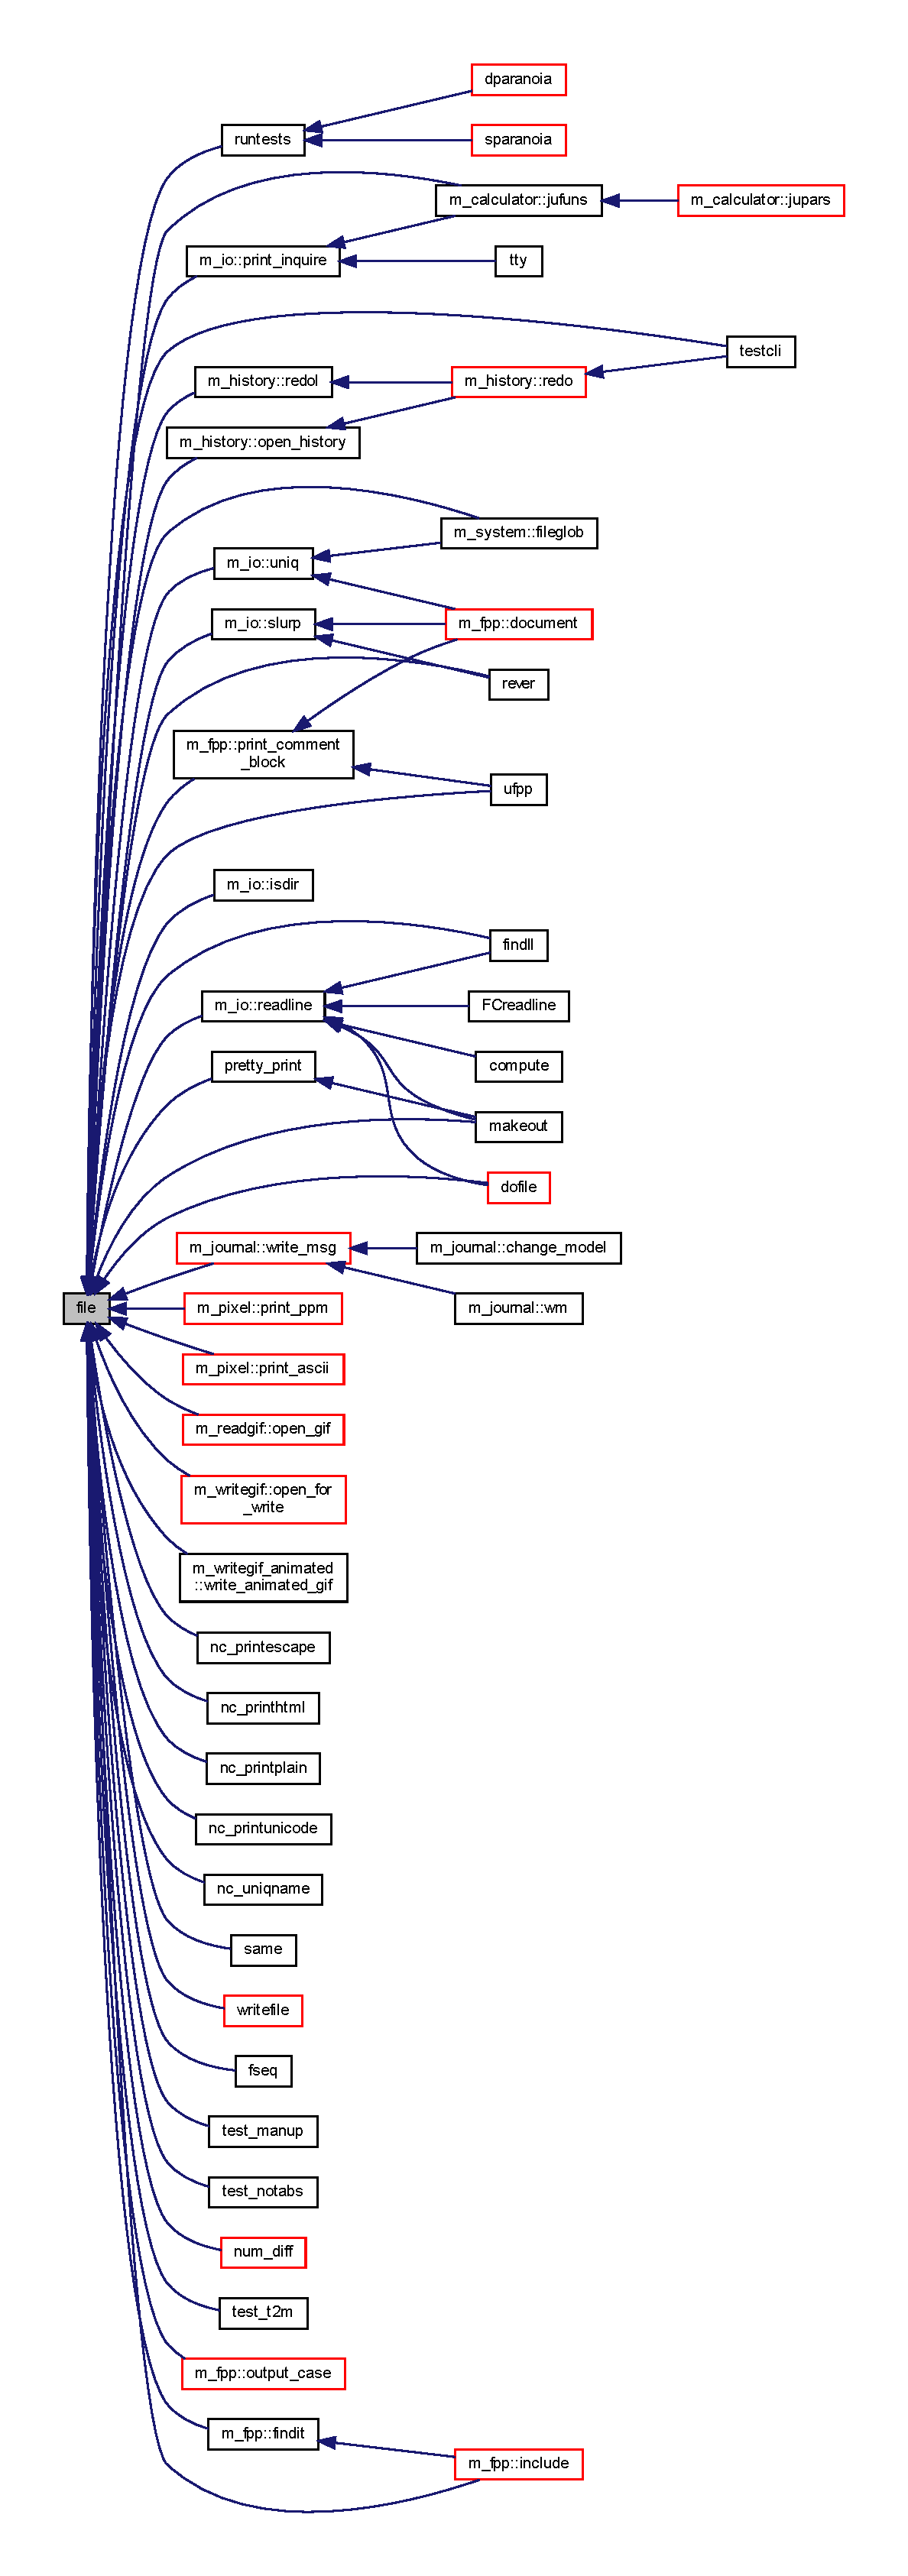
\includegraphics[height=550pt]{what__overview_81_8txt_a447b56c526e8da30e0dc94673727ee25_icgraph}
\end{center}
\end{figure}
\mbox{\Hypertarget{what__overview_81_8txt_ab6ccd3cf736f24d661599d9ce944e9bf}\label{what__overview_81_8txt_ab6ccd3cf736f24d661599d9ce944e9bf}} 
\index{what\+\_\+overview.\+1.\+txt@{what\+\_\+overview.\+1.\+txt}!form@{form}}
\index{form@{form}!what\+\_\+overview.\+1.\+txt@{what\+\_\+overview.\+1.\+txt}}
\subsubsection{\texorpdfstring{form()}{form()}}
{\footnotesize\ttfamily lib\+G\+PF Home Page Extracting File Identification \hyperlink{M__stopwatch_83_8txt_ad62a52042bb610eee5b36b5516caec22}{this} download contains a Fortran based \hyperlink{inquiry__stopwatch_83_8txt_aee378be19d20935dd436517beda00ee4}{version} \hyperlink{M__journal_83_8txt_afce72651d1eed785a2132bee863b2f38}{in} \hyperlink{ufpp__overview_81_8txt_a4d6669ece605d05985c83a04dd38e0ad}{source} form What \hyperlink{intro__blas1_83_8txt_a42a91df93f840595de3019ceb5d1df23}{is} an author \hyperlink{what__overview_81_8txt_a93f5d39a36ed511cc0dc88a20a517388}{or} a \hyperlink{inquiry__stopwatch_83_8txt_aee378be19d20935dd436517beda00ee4}{version} and a revision date The just as you \hyperlink{intro__blas1_83_8txt_a04fa2694d85f67a675bb3f45f7241f48}{use} \hyperlink{M__stopwatch_83_8txt_a0f266597de2e57eb3aa964927bb30e14}{the} you can \hyperlink{intro__blas1_83_8txt_a04fa2694d85f67a675bb3f45f7241f48}{use} \hyperlink{M__stopwatch_83_8txt_a0f266597de2e57eb3aa964927bb30e14}{the} \hyperlink{M__stopwatch_83_8txt_a0f266597de2e57eb3aa964927bb30e14}{the} \hyperlink{what__overview_81_8txt_a93f5d39a36ed511cc0dc88a20a517388}{or} \hyperlink{M__stopwatch_83_8txt_aff7b067dcc41169a210cb1c0de45a496}{one} of \hyperlink{M__stopwatch_83_8txt_a0f266597de2e57eb3aa964927bb30e14}{the} following characters \hyperlink{M__stopwatch_83_8txt_a5040be02b832eba08820289c8a1f81c4}{are} Try \hyperlink{what__overview_81_8txt_a1468cf345691ca45f70578e0b7abd264}{it} To get a taste for \hyperlink{M__stopwatch_83_8txt_a0f266597de2e57eb3aa964927bb30e14}{the} \hyperlink{sparanoia_8f90_aa0f6d55a5569e0c070c918b0716dc073}{power} of such a standard as \hyperlink{M__stopwatch_83_8txt_a0f266597de2e57eb3aa964927bb30e14}{the} S\+C\+CS identification take a directory with some simple \hyperlink{ufpp__overview_81_8txt_adb8870130f8d1e42bd6bfc128a290250}{scripts} \hyperlink{what__overview_81_8txt_a93f5d39a36ed511cc0dc88a20a517388}{or} \hyperlink{ufpp__overview_81_8txt_a4d6669ece605d05985c83a04dd38e0ad}{source} \hyperlink{ufpp__overview_81_8txt_a5673f2294ff1627be40c90eae33141ca}{files} \hyperlink{M__journal_83_8txt_afce72651d1eed785a2132bee863b2f38}{in} enter a short description \hyperlink{M__journal_83_8txt_afce72651d1eed785a2132bee863b2f38}{in} a comment of \hyperlink{M__stopwatch_83_8txt_a0f266597de2e57eb3aa964927bb30e14}{the} form (\begin{DoxyParamCaption}\item[{\#}]{ }\end{DoxyParamCaption})}

\mbox{\Hypertarget{what__overview_81_8txt_a7d9f0f7f68d767709cf298ae59490237}\label{what__overview_81_8txt_a7d9f0f7f68d767709cf298ae59490237}} 
\index{what\+\_\+overview.\+1.\+txt@{what\+\_\+overview.\+1.\+txt}!numdiff@{numdiff}}
\index{numdiff@{numdiff}!what\+\_\+overview.\+1.\+txt@{what\+\_\+overview.\+1.\+txt}}
\subsubsection{\texorpdfstring{numdiff()}{numdiff()}}
{\footnotesize\ttfamily which updates F77 with some F90 syntax \hyperlink{what__overview_81_8txt_aab2f56fdcdfab484c0d861985675a92f}{f90doc} numdiff (\begin{DoxyParamCaption}\item[{1}]{ }\end{DoxyParamCaption})}

\mbox{\Hypertarget{what__overview_81_8txt_ab5692ed87074f1d5ec850a9ffa8b5af9}\label{what__overview_81_8txt_ab5692ed87074f1d5ec850a9ffa8b5af9}} 
\index{what\+\_\+overview.\+1.\+txt@{what\+\_\+overview.\+1.\+txt}!size@{size}}
\index{size@{size}!what\+\_\+overview.\+1.\+txt@{what\+\_\+overview.\+1.\+txt}}
\subsubsection{\texorpdfstring{size()}{size()}}
{\footnotesize\ttfamily which updates F77 with some F90 syntax \hyperlink{what__overview_81_8txt_aab2f56fdcdfab484c0d861985675a92f}{f90doc} size (\begin{DoxyParamCaption}\item[{1}]{ }\end{DoxyParamCaption})}

Here is the caller graph for this function\+:
\nopagebreak
\begin{figure}[H]
\begin{center}
\leavevmode
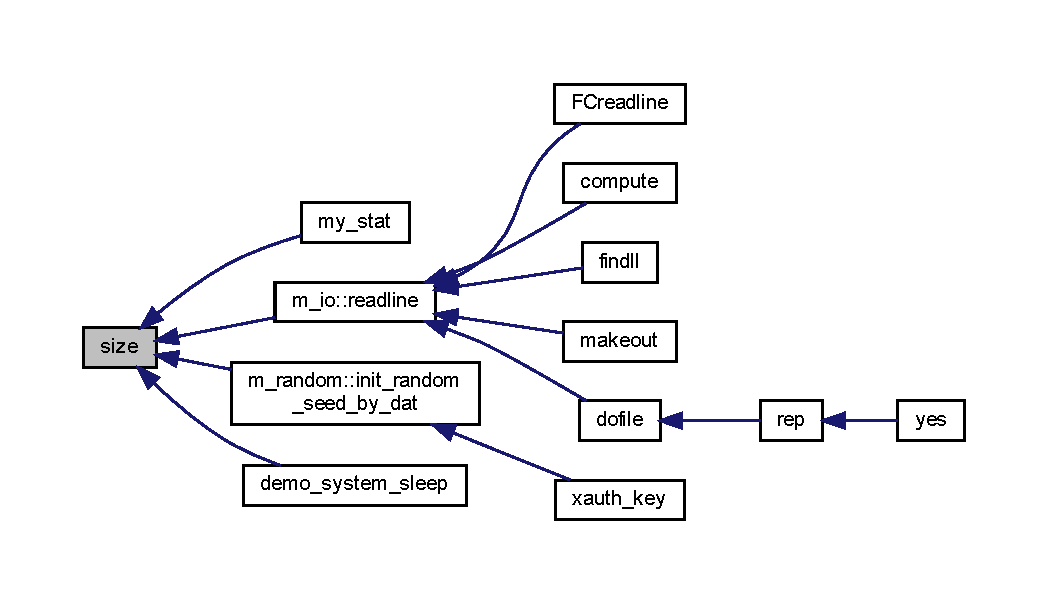
\includegraphics[width=350pt]{what__overview_81_8txt_ab5692ed87074f1d5ec850a9ffa8b5af9_icgraph}
\end{center}
\end{figure}
\mbox{\Hypertarget{what__overview_81_8txt_a8cdf8efd1b900d6dce77a3f97edb2216}\label{what__overview_81_8txt_a8cdf8efd1b900d6dce77a3f97edb2216}} 
\index{what\+\_\+overview.\+1.\+txt@{what\+\_\+overview.\+1.\+txt}!what@{what}}
\index{what@{what}!what\+\_\+overview.\+1.\+txt@{what\+\_\+overview.\+1.\+txt}}
\subsubsection{\texorpdfstring{what()}{what()}}
{\footnotesize\ttfamily which updates F77 with some F90 syntax \hyperlink{what__overview_81_8txt_aab2f56fdcdfab484c0d861985675a92f}{f90doc} what (\begin{DoxyParamCaption}\item[{1}]{ }\end{DoxyParamCaption})\hspace{0.3cm}{\ttfamily [new]}}



\subsection{Variable Documentation}
\mbox{\Hypertarget{what__overview_81_8txt_ac0a3098bb3d5de70ed1c81da8bfd2599}\label{what__overview_81_8txt_ac0a3098bb3d5de70ed1c81da8bfd2599}} 
\index{what\+\_\+overview.\+1.\+txt@{what\+\_\+overview.\+1.\+txt}!found@{found}}
\index{found@{found}!what\+\_\+overview.\+1.\+txt@{what\+\_\+overview.\+1.\+txt}}
\subsubsection{\texorpdfstring{found}{found}}
{\footnotesize\ttfamily lib\+G\+PF Home Page Extracting File Identification \hyperlink{M__stopwatch_83_8txt_ad62a52042bb610eee5b36b5516caec22}{this} download contains a Fortran based \hyperlink{inquiry__stopwatch_83_8txt_aee378be19d20935dd436517beda00ee4}{version} \hyperlink{M__journal_83_8txt_afce72651d1eed785a2132bee863b2f38}{in} \hyperlink{ufpp__overview_81_8txt_a4d6669ece605d05985c83a04dd38e0ad}{source} \hyperlink{what__overview_81_8txt_ab6ccd3cf736f24d661599d9ce944e9bf}{form} What \hyperlink{intro__blas1_83_8txt_a42a91df93f840595de3019ceb5d1df23}{is} an author \hyperlink{what__overview_81_8txt_a93f5d39a36ed511cc0dc88a20a517388}{or} a \hyperlink{inquiry__stopwatch_83_8txt_aee378be19d20935dd436517beda00ee4}{version} and a revision date The just as you \hyperlink{intro__blas1_83_8txt_a04fa2694d85f67a675bb3f45f7241f48}{use} \hyperlink{M__stopwatch_83_8txt_a0f266597de2e57eb3aa964927bb30e14}{the} you can \hyperlink{intro__blas1_83_8txt_a04fa2694d85f67a675bb3f45f7241f48}{use} \hyperlink{M__stopwatch_83_8txt_a0f266597de2e57eb3aa964927bb30e14}{the} \hyperlink{M__stopwatch_83_8txt_a0f266597de2e57eb3aa964927bb30e14}{the} \hyperlink{what__overview_81_8txt_a93f5d39a36ed511cc0dc88a20a517388}{or} \hyperlink{M__stopwatch_83_8txt_aff7b067dcc41169a210cb1c0de45a496}{one} of \hyperlink{M__stopwatch_83_8txt_a0f266597de2e57eb3aa964927bb30e14}{the} following characters \hyperlink{M__stopwatch_83_8txt_a5040be02b832eba08820289c8a1f81c4}{are} found}

\mbox{\Hypertarget{what__overview_81_8txt_a1468cf345691ca45f70578e0b7abd264}\label{what__overview_81_8txt_a1468cf345691ca45f70578e0b7abd264}} 
\index{what\+\_\+overview.\+1.\+txt@{what\+\_\+overview.\+1.\+txt}!it@{it}}
\index{it@{it}!what\+\_\+overview.\+1.\+txt@{what\+\_\+overview.\+1.\+txt}}
\subsubsection{\texorpdfstring{it}{it}}
{\footnotesize\ttfamily lib\+G\+PF Home Page Extracting File Identification \hyperlink{M__stopwatch_83_8txt_ad62a52042bb610eee5b36b5516caec22}{this} download contains a Fortran based \hyperlink{inquiry__stopwatch_83_8txt_aee378be19d20935dd436517beda00ee4}{version} \hyperlink{M__journal_83_8txt_afce72651d1eed785a2132bee863b2f38}{in} \hyperlink{ufpp__overview_81_8txt_a4d6669ece605d05985c83a04dd38e0ad}{source} \hyperlink{what__overview_81_8txt_ab6ccd3cf736f24d661599d9ce944e9bf}{form} What \hyperlink{intro__blas1_83_8txt_a42a91df93f840595de3019ceb5d1df23}{is} an author \hyperlink{what__overview_81_8txt_a93f5d39a36ed511cc0dc88a20a517388}{or} a \hyperlink{inquiry__stopwatch_83_8txt_aee378be19d20935dd436517beda00ee4}{version} and a revision date The just as you \hyperlink{intro__blas1_83_8txt_a04fa2694d85f67a675bb3f45f7241f48}{use} \hyperlink{M__stopwatch_83_8txt_a0f266597de2e57eb3aa964927bb30e14}{the} you can \hyperlink{intro__blas1_83_8txt_a04fa2694d85f67a675bb3f45f7241f48}{use} \hyperlink{M__stopwatch_83_8txt_a0f266597de2e57eb3aa964927bb30e14}{the} \hyperlink{M__stopwatch_83_8txt_a0f266597de2e57eb3aa964927bb30e14}{the} \hyperlink{what__overview_81_8txt_a93f5d39a36ed511cc0dc88a20a517388}{or} \hyperlink{M__stopwatch_83_8txt_aff7b067dcc41169a210cb1c0de45a496}{one} of \hyperlink{M__stopwatch_83_8txt_a0f266597de2e57eb3aa964927bb30e14}{the} following characters \hyperlink{M__stopwatch_83_8txt_a5040be02b832eba08820289c8a1f81c4}{are} Try it To get a taste for \hyperlink{M__stopwatch_83_8txt_a0f266597de2e57eb3aa964927bb30e14}{the} \hyperlink{sparanoia_8f90_aa0f6d55a5569e0c070c918b0716dc073}{power} of such a standard as \hyperlink{M__stopwatch_83_8txt_a0f266597de2e57eb3aa964927bb30e14}{the} S\+C\+CS identification take a directory with some simple \hyperlink{ufpp__overview_81_8txt_adb8870130f8d1e42bd6bfc128a290250}{scripts} \hyperlink{what__overview_81_8txt_a93f5d39a36ed511cc0dc88a20a517388}{or} \hyperlink{ufpp__overview_81_8txt_a4d6669ece605d05985c83a04dd38e0ad}{source} \hyperlink{ufpp__overview_81_8txt_a5673f2294ff1627be40c90eae33141ca}{files} \hyperlink{M__journal_83_8txt_afce72651d1eed785a2132bee863b2f38}{in} it}

\mbox{\Hypertarget{what__overview_81_8txt_a5168680dcac08de182f59de9a12c38ae}\label{what__overview_81_8txt_a5168680dcac08de182f59de9a12c38ae}} 
\index{what\+\_\+overview.\+1.\+txt@{what\+\_\+overview.\+1.\+txt}!number@{number}}
\index{number@{number}!what\+\_\+overview.\+1.\+txt@{what\+\_\+overview.\+1.\+txt}}
\subsubsection{\texorpdfstring{number}{number}}
{\footnotesize\ttfamily lib\+G\+PF Home Page Extracting File Identification \hyperlink{M__stopwatch_83_8txt_ad62a52042bb610eee5b36b5516caec22}{this} download contains a Fortran based \hyperlink{inquiry__stopwatch_83_8txt_aee378be19d20935dd436517beda00ee4}{version} \hyperlink{M__journal_83_8txt_afce72651d1eed785a2132bee863b2f38}{in} \hyperlink{ufpp__overview_81_8txt_a4d6669ece605d05985c83a04dd38e0ad}{source} \hyperlink{what__overview_81_8txt_ab6ccd3cf736f24d661599d9ce944e9bf}{form} What \hyperlink{intro__blas1_83_8txt_a42a91df93f840595de3019ceb5d1df23}{is} an author \hyperlink{what__overview_81_8txt_a93f5d39a36ed511cc0dc88a20a517388}{or} a \hyperlink{inquiry__stopwatch_83_8txt_aee378be19d20935dd436517beda00ee4}{version} number}

\mbox{\Hypertarget{what__overview_81_8txt_a93f5d39a36ed511cc0dc88a20a517388}\label{what__overview_81_8txt_a93f5d39a36ed511cc0dc88a20a517388}} 
\index{what\+\_\+overview.\+1.\+txt@{what\+\_\+overview.\+1.\+txt}!or@{or}}
\index{or@{or}!what\+\_\+overview.\+1.\+txt@{what\+\_\+overview.\+1.\+txt}}
\subsubsection{\texorpdfstring{or}{or}}
{\footnotesize\ttfamily lib\+G\+PF Home Page Extracting File Identification \hyperlink{M__stopwatch_83_8txt_ad62a52042bb610eee5b36b5516caec22}{this} download contains a Fortran based \hyperlink{inquiry__stopwatch_83_8txt_aee378be19d20935dd436517beda00ee4}{version} \hyperlink{M__journal_83_8txt_afce72651d1eed785a2132bee863b2f38}{in} \hyperlink{ufpp__overview_81_8txt_a4d6669ece605d05985c83a04dd38e0ad}{source} \hyperlink{what__overview_81_8txt_ab6ccd3cf736f24d661599d9ce944e9bf}{form} What \hyperlink{intro__blas1_83_8txt_a42a91df93f840595de3019ceb5d1df23}{is} an author or a \hyperlink{inquiry__stopwatch_83_8txt_aee378be19d20935dd436517beda00ee4}{version} and a revision date The just as you \hyperlink{intro__blas1_83_8txt_a04fa2694d85f67a675bb3f45f7241f48}{use} \hyperlink{M__stopwatch_83_8txt_a0f266597de2e57eb3aa964927bb30e14}{the} you can \hyperlink{intro__blas1_83_8txt_a04fa2694d85f67a675bb3f45f7241f48}{use} \hyperlink{M__stopwatch_83_8txt_a0f266597de2e57eb3aa964927bb30e14}{the} \hyperlink{M__stopwatch_83_8txt_a0f266597de2e57eb3aa964927bb30e14}{the} or \hyperlink{M__stopwatch_83_8txt_aff7b067dcc41169a210cb1c0de45a496}{one} of \hyperlink{M__stopwatch_83_8txt_a0f266597de2e57eb3aa964927bb30e14}{the} following characters \hyperlink{M__stopwatch_83_8txt_a5040be02b832eba08820289c8a1f81c4}{are} or}

\mbox{\Hypertarget{what__overview_81_8txt_a2e930424d80a25180e522874886f749a}\label{what__overview_81_8txt_a2e930424d80a25180e522874886f749a}} 
\index{what\+\_\+overview.\+1.\+txt@{what\+\_\+overview.\+1.\+txt}!originator@{originator}}
\index{originator@{originator}!what\+\_\+overview.\+1.\+txt@{what\+\_\+overview.\+1.\+txt}}
\subsubsection{\texorpdfstring{originator}{originator}}
{\footnotesize\ttfamily lib\+G\+PF Home Page Extracting File Identification \hyperlink{M__stopwatch_83_8txt_ad62a52042bb610eee5b36b5516caec22}{this} download contains a Fortran based \hyperlink{inquiry__stopwatch_83_8txt_aee378be19d20935dd436517beda00ee4}{version} \hyperlink{M__journal_83_8txt_afce72651d1eed785a2132bee863b2f38}{in} \hyperlink{ufpp__overview_81_8txt_a4d6669ece605d05985c83a04dd38e0ad}{source} \hyperlink{what__overview_81_8txt_ab6ccd3cf736f24d661599d9ce944e9bf}{form} What \hyperlink{intro__blas1_83_8txt_a42a91df93f840595de3019ceb5d1df23}{is} an author \hyperlink{what__overview_81_8txt_a93f5d39a36ed511cc0dc88a20a517388}{or} originator}

\mbox{\Hypertarget{what__overview_81_8txt_a74cb7e955273b9f9157b4f0c18a38849}\label{what__overview_81_8txt_a74cb7e955273b9f9157b4f0c18a38849}} 
\index{what\+\_\+overview.\+1.\+txt@{what\+\_\+overview.\+1.\+txt}!string@{string}}
\index{string@{string}!what\+\_\+overview.\+1.\+txt@{what\+\_\+overview.\+1.\+txt}}
\subsubsection{\texorpdfstring{string}{string}}
{\footnotesize\ttfamily lib\+G\+PF Home Page Extracting File Identification \hyperlink{M__stopwatch_83_8txt_ad62a52042bb610eee5b36b5516caec22}{this} download contains a Fortran based \hyperlink{inquiry__stopwatch_83_8txt_aee378be19d20935dd436517beda00ee4}{version} \hyperlink{M__journal_83_8txt_afce72651d1eed785a2132bee863b2f38}{in} \hyperlink{ufpp__overview_81_8txt_a4d6669ece605d05985c83a04dd38e0ad}{source} \hyperlink{what__overview_81_8txt_ab6ccd3cf736f24d661599d9ce944e9bf}{form} What \hyperlink{intro__blas1_83_8txt_a42a91df93f840595de3019ceb5d1df23}{is} an author \hyperlink{what__overview_81_8txt_a93f5d39a36ed511cc0dc88a20a517388}{or} a \hyperlink{inquiry__stopwatch_83_8txt_aee378be19d20935dd436517beda00ee4}{version} and a revision date The just as you \hyperlink{intro__blas1_83_8txt_a04fa2694d85f67a675bb3f45f7241f48}{use} \hyperlink{M__stopwatch_83_8txt_a0f266597de2e57eb3aa964927bb30e14}{the} you can \hyperlink{intro__blas1_83_8txt_a04fa2694d85f67a675bb3f45f7241f48}{use} \hyperlink{M__stopwatch_83_8txt_a0f266597de2e57eb3aa964927bb30e14}{the} \hyperlink{M__stopwatch_83_8txt_a0f266597de2e57eb3aa964927bb30e14}{the} \hyperlink{what__overview_81_8txt_a93f5d39a36ed511cc0dc88a20a517388}{or} \hyperlink{M__stopwatch_83_8txt_aff7b067dcc41169a210cb1c0de45a496}{one} of \hyperlink{M__stopwatch_83_8txt_a0f266597de2e57eb3aa964927bb30e14}{the} following characters \hyperlink{M__stopwatch_83_8txt_a5040be02b832eba08820289c8a1f81c4}{are} Try \hyperlink{what__overview_81_8txt_a1468cf345691ca45f70578e0b7abd264}{it} To get a taste for \hyperlink{M__stopwatch_83_8txt_a0f266597de2e57eb3aa964927bb30e14}{the} \hyperlink{sparanoia_8f90_aa0f6d55a5569e0c070c918b0716dc073}{power} of such a standard as \hyperlink{M__stopwatch_83_8txt_a0f266597de2e57eb3aa964927bb30e14}{the} S\+C\+CS identification string}


\hypertarget{juown1_8f90}{}\section{L\+I\+B\+R\+A\+R\+Y/lib\+G\+P\+F/download/tmp/juown1.f90 File Reference}
\label{juown1_8f90}\index{L\+I\+B\+R\+A\+R\+Y/lib\+G\+P\+F/download/tmp/juown1.\+f90@{L\+I\+B\+R\+A\+R\+Y/lib\+G\+P\+F/download/tmp/juown1.\+f90}}
\subsection*{Functions/\+Subroutines}
\begin{DoxyCompactItemize}
\item 
\hyperlink{M__stopwatch_83_8txt_acfbcff50169d691ff02d4a123ed70482}{subroutine} \hyperlink{juown1_8f90_a313c897cec3139ac9722b8f907c86495}{juown1} (func, iflen, args, iargstp, n, fval, ctmp, ier)
\end{DoxyCompactItemize}


\subsection{Function/\+Subroutine Documentation}
\mbox{\Hypertarget{juown1_8f90_a313c897cec3139ac9722b8f907c86495}\label{juown1_8f90_a313c897cec3139ac9722b8f907c86495}} 
\index{juown1.\+f90@{juown1.\+f90}!juown1@{juown1}}
\index{juown1@{juown1}!juown1.\+f90@{juown1.\+f90}}
\subsubsection{\texorpdfstring{juown1()}{juown1()}}
{\footnotesize\ttfamily \hyperlink{M__stopwatch_83_8txt_acfbcff50169d691ff02d4a123ed70482}{subroutine} juown1 (\begin{DoxyParamCaption}\item[{\hyperlink{option__stopwatch_83_8txt_abd4b21fbbd175834027b5224bfe97e66}{character}(len=$\ast$)}]{func,  }\item[{integer}]{iflen,  }\item[{\hyperlink{read__watch_83_8txt_abdb62bde002f38ef75f810d3a905a823}{real}(kind=dp), dimension(100)}]{args,  }\item[{integer, dimension(100)}]{iargstp,  }\item[{integer}]{n,  }\item[{\hyperlink{read__watch_83_8txt_abdb62bde002f38ef75f810d3a905a823}{real}(kind=dp)}]{fval,  }\item[{\hyperlink{option__stopwatch_83_8txt_abd4b21fbbd175834027b5224bfe97e66}{character}(len=$\ast$)}]{ctmp,  }\item[{integer}]{ier }\end{DoxyParamCaption})}


\hypertarget{M__anyscalar_8f90}{}\section{L\+I\+B\+R\+A\+R\+Y/lib\+G\+P\+F/download/tmp/\+M\+\_\+anyscalar.f90 File Reference}
\label{M__anyscalar_8f90}\index{L\+I\+B\+R\+A\+R\+Y/lib\+G\+P\+F/download/tmp/\+M\+\_\+anyscalar.\+f90@{L\+I\+B\+R\+A\+R\+Y/lib\+G\+P\+F/download/tmp/\+M\+\_\+anyscalar.\+f90}}
\subsection*{Modules}
\begin{DoxyCompactItemize}
\item 
module \hyperlink{namespacem__anyscalar}{m\+\_\+anyscalar}
\end{DoxyCompactItemize}
\subsection*{Functions/\+Subroutines}
\begin{DoxyCompactItemize}
\item 
pure doubleprecision function, \hyperlink{M__stopwatch_83_8txt_a2f74811300c361e53b430611a7d1769f}{public} \hyperlink{namespacem__anyscalar_a6173dbc57e7c5a96f5961d9e83e6e15e}{m\+\_\+anyscalar\+::anyscalar\+\_\+to\+\_\+double} (valuein)
\begin{DoxyCompactList}\small\item\em \subsubsection*{N\+A\+ME}

anyscalar\+\_\+to\+\_\+double(3f) -\/ \mbox{[}M\+\_\+anyscalar\mbox{]} convert integer or real parameter of any kind to doubleprecision \end{DoxyCompactList}\item 
pure \hyperlink{read__watch_83_8txt_abdb62bde002f38ef75f810d3a905a823}{real} function, \hyperlink{M__stopwatch_83_8txt_a2f74811300c361e53b430611a7d1769f}{public} \hyperlink{namespacem__anyscalar_a39cd9a778fff85974fa1a822b92555fd}{m\+\_\+anyscalar\+::anyscalar\+\_\+to\+\_\+real} (valuein)
\begin{DoxyCompactList}\small\item\em \subsubsection*{N\+A\+ME}

anyscalar\+\_\+to\+\_\+real(3f) -\/ \mbox{[}M\+\_\+anyscalar\mbox{]} convert integer or real parameter of any kind to real \end{DoxyCompactList}\item 
elemental integer(kind=int128) function, \hyperlink{M__stopwatch_83_8txt_a2f74811300c361e53b430611a7d1769f}{public} \hyperlink{namespacem__anyscalar_a513beeccb5c821157cbd2eea8a1d9842}{m\+\_\+anyscalar\+::anyinteger\+\_\+to\+\_\+128bit} (intin)
\begin{DoxyCompactList}\small\item\em \subsubsection*{N\+A\+ME}\end{DoxyCompactList}\end{DoxyCompactItemize}
\subsection*{Variables}
\begin{DoxyCompactItemize}
\item 
integer, dimension(38), parameter \hyperlink{namespacem__anyscalar_a099da1dd8639cdce3d0f5bb3cb8fbd03}{m\+\_\+anyscalar\+::k} =\mbox{[}(selected\+\_\+int\+\_\+kind(\hyperlink{intro__blas1_83_8txt_a8ba82a50c0c2c12d5f6a77f7e4651c0b}{i}),\hyperlink{intro__blas1_83_8txt_a8ba82a50c0c2c12d5f6a77f7e4651c0b}{i}=1,38)\mbox{]}
\item 
integer, parameter, \hyperlink{M__stopwatch_83_8txt_a2f74811300c361e53b430611a7d1769f}{public} \hyperlink{namespacem__anyscalar_a53057899b7d17505b79d9b8f5e6092a2}{m\+\_\+anyscalar\+::int128} =k(38)
\item 
integer, dimension(34), parameter \hyperlink{namespacem__anyscalar_af515907c09cc2ac286a4523cc73f5f52}{m\+\_\+anyscalar\+::r} =\mbox{[}(selected\+\_\+int\+\_\+kind(\hyperlink{intro__blas1_83_8txt_a8ba82a50c0c2c12d5f6a77f7e4651c0b}{i}),\hyperlink{intro__blas1_83_8txt_a8ba82a50c0c2c12d5f6a77f7e4651c0b}{i}=1,34)\mbox{]}
\item 
integer, parameter, \hyperlink{M__stopwatch_83_8txt_a2f74811300c361e53b430611a7d1769f}{public} \hyperlink{namespacem__anyscalar_a6d3ef2bc1698c91d737dbd8824a9eb0b}{m\+\_\+anyscalar\+::real256} =r(34)
\end{DoxyCompactItemize}

\hypertarget{M__journal_8f90}{}\section{L\+I\+B\+R\+A\+R\+Y/lib\+G\+P\+F/download/tmp/\+M\+\_\+journal.f90 File Reference}
\label{M__journal_8f90}\index{L\+I\+B\+R\+A\+R\+Y/lib\+G\+P\+F/download/tmp/\+M\+\_\+journal.\+f90@{L\+I\+B\+R\+A\+R\+Y/lib\+G\+P\+F/download/tmp/\+M\+\_\+journal.\+f90}}
\subsection*{Data Types}
\begin{DoxyCompactItemize}
\item 
interface \hyperlink{interfacem__journal_1_1journal}{m\+\_\+journal\+::journal}
\begin{DoxyCompactList}\small\item\em \subsubsection*{N\+A\+ME}

journal(3f) -\/ \mbox{[}M\+\_\+journal\mbox{]} provides public message routine, no paging or graphic mode change" \subsubsection*{S\+Y\+N\+O\+P\+S\+IS}\end{DoxyCompactList}\end{DoxyCompactItemize}
\subsection*{Modules}
\begin{DoxyCompactItemize}
\item 
module \hyperlink{namespacem__journal}{m\+\_\+journal}
\end{DoxyCompactItemize}
\subsection*{Functions/\+Subroutines}
\begin{DoxyCompactItemize}
\item 
\hyperlink{M__stopwatch_83_8txt_acfbcff50169d691ff02d4a123ed70482}{subroutine} \hyperlink{namespacem__journal_a98698c251ec1883612ae40c5f2443fd9}{m\+\_\+journal\+::write\+\_\+msg} (where, msg)
\item 
\hyperlink{M__stopwatch_83_8txt_acfbcff50169d691ff02d4a123ed70482}{subroutine} \hyperlink{namespacem__journal_a0f2ac99f3da62381d2466c150830b9e0}{m\+\_\+journal\+::set\+\_\+stdout} (iounit)
\item 
\hyperlink{M__stopwatch_83_8txt_acfbcff50169d691ff02d4a123ed70482}{subroutine} \hyperlink{namespacem__journal_a358c4bd99444e0e946b3aaba5f278698}{m\+\_\+journal\+::change\+\_\+model} (value, mode)
\item 
\hyperlink{M__stopwatch_83_8txt_acfbcff50169d691ff02d4a123ed70482}{subroutine} \hyperlink{namespacem__journal_a98479e5ace98340f7519470b96d3197d}{m\+\_\+journal\+::wm} (\hyperlink{M__stopwatch_83_8txt_aa4313e9a55405841f95e6550cd87fc3b}{message})
\item 
\hyperlink{M__stopwatch_83_8txt_acfbcff50169d691ff02d4a123ed70482}{subroutine} \hyperlink{namespacem__journal_ad22893c3621042df7d66b9f3864aa457}{m\+\_\+journal\+::wm\+\_\+r} (where, \hyperlink{M__stopwatch_83_8txt_aa4313e9a55405841f95e6550cd87fc3b}{message}, value)
\item 
\hyperlink{M__stopwatch_83_8txt_acfbcff50169d691ff02d4a123ed70482}{subroutine} \hyperlink{namespacem__journal_a3229165c77bc7f39fbf88fbcfbdb401e}{m\+\_\+journal\+::wm\+\_\+l} (where, \hyperlink{M__stopwatch_83_8txt_aa4313e9a55405841f95e6550cd87fc3b}{message}, truefalse)
\item 
\hyperlink{M__stopwatch_83_8txt_acfbcff50169d691ff02d4a123ed70482}{subroutine} \hyperlink{namespacem__journal_ae4e688044197dd70bd47b4d7c0bb7306}{m\+\_\+journal\+::wm\+\_\+d} (where, \hyperlink{M__stopwatch_83_8txt_aa4313e9a55405841f95e6550cd87fc3b}{message}, dvalue)
\item 
\hyperlink{M__stopwatch_83_8txt_acfbcff50169d691ff02d4a123ed70482}{subroutine} \hyperlink{namespacem__journal_a931487b48fc9268afb0c286c3c3892ad}{m\+\_\+journal\+::wm\+\_\+i} (where, \hyperlink{M__stopwatch_83_8txt_aa4313e9a55405841f95e6550cd87fc3b}{message}, ival)
\end{DoxyCompactItemize}
\subsection*{Variables}
\begin{DoxyCompactItemize}
\item 
\hyperlink{option__stopwatch_83_8txt_abd4b21fbbd175834027b5224bfe97e66}{character}(len= $\ast$), parameter \hyperlink{namespacem__journal_a4e2131bb2d66050e0a9a37632579c9fc}{m\+\_\+journal\+::ident} =\char`\"{}@(\#)M\+\_\+journal\+::journal(3fg)\+: provides public message routine, no paging or graphic mode change\char`\"{}
\item 
integer, save, private \hyperlink{namespacem__journal_a664cf3fd85385b776d30ea589606ad1c}{m\+\_\+journal\+::stdout} =O\+U\+T\+P\+U\+T\+\_\+\+U\+N\+IT
\item 
logical, save \hyperlink{namespacem__journal_a6184fbcebdfa06f0a45ce4c699189b53}{m\+\_\+journal\+::debug} =.false.
\item 
integer, save \hyperlink{namespacem__journal_a47e8e34dc4072b04101027394d688519}{m\+\_\+journal\+::last\+\_\+int} =0
\end{DoxyCompactItemize}

\hypertarget{mainpage_8txt}{}\section{L\+I\+B\+R\+A\+R\+Y/lib\+G\+P\+F/download/tmp/mainpage.txt File Reference}
\label{mainpage_8txt}\index{L\+I\+B\+R\+A\+R\+Y/lib\+G\+P\+F/download/tmp/mainpage.\+txt@{L\+I\+B\+R\+A\+R\+Y/lib\+G\+P\+F/download/tmp/mainpage.\+txt}}

\hypertarget{__dirname_8f90}{}\section{L\+I\+B\+R\+A\+R\+Y/lib\+G\+P\+F/download/tmp/\+P\+R\+O\+G\+R\+A\+M\+S/\+\_\+dirname.f90 File Reference}
\label{__dirname_8f90}\index{L\+I\+B\+R\+A\+R\+Y/lib\+G\+P\+F/download/tmp/\+P\+R\+O\+G\+R\+A\+M\+S/\+\_\+dirname.\+f90@{L\+I\+B\+R\+A\+R\+Y/lib\+G\+P\+F/download/tmp/\+P\+R\+O\+G\+R\+A\+M\+S/\+\_\+dirname.\+f90}}

\hypertarget{__echo_8f90}{}\section{L\+I\+B\+R\+A\+R\+Y/lib\+G\+P\+F/download/tmp/\+P\+R\+O\+G\+R\+A\+M\+S/\+\_\+echo.f90 File Reference}
\label{__echo_8f90}\index{L\+I\+B\+R\+A\+R\+Y/lib\+G\+P\+F/download/tmp/\+P\+R\+O\+G\+R\+A\+M\+S/\+\_\+echo.\+f90@{L\+I\+B\+R\+A\+R\+Y/lib\+G\+P\+F/download/tmp/\+P\+R\+O\+G\+R\+A\+M\+S/\+\_\+echo.\+f90}}

\hypertarget{__false_8f90}{}\section{L\+I\+B\+R\+A\+R\+Y/lib\+G\+P\+F/download/tmp/\+P\+R\+O\+G\+R\+A\+M\+S/\+\_\+false.f90 File Reference}
\label{__false_8f90}\index{L\+I\+B\+R\+A\+R\+Y/lib\+G\+P\+F/download/tmp/\+P\+R\+O\+G\+R\+A\+M\+S/\+\_\+false.\+f90@{L\+I\+B\+R\+A\+R\+Y/lib\+G\+P\+F/download/tmp/\+P\+R\+O\+G\+R\+A\+M\+S/\+\_\+false.\+f90}}
\subsection*{Functions/\+Subroutines}
\begin{DoxyCompactItemize}
\item 
\hyperlink{M__stopwatch_83_8txt_acfbcff50169d691ff02d4a123ed70482}{subroutine} \hyperlink{__false_8f90_a3e09a3b52ee8fb04eeb93fe5761626a8}{help\+\_\+usage} (l\+\_\+help)
\item 
\hyperlink{M__stopwatch_83_8txt_acfbcff50169d691ff02d4a123ed70482}{subroutine} \hyperlink{__false_8f90_a39c21619b08a3c22f19e2306efd7f766}{help\+\_\+version} (l\+\_\+version)
\begin{DoxyCompactList}\small\item\em \subsubsection*{N\+A\+ME}

\+\_\+false(1f) -\/ \mbox{[}F\+U\+N\+IX\mbox{]} do nothing, unsuccessfully \end{DoxyCompactList}\item 
program \hyperlink{__false_8f90_ac39cd9fe2012c31749944aa6b20b6c05}{false}
\end{DoxyCompactItemize}


\subsection{Function/\+Subroutine Documentation}
\mbox{\Hypertarget{__false_8f90_ac39cd9fe2012c31749944aa6b20b6c05}\label{__false_8f90_ac39cd9fe2012c31749944aa6b20b6c05}} 
\index{\+\_\+false.\+f90@{\+\_\+false.\+f90}!false@{false}}
\index{false@{false}!\+\_\+false.\+f90@{\+\_\+false.\+f90}}
\subsubsection{\texorpdfstring{false()}{false()}}
{\footnotesize\ttfamily program false (\begin{DoxyParamCaption}{ }\end{DoxyParamCaption})}



References m\+\_\+debug\+::fstop(), help\+\_\+usage(), help\+\_\+version(), m\+\_\+kracken\+::iget(), m\+\_\+messages\+::junroach(), m\+\_\+kracken\+::kracken(), and m\+\_\+kracken\+::lget().

Here is the call graph for this function\+:
\nopagebreak
\begin{figure}[H]
\begin{center}
\leavevmode
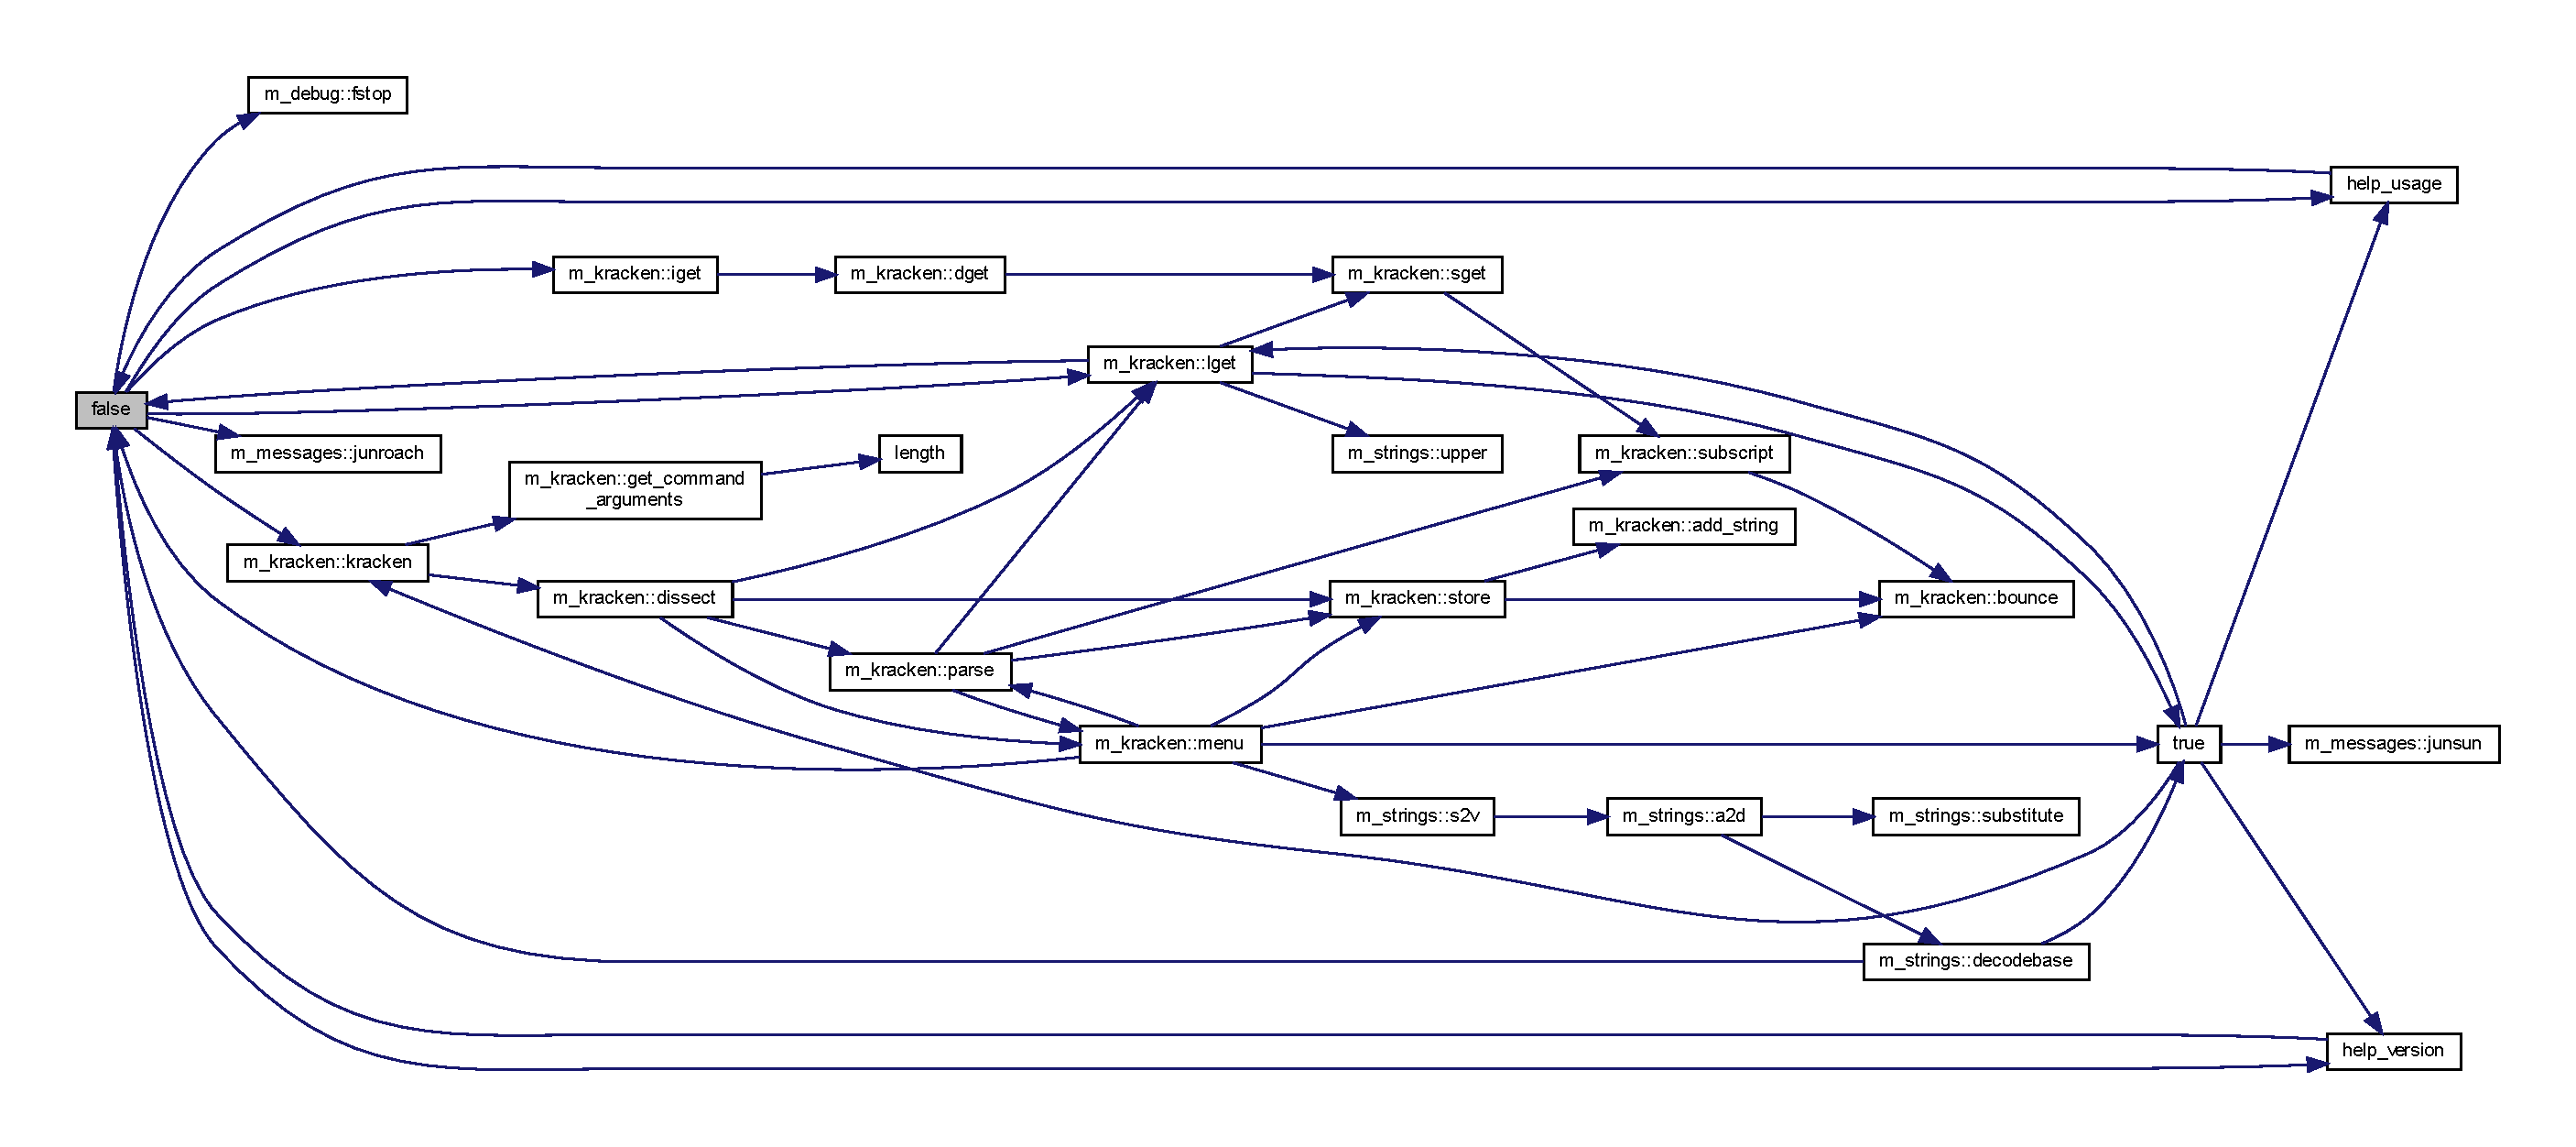
\includegraphics[width=350pt]{__false_8f90_ac39cd9fe2012c31749944aa6b20b6c05_cgraph}
\end{center}
\end{figure}
\mbox{\Hypertarget{__false_8f90_a3e09a3b52ee8fb04eeb93fe5761626a8}\label{__false_8f90_a3e09a3b52ee8fb04eeb93fe5761626a8}} 
\index{\+\_\+false.\+f90@{\+\_\+false.\+f90}!help\+\_\+usage@{help\+\_\+usage}}
\index{help\+\_\+usage@{help\+\_\+usage}!\+\_\+false.\+f90@{\+\_\+false.\+f90}}
\subsubsection{\texorpdfstring{help\+\_\+usage()}{help\_usage()}}
{\footnotesize\ttfamily \hyperlink{M__stopwatch_83_8txt_acfbcff50169d691ff02d4a123ed70482}{subroutine} help\+\_\+usage (\begin{DoxyParamCaption}\item[{logical, intent(\hyperlink{M__journal_83_8txt_afce72651d1eed785a2132bee863b2f38}{in})}]{l\+\_\+help }\end{DoxyParamCaption})}



References false().

Here is the call graph for this function\+:
\nopagebreak
\begin{figure}[H]
\begin{center}
\leavevmode
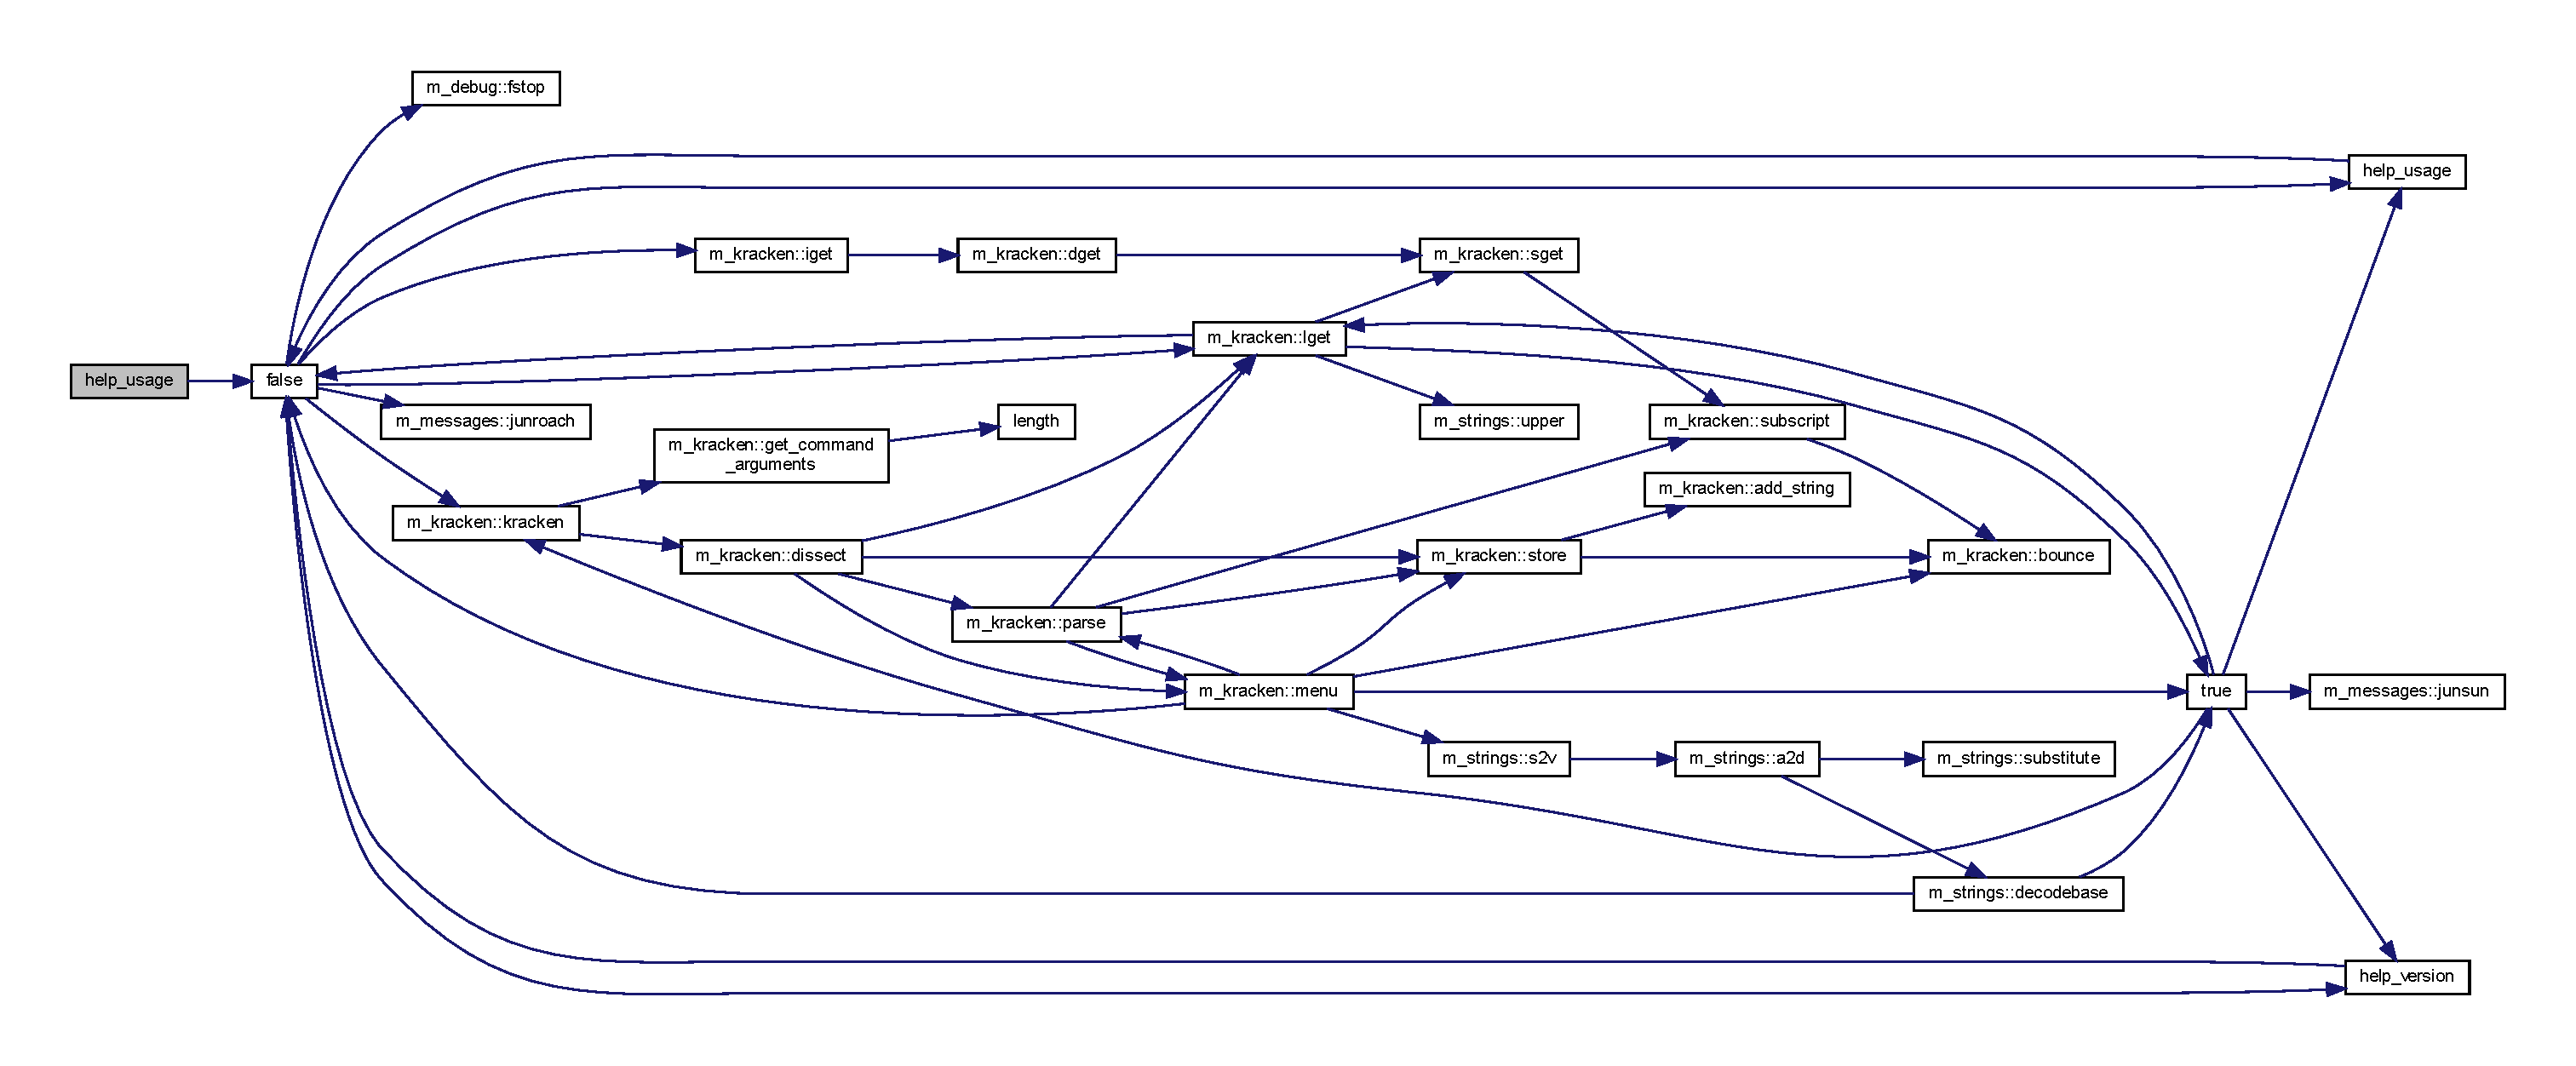
\includegraphics[width=350pt]{__false_8f90_a3e09a3b52ee8fb04eeb93fe5761626a8_cgraph}
\end{center}
\end{figure}
\mbox{\Hypertarget{__false_8f90_a39c21619b08a3c22f19e2306efd7f766}\label{__false_8f90_a39c21619b08a3c22f19e2306efd7f766}} 
\index{\+\_\+false.\+f90@{\+\_\+false.\+f90}!help\+\_\+version@{help\+\_\+version}}
\index{help\+\_\+version@{help\+\_\+version}!\+\_\+false.\+f90@{\+\_\+false.\+f90}}
\subsubsection{\texorpdfstring{help\+\_\+version()}{help\_version()}}
{\footnotesize\ttfamily \hyperlink{M__stopwatch_83_8txt_acfbcff50169d691ff02d4a123ed70482}{subroutine} help\+\_\+version (\begin{DoxyParamCaption}\item[{logical, intent(\hyperlink{M__journal_83_8txt_afce72651d1eed785a2132bee863b2f38}{in})}]{l\+\_\+version }\end{DoxyParamCaption})}



\subsubsection*{N\+A\+ME}

\+\_\+false(1f) -\/ \mbox{[}F\+U\+N\+IX\mbox{]} do nothing, unsuccessfully 

\subsubsection*{S\+Y\+N\+O\+P\+S\+IS}

\begin{DoxyVerb}    _false value [--help|--version--verbose]
\end{DoxyVerb}


\subsubsection*{D\+E\+S\+C\+R\+I\+P\+T\+I\+ON}

Exit with a status code indicating failure. \subsubsection*{O\+P\+T\+I\+O\+NS}

number optional number of 1 to 32, which will be used to generate the exit status code if supported. --help display this help and exit --version output version information and exit --verbose display A\+S\+C\+II graphic of cockroach

\subsubsection*{E\+X\+A\+M\+P\+LE}

\begin{DoxyVerb}   Bash example:

      _false || echo SHOULD PRINT THIS

      if _false
      then
         echo command got zero exit $?
      else
         echo command got non-zero exit $?
      fi

   Expected output::
      ERROR STOP
      SHOULD PRINT THIS
      ERROR STOP
      command got non-zero exit 1
\end{DoxyVerb}


\subsubsection*{S\+EE A\+L\+SO}

\+\_\+true(1f) 

References false().

Here is the call graph for this function\+:
\nopagebreak
\begin{figure}[H]
\begin{center}
\leavevmode
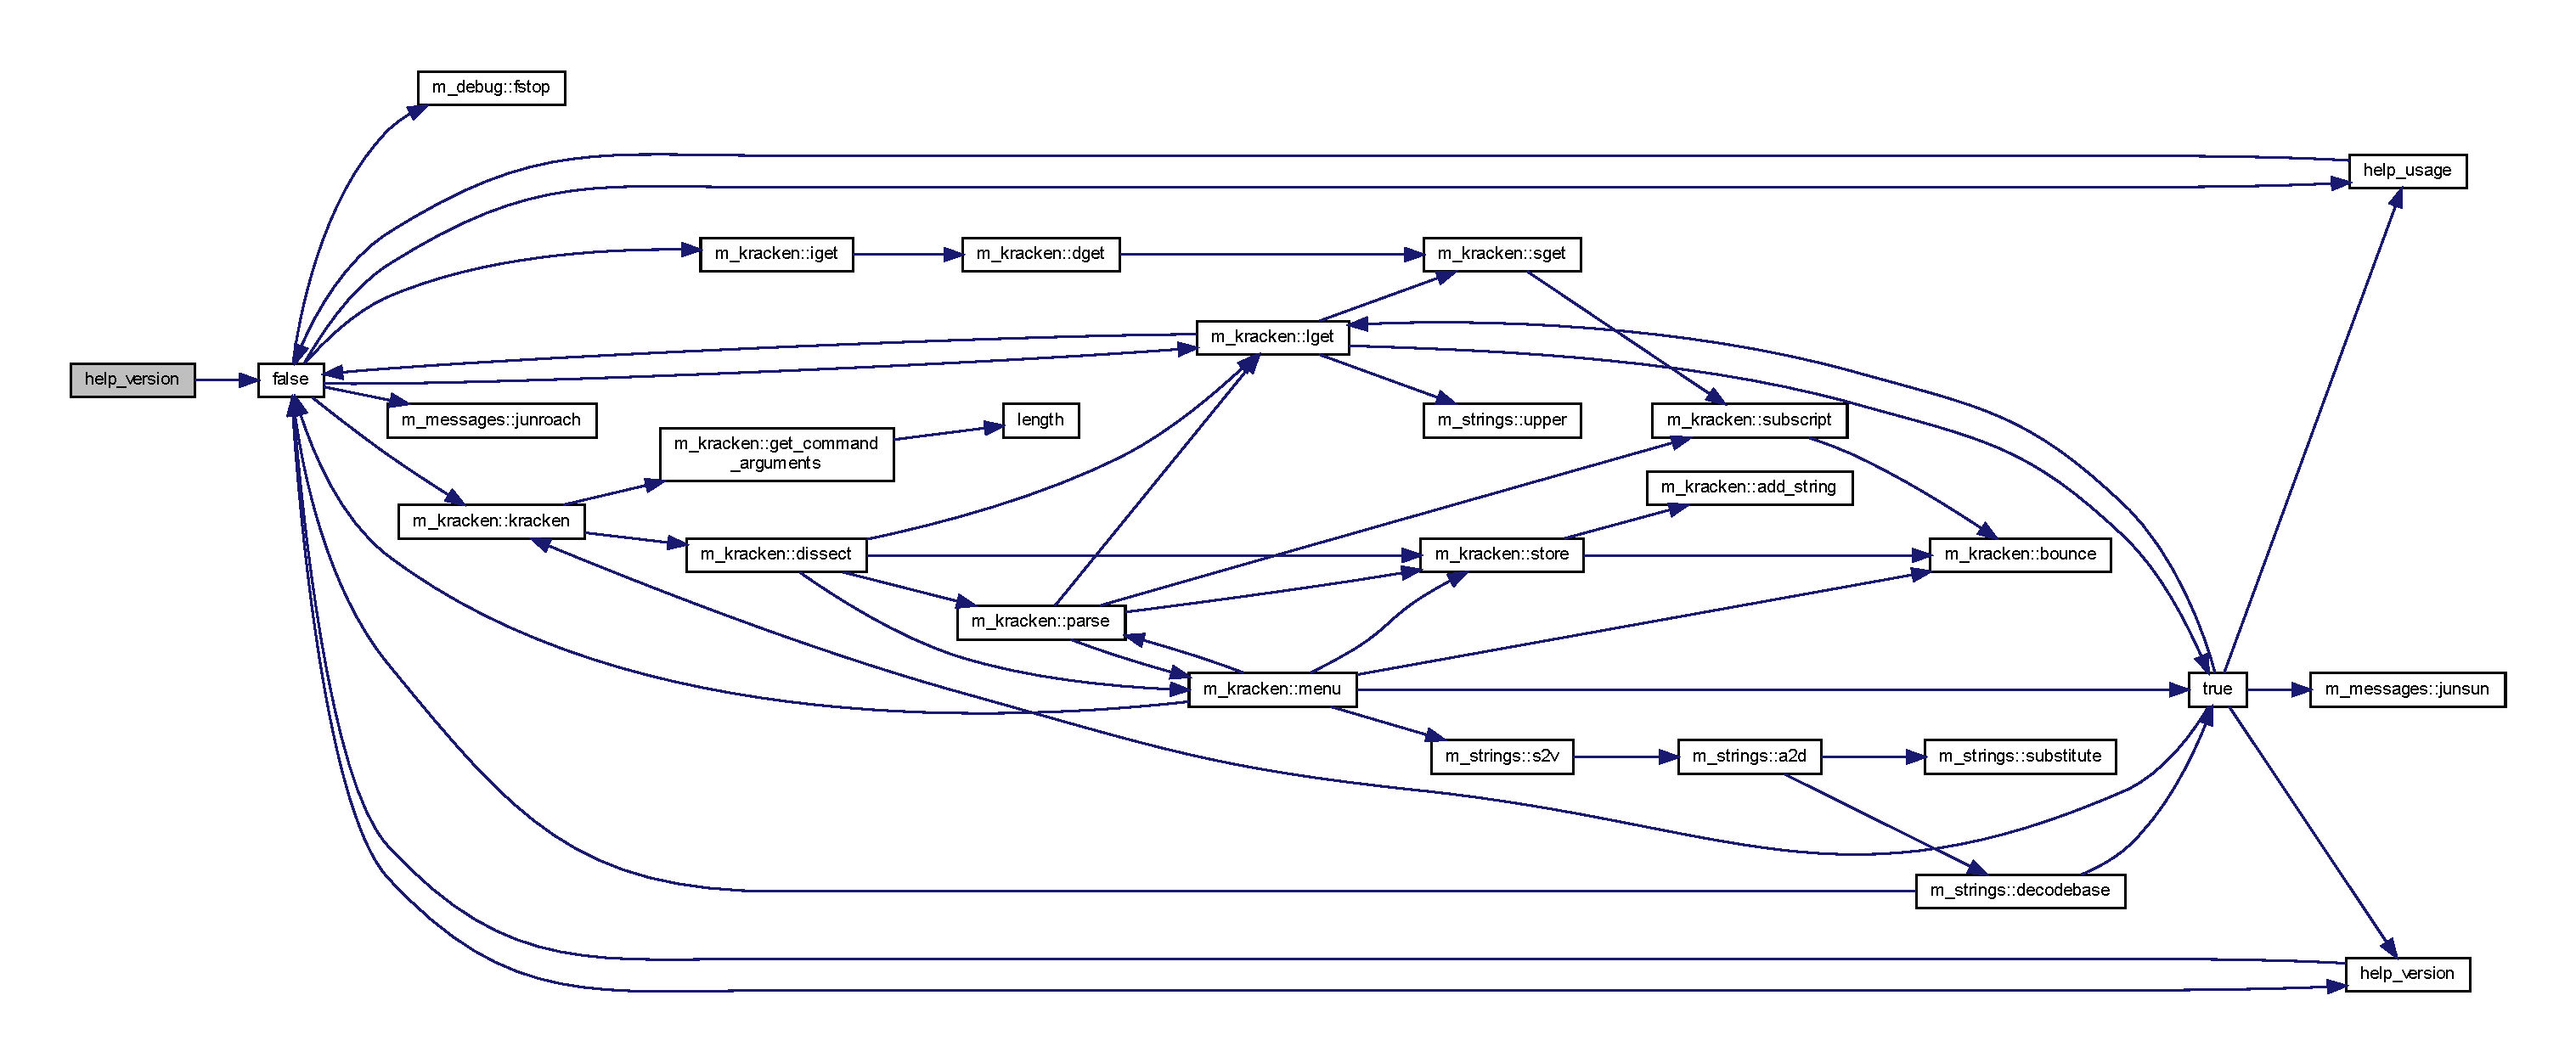
\includegraphics[width=350pt]{__false_8f90_a39c21619b08a3c22f19e2306efd7f766_cgraph}
\end{center}
\end{figure}

\hypertarget{__hostname_8f90}{}\section{L\+I\+B\+R\+A\+R\+Y/lib\+G\+P\+F/download/tmp/\+P\+R\+O\+G\+R\+A\+M\+S/\+\_\+hostname.f90 File Reference}
\label{__hostname_8f90}\index{L\+I\+B\+R\+A\+R\+Y/lib\+G\+P\+F/download/tmp/\+P\+R\+O\+G\+R\+A\+M\+S/\+\_\+hostname.\+f90@{L\+I\+B\+R\+A\+R\+Y/lib\+G\+P\+F/download/tmp/\+P\+R\+O\+G\+R\+A\+M\+S/\+\_\+hostname.\+f90}}
\subsection*{Functions/\+Subroutines}
\begin{DoxyCompactItemize}
\item 
\hyperlink{M__stopwatch_83_8txt_acfbcff50169d691ff02d4a123ed70482}{subroutine} \hyperlink{__hostname_8f90_a3e09a3b52ee8fb04eeb93fe5761626a8}{help\+\_\+usage} (l\+\_\+help)
\item 
\hyperlink{M__stopwatch_83_8txt_acfbcff50169d691ff02d4a123ed70482}{subroutine} \hyperlink{__hostname_8f90_a39c21619b08a3c22f19e2306efd7f766}{help\+\_\+version} (l\+\_\+version)
\begin{DoxyCompactList}\small\item\em \subsubsection*{N\+A\+ME}

\+\_\+hostname(1f) -\/ \mbox{[}F\+U\+N\+IX\mbox{]} display hostname \subsubsection*{S\+Y\+N\+T\+AX}

hostname \mbox{[}-\/help$\vert$-\/version\mbox{]} \subsubsection*{D\+E\+S\+C\+R\+I\+P\+T\+I\+ON}

Calls system\+\_\+gethostname(3f), which calls get\+\_\+hostname(3c) to determine the current host name. \subsubsection*{O\+P\+T\+I\+O\+NS}

--help display this help and exit --version output version information and exit \subsubsection*{E\+X\+A\+M\+P\+LE}\end{DoxyCompactList}\item 
program \hyperlink{__hostname_8f90_a8cf8b2c2d1597761d376d337686d3667}{demo\+\_\+system\+\_\+gethostname}
\end{DoxyCompactItemize}


\subsection{Function/\+Subroutine Documentation}
\mbox{\Hypertarget{__hostname_8f90_a8cf8b2c2d1597761d376d337686d3667}\label{__hostname_8f90_a8cf8b2c2d1597761d376d337686d3667}} 
\index{\+\_\+hostname.\+f90@{\+\_\+hostname.\+f90}!demo\+\_\+system\+\_\+gethostname@{demo\+\_\+system\+\_\+gethostname}}
\index{demo\+\_\+system\+\_\+gethostname@{demo\+\_\+system\+\_\+gethostname}!\+\_\+hostname.\+f90@{\+\_\+hostname.\+f90}}
\subsubsection{\texorpdfstring{demo\+\_\+system\+\_\+gethostname()}{demo\_system\_gethostname()}}
{\footnotesize\ttfamily program demo\+\_\+system\+\_\+gethostname (\begin{DoxyParamCaption}{ }\end{DoxyParamCaption})}



References help\+\_\+usage(), help\+\_\+version(), m\+\_\+kracken\+::kracken(), m\+\_\+kracken\+::lget(), and m\+\_\+system\+::system\+\_\+gethostname().

Here is the call graph for this function\+:
\nopagebreak
\begin{figure}[H]
\begin{center}
\leavevmode
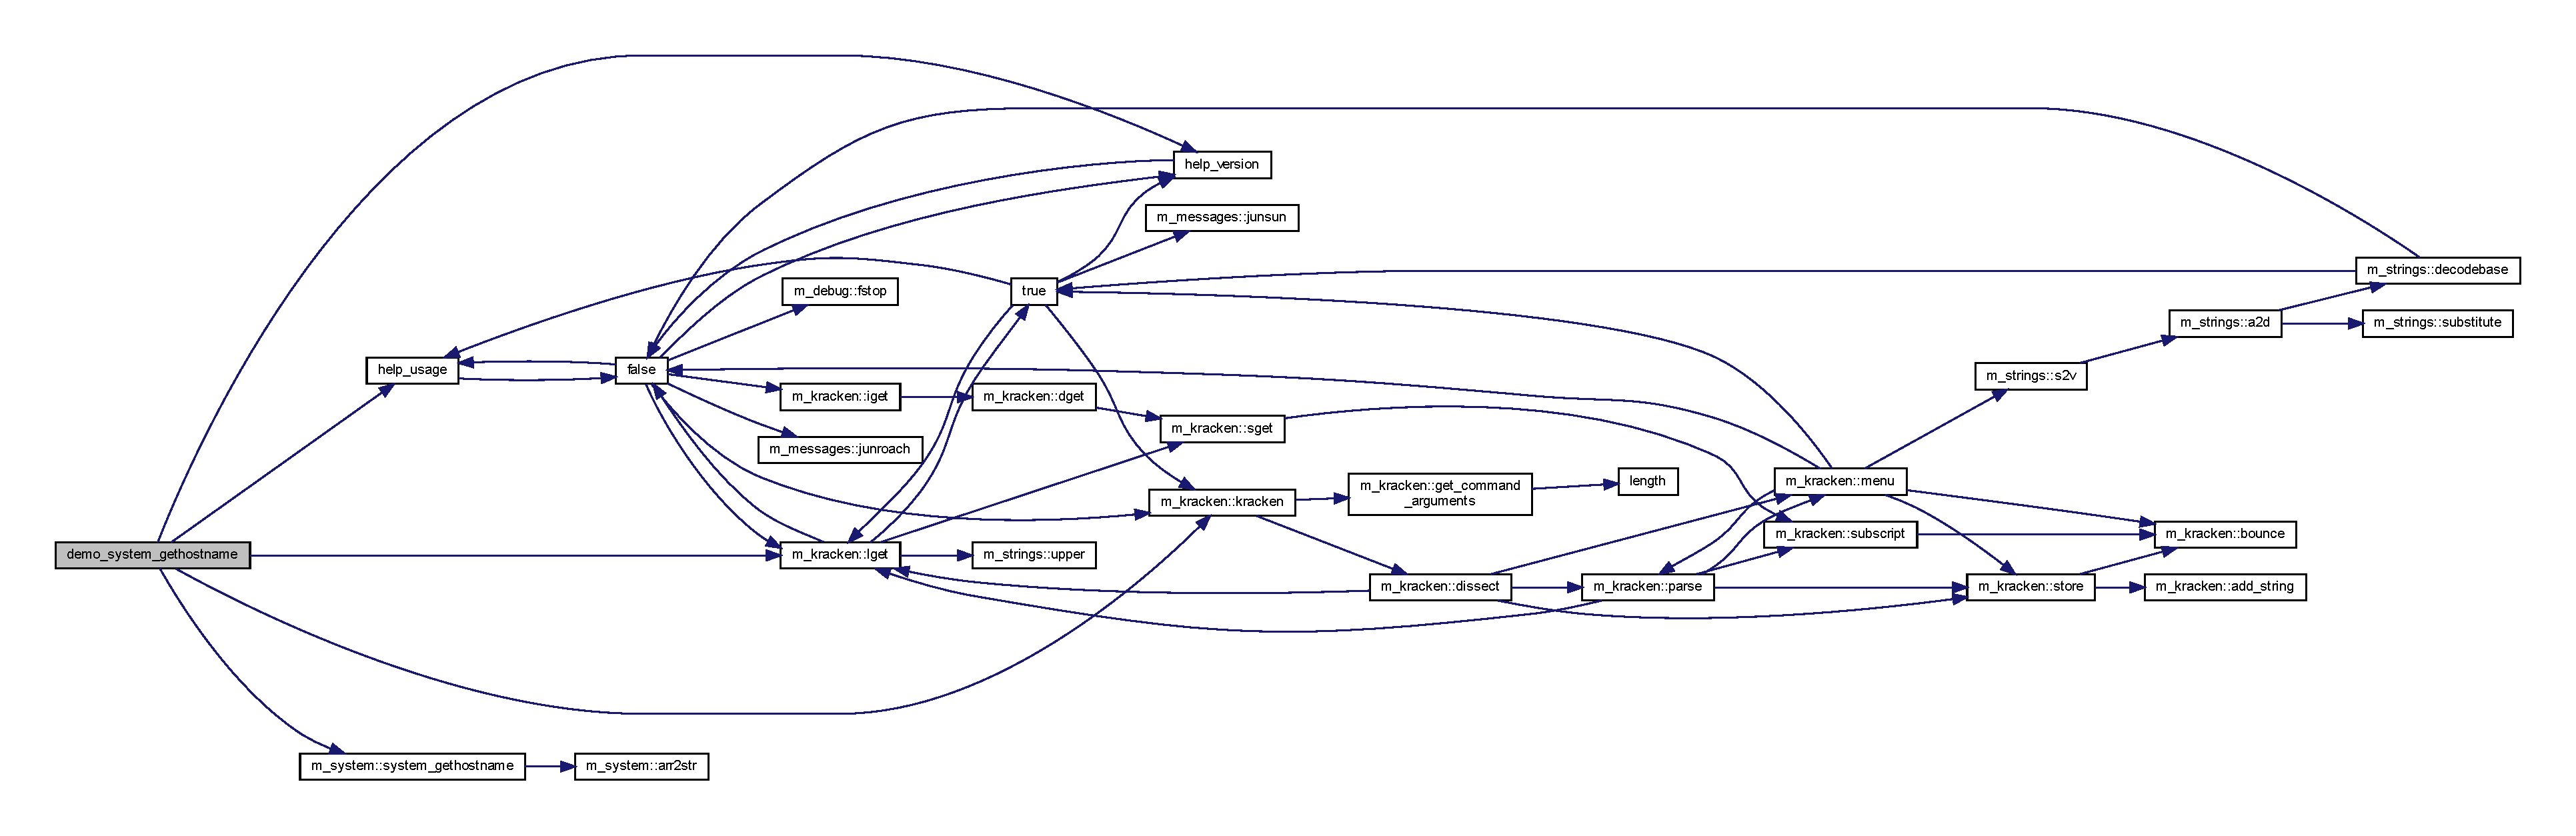
\includegraphics[width=350pt]{__hostname_8f90_a8cf8b2c2d1597761d376d337686d3667_cgraph}
\end{center}
\end{figure}
\mbox{\Hypertarget{__hostname_8f90_a3e09a3b52ee8fb04eeb93fe5761626a8}\label{__hostname_8f90_a3e09a3b52ee8fb04eeb93fe5761626a8}} 
\index{\+\_\+hostname.\+f90@{\+\_\+hostname.\+f90}!help\+\_\+usage@{help\+\_\+usage}}
\index{help\+\_\+usage@{help\+\_\+usage}!\+\_\+hostname.\+f90@{\+\_\+hostname.\+f90}}
\subsubsection{\texorpdfstring{help\+\_\+usage()}{help\_usage()}}
{\footnotesize\ttfamily \hyperlink{M__stopwatch_83_8txt_acfbcff50169d691ff02d4a123ed70482}{subroutine} help\+\_\+usage (\begin{DoxyParamCaption}\item[{logical, intent(\hyperlink{M__journal_83_8txt_afce72651d1eed785a2132bee863b2f38}{in})}]{l\+\_\+help }\end{DoxyParamCaption})}



References false().

Here is the call graph for this function\+:
\nopagebreak
\begin{figure}[H]
\begin{center}
\leavevmode
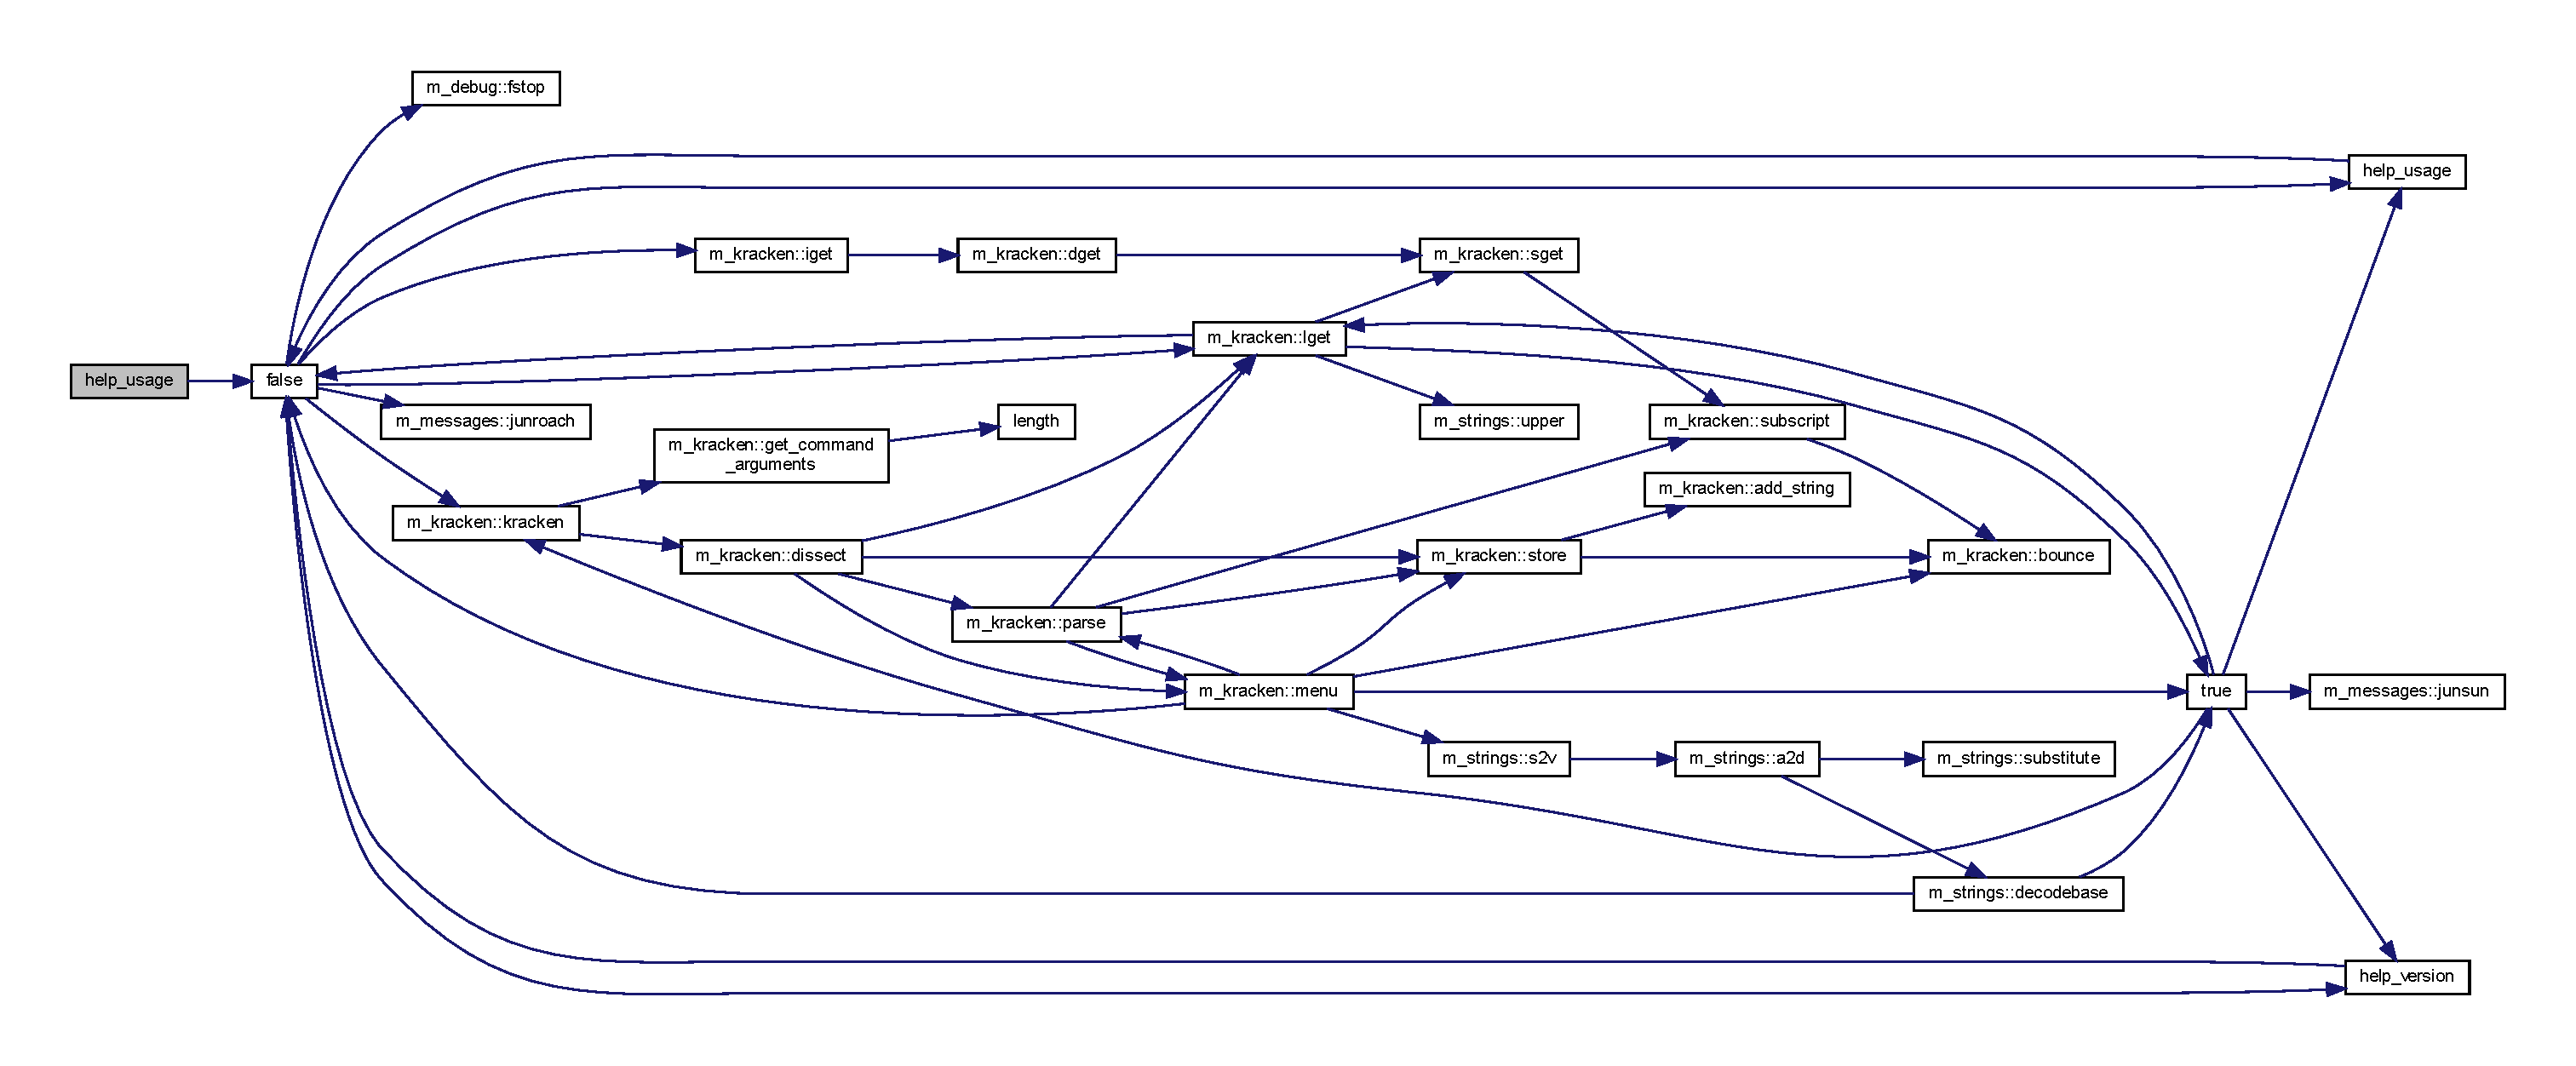
\includegraphics[width=350pt]{__hostname_8f90_a3e09a3b52ee8fb04eeb93fe5761626a8_cgraph}
\end{center}
\end{figure}
\mbox{\Hypertarget{__hostname_8f90_a39c21619b08a3c22f19e2306efd7f766}\label{__hostname_8f90_a39c21619b08a3c22f19e2306efd7f766}} 
\index{\+\_\+hostname.\+f90@{\+\_\+hostname.\+f90}!help\+\_\+version@{help\+\_\+version}}
\index{help\+\_\+version@{help\+\_\+version}!\+\_\+hostname.\+f90@{\+\_\+hostname.\+f90}}
\subsubsection{\texorpdfstring{help\+\_\+version()}{help\_version()}}
{\footnotesize\ttfamily \hyperlink{M__stopwatch_83_8txt_acfbcff50169d691ff02d4a123ed70482}{subroutine} help\+\_\+version (\begin{DoxyParamCaption}\item[{logical, intent(\hyperlink{M__journal_83_8txt_afce72651d1eed785a2132bee863b2f38}{in})}]{l\+\_\+version }\end{DoxyParamCaption})}



\subsubsection*{N\+A\+ME}

\+\_\+hostname(1f) -\/ \mbox{[}F\+U\+N\+IX\mbox{]} display hostname \subsubsection*{S\+Y\+N\+T\+AX}

hostname \mbox{[}-\/help$\vert$-\/version\mbox{]} \subsubsection*{D\+E\+S\+C\+R\+I\+P\+T\+I\+ON}

Calls system\+\_\+gethostname(3f), which calls get\+\_\+hostname(3c) to determine the current host name. \subsubsection*{O\+P\+T\+I\+O\+NS}

--help display this help and exit --version output version information and exit \subsubsection*{E\+X\+A\+M\+P\+LE}

Sample execution\+:

$>$\+\_\+hostname $>$buzz 

References false().

Here is the call graph for this function\+:
\nopagebreak
\begin{figure}[H]
\begin{center}
\leavevmode
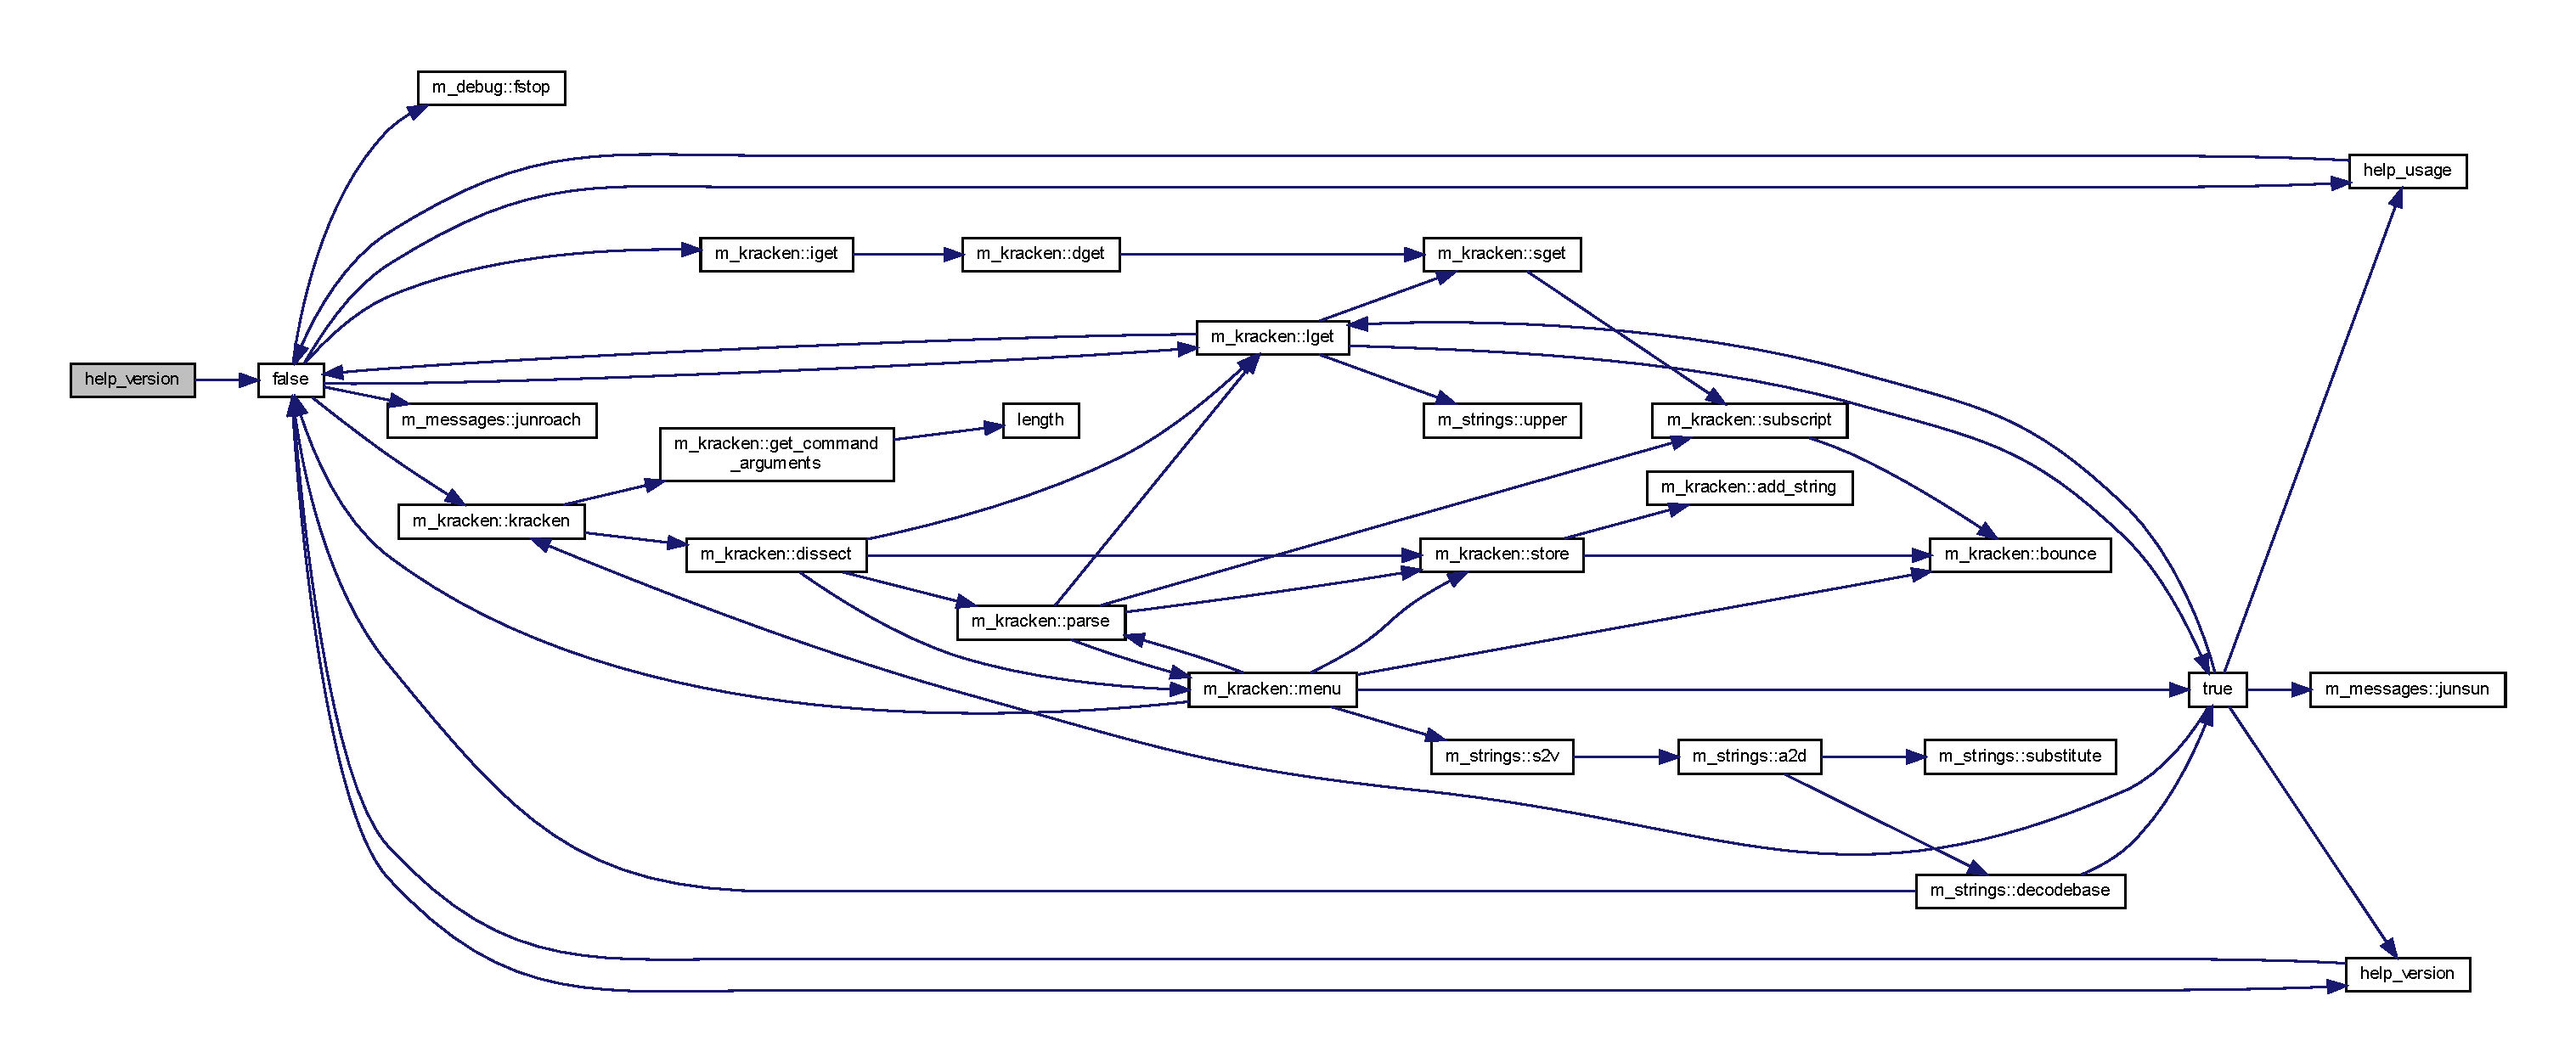
\includegraphics[width=350pt]{__hostname_8f90_a39c21619b08a3c22f19e2306efd7f766_cgraph}
\end{center}
\end{figure}

\hypertarget{__kill_8f90}{}\section{L\+I\+B\+R\+A\+R\+Y/lib\+G\+P\+F/download/tmp/\+P\+R\+O\+G\+R\+A\+M\+S/\+\_\+kill.f90 File Reference}
\label{__kill_8f90}\index{L\+I\+B\+R\+A\+R\+Y/lib\+G\+P\+F/download/tmp/\+P\+R\+O\+G\+R\+A\+M\+S/\+\_\+kill.\+f90@{L\+I\+B\+R\+A\+R\+Y/lib\+G\+P\+F/download/tmp/\+P\+R\+O\+G\+R\+A\+M\+S/\+\_\+kill.\+f90}}
\subsection*{Functions/\+Subroutines}
\begin{DoxyCompactItemize}
\item 
\hyperlink{M__stopwatch_83_8txt_acfbcff50169d691ff02d4a123ed70482}{subroutine} \hyperlink{__kill_8f90_a3e09a3b52ee8fb04eeb93fe5761626a8}{help\+\_\+usage} (l\+\_\+help)
\item 
\hyperlink{M__stopwatch_83_8txt_acfbcff50169d691ff02d4a123ed70482}{subroutine} \hyperlink{__kill_8f90_a39c21619b08a3c22f19e2306efd7f766}{help\+\_\+version} (l\+\_\+version)
\begin{DoxyCompactList}\small\item\em \subsubsection*{N\+A\+ME}

\+\_\+kill(1f) -\/ \mbox{[}F\+U\+N\+IX\mbox{]} send signals to processes \subsubsection*{S\+Y\+N\+T\+AX}

\+\_\+kill P\+I\+Ds \mbox{[}-\/s signal\+\_\+number\mbox{]} \mbox{[}--help$\vert$--version\mbox{]} \subsubsection*{D\+E\+S\+C\+R\+I\+P\+T\+I\+ON}

Calls system\+\_\+kill(3f), which calls kill(3c) to send signals to processes. \subsubsection*{O\+P\+T\+I\+O\+NS}

P\+I\+Ds P\+ID numbers to send signal to -\/s signal number to send to the processes --help display this help and exit --version output version information and exit \subsubsection*{E\+X\+A\+M\+P\+LE}\end{DoxyCompactList}\item 
program \hyperlink{__kill_8f90_ad2550a0eb8119ef21d3febfe883f2051}{demo\+\_\+system\+\_\+kill}
\end{DoxyCompactItemize}


\subsection{Function/\+Subroutine Documentation}
\mbox{\Hypertarget{__kill_8f90_ad2550a0eb8119ef21d3febfe883f2051}\label{__kill_8f90_ad2550a0eb8119ef21d3febfe883f2051}} 
\index{\+\_\+kill.\+f90@{\+\_\+kill.\+f90}!demo\+\_\+system\+\_\+kill@{demo\+\_\+system\+\_\+kill}}
\index{demo\+\_\+system\+\_\+kill@{demo\+\_\+system\+\_\+kill}!\+\_\+kill.\+f90@{\+\_\+kill.\+f90}}
\subsubsection{\texorpdfstring{demo\+\_\+system\+\_\+kill()}{demo\_system\_kill()}}
{\footnotesize\ttfamily program demo\+\_\+system\+\_\+kill (\begin{DoxyParamCaption}{ }\end{DoxyParamCaption})}



References help\+\_\+usage(), help\+\_\+version(), m\+\_\+kracken\+::iget(), m\+\_\+kracken\+::igets(), m\+\_\+kracken\+::kracken(), m\+\_\+kracken\+::lget(), and m\+\_\+system\+::system\+\_\+perror().

\mbox{\Hypertarget{__kill_8f90_a3e09a3b52ee8fb04eeb93fe5761626a8}\label{__kill_8f90_a3e09a3b52ee8fb04eeb93fe5761626a8}} 
\index{\+\_\+kill.\+f90@{\+\_\+kill.\+f90}!help\+\_\+usage@{help\+\_\+usage}}
\index{help\+\_\+usage@{help\+\_\+usage}!\+\_\+kill.\+f90@{\+\_\+kill.\+f90}}
\subsubsection{\texorpdfstring{help\+\_\+usage()}{help\_usage()}}
{\footnotesize\ttfamily \hyperlink{M__stopwatch_83_8txt_acfbcff50169d691ff02d4a123ed70482}{subroutine} help\+\_\+usage (\begin{DoxyParamCaption}\item[{logical, intent(\hyperlink{M__journal_83_8txt_afce72651d1eed785a2132bee863b2f38}{in})}]{l\+\_\+help }\end{DoxyParamCaption})}



References false().

\mbox{\Hypertarget{__kill_8f90_a39c21619b08a3c22f19e2306efd7f766}\label{__kill_8f90_a39c21619b08a3c22f19e2306efd7f766}} 
\index{\+\_\+kill.\+f90@{\+\_\+kill.\+f90}!help\+\_\+version@{help\+\_\+version}}
\index{help\+\_\+version@{help\+\_\+version}!\+\_\+kill.\+f90@{\+\_\+kill.\+f90}}
\subsubsection{\texorpdfstring{help\+\_\+version()}{help\_version()}}
{\footnotesize\ttfamily \hyperlink{M__stopwatch_83_8txt_acfbcff50169d691ff02d4a123ed70482}{subroutine} help\+\_\+version (\begin{DoxyParamCaption}\item[{logical, intent(\hyperlink{M__journal_83_8txt_afce72651d1eed785a2132bee863b2f38}{in})}]{l\+\_\+version }\end{DoxyParamCaption})}



\subsubsection*{N\+A\+ME}

\+\_\+kill(1f) -\/ \mbox{[}F\+U\+N\+IX\mbox{]} send signals to processes \subsubsection*{S\+Y\+N\+T\+AX}

\+\_\+kill P\+I\+Ds \mbox{[}-\/s signal\+\_\+number\mbox{]} \mbox{[}--help$\vert$--version\mbox{]} \subsubsection*{D\+E\+S\+C\+R\+I\+P\+T\+I\+ON}

Calls system\+\_\+kill(3f), which calls kill(3c) to send signals to processes. \subsubsection*{O\+P\+T\+I\+O\+NS}

P\+I\+Ds P\+ID numbers to send signal to -\/s signal number to send to the processes --help display this help and exit --version output version information and exit \subsubsection*{E\+X\+A\+M\+P\+LE}

Sample execution\+:

\begin{quote}
\$ \+\_\+kill 60476 234234 O\+T\+H\+ER -\/s 9 {\itshape a2d} -\/ cannot produce number from string \mbox{[}O\+T\+H\+ER\mbox{]} {\itshape a2d} -\/ \mbox{[}Bad value during integer read\mbox{]} {\itshape kill}\+: S\+I\+G\+N\+AL=9 P\+ID=60476 successfully sent {\itshape kill}\+: process not found {\itshape kill}\+: P\+ID value of 0 is not supported \end{quote}


References false().


\hypertarget{__ln_8f90}{}\section{L\+I\+B\+R\+A\+R\+Y/lib\+G\+P\+F/download/tmp/\+P\+R\+O\+G\+R\+A\+M\+S/\+\_\+ln.f90 File Reference}
\label{__ln_8f90}\index{L\+I\+B\+R\+A\+R\+Y/lib\+G\+P\+F/download/tmp/\+P\+R\+O\+G\+R\+A\+M\+S/\+\_\+ln.\+f90@{L\+I\+B\+R\+A\+R\+Y/lib\+G\+P\+F/download/tmp/\+P\+R\+O\+G\+R\+A\+M\+S/\+\_\+ln.\+f90}}
\subsection*{Functions/\+Subroutines}
\begin{DoxyCompactItemize}
\item 
\hyperlink{M__stopwatch_83_8txt_acfbcff50169d691ff02d4a123ed70482}{subroutine} \hyperlink{__ln_8f90_a3e09a3b52ee8fb04eeb93fe5761626a8}{help\+\_\+usage} (l\+\_\+help)
\item 
\hyperlink{M__stopwatch_83_8txt_acfbcff50169d691ff02d4a123ed70482}{subroutine} \hyperlink{__ln_8f90_a39c21619b08a3c22f19e2306efd7f766}{help\+\_\+version} (l\+\_\+version)
\begin{DoxyCompactList}\small\item\em \subsubsection*{N\+A\+ME}

\+\_\+ln(1f) -\/ \mbox{[}F\+U\+N\+IX\+:F\+I\+L\+E\+S\+Y\+S\+T\+EM\mbox{]} create hard links to a file \subsubsection*{S\+Y\+N\+O\+P\+S\+IS}\end{DoxyCompactList}\item 
program \hyperlink{__ln_8f90_a1b05022af7f0b5c0f963a252a5ef2ce7}{demo\+\_\+system\+\_\+link}
\end{DoxyCompactItemize}


\subsection{Function/\+Subroutine Documentation}
\mbox{\Hypertarget{__ln_8f90_a1b05022af7f0b5c0f963a252a5ef2ce7}\label{__ln_8f90_a1b05022af7f0b5c0f963a252a5ef2ce7}} 
\index{\+\_\+ln.\+f90@{\+\_\+ln.\+f90}!demo\+\_\+system\+\_\+link@{demo\+\_\+system\+\_\+link}}
\index{demo\+\_\+system\+\_\+link@{demo\+\_\+system\+\_\+link}!\+\_\+ln.\+f90@{\+\_\+ln.\+f90}}
\subsubsection{\texorpdfstring{demo\+\_\+system\+\_\+link()}{demo\_system\_link()}}
{\footnotesize\ttfamily program demo\+\_\+system\+\_\+link (\begin{DoxyParamCaption}{ }\end{DoxyParamCaption})}



References help\+\_\+usage(), help\+\_\+version(), m\+\_\+kracken\+::ipvalue, m\+\_\+kracken\+::kracken(), m\+\_\+kracken\+::lget(), m\+\_\+kracken\+::sgets(), m\+\_\+system\+::system\+\_\+link(), and m\+\_\+system\+::system\+\_\+perror().

Here is the call graph for this function\+:
\nopagebreak
\begin{figure}[H]
\begin{center}
\leavevmode
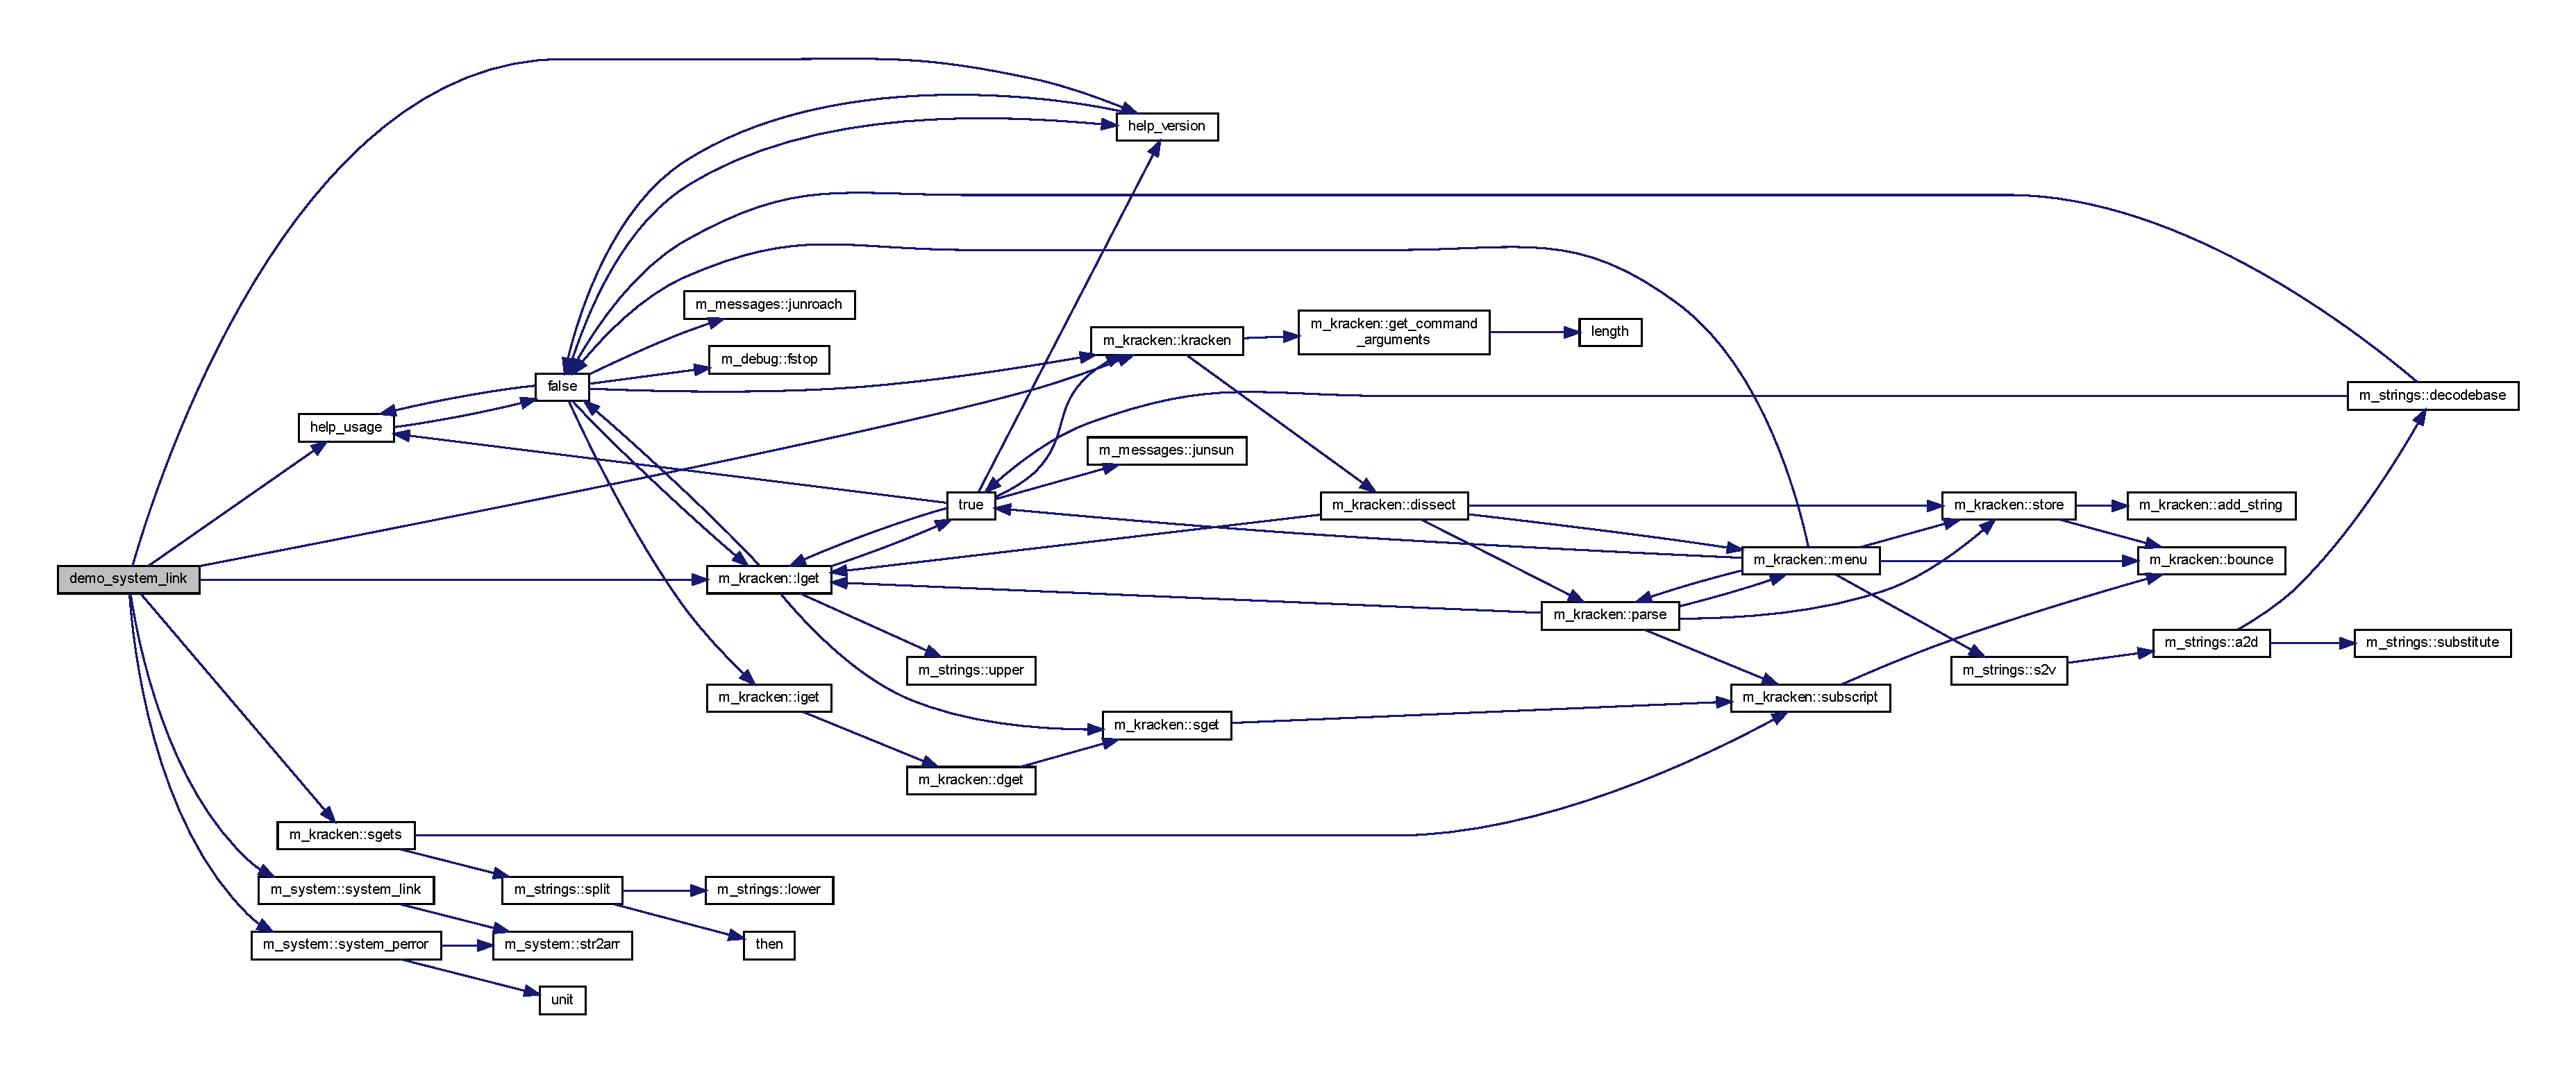
\includegraphics[width=350pt]{__ln_8f90_a1b05022af7f0b5c0f963a252a5ef2ce7_cgraph}
\end{center}
\end{figure}
\mbox{\Hypertarget{__ln_8f90_a3e09a3b52ee8fb04eeb93fe5761626a8}\label{__ln_8f90_a3e09a3b52ee8fb04eeb93fe5761626a8}} 
\index{\+\_\+ln.\+f90@{\+\_\+ln.\+f90}!help\+\_\+usage@{help\+\_\+usage}}
\index{help\+\_\+usage@{help\+\_\+usage}!\+\_\+ln.\+f90@{\+\_\+ln.\+f90}}
\subsubsection{\texorpdfstring{help\+\_\+usage()}{help\_usage()}}
{\footnotesize\ttfamily \hyperlink{M__stopwatch_83_8txt_acfbcff50169d691ff02d4a123ed70482}{subroutine} help\+\_\+usage (\begin{DoxyParamCaption}\item[{logical, intent(\hyperlink{M__journal_83_8txt_afce72651d1eed785a2132bee863b2f38}{in})}]{l\+\_\+help }\end{DoxyParamCaption})}



References false().

Here is the call graph for this function\+:
\nopagebreak
\begin{figure}[H]
\begin{center}
\leavevmode
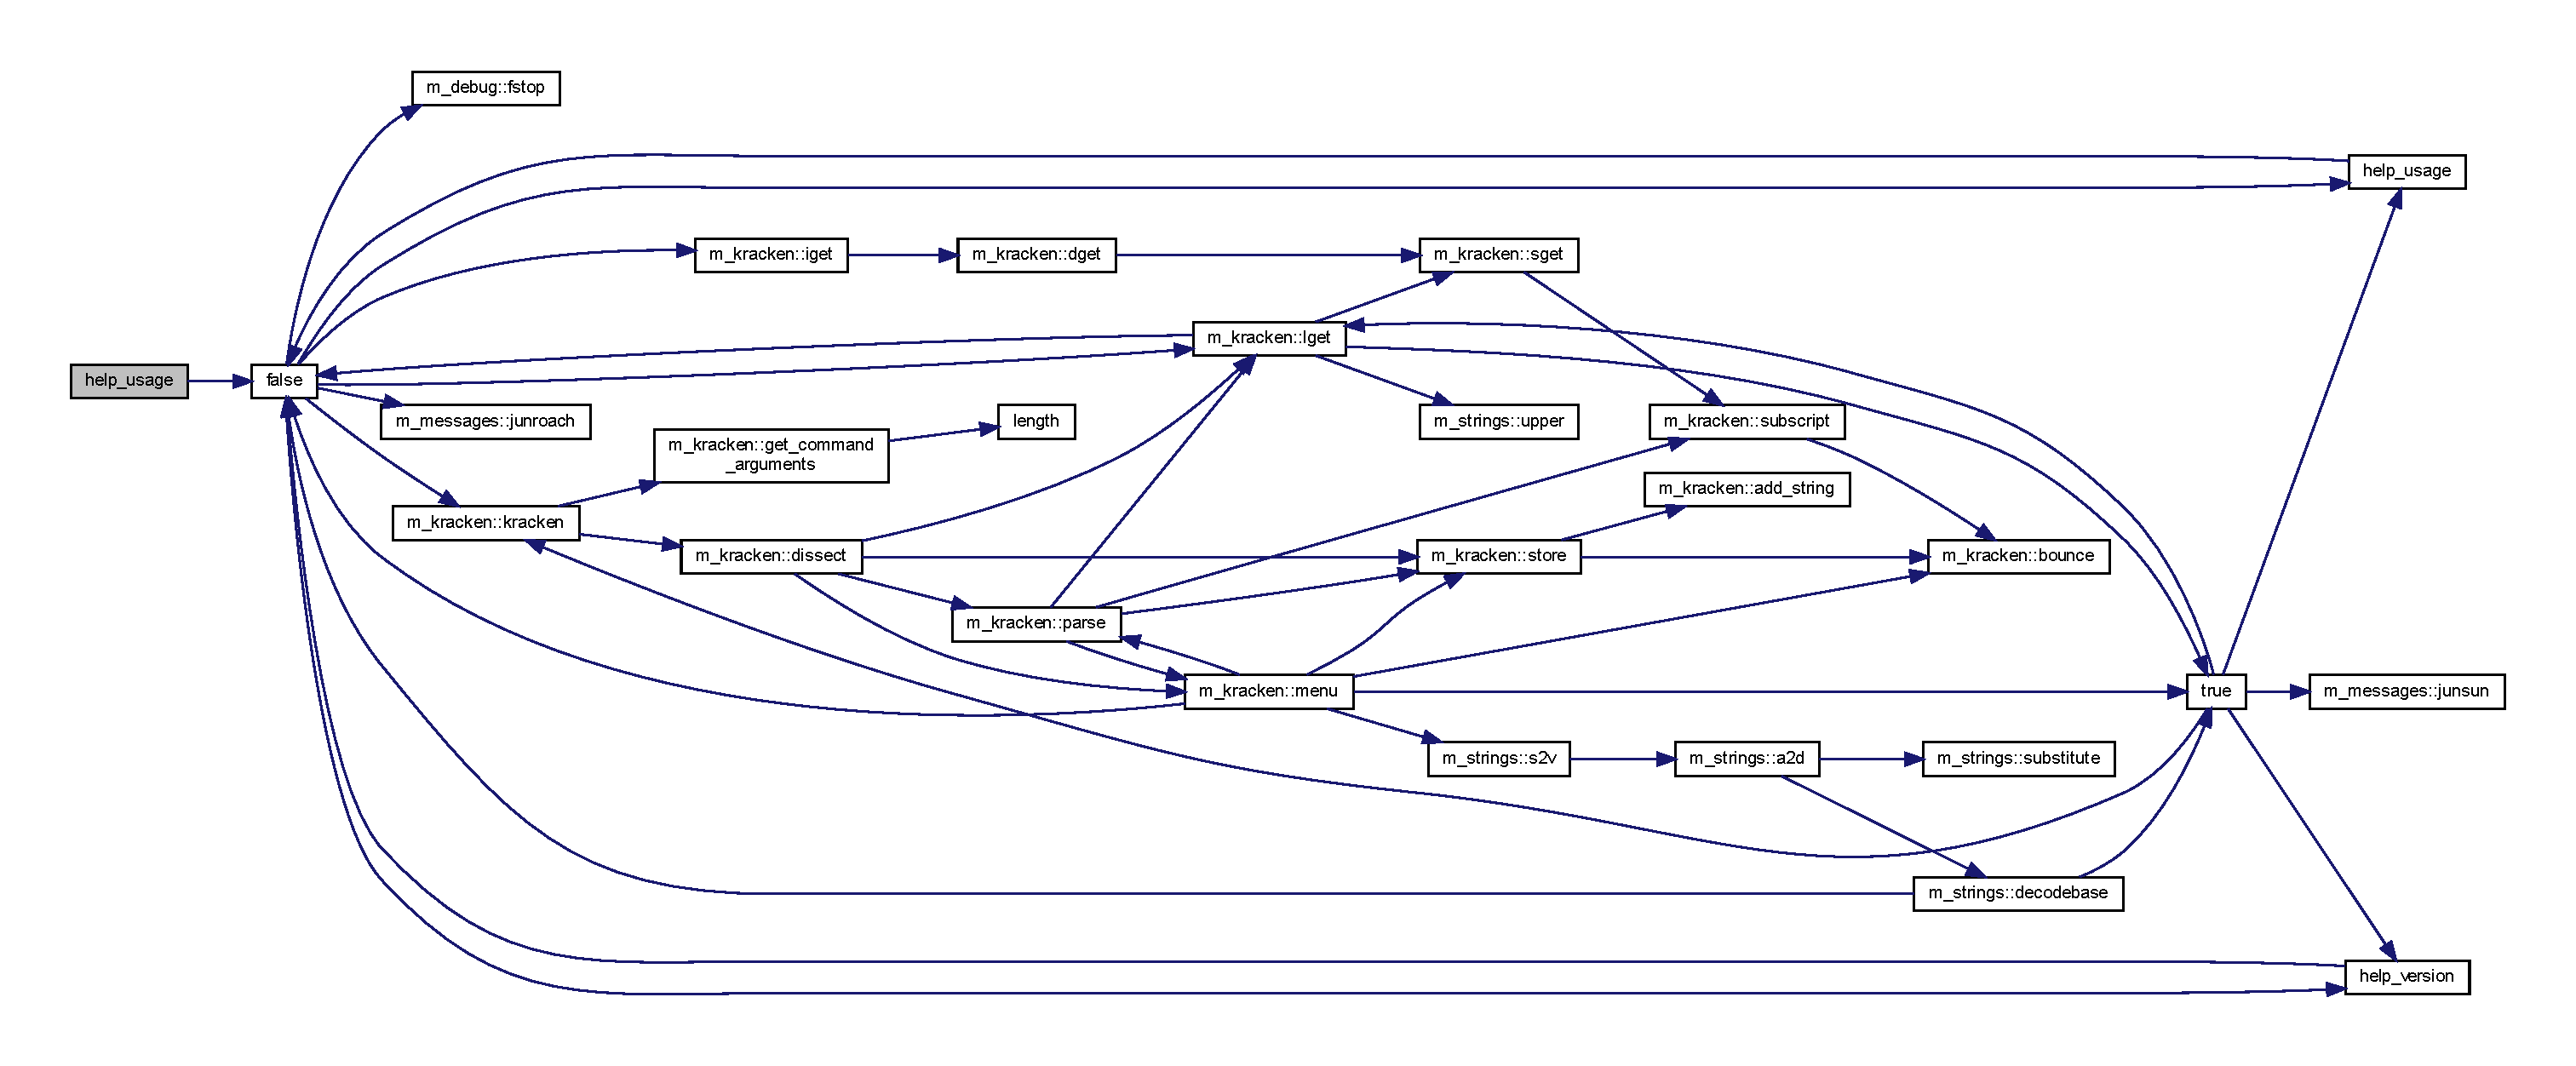
\includegraphics[width=350pt]{__ln_8f90_a3e09a3b52ee8fb04eeb93fe5761626a8_cgraph}
\end{center}
\end{figure}
\mbox{\Hypertarget{__ln_8f90_a39c21619b08a3c22f19e2306efd7f766}\label{__ln_8f90_a39c21619b08a3c22f19e2306efd7f766}} 
\index{\+\_\+ln.\+f90@{\+\_\+ln.\+f90}!help\+\_\+version@{help\+\_\+version}}
\index{help\+\_\+version@{help\+\_\+version}!\+\_\+ln.\+f90@{\+\_\+ln.\+f90}}
\subsubsection{\texorpdfstring{help\+\_\+version()}{help\_version()}}
{\footnotesize\ttfamily \hyperlink{M__stopwatch_83_8txt_acfbcff50169d691ff02d4a123ed70482}{subroutine} help\+\_\+version (\begin{DoxyParamCaption}\item[{logical, intent(\hyperlink{M__journal_83_8txt_afce72651d1eed785a2132bee863b2f38}{in})}]{l\+\_\+version }\end{DoxyParamCaption})}



\subsubsection*{N\+A\+ME}

\+\_\+ln(1f) -\/ \mbox{[}F\+U\+N\+IX\+:F\+I\+L\+E\+S\+Y\+S\+T\+EM\mbox{]} create hard links to a file \subsubsection*{S\+Y\+N\+O\+P\+S\+IS}

Formats\+:

\+\_\+ln T\+A\+R\+G\+ET L\+I\+N\+K\+\_\+\+N\+A\+ME \# create a link to T\+A\+R\+G\+ET with the name L\+I\+N\+K\+\_\+\+N\+A\+ME. \+\_\+ln T\+A\+R\+G\+ET \# create a link to T\+A\+R\+G\+ET in the current directory. \+\_\+ln T\+A\+R\+G\+ET... D\+I\+R\+E\+C\+T\+O\+RY \# create links to each T\+A\+R\+G\+ET in D\+I\+R\+E\+C\+T\+O\+RY. \subsubsection*{D\+E\+S\+C\+R\+I\+P\+T\+I\+ON}

Create hard links (not symbolic links) each destination (name of new link) should not already exist. When creating hard links, each T\+A\+R\+G\+ET must exist. Symbolic links can hold arbitrary text; if later resolved, a relative link is interpreted in relation to its parent directory. \subsubsection*{O\+P\+T\+I\+O\+NS}

T\+A\+R\+G\+ET name of existing file L\+I\+N\+K\+\_\+\+N\+A\+ME if L\+I\+N\+K\+\_\+\+N\+A\+ME follows T\+A\+R\+G\+ET create a link called L\+I\+N\+K\+\_\+\+N\+A\+ME that points to T\+A\+R\+G\+ET D\+I\+R\+E\+C\+T\+O\+RY if last option is a directory previous filenames on command are linked into D\+I\+R\+E\+C\+T\+O\+RY --help display this help and exit --version output version information and exit 

References false().

Here is the call graph for this function\+:
\nopagebreak
\begin{figure}[H]
\begin{center}
\leavevmode
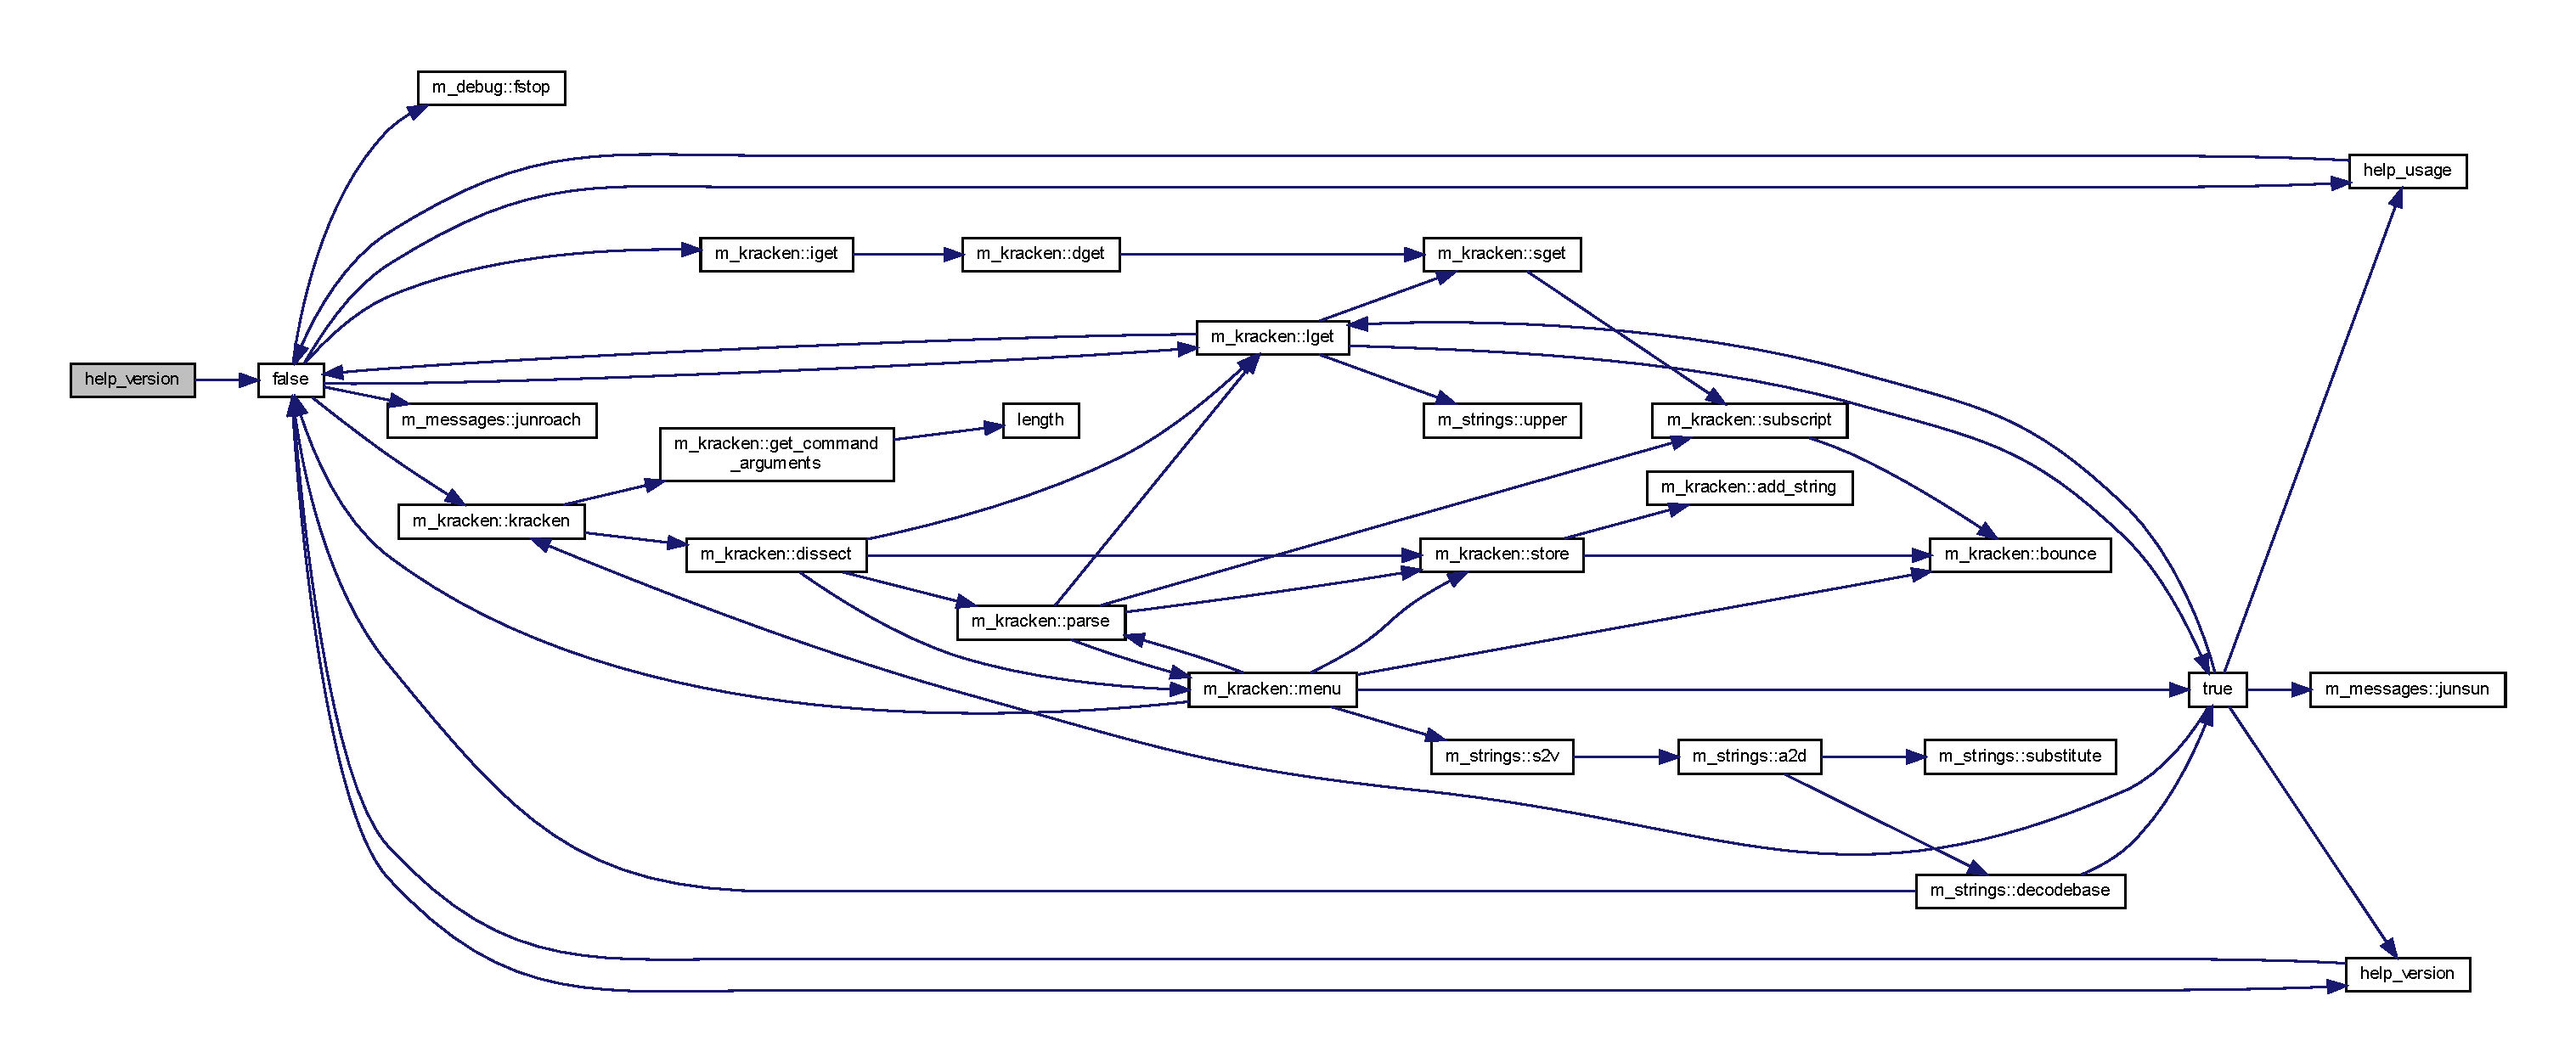
\includegraphics[width=350pt]{__ln_8f90_a39c21619b08a3c22f19e2306efd7f766_cgraph}
\end{center}
\end{figure}

\hypertarget{__logname_8f90}{}\section{L\+I\+B\+R\+A\+R\+Y/lib\+G\+P\+F/download/tmp/\+P\+R\+O\+G\+R\+A\+M\+S/\+\_\+logname.f90 File Reference}
\label{__logname_8f90}\index{L\+I\+B\+R\+A\+R\+Y/lib\+G\+P\+F/download/tmp/\+P\+R\+O\+G\+R\+A\+M\+S/\+\_\+logname.\+f90@{L\+I\+B\+R\+A\+R\+Y/lib\+G\+P\+F/download/tmp/\+P\+R\+O\+G\+R\+A\+M\+S/\+\_\+logname.\+f90}}
\subsection*{Functions/\+Subroutines}
\begin{DoxyCompactItemize}
\item 
\hyperlink{M__stopwatch_83_8txt_acfbcff50169d691ff02d4a123ed70482}{subroutine} \hyperlink{__logname_8f90_a3e09a3b52ee8fb04eeb93fe5761626a8}{help\+\_\+usage} (l\+\_\+help)
\item 
\hyperlink{M__stopwatch_83_8txt_acfbcff50169d691ff02d4a123ed70482}{subroutine} \hyperlink{__logname_8f90_a39c21619b08a3c22f19e2306efd7f766}{help\+\_\+version} (l\+\_\+version)
\begin{DoxyCompactList}\small\item\em \subsubsection*{N\+A\+ME}

\+\_\+logname(1f) -\/ \mbox{[}F\+U\+N\+IX\mbox{]} display login name \subsubsection*{S\+Y\+N\+O\+P\+S\+IS}\end{DoxyCompactList}\item 
program \hyperlink{__logname_8f90_a8ae53eddb485d4c8597c4d4a204181a8}{demo\+\_\+system\+\_\+getlogin}
\end{DoxyCompactItemize}


\subsection{Function/\+Subroutine Documentation}
\mbox{\Hypertarget{__logname_8f90_a8ae53eddb485d4c8597c4d4a204181a8}\label{__logname_8f90_a8ae53eddb485d4c8597c4d4a204181a8}} 
\index{\+\_\+logname.\+f90@{\+\_\+logname.\+f90}!demo\+\_\+system\+\_\+getlogin@{demo\+\_\+system\+\_\+getlogin}}
\index{demo\+\_\+system\+\_\+getlogin@{demo\+\_\+system\+\_\+getlogin}!\+\_\+logname.\+f90@{\+\_\+logname.\+f90}}
\subsubsection{\texorpdfstring{demo\+\_\+system\+\_\+getlogin()}{demo\_system\_getlogin()}}
{\footnotesize\ttfamily program demo\+\_\+system\+\_\+getlogin (\begin{DoxyParamCaption}{ }\end{DoxyParamCaption})}



References help\+\_\+usage(), help\+\_\+version(), m\+\_\+kracken\+::kracken(), m\+\_\+kracken\+::lget(), and m\+\_\+system\+::system\+\_\+getlogin().

Here is the call graph for this function\+:
\nopagebreak
\begin{figure}[H]
\begin{center}
\leavevmode
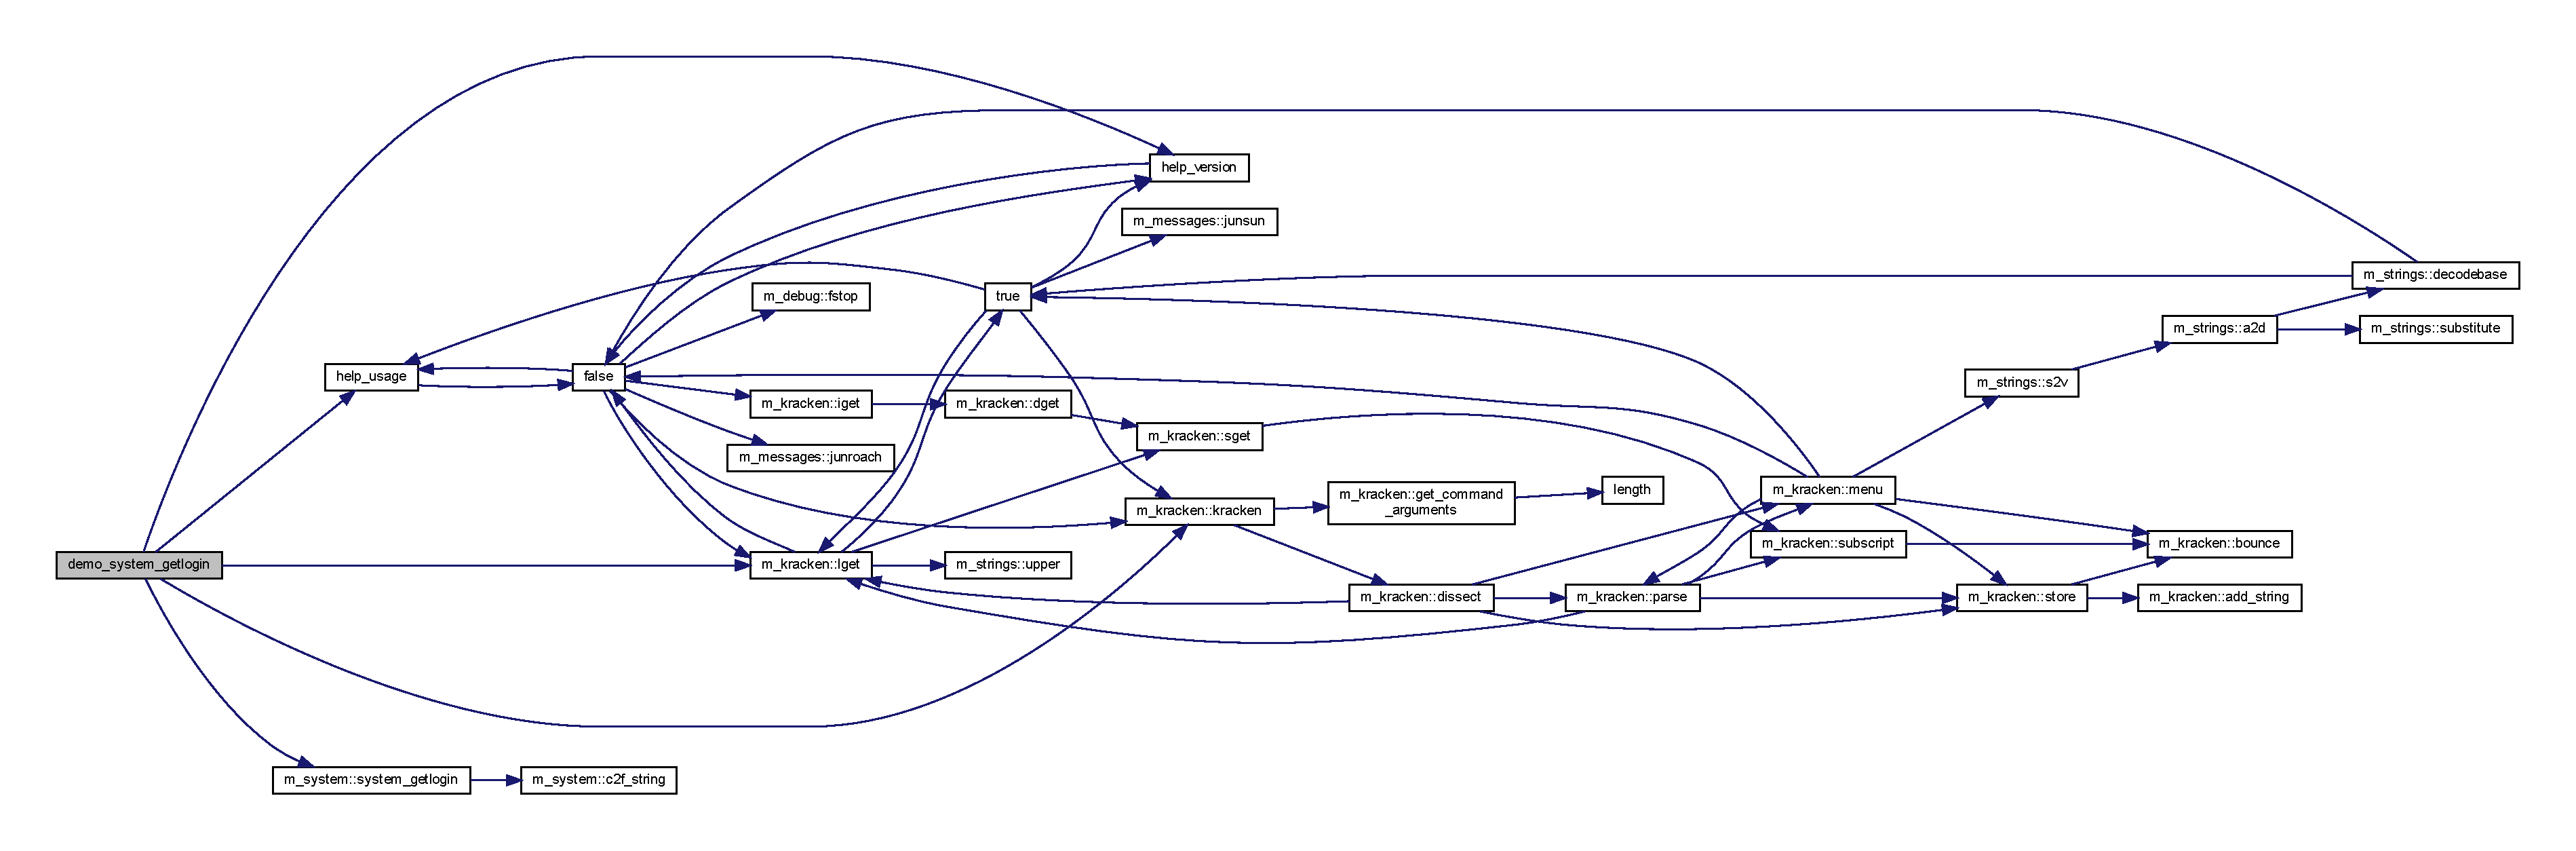
\includegraphics[width=350pt]{__logname_8f90_a8ae53eddb485d4c8597c4d4a204181a8_cgraph}
\end{center}
\end{figure}
\mbox{\Hypertarget{__logname_8f90_a3e09a3b52ee8fb04eeb93fe5761626a8}\label{__logname_8f90_a3e09a3b52ee8fb04eeb93fe5761626a8}} 
\index{\+\_\+logname.\+f90@{\+\_\+logname.\+f90}!help\+\_\+usage@{help\+\_\+usage}}
\index{help\+\_\+usage@{help\+\_\+usage}!\+\_\+logname.\+f90@{\+\_\+logname.\+f90}}
\subsubsection{\texorpdfstring{help\+\_\+usage()}{help\_usage()}}
{\footnotesize\ttfamily \hyperlink{M__stopwatch_83_8txt_acfbcff50169d691ff02d4a123ed70482}{subroutine} help\+\_\+usage (\begin{DoxyParamCaption}\item[{logical, intent(\hyperlink{M__journal_83_8txt_afce72651d1eed785a2132bee863b2f38}{in})}]{l\+\_\+help }\end{DoxyParamCaption})}



References false().

Here is the call graph for this function\+:
\nopagebreak
\begin{figure}[H]
\begin{center}
\leavevmode
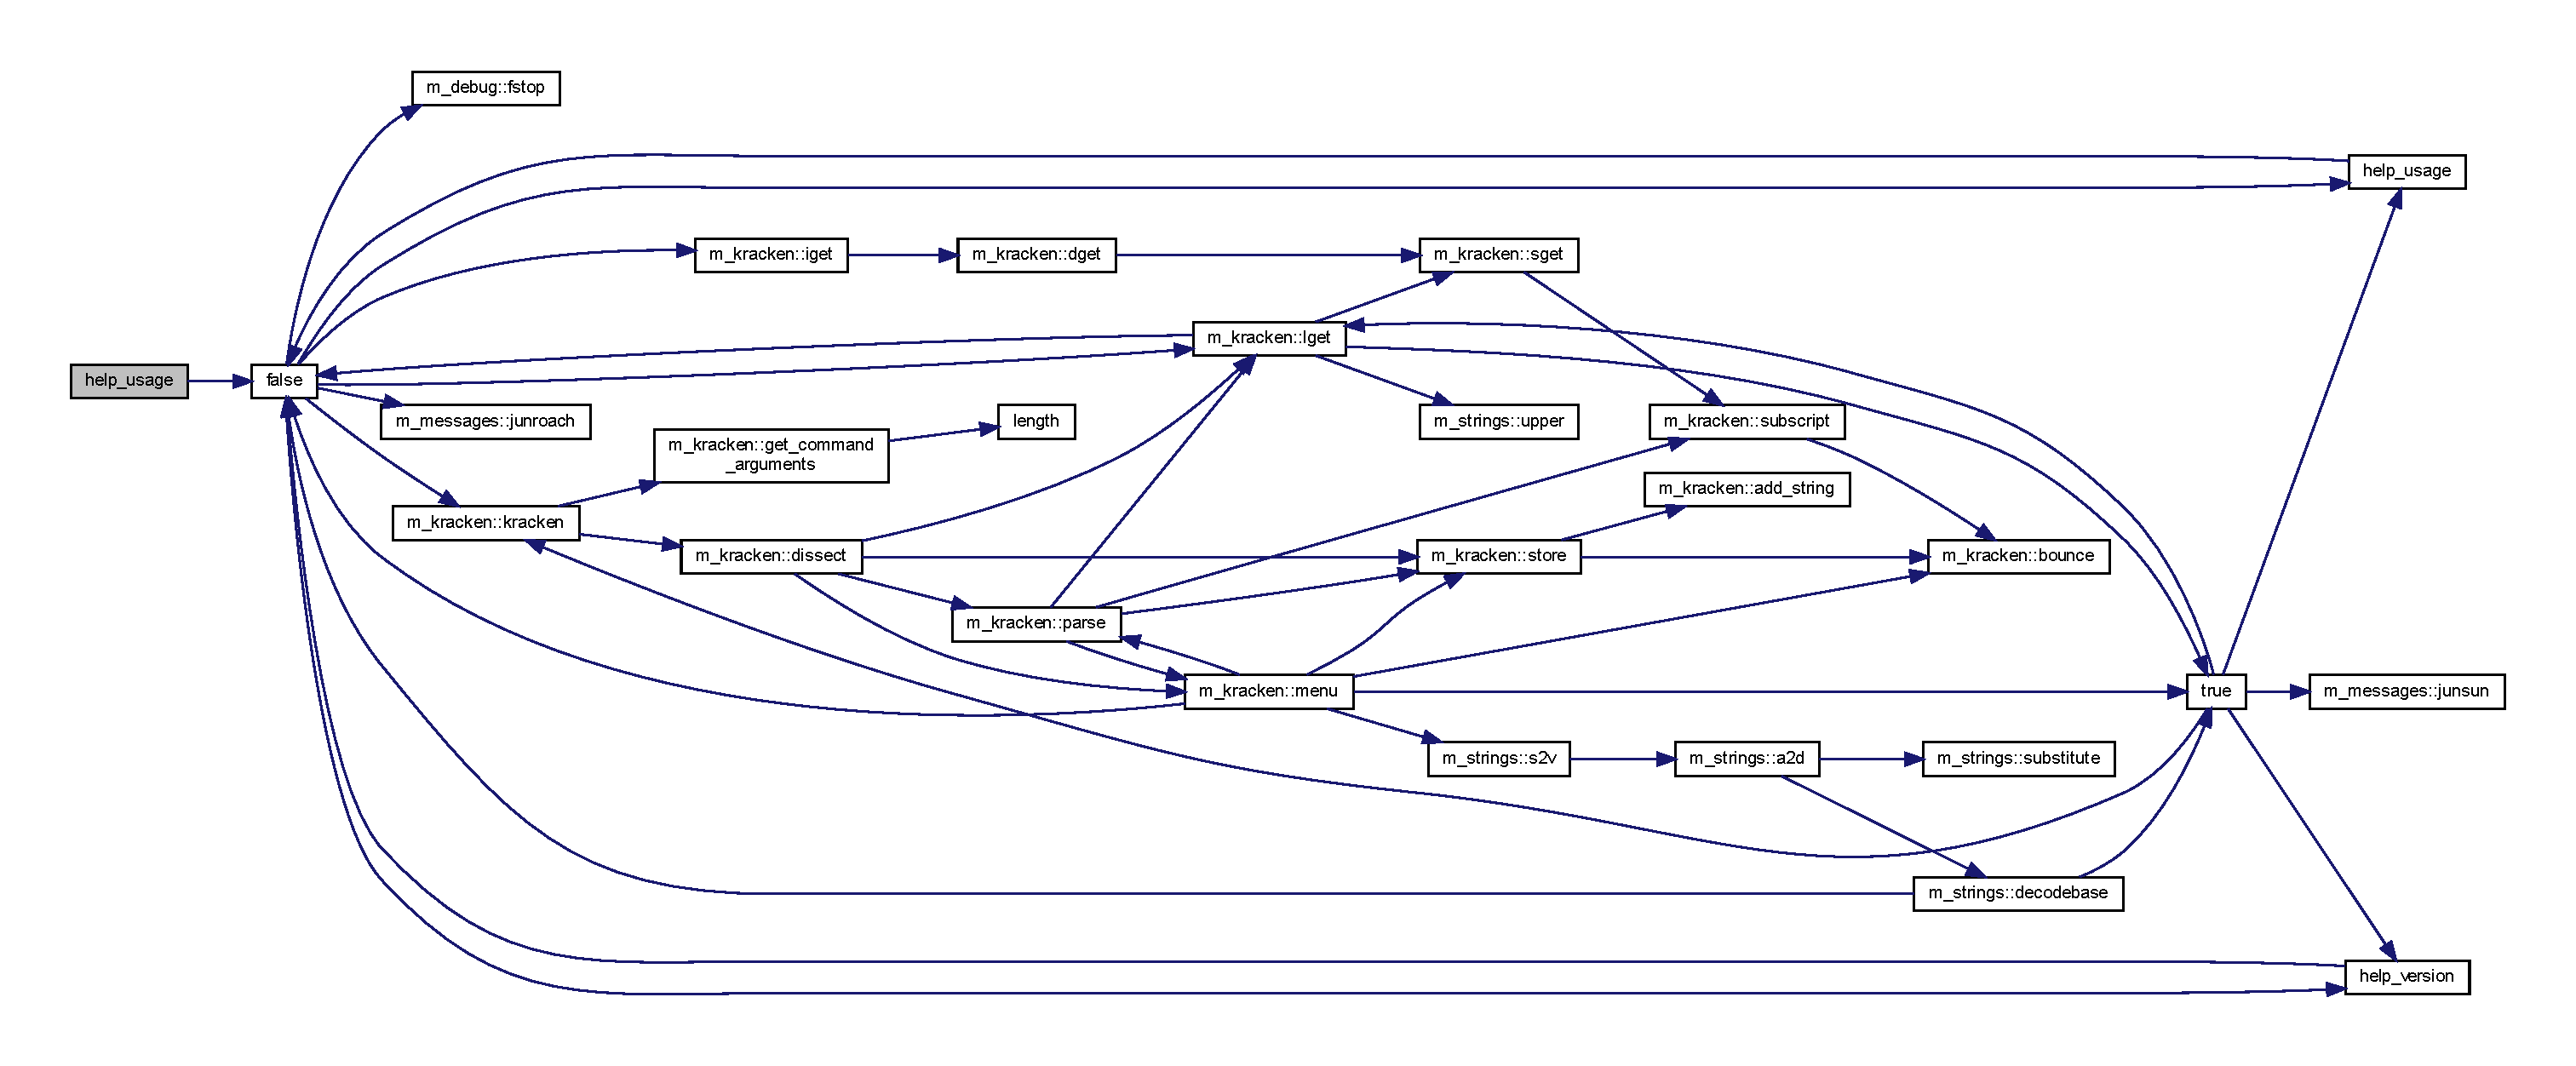
\includegraphics[width=350pt]{__logname_8f90_a3e09a3b52ee8fb04eeb93fe5761626a8_cgraph}
\end{center}
\end{figure}
\mbox{\Hypertarget{__logname_8f90_a39c21619b08a3c22f19e2306efd7f766}\label{__logname_8f90_a39c21619b08a3c22f19e2306efd7f766}} 
\index{\+\_\+logname.\+f90@{\+\_\+logname.\+f90}!help\+\_\+version@{help\+\_\+version}}
\index{help\+\_\+version@{help\+\_\+version}!\+\_\+logname.\+f90@{\+\_\+logname.\+f90}}
\subsubsection{\texorpdfstring{help\+\_\+version()}{help\_version()}}
{\footnotesize\ttfamily \hyperlink{M__stopwatch_83_8txt_acfbcff50169d691ff02d4a123ed70482}{subroutine} help\+\_\+version (\begin{DoxyParamCaption}\item[{logical, intent(\hyperlink{M__journal_83_8txt_afce72651d1eed785a2132bee863b2f38}{in})}]{l\+\_\+version }\end{DoxyParamCaption})}



\subsubsection*{N\+A\+ME}

\+\_\+logname(1f) -\/ \mbox{[}F\+U\+N\+IX\mbox{]} display login name \subsubsection*{S\+Y\+N\+O\+P\+S\+IS}

\+\_\+logname \mbox{[}-\/help$\vert$-\/version\mbox{]} \subsubsection*{D\+E\+S\+C\+R\+I\+P\+T\+I\+ON}

Demonstrate call to system\+\_\+getlogin(3f) (which calls getlogin(3c) \subsubsection*{O\+P\+T\+I\+O\+NS}

--help display command help and exit --version output version information and exit \subsubsection*{E\+X\+A\+M\+P\+LE}

\begin{DoxyVerb}   Command usage:

     _logname \end{DoxyVerb}
 

References false().

Here is the call graph for this function\+:
\nopagebreak
\begin{figure}[H]
\begin{center}
\leavevmode
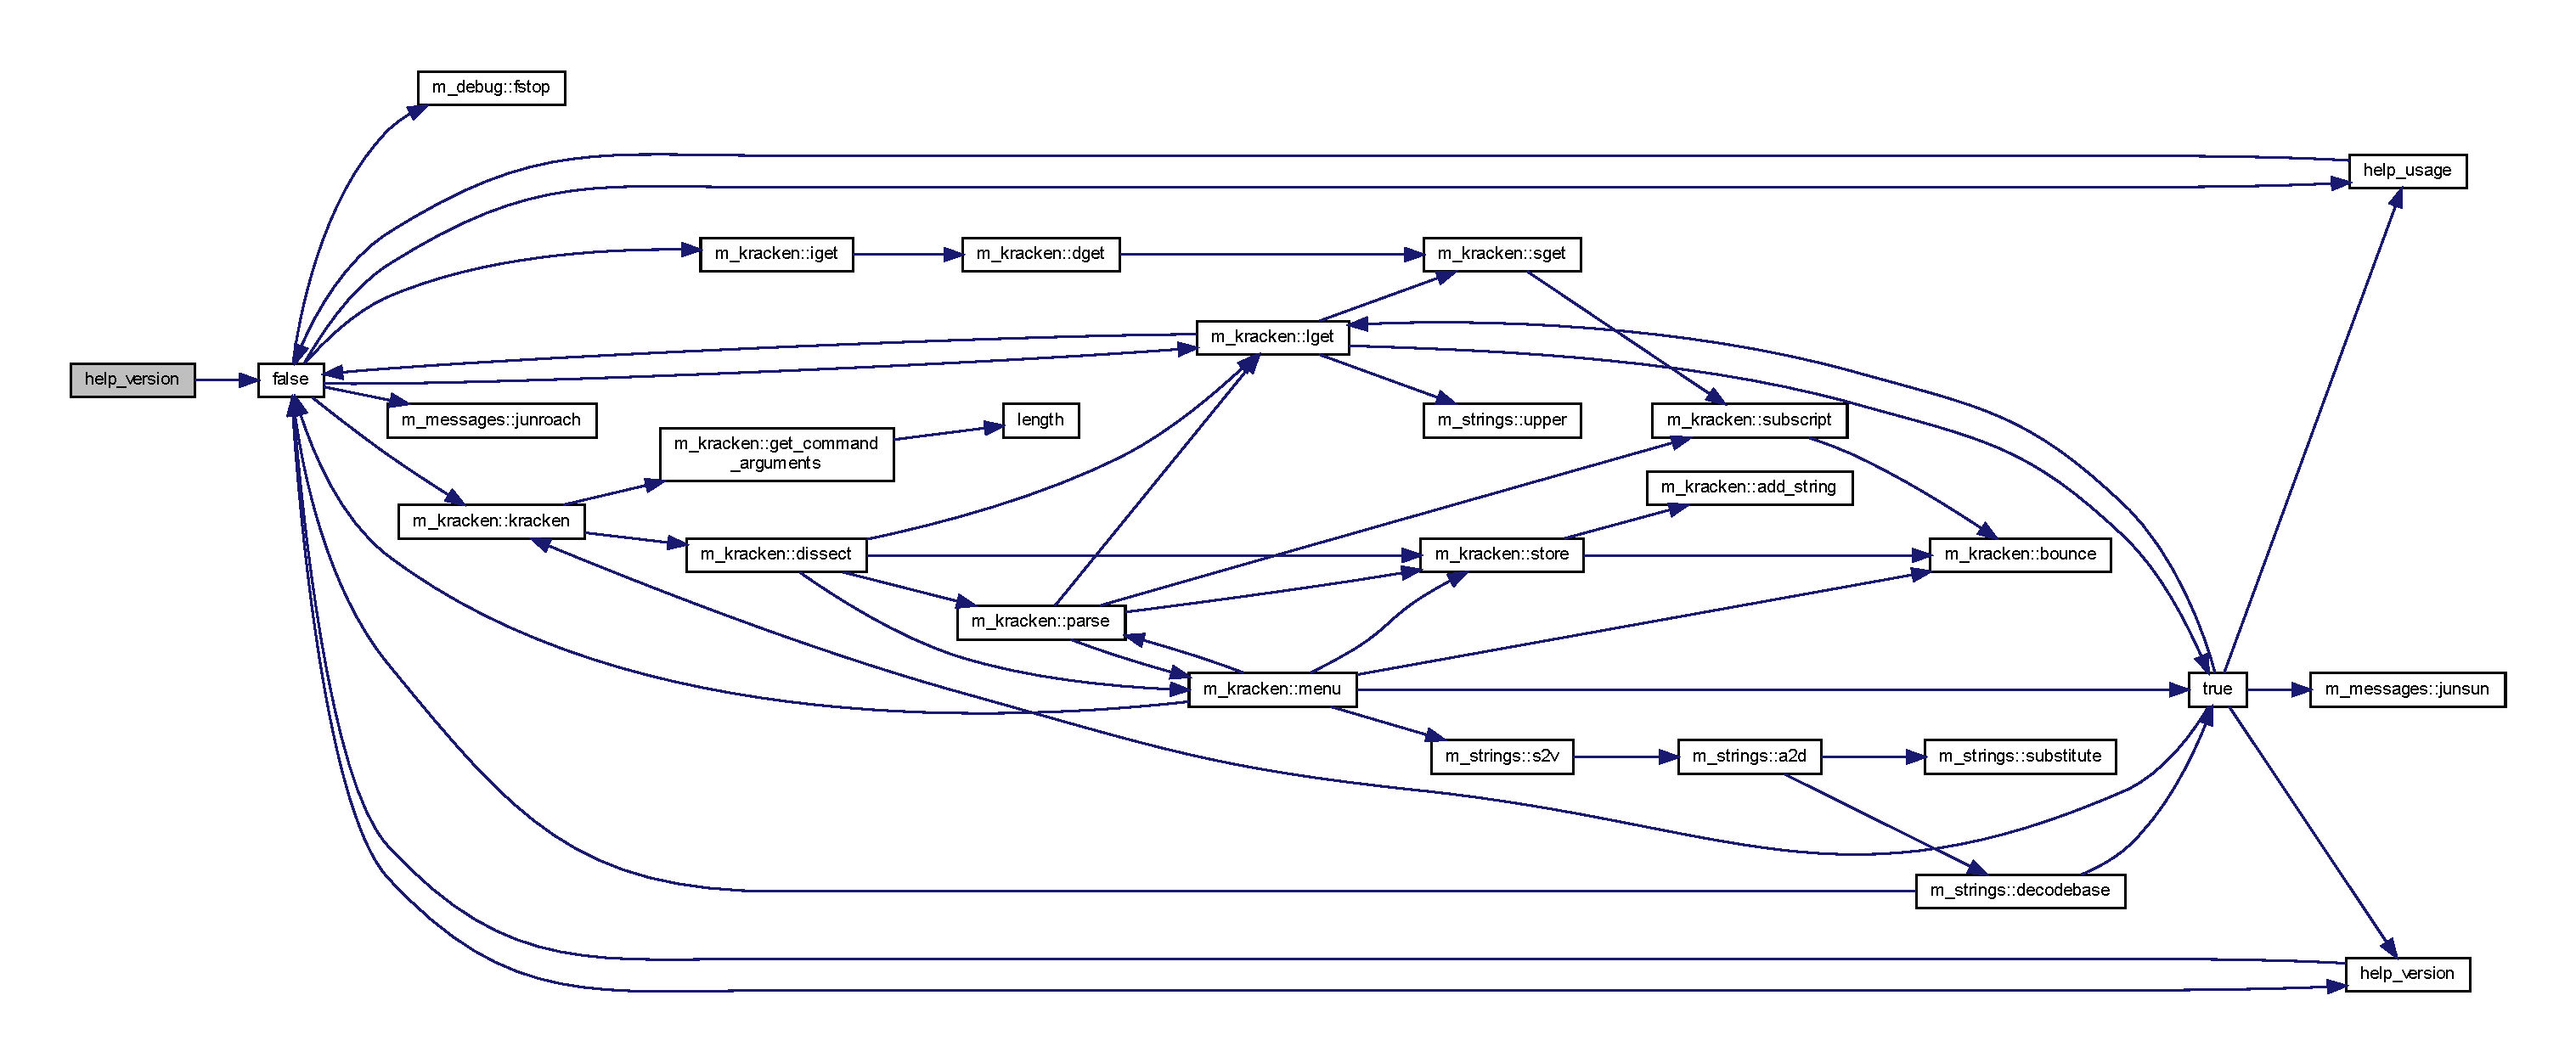
\includegraphics[width=350pt]{__logname_8f90_a39c21619b08a3c22f19e2306efd7f766_cgraph}
\end{center}
\end{figure}

\hypertarget{__ls_8f90}{}\section{L\+I\+B\+R\+A\+R\+Y/lib\+G\+P\+F/download/tmp/\+P\+R\+O\+G\+R\+A\+M\+S/\+\_\+ls.f90 File Reference}
\label{__ls_8f90}\index{L\+I\+B\+R\+A\+R\+Y/lib\+G\+P\+F/download/tmp/\+P\+R\+O\+G\+R\+A\+M\+S/\+\_\+ls.\+f90@{L\+I\+B\+R\+A\+R\+Y/lib\+G\+P\+F/download/tmp/\+P\+R\+O\+G\+R\+A\+M\+S/\+\_\+ls.\+f90}}
\subsection*{Functions/\+Subroutines}
\begin{DoxyCompactItemize}
\item 
\hyperlink{M__stopwatch_83_8txt_acfbcff50169d691ff02d4a123ed70482}{subroutine} \hyperlink{__ls_8f90_a3e09a3b52ee8fb04eeb93fe5761626a8}{help\+\_\+usage} (l\+\_\+help)
\item 
\hyperlink{M__stopwatch_83_8txt_acfbcff50169d691ff02d4a123ed70482}{subroutine} \hyperlink{__ls_8f90_a39c21619b08a3c22f19e2306efd7f766}{help\+\_\+version} (l\+\_\+version)
\begin{DoxyCompactList}\small\item\em \subsubsection*{N\+A\+ME}

\+\_\+ls(1f) -\/ \mbox{[}F\+U\+N\+IX\+:F\+I\+L\+E\+S\+Y\+S\+T\+EM\mbox{]} list files in a directory \subsubsection*{S\+Y\+N\+O\+P\+S\+IS}\end{DoxyCompactList}\item 
program \hyperlink{__ls_8f90_a88c164012f5d1153e039f2dcaa76e971}{demo\+\_\+system\+\_\+readdir}
\item 
\hyperlink{M__stopwatch_83_8txt_acfbcff50169d691ff02d4a123ed70482}{subroutine} \hyperlink{__ls_8f90_a776aaa5526c5060cfed769a9836bd8da}{printit}
\item 
\hyperlink{M__stopwatch_83_8txt_acfbcff50169d691ff02d4a123ed70482}{subroutine} \hyperlink{__ls_8f90_a4299f4bb3561e562301b7fed91e7c673}{print\+\_\+csv}
\end{DoxyCompactItemize}


\subsection{Function/\+Subroutine Documentation}
\mbox{\Hypertarget{__ls_8f90_a88c164012f5d1153e039f2dcaa76e971}\label{__ls_8f90_a88c164012f5d1153e039f2dcaa76e971}} 
\index{\+\_\+ls.\+f90@{\+\_\+ls.\+f90}!demo\+\_\+system\+\_\+readdir@{demo\+\_\+system\+\_\+readdir}}
\index{demo\+\_\+system\+\_\+readdir@{demo\+\_\+system\+\_\+readdir}!\+\_\+ls.\+f90@{\+\_\+ls.\+f90}}
\subsubsection{\texorpdfstring{demo\+\_\+system\+\_\+readdir()}{demo\_system\_readdir()}}
{\footnotesize\ttfamily program demo\+\_\+system\+\_\+readdir (\begin{DoxyParamCaption}{ }\end{DoxyParamCaption})}



References help\+\_\+usage(), help\+\_\+version(), m\+\_\+kracken\+::kracken(), m\+\_\+kracken\+::lget(), print\+\_\+csv(), printit(), m\+\_\+kracken\+::rget(), m\+\_\+kracken\+::sgets(), m\+\_\+system\+::system\+\_\+closedir(), m\+\_\+system\+::system\+\_\+opendir(), m\+\_\+system\+::system\+\_\+readdir(), and m\+\_\+system\+::system\+\_\+stat().

Here is the call graph for this function\+:
\nopagebreak
\begin{figure}[H]
\begin{center}
\leavevmode
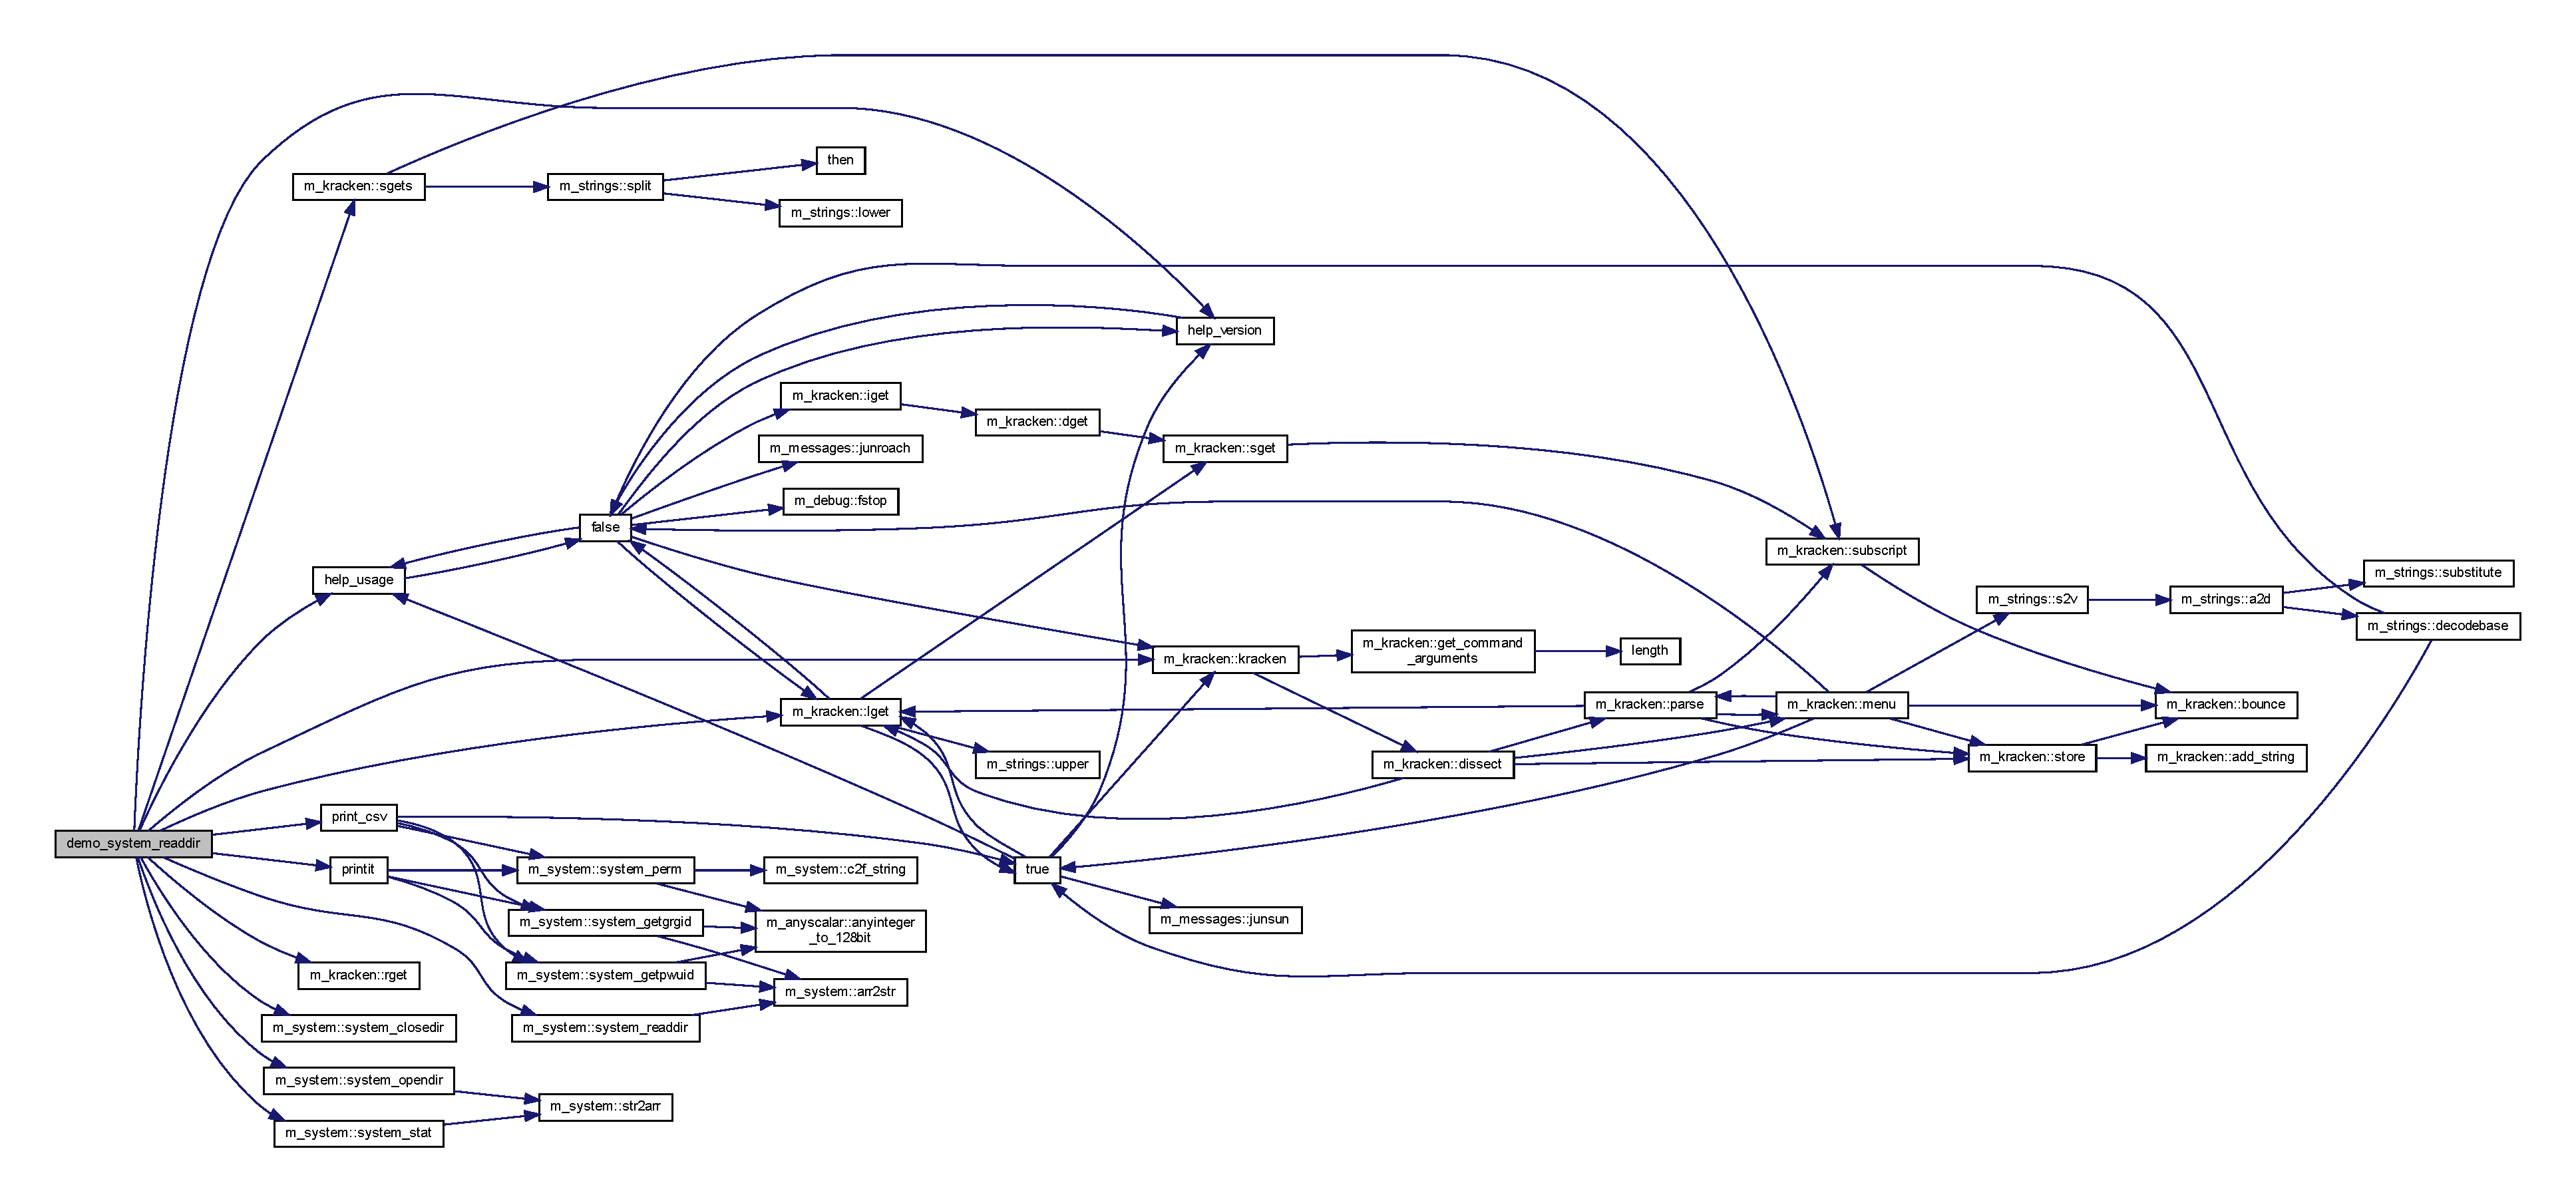
\includegraphics[width=350pt]{__ls_8f90_a88c164012f5d1153e039f2dcaa76e971_cgraph}
\end{center}
\end{figure}
\mbox{\Hypertarget{__ls_8f90_a3e09a3b52ee8fb04eeb93fe5761626a8}\label{__ls_8f90_a3e09a3b52ee8fb04eeb93fe5761626a8}} 
\index{\+\_\+ls.\+f90@{\+\_\+ls.\+f90}!help\+\_\+usage@{help\+\_\+usage}}
\index{help\+\_\+usage@{help\+\_\+usage}!\+\_\+ls.\+f90@{\+\_\+ls.\+f90}}
\subsubsection{\texorpdfstring{help\+\_\+usage()}{help\_usage()}}
{\footnotesize\ttfamily \hyperlink{M__stopwatch_83_8txt_acfbcff50169d691ff02d4a123ed70482}{subroutine} help\+\_\+usage (\begin{DoxyParamCaption}\item[{logical, intent(\hyperlink{M__journal_83_8txt_afce72651d1eed785a2132bee863b2f38}{in})}]{l\+\_\+help }\end{DoxyParamCaption})}



References false().

Here is the call graph for this function\+:
\nopagebreak
\begin{figure}[H]
\begin{center}
\leavevmode
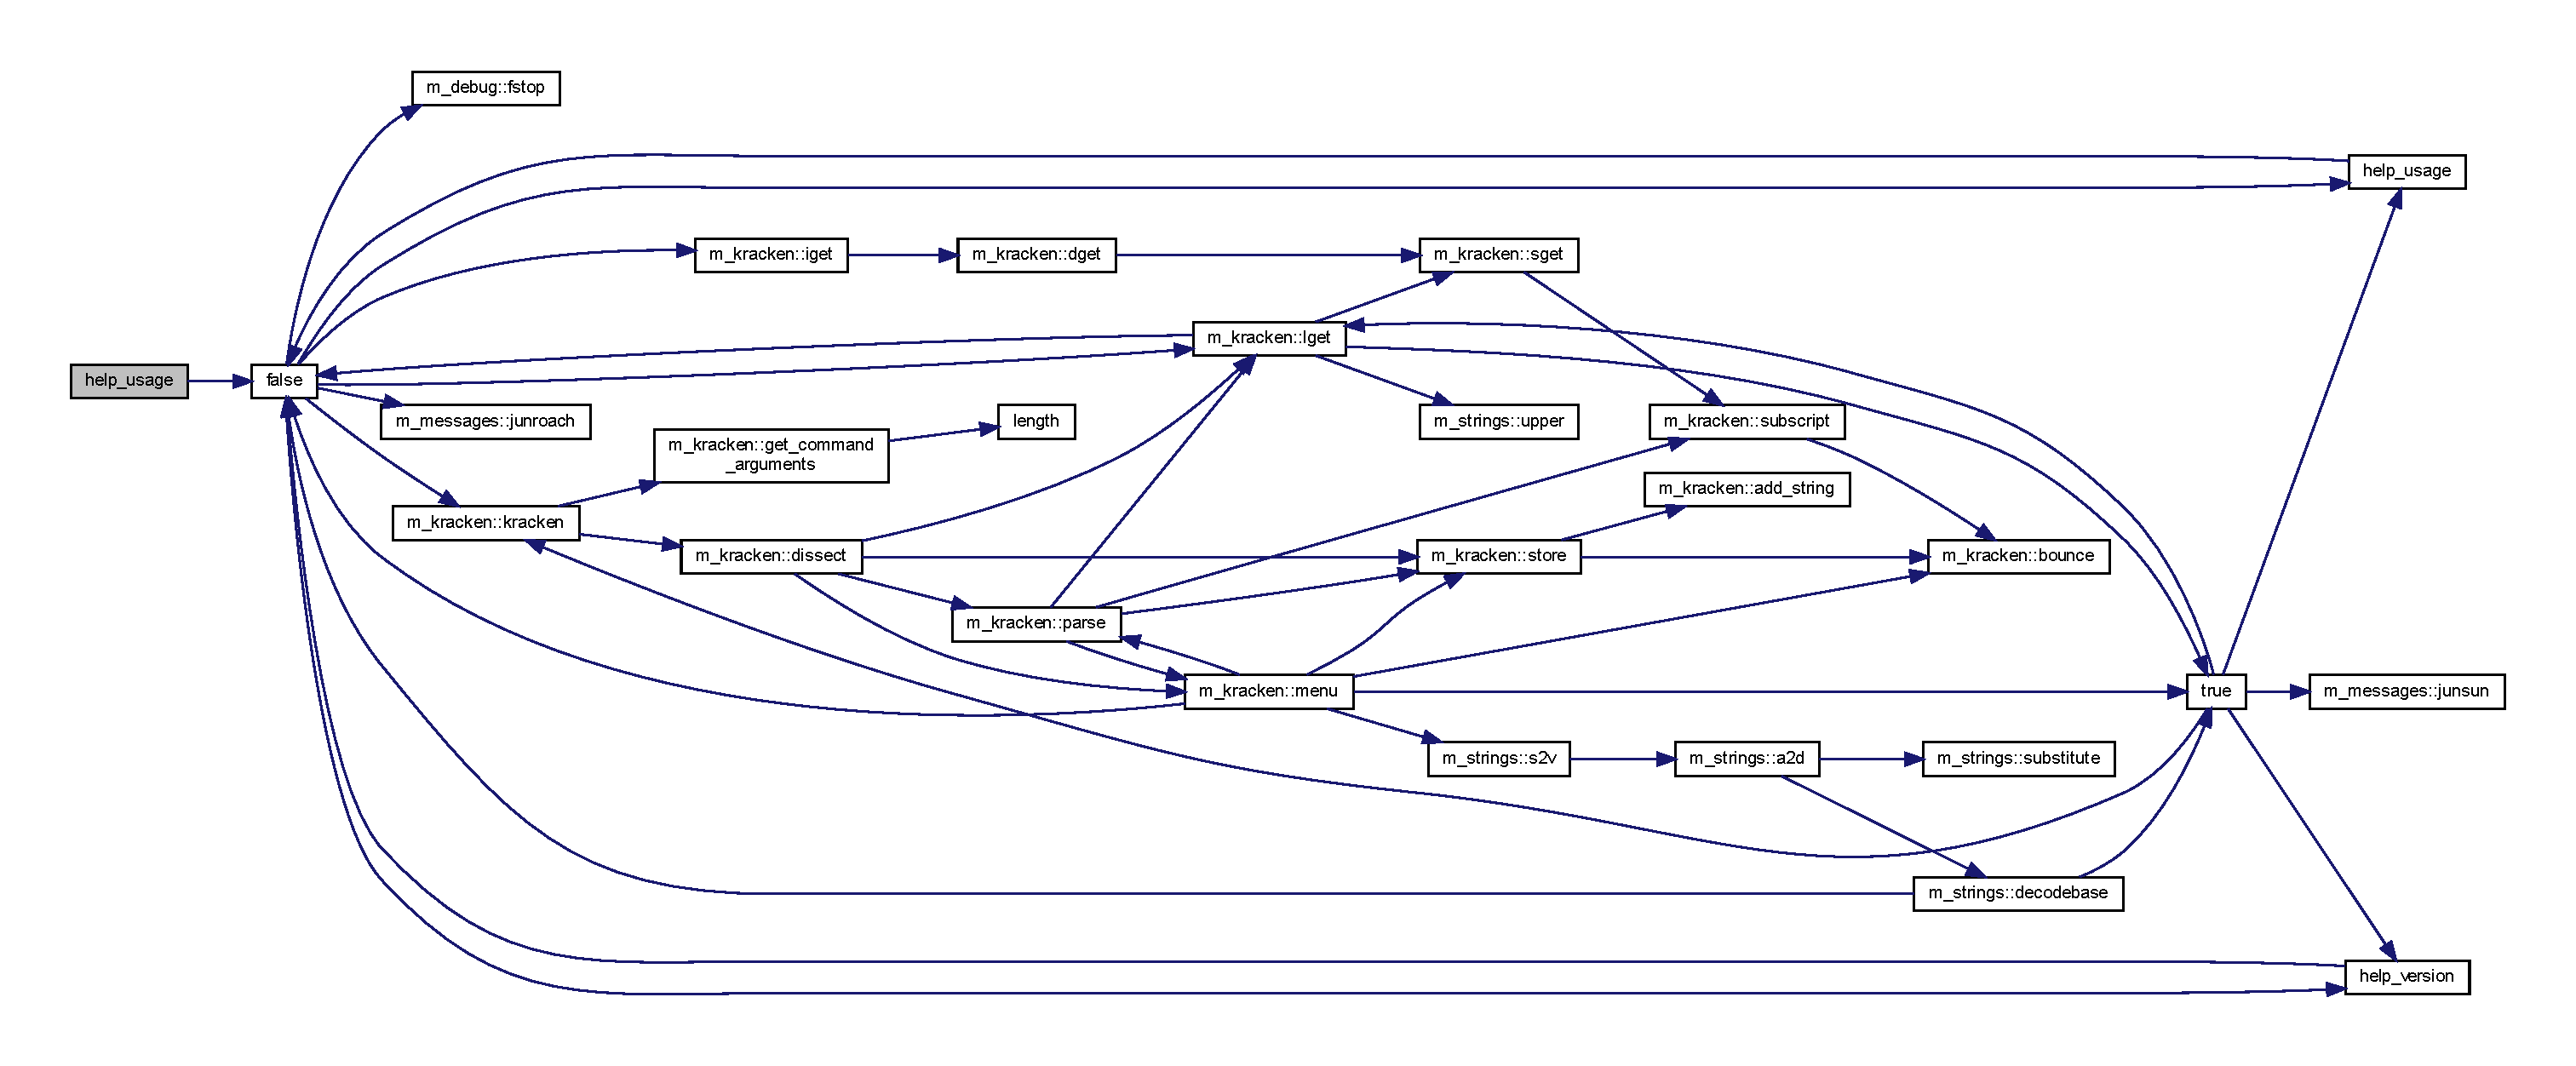
\includegraphics[width=350pt]{__ls_8f90_a3e09a3b52ee8fb04eeb93fe5761626a8_cgraph}
\end{center}
\end{figure}
\mbox{\Hypertarget{__ls_8f90_a39c21619b08a3c22f19e2306efd7f766}\label{__ls_8f90_a39c21619b08a3c22f19e2306efd7f766}} 
\index{\+\_\+ls.\+f90@{\+\_\+ls.\+f90}!help\+\_\+version@{help\+\_\+version}}
\index{help\+\_\+version@{help\+\_\+version}!\+\_\+ls.\+f90@{\+\_\+ls.\+f90}}
\subsubsection{\texorpdfstring{help\+\_\+version()}{help\_version()}}
{\footnotesize\ttfamily \hyperlink{M__stopwatch_83_8txt_acfbcff50169d691ff02d4a123ed70482}{subroutine} help\+\_\+version (\begin{DoxyParamCaption}\item[{logical, intent(\hyperlink{M__journal_83_8txt_afce72651d1eed785a2132bee863b2f38}{in})}]{l\+\_\+version }\end{DoxyParamCaption})}



\subsubsection*{N\+A\+ME}

\+\_\+ls(1f) -\/ \mbox{[}F\+U\+N\+IX\+:F\+I\+L\+E\+S\+Y\+S\+T\+EM\mbox{]} list files in a directory \subsubsection*{S\+Y\+N\+O\+P\+S\+IS}

\+\_\+ls \mbox{[}directory$\vert$--version$\vert$--help\mbox{]} \mbox{[}-\/a\mbox{]} \mbox{[}-\/l$\vert$-\/csv\mbox{]} \subsubsection*{D\+E\+S\+C\+R\+I\+P\+T\+I\+ON}

Given a directory name list files in the directory \subsubsection*{O\+P\+T\+I\+O\+NS}

pathname name of directory or pathname to display contents of. Defaults to current directory. -\/a show hidden files (files beginning with \char`\"{}.\char`\"{}). -\/l long listing -\/csv generate output as a C\+SV file. Filenames should not have ,"\textquotesingle{} characters in them. Very useful for use with sqlite3(1) and making a file that can be read into most spreadsheets, --help display command help and exit --version output version information and exit \subsubsection*{E\+X\+A\+M\+P\+L\+ES}

Sample command lines ... \begin{DoxyVerb}   _ls
   _ls . /tmp -l
\end{DoxyVerb}


\subsubsection*{E\+X\+T\+E\+N\+D\+ED S\+Q\+L\+I\+TE E\+X\+A\+M\+P\+LE}

The C\+SV output can often just be read by spreadsheets. Typically the file suffix \char`\"{}.\+csv\char`\"{} is required. Assuming you have bash(1), sqlite3(1) and column(1) on your platform this is an example script that shows how S\+QL statements can be used to generate many kinds of file reports (number of bytes owned by users, number of files, sorting, ... It assumes you or somone who will assist you is familiar with S\+QL and sqlite3(1)\+:

\#!/bin/bash \#@(\#) list files accessed today in current directory export S\+C\+R\+A\+T\+CH=/tmp/.csv \# create scratch file name trap \char`\"{}/bin/rm -\/f \$\+S\+C\+R\+A\+T\+C\+H\char`\"{} E\+X\+IT \# ensure scratch file is removed \+\_\+ls -\/csv -- . $\vert$tail -\/n +2$>$\$\+S\+C\+R\+A\+T\+CH \# generate C\+SV file ( \subsection*{read C\+SV file into an S\+Q\+Lite file and generate a report as H\+T\+ML table}

sqlite3 \textbackslash{} -\/cmd \textquotesingle{}C\+R\+E\+A\+TE T\+A\+B\+LE directory(\char`\"{}\+Inode\+\_\+number\char`\"{} I\+NT, \char`\"{}\+Number\+\_\+of\+\_\+blocks\+\_\+allocated\char`\"{} I\+NT, \char`\"{}\+File\+\_\+mode\char`\"{} T\+E\+XT, \char`\"{}\+Number\+\_\+of\+\_\+links\char`\"{} I\+NT, \char`\"{}\+Owner\char`\"{} T\+E\+XT, \char`\"{}\+Groupname\char`\"{} T\+E\+XT, \char`\"{}\+File\+\_\+size\char`\"{} I\+NT, \char`\"{}\+Last\+\_\+access\char`\"{} D\+A\+TE, \char`\"{}\+Last\+\_\+modification\char`\"{} D\+A\+TE, \char`\"{}\+Last\+\_\+status\+\_\+change\char`\"{} D\+A\+TE, \char`\"{}\+Pathname\char`\"{} T\+E\+XT );\textquotesingle{} \textbackslash{} -\/cmd \textquotesingle{}.mode csv\textquotesingle{} \textbackslash{} -\/cmd \char`\"{}.\+import \$\+S\+C\+R\+A\+T\+C\+H directory\char`\"{} $<$$<$ -- .schema .mode column .header on S\+E\+L\+E\+CT Pathname, File\+\_\+mode, Owner, Groupname, File\+\_\+size, strftime(\textquotesingle{}Y-\/m-\/d H\+:M\+:S\textquotesingle{}, Last\+\_\+access) as \char`\"{}\+Last\+\_\+\+Access\char`\"{} F\+R\+OM directory W\+H\+E\+RE D\+A\+TE(\textquotesingle{}now\textquotesingle{}, \textquotesingle{}start of day\textquotesingle{}) $<$ Last\+\_\+access O\+R\+D\+ER BY Pathname A\+SC; E\+OF )$\vert$ column -\/t -\/s \textquotesingle{}$\vert$\textquotesingle{} exit 

References false().

Here is the call graph for this function\+:
\nopagebreak
\begin{figure}[H]
\begin{center}
\leavevmode
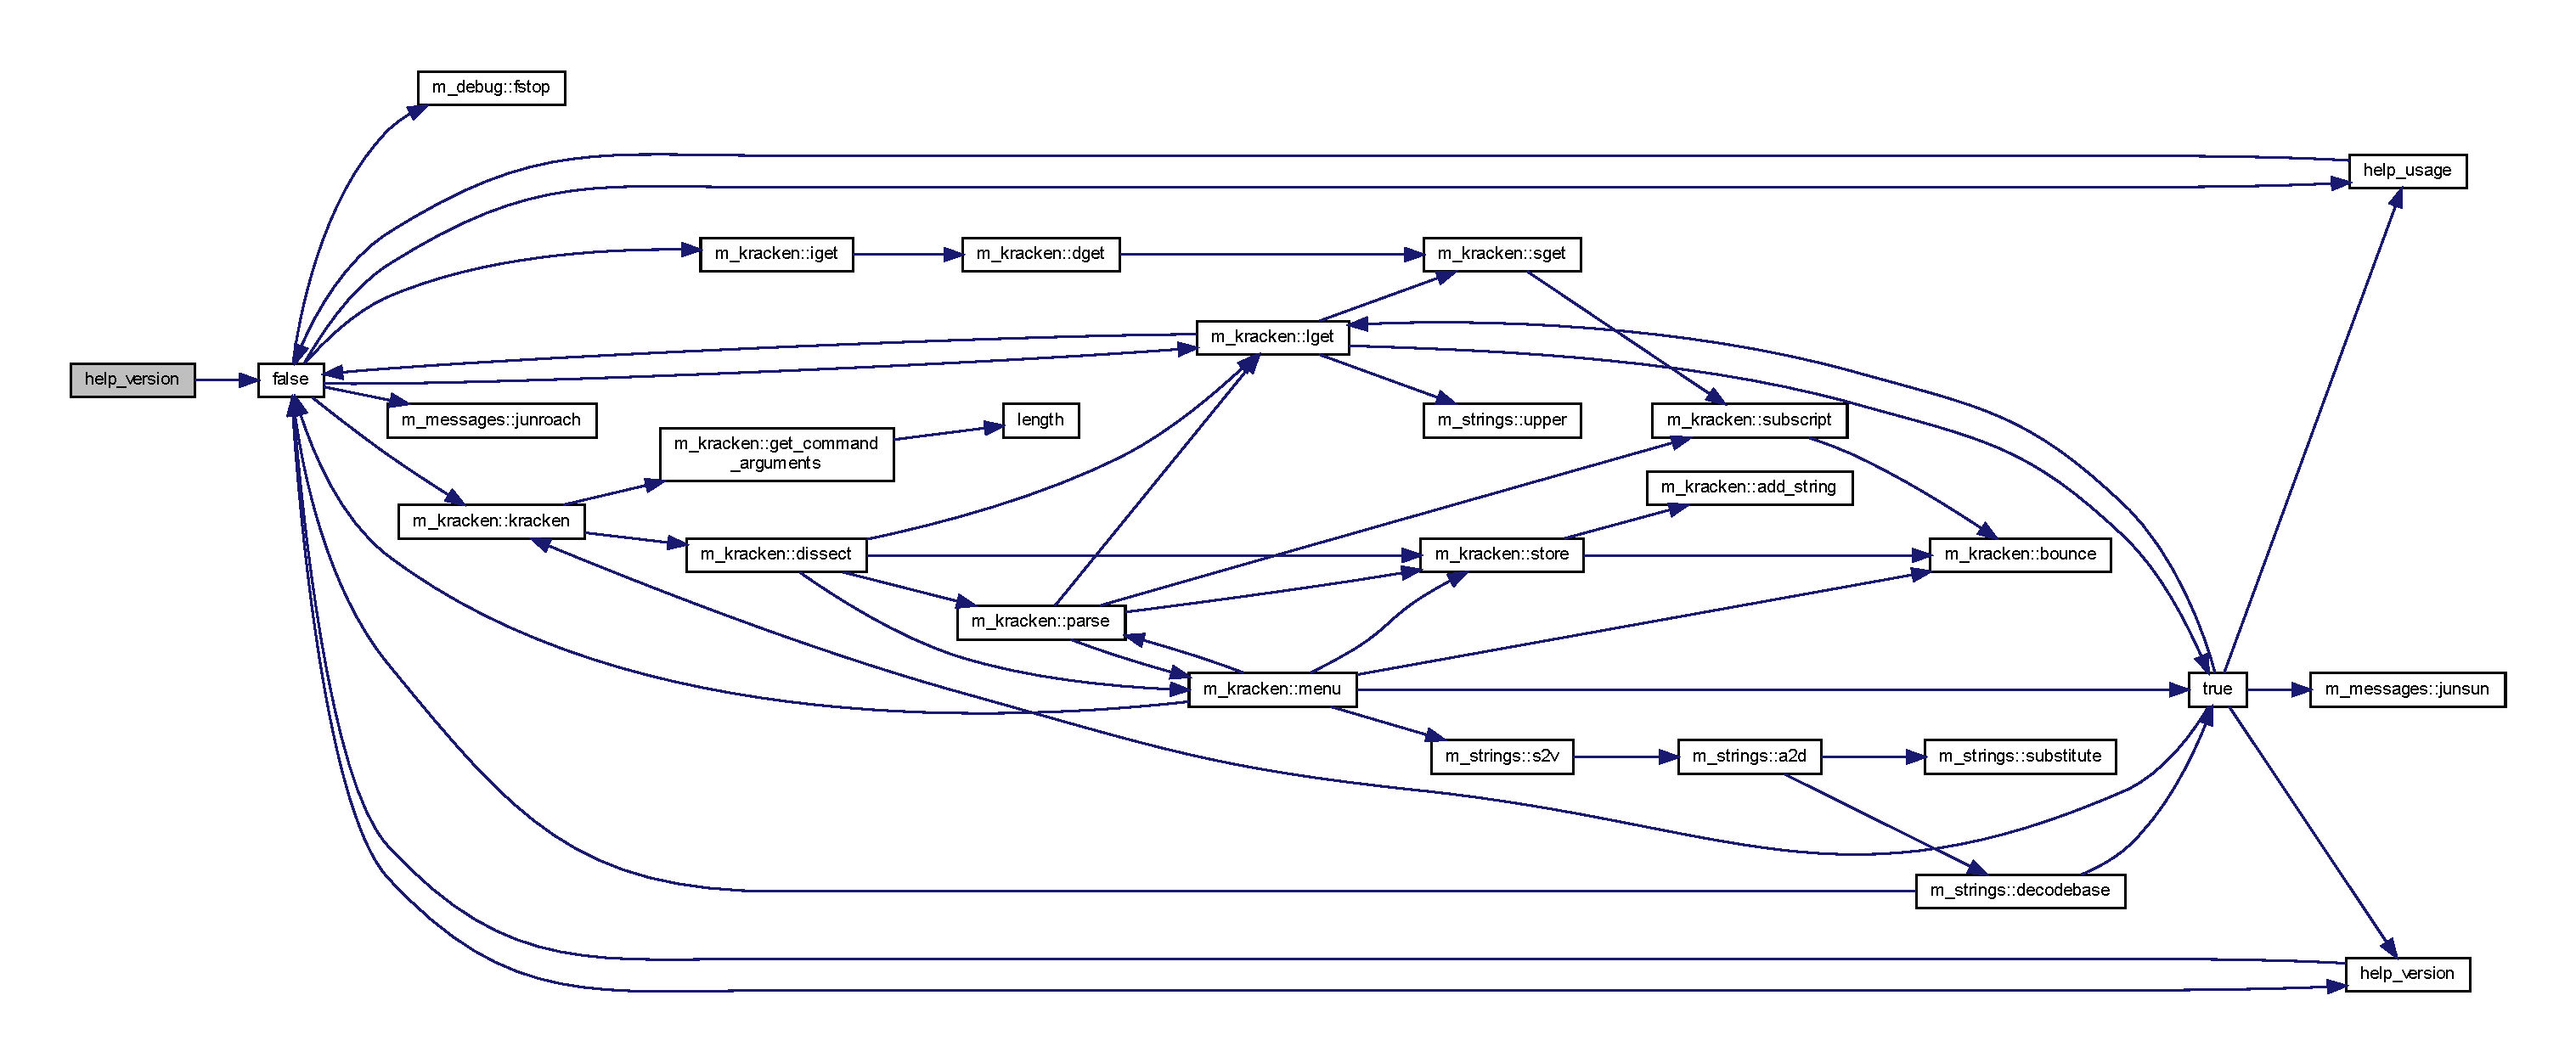
\includegraphics[width=350pt]{__ls_8f90_a39c21619b08a3c22f19e2306efd7f766_cgraph}
\end{center}
\end{figure}
\mbox{\Hypertarget{__ls_8f90_a4299f4bb3561e562301b7fed91e7c673}\label{__ls_8f90_a4299f4bb3561e562301b7fed91e7c673}} 
\index{\+\_\+ls.\+f90@{\+\_\+ls.\+f90}!print\+\_\+csv@{print\+\_\+csv}}
\index{print\+\_\+csv@{print\+\_\+csv}!\+\_\+ls.\+f90@{\+\_\+ls.\+f90}}
\subsubsection{\texorpdfstring{print\+\_\+csv()}{print\_csv()}}
{\footnotesize\ttfamily \hyperlink{M__stopwatch_83_8txt_acfbcff50169d691ff02d4a123ed70482}{subroutine} demo\+\_\+system\+\_\+readdir\+::print\+\_\+csv (\begin{DoxyParamCaption}{ }\end{DoxyParamCaption})}



References fmtdate, m\+\_\+system\+::system\+\_\+getgrgid(), m\+\_\+system\+::system\+\_\+getpwuid(), m\+\_\+system\+::system\+\_\+perm(), true(), and u2d.

Here is the call graph for this function\+:
\nopagebreak
\begin{figure}[H]
\begin{center}
\leavevmode
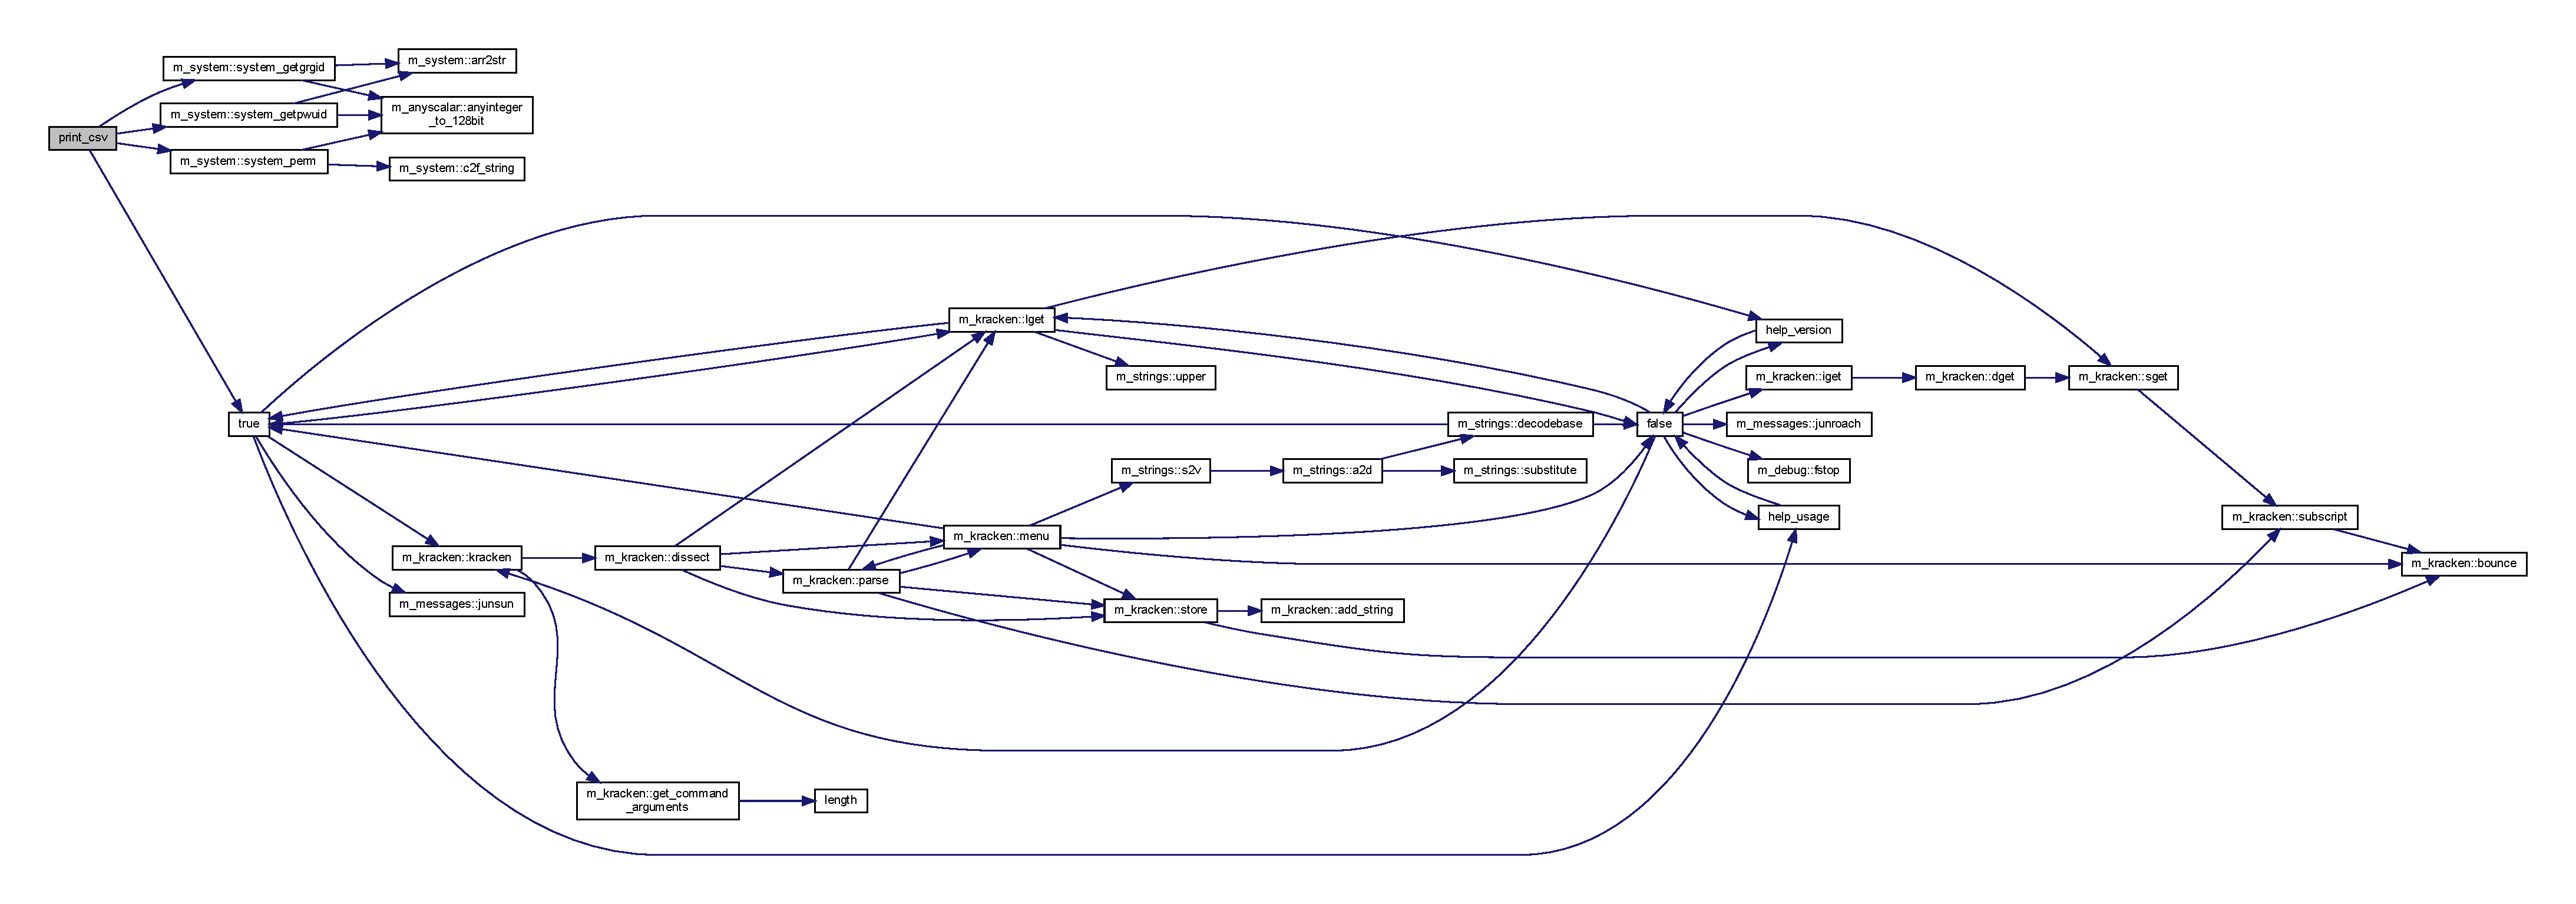
\includegraphics[width=350pt]{__ls_8f90_a4299f4bb3561e562301b7fed91e7c673_cgraph}
\end{center}
\end{figure}
Here is the caller graph for this function\+:
\nopagebreak
\begin{figure}[H]
\begin{center}
\leavevmode
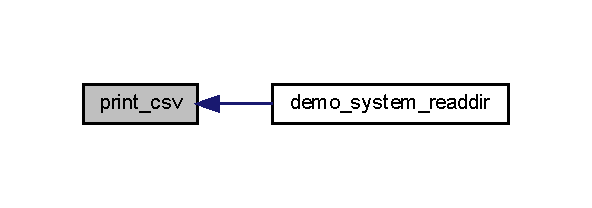
\includegraphics[width=284pt]{__ls_8f90_a4299f4bb3561e562301b7fed91e7c673_icgraph}
\end{center}
\end{figure}
\mbox{\Hypertarget{__ls_8f90_a776aaa5526c5060cfed769a9836bd8da}\label{__ls_8f90_a776aaa5526c5060cfed769a9836bd8da}} 
\index{\+\_\+ls.\+f90@{\+\_\+ls.\+f90}!printit@{printit}}
\index{printit@{printit}!\+\_\+ls.\+f90@{\+\_\+ls.\+f90}}
\subsubsection{\texorpdfstring{printit()}{printit()}}
{\footnotesize\ttfamily \hyperlink{M__stopwatch_83_8txt_acfbcff50169d691ff02d4a123ed70482}{subroutine} demo\+\_\+system\+\_\+readdir\+::printit (\begin{DoxyParamCaption}{ }\end{DoxyParamCaption})}



References fmtdate, m\+\_\+system\+::system\+\_\+getgrgid(), m\+\_\+system\+::system\+\_\+getpwuid(), m\+\_\+system\+::system\+\_\+perm(), and u2d.

Here is the call graph for this function\+:
\nopagebreak
\begin{figure}[H]
\begin{center}
\leavevmode
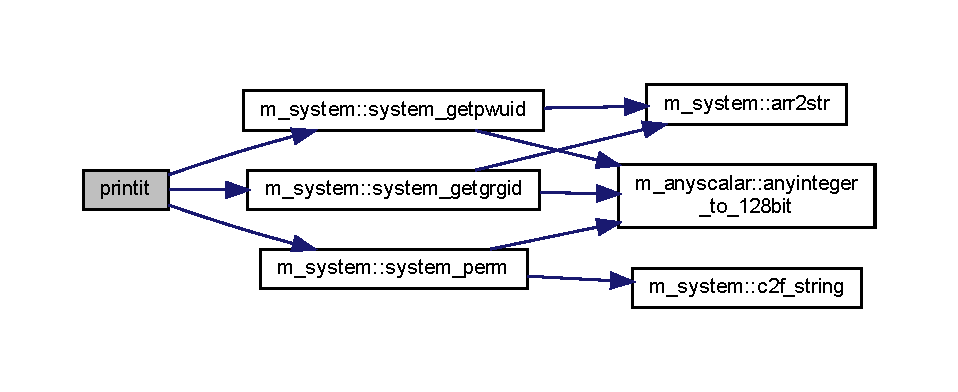
\includegraphics[width=350pt]{__ls_8f90_a776aaa5526c5060cfed769a9836bd8da_cgraph}
\end{center}
\end{figure}
Here is the caller graph for this function\+:
\nopagebreak
\begin{figure}[H]
\begin{center}
\leavevmode
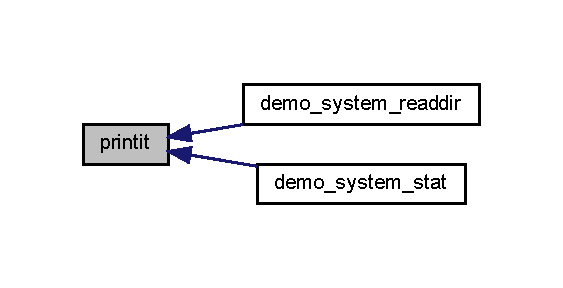
\includegraphics[width=270pt]{__ls_8f90_a776aaa5526c5060cfed769a9836bd8da_icgraph}
\end{center}
\end{figure}

\hypertarget{__mkdir_8f90}{}\section{L\+I\+B\+R\+A\+R\+Y/lib\+G\+P\+F/download/tmp/\+P\+R\+O\+G\+R\+A\+M\+S/\+\_\+mkdir.f90 File Reference}
\label{__mkdir_8f90}\index{L\+I\+B\+R\+A\+R\+Y/lib\+G\+P\+F/download/tmp/\+P\+R\+O\+G\+R\+A\+M\+S/\+\_\+mkdir.\+f90@{L\+I\+B\+R\+A\+R\+Y/lib\+G\+P\+F/download/tmp/\+P\+R\+O\+G\+R\+A\+M\+S/\+\_\+mkdir.\+f90}}

\hypertarget{__mkfifo_8f90}{}\section{L\+I\+B\+R\+A\+R\+Y/lib\+G\+P\+F/download/tmp/\+P\+R\+O\+G\+R\+A\+M\+S/\+\_\+mkfifo.f90 File Reference}
\label{__mkfifo_8f90}\index{L\+I\+B\+R\+A\+R\+Y/lib\+G\+P\+F/download/tmp/\+P\+R\+O\+G\+R\+A\+M\+S/\+\_\+mkfifo.\+f90@{L\+I\+B\+R\+A\+R\+Y/lib\+G\+P\+F/download/tmp/\+P\+R\+O\+G\+R\+A\+M\+S/\+\_\+mkfifo.\+f90}}
\subsection*{Functions/\+Subroutines}
\begin{DoxyCompactItemize}
\item 
\hyperlink{M__stopwatch_83_8txt_acfbcff50169d691ff02d4a123ed70482}{subroutine} \hyperlink{__mkfifo_8f90_a3e09a3b52ee8fb04eeb93fe5761626a8}{help\+\_\+usage} (l\+\_\+help)
\item 
\hyperlink{M__stopwatch_83_8txt_acfbcff50169d691ff02d4a123ed70482}{subroutine} \hyperlink{__mkfifo_8f90_a39c21619b08a3c22f19e2306efd7f766}{help\+\_\+version} (l\+\_\+version)
\begin{DoxyCompactList}\small\item\em \subsubsection*{N\+A\+ME}

\+\_\+mkfifo(1f) -\/ \mbox{[}F\+U\+N\+IX\+:F\+I\+L\+E\+S\+Y\+S\+T\+EM\mbox{]} make a F\+I\+FO pipe by calling mkfifo(3c) \subsubsection*{S\+Y\+N\+O\+P\+S\+IS}\end{DoxyCompactList}\item 
program \hyperlink{__mkfifo_8f90_a6c58f22de022879b9913bc1c177c62ca}{demo\+\_\+system\+\_\+mkfifo}
\end{DoxyCompactItemize}


\subsection{Function/\+Subroutine Documentation}
\mbox{\Hypertarget{__mkfifo_8f90_a6c58f22de022879b9913bc1c177c62ca}\label{__mkfifo_8f90_a6c58f22de022879b9913bc1c177c62ca}} 
\index{\+\_\+mkfifo.\+f90@{\+\_\+mkfifo.\+f90}!demo\+\_\+system\+\_\+mkfifo@{demo\+\_\+system\+\_\+mkfifo}}
\index{demo\+\_\+system\+\_\+mkfifo@{demo\+\_\+system\+\_\+mkfifo}!\+\_\+mkfifo.\+f90@{\+\_\+mkfifo.\+f90}}
\subsubsection{\texorpdfstring{demo\+\_\+system\+\_\+mkfifo()}{demo\_system\_mkfifo()}}
{\footnotesize\ttfamily program demo\+\_\+system\+\_\+mkfifo (\begin{DoxyParamCaption}{ }\end{DoxyParamCaption})}



References m\+\_\+system\+::accessperms, m\+\_\+system\+::deffilemode, help\+\_\+usage(), help\+\_\+version(), m\+\_\+kracken\+::ipvalue, m\+\_\+kracken\+::kracken(), m\+\_\+kracken\+::lget(), m\+\_\+system\+::r\+\_\+grp, m\+\_\+system\+::r\+\_\+oth, m\+\_\+system\+::r\+\_\+usr, m\+\_\+system\+::r\+\_\+wxg, m\+\_\+system\+::r\+\_\+wxo, m\+\_\+system\+::r\+\_\+wxu, m\+\_\+kracken\+::sgets(), m\+\_\+system\+::system\+\_\+mkfifo(), m\+\_\+system\+::system\+\_\+perror(), m\+\_\+system\+::w\+\_\+grp, m\+\_\+system\+::w\+\_\+oth, m\+\_\+system\+::w\+\_\+usr, m\+\_\+system\+::x\+\_\+grp, m\+\_\+system\+::x\+\_\+oth, and m\+\_\+system\+::x\+\_\+usr.

Here is the call graph for this function\+:
\nopagebreak
\begin{figure}[H]
\begin{center}
\leavevmode
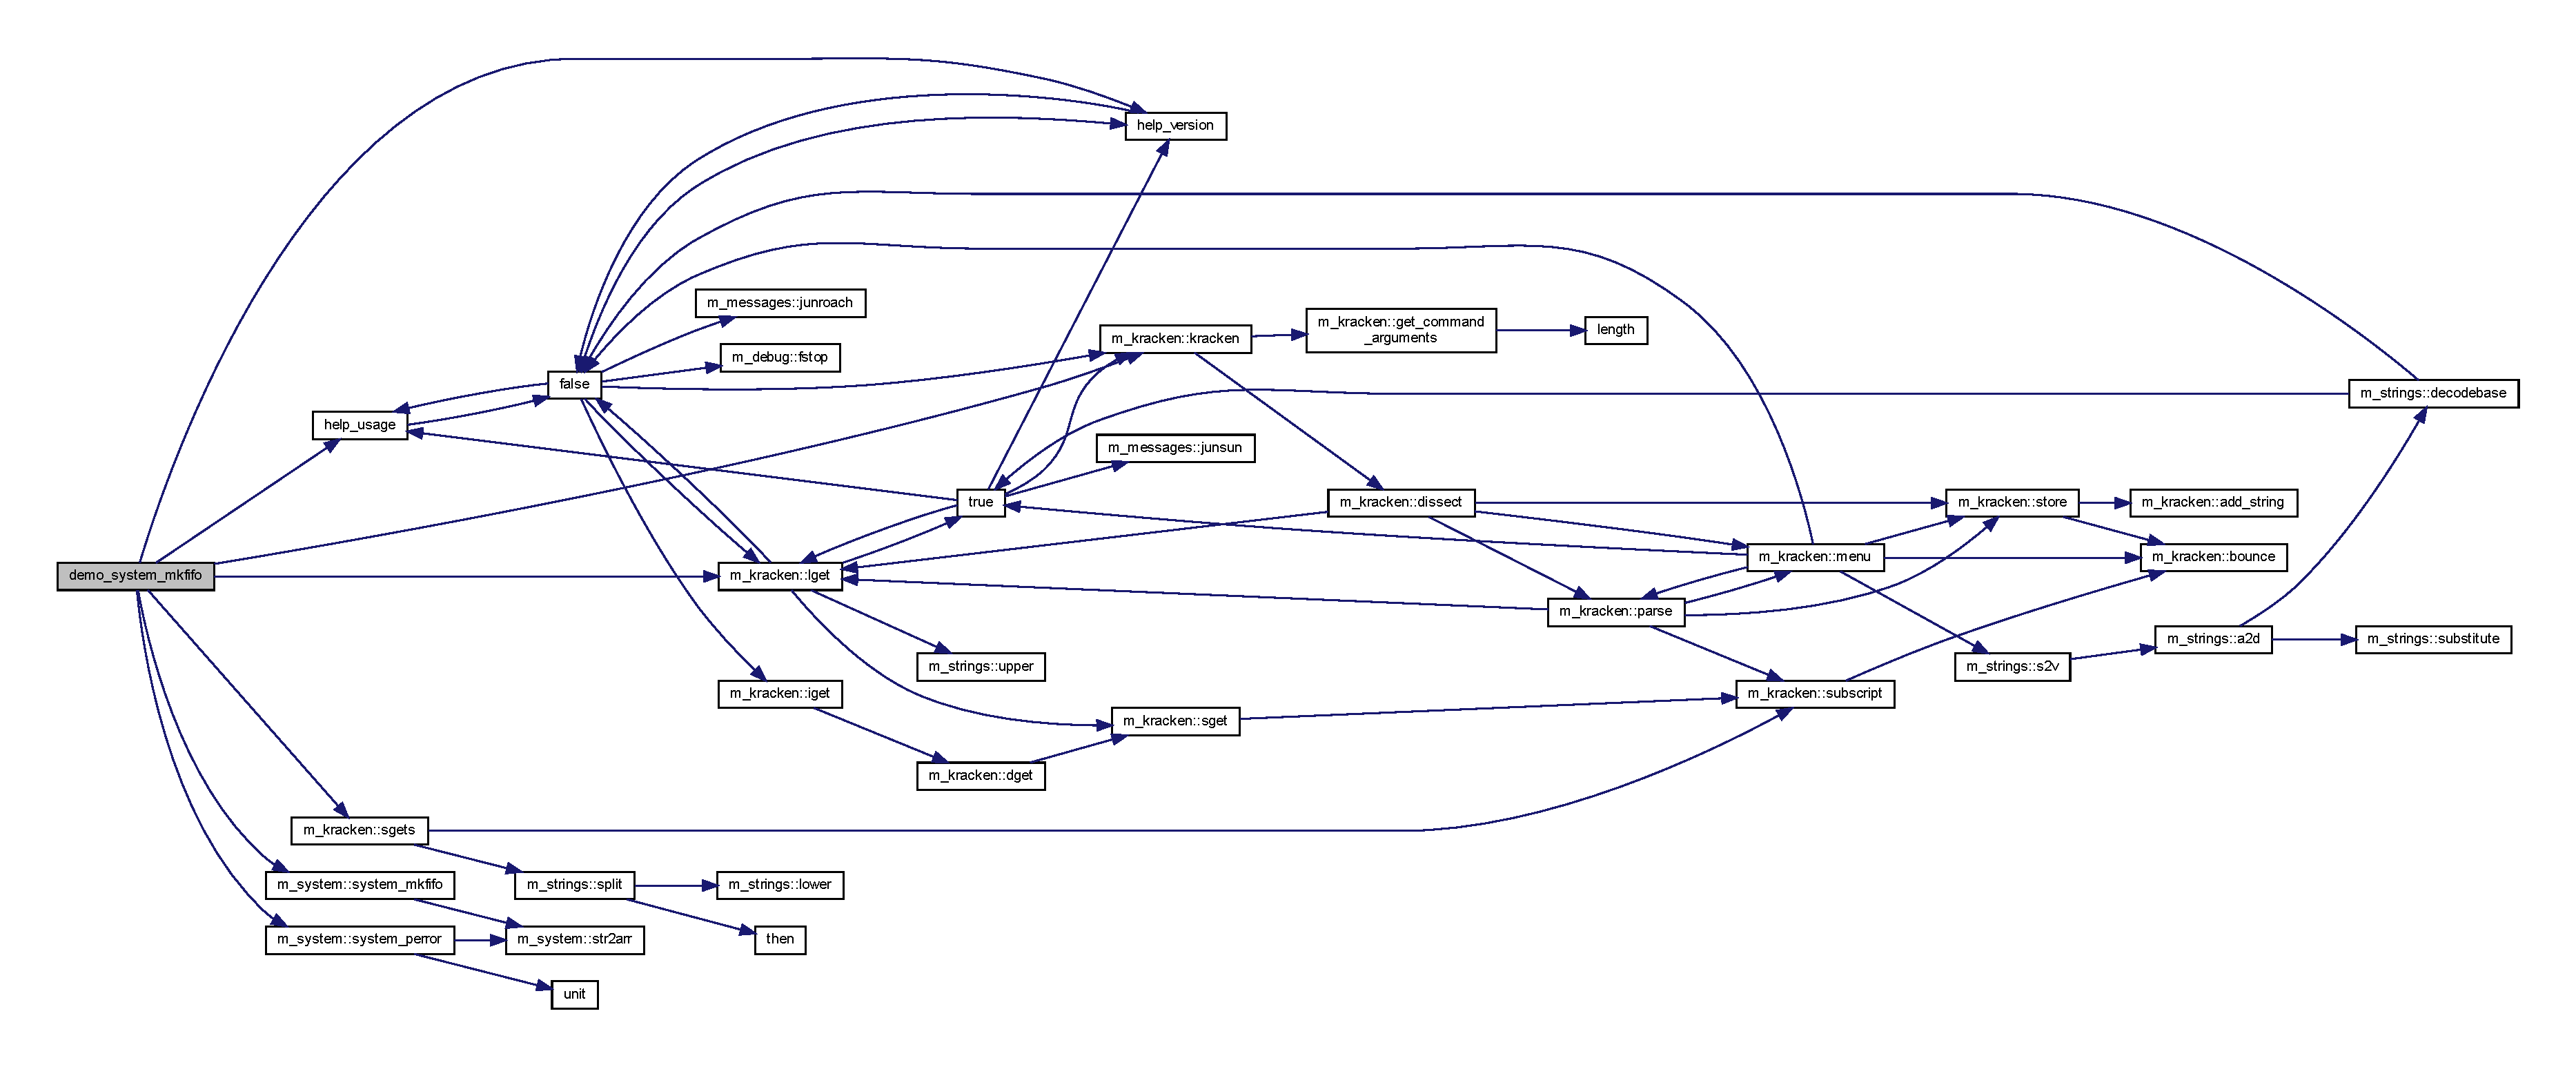
\includegraphics[width=350pt]{__mkfifo_8f90_a6c58f22de022879b9913bc1c177c62ca_cgraph}
\end{center}
\end{figure}
\mbox{\Hypertarget{__mkfifo_8f90_a3e09a3b52ee8fb04eeb93fe5761626a8}\label{__mkfifo_8f90_a3e09a3b52ee8fb04eeb93fe5761626a8}} 
\index{\+\_\+mkfifo.\+f90@{\+\_\+mkfifo.\+f90}!help\+\_\+usage@{help\+\_\+usage}}
\index{help\+\_\+usage@{help\+\_\+usage}!\+\_\+mkfifo.\+f90@{\+\_\+mkfifo.\+f90}}
\subsubsection{\texorpdfstring{help\+\_\+usage()}{help\_usage()}}
{\footnotesize\ttfamily \hyperlink{M__stopwatch_83_8txt_acfbcff50169d691ff02d4a123ed70482}{subroutine} help\+\_\+usage (\begin{DoxyParamCaption}\item[{logical, intent(\hyperlink{M__journal_83_8txt_afce72651d1eed785a2132bee863b2f38}{in})}]{l\+\_\+help }\end{DoxyParamCaption})}



References false().

Here is the call graph for this function\+:
\nopagebreak
\begin{figure}[H]
\begin{center}
\leavevmode
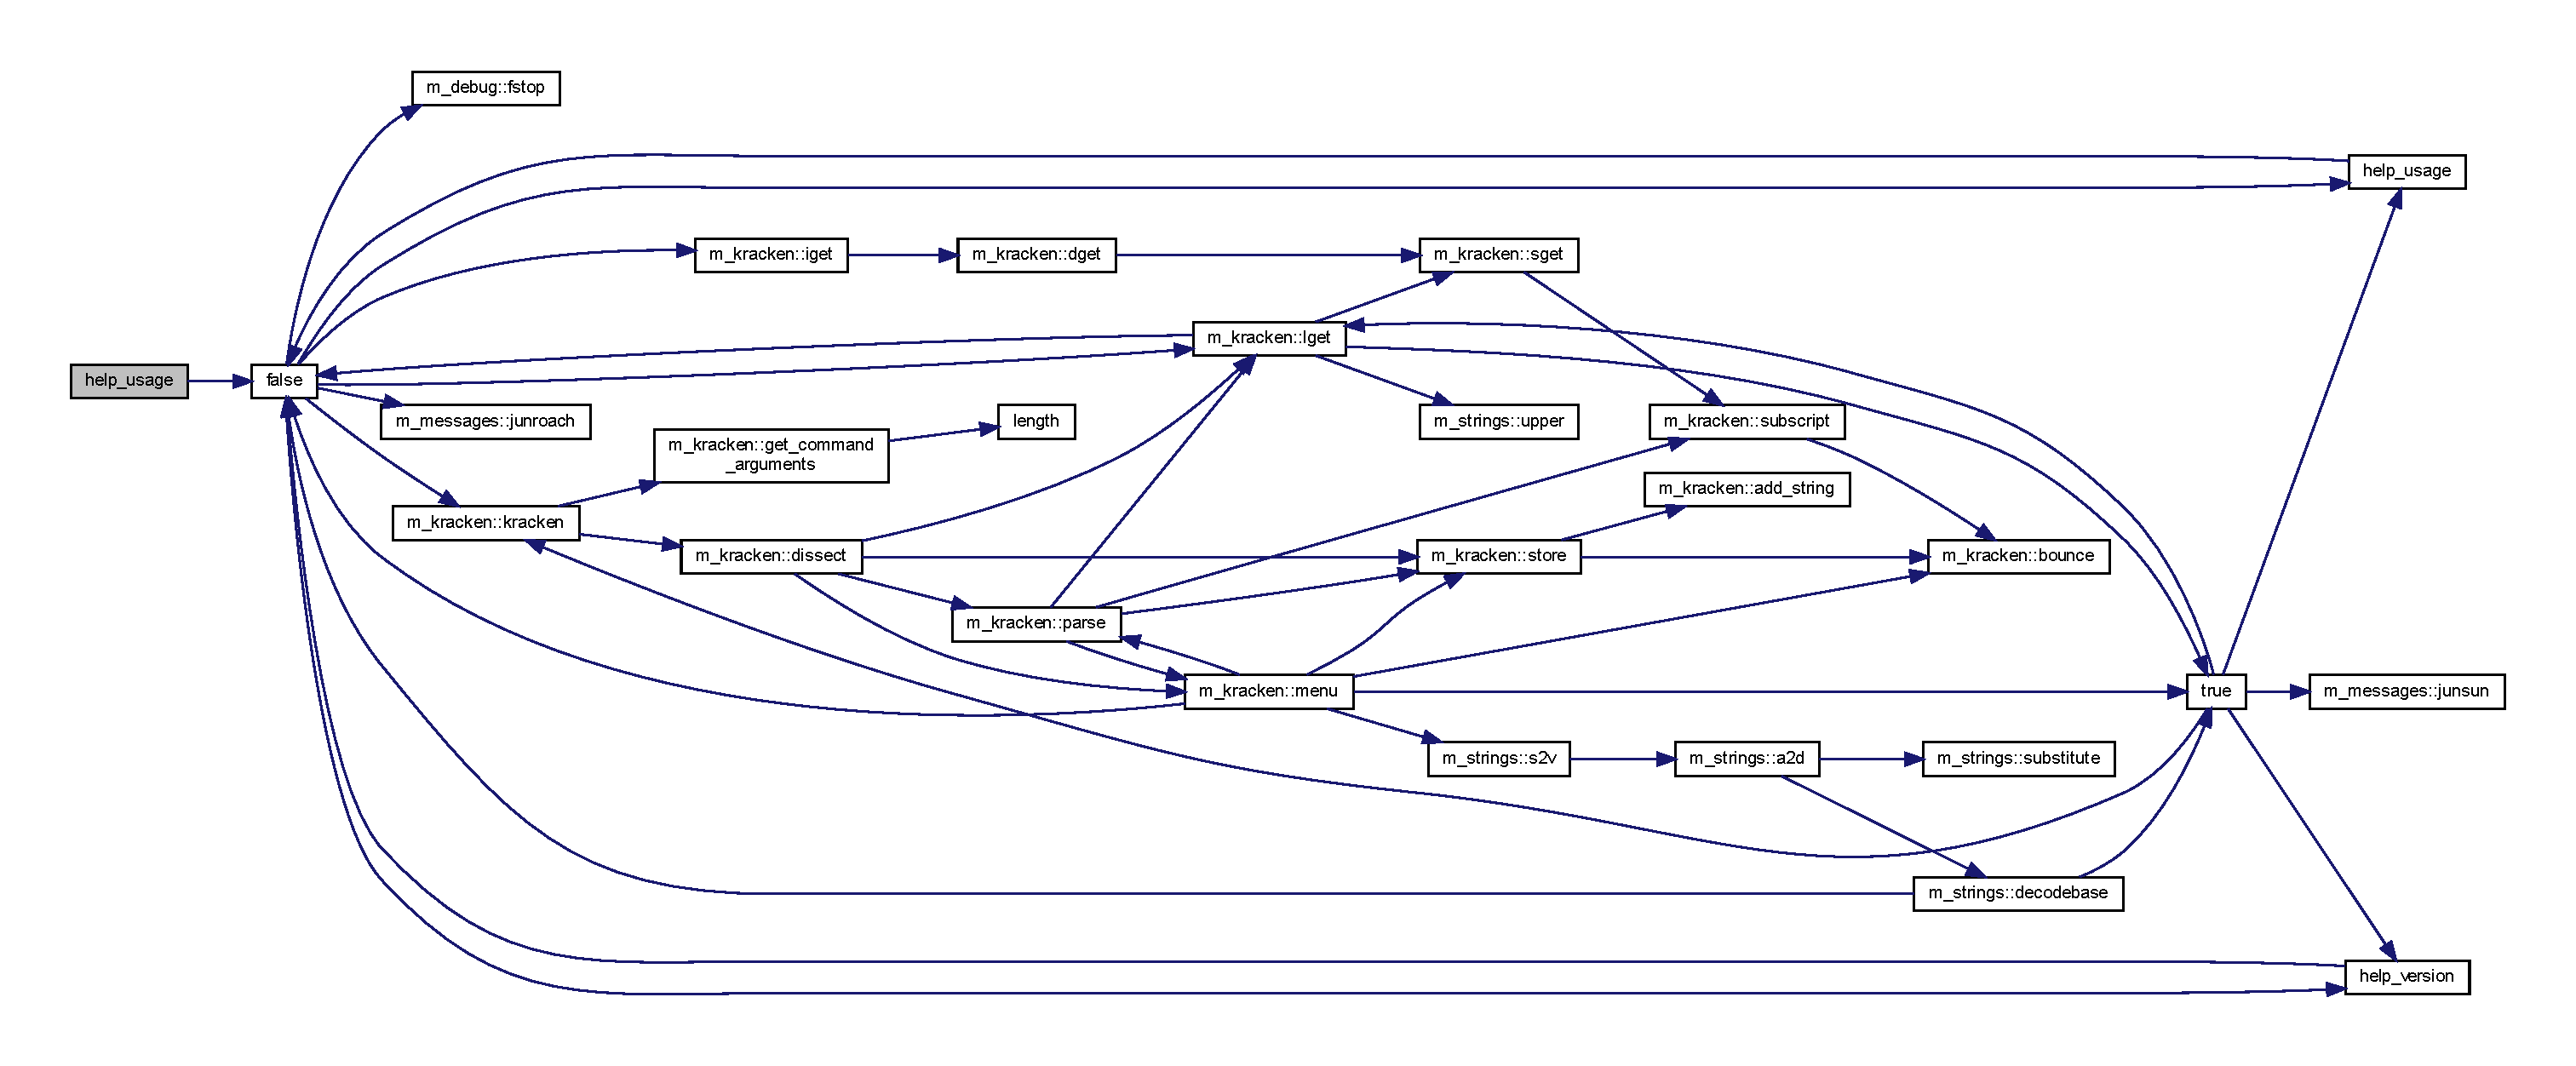
\includegraphics[width=350pt]{__mkfifo_8f90_a3e09a3b52ee8fb04eeb93fe5761626a8_cgraph}
\end{center}
\end{figure}
\mbox{\Hypertarget{__mkfifo_8f90_a39c21619b08a3c22f19e2306efd7f766}\label{__mkfifo_8f90_a39c21619b08a3c22f19e2306efd7f766}} 
\index{\+\_\+mkfifo.\+f90@{\+\_\+mkfifo.\+f90}!help\+\_\+version@{help\+\_\+version}}
\index{help\+\_\+version@{help\+\_\+version}!\+\_\+mkfifo.\+f90@{\+\_\+mkfifo.\+f90}}
\subsubsection{\texorpdfstring{help\+\_\+version()}{help\_version()}}
{\footnotesize\ttfamily \hyperlink{M__stopwatch_83_8txt_acfbcff50169d691ff02d4a123ed70482}{subroutine} help\+\_\+version (\begin{DoxyParamCaption}\item[{logical, intent(\hyperlink{M__journal_83_8txt_afce72651d1eed785a2132bee863b2f38}{in})}]{l\+\_\+version }\end{DoxyParamCaption})}



\subsubsection*{N\+A\+ME}

\+\_\+mkfifo(1f) -\/ \mbox{[}F\+U\+N\+IX\+:F\+I\+L\+E\+S\+Y\+S\+T\+EM\mbox{]} make a F\+I\+FO pipe by calling mkfifo(3c) \subsubsection*{S\+Y\+N\+O\+P\+S\+IS}

\+\_\+mkfifo file(s) \subsubsection*{D\+E\+S\+C\+R\+I\+P\+T\+I\+ON}

\subsubsection*{E\+X\+A\+M\+P\+LE}

References false().

Here is the call graph for this function\+:
\nopagebreak
\begin{figure}[H]
\begin{center}
\leavevmode
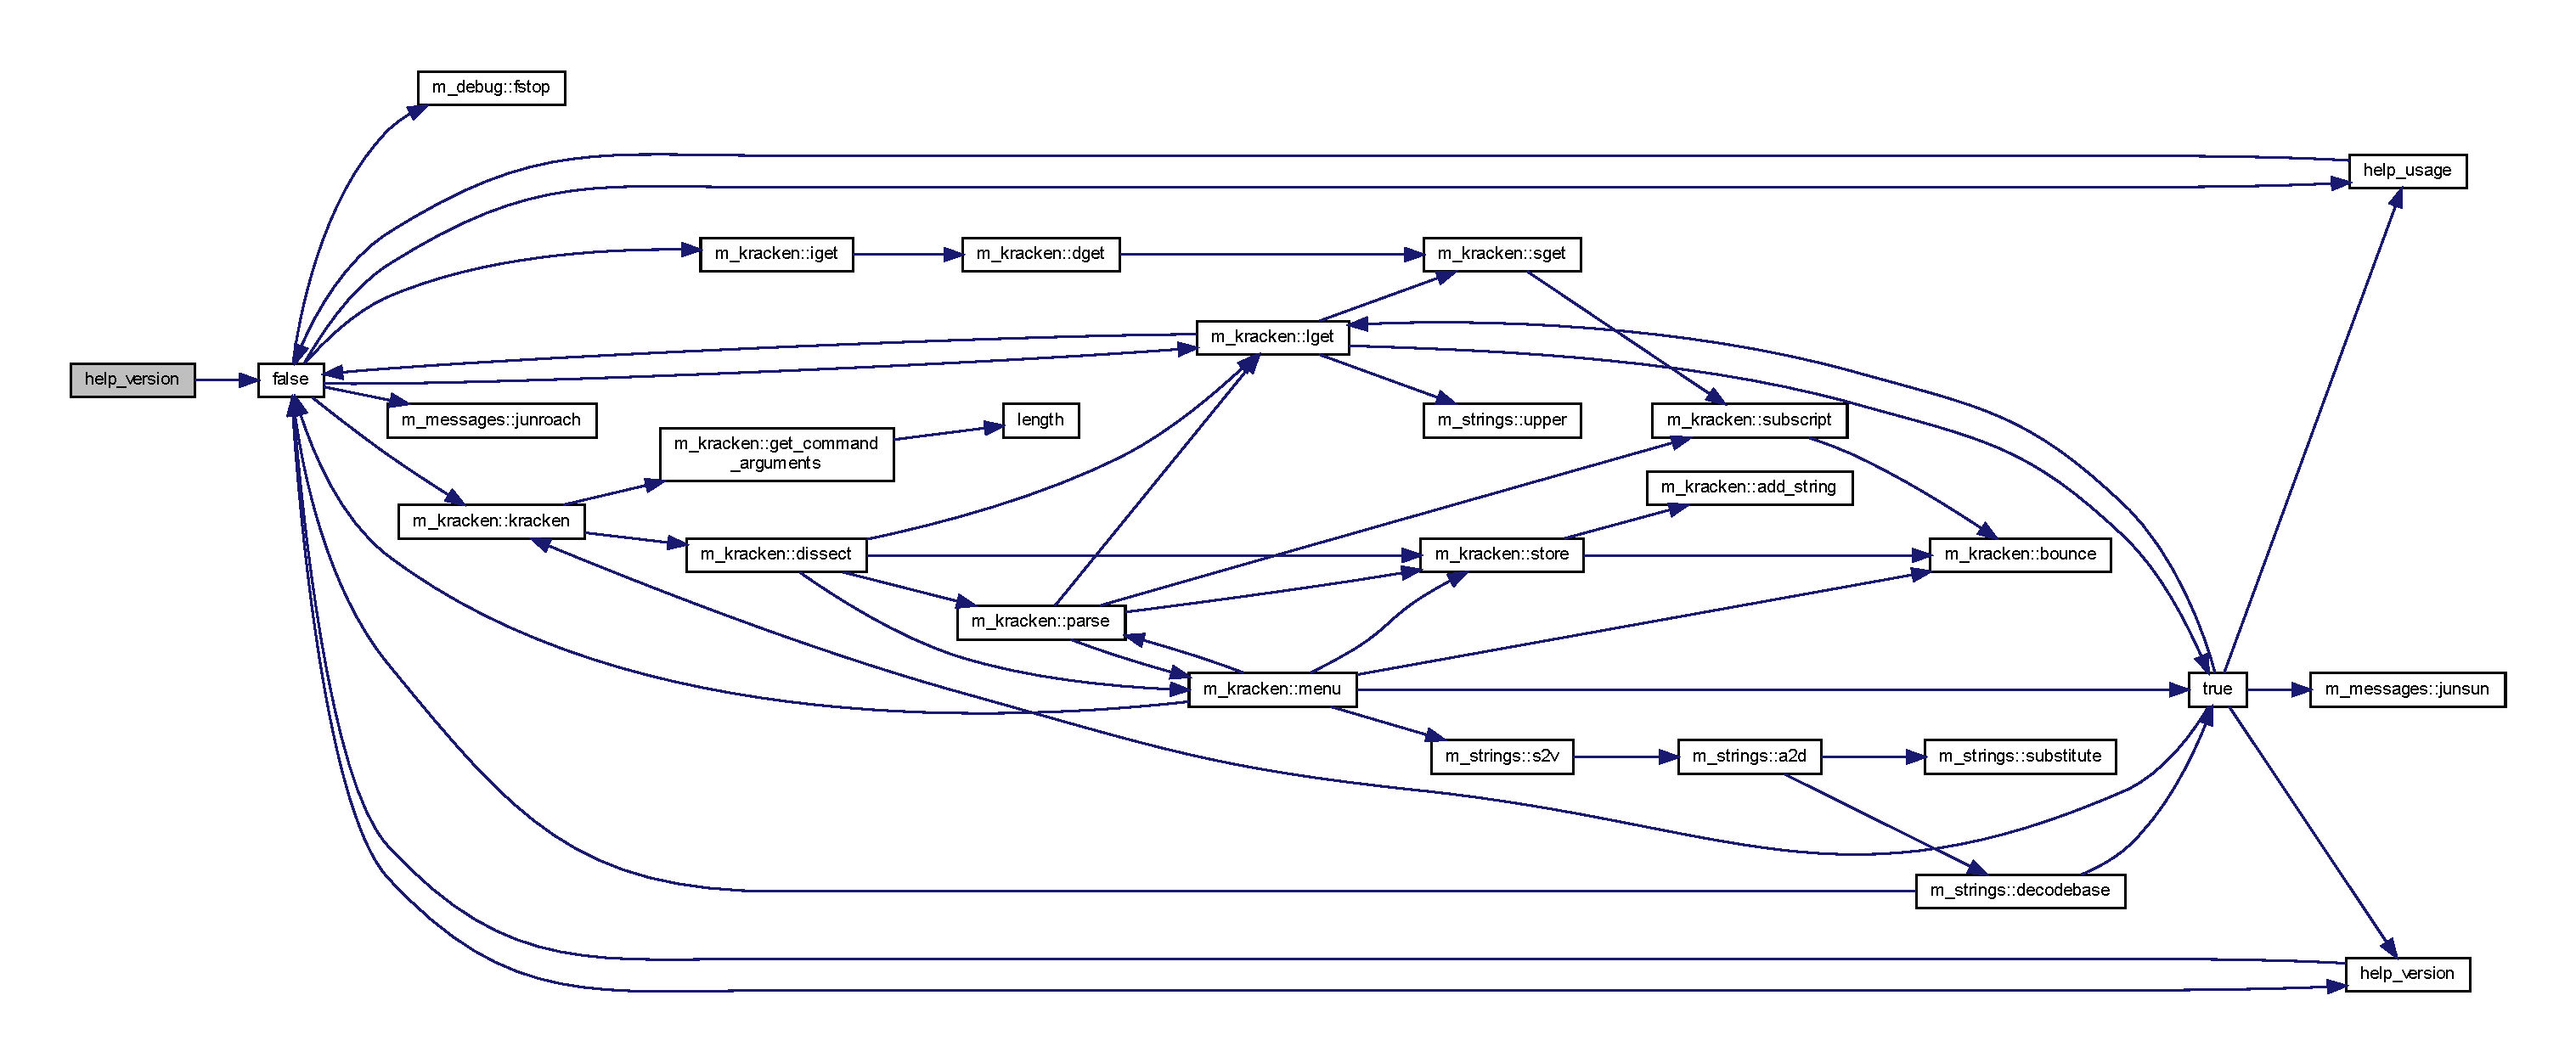
\includegraphics[width=350pt]{__mkfifo_8f90_a39c21619b08a3c22f19e2306efd7f766_cgraph}
\end{center}
\end{figure}

\hypertarget{__mv_8f90}{}\section{L\+I\+B\+R\+A\+R\+Y/lib\+G\+P\+F/download/tmp/\+P\+R\+O\+G\+R\+A\+M\+S/\+\_\+mv.f90 File Reference}
\label{__mv_8f90}\index{L\+I\+B\+R\+A\+R\+Y/lib\+G\+P\+F/download/tmp/\+P\+R\+O\+G\+R\+A\+M\+S/\+\_\+mv.\+f90@{L\+I\+B\+R\+A\+R\+Y/lib\+G\+P\+F/download/tmp/\+P\+R\+O\+G\+R\+A\+M\+S/\+\_\+mv.\+f90}}
\subsection*{Functions/\+Subroutines}
\begin{DoxyCompactItemize}
\item 
\hyperlink{M__stopwatch_83_8txt_acfbcff50169d691ff02d4a123ed70482}{subroutine} \hyperlink{__mv_8f90_a3e09a3b52ee8fb04eeb93fe5761626a8}{help\+\_\+usage} (l\+\_\+help)
\item 
\hyperlink{M__stopwatch_83_8txt_acfbcff50169d691ff02d4a123ed70482}{subroutine} \hyperlink{__mv_8f90_a39c21619b08a3c22f19e2306efd7f766}{help\+\_\+version} (l\+\_\+version)
\begin{DoxyCompactList}\small\item\em \subsubsection*{N\+A\+ME}

\+\_\+mv(1f) -\/ \mbox{[}F\+U\+N\+IX\+:F\+I\+L\+E\+S\+Y\+S\+T\+EM\mbox{]} rename file \subsubsection*{S\+Y\+N\+O\+P\+S\+IS}\end{DoxyCompactList}\item 
program \hyperlink{__mv_8f90_aad99fde3e962ae73c9d6bc3825b8ca79}{demo\+\_\+system\+\_\+rename}
\end{DoxyCompactItemize}


\subsection{Function/\+Subroutine Documentation}
\mbox{\Hypertarget{__mv_8f90_aad99fde3e962ae73c9d6bc3825b8ca79}\label{__mv_8f90_aad99fde3e962ae73c9d6bc3825b8ca79}} 
\index{\+\_\+mv.\+f90@{\+\_\+mv.\+f90}!demo\+\_\+system\+\_\+rename@{demo\+\_\+system\+\_\+rename}}
\index{demo\+\_\+system\+\_\+rename@{demo\+\_\+system\+\_\+rename}!\+\_\+mv.\+f90@{\+\_\+mv.\+f90}}
\subsubsection{\texorpdfstring{demo\+\_\+system\+\_\+rename()}{demo\_system\_rename()}}
{\footnotesize\ttfamily program demo\+\_\+system\+\_\+rename (\begin{DoxyParamCaption}{ }\end{DoxyParamCaption})}



References help\+\_\+usage(), help\+\_\+version(), m\+\_\+kracken\+::ipvalue, m\+\_\+kracken\+::kracken(), m\+\_\+kracken\+::lget(), m\+\_\+kracken\+::sgets(), m\+\_\+system\+::system\+\_\+perror(), and m\+\_\+system\+::system\+\_\+rename().

Here is the call graph for this function\+:
\nopagebreak
\begin{figure}[H]
\begin{center}
\leavevmode
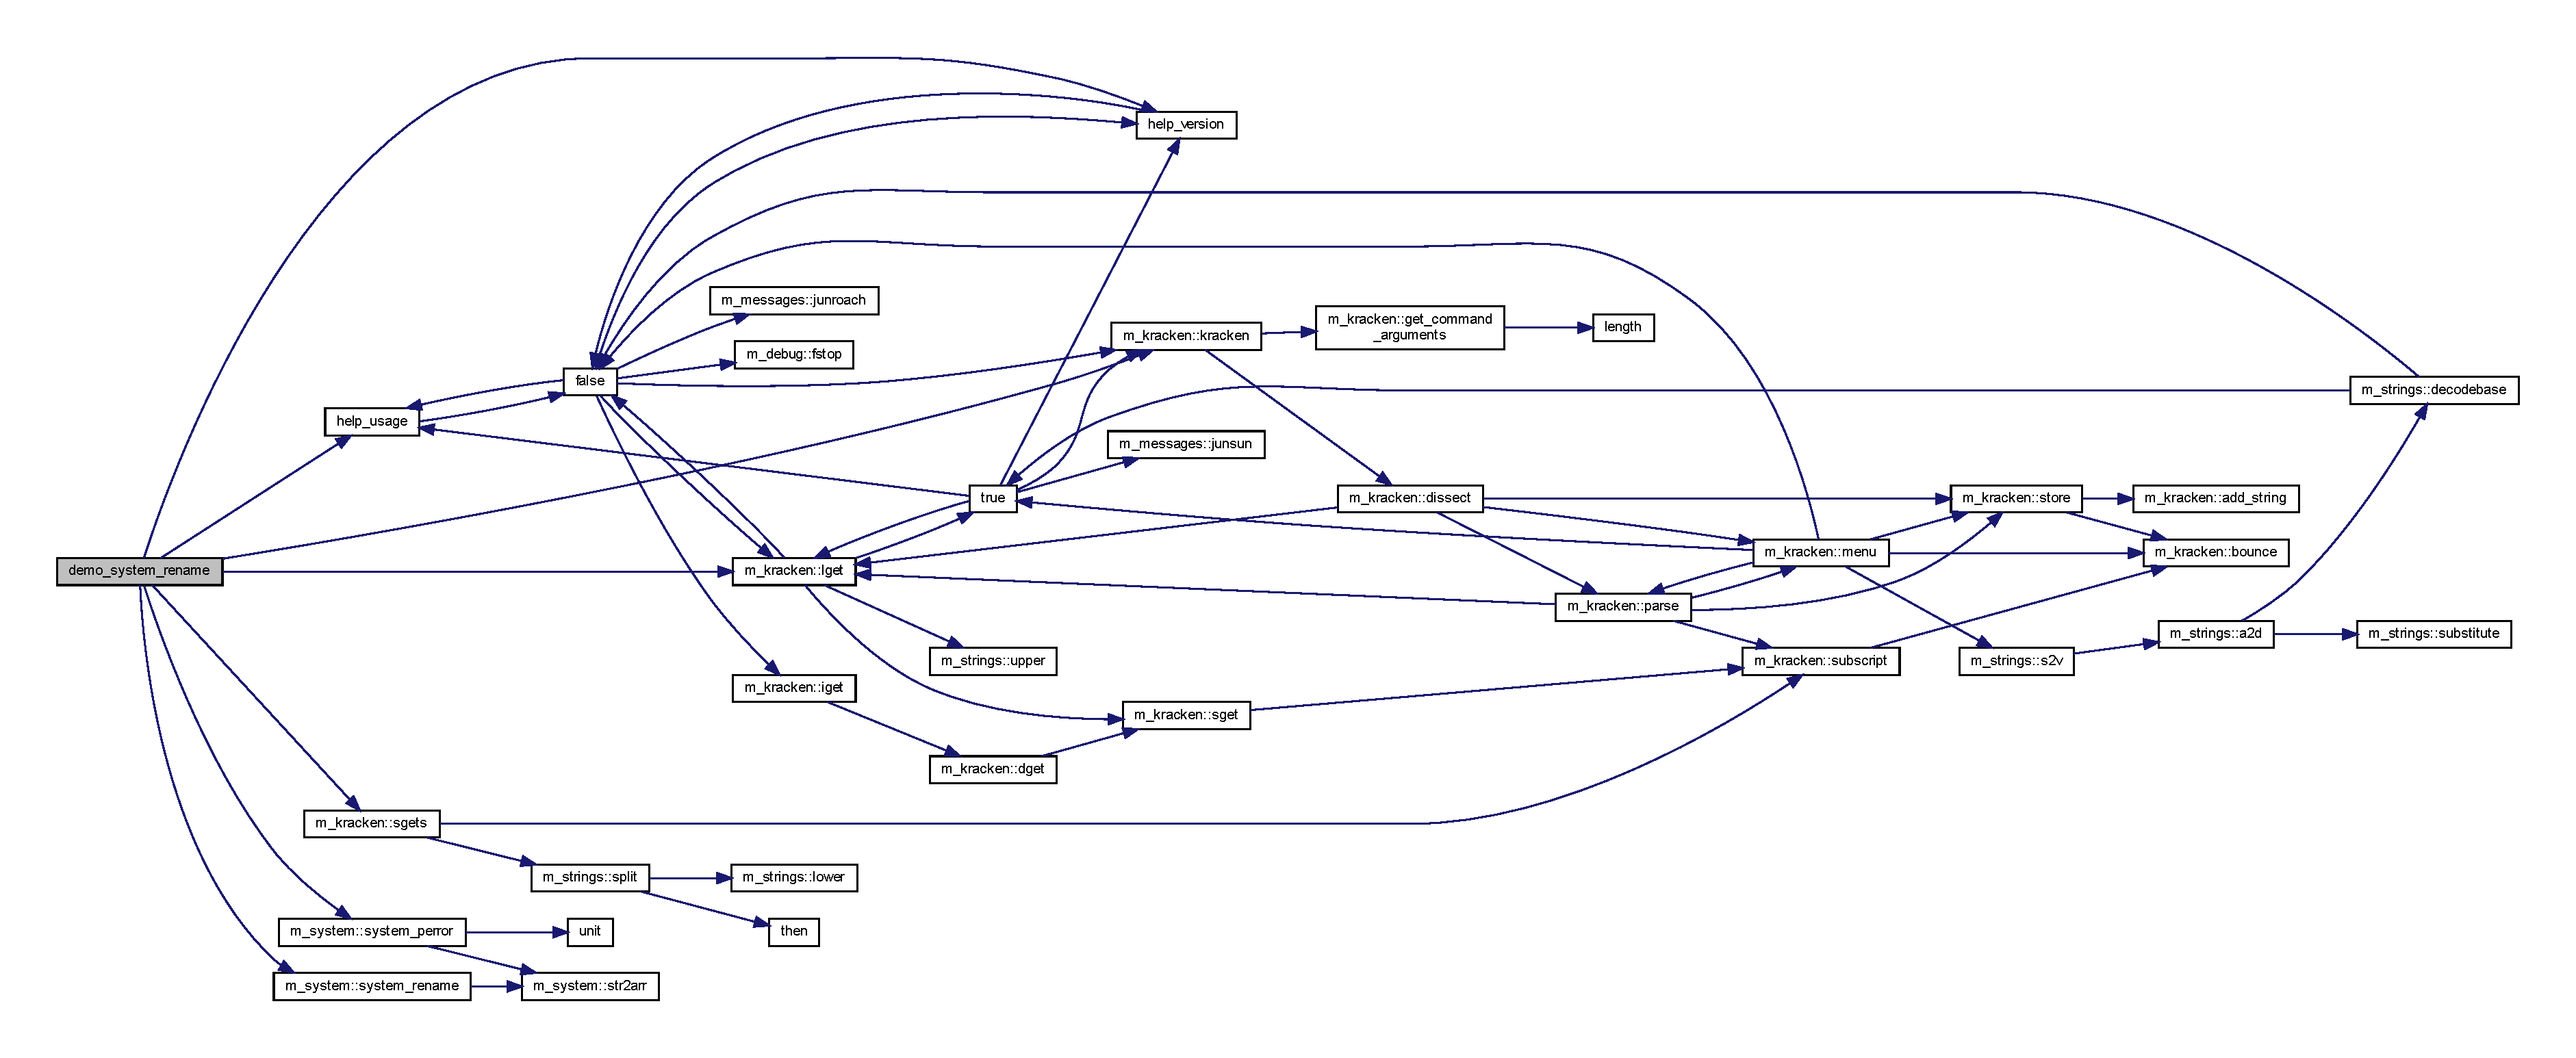
\includegraphics[width=350pt]{__mv_8f90_aad99fde3e962ae73c9d6bc3825b8ca79_cgraph}
\end{center}
\end{figure}
\mbox{\Hypertarget{__mv_8f90_a3e09a3b52ee8fb04eeb93fe5761626a8}\label{__mv_8f90_a3e09a3b52ee8fb04eeb93fe5761626a8}} 
\index{\+\_\+mv.\+f90@{\+\_\+mv.\+f90}!help\+\_\+usage@{help\+\_\+usage}}
\index{help\+\_\+usage@{help\+\_\+usage}!\+\_\+mv.\+f90@{\+\_\+mv.\+f90}}
\subsubsection{\texorpdfstring{help\+\_\+usage()}{help\_usage()}}
{\footnotesize\ttfamily \hyperlink{M__stopwatch_83_8txt_acfbcff50169d691ff02d4a123ed70482}{subroutine} help\+\_\+usage (\begin{DoxyParamCaption}\item[{logical, intent(\hyperlink{M__journal_83_8txt_afce72651d1eed785a2132bee863b2f38}{in})}]{l\+\_\+help }\end{DoxyParamCaption})}



References false().

Here is the call graph for this function\+:
\nopagebreak
\begin{figure}[H]
\begin{center}
\leavevmode
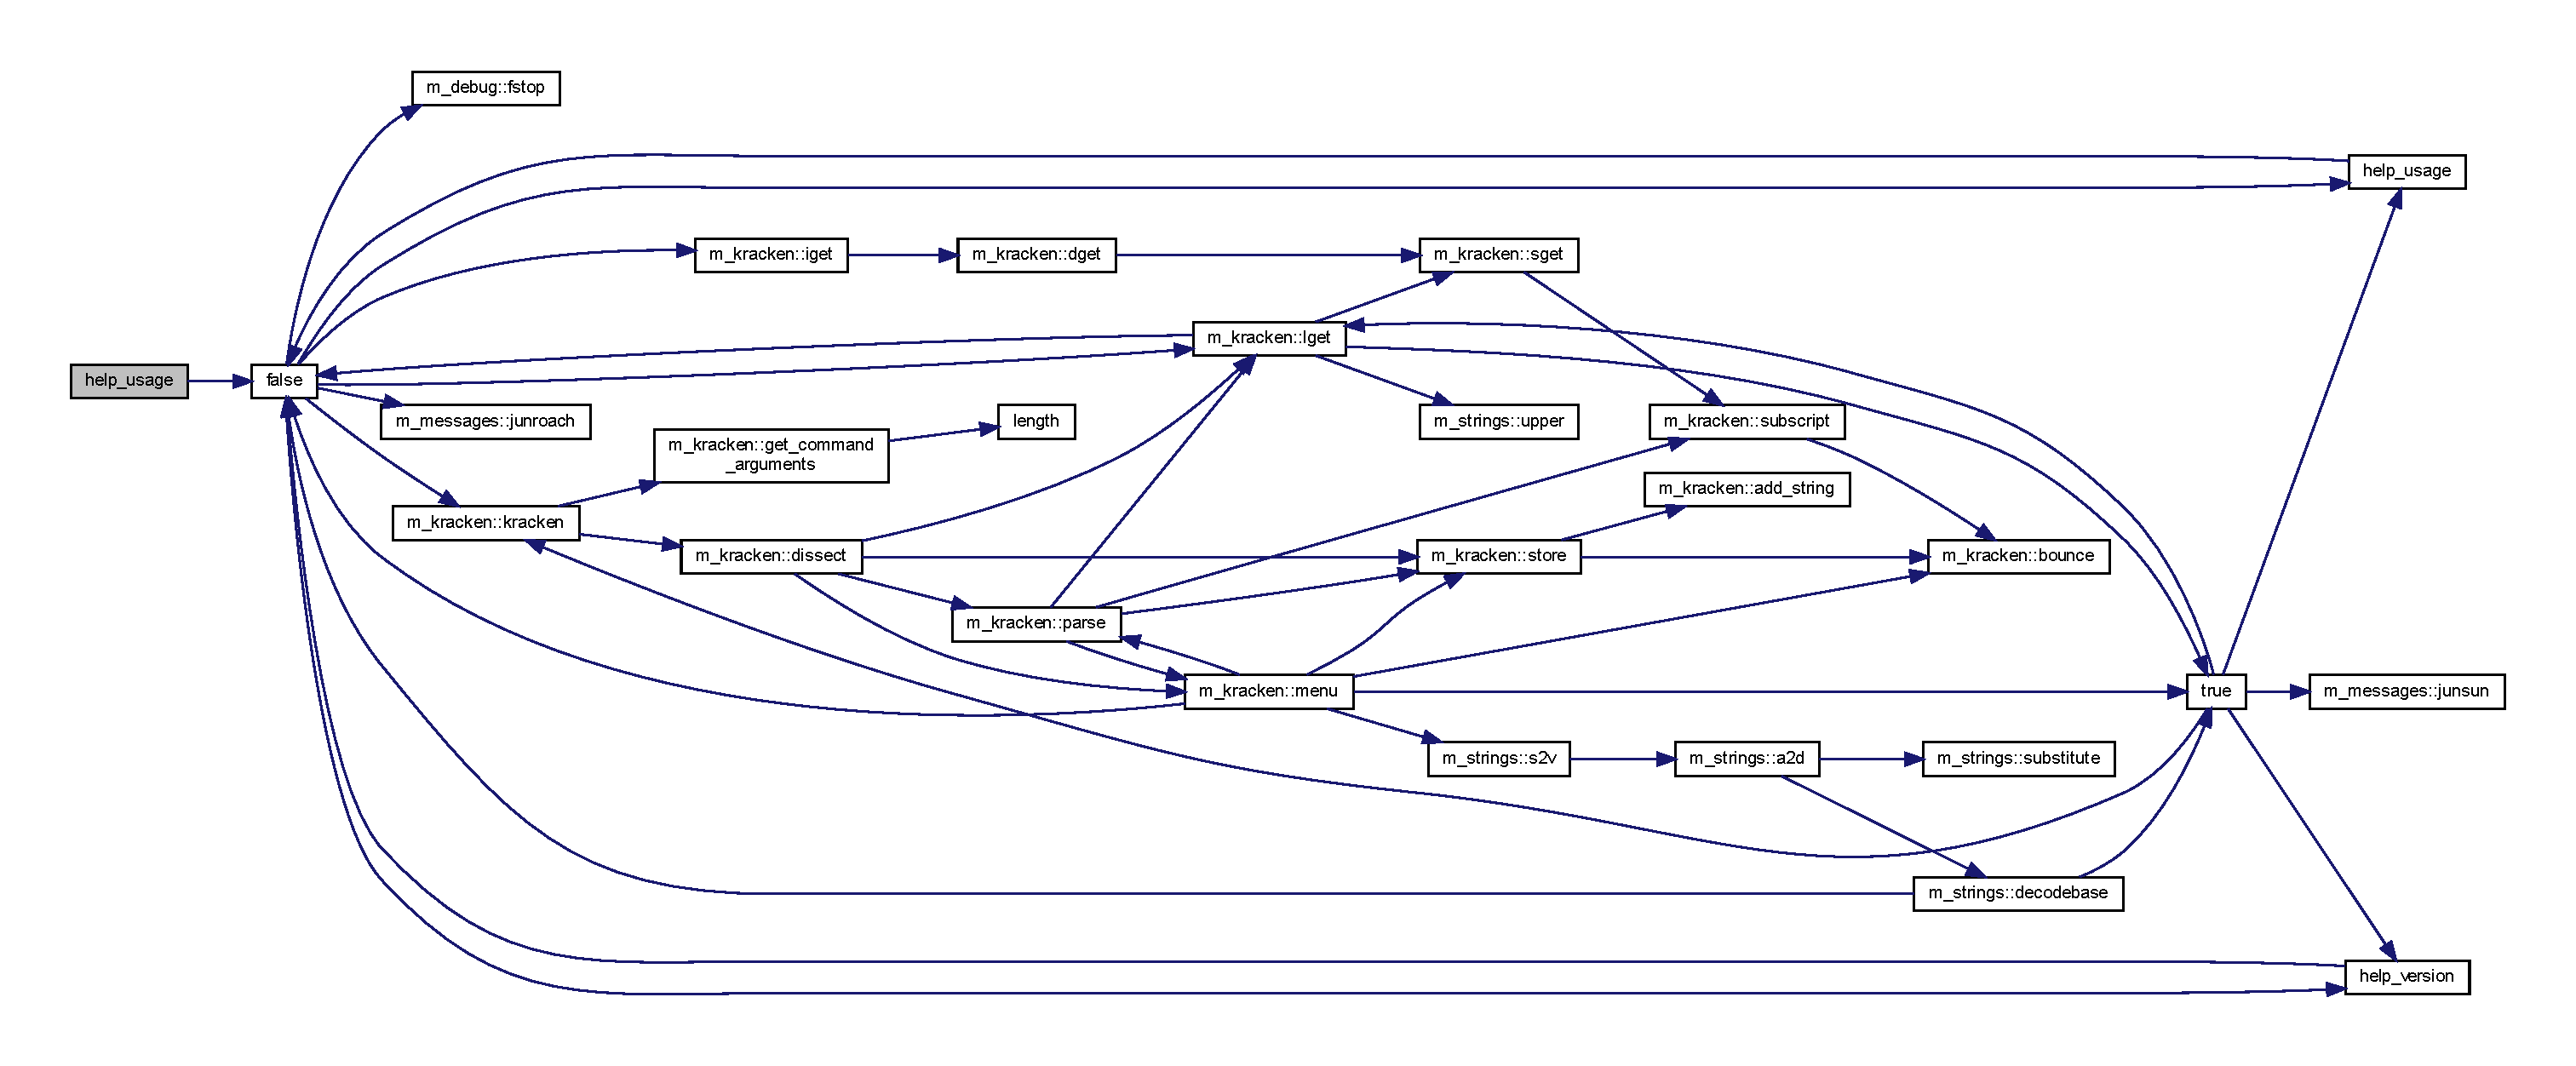
\includegraphics[width=350pt]{__mv_8f90_a3e09a3b52ee8fb04eeb93fe5761626a8_cgraph}
\end{center}
\end{figure}
\mbox{\Hypertarget{__mv_8f90_a39c21619b08a3c22f19e2306efd7f766}\label{__mv_8f90_a39c21619b08a3c22f19e2306efd7f766}} 
\index{\+\_\+mv.\+f90@{\+\_\+mv.\+f90}!help\+\_\+version@{help\+\_\+version}}
\index{help\+\_\+version@{help\+\_\+version}!\+\_\+mv.\+f90@{\+\_\+mv.\+f90}}
\subsubsection{\texorpdfstring{help\+\_\+version()}{help\_version()}}
{\footnotesize\ttfamily \hyperlink{M__stopwatch_83_8txt_acfbcff50169d691ff02d4a123ed70482}{subroutine} help\+\_\+version (\begin{DoxyParamCaption}\item[{logical, intent(\hyperlink{M__journal_83_8txt_afce72651d1eed785a2132bee863b2f38}{in})}]{l\+\_\+version }\end{DoxyParamCaption})}



\subsubsection*{N\+A\+ME}

\+\_\+mv(1f) -\/ \mbox{[}F\+U\+N\+IX\+:F\+I\+L\+E\+S\+Y\+S\+T\+EM\mbox{]} rename file \subsubsection*{S\+Y\+N\+O\+P\+S\+IS}

\+\_\+mv S\+O\+U\+R\+CE D\+E\+ST \subsubsection*{D\+E\+S\+C\+R\+I\+P\+T\+I\+ON}

Rename S\+O\+U\+R\+CE to D\+E\+ST

\subsubsection*{E\+X\+A\+M\+P\+LE}

\begin{DoxyVerb}  _mv file.text file.txt \end{DoxyVerb}
 

References false().

Here is the call graph for this function\+:
\nopagebreak
\begin{figure}[H]
\begin{center}
\leavevmode
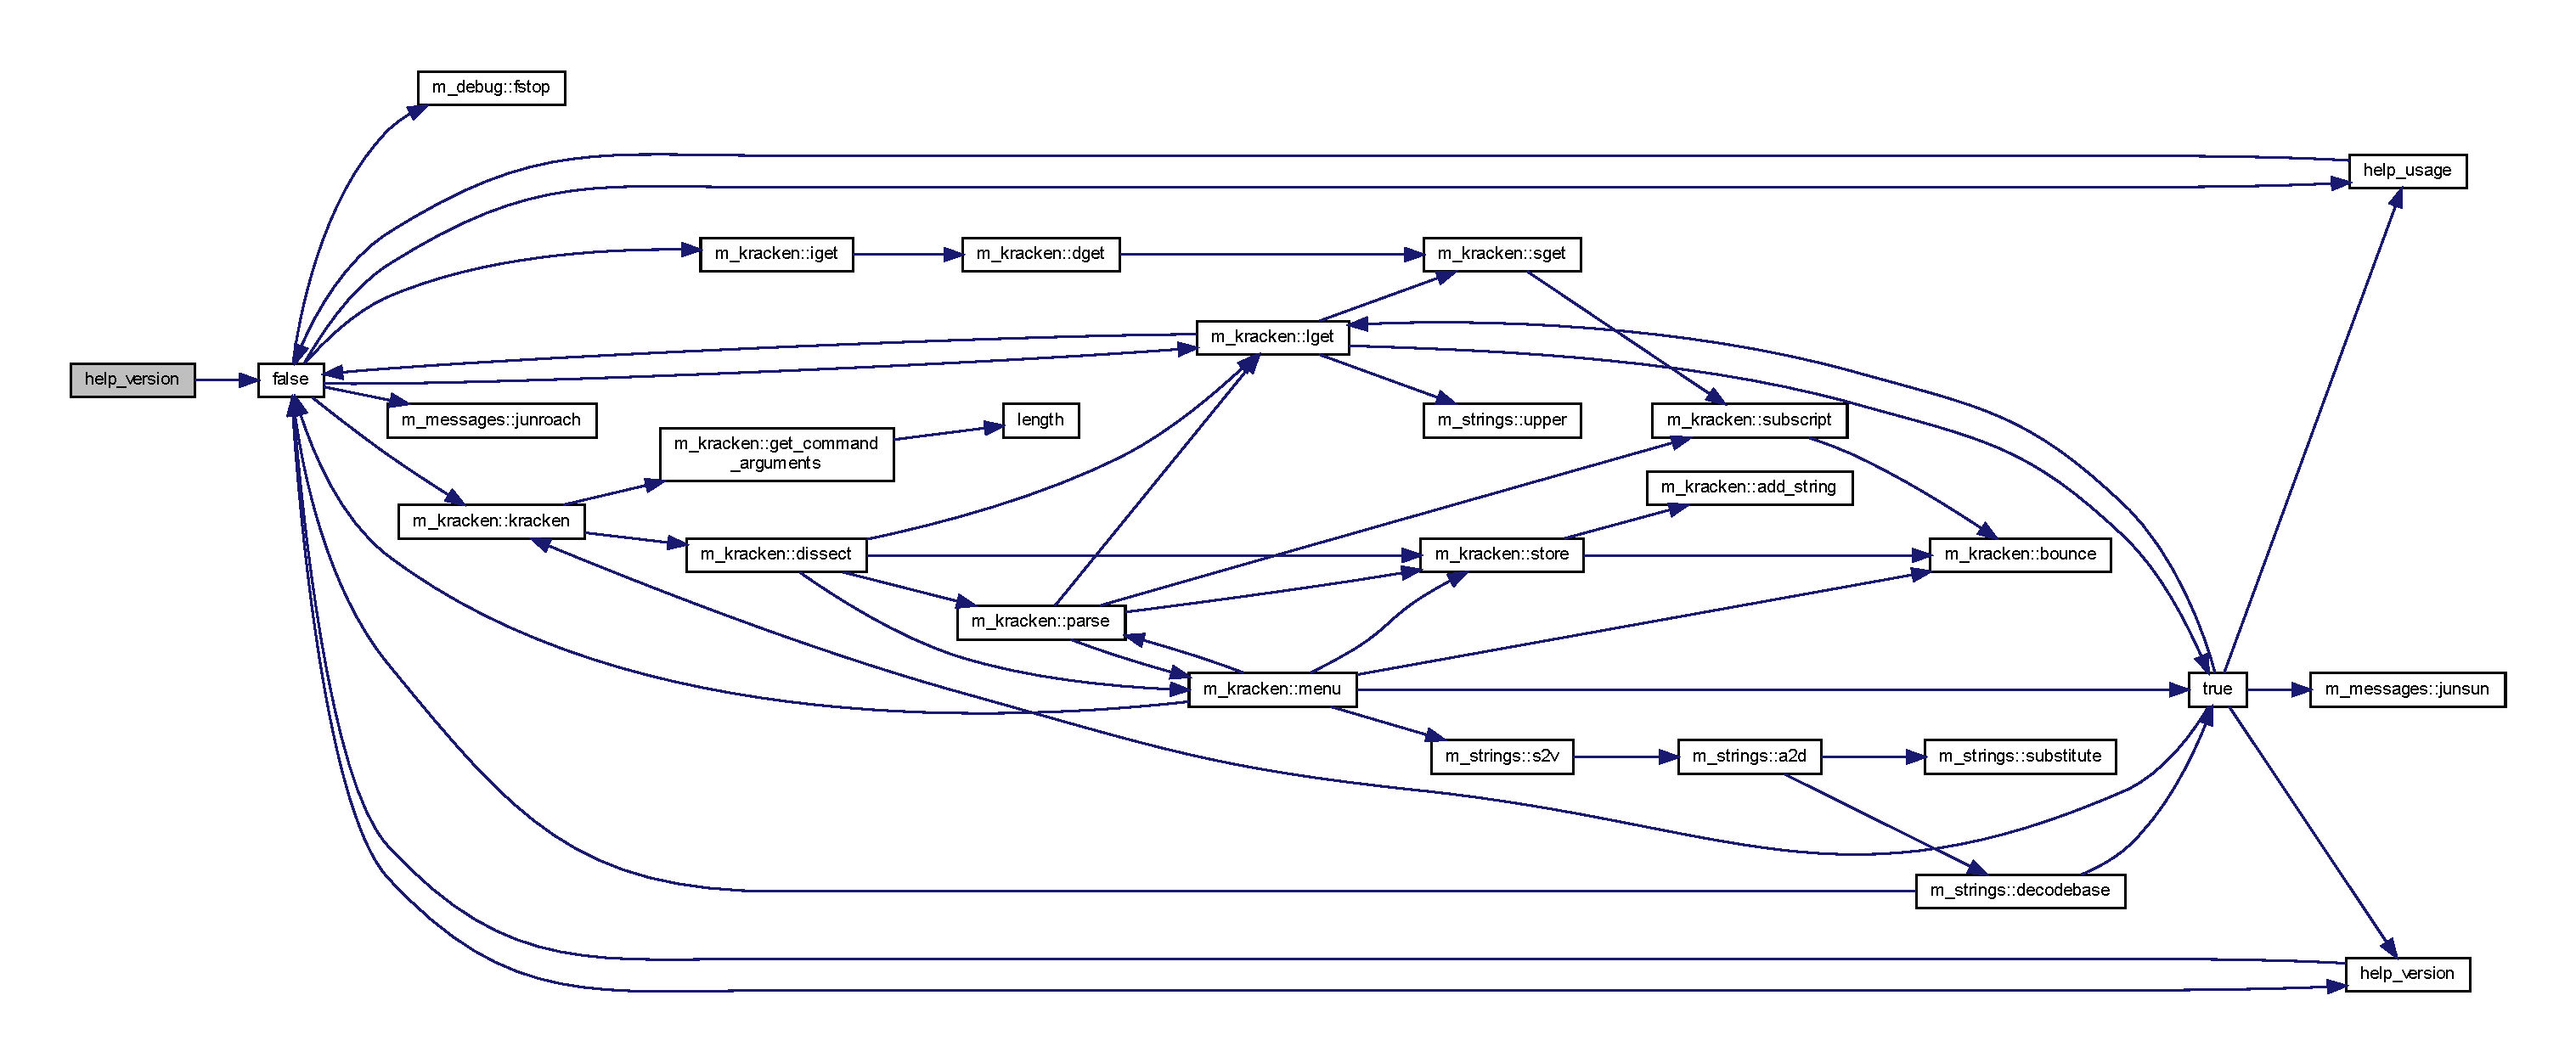
\includegraphics[width=350pt]{__mv_8f90_a39c21619b08a3c22f19e2306efd7f766_cgraph}
\end{center}
\end{figure}

\hypertarget{__pwd_8f90}{}\section{L\+I\+B\+R\+A\+R\+Y/lib\+G\+P\+F/download/tmp/\+P\+R\+O\+G\+R\+A\+M\+S/\+\_\+pwd.f90 File Reference}
\label{__pwd_8f90}\index{L\+I\+B\+R\+A\+R\+Y/lib\+G\+P\+F/download/tmp/\+P\+R\+O\+G\+R\+A\+M\+S/\+\_\+pwd.\+f90@{L\+I\+B\+R\+A\+R\+Y/lib\+G\+P\+F/download/tmp/\+P\+R\+O\+G\+R\+A\+M\+S/\+\_\+pwd.\+f90}}

\hypertarget{__rm_8f90}{}\section{L\+I\+B\+R\+A\+R\+Y/lib\+G\+P\+F/download/tmp/\+P\+R\+O\+G\+R\+A\+M\+S/\+\_\+rm.f90 File Reference}
\label{__rm_8f90}\index{L\+I\+B\+R\+A\+R\+Y/lib\+G\+P\+F/download/tmp/\+P\+R\+O\+G\+R\+A\+M\+S/\+\_\+rm.\+f90@{L\+I\+B\+R\+A\+R\+Y/lib\+G\+P\+F/download/tmp/\+P\+R\+O\+G\+R\+A\+M\+S/\+\_\+rm.\+f90}}

\hypertarget{__rmdir_8f90}{}\section{L\+I\+B\+R\+A\+R\+Y/lib\+G\+P\+F/download/tmp/\+P\+R\+O\+G\+R\+A\+M\+S/\+\_\+rmdir.f90 File Reference}
\label{__rmdir_8f90}\index{L\+I\+B\+R\+A\+R\+Y/lib\+G\+P\+F/download/tmp/\+P\+R\+O\+G\+R\+A\+M\+S/\+\_\+rmdir.\+f90@{L\+I\+B\+R\+A\+R\+Y/lib\+G\+P\+F/download/tmp/\+P\+R\+O\+G\+R\+A\+M\+S/\+\_\+rmdir.\+f90}}
\subsection*{Functions/\+Subroutines}
\begin{DoxyCompactItemize}
\item 
\hyperlink{M__stopwatch_83_8txt_acfbcff50169d691ff02d4a123ed70482}{subroutine} \hyperlink{__rmdir_8f90_a3e09a3b52ee8fb04eeb93fe5761626a8}{help\+\_\+usage} (l\+\_\+help)
\item 
\hyperlink{M__stopwatch_83_8txt_acfbcff50169d691ff02d4a123ed70482}{subroutine} \hyperlink{__rmdir_8f90_a39c21619b08a3c22f19e2306efd7f766}{help\+\_\+version} (l\+\_\+version)
\begin{DoxyCompactList}\small\item\em \subsubsection*{N\+A\+ME}

\+\_\+rmdir(1f) -\/ \mbox{[}F\+U\+N\+IX\+:F\+I\+L\+E\+S\+Y\+S\+T\+EM\mbox{]} remove empty directories \subsubsection*{S\+Y\+N\+O\+P\+S\+IS}\end{DoxyCompactList}\item 
program \hyperlink{__rmdir_8f90_a1002470a8ce0812244a0c83197f3a97d}{demo\+\_\+system\+\_\+rmdir}
\end{DoxyCompactItemize}


\subsection{Function/\+Subroutine Documentation}
\mbox{\Hypertarget{__rmdir_8f90_a1002470a8ce0812244a0c83197f3a97d}\label{__rmdir_8f90_a1002470a8ce0812244a0c83197f3a97d}} 
\index{\+\_\+rmdir.\+f90@{\+\_\+rmdir.\+f90}!demo\+\_\+system\+\_\+rmdir@{demo\+\_\+system\+\_\+rmdir}}
\index{demo\+\_\+system\+\_\+rmdir@{demo\+\_\+system\+\_\+rmdir}!\+\_\+rmdir.\+f90@{\+\_\+rmdir.\+f90}}
\subsubsection{\texorpdfstring{demo\+\_\+system\+\_\+rmdir()}{demo\_system\_rmdir()}}
{\footnotesize\ttfamily program demo\+\_\+system\+\_\+rmdir (\begin{DoxyParamCaption}{ }\end{DoxyParamCaption})}



References help\+\_\+usage(), help\+\_\+version(), m\+\_\+kracken\+::ipvalue, m\+\_\+kracken\+::kracken(), m\+\_\+kracken\+::lget(), m\+\_\+kracken\+::sgets(), m\+\_\+system\+::system\+\_\+perror(), and m\+\_\+system\+::system\+\_\+rmdir().

Here is the call graph for this function\+:
\nopagebreak
\begin{figure}[H]
\begin{center}
\leavevmode
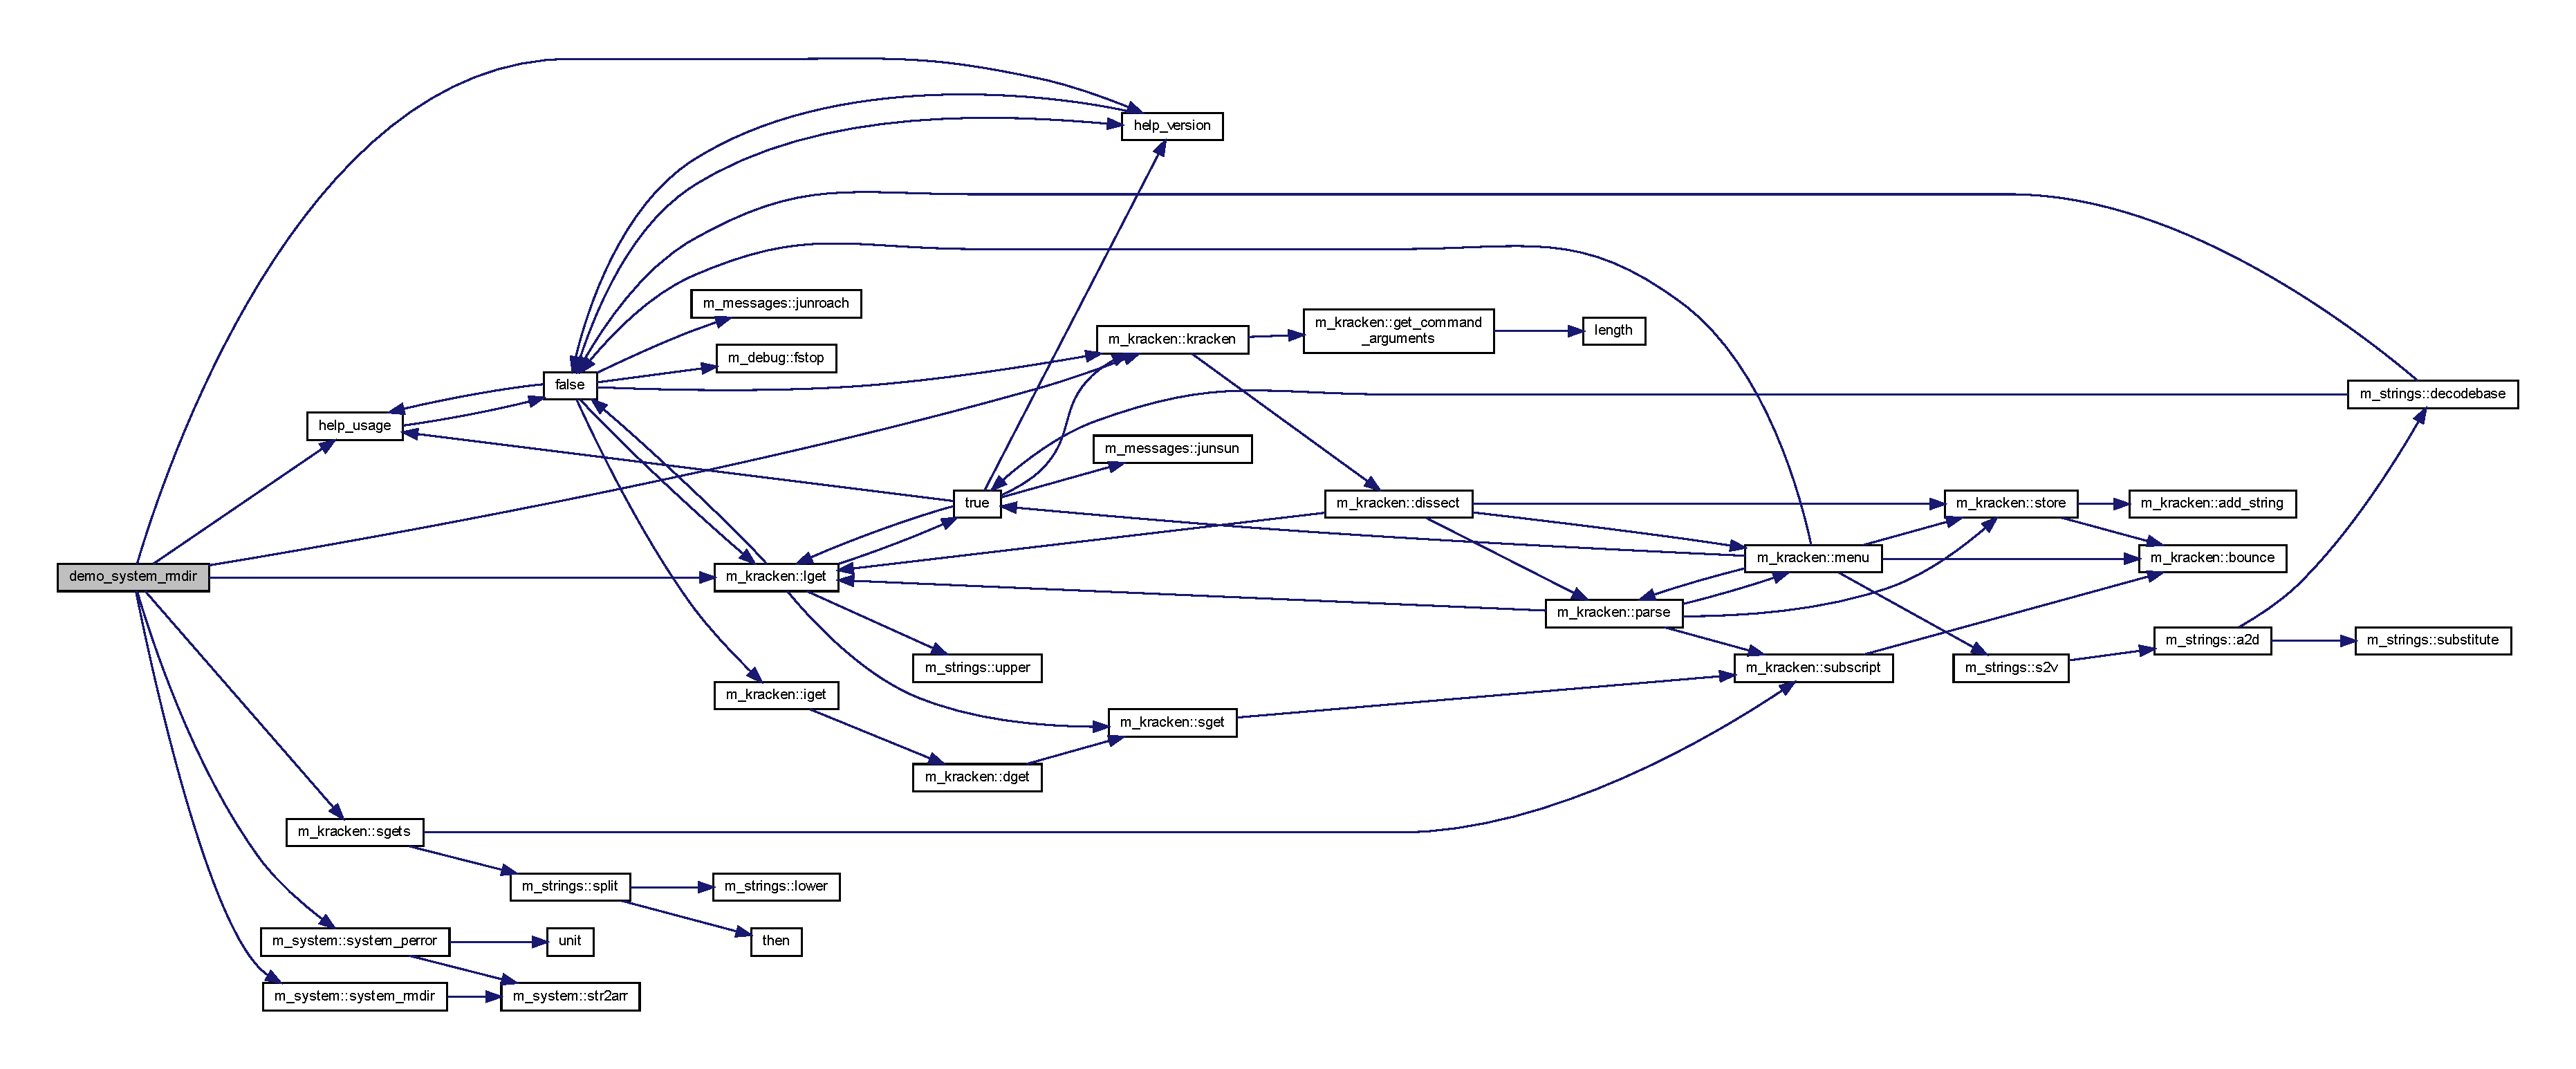
\includegraphics[width=350pt]{__rmdir_8f90_a1002470a8ce0812244a0c83197f3a97d_cgraph}
\end{center}
\end{figure}
\mbox{\Hypertarget{__rmdir_8f90_a3e09a3b52ee8fb04eeb93fe5761626a8}\label{__rmdir_8f90_a3e09a3b52ee8fb04eeb93fe5761626a8}} 
\index{\+\_\+rmdir.\+f90@{\+\_\+rmdir.\+f90}!help\+\_\+usage@{help\+\_\+usage}}
\index{help\+\_\+usage@{help\+\_\+usage}!\+\_\+rmdir.\+f90@{\+\_\+rmdir.\+f90}}
\subsubsection{\texorpdfstring{help\+\_\+usage()}{help\_usage()}}
{\footnotesize\ttfamily \hyperlink{M__stopwatch_83_8txt_acfbcff50169d691ff02d4a123ed70482}{subroutine} help\+\_\+usage (\begin{DoxyParamCaption}\item[{logical, intent(\hyperlink{M__journal_83_8txt_afce72651d1eed785a2132bee863b2f38}{in})}]{l\+\_\+help }\end{DoxyParamCaption})}



References false().

Here is the call graph for this function\+:
\nopagebreak
\begin{figure}[H]
\begin{center}
\leavevmode
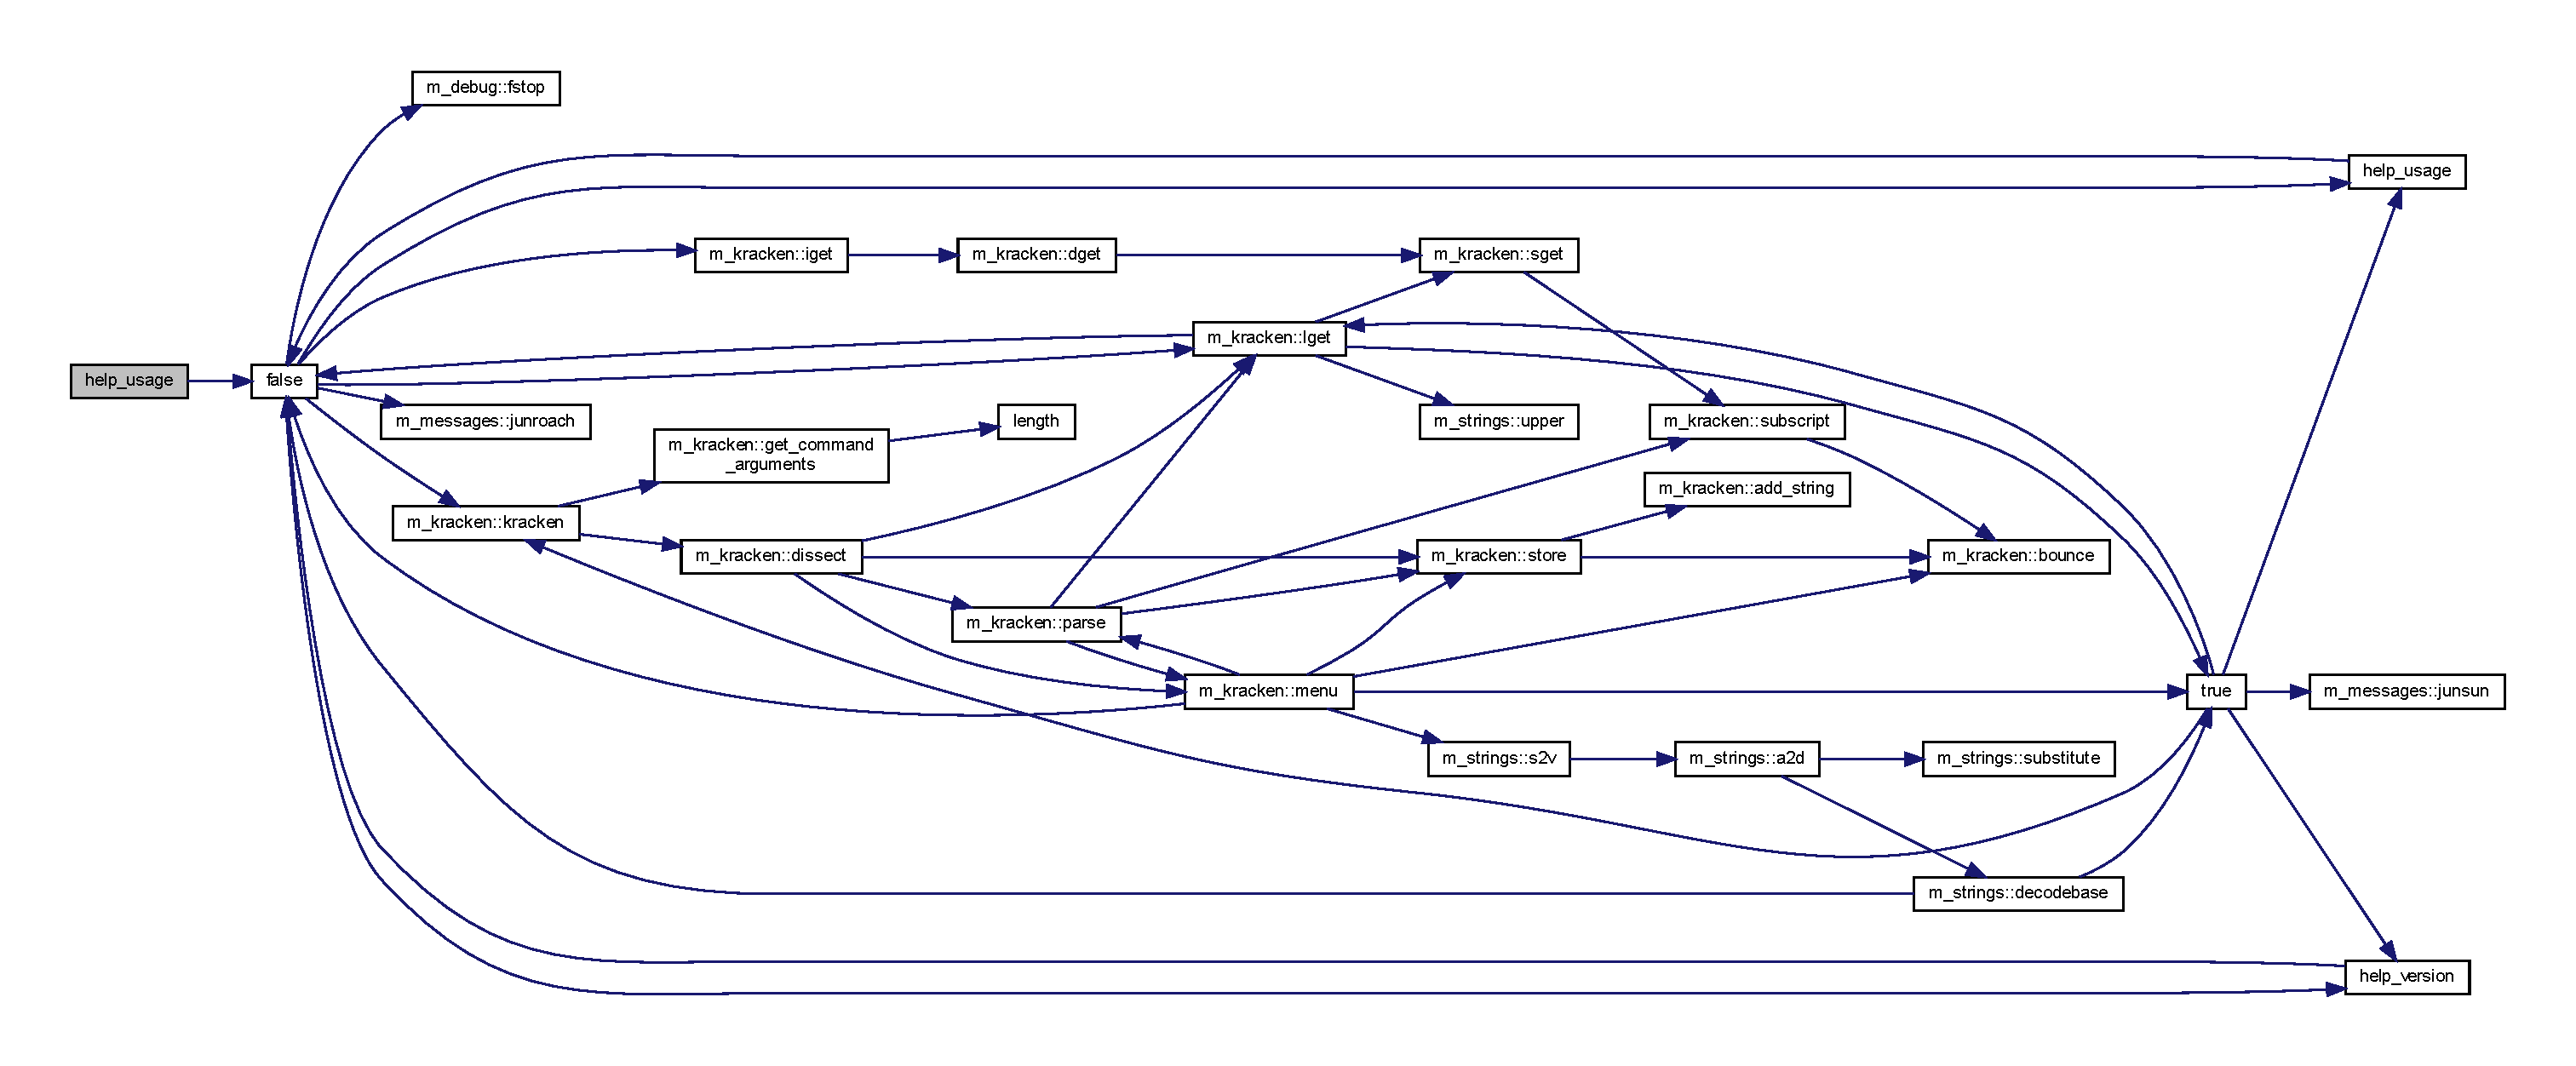
\includegraphics[width=350pt]{__rmdir_8f90_a3e09a3b52ee8fb04eeb93fe5761626a8_cgraph}
\end{center}
\end{figure}
\mbox{\Hypertarget{__rmdir_8f90_a39c21619b08a3c22f19e2306efd7f766}\label{__rmdir_8f90_a39c21619b08a3c22f19e2306efd7f766}} 
\index{\+\_\+rmdir.\+f90@{\+\_\+rmdir.\+f90}!help\+\_\+version@{help\+\_\+version}}
\index{help\+\_\+version@{help\+\_\+version}!\+\_\+rmdir.\+f90@{\+\_\+rmdir.\+f90}}
\subsubsection{\texorpdfstring{help\+\_\+version()}{help\_version()}}
{\footnotesize\ttfamily \hyperlink{M__stopwatch_83_8txt_acfbcff50169d691ff02d4a123ed70482}{subroutine} help\+\_\+version (\begin{DoxyParamCaption}\item[{logical, intent(\hyperlink{M__journal_83_8txt_afce72651d1eed785a2132bee863b2f38}{in})}]{l\+\_\+version }\end{DoxyParamCaption})}



\subsubsection*{N\+A\+ME}

\+\_\+rmdir(1f) -\/ \mbox{[}F\+U\+N\+IX\+:F\+I\+L\+E\+S\+Y\+S\+T\+EM\mbox{]} remove empty directories \subsubsection*{S\+Y\+N\+O\+P\+S\+IS}

\+\_\+rmdir D\+I\+R\+E\+C\+T\+O\+RY... \mbox{[}O\+P\+T\+I\+ON\mbox{]}... \subsubsection*{D\+E\+S\+C\+R\+I\+P\+T\+I\+ON}

given the names of empty directories remove them. \subsubsection*{O\+P\+T\+I\+O\+NS}

D\+I\+R\+E\+C\+T\+O\+RY Remove the D\+I\+R\+E\+C\+T\+O\+R\+Y(ies) if they are empty. --help display this help and exit --version output version information and exit \subsubsection*{E\+X\+A\+M\+P\+L\+ES}

Sample command lines ... \begin{DoxyVerb}   _rmdir a/b/c /a/b /a \end{DoxyVerb}
 

References false().

Here is the call graph for this function\+:
\nopagebreak
\begin{figure}[H]
\begin{center}
\leavevmode
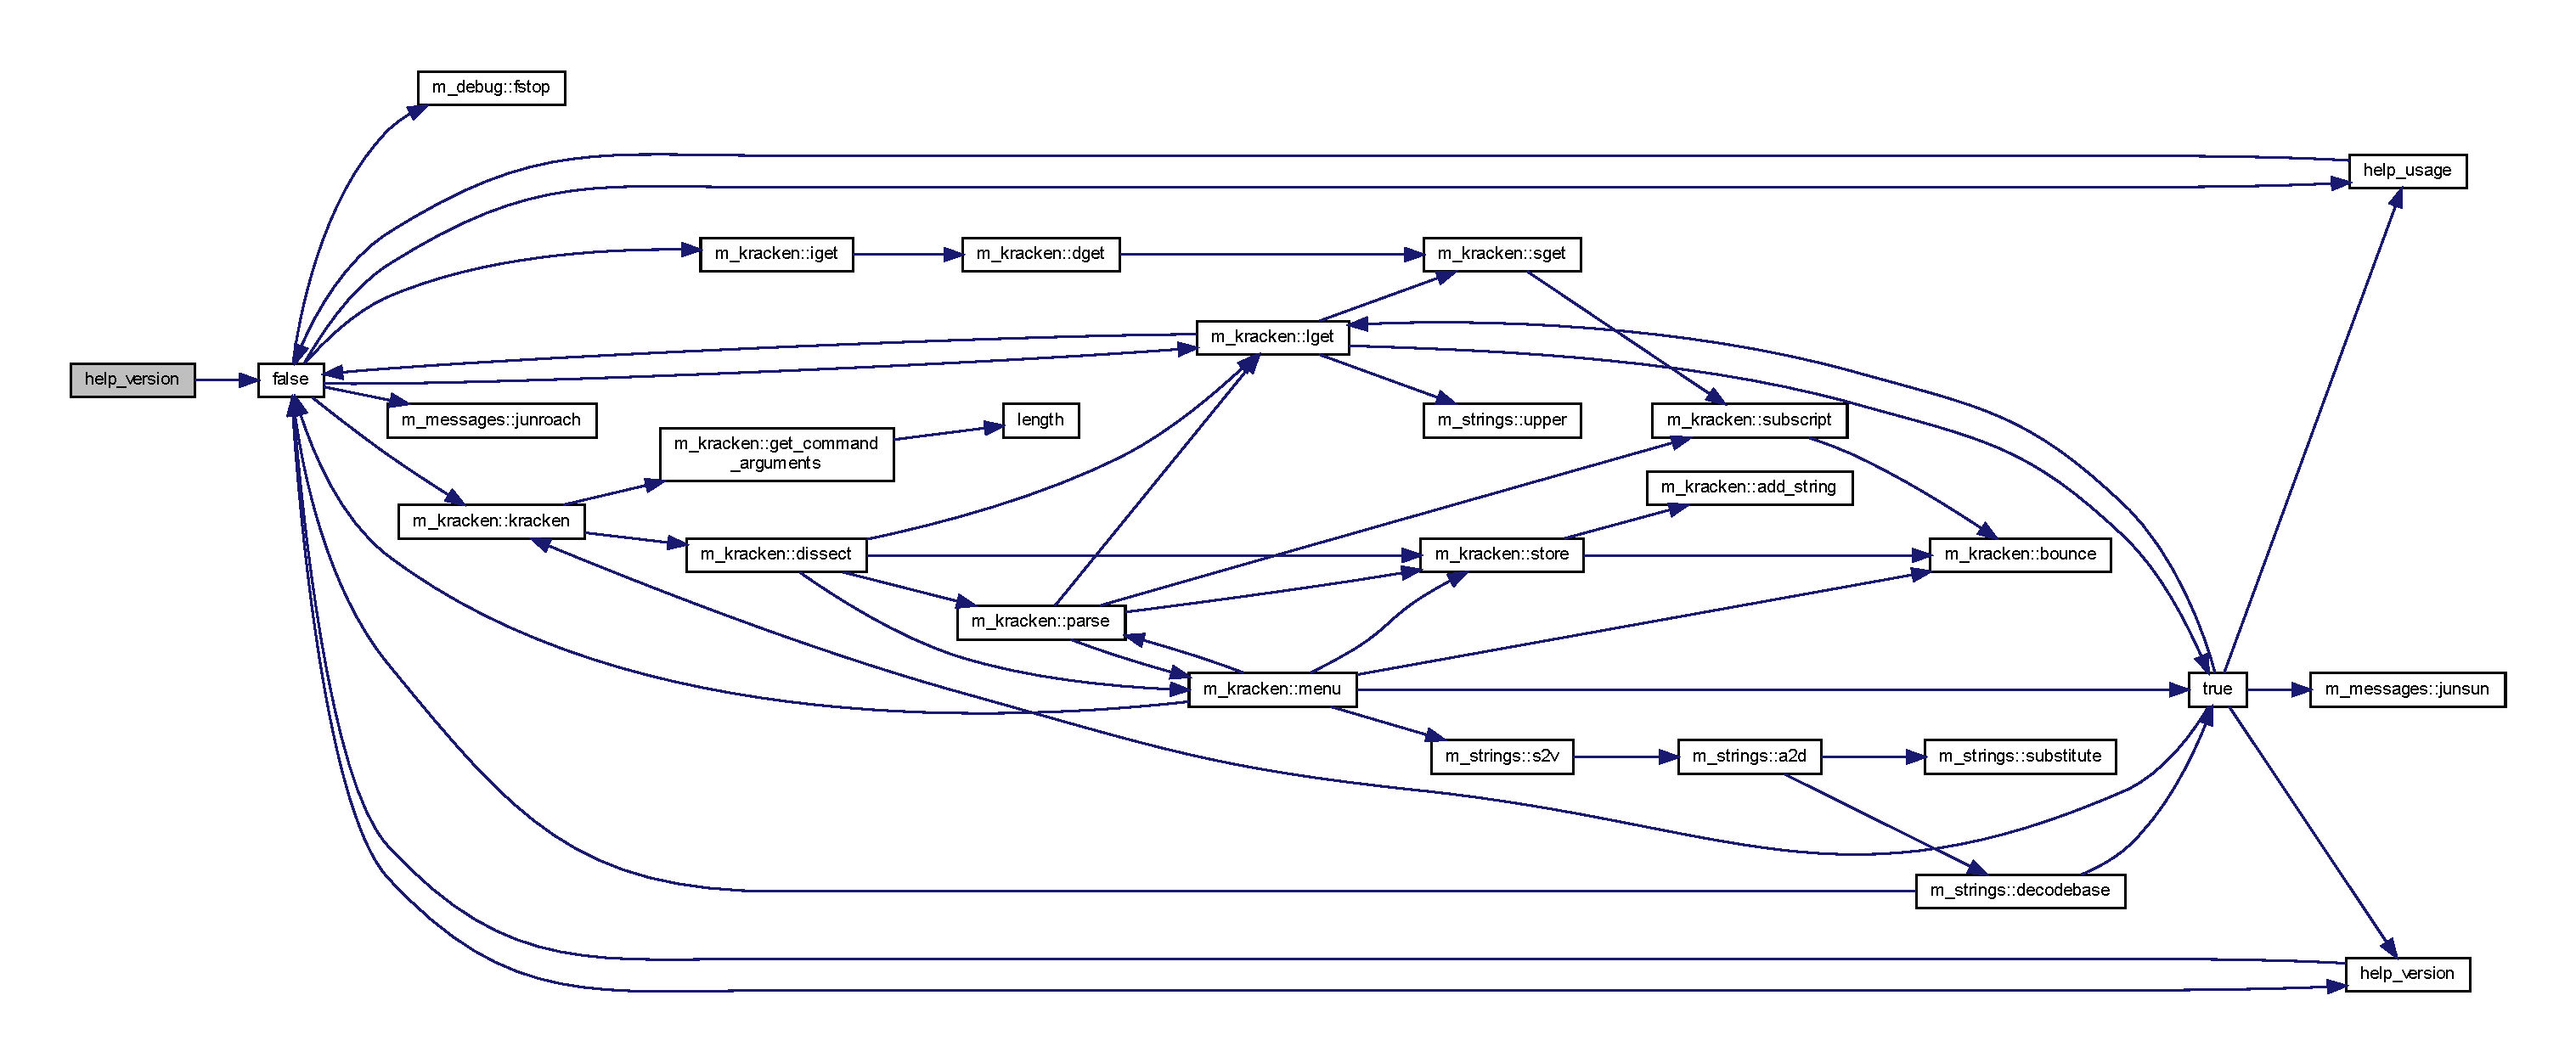
\includegraphics[width=350pt]{__rmdir_8f90_a39c21619b08a3c22f19e2306efd7f766_cgraph}
\end{center}
\end{figure}

\hypertarget{__showumask_8f90}{}\section{L\+I\+B\+R\+A\+R\+Y/lib\+G\+P\+F/download/tmp/\+P\+R\+O\+G\+R\+A\+M\+S/\+\_\+showumask.f90 File Reference}
\label{__showumask_8f90}\index{L\+I\+B\+R\+A\+R\+Y/lib\+G\+P\+F/download/tmp/\+P\+R\+O\+G\+R\+A\+M\+S/\+\_\+showumask.\+f90@{L\+I\+B\+R\+A\+R\+Y/lib\+G\+P\+F/download/tmp/\+P\+R\+O\+G\+R\+A\+M\+S/\+\_\+showumask.\+f90}}
\subsection*{Functions/\+Subroutines}
\begin{DoxyCompactItemize}
\item 
\hyperlink{M__stopwatch_83_8txt_acfbcff50169d691ff02d4a123ed70482}{subroutine} \hyperlink{__showumask_8f90_a3e09a3b52ee8fb04eeb93fe5761626a8}{help\+\_\+usage} (l\+\_\+help)
\item 
\hyperlink{M__stopwatch_83_8txt_acfbcff50169d691ff02d4a123ed70482}{subroutine} \hyperlink{__showumask_8f90_a39c21619b08a3c22f19e2306efd7f766}{help\+\_\+version} (l\+\_\+version)
\item 
program \hyperlink{__showumask_8f90_a1b5ccb693a5e379113ec98bc98f16a90}{demo\+\_\+umask}
\end{DoxyCompactItemize}


\subsection{Function/\+Subroutine Documentation}
\mbox{\Hypertarget{__showumask_8f90_a1b5ccb693a5e379113ec98bc98f16a90}\label{__showumask_8f90_a1b5ccb693a5e379113ec98bc98f16a90}} 
\index{\+\_\+showumask.\+f90@{\+\_\+showumask.\+f90}!demo\+\_\+umask@{demo\+\_\+umask}}
\index{demo\+\_\+umask@{demo\+\_\+umask}!\+\_\+showumask.\+f90@{\+\_\+showumask.\+f90}}
\subsubsection{\texorpdfstring{demo\+\_\+umask()}{demo\_umask()}}
{\footnotesize\ttfamily program demo\+\_\+umask (\begin{DoxyParamCaption}{ }\end{DoxyParamCaption})}



References help\+\_\+usage(), help\+\_\+version(), m\+\_\+kracken\+::kracken(), m\+\_\+kracken\+::lget(), m\+\_\+system\+::system\+\_\+getumask(), and m\+\_\+system\+::system\+\_\+setumask().

Here is the call graph for this function\+:
\nopagebreak
\begin{figure}[H]
\begin{center}
\leavevmode
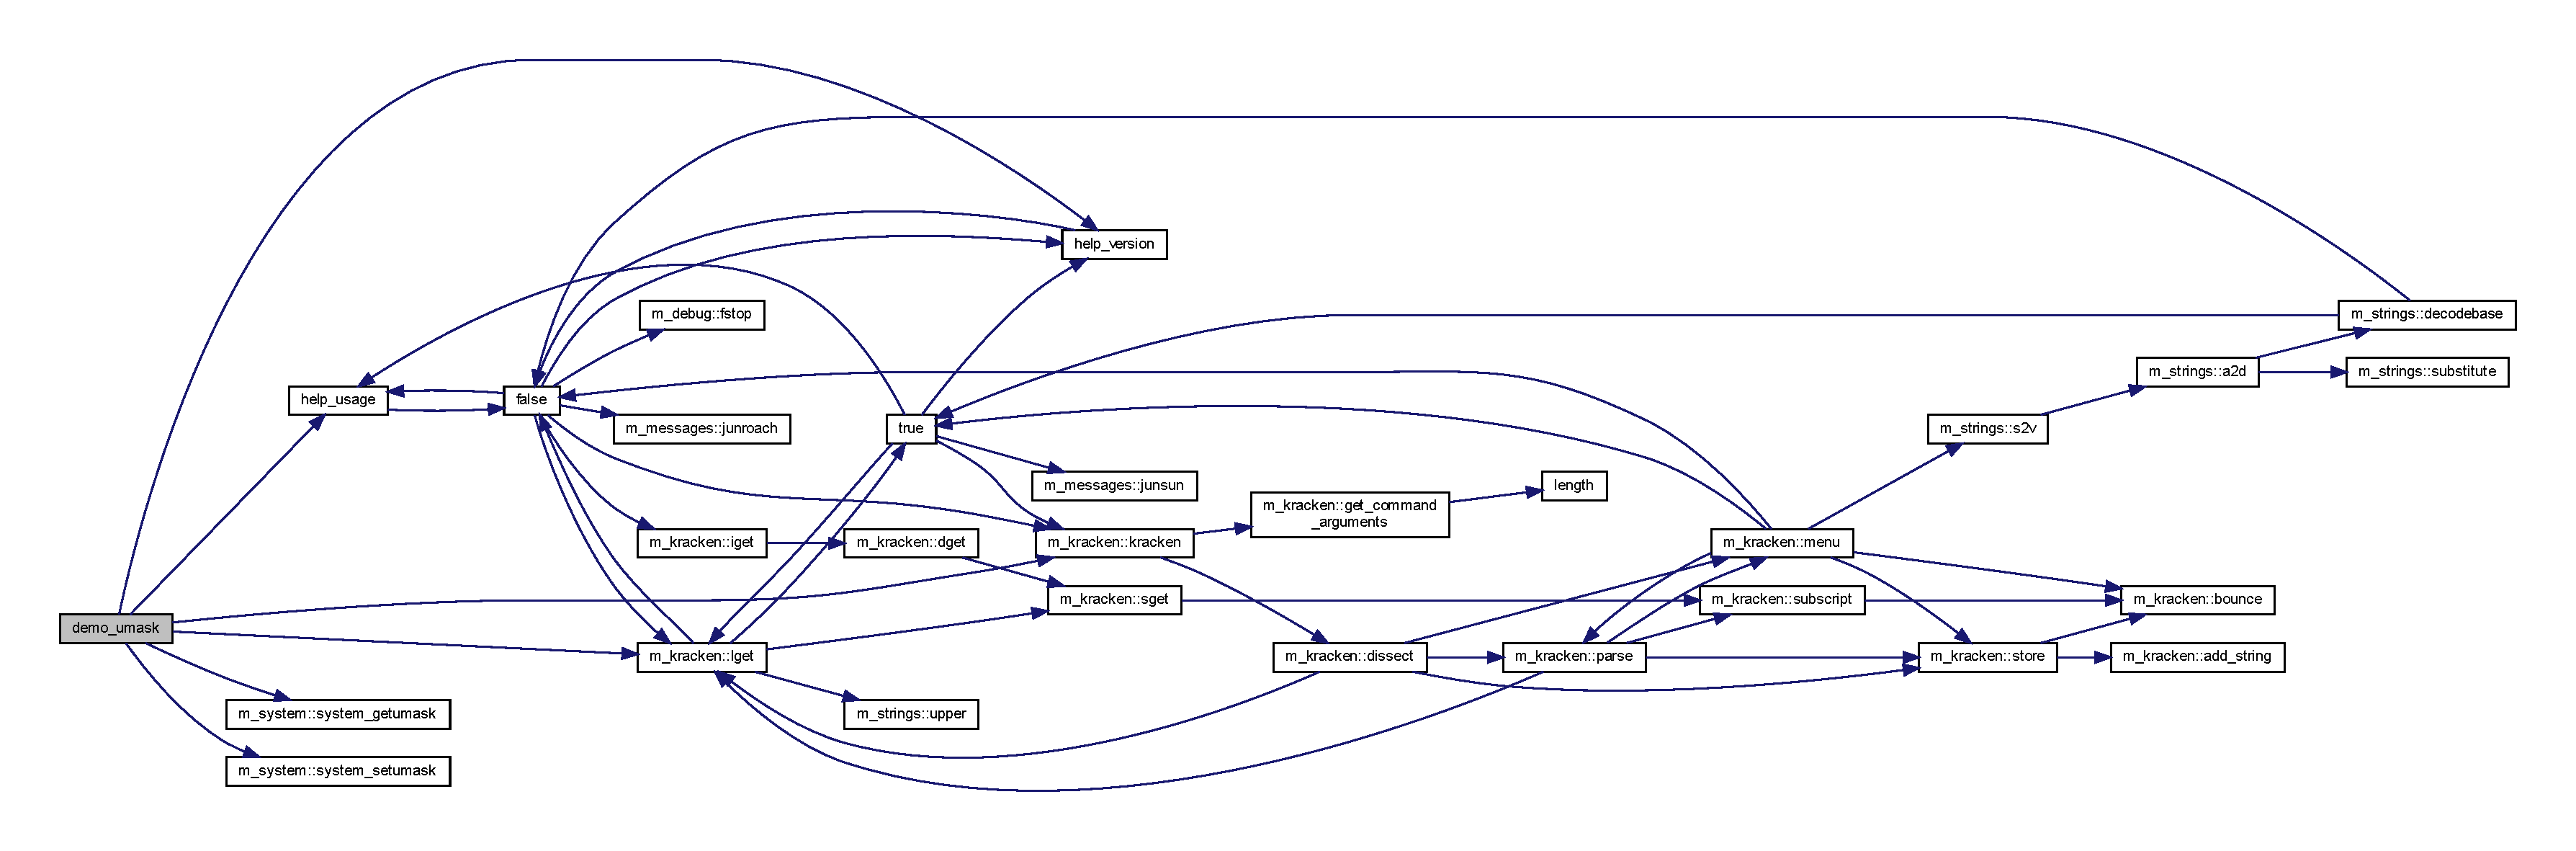
\includegraphics[width=350pt]{__showumask_8f90_a1b5ccb693a5e379113ec98bc98f16a90_cgraph}
\end{center}
\end{figure}
\mbox{\Hypertarget{__showumask_8f90_a3e09a3b52ee8fb04eeb93fe5761626a8}\label{__showumask_8f90_a3e09a3b52ee8fb04eeb93fe5761626a8}} 
\index{\+\_\+showumask.\+f90@{\+\_\+showumask.\+f90}!help\+\_\+usage@{help\+\_\+usage}}
\index{help\+\_\+usage@{help\+\_\+usage}!\+\_\+showumask.\+f90@{\+\_\+showumask.\+f90}}
\subsubsection{\texorpdfstring{help\+\_\+usage()}{help\_usage()}}
{\footnotesize\ttfamily \hyperlink{M__stopwatch_83_8txt_acfbcff50169d691ff02d4a123ed70482}{subroutine} help\+\_\+usage (\begin{DoxyParamCaption}\item[{logical, intent(\hyperlink{M__journal_83_8txt_afce72651d1eed785a2132bee863b2f38}{in})}]{l\+\_\+help }\end{DoxyParamCaption})}



References false().

Here is the call graph for this function\+:
\nopagebreak
\begin{figure}[H]
\begin{center}
\leavevmode
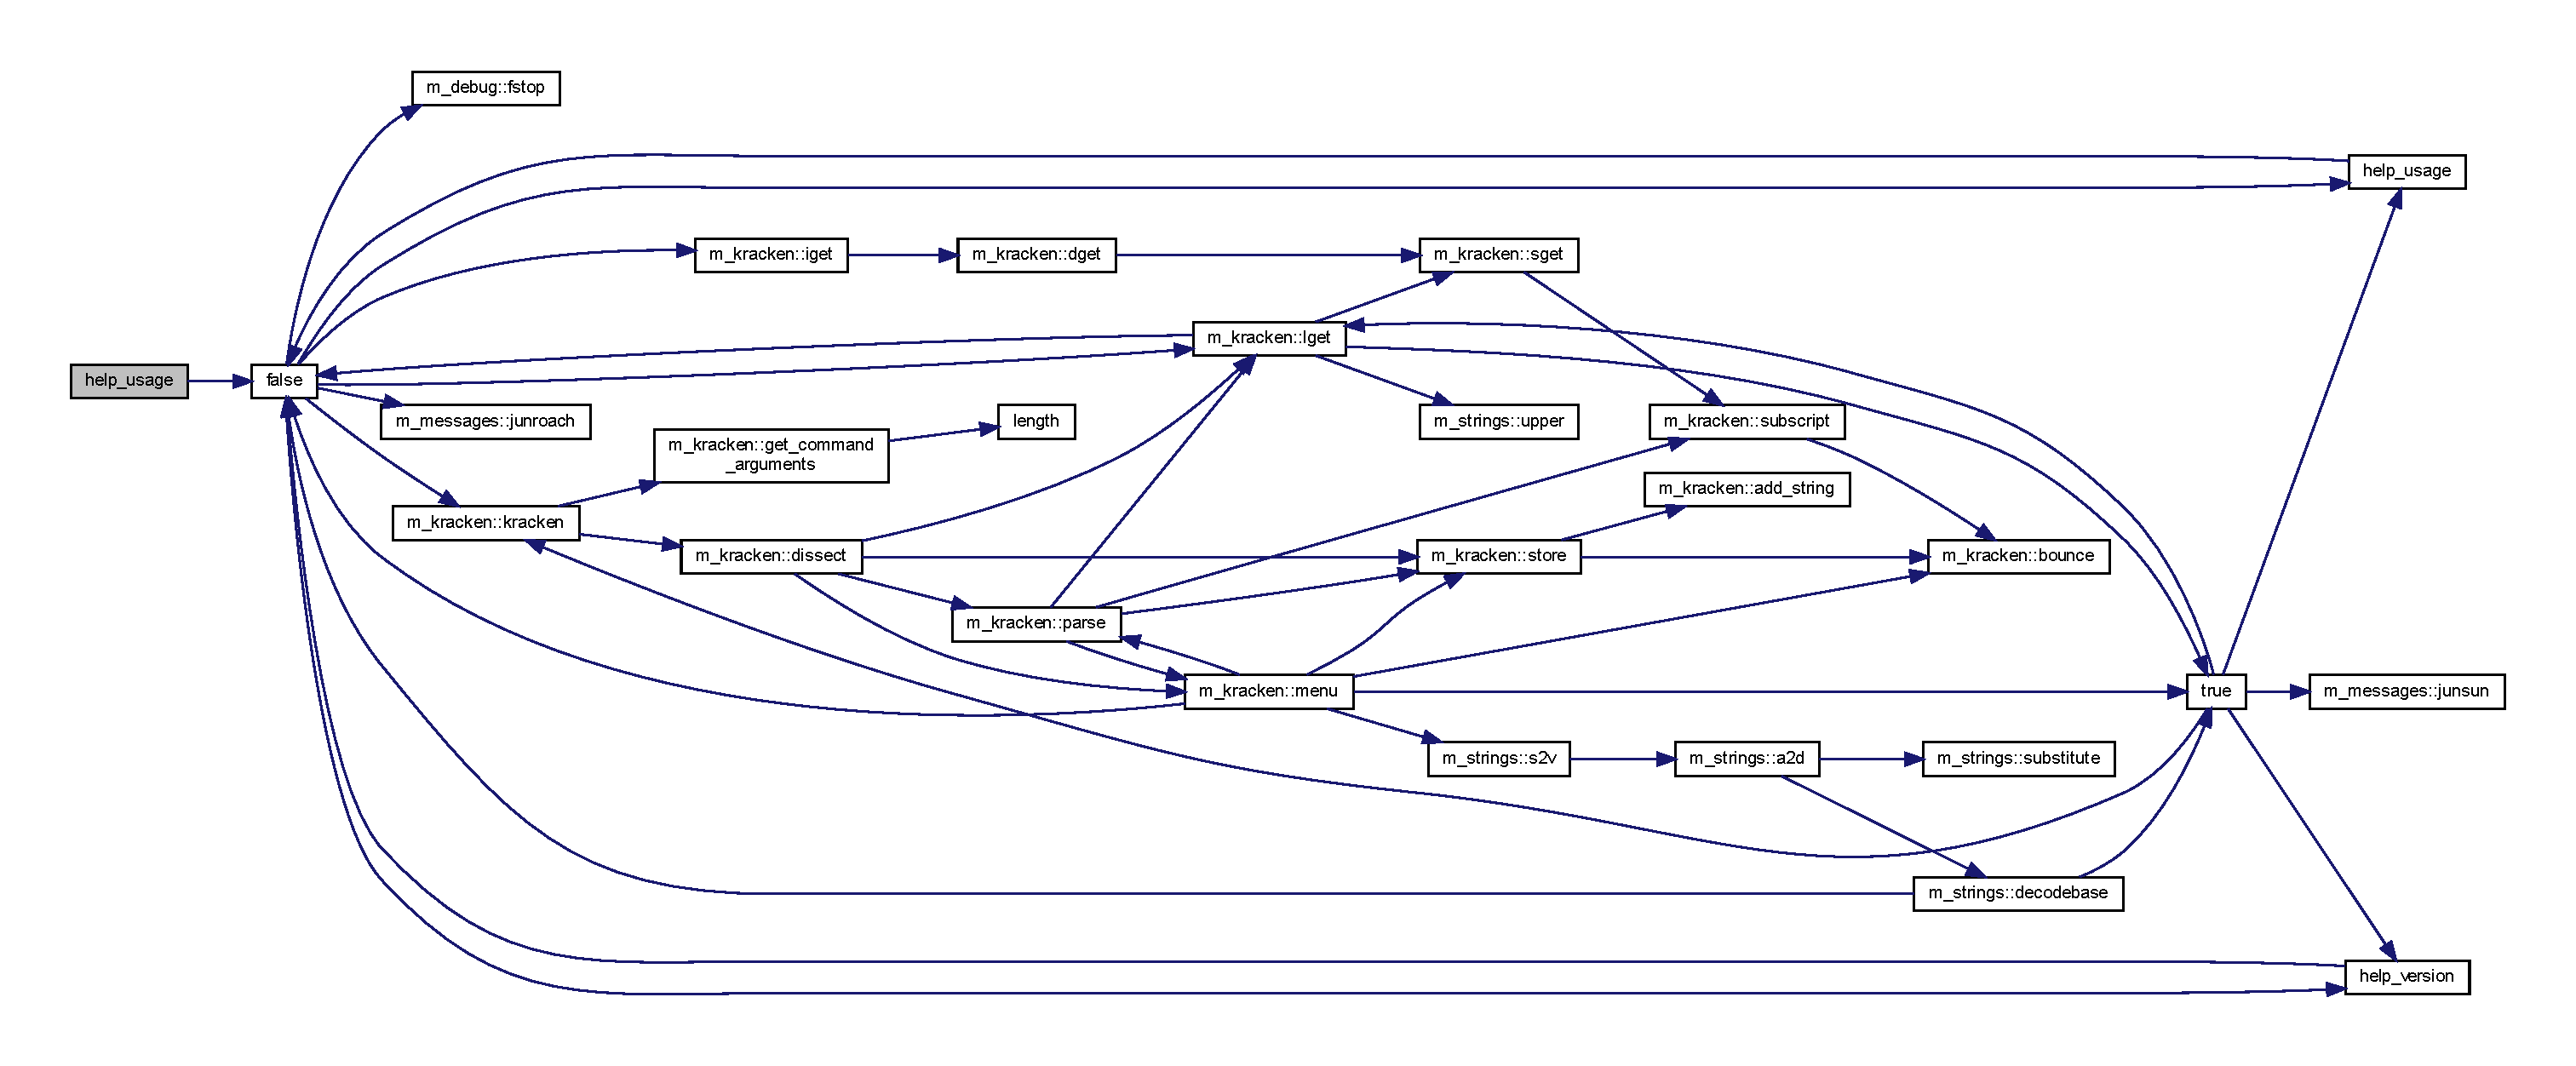
\includegraphics[width=350pt]{__showumask_8f90_a3e09a3b52ee8fb04eeb93fe5761626a8_cgraph}
\end{center}
\end{figure}
\mbox{\Hypertarget{__showumask_8f90_a39c21619b08a3c22f19e2306efd7f766}\label{__showumask_8f90_a39c21619b08a3c22f19e2306efd7f766}} 
\index{\+\_\+showumask.\+f90@{\+\_\+showumask.\+f90}!help\+\_\+version@{help\+\_\+version}}
\index{help\+\_\+version@{help\+\_\+version}!\+\_\+showumask.\+f90@{\+\_\+showumask.\+f90}}
\subsubsection{\texorpdfstring{help\+\_\+version()}{help\_version()}}
{\footnotesize\ttfamily \hyperlink{M__stopwatch_83_8txt_acfbcff50169d691ff02d4a123ed70482}{subroutine} help\+\_\+version (\begin{DoxyParamCaption}\item[{logical, intent(\hyperlink{M__journal_83_8txt_afce72651d1eed785a2132bee863b2f38}{in})}]{l\+\_\+version }\end{DoxyParamCaption})}



References false().

Here is the call graph for this function\+:
\nopagebreak
\begin{figure}[H]
\begin{center}
\leavevmode
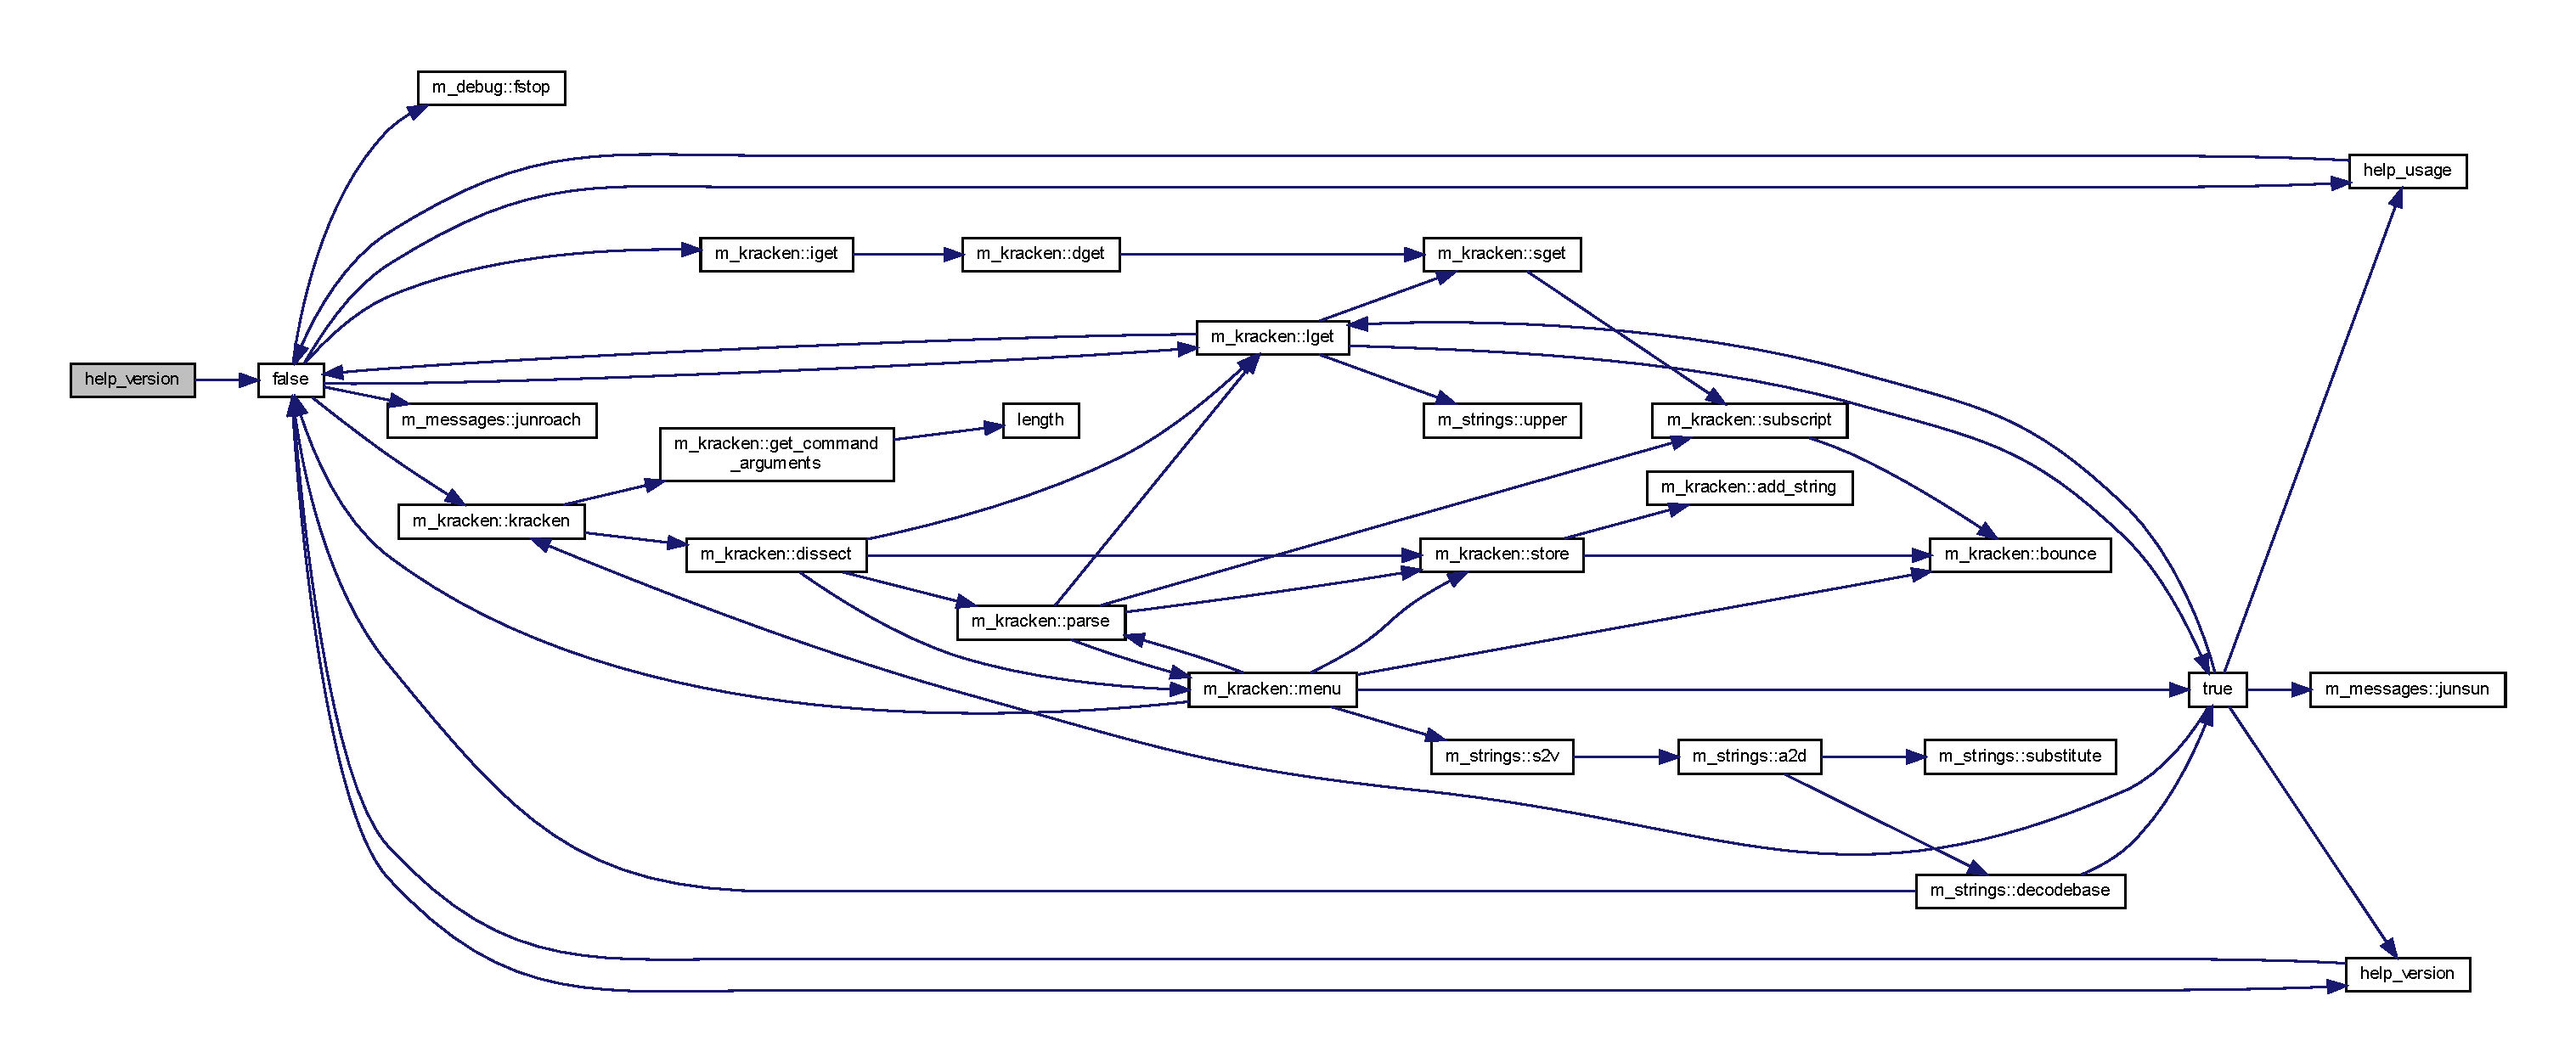
\includegraphics[width=350pt]{__showumask_8f90_a39c21619b08a3c22f19e2306efd7f766_cgraph}
\end{center}
\end{figure}

\hypertarget{__sleep_8f90}{}\section{L\+I\+B\+R\+A\+R\+Y/lib\+G\+P\+F/download/tmp/\+P\+R\+O\+G\+R\+A\+M\+S/\+\_\+sleep.f90 File Reference}
\label{__sleep_8f90}\index{L\+I\+B\+R\+A\+R\+Y/lib\+G\+P\+F/download/tmp/\+P\+R\+O\+G\+R\+A\+M\+S/\+\_\+sleep.\+f90@{L\+I\+B\+R\+A\+R\+Y/lib\+G\+P\+F/download/tmp/\+P\+R\+O\+G\+R\+A\+M\+S/\+\_\+sleep.\+f90}}
\subsection*{Functions/\+Subroutines}
\begin{DoxyCompactItemize}
\item 
\hyperlink{M__stopwatch_83_8txt_acfbcff50169d691ff02d4a123ed70482}{subroutine} \hyperlink{__sleep_8f90_a3e09a3b52ee8fb04eeb93fe5761626a8}{help\+\_\+usage} (l\+\_\+help)
\item 
\hyperlink{M__stopwatch_83_8txt_acfbcff50169d691ff02d4a123ed70482}{subroutine} \hyperlink{__sleep_8f90_a39c21619b08a3c22f19e2306efd7f766}{help\+\_\+version} (l\+\_\+version)
\begin{DoxyCompactList}\small\item\em \subsubsection*{N\+A\+ME}

\+\_\+sleep -\/ \mbox{[}T\+I\+ME\mbox{]} pause for specified duration \subsubsection*{S\+Y\+N\+O\+P\+S\+IS}\end{DoxyCompactList}\item 
program \hyperlink{__sleep_8f90_adea2b9826964203f987d029f48afa37a}{demo\+\_\+system\+\_\+sleep}
\end{DoxyCompactItemize}


\subsection{Function/\+Subroutine Documentation}
\mbox{\Hypertarget{__sleep_8f90_adea2b9826964203f987d029f48afa37a}\label{__sleep_8f90_adea2b9826964203f987d029f48afa37a}} 
\index{\+\_\+sleep.\+f90@{\+\_\+sleep.\+f90}!demo\+\_\+system\+\_\+sleep@{demo\+\_\+system\+\_\+sleep}}
\index{demo\+\_\+system\+\_\+sleep@{demo\+\_\+system\+\_\+sleep}!\+\_\+sleep.\+f90@{\+\_\+sleep.\+f90}}
\subsubsection{\texorpdfstring{demo\+\_\+system\+\_\+sleep()}{demo\_system\_sleep()}}
{\footnotesize\ttfamily program demo\+\_\+system\+\_\+sleep (\begin{DoxyParamCaption}{ }\end{DoxyParamCaption})}



References m\+\_\+time\+::days2sec(), help\+\_\+usage(), help\+\_\+version(), m\+\_\+kracken\+::kracken(), m\+\_\+kracken\+::lget(), m\+\_\+time\+::realtime, m\+\_\+kracken\+::sgets(), size(), m\+\_\+strings\+::substitute(), and m\+\_\+time\+::system\+\_\+sleep().

Here is the call graph for this function\+:
\nopagebreak
\begin{figure}[H]
\begin{center}
\leavevmode
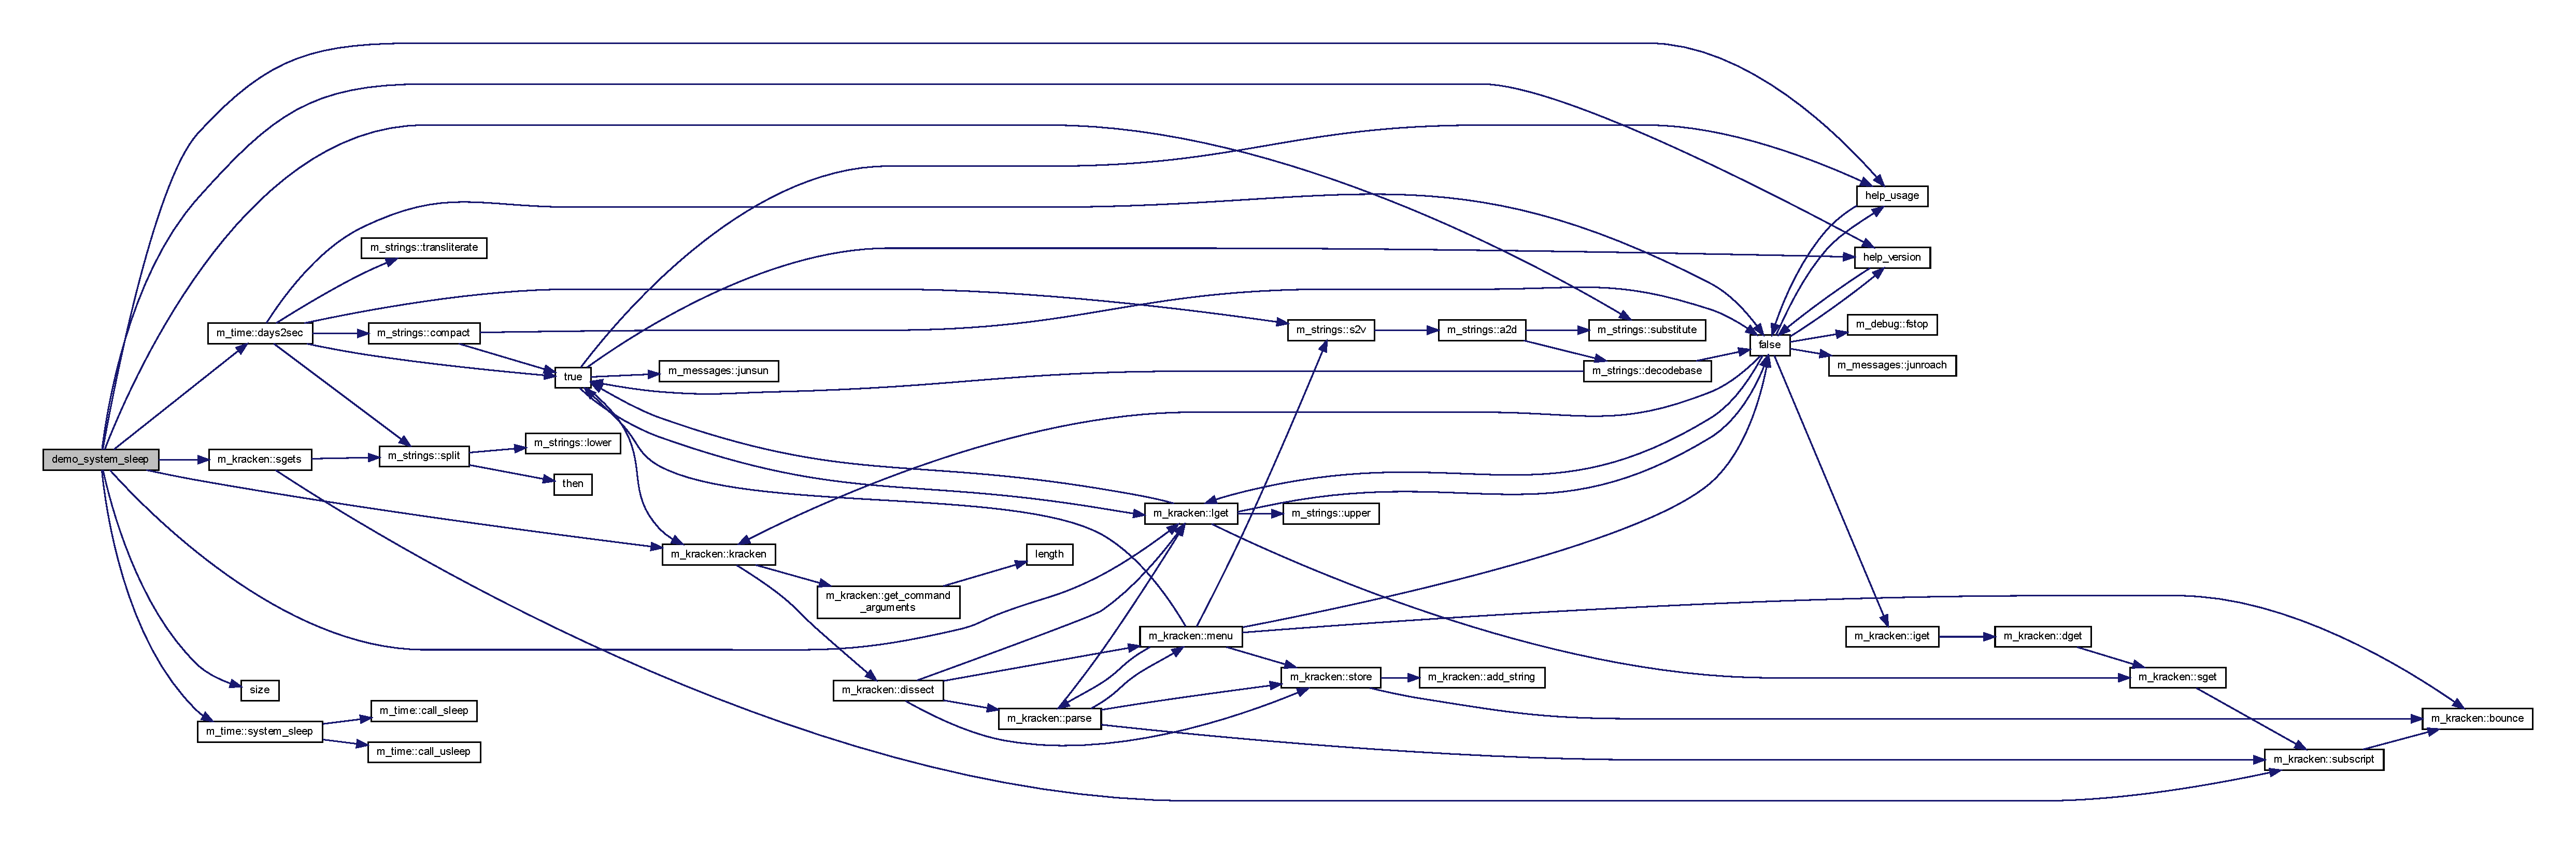
\includegraphics[width=350pt]{__sleep_8f90_adea2b9826964203f987d029f48afa37a_cgraph}
\end{center}
\end{figure}
\mbox{\Hypertarget{__sleep_8f90_a3e09a3b52ee8fb04eeb93fe5761626a8}\label{__sleep_8f90_a3e09a3b52ee8fb04eeb93fe5761626a8}} 
\index{\+\_\+sleep.\+f90@{\+\_\+sleep.\+f90}!help\+\_\+usage@{help\+\_\+usage}}
\index{help\+\_\+usage@{help\+\_\+usage}!\+\_\+sleep.\+f90@{\+\_\+sleep.\+f90}}
\subsubsection{\texorpdfstring{help\+\_\+usage()}{help\_usage()}}
{\footnotesize\ttfamily \hyperlink{M__stopwatch_83_8txt_acfbcff50169d691ff02d4a123ed70482}{subroutine} help\+\_\+usage (\begin{DoxyParamCaption}\item[{logical, intent(\hyperlink{M__journal_83_8txt_afce72651d1eed785a2132bee863b2f38}{in})}]{l\+\_\+help }\end{DoxyParamCaption})}



References false().

Here is the call graph for this function\+:
\nopagebreak
\begin{figure}[H]
\begin{center}
\leavevmode
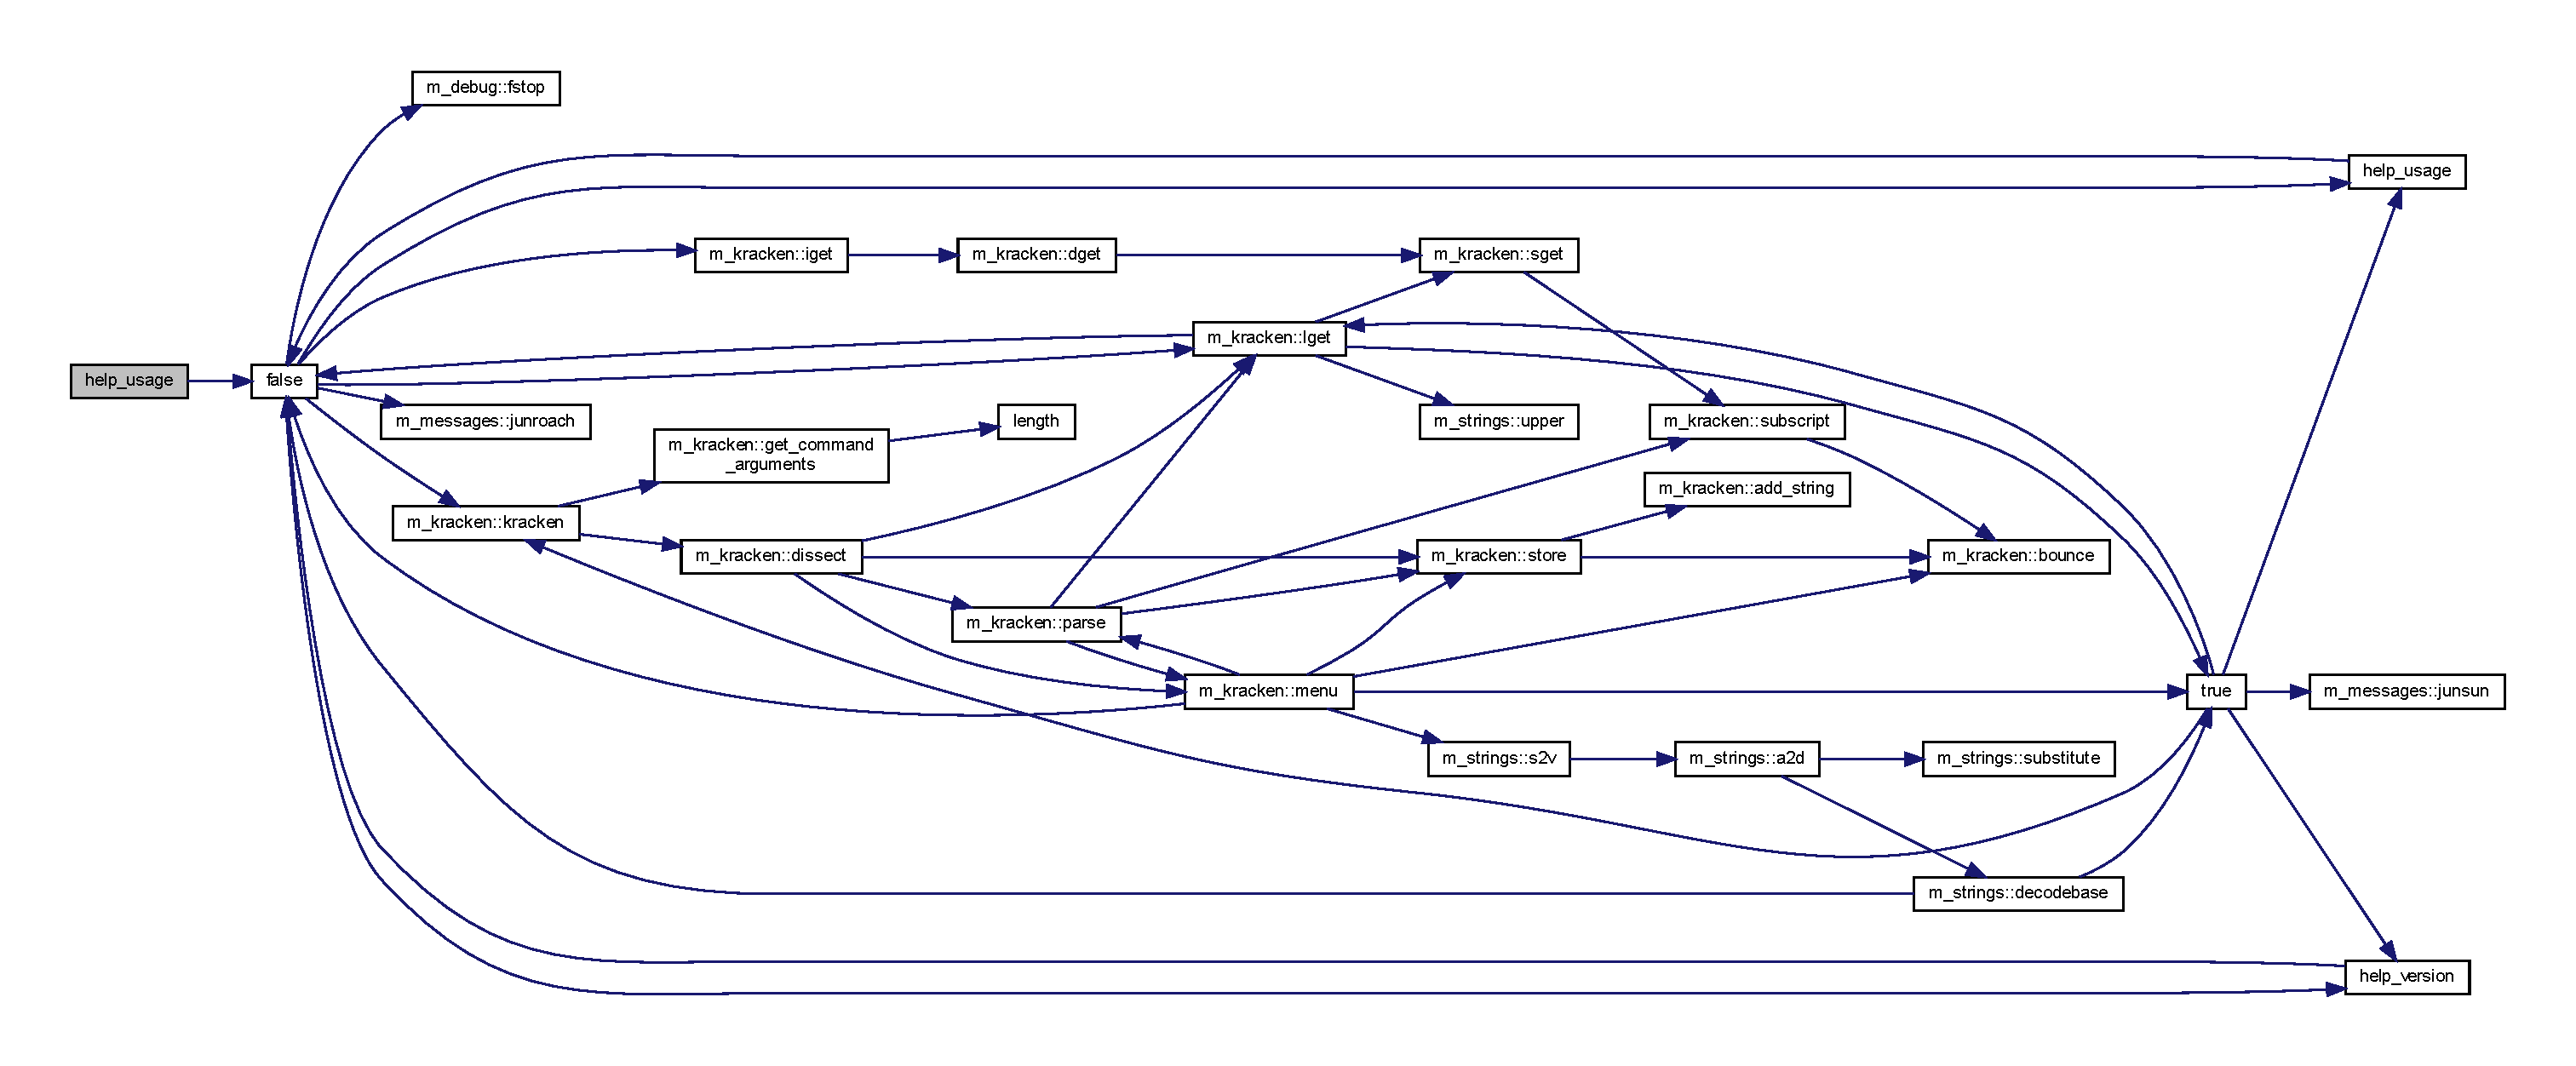
\includegraphics[width=350pt]{__sleep_8f90_a3e09a3b52ee8fb04eeb93fe5761626a8_cgraph}
\end{center}
\end{figure}
\mbox{\Hypertarget{__sleep_8f90_a39c21619b08a3c22f19e2306efd7f766}\label{__sleep_8f90_a39c21619b08a3c22f19e2306efd7f766}} 
\index{\+\_\+sleep.\+f90@{\+\_\+sleep.\+f90}!help\+\_\+version@{help\+\_\+version}}
\index{help\+\_\+version@{help\+\_\+version}!\+\_\+sleep.\+f90@{\+\_\+sleep.\+f90}}
\subsubsection{\texorpdfstring{help\+\_\+version()}{help\_version()}}
{\footnotesize\ttfamily \hyperlink{M__stopwatch_83_8txt_acfbcff50169d691ff02d4a123ed70482}{subroutine} help\+\_\+version (\begin{DoxyParamCaption}\item[{logical, intent(\hyperlink{M__journal_83_8txt_afce72651d1eed785a2132bee863b2f38}{in})}]{l\+\_\+version }\end{DoxyParamCaption})}



\subsubsection*{N\+A\+ME}

\+\_\+sleep -\/ \mbox{[}T\+I\+ME\mbox{]} pause for specified duration \subsubsection*{S\+Y\+N\+O\+P\+S\+IS}

\+\_\+sleep \mbox{[}dd-\/hh\+:mm\+:ss\mbox{[}.xxx\mbox{]}$\vert$xxx.yyy\mbox{[}s$\vert$m$\vert$h$\vert$d\mbox{]}\mbox{]} --version$\vert$--help \subsubsection*{D\+E\+S\+C\+R\+I\+P\+T\+I\+ON}

Given a duration in the form dd-\/hh\+:mm\+:ss.\+xxx where dd is days, hh hours, mm minutes and ss.\+xxx seconds pause for the specified amount of time.

Alternatively, the time may be specified by a number of seconds immediately followed by a unit letter, where s is seconds, m is minutes, h is hours and d is days.

If the suffix r is used, a random time between zero and the specified number of seconds is used. This is useful for spreading out cron(1) tasks in a H\+PC cluster.

Given multiple arguments, pause for the time specified by the sum of the values. \subsubsection*{O\+P\+T\+I\+O\+NS}

dd-\/hh\+:mm\+:ss Given a string representing a duration of time in the following forms\+:

dd-\/hh\+:mm\+:ss\mbox{[}.xx\mbox{]} hh\+:mm\+:ss\mbox{[}.xx\mbox{]} mm\+:ss\mbox{[}.xx\mbox{]} ss\mbox{[}.xx\mbox{]} or xx\mbox{[}.yy\mbox{]}S\+U\+F\+F\+IX where Suffix may be s for seconds, m for minutes, h for hours, or d for days. --help display this help and exit --version output version information and exit \subsubsection*{E\+X\+A\+M\+P\+LE}

usage\+:

\+\_\+sleep 0.\+10 \# pause one tenth of a second \+\_\+sleep 3m 10s \# pause three minutes and 10 seconds \+\_\+sleep 1\+:00\+:00 \# pause for one hour 

References false().

Here is the call graph for this function\+:
\nopagebreak
\begin{figure}[H]
\begin{center}
\leavevmode
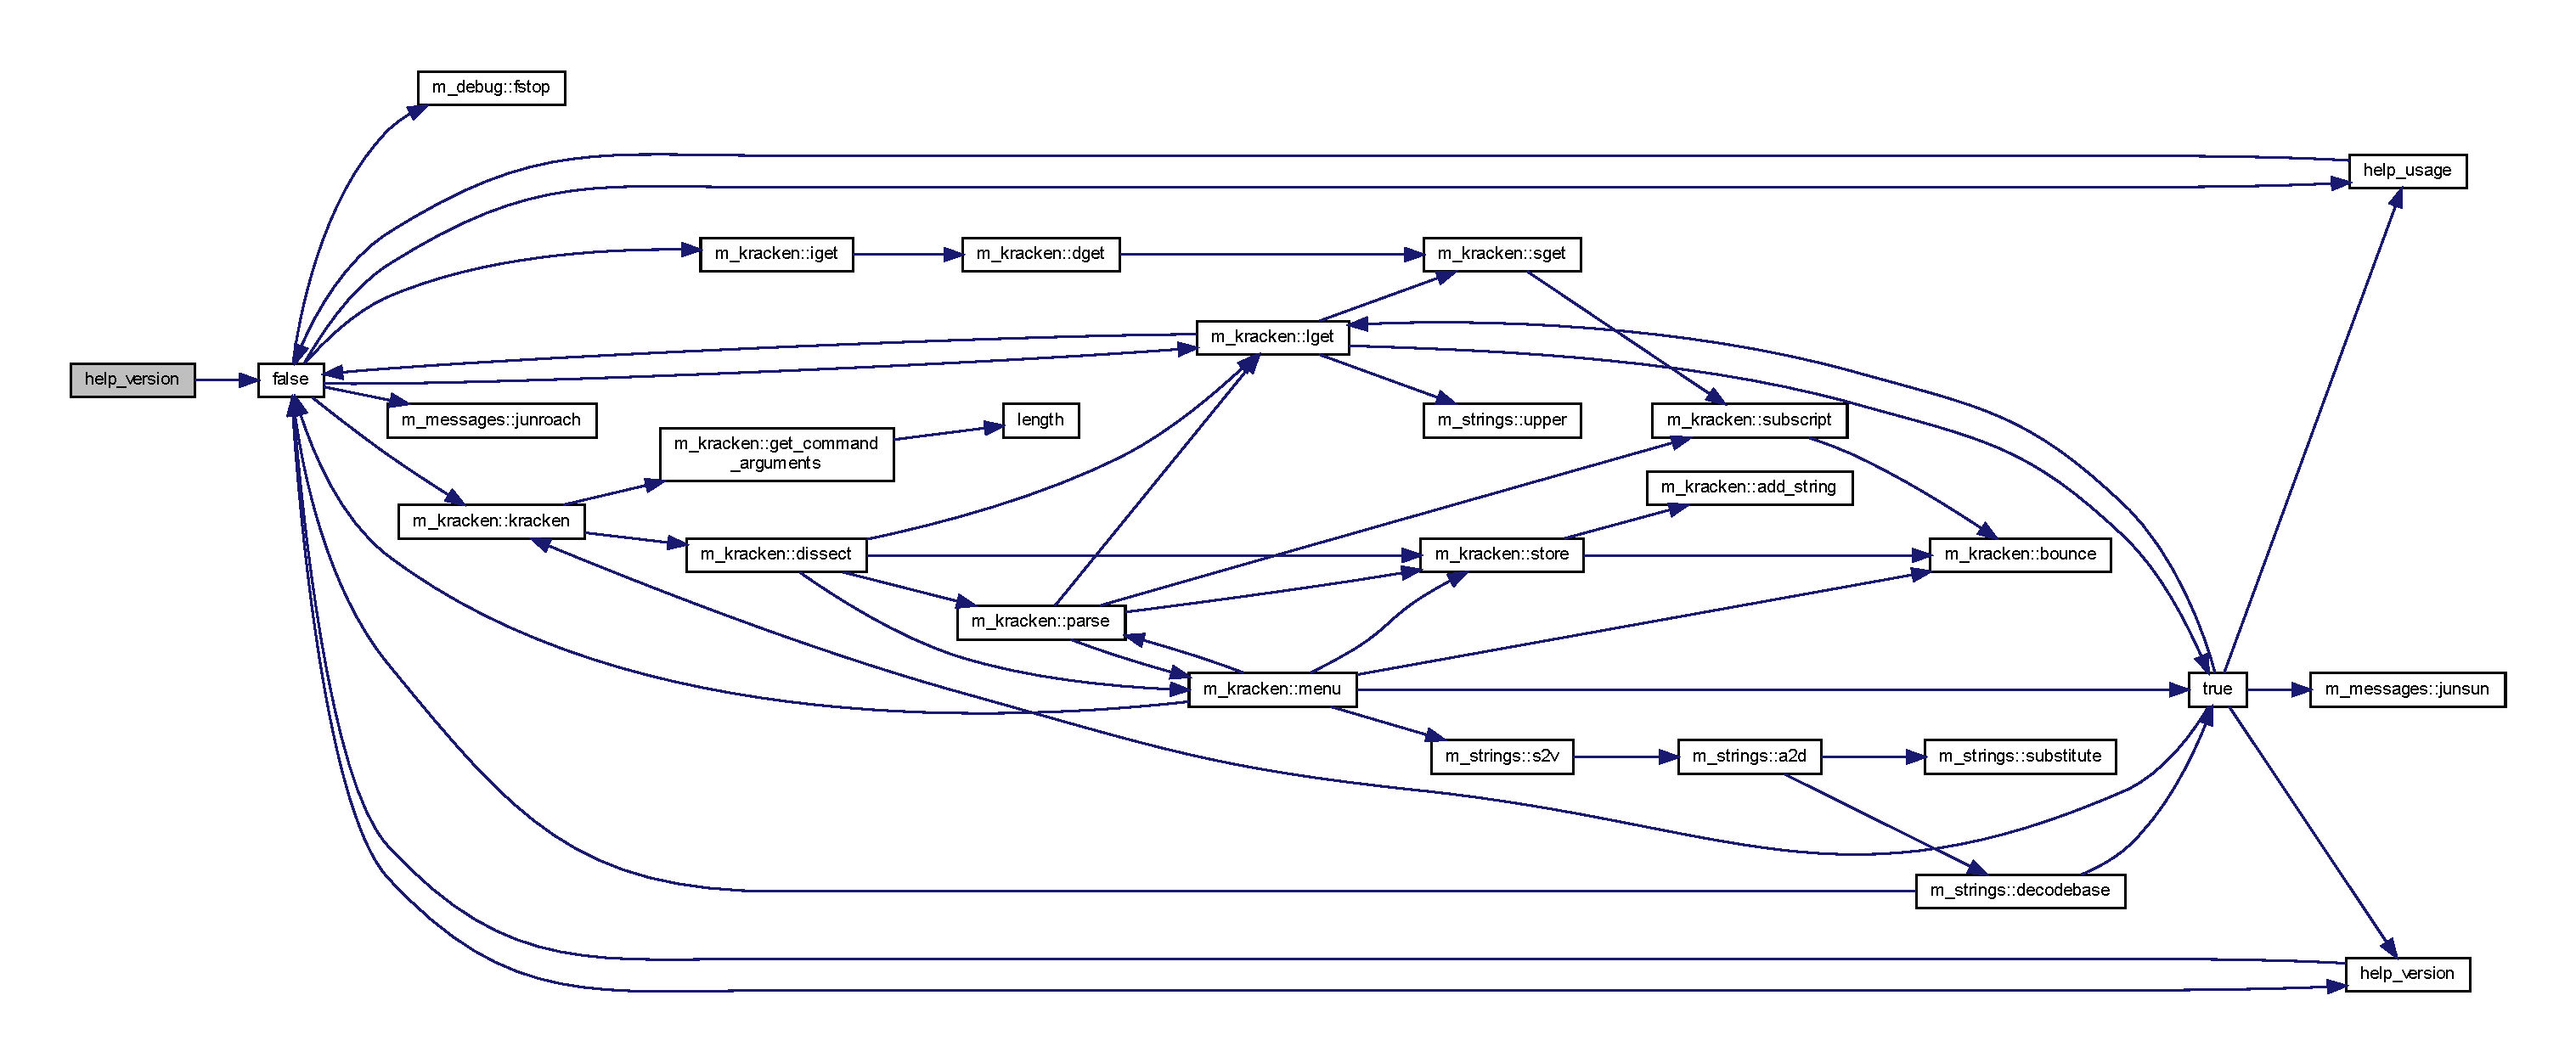
\includegraphics[width=350pt]{__sleep_8f90_a39c21619b08a3c22f19e2306efd7f766_cgraph}
\end{center}
\end{figure}

\hypertarget{__stat_8f90}{}\section{L\+I\+B\+R\+A\+R\+Y/lib\+G\+P\+F/download/tmp/\+P\+R\+O\+G\+R\+A\+M\+S/\+\_\+stat.f90 File Reference}
\label{__stat_8f90}\index{L\+I\+B\+R\+A\+R\+Y/lib\+G\+P\+F/download/tmp/\+P\+R\+O\+G\+R\+A\+M\+S/\+\_\+stat.\+f90@{L\+I\+B\+R\+A\+R\+Y/lib\+G\+P\+F/download/tmp/\+P\+R\+O\+G\+R\+A\+M\+S/\+\_\+stat.\+f90}}
\subsection*{Functions/\+Subroutines}
\begin{DoxyCompactItemize}
\item 
\hyperlink{M__stopwatch_83_8txt_acfbcff50169d691ff02d4a123ed70482}{subroutine} \hyperlink{__stat_8f90_a3e09a3b52ee8fb04eeb93fe5761626a8}{help\+\_\+usage} (l\+\_\+help)
\item 
\hyperlink{M__stopwatch_83_8txt_acfbcff50169d691ff02d4a123ed70482}{subroutine} \hyperlink{__stat_8f90_a39c21619b08a3c22f19e2306efd7f766}{help\+\_\+version} (l\+\_\+version)
\begin{DoxyCompactList}\small\item\em \subsubsection*{N\+A\+ME}

\+\_\+stat(1f) -\/ \mbox{[}F\+U\+N\+IX\+:F\+I\+L\+E\+S\+Y\+S\+T\+EM\mbox{]} list file properties \subsubsection*{S\+Y\+N\+O\+P\+S\+IS}\end{DoxyCompactList}\item 
program \hyperlink{__stat_8f90_adf8b7aa887ea1a5d211153cc019facf4}{demo\+\_\+system\+\_\+stat}
\item 
\hyperlink{M__stopwatch_83_8txt_acfbcff50169d691ff02d4a123ed70482}{subroutine} \hyperlink{__stat_8f90_a9ea6ab9cdaa05a5fc3ac6e5448b11c68}{printit}
\end{DoxyCompactItemize}


\subsection{Function/\+Subroutine Documentation}
\mbox{\Hypertarget{__stat_8f90_adf8b7aa887ea1a5d211153cc019facf4}\label{__stat_8f90_adf8b7aa887ea1a5d211153cc019facf4}} 
\index{\+\_\+stat.\+f90@{\+\_\+stat.\+f90}!demo\+\_\+system\+\_\+stat@{demo\+\_\+system\+\_\+stat}}
\index{demo\+\_\+system\+\_\+stat@{demo\+\_\+system\+\_\+stat}!\+\_\+stat.\+f90@{\+\_\+stat.\+f90}}
\subsubsection{\texorpdfstring{demo\+\_\+system\+\_\+stat()}{demo\_system\_stat()}}
{\footnotesize\ttfamily program demo\+\_\+system\+\_\+stat (\begin{DoxyParamCaption}{ }\end{DoxyParamCaption})}



References help\+\_\+usage(), help\+\_\+version(), m\+\_\+kracken\+::kracken(), m\+\_\+kracken\+::lget(), printit(), m\+\_\+kracken\+::rget(), m\+\_\+kracken\+::sgets(), and m\+\_\+system\+::system\+\_\+stat().

\mbox{\Hypertarget{__stat_8f90_a3e09a3b52ee8fb04eeb93fe5761626a8}\label{__stat_8f90_a3e09a3b52ee8fb04eeb93fe5761626a8}} 
\index{\+\_\+stat.\+f90@{\+\_\+stat.\+f90}!help\+\_\+usage@{help\+\_\+usage}}
\index{help\+\_\+usage@{help\+\_\+usage}!\+\_\+stat.\+f90@{\+\_\+stat.\+f90}}
\subsubsection{\texorpdfstring{help\+\_\+usage()}{help\_usage()}}
{\footnotesize\ttfamily \hyperlink{M__stopwatch_83_8txt_acfbcff50169d691ff02d4a123ed70482}{subroutine} help\+\_\+usage (\begin{DoxyParamCaption}\item[{logical, intent(\hyperlink{M__journal_83_8txt_afce72651d1eed785a2132bee863b2f38}{in})}]{l\+\_\+help }\end{DoxyParamCaption})}



References false().

\mbox{\Hypertarget{__stat_8f90_a39c21619b08a3c22f19e2306efd7f766}\label{__stat_8f90_a39c21619b08a3c22f19e2306efd7f766}} 
\index{\+\_\+stat.\+f90@{\+\_\+stat.\+f90}!help\+\_\+version@{help\+\_\+version}}
\index{help\+\_\+version@{help\+\_\+version}!\+\_\+stat.\+f90@{\+\_\+stat.\+f90}}
\subsubsection{\texorpdfstring{help\+\_\+version()}{help\_version()}}
{\footnotesize\ttfamily \hyperlink{M__stopwatch_83_8txt_acfbcff50169d691ff02d4a123ed70482}{subroutine} help\+\_\+version (\begin{DoxyParamCaption}\item[{logical, intent(\hyperlink{M__journal_83_8txt_afce72651d1eed785a2132bee863b2f38}{in})}]{l\+\_\+version }\end{DoxyParamCaption})}



\subsubsection*{N\+A\+ME}

\+\_\+stat(1f) -\/ \mbox{[}F\+U\+N\+IX\+:F\+I\+L\+E\+S\+Y\+S\+T\+EM\mbox{]} list file properties \subsubsection*{S\+Y\+N\+O\+P\+S\+IS}

\+\_\+stat pathnames$\vert$--version$\vert$--help \subsubsection*{D\+E\+S\+C\+R\+I\+P\+T\+I\+ON}

Given pathnames list properties \subsubsection*{O\+P\+T\+I\+O\+NS}

pathnames pathnames to display properties of. --help display command help and exit --version output version information and exit \subsubsection*{E\+X\+A\+M\+P\+L\+ES}

Sample command lines ...

\+\_\+stat \+\_\+stat.\+ff

Results

Pathname\+: \+\_\+stat.\+ff Residence\+: Inode\+:18295873486224096 Device ID(hex/decimal)\+:3\+E6\+B\+E045h/1047257157d Device where located\+:0 Size\+: File size(bytes)\+:4267 No. of blocks allocated\+:8 Preferred block size(bytes)\+:65536 File mode octal/decimal/str\+: 100744o/33252d/-\/rwxr--r-- --- Number of links\+: 1 Owner\textquotesingle{}s uid/username\+: 197609/\+J\+SU Owner\textquotesingle{}s gid/group\+: 197121/\+None Last access time\+: 1507483493 2017-\/10-\/08 13\+:24\+:53 Last modification time\+: 1507483493 2017-\/10-\/08 13\+:24\+:53 Last status change time\+: 1507483494 2017-\/10-\/08 13\+:24\+:54 

References false().

\mbox{\Hypertarget{__stat_8f90_a9ea6ab9cdaa05a5fc3ac6e5448b11c68}\label{__stat_8f90_a9ea6ab9cdaa05a5fc3ac6e5448b11c68}} 
\index{\+\_\+stat.\+f90@{\+\_\+stat.\+f90}!printit@{printit}}
\index{printit@{printit}!\+\_\+stat.\+f90@{\+\_\+stat.\+f90}}
\subsubsection{\texorpdfstring{printit()}{printit()}}
{\footnotesize\ttfamily \hyperlink{M__stopwatch_83_8txt_acfbcff50169d691ff02d4a123ed70482}{subroutine} demo\+\_\+system\+\_\+stat\+::printit (\begin{DoxyParamCaption}{ }\end{DoxyParamCaption})}



References fmtdate, m\+\_\+system\+::system\+\_\+getgrgid(), m\+\_\+system\+::system\+\_\+getpwuid(), m\+\_\+system\+::system\+\_\+perm(), and u2d.


\hypertarget{__true_8f90}{}\section{L\+I\+B\+R\+A\+R\+Y/lib\+G\+P\+F/download/tmp/\+P\+R\+O\+G\+R\+A\+M\+S/\+\_\+true.f90 File Reference}
\label{__true_8f90}\index{L\+I\+B\+R\+A\+R\+Y/lib\+G\+P\+F/download/tmp/\+P\+R\+O\+G\+R\+A\+M\+S/\+\_\+true.\+f90@{L\+I\+B\+R\+A\+R\+Y/lib\+G\+P\+F/download/tmp/\+P\+R\+O\+G\+R\+A\+M\+S/\+\_\+true.\+f90}}
\subsection*{Functions/\+Subroutines}
\begin{DoxyCompactItemize}
\item 
\hyperlink{M__stopwatch_83_8txt_acfbcff50169d691ff02d4a123ed70482}{subroutine} \hyperlink{__true_8f90_a3e09a3b52ee8fb04eeb93fe5761626a8}{help\+\_\+usage} (l\+\_\+help)
\item 
\hyperlink{M__stopwatch_83_8txt_acfbcff50169d691ff02d4a123ed70482}{subroutine} \hyperlink{__true_8f90_a39c21619b08a3c22f19e2306efd7f766}{help\+\_\+version} (l\+\_\+version)
\begin{DoxyCompactList}\small\item\em \subsubsection*{N\+A\+ME}

\+\_\+true(1f) -\/ \mbox{[}F\+U\+N\+IX\mbox{]} do nothing, successfully \end{DoxyCompactList}\item 
program \hyperlink{__true_8f90_a7ed1d79677aed1b23489a4fe0bd16daa}{true}
\end{DoxyCompactItemize}


\subsection{Function/\+Subroutine Documentation}
\mbox{\Hypertarget{__true_8f90_a3e09a3b52ee8fb04eeb93fe5761626a8}\label{__true_8f90_a3e09a3b52ee8fb04eeb93fe5761626a8}} 
\index{\+\_\+true.\+f90@{\+\_\+true.\+f90}!help\+\_\+usage@{help\+\_\+usage}}
\index{help\+\_\+usage@{help\+\_\+usage}!\+\_\+true.\+f90@{\+\_\+true.\+f90}}
\subsubsection{\texorpdfstring{help\+\_\+usage()}{help\_usage()}}
{\footnotesize\ttfamily \hyperlink{M__stopwatch_83_8txt_acfbcff50169d691ff02d4a123ed70482}{subroutine} help\+\_\+usage (\begin{DoxyParamCaption}\item[{logical, intent(\hyperlink{M__journal_83_8txt_afce72651d1eed785a2132bee863b2f38}{in})}]{l\+\_\+help }\end{DoxyParamCaption})}



References false().

Here is the call graph for this function\+:
\nopagebreak
\begin{figure}[H]
\begin{center}
\leavevmode
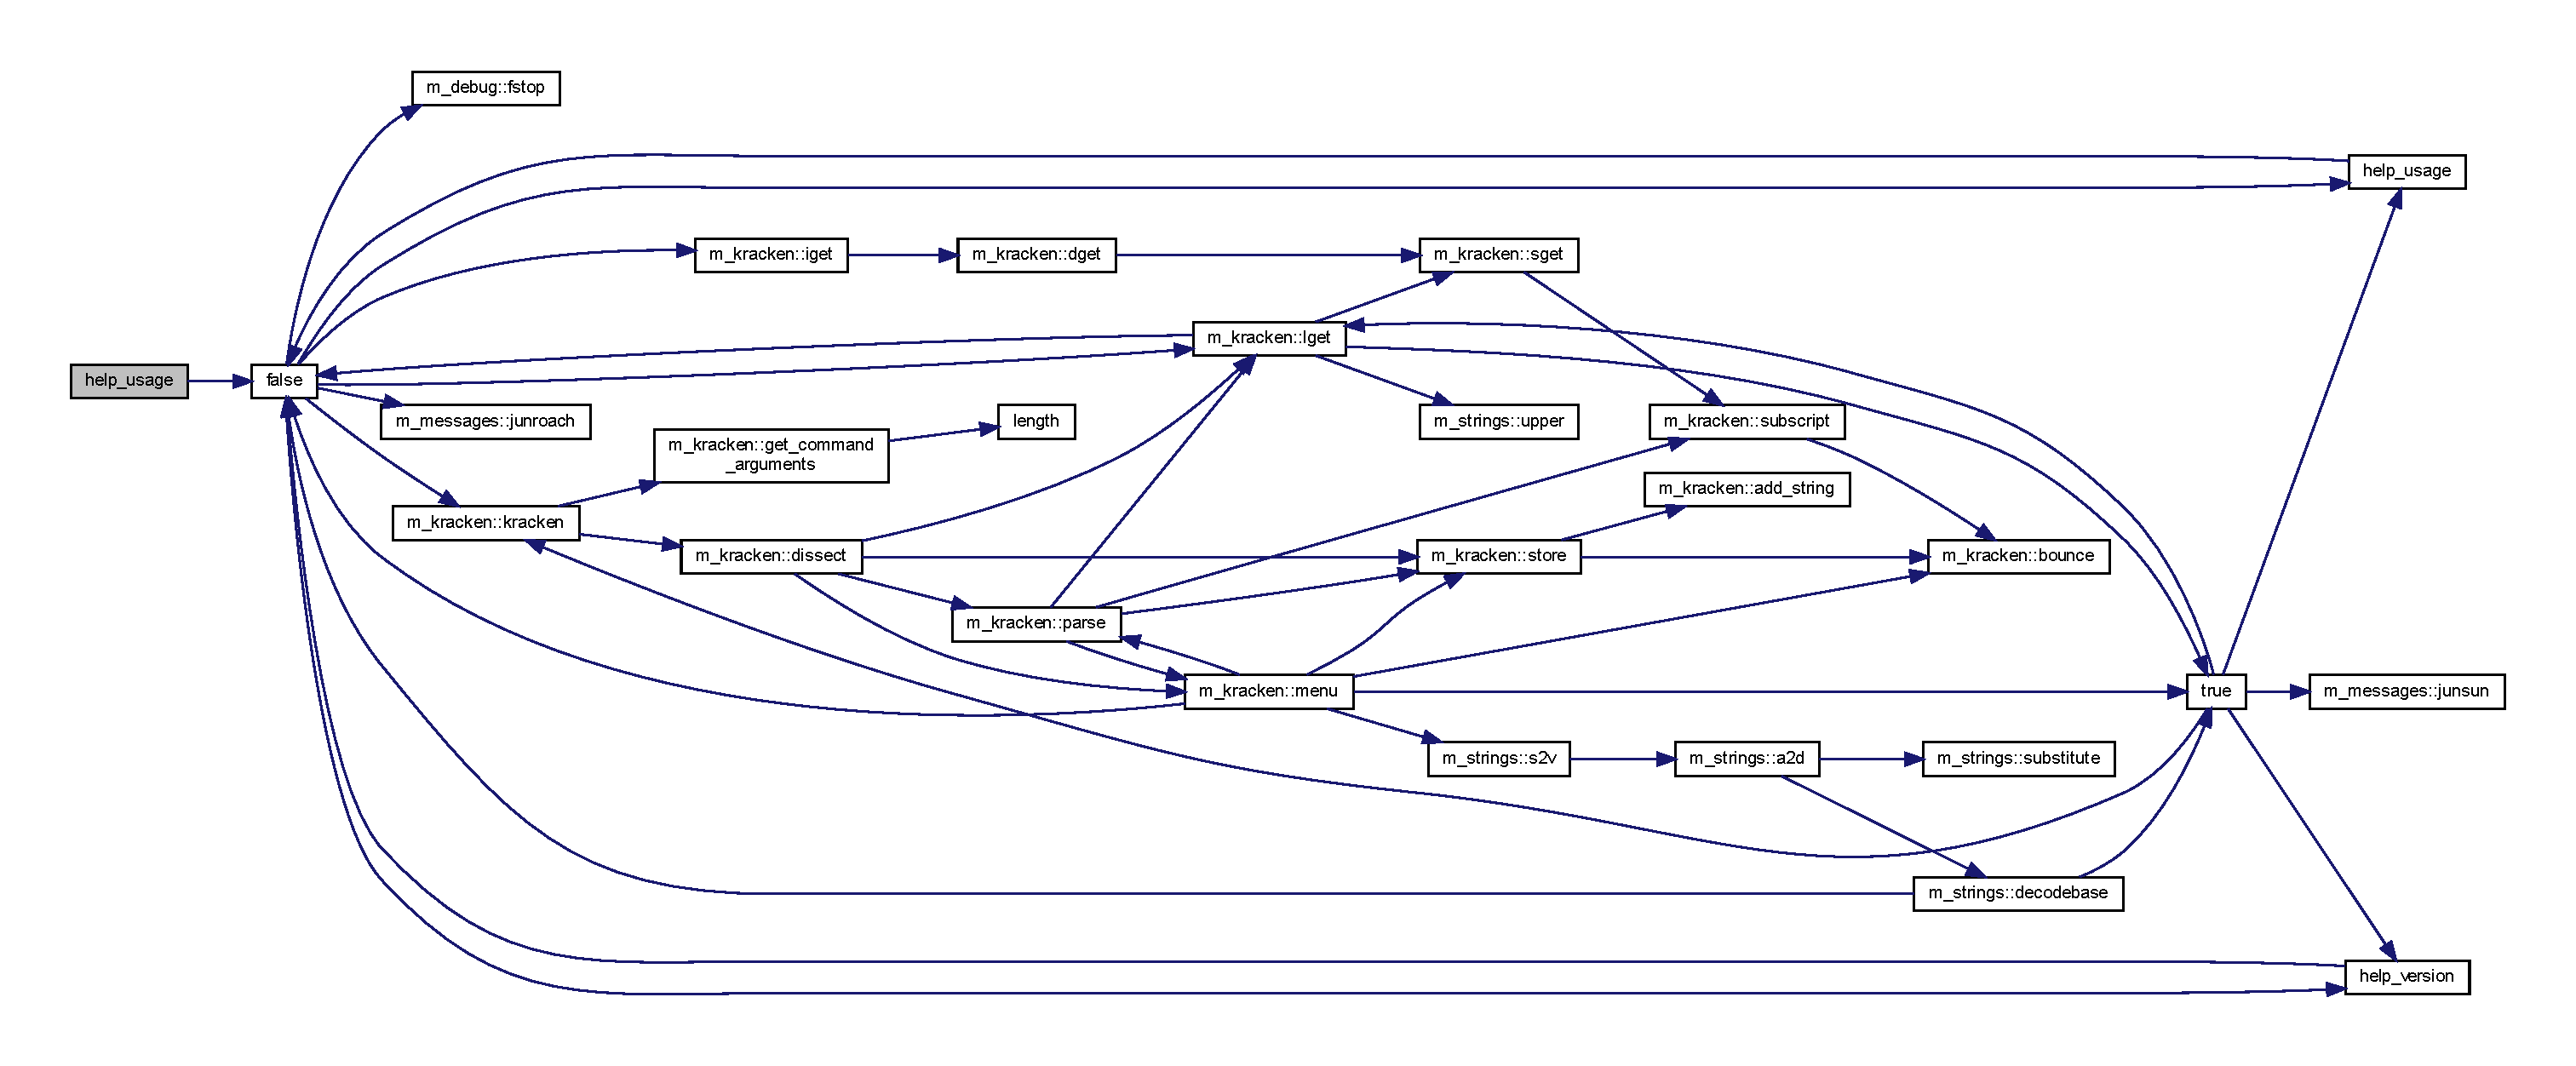
\includegraphics[width=350pt]{__true_8f90_a3e09a3b52ee8fb04eeb93fe5761626a8_cgraph}
\end{center}
\end{figure}
\mbox{\Hypertarget{__true_8f90_a39c21619b08a3c22f19e2306efd7f766}\label{__true_8f90_a39c21619b08a3c22f19e2306efd7f766}} 
\index{\+\_\+true.\+f90@{\+\_\+true.\+f90}!help\+\_\+version@{help\+\_\+version}}
\index{help\+\_\+version@{help\+\_\+version}!\+\_\+true.\+f90@{\+\_\+true.\+f90}}
\subsubsection{\texorpdfstring{help\+\_\+version()}{help\_version()}}
{\footnotesize\ttfamily \hyperlink{M__stopwatch_83_8txt_acfbcff50169d691ff02d4a123ed70482}{subroutine} help\+\_\+version (\begin{DoxyParamCaption}\item[{logical, intent(\hyperlink{M__journal_83_8txt_afce72651d1eed785a2132bee863b2f38}{in})}]{l\+\_\+version }\end{DoxyParamCaption})}



\subsubsection*{N\+A\+ME}

\+\_\+true(1f) -\/ \mbox{[}F\+U\+N\+IX\mbox{]} do nothing, successfully 

\subsubsection*{S\+Y\+N\+O\+P\+S\+IS}

\begin{DoxyVerb}    _true [--verbose|--help|--version]
\end{DoxyVerb}


\subsubsection*{D\+E\+S\+C\+R\+I\+P\+T\+I\+ON}

Exit with a status code indicating failure.

--verbose display an A\+S\+C\+II graphic of a shining sun --help display this help and exit --version output version information and exit

\subsubsection*{E\+X\+A\+M\+P\+LE}

\begin{DoxyVerb}    _true && echo SUCCESSFUL || echo DID NOT WORK
\end{DoxyVerb}
 \subsubsection*{S\+EE A\+L\+SO}

\+\_\+true(1f) 

References false().

Here is the call graph for this function\+:
\nopagebreak
\begin{figure}[H]
\begin{center}
\leavevmode
\includegraphics[width=350pt]{__true_8f90_a39c21619b08a3c22f19e2306efd7f766_cgraph}
\end{center}
\end{figure}
\mbox{\Hypertarget{__true_8f90_a7ed1d79677aed1b23489a4fe0bd16daa}\label{__true_8f90_a7ed1d79677aed1b23489a4fe0bd16daa}} 
\index{\+\_\+true.\+f90@{\+\_\+true.\+f90}!true@{true}}
\index{true@{true}!\+\_\+true.\+f90@{\+\_\+true.\+f90}}
\subsubsection{\texorpdfstring{true()}{true()}}
{\footnotesize\ttfamily program true (\begin{DoxyParamCaption}{ }\end{DoxyParamCaption})}



References help\+\_\+usage(), help\+\_\+version(), m\+\_\+messages\+::junsun(), m\+\_\+kracken\+::kracken(), and m\+\_\+kracken\+::lget().

Here is the call graph for this function\+:
\nopagebreak
\begin{figure}[H]
\begin{center}
\leavevmode
\includegraphics[width=350pt]{__true_8f90_a7ed1d79677aed1b23489a4fe0bd16daa_cgraph}
\end{center}
\end{figure}

\hypertarget{__tty_8f90}{}\section{L\+I\+B\+R\+A\+R\+Y/lib\+G\+P\+F/download/tmp/\+P\+R\+O\+G\+R\+A\+M\+S/\+\_\+tty.f90 File Reference}
\label{__tty_8f90}\index{L\+I\+B\+R\+A\+R\+Y/lib\+G\+P\+F/download/tmp/\+P\+R\+O\+G\+R\+A\+M\+S/\+\_\+tty.\+f90@{L\+I\+B\+R\+A\+R\+Y/lib\+G\+P\+F/download/tmp/\+P\+R\+O\+G\+R\+A\+M\+S/\+\_\+tty.\+f90}}

\hypertarget{__uname_8f90}{}\section{L\+I\+B\+R\+A\+R\+Y/lib\+G\+P\+F/download/tmp/\+P\+R\+O\+G\+R\+A\+M\+S/\+\_\+uname.f90 File Reference}
\label{__uname_8f90}\index{L\+I\+B\+R\+A\+R\+Y/lib\+G\+P\+F/download/tmp/\+P\+R\+O\+G\+R\+A\+M\+S/\+\_\+uname.\+f90@{L\+I\+B\+R\+A\+R\+Y/lib\+G\+P\+F/download/tmp/\+P\+R\+O\+G\+R\+A\+M\+S/\+\_\+uname.\+f90}}
\subsection*{Functions/\+Subroutines}
\begin{DoxyCompactItemize}
\item 
\hyperlink{M__stopwatch_83_8txt_acfbcff50169d691ff02d4a123ed70482}{subroutine} \hyperlink{__uname_8f90_a3e09a3b52ee8fb04eeb93fe5761626a8}{help\+\_\+usage} (l\+\_\+help)
\item 
\hyperlink{M__stopwatch_83_8txt_acfbcff50169d691ff02d4a123ed70482}{subroutine} \hyperlink{__uname_8f90_a39c21619b08a3c22f19e2306efd7f766}{help\+\_\+version} (l\+\_\+version)
\begin{DoxyCompactList}\small\item\em \subsubsection*{N\+A\+ME}

\+\_\+uname(1f) -\/ \mbox{[}F\+U\+N\+IX\mbox{]} print system information \end{DoxyCompactList}\item 
program \hyperlink{__uname_8f90_a483d2219923eccf493a883fceee5a424}{testit}
\end{DoxyCompactItemize}


\subsection{Function/\+Subroutine Documentation}
\mbox{\Hypertarget{__uname_8f90_a3e09a3b52ee8fb04eeb93fe5761626a8}\label{__uname_8f90_a3e09a3b52ee8fb04eeb93fe5761626a8}} 
\index{\+\_\+uname.\+f90@{\+\_\+uname.\+f90}!help\+\_\+usage@{help\+\_\+usage}}
\index{help\+\_\+usage@{help\+\_\+usage}!\+\_\+uname.\+f90@{\+\_\+uname.\+f90}}
\subsubsection{\texorpdfstring{help\+\_\+usage()}{help\_usage()}}
{\footnotesize\ttfamily \hyperlink{M__stopwatch_83_8txt_acfbcff50169d691ff02d4a123ed70482}{subroutine} help\+\_\+usage (\begin{DoxyParamCaption}\item[{logical, intent(\hyperlink{M__journal_83_8txt_afce72651d1eed785a2132bee863b2f38}{in})}]{l\+\_\+help }\end{DoxyParamCaption})}



References false().

\mbox{\Hypertarget{__uname_8f90_a39c21619b08a3c22f19e2306efd7f766}\label{__uname_8f90_a39c21619b08a3c22f19e2306efd7f766}} 
\index{\+\_\+uname.\+f90@{\+\_\+uname.\+f90}!help\+\_\+version@{help\+\_\+version}}
\index{help\+\_\+version@{help\+\_\+version}!\+\_\+uname.\+f90@{\+\_\+uname.\+f90}}
\subsubsection{\texorpdfstring{help\+\_\+version()}{help\_version()}}
{\footnotesize\ttfamily \hyperlink{M__stopwatch_83_8txt_acfbcff50169d691ff02d4a123ed70482}{subroutine} help\+\_\+version (\begin{DoxyParamCaption}\item[{logical, intent(\hyperlink{M__journal_83_8txt_afce72651d1eed785a2132bee863b2f38}{in})}]{l\+\_\+version }\end{DoxyParamCaption})}



\subsubsection*{N\+A\+ME}

\+\_\+uname(1f) -\/ \mbox{[}F\+U\+N\+IX\mbox{]} print system information 

\subsubsection*{S\+Y\+N\+O\+P\+S\+IS}

\begin{DoxyVerb}    _uname [OPTION]...
\end{DoxyVerb}


\subsubsection*{D\+E\+S\+C\+R\+I\+P\+T\+I\+ON}

Print certain system information. With no O\+P\+T\+I\+ON, print all information, one value per line.

-\/a, --all print all information, in the following order\+:

-\/s, --kernel-\/name print the kernel name -\/n, --nodename print the network node hostname -\/r, --kernel-\/release print the kernel release -\/v, --kernel-\/version print the kernel version -\/m, --machine print the machine hardware name

--help display this help and exit --version output version information and exit \subsubsection*{E\+X\+A\+M\+P\+LE}

Sample usage\+: \begin{DoxyVerb}>_uname
>kernel-name    : CYGWIN_NT-10.0
>nodename       : buzz
>kernel-release : 2.6.0(0.304/5/3)
>kernel-version : 2016-08-31 14:32
>machine        : x86_64

>_uname -all
>CYGWIN_NT-10.0 buzz 2.6.0(0.304/5/3) 2016-08-31 14:32 x86_64

>_uname -machine
>x86_64 \end{DoxyVerb}
 

References false().

\mbox{\Hypertarget{__uname_8f90_a483d2219923eccf493a883fceee5a424}\label{__uname_8f90_a483d2219923eccf493a883fceee5a424}} 
\index{\+\_\+uname.\+f90@{\+\_\+uname.\+f90}!testit@{testit}}
\index{testit@{testit}!\+\_\+uname.\+f90@{\+\_\+uname.\+f90}}
\subsubsection{\texorpdfstring{testit()}{testit()}}
{\footnotesize\ttfamily program testit (\begin{DoxyParamCaption}{ }\end{DoxyParamCaption})}



References false(), help\+\_\+usage(), help\+\_\+version(), m\+\_\+kracken\+::kracken(), m\+\_\+kracken\+::lget(), m\+\_\+system\+::system\+\_\+uname(), and true().


\hypertarget{__unlink_8f90}{}\section{L\+I\+B\+R\+A\+R\+Y/lib\+G\+P\+F/download/tmp/\+P\+R\+O\+G\+R\+A\+M\+S/\+\_\+unlink.f90 File Reference}
\label{__unlink_8f90}\index{L\+I\+B\+R\+A\+R\+Y/lib\+G\+P\+F/download/tmp/\+P\+R\+O\+G\+R\+A\+M\+S/\+\_\+unlink.\+f90@{L\+I\+B\+R\+A\+R\+Y/lib\+G\+P\+F/download/tmp/\+P\+R\+O\+G\+R\+A\+M\+S/\+\_\+unlink.\+f90}}
\subsection*{Functions/\+Subroutines}
\begin{DoxyCompactItemize}
\item 
\hyperlink{M__stopwatch_83_8txt_acfbcff50169d691ff02d4a123ed70482}{subroutine} \hyperlink{__unlink_8f90_a3e09a3b52ee8fb04eeb93fe5761626a8}{help\+\_\+usage} (l\+\_\+help)
\item 
\hyperlink{M__stopwatch_83_8txt_acfbcff50169d691ff02d4a123ed70482}{subroutine} \hyperlink{__unlink_8f90_a39c21619b08a3c22f19e2306efd7f766}{help\+\_\+version} (l\+\_\+version)
\begin{DoxyCompactList}\small\item\em \subsubsection*{N\+A\+ME}

\+\_\+unlink(1f) -\/ \mbox{[}F\+U\+N\+IX\+:F\+I\+L\+E\+S\+Y\+S\+T\+EM\mbox{]} remove file \subsubsection*{S\+Y\+N\+O\+P\+S\+IS}\end{DoxyCompactList}\item 
program \hyperlink{__unlink_8f90_aad99fde3e962ae73c9d6bc3825b8ca79}{demo\+\_\+system\+\_\+rename}
\end{DoxyCompactItemize}


\subsection{Function/\+Subroutine Documentation}
\mbox{\Hypertarget{__unlink_8f90_aad99fde3e962ae73c9d6bc3825b8ca79}\label{__unlink_8f90_aad99fde3e962ae73c9d6bc3825b8ca79}} 
\index{\+\_\+unlink.\+f90@{\+\_\+unlink.\+f90}!demo\+\_\+system\+\_\+rename@{demo\+\_\+system\+\_\+rename}}
\index{demo\+\_\+system\+\_\+rename@{demo\+\_\+system\+\_\+rename}!\+\_\+unlink.\+f90@{\+\_\+unlink.\+f90}}
\subsubsection{\texorpdfstring{demo\+\_\+system\+\_\+rename()}{demo\_system\_rename()}}
{\footnotesize\ttfamily program demo\+\_\+system\+\_\+rename (\begin{DoxyParamCaption}{ }\end{DoxyParamCaption})}



References help\+\_\+usage(), help\+\_\+version(), m\+\_\+kracken\+::ipvalue, m\+\_\+kracken\+::kracken(), m\+\_\+kracken\+::lget(), m\+\_\+kracken\+::sgets(), m\+\_\+system\+::system\+\_\+perror(), and m\+\_\+system\+::system\+\_\+unlink().

Here is the call graph for this function\+:
\nopagebreak
\begin{figure}[H]
\begin{center}
\leavevmode
\includegraphics[width=350pt]{__unlink_8f90_aad99fde3e962ae73c9d6bc3825b8ca79_cgraph}
\end{center}
\end{figure}
\mbox{\Hypertarget{__unlink_8f90_a3e09a3b52ee8fb04eeb93fe5761626a8}\label{__unlink_8f90_a3e09a3b52ee8fb04eeb93fe5761626a8}} 
\index{\+\_\+unlink.\+f90@{\+\_\+unlink.\+f90}!help\+\_\+usage@{help\+\_\+usage}}
\index{help\+\_\+usage@{help\+\_\+usage}!\+\_\+unlink.\+f90@{\+\_\+unlink.\+f90}}
\subsubsection{\texorpdfstring{help\+\_\+usage()}{help\_usage()}}
{\footnotesize\ttfamily \hyperlink{M__stopwatch_83_8txt_acfbcff50169d691ff02d4a123ed70482}{subroutine} help\+\_\+usage (\begin{DoxyParamCaption}\item[{logical, intent(\hyperlink{M__journal_83_8txt_afce72651d1eed785a2132bee863b2f38}{in})}]{l\+\_\+help }\end{DoxyParamCaption})}



References false().

Here is the call graph for this function\+:
\nopagebreak
\begin{figure}[H]
\begin{center}
\leavevmode
\includegraphics[width=350pt]{__unlink_8f90_a3e09a3b52ee8fb04eeb93fe5761626a8_cgraph}
\end{center}
\end{figure}
\mbox{\Hypertarget{__unlink_8f90_a39c21619b08a3c22f19e2306efd7f766}\label{__unlink_8f90_a39c21619b08a3c22f19e2306efd7f766}} 
\index{\+\_\+unlink.\+f90@{\+\_\+unlink.\+f90}!help\+\_\+version@{help\+\_\+version}}
\index{help\+\_\+version@{help\+\_\+version}!\+\_\+unlink.\+f90@{\+\_\+unlink.\+f90}}
\subsubsection{\texorpdfstring{help\+\_\+version()}{help\_version()}}
{\footnotesize\ttfamily \hyperlink{M__stopwatch_83_8txt_acfbcff50169d691ff02d4a123ed70482}{subroutine} help\+\_\+version (\begin{DoxyParamCaption}\item[{logical, intent(\hyperlink{M__journal_83_8txt_afce72651d1eed785a2132bee863b2f38}{in})}]{l\+\_\+version }\end{DoxyParamCaption})}



\subsubsection*{N\+A\+ME}

\+\_\+unlink(1f) -\/ \mbox{[}F\+U\+N\+IX\+:F\+I\+L\+E\+S\+Y\+S\+T\+EM\mbox{]} remove file \subsubsection*{S\+Y\+N\+O\+P\+S\+IS}

\+\_\+unlink file(s) \subsubsection*{D\+E\+S\+C\+R\+I\+P\+T\+I\+ON}

\subsubsection*{E\+X\+A\+M\+P\+LE}

References false().

Here is the call graph for this function\+:
\nopagebreak
\begin{figure}[H]
\begin{center}
\leavevmode
\includegraphics[width=350pt]{__unlink_8f90_a39c21619b08a3c22f19e2306efd7f766_cgraph}
\end{center}
\end{figure}

\hypertarget{__which_8f90}{}\section{L\+I\+B\+R\+A\+R\+Y/lib\+G\+P\+F/download/tmp/\+P\+R\+O\+G\+R\+A\+M\+S/\+\_\+which.f90 File Reference}
\label{__which_8f90}\index{L\+I\+B\+R\+A\+R\+Y/lib\+G\+P\+F/download/tmp/\+P\+R\+O\+G\+R\+A\+M\+S/\+\_\+which.\+f90@{L\+I\+B\+R\+A\+R\+Y/lib\+G\+P\+F/download/tmp/\+P\+R\+O\+G\+R\+A\+M\+S/\+\_\+which.\+f90}}
\subsection*{Functions/\+Subroutines}
\begin{DoxyCompactItemize}
\item 
\hyperlink{M__stopwatch_83_8txt_acfbcff50169d691ff02d4a123ed70482}{subroutine} \hyperlink{__which_8f90_a3e09a3b52ee8fb04eeb93fe5761626a8}{help\+\_\+usage} (l\+\_\+help)
\item 
\hyperlink{M__stopwatch_83_8txt_acfbcff50169d691ff02d4a123ed70482}{subroutine} \hyperlink{__which_8f90_a39c21619b08a3c22f19e2306efd7f766}{help\+\_\+version} (l\+\_\+version)
\begin{DoxyCompactList}\small\item\em \subsubsection*{N\+A\+ME}

\+\_\+which(1f) -\/ \mbox{[}F\+U\+N\+IX\+:F\+I\+L\+E\+S\+Y\+S\+T\+EM\mbox{]} shows the full path of (shell) commands. \end{DoxyCompactList}\item 
program \hyperlink{__which_8f90_a33eb841ba91373377445b770f9ec6ad7}{demo\+\_\+which}
\end{DoxyCompactItemize}


\subsection{Function/\+Subroutine Documentation}
\mbox{\Hypertarget{__which_8f90_a33eb841ba91373377445b770f9ec6ad7}\label{__which_8f90_a33eb841ba91373377445b770f9ec6ad7}} 
\index{\+\_\+which.\+f90@{\+\_\+which.\+f90}!demo\+\_\+which@{demo\+\_\+which}}
\index{demo\+\_\+which@{demo\+\_\+which}!\+\_\+which.\+f90@{\+\_\+which.\+f90}}
\subsubsection{\texorpdfstring{demo\+\_\+which()}{demo\_which()}}
{\footnotesize\ttfamily program demo\+\_\+which (\begin{DoxyParamCaption}{ }\end{DoxyParamCaption})}



References m\+\_\+system\+::f\+\_\+ok, help\+\_\+usage(), help\+\_\+version(), m\+\_\+kracken\+::kracken(), m\+\_\+kracken\+::lget(), m\+\_\+system\+::r\+\_\+ok, m\+\_\+kracken\+::sgets(), m\+\_\+strings\+::split(), m\+\_\+system\+::w\+\_\+ok, and m\+\_\+system\+::x\+\_\+ok.

\mbox{\Hypertarget{__which_8f90_a3e09a3b52ee8fb04eeb93fe5761626a8}\label{__which_8f90_a3e09a3b52ee8fb04eeb93fe5761626a8}} 
\index{\+\_\+which.\+f90@{\+\_\+which.\+f90}!help\+\_\+usage@{help\+\_\+usage}}
\index{help\+\_\+usage@{help\+\_\+usage}!\+\_\+which.\+f90@{\+\_\+which.\+f90}}
\subsubsection{\texorpdfstring{help\+\_\+usage()}{help\_usage()}}
{\footnotesize\ttfamily \hyperlink{M__stopwatch_83_8txt_acfbcff50169d691ff02d4a123ed70482}{subroutine} help\+\_\+usage (\begin{DoxyParamCaption}\item[{logical, intent(\hyperlink{M__journal_83_8txt_afce72651d1eed785a2132bee863b2f38}{in})}]{l\+\_\+help }\end{DoxyParamCaption})}



References false().

\mbox{\Hypertarget{__which_8f90_a39c21619b08a3c22f19e2306efd7f766}\label{__which_8f90_a39c21619b08a3c22f19e2306efd7f766}} 
\index{\+\_\+which.\+f90@{\+\_\+which.\+f90}!help\+\_\+version@{help\+\_\+version}}
\index{help\+\_\+version@{help\+\_\+version}!\+\_\+which.\+f90@{\+\_\+which.\+f90}}
\subsubsection{\texorpdfstring{help\+\_\+version()}{help\_version()}}
{\footnotesize\ttfamily \hyperlink{M__stopwatch_83_8txt_acfbcff50169d691ff02d4a123ed70482}{subroutine} help\+\_\+version (\begin{DoxyParamCaption}\item[{logical, intent(\hyperlink{M__journal_83_8txt_afce72651d1eed785a2132bee863b2f38}{in})}]{l\+\_\+version }\end{DoxyParamCaption})}



\subsubsection*{N\+A\+ME}

\+\_\+which(1f) -\/ \mbox{[}F\+U\+N\+IX\+:F\+I\+L\+E\+S\+Y\+S\+T\+EM\mbox{]} shows the full path of (shell) commands. 

\subsubsection*{S\+Y\+N\+O\+P\+S\+IS}

\begin{DoxyVerb}    _which program_leafname [-all]|[--help|--version]
\end{DoxyVerb}


\subsubsection*{D\+E\+S\+C\+R\+I\+P\+T\+I\+ON}

\+\_\+which(1f) takes one or more pathnames. For each of its arguments it prints to stdout the full path of the executables that would have been executed when this argument had been entered at the shell prompt. It does this by searching for an executable or script in the directories listed in the environment variable P\+A\+TH.

\subsubsection*{O\+P\+T\+I\+O\+NS}

--all Print all matching executables in P\+A\+TH, not just the first. --version Print version information on standard output then exit successfully. --help Print usage information on standard output then exit successfully.

\subsubsection*{R\+E\+T\+U\+RN V\+A\+L\+UE}

Which returns the number of failed arguments, or -\/1 when no programname´ was given.

\subsubsection*{E\+X\+A\+M\+P\+LE}

References false().


\hypertarget{__yes_8f90}{}\section{L\+I\+B\+R\+A\+R\+Y/lib\+G\+P\+F/download/tmp/\+P\+R\+O\+G\+R\+A\+M\+S/\+\_\+yes.f90 File Reference}
\label{__yes_8f90}\index{L\+I\+B\+R\+A\+R\+Y/lib\+G\+P\+F/download/tmp/\+P\+R\+O\+G\+R\+A\+M\+S/\+\_\+yes.\+f90@{L\+I\+B\+R\+A\+R\+Y/lib\+G\+P\+F/download/tmp/\+P\+R\+O\+G\+R\+A\+M\+S/\+\_\+yes.\+f90}}
\subsection*{Functions/\+Subroutines}
\begin{DoxyCompactItemize}
\item 
program \hyperlink{__yes_8f90_a5366917561a9747837d99d886f06cbd7}{yes}
\item 
\hyperlink{M__stopwatch_83_8txt_acfbcff50169d691ff02d4a123ed70482}{subroutine} \hyperlink{__yes_8f90_a442a735af6d8522c4de7080520d5fe9a}{help\+\_\+version} (l\+\_\+version)
\item 
\hyperlink{M__stopwatch_83_8txt_acfbcff50169d691ff02d4a123ed70482}{subroutine} \hyperlink{__yes_8f90_a29b1df982543a5b5ca4d5bb9a5985985}{help\+\_\+usage} (l\+\_\+help)
\end{DoxyCompactItemize}


\subsection{Function/\+Subroutine Documentation}
\mbox{\Hypertarget{__yes_8f90_a29b1df982543a5b5ca4d5bb9a5985985}\label{__yes_8f90_a29b1df982543a5b5ca4d5bb9a5985985}} 
\index{\+\_\+yes.\+f90@{\+\_\+yes.\+f90}!help\+\_\+usage@{help\+\_\+usage}}
\index{help\+\_\+usage@{help\+\_\+usage}!\+\_\+yes.\+f90@{\+\_\+yes.\+f90}}
\subsubsection{\texorpdfstring{help\+\_\+usage()}{help\_usage()}}
{\footnotesize\ttfamily \hyperlink{M__stopwatch_83_8txt_acfbcff50169d691ff02d4a123ed70482}{subroutine} yes\+::help\+\_\+usage (\begin{DoxyParamCaption}\item[{logical, intent(\hyperlink{M__journal_83_8txt_afce72651d1eed785a2132bee863b2f38}{in})}]{l\+\_\+help }\end{DoxyParamCaption})}



References false().

Here is the call graph for this function\+:
\nopagebreak
\begin{figure}[H]
\begin{center}
\leavevmode
\includegraphics[width=350pt]{__yes_8f90_a29b1df982543a5b5ca4d5bb9a5985985_cgraph}
\end{center}
\end{figure}
\mbox{\Hypertarget{__yes_8f90_a442a735af6d8522c4de7080520d5fe9a}\label{__yes_8f90_a442a735af6d8522c4de7080520d5fe9a}} 
\index{\+\_\+yes.\+f90@{\+\_\+yes.\+f90}!help\+\_\+version@{help\+\_\+version}}
\index{help\+\_\+version@{help\+\_\+version}!\+\_\+yes.\+f90@{\+\_\+yes.\+f90}}
\subsubsection{\texorpdfstring{help\+\_\+version()}{help\_version()}}
{\footnotesize\ttfamily \hyperlink{M__stopwatch_83_8txt_acfbcff50169d691ff02d4a123ed70482}{subroutine} yes\+::help\+\_\+version (\begin{DoxyParamCaption}\item[{logical, intent(\hyperlink{M__journal_83_8txt_afce72651d1eed785a2132bee863b2f38}{in})}]{l\+\_\+version }\end{DoxyParamCaption})}



References false().

Here is the call graph for this function\+:
\nopagebreak
\begin{figure}[H]
\begin{center}
\leavevmode
\includegraphics[width=350pt]{__yes_8f90_a442a735af6d8522c4de7080520d5fe9a_cgraph}
\end{center}
\end{figure}
\mbox{\Hypertarget{__yes_8f90_a5366917561a9747837d99d886f06cbd7}\label{__yes_8f90_a5366917561a9747837d99d886f06cbd7}} 
\index{\+\_\+yes.\+f90@{\+\_\+yes.\+f90}!yes@{yes}}
\index{yes@{yes}!\+\_\+yes.\+f90@{\+\_\+yes.\+f90}}
\subsubsection{\texorpdfstring{yes()}{yes()}}
{\footnotesize\ttfamily program yes (\begin{DoxyParamCaption}{ }\end{DoxyParamCaption})}



References help\+\_\+usage(), help\+\_\+version(), m\+\_\+kracken\+::iget(), m\+\_\+kracken\+::kracken(), m\+\_\+kracken\+::lget(), rep(), and m\+\_\+kracken\+::sget().

Here is the call graph for this function\+:
\nopagebreak
\begin{figure}[H]
\begin{center}
\leavevmode
\includegraphics[width=350pt]{__yes_8f90_a5366917561a9747837d99d886f06cbd7_cgraph}
\end{center}
\end{figure}

\hypertarget{alphabet_8f90}{}\section{L\+I\+B\+R\+A\+R\+Y/lib\+G\+P\+F/download/tmp/\+P\+R\+O\+G\+R\+A\+M\+S/alphabet.f90 File Reference}
\label{alphabet_8f90}\index{L\+I\+B\+R\+A\+R\+Y/lib\+G\+P\+F/download/tmp/\+P\+R\+O\+G\+R\+A\+M\+S/alphabet.\+f90@{L\+I\+B\+R\+A\+R\+Y/lib\+G\+P\+F/download/tmp/\+P\+R\+O\+G\+R\+A\+M\+S/alphabet.\+f90}}
\subsection*{Functions/\+Subroutines}
\begin{DoxyCompactItemize}
\item 
\hyperlink{M__stopwatch_83_8txt_acfbcff50169d691ff02d4a123ed70482}{subroutine} \hyperlink{alphabet_8f90_a3e09a3b52ee8fb04eeb93fe5761626a8}{help\+\_\+usage} (l\+\_\+help)
\item 
\hyperlink{M__stopwatch_83_8txt_acfbcff50169d691ff02d4a123ed70482}{subroutine} \hyperlink{alphabet_8f90_a39c21619b08a3c22f19e2306efd7f766}{help\+\_\+version} (l\+\_\+version)
\begin{DoxyCompactList}\small\item\em \subsubsection*{N\+A\+ME}

alphabet -\/ \mbox{[}C\+O\+N\+V\+E\+RT\mbox{]} print numeric values or a string as decimal, hexadecimal, octal and binary values \subsubsection*{S\+Y\+N\+O\+P\+S\+IS}\end{DoxyCompactList}\item 
program \hyperlink{alphabet_8f90_aa1b7d174dbbe1ca1d92bf00b80724012}{hexd}
\item 
\hyperlink{M__stopwatch_83_8txt_acfbcff50169d691ff02d4a123ed70482}{subroutine} \hyperlink{alphabet_8f90_a697200725bfc294a3efd62fcb58b7255}{process\+\_\+option} (option, fmt)
\end{DoxyCompactItemize}


\subsection{Function/\+Subroutine Documentation}
\mbox{\Hypertarget{alphabet_8f90_a3e09a3b52ee8fb04eeb93fe5761626a8}\label{alphabet_8f90_a3e09a3b52ee8fb04eeb93fe5761626a8}} 
\index{alphabet.\+f90@{alphabet.\+f90}!help\+\_\+usage@{help\+\_\+usage}}
\index{help\+\_\+usage@{help\+\_\+usage}!alphabet.\+f90@{alphabet.\+f90}}
\subsubsection{\texorpdfstring{help\+\_\+usage()}{help\_usage()}}
{\footnotesize\ttfamily \hyperlink{M__stopwatch_83_8txt_acfbcff50169d691ff02d4a123ed70482}{subroutine} help\+\_\+usage (\begin{DoxyParamCaption}\item[{logical, intent(\hyperlink{M__journal_83_8txt_afce72651d1eed785a2132bee863b2f38}{in})}]{l\+\_\+help }\end{DoxyParamCaption})}



References false().

Here is the call graph for this function\+:
\nopagebreak
\begin{figure}[H]
\begin{center}
\leavevmode
\includegraphics[width=350pt]{alphabet_8f90_a3e09a3b52ee8fb04eeb93fe5761626a8_cgraph}
\end{center}
\end{figure}
\mbox{\Hypertarget{alphabet_8f90_a39c21619b08a3c22f19e2306efd7f766}\label{alphabet_8f90_a39c21619b08a3c22f19e2306efd7f766}} 
\index{alphabet.\+f90@{alphabet.\+f90}!help\+\_\+version@{help\+\_\+version}}
\index{help\+\_\+version@{help\+\_\+version}!alphabet.\+f90@{alphabet.\+f90}}
\subsubsection{\texorpdfstring{help\+\_\+version()}{help\_version()}}
{\footnotesize\ttfamily \hyperlink{M__stopwatch_83_8txt_acfbcff50169d691ff02d4a123ed70482}{subroutine} help\+\_\+version (\begin{DoxyParamCaption}\item[{logical, intent(\hyperlink{M__journal_83_8txt_afce72651d1eed785a2132bee863b2f38}{in})}]{l\+\_\+version }\end{DoxyParamCaption})}



\subsubsection*{N\+A\+ME}

alphabet -\/ \mbox{[}C\+O\+N\+V\+E\+RT\mbox{]} print numeric values or a string as decimal, hexadecimal, octal and binary values \subsubsection*{S\+Y\+N\+O\+P\+S\+IS}

alphabet \mbox{[}values\mbox{]} \mbox{[}-\/h values\mbox{]}\mbox{[}-\/z values\mbox{]}\mbox{[}-\/o values\mbox{]}\mbox{[} -\/t text\mbox{]} \subsubsection*{D\+E\+S\+C\+R\+I\+P\+T\+I\+ON}

Write positive whole number 32-\/bit values (0 to 2147483647) in base 10(decimal), base 16(hexadecimal), base 2(binary) and base 8(octal) Allowable range of values is from 0 to 2147483647 decimal.

Alternatively, given a text string show the A\+S\+C\+II values for each character in the string. \subsubsection*{O\+P\+T\+I\+O\+NS}

value(s) Values are treated as octal if they start with \char`\"{}o\char`\"{}, binary if they start with \char`\"{}b\char`\"{}, and hexadecimal if they start with \char`\"{}z\char`\"{} or \char`\"{}h\char`\"{}. Otherwise, the values are assumed to be decimal.

-\/b values(s) Values {\bfseries without} a \char`\"{}b\char`\"{} prefix are assumed to be binary values. -\/d values(s) Values are assumed to be decimal values. -\/o values(s) Values {\bfseries without} an \char`\"{}o\char`\"{} prefix are assumed to be octal values. -\/z$\vert$-\/h values(s) Values {\bfseries without} a \char`\"{}z\char`\"{} prefix are assumed to be hexadecimal values. -\/t literal\+\_\+text --help display this help and exit --version output version information and exit \subsubsection*{E\+X\+A\+M\+P\+LE}

Sample commands\+:

alphabet 2147483647 0 \# decimal values $>$Decimal Hex Octal Binary $>$2147483647 Z\char`\"{}7\+F\+F\+F\+F\+F\+F\+F\char`\"{} O\char`\"{}17777777777\char`\"{} B\char`\"{}1111111111111111111111111111111\char`\"{} $>$0 Z\char`\"{}0\char`\"{} O\char`\"{}0\char`\"{} B\char`\"{}0\char`\"{}

alphabet o144 z64 100 b1100100 \# values with a prefix $>$Decimal Hex Octal Binary $>$100 Z\char`\"{}64\char`\"{} O\char`\"{}144\char`\"{} B\char`\"{}1100100\char`\"{} $>$100 Z\char`\"{}64\char`\"{} O\char`\"{}144\char`\"{} B\char`\"{}1100100\char`\"{} $>$100 Z\char`\"{}64\char`\"{} O\char`\"{}144\char`\"{} B\char`\"{}1100100\char`\"{} $>$100 Z\char`\"{}64\char`\"{} O\char`\"{}144\char`\"{} B\char`\"{}1100100\char`\"{}

alphabet -\/o 144 -\/h 64 -\/d 100 -\/b 1100100 \# values with a keyword $>$Decimal Hex Octal Binary $>$100 Z\char`\"{}64\char`\"{} O\char`\"{}144\char`\"{} B\char`\"{}1100100\char`\"{} $>$100 Z\char`\"{}64\char`\"{} O\char`\"{}144\char`\"{} B\char`\"{}1100100\char`\"{} $>$100 Z\char`\"{}64\char`\"{} O\char`\"{}144\char`\"{} B\char`\"{}1100100\char`\"{} $>$100 Z\char`\"{}64\char`\"{} O\char`\"{}144\char`\"{} B\char`\"{}1100100\char`\"{}

alphabet -\/t Hello \# a string $>$Decimal Hex Octal Binary Description $>$72 Z\char`\"{}48\char`\"{} O\char`\"{}110\char`\"{} B\char`\"{}1001000\char`\"{} majuscule H $>$101 Z\char`\"{}65\char`\"{} O\char`\"{}145\char`\"{} B\char`\"{}1100101\char`\"{} miniscule e $>$108 Z\char`\"{}6\+C\char`\"{} O\char`\"{}154\char`\"{} B\char`\"{}1101100\char`\"{} miniscule l $>$108 Z\char`\"{}6\+C\char`\"{} O\char`\"{}154\char`\"{} B\char`\"{}1101100\char`\"{} miniscule l $>$111 Z\char`\"{}6\+F\char`\"{} O\char`\"{}157\char`\"{} B\char`\"{}1101111\char`\"{} miniscule o

\subsubsection*{S\+EE A\+L\+SO}

ascii(1),iprint(1) 

References false().

Here is the call graph for this function\+:
\nopagebreak
\begin{figure}[H]
\begin{center}
\leavevmode
\includegraphics[width=350pt]{alphabet_8f90_a39c21619b08a3c22f19e2306efd7f766_cgraph}
\end{center}
\end{figure}
\mbox{\Hypertarget{alphabet_8f90_aa1b7d174dbbe1ca1d92bf00b80724012}\label{alphabet_8f90_aa1b7d174dbbe1ca1d92bf00b80724012}} 
\index{alphabet.\+f90@{alphabet.\+f90}!hexd@{hexd}}
\index{hexd@{hexd}!alphabet.\+f90@{alphabet.\+f90}}
\subsubsection{\texorpdfstring{hexd()}{hexd()}}
{\footnotesize\ttfamily program hexd (\begin{DoxyParamCaption}{ }\end{DoxyParamCaption})}



References m\+\_\+strings\+::describe(), help\+\_\+usage(), help\+\_\+version(), m\+\_\+kracken\+::ipvalue, m\+\_\+kracken\+::kracken(), m\+\_\+kracken\+::lget(), process\+\_\+option(), m\+\_\+kracken\+::sget(), m\+\_\+kracken\+::sgets(), and true().

Here is the call graph for this function\+:
\nopagebreak
\begin{figure}[H]
\begin{center}
\leavevmode
\includegraphics[width=350pt]{alphabet_8f90_aa1b7d174dbbe1ca1d92bf00b80724012_cgraph}
\end{center}
\end{figure}
\mbox{\Hypertarget{alphabet_8f90_a697200725bfc294a3efd62fcb58b7255}\label{alphabet_8f90_a697200725bfc294a3efd62fcb58b7255}} 
\index{alphabet.\+f90@{alphabet.\+f90}!process\+\_\+option@{process\+\_\+option}}
\index{process\+\_\+option@{process\+\_\+option}!alphabet.\+f90@{alphabet.\+f90}}
\subsubsection{\texorpdfstring{process\+\_\+option()}{process\_option()}}
{\footnotesize\ttfamily \hyperlink{M__stopwatch_83_8txt_acfbcff50169d691ff02d4a123ed70482}{subroutine} hexd\+::process\+\_\+option (\begin{DoxyParamCaption}\item[{\hyperlink{option__stopwatch_83_8txt_abd4b21fbbd175834027b5224bfe97e66}{character}(len=$\ast$)}]{option,  }\item[{\hyperlink{option__stopwatch_83_8txt_abd4b21fbbd175834027b5224bfe97e66}{character}(len=$\ast$)}]{fmt }\end{DoxyParamCaption})}



References m\+\_\+kracken\+::sgets().

Here is the call graph for this function\+:
\nopagebreak
\begin{figure}[H]
\begin{center}
\leavevmode
\includegraphics[width=350pt]{alphabet_8f90_a697200725bfc294a3efd62fcb58b7255_cgraph}
\end{center}
\end{figure}
Here is the caller graph for this function\+:
\nopagebreak
\begin{figure}[H]
\begin{center}
\leavevmode
\includegraphics[width=237pt]{alphabet_8f90_a697200725bfc294a3efd62fcb58b7255_icgraph}
\end{center}
\end{figure}

\hypertarget{asa2pdf_8f90}{}\section{L\+I\+B\+R\+A\+R\+Y/lib\+G\+P\+F/download/tmp/\+P\+R\+O\+G\+R\+A\+M\+S/asa2pdf.f90 File Reference}
\label{asa2pdf_8f90}\index{L\+I\+B\+R\+A\+R\+Y/lib\+G\+P\+F/download/tmp/\+P\+R\+O\+G\+R\+A\+M\+S/asa2pdf.\+f90@{L\+I\+B\+R\+A\+R\+Y/lib\+G\+P\+F/download/tmp/\+P\+R\+O\+G\+R\+A\+M\+S/asa2pdf.\+f90}}

\hypertarget{base_8f90}{}\section{L\+I\+B\+R\+A\+R\+Y/lib\+G\+P\+F/download/tmp/\+P\+R\+O\+G\+R\+A\+M\+S/base.f90 File Reference}
\label{base_8f90}\index{L\+I\+B\+R\+A\+R\+Y/lib\+G\+P\+F/download/tmp/\+P\+R\+O\+G\+R\+A\+M\+S/base.\+f90@{L\+I\+B\+R\+A\+R\+Y/lib\+G\+P\+F/download/tmp/\+P\+R\+O\+G\+R\+A\+M\+S/base.\+f90}}
\subsection*{Functions/\+Subroutines}
\begin{DoxyCompactItemize}
\item 
\hyperlink{M__stopwatch_83_8txt_acfbcff50169d691ff02d4a123ed70482}{subroutine} \hyperlink{base_8f90_a3e09a3b52ee8fb04eeb93fe5761626a8}{help\+\_\+usage} (l\+\_\+help)
\item 
\hyperlink{M__stopwatch_83_8txt_acfbcff50169d691ff02d4a123ed70482}{subroutine} \hyperlink{base_8f90_a39c21619b08a3c22f19e2306efd7f766}{help\+\_\+version} (l\+\_\+version)
\begin{DoxyCompactList}\small\item\em \subsubsection*{N\+A\+ME}\end{DoxyCompactList}\item 
program \hyperlink{base_8f90_aeacab8d1e6bcb1553d1ff3d04b88f44c}{demo\+\_\+base}
\end{DoxyCompactItemize}


\subsection{Function/\+Subroutine Documentation}
\mbox{\Hypertarget{base_8f90_aeacab8d1e6bcb1553d1ff3d04b88f44c}\label{base_8f90_aeacab8d1e6bcb1553d1ff3d04b88f44c}} 
\index{base.\+f90@{base.\+f90}!demo\+\_\+base@{demo\+\_\+base}}
\index{demo\+\_\+base@{demo\+\_\+base}!base.\+f90@{base.\+f90}}
\subsubsection{\texorpdfstring{demo\+\_\+base()}{demo\_base()}}
{\footnotesize\ttfamily program demo\+\_\+base (\begin{DoxyParamCaption}{ }\end{DoxyParamCaption})}



References m\+\_\+strings\+::codebase(), m\+\_\+debug\+::debug, m\+\_\+strings\+::decodebase(), help\+\_\+usage(), help\+\_\+version(), m\+\_\+kracken\+::iget(), m\+\_\+kracken\+::kracken(), m\+\_\+kracken\+::kracken\+\_\+comment, m\+\_\+kracken\+::lget(), m\+\_\+strings\+::lower(), m\+\_\+kracken\+::sget(), and m\+\_\+kracken\+::sgets().

\mbox{\Hypertarget{base_8f90_a3e09a3b52ee8fb04eeb93fe5761626a8}\label{base_8f90_a3e09a3b52ee8fb04eeb93fe5761626a8}} 
\index{base.\+f90@{base.\+f90}!help\+\_\+usage@{help\+\_\+usage}}
\index{help\+\_\+usage@{help\+\_\+usage}!base.\+f90@{base.\+f90}}
\subsubsection{\texorpdfstring{help\+\_\+usage()}{help\_usage()}}
{\footnotesize\ttfamily \hyperlink{M__stopwatch_83_8txt_acfbcff50169d691ff02d4a123ed70482}{subroutine} help\+\_\+usage (\begin{DoxyParamCaption}\item[{logical, intent(\hyperlink{M__journal_83_8txt_afce72651d1eed785a2132bee863b2f38}{in})}]{l\+\_\+help }\end{DoxyParamCaption})}



References false().

\mbox{\Hypertarget{base_8f90_a39c21619b08a3c22f19e2306efd7f766}\label{base_8f90_a39c21619b08a3c22f19e2306efd7f766}} 
\index{base.\+f90@{base.\+f90}!help\+\_\+version@{help\+\_\+version}}
\index{help\+\_\+version@{help\+\_\+version}!base.\+f90@{base.\+f90}}
\subsubsection{\texorpdfstring{help\+\_\+version()}{help\_version()}}
{\footnotesize\ttfamily \hyperlink{M__stopwatch_83_8txt_acfbcff50169d691ff02d4a123ed70482}{subroutine} help\+\_\+version (\begin{DoxyParamCaption}\item[{logical, intent(\hyperlink{M__journal_83_8txt_afce72651d1eed785a2132bee863b2f38}{in})}]{l\+\_\+version }\end{DoxyParamCaption})}



\subsubsection*{N\+A\+ME}

base(1f) -\/ \mbox{[}C\+O\+N\+V\+E\+RT\mbox{]} convert numbers between bases

\subsubsection*{S\+Y\+N\+O\+P\+S\+IS}

\begin{DoxyVerb}base values [-ibase NN][-obase MM][-brief] |[[--help]|[--version]]
\end{DoxyVerb}


\subsubsection*{D\+E\+S\+C\+R\+I\+P\+T\+I\+ON}

\begin{DoxyVerb}This program converts a whole number in base IBASE into a number in base OBASE
(IBASE and OBASE must be between 2 and 36).

The letters A,B,...,Z represent 10,11,...,36 in a base > 10.

The number is first converted from base IBASE to base 10 by DecodeBase(3f),
then converted from base 10 to base OBASE by CodeBase(3f).
\end{DoxyVerb}


\subsubsection*{O\+P\+T\+I\+O\+NS}

\begin{DoxyVerb} values     space-delimited strings representing input values
 -ibase NN  default base for input values
            If the input values are whole numbers that are of the
            form NN:MMMM or NN#MMMM where NN is the base and MMMM the
            value the numbers are intrepreted in the explicit base
            the numbers represent. Otherwise, they are interpreted
            as in base NN. NN defaults to 10
 -obase MM  base for output values. The Default is 10.
 --brief    just show output value with no base designation
 --help     display this help and exit
 --version  output version information and exit

 Having a pound character (#) in an input line is problematic,
 as both most shell programs and the M_kracken(3f) command line
 parser independently treat the character as beginning an in-line
 comment. Avoid using pound characters and use the colon instead when
 using explicit base numbers in values.
\end{DoxyVerb}


\subsubsection*{E\+X\+A\+M\+P\+LE}

Sample runs\+:

\subsection*{convert base2 values to base10}

base 10 1010 101010 10101010 1010101010 101010101010 -\/ibase 2 2\#10=10\#2 2\#1010=10\#10 2\#101010=10\#42 2\#10101010=10\#170 2\#1010101010=10\#682 2\#101010101010=10\#2730

\subsection*{convert base2 values to base10 in brief mode}

base 10 1010 101010 10101010 1010101010 101010101010 -\/ibase 2 -\/brief 2 10 42 170 682 2730

\subsection*{convert base10 values to base2}

base 2 10 42 170 682 2730 -\/obase 2 10\#2=2\#10 10\#10=2\#1010 10\#42=2\#101010 10\#170=2\#10101010 10\#682=2\#1010101010 10\#2730=2\#101010101010

\subsection*{convert base10 values to base3}

base 10 20 30 40 50 -\/obase 3 10\#10=3\#101 10\#20=3\#202 10\#30=3\#1010 10\#40=3\#1111 10\#50=3\#1212

\subsection*{convert values of various explicit bases to base10}

base 2\+:11 3\+:1212 4\+:123123 2\+:11=10\#3 3\+:1212=10\#50 4\+:123123=10\#1755

\subsection*{convert values of various explicit bases to base10}

\subsection*{note the use of both single and double quotes to avoid}

\subsection*{problems with a pound character being treated as the start}

\subsection*{of an in-\/line comment}

base \textquotesingle{}\char`\"{}2\#11 3\#1212 4\#123123\char`\"{}\textquotesingle{} 2\#11=10\#3 3\#1212=10\#50 4\#123123=10\#1755

\subsection*{convert values of various explicit bases to base2 in brief mode}

base 2\+:1111 3\+:10 4\+:10 8\+:10 16\+:10 -\/obase 2 -\/brief 1111 11 100 1000 10000 

References false().


\hypertarget{change_8f90}{}\section{L\+I\+B\+R\+A\+R\+Y/lib\+G\+P\+F/download/tmp/\+P\+R\+O\+G\+R\+A\+M\+S/change.f90 File Reference}
\label{change_8f90}\index{L\+I\+B\+R\+A\+R\+Y/lib\+G\+P\+F/download/tmp/\+P\+R\+O\+G\+R\+A\+M\+S/change.\+f90@{L\+I\+B\+R\+A\+R\+Y/lib\+G\+P\+F/download/tmp/\+P\+R\+O\+G\+R\+A\+M\+S/change.\+f90}}
\subsection*{Functions/\+Subroutines}
\begin{DoxyCompactItemize}
\item 
\hyperlink{M__stopwatch_83_8txt_acfbcff50169d691ff02d4a123ed70482}{subroutine} \hyperlink{change_8f90_a3e09a3b52ee8fb04eeb93fe5761626a8}{help\+\_\+usage} (l\+\_\+help)
\item 
\hyperlink{M__stopwatch_83_8txt_acfbcff50169d691ff02d4a123ed70482}{subroutine} \hyperlink{change_8f90_a39c21619b08a3c22f19e2306efd7f766}{help\+\_\+version} (l\+\_\+version)
\begin{DoxyCompactList}\small\item\em \subsubsection*{N\+A\+ME}

change(1f) -\/ \mbox{[}F\+I\+LE E\+D\+IT\mbox{]} replace old fixed string with new fixed string in filenames \end{DoxyCompactList}\item 
program \hyperlink{change_8f90_a5fa62001f03b62e71cd6fa2a04f697b0}{demo\+\_\+change}
\end{DoxyCompactItemize}


\subsection{Function/\+Subroutine Documentation}
\mbox{\Hypertarget{change_8f90_a5fa62001f03b62e71cd6fa2a04f697b0}\label{change_8f90_a5fa62001f03b62e71cd6fa2a04f697b0}} 
\index{change.\+f90@{change.\+f90}!demo\+\_\+change@{demo\+\_\+change}}
\index{demo\+\_\+change@{demo\+\_\+change}!change.\+f90@{change.\+f90}}
\subsubsection{\texorpdfstring{demo\+\_\+change()}{demo\_change()}}
{\footnotesize\ttfamily program demo\+\_\+change (\begin{DoxyParamCaption}{ }\end{DoxyParamCaption})}



References m\+\_\+strings\+::change(), help\+\_\+usage(), help\+\_\+version(), m\+\_\+kracken\+::ipvalue, m\+\_\+kracken\+::kracken(), m\+\_\+kracken\+::lget(), m\+\_\+kracken\+::sget(), and m\+\_\+kracken\+::sgets().

Here is the call graph for this function\+:
\nopagebreak
\begin{figure}[H]
\begin{center}
\leavevmode
\includegraphics[width=350pt]{change_8f90_a5fa62001f03b62e71cd6fa2a04f697b0_cgraph}
\end{center}
\end{figure}
\mbox{\Hypertarget{change_8f90_a3e09a3b52ee8fb04eeb93fe5761626a8}\label{change_8f90_a3e09a3b52ee8fb04eeb93fe5761626a8}} 
\index{change.\+f90@{change.\+f90}!help\+\_\+usage@{help\+\_\+usage}}
\index{help\+\_\+usage@{help\+\_\+usage}!change.\+f90@{change.\+f90}}
\subsubsection{\texorpdfstring{help\+\_\+usage()}{help\_usage()}}
{\footnotesize\ttfamily \hyperlink{M__stopwatch_83_8txt_acfbcff50169d691ff02d4a123ed70482}{subroutine} help\+\_\+usage (\begin{DoxyParamCaption}\item[{logical, intent(\hyperlink{M__journal_83_8txt_afce72651d1eed785a2132bee863b2f38}{in})}]{l\+\_\+help }\end{DoxyParamCaption})}



References false().

Here is the call graph for this function\+:
\nopagebreak
\begin{figure}[H]
\begin{center}
\leavevmode
\includegraphics[width=350pt]{change_8f90_a3e09a3b52ee8fb04eeb93fe5761626a8_cgraph}
\end{center}
\end{figure}
\mbox{\Hypertarget{change_8f90_a39c21619b08a3c22f19e2306efd7f766}\label{change_8f90_a39c21619b08a3c22f19e2306efd7f766}} 
\index{change.\+f90@{change.\+f90}!help\+\_\+version@{help\+\_\+version}}
\index{help\+\_\+version@{help\+\_\+version}!change.\+f90@{change.\+f90}}
\subsubsection{\texorpdfstring{help\+\_\+version()}{help\_version()}}
{\footnotesize\ttfamily \hyperlink{M__stopwatch_83_8txt_acfbcff50169d691ff02d4a123ed70482}{subroutine} help\+\_\+version (\begin{DoxyParamCaption}\item[{logical, intent(\hyperlink{M__journal_83_8txt_afce72651d1eed785a2132bee863b2f38}{in})}]{l\+\_\+version }\end{DoxyParamCaption})}



\subsubsection*{N\+A\+ME}

change(1f) -\/ \mbox{[}F\+I\+LE E\+D\+IT\mbox{]} replace old fixed string with new fixed string in filenames 

\subsubsection*{S\+Y\+N\+O\+P\+S\+IS}

\begin{DoxyVerb}change c/old/new/ FILENAMES [-dryrun][-cmd COMMAND]| --version| --help
\end{DoxyVerb}


\subsubsection*{D\+E\+S\+C\+R\+I\+P\+T\+I\+ON}

Given a change directive and a list of filenames replace all occurrences of the original string with the new string.

\subsubsection*{O\+P\+T\+I\+O\+NS}

c/old/new/ change occurrences of old string to new string in filenames. The first character after the c is the delimiter for the strings. Spaces are not allowed in the expression. F\+I\+L\+E\+N\+A\+M\+ES names of files to rename -\/dryrun write the commands to stdout instead of executing them -\/verbose echo the commands to be executed -\/cmd C\+O\+M\+M\+A\+ND change command from \char`\"{}mv\char`\"{} to specified command name --help display this help and exit --version output version information and exit

\subsubsection*{E\+X\+A\+M\+P\+LE}

Sample commands\+:

\subsection*{change all files with .f90 in their name to $\ast$.F90}

change c/.f90/.F90/ $\ast$.f90 \subsection*{copy all files with .f90 in their name to $\ast$.F90}

change c.f90.F90@ $\ast$.f90 -\/cmd cp 

References false().

Here is the call graph for this function\+:
\nopagebreak
\begin{figure}[H]
\begin{center}
\leavevmode
\includegraphics[width=350pt]{change_8f90_a39c21619b08a3c22f19e2306efd7f766_cgraph}
\end{center}
\end{figure}

\hypertarget{colors_8f90}{}\section{L\+I\+B\+R\+A\+R\+Y/lib\+G\+P\+F/download/tmp/\+P\+R\+O\+G\+R\+A\+M\+S/colors.f90 File Reference}
\label{colors_8f90}\index{L\+I\+B\+R\+A\+R\+Y/lib\+G\+P\+F/download/tmp/\+P\+R\+O\+G\+R\+A\+M\+S/colors.\+f90@{L\+I\+B\+R\+A\+R\+Y/lib\+G\+P\+F/download/tmp/\+P\+R\+O\+G\+R\+A\+M\+S/colors.\+f90}}
\subsection*{Functions/\+Subroutines}
\begin{DoxyCompactItemize}
\item 
\hyperlink{M__stopwatch_83_8txt_acfbcff50169d691ff02d4a123ed70482}{subroutine} \hyperlink{colors_8f90_a3e09a3b52ee8fb04eeb93fe5761626a8}{help\+\_\+usage} (l\+\_\+help)
\item 
\hyperlink{M__stopwatch_83_8txt_acfbcff50169d691ff02d4a123ed70482}{subroutine} \hyperlink{colors_8f90_a39c21619b08a3c22f19e2306efd7f766}{help\+\_\+version} (l\+\_\+version)
\begin{DoxyCompactList}\small\item\em \subsubsection*{N\+A\+ME}

colors -\/ \mbox{[}C\+O\+N\+V\+E\+RT\mbox{]} list colors and their values using common color models \end{DoxyCompactList}\item 
program \hyperlink{colors_8f90_a147ff2bc384cd71c5234499e7a85bada}{colors}
\end{DoxyCompactItemize}


\subsection{Function/\+Subroutine Documentation}
\mbox{\Hypertarget{colors_8f90_a147ff2bc384cd71c5234499e7a85bada}\label{colors_8f90_a147ff2bc384cd71c5234499e7a85bada}} 
\index{colors.\+f90@{colors.\+f90}!colors@{colors}}
\index{colors@{colors}!colors.\+f90@{colors.\+f90}}
\subsubsection{\texorpdfstring{colors()}{colors()}}
{\footnotesize\ttfamily program colors (\begin{DoxyParamCaption}{ }\end{DoxyParamCaption})}



References m\+\_\+color\+::closest\+\_\+color\+\_\+name(), m\+\_\+color\+::color\+\_\+name2rgb(), help\+\_\+usage(), help\+\_\+version(), m\+\_\+color\+::hue(), m\+\_\+kracken\+::ipvalue, m\+\_\+kracken\+::kracken(), m\+\_\+kracken\+::lget(), m\+\_\+kracken\+::rget(), m\+\_\+strings\+::s2v(), m\+\_\+kracken\+::sget(), m\+\_\+strings\+::split(), and m\+\_\+debug\+::stderr().

Here is the call graph for this function\+:
\nopagebreak
\begin{figure}[H]
\begin{center}
\leavevmode
\includegraphics[width=350pt]{colors_8f90_a147ff2bc384cd71c5234499e7a85bada_cgraph}
\end{center}
\end{figure}
Here is the caller graph for this function\+:
\nopagebreak
\begin{figure}[H]
\begin{center}
\leavevmode
\includegraphics[width=229pt]{colors_8f90_a147ff2bc384cd71c5234499e7a85bada_icgraph}
\end{center}
\end{figure}
\mbox{\Hypertarget{colors_8f90_a3e09a3b52ee8fb04eeb93fe5761626a8}\label{colors_8f90_a3e09a3b52ee8fb04eeb93fe5761626a8}} 
\index{colors.\+f90@{colors.\+f90}!help\+\_\+usage@{help\+\_\+usage}}
\index{help\+\_\+usage@{help\+\_\+usage}!colors.\+f90@{colors.\+f90}}
\subsubsection{\texorpdfstring{help\+\_\+usage()}{help\_usage()}}
{\footnotesize\ttfamily \hyperlink{M__stopwatch_83_8txt_acfbcff50169d691ff02d4a123ed70482}{subroutine} help\+\_\+usage (\begin{DoxyParamCaption}\item[{logical, intent(\hyperlink{M__journal_83_8txt_afce72651d1eed785a2132bee863b2f38}{in})}]{l\+\_\+help }\end{DoxyParamCaption})}



References false().

Here is the call graph for this function\+:
\nopagebreak
\begin{figure}[H]
\begin{center}
\leavevmode
\includegraphics[width=350pt]{colors_8f90_a3e09a3b52ee8fb04eeb93fe5761626a8_cgraph}
\end{center}
\end{figure}
\mbox{\Hypertarget{colors_8f90_a39c21619b08a3c22f19e2306efd7f766}\label{colors_8f90_a39c21619b08a3c22f19e2306efd7f766}} 
\index{colors.\+f90@{colors.\+f90}!help\+\_\+version@{help\+\_\+version}}
\index{help\+\_\+version@{help\+\_\+version}!colors.\+f90@{colors.\+f90}}
\subsubsection{\texorpdfstring{help\+\_\+version()}{help\_version()}}
{\footnotesize\ttfamily \hyperlink{M__stopwatch_83_8txt_acfbcff50169d691ff02d4a123ed70482}{subroutine} help\+\_\+version (\begin{DoxyParamCaption}\item[{logical, intent(\hyperlink{M__journal_83_8txt_afce72651d1eed785a2132bee863b2f38}{in})}]{l\+\_\+version }\end{DoxyParamCaption})}



\subsubsection*{N\+A\+ME}

colors -\/ \mbox{[}C\+O\+N\+V\+E\+RT\mbox{]} list colors and their values using common color models 

\subsubsection*{S\+Y\+N\+O\+P\+S\+IS}

\begin{DoxyVerb}colors [color_name | R G B | model_name_A V1 V2 V3 model_name_B ]
\end{DoxyVerb}


\subsubsection*{D\+E\+S\+C\+R\+I\+P\+T\+I\+ON}

Display colors using common color models; or convert color values to a different color model

\subsection*{list known color names and their R\+GB values}

colors \subsection*{show values for a known named color}

colors C\+O\+L\+O\+R\+\_\+\+N\+A\+ME \subsection*{find closest named color}

colors R G B \#convert color between models colors I\+N\+P\+U\+T\+\_\+\+M\+O\+D\+E\+L\+\_\+\+N\+A\+ME V\+A\+L\+U\+E1 V\+A\+L\+U\+E2 V\+A\+L\+U\+E3 O\+U\+T\+P\+U\+T\+\_\+\+M\+O\+D\+E\+L\+\_\+\+N\+A\+ME

\subsubsection*{O\+P\+T\+I\+O\+NS}

Model Names(case sensitive)\+:

rgb color TV monitors (R\+GB values in range 0 to 100) hls Hue (0 to 360 degrees), Lightness (0 to 100), Saturation (0 to 100) cmy Cyan, Magenta, Yellow \+: pigment-\/based printing devices ( values in range 0 to 100 ) hsv Hue (0 to 360 degrees), Saturation (0 to 100), Value (0 to 100) yiq Broadcast TV color system (y ranges from 0 to 100, i ranges from -\/60 to 60, q ranges from -\/52 to 52)

--help display this help and exit

--version output version information and exit

\subsubsection*{E\+X\+A\+M\+P\+LE}

\begin{DoxyVerb} Common forms of use:

  # list named colors
  colors
  # convert RGB values to HLS value
  colors rgb 0 100 0 hls
  # display RGB values for named color
  colors green \end{DoxyVerb}
 

References false().

Here is the call graph for this function\+:
\nopagebreak
\begin{figure}[H]
\begin{center}
\leavevmode
\includegraphics[width=350pt]{colors_8f90_a39c21619b08a3c22f19e2306efd7f766_cgraph}
\end{center}
\end{figure}

\hypertarget{compute_8f90}{}\section{L\+I\+B\+R\+A\+R\+Y/lib\+G\+P\+F/download/tmp/\+P\+R\+O\+G\+R\+A\+M\+S/compute.f90 File Reference}
\label{compute_8f90}\index{L\+I\+B\+R\+A\+R\+Y/lib\+G\+P\+F/download/tmp/\+P\+R\+O\+G\+R\+A\+M\+S/compute.\+f90@{L\+I\+B\+R\+A\+R\+Y/lib\+G\+P\+F/download/tmp/\+P\+R\+O\+G\+R\+A\+M\+S/compute.\+f90}}
\subsection*{Functions/\+Subroutines}
\begin{DoxyCompactItemize}
\item 
\hyperlink{M__stopwatch_83_8txt_acfbcff50169d691ff02d4a123ed70482}{subroutine} \hyperlink{compute_8f90_a3e09a3b52ee8fb04eeb93fe5761626a8}{help\+\_\+usage} (l\+\_\+help)
\item 
\hyperlink{M__stopwatch_83_8txt_acfbcff50169d691ff02d4a123ed70482}{subroutine} \hyperlink{compute_8f90_a39c21619b08a3c22f19e2306efd7f766}{help\+\_\+version} (l\+\_\+version)
\begin{DoxyCompactList}\small\item\em \subsubsection*{N\+A\+ME}

compute(1f) -\/ \mbox{[}M\+A\+TH\mbox{]} evaluate a calculator expression \subsubsection*{S\+Y\+N\+O\+P\+S\+IS}\end{DoxyCompactList}\item 
program \hyperlink{compute_8f90_ad31daef7ea6df41611fcaae1171ce54a}{compute}
\item 
\hyperlink{M__stopwatch_83_8txt_acfbcff50169d691ff02d4a123ed70482}{subroutine} \hyperlink{compute_8f90_a6b077f312d27a28f21803c6d624132b7}{processit}
\end{DoxyCompactItemize}


\subsection{Function/\+Subroutine Documentation}
\mbox{\Hypertarget{compute_8f90_ad31daef7ea6df41611fcaae1171ce54a}\label{compute_8f90_ad31daef7ea6df41611fcaae1171ce54a}} 
\index{compute.\+f90@{compute.\+f90}!compute@{compute}}
\index{compute@{compute}!compute.\+f90@{compute.\+f90}}
\subsubsection{\texorpdfstring{compute()}{compute()}}
{\footnotesize\ttfamily program compute (\begin{DoxyParamCaption}{ }\end{DoxyParamCaption})}



References help\+\_\+usage(), help\+\_\+version(), m\+\_\+calculator\+::iclen\+\_\+calc, m\+\_\+calculator\+::jucalc(), m\+\_\+kracken\+::kracken(), m\+\_\+kracken\+::lget(), processit(), m\+\_\+io\+::readline(), and m\+\_\+kracken\+::sget().

Here is the call graph for this function\+:
\nopagebreak
\begin{figure}[H]
\begin{center}
\leavevmode
\includegraphics[width=350pt]{compute_8f90_ad31daef7ea6df41611fcaae1171ce54a_cgraph}
\end{center}
\end{figure}
\mbox{\Hypertarget{compute_8f90_a3e09a3b52ee8fb04eeb93fe5761626a8}\label{compute_8f90_a3e09a3b52ee8fb04eeb93fe5761626a8}} 
\index{compute.\+f90@{compute.\+f90}!help\+\_\+usage@{help\+\_\+usage}}
\index{help\+\_\+usage@{help\+\_\+usage}!compute.\+f90@{compute.\+f90}}
\subsubsection{\texorpdfstring{help\+\_\+usage()}{help\_usage()}}
{\footnotesize\ttfamily \hyperlink{M__stopwatch_83_8txt_acfbcff50169d691ff02d4a123ed70482}{subroutine} help\+\_\+usage (\begin{DoxyParamCaption}\item[{logical, intent(\hyperlink{M__journal_83_8txt_afce72651d1eed785a2132bee863b2f38}{in})}]{l\+\_\+help }\end{DoxyParamCaption})}



References false().

Here is the call graph for this function\+:
\nopagebreak
\begin{figure}[H]
\begin{center}
\leavevmode
\includegraphics[width=350pt]{compute_8f90_a3e09a3b52ee8fb04eeb93fe5761626a8_cgraph}
\end{center}
\end{figure}
\mbox{\Hypertarget{compute_8f90_a39c21619b08a3c22f19e2306efd7f766}\label{compute_8f90_a39c21619b08a3c22f19e2306efd7f766}} 
\index{compute.\+f90@{compute.\+f90}!help\+\_\+version@{help\+\_\+version}}
\index{help\+\_\+version@{help\+\_\+version}!compute.\+f90@{compute.\+f90}}
\subsubsection{\texorpdfstring{help\+\_\+version()}{help\_version()}}
{\footnotesize\ttfamily \hyperlink{M__stopwatch_83_8txt_acfbcff50169d691ff02d4a123ed70482}{subroutine} help\+\_\+version (\begin{DoxyParamCaption}\item[{logical, intent(\hyperlink{M__journal_83_8txt_afce72651d1eed785a2132bee863b2f38}{in})}]{l\+\_\+version }\end{DoxyParamCaption})}



\subsubsection*{N\+A\+ME}

compute(1f) -\/ \mbox{[}M\+A\+TH\mbox{]} evaluate a calculator expression \subsubsection*{S\+Y\+N\+O\+P\+S\+IS}

compute \mbox{[}S\+T\+R\+I\+NG\mbox{]} \mbox{[}-\/verbose\mbox{]}$\vert$ \mbox{[}-\/help$\vert$ -\/version\mbox{]} \subsubsection*{D\+E\+S\+C\+R\+I\+P\+T\+I\+ON}

Given any expression call the J\+U\+C\+A\+L\+C(3f) calculator function and evaluate it. If no expression is present, read expressions from stdin until a line composed of a period(\char`\"{}.\char`\"{}) or end of data is encountered.

Expressions are similar to Fortran77 syntax except powers are processed from left to right. \subsubsection*{O\+P\+T\+I\+O\+NS}

S\+T\+R\+I\+NG calculator expression to evaluate --help display this help and exit --version output version information and exit \subsubsection*{E\+X\+A\+M\+P\+L\+ES}

\begin{DoxyVerb}    Sample commands:

     $ compute '(sin(30.33333)*2)**2+40.0/2.3-1.23e3'

     $ compute funcs # list available functions
\end{DoxyVerb}


\subsubsection*{S\+EE A\+L\+SO}

M\+\_\+calculator(3fm) 

References false().

Here is the call graph for this function\+:
\nopagebreak
\begin{figure}[H]
\begin{center}
\leavevmode
\includegraphics[width=350pt]{compute_8f90_a39c21619b08a3c22f19e2306efd7f766_cgraph}
\end{center}
\end{figure}
\mbox{\Hypertarget{compute_8f90_a6b077f312d27a28f21803c6d624132b7}\label{compute_8f90_a6b077f312d27a28f21803c6d624132b7}} 
\index{compute.\+f90@{compute.\+f90}!processit@{processit}}
\index{processit@{processit}!compute.\+f90@{compute.\+f90}}
\subsubsection{\texorpdfstring{processit()}{processit()}}
{\footnotesize\ttfamily \hyperlink{M__stopwatch_83_8txt_acfbcff50169d691ff02d4a123ed70482}{subroutine} compute\+::processit (\begin{DoxyParamCaption}{ }\end{DoxyParamCaption})}



References m\+\_\+calculator\+::jucalc().

Here is the call graph for this function\+:
\nopagebreak
\begin{figure}[H]
\begin{center}
\leavevmode
\includegraphics[width=350pt]{compute_8f90_a6b077f312d27a28f21803c6d624132b7_cgraph}
\end{center}
\end{figure}
Here is the caller graph for this function\+:
\nopagebreak
\begin{figure}[H]
\begin{center}
\leavevmode
\includegraphics[width=226pt]{compute_8f90_a6b077f312d27a28f21803c6d624132b7_icgraph}
\end{center}
\end{figure}

\hypertarget{cprint_8f90}{}\section{L\+I\+B\+R\+A\+R\+Y/lib\+G\+P\+F/download/tmp/\+P\+R\+O\+G\+R\+A\+M\+S/cprint.f90 File Reference}
\label{cprint_8f90}\index{L\+I\+B\+R\+A\+R\+Y/lib\+G\+P\+F/download/tmp/\+P\+R\+O\+G\+R\+A\+M\+S/cprint.\+f90@{L\+I\+B\+R\+A\+R\+Y/lib\+G\+P\+F/download/tmp/\+P\+R\+O\+G\+R\+A\+M\+S/cprint.\+f90}}
\subsection*{Functions/\+Subroutines}
\begin{DoxyCompactItemize}
\item 
\hyperlink{M__stopwatch_83_8txt_acfbcff50169d691ff02d4a123ed70482}{subroutine} \hyperlink{cprint_8f90_a3e09a3b52ee8fb04eeb93fe5761626a8}{help\+\_\+usage} (l\+\_\+help)
\item 
\hyperlink{M__stopwatch_83_8txt_acfbcff50169d691ff02d4a123ed70482}{subroutine} \hyperlink{cprint_8f90_a39c21619b08a3c22f19e2306efd7f766}{help\+\_\+version} (l\+\_\+version)
\begin{DoxyCompactList}\small\item\em \subsubsection*{N\+A\+ME}

cprint(1f) -\/ \mbox{[}F\+I\+LE F\+I\+L\+T\+ER\mbox{]} filter prints specified columns \subsubsection*{S\+Y\+N\+O\+P\+S\+IS}\end{DoxyCompactList}\item 
program \hyperlink{cprint_8f90_a24a9ebfa3b749c4ea01811ae635d6067}{cprint}
\end{DoxyCompactItemize}


\subsection{Function/\+Subroutine Documentation}
\mbox{\Hypertarget{cprint_8f90_a24a9ebfa3b749c4ea01811ae635d6067}\label{cprint_8f90_a24a9ebfa3b749c4ea01811ae635d6067}} 
\index{cprint.\+f90@{cprint.\+f90}!cprint@{cprint}}
\index{cprint@{cprint}!cprint.\+f90@{cprint.\+f90}}
\subsubsection{\texorpdfstring{cprint()}{cprint()}}
{\footnotesize\ttfamily program cprint (\begin{DoxyParamCaption}{ }\end{DoxyParamCaption})}



References help\+\_\+usage(), help\+\_\+version(), m\+\_\+kracken\+::igets(), m\+\_\+kracken\+::ipvalue, m\+\_\+kracken\+::kracken(), m\+\_\+kracken\+::lget(), m\+\_\+kracken\+::sget(), m\+\_\+kracken\+::sgets(), and m\+\_\+strings\+::split().

Here is the call graph for this function\+:
\nopagebreak
\begin{figure}[H]
\begin{center}
\leavevmode
\includegraphics[width=350pt]{cprint_8f90_a24a9ebfa3b749c4ea01811ae635d6067_cgraph}
\end{center}
\end{figure}
\mbox{\Hypertarget{cprint_8f90_a3e09a3b52ee8fb04eeb93fe5761626a8}\label{cprint_8f90_a3e09a3b52ee8fb04eeb93fe5761626a8}} 
\index{cprint.\+f90@{cprint.\+f90}!help\+\_\+usage@{help\+\_\+usage}}
\index{help\+\_\+usage@{help\+\_\+usage}!cprint.\+f90@{cprint.\+f90}}
\subsubsection{\texorpdfstring{help\+\_\+usage()}{help\_usage()}}
{\footnotesize\ttfamily \hyperlink{M__stopwatch_83_8txt_acfbcff50169d691ff02d4a123ed70482}{subroutine} help\+\_\+usage (\begin{DoxyParamCaption}\item[{logical, intent(\hyperlink{M__journal_83_8txt_afce72651d1eed785a2132bee863b2f38}{in})}]{l\+\_\+help }\end{DoxyParamCaption})}



References false().

Here is the call graph for this function\+:
\nopagebreak
\begin{figure}[H]
\begin{center}
\leavevmode
\includegraphics[width=350pt]{cprint_8f90_a3e09a3b52ee8fb04eeb93fe5761626a8_cgraph}
\end{center}
\end{figure}
\mbox{\Hypertarget{cprint_8f90_a39c21619b08a3c22f19e2306efd7f766}\label{cprint_8f90_a39c21619b08a3c22f19e2306efd7f766}} 
\index{cprint.\+f90@{cprint.\+f90}!help\+\_\+version@{help\+\_\+version}}
\index{help\+\_\+version@{help\+\_\+version}!cprint.\+f90@{cprint.\+f90}}
\subsubsection{\texorpdfstring{help\+\_\+version()}{help\_version()}}
{\footnotesize\ttfamily \hyperlink{M__stopwatch_83_8txt_acfbcff50169d691ff02d4a123ed70482}{subroutine} help\+\_\+version (\begin{DoxyParamCaption}\item[{logical, intent(\hyperlink{M__journal_83_8txt_afce72651d1eed785a2132bee863b2f38}{in})}]{l\+\_\+version }\end{DoxyParamCaption})}



\subsubsection*{N\+A\+ME}

cprint(1f) -\/ \mbox{[}F\+I\+LE F\+I\+L\+T\+ER\mbox{]} filter prints specified columns \subsubsection*{S\+Y\+N\+O\+P\+S\+IS}

cprint \mbox{[}columns \mbox{]}\mbox{[}-\/delimiters delim\mbox{]} $\vert$-\/help$\vert$-\/version

\subsubsection*{D\+E\+S\+C\+R\+I\+P\+T\+I\+ON}

cprint is a filter that prints the specified columns

\subsubsection*{O\+P\+T\+I\+O\+NS}

columns numbers indicating which columns to print -\/delimiters input column delimiter character(s) (default\+: whitespace) -\/help display command help and exit -\/version display command metadata and exit \subsubsection*{E\+X\+A\+M\+P\+L\+ES}

Sample usage\+: \begin{DoxyVerb}>echo d e h l o r w|cprint 3 2 4 4 5 7 5 6 4 1
h e l l o w o r l d \end{DoxyVerb}
 

References false().

Here is the call graph for this function\+:
\nopagebreak
\begin{figure}[H]
\begin{center}
\leavevmode
\includegraphics[width=350pt]{cprint_8f90_a39c21619b08a3c22f19e2306efd7f766_cgraph}
\end{center}
\end{figure}

\hypertarget{days2sec_8f90}{}\section{L\+I\+B\+R\+A\+R\+Y/lib\+G\+P\+F/download/tmp/\+P\+R\+O\+G\+R\+A\+M\+S/days2sec.f90 File Reference}
\label{days2sec_8f90}\index{L\+I\+B\+R\+A\+R\+Y/lib\+G\+P\+F/download/tmp/\+P\+R\+O\+G\+R\+A\+M\+S/days2sec.\+f90@{L\+I\+B\+R\+A\+R\+Y/lib\+G\+P\+F/download/tmp/\+P\+R\+O\+G\+R\+A\+M\+S/days2sec.\+f90}}
\subsection*{Functions/\+Subroutines}
\begin{DoxyCompactItemize}
\item 
\hyperlink{M__stopwatch_83_8txt_acfbcff50169d691ff02d4a123ed70482}{subroutine} \hyperlink{days2sec_8f90_a3e09a3b52ee8fb04eeb93fe5761626a8}{help\+\_\+usage} (l\+\_\+help)
\item 
\hyperlink{M__stopwatch_83_8txt_acfbcff50169d691ff02d4a123ed70482}{subroutine} \hyperlink{days2sec_8f90_a39c21619b08a3c22f19e2306efd7f766}{help\+\_\+version} (l\+\_\+version)
\begin{DoxyCompactList}\small\item\em \subsubsection*{N\+A\+ME}

days2sec -\/ \mbox{[}T\+I\+ME\mbox{]} Convert \mbox{[}\mbox{[}-\/\mbox{]}dd-\/\mbox{]}\mbox{[}\mbox{[}hh\+:\mbox{]}mm\+:\mbox{]}ss to seconds \end{DoxyCompactList}\item 
program \hyperlink{days2sec_8f90_ae9a288b1c1af3c0a7a6a4434e2d163c8}{demo\+\_\+days2sec}
\end{DoxyCompactItemize}


\subsection{Function/\+Subroutine Documentation}
\mbox{\Hypertarget{days2sec_8f90_ae9a288b1c1af3c0a7a6a4434e2d163c8}\label{days2sec_8f90_ae9a288b1c1af3c0a7a6a4434e2d163c8}} 
\index{days2sec.\+f90@{days2sec.\+f90}!demo\+\_\+days2sec@{demo\+\_\+days2sec}}
\index{demo\+\_\+days2sec@{demo\+\_\+days2sec}!days2sec.\+f90@{days2sec.\+f90}}
\subsubsection{\texorpdfstring{demo\+\_\+days2sec()}{demo\_days2sec()}}
{\footnotesize\ttfamily program demo\+\_\+days2sec (\begin{DoxyParamCaption}{ }\end{DoxyParamCaption})}



References m\+\_\+time\+::days2sec(), help\+\_\+usage(), help\+\_\+version(), m\+\_\+kracken\+::kracken(), m\+\_\+kracken\+::lget(), and m\+\_\+kracken\+::sget().

Here is the call graph for this function\+:
\nopagebreak
\begin{figure}[H]
\begin{center}
\leavevmode
\includegraphics[width=350pt]{days2sec_8f90_ae9a288b1c1af3c0a7a6a4434e2d163c8_cgraph}
\end{center}
\end{figure}
\mbox{\Hypertarget{days2sec_8f90_a3e09a3b52ee8fb04eeb93fe5761626a8}\label{days2sec_8f90_a3e09a3b52ee8fb04eeb93fe5761626a8}} 
\index{days2sec.\+f90@{days2sec.\+f90}!help\+\_\+usage@{help\+\_\+usage}}
\index{help\+\_\+usage@{help\+\_\+usage}!days2sec.\+f90@{days2sec.\+f90}}
\subsubsection{\texorpdfstring{help\+\_\+usage()}{help\_usage()}}
{\footnotesize\ttfamily \hyperlink{M__stopwatch_83_8txt_acfbcff50169d691ff02d4a123ed70482}{subroutine} help\+\_\+usage (\begin{DoxyParamCaption}\item[{logical, intent(\hyperlink{M__journal_83_8txt_afce72651d1eed785a2132bee863b2f38}{in})}]{l\+\_\+help }\end{DoxyParamCaption})}



References false().

Here is the call graph for this function\+:
\nopagebreak
\begin{figure}[H]
\begin{center}
\leavevmode
\includegraphics[width=350pt]{days2sec_8f90_a3e09a3b52ee8fb04eeb93fe5761626a8_cgraph}
\end{center}
\end{figure}
\mbox{\Hypertarget{days2sec_8f90_a39c21619b08a3c22f19e2306efd7f766}\label{days2sec_8f90_a39c21619b08a3c22f19e2306efd7f766}} 
\index{days2sec.\+f90@{days2sec.\+f90}!help\+\_\+version@{help\+\_\+version}}
\index{help\+\_\+version@{help\+\_\+version}!days2sec.\+f90@{days2sec.\+f90}}
\subsubsection{\texorpdfstring{help\+\_\+version()}{help\_version()}}
{\footnotesize\ttfamily \hyperlink{M__stopwatch_83_8txt_acfbcff50169d691ff02d4a123ed70482}{subroutine} help\+\_\+version (\begin{DoxyParamCaption}\item[{logical, intent(\hyperlink{M__journal_83_8txt_afce72651d1eed785a2132bee863b2f38}{in})}]{l\+\_\+version }\end{DoxyParamCaption})}



\subsubsection*{N\+A\+ME}

days2sec -\/ \mbox{[}T\+I\+ME\mbox{]} Convert \mbox{[}\mbox{[}-\/\mbox{]}dd-\/\mbox{]}\mbox{[}\mbox{[}hh\+:\mbox{]}mm\+:\mbox{]}ss to seconds 

\subsubsection*{S\+Y\+N\+O\+P\+S\+IS}

\begin{DoxyVerb}days2sec dd-hh:mm:ss | --version| --help
days2sec NNdNNhNNmNNs
\end{DoxyVerb}


\subsubsection*{D\+E\+S\+C\+R\+I\+P\+T\+I\+ON}

Given a duration in the form dd-\/hh\+:mm\+:ss where dd is days, hh hours, mm minutes and ss seconds convert it to seconds. Many utilities (ps(1), for example) show times in this format to make it more intelligible; but it generally easier to perform math on values represented in seconds.

\subsubsection*{O\+P\+T\+I\+O\+NS}

dd-\/hh\+:mm\+:ss Given a string representing a duration of time in the following forms\+:

dd-\/hh\+:mm\+:ss hh\+:mm\+:ss mm\+:ss ss

convert it to seconds.

The numeric values may represent floating point numbers.

Spaces are ignored.

N\+Nd\+N\+Nh\+N\+Nm\+N\+Ns Simple numeric values may also be used with unit suffixes; where s,m,h, or d represents seconds, minutes, hours or days and w represents weeks. Allowed aliases for w,d,h,m, and s units are

w -\/ weeks,week,wk,wks d -\/ days,day m -\/ minutes,minute,min h -\/ hours,hour,hrs,hr s -\/ seconds,second,sec,secs

The numeric values may represent floating point numbers.

Spaces, commas and case are ignored.

--help display this help and exit --version output version information and exit

\subsubsection*{E\+X\+A\+M\+P\+LE}

Usage

days2sec 1-\/12\+:04\+:20 129860 days2sec 1.\+5 days 129600 days2sec 1.\+5 days 4hrs 30minutes 145800 days2sec 10s 10S 10s \# D\+U\+P\+L\+I\+C\+A\+T\+ES W\+I\+TH U\+N\+I\+TS A\+RE A\+L\+L\+O\+W\+ED 30 days2sec 1 1 1 \# S\+P\+A\+C\+ES A\+RE I\+G\+N\+O\+R\+ED 111 \subsubsection*{S\+EE A\+L\+SO}

sec2days(1) 

References false().

Here is the call graph for this function\+:
\nopagebreak
\begin{figure}[H]
\begin{center}
\leavevmode
\includegraphics[width=350pt]{days2sec_8f90_a39c21619b08a3c22f19e2306efd7f766_cgraph}
\end{center}
\end{figure}

\hypertarget{dtu_8f90}{}\section{L\+I\+B\+R\+A\+R\+Y/lib\+G\+P\+F/download/tmp/\+P\+R\+O\+G\+R\+A\+M\+S/dtu.f90 File Reference}
\label{dtu_8f90}\index{L\+I\+B\+R\+A\+R\+Y/lib\+G\+P\+F/download/tmp/\+P\+R\+O\+G\+R\+A\+M\+S/dtu.\+f90@{L\+I\+B\+R\+A\+R\+Y/lib\+G\+P\+F/download/tmp/\+P\+R\+O\+G\+R\+A\+M\+S/dtu.\+f90}}

\hypertarget{easter_8f90}{}\section{L\+I\+B\+R\+A\+R\+Y/lib\+G\+P\+F/download/tmp/\+P\+R\+O\+G\+R\+A\+M\+S/easter.f90 File Reference}
\label{easter_8f90}\index{L\+I\+B\+R\+A\+R\+Y/lib\+G\+P\+F/download/tmp/\+P\+R\+O\+G\+R\+A\+M\+S/easter.\+f90@{L\+I\+B\+R\+A\+R\+Y/lib\+G\+P\+F/download/tmp/\+P\+R\+O\+G\+R\+A\+M\+S/easter.\+f90}}
\subsection*{Functions/\+Subroutines}
\begin{DoxyCompactItemize}
\item 
program \hyperlink{easter_8f90_a88204fbb77f8ba73861da3733036d7f0}{demo\+\_\+easter}
\item 
\hyperlink{M__stopwatch_83_8txt_acfbcff50169d691ff02d4a123ed70482}{subroutine} \hyperlink{easter_8f90_af4f863a9a969771c1766c7a11ae2ac43}{help\+\_\+version} (l\+\_\+version)
\item 
\hyperlink{M__stopwatch_83_8txt_acfbcff50169d691ff02d4a123ed70482}{subroutine} \hyperlink{easter_8f90_ab07ad49e68ac3d3df8e071fd42bbf84e}{help\+\_\+usage} (l\+\_\+help)
\end{DoxyCompactItemize}


\subsection{Function/\+Subroutine Documentation}
\mbox{\Hypertarget{easter_8f90_a88204fbb77f8ba73861da3733036d7f0}\label{easter_8f90_a88204fbb77f8ba73861da3733036d7f0}} 
\index{easter.\+f90@{easter.\+f90}!demo\+\_\+easter@{demo\+\_\+easter}}
\index{demo\+\_\+easter@{demo\+\_\+easter}!easter.\+f90@{easter.\+f90}}
\subsubsection{\texorpdfstring{demo\+\_\+easter()}{demo\_easter()}}
{\footnotesize\ttfamily program demo\+\_\+easter (\begin{DoxyParamCaption}{ }\end{DoxyParamCaption})}



References m\+\_\+time\+::easter(), fmtdate, help\+\_\+usage(), help\+\_\+version(), m\+\_\+kracken\+::iget(), m\+\_\+kracken\+::kracken(), and m\+\_\+kracken\+::lget().

Here is the call graph for this function\+:
\nopagebreak
\begin{figure}[H]
\begin{center}
\leavevmode
\includegraphics[width=350pt]{easter_8f90_a88204fbb77f8ba73861da3733036d7f0_cgraph}
\end{center}
\end{figure}
\mbox{\Hypertarget{easter_8f90_ab07ad49e68ac3d3df8e071fd42bbf84e}\label{easter_8f90_ab07ad49e68ac3d3df8e071fd42bbf84e}} 
\index{easter.\+f90@{easter.\+f90}!help\+\_\+usage@{help\+\_\+usage}}
\index{help\+\_\+usage@{help\+\_\+usage}!easter.\+f90@{easter.\+f90}}
\subsubsection{\texorpdfstring{help\+\_\+usage()}{help\_usage()}}
{\footnotesize\ttfamily \hyperlink{M__stopwatch_83_8txt_acfbcff50169d691ff02d4a123ed70482}{subroutine} demo\+\_\+easter\+::help\+\_\+usage (\begin{DoxyParamCaption}\item[{logical, intent(\hyperlink{M__journal_83_8txt_afce72651d1eed785a2132bee863b2f38}{in})}]{l\+\_\+help }\end{DoxyParamCaption})}



References false().

Here is the call graph for this function\+:
\nopagebreak
\begin{figure}[H]
\begin{center}
\leavevmode
\includegraphics[width=350pt]{easter_8f90_ab07ad49e68ac3d3df8e071fd42bbf84e_cgraph}
\end{center}
\end{figure}
\mbox{\Hypertarget{easter_8f90_af4f863a9a969771c1766c7a11ae2ac43}\label{easter_8f90_af4f863a9a969771c1766c7a11ae2ac43}} 
\index{easter.\+f90@{easter.\+f90}!help\+\_\+version@{help\+\_\+version}}
\index{help\+\_\+version@{help\+\_\+version}!easter.\+f90@{easter.\+f90}}
\subsubsection{\texorpdfstring{help\+\_\+version()}{help\_version()}}
{\footnotesize\ttfamily \hyperlink{M__stopwatch_83_8txt_acfbcff50169d691ff02d4a123ed70482}{subroutine} demo\+\_\+easter\+::help\+\_\+version (\begin{DoxyParamCaption}\item[{logical, intent(\hyperlink{M__journal_83_8txt_afce72651d1eed785a2132bee863b2f38}{in})}]{l\+\_\+version }\end{DoxyParamCaption})}



References false().

Here is the call graph for this function\+:
\nopagebreak
\begin{figure}[H]
\begin{center}
\leavevmode
\includegraphics[width=350pt]{easter_8f90_af4f863a9a969771c1766c7a11ae2ac43_cgraph}
\end{center}
\end{figure}

\hypertarget{exchange_8f90}{}\section{L\+I\+B\+R\+A\+R\+Y/lib\+G\+P\+F/download/tmp/\+P\+R\+O\+G\+R\+A\+M\+S/exchange.f90 File Reference}
\label{exchange_8f90}\index{L\+I\+B\+R\+A\+R\+Y/lib\+G\+P\+F/download/tmp/\+P\+R\+O\+G\+R\+A\+M\+S/exchange.\+f90@{L\+I\+B\+R\+A\+R\+Y/lib\+G\+P\+F/download/tmp/\+P\+R\+O\+G\+R\+A\+M\+S/exchange.\+f90}}
\subsection*{Functions/\+Subroutines}
\begin{DoxyCompactItemize}
\item 
\hyperlink{M__stopwatch_83_8txt_acfbcff50169d691ff02d4a123ed70482}{subroutine} \hyperlink{exchange_8f90_a3e09a3b52ee8fb04eeb93fe5761626a8}{help\+\_\+usage} (l\+\_\+help)
\item 
\hyperlink{M__stopwatch_83_8txt_acfbcff50169d691ff02d4a123ed70482}{subroutine} \hyperlink{exchange_8f90_a39c21619b08a3c22f19e2306efd7f766}{help\+\_\+version} (l\+\_\+version)
\begin{DoxyCompactList}\small\item\em \subsubsection*{N\+A\+ME}

exchange -\/ \mbox{[}C\+O\+N\+V\+E\+RT\mbox{]} test of basic unit conversion functions \end{DoxyCompactList}\item 
program \hyperlink{exchange_8f90_a483d2219923eccf493a883fceee5a424}{testit}
\end{DoxyCompactItemize}


\subsection{Function/\+Subroutine Documentation}
\mbox{\Hypertarget{exchange_8f90_a3e09a3b52ee8fb04eeb93fe5761626a8}\label{exchange_8f90_a3e09a3b52ee8fb04eeb93fe5761626a8}} 
\index{exchange.\+f90@{exchange.\+f90}!help\+\_\+usage@{help\+\_\+usage}}
\index{help\+\_\+usage@{help\+\_\+usage}!exchange.\+f90@{exchange.\+f90}}
\subsubsection{\texorpdfstring{help\+\_\+usage()}{help\_usage()}}
{\footnotesize\ttfamily \hyperlink{M__stopwatch_83_8txt_acfbcff50169d691ff02d4a123ed70482}{subroutine} help\+\_\+usage (\begin{DoxyParamCaption}\item[{logical, intent(\hyperlink{M__journal_83_8txt_afce72651d1eed785a2132bee863b2f38}{in})}]{l\+\_\+help }\end{DoxyParamCaption})}



References false().

Here is the call graph for this function\+:
\nopagebreak
\begin{figure}[H]
\begin{center}
\leavevmode
\includegraphics[width=350pt]{exchange_8f90_a3e09a3b52ee8fb04eeb93fe5761626a8_cgraph}
\end{center}
\end{figure}
\mbox{\Hypertarget{exchange_8f90_a39c21619b08a3c22f19e2306efd7f766}\label{exchange_8f90_a39c21619b08a3c22f19e2306efd7f766}} 
\index{exchange.\+f90@{exchange.\+f90}!help\+\_\+version@{help\+\_\+version}}
\index{help\+\_\+version@{help\+\_\+version}!exchange.\+f90@{exchange.\+f90}}
\subsubsection{\texorpdfstring{help\+\_\+version()}{help\_version()}}
{\footnotesize\ttfamily \hyperlink{M__stopwatch_83_8txt_acfbcff50169d691ff02d4a123ed70482}{subroutine} help\+\_\+version (\begin{DoxyParamCaption}\item[{logical, intent(\hyperlink{M__journal_83_8txt_afce72651d1eed785a2132bee863b2f38}{in})}]{l\+\_\+version }\end{DoxyParamCaption})}



\subsubsection*{N\+A\+ME}

exchange -\/ \mbox{[}C\+O\+N\+V\+E\+RT\mbox{]} test of basic unit conversion functions 

\subsubsection*{S\+Y\+N\+O\+P\+S\+IS}

\begin{DoxyVerb} exchange [-feet VALUES] [-meters VALUES]
          [-celsius VALUES] [-fahrenheit VALUES]
          [-degrees VALUES] [-radians VALUES]
          [--help] -[-version]
\end{DoxyVerb}


\subsubsection*{D\+E\+S\+C\+R\+I\+P\+T\+I\+ON}

Makes common unit conversions such as between feet and meters, celsius and fahrenheit, and degrees and radians.

\subsubsection*{O\+P\+T\+I\+O\+NS}

-\/feet V\+A\+L\+U\+ES convert feet to meters -\/meters V\+A\+L\+U\+ES convert meters to feet -\/fahrenheit V\+A\+L\+U\+ES convert fahrenheit to celsius -\/celsius V\+A\+L\+U\+ES convert celsius to fahrenheit -\/radians V\+A\+L\+U\+ES convert radians to degrees -\/degrees V\+A\+L\+U\+ES convert degrees to radians --help display this help and exit --version output version information and exit

\subsubsection*{E\+X\+A\+M\+P\+L\+ES}

\begin{DoxyVerb} Sample commands:

  exchange -degrees 0 90 180 360

  > 0.00000000      degrees is    0.00000000      radians
  > 90.0000000      degrees is    1.57079637      radians
  > 180.000000      degrees is    3.14159274      radians
  > 360.000000      degrees is    6.28318548      radians

  exchange -fahrenheit -40 32 98.6 212 -celsius -40 0 37 100

  > -40.0000000      celsius is   -40.0000000      fahrenheit
  >  0.00000000      celsius is    32.0000000      fahrenheit
  >  37.0000000      celsius is    98.6000061      fahrenheit
  >  100.000000      celsius is    212.000000      fahrenheit
  > -40.0000000      fahrenheit is   -40.0000000      celsius
  >  32.0000000      fahrenheit is    0.00000000      celsius
  >  98.5999985      fahrenheit is    37.0000000      celsius
  >  212.000000      fahrenheit is    100.000000      celsius \end{DoxyVerb}
 

References false().

Here is the call graph for this function\+:
\nopagebreak
\begin{figure}[H]
\begin{center}
\leavevmode
\includegraphics[width=350pt]{exchange_8f90_a39c21619b08a3c22f19e2306efd7f766_cgraph}
\end{center}
\end{figure}
\mbox{\Hypertarget{exchange_8f90_a483d2219923eccf493a883fceee5a424}\label{exchange_8f90_a483d2219923eccf493a883fceee5a424}} 
\index{exchange.\+f90@{exchange.\+f90}!testit@{testit}}
\index{testit@{testit}!exchange.\+f90@{exchange.\+f90}}
\subsubsection{\texorpdfstring{testit()}{testit()}}
{\footnotesize\ttfamily program testit (\begin{DoxyParamCaption}{ }\end{DoxyParamCaption})}



References m\+\_\+units\+::c2f(), d2r(), m\+\_\+units\+::f2c(), m\+\_\+units\+::feet\+\_\+to\+\_\+meters(), help\+\_\+usage(), help\+\_\+version(), m\+\_\+kracken\+::kracken(), m\+\_\+kracken\+::lget(), m\+\_\+units\+::meters\+\_\+to\+\_\+feet(), r2d(), and m\+\_\+kracken\+::rgets().

Here is the call graph for this function\+:
\nopagebreak
\begin{figure}[H]
\begin{center}
\leavevmode
\includegraphics[width=350pt]{exchange_8f90_a483d2219923eccf493a883fceee5a424_cgraph}
\end{center}
\end{figure}

\hypertarget{factors_8f90}{}\section{L\+I\+B\+R\+A\+R\+Y/lib\+G\+P\+F/download/tmp/\+P\+R\+O\+G\+R\+A\+M\+S/factors.f90 File Reference}
\label{factors_8f90}\index{L\+I\+B\+R\+A\+R\+Y/lib\+G\+P\+F/download/tmp/\+P\+R\+O\+G\+R\+A\+M\+S/factors.\+f90@{L\+I\+B\+R\+A\+R\+Y/lib\+G\+P\+F/download/tmp/\+P\+R\+O\+G\+R\+A\+M\+S/factors.\+f90}}

\hypertarget{findll_8f90}{}\section{L\+I\+B\+R\+A\+R\+Y/lib\+G\+P\+F/download/tmp/\+P\+R\+O\+G\+R\+A\+M\+S/findll.f90 File Reference}
\label{findll_8f90}\index{L\+I\+B\+R\+A\+R\+Y/lib\+G\+P\+F/download/tmp/\+P\+R\+O\+G\+R\+A\+M\+S/findll.\+f90@{L\+I\+B\+R\+A\+R\+Y/lib\+G\+P\+F/download/tmp/\+P\+R\+O\+G\+R\+A\+M\+S/findll.\+f90}}

\hypertarget{fixedform_8f90}{}\section{L\+I\+B\+R\+A\+R\+Y/lib\+G\+P\+F/download/tmp/\+P\+R\+O\+G\+R\+A\+M\+S/fixedform.f90 File Reference}
\label{fixedform_8f90}\index{L\+I\+B\+R\+A\+R\+Y/lib\+G\+P\+F/download/tmp/\+P\+R\+O\+G\+R\+A\+M\+S/fixedform.\+f90@{L\+I\+B\+R\+A\+R\+Y/lib\+G\+P\+F/download/tmp/\+P\+R\+O\+G\+R\+A\+M\+S/fixedform.\+f90}}
\subsection*{Functions/\+Subroutines}
\begin{DoxyCompactItemize}
\item 
program \hyperlink{fixedform_8f90_a5351077e5e35d56c018014459fac67b2}{fifo}
\end{DoxyCompactItemize}


\subsection{Function/\+Subroutine Documentation}
\mbox{\Hypertarget{fixedform_8f90_a5351077e5e35d56c018014459fac67b2}\label{fixedform_8f90_a5351077e5e35d56c018014459fac67b2}} 
\index{fixedform.\+f90@{fixedform.\+f90}!fifo@{fifo}}
\index{fifo@{fifo}!fixedform.\+f90@{fixedform.\+f90}}
\subsubsection{\texorpdfstring{fifo()}{fifo()}}
{\footnotesize\ttfamily program fifo (\begin{DoxyParamCaption}{ }\end{DoxyParamCaption})}



References m\+\_\+kracken\+::iget(), m\+\_\+kracken\+::kracken(), m\+\_\+kracken\+::lget(), m\+\_\+kracken\+::retrev(), m\+\_\+kracken\+::rget(), and m\+\_\+kracken\+::sget().


\hypertarget{fseq_8f90}{}\section{L\+I\+B\+R\+A\+R\+Y/lib\+G\+P\+F/download/tmp/\+P\+R\+O\+G\+R\+A\+M\+S/fseq.f90 File Reference}
\label{fseq_8f90}\index{L\+I\+B\+R\+A\+R\+Y/lib\+G\+P\+F/download/tmp/\+P\+R\+O\+G\+R\+A\+M\+S/fseq.\+f90@{L\+I\+B\+R\+A\+R\+Y/lib\+G\+P\+F/download/tmp/\+P\+R\+O\+G\+R\+A\+M\+S/fseq.\+f90}}
\subsection*{Functions/\+Subroutines}
\begin{DoxyCompactItemize}
\item 
\hyperlink{M__stopwatch_83_8txt_acfbcff50169d691ff02d4a123ed70482}{subroutine} \hyperlink{fseq_8f90_a3e09a3b52ee8fb04eeb93fe5761626a8}{help\+\_\+usage} (l\+\_\+help)
\item 
\hyperlink{M__stopwatch_83_8txt_acfbcff50169d691ff02d4a123ed70482}{subroutine} \hyperlink{fseq_8f90_a39c21619b08a3c22f19e2306efd7f766}{help\+\_\+version} (l\+\_\+version)
\begin{DoxyCompactList}\small\item\em \subsubsection*{N\+A\+ME}

fseq -\/ print a sequence of numbers, optionally appending file lines. \subsubsection*{S\+Y\+N\+O\+P\+S\+IS}\end{DoxyCompactList}\item 
program \hyperlink{fseq_8f90_af3934bd2dae2aeb0d214ae4aa8aeecb7}{fseq}
\end{DoxyCompactItemize}


\subsection{Function/\+Subroutine Documentation}
\mbox{\Hypertarget{fseq_8f90_af3934bd2dae2aeb0d214ae4aa8aeecb7}\label{fseq_8f90_af3934bd2dae2aeb0d214ae4aa8aeecb7}} 
\index{fseq.\+f90@{fseq.\+f90}!fseq@{fseq}}
\index{fseq@{fseq}!fseq.\+f90@{fseq.\+f90}}
\subsubsection{\texorpdfstring{fseq()}{fseq()}}
{\footnotesize\ttfamily program fseq (\begin{DoxyParamCaption}{ }\end{DoxyParamCaption})}



References file(), help\+\_\+usage(), help\+\_\+version(), m\+\_\+kracken\+::kracken(), m\+\_\+kracken\+::lget(), m\+\_\+kracken\+::rget(), m\+\_\+kracken\+::sget(), unit(), and version.

Here is the call graph for this function\+:
\nopagebreak
\begin{figure}[H]
\begin{center}
\leavevmode
\includegraphics[width=350pt]{fseq_8f90_af3934bd2dae2aeb0d214ae4aa8aeecb7_cgraph}
\end{center}
\end{figure}
\mbox{\Hypertarget{fseq_8f90_a3e09a3b52ee8fb04eeb93fe5761626a8}\label{fseq_8f90_a3e09a3b52ee8fb04eeb93fe5761626a8}} 
\index{fseq.\+f90@{fseq.\+f90}!help\+\_\+usage@{help\+\_\+usage}}
\index{help\+\_\+usage@{help\+\_\+usage}!fseq.\+f90@{fseq.\+f90}}
\subsubsection{\texorpdfstring{help\+\_\+usage()}{help\_usage()}}
{\footnotesize\ttfamily \hyperlink{M__stopwatch_83_8txt_acfbcff50169d691ff02d4a123ed70482}{subroutine} help\+\_\+usage (\begin{DoxyParamCaption}\item[{logical, intent(\hyperlink{M__journal_83_8txt_afce72651d1eed785a2132bee863b2f38}{in})}]{l\+\_\+help }\end{DoxyParamCaption})}



References false().

Here is the call graph for this function\+:
\nopagebreak
\begin{figure}[H]
\begin{center}
\leavevmode
\includegraphics[width=350pt]{fseq_8f90_a3e09a3b52ee8fb04eeb93fe5761626a8_cgraph}
\end{center}
\end{figure}
\mbox{\Hypertarget{fseq_8f90_a39c21619b08a3c22f19e2306efd7f766}\label{fseq_8f90_a39c21619b08a3c22f19e2306efd7f766}} 
\index{fseq.\+f90@{fseq.\+f90}!help\+\_\+version@{help\+\_\+version}}
\index{help\+\_\+version@{help\+\_\+version}!fseq.\+f90@{fseq.\+f90}}
\subsubsection{\texorpdfstring{help\+\_\+version()}{help\_version()}}
{\footnotesize\ttfamily \hyperlink{M__stopwatch_83_8txt_acfbcff50169d691ff02d4a123ed70482}{subroutine} help\+\_\+version (\begin{DoxyParamCaption}\item[{logical, intent(\hyperlink{M__journal_83_8txt_afce72651d1eed785a2132bee863b2f38}{in})}]{l\+\_\+version }\end{DoxyParamCaption})}



\subsubsection*{N\+A\+ME}

fseq -\/ print a sequence of numbers, optionally appending file lines. \subsubsection*{S\+Y\+N\+O\+P\+S\+IS}

fseq \mbox{[}O\+P\+T\+I\+ON\mbox{]}... \subsubsection*{D\+E\+S\+C\+R\+I\+P\+T\+I\+ON}

A test program for testing M\+\_\+kracken(3fm) module. Also useful for experimenting with Fortran F\+O\+R\+M\+AT statements and observing round-\/off issues.

Sort of parts of \char`\"{}cat -\/n\char`\"{} and \char`\"{}seq\char`\"{} and \char`\"{}head\char`\"{} mixed together. But awk(1) or sed(1) or shells would do it better. Logic has gotten very messy, and has not been made fault tolerant.

Print numbers from S\+T\+A\+RT to E\+ND, in steps of D\+E\+L\+TA. -\/s S\+T\+A\+RT \# start value (defaults to 1) -\/d D\+E\+L\+TA \# increment value (defaults to 1) -\/e E\+ND \# end value (required) -\/f F\+O\+R\+M\+AT \# use Fortran floating-\/point F\+O\+R\+M\+AT -\/i F\+O\+R\+M\+AT \# use Fortran integer F\+O\+R\+M\+AT (defaults to \char`\"{}i0,/\char`\"{}) -\/h \# display this help and exit -\/v \# output version information and exit -\/oo \# filename (ignored if active F\+O\+R\+M\+AT is $\ast$) \subsection*{lines are read from this file and appended to output}

\subsection*{lines.}

F\+I\+R\+ST, D\+E\+L\+TA, and E\+ND are interpreted as floating point values when the format from -\/f is used, they are interpreted as integers when -\/i is used. -\/f F\+O\+R\+M\+AT must be suitable for printing one argument of type \char`\"{}\+R\+E\+A\+L\char`\"{}, -\/i F\+O\+R\+M\+AT must be suitable for printing one argument of type \char`\"{}\+I\+N\+T\+E\+G\+E\+R\char`\"{}. If -\/f is present, -\/i is ignored. \subsubsection*{E\+X\+A\+M\+P\+L\+ES}

Sample commands\+:

fseq -\/e 20 fseq -\/s 10 -\/e 100 -\/d 10 -\/f \char`\"{}g5.\+1\textquotesingle{}\textquotesingle{}\+:\textquotesingle{}\textquotesingle{}\char`\"{} \subsection*{show first 20 lines of file \char`\"{}filename\char`\"{}}

fseq filename -\/e 20 -\/i \char`\"{}i10,\textquotesingle{}\textquotesingle{}\+:\textquotesingle{}\textquotesingle{},1x\char`\"{} \subsection*{show}

fseq filename -\/e 1000000000 -\/i \char`\"{}i0,t5,\textquotesingle{}\textquotesingle{}\+:\textquotesingle{}\textquotesingle{},1x\char`\"{} 

References false().

Here is the call graph for this function\+:
\nopagebreak
\begin{figure}[H]
\begin{center}
\leavevmode
\includegraphics[width=350pt]{fseq_8f90_a39c21619b08a3c22f19e2306efd7f766_cgraph}
\end{center}
\end{figure}

\hypertarget{gcd_8f90}{}\section{L\+I\+B\+R\+A\+R\+Y/lib\+G\+P\+F/download/tmp/\+P\+R\+O\+G\+R\+A\+M\+S/gcd.f90 File Reference}
\label{gcd_8f90}\index{L\+I\+B\+R\+A\+R\+Y/lib\+G\+P\+F/download/tmp/\+P\+R\+O\+G\+R\+A\+M\+S/gcd.\+f90@{L\+I\+B\+R\+A\+R\+Y/lib\+G\+P\+F/download/tmp/\+P\+R\+O\+G\+R\+A\+M\+S/gcd.\+f90}}
\subsection*{Functions/\+Subroutines}
\begin{DoxyCompactItemize}
\item 
program \hyperlink{gcd_8f90_a38924afeefabd20962a8d2f87c2949d7}{find\+\_\+gcd}
\item 
\hyperlink{M__stopwatch_83_8txt_acfbcff50169d691ff02d4a123ed70482}{subroutine} \hyperlink{gcd_8f90_a3e09a3b52ee8fb04eeb93fe5761626a8}{help\+\_\+usage} (l\+\_\+help)
\item 
\hyperlink{M__stopwatch_83_8txt_acfbcff50169d691ff02d4a123ed70482}{subroutine} \hyperlink{gcd_8f90_a39c21619b08a3c22f19e2306efd7f766}{help\+\_\+version} (l\+\_\+version)
\begin{DoxyCompactList}\small\item\em \subsubsection*{N\+A\+ME}

gcd(1f) -\/ \mbox{[}N\+U\+M\+B\+E\+RS\mbox{]} display greatest common divisor of a list of whole numbers \end{DoxyCompactList}\end{DoxyCompactItemize}


\subsection{Function/\+Subroutine Documentation}
\mbox{\Hypertarget{gcd_8f90_a38924afeefabd20962a8d2f87c2949d7}\label{gcd_8f90_a38924afeefabd20962a8d2f87c2949d7}} 
\index{gcd.\+f90@{gcd.\+f90}!find\+\_\+gcd@{find\+\_\+gcd}}
\index{find\+\_\+gcd@{find\+\_\+gcd}!gcd.\+f90@{gcd.\+f90}}
\subsubsection{\texorpdfstring{find\+\_\+gcd()}{find\_gcd()}}
{\footnotesize\ttfamily program find\+\_\+gcd (\begin{DoxyParamCaption}{ }\end{DoxyParamCaption})}



References m\+\_\+factor\+::gcd(), help\+\_\+usage(), help\+\_\+version(), m\+\_\+kracken\+::igets(), m\+\_\+kracken\+::kracken(), m\+\_\+kracken\+::lget(), and m\+\_\+strings\+::s2vs().

Here is the call graph for this function\+:
\nopagebreak
\begin{figure}[H]
\begin{center}
\leavevmode
\includegraphics[width=350pt]{gcd_8f90_a38924afeefabd20962a8d2f87c2949d7_cgraph}
\end{center}
\end{figure}
\mbox{\Hypertarget{gcd_8f90_a3e09a3b52ee8fb04eeb93fe5761626a8}\label{gcd_8f90_a3e09a3b52ee8fb04eeb93fe5761626a8}} 
\index{gcd.\+f90@{gcd.\+f90}!help\+\_\+usage@{help\+\_\+usage}}
\index{help\+\_\+usage@{help\+\_\+usage}!gcd.\+f90@{gcd.\+f90}}
\subsubsection{\texorpdfstring{help\+\_\+usage()}{help\_usage()}}
{\footnotesize\ttfamily \hyperlink{M__stopwatch_83_8txt_acfbcff50169d691ff02d4a123ed70482}{subroutine} help\+\_\+usage (\begin{DoxyParamCaption}\item[{logical, intent(\hyperlink{M__journal_83_8txt_afce72651d1eed785a2132bee863b2f38}{in})}]{l\+\_\+help }\end{DoxyParamCaption})}



References false().

Here is the call graph for this function\+:
\nopagebreak
\begin{figure}[H]
\begin{center}
\leavevmode
\includegraphics[width=350pt]{gcd_8f90_a3e09a3b52ee8fb04eeb93fe5761626a8_cgraph}
\end{center}
\end{figure}
\mbox{\Hypertarget{gcd_8f90_a39c21619b08a3c22f19e2306efd7f766}\label{gcd_8f90_a39c21619b08a3c22f19e2306efd7f766}} 
\index{gcd.\+f90@{gcd.\+f90}!help\+\_\+version@{help\+\_\+version}}
\index{help\+\_\+version@{help\+\_\+version}!gcd.\+f90@{gcd.\+f90}}
\subsubsection{\texorpdfstring{help\+\_\+version()}{help\_version()}}
{\footnotesize\ttfamily \hyperlink{M__stopwatch_83_8txt_acfbcff50169d691ff02d4a123ed70482}{subroutine} help\+\_\+version (\begin{DoxyParamCaption}\item[{logical, intent(\hyperlink{M__journal_83_8txt_afce72651d1eed785a2132bee863b2f38}{in})}]{l\+\_\+version }\end{DoxyParamCaption})}



\subsubsection*{N\+A\+ME}

gcd(1f) -\/ \mbox{[}N\+U\+M\+B\+E\+RS\mbox{]} display greatest common divisor of a list of whole numbers 

\subsubsection*{S\+Y\+N\+O\+P\+S\+IS}

\begin{DoxyVerb}    gcd [NUMBERS]...
\end{DoxyVerb}


\subsubsection*{D\+E\+S\+C\+R\+I\+P\+T\+I\+ON}

Print the gcd (Greatest Common Divisor) of a list of integer whole N\+U\+M\+B\+E\+RS. If none are specified on the command line, read them from standard input, one list per line.

Typically, the numbers must be positive integers where

2 $<$= N\+U\+M\+B\+ER $<$= (2$\ast$$\ast$31)-\/1 or 2147483647.

but if the result would be larger than (2$\ast$$\ast$31)-\/1 an error is returned

\subsubsection*{O\+P\+T\+I\+O\+NS}

N\+U\+M\+B\+E\+RS list of numbers whose greatest common divisor is to be determined --help display this help and exit --version output version information and exit --verbose produce verbose answer instead of simple integer result \subsubsection*{E\+X\+A\+M\+P\+LE}

Sample Usage\+:

gcd 10 34 82 2

gcd 10 34 82 -\/verbose 2=gcd(\mbox{[}10,34,82\mbox{]}) 

References false().

Here is the call graph for this function\+:
\nopagebreak
\begin{figure}[H]
\begin{center}
\leavevmode
\includegraphics[width=350pt]{gcd_8f90_a39c21619b08a3c22f19e2306efd7f766_cgraph}
\end{center}
\end{figure}

\hypertarget{huegif_8f90}{}\section{L\+I\+B\+R\+A\+R\+Y/lib\+G\+P\+F/download/tmp/\+P\+R\+O\+G\+R\+A\+M\+S/huegif.f90 File Reference}
\label{huegif_8f90}\index{L\+I\+B\+R\+A\+R\+Y/lib\+G\+P\+F/download/tmp/\+P\+R\+O\+G\+R\+A\+M\+S/huegif.\+f90@{L\+I\+B\+R\+A\+R\+Y/lib\+G\+P\+F/download/tmp/\+P\+R\+O\+G\+R\+A\+M\+S/huegif.\+f90}}

\hypertarget{intrinsics_8f90}{}\section{L\+I\+B\+R\+A\+R\+Y/lib\+G\+P\+F/download/tmp/\+P\+R\+O\+G\+R\+A\+M\+S/intrinsics.f90 File Reference}
\label{intrinsics_8f90}\index{L\+I\+B\+R\+A\+R\+Y/lib\+G\+P\+F/download/tmp/\+P\+R\+O\+G\+R\+A\+M\+S/intrinsics.\+f90@{L\+I\+B\+R\+A\+R\+Y/lib\+G\+P\+F/download/tmp/\+P\+R\+O\+G\+R\+A\+M\+S/intrinsics.\+f90}}
\subsection*{Functions/\+Subroutines}
\begin{DoxyCompactItemize}
\item 
\hyperlink{M__stopwatch_83_8txt_acfbcff50169d691ff02d4a123ed70482}{subroutine} \hyperlink{intrinsics_8f90_a39c21619b08a3c22f19e2306efd7f766}{help\+\_\+version} (l\+\_\+version)
\begin{DoxyCompactList}\small\item\em \subsubsection*{N\+A\+ME}

I\+N\+T\+R\+I\+N\+S\+I\+C(3f) -\/ intrinsic man(1) pages \end{DoxyCompactList}\item 
\hyperlink{M__stopwatch_83_8txt_acfbcff50169d691ff02d4a123ed70482}{subroutine} \hyperlink{intrinsics_8f90_a3e09a3b52ee8fb04eeb93fe5761626a8}{help\+\_\+usage} (l\+\_\+help)
\item 
program \hyperlink{intrinsics_8f90_a47ddb3e494b21f6cf5e2853dc6d266b0}{intrinsics\+\_\+man\+\_\+pages}
\begin{DoxyCompactList}\small\item\em \subsubsection*{N\+A\+ME}

intrinsics(1f) -\/ \mbox{[}F\+U\+N\+IX\mbox{]} output text versions of Fortran intrinsic man(1) pages \end{DoxyCompactList}\end{DoxyCompactItemize}


\subsection{Function/\+Subroutine Documentation}
\mbox{\Hypertarget{intrinsics_8f90_a3e09a3b52ee8fb04eeb93fe5761626a8}\label{intrinsics_8f90_a3e09a3b52ee8fb04eeb93fe5761626a8}} 
\index{intrinsics.\+f90@{intrinsics.\+f90}!help\+\_\+usage@{help\+\_\+usage}}
\index{help\+\_\+usage@{help\+\_\+usage}!intrinsics.\+f90@{intrinsics.\+f90}}
\subsubsection{\texorpdfstring{help\+\_\+usage()}{help\_usage()}}
{\footnotesize\ttfamily \hyperlink{M__stopwatch_83_8txt_acfbcff50169d691ff02d4a123ed70482}{subroutine} help\+\_\+usage (\begin{DoxyParamCaption}\item[{logical, intent(\hyperlink{M__journal_83_8txt_afce72651d1eed785a2132bee863b2f38}{in})}]{l\+\_\+help }\end{DoxyParamCaption})}



References false().

Here is the call graph for this function\+:
\nopagebreak
\begin{figure}[H]
\begin{center}
\leavevmode
\includegraphics[width=350pt]{intrinsics_8f90_a3e09a3b52ee8fb04eeb93fe5761626a8_cgraph}
\end{center}
\end{figure}
\mbox{\Hypertarget{intrinsics_8f90_a39c21619b08a3c22f19e2306efd7f766}\label{intrinsics_8f90_a39c21619b08a3c22f19e2306efd7f766}} 
\index{intrinsics.\+f90@{intrinsics.\+f90}!help\+\_\+version@{help\+\_\+version}}
\index{help\+\_\+version@{help\+\_\+version}!intrinsics.\+f90@{intrinsics.\+f90}}
\subsubsection{\texorpdfstring{help\+\_\+version()}{help\_version()}}
{\footnotesize\ttfamily \hyperlink{M__stopwatch_83_8txt_acfbcff50169d691ff02d4a123ed70482}{subroutine} help\+\_\+version (\begin{DoxyParamCaption}\item[{logical, intent(\hyperlink{M__journal_83_8txt_afce72651d1eed785a2132bee863b2f38}{in})}]{l\+\_\+version }\end{DoxyParamCaption})}



\subsubsection*{N\+A\+ME}

I\+N\+T\+R\+I\+N\+S\+I\+C(3f) -\/ intrinsic man(1) pages 

\subsubsection*{D\+E\+S\+C\+R\+I\+P\+T\+I\+ON}

\begin{DoxyVerb}This is a project to provide a standard set of man(1) pages for Fortran
and the Fortran intrinsics, ultimately with a working example program
for each intrinsic.

The manpage source is maintained as a single flat-text file (intrinsics.ff) which is
run thru ufpp(1) and txt2man(1) to create the program intrinsics(1f).
That program generates all the text as plain text as well as being used
as the source for the man(1) pages. The program intrinsics(1f) is
very useful for scanning for keywords.

Note that the vim(1) editor will call up a man(1) page for a word if
the letter "K" is pressed over the word.

Integration with the editor is a powerful tool when inspecting code
that uses unfamiliar procedures and to verify correct usage when
creating code.

*Note*: In many cases the descriptions of these intrinsics were
originally taken from the [[GFortran|GNU Fortran]] manual to make
descriptions on the Fortran Wiki by Jason Blevins (which were then
used to start this collection). Like the Fortran Wiki itself, the
[[GFortran|GNU Fortran]] manual is licensed under the [[GNU Free
Documentation License]].

These documents are at the state of "good enough considering the
alternative is nothing", but are still actively being completed. \end{DoxyVerb}
 

References false().

Here is the call graph for this function\+:
\nopagebreak
\begin{figure}[H]
\begin{center}
\leavevmode
\includegraphics[width=350pt]{intrinsics_8f90_a39c21619b08a3c22f19e2306efd7f766_cgraph}
\end{center}
\end{figure}
\mbox{\Hypertarget{intrinsics_8f90_a47ddb3e494b21f6cf5e2853dc6d266b0}\label{intrinsics_8f90_a47ddb3e494b21f6cf5e2853dc6d266b0}} 
\index{intrinsics.\+f90@{intrinsics.\+f90}!intrinsics\+\_\+man\+\_\+pages@{intrinsics\+\_\+man\+\_\+pages}}
\index{intrinsics\+\_\+man\+\_\+pages@{intrinsics\+\_\+man\+\_\+pages}!intrinsics.\+f90@{intrinsics.\+f90}}
\subsubsection{\texorpdfstring{intrinsics\+\_\+man\+\_\+pages()}{intrinsics\_man\_pages()}}
{\footnotesize\ttfamily program intrinsics\+\_\+man\+\_\+pages (\begin{DoxyParamCaption}{ }\end{DoxyParamCaption})}



\subsubsection*{N\+A\+ME}

intrinsics(1f) -\/ \mbox{[}F\+U\+N\+IX\mbox{]} output text versions of Fortran intrinsic man(1) pages 

\subsubsection*{S\+Y\+N\+O\+P\+S\+IS}

\begin{DoxyVerb} intrinsics [--help|--version]
\end{DoxyVerb}


\subsubsection*{D\+E\+S\+C\+R\+I\+P\+T\+I\+ON}

This program outputs all the source of the man(1) pages of the Fortran intrinsics procedures.

\subsubsection*{O\+P\+T\+I\+O\+NS}

--help display this help and exit --version output version information and exit

\subsubsection*{E\+X\+A\+M\+P\+L\+ES}

\begin{DoxyVerb} Sample commands

    intrinsics >x;vi x \end{DoxyVerb}


\subsubsection*{N\+A\+ME}

include(7f) -\/ \mbox{[}F\+O\+R\+T\+R\+AN\mbox{]} including source text \subsubsection*{S\+Y\+N\+O\+P\+S\+IS}

\begin{DoxyVerb} INCLUDE char-literal-constant
\end{DoxyVerb}
 \subsubsection*{D\+E\+S\+C\+R\+I\+P\+T\+I\+ON}

Additional text may be incorporated into the source text of a program unit during processing. This is accomplished with the I\+N\+C\+L\+U\+DE line, which has the form \begin{DoxyVerb}   INCLUDE char-literal-constant
\end{DoxyVerb}


An I\+N\+C\+L\+U\+DE line is not a Fortran statement.

The char-\/literal-\/constant shall not have a kind type parameter value that is a named-\/constant. The interpretation of char-\/literal-\/constant is processor dependent. An example of a possible valid interpretation is that char-\/literal-\/constant is the name of a file that contains the source text to be included.

An I\+N\+C\+L\+U\+DE line shall appear on a single source line where a statement may appear; it shall be the only nonblank text on this line other than an optional trailing comment. Thus, a statement label is not allowed.

The effect of the I\+N\+C\+L\+U\+DE line is as if the referenced source text physically replaced the I\+N\+C\+L\+U\+DE line prior to program processing. Included text may contain any source text, including additional I\+N\+C\+L\+U\+DE lines; such nested I\+N\+C\+L\+U\+DE lines are similarly replaced with the specified source text. The maximum depth of nesting of any nested I\+N\+C\+L\+U\+DE lines is processor dependent. Inclusion of the source text referenced by an I\+N\+C\+L\+U\+DE line shall not, at any level of nesting, result in inclusion of the same source text.

When an I\+N\+C\+L\+U\+DE line is resolved, the first included statement line shall not be a continuation line and the last included statement line shall not be continued.

N\+O\+TE \begin{DoxyVerb}    In some circumstances, for example where source code is
    maintained in an INCLUDE file for use in programs whose source
    form might be either fixed or free, observing the following
    rules allows the code to be used with either source form.

    *   Confine statement labels to character positions 1 to
        5 and statements to character positions 7 to 72.
    *   Treat blanks as being significant.
    *   Use only the exclamation mark (!) to indicate
        a comment, but do not start the comment in character
        position 6.
    *   For continued statements, place an ampersand (&) in
        both character position 73 of a continued line and character
        position 6 of a continuation line.
\end{DoxyVerb}
 \subsubsection*{E\+X\+A\+M\+P\+LE}

\subsubsection*{N\+A\+ME}

scratch(7f) -\/ \mbox{[}F\+O\+R\+T\+R\+AN\+:O\+P\+EN\mbox{]} where scratch files are typically written by O\+P\+E\+N(3f) \subsubsection*{S\+Y\+N\+O\+P\+S\+IS}

\begin{DoxyVerb} open( .... status='scratch')
\end{DoxyVerb}
 \subsubsection*{D\+E\+S\+C\+R\+I\+P\+T\+I\+ON}

Where files opened with status=\textquotesingle{}scratch\textquotesingle{} are written is implementation-\/dependent. Often the file is unlinked so that it goes away unconditionally when the program starts, so in many $\ast$nix environments you cannot see the scratch file that is often used. So the compiler documentation should be referred to, but typically a scratch file is opened with a unique filename in one of the following directories\+:

o in the directory pointed to by the environment variable \$\+T\+M\+P\+D\+IR, if defined. o next directories pointed to by \$\+T\+MP and \$\+T\+E\+MP are used if the variables are defined. o if none of the variables are defined, then the /tmp directory is typically used on $\ast$nix systems, and the current directory is often used on other systems.

This can be important if you are generating large scratch files, as you may want to specify they are created in a secure directory or on a high-\/speed server such as a Lustre file server or memory-\/resident file system. Consider

o Scratch files are often opened using the current permission mask (umask) combined with possible operating-\/system or kernel defaults and file-\/system-\/dependent attributes, so make sure scratch files are properly secure o files are written in an area that you can write to and have sufficient space in o that the scratch space provides optimal performance o make sure the system cleans up properly when programs are aborted.

The behavior is very system-\/dependent.

\subsubsection*{E\+X\+A\+M\+P\+LE\+:}

System-\/dependent example\+:

open(newunit=lun,status=\textquotesingle{}scratch\textquotesingle{}) inquire(unit=lun,file=filename) write($\ast$,$\ast$)\textquotesingle{}filename=\textquotesingle{},filename) end \subsubsection*{N\+A\+ME}

initialize\+\_\+arrays(7f) -\/ \mbox{[}F\+O\+R\+T\+R\+AN\+:F\+AQ\mbox{]} Initializing small 2D numeric arrays with array constructors \subsubsection*{D\+E\+S\+C\+R\+I\+P\+T\+I\+ON}

Intuitively, one might assume that if one wants to initialize a small array by rows that something like the following will work\+:

! D\+O\+ES N\+OT W\+O\+RK integer \+:\+: xx(3,5)= \mbox{[} 1, 2, 3, 4, 5\mbox{]}, \& \mbox{[}10,20,30,40,50\mbox{]}, \& \mbox{[}11,22,33,44,55\mbox{]}

or perhaps

! D\+O\+ES N\+OT W\+O\+RK integer \+:\+: xx(3,5)= \mbox{[} \mbox{[} 1, 2, 3, 4, 5\mbox{]}, \& \mbox{[}10,20,30,40,50\mbox{]}, \& \mbox{[}11,22,33,44,55\mbox{]} \mbox{]}

Someday something simpler might work, but currently the following syntax is required to specify the values in an intuitive row-\/column sequence using an array constructor\+:

integer,save \+:\+: xx(3,5)= reshape(\mbox{[}\& \begin{DoxyVerb}1, 2, 3, 4, 5, &
\end{DoxyVerb}
 10,20,30,40,50, \& 11,22,33,44,55 \&

\mbox{]},shape(xx),order\mbox{[}2,1\mbox{]})

This is because an array constructor can be used to create and assign values only to rank-\/one arrays. To define arrays of more than one dimension with an array constructor, you must use the R\+E\+S\+H\+A\+P\+E(3f) intrinsic function.

Note that the O\+R\+D\+ER= option on R\+E\+S\+H\+A\+P\+E(3f) is used to allow the values to be specified in row-\/column order instead of the default behavior, which fills columns first.

Also note that if the expressions are of type character, Fortran 95/90 requires each expression to have the same character length (there is a common compiler extension that extends all strings to the length of the longest value specified, but depending on it reduces portability).

\subsubsection*{Printing small arrays in row-\/column format}

When working with small arrays the issue that there is no default Fortran routine for printing an array in row-\/column order becomes apparent. So lets create a simple solution for integer arrays (P\+R\+I\+N\+T\+\_\+\+M\+A\+T\+R\+I\+X\+\_\+\+I\+N\+T(3f))\+:

program demo\+\_\+array\+\_\+constructor ! initializing small arrays implicit none integer,save \+:\+: xx(3,5)= reshape(\mbox{[}\& \begin{DoxyVerb}1, 2, 3, 4, 5, &
\end{DoxyVerb}
 10,20,30,40,50, \& 11,22,33,44,-\/1055 \&

\mbox{]},shape(xx),order=\mbox{[}2,1\mbox{]})

call print\+\_\+matrix\+\_\+int(\textquotesingle{}xx array\+:\textquotesingle{},xx)

contains

subroutine print\+\_\+matrix\+\_\+int(title,arr) implicit none

character(len=$\ast$),parameter\+::ident= \char`\"{}@(\#)print\+\_\+matrix\+\_\+int(3f) -\/ print small 2d integer arrays in row-\/column format\char`\"{}

character(len=$\ast$),intent(in) \+:\+: title integer,intent(in) \+:\+: arr(\+:,\+:) integer \+:\+: i character(len=\+:),allocatable \+:\+: biggest

write($\ast$,$\ast$)trim(title) ! print title biggest=\textquotesingle{} \textquotesingle{} ! make buffer to write integer into write(biggest,\textquotesingle{}(i0)\textquotesingle{})ceiling(log10(real(maxval(abs(arr)))))+1 ! find how many characters to use for integers biggest=\textquotesingle{}(\char`\"{} $>$ \mbox{[}\char`\"{},$\ast$(i\textquotesingle{}//trim(biggest)//\textquotesingle{}\+:,\char`\"{},\char`\"{}))\textquotesingle{} ! use this format to write a row do i=1,size(arr,dim=1) ! print one row of array at a time write($\ast$,fmt=biggest,advance=\textquotesingle{}no\textquotesingle{})arr(i,\+:) write($\ast$,\textquotesingle{}(\char`\"{} \mbox{]}\char`\"{})\textquotesingle{}) enddo

end subroutine print\+\_\+matrix\+\_\+int

end program demo\+\_\+array\+\_\+constructor

Results\+:

xx array\+: $>$ \mbox{[} 1, 2, 3, 4, 5 \mbox{]} $>$ \mbox{[} 10, 20, 30, 40, 50 \mbox{]} $>$ \mbox{[} 11, 22, 33, 44, 55 \mbox{]}

We could do a more robust version that handles R\+E\+AL and C\+O\+M\+P\+L\+EX values as well as NaN values, but it has already been done. If you need to print a variety of small matrices see\+:

dispmodule(3f), \char`\"{}\+A Fortran 95 module for pretty-\/printing matrices\char`\"{}. Kristjan Jonasson, Department of Computer Science, School of Science and Engineering, University of Iceland, Hjardarhaga 4, 107 Reykjavik, Iceland (\href{mailto:jonasson@hi.is}{\tt jonasson@hi.\+is}).

\#\+Initializing a 2D array using D\+A\+TA statements

Note that D\+A\+TA statements are very flexible, and allow for perhaps the most intelligible way of specifying small arrays row by row. For example\+:

! fill rows using D\+A\+TA statements integer,save,dimension(3,5) \+:\+: gg data gg(1,\+:)/ 1, 2, 3, 4, 5 / data gg(2,\+:)/ 10, 20, 30, 40, 50 / data gg(3,\+:)/ 11, 22, 33, 44, 55 /

There are other ways to use a D\+A\+TA statement to fill in row-\/column order, including use of the S\+I\+Z\+E(3f) function and an implied-\/\+DO\+:

! use implied-\/\+DO so data can be declared in row-\/column order integer, dimension(3,5) \+:\+: ff D\+A\+TA (( ff(\+J,\+I), I=1,size(ff,dim=2)), J=1,size(ff,dim=1)) / \& 01,02,03,04,05, \& 10,20,30,40,50, \& 11,22,33,44,55 /

\subsubsection*{Initializing a 2D array from a vector using E\+Q\+U\+I\+V\+A\+L\+E\+N\+CE}

Sometimes instead of using R\+E\+S\+H\+A\+P\+E(3f) you will see someone initialize a vector and then equivalence it to a multi-\/dimensional array; especially if the code has a reason to access the data as both a vector and a matrix\+:

! multi-\/dimensional row1, row2, .... by equivalence integer,parameter \+:\+: d1=3,d2=5 integer \+:\+: ee(d1,d2) ! note that the D\+A\+TA statements could be used to initialize the array instead integer \+:\+: e(d1$\ast$d2) =\mbox{[}1,10,11, 2,20,22, 3,30,33, 4,40,44, 5,50,55\mbox{]} equivalence (e(1),ee(1,1))

\subsubsection*{Notes}

Remember that for simple initializations vector statements can be used

real \+:\+: arr(10,20)=0.\+0 ! array constructors can be used to define constants, not just vectors integer,parameter \+:\+: ii(10,10)=\mbox{[}(i,i=1,size(ii))\mbox{]} ! odd numbers using implied-\/\+DO

and that if things are too complicated you can just set the values in the executable body of the code. 

References arguments, echo(), help\+\_\+usage(), help\+\_\+version(), m\+\_\+kracken\+::kracken(), m\+\_\+kracken\+::lget(), the(), and to.

Here is the call graph for this function\+:
\nopagebreak
\begin{figure}[H]
\begin{center}
\leavevmode
\includegraphics[width=350pt]{intrinsics_8f90_a47ddb3e494b21f6cf5e2853dc6d266b0_cgraph}
\end{center}
\end{figure}

\hypertarget{lcm_8f90}{}\section{L\+I\+B\+R\+A\+R\+Y/lib\+G\+P\+F/download/tmp/\+P\+R\+O\+G\+R\+A\+M\+S/lcm.f90 File Reference}
\label{lcm_8f90}\index{L\+I\+B\+R\+A\+R\+Y/lib\+G\+P\+F/download/tmp/\+P\+R\+O\+G\+R\+A\+M\+S/lcm.\+f90@{L\+I\+B\+R\+A\+R\+Y/lib\+G\+P\+F/download/tmp/\+P\+R\+O\+G\+R\+A\+M\+S/lcm.\+f90}}

\hypertarget{lsup_8f90}{}\section{L\+I\+B\+R\+A\+R\+Y/lib\+G\+P\+F/download/tmp/\+P\+R\+O\+G\+R\+A\+M\+S/lsup.f90 File Reference}
\label{lsup_8f90}\index{L\+I\+B\+R\+A\+R\+Y/lib\+G\+P\+F/download/tmp/\+P\+R\+O\+G\+R\+A\+M\+S/lsup.\+f90@{L\+I\+B\+R\+A\+R\+Y/lib\+G\+P\+F/download/tmp/\+P\+R\+O\+G\+R\+A\+M\+S/lsup.\+f90}}
\subsection*{Functions/\+Subroutines}
\begin{DoxyCompactItemize}
\item 
program \hyperlink{lsup_8f90_a3c3d8a93f4c35d7c95cd6db2e692b561}{lsup}
\item 
\hyperlink{M__stopwatch_83_8txt_acfbcff50169d691ff02d4a123ed70482}{subroutine} \hyperlink{lsup_8f90_ace9719243d0fef42bc7f2aa8094892ee}{help\+\_\+usage} (l\+\_\+help)
\item 
\hyperlink{M__stopwatch_83_8txt_acfbcff50169d691ff02d4a123ed70482}{subroutine} \hyperlink{lsup_8f90_a7566fe8ce05250d40d981110b710d428}{help\+\_\+version} (l\+\_\+version)
\begin{DoxyCompactList}\small\item\em \subsubsection*{N\+A\+ME}

lsup(1f) -\/ \mbox{[}F\+U\+N\+IX\+:F\+I\+L\+E\+S\+Y\+S\+T\+EM\mbox{]} list permissions of pathname and directories in pathname \end{DoxyCompactList}\end{DoxyCompactItemize}


\subsection{Function/\+Subroutine Documentation}
\mbox{\Hypertarget{lsup_8f90_ace9719243d0fef42bc7f2aa8094892ee}\label{lsup_8f90_ace9719243d0fef42bc7f2aa8094892ee}} 
\index{lsup.\+f90@{lsup.\+f90}!help\+\_\+usage@{help\+\_\+usage}}
\index{help\+\_\+usage@{help\+\_\+usage}!lsup.\+f90@{lsup.\+f90}}
\subsubsection{\texorpdfstring{help\+\_\+usage()}{help\_usage()}}
{\footnotesize\ttfamily \hyperlink{M__stopwatch_83_8txt_acfbcff50169d691ff02d4a123ed70482}{subroutine} lsup\+::help\+\_\+usage (\begin{DoxyParamCaption}\item[{logical, intent(\hyperlink{M__journal_83_8txt_afce72651d1eed785a2132bee863b2f38}{in})}]{l\+\_\+help }\end{DoxyParamCaption})}



References false().

Here is the call graph for this function\+:
\nopagebreak
\begin{figure}[H]
\begin{center}
\leavevmode
\includegraphics[width=350pt]{lsup_8f90_ace9719243d0fef42bc7f2aa8094892ee_cgraph}
\end{center}
\end{figure}
\mbox{\Hypertarget{lsup_8f90_a7566fe8ce05250d40d981110b710d428}\label{lsup_8f90_a7566fe8ce05250d40d981110b710d428}} 
\index{lsup.\+f90@{lsup.\+f90}!help\+\_\+version@{help\+\_\+version}}
\index{help\+\_\+version@{help\+\_\+version}!lsup.\+f90@{lsup.\+f90}}
\subsubsection{\texorpdfstring{help\+\_\+version()}{help\_version()}}
{\footnotesize\ttfamily \hyperlink{M__stopwatch_83_8txt_acfbcff50169d691ff02d4a123ed70482}{subroutine} lsup\+::help\+\_\+version (\begin{DoxyParamCaption}\item[{logical, intent(\hyperlink{M__journal_83_8txt_afce72651d1eed785a2132bee863b2f38}{in})}]{l\+\_\+version }\end{DoxyParamCaption})}



\subsubsection*{N\+A\+ME}

lsup(1f) -\/ \mbox{[}F\+U\+N\+IX\+:F\+I\+L\+E\+S\+Y\+S\+T\+EM\mbox{]} list permissions of pathname and directories in pathname 

\subsubsection*{S\+Y\+N\+O\+P\+S\+IS}

\begin{DoxyVerb}lsup NAME... |-help|-version]
\end{DoxyVerb}


\subsubsection*{D\+E\+S\+C\+R\+I\+P\+T\+I\+ON}

Output the permissions of the specified pathnames. Then recursively output each N\+A\+ME with its last non-\/slash component and trailing slashes removed. if N\+A\+ME contains no /\textquotesingle{}s, output \textquotesingle{}.\textquotesingle{} (meaning the current directory).

\subsubsection*{O\+P\+T\+I\+O\+NS}

N\+A\+ME pathname. Defaults to current directory -\/help display this help and exit -\/version output version information and exit

\subsubsection*{E\+X\+A\+M\+P\+L\+ES}

Sample program executions\+:

lsup 40755 drwxr-\/xr-\/x --- 1 J\+SU Users 0 2017-\/10-\/12\+T21\+:46\+:51 /home/urbanjs/\+V600/\+L\+I\+B\+R\+A\+R\+Y/lib\+G\+P\+F/\+E\+XE 40755 drwxr-\/xr-\/x --- 1 J\+SU None 0 2017-\/10-\/08\+T14\+:50\+:41 /home/urbanjs/\+V600/\+L\+I\+B\+R\+A\+R\+Y/lib\+G\+PF 40700 drwx-\/-\/-\/--- --- 1 J\+SU Users 0 2017-\/10-\/12\+T22\+:38\+:14 /home/urbanjs/\+V600/\+L\+I\+B\+R\+A\+RY 40700 drwx-\/-\/-\/--- --- 1 J\+SU None 0 2017-\/10-\/12\+T22\+:35\+:00 /home/urbanjs/\+V600 40700 drwx-\/-\/-\/--- --- 1 J\+SU None 0 2017-\/09-\/19\+T21\+:53\+:23 /home/urbanjs 41777 drwxrwxrwx --S 1 J\+SU None 0 2017-\/03-\/16\+T08\+:23\+:34 /home

lsup /etc/hosts /usr/share/man 100750 -\/rwxr-\/x--- --- 1 S\+Y\+S\+T\+EM S\+Y\+S\+T\+EM 824 2017-\/07-\/14\+T03\+:58\+:59 /etc/hosts 40755 drwxr-\/xr-\/x --- 1 J\+SU None 0 2017-\/09-\/11\+T03\+:29\+:02 /etc

40755 drwxr-\/xr-\/x --- 1 J\+SU None 0 2017-\/09-\/04\+T19\+:40\+:32 /usr/share/man 40755 drwxr-\/xr-\/x --- 1 J\+SU None 0 2017-\/09-\/11\+T03\+:19\+:16 /usr/share 40755 drwxr-\/xr-\/x --- 1 J\+SU None 0 2017-\/09-\/11\+T03\+:05\+:57 /usr

\subsubsection*{S\+EE A\+L\+SO}

dirname(1), realpath(1) 

References false().

Here is the call graph for this function\+:
\nopagebreak
\begin{figure}[H]
\begin{center}
\leavevmode
\includegraphics[width=350pt]{lsup_8f90_a7566fe8ce05250d40d981110b710d428_cgraph}
\end{center}
\end{figure}
\mbox{\Hypertarget{lsup_8f90_a3c3d8a93f4c35d7c95cd6db2e692b561}\label{lsup_8f90_a3c3d8a93f4c35d7c95cd6db2e692b561}} 
\index{lsup.\+f90@{lsup.\+f90}!lsup@{lsup}}
\index{lsup@{lsup}!lsup.\+f90@{lsup.\+f90}}
\subsubsection{\texorpdfstring{lsup()}{lsup()}}
{\footnotesize\ttfamily program lsup (\begin{DoxyParamCaption}{ }\end{DoxyParamCaption})}



References help\+\_\+usage(), help\+\_\+version(), m\+\_\+kracken\+::kracken(), m\+\_\+kracken\+::lget(), m\+\_\+kracken\+::sgets(), m\+\_\+system\+::system\+\_\+getcwd(), and m\+\_\+system\+::system\+\_\+stat\+\_\+print().

Here is the call graph for this function\+:
\nopagebreak
\begin{figure}[H]
\begin{center}
\leavevmode
\includegraphics[width=350pt]{lsup_8f90_a3c3d8a93f4c35d7c95cd6db2e692b561_cgraph}
\end{center}
\end{figure}

\hypertarget{manup_8f90}{}\section{L\+I\+B\+R\+A\+R\+Y/lib\+G\+P\+F/download/tmp/\+P\+R\+O\+G\+R\+A\+M\+S/manup.f90 File Reference}
\label{manup_8f90}\index{L\+I\+B\+R\+A\+R\+Y/lib\+G\+P\+F/download/tmp/\+P\+R\+O\+G\+R\+A\+M\+S/manup.\+f90@{L\+I\+B\+R\+A\+R\+Y/lib\+G\+P\+F/download/tmp/\+P\+R\+O\+G\+R\+A\+M\+S/manup.\+f90}}

\hypertarget{month_8f90}{}\section{L\+I\+B\+R\+A\+R\+Y/lib\+G\+P\+F/download/tmp/\+P\+R\+O\+G\+R\+A\+M\+S/month.f90 File Reference}
\label{month_8f90}\index{L\+I\+B\+R\+A\+R\+Y/lib\+G\+P\+F/download/tmp/\+P\+R\+O\+G\+R\+A\+M\+S/month.\+f90@{L\+I\+B\+R\+A\+R\+Y/lib\+G\+P\+F/download/tmp/\+P\+R\+O\+G\+R\+A\+M\+S/month.\+f90}}
\subsection*{Functions/\+Subroutines}
\begin{DoxyCompactItemize}
\item 
program \hyperlink{month_8f90_a25f7e0d0c91977505b956237e747f2bb}{month\+\_\+exe}
\item 
\hyperlink{M__stopwatch_83_8txt_acfbcff50169d691ff02d4a123ed70482}{subroutine} \hyperlink{month_8f90_a59e45312af3c1c4bda229af348aaac1b}{help\+\_\+usage} (l\+\_\+help)
\item 
\hyperlink{M__stopwatch_83_8txt_acfbcff50169d691ff02d4a123ed70482}{subroutine} \hyperlink{month_8f90_ae30c982fccb720f9edefdd837baed72a}{help\+\_\+version} (l\+\_\+version)
\begin{DoxyCompactList}\small\item\em \subsubsection*{N\+A\+ME}

month -\/ \mbox{[}T\+I\+ME\mbox{]} display a calendar \end{DoxyCompactList}\end{DoxyCompactItemize}


\subsection{Function/\+Subroutine Documentation}
\mbox{\Hypertarget{month_8f90_a59e45312af3c1c4bda229af348aaac1b}\label{month_8f90_a59e45312af3c1c4bda229af348aaac1b}} 
\index{month.\+f90@{month.\+f90}!help\+\_\+usage@{help\+\_\+usage}}
\index{help\+\_\+usage@{help\+\_\+usage}!month.\+f90@{month.\+f90}}
\subsubsection{\texorpdfstring{help\+\_\+usage()}{help\_usage()}}
{\footnotesize\ttfamily \hyperlink{M__stopwatch_83_8txt_acfbcff50169d691ff02d4a123ed70482}{subroutine} month\+\_\+exe\+::help\+\_\+usage (\begin{DoxyParamCaption}\item[{logical, intent(\hyperlink{M__journal_83_8txt_afce72651d1eed785a2132bee863b2f38}{in})}]{l\+\_\+help }\end{DoxyParamCaption})}



References false().

\mbox{\Hypertarget{month_8f90_ae30c982fccb720f9edefdd837baed72a}\label{month_8f90_ae30c982fccb720f9edefdd837baed72a}} 
\index{month.\+f90@{month.\+f90}!help\+\_\+version@{help\+\_\+version}}
\index{help\+\_\+version@{help\+\_\+version}!month.\+f90@{month.\+f90}}
\subsubsection{\texorpdfstring{help\+\_\+version()}{help\_version()}}
{\footnotesize\ttfamily \hyperlink{M__stopwatch_83_8txt_acfbcff50169d691ff02d4a123ed70482}{subroutine} month\+\_\+exe\+::help\+\_\+version (\begin{DoxyParamCaption}\item[{logical, intent(\hyperlink{M__journal_83_8txt_afce72651d1eed785a2132bee863b2f38}{in})}]{l\+\_\+version }\end{DoxyParamCaption})}



\subsubsection*{N\+A\+ME}

month -\/ \mbox{[}T\+I\+ME\mbox{]} display a calendar 

\subsubsection*{S\+Y\+N\+O\+P\+S\+IS}

\begin{DoxyVerb}month [[-year] NNNN] [-month NN|month_name]
\end{DoxyVerb}


\subsubsection*{D\+E\+S\+C\+R\+I\+P\+T\+I\+ON}

month(1) displays a simple calendar. If no arguments are specified, the current year is displayed.

\subsubsection*{O\+P\+T\+I\+O\+NS}

-\/month Display single month output. The month is numeric (1-\/12) or a month name or blank. If blank the current month is assumed.

-\/year N\+N\+NN Display a calendar for the whole year N\+N\+NN. A year starts on Jan 1st.

-\/help Display help text and exit. -\/version Display version information and exit.

\subsubsection*{E\+X\+A\+M\+P\+L\+ES}

\begin{DoxyVerb}   month -month 12

    >    December 2015
    >Mo Tu We Th Fr Sa Su
    >    1  2  3  4  5  6
    > 7  8  9 10 11 12 13
    >14 15 16 17 18 19 20
    >21 22 23 24 25 26 27
    >28 29 30 31

   month -month April # month names may be given instead of numbers \end{DoxyVerb}
 

References false().

\mbox{\Hypertarget{month_8f90_a25f7e0d0c91977505b956237e747f2bb}\label{month_8f90_a25f7e0d0c91977505b956237e747f2bb}} 
\index{month.\+f90@{month.\+f90}!month\+\_\+exe@{month\+\_\+exe}}
\index{month\+\_\+exe@{month\+\_\+exe}!month.\+f90@{month.\+f90}}
\subsubsection{\texorpdfstring{month\+\_\+exe()}{month\_exe()}}
{\footnotesize\ttfamily program month\+\_\+exe (\begin{DoxyParamCaption}{ }\end{DoxyParamCaption})}



References m\+\_\+time\+::box\+\_\+month(), help\+\_\+usage(), help\+\_\+version(), m\+\_\+kracken\+::iget(), m\+\_\+kracken\+::kracken(), m\+\_\+kracken\+::lget(), m\+\_\+time\+::mo2v(), and m\+\_\+kracken\+::sget().


\hypertarget{notabs_8f90}{}\section{L\+I\+B\+R\+A\+R\+Y/lib\+G\+P\+F/download/tmp/\+P\+R\+O\+G\+R\+A\+M\+S/notabs.f90 File Reference}
\label{notabs_8f90}\index{L\+I\+B\+R\+A\+R\+Y/lib\+G\+P\+F/download/tmp/\+P\+R\+O\+G\+R\+A\+M\+S/notabs.\+f90@{L\+I\+B\+R\+A\+R\+Y/lib\+G\+P\+F/download/tmp/\+P\+R\+O\+G\+R\+A\+M\+S/notabs.\+f90}}
\subsection*{Functions/\+Subroutines}
\begin{DoxyCompactItemize}
\item 
\hyperlink{M__stopwatch_83_8txt_acfbcff50169d691ff02d4a123ed70482}{subroutine} \hyperlink{notabs_8f90_a3e09a3b52ee8fb04eeb93fe5761626a8}{help\+\_\+usage} (l\+\_\+help)
\item 
\hyperlink{M__stopwatch_83_8txt_acfbcff50169d691ff02d4a123ed70482}{subroutine} \hyperlink{notabs_8f90_a39c21619b08a3c22f19e2306efd7f766}{help\+\_\+version} (l\+\_\+version)
\begin{DoxyCompactList}\small\item\em \subsubsection*{N\+A\+ME}

notabs(1) -\/ \mbox{[}F\+I\+LE F\+I\+L\+T\+ER\mbox{]} convert tabs to spaces \end{DoxyCompactList}\item 
program \hyperlink{notabs_8f90_acb31f04c67c279d1a77f3346ad0cf516}{test\+\_\+notabs}
\end{DoxyCompactItemize}


\subsection{Function/\+Subroutine Documentation}
\mbox{\Hypertarget{notabs_8f90_a3e09a3b52ee8fb04eeb93fe5761626a8}\label{notabs_8f90_a3e09a3b52ee8fb04eeb93fe5761626a8}} 
\index{notabs.\+f90@{notabs.\+f90}!help\+\_\+usage@{help\+\_\+usage}}
\index{help\+\_\+usage@{help\+\_\+usage}!notabs.\+f90@{notabs.\+f90}}
\subsubsection{\texorpdfstring{help\+\_\+usage()}{help\_usage()}}
{\footnotesize\ttfamily \hyperlink{M__stopwatch_83_8txt_acfbcff50169d691ff02d4a123ed70482}{subroutine} help\+\_\+usage (\begin{DoxyParamCaption}\item[{logical, intent(\hyperlink{M__journal_83_8txt_afce72651d1eed785a2132bee863b2f38}{in})}]{l\+\_\+help }\end{DoxyParamCaption})}



References false().

Here is the call graph for this function\+:
\nopagebreak
\begin{figure}[H]
\begin{center}
\leavevmode
\includegraphics[width=350pt]{notabs_8f90_a3e09a3b52ee8fb04eeb93fe5761626a8_cgraph}
\end{center}
\end{figure}
\mbox{\Hypertarget{notabs_8f90_a39c21619b08a3c22f19e2306efd7f766}\label{notabs_8f90_a39c21619b08a3c22f19e2306efd7f766}} 
\index{notabs.\+f90@{notabs.\+f90}!help\+\_\+version@{help\+\_\+version}}
\index{help\+\_\+version@{help\+\_\+version}!notabs.\+f90@{notabs.\+f90}}
\subsubsection{\texorpdfstring{help\+\_\+version()}{help\_version()}}
{\footnotesize\ttfamily \hyperlink{M__stopwatch_83_8txt_acfbcff50169d691ff02d4a123ed70482}{subroutine} help\+\_\+version (\begin{DoxyParamCaption}\item[{logical, intent(\hyperlink{M__journal_83_8txt_afce72651d1eed785a2132bee863b2f38}{in})}]{l\+\_\+version }\end{DoxyParamCaption})}



\subsubsection*{N\+A\+ME}

notabs(1) -\/ \mbox{[}F\+I\+LE F\+I\+L\+T\+ER\mbox{]} convert tabs to spaces 

\subsubsection*{S\+Y\+N\+O\+P\+S\+IS}

\begin{DoxyVerb}    notabs FILENAME(S)| --help| --version
\end{DoxyVerb}


\subsubsection*{D\+E\+S\+C\+R\+I\+P\+T\+I\+ON}

Convert tabs in each F\+I\+LE to spaces, writing to standard output. If no filename is specified standard input is read. Tab stops are assumed to be every eight (8) columns. Trailing spaces, carriage returns, and newlines are removed

\subsubsection*{O\+P\+T\+I\+O\+NS}

F\+I\+L\+E\+N\+A\+M\+ES files to expand tab characters in. --help display this help and exit --version output version information and exit

\subsubsection*{E\+X\+A\+M\+P\+L\+ES}

\begin{DoxyVerb}    Sample commands:

     notabs < input.txt > output.txt
     notabs input.txt   > output.txt \end{DoxyVerb}
 

References false().

Here is the call graph for this function\+:
\nopagebreak
\begin{figure}[H]
\begin{center}
\leavevmode
\includegraphics[width=350pt]{notabs_8f90_a39c21619b08a3c22f19e2306efd7f766_cgraph}
\end{center}
\end{figure}
\mbox{\Hypertarget{notabs_8f90_acb31f04c67c279d1a77f3346ad0cf516}\label{notabs_8f90_acb31f04c67c279d1a77f3346ad0cf516}} 
\index{notabs.\+f90@{notabs.\+f90}!test\+\_\+notabs@{test\+\_\+notabs}}
\index{test\+\_\+notabs@{test\+\_\+notabs}!notabs.\+f90@{notabs.\+f90}}
\subsubsection{\texorpdfstring{test\+\_\+notabs()}{test\_notabs()}}
{\footnotesize\ttfamily program test\+\_\+notabs (\begin{DoxyParamCaption}{ }\end{DoxyParamCaption})}



References file(), form, help\+\_\+usage(), help\+\_\+version(), m\+\_\+kracken\+::iget(), m\+\_\+kracken\+::kracken(), m\+\_\+kracken\+::lget(), m\+\_\+strings\+::notabs(), m\+\_\+kracken\+::rget(), m\+\_\+kracken\+::sget(), m\+\_\+strings\+::split(), and unit().

Here is the call graph for this function\+:
\nopagebreak
\begin{figure}[H]
\begin{center}
\leavevmode
\includegraphics[width=350pt]{notabs_8f90_acb31f04c67c279d1a77f3346ad0cf516_cgraph}
\end{center}
\end{figure}

\hypertarget{note_8f90}{}\section{L\+I\+B\+R\+A\+R\+Y/lib\+G\+P\+F/download/tmp/\+P\+R\+O\+G\+R\+A\+M\+S/note.f90 File Reference}
\label{note_8f90}\index{L\+I\+B\+R\+A\+R\+Y/lib\+G\+P\+F/download/tmp/\+P\+R\+O\+G\+R\+A\+M\+S/note.\+f90@{L\+I\+B\+R\+A\+R\+Y/lib\+G\+P\+F/download/tmp/\+P\+R\+O\+G\+R\+A\+M\+S/note.\+f90}}
\subsection*{Functions/\+Subroutines}
\begin{DoxyCompactItemize}
\item 
\hyperlink{M__stopwatch_83_8txt_acfbcff50169d691ff02d4a123ed70482}{subroutine} \hyperlink{note_8f90_a3e09a3b52ee8fb04eeb93fe5761626a8}{help\+\_\+usage} (l\+\_\+help)
\item 
\hyperlink{M__stopwatch_83_8txt_acfbcff50169d691ff02d4a123ed70482}{subroutine} \hyperlink{note_8f90_a39c21619b08a3c22f19e2306efd7f766}{help\+\_\+version} (l\+\_\+version)
\begin{DoxyCompactList}\small\item\em \subsubsection*{N\+A\+ME}

note -\/ print large block letters \end{DoxyCompactList}\item 
program \hyperlink{note_8f90_a783e8e0dd3deddd7a125ab0a6f20341c}{block\+\_\+letters}
\item 
\hyperlink{M__stopwatch_83_8txt_acfbcff50169d691ff02d4a123ed70482}{subroutine} \hyperlink{note_8f90_a05dfb57174f958e4973af20d00512f49}{callfont} (\hyperlink{what__overview_81_8txt_a74cb7e955273b9f9157b4f0c18a38849}{string})
\end{DoxyCompactItemize}


\subsection{Function/\+Subroutine Documentation}
\mbox{\Hypertarget{note_8f90_a783e8e0dd3deddd7a125ab0a6f20341c}\label{note_8f90_a783e8e0dd3deddd7a125ab0a6f20341c}} 
\index{note.\+f90@{note.\+f90}!block\+\_\+letters@{block\+\_\+letters}}
\index{block\+\_\+letters@{block\+\_\+letters}!note.\+f90@{note.\+f90}}
\subsubsection{\texorpdfstring{block\+\_\+letters()}{block\_letters()}}
{\footnotesize\ttfamily program block\+\_\+letters (\begin{DoxyParamCaption}{ }\end{DoxyParamCaption})}



References blocks(), callfont(), help\+\_\+usage(), help\+\_\+version(), m\+\_\+kracken\+::kracken(), m\+\_\+kracken\+::lget(), m\+\_\+kracken\+::sget(), and m\+\_\+messages\+::signs().

\mbox{\Hypertarget{note_8f90_a05dfb57174f958e4973af20d00512f49}\label{note_8f90_a05dfb57174f958e4973af20d00512f49}} 
\index{note.\+f90@{note.\+f90}!callfont@{callfont}}
\index{callfont@{callfont}!note.\+f90@{note.\+f90}}
\subsubsection{\texorpdfstring{callfont()}{callfont()}}
{\footnotesize\ttfamily \hyperlink{M__stopwatch_83_8txt_acfbcff50169d691ff02d4a123ed70482}{subroutine} block\+\_\+letters\+::callfont (\begin{DoxyParamCaption}\item[{\hyperlink{option__stopwatch_83_8txt_abd4b21fbbd175834027b5224bfe97e66}{character}(len=$\ast$)}]{string }\end{DoxyParamCaption})}



References blocks(), m\+\_\+kracken\+::sget(), and m\+\_\+messages\+::signs().

\mbox{\Hypertarget{note_8f90_a3e09a3b52ee8fb04eeb93fe5761626a8}\label{note_8f90_a3e09a3b52ee8fb04eeb93fe5761626a8}} 
\index{note.\+f90@{note.\+f90}!help\+\_\+usage@{help\+\_\+usage}}
\index{help\+\_\+usage@{help\+\_\+usage}!note.\+f90@{note.\+f90}}
\subsubsection{\texorpdfstring{help\+\_\+usage()}{help\_usage()}}
{\footnotesize\ttfamily \hyperlink{M__stopwatch_83_8txt_acfbcff50169d691ff02d4a123ed70482}{subroutine} help\+\_\+usage (\begin{DoxyParamCaption}\item[{logical, intent(\hyperlink{M__journal_83_8txt_afce72651d1eed785a2132bee863b2f38}{in})}]{l\+\_\+help }\end{DoxyParamCaption})}



References false().

\mbox{\Hypertarget{note_8f90_a39c21619b08a3c22f19e2306efd7f766}\label{note_8f90_a39c21619b08a3c22f19e2306efd7f766}} 
\index{note.\+f90@{note.\+f90}!help\+\_\+version@{help\+\_\+version}}
\index{help\+\_\+version@{help\+\_\+version}!note.\+f90@{note.\+f90}}
\subsubsection{\texorpdfstring{help\+\_\+version()}{help\_version()}}
{\footnotesize\ttfamily \hyperlink{M__stopwatch_83_8txt_acfbcff50169d691ff02d4a123ed70482}{subroutine} help\+\_\+version (\begin{DoxyParamCaption}\item[{logical, intent(\hyperlink{M__journal_83_8txt_afce72651d1eed785a2132bee863b2f38}{in})}]{l\+\_\+version }\end{DoxyParamCaption})}



\subsubsection*{N\+A\+ME}

note -\/ print large block letters 

\subsubsection*{S\+Y\+N\+O\+P\+S\+IS}

\begin{DoxyVerb} note STRING(S) [-font FontName] |-test|-help|-version
\end{DoxyVerb}


\subsubsection*{D\+E\+S\+C\+R\+I\+P\+T\+I\+ON}

Print strings as large block letters using the blocks(3f) or signs(3f) procedure.

\subsubsection*{O\+P\+T\+I\+O\+NS}

S\+T\+R\+I\+N\+G(\+S) strings to print as large block letters --font alpha$\vert$banner select font style --test the selected character set is printed, one letter at a time. --help display this help and exit --version output version information and exit

\subsubsection*{E\+X\+A\+M\+P\+LE}

\begin{DoxyVerb} To generate a large banner enter

    note HELLO

    >  HH      HH  EEEEEEEEEE  LL          LL           OOOOOOOO
    >  HH      HH  EEEEEEEEEE  LL          LL          OOOOOOOOOO
    >  HH      HH  EE          LL          LL          OO     OOO
    >  HH      HH  EE          LL          LL          OO    O OO
    >  HHHHHHHHHH  EEEEE       LL          LL          OO   O  OO
    >  HHHHHHHHHH  EEEEE       LL          LL          OO  O   OO
    >  HH      HH  EE          LL          LL          OO O    OO
    >  HH      HH  EE          LL          LL          OOO     OO
    >  HH      HH  EEEEEEEEEE  LLLLLLLLLL  LLLLLLLLLL  OOOOOOOOOO
    >  HH      HH  EEEEEEEEEE  LLLLLLLLLL  LLLLLLLLLL   OOOOOOOO \end{DoxyVerb}
 

References false().


\hypertarget{now_8f90}{}\section{L\+I\+B\+R\+A\+R\+Y/lib\+G\+P\+F/download/tmp/\+P\+R\+O\+G\+R\+A\+M\+S/now.f90 File Reference}
\label{now_8f90}\index{L\+I\+B\+R\+A\+R\+Y/lib\+G\+P\+F/download/tmp/\+P\+R\+O\+G\+R\+A\+M\+S/now.\+f90@{L\+I\+B\+R\+A\+R\+Y/lib\+G\+P\+F/download/tmp/\+P\+R\+O\+G\+R\+A\+M\+S/now.\+f90}}
\subsection*{Functions/\+Subroutines}
\begin{DoxyCompactItemize}
\item 
program \hyperlink{now_8f90_a0a9caf8a3d791fca5628f441ed1b18ef}{display\+\_\+date}
\item 
\hyperlink{M__stopwatch_83_8txt_acfbcff50169d691ff02d4a123ed70482}{subroutine} \hyperlink{now_8f90_a2f52503ff8f83f2a588647231e597e58}{usage} ()
\item 
\hyperlink{M__stopwatch_83_8txt_acfbcff50169d691ff02d4a123ed70482}{subroutine} \hyperlink{now_8f90_a52114522a23078dbabe7b35ced8a9ae5}{help\+\_\+version} (l\+\_\+version)
\end{DoxyCompactItemize}


\subsection{Function/\+Subroutine Documentation}
\mbox{\Hypertarget{now_8f90_a0a9caf8a3d791fca5628f441ed1b18ef}\label{now_8f90_a0a9caf8a3d791fca5628f441ed1b18ef}} 
\index{now.\+f90@{now.\+f90}!display\+\_\+date@{display\+\_\+date}}
\index{display\+\_\+date@{display\+\_\+date}!now.\+f90@{now.\+f90}}
\subsubsection{\texorpdfstring{display\+\_\+date()}{display\_date()}}
{\footnotesize\ttfamily program display\+\_\+date (\begin{DoxyParamCaption}{ }\end{DoxyParamCaption})}



References d2u, m\+\_\+time\+::days2sec(), m\+\_\+kracken\+::dget(), fmtdate, m\+\_\+time\+::fmtdate\+\_\+usage(), m\+\_\+time\+::guessdate(), help\+\_\+version(), m\+\_\+strings\+::isdigit(), m\+\_\+strings\+::isspace(), m\+\_\+time\+::j2d(), m\+\_\+kracken\+::kracken(), m\+\_\+kracken\+::lget(), m\+\_\+time\+::now(), m\+\_\+time\+::realtime, m\+\_\+kracken\+::retrev(), m\+\_\+kracken\+::sget(), m\+\_\+strings\+::string\+\_\+to\+\_\+values(), u2d, and usage().

Here is the call graph for this function\+:
\nopagebreak
\begin{figure}[H]
\begin{center}
\leavevmode
\includegraphics[width=350pt]{now_8f90_a0a9caf8a3d791fca5628f441ed1b18ef_cgraph}
\end{center}
\end{figure}
\mbox{\Hypertarget{now_8f90_a52114522a23078dbabe7b35ced8a9ae5}\label{now_8f90_a52114522a23078dbabe7b35ced8a9ae5}} 
\index{now.\+f90@{now.\+f90}!help\+\_\+version@{help\+\_\+version}}
\index{help\+\_\+version@{help\+\_\+version}!now.\+f90@{now.\+f90}}
\subsubsection{\texorpdfstring{help\+\_\+version()}{help\_version()}}
{\footnotesize\ttfamily \hyperlink{M__stopwatch_83_8txt_acfbcff50169d691ff02d4a123ed70482}{subroutine} display\+\_\+date\+::help\+\_\+version (\begin{DoxyParamCaption}\item[{logical, intent(\hyperlink{M__journal_83_8txt_afce72651d1eed785a2132bee863b2f38}{in})}]{l\+\_\+version }\end{DoxyParamCaption})}



References false().

Here is the call graph for this function\+:
\nopagebreak
\begin{figure}[H]
\begin{center}
\leavevmode
\includegraphics[width=350pt]{now_8f90_a52114522a23078dbabe7b35ced8a9ae5_cgraph}
\end{center}
\end{figure}
\mbox{\Hypertarget{now_8f90_a2f52503ff8f83f2a588647231e597e58}\label{now_8f90_a2f52503ff8f83f2a588647231e597e58}} 
\index{now.\+f90@{now.\+f90}!usage@{usage}}
\index{usage@{usage}!now.\+f90@{now.\+f90}}
\subsubsection{\texorpdfstring{usage()}{usage()}}
{\footnotesize\ttfamily \hyperlink{M__stopwatch_83_8txt_acfbcff50169d691ff02d4a123ed70482}{subroutine} display\+\_\+date\+::usage (\begin{DoxyParamCaption}{ }\end{DoxyParamCaption})}



References m\+\_\+time\+::fmtdate\+\_\+usage().

Here is the call graph for this function\+:
\nopagebreak
\begin{figure}[H]
\begin{center}
\leavevmode
\includegraphics[width=350pt]{now_8f90_a2f52503ff8f83f2a588647231e597e58_cgraph}
\end{center}
\end{figure}
Here is the caller graph for this function\+:
\nopagebreak
\begin{figure}[H]
\begin{center}
\leavevmode
\includegraphics[width=230pt]{now_8f90_a2f52503ff8f83f2a588647231e597e58_icgraph}
\end{center}
\end{figure}

\hypertarget{numdiff_8f90}{}\section{L\+I\+B\+R\+A\+R\+Y/lib\+G\+P\+F/download/tmp/\+P\+R\+O\+G\+R\+A\+M\+S/numdiff.f90 File Reference}
\label{numdiff_8f90}\index{L\+I\+B\+R\+A\+R\+Y/lib\+G\+P\+F/download/tmp/\+P\+R\+O\+G\+R\+A\+M\+S/numdiff.\+f90@{L\+I\+B\+R\+A\+R\+Y/lib\+G\+P\+F/download/tmp/\+P\+R\+O\+G\+R\+A\+M\+S/numdiff.\+f90}}
\subsection*{Functions/\+Subroutines}
\begin{DoxyCompactItemize}
\item 
\hyperlink{M__stopwatch_83_8txt_acfbcff50169d691ff02d4a123ed70482}{subroutine} \hyperlink{numdiff_8f90_a3e09a3b52ee8fb04eeb93fe5761626a8}{help\+\_\+usage} (l\+\_\+help)
\item 
\hyperlink{M__stopwatch_83_8txt_acfbcff50169d691ff02d4a123ed70482}{subroutine} \hyperlink{numdiff_8f90_a39c21619b08a3c22f19e2306efd7f766}{help\+\_\+version} (l\+\_\+version)
\begin{DoxyCompactList}\small\item\em \subsubsection*{N\+A\+ME}

numdiff(1f) -\/ \mbox{[}D\+E\+V\+E\+L\+O\+P\+ER\mbox{]} Compare numeric differences in a file \end{DoxyCompactList}\item 
program \hyperlink{numdiff_8f90_a5af23474c4d2e32d7426907cf2536366}{numdiff}
\item 
\hyperlink{M__stopwatch_83_8txt_acfbcff50169d691ff02d4a123ed70482}{subroutine} \hyperlink{numdiff_8f90_a5bf0d2166ed3d2cb137b6084621a231f}{num\+\_\+diff} (file\+\_\+old, file\+\_\+new, percent\+\_\+tolerance, idigits, margin)
\item 
\hyperlink{M__stopwatch_83_8txt_acfbcff50169d691ff02d4a123ed70482}{subroutine} \hyperlink{numdiff_8f90_a5d78de65cd7fa1c21f36db3018f1ffaf}{margin\+\_\+diff} (line, line2, dline, per, margin, ier, ilen, ilen2, ind\+\_\+line)
\item 
\hyperlink{M__stopwatch_83_8txt_acfbcff50169d691ff02d4a123ed70482}{subroutine} \hyperlink{numdiff_8f90_a52df4f6514ae8b40384687c5e7a94445}{digits\+\_\+diff} (line, line2, dline, per, idigits, ier, ilen, ilen2, ind\+\_\+line)
\item 
\hyperlink{M__stopwatch_83_8txt_acfbcff50169d691ff02d4a123ed70482}{subroutine} \hyperlink{numdiff_8f90_a3a10618690bb709040a044704b25ec7d}{percent\+\_\+diff} (line, line2, dline, per, percent\+\_\+tolerance, ier, ilen, ilen2)
\item 
\hyperlink{M__stopwatch_83_8txt_acfbcff50169d691ff02d4a123ed70482}{subroutine} \hyperlink{numdiff_8f90_a78c07a4665edf04b67eaeeb072b4e115}{parse} (input\+\_\+line, inotnull, ibegin, iterm, ilen)
\item 
\hyperlink{M__stopwatch_83_8txt_acfbcff50169d691ff02d4a123ed70482}{subroutine} \hyperlink{numdiff_8f90_aeee37c7b0374de09f2c99faac68f1bd5}{parse1} (line, ic, \hyperlink{intro__blas1_83_8txt_a42a91df93f840595de3019ceb5d1df23}{is}, ie, ilen)
\item 
\hyperlink{M__stopwatch_83_8txt_acfbcff50169d691ff02d4a123ed70482}{subroutine} \hyperlink{numdiff_8f90_aaeae7de323a14e4d927224585b530d90}{getnum} (chars, value, iflag)
\item 
\hyperlink{M__stopwatch_83_8txt_acfbcff50169d691ff02d4a123ed70482}{subroutine} \hyperlink{numdiff_8f90_ab59cb8434f0791b438eb140dd577e0cc}{remark} (\hyperlink{what__overview_81_8txt_a74cb7e955273b9f9157b4f0c18a38849}{string})
\item 
\hyperlink{M__stopwatch_83_8txt_acfbcff50169d691ff02d4a123ed70482}{subroutine} \hyperlink{numdiff_8f90_ad61224828d0e9d4b998278d50ab4842f}{same8} (\hyperlink{intro__blas1_83_8txt_ac8596739bc875e90fe6e2ecf98e87906}{X}, Y, I\+D\+I\+G\+IT, A\+C\+U\+R\+CY, I\+ND)
\end{DoxyCompactItemize}


\subsection{Function/\+Subroutine Documentation}
\mbox{\Hypertarget{numdiff_8f90_a52df4f6514ae8b40384687c5e7a94445}\label{numdiff_8f90_a52df4f6514ae8b40384687c5e7a94445}} 
\index{numdiff.\+f90@{numdiff.\+f90}!digits\+\_\+diff@{digits\+\_\+diff}}
\index{digits\+\_\+diff@{digits\+\_\+diff}!numdiff.\+f90@{numdiff.\+f90}}
\subsubsection{\texorpdfstring{digits\+\_\+diff()}{digits\_diff()}}
{\footnotesize\ttfamily \hyperlink{M__stopwatch_83_8txt_acfbcff50169d691ff02d4a123ed70482}{subroutine} numdiff\+::digits\+\_\+diff (\begin{DoxyParamCaption}\item[{\hyperlink{option__stopwatch_83_8txt_abd4b21fbbd175834027b5224bfe97e66}{character}(len=$\ast$), intent(\hyperlink{M__journal_83_8txt_afce72651d1eed785a2132bee863b2f38}{in})}]{line,  }\item[{\hyperlink{option__stopwatch_83_8txt_abd4b21fbbd175834027b5224bfe97e66}{character}(len=$\ast$), intent(\hyperlink{M__journal_83_8txt_afce72651d1eed785a2132bee863b2f38}{in})}]{line2,  }\item[{\hyperlink{option__stopwatch_83_8txt_abd4b21fbbd175834027b5224bfe97e66}{character}(len=$\ast$), intent(out)}]{dline,  }\item[{doubleprecision, intent(out)}]{per,  }\item[{integer, intent(\hyperlink{M__journal_83_8txt_afce72651d1eed785a2132bee863b2f38}{in})}]{idigits,  }\item[{integer, intent(out)}]{ier,  }\item[{integer, intent(out)}]{ilen,  }\item[{integer, intent(out)}]{ilen2,  }\item[{integer, intent(out)}]{ind\+\_\+line }\end{DoxyParamCaption})}



References getnum(), parse(), and same8().

Here is the call graph for this function\+:
\nopagebreak
\begin{figure}[H]
\begin{center}
\leavevmode
\includegraphics[width=305pt]{numdiff_8f90_a52df4f6514ae8b40384687c5e7a94445_cgraph}
\end{center}
\end{figure}
Here is the caller graph for this function\+:
\nopagebreak
\begin{figure}[H]
\begin{center}
\leavevmode
\includegraphics[width=309pt]{numdiff_8f90_a52df4f6514ae8b40384687c5e7a94445_icgraph}
\end{center}
\end{figure}
\mbox{\Hypertarget{numdiff_8f90_aaeae7de323a14e4d927224585b530d90}\label{numdiff_8f90_aaeae7de323a14e4d927224585b530d90}} 
\index{numdiff.\+f90@{numdiff.\+f90}!getnum@{getnum}}
\index{getnum@{getnum}!numdiff.\+f90@{numdiff.\+f90}}
\subsubsection{\texorpdfstring{getnum()}{getnum()}}
{\footnotesize\ttfamily \hyperlink{M__stopwatch_83_8txt_acfbcff50169d691ff02d4a123ed70482}{subroutine} numdiff\+::getnum (\begin{DoxyParamCaption}\item[{\hyperlink{option__stopwatch_83_8txt_abd4b21fbbd175834027b5224bfe97e66}{character}(len=$\ast$), intent(\hyperlink{M__journal_83_8txt_afce72651d1eed785a2132bee863b2f38}{in})}]{chars,  }\item[{doubleprecision, intent(out)}]{value,  }\item[{integer, intent(out)}]{iflag }\end{DoxyParamCaption})}

Here is the caller graph for this function\+:
\nopagebreak
\begin{figure}[H]
\begin{center}
\leavevmode
\includegraphics[width=350pt]{numdiff_8f90_aaeae7de323a14e4d927224585b530d90_icgraph}
\end{center}
\end{figure}
\mbox{\Hypertarget{numdiff_8f90_a3e09a3b52ee8fb04eeb93fe5761626a8}\label{numdiff_8f90_a3e09a3b52ee8fb04eeb93fe5761626a8}} 
\index{numdiff.\+f90@{numdiff.\+f90}!help\+\_\+usage@{help\+\_\+usage}}
\index{help\+\_\+usage@{help\+\_\+usage}!numdiff.\+f90@{numdiff.\+f90}}
\subsubsection{\texorpdfstring{help\+\_\+usage()}{help\_usage()}}
{\footnotesize\ttfamily \hyperlink{M__stopwatch_83_8txt_acfbcff50169d691ff02d4a123ed70482}{subroutine} help\+\_\+usage (\begin{DoxyParamCaption}\item[{logical, intent(\hyperlink{M__journal_83_8txt_afce72651d1eed785a2132bee863b2f38}{in})}]{l\+\_\+help }\end{DoxyParamCaption})}



References false().

Here is the call graph for this function\+:
\nopagebreak
\begin{figure}[H]
\begin{center}
\leavevmode
\includegraphics[width=350pt]{numdiff_8f90_a3e09a3b52ee8fb04eeb93fe5761626a8_cgraph}
\end{center}
\end{figure}
\mbox{\Hypertarget{numdiff_8f90_a39c21619b08a3c22f19e2306efd7f766}\label{numdiff_8f90_a39c21619b08a3c22f19e2306efd7f766}} 
\index{numdiff.\+f90@{numdiff.\+f90}!help\+\_\+version@{help\+\_\+version}}
\index{help\+\_\+version@{help\+\_\+version}!numdiff.\+f90@{numdiff.\+f90}}
\subsubsection{\texorpdfstring{help\+\_\+version()}{help\_version()}}
{\footnotesize\ttfamily \hyperlink{M__stopwatch_83_8txt_acfbcff50169d691ff02d4a123ed70482}{subroutine} help\+\_\+version (\begin{DoxyParamCaption}\item[{logical, intent(\hyperlink{M__journal_83_8txt_afce72651d1eed785a2132bee863b2f38}{in})}]{l\+\_\+version }\end{DoxyParamCaption})}



\subsubsection*{N\+A\+ME}

numdiff(1f) -\/ \mbox{[}D\+E\+V\+E\+L\+O\+P\+ER\mbox{]} Compare numeric differences in a file 

\subsubsection*{S\+Y\+N\+O\+P\+S\+IS}

numdiff -\/old F\+I\+L\+E\+N\+A\+ME -\/new F\+I\+L\+E\+N\+A\+ME \mbox{[}-\/percent R\+E\+A\+L\+\_\+\+V\+A\+L\+U\+E$\vert$-\/digits N$\vert$-\/margin X\+X\+X.\+XX\mbox{]} \mbox{[}-\/verbose\mbox{]}$\vert$ \mbox{[}--help$\vert$--version\mbox{]}

\subsubsection*{D\+E\+S\+C\+R\+I\+P\+T\+I\+ON}

N\+U\+M\+D\+I\+FF assumes two files are basically identical except for numeric differences, and finds values whose differences exceed a specified tolerance. o file widths are required to be less than 264 characters. o numbers are assumed to be delimited by spaces, commas, semi-\/colons, or vertical line characters (\char`\"{} ,;$\vert$\char`\"{}). Adjacent delimiters are ignored.

This program was originally written to simplify the comparison of values generated by new versions of numeric libraries to previous versions of the libraries.

\subsubsection*{O\+P\+T\+I\+O\+NS}

The options are

-\/old F\+I\+L\+E\+N\+A\+ME name of file containing template values

-\/new F\+I\+L\+E\+N\+A\+ME name of file containing new values

-\/percent R\+E\+A\+L\+\_\+\+V\+A\+L\+UE set threshold at which to report values as a percentage of the template value

-\/digits N set threshold at which to report values as a number of digits if -\/digits is specified -\/percent is ignored.

-\/margin X\+X\+X.\+XX set threshold to a relative margin of the magnitude of the values

-\/verbose shows the lines that pass the criteria from O\+L\+D\+F\+I\+LE as well.

--help display this help text and exit

--version display information on the code version and exit

\subsubsection*{U\+S\+A\+GE}


\begin{DoxyEnumerate}
\item G\+E\+N\+E\+R\+A\+TE T\+E\+M\+P\+L\+A\+TE\+: call all your numeric procedures over their allowed ranges and print the values to a file on your original system. Save this file as your master QA template.
\item G\+E\+N\+E\+R\+A\+TE T\+R\+I\+AL D\+A\+TA\+: When you port the procedures to another system or recompile using a new compiler run your QA program again and save the second file.
\item T\+E\+S\+T/\+C\+O\+M\+P\+A\+RE\+: run the \hyperlink{what__overview_81_8txt_a7d9f0f7f68d767709cf298ae59490237}{numdiff(1)} program\+:

numdiff -\/old M\+A\+S\+T\+E\+R\+\_\+\+T\+E\+M\+P\+L\+A\+T\+E\+\_\+\+F\+I\+LE -\/new N\+E\+W\+\_\+\+O\+U\+T\+P\+U\+T\+\_\+\+F\+I\+LE -\/percent 0.\+0001
\end{DoxyEnumerate}

\subsubsection*{E\+X\+A\+M\+P\+LE}

\begin{DoxyVerb}We will assume we have two files meeting the above criteria called
"cray_results.txt" and "cygwin_results.txt". To compare the values
we enter.

  numdiff -old cray_results.txt -new cygwin_results.txt -percent 0.00001

A diff(1) of the following input files would show every line, as one
uses the "E" prefix for exponents, while the other uses "D". Even when a
diff(1) would show few lines, you have to inspect each difference to see
how large a difference in value was found. Using numdiff(1) you can
ignore most insignificant differences.

OUTPUT

Results from the run are

  >        | *numdiff* numerical differences
  >        | old file=in1
  >        | new file=in2
  >        | percent threshold =  0.1E-006 (%)
  >--------|------------------------------------------------------------------------------------------------------------
  >old     |    0.32000000E+02    0.88589141E-01   -0.17863993E-01   -0.36879559E-04    0.16022057E-01    0.31990327E+02
  >       8|                                       ###############   ###############
  >new     |    0.32000000D+02    0.88589141D-01   -0.17863994D-01   -0.36879562D-04    0.16022057D-01    0.31990327D+02
  >>>>>>>>>|maximum difference =.81345875138179356E-005(%)
  >--------|------------------------------------------------------------------------------------------------------------

This indicates values did not pass on line 8. "#" characters underline the values.
\end{DoxyVerb}


Input file \char`\"{}cray\+\_\+results.\+txt\char`\"{}

1\+T\+E\+S\+TS S\+T\+A\+R\+T\+ED.

\begin{DoxyVerb}1          T,PSL(T),HSL(T),SSL(T),VSL(T),TSLH(H)
0         PMIN=    0.885891E-01    PMAX=    0.320823E+04    DELP=    0.100000E+03
          TMIN=    0.320000E+02    TMAX=    0.705470E+03    DELT=    0.200000E+02
0
    0.32000000E+02    0.88589141E-01   -0.17863993E-01   -0.36879559E-04    0.16022057E-01    0.31990327E+02
    0.40000000E+02    0.12163360E+00    0.80272719E+01    0.16194175E-01    0.16018940E-01    0.40003431E+02
    0.60000000E+02    0.25611401E+00    0.28059533E+02    0.55503370E-01    0.16033165E-01    0.60005984E+02
    0.80000000E+02    0.50682853E+00    0.48036541E+02    0.93222577E-01    0.16071928E-01    0.79998151E+02
    0.10000000E+03    0.94923553E+00    0.67998872E+02    0.12954114E+00    0.16129956E-01    0.99994830E+02
    0.12000000E+03    0.16927366E+01    0.87966229E+02    0.16459153E+00    0.16204270E-01    0.11999684E+03
    0.14000000E+03    0.28891787E+01    0.10794963E+03    0.19847772E+00    0.16293096E-01    0.14000080E+03
    0.16000000E+03    0.47413557E+01    0.12795766E+03    0.23128914E+00    0.16395272E-01    0.16000351E+03
    0.18000000E+03    0.75110274E+01    0.14799946E+03    0.26310734E+00    0.16510005E-01    0.18000351E+03
    0.20000000E+03    0.11526035E+02    0.16808606E+03    0.29400880E+00    0.16636808E-01    0.20000116E+03
    0.22000000E+03    0.17186197E+02    0.18823058E+03    0.32406594E+00    0.16775474E-01    0.21999785E+03
    0.24000000E+03    0.24967794E+02    0.20844802E+03    0.35334719E+00    0.16926045E-01    0.23999513E+03
    0.26000000E+03    0.35426601E+02    0.22875486E+03    0.38191689E+00    0.17088786E-01    0.25999384E+03
    0.28000000E+03    0.49199533E+02    0.24916873E+03    0.40983516E+00    0.17264170E-01    0.27999361E+03
    0.30000000E+03    0.67005075E+02    0.26970823E+03    0.43715817E+00    0.17452875E-01    0.29999280E+03
    0.32000000E+03    0.89642735E+02    0.29039297E+03    0.46393855E+00    0.17655789E-01    0.31998899E+03
    0.34000000E+03    0.11799178E+03    0.31124389E+03    0.49022610E+00    0.17874025E-01    0.33998018E+03
    0.36000000E+03    0.15300954E+03    0.33228370E+03    0.51606862E+00    0.18108958E-01    0.35996652E+03
    0.38000000E+03    0.19572950E+03    0.35353750E+03    0.54151277E+00    0.18362259E-01    0.38000205E+03
    0.40000000E+03    0.24725940E+03    0.37509279E+03    0.56667770E+00    0.18637646E-01    0.40003002E+03
    0.42000000E+03    0.30877960E+03    0.39689616E+03    0.59150311E+00    0.18935141E-01    0.41998032E+03
    0.44000000E+03    0.38154169E+03    0.41902722E+03    0.61609004E+00    0.19258996E-01    0.43998928E+03
    0.46000000E+03    0.46686778E+03    0.44153583E+03    0.64049662E+00    0.19613160E-01    0.46000991E+03
    0.48000000E+03    0.56615075E+03    0.46448172E+03    0.66478705E+00    0.20002609E-01    0.48002037E+03
    0.50000000E+03    0.68085599E+03    0.48793750E+03    0.68903400E+00    0.20433708E-01    0.50001633E+03
    0.52000000E+03    0.81252603E+03    0.51199311E+03    0.71332237E+00    0.20914751E-01    0.52000390E+03
    0.54000000E+03    0.96279001E+03    0.53676266E+03    0.73775486E+00    0.21456790E-01    0.53999326E+03
    0.56000000E+03    0.11333816E+04    0.56239502E+03    0.76246065E+00    0.22074947E-01    0.55999280E+03
    0.58000000E+03    0.13261708E+04    0.58909059E+03    0.78760893E+00    0.22790623E-01    0.58000418E+03
    0.60000000E+03    0.15432192E+04    0.61712901E+03    0.81343122E+00    0.23635444E-01    0.60001858E+03
    0.62000000E+03    0.17868695E+04    0.64691984E+03    0.84026231E+00    0.24659110E-01    0.62001710E+03
    0.64000000E+03    0.20598878E+04    0.67911317E+03    0.86863104E+00    0.25947611E-01    0.63998803E+03
    0.66000000E+03    0.23656783E+04    0.71493433E+03    0.89954128E+00    0.27678770E-01    0.66001396E+03
    0.68000000E+03    0.27085898E+04    0.75845725E+03    0.93651903E+00    0.30369395E-01    0.68000016E+03
    0.70000000E+03    0.30943291E+04    0.82243999E+03    0.99006883E+00    0.36618048E-01    0.70000112E+03
    0.70547000E+03    0.32082348E+04    0.90600741E+03    0.10611600E+01    0.50778529E-01    0.00000000E+00
0         SUM=  0.6353636479732371E+05
\end{DoxyVerb}


Input file \char`\"{}cygwin\+\_\+results.\+txt\char`\"{}

1\+T\+E\+S\+TS S\+T\+A\+R\+T\+ED.

\begin{DoxyVerb}1          T,PSL(T),HSL(T),SSL(T),VSL(T),TSLH(H)
0         PMIN=    0.885891E-01    PMAX=    0.320823E+04    DELP=    0.100000E+03
          TMIN=    0.320000E+02    TMAX=    0.705470E+03    DELT=    0.200000E+02
0
    0.32000000D+02    0.88589141D-01   -0.17863994D-01   -0.36879562D-04    0.16022057D-01    0.31990327D+02
    0.40000000D+02    0.12163360D+00    0.80272719D+01    0.16194175D-01    0.16018940D-01    0.40003431D+02
    0.60000000D+02    0.25611401D+00    0.28059533D+02    0.55503370D-01    0.16033165D-01    0.60005984D+02
    0.80000000D+02    0.50682853D+00    0.48036541D+02    0.93222577D-01    0.16071928D-01    0.79998151D+02
    0.10000000D+03    0.94923553D+00    0.67998872D+02    0.12954114D+00    0.16129956D-01    0.99994830D+02
    0.12000000D+03    0.16927366D+01    0.87966229D+02    0.16459153D+00    0.16204270D-01    0.11999684D+03
    0.14000000D+03    0.28891787D+01    0.10794963D+03    0.19847772D+00    0.16293096D-01    0.14000080D+03
    0.16000000D+03    0.47413557D+01    0.12795766D+03    0.23128914D+00    0.16395272D-01    0.16000351D+03
    0.18000000D+03    0.75110274D+01    0.14799946D+03    0.26310734D+00    0.16510005D-01    0.18000351D+03
    0.20000000D+03    0.11526035D+02    0.16808606D+03    0.29400880D+00    0.16636808D-01    0.20000116D+03
    0.22000000D+03    0.17186197D+02    0.18823058D+03    0.32406594D+00    0.16775474D-01    0.21999785D+03
    0.24000000D+03    0.24967794D+02    0.20844802D+03    0.35334719D+00    0.16926045D-01    0.23999513D+03
    0.26000000D+03    0.35426601D+02    0.22875486D+03    0.38191689D+00    0.17088786D-01    0.25999384D+03
    0.28000000D+03    0.49199533D+02    0.24916873D+03    0.40983516D+00    0.17264170D-01    0.27999361D+03
    0.30000000D+03    0.67005075D+02    0.26970823D+03    0.43715817D+00    0.17452875D-01    0.29999280D+03
    0.32000000D+03    0.89642735D+02    0.29039297D+03    0.46393855D+00    0.17655789D-01    0.31998899D+03
    0.34000000D+03    0.11799178D+03    0.31124389D+03    0.49022610D+00    0.17874025D-01    0.33998018D+03
    0.36000000D+03    0.15300954D+03    0.33228370D+03    0.51606862D+00    0.18108958D-01    0.35996652D+03
    0.38000000D+03    0.19572950D+03    0.35353750D+03    0.54151277D+00    0.18362259D-01    0.38000205D+03
    0.40000000D+03    0.24725940D+03    0.37509279D+03    0.56667770D+00    0.18637646D-01    0.40003002D+03
    0.42000000D+03    0.30877960D+03    0.39689616D+03    0.59150311D+00    0.18935141D-01    0.41998032D+03
    0.44000000D+03    0.38154169D+03    0.41902722D+03    0.61609004D+00    0.19258996D-01    0.43998928D+03
    0.46000000D+03    0.46686778D+03    0.44153583D+03    0.64049662D+00    0.19613160D-01    0.46000991D+03
    0.48000000D+03    0.56615075D+03    0.46448172D+03    0.66478705D+00    0.20002609D-01    0.48002037D+03
    0.50000000D+03    0.68085599D+03    0.48793750D+03    0.68903400D+00    0.20433708D-01    0.50001633D+03
    0.52000000D+03    0.81252603D+03    0.51199311D+03    0.71332237D+00    0.20914751D-01    0.52000390D+03
    0.54000000D+03    0.96279001D+03    0.53676266D+03    0.73775486D+00    0.21456790D-01    0.53999326D+03
    0.56000000D+03    0.11333816D+04    0.56239502D+03    0.76246065D+00    0.22074947D-01    0.55999280D+03
    0.58000000D+03    0.13261708D+04    0.58909059D+03    0.78760893D+00    0.22790623D-01    0.58000418D+03
    0.60000000D+03    0.15432192D+04    0.61712901D+03    0.81343122D+00    0.23635444D-01    0.60001858D+03
    0.62000000D+03    0.17868695D+04    0.64691984D+03    0.84026231D+00    0.24659110D-01    0.62001710D+03
    0.64000000D+03    0.20598878D+04    0.67911317D+03    0.86863104D+00    0.25947611D-01    0.63998803D+03
    0.66000000D+03    0.23656783D+04    0.71493433D+03    0.89954128D+00    0.27678770D-01    0.66001396D+03
    0.68000000D+03    0.27085898D+04    0.75845725D+03    0.93651903D+00    0.30369395D-01    0.68000016D+03
    0.70000000D+03    0.30943291D+04    0.82243999D+03    0.99006883D+00    0.36618048D-01    0.70000112D+03
    0.70547000D+03    0.32082348D+04    0.90600741D+03    0.10611600D+01    0.50778529D-01    0.00000000D+00
0         SUM=  0.6353636479675987E+05 \end{DoxyVerb}
 

References false().

Here is the call graph for this function\+:
\nopagebreak
\begin{figure}[H]
\begin{center}
\leavevmode
\includegraphics[width=350pt]{numdiff_8f90_a39c21619b08a3c22f19e2306efd7f766_cgraph}
\end{center}
\end{figure}
\mbox{\Hypertarget{numdiff_8f90_a5d78de65cd7fa1c21f36db3018f1ffaf}\label{numdiff_8f90_a5d78de65cd7fa1c21f36db3018f1ffaf}} 
\index{numdiff.\+f90@{numdiff.\+f90}!margin\+\_\+diff@{margin\+\_\+diff}}
\index{margin\+\_\+diff@{margin\+\_\+diff}!numdiff.\+f90@{numdiff.\+f90}}
\subsubsection{\texorpdfstring{margin\+\_\+diff()}{margin\_diff()}}
{\footnotesize\ttfamily \hyperlink{M__stopwatch_83_8txt_acfbcff50169d691ff02d4a123ed70482}{subroutine} numdiff\+::margin\+\_\+diff (\begin{DoxyParamCaption}\item[{\hyperlink{option__stopwatch_83_8txt_abd4b21fbbd175834027b5224bfe97e66}{character}(len=$\ast$), intent(\hyperlink{M__journal_83_8txt_afce72651d1eed785a2132bee863b2f38}{in})}]{line,  }\item[{\hyperlink{option__stopwatch_83_8txt_abd4b21fbbd175834027b5224bfe97e66}{character}(len=$\ast$), intent(\hyperlink{M__journal_83_8txt_afce72651d1eed785a2132bee863b2f38}{in})}]{line2,  }\item[{\hyperlink{option__stopwatch_83_8txt_abd4b21fbbd175834027b5224bfe97e66}{character}(len=$\ast$), intent(out)}]{dline,  }\item[{doubleprecision, intent(out)}]{per,  }\item[{\hyperlink{read__watch_83_8txt_abdb62bde002f38ef75f810d3a905a823}{real}, intent(\hyperlink{M__journal_83_8txt_afce72651d1eed785a2132bee863b2f38}{in})}]{margin,  }\item[{integer, intent(out)}]{ier,  }\item[{integer, intent(out)}]{ilen,  }\item[{integer, intent(out)}]{ilen2,  }\item[{integer, intent(out)}]{ind\+\_\+line }\end{DoxyParamCaption})}



References getnum(), m\+\_\+math\+::in\+\_\+margin(), and parse().

Here is the call graph for this function\+:
\nopagebreak
\begin{figure}[H]
\begin{center}
\leavevmode
\includegraphics[width=350pt]{numdiff_8f90_a5d78de65cd7fa1c21f36db3018f1ffaf_cgraph}
\end{center}
\end{figure}
Here is the caller graph for this function\+:
\nopagebreak
\begin{figure}[H]
\begin{center}
\leavevmode
\includegraphics[width=315pt]{numdiff_8f90_a5d78de65cd7fa1c21f36db3018f1ffaf_icgraph}
\end{center}
\end{figure}
\mbox{\Hypertarget{numdiff_8f90_a5bf0d2166ed3d2cb137b6084621a231f}\label{numdiff_8f90_a5bf0d2166ed3d2cb137b6084621a231f}} 
\index{numdiff.\+f90@{numdiff.\+f90}!num\+\_\+diff@{num\+\_\+diff}}
\index{num\+\_\+diff@{num\+\_\+diff}!numdiff.\+f90@{numdiff.\+f90}}
\subsubsection{\texorpdfstring{num\+\_\+diff()}{num\_diff()}}
{\footnotesize\ttfamily \hyperlink{M__stopwatch_83_8txt_acfbcff50169d691ff02d4a123ed70482}{subroutine} numdiff\+::num\+\_\+diff (\begin{DoxyParamCaption}\item[{\hyperlink{option__stopwatch_83_8txt_abd4b21fbbd175834027b5224bfe97e66}{character}(len=$\ast$), intent(\hyperlink{M__journal_83_8txt_afce72651d1eed785a2132bee863b2f38}{in})}]{file\+\_\+old,  }\item[{\hyperlink{option__stopwatch_83_8txt_abd4b21fbbd175834027b5224bfe97e66}{character}(len=$\ast$), intent(\hyperlink{M__journal_83_8txt_afce72651d1eed785a2132bee863b2f38}{in})}]{file\+\_\+new,  }\item[{doubleprecision, intent(\hyperlink{M__journal_83_8txt_afce72651d1eed785a2132bee863b2f38}{in})}]{percent\+\_\+tolerance,  }\item[{integer, intent(\hyperlink{M__journal_83_8txt_afce72651d1eed785a2132bee863b2f38}{in})}]{idigits,  }\item[{\hyperlink{read__watch_83_8txt_abdb62bde002f38ef75f810d3a905a823}{real}, intent(\hyperlink{M__journal_83_8txt_afce72651d1eed785a2132bee863b2f38}{in})}]{margin }\end{DoxyParamCaption})}



References digits\+\_\+diff(), false(), file(), margin\+\_\+diff(), percent\+\_\+diff(), remark(), true(), and unit().

Here is the call graph for this function\+:
\nopagebreak
\begin{figure}[H]
\begin{center}
\leavevmode
\includegraphics[width=350pt]{numdiff_8f90_a5bf0d2166ed3d2cb137b6084621a231f_cgraph}
\end{center}
\end{figure}
Here is the caller graph for this function\+:
\nopagebreak
\begin{figure}[H]
\begin{center}
\leavevmode
\includegraphics[width=216pt]{numdiff_8f90_a5bf0d2166ed3d2cb137b6084621a231f_icgraph}
\end{center}
\end{figure}
\mbox{\Hypertarget{numdiff_8f90_a5af23474c4d2e32d7426907cf2536366}\label{numdiff_8f90_a5af23474c4d2e32d7426907cf2536366}} 
\index{numdiff.\+f90@{numdiff.\+f90}!numdiff@{numdiff}}
\index{numdiff@{numdiff}!numdiff.\+f90@{numdiff.\+f90}}
\subsubsection{\texorpdfstring{numdiff()}{numdiff()}}
{\footnotesize\ttfamily program numdiff (\begin{DoxyParamCaption}{ }\end{DoxyParamCaption})}



References m\+\_\+kracken\+::dget(), help\+\_\+usage(), help\+\_\+version(), m\+\_\+kracken\+::iget(), m\+\_\+kracken\+::ipvalue, m\+\_\+kracken\+::kracken(), m\+\_\+kracken\+::lget(), num\+\_\+diff(), remark(), m\+\_\+kracken\+::retrev(), m\+\_\+kracken\+::rget(), and m\+\_\+kracken\+::sget().

Here is the call graph for this function\+:
\nopagebreak
\begin{figure}[H]
\begin{center}
\leavevmode
\includegraphics[width=350pt]{numdiff_8f90_a5af23474c4d2e32d7426907cf2536366_cgraph}
\end{center}
\end{figure}
\mbox{\Hypertarget{numdiff_8f90_a78c07a4665edf04b67eaeeb072b4e115}\label{numdiff_8f90_a78c07a4665edf04b67eaeeb072b4e115}} 
\index{numdiff.\+f90@{numdiff.\+f90}!parse@{parse}}
\index{parse@{parse}!numdiff.\+f90@{numdiff.\+f90}}
\subsubsection{\texorpdfstring{parse()}{parse()}}
{\footnotesize\ttfamily \hyperlink{M__stopwatch_83_8txt_acfbcff50169d691ff02d4a123ed70482}{subroutine} numdiff\+::parse (\begin{DoxyParamCaption}\item[{\hyperlink{option__stopwatch_83_8txt_abd4b21fbbd175834027b5224bfe97e66}{character}(len=$\ast$), intent(\hyperlink{M__journal_83_8txt_afce72651d1eed785a2132bee863b2f38}{in})}]{input\+\_\+line,  }\item[{integer, intent(out)}]{inotnull,  }\item[{integer, dimension((ipars+1)/2), intent(out)}]{ibegin,  }\item[{integer, dimension((ipars+1)/2), intent(out)}]{iterm,  }\item[{integer, intent(out)}]{ilen }\end{DoxyParamCaption})}

Here is the caller graph for this function\+:
\nopagebreak
\begin{figure}[H]
\begin{center}
\leavevmode
\includegraphics[width=350pt]{numdiff_8f90_a78c07a4665edf04b67eaeeb072b4e115_icgraph}
\end{center}
\end{figure}
\mbox{\Hypertarget{numdiff_8f90_aeee37c7b0374de09f2c99faac68f1bd5}\label{numdiff_8f90_aeee37c7b0374de09f2c99faac68f1bd5}} 
\index{numdiff.\+f90@{numdiff.\+f90}!parse1@{parse1}}
\index{parse1@{parse1}!numdiff.\+f90@{numdiff.\+f90}}
\subsubsection{\texorpdfstring{parse1()}{parse1()}}
{\footnotesize\ttfamily \hyperlink{M__stopwatch_83_8txt_acfbcff50169d691ff02d4a123ed70482}{subroutine} numdiff\+::parse1 (\begin{DoxyParamCaption}\item[{\hyperlink{option__stopwatch_83_8txt_abd4b21fbbd175834027b5224bfe97e66}{character}(len=$\ast$), intent(\hyperlink{M__journal_83_8txt_afce72651d1eed785a2132bee863b2f38}{in})}]{line,  }\item[{integer, intent(out)}]{ic,  }\item[{integer, dimension(ipars), intent(out)}]{is,  }\item[{integer, dimension(ipars), intent(out)}]{ie,  }\item[{integer, intent(out)}]{ilen }\end{DoxyParamCaption})}

\mbox{\Hypertarget{numdiff_8f90_a3a10618690bb709040a044704b25ec7d}\label{numdiff_8f90_a3a10618690bb709040a044704b25ec7d}} 
\index{numdiff.\+f90@{numdiff.\+f90}!percent\+\_\+diff@{percent\+\_\+diff}}
\index{percent\+\_\+diff@{percent\+\_\+diff}!numdiff.\+f90@{numdiff.\+f90}}
\subsubsection{\texorpdfstring{percent\+\_\+diff()}{percent\_diff()}}
{\footnotesize\ttfamily \hyperlink{M__stopwatch_83_8txt_acfbcff50169d691ff02d4a123ed70482}{subroutine} numdiff\+::percent\+\_\+diff (\begin{DoxyParamCaption}\item[{\hyperlink{option__stopwatch_83_8txt_abd4b21fbbd175834027b5224bfe97e66}{character}(len=$\ast$), intent(\hyperlink{M__journal_83_8txt_afce72651d1eed785a2132bee863b2f38}{in})}]{line,  }\item[{\hyperlink{option__stopwatch_83_8txt_abd4b21fbbd175834027b5224bfe97e66}{character}(len=$\ast$), intent(\hyperlink{M__journal_83_8txt_afce72651d1eed785a2132bee863b2f38}{in})}]{line2,  }\item[{\hyperlink{option__stopwatch_83_8txt_abd4b21fbbd175834027b5224bfe97e66}{character}(len=$\ast$), intent(out)}]{dline,  }\item[{doubleprecision, intent(out)}]{per,  }\item[{doubleprecision, intent(\hyperlink{M__journal_83_8txt_afce72651d1eed785a2132bee863b2f38}{in})}]{percent\+\_\+tolerance,  }\item[{integer, intent(out)}]{ier,  }\item[{integer, intent(out)}]{ilen,  }\item[{integer, intent(out)}]{ilen2 }\end{DoxyParamCaption})}



References getnum(), and parse().

Here is the call graph for this function\+:
\nopagebreak
\begin{figure}[H]
\begin{center}
\leavevmode
\includegraphics[width=231pt]{numdiff_8f90_a3a10618690bb709040a044704b25ec7d_cgraph}
\end{center}
\end{figure}
Here is the caller graph for this function\+:
\nopagebreak
\begin{figure}[H]
\begin{center}
\leavevmode
\includegraphics[width=318pt]{numdiff_8f90_a3a10618690bb709040a044704b25ec7d_icgraph}
\end{center}
\end{figure}
\mbox{\Hypertarget{numdiff_8f90_ab59cb8434f0791b438eb140dd577e0cc}\label{numdiff_8f90_ab59cb8434f0791b438eb140dd577e0cc}} 
\index{numdiff.\+f90@{numdiff.\+f90}!remark@{remark}}
\index{remark@{remark}!numdiff.\+f90@{numdiff.\+f90}}
\subsubsection{\texorpdfstring{remark()}{remark()}}
{\footnotesize\ttfamily \hyperlink{M__stopwatch_83_8txt_acfbcff50169d691ff02d4a123ed70482}{subroutine} numdiff\+::remark (\begin{DoxyParamCaption}\item[{\hyperlink{option__stopwatch_83_8txt_abd4b21fbbd175834027b5224bfe97e66}{character}(len=$\ast$), intent(\hyperlink{M__journal_83_8txt_afce72651d1eed785a2132bee863b2f38}{in})}]{string }\end{DoxyParamCaption})}

Here is the caller graph for this function\+:
\nopagebreak
\begin{figure}[H]
\begin{center}
\leavevmode
\includegraphics[width=350pt]{numdiff_8f90_ab59cb8434f0791b438eb140dd577e0cc_icgraph}
\end{center}
\end{figure}
\mbox{\Hypertarget{numdiff_8f90_ad61224828d0e9d4b998278d50ab4842f}\label{numdiff_8f90_ad61224828d0e9d4b998278d50ab4842f}} 
\index{numdiff.\+f90@{numdiff.\+f90}!same8@{same8}}
\index{same8@{same8}!numdiff.\+f90@{numdiff.\+f90}}
\subsubsection{\texorpdfstring{same8()}{same8()}}
{\footnotesize\ttfamily \hyperlink{M__stopwatch_83_8txt_acfbcff50169d691ff02d4a123ed70482}{subroutine} numdiff\+::same8 (\begin{DoxyParamCaption}\item[{doubleprecision, intent(\hyperlink{M__journal_83_8txt_afce72651d1eed785a2132bee863b2f38}{in})}]{X,  }\item[{doubleprecision, intent(\hyperlink{M__journal_83_8txt_afce72651d1eed785a2132bee863b2f38}{in})}]{Y,  }\item[{integer, intent(\hyperlink{M__journal_83_8txt_afce72651d1eed785a2132bee863b2f38}{in})}]{I\+D\+I\+G\+IT,  }\item[{doubleprecision, intent(out)}]{A\+C\+U\+R\+CY,  }\item[{integer, intent(out)}]{I\+ND }\end{DoxyParamCaption})}



References remark().

Here is the call graph for this function\+:
\nopagebreak
\begin{figure}[H]
\begin{center}
\leavevmode
\includegraphics[width=209pt]{numdiff_8f90_ad61224828d0e9d4b998278d50ab4842f_cgraph}
\end{center}
\end{figure}
Here is the caller graph for this function\+:
\nopagebreak
\begin{figure}[H]
\begin{center}
\leavevmode
\includegraphics[width=350pt]{numdiff_8f90_ad61224828d0e9d4b998278d50ab4842f_icgraph}
\end{center}
\end{figure}

\hypertarget{paranoid_8f90}{}\section{L\+I\+B\+R\+A\+R\+Y/lib\+G\+P\+F/download/tmp/\+P\+R\+O\+G\+R\+A\+M\+S/paranoid.f90 File Reference}
\label{paranoid_8f90}\index{L\+I\+B\+R\+A\+R\+Y/lib\+G\+P\+F/download/tmp/\+P\+R\+O\+G\+R\+A\+M\+S/paranoid.\+f90@{L\+I\+B\+R\+A\+R\+Y/lib\+G\+P\+F/download/tmp/\+P\+R\+O\+G\+R\+A\+M\+S/paranoid.\+f90}}
\subsection*{Functions/\+Subroutines}
\begin{DoxyCompactItemize}
\item 
\hyperlink{M__stopwatch_83_8txt_acfbcff50169d691ff02d4a123ed70482}{subroutine} \hyperlink{paranoid_8f90_a3e09a3b52ee8fb04eeb93fe5761626a8}{help\+\_\+usage} (l\+\_\+help)
\item 
\hyperlink{M__stopwatch_83_8txt_acfbcff50169d691ff02d4a123ed70482}{subroutine} \hyperlink{paranoid_8f90_a39c21619b08a3c22f19e2306efd7f766}{help\+\_\+version} (l\+\_\+version)
\begin{DoxyCompactList}\small\item\em \subsubsection*{N\+A\+ME}

paranoid(1f) -\/ \mbox{[}D\+E\+V\+E\+L\+O\+P\+ER\mbox{]} call doublprecision and real versions of paranoia(3f) \subsubsection*{S\+Y\+N\+O\+P\+S\+IS}\end{DoxyCompactList}\item 
program \hyperlink{paranoid_8f90_a5ee1dc76ca482e8a4a44cbd213cce4c1}{test\+\_\+paranoia}
\end{DoxyCompactItemize}


\subsection{Function/\+Subroutine Documentation}
\mbox{\Hypertarget{paranoid_8f90_a3e09a3b52ee8fb04eeb93fe5761626a8}\label{paranoid_8f90_a3e09a3b52ee8fb04eeb93fe5761626a8}} 
\index{paranoid.\+f90@{paranoid.\+f90}!help\+\_\+usage@{help\+\_\+usage}}
\index{help\+\_\+usage@{help\+\_\+usage}!paranoid.\+f90@{paranoid.\+f90}}
\subsubsection{\texorpdfstring{help\+\_\+usage()}{help\_usage()}}
{\footnotesize\ttfamily \hyperlink{M__stopwatch_83_8txt_acfbcff50169d691ff02d4a123ed70482}{subroutine} help\+\_\+usage (\begin{DoxyParamCaption}\item[{logical, intent(\hyperlink{M__journal_83_8txt_afce72651d1eed785a2132bee863b2f38}{in})}]{l\+\_\+help }\end{DoxyParamCaption})}



References false().

\mbox{\Hypertarget{paranoid_8f90_a39c21619b08a3c22f19e2306efd7f766}\label{paranoid_8f90_a39c21619b08a3c22f19e2306efd7f766}} 
\index{paranoid.\+f90@{paranoid.\+f90}!help\+\_\+version@{help\+\_\+version}}
\index{help\+\_\+version@{help\+\_\+version}!paranoid.\+f90@{paranoid.\+f90}}
\subsubsection{\texorpdfstring{help\+\_\+version()}{help\_version()}}
{\footnotesize\ttfamily \hyperlink{M__stopwatch_83_8txt_acfbcff50169d691ff02d4a123ed70482}{subroutine} help\+\_\+version (\begin{DoxyParamCaption}\item[{logical, intent(\hyperlink{M__journal_83_8txt_afce72651d1eed785a2132bee863b2f38}{in})}]{l\+\_\+version }\end{DoxyParamCaption})}



\subsubsection*{N\+A\+ME}

paranoid(1f) -\/ \mbox{[}D\+E\+V\+E\+L\+O\+P\+ER\mbox{]} call doublprecision and real versions of paranoia(3f) \subsubsection*{S\+Y\+N\+O\+P\+S\+IS}

paranoid \subsubsection*{D\+E\+S\+C\+R\+I\+P\+T\+I\+ON}

This program and the routines it calls can be used to test various Fortran compiler options.

The paranoid(1f) command is strictly for use by developers. This program and the sparanoi(3f) and dparanoi(3f) procedures all need recompiled with the compiler options being tested. Then the program is run and the resulting tests and their output are examined.

The results require interpretation and an understanding of program internals.

Because programs are often built with a variety of compilers and compiler options on a number of different platforms it is prudent to select options that choose operations that meet the double precision specification defined in the I\+E\+EE 754-\/1985 standard when available; but \char`\"{}failure\char`\"{} of the strict testing performed does not imply a flaw in the program.

This permits developers to verify that the compiler and loader options selected while building a program and the system hardware currently being used reasonably perform floating point operations.

\subsubsection*{E\+X\+A\+M\+P\+LE}

Sample beginning of dialog ... 

 Tuesday, February 7th, 2017 4\+:35\+:06 AM U\+T\+C-\/0300 sysname\+: C\+Y\+G\+W\+I\+N\+\_\+\+N\+T-\/10.\+0 release\+: 2.\+6.\+0(0.\+304/5/3) version\+: 2016-\/08-\/31 14\+:32 nodename\+: buzz machine\+: x86\+\_\+64 This file was compiled by G\+CC version 5.\+4.\+0 using the options -\/I /usr/include/w32api -\/I /home/urbanjs/\+V600/lib/\+C\+Y\+G\+W\+I\+N64\+\_\+\+G\+F\+O\+R\+T\+R\+AN -\/mtune=generic -\/march=x86-\/64 -\/g -\/\+Wunused -\/\+Wuninitialized -\/\+Wall -\/std=f2008 -\/fbounds-\/check -\/fbacktrace -\/finit-\/real=nan -\/fno-\/range-\/check -\/frecord-\/marker=4 \subsection*{-\/J /home/urbanjs/\+V600/lib/\+C\+Y\+G\+W\+I\+N64\+\_\+\+G\+F\+O\+R\+T\+R\+AN }

{\itshape paranoid}" double precision test(3f) Is this a program restart after failure (1) or a start from scratch (0) ? 

References false().

\mbox{\Hypertarget{paranoid_8f90_a5ee1dc76ca482e8a4a44cbd213cce4c1}\label{paranoid_8f90_a5ee1dc76ca482e8a4a44cbd213cce4c1}} 
\index{paranoid.\+f90@{paranoid.\+f90}!test\+\_\+paranoia@{test\+\_\+paranoia}}
\index{test\+\_\+paranoia@{test\+\_\+paranoia}!paranoid.\+f90@{paranoid.\+f90}}
\subsubsection{\texorpdfstring{test\+\_\+paranoia()}{test\_paranoia()}}
{\footnotesize\ttfamily program test\+\_\+paranoia (\begin{DoxyParamCaption}{ }\end{DoxyParamCaption})}



References help\+\_\+usage(), help\+\_\+version(), m\+\_\+kracken\+::kracken(), m\+\_\+kracken\+::lget(), m\+\_\+time\+::now(), paranoia(), m\+\_\+messages\+::signs(), m\+\_\+strings\+::substitute(), and m\+\_\+system\+::system\+\_\+uname().


\hypertarget{paws_8f90}{}\section{L\+I\+B\+R\+A\+R\+Y/lib\+G\+P\+F/download/tmp/\+P\+R\+O\+G\+R\+A\+M\+S/paws.f90 File Reference}
\label{paws_8f90}\index{L\+I\+B\+R\+A\+R\+Y/lib\+G\+P\+F/download/tmp/\+P\+R\+O\+G\+R\+A\+M\+S/paws.\+f90@{L\+I\+B\+R\+A\+R\+Y/lib\+G\+P\+F/download/tmp/\+P\+R\+O\+G\+R\+A\+M\+S/paws.\+f90}}

\hypertarget{pendulum_8f90}{}\section{L\+I\+B\+R\+A\+R\+Y/lib\+G\+P\+F/download/tmp/\+P\+R\+O\+G\+R\+A\+M\+S/pendulum.f90 File Reference}
\label{pendulum_8f90}\index{L\+I\+B\+R\+A\+R\+Y/lib\+G\+P\+F/download/tmp/\+P\+R\+O\+G\+R\+A\+M\+S/pendulum.\+f90@{L\+I\+B\+R\+A\+R\+Y/lib\+G\+P\+F/download/tmp/\+P\+R\+O\+G\+R\+A\+M\+S/pendulum.\+f90}}
\subsection*{Modules}
\begin{DoxyCompactItemize}
\item 
module \hyperlink{namespacem__geometry}{m\+\_\+geometry}
\end{DoxyCompactItemize}
\subsection*{Functions/\+Subroutines}
\begin{DoxyCompactItemize}
\item 
\hyperlink{M__stopwatch_83_8txt_acfbcff50169d691ff02d4a123ed70482}{subroutine} \hyperlink{pendulum_8f90_a3e09a3b52ee8fb04eeb93fe5761626a8}{help\+\_\+usage} (l\+\_\+help)
\item 
\hyperlink{M__stopwatch_83_8txt_acfbcff50169d691ff02d4a123ed70482}{subroutine} \hyperlink{pendulum_8f90_a39c21619b08a3c22f19e2306efd7f766}{help\+\_\+version} (l\+\_\+version)
\begin{DoxyCompactList}\small\item\em \subsubsection*{N\+A\+ME}

pendulum(1f) -\/ \mbox{[}P\+H\+Y\+S\+I\+CS\mbox{]} calculate pendulum period \end{DoxyCompactList}\item 
\hyperlink{M__stopwatch_83_8txt_acfbcff50169d691ff02d4a123ed70482}{subroutine}, \hyperlink{M__stopwatch_83_8txt_a2f74811300c361e53b430611a7d1769f}{public} \hyperlink{namespacem__geometry_a9a2c835814bcdf733a2bfc1d84f4f6a7}{m\+\_\+geometry\+::pendulum\+\_\+period} (L, f, T, V\+E\+R\+B\+O\+SE)
\item 
\hyperlink{M__stopwatch_83_8txt_acfbcff50169d691ff02d4a123ed70482}{subroutine}, \hyperlink{M__stopwatch_83_8txt_a2f74811300c361e53b430611a7d1769f}{public} \hyperlink{namespacem__geometry_aa15fe1bd2e07252679a3516d936b290f}{m\+\_\+geometry\+::pendulum\+\_\+time} (L, f, T, V\+E\+R\+B\+O\+SE)
\item 
program \hyperlink{pendulum_8f90_a3f3e0254fee4c2221edf984577d57e88}{pendulum\+\_\+test}
\end{DoxyCompactItemize}


\subsection{Function/\+Subroutine Documentation}
\mbox{\Hypertarget{pendulum_8f90_a3e09a3b52ee8fb04eeb93fe5761626a8}\label{pendulum_8f90_a3e09a3b52ee8fb04eeb93fe5761626a8}} 
\index{pendulum.\+f90@{pendulum.\+f90}!help\+\_\+usage@{help\+\_\+usage}}
\index{help\+\_\+usage@{help\+\_\+usage}!pendulum.\+f90@{pendulum.\+f90}}
\subsubsection{\texorpdfstring{help\+\_\+usage()}{help\_usage()}}
{\footnotesize\ttfamily \hyperlink{M__stopwatch_83_8txt_acfbcff50169d691ff02d4a123ed70482}{subroutine} help\+\_\+usage (\begin{DoxyParamCaption}\item[{logical, intent(\hyperlink{M__journal_83_8txt_afce72651d1eed785a2132bee863b2f38}{in})}]{l\+\_\+help }\end{DoxyParamCaption})}



References false().

Here is the call graph for this function\+:
\nopagebreak
\begin{figure}[H]
\begin{center}
\leavevmode
\includegraphics[width=350pt]{pendulum_8f90_a3e09a3b52ee8fb04eeb93fe5761626a8_cgraph}
\end{center}
\end{figure}
\mbox{\Hypertarget{pendulum_8f90_a39c21619b08a3c22f19e2306efd7f766}\label{pendulum_8f90_a39c21619b08a3c22f19e2306efd7f766}} 
\index{pendulum.\+f90@{pendulum.\+f90}!help\+\_\+version@{help\+\_\+version}}
\index{help\+\_\+version@{help\+\_\+version}!pendulum.\+f90@{pendulum.\+f90}}
\subsubsection{\texorpdfstring{help\+\_\+version()}{help\_version()}}
{\footnotesize\ttfamily \hyperlink{M__stopwatch_83_8txt_acfbcff50169d691ff02d4a123ed70482}{subroutine} help\+\_\+version (\begin{DoxyParamCaption}\item[{logical, intent(\hyperlink{M__journal_83_8txt_afce72651d1eed785a2132bee863b2f38}{in})}]{l\+\_\+version }\end{DoxyParamCaption})}



\subsubsection*{N\+A\+ME}

pendulum(1f) -\/ \mbox{[}P\+H\+Y\+S\+I\+CS\mbox{]} calculate pendulum period 

\subsubsection*{S\+Y\+N\+O\+P\+S\+IS}

\begin{DoxyVerb}pendulum [-length Length_In_Feet ][-verbose]|[--help]|[--version]
\end{DoxyVerb}


\subsubsection*{D\+E\+S\+C\+R\+I\+P\+T\+I\+ON}

Given the length to the center of gravity from the fulcrum (pivot point) of a pendulum in feet calculate the pendulum frequency in swings/sec, and how long the swing takes (the period of the pendulum).

If the pendulum weight or bob of a simple pendulum is pulled to a relatively small angle and let go, it will swing back and forth at a regular frequency. If damping effects from air resistance and friction are negligible, equations concerning the frequency and period of the the pendulum, as well as the length of the string can be calculated.

The period of the motion for a pendulum is how long it takes to swing back-\/and-\/forth, measured in seconds. The period equation is\+:

T = 2$\ast$\+P\+I$\ast$sqrt(L/g)

The frequency of a pendulum is how many back-\/and-\/forth swings there are in a second, measured in hertz. Frequency f is the reciprocal of the period T\+:

f = 1/T

Therefore in terms of the length the frequency is

f = \mbox{[}�sqrt(g/L)\mbox{]}/2

The length equations are\+:

L = g/(4$\ast$\+P\+I$\ast$$\ast$2$\ast$f$\ast$$\ast$2) and

L = (g$\ast$\+T$\ast$$\ast$2)/(4$\ast$\+P\+I$\ast$$\ast$2)

The generally accepted length of a seconds pendulum at sea level, lat. 45 degrees, is 99.\+356 cm or 39.\+116 in. = 3.\+25966 feet.

\subsubsection*{O\+P\+T\+I\+O\+NS}

-\/length Length\+\_\+\+In\+\_\+\+Feet distance from pivot point to center of gravity of pendulum. -\/verbose \mbox{[}T$\vert$F\mbox{]} verbose mode, default is .true. . --help display this help and exit --version output version information and exit

\subsubsection*{E\+X\+A\+M\+P\+L\+ES}

Sample command lines ...

\subsection*{A 1/4 of a meter pendulum has a period of about 1 second.}

pendulum -\/length 0.\+820209980 For a pendulum with length 0.\+820209980 feet The frequency of the pendulum is 0.\+996806502 swings/sec. Each swing takes 1.\+00320375 sec.

pendulum -\/length 3.\+00 For a pendulum with length 3.\+00000000 feet The frequency of the pendulum is 0.\+287753224 swings/sec. Each swing takes 3.\+47519994 sec. 

References false().

Here is the call graph for this function\+:
\nopagebreak
\begin{figure}[H]
\begin{center}
\leavevmode
\includegraphics[width=350pt]{pendulum_8f90_a39c21619b08a3c22f19e2306efd7f766_cgraph}
\end{center}
\end{figure}
\mbox{\Hypertarget{pendulum_8f90_a3f3e0254fee4c2221edf984577d57e88}\label{pendulum_8f90_a3f3e0254fee4c2221edf984577d57e88}} 
\index{pendulum.\+f90@{pendulum.\+f90}!pendulum\+\_\+test@{pendulum\+\_\+test}}
\index{pendulum\+\_\+test@{pendulum\+\_\+test}!pendulum.\+f90@{pendulum.\+f90}}
\subsubsection{\texorpdfstring{pendulum\+\_\+test()}{pendulum\_test()}}
{\footnotesize\ttfamily program pendulum\+\_\+test (\begin{DoxyParamCaption}{ }\end{DoxyParamCaption})}



References help\+\_\+usage(), help\+\_\+version(), m\+\_\+kracken\+::kracken(), m\+\_\+kracken\+::lget(), m\+\_\+geometry\+::pendulum\+\_\+period(), m\+\_\+kracken\+::rget(), m\+\_\+kracken\+::sget(), and true().

Here is the call graph for this function\+:
\nopagebreak
\begin{figure}[H]
\begin{center}
\leavevmode
\includegraphics[width=350pt]{pendulum_8f90_a3f3e0254fee4c2221edf984577d57e88_cgraph}
\end{center}
\end{figure}

\hypertarget{penv_8f90}{}\section{L\+I\+B\+R\+A\+R\+Y/lib\+G\+P\+F/download/tmp/\+P\+R\+O\+G\+R\+A\+M\+S/penv.f90 File Reference}
\label{penv_8f90}\index{L\+I\+B\+R\+A\+R\+Y/lib\+G\+P\+F/download/tmp/\+P\+R\+O\+G\+R\+A\+M\+S/penv.\+f90@{L\+I\+B\+R\+A\+R\+Y/lib\+G\+P\+F/download/tmp/\+P\+R\+O\+G\+R\+A\+M\+S/penv.\+f90}}
\subsection*{Functions/\+Subroutines}
\begin{DoxyCompactItemize}
\item 
\hyperlink{M__stopwatch_83_8txt_acfbcff50169d691ff02d4a123ed70482}{subroutine} \hyperlink{penv_8f90_a3e09a3b52ee8fb04eeb93fe5761626a8}{help\+\_\+usage} (l\+\_\+help)
\item 
\hyperlink{M__stopwatch_83_8txt_acfbcff50169d691ff02d4a123ed70482}{subroutine} \hyperlink{penv_8f90_a39c21619b08a3c22f19e2306efd7f766}{help\+\_\+version} (l\+\_\+version)
\begin{DoxyCompactList}\small\item\em \subsubsection*{N\+A\+ME}

penv(1f) -\/ print all or part of environment in formats readable by various shells \subsubsection*{S\+Y\+N\+O\+P\+S\+IS}\end{DoxyCompactList}\item 
program \hyperlink{penv_8f90_a01dea0dd27ab167506a724b2d0aeb2b5}{penv}
\item 
\hyperlink{M__stopwatch_83_8txt_acfbcff50169d691ff02d4a123ed70482}{subroutine} \hyperlink{penv_8f90_a53f464ba778289ef53d33f9c0e2130c0}{printformatted} ()
\item 
\hyperlink{option__stopwatch_83_8txt_abd4b21fbbd175834027b5224bfe97e66}{character}(len=\+:) function, allocatable \hyperlink{penv_8f90_a446969c8690f5c32006cd0ae899ce932}{printquoted\+\_\+sh} (\hyperlink{what__overview_81_8txt_a74cb7e955273b9f9157b4f0c18a38849}{string})
\item 
\hyperlink{option__stopwatch_83_8txt_abd4b21fbbd175834027b5224bfe97e66}{character}(len=\+:) function, allocatable \hyperlink{penv_8f90_a8352a8cad3a618a85c981f11beb23715}{printquoted\+\_\+csh} (\hyperlink{what__overview_81_8txt_a74cb7e955273b9f9157b4f0c18a38849}{string})
\end{DoxyCompactItemize}


\subsection{Function/\+Subroutine Documentation}
\mbox{\Hypertarget{penv_8f90_a3e09a3b52ee8fb04eeb93fe5761626a8}\label{penv_8f90_a3e09a3b52ee8fb04eeb93fe5761626a8}} 
\index{penv.\+f90@{penv.\+f90}!help\+\_\+usage@{help\+\_\+usage}}
\index{help\+\_\+usage@{help\+\_\+usage}!penv.\+f90@{penv.\+f90}}
\subsubsection{\texorpdfstring{help\+\_\+usage()}{help\_usage()}}
{\footnotesize\ttfamily \hyperlink{M__stopwatch_83_8txt_acfbcff50169d691ff02d4a123ed70482}{subroutine} help\+\_\+usage (\begin{DoxyParamCaption}\item[{logical, intent(\hyperlink{M__journal_83_8txt_afce72651d1eed785a2132bee863b2f38}{in})}]{l\+\_\+help }\end{DoxyParamCaption})}



References false().

Here is the call graph for this function\+:
\nopagebreak
\begin{figure}[H]
\begin{center}
\leavevmode
\includegraphics[width=350pt]{penv_8f90_a3e09a3b52ee8fb04eeb93fe5761626a8_cgraph}
\end{center}
\end{figure}
\mbox{\Hypertarget{penv_8f90_a39c21619b08a3c22f19e2306efd7f766}\label{penv_8f90_a39c21619b08a3c22f19e2306efd7f766}} 
\index{penv.\+f90@{penv.\+f90}!help\+\_\+version@{help\+\_\+version}}
\index{help\+\_\+version@{help\+\_\+version}!penv.\+f90@{penv.\+f90}}
\subsubsection{\texorpdfstring{help\+\_\+version()}{help\_version()}}
{\footnotesize\ttfamily \hyperlink{M__stopwatch_83_8txt_acfbcff50169d691ff02d4a123ed70482}{subroutine} help\+\_\+version (\begin{DoxyParamCaption}\item[{logical, intent(\hyperlink{M__journal_83_8txt_afce72651d1eed785a2132bee863b2f38}{in})}]{l\+\_\+version }\end{DoxyParamCaption})}



\subsubsection*{N\+A\+ME}

penv(1f) -\/ print all or part of environment in formats readable by various shells \subsubsection*{S\+Y\+N\+O\+P\+S\+IS}

penv \mbox{[}variable...\mbox{]} \mbox{[}-\/\+C$\vert$-\/B\mbox{]} \mbox{[}-\/p P\+R\+E\+F\+IX\mbox{]} \mbox{[}-\/v\mbox{]} penv \mbox{[}--help$\vert$--version\mbox{]} \subsubsection*{D\+E\+S\+C\+R\+I\+P\+T\+I\+ON}

If no arguments are given, penv(1f) prints the entire environment. If one or more variable names are given, it prints the value of each one that is set, and nothing for each one that is not set.

If the -\/p switch is used variables beginning with that prefix will be displayed. \subsubsection*{O\+P\+T\+I\+O\+NS}

-\/C print output in a form that can be sourced into a C shell (eg. as a setenv(1) command). -\/B print output in a form that can be sourced into a Bourne shell. -\/p print only variables with the given prefix -\/v values only. Do not print variable names variable(s) if variable names are given, print the value for each one that is set. --help display this help and exit --version output version information and exit

\subsubsection*{U\+S\+A\+GE}

Example commands\+:

penv \# print entire environment penv -\/p P\+R\+E\+F\+IX \# print environment variables beginning with P\+R\+E\+F\+IX penv H\+O\+ME T\+MP L\+O\+G\+N\+A\+ME U\+S\+ER \# print selected variables

\subsection*{csh(1)/tcsh(1) example\+:}

\% penv -\/C $>$ readme.\+csh \% source readme.\+csh \subsection*{sh(1)/bash(1)/zsh(1) ... example\+:}

\$ penv -\/B $>$ readme.\+sh \$ . readme.\+sh \subsection*{print specified variable names}

\% penv T\+MP T\+E\+M\+P\+D\+IR T\+M\+P\+D\+IR T\+E\+MP \subsection*{print variables starting with A or H}

\% penv -\/p A H

\subsubsection*{E\+X\+IT S\+T\+A\+T\+US}

The exit status is\+:

0 if all variables specified were found 1 otherwise \subsubsection*{S\+EE A\+L\+SO}

env(1), printenv(1) 

References false().

Here is the call graph for this function\+:
\nopagebreak
\begin{figure}[H]
\begin{center}
\leavevmode
\includegraphics[width=350pt]{penv_8f90_a39c21619b08a3c22f19e2306efd7f766_cgraph}
\end{center}
\end{figure}
\mbox{\Hypertarget{penv_8f90_a01dea0dd27ab167506a724b2d0aeb2b5}\label{penv_8f90_a01dea0dd27ab167506a724b2d0aeb2b5}} 
\index{penv.\+f90@{penv.\+f90}!penv@{penv}}
\index{penv@{penv}!penv.\+f90@{penv.\+f90}}
\subsubsection{\texorpdfstring{penv()}{penv()}}
{\footnotesize\ttfamily program penv (\begin{DoxyParamCaption}{ }\end{DoxyParamCaption})}



References false(), help\+\_\+usage(), help\+\_\+version(), m\+\_\+kracken\+::ipvalue, m\+\_\+kracken\+::kracken(), m\+\_\+kracken\+::lget(), printformatted(), m\+\_\+kracken\+::sget(), m\+\_\+kracken\+::sgets(), m\+\_\+system\+::system\+\_\+clearenv(), m\+\_\+system\+::system\+\_\+putenv(), m\+\_\+system\+::system\+\_\+readenv(), m\+\_\+system\+::system\+\_\+unsetenv(), and true().

Here is the call graph for this function\+:
\nopagebreak
\begin{figure}[H]
\begin{center}
\leavevmode
\includegraphics[width=350pt]{penv_8f90_a01dea0dd27ab167506a724b2d0aeb2b5_cgraph}
\end{center}
\end{figure}
\mbox{\Hypertarget{penv_8f90_a53f464ba778289ef53d33f9c0e2130c0}\label{penv_8f90_a53f464ba778289ef53d33f9c0e2130c0}} 
\index{penv.\+f90@{penv.\+f90}!printformatted@{printformatted}}
\index{printformatted@{printformatted}!penv.\+f90@{penv.\+f90}}
\subsubsection{\texorpdfstring{printformatted()}{printformatted()}}
{\footnotesize\ttfamily \hyperlink{M__stopwatch_83_8txt_acfbcff50169d691ff02d4a123ed70482}{subroutine} penv\+::printformatted (\begin{DoxyParamCaption}{ }\end{DoxyParamCaption})}



References printquoted\+\_\+csh(), and printquoted\+\_\+sh().

Here is the call graph for this function\+:
\nopagebreak
\begin{figure}[H]
\begin{center}
\leavevmode
\includegraphics[width=278pt]{penv_8f90_a53f464ba778289ef53d33f9c0e2130c0_cgraph}
\end{center}
\end{figure}
Here is the caller graph for this function\+:
\nopagebreak
\begin{figure}[H]
\begin{center}
\leavevmode
\includegraphics[width=228pt]{penv_8f90_a53f464ba778289ef53d33f9c0e2130c0_icgraph}
\end{center}
\end{figure}
\mbox{\Hypertarget{penv_8f90_a8352a8cad3a618a85c981f11beb23715}\label{penv_8f90_a8352a8cad3a618a85c981f11beb23715}} 
\index{penv.\+f90@{penv.\+f90}!printquoted\+\_\+csh@{printquoted\+\_\+csh}}
\index{printquoted\+\_\+csh@{printquoted\+\_\+csh}!penv.\+f90@{penv.\+f90}}
\subsubsection{\texorpdfstring{printquoted\+\_\+csh()}{printquoted\_csh()}}
{\footnotesize\ttfamily \hyperlink{option__stopwatch_83_8txt_abd4b21fbbd175834027b5224bfe97e66}{character}(len=\+:) function, allocatable penv\+::printquoted\+\_\+csh (\begin{DoxyParamCaption}\item[{\hyperlink{option__stopwatch_83_8txt_abd4b21fbbd175834027b5224bfe97e66}{character}(len=$\ast$), intent(\hyperlink{M__journal_83_8txt_afce72651d1eed785a2132bee863b2f38}{in})}]{string }\end{DoxyParamCaption})}

Here is the caller graph for this function\+:
\nopagebreak
\begin{figure}[H]
\begin{center}
\leavevmode
\includegraphics[width=350pt]{penv_8f90_a8352a8cad3a618a85c981f11beb23715_icgraph}
\end{center}
\end{figure}
\mbox{\Hypertarget{penv_8f90_a446969c8690f5c32006cd0ae899ce932}\label{penv_8f90_a446969c8690f5c32006cd0ae899ce932}} 
\index{penv.\+f90@{penv.\+f90}!printquoted\+\_\+sh@{printquoted\+\_\+sh}}
\index{printquoted\+\_\+sh@{printquoted\+\_\+sh}!penv.\+f90@{penv.\+f90}}
\subsubsection{\texorpdfstring{printquoted\+\_\+sh()}{printquoted\_sh()}}
{\footnotesize\ttfamily \hyperlink{option__stopwatch_83_8txt_abd4b21fbbd175834027b5224bfe97e66}{character}(len=\+:) function, allocatable penv\+::printquoted\+\_\+sh (\begin{DoxyParamCaption}\item[{\hyperlink{option__stopwatch_83_8txt_abd4b21fbbd175834027b5224bfe97e66}{character}(len=$\ast$), intent(\hyperlink{M__journal_83_8txt_afce72651d1eed785a2132bee863b2f38}{in})}]{string }\end{DoxyParamCaption})}

Here is the caller graph for this function\+:
\nopagebreak
\begin{figure}[H]
\begin{center}
\leavevmode
\includegraphics[width=344pt]{penv_8f90_a446969c8690f5c32006cd0ae899ce932_icgraph}
\end{center}
\end{figure}

\hypertarget{planets_8f90}{}\section{L\+I\+B\+R\+A\+R\+Y/lib\+G\+P\+F/download/tmp/\+P\+R\+O\+G\+R\+A\+M\+S/planets.f90 File Reference}
\label{planets_8f90}\index{L\+I\+B\+R\+A\+R\+Y/lib\+G\+P\+F/download/tmp/\+P\+R\+O\+G\+R\+A\+M\+S/planets.\+f90@{L\+I\+B\+R\+A\+R\+Y/lib\+G\+P\+F/download/tmp/\+P\+R\+O\+G\+R\+A\+M\+S/planets.\+f90}}
\subsection*{Functions/\+Subroutines}
\begin{DoxyCompactItemize}
\item 
\hyperlink{M__stopwatch_83_8txt_acfbcff50169d691ff02d4a123ed70482}{subroutine} \hyperlink{planets_8f90_a3e09a3b52ee8fb04eeb93fe5761626a8}{help\+\_\+usage} (l\+\_\+help)
\item 
\hyperlink{M__stopwatch_83_8txt_acfbcff50169d691ff02d4a123ed70482}{subroutine} \hyperlink{planets_8f90_a39c21619b08a3c22f19e2306efd7f766}{help\+\_\+version} (l\+\_\+version)
\begin{DoxyCompactList}\small\item\em \subsubsection*{N\+A\+ME}\end{DoxyCompactList}\item 
program \hyperlink{planets_8f90_a9694fb47f36780e83c2f3b77472b4af1}{planets}
\end{DoxyCompactItemize}


\subsection{Function/\+Subroutine Documentation}
\mbox{\Hypertarget{planets_8f90_a3e09a3b52ee8fb04eeb93fe5761626a8}\label{planets_8f90_a3e09a3b52ee8fb04eeb93fe5761626a8}} 
\index{planets.\+f90@{planets.\+f90}!help\+\_\+usage@{help\+\_\+usage}}
\index{help\+\_\+usage@{help\+\_\+usage}!planets.\+f90@{planets.\+f90}}
\subsubsection{\texorpdfstring{help\+\_\+usage()}{help\_usage()}}
{\footnotesize\ttfamily \hyperlink{M__stopwatch_83_8txt_acfbcff50169d691ff02d4a123ed70482}{subroutine} help\+\_\+usage (\begin{DoxyParamCaption}\item[{logical, intent(\hyperlink{M__journal_83_8txt_afce72651d1eed785a2132bee863b2f38}{in})}]{l\+\_\+help }\end{DoxyParamCaption})}



References false().

\mbox{\Hypertarget{planets_8f90_a39c21619b08a3c22f19e2306efd7f766}\label{planets_8f90_a39c21619b08a3c22f19e2306efd7f766}} 
\index{planets.\+f90@{planets.\+f90}!help\+\_\+version@{help\+\_\+version}}
\index{help\+\_\+version@{help\+\_\+version}!planets.\+f90@{planets.\+f90}}
\subsubsection{\texorpdfstring{help\+\_\+version()}{help\_version()}}
{\footnotesize\ttfamily \hyperlink{M__stopwatch_83_8txt_acfbcff50169d691ff02d4a123ed70482}{subroutine} help\+\_\+version (\begin{DoxyParamCaption}\item[{logical, intent(\hyperlink{M__journal_83_8txt_afce72651d1eed785a2132bee863b2f38}{in})}]{l\+\_\+version }\end{DoxyParamCaption})}



\subsubsection*{N\+A\+ME}

planets(1f) -\/ \mbox{[}F\+U\+N\+IX\mbox{]} ephemeris position of planets for adjusting an equitorial telescope

\subsubsection*{S\+Y\+N\+O\+P\+S\+IS}

\begin{DoxyVerb}planets yyyy mm dd utc hh mm ss [-planet [N|name] ]
\end{DoxyVerb}


\subsubsection*{D\+E\+S\+C\+R\+I\+P\+T\+I\+ON}

\begin{DoxyVerb}planets(1) calculates the ephemeris of a planet in our solar system
in order to  adjust an equatorial telescope. See ephemeris(3f) for
more details. The outputs are

  o Ascent in hours (0 to 24) and minutes (0 to 60)
  o Declination in degrees and minutes (-90 to 90 North or South)
\end{DoxyVerb}


\subsubsection*{O\+P\+T\+I\+O\+NS}

\begin{DoxyVerb}  date    provide the same eight values used by the DATE_AND_TIME(3f) intrinsic.

    �     value(1)  The year
       �  value(2)  The month
       �  value(3)  The day of the month
       �  value(4)  Time difference with UTC in minutes
       �  value(5)  The hour of the day
       �  value(6)  The minutes of the hour
       �  value(7)  The seconds of the minute
       �  value(8)  The milliseconds of the second

  N|Name  Planet numbers in range 1 to 8 (Mercury:1 Venus:2 Mars:4
          Jupiter:5 Saturn:6 Uranus:7 Neptune:8). If not specified
          the default is "1 2 4 5 6 7 8".
\end{DoxyVerb}


\subsubsection*{E\+X\+A\+M\+P\+LE}

\begin{DoxyVerb}(Find ascent and declination of planet Mars on March 10th, 1982 at 6h UT)

 planets 1982 03 10 00 06 00 00 00  -planet  4

  Wednesday, March 10th, 1982 6:00:00 AM UTC+00:00
  Planet: 4  Ascent: 13 H  8 MN  Declination:  3 D 45 MN S

 no planet number(s) specified:

 planets 1982 03 10 00 06 00 00 00

  Wednesday, March 10th, 1982 6:00:00 AM UTC+00:00
  Planet: 1  Ascent: 21 H 51 MN  Declination: 14 D 45 MN S
  Planet: 2  Ascent: 20 H 26 MN  Declination: 14 D 57 MN S
  Planet: 4  Ascent: 13 H  8 MN  Declination:  3 D 45 MN S
  Planet: 5  Ascent: 14 H 32 MN  Declination: 13 D 30 MN S
  Planet: 6  Ascent: 13 H 22 MN  Declination:  5 D 42 MN S
  Planet: 7  Ascent: 16 H 11 MN  Declination: 20 D 54 MN S
  Planet: 8  Ascent: 17 H 46 MN  Declination: 22 D  7 MN S \end{DoxyVerb}
 

References false().

\mbox{\Hypertarget{planets_8f90_a9694fb47f36780e83c2f3b77472b4af1}\label{planets_8f90_a9694fb47f36780e83c2f3b77472b4af1}} 
\index{planets.\+f90@{planets.\+f90}!planets@{planets}}
\index{planets@{planets}!planets.\+f90@{planets.\+f90}}
\subsubsection{\texorpdfstring{planets()}{planets()}}
{\footnotesize\ttfamily program planets (\begin{DoxyParamCaption}{ }\end{DoxyParamCaption})}



References m\+\_\+time\+::ephemeris(), fmtdate, m\+\_\+time\+::guessdate(), help\+\_\+usage(), help\+\_\+version(), m\+\_\+kracken\+::iget(), m\+\_\+kracken\+::igets(), m\+\_\+kracken\+::kracken(), m\+\_\+kracken\+::lget(), and m\+\_\+kracken\+::sget().


\hypertarget{quadratic_8f90}{}\section{L\+I\+B\+R\+A\+R\+Y/lib\+G\+P\+F/download/tmp/\+P\+R\+O\+G\+R\+A\+M\+S/quadratic.f90 File Reference}
\label{quadratic_8f90}\index{L\+I\+B\+R\+A\+R\+Y/lib\+G\+P\+F/download/tmp/\+P\+R\+O\+G\+R\+A\+M\+S/quadratic.\+f90@{L\+I\+B\+R\+A\+R\+Y/lib\+G\+P\+F/download/tmp/\+P\+R\+O\+G\+R\+A\+M\+S/quadratic.\+f90}}
\subsection*{Functions/\+Subroutines}
\begin{DoxyCompactItemize}
\item 
\hyperlink{M__stopwatch_83_8txt_acfbcff50169d691ff02d4a123ed70482}{subroutine} \hyperlink{quadratic_8f90_a3e09a3b52ee8fb04eeb93fe5761626a8}{help\+\_\+usage} (l\+\_\+help)
\item 
\hyperlink{M__stopwatch_83_8txt_acfbcff50169d691ff02d4a123ed70482}{subroutine} \hyperlink{quadratic_8f90_a39c21619b08a3c22f19e2306efd7f766}{help\+\_\+version} (l\+\_\+version)
\begin{DoxyCompactList}\small\item\em \subsubsection*{N\+A\+ME}

quadratic(1f) -\/ \mbox{[}M\+A\+TH\mbox{]} Calculate and print the roots of a quadratic formula even if they are complex \end{DoxyCompactList}\item 
program \hyperlink{quadratic_8f90_a70f6d33f92261a5c0c975b0272b23140}{demo\+\_\+quadratic}
\end{DoxyCompactItemize}


\subsection{Function/\+Subroutine Documentation}
\mbox{\Hypertarget{quadratic_8f90_a70f6d33f92261a5c0c975b0272b23140}\label{quadratic_8f90_a70f6d33f92261a5c0c975b0272b23140}} 
\index{quadratic.\+f90@{quadratic.\+f90}!demo\+\_\+quadratic@{demo\+\_\+quadratic}}
\index{demo\+\_\+quadratic@{demo\+\_\+quadratic}!quadratic.\+f90@{quadratic.\+f90}}
\subsubsection{\texorpdfstring{demo\+\_\+quadratic()}{demo\_quadratic()}}
{\footnotesize\ttfamily program demo\+\_\+quadratic (\begin{DoxyParamCaption}{ }\end{DoxyParamCaption})}



References c(), help\+\_\+usage(), help\+\_\+version(), m\+\_\+kracken\+::kracken(), m\+\_\+kracken\+::lget(), m\+\_\+math\+::quadratic(), and m\+\_\+kracken\+::rgets().

Here is the call graph for this function\+:
\nopagebreak
\begin{figure}[H]
\begin{center}
\leavevmode
\includegraphics[width=350pt]{quadratic_8f90_a70f6d33f92261a5c0c975b0272b23140_cgraph}
\end{center}
\end{figure}
\mbox{\Hypertarget{quadratic_8f90_a3e09a3b52ee8fb04eeb93fe5761626a8}\label{quadratic_8f90_a3e09a3b52ee8fb04eeb93fe5761626a8}} 
\index{quadratic.\+f90@{quadratic.\+f90}!help\+\_\+usage@{help\+\_\+usage}}
\index{help\+\_\+usage@{help\+\_\+usage}!quadratic.\+f90@{quadratic.\+f90}}
\subsubsection{\texorpdfstring{help\+\_\+usage()}{help\_usage()}}
{\footnotesize\ttfamily \hyperlink{M__stopwatch_83_8txt_acfbcff50169d691ff02d4a123ed70482}{subroutine} help\+\_\+usage (\begin{DoxyParamCaption}\item[{logical, intent(\hyperlink{M__journal_83_8txt_afce72651d1eed785a2132bee863b2f38}{in})}]{l\+\_\+help }\end{DoxyParamCaption})}



References false().

Here is the call graph for this function\+:
\nopagebreak
\begin{figure}[H]
\begin{center}
\leavevmode
\includegraphics[width=350pt]{quadratic_8f90_a3e09a3b52ee8fb04eeb93fe5761626a8_cgraph}
\end{center}
\end{figure}
\mbox{\Hypertarget{quadratic_8f90_a39c21619b08a3c22f19e2306efd7f766}\label{quadratic_8f90_a39c21619b08a3c22f19e2306efd7f766}} 
\index{quadratic.\+f90@{quadratic.\+f90}!help\+\_\+version@{help\+\_\+version}}
\index{help\+\_\+version@{help\+\_\+version}!quadratic.\+f90@{quadratic.\+f90}}
\subsubsection{\texorpdfstring{help\+\_\+version()}{help\_version()}}
{\footnotesize\ttfamily \hyperlink{M__stopwatch_83_8txt_acfbcff50169d691ff02d4a123ed70482}{subroutine} help\+\_\+version (\begin{DoxyParamCaption}\item[{logical, intent(\hyperlink{M__journal_83_8txt_afce72651d1eed785a2132bee863b2f38}{in})}]{l\+\_\+version }\end{DoxyParamCaption})}



\subsubsection*{N\+A\+ME}

quadratic(1f) -\/ \mbox{[}M\+A\+TH\mbox{]} Calculate and print the roots of a quadratic formula even if they are complex 

\subsubsection*{S\+Y\+N\+O\+P\+S\+IS}

\begin{DoxyVerb}    quadratic A B C |[--help|--version]
\end{DoxyVerb}


\subsubsection*{D\+E\+S\+C\+R\+I\+P\+T\+I\+ON}

Given the equation

A$\ast$x$\ast$$\ast$2 + B$\ast$x + C = 0

Use the quadratic formula to determine the root values of the equation.

\subsubsection*{O\+P\+T\+I\+O\+NS}

A,B,C coefficients

\subsubsection*{E\+X\+A\+M\+P\+LE}

Sample usage\+:

quadratic 1.\+0 5.\+0 2.\+0 for 1.\+00000000 $\ast$x$\ast$$\ast$2+ 5.\+00000000 $\ast$x+ 2.\+00000000 =0 the roots are real\+: z1 = -\/0.\+438447237 z2 = -\/4.\+56155300 discriminant = 17.\+0000000

quadratic 1.\+0 2.\+0 5.\+0 \# There are no real roots (Discriminant = -\/16)! for 1.\+00000000 $\ast$x$\ast$$\ast$2+ 2.\+00000000 $\ast$x+ 5.\+00000000 =0 the roots are complex\+: z1 = ( -\/1.\+00000000 , 2.\+00000000 ) z2 = ( -\/1.\+00000000 , -\/2.\+00000000 ) discriminant = -\/16.\+0000000

quadratic 9 12 4 for 9$\ast$x$\ast$$\ast$2 + 12$\ast$x + 4 = 0 the roots are real and equal\+: z1 = z2 = -\/0.\+666666687 discriminant = 0.\+00000000 

References false().

Here is the call graph for this function\+:
\nopagebreak
\begin{figure}[H]
\begin{center}
\leavevmode
\includegraphics[width=350pt]{quadratic_8f90_a39c21619b08a3c22f19e2306efd7f766_cgraph}
\end{center}
\end{figure}

\hypertarget{redo_8f90}{}\section{L\+I\+B\+R\+A\+R\+Y/lib\+G\+P\+F/download/tmp/\+P\+R\+O\+G\+R\+A\+M\+S/redo.f90 File Reference}
\label{redo_8f90}\index{L\+I\+B\+R\+A\+R\+Y/lib\+G\+P\+F/download/tmp/\+P\+R\+O\+G\+R\+A\+M\+S/redo.\+f90@{L\+I\+B\+R\+A\+R\+Y/lib\+G\+P\+F/download/tmp/\+P\+R\+O\+G\+R\+A\+M\+S/redo.\+f90}}

\hypertarget{rep_8f90}{}\section{L\+I\+B\+R\+A\+R\+Y/lib\+G\+P\+F/download/tmp/\+P\+R\+O\+G\+R\+A\+M\+S/rep.f90 File Reference}
\label{rep_8f90}\index{L\+I\+B\+R\+A\+R\+Y/lib\+G\+P\+F/download/tmp/\+P\+R\+O\+G\+R\+A\+M\+S/rep.\+f90@{L\+I\+B\+R\+A\+R\+Y/lib\+G\+P\+F/download/tmp/\+P\+R\+O\+G\+R\+A\+M\+S/rep.\+f90}}
\subsection*{Functions/\+Subroutines}
\begin{DoxyCompactItemize}
\item 
\hyperlink{M__stopwatch_83_8txt_acfbcff50169d691ff02d4a123ed70482}{subroutine} \hyperlink{rep_8f90_a3e09a3b52ee8fb04eeb93fe5761626a8}{help\+\_\+usage} (l\+\_\+help)
\item 
\hyperlink{M__stopwatch_83_8txt_acfbcff50169d691ff02d4a123ed70482}{subroutine} \hyperlink{rep_8f90_a39c21619b08a3c22f19e2306efd7f766}{help\+\_\+version} (l\+\_\+version)
\begin{DoxyCompactList}\small\item\em \subsubsection*{N\+A\+ME}

rep(1) -\/ \mbox{[}F\+I\+LE F\+I\+L\+T\+ER\mbox{]} replace fixed strings in files \subsubsection*{S\+Y\+N\+O\+P\+S\+IS}\end{DoxyCompactList}\item 
program \hyperlink{rep_8f90_a6e3f64c6bb01cd2bdc33472e0505a863}{rep}
\item 
\hyperlink{M__stopwatch_83_8txt_acfbcff50169d691ff02d4a123ed70482}{subroutine} \hyperlink{rep_8f90_a9baed1bfe8861174e553399700e95ba2}{dofile} ()
\end{DoxyCompactItemize}


\subsection{Function/\+Subroutine Documentation}
\mbox{\Hypertarget{rep_8f90_a9baed1bfe8861174e553399700e95ba2}\label{rep_8f90_a9baed1bfe8861174e553399700e95ba2}} 
\index{rep.\+f90@{rep.\+f90}!dofile@{dofile}}
\index{dofile@{dofile}!rep.\+f90@{rep.\+f90}}
\subsubsection{\texorpdfstring{dofile()}{dofile()}}
{\footnotesize\ttfamily \hyperlink{M__stopwatch_83_8txt_acfbcff50169d691ff02d4a123ed70482}{subroutine} rep\+::dofile (\begin{DoxyParamCaption}{ }\end{DoxyParamCaption})}



References file(), form, m\+\_\+io\+::readline(), m\+\_\+strings\+::replace(), m\+\_\+debug\+::stderr(), m\+\_\+system\+::system\+\_\+perror(), m\+\_\+system\+::system\+\_\+remove(), m\+\_\+system\+::system\+\_\+rename(), and unit().

\mbox{\Hypertarget{rep_8f90_a3e09a3b52ee8fb04eeb93fe5761626a8}\label{rep_8f90_a3e09a3b52ee8fb04eeb93fe5761626a8}} 
\index{rep.\+f90@{rep.\+f90}!help\+\_\+usage@{help\+\_\+usage}}
\index{help\+\_\+usage@{help\+\_\+usage}!rep.\+f90@{rep.\+f90}}
\subsubsection{\texorpdfstring{help\+\_\+usage()}{help\_usage()}}
{\footnotesize\ttfamily \hyperlink{M__stopwatch_83_8txt_acfbcff50169d691ff02d4a123ed70482}{subroutine} help\+\_\+usage (\begin{DoxyParamCaption}\item[{logical, intent(\hyperlink{M__journal_83_8txt_afce72651d1eed785a2132bee863b2f38}{in})}]{l\+\_\+help }\end{DoxyParamCaption})}



References false().

\mbox{\Hypertarget{rep_8f90_a39c21619b08a3c22f19e2306efd7f766}\label{rep_8f90_a39c21619b08a3c22f19e2306efd7f766}} 
\index{rep.\+f90@{rep.\+f90}!help\+\_\+version@{help\+\_\+version}}
\index{help\+\_\+version@{help\+\_\+version}!rep.\+f90@{rep.\+f90}}
\subsubsection{\texorpdfstring{help\+\_\+version()}{help\_version()}}
{\footnotesize\ttfamily \hyperlink{M__stopwatch_83_8txt_acfbcff50169d691ff02d4a123ed70482}{subroutine} help\+\_\+version (\begin{DoxyParamCaption}\item[{logical, intent(\hyperlink{M__journal_83_8txt_afce72651d1eed785a2132bee863b2f38}{in})}]{l\+\_\+version }\end{DoxyParamCaption})}



\subsubsection*{N\+A\+ME}

rep(1) -\/ \mbox{[}F\+I\+LE F\+I\+L\+T\+ER\mbox{]} replace fixed strings in files \subsubsection*{S\+Y\+N\+O\+P\+S\+IS}

rep filenames -\/c /from/to/ \mbox{[}-\/verbose\mbox{]}\mbox{[}-\/dryrun\mbox{]}$\vert$\mbox{[}-\/help$\vert$-\/version\mbox{]}

\subsubsection*{D\+E\+S\+C\+R\+I\+P\+T\+I\+ON}

This is an example program for the R\+E\+P\+L\+A\+C\+E(3f) function. It still has some flaws.

The rep(1) utility changes strings in-\/place in files.

files named on the command are modified in-\/place, so you may want to make a copy of the original before converting it. rep(1) prints a message indicating which of the input files it actually modifies.

Do not change binary files with this program, which uses sequential access to read and write the files. It can corrupt binary files.

It does not yet create unique scratch filenames in a way that will work if more than one instance of the command is running and file leaves are the same. \subsubsection*{O\+P\+T\+I\+O\+NS}

-\/c /from/to/ \char`\"{}from\char`\"{} represents a string to look for and \char`\"{}to\char`\"{} represents its replacement. -\/verbose Print information about what the program does. --help Display a help message and exit. --version Display version information and exit. --dryrun Does all file operations except for moving the changed file back to the original. Implies --version. 

References false().

\mbox{\Hypertarget{rep_8f90_a6e3f64c6bb01cd2bdc33472e0505a863}\label{rep_8f90_a6e3f64c6bb01cd2bdc33472e0505a863}} 
\index{rep.\+f90@{rep.\+f90}!rep@{rep}}
\index{rep@{rep}!rep.\+f90@{rep.\+f90}}
\subsubsection{\texorpdfstring{rep()}{rep()}}
{\footnotesize\ttfamily program rep (\begin{DoxyParamCaption}{ }\end{DoxyParamCaption})}



References dofile(), help\+\_\+usage(), help\+\_\+version(), m\+\_\+kracken\+::ipvalue, m\+\_\+kracken\+::kracken(), m\+\_\+kracken\+::kracken\+\_\+comment, m\+\_\+kracken\+::lget(), m\+\_\+strings\+::replace(), m\+\_\+kracken\+::sget(), m\+\_\+kracken\+::sgets(), and true().


\hypertarget{rever_8f90}{}\section{L\+I\+B\+R\+A\+R\+Y/lib\+G\+P\+F/download/tmp/\+P\+R\+O\+G\+R\+A\+M\+S/rever.f90 File Reference}
\label{rever_8f90}\index{L\+I\+B\+R\+A\+R\+Y/lib\+G\+P\+F/download/tmp/\+P\+R\+O\+G\+R\+A\+M\+S/rever.\+f90@{L\+I\+B\+R\+A\+R\+Y/lib\+G\+P\+F/download/tmp/\+P\+R\+O\+G\+R\+A\+M\+S/rever.\+f90}}
\subsection*{Functions/\+Subroutines}
\begin{DoxyCompactItemize}
\item 
\hyperlink{M__stopwatch_83_8txt_acfbcff50169d691ff02d4a123ed70482}{subroutine} \hyperlink{rever_8f90_a3e09a3b52ee8fb04eeb93fe5761626a8}{help\+\_\+usage} (l\+\_\+help)
\item 
\hyperlink{M__stopwatch_83_8txt_acfbcff50169d691ff02d4a123ed70482}{subroutine} \hyperlink{rever_8f90_a39c21619b08a3c22f19e2306efd7f766}{help\+\_\+version} (l\+\_\+version)
\begin{DoxyCompactList}\small\item\em \subsubsection*{N\+A\+ME}

rever(1f) -\/ \mbox{[}F\+I\+LE F\+I\+L\+T\+ER\mbox{]} print file in reverse \end{DoxyCompactList}\item 
program \hyperlink{rever_8f90_aa04a8c02de71e8109e9239487c94ea6c}{rever}
\end{DoxyCompactItemize}


\subsection{Function/\+Subroutine Documentation}
\mbox{\Hypertarget{rever_8f90_a3e09a3b52ee8fb04eeb93fe5761626a8}\label{rever_8f90_a3e09a3b52ee8fb04eeb93fe5761626a8}} 
\index{rever.\+f90@{rever.\+f90}!help\+\_\+usage@{help\+\_\+usage}}
\index{help\+\_\+usage@{help\+\_\+usage}!rever.\+f90@{rever.\+f90}}
\subsubsection{\texorpdfstring{help\+\_\+usage()}{help\_usage()}}
{\footnotesize\ttfamily \hyperlink{M__stopwatch_83_8txt_acfbcff50169d691ff02d4a123ed70482}{subroutine} help\+\_\+usage (\begin{DoxyParamCaption}\item[{logical, intent(\hyperlink{M__journal_83_8txt_afce72651d1eed785a2132bee863b2f38}{in})}]{l\+\_\+help }\end{DoxyParamCaption})}



References false().

Here is the call graph for this function\+:
\nopagebreak
\begin{figure}[H]
\begin{center}
\leavevmode
\includegraphics[width=350pt]{rever_8f90_a3e09a3b52ee8fb04eeb93fe5761626a8_cgraph}
\end{center}
\end{figure}
\mbox{\Hypertarget{rever_8f90_a39c21619b08a3c22f19e2306efd7f766}\label{rever_8f90_a39c21619b08a3c22f19e2306efd7f766}} 
\index{rever.\+f90@{rever.\+f90}!help\+\_\+version@{help\+\_\+version}}
\index{help\+\_\+version@{help\+\_\+version}!rever.\+f90@{rever.\+f90}}
\subsubsection{\texorpdfstring{help\+\_\+version()}{help\_version()}}
{\footnotesize\ttfamily \hyperlink{M__stopwatch_83_8txt_acfbcff50169d691ff02d4a123ed70482}{subroutine} help\+\_\+version (\begin{DoxyParamCaption}\item[{logical, intent(\hyperlink{M__journal_83_8txt_afce72651d1eed785a2132bee863b2f38}{in})}]{l\+\_\+version }\end{DoxyParamCaption})}



\subsubsection*{N\+A\+ME}

rever(1f) -\/ \mbox{[}F\+I\+LE F\+I\+L\+T\+ER\mbox{]} print file in reverse 

\subsubsection*{S\+Y\+N\+O\+P\+S\+IS}

\begin{DoxyVerb}    rever INPUT_FILE [OUTPUT_FILE] [-help][-version]
\end{DoxyVerb}


\subsubsection*{D\+E\+S\+C\+R\+I\+P\+T\+I\+ON}

Read entire file into memory as a stream and write it in reverse byte order \subsubsection*{S\+EE A\+L\+SO}

tac(1), rev(1) 

References false().

Here is the call graph for this function\+:
\nopagebreak
\begin{figure}[H]
\begin{center}
\leavevmode
\includegraphics[width=350pt]{rever_8f90_a39c21619b08a3c22f19e2306efd7f766_cgraph}
\end{center}
\end{figure}
\mbox{\Hypertarget{rever_8f90_aa04a8c02de71e8109e9239487c94ea6c}\label{rever_8f90_aa04a8c02de71e8109e9239487c94ea6c}} 
\index{rever.\+f90@{rever.\+f90}!rever@{rever}}
\index{rever@{rever}!rever.\+f90@{rever.\+f90}}
\subsubsection{\texorpdfstring{rever()}{rever()}}
{\footnotesize\ttfamily program rever (\begin{DoxyParamCaption}{ }\end{DoxyParamCaption})}



References file(), help\+\_\+usage(), help\+\_\+version(), m\+\_\+kracken\+::ipvalue, m\+\_\+kracken\+::kracken(), m\+\_\+kracken\+::lget(), m\+\_\+io\+::notopen(), m\+\_\+kracken\+::sgets(), m\+\_\+io\+::slurp(), m\+\_\+strings\+::split(), m\+\_\+debug\+::stderr(), and unit().

Here is the call graph for this function\+:
\nopagebreak
\begin{figure}[H]
\begin{center}
\leavevmode
\includegraphics[width=350pt]{rever_8f90_aa04a8c02de71e8109e9239487c94ea6c_cgraph}
\end{center}
\end{figure}

\hypertarget{sec2days_8f90}{}\section{L\+I\+B\+R\+A\+R\+Y/lib\+G\+P\+F/download/tmp/\+P\+R\+O\+G\+R\+A\+M\+S/sec2days.f90 File Reference}
\label{sec2days_8f90}\index{L\+I\+B\+R\+A\+R\+Y/lib\+G\+P\+F/download/tmp/\+P\+R\+O\+G\+R\+A\+M\+S/sec2days.\+f90@{L\+I\+B\+R\+A\+R\+Y/lib\+G\+P\+F/download/tmp/\+P\+R\+O\+G\+R\+A\+M\+S/sec2days.\+f90}}

\hypertarget{shell_8f90}{}\section{L\+I\+B\+R\+A\+R\+Y/lib\+G\+P\+F/download/tmp/\+P\+R\+O\+G\+R\+A\+M\+S/shell.f90 File Reference}
\label{shell_8f90}\index{L\+I\+B\+R\+A\+R\+Y/lib\+G\+P\+F/download/tmp/\+P\+R\+O\+G\+R\+A\+M\+S/shell.\+f90@{L\+I\+B\+R\+A\+R\+Y/lib\+G\+P\+F/download/tmp/\+P\+R\+O\+G\+R\+A\+M\+S/shell.\+f90}}
\subsection*{Functions/\+Subroutines}
\begin{DoxyCompactItemize}
\item 
program \hyperlink{shell_8f90_a19f7365559e8816247241c4721e8eccb}{testcli}
\item 
\hyperlink{M__stopwatch_83_8txt_acfbcff50169d691ff02d4a123ed70482}{subroutine} \hyperlink{shell_8f90_a5c599e945a5e0c9c8954969ea48587cf}{pixel} (ifound)
\item 
\hyperlink{M__stopwatch_83_8txt_acfbcff50169d691ff02d4a123ed70482}{subroutine} \hyperlink{shell_8f90_a8e1579319e153f8b8d77b94fa94e9b37}{return\+\_\+values} (igot, iwant, ierr)
\item 
\hyperlink{M__stopwatch_83_8txt_acfbcff50169d691ff02d4a123ed70482}{subroutine} \hyperlink{shell_8f90_a90e360f745c7d1a295a3a4e2b865f9d7}{expression} (inline)
\item 
\hyperlink{M__stopwatch_83_8txt_acfbcff50169d691ff02d4a123ed70482}{subroutine} \hyperlink{shell_8f90_a3e09a3b52ee8fb04eeb93fe5761626a8}{help\+\_\+usage} (l\+\_\+help)
\item 
\hyperlink{M__stopwatch_83_8txt_acfbcff50169d691ff02d4a123ed70482}{subroutine} \hyperlink{shell_8f90_a39c21619b08a3c22f19e2306efd7f766}{help\+\_\+version} (l\+\_\+version)
\begin{DoxyCompactList}\small\item\em \subsubsection*{N\+A\+ME}

shell(1f) -\/ shell for demonstrating major modules in lib\+G\+P\+F.\+a \end{DoxyCompactList}\end{DoxyCompactItemize}


\subsection{Function/\+Subroutine Documentation}
\mbox{\Hypertarget{shell_8f90_a90e360f745c7d1a295a3a4e2b865f9d7}\label{shell_8f90_a90e360f745c7d1a295a3a4e2b865f9d7}} 
\index{shell.\+f90@{shell.\+f90}!expression@{expression}}
\index{expression@{expression}!shell.\+f90@{shell.\+f90}}
\subsubsection{\texorpdfstring{expression()}{expression()}}
{\footnotesize\ttfamily \hyperlink{M__stopwatch_83_8txt_acfbcff50169d691ff02d4a123ed70482}{subroutine} testcli\+::expression (\begin{DoxyParamCaption}\item[{\hyperlink{option__stopwatch_83_8txt_abd4b21fbbd175834027b5224bfe97e66}{character}(len=$\ast$), intent(\hyperlink{M__journal_83_8txt_afce72651d1eed785a2132bee863b2f38}{in})}]{inline }\end{DoxyParamCaption})}

\mbox{\Hypertarget{shell_8f90_a3e09a3b52ee8fb04eeb93fe5761626a8}\label{shell_8f90_a3e09a3b52ee8fb04eeb93fe5761626a8}} 
\index{shell.\+f90@{shell.\+f90}!help\+\_\+usage@{help\+\_\+usage}}
\index{help\+\_\+usage@{help\+\_\+usage}!shell.\+f90@{shell.\+f90}}
\subsubsection{\texorpdfstring{help\+\_\+usage()}{help\_usage()}}
{\footnotesize\ttfamily \hyperlink{M__stopwatch_83_8txt_acfbcff50169d691ff02d4a123ed70482}{subroutine} help\+\_\+usage (\begin{DoxyParamCaption}\item[{logical, intent(\hyperlink{M__journal_83_8txt_afce72651d1eed785a2132bee863b2f38}{in})}]{l\+\_\+help }\end{DoxyParamCaption})}



References false().

Here is the call graph for this function\+:
\nopagebreak
\begin{figure}[H]
\begin{center}
\leavevmode
\includegraphics[width=350pt]{shell_8f90_a3e09a3b52ee8fb04eeb93fe5761626a8_cgraph}
\end{center}
\end{figure}
\mbox{\Hypertarget{shell_8f90_a39c21619b08a3c22f19e2306efd7f766}\label{shell_8f90_a39c21619b08a3c22f19e2306efd7f766}} 
\index{shell.\+f90@{shell.\+f90}!help\+\_\+version@{help\+\_\+version}}
\index{help\+\_\+version@{help\+\_\+version}!shell.\+f90@{shell.\+f90}}
\subsubsection{\texorpdfstring{help\+\_\+version()}{help\_version()}}
{\footnotesize\ttfamily \hyperlink{M__stopwatch_83_8txt_acfbcff50169d691ff02d4a123ed70482}{subroutine} help\+\_\+version (\begin{DoxyParamCaption}\item[{logical, intent(\hyperlink{M__journal_83_8txt_afce72651d1eed785a2132bee863b2f38}{in})}]{l\+\_\+version }\end{DoxyParamCaption})}



\subsubsection*{N\+A\+ME}

shell(1f) -\/ shell for demonstrating major modules in lib\+G\+P\+F.\+a 

\subsubsection*{S\+Y\+N\+O\+P\+S\+IS}

\begin{DoxyVerb}    shell expression|-help|-version|[-replay][-read FILENAME]
\end{DoxyVerb}


\subsubsection*{D\+E\+S\+C\+R\+I\+P\+T\+I\+ON}

Example command line interface with command line history, numeric expressions, if/else/elseif/endif logic, and Unix-\/like command parsing.

\subsubsection*{O\+P\+T\+I\+O\+NS}

--help display this help and exit --version output version information and exit

\subsubsection*{U\+S\+A\+GE}

At the command prompt the following example commands may be used\+:

\#-\/-\/-\/-\/-\/-\/-\/-\/-\/-\/-\/-\/-\/-\/-\/-\/-\/-\/-\/-\/-\/-\/-\/-\/-\/-\/-\/-\/-\/-\/-\/-\/-\/-\/-\/-\/-\/-\/-\/-\/-\/-\/-\/-\/-\/-\/-\/-\/-\/-\/-\/-\/-\/-\/-\/-\/-\/-\/-\/-\/-\/-\/-\/-\/-\/-\/-\/-\/-\/-\/-\/-\/-\/---\# $\vert$ command $\vert$exercises $\vert$ description $\vert$ \#-\/-\/-\/-\/-\/-\/-\/-\/-\/-\/-\/-\/-\/-\/-\/-\/-\/-\/-\/-\/-\/-\/-\/-\/-\/-\/-\/-\/-\/-\/-\/-\/-\/-\/-\/-\/-\/-\/-\/-\/-\/-\/-\/-\/-\/-\/-\/-\/-\/-\/-\/-\/-\/-\/-\/-\/-\/-\/-\/-\/-\/-\/-\/-\/-\/-\/-\/-\/-\/-\/-\/-\/-\/---\# $\vert$ r $\vert$ M\+\_\+\+H\+I\+S\+T\+O\+RY $\vert$ enter history editor; $\vert$ $\vert$ $\vert$ $\vert$ ? will produce help $\vert$ \#-\/-\/-\/-\/-\/-\/-\/-\/-\/-\/-\/-\/-\/-\/-\/-\/-\/-\/-\/-\/-\/-\/-\/-\/-\/-\/-\/-\/-\/-\/-\/-\/-\/-\/-\/-\/-\/-\/-\/-\/-\/-\/-\/-\/-\/-\/-\/-\/-\/-\/-\/-\/-\/-\/-\/-\/-\/-\/-\/-\/-\/-\/-\/-\/-\/-\/-\/-\/-\/-\/-\/-\/-\/---\# $\vert$ today format \mbox{[}-\/help\mbox{]} $\vert$ M\+\_\+\+T\+I\+ME $\vert$ display current time using $\vert$ $\vert$ $\vert$ $\vert$ fmtdate(3f) $\vert$ \#-\/-\/-\/-\/-\/-\/-\/-\/-\/-\/-\/-\/-\/-\/-\/-\/-\/-\/-\/-\/-\/-\/-\/-\/-\/-\/-\/-\/-\/-\/-\/-\/-\/-\/-\/-\/-\/-\/-\/-\/-\/-\/-\/-\/-\/-\/-\/-\/-\/-\/-\/-\/-\/-\/-\/-\/-\/-\/-\/-\/-\/-\/-\/-\/-\/-\/-\/-\/-\/-\/-\/-\/-\/---\# $\vert$ if/else/elseif expression $\vert$ M\+\_\+\+L\+O\+G\+IC $\vert$ conditionally process input $\vert$ $\vert$ $\vert$ $\vert$ lines $\vert$ $\vert$ endif $\vert$ M\+\_\+\+L\+O\+G\+IC $\vert$ end IF block $\vert$ \#-\/-\/-\/-\/-\/-\/-\/-\/-\/-\/-\/-\/-\/-\/-\/-\/-\/-\/-\/-\/-\/-\/-\/-\/-\/-\/-\/-\/-\/-\/-\/-\/-\/-\/-\/-\/-\/-\/-\/-\/-\/-\/-\/-\/-\/-\/-\/-\/-\/-\/-\/-\/-\/-\/-\/-\/-\/-\/-\/-\/-\/-\/-\/-\/-\/-\/-\/-\/-\/-\/-\/-\/-\/---\# $\vert$ set dump $\vert$ M\+\_\+\+C\+A\+L\+C\+U\+L\+A\+T\+OR $\vert$ dump currently defined $\vert$ $\vert$ $\vert$ $\vert$ variable names $\vert$ $\vert$ set funcs $\vert$ M\+\_\+\+C\+A\+L\+C\+U\+L\+A\+T\+OR $\vert$ describe functions available$\vert$ $\vert$ $\vert$ $\vert$ in expressions $\vert$ $\vert$ set \hyperlink{namespacem__calculator_a2ba30f3ed633dcbb2d8deeb54f8a450b}{nc()} $\vert$ J\+U\+O\+W\+N1/\+C\+A\+L\+C\+\_\+\+NC $\vert$ display list of ncurses() $\vert$ $\vert$ $\vert$ $\vert$ functions $\vert$ $\vert$ set expression \mbox{[}-\/q\mbox{]} $\vert$ M\+\_\+\+C\+A\+L\+C\+U\+L\+A\+T\+OR $\vert$ anything else is assumed to $\vert$ $\vert$ $\vert$ $\vert$ be a numeric expression $\vert$ $\vert$ set $\vert$ M\+\_\+\+C\+A\+L\+C\+U\+L\+A\+T\+OR $\vert$ If no expression switch to $\vert$ $\vert$ $\vert$ $\vert$ calculator mode till \char`\"{}.\char`\"{} is $\vert$ $\vert$ $\vert$ $\vert$ entered. $\vert$ \#-\/-\/-\/-\/-\/-\/-\/-\/-\/-\/-\/-\/-\/-\/-\/-\/-\/-\/-\/-\/-\/-\/-\/-\/-\/-\/-\/-\/-\/-\/-\/-\/-\/-\/-\/-\/-\/-\/-\/-\/-\/-\/-\/-\/-\/-\/-\/-\/-\/-\/-\/-\/-\/-\/-\/-\/-\/-\/-\/-\/-\/-\/-\/-\/-\/-\/-\/-\/-\/-\/-\/-\/-\/---\# $\vert$ read file \mbox{[}-\/q\mbox{]} $\vert$ M\+\_\+\+K\+R\+A\+C\+K\+EN $\vert$ read from another input file$\vert$ $\vert$ test1 -\/x -\/y --help --version$\vert$ M\+\_\+\+K\+R\+A\+C\+K\+EN $\vert$ test of D\+I\+S\+S\+E\+C\+T(3f) $\vert$ \#-\/-\/-\/-\/-\/-\/-\/-\/-\/-\/-\/-\/-\/-\/-\/-\/-\/-\/-\/-\/-\/-\/-\/-\/-\/-\/-\/-\/-\/-\/-\/-\/-\/-\/-\/-\/-\/-\/-\/-\/-\/-\/-\/-\/-\/-\/-\/-\/-\/-\/-\/-\/-\/-\/-\/-\/-\/-\/-\/-\/-\/-\/-\/-\/-\/-\/-\/-\/-\/-\/-\/-\/-\/---\# $\vert$ $\vert$ M\+\_\+\+P\+I\+X\+EL $\vert$ pixel graphics $\vert$ $\vert$prefsize\+: specify size of pixel array $\vert$vinit\+: initialize pixel array drawing module $\vert$ $\vert$rect\+: draw line rectangle given two opposite corners $\vert$line\+: draw line between two points applying line width and color $\vert$polyline\+: draw lines between points $\vert$rmove2\+: relative move $\vert$move2\+: move current position $\vert$rdraw2\+: relative draw $\vert$draw2\+: draw a line from current position to specified point $\vert$ $\vert$point2\+: Draw a point at x, y $\vert$ $\vert$arc\+: draw a arc using current line width and color $\vert$circle\+: draw a circle using current line width and color $\vert$circleprecision\+: set number of line segments making up a circle $\vert$ $\vert$drawchar\+: draw text at the current position $\vert$drawstr\+: draw text at the current position $\vert$ $\vert$linewidth\+: set line width for lines drawn in pixel image $\vert$color\+: set current color for lines drawn in pixel image $\vert$textsize\+: set text size in world units $\vert$ycentertext\+: set text centering mode on for drawstr(3f) and drawc(3f) in Y direction $\vert$xcentertext\+: set text centering mode for drawstr(3f) and drawc(3f) in X direction $\vert$centertext\+: set text centering mode for drawstr(3f) and drawc(3f) $\vert$textang\+: set angle in degrees to draw text at using drawstr(3f) $\vert$ $\vert$mapcolor\+: set a color index using R\+GB values $\vert$ $\vert$strlength\+: length of string using current font size $\vert$getviewport\+: return viewport in screen pixel coordinates $\vert$getdisplaysize\+: Returns the width and height of the device in pixels $\vert$state\+: print graphics state of M\+\_\+pixel graphics module $\vert$getgp2\+: get current graphics position $\vert$ $\vert$viewport\+: Specify which part of the screen to draw in. $\vert$ortho2\+: define the area of the virtual world coordinates to map to the viewport $\vert$ortho2\+\_\+biggest\+: given a window size, find and set to largest accommodating viewport $\vert$ $\vert$print\+\_\+ppm\+: print pixel array as a P3 P\+PM file $\vert$print\+\_\+ascii\+: print pixel array as an A\+S\+C\+II block of text $\vert$ $\vert$clear\+: set background color all to specified color index $\vert$ $\vert$vexit\+: exit pixel array drawing module $\vert$ $\vert$ $\vert$ $\vert$ \#-\/-\/-\/-\/-\/-\/-\/-\/-\/-\/-\/-\/-\/-\/-\/-\/-\/-\/-\/-\/-\/-\/-\/-\/-\/-\/-\/-\/-\/-\/-\/-\/-\/-\/-\/-\/-\/-\/-\/-\/-\/-\/-\/-\/-\/-\/-\/-\/-\/-\/-\/-\/-\/-\/-\/-\/-\/-\/-\/-\/-\/-\/-\/-\/-\/-\/-\/-\/-\/-\/-\/-\/-\/---\# $\vert$ help $\vert$ $\vert$ display this information $\vert$ $\vert$ $\vert$ $\vert$ this information $\vert$ $\vert$ quit$\vert$. $\vert$ $\vert$ exit program $\vert$ \#-\/-\/-\/-\/-\/-\/-\/-\/-\/-\/-\/-\/-\/-\/-\/-\/-\/-\/-\/-\/-\/-\/-\/-\/-\/-\/-\/-\/-\/-\/-\/-\/-\/-\/-\/-\/-\/-\/-\/-\/-\/-\/-\/-\/-\/-\/-\/-\/-\/-\/-\/-\/-\/-\/-\/-\/-\/-\/-\/-\/-\/-\/-\/-\/-\/-\/-\/-\/-\/-\/-\/-\/-\/---\# $\vert$ anything\+\_\+else $\vert$ execute as system command $\vert$ \#-\/-\/-\/-\/-\/-\/-\/-\/-\/-\/-\/-\/-\/-\/-\/-\/-\/-\/-\/-\/-\/-\/-\/-\/-\/-\/-\/-\/-\/-\/-\/-\/-\/-\/-\/-\/-\/-\/-\/-\/-\/-\/-\/-\/-\/-\/-\/-\/-\/-\/-\/-\/-\/-\/-\/-\/-\/-\/-\/-\/-\/-\/-\/-\/-\/-\/-\/-\/-\/-\/-\/-\/-\/---\#

It can be confusing if you make variables that are command names. An expression on the command line is evaluated and then the program exits.

\subsubsection*{E\+X\+A\+M\+P\+LE}

Sample input file

today year-\/month-\/day hour\+:minute\+:second today set A=10 set b=20 if lt(\+A,b) echo A is less than B set C=sin(sqrt(2)) elseif eq(b,10) echo did not expect to get here else echo did not expect to get here either endif

\subparagraph*{\#\#\#\#\#\#\#\#\#\#\#\#\#\# calculator mode}

set x=A+b+C y=cos(\+A)/sin(b)+C z=max(\+A,b,\+C) \$A=\char`\"{}\+This is a string\char`\"{}\subparagraph*{}

set dump \# display available functions set funcs

set \$str(\$A,\char`\"{} function call\char`\"{}) \subparagraph*{\#\#\#\#\#\#\#\#\#\#\#\#\#\#\#\#\#\# set up P\+I\+X\+EL display}

prefsize 500 500 vinit ortho2 -\/100 100 -\/100 100 \subparagraph*{\#\#\#\#\#\#\#\#\#\#\#\#\#\#\#\#\#\# draw some shapes}

color 6 makepoly rect -\/100 -\/100 0 0 closepoly

color 3 makepoly rect -\/100 100 0 0 closepoly

makepoly color 4 rect 0 0 100 100 closepoly

makepoly color 5 rect 0 0 100 -\/100 closepoly

color 2 linewidth 400 circleprecision 128 circle 0 0 100 circle 0 0 50 \subparagraph*{\#\#\#\#\#\#\#\#\#\#\#\#\#\#\#\#\#\# Draw X}

color 1 linewidth 500 set x=100 move2 0-\/x 0-\/x draw2 x x move2 0-\/x x draw2 x 0-\/x \subparagraph*{\#\#\#\#\#\#\#\#\#\#\#\#\#\#\#\#\#\# draw some text}

linewidth 90 color 7 textsize 10 10 centertext .T. move2 0 0 textang 45 drawstr Hello World! centertext .F. \subparagraph*{}

print\+\_\+ppm sample.\+ppm clear vexit \subparagraph*{}

\subsection*{assuming you have imagemagick installed}

display sample.\+ppm \subparagraph*{}

quit 

References false().

Here is the call graph for this function\+:
\nopagebreak
\begin{figure}[H]
\begin{center}
\leavevmode
\includegraphics[width=350pt]{shell_8f90_a39c21619b08a3c22f19e2306efd7f766_cgraph}
\end{center}
\end{figure}
\mbox{\Hypertarget{shell_8f90_a5c599e945a5e0c9c8954969ea48587cf}\label{shell_8f90_a5c599e945a5e0c9c8954969ea48587cf}} 
\index{shell.\+f90@{shell.\+f90}!pixel@{pixel}}
\index{pixel@{pixel}!shell.\+f90@{shell.\+f90}}
\subsubsection{\texorpdfstring{pixel()}{pixel()}}
{\footnotesize\ttfamily \hyperlink{M__stopwatch_83_8txt_acfbcff50169d691ff02d4a123ed70482}{subroutine} testcli\+::pixel (\begin{DoxyParamCaption}\item[{integer}]{ifound }\end{DoxyParamCaption})}



References m\+\_\+pixel\+::arc(), m\+\_\+pixel\+::biggest\+\_\+ortho2(), m\+\_\+pixel\+::centertext(), m\+\_\+pixel\+::circle(), m\+\_\+pixel\+::circleprecision(), m\+\_\+pixel\+::clear(), m\+\_\+pixel\+::closepoly(), m\+\_\+pixel\+::color(), m\+\_\+pixel\+::draw2(), m\+\_\+pixel\+::drawstr(), m\+\_\+pixel\+::font(), m\+\_\+pixel\+::getdisplaysize(), m\+\_\+pixel\+::getgp2(), m\+\_\+pixel\+::hershey(), m\+\_\+pixel\+::justfy(), m\+\_\+pixel\+::line(), m\+\_\+pixel\+::linewidth(), m\+\_\+pixel\+::makepoly(), m\+\_\+pixel\+::mapcolor(), m\+\_\+pixel\+::move2(), m\+\_\+pixel\+::ortho2(), m\+\_\+pixel\+::p\+\_\+colormap, m\+\_\+pixel\+::p\+\_\+pixel, m\+\_\+pixel\+::point2(), m\+\_\+pixel\+::polyline(), m\+\_\+pixel\+::prefsize(), m\+\_\+pixel\+::print\+\_\+ascii(), m\+\_\+pixel\+::print\+\_\+ppm(), m\+\_\+pixel\+::rdraw2(), m\+\_\+pixel\+::rect(), return\+\_\+values(), m\+\_\+pixel\+::rmove2(), m\+\_\+kracken\+::sgets(), state(), m\+\_\+pixel\+::textang(), m\+\_\+pixel\+::textsize(), m\+\_\+pixel\+::vexit(), m\+\_\+pixel\+::viewport(), m\+\_\+pixel\+::vinit(), m\+\_\+writegif\+::writegif(), m\+\_\+pixel\+::xcentertext(), and m\+\_\+pixel\+::ycentertext().

Here is the call graph for this function\+:
\nopagebreak
\begin{figure}[H]
\begin{center}
\leavevmode
\includegraphics[height=550pt]{shell_8f90_a5c599e945a5e0c9c8954969ea48587cf_cgraph}
\end{center}
\end{figure}
Here is the caller graph for this function\+:
\nopagebreak
\begin{figure}[H]
\begin{center}
\leavevmode
\includegraphics[width=196pt]{shell_8f90_a5c599e945a5e0c9c8954969ea48587cf_icgraph}
\end{center}
\end{figure}
\mbox{\Hypertarget{shell_8f90_a8e1579319e153f8b8d77b94fa94e9b37}\label{shell_8f90_a8e1579319e153f8b8d77b94fa94e9b37}} 
\index{shell.\+f90@{shell.\+f90}!return\+\_\+values@{return\+\_\+values}}
\index{return\+\_\+values@{return\+\_\+values}!shell.\+f90@{shell.\+f90}}
\subsubsection{\texorpdfstring{return\+\_\+values()}{return\_values()}}
{\footnotesize\ttfamily \hyperlink{M__stopwatch_83_8txt_acfbcff50169d691ff02d4a123ed70482}{subroutine} testcli\+::return\+\_\+values (\begin{DoxyParamCaption}\item[{integer, intent(out)}]{igot,  }\item[{integer, intent(\hyperlink{M__journal_83_8txt_afce72651d1eed785a2132bee863b2f38}{in})}]{iwant,  }\item[{integer, intent(out)}]{ierr }\end{DoxyParamCaption})}

Here is the caller graph for this function\+:
\nopagebreak
\begin{figure}[H]
\begin{center}
\leavevmode
\includegraphics[width=306pt]{shell_8f90_a8e1579319e153f8b8d77b94fa94e9b37_icgraph}
\end{center}
\end{figure}
\mbox{\Hypertarget{shell_8f90_a19f7365559e8816247241c4721e8eccb}\label{shell_8f90_a19f7365559e8816247241c4721e8eccb}} 
\index{shell.\+f90@{shell.\+f90}!testcli@{testcli}}
\index{testcli@{testcli}!shell.\+f90@{shell.\+f90}}
\subsubsection{\texorpdfstring{testcli()}{testcli()}}
{\footnotesize\ttfamily program testcli (\begin{DoxyParamCaption}{ }\end{DoxyParamCaption})}



References m\+\_\+logic\+::cond(), m\+\_\+kracken\+::dissect(), m\+\_\+calculator\+\_\+plus\+::dnum0(), expression, false(), file(), m\+\_\+time\+::fmtdate\+\_\+usage(), help\+\_\+usage(), help\+\_\+version(), m\+\_\+calculator\+::iclen\+\_\+calc, m\+\_\+kracken\+::iget(), m\+\_\+kracken\+::igets(), m\+\_\+kracken\+::ipvalue, m\+\_\+calculator\+::jucalc(), m\+\_\+kracken\+::kracken(), m\+\_\+kracken\+::lget(), m\+\_\+logic\+::nest\+\_\+level, m\+\_\+time\+::now(), m\+\_\+pixel\+::p\+\_\+colormap, m\+\_\+pixel\+::p\+\_\+pixel, parse(), m\+\_\+kracken\+::parse(), pixel(), m\+\_\+history\+::redo(), m\+\_\+kracken\+::rget(), m\+\_\+kracken\+::rgets(), m\+\_\+kracken\+::sget(), m\+\_\+kracken\+::sgets(), m\+\_\+calculator\+\_\+plus\+::strgar2(), m\+\_\+system\+::system\+\_\+chdir(), m\+\_\+readline\+::system\+\_\+readline(), true(), unit(), and m\+\_\+logic\+::write.

Here is the call graph for this function\+:
\nopagebreak
\begin{figure}[H]
\begin{center}
\leavevmode
\includegraphics[width=350pt]{shell_8f90_a19f7365559e8816247241c4721e8eccb_cgraph}
\end{center}
\end{figure}

\hypertarget{splitname_8f90}{}\section{L\+I\+B\+R\+A\+R\+Y/lib\+G\+P\+F/download/tmp/\+P\+R\+O\+G\+R\+A\+M\+S/splitname.f90 File Reference}
\label{splitname_8f90}\index{L\+I\+B\+R\+A\+R\+Y/lib\+G\+P\+F/download/tmp/\+P\+R\+O\+G\+R\+A\+M\+S/splitname.\+f90@{L\+I\+B\+R\+A\+R\+Y/lib\+G\+P\+F/download/tmp/\+P\+R\+O\+G\+R\+A\+M\+S/splitname.\+f90}}

\hypertarget{t2m_8f90}{}\section{L\+I\+B\+R\+A\+R\+Y/lib\+G\+P\+F/download/tmp/\+P\+R\+O\+G\+R\+A\+M\+S/t2m.f90 File Reference}
\label{t2m_8f90}\index{L\+I\+B\+R\+A\+R\+Y/lib\+G\+P\+F/download/tmp/\+P\+R\+O\+G\+R\+A\+M\+S/t2m.\+f90@{L\+I\+B\+R\+A\+R\+Y/lib\+G\+P\+F/download/tmp/\+P\+R\+O\+G\+R\+A\+M\+S/t2m.\+f90}}
\subsection*{Functions/\+Subroutines}
\begin{DoxyCompactItemize}
\item 
\hyperlink{M__stopwatch_83_8txt_acfbcff50169d691ff02d4a123ed70482}{subroutine} \hyperlink{t2m_8f90_a3e09a3b52ee8fb04eeb93fe5761626a8}{help\+\_\+usage} (l\+\_\+help)
\item 
\hyperlink{M__stopwatch_83_8txt_acfbcff50169d691ff02d4a123ed70482}{subroutine} \hyperlink{t2m_8f90_a39c21619b08a3c22f19e2306efd7f766}{help\+\_\+version} (l\+\_\+version)
\begin{DoxyCompactList}\small\item\em \subsubsection*{N\+A\+ME}

t2m -\/ \mbox{[}D\+E\+V\+E\+L\+O\+P\+ER\mbox{]} basic markup of text to a man(1) page \end{DoxyCompactList}\item 
program \hyperlink{t2m_8f90_a1d0ef3619e5da531507fb99db2ebb4fe}{test\+\_\+t2m}
\item 
\hyperlink{M__stopwatch_83_8txt_acfbcff50169d691ff02d4a123ed70482}{subroutine} \hyperlink{t2m_8f90_ab191ed2a41113781c7994c9642cfbbab}{t2m} (table, \hyperlink{print__watch_83_8txt_a15b5bd21156bb9fca6a755ab8c029a9c}{title}, section, product)
\end{DoxyCompactItemize}


\subsection{Function/\+Subroutine Documentation}
\mbox{\Hypertarget{t2m_8f90_a3e09a3b52ee8fb04eeb93fe5761626a8}\label{t2m_8f90_a3e09a3b52ee8fb04eeb93fe5761626a8}} 
\index{t2m.\+f90@{t2m.\+f90}!help\+\_\+usage@{help\+\_\+usage}}
\index{help\+\_\+usage@{help\+\_\+usage}!t2m.\+f90@{t2m.\+f90}}
\subsubsection{\texorpdfstring{help\+\_\+usage()}{help\_usage()}}
{\footnotesize\ttfamily \hyperlink{M__stopwatch_83_8txt_acfbcff50169d691ff02d4a123ed70482}{subroutine} help\+\_\+usage (\begin{DoxyParamCaption}\item[{logical, intent(\hyperlink{M__journal_83_8txt_afce72651d1eed785a2132bee863b2f38}{in})}]{l\+\_\+help }\end{DoxyParamCaption})}



References false().

Here is the call graph for this function\+:
\nopagebreak
\begin{figure}[H]
\begin{center}
\leavevmode
\includegraphics[width=350pt]{t2m_8f90_a3e09a3b52ee8fb04eeb93fe5761626a8_cgraph}
\end{center}
\end{figure}
\mbox{\Hypertarget{t2m_8f90_a39c21619b08a3c22f19e2306efd7f766}\label{t2m_8f90_a39c21619b08a3c22f19e2306efd7f766}} 
\index{t2m.\+f90@{t2m.\+f90}!help\+\_\+version@{help\+\_\+version}}
\index{help\+\_\+version@{help\+\_\+version}!t2m.\+f90@{t2m.\+f90}}
\subsubsection{\texorpdfstring{help\+\_\+version()}{help\_version()}}
{\footnotesize\ttfamily \hyperlink{M__stopwatch_83_8txt_acfbcff50169d691ff02d4a123ed70482}{subroutine} help\+\_\+version (\begin{DoxyParamCaption}\item[{logical, intent(\hyperlink{M__journal_83_8txt_afce72651d1eed785a2132bee863b2f38}{in})}]{l\+\_\+version }\end{DoxyParamCaption})}



\subsubsection*{N\+A\+ME}

t2m -\/ \mbox{[}D\+E\+V\+E\+L\+O\+P\+ER\mbox{]} basic markup of text to a man(1) page 

\subsubsection*{S\+Y\+N\+O\+P\+S\+IS}

\begin{DoxyVerb}t2m FILE -cmd -section 1 -product "" -help .F. -version .F.
\end{DoxyVerb}


\subsubsection*{D\+E\+S\+C\+R\+I\+P\+T\+I\+ON}

Minimalist conversion of a text file to a man page. Lines that are all upper-\/case starting in column 1 start a section. Otherwise the sections are printed essentially as-\/is.

\subsubsection*{O\+P\+T\+I\+O\+NS}

F\+I\+LE The input filename

-\/section N N is the man(1) section number. Typically the following categories are used\+:

User Commands 1 Executable programs or shell commands System Calls 2 System calls (functions provided by the kernel) Library Calls 3 Library calls (functions within program libraries) Special Files 4 Special files (usually found in /dev) File Formats 5 File formats and conventions (eg. /etc/passwd) Games 6 Games Miscellaneous 7 Miscellaneous (including macro packages and conventions), e.\+g. man(7), groff(7) System Admin. 8 System administration commands (usually only for root) Kernel Extensions 9 Kernel routines \mbox{[}Non standard\mbox{]}

See the man(1) page for man(1) for further details.

-\/cmd -\/product -\/help display help and exit -\/version display version information and exit 

References false().

Here is the call graph for this function\+:
\nopagebreak
\begin{figure}[H]
\begin{center}
\leavevmode
\includegraphics[width=350pt]{t2m_8f90_a39c21619b08a3c22f19e2306efd7f766_cgraph}
\end{center}
\end{figure}
\mbox{\Hypertarget{t2m_8f90_ab191ed2a41113781c7994c9642cfbbab}\label{t2m_8f90_ab191ed2a41113781c7994c9642cfbbab}} 
\index{t2m.\+f90@{t2m.\+f90}!t2m@{t2m}}
\index{t2m@{t2m}!t2m.\+f90@{t2m.\+f90}}
\subsubsection{\texorpdfstring{t2m()}{t2m()}}
{\footnotesize\ttfamily \hyperlink{M__stopwatch_83_8txt_acfbcff50169d691ff02d4a123ed70482}{subroutine} test\+\_\+t2m\+::t2m (\begin{DoxyParamCaption}\item[{\hyperlink{option__stopwatch_83_8txt_abd4b21fbbd175834027b5224bfe97e66}{character}(len=$\ast$), dimension(\+:), intent(\hyperlink{M__journal_83_8txt_afce72651d1eed785a2132bee863b2f38}{in})}]{table,  }\item[{\hyperlink{option__stopwatch_83_8txt_abd4b21fbbd175834027b5224bfe97e66}{character}(len=$\ast$), intent(\hyperlink{M__journal_83_8txt_afce72651d1eed785a2132bee863b2f38}{in})}]{title,  }\item[{integer, intent(\hyperlink{M__journal_83_8txt_afce72651d1eed785a2132bee863b2f38}{in})}]{section,  }\item[{\hyperlink{option__stopwatch_83_8txt_abd4b21fbbd175834027b5224bfe97e66}{character}(len=$\ast$), intent(\hyperlink{M__journal_83_8txt_afce72651d1eed785a2132bee863b2f38}{in})}]{product }\end{DoxyParamCaption})}



References m\+\_\+strings\+::indent(), m\+\_\+strings\+::notabs(), m\+\_\+time\+::now(), m\+\_\+strings\+::s2v(), m\+\_\+strings\+::substitute(), and m\+\_\+strings\+::upper().

Here is the call graph for this function\+:
\nopagebreak
\begin{figure}[H]
\begin{center}
\leavevmode
\includegraphics[width=350pt]{t2m_8f90_ab191ed2a41113781c7994c9642cfbbab_cgraph}
\end{center}
\end{figure}
Here is the caller graph for this function\+:
\nopagebreak
\begin{figure}[H]
\begin{center}
\leavevmode
\includegraphics[width=204pt]{t2m_8f90_ab191ed2a41113781c7994c9642cfbbab_icgraph}
\end{center}
\end{figure}
\mbox{\Hypertarget{t2m_8f90_a1d0ef3619e5da531507fb99db2ebb4fe}\label{t2m_8f90_a1d0ef3619e5da531507fb99db2ebb4fe}} 
\index{t2m.\+f90@{t2m.\+f90}!test\+\_\+t2m@{test\+\_\+t2m}}
\index{test\+\_\+t2m@{test\+\_\+t2m}!t2m.\+f90@{t2m.\+f90}}
\subsubsection{\texorpdfstring{test\+\_\+t2m()}{test\_t2m()}}
{\footnotesize\ttfamily program test\+\_\+t2m (\begin{DoxyParamCaption}{ }\end{DoxyParamCaption})}



References file(), help\+\_\+usage(), help\+\_\+version(), m\+\_\+kracken\+::iget(), m\+\_\+kracken\+::ipvalue, m\+\_\+kracken\+::kracken(), m\+\_\+kracken\+::lget(), m\+\_\+kracken\+::sget(), m\+\_\+kracken\+::sgets(), t2m(), and unit().

Here is the call graph for this function\+:
\nopagebreak
\begin{figure}[H]
\begin{center}
\leavevmode
\includegraphics[width=350pt]{t2m_8f90_a1d0ef3619e5da531507fb99db2ebb4fe_cgraph}
\end{center}
\end{figure}

\hypertarget{table2html_8f90}{}\section{L\+I\+B\+R\+A\+R\+Y/lib\+G\+P\+F/download/tmp/\+P\+R\+O\+G\+R\+A\+M\+S/table2html.f90 File Reference}
\label{table2html_8f90}\index{L\+I\+B\+R\+A\+R\+Y/lib\+G\+P\+F/download/tmp/\+P\+R\+O\+G\+R\+A\+M\+S/table2html.\+f90@{L\+I\+B\+R\+A\+R\+Y/lib\+G\+P\+F/download/tmp/\+P\+R\+O\+G\+R\+A\+M\+S/table2html.\+f90}}
\subsection*{Functions/\+Subroutines}
\begin{DoxyCompactItemize}
\item 
\hyperlink{M__stopwatch_83_8txt_acfbcff50169d691ff02d4a123ed70482}{subroutine} \hyperlink{table2html_8f90_a3e09a3b52ee8fb04eeb93fe5761626a8}{help\+\_\+usage} (l\+\_\+help)
\item 
\hyperlink{M__stopwatch_83_8txt_acfbcff50169d691ff02d4a123ed70482}{subroutine} \hyperlink{table2html_8f90_a39c21619b08a3c22f19e2306efd7f766}{help\+\_\+version} (l\+\_\+version)
\begin{DoxyCompactList}\small\item\em \subsubsection*{N\+A\+ME}

table2html(1f) -\/ \mbox{[}F\+I\+LE F\+I\+L\+T\+ER\mbox{]} filter to format simple columns into an H\+T\+ML table form \end{DoxyCompactList}\item 
program \hyperlink{table2html_8f90_ac9fa6313f884ee5cf8caf9b9bfb9f3cd}{table2html}
\item 
\hyperlink{M__stopwatch_83_8txt_acfbcff50169d691ff02d4a123ed70482}{subroutine} \hyperlink{table2html_8f90_a8fd5b1ad7c5297852591499ca1e2db09}{writeline} ()
\end{DoxyCompactItemize}


\subsection{Function/\+Subroutine Documentation}
\mbox{\Hypertarget{table2html_8f90_a3e09a3b52ee8fb04eeb93fe5761626a8}\label{table2html_8f90_a3e09a3b52ee8fb04eeb93fe5761626a8}} 
\index{table2html.\+f90@{table2html.\+f90}!help\+\_\+usage@{help\+\_\+usage}}
\index{help\+\_\+usage@{help\+\_\+usage}!table2html.\+f90@{table2html.\+f90}}
\subsubsection{\texorpdfstring{help\+\_\+usage()}{help\_usage()}}
{\footnotesize\ttfamily \hyperlink{M__stopwatch_83_8txt_acfbcff50169d691ff02d4a123ed70482}{subroutine} help\+\_\+usage (\begin{DoxyParamCaption}\item[{logical, intent(\hyperlink{M__journal_83_8txt_afce72651d1eed785a2132bee863b2f38}{in})}]{l\+\_\+help }\end{DoxyParamCaption})}



References false().

\mbox{\Hypertarget{table2html_8f90_a39c21619b08a3c22f19e2306efd7f766}\label{table2html_8f90_a39c21619b08a3c22f19e2306efd7f766}} 
\index{table2html.\+f90@{table2html.\+f90}!help\+\_\+version@{help\+\_\+version}}
\index{help\+\_\+version@{help\+\_\+version}!table2html.\+f90@{table2html.\+f90}}
\subsubsection{\texorpdfstring{help\+\_\+version()}{help\_version()}}
{\footnotesize\ttfamily \hyperlink{M__stopwatch_83_8txt_acfbcff50169d691ff02d4a123ed70482}{subroutine} help\+\_\+version (\begin{DoxyParamCaption}\item[{logical, intent(\hyperlink{M__journal_83_8txt_afce72651d1eed785a2132bee863b2f38}{in})}]{l\+\_\+version }\end{DoxyParamCaption})}



\subsubsection*{N\+A\+ME}

table2html(1f) -\/ \mbox{[}F\+I\+LE F\+I\+L\+T\+ER\mbox{]} filter to format simple columns into an H\+T\+ML table form 

\subsubsection*{S\+Y\+N\+O\+P\+S\+IS}

\begin{DoxyVerb}table2html [[-classes classnames] [-caption caption line] [-delimiters delim]
           [-asis] [-header] [-tabletags tags] ] |-help|-version
\end{DoxyVerb}


\subsubsection*{D\+E\+S\+C\+R\+I\+P\+T\+I\+ON}

table2html is a filter that converts tabular text input to an H\+T\+ML table. The program can create an H\+T\+ML table displaying alternating hues per row.

The \char`\"{}-\/classes\char`\"{} option generates code using cascading style sheet (C\+SS) class names for alternating rows; default names are \char`\"{}even\char`\"{} and \char`\"{}odd\char`\"{}. The following style definition in a page\textquotesingle{}s $<$head$>$ section will assign different background hues to be used\+:

$<$style type=\char`\"{}text/css\char`\"{}$>$ .even \{ background-\/color\+: \#\+F\+F\+F\+F\+FF; \} .odd \{ background-\/color\+: \#\+F0\+F0\+F0; \} $<$/style$>$

\subsubsection*{O\+P\+T\+I\+O\+NS}

-\/caption a caption line for the table -\/classes use C\+SS class names for different rows (empty argument\+: odd even) -\/delimiters input column delimiter (default\+: whitespace). If a list contains space the space must not be last in the list. -\/header the first row is assumed to be a header line (default\+: no header lines) -\/tabletags specify own H\+T\+ML table tags instead of the default\+: border=\char`\"{}1\char`\"{} -\/document write complete H\+T\+ML document instead of just table -\/asis by default the characters $>$$<$\& are converted to their H\+T\+ML equivalents. This option turns that conversion off. -\/help display command help and exit -\/version display command metadata and exit \subsubsection*{E\+X\+A\+M\+P\+L\+ES}

Sample usage\+:

\subsection*{list month as a table}

cal$\vert$tail -\/n +2$\vert$table2html -\/caption \$(cal$\vert$head -\/n 1) -\/document $\vert$w3m -\/dump -\/T text/html$\vert$more 

References false().

\mbox{\Hypertarget{table2html_8f90_ac9fa6313f884ee5cf8caf9b9bfb9f3cd}\label{table2html_8f90_ac9fa6313f884ee5cf8caf9b9bfb9f3cd}} 
\index{table2html.\+f90@{table2html.\+f90}!table2html@{table2html}}
\index{table2html@{table2html}!table2html.\+f90@{table2html.\+f90}}
\subsubsection{\texorpdfstring{table2html()}{table2html()}}
{\footnotesize\ttfamily program table2html (\begin{DoxyParamCaption}{ }\end{DoxyParamCaption})}



References help\+\_\+usage(), help\+\_\+version(), m\+\_\+kracken\+::iget(), m\+\_\+kracken\+::ipvalue, m\+\_\+kracken\+::kracken(), m\+\_\+kracken\+::lget(), m\+\_\+kracken\+::sget(), m\+\_\+kracken\+::sgets(), m\+\_\+strings\+::split(), m\+\_\+strings\+::substitute(), and writeline().

\mbox{\Hypertarget{table2html_8f90_a8fd5b1ad7c5297852591499ca1e2db09}\label{table2html_8f90_a8fd5b1ad7c5297852591499ca1e2db09}} 
\index{table2html.\+f90@{table2html.\+f90}!writeline@{writeline}}
\index{writeline@{writeline}!table2html.\+f90@{table2html.\+f90}}
\subsubsection{\texorpdfstring{writeline()}{writeline()}}
{\footnotesize\ttfamily \hyperlink{M__stopwatch_83_8txt_acfbcff50169d691ff02d4a123ed70482}{subroutine} table2html\+::writeline (\begin{DoxyParamCaption}{ }\end{DoxyParamCaption})}



References m\+\_\+strings\+::split(), and m\+\_\+strings\+::substitute().


\hypertarget{tabulate_8f90}{}\section{L\+I\+B\+R\+A\+R\+Y/lib\+G\+P\+F/download/tmp/\+P\+R\+O\+G\+R\+A\+M\+S/tabulate.f90 File Reference}
\label{tabulate_8f90}\index{L\+I\+B\+R\+A\+R\+Y/lib\+G\+P\+F/download/tmp/\+P\+R\+O\+G\+R\+A\+M\+S/tabulate.\+f90@{L\+I\+B\+R\+A\+R\+Y/lib\+G\+P\+F/download/tmp/\+P\+R\+O\+G\+R\+A\+M\+S/tabulate.\+f90}}

\hypertarget{temp_8f90}{}\section{L\+I\+B\+R\+A\+R\+Y/lib\+G\+P\+F/download/tmp/\+P\+R\+O\+G\+R\+A\+M\+S/temp.f90 File Reference}
\label{temp_8f90}\index{L\+I\+B\+R\+A\+R\+Y/lib\+G\+P\+F/download/tmp/\+P\+R\+O\+G\+R\+A\+M\+S/temp.\+f90@{L\+I\+B\+R\+A\+R\+Y/lib\+G\+P\+F/download/tmp/\+P\+R\+O\+G\+R\+A\+M\+S/temp.\+f90}}
\subsection*{Functions/\+Subroutines}
\begin{DoxyCompactItemize}
\item 
\hyperlink{M__stopwatch_83_8txt_acfbcff50169d691ff02d4a123ed70482}{subroutine} \hyperlink{temp_8f90_a3e09a3b52ee8fb04eeb93fe5761626a8}{help\+\_\+usage} (l\+\_\+help)
\item 
\hyperlink{M__stopwatch_83_8txt_acfbcff50169d691ff02d4a123ed70482}{subroutine} \hyperlink{temp_8f90_a39c21619b08a3c22f19e2306efd7f766}{help\+\_\+version} (l\+\_\+version)
\begin{DoxyCompactList}\small\item\em \subsubsection*{N\+A\+ME}

temp -\/ \mbox{[}C\+O\+N\+V\+E\+RT\mbox{]} Convert between Fahrenheit and Celsius temperature values \end{DoxyCompactList}\item 
program \hyperlink{temp_8f90_ae3dd9015488975da65db0e05e1d019c3}{temp}
\end{DoxyCompactItemize}


\subsection{Function/\+Subroutine Documentation}
\mbox{\Hypertarget{temp_8f90_a3e09a3b52ee8fb04eeb93fe5761626a8}\label{temp_8f90_a3e09a3b52ee8fb04eeb93fe5761626a8}} 
\index{temp.\+f90@{temp.\+f90}!help\+\_\+usage@{help\+\_\+usage}}
\index{help\+\_\+usage@{help\+\_\+usage}!temp.\+f90@{temp.\+f90}}
\subsubsection{\texorpdfstring{help\+\_\+usage()}{help\_usage()}}
{\footnotesize\ttfamily \hyperlink{M__stopwatch_83_8txt_acfbcff50169d691ff02d4a123ed70482}{subroutine} help\+\_\+usage (\begin{DoxyParamCaption}\item[{logical, intent(\hyperlink{M__journal_83_8txt_afce72651d1eed785a2132bee863b2f38}{in})}]{l\+\_\+help }\end{DoxyParamCaption})}



References false().

Here is the call graph for this function\+:
\nopagebreak
\begin{figure}[H]
\begin{center}
\leavevmode
\includegraphics[width=350pt]{temp_8f90_a3e09a3b52ee8fb04eeb93fe5761626a8_cgraph}
\end{center}
\end{figure}
\mbox{\Hypertarget{temp_8f90_a39c21619b08a3c22f19e2306efd7f766}\label{temp_8f90_a39c21619b08a3c22f19e2306efd7f766}} 
\index{temp.\+f90@{temp.\+f90}!help\+\_\+version@{help\+\_\+version}}
\index{help\+\_\+version@{help\+\_\+version}!temp.\+f90@{temp.\+f90}}
\subsubsection{\texorpdfstring{help\+\_\+version()}{help\_version()}}
{\footnotesize\ttfamily \hyperlink{M__stopwatch_83_8txt_acfbcff50169d691ff02d4a123ed70482}{subroutine} help\+\_\+version (\begin{DoxyParamCaption}\item[{logical, intent(\hyperlink{M__journal_83_8txt_afce72651d1eed785a2132bee863b2f38}{in})}]{l\+\_\+version }\end{DoxyParamCaption})}



\subsubsection*{N\+A\+ME}

temp -\/ \mbox{[}C\+O\+N\+V\+E\+RT\mbox{]} Convert between Fahrenheit and Celsius temperature values 

\subsubsection*{S\+Y\+N\+O\+P\+S\+IS}

\begin{DoxyVerb}temp [-C values] [-F values] [--help] [--version]
\end{DoxyVerb}


\subsubsection*{D\+E\+S\+C\+R\+I\+P\+T\+I\+ON}

\begin{DoxyVerb}-C values  Display the given Celsius values as both Celsius and
           Fahrenheit values
-F values  Display the given Fahrenheit values as both Celsius and
           Fahrenheit values. If no values are given a small table of
           common temperatures is displayed.
--help     display this help and exit
--version  output version information and exit

At the physically impossible-to-reach temperature of zero Kelvin,
or minus 459.67 degrees Fahrenheit (minus 273.15 degrees Celsius),
atoms would stop moving. As such, nothing can be colder than absolute
zero on the Kelvin scale.
\end{DoxyVerb}


\subsubsection*{E\+X\+A\+M\+P\+LE}

Sample program runs\+:

temp -\/C -\/40 0 37 100 Celsius Fahrenheit -\/40.\+00C -\/40.\+00F 0.\+00C 32.\+00F 37.\+00C 98.\+60F 100.\+00C 212.\+00F

temp -\/F -\/459.\+67 32 98.\+60 212 Fahrenheit Celsius -\/459.\+67F -\/273.\+15C 32.\+00F 0.\+00C 98.\+60F 37.\+00C 212.\+00F 100.\+00C 

References false().

Here is the call graph for this function\+:
\nopagebreak
\begin{figure}[H]
\begin{center}
\leavevmode
\includegraphics[width=350pt]{temp_8f90_a39c21619b08a3c22f19e2306efd7f766_cgraph}
\end{center}
\end{figure}
\mbox{\Hypertarget{temp_8f90_ae3dd9015488975da65db0e05e1d019c3}\label{temp_8f90_ae3dd9015488975da65db0e05e1d019c3}} 
\index{temp.\+f90@{temp.\+f90}!temp@{temp}}
\index{temp@{temp}!temp.\+f90@{temp.\+f90}}
\subsubsection{\texorpdfstring{temp()}{temp()}}
{\footnotesize\ttfamily program temp (\begin{DoxyParamCaption}{ }\end{DoxyParamCaption})}



References help\+\_\+usage(), help\+\_\+version(), m\+\_\+kracken\+::kracken(), m\+\_\+kracken\+::lget(), m\+\_\+kracken\+::rgets(), m\+\_\+kracken\+::sget(), and true().

Here is the call graph for this function\+:
\nopagebreak
\begin{figure}[H]
\begin{center}
\leavevmode
\includegraphics[width=350pt]{temp_8f90_ae3dd9015488975da65db0e05e1d019c3_cgraph}
\end{center}
\end{figure}
Here is the caller graph for this function\+:
\nopagebreak
\begin{figure}[H]
\begin{center}
\leavevmode
\includegraphics[width=350pt]{temp_8f90_ae3dd9015488975da65db0e05e1d019c3_icgraph}
\end{center}
\end{figure}

\hypertarget{today_8f90}{}\section{L\+I\+B\+R\+A\+R\+Y/lib\+G\+P\+F/download/tmp/\+P\+R\+O\+G\+R\+A\+M\+S/today.f90 File Reference}
\label{today_8f90}\index{L\+I\+B\+R\+A\+R\+Y/lib\+G\+P\+F/download/tmp/\+P\+R\+O\+G\+R\+A\+M\+S/today.\+f90@{L\+I\+B\+R\+A\+R\+Y/lib\+G\+P\+F/download/tmp/\+P\+R\+O\+G\+R\+A\+M\+S/today.\+f90}}
\subsection*{Functions/\+Subroutines}
\begin{DoxyCompactItemize}
\item 
\hyperlink{M__stopwatch_83_8txt_acfbcff50169d691ff02d4a123ed70482}{subroutine} \hyperlink{today_8f90_a39c21619b08a3c22f19e2306efd7f766}{help\+\_\+version} (l\+\_\+version)
\begin{DoxyCompactList}\small\item\em \subsubsection*{N\+A\+ME}

today(1f) -\/ \mbox{[}T\+I\+ME\mbox{]} output current time for uses such as file suffixes. \subsubsection*{S\+Y\+N\+O\+P\+S\+IS}\end{DoxyCompactList}\item 
program \hyperlink{today_8f90_a85de40d003821f9db87243b8b25b8d40}{today}
\end{DoxyCompactItemize}


\subsection{Function/\+Subroutine Documentation}
\mbox{\Hypertarget{today_8f90_a39c21619b08a3c22f19e2306efd7f766}\label{today_8f90_a39c21619b08a3c22f19e2306efd7f766}} 
\index{today.\+f90@{today.\+f90}!help\+\_\+version@{help\+\_\+version}}
\index{help\+\_\+version@{help\+\_\+version}!today.\+f90@{today.\+f90}}
\subsubsection{\texorpdfstring{help\+\_\+version()}{help\_version()}}
{\footnotesize\ttfamily \hyperlink{M__stopwatch_83_8txt_acfbcff50169d691ff02d4a123ed70482}{subroutine} help\+\_\+version (\begin{DoxyParamCaption}\item[{logical, intent(\hyperlink{M__journal_83_8txt_afce72651d1eed785a2132bee863b2f38}{in})}]{l\+\_\+version }\end{DoxyParamCaption})}



\subsubsection*{N\+A\+ME}

today(1f) -\/ \mbox{[}T\+I\+ME\mbox{]} output current time for uses such as file suffixes. \subsubsection*{S\+Y\+N\+O\+P\+S\+IS}

today \mbox{[}format\mbox{]} \subsubsection*{D\+E\+S\+C\+R\+I\+P\+T\+I\+ON}

Outputs the current date using the specified format. Typically used to generate a string to be used in building filenames containing date information. \subsubsection*{O\+P\+T\+I\+O\+NS}

format any allowable format for the fmtdate(3) routine. Enter \char`\"{}-\/\char`\"{} to get a list on stdout. defaults to \char`\"{}\+Y\+M\+D\char`\"{}. \subsubsection*{E\+X\+A\+M\+P\+LE}

\begin{DoxyVerb}    Sample commands:

     cp myfile myfile.`today`
     find . -ls > MANIFEST.`today epoch`
     mkdir `today YMDhms`
     today -                              # show formatting options \end{DoxyVerb}
 

References false().

Here is the call graph for this function\+:
\nopagebreak
\begin{figure}[H]
\begin{center}
\leavevmode
\includegraphics[width=350pt]{today_8f90_a39c21619b08a3c22f19e2306efd7f766_cgraph}
\end{center}
\end{figure}
\mbox{\Hypertarget{today_8f90_a85de40d003821f9db87243b8b25b8d40}\label{today_8f90_a85de40d003821f9db87243b8b25b8d40}} 
\index{today.\+f90@{today.\+f90}!today@{today}}
\index{today@{today}!today.\+f90@{today.\+f90}}
\subsubsection{\texorpdfstring{today()}{today()}}
{\footnotesize\ttfamily program today (\begin{DoxyParamCaption}{ }\end{DoxyParamCaption})}



References m\+\_\+time\+::fmtdate\+\_\+usage(), and m\+\_\+time\+::now().

Here is the call graph for this function\+:
\nopagebreak
\begin{figure}[H]
\begin{center}
\leavevmode
\includegraphics[width=350pt]{today_8f90_a85de40d003821f9db87243b8b25b8d40_cgraph}
\end{center}
\end{figure}

\hypertarget{ttee_8f90}{}\section{L\+I\+B\+R\+A\+R\+Y/lib\+G\+P\+F/download/tmp/\+P\+R\+O\+G\+R\+A\+M\+S/ttee.f90 File Reference}
\label{ttee_8f90}\index{L\+I\+B\+R\+A\+R\+Y/lib\+G\+P\+F/download/tmp/\+P\+R\+O\+G\+R\+A\+M\+S/ttee.\+f90@{L\+I\+B\+R\+A\+R\+Y/lib\+G\+P\+F/download/tmp/\+P\+R\+O\+G\+R\+A\+M\+S/ttee.\+f90}}
\subsection*{Functions/\+Subroutines}
\begin{DoxyCompactItemize}
\item 
program \hyperlink{ttee_8f90_aee7d8fff0d52c9b2adc07bda770aa84c}{ttee}
\item 
\hyperlink{M__stopwatch_83_8txt_acfbcff50169d691ff02d4a123ed70482}{subroutine} \hyperlink{ttee_8f90_a39e87a9f7d8f8fd9a22b457c12d7619a}{usage} ()
\item 
\hyperlink{M__stopwatch_83_8txt_acfbcff50169d691ff02d4a123ed70482}{subroutine} \hyperlink{ttee_8f90_a52d584f615aee4df11405de887c661b4}{help\+\_\+version} (l\+\_\+version)
\end{DoxyCompactItemize}


\subsection{Function/\+Subroutine Documentation}
\mbox{\Hypertarget{ttee_8f90_a52d584f615aee4df11405de887c661b4}\label{ttee_8f90_a52d584f615aee4df11405de887c661b4}} 
\index{ttee.\+f90@{ttee.\+f90}!help\+\_\+version@{help\+\_\+version}}
\index{help\+\_\+version@{help\+\_\+version}!ttee.\+f90@{ttee.\+f90}}
\subsubsection{\texorpdfstring{help\+\_\+version()}{help\_version()}}
{\footnotesize\ttfamily \hyperlink{M__stopwatch_83_8txt_acfbcff50169d691ff02d4a123ed70482}{subroutine} ttee\+::help\+\_\+version (\begin{DoxyParamCaption}\item[{logical, intent(\hyperlink{M__journal_83_8txt_afce72651d1eed785a2132bee863b2f38}{in})}]{l\+\_\+version }\end{DoxyParamCaption})}



References false().

\mbox{\Hypertarget{ttee_8f90_aee7d8fff0d52c9b2adc07bda770aa84c}\label{ttee_8f90_aee7d8fff0d52c9b2adc07bda770aa84c}} 
\index{ttee.\+f90@{ttee.\+f90}!ttee@{ttee}}
\index{ttee@{ttee}!ttee.\+f90@{ttee.\+f90}}
\subsubsection{\texorpdfstring{ttee()}{ttee()}}
{\footnotesize\ttfamily program ttee (\begin{DoxyParamCaption}{ }\end{DoxyParamCaption})}



References m\+\_\+strings\+::chomp(), false(), m\+\_\+time\+::fmtdate\+\_\+usage(), help\+\_\+version(), m\+\_\+kracken\+::ipvalue, m\+\_\+kracken\+::kracken(), m\+\_\+kracken\+::lget(), m\+\_\+time\+::now(), m\+\_\+kracken\+::retrev(), m\+\_\+kracken\+::sget(), m\+\_\+debug\+::stderr(), true(), unit(), and usage().

\mbox{\Hypertarget{ttee_8f90_a39e87a9f7d8f8fd9a22b457c12d7619a}\label{ttee_8f90_a39e87a9f7d8f8fd9a22b457c12d7619a}} 
\index{ttee.\+f90@{ttee.\+f90}!usage@{usage}}
\index{usage@{usage}!ttee.\+f90@{ttee.\+f90}}
\subsubsection{\texorpdfstring{usage()}{usage()}}
{\footnotesize\ttfamily \hyperlink{M__stopwatch_83_8txt_acfbcff50169d691ff02d4a123ed70482}{subroutine} ttee\+::usage (\begin{DoxyParamCaption}{ }\end{DoxyParamCaption})}



References m\+\_\+time\+::fmtdate\+\_\+usage().


\hypertarget{ufpp_8f90}{}\section{L\+I\+B\+R\+A\+R\+Y/lib\+G\+P\+F/download/tmp/\+P\+R\+O\+G\+R\+A\+M\+S/ufpp.f90 File Reference}
\label{ufpp_8f90}\index{L\+I\+B\+R\+A\+R\+Y/lib\+G\+P\+F/download/tmp/\+P\+R\+O\+G\+R\+A\+M\+S/ufpp.\+f90@{L\+I\+B\+R\+A\+R\+Y/lib\+G\+P\+F/download/tmp/\+P\+R\+O\+G\+R\+A\+M\+S/ufpp.\+f90}}

%--- End generated contents ---

% Index
\backmatter
\newpage
\phantomsection
\clearemptydoublepage
\addcontentsline{toc}{chapter}{Index}
\printindex

\end{document}
